%%%%%%%%%%%%%%%%%%%%%%%%%%%%%%%%%%%%%%%%%%%%%%%%%%%%
%%%                                              %%%
%%%     Language Science Press Master File       %%%
%%%         follow the instructions below        %%%
%%%                                              %%%
%%%%%%%%%%%%%%%%%%%%%%%%%%%%%%%%%%%%%%%%%%%%%%%%%%%%
 
% Everything following a % is ignored
% Some lines start with %. Remove the % to include them

\documentclass[output=book,
  nonflat,
  modfonts 
		  ]{langsci/langscibook}    
  
%%%%%%%%%%%%%%%%%%%%%%%%%%%%%%%%%%%%%%%%%%%%%%%%%%%%
%%%                                              %%%
%%%          additional packages                 %%%
%%%                                              %%%
%%%%%%%%%%%%%%%%%%%%%%%%%%%%%%%%%%%%%%%%%%%%%%%%%%%%

% put all additional commands you need in the 
% following files. {I}f you do not know what this might 
% mean, you can safely ignore this section

\title{The Ik language}  %look no further, you can change those things right here.
\subtitle{Dictionary and grammar sketch}
% \BackTitle{Change your backtitle in localmetadata.tex} % Change if BackTitle != Title
\BackBody{This book is a dictionary and grammar sketch of Ik, one of the three Kuliak (Rub) languages spoken in the beautiful Karamoja region of northeastern Uganda. It is the lexicographic sequel to \textit{A grammar of Ik (Icé-tód): Northeast Uganda’s last thriving Kuliak language} (Schrock 2014). The present volume includes an Ik-English dictionary with roughly 8,700 entries, followed by a reversed English-Ik index. These two main sections are then supplemented with an outline of Ik grammar that is comprehensive in its coverage of topics and written in a simple style, using standard linguistic terminology in a way that is accessible to interested non-linguists as well. This book may prove useful for language preservation and development among the Ik people, as a reference tool for non-Ik learners of the language, and as a source of data, not only for the comparative study of Kuliak but also the wider Afroasiatic and Nilo-Saharan language families.}
\dedication{For Amber Dawn}
\typesetter{Sebastian Nordhoff, Terrill B. Schrock}
\proofreader{
Ahmet Bilal Özdemir,
Andreas Hölzl,
Bev Erasmus,
Christian Döhler,
Claudia Marzi,
Don Killian,
Eitan Grossman,
Esther Yap,
Greg Cooper,
Kilu von Prince,
Mykel Brinkerhoff,
Rosey Billington, 
Steve Pepper,
Tom Gardner
}
\illustrator{Monika Feinen}
\author{Terrill B. Schrock}
\BookDOI{10.5281/zenodo.344792}%ask coordinator for DOI
\renewcommand{\lsISBNdigital}{978-3-944675-95-4}
\renewcommand{\lsISBNhardcover}{978-3-944675-96-1}
\renewcommand{\lsISBNsoftcover}{978-3-944675-68-8}
% \renewcommand{\lsISBNsoftcover}{978-1-544669-06-9}
\renewcommand{\lsSeries}{algad} % use lowercase acronym, e.g. sidl, eotms, tgdi
\renewcommand{\lsSeriesNumber}{1} %will be assigned when the book enters the proofreading stage
\renewcommand{\lsURL}{http://langsci-press.org/catalog/book/98} % contact the coordinator for the right number

%<*coverdimen>
\setlength{\csspine}{37mm} % Please calculate: Total Page Number (excluding cover, usually (Total Page - 3)) * 0.0572008 mm
% \setlength{\csspine}{32.3mm} % Hardcover
% \setlength{\bodspine}{20mm} % Please calculate: Total Page Number (excluding cover) * BODFACTOR + BODABS
%</coverdimen>
% add all extra packages you need to load to this file  
\usepackage{tabularx} 
\usepackage{pdfpages}
%%%%%%%%%%%%%%%%%%%%%%%%%%%%%%%%%%%%%%%%%%%%%%%%%%%%
%%%                                              %%%
%%%           Examples                           %%%
%%%                                              %%%
%%%%%%%%%%%%%%%%%%%%%%%%%%%%%%%%%%%%%%%%%%%%%%%%%%%% 
%% to add additional information to the right of examples, uncomment the following line
% \usepackage{jambox}
%% if you want the source line of examples to be in italics, uncomment the following line
% \renewcommand{\exfont}{\itshape}
\usepackage{./langsci/styles/langsci-optional}
\usepackage{./langsci/styles/langsci-gb4e}
\usepackage{./langsci/styles/langsci-lgr}

\usepackage{mathtools} 
\usepackage{multicol}
% \usepackage{tipa}
\usepackage{soul}
\usepackage[english]{babel}
 
\usepackage{placeins}
%% hyphenation points for line breaks
%% Normally, automatic hyphenation in LaTeX is very good
%% If a word is mis-hyphenated, add it to this file
%%
%% add information to TeX file before \begin{document} with:
%% %% hyphenation points for line breaks
%% Normally, automatic hyphenation in LaTeX is very good
%% If a word is mis-hyphenated, add it to this file
%%
%% add information to TeX file before \begin{document} with:
%% %% hyphenation points for line breaks
%% Normally, automatic hyphenation in LaTeX is very good
%% If a word is mis-hyphenated, add it to this file
%%
%% add information to TeX file before \begin{document} with:
%% \include{localhyphenation}
\hyphenation{
affri-ca-te
affri-ca-tes
com-ple-ments
}
\hyphenation{
affri-ca-te
affri-ca-tes
com-ple-ments
}
\hyphenation{
affri-ca-te
affri-ca-tes
com-ple-ments
}
\bibliography{localbibliography} 

%%%%%%%%%%%%%%%%%%%%%%%%%%%%%%%%%%%%%%%%%%%%%%%%%%%%
%%%                                              %%%
%%%             Frontmatter                      %%%
%%%                                              %%%
%%%%%%%%%%%%%%%%%%%%%%%%%%%%%%%%%%%%%%%%%%%%%%%%%%%% 
\begin{document}     
% =====================================
% Circle
% =====================================

   \def\Circled#1{\raisebox{.7pt}{\textcircled{\raisebox{-.8pt} 
{{\scriptsize #1}}}}}
 \def\Circledd#1{\raisebox{.6pt}{\textcircled{\raisebox{-.8pt} 
{{\scriptsize #1}}}}}
% =====================================



\newenvironment{letter}[1]{\phantomsection  %
\addcontentsline{toc}{chapter}{#1}%
\begin{multicols}{2}[%
% \addvspace{1.5\baselineskip}%
\scalebox{1.5}{\bfseries\Huge #1}%
% \hline
% \addvspace{.1\baselineskip}
% \hline
% \addvspace{1\baselineskip}
]%
}%
{%
\end{multicols}%
}


% =====================================
% Class based parsing
% =====================================
% \newenvironment{newentry}{\hspace*{.05\textwidth}
% % % 			  \begin{minipage}{.44\textwidth}%
% 			  \setlength{\parindent}{-.05\textwidth}%
% 			  }%
% 			  {%
% % 			  \end{minipage}
% 			  \setlength{\parindent}{.00\textwidth}
% 			  }
\newcommand{\newentry}{\par\smallskip}
\newcommand{\homograph}[1]{\hspace*{-1.5mm}%
			  \parbox{1.5mm}{\raggedleft \textsuperscript{#1}}}%
% 			  \parbox[1mm]{%
% 				\begin{tabular}{r}#1\end{tabular}%
% 			  }%
% 			  }}
\newcommand{\ipa}[1]{{ [#1]}}
% \newcommand{\hyperipa}[2]{{[\hypertarget{#1}{#2}]}}
\newcommand{\pos}[1]{ {\itshape #1}.}
\newcommand{\synpos}[1]{ {\itshape #1}.}
\newcommand{\headword}[1]{{\bfseries #1}\markboth{#1}{#1}}
% % \newcommand{\hyperheadword}[2]{{\bfseries \hypertarget{#1}{#2}}\markboth{#2}{#2}}
\newcommand{\sensenr}[1]{ {\itshape\large  #1}}
\newcommand{\definition}[1]{ {#1}}
\newcommand{\hyperdefinition}[2]{\hypertarget{#1}{#2}}
\newcommand{\lsgloss}[1]{ {#1}.}
% \newcommand{\exnr}[1]{{(#1)}}
\newcommand{\startexample}{ •}
\newcommand{\exnr}[1]{}
\newcommand{\vernacular}[1]{{}}
\newcommand{\hypervernacular}[2]{\hypertarget{}{ \slshape }}
\newcommand{\modvernacular}[1]{{ \slshape #1}}
\newcommand{\hypermodvernacular}[2]{{ \slshape\mdseries \hypertarget{#1}{#2}}}
\newcommand{\trs}[1]{{ #1}}
\newcommand{\hypertrs}[2]{\hypertarget{#1}{ #2}}
\newcommand{\sciname}[1]{{ (\textit{#1})}.}
\newcommand{\usage}[1]{ [\textit{#1}].}
\newcommand{\plural}[1]{ \textit{pl.} \textbf{#1}.}
\newcommand{\literalmeaning}[1]{ \textit{lit.} #1}
\newcommand{\JBtype}[1]{$\xrightarrow{\makebox[.4cm]{\tiny #1}}$}
\newcommand{\error}[1]{{\color{red}{#1}}}
\newcommand{\etymology}{}
\newcommand{\etymologyform}[1]{{ <\textit{#1}}}
\newcommand{\etymologysrc}[1]{ (#1)}
\newcommand{\etymologygloss}[1]{ `#1'}
% % \newcommand{\fixme}{\todo[inline]{FIXME}}
% % \newcommand{\fixpos}{{\color{orange}{pos?}}}
\newcommand{\fixpron}{{\color{green}{[IPA?]}}}
\renewcommand{\fixpron}{}
% % \newcommand{\fixdef}{{\color{red}{definition?}}}

\newcommand{\typeant}[1]{ \textit{Ant:} \textbf{#1} }
% \newcommand{\typeasmlvar}[1]{#1}
\newcommand{\typecf}[1]{ \textit{Cf:} \textbf{#1} }
\newcommand{\typecntrof}[1]{ (\textit{cont. var.} \textbf{#1}) }
\newcommand{\typecntrvarof}[1]{ (\textit{cont. var. of} \textbf{#1}) }
\newcommand{\typedialvarGu}[1]{ (\textit{Gu. var.} \textbf{#1}) }
\newcommand{\typedialvarMo}[1]{ (\textit{Mo. var.} \textbf{#1}) }
\newcommand{\typedialvarofGu}[1]{  (\textit{Gu. var. of} \textbf{#1}) }
\newcommand{\typedialvarofMo}[1]{  (\textit{Mo. var. of} \textbf{#1}) }
\newcommand{\typeempty}[1]{#1}
\newcommand{\typeEnum}[1]{ \textit{Enum:} \textbf{#1} }
% \newcommand{\typefrgnvar}[1]{#1}
% \newcommand{\typefrgnvarof}[1]{#1}
% \newcommand{\typeinflvar}[1]{#1}
% \newcommand{\typeinflvarof}[1]{#1}
\newcommand{\typePl}[1]{ (\textit{Pl. var.} \textbf{#1})}
\newcommand{\typesyn}[1]{ \textit{Syn:} \textbf{#1} }
\newcommand{\typeSynT}[1]{ \textit{SynT:} \textbf{#1} }
\newcommand{\typevar}[1]{ (\textit{var.} \textbf{#1}) }
\newcommand{\typevarof}[1]{ (\textit{var. of} \textbf{#1}) }
\newcommand{\definitioncloser}{.}
\newcommand{\etymologycloser}{.}

 

\newcommand{\higha}{{$^{\text{a}}$}}
\newcommand{\highe}{{$^{\text{e}}$}}
\newcommand{\highE}{{$^{\text{ɛ}}$}}
\newcommand{\highI}{{$^{\text{ɨ}}$}}
\newcommand{\higho}{{$^{\text{o}}$}}
\newcommand{\highO}{{$^{\text{ɔ}}$}}
\newcommand{\highu}{{$^{\text{u}}$}}
\newcommand{\highU}{{$^{\text{ʊ}}$}}

\newcommand{\glosses}[1]{}
\newcommand{\citationform}[1]{\markboth{#1}{#1}\textbf{#1}.~}
\newcommand{\lexicalunit}[1]{ (#1) }

 



\renewcommand{\root}[1]{ (#1) }
\newcommand{\scientificname}[1]{\textit{#1}} 
\newcommand{\note}[1]{#1} 
% \newcommand{\higha}{{{{a}}}}
% \newcommand{\highe}{{{{e}}}}
% \newcommand{\highE}{{{{ɛ}}}}
% \newcommand{\highI}{{{​{ɪ}}}}
% \newcommand{\higho}{{{{o}}}}
% \newcommand{\highu}{{{{u}}}} 
 

\maketitle                
\frontmatter
% %% uncomment if you have preface and/or acknowledgements

\currentpdfbookmark{Contents}{name} % adds a PDF bookmark
\tableofcontents
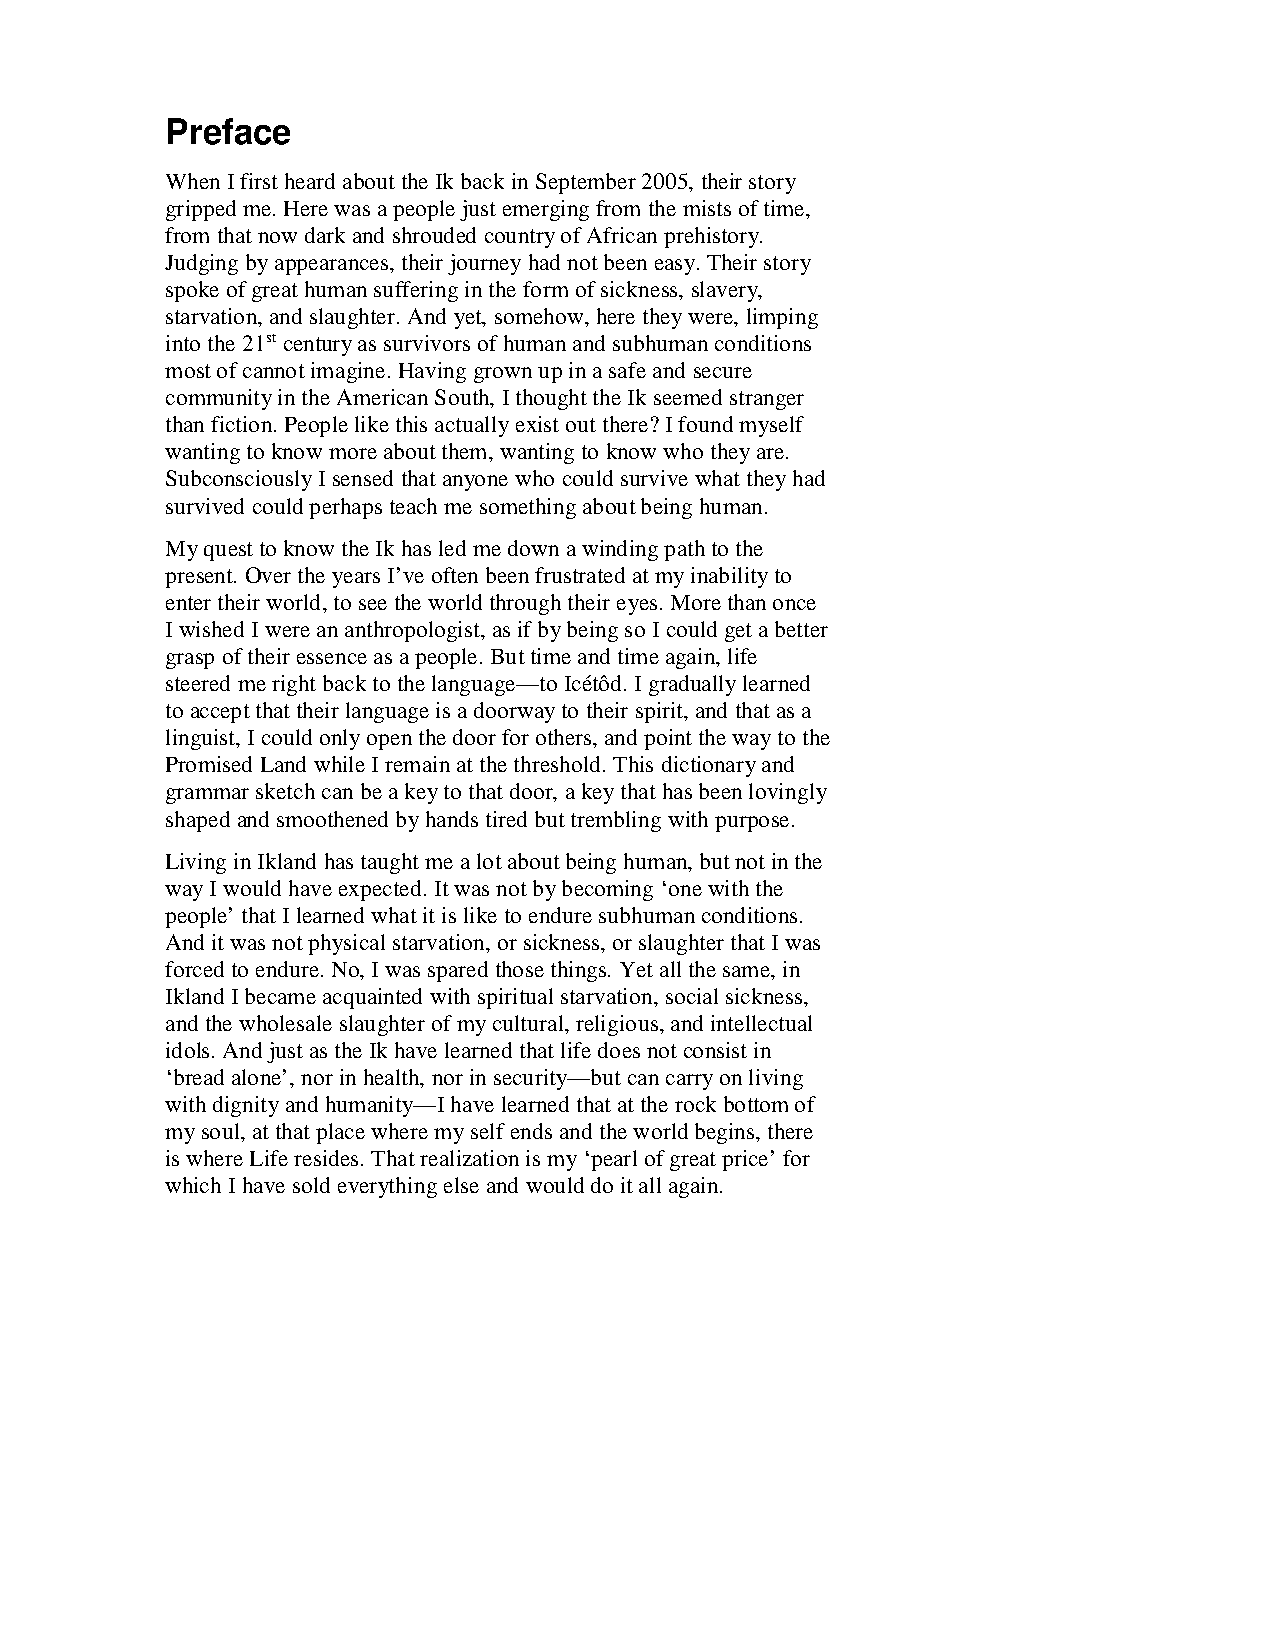
\includepdf[pages=-,scale=1.1, pagecommand={\thispagestyle{plain}}]{Preface.pdf}
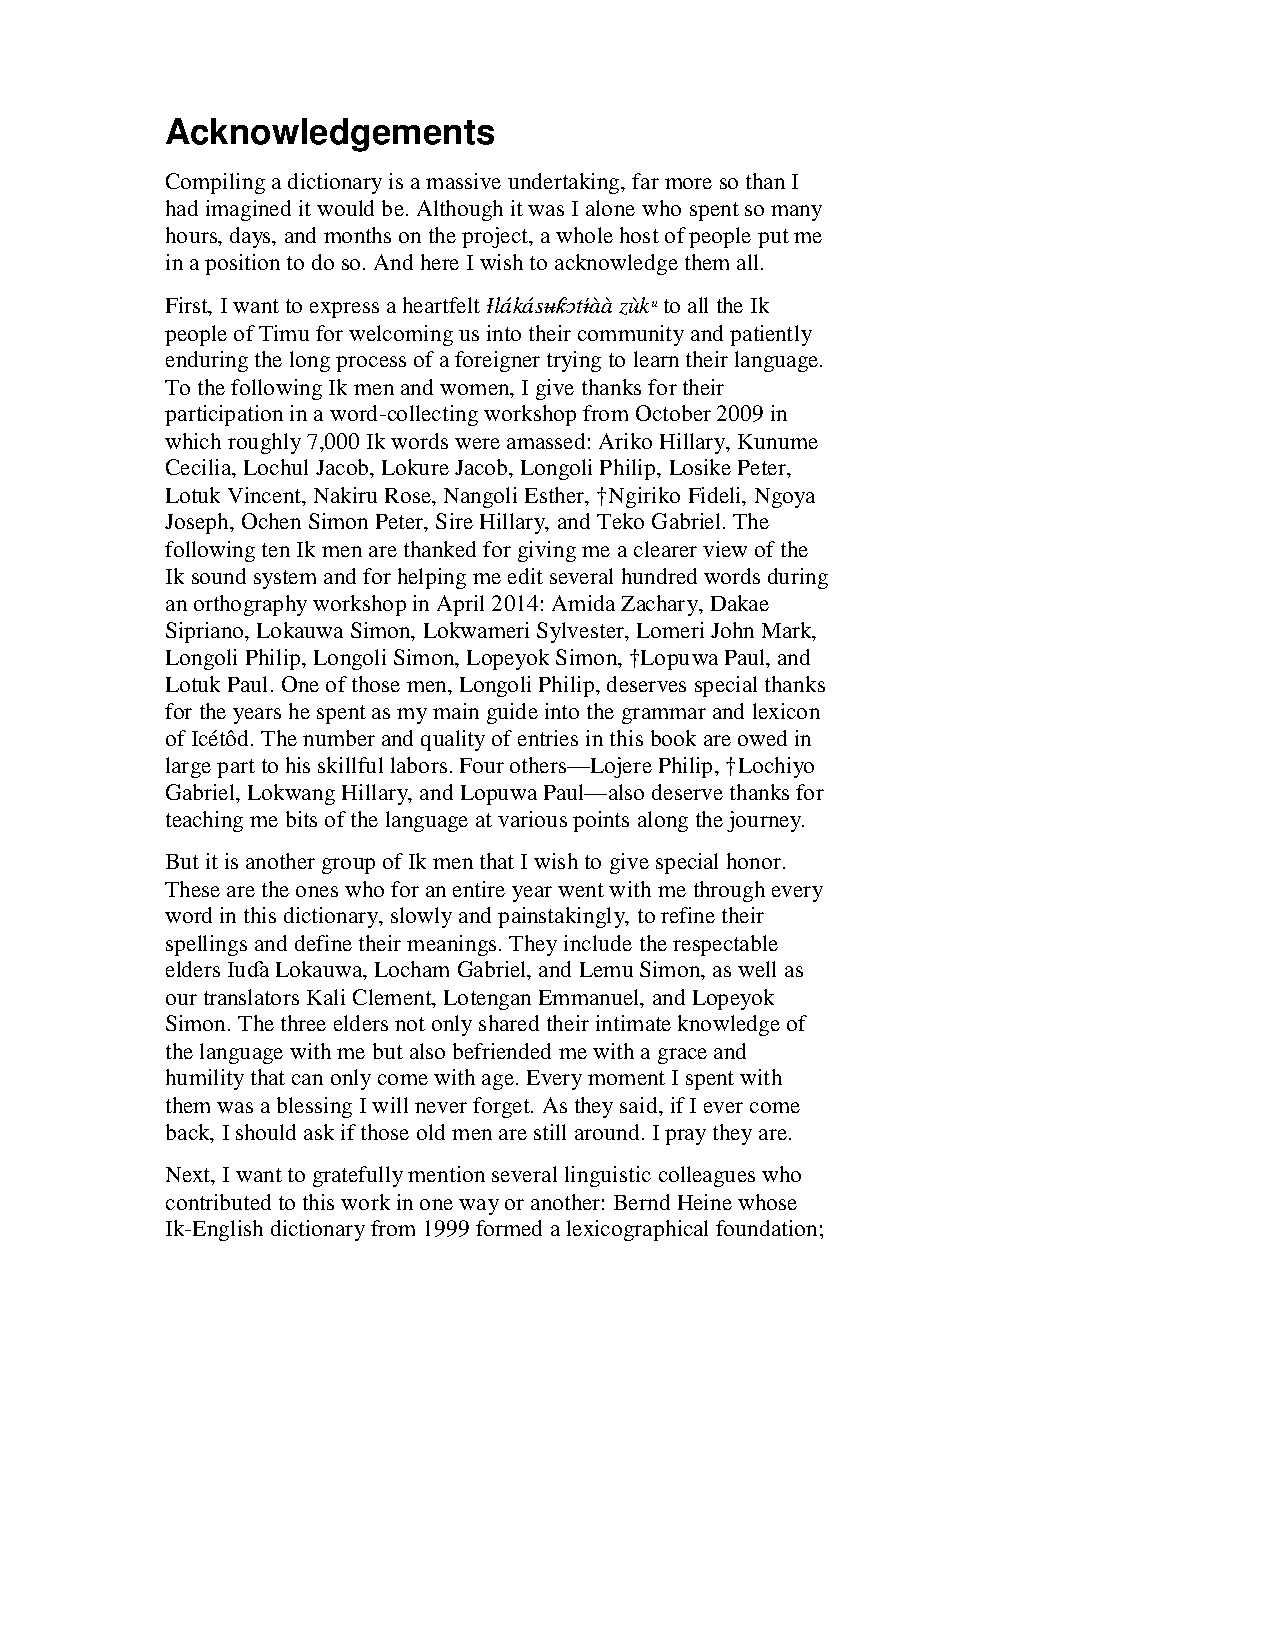
\includepdf[pages=-, scale=1.1,pagecommand={\thispagestyle{plain}}]{Acknowledgements.pdf}
% \addchap{Abbreviations}
% \addchap{Abbreviations and symbols}
 


\begin{tabularx}{.48\textwidth}{lQ} 
A					&	 transitive subject \\
\textsc{abst}		&	 abstractive \\
\textsc{acc}        &    accusative \\
\textsc{adj.pl}		&	 {adjectival} plural \\
adv.				&	 {adverb} \\
\textsc{and}		&	 an{dative} \\
\textsc{anaph}		&	 {anaphoric} \\
\textsc{anticip}	&	 anticipative \\
{ATR}					&	 advanced tongue root \\
\textsc{aux}		&	 auxiliary \\
\textsc{bhvr}		&	 behaviorative \\
C					&	 consonant \\
\textsc{caus}		&	 {causative} \\
CC					&	 {copula} {complement} \\
\textsc{comp}		&	 completive \\
compl.				&	 {complementizer} \\
\textsc{cond}		&	 conditional \\
\textsc{conf}		& 	 confirmational \\
coordconn.			&	 coordinating connective \\
\textsc{cop}		&	 copulative \\
CS					&	 {copula} subject \\
\textsc{dat}        &    {dative} \\
dem.				&	 demonstrative \\
\textsc{dist}		&	 distal \\
\textsc{distr}		&	 distributive \\
\textsc{dp}			&	 {dummy pronoun} \\
\textsc{dur}		&	 durative \\
E					&	 extended object \\
\textsc{exc}		&	 exclusive \\
FF					&	 final form (pre-pause)\\
\end{tabularx} 
 %
\begin{tabularx}{.45\textwidth}{lQ} 
\textsc{gen}        &    genitive \\
H					&	 high tone \\
\textsc{hypo}		&	 hypothetical \\
ideo.				&	 {ideophone} \\
\textsc{imp}		&	 {imperative} \\
\textsc{inc}		&	 inclusive \\
\textsc{inch}		&	 {inchoative} \\
\textsc{inf}		&	 {infinitive} \\
\textsc{infr}		&	 inferential \\
\textsc{ins}        &    instrumental \\
\textsc{int}		&	 {intentional} \\
interj.				&	 {interjection} \\
\textsc{ipfv}		&	 {imperfective} \\
\textsc{ips}		&	 impersonal {passive} \\
\textsc{irr}		&	 irrealis \\
L					&	 low tone \\
lit.				&	 literal \\
M					&	 mid tone \\
\textsc{med}		&	 medial \\
\textsc{mid}		&	 middle \\
n.					&	 noun \\
NF					&	 non-final form \\
\textsc{nom}        &    nominative \\
num.				&	 numeral \\
nurs.				&	 nursery word \\
O					&	 object \\
\textsc{obl}        &    oblique \\
\textsc{opt}		&	 optative \\
\textsc{pass}		&	 {passive} \\
\textsc{pat}		&	 patientive \\
\textsc{phys}		&	 physical property {adverb} \\
\end{tabularx}

\begin{tabularx}{.48\textwidth}{lQ} 
pl.					&	 plural \\
\textsc{plur}		&	 pluractional \\
prep.				&	 {preposition} \\
\textsc{prf}		&	 present perfect \\
pro.				&	 pronoun \\
\textsc{prox}		&	 proximal \\
\textsc{pssm}		&	 impersonal possessum \\ 
\textsc{pst1}		&	 recent past {tense} \\
\textsc{pst2}		&	 removed past {tense} \\
\textsc{pst3}		&	 remote past {tense} \\
\textsc{pst4}		&	 remotest past {tense} \\
quant.				&	 {quantifier} \\
\textsc{real}		&	 realis \\
\textsc{recent}		&	 recentive \\
\textsc{recip}		&	 {reciprocal} \\
\textsc{refl}		&	 {reflexive} \\
rel.				&	 relativizer \\
S					&	 {intransitive} subject \\
\textsc{seq}		&	 sequential \\
sg.					&	 singular \\
\textsc{sim}		&	 simultaneous \\
\end{tabularx}
\begin{tabularx}{.45\textwidth}{lQ} 
\textsc{stat}		&	 stative \\
\textsc{subj}		&	 subjunctive \\
subordconn.			&	 subordinating connective \\
v.					&	 verb \\
\textsc{ven}		&	 venitive \\
1					&	 first person \\
2					&	 second person \\
3					&	 third person \\
Ø					&	 zero realization \\
-					&	 morpheme boundary \\
=					&	 {clitic} boundary \\{}
[{\dots}]			&	 phonetic form\\{}
/{\dots}/			&	 phonemic form\\{}
{{\dots}}			&	 morphemic form\\{}
[\'{}]				&	 high tone \\{}
[\`{}]				&	 low tone \\{}
[\^{}]				&	 high-falling tone \\
†					&	 deceased \\
§					&	 section \\ 
\end{tabularx}

   
\mainmatter   
\part{Introduction}
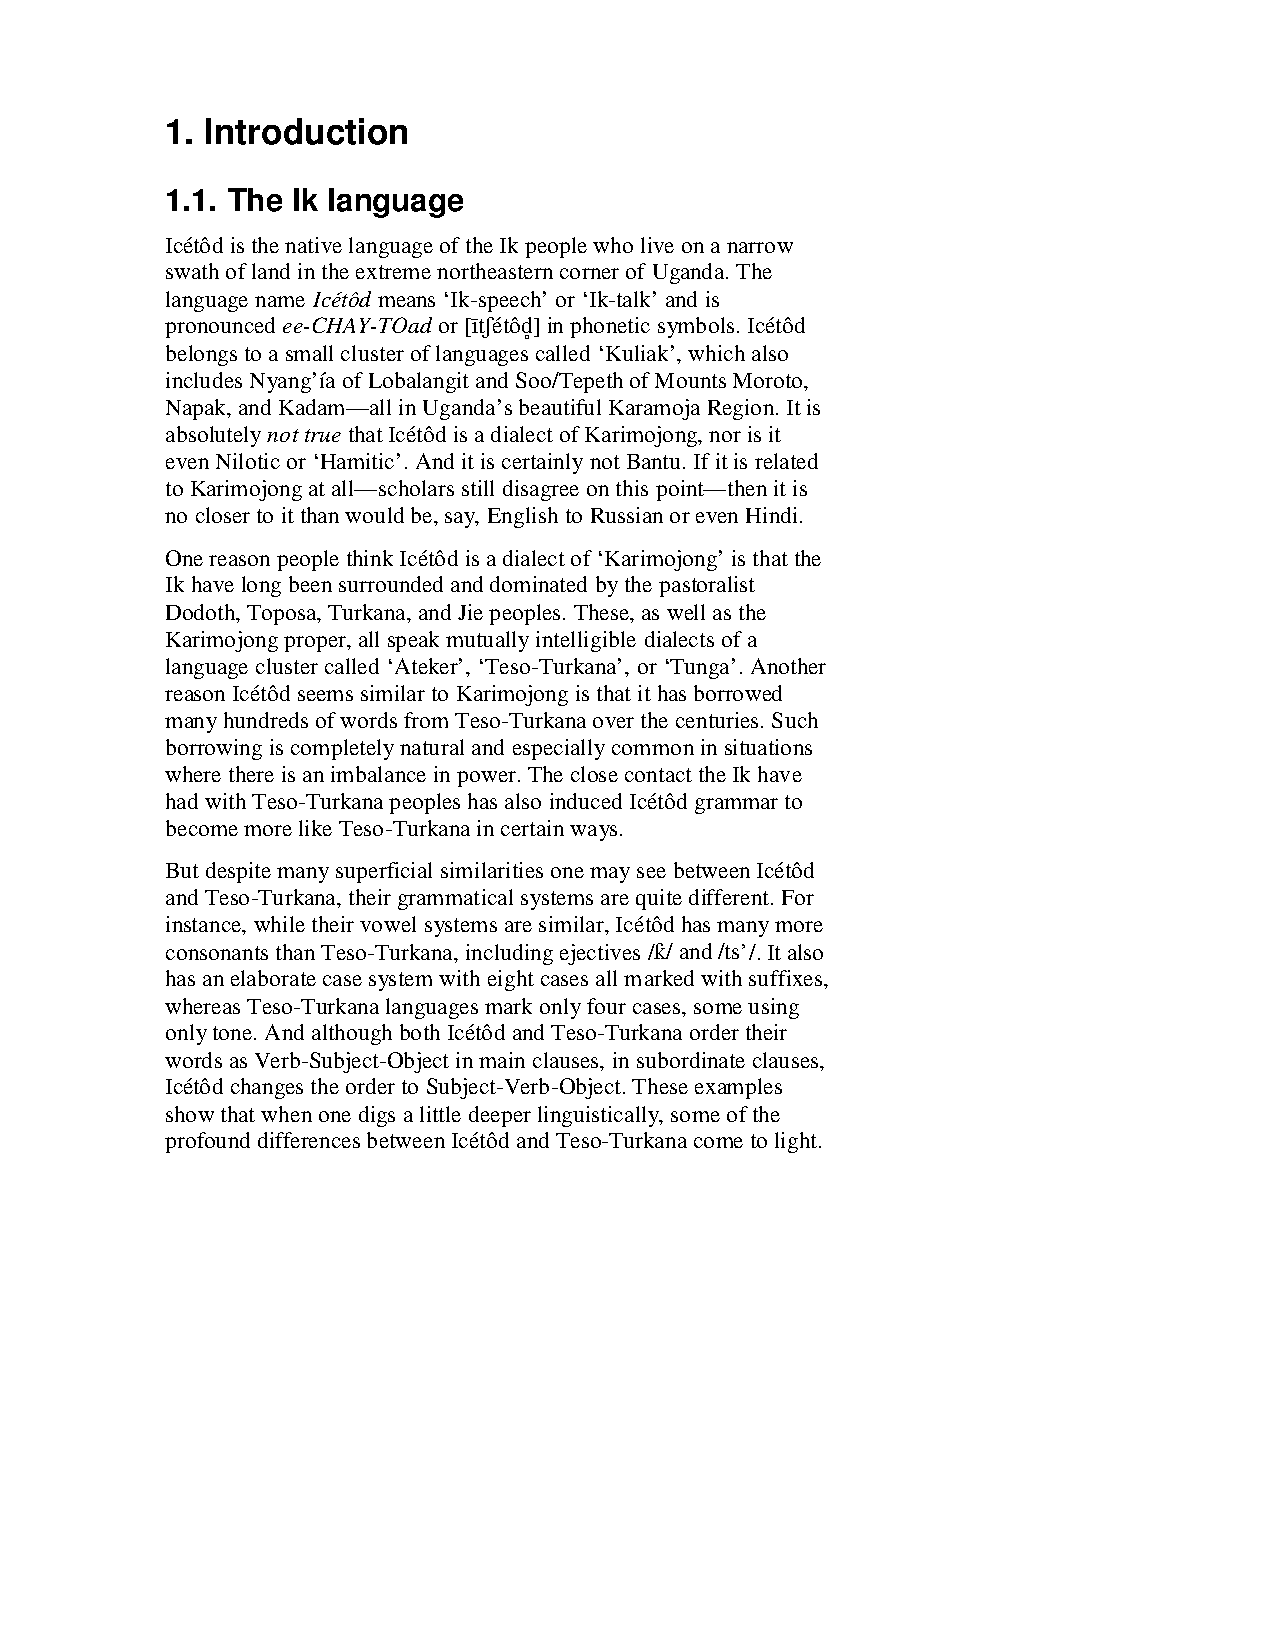
\includepdf[pages=-, scale=1.3,pagecommand={\thispagestyle{plain}}]{Intro p 1-2.pdf}
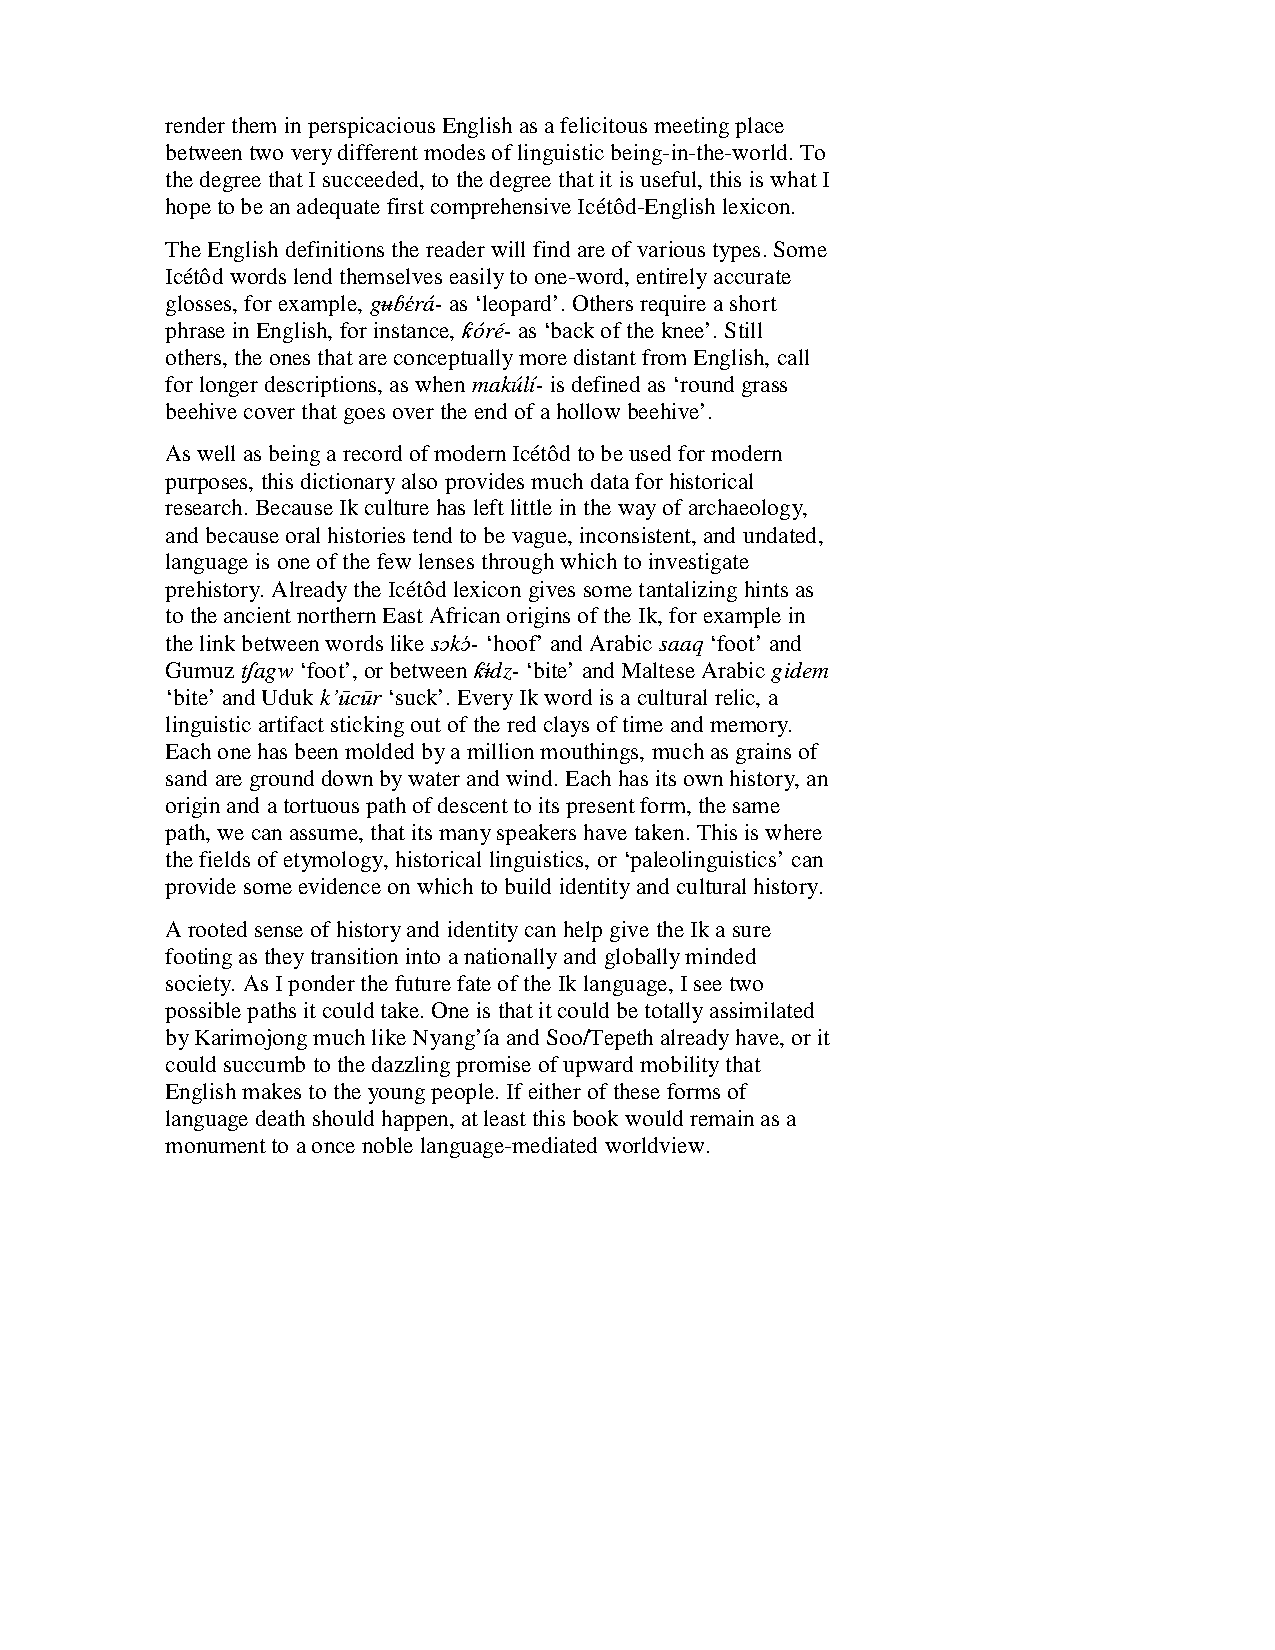
\includepdf[pages=-, scale=1.3, pagecommand={\thispagestyle{plain}}]{Intro p 3.pdf}

\begin{figure}[p]
 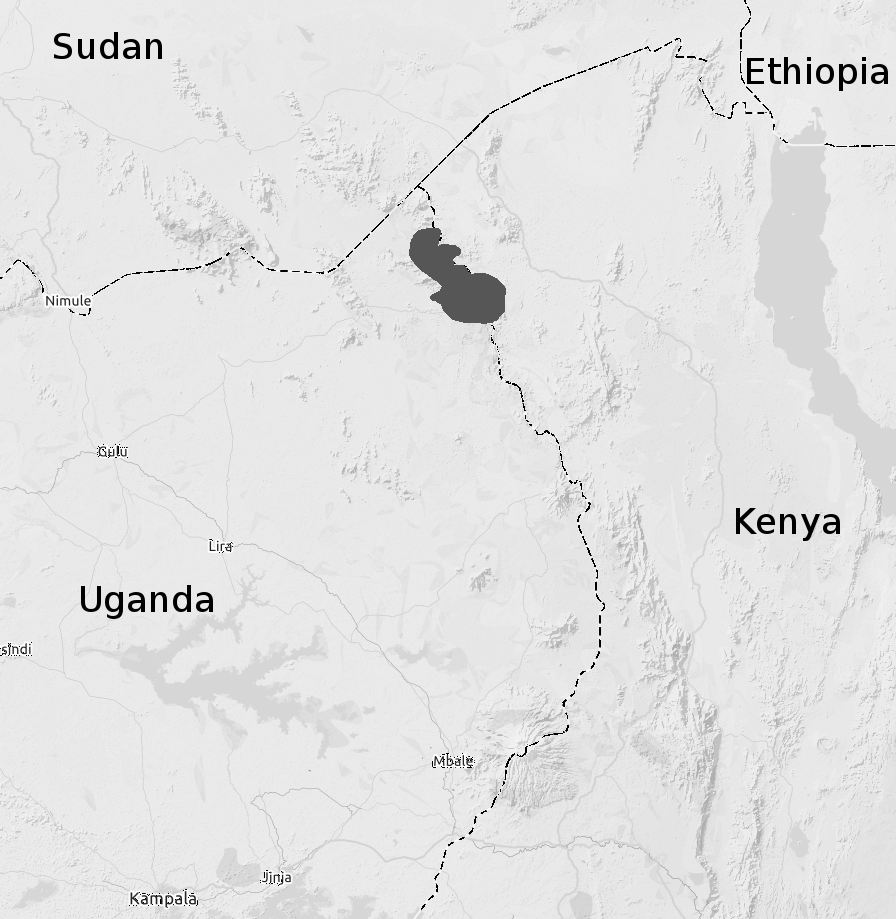
\includegraphics[width=\textwidth]{ikmap.png}
\\
{Figure 1.1: The language area from an `Ik-centric' perspective}
\end{figure}

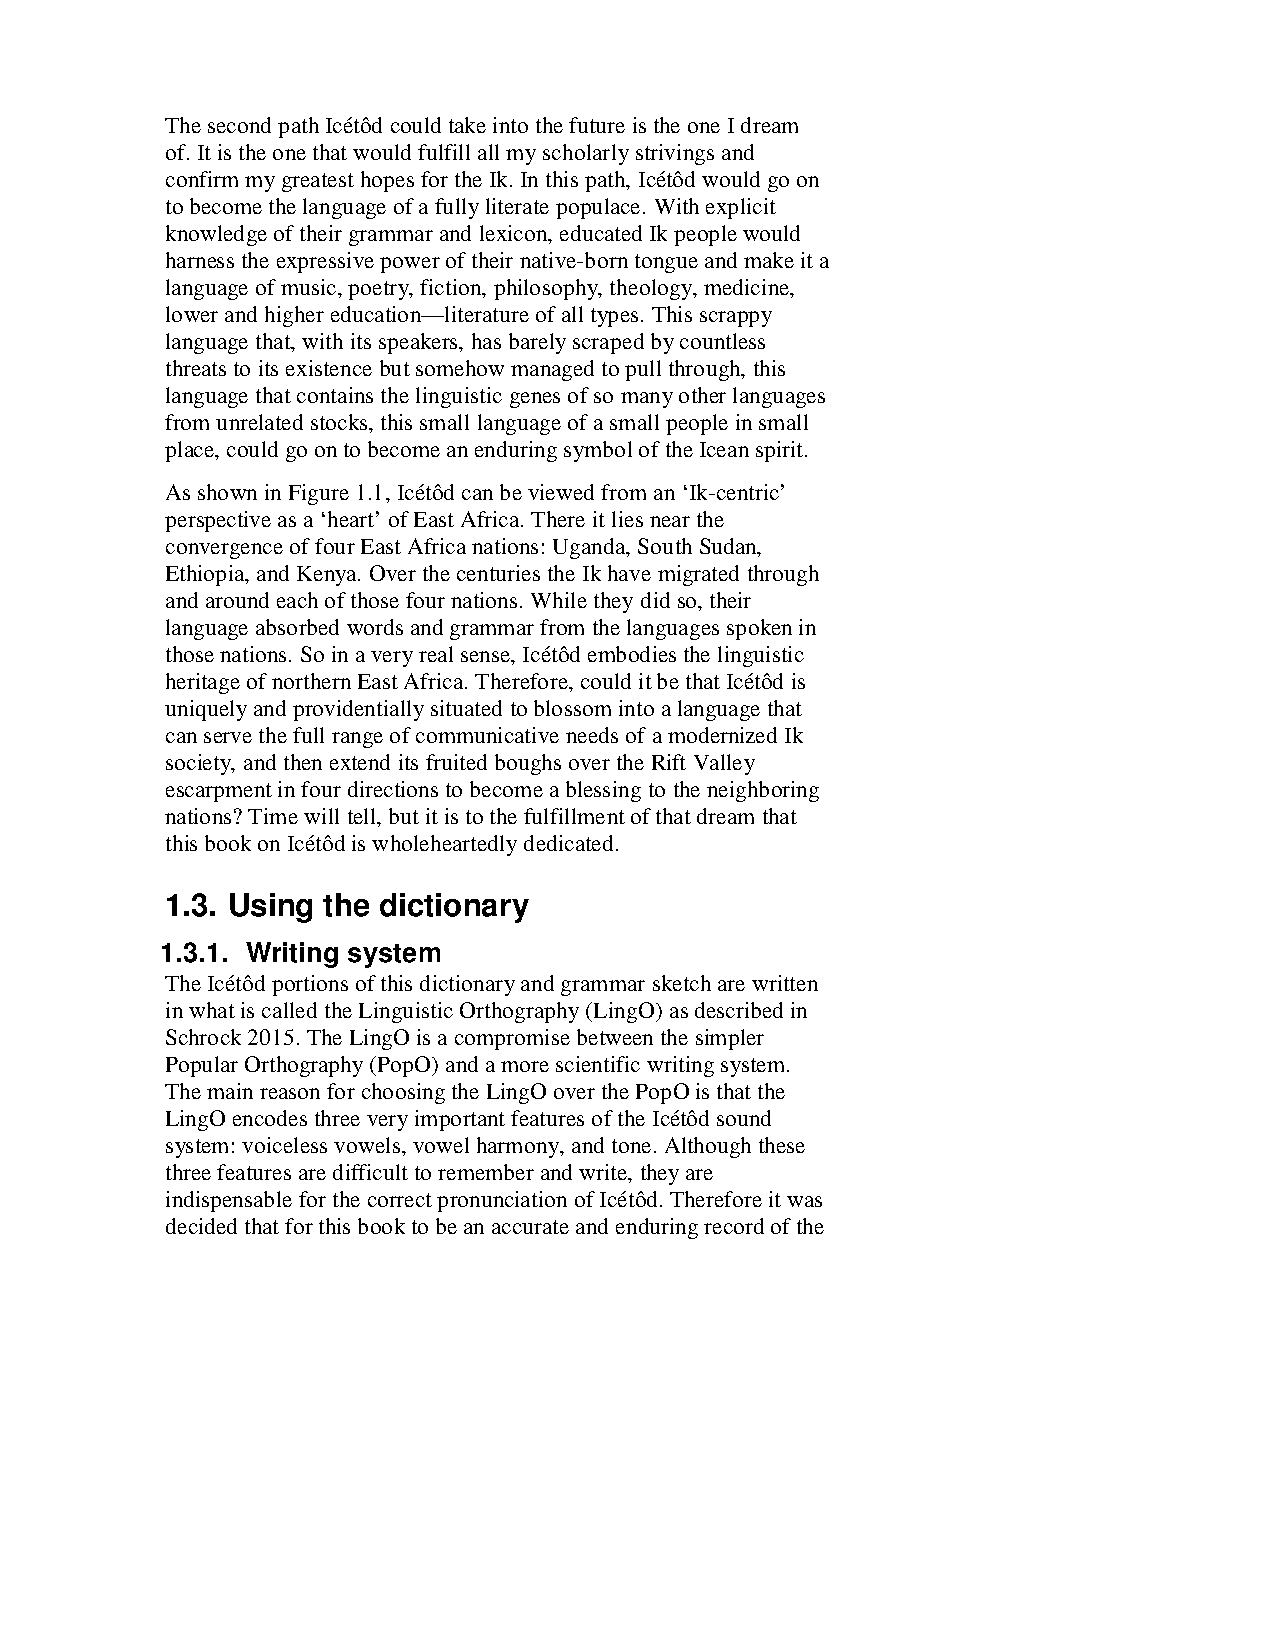
\includepdf[pages=-,scale=1.3, pagecommand={\thispagestyle{plain}}]{Intro p 5-6.pdf}
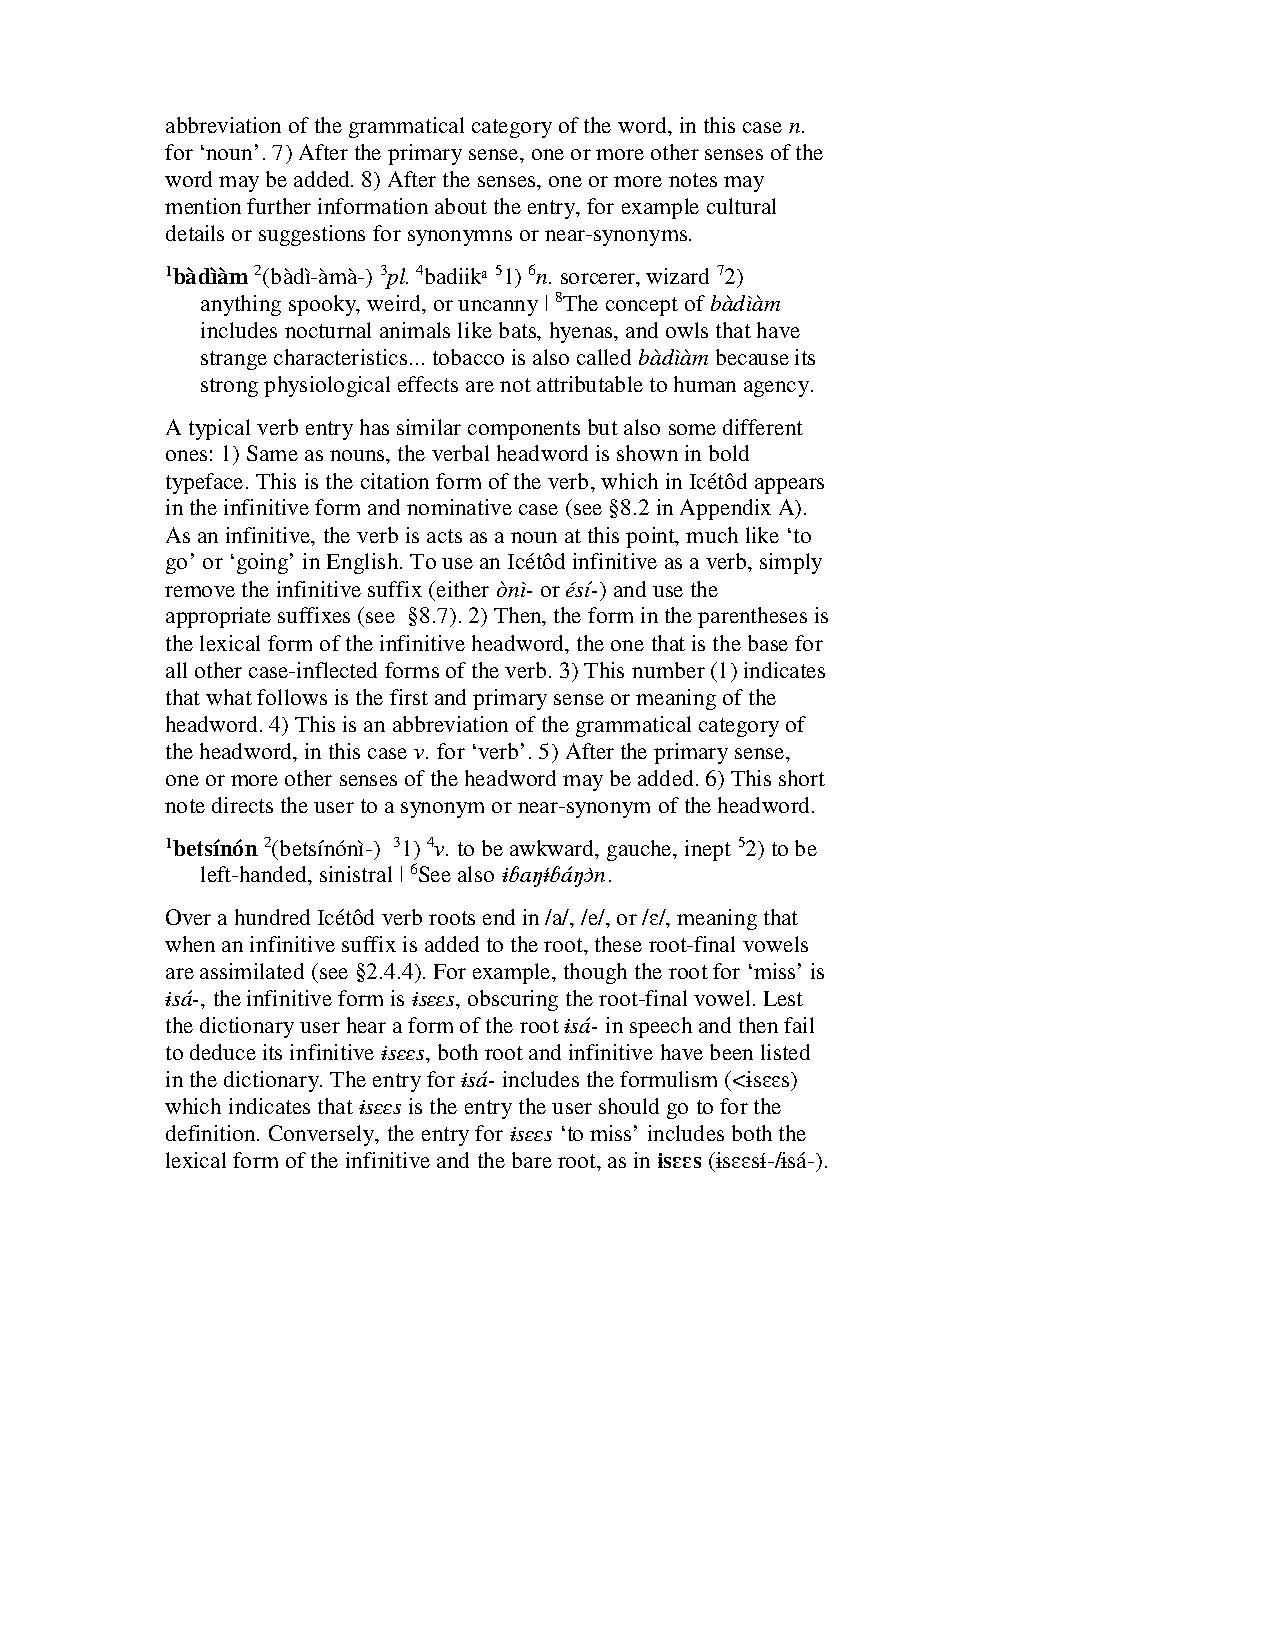
\includepdf[pages=-, scale=1.3,pagecommand={\thispagestyle{plain}}]{Intro p 7.pdf}
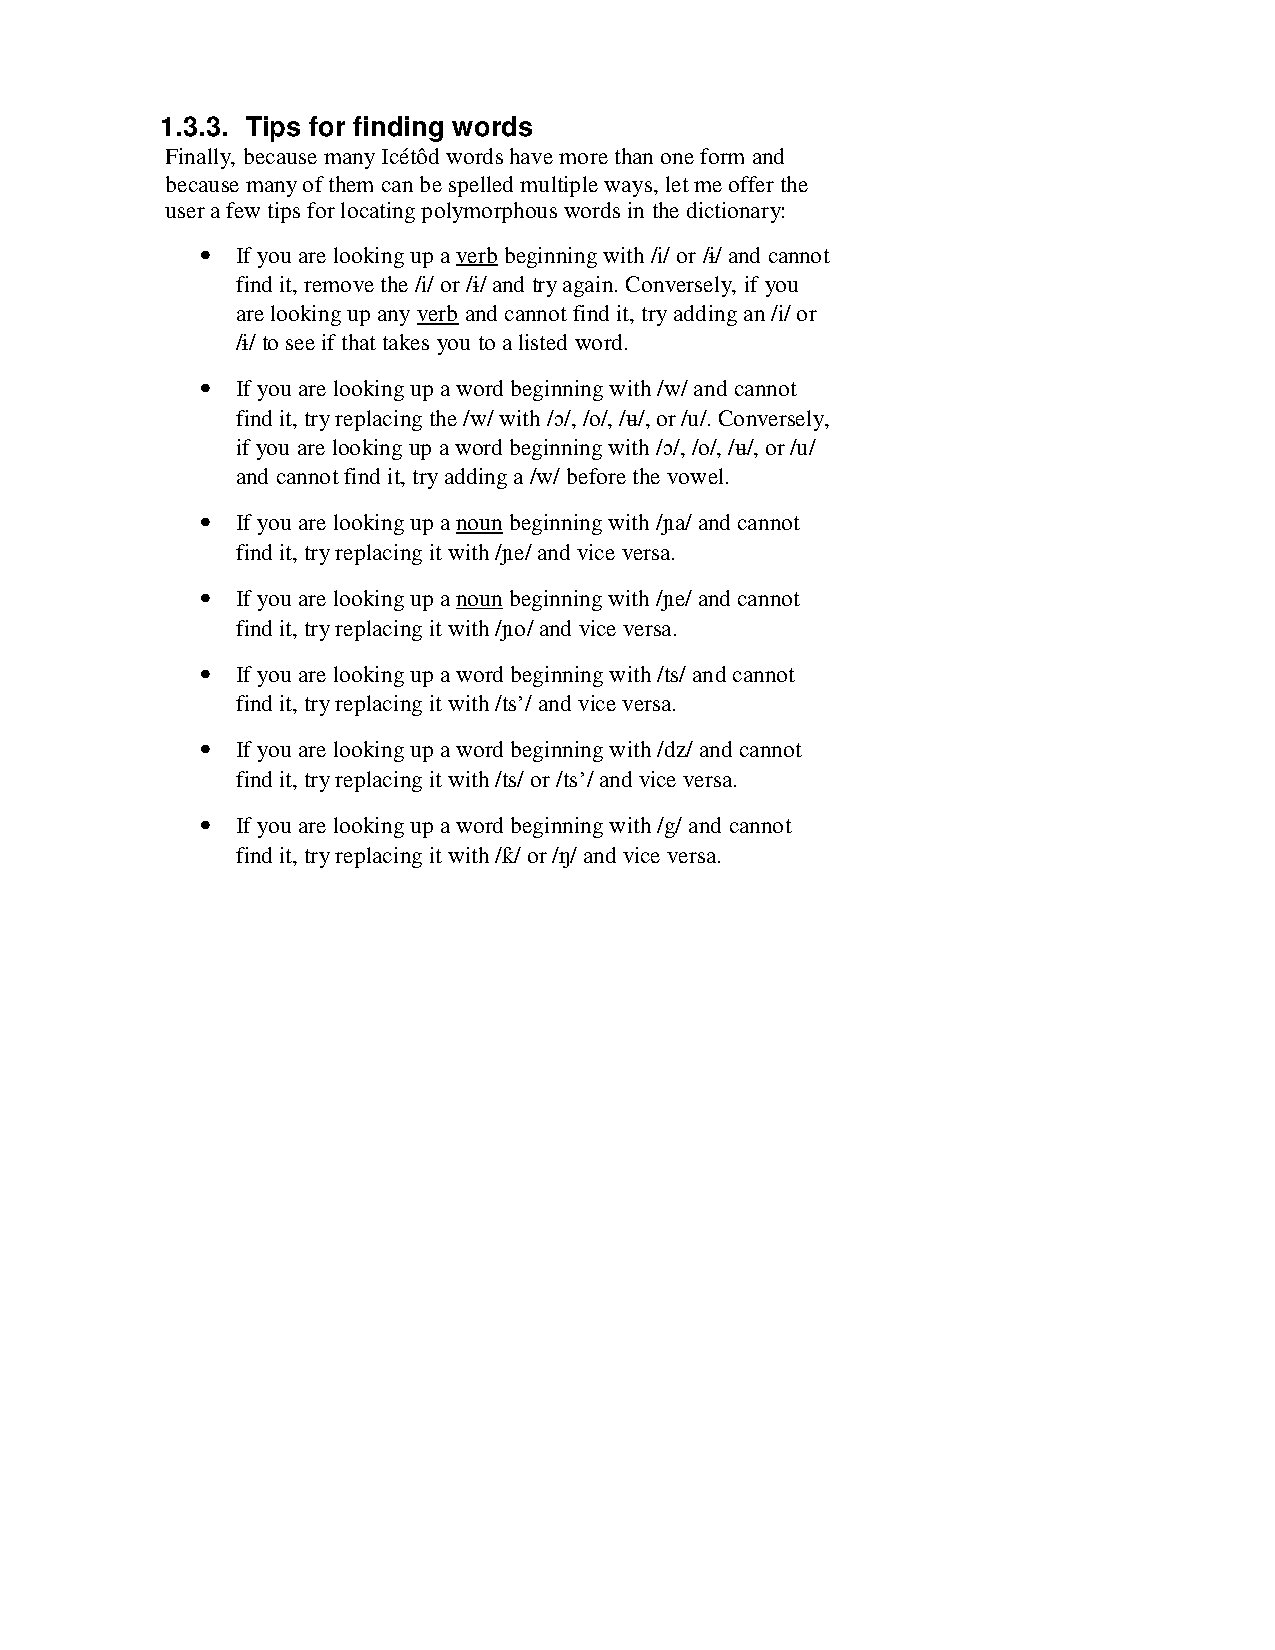
\includepdf[pages=-,scale=1.3, pagecommand={\thispagestyle{plain}}]{Intro p 8.pdf}


  

\newcommand{\headrulewidth}{0pt}
\setlength{\columnsep}{3em}
\setlength{\parindent}{0pt}

\part{Ik-English dictionary}
\renewcommand{\lsgloss}[1]{} 
 

\renewcommand{\citationform}[1]{\textbf{#1}\markboth{#1}{#1}} 
\begin{letter}{a}
%------------------------------
\newentry
\lexicalunit{áí}%
\pos{interj}%
\hypertarget{2ef8cd96-0d11-4cb8-9f11-b74a42a1686e}{}%
\definition{ouch! ow!: an expression of pain}%
\glosses{ouch!;ow!}%
%------------------------------
\newentry
\citationform{aaii}%
\lexicalunit{aaii}%
\pos{interj}%
\hypertarget{38b062f4-99ce-4a33-9b7d-588ac8e60335}{}%
\definition{ouch! ow!: an expression of pain}%
\glosses{ouch!;ow!}%
%------------------------------
\newentry
\citationform{abáŋ}%
\lexicalunit{abáŋɨ̀-}%
\plural{a\-báŋɨ́n}%
\sensenr{1}%
\pos{n}%
\hypertarget{a4f34006-ddf0-4d65-a8cb-f0035fa5327f}{}%
\definition{my father}%
\glosses{father (my)}%
\sensenr{2}%
\pos{n}%
\hypertarget{bcea3000-a4e6-4ef9-a661-639a82f45111}{}%
\definition{my uncle (father's brother)}%
\glosses{uncle (my father's brother)}%
\sensenr{3}%
\pos{n}%
\hypertarget{6781e336-a78f-4da2-a843-f15b943a1479}{}%
\definition{pope: head of the Roman Catholic church}%
\glosses{pope}%
%------------------------------
\newentry
\citationform{ábaŋ}%
\lexicalunit{ábaŋ}%
\pos{interj}%
\hypertarget{de84cc4d-bb4c-40e9-a871-df1ead76fa98}{}%
\definition{oh!, wowǃ: an expression of amazement or wonder}%
\glosses{oh!;wowǃ}%
\literalmeaning{my father}%
%------------------------------
\newentry
\citationform{abáŋɨ́dzàƙ{\higha}}%
\lexicalunit{abáŋɨ́-dzàƙà-}%
\pos{n}%
\hypertarget{19953434-e2b9-4a70-ba08-f63d909939f9}{}%
\definition{son of my father (brother or male cousin on father's side)}%
\glosses{son (of my father)}%
%------------------------------
\newentry
\citationform{abáŋɨ̀ɲòt{\higha}}%
\lexicalunit{abáŋɨ̀-ɲòtà-}%
\pos{n}%
\hypertarget{f39f0284-6d71-45f9-a474-0d117b608eae}{}%
\definition{my father-in-law (sibling's spouse's father)}%
\glosses{father-in-law (my sibling's spouse's father)}%
%------------------------------
\newentry
\citationform{abér}%
\lexicalunit{abérí-}%
\plural{á\-beraikw{\higha}}%
\pos{n}%
\hypertarget{b40eac6c-39e7-416e-a029-7d80ad555738}{}%
\definition{termite colony actively flying and mound-building}%
\glosses{termite colony (active)}%
%------------------------------
\newentry
\citationform{àbɛ̀t{\higha}}%
\lexicalunit{àbɛ̀tà-}%
\pos{n}%
\scientificname{Tragelaphus imberbis}%
\hypertarget{61679521-fdbe-4f76-abfa-e0fb169da21e}{}%
\definition{lesser kudu}%
\glosses{kudu (lesser)}%
%------------------------------
\newentry
\citationform{abûb{\higha}}%
\lexicalunit{abúbà-}%
\plural{a\-búbìk{\higha}}%
\sensenr{1}%
\pos{n}%
\hypertarget{85463229-5d28-48c8-8bd0-f1d7ba1c3ca2}{}%
\definition{spider}%
\glosses{spider}%
\sensenr{2}%
\pos{n}%
\hypertarget{c0161c1f-096c-4579-88b9-f6df1fd91ca8}{}%
\definition{cobweb, spiderweb, web}%
\glosses{cobweb;spiderweb;web}%
%------------------------------
\newentry
\citationform{abutiam}%
\lexicalunit{abutiamá-}%
\pos{n}%
\hypertarget{a35c6145-4d52-467a-adc8-4ba0aa037d53}{}%
\definition{sippable food like beer or porridge}%
\glosses{food (sippable);sippable food}%
%------------------------------
\newentry
\citationform{abutiés}%
\lexicalunit{abutiesí-}%
\pos{v}%
\hypertarget{66e5b1f6-a571-4160-b14e-8c18cb5c02b5}{}%
\definition{to sip or slurp continually}%
\glosses{sip continually;slurp continually}%
\note{See also tsʉɓɛ́s.}%
%------------------------------
\newentry
\citationform{ábʉbʉƙɛ́s}%
\lexicalunit{ábʉbʉƙɛ́sɨ́-}%
\pos{v}%
\hypertarget{a180c388-9dae-4ca2-9986-eed8ae3b6ae5}{}%
\definition{to dip out (liquid with a vessel)}%
\glosses{dip out (liquid)}%
%------------------------------
\newentry
\citationform{ábʉ̀bʉ̀ƙɔ̀n}%
\lexicalunit{ábʉ̀bʉ̀ƙɔ̀nɨ̀-}%
\sensenr{1}%
\pos{v}%
\hypertarget{00ffa403-d179-44f1-af36-9d72c2aeb788}{}%
\definition{to bubble, burble, gurgle}%
\glosses{burble;burble;gurgle}%
\sensenr{2}%
\pos{v}%
\hypertarget{a22be813-9946-4460-8fbd-89f127420065}{}%
\definition{to bellow, roar (like a charging animal or angry person)}%
\glosses{bellow;roar}%
\note{See also béúrètòn.}%
%------------------------------
\newentry
\citationform{abʉtɛtɛ́s}%
\lexicalunit{abʉtɛtɛ́sɨ́-}%
\pos{v}%
\hypertarget{154a1000-ea65-4fa5-aba1-49e0249f1ab9}{}%
\definition{to sip, take a sip}%
\glosses{sip;take a sip}%
\note{See also tsʉɓɛtɛ́s.}%
%------------------------------
\newentry
\citationform{aɓɨ́ɓɨ́lánón}%
\lexicalunit{aɓɨ́ɓɨ́lánónì-}%
\pos{v}%
\hypertarget{a8d99f8a-549a-4058-8f82-9e822c163434}{}%
\definition{to roll around}%
\glosses{roll around}%
%------------------------------
\newentry
\citationform{aɓúlúkánón}%
\lexicalunit{aɓúlúkánónì-}%
\pos{v}%
\hypertarget{5887d9e3-e930-4c72-9518-7c5d90b23724}{}%
\definition{to flip, flip over, somersault}%
\glosses{flip over;somersault}%
%------------------------------
\newentry
\citationform{Acók{\higha}}%
\lexicalunit{Acókò-}%
\pos{n}%
\hypertarget{e1aeafea-fe4e-43d2-a1de-d65029fb0f42}{}%
\definition{a personal name}%
\glosses{name (personal)}%
%------------------------------
\newentry
\citationform{Acúkwa}%
\lexicalunit{Acúkwaá-}%
\pos{n}%
\hypertarget{89eb0c49-78bb-4185-8623-f09ad92e192f}{}%
\definition{a personal name}%
\glosses{name (personal)}%
%------------------------------
\newentry
\citationform{àdàbì}%
\lexicalunit{àdàbìà-}%
\pos{n}%
\hypertarget{546f505f-9b31-48a5-ab2b-0731d77eb5dc}{}%
\definition{vine species found growing on rocky outcroppings and whose leaves are crushed, soaked in water, and applied to the skin as a treatment for acne and rashes}%
\glosses{vine species}%
%------------------------------
\newentry
\citationform{àdɛ̀nɛ̀s}%
\lexicalunit{àdɛ̀nɛ̀sà-}%
\pos{n}%
\hypertarget{35bf3b64-0870-4da1-ab5b-16c6e16a8d1d}{}%
\definition{bird species}%
\glosses{bird species}%
%------------------------------
\newentry
\citationform{ádʉdʉƙɛ́s}%
\lexicalunit{ádʉdʉƙɛ́sɨ́-}%
\pos{v}%
\hypertarget{b5b12446-8a7b-4d96-adc7-a6b8f325e1b5}{}%
\definition{to pour from a small opening}%
\glosses{pour from small opening}%
%------------------------------
\newentry
\citationform{aɗáɗá}%
\lexicalunit{aɗáɗáà-}%
\pos{n}%
\hypertarget{7b62e904-553d-44f7-923d-f1d92a4b0b03}{}%
\definition{ringworm: an itchy, circular skin fungus}%
\glosses{ringworm}%
%------------------------------
\newentry
\citationform{àɗèŋèlìò}%
\lexicalunit{àɗèŋèlìò-}%
\pos{n}%
\scientificname{Allophylus sp.}%
\hypertarget{70388737-602f-4787-86d0-c6980b4286d8}{}%
\definition{large hardwood tree that grows in the ravines and riverbeds of Rift Valley escarpments; Heine 1999 reports that the fruits of this tree may be eaten raw}%
\glosses{Allophylus species;tree species}%
%------------------------------
\newentry
\citationform{àɗ{\highe}}%
\lexicalunit{àɗè}%
\pos{num}%
\hypertarget{0059c761-214f-4f6f-8c26-9b7eb12bc77d}{}%
\definition{three}%
\glosses{three}%
%------------------------------
\newentry
\citationform{àɗòn}%
\lexicalunit{àɗònì-}%
\pos{v}%
\hypertarget{b5e1f23c-7ffe-456d-9a0e-5c298c6fceef}{}%
\definition{to be three}%
\glosses{three}%
%------------------------------
\newentry
\citationform{aɗoniɛn}%
\lexicalunit{aɗoni-ɛnɨ́-}%
\pos{n}%
\hypertarget{4d03038f-fbeb-422b-93ad-36bf8ee145ca}{}%
\definition{third time}%
\glosses{third time}%
%------------------------------
\newentry
\citationform{àɗònìk{\highe}}%
\pos{n}%
\hypertarget{b90df5a5-9b6c-4bdc-a0cd-1811be134088}{}%
\definition{for the third time}%
\glosses{third time}%
%------------------------------
\newentry
\citationform{àɗ{\higho}}%
\pos{num}%
\hypertarget{2f424d7b-2a68-4fd9-83c2-1fe763a5581c}{}%
\definition{three times, thrice}%
\glosses{three times;thrice}%
%------------------------------
\newentry
\citationform{aɗúŋkú}%
\lexicalunit{aɗúŋkúù-}%
\plural{aɗúŋ\-kúìk{\higha}}%
\pos{n}%
\hypertarget{de2db219-ca4e-46b0-be40-2695a42ad668}{}%
\definition{stringed instrument found in many East African cultures (and whose body was traditionally made from a tortoise shell)}%
\glosses{instrument (stringed)}%
%------------------------------
\newentry
\citationform{Àɗùpà}%
\lexicalunit{Àɗùpàà-}%
\pos{n}%
\hypertarget{95c056e0-1670-448f-bd9f-45553a5302d1}{}%
\definition{a personal name}%
\glosses{name (personal)}%
%------------------------------
\newentry
\citationform{aeam}%
\lexicalunit{aeamá-}%
\pos{n}%
\hypertarget{2d066873-8fdb-40a6-b8f1-a7ba37574912}{}%
\definition{any food that is ripe or otherwise ready to be eaten}%
\glosses{food (ready);food (ripe)}%
%------------------------------
\newentry
\citationform{aeásá bùbùì}%
\pos{n}%
\hypertarget{ec035091-d726-4ba1-b999-258b5372b696}{}%
\definition{gluttony}%
\glosses{gluttony}%
\literalmeaning{ripeness of the belly}%
%------------------------------
\newentry
\citationform{aeétón}%
\lexicalunit{aeétónì-}%
\sensenr{1}%
\pos{v}%
\hypertarget{ad600750-1b3f-4d53-92e5-0eb67d898616}{}%
\definition{to ripen up, start ripening}%
\glosses{ripen up}%
\sensenr{2}%
\pos{v}%
\hypertarget{7a21ba6b-2677-49cd-a0a1-399b1ef33c2a}{}%
\definition{to light up}%
\glosses{light up}%
\sensenr{3}%
\pos{v}%
\hypertarget{5578cd52-0046-427f-98f6-f6531fa30d84}{}%
\definition{to catch fire}%
\glosses{catch fire}%
%------------------------------
\newentry
\citationform{aeitetés}%
\lexicalunit{aeitetésí-}%
\sensenr{1}%
\pos{v}%
\hypertarget{77a7d671-1e7b-4f40-8557-2c7c0152c73a}{}%
\definition{to light (a fire or lamp)}%
\glosses{light}%
\sensenr{2}%
\pos{v}%
\hypertarget{b083d8bd-bc12-479c-bd33-4aacd2cf9b12}{}%
\definition{to switch or turn on (an electronic device or electric switch)}%
\glosses{switch on (electrically);turn on (electrically)}%
%------------------------------
\newentry
\citationform{aeitetésíàw{\higha}}%
\lexicalunit{aeitetésí-àwà-}%
\plural{aei\-teté\-sía\-wík{\higha}}%
\pos{n}%
\hypertarget{41eb6c3e-296e-40ba-a421-a87a103ee545}{}%
\definition{ignition, switch}%
\glosses{ignition;switch}%
%------------------------------
\newentry
\citationform{Aemun}%
\lexicalunit{Aemuní-}%
\pos{n}%
\hypertarget{350f55df-1f24-40f6-8419-c457465fc8ee}{}%
\definition{a personal name}%
\glosses{name (personal)}%
%------------------------------
\newentry
\citationform{àèòn}%
\lexicalunit{àèònì-}%
\sensenr{1}%
\pos{v}%
\hypertarget{a1c3a641-7f19-4001-88f8-b1c17ecd8964}{}%
\definition{to be ripe, ready to eat}%
\glosses{ready (to eat);ripe}%
\sensenr{2}%
\pos{v}%
\hypertarget{bcb0a87c-b2c3-41f0-b209-a40fb47d0ab5}{}%
\definition{to be lit}%
\glosses{lit}%
%------------------------------
\newentry
\citationform{aeonuƙota kíʝá{\highe}}%
\pos{n}%
\hypertarget{11fcedae-c881-4df7-b3ce-a26d8634f974}{}%
\definition{readying for harvest (of people's gardens)}%
\glosses{readying for harvest (of gardens)}%
%------------------------------
\newentry
\citationform{aeonuƙot{\higha}}%
\lexicalunit{aeonuƙotí-}%
\pos{v}%
\hypertarget{4d3bde9b-5ccc-40e6-a07f-92550be4f8ea}{}%
\definition{to become ready to eat, ripen}%
\glosses{ready to eat (become);ripen}%
%------------------------------
\newentry
\citationform{àɡɨ̀t{\higha}}%
\lexicalunit{àɡɨ̀tà-}%
\plural{áɡɨ̀tɨ̀k{\higha}}%
\pos{n}%
\hypertarget{ffc48a51-bc93-4fe8-91e8-d205ec74691c}{}%
\definition{metal ringlet sown on women's traditional aprons}%
\glosses{metal ringlet;ringlet (metal)}%
%------------------------------
\newentry
\citationform{áɡɨrɨkácà}%
\lexicalunit{áɡɨrɨkácàà-}%
\sensenr{1}%
\pos{n}%
\hypertarget{46852c58-98ca-4a50-a4aa-78d931e95b6d}{}%
\definition{agricultural training course}%
\glosses{agricultural course}%
\sensenr{2}%
\pos{n}%
\hypertarget{7af3ce9c-7186-4de4-970c-a05b9e56a33a}{}%
\definition{tall variety of maize}%
\glosses{maize variety}%
%------------------------------
\newentry
\citationform{áɡʉʝɛ́s}%
\lexicalunit{áɡʉʝɛ́sɨ́-}%
\pos{v}%
\hypertarget{6182c7e7-5397-4dc6-9439-e9de689753a1}{}%
\definition{to gulp, guzzle}%
\glosses{gulp;guzzle}%
\note{Also pronounced as ɨ́ɡʉʝɛ́s.}%
%------------------------------
\newentry
\citationform{àʝ{\higha}}%
\lexicalunit{àʝɨ̀-}%
\plural{áʝɨ́\-tɨ́n}%
\pos{n}%
\hypertarget{3efca8e6-ee51-4831-917c-fb8730dd8ecc}{}%
\definition{pestle}%
\glosses{pestle}%
\note{See also iwótsídàkw{\higha} and kuɲuk{\higha}.}%
%------------------------------
\newentry
\citationform{aka ɡwaá{\highe}}%
\pos{n}%
\hypertarget{7b6d643b-a34c-4f35-a06e-b5de141bb8ef}{}%
\definition{beak}%
\glosses{beak}%
%------------------------------
\newentry
\citationform{akáám}%
\lexicalunit{aká-ámà-}%
\plural{a\-káík{\higha}}%
\pos{n}%
\hypertarget{66b9d2d8-012a-40ce-b4ec-0e1568d768d3}{}%
\definition{one skilled at talking deceptively or persuasively}%
\glosses{talker}%
\literalmeaning{mouth-person}%
%------------------------------
\newentry
\citationform{Akaɗéérót{\higha}}%
\lexicalunit{Akaɗéérótò-}%
\pos{n}%
\hypertarget{04973075-1fef-4a1d-aa20-3cd300a928cb}{}%
\definition{a personal name}%
\glosses{name (personal)}%
%------------------------------
\newentry
\citationform{akákwáyw{\higha}}%
\lexicalunit{aká-kwáyò-}%
\plural{a\-kákwáí\-tín}%
\pos{n}%
\hypertarget{b87dedc0-f0fb-444e-99cd-26f9b2b73c85}{}%
\definition{lip}%
\glosses{lip}%
\literalmeaning{mouth-tooth}%
%------------------------------
\newentry
\citationform{akáƙúm}%
\lexicalunit{aká-ƙúmù-}%
\plural{a\-káƙú\-mítín}%
\pos{n}%
\hypertarget{107a615a-3ded-445e-9094-d05eb1b62659}{}%
\definition{cheekbone, malar, zygomatic bone}%
\glosses{bone (zygomatic);cheekbone;malar}%
%------------------------------
\newentry
\citationform{akánɨ́}%
\lexicalunit{akánɨ́}%
\pos{prep}%
\hypertarget{43db748e-50b1-4db1-b8e0-daa2a4646c8a}{}%
\definition{until, up to (an event or place)}%
\glosses{until;up to}%
\note{A noun following this word takes the oblique case.}%
%------------------------------
\newentry
\citationform{akarér}%
\lexicalunit{akarérí-}%
\plural{a\-karé\-rík{\higha}}%
\pos{n}%
\hypertarget{f8d133a5-1042-4f20-b23c-bdf47f21e8fb}{}%
\definition{hole dug for edible termites to get trapped in}%
\glosses{termite trap;trap (termite)}%
%------------------------------
\newentry
\citationform{akatɛ́t{\higha}}%
\lexicalunit{akatɛ́tɨ́-}%
\plural{a\-katɛ́\-tɨ́k{\higha}}%
\pos{n}%
\hypertarget{95e4cc2d-528a-4d1a-aea4-fb04613ab12e}{}%
\definition{gourd plug (made from a gourd tip cut off and inverted)}%
\glosses{gourd plug}%
%------------------------------
\newentry
\citationform{akátsʼɛ́a na pakós}%
\pos{n}%
\hypertarget{ca288ad6-4998-4f49-be96-f4ad95c7a4a3}{}%
\definition{cleft palate}%
\glosses{cleft palate;palate (cleft)}%
\literalmeaning{mouth skin that is split}%
%------------------------------
\newentry
\citationform{ak{\higha}}%
\lexicalunit{aká-}%
\plural{a\-kɨtɨ́n}%
\sensenr{1}%
\pos{n}%
\hypertarget{00a26a8d-5833-4192-b541-3bb1e5ed3904}{}%
\definition{mouth, oral cavity}%
\glosses{cavity (oral);mouth}%
\sensenr{2}%
\pos{n}%
\hypertarget{d936aa05-9c02-4dc3-844c-5e09bd7d941a}{}%
\definition{entrance, opening}%
\glosses{entrance;opening}%
\sensenr{3}%
\pos{n}%
\hypertarget{6f20f58f-ff6f-49a4-8029-79b845899c9d}{}%
\definition{burrow, den, hole, lair}%
\glosses{burrow;den;hole;lair}%
%------------------------------
\newentry
\citationform{akɛd{\higha}}%
\lexicalunit{akɛdɛ-}%
\sensenr{1}%
\pos{n}%
\hypertarget{29a35908-7715-47bd-a6b0-086817cea17e}{}%
\definition{mouth, opening}%
\glosses{mouth;opening}%
\sensenr{2}%
\pos{n}%
\hypertarget{cf6d2a21-0666-46c7-8265-07857c46f962}{}%
\definition{muzzle of a weapon}%
\glosses{muzzle (weapon)}%
%------------------------------
\newentry
\citationform{akɨ́lɨ̀k{\higha}}%
\lexicalunit{akɨ́lɨ̀kà-}%
\sensenr{1}%
\pos{n}%
\hypertarget{2bb1aad7-7f90-4993-ac10-a11fe3034e02}{}%
\definition{intelligence, mind}%
\glosses{intelligence;mind}%
\sensenr{2}%
\pos{n}%
\hypertarget{ab7c8cf0-b00d-43e5-ac3c-53c28dd126f6}{}%
\definition{skill, talent}%
\glosses{skill;talent}%
%------------------------------
\newentry
\citationform{àkɨ̀lɔ̀}%
\lexicalunit{àkɨ̀lɔ̀}%
\pos{prep}%
\hypertarget{145c88ea-c7d4-4303-ae8c-d48efc034851}{}%
\definition{instead (of)}%
\glosses{instead (of)}%
\note{A noun following this word takes the oblique case.}%
%------------------------------
\newentry
\citationform{akɨ́n}%
\lexicalunit{akɨ́nɔ́-}%
\pos{n}%
\scientificname{Tragelaphus strepsiceros}%
\hypertarget{1527fdc8-3836-4824-ab82-f4b42deda8f8}{}%
\definition{greater kudu}%
\glosses{kudu (greater)}%
%------------------------------
\newentry
\citationform{Akóóro}%
\lexicalunit{Akóóroó-}%
\pos{n}%
\hypertarget{526d65ec-fcb6-41eb-9400-bbd8fb61b642}{}%
\definition{a personal name}%
\glosses{name (personal)}%
%------------------------------
\newentry
\citationform{akɔ́ŋɨkɔŋ}%
\lexicalunit{akɔ́ŋɨkɔŋɨ́-}%
\pos{n}%
\scientificname{Myrmecocichla cinnamomeiventris}%
\hypertarget{66756979-69cd-4525-9986-6328de8c13d3}{}%
\definition{cliff chat}%
\glosses{cliff chat (bird)}%
%------------------------------
\newentry
\citationform{Akɔl}%
\lexicalunit{Akɔlɨ́-}%
\pos{n}%
\hypertarget{b8a7e2f4-bd89-4043-8f8f-685294c79809}{}%
\definition{a personal name}%
\glosses{name (personal)}%
%------------------------------
\newentry
\citationform{Akúɗúkori}%
\lexicalunit{Akúɗúkorií-}%
\pos{n}%
\hypertarget{8deac00b-7730-406f-8e6f-376771801951}{}%
\definition{a personal name}%
\glosses{name (personal)}%
%------------------------------
\newentry
\citationform{akúkúròn}%
\lexicalunit{akúkúrònì-}%
\pos{v}%
\hypertarget{79c26902-4f54-4129-8ddb-ff3d0497eca9}{}%
\definition{to crawl}%
\glosses{crawl}%
\note{See also tolíón.}%
%------------------------------
\newentry
\citationform{akwɛ́tɛ́kwɛ́tánón}%
\lexicalunit{akwɛ́tɛ́kwɛ́tánónì-}%
\pos{v}%
\hypertarget{47b2f86e-9d2f-46a6-b78c-38593a8a7c82}{}%
\definition{to wriggle or writhe around}%
\glosses{wriggle around;writhe around}%
%------------------------------
\newentry
\citationform{áƙáfòn}%
\lexicalunit{áƙáfònì-}%
\pos{v}%
\hypertarget{f1967fb4-6d54-454c-94db-c3837545d34f}{}%
\definition{to yawn}%
\glosses{yawn}%
%------------------------------
\newentry
\citationform{aƙár}%
\lexicalunit{aƙáró-}%
\plural{aƙá\-ríkw{\higha}}%
\pos{n}%
\hypertarget{631d5f00-4f0e-4610-8d98-2f9ac1ae63c8}{}%
\definition{palate, roof of the mouth}%
\glosses{palate;roof (of mouth)}%
%------------------------------
\newentry
\citationform{aƙat{\higha}}%
\lexicalunit{aƙatí-}%
\plural{áƙá\-tìk{\higha}}%
\sensenr{1}%
\pos{n}%
\hypertarget{ec87b24b-7adf-4863-a08c-b38c3d918e21}{}%
\definition{nose}%
\glosses{nose}%
\sensenr{2}%
\pos{n}%
\hypertarget{352a7f79-b19c-474e-a524-14edf68c40fe}{}%
\definition{nostril}%
\glosses{nostril}%
%------------------------------
\newentry
\citationform{aƙatíékw{\higha}}%
\lexicalunit{aƙatí-ékù-}%
\plural{aƙa\-tíék\-witín}%
\pos{n}%
\hypertarget{e93d144a-55d6-4f5f-b71b-80e1ef08e1ee}{}%
\definition{nostril}%
\glosses{nostril}%
\literalmeaning{nose-eye}%
%------------------------------
\newentry
\citationform{áƙátìkìn}%
\lexicalunit{áƙátìkìnì-}%
\pos{n}%
\hypertarget{8ff6869d-c409-4b76-bc4b-10373cf614e4}{}%
\definition{points, topics}%
\glosses{points;topics}%
\literalmeaning{its nostrils}%
%------------------------------
\newentry
\citationform{aƙatíɔ́k{\higha}}%
\lexicalunit{aƙatí-ɔ́kà-}%
\plural{aƙa\-tíɔ́\-kɨ́\-tɨ́n}%
\pos{n}%
\hypertarget{a08a7df5-350a-47ac-afa1-c3a7b1efb778}{}%
\definition{nasal bone, nosebone}%
\glosses{bone (nasal);nosebone}%
%------------------------------
\newentry
\citationform{aƙóláánón}%
\lexicalunit{aƙóláánónì-}%
\pos{v}%
\hypertarget{bf6c9174-b87f-434e-867b-896e9540e8c0}{}%
\definition{to swing}%
\glosses{swing}%
%------------------------------
\newentry
\citationform{aƙʉ́ƙʉ́rɔ̀n}%
\lexicalunit{aƙʉ́ƙʉ́rɔ̀nɨ̀-}%
\pos{v}%
\hypertarget{bab45f23-db98-4f90-937a-efc2e0919f79}{}%
\definition{to creep}%
\glosses{creep}%
%------------------------------
\newentry
\citationform{aƙw{\higha}}%
\lexicalunit{aƙɔ́-}%
\plural{aƙwɨ\-tɨ́n}%
\pos{n}%
\hypertarget{94b41bb9-07d4-48aa-b7b0-5fe07da8de2a}{}%
\definition{inside, interior}%
\glosses{inside;interior}%
%------------------------------
\newentry
\citationform{áƙwɛ̂d{\higha}}%
\lexicalunit{áƙwɛ́dɛ̀-}%
\pos{n}%
\hypertarget{6f4550f1-cacd-44c8-81ce-439f26861f50}{}%
\definition{inner part, inside, interior}%
\glosses{inside;interior;part (inner)}%
%------------------------------
\newentry
\citationform{alálá}%
\lexicalunit{aláláà-}%
\pos{n}%
\scientificname{Buteo augur}%
\hypertarget{85dd6853-274e-47e3-8cd1-8bdc679ad40d}{}%
\definition{augur buzzard}%
\glosses{buzzard (augur)}%
%------------------------------
\newentry
\citationform{alámááránón}%
\lexicalunit{alámááránónì-}%
\pos{v}%
\hypertarget{122aae72-a8e1-492a-b18a-9081b4dd6107}{}%
\definition{to disperse, dissipate (like ants or a crowd of people)}%
\glosses{disperse;dissipate}%
\note{See also ɨlámááránón.}%
%------------------------------
\newentry
\citationform{alárá}%
\lexicalunit{aláráà-}%
\pos{n}%
\scientificname{Grewia tenax}%
\hypertarget{e0695821-9a3c-4520-985c-513b3f550db9}{}%
\definition{shrub species whose red or yellow berries are eaten raw and whose stems are made into arrows, spears, and walking sticks and are used to build houses and granaries}%
\glosses{Grewia tenax;shrub species}%
\note{See also ɔɡɔn.}%
%------------------------------
\newentry
\citationform{álìf}%
\lexicalunit{álìfù-}%
\plural{á\-lìfìk{\higha}}%
\pos{n}%
\hypertarget{519656ae-86f9-48a9-8077-f259d7de0bc0}{}%
\definition{thousand}%
\glosses{thousand}%
%------------------------------
\newentry
\citationform{alólóánitetés}%
\lexicalunit{alólóánitetésí-}%
\pos{v}%
\hypertarget{f01ff72f-d478-4054-b056-c15e10809b21}{}%
\definition{to dangle, suspend in the air}%
\glosses{dangle;suspend in air}%
%------------------------------
\newentry
\citationform{alólóánón}%
\lexicalunit{alólóánónì-}%
\pos{v}%
\hypertarget{9a459127-ecb9-4bc1-86ab-4a5630ae9473}{}%
\definition{to dangle, hang freely}%
\glosses{dangle;hang freely}%
%------------------------------
\newentry
\citationform{alólóés}%
\lexicalunit{alólóésí-}%
\pos{v}%
\hypertarget{7a165a4c-1e97-47b1-bde4-0bbc5f3192b1}{}%
\definition{to dangle, hold up, suspend in the air}%
\glosses{dangle;hold up;suspend in air}%
%------------------------------
\newentry
\citationform{alólóŋòn}%
\lexicalunit{alólóŋònì-}%
\pos{v}%
\hypertarget{96a65fca-ef69-46ee-9342-1569736bd0fd}{}%
\definition{to be anxious, fret, worry}%
\glosses{anxious;fret;worry}%
%------------------------------
\newentry
\citationform{ám}%
\lexicalunit{ámá-}%
\plural{ròɓ{\higha}}%
\pos{n}%
\hypertarget{2b1e031c-c927-4aea-9244-3cc3ce064ad2}{}%
\definition{person}%
\glosses{person}%
%------------------------------
\newentry
\citationform{ámá na biyá{\highe}}%
\pos{n}%
\hypertarget{61ce5f56-81e2-4d86-8782-2b73b95eb7e1}{}%
\definition{foreigner, outsider}%
\glosses{foreigner;outsider}%
\note{See also ɦyɔ̀àm and ɲeɓúkúit{\higha}.}%
%------------------------------
\newentry
\citationform{ámá nà mɨ̀ɲ}%
\pos{n}%
\hypertarget{a6e474f0-041b-4210-8908-a48ca3806421}{}%
\definition{deaf person}%
\glosses{deaf person}%
%------------------------------
\newentry
\citationform{ámá nà ŋwàx}%
\pos{n}%
\hypertarget{a422c2ef-2842-4941-aa07-333a91c5fca3}{}%
\definition{disabled person}%
\glosses{disabled person}%
%------------------------------
\newentry
\citationform{ámácèk{\higha}}%
\lexicalunit{ámá-cèkì-}%
\plural{roɓa\-cɨkám}%
\pos{n}%
\hypertarget{76e94b26-de2a-40f5-93cc-d02137007be3}{}%
\definition{someone's wife}%
\glosses{wife (of someone)}%
%------------------------------
\newentry
\citationform{ámáìdw{\higha}}%
\lexicalunit{ámá-ìdò-}%
\pos{n}%
\hypertarget{0dcd571d-825f-450e-b419-5125250c4bc2}{}%
\definition{breast milk}%
\glosses{breast milk;milk (from breast)}%
\literalmeaning{person-milk}%
%------------------------------
\newentry
\citationform{ámáìm}%
\lexicalunit{ámá-ìmà-}%
\plural{roɓa\-wik{\higha}}%
\pos{n}%
\hypertarget{33fa2837-833c-4ba0-84d1-7965001743d3}{}%
\definition{someone's child}%
\glosses{child (of someone)}%
%------------------------------
\newentry
\citationform{ámákɔrɔ́ɓâd{\higha}}%
\lexicalunit{ámá-kɔrɔ́ɓádì-}%
\plural{á\-máku\-rúɓâd{\higha}}%
\pos{n}%
\hypertarget{24c34f03-1625-41fd-be3e-624828ff37fb}{}%
\definition{personal item, personal property}%
\glosses{personal item;personal property}%
%------------------------------
\newentry
\citationform{ámánànès}%
\lexicalunit{ámánànèsì-}%
\pos{n}%
\hypertarget{90d4c1f2-9142-4b98-a2b9-f826221d292e}{}%
\definition{humanness, personhood}%
\glosses{humanness;personhood}%
%------------------------------
\newentry
\citationform{ámáze}%
\lexicalunit{ámá-zeá-}%
\plural{roɓa\-zeík{\higha}}%
\sensenr{1}%
\pos{n}%
\hypertarget{1157aa43-7f40-461d-9cf2-7732dadfcd39}{}%
\definition{big man, boss, chief, head honcho}%
\glosses{big man;boss;chief;head honcho}%
\sensenr{2}%
\pos{n}%
\hypertarget{dfa1df0c-b6cf-4144-bb5d-45880137fea5}{}%
\definition{mister, sir}%
\glosses{sir}%
\sensenr{3}%
\pos{n}%
\hypertarget{9d965250-61c8-469f-b143-25800765926c}{}%
\definition{lord, master}%
\glosses{lord;master}%
\sensenr{4}%
\pos{n}%
\hypertarget{4ca5cc5c-abad-4375-9ca9-ea40b9d5196c}{}%
\definition{adult, big person, grown-up}%
\glosses{adult;big person;grown-up}%
%------------------------------
\newentry
\citationform{ámázeám}%
\lexicalunit{ámá-ze-ámà-}%
\plural{roɓa\-zeík{\higha}}%
\sensenr{1}%
\pos{n}%
\hypertarget{53f406d0-5df2-438a-a2df-42200473e07a}{}%
\definition{big man, boss, chief, head honcho}%
\glosses{big man;boss;chief;head honcho}%
\sensenr{2}%
\pos{n}%
\hypertarget{db4fb7c2-5509-404f-bc61-6f7851b44fe3}{}%
\definition{mister, sir}%
\glosses{mister;sir}%
\sensenr{3}%
\pos{n}%
\hypertarget{0c43b1c7-5d07-4c49-9592-d668c2ad55d9}{}%
\definition{lord, master}%
\glosses{lord;master}%
%------------------------------
\newentry
\citationform{ámázeáma awá{\highe}}%
\sensenr{1}%
\pos{n}%
\hypertarget{618fbb54-c7d9-4be9-970b-33bd669c94b2}{}%
\definition{chief elder of the village}%
\glosses{chief elder;elder (chief)}%
\sensenr{2}%
\pos{n}%
\hypertarget{2c628d29-8edc-4cfd-aebe-ef3b5b48d36c}{}%
\definition{village chairperson}%
\glosses{chairperson (of village)}%
%------------------------------
\newentry
\citationform{ámázeáma na kɔ́nɔ̀nɨ̀}%
\pos{n}%
\hypertarget{75d02aee-819e-491d-a0c3-386c333279e8}{}%
\definition{councillor in the Local Council I (LCI), an administrative unit in the Ugandan government at the village level}%
\glosses{LCI;Local Councillor I}%
%------------------------------
\newentry
\citationform{ámázeáma ɲápukanɨ́}%
\pos{n}%
\hypertarget{23841cdc-bea3-4bdf-8e4a-b43629403a6c}{}%
\definition{government official}%
\glosses{government official;official (government)}%
%------------------------------
\newentry
\citationform{ámázeáma ɲépárìxì}%
\pos{n}%
\hypertarget{ef50ea1d-374a-4a60-9217-826c8eb7bfb4}{}%
\definition{parish chief}%
\glosses{parish chief}%
%------------------------------
\newentry
\citationform{ámázeáma ɲésukúluⁱ}%
\pos{n}%
\hypertarget{eb9f9654-00bc-4fd7-8b02-e3127cd23e8f}{}%
\definition{headmaster, head teacher, principal}%
\glosses{headmaster;principal;teacher (head)}%
%------------------------------
\newentry
\citationform{ámázeáma teréɡì}%
\sensenr{1}%
\pos{n}%
\hypertarget{e440325e-aadb-4734-9a1e-967853d725ba}{}%
\definition{boss, employer}%
\glosses{boss;employer}%
\sensenr{2}%
\pos{n}%
\hypertarget{4985c1aa-9267-42fb-a826-b12b2338de0e}{}%
\definition{crew chief, foreman}%
\glosses{chief (crew);foreman}%
%------------------------------
\newentry
\citationform{áméda kíʝá{\highe}}%
\sensenr{1}%
\pos{n}%
\hypertarget{be01625e-6294-4ee9-afba-7417c0f37dfe}{}%
\definition{landowner}%
\glosses{landowner;owner (of land)}%
\sensenr{2}%
\pos{n}%
\hypertarget{0017f206-feac-463e-83b6-1bf9faf77698}{}%
\definition{indigenos person, local, native}%
\glosses{local;native;person (indigenous)}%
\sensenr{3}%
\pos{n}%
\hypertarget{70a08075-0cef-4d4f-bd0c-899ff16fed71}{}%
\definition{God}%
\glosses{God}%
%------------------------------
\newentry
\citationform{ámêd{\higha}}%
\lexicalunit{ámédè-}%
\plural{á\-mín}%
\pos{n}%
\hypertarget{997db759-6946-42b1-88db-5e14f2caa4d5}{}%
\definition{one responsible, owner, proprietor}%
\glosses{owner;proprietor;responsible}%
%------------------------------
\newentry
\citationform{Amérìkà}%
\lexicalunit{Amérìkàà-}%
\pos{n}%
\hypertarget{7a7e423d-ce80-40ad-b73f-1d0e19b532ea}{}%
\definition{America (North)}%
\glosses{America;North America}%
%------------------------------
\newentry
\citationform{amózà}%
\lexicalunit{amózàà-}%
\pos{n}%
\hypertarget{3e2ea696-9c4a-4f58-85a7-f9d7e016d387}{}%
\definition{small black flying ant species that often appears after a rain as a sign of the coming emergence of edible termites}%
\glosses{ant species (black flying)}%
%------------------------------
\newentry
\citationform{amʉ́tsáàm}%
\lexicalunit{amʉ́tsá-àmà-}%
\plural{a\-mʉ́\-tsɨ́\-kaik{\higha}}%
\pos{n}%
\hypertarget{948a4d46-1f67-43df-a3ca-879adb1a8919}{}%
\definition{debitor, debtor}%
\glosses{debtor;debtor}%
%------------------------------
\newentry
\citationform{amʉ́ts{\higha}}%
\lexicalunit{amʉ́tsá-}%
\plural{a\-mʉ́\-tsɨ́k{\higha}}%
\pos{n}%
\hypertarget{ea800c4a-1eb6-4427-be05-f5a110a04db4}{}%
\definition{debt, obligation (like having drunk someone's beer without having paid for it by doing work in their garden)}%
\glosses{debt;obligation}%
%------------------------------
\newentry
\citationform{amʉtsanés}%
\lexicalunit{amʉtsanésí-}%
\pos{v}%
\hypertarget{294de93d-e53b-49b5-9889-bdec417571fd}{}%
\definition{to collect on a debt}%
\glosses{collect a debt}%
%------------------------------
\newentry
\citationform{anás}%
\lexicalunit{anásɨ́-}%
\pos{n}%
\scientificname{Tragelaphus strepsiceros}%
\hypertarget{e61f03cc-963b-4ed9-8d13-b40cee46b4b7}{}%
\definition{male greater kudu}%
\glosses{kudu (male greater)}%
%------------------------------
\newentry
\citationform{ànɛ̀}%
\lexicalunit{ànɛ̀ɛ̀-}%
\pos{n}%
\scientificname{Vigna frutescens}%
\hypertarget{ce13271a-c975-4dd6-ae7f-1ff59292767c}{}%
\definition{vine species whose tuberous roots are peeled and eaten raw or roasted and whose beanlike seeds are cooked and eaten}%
\glosses{Vigna frutescens;vine species}%
\note{Possibly the same vine as málákʉ́r.}%
%------------------------------
\newentry
\citationform{anɛ́sʉ́ƙɔt{\higha}}%
\lexicalunit{anɛ́sʉ́ƙɔtɨ́-}%
\pos{v}%
\hypertarget{43d556f1-10ca-4773-8c9d-b0382dc239b2}{}%
\definition{to recall, remember (often with regret)}%
\glosses{recall;regret;remember}%
%------------------------------
\newentry
\citationform{anɛtɛ́s}%
\lexicalunit{anɛtɛ́sɨ́-}%
\pos{v}%
\hypertarget{9d6f072d-68d4-41b9-b700-656cfa682e35}{}%
\definition{to recall, recollect, remember}%
\glosses{recall;recollect;remember}%
\note{See also tamɛtɛ́s.}%
%------------------------------
\newentry
\citationform{aniesúƙot{\higha}}%
\lexicalunit{aniesúƙotí-}%
\pos{v}%
\hypertarget{7410e131-8a78-452b-b64d-8c0cc81ed6cb}{}%
\definition{to recall repeatedly (often with regret)}%
\glosses{recall repeatedly;remember often}%
%------------------------------
\newentry
\citationform{aŋaras}%
\lexicalunit{aŋarasá-}%
\pos{n}%
\hypertarget{c9a160e1-1ae0-4044-806a-5a9b2442b838}{}%
\definition{gravel}%
\glosses{gravel}%
%------------------------------
\newentry
\citationform{aŋarasááƙw{\higha}}%
\lexicalunit{aŋarasá-áƙɔ̀-}%
\pos{n}%
\hypertarget{04248bf2-b9a6-4433-a6a4-82c2a950db03}{}%
\definition{gravelly area}%
\glosses{gravelly area}%
%------------------------------
\newentry
\citationform{Aŋatár}%
\lexicalunit{Aŋatárɨ̀-}%
\pos{n}%
\hypertarget{3f2fea2e-1bd1-4c37-8651-ab5d9df2d4fe}{}%
\definition{name of a hill or mountain}%
\glosses{name (hill/mountain)}%
%------------------------------
\newentry
\citationform{aŋaw{\higha}}%
\lexicalunit{aŋaú-}%
\pos{n}%
\hypertarget{dcaffc4a-70eb-45af-9570-063b87b782c9}{}%
\definition{yellowish tobacco leaves}%
\glosses{tobacco leaves}%
%------------------------------
\newentry
\citationform{aŋɨrɛs}%
\lexicalunit{aŋɨrɛsɨ́-}%
\sensenr{1}%
\pos{v}%
\hypertarget{932be07e-cdd1-46d2-acd6-2603c88731a2}{}%
\definition{to turn, twist}%
\glosses{turn;twist}%
\sensenr{2}%
\pos{v}%
\hypertarget{581e4d7a-25d4-404c-8b3a-d4492e53061d}{}%
\definition{to steer (a vehicle)}%
\glosses{steer (a vehicle)}%
%------------------------------
\newentry
\citationform{aŋiriesón}%
\lexicalunit{aŋiriesónì-}%
\pos{v}%
\hypertarget{3de7a445-c51d-42a8-b338-6209c56e892d}{}%
\definition{to swerve or veer repeatedly}%
\glosses{swerve repeatedly;veer repeatedly}%
%------------------------------
\newentry
\citationform{Aŋolekók{\higha}}%
\lexicalunit{Aŋolekókò-}%
\pos{n}%
\hypertarget{c3c2f3e4-80d2-45f3-b9f8-c504b8517ab8}{}%
\definition{name of a hill or mountain}%
\glosses{name (hill/mountain)}%
%------------------------------
\newentry
\citationform{Apáálokiɓúk{\higha}}%
\lexicalunit{Apáálokiɓúkù-}%
\pos{n}%
\hypertarget{82a5a040-7de7-495a-9889-974006f395b2}{}%
\definition{personal ox-name of a colonial British District Commissioner (DC)}%
\glosses{name (personal)}%
%------------------------------
\newentry
\citationform{Apáálokúk{\higha}}%
\lexicalunit{Apáálokúkú-}%
\pos{n}%
\hypertarget{dad26639-5e41-4381-a9aa-050883a33657}{}%
\definition{personal name of an Italian priest (Father Daniel) who founded the Kaabong Catholic mission and who was killed by the Turkana in Loyóro}%
\glosses{name (personal)}%
%------------------------------
\newentry
\citationform{Apáálomúƙ{\higha}}%
\lexicalunit{Apáálomúƙú-}%
\pos{n}%
\hypertarget{c669fbb8-eac9-4584-8c10-8d5e426229b2}{}%
\definition{a personal name}%
\glosses{name (personal)}%
%------------------------------
\newentry
\citationform{Apáálòŋìrò}%
\lexicalunit{Apáálòŋìròò-}%
\pos{n}%
\hypertarget{5477bb24-042b-4dcd-9218-91ea52714d1e}{}%
\definition{a personal name}%
\glosses{name (personal)}%
%------------------------------
\newentry
\citationform{Apáásiá}%
\lexicalunit{Apáásiáà-}%
\pos{n}%
\hypertarget{050a1564-f275-478f-957d-dc664012b204}{}%
\definition{a personal name}%
\glosses{name (personal)}%
%------------------------------
\newentry
\citationform{apápánà}%
\lexicalunit{<apápánɔ̀ɔ̀n}%
\pos{v}%
%------------------------------
\newentry
\citationform{apápánɛ̀ɛ̀tɔ̀n}%
\lexicalunit{apápánɛ̀ɛ̀tɔ̀nɨ̀-}%
\pos{v}%
\hypertarget{3ba11081-7123-47de-a4bc-b0dd96495f0f}{}%
\definition{to make peace, reconcile (often for self-centered purposes)}%
\glosses{make peace;reconcile}%
%------------------------------
\newentry
\citationform{apápánɔ̀ɔ̀n}%
\lexicalunit{apápánɔ̀ɔ̀nɨ̀-/apápána-}%
\pos{v}%
\hypertarget{1133a7b4-c0de-4332-9be8-212c38ef72ad}{}%
\definition{to make peace, reconcile (often for self-centered purposes)}%
\glosses{make peace;reconcile}%
%------------------------------
\newentry
\citationform{apéléle}%
\lexicalunit{apéléleí-}%
\plural{a\-pélé\-lèìk{\higha}}%
\pos{n}%
\hypertarget{8b156b58-ab5d-4ffa-a1a0-389754f28661}{}%
\definition{cestode, tapeworm}%
\glosses{cestode;tapeworm}%
%------------------------------
\newentry
\citationform{Apérít{\higha}}%
\lexicalunit{Apérítì-}%
\pos{n}%
\hypertarget{25bd1df2-c3bf-463e-b066-60fa6f7a5eb4}{}%
\definition{a personal name}%
\glosses{name (personal)}%
%------------------------------
\newentry
\citationform{apɛ́tɛ́pɛ́tánón}%
\lexicalunit{apɛ́tɛ́pɛ́tánónì-}%
\sensenr{1}%
\pos{v}%
\hypertarget{f3516d0f-d7dc-4be6-9842-43274426cc5a}{}%
\definition{to be scattered around, strewn about}%
\glosses{scattered around;strewn about}%
\sensenr{2}%
\pos{v}%
\hypertarget{8d91509c-45e1-40e5-9b9c-ff4eb0da45b0}{}%
\definition{to wave limbs wildly during a seizure or when dying}%
\glosses{wave wildly}%
\note{See also ɨɗɛrɨ́ɗɛ́rɔ́s.}%
%------------------------------
\newentry
\citationform{apííròn}%
\lexicalunit{apíírònì-}%
\sensenr{1}%
\pos{v}%
\hypertarget{8e4cc37f-014b-4ad6-969d-e45639ea33cd}{}%
\definition{to jump down, jump off}%
\glosses{jump down;jump off}%
\sensenr{2}%
\pos{v}%
\hypertarget{dca768c9-e814-4a47-b74c-fb4db4280918}{}%
\definition{to jump to it, leap into action}%
\glosses{jump to it}%
\note{See also ipííròn.}%
%------------------------------
\newentry
\citationform{Apʉs}%
\lexicalunit{Apʉsɨ́-}%
\pos{n}%
\hypertarget{e33effc6-87d5-43aa-b9a6-ec5842a4e133}{}%
\definition{a personal name}%
\glosses{name (personal)}%
%------------------------------
\newentry
\citationform{aráɡwan}%
\lexicalunit{aráɡwanɨ́-}%
\plural{a\-ráɡwà\-nɨ̀k{\higha}}%
\sensenr{1}%
\pos{n}%
\hypertarget{2684a2aa-9764-47ed-90cb-81d87355d078}{}%
\definition{moon}%
\glosses{moon}%
\sensenr{2}%
\pos{n}%
\hypertarget{23969061-4e7a-4d47-8f1e-970967daee1f}{}%
\definition{month}%
\glosses{month}%
%------------------------------
\newentry
\citationform{aráɡwànà kɔ̀n}%
\pos{n}%
\hypertarget{fef33b0b-7f9f-4c43-a30f-e6cdb032e6c1}{}%
\definition{maize variety}%
\glosses{maize variety}%
\literalmeaning{one month}%
\note{Same as katʉmán.}%
%------------------------------
\newentry
\citationform{aráɡwanɨ́ékw{\higha}}%
\lexicalunit{aráɡwanɨ́-ékù-}%
\pos{n}%
\hypertarget{5af4360e-7976-4182-bfc7-9d9934e838e2}{}%
\definition{full moon}%
\glosses{moon (full)}%
\literalmeaning{moon-eye}%
%------------------------------
\newentry
\citationform{aráɡwanɨ́ɛ́bɨtɨ́n}%
\lexicalunit{aráɡwanɨ́-ɛ́bɨtɨ́nɨ́-}%
\pos{n}%
\hypertarget{bb2c2dab-6fb7-4217-9b99-6db0ae102a68}{}%
\definition{new moon}%
\glosses{moon (new)}%
\literalmeaning{moon-horns}%
%------------------------------
\newentry
\citationform{Aramasán}%
\lexicalunit{Aramasánɨ̀-}%
\pos{n}%
\hypertarget{a42f3f71-9f6c-4210-bad9-950b67504742}{}%
\definition{personal name of a Bokora man who settled in Ikland and married an Ik}%
\glosses{name (personal)}%
%------------------------------
\newentry
\citationform{Árápííʝí}%
\lexicalunit{Árápííʝíì-}%
\pos{n}%
\hypertarget{fd083086-e7c0-4bf6-9055-dbf15cd04b9b}{}%
\definition{place named after a rocket-propeled grenade (RPG)}%
\glosses{name (place)}%
%------------------------------
\newentry
\citationform{arasí}%
\lexicalunit{arasíì-}%
\pos{n}%
\hypertarget{37788142-f1f8-4133-a904-809c59796ba9}{}%
\definition{councillor in the Local Council I (LCI), an administrative unit in the Ugandan government at the village level}%
\glosses{LCI;Local Councillor I}%
%------------------------------
\newentry
\citationform{arétón}%
\lexicalunit{arétónì-}%
\pos{v}%
\hypertarget{83b257d1-e851-4f2c-8b71-28fabcfad9d4}{}%
\definition{to cross (this direction, to this side)}%
\glosses{cross to this side}%
%------------------------------
\newentry
\citationform{arɨ́}%
\lexicalunit{arɨ́ɛ́-}%
\plural{a\-rɨ́ɨ́k{\higha}}%
\pos{n}%
\hypertarget{36664ddf-94f2-4fe0-8271-529cb2e42463}{}%
\definition{section of the small intestine}%
\glosses{intestine (small)}%
%------------------------------
\newentry
\citationform{àrɨ̀ŋàs}%
\lexicalunit{àrɨ̀ŋàsɨ̀}%
\pos{adv}%
\hypertarget{e4775a21-5b33-46bc-b1d3-e8196a25b460}{}%
\definition{all the time, always}%
\glosses{all the time;always}%
%------------------------------
\newentry
\citationform{Aríkó}%
\lexicalunit{Aríkóò-}%
\pos{n}%
\hypertarget{146cf26a-4683-4a2e-b999-a9c440f86d11}{}%
\definition{a personal name}%
\glosses{name (personal)}%
%------------------------------
\newentry
\citationform{arír}%
\lexicalunit{arírá-}%
\plural{a\-rírík{\higha}}%
\pos{n}%
\hypertarget{537fefea-2179-4c44-b70c-845ad35bb469}{}%
\definition{flame mixed with smoke}%
\glosses{flame}%
%------------------------------
\newentry
\citationform{àrònìàw{\higha}}%
\lexicalunit{àrònì-àwà-}%
\plural{a\-ronia\-wík{\higha}}%
\pos{n}%
\hypertarget{9c54e701-4bde-4602-a933-c2c4758f6f8d}{}%
\definition{crossing, bridge, ford}%
\glosses{bridge;crossing;ford}%
%------------------------------
\newentry
\citationform{aronuƙot{\higha}}%
\lexicalunit{aronuƙotí-}%
\pos{v}%
\hypertarget{a536442d-5f0d-4c24-b0ec-68fe8ba07771}{}%
\definition{to cross (to that side)}%
\glosses{cross to that side}%
%------------------------------
\newentry
\citationform{arútón}%
\lexicalunit{arútónì-}%
\sensenr{1}%
\pos{v}%
\hypertarget{452699b2-960d-4e7e-b4eb-8a29dbb3c8be}{}%
\definition{to make noise, resound, sound}%
\glosses{make noise;noise (make);resound;sound}%
\sensenr{2}%
\pos{v}%
\hypertarget{a881b7c1-505f-4b5b-bef2-4a87619480ca}{}%
\definition{to be famous, well-known (when one's name resounds all around)}%
\glosses{famous;well-known}%
%------------------------------
\newentry
\citationform{arútónuƙot{\higha}}%
\lexicalunit{arútónuƙotí-}%
\pos{v}%
\hypertarget{74381e4c-366c-4eb9-97af-2cd9141164d2}{}%
\definition{to make a noise, sound out}%
\glosses{noise (make a);sound out}%
%------------------------------
\newentry
\citationform{arʉ́rʉ́bɔ̀n}%
\lexicalunit{arʉ́rʉ́bɔ̀nɨ̀-}%
\pos{v}%
\hypertarget{3ca5ca1a-02f5-4103-bdce-cb63db492dd5}{}%
\definition{to stalk}%
\glosses{stalk}%
%------------------------------
\newentry
\citationform{Áryánkòrì}%
\lexicalunit{Áryánkorií-}%
\pos{n}%
\hypertarget{1c94e541-8eab-4a8d-9bd9-85c8007b1264}{}%
\definition{a personal name}%
\glosses{name (personal)}%
%------------------------------
\newentry
\citationform{as}%
\lexicalunit{asɨ́-}%
\plural{á\-sɨ́k{\higha}}%
\pos{pro}%
\hypertarget{4b0d8dae-b28e-4a36-afb6-2c4280ed4ec9}{}%
\definition{self, -self}%
\glosses{self}%
\note{Called 'reflexive' because it reflects back onto the subject of the sentence.}%
%------------------------------
\newentry
\citationform{àsàkànèb{\higha}}%
\lexicalunit{àsàkà-nèbù-}%
\pos{n}%
\hypertarget{71a39278-a68a-4eaa-978d-f7f8603138a3}{}%
\definition{main body of a door}%
\glosses{door body}%
%------------------------------
\newentry
\citationform{àsàk{\higha}}%
\lexicalunit{àsàkà-}%
\plural{a\-sákík{\higha}}%
\sensenr{1}%
\pos{n}%
\hypertarget{043e9a05-e1b8-423a-87d6-ae2d26198d90}{}%
\definition{door, doorway}%
\glosses{door;doorway}%
\sensenr{2}%
\pos{n}%
\hypertarget{dccc0111-ff70-4160-a8a5-59509c00809a}{}%
\definition{patriclan: clan based on the father's lineage}%
\glosses{patriclan}%
\sensenr{3}%
\pos{n}%
\hypertarget{96fc6d13-0b95-4f34-9eaa-afc6f89ccfe5}{}%
\definition{verse}%
\glosses{verse}%
%------------------------------
\newentry
\citationform{asínítòn}%
\lexicalunit{asínítònì-}%
\pos{v}%
\hypertarget{70908d1f-6436-4543-a995-3df728efd0b8}{}%
\definition{to dream, envision (at night or prophetically)}%
\glosses{dream;envision}%
%------------------------------
\newentry
\citationform{asínítònìàm}%
\lexicalunit{asínítònì-àmà-}%
\plural{a\-síní\-toniik{\higha}}%
\pos{n}%
\hypertarget{2f4f1474-598e-4218-9d42-88db49b44a4d}{}%
\definition{dreamer, fortuneteller, prophet}%
\glosses{dreamer}%
%------------------------------
\newentry
\citationform{asínón}%
\lexicalunit{asínónì-}%
\pos{v}%
\hypertarget{b561668b-9272-44b0-8fa7-ea803e590664}{}%
\definition{to delay}%
\glosses{delay}%
\note{See also ɨtɨ́ɔ́n.}%
%------------------------------
\newentry
\citationform{Asiróy{\higha}}%
\lexicalunit{Asiróì-}%
\pos{n}%
\hypertarget{8df38eb9-47b8-4a2b-abde-04697c21556e}{}%
\definition{a personal name}%
\glosses{name (personal)}%
%------------------------------
\newentry
\citationform{asʉnán}%
\lexicalunit{asʉnánɨ́-}%
\plural{a\-sʉná\-nɨ́k{\higha}}%
\pos{n}%
\scientificname{Cupressus lusitanica}%
\hypertarget{38c1e1b3-501b-49c1-9022-4be0cb72ca95}{}%
\definition{African pencil cedar, a tall evergreen tree whose fragrant wood is used as poles for building and whose bark may be pounded and soaked as a decoction against stomach ailments}%
\glosses{cedar (African pencil);Cupressus lusitanica}%
%------------------------------
\newentry
\citationform{átà}%
\lexicalunit{átà}%
\pos{subordconn}%
\hypertarget{100f69d8-43fc-4b75-96b2-78a322a2db28}{}%
\definition{even if}%
\glosses{even if}%
%------------------------------
\newentry
\citationform{át{\higha}}%
\lexicalunit{átí-}%
\pos{n}%
\hypertarget{6f94947a-7f33-4765-95ad-cb964ee9c225}{}%
\definition{um: filler word that can replace an intended word of any grammatical category when it cannot be recalled}%
\glosses{um}%
%------------------------------
\newentry
\citationform{atɔŋ}%
\lexicalunit{atɔŋɔ́-}%
\pos{n}%
\scientificname{Crocuta crocuta}%
\hypertarget{1251793a-3344-453f-b030-e49bb5186fae}{}%
\definition{spotted hyena}%
\glosses{hyena (spotted)}%
\note{See also natɨŋá.}%
%------------------------------
\newentry
\citationform{àtsòn}%
\lexicalunit{àtsònì-}%
\pos{v}%
\hypertarget{e2db2a78-cb0a-4c96-a638-f4b04e72606c}{}%
\definition{to come}%
\glosses{come}%
%------------------------------
\newentry
\citationform{atsʼam}%
\lexicalunit{atsʼamá-}%
\pos{n}%
\hypertarget{b804005b-6ec1-46cf-802f-8fc701fd8b2f}{}%
\definition{gnawable food (like maize or meat)}%
\glosses{food (gnawable)}%
%------------------------------
\newentry
\citationform{átsʼ{\higha}}%
\lexicalunit{átsʼá-}%
\plural{átsʼí\-tín}%
\pos{n}%
\scientificname{Ficus sycomorus}%
\hypertarget{1d97038e-7b73-4621-9599-2b1cb486e3e3}{}%
\definition{Sycamore fig: huge, widely branching tree in which beehives are placed, whose fruits are eaten raw and whose wood is used to carve bowls and troughs}%
\glosses{Ficus sycomorus;tree species (fig)}%
%------------------------------
\newentry
\citationform{átsʼɛ́s}%
\lexicalunit{átsʼɛ́sɨ̀-}%
\sensenr{1}%
\pos{v}%
\hypertarget{3d13fa9f-a45d-4cf0-a62c-8386431980a3}{}%
\definition{to chew, gnaw}%
\glosses{chew;gnaw}%
\sensenr{2}%
\pos{v}%
\hypertarget{7add87e1-2513-4b21-8aee-5c4bcb0324b1}{}%
\definition{to bite, sting (of insects)}%
\glosses{bite;sting}%
\sensenr{3}%
\pos{v}%
\hypertarget{5919a48b-5571-4a95-a09f-bf85b928aaf1}{}%
\definition{to ache, cause pain, hurt}%
\glosses{ache;cause pain;hurt}%
\note{See also ƙɨ́dzɛ̀s.}%
%------------------------------
\newentry
\citationform{átsʼɛ́sà bùbùì}%
\pos{n}%
\hypertarget{ec49af5c-9156-4beb-967c-3690e971d818}{}%
\definition{bellyache, stomach ache}%
\glosses{bellyache;stomach ache}%
%------------------------------
\newentry
\citationform{átsʼɛ́sa ɡúró{\highe}}%
\sensenr{1}%
\pos{n}%
\hypertarget{0d8c1ea8-2b0a-49e3-8adf-db22357751c3}{}%
\definition{acid reflux, heartburn}%
\glosses{acid reflux;heartburn}%
\sensenr{2}%
\pos{n}%
\hypertarget{c25bc5cd-defa-4049-95ca-c516633b012a}{}%
\definition{heartache}%
\glosses{heartache}%
%------------------------------
\newentry
\citationform{átsʼɛ́sɨ̀àmà ròɓà{\highe}}%
\pos{n}%
\hypertarget{91af521d-3265-407f-bb10-089789c32549}{}%
\definition{cannibal}%
\glosses{cannibal}%
%------------------------------
\newentry
\citationform{átsʼɛ́sʉƙɔt{\higha}}%
\lexicalunit{átsʼɛ́sʉƙɔtɨ́-}%
\sensenr{1}%
\pos{v}%
\hypertarget{e191dae7-6edd-4bb2-b537-c43d7e468b2d}{}%
\definition{to eat all, eat up (by chewing or gnawing)}%
\glosses{eat all;eat up}%
\sensenr{2}%
\pos{v}%
\hypertarget{47a5ada1-bcdd-47d4-9bca-fb91686f403c}{}%
\definition{to bite or sting thoroughly}%
\glosses{bite hard;sting thoroughly}%
%------------------------------
\newentry
\citationform{átsʼietés}%
\lexicalunit{átsʼietésí-}%
\pos{v}%
\hypertarget{f2ce3dad-7f33-49d2-8ca5-3cac83d0f036}{}%
\definition{to hurt intermittently}%
\glosses{hurt intermittently}%
%------------------------------
\newentry
\citationform{atsʼímétòn}%
\lexicalunit{atsʼímétònì-}%
\pos{v}%
\hypertarget{ef4af351-fb3f-4660-87ae-77b8efdce096}{}%
\definition{to wear out (of clothes, shoes, etc.)}%
\glosses{wear out}%
%------------------------------
\newentry
\citationform{aúɡòn}%
\lexicalunit{aúɡònì-}%
\pos{v}%
\hypertarget{f40f767b-48c1-4eec-a09b-5c7f29b29711}{}%
\definition{to emerge and feed at night (of termites)}%
\glosses{feed nocturnally}%
%------------------------------
\newentry
\citationform{aukes}%
\lexicalunit{aukesí-}%
\pos{v}%
\hypertarget{5f015a57-34ae-4c18-b23b-44249988ac42}{}%
\definition{to fill (one's mouth) with drink before/without swallowing}%
\glosses{fill mouth}%
%------------------------------
\newentry
\citationform{awa ná zè}%
\sensenr{1}%
\pos{n}%
\hypertarget{0c75f00b-d4e4-404d-a017-c5c9cb1822d6}{}%
\definition{big home or village}%
\glosses{home (big);village (big)}%
\sensenr{2}%
\pos{n}%
\hypertarget{976e73da-8c72-44bf-93c4-9c0a129ecd51}{}%
\definition{capital city}%
\glosses{city (capital)}%
\sensenr{3}%
\pos{n}%
\hypertarget{c2e63bf5-10c2-45f8-bacd-313300413bab}{}%
\definition{heaven (in a religious sense)}%
\glosses{heaven (religious)}%
%------------------------------
\newentry
\citationform{awa Ɲákuʝí}%
\pos{n}%
\hypertarget{8b206132-235a-494b-80fb-2f273502403a}{}%
\definition{heaven (dwelling place of God)}%
\glosses{heaven (religious)}%
%------------------------------
\newentry
\citationform{awááƙw{\higha}}%
\lexicalunit{awá-áƙɔ̀-}%
\sensenr{1}%
\pos{n}%
\hypertarget{d36dfb87-3b2c-457b-bd6e-487b67c7c35e}{}%
\definition{compound, grounds, yard}%
\glosses{compound;grounds;yard}%
\sensenr{2}%
\pos{n}%
\hypertarget{36825757-5155-459e-8396-c8b5180427a9}{}%
\definition{home life}%
\glosses{home life}%
%------------------------------
\newentry
\citationform{awáám}%
\lexicalunit{awá-ámà-}%
\plural{a\-wáík{\higha}}%
\pos{n}%
\hypertarget{9dc8cffd-3310-4ea2-a352-01ed01173329}{}%
\definition{homebody, stay-at-home person}%
\glosses{homebody;stay-at-home person}%
%------------------------------
\newentry
\citationform{aw{\higha}}%
\lexicalunit{awá-}%
\plural{à\-wìk{\higha}}%
\sensenr{1}%
\pos{n}%
\hypertarget{61928425-ceaf-4e8c-95af-3900226d7949}{}%
\definition{abode, home, homestead, manyatta, village}%
\glosses{abode;home;homestead;manyatta;village}%
\sensenr{2}%
\pos{n}%
\hypertarget{8d36617e-ec60-45c5-b5f4-c19a66635598}{}%
\definition{place}%
\glosses{place}%
%------------------------------
\newentry
\citationform{ay{\higha}}%
\lexicalunit{aí-}%
\plural{ai\-tín}%
\sensenr{1}%
\pos{n}%
\hypertarget{9eaf5734-19aa-4828-928b-5714ac06f160}{}%
\definition{side}%
\glosses{side}%
\sensenr{2}%
\pos{n}%
\hypertarget{9daf6539-73ef-4703-bde2-d341f653e4b8}{}%
\definition{area, location}%
\glosses{area;location}%
%------------------------------
\end{letter}
\begin{letter}{b}
\newentry
\citationform{bàbà}%
\lexicalunit{bàbàà-}%
\plural{bá\-bàìk{\higha}}%
\pos{n}%
\hypertarget{9d9fd2ad-e3e2-4ad2-8e05-440fb3e0c941}{}%
\definition{armpit, underarm}%
\glosses{armpit;underarm}%
%------------------------------
\newentry
\citationform{babat{\higha}}%
\lexicalunit{babatí-}%
\plural{ba\-bátíkw{\higha}}%
\sensenr{1}%
\pos{n}%
\hypertarget{c771c370-e2ed-4bdc-ad1a-8f5a93e32312}{}%
\definition{his/her/its father}%
\glosses{father (his/her/its)}%
\sensenr{2}%
\pos{n}%
\hypertarget{79565770-e043-49ab-8e93-4e0c8f719741}{}%
\definition{his/her uncle (father's brother)}%
\glosses{uncle (his/her father's brother)}%
%------------------------------
\newentry
\citationform{babatíím}%
\lexicalunit{babatí-ímà-}%
\plural{ba\-batí\-wík{\higha}}%
\pos{n}%
\hypertarget{e1f91bbc-265d-4ff1-afd5-7d58eb15d40c}{}%
\definition{his/her cousin (father's brother's child)}%
\glosses{cousin (his/her father's brother's child)}%
%------------------------------
\newentry
\citationform{babatínánès}%
\lexicalunit{babatínánèsì-}%
\pos{n}%
\hypertarget{1056c167-72b9-4548-87fe-64667a77bd8c}{}%
\definition{fatherhood, fatherliness}%
\glosses{fatherhood;fatherliness}%
%------------------------------
\newentry
\citationform{babatíɲót{\higha}}%
\lexicalunit{babatí-ɲótà-}%
\pos{n}%
\hypertarget{f858bedf-9871-45b1-963d-d9be2d2dfc5d}{}%
\definition{his/her father-in-law (sibling's spouse's father)}%
\glosses{father-in-law (his/her sibling's spouse's father)}%
%------------------------------
\newentry
\citationform{bábò}%
\lexicalunit{bábòò-}%
\plural{bá\-boín}%
\sensenr{1}%
\pos{n}%
\hypertarget{0dad49d1-3779-4e31-a7e1-d2eeeeb51f38}{}%
\definition{your father}%
\glosses{father (your)}%
\sensenr{2}%
\pos{n}%
\hypertarget{19fd7fbe-8950-47b6-b5d1-03d196f22466}{}%
\definition{your uncle (father's brother)}%
\glosses{uncle (your father's brother)}%
%------------------------------
\newentry
\citationform{bábòìm}%
\lexicalunit{bábò-ìmà-}%
\plural{bá\-bowik{\higha}}%
\pos{n}%
\hypertarget{556dd583-7b0b-472f-80fd-50ae9fe25f6b}{}%
\definition{your cousin (father's brother's child)}%
\glosses{cousin (your father's brother's child)}%
%------------------------------
\newentry
\citationform{báboɲót{\higha}}%
\lexicalunit{bábo-ɲótá-}%
\pos{n}%
\hypertarget{3b885809-619e-4c49-9baf-ad50f2114a65}{}%
\definition{your father-in-law (sibling's spouse's father)}%
\glosses{father-in-law (your sibling's spouse's father)}%
%------------------------------
\newentry
\citationform{bácɨ́k{\higha}}%
\lexicalunit{bácɨ́kà-}%
\plural{bá\-cɨ́\-kɨ̀k{\higha}}%
\sensenr{1}%
\pos{n}%
\hypertarget{032124a0-dd75-457a-b9b4-efc5a2f9a1b3}{}%
\definition{area, place, spot}%
\glosses{area;place;spot (place)}%
\sensenr{2}%
\pos{n}%
\hypertarget{41019635-cc7d-4e7b-a661-892d1b8d462a}{}%
\definition{corridor, walkway}%
\glosses{corridor;walkway}%
\sensenr{3}%
\pos{n}%
\hypertarget{bd74a64e-9924-48e5-98bd-5bbd153ba79a}{}%
\definition{part, section}%
\glosses{part;section}%
%------------------------------
\newentry
\citationform{bàd{\higha}}%
\lexicalunit{bàdì-}%
\pos{n}%
\hypertarget{fc070f66-0440-4087-8a16-b9d19c12b726}{}%
\definition{giant, goliath: any huge person or thing}%
\glosses{giant;goliath}%
%------------------------------
\newentry
\citationform{bàdìàm}%
\lexicalunit{bàdì-àmà-}%
\pos{n}%
\hypertarget{4a650351-1c4c-47a7-8d85-60b83f7d5ea9}{}%
\definition{canine tooth, cuspid}%
\glosses{canine tooth;cuspid}%
%------------------------------
\newentry
\citationform{bàdìàm}%
\lexicalunit{bàdì-àmà-}%
\plural{ba\-diik{\higha}}%
\sensenr{1}%
\pos{n}%
\hypertarget{26d9bc97-ca4c-430e-80cc-378e084b7a40}{}%
\definition{sorcerer, wizard}%
\glosses{sorcerer;wizard}%
\sensenr{2}%
\pos{n}%
\hypertarget{c9cd05a9-ff44-457d-abec-2fb0efc88998}{}%
\definition{anything spooky, weird, uncanny}%
\glosses{spooky thing;weird thing}%
%------------------------------
\newentry
\citationform{badirét{\higha}}%
\lexicalunit{badirétí-}%
\pos{n}%
\hypertarget{9c8f48fa-f23c-488b-bef1-229463e5b2fd}{}%
\definition{devilry, sorcery, wizardry}%
\glosses{devilry;sorcery;wizardry}%
%------------------------------
\newentry
\citationform{badirétínànès}%
\lexicalunit{badirétínànèsì-}%
\pos{n}%
\hypertarget{62b99656-51bc-4498-a9c8-dd668b7261a9}{}%
\definition{sorcery, wizardry}%
\glosses{sorcery;wizardry}%
\note{See also ƙʉtsʼánánès.}%
%------------------------------
\newentry
\citationform{badítésuƙot{\higha}}%
\lexicalunit{badítésuƙotí-}%
\sensenr{1}%
\pos{v}%
\hypertarget{fc649e1c-fd64-4f9f-8065-28c040d1ddde}{}%
\definition{to make die}%
\glosses{die (make)}%
\sensenr{2}%
\pos{v}%
\hypertarget{188001d0-2d72-4d6a-80dd-18cd56770f1a}{}%
\definition{to make break}%
\glosses{break (make)}%
%------------------------------
\newentry
\citationform{bàdòn}%
\lexicalunit{bàdònì-}%
\sensenr{1}%
\pos{v}%
\hypertarget{d889d41c-bcd3-4001-b4ee-fa362a1312dd}{}%
\definition{to die}%
\glosses{die}%
\sensenr{2}%
\pos{v}%
\hypertarget{ebe3ae93-9862-4f75-94f1-1c8c96439828}{}%
\definition{to be in a coma, unconscious}%
\glosses{coma (be in a);unconscious}%
\sensenr{3}%
\pos{v}%
\hypertarget{40511075-4bd4-4a44-b987-83791f624581}{}%
\definition{to be broken}%
\glosses{broken}%
%------------------------------
\newentry
\citationform{badona aráɡwanɨ́}%
\pos{n}%
\hypertarget{ece7b9ef-06d2-4193-8f3a-acd20042268b}{}%
\definition{lunar eclipse}%
\glosses{eclipse (lunar);lunar eclipse}%
\literalmeaning{death of the moon}%
%------------------------------
\newentry
\citationform{badona fetí}%
\pos{n}%
\hypertarget{c89cd176-fdbe-4ecd-960b-6e720b1eed99}{}%
\definition{solar eclipse}%
\glosses{eclipse (solar);solar eclipse}%
\literalmeaning{death of the sun}%
%------------------------------
\newentry
\citationform{badona ná jèjèⁱ}%
\pos{n}%
\hypertarget{21341bc5-addf-440a-bb8e-a6fa836370f6}{}%
\definition{natural death}%
\glosses{death (natural)}%
\literalmeaning{death on a sleeping mat}%
%------------------------------
\newentry
\citationform{bàdònìàm}%
\lexicalunit{bàdònì-àmà-}%
\plural{ba\-doniik{\higha}}%
\pos{n}%
\hypertarget{38e468ba-0f4c-4a20-baee-f211ce4aafdf}{}%
\definition{dead person, deceased}%
\glosses{dead person;deceased}%
%------------------------------
\newentry
\citationform{bàdònìsìm}%
\lexicalunit{bàdònì-sìmà-}%
\plural{ba\-doni\-simi\-tín}%
\pos{n}%
\hypertarget{c088c63c-b07f-4d95-b553-f63382b5f1c2}{}%
\definition{sisal species whose flat white leaves are cut into strips and used to bind up dead bodies for burial}%
\glosses{sisal species}%
%------------------------------
\newentry
\citationform{badonuƙot{\higha}}%
\lexicalunit{badonuƙotí-}%
\sensenr{1}%
\pos{v}%
\hypertarget{0f179797-c3ac-48bc-b6c5-3e3ce170fd5f}{}%
\definition{to die}%
\glosses{die}%
\sensenr{2}%
\pos{v}%
\hypertarget{c287e53b-8df0-4bd2-b498-ab492b5c2c68}{}%
\definition{to collapse, go unconscious}%
\glosses{collapse;unconscious (go)}%
\sensenr{3}%
\pos{v}%
\hypertarget{f72d137a-616d-434f-81ea-335e9f336cb2}{}%
\definition{to break}%
\glosses{break}%
%------------------------------
\newentry
\citationform{bàɗ{\higha}}%
\lexicalunit{bàɗà-}%
\pos{n}%
\hypertarget{e79e4ce6-2bdd-47a0-a0a4-3beaeed20476}{}%
\definition{muscle twitching, vellication}%
\glosses{muscle twitching;vellication}%
%------------------------------
\newentry
\citationform{baɗɨbaɗas}%
\lexicalunit{baɗɨbaɗasɨ́-}%
\plural{báɗɨ́\-bàɗà\-sɨ̀k{\higha}}%
\pos{n}%
\hypertarget{9cc8d582-cce0-4ac8-ae48-01495a45c94e}{}%
\definition{fontanelle, soft spot}%
\glosses{fontanelle;soft spot}%
\note{See also bɔɗɨbɔɗɔs.}%
%------------------------------
\newentry
\citationform{bakuts{\higha}}%
\lexicalunit{bakutsí-}%
\plural{bá\-kútsìk{\higha}}%
\pos{n}%
\hypertarget{88a74fdc-8041-488e-938c-c87a80d23a18}{}%
\definition{breast, chest, pectus, thorax}%
\glosses{breast (area);chest;pectus;thorax}%
%------------------------------
\newentry
\citationform{bakútsêd{\higha}}%
\lexicalunit{bakútsédè-}%
\sensenr{1}%
\pos{n}%
\hypertarget{4df22466-886a-40da-80c2-92a8a16aa4cb}{}%
\definition{middle, central part}%
\glosses{central part;middle part;part (middle)}%
\sensenr{2}%
\pos{n}%
\hypertarget{5c171d9d-5dca-49e8-912c-ca93b8a97e49}{}%
\definition{belly (of a pot)}%
\glosses{belly (of a pot)}%
\literalmeaning{its chest}%
%------------------------------
\newentry
\citationform{bakutsísítsʼ{\higha}}%
\lexicalunit{bakutsí-sítsʼà-}%
\pos{n}%
\hypertarget{a0c3f03f-f3e0-444d-9585-b60b84aee928}{}%
\definition{chest hair}%
\glosses{chest hair}%
%------------------------------
\newentry
\citationform{baƙáík{\higha}}%
\lexicalunit{baƙáíkà-}%
\pos{n}%
\hypertarget{b58dd78f-e3ca-47fb-aed8-7d4b46aa2486}{}%
\definition{exhaustion brought on by exertion, hunger, or thirst}%
\glosses{exhaustion}%
%------------------------------
\newentry
\citationform{baƙúlúmòn}%
\lexicalunit{baƙúlúmònì-}%
\pos{v}%
\hypertarget{c98795cd-2846-4a1b-8636-fcc5f0bdee12}{}%
\definition{to be thickly round (of long objects like rope, string, trees, etc.)}%
\glosses{round (and thick);thick (and round)}%
%------------------------------
\newentry
\citationform{bálábálatés}%
\lexicalunit{bálábalatésí-}%
\pos{v}%
\hypertarget{81ef2394-d9bd-48e0-93da-df309ed230ea}{}%
\definition{to disregard, ignore, tune out}%
\glosses{disregard;ignore;tune out}%
%------------------------------
\newentry
\citationform{balɛ́s}%
\lexicalunit{balɛ́sɨ́-}%
\pos{v}%
\hypertarget{f7d800a4-120e-48a2-af9b-bc6a7ffd580f}{}%
\definition{to disregard, ignore, neglect}%
\glosses{disregard;ignore;neglect}%
%------------------------------
\newentry
\citationform{balɛ́sá asɨ́}%
\pos{v}%
\hypertarget{5eb28b6b-f5fd-4e7e-8c0a-6938ca395e1d}{}%
\definition{to neglect oneself (e.g. in hygiene or work)}%
\glosses{neglect oneself}%
%------------------------------
\newentry
\citationform{balɛtɛ́s}%
\lexicalunit{balɛtɛ́sɨ́-}%
\pos{v}%
\hypertarget{387d5931-70c2-47ef-84fe-78b314d4773c}{}%
\definition{to disregard, ignore, neglect}%
\glosses{disregard;ignore;neglect}%
%------------------------------
\newentry
\citationform{banɛ́s}%
\lexicalunit{banɛ́sɨ́-}%
\pos{v}%
\hypertarget{e5e4038d-59f2-4a8b-a22b-35bd1db0b8fc}{}%
\definition{to sharpen, whet}%
\glosses{sharpen;whet}%
%------------------------------
\newentry
\citationform{bàr}%
\lexicalunit{bàrɔ̀-}%
\plural{bá\-rɨ́\-tɨ́n}%
\sensenr{1}%
\pos{n}%
\hypertarget{3049af30-8127-44c9-a9b6-a26bad4181c8}{}%
\definition{flock, herd}%
\glosses{flock;herd}%
\sensenr{2}%
\pos{n}%
\hypertarget{195c86dc-00b0-43ec-b829-d50249704941}{}%
\definition{riches, wealth}%
\glosses{riches;wealth}%
%------------------------------
\newentry
\citationform{baráʝónuƙot{\higha}}%
\lexicalunit{baráʝónuƙotí-}%
\pos{v}%
\hypertarget{891973f5-3e86-469f-90a3-46735f063448}{}%
\definition{to sleep (of more than one person)}%
\glosses{sleep (of many)}%
%------------------------------
\newentry
\citationform{barat{\higha}}%
\lexicalunit{baratɨ́-}%
\plural{bá\-rátɨ̀k{\higha}}%
\pos{n}%
\scientificname{Ficus platyphylla}%
\hypertarget{8ba5a5f7-56d4-4e9c-8160-14083c0e01b9}{}%
\definition{large fig tree species whose fruits are eaten and whose sap is chewed as gum; beehives are placed in its branches}%
\glosses{Ficus platyphylla;tree species (fig)}%
%------------------------------
\newentry
\citationform{barat{\higha}}%
\lexicalunit{baratɨ́-}%
\plural{bá\-rátɨ̀k{\higha}}%
\pos{n}%
\scientificname{Sanseviera sp.}%
\hypertarget{1314729f-6b4f-410e-8a2c-6ad59cc22bad}{}%
\definition{sisal species with flat leaves whose fibers are used to make string, rope, hunting nets, and termite traps; pieces of the plant may be tied to the limbs of the dead before they are burried}%
\glosses{Sanseviera species;sisal species}%
%------------------------------
\newentry
\citationform{baratɨ́dɛ̀}%
\lexicalunit{baratɨ́-dɛ̀à-}%
\pos{n}%
\hypertarget{e3fb4d1d-bb90-4860-9f6e-3bebea25ee86}{}%
\definition{base or foot of a fig tree (Ficus platyphylla), often a sacred place or the site of significant cultural activities like dances and prayers}%
\glosses{fig tree base}%
%------------------------------
\newentry
\citationform{baratɨ́ɡwà}%
\lexicalunit{baratɨ́-ɡwàà-}%
\pos{n}%
\scientificname{Zosterops senegalensis}%
\hypertarget{f3c31226-517a-433c-a5e6-b35f7a6d9b9e}{}%
\definition{yellow white-eye}%
\glosses{white-eye (yellow)}%
\literalmeaning{fig tree bird}%
%------------------------------
\newentry
\citationform{baratɨ́sím}%
\lexicalunit{baratɨ́-símà-}%
\plural{ba\-ratɨ́\-símí\-tín}%
\pos{n}%
\hypertarget{499ea224-4b1a-482b-93dc-1896acb1394b}{}%
\definition{rope or string made of the fibers of a Sanseviera sisal plant}%
\glosses{sisal rope}%
%------------------------------
\newentry
\citationform{barats{\higha}}%
\lexicalunit{baratsó-}%
\plural{ba\-rátsíkw{\higha}}%
\sensenr{1}%
\pos{n}%
\hypertarget{1678bb8a-973c-46b9-982e-5b3046057677}{}%
\definition{morning}%
\glosses{morning}%
\sensenr{2}%
\pos{n}%
\hypertarget{1f5b0f45-94ab-42bd-8337-9f8439d51da8}{}%
\definition{morrow}%
\glosses{morrow}%
%------------------------------
\newentry
\citationform{barats{\higho}}%
\pos{n}%
\hypertarget{a1f98909-74c5-4a49-9e0a-b4eb8b59d464}{}%
\definition{in the morning (tomorrow)}%
\glosses{in the morning;tomorrow (morning)}%
%------------------------------
\newentry
\citationform{bárɛ́tɔ̀n}%
\lexicalunit{bárɛ́tɔ̀nɨ̀-}%
\pos{v}%
\hypertarget{9830da3e-15ef-40a3-ad8e-8864b7baef74}{}%
\definition{to get rich or wealthy}%
\glosses{rich (get);wealthy (get)}%
%------------------------------
\newentry
\citationform{barɨ́tɛ́sʉƙɔt{\higha}}%
\lexicalunit{barɨ́tɛ́sʉƙɔtɨ́-}%
\pos{v}%
\hypertarget{76cf4bb6-80b6-4ff1-af7b-0ce7aafbfc7e}{}%
\definition{to enrich, make rich (originally in terms of livestock)}%
\glosses{enrich;rich (make)}%
%------------------------------
\newentry
\citationform{barís}%
\lexicalunit{barísá-}%
\plural{ba\-rísík{\higha}}%
\pos{n}%
\scientificname{Procavia johnstoni}%
\hypertarget{d6ad9cbc-8a99-410c-8c52-290f245885a6}{}%
\definition{rock hyrax}%
\glosses{hyrax (rock)}%
%------------------------------
\newentry
\citationform{bàròìm}%
\lexicalunit{bàrò-ìmà-}%
\plural{bá\-rɨ́\-tɨ́\-níwik{\higha}}%
\pos{n}%
\hypertarget{baceb7fc-c0a3-496e-9f52-18ed87ff1290}{}%
\definition{small herd}%
\glosses{herd (small)}%
%------------------------------
\newentry
\citationform{bàrɔ̀àm}%
\lexicalunit{bàrɔ̀-àmà-}%
\plural{ba\-roik{\higha}}%
\pos{n}%
\hypertarget{bb2f5667-7362-4ae4-9446-d8bcce9ca9bb}{}%
\definition{rich or wealthy person (originally in terms of livestock)}%
\glosses{rich person;wealthy person}%
\note{See also bàrɔ̀nɨ̀àm.}%
%------------------------------
\newentry
\citationform{bàrɔ̀n}%
\lexicalunit{bàrɔ̀nɨ̀-}%
\pos{v}%
\hypertarget{2fa3265b-623e-4584-b861-164df6989751}{}%
\definition{to be rich, wealthy, well-off (originally in terms of livestock)}%
\glosses{rich;wealthy;well-off}%
%------------------------------
\newentry
\citationform{bàrɔ̀nɨ̀àm}%
\lexicalunit{bàrɔ̀nɨ̀-àmà-}%
\plural{ba\-rɔniik{\higha}}%
\pos{n}%
\hypertarget{776ee28b-8b79-475e-aceb-1d6704d8a414}{}%
\definition{rich or wealthy person (originally in terms of livestock)}%
\glosses{rich person;wealthy person}%
\note{See also bàrɔ̀àm.}%
%------------------------------
\newentry
\citationform{barɔnʉƙɔt{\higha}}%
\lexicalunit{barɔnʉƙɔtɨ́-}%
\pos{v}%
\hypertarget{77cb5502-c283-4ff9-8e03-cefb18b748ee}{}%
\definition{to get rich or wealthy}%
\glosses{rich (get);wealthy (get)}%
%------------------------------
\newentry
\citationform{bás}%
\lexicalunit{básá-}%
\plural{bá\-sín}%
\pos{n}%
\hypertarget{4ac8401b-ccc1-4d91-8ee8-ffe8a37210d6}{}%
\definition{beam, ray, or shaft of light}%
\glosses{beam (of light);ray;shaft (of light)}%
%------------------------------
\newentry
\citationform{basaúr}%
\lexicalunit{basaúré-}%
\pos{n}%
\scientificname{Tragelaphus (Taurotragus) oryx}%
\hypertarget{25c29191-4b7d-44e1-b9d4-ce87338016a8}{}%
\definition{eland}%
\glosses{eland}%
%------------------------------
\newentry
\citationform{basaúréèkw{\higha}}%
\lexicalunit{basaúré-èkù-}%
\pos{n}%
\hypertarget{f1881eef-862c-4dec-9db6-502a1b8e8f41}{}%
\definition{medium-sized tree species found growing down the Rift Valley escarpment; it has red flowers and extremely hard wood used for roof rafters}%
\glosses{tree species}%
\literalmeaning{eland-eye}%
%------------------------------
\newentry
\citationform{Basaúréik{\higha}}%
\lexicalunit{Basaúré-icé-}%
\pos{n}%
\hypertarget{ccd6c216-fc00-4c10-9692-973d30357f83}{}%
\definition{traditional men's age-group with the eland as its totem (\# 6 in historical line)}%
\glosses{age-group (Eland)}%
\literalmeaning{Eland-Folk}%
\note{Also called Ŋɨ́wápɛtoik{\higha}.}%
%------------------------------
\newentry
\citationform{bàsɔ̀n}%
\lexicalunit{bàsɔ̀nɨ̀-}%
\pos{v}%
\hypertarget{f6b38400-8736-4e0c-a60c-f80669f4b08f}{}%
\definition{to dot, fleck, spot (e.g. insect droppings)}%
\glosses{dot;fleck;spot}%
%------------------------------
\newentry
\citationform{batánón}%
\lexicalunit{batánónì-}%
\sensenr{1}%
\pos{v}%
\hypertarget{69aa5c42-8b57-4b69-acde-31909d1720e1}{}%
\definition{to be easy, simple}%
\glosses{easy;simple}%
\sensenr{2}%
\pos{v}%
\hypertarget{d1c70683-23f6-453c-9ed8-fd3c78284062}{}%
\definition{to be 'easy', easily seduced}%
\glosses{easy (to seduce)}%
\sensenr{3}%
\pos{v}%
\hypertarget{1fc86df2-aa5b-4fd8-a02b-7cf1cce4f4fc}{}%
\definition{to be gentle, kind}%
\glosses{gentle;kind}%
\sensenr{4}%
\pos{v}%
\hypertarget{b7798624-0c0f-4ec7-a6a4-1b08908c1db0}{}%
\definition{to be humble}%
\glosses{humble}%
\sensenr{5}%
\pos{v}%
\hypertarget{3f57a45b-88bb-44ca-9f88-820263793ded}{}%
\definition{to be cheap}%
\glosses{cheap}%
%------------------------------
\newentry
\citationform{bàts{\highe}}%
\lexicalunit{=bèè/bɛ̀ɛ̀}%
\pos{adv}%
\hypertarget{2186843b-32d7-4bc3-9f71-07042ebb5c29}{}%
\definition{last, yester-: yester-hour, yesterday, yesteryear}%
\glosses{last (unit of time);yester-}%
%------------------------------
\newentry
\citationform{bátsɛ́s}%
\lexicalunit{bátsɛ́sɨ̀-}%
\pos{v}%
\hypertarget{13771611-9e93-463d-8aaa-ccf9da29d4f0}{}%
\definition{to scrape off (e.g. bark, peelings, skin)}%
\glosses{scrape off}%
\note{See also sɛkɛ́s and tʉkʉrɛs.}%
%------------------------------
\newentry
\citationform{bátsʼ{\higha}}%
\lexicalunit{bátsʼá-}%
\pos{n}%
\hypertarget{68d9080a-8758-4341-b7e1-117b33fe41c8}{}%
\definition{pus, suppuration}%
\glosses{pus;suppuration}%
%------------------------------
\newentry
\citationform{baúcùè}%
\lexicalunit{baú-cùè-}%
\pos{n}%
\hypertarget{92a474d0-1bc6-457e-a15d-39ef2f92d616}{}%
\definition{amniotic fluid, waters}%
\glosses{amniotic fluid;waters (amniotic)}%
%------------------------------
\newentry
\citationform{béberés}%
\lexicalunit{béberésí-}%
\sensenr{1}%
\pos{v}%
\hypertarget{350b786c-8152-419d-8ee2-ac7e4b18f6e6}{}%
\definition{to pull, tow}%
\glosses{pull;tow}%
\sensenr{2}%
\pos{v}%
\hypertarget{13d42277-daed-4b9a-b6ab-4ec62ffd78d5}{}%
\definition{to draw out, extract (blood, information)}%
\glosses{draw out;extract}%
%------------------------------
\newentry
\citationform{béberésuƙota asɨ́}%
\sensenr{1}%
\pos{v}%
\hypertarget{d92bcfcc-c646-47a6-8817-408525d28b90}{}%
\definition{to scoot, skid}%
\glosses{scoot;skid}%
\sensenr{2}%
\pos{v}%
\hypertarget{7a5185ef-7315-4324-b8c7-cab1e087c2ee}{}%
\definition{to refuse treatment for oneself}%
\glosses{refuse treatment}%
%------------------------------
\newentry
\citationform{béberésúƙot{\higha}}%
\lexicalunit{béberésúƙotí-}%
\pos{v}%
\hypertarget{e6c60549-e56d-4ec6-8104-a7027b668d9d}{}%
\definition{to drag away/off, pull away}%
\glosses{drag away;drag off;pull away}%
%------------------------------
\newentry
\citationform{béberetés}%
\lexicalunit{béberetésí-}%
\sensenr{1}%
\pos{v}%
\hypertarget{27396840-88b0-4b02-a558-2353911767c7}{}%
\definition{to pull in, pull this way}%
\glosses{pull in;pull this way}%
\sensenr{2}%
\pos{v}%
\hypertarget{2b81cb30-2711-421c-828c-728285582437}{}%
\definition{to imbibe, ingest, take (drink or medicine)}%
\glosses{imbibe;ingest;take (swallow)}%
%------------------------------
\newentry
\citationform{béberiés}%
\lexicalunit{béberiesí-}%
\pos{v}%
\hypertarget{b28ff58e-6073-44ee-9c26-654e41422254}{}%
\definition{to drag or pull along}%
\glosses{drag along;pull along}%
%------------------------------
\newentry
\citationform{béɗíbeɗú}%
\lexicalunit{béɗíbeɗúù-}%
\plural{béɗí\-beɗúìk{\higha}}%
\sensenr{1}%
\pos{n}%
\hypertarget{5d31c5dd-c200-4d58-a99a-2bb73afcf18c}{}%
\definition{butterfly}%
\glosses{butterfly}%
\sensenr{2}%
\pos{n}%
\hypertarget{7d4462ed-4564-4570-9a4e-7492d1c47791}{}%
\definition{letter, missive}%
\glosses{letter;missive}%
\note{See also bóɗíboɗú.}%
%------------------------------
\newentry
\citationform{beemón}%
\lexicalunit{beemónì-}%
\pos{v}%
\hypertarget{0bd71374-ae84-4215-8548-0a4294c7facc}{}%
\definition{to crack slightly without coming apart}%
\glosses{crack slightly}%
%------------------------------
\newentry
\citationform{bèkw{\higha}}%
\lexicalunit{bèkù-}%
\plural{bek\-witín}%
\pos{n}%
\scientificname{Phacochoerus aethiopicus}%
\hypertarget{d3d2ebfd-e1f3-4bbd-ba77-eacd9015daf3}{}%
\definition{warthog boar}%
\glosses{warthog boar}%
%------------------------------
\newentry
\citationform{beniitesa kíʝá{\highe}}%
\pos{n}%
\hypertarget{d5327b97-36d0-42de-a67e-7297946921ca}{}%
\definition{transformation of the land (e.g. due to development or weather patterns)}%
\glosses{land transformation;transformation of land}%
%------------------------------
\newentry
\citationform{beníón}%
\lexicalunit{beníónì-}%
\sensenr{1}%
\pos{v}%
\hypertarget{df5cbca6-fa83-4f90-94b5-e312c6838b12}{}%
\definition{to not be (someone or something)}%
\glosses{be (not);not be}%
\sensenr{2}%
\pos{v}%
\hypertarget{d1c76945-2597-4667-a7c2-d4be9d8604b0}{}%
\definition{to be unique}%
\glosses{unique}%
\note{See also bɛnɔ́ɔ́n.}%
%------------------------------
\newentry
\citationform{beníónuƙot{\higha}}%
\lexicalunit{beníónuƙotí-}%
\pos{v}%
\hypertarget{adb48fb2-c552-4276-9e87-a81a472c8906}{}%
\definition{to change, transform}%
\glosses{change;transform}%
%------------------------------
\newentry
\citationform{bèrrr}%
\lexicalunit{bèrrr}%
\pos{ideo}%
\hypertarget{18435f0b-3dd4-48bf-b938-3ea547b7d91b}{}%
\definition{baa!: bleating sound of goats and sheep}%
\glosses{baa!}%
%------------------------------
\newentry
\citationform{betsínákwɛ̀t{\higha}}%
\lexicalunit{betsíná-kwɛ̀tà-}%
\plural{be\-tsínák\-wɛtɨ́k{\higha}}%
\pos{n}%
\hypertarget{cac8da1d-285a-479a-a8bd-a29a78cf6e18}{}%
\definition{left hand}%
\glosses{hand (left);left hand}%
%------------------------------
\newentry
\citationform{betsínáŋabér}%
\lexicalunit{betsíná-ŋabérí-}%
\plural{be\-tsíná\-ŋabé\-rík{\higha}}%
\pos{n}%
\hypertarget{1331549c-d92f-4391-bce5-815eebcc18f0}{}%
\definition{rib on the left side}%
\glosses{left rib;rib (on left side)}%
%------------------------------
\newentry
\citationform{betsínón}%
\lexicalunit{betsínónì-}%
\sensenr{1}%
\pos{v}%
\hypertarget{8e4fa46c-6e88-4ff5-8a61-51eaa51a8afa}{}%
\definition{to be awkward, gauche, inept (e.g. one's limbs or speech)}%
\glosses{awkward;gauche;inept}%
\sensenr{2}%
\pos{n}%
\hypertarget{ad8c7674-386e-4a85-8670-565c2f2ef285}{}%
\definition{to be left-handed, sinistral}%
\glosses{left-handed;sinistral}%
\note{See also ɨɓaŋɨ́ɓáŋɔ̀n.}%
%------------------------------
\newentry
\citationform{béúrètòn}%
\lexicalunit{béúrètònì-}%
\pos{v}%
\hypertarget{25edf6fe-00e0-4c1d-bcf6-3d521451099d}{}%
\definition{to bellow, roar}%
\glosses{bellow;roar}%
\note{See also ábʉ̀bʉ̀ƙɔ̀n.}%
%------------------------------
\newentry
\citationform{bezekanitetésá tódà{\highe}}%
\pos{v}%
\hypertarget{2d4bc909-da25-4a01-b501-5ab850c062a1}{}%
\definition{to exchange words}%
\glosses{exchange words}%
%------------------------------
\newentry
\citationform{bezekánón}%
\lexicalunit{bezekánónì-}%
\pos{v}%
\hypertarget{2fd57203-f660-4c38-88e4-1b94ec220315}{}%
\definition{to fail to cross paths or meet}%
\glosses{fail to cross paths;fail to meet}%
%------------------------------
\newentry
\citationform{bézèkètìkìn}%
\lexicalunit{bézèkètìkìnì-}%
\pos{n}%
\hypertarget{e638a526-ae3c-4302-96c3-411c6faf1466}{}%
\definition{crossroad, junction}%
\glosses{crossroad;junction}%
%------------------------------
\newentry
\citationform{bɛɗɛ́dɔ̀n}%
\lexicalunit{bɛɗɛ́dɔ̀nɨ̀-}%
\sensenr{1}%
\pos{v}%
\hypertarget{845c5658-1f07-41dd-aed8-2bc5dbf9f341}{}%
\definition{to be delicately thin, gossamer}%
\glosses{delicate (thin);gossamer;thin (delicately)}%
\sensenr{2}%
\pos{v}%
\hypertarget{aec9d58c-eeef-4166-abed-1a5515218a02}{}%
\definition{to be light in color}%
\glosses{light in color}%
%------------------------------
\newentry
\citationform{bɛɗɛtɛ́s}%
\lexicalunit{bɛɗɛtɛ́sɨ́-}%
\pos{v}%
\hypertarget{b9df7e31-f1e9-4b83-b780-95d91392488a}{}%
\definition{to look or search for, seek}%
\glosses{look for;search for;seek}%
\note{See also ɨkʉʝɛs.}%
%------------------------------
\newentry
\citationform{bɛ́bam}%
\lexicalunit{bɛ́bamá-}%
\sensenr{1}%
\pos{n}%
\hypertarget{1c21ee09-718f-4331-bb4e-798b799ff79f}{}%
\definition{fat slug (describing termites with fatty bodies)}%
\glosses{fat slug}%
\sensenr{2}%
\pos{n}%
\hypertarget{11aa3afb-4632-4c5a-8e85-ec45f47d5d99}{}%
\definition{fat-ass, fatso}%
\glosses{fat-ass;fatso}%
%------------------------------
\newentry
\citationform{bɛ́ɗɛ́s}%
\lexicalunit{bɛ́ɗɛ́sɨ̀-}%
\sensenr{1}%
\pos{v}%
\hypertarget{37221b5d-502e-4c3b-bf12-b6ac86efd2c6}{}%
\definition{to need, want}%
\glosses{need;want}%
\sensenr{2}%
\pos{v}%
\hypertarget{a820af61-d5e0-4791-ba63-2a94e6b767d1}{}%
\definition{to look or search for, seek}%
\glosses{look for;search for;seek}%
\sensenr{3}%
\pos{v}%
\hypertarget{735427dd-025f-4b01-a45e-bcbc98947700}{}%
\definition{to intend (to do)}%
\glosses{intend (to do)}%
\sensenr{4}%
\pos{v}%
\hypertarget{bee739f7-c995-4da0-840a-ca4c38ae0abd}{}%
\definition{to almost do (by accident)}%
\glosses{almost do}%
%------------------------------
\newentry
\citationform{bɛ́ɗɛ́sa ɦyekesí}%
\pos{v}%
\hypertarget{30137561-1ff3-4d84-8721-6c500a692a58}{}%
\definition{to try to earn a living}%
\glosses{earn a living}%
\literalmeaning{to look for life}%
%------------------------------
\newentry
\citationform{bɛ́ɗɛ́sa wasɔ́{\highE}}%
\pos{v}%
\hypertarget{289beac8-c62f-4ca7-8ffd-0ef3c3375d87}{}%
\definition{to stand (for nomination)}%
\glosses{stand (for nomination)}%
%------------------------------
\newentry
\citationform{bɛ̀ʉ̀r}%
\lexicalunit{bɛ̀ʉ̀rà-}%
\pos{n}%
\scientificname{Dicrurus adsimilis}%
\hypertarget{ca6acb41-8cac-495a-ab12-b249141b02d7}{}%
\definition{fork-tailed drongo}%
\glosses{drongo (fork-tailed)}%
\note{See also mɛ̀ʉ̀r.}%
%------------------------------
\newentry
\citationform{bɛf}%
\lexicalunit{bɛfá-}%
\plural{bɛ\-fɨtɨ́n}%
\pos{n}%
\scientificname{Bitis arietans}%
\hypertarget{b654f76c-393c-456c-8a85-b05587efbddf}{}%
\definition{puff adder}%
\glosses{adder (puff);puff adder}%
%------------------------------
\newentry
\citationform{bɛfa na ɡóɡòròʝìkà{\highe}}%
\pos{n}%
\scientificname{Bitis gabonica}%
\hypertarget{c457bbe2-4d6d-4bf8-84e9-af00dffe7d60}{}%
\definition{Gaboon viper}%
\glosses{viper (Gaboon)}%
\literalmeaning{adder with ridges}%
%------------------------------
\newentry
\citationform{bɛfácɛ́mɛ́r}%
\lexicalunit{bɛfá-cɛ́mɛ́rɨ́-}%
\pos{n}%
\scientificname{Cissus rhodesiae}%
\hypertarget{ee6dd794-de4a-48e6-a1c2-d6099828806d}{}%
\definition{small reedlike plant species with thorns and whose roots are pounded, ground, and applied to snake-bites; legend is that puff adders themselves taught people about this treatment}%
\glosses{Cissus rhodesiae;plant species}%
\literalmeaning{puff adder herb}%
%------------------------------
\newentry
\citationform{bɛfʉ́dɔ̀n}%
\lexicalunit{bɛfʉ́dɔ̀nɨ̀-}%
\pos{v}%
\hypertarget{78980d02-da99-477f-a722-e6b1a3dcd1df}{}%
\definition{to be bulky, hefty}%
\glosses{bulky;hefty}%
\note{See also bɛfʉ́kʉ́mɔ̀n.}%
%------------------------------
\newentry
\citationform{bɛfʉ́kʉ́mɔ̀n}%
\lexicalunit{bɛfʉ́kʉ́mɔ̀nɨ̀-}%
\pos{v}%
\hypertarget{8bd20832-3ab6-43ad-8ce5-8b8515154c6b}{}%
\definition{to be bulky, hefty}%
\glosses{bulky;hefty}%
\note{See also bɛfʉ́dɔ̀n.}%
%------------------------------
\newentry
\citationform{bɛná}%
\lexicalunit{<bɛnɔ́ɔ́n}%
\pos{v}%
%------------------------------
\newentry
\citationform{bɛnɔ́ɔ́n}%
\lexicalunit{bɛnɔ́ɔ́nɨ̀-/bɛná-}%
\sensenr{1}%
\pos{v}%
\hypertarget{0232eb25-8a74-4d25-a69a-59aee922c71e}{}%
\definition{to not be (someone or something)}%
\glosses{be (not);not be}%
\sensenr{2}%
\pos{v}%
\hypertarget{e02cccb1-ed0e-47ff-b30e-60d01a7a99c2}{}%
\definition{to be unique}%
\glosses{unique}%
\note{See also beníón.}%
%------------------------------
\newentry
\citationform{bɛrɛ́s}%
\lexicalunit{bɛrɛ́sɨ́-}%
\sensenr{1}%
\pos{v}%
\hypertarget{fd176feb-8ff2-41c0-a869-9f66c4f9bd76}{}%
\definition{to build, mould, make}%
\glosses{build;mould;make}%
\sensenr{2}%
\pos{v}%
\hypertarget{66d7f683-d474-4e31-a081-79ffd2a487e1}{}%
\definition{to develop, raise up (e.g. a community or country)}%
\glosses{develop;raise up (develop)}%
\sensenr{3}%
\pos{v}%
\hypertarget{a1e2d1d5-9a5e-40d6-8523-135fb3a5fadf}{}%
\definition{to braid, plait, weave}%
\glosses{braid;plait;weave}%
\sensenr{4}%
\pos{v}%
\hypertarget{10d012bf-7f91-460b-a970-b90e2ac680c8}{}%
\definition{to bombard with spears, spear (many animals at once)}%
\glosses{bombard with spears;spear (many)}%
%------------------------------
\newentry
\citationform{bɛrɛ́sá mɛná{\highE}}%
\pos{v}%
\hypertarget{8d8def31-0106-4585-89c8-a4d0997ec126}{}%
\definition{to go over matters, process issues}%
\glosses{go over matters;process issues}%
\literalmeaning{to build matters}%
%------------------------------
\newentry
\citationform{bɛrɛ́sɨ́àm}%
\lexicalunit{bɛrɛ́sɨ́-àmà-}%
\plural{bɛ\-rɛ́\-síik{\higha}}%
\pos{n}%
\hypertarget{78f694fe-82f7-489e-9b06-8048d3377eb0}{}%
\definition{builder}%
\glosses{builder}%
%------------------------------
\newentry
\citationform{bɛrɛ́sɨ́ama dómítíní}%
\pos{n}%
\hypertarget{57e50779-a10e-47c6-b1ba-391908f35fbf}{}%
\definition{potter}%
\glosses{potter}%
%------------------------------
\newentry
\citationform{bɛrɛtɛ́s}%
\lexicalunit{bɛrɛtɛ́sɨ́-}%
\pos{v}%
\hypertarget{103d86f7-f1a3-4802-9f40-7103524705a7}{}%
\definition{to craft, form, shape, sculpt}%
\glosses{craft;form;shape;sculpt}%
%------------------------------
\newentry
\citationform{bɛrɛtɛ́sá mɛná{\highE}}%
\pos{v}%
\hypertarget{ab1eacc1-17e6-42c4-bf51-92cd20322e83}{}%
\definition{to come to a consensus}%
\glosses{come to a consensus}%
%------------------------------
\newentry
\citationform{bì}%
\lexicalunit{bì-}%
\plural{bìt{\higha}}%
\pos{pro}%
\hypertarget{51525806-0be1-4e63-868c-a723e4885607}{}%
\definition{you/your (singular)}%
\glosses{you (singular);your (singular)}%
%------------------------------
\newentry
\citationform{bîb{\higha}}%
\lexicalunit{bíbà-}%
\pos{n}%
\hypertarget{1608754d-b242-40f7-bd63-46abeb3a17fb}{}%
\definition{dove, pigeon}%
\glosses{dove;pigeon}%
%------------------------------
\newentry
\citationform{bɨbɨʝ{\higha}}%
\lexicalunit{bɨbɨʝɨ́-}%
\plural{bɨ́\-bɨ̀ʝɨ̀k{\higha}}%
\pos{n}%
\hypertarget{559fb0c0-f66d-45da-b13b-390aa72ce510}{}%
\definition{chicken breastbone}%
\glosses{breastbone (of a chicken)}%
%------------------------------
\newentry
\citationform{bicék{\higha}}%
\lexicalunit{bi-cékì-}%
\pos{n}%
\hypertarget{faa8da86-9789-4de4-bed9-7012a15b6025}{}%
\definition{your wife}%
\glosses{wife (your)}%
%------------------------------
\newentry
\citationform{biéákw{\higha}}%
\lexicalunit{bi-éákwá-}%
\pos{n}%
\hypertarget{0c2ff8b7-4cdd-4573-8b73-211ae099dac5}{}%
\definition{your husband}%
\glosses{husband (your)}%
%------------------------------
\newentry
\citationform{biemetá}%
\lexicalunit{bi-emetáà-}%
\plural{bie\-metá\-tikw{\higha}}%
\pos{n}%
\hypertarget{72eda102-f3ea-43fc-90cb-4b4bdd30f82c}{}%
\definition{your parent-in-law (of men)}%
\glosses{father-in-law (your, of men);mother-in-law (your, of men);parent-in-law (your, of men)}%
%------------------------------
\newentry
\citationform{bɨ̀ɗàhò}%
\lexicalunit{bɨ̀ɗà-hòò-}%
\plural{bɨɗa\-hoík{\higha}}%
\pos{n}%
\hypertarget{7038a8a8-fc14-4168-87bd-022f88c5b909}{}%
\definition{gallbladder}%
\glosses{gallbladder}%
%------------------------------
\newentry
\citationform{bɨ̀ɗ{\higha}}%
\lexicalunit{bɨ̀ɗà-}%
\plural{bɨɗɨ\-tɨ́n}%
\sensenr{1}%
\pos{n}%
\hypertarget{e80c55b2-c892-4a94-9283-c7ab22cc9837}{}%
\definition{bile, gall}%
\glosses{bile;gall}%
\sensenr{2}%
\pos{n}%
\hypertarget{f66c7206-b0c7-472e-850b-a4d06d6fd021}{}%
\definition{gallbladder}%
\glosses{gallbladder}%
%------------------------------
\newentry
\citationform{biɛ́n}%
\lexicalunit{bi-ɛ́nɨ́-}%
\pos{pro}%
\hypertarget{7f17c3b7-de6c-488a-859f-174375c3fb07}{}%
\definition{yours (singular)}%
\glosses{yours (singular)}%
%------------------------------
\newentry
\citationform{bɨ́lɨ́kɛrɛtɛ́}%
\lexicalunit{bɨ́lɨ́kɛrɛtɛ́ɛ̀-}%
\pos{n}%
\scientificname{Francolinus sephaena}%
\hypertarget{b3e81a33-a59f-4239-af33-5de801d60517}{}%
\definition{crested francolin}%
\glosses{francolin (crested)}%
%------------------------------
\newentry
\citationform{bɨ́lɔɔrɔ́}%
\lexicalunit{bɨ́lɔɔrɔ́ɔ̀-}%
\pos{n}%
\scientificname{Lanius sp.}%
\hypertarget{65588448-fd5b-4342-8b93-196a82c4a6da}{}%
\definition{fiscal, shrike}%
\glosses{fiscal;shrike}%
%------------------------------
\newentry
\citationform{bɨ̀ɲ}%
\lexicalunit{bɨ̀ɲɨ̀-}%
\pos{n}%
\hypertarget{0263af79-aef0-414d-b8eb-dee48ac38ea8}{}%
\definition{tiny red waterworm that swims vertically}%
\glosses{waterworm (red)}%
%------------------------------
\newentry
\citationform{bɨ́rɛ́s}%
\lexicalunit{bɨ́rɛ́sɨ̀-}%
\pos{v}%
\hypertarget{f761b819-54b6-4d34-92ca-27280d36196f}{}%
\definition{to avail, help, please give}%
\glosses{avail;help;give (please)}%
%------------------------------
\newentry
\citationform{biím}%
\lexicalunit{bi-imá-}%
\plural{bi\-wík{\higha}}%
\sensenr{1}%
\pos{n}%
\hypertarget{7f698dd2-bb2a-4203-a1e8-6e08f42c1239}{}%
\definition{your child}%
\glosses{child (your)}%
\sensenr{2}%
\pos{n}%
\hypertarget{7934a852-afae-48be-badb-2f79fdb6acae}{}%
\definition{your niece or nephew (brother's child)}%
\glosses{nephew (your brother's son);niece (your brother's daughter)}%
%------------------------------
\newentry
\citationform{bɨlamʉ́sɨ́àm}%
\lexicalunit{bɨlamʉ́sɨ́-àmà-}%
\plural{bɨ\-lamʉ́\-síik{\higha}}%
\pos{n}%
\hypertarget{6aa9ad66-358a-4668-86a4-e4d22d91e9a1}{}%
\definition{village elder who judges community matters}%
\glosses{elder who judges;judging elder}%
%------------------------------
\newentry
\citationform{bilóbà}%
\lexicalunit{bi-lóbàà-}%
\pos{n}%
\hypertarget{6848e5e8-7919-4b8d-b213-6fbc682a042e}{}%
\definition{your grandchild}%
\glosses{grandchild (your)}%
%------------------------------
\newentry
\citationform{binamúí}%
\lexicalunit{bi-namúíì-}%
\plural{bi\-namúá\-tikw{\higha}}%
\sensenr{1}%
\pos{n}%
\hypertarget{51d5d9a4-5bca-4abc-a9e8-4c678c80e0c7}{}%
\definition{your sibling-in-law (husband's sibling)}%
\glosses{brother-in-law (your husband's brother);sister-in-law (your husband's sister)}%
\sensenr{2}%
\pos{n}%
\hypertarget{5d131db5-1fde-44c4-8d65-4eeb034b29d7}{}%
\definition{your sister-in-law (brother's wife)}%
\glosses{sister-in-law (your brother's wife)}%
%------------------------------
\newentry
\citationform{binamúíìm}%
\lexicalunit{bi-namúí-ìmà-}%
\plural{bi\-namúí\-wik{\higha}}%
\pos{n}%
\hypertarget{e499a9cc-7eba-4f04-a040-0d82c0fe5677}{}%
\definition{your niece or nephew (husband's sibling's child)}%
\glosses{nephew (your husband's sibling's son);niece (your husband's sibling's son)}%
%------------------------------
\newentry
\citationform{binêb{\higha}}%
\lexicalunit{bi-nébù-}%
\pos{n}%
\hypertarget{5701ac60-5977-4399-83ef-8ac6f612f29d}{}%
\definition{yourself (singular)}%
\glosses{yourself (singular)}%
\literalmeaning{your body}%
%------------------------------
\newentry
\citationform{bɨɲɛ́s}%
\lexicalunit{bɨɲɛ́sɨ́-}%
\pos{v}%
\hypertarget{31a1e244-f156-4d77-af3e-10483251ace4}{}%
\definition{to push nearer to}%
\glosses{push near to}%
%------------------------------
\newentry
\citationform{biɲótáìm}%
\lexicalunit{bi-ɲótá-ìmà-}%
\plural{biɲó\-táwik{\higha}}%
\pos{n}%
\hypertarget{9f8e8066-8d2f-45c4-90de-096803584c9a}{}%
\definition{your niece or nephew-in-law (child's spouse's sibling)}%
\glosses{nephew-in-law (your child's spouse's brother);niece-in-law (your child's spouse's sister)}%
%------------------------------
\newentry
\citationform{biɲót{\higha}}%
\lexicalunit{bi-ɲótá-}%
\sensenr{1}%
\pos{n}%
\hypertarget{f18a14c5-c174-40ca-a0fd-63fca4d3fab4}{}%
\definition{your foreign friend}%
\glosses{friend (your foreign)}%
\sensenr{2}%
\pos{n}%
\hypertarget{fea61b37-3167-4504-a1ab-09ef3ef7ddfd}{}%
\definition{your sibling-in-law (child's spouse's parent)}%
\glosses{brother-in-law (your child's spouse's father);sister-in-law (your child's spouse's mother)}%
%------------------------------
\newentry
\citationform{bɨrá}%
\lexicalunit{<bɨrɔ́ɔ́n}%
\pos{v}%
%------------------------------
\newentry
\citationform{bɨráʉ́tɔ̀n}%
\lexicalunit{bɨráʉ́tɔ̀nɨ̀-}%
\pos{v}%
\hypertarget{9f5c6ce6-6225-48c9-aea0-2cede5ac3257}{}%
\definition{to be decreased, less}%
\glosses{decreased;less}%
%------------------------------
\newentry
\citationform{bíro}%
\lexicalunit{bíroó-}%
\pos{n}%
\hypertarget{5ffb47f6-c9fb-479f-beed-cb723b067e4a}{}%
\definition{bird species}%
\glosses{bird species}%
%------------------------------
\newentry
\citationform{bɨrɔ́ɔ́n}%
\lexicalunit{bɨrɔ́ɔ́nɨ̀-/bɨrá-}%
\pos{v}%
\hypertarget{014d4b33-e98e-46be-b727-7d1630acda0b}{}%
\definition{to be lacking, not there, unavailable}%
\glosses{not be (somewhere);not there;lacking;unavailable}%
%------------------------------
\newentry
\citationform{bɨrɔ́ɔ́nɨ̀mɛ̀n}%
\lexicalunit{bɨrɔ́ɔ́nɨ̀-mɛ̀nà-}%
\pos{n}%
\hypertarget{941a8353-205b-4ebf-86a0-8d8aa7972bf7}{}%
\definition{lack (as in 'due to the lack of...')}%
\glosses{lack}%
%------------------------------
\newentry
\citationform{bisák{\higha}}%
\lexicalunit{bisáká-}%
\pos{n}%
\hypertarget{075059ae-1b99-4a92-bc7a-fcd6fc583e6a}{}%
\definition{appetite for meat, meat hunger}%
\glosses{appetite (or meat;hunger for meat;meat hunger}%
%------------------------------
\newentry
\citationform{bitáŋá}%
\lexicalunit{bi-táŋáɨ̀-}%
\pos{n}%
\hypertarget{3a3559a7-b842-41ab-bae2-a6f6ee32b662}{}%
\definition{your co-: cohort, colleague, comrade, etc.}%
\glosses{co- (your);cohort (your);colleague (your)}%
%------------------------------
\newentry
\citationform{bìt{\higha}}%
\lexicalunit{bìtì-}%
\pos{pro}%
\hypertarget{8d8a404a-6a2e-48b1-b5de-c1b02fe8fb76}{}%
\definition{you/your (plural)}%
\glosses{you (plural);your (plural)}%
%------------------------------
\newentry
\citationform{bítés}%
\lexicalunit{bítésì-}%
\pos{v}%
\hypertarget{910697b3-ac70-4981-a7d9-6cfa84f7ca09}{}%
\definition{to spray}%
\glosses{spray}%
%------------------------------
\newentry
\citationform{bɨtɛ́tɔ́n}%
\lexicalunit{bɨtɛ́tɔ́nɨ̀-}%
\pos{v}%
\hypertarget{7caf970f-99f2-4403-985b-39557d478770}{}%
\definition{to increase, multiply}%
\glosses{increase;multiply}%
%------------------------------
\newentry
\citationform{bitiɛn}%
\lexicalunit{biti-ɛnɨ́-}%
\pos{pro}%
\hypertarget{01733bdc-032b-4911-8ebe-001465d34109}{}%
\definition{yours (plural)}%
\glosses{yours (plural)}%
%------------------------------
\newentry
\citationform{bitinebitín}%
\lexicalunit{biti-nebitíní-}%
\pos{n}%
\hypertarget{8c8def69-faef-40a1-94b9-23f3a6dd6cf0}{}%
\definition{yourselves (plural)}%
\glosses{yourselves (plural)}%
\literalmeaning{your bodies}%
%------------------------------
\newentry
\citationform{bɨtɨtam}%
\lexicalunit{bɨtɨtamá-}%
\pos{n}%
\hypertarget{095799ed-e77a-46d9-a599-bf72194916d2}{}%
\definition{increase, profit}%
\glosses{increase;profit}%
%------------------------------
\newentry
\citationform{bɨtɨtɛtɛ́s}%
\lexicalunit{bɨtɨtɛtɛ́sɨ́-}%
\pos{v}%
\hypertarget{67a5b10d-01e4-4055-aeda-f164c2a20702}{}%
\definition{to increase, multiply}%
\glosses{increase;multiply}%
%------------------------------
\newentry
\citationform{bitsétón}%
\lexicalunit{bitsétónì-}%
\sensenr{1}%
\pos{v}%
\hypertarget{88bb5a1f-7a14-4e69-b6d8-91c38b9debfd}{}%
\definition{to expire, pass away, perish}%
\glosses{expire;pass away;perish}%
\sensenr{2}%
\pos{v}%
\hypertarget{9bd23c25-9b27-4ae2-b4f4-076e8ba568e4}{}%
\definition{to be exhausted, used up (energy, wealth)}%
\glosses{exhausted;used up}%
%------------------------------
\newentry
\citationform{biyáxán}%
\lexicalunit{biyá-xánà-}%
\pos{n}%
\hypertarget{8962083a-9d78-417c-861b-87f814f35f86}{}%
\definition{outside}%
\glosses{outside}%
%------------------------------
\newentry
\citationform{biy{\higha}}%
\lexicalunit{biyá-}%
\pos{n}%
\hypertarget{c58d4a98-e518-4fa5-a8f4-395fe7f265b3}{}%
\definition{outside}%
\glosses{outside}%
%------------------------------
\newentry
\citationform{bízès}%
\lexicalunit{bízèsì-}%
\pos{v}%
\hypertarget{3f42aa30-76fc-49e5-922a-90d63c06386f}{}%
\definition{to press, push, squeeze}%
\glosses{press;push on;squeeze}%
%------------------------------
\newentry
\citationform{bízetés}%
\lexicalunit{bízetésí-}%
\pos{v}%
\hypertarget{6a45cd58-95fb-4871-9408-5da4ea10423b}{}%
\definition{to press out, squeeze out}%
\glosses{press out;squeeze out}%
%------------------------------
\newentry
\citationform{bízibizatés}%
\lexicalunit{bízibizatésí-}%
\pos{v}%
\hypertarget{0db065df-219d-4685-a7fd-7f5b768d3906}{}%
\definition{to press or squeeze all over}%
\glosses{press all over;squeeze all over}%
%------------------------------
\newentry
\citationform{bóɗíboɗú}%
\lexicalunit{bóɗíboɗúù-}%
\plural{bóɗi\-boɗúìk{\higha}}%
\sensenr{1}%
\pos{n}%
\hypertarget{a234b022-bbbc-46cd-be2f-7a9048032dae}{}%
\definition{butterfly}%
\glosses{butterfly}%
\sensenr{2}%
\pos{n}%
\hypertarget{a5af03d4-bbc0-43f0-b41c-828c5fc3e06d}{}%
\definition{letter, missive}%
\glosses{letter;missive}%
\note{See also béɗíbeɗú.}%
%------------------------------
\newentry
\citationform{bofétón}%
\lexicalunit{bofétónì-}%
\pos{v}%
\hypertarget{0319a0bb-34f2-4d1d-b57d-74063995d952}{}%
\definition{to shout, yell}%
\glosses{shout;yell}%
%------------------------------
\newentry
\citationform{bófón}%
\lexicalunit{bófónì-}%
\pos{v}%
\hypertarget{e9bec6c6-2600-49e4-8b5a-c4567dbc6c9c}{}%
\definition{to shout, yell}%
\glosses{shout;yell}%
%------------------------------
\newentry
\citationform{bóɡès}%
\lexicalunit{bóɡèsì-}%
\pos{v}%
\hypertarget{48cd749e-0da7-46e6-8808-c5137fec2651}{}%
\definition{to catch off guard, storm, surprise, take by surprise}%
\glosses{catch off guard;storm (attack);surprise;take by surprise}%
\note{See also itúúmés.}%
%------------------------------
\newentry
\citationform{bòkìbòk{\higha}}%
\lexicalunit{bòkìbòkì-}%
\plural{bo\-kíbó\-kìk{\higha}}%
\pos{n}%
\hypertarget{0e15cb4b-48a0-4123-a819-8894dc1955b4}{}%
\definition{jowl}%
\glosses{jowl}%
%------------------------------
\newentry
\citationform{bokímón}%
\lexicalunit{bokímónì-}%
\pos{v}%
\hypertarget{18292244-72ac-473a-a8d9-23588d2dab8e}{}%
\definition{to get caught or stuck in/on}%
\glosses{stuck (become)}%
%------------------------------
\newentry
\citationform{bòmòn}%
\lexicalunit{bòmònì-}%
\sensenr{1}%
\pos{v}%
\hypertarget{6542ac0c-7f1e-4238-a104-ed34f6ef716a}{}%
\definition{to be dense, thick (of undergrowth)}%
\glosses{dense (of undergrowth);thick (of undergrowth)}%
\sensenr{2}%
\pos{v}%
\hypertarget{49b73893-00aa-4d31-8a3d-876635c9836b}{}%
\definition{to be fertile, prolific (of people and animals)}%
\glosses{fertile;prolific}%
%------------------------------
\newentry
\citationform{bònìt{\higha}}%
\lexicalunit{bònìtà-}%
\plural{bo\-nítík{\higha}}%
\sensenr{1}%
\pos{n}%
\hypertarget{b0e8a004-3bb7-407f-80e2-8e5aadc7cad0}{}%
\definition{kind, species, type, variety}%
\glosses{kind;type;species;variety}%
\sensenr{2}%
\pos{n}%
\hypertarget{297bd61a-d471-423f-ad77-9d9b9ff7fc07}{}%
\definition{clan}%
\glosses{clan}%
\note{See also ɲákaɓɨlá.}%
%------------------------------
\newentry
\citationform{boŋórén}%
\lexicalunit{boŋórénì-}%
\plural{bo\-ŋóré\-nìk{\higha}}%
\pos{n}%
\hypertarget{926ecb65-69e4-422d-98e2-fe2d15b658d6}{}%
\definition{red dirt or soil (naturally occuring or from being burnt)}%
\glosses{dirt (red);soil (red)}%
%------------------------------
\newentry
\citationform{bòrèn}%
\lexicalunit{bòrènì-}%
\plural{bó\-rénìk{\higha}}%
\sensenr{1}%
\pos{n}%
\hypertarget{22bb6e62-b40e-4168-9f00-744af38f18b4}{}%
\definition{fatty chicken tail}%
\glosses{tail (chicken)}%
\sensenr{2}%
\pos{n}%
\hypertarget{654ac839-7cd3-4f52-aa7f-c0f7561e3700}{}%
\definition{small bottle-like gourd used as a butter or oil flask}%
\glosses{gourd (flask)}%
%------------------------------
\newentry
\citationform{bòròk{\higha}}%
\lexicalunit{bòròkù-}%
\pos{n}%
\scientificname{Potamochoerus porcus}%
\hypertarget{8250a367-c247-47f6-abde-63687731696b}{}%
\definition{bushpig}%
\glosses{bushpig}%
%------------------------------
\newentry
\citationform{bòròkùàm}%
\lexicalunit{bòròkù-àmà-}%
\plural{bo\-rokuik{\higha}}%
\pos{n}%
\hypertarget{b93ca37b-be43-49f2-8f86-23ef13cd1e82}{}%
\definition{Dodoth person}%
\glosses{Dodoth person}%
\literalmeaning{bushpig-person}%
%------------------------------
\newentry
\citationform{borokucúrúk{\higha}}%
\lexicalunit{boroku-cúrúkù-}%
\pos{n}%
\hypertarget{b5f6d74f-56ce-4b50-b16b-1fa12cf3f510}{}%
\definition{bushpig boar}%
\glosses{bushpig boar}%
%------------------------------
\newentry
\citationform{bòròkùìm}%
\lexicalunit{bòròkù-ìmà-}%
\plural{bo\-roku\-wik{\higha}}%
\pos{n}%
\hypertarget{18cbb559-c9a1-4e53-b54a-5dc42a6e9a77}{}%
\definition{bushpig piglet}%
\glosses{bushpig piglet}%
%------------------------------
\newentry
\citationform{borokuŋwa}%
\lexicalunit{boroku-ŋwaá-}%
\pos{n}%
\hypertarget{e8bf2dc8-ee0a-4ff2-8760-bd5bf8cd5e28}{}%
\definition{bushpig sow}%
\glosses{bushpig sow}%
%------------------------------
\newentry
\citationform{borotsiés}%
\lexicalunit{borotsiesí-}%
\pos{v}%
\hypertarget{2e97804b-470b-4cb3-83ea-3b175dd63e13}{}%
\definition{to blow gently on}%
\glosses{blow on gently}%
%------------------------------
\newentry
\citationform{bòs}%
\lexicalunit{bòsì-}%
\plural{bo\-sitín}%
\pos{n}%
\hypertarget{b328a4cf-6c2b-43d5-a736-5e073e4690c1}{}%
\definition{ear}%
\glosses{ear}%
%------------------------------
\newentry
\citationform{bósánòn}%
\lexicalunit{bósánònì-}%
\pos{v}%
\hypertarget{224aad9b-549b-49e0-839d-8d72186257b8}{}%
\definition{to be blue-gray}%
\glosses{blue-gray}%
\note{See also kábusubusánón.}%
%------------------------------
\newentry
\citationform{bòsìèkw{\higha}}%
\lexicalunit{bòsì-èkù-}%
\plural{bo\-siek\-witín}%
\pos{n}%
\hypertarget{4af3ff4f-984b-4a19-adab-0274089b3ce6}{}%
\definition{ear hole}%
\glosses{ear hole}%
%------------------------------
\newentry
\citationform{bòsìɔ̀k{\higha}}%
\lexicalunit{bòsì-ɔ̀kà-}%
\plural{bo\-siɔ\-kɨtɨ́n}%
\sensenr{1}%
\pos{n}%
\hypertarget{cfbd8952-b834-4b29-9883-ded3765bd8a2}{}%
\definition{temporal (outer ear) bone, os temporale}%
\glosses{bone (temporal);os temporale}%
\sensenr{2}%
\pos{n}%
\hypertarget{c8c963e8-9205-4765-a4b4-3064972d42ca}{}%
\definition{inner ear bone}%
\glosses{bone (inner ear);inner ear bone}%
%------------------------------
\newentry
\citationform{bòsìsìtsʼ{\higha}}%
\lexicalunit{bòsì-sìtsʼà-}%
\pos{n}%
\hypertarget{95e9342c-e0df-4834-9f63-7c06099db8ec}{}%
\definition{ear hair}%
\glosses{ear hair}%
%------------------------------
\newentry
\citationform{bositíníàm}%
\lexicalunit{bositíní-àmà-}%
\plural{bo\-sití\-níik{\higha}}%
\sensenr{1}%
\pos{n}%
\hypertarget{a103664a-f070-4339-ba2d-2107e7fbb773}{}%
\definition{deaf person}%
\glosses{deaf person}%
\sensenr{2}%
\pos{n}%
\hypertarget{bbc15e2a-02f3-4392-9415-7897abd604fa}{}%
\definition{nickname for a hare or rabbit}%
\glosses{hare nickname;rabbit nickname}%
%------------------------------
\newentry
\citationform{botáám}%
\lexicalunit{botá-ámà-}%
\plural{bo\-táík{\higha}}%
\pos{n}%
\hypertarget{6db1a9bd-da96-4431-bf53-95657e9c7a6d}{}%
\definition{immigrant, migrant}%
\glosses{immigrant;migrant}%
%------------------------------
\newentry
\citationform{bot{\higha}}%
\lexicalunit{botá-}%
\plural{bo\-titín}%
\sensenr{1}%
\pos{n}%
\hypertarget{fdac2382-0dc6-4521-8842-aa2b739fdc01}{}%
\definition{burden, cargo, load}%
\glosses{burden;cargo;load}%
\sensenr{2}%
\pos{n}%
\hypertarget{68e1a656-d0c9-4cb7-8ccd-505b40b86f71}{}%
\definition{migration, movement, wave}%
\glosses{migration;movement (migration);wave (of migration)}%
%------------------------------
\newentry
\citationform{boted{\higho}}%
\pos{n}%
\hypertarget{09936240-9866-480b-b28f-0e022fdf23b2}{}%
\definition{all, as a whole, entirely}%
\glosses{all;as a whole;entirely}%
%------------------------------
\newentry
\citationform{botétón}%
\lexicalunit{botétónì-}%
\pos{v}%
\hypertarget{2497af95-c2d0-4d8c-a317-864832e79f74}{}%
\definition{to migrate or move here}%
\glosses{migrate here;move here}%
%------------------------------
\newentry
\citationform{botibotos}%
\lexicalunit{botibotosí-}%
\pos{v}%
\hypertarget{a68e03fd-e3fc-45dc-b878-4669de459449}{}%
\definition{to be migratory, nomadic}%
\glosses{migratory;nomadic}%
%------------------------------
\newentry
\citationform{botibotosíám}%
\lexicalunit{botibotosí-ámà-}%
\plural{bo\-tibo\-tosíík{\higha}}%
\pos{n}%
\hypertarget{d25f3a9d-b0a2-4f5b-a5d7-fe6188de75f3}{}%
\definition{drifter, migrant, nomad}%
\glosses{drifter;migrant;nomad}%
%------------------------------
\newentry
\citationform{botitín}%
\lexicalunit{botitíní-}%
\pos{n}%
\hypertarget{74fcf0f7-609e-4a42-8208-9b3eea1b2567}{}%
\definition{baggage, cargo, luggage}%
\glosses{baggage;caro;luggage}%
%------------------------------
\newentry
\citationform{bòtòn}%
\lexicalunit{bòtònì-}%
\pos{v}%
\hypertarget{f0a7e8f6-1cb8-4301-8129-1e594005124a}{}%
\definition{to migrate, move}%
\glosses{migrate;move (migrate)}%
%------------------------------
\newentry
\citationform{botonuƙot{\higha}}%
\lexicalunit{botonuƙotí-}%
\pos{v}%
\hypertarget{c519fa69-ee8b-442c-9bfd-6f7727b18957}{}%
\definition{to migrate or move away}%
\glosses{migrate away;move away}%
%------------------------------
\newentry
\citationform{bótsón}%
\lexicalunit{bótsónì-}%
\sensenr{1}%
\pos{v}%
\hypertarget{ab07dfc7-7dc3-4d30-a406-31a3ffe4c94f}{}%
\definition{to be clear, open, vacant}%
\glosses{clear;open;vacant}%
\sensenr{2}%
\pos{v}%
\hypertarget{eda0bd19-89d0-40ea-96b3-605ec17a35b2}{}%
\definition{to be empty, hollow}%
\glosses{empty;hollow}%
%------------------------------
\newentry
\citationform{bótsóna iká{\highe}}%
\pos{v}%
\hypertarget{31498379-0231-48ae-823c-ef4ee0309741}{}%
\definition{to be clear, sober (of one's mind)}%
\glosses{clear (of mind);sober (not drunk)}%
%------------------------------
\newentry
\citationform{bóx}%
\lexicalunit{bóxá-}%
\sensenr{1}%
\pos{n}%
\hypertarget{4d2dc317-ad3b-4843-b449-8102446e5119}{}%
\definition{nightjar}%
\glosses{nightjar}%
\sensenr{2}%
\pos{n}%
\hypertarget{3e8c01eb-797e-402f-84e7-fa3076fa11b8}{}%
\definition{dummy, idiot, moron, stupid person}%
\glosses{dummy;idiot;moron;stupid person}%
%------------------------------
\newentry
\citationform{boxoƙorét{\higha}}%
\lexicalunit{boxoƙorétí-}%
\plural{boxoƙo\-rétík{\higha}}%
\pos{n}%
\scientificname{Cussonia arborea}%
\hypertarget{fa61b717-300e-4789-8192-11c728a8e6ba}{}%
\definition{tall softwood tree species whose bland, red berries are eaten by children and whose wood is carved into bowls and cups}%
\glosses{Cussonia arborea;tree species}%
%------------------------------
\newentry
\citationform{bɔbá}%
\lexicalunit{bɔbáà-}%
\plural{bɔ\-báɨ́n}%
\sensenr{1}%
\pos{n}%
\hypertarget{821a083c-9a86-40bc-b09c-c1d38d41b6e5}{}%
\definition{my grandfather}%
\glosses{grandfather (my)}%
\sensenr{2}%
\pos{n}%
\hypertarget{6adca5d6-284f-40c5-a886-c68f169d7a30}{}%
\definition{my father-in-law (of women)}%
\glosses{father-in-law (my, of women)}%
%------------------------------
\newentry
\citationform{bɔbat{\higha}}%
\lexicalunit{bɔbatí-}%
\plural{bɔ\-batíkw{\higha}}%
\sensenr{1}%
\pos{n}%
\hypertarget{504701ab-9b7f-4597-9117-07bba49639cf}{}%
\definition{his/her grandfather}%
\glosses{grandfather (his/her)}%
\sensenr{2}%
\pos{n}%
\hypertarget{0e05c0a0-82f3-413b-9359-817cbde0daae}{}%
\definition{her father-in-law}%
\glosses{father-in-law (her)}%
%------------------------------
\newentry
\citationform{bɔɗɨbɔɗɔs}%
\lexicalunit{bɔɗɨbɔɗɔsɨ́-}%
\plural{bɔ́ɗɨ́\-bɔ̀ɗɔ̀sɨ̀k{\higha}}%
\pos{n}%
\hypertarget{e28c85c1-a70d-4c72-93bf-587c3720d2cd}{}%
\definition{fontanelle, soft spot}%
\glosses{fontanelle;soft spot}%
\note{See also baɗɨbaɗas.}%
%------------------------------
\newentry
\citationform{bɔɗɔ́k{\higha}}%
\lexicalunit{bɔɗɔ́kʉ́-}%
\plural{bɔɗɔ́\-kɨ́k{\higha}}%
\sensenr{1}%
\pos{n}%
\hypertarget{746de365-e2f0-416d-8d88-f70bea9c0691}{}%
\definition{bark, husk, rind}%
\glosses{bark;husk;rind}%
\sensenr{2}%
\pos{n}%
\hypertarget{21978bcc-392e-440c-bf77-a167908ac206}{}%
\definition{gun safety mechanism}%
\glosses{safety (gun)}%
%------------------------------
\newentry
\citationform{bɔ̀}%
\lexicalunit{bɔ̀ɔ̀-}%
\plural{bɔɨ\-tɨ́n}%
\pos{n}%
\hypertarget{4adb24ef-f570-4202-9cc2-fbc510ed14ea}{}%
\definition{section of the large intestine}%
\glosses{intestine (large)}%
%------------------------------
\newentry
\citationform{bɔ́bɔ̀}%
\lexicalunit{bɔ́bɔ̀ɔ̀-}%
\plural{bɔ́\-bɔɨ́n}%
\sensenr{1}%
\pos{n}%
\hypertarget{4aaaeac1-c1ff-4891-ab8e-b43a47738ec8}{}%
\definition{your grandfather}%
\glosses{grandfather (your)}%
\sensenr{2}%
\pos{n}%
\hypertarget{bdf47497-4152-4e74-b8b2-4045021aaa74}{}%
\definition{your father-in-law (of women)}%
\glosses{father-in-law (your, of women)}%
%------------------------------
\newentry
\citationform{bɔ̀k{\higha}}%
\lexicalunit{bɔ̀kà-}%
\plural{bɔ́\-kɨ́\-tɨ́n}%
\pos{n}%
\hypertarget{9f32ac9a-8f0c-4617-83f8-887370bb5461}{}%
\definition{crotch or fork in a plant or tree}%
\glosses{crotch (of a tree);fork (of a tree)}%
%------------------------------
\newentry
\citationform{bɔ̀kɛ̀d{\higha}}%
\lexicalunit{bɔ̀kɛ̀dɛ̀-}%
\plural{bɔ̀kɨ̀n}%
\pos{n}%
\hypertarget{031b5ad0-85fc-4acb-8357-e8a95cef60ea}{}%
\definition{crotch or fork in a plant or tree}%
\glosses{crotch (of a tree);fork (of a tree)}%
%------------------------------
\newentry
\citationform{bɔ́ŋɔ́n}%
\lexicalunit{bɔ́ŋɔ́nɨ̀-}%
\sensenr{1}%
\pos{v}%
\hypertarget{e381001e-977c-404a-b13c-9357f33c28de}{}%
\definition{to be nearly ripe (showing some color)}%
\glosses{nearly ripe}%
\sensenr{2}%
\pos{v}%
\hypertarget{a96e4e55-0f1c-4582-a50d-e7008e7d68c4}{}%
\definition{to be fruit-laden}%
\glosses{fruit-laden}%
%------------------------------
\newentry
\citationform{bɔ́rɔ́n}%
\lexicalunit{bɔ́rɔ́nɨ̀-}%
\sensenr{1}%
\pos{v}%
\hypertarget{5842b11d-4bd5-4ec5-b933-6cd8623e98bb}{}%
\definition{to be tired}%
\glosses{tired}%
\sensenr{2}%
\pos{v}%
\hypertarget{26c0fef4-e003-4223-9d1b-55be623413eb}{}%
\definition{to be bored, uninterested}%
\glosses{bored;uninterested}%
%------------------------------
\newentry
\citationform{bɔ́rɔ́rɔ̀n}%
\lexicalunit{bɔ́rɔ́rɔ̀nɨ̀-}%
\pos{v}%
\hypertarget{8b73c845-ab27-44a0-90c4-660e37ccba3b}{}%
\definition{to cry out (in alarm, fear, or pain)}%
\glosses{cry out}%
\note{See also werétsón.}%
%------------------------------
\newentry
\citationform{Bɔ̀rɔ̀tsààk{\higha}}%
\lexicalunit{Bɔ̀rɔ̀tsà-àkà-}%
\pos{n}%
\hypertarget{dc886d82-e27b-4fe1-8b15-0ec0b2e1373d}{}%
\definition{name of a place}%
\glosses{name (place)}%
\literalmeaning{erosion-mouth}%
%------------------------------
\newentry
\citationform{bɔ̀rɔ̀ts{\higha}}%
\lexicalunit{bɔ̀rɔ̀tsà-}%
\pos{n}%
\hypertarget{25b386c1-4de8-470d-b99c-0654e465e086}{}%
\definition{erosion, landslide, mudslide}%
\glosses{erosion;landslide;mudslide}%
\note{See also dìdìàk{\higha}.}%
%------------------------------
\newentry
\citationform{bɔ́tɛ́s}%
\lexicalunit{bɔ́tɛ́sɨ̀-}%
\pos{v}%
\hypertarget{a54505a3-7a7e-444f-ab0e-042950c07f13}{}%
\definition{to shape (with a blade), shave}%
\glosses{shape (with a blade);shave}%
%------------------------------
\newentry
\citationform{bɔfɔ́dɔ̀n}%
\lexicalunit{bɔfɔ́dɔ̀nɨ̀-}%
\pos{v}%
\hypertarget{66111610-338e-40e1-ab2d-941514ecc6bf}{}%
\definition{to be puffy, tumid, turgid}%
\glosses{puffy;tumid;turgid}%
%------------------------------
\newentry
\citationform{bɔfɔƙɔr}%
\lexicalunit{bɔfɔƙɔ́rɛ́-}%
\plural{bɔ\-fɔƙɔ́\-rɨ́k{\higha}}%
\pos{n}%
\hypertarget{4f009eba-b357-426e-a78f-f7639dc6572c}{}%
\definition{ram: uncastrated alpha male goat}%
\glosses{ram (goat)}%
%------------------------------
\newentry
\citationform{bɔɨbɔ́ɔ́n}%
\lexicalunit{bɔɨbɔ́ɔ́nɨ̀-}%
\pos{v}%
\hypertarget{d76982e0-a338-4ec4-b437-68f553117093}{}%
\definition{to be reddish-brown}%
\glosses{reddish-brown}%
%------------------------------
\newentry
\citationform{bɔkɔ́k{\higha}}%
\lexicalunit{bɔkɔ́kɔ́-}%
\plural{bɔ\-kɔ́\-kɨ́k{\higha}}%
\pos{n}%
\hypertarget{be93b41e-7ca2-4b35-ba43-acbdeda19058}{}%
\definition{old black honeycomb}%
\glosses{honeycomb (old black)}%
%------------------------------
\newentry
\citationform{bɔkɔ́s}%
\lexicalunit{bɔkɔ́sɨ́-}%
\plural{bɔ\-kɔ́\-sɨ́k{\higha}}%
\pos{n}%
\hypertarget{de8c0118-f895-409d-97c5-04150a3f62b5}{}%
\definition{neckbone, upper cervical vertibrae}%
\glosses{neckbone;vertibrae (upper cervical)}%
%------------------------------
\newentry
\citationform{bɔƙátɨ́n}%
\lexicalunit{bɔƙátɨ́nɨ́-}%
\plural{bò\-kèt{\higha}}%
\sensenr{1}%
\pos{n}%
\hypertarget{7b262145-5369-4989-9e9d-53876bc8565f}{}%
\definition{bride}%
\glosses{bride}%
\sensenr{2}%
\pos{n}%
\hypertarget{0c8646b8-f67c-4f26-9fd1-f1938517f161}{}%
\definition{daughter-in-law}%
\glosses{daughter-in-law}%
%------------------------------
\newentry
\citationform{bɔƙátɨ́nɨ́èàkw{\higha}}%
\lexicalunit{bɔƙátɨ́nɨ́-èàkwà-}%
\pos{n}%
\hypertarget{5652fa20-4dd8-45c0-ac1c-f38f632d4750}{}%
\definition{bridegroom, groom}%
\glosses{bridegroom;groom}%
%------------------------------
\newentry
\citationform{bɔlɛ́sʉ́ƙɔt{\higha}}%
\lexicalunit{bɔlɛ́sʉ́ƙɔtɨ́-}%
\pos{v}%
\hypertarget{6169c712-25f5-4a04-9f26-5fb06bcb26b7}{}%
\definition{to forego, give up, relinquish}%
\glosses{forego;give up;relinquish}%
%------------------------------
\newentry
\citationform{bɔlɨtɛ́sʉ́ƙɔt{\higha}}%
\lexicalunit{bɔlɨtɛ́sʉ́ƙɔtɨ́-}%
\pos{v}%
\hypertarget{5b88d2bd-f296-4517-8a89-631a46fb584b}{}%
\definition{to make someone stop doing}%
\glosses{stop}%
%------------------------------
\newentry
\citationform{bɔlɔl}%
\lexicalunit{bɔlɔlɔ́-}%
\plural{bo\-lólíkw{\higha}}%
\pos{n}%
\hypertarget{d2a01ab3-c3e5-400e-8f26-b310ea941156}{}%
\definition{backyard: the spot outside a homestead where ashes and rubbish are dumped and where people go to do their toilet}%
\glosses{backyard}%
%------------------------------
\newentry
\citationform{bɔlɔnʉƙɔt{\higha}}%
\lexicalunit{bɔlɔnʉƙɔtɨ́-}%
\pos{v}%
\hypertarget{80ad9e0e-e9e2-4020-a7e3-fef5f10ddbcf}{}%
\definition{to cease, desist, stop doing}%
\glosses{cease;desist;stop doing}%
%------------------------------
\newentry
\citationform{bɔn}%
\lexicalunit{bɔnɛ́-}%
\pos{n}%
\hypertarget{da7487ea-77a8-4aa3-9c88-c1f03b2043f7}{}%
\definition{caretaking, provision (for dependent persons)}%
\glosses{caretaking;provision}%
%------------------------------
\newentry
\citationform{bɔnán}%
\lexicalunit{bɔnánɨ́-}%
\plural{bɔ\-nánáikw{\higha}}%
\pos{n}%
\hypertarget{a9c2e8c1-b5c1-4ec6-bf30-c9c11a6f6850}{}%
\definition{dependent, orphan}%
\glosses{dependent;orphan}%
%------------------------------
\newentry
\citationform{bɔnánés}%
\lexicalunit{bɔnánésì-}%
\pos{n}%
\hypertarget{a1320214-0d19-4b9c-b1a9-97da67ffdea4}{}%
\definition{dependence, orphanhood}%
\glosses{dependence;orphanhood}%
%------------------------------
\newentry
\citationform{bɔnɛ́ám}%
\lexicalunit{bɔnɛ́-ámà-}%
\plural{bɔ\-néík{\higha}}%
\pos{n}%
\hypertarget{45992ca9-bfc8-4e43-9a30-56448358c396}{}%
\definition{caretaker, provider}%
\glosses{caretaker;provider}%
%------------------------------
\newentry
\citationform{bɔnɛ́s}%
\lexicalunit{bɔnɛ́sɨ́-}%
\sensenr{1}%
\pos{v}%
\hypertarget{b1980985-aed3-48a5-839d-d5e2e43f3efd}{}%
\definition{to care or provide for (esp. with food)}%
\glosses{care for;provide for}%
\sensenr{2}%
\pos{v}%
\hypertarget{6ac673d4-217b-4ae0-b641-d0823ba92dc8}{}%
\definition{to feed, give food relief}%
\glosses{feed;give food relief}%
\sensenr{3}%
\pos{v}%
\hypertarget{af1d35c0-0674-4807-8bfc-066185e670ba}{}%
\definition{to domesticate, tame ̈(by feeding)}%
\glosses{domesticate;tame}%
%------------------------------
\newentry
\citationform{bɔɲɔ́dɔ̀n}%
\lexicalunit{bɔɲɔ́dɔ̀nɨ̀-}%
\pos{v}%
\hypertarget{178ea4c2-f83d-435b-b246-42fdb92d4468}{}%
\definition{to be brittle}%
\glosses{brittle}%
%------------------------------
\newentry
\citationform{bɔrɛ́tɔ́n}%
\lexicalunit{bɔrɛ́tɔ́nɨ̀-}%
\sensenr{1}%
\pos{v}%
\hypertarget{4374d713-35a2-4ee8-8acb-8fd99c157bea}{}%
\definition{to become tired, tire}%
\glosses{tired (become);tire}%
\sensenr{2}%
\pos{v}%
\hypertarget{de50baab-4e27-4c6e-adfa-47bf10e12ef4}{}%
\definition{to become bored, lose interest}%
\glosses{bored (become);lose interest}%
%------------------------------
\newentry
\citationform{bɔrɔ́ɗɔ́mɔ̀n}%
\lexicalunit{bɔrɔ́ɗɔ́mɔ̀nɨ̀-}%
\pos{v}%
\hypertarget{2ab30dca-3d01-469a-8529-c923facba183}{}%
\definition{to be shriveled, shrunken (like a deflated ball or one's eyes)}%
\glosses{shriveled;shrunken}%
%------------------------------
\newentry
\citationform{bɔrɔ́ɔ́n}%
\lexicalunit{bɔrɔ́ɔ́nɨ̀-}%
\sensenr{1}%
\pos{v}%
\hypertarget{03d35703-6114-4a64-9e1d-0d2d945112e0}{}%
\definition{to be ajar, open}%
\glosses{ajar;open}%
\sensenr{2}%
\pos{v}%
\hypertarget{f7fe3d28-60cb-44af-8692-0de85364d03d}{}%
\definition{to be loud (of a voice)}%
\glosses{loud}%
\note{See also ŋawɨ́ɔ́n.}%
%------------------------------
\newentry
\citationform{bɔrɔ́tsɔ́mɔ̀n}%
\lexicalunit{bɔrɔ́tsɔ́mɔ̀nɨ̀-}%
\pos{v}%
\hypertarget{bec46f65-de8e-4f2f-b749-65290970e8bf}{}%
\definition{to be goopy, sludgy (of any viscous liquid)}%
\glosses{goopy;sludgy}%
\note{See also ɓɔrɔ́tɔ́mɔ̀n.}%
%------------------------------
\newentry
\citationform{bɔrɔƙɔƙ{\higha}}%
\lexicalunit{bɔrɔƙɔƙɔ́-}%
\plural{bɔ\-rɔ́ƙɔ́ƙɨ̀k{\higha}}%
\pos{n}%
\hypertarget{1c10aa6d-d386-46da-a8de-2c3b29ef390d}{}%
\definition{tobacco cone}%
\glosses{cone of tobacco;tobacco cone}%
%------------------------------
\newentry
\citationform{bɔsɛtɛ́s}%
\lexicalunit{bɔsɛtɛ́sɨ́-}%
\sensenr{1}%
\pos{v}%
\hypertarget{d4b6d195-13d2-4bf1-ab69-c8aaefeb0711}{}%
\definition{to collect, gather (e.g. contributions, donations)}%
\glosses{collect (contributions);gather (contributions)}%
\sensenr{2}%
\pos{v}%
\hypertarget{b41b274e-97ec-44d1-a164-84dec1b6723a}{}%
\definition{to summarize, sum up}%
\glosses{summarize;sum up}%
\note{See also ɨtsʉnɛtɛ́s.}%
%------------------------------
\newentry
\citationform{bɔsɨtɛtɛ́s}%
\lexicalunit{bɔsɨtɛtɛ́sɨ́-}%
\pos{v}%
\hypertarget{b0a3f566-3b49-454e-9c13-38da1b979101}{}%
\definition{to extract contributions from}%
\glosses{contributions (extract)}%
%------------------------------
\newentry
\citationform{bɔtɛtam}%
\lexicalunit{bɔtɛtamá-}%
\pos{n}%
\hypertarget{35dce383-f549-447d-8387-29e0c6bb861f}{}%
\definition{wood shavings}%
\glosses{shavings (wood)}%
%------------------------------
\newentry
\citationform{bú}%
\lexicalunit{búá-}%
\pos{n}%
\hypertarget{b62afa5b-efea-4b7c-8a6b-ea858bf792ca}{}%
\definition{dust cloud, dust in the air}%
\glosses{dust cloud;dust (in the air)}%
%------------------------------
\newentry
\citationform{buanítésuƙot{\higha}}%
\lexicalunit{buanítésuƙotí-}%
\pos{v}%
\hypertarget{4f06c280-20b9-4d6a-97ad-4dd14be70a49}{}%
\definition{to lose, hide, make disappear, misplace}%
\glosses{disappear (make);hide;lose;misplace}%
%------------------------------
\newentry
\citationform{buanón}%
\lexicalunit{buanónì-}%
\pos{v}%
\hypertarget{71321e24-a825-48dd-bcf6-daaa5d716cea}{}%
\definition{to be lost, disappeared, misplaced}%
\glosses{disappeared;lost;misplaced}%
%------------------------------
\newentry
\citationform{buanónuƙot{\higha}}%
\lexicalunit{buanónuƙotí-}%
\pos{v}%
\hypertarget{04640e42-8146-40c4-92ed-13a46fea86f2}{}%
\definition{to disappear, fade, evaporate, get lost}%
\glosses{disappear;fade;evaporate;lost (get)}%
%------------------------------
\newentry
\citationform{bùbù}%
\lexicalunit{bùbùà-}%
\plural{̊bú\-bùìk{\higha}}%
\pos{n}%
\hypertarget{d21d1763-a443-41f3-bf8b-505453a382da}{}%
\definition{abdomen, belly}%
\glosses{abdomen;belly}%
%------------------------------
\newentry
\citationform{bubú}%
\lexicalunit{bubú}%
\pos{nurs}%
\hypertarget{f52959a3-b177-4b8b-b976-ea4cd0e828b4}{}%
\definition{nighty-night: a nursery word for sleeping}%
\glosses{nighty-night}%
%------------------------------
\newentry
\citationform{bubuá bìè}%
\pos{n}%
\hypertarget{d09142ce-e043-4881-971a-2a2f69ebdac5}{}%
\definition{your belly!: mild vulgarism referring to another's belly}%
\glosses{your bellyǃ}%
%------------------------------
\newentry
\citationform{bùbùàƙw{\higha}}%
\lexicalunit{bùbù-àƙɔ̀-}%
\sensenr{1}%
\pos{n}%
\hypertarget{46ffa14c-6d70-474a-89fd-4a9e3afd1aca}{}%
\definition{abdominal cavity, bowel, gut}%
\glosses{bowel;cavity (abdominal);gut}%
\sensenr{2}%
\pos{n}%
\hypertarget{233b834b-6a7d-4e11-907a-f72105bd2d60}{}%
\definition{bolt carrier}%
\glosses{bolt carrier}%
%------------------------------
\newentry
\citationform{búbùèd{\higha}}%
\lexicalunit{búbùèdè-}%
\pos{n}%
\hypertarget{70051b53-38cf-41cf-8b46-8c6f74c1abbf}{}%
\definition{underbelly, underside}%
\glosses{underbelly;underside}%
\literalmeaning{its belly}%
%------------------------------
\newentry
\citationform{búbuiem}%
\lexicalunit{búbui-emé-}%
\pos{n}%
\hypertarget{98307c56-d6a7-463e-993d-155abe7bde5f}{}%
\definition{back part or underpart of an animal's leg, from the ankle through the thigh, which is the women's special cut of meat}%
\glosses{back of leg}%
%------------------------------
\newentry
\citationform{bùbùɔ̀ʝ{\higha}}%
\lexicalunit{bùbù-ɔ̀ʝà-}%
\plural{bu\-buɔʝɨ\-tɨ́n}%
\pos{n}%
\hypertarget{4a82eba1-fff9-4254-8ed6-59afba85f5dd}{}%
\definition{stomach ulcer}%
\glosses{ulcer (stomach)}%
%------------------------------
\newentry
\citationform{bubuxánón}%
\lexicalunit{bubuxánónì-}%
\sensenr{1}%
\pos{v}%
\hypertarget{f55220f6-b53e-4feb-96a3-b1def6c9e819}{}%
\definition{to be soft (like ripe figs)}%
\glosses{soft}%
\sensenr{2}%
\pos{v}%
\hypertarget{4397a436-29e1-4285-8132-5f1cb0c14684}{}%
\definition{to blistered, vesicated}%
\glosses{blistered;vesicated}%
%------------------------------
\newentry
\citationform{bubuxánónuƙot{\higha}}%
\lexicalunit{bubuxánónuƙotí-}%
\sensenr{1}%
\pos{v}%
\hypertarget{b19124c2-9c09-4fa7-9cf9-477ef7566e87}{}%
\definition{to become soft, soften (like ripe figs)}%
\glosses{soft (become);;soften}%
\sensenr{2}%
\pos{v}%
\hypertarget{d0e30da1-a787-4a46-b9e7-221a67233e16}{}%
\definition{to blister, vesicate}%
\glosses{blister;vesicate}%
\note{See also ileɓíléɓòn.}%
%------------------------------
\newentry
\citationform{búdès}%
\lexicalunit{búdèsì-}%
\sensenr{1}%
\pos{v}%
\hypertarget{6803721a-d313-48c7-a549-c0372f7497ef}{}%
\definition{to bury, inhume, inter, lay to rest}%
\glosses{bury;inhume;inter;lay to rest}%
\sensenr{2}%
\pos{v}%
\hypertarget{fc15e9e0-d8ef-45e6-8345-e5c9a489bda0}{}%
\definition{to conceal, hide}%
\glosses{conceal;hide}%
\note{See also muɗés and tʉnʉkɛs.}%
%------------------------------
\newentry
\citationform{budés}%
\lexicalunit{budésí-}%
\pos{v}%
\hypertarget{a53ae669-6b67-41a9-8fef-499fc5ada668}{}%
\definition{to conceal or hide oneself}%
\glosses{conceal oneself;hide oneself}%
%------------------------------
\newentry
\citationform{budésón}%
\lexicalunit{budésónì-}%
\pos{v}%
\hypertarget{4fd21aeb-3b57-4b5a-a9e7-bbbfcdc4b0bb}{}%
\definition{to be concealed, hidden}%
\glosses{concealed;hidden}%
%------------------------------
\newentry
\citationform{budésónuƙot{\higha}}%
\lexicalunit{budésónuƙotí-}%
\pos{v}%
\hypertarget{5d179f9f-d5e2-48c9-b528-a3b4739e9d2a}{}%
\definition{to become hidden}%
\glosses{hidden (become)}%
%------------------------------
\newentry
\citationform{búdesuƙot{\higha}}%
\lexicalunit{búdesuƙotí-}%
\sensenr{1}%
\pos{v}%
\hypertarget{6456cd1e-7637-465f-84ef-2e4aa7af7731}{}%
\definition{to bury}%
\glosses{bury}%
\sensenr{2}%
\pos{v}%
\hypertarget{959d3609-eb76-432b-8b51-9dbab9ff702d}{}%
\definition{to conceal, hide}%
\glosses{conceal;hide}%
%------------------------------
\newentry
\citationform{búdòs}%
\lexicalunit{búdòsì-}%
\pos{v}%
\hypertarget{d30dffac-d114-4da5-a293-d6d6ddefac97}{}%
\definition{to be concealed, covert, hidden, private, secret}%
\glosses{concealed;covert;hidden;private;secret}%
%------------------------------
\newentry
\citationform{bùɗàm}%
\lexicalunit{bùɗàmà-}%
\pos{n}%
\hypertarget{6d953763-7a99-4cd2-a8cb-18265082eff2}{}%
\definition{darkness}%
\glosses{darkness}%
%------------------------------
\newentry
\citationform{buɗamaakón}%
\lexicalunit{buɗamaakónì-}%
\sensenr{1}%
\pos{v}%
\hypertarget{98f75d7b-c54d-4e6c-acb0-c95ad1cc1a6b}{}%
\definition{to be dark (of many)}%
\glosses{dark (of many)}%
\sensenr{2}%
\pos{v}%
\hypertarget{da556ecd-e528-4465-9cbd-1ab1b627df46}{}%
\definition{to be black (of many)}%
\glosses{black (of many)}%
\sensenr{3}%
\pos{v}%
\hypertarget{687cb6a2-efae-4251-bc8b-22c9c2d413dc}{}%
\definition{to be dirty (of many)}%
\glosses{dirty (of many)}%
\sensenr{4}%
\pos{v}%
\hypertarget{983a9a4b-6403-4bb9-ace2-e54f3f504e60}{}%
\definition{to be dim (of many)}%
\glosses{dim (of many)}%
%------------------------------
\newentry
\citationform{buɗamés}%
\lexicalunit{buɗamésí-}%
\pos{v}%
\hypertarget{739cf7d4-1e5c-4054-97c5-ddb5765a0d5a}{}%
\definition{to move after dark}%
\glosses{move after dark}%
%------------------------------
\newentry
\citationform{buɗámón}%
\lexicalunit{buɗámónì-}%
\sensenr{1}%
\pos{v}%
\hypertarget{a391ce43-884d-4abd-8951-15db9f4f2697}{}%
\definition{to be dark}%
\glosses{dark}%
\sensenr{2}%
\pos{v}%
\hypertarget{d8910915-67a6-4101-aad9-b7e885a4bd7e}{}%
\definition{to be black}%
\glosses{black}%
\sensenr{3}%
\pos{v}%
\hypertarget{c55505b9-d1a1-4990-9125-d953d338f070}{}%
\definition{to be dirty}%
\glosses{dirty}%
\sensenr{4}%
\pos{v}%
\hypertarget{19b102ab-fc26-46f0-adb3-fbd6dda13ca1}{}%
\definition{to be dim (of eyesight)}%
\glosses{dim (of eyesight)}%
\sensenr{5}%
\pos{v}%
\hypertarget{8ca8081b-d131-42ae-8fae-e6013886bad6}{}%
\definition{to be dim or dull in intellect}%
\glosses{dim (in intellect);dull (in intellect)}%
\sensenr{6}%
\pos{v}%
\hypertarget{5054e936-bdfb-48a4-a2c1-399467493818}{}%
\definition{to be meaningless, pointless}%
\glosses{meaningless;pointless}%
%------------------------------
\newentry
\citationform{buɗámónìàm}%
\lexicalunit{buɗámónì-àmà-}%
\plural{buɗá\-móniik{\higha}}%
\sensenr{1}%
\pos{n}%
\hypertarget{a047edb8-89b3-49b3-b718-e32f89ab6001}{}%
\definition{black person}%
\glosses{black person}%
\sensenr{2}%
\pos{n}%
\hypertarget{6ecbf712-5ba5-4298-9d57-c3bb42df3c61}{}%
\definition{African}%
\glosses{African}%
\sensenr{3}%
\pos{n}%
\hypertarget{7a797276-4c5b-439f-9211-50d239a8d641}{}%
\definition{human being}%
\glosses{human being}%
%------------------------------
\newentry
\citationform{Buɗámóniicékíʝ{\higha}}%
\lexicalunit{Buɗámóni-icé-kíʝà-}%
\pos{n}%
\hypertarget{6d7c1da4-2a23-41a3-9db5-1e06e71f6321}{}%
\definition{Africa}%
\glosses{Africa;name (place)}%
\literalmeaning{black people land}%
%------------------------------
\newentry
\citationform{buɗúditésúƙot{\higha}}%
\lexicalunit{buɗúditésúƙotí-}%
\pos{v}%
\hypertarget{4796c8e5-2c82-4beb-bc99-c33a5677fe95}{}%
\definition{to make soft, soften up}%
\glosses{soft (make);soften up}%
%------------------------------
\newentry
\citationform{buɗúdòn}%
\lexicalunit{buɗúdònì-}%
\pos{v}%
\hypertarget{615e7922-62c8-49b0-bfd5-5a2f9ab0419b}{}%
\definition{to be soft}%
\glosses{soft}%
%------------------------------
\newentry
\citationform{bufúdòn}%
\lexicalunit{bufúdònì-}%
\pos{v}%
\hypertarget{2ab798c1-24a4-4ad2-8c80-8d8ba336e494}{}%
\definition{to be spongy}%
\glosses{spongy}%
%------------------------------
\newentry
\citationform{buɡwám}%
\lexicalunit{b-uɡwámá-}%
\plural{buɡwá\-mátikw{\higha}}%
\sensenr{1}%
\pos{n}%
\hypertarget{69fd26ac-c425-4582-80a6-1dcab43176ef}{}%
\definition{your sibling-in-law (wife's sibling)}%
\glosses{brother-in-law (your wife's brother);sister-in-law (your wife's sister)}%
\sensenr{2}%
\pos{n}%
\hypertarget{197d03bf-1d31-458b-b68f-e7606ac8ba57}{}%
\definition{your sibling-in-law (brother's wife's sibling)}%
\glosses{brother-in-law (your brother's wife's brother);sister-in-law (your brother's wife's sister)}%
\sensenr{3}%
\pos{n}%
\hypertarget{858e1356-1eab-4773-b902-e8038c1f293b}{}%
\definition{your brother-in-law (sister's husband)}%
\glosses{brother-in-law (your sister's husband)}%
\sensenr{4}%
\pos{n}%
\hypertarget{13548c99-3934-46ec-a646-4a8c3d80f2c2}{}%
\definition{your sibling-in-law (sister's husband's sibling)}%
\glosses{brother-in-law (your sister's husband's brother);sister-in-law (your sister's husband's sister)}%
%------------------------------
\newentry
\citationform{bukites}%
\lexicalunit{bukitesí-}%
\pos{v}%
\hypertarget{019f874d-8aee-4002-8c31-a92d5c5cbf75}{}%
\definition{to lay prostrate}%
\glosses{lay prostrate}%
%------------------------------
\newentry
\citationform{bùkòn}%
\lexicalunit{bùkònì-}%
\pos{v}%
\hypertarget{c5771308-0f54-4aae-8c74-79aea725c947}{}%
\definition{to be or lie prostrate}%
\glosses{prostrate;lie prostrate}%
%------------------------------
\newentry
\citationform{bukonuƙot{\higha}}%
\lexicalunit{bukonuƙotí-}%
\pos{v}%
\hypertarget{a82f751c-d65e-4b17-9da4-a92a873f927d}{}%
\definition{to lie down prostrate}%
\glosses{lie down prostrate}%
\note{See also eponuƙot{\higha} and itsólóŋòn.}%
%------------------------------
\newentry
\citationform{bukukánón}%
\lexicalunit{bukukánónì-}%
\pos{v}%
\hypertarget{330b63d3-45dc-40bc-a660-cd797e3358c3}{}%
\definition{to be or lie prostrate (e.g. while deep in thought)}%
\glosses{lie prostrate;prostrate}%
%------------------------------
\newentry
\citationform{bukures}%
\lexicalunit{bukuresí-}%
\pos{v}%
\hypertarget{3462585d-5917-4740-b92a-605b54e7de9b}{}%
\definition{to overturn, turn over, upset}%
\glosses{overturn;turn over;upset}%
\note{See also iɓéléés and iɓélúkéés.}%
%------------------------------
\newentry
\citationform{bukúrésuƙota asɨ́}%
\pos{v}%
\hypertarget{395f1407-7f9c-4d39-b382-6916df1e1864}{}%
\definition{to dump over, overturn, spill}%
\glosses{dump over;overturn;spill over}%
%------------------------------
\newentry
\citationform{bukúrésuƙot{\higha}}%
\lexicalunit{bukúrésuƙotí-}%
\sensenr{1}%
\pos{v}%
\hypertarget{9cf0c2ed-6685-4acc-a742-a49adcd86608}{}%
\definition{to overturn, turn over, upset}%
\glosses{overturn;turn over;upset}%
\sensenr{2}%
\pos{v}%
\hypertarget{3ceaf2c0-0e11-4e04-8309-105a2e02919c}{}%
\definition{to cover up}%
\glosses{cover up}%
%------------------------------
\newentry
\citationform{buƙ{\higha}}%
\lexicalunit{buƙú-}%
\pos{n}%
\hypertarget{aac5da41-85ff-4334-b096-69d7175227e6}{}%
\definition{brideprice (and all associated ceremonies)}%
\glosses{brideprice}%
%------------------------------
\newentry
\citationform{buƙés}%
\lexicalunit{buƙésí-}%
\pos{v}%
\hypertarget{2de1de47-da2c-4d13-9c2a-5dfc98927630}{}%
\definition{to pay for a bride by giving gifts and doing work for her family on a continual basis}%
\glosses{pay brideprice}%
%------------------------------
\newentry
\citationform{buƙésúƙot{\higha}}%
\lexicalunit{buƙésúƙotí-}%
\pos{v}%
\hypertarget{9cfe4a40-4ca4-49e5-84fc-30f6fb40a010}{}%
\definition{to pay out for a bride by giving gifts and doing work for her family on a continual basis}%
\glosses{pay out brideprice}%
%------------------------------
\newentry
\citationform{buƙetés}%
\lexicalunit{buƙetésí-}%
\pos{v}%
\hypertarget{030a65bc-afe0-4dab-8084-b38a9c56f2b6}{}%
\definition{to start paying for a bride by giving gifts and working for her family on a continual basis}%
\glosses{pay brideprice}%
%------------------------------
\newentry
\citationform{buƙitetés}%
\lexicalunit{buƙitetésí-}%
\pos{v}%
\hypertarget{e4ac0d1c-ada9-418b-86c5-a864822f94b4}{}%
\definition{to extract brideprice}%
\glosses{brideprice (extract);extract brideprice}%
%------------------------------
\newentry
\citationform{buƙós}%
\lexicalunit{buƙósí-}%
\pos{v}%
\hypertarget{851a1fdf-f0a2-4616-95e2-7ad56de91ff6}{}%
\definition{to be married (of a woman) by virtue of having been paid for}%
\glosses{married (bride)}%
%------------------------------
\newentry
\citationform{buƙotam}%
\lexicalunit{buƙotamá-}%
\pos{n}%
\hypertarget{5394b54d-d18c-4ec8-98c7-aa7cf814b4bd}{}%
\definition{anything payable as part of the brideprice}%
\glosses{brideprice gift}%
%------------------------------
\newentry
\citationform{buƙúám}%
\lexicalunit{buƙú-ámà-}%
\plural{buƙúík{\higha}}%
\pos{n}%
\hypertarget{be26f8cd-98dc-44f2-9e2d-0b662c575482}{}%
\definition{brideprice payer: the groom and any of his relatives}%
\glosses{brideprice payer}%
%------------------------------
\newentry
\citationform{buƙusítésuƙot{\higha}}%
\lexicalunit{buƙusítésuƙotí-}%
\pos{v}%
\hypertarget{62a66fe1-343c-4699-a405-30f3bc65c10f}{}%
\definition{to overturn, turn over, upset}%
\glosses{overturn;turn over;upset}%
%------------------------------
\newentry
\citationform{bùlòn}%
\lexicalunit{bùlònì-}%
\sensenr{1}%
\pos{v}%
\hypertarget{10dd37ed-aff2-47e2-91e1-b13eb7a74585}{}%
\definition{to be empty, void}%
\glosses{empty;void}%
\sensenr{2}%
\pos{v}%
\hypertarget{1f5c480f-9049-499c-84fe-d70cd9368476}{}%
\definition{to be unoccupied, vacant}%
\glosses{unoccupied;vacant}%
\sensenr{3}%
\pos{v}%
\hypertarget{4b4bea01-4114-43d5-9250-e486b63f8532}{}%
\definition{to be free, unburdened}%
\glosses{free;unburdened}%
\sensenr{4}%
\pos{v}%
\hypertarget{7b8cc2f5-3733-4e27-9d24-1d34548b51b8}{}%
\definition{to be destitute, impoverished, poor}%
\glosses{poor}%
%------------------------------
\newentry
\citationform{bulonuƙot{\higha}}%
\lexicalunit{bulonuƙotí-}%
\sensenr{1}%
\pos{v}%
\hypertarget{3eeec20c-877c-4e3f-960c-b7a84e6958b4}{}%
\definition{to empty out}%
\glosses{empty out}%
\sensenr{2}%
\pos{v}%
\hypertarget{b55fe2d5-0453-4139-affc-5eb8f1948eee}{}%
\definition{to become unoccupied or vacant}%
\glosses{unoccupied (become);vacant (become)}%
\sensenr{3}%
\pos{v}%
\hypertarget{a38cd340-fc85-4e18-8144-03da8585ea54}{}%
\definition{to die off/out, go extinct}%
\glosses{die off;die out;extinct (go);go extinct}%
%------------------------------
\newentry
\citationform{bulukét{\higha}}%
\lexicalunit{bulukétí-}%
\plural{bu\-luké\-tík{\higha}}%
\pos{n}%
\hypertarget{d190315a-88c6-497d-a2be-16c47279a38e}{}%
\definition{small gourd used traditionally as an enema, that is, to rectally self-administer concoctions against intestinal illness}%
\glosses{gourd enema}%
%------------------------------
\newentry
\citationform{bulúƙúmòn}%
\lexicalunit{bulúƙúmònì-}%
\pos{v}%
\hypertarget{0823dcf6-5a7d-4a4a-85fe-8a748af7c8c7}{}%
\definition{to be bulbous, bulging (like a gourd or a head)}%
\glosses{bulbous;bulging}%
\note{See also lɔrɔ́dɔ̀n.}%
%------------------------------
\newentry
\citationform{bùlùƙ{\highu}}%
\lexicalunit{bùlùƙù}%
\pos{ideo}%
\hypertarget{92b0885f-8f0d-4300-8915-d77a95dc2a2d}{}%
\definition{splash!: sound made by something landing in water}%
\glosses{splash!}%
%------------------------------
\newentry
\citationform{bulútésuƙot{\higha}}%
\lexicalunit{bulútésuƙotí-}%
\sensenr{1}%
\pos{v}%
\hypertarget{65863d25-3372-4ed2-8167-4acaaa513534}{}%
\definition{to empty out}%
\glosses{empty out}%
\sensenr{2}%
\pos{v}%
\hypertarget{49638eba-552b-469a-97b8-c6527e38bccd}{}%
\definition{to clear out, vacate}%
\glosses{clear out;vacate}%
\sensenr{3}%
\pos{v}%
\hypertarget{e6b47e86-ae8a-435e-aa45-3c04eaa07b07}{}%
\definition{to eradicate, wipe out}%
\glosses{eradicate;wipe out}%
%------------------------------
\newentry
\citationform{bunétón}%
\lexicalunit{bunétónì-}%
\pos{v}%
\hypertarget{a0c7981b-273d-4106-9f3f-0be41376738c}{}%
\definition{to come across, happen upon}%
\glosses{come across;happen upon}%
%------------------------------
\newentry
\citationform{bùnòn}%
\lexicalunit{bùnònì-}%
\pos{v}%
\hypertarget{8b0e0be3-e86e-4be8-8c0e-8051f12ee5ff}{}%
\definition{to come across, happen upon}%
\glosses{come across;happen upon}%
%------------------------------
\newentry
\citationform{buɲádòn}%
\lexicalunit{buɲádònì-}%
\pos{v}%
\hypertarget{d43a5ef4-8213-485f-ac94-69dbcff23fb5}{}%
\definition{to be crumbly, friable}%
\glosses{crumbly;friable}%
%------------------------------
\newentry
\citationform{búɲèn}%
\lexicalunit{búɲènì-}%
\plural{buɲé\-ník{\higha}}%
\pos{n}%
\hypertarget{8b833af1-404d-4c51-9127-306539875c1f}{}%
\definition{crumbly substance (like rock or soil that crumbles to powder when you pinch it between your fingers)}%
\glosses{crumbly substance}%
%------------------------------
\newentry
\citationform{bur}%
\lexicalunit{buré-}%
\pos{n}%
\hypertarget{bd8ece6c-5c12-40fd-828a-70f9b11fad2f}{}%
\definition{dust}%
\glosses{dust}%
%------------------------------
\newentry
\citationform{burádòn}%
\lexicalunit{burádònì-}%
\pos{v}%
\hypertarget{f3747f55-c430-474f-b732-21ad7dba94c6}{}%
\definition{to be mushy, soft (like boiled pumpkin, damp soil, or egg yolk)}%
\glosses{mushy;soft}%
\note{See also dabúdòn.}%
%------------------------------
\newentry
\citationform{bùràts{\higha}}%
\lexicalunit{bùràtsɨ̀-}%
\plural{bu\-rátsɨ́k{\higha}}%
\pos{n}%
\scientificname{Otocyon megalotis}%
\hypertarget{86b1d3fa-324d-4bed-9ee6-b7c932f4aaf4}{}%
\definition{bat-eared fox}%
\glosses{fox (bat-eared)}%
%------------------------------
\newentry
\citationform{Burukáy{\higha}}%
\lexicalunit{Burukáí-}%
\pos{n}%
\hypertarget{f320712d-1d34-4003-8e9c-b4dc392cfc43}{}%
\definition{Turkanaland, northwest Kenya}%
\glosses{name (place);Turkanaland}%
%------------------------------
\newentry
\citationform{bùrùkùts{\higha}}%
\lexicalunit{bùrùkùtsì-}%
\plural{bu\-rúkú\-tsìk{\higha}}%
\pos{n}%
\hypertarget{14e24815-f052-4ef9-b198-e570a234ce7b}{}%
\definition{kneecap, patella}%
\glosses{kneecap;patella}%
%------------------------------
\newentry
\citationform{bùsùbùs}%
\lexicalunit{bùsùbùsì-}%
\plural{bú\-sùbù\-sìk{\higha}}%
\pos{n}%
\scientificname{Cyperus alternifolius}%
\hypertarget{744cab2a-0de0-4436-bc5e-5b4f70cf8cad}{}%
\definition{papyrus-like water plant species whose stalks are used as drinking straws and whose white pith is used to kill owls, hyenas, and other wizardly creatures}%
\glosses{Cyperus alternifolius;plant species}%
%------------------------------
\newentry
\citationform{bútés}%
\lexicalunit{bútésì-}%
\pos{v}%
\hypertarget{d6d823eb-d4d5-4bc4-9b31-0493b1bad53f}{}%
\definition{to drink like a cow in long slow drags}%
\glosses{drink like a cow}%
%------------------------------
\newentry
\citationform{bùts{\higha}}%
\lexicalunit{bùtsà-}%
\plural{bu\-tsitín}%
\pos{n}%
\hypertarget{5d82e96a-8766-48b7-b400-1cea064ca335}{}%
\definition{patch of ground used by birds as a dust bath}%
\glosses{dust bath (of birds)}%
%------------------------------
\newentry
\citationform{búúbuanón}%
\lexicalunit{búúbuanónì-}%
\pos{v}%
\hypertarget{b68c159e-1e7c-4931-8eca-7871ac20586a}{}%
\definition{to be infrequent, rare, scarce}%
\glosses{infrequent;rare;scarce}%
%------------------------------
\newentry
\citationform{buúù}%
\lexicalunit{buúù}%
\pos{ideo}%
\hypertarget{e8490280-0f23-4170-bfad-095edb9d7b2e}{}%
\definition{moo!: sound of cows lowing}%
\glosses{moo!}%
%------------------------------
\newentry
\citationform{bʉbʉn}%
\lexicalunit{bʉbʉná-}%
\plural{bʉ́\-bʉ̀nɨ̀k{\higha}}%
\sensenr{1}%
\pos{n}%
\hypertarget{626ae24a-e510-4a95-a93f-c22b2f20db29}{}%
\definition{cinder, ember, hot coal}%
\glosses{cinder;coal;ember}%
\sensenr{2}%
\pos{n}%
\hypertarget{90b4a6a0-b643-4cf2-9bf6-60d8753a3add}{}%
\definition{bullet, slug}%
\glosses{bullet;slug (bullet)}%
%------------------------------
\newentry
\citationform{bʉbʉnɔ́ɔ́ʝ{\higha}}%
\lexicalunit{bʉbʉnɔ́-ɔ́ʝà-}%
\plural{bʉ\-bʉnɔ́ɔ́ʝɨ́\-tɨ́n}%
\pos{n}%
\hypertarget{d24969c3-9d1f-499c-94b5-de82d6fa6561}{}%
\definition{bullet or gunshot wound}%
\glosses{bullet wound;wound (bullet)}%
%------------------------------
\newentry
\citationform{bʉ̀rɔ̀n}%
\lexicalunit{bʉ̀rɔ̀nɨ̀-}%
\pos{v}%
\hypertarget{2b1a7055-384c-4451-90b6-08edac6d4d6d}{}%
\definition{to fly}%
\glosses{fly}%
%------------------------------
\newentry
\citationform{bʉláʝámɔ̀n}%
\lexicalunit{bʉláʝámɔ̀nɨ̀-}%
\pos{v}%
\hypertarget{82089add-c991-42e0-a2bc-8d9447340267}{}%
\definition{to be debile, sapless, weak (from fatigue or sickness)}%
\glosses{debile;sapless;weak}%
\note{See also daƙwádòn.}%
%------------------------------
\newentry
\citationform{bʉlʉbʉláta na sábàìkà{\highe}}%
\pos{n}%
\scientificname{Typha sp.}%
\hypertarget{b517f8ba-5272-4aee-b7e6-506c168f1eb4}{}%
\definition{plant species whose leaves are made into children's bracelets}%
\glosses{plant species;Typha species}%
\literalmeaning{lily of the rivers}%
%------------------------------
\newentry
\citationform{bʉlʉbʉlát{\higha}}%
\lexicalunit{bʉlʉbʉlátɨ́-}%
\plural{bʉ\-lʉbʉ\-látɨ́k{\higha}}%
\pos{n}%
\scientificname{Drimia altissima}%
\hypertarget{8bdb6038-c96c-4091-bd71-7b278923895b}{}%
\definition{fire lily: plant species whose bulb is used to store tobacco (promoting fermentation) and is made into a thread to patch things like beehives or gourds; its large red or pink flowers are worn on the head by children during its brief blooming season}%
\glosses{Drimia altissima;fire lily;lily (fire)}%
%------------------------------
\newentry
\citationform{bʉlʉbʉlɔs}%
\lexicalunit{bʉlʉbʉlɔsɨ́-}%
\sensenr{1}%
\pos{v}%
\hypertarget{1024a18a-6914-4f8e-a642-1ad018fa46b1}{}%
\definition{to be froofy, poofy, puffy (of animal tails and hairstyles)}%
\glosses{froofy;poofy;puffy}%
\sensenr{2}%
\pos{v}%
\hypertarget{35329732-7256-4b05-b1a6-28ca22c1c225}{}%
\definition{to be bristling, bristly (e.g. of hedgehogs, porcupines, and women with lots of jewelry)}%
\glosses{bristling;bristly}%
%------------------------------
\newentry
\citationform{bʉrɛ́tɔ́n}%
\lexicalunit{bʉrɛ́tɔ́nɨ̀-}%
\sensenr{1}%
\pos{v}%
\hypertarget{e2d42532-c84c-4f56-8b0d-a882e2774d59}{}%
\definition{to fly, take flight, take off flying}%
\glosses{fly;take flight;take off flying}%
\sensenr{2}%
\pos{v}%
\hypertarget{7ec3319c-3c24-41ef-a7cf-cf5174febb4c}{}%
\definition{to wake up suddenly}%
\glosses{wake up suddenly}%
%------------------------------
\newentry
\citationform{bʉrɔnʉƙɔt{\higha}}%
\lexicalunit{bʉrɔnʉƙɔtɨ́-}%
\pos{v}%
\hypertarget{1dff5b3a-b4bf-4a09-9f48-0521f604fd24}{}%
\definition{to fly off/away, take off flying}%
\glosses{fly away;fly off;take off flying}%
%------------------------------
\end{letter}
\begin{letter}{ɓ}
\newentry
\citationform{ɓa}%
\lexicalunit{ɓa}%
\pos{ideo}%
\hypertarget{8fa6df7c-f3ba-46f3-a47f-b62115cb4cda}{}%
\definition{unliftably heavy}%
\glosses{heavy (very)}%
%------------------------------
\newentry
\citationform{ɓá}%
\lexicalunit{ɓá}%
\pos{nurs}%
\hypertarget{99daeac9-c060-4f97-8702-6171dc2d1c58}{}%
\definition{yum-yum: a nursery word for food or eating}%
\glosses{yum-yum}%
\note{See also mamá.}%
%------------------------------
\newentry
\citationform{ɓaaɓánón}%
\lexicalunit{ɓaaɓánónì-}%
\pos{v}%
\hypertarget{5cbaa5ea-76b9-4bd6-b4ef-b755f7a2dec7}{}%
\definition{to be cracked}%
\glosses{cracked}%
%------------------------------
\newentry
\citationform{ɓaɓaránón}%
\lexicalunit{ɓaɓaránónì-}%
\pos{v}%
\hypertarget{e0d0ee81-7908-4afc-be23-b1afe193ae4b}{}%
\definition{to linger, loiter (sitting or standing)}%
\glosses{linger;loiter}%
%------------------------------
\newentry
\citationform{ɓàʝ{\higha}}%
\lexicalunit{ɓàʝɨ̀-}%
\plural{ɓaʝɨ\-tɨ́n}%
\pos{n}%
\scientificname{Boscia angustifolia}%
\hypertarget{8de120d3-c371-4bba-b737-133312f96f2e}{}%
\definition{large tree species whose bark is decocted and drunk against heartburn and whose parasitic plant is applied to swollen body parts; its bark may also be chewed and applied to one's head and attached to one's bracelet as a charm to make one attractive to friends and invisible to enemies}%
\glosses{Boscia angustifolia;tree species}%
%------------------------------
\newentry
\citationform{ɓakɨɓákɔ́n}%
\lexicalunit{ɓakɨɓákɔ́nɨ̀-}%
\pos{v}%
\hypertarget{421aea31-23d6-4209-8e95-fe3a90e289e1}{}%
\definition{to be slightly bitter}%
\glosses{bitter (slightly)}%
%------------------------------
\newentry
\citationform{ɓaláŋ}%
\lexicalunit{ɓaláŋɨ́-}%
\plural{ɓa\-láŋɨ́k{\higha}}%
\pos{n}%
\scientificname{Salvadora persica}%
\hypertarget{e492a1a3-ce68-4cb8-8fc1-b42cf16276fe}{}%
\definition{toothbrush tree: species whose stems are used to clean teeth, whose root decoction is drunk for chest or stomach pain (esp. women after delivery), and whose peppery fruits are eaten raw}%
\glosses{Salvadora persica;toothbrush tree}%
%------------------------------
\newentry
\citationform{ɓalɨ́dɔ̀n}%
\lexicalunit{ɓalɨ́dɔ̀nɨ̀-}%
\pos{v}%
\hypertarget{4a0773c2-3a46-442d-9294-2ee8237c0539}{}%
\definition{to be gleaming, glistening}%
\glosses{gleaming;glistening}%
\note{See also pirídòn.}%
%------------------------------
\newentry
\citationform{ɓaŋás}%
\lexicalunit{ɓaŋásɨ́-}%
\sensenr{1}%
\pos{n}%
\hypertarget{fa2fa017-76ab-41f1-b0fa-a68286477876}{}%
\definition{looseness, slackness}%
\glosses{looseness;slackness}%
\sensenr{2}%
\pos{n}%
\hypertarget{42d2ee8f-ef00-471a-bdaa-3c035392366f}{}%
\definition{plainness, simplicity}%
\glosses{plainness;simplicity}%
%------------------------------
\newentry
\citationform{ɓàŋɔ̀n}%
\lexicalunit{ɓàŋɔ̀nɨ̀-}%
\sensenr{1}%
\pos{v}%
\hypertarget{f44a4f9f-6213-4d1d-96fc-4f5dc8751f4d}{}%
\definition{to be free, loose, slack}%
\glosses{free;loose;slack}%
\sensenr{2}%
\pos{v}%
\hypertarget{0a00fbbe-ef0a-4ce4-a965-acdaaf7803cf}{}%
\definition{to be plain, simple, uncomplicated}%
\glosses{plain;simple;uncomplicated}%
%------------------------------
\newentry
\citationform{ɓaram}%
\lexicalunit{ɓaramá-}%
\pos{n}%
\hypertarget{ce11313a-f70a-4b3c-bb59-5584ab45d6d0}{}%
\definition{sour porridge used as mash to make beer}%
\glosses{mash (sour);sour mash}%
%------------------------------
\newentry
\citationform{ɓarán}%
\lexicalunit{ɓaránɨ́-}%
\plural{ɓa\-ránɨ́k{\higha}}%
\pos{n}%
\hypertarget{89898552-be7f-4188-b5f1-d9c2834afa59}{}%
\definition{inner chamber of an anthill or termite mound}%
\glosses{anthill chamber;termite mound chamber}%
%------------------------------
\newentry
\citationform{ɓarɨɓárɨ́tɛ́sʉƙɔt{\higha}}%
\lexicalunit{ɓarɨɓárɨ́tɛ́sʉƙɔtɨ́-}%
\pos{v}%
\hypertarget{2f603d6d-286f-4e9c-937b-7285992664b8}{}%
\definition{to enlarge slightly, make a bit bigger (from small to medium)}%
\glosses{bigger (make a bit);enlarge slightly}%
%------------------------------
\newentry
\citationform{ɓariɓárón}%
\lexicalunit{ɓariɓárónì-}%
\pos{v}%
\hypertarget{7d8e9c98-cd24-477e-ba1f-9830fae4139a}{}%
\definition{to be piquant, sharp in taste, tart}%
\glosses{piquant;sharp in taste;tart}%
\note{See also ɓárikíkón.}%
%------------------------------
\newentry
\citationform{ɓarɨɓárɔ́n}%
\lexicalunit{ɓarɨɓárɔ́nɨ̀-}%
\pos{v}%
\hypertarget{b08d35ae-41e5-43df-bcba-b236d9660276}{}%
\definition{to be medium-sized}%
\glosses{medium-sized}%
\note{See also ʝɔ̀ƙɔ̀n and lerúkúmòn.}%
%------------------------------
\newentry
\citationform{ɓarɨɓárɔ́nʉƙɔt{\higha}}%
\lexicalunit{ɓarɨɓárɔ́nʉƙɔtɨ́-}%
\pos{v}%
\hypertarget{feff737d-420d-4369-bc50-7c8372a51ac7}{}%
\definition{to become a bit bigger, enlarge slightly (from small to medium)}%
\glosses{better (make a bit);enlarge slightly}%
%------------------------------
\newentry
\citationform{ɓárikíkón}%
\lexicalunit{ɓárikíkónì-}%
\pos{v}%
\hypertarget{57bdaf11-345b-4eb3-8763-a7be68c26431}{}%
\definition{to be piquant, sharp in taste, tart}%
\glosses{piquant;sharp in taste;tart}%
\note{See also ɓariɓárón.}%
%------------------------------
\newentry
\citationform{ɓarites}%
\lexicalunit{ɓaritesí-}%
\sensenr{1}%
\pos{v}%
\hypertarget{1ff66dc6-6247-464f-bc78-cc541f4b0b11}{}%
\definition{to make sour}%
\glosses{sour (make)}%
\sensenr{2}%
\pos{v}%
\hypertarget{5c0f547b-a4c5-4aae-a431-d5d2f8880ac1}{}%
\definition{to make feel bad, upset}%
\glosses{feel bad (make);upset (emotionally)}%
%------------------------------
\newentry
\citationform{ɓarítésuƙot{\higha}}%
\lexicalunit{ɓarítésuƙotí-}%
\sensenr{1}%
\pos{v}%
\hypertarget{f4b0b7cb-8b2e-4b10-9e98-3ecc44634e9c}{}%
\definition{to make sour}%
\glosses{sour (make)}%
\sensenr{2}%
\pos{v}%
\hypertarget{08575a47-a69d-4072-a45e-c6202e730d13}{}%
\definition{to make feel bad, upset}%
\glosses{feel bad (make);upset (emotionally)}%
%------------------------------
\newentry
\citationform{ɓáritson}%
\lexicalunit{ɓáritsoní-}%
\pos{n}%
\hypertarget{fae4d68e-7a11-47e1-ae9a-d70c681c4250}{}%
\definition{small black ant species that causes pain if it gets in an eye}%
\glosses{ant species (black)}%
\note{Same as sɨŋɨ́l.}%
%------------------------------
\newentry
\citationform{ɓàròn}%
\lexicalunit{ɓàrònì-}%
\pos{v}%
\hypertarget{b7de08d4-e024-4a58-a54c-b89ca1a4bbc3}{}%
\definition{to be sour, tart}%
\glosses{sour;tart}%
%------------------------------
\newentry
\citationform{ɓaronuƙot{\higha}}%
\lexicalunit{ɓaronuƙotí-}%
\pos{v}%
\hypertarget{a4a7aa6b-8e9e-438e-bc19-5a6bda43d538}{}%
\definition{to ferment, sour}%
\glosses{ferment;sour}%
%------------------------------
\newentry
\citationform{ɓatísimú}%
\lexicalunit{ɓatísimúù-}%
\pos{n}%
\hypertarget{b265cc21-e4b5-41ec-a1ab-99d316a34f01}{}%
\definition{baptism}%
\glosses{baptism}%
%------------------------------
\newentry
\citationform{ɓatísimúêd{\higha}}%
\lexicalunit{ɓatísimú-édì-}%
\plural{ɓa\-tísi\-múé\-ditín}%
\pos{n}%
\hypertarget{1e8d30cd-ac67-416e-9d01-0aa47b18675e}{}%
\definition{baptismal name, Christian name}%
\glosses{baptismal name;Christian name}%
%------------------------------
\newentry
\citationform{ɓatísimúkabáɗ{\higha}}%
\lexicalunit{ɓatísimú-kabáɗá-}%
\plural{ɓa\-tísi\-múka\-báɗík{\higha}}%
\pos{n}%
\hypertarget{ae84d305-64ed-4203-8714-05d39da456bb}{}%
\definition{baptismal certificate}%
\glosses{baptismal certificate}%
%------------------------------
\newentry
\citationform{ɓátsɛ́s}%
\lexicalunit{ɓátsɛ́sɨ̀-}%
\pos{v}%
\hypertarget{548722ed-4989-4c12-a96c-d687e4912227}{}%
\definition{to spread around (e.g. food in order to cool it)}%
\glosses{spread around}%
\note{See also iwies.}%
%------------------------------
\newentry
\citationform{ɓátsɛ́sa asɨ́}%
\pos{v}%
\hypertarget{dc654355-d505-41f7-a4ec-d62f45523f6a}{}%
\definition{to spread oneself open (that is, one's legs while sitting, often immodestly)}%
\glosses{spread oneself open}%
%------------------------------
\newentry
\citationform{ɓatsilárón}%
\lexicalunit{ɓatsilárónì-}%
\pos{v}%
\hypertarget{d4c07ddf-02bb-4dc8-9743-5549d9cd277a}{}%
\definition{to acerbic, acrid}%
\glosses{acerbic;acrid}%
%------------------------------
\newentry
\citationform{ɓa{\highu}}%
\lexicalunit{ɓau}%
\pos{ideo}%
\hypertarget{b674df35-8f34-475f-9007-378737990cb7}{}%
\definition{seriously, steadily}%
\glosses{seriously;steadily}%
%------------------------------
\newentry
\citationform{ɓàz}%
\lexicalunit{ɓàzì}%
\sensenr{1}%
\pos{interj}%
\hypertarget{9ce771f4-4b5c-430a-a68b-dd0852af1389}{}%
\definition{so then, then}%
\glosses{so then;then}%
\sensenr{2}%
\pos{interj}%
\hypertarget{bbc9ddc4-ef21-4e1d-a589-1cf7ebe25d10}{}%
\definition{so there, you see?}%
\glosses{so there!}%
%------------------------------
\newentry
\citationform{Ɓèlèkw{\higha}}%
\lexicalunit{Ɓèlèkù-}%
\pos{n}%
\hypertarget{1c6b16fb-b0ae-47da-a1eb-f1d7a610e891}{}%
\definition{name of a flat area in Turkanaland, Kenya}%
\glosses{name (place)}%
%------------------------------
\newentry
\citationform{ɓelémón}%
\lexicalunit{ɓelémónì-}%
\sensenr{1}%
\pos{v}%
\hypertarget{9d9f27c7-fd09-4497-af28-3d307ebfe694}{}%
\definition{to crack or split open (like burnt skin)}%
\glosses{crack open;split open}%
\sensenr{2}%
\pos{v}%
\hypertarget{6451d020-919f-4478-a694-27e29e160da6}{}%
\definition{to break (of day), dawn}%
\glosses{break (of day);dawn}%
%------------------------------
\newentry
\citationform{ɓeletiés}%
\lexicalunit{ɓeletiesí-}%
\pos{v}%
\hypertarget{70bb8c9e-99de-4f22-98ac-9038e6c6eb9f}{}%
\definition{to split apart severally}%
\glosses{split apart severally}%
%------------------------------
\newentry
\citationform{ɓereɲiés}%
\lexicalunit{ɓereɲiesí-}%
\pos{v}%
\hypertarget{9919cd64-40c2-42f0-aa6b-fb3c539c7847}{}%
\definition{to pry open/apart (like grass so one can look through, or one's eyelids when fighting sleep)}%
\glosses{pry apart;pry open}%
%------------------------------
\newentry
\citationform{ɓetsʼaakón}%
\lexicalunit{ɓetsʼaakónì-}%
\sensenr{1}%
\pos{v}%
\hypertarget{ad8e0049-2531-4975-804e-6e2f1af7e90a}{}%
\definition{to be white (of many)}%
\glosses{white (of many)}%
\sensenr{2}%
\pos{v}%
\hypertarget{07495f01-c28b-44a7-af5f-936a5979d918}{}%
\definition{to be light in color (of many)}%
\glosses{light (in color, of many)}%
\sensenr{3}%
\pos{v}%
\hypertarget{4b7776ce-95a6-4cac-8edc-74cb6e544076}{}%
\definition{to be clear, transparent (of many)}%
\glosses{clear (of many);transparent (of many)}%
%------------------------------
\newentry
\citationform{ɓetsʼakáw{\higha}}%
\lexicalunit{ɓetsʼa-káú-}%
\pos{n}%
\scientificname{Olinia rochetiana}%
\hypertarget{5f85a2f2-5021-4ebd-b80e-e5c3e42eb7dc}{}%
\definition{shrub species with ash-white bark, found growing down the Rift Valley escarpment; a decoction of its bark can be applied as a salve for skin abrasions}%
\glosses{Olinia rochetiana;shrub species}%
\literalmeaning{white-ash}%
%------------------------------
\newentry
\citationform{ɓètsʼìɓètsʼòn}%
\lexicalunit{ɓètsʼìɓètsʼònì-}%
\sensenr{1}%
\pos{v}%
\hypertarget{b2017111-a9e7-48eb-a846-451877b08b96}{}%
\definition{to be slightly white, whitish}%
\glosses{white (slightly);whitish}%
\sensenr{2}%
\pos{v}%
\hypertarget{5d73829b-7295-4427-b306-af163ea318e7}{}%
\definition{to be slightly light (of daytime)}%
\glosses{light (slightly)}%
%------------------------------
\newentry
\citationform{ɓetsʼitetés}%
\lexicalunit{ɓetsʼitetésí-}%
\sensenr{1}%
\pos{v}%
\hypertarget{ef74885b-e9e2-41c6-b13e-8013c552e12f}{}%
\definition{to make white, whiten}%
\glosses{white (make);whiten}%
\sensenr{2}%
\pos{v}%
\hypertarget{69445dea-4d1c-4168-93d3-7a190291e839}{}%
\definition{to embarrass, humiliate, shame}%
\glosses{embarrass;humiliate;shame}%
%------------------------------
\newentry
\citationform{Ɓètsʼòn}%
\lexicalunit{Ɓètsʼònì-}%
\pos{n}%
\hypertarget{53be9c6f-ee5b-4f58-a3f7-fa4e801fd00a}{}%
\definition{February: month of white dryness}%
\glosses{February}%
\note{See also Lokwaŋ.}%
%------------------------------
\newentry
\citationform{ɓètsʼòn}%
\lexicalunit{ɓètsʼònì-}%
\sensenr{1}%
\pos{v}%
\hypertarget{6b63bee7-bbad-489d-8d6f-96e6e1c14c16}{}%
\definition{to be white}%
\glosses{white}%
\sensenr{2}%
\pos{v}%
\hypertarget{c1f507fa-a893-4074-8d2d-b7573c43c095}{}%
\definition{to be light in color}%
\glosses{light (in color)}%
\sensenr{3}%
\pos{v}%
\hypertarget{c426573a-0166-4b4d-8404-30f244e02524}{}%
\definition{to be clear, transparent}%
\glosses{clear;transparent}%
\sensenr{4}%
\pos{v}%
\hypertarget{40f2a143-314b-4920-8722-50365ebbc25a}{}%
\definition{to be clean, pure}%
\glosses{clean;pure}%
\sensenr{5}%
\pos{v}%
\hypertarget{6feeccd5-0cb8-40f2-b2a1-a0e551a8d42e}{}%
\definition{to be holy}%
\glosses{holy}%
%------------------------------
\newentry
\citationform{ɓètsʼònìàm}%
\lexicalunit{ɓètsʼònì-àmà-}%
\plural{ɓetsʼo\-niik{\higha}}%
\pos{n}%
\hypertarget{f7897d31-4d48-47d6-805b-0d936e38ba69}{}%
\definition{white person: American, European, or any Caucasian}%
\glosses{American;Caucasian;European;white person}%
\note{See also ɲémúsukit{\higha}.}%
%------------------------------
\newentry
\citationform{Ɓetsʼoniicékíʝ{\higha}}%
\lexicalunit{Ɓetsʼoni-icé-kíʝà-}%
\pos{n}%
\hypertarget{0b3714db-7531-47b8-b40a-bf49522fa632}{}%
\definition{America (North), Europe}%
\glosses{America;Europe;name (place);North America}%
\literalmeaning{white people land}%
%------------------------------
\newentry
\citationform{Ɓetsʼoniicétôd{\higha}}%
\lexicalunit{Ɓetsʼoni-icé-tódà-}%
\pos{n}%
\hypertarget{74c20fa3-bf53-4799-9298-976963706614}{}%
\definition{English or any European language}%
\glosses{English;European language;language (European)}%
\literalmeaning{white people talk}%
\note{See also Ŋímusukúìtòd{\higha}.}%
%------------------------------
\newentry
\citationform{ɓɛ́ɓɛ́lɛ́s}%
\lexicalunit{ɓɛ́ɓɛ́lɛ́sɨ́-}%
\pos{v}%
\hypertarget{03a92c25-a973-4488-8bdd-726a886da8bb}{}%
\definition{to split open/apart}%
\glosses{split apart;split open}%
%------------------------------
\newentry
\citationform{ɓɛ́ɓɛ́lɔ́s}%
\lexicalunit{ɓɛ́ɓɛ́lɔ́sɨ́-}%
\pos{v}%
\hypertarget{48abd247-b532-402f-9fc3-baf67f2ff665}{}%
\definition{to be split open/apart}%
\glosses{split apart;split open}%
%------------------------------
\newentry
\citationform{ɓɛɨɓɛ́ɔ́n}%
\lexicalunit{ɓɛɨɓɛ́ɔ́nɨ̀-}%
\pos{v}%
\hypertarget{318a2c39-9b8e-49dc-9c09-8008c9ed02d8}{}%
\definition{to burn or sting (of pain)}%
\glosses{burn (of pain);sting (of pain)}%
%------------------------------
\newentry
\citationform{ɓɛʝɛ́kw{\higha}}%
\lexicalunit{ɓɛʝɛ́kʉ̀-}%
\pos{n}%
\hypertarget{e150b492-7f3f-400b-b799-cfd9b82286fa}{}%
\definition{late-flying edible termites that are less nutritious and tasty}%
\glosses{termites (late-flying)}%
%------------------------------
\newentry
\citationform{ɓɛkam}%
\lexicalunit{ɓɛkamá-}%
\pos{n}%
\hypertarget{194f1d26-fc4d-4d84-98bb-9a218f49fa2a}{}%
\definition{incitement, provocation}%
\glosses{incitement;provocation}%
%------------------------------
\newentry
\citationform{ɓɛkánón}%
\lexicalunit{ɓɛkánónì-}%
\pos{v}%
\hypertarget{6c56e828-f525-45d7-8eb4-ed4f3bcc1dc9}{}%
\definition{to be incitive, inflammatory, provoking, rankling}%
\glosses{incitive;inflammatory;provoking;rankling}%
%------------------------------
\newentry
\citationform{ɓɛkɛ́s}%
\lexicalunit{ɓɛkɛ́sɨ́-}%
\pos{v}%
\hypertarget{a0ba0542-e36c-4bf5-90f0-5b553f9b8679}{}%
\definition{to perforate, puncture}%
\glosses{perforate;puncture}%
%------------------------------
\newentry
\citationform{ɓɛkɛ́tɔ́n}%
\lexicalunit{ɓɛkɛ́tɔ́nɨ̀-}%
\pos{v}%
\hypertarget{2b6a0e4c-c701-41df-b58c-0e09d39a5668}{}%
\definition{to hatch (of chicks)}%
\glosses{hatch (of chicks)}%
\note{See also ɨɓɛ́ɓɛ́ɛ̀tɔ̀n.}%
%------------------------------
\newentry
\citationform{ɓɛkɛtɛ́s}%
\lexicalunit{ɓɛkɛtɛ́sɨ́-}%
\sensenr{1}%
\pos{v}%
\hypertarget{a16a933b-6712-4f48-bc3f-190389864e1f}{}%
\definition{to perforate, puncture}%
\glosses{perforate;puncture}%
\sensenr{2}%
\pos{v}%
\hypertarget{0170426b-39f1-4080-bc2d-7c3fa6256724}{}%
\definition{to incite, provoke, rankle}%
\glosses{incite;provoke;rankle}%
%------------------------------
\newentry
\citationform{ɓɛk{\highE}}%
\lexicalunit{ɓɛkɛ}%
\pos{ideo}%
\hypertarget{0d7f4814-f7db-40bd-887c-6c80396804f7}{}%
\definition{snap!: sound of something thin snapping}%
\glosses{snap!}%
%------------------------------
\newentry
\citationform{ɓɛkɨɓɛ́kɔ́n}%
\lexicalunit{ɓɛkɨɓɛ́kɔ́nɨ̀-}%
\pos{v}%
\hypertarget{620c7f40-d05c-43f5-aa47-3944ef264401}{}%
\definition{to rustle}%
\glosses{rustle}%
%------------------------------
\newentry
\citationform{ɓɛƙɛ́s}%
\lexicalunit{ɓɛƙɛ́sɨ́-}%
\sensenr{1}%
\pos{v}%
\hypertarget{a554ee5f-710b-45ee-bd07-cac6bfa956c4}{}%
\definition{to walk}%
\glosses{walk}%
\sensenr{2}%
\pos{v}%
\hypertarget{613382f0-1fc6-46ca-9b91-bef2936828b4}{}%
\definition{to travel}%
\glosses{travel}%
\sensenr{3}%
\pos{v}%
\hypertarget{5eb97479-7f61-41aa-91ab-4233b0668871}{}%
\definition{to move}%
\glosses{move}%
%------------------------------
\newentry
\citationform{ɓɛƙɛ́sá buɗámík{\highe}}%
\pos{v}%
\hypertarget{e28d87e3-d4e6-4358-a87d-6e26125a0eda}{}%
\definition{to move blindly}%
\glosses{move blindly}%
%------------------------------
\newentry
\citationform{ɓɛƙɛ́sá kútúŋìk{\higho}}%
\pos{v}%
\hypertarget{194102c1-7bd3-4af4-a59b-581057aede64}{}%
\definition{to walk on the knees}%
\glosses{walk on knees}%
%------------------------------
\newentry
\citationform{ɓɛƙɛ́sá kwɛ̀tɨ̀k{\highO}}%
\pos{v}%
\hypertarget{ed772530-7e95-4239-b172-ea918d9390dc}{}%
\definition{to walk on the hands}%
\glosses{walk on hands}%
%------------------------------
\newentry
\citationform{ɓɛƙɛ́sá turúùk{\highe}}%
\pos{v}%
\hypertarget{7f617ba4-6941-4a0b-9cb6-6b8a44959322}{}%
\definition{to stumble ahead}%
\glosses{stumble ahead}%
%------------------------------
\newentry
\citationform{ɓɛƙɛ́sá wɛwɛɛs}%
\pos{v}%
\hypertarget{163527d7-9bb1-4c65-aa15-8c308fc5b61a}{}%
\definition{to walk at a leisurely pace}%
\glosses{walk leisurely}%
%------------------------------
\newentry
\citationform{ɓɛƙɛ́sá ziál}%
\pos{v}%
\hypertarget{4ed3bbcd-0b0e-4e1f-9235-034a4f0a4662}{}%
\definition{to walk laboriously (like an obese or pregnant person)}%
\glosses{walk laboriously}%
%------------------------------
\newentry
\citationform{ɓɛƙɛ́sɨ́àm}%
\lexicalunit{ɓɛƙɛ́sɨ́-àmà-}%
\plural{ɓɛƙɛ́\-síik{\higha}}%
\sensenr{1}%
\pos{n}%
\hypertarget{3c3d95c3-c79e-4db4-9822-a40b5418f5b7}{}%
\definition{pedestrian, walker}%
\glosses{pedestrian;walker}%
\sensenr{2}%
\pos{n}%
\hypertarget{78d285d1-ff1e-4bb8-b039-4f99690c4bc5}{}%
\definition{traveler, wayfarer}%
\glosses{traveler;wayfarer}%
%------------------------------
\newentry
\citationform{ɓɛƙɛ́sɨ́ama mukú}%
\pos{n}%
\hypertarget{11533373-0c7e-4015-bfe6-616cc01ce05a}{}%
\definition{one who walks at night (like a lover or wizard or merely someone who has not reached their destination by dark)}%
\glosses{night-walker}%
%------------------------------
\newentry
\citationform{ɓɛƙɛ́sɨ́kabáɗ{\higha}}%
\lexicalunit{ɓɛƙɛ́sɨ́-kabáɗá-}%
\plural{ɓɛƙɛ́\-sɨ́\-kabáɗík{\higha}}%
\pos{n}%
\hypertarget{8f2eeeec-fb44-4d5b-9a13-d129fb35c438}{}%
\definition{identity card, I.D., passport}%
\glosses{I.D.;identity car;passport}%
%------------------------------
\newentry
\citationform{ɓɛƙɛ́sɨ́nɔ́s}%
\lexicalunit{ɓɛƙɛ́sɨ́nɔ́sɨ́-}%
\sensenr{1}%
\pos{v}%
\hypertarget{1314b59c-570e-47b9-86db-2e5f447e38a6}{}%
\definition{to walk together}%
\glosses{walk together}%
\sensenr{2}%
\pos{v}%
\hypertarget{09d8f366-63ca-44df-bde4-677044ace136}{}%
\definition{to travel together}%
\glosses{travel together}%
%------------------------------
\newentry
\citationform{ɓɛƙɛsɔs}%
\lexicalunit{ɓɛƙɛsɔsɨ́-}%
\pos{v}%
\hypertarget{b1b770c4-2b7b-460d-9cee-ec56207df45f}{}%
\definition{to be ambulatory, mobile, on the move}%
\glosses{ambulatory;mobile;on the move}%
%------------------------------
\newentry
\citationform{ɓɛƙɛsɔsɨ́ám}%
\lexicalunit{ɓɛƙɛsɔsɨ́-ámà-}%
\plural{ɓɛƙɛ\-sɔsíík{\higha}}%
\pos{n}%
\hypertarget{186e4570-f0bf-44ab-b7ed-4ab01808ed20}{}%
\definition{roamer, rover, wanderer}%
\glosses{roamer;rover;wanderer}%
%------------------------------
\newentry
\citationform{ɓɛlɛ́ɓɛ́lánón}%
\lexicalunit{ɓɛlɛ́ɓɛ́lánónì-}%
\pos{v}%
\hypertarget{214db0c7-8929-452b-928a-ba51a12735e9}{}%
\definition{to be chapped, cracked, split open}%
\glosses{chapped;cracked;split open}%
%------------------------------
\newentry
\citationform{ɓɛlɛ́rɛ́mɔ̀n}%
\lexicalunit{ɓɛlɛ́rɛ́mɔ̀nɨ̀-}%
\pos{v}%
\hypertarget{27a0ce88-b8e3-4d46-9696-6e5716640e30}{}%
\definition{to be bug-eyed}%
\glosses{bug-eyed}%
%------------------------------
\newentry
\citationform{ɓɛlɛ́s}%
\lexicalunit{ɓɛlɛ́sɨ́-}%
\pos{v}%
\hypertarget{abb0b487-23e0-41f0-87a4-c46640554bff}{}%
\definition{to crack, split}%
\glosses{crack;split}%
%------------------------------
\newentry
\citationform{ɓɛlɛlɛts{\highE}}%
\lexicalunit{ɓɛlɛlɛtsɛ}%
\pos{ideo}%
\hypertarget{911d9350-de6d-489c-bb4f-9399f1f8a147}{}%
\definition{flat out on the ground, leveled, prone}%
\glosses{flat out;leveled;prone}%
%------------------------------
\newentry
\citationform{ɓɛlɛtɛ́s}%
\lexicalunit{ɓɛlɛtɛ́sɨ́-}%
\pos{v}%
\hypertarget{b87f612c-4e5e-4480-a6a2-470dfeb916eb}{}%
\definition{to crack, split}%
\glosses{crack;split}%
%------------------------------
\newentry
\citationform{ɓɛlɔ́s}%
\lexicalunit{ɓɛlɔ́sɨ́-}%
\pos{v}%
\hypertarget{30a9e81d-0a1a-465d-a67b-b778752f33be}{}%
\definition{to be cracked, split}%
\glosses{cracked;split}%
%------------------------------
\newentry
\citationform{ɓɛtɛ́lɛ́mɔ̀n}%
\lexicalunit{ɓɛtɛ́lɛ́mɔ̀nɨ̀-}%
\pos{v}%
\hypertarget{692e4300-943e-4a55-99c6-491dc3059bf9}{}%
\definition{to be dish-shaped, shallowly concave}%
\glosses{concave (shallowly);dish-shaped}%
%------------------------------
\newentry
\citationform{ɓɛtsʼɨɗɔ́ɗɔ́n}%
\lexicalunit{ɓɛtsʼɨɗɔ́ɗɔ́nɨ̀-}%
\pos{v}%
\hypertarget{f55c9299-e195-42ad-82e5-ef6524fe5f81}{}%
\definition{to be whitish}%
\glosses{whitish}%
%------------------------------
\newentry
\citationform{ɓiɓáhò}%
\lexicalunit{ɓiɓá-hòò-}%
\plural{ɓiɓá\-hoík{\higha}}%
\pos{n}%
\hypertarget{48a4e926-96c6-4487-93b3-5a6ac1147b7e}{}%
\definition{egg-sack, ovary}%
\glosses{egg-sack;ovary}%
%------------------------------
\newentry
\citationform{ɓìɓ{\higha}}%
\lexicalunit{ɓìɓà-}%
\pos{n}%
\hypertarget{11692379-53fa-4dcd-aeb5-68c5fb300c8d}{}%
\definition{egg, ovum}%
\glosses{egg;ovum}%
%------------------------------
\newentry
\citationform{ɓɨ́ɓɨ́tɛ́s}%
\lexicalunit{ɓɨ́ɓɨ́tɛ́sɨ́-}%
\pos{v}%
\hypertarget{7233781a-7594-4f9b-b32a-6f4cd385db4e}{}%
\definition{to drink with a straw}%
\glosses{drink with a straw}%
%------------------------------
\newentry
\citationform{ɓɨ́kɨ̀rà}%
\lexicalunit{ɓɨ́kɨ̀ràà-}%
\plural{ɓɨ́\-kɨraɨ́n}%
\pos{n}%
\hypertarget{4a729c38-fc4f-47d1-81e3-56a2b259adcb}{}%
\definition{nun, Catholic sister}%
\glosses{nun;sister (Catholic)}%
%------------------------------
\newentry
\citationform{ɓilés}%
\lexicalunit{ɓilésí-}%
\pos{v}%
\hypertarget{38cd5f6d-bd63-48f5-95a1-da0b650ab6dc}{}%
\definition{to cut out, excise, resect (something soft like an organ)}%
\glosses{cut out;excise;resect}%
%------------------------------
\newentry
\citationform{ɓilésúƙot{\higha}}%
\lexicalunit{ɓilésúƙotí-}%
\pos{v}%
\hypertarget{b698cb1d-c83a-40b8-8649-f2a715438d27}{}%
\definition{to disembowel, eviscerate, gut}%
\glosses{disembowel;eviscerate;gut}%
%------------------------------
\newentry
\citationform{ɓɨlɨ́ɓɨ́lɛ́s}%
\lexicalunit{ɓɨlɨ́ɓɨ́lɛ́sɨ́-}%
\pos{v}%
\hypertarget{2e9023e8-bddb-42ee-8601-75b8c3f26a01}{}%
\definition{to break into pieces, shatter}%
\glosses{break into pieces;shatter}%
%------------------------------
\newentry
\citationform{ɓilímón}%
\lexicalunit{ɓilímónì-}%
\pos{v}%
\hypertarget{87d42f56-1ab9-4607-9929-d3360e282dc8}{}%
\definition{to burst, deflate, erupt, explode}%
\glosses{burst;deflate;erupt;explode}%
%------------------------------
\newentry
\citationform{ɓirés}%
\lexicalunit{ɓirésí-}%
\pos{v}%
\hypertarget{42feae85-c2f2-49c9-82db-054118c27b9a}{}%
\definition{to squash, squish}%
\glosses{squash;squish}%
\note{See also rɛɗɛ́s.}%
%------------------------------
\newentry
\citationform{ɓirídòn}%
\lexicalunit{ɓirídònì-}%
\pos{v}%
\hypertarget{389f9c50-12d8-4291-8cc3-abbc72ca66fb}{}%
\definition{to be squashy, squishy (like boiled greens or wet ground)}%
\glosses{squashy;squishy}%
\note{See also rɔʝɔ́dɔ̀n.}%
%------------------------------
\newentry
\citationform{ɓirímón}%
\lexicalunit{ɓirímónì-}%
\pos{v}%
\hypertarget{3f446f64-a534-46f2-8554-a1fffb804319}{}%
\definition{to get squashed or squished}%
\glosses{squashed (get);squished (get)}%
%------------------------------
\newentry
\citationform{ɓírítésuƙot{\higha}}%
\lexicalunit{ɓírítésuƙotí-}%
\pos{v}%
\hypertarget{6b25e5b1-5289-4cce-b765-fcaa2c682f52}{}%
\definition{to squash, squish}%
\glosses{squash;squish}%
%------------------------------
\newentry
\citationform{ɓɨs}%
\lexicalunit{ɓɨsá-}%
\plural{ɓɨ́\-sɨ́\-tɨ́n}%
\sensenr{1}%
\pos{n}%
\hypertarget{5d8f5833-1104-4474-828d-7b6cb3ce7e28}{}%
\definition{spear}%
\glosses{spear}%
\sensenr{2}%
\pos{n}%
\hypertarget{39738b69-2d9a-403e-95fd-80b998a5415a}{}%
\definition{baby boy}%
\glosses{boy (baby)}%
%------------------------------
\newentry
\citationform{ɓɨsáák{\higha}}%
\lexicalunit{ɓɨsá-ákà-}%
\plural{ɓɨ\-sáá\-kɨ́\-tɨ́n}%
\pos{n}%
\hypertarget{17b82d0a-1c14-41bd-8155-68aa70a269bb}{}%
\definition{spearhead}%
\glosses{spearhead}%
\literalmeaning{spear-mouth}%
%------------------------------
\newentry
\citationform{ɓɨsáɓóló}%
\lexicalunit{ɓɨsá-ɓólóò-}%
\plural{ɓɨ\-sáɓó\-lóíkw{\higha}}%
\pos{n}%
\hypertarget{4f061196-c2d7-433d-9895-2d1b03c49935}{}%
\definition{neck of a spearhead}%
\glosses{spearhead neck}%
\literalmeaning{spear-gourd}%
%------------------------------
\newentry
\citationform{ɓɨsáím}%
\lexicalunit{ɓɨsá-ímà-}%
\plural{ɓɨ́\-sɨ́\-tɨ́\-níwik{\higha}}%
\pos{n}%
\hypertarget{c530e798-80f2-4d02-a294-3ff1e35658d9}{}%
\definition{dart}%
\glosses{dart}%
%------------------------------
\newentry
\citationform{ɓo}%
\lexicalunit{ɓoó-}%
\plural{ɓoi\-tín}%
\pos{n}%
\hypertarget{b3ebc8a1-3258-40f7-ab74-c5e3a56cd995}{}%
\definition{escarpment, scarp}%
\glosses{escarpment;scarp}%
%------------------------------
\newentry
\citationform{ɓóák{\higha}}%
\lexicalunit{ɓó-ákà-}%
\pos{n}%
\hypertarget{65adbf75-617e-49b8-9be8-c5c06629c16d}{}%
\definition{top edge of an escarpment}%
\glosses{escarpment edge}%
\literalmeaning{escarpment-mouth}%
%------------------------------
\newentry
\citationform{ɓòɓòn}%
\lexicalunit{ɓòɓònì-}%
\sensenr{1}%
\pos{v}%
\hypertarget{3d2687bd-4a58-4de6-850a-4481da98110d}{}%
\definition{to be deep}%
\glosses{deep}%
\sensenr{2}%
\pos{v}%
\hypertarget{921bfdd3-ef7b-4005-985f-aec29a000a7a}{}%
\definition{to be high-pitched, shrill}%
\glosses{high-pitched;shrill}%
\sensenr{3}%
\pos{v}%
\hypertarget{28546d9e-8a8e-4346-8910-b54422af874b}{}%
\definition{to be sexually unsatisfied (of a woman)}%
\glosses{sexually unsatisfied}%
%------------------------------
\newentry
\citationform{ɓoɓonuƙot{\higha}}%
\lexicalunit{ɓoɓonuƙotí-}%
\pos{v}%
\hypertarget{c9654ee5-c11f-4bd3-8cfa-7ffb8d897c5e}{}%
\definition{to become deeper, deepen}%
\glosses{deepen;deeper (become)}%
%------------------------------
\newentry
\citationform{ɓóéɗ{\higha}}%
\lexicalunit{ɓó-éɗì-}%
\pos{n}%
\scientificname{Arisaema ruwenzoricum}%
\hypertarget{ffe6f092-0bfd-4b4d-a468-c3be92aaf01d}{}%
\definition{shrub species whose round roots are peeled, boiled, and eaten during times of great hunger; they are said to cause severe itching in the throat and are thus swallowed quickly without chewing}%
\glosses{Arisaema ruwenzoricum;shrub species}%
\literalmeaning{escarpment-grain}%
%------------------------------
\newentry
\citationform{ɓokóánètòn}%
\lexicalunit{ɓokóánètònì-}%
\pos{v}%
\hypertarget{b0ca6ceb-cb8c-4c20-9120-26896a8b0625}{}%
\definition{to be tri-colored}%
\glosses{tri-colored}%
%------------------------------
\newentry
\citationform{ɓòlìɓòl}%
\lexicalunit{ɓòlìɓòlì-}%
\plural{ɓo\-líɓó\-lìk{\higha}}%
\sensenr{1}%
\pos{n}%
\hypertarget{7507057e-12e9-40aa-8e5a-fa313c0dc6e1}{}%
\definition{dewlap: fold of loose skin on a animal's throat}%
\glosses{dewlap}%
\sensenr{2}%
\pos{n}%
\hypertarget{10d45d99-e476-47ac-a866-63ed635af32a}{}%
\definition{hood (of a snake)}%
\glosses{hood (of a snake)}%
\sensenr{3}%
\pos{n}%
\hypertarget{e479cc0e-aa47-490a-a8ca-7cb8c913db55}{}%
\definition{goiter}%
\glosses{goiter}%
%------------------------------
\newentry
\citationform{ɓólìs}%
\lexicalunit{ɓólìsò-}%
\plural{ɓo\-lísík{\higha}}%
\pos{n}%
\scientificname{Croton dichogamus}%
\hypertarget{3098fe2e-8e1d-4cb1-80a0-dc668e3e981d}{}%
\definition{tree species whose leaves are burnt green, together with the ɲɛ́ɛkɨmá tree to smoke insect pests out of a garden}%
\glosses{Croton dichogamus;tree species}%
%------------------------------
\newentry
\citationform{ɓoló}%
\lexicalunit{ɓolóò-}%
\plural{ɓó\-lóikw{\higha}}%
\pos{n}%
\hypertarget{7df98ea0-5bb7-4eba-9b7d-f63af39f211d}{}%
\definition{big round gourd}%
\glosses{gourd (big round)}%
%------------------------------
\newentry
\citationform{ɓólóèd{\higha}}%
\lexicalunit{ɓólóèdè-}%
\pos{n}%
\hypertarget{280f858f-8250-4fb7-9cd7-91179b0cc8a2}{}%
\definition{place where an arrowhead and arrow shaft meet}%
\glosses{arrowhead base}%
%------------------------------
\newentry
\citationform{ɓòlòkòts{\higha}}%
\lexicalunit{ɓòlòkòtsì-}%
\plural{ɓo\-lókó\-tsìk{\higha}}%
\pos{n}%
\hypertarget{670cfb32-b5c4-4a4d-8110-be1988843e73}{}%
\definition{scoop made from a small bisected gourd which often has a beaded handle sewn into it}%
\glosses{gourd scoop}%
%------------------------------
\newentry
\citationform{ɓolóɲómòn}%
\lexicalunit{ɓolóɲómònì-}%
\pos{v}%
\hypertarget{bdd673ed-4f89-4e28-a40f-b401fe1fa9b4}{}%
\definition{to be wide-mouthed (of any opening like an anus, gourd mouth, hole, or circumcized penis)}%
\glosses{wide-mouthed}%
%------------------------------
\newentry
\citationform{ɓòŋ}%
\lexicalunit{ɓòŋì-}%
\plural{ɓo\-ŋitín}%
\pos{n}%
\scientificname{Balanites pedicellaris}%
\hypertarget{849b350a-e08e-40ca-8a78-f4a8a5329423}{}%
\definition{tree species whose bitter yellow fruits are boiled down multiple times, exposing the seeds which are eaten only during times of starvation}%
\glosses{Balanites pedicellaris;tree species}%
%------------------------------
\newentry
\citationform{ɓór}%
\lexicalunit{ɓóré-}%
\plural{ɓó\-rítín}%
\pos{n}%
\hypertarget{7c4bc3af-7aa7-46c4-9191-d9d07ae19344}{}%
\definition{boma, corral, kraal, livestock pen}%
\glosses{boma;corral;kraal;livestock pen}%
%------------------------------
\newentry
\citationform{ɓotólómòn}%
\lexicalunit{ɓotólómònì-}%
\pos{v}%
\hypertarget{2ad56cd2-eaef-4dfc-89c9-8a073546987b}{}%
\definition{to be pooched out, protruding (of one's lips)}%
\glosses{pooched out;poprotruding}%
%------------------------------
\newentry
\citationform{ɓòtòŋ}%
\lexicalunit{ɓòtòŋù-}%
\plural{ɓó\-tóŋìk{\higha}}%
\pos{n}%
\hypertarget{a5450df3-7949-4415-aa90-2636133e01a0}{}%
\definition{bunch, clump, cluster (like a swarm of bees on a tree, a regime of bananas, a cluster of figs, etc.)}%
\glosses{bunch;clump;cluster}%
%------------------------------
\newentry
\citationform{ɓotsetés}%
\lexicalunit{ɓotsetésí-}%
\pos{v}%
\hypertarget{3a729165-f0b5-4bf0-a748-a344384dc479}{}%
\definition{to pluck or pull off}%
\glosses{pluck off;pull off}%
%------------------------------
\newentry
\citationform{ɓotsódòn}%
\lexicalunit{ɓotsódònì-}%
\sensenr{1}%
\pos{v}%
\hypertarget{b053be96-68f0-489d-aa47-9f9cf1e366da}{}%
\definition{to be inflexible, rigid, stiff}%
\glosses{inflexible;rigid;stiff}%
\sensenr{2}%
\pos{v}%
\hypertarget{1ebb1091-a391-4aba-862d-815fa5320fe4}{}%
\definition{to be absent-minded, inattentive}%
\glosses{absent-minded;inattentive}%
\note{See also kɛtɛ́rɛ́mɔ̀n.}%
%------------------------------
\newentry
\citationform{ɓotsotiés}%
\lexicalunit{ɓotsotiesí-}%
\pos{v}%
\hypertarget{4ca76d99-b960-48bb-b886-5a86908c0f91}{}%
\definition{to pluck or pull off continually (as when harvesting)}%
\glosses{pluck off repeatedly;pull off repeatedly}%
%------------------------------
\newentry
\citationform{ɓɔɗáʝʉ́m}%
\lexicalunit{ɓɔɗá-ʝʉ́mʉ̀-}%
\pos{n}%
\hypertarget{b29dd552-e4f9-46b4-a4e9-dba6ae409166}{}%
\definition{dirt that is mixed with threshed grain and is then sifted}%
\glosses{dirt mixed with grain;grain-filled dirt}%
%------------------------------
\newentry
\citationform{ɓɔɗ{\higha}}%
\lexicalunit{ɓɔɗá-}%
\plural{ɓɔɗɨ\-tɨ́n}%
\pos{n}%
\hypertarget{3a5036e2-d9e6-4e90-8b4e-5e1ebc475d93}{}%
\definition{clearing or glade where crops are dried and threshed}%
\glosses{clearing;glade;threshing floor}%
\note{See also ɗɨ́pɔ̀.}%
%------------------------------
\newentry
\citationform{ɓɔ́kɔ̀ɲ}%
\lexicalunit{ɓɔ́kɔ̀ɲɨ̀-}%
\plural{ɓo\-kóɲíkw{\higha}}%
\pos{n}%
\hypertarget{ce97722b-b279-448d-8e25-f7862df75613}{}%
\definition{bank, embankment, slope}%
\glosses{bank;embankment;slope}%
%------------------------------
\newentry
\citationform{ɓɔ́l}%
\lexicalunit{ɓɔ́lá-}%
\plural{ɓɔ́\-lɨ́\-tɨ́n}%
\pos{n}%
\hypertarget{9105313f-48e1-4385-ab73-9451fac9b787}{}%
\definition{shin}%
\glosses{shin}%
%------------------------------
\newentry
\citationform{ɓɔ́rɨ́tɔ̀n}%
\lexicalunit{ɓɔ́rɨ́tɔ̀nɨ̀-}%
\pos{v}%
\hypertarget{db0986a5-7bee-4c26-bda0-68fac2deac5d}{}%
\definition{to discharge, emit, secrete (like pus or snot)}%
\glosses{discharge;emit;secrete}%
%------------------------------
\newentry
\citationform{ɓɔlɔrɔts{\higha}}%
\lexicalunit{ɓɔlɔrɔtsɔ́-}%
\plural{ɓɔ\-lɔ́\-rɔ́\-tsɨ̀k{\higha}}%
\pos{n}%
\scientificname{Phymateus sp.}%
\hypertarget{1fefe800-2c55-4881-9199-825d54a0da6c}{}%
\definition{milkweed locust}%
\glosses{locust (milkweed);Phymateus species}%
%------------------------------
\newentry
\citationform{ɓɔrɔ́tɔ́mɔ̀n}%
\lexicalunit{ɓɔrɔ́tɔ́mɔ̀nɨ̀-}%
\pos{v}%
\hypertarget{d66f7975-5843-437d-8463-b4eb5b418c79}{}%
\definition{to be goopy, gunky (like millet beer, coagulating blood, drying eye drainage, snot, or saliva)}%
\glosses{goopy;gunky}%
\note{See also bɔrɔ́tsɔ́mɔ̀n.}%
%------------------------------
\newentry
\citationform{ɓɔtɨ́}%
\lexicalunit{ɓɔtɨ́ɨ̀-}%
\pos{n}%
\hypertarget{6c013213-16ba-4d48-9f9d-09de71ca806f}{}%
\definition{bland, watery meal mush (posho) eaten without accompanying sauce in times of famine}%
\glosses{meal mush (watery);posho (watery)}%
%------------------------------
\newentry
\citationform{ɓɔtsɔ́t{\higha}}%
\lexicalunit{ɓɔtsɔ́tɨ́-}%
\plural{ɓɔ\-tsɔ́\-tɨ́k{\higha}}%
\pos{n}%
\hypertarget{4ffed035-ba26-448c-9a28-3bdeef057f33}{}%
\definition{awl}%
\glosses{awl}%
%------------------------------
\newentry
\citationform{ɓuƙés}%
\lexicalunit{ɓuƙésí-}%
\pos{v}%
\hypertarget{5a427e8d-427e-492d-be88-6916cb7b397d}{}%
\definition{to elevate, lift, raise (as onto someone's head)}%
\glosses{elevatel;lift;raise}%
\note{See also ɨkɛɛtɛ́s.}%
%------------------------------
\newentry
\citationform{ɓuƙésá botá{\highe}}%
\pos{v}%
\hypertarget{4cd45ecf-7c64-4aa0-8f61-ecac2f3db191}{}%
\definition{to load a load}%
\glosses{load a load}%
%------------------------------
\newentry
\citationform{ɓuƙetés}%
\lexicalunit{ɓuƙetésí-}%
\pos{v}%
\hypertarget{1608698a-34ae-4d73-b0ea-fe44906f3310}{}%
\definition{to lift off, lower, unload (like a load from someone's head)}%
\glosses{lift off;lower;unload}%
%------------------------------
\newentry
\citationform{ɓuƙetésá botá{\highe}}%
\pos{v}%
\hypertarget{db225d00-63b9-460f-bc60-f66a0c689687}{}%
\definition{to offload or unload a load}%
\glosses{offload a load;unload a load}%
%------------------------------
\newentry
\citationform{ɓuƙetésá mɛná{\highE}}%
\pos{v}%
\hypertarget{0eebd052-f98d-481f-84c0-7c9dcad37dec}{}%
\definition{to cause problems}%
\glosses{cause problems}%
\literalmeaning{to unload issues}%
%------------------------------
\newentry
\citationform{ɓuƙétón}%
\lexicalunit{ɓuƙétónì-}%
\pos{v}%
\hypertarget{b21c9995-77e3-4b93-a374-4e6275dec557}{}%
\definition{to enter, go in}%
\glosses{enter;go in}%
%------------------------------
\newentry
\citationform{ɓuƙítésuƙot{\higha}}%
\lexicalunit{ɓuƙítésuƙotí-}%
\sensenr{1}%
\pos{v}%
\hypertarget{e6fff1d2-fbe1-423a-b6a6-3c7b79487fce}{}%
\definition{to make enter, put in, take in}%
\glosses{enter (make);put in;take in}%
\sensenr{2}%
\pos{v}%
\hypertarget{961fbd98-8957-4c74-aefa-16808ab727b9}{}%
\definition{to enter, include}%
\glosses{enter;include}%
\sensenr{3}%
\pos{v}%
\hypertarget{9c8ca9f6-017c-4f85-8928-3ac53f2c815e}{}%
\definition{to employ, hire}%
\glosses{employ;hire}%
%------------------------------
\newentry
\citationform{ɓuƙítésuƙotíám}%
\lexicalunit{ɓuƙítésuƙotí-ámà-}%
\plural{ɓuƙí\-tésuƙo\-tíík{\higha}}%
\pos{n}%
\hypertarget{80f3c72d-5b72-4180-9331-53c2cb6326a4}{}%
\definition{employer, hirer}%
\glosses{employer;hirer}%
%------------------------------
\newentry
\citationform{ɓùƙòn}%
\lexicalunit{ɓùƙònì-}%
\pos{v}%
\hypertarget{49d39a33-32b1-41d4-8bca-139a421fcf69}{}%
\definition{to enter, go in}%
\glosses{enter;go in}%
\note{Not to be confused with ɓúƙón.}%
%------------------------------
\newentry
\citationform{ɓúƙón}%
\lexicalunit{ɓúƙónì-}%
\pos{v}%
\hypertarget{6dc10032-3293-41a2-aba3-67011f7f1f1f}{}%
\definition{to commit adultery}%
\glosses{commit adultery}%
\note{Not to be confused with ɓùƙòn.}%
%------------------------------
\newentry
\citationform{ɓúƙónìàm}%
\lexicalunit{ɓúƙónì-àmà-}%
\plural{ɓúƙó\-niik{\higha}}%
\pos{n}%
\hypertarget{6b16eef4-7251-4ac4-8b26-b9314f82ed26}{}%
\definition{adulterer, adulteress}%
\glosses{adulterer;adulteress}%
%------------------------------
\newentry
\citationform{ɓuƙonuƙot{\higha}}%
\lexicalunit{ɓuƙonuƙotí-}%
\sensenr{1}%
\pos{v}%
\hypertarget{256f1e37-7726-40e9-88c1-03d44ec8e2e5}{}%
\definition{to enter, go in}%
\glosses{enter;go in}%
\sensenr{2}%
\pos{v}%
\hypertarget{711a4e95-e19c-43a2-878c-a3366ccaacb5}{}%
\definition{to join in, participate}%
\glosses{join in;participate}%
\sensenr{3}%
\pos{v}%
\hypertarget{3f293104-4fb1-4c63-a8aa-246afc8b7aef}{}%
\definition{to pass through (specifically the legs of an old person during a traditional ceremony of blessing the next generation)}%
\glosses{pass through}%
\sensenr{4}%
\pos{v}%
\hypertarget{f319e008-081e-46d2-bac5-e34feacf932f}{}%
\definition{to go under, sink}%
\glosses{go under (water);sink}%
%------------------------------
\newentry
\citationform{ɓulúrúmòn}%
\lexicalunit{ɓulúrúmònì-}%
\pos{v}%
\hypertarget{707cad42-16af-4811-9bb4-7526998f9a8f}{}%
\definition{to be callous, scarred}%
\glosses{callous;scarred}%
%------------------------------
\newentry
\citationform{ɓunutiés}%
\lexicalunit{ɓunutiesí-}%
\pos{v}%
\hypertarget{39dbd4a4-deb6-4c7a-b734-3927bd61a673}{}%
\definition{to scarify: make small cuts for cosmetic or medical reasons}%
\glosses{scarify}%
%------------------------------
\newentry
\citationform{ɓúrukúkón}%
\lexicalunit{ɓúrukúkónì-}%
\pos{v}%
\hypertarget{6e1b0cf1-4319-4546-b8e1-54ba17aec5b9}{}%
\definition{to germinate, sprout}%
\glosses{germinate;sprout}%
%------------------------------
\newentry
\citationform{ɓútánés}%
\lexicalunit{ɓútánésí-}%
\pos{v}%
\hypertarget{fc0334ca-ca17-4d86-8f69-d000c1753aa6}{}%
\definition{to have sex repeatedly and often}%
\glosses{have sex (frequently);sex (have frequent)}%
%------------------------------
\newentry
\citationform{ɓutúrúmòn}%
\lexicalunit{ɓutúrúmònì-}%
\pos{v}%
\hypertarget{017af90f-0ece-4bf1-b5be-8dfe4336e5f7}{}%
\definition{to be bulky, hulky}%
\glosses{bulky;hulky}%
%------------------------------
\newentry
\citationform{ɓut{\highu}}%
\lexicalunit{ɓutu}%
\pos{ideo}%
\hypertarget{4c2d04a5-f29e-4218-9b0e-3c01e6f41724}{}%
\definition{all, entirely}%
\glosses{all;entirely}%
%------------------------------
\newentry
\citationform{ɓuumón}%
\lexicalunit{ɓuumónì-}%
\pos{v}%
\hypertarget{19421458-5866-4585-bd90-e60f0efa74f6}{}%
\definition{to get dislocated, out-of-joint}%
\glosses{dislocated (get);out-of-joint (get)}%
%------------------------------
\newentry
\citationform{ɓʉɓʉsánón}%
\lexicalunit{ɓʉɓʉsánónì-}%
\sensenr{1}%
\pos{v}%
\hypertarget{80b11c2a-44fe-4e91-9327-7f6807f6deef}{}%
\definition{to be rotten at the core, have the heart-rot disease (of trees)}%
\glosses{heart-rot (have);rotten at core}%
\sensenr{2}%
\pos{v}%
\hypertarget{d32b7a2e-cb2f-4a8b-9771-a1c8c358ab86}{}%
\definition{to be indolent, slothful}%
\glosses{indolent;slothful}%
%------------------------------
\newentry
\citationform{ɓʉ́ɓʉ́s}%
\lexicalunit{ɓʉ́ɓʉ́sà-}%
\plural{ɓʉ́ɓʉ́\-sɨ̀k{\higha}}%
\pos{n}%
\hypertarget{73df93c4-fec2-4881-a74a-12b95b731fde}{}%
\definition{natural perfume made from the dried heart of the tsʉ́ʉ́r tree}%
\glosses{perfume (natural)}%
%------------------------------
\newentry
\citationform{ɓʉ́nɛ́s}%
\lexicalunit{ɓʉ́nɛ́sɨ̀-}%
\pos{v}%
\hypertarget{22f84c1b-593b-4c71-8bad-e06ebe7ae135}{}%
\definition{to cut through a tubular object (like a pipe or hollow log)}%
\glosses{cut through}%
%------------------------------
\newentry
\citationform{ɓʉ̀nɔ̀n}%
\lexicalunit{ɓʉ̀nɔ̀nɨ̀-}%
\pos{v}%
\hypertarget{051f4bb8-ffc2-4025-b350-fe48d8d71909}{}%
\definition{to move past, pass by}%
\glosses{move past;pass by}%
%------------------------------
\newentry
\citationform{ɓʉkʉ́lá}%
\lexicalunit{ɓʉkʉ́láɨ̀-}%
\plural{ɓʉ\-kʉ́\-láɨ̀k{\higha}}%
\pos{n}%
\scientificname{Acacia gerrardii}%
\hypertarget{1a864ec5-ff20-4e11-a8f1-ae2691725d3b}{}%
\definition{Gerrard's acacia: hardword tree whose wood is used for building and fencing, whose bark fiber makes a string rope for tying, and whose bark decoction is drunk to cleanse the digestive tract}%
\glosses{Acacia gerrardii;acacia (Gerrard's)}%
%------------------------------
\newentry
\citationform{ɓʉlɛs}%
\lexicalunit{ɓʉlɛsɛ}%
\pos{ideo}%
\hypertarget{b26c88fb-b624-4e7e-9668-f74d36ed17b6}{}%
\definition{in large numbers}%
\glosses{large numbers (in)}%
%------------------------------
\newentry
\citationform{ɓʉlʉɓʉl}%
\lexicalunit{ɓʉlʉɓʉlʉ}%
\pos{ideo}%
\hypertarget{f5520231-4574-43ad-8c28-7c0544d2d1f7}{}%
\definition{sound of quaking or shaking (like an earthquake)}%
\glosses{quaking sound;shaking sound}%
%------------------------------
\newentry
\citationform{ɓʉnɛtam}%
\lexicalunit{ɓʉnɛtamá-}%
\pos{n}%
\hypertarget{88f57729-8a66-42ca-b8c0-0e24423593d8}{}%
\definition{something cuttable cylindrically, tubularly (like a beehive)}%
\glosses{cuttable}%
%------------------------------
\newentry
\citationform{ɓʉnɛtɛ́s}%
\lexicalunit{ɓʉnɛtɛ́sɨ́-}%
\pos{v}%
\hypertarget{69b6cf74-9e50-474b-bf5b-7bf38f340c4d}{}%
\definition{to cut through a tubular object (like a pipe or hollow log)}%
\glosses{cut through}%
%------------------------------
\newentry
\citationform{ɓʉnɔnʉƙɔt{\higha}}%
\lexicalunit{ɓʉnɔnʉƙɔtɨ́-}%
\pos{v}%
\hypertarget{f9021711-44b3-4251-9aa7-304a86d2b5c0}{}%
\definition{to go past, pass by going}%
\glosses{go past;pass by going}%
%------------------------------
\newentry
\citationform{ɓʉnʉ́mɔ́n}%
\lexicalunit{ɓʉnʉ́mɔ́nɨ̀-}%
\pos{v}%
\hypertarget{a02f2f49-11a0-4110-9e99-d9feb97f04a6}{}%
\definition{to disperse, scatter}%
\glosses{disperse;scatter}%
\note{See also ɨwɛ́ɛ́lánón.}%
%------------------------------
\newentry
\citationform{ɓʉnʉ́mɔ́nà sèà{\highe}}%
\sensenr{1}%
\pos{v}%
\hypertarget{3626d08b-7056-4cfc-87dc-a36e46fe2ff6}{}%
\definition{to blush, flush, run hot (of one's blood out of excitement or embarrassment)}%
\glosses{blush;flush;run hot (of blood)}%
\sensenr{2}%
\pos{v}%
\hypertarget{92774dde-cb27-44eb-b719-72dc3c956d4d}{}%
\definition{to run cold (of one's blood out of terror)}%
\glosses{run cold (of blood)}%
\literalmeaning{dispersal of blood}%
%------------------------------
\newentry
\citationform{ɓʉnʉtɛ́s}%
\lexicalunit{ɓʉnʉtɛ́sɨ́-}%
\pos{v}%
\hypertarget{51da8e6a-49c4-4a11-b4d4-b517d97078b8}{}%
\definition{to disperse, scatter}%
\glosses{disperse;scatter}%
%------------------------------
\end{letter}
\begin{letter}{c}
\newentry
\citationform{caál}%
\lexicalunit{caalɨ́-}%
\plural{caa\-lɨ́k{\higha}}%
\sensenr{1}%
\pos{n}%
\hypertarget{1a1189ef-1aa1-4df6-b064-9f6145e2017f}{}%
\definition{cooking stone, hearthstone}%
\glosses{cooking stone;hearthstone;stone (cooking)}%
\sensenr{2}%
\pos{n}%
\hypertarget{85bcd5fb-5d27-45de-bd33-e709f01e3b8d}{}%
\definition{supporting stone}%
\glosses{stone (supporting)}%
%------------------------------
\newentry
\citationform{Caalíím}%
\lexicalunit{Caalí-ímà-}%
\pos{n}%
\hypertarget{ad8f6793-e774-4cfd-a972-2c7654d8a70b}{}%
\definition{name of a place}%
\glosses{name (place)}%
\literalmeaning{hearthstone-child}%
%------------------------------
\newentry
\citationform{càc{\highI}}%
\lexicalunit{càcɨ̀}%
\pos{adv}%
\hypertarget{54bf3366-47a1-49b5-97a6-30341a8bada9}{}%
\definition{carelessly, heedlessly}%
\glosses{carelessly;heedlessly}%
%------------------------------
\newentry
\citationform{Cakalatɔ́m}%
\lexicalunit{Cakalatɔ́mɛ́-}%
\pos{n}%
\hypertarget{0ceaa1c5-81c8-40a8-ac25-8922656fb9b1}{}%
\definition{name of a river near Lòsòlìà and Píré}%
\glosses{name (river)}%
\note{Also called Oŋorisabá.}%
%------------------------------
\newentry
\citationform{calúɓ{\highu}}%
\lexicalunit{calúɓú}%
\pos{ideo}%
\hypertarget{7db10d85-e781-41ae-985a-75b0c42cb73d}{}%
\definition{splish-splash!: sound of walking in water}%
\glosses{splish-splash!}%
%------------------------------
\newentry
\citationform{cédicedí}%
\lexicalunit{cédicedíì-}%
\pos{n}%
\hypertarget{55a873c8-fbe6-435b-996a-e8c885cfc42f}{}%
\definition{hopscotch}%
\glosses{hopscotch}%
%------------------------------
\newentry
\citationform{Ceɡem}%
\lexicalunit{Ceɡemú-}%
\pos{n}%
\hypertarget{218b05f6-fdc5-4cc6-8939-ab6bb21cb0fa}{}%
\definition{a personal name}%
\glosses{name (personal)}%
%------------------------------
\newentry
\citationform{ceím}%
\lexicalunit{ceímá-}%
\sensenr{1}%
\pos{n}%
\hypertarget{5b7fd88d-3907-4ec1-98a2-e9d271357b6f}{}%
\definition{lubricant, oil, oily substance (cooking oil, cream, lotion, motor oil, etc.)}%
\glosses{lubricant;oil}%
\sensenr{2}%
\pos{n}%
\hypertarget{2d561698-23a6-4f45-b60a-026960f0dca3}{}%
\definition{adipose tissue, blubber, fat}%
\glosses{adipose tissue;blubber;fat}%
\sensenr{3}%
\pos{n}%
\hypertarget{d8c0f4e1-181f-4741-8eb8-4a79705e38dd}{}%
\definition{fuel: diesel, paraffin (kerosene), petrol (gas), etc.}%
\glosses{diesel;fuel;gas (petrol);kerosene;paraffin;petrol}%
%------------------------------
\newentry
\citationform{cek{\higha}}%
\lexicalunit{cekí-}%
\plural{cɨ\-kám}%
\sensenr{1}%
\pos{n}%
\hypertarget{44ec68ac-a218-4c90-acac-44f5469a65dd}{}%
\definition{woman}%
\glosses{woman}%
\sensenr{2}%
\pos{n}%
\hypertarget{a770d243-95f4-4ab8-b63b-2ab2885c2211}{}%
\definition{wife}%
\glosses{wife}%
%------------------------------
\newentry
\citationform{cekínánès}%
\lexicalunit{cekínánèsì-}%
\pos{n}%
\hypertarget{445f28e8-a634-442a-b955-75ca738e9207}{}%
\definition{womanhood, womanliness}%
\glosses{womanhood;womanliness}%
%------------------------------
\newentry
\citationform{céŋ}%
\lexicalunit{céŋá-}%
\pos{n}%
\hypertarget{1d1710ae-bc33-4c41-b791-ae52b2630fcd}{}%
\definition{humor, joke, joking}%
\glosses{humor;joke;joking}%
%------------------------------
\newentry
\citationform{céŋáàm}%
\lexicalunit{céŋá-àmà-}%
\plural{cé\-ŋáik{\higha}}%
\pos{n}%
\hypertarget{ca9701db-56d2-4cb5-8249-273eb26c516b}{}%
\definition{joker, jokester}%
\glosses{joker;jokester}%
%------------------------------
\newentry
\citationform{ceŋánón}%
\lexicalunit{ceŋánónì-}%
\pos{v}%
\hypertarget{5d3d1d5b-96b2-4f68-a680-9bb98ffe1449}{}%
\definition{to joke around, tease}%
\glosses{joke around;tease}%
%------------------------------
\newentry
\citationform{ceŋetíám}%
\lexicalunit{ceŋetí-ámà-}%
\plural{ce\-ŋetíík{\higha}}%
\pos{n}%
\hypertarget{37315204-63bb-4213-8ae8-b84734fda521}{}%
\definition{in-law}%
\glosses{in-law}%
%------------------------------
\newentry
\citationform{ceŋetínánès}%
\lexicalunit{ceŋetínánèsì-}%
\pos{n}%
\hypertarget{890a04b7-f251-40c2-a1ed-346a02b55e44}{}%
\definition{being in-laws}%
\glosses{in-laws (being)}%
%------------------------------
\newentry
\citationform{Cerûb{\higha}}%
\lexicalunit{Cerúbè-}%
\pos{n}%
\hypertarget{a4151fe9-9b0f-4caf-b1b9-a04440f82296}{}%
\definition{name of a river}%
\glosses{name (river)}%
%------------------------------
\newentry
\citationform{cɛbɛn}%
\lexicalunit{cɛbɛnɨ́-}%
\plural{cɛ́\-bɛ̀nɨ̀k{\higha}}%
\sensenr{1}%
\pos{n}%
\hypertarget{40e043c0-051a-4b3f-8770-8fb0b4f0d495}{}%
\definition{white concave container used for scooping}%
\glosses{scoop}%
\sensenr{2}%
\pos{n}%
\hypertarget{e2532819-0c3a-410e-8521-1c9c4e750dfa}{}%
\definition{wooden spatula}%
\glosses{spatula (wooden)}%
\sensenr{3}%
\pos{n}%
\hypertarget{87d5654c-ae00-4fc5-84af-8ed04ddbc99b}{}%
\definition{gearshift, gearstick}%
\glosses{gearshift;gearstick}%
\note{See also ɲémiikó.}%
%------------------------------
\newentry
\citationform{cɛɓɛ́s}%
\lexicalunit{cɛɓɛ́sɨ́-}%
\pos{v}%
\hypertarget{c27a5a8f-cdaa-4ec3-8a89-62635ff05d96}{}%
\definition{to scoop up (as with a ladle or spoon)}%
\glosses{scoop up}%
\note{See also tɛ́bɛ̀s.}%
%------------------------------
\newentry
\citationform{cɛ́bɛ̀s}%
\lexicalunit{cɛ́bɛ̀sɨ̀-}%
\pos{v}%
\hypertarget{f86afa39-063a-4f61-b59c-6c79e09856f5}{}%
\definition{to roughen (esp. the surface of a grinding stone)}%
\glosses{roughen}%
%------------------------------
\newentry
\citationform{cɛɛ́s}%
\lexicalunit{cɛɛsɨ́-}%
\sensenr{1}%
\pos{v}%
\hypertarget{b4097362-2331-489f-a52f-a74e0beea386}{}%
\definition{to kill, murder (singly)}%
\glosses{kill (singly);murder (singly)}%
\sensenr{2}%
\pos{v}%
\hypertarget{92581784-c32a-4dc3-a074-858588417c00}{}%
\definition{to break}%
\glosses{break}%
\note{Constrast with sáɓés.}%
%------------------------------
\newentry
\citationform{cɛɛ́sʉ́ƙɔt{\higha}}%
\lexicalunit{cɛɛ́sʉ́ƙɔtɨ́-}%
\sensenr{1}%
\pos{v}%
\hypertarget{51468397-67b4-483c-a114-e1fd414482a5}{}%
\definition{to kill, murder (singly)}%
\glosses{kill (singly);murder (singly)}%
\sensenr{2}%
\pos{v}%
\hypertarget{a2b78c84-c2ee-4173-9e71-b76a61472eff}{}%
\definition{to break}%
\glosses{break}%
%------------------------------
\newentry
\citationform{cɛ̀mɛ̀r}%
\lexicalunit{cɛ̀mɛ̀rɨ̀-}%
\plural{cɛ\-mɛ́\-rɨ́k{\higha}}%
\sensenr{1}%
\pos{n}%
\hypertarget{c49fbf15-2b27-4de2-afa4-79965330b704}{}%
\definition{medicinal herb}%
\glosses{herb (medicinal)}%
\sensenr{2}%
\pos{n}%
\hypertarget{fdbc0ed5-af3d-4bd4-979d-8fa0322dca67}{}%
\definition{drug, medicine, treatment}%
\glosses{drug;medicine;treatment}%
\sensenr{3}%
\pos{n}%
\hypertarget{126f9578-8a2c-4495-ad0d-8bc735b05bdd}{}%
\definition{chemical}%
\glosses{chemical}%
\sensenr{4}%
\pos{n}%
\hypertarget{e8cdfebe-0efe-4fc6-b242-1809b971af02}{}%
\definition{poison}%
\glosses{poison}%
%------------------------------
\newentry
\citationform{cɛ̀mɛ̀rɨ̀èkw{\higha}}%
\lexicalunit{cɛ̀mɛ̀rɨ̀-èkù-}%
\plural{cɛ\-mɛrɨek\-witín}%
\pos{n}%
\hypertarget{4a27ab59-7377-47d2-b2bf-5f74990bdece}{}%
\definition{pill, tablet}%
\glosses{pill;tablet}%
\literalmeaning{drug-eye}%
%------------------------------
\newentry
\citationform{cɛ̀mɔ̀n}%
\lexicalunit{cɛ̀mɔ̀nɨ̀-}%
\sensenr{1}%
\pos{v}%
\hypertarget{94d35f12-d214-4656-9120-972dd3f92e0b}{}%
\definition{to fight, struggle against/with}%
\glosses{fight;struggle against}%
\sensenr{2}%
\pos{v}%
\hypertarget{4da57382-7744-476f-a5f0-fcb022022a02}{}%
\definition{to be doing something}%
\glosses{be doing}%
%------------------------------
\newentry
\citationform{cɛ̀rɔ̀n}%
\lexicalunit{cɛ̀rɔ̀nɨ̀-}%
\pos{v}%
\hypertarget{cfd17fa4-17a9-4a96-bc3e-935ebe1e5d58}{}%
\definition{to have breastmilk, let down milk (all mammals, including humans)}%
\glosses{breastmilk (have);let down (milk)}%
%------------------------------
\newentry
\citationform{cɛɛsá rié sàbàk{\highe}}%
\pos{v}%
\hypertarget{bde03d60-2d1a-4e46-964a-0037a0bfc843}{}%
\definition{to immerse a sacrificial goat in the river, then roast it, and then dance around it as a prayer for rain}%
\glosses{sacrifice a goat}%
\literalmeaning{to kill a goat at the river}%
%------------------------------
\newentry
\citationform{cɛɛsɨ́ám}%
\lexicalunit{cɛɛsɨ́-ámà-}%
\pos{n}%
\hypertarget{3eb67c70-479b-4889-89d1-c44070e3a2a6}{}%
\definition{killer, murderer (of one living thing)}%
\glosses{killer (singly);murderer (singly)}%
%------------------------------
\newentry
\citationform{cɛɛtɛ́s}%
\lexicalunit{cɛɛtɛ́sɨ́-}%
\pos{v}%
\hypertarget{d79b7027-d4b4-4544-90c5-7d48dae78b7f}{}%
\definition{to harvest bountifully, produce a lot of}%
\glosses{harvest bountifully;produce a lot of}%
%------------------------------
\newentry
\citationform{cɛma kíʝíkà{\highe}}%
\pos{n}%
\hypertarget{64800e4c-4014-4dd5-ab59-4815a0dafb54}{}%
\definition{war}%
\glosses{war}%
\literalmeaning{fighting of countries}%
%------------------------------
\newentry
\citationform{cɛmáám}%
\lexicalunit{cɛmá-ámà-}%
\plural{cɛ\-máík{\higha}}%
\pos{n}%
\hypertarget{de44f678-5915-4b59-b8fe-efbf328125cb}{}%
\definition{combatant, fighter}%
\glosses{combatant;fighter}%
%------------------------------
\newentry
\citationform{cɛmɛ́rɨ́kààm}%
\lexicalunit{cɛmɛ́rɨ́kà-àmà-}%
\plural{cɛ\-mɛ́\-rɨ́\-kaik{\higha}}%
\pos{n}%
\hypertarget{a4ab1444-ba5b-4231-ba4d-2eb826b77a4d}{}%
\definition{herbalist, traditional healer}%
\glosses{healer (traditional);herbalist}%
\note{See also wetitésíàm.}%
%------------------------------
\newentry
\citationform{cɛmɛkánón}%
\lexicalunit{cɛmɛkánónì-}%
\pos{v}%
\hypertarget{03031f5f-50e1-48d5-9366-1eb17f7b9258}{}%
\definition{to be a fighter}%
\glosses{fighter (be a)}%
%------------------------------
\newentry
\citationform{cɛmɨcɛmɔs}%
\lexicalunit{cɛmɨcɛmɔsɨ́-}%
\pos{v}%
\hypertarget{bad9a514-9ed3-4d5a-b9cb-00e6cfd0ec9a}{}%
\definition{to be bellicose, combative}%
\glosses{bellicose;combative}%
%------------------------------
\newentry
\citationform{cɛŋ}%
\lexicalunit{cɛŋá-}%
\pos{n}%
\hypertarget{ae696e61-4fdc-44cd-a732-d0832efb2b83}{}%
\definition{woodpecker}%
\glosses{woodpecker}%
%------------------------------
\newentry
\citationform{cicianón}%
\lexicalunit{cicianónì-}%
\pos{v}%
\hypertarget{5240a8cd-d660-44b4-afb7-b6f4a9185d55}{}%
\definition{to reform, repent}%
\glosses{reform;repent}%
%------------------------------
\newentry
\citationform{cicídè}%
\lexicalunit{cicídèà-}%
\pos{n}%
\hypertarget{a938b702-3f71-44b2-9673-34a023e01d0f}{}%
\definition{bird species}%
\glosses{bird species}%
%------------------------------
\newentry
\citationform{cɨ̀ɔ̀n}%
\lexicalunit{cɨ̀ɔ̀nɨ̀-}%
\pos{v}%
\hypertarget{36a1138a-3b88-4bd2-a1af-71916501ba3a}{}%
\definition{to be full, sated, satiated, satisfied}%
\glosses{full;sated;satiated;satisfied}%
%------------------------------
\newentry
\citationform{cɨɨtɛ́sʉƙɔt{\higha}}%
\lexicalunit{cɨɨtɛ́sʉƙɔtɨ́-}%
\sensenr{1}%
\pos{v}%
\hypertarget{a5e27960-0b65-48ac-ad74-2192a19838d2}{}%
\definition{to fill, sate, satiate, satisfy}%
\glosses{fill;sate;satiate;satisfy}%
\sensenr{2}%
\pos{v}%
\hypertarget{dbf80a81-59d5-4299-9fdc-17213b7365ca}{}%
\definition{to charge (electrically)}%
\glosses{charge (electrically)}%
%------------------------------
\newentry
\citationform{cɨkám}%
\lexicalunit{cɨkámá-}%
\sensenr{1}%
\pos{n}%
\hypertarget{da3b326b-79c6-4be4-bd96-a3c8da8125fc}{}%
\definition{women}%
\glosses{women}%
\sensenr{2}%
\pos{n}%
\hypertarget{75dd699a-d17d-472b-9ac2-76900ad57710}{}%
\definition{wives}%
\glosses{wives}%
%------------------------------
\newentry
\citationform{cíkóróìkànànès}%
\lexicalunit{cíkóróìkànànèsì-}%
\pos{n}%
\hypertarget{2be12f00-d176-4e6c-8ff1-af7586ade341}{}%
\definition{boundedness, having boundaries}%
\glosses{boundedness;boundaries (having)}%
%------------------------------
\newentry
\citationform{cíkóroy{\higha}}%
\lexicalunit{cíkóroí-}%
\plural{cí\-kóróìk{\higha}}%
\pos{n}%
\hypertarget{dbab134b-2624-410e-9403-175f54512677}{}%
\definition{border, boundary, limit}%
\glosses{border;boundary;limit}%
%------------------------------
\newentry
\citationform{cikw{\higha}}%
\lexicalunit{cikó-}%
\plural{ci\-kóík{\higha}}%
\pos{n}%
\hypertarget{7a0b95e2-2930-49f4-8db3-c3f23bd3ef05}{}%
\definition{male animal}%
\glosses{male animal}%
%------------------------------
\newentry
\citationform{cɨɔnʉƙɔt{\higha}}%
\lexicalunit{cɨɔnʉƙɔtɨ́-}%
\pos{v}%
\hypertarget{8ff3fefb-70f1-4cf1-a7db-808a662ab39c}{}%
\definition{to become full, sated, satiated}%
\glosses{full (become);sated (become);satiated (become)}%
%------------------------------
\newentry
\citationform{còòkààm}%
\lexicalunit{còòkà-àmà-}%
\plural{coo\-kaik{\higha}}%
\sensenr{1}%
\pos{n}%
\hypertarget{df6c3c03-3803-4573-b397-1a4bf941ad62}{}%
\definition{cowherd, shepherd}%
\glosses{cowherd;shepherd}%
\sensenr{2}%
\pos{n}%
\hypertarget{58642dff-cb59-4628-90f4-eebb7cb7bfbd}{}%
\definition{guard, watchman}%
\glosses{guard;watchman}%
\sensenr{3}%
\pos{n}%
\hypertarget{b73f1e22-a11e-4888-b6eb-565214379d35}{}%
\definition{defender, guardian, protector}%
\glosses{defender;guardian;protector}%
%------------------------------
\newentry
\citationform{cookaama zɨ́kɛ́siicé}%
\pos{n}%
\hypertarget{657bda61-b34f-4547-bc31-5636c80dbb9a}{}%
\definition{prison guard}%
\glosses{guard (prison);prison guard}%
%------------------------------
\newentry
\citationform{cookaika ínó{\highe}}%
\pos{n}%
\hypertarget{ca3a32f9-36c5-49cd-8c59-099d0d79917a}{}%
\definition{wildlife authorities}%
\glosses{wildlife authorities}%
\literalmeaning{guardians of animals}%
%------------------------------
\newentry
\citationform{cookés}%
\lexicalunit{cookésí-}%
\sensenr{1}%
\pos{v}%
\hypertarget{17225873-bed4-4ac2-b4e7-015b4289cbf4}{}%
\definition{to shepherd, tend (livestock)}%
\glosses{shepherd;tend (livestock)}%
\sensenr{2}%
\pos{v}%
\hypertarget{415eb40b-c314-4664-9569-d3dfde6e51c2}{}%
\definition{to defend, guard, protect}%
\glosses{defend;guard;protect}%
%------------------------------
\newentry
\citationform{cookotós}%
\lexicalunit{cookotósí-}%
\pos{v}%
\hypertarget{1382dd6e-843f-49fc-a490-04448d20d534}{}%
\definition{to be guarded, protected (animals or people)}%
\glosses{guarded;protected}%
%------------------------------
\newentry
\citationform{coór}%
\lexicalunit{coorí-}%
\plural{coo\-rík{\higha}}%
\pos{n}%
\hypertarget{c9bb96b7-32e0-42fe-a75c-1c8520ad4b3d}{}%
\definition{leg rattle tied below the knee}%
\glosses{rattle (leg)}%
%------------------------------
\newentry
\citationform{cooríɡwà}%
\lexicalunit{coorí-ɡwàà-}%
\pos{n}%
\scientificname{Merops sp.}%
\hypertarget{fd762d69-646d-45da-94e4-c1cf8fc95289}{}%
\definition{bee-eater}%
\glosses{bee-eater}%
\literalmeaning{rattle-bird}%
\note{See also keseníɡwà.}%
%------------------------------
\newentry
\citationform{Cɔ́ƙɔ́tɔ̀m}%
\lexicalunit{Cɔ́ƙɔ́tɔ̀mɛ̀-}%
\pos{n}%
\hypertarget{a1d87784-45b8-492e-b84d-e9e7d1e2e2ef}{}%
\definition{Dodoth people}%
\glosses{Dodoth people}%
%------------------------------
\newentry
\citationform{Cɔ́ƙɔ́tɔ̀mɛ̀àm}%
\lexicalunit{Cɔ́ƙɔ́tɔ̀mɛ̀-àmà-}%
\pos{n}%
\hypertarget{6fc13fb1-7809-4706-a055-23e5bf05065d}{}%
\definition{Dodoth person}%
\glosses{Dodoth person}%
%------------------------------
\newentry
\citationform{cuáák{\higha}}%
\lexicalunit{cuá-ákà-}%
\pos{n}%
\hypertarget{b3d2dd2e-b5b2-42d9-bf2c-a7e5b0d2ff0e}{}%
\definition{permanent water source (like a spring or well)}%
\glosses{source of water;water source}%
\literalmeaning{water-mouth}%
%------------------------------
\newentry
\citationform{cuanón}%
\lexicalunit{cuanónì-}%
\pos{v}%
\hypertarget{b5a46bef-6c75-497a-b456-337d5129036e}{}%
\definition{to be fluid, liquid}%
\glosses{fluid;liquid}%
%------------------------------
\newentry
\citationform{cuanónuƙot{\higha}}%
\lexicalunit{cuanónuƙotí-}%
\pos{v}%
\hypertarget{5c99ea88-05aa-428c-9b33-44883d25222f}{}%
\definition{to become liquid, liquify, melt}%
\glosses{liquid (become);liquify;melt}%
%------------------------------
\newentry
\citationform{cucue}%
\lexicalunit{cucué-}%
\pos{n}%
\hypertarget{6541f355-cd21-45a6-bb83-7a73891f7cb8}{}%
\definition{dmap chill}%
\glosses{chill (damp)}%
%------------------------------
\newentry
\citationform{cucuéétòn}%
\lexicalunit{cucuéétònì-}%
\sensenr{1}%
\pos{v}%
\hypertarget{25a10c57-eeda-415b-a60f-5f992b573ae4}{}%
\definition{to cool down/off (of pain or weather)}%
\glosses{cool down;cool off}%
\sensenr{2}%
\pos{v}%
\hypertarget{a3852db5-cd84-4b40-b0d6-ca87e44fee6d}{}%
\definition{to feel mercy, sympathize}%
\glosses{feel mercy;sympathize}%
%------------------------------
\newentry
\citationform{Cùcùèìk{\higha}}%
\lexicalunit{Cùcùè-ìkà-}%
\pos{n}%
\hypertarget{427ce520-d04e-4b80-b505-0a47958e1334}{}%
\definition{name of a hill or mountain}%
\glosses{name (hill/mountain)}%
%------------------------------
\newentry
\citationform{cucuéítésuƙota ɡúró{\highe}}%
\pos{v}%
\hypertarget{ed63f05d-d047-4bc4-8f0d-01ca1e8e2a06}{}%
\definition{to calm or cool down one's heart}%
\glosses{calm down the heart;cool down the heart}%
%------------------------------
\newentry
\citationform{cucuéítésuƙot{\higha}}%
\lexicalunit{cucuéítésuƙotí-}%
\pos{v}%
\hypertarget{2da01e27-55db-416a-a335-4a4fb67608bd}{}%
\definition{to chill, cool down}%
\glosses{chill;cool down}%
%------------------------------
\newentry
\citationform{cucuéón}%
\lexicalunit{cucuéónì-}%
\sensenr{1}%
\pos{v}%
\hypertarget{b0158c92-5922-467e-aca6-67f9a907c676}{}%
\definition{to be chilly, cool}%
\glosses{chilly;cool}%
\sensenr{2}%
\pos{v}%
\hypertarget{8e23346b-a398-4d0e-a95c-5e796c4d6c53}{}%
\definition{to be weak}%
\glosses{weak}%
\sensenr{3}%
\pos{v}%
\hypertarget{bbc8efec-07c6-4dc0-8b3c-44108c2f1ab9}{}%
\definition{to be bland, stale}%
\glosses{bland;stale}%
%------------------------------
\newentry
\citationform{cucuéónuƙot{\higha}}%
\lexicalunit{cucuéónuƙotí-}%
\pos{v}%
\hypertarget{b15f9948-e32c-49a6-a775-1ce6e21538f3}{}%
\definition{to cool down/off (of pain or weather)}%
\glosses{cool down;cool off}%
%------------------------------
\newentry
\citationform{cuc{\highu}}%
\lexicalunit{cucu}%
\pos{ideo}%
\hypertarget{61857246-b9f9-4511-bdac-9882a1cbf5e2}{}%
\definition{pitch black, very black}%
\glosses{black (very)}%
%------------------------------
\newentry
\citationform{cue}%
\lexicalunit{cué-}%
\sensenr{1}%
\pos{n}%
\hypertarget{51196e16-7eda-4e3c-abfa-76f28fef3387}{}%
\definition{liquid, water}%
\glosses{liquid;water}%
\sensenr{2}%
\pos{n}%
\hypertarget{7dffd3bf-f0ee-462b-820d-57a8cc7296af}{}%
\definition{baby girl}%
\glosses{girl (baby)}%
\sensenr{3}%
\pos{n}%
\hypertarget{7de79920-faa5-4477-9847-779831fcfcf9}{}%
\definition{taboo of failing to give water to the elders first}%
\glosses{taboo of water}%
%------------------------------
\newentry
\citationform{cúédòm}%
\lexicalunit{cúé-dòmà-}%
\plural{cúé\-domi\-tín}%
\pos{n}%
\hypertarget{46578f49-1150-4616-b944-38c3ab97da28}{}%
\definition{water pot used to keep clean water inside the hut}%
\glosses{water pot}%
%------------------------------
\newentry
\citationform{cueina mɛ́sɛ̀}%
\pos{n}%
\hypertarget{d823294d-b390-4cad-9292-698d856b065d}{}%
\definition{beer leftover from a ceremony or group work-day}%
\glosses{beer (leftover)}%
\literalmeaning{waters of beer}%
%------------------------------
\newentry
\citationform{cúémúcè}%
\lexicalunit{cúé-múcèè-}%
\plural{cúé\-múcèìk{\higha}}%
\pos{n}%
\hypertarget{97983ad7-39f0-4f3a-bbb1-d11eaeecbf7b}{}%
\definition{ditch, watercourse, waterway}%
\glosses{ditch;watercourse;waterway}%
%------------------------------
\newentry
\citationform{cúénêb{\higha}}%
\lexicalunit{cúé-nébù-}%
\plural{cúé\-nébi\-tín}%
\pos{n}%
\hypertarget{c7b3a89a-572b-450d-abd0-b938e5c2b2af}{}%
\definition{body of water}%
\glosses{body of water}%
%------------------------------
\newentry
\citationform{cúkúɗùm}%
\lexicalunit{cúkúɗùmù-}%
\pos{n}%
\scientificname{Redunca fulvorufula}%
\hypertarget{e7d38b54-2aef-4721-b679-7cdb89036ec9}{}%
\definition{male mountain reedbuck}%
\glosses{reedbuck (male mountain)}%
%------------------------------
\newentry
\citationform{cúrúkà mɛ̀sɛ̀}%
\pos{n}%
\hypertarget{f575c00a-8f83-4f77-8b2b-f82273f0b029}{}%
\definition{barm or yeast used in brewing beer}%
\glosses{beer barm;beer yeast}%
\literalmeaning{sire of the beer}%
%------------------------------
\newentry
\citationform{Curuk{\higha}}%
\lexicalunit{Curukú-}%
\pos{n}%
\hypertarget{84802258-d8c3-4e61-b61a-0084462e3eb4}{}%
\definition{name of a hill or mountain}%
\glosses{name (hill/mountain)}%
\literalmeaning{bull}%
%------------------------------
\newentry
\citationform{cúrúk{\higha}}%
\lexicalunit{cúrúkù-}%
\plural{cú\-rúkaikw{\higha}}%
\sensenr{1}%
\pos{n}%
\hypertarget{65d6dcc7-2874-4dea-9794-876822377389}{}%
\definition{bull}%
\glosses{bull}%
\sensenr{2}%
\pos{n}%
\hypertarget{3bf45e7e-d01e-40b0-881f-66aecd2dbe59}{}%
\definition{male, sire, stud}%
\glosses{male;sire;stud}%
%------------------------------
\newentry
\citationform{Curukúdɛ̀}%
\lexicalunit{Curukú-dɛ̀à-}%
\pos{n}%
\hypertarget{70cabfcb-120e-4cea-8a04-c4c5bb9ed7b5}{}%
\definition{base of Curuk mountain}%
\glosses{name (hill/mountain)}%
\literalmeaning{bull-foot}%
%------------------------------
\newentry
\citationform{cwɛt{\higha}}%
\lexicalunit{cwɛtá-}%
\plural{cwɛ̀tɨ̀k{\higha}}%
\pos{n}%
\hypertarget{fb04fd0e-d3f0-453f-a022-f0820646cfb3}{}%
\definition{upper arm}%
\glosses{arm (upper)}%
\note{An older form of the word kwɛt{\higha} 'arm, hand' that may have taken on a narrower meaning for some Ik speakers.}%
%------------------------------
\newentry
\citationform{cwɛtéém}%
\lexicalunit{cwɛté-émè-}%
\pos{n}%
\hypertarget{bcce7983-626a-4db9-9421-cc7723370049}{}%
\definition{bicep and/or tricep}%
\glosses{bicep;tricep}%
\literalmeaning{upper arm flesh}%
%------------------------------
\end{letter}
\begin{letter}{d}
\newentry
\citationform{dà}%
\lexicalunit{<dòòn}%
\pos{v}%
%------------------------------
\newentry
\citationform{daás}%
\lexicalunit{daasɨ́-}%
\sensenr{1}%
\pos{n}%
\hypertarget{b3a9c1b0-9afc-481a-80fd-2a3ee03fe89c}{}%
\definition{beauty, handsomeness, loveliness, prettiness}%
\glosses{beauty;handsomeness;loveliness;prettiness}%
\sensenr{2}%
\pos{n}%
\hypertarget{bc3aa474-193f-447c-b8e5-1531faea4c6d}{}%
\definition{generosity, magnanimity, philanthropy}%
\glosses{generosity;magnanimity;philanthropy}%
\sensenr{3}%
\pos{n}%
\hypertarget{d1eec1df-5d59-4d6d-92a1-d3a7be3e41cd}{}%
\definition{agreeableness, niceness, pleasantness}%
\glosses{agreeableness;niceness;pleasantness}%
\sensenr{4}%
\pos{n}%
\hypertarget{8b7158e5-afaf-44b4-87b3-c3859ee0efd0}{}%
\definition{glory, radiance, splendor}%
\glosses{glory;radiance;splendor}%
\sensenr{5}%
\pos{n}%
\hypertarget{84262bf7-bd22-4375-98a4-f3cf90815adb}{}%
\definition{holiness, sanctity}%
\glosses{holiness;sanctity}%
%------------------------------
\newentry
\citationform{dàbɨ̀ʝ{\higha}}%
\lexicalunit{dàbɨ̀ʝà-}%
\pos{n}%
\hypertarget{88d08f60-3c67-43d2-b1c9-4b0e66c627a0}{}%
\definition{bird species}%
\glosses{bird species}%
%------------------------------
\newentry
\citationform{dabúdòn}%
\lexicalunit{dabúdònì-}%
\sensenr{1}%
\pos{v}%
\hypertarget{d0124a3b-3162-4017-b8fc-848692bb8115}{}%
\definition{to be mushy, soft (like a ripe avocado)}%
\glosses{mushy;soft}%
\sensenr{2}%
\pos{v}%
\hypertarget{937e417f-f7cd-4be9-8d96-efcb09b96af8}{}%
\definition{to be soft and tender (like a baby)}%
\glosses{soft and tender}%
\note{See also burádòn.}%
%------------------------------
\newentry
\citationform{dadáŋ}%
\lexicalunit{dadáŋɨ̀-}%
\plural{da\-dáŋɨ́n}%
\sensenr{1}%
\pos{n}%
\hypertarget{172c07d7-883b-4376-b748-0ed945cbb9fc}{}%
\definition{my grandmother}%
\glosses{grandmother (my)}%
\sensenr{2}%
\pos{n}%
\hypertarget{63070dbc-ddae-4e68-a209-75692d2bd978}{}%
\definition{my mother-in-law (of women)}%
\glosses{mother-in-law (my, of women)}%
%------------------------------
\newentry
\citationform{dádata dáŋá{\highe}}%
\pos{n}%
\hypertarget{4ec6b2d5-42c8-49a3-847c-3d6d0ddb5851}{}%
\definition{queen of an edible-termite colony}%
\glosses{queen termite;termite queen}%
%------------------------------
\newentry
\citationform{dádàt{\higha}}%
\lexicalunit{dádàtì-}%
\plural{da\-datíkw{\higha}}%
\sensenr{1}%
\pos{n}%
\hypertarget{4b042784-0fd1-41a2-8e67-74d39694d3c1}{}%
\definition{his/her grandmother}%
\glosses{grandmother (his/her)}%
\sensenr{2}%
\pos{n}%
\hypertarget{d20ecfcd-b6d1-4e4a-8ce3-a6140c1e9569}{}%
\definition{her mother-in-law}%
\glosses{mother-in-law (her)}%
%------------------------------
\newentry
\citationform{dádò}%
\lexicalunit{dádòò-}%
\plural{dá\-doín}%
\sensenr{1}%
\pos{n}%
\hypertarget{65a0661b-9dfa-4a1d-af11-2023c9e7b4ae}{}%
\definition{your grandmother}%
\glosses{grandmother (your)}%
\sensenr{2}%
\pos{n}%
\hypertarget{48fe3e63-b48b-460a-9857-ab48bfb47bbc}{}%
\definition{your mother-in-law (of women)}%
\glosses{mother-in-law (your, of women)}%
%------------------------------
\newentry
\citationform{daiƙot{\higha}}%
\lexicalunit{<doonuƙot{\higha}}%
\pos{v}%
%------------------------------
\newentry
\citationform{daites}%
\lexicalunit{daitesí-}%
\pos{v}%
\hypertarget{fc736216-2893-4256-ab26-a1acd8e2d368}{}%
\definition{to adorn, beautify, embellish, make lovely or nice}%
\glosses{adorn;beautify;embellish;lovely (make);nice (make)}%
%------------------------------
\newentry
\citationform{daitetésá asɨ́}%
\pos{v}%
\hypertarget{44e333bd-8fe3-445d-945c-8c4462e1ecf4}{}%
\definition{to beautify oneself, make oneself look good}%
\glosses{beautify oneself;make oneself look good}%
%------------------------------
\newentry
\citationform{dàʝ{\higha}}%
\lexicalunit{dàʝà-}%
\plural{daʝi\-tín}%
\pos{n}%
\hypertarget{d8af3d0d-038f-4d4a-9bb5-4cc2fe8f9f2e}{}%
\definition{draff, dregs, residue (of beer)}%
\glosses{beer dregs;draff;dregs;residue (beer)}%
\note{See also ɗʉká.}%
%------------------------------
\newentry
\citationform{Dakáy{\higha}}%
\lexicalunit{Dakáɨ̀-}%
\pos{n}%
\hypertarget{5e9f758f-4a35-442d-92dd-5b57669413e9}{}%
\definition{a personal name}%
\glosses{name (personal)}%
%------------------------------
\newentry
\citationform{dakúáƙw{\higha}}%
\lexicalunit{dakú-áƙɔ̀-}%
\pos{n}%
\hypertarget{2f8f755f-4888-441d-8e18-0b945addfb79}{}%
\definition{forest, woodland}%
\glosses{forest;woodland}%
\note{See also ríʝáàƙw{\higha}.}%
%------------------------------
\newentry
\citationform{dakúɓɔ́l}%
\lexicalunit{dakú-ɓɔ́lɛ̀-}%
\plural{dak\-wití\-níɓɔ\-lɨtɨ́n}%
\pos{n}%
\hypertarget{a30e213e-4af4-4e85-81b1-83fdbf1c09ed}{}%
\definition{tree trunk}%
\glosses{tree trunk;trunk (tree)}%
\literalmeaning{tree-shin}%
%------------------------------
\newentry
\citationform{dakúdɛ̀}%
\lexicalunit{dakú-dɛ̀à-}%
\plural{dak\-wití\-nídɛɨ́k{\higha}}%
\pos{n}%
\hypertarget{6a50d9da-4ed6-4e81-9259-f2659f9b14d0}{}%
\definition{base/foot of a tree}%
\glosses{foot of a tree}%
\literalmeaning{tree-foot}%
%------------------------------
\newentry
\citationform{dakúkwɛ́t{\higha}}%
\lexicalunit{dakú-kwɛ́tà-}%
\plural{da\-kúkwɛ́\-tɨ́k{\higha}}%
\pos{n}%
\hypertarget{a530ab58-0c5a-4cd7-9641-15dec22efbc2}{}%
\definition{bough, branch, limb}%
\glosses{bough;branch;limb (of a tree)}%
\literalmeaning{tree-arm}%
%------------------------------
\newentry
\citationform{dakúsɔ́k{\higha}}%
\lexicalunit{dakú-sɔ́kɔ̀-}%
\plural{da\-kúsɔ́\-kɨ́\-tɨ́n}%
\pos{n}%
\hypertarget{041b9546-1eef-45e3-95da-6acfc56b4e81}{}%
\definition{root}%
\glosses{root}%
\literalmeaning{tree-hoof}%
%------------------------------
\newentry
\citationform{dakwa kɔn}%
\pos{n}%
\hypertarget{6c0e8fcf-35f9-4c4a-a89a-e0802dc90075}{}%
\definition{one million}%
\glosses{million}%
\literalmeaning{one tree}%
%------------------------------
\newentry
\citationform{dakw{\higha}}%
\lexicalunit{dakú-}%
\plural{dak\-witín}%
\sensenr{1}%
\pos{n}%
\hypertarget{9ec40821-0537-477f-ab72-456384ce9a41}{}%
\definition{plant, shrub, tree}%
\glosses{plant; shrub;tree}%
\sensenr{2}%
\pos{n}%
\hypertarget{ed583ea9-f202-4cde-9a44-ddb6bf9b5a36}{}%
\definition{wood}%
\glosses{wood}%
\sensenr{3}%
\pos{n}%
\hypertarget{e9b50115-b6b3-4da3-8d38-653d16bf8a2f}{}%
\definition{piece of wood, pole, stick}%
\glosses{pole (wooden);stick;wood (piece of)}%
\sensenr{4}%
\pos{n}%
\hypertarget{096c82e6-2904-40da-b638-794447a71e89}{}%
\definition{firewood}%
\glosses{firewood}%
%------------------------------
\newentry
\citationform{daƙwádòn}%
\lexicalunit{daƙwádònì-}%
\pos{v}%
\hypertarget{08bf69cc-8de1-49ed-b520-7f6d22388f09}{}%
\definition{to be debile, sapless, weak}%
\glosses{debile;sapless;weak}%
\note{See also bʉláʝámɔ̀n.}%
%------------------------------
\newentry
\citationform{dàlìs}%
\lexicalunit{dàlìsà-}%
\sensenr{1}%
\pos{n}%
\scientificname{Dolichos oliveri}%
\hypertarget{c99a1485-dabc-4461-842b-93b9ea6384e6}{}%
\definition{small plant species whose roots are peeled, crushed, and used as soap, especially as laundry detergent}%
\glosses{Dolichos oliveri;plant species}%
\sensenr{2}%
\pos{n}%
\hypertarget{4233ee7c-3645-4245-88cf-b6629da626a4}{}%
\definition{soap}%
\glosses{soap}%
%------------------------------
\newentry
\citationform{dàn}%
\lexicalunit{dànɨ̀}%
\pos{adv}%
\hypertarget{4073491e-f8b0-44e5-85f3-f51cb95ea022}{}%
\definition{exactly, precisely}%
\glosses{exactly;precisely}%
%------------------------------
\newentry
\citationform{Dáŋ}%
\lexicalunit{Dáŋá-}%
\pos{n}%
\hypertarget{47f653f4-5640-4b90-8dcf-4415501c22db}{}%
\definition{March: month of edible termites}%
\glosses{March}%
\note{See also Lɔɗʉ́ŋɛ.}%
%------------------------------
\newentry
\citationform{dáŋ}%
\lexicalunit{dáŋá-}%
\pos{n}%
\hypertarget{a630cbb8-3914-4b8f-9e0b-c403cfc54aeb}{}%
\definition{termite species whose winged alates are traditionally caught and consumed as a major source of nutrition}%
\glosses{termite (edible)}%
%------------------------------
\newentry
\citationform{dáŋáàk{\higha}}%
\lexicalunit{dáŋá-àkà-}%
\plural{dá\-ŋáa\-kitín}%
\pos{n}%
\hypertarget{aed39a4e-18c4-4bc8-a2b9-bec8cfd746f0}{}%
\definition{opening in an edible-termite mound}%
\glosses{termite opening}%
\literalmeaning{termite-mouth}%
%------------------------------
\newentry
\citationform{dáŋádadát{\higha}}%
\lexicalunit{dáŋá-dadátí-}%
\plural{dá\-ŋáda\-dátíkw{\higha}}%
\pos{n}%
\hypertarget{9816e735-5d95-45e9-8313-0b09b097b555}{}%
\definition{queen of an edible-termite colony}%
\glosses{queen termite;termite queen}%
\literalmeaning{termite-grandmother}%
%------------------------------
\newentry
\citationform{dáŋádɛ̀}%
\lexicalunit{dáŋá-dɛ̀à-}%
\plural{dá\-ŋádɛɨ́k{\higha}}%
\pos{n}%
\hypertarget{3e96c1fa-6052-48e4-ba73-1d77ec886e27}{}%
\definition{base of an edible-termite mound}%
\glosses{termite mound base}%
\literalmeaning{termite-foot}%
%------------------------------
\newentry
\citationform{dáŋádidí}%
\lexicalunit{dáŋá-didíì-}%
\pos{n}%
\hypertarget{a4592839-81f4-4f6c-a9a9-cbef634db86a}{}%
\definition{annual rain which stimulates the mass flight of edible termites}%
\glosses{termite rain}%
%------------------------------
\newentry
\citationform{dáŋáhò}%
\lexicalunit{dáŋá-hòò-}%
\plural{dá\-ŋáhoík{\higha}}%
\pos{n}%
\hypertarget{6a228153-0027-4e8c-992f-682cb3bc065b}{}%
\definition{housing of grass and soil made to trap edible termites as they emerge from the ground to fly}%
\glosses{termite housing}%
%------------------------------
\newentry
\citationform{dáŋáʝʉ̀m}%
\lexicalunit{dáŋá-ʝʉ̀mʉ̀-}%
\pos{n}%
\hypertarget{bcb1d5b7-be64-44ac-9dcc-227a544067be}{}%
\definition{dirt mixed with edible termites inside a trapping hole}%
\glosses{termite dirt}%
%------------------------------
\newentry
\citationform{dáŋákìts{\higha}}%
\lexicalunit{dáŋá-kìtsà-}%
\plural{dá\-ŋáki\-tsitín}%
\pos{n}%
\hypertarget{c4ebc2e7-8e55-4f88-9fe5-adb503a7ed74}{}%
\definition{abandoned edible-termite mound}%
\glosses{termite mound (old)}%
%------------------------------
\newentry
\citationform{dáŋámorók{\higha}}%
\lexicalunit{dáŋá-morókú-}%
\plural{dá\-ŋámo\-rókík{\higha}}%
\pos{n}%
\hypertarget{b52b5e4c-e903-4a15-b539-66efc54e85fd}{}%
\definition{hollow clay column built up by edible termites}%
\glosses{termite column}%
\literalmeaning{termite-throat}%
%------------------------------
\newentry
\citationform{dáŋátsóy{\higha}}%
\lexicalunit{dáŋá-tsóí-}%
\pos{n}%
\hypertarget{10fc938e-6b32-4f60-b24e-1b947558715f}{}%
\definition{season for harvesting edible termites (usually around March)}%
\glosses{termite season}%
%------------------------------
\newentry
\citationform{dáŋéèkw{\higha}}%
\lexicalunit{dáŋé-èkù-}%
\plural{dá\-ŋéek\-witín}%
\pos{n}%
\hypertarget{959bb608-f110-493d-8a69-b8440be6ea2a}{}%
\definition{outlet in the ground from which edible termites emerge to fly}%
\glosses{termite outlet}%
\literalmeaning{termite-eye}%
%------------------------------
\newentry
\citationform{dayaakón}%
\lexicalunit{dayaakónì-}%
\pos{v}%
\hypertarget{4cc6bc2e-93a3-4b59-a42c-5a814e506dbf}{}%
\definition{to be good, nice, proper (of many)}%
\glosses{good (of many);nice (of many);proper (of many)}%
%------------------------------
\newentry
\citationform{déé}%
\lexicalunit{=déé}%
\pos{dem}%
\hypertarget{cbec79f8-f732-4d1c-b510-a04a87e4cbff}{}%
\definition{that (one already known or mentioned)}%
\glosses{that (already known)}%
%------------------------------
\newentry
\citationform{dek{\higha}}%
\lexicalunit{deké-}%
\plural{de\-kitín}%
\pos{n}%
\hypertarget{f328183d-584e-4251-ac4a-05239faabacc}{}%
\definition{long decorated goat-leather hind-apron worn by women and swished like a tail during dances}%
\glosses{hind-apron (leather)}%
%------------------------------
\newentry
\citationform{dekitíníàm}%
\lexicalunit{dekitíní-àmà-}%
\plural{de\-kití\-níik{\higha}}%
\pos{n}%
\hypertarget{8510c0bb-ae50-4d16-a5b4-4dd8a8c3814c}{}%
\definition{an unmarried woman who may be promiscuous and who may have had at least one child out of wedlock; hussy}%
\glosses{hussy;woman (unmarried)}%
%------------------------------
\newentry
\citationform{dèƙw{\higha}}%
\lexicalunit{dèƙù-}%
\pos{n}%
\hypertarget{4dc19282-3492-47ad-9e16-61b8a3af86c5}{}%
\definition{argument, dispute, quarrel}%
\glosses{argument;dispute;quarrel}%
%------------------------------
\newentry
\citationform{deƙwideƙos}%
\lexicalunit{deƙwideƙosí-}%
\pos{v}%
\hypertarget{8a8fd8a7-32c9-474a-8f9c-749558d7705f}{}%
\definition{to be argumentative, contentious, quarrelsome}%
\glosses{argumentative;contentious;quarrelsome}%
%------------------------------
\newentry
\citationform{deƙwideƙosíám}%
\lexicalunit{deƙwideƙosí-ámà-}%
\plural{deƙwi\-deƙo\-síík{\higha}}%
\pos{n}%
\hypertarget{b4c1b7aa-c18c-45e5-8513-ef6bb0fbdef0}{}%
\definition{quarreler, quarrelsome person}%
\glosses{quarreler}%
%------------------------------
\newentry
\citationform{déƙwítetés}%
\lexicalunit{déƙwítetésí-}%
\pos{v}%
\hypertarget{a34c2d46-e60c-47d6-8eae-867798f52917}{}%
\definition{to argue with, contradict, fight, start a quarrel with}%
\glosses{argue with;contradict;fight;quarrel with (start a)}%
%------------------------------
\newentry
\citationform{dèmìyw{\higha}}%
\lexicalunit{dèmìyò-}%
\plural{de\-mííkw{\higha}}%
\pos{n}%
\scientificname{Olea europaea (africana)}%
\hypertarget{1b0c28d0-1ced-464b-bc41-44a9df218063}{}%
\definition{wild olive: tree whose termite-proof wood is used in building and for firewood and whose black berries are eaten and used as a dye, whose bark is crushed, soaked, and drunk for malaria, and whose roots are pounded and used for stomach ailments}%
\glosses{Olea europaea (africana);wild olive tree}%
%------------------------------
\newentry
\citationform{dèŋ}%
\lexicalunit{dèŋè}%
\pos{ideo}%
\hypertarget{fb9deeec-d342-428c-8529-e4346729f7dd}{}%
\definition{a long time (esp. waiting in vain)}%
\glosses{a long time}%
%------------------------------
\newentry
\citationform{detés}%
\lexicalunit{detésí-}%
\pos{v}%
\hypertarget{add37342-9376-4ca8-abce-0300bf007149}{}%
\definition{to bring}%
\glosses{bring}%
%------------------------------
\newentry
\citationform{dèwòn}%
\lexicalunit{dèwònì-}%
\pos{v}%
\hypertarget{0f3b0422-6c8a-4c04-aaa2-c9fa8e895684}{}%
\definition{to be extremely hard (of wood)}%
\glosses{hard (of wood)}%
%------------------------------
\newentry
\citationform{dɛ}%
\lexicalunit{dɛá-}%
\plural{dɛ̀ɨ̀k{\higha}}%
\sensenr{1}%
\pos{n}%
\hypertarget{564998c0-14bc-4f05-be65-8132a5e119f0}{}%
\definition{foot, leg}%
\glosses{foot;leg}%
\sensenr{2}%
\pos{n}%
\hypertarget{4a2a4dae-bc7b-44a7-962b-18459bee4dc6}{}%
\definition{footprint}%
\glosses{footprint}%
\sensenr{3}%
\pos{n}%
\hypertarget{b3ee953c-ea05-4927-bd7a-9a03855c92d6}{}%
\definition{base, foot (of non-animal things)}%
\glosses{base;foot (non-animal)}%
\sensenr{4}%
\pos{n}%
\hypertarget{70d9d4ec-e86e-4cce-9e20-225a07adffc7}{}%
\definition{tire, tire track, wheel}%
\glosses{tire;tire track;wheel}%
\sensenr{5}%
\pos{n}%
\hypertarget{48954dc7-9c87-4bfb-9c5c-b15647c2a714}{}%
\definition{taboo of neglecting to share the hind-quarters of bushmeat with the elders}%
\glosses{leg-meat taboo;taboo of leg meat}%
%------------------------------
\newentry
\citationform{dɛááƙw{\higha}}%
\lexicalunit{dɛá-áƙɔ̀-}%
\pos{n}%
\hypertarget{86358b4f-c822-4a88-a708-3b89b43982be}{}%
\definition{sole of the foot}%
\glosses{sole (of foot)}%
%------------------------------
\newentry
\citationform{dɛáám}%
\lexicalunit{dɛá-ámà-}%
\plural{dɛɨ\-kaik{\higha}}%
\sensenr{1}%
\pos{n}%
\hypertarget{6968ca5a-791b-452b-ac5f-e177595ebae1}{}%
\definition{courier, footman, messenger}%
\glosses{courier;footman;messenger}%
\sensenr{2}%
\pos{n}%
\hypertarget{226c9ca5-a6ab-40ca-84e0-0b38a0f1f515}{}%
\definition{disciple, follower}%
\glosses{disciple;follower}%
%------------------------------
\newentry
\citationform{dɛáɡwarí}%
\lexicalunit{dɛá-ɡwaríì-}%
\pos{n}%
\hypertarget{e522a205-edde-4e41-a024-96aa860eaa1a}{}%
\definition{top of the foot}%
\glosses{top (of foot)}%
%------------------------------
\newentry
\citationform{dɛákɔ́rɔ́k{\higha}}%
\lexicalunit{dɛá-kɔ́rɔ́kʉ́-}%
\plural{dɛá\-kɔ́\-rɔ́\-kɨ́k{\higha}}%
\pos{n}%
\hypertarget{06d1fd4a-306f-4f00-80a4-eb82f8d74874}{}%
\definition{toe}%
\glosses{toe}%
\literalmeaning{foot-finger}%
%------------------------------
\newentry
\citationform{dɛámórók{\higha}}%
\lexicalunit{dɛá-mórókú-}%
\plural{dɛɨ\-kamo\-rókík{\higha}}%
\pos{n}%
\hypertarget{0fdcac5e-0d77-4d07-94cd-67d7a64bdd63}{}%
\definition{ankle}%
\glosses{ankle}%
\literalmeaning{foot-throat}%
\note{See also kɔpɨkɔp{\higha}.}%
%------------------------------
\newentry
\citationform{dɛɛd{\higha}}%
\lexicalunit{dɛɛdɛ-}%
\plural{dɛ̀ɨ̀kɨ̀n}%
\sensenr{1}%
\pos{n}%
\hypertarget{75c0e2a1-605c-4846-ae0f-00c1dfe2e251}{}%
\definition{foot, leg (of a particular person or thing)}%
\glosses{foot;leg}%
\sensenr{2}%
\pos{n}%
\hypertarget{6412552c-c224-4f1d-a32c-40d2e5de537b}{}%
\definition{base, foot (of a particular non-animal thing)}%
\glosses{base;foot (non-animal)}%
\sensenr{3}%
\pos{n}%
\hypertarget{69544ce5-0cfa-441f-a5a9-03123d7d95f3}{}%
\definition{handle}%
\glosses{handle}%
\sensenr{4}%
\pos{n}%
\hypertarget{90f31d14-267b-40c3-9b01-2296f4fed745}{}%
\definition{butt of a gun}%
\glosses{butt (og gun)}%
%------------------------------
\newentry
\citationform{dɛ̀dɛ̀s}%
\lexicalunit{dɛ̀dɛ̀sà-}%
\pos{n}%
\scientificname{Phylloscopus trochilus}%
\hypertarget{44c48dfa-41ba-494b-98ee-99ad1889583e}{}%
\definition{willow warbler}%
\glosses{warbler (willow)}%
%------------------------------
\newentry
\citationform{dɛ̀ɛ̀dà hò{\highe}}%
\pos{n}%
\hypertarget{df2b9806-ecb2-4f25-ad55-f6d0a314ced7}{}%
\definition{footer, foundation, groundwork, substructure}%
\glosses{footer;foundation;groundwork;substructure}%
\literalmeaning{foot of a house}%
%------------------------------
\newentry
\citationform{dɛ́ɡɛ̀mɔ̀n}%
\lexicalunit{dɛ́ɡɛ̀mɔ̀nɨ̀-}%
\pos{v}%
\hypertarget{ada6a4b3-a265-45bc-a7fb-4f8fbf281a76}{}%
\definition{to crouch, duck down}%
\glosses{crouch;duck down}%
\note{See also rábʉ̀xɔ̀n.}%
%------------------------------
\newentry
\citationform{dɛ̀ɨ̀kà àɗ{\highe}}%
\pos{n}%
\hypertarget{a003f152-b476-484f-b5c8-4ec6bf526ea2}{}%
\definition{traditional three-legged stool}%
\glosses{stool (three-legged)}%
\literalmeaning{three legs}%
%------------------------------
\newentry
\citationform{dɛ̀ɨ̀kà{\highO}}%
\sensenr{1}%
\pos{n}%
\hypertarget{6c939728-764a-4234-8296-7435eaf78ea0}{}%
\definition{on the feet or legs}%
\glosses{on the feet;on the legs}%
\sensenr{2}%
\pos{n}%
\hypertarget{f59c3fd5-015e-44d4-890e-14bd07a43407}{}%
\definition{underfoot}%
\glosses{underfoot}%
%------------------------------
\newentry
\citationform{dɛ̀ɨ̀k{\highO}}%
\pos{n}%
\hypertarget{19474605-3e5a-41e0-aad3-7e5e28acac69}{}%
\definition{by foot, on foot}%
\glosses{by foot;on foot}%
%------------------------------
\newentry
\citationform{dɛ̀rɛ̀dɛ̀r}%
\lexicalunit{dɛ̀rɛ̀dɛ̀rɛ̀}%
\pos{ideo}%
\hypertarget{1c574309-559f-49d1-9f58-7ea8a3347c5a}{}%
\definition{sound of a metal saucepan rolling}%
\glosses{rolling sound}%
%------------------------------
\newentry
\citationform{dɛɨkatsɨrɨ́m}%
\lexicalunit{dɛɨka-tsɨrɨ́mʉ́-}%
\plural{dɛɨ\-katsɨ\-rɨ́\-mɨ́k{\higha}}%
\pos{n}%
\hypertarget{cbbfdbf4-e8f9-4bbf-aac4-6249ac99a07b}{}%
\definition{metal anklet}%
\glosses{anklet (metal)}%
%------------------------------
\newentry
\citationform{dɛʝɛ́dɔ̀n}%
\lexicalunit{dɛʝɛ́dɔ̀nɨ̀-}%
\pos{v}%
\hypertarget{6467c183-4d3f-4b5c-9c3d-cca90f98a28e}{}%
\definition{to be chubby, plump}%
\glosses{chubby;plump}%
%------------------------------
\newentry
\citationform{dɛŋɛlɛs}%
\lexicalunit{dɛŋɛlɛsɨ́-}%
\sensenr{1}%
\pos{v}%
\hypertarget{089c4456-a1e0-4ccf-b0cd-ac41984a153a}{}%
\definition{to raise (the leg) to kick}%
\glosses{raise to kick}%
\sensenr{2}%
\pos{v}%
\hypertarget{4736da31-9365-4309-8ea7-1d49d5248e09}{}%
\definition{to spread (legs) apart while standing}%
\glosses{spread (legs) apart}%
%------------------------------
\newentry
\citationform{dɛŋɛlɛsá dɛá{\highE}}%
\sensenr{1}%
\pos{v}%
\hypertarget{dd7964f7-5e85-4dc1-8192-a28a8ced598e}{}%
\definition{to stride}%
\glosses{stride}%
\sensenr{2}%
\pos{v}%
\hypertarget{ee069718-2664-4b35-837b-70a79c48fde1}{}%
\definition{to straddle}%
\glosses{straddle}%
%------------------------------
\newentry
\citationform{dɛŋʉ́ɲʉ́nɔ́s}%
\lexicalunit{dɛŋʉ́ɲʉ́nɔ́sɨ́-}%
\pos{v}%
\hypertarget{0d0e22dc-a3b9-43df-909c-571e783a09e0}{}%
\definition{to hate each other}%
\glosses{hate each other}%
%------------------------------
\newentry
\citationform{dɛrɛ́dɔ̀n}%
\lexicalunit{dɛrɛ́dɔ̀nɨ̀-}%
\pos{v}%
\hypertarget{ab2f888f-247b-49ab-8955-5660194cdad3}{}%
\definition{to be anemic, feeble, frail}%
\glosses{anemic;feeble;frail}%
%------------------------------
\newentry
\citationform{dɛrɛ́ƙ{\higha}}%
\lexicalunit{dɛrɛ́ƙɨ̀-}%
\plural{dɛ\-rɛ́ƙɨ́k{\higha}}%
\sensenr{1}%
\pos{n}%
\hypertarget{303e08a7-0557-4bdc-b89d-774768a34940}{}%
\definition{hornet, vespid, wasp}%
\glosses{hornet;vespid;wasp}%
\sensenr{2}%
\pos{n}%
\scientificname{Adenium obesum}%
\hypertarget{9929e5de-b53e-4e8e-b5cf-3eea8dc67348}{}%
\definition{desert rose: flowering plant species with a big base, long thin branches, and pink flowers that attract bees and wasps; its oblong root is dug and rolled by children who pretend it is prey in their spearing practice}%
\glosses{Adenium obesum;desert rose}%
%------------------------------
\newentry
\citationform{dìdì}%
\lexicalunit{dìdìì-}%
\sensenr{1}%
\pos{n}%
\hypertarget{2339223c-940d-47b8-bcd1-ff77ac5b48d8}{}%
\definition{weather (in general but especially rain)}%
\glosses{weather}%
\sensenr{2}%
\pos{n}%
\hypertarget{6eda1876-cfd6-4600-b4ae-775db2e358f5}{}%
\definition{precipitation, rain}%
\glosses{precipitation;rain}%
\sensenr{3}%
\pos{n}%
\hypertarget{6ab28f84-844c-4d2d-83ec-ec1ffc365ee5}{}%
\definition{small blackish shrub species whose root decoction is drunk as a remedy for rainy weather ailments like body aches and pains}%
\glosses{shrub species}%
\sensenr{4}%
\pos{n}%
\hypertarget{f68a24e4-a1af-434b-a1d2-e9c0f3305b35}{}%
\definition{soldiers}%
\glosses{soldiers}%
%------------------------------
\newentry
\citationform{dìdìàk{\higha}}%
\lexicalunit{dìdì-àkà-}%
\plural{di\-dia\-kɨtɨ́n}%
\pos{n}%
\hypertarget{c7cb3c80-1d72-40c6-81d9-f3848afaa8fd}{}%
\definition{erosion, landslide, mudslide}%
\glosses{erosion;landslide;mudslide}%
\literalmeaning{rain-mouth}%
\note{See also bɔ̀ròts{\higha}.}%
%------------------------------
\newentry
\citationform{Dìdìàk{\higha}}%
\lexicalunit{Dìdì-àkà-}%
\pos{n}%
\hypertarget{41d78b70-8aa0-4a52-bbfa-c1299b5fd16e}{}%
\definition{name of a river}%
\glosses{name (river)}%
\literalmeaning{rain-mouth}%
%------------------------------
\newentry
\citationform{didiɡwarí}%
\lexicalunit{didi-ɡwaríì-}%
\sensenr{1}%
\pos{n}%
\hypertarget{cfa39764-d4e1-4f1d-aadf-cd0066de9dfc}{}%
\definition{atmosphere, sky, outer space}%
\glosses{atmosphere;sky;space (outer)}%
\sensenr{2}%
\pos{n}%
\hypertarget{856788b6-481a-4949-ba65-f08b9f6c60c2}{}%
\definition{afterlife, heaven}%
\glosses{afterlife;heaven (religious)}%
\sensenr{3}%
\pos{n}%
\hypertarget{c7900714-1c1e-4ba0-bdf1-47d9c682dacb}{}%
\definition{God}%
\glosses{God}%
\sensenr{4}%
\pos{n}%
\hypertarget{4b7832a7-595e-4737-8adc-e8a7ad8830e0}{}%
\definition{salt}%
\glosses{salt}%
\literalmeaning{weather-top}%
%------------------------------
\newentry
\citationform{dìdìk{\highe}}%
\pos{n}%
\hypertarget{8b0c677b-e7d0-4f72-8467-5c417a476707}{}%
\definition{up, upward}%
\glosses{up;upward}%
%------------------------------
\newentry
\citationform{didiɲeɗeké}%
\lexicalunit{didi-ɲeɗekéè-}%
\pos{n}%
\hypertarget{7b5e456a-3acb-4dbb-9c44-f13529bb258d}{}%
\definition{sickness associated with rainy weather or drinking cold water (thus being perhaps flu or pneumonia)}%
\glosses{rain sickness}%
%------------------------------
\newentry
\citationform{dìdìɔ̀k{\higha}}%
\lexicalunit{dìdì-ɔ̀kà-}%
\pos{n}%
\hypertarget{4977cc65-76a6-4b94-b006-fbc6d5a32f9c}{}%
\definition{clear sky}%
\glosses{sky (clear)}%
\literalmeaning{rain-bone}%
%------------------------------
\newentry
\citationform{didis}%
\lexicalunit{didisá-}%
\plural{dí\-dìsìk{\higha}}%
\pos{n}%
\hypertarget{8b2aac1c-2758-4f09-9dcd-44ef1d1aadd5}{}%
\definition{genitalia, pubic area, pudendum}%
\glosses{genitalia;pubic area;pudendum}%
%------------------------------
\newentry
\citationform{didisíɔ́k{\higha}}%
\lexicalunit{didisí-ɔ́kà-}%
\pos{n}%
\hypertarget{8b26613c-7a6a-454e-88a4-2bcf1003bf9a}{}%
\definition{pubic bone, pubis}%
\glosses{bone (pubic);pubic bone;pubis}%
%------------------------------
\newentry
\citationform{didisísítsʼ{\higha}}%
\lexicalunit{didisí-sítsʼà-}%
\pos{n}%
\hypertarget{34dfdfa0-1d20-4060-9fdb-2fe5b8ec1b6c}{}%
\definition{pubic hair}%
\glosses{hair (pubic);pubic hair}%
\literalmeaning{pubis-hair}%
\note{See also ɔ́zàsìtsʼ{\higha}.}%
%------------------------------
\newentry
\citationform{diditsóy{\higha}}%
\lexicalunit{didi-tsóí-}%
\pos{n}%
\hypertarget{c2308e45-2cd8-44c5-ac8d-ebf076c1d46a}{}%
\definition{rainy season}%
\glosses{rainy season;season (rainy)}%
\note{See also ɔtáy{\higha}.}%
%------------------------------
\newentry
\citationform{dɨ́}%
\lexicalunit{dɨ́}%
\pos{nurs}%
\hypertarget{74db3271-5027-4d27-8683-26f1b199fa9b}{}%
\definition{poo-poo: a nursery word for defecating or feces}%
\glosses{poo-poo}%
%------------------------------
\newentry
\citationform{dɨ́ƙwɛ́s}%
\lexicalunit{dɨ́ƙwɛ́sɨ̀-}%
\pos{v}%
\hypertarget{e05e6072-63eb-40d2-96ef-b4a8992b77f1}{}%
\definition{to prop or rest (the head on something like a stone or stool)}%
\glosses{prop (the head);rest (the head)}%
%------------------------------
\newentry
\citationform{Dɨ́mán}%
\lexicalunit{Dɨ́mánɨ̀-}%
\pos{n}%
\hypertarget{90ec8042-c554-4f64-b4d6-6e4ee53f69b0}{}%
\definition{name of a large area to the south of Lopokók{\higha}}%
\glosses{name (place)}%
%------------------------------
\newentry
\citationform{Dɨ́mánɨ̀àk{\higha}}%
\lexicalunit{Dɨ́mánɨ̀-àkà-}%
\pos{n}%
\hypertarget{da31e84a-e65f-47fd-b12c-fb85fa9b3917}{}%
\definition{name of a mountain and associated river}%
\glosses{name (hill/mountain);name (river)}%
\literalmeaning{Dɨ́mán's mouth}%
%------------------------------
\newentry
\citationform{díí}%
\lexicalunit{=díí}%
\pos{dem}%
\hypertarget{f45fb7bb-a6b0-4d27-b410-6c93b084dd6d}{}%
\definition{those (already known or mentioned)}%
\glosses{those (already known)}%
%------------------------------
\newentry
\citationform{dikwa na tsokóbè}%
\pos{n}%
\hypertarget{a116aea3-1463-447f-b668-0b85ccb10544}{}%
\definition{zigzagging men's dance modeled on the flight of Abdim's stork}%
\glosses{dance (stork-style);stork-style dance}%
%------------------------------
\newentry
\citationform{dikwáhò}%
\lexicalunit{dikwá-hòò-}%
\plural{dik\-wáhoík{\higha}}%
\pos{n}%
\hypertarget{d68b3ab7-db31-4685-bdb4-d605f17926ff}{}%
\definition{dance hall, disco}%
\glosses{dance hall;disco}%
%------------------------------
\newentry
\citationform{dikw{\higha}}%
\lexicalunit{dikwá-}%
\plural{dik\-witín}%
\sensenr{1}%
\pos{n}%
\hypertarget{f17e8cdd-cfbb-4d33-aa96-54ffa4ef410d}{}%
\definition{dance, song}%
\glosses{dance;song}%
\sensenr{2}%
\pos{n}%
\hypertarget{a761cb56-da7d-46dd-b993-90db66c59b67}{}%
\definition{ring-tone}%
\glosses{ring-tone}%
%------------------------------
\newentry
\citationform{dikwétón}%
\lexicalunit{dikwétónì-}%
\pos{v}%
\hypertarget{64592b2d-0e00-49db-a60e-a4b705173900}{}%
\definition{to dance}%
\glosses{dance}%
%------------------------------
\newentry
\citationform{dikwétóna ŋabɔ́bɔ̀ɔ̀}%
\pos{v}%
\hypertarget{68b4f3cd-c8bb-41d3-9e69-8cb996399b48}{}%
\definition{to dance at the danceground (where it is forbidden to dance before the chief elder sings his ox-song)}%
\glosses{dance at danceground}%
%------------------------------
\newentry
\citationform{dikwidikos}%
\lexicalunit{dikwidikosí-}%
\pos{v}%
\hypertarget{0a99e6d9-e893-42f3-8f74-d181978228c0}{}%
\definition{to always be dancing, like to dance}%
\glosses{dance (like to)}%
%------------------------------
\newentry
\citationform{dìkwòn}%
\lexicalunit{dìkwònì-}%
\pos{v}%
\hypertarget{ec5fc972-86b0-4d43-af99-03d22f8e38f9}{}%
\definition{to beat, palpitate, pulsate, throb, thump}%
\glosses{beat (pulsate);palpitate;pulsate;throb;thump}%
\note{See also ƙádiƙádòn.}%
%------------------------------
\newentry
\citationform{dɨƙwam}%
\lexicalunit{dɨƙwamá-}%
\plural{dɨƙwá\-mík{\higha}}%
\pos{n}%
\hypertarget{f379efc4-7660-48e2-820a-3665f28ad562}{}%
\definition{headrest, pillow (traditionally a stone or stool)}%
\glosses{headrest;pillow}%
%------------------------------
\newentry
\citationform{dililitsʼ{\higha}}%
\lexicalunit{dililitsʼá-}%
\pos{n}%
\hypertarget{1cbd4f7a-1a01-4e26-a91c-e85539ff06d0}{}%
\definition{dipteran, gnat}%
\glosses{dipteran;gnat}%
%------------------------------
\newentry
\citationform{dimés}%
\lexicalunit{dimésí-}%
\pos{v}%
\hypertarget{778d987f-bb89-4052-bbf1-64749ef54393}{}%
\definition{to deny, efuse, reject}%
\glosses{deny;refuse;reject}%
%------------------------------
\newentry
\citationform{dimésá bubue ŋɔɛsɨ́}%
\pos{n}%
\hypertarget{a67c7282-9973-4332-b6ce-349c86867c2c}{}%
\definition{dyspepsia, indigestion}%
\glosses{dyspepsia;indigestion}%
\literalmeaning{refusal of the stomach to grind}%
%------------------------------
\newentry
\citationform{dimités}%
\lexicalunit{dimitésí-}%
\pos{v}%
\hypertarget{bd4cd5b9-09af-4854-be91-b5f1576c9a2a}{}%
\definition{to forbid, prohibit, proscribe}%
\glosses{forbid;prohibit;proscribe}%
\note{See also itáléés.}%
%------------------------------
\newentry
\citationform{dimitetés}%
\lexicalunit{dimitetésí-}%
\pos{v}%
\hypertarget{8b88c4fc-4bef-4e9f-9fe0-d5931934178b}{}%
\definition{to forbid, prohibit, proscribe}%
\glosses{forbid;prohibit;proscribe}%
%------------------------------
\newentry
\citationform{diriɓá}%
\lexicalunit{<diriɓóón}%
\pos{v}%
%------------------------------
\newentry
\citationform{diriɓóón}%
\lexicalunit{diriɓóónì-/diriɓá-}%
\pos{v}%
\hypertarget{0b41e82e-9e65-4bed-92e7-9e0a4183af44}{}%
\definition{to be immovable, stabile, stationary}%
\glosses{immovable;stabile;stationary}%
%------------------------------
\newentry
\citationform{diridírón}%
\lexicalunit{diridírónì-}%
\pos{v}%
\hypertarget{ab68a664-ae9c-42b6-99a7-7ad5678cd1e2}{}%
\definition{to be sugary, sweet}%
\glosses{sugary;sweet}%
%------------------------------
\newentry
\citationform{dirídòn}%
\lexicalunit{dirídònì-}%
\sensenr{1}%
\pos{v}%
\hypertarget{367f7283-6a2f-4c1b-b0b1-57e404353a9a}{}%
\definition{to be compacted, hard (of a full container like a bag of cement or sack of grain)}%
\glosses{compacted;hard (filled)}%
\sensenr{2}%
\pos{v}%
\hypertarget{7ed63617-fd7b-46fe-ac6d-43ee477296d8}{}%
\definition{to be insolent, insubordinate}%
\glosses{insolent}%
%------------------------------
\newentry
\citationform{diriʝiʝ{\higha}}%
\lexicalunit{diriʝiʝí-}%
\plural{di\-ríʝíʝìk{\higha}}%
\pos{n}%
\hypertarget{517bbb44-850d-4013-a8f3-2b03a596f7eb}{}%
\definition{gingiva, gum}%
\glosses{gingiva;gum (in mouth)}%
%------------------------------
\newentry
\citationform{dɨrɨɲɨ́ɲɔ́n}%
\lexicalunit{dɨrɨɲɨ́ɲɔ́nɨ̀-}%
\pos{v}%
\hypertarget{52cba304-c218-46fd-8971-7c2202b15c86}{}%
\definition{to be tough: hard to chew or crush}%
\glosses{chewy;tough}%
%------------------------------
\newentry
\citationform{dìyòàm}%
\lexicalunit{dìyò-àmà-}%
\plural{diyoik{\higha}}%
\pos{n}%
\hypertarget{6759c7ad-8620-4dea-9fcf-528728b56a58}{}%
\definition{elder who sits at the local lookout}%
\glosses{elder}%
%------------------------------
\newentry
\citationform{diyoama ná zè}%
\pos{n}%
\hypertarget{28036c79-161f-43d5-b2fe-1e9b9253eb2a}{}%
\definition{chief local elder}%
\glosses{chief elder;elder (chief)}%
%------------------------------
\newentry
\citationform{dìyw{\higha}}%
\lexicalunit{dìyò-}%
\plural{dii\-tín}%
\sensenr{1}%
\pos{n}%
\hypertarget{88697906-392e-4603-90d2-8e5986bdb269}{}%
\definition{lookout or observatory that serves as a meeting place for men}%
\glosses{lookout;observatory;sitting place}%
\sensenr{2}%
\pos{n}%
\hypertarget{e3e7a5f6-4c82-4ed9-9e25-9b63cd981139}{}%
\definition{ethnic group, people, tribe}%
\glosses{ethnic group;people (tribe);tribe}%
%------------------------------
\newentry
\citationform{dódètòn}%
\lexicalunit{dódètònì-}%
\pos{v}%
\hypertarget{f4dc4b97-f5e5-4264-baa1-37917e8c956f}{}%
\definition{to begin aching or hurting}%
\glosses{begin aching;begin hurting}%
%------------------------------
\newentry
\citationform{dodík{\higha}}%
\lexicalunit{dodíkí-}%
\pos{n}%
\scientificname{Canthium sp.}%
\hypertarget{d35b4c61-5443-4a2f-b0aa-eaa2d263bb2e}{}%
\definition{plant species whose big brown fruits are edible and sweet and whose branching stems are used to make mingling sticks}%
\glosses{Canthium species;plant species}%
%------------------------------
\newentry
\citationform{dodimórón}%
\lexicalunit{dodimórónì-}%
\pos{v}%
\hypertarget{421ff24c-b26e-4f9d-938a-2ec2b82b0e22}{}%
\definition{to be frozen or paralyzed (out of fear)}%
\glosses{frozen (in fear);paralyzed (from fear)}%
%------------------------------
\newentry
\citationform{dódòk{\higha}}%
\lexicalunit{dódòkù-}%
\plural{dó\-dokaikw{\higha}}%
\pos{n}%
\hypertarget{ad6addee-d77c-4c7b-a655-887e534200e5}{}%
\definition{malnourished child (as when births are not spaced adequately, leading to a lack of breastmilk)}%
\glosses{malnourished child}%
%------------------------------
\newentry
\citationform{dódòn}%
\lexicalunit{dódònì-}%
\pos{v}%
\hypertarget{f9683853-69e0-4b35-97e7-edb280c80332}{}%
\definition{to ache, be painful, hurt}%
\glosses{ache;hurt;painful}%
%------------------------------
\newentry
\citationform{dòɗ{\higha}}%
\lexicalunit{dòɗì-}%
\plural{doɗi\-tín}%
\pos{n}%
\hypertarget{c98c092a-72a7-4dc1-a477-fe75cd78ac1b}{}%
\definition{vagina}%
\glosses{vagina}%
%------------------------------
\newentry
\citationform{dòɗìdòɗìɡwà}%
\lexicalunit{dòɗìdòɗì-ɡwàà-}%
\pos{n}%
\hypertarget{9933af93-fc13-4603-b255-00e236eec53a}{}%
\definition{bird species}%
\glosses{bird species}%
\literalmeaning{vagina-vagina bird}%
%------------------------------
\newentry
\citationform{dòɗìèkw{\higha}}%
\lexicalunit{dòɗì-èkù-}%
\pos{n}%
\hypertarget{fe78734e-c87d-4766-9dde-2f1800fc43eb}{}%
\definition{uterine cervix}%
\glosses{cervix}%
\literalmeaning{vagina-eye}%
%------------------------------
\newentry
\citationform{dòɗìkà bì}%
\pos{n}%
\hypertarget{7f5948d2-a8ac-429b-a6eb-89903d11d08a}{}%
\definition{your pussies!: an Ik obscenity}%
\glosses{your pussies!}%
%------------------------------
\newentry
\citationform{doʝánónuƙot{\higha}}%
\lexicalunit{doʝánónuƙotí-}%
\pos{v}%
\hypertarget{8db982d2-8b67-461e-bc66-c6e878200c1f}{}%
\definition{to freak out, go crazy, panic, experience pandemonium}%
\glosses{crazy (go);freak out;go crazy;pandemonium (experience);panic}%
%------------------------------
\newentry
\citationform{dòkìr}%
\lexicalunit{dòkìrà-}%
\plural{do\-kíraikw{\higha}}%
\pos{n}%
\hypertarget{6e8ffdb7-b9ec-4ea6-a5c2-ce020168be72}{}%
\definition{old honeycomb filled with crystallized honey}%
\glosses{honeycomb (crystallized)}%
%------------------------------
\newentry
\citationform{doƙofiés}%
\lexicalunit{doƙofiesí-}%
\pos{v}%
\hypertarget{caaf6cc5-4638-479a-830c-91aa75bed139}{}%
\definition{to bark at, speak harshly to}%
\glosses{bark at;speak harshly to}%
%------------------------------
\newentry
\citationform{dolés}%
\lexicalunit{dolésí-}%
\pos{v}%
\hypertarget{57011aae-4003-4916-a7fd-52b74fc10080}{}%
\definition{to pull back, retract (e.g. the foreskin)}%
\glosses{pull back;retract}%
\note{See also rʉʝɛ́s.}%
%------------------------------
\newentry
\citationform{doletés}%
\lexicalunit{doletésí-}%
\pos{v}%
\hypertarget{1f1de31c-e24b-432b-b4ce-9ff25103f9a9}{}%
\definition{to pull back, retract (esp. the foreskin)}%
\glosses{pull back;retract}%
%------------------------------
\newentry
\citationform{doletésá kwanɨ́}%
\pos{v}%
\hypertarget{5fbe90a6-70d6-4773-8af1-4051cba20fc8}{}%
\definition{to pull back or retract the foreskin}%
\glosses{pull back foreskin;retract foreskin}%
%------------------------------
\newentry
\citationform{doletésá ɔ́zà{\highE}}%
\pos{v}%
\hypertarget{d66a3dd0-d12a-4463-9b93-02f3c3bc3a31}{}%
\definition{to project an anorectal appendage (to catch prey)}%
\glosses{project anorectum}%
%------------------------------
\newentry
\citationform{dolódòn}%
\lexicalunit{dolódònì-}%
\pos{v}%
\hypertarget{0ea7d779-ab6e-470a-95df-276910690be9}{}%
\definition{to be loose, unaffixed, unfastened (like a hoe on its handle)}%
\glosses{loose;unaffixed;unfastened}%
\note{See also roiróón.}%
%------------------------------
\newentry
\citationform{dololoƙ{\higha}}%
\lexicalunit{dololoƙí-}%
\plural{do\-lólóƙìk{\higha}}%
\pos{n}%
\hypertarget{da664cb4-59f5-4623-8532-39012041540b}{}%
\definition{grain kernels hollowed out by weevils}%
\glosses{kernels (hollowed)}%
\note{See also dololotsʼ{\higha}.}%
%------------------------------
\newentry
\citationform{dololotsʼ{\higha}}%
\lexicalunit{dololotsʼí-}%
\plural{do\-lólótsʼìk{\higha}}%
\pos{n}%
\hypertarget{4a5a82c2-9074-478c-9e52-4e578381cf43}{}%
\definition{grain kernels hollowed out by weevils}%
\glosses{kernels (hollowed)}%
\note{See also dololoƙ{\higha}.}%
%------------------------------
\newentry
\citationform{dóm}%
\lexicalunit{dómá-}%
\plural{dó\-mítín}%
\pos{n}%
\hypertarget{0be169d3-83ef-4589-86d3-85540f984106}{}%
\definition{cooking pan or pot}%
\glosses{pan;pot;saucepan}%
%------------------------------
\newentry
\citationform{dómá na buɗám}%
\pos{n}%
\hypertarget{ffc75c62-bcd0-40aa-af67-245bbdb1ca25}{}%
\definition{clay pot blackened from soot}%
\glosses{clay pot (blackened)}%
%------------------------------
\newentry
\citationform{dómáìm}%
\lexicalunit{dómá-ìmà-}%
\plural{dó\-mítí\-níwik{\higha}}%
\pos{n}%
\hypertarget{8417e01c-63a0-4c5b-9219-f4be41f131d4}{}%
\definition{small cooking pan or pot}%
\glosses{pan (small);pot (small);saucepan (small)}%
%------------------------------
\newentry
\citationform{dómóɔ̀z}%
\lexicalunit{dómó-ɔ̀zà-}%
\plural{dó\-mítí\-níɔ\-zɨtɨ́n}%
\pos{n}%
\hypertarget{e60dd25f-fc57-4b72-91c9-9ebd6614310e}{}%
\definition{bottom of a cooking pot or pan}%
\glosses{bottom of pot/pan;pan bottom;pot bottom}%
%------------------------------
\newentry
\citationform{dómóɔ̀zà mɛ̀sɛ̀}%
\pos{n}%
\hypertarget{87a8f4b7-3d54-4700-af7a-ab2d2c597f83}{}%
\definition{beer dregs left at the bottom of a pot}%
\glosses{beer dregs (in a pot)}%
%------------------------------
\newentry
\citationform{dónés}%
\lexicalunit{dónésì-}%
\pos{v}%
\hypertarget{e79a3bba-b52a-47a4-9ff1-97b490e79594}{}%
\definition{to donate, give out, present}%
\glosses{donate;give out;present}%
%------------------------------
\newentry
\citationform{dónésìàm}%
\lexicalunit{dónésì-àmà-}%
\plural{dó\-nésiik{\higha}}%
\pos{n}%
\hypertarget{391c52a4-5fc2-4280-aee7-caf47521a803}{}%
\definition{donor, philanthropist}%
\glosses{donor;philanthropist}%
%------------------------------
\newentry
\citationform{dónésuƙot{\higha}}%
\lexicalunit{dónésuƙotí-}%
\pos{v}%
\hypertarget{e1e8accf-8a61-4ed8-b087-f51bbedb82f4}{}%
\definition{to donate, give out, present}%
\glosses{donate;give out;present}%
%------------------------------
\newentry
\citationform{donitiésuƙot{\higha}}%
\lexicalunit{donitiesúƙotí-}%
\pos{v}%
\hypertarget{65b7d113-4376-4d94-bba0-a0a88ca41d33}{}%
\definition{to donate or give out sporadically}%
\glosses{donate sporadically}%
%------------------------------
\newentry
\citationform{dòòn}%
\lexicalunit{dòònì-/da-}%
\sensenr{1}%
\pos{v}%
\hypertarget{0a1bb49b-3340-4882-8b6b-08f545cc161b}{}%
\definition{to be attractive, beautiful, fair, fine, good-looking, handsome, lovely, pretty}%
\glosses{attractive;beautiful;fair;fine;good-looking;lovely;handsome;pretty}%
\sensenr{2}%
\pos{v}%
\hypertarget{900c37ee-d8b4-42de-aa62-c88cf4b26640}{}%
\definition{to be agreeable, nice, pleasant}%
\glosses{agreeble;nice;pleasant}%
\sensenr{3}%
\pos{v}%
\hypertarget{d2627dc9-92ea-47b2-82e5-1aa3fb782ffc}{}%
\definition{to be generous, magnanimous,philanthropic}%
\glosses{generous;magnanimous;philanthropic}%
\sensenr{4}%
\pos{v}%
\hypertarget{1850021c-480e-4bd5-96b7-fe9c702f1c38}{}%
\definition{to be glorious, radiant, resplendent, splendid}%
\glosses{glorious;radiant;resplendent;splendid}%
\sensenr{5}%
\pos{v}%
\hypertarget{fd5f15f7-db66-4fe3-af33-a7c392cc35b3}{}%
\definition{holy}%
\glosses{holy}%
%------------------------------
\newentry
\citationform{dòònìàm}%
\lexicalunit{dòònì-àmà-}%
\plural{doo\-niik{\higha}}%
\pos{n}%
\hypertarget{34efe86a-bbb2-443c-9ef4-630e5047605f}{}%
\definition{generous, magnanimous person}%
\glosses{generous person;magnanimous person}%
%------------------------------
\newentry
\citationform{doonuƙot{\higha}}%
\lexicalunit{doonuƙotí-/daiƙot-}%
\pos{v}%
\hypertarget{65daf723-36e6-45a5-9271-059343e7f24c}{}%
\definition{to become better, improve (in any of the characteristics described by dòòn)}%
\glosses{better (become);improve}%
\note{See also xɔ́dɔnʉƙɔt{\higha}.}%
%------------------------------
\newentry
\citationform{dosés}%
\lexicalunit{dosésí-}%
\pos{v}%
\hypertarget{d020b399-fd75-4a22-a3e2-db633ded72e5}{}%
\definition{to thatch}%
\glosses{thatch}%
%------------------------------
\newentry
\citationform{dɔ́baikitín}%
\lexicalunit{dɔ́ba-ikitíní-}%
\pos{n}%
\hypertarget{543bf33f-278c-42f3-b49a-68f6fd6ac3bb}{}%
\definition{Turkana people}%
\glosses{Turkana people}%
\literalmeaning{mud-heads}%
%------------------------------
\newentry
\citationform{dɔ́bàtòd{\higha}}%
\lexicalunit{dɔ́bà-tòdà-}%
\pos{n}%
\hypertarget{821a7eb9-a72c-4ab6-943f-53d88518e3df}{}%
\definition{muddled talk, nonsense}%
\glosses{muddled talk;nonsense}%
\literalmeaning{mud-talk}%
%------------------------------
\newentry
\citationform{Dɔ́dɔ̀f}%
\lexicalunit{Dɔ́dɔ̀fà-}%
\pos{n}%
\hypertarget{25552ecc-99cc-4296-be05-985f52099c9d}{}%
\definition{name of a river}%
\glosses{name (river)}%
%------------------------------
\newentry
\citationform{dɔ́dɔ̀rɔ̀n}%
\lexicalunit{dɔ́dɔ̀rɔ̀nɨ̀-}%
\pos{v}%
\hypertarget{a82e9dfa-4a3f-4d84-973b-50d576392035}{}%
\definition{to move on one's buttocks}%
\glosses{move on buttocks}%
%------------------------------
\newentry
\citationform{dɔ́dɔrɔnʉƙɔt{\higha}}%
\lexicalunit{dɔ́dɔrɔnʉƙɔtɨ́-}%
\pos{v}%
\hypertarget{39a86686-74ae-4207-a6a7-777f44eb58af}{}%
\definition{to move away on one's buttocks}%
\glosses{move away on buttocks}%
%------------------------------
\newentry
\citationform{dɔ́ɡɔ̀lɔ̀mɔ̀n}%
\lexicalunit{dɔ́ɡɔ̀lɔ̀mɔ̀nɨ̀-}%
\pos{v}%
\hypertarget{4eb78981-fe4f-4ea5-a12a-ffc075a119e1}{}%
\definition{to be bent, bowed (like a bow or bowlegged person)}%
\glosses{betn;bowed}%
%------------------------------
\newentry
\citationform{dɔ̀x}%
\lexicalunit{dɔ̀xà-}%
\plural{dɔxɨ\-tɨ́n}%
\pos{n}%
\hypertarget{fabdebb4-64e6-49d9-8dc4-382b3221b7d7}{}%
\definition{dried rheum, mucopurulent discharge: thin mucus secreted from the eyes, nose, or mouth}%
\glosses{discharge (mucupurulent);mucus (dried);rheum (dried)}%
%------------------------------
\newentry
\citationform{dɔ̂b{\higha}}%
\lexicalunit{dɔ́bà-}%
\plural{dɔ́\-bɨtɨ́n}%
\pos{n}%
\hypertarget{34a251a7-e349-4163-8658-0114b01509ce}{}%
\definition{mire, mud}%
\glosses{mire;mud}%
%------------------------------
\newentry
\citationform{dɔxɛ́s}%
\lexicalunit{dɔxɛ́sɨ́-}%
\pos{v}%
\hypertarget{049b6c91-0356-44ba-a666-9cee462a3932}{}%
\definition{to chide, rebuke, reprimind, scold}%
\glosses{chide;rebuke;repriman;scold}%
%------------------------------
\newentry
\citationform{dɔxɛ́sʉ́ƙɔt{\higha}}%
\lexicalunit{dɔxɛ́sʉ́ƙɔtɨ́-}%
\pos{v}%
\hypertarget{0325b8a2-2fa6-434c-844d-37e5c6a42bd9}{}%
\definition{to chide, rebuke, reprimand, scold}%
\glosses{chide;rebuke;reprimand;scold}%
%------------------------------
\newentry
\citationform{dúduránón}%
\lexicalunit{dúduránónì-}%
\pos{v}%
\hypertarget{a97e6531-4d3f-4c48-b03c-d2097e5c1647}{}%
\definition{to be puffy, swollen (of skin, as from a bee-sting, poisonous plant, or rash)}%
\glosses{puffy;swollen}%
\note{See also leɓúdòn.}%
%------------------------------
\newentry
\citationform{duƙésúƙota mòrà{\highe}}%
\pos{v}%
\hypertarget{a73edb2c-9844-413d-a828-c511e0ee01dd}{}%
\definition{to flee, run away}%
\glosses{flee;run away}%
\literalmeaning{to take the fear}%
%------------------------------
\newentry
\citationform{duƙésúƙot{\higha}}%
\lexicalunit{duƙésúƙotí-}%
\pos{v}%
\hypertarget{263abb5e-ca5e-44ec-9ae9-d1520b018d55}{}%
\definition{to take (somewhere)}%
\glosses{take (somewhere)}%
%------------------------------
\newentry
\citationform{dulátsʼámòn}%
\lexicalunit{dulátsʼámònì-}%
\pos{v}%
\hypertarget{19b48da6-c304-4b15-b46d-acf734b49e18}{}%
\definition{to juicy (of oily foods like meat)}%
\glosses{juicy (of meat}%
%------------------------------
\newentry
\citationform{Dúlél}%
\lexicalunit{Dúlélí-}%
\pos{n}%
\hypertarget{611b6420-22ed-4759-962c-5092b551890d}{}%
\definition{name of a stream with a rock beehive}%
\glosses{name (river)}%
%------------------------------
\newentry
\citationform{dulúdòn}%
\lexicalunit{dulúdònì-}%
\pos{v}%
\hypertarget{b4d476e8-ad7c-4180-b72f-e09c74c2f564}{}%
\definition{to be mushy, squishy (like feces, mud, or rotten fruit)}%
\glosses{mushy;squishy}%
\note{See also duxúdòn.}%
%------------------------------
\newentry
\citationform{dúlúƙuƙú}%
\lexicalunit{dúlúƙuƙúù-}%
\plural{dú\-lúƙuƙúìk{\higha}}%
\pos{n}%
\hypertarget{edb25800-0ce1-4729-b896-c10f04773c8f}{}%
\definition{small round or oval gourd used as cup or container}%
\glosses{gourd (small round)}%
%------------------------------
\newentry
\citationform{dulúmón}%
\lexicalunit{dulúmónì-}%
\sensenr{1}%
\pos{v}%
\hypertarget{45f76c4a-fa72-409c-8193-bbd4bd96792f}{}%
\definition{to become suddenly diarrheal, loose}%
\glosses{diarrheal;loose (of stool)}%
\sensenr{2}%
\pos{v}%
\hypertarget{944e77fb-141c-4560-aa4d-b92f82893eb3}{}%
\definition{to erupt, flare up, ignite}%
\glosses{erupt;flare up;ignite}%
%------------------------------
\newentry
\citationform{dunaakón}%
\lexicalunit{dunaakónì-}%
\pos{v}%
\hypertarget{89fa1a94-dd74-4ac1-9c5c-84716ac0358a}{}%
\definition{to be old (of many)}%
\glosses{old (of many)}%
%------------------------------
\newentry
\citationform{dunaakóniik{\higha}}%
\lexicalunit{dunaakóni-icé-}%
\pos{n}%
\hypertarget{7a130b0d-54e7-4da1-b2f5-127c8b042e2e}{}%
\definition{elderly, old people}%
\glosses{elderly;old people}%
%------------------------------
\newentry
\citationform{dúnéìm}%
\lexicalunit{dúné-ìmà-}%
\plural{dú\-néikw{\higha}}%
\pos{n}%
\hypertarget{15e1ba56-91ce-41c0-bc53-df8ef4b29ee4}{}%
\definition{old woman}%
\glosses{old woman;woman (old)}%
%------------------------------
\newentry
\citationform{Dúnémorók{\higha}}%
\lexicalunit{Dúné-morókú-}%
\pos{n}%
\hypertarget{058e4109-c6fa-497a-a7ed-fb6f01a9a62c}{}%
\definition{name of a hill or mountain}%
\glosses{name (hill/mountain)}%
\literalmeaning{old-voice}%
%------------------------------
\newentry
\citationform{dúnésìàm}%
\lexicalunit{dúnésì-àmà-}%
\plural{dú\-nésiik{\higha}}%
\pos{n}%
\hypertarget{e37ef341-0824-405c-a6c1-103c9057612c}{}%
\definition{elderly or old person}%
\glosses{elderly person;old person}%
%------------------------------
\newentry
\citationform{dúnésòn}%
\lexicalunit{dúnésònì-}%
\sensenr{1}%
\pos{v}%
\hypertarget{626e5329-5bcb-4677-a614-420b87091b9f}{}%
\definition{to be elderly, old}%
\glosses{elderly;old}%
\sensenr{2}%
\pos{v}%
\hypertarget{b33b8654-efdf-41a8-8092-bdb1ac7c7e7e}{}%
\definition{to be doddery, senile}%
\glosses{doddery;senile}%
%------------------------------
\newentry
\citationform{dunétón}%
\lexicalunit{dunétónì-}%
\pos{v}%
\hypertarget{8f40eb4d-6cc3-4ccb-bbfd-430ff6256c99}{}%
\definition{to age, grow old}%
\glosses{age;grow old}%
%------------------------------
\newentry
\citationform{dununúòn}%
\lexicalunit{dununúònì-}%
\pos{v}%
\hypertarget{a186ca6f-c56e-47d4-b6a1-de174a3f14a6}{}%
\definition{to be tiny}%
\glosses{tiny}%
%------------------------------
\newentry
\citationform{duŋúlúmòn}%
\lexicalunit{duŋúlúmònì-}%
\sensenr{1}%
\pos{v}%
\hypertarget{bd4ef55d-82ed-4f06-a2c3-acfd82f01a30}{}%
\definition{to be blunt, dull}%
\glosses{blunt;dull}%
\sensenr{2}%
\pos{v}%
\hypertarget{9f873fe8-b62c-475d-8406-64631d0f61c1}{}%
\definition{to be born without a hand}%
\glosses{born handless}%
\note{See also líídòn and tufádòn.}%
%------------------------------
\newentry
\citationform{dùràts{\higha}}%
\lexicalunit{dùràtsɨ̀-}%
\plural{dú\-rátsɨ̀k{\higha}}%
\pos{n}%
\scientificname{BUPRESTIDAE}%
\hypertarget{1eb3d1c7-3115-4a44-87b7-5802581dabac}{}%
\definition{brown jewel beetle}%
\glosses{beetle (brown jewel)}%
%------------------------------
\newentry
\citationform{dús}%
\lexicalunit{dúsé-}%
\plural{dú\-sítín}%
\pos{n}%
\hypertarget{c166184a-5d12-497a-bf87-b4132a253646}{}%
\definition{grassland, plain, savannah}%
\glosses{grassland;plain;savannah}%
%------------------------------
\newentry
\citationform{dùù}%
\lexicalunit{dùù}%
\pos{ideo}%
\hypertarget{d060f033-7b3c-486a-9b19-2aafa32e8a04}{}%
\definition{very deep}%
\glosses{deep (very)}%
%------------------------------
\newentry
\citationform{duxúdòn}%
\lexicalunit{duxúdònì-}%
\pos{v}%
\hypertarget{a05cd336-40d8-437b-85d9-27de62470933}{}%
\definition{to be mushy, squishy (like feces, mud, or rotten fruit)}%
\glosses{mushy;squishy}%
\note{See also dulúdòn.}%
%------------------------------
\newentry
\citationform{dʉbam}%
\lexicalunit{dʉbamá-}%
\pos{n}%
\hypertarget{e992c36f-a481-4751-b6f1-6f0b19870472}{}%
\definition{dough}%
\glosses{dough}%
\literalmeaning{kneadable}%
%------------------------------
\newentry
\citationform{dʉbɛ́s}%
\lexicalunit{dʉbɛ́sɨ́-}%
\sensenr{1}%
\pos{v}%
\hypertarget{ce65a7fd-4bf9-44a3-aaed-62b263acc0b5}{}%
\definition{to knead, work (mixing a solid with a liquid)}%
\glosses{knead;work (knead)}%
\sensenr{2}%
\pos{v}%
\hypertarget{de69bd0d-c3b1-4192-9422-fc78b4b6885e}{}%
\definition{to ruffle, tousle}%
\glosses{ruffle;tousle}%
\sensenr{3}%
\pos{v}%
\hypertarget{176ff56b-138c-42ae-a48a-226181a84dca}{}%
\definition{to call for rain by putting leaves in water in a calabash and then sprinkling water into the air}%
\glosses{call for rain}%
%------------------------------
\newentry
\citationform{dʉɗɛ́r}%
\lexicalunit{dʉɗɛ́rɛ̀-}%
\plural{dʉɗɛ́\-rɨ́k{\higha}}%
\pos{n}%
\hypertarget{5818f2f8-abf0-4407-b6d8-573649c7f022}{}%
\definition{biting water beetle (reported to draw blood if swallowed)}%
\glosses{beetle (water)}%
%------------------------------
\newentry
\citationform{dʉ́bɛ̀s}%
\lexicalunit{dʉ́bɛ̀sɨ̀-}%
\pos{v}%
\hypertarget{45fd8470-59eb-413e-9ea3-8fed68ff6f15}{}%
\definition{to capture, catch (with the hands)}%
\glosses{capture;catch}%
%------------------------------
\newentry
\citationform{dʉ́ɡʉ̀mɛ̀tɔ̀n}%
\lexicalunit{dʉ́ɡʉ̀mɛ̀tɔ̀nɨ̀-}%
\pos{v}%
\hypertarget{d2438989-5242-4c76-a1c7-9dbe32cb3069}{}%
\definition{to bend or hunch over}%
\glosses{bend over;hunch over}%
%------------------------------
\newentry
\citationform{dʉ́ɡʉ̀mɔ̀n}%
\lexicalunit{dʉ́ɡʉ̀mɔ̀nɨ̀-}%
\pos{v}%
\hypertarget{0ce42df8-87f7-451f-a83a-939f825b455b}{}%
\definition{to be bent or hunched over}%
\glosses{bent over;hunched over}%
%------------------------------
\newentry
\citationform{dʉmɛ́ɗɛ́mɔ̀n}%
\lexicalunit{dʉmɛ́ɗɛ́mɔ̀nɨ̀-}%
\pos{v}%
\hypertarget{dafd1671-9c13-4ab9-acdb-147a8a62c5b5}{}%
\definition{to be distractible, have a short attention span}%
\glosses{distractible;attention span (have a short)}%
%------------------------------
\newentry
\citationform{dʉmʉ́n}%
\lexicalunit{dʉmʉ́ná-}%
\plural{dʉ\-mʉ́\-náikw{\higha}}%
\pos{n}%
\hypertarget{5e18e063-1a86-4b42-b4df-cf412063351a}{}%
\definition{dung beetle}%
\glosses{beetle (dung)}%
%------------------------------
\newentry
\citationform{dʉmʉ́ná mòrìɗò{\highe}}%
\pos{n}%
\scientificname{BRUCHIDAE}%
\hypertarget{31e71cb3-9f61-4aa2-8879-41fd6959a06b}{}%
\definition{bruchid beetle}%
\glosses{beetle (bruchid)}%
\literalmeaning{beetle of beans}%
%------------------------------
\newentry
\citationform{dʉrʉdʉr}%
\lexicalunit{dʉrʉdʉrá-}%
\plural{dʉ\-rʉ́\-dʉ̀rɨ̀k{\higha}}%
\sensenr{1}%
\pos{n}%
\scientificname{Xylocopa sp.}%
\hypertarget{f988c605-1dbe-4c90-90a3-8546480b88f7}{}%
\definition{carpenter bee}%
\glosses{bee (carpenter)}%
\sensenr{2}%
\pos{n}%
\hypertarget{6567e6d5-dcfa-47ba-aa86-251b9736f09d}{}%
\definition{radio}%
\glosses{radio}%
\sensenr{3}%
\pos{n}%
\hypertarget{efeec793-7600-42d1-a433-f9141d8b4497}{}%
\definition{mobile phone}%
\glosses{mobile phone;phone (mobile)}%
%------------------------------
\newentry
\citationform{dʉrʉdʉra na tímoí}%
\pos{n}%
\hypertarget{417f8c0f-52b6-46aa-8ea0-6f14dbcade62}{}%
\definition{hand-held HF radio, walkie-talkie}%
\glosses{hand-held radio;walkie-talkie}%
\literalmeaning{carpenter bee with a tail}%
%------------------------------
\newentry
\citationform{dʉʉdʉ́}%
\lexicalunit{dʉʉdʉ́}%
\pos{nurs}%
\hypertarget{8f4503fa-52bd-4937-8739-2a429e02adf5}{}%
\definition{sitty-sit: a nursery word for sitting down}%
\glosses{sitty-sit}%
%------------------------------
\end{letter}
\begin{letter}{ɗ}
\newentry
\citationform{ɗa}%
\lexicalunit{ɗi-}%
\pos{pro}%
\hypertarget{e6f137b9-273c-442a-ab9c-c80588975195}{}%
\definition{these ones}%
\glosses{these ones}%
%------------------------------
\newentry
\citationform{ɗa}%
\lexicalunit{ɗɨ-}%
\pos{pro}%
\hypertarget{4ff24c6c-6b6d-4d27-89bf-88028383c8eb}{}%
\definition{this one}%
\glosses{this one}%
%------------------------------
\newentry
\citationform{ɗa áɗònì}%
\pos{pro}%
\hypertarget{627d7233-af9d-4f76-a989-da4ced5e8503}{}%
\definition{the third (one)}%
\glosses{third (one)}%
%------------------------------
\newentry
\citationform{ɗa ʝɨ́rɨ̀}%
\pos{pro}%
\hypertarget{b163e9de-2164-426f-b07a-83f55c948150}{}%
\definition{the last (one)}%
\glosses{last (one)}%
%------------------------------
\newentry
\citationform{ɗa kɔ́nɔ̀nɨ̀}%
\pos{pro}%
\hypertarget{8ce38091-fe24-446c-ada7-5caf4c11e15c}{}%
\definition{the first (one)}%
\glosses{first (one)}%
%------------------------------
\newentry
\citationform{ɗa leɓétsónì}%
\pos{pro}%
\hypertarget{0583b5e9-87ae-4d5a-876c-faa144875879}{}%
\definition{the second (one)}%
\glosses{second (one)}%
%------------------------------
\newentry
\citationform{ɗa na}%
\pos{pro}%
\hypertarget{06982b3e-3c8e-403a-848d-16fc837a25e8}{}%
\definition{this one}%
\glosses{this one}%
%------------------------------
\newentry
\citationform{ɗa ne}%
\pos{pro}%
\hypertarget{0b8aa264-5e82-4375-a414-e4443ce0d4b4}{}%
\definition{that one}%
\glosses{that one}%
%------------------------------
\newentry
\citationform{ɗa ni}%
\pos{pro}%
\hypertarget{8e1ee6a2-392f-4f9c-8528-910ffe450be1}{}%
\definition{these ones}%
\glosses{these ones}%
%------------------------------
\newentry
\citationform{ɗa túdònì}%
\pos{pro}%
\hypertarget{59de525c-8909-441a-8ff5-e78575094777}{}%
\definition{the fifth (one)}%
\glosses{fifth (one)}%
%------------------------------
\newentry
\citationform{ɗa tsʼaɡúsónì}%
\pos{pro}%
\hypertarget{9faa55ea-b9bb-47d9-8564-6c9b0d2fb647}{}%
\definition{the fourth (one)}%
\glosses{fourth (one)}%
%------------------------------
\newentry
\citationform{ɗa wáxɨ̀}%
\pos{pro}%
\hypertarget{dc423c99-f745-4a6a-8582-409da1513450}{}%
\definition{the first (one)}%
\glosses{first (one)}%
%------------------------------
\newentry
\citationform{ɗàɗàɡwà}%
\lexicalunit{ɗàɗà-ɡwàà-}%
\pos{n}%
\hypertarget{631989ec-3d8d-49f7-be14-9254986b5df1}{}%
\definition{dragonfly}%
\glosses{dragonfly}%
\literalmeaning{honey-bird}%
%------------------------------
\newentry
\citationform{ɗàɗàhò}%
\lexicalunit{ɗàɗà-hòò-}%
\plural{ɗaɗa\-hoík{\higha}}%
\pos{n}%
\hypertarget{50420868-e3f2-45ef-ac00-bc24f93def16}{}%
\definition{honeycomb}%
\glosses{honeycomb}%
\literalmeaning{honey-house}%
\note{See also tsʼɨƙáhò.}%
%------------------------------
\newentry
\citationform{ɗaɗátésuƙot{\higha}}%
\lexicalunit{ɗaɗátésuƙotí-}%
\sensenr{1}%
\pos{v}%
\hypertarget{2bf163e3-44c1-439e-b22e-164a16a4b4a5}{}%
\definition{to drop or spill (like food or mud)}%
\glosses{drop;spill}%
\sensenr{2}%
\pos{v}%
\hypertarget{f593af0d-2522-42d0-b45c-f469ef4a69d7}{}%
\definition{to hold or push down (e.g. a person in a fight)}%
\glosses{hold down;push down}%
%------------------------------
\newentry
\citationform{ɗàɗ{\higha}}%
\lexicalunit{ɗàɗà-}%
\plural{ɗaɗi\-tín}%
\pos{n}%
\hypertarget{9df1f6b8-b21a-432e-a59a-f3886761b31d}{}%
\definition{honey}%
\glosses{honey}%
%------------------------------
\newentry
\citationform{ɗàɗèèw{\higha}}%
\lexicalunit{ɗàɗè-èò-}%
\plural{ɗaɗee\-witín}%
\pos{n}%
\hypertarget{3dc0d333-47d7-49f0-992b-d48ac45b611f}{}%
\definition{leather honey bag}%
\glosses{honey bag}%
%------------------------------
\newentry
\citationform{ɗáɗítés}%
\lexicalunit{ɗáɗítésí-}%
\pos{v}%
\hypertarget{f6fcca5d-3fe9-49d3-ba24-07b9ef7dfbf5}{}%
\definition{to consume, devour, inhale (food or drink)}%
\glosses{consume;devour;inhale (food)}%
%------------------------------
\newentry
\citationform{ɗáɗítésa ríʝá{\highe}}%
\pos{v}%
\hypertarget{e6f05d9c-69e9-4638-a4f2-09e6d0a18654}{}%
\definition{to crash through brush}%
\glosses{crash through brush}%
\literalmeaning{to devour forest}%
%------------------------------
\newentry
\citationform{ɗàk{\higha}}%
\lexicalunit{ɗàkà}%
\pos{ideo}%
\hypertarget{c76c4065-235f-4bff-b6ce-cdd778a1ee8c}{}%
\definition{dry as a bone, very dry}%
\glosses{dry (very)}%
%------------------------------
\newentry
\citationform{ɗakɨtár}%
\lexicalunit{ɗakɨtárɨ̀-}%
\plural{ɗa\-kɨtá\-rɨ̀k{\higha}}%
\pos{n}%
\hypertarget{8f311f06-f7f3-4f56-973b-ddf2a1529805}{}%
\definition{clinic, health center, hospital, infirmary}%
\glosses{clinic;health center;hospital;infirmary}%
%------------------------------
\newentry
\citationform{ɗakɨtárɨama ínó{\highe}}%
\pos{n}%
\hypertarget{f5e4fe54-4652-46a7-94a5-bfa7523dd41f}{}%
\definition{animal doctor, veterinarian, vet}%
\glosses{animal doctor;doctor (animal);veterinarian}%
%------------------------------
\newentry
\citationform{ɗakɨtárɨ̀àm}%
\lexicalunit{ɗakɨtárɨ̀-àmà-}%
\plural{ɗa\-kɨtá\-riik{\higha}}%
\sensenr{1}%
\pos{n}%
\hypertarget{e8b88d78-7de5-4463-9635-145ced4865ed}{}%
\definition{doctor, physician}%
\glosses{doctor;physician}%
\sensenr{2}%
\pos{n}%
\hypertarget{03eda119-5ff0-488c-9993-abaebcd68167}{}%
\definition{nurse}%
\glosses{nurse}%
%------------------------------
\newentry
\citationform{ɗáƙón}%
\lexicalunit{ɗáƙónì-}%
\pos{v}%
\hypertarget{4397b5cc-7cd6-4e3e-b58b-ae097ce02fed}{}%
\definition{to slur, speak indistinctly}%
\glosses{slur;speak indistinctly}%
\note{See also iŋáʝápánón.}%
%------------------------------
\newentry
\citationform{ɗalés}%
\lexicalunit{ɗalésí-}%
\pos{v}%
\hypertarget{fcce3cb2-ded5-4fdd-ba76-24f63c3cfac4}{}%
\definition{to scoop out (water slowly seeping out of river sand)}%
\glosses{scoop out (water)}%
\note{See also ɨlaɓɛtɛ́s and tɛ́bɛtɛ́s.}%
%------------------------------
\newentry
\citationform{ɗálútés}%
\lexicalunit{ɗálútésí-}%
\pos{v}%
\hypertarget{178753c6-d974-4a0d-b228-b1d76d9c03f9}{}%
\definition{to hit, slug, trike}%
\glosses{hit;slug;strike}%
%------------------------------
\newentry
\citationform{ɗam}%
\lexicalunit{ɗamʉ́-}%
\plural{ɗa\-mɨtɨ́n}%
\pos{n}%
\hypertarget{0d5305ce-4670-4a05-9053-d8a134b8ff44}{}%
\definition{brain}%
\glosses{brain}%
%------------------------------
\newentry
\citationform{ɗamatés}%
\lexicalunit{ɗamatésí-}%
\sensenr{1}%
\pos{v}%
\hypertarget{f2c3adaf-5d56-4a5b-bff5-d99b5344cb32}{}%
\definition{to set fire to}%
\glosses{set fire to}%
\sensenr{2}%
\pos{v}%
\hypertarget{de6f54a7-78f6-47b3-8d51-8632ce3c0059}{}%
\definition{to fire or open fire on}%
\glosses{fire on;open fire on}%
%------------------------------
\newentry
\citationform{ɗamɨɗámɔ́n}%
\lexicalunit{ɗamɨɗámɔ́nɨ̀-}%
\pos{v}%
\hypertarget{a744140c-05f3-413d-a88a-cc79ca115ddc}{}%
\definition{to jump up and down excitedly}%
\glosses{jump excitedly}%
%------------------------------
\newentry
\citationform{ɗàmʉ̀s}%
\lexicalunit{ɗàmʉ̀sʉ̀}%
\sensenr{1}%
\pos{adv}%
\hypertarget{aba331b3-4ab3-4605-819b-14a9eac31603}{}%
\definition{fast, quickly}%
\glosses{fast;quickly}%
\sensenr{2}%
\pos{subordconn}%
\hypertarget{8bc9383c-ff5b-4eda-baf7-76554a5ab034}{}%
\definition{before}%
\glosses{before}%
\sensenr{3}%
\pos{subordconn}%
\hypertarget{01745e15-e0ce-4c46-a644-08466981ea92}{}%
\definition{unless}%
\glosses{unless}%
\sensenr{4}%
\pos{subordconn}%
\hypertarget{6e8c52ac-5e02-44bb-8f14-0f53f8c6aa04}{}%
\definition{until}%
\glosses{until}%
\note{See also ɗɛ̀mʉ̀s.}%
%------------------------------
\newentry
\citationform{ɗàŋɨ̀ɗàŋ}%
\lexicalunit{ɗàŋɨ̀ɗàŋɨ̀}%
\pos{quant}%
\hypertarget{829c9661-ab99-459f-bf95-abb07c042b45}{}%
\definition{all, entire, whole}%
\glosses{all;entire;whole}%
%------------------------------
\newentry
\citationform{ɗapálámɔ̀n}%
\lexicalunit{ɗapálámɔ̀nɨ̀-}%
\pos{v}%
\hypertarget{85636a77-9a58-404d-bf77-37bc1498473e}{}%
\definition{to be flat (of objects rather than land)}%
\glosses{flat (of objects)}%
%------------------------------
\newentry
\citationform{ɗaráɗáránón}%
\lexicalunit{ɗaráɗáránónì-}%
\pos{v}%
\hypertarget{67885e00-8eb7-4c34-9479-84ad197d96ce}{}%
\definition{to be losing, molting, or shedding (hair or skin)}%
\glosses{molting;shedding}%
%------------------------------
\newentry
\citationform{ɗarámɔ́n}%
\lexicalunit{ɗarámɔ́nɨ̀-}%
\pos{v}%
\hypertarget{9b97f1ce-3a5c-4f93-9d8a-5e3e825bb9e1}{}%
\definition{to slide or slough off (like boiled feathers or dead tissue)}%
\glosses{slide off;slough off}%
%------------------------------
\newentry
\citationform{Ɗàsòƙ{\higha}}%
\lexicalunit{Ɗàsòƙò-}%
\pos{n}%
\hypertarget{2e5745b0-d75a-4d38-b9f1-e808d4bbcb61}{}%
\definition{Dodoth land}%
\glosses{Dodoth land;name (place)}%
\literalmeaning{flatness}%
%------------------------------
\newentry
\citationform{ɗàsòn}%
\lexicalunit{ɗàsònì-}%
\pos{v}%
\hypertarget{351a014b-0632-4237-bb90-4fa88a6b12e9}{}%
\definition{to be even, flat, level (of an area)}%
\glosses{flat (of land);level}%
%------------------------------
\newentry
\citationform{ɗatáɗátánón}%
\lexicalunit{ɗatáɗátánónì-}%
\pos{v}%
\hypertarget{6f8bddb3-a6e7-4f5d-91e9-c8ef7eb96160}{}%
\definition{to be decayed, decomposed, rotted}%
\glosses{decayed;decomposed;rotted}%
%------------------------------
\newentry
\citationform{ɗatáɲámòn}%
\lexicalunit{ɗatáɲámònì-}%
\pos{v}%
\hypertarget{ceabcb64-3b40-45d3-bf62-cb47337245dc}{}%
\definition{to be barrel-shaped, cylindrical}%
\glosses{barrel-shaped;cylindrical}%
%------------------------------
\newentry
\citationform{ɗatólóɲòn}%
\lexicalunit{ɗatólóɲònì-}%
\pos{v}%
\hypertarget{a87db0e9-949b-46dc-8e03-7fbe79b84e8f}{}%
\definition{to be unstable, unsturdy}%
\glosses{unstable;unsturdy}%
\note{See also ikáɓóɓánón.}%
%------------------------------
\newentry
\citationform{ɗàw{\higha}}%
\lexicalunit{ɗàò-}%
\plural{ɗá\-wítín}%
\sensenr{1}%
\pos{n}%
\hypertarget{0c12bd55-514f-4adf-a64c-d46709b6375e}{}%
\definition{blade, knife}%
\glosses{blade;knife}%
\sensenr{2}%
\pos{n}%
\hypertarget{a3918014-b08a-4c31-a1e0-c960775ba582}{}%
\definition{propeller blade}%
\glosses{propeller blade}%
%------------------------------
\newentry
\citationform{ɗér}%
\lexicalunit{ɗéró-}%
\pos{n}%
\hypertarget{9336400b-02ed-41f0-9504-aa4aff83d7a3}{}%
\definition{mouse, rat}%
\glosses{mouse;rat}%
%------------------------------
\newentry
\citationform{ɗérá na áwìkà{\highe}}%
\pos{n}%
\hypertarget{476f8b9d-139b-4c1c-b3dd-bbbcad2c1d19}{}%
\definition{house rat}%
\glosses{house rat;rat (house)}%
%------------------------------
\newentry
\citationform{ɗerét{\higha}}%
\lexicalunit{ɗerétú-}%
\plural{ɗe\-rétíkw{\higha}}%
\pos{n}%
\scientificname{Acacia senegal}%
\hypertarget{65abfa4a-310f-44a4-8a8c-2dbe3b1b01f4}{}%
\definition{Sudan gum arabic or gum acacia: tree species with nasty hooked thorns that rip skin and clothing; hunters often remove clothing before trying to penetrate its brush; this tree, found down in the Turkana plains is used for fencing and is eaten by livestock}%
\glosses{Acacia senegal;acacia (gum);Sudan gum arabic}%
\note{See also lofílitsí.}%
%------------------------------
\newentry
\citationform{ɗérócɛmɛ́r}%
\lexicalunit{ɗéró-cɛmɛ́rɨ́-}%
\pos{n}%
\hypertarget{d5fe7233-aec3-4e05-af9b-04d5c218e50f}{}%
\definition{rat poison (modern or traditional)}%
\glosses{rat poison}%
%------------------------------
\newentry
\citationform{ɗéródɛɨ́k{\higha}}%
\lexicalunit{ɗéró-dɛɨ́ká-}%
\pos{n}%
\hypertarget{e86556ac-5e03-47f1-97b3-99c062e7ccc2}{}%
\definition{gentle pitter-pattering rain}%
\glosses{rain (gentle)}%
\literalmeaning{mouse-feet}%
%------------------------------
\newentry
\citationform{ɗewen}%
\lexicalunit{ɗewení-}%
\plural{ɗe\-wéníkw{\higha}}%
\pos{n}%
\scientificname{Berchemia discolor}%
\hypertarget{5b443df4-00dc-47c9-a1e4-3b62c6db2dfb}{}%
\definition{large tree species with small edible yellow fruits and whose bark is decocted and drunk for abdominal ailments associated with the appendix, pancreas, liver, pancreas, etc.}%
\glosses{Berchemia discolor;tree species}%
%------------------------------
\newentry
\citationform{ɗɛɗɛanón}%
\lexicalunit{ɗɛɗɛanónì-}%
\pos{v}%
\hypertarget{d2baf978-cff3-4a1d-959d-799651f26604}{}%
\definition{to crack, crackle, pop (like roasting maize, tree on fire, thunder, gunfire, or people talking angrily)}%
\glosses{crack (sound);crackle;pop (sound)}%
\note{See also rɛɗɛɗánón.}%
%------------------------------
\newentry
\citationform{ɗɛ́f}%
\lexicalunit{ɗɛ́fɛ́-}%
\plural{ɗɛ́\-fɨ́\-tɨ́n}%
\pos{n}%
\hypertarget{b17bf7b2-7445-4d2c-bf55-d83ce1b0fd15}{}%
\definition{small well-worn leather mat (often used as a sleeping mat for children)}%
\glosses{mat (small leather)}%
%------------------------------
\newentry
\citationform{ɗɛ̀k{\higha}}%
\lexicalunit{ɗɛ̀kà-}%
\plural{ɗɛ́\-kɨ́\-tɨ́n}%
\pos{n}%
\hypertarget{75841f9d-1a4e-4626-8ae0-9f95b611bd2f}{}%
\definition{small gourd used to churn butter}%
\glosses{gourd (butter)}%
%------------------------------
\newentry
\citationform{ɗɛ̀ƙwɔ̀n}%
\lexicalunit{ɗɛ̀ƙwɔ̀nɨ̀-}%
\sensenr{1}%
\pos{v}%
\hypertarget{ca0628fd-24ca-4072-9873-22cebc83b9dd}{}%
\definition{to be bland, flavorless, tasteless, vapid}%
\glosses{bland;flavorless;tasteless;vapid}%
\sensenr{2}%
\pos{v}%
\hypertarget{6e49e0ed-f4d0-4d46-9465-c516b12f2889}{}%
\definition{to not make any sense}%
\glosses{not make sense}%
\note{See also ʝɔ̀lɔ̀n.}%
%------------------------------
\newentry
\citationform{ɗɛ̀mʉ̀s}%
\lexicalunit{ɗɛ̀mʉ̀sʉ̀}%
\sensenr{1}%
\pos{adv}%
\hypertarget{9137fa01-abc7-49d5-b15a-27b1dab8c44d}{}%
\definition{fast, quickly}%
\glosses{fast;quickly}%
\sensenr{2}%
\pos{subordconn}%
\hypertarget{05f95c30-aa5c-4e38-95e5-692a83666e27}{}%
\definition{before}%
\glosses{before}%
\sensenr{3}%
\pos{subordconn}%
\hypertarget{19b7514e-2620-431a-9983-ba3ddd687126}{}%
\definition{unless}%
\glosses{unless}%
\sensenr{4}%
\pos{subordconn}%
\hypertarget{1b38d74b-ed25-42aa-b17d-4c2339f488fb}{}%
\definition{until}%
\glosses{until}%
\note{See also ɗàmʉ̀s.}%
%------------------------------
\newentry
\citationform{ɗɛ̀ɲ}%
\lexicalunit{ɗɛ̀ɲɛ̀}%
\pos{ideo}%
\hypertarget{64650664-e7ff-45fd-a8af-86a82a2e79d6}{}%
\definition{very flat}%
\glosses{flat (very)}%
%------------------------------
\newentry
\citationform{ɗɛ̀rɛ̀ts{\higha}}%
\lexicalunit{ɗɛ̀rɛ̀tsà-}%
\pos{n}%
\hypertarget{5805ee1f-3e48-4773-a680-1c7eb7e23a96}{}%
\definition{small pieces of kindling or tinder}%
\glosses{kindling (small);tinder (small)}%
%------------------------------
\newentry
\citationform{ɗɛ́tɛ́s}%
\lexicalunit{ɗɛ́tɛ́sɨ̀-}%
\pos{v}%
\hypertarget{bb91c584-c144-41ae-b020-e6e2f2a7fa01}{}%
\definition{to blow (a projectile)}%
\glosses{blow (a projectile)}%
%------------------------------
\newentry
\citationform{ɗɛ̀ts{\highE}}%
\lexicalunit{ɗɛ̀tsɛ̀}%
\pos{ideo}%
\hypertarget{51cc5c1d-6a6a-4d69-8f8e-097b9bdd7daa}{}%
\definition{fetid, very foul}%
\glosses{fetid;foul (very)}%
%------------------------------
\newentry
\citationform{ɗɛlɛ́mɔ́n}%
\lexicalunit{ɗɛlɛ́mɔ́nɨ̀-}%
\sensenr{1}%
\pos{v}%
\hypertarget{4c9955de-70ec-4206-aacb-c13eccbdcb5b}{}%
\definition{to cling, stick (e.g. parasites)}%
\glosses{cling;stick}%
\sensenr{2}%
\pos{v}%
\hypertarget{9da8f2db-23a5-4bce-90ba-6671d61244a8}{}%
\definition{to stick to, stick with (as in to continue on, remain with)}%
\glosses{stick to (keep on);stick with (keep on)}%
%------------------------------
\newentry
\citationform{ɗɛmɛ́dɔ̀n}%
\lexicalunit{ɗɛmɛ́dɔ̀nɨ̀-}%
\pos{v}%
\hypertarget{703b5206-a27a-4ab8-b708-67874d314efe}{}%
\definition{to be chatty, talkative}%
\glosses{chatty;talkative}%
\note{See also ɗɛmɨɗɛ́mɔ́n and ɨkʉ́tʉ́kánón.}%
%------------------------------
\newentry
\citationform{ɗɛmɨɗɛ́mɔ́n}%
\lexicalunit{ɗɛmɨɗɛ́mɔ́nɨ̀-}%
\pos{v}%
\hypertarget{d247cb00-3bbf-4795-bfc9-30c497e2ad4d}{}%
\definition{to be chatty, talkative}%
\glosses{chatty;talkative}%
\note{See also ɗɛmɛ́dɔ̀n and ɨkʉ́tʉ́kánón.}%
%------------------------------
\newentry
\citationform{ɗɛɲɨɗɛɲɔs}%
\lexicalunit{ɗɛɲɨɗɛɲɔsɨ́-}%
\pos{v}%
\hypertarget{be40dbf9-8cd2-47a7-b392-b335eb78040a}{}%
\definition{to be restless, uncomfortable}%
\glosses{restless;uncomfortable}%
%------------------------------
\newentry
\citationform{ɗɛ̂ɡ{\higha}}%
\lexicalunit{ɗɛ́ɡɛ̀-}%
\pos{n}%
\hypertarget{8516901f-8c8c-453f-8ae4-fb53bc1b7d7b}{}%
\definition{tamarind seeds}%
\glosses{tamarind seeds}%
%------------------------------
\newentry
\citationform{ɗɛpɛ́dɔ̀n}%
\lexicalunit{ɗɛpɛ́dɔ̀nɨ̀-}%
\pos{v}%
\hypertarget{7bab6dcd-94e5-4bf4-83a5-f54a5f75f9f8}{}%
\definition{to be undesirably thin (like a thin sleeping mat)}%
\glosses{thin (too)}%
\note{Compare with bɛɗɛ́dɔ̀n.}%
%------------------------------
\newentry
\citationform{ɗɛsɛ́ɗɛ́sánón}%
\lexicalunit{ɗɛsɛ́ɗɛ́sánónì-}%
\pos{v}%
\hypertarget{d0cfe499-7ef8-4fec-94b1-3cdc7f7a5cfa}{}%
\definition{to break or come apart (like an old rope)}%
\glosses{break apart;come apart}%
%------------------------------
\newentry
\citationform{ɗɛsɛ́mɔ́n}%
\lexicalunit{ɗɛsɛ́mɔ́nɨ̀-}%
\sensenr{1}%
\pos{v}%
\hypertarget{d36efc2a-df74-4472-8904-18d7a7a93982}{}%
\definition{to break, cut (like a rope or wire)}%
\glosses{break;cut}%
\sensenr{2}%
\pos{v}%
\hypertarget{940a1b6f-5840-4390-8ba1-da4a46519bb9}{}%
\definition{to connect, join, rejoin}%
\glosses{connect;join;rejoin}%
%------------------------------
\newentry
\citationform{ɗɛtɛ́ɗɛ́tánón}%
\lexicalunit{ɗɛtɛ́ɗɛ́tánónì-}%
\sensenr{1}%
\pos{v}%
\hypertarget{0be24c73-7367-49d8-8670-ad31778bb6a0}{}%
\definition{to be strewn about (like bones or feces)}%
\glosses{strewn about}%
\sensenr{2}%
\pos{v}%
\hypertarget{31db414c-447f-4de2-a910-21cf0164a65e}{}%
\definition{to laugh uproariously ('fall over laughing')}%
\glosses{laugh uproariously}%
%------------------------------
\newentry
\citationform{ɗɛtsɨɗɛ́tsɔ́n}%
\lexicalunit{ɗɛtsɨɗɛ́tsɔ́nɨ̀-}%
\pos{v}%
\hypertarget{c4ba7c0b-10f6-4578-bc0a-e5b4fd83ae9c}{}%
\definition{to be fetid, foul, rank}%
\glosses{fetid;foul;rank}%
%------------------------------
\newentry
\citationform{ɗɛʉɗɛ́wɔ́n}%
\lexicalunit{ɗɛʉɗɛ́wɔ́nɨ̀-}%
\pos{v}%
\hypertarget{3028adcd-83a8-48c8-b097-c096e9557a56}{}%
\definition{to ring hollow, sound empty}%
\glosses{ring hollow;sound empty}%
%------------------------------
\newentry
\citationform{ɗiak{\higha}}%
\lexicalunit{ɗiaká-}%
\plural{ɗia\-káikw{\higha}}%
\pos{n}%
\hypertarget{e89139ee-358a-4eca-bd35-4313ad9f4632}{}%
\definition{baby, infant, suckling}%
\glosses{baby;infant;suckling}%
%------------------------------
\newentry
\citationform{ɗìɗ{\higha}}%
\lexicalunit{ɗìɗè-}%
\pos{n}%
\scientificname{Equus asinus}%
\hypertarget{046e7582-4d20-4c9d-989a-bc93290cca8d}{}%
\definition{ass, donkey}%
\glosses{donkey}%
%------------------------------
\newentry
\citationform{Ɗìɗèàw{\higha}}%
\lexicalunit{Ɗìɗè-àwà-}%
\pos{n}%
\hypertarget{b3b2b082-2edb-4c1e-a8a3-e19da725fdeb}{}%
\definition{name of a place in Timu Forest}%
\glosses{name (place)}%
\literalmeaning{donkey-place}%
%------------------------------
\newentry
\citationform{ɗiɗecúrúk{\higha}}%
\lexicalunit{ɗiɗe-cúrúkù-}%
\pos{n}%
\hypertarget{2be41f81-2c54-4bfa-b7fd-756319d23dc6}{}%
\definition{jack: male donkey}%
\glosses{donkey (male);jack}%
%------------------------------
\newentry
\citationform{ɗìɗèìm}%
\lexicalunit{ɗìɗè-ìmà-}%
\plural{ɗiɗe\-wik{\higha}}%
\pos{n}%
\hypertarget{e7437677-6f17-44e2-889c-3fd17fdb4074}{}%
\definition{foal: young donkey}%
\glosses{donkey (young);foal}%
%------------------------------
\newentry
\citationform{ɗìɗèkwàts{\higha}}%
\lexicalunit{ɗìɗè-kwàtsì-}%
\pos{n}%
\hypertarget{84766680-6248-4dc1-88d7-2795d6a3b96e}{}%
\definition{stale, watery beer (often with a reddish color)}%
\glosses{beer (stale)}%
\literalmeaning{donkey-piss}%
%------------------------------
\newentry
\citationform{ɗìɗèŋàm}%
\lexicalunit{ɗìɗè-ŋàmà-}%
\pos{n}%
\hypertarget{d9f39ee0-20ae-410f-b994-fbc130fa9272}{}%
\definition{sorghum variety with brownish-gray seeds}%
\glosses{sorghum variety (brownish-gray)}%
\literalmeaning{donkey-sorghum}%
%------------------------------
\newentry
\citationform{ɗiɗeŋwa}%
\lexicalunit{ɗiɗe-ŋwaá-}%
\pos{n}%
\hypertarget{9796635c-a6f6-435c-b67d-16c6e2cce824}{}%
\definition{jenny: female donkey}%
\glosses{donkey (female);jenny}%
%------------------------------
\newentry
\citationform{ɗìɗèsɔ̀k{\higha}}%
\lexicalunit{ɗìɗè-sɔ̀kɔ̀-}%
\pos{n}%
\hypertarget{a91554dc-8889-4415-a20f-eaef814e90cc}{}%
\definition{stool with two legs and circular foot and head}%
\glosses{stool (two-legged)}%
\literalmeaning{donkey-hoof}%
%------------------------------
\newentry
\citationform{ɗìɗèwàz}%
\lexicalunit{ɗìɗè-wàzò-}%
\pos{n}%
\hypertarget{f09a3a02-3e8f-4be7-9c0e-e31e48fe1cd2}{}%
\definition{female foal: young female donkey}%
\glosses{foal (female)}%
%------------------------------
\newentry
\citationform{ɗɨ̀}%
\lexicalunit{ɗɨ̀}%
\sensenr{1}%
\pos{ideo}%
\hypertarget{45429bb8-a844-4811-9943-9741b75b1ed3}{}%
\definition{switch! sound made by a small stick hitting skin}%
\glosses{switch!}%
\sensenr{2}%
\pos{ideo}%
\hypertarget{f41beaaa-dc83-4642-a625-18ee5f0a0048}{}%
\definition{snapǃ: sound of small sticks breaking}%
\glosses{snap!}%
%------------------------------
\newentry
\citationform{ɗɨ́ɗɨ́tɛ́sʉƙɔt{\higha}}%
\lexicalunit{ɗɨ́ɗɨ́tɛ́sʉƙɔtɨ́-}%
\pos{v}%
\hypertarget{7be7f55f-1627-4a84-b11d-98cf4ab62c29}{}%
\definition{to pick-pocket, sneak, snitch}%
\glosses{pick-pocket;sneak;snitch}%
%------------------------------
\newentry
\citationform{ɗɨ́ɗɨ́tɛtɛ́s}%
\lexicalunit{ɗɨ́ɗɨ́tɛtɛ́sɨ́-}%
\pos{v}%
\hypertarget{67689f6b-1490-4664-b2b7-8b5182e086e4}{}%
\definition{to pick-pocket, sneak, snitch}%
\glosses{pick-pocket;sneak;snitch}%
%------------------------------
\newentry
\citationform{ɗɨ́ɗɨ́tɔ̀n}%
\lexicalunit{ɗɨ́ɗɨ́tɔ̀nɨ̀-}%
\pos{v}%
\hypertarget{ffc77325-69d1-4501-8d85-e5f48b593dc8}{}%
\definition{to breathe fitfully (like a crying child or someone dying)}%
\glosses{breathe fitfully}%
%------------------------------
\newentry
\citationform{ɗɨ́pɔ̀}%
\lexicalunit{ɗɨ́pɔ̀ɔ̀-}%
\plural{ɗɨ\-pɔ́ɨ́k{\higha}}%
\sensenr{1}%
\pos{n}%
\hypertarget{7b1a0534-c814-4060-b0cc-01d3e9ca7e34}{}%
\definition{clearing or glade where crops are dried and/or threshed}%
\glosses{clearing;glade;threshing floor}%
\sensenr{2}%
\pos{n}%
\hypertarget{71836c68-8304-435c-a7fb-3a69047a28d4}{}%
\definition{animal bed}%
\glosses{animal bed;bed (animal)}%
\sensenr{3}%
\pos{n}%
\hypertarget{38d063e5-a8a2-48ab-8803-ca0dd7f03e80}{}%
\definition{open air market}%
\glosses{market (open air)}%
\note{See also ɓɔɗ{\higha}.}%
%------------------------------
\newentry
\citationform{ɗɨ̀r}%
\lexicalunit{ɗɨ̀rɨ̀}%
\pos{adv}%
\hypertarget{0acfc70b-3e6e-4c97-950c-be6d8207efb1}{}%
\definition{right or straight away}%
\glosses{right away;straight away}%
%------------------------------
\newentry
\citationform{ɗɨ́tá}%
\lexicalunit{ɗɨ́tá}%
\pos{prep}%
\hypertarget{21b8f71d-9f84-4cb9-9c4d-fe767f535bc7}{}%
\definition{as, like}%
\glosses{as;like}%
\note{A noun following this word takes the genitive case.}%
%------------------------------
\newentry
\citationform{ɗɨ́tɛ́s}%
\lexicalunit{ɗɨ́tɛ́sɨ̀-}%
\pos{v}%
\hypertarget{251d8c4c-7efc-42ee-8f0e-c5a4f594f675}{}%
\definition{to remove or take gingerly (as when uprooting seedlings for transplating)}%
\glosses{remove gingerly;take gingerly}%
%------------------------------
\newentry
\citationform{ɗɨ́tɛ́sʉƙɔt{\higha}}%
\lexicalunit{ɗɨ́tɛ́sʉƙɔtɨ́-}%
\pos{v}%
\hypertarget{99aab316-6222-44ec-9f90-7f1577478fb9}{}%
\definition{to remove or take away gingerly}%
\glosses{remove gingerly;take away gingerly}%
%------------------------------
\newentry
\citationform{ɗiisí}%
\lexicalunit{ɗiisíì-}%
\pos{n}%
\hypertarget{9653c6c9-5e71-4d77-864b-74f86b00807c}{}%
\definition{District Commissioner (DC)}%
\glosses{District Commissioner}%
%------------------------------
\newentry
\citationform{ɗɨɨt{\higha}}%
\lexicalunit{ɗɨɨtɨ́-}%
\pos{n}%
\hypertarget{4f9b2d13-1e4b-4b1a-9390-7b34bef0cb4b}{}%
\definition{bird species}%
\glosses{bird species}%
%------------------------------
\newentry
\citationform{ɗilat{\higha}}%
\lexicalunit{ɗilatí-}%
\plural{ɗi\-látikw{\higha}}%
\pos{n}%
\hypertarget{64f016a4-27ba-4a45-9d21-67f0003d1b1b}{}%
\definition{vine species whose root decoction is highly medicinal}%
\glosses{vine species}%
%------------------------------
\newentry
\citationform{ɗɨnɛ́s}%
\lexicalunit{ɗɨnɛ́sɨ́-}%
\pos{v}%
\hypertarget{62532567-9ff5-4557-9d34-41e09d026559}{}%
\definition{to block, obstruct, stop up}%
\glosses{block;obstruct;stop up}%
%------------------------------
\newentry
\citationform{ɗɨnɔ́s}%
\lexicalunit{ɗɨnɔ́sɨ́-}%
\sensenr{1}%
\pos{v}%
\hypertarget{98806b52-7674-44fa-ae46-fcb5c7c8f25b}{}%
\definition{to be blocked, obstructed, stopped up}%
\glosses{blocked;obstructed;stopped up}%
\sensenr{2}%
\pos{v}%
\hypertarget{2bd52bfb-ba3b-41ae-ba1c-1d485edaee37}{}%
\definition{to be congested (e.g. from nasal allergies)}%
\glosses{congested (nasally)}%
\sensenr{3}%
\pos{v}%
\hypertarget{8eec3fc2-e5fb-45ff-a97e-9e644e87c3db}{}%
\definition{to be stone-deaf}%
\glosses{stone-deaf}%
%------------------------------
\newentry
\citationform{ɗipímón}%
\lexicalunit{ɗipímónì-}%
\sensenr{1}%
\pos{v}%
\hypertarget{aca443f5-5b64-40b4-88c1-cfb9c526ce67}{}%
\definition{to calm, cool, die, or settle down}%
\glosses{calm dowwn;cool down;die down;settle down}%
\sensenr{2}%
\pos{v}%
\hypertarget{645842e4-ba06-4efc-bec4-37898328250d}{}%
\definition{to descend, go down low (e.g. into a deep valley)}%
\glosses{descend;go down low}%
\sensenr{3}%
\pos{v}%
\hypertarget{b51541bf-5006-44c2-973b-87ef08f69fc1}{}%
\definition{to screw around on an errand}%
\glosses{screw around on errand}%
%------------------------------
\newentry
\citationform{ɗír}%
\lexicalunit{ɗírá-/ɗíró-}%
\sensenr{1}%
\pos{n}%
\hypertarget{dcf770db-9c62-4353-9cd7-8cfdd2597c86}{}%
\definition{semen, sperm}%
\glosses{semen;sperm}%
\sensenr{2}%
\pos{n}%
\hypertarget{05b68998-e706-436e-9ba3-ccea72da739b}{}%
\definition{nocturnal emission}%
\glosses{nocturnal emission}%
%------------------------------
\newentry
\citationform{ɗis}%
\lexicalunit{ɗisá-}%
\pos{n}%
\hypertarget{2c8973b0-6085-427c-9b38-1b7317bc440e}{}%
\definition{belowground, underground}%
\glosses{belowground;underground}%
%------------------------------
\newentry
\citationform{ɗiwaakón}%
\lexicalunit{ɗiwaakónì-}%
\pos{v}%
\hypertarget{92d4e7fd-ff67-4bc7-bb06-9ad9f848362a}{}%
\definition{to be red (of many)}%
\glosses{red (of many)}%
%------------------------------
\newentry
\citationform{Ɗiwamúce}%
\lexicalunit{Ɗiwa-múceé-}%
\pos{n}%
\hypertarget{6467cc73-1d09-413f-9fd2-0343dff42d63}{}%
\definition{August: month of worn trails}%
\glosses{August}%
\literalmeaning{the trail is worn}%
\note{See also Iɗátáŋɛ́r and Lósʉ́ɓán.}%
%------------------------------
\newentry
\citationform{ɗiwiɗíwón}%
\lexicalunit{ɗiwiɗíwónì-}%
\pos{v}%
\hypertarget{c5901f64-7a06-4a12-8e80-5d9291f2b192}{}%
\definition{to be pinkish-red}%
\glosses{pinkish-red}%
%------------------------------
\newentry
\citationform{ɗiwítésuƙot{\higha}}%
\lexicalunit{ɗiwítésuƙotí-}%
\pos{v}%
\hypertarget{72232bb4-5fa6-4b7a-b350-d444720bdfa5}{}%
\definition{to make red, redden}%
\glosses{red (make);redden}%
%------------------------------
\newentry
\citationform{ɗìwòn}%
\lexicalunit{ɗìwònì-}%
\sensenr{1}%
\pos{v}%
\hypertarget{2c1177fe-04b1-47a8-b6a4-8db76ed6db24}{}%
\definition{to be red}%
\glosses{red}%
\sensenr{2}%
\pos{v}%
\hypertarget{729276bd-653c-48a3-996e-f2eef9aeca44}{}%
\definition{to be brown-skinned}%
\glosses{brown-skinned}%
\sensenr{3}%
\pos{v}%
\hypertarget{c273e52a-8c4f-40ec-8997-51764e7abcd6}{}%
\definition{to be well worn (of footpaths or roads)}%
\glosses{well worn}%
%------------------------------
\newentry
\citationform{ɗìwònìàm}%
\lexicalunit{ɗìwònì-àmà-}%
\plural{ɗi\-woniik{\higha}}%
\pos{n}%
\hypertarget{d9fb5c62-3fe1-4766-8834-e0f922026dda}{}%
\definition{brown-skinned person}%
\glosses{brown-skinned person}%
%------------------------------
\newentry
\citationform{ɗiwonuƙot{\higha}}%
\lexicalunit{ɗiwonuƙotí-}%
\pos{v}%
\hypertarget{82473ddd-8716-4021-8d0f-779e2e763dc7}{}%
\definition{to become red, redden}%
\glosses{red (become);redden}%
%------------------------------
\newentry
\citationform{ɗoɗékw{\higha}}%
\lexicalunit{ɗoɗékú-}%
\pos{n}%
\hypertarget{dac424c5-b429-4781-965d-e86a1ce77618}{}%
\definition{corner of the eye, peripheral vision}%
\glosses{corner of the eye;peripheral vision}%
%------------------------------
\newentry
\citationform{ɗóɗés}%
\lexicalunit{ɗóɗésì-}%
\sensenr{1}%
\pos{v}%
\hypertarget{411f8d03-5703-4451-8ae1-898dc76cef35}{}%
\definition{to indicate, point at/to/out}%
\glosses{indicate;point at;point out;point to}%
\sensenr{2}%
\pos{v}%
\hypertarget{eb4b5fc4-17a9-4ccd-a86c-82f474b690a0}{}%
\definition{to show}%
\glosses{show}%
%------------------------------
\newentry
\citationform{ɗóɗésa muceé}%
\pos{v}%
\hypertarget{db31b4bc-71a5-467c-a29b-51df937753a6}{}%
\definition{to get going, set out, take off}%
\glosses{get going;set out;take off}%
\literalmeaning{to show the way}%
%------------------------------
\newentry
\citationform{ɗoɗésúƙota ɲásáatɨ́}%
\pos{v}%
\hypertarget{b19fa580-76df-4bca-b6dd-83999af99151}{}%
\definition{to tell the time}%
\glosses{tell the time}%
\literalmeaning{to point to the hour}%
%------------------------------
\newentry
\citationform{ɗoɗésúƙot{\higha}}%
\lexicalunit{ɗoɗésúƙotí-}%
\sensenr{1}%
\pos{v}%
\hypertarget{8db5f112-cf53-4b8e-9eb2-a60547cd64d9}{}%
\definition{to indicate, point at/out/to}%
\glosses{indicate;point at;oint out;point to}%
\sensenr{2}%
\pos{v}%
\hypertarget{6f1e9ac0-5c32-4639-b5d6-39b6734e46cf}{}%
\definition{to demonstrate, illustrate, show}%
\glosses{demonstrate;illustrate;show}%
\sensenr{3}%
\pos{v}%
\hypertarget{adcd8062-9729-4e12-8a5a-9b86352ddd42}{}%
\definition{to expose, reveal}%
\glosses{expose;reveal}%
\sensenr{4}%
\pos{v}%
\hypertarget{45a77288-4641-46e9-aed2-76088886f84d}{}%
\definition{to introduce}%
\glosses{introduce}%
\sensenr{5}%
\pos{v}%
\hypertarget{1ba74790-6f21-4884-9280-68fa26a26d44}{}%
\definition{to announce, report}%
\glosses{announce;report}%
%------------------------------
\newentry
\citationform{ɗóɗiés}%
\lexicalunit{ɗóɗiesí-}%
\sensenr{1}%
\pos{v}%
\hypertarget{e4ecb7a5-1713-4617-a798-b630de785367}{}%
\definition{to pinpoint}%
\glosses{pinpoint}%
\sensenr{2}%
\pos{v}%
\hypertarget{275483ba-d29c-48a7-8990-512d3ac5ed6e}{}%
\definition{to bewitch by pointing, point to secretly so as to curse}%
\glosses{bewitch by pointing;point to secretly}%
%------------------------------
\newentry
\citationform{ɗóɗiesá tsòònì}%
\pos{v}%
\hypertarget{af025a5b-ad39-4957-bbb6-71f1c403eb46}{}%
\definition{to point at the sunset as a curse: "Go down with the sun at sunset!"}%
\glosses{point at sunset}%
%------------------------------
\newentry
\citationform{ɗóɗítetés}%
\lexicalunit{ɗóɗítetésí-}%
\pos{v}%
\hypertarget{ae9a6dde-6932-4c4c-8623-2831523737ad}{}%
\definition{to reveal, show}%
\glosses{reveal;show}%
\note{See also enitésúƙot{\higha}.}%
%------------------------------
\newentry
\citationform{ɗóɗítetésá asɨ́}%
\pos{v}%
\hypertarget{1d48c5c4-24be-44a6-af9e-5ba589a61360}{}%
\definition{to let oneself be known, show oneself}%
\glosses{let oneself be known;show oneself}%
%------------------------------
\newentry
\citationform{Ɗóɗò}%
\lexicalunit{Ɗóɗòò-}%
\pos{n}%
\hypertarget{db91ffa7-405c-4674-9a04-23a39eba9f8d}{}%
\definition{name of a river}%
\glosses{name (river)}%
\literalmeaning{sheep}%
%------------------------------
\newentry
\citationform{ɗóɗò}%
\lexicalunit{ɗóɗòò-}%
\plural{ɗóɗòìkw{\higha}}%
\pos{n}%
\hypertarget{4548c605-a42c-4339-adc3-04634cbd25b3}{}%
\definition{sheep}%
\glosses{sheep}%
%------------------------------
\newentry
\citationform{ɗóɗòbàr}%
\lexicalunit{ɗóɗò-bàrò-}%
\plural{ɗóɗo\-barɨ\-tɨ́n}%
\pos{n}%
\hypertarget{bd01a028-fb13-40f8-8382-f64f9d2af2b0}{}%
\definition{flock of sheep}%
\glosses{flock of sheep}%
%------------------------------
\newentry
\citationform{ɗoɗôb{\higha}}%
\lexicalunit{ɗoɗóbà-}%
\plural{ɗoɗó\-bìk{\higha}}%
\pos{n}%
\hypertarget{f72b1ab8-b94e-4f85-b021-49d8ada03085}{}%
\definition{baby carrier or sling}%
\glosses{baby carrier;baby sling}%
%------------------------------
\newentry
\citationform{ɗóɗocurúk{\higha}}%
\lexicalunit{ɗóɗo-curúkú-}%
\pos{n}%
\hypertarget{e624a2db-c268-436c-bd8f-0af684710dfa}{}%
\definition{ram: male sheep}%
\glosses{ram (sheep)}%
%------------------------------
\newentry
\citationform{ɗóɗòèm}%
\lexicalunit{ɗóɗò-èmè-}%
\pos{n}%
\hypertarget{e258e652-0670-4c53-97b1-d331bb47ce4b}{}%
\definition{mutton: sheep meat}%
\glosses{mutton}%
%------------------------------
\newentry
\citationform{ɗóɗòìm}%
\lexicalunit{ɗóɗò-ìmà-}%
\plural{ɗóɗo\-wik{\higha}}%
\pos{n}%
\hypertarget{8d7295db-7187-4ab1-96b1-f1013ae0184d}{}%
\definition{lamb: young sheep}%
\glosses{lamb}%
%------------------------------
\newentry
\citationform{ɗóɗòƙwàz}%
\lexicalunit{ɗóɗò-ƙwàzà-}%
\sensenr{1}%
\pos{n}%
\hypertarget{db76decd-6726-4282-95f4-efc5e039d1ff}{}%
\definition{sheep-leather clothing (with wool removed)}%
\glosses{clothing (sheep-leather);sheep-leather clothing}%
\sensenr{2}%
\pos{n}%
\hypertarget{d40624f7-794a-4c94-9736-78fdabac675e}{}%
\definition{short sheep-leather skirt worn by young girls}%
\glosses{skirt (sheep-leather);sheep-leather skirt}%
%------------------------------
\newentry
\citationform{ɗóɗoŋwa}%
\lexicalunit{ɗóɗo-ŋwaá-}%
\pos{n}%
\hypertarget{9375d324-5bbb-4509-a5e1-c93171c99a15}{}%
\definition{ewe: female sheep}%
\glosses{ewe}%
%------------------------------
\newentry
\citationform{ɗóɗòsìtsʼ{\higha}}%
\lexicalunit{ɗóɗò-sìtsʼà-}%
\pos{n}%
\hypertarget{418ef9d8-f63c-4312-9791-33be4fe1ea79}{}%
\definition{fleece, wool}%
\glosses{fleece;wool}%
%------------------------------
\newentry
\citationform{ɗóɗotimóy{\higha}}%
\lexicalunit{ɗóɗo-timóí-}%
\plural{ɗóɗo\-timóík{\higha}}%
\pos{n}%
\hypertarget{cc305b4a-d11a-4cc1-be58-7afee1801e59}{}%
\definition{tail of fat-tailed sheep, highly prized for its oil content}%
\glosses{sheep tail}%
%------------------------------
\newentry
\citationform{ɗókóts{\higha}}%
\lexicalunit{ɗókótsì-}%
\pos{n}%
\hypertarget{23efe78b-e1ba-45a0-8346-98cd6dd44e83}{}%
\definition{sorghum variety with yellow seeds and sweet canes}%
\glosses{sorghum variety (yellow)}%
%------------------------------
\newentry
\citationform{ɗòk{\highu}}%
\lexicalunit{ɗòkù}%
\pos{adv}%
\hypertarget{6762731e-6b8e-4db7-a73c-062cbacac89b}{}%
\definition{sole, solitary}%
\glosses{sole;solitary}%
%------------------------------
\newentry
\citationform{ɗòl}%
\lexicalunit{ɗòlì-}%
\plural{ɗó\-lítín}%
\sensenr{1}%
\pos{n}%
\hypertarget{cff803c9-102d-45b3-b8b7-184d5ec7d4d1}{}%
\definition{tattered animal carcass with only the skin remaining}%
\glosses{carcass}%
\sensenr{2}%
\pos{n}%
\hypertarget{cc3ce977-4480-4d71-bf0e-9ddc3f3507c3}{}%
\definition{shell of an abandoned beehive}%
\glosses{beehive shell;shell (of a beehive)}%
%------------------------------
\newentry
\citationform{ɗòlà kòn}%
\pos{n}%
\hypertarget{86f73d53-0631-4368-95a0-3584e3cb3120}{}%
\definition{one billion}%
\glosses{billion}%
\literalmeaning{one beehive shell}%
%------------------------------
\newentry
\citationform{Ɗómòk{\higha}}%
\lexicalunit{Ɗómòkò-}%
\pos{n}%
\hypertarget{929ce498-f809-4085-9607-f5b4c0c17721}{}%
\definition{name of a place in Timu and its associated human habitations}%
\glosses{name (place)}%
%------------------------------
\newentry
\citationform{ɗooɲómòn}%
\lexicalunit{ɗooɲómònì-}%
\sensenr{1}%
\pos{v}%
\hypertarget{4225eec5-c528-48ec-a4f3-00ec06909547}{}%
\definition{to be deformed or missing (of an eye)}%
\glosses{deformed (of an eye);missing (of an eye)}%
\sensenr{2}%
\pos{v}%
\hypertarget{570d1be3-7397-41b8-bd16-46a817af0a4f}{}%
\definition{to have a bad eye, monocular vision}%
\glosses{bad eye (have a);monocular vision (have)}%
%------------------------------
\newentry
\citationform{ɗoriɗórón}%
\lexicalunit{ɗoriɗórónì-}%
\pos{v}%
\hypertarget{9103c54c-36ce-4323-83e0-b07808ff8b3f}{}%
\definition{to happen quickly (like a person appearing near after being seen from afar, or foods that are cooked quickly, like pasta and rice)}%
\glosses{happen quickly}%
%------------------------------
\newentry
\citationform{ɗorôɡ{\higha}}%
\lexicalunit{ɗoróɡè-}%
\plural{ɗo\-róɡìk{\higha}}%
\pos{n}%
\scientificname{Hippotragus equinus}%
\hypertarget{f1a831fb-4fa0-4e7c-8a04-552d87edbe3f}{}%
\definition{roan antelope}%
\glosses{antelope (roan)}%
%------------------------------
\newentry
\citationform{ɗòs}%
\lexicalunit{ɗòsì-}%
\pos{n}%
\hypertarget{7ca3fa04-4bb4-454e-b12f-8595b1f09fd9}{}%
\definition{gum, mucilage}%
\glosses{gum (of trees);mucilage}%
%------------------------------
\newentry
\citationform{ɗotíɗótòn}%
\lexicalunit{ɗotíɗótònì-}%
\pos{v}%
\hypertarget{61cb3541-9b81-4efa-a43b-142b3127a617}{}%
\definition{to go restlessly from place to place}%
\glosses{go around restlessly}%
%------------------------------
\newentry
\citationform{ɗòwòn}%
\lexicalunit{ɗòwònì-}%
\sensenr{1}%
\pos{v}%
\hypertarget{28ec6425-24da-4d53-be9b-76f561320594}{}%
\definition{to be pristine, unspoiled, untouched, virginal (like a forest)}%
\glosses{pristine;unspoiled;untouched;virginal}%
\sensenr{2}%
\pos{v}%
\hypertarget{22214384-eed8-444b-9c83-7ee56babb71f}{}%
\definition{to be left alone, unused (like a path or old village)}%
\glosses{left alone;unused}%
%------------------------------
\newentry
\citationform{ɗoxódòn}%
\lexicalunit{ɗoxódònì-}%
\pos{v}%
\hypertarget{8fbbf9d2-9e8a-4e4f-bb64-1e99c02ee4a6}{}%
\definition{to be fit, healthy, in shape}%
\glosses{fit;healthy;in shape}%
%------------------------------
\newentry
\citationform{ɗɔan}%
\lexicalunit{ɗɔanɨ́-}%
\sensenr{1}%
\pos{n}%
\hypertarget{0e0cdfd6-ddef-4b18-b27a-3f32879062e2}{}%
\definition{weed(s)}%
\glosses{weed(s)}%
\sensenr{2}%
\pos{n}%
\hypertarget{8b69f144-0cac-4dbf-a4bb-a387dac23399}{}%
\definition{weeding}%
\glosses{weeding}%
%------------------------------
\newentry
\citationform{Ɗɔan}%
\lexicalunit{Ɗɔanɨ́-}%
\pos{n}%
\hypertarget{aa509098-ddbc-432a-876e-7c3ac88e1d75}{}%
\definition{a personal name}%
\glosses{name (personal)}%
%------------------------------
\newentry
\citationform{ɗɔanés}%
\lexicalunit{ɗɔanésí-}%
\pos{v}%
\hypertarget{5bd189df-8506-4212-9f81-990bb3fc4edd}{}%
\definition{to weed}%
\glosses{weed}%
%------------------------------
\newentry
\citationform{ɗɔ́f}%
\lexicalunit{ɗɔ́fá-}%
\pos{n}%
\hypertarget{dc212985-0ae6-44e7-9797-74d7febf29bc}{}%
\definition{shrew}%
\glosses{shrew}%
%------------------------------
\newentry
\citationform{ɗɔ́ɡɨɗɔ̂ɡ{\higha}}%
\lexicalunit{ɗɔ́ɡɨɗɔ́ɡɔ̀-}%
\plural{ɗɔ́ɡɨɗɔ́ɡɨ̀k{\higha}}%
\pos{n}%
\hypertarget{77c1095f-8ab1-499e-8817-c3eb94a827fa}{}%
\definition{yellow sugar-ant species often found eating honey}%
\glosses{ant species (sugar-eating);sugar ant}%
%------------------------------
\newentry
\citationform{ɗɔ̀ƙɔ̀n}%
\lexicalunit{ɗɔ̀ƙɔ̀nɨ̀-}%
\sensenr{1}%
\pos{v}%
\hypertarget{759583ff-da8a-4990-a6a7-34b2a88452b9}{}%
\definition{to be damp, moist, wet}%
\glosses{damp;moist;wet}%
\sensenr{2}%
\pos{n}%
\hypertarget{18d0f991-9524-4ce3-8bed-f1b147a9f56b}{}%
\definition{mucus, phlegm, snot, sputum}%
\glosses{mucus;phlegm;snot;sputum}%
%------------------------------
\newentry
\citationform{ɗɔ̀l}%
\lexicalunit{ɗɔ̀lɛ̀-}%
\plural{ɗɔ́\-lɨ́\-tɨ́n}%
\sensenr{1}%
\pos{n}%
\hypertarget{76822655-d8f1-4473-83ad-63bdac44f3d3}{}%
\definition{small unripe pumpkin}%
\glosses{pumpkin (small unripe)}%
\sensenr{2}%
\pos{n}%
\hypertarget{69f11dfb-3cfc-4fde-ac9a-79cbd7b088d5}{}%
\definition{ulcer}%
\glosses{ulcer}%
\note{See also ŋɨ́kalʉtʉ́rɔ.}%
%------------------------------
\newentry
\citationform{Ɗɔ́xɛatá na baratsó{\highe}}%
\pos{n}%
\hypertarget{9af6bb3a-ff5c-4759-824d-02cba6ab9a94}{}%
\definition{morning star}%
\glosses{star (morning)}%
%------------------------------
\newentry
\citationform{ɗɔ́xɛatá na ɓɛƙɛ́s}%
\pos{n}%
\hypertarget{b7577269-c283-4b99-82bb-9d49bc7e7686}{}%
\definition{satellite}%
\glosses{satellite}%
\literalmeaning{star that moves}%
%------------------------------
\newentry
\citationform{ɗɔ́xɛatá na tsúwà}%
\pos{n}%
\hypertarget{9e081e9d-2029-4e14-b45a-2413f2bad805}{}%
\definition{meteor, shooting star}%
\glosses{meteor;star (shooting)}%
\literalmeaning{start that runs}%
%------------------------------
\newentry
\citationform{Ɗɔ́xɛatá tsòònì}%
\pos{n}%
\hypertarget{4230075d-296d-4d5b-94c7-41671f932f44}{}%
\definition{morning star}%
\glosses{star (morning)}%
%------------------------------
\newentry
\citationform{Ɗɔ́xɛatá xɨ̀ŋàtà{\highe}}%
\pos{n}%
\hypertarget{e31eedc6-6b6e-4414-b7b3-befc3439ad86}{}%
\definition{evening star}%
\glosses{star (evening)}%
%------------------------------
\newentry
\citationform{ɗɔ́xɛát{\higha}}%
\lexicalunit{ɗɔ́xɛatɨ́-}%
\plural{ɗɔ́xɛa\-tɨ́k{\higha}}%
\pos{n}%
\hypertarget{7f70f1da-9bad-4852-83f6-74e2a0ab1208}{}%
\definition{star}%
\glosses{star}%
%------------------------------
\newentry
\citationform{ɗɔ̀xɔ̀ƙ{\higha}}%
\lexicalunit{ɗɔ̀xɔ̀ƙɔ̀-}%
\plural{ɗɔxɔ́ƙɨ́k{\higha}}%
\pos{n}%
\hypertarget{8e4eb116-3c11-4ebf-8281-6acac5a64aaf}{}%
\definition{gourd flesh, pulp}%
\glosses{gourd flesh;gourd pulp}%
%------------------------------
\newentry
\citationform{ɗɔkɔ́dɔ̀n}%
\lexicalunit{ɗɔkɔ́dɔ̀nɨ̀-}%
\pos{v}%
\hypertarget{32033dd8-c26c-4282-aaee-730d52b0a345}{}%
\definition{to be scrumptious, yummy}%
\glosses{scrumptious;yummy}%
%------------------------------
\newentry
\citationform{ɗɔkɔ́lɔ́mɔ̀n}%
\lexicalunit{ɗɔkɔ́lɔ́mɔ̀nɨ̀-}%
\pos{v}%
\hypertarget{d31de5d1-ae51-4ce4-9bc1-3bb8b117cb14}{}%
\definition{to stammer, stutter}%
\glosses{stammer;stutter}%
\note{See also ɗákón and ɨkʉʝʉ́kʉ́ʝɔ̀n.}%
%------------------------------
\newentry
\citationform{ɗɔƙɨ́tɛ́sʉƙɔt{\higha}}%
\lexicalunit{ɗɔƙɨ́tɛ́sʉƙɔtɨ́-}%
\pos{v}%
\hypertarget{d69ca199-d38c-45e5-a9b1-bed6a00f5530}{}%
\definition{to dampen, make wet, moisten}%
\glosses{dampen;moisten;wet (make )}%
%------------------------------
\newentry
\citationform{ɗɔƙɔnʉƙɔt{\higha}}%
\lexicalunit{ɗɔƙɔnʉƙɔtɨ́-}%
\pos{v}%
\hypertarget{190716e7-ea66-4c37-8305-5d163859a0d5}{}%
\definition{to become damp, moist, or wet}%
\glosses{damp (become);moist (become);wet (become)}%
%------------------------------
\newentry
\citationform{ɗɔmɔ́dɔ̀n}%
\lexicalunit{ɗɔmɔ́dɔ̀nɨ̀-}%
\pos{v}%
\hypertarget{cc847ee7-ae41-48a1-8950-84f6af78173e}{}%
\definition{to be gluey, gooey}%
\glosses{gluey;gooey}%
%------------------------------
\newentry
\citationform{ɗɔrɔ́dɔ̀n}%
\lexicalunit{ɗɔrɔ́dɔ̀nɨ̀-}%
\pos{v}%
\hypertarget{c6d15598-f5b4-4278-bae6-1215424694a3}{}%
\definition{to be slick, slippery}%
\glosses{slick;slippery}%
%------------------------------
\newentry
\citationform{ɗɔsɔ́}%
\lexicalunit{ɗɔsɔ́ɔ̀-}%
\pos{n}%
\scientificname{Vigna sp.}%
\hypertarget{cfe3b847-b415-47a2-b069-58d05f3c75c7}{}%
\definition{vine species whose seeds are eaten raw or cooked and whose roots are eaten raw, cooked, or roasted}%
\glosses{Vigna species;vine species}%
%------------------------------
\newentry
\citationform{ɗɔsɔ́dɔ̀n}%
\lexicalunit{ɗɔsɔ́dɔ̀nɨ̀-}%
\pos{v}%
\hypertarget{72a42ea3-0b44-4d4e-8980-9c8d2195dedf}{}%
\definition{to gummy}%
\glosses{gummy}%
%------------------------------
\newentry
\citationform{ɗɔtɔ́}%
\lexicalunit{ɗɔtɔ́ɔ̀-}%
\sensenr{1}%
\pos{n}%
\hypertarget{22f18477-2197-4a69-a97c-05a58081bdb7}{}%
\definition{rubbery gum (like that of barat{\higha})}%
\glosses{gum (rubbery)}%
\sensenr{2}%
\pos{n}%
\hypertarget{5db8577d-4b30-4805-af00-927eba615e49}{}%
\definition{rubber}%
\glosses{rubber}%
\sensenr{3}%
\pos{n}%
\hypertarget{81398e47-83c2-45a9-b41d-56ac5a71dbd1}{}%
\definition{chewing gum}%
\glosses{gum (chewing)}%
%------------------------------
\newentry
\citationform{ɗɔtsánón}%
\lexicalunit{ɗɔtsánónì-}%
\sensenr{1}%
\pos{v}%
\hypertarget{6b028c60-8be6-4ad1-b6e1-b68d4b73463c}{}%
\definition{to be joined together}%
\glosses{joined together}%
\sensenr{2}%
\pos{v}%
\hypertarget{875d485f-ff2e-4852-9d9f-70078f50716b}{}%
\definition{to cooperate}%
\glosses{cooperate}%
\sensenr{3}%
\pos{v}%
\hypertarget{5e7e2602-70eb-45ae-9d17-d72c1e1bb682}{}%
\definition{to be compacted}%
\glosses{compacted}%
\note{See also kumutsánón.}%
%------------------------------
\newentry
\citationform{ɗɔtsánónuƙot{\higha}}%
\lexicalunit{ɗɔtsánónuƙotí-}%
\sensenr{1}%
\pos{v}%
\hypertarget{2747ecba-0b64-4559-8139-7c363d500ffc}{}%
\definition{to join or meet together}%
\glosses{join together;meet together}%
\sensenr{2}%
\pos{v}%
\hypertarget{1b0419d0-98e5-4dca-86ad-7d82b4129b1f}{}%
\definition{to cooperate}%
\glosses{cooperate}%
%------------------------------
\newentry
\citationform{ɗɔtsɛ́s}%
\lexicalunit{ɗɔtsɛ́sɨ́-}%
\sensenr{1}%
\pos{v}%
\hypertarget{23a3d863-7a25-48a9-bff9-20845bd46049}{}%
\definition{to add}%
\glosses{add}%
\sensenr{2}%
\pos{v}%
\hypertarget{72801fdd-fce1-4f86-baa7-1c99171d05c3}{}%
\definition{to add or mix in}%
\glosses{add in;mix in}%
\sensenr{3}%
\pos{v}%
\hypertarget{884fe256-8d98-43b2-9715-24aa93088cf7}{}%
\definition{to add together, combine, join}%
\glosses{add together;combine;join}%
%------------------------------
\newentry
\citationform{ɗɔtsɛ́sá ɦyekesí}%
\pos{v}%
\hypertarget{8d4f9662-025b-442b-9861-76425647bbcd}{}%
\definition{to contribute resources}%
\glosses{contribute resources}%
\literalmeaning{to add life}%
%------------------------------
\newentry
\citationform{ɗɔtsɛ́sʉ́ƙɔta mɛná{\highE}}%
\pos{v}%
\hypertarget{116349b0-8fb5-4a31-9fa8-81a79872139a}{}%
\definition{to summarize, sum up}%
\glosses{summarize;sum up}%
%------------------------------
\newentry
\citationform{ɗɔtsɛ́sʉ́ƙɔt{\higha}}%
\lexicalunit{ɗɔtsɛ́sʉ́ƙɔtɨ́-}%
\sensenr{1}%
\pos{v}%
\hypertarget{3d8b63ec-41be-4218-9def-28034697ddb9}{}%
\definition{to add}%
\glosses{add}%
\sensenr{2}%
\pos{v}%
\hypertarget{e8eaf9cf-8b5e-484c-a019-f381e763a6c2}{}%
\definition{to add or mix in}%
\glosses{add in;mix in}%
\sensenr{3}%
\pos{v}%
\hypertarget{2cf9954a-c187-41b9-baec-9fb47c7ec618}{}%
\definition{to add together, combine, join}%
\glosses{add together;combine;join}%
%------------------------------
\newentry
\citationform{ɗɔtsɛtɛ́s}%
\lexicalunit{ɗɔtsɛtɛ́sɨ́-}%
\sensenr{1}%
\pos{v}%
\hypertarget{1430f832-4aa6-4ba4-b925-3607687a179e}{}%
\definition{to add up, combine}%
\glosses{add up;combine}%
\sensenr{2}%
\pos{v}%
\hypertarget{2b6ca8c3-c9cd-40d8-99c0-b65c377b6a95}{}%
\definition{to attach, join}%
\glosses{attach;join}%
\sensenr{3}%
\pos{v}%
\hypertarget{97ad7290-589d-46ae-b385-2ab020cd75b5}{}%
\definition{to list}%
\glosses{list}%
%------------------------------
\newentry
\citationform{ɗɔtsɛtɛ́sá asɨ́}%
\pos{v}%
\hypertarget{192a4964-532a-4175-b54e-5460dcce7416}{}%
\definition{to gather oneselves}%
\glosses{gather oneselves}%
%------------------------------
\newentry
\citationform{ɗɔtsɛtɛ́sá tódà{\highe}}%
\pos{v}%
\hypertarget{f62cabbe-551a-4222-b73e-e413c69d8d10}{}%
\definition{to negotiate, reach a consensus}%
\glosses{negotiate;reach a consensus}%
\literalmeaning{to add up speech}%
%------------------------------
\newentry
\citationform{ɗɔtsɔ́s}%
\lexicalunit{ɗɔtsɔ́sɨ́-}%
\sensenr{1}%
\pos{v}%
\hypertarget{77cf6ba3-6fc8-4bf7-855f-d1a23517dc55}{}%
\definition{to be added}%
\glosses{added}%
\sensenr{2}%
\pos{v}%
\hypertarget{86119642-d2e7-4a09-aefa-00889001ae24}{}%
\definition{to be attached, joined}%
\glosses{attached;joined}%
\sensenr{3}%
\pos{v}%
\hypertarget{27369a3e-a3e0-4f88-ad33-9d46c5cb7021}{}%
\definition{to be compacted}%
\glosses{compacted}%
%------------------------------
\newentry
\citationform{ɗɔxɔ́dɔ̀n}%
\lexicalunit{ɗɔxɔ́dɔ̀nɨ̀-}%
\pos{v}%
\hypertarget{9a5adac6-3f16-461d-be82-ef38ab401b85}{}%
\definition{to be rickety, wobbly (of people, while walking)}%
\glosses{rickety;wobbly}%
%------------------------------
\newentry
\citationform{ɗuɗuanón}%
\lexicalunit{ɗuɗuanónì-}%
\pos{v}%
\hypertarget{e6601a20-bdf4-40bc-948a-9c073f648cf6}{}%
\definition{to growl, grumble, gurgle (of digestive system)}%
\glosses{growl (of stomach);grumble (of stomach);gurgle (of stomach)}%
%------------------------------
\newentry
\citationform{ɗués}%
\lexicalunit{ɗuesí-}%
\pos{v}%
\hypertarget{8ea6f37a-adcd-4121-ad71-c8069d004f9b}{}%
\definition{to deracinate, extirpate, pull up, uproot}%
\glosses{deracinate;extirpate;pull up;uproot}%
\note{See also rués.}%
%------------------------------
\newentry
\citationform{ɗuetés}%
\lexicalunit{ɗuetésí-}%
\pos{v}%
\hypertarget{da2a4e93-2461-4756-8979-3fbd8a41351f}{}%
\definition{to deracinate, extirpate, pull up, uproot}%
\glosses{deracinate;extirpate;pull up;uproot}%
%------------------------------
\newentry
\citationform{ɗukes}%
\lexicalunit{ɗukesí-}%
\sensenr{1}%
\pos{n}%
\hypertarget{3d62819d-f1db-413d-abdb-1c604112856b}{}%
\definition{pollen}%
\glosses{pollen}%
\sensenr{2}%
\pos{n}%
\hypertarget{3ff6ce7d-d225-450a-8ad9-64e66c463c3e}{}%
\definition{egg yolk}%
\glosses{egg yolk;yolk (egg)}%
\sensenr{3}%
\pos{n}%
\hypertarget{14255200-f5d3-44b7-b298-b733e0543c5c}{}%
\definition{yellow color}%
\glosses{yellow color}%
%------------------------------
\newentry
\citationform{ɗukés}%
\lexicalunit{ɗukésí-}%
\pos{v}%
\hypertarget{a83a0bfb-a136-4320-9e79-f0fdc457598b}{}%
\definition{to strain (muscles, causing burning pain, especially when climbing a steep hill or mountain)}%
\glosses{strain (muscles)}%
%------------------------------
\newentry
\citationform{ɗukúditésúƙot{\higha}}%
\lexicalunit{ɗukúditésúƙotí-}%
\pos{v}%
\hypertarget{268c708f-f80a-4c70-9d8b-5651e3d5bb15}{}%
\definition{to make round, round}%
\glosses{round (make);round}%
%------------------------------
\newentry
\citationform{ɗukúdòn}%
\lexicalunit{ɗukúdònì-}%
\sensenr{1}%
\pos{v}%
\hypertarget{2f0a2159-3662-4e4e-b763-067daa50d068}{}%
\definition{to be round}%
\glosses{round}%
\sensenr{2}%
\pos{v}%
\hypertarget{ba45a176-0b18-4313-8c1b-19c88f78baab}{}%
\definition{to be in large denominations, undivided (of cash)}%
\glosses{in large denominations (of cash);undivided (of cash)}%
%------------------------------
\newentry
\citationform{ɗukuɗúkón}%
\lexicalunit{ɗukuɗúkónì-}%
\pos{v}%
\hypertarget{a63a497b-fa9b-4905-b9cf-89707f2720f9}{}%
\definition{to boom, rumble, thunder}%
\glosses{boom;rumble;thunder}%
%------------------------------
\newentry
\citationform{ɗukúmétòn}%
\lexicalunit{ɗukúmétònì-}%
\pos{v}%
\hypertarget{3a66f230-7cfc-42f4-b147-bb4c2d2ca837}{}%
\definition{to crumble, disintegrate, fall apart}%
\glosses{crumble;disintegrate;fall apart}%
%------------------------------
\newentry
\citationform{ɗukúmón}%
\lexicalunit{ɗukúmónì-}%
\pos{v}%
\hypertarget{d003e566-b791-4e07-aa37-2da54c0500cc}{}%
\definition{to crumble, disintegrate, fall apart}%
\glosses{crumble;disintegrate;fall apart}%
%------------------------------
\newentry
\citationform{ɗùk{\highu}}%
\lexicalunit{ɗùkù}%
\pos{ideo}%
\hypertarget{8740692b-dffa-4d3b-8284-8ea06cd8e978}{}%
\definition{very smelly or stinky}%
\glosses{smelly (very);stinky (very)}%
%------------------------------
\newentry
\citationform{ɗuƙúkón}%
\lexicalunit{ɗuƙúkónì-}%
\pos{v}%
\hypertarget{e2dafdd6-e3b4-498c-8997-9ddd2cd90e3c}{}%
\definition{to suffer internally or quietly (from hunger or sickness)}%
\glosses{suffer internally;suffer quietly}%
%------------------------------
\newentry
\citationform{ɗùl}%
\lexicalunit{ɗùlù}%
\pos{ideo}%
\hypertarget{6e1681b4-a007-4123-8d64-c830bbd080fc}{}%
\definition{thud!: sound of a person landing on the ground}%
\glosses{thud!}%
%------------------------------
\newentry
\citationform{ɗúlúnós}%
\lexicalunit{ɗúlúnósí-}%
\pos{v}%
\hypertarget{41e5e01d-0917-4cc4-a85a-1917deb5044b}{}%
\definition{to be at odds, uncooperative with each other}%
\glosses{odds with each other (be at);uncooperative with each other}%
%------------------------------
\newentry
\citationform{ɗúlútés}%
\lexicalunit{ɗúlútésí-}%
\pos{v}%
\hypertarget{22f2ce0f-295f-48cd-a467-d08c28a064a3}{}%
\definition{to pound, pummel (with a fist or stick)}%
\glosses{pound;pummel}%
%------------------------------
\newentry
\citationform{ɗúó}%
\pos{pro}%
\hypertarget{619225b4-dcf7-4914-bc0c-94ac441666b0}{}%
\definition{because (of), due to (the fact that)}%
\glosses{because (of);due to (the fact that)}%
\note{Followed either by a noun in the genitive case or a subordinate clause with the dummy pronoun on its verb.}%
%------------------------------
\newentry
\citationform{ɗusés}%
\lexicalunit{ɗusésí-}%
\sensenr{1}%
\pos{v}%
\hypertarget{f3a7abd9-6329-4813-8450-97882146fb4f}{}%
\definition{to break, pull apart, separate, sever, tear}%
\glosses{break;pull apart;separate;sever;tear}%
\sensenr{2}%
\pos{v}%
\hypertarget{9cd0afb8-122b-4a0e-8be9-8857b6d2cac0}{}%
\definition{to harvest (honey by pulling out honeycombs)}%
\glosses{harvest (honey)}%
%------------------------------
\newentry
\citationform{ɗusésúƙot{\higha}}%
\lexicalunit{ɗusésúƙotí-}%
\pos{v}%
\hypertarget{b9caf033-8701-4e85-aee4-c58fe18c8289}{}%
\definition{to break off, pull apart, separate, sever, tear off}%
\glosses{break off;pull apart;separate;sever;tear off}%
%------------------------------
\newentry
\citationform{ɗusúmón}%
\lexicalunit{ɗusúmónì-}%
\pos{v}%
\hypertarget{88628c5a-5d0c-4b5d-99e1-3890a4e3cf21}{}%
\definition{to break, come apart, cut, snap, tear (rope-like objects)}%
\glosses{break;come apart;cut;snap;tear}%
%------------------------------
\newentry
\citationform{ɗusutes}%
\lexicalunit{ɗusutesí-}%
\pos{v}%
\hypertarget{dcc05864-1579-4638-a9bb-cb12d7e1b4e0}{}%
\definition{to break, cut, pull apart, sever, tear (rope-like objects)}%
\glosses{break;cut;pull apart;sever;tear}%
%------------------------------
\newentry
\citationform{ɗusutesíáw{\higha}}%
\lexicalunit{ɗusutesí-áwà-}%
\plural{ɗu\-sute\-síá\-wík{\higha}}%
\pos{n}%
\hypertarget{a2423e23-a3c9-4ea2-a765-8d53de530cf9}{}%
\definition{breakage point}%
\glosses{breakage point}%
%------------------------------
\newentry
\citationform{ɗùt{\higha}}%
\lexicalunit{ɗùtà-}%
\plural{ɗú\-títín}%
\pos{n}%
\hypertarget{c245d450-4950-4a2e-abc0-6e166eb644d2}{}%
\definition{huge wide-bottom gourd}%
\glosses{gourd (wide-bottom)}%
%------------------------------
\newentry
\citationform{ɗutúdòn}%
\lexicalunit{ɗutúdònì-}%
\pos{v}%
\hypertarget{f1072d1b-5665-4261-b4cd-01bd89cd6fed}{}%
\definition{to be decayed, decomposed, rotten}%
\glosses{decayed;decomposed;rotten}%
%------------------------------
\newentry
\citationform{ɗutúɗútánón}%
\lexicalunit{ɗutúɗútánónì-}%
\pos{v}%
\hypertarget{70cd7aed-fa20-4fde-a2b8-f30f8e1b0249}{}%
\definition{to be decaying, decomposing, rotting}%
\glosses{decaying;decomposing;rotting}%
%------------------------------
\newentry
\citationform{ɗutúɗútánónuƙot{\higha}}%
\lexicalunit{ɗutúɗútánónuƙotí-}%
\pos{v}%
\hypertarget{74c3c25e-93e0-448c-804b-12e4037060b4}{}%
\definition{to decay, decompose, rot}%
\glosses{decay;decompose;rot}%
\note{See also masánétòn and mʉsánétòn.}%
%------------------------------
\newentry
\citationform{ɗùt{\highu}}%
\lexicalunit{ɗùtù}%
\pos{ideo}%
\hypertarget{a80dacb3-f09e-4ba6-bb51-4c083d4c117e}{}%
\definition{completely decayed}%
\glosses{decayed (completely)}%
%------------------------------
\newentry
\citationform{ɗʉ̀ɗʉ̀ŋ}%
\lexicalunit{ɗʉ̀ɗʉ̀ŋʉ̀}%
\pos{ideo}%
\hypertarget{3ebcb0d9-24b2-47b1-b80e-3157e6a72f4a}{}%
\definition{to the end}%
\glosses{to the end}%
\note{See also tùtùr.}%
%------------------------------
\newentry
\citationform{ɗʉ́r}%
\lexicalunit{ɗʉ́rá-}%
\plural{ɗʉ́\-rɨ́\-tɨ́n}%
\pos{n}%
\hypertarget{b264e5bf-f86f-4531-a66f-04ff637a7ea7}{}%
\definition{fetus}%
\glosses{fetus}%
%------------------------------
\newentry
\citationform{ɗʉ́rɛ́s}%
\lexicalunit{ɗʉ́rɛ́sɨ̀-}%
\pos{v}%
\hypertarget{418f91d0-8830-4c0f-8b2a-646a9ff7f90f}{}%
\definition{to pull on, tug, yank}%
\glosses{pull on;tug;yank}%
\note{See also ɗʉtɛ́s.}%
%------------------------------
\newentry
\citationform{ɗʉ́rʉɗɔ́ɔ̀}%
\lexicalunit{ɗʉ́rʉɗɔ́ɔ̀}%
\pos{interj}%
\hypertarget{617099ac-e674-4a03-b575-4a9cd6326a60}{}%
\definition{idiotǃ: an insult directed at someone who made a mistake}%
\glosses{idiot!}%
%------------------------------
\newentry
\citationform{ɗʉ̀rʉ̀}%
\lexicalunit{ɗʉ̀rʉ̀ʉ̀-}%
\pos{n}%
\hypertarget{682d5f0b-648c-446a-8d46-2602f152fa33}{}%
\definition{mild vulgarity: a damn thing, shit, squat}%
\glosses{shit}%
%------------------------------
\newentry
\citationform{ɗʉká}%
\lexicalunit{ɗʉkáɨ́-}%
\plural{ɗʉ\-káɨ́k{\higha}}%
\pos{n}%
\hypertarget{fd4976f8-c0af-4b00-ab82-4dcbd6c40a15}{}%
\definition{draff, dregs, residue (of beer)}%
\glosses{beer dregs;draff;dregs;residue (beer)}%
\note{See also dàʝ{\higha}.}%
%------------------------------
\newentry
\citationform{ɗʉkán}%
\lexicalunit{ɗʉkánɨ̀-}%
\plural{ɗʉ\-kánɨ̀k{\higha}}%
\pos{n}%
\hypertarget{2951f04a-6e49-4fad-a280-3ee348a938d2}{}%
\definition{kiosk, shop, store}%
\glosses{kiosk;shop;store}%
\note{See also ɲáɗʉkán.}%
%------------------------------
\newentry
\citationform{Ɗʉmánámérìx}%
\lexicalunit{Ɗʉmáná-mérìxì-}%
\pos{n}%
\hypertarget{7c13d0d2-c63b-4fa8-a076-aacc7eb31f07}{}%
\definition{name of a hill or mountain}%
\glosses{name (hill/mountain)}%
%------------------------------
\newentry
\citationform{ɗʉmɛ́s}%
\lexicalunit{ɗʉmɛ́sɨ́-}%
\pos{v}%
\hypertarget{a995d8a7-dd86-4eff-82d7-e9eda2bf2f2b}{}%
\definition{to pick up}%
\glosses{pick up}%
\note{See also ɨɗɛpɛs.}%
%------------------------------
\newentry
\citationform{ɗʉmɛtɛ́s}%
\lexicalunit{ɗʉmɛtɛ́sɨ́-}%
\sensenr{1}%
\pos{v}%
\hypertarget{133f0b8b-ca8a-45a9-8255-07513d5444b1}{}%
\definition{to pick up}%
\glosses{pick up}%
\sensenr{2}%
\pos{v}%
\hypertarget{15915c50-2922-4e88-b76f-f5407593d046}{}%
\definition{to choose, pick, select}%
\glosses{choose;pick;select}%
\note{See also ɨɗɛpɛtɛ́s.}%
%------------------------------
\newentry
\citationform{ɗʉmʉ́dɔ̀n}%
\lexicalunit{ɗʉmʉ́dɔ̀nɨ̀-}%
\pos{v}%
\hypertarget{2fc8890a-3c38-49fa-8fe5-faff3b772c45}{}%
\definition{to be cooked well-done}%
\glosses{cooked (well);well-done}%
%------------------------------
\newentry
\citationform{ɗʉrɛtɛ́s}%
\lexicalunit{ɗʉrɛtɛ́sɨ́-}%
\pos{v}%
\hypertarget{39fa3b24-6d9d-46fd-b561-ab7f9004c418}{}%
\definition{to pull out, yank out}%
\glosses{pull out;yank out}%
\note{See also ɗʉtɛtɛ́s.}%
%------------------------------
\newentry
\citationform{ɗʉtɛ́s}%
\lexicalunit{ɗʉtɛ́sɨ́-}%
\pos{v}%
\hypertarget{2ec67530-8aae-4e4c-9d15-9f3a7e6c73ab}{}%
\definition{to pull on, tug, yank}%
\glosses{pull on;tug;yank}%
\note{See also ɗʉ́rɛ́s.}%
%------------------------------
\newentry
\citationform{ɗʉtɛtɛ́s}%
\lexicalunit{ɗʉtɛtɛ́sɨ́-}%
\pos{v}%
\hypertarget{6c6e8af3-bb04-4dd5-9022-ec3e59395725}{}%
\definition{to pull out, yank out}%
\glosses{pull out;yank out}%
\note{See also ɗʉrɛtɛ́s.}%
%------------------------------
\end{letter}
\begin{letter}{d}
\newentry
\citationform{dzàbùl}%
\lexicalunit{dzàbùlà-}%
\plural{dzá\-bùlìk{\higha}}%
\pos{n}%
\scientificname{Tragelaphus (Taurotragus) oryx}%
\hypertarget{d787c7a0-d028-41d7-8554-64df288c864e}{}%
\definition{female eland}%
\glosses{eland (female)}%
%------------------------------
\newentry
\citationform{dzàƙ{\higha}}%
\lexicalunit{dzàƙà-}%
\plural{dzáƙaikw{\higha}}%
\pos{n}%
\hypertarget{b532c6db-2b10-40fa-8f65-27111e38745c}{}%
\definition{son}%
\glosses{son}%
%------------------------------
\newentry
\citationform{dzàƙɛ̀d{\higha}}%
\lexicalunit{dzàƙɛ̀dɛ̀-}%
\pos{n}%
\hypertarget{b64364d5-a83b-4f9d-b8db-220b178aaa3e}{}%
\definition{his/her son}%
\glosses{son (his/her)}%
%------------------------------
\newentry
\citationform{dzálón}%
\lexicalunit{dzálónì-}%
\pos{v}%
\hypertarget{2112a7a1-6872-4f61-af8a-435d4914dc61}{}%
\definition{to cry easily (usually for no good reason)}%
\glosses{cry easily}%
\note{See also ɨɲɛ́ɛ́mɔ̀n.}%
%------------------------------
\newentry
\citationform{dzàr}%
\lexicalunit{dzàrà-}%
\pos{n}%
\scientificname{Buphagus erythrorhynchus}%
\hypertarget{327fa345-0a7b-4833-8482-c19d5ac0e78c}{}%
\definition{red-billed oxpecker, tickbird}%
\glosses{oxpecker (red-billed);tickbird}%
%------------------------------
\newentry
\citationform{dzeretiés}%
\lexicalunit{dzeretiesí-}%
\sensenr{1}%
\pos{v}%
\hypertarget{91b50192-2f7a-41a6-b6c4-00211c111624}{}%
\definition{to shred, strip, tear off}%
\glosses{shred;strip;tear off}%
\sensenr{2}%
\pos{v}%
\hypertarget{cbdcd531-7d6f-40ba-a620-80b00b306975}{}%
\definition{to make facial incisions}%
\glosses{facial incisions (make)}%
\sensenr{3}%
\pos{v}%
\hypertarget{56b19bb9-c433-4bdc-a86e-9f423a140414}{}%
\definition{to stripe}%
\glosses{stripe}%
%------------------------------
\newentry
\citationform{dzeretiésuƙot{\higha}}%
\lexicalunit{dzeretiesúƙotí-}%
\pos{v}%
\hypertarget{1785ce4c-694f-4462-8990-165d70f4cdd4}{}%
\definition{to shred, strip, tear off}%
\glosses{shred;strip;tear off}%
%------------------------------
\newentry
\citationform{dzɛ́rɛ́dzɛránón}%
\lexicalunit{dzɛ́rɛ́dzɛránónì-}%
\pos{v}%
\hypertarget{129eb0d4-cc7a-4f9e-8b08-87aeb74ef887}{}%
\definition{to be in shreds, shredded}%
\glosses{in shreds;shredded}%
%------------------------------
\newentry
\citationform{dzɛ̀rɔ̀n}%
\lexicalunit{dzɛ̀rɔ̀nɨ̀-}%
\pos{v}%
\hypertarget{8e09af70-f328-49b4-9718-a381ceaf6442}{}%
\definition{to dash, tear off}%
\glosses{dash;tear off}%
%------------------------------
\newentry
\citationform{dzɛrɛ́s}%
\lexicalunit{dzɛrɛ́sɨ́-}%
\sensenr{1}%
\pos{v}%
\hypertarget{7bcbfe1c-a376-4739-8433-37ad3df80ece}{}%
\definition{to rend, rip, shred, tear}%
\glosses{rend;rip;shred;tear}%
\sensenr{2}%
\pos{v}%
\hypertarget{0d395e6a-937f-4ad1-bed0-b3ac02244754}{}%
\definition{to strike (a match)}%
\glosses{strike (a match)}%
\sensenr{3}%
\pos{v}%
\hypertarget{4f4fcd39-72f6-4f2e-94be-bb645286763d}{}%
\definition{to gash, slash}%
\glosses{gash;slash}%
%------------------------------
\newentry
\citationform{dzɛrɔ́sɔ́n}%
\lexicalunit{dzɛrɔ́sɔ́nɨ̀-}%
\pos{v}%
\hypertarget{4aa5d672-5540-4130-b206-8976009d34d7}{}%
\definition{to be rent, ripped, shredded, torn}%
\glosses{rent (torn);ripped;shredded;torn}%
%------------------------------
\newentry
\citationform{dzibér}%
\lexicalunit{dzibérí-}%
\plural{dzí\-bèrìk{\higha}}%
\pos{n}%
\hypertarget{19561a58-7a54-4783-9e25-30308c0db1b5}{}%
\definition{axe}%
\glosses{axe}%
%------------------------------
\newentry
\citationform{dzíbèrìkàmɛ̀s}%
\lexicalunit{dzíbèrìkà-mɛ̀sɛ̀-}%
\pos{n}%
\hypertarget{b7002c24-3ea0-4027-8e96-abce4fb99c74}{}%
\definition{annual agricultural ceremony during which beer is drunk as a reward for clearing new gardens and beer dregs are poured all over the axes used for clearing}%
\glosses{axe-blessing ceremony}%
\literalmeaning{axes-beer}%
%------------------------------
\newentry
\citationform{dzíɡwààm}%
\lexicalunit{dzíɡwà-àmà-}%
\plural{dzíɡwaik{\higha}}%
\pos{n}%
\hypertarget{36b84fa8-140a-4ba0-b77f-33794690dfbc}{}%
\definition{buyer, customer}%
\glosses{buyer;customer}%
%------------------------------
\newentry
\citationform{dzíɡwààw{\higha}}%
\lexicalunit{dzíɡwà-àwà-}%
\plural{dzíɡwaa\-wík{\higha}}%
\pos{n}%
\hypertarget{85f4db97-85be-48bf-9997-83b503ac2186}{}%
\definition{market}%
\glosses{market}%
\note{See also ɲámákɛ̀t{\higha}.}%
%------------------------------
\newentry
\citationform{dzíɡwam}%
\lexicalunit{dzíɡwamá-}%
\pos{n}%
\hypertarget{22b86a13-0803-4f15-b5a7-db218a898ebd}{}%
\definition{commodity, merchandise, product, or ware (bought or sold)}%
\glosses{commodity;merchandise;product;ware}%
%------------------------------
\newentry
\citationform{dzîɡw{\higha}}%
\lexicalunit{dzíɡwà-}%
\sensenr{1}%
\pos{n}%
\hypertarget{7e5d4ca9-d42b-4917-939b-152a6e59b431}{}%
\definition{business, commerce, trade}%
\glosses{business;commerce;trade}%
\sensenr{2}%
\pos{n}%
\hypertarget{5cfcca96-ea11-4a57-8dc1-3a08a21c5f99}{}%
\definition{price}%
\glosses{price}%
%------------------------------
\newentry
\citationform{dzíɡwès}%
\lexicalunit{dzíɡwèsì-}%
\pos{v}%
\hypertarget{26689c9f-e901-433e-b6b7-c9fa471b0b04}{}%
\definition{to do commerce, trade (sell or buy)}%
\glosses{buy;do business;commerce (do);sell;trade}%
%------------------------------
\newentry
\citationform{dzíɡwèsèd{\higha}}%
\lexicalunit{dzíɡwèsèdè-}%
\pos{n}%
\hypertarget{ea824587-1b81-4a38-a9cd-60ca26a58ebb}{}%
\definition{price}%
\glosses{price}%
%------------------------------
\newentry
\citationform{dzíɡwèsìàm}%
\lexicalunit{dzíɡwèsì-àmà-}%
\plural{dzíɡwe\-siik{\higha}}%
\pos{n}%
\hypertarget{8445de64-22fd-4785-8321-3c7b3c7bd818}{}%
\definition{buyer, customer}%
\glosses{buyer;customer}%
%------------------------------
\newentry
\citationform{dzíɡwesuƙot{\higha}}%
\lexicalunit{dzíɡwesuƙotí-}%
\pos{v}%
\hypertarget{acad8c2e-a494-4fc1-95f4-1cbd8b212c1b}{}%
\definition{to sell}%
\glosses{sell}%
%------------------------------
\newentry
\citationform{dzíɡwesuƙotíám}%
\lexicalunit{dzíɡwesuƙotí-ámà-}%
\plural{dzíɡwe\-suƙo\-tíík{\higha}}%
\pos{n}%
\hypertarget{b27f78d1-070f-46e7-b93b-138d527e4091}{}%
\definition{seller}%
\glosses{seller}%
%------------------------------
\newentry
\citationform{dzíɡwetam}%
\lexicalunit{dzíɡwetamá-}%
\pos{n}%
\hypertarget{43a4bee6-f5d8-491a-a88b-c41a15d0878c}{}%
\definition{commodity, merchandise, product, or ware (to be bought)}%
\glosses{commodity;merchandise;product;ware}%
\literalmeaning{buyable}%
%------------------------------
\newentry
\citationform{dzíɡwetés}%
\lexicalunit{dzíɡwetésí-}%
\pos{v}%
\hypertarget{12cedf00-33ea-4c92-95ac-08f245a9c031}{}%
\definition{to buy}%
\glosses{buy}%
%------------------------------
\newentry
\citationform{dzííƙotam}%
\lexicalunit{dzííƙotamá-}%
\pos{n}%
\hypertarget{3696b6cc-146d-4626-9a2e-83283127cc9c}{}%
\definition{commodity, merchandize, product, or ware (to be sold)}%
\glosses{commodity;merchandise;product;ware}%
\literalmeaning{sellable}%
%------------------------------
\newentry
\citationform{dziŋ}%
\lexicalunit{dziŋá-}%
\plural{dzi\-ŋitín}%
\pos{n}%
\hypertarget{f38e2eef-edd2-4b48-aba9-f14815995f36}{}%
\definition{base, foot, floor (of a house, hill, or mountain)}%
\glosses{base;foot (non-animal);floor}%
%------------------------------
\newentry
\citationform{dziŋánànès}%
\lexicalunit{dziŋánànèsì-}%
\pos{n}%
\hypertarget{99715e3e-d687-4b1d-b54f-2d200f165be6}{}%
\definition{lowland living}%
\glosses{lowland living}%
%------------------------------
\newentry
\citationform{dzôɡ{\higha}}%
\lexicalunit{dzóɡà-}%
\plural{dzóɡi\-tín}%
\pos{n}%
\scientificname{Pappea capensis}%
\hypertarget{2fb4ebc7-0286-4a86-bc51-baea33e98ed1}{}%
\definition{large tree species whose small red berries are loved by children and baboons alike; the seeds, when dried and ground, yield a sooty black, smelly paste that women put into their hair and onto their skin for cosmetic purposes; this paste is also used to tan hides; the tree's twigs make toothbrushes, and its wood is used for building and fencing}%
\glosses{Pappea capensis;tree species}%
%------------------------------
\newentry
\citationform{dzoluɡánón}%
\lexicalunit{dzoluɡánónì-}%
\pos{v}%
\hypertarget{ce4e1136-018a-4300-9400-663d34c7312f}{}%
\definition{to have hidden motives}%
\glosses{have hidden motives}%
%------------------------------
\newentry
\citationform{dzòn}%
\lexicalunit{dzònì-}%
\plural{dzó\-níkw{\higha}}%
\pos{n}%
\hypertarget{98d40a31-c753-4a2e-8b96-b4f28a306539}{}%
\definition{hand-dug well}%
\glosses{well (hand-dug)}%
%------------------------------
\newentry
\citationform{dzònìàm}%
\lexicalunit{dzònì-àmà-}%
\plural{dzo\-niik{\higha}}%
\pos{n}%
\hypertarget{27193b0a-cff9-4023-93bf-24d6014d86e9}{}%
\definition{Toposa person}%
\glosses{Toposa person}%
\literalmeaning{well-person}%
%------------------------------
\newentry
\citationform{dzɔɗát{\higha}}%
\lexicalunit{dzɔɗátɨ́-}%
\plural{dzɔɗá\-tɨ́k{\higha}}%
\pos{n}%
\hypertarget{a221893b-4c3a-432d-856b-1b8ecb5987d0}{}%
\definition{rectum}%
\glosses{rectum}%
%------------------------------
\newentry
\citationform{dzɔɗátɨ́nànès}%
\lexicalunit{dzɔɗátɨ́nànèsì-}%
\pos{n}%
\hypertarget{4bb77f45-0a03-41ba-8d44-bafa4a24d680}{}%
\definition{grabbiness, greediness}%
\glosses{grabbiness;greediness}%
\literalmeaning{acting like a rectum}%
%------------------------------
\newentry
\citationform{dzú}%
\lexicalunit{dzúú-}%
\pos{n}%
\hypertarget{a7343a6e-32f3-4a0b-8fdb-f5aad5d70382}{}%
\definition{burglary, larceny, theft, thievery}%
\glosses{burlgary;larceny;theft;thievery}%
%------------------------------
\newentry
\citationform{dzúám}%
\lexicalunit{dzú-ámà-}%
\plural{dzúík{\higha}}%
\pos{n}%
\hypertarget{2dd8ac58-6372-46ea-84e5-a0e1337f9c62}{}%
\definition{burgler, stealer, thief}%
\glosses{burglar;stealer;thief}%
%------------------------------
\newentry
\citationform{dzuesés}%
\lexicalunit{dzuesésí-}%
\pos{v}%
\hypertarget{6ff730ec-d1bb-4927-85a6-fd28d2760ff6}{}%
\definition{to burgle, steal, thieve}%
\glosses{burgle;steal;thieve}%
%------------------------------
\newentry
\citationform{dzuesésúƙota asɨ́}%
\pos{v}%
\hypertarget{21033d4a-7feb-4857-a8fa-23223bb19fa2}{}%
\definition{to sneak off/away}%
\glosses{sneak away;sneak off}%
%------------------------------
\newentry
\citationform{dzuesetés}%
\lexicalunit{dzuesetésí-}%
\pos{v}%
\hypertarget{a48fba9c-6520-4fdc-937d-00f4959ac7e9}{}%
\definition{to burgle, steal, thieve (and bring this way)}%
\glosses{burgle;steal;thieve}%
%------------------------------
\newentry
\citationform{dzuƙés}%
\lexicalunit{dzuƙésí-}%
\sensenr{1}%
\pos{v}%
\hypertarget{c92c1cb5-e387-437a-a3ca-73cc885a4767}{}%
\definition{to displace, move, relocate}%
\glosses{displace;move;relocate}%
\sensenr{2}%
\pos{v}%
\hypertarget{51a827af-c066-4cf4-8b67-56ad335808fb}{}%
\definition{to pass, waste (time)}%
\glosses{pass (time);waste (time)}%
%------------------------------
\newentry
\citationform{dzuƙésúƙot{\higha}}%
\lexicalunit{dzuƙésúƙotí-}%
\pos{v}%
\hypertarget{cca9ddd7-3e0a-4bef-9e3d-c6a49d6bb388}{}%
\definition{to displace, move, or relocate away}%
\glosses{displace (away);move away;relocate (away)}%
%------------------------------
\newentry
\citationform{dzuƙetés}%
\lexicalunit{dzuƙetésí-}%
\pos{v}%
\hypertarget{213155bc-9fc3-4647-bad1-39fab9d21eaf}{}%
\definition{to displace, move, or relocate this way}%
\glosses{displace (this way);move this way;relocate (this way)}%
%------------------------------
\newentry
\citationform{dzúƙudzuƙiés}%
\lexicalunit{dzúƙudzuƙiesí-}%
\pos{v}%
\hypertarget{56140261-b2fa-4124-80a0-73022892e8e0}{}%
\definition{to postpone or put off repeatedly}%
\glosses{postpone repeatedly;put off repeatedly}%
%------------------------------
\newentry
\citationform{dzúnánès}%
\lexicalunit{dzúnánèsì-}%
\pos{n}%
\hypertarget{40e03ed7-82f2-45fd-a078-5f94a19773c4}{}%
\definition{thievery, thieving}%
\glosses{thievery;thieving}%
%------------------------------
\end{letter}
\begin{letter}{e}
\newentry
\citationform{eakwánánès}%
\lexicalunit{eakwánánèsì-}%
\pos{n}%
\hypertarget{1047984b-8eb7-4fad-baff-6db191a0497a}{}%
\definition{manhood, manliness}%
\glosses{manhood;manliness}%
%------------------------------
\newentry
\citationform{eakw{\higha}}%
\lexicalunit{eakwá-}%
\plural{ɲɔt{\higha}}%
\sensenr{1}%
\pos{n}%
\hypertarget{f9b3b1b0-ca5d-432f-a603-46d7aab5b884}{}%
\definition{man}%
\glosses{man}%
\sensenr{2}%
\pos{n}%
\hypertarget{71bc77fe-1723-4364-a534-39dae1b91860}{}%
\definition{husband}%
\glosses{husband}%
%------------------------------
\newentry
\citationform{eaŋanes}%
\lexicalunit{eaŋanesí-}%
\pos{v}%
\hypertarget{afd827bf-716e-4b8b-983c-2c1622c29652}{}%
\definition{to be happy, joyful}%
\glosses{happy;joyful}%
%------------------------------
\newentry
\citationform{eas}%
\lexicalunit{easí-}%
\sensenr{1}%
\pos{n}%
\hypertarget{0915cf07-dd8d-44c7-bef7-8181c15c8695}{}%
\definition{truth, verity}%
\glosses{truth;verity}%
\sensenr{2}%
\pos{n}%
\hypertarget{944fb60c-3775-4897-a908-442bc86e235a}{}%
\definition{honesty, integrity, transparency}%
\glosses{honesty;integrity;transperency}%
%------------------------------
\newentry
\citationform{easíám}%
\lexicalunit{easí-ámà-}%
\plural{ea\-síík{\higha}}%
\pos{n}%
\hypertarget{cf755285-54bd-4b5b-9b7e-fdc059befd23}{}%
\definition{honest person, truthful person}%
\glosses{honest person;truthful person}%
%------------------------------
\newentry
\citationform{easík{\highe}}%
\pos{n}%
\hypertarget{82480ea4-a4b0-4d39-ace8-9a1668824469}{}%
\definition{really, truly}%
\glosses{really;truly}%
%------------------------------
\newentry
\citationform{ébetiés}%
\lexicalunit{ébetiesí-}%
\pos{v}%
\hypertarget{66fa8424-ebde-4924-ade2-74fc541c0640}{}%
\definition{to blaspheme, curse, cuss out}%
\glosses{blaspheme;curse;cuss out}%
%------------------------------
\newentry
\citationform{éɓútòn}%
\lexicalunit{éɓútònì-}%
\pos{v}%
\hypertarget{ff43a946-ae46-459a-b7d3-111ad2ee8b1e}{}%
\definition{to groan, moan}%
\glosses{groan;moan}%
\note{See also ɛ́mɨ́tɔ̀n and émúròn.}%
%------------------------------
\newentry
\citationform{ècòn}%
\lexicalunit{ècònì-}%
\pos{v}%
\hypertarget{068ae2d6-58ce-4b28-8bc1-8f83895f534b}{}%
\definition{to get out of the way, move aside}%
\glosses{get out of the way;move aside}%
\note{Also pronounced as èkòn.}%
%------------------------------
\newentry
\citationform{éda na moranâd{\highe}}%
\pos{n}%
\hypertarget{324a2d87-0566-46f3-8d86-8e56c30987e6}{}%
\definition{name of honor, title}%
\glosses{name of honor;title}%
\literalmeaning{name that is feared}%
%------------------------------
\newentry
\citationform{êd{\higha}}%
\lexicalunit{édì-}%
\plural{é\-ditín}%
\pos{n}%
\hypertarget{524e42ae-6767-455b-99ec-95593475fd9b}{}%
\definition{name}%
\glosses{name}%
%------------------------------
\newentry
\citationform{édès}%
\lexicalunit{édèsì-}%
\pos{v}%
\hypertarget{96711ccf-0786-45a9-b9eb-a505c8335d09}{}%
\definition{to carry on the back}%
\glosses{carry on the back}%
%------------------------------
\newentry
\citationform{éditíníkabáɗ{\higha}}%
\lexicalunit{éditíní-kabáɗá-}%
\pos{n}%
\hypertarget{30760a43-a770-4461-91b3-c4aa6c1d96bb}{}%
\definition{list of names, record of attendance}%
\glosses{list of names;record of attendance}%
%------------------------------
\newentry
\citationform{eɗa ni erúts{\higha}}%
\pos{n}%
\hypertarget{bf2a94ed-8698-495a-9af3-6c8690ab31ad}{}%
\definition{harvest of new grain}%
\glosses{grain (new);harvest of new grain}%
%------------------------------
\newentry
\citationform{eɗ{\higha}}%
\lexicalunit{eɗí-}%
\sensenr{1}%
\pos{n}%
\hypertarget{f01e9bf9-716c-4bb8-901f-9b3464cfaf61}{}%
\definition{cereal, grain}%
\glosses{cereal;grain}%
\sensenr{2}%
\pos{n}%
\hypertarget{4ce58902-dd1b-49b8-bea1-d4e54cbe4110}{}%
\definition{head, tip, top}%
\glosses{head;tip;tip}%
%------------------------------
\newentry
\citationform{eɗed{\higha}}%
\lexicalunit{eɗede-}%
\plural{eɗin}%
\sensenr{1}%
\pos{n}%
\hypertarget{fa396fec-2f0b-4454-871a-cf1d74207ad2}{}%
\definition{kernel, seed}%
\glosses{kernal;seed}%
\sensenr{2}%
\pos{n}%
\hypertarget{72d2c014-7984-4b08-8111-3acc22aff79b}{}%
\definition{embryo}%
\glosses{embryo}%
\sensenr{3}%
\pos{n}%
\hypertarget{b7623e98-a000-4966-97c4-a6196b0315d6}{}%
\definition{bullet}%
\glosses{bullet}%
\sensenr{4}%
\pos{n}%
\hypertarget{2554e411-331d-4116-823f-aae73ce35153}{}%
\definition{glans penis}%
\glosses{glans penis}%
\note{See also ekwed{\higha}.}%
%------------------------------
\newentry
\citationform{eɗímɛ́s}%
\lexicalunit{eɗí-mɛ́sɛ̀-}%
\pos{n}%
\hypertarget{cda798e7-8c97-4941-804c-987785e42e22}{}%
\definition{grain beer}%
\glosses{grain beer}%
%------------------------------
\newentry
\citationform{eɗin}%
\lexicalunit{eɗini-}%
\pos{n}%
\hypertarget{384dbace-00a2-440f-b90f-238edf954219}{}%
\definition{fruit(s)}%
\glosses{fruit(s)}%
%------------------------------
\newentry
\citationform{ee}%
\lexicalunit{ee}%
\pos{interj}%
\hypertarget{d28273d0-6ad1-4aa9-9152-6af9a9865cb2}{}%
\definition{yeah, yes}%
\glosses{yeah;yes}%
\note{The tone on this word may vary in pronunciation.}%
%------------------------------
\newentry
\citationform{éétòn}%
\lexicalunit{éétònì-}%
\pos{v}%
\hypertarget{d8af9b0d-34bb-44f1-8c17-c26b349d0e95}{}%
\definition{to become full, fill}%
\glosses{fill;full (become)}%
%------------------------------
\newentry
\citationform{eɡés}%
\lexicalunit{eɡésí-}%
\pos{v}%
\hypertarget{15fa4b01-f124-46d1-af7d-9f5f1f636adb}{}%
\definition{to place, put}%
\glosses{place;put}%
%------------------------------
\newentry
\citationform{eɡésá ekwí}%
\pos{v}%
\hypertarget{3a113abe-cd54-483c-9d1e-b2aeefd2d631}{}%
\definition{to go to seed, produce seeds, seed}%
\glosses{go to seed;produce seeds;seed}%
\literalmeaning{to put an eye}%
%------------------------------
\newentry
\citationform{eɡésá hòòk{\highe}}%
\pos{v}%
\hypertarget{fe4ba81d-e469-4458-8edb-b20aede44985}{}%
\definition{to imprison, jail, lock up}%
\glosses{imprison;jail;lock up}%
\literalmeaning{to put in the house}%
%------------------------------
\newentry
\citationform{eɡésá ɨtsɨkɛsɨ́}%
\pos{v}%
\hypertarget{6bcb82e4-66e8-43dd-92fa-8e60ba30ee31}{}%
\definition{to pass a law}%
\glosses{pass a law}%
\literalmeaning{to put a law}%
%------------------------------
\newentry
\citationform{eɡésá kwɛtá{\highE}}%
\pos{v}%
\hypertarget{aec84809-13d4-4e04-9a13-9ebf0d1c5e1b}{}%
\definition{to sign}%
\glosses{sign}%
\literalmeaning{to put the hand}%
%------------------------------
\newentry
\citationform{eɡésá ɲáʝálaák{\highe}}%
\pos{v}%
\hypertarget{786f10b1-5173-45d0-ad6b-2d90b6d313b4}{}%
\definition{to jail, put in jail}%
\glosses{jail;put in jail}%
%------------------------------
\newentry
\citationform{eɡésá zɨ́kɛ́sɨ̀k{\highE}}%
\pos{v}%
\hypertarget{eda56f96-3543-4c88-9367-787b2c946de6}{}%
\definition{to imprison, jail, lock up}%
\glosses{imprison;jail;lock up}%
\literalmeaning{to put in tying}%
%------------------------------
\newentry
\citationform{eɡetés}%
\lexicalunit{eɡetésí-}%
\pos{v}%
\hypertarget{e0d5be5e-da4e-4d46-8930-162fe675de62}{}%
\definition{to place, put}%
\glosses{place;put}%
%------------------------------
\newentry
\citationform{éítésuƙot{\higha}}%
\lexicalunit{éítésuƙotí-}%
\pos{v}%
\hypertarget{0d2e7013-2eaf-4245-b928-f32fa03bcc44}{}%
\definition{to fill up}%
\glosses{fill up}%
%------------------------------
\newentry
\citationform{éítetés}%
\lexicalunit{éítetésí-}%
\pos{v}%
\hypertarget{c85bc371-f062-472e-b218-e543bfc91c56}{}%
\definition{to fill up}%
\glosses{fill up}%
\note{See also ilílíés.}%
%------------------------------
\newentry
\citationform{eʝá}%
\lexicalunit{eʝá}%
\pos{adv}%
\hypertarget{6717e123-f8fb-4a42-afb9-e04335642b08}{}%
\definition{not: do not, let not}%
\glosses{do not;let not;not}%
%------------------------------
\newentry
\citationform{ekoɗit{\higha}}%
\lexicalunit{ekoɗití-}%
\pos{n}%
\scientificname{Lannea schimperi}%
\hypertarget{e557f719-65e6-44e0-a4df-738a4c45c5ea}{}%
\definition{tree species whose young roots are eaten raw and whose fruit is liked by children and birds; its bark is chewed as medicine for coughing, and its wood is used to carve stools and wooden containers}%
\glosses{Lannea schimperi;tree species}%
\note{See also meleke.}%
%------------------------------
\newentry
\citationform{èkòn}%
\lexicalunit{èkònì-}%
\pos{v}%
\hypertarget{01cf6b27-0857-401f-81fc-624e9cc3ba37}{}%
\definition{to get out of the way, move aside}%
\glosses{get out of the way;move aside}%
\note{Also pronounced as ècòn.}%
%------------------------------
\newentry
\citationform{ekúám}%
\lexicalunit{ekú-ámà-}%
\plural{e\-kúík{\higha}}%
\pos{n}%
\hypertarget{2cd84c2d-4fdd-4a5b-adc0-5010e7bd686a}{}%
\definition{one with the 'evil eye': the magical power to cause harm by staring too long or too intensely at something admirable}%
\glosses{evil-eye gazer}%
\literalmeaning{eye-person}%
%------------------------------
\newentry
\citationform{ekúcé}%
\lexicalunit{ekú-céè-}%
\pos{n}%
\hypertarget{bb995ee3-35e1-4f3f-a6f3-db98be67263c}{}%
\definition{tears}%
\glosses{tears}%
\literalmeaning{eye-water}%
%------------------------------
\newentry
\citationform{ekúcúédidí}%
\lexicalunit{ekú-cúé-didíì-}%
\pos{n}%
\hypertarget{2efc9976-0014-47c5-905d-913c98731e17}{}%
\definition{teardrop rain: light drizzle after a death or during a funeral}%
\glosses{teardrop rain}%
\literalmeaning{tear-rain}%
%------------------------------
\newentry
\citationform{ekúkɔ́ɔ́kwarósítsʼ{\higha}}%
\lexicalunit{ekú-kɔ́ɔ́-kwaró-sítsʼà-}%
\pos{n}%
\hypertarget{27297af1-b427-4464-904a-758394014b1d}{}%
\definition{eyebrow}%
\glosses{eyebrow}%
\literalmeaning{north-of-eye hair}%
%------------------------------
\newentry
\citationform{ekúnánès}%
\lexicalunit{ekúnánèsì-}%
\pos{n}%
\hypertarget{e1cb7c50-ae7c-47a3-9374-37770bc8da06}{}%
\definition{having the 'evil eye': the magical power to cause harm by staring too long at something admirable}%
\glosses{evil eye (having the)}%
%------------------------------
\newentry
\citationform{ekúɔ́k{\higha}}%
\lexicalunit{ekú-ɔ́kà-}%
\plural{ek\-wití\-níɔ\-kɨtɨ́n}%
\pos{n}%
\hypertarget{68b63f2c-b94d-41b2-8728-bdd8af767ddf}{}%
\definition{brow bone, supraorbital bone}%
\glosses{bone (supraorbital);brow bone}%
%------------------------------
\newentry
\citationform{ekúsítsʼ{\higha}}%
\lexicalunit{ekú-sítsʼà-}%
\sensenr{1}%
\pos{n}%
\hypertarget{40cb611c-9c2b-447a-9052-8a5e8bf9f548}{}%
\definition{eyelash}%
\glosses{eyelash}%
\sensenr{2}%
\pos{n}%
\hypertarget{2ba916c0-9e6d-444a-abda-08a9bee3eef5}{}%
\definition{eyebrow}%
\glosses{eyebrow}%
%------------------------------
\newentry
\citationform{ekw{\higha}}%
\lexicalunit{ekú-}%
\plural{ek\-witín}%
\sensenr{1}%
\pos{n}%
\hypertarget{2a26c1b1-3ab3-4b28-af18-436b4f8f874f}{}%
\definition{eye}%
\glosses{eye}%
\sensenr{2}%
\pos{n}%
\hypertarget{851f0980-0cfc-4af9-82de-2d85773aec9d}{}%
\definition{seed}%
\glosses{seed}%
\sensenr{3}%
\pos{n}%
\hypertarget{979da21b-491f-45d7-a700-72b9ab0124ed}{}%
\definition{center, center point, point}%
\glosses{center;center point;point}%
%------------------------------
\newentry
\citationform{ekwed{\higha}}%
\lexicalunit{ekwede-}%
\plural{ek\-win}%
\sensenr{1}%
\pos{n}%
\hypertarget{a2c5674e-5744-4d3b-b059-5494f2db795f}{}%
\definition{kernel, seed}%
\glosses{kernel;seed}%
\sensenr{2}%
\pos{n}%
\hypertarget{ffedad87-a966-4ebe-989b-cad341b45638}{}%
\definition{core, essence, point}%
\glosses{core;essence;point}%
\note{See also eɗeɗ{\higha}.}%
%------------------------------
\newentry
\citationform{ekwin}%
\lexicalunit{ekwini-}%
\sensenr{1}%
\pos{n}%
\hypertarget{f73d3802-9740-43ef-a32f-6896561ec004}{}%
\definition{seeds}%
\glosses{seeds}%
\sensenr{2}%
\pos{n}%
\hypertarget{53c873e2-63d4-434f-9f37-49df8d5657ed}{}%
\definition{points}%
\glosses{points}%
%------------------------------
\newentry
\citationform{ekwítínà bì}%
\pos{n}%
\hypertarget{1d4c9f85-bdfe-4268-87f4-55b170e89563}{}%
\definition{your eyes!: a mild insult}%
\glosses{your eyes!}%
%------------------------------
\newentry
\citationform{elánétòn}%
\lexicalunit{elánétònì-}%
\pos{v}%
\hypertarget{4c4c4a3a-49e9-45be-a0ae-cf6368bcde13}{}%
\definition{to accompany here, come after/with}%
\glosses{accompany here;come after;come with}%
%------------------------------
\newentry
\citationform{elánónuƙot{\higha}}%
\lexicalunit{elánónuƙotí-}%
\pos{v}%
\hypertarget{7dc519df-8658-4869-bbf7-d91b1d83dd08}{}%
\definition{to accompany away, follow or go after}%
\glosses{accompany away;follow after;go with}%
%------------------------------
\newentry
\citationform{eletiesá mɛná{\highE}}%
\pos{v}%
\hypertarget{423440d1-14e8-47c8-8367-6b79e21818b0}{}%
\definition{to blunder, blurt out news or secrets}%
\glosses{blunder (verbally);blurt news}%
%------------------------------
\newentry
\citationform{eletiésuƙot{\higha}}%
\lexicalunit{eletiesúƙotí-}%
\pos{v}%
\hypertarget{4dede6d9-4bc6-4459-99b1-13e808c9f4f2}{}%
\definition{to blow, squander, waste}%
\glosses{blow (waste);squander;waste}%
\note{See also iɲékésuƙot{\higha}.}%
%------------------------------
\newentry
\citationform{em}%
\lexicalunit{emé-}%
\sensenr{1}%
\pos{n}%
\hypertarget{7fc336ed-87f0-4969-a0dd-a155ab9abfb1}{}%
\definition{flesh, meat}%
\glosses{flesh;meat}%
\sensenr{2}%
\pos{n}%
\hypertarget{d1cd8358-7af6-4466-81ee-945716b29650}{}%
\definition{muscle}%
\glosses{muscle}%
%------------------------------
\newentry
\citationform{emetá}%
\lexicalunit{emetáa-}%
\plural{e\-metá\-tikw{\higha}}%
\pos{n}%
\hypertarget{c86ee6c9-279a-4aa9-985f-ef11e70dac97}{}%
\definition{parent in-law (of men)}%
\glosses{father-in-law (of men);in-law (parent);mother-in-law (of men);parent-in-law}%
%------------------------------
\newentry
\citationform{eminés}%
\lexicalunit{eminésí-}%
\pos{v}%
\hypertarget{350f078e-d27e-40fd-b5b2-6899adabf53c}{}%
\definition{to draw, pull}%
\glosses{draw;pull}%
%------------------------------
\newentry
\citationform{eminésúƙot{\higha}}%
\lexicalunit{eminésúƙotí-}%
\pos{v}%
\hypertarget{4007c6b5-3476-456f-80ab-8318a7a231cd}{}%
\definition{to draw or pull away/off}%
\glosses{draw away;draw off;pull away;pull off}%
%------------------------------
\newentry
\citationform{eminetés}%
\lexicalunit{eminetésí-}%
\pos{v}%
\hypertarget{cf8fb988-4ad5-4f86-b839-8dcbc3f266ef}{}%
\definition{to draw or pull out/up}%
\glosses{draw out;draw up;pull out;pull up}%
%------------------------------
\newentry
\citationform{eminiés}%
\lexicalunit{eminiesí-}%
\pos{v}%
\hypertarget{989227df-82b4-4842-b2a3-cdb11c077826}{}%
\definition{to draw apart, pull apart, stretch}%
\glosses{draw apart;pull apart;stretch}%
%------------------------------
\newentry
\citationform{emitaakón}%
\lexicalunit{emitaakónì-}%
\pos{v}%
\hypertarget{7a58c805-7d7d-4c67-9aa4-c67a3349ef8a}{}%
\definition{to swell (of many)}%
\glosses{swell (of many)}%
%------------------------------
\newentry
\citationform{emites}%
\lexicalunit{emitesí-}%
\pos{v}%
\hypertarget{2e362323-cba4-4bc1-a5d4-4581215a6ff3}{}%
\definition{to make swell, tumefy}%
\glosses{swell (make);tumefy}%
%------------------------------
\newentry
\citationform{èmòn}%
\lexicalunit{èmònì-}%
\pos{v}%
\hypertarget{e5c54be6-0adf-4298-83e4-22390ab1f014}{}%
\definition{to swell, tumefy}%
\glosses{swell;tumefy}%
%------------------------------
\newentry
\citationform{émúròn}%
\lexicalunit{émúrònì-}%
\pos{v}%
\hypertarget{54091f3f-14ab-468e-969d-84c00bab26fe}{}%
\definition{to groan, moan}%
\glosses{groan;moan}%
\note{See also ɛ́mɨ́tɔ̀n and éɓútòn.}%
%------------------------------
\newentry
\citationform{èmùsìà}%
\lexicalunit{èmùsìà-}%
\pos{n}%
\scientificname{Euclea schimperi}%
\hypertarget{a93341dd-e9ca-44f4-8d45-90020e922d05}{}%
\definition{tree species used for fencing and whose black seeds are eaten raw and whose bitter roots are eaten by children, turning their tongues yellow; also, the root rinds are crushed and added to water or porridge to cleanse the digestive system}%
\glosses{Euclea schimperi;tree species}%
%------------------------------
\newentry
\citationform{emuta ínó{\highe}}%
\pos{n}%
\hypertarget{9f024137-df7e-4b33-84f3-8cbc39920b56}{}%
\definition{animal fable}%
\glosses{fable (animal)}%
%------------------------------
\newentry
\citationform{emut{\higha}}%
\lexicalunit{emutí-}%
\plural{e\-mútík{\higha}}%
\sensenr{1}%
\pos{n}%
\hypertarget{0dd441e0-4ebc-468b-ae86-f8ebddda3dc7}{}%
\definition{narrative, story, tale}%
\glosses{narrative;story;tale}%
\sensenr{2}%
\pos{n}%
\hypertarget{0d33d3e1-4590-42f7-bd6a-a8ec6bb84291}{}%
\definition{news report}%
\glosses{news report}%
\sensenr{3}%
\pos{n}%
\hypertarget{256d2abf-2168-4667-b217-e3826d4163f6}{}%
\definition{information}%
\glosses{information}%
%------------------------------
\newentry
\citationform{emutíká nùù kɔ̀w{\higha}}%
\pos{n}%
\hypertarget{3c4a9a91-e189-44f5-a934-fd1cf654cf26}{}%
\definition{history}%
\glosses{history}%
\literalmeaning{stories of old}%
%------------------------------
\newentry
\citationform{emútíkààm}%
\lexicalunit{emútíkà-àmà-}%
\plural{e\-mútí\-kaik{\higha}}%
\pos{n}%
\hypertarget{8208a64e-d587-4dd3-852a-651d1a75cc7a}{}%
\definition{narrator, storyteller}%
\glosses{narrator;storyteller}%
\note{See also isíséésíàm.}%
%------------------------------
\newentry
\citationform{emútík{\higha}}%
\lexicalunit{emútíkà-}%
\sensenr{1}%
\pos{n}%
\hypertarget{a33fb203-ff7a-48d0-b6b3-f27f4ed56d1e}{}%
\definition{storytelling}%
\glosses{storytelling}%
\sensenr{2}%
\pos{n}%
\hypertarget{eb431ede-a763-47b3-919c-9e7fc902fdaf}{}%
\definition{news}%
\glosses{news}%
\sensenr{3}%
\pos{n}%
\hypertarget{0f1f8ae1-c151-4713-bf6f-15f438ef708a}{}%
\definition{information}%
\glosses{information}%
%------------------------------
\newentry
\citationform{enés}%
\lexicalunit{enésí-}%
\sensenr{1}%
\pos{v}%
\hypertarget{68c1ad25-23f1-4e3c-bdad-787968739f3e}{}%
\definition{to see}%
\glosses{see}%
\sensenr{2}%
\pos{v}%
\hypertarget{1533bdbf-8e08-42f9-be37-2aca6cd368eb}{}%
\definition{to feel, perceive}%
\glosses{feel;perceive}%
\sensenr{3}%
\pos{v}%
\hypertarget{5a94f594-5a6b-4f70-8ab5-ac7b1c5545f3}{}%
\definition{to know, underestand}%
\glosses{know;understand}%
\sensenr{4}%
\pos{v}%
\hypertarget{f5dc66f4-9a02-46a4-a239-722173f6263a}{}%
\definition{to discover}%
\glosses{discover}%
\sensenr{5}%
\pos{v}%
\hypertarget{8c4d4bd6-701c-4b30-8eb2-4533d1167a7f}{}%
\definition{to achieve}%
\glosses{achieve}%
%------------------------------
\newentry
\citationform{enésá mɛná{\highE}}%
\pos{v}%
\hypertarget{c863fa06-2635-4e75-be20-4038f303b87e}{}%
\definition{to confirm the case, find proof}%
\glosses{confirm the case;find proof}%
\literalmeaning{to see matters}%
%------------------------------
\newentry
\citationform{enésúƙot{\higha}}%
\lexicalunit{enésúƙotí-}%
\pos{v}%
\hypertarget{197afd29-16e0-45b8-bb25-7d30f4e978b4}{}%
\definition{to catch sight of, see}%
\glosses{catch sight of;see}%
%------------------------------
\newentry
\citationform{enésúƙotíám}%
\lexicalunit{enésúƙotí-ámà-}%
\plural{e\-nésúƙo\-tíík{\higha}}%
\pos{n}%
\hypertarget{d8d38949-62cf-47d6-8e3a-a36b075fb116}{}%
\definition{spectator, witness}%
\glosses{spectator;witness}%
%------------------------------
\newentry
\citationform{énímós}%
\lexicalunit{énímósí-}%
\pos{v}%
\hypertarget{31bda194-db8a-47b0-a62c-3bf40bdcd027}{}%
\definition{to visit}%
\glosses{visit}%
\literalmeaning{to see each other}%
%------------------------------
\newentry
\citationform{enitésúƙot{\higha}}%
\lexicalunit{enitésúƙotí-}%
\pos{v}%
\hypertarget{6d562a9b-5f2f-42ce-bd57-89b72564fc18}{}%
\definition{to reveal, show}%
\glosses{reveal;show}%
\note{See also ɗóɗítetés.}%
%------------------------------
\newentry
\citationform{enitetés}%
\lexicalunit{enitetésí-}%
\sensenr{1}%
\pos{v}%
\hypertarget{b752ac48-75ea-4942-8cd3-076136dbb7b5}{}%
\definition{to clarify, explain}%
\glosses{clarify;explain}%
\sensenr{2}%
\pos{v}%
\hypertarget{451f1eb7-3af7-4f4d-8adc-073763a8e314}{}%
\definition{to reveal, show}%
\glosses{reveal;show}%
%------------------------------
\newentry
\citationform{Enitetés}%
\lexicalunit{Enitetésí-}%
\pos{n}%
\hypertarget{3a3f9ea5-5c07-4224-bbbe-e19ac39e414f}{}%
\definition{Revelation: last book in the New Testament}%
\glosses{Revelation (biblical)}%
%------------------------------
\newentry
\citationform{eŋún}%
\lexicalunit{eŋúnú-}%
\plural{e\-ŋúnáikw{\higha}}%
\pos{n}%
\hypertarget{c7d0d131-b0f4-48d8-a9ed-d887628db3a5}{}%
\definition{lastborn}%
\glosses{lastborn}%
\note{See also ʝɨ̀rɨ̀àm.}%
%------------------------------
\newentry
\citationform{eŋúnúnànès}%
\lexicalunit{eŋúnúnànèsì-}%
\pos{n}%
\hypertarget{a7c9fa6f-99db-4951-8be1-20decd2e328d}{}%
\definition{being the last born in a family}%
\glosses{last born (being the)}%
%------------------------------
\newentry
\citationform{eódòn}%
\lexicalunit{eódònì-}%
\pos{v}%
\hypertarget{5ae0dd46-8559-4868-94a0-020f7f98b964}{}%
\definition{to be full}%
\glosses{full}%
%------------------------------
\newentry
\citationform{ep{\higha}}%
\lexicalunit{epú-}%
\sensenr{1}%
\pos{n}%
\hypertarget{f7375e59-e46d-4c6b-a8ed-6e50eb4be034}{}%
\definition{sleep, slumber}%
\glosses{sleep;slumber}%
\sensenr{2}%
\pos{n}%
\hypertarget{700bd1d3-8930-41c8-9f22-91528e015707}{}%
\definition{sex, sexual intercourse}%
\glosses{intercourse (sexual);sex;sexual intercourse}%
%------------------------------
\newentry
\citationform{epitésúƙòtà ɗèɲ}%
\pos{v}%
\hypertarget{2c723762-2776-44ae-9d4e-1a34da9273db}{}%
\definition{to flatten, lay flat}%
\glosses{flatten;lay flat}%
%------------------------------
\newentry
\citationform{epitésúƙota tódà{\highe}}%
\pos{v}%
\hypertarget{7c3b1930-6855-4bf2-adb6-0a94cc039ed6}{}%
\definition{to resolve an issue, settle a dispute}%
\glosses{resolve an issue;settle a dispute}%
%------------------------------
\newentry
\citationform{epítésuƙot{\higha}}%
\lexicalunit{epítésuƙotí-}%
\sensenr{1}%
\pos{v}%
\hypertarget{d9aefb9a-e6e0-449d-91e8-f3beebbc3c64}{}%
\definition{to lay down}%
\glosses{lay down}%
\sensenr{2}%
\pos{v}%
\hypertarget{f30baf2b-72ef-49b0-b9e2-ff5da2cf0636}{}%
\definition{to put to sleep}%
\glosses{put to sleep;sleep (put to)}%
\sensenr{3}%
\pos{v}%
\hypertarget{f2778263-9098-45ac-8fb2-4ffe73088710}{}%
\definition{to settle down}%
\glosses{settle down}%
%------------------------------
\newentry
\citationform{èpòn}%
\lexicalunit{èpònì-}%
\sensenr{1}%
\pos{v}%
\hypertarget{b7c55906-42a2-4fd0-972d-4fbef2eefe3a}{}%
\definition{to be lying down}%
\glosses{lying down}%
\sensenr{2}%
\pos{v}%
\hypertarget{8cca3fd6-100b-4394-82f4-cd5bb16c0244}{}%
\definition{to be sleeping, sleep, slumber}%
\glosses{sleep;sleeping;slumber}%
\sensenr{3}%
\pos{v}%
\hypertarget{86d08d63-3374-4c8d-bdd7-961c29dbc5cd}{}%
\definition{to have sex}%
\glosses{have sex;sex (have)}%
%------------------------------
\newentry
\citationform{epona ŋabér{\higho}}%
\pos{v}%
\hypertarget{1e513d2f-ba95-4103-9be5-d2be099a06f7}{}%
\definition{to lie on the side}%
\glosses{lie on the side}%
\literalmeaning{to lie on the rib}%
%------------------------------
\newentry
\citationform{eponuƙot{\higha}}%
\lexicalunit{eponuƙotí-}%
\sensenr{1}%
\pos{v}%
\hypertarget{d8f83819-f9c1-4733-ae3b-b0ba001cc377}{}%
\definition{to lie down, recline}%
\glosses{lie down;recline}%
\sensenr{2}%
\pos{v}%
\hypertarget{d0a61728-5824-47e3-a923-e46752f8cbe4}{}%
\definition{to go to sleep}%
\glosses{go to sleep}%
\note{See also bukonuƙot{\higha} and itsólóŋòn.}%
%------------------------------
\newentry
\citationform{epopos}%
\lexicalunit{epoposí-}%
\sensenr{1}%
\pos{v}%
\hypertarget{522c343d-fa3e-451f-8315-38286fbc2488}{}%
\definition{to sleep a lot}%
\glosses{sleep a lot}%
\sensenr{2}%
\pos{v}%
\hypertarget{f19d194f-e1ca-49cc-a097-ecf7e495d104}{}%
\definition{to sleep around, be sexually promiscuous}%
\glosses{sleep around (sexually)}%
%------------------------------
\newentry
\citationform{epúám}%
\lexicalunit{epú-ámà-}%
\plural{e\-púík{\higha}}%
\sensenr{1}%
\pos{n}%
\hypertarget{75a36207-0cd6-4ed1-9451-501f5b69cac3}{}%
\definition{lover of sleep, sleeper}%
\glosses{lover of sleep;sleeper}%
\sensenr{2}%
\pos{n}%
\hypertarget{6f501c2c-8bc0-4a21-b43f-13aff545b987}{}%
\definition{lover}%
\glosses{lover}%
%------------------------------
\newentry
\citationform{epúáw{\higha}}%
\lexicalunit{epú-áwà-}%
\plural{e\-púá\-wík{\higha}}%
\sensenr{1}%
\pos{n}%
\hypertarget{c8029b97-829b-4399-8af7-c428ed9f928e}{}%
\definition{sleeping place}%
\glosses{sleeping place}%
\sensenr{2}%
\pos{n}%
\hypertarget{7569bdf7-0be9-454a-81ff-1b779d0d7257}{}%
\definition{hostel, hotel, lodge, motel, inn}%
\glosses{hostel;hotel;lodge;motel;inn}%
\sensenr{3}%
\pos{n}%
\hypertarget{5bb6b28b-cdcb-4354-9c25-d4f4e4168025}{}%
\definition{uterus, womb}%
\glosses{uterus;womb}%
\note{See also ɲapéryɛ́t{\higha}.}%
%------------------------------
\newentry
\citationform{eréɡam}%
\lexicalunit{eréɡamá-}%
\pos{n}%
\hypertarget{e17d58b1-c89f-430b-87dd-4df2349b945c}{}%
\definition{useable, useful}%
\glosses{useable;useful}%
%------------------------------
\newentry
\citationform{eréɡes}%
\lexicalunit{eréɡesí-}%
\sensenr{1}%
\pos{v}%
\hypertarget{82f13f1e-06f1-48be-84ba-a96a0099e06e}{}%
\definition{to employ, make use of, use}%
\glosses{employ;make use of;use}%
\sensenr{2}%
\pos{v}%
\hypertarget{d0997947-4b1d-4e0d-9887-0ed0c1215dcd}{}%
\definition{to deploy, send}%
\glosses{deploy;send}%
%------------------------------
\newentry
\citationform{eréɡesíám}%
\lexicalunit{eréɡesí-ámà-}%
\plural{e\-réɡe\-síík{\higha}}%
\pos{n}%
\hypertarget{a8c7110f-5b08-4bff-902f-34056142a826}{}%
\definition{emissary, envoy, errand-runner}%
\glosses{emissary;envoy;errand-runner}%
%------------------------------
\newentry
\citationform{érítòn}%
\lexicalunit{érítònì-}%
\pos{v}%
\hypertarget{e4b182cc-f7e8-47a6-af91-48e4cef7eb6a}{}%
\definition{to flitter, flutter (of termite alates underground just before emerging and taking flight)}%
\glosses{flitter (of termites);flutter (of termites)}%
%------------------------------
\newentry
\citationform{erumén}%
\lexicalunit{eruméní-}%
\plural{e\-rumé\-ník{\higha}}%
\pos{n}%
\hypertarget{6fe07d24-eac7-4b72-900a-b082ab747753}{}%
\definition{short spear shaft (with ɲɛlɨrát{\higha} as its spearhead)}%
\glosses{spear shaft (short)}%
%------------------------------
\newentry
\citationform{erún}%
\lexicalunit{erúná-}%
\plural{e\-rúník{\higha}}%
\pos{n}%
\hypertarget{b5575631-0e08-4c31-a158-9abc0f47a99a}{}%
\definition{edible termite alate that takes flight during nighttime hours just before the day when the rest of the colony does the same}%
\glosses{termite (early-flying)}%
%------------------------------
\newentry
\citationform{Erupe}%
\lexicalunit{Erupeé-}%
\pos{n}%
\hypertarget{cbb975ed-b8c6-42c6-98c8-0779b86b45a4}{}%
\definition{a personal name}%
\glosses{name (personal)}%
%------------------------------
\newentry
\citationform{erutánón}%
\lexicalunit{erutánónì-}%
\sensenr{1}%
\pos{v}%
\hypertarget{39011c96-805a-4410-83b1-ed66e83971a6}{}%
\definition{to low, moo}%
\glosses{low (of cows);moo}%
\sensenr{2}%
\pos{v}%
\hypertarget{f7558e86-b9d1-4cc3-b670-7c4ff7d8efd6}{}%
\definition{to roar (e.g. lions)}%
\glosses{roar}%
%------------------------------
\newentry
\citationform{erútsón}%
\lexicalunit{erútsónì-}%
\sensenr{1}%
\pos{v}%
\hypertarget{63a5ab2e-7767-4a51-bfbf-2f4b7cdef035}{}%
\definition{to be new}%
\glosses{new}%
\sensenr{2}%
\pos{v}%
\hypertarget{a6047c7b-5824-43a9-88fa-b79ccef8647c}{}%
\definition{to be fresh}%
\glosses{fresh}%
\sensenr{3}%
\pos{v}%
\hypertarget{18b95306-3490-4367-a811-468d151d90c3}{}%
\definition{to be recent}%
\glosses{recent}%
%------------------------------
\newentry
\citationform{eruxam}%
\lexicalunit{eruxamá-}%
\pos{n}%
\hypertarget{2f89a918-14bb-4cca-84a3-efb8ef349000}{}%
\definition{loose feces or stool}%
\glosses{feces (loose);stool (loose)}%
%------------------------------
\newentry
\citationform{erúxón}%
\lexicalunit{erúxónì-}%
\pos{v}%
\hypertarget{fab3a79d-9b29-4775-ba0e-161850d8301a}{}%
\definition{to have loose feces or stool}%
\glosses{loose (of stool)}%
%------------------------------
\newentry
\citationform{eséánètòn}%
\lexicalunit{eséánètònì-}%
\pos{v}%
\hypertarget{8b048bff-fd4a-463f-a405-de16c1cb8d01}{}%
\definition{to be tri-colored (brown, ruddy, yellow)}%
\glosses{tri-colored}%
%------------------------------
\newentry
\citationform{esetés}%
\lexicalunit{esetésí-}%
\sensenr{1}%
\pos{v}%
\hypertarget{6895fbd2-d1a5-4433-a246-6288f778fdc1}{}%
\definition{to ask, inquire}%
\glosses{ask;inquire}%
\sensenr{2}%
\pos{v}%
\hypertarget{2ee75304-3214-41e9-85be-54addfcc8fec}{}%
\definition{to assess, test}%
\glosses{assess;test}%
\sensenr{3}%
\pos{n}%
\hypertarget{40d4fc31-74bc-426e-8475-38778537d91b}{}%
\definition{inquiry, question}%
\glosses{inquiry;question}%
%------------------------------
\newentry
\citationform{esetésúƙot{\higha}}%
\lexicalunit{esetésúƙotí-}%
\pos{v}%
\hypertarget{94a7b5de-0056-420b-8705-a9ee73356de9}{}%
\definition{to ask, inquire}%
\glosses{ask;inquire}%
%------------------------------
\newentry
\citationform{esetetés}%
\lexicalunit{esetetésí-}%
\pos{v}%
\hypertarget{b18d9723-7d0a-40e3-add1-d2c706a2e505}{}%
\definition{to ask, inquire}%
\glosses{ask;inquire}%
%------------------------------
\newentry
\citationform{esetiés}%
\lexicalunit{esetiesí-}%
\pos{v}%
\hypertarget{b0e065fd-b059-4ac5-b571-eda1fb65b58f}{}%
\definition{to question, interrogate, investigate}%
\glosses{interrogate;question;investigate}%
%------------------------------
\newentry
\citationform{etsʼ{\higha}}%
\lexicalunit{etsʼí-}%
\pos{n}%
\hypertarget{b7cf85da-b887-43b3-8c75-3d8981705809}{}%
\definition{droppings, dung, excrement, feces, poop, scat, stool}%
\glosses{droppings;dung;excrement;feces;poop;scat;stool (fecal)}%
%------------------------------
\newentry
\citationform{etsʼíhò}%
\lexicalunit{etsʼí-hòò-}%
\plural{etsʼí\-hoík{\higha}}%
\pos{n}%
\hypertarget{cc8d2f30-d811-48e9-9610-83be8732ff5c}{}%
\definition{latrine, outhouse, toilet}%
\glosses{latrine;outhouse;toilet}%
\note{See also ɲótsorón.}%
%------------------------------
\newentry
\citationform{etsʼíƙwáz}%
\lexicalunit{etsʼí-ƙwázà-}%
\plural{etsʼíƙwá\-zík{\higha}}%
\pos{n}%
\hypertarget{368b70ea-ad22-461e-bec7-f227a0536b94}{}%
\definition{diaper, nappy}%
\glosses{diaper;nappy}%
%------------------------------
\newentry
\citationform{eûz}%
\lexicalunit{eúzè-}%
\plural{eú\-zìk{\higha}}%
\pos{n}%
\scientificname{Syncerus caffer}%
\hypertarget{7fdb3950-b6ca-4659-9b60-7eb35ed4077d}{}%
\definition{buffalo bull}%
\glosses{buffalo bull}%
%------------------------------
\newentry
\citationform{eúzòn}%
\lexicalunit{eúzònì-}%
\pos{v}%
\hypertarget{80402ee3-36aa-4dcf-9bc9-66d2b50d897e}{}%
\definition{to be predawn, in the small or 'wee' hours of the morning (3:00-4:00 am, when buffalos come to waterholes to drink)}%
\glosses{predawn}%
%------------------------------
\newentry
\citationform{ewanes}%
\lexicalunit{ewanesí-}%
\sensenr{1}%
\pos{v}%
\hypertarget{7c0f674c-619d-43b5-9653-c29f98494062}{}%
\definition{to notice, take note off}%
\glosses{notice;take note off}%
\sensenr{2}%
\pos{v}%
\hypertarget{c5a25628-b789-4ee5-b108-d238e18fc54b}{}%
\definition{to attend to, show hospitality to, welcome warmly}%
\glosses{attend to;show hospitality to;welcome warmly}%
%------------------------------
\newentry
\citationform{ewanetés}%
\lexicalunit{ewanetésí-}%
\sensenr{1}%
\pos{v}%
\hypertarget{6b54e0e6-7805-4688-99cc-3589edbf0fa7}{}%
\definition{to notice, take note of}%
\glosses{notice;take note of}%
\sensenr{2}%
\pos{v}%
\hypertarget{5f9cb025-199e-4ce2-83cc-2166d042d358}{}%
\definition{to attend to, show hospitality to, welcome warmly}%
\glosses{attend to;show hospitality to;welcome warmly}%
%------------------------------
\newentry
\citationform{èw{\higha}}%
\lexicalunit{èò-}%
\plural{e\-witín}%
\pos{n}%
\hypertarget{76109a8b-eaa2-450c-ab59-d861c3c4025e}{}%
\definition{leather bag often used for honey and other wild foods}%
\glosses{bag (leather);honey bag}%
%------------------------------
\newentry
\citationform{ewêd{\higha}}%
\lexicalunit{ewédì-}%
\pos{n}%
\scientificname{Dioscorea sp.}%
\hypertarget{3701fe6b-47f0-478e-9173-62f4f0367290}{}%
\definition{wild potato-like vine species whose tubers are peeled and cooked multiple times to remove toxins and are then eaten}%
\glosses{Dioscorea species;vine species}%
%------------------------------
\newentry
\citationform{ey{\higha}}%
\lexicalunit{eí-}%
\pos{n}%
\hypertarget{8c40caf9-e504-4836-8294-1947aee638d4}{}%
\definition{chyme: stomach contents}%
\glosses{chyme;stomach contents}%
\note{See also ŋkʉ́ʝɨ́t{\higha}.}%
%------------------------------
\end{letter}
\begin{letter}{ɛ}
\newentry
\citationform{ɛán}%
\lexicalunit{ɛánɨ́-}%
\plural{ɛá\-níkw{\higha}}%
\sensenr{1}%
\pos{n}%
\hypertarget{53df3690-4b4d-4662-aa0d-1843219d88cf}{}%
\definition{co-wife: one of multiple wives of one man}%
\glosses{co-wife;wife (co-)}%
\sensenr{2}%
\pos{n}%
\hypertarget{3694e134-590e-49d9-baf5-d5ab4aa6507e}{}%
\definition{sister-in-law (wife of one's husband's brother)}%
\glosses{sister-in-law (husband's brother's wife)}%
%------------------------------
\newentry
\citationform{ɛbam}%
\lexicalunit{ɛbamá-}%
\plural{ɛ́\-baikw{\higha}}%
\pos{n}%
\hypertarget{efb43af1-425a-4f01-b2ef-49d5a280dfd5}{}%
\definition{fellow, in-group friend (an Ik or an incorporated foreigner only)}%
\glosses{fellow;friend (in-group)}%
\note{Compare with ɲòt{\higha}.}%
%------------------------------
\newentry
\citationform{ɛbamánánès}%
\lexicalunit{ɛbamánánèsì-}%
\pos{n}%
\hypertarget{75559d54-b3c9-4c25-8ec9-4a57a16f7a43}{}%
\definition{friendliness, friendship (with Ik or in-group members)}%
\glosses{friendliness (in-group);friendship (in-group)}%
%------------------------------
\newentry
\citationform{ɛdéìm}%
\lexicalunit{ɛdé-ìmà-}%
\plural{ɛ\-dɛ́\-wik{\higha}}%
\pos{n}%
\hypertarget{4ff4b203-a123-4318-a7a1-85c9519fa89b}{}%
\definition{my niece or nephew (brother's child)}%
\glosses{nephew (my brother's son);niece (my brother's daughter)}%
%------------------------------
\newentry
\citationform{ɛdɛ́}%
\lexicalunit{ɛdɛ́ɛ̀-}%
\plural{ɛ\-dɛ́ɨ́n}%
\sensenr{1}%
\pos{n}%
\hypertarget{6b9ff46b-5db3-4000-8a52-8a949260b48e}{}%
\definition{my brother}%
\glosses{brother (my)}%
\sensenr{2}%
\pos{n}%
\hypertarget{fc6b7383-067f-4801-8dd2-035e8124c074}{}%
\definition{my cousin (father's brother's son)}%
\glosses{cousin (my father's brother's son)}%
%------------------------------
\newentry
\citationform{ɛdɛ́cèk{\higha}}%
\lexicalunit{ɛdɛ́-cèkì-}%
\pos{n}%
\hypertarget{0c948ed4-12d9-4bd3-a949-b653d6f2369c}{}%
\definition{wife of my brother or of a paternal male cousin}%
\glosses{sister-in-law (my)}%
%------------------------------
\newentry
\citationform{ɛɗá}%
\lexicalunit{ɛɗá}%
\pos{adv}%
\hypertarget{b432e923-3751-42b8-ac97-b5575196057b}{}%
\definition{alone, only, solely}%
\glosses{alone;only;solely}%
%------------------------------
\newentry
\citationform{ɛ́bàdɛ̀}%
\lexicalunit{ɛ́bà-dɛ̀à-}%
\plural{ɛ́\-badɛɨ́k{\higha}}%
\pos{n}%
\hypertarget{3c4593fa-510e-493a-8e45-c5f475ebf925}{}%
\definition{gunstock, stock}%
\glosses{gunstock;stock (gun)}%
\literalmeaning{gun-foot}%
%------------------------------
\newentry
\citationform{ɛ̀fɔ̀n}%
\lexicalunit{ɛ̀fɔ̀nɨ̀-}%
\sensenr{1}%
\pos{v}%
\hypertarget{9f3ba2d9-3638-475f-9db7-78a5a36fe9c4}{}%
\definition{to be flavorful, tasty, well-seasoned}%
\glosses{flavorful;tasty;well-seasoned}%
\sensenr{2}%
\pos{v}%
\hypertarget{da17cb12-d781-43d7-83d5-0e465d12a12b}{}%
\definition{to be funny, interesting}%
\glosses{funny;interesting}%
\sensenr{3}%
\pos{v}%
\hypertarget{febd466d-7eb2-422c-9977-873921e87b76}{}%
\definition{to be entertaining, fun}%
\glosses{entertaining;fun}%
%------------------------------
\newentry
\citationform{Ɛ́kɨ̀tɛ̀là}%
\lexicalunit{Ɛ́kɨtɛlaá}%
\pos{n}%
\hypertarget{16275b9f-0204-4e05-8bd5-8c989694585c}{}%
\definition{a personal name}%
\glosses{name (personal)}%
%------------------------------
\newentry
\citationform{ɛ̀kwɔ̀n}%
\lexicalunit{ɛ̀kwɔ̀nɨ̀-}%
\sensenr{1}%
\pos{v}%
\hypertarget{0867bea8-0c00-4c30-a68a-951608c1b170}{}%
\definition{to be early or first}%
\glosses{early;first}%
\sensenr{2}%
\pos{v}%
\hypertarget{54ffb8e8-cc9f-4ecc-90a2-54511565c399}{}%
\definition{to be ahead or in front}%
\glosses{ahead;in front}%
%------------------------------
\newentry
\citationform{ɛ́mɨ́tɔ̀n}%
\lexicalunit{ɛ́mɨ́tɔ̀nɨ̀-}%
\sensenr{1}%
\pos{v}%
\hypertarget{1dd5025c-d06d-45b9-bcbb-58c56a2fc744}{}%
\definition{to groan, moan}%
\glosses{groan;moan}%
\sensenr{2}%
\pos{v}%
\hypertarget{672653b7-44eb-4542-8a06-3860467d2936}{}%
\definition{to wheeze}%
\glosses{wheeze}%
\note{See also éɓútòn and émúròn.}%
%------------------------------
\newentry
\citationform{ɛ́nɛ́sʉƙɔt{\higha}}%
\lexicalunit{ɛ́nɛ́sʉƙɔtɨ́-}%
\pos{v}%
\hypertarget{4a7ccb92-3ba8-48b4-bc2b-75321f513a02}{}%
\definition{to seize, take by force}%
\glosses{seize;take by force}%
%------------------------------
\newentry
\citationform{ɛ́s}%
\lexicalunit{ɛ́sá-}%
\pos{n}%
\hypertarget{a99fac13-1cd7-4a20-9280-22808a9743b5}{}%
\definition{alcoholism, drunkenness, inebriation}%
\glosses{alcoholism;drunkenness;inebriation}%
%------------------------------
\newentry
\citationform{ɛ́sáàm}%
\lexicalunit{ɛ́sá-àmà-}%
\plural{ɛ́\-sáik{\higha}}%
\pos{n}%
\hypertarget{ef182ffa-03c2-4f6c-bab3-ead9f3fa3e30}{}%
\definition{alcoholic, drunkard, drunk}%
\glosses{alcoholic;drunk;drunkard}%
%------------------------------
\newentry
\citationform{ɛ́sátòd{\higha}}%
\lexicalunit{ɛ́sá-tòdà-}%
\pos{n}%
\hypertarget{ae0b2c38-34f3-47c5-9d19-7a7dad486e98}{}%
\definition{drunken talk}%
\glosses{drunken talk}%
%------------------------------
\newentry
\citationform{ɛfás}%
\lexicalunit{ɛfásɨ́-}%
\plural{ɛ\-fásɨ́k{\higha}}%
\pos{n}%
\hypertarget{2aaad2b5-60a6-4599-861d-b5e1493f285e}{}%
\definition{adipose tissue, fat (esp. when eaten)}%
\glosses{adipose tissue;fat}%
%------------------------------
\newentry
\citationform{ɛfɨtɛs}%
\lexicalunit{ɛfɨtɛsɨ́-}%
\sensenr{1}%
\pos{v}%
\hypertarget{8ff60fa6-988d-4468-b4e9-9e36eb03c7e4}{}%
\definition{to flavor, season, spice (especially with oil)}%
\glosses{flavor;season;spice}%
\sensenr{2}%
\pos{v}%
\hypertarget{3da67fe1-b89c-43f0-973a-aa4a13144c8f}{}%
\definition{to sweeten (a deal or offer)}%
\glosses{sweeten}%
\sensenr{3}%
\pos{v}%
\hypertarget{77117653-5809-4b4c-8d9c-81fa9c8dbf31}{}%
\definition{to spice up: make it fun or funny}%
\glosses{fun (make);funny (make);spice up}%
%------------------------------
\newentry
\citationform{ɛfɔnʉƙɔt{\higha}}%
\lexicalunit{ɛfɔnʉƙɔtɨ́-}%
\sensenr{1}%
\pos{v}%
\hypertarget{9e2a34c0-5b13-41f3-a998-56e3a22a5b63}{}%
\definition{to be become flavorful or tasty}%
\glosses{flavorful (become);tasty (become)}%
\sensenr{2}%
\pos{v}%
\hypertarget{2d00a0fa-9c38-4635-a3b4-6f5c8a4ddc42}{}%
\definition{to become fun or funny}%
\glosses{fun (become);funny (become)}%
\sensenr{3}%
\pos{v}%
\hypertarget{cdffb923-c03b-4b6b-869a-f19d47e547cf}{}%
\definition{to become ecstatic, orgasmic, or rapturous}%
\glosses{ecstatic (become);orgasmic (become);rapturous (become)}%
%------------------------------
\newentry
\citationform{ɛkɛw{\higha}}%
\lexicalunit{ɛkɛʉ́-}%
\plural{ɛ\-kɛ́\-wɨ́k{\higha}}%
\pos{n}%
\hypertarget{3fa258bc-d823-4428-87c2-072263f7f0c5}{}%
\definition{iliolumber ligament that joins the backbone to the pelvis}%
\glosses{ligament (iliolumbar)}%
%------------------------------
\newentry
\citationform{ɛkwɛ́tɔ́n}%
\lexicalunit{ɛkwɛ́tɔ́nɨ̀-}%
\pos{v}%
\hypertarget{1cad28e7-3b06-4883-b1ec-c1650ec48839}{}%
\definition{to start early or first}%
\glosses{start early;start first}%
%------------------------------
\newentry
\citationform{ɛkwɨ́tɛ́sʉƙɔt{\higha}}%
\lexicalunit{ɛkwɨ́tɛ́sʉƙɔtɨ́-}%
\pos{v}%
\hypertarget{b6d0b306-77ed-412f-bd26-7cae9451a7a2}{}%
\definition{to put ahead or in front}%
\glosses{put ahead;put in front}%
%------------------------------
\newentry
\citationform{ɛkwɨtɛs}%
\lexicalunit{ɛkwɨtɛsɨ́-}%
\pos{v}%
\hypertarget{d233305d-5c90-46e1-a398-70543f5cbab9}{}%
\definition{to put ahead or in front}%
\glosses{put ahead;put in front}%
%------------------------------
\newentry
\citationform{ɛ̂b{\higha}}%
\lexicalunit{ɛ́bà-}%
\plural{ɛ́\-bɨtɨ́n}%
\sensenr{1}%
\pos{n}%
\hypertarget{3fb21ab8-bcef-4d28-9a59-15ae4c5a13c8}{}%
\definition{antler, horn}%
\glosses{antler;horn}%
\sensenr{2}%
\pos{n}%
\hypertarget{85eaf7fe-d4eb-4008-a33f-f27d8399303b}{}%
\definition{insect antenna}%
\glosses{antenna (insect)}%
\sensenr{3}%
\pos{n}%
\hypertarget{da950322-2c20-4117-b12c-9b4fe776a5c7}{}%
\definition{musical horn traditionally made from an animal horn (often oryx)}%
\glosses{horn (musical)}%
\sensenr{4}%
\pos{n}%
\hypertarget{ab670d5f-4230-429e-a4b5-a5bbc78d50de}{}%
\definition{firearm, gun}%
\glosses{firearm;gun}%
%------------------------------
\newentry
\citationform{ɛɔmɔ́dɔ̀n}%
\lexicalunit{ɛɔmɔ́dɔ̀nɨ̀-}%
\pos{v}%
\hypertarget{7d137363-2324-4ece-94a2-9d4d6f405483}{}%
\definition{to be breakable, brittle}%
\glosses{breakable;brittle}%
\note{See also wɛtsʼɛ́dɔ̀n and pokódòn.}%
%------------------------------
\newentry
\citationform{ɛs}%
\lexicalunit{ɛsá-}%
\pos{n}%
\hypertarget{d0011406-1f12-4338-9647-9b80dfef9dbc}{}%
\definition{termite(s)}%
\glosses{termite(s)}%
%------------------------------
\newentry
\citationform{ɛsánón}%
\lexicalunit{ɛsánónì-}%
\pos{v}%
\hypertarget{12e34e98-4774-4c4a-8ff6-61636ce3a95e}{}%
\definition{to be drunk, inebriated, intoxicated}%
\glosses{drunk;inebriated;intoxicated}%
%------------------------------
\end{letter}
\begin{letter}{f}
\newentry
\citationform{fá}%
\lexicalunit{<féés}%
\pos{v}%
%------------------------------
\newentry
\citationform{fâd{\higha}}%
\lexicalunit{fádò-}%
\plural{fá\-dikw{\higha}}%
\pos{n}%
\hypertarget{bed28ad3-337b-47e9-85a9-dfcfe576110c}{}%
\definition{scale, shell}%
\glosses{scale;shell}%
%------------------------------
\newentry
\citationform{faɗás}%
\lexicalunit{faɗásɨ́-}%
\pos{n}%
\hypertarget{7cf5ca80-8dda-4a82-b9ae-8944eacb4471}{}%
\definition{divination, prophecy}%
\glosses{divination;prophecy}%
%------------------------------
\newentry
\citationform{faɗetés}%
\lexicalunit{faɗetésí-}%
\pos{v}%
\hypertarget{a1111f31-e82a-45f5-9edf-c3274d6b0e03}{}%
\definition{to extract, pull out (like jiggers or a thorn)}%
\glosses{extract;pull out}%
%------------------------------
\newentry
\citationform{faɗétón}%
\lexicalunit{faɗétónì-}%
\pos{v}%
\hypertarget{5edcce1c-f828-41a0-a427-2fd617a1f63e}{}%
\definition{to be casual, cavalier, nonchalant about life}%
\glosses{casual;cavalier;nonchalant}%
%------------------------------
\newentry
\citationform{fàɗìɡùr}%
\lexicalunit{fàɗì-ɡùrò-}%
\pos{n}%
\scientificname{Fadigura sp.}%
\hypertarget{bfdcdd58-9328-43e4-8237-b35670847ae2}{}%
\definition{grass species with a pungent odor and taste, used for thatching houses; the Didinga are said to use a decoction of its roots to treat children who have diarrhea}%
\glosses{Fadigura species;grass species}%
\literalmeaning{bitter-heart}%
%------------------------------
\newentry
\citationform{faɗites}%
\lexicalunit{faɗitesí-}%
\sensenr{1}%
\pos{v}%
\hypertarget{f20eb544-906a-41d3-a503-d5d0d7cb0d96}{}%
\definition{to make bitter in taste}%
\glosses{bitter (make)}%
\sensenr{2}%
\pos{v}%
\hypertarget{2e4a7230-1885-452a-bc55-614e4c074b15}{}%
\definition{to discourage, embitter}%
\glosses{discourage;embitter}%
%------------------------------
\newentry
\citationform{fàɗòn}%
\lexicalunit{fàɗònì-}%
\sensenr{1}%
\pos{v}%
\hypertarget{b7a24dff-db80-43bb-918d-6c8aa3b1576f}{}%
\definition{to be bitter}%
\glosses{bitter}%
\sensenr{2}%
\pos{v}%
\hypertarget{1be6a947-c028-4736-bdca-19a5b1151a55}{}%
\definition{to divine, prophesy}%
\glosses{divine;prophesy}%
%------------------------------
\newentry
\citationform{fàɗònìàm}%
\lexicalunit{fàɗònì-àmà-}%
\plural{faɗo\-niik{\higha}}%
\pos{n}%
\hypertarget{8d17b276-fb50-45b5-9f51-71af022bbca1}{}%
\definition{diviner, prophet}%
\glosses{diviner;prophet}%
%------------------------------
\newentry
\citationform{fáídomés}%
\lexicalunit{fáídomésí-}%
\pos{v}%
\hypertarget{5cbcda42-995e-4c3a-aab0-7097f4e58803}{}%
\definition{to brew beer and/or cook food for a housewarming party}%
\glosses{housewarming (host a)}%
\literalmeaning{to pot-boil}%
%------------------------------
\newentry
\citationform{fàìdw{\higha}}%
\lexicalunit{fàìdò-}%
\plural{fai\-díkw{\higha}}%
\pos{n}%
\hypertarget{b6cfd8c4-b6cb-4cab-81fe-1f69d57f0320}{}%
\definition{hardwood tree species with a black heart that is used for making beautiful black-brown walking sticks}%
\glosses{tree species}%
%------------------------------
\newentry
\citationform{fakádòn}%
\lexicalunit{fakádònì-}%
\pos{v}%
\hypertarget{ee20d7b9-7066-4b3f-828e-b0e711066290}{}%
\definition{to be broad-bladed (like a banana leaf or spearhead)}%
\glosses{broad-bladed}%
%------------------------------
\newentry
\citationform{fàlòn}%
\lexicalunit{fàlònì-}%
\pos{v}%
\hypertarget{279aa8fd-ebcb-4a80-8c1c-25c5ab1881f0}{}%
\definition{to fail to get, miss, miss out on}%
\glosses{fail to get;miss;miss out on}%
%------------------------------
\newentry
\citationform{fàr}%
\lexicalunit{fàrà}%
\pos{adv}%
\hypertarget{0e644053-7829-40a6-a4d1-9bd2c3c29579}{}%
\definition{in the future}%
\glosses{future;in the future}%
\note{Also pronounced as fàrò.}%
%------------------------------
\newentry
\citationform{fátár}%
\lexicalunit{fátárà-}%
\plural{fá\-tárikw{\higha}}%
\pos{n}%
\hypertarget{bb05f256-e566-4288-8e15-60dd3912ddf9}{}%
\definition{ridge running vertically}%
\glosses{ridge (vertical)}%
\note{See also ɲɔɗɔ́kɛ́t{\higha}.}%
%------------------------------
\newentry
\citationform{fátárààkànànès}%
\lexicalunit{fátárààkànànèsì-}%
\pos{n}%
\hypertarget{9d2e8974-1a0d-49ae-83fd-db596251a054}{}%
\definition{having the habit of going to the escarpment's vertical-running ridges and valleys to look for food as a way to escape domestic problems like hunger}%
\glosses{foraging in the valleys}%
%------------------------------
\newentry
\citationform{fátárààk{\higha}}%
\lexicalunit{fátárà-àkà-}%
\plural{fá\-tári\-kóá\-kɨ́\-tɨ́n}%
\pos{n}%
\hypertarget{574b9411-b2e3-402d-8f4d-43e60d5103c2}{}%
\definition{top of a vertically running ridge}%
\glosses{ridgetop (vertical)}%
\literalmeaning{ridge-mouth}%
%------------------------------
\newentry
\citationform{fatsámánòn}%
\lexicalunit{fatsámánònì-}%
\pos{v}%
\hypertarget{2b88b17c-0301-4a2e-a798-15097f8b2326}{}%
\definition{to be laid flat}%
\glosses{laid flat}%
%------------------------------
\newentry
\citationform{fatsifatsos}%
\lexicalunit{fatsifatsosí-}%
\pos{v}%
\hypertarget{4a2abb70-3c01-4701-9762-6c508fe50916}{}%
\definition{to lie around or sleep flat on one's back}%
\glosses{lie around flat}%
%------------------------------
\newentry
\citationform{fátsón}%
\lexicalunit{fátsónì-}%
\pos{v}%
\hypertarget{a8513de2-7d4e-48fb-bdb4-3e11f08d96bb}{}%
\definition{to like on the back, lie face-up}%
\glosses{lie face-up;lie on the back}%
%------------------------------
\newentry
\citationform{féés}%
\lexicalunit{féésì-/fá-}%
\pos{v}%
\hypertarget{aeb4c555-b2d9-43ee-be3d-03896251479e}{}%
\definition{to cook by boiling}%
\glosses{boil;cook by boiling}%
%------------------------------
\newentry
\citationform{féésa íditíní}%
\pos{v}%
\hypertarget{13f0a686-9311-47ec-bb6f-3a5c440dcc5c}{}%
\definition{to cook for one's unmarried friends (of a newly married man, as a celebration of getting access to 'breasts', i.e. his new wife)}%
\glosses{cook for friends}%
\literalmeaning{to cook breasts}%
%------------------------------
\newentry
\citationform{féíàw{\higha}}%
\lexicalunit{féí-àwà-}%
\plural{féía\-wík{\higha}}%
\pos{n}%
\hypertarget{4e5fd316-a2dd-4efa-97d3-e3ec7c09f3d5}{}%
\definition{bath, bathroom, shower}%
\glosses{bath;bathroom;shower}%
%------------------------------
\newentry
\citationform{féítetés}%
\lexicalunit{féítetésí-}%
\pos{v}%
\hypertarget{c65c41fd-4cd3-4c99-bb44-ef66b4501ef1}{}%
\definition{to bathe}%
\glosses{bathe}%
%------------------------------
\newentry
\citationform{fekifekos}%
\lexicalunit{fekifekosí-}%
\pos{v}%
\hypertarget{0dad406f-d037-4822-ad3d-66aae1d2dfb1}{}%
\definition{to laugh a lot}%
\glosses{laugh a lot}%
%------------------------------
\newentry
\citationform{fekitetés}%
\lexicalunit{fekitetésí-}%
\pos{v}%
\hypertarget{f7246e1a-c482-4081-bbb8-06b74fc11773}{}%
\definition{to amuse, make laugh}%
\glosses{amuse;laugh (make)}%
%------------------------------
\newentry
\citationform{fèkòn}%
\lexicalunit{fèkònì-}%
\pos{v}%
\hypertarget{75f493be-9055-470e-a264-45df23a42a7f}{}%
\definition{to laugh}%
\glosses{laugh}%
%------------------------------
\newentry
\citationform{fèn}%
\lexicalunit{fènì-}%
\pos{n}%
\hypertarget{84c144dc-8e6e-4bc7-baf5-cc12f3977f04}{}%
\definition{fart, flatulence, gas, wind}%
\glosses{fart;flatulence;gas (intestinal)}%
%------------------------------
\newentry
\citationform{fen}%
\lexicalunit{fení-}%
\plural{fe\-nitín}%
\pos{n}%
\hypertarget{e37f06d1-38c8-4a02-9a98-729cf2b12980}{}%
\definition{digging stick with a wide flat end}%
\glosses{digging stick}%
%------------------------------
\newentry
\citationform{fenétón}%
\lexicalunit{fenétónì-}%
\pos{v}%
\hypertarget{8e080d51-8bcf-4ea1-bd39-8bcee3c52036}{}%
\definition{to break wind, fart, pass gas}%
\glosses{break wind;fart;pass gas}%
%------------------------------
\newentry
\citationform{féón}%
\lexicalunit{féónì-}%
\pos{v}%
\hypertarget{76d89fb6-a6b8-4296-a801-7712dc248e9b}{}%
\definition{to bathe, shower}%
\glosses{bathe;shower}%
%------------------------------
\newentry
\citationform{fet{\higha}}%
\lexicalunit{fetí-}%
\sensenr{1}%
\pos{n}%
\hypertarget{e924de91-1b5c-45e6-8d46-423f2a4c6a44}{}%
\definition{sun}%
\glosses{sun}%
\sensenr{2}%
\pos{n}%
\hypertarget{dc326904-bac3-4aa0-91f3-cad6c82fa9d1}{}%
\definition{thirst}%
\glosses{thirst}%
\sensenr{3}%
\pos{n}%
\hypertarget{7b7d31d6-e6b5-4bf2-8608-10aa202f08c0}{}%
\definition{clock, watch}%
\glosses{clock;watch}%
%------------------------------
\newentry
\citationform{Fetíám}%
\lexicalunit{Fetí-ámà-}%
\plural{Fe\-tíík{\higha}}%
\pos{n}%
\hypertarget{425b4b5e-fb2d-4ab0-ba1b-8e2b72cd4f10}{}%
\definition{Jie person}%
\glosses{Jie person}%
\literalmeaning{sun-person}%
%------------------------------
\newentry
\citationform{fetíbàs}%
\lexicalunit{fetí-bàsà-}%
\plural{fe\-tíbà\-sìn}%
\pos{n}%
\hypertarget{b00d998b-61f4-4d7f-819f-11783d57aed1}{}%
\definition{sunbeam, sunray}%
\glosses{sunbeam;sunray}%
%------------------------------
\newentry
\citationform{fetíékùàm}%
\lexicalunit{fetí-ékù-àmà-}%
\plural{fe\-tíé\-kuik{\higha}}%
\pos{n}%
\hypertarget{32d5d149-5e9a-489a-9adb-d7b8adbd92b6}{}%
\definition{easterner}%
\glosses{easterner}%
\literalmeaning{sun-eye person}%
%------------------------------
\newentry
\citationform{fetíékuxan}%
\lexicalunit{fetí-éku-xaná-}%
\pos{dem}%
\hypertarget{265ecce0-8b5d-4c61-b376-53f28b3e6cfd}{}%
\definition{easterly direction}%
\glosses{easterly direction}%
%------------------------------
\newentry
\citationform{fetíékw{\higha}}%
\lexicalunit{fetí-ékù-}%
\pos{n}%
\hypertarget{517df385-2c1a-466d-95a4-ee73d631fb4d}{}%
\definition{east}%
\glosses{east}%
\literalmeaning{sun-eye}%
%------------------------------
\newentry
\citationform{fètìfèt{\higha}}%
\lexicalunit{fètìfètì-}%
\plural{fe\-tífé\-tìk{\higha}}%
\pos{n}%
\hypertarget{4bdc1b24-6ade-4173-b745-c6fc2fd9b1b8}{}%
\definition{nape of the neck, scruff}%
\glosses{nape (of neck);scruff}%
%------------------------------
\newentry
\citationform{fetíɡwà}%
\lexicalunit{fetí-ɡwàà-}%
\pos{n}%
\hypertarget{725f1efe-c089-4487-8f27-3c5709176b29}{}%
\definition{bird species}%
\glosses{bird species}%
\literalmeaning{sun bird}%
%------------------------------
\newentry
\citationform{fetíhò}%
\lexicalunit{fetí-hòò-}%
\plural{fe\-tíhoík{\higha}}%
\pos{n}%
\hypertarget{77d6ec5f-236b-4e49-96fe-d6182b4bd2ed}{}%
\definition{range on both horizons in which the sun rises and sets relatively constantly during dry and rainy seasons}%
\glosses{sun range}%
\literalmeaning{sun-hut}%
%------------------------------
\newentry
\citationform{Fetíícétôd{\higha}}%
\lexicalunit{Fetí-ícé-tódà-}%
\pos{n}%
\hypertarget{53f81fa7-38c1-4a61-9a2d-13bd0fad3d4a}{}%
\definition{Jie dialect of the Ateker (Teso-Turkana) speech varieties}%
\glosses{Jie dialect}%
\literalmeaning{sun-people speech}%
%------------------------------
\newentry
\citationform{féy{\higha}}%
\lexicalunit{féí-}%
\pos{n}%
\hypertarget{9f0df0a2-6201-4bf7-b135-747573ad39fe}{}%
\definition{bathing, showering}%
\glosses{bathing;showering}%
%------------------------------
\newentry
\citationform{fɛnɛ́dɔ̀n}%
\lexicalunit{fɛnɛ́dɔ̀nɨ̀-}%
\pos{v}%
\hypertarget{42505989-0f3f-4523-b9ee-fa7782fd7409}{}%
\definition{to be flatulent, gassy}%
\glosses{flatulent;gassy}%
%------------------------------
\newentry
\citationform{fɛtɛ́lɛ́mɔ̀n}%
\lexicalunit{fɛtɛ́lɛ́mɔ̀nɨ̀-}%
\pos{v}%
\hypertarget{a6606b63-fbae-483e-b93c-70e0de7ecafd}{}%
\definition{to be flatly concave}%
\glosses{concave (flatly);flatly concave}%
%------------------------------
\newentry
\citationform{fɨ̀r}%
\lexicalunit{fɨ̀rɨ̀}%
\pos{ideo}%
\hypertarget{866df4be-828a-4813-b706-f592e567b552}{}%
\definition{very full}%
\glosses{full (very)}%
%------------------------------
\newentry
\citationform{fìfòn}%
\lexicalunit{fìfònì-}%
\pos{v}%
\hypertarget{8d68fd3a-cc52-474f-aa77-9fdbd6d4e1c6}{}%
\definition{to be annoying, bothersome, irritating}%
\glosses{annoying;bothersome;irritating}%
\note{See also ɨtsánánòn.}%
%------------------------------
\newentry
\citationform{fiifíón}%
\lexicalunit{fiifíónì-}%
\pos{v}%
\hypertarget{e2da5764-7f0b-40f5-8d96-0c67d001bd06}{}%
\definition{to be felt on the skin (like a cool breeze or scratching an itch)}%
\glosses{felt (on the skin)}%
%------------------------------
\newentry
\citationform{firifíránón}%
\lexicalunit{firifíránónì-}%
\pos{v}%
\hypertarget{9a45ce76-f68f-40dc-a4ad-2daf758fa4ac}{}%
\definition{to be avoidant, circumventing, evasive, steering clear}%
\glosses{avoidant;circumventing;evasive;steering clear}%
\note{See also firifíránón.}%
%------------------------------
\newentry
\citationform{firímón}%
\lexicalunit{firímónì-}%
\pos{v}%
\hypertarget{cf90bb1b-671a-41f4-9220-0d0460c38379}{}%
\definition{to be clogged or constipated from overeating}%
\glosses{clogged;constipated}%
%------------------------------
\newentry
\citationform{fíritsʼár}%
\lexicalunit{fíritsʼárì-}%
\pos{n}%
\hypertarget{a63fd285-6f2a-451d-8aa1-a467719fe365}{}%
\definition{bird species}%
\glosses{bird species}%
%------------------------------
\newentry
\citationform{fírítsʼés}%
\lexicalunit{fírítsʼésí-}%
\pos{v}%
\hypertarget{86866e4d-1e48-4fc2-86de-514633260a12}{}%
\definition{to trample to pieces}%
\glosses{trample to pieces}%
%------------------------------
\newentry
\citationform{fítés}%
\lexicalunit{fítésì-}%
\pos{v}%
\hypertarget{bcb2e5bc-17e3-4c10-a9e5-290c10db350b}{}%
\definition{to clean, wash}%
\glosses{clean;wash}%
%------------------------------
\newentry
\citationform{fítésa kíʝá{\highe}}%
\pos{v}%
\hypertarget{2c39fbe2-7057-44b1-9263-fbbb6134e971}{}%
\definition{to create peace}%
\glosses{create peace}%
\literalmeaning{to wash the land}%
%------------------------------
\newentry
\citationform{fítésuƙota ɡúró{\highe}}%
\pos{v}%
\hypertarget{1025c044-d117-48c1-920d-b033b13a6643}{}%
\definition{to repent, self-cleanse}%
\glosses{repent;self-cleanse}%
\literalmeaning{to wash the heart}%
%------------------------------
\newentry
\citationform{fítésuƙota kwɛ́tɨ̀kà{\highE}}%
\pos{v}%
\hypertarget{e9fc7134-e25b-4a37-a4be-0a77ad3c3a2c}{}%
\definition{to wash hands (for health or peace)}%
\glosses{wash hands}%
%------------------------------
\newentry
\citationform{fítésuƙot{\higha}}%
\lexicalunit{fítésuƙotí-}%
\pos{v}%
\hypertarget{d96873f0-c783-418a-a732-a2c9d9ed1b19}{}%
\definition{to wash up/away}%
\glosses{wash away;wash up}%
%------------------------------
\newentry
\citationform{fitetés}%
\lexicalunit{fitetésí-}%
\pos{v}%
\hypertarget{453b0a37-fc00-451c-98f4-dfb44e7e9dca}{}%
\definition{to wash up}%
\glosses{wash up}%
%------------------------------
\newentry
\citationform{fitídòn}%
\lexicalunit{fitídònì-}%
\pos{v}%
\hypertarget{a08ccddb-6cfe-4c57-ab90-48d66b44492f}{}%
\definition{to be dull (of blades)}%
\glosses{dull (of blades)}%
%------------------------------
\newentry
\citationform{fiuu}%
\lexicalunit{fiuu}%
\pos{ideo}%
\hypertarget{6a6a54e5-9118-4212-9ee3-c9d1428cf204}{}%
\definition{zing!: sound of a bullet passing close by}%
\glosses{zing!}%
\note{The vowels in this word are pronounced silently.}%
%------------------------------
\newentry
\citationform{fóʝón}%
\lexicalunit{fóʝónì-}%
\pos{v}%
\hypertarget{f242a0e5-c6b6-40e9-b085-073f2a9b62bf}{}%
\definition{to whistle}%
\glosses{whistle}%
%------------------------------
\newentry
\citationform{folólómòn}%
\lexicalunit{folólómònì-}%
\pos{v}%
\hypertarget{0643bb76-8b7c-47fa-9a8d-87b6155c8ee3}{}%
\definition{to be wide open (like an open road)}%
\glosses{wide open}%
%------------------------------
\newentry
\citationform{fòlòn}%
\lexicalunit{fòlònì-}%
\pos{v}%
\hypertarget{7f7a2821-b539-4c5e-9522-d03138cd8192}{}%
\definition{to exuviate, molt, shed (scales or skin)}%
\glosses{exuviate;molt;shed}%
%------------------------------
\newentry
\citationform{fotólón}%
\lexicalunit{fotólónì-}%
\pos{v}%
\hypertarget{563a57f4-d55d-447c-91c3-10e46ab71fae}{}%
\definition{to be clear, open, unobstructed (like a line-of-sight)}%
\glosses{clear;open;unobstructed}%
%------------------------------
\newentry
\citationform{fòtsàìk{\higha}}%
\lexicalunit{fòtsà-ìkà-}%
\plural{fo\-tsití\-níi\-kitín}%
\pos{n}%
\hypertarget{26a5b690-537d-4b09-8730-9211fe0e2541}{}%
\definition{top end of a steep gorge}%
\glosses{top of a gorge}%
\literalmeaning{gorge-head}%
%------------------------------
\newentry
\citationform{fòts{\higha}}%
\lexicalunit{fòtsà-}%
\plural{fo\-tsitín}%
\pos{n}%
\hypertarget{f76aa086-4518-4ca7-9345-76b4c044780c}{}%
\definition{gorge, ravine}%
\glosses{gorge;ravine}%
\note{See also ɲɔ́kɔ́pɛ.}%
%------------------------------
\newentry
\citationform{fɔ́ɗ{\higha}}%
\lexicalunit{fɔ́ɗɛ́-}%
\plural{fɔ́ɗɨ́\-tɨ́n}%
\sensenr{1}%
\pos{n}%
\hypertarget{2aaa752c-b552-4bb1-b3a1-c307ba236196}{}%
\definition{long goat-leather loincloth worn by women (wider at the waist and at the knees, narrower in between)}%
\glosses{loincloth}%
\sensenr{2}%
\pos{n}%
\hypertarget{8610c329-437d-480d-95d7-7b5c02d2ad34}{}%
\definition{tiny garden plot}%
\glosses{garden (tiny)}%
\sensenr{3}%
\pos{n}%
\hypertarget{9dd5ff89-4c6a-4911-ac89-f0a64f64cfbf}{}%
\definition{mudflap}%
\glosses{mudflap}%
%------------------------------
\newentry
\citationform{fɔ́ɗɨ́tɨ́nɨ́àm}%
\lexicalunit{fɔ́ɗɨ́tɨ́nɨ́-àmà-}%
\plural{fɔ́ɗɨ́\-tɨ́\-níik{\higha}}%
\pos{n}%
\hypertarget{85580b02-fd40-4205-86e2-13b226137d79}{}%
\definition{old woman}%
\glosses{woman (old)}%
\literalmeaning{loincloths-person}%
\note{See also dúnéìm.}%
%------------------------------
\newentry
\citationform{fɔ́fɔ́tɛ́s}%
\lexicalunit{fɔ́fɔ́tɛ́sɨ́-}%
\pos{v}%
\hypertarget{51aa8f98-79a3-47c0-baee-e8f569c10c47}{}%
\definition{to drag, grate, scrape (along the ground)}%
\glosses{drag;grate;scrape}%
\note{See also ɨfɔɛs.}%
%------------------------------
\newentry
\citationform{fɔ́tɛ́s}%
\lexicalunit{fɔ́tɛ́sɨ̀-}%
\pos{v}%
\hypertarget{6d80fd0e-03ea-4ad2-9cb6-adc29d6b442e}{}%
\definition{to winnow by tossing up and down in an open container (using one's breath or the wind to remove chaff)}%
\glosses{winnow (by tossing)}%
%------------------------------
\newentry
\citationform{fɔfɔ́ʝ{\higha}}%
\lexicalunit{fɔfɔ́ʝá-}%
\plural{fɔ\-fɔ́ʝɨ́k{\higha}}%
\pos{n}%
\hypertarget{6f4cf39f-7f18-4ef7-a599-44427543bc9f}{}%
\definition{dried fruit of the tsʼɔƙɔm tree}%
\glosses{fruit of tsʼɔƙɔm}%
%------------------------------
\newentry
\citationform{fɔkɔ́dɔ̀n}%
\lexicalunit{fɔkɔ́dɔ̀nɨ̀-}%
\pos{v}%
\hypertarget{56d6b79d-f367-4515-bbd2-b2063d019c0b}{}%
\definition{to be lightweight}%
\glosses{lightweight}%
\note{See also ɔfɔ́dɔ̀n and olódòn.}%
%------------------------------
\newentry
\citationform{fɔrɔ́sɨ̀tà}%
\lexicalunit{fɔrɔ́sɨ̀tàà-}%
\pos{n}%
\hypertarget{6f6a0c94-9158-4ae6-906d-a66f28d4ce29}{}%
\definition{forest}%
\glosses{forest}%
%------------------------------
\newentry
\citationform{fɔrɔ́tsʼɔ́mɔ̀n}%
\lexicalunit{fɔrɔ́tsʼɔ́mɔ̀nɨ̀-}%
\pos{v}%
\hypertarget{378b727a-77f4-4779-8fd2-f2edda7ce4b9}{}%
\definition{to be deflated, flat (like a ball or tire)}%
\glosses{deflated;flat (deflated)}%
%------------------------------
\newentry
\citationform{fɔtsʼɔ́dɔ̀n}%
\lexicalunit{fɔtsʼɔ́dɔ̀nɨ̀-}%
\pos{v}%
\hypertarget{57c42966-5682-4032-9a8e-1c931fb327f2}{}%
\definition{to be boggy, marshy, soggy, swampy}%
\glosses{boggy;marshy;soggy;swampy}%
%------------------------------
\newentry
\citationform{fuʝúlúmòn}%
\lexicalunit{fuʝúlúmònì-}%
\pos{v}%
\hypertarget{d9a46f70-30c0-4b71-ba68-0fa0dc0dc64f}{}%
\definition{to be clifflike, cliffy}%
\glosses{clifflike;cliffy}%
%------------------------------
\newentry
\citationform{fúluƙurú}%
\lexicalunit{fúluƙurúù-}%
\pos{n}%
\hypertarget{b5cd1502-c844-42b6-9be9-4874e7d37db9}{}%
\definition{turaco (both the Ross's and white-crested species)}%
\glosses{turaco}%
\note{Also pronounced as ƙúlufurú.}%
%------------------------------
\newentry
\citationform{fùr}%
\lexicalunit{fùrù}%
\pos{ideo}%
\hypertarget{f17a53f5-9b86-45f1-a229-b0532e9df657}{}%
\definition{streaming out, going separate ways}%
\glosses{streaming out}%
%------------------------------
\newentry
\citationform{furés}%
\lexicalunit{furésí-}%
\sensenr{1}%
\pos{v}%
\hypertarget{2fb70ea6-e584-4f78-af66-ef878cc87057}{}%
\definition{to scavenge, scrounge for}%
\glosses{scavenge;scrounge for}%
\sensenr{2}%
\pos{v}%
\hypertarget{faaea755-78ea-4b36-86ca-db6d4a558e68}{}%
\definition{to be sexually promiscuous, 'play the field'}%
\glosses{promiscuous (sexually)}%
%------------------------------
\newentry
\citationform{furésíàm}%
\lexicalunit{furésí-àmà-}%
\plural{fú\-résiik{\higha}}%
\pos{n}%
\hypertarget{aa2b8960-6679-4ffc-8c09-40cb35072880}{}%
\definition{scavenger}%
\glosses{scavenger}%
%------------------------------
\newentry
\citationform{furúdòn}%
\lexicalunit{furúdònì-}%
\pos{v}%
\hypertarget{7ca79cb5-642a-41d5-a6f6-3c135c8fb114}{}%
\definition{to pour out or stream out (and go separate ways)}%
\glosses{pour out;stream out}%
%------------------------------
\newentry
\citationform{fútés}%
\lexicalunit{fútésì-}%
\pos{v}%
\hypertarget{74f76568-780c-4f0c-877e-6f711f54f676}{}%
\definition{to blow}%
\glosses{blow}%
%------------------------------
\newentry
\citationform{fútésuƙot{\higha}}%
\lexicalunit{fútésuƙotí-}%
\pos{v}%
\hypertarget{72c6cc32-dc29-465d-a72b-1e637fd5ecaf}{}%
\definition{to blow off/away}%
\glosses{blow away;blow off}%
%------------------------------
\newentry
\citationform{fútón}%
\lexicalunit{fútónì-}%
\sensenr{1}%
\pos{v}%
\hypertarget{4357770f-e270-4fc4-b678-fa66bce59701}{}%
\definition{to blow}%
\glosses{blow}%
\sensenr{2}%
\pos{v}%
\hypertarget{03d85f98-df03-4ac2-beb5-c1f14ed2520a}{}%
\definition{to make noise (vehicle)}%
\glosses{make noise;noise (make, of a vehicle)}%
%------------------------------
\newentry
\citationform{fùt{\highu}}%
\lexicalunit{fùtù}%
\pos{ideo}%
\hypertarget{ed7d4a93-e2bf-46fb-b4be-8de453b61a56}{}%
\definition{cut off completely}%
\glosses{cut off completely}%
%------------------------------
\newentry
\citationform{fùtsʼàtsʼ{\higha}}%
\lexicalunit{fùtsʼàtsà}%
\pos{ideo}%
\hypertarget{d989fd3c-ab20-4d0d-8f0c-f9a62db2b790}{}%
\definition{carelessly, heedlessly}%
\glosses{carelessly;heedlessly}%
%------------------------------
\newentry
\citationform{futsʼátsʼésuƙot{\higha}}%
\lexicalunit{futsʼátsʼésuƙotí-}%
\pos{v}%
\hypertarget{1196776c-7147-456a-9d4c-138dd919a58f}{}%
\definition{to throw down carelessly}%
\glosses{throw down carelessly}%
%------------------------------
\newentry
\citationform{fútsʼiés}%
\lexicalunit{fútsʼiesí-}%
\sensenr{1}%
\pos{v}%
\hypertarget{c3d60666-5147-4f4c-b969-6868ea26c1ca}{}%
\definition{to resuscitate, revive (especially with steam)}%
\glosses{resuscitate;revive}%
\sensenr{2}%
\pos{v}%
\hypertarget{7ca61a64-8c8b-448f-a940-8e070cf314b1}{}%
\definition{to rekindle (a fire with one's breath)}%
\glosses{rekindle (with breath)}%
%------------------------------
\newentry
\citationform{fùù}%
\lexicalunit{fùù}%
\pos{ideo}%
\hypertarget{009e848c-7ede-46f5-b38e-921ae4bb24a8}{}%
\definition{sound of an empty gourd}%
\glosses{empty sound}%
%------------------------------
\newentry
\citationform{fúútòn}%
\lexicalunit{fúútònì-}%
\sensenr{1}%
\pos{v}%
\hypertarget{336ac459-f099-466c-9874-8a6deaeb70a0}{}%
\definition{to breathe heavily}%
\glosses{breathe heavily}%
\sensenr{2}%
\pos{v}%
\hypertarget{a728021c-46f3-48f9-b092-324e6e1f7906}{}%
\definition{to hiss (of snakes)}%
\glosses{hiss}%
%------------------------------
\newentry
\citationform{fùùt{\highu}}%
\lexicalunit{fùùtù}%
\pos{ideo}%
\hypertarget{ba021b63-b14c-48db-9687-c1849064e082}{}%
\definition{whoosh: sound of flowing}%
\glosses{whoosh}%
%------------------------------
\newentry
\citationform{fʉ́fʉ́t{\higha}}%
\lexicalunit{fʉ́fʉ́tà-}%
\plural{fʉ́\-fʉ́\-tɨ̀k{\higha}}%
\pos{n}%
\hypertarget{2d884512-7d85-485c-8a32-a5f62eec9d1a}{}%
\definition{fresh footpath or trail (of animals or people, e.g. through grass)}%
\glosses{footpath (fresh);trail (fresh)}%
%------------------------------
\end{letter}
\begin{letter}{g}
\newentry
\citationform{ɡaanaakón}%
\lexicalunit{ɡaanaakónì-}%
\pos{v}%
\hypertarget{b5040725-6b00-47c8-82c5-140b3646e566}{}%
\definition{to be bad, evil, wicked (of many)}%
\glosses{bad (of many);evil (of many);wicked (of many)}%
%------------------------------
\newentry
\citationform{ɡaánàs}%
\lexicalunit{ɡaánàsɨ̀-}%
\sensenr{1}%
\pos{n}%
\hypertarget{001b220e-dc28-452a-bfc2-cb893d9881b1}{}%
\definition{badness, evil, wickedness}%
\glosses{badness;evil;wickedness}%
\sensenr{2}%
\pos{n}%
\hypertarget{29ab842d-f967-4899-bfa7-2ec7293800a3}{}%
\definition{anger, annoyance, fury, rage}%
\glosses{anger;annoyance;fury;rage}%
\sensenr{3}%
\pos{n}%
\hypertarget{bb0e2390-b883-407c-8029-d8d4b0426bd1}{}%
\definition{danger, peril, risk}%
\glosses{danger;peril;risk}%
%------------------------------
\newentry
\citationform{ɡàànìk{\highe}}%
\pos{v}%
\hypertarget{26add970-0da1-4ba2-8cf3-6994f845d02e}{}%
\definition{badly, poorly}%
\glosses{badly;poorly}%
%------------------------------
\newentry
\citationform{ɡaanítésuƙot{\higha}}%
\lexicalunit{ɡaanítésuƙotí-}%
\sensenr{1}%
\pos{v}%
\hypertarget{6c6de77f-4173-41a8-a01c-2b7b7e873c48}{}%
\definition{to make bad, worsen}%
\glosses{bad (make);worsen}%
\sensenr{2}%
\pos{v}%
\hypertarget{2a02cfd2-cd2d-4757-88ac-5dc23dbdb90e}{}%
\definition{to anger, annoy, upset}%
\glosses{anger;annoy;upset}%
%------------------------------
\newentry
\citationform{ɡaanón}%
\lexicalunit{ɡaanónì-}%
\sensenr{1}%
\pos{v}%
\hypertarget{1d296605-c8c5-4edc-a482-e6832536782c}{}%
\definition{to be bad, evil, wicked}%
\glosses{bad;evil;wocked}%
\sensenr{2}%
\pos{v}%
\hypertarget{43d6d8b5-ae2f-49e9-b211-2f9d0a52393d}{}%
\definition{to be angry, annoyed, upset}%
\glosses{angry;annoyed;upset}%
\sensenr{3}%
\pos{v}%
\hypertarget{f5699294-a726-4a41-b536-2312d72cab44}{}%
\definition{to be dangerous, perilous, risky}%
\glosses{dangerous;perilous;risky}%
\sensenr{4}%
\pos{v}%
\hypertarget{90fb8ef5-bfb3-42ba-ae90-2e37b0603f1d}{}%
\definition{to really like, be serious about (e.g. begging, playing football)}%
\glosses{like (a lot);serious about}%
%------------------------------
\newentry
\citationform{ɡaanónuƙot{\higha}}%
\lexicalunit{ɡaanónuƙotí-}%
\sensenr{1}%
\pos{v}%
\hypertarget{10d8326a-5358-4c60-aa8c-4a688200401b}{}%
\definition{to become worse, worsen}%
\glosses{worse (become);worsen}%
\sensenr{2}%
\pos{v}%
\hypertarget{ed0bfdfc-745f-4d47-9a4b-9016509172b7}{}%
\definition{to be become angry, annoyed, upset}%
\glosses{anger (become);annoyed (become);upset (become)}%
%------------------------------
\newentry
\citationform{ɡaɗár}%
\lexicalunit{ɡaɗárá-}%
\plural{ɡaɗá\-rɨ́k{\higha}}%
\sensenr{1}%
\pos{n}%
\hypertarget{66364b80-8cc2-4791-ac37-13d4490f9331}{}%
\definition{goo, goop, slime}%
\glosses{goo;goop;slime}%
\sensenr{2}%
\pos{n}%
\hypertarget{f8f16647-9926-4ead-a32f-0e74fe2351ca}{}%
\definition{chyme: stomach contents}%
\glosses{chyme}%
\sensenr{3}%
\pos{n}%
\hypertarget{29305c96-a8ac-42ab-a33c-e79130f93449}{}%
\definition{amniotic fluid, waters}%
\glosses{amniotic fluid;waters (amniotic)}%
%------------------------------
\newentry
\citationform{ɡaɗ{\higha}}%
\lexicalunit{ɡaɗɛ́-}%
\pos{n}%
\hypertarget{221d9ab5-b0d7-4dc1-9213-8b87c5768466}{}%
\definition{destruction and violence directed treacherously towards one's own family, property, clan, neighbor, etc.}%
\glosses{domestic violence;violence (domestic)}%
\note{See also ɡaɗɛ́s.}%
%------------------------------
\newentry
\citationform{ɡaɗɛ́ám}%
\lexicalunit{ɡaɗɛ́-ámà-}%
\plural{ɡaɗéík{\higha}}%
\pos{n}%
\hypertarget{57776903-8e89-4514-84ef-e920165bf88c}{}%
\definition{person who destroys domestic property and assaults people from within his own home, garden, or community}%
\glosses{violent person}%
%------------------------------
\newentry
\citationform{ɡaɗɛ́s}%
\lexicalunit{ɡaɗɛ́sɨ́-}%
\pos{v}%
\hypertarget{09862502-d769-4adb-af6c-bab2035ddcf8}{}%
\definition{to violently destroy one's own property (may include ripping the clothing off one's wife) leading to the cessation of rain and a poor harvest for the whole community}%
\glosses{destroy violently}%
%------------------------------
\newentry
\citationform{ɡaɗikam}%
\lexicalunit{ɡaɗikamá-}%
\pos{n}%
\hypertarget{dd673993-1f0a-4cde-ad22-d98914c87798}{}%
\definition{foraging}%
\glosses{foraging}%
%------------------------------
\newentry
\citationform{ɡaɗikamáám}%
\lexicalunit{ɡaɗikamá-ámà-}%
\plural{ɡaɗi\-kamáík{\higha}}%
\pos{n}%
\hypertarget{0c3ffd54-8258-44e1-a60d-15eb4c482967}{}%
\definition{forager}%
\glosses{forager}%
\note{See also wààm.}%
%------------------------------
\newentry
\citationform{ɡàɗɔ̀n}%
\lexicalunit{ɡàɗɔ̀nɨ̀-}%
\pos{v}%
\hypertarget{3ab9205a-1394-4c2a-96a4-98c38d594609}{}%
\definition{to be insufficient, lacking, not be enough}%
\glosses{insufficient;lacking;not enough}%
%------------------------------
\newentry
\citationform{Gaɗukúɲ}%
\lexicalunit{Gaɗukúɲù-}%
\pos{n}%
\hypertarget{a7d9a263-2a0f-489b-97d7-2a5fe4b52ec5}{}%
\definition{Gaɗukuɲ: one of the Ik's twelve clans}%
\glosses{clan (Gaɗukuɲ)}%
%------------------------------
\newentry
\citationform{Gaɗukúɲùàm}%
\lexicalunit{Gaɗukúɲù-àmà-}%
\plural{Gaɗu\-kúɲuik{\higha}}%
\pos{n}%
\hypertarget{3d18a170-24a3-4540-81f4-0644b99599a0}{}%
\definition{Gaɗukuɲ clan member}%
\glosses{clan member (Gaɗukuɲ)}%
%------------------------------
\newentry
\citationform{ɡafarɛs}%
\lexicalunit{ɡafarɛsɨ́-}%
\pos{v}%
\hypertarget{acf7465b-4c25-4c7c-9c74-0af55bb2d4a9}{}%
\definition{to jab, stab}%
\glosses{jab;stab}%
\note{Also pronounced as ɡɛfɛrɛs.}%
%------------------------------
\newentry
\citationform{ɡafariés}%
\lexicalunit{ɡafariesí-}%
\sensenr{1}%
\pos{v}%
\hypertarget{9fbd9078-ffbb-427f-adbe-04e31ef1abef}{}%
\definition{to jab or stab repeatedly}%
\glosses{jab repeatedly;stab repeatedly}%
\sensenr{2}%
\pos{v}%
\hypertarget{d35537b5-3519-4e3e-a56e-fa0fb866dfa3}{}%
\definition{to scoop up and eat with fingers}%
\glosses{scoop with fingers}%
%------------------------------
\newentry
\citationform{ɡàfìɡàf}%
\lexicalunit{ɡàfìɡàfù-}%
\plural{ɡa\-fíɡá\-fìk{\higha}}%
\sensenr{1}%
\pos{n}%
\hypertarget{f93142a3-28e8-4cf4-b8f5-c3e33400afd0}{}%
\definition{lung}%
\glosses{lung}%
\sensenr{2}%
\pos{n}%
\hypertarget{8ab6a431-c179-4035-9ffd-362dc5a24f9d}{}%
\definition{radiator}%
\glosses{radiator}%
%------------------------------
\newentry
\citationform{ɡáfíɡafikaɲeɗeké}%
\lexicalunit{ɡáfíɡafika-ɲeɗekéè-}%
\pos{n}%
\hypertarget{87357e15-209e-43ae-a008-277afc887a9e}{}%
\definition{pulmonary tuberculosis in animals}%
\glosses{tuberculosis (lung)}%
\literalmeaning{lung-disease}%
%------------------------------
\newentry
\citationform{ɡaɡaanón}%
\lexicalunit{ɡaɡaanónì-}%
\pos{v}%
\hypertarget{08947134-6ae3-45b6-a692-aa263e02aed6}{}%
\definition{to chuckle, giggle}%
\glosses{chuckle;cgiggle}%
%------------------------------
\newentry
\citationform{ɡáí}%
\lexicalunit{ɡáí}%
\pos{quant}%
\hypertarget{eb4b62da-9d1f-4e6e-8c0b-621fec813173}{}%
\definition{both}%
\glosses{both}%
%------------------------------
\newentry
\citationform{ɡaʝádòn}%
\lexicalunit{ɡaʝádònì-}%
\pos{v}%
\hypertarget{fb81a7ca-c69d-4013-9fc7-0d78826ce13e}{}%
\definition{to be stammering, stuttering}%
\glosses{stammering;stuttering}%
\note{See also ɨƙʉʝʉ́kʉ́ʝɔ̀n.}%
%------------------------------
\newentry
\citationform{ɡaʝádònìtòd{\higha}}%
\lexicalunit{ɡaʝádònì-tòdà-}%
\pos{n}%
\hypertarget{ea46c234-d738-4545-8ab9-9b0f4cff954a}{}%
\definition{stammering or stuttering speech}%
\glosses{stammering speech}%
%------------------------------
\newentry
\citationform{ɡakímón}%
\lexicalunit{ɡakímónì-}%
\pos{v}%
\hypertarget{35a461c9-cc49-4cc8-b9d5-bfd7db28b90e}{}%
\definition{to lurch, reel, stagger (due to drunkenness, sickness, or old age)}%
\glosses{lurch;reel;stagger}%
%------------------------------
\newentry
\citationform{ɡáƙón}%
\lexicalunit{ɡáƙónì-}%
\pos{v}%
\hypertarget{ea757b8d-cd44-4fab-b6c8-8a711b232147}{}%
\definition{to leave early (before dawn)}%
\glosses{leave early}%
\note{See also isókón.}%
%------------------------------
\newentry
\citationform{ɡaƙúrúmòn}%
\lexicalunit{ɡaƙúrúmònì-}%
\pos{v}%
\hypertarget{3a56afea-97cc-485e-8318-c19085c53d19}{}%
\definition{to be grouchy, grumpy}%
\glosses{grouchy;grumpy}%
\note{See also ŋɨ́zɨ̀mɔ̀ɔ̀n.}%
%------------------------------
\newentry
\citationform{Gàlàts{\higha}}%
\lexicalunit{Gàlàtsɨ̀-}%
\pos{n}%
\hypertarget{286aec2b-5651-4252-a8a5-ed02c366b6ec}{}%
\definition{name of a hill or mountain}%
\glosses{name (hill/mountain)}%
%------------------------------
\newentry
\citationform{ɡamam}%
\lexicalunit{ɡamamá-}%
\pos{n}%
\hypertarget{1cd1ef39-f1a8-4358-89ca-2d4b1ef13f73}{}%
\definition{firewood, kindling, tinder}%
\glosses{firewood;kindling;tinder}%
\literalmeaning{kindlable}%
%------------------------------
\newentry
\citationform{ɡamés}%
\lexicalunit{ɡamésí-}%
\pos{v}%
\hypertarget{c8a84149-816b-4f8d-8221-db99a4d4f9f3}{}%
\definition{to kindle, light or start (a fire)}%
\glosses{kindle;light (fire);start (fire)}%
%------------------------------
\newentry
\citationform{ɡamésá tsʼaɗí}%
\pos{v}%
\hypertarget{d8ce6799-ef40-4dfa-8e5c-ac4b8d5ad782}{}%
\definition{to kindle, light, or start a fire}%
\glosses{kindle a fire;light a fire;start a fire}%
%------------------------------
\newentry
\citationform{ɡàràʝ{\higha}}%
\lexicalunit{ɡàràʝɨ̀-}%
\plural{ɡá\-ráʝɨ̀k{\higha}}%
\pos{n}%
\scientificname{Sterculia stenocarpa}%
\hypertarget{b6f1a0b8-c8ce-498a-a893-13787b774123}{}%
\definition{tree species with slick, reddish bark and branches which are ideal for placing beehives; its seed-pods split open exposing little black seeds with red tips and itchy hairs; these are fried, ground, and cooked, yielding a nice edible seed-butter}%
\glosses{Sterculia stenocarpa;tree species}%
%------------------------------
\newentry
\citationform{Gàràʝɨ̀àw{\higha}}%
\lexicalunit{Gàràʝɨ̀-àwà-}%
\pos{n}%
\hypertarget{12aa513a-1f5f-4795-b33f-91cdac673803}{}%
\definition{name of a place and village near Lopokók{\higha}}%
\glosses{name (place)}%
\literalmeaning{ɡàràʝ-place}%
%------------------------------
\newentry
\citationform{ɡárés}%
\lexicalunit{ɡárésì-}%
\pos{v}%
\hypertarget{c74cdfdb-6f3e-467d-a1f9-a636c856eff0}{}%
\definition{to dish out/up, serve (food)}%
\glosses{dish out;dish up;serve (foodO}%
%------------------------------
\newentry
\citationform{ɡáruɓúɓón}%
\lexicalunit{ɡáruɓúɓónì-}%
\pos{v}%
\hypertarget{6aa4f189-95ac-408d-9758-d57a9701c47a}{}%
\definition{to flourish, thrive (of plants)}%
\glosses{flourish (of plants);thrive (of plants)}%
\note{Also pronounced as karuɓúɓón.}%
%------------------------------
\newentry
\citationform{ɡàsàr}%
\lexicalunit{ɡàsàrà-}%
\pos{n}%
\scientificname{Syncerus caffer}%
\hypertarget{c6e00758-ca3b-4c4f-89a4-c1f5d83bf53f}{}%
\definition{Cape buffalo}%
\glosses{buffalo}%
%------------------------------
\newentry
\citationform{Gasaraik{\higha}}%
\lexicalunit{Gasara-icé-}%
\pos{n}%
\hypertarget{b57b09e6-c1c7-4aaa-8399-fd2b7c12cdfd}{}%
\definition{traditional men's age-group with the cape buffalo as its totem (\#10 in historical line)}%
\glosses{age-group (Buffalo)}%
\literalmeaning{Buffalo-Folk}%
%------------------------------
\newentry
\citationform{ɡàsàràìm}%
\lexicalunit{ɡàsàrà-ìmà-}%
\plural{ɡa\-sara\-wik{\higha}}%
\pos{n}%
\hypertarget{6f00f425-c881-4049-93ef-bb6f2b670358}{}%
\definition{buffalo calf}%
\glosses{buffalo calf}%
%------------------------------
\newentry
\citationform{ɡàsàràkwàts{\higha}}%
\lexicalunit{ɡàsàrà-kwàtsì-}%
\pos{n}%
\scientificname{Plecthranthus sp.}%
\hypertarget{29c958f8-f563-4962-b6eb-c2ed2aede18f}{}%
\definition{small plant species that resembles a potato and smells like buffalo urine; its leaves are rubbed curatively into foot sores}%
\glosses{plant species;Plecthranthus species}%
\literalmeaning{buffalo-urine}%
%------------------------------
\newentry
\citationform{ɡasaraŋwa}%
\lexicalunit{ɡasara-ŋwaá-}%
\pos{n}%
\hypertarget{c6b0ea4e-ad08-4477-bcc5-d88f66329743}{}%
\definition{buffalo cow}%
\glosses{buffalo cow}%
%------------------------------
\newentry
\citationform{ɡaso}%
\lexicalunit{ɡasoó-}%
\sensenr{1}%
\pos{n}%
\scientificname{Phacochoerus aethiopicus}%
\hypertarget{c7900183-a17e-4255-a53d-7f155f1064c6}{}%
\definition{warthog}%
\glosses{warthog}%
\sensenr{2}%
\pos{n}%
\hypertarget{c8560e2f-5c21-4522-bcc6-5399f3d8653a}{}%
\definition{military tank}%
\glosses{tank (military)}%
%------------------------------
\newentry
\citationform{ɡasoa na ɨlɨ́r}%
\pos{n}%
\hypertarget{54ab835e-e70a-4b6d-b148-c801dcabcb34}{}%
\definition{armored military vehicle with machine-gun turret}%
\glosses{armored vehicle}%
\literalmeaning{warthog that rotates}%
%------------------------------
\newentry
\citationform{ɡasóám}%
\lexicalunit{ɡasó-ámà-}%
\plural{ɡa\-sóík{\higha}}%
\pos{n}%
\hypertarget{2b01e168-03e1-4629-a190-f3a7de07f367}{}%
\definition{Turkana person}%
\glosses{Turkana person}%
\literalmeaning{warthog-person}%
%------------------------------
\newentry
\citationform{ɡasóím}%
\lexicalunit{ɡasó-ímà-}%
\plural{ɡa\-sówík{\higha}}%
\pos{n}%
\hypertarget{d9828cb4-8c61-4f31-9c0c-e628e78a7875}{}%
\definition{warthog piglet}%
\glosses{warthog piglet}%
%------------------------------
\newentry
\citationform{ɡasoŋwa}%
\lexicalunit{ɡaso-ŋwaá-}%
\pos{n}%
\hypertarget{6ba21086-b660-451c-9f6b-2450d9a41e60}{}%
\definition{warthog sow}%
\glosses{warthog sow}%
%------------------------------
\newentry
\citationform{ɡatsádòn}%
\lexicalunit{ɡatsádònì-}%
\pos{v}%
\hypertarget{733c6efd-cf0a-4214-8a58-8bc1336ba495}{}%
\definition{to be rocky, stony}%
\glosses{rocky;stony}%
%------------------------------
\newentry
\citationform{ɡaúsúmòn}%
\lexicalunit{ɡaúsúmònì-}%
\pos{v}%
\hypertarget{be5ba3cc-edea-443c-bacd-c14baaff8941}{}%
\definition{to be shaggy, unruly (of hair)}%
\glosses{shaggy;unruly (of hair)}%
%------------------------------
\newentry
\citationform{ɡáʒàd{\higha}}%
\lexicalunit{ɡáʒàdɨ̀-}%
\plural{ɡá\-ʒàdɨ̀k{\higha}}%
\pos{n}%
\scientificname{Terminalia brownii}%
\hypertarget{60609a83-f227-4c2f-96de-684e6b330fef}{}%
\definition{red-pod terminalia: large shady tree species whose branches can support beehives and whose trunks are carved into beehives; the heart is ground and mixed with oil to make a perfume called ɓʉ́ɓʉ́s; and a bark decoction is drunk with rukûdz{\higha} and tikorotót{\higha}}%
\glosses{red-pod terminalia;Terminalia brownii}%
%------------------------------
\newentry
\citationform{ɡáʒadɨŋwa}%
\lexicalunit{ɡáʒadɨ-ŋwaá-}%
\pos{n}%
\hypertarget{8d565af8-3faa-48e4-8fe3-de45b645fd8f}{}%
\definition{blabbermouth, gossip}%
\glosses{blabbermouth;gossip}%
\literalmeaning{terminalia-mother}%
%------------------------------
\newentry
\citationform{ɡéɡès}%
\lexicalunit{ɡéɡèsì-}%
\pos{v}%
\hypertarget{28f16ed1-18d1-4419-8490-950f9ca3c2cc}{}%
\definition{to chug, gulp, guzzle}%
\glosses{chug;gulp;guzzle}%
\note{See also ɨʝɨ́ɨ́rɛ́sʉƙɔt{\higha}.}%
%------------------------------
\newentry
\citationform{ɡerúsúmòn}%
\lexicalunit{ɡerúsúmònì-}%
\pos{v}%
\hypertarget{29a605bf-5cb9-4737-8fe1-90773da36252}{}%
\definition{to be flabby, pudgy, tubby}%
\glosses{flabby;pudgy;tubby}%
\note{See also rexúkúmòn.}%
%------------------------------
\newentry
\citationform{ɡɛbɛʝ{\higha}}%
\lexicalunit{ɡɛbɛʝɨ́-}%
\plural{ɡɛ\-bɛ́ʝɨ́k{\higha}}%
\pos{n}%
\scientificname{Boscia coriacea}%
\hypertarget{e842eb28-2cfd-4075-b391-bbcb480caa9c}{}%
\definition{shrub species found down in the Kenyan plains where the Turkana eat its fruits}%
\glosses{Boscia coriacea;shrub species}%
%------------------------------
\newentry
\citationform{ɡɛf}%
\lexicalunit{ɡɛfá-}%
\pos{n}%
\hypertarget{bab24f38-db75-4a2f-988b-1177c88c735c}{}%
\definition{deadly abdominal disease (possibly cancer)}%
\glosses{abdominal disease}%
%------------------------------
\newentry
\citationform{ɡɛfɛrɛs}%
\lexicalunit{ɡɛfɛrɛsɨ́-}%
\pos{v}%
\hypertarget{cdee2a56-52ed-49bf-9d66-184cecfcdecf}{}%
\definition{to jab, stab}%
\glosses{jab;stab}%
\note{Also pronounced as ɡafarɛs.}%
%------------------------------
\newentry
\citationform{ɡɛrɛ́sà}%
\lexicalunit{ɡɛrɛ́sàà-}%
\pos{n}%
\hypertarget{bd05d35e-2f71-4ac5-81ba-09ca46ba50ed}{}%
\definition{British colonial government in East Africa}%
\glosses{British colonial government;governement (British colonial0}%
%------------------------------
\newentry
\citationform{ɡida ná buɗám}%
\pos{n}%
\hypertarget{4bf5281b-700a-4b2a-940c-21960b92c0a4}{}%
\definition{dark raincloud}%
\glosses{cloud (dark)}%
%------------------------------
\newentry
\citationform{ɡìdà nà ɓètsʼ{\higha}}%
\pos{n}%
\hypertarget{bd019d55-b419-4acf-b3db-8578f8adac38}{}%
\definition{white rainless cloud}%
\glosses{cloud (white)}%
%------------------------------
\newentry
\citationform{ɡìd{\higha}}%
\lexicalunit{ɡìdà-}%
\plural{ɡí\-ditín}%
\pos{n}%
\hypertarget{c57e182f-ef0b-4c6e-a5cb-8432436e0cec}{}%
\definition{cloud}%
\glosses{cloud}%
%------------------------------
\newentry
\citationform{ɡìdòɔ̀k{\higha}}%
\lexicalunit{ɡìdò-ɔ̀kà-}%
\sensenr{1}%
\pos{n}%
\hypertarget{9f8edf2d-11d5-4f8c-a23a-89137a6bc07e}{}%
\definition{clear, cloudless sky}%
\glosses{sky (clear)}%
\sensenr{2}%
\pos{n}%
\hypertarget{4f2ce8b9-38e4-47a7-a91f-083181edb915}{}%
\definition{heaven (religious)}%
\glosses{heaven (religious)}%
\literalmeaning{cloud-bone}%
\note{See also dìdìɔ̀k{\higha}.}%
%------------------------------
\newentry
\citationform{ɡɨ́ʝɛ́s}%
\lexicalunit{ɡɨ́ʝɛ́sɨ̀-}%
\pos{v}%
\hypertarget{6de49a18-f6fa-438d-bdb0-ba8d3c40b576}{}%
\definition{to shave (hair)}%
\glosses{shave (hair)}%
%------------------------------
\newentry
\citationform{ɡìɡ{\higha}}%
\lexicalunit{ɡìɡà-}%
\plural{ɡíɡi\-tín}%
\pos{n}%
\hypertarget{29a54e7c-a1a3-4328-9a5b-e2d062b90044}{}%
\definition{elephant trunk, proboscis}%
\glosses{elephant trunk;trunk (elephant)}%
%------------------------------
\newentry
\citationform{ɡíɡìr}%
\lexicalunit{ɡíɡìrò-}%
\pos{n}%
\hypertarget{fd8ccc7e-606c-4c23-b4f0-9fa9b1e48d9c}{}%
\definition{downward place, lowland}%
\glosses{downward place;lowland}%
%------------------------------
\newentry
\citationform{ɡíɡìròàm}%
\lexicalunit{ɡíɡìrò-àmà-}%
\plural{ɡíɡi\-roik{\higha}}%
\pos{n}%
\hypertarget{321a68fb-6bde-43d0-a840-d9be8c59ed80}{}%
\definition{Turkana person}%
\glosses{Turkana person}%
\literalmeaning{down-person}%
%------------------------------
\newentry
\citationform{ɡíɡìròk{\highe}}%
\pos{n}%
\hypertarget{4baf057d-2d6f-4b5e-85db-3772d8402953}{}%
\definition{down, downward}%
\glosses{down;downward}%
%------------------------------
\newentry
\citationform{ɡíɡiroxan}%
\lexicalunit{ɡíɡiro-xaná-}%
\pos{dem}%
\hypertarget{202938f7-dad0-4e47-be75-063ee311f505}{}%
\definition{southerly direction}%
\glosses{southerly direction}%
%------------------------------
\newentry
\citationform{ɡɨʝɛtɛ́s}%
\lexicalunit{ɡɨʝɛtɛ́sɨ́-}%
\sensenr{1}%
\pos{v}%
\hypertarget{afd23591-cc03-49a3-a2a4-39f81cac9d40}{}%
\definition{to shave off (hair)}%
\glosses{shave off (hair)}%
\sensenr{2}%
\pos{v}%
\hypertarget{f07a06bd-67de-44b2-af5d-1a321358621a}{}%
\definition{to massacre, raze, slaughter}%
\glosses{massacre;raze;slaughter}%
%------------------------------
\newentry
\citationform{ɡìʝìt{\higha}}%
\lexicalunit{ɡìʝìtà-}%
\plural{ɡíʝí\-tìk{\higha}}%
\pos{n}%
\hypertarget{0bd80fe7-1681-4392-9a67-8ae5904a5a3e}{}%
\definition{handmade razor}%
\glosses{razor (handmade)}%
%------------------------------
\newentry
\citationform{ɡirés}%
\lexicalunit{ɡirésí-}%
\sensenr{1}%
\pos{v}%
\hypertarget{c38da759-ef28-4e02-b910-757eba3ecc0e}{}%
\definition{to keep, save, store}%
\glosses{keep;save;store}%
\sensenr{2}%
\pos{v}%
\hypertarget{6a9d5888-0666-4e1d-87cb-f44742f5efec}{}%
\definition{to have, possess}%
\glosses{have;possess}%
%------------------------------
\newentry
\citationform{ɡirésá asɨ́}%
\pos{v}%
\hypertarget{bff0f965-4e8a-457a-a057-d5067375a173}{}%
\definition{to keep one's business to oneself}%
\glosses{keep to oneself}%
%------------------------------
\newentry
\citationform{ɡirésá ɨ̀tsɨ̀kà{\highE}}%
\pos{v}%
\hypertarget{0ca7fb61-a636-483d-aba2-7af15727a72e}{}%
\definition{to keep the law}%
\glosses{keep the law}%
%------------------------------
\newentry
\citationform{ɡirésá mɛná{\highE}}%
\pos{v}%
\hypertarget{d0825cf7-5e8c-4364-99bb-d96d863b48a3}{}%
\definition{to keep one's thoughts secret}%
\glosses{keep thoughts secret}%
%------------------------------
\newentry
\citationform{ɡirésíàw{\higha}}%
\lexicalunit{ɡirésí-àwà-}%
\plural{ɡi\-résía\-wík{\higha}}%
\pos{n}%
\hypertarget{1fcf9388-74a1-4a9c-8cfc-93d8660bd570}{}%
\definition{storage place, store (cupboard, cabinet, cave, etc.)}%
\glosses{storage place;store}%
%------------------------------
\newentry
\citationform{ɡirú}%
\lexicalunit{ɡirúù-}%
\pos{n}%
\hypertarget{490aea27-a42f-4bc4-af70-2b80b8a442ca}{}%
\definition{locust}%
\glosses{locust}%
%------------------------------
\newentry
\citationform{ɡɨzá}%
\lexicalunit{ɡɨzáɨ̀-}%
\plural{ɡɨ\-záɨ̀k{\higha}}%
\pos{n}%
\hypertarget{7b99aeb1-c070-4e52-beb3-657c80f3f69c}{}%
\definition{large flat boulder or table rock (where many people can grind their grains together at one time)}%
\glosses{boulder (flat);rock (table)}%
%------------------------------
\newentry
\citationform{ɡobétón}%
\lexicalunit{ɡobétónì-}%
\pos{v}%
\hypertarget{a1d0c97e-a513-4274-8520-e769466e0e17}{}%
\definition{to become overcast, cloud up}%
\glosses{cloud up;overcast (become)}%
%------------------------------
\newentry
\citationform{ɡodiyw{\higha}}%
\lexicalunit{ɡodiyó-}%
\plural{ɡo\-diík{\higha}}%
\pos{n}%
\scientificname{Diospyros scabra}%
\hypertarget{ed65e38d-bda6-4e3d-b44e-cc85ede67b92}{}%
\definition{large shady tree species whose wood is used to make digging sticks and in whose branches beehives can be placed}%
\glosses{Diospyros scabra;tree species}%
%------------------------------
\newentry
\citationform{ɡóɡès}%
\lexicalunit{ɡóɡèsì-}%
\pos{v}%
\hypertarget{3ad84b49-b5eb-4c38-af32-6b675fcaef63}{}%
\definition{to nail, peg, perforate with a tool}%
\glosses{nail;peg;perforate (with a tool)}%
%------------------------------
\newentry
\citationform{ɡòɡòròʝ{\higha}}%
\lexicalunit{ɡòɡòròʝì-}%
\plural{ɡóɡò\-ròʝìk{\higha}}%
\sensenr{1}%
\pos{n}%
\hypertarget{2c8e01b8-edd6-497b-9a0d-2ad0e1ba1632}{}%
\definition{spine}%
\glosses{spine}%
\sensenr{2}%
\pos{n}%
\hypertarget{fdff5274-e8a3-4d57-b708-2251c66c56e7}{}%
\definition{midrib}%
\glosses{midrib}%
\sensenr{3}%
\pos{n}%
\hypertarget{bc9956bd-b16b-4247-a468-4e81116b8fbc}{}%
\definition{straight middle part}%
\glosses{part (straight, middle);straight part}%
\sensenr{4}%
\pos{n}%
\hypertarget{01144f2b-80f1-4a9b-b19f-19a288b06885}{}%
\definition{ridge}%
\glosses{ridge}%
%------------------------------
\newentry
\citationform{ɡòɡòròʝòɔ̀k{\higha}}%
\lexicalunit{ɡòɡòròʝò-ɔ̀kà-}%
\pos{n}%
\hypertarget{8f8c1ec1-72bb-40f1-93bf-57be60212d8f}{}%
\definition{backbone, spine, vertebrae}%
\glosses{backbone;spine;vertebrae}%
%------------------------------
\newentry
\citationform{ɡòk{\higha}}%
\lexicalunit{ɡòkà-}%
\pos{n}%
\hypertarget{43a3ecb7-ab37-4b66-bd91-77b4dac0d3e9}{}%
\definition{insomnia, sleeplessness, wakefulness}%
\glosses{insomnia;sleepnessness;wakefulness}%
%------------------------------
\newentry
\citationform{ɡokirós}%
\lexicalunit{ɡokirósí-}%
\pos{v}%
\hypertarget{74101baf-e9c0-4a2b-98fa-6c1b6170f9bc}{}%
\definition{to be unsettled}%
\glosses{unsettled}%
%------------------------------
\newentry
\citationform{ɡòkòn}%
\lexicalunit{ɡòkònì-}%
\sensenr{1}%
\pos{v}%
\hypertarget{6b2fa203-4b88-499c-9bda-abc7bb54bcfd}{}%
\definition{to be sleepless, have insomnia}%
\glosses{insomnia (have);sleepless}%
\sensenr{2}%
\pos{v}%
\hypertarget{f652a85b-ab08-4d74-8d5f-d47e5860846a}{}%
\definition{to have sex with a sleeping woman}%
\glosses{sex with sleeping woman (have)}%
\note{Not to be confused with ɡóƙón.}%
%------------------------------
\newentry
\citationform{ɡoƙaakétòn}%
\lexicalunit{ɡoƙaakétònì-}%
\pos{v}%
\hypertarget{eafe208e-1dc6-4418-98e1-c643b0576d57}{}%
\definition{to sit down (of many)}%
\glosses{sit down (of many)}%
%------------------------------
\newentry
\citationform{ɡóƙáàw{\higha}}%
\lexicalunit{ɡóƙá-àwà-}%
\plural{ɡóƙáa\-wík{\higha}}%
\pos{n}%
\hypertarget{1f9304ec-9299-43fd-9835-630e80deec3e}{}%
\definition{place where groups of people sit together}%
\glosses{sitting place}%
%------------------------------
\newentry
\citationform{ɡóƙ{\higha}}%
\lexicalunit{ɡóƙá-}%
\pos{n}%
\hypertarget{b79e45e6-28b9-425b-9137-c62f25de5c36}{}%
\definition{sitting as a group}%
\glosses{sitting as a group}%
%------------------------------
\newentry
\citationform{ɡóƙón}%
\lexicalunit{ɡóƙónì-}%
\pos{v}%
\hypertarget{d98c18db-d1f3-4492-bede-366c47f88c7b}{}%
\definition{to be seated, sitting (of many)}%
\glosses{seated (of many);sitting (of many)}%
\note{Not to be confused with ɡòkòn.}%
%------------------------------
\newentry
\citationform{ɡomóí}%
\lexicalunit{ɡomóíá-}%
\pos{n}%
\scientificname{Maerua pseudopetalosa}%
\hypertarget{eb1147bf-b748-46b8-a01f-fb4d2ca868f1}{}%
\definition{small shrub species whose bitter yellow berries are cooked and eaten and which is beaten on paths to thwart enemies; it also has medicinal applications for stomach ailments}%
\glosses{Maerua pseudopetalosa;shrub species}%
%------------------------------
\newentry
\citationform{Gomóíàw{\higha}}%
\lexicalunit{Gomóí-àwà-}%
\pos{n}%
\hypertarget{bc634220-6712-4628-b94a-b7e4f13e2e42}{}%
\definition{name of a hill or mountain}%
\glosses{name (hill/mountain)}%
\literalmeaning{ɡomóí-place}%
%------------------------------
\newentry
\citationform{ɡòmòʝòʝ{\higha}}%
\lexicalunit{ɡòmòʝòʝì-}%
\pos{n}%
\scientificname{Cyperus distans}%
\hypertarget{e4dd11e3-4ad3-4a3c-baa3-2db29d7e9bc4}{}%
\definition{small plant species whose round roots are worn around the neck and whose smell is believed to frighten snakes away; the roots (or seeds, Heine 1999) are chewed and the bitter juice swallowed as a remedy for colds and coughs}%
\glosses{Cyperus distans;plant species}%
%------------------------------
\newentry
\citationform{ɡònè}%
\lexicalunit{ɡònè}%
\pos{prep}%
\hypertarget{f6b62e71-cb39-495b-b3cd-d2059dffc706}{}%
\definition{all the way to, until, up to}%
\glosses{all the way to;until;up to}%
\note{A noun following this word takes the oblique case.}%
%------------------------------
\newentry
\citationform{ɡonés}%
\lexicalunit{ɡonésí-}%
\sensenr{1}%
\pos{v}%
\hypertarget{19825a70-0d4f-405b-ad67-304d77759e91}{}%
\definition{to check out, inspect, look at, view}%
\glosses{check out;inspect;look at;view}%
\sensenr{2}%
\pos{v}%
\hypertarget{50784d5a-a1cc-4a86-9036-483ddd54b441}{}%
\definition{to be awake}%
\glosses{awake}%
%------------------------------
\newentry
\citationform{ɡonésá kom{\higho}}%
\pos{v}%
\hypertarget{aed70e09-a292-4311-9236-d6d13a6812ca}{}%
\definition{to be wide-eyed (when alert to danger or embarassed)}%
\glosses{wide-eyed}%
\literalmeaning{to see much}%
%------------------------------
\newentry
\citationform{ɡonésétòn}%
\lexicalunit{ɡonésétònì-}%
\pos{v}%
\hypertarget{6b4ab49d-3c1a-41e7-bd50-e2b8a95fe1a3}{}%
\definition{to awaken, wake up}%
\glosses{awaken;wake up}%
%------------------------------
\newentry
\citationform{ɡonésúƙot{\higha}}%
\lexicalunit{ɡonésúƙotí-}%
\pos{v}%
\hypertarget{272f3c4b-4a12-40e7-b213-152e7db4911b}{}%
\definition{to check out, inspect, look at, view (over there)}%
\glosses{check out (there);inspect (there);look at (there);view (there)}%
%------------------------------
\newentry
\citationform{ɡonetés}%
\lexicalunit{ɡonetésí-}%
\pos{v}%
\hypertarget{266bb4ab-3be1-4de9-9e94-4c1d22afedd1}{}%
\definition{to check out, inspect, look at, view (here)}%
\glosses{check out (here);inspect (here);look at (here);view (here)}%
%------------------------------
\newentry
\citationform{ɡónímós}%
\lexicalunit{ɡónímósí-}%
\pos{v}%
\hypertarget{0e05282f-304f-4af5-b7c0-e35e52356ab6}{}%
\definition{to look at each other}%
\glosses{look at each other}%
%------------------------------
\newentry
\citationform{ɡóózés}%
\lexicalunit{ɡóózésí-}%
\sensenr{1}%
\pos{v}%
\hypertarget{df7403ff-00c7-4143-be40-2c10691b9d9e}{}%
\definition{to cast, throw, toss}%
\glosses{cast;throw;toss}%
\sensenr{2}%
\pos{v}%
\hypertarget{df2cd6bb-77d5-4ed1-bde7-c6814483c751}{}%
\definition{to abandon, desert, forsake}%
\glosses{abandon;desert;forsake}%
\sensenr{3}%
\pos{v}%
\hypertarget{09808ea1-d68e-445e-9da6-53215565a039}{}%
\definition{to vote for}%
\glosses{vote for}%
%------------------------------
\newentry
\citationform{ɡóózésíàm}%
\lexicalunit{ɡóózésí-àmà-}%
\plural{ɡóó\-zésíik{\higha}}%
\sensenr{1}%
\pos{n}%
\hypertarget{f5e9b399-aead-4d0f-983d-e011c39bf3f1}{}%
\definition{one who throws meat at people sitting in age-groups}%
\glosses{thrower (of meat)}%
\sensenr{2}%
\pos{n}%
\hypertarget{f98b6b14-621b-4fc8-8cfd-21756abb1cba}{}%
\definition{voter}%
\glosses{voter}%
%------------------------------
\newentry
\citationform{ɡóózésíàw{\higha}}%
\lexicalunit{ɡóózésí-àwà-}%
\plural{ɡóó\-zésía\-wík{\higha}}%
\pos{n}%
\hypertarget{60ad229a-2921-47b3-922e-a64f230507cc}{}%
\definition{polling station}%
\glosses{polling station}%
%------------------------------
\newentry
\citationform{ɡóózesuƙot{\higha}}%
\lexicalunit{ɡóózesuƙotí-}%
\sensenr{1}%
\pos{v}%
\hypertarget{0ee265d1-e3ed-4e98-91e8-33ca9c40c462}{}%
\definition{to cast, throw, or toss away}%
\glosses{cast away;throw away;toss away}%
\sensenr{2}%
\pos{v}%
\hypertarget{e274e82f-0b5e-4f36-af04-479724a683d3}{}%
\definition{to abandon, desert, forsake}%
\glosses{abandon;desert;forsake}%
\sensenr{3}%
\pos{v}%
\hypertarget{64115881-2912-4c1f-a55e-02609d5a656e}{}%
\definition{to lose, misplace}%
\glosses{lose;misplace}%
%------------------------------
\newentry
\citationform{ɡóózetés}%
\lexicalunit{ɡóózetésí-}%
\pos{v}%
\hypertarget{883743d8-0941-4d60-acb6-7ac6201f3046}{}%
\definition{to cast, throw, or toss here}%
\glosses{cast (here);throw (here);toss (here)}%
%------------------------------
\newentry
\citationform{ɡóózinósúƙot{\higha}}%
\lexicalunit{ɡóózinósúƙotí-}%
\pos{v}%
\hypertarget{736f6155-fdcc-4256-914b-f8f6e5bd489a}{}%
\definition{to forsake each other}%
\glosses{forsake each other}%
%------------------------------
\newentry
\citationform{ɡóózosuƙot{\higha}}%
\lexicalunit{ɡóózosuƙotí-}%
\sensenr{1}%
\pos{v}%
\hypertarget{6940f9a9-cd81-4127-90bc-1e74c69d42ee}{}%
\definition{to be abandoned, deserted, forsaken}%
\glosses{abandoned;deserted;forsaken}%
\sensenr{2}%
\pos{v}%
\hypertarget{bed72a32-234d-4384-842c-b31c557a8ab3}{}%
\definition{to be lost, misplaced}%
\glosses{lost;misplaced}%
%------------------------------
\newentry
\citationform{ɡórés}%
\lexicalunit{ɡórésì-}%
\sensenr{1}%
\pos{v}%
\hypertarget{55a29f53-8dc1-49cb-843c-48631cc53e78}{}%
\definition{to cross over, go across, pass over}%
\glosses{cross over;go across;go over;pass over}%
\sensenr{2}%
\pos{v}%
\hypertarget{b43fa057-ebb8-4808-9116-11b51fb4b959}{}%
\definition{to pass (an examination or test)}%
\glosses{pass (a test)}%
\note{Also pronounced as íɡorés.}%
%------------------------------
\newentry
\citationform{ɡóriés}%
\lexicalunit{ɡóriesí-}%
\pos{v}%
\hypertarget{195bf2c0-2868-4c7e-9f21-a7751834f5c1}{}%
\definition{to cross over, go across, or pass over repeatedly}%
\glosses{cross repeatedly;go across repeatedly;pass over repeatedly}%
\note{Also pronounced as íɡoriés.}%
%------------------------------
\newentry
\citationform{ɡóriesá ɓɨsá{\highE}}%
\pos{v}%
\hypertarget{dfcb13f7-9860-4e98-87aa-dbf5177f53cf}{}%
\definition{to cross or pass over a spear}%
\glosses{cross over a spear;pass over a spear}%
%------------------------------
\newentry
\citationform{ɡóʒòw{\higha}}%
\lexicalunit{ɡóʒòù-}%
\plural{ɡó\-ʒòwìk{\higha}}%
\pos{n}%
\hypertarget{467b90c8-4276-4cf4-9400-134b4cfd5e57}{}%
\definition{fog, mist}%
\glosses{fog;mist}%
%------------------------------
\newentry
\citationform{Góʒòwìk{\higha}}%
\lexicalunit{Góʒòwìkà-}%
\pos{n}%
\hypertarget{e9b9b9cb-1d21-4481-8ba1-e913319d0373}{}%
\definition{name of a hill or mountain}%
\glosses{name (hill/mountain)}%
\literalmeaning{mists}%
%------------------------------
\newentry
\citationform{ɡɔɓɔ́dɔ̀n}%
\lexicalunit{ɡɔɓɔ́dɔ̀nɨ̀-}%
\pos{v}%
\hypertarget{a3f557af-a058-40da-907a-7a7183197945}{}%
\definition{to be impenetrably hard (like a tree knot or tɨ́laŋ seeds)}%
\glosses{hard (impenetrably)}%
%------------------------------
\newentry
\citationform{ɡɔɗɨ́rɨ́mɔ̀n}%
\lexicalunit{ɡɔɗɨ́rɨ́mɔ̀nɨ̀-}%
\pos{v}%
\hypertarget{6a4e3065-b6e3-493b-aa61-2dd70514222a}{}%
\definition{to be puny, tiny, weeny}%
\glosses{puny;tiny;weeny}%
%------------------------------
\newentry
\citationform{ɡɔɗɔ́ɛ̀}%
\lexicalunit{ɡɔɗɔ́ɛ̀-}%
\plural{ɡɔɗɔ́ɨ̀k{\higha}}%
\pos{n}%
\hypertarget{5a51255b-55f7-4c4c-ac2e-afce0b23749d}{}%
\definition{brownish-black worm that eats bee larvae and honeycomb}%
\glosses{worm (bee-eating)}%
%------------------------------
\newentry
\citationform{ɡɔ̀ɓ{\higha}}%
\lexicalunit{ɡɔ̀ɓà-}%
\plural{ɡɔ́ɓɨ́\-tɨ́n}%
\pos{n}%
\hypertarget{ddf872f5-3b78-419e-a626-3b48489df1cc}{}%
\definition{knot in wood}%
\glosses{knot (in wood)}%
%------------------------------
\newentry
\citationform{ɡɔ̀ɡɔ̀r}%
\lexicalunit{ɡɔ̀ɡɔ̀rɔ̀}%
\pos{ideo}%
\hypertarget{44483a5f-12f2-421b-9888-048d10e26ef9}{}%
\definition{decrepit, rickety}%
\glosses{decrepit;rickety}%
%------------------------------
\newentry
\citationform{ɡɔ́ɡɔ̀rɔ̀mɔ̀n}%
\lexicalunit{ɡɔ́ɡɔ̀rɔ̀mɔ̀nɨ̀-}%
\pos{v}%
\hypertarget{f0ceac8a-b4c2-4e59-89f3-945137ef05ba}{}%
\definition{to be bony, decrepit, rickety, scraggy}%
\glosses{bony;decrepit;rickety;scraggy}%
%------------------------------
\newentry
\citationform{ɡɔ̀k{\higha}}%
\lexicalunit{ɡɔ̀kà-}%
\plural{ɡɔ́\-kɨ́\-tɨ́n}%
\sensenr{1}%
\pos{n}%
\hypertarget{54bae9bc-e0c9-4c4d-b7c1-d110083505c5}{}%
\definition{larynx, voicebox}%
\glosses{larynx;voicebox}%
\sensenr{2}%
\pos{n}%
\hypertarget{f2c89f7b-1448-4281-948c-983e9c71749b}{}%
\definition{eyeball}%
\glosses{eyeball}%
%------------------------------
\newentry
\citationform{ɡɔ́lɨ̀ɗ{\higha}}%
\lexicalunit{ɡɔ́lɨ̀ɗɨ̀-}%
\pos{n}%
\hypertarget{af55cef6-afae-4cc2-a012-dad8b2ca3ea5}{}%
\definition{gold}%
\glosses{gold}%
%------------------------------
\newentry
\citationform{ɡɔ́lɔ́ɡɔlánón}%
\lexicalunit{ɡɔ́lɔ́ɡɔlánónì-}%
\pos{v}%
\hypertarget{f4681836-81bf-4e40-b753-058d8107a8a5}{}%
\definition{to be crooked, twisted (like a river or stick)}%
\glosses{crooked;twisted}%
%------------------------------
\newentry
\citationform{ɡɔ̀rɨ̀ɡɔ̀r}%
\lexicalunit{ɡɔ̀rɨ̀ɡɔ̀rɨ̀-}%
\plural{ɡɔ́\-rɨ́ɡɔ̀rɨ̀k{\higha}}%
\sensenr{1}%
\pos{n}%
\hypertarget{07cd80e7-abe9-486b-9382-b8188020f2ee}{}%
\definition{hoof}%
\glosses{hoof}%
\sensenr{2}%
\pos{n}%
\hypertarget{995e5ece-1943-4ced-a02d-968d5580bb19}{}%
\definition{bare foot}%
\glosses{bare foot}%
%------------------------------
\newentry
\citationform{ɡɔ́rɨ́ɡɔ̀rɨ̀k{\highO}}%
\pos{n}%
\hypertarget{f4349eff-b9ff-417e-bb71-f55675e77622}{}%
\definition{barefoot}%
\glosses{barefoot}%
\literalmeaning{on hooves}%
%------------------------------
\newentry
\citationform{ɡɔɡɔm}%
\lexicalunit{ɡɔɡɔmɔ́-}%
\plural{ɡɔ́ɡɔ̀mɨ̀k{\higha}}%
\pos{n}%
\hypertarget{edddff99-f8f9-4108-bd17-e22aa37677f7}{}%
\definition{breastbone, sternum}%
\glosses{breastbone;sternum}%
\note{See also toroɓ{\higha}.}%
%------------------------------
\newentry
\citationform{ɡɔkɔ́dɔ̀n}%
\lexicalunit{ɡɔkɔ́dɔ̀nɨ̀-}%
\pos{v}%
\hypertarget{e1f349d4-10b2-4ca5-ae82-3506d7d6b588}{}%
\definition{to be stiff : impliable or unsupple}%
\glosses{impliable;stiff;unsupple}%
%------------------------------
\newentry
\citationform{ɡɔmɔr}%
\lexicalunit{ɡɔmɔrʉ́-}%
\plural{ɡɔ\-mɔ́\-rɨ́k{\higha}}%
\pos{n}%
\scientificname{Acacia nubica}%
\hypertarget{5e15d9fc-86bb-443c-802c-a6eeb75fb3e6}{}%
\definition{Nubian acacia: medium-sized thorn tree species whose bark is pounded and added to porridge or the juice is mixed with sheep blood and fat and taken as a treatment for the loɓáí disease; the bark is also made into children's necklaces and charms for spiritual protection}%
\glosses{Acacia nubica;acacia (Nubian)}%
%------------------------------
\newentry
\citationform{ɡɔn}%
\lexicalunit{ɡɔnɛ́-}%
\plural{ɡɔ́\-nɨ́\-tɨ́n}%
\pos{n}%
\hypertarget{1fea8f05-913e-4bb7-b8b4-b71d27d03e9f}{}%
\definition{stump}%
\glosses{stump}%
%------------------------------
\newentry
\citationform{Gɔrɨs}%
\lexicalunit{Gɔrɨsɨ́-}%
\pos{n}%
\hypertarget{f8490b43-9ccd-4246-b511-0daa8ee18d6a}{}%
\definition{name of a river near Kàlàpàtà where the Dodoth and Turkana used to fight each other}%
\glosses{name (river)}%
%------------------------------
\newentry
\citationform{ɡɔrɔ́x}%
\lexicalunit{ɡɔrɔ́xɨ́-}%
\plural{ɡɔ\-rɔ́xɨ́k{\higha}}%
\pos{n}%
\hypertarget{b7302680-a1df-431c-a0af-0999bc684555}{}%
\definition{eyelid, palpebra (upper and lower)}%
\glosses{eyelid;palpebra}%
%------------------------------
\newentry
\citationform{ɡubés}%
\lexicalunit{ɡubésí-}%
\pos{v}%
\hypertarget{9a3323fb-b672-4c8e-96f0-a570184fcf6a}{}%
\definition{to blanket, cover}%
\glosses{blanket;cover}%
%------------------------------
\newentry
\citationform{ɡubes}%
\lexicalunit{ɡubesí-}%
\plural{ɡú\-bèsìk{\higha}}%
\pos{n}%
\hypertarget{77fed5f6-5787-4f83-a3eb-8618900cc9b8}{}%
\definition{thigh}%
\glosses{thigh}%
%------------------------------
\newentry
\citationform{ɡubesíɔ́k{\higha}}%
\lexicalunit{ɡubesí-ɔ́kà-}%
\plural{ɡú\-besi\-kɔɔ\-kɨtɨ́n}%
\pos{n}%
\hypertarget{e4d0b9a7-207b-4525-abc8-4b260b7f4379}{}%
\definition{femur, thighbone}%
\glosses{femur;thighbone}%
%------------------------------
\newentry
\citationform{ɡubésúƙot{\higha}}%
\lexicalunit{ɡubésúƙotí-}%
\pos{v}%
\hypertarget{489e0896-d93b-40fd-9959-523cc87f54f7}{}%
\definition{to blanket over, cover or wrap up}%
\glosses{blanket over;cover up;wrap up}%
%------------------------------
\newentry
\citationform{ɡúɗúsam}%
\lexicalunit{ɡúɗúsamá-}%
\pos{n}%
\hypertarget{fcfd6934-6fa1-4a50-9e75-b99eaf0b320f}{}%
\definition{fragment, shard}%
\glosses{fragment;shard}%
%------------------------------
\newentry
\citationform{ɡuf}%
\lexicalunit{ɡufá-}%
\plural{ɡú\-fítín}%
\pos{n}%
\hypertarget{f099b068-ec2b-4435-a76b-a8d5ea52cec4}{}%
\definition{foam, froth}%
\glosses{foam;froth}%
%------------------------------
\newentry
\citationform{ɡuféém}%
\lexicalunit{ɡufé-émè-}%
\pos{n}%
\hypertarget{8d8f5248-4e57-4273-af77-2cf6e70ba3e4}{}%
\definition{armpit muscle, teres major}%
\glosses{armpit muscle;teres major}%
\literalmeaning{froth-muscle}%
%------------------------------
\newentry
\citationform{ɡùʝ{\higha}}%
\lexicalunit{ɡùʝè-}%
\pos{n}%
\scientificname{Commelina sp.}%
\hypertarget{1c64132a-1b8f-4c32-ae0d-6ae9d82fb006}{}%
\definition{small plant species whose flat leaves tortoises like to eat and people may boil as a vegetable}%
\glosses{Commelina species;plant species}%
%------------------------------
\newentry
\citationform{ɡúr}%
\lexicalunit{ɡúró-}%
\plural{ɡú\-rítín}%
\sensenr{1}%
\pos{n}%
\hypertarget{12360efe-2c4f-4147-8479-7dac5c8755d7}{}%
\definition{inner chest containing the 'heart' (emotional and physical)}%
\glosses{chest (inner)}%
\sensenr{2}%
\pos{n}%
\hypertarget{69f84524-5f8e-462a-951d-e1436d244c0a}{}%
\definition{heart, soul, psyche}%
\glosses{heart (soul);psyche;soul}%
\sensenr{3}%
\pos{n}%
\hypertarget{c86932e2-c069-408f-af88-932ec606f926}{}%
\definition{battery}%
\glosses{battery}%
\sensenr{4}%
\pos{n}%
\hypertarget{5c422d64-28e3-4ea9-9e23-34ee92dc41a5}{}%
\definition{engine, motor}%
\glosses{engine;motor}%
\note{See ɡúróèɗ for the physical heart.}%
%------------------------------
\newentry
\citationform{ɡúránòn}%
\lexicalunit{ɡúránònì-}%
\pos{v}%
\hypertarget{5045d99c-4c80-4371-b4f2-4f9dd7795faa}{}%
\definition{to be choleric, hotheaded, hot-tempered, irascible}%
\glosses{choleric;hot-tempered;irascible;hotheaded;hot-tempered}%
%------------------------------
\newentry
\citationform{ɡúránós}%
\lexicalunit{ɡúránósí-}%
\pos{v}%
\hypertarget{d6508269-2d99-4f16-bada-ee1ba1496ed2}{}%
\definition{to be choleric, hotheaded, hot-tempered, irascible}%
\glosses{choleric;hot-tempered;irascible;hotheaded;hot-tempered}%
%------------------------------
\newentry
\citationform{ɡúréda dakwí}%
\pos{n}%
\hypertarget{65a60c59-6729-440f-b035-e5dbbe946c3f}{}%
\definition{duramen, heartwood}%
\glosses{duramen;heartwood}%
%------------------------------
\newentry
\citationform{ɡúróàm}%
\lexicalunit{ɡúró-àmà-}%
\plural{ɡú\-róik{\higha}}%
\sensenr{1}%
\pos{n}%
\hypertarget{b4c9a0f0-13b3-442e-b3f5-7a8723a41813}{}%
\definition{hothead, hot-tempered person}%
\glosses{hothead;hot-tempered person}%
\sensenr{2}%
\pos{n}%
\hypertarget{5fad4f8d-a706-4956-86f8-f12fd6c04666}{}%
\definition{calm, even-keeled person}%
\glosses{calm person}%
%------------------------------
\newentry
\citationform{ɡúróèɗ{\higha}}%
\lexicalunit{ɡúró-èɗì-}%
\pos{n}%
\hypertarget{112cdaa7-b38f-4fb0-a1af-5e7b0d1db508}{}%
\definition{physical heart}%
\glosses{heart (physical)}%
\literalmeaning{heart-kernel}%
\note{See ɡúr for the emotional heart.}%
%------------------------------
\newentry
\citationform{ɡúróɛ́n{\highO}}%
\pos{n}%
\hypertarget{83c7bfce-2512-42a9-bdd5-7e75375c3490}{}%
\definition{from the heart, sincerely}%
\glosses{from the heart;sincerely}%
%------------------------------
\newentry
\citationform{Gutí}%
\lexicalunit{Gutíì-}%
\pos{n}%
\hypertarget{b3749243-4928-4105-88fa-6fec233d3e69}{}%
\definition{a personal name}%
\glosses{name (personal)}%
%------------------------------
\newentry
\citationform{ɡutsʼuriés}%
\lexicalunit{ɡutsʼuriesí-}%
\pos{v}%
\hypertarget{d22dd5d8-ebca-40c3-a488-ffc054355f81}{}%
\definition{to do away with, get rid of}%
\glosses{do away with;get rid of}%
%------------------------------
\newentry
\citationform{ɡutsʼuriesá tódà{\highe}}%
\pos{v}%
\hypertarget{3d686267-c4e4-4669-bbf5-7ef6c1651ecb}{}%
\definition{to speak harshly, meanly}%
\glosses{speak harshly;speak meanly}%
\literalmeaning{to get rid of speech}%
%------------------------------
\newentry
\citationform{ɡʉɓɛ́r}%
\lexicalunit{ɡʉɓɛ́rá-}%
\pos{n}%
\scientificname{Panthera pardus}%
\hypertarget{e8218576-bb7a-4f06-8531-f6b8590b0c11}{}%
\definition{leopard}%
\glosses{leopard}%
%------------------------------
\newentry
\citationform{ɡʉ́ɡʉ̀rɔ̀n}%
\lexicalunit{ɡʉ́ɡʉ̀rɔ̀nɨ̀-}%
\pos{v}%
\hypertarget{93221fa4-f4c8-45fc-9f9f-505e3dd20891}{}%
\definition{to be severely hunched or stooped over (due to old age)}%
\glosses{hunched over;stooped over}%
%------------------------------
\newentry
\citationform{ɡʉ̀lʉ̀ʝ{\highU}}%
\lexicalunit{ɡʉ̀lʉ̀ʝʉ̀}%
\pos{ideo}%
\hypertarget{d3890b9e-84d7-422d-9cf9-ca3e2130cab0}{}%
\definition{gulp!: sound of swallowing something big}%
\glosses{gulp!}%
%------------------------------
\newentry
\citationform{ɡʉ̀r}%
\lexicalunit{ɡʉ̀rà-}%
\plural{ɡʉ́\-rɨ́\-tɨ́n}%
\pos{n}%
\scientificname{Dichrostachys cinerea}%
\hypertarget{a5e57e4e-8d4b-4120-8a1f-f8d33e8e346b}{}%
\definition{sickle bush: small hardwood tree species used in blacksmithing and building and whose bark juice can act as a mouthwash}%
\glosses{Dichrostachys cinerea;sickle bush}%
\note{Not to be confused with ɡúr.}%
%------------------------------
\newentry
\citationform{ɡʉtsʼʉ́rɨ́nɔ́s}%
\lexicalunit{ɡʉtsʼʉ́rɨ́nɔ́sɨ́-}%
\pos{v}%
\hypertarget{21394642-0ce2-46ea-99e7-802a959315ec}{}%
\definition{to repulse each other out of mutual hatred}%
\glosses{repulse each other}%
%------------------------------
\newentry
\citationform{ɡʉtsʼʉrɛs}%
\lexicalunit{ɡʉtsʼʉrɛsɨ́-}%
\pos{v}%
\hypertarget{cbbd18c3-9848-47ee-afdf-de3424aa3460}{}%
\definition{to do away with, get rid of, rid oneself of}%
\glosses{do away with;get rid of;rid oneself of}%
%------------------------------
\newentry
\citationform{ɡwà}%
\lexicalunit{ɡwàà-}%
\plural{ɡwai\-tín}%
\sensenr{1}%
\pos{n}%
\hypertarget{01103b01-ffc9-419c-8ece-e606a20869bb}{}%
\definition{stomach}%
\glosses{stomach}%
\sensenr{2}%
\pos{n}%
\hypertarget{3651bfbc-7482-4e75-9518-7be72ce9ae43}{}%
\definition{craw, crop}%
\glosses{craw;crop}%
\note{Not to be confused with ɡwa.}%
%------------------------------
\newentry
\citationform{ɡwa}%
\lexicalunit{ɡwaá-}%
\sensenr{1}%
\pos{n}%
\hypertarget{77e5eba5-6a63-4c11-8562-bfe70ba81143}{}%
\definition{bird, fowl}%
\glosses{bird;fowl}%
\sensenr{2}%
\pos{n}%
\hypertarget{e2841732-7b60-424c-9331-8b4e530cea38}{}%
\definition{air, sky}%
\glosses{air;sky}%
\note{Not to be confused with ɡwà.}%
%------------------------------
\newentry
\citationform{ɡwaa na awá{\highe}}%
\pos{n}%
\hypertarget{2edd5abc-4ecd-4e18-8161-d1eab53d4d09}{}%
\definition{domestic bird}%
\glosses{bird (domestic)}%
%------------------------------
\newentry
\citationform{ɡwáák{\higha}}%
\lexicalunit{ɡwá-ákà-}%
\plural{ɡwáá\-kɨ́\-tɨ́n}%
\pos{n}%
\hypertarget{53c6fd67-f397-4de9-ab54-f52a9a71e115}{}%
\definition{beak, bill}%
\glosses{beak;bill}%
\literalmeaning{bird-mouth}%
%------------------------------
\newentry
\citationform{ɡwábàr}%
\lexicalunit{ɡwá-bàrɔ̀-}%
\plural{ɡwá\-barɨ\-tɨ́n}%
\pos{n}%
\hypertarget{be6ac56c-8018-4d3f-96f0-d43260b9329f}{}%
\definition{flock of birds}%
\glosses{flock of birds}%
%------------------------------
\newentry
\citationform{ɡwácúrúk{\higha}}%
\lexicalunit{ɡwá-cúrúkú-}%
\pos{n}%
\hypertarget{8b5873c1-f260-46bd-a22f-cef78d0da6c0}{}%
\definition{male bird: cock, rooster, tercel, etc.}%
\glosses{bird (male);cock;rooster;tercel}%
%------------------------------
\newentry
\citationform{ɡwadam}%
\lexicalunit{ɡwadamá-}%
\sensenr{1}%
\pos{n}%
\hypertarget{2b1adbce-7789-4b2c-8c4b-9978db35666a}{}%
\definition{congealed animal fat}%
\glosses{fat (congealed)}%
\sensenr{2}%
\pos{n}%
\hypertarget{74821a3d-cb9f-4ab3-9604-0b80a3f76599}{}%
\definition{delicacy, treat}%
\glosses{delicacy;treat}%
%------------------------------
\newentry
\citationform{Gwáɡwààm}%
\lexicalunit{Gwáɡwà-àmà-}%
\plural{Gwáɡwaik{\higha}}%
\pos{n}%
\hypertarget{432b0e51-0414-420d-a8a0-1fb5710455da}{}%
\definition{Dodoth person}%
\glosses{Dodoth person}%
%------------------------------
\newentry
\citationform{Gwáɡwaicétôd{\higha}}%
\lexicalunit{Gwáɡwaicé-tódà-}%
\pos{n}%
\hypertarget{0b91ae9f-486b-4afa-ae86-912006465536}{}%
\definition{Dodoth dialect of the Ateker speech varieties}%
\glosses{Dodoth dialect}%
%------------------------------
\newentry
\citationform{ɡwáho}%
\lexicalunit{ɡwá-hoó-}%
\plural{ɡwá\-hoík{\higha}}%
\pos{n}%
\hypertarget{73737fd1-859e-4bc5-a25f-13f46da23df9}{}%
\definition{birdhouse, nest}%
\glosses{birdhouse;nest}%
%------------------------------
\newentry
\citationform{ɡwaɨ́tsʼ{\higha}}%
\lexicalunit{ɡwaɨ́tsʼɨ́-}%
\sensenr{1}%
\pos{n}%
\scientificname{Giraffa camelopardalis}%
\hypertarget{41a6c942-62c2-4a76-b3c1-ea63d0d3bd7e}{}%
\definition{giraffe}%
\glosses{giraffe}%
\sensenr{2}%
\pos{n}%
\hypertarget{5abd8558-839f-401f-9767-521a5eb94cd5}{}%
\definition{camel}%
\glosses{camel}%
%------------------------------
\newentry
\citationform{ɡwaɨ́tsʼɨ́cikw{\higha}}%
\lexicalunit{ɡwaɨ́tsʼɨ́-cikó-}%
\pos{n}%
\hypertarget{c3e96ab8-b86a-42ed-bc5e-0e8b37cb46cb}{}%
\definition{giraffe bull}%
\glosses{giraffe bull}%
%------------------------------
\newentry
\citationform{ɡwaɨ́tsʼɨ́lɔ̀d{\higha}}%
\lexicalunit{ɡwaɨ́tsʼɨ́-lɔ̀dà-}%
\plural{ɡwaɨ́tsʼɨ́\-lɔ́\-dɨtɨ́n}%
\pos{n}%
\hypertarget{a405a67c-0cb1-4322-ad1a-9853284e2a40}{}%
\definition{tassel made from the bushy end of a giraffe's tail}%
\glosses{tassel (giraffe-tail)}%
%------------------------------
\newentry
\citationform{ɡwaɨ́tsʼɨ́ŋwa}%
\lexicalunit{ɡwaɨ́tsʼɨ́-ŋwaá-}%
\pos{n}%
\hypertarget{03fcdedf-3e7d-46e2-a027-814a2257b453}{}%
\definition{giraffe cow}%
\glosses{giraffe cow}%
%------------------------------
\newentry
\citationform{Gwaɨ́tsʼíik{\higha}}%
\lexicalunit{Gwaɨ́tsʼí-icé-}%
\pos{n}%
\hypertarget{4ac1f8ca-5cd5-4b4c-9fce-c9fa9250bb46}{}%
\definition{traditional men's age-group with the giraffe as its totem (\#8 in the historical line)}%
\glosses{age-group (Giraffe)}%
\literalmeaning{Giraffe-Folk}%
%------------------------------
\newentry
\citationform{ɡwaɨ́tsʼíìm}%
\lexicalunit{ɡwaɨ́tsʼí-ìmà-}%
\plural{ɡwaɨ́tsʼɨ́\-wik{\higha}}%
\pos{n}%
\hypertarget{f35c747e-0acc-4b47-83f0-89752003148a}{}%
\definition{giraffe calf}%
\glosses{giraffe calf}%
%------------------------------
\newentry
\citationform{ɡwáím}%
\lexicalunit{ɡwá-ímà-}%
\plural{ɡwá\-wík{\higha}}%
\pos{n}%
\hypertarget{86be526e-847b-4d16-9329-8cd05024d1e3}{}%
\definition{chick}%
\glosses{chick}%
%------------------------------
\newentry
\citationform{ɡwaítón}%
\lexicalunit{ɡwaítónì-}%
\pos{v}%
\hypertarget{1092f71a-679e-4e2a-9ad2-8cc61bf367aa}{}%
\definition{to leave in a huff, storm off}%
\glosses{leave in a huff;storm off}%
\note{See also ɨ́ɡwɨ̀ʝɨ̀rɔ̀n.}%
%------------------------------
\newentry
\citationform{ɡwàʝ{\higha}}%
\lexicalunit{ɡwàʝà}%
\pos{ideo}%
\hypertarget{54ac250b-dcbf-468e-b604-feeed4bf0c20}{}%
\definition{wham!: sound of hitting the ground heavily}%
\glosses{wham!}%
%------------------------------
\newentry
\citationform{ɡwàʝ{\higha}}%
\lexicalunit{ɡwàʝì-}%
\plural{ɡwaʝi\-tín}%
\pos{n}%
\hypertarget{e36d21f8-a853-4f2a-aa1a-c0dc345db133}{}%
\definition{belly, paunch, pot-belly}%
\glosses{belly;paunch;pot-belly}%
%------------------------------
\newentry
\citationform{ɡwalát{\higha}}%
\lexicalunit{ɡwalátɨ́-}%
\plural{ɡwa\-látɨ́k{\higha}}%
\pos{n}%
\hypertarget{8518b78e-2b16-4c90-a0b9-016966cf65bf}{}%
\definition{labret, lip plug}%
\glosses{labret;lip plug;plug (lip)}%
%------------------------------
\newentry
\citationform{ɡwamétón}%
\lexicalunit{ɡwamétónì-}%
\pos{v}%
\hypertarget{d3b3ccea-f386-44dd-b8e2-15700912c970}{}%
\definition{to stand up (of more than one person)}%
\glosses{stand up (of many)}%
%------------------------------
\newentry
\citationform{ɡwámón}%
\lexicalunit{ɡwámónì-}%
\pos{v}%
\hypertarget{6f42e81b-ba9a-4c3d-9a00-b18c21d8328d}{}%
\definition{to stand (of many)}%
\glosses{stand (of many)}%
%------------------------------
\newentry
\citationform{ɡwan}%
\lexicalunit{ɡwanɨ́-}%
\sensenr{1}%
\pos{n}%
\scientificname{Galago senegalensis}%
\hypertarget{f06dda90-91ff-4e99-a9c8-ca3f2d4e2645}{}%
\definition{bushbaby, lesser galago}%
\glosses{bushbaby;galago (lesser)}%
\sensenr{2}%
\pos{n}%
\hypertarget{0f7c6bda-6a92-4b6c-9ad2-21e0b2cf9df1}{}%
\definition{trousers}%
\glosses{trousers}%
%------------------------------
\newentry
\citationform{ɡwaŋwa}%
\lexicalunit{ɡwa-ŋwaá-}%
\pos{n}%
\hypertarget{53b79205-3771-4e98-bcf8-1ccdbb53c3c6}{}%
\definition{female bird, biddy, hen}%
\glosses{biddy;bird (female);hen}%
%------------------------------
\newentry
\citationform{ɡwarés}%
\lexicalunit{ɡwarésí-}%
\pos{v}%
\hypertarget{d6a55838-f5fa-464c-b6aa-f914b9c12701}{}%
\definition{to throw multiple things in a downward motion}%
\glosses{throw down}%
%------------------------------
\newentry
\citationform{ɡwarí}%
\lexicalunit{ɡwaríì-}%
\sensenr{1}%
\pos{n}%
\hypertarget{6fb60fa5-1730-448c-9205-92e50725c0fe}{}%
\definition{top}%
\glosses{top}%
\sensenr{2}%
\pos{n}%
\hypertarget{293d13ac-de66-4334-822b-64aadbcad4a2}{}%
\definition{location, presence}%
\glosses{location;presence}%
%------------------------------
\newentry
\citationform{ɡwaríêd{\higha}}%
\lexicalunit{ɡwaríédè-}%
\pos{n}%
\hypertarget{5781d38d-546a-4f76-9fb4-d350440759da}{}%
\definition{top part}%
\glosses{part (top);top part}%
%------------------------------
\newentry
\citationform{ɡwaríédek{\highe}}%
\pos{n}%
\hypertarget{7b8fcd45-2a39-4744-8dfa-9d11f39f9e56}{}%
\definition{on, on top}%
\glosses{on;on top}%
%------------------------------
\newentry
\citationform{ɡwárixan}%
\lexicalunit{ɡwári-xaná-}%
\pos{dem}%
\hypertarget{2ed445d0-327b-41d5-8973-423f40ba49d8}{}%
\definition{northerly direction}%
\glosses{northerly direction}%
%------------------------------
\newentry
\citationform{ɡwas}%
\lexicalunit{ɡwasá-}%
\plural{ɡwà\-sìk{\higha}}%
\sensenr{1}%
\pos{n}%
\hypertarget{1b427125-fbb6-4e89-9505-6d862a7710fc}{}%
\definition{pebble, small rock, stone}%
\glosses{pebble;rock (small);stone}%
\sensenr{2}%
\pos{n}%
\hypertarget{de1d266c-5ed1-4eea-8e92-01d170a2b62f}{}%
\definition{grinding stone}%
\glosses{grinding stone}%
\sensenr{3}%
\pos{n}%
\hypertarget{3886fa14-2df3-43f9-b355-30158ad30f8c}{}%
\definition{nugget}%
\glosses{nugget}%
\sensenr{4}%
\pos{n}%
\hypertarget{77884aae-2861-43f0-8a06-2a6d9788c22c}{}%
\definition{battery}%
\glosses{battery}%
\sensenr{5}%
\pos{n}%
\hypertarget{c8ba047c-544c-425a-b61b-782f9269d64b}{}%
\definition{medal}%
\glosses{medal}%
%------------------------------
\newentry
\citationform{ɡwasa na féí}%
\pos{n}%
\hypertarget{e17465dc-7132-46ab-86b9-a222d64817dc}{}%
\definition{bathing stone (for rubbing one's heels)}%
\glosses{bathing stone}%
%------------------------------
\newentry
\citationform{ɡwàsìkàkìts{\higha}}%
\lexicalunit{ɡwàsìkà-kìtsà-}%
\pos{n}%
\hypertarget{8a85c58b-9ab5-4dbf-8290-7beb2ace98a5}{}%
\definition{grave marked by a pile of stones}%
\glosses{grave (pile of stones)}%
\literalmeaning{stones-pile}%
%------------------------------
\newentry
\citationform{ɡweɡweritiés}%
\lexicalunit{ɡweɡweritiesí-}%
\pos{v}%
\hypertarget{53410cc9-5fd7-4edf-a59f-945c8269102f}{}%
\definition{to scratch, scribble, scrawl}%
\glosses{scratch;scribble;scrawl}%
%------------------------------
\newentry
\citationform{ɡweɡweritiós}%
\lexicalunit{ɡweɡweritiosí-}%
\sensenr{1}%
\pos{v}%
\hypertarget{d40b895f-5720-49b4-97b3-823b4faae611}{}%
\definition{to scratch, scribble, scrawl}%
\glosses{scratched;scribbled;scrawled}%
\sensenr{2}%
\pos{v}%
\hypertarget{8ce1ee11-196b-42f4-a641-1f5016939287}{}%
\definition{to be striped}%
\glosses{striped}%
%------------------------------
\newentry
\citationform{ɡwèlèʝ{\highe}}%
\lexicalunit{ɡwèlèʝè}%
\sensenr{1}%
\pos{ideo}%
\hypertarget{860292b9-de14-4c61-b7ef-ea5c2a6c5ae2}{}%
\definition{unsteadily, wobbly}%
\glosses{unsteadily;wobbly}%
\sensenr{2}%
\pos{ideo}%
\hypertarget{15ee87e3-f0bc-4551-84f7-edd7eb726b5b}{}%
\definition{empty-handedly}%
\glosses{empty-handedly}%
%------------------------------
\newentry
\citationform{ɡwelítésuƙot{\higha}}%
\lexicalunit{ɡwelítésuƙotí-}%
\pos{v}%
\hypertarget{c017f4b3-4cd0-482e-9a8b-489bbe25fb29}{}%
\definition{to distract, make forget}%
\glosses{distract;forget (make)}%
%------------------------------
\newentry
\citationform{ɡwèlòn}%
\lexicalunit{ɡwèlònì-}%
\pos{v}%
\hypertarget{f4ad35e5-aabc-42de-92c3-43871d2ec4cb}{}%
\definition{to be forgotten}%
\glosses{forgotten}%
\note{See also iɓíléròn.}%
%------------------------------
\newentry
\citationform{ɡwétsʼón}%
\lexicalunit{ɡwétsʼónì-}%
\pos{v}%
\hypertarget{1a81905c-e7f0-4f7c-8325-12c7e0a7c515}{}%
\definition{to be sweet, tasty, yummy}%
\glosses{sweet;tasty;yummy}%
%------------------------------
\newentry
\citationform{ɡwɛɛ́tsʼɛ́mɔ̀n}%
\lexicalunit{ɡwɛɛ́tsʼɛ́mɔ̀nɨ̀-}%
\pos{v}%
\hypertarget{12bacd79-8ec6-4da1-abbb-692fd9262658}{}%
\definition{to stop seasonal swarming (of termites)}%
\glosses{stop swarming (of termites)}%
%------------------------------
\newentry
\citationform{ɡwɛ̀ʝ{\highE}}%
\lexicalunit{ɡwɛ̀ʝɛ̀}%
\pos{ideo}%
\hypertarget{8265de85-be2a-44d9-ad9c-3b4169bed5ee}{}%
\definition{roughly}%
\glosses{roughly}%
%------------------------------
\newentry
\citationform{ɡwɛɲɛ́mɔ́n}%
\lexicalunit{ɡwɛɲɛ́mɔ́nɨ̀-}%
\sensenr{1}%
\pos{v}%
\hypertarget{cd22d20a-592b-45d8-8d8b-5c87c0140740}{}%
\definition{to be bright, brilliant (of the sun at daybreak)}%
\glosses{bright;brilliant}%
\sensenr{2}%
\pos{v}%
\hypertarget{963dd73f-75e1-4b54-94ce-dc6b66e337ff}{}%
\definition{to be wide awake, wide open (of one's eyes)}%
\glosses{wide awake}%
%------------------------------
\newentry
\citationform{ɡwɛrɛ́ʝɛ́ʝɔ̀n}%
\lexicalunit{ɡwɛrɛ́ʝɛ́ʝɔ̀nɨ̀-}%
\pos{v}%
\hypertarget{f8936b8c-c6ba-4604-806b-a6cd61828436}{}%
\definition{to be coarse, gritty, mealy (like poorly ground flour or boiled maize with loose shells)}%
\glosses{coarse;gritty;mealy}%
%------------------------------
\newentry
\citationform{ɡwi}%
\lexicalunit{ɡwié-}%
\plural{ɡwii\-tín}%
\pos{n}%
\hypertarget{0e72bf6c-2c61-4bef-adef-819dd340ba8c}{}%
\definition{grove, stand}%
\glosses{grove;stand (of trees)}%
\note{May also be spelled as ɡuy{\higha}.}%
%------------------------------
\newentry
\citationform{ɡwidídòn}%
\lexicalunit{ɡwidídònì-}%
\pos{v}%
\hypertarget{41e6db85-c201-416f-b65d-241d293a3c0e}{}%
\definition{to be limber, lithe}%
\glosses{limber;lithe}%
%------------------------------
\newentry
\citationform{ɡwɨ̀rɔ̀n}%
\lexicalunit{ɡwɨ̀rɔ̀nɨ̀-}%
\pos{v}%
\hypertarget{b9b7ff0b-8eba-41ea-9b86-7c4698edca27}{}%
\definition{to squirm away, wriggle out}%
\glosses{squirm away;wriggle out}%
%------------------------------
\end{letter}
\begin{letter}{h}
\newentry
\citationform{hà}%
\lexicalunit{hà}%
\pos{interj}%
\hypertarget{44becb8a-8766-4307-bd34-ea3dabd302da}{}%
\definition{whateverǃ: an expression of scornful disbelief}%
\glosses{whatever!}%
%------------------------------
\newentry
\citationform{hábàs}%
\lexicalunit{hábàsɨ̀-}%
\pos{n}%
\hypertarget{be008fc7-5f2b-4be0-b4e0-809b90525d9c}{}%
\definition{selfishness, stinginess}%
\glosses{selfishness;stinginess}%
\literalmeaning{hotness}%
%------------------------------
\newentry
\citationform{hábatsésúƙot{\higha}}%
\lexicalunit{hábatsésúƙotí-}%
\pos{v}%
\hypertarget{6d9b68b4-4d24-4dd4-83cc-a6c617c765a7}{}%
\definition{to cast away, discard, ditch, toss aside}%
\glosses{cast away;discard;ditch;toss aside}%
\note{Also pronounced as ábadzésúƙot{\higha}.}%
%------------------------------
\newentry
\citationform{hábatsetés}%
\lexicalunit{hábatsetésí-}%
\pos{v}%
\hypertarget{ec50038f-44d4-4875-9b9f-c16a9b17c54e}{}%
\definition{to cast down, discard, toss aside}%
\glosses{cast down;discard;ditch;toss aside}%
\note{Also pronounced as ábadzetés.}%
%------------------------------
\newentry
\citationform{hàb{\higha}}%
\lexicalunit{hàbù-}%
\plural{há\-bikw{\higha}}%
\pos{n}%
\hypertarget{590f7a22-c197-4b75-943d-ec4bacbd293e}{}%
\definition{natural beehive found in a hollow tree trunk}%
\glosses{beehive (in tree)}%
%------------------------------
\newentry
\citationform{hábètòn}%
\lexicalunit{hábètònì-}%
\pos{v}%
\hypertarget{e164fee0-e12d-4da8-b7fb-e5709c2d234c}{}%
\definition{to become hot, heat up}%
\glosses{heat up;hot (become)}%
%------------------------------
\newentry
\citationform{hábitésúƙot{\higha}}%
\lexicalunit{hábitésúƙotí-}%
\sensenr{1}%
\pos{v}%
\hypertarget{0c825e20-1d23-45ca-8afb-0dab19e045d6}{}%
\definition{to heat up, make hot}%
\glosses{heat up;hot (make)}%
\sensenr{2}%
\pos{v}%
\hypertarget{2028fb49-0e1f-43f5-9eba-0b6c7cad2cb5}{}%
\definition{to charge (electrically)}%
\glosses{charge (electrically)}%
%------------------------------
\newentry
\citationform{hábòn}%
\lexicalunit{hábònì-}%
\sensenr{1}%
\pos{v}%
\hypertarget{4ff93564-301b-44e4-8cde-48183d83eef0}{}%
\definition{to be hot}%
\glosses{hot}%
\sensenr{2}%
\pos{v}%
\hypertarget{b7005e8d-d184-4598-854e-d0a96c101a2e}{}%
\definition{to be selfish, stingy}%
\glosses{selfish;stingy}%
%------------------------------
\newentry
\citationform{hábona kíʝá{\highe}}%
\pos{v}%
\hypertarget{f06c6a3b-200c-477e-82e3-a29c114f3fc4}{}%
\definition{hot weather}%
\glosses{hot weather;weather (hot)}%
\literalmeaning{heat of the land}%
%------------------------------
\newentry
\citationform{hábona nébwì}%
\pos{v}%
\hypertarget{3e556753-1a93-4730-a250-4a64cb5e8991}{}%
\definition{fever, high temperature}%
\glosses{fever;temperature (high)}%
\literalmeaning{heat of the body}%
%------------------------------
\newentry
\citationform{hábonuƙot{\higha}}%
\lexicalunit{hábonuƙotí-}%
\pos{v}%
\hypertarget{7a5cd38e-f0b9-4215-b5cd-2de3dddee2c9}{}%
\definition{to become hot, heat up}%
\glosses{heat up;hot (become)}%
%------------------------------
\newentry
\citationform{hádaadánón}%
\lexicalunit{hádaadánónì-}%
\pos{v}%
\hypertarget{4b99bfee-800b-4a29-8647-f3e0b02bb44d}{}%
\definition{to be inept, maladroit, uncoordinated}%
\glosses{inept;maladroit;uncoordinated}%
%------------------------------
\newentry
\citationform{hádoletés}%
\lexicalunit{hádoletésí-}%
\pos{v}%
\hypertarget{ede6cb31-7b57-436b-b2ef-5c7412514577}{}%
\definition{to open wide, set agape}%
\glosses{open wide;set agape}%
%------------------------------
\newentry
\citationform{hádòlòmòn}%
\lexicalunit{hádòlòmònì-}%
\pos{v}%
\hypertarget{008b3103-b31d-4d56-b09e-7c7276afcbaf}{}%
\definition{to be gaping, yawning (of any round opening)}%
\glosses{gaping;yawning}%
%------------------------------
\newentry
\citationform{haʝádòn}%
\lexicalunit{haʝádònì-}%
\pos{v}%
\hypertarget{e3321168-a875-4313-b714-176c8a4801f0}{}%
\definition{to be loosely tied, unsecured}%
\glosses{loosely tied;unsecured}%
\note{See also laʝádòn and yaŋádòn.}%
%------------------------------
\newentry
\citationform{hakaikés}%
\lexicalunit{hakaikésí-}%
\pos{v}%
\hypertarget{6c0a2191-75d5-4edd-9727-bcda405808e9}{}%
\definition{to forget, neglect, overlook}%
\glosses{forget;neglect;overlook}%
%------------------------------
\newentry
\citationform{hakaikitetés}%
\lexicalunit{hakaikitetésí-}%
\pos{v}%
\hypertarget{e45c5375-9d9e-43dd-8bf4-d52c8eb4f7d0}{}%
\definition{to distract, make forget}%
\glosses{distract;forget (make)}%
%------------------------------
\newentry
\citationform{hakaikós}%
\lexicalunit{hakaikósí-}%
\pos{v}%
\hypertarget{271cf71d-09db-407f-8694-dca4029a370f}{}%
\definition{to be forgotten, neglected, overlooked}%
\glosses{forgotten;neglected;overlooked}%
%------------------------------
\newentry
\citationform{hákátòn}%
\lexicalunit{hákátònì-}%
\pos{v}%
\hypertarget{62ff8de4-cfd3-4c27-a0bf-17986655eb03}{}%
\definition{to clear the throat, harrumph, hawk}%
\glosses{clear (the throat);harrumph;hawk}%
\note{See also xaƙarés.}%
%------------------------------
\newentry
\citationform{hákátònìàm}%
\lexicalunit{hákátònì-àmà-}%
\plural{há\-káto\-niik{\higha}}%
\pos{n}%
\hypertarget{c720cdf1-f480-4b48-bdc6-4b6aa9a9429b}{}%
\definition{one who speaks harshly or meanly}%
\glosses{mean talker}%
%------------------------------
\newentry
\citationform{hakítésuƙot{\higha}}%
\lexicalunit{hakítésuƙotí-}%
\pos{v}%
\hypertarget{d4b052bd-a872-409b-84f9-e29b9e9f6506}{}%
\definition{to lead astray, mislead}%
\glosses{lead astray;mislead}%
\note{See also itwáŋítésúƙot{\higha}.}%
%------------------------------
\newentry
\citationform{hakonuƙot{\higha}}%
\lexicalunit{hakonuƙotí-}%
\sensenr{1}%
\pos{v}%
\hypertarget{50b2b181-07d9-494e-8d8f-9d857c9b6b0b}{}%
\definition{to drift off, get lost, go astray, lose the way, stray off}%
\glosses{drift off;get lost;go astray;lose the way;stray off}%
\sensenr{2}%
\pos{v}%
\hypertarget{7a7824cf-0de8-465f-9b98-9fd71a3f10d2}{}%
\definition{to err, make a mistake}%
\glosses{err;make a mistake;mistake (make a)}%
\sensenr{3}%
\pos{v}%
\hypertarget{091947a4-59fc-4c76-9a67-dc5257d2d1e6}{}%
\definition{to digress, go off topic}%
\glosses{digress;go off topic}%
\sensenr{4}%
\pos{v}%
\hypertarget{617e7d46-65e1-4839-a821-896cf4a2269e}{}%
\definition{to be forgotten, leave one's memory}%
\glosses{forgotten;leave memory}%
%------------------------------
\newentry
\citationform{hakwés}%
\lexicalunit{hakwésí-}%
\pos{v}%
\hypertarget{6fbcb921-4f1b-4d12-ba8e-4ba8bad1be05}{}%
\definition{to harvest (wild foods like honey and edible termites)}%
\glosses{harvest (wild food)}%
%------------------------------
\newentry
\citationform{hakwésá dáŋá{\highe}}%
\pos{v}%
\hypertarget{f8e5f7c8-4005-4ed1-ba0b-66a746563223}{}%
\definition{to harvest edible termites}%
\glosses{harvest termites}%
%------------------------------
\newentry
\citationform{hamomos}%
\lexicalunit{hamomosí-}%
\pos{v}%
\hypertarget{e2648959-8017-4ee3-bf7a-e255f42d754a}{}%
\definition{to sample or try out in large numbers (like jobs or women)}%
\glosses{sample many}%
%------------------------------
\newentry
\citationform{hamʉʝɛ́s}%
\lexicalunit{hamʉʝɛ́sɨ́-}%
\sensenr{1}%
\pos{v}%
\hypertarget{38a3c36e-3357-4984-8463-1edf0cc65842}{}%
\definition{to finish grinding well (grain that had been poorly ground)}%
\glosses{grind well}%
\sensenr{2}%
\pos{v}%
\hypertarget{4fe19fae-a0a1-46a3-a38e-a8366d73fbdd}{}%
\definition{to botch, bungle, do wrongly, mess or screw up}%
\glosses{botch;bungle;do wrongly;mess up;screw up}%
%------------------------------
\newentry
\citationform{hár}%
\lexicalunit{hárɨ́-}%
\plural{há\-rɨ́\-tɨ́n}%
\pos{n}%
\hypertarget{22c326db-1f7d-47ce-a619-8e96ce6125ba}{}%
\definition{diarrhea, the runs}%
\glosses{diarrhea}%
%------------------------------
\newentry
\citationform{hárá na ɡwɛrɛʝɛ́ʝ{\higha}}%
\pos{n}%
\hypertarget{080aeebe-0c7f-44ee-a353-a4b98b8869c0}{}%
\definition{chunky diarrhea}%
\glosses{diarrhea (chunky)}%
%------------------------------
\newentry
\citationform{hárá na tɨ́lɨw{\higha}}%
\pos{n}%
\hypertarget{2d2deaa0-cfde-4cc3-bb46-d7728b11b2c6}{}%
\definition{liquid diarrhea}%
\glosses{diarrhea (liquid)}%
%------------------------------
\newentry
\citationform{hárá ná zè}%
\pos{n}%
\hypertarget{9031ce07-4a2c-48ea-95de-590ce6a6595d}{}%
\definition{severe diarrhea}%
\glosses{diarrhea (severe)}%
%------------------------------
\newentry
\citationform{hárɨ́ɡaɗár}%
\lexicalunit{hárɨ́-ɡaɗárá-}%
\pos{n}%
\hypertarget{b21fda6f-0676-4759-b513-92712936a0c2}{}%
\definition{diarrheal mucus}%
\glosses{diarrheal mucus}%
%------------------------------
\newentry
\citationform{harɨ́tɔ́n}%
\lexicalunit{harɨ́tɔ́nɨ̀-}%
\pos{v}%
\hypertarget{16cfe543-9f9f-480b-b801-28a6ebd7f0a4}{}%
\definition{to diarrhate, have diarrhea}%
\glosses{diarrhate;diarrhea (have)}%
%------------------------------
\newentry
\citationform{harɨ́tɔ́na pɨɔ}%
\pos{v}%
\hypertarget{85149400-b0b3-4ee0-b57c-d6b02a475a4b}{}%
\definition{to have liquidy diarrhea}%
\glosses{diarrhea (have liquidy)}%
\note{The sound represented by pɨɔ is whispered.}%
%------------------------------
\newentry
\citationform{hataikánón}%
\lexicalunit{hataikánónì-}%
\sensenr{1}%
\pos{v}%
\hypertarget{2fcf919a-d479-4c8c-bb18-54fd2b36d87d}{}%
\definition{to ripen quickly}%
\glosses{ripen quickly}%
\sensenr{2}%
\pos{v}%
\hypertarget{9ecbb895-7880-4398-81dd-be6a995e48f7}{}%
\definition{to cook quickly}%
\glosses{cook quickly}%
%------------------------------
\newentry
\citationform{haú}%
\lexicalunit{haúù-}%
\pos{n}%
\hypertarget{e84dcc79-dcc9-406d-970a-25f5d2bb3347}{}%
\definition{hyena}%
\glosses{hyena}%
%------------------------------
\newentry
\citationform{haúàm}%
\lexicalunit{haú-àmà-}%
\plural{Haúik{\higha}}%
\pos{n}%
\hypertarget{a8b2740f-88ae-498c-90d3-b9ff1443487d}{}%
\definition{Dodoth person}%
\glosses{Dodoth person}%
\literalmeaning{hyena-person}%
%------------------------------
\newentry
\citationform{haʉ́dɔ̀n}%
\lexicalunit{haʉ́dɔ̀nɨ̀-}%
\sensenr{1}%
\pos{v}%
\hypertarget{a18554ba-62fd-4553-81a6-7deef6bc286e}{}%
\definition{to be be tough when cooked}%
\glosses{cooked tough;tough when cooked}%
\sensenr{2}%
\pos{v}%
\hypertarget{9b3c7686-8c3a-4d09-ba74-b6b2ef9c2314}{}%
\definition{to be munchy, snacky (hungry between meals)}%
\glosses{munch;snacky}%
%------------------------------
\newentry
\citationform{heɓúdòn}%
\lexicalunit{heɓúdònì-}%
\pos{v}%
\hypertarget{abccac1b-d81c-4299-ad81-0539c8215dbe}{}%
\definition{to be soft, squeezable, squeezy (like a ball, belly, or breast)}%
\glosses{soft;squeezable;squeezy}%
%------------------------------
\newentry
\citationform{heɓúlúmòn}%
\lexicalunit{heɓúlúmònì-}%
\pos{v}%
\hypertarget{a8348ccc-e9f5-4c86-8710-d555a8242276}{}%
\definition{to be paunchy, potbellied (like beer-drinkers or pregnant women)}%
\glosses{paunchy;potbellied}%
%------------------------------
\newentry
\citationform{hééʼ}%
\lexicalunit{hééʼ}%
\pos{interj}%
\hypertarget{ea2145c5-e567-49ea-9f40-7ca763aedc08}{}%
\definition{yeah right!: an expression of disbelief or doubt}%
\glosses{yeah right!}%
\note{The apostrophe at the end represents a glottal stop, an abrupt end to the word's voicing.}%
%------------------------------
\newentry
\citationform{heʝú}%
\lexicalunit{heʝúù-}%
\plural{heʝúìk{\higha}}%
\pos{n}%
\hypertarget{f91625af-58fb-4aa6-a8b6-d0995cd51551}{}%
\definition{suprapubic area: space above the pubis but below the abdomen}%
\glosses{bladder area;suprapubic area}%
%------------------------------
\newentry
\citationform{hèz}%
\lexicalunit{hèz}%
\pos{interj}%
\hypertarget{4a9ae4ef-f422-4634-adef-3f3d39038f9c}{}%
\definition{hey!: an expression of strong disapproval}%
\glosses{hey!}%
%------------------------------
\newentry
\citationform{hɛ́ɗɔ́nʉƙɔt{\higha}}%
\lexicalunit{hɛ́ɗɔ́nʉƙɔtɨ́-}%
\pos{v}%
\hypertarget{1da96502-1e03-483a-b3a3-3b2c2ab28f7c}{}%
\definition{to shrink or shrivel up}%
\glosses{shrink up;shrivel up}%
\note{See also kɨɗɔnʉƙɔt{\higha}.}%
%------------------------------
\newentry
\citationform{hɛ̀ɡ{\higha}}%
\lexicalunit{hɛ̀ɡà-}%
\plural{hɛ́ɡɨ\-tɨ́n}%
\pos{n}%
\hypertarget{baee7dcd-6b05-4078-b881-fa8b2daa1164}{}%
\definition{bone marrow}%
\glosses{bone marrow;marrow}%
%------------------------------
\newentry
\citationform{hɨ́ƙɔ́}%
\lexicalunit{hɨ́ƙɔ́ɔ̀-}%
\plural{hɨ́ƙɔ́ɨ̀k{\higha}}%
\pos{n}%
\hypertarget{8de7b8e6-badd-4507-9d9a-ed8686a446d2}{}%
\definition{chameleon}%
\glosses{chameleon}%
%------------------------------
\newentry
\citationform{hɨɨ́ʝ{\higha}}%
\lexicalunit{hɨɨ́ʝá}%
\sensenr{1}%
\pos{adv}%
\hypertarget{97521dbb-11d5-4547-be51-f7616a9e44c4}{}%
\definition{slowly}%
\glosses{slowly}%
\sensenr{2}%
\pos{adv}%
\hypertarget{d5eb79d3-9f4a-4abb-99b2-7dcc8948d65a}{}%
\definition{carefully}%
\glosses{carefully}%
%------------------------------
\newentry
\citationform{hɨɨ́ʝ{\highO}}%
\lexicalunit{hɨɨ́ʝɔ́}%
\sensenr{1}%
\pos{adv}%
\hypertarget{41704600-ad80-40bb-8b63-b356ef10cb66}{}%
\definition{slowly}%
\glosses{slowly}%
\sensenr{2}%
\pos{adv}%
\hypertarget{89bf5451-05f3-4ec8-881f-5cbf91db33a7}{}%
\definition{carefully}%
\glosses{carefully}%
%------------------------------
\newentry
\citationform{hò}%
\lexicalunit{hòò-}%
\plural{hóík{\higha}}%
\sensenr{1}%
\pos{n}%
\hypertarget{3aeef1b6-c23f-4749-bfc3-51da4344054f}{}%
\definition{house, hut}%
\glosses{house;hut}%
\sensenr{2}%
\pos{n}%
\hypertarget{cb1db1e6-1448-4a56-97df-a58503872059}{}%
\definition{casing, housing}%
\glosses{casing;housing}%
\sensenr{3}%
\pos{n}%
\hypertarget{b1520e3e-7c6b-4d1c-bd2e-8da91c3b5ca6}{}%
\definition{class, grade}%
\glosses{class;grade}%
%------------------------------
\newentry
\citationform{hoaƙw{\higha}}%
\lexicalunit{ho-aƙɔ́-}%
\pos{n}%
\hypertarget{88cd9442-09e6-4338-830a-0701d34698c4}{}%
\definition{inside of a house}%
\glosses{inside (a house)}%
%------------------------------
\newentry
\citationform{hoɗés}%
\lexicalunit{hoɗésí-}%
\sensenr{1}%
\pos{v}%
\hypertarget{23a369bb-6db4-4826-aece-12e0b050e726}{}%
\definition{to free, liberate, release, set free}%
\glosses{free;liberate;release;set free}%
\sensenr{2}%
\pos{v}%
\hypertarget{b2a01fa2-85de-4936-bcd6-d5d1dcdd7405}{}%
\definition{to divorce}%
\glosses{divorce}%
\note{See also talakes.}%
%------------------------------
\newentry
\citationform{hoɗésúƙot{\higha}}%
\lexicalunit{hoɗésúƙotí-}%
\sensenr{1}%
\pos{v}%
\hypertarget{3e55f81b-641f-4e11-8845-42055c4813bd}{}%
\definition{to free, liberate, release, set free}%
\glosses{free;liberate;release;set free}%
\sensenr{2}%
\pos{v}%
\hypertarget{c595e1d6-19dd-41ce-b219-d2f4f0ee03a3}{}%
\definition{to remove, take off, undress}%
\glosses{remove;take off;undress}%
\sensenr{3}%
\pos{v}%
\hypertarget{89ef9525-10b7-40d7-9f8c-7a11ed4c8efd}{}%
\definition{to fire, sack, terminate (from employment)}%
\glosses{fire;sack;terminate}%
%------------------------------
\newentry
\citationform{hoɗetés}%
\lexicalunit{hoɗetésí-}%
\sensenr{1}%
\pos{v}%
\hypertarget{85f148e0-2193-4536-b914-1f70e7ac9adf}{}%
\definition{to free, liberate, release, set free}%
\glosses{free;liberate;release;set free}%
\sensenr{2}%
\pos{v}%
\hypertarget{bb612887-1254-4eff-9599-249fcf2598cd}{}%
\definition{to remove, take off, undress}%
\glosses{remove;take off;undress}%
\sensenr{3}%
\pos{v}%
\hypertarget{08c0fbfd-91d0-4a50-a0ba-74e34dfbed28}{}%
\definition{to save spiritually}%
\glosses{save (spiritually)}%
%------------------------------
\newentry
\citationform{hoɗetésá asɨ́}%
\sensenr{1}%
\pos{v}%
\hypertarget{7d69562a-7434-49e2-9d13-7bd46ed423be}{}%
\definition{to free oneself}%
\glosses{free oneself}%
\sensenr{2}%
\pos{v}%
\hypertarget{20d792c5-08f3-4908-8cd9-eb24113ae6a2}{}%
\definition{to be born again, get saved (in the Christian sense)}%
\glosses{born again (religious);get saved;saved (get)}%
%------------------------------
\newentry
\citationform{hoɗetésá taƙáɨ́kà{\highE}}%
\pos{v}%
\hypertarget{ce31b66f-70ab-4c3e-bf80-ce44341835ee}{}%
\definition{to remove or take off shoes}%
\glosses{remove shoes;take off shoes}%
%------------------------------
\newentry
\citationform{hoɗetésíàm}%
\lexicalunit{hoɗetésí-àmà-}%
\plural{hoɗe\-tésíik{\higha}}%
\sensenr{1}%
\pos{n}%
\hypertarget{9402b60a-9016-42b9-b4c6-cf5a8421fe2f}{}%
\definition{freer, releaser (e.g. of prisoners or trapped animals)}%
\glosses{freer;releaser}%
\sensenr{2}%
\pos{n}%
\hypertarget{0a949e5b-9e4c-454d-9aca-00bf3b03da77}{}%
\definition{redeemer, savior}%
\glosses{redeemer;savior}%
%------------------------------
\newentry
\citationform{hoɗómón}%
\lexicalunit{hoɗómónì-}%
\pos{v}%
\hypertarget{2d9c4b3a-b530-47d2-a838-7808a7b91c5e}{}%
\definition{to come free/off/undone, loosen}%
\glosses{come free;come off;come undone;loosen}%
%------------------------------
\newentry
\citationform{hodzíŋ}%
\lexicalunit{ho-dzíŋá-}%
\pos{n}%
\hypertarget{650477ae-16ad-43b3-92e1-c76e1af1b65c}{}%
\definition{porch, veranda}%
\glosses{porch;veranda}%
%------------------------------
\newentry
\citationform{hoés}%
\lexicalunit{hoesí-}%
\sensenr{1}%
\pos{v}%
\hypertarget{16623e26-94cc-4df4-a78e-1c4704a35377}{}%
\definition{to cut}%
\glosses{cut}%
\sensenr{2}%
\pos{v}%
\hypertarget{6ec1ba95-08c7-4316-b9fc-d3453f1f74ca}{}%
\definition{to butcher, slaughter}%
\glosses{butcher;slaughter}%
\sensenr{3}%
\pos{v}%
\hypertarget{712f11ad-343a-4f4a-8f97-b7751def37d3}{}%
\definition{to skin}%
\glosses{skin}%
\sensenr{4}%
\pos{v}%
\hypertarget{07dacc48-f8b9-4377-b4dd-4df0ed8dac20}{}%
\definition{to operate on, perform a surgery on}%
\glosses{operate on;surgery (perform)}%
\note{See also tɔŋɔlɛs.}%
%------------------------------
\newentry
\citationform{hoesíàm}%
\lexicalunit{hoesí-àmà-}%
\plural{hoe\-síik{\higha}}%
\sensenr{1}%
\pos{n}%
\hypertarget{32112718-e327-4740-b003-dbbc4f815636}{}%
\definition{butcher}%
\glosses{butcher}%
\sensenr{2}%
\pos{n}%
\hypertarget{273ad066-3d4a-4560-aff6-d41a9ef9b53a}{}%
\definition{surgeon}%
\glosses{surgeon}%
%------------------------------
\newentry
\citationform{hoesího}%
\lexicalunit{hoesí-hoó-}%
\plural{hoe\-síhoík{\higha}}%
\sensenr{1}%
\pos{n}%
\hypertarget{44a29b72-77c6-4ed5-bb87-d42f20084fcc}{}%
\definition{abattoir, butchery, slaughterhouse}%
\glosses{abbattoir;butchery;slaughterhouse}%
\sensenr{2}%
\pos{n}%
\hypertarget{0aa08d4f-8791-48e2-b65d-e6945cb78edc}{}%
\definition{operating room (OR), surgery, theater}%
\glosses{OR;operating room;surgery;theater (surgery)}%
%------------------------------
\newentry
\citationform{hoetés}%
\lexicalunit{hoetésí-}%
\sensenr{1}%
\pos{v}%
\hypertarget{1b03fc14-ba05-47e5-8756-ea482d764c22}{}%
\definition{to cut into/out/up}%
\glosses{cut into;cut out;cut up}%
\sensenr{2}%
\pos{v}%
\hypertarget{8ef3f5c3-fd2e-4177-83d1-1cd657416f13}{}%
\definition{to do surgery on, operate on}%
\glosses{operate on;surgery (perform)}%
\sensenr{3}%
\pos{v}%
\hypertarget{761d57df-856c-44d5-b36b-2f882d92e804}{}%
\definition{to figure out, solve}%
\glosses{figure out;solve}%
\sensenr{4}%
\pos{v}%
\hypertarget{25a92a95-a553-497e-9dcf-acf4a8337163}{}%
\definition{to divide or divvy up (e.g. a task)}%
\glosses{divide up;divvy up}%
%------------------------------
\newentry
\citationform{hoetésá ɲásáatɨ́}%
\pos{v}%
\hypertarget{4e0f7fd3-14b2-49f8-82eb-9f3bf1edd632}{}%
\definition{to plan a time}%
\glosses{plan a time}%
\literalmeaning{to cut out an hour}%
%------------------------------
\newentry
\citationform{hoɡwarí}%
\lexicalunit{ho-ɡwaríì-}%
\pos{n}%
\hypertarget{b493fc5b-ee9c-46b6-8c21-6c2046990e59}{}%
\definition{roof}%
\glosses{roof}%
%------------------------------
\newentry
\citationform{hóítá kwí}%
\pos{interj}%
\hypertarget{b721b768-9c59-459a-be42-508cee08975e}{}%
\definition{oh my goodness/God/wordǃ: an expression of strong emotions like fear or astonishment}%
\glosses{oh my goodness;oh my wordǃ}%
\note{An expression borrowed from Ateker.}%
%------------------------------
\newentry
\citationform{hoƙʉtsʼ{\higha}}%
\lexicalunit{ho-ƙʉtsʼá-}%
\pos{n}%
\hypertarget{12275fe6-cb15-48cb-a37f-aa8d7773d6ce}{}%
\definition{type of biting worm that lives in the dirt floor of huts}%
\glosses{worm (biting)}%
%------------------------------
\newentry
\citationform{hómò}%
\lexicalunit{hómòò-}%
\pos{n}%
\hypertarget{d7350b4d-c690-4e3f-9bc4-cb22e8cabb5b}{}%
\definition{laundry detergent or soap}%
\glosses{detergent (laundry;soap (laundry)}%
\note{From the detergent brand called OMO; see also ɲéómò.}%
%------------------------------
\newentry
\citationform{hòwɛ̀l}%
\lexicalunit{hò-wɛ̀là-}%
\plural{ho\-wélíkw{\higha}}%
\pos{n}%
\hypertarget{2a80e8a5-8bfe-4325-af2f-26ba6100f1db}{}%
\definition{window}%
\glosses{window}%
%------------------------------
\newentry
\citationform{hɔɓɔ́mɔ́n}%
\lexicalunit{hɔɓɔ́mɔ́nɨ̀-}%
\pos{v}%
\hypertarget{8cba26f5-5896-4bc2-bbd7-8ac8da49dbc6}{}%
\definition{to be hungry quickly, have a high metabolism}%
\glosses{hungry (be quickly);metabolism (have a high)}%
%------------------------------
\newentry
\citationform{hɔ́nɛ́s}%
\lexicalunit{hɔ́nɛ́sɨ̀-}%
\pos{v}%
\hypertarget{e1e11e21-2cb7-47b3-bf40-003c5a38eb2e}{}%
\definition{to drive (animals)}%
\glosses{drive (animals)}%
\note{Not to be confused with hɔnɛ́s.}%
%------------------------------
\newentry
\citationform{hɔ́tɔ̀}%
\lexicalunit{hɔ́tɔ̀ɔ̀-}%
\pos{n}%
\hypertarget{2c6f5780-06f3-4427-9afc-676f018d9531}{}%
\definition{bustard}%
\glosses{bustard}%
%------------------------------
\newentry
\citationform{hɔnɛ́s}%
\lexicalunit{hɔnɛ́sɨ́-}%
\sensenr{1}%
\pos{v}%
\hypertarget{71610b78-13c7-4593-a2ef-d7208e4202ee}{}%
\definition{to drive (a vehicle)}%
\glosses{drive (vehicle)}%
\sensenr{2}%
\pos{v}%
\hypertarget{3eb8e28c-844e-4443-8603-87ecd0d275c5}{}%
\definition{to ride (bicycle or motorcycle)}%
\glosses{ride (vehicle)}%
\note{Not to be confused with hɔ́nɛ́s.}%
%------------------------------
\newentry
\citationform{hɔnɛ́sʉ́ƙɔt{\higha}}%
\lexicalunit{hɔnɛ́sʉ́ƙɔtɨ́-}%
\sensenr{1}%
\pos{v}%
\hypertarget{05831c75-fea8-422a-872e-4066f110fcce}{}%
\definition{to drive off/away}%
\glosses{drive away;drive off}%
\sensenr{2}%
\pos{v}%
\hypertarget{ee8d98c9-68c6-4bdc-adf9-20b21ca3e10f}{}%
\definition{to exorcize}%
\glosses{exorcize}%
%------------------------------
\newentry
\citationform{hɔnɛtɛ́s}%
\lexicalunit{hɔnɛtɛ́sɨ́-}%
\pos{v}%
\hypertarget{0f51e29d-4bbf-4e2c-8e57-63408063752f}{}%
\definition{to drive out (in this direction)}%
\glosses{drive out (here)}%
%------------------------------
\newentry
\citationform{hɔnɛtɛ́sá ínó{\highe}}%
\pos{v}%
\hypertarget{98bf3592-bf46-451e-bfb2-9eb0c7471b30}{}%
\definition{to drive out animals (as from a thicket)}%
\glosses{drive out animals}%
%------------------------------
\newentry
\citationform{húbutés}%
\lexicalunit{húbutésí-}%
\pos{v}%
\hypertarget{ae62eb33-d8c1-43eb-a2c7-1e7d8110c307}{}%
\definition{to perforate, punch (e.g. a hole in a gourd or a skull)}%
\glosses{perforate;punch (a hole)}%
\note{See also pulés.}%
%------------------------------
\newentry
\citationform{hyeaa}%
\lexicalunit{hyeaa}%
\pos{ideo}%
\hypertarget{acfa6450-e5e8-449c-92cf-0d22af2a464c}{}%
\definition{sound of a tree falling}%
\glosses{falling sound}%
%------------------------------
\end{letter}
\begin{letter}{ɦ}
\newentry
\citationform{ɦyakwés}%
\lexicalunit{ɦyakwésí-}%
\pos{v}%
\hypertarget{a58f8248-3d14-41cb-b42e-f7bea1912f28}{}%
\definition{to hush, shush}%
\glosses{hush;shush}%
%------------------------------
\newentry
\citationform{ɦyàƙàtàk{\higha}}%
\lexicalunit{ɦyàƙàtàkà-}%
\pos{n}%
\hypertarget{97b7fa8f-425b-4216-9d68-d05ea2db2d47}{}%
\definition{a bit far, faraway, some distance away}%
\glosses{far (a bit);faraway}%
%------------------------------
\newentry
\citationform{ɦyàtàk{\higha}}%
\lexicalunit{ɦyàtàkà-}%
\pos{n}%
\hypertarget{a67bd1a0-83e8-4965-8ac6-dd0cee1b608c}{}%
\definition{closeby, nearby, in the vicinity}%
\glosses{closeby;nearby;vicinity (in the)}%
%------------------------------
\newentry
\citationform{ɦyeés}%
\lexicalunit{ɦyeesí-}%
\pos{v}%
\hypertarget{6e45ec0e-2adb-4879-a295-d71808bbfe0c}{}%
\definition{to know}%
\glosses{know}%
\note{Another form of the root of this word is íye-.}%
%------------------------------
\newentry
\citationform{ɦyeésúƙot{\higha}}%
\lexicalunit{ɦyeésúƙotí-}%
\pos{v}%
\hypertarget{4cfaead5-e01d-4cdd-be32-75035eeedcf7}{}%
\definition{to come to know, learn, learn how}%
\glosses{know (come to);learn}%
%------------------------------
\newentry
\citationform{ɦyeímós}%
\lexicalunit{ɦyeímósí-}%
\pos{v}%
\hypertarget{28089198-7605-45a1-a307-0cd2bee5a6fd}{}%
\definition{to be kin, related}%
\glosses{kin;related}%
\literalmeaning{to know each other}%
\note{Also pronounced as ɦyeínós.}%
%------------------------------
\newentry
\citationform{ɦyeínós}%
\lexicalunit{ɦyeínósí-}%
\pos{v}%
\hypertarget{338d7cc4-b616-43cb-b70e-f8634688ae8f}{}%
\definition{to be kin, related}%
\glosses{kin;related}%
\literalmeaning{to know each other}%
\note{Also pronounced as ɦyeímós.}%
%------------------------------
\newentry
\citationform{ɦyeínósá ƙwaaté{\higho}}%
\pos{v}%
\hypertarget{3771755b-9e22-405f-9903-988557190e47}{}%
\definition{to be related by birth}%
\glosses{related by birth}%
%------------------------------
\newentry
\citationform{ɦyeínósá na ƙɔ́ɓà{\highE}}%
\pos{v}%
\hypertarget{eb773233-0b81-400b-afe5-c4a50fe3604f}{}%
\definition{kinship or relation by birth}%
\glosses{birth relation;kinship by birth}%
\literalmeaning{relation of the umbilical cord}%
%------------------------------
\newentry
\citationform{ɦyeínósá na séà{\highe}}%
\pos{v}%
\hypertarget{d07b6e63-58ff-4ed6-82a1-7578cb2d353b}{}%
\definition{to be related by blood}%
\glosses{blood relation;kinship by blood}%
\literalmeaning{relation of blood}%
%------------------------------
\newentry
\citationform{ɦyeínósá sitsʼésú}%
\pos{v}%
\hypertarget{34cc5b77-e89e-4249-92d2-c044e288f862}{}%
\definition{to be related by marriage}%
\glosses{related by marriage}%
%------------------------------
\newentry
\citationform{ɦyeités}%
\lexicalunit{ɦyeitésí-}%
\sensenr{1}%
\pos{v}%
\hypertarget{8137cedc-60b0-4d62-9381-29871d5129c2}{}%
\definition{to check out, familiarize oneself with, get to know}%
\glosses{check out;familiarize oneself with;get to know}%
\sensenr{2}%
\pos{v}%
\hypertarget{f805c309-380b-49f6-a739-b89d23aa81e3}{}%
\definition{to discern, recognize, tell apart}%
\glosses{discern;recognize;tell apart}%
\sensenr{3}%
\pos{v}%
\hypertarget{8a918cf8-11b8-45a6-bb80-a5ff2dc67e14}{}%
\definition{to prospect, survey}%
\glosses{prospect;survey}%
%------------------------------
\newentry
\citationform{ɦyeitésá arɨ́ɨ́kà{\highE}}%
\pos{v}%
\hypertarget{307d33a9-73a8-4f6a-a98c-e38d4453bf36}{}%
\definition{to haruspicate: to divine the future by inspecting patterns in animal entrails}%
\glosses{entrails (inspect);haruspicate;inspect entrails}%
%------------------------------
\newentry
\citationform{ɦyeítésihò}%
\lexicalunit{ɦyeítési-hòò-}%
\plural{ɦyeí\-tési\-hoík{\higha}}%
\pos{n}%
\hypertarget{5db0eb1f-c3c4-4e7d-badf-5aa179c959d9}{}%
\definition{examination room}%
\glosses{examination room}%
%------------------------------
\newentry
\citationform{ɦyeitésúƙot{\higha}}%
\lexicalunit{ɦyeitésúƙotí-}%
\pos{v}%
\hypertarget{9058e207-768d-4d42-b226-0d7f53c45cd4}{}%
\definition{to inform, let know, tell}%
\glosses{inform;let know;tell}%
%------------------------------
\newentry
\citationform{ɦyeitetés}%
\lexicalunit{ɦyeitetésí-}%
\pos{v}%
\hypertarget{b3f86b5e-83e2-4f71-a02f-6e4cd4f7e944}{}%
\definition{to inform, let know, tell}%
\glosses{inform;let know;tell}%
%------------------------------
\newentry
\citationform{ɦyekes}%
\lexicalunit{ɦyekesí-}%
\sensenr{1}%
\pos{v}%
\hypertarget{2b133e7c-b290-43b4-b19c-98d68a9caeb0}{}%
\definition{to be alive, live}%
\glosses{alive;live}%
\sensenr{2}%
\pos{n}%
\hypertarget{bd5e5724-2285-42d6-ae63-bf42856d2295}{}%
\definition{being, existence, life}%
\glosses{being;existence;life}%
\sensenr{3}%
\pos{n}%
\hypertarget{1e4bd016-a9f7-437e-9f99-79bbe9c86418}{}%
\definition{livelihood, living, survival}%
\glosses{livelihood;living;survial}%
%------------------------------
\newentry
\citationform{ɦyekesíám}%
\lexicalunit{ɦyekesí-ámà-}%
\plural{ɦye\-kesíík{\higha}}%
\pos{n}%
\hypertarget{05d76cc9-5590-4ffc-a983-af4b847d811f}{}%
\definition{dependant, long-term guest (who may be asked to help work without payment)}%
\glosses{dependant;guest (long-term)}%
%------------------------------
\newentry
\citationform{ɦyekétón}%
\lexicalunit{ɦyekétónì-}%
\sensenr{1}%
\pos{v}%
\hypertarget{6d183f9d-9dea-48ec-bbbf-8c5a71a02010}{}%
\definition{to come back to life, resurrect, revive}%
\glosses{come back to life;resurrect;revive}%
\sensenr{2}%
\pos{n}%
\hypertarget{5d360124-868f-4dbb-b299-b3ee98f3839c}{}%
\definition{Easter, resurrection}%
\glosses{Easter;resurrection}%
%------------------------------
\newentry
\citationform{ɦyekitetés}%
\lexicalunit{ɦyekitetésí-}%
\pos{v}%
\hypertarget{299a051b-0df4-4ecf-a441-e619f69aa367}{}%
\definition{to reanimate, resurrect, revive}%
\glosses{reanimate;resurrect;revive}%
%------------------------------
\newentry
\citationform{ɦyɛ̀nɔ̀n}%
\lexicalunit{ɦyɛ̀nɔ̀nɨ̀-}%
\pos{v}%
\hypertarget{24fa6bb4-14ff-4dc0-977e-db62db23dd49}{}%
\definition{to barf, hurl, puke, regurgitate, vomit, upchuck}%
\glosses{barf;hurl (vomit);puke;regurgitate;vomit}%
%------------------------------
\newentry
\citationform{ɦyɛ̀tɔ̀n}%
\lexicalunit{ɦyɛ̀tɔ̀nɨ̀-}%
\pos{v}%
\hypertarget{bf511a0e-17ee-4de3-aec8-1b5b14e7e9d1}{}%
\definition{to be ferocious, fierce, mean, savage}%
\glosses{ferocious;fierce;mean;savage}%
%------------------------------
\newentry
\citationform{ɦyɛnɛ́tɔ́n}%
\lexicalunit{ɦyɛnɛ́tɔ́nɨ̀-}%
\pos{v}%
\hypertarget{ae00a8cc-1bd1-4c9a-b0c9-789d3348b2c4}{}%
\definition{to barf, hurl, puke, regurgitate, vomit, upchuck}%
\glosses{barf;hurl (vomit);puke;regurgitate;vomit}%
%------------------------------
\newentry
\citationform{ɦyɛnɛ́tɔ́na pɨɔ}%
\pos{v}%
\hypertarget{9ed58a41-39ef-4e39-8ed1-bfd0fc184906}{}%
\definition{to vomit pure liquid}%
\glosses{vomit liquid}%
\note{The sound represented by pɨɔ is whispered.}%
%------------------------------
\newentry
\citationform{ɦyɛtás}%
\lexicalunit{ɦyɛtásɨ́-}%
\pos{n}%
\hypertarget{ee01fdca-6d74-4db0-b8d7-e35d1df6091f}{}%
\definition{ferocity, fierceness, meanness, savagery}%
\glosses{ferocity;fierceness;meanness;savagery}%
%------------------------------
\newentry
\citationform{ɦyɛtɨɦyɛtɔs}%
\lexicalunit{ɦyɛtɨɦyɛtɔsɨ́-}%
\pos{v}%
\hypertarget{e75c8461-2809-4373-8665-13ad78a6a272}{}%
\definition{to be ferocious, fierce, mean, savage}%
\glosses{ferocious;fierce;mean;savage}%
%------------------------------
\newentry
\citationform{ɦyòìdw{\higha}}%
\lexicalunit{ɦyò-ìdò-}%
\plural{ɦyoi\-ditín}%
\sensenr{1}%
\pos{n}%
\hypertarget{8841cc47-c512-4328-90a6-3b1d150c1eeb}{}%
\definition{cow udder}%
\glosses{cow udder;udder (cow)}%
\sensenr{2}%
\pos{n}%
\hypertarget{b885b1aa-3cb5-466e-a37a-e6f266887807}{}%
\definition{cow milk}%
\glosses{cow milk;milk (cow)}%
%------------------------------
\newentry
\citationform{ɦyòìm}%
\lexicalunit{ɦyò-ìmà-}%
\plural{ɦyo\-wik{\higha}}%
\pos{n}%
\hypertarget{7ee8f33d-425c-46b9-8ac6-31d7fb10707c}{}%
\definition{foreign child: non-Ik, especially of any pastoralist tribe}%
\glosses{child (foreign);foreign child}%
\literalmeaning{cattle-child}%
%------------------------------
\newentry
\citationform{ɦyòm}%
\lexicalunit{ɦyòmò}%
\pos{ideo}%
\hypertarget{227372dc-f57c-4342-9056-be6a5f8b48fb}{}%
\definition{crack! sound of a stick breaking easily}%
\glosses{crack!}%
%------------------------------
\newentry
\citationform{ɦyoós}%
\lexicalunit{ɦyoosí-}%
\pos{v}%
\hypertarget{9586b013-8a4f-424d-b0f6-52345b42cf0a}{}%
\definition{to be famous, known, reputed, well-known}%
\glosses{famous;known;reputed;well-known}%
%------------------------------
\newentry
\citationform{ɦyɔ̀}%
\lexicalunit{ɦyɔ̀ɔ̀-}%
\pos{n}%
\hypertarget{7d3de994-fd34-4c22-b687-0747708da881}{}%
\definition{cattle, cow(s)}%
\glosses{cattle;cow(s)}%
\note{Can refer to one or more cattle/cows.}%
%------------------------------
\newentry
\citationform{ɦyɔ̀àm}%
\lexicalunit{ɦyɔ̀-àmà-}%
\plural{ɦyoik{\higha}}%
\pos{n}%
\hypertarget{56c09850-cb0f-4d03-b091-5e2614573d67}{}%
\definition{foreigner: non-Ik, especially a member of a pastoralist tribe}%
\glosses{foreigner;outsider}%
\literalmeaning{cattle-person}%
%------------------------------
\newentry
\citationform{ɦyɔ̀bàr}%
\lexicalunit{ɦyɔ̀-bàrò-}%
\plural{ɦyɔ\-barɨ\-tɨ́n}%
\pos{n}%
\hypertarget{c05dbf9f-905b-4f2d-a719-cad659b667cb}{}%
\definition{herd of cattle}%
\glosses{cattle herd;herd of cattle}%
%------------------------------
\newentry
\citationform{ɦyɔ̀cèk{\higha}}%
\lexicalunit{ɦyɔ̀-cèkì-}%
\plural{ɦyɔ\-cɨkám}%
\pos{n}%
\hypertarget{d4d85dbe-b640-495e-b728-3eae7f826e1a}{}%
\definition{foreign woman: non-Ik, especially a member of a pastoralist tribe}%
\glosses{foreign woman;woman (foreign)}%
\literalmeaning{cattle-woman}%
%------------------------------
\newentry
\citationform{ɦyɔ̀ètsʼ{\higha}}%
\lexicalunit{ɦyɔ̀-ètsʼì-}%
\pos{n}%
\hypertarget{7647cc88-6b2a-4e17-b689-d6b46ffa7f04}{}%
\definition{cowdung, manure}%
\glosses{cowdung;dung (cow);manure}%
\note{See also ŋɔt{\higha}.}%
%------------------------------
\newentry
\citationform{ɦyɔ̀ʝàn}%
\lexicalunit{ɦyɔ̀-ʝànɨ̀-}%
\pos{n}%
\scientificname{Eragrostis braunii}%
\hypertarget{09e8289a-989d-4601-8c63-cc372bc6e3fc}{}%
\definition{short grass species loved by cattle and used to make brooms}%
\glosses{Eragrostis braunii;grass (cow-broom)}%
%------------------------------
\newentry
\citationform{ɦyɔɛn}%
\lexicalunit{ɦyɔ-ɛnɨ́-}%
\pos{n}%
\hypertarget{6ee946cc-4153-4c5c-ad9b-864a3773757f}{}%
\definition{foreign language: any but especially that of a pastoralist tribe}%
\glosses{foreign language;language (foreign)}%
\literalmeaning{cattle's (language)}%
%------------------------------
\newentry
\citationform{ɦyɔ̀tòd{\higha}}%
\lexicalunit{ɦyɔ̀-tòdà-}%
\plural{ɦyɔ\-todai\-cík{\higha}}%
\pos{n}%
\hypertarget{a5ba9833-8634-4079-9f6f-d03491864fcd}{}%
\definition{foreign language: any but especially that of a pastoralist tribe like the Dodoth, Toposa, and Turkana}%
\glosses{foreign language;language (foreign)}%
\literalmeaning{cattle-talk}%
%------------------------------
\newentry
\citationform{ɦyɔjejé}%
\lexicalunit{ɦyɔ-jejéì-}%
\pos{n}%
\hypertarget{3c545afa-5f01-4d21-9cc0-d578f6afdac2}{}%
\definition{cowhide, cow leather, cowskin}%
\glosses{cowhide;cow leather;cowskin;leather (cow)}%
%------------------------------
\newentry
\citationform{ɦyɔŋwa}%
\lexicalunit{ɦyɔ-ŋwaá-}%
\pos{n}%
\hypertarget{2707f74d-a97e-4bba-881a-e470c7ccea75}{}%
\definition{cow}%
\glosses{cow}%
\note{This is the term for a female cow; see ɦyɔ̀ for 'cow' in general.}%
%------------------------------
\newentry
\citationform{ɦyɔtaƙáy{\higha}}%
\lexicalunit{ɦyɔ-taƙáɨ́-}%
\plural{ɦyɔ\-taƙáɨ́k{\higha}}%
\pos{n}%
\hypertarget{fa045591-c457-4502-9852-81b768505ba7}{}%
\definition{cow-leather shoe}%
\glosses{cow-leather shoe;shoe (cow-leather)}%
%------------------------------
\newentry
\citationform{ɦyɔtɔ́ɡɛ̀tɔ̀n}%
\lexicalunit{ɦyɔtɔ́ɡɛ̀tɔ̀nɨ̀-}%
\sensenr{1}%
\pos{v}%
\hypertarget{c4bd1519-5e72-4a79-9ddb-655c4dd88a29}{}%
\definition{to approach, come close, draw near}%
\glosses{approach;come close;draw near}%
\sensenr{2}%
\pos{v}%
\hypertarget{ee09ee8e-ea9f-4d73-9229-c7da53f3d926}{}%
\definition{to be approximate}%
\glosses{approximate}%
%------------------------------
\newentry
\citationform{ɦyɔtɔ́ɡɨmɔ́s}%
\lexicalunit{ɦyɔtɔ́ɡɨmɔ́sɨ́-}%
\pos{v}%
\hypertarget{5423b990-372f-4e9b-96ae-e625474ccdaf}{}%
\definition{to be close/near to each another}%
\glosses{close to each other;near to each another}%
%------------------------------
\newentry
\citationform{ɦyɔtɔ́ɡɔ̀n}%
\lexicalunit{ɦyɔtɔ́ɡɔ̀nɨ̀-}%
\sensenr{1}%
\pos{v}%
\hypertarget{0af8b9cf-c3fc-4147-8484-d987013e0390}{}%
\definition{to be close, near}%
\glosses{close;near}%
\sensenr{2}%
\pos{v}%
\hypertarget{d0761970-79c0-4440-aeeb-debf0860fbed}{}%
\definition{to be approximate}%
\glosses{approximate}%
\sensenr{3}%
\pos{v}%
\hypertarget{54a40e35-7d16-454e-87a0-2d23ba63f18d}{}%
\definition{to be almost}%
\glosses{almost}%
%------------------------------
\newentry
\citationform{ɦyɔtɔ́ɡɔ̀nɨ̀àm}%
\lexicalunit{ɦyɔtɔ́ɡɔ̀nɨ̀-àmà-}%
\plural{ɦyɔ\-tɔ́ɡɔ\-niik{\higha}}%
\pos{n}%
\hypertarget{1f2f051e-fbdf-4c6d-90b2-8277698356ef}{}%
\definition{friend or neighbor whom you want to stay close to}%
\glosses{neighbor (close)}%
%------------------------------
\newentry
\citationform{ɦyɔtɔ́ɡɔnʉƙɔt{\higha}}%
\lexicalunit{ɦyɔtɔ́ɡɔnʉƙɔtɨ́-}%
\pos{v}%
\hypertarget{8c9f0c01-a479-483b-b917-1f2ec6c450fd}{}%
\definition{to approach (going), go near}%
\glosses{approach (going);go near}%
%------------------------------
\newentry
\citationform{ɦyʉƙʉ́n}%
\lexicalunit{ɦyʉƙʉ́ná-}%
\plural{ɦyʉƙʉ́\-nɨ́k{\higha}}%
\pos{n}%
\hypertarget{e77f437b-b24e-48f1-8e49-159afffb8ca0}{}%
\definition{back interior wall of a house/hut (opposite the front door)}%
\glosses{wall (back interior)}%
%------------------------------
\newentry
\citationform{ɦyʉƙʉm}%
\lexicalunit{ɦyʉƙʉmʉ́-}%
\plural{ɦyʉ́ƙʉ́\-mɨ̀k{\higha}}%
\pos{n}%
\hypertarget{2f6c236e-f8fa-468c-ac19-6ddc52eafcf0}{}%
\definition{neck}%
\glosses{neck}%
%------------------------------
\newentry
\citationform{ɦyʉƙʉma ƙwázà{\highe}}%
\pos{n}%
\hypertarget{c04a461f-1ba5-43aa-a62e-575901159159}{}%
\definition{collar, neckband}%
\glosses{collar;neckband}%
\literalmeaning{neck of clothing}%
%------------------------------
\newentry
\citationform{ɦyʉƙʉmʉ́ɔ́k{\higha}}%
\lexicalunit{ɦyʉƙʉmʉ́-ɔ́kà-}%
\pos{n}%
\hypertarget{a88e952d-559d-487e-8117-0bbf72582bc2}{}%
\definition{cervical vertebrae, neckbone}%
\glosses{cervical vertebrae;neckbone}%
%------------------------------
\newentry
\citationform{ɦyʉƙʉmʉ́tsɨ́rɨ́m}%
\lexicalunit{ɦyʉƙʉmʉ́-tsɨ́rɨ́mʉ́-}%
\plural{ɦyʉƙʉ\-mʉ́\-tsɨ́\-rɨ́\-mɨ́k{\higha}}%
\pos{n}%
\hypertarget{710bc56f-3798-4c0d-b8b5-0647f2477947}{}%
\definition{metal neckring worn as jewelry}%
\glosses{neckring (metal)}%
%------------------------------
\end{letter}
\begin{letter}{i}
\newentry
\citationform{ɨáɨ́á}%
\lexicalunit{<ɨáɨ́ɛ́ɛ́s}%
\pos{v}%
%------------------------------
\newentry
\citationform{ɨákɛ́sʉƙɔt{\higha}}%
\lexicalunit{ɨákɛ́sʉƙɔtɨ́-}%
\pos{v}%
\hypertarget{12c63e1f-6d68-4640-b448-487aee6c6ec9}{}%
\definition{to take away}%
\glosses{take away}%
\note{See also duƙésúƙot{\higha}.}%
%------------------------------
\newentry
\citationform{ɨakɛtɛ́s}%
\lexicalunit{ɨakɛtɛ́sɨ́-}%
\pos{v}%
\hypertarget{d0653142-5ea9-42c1-afb1-7e10b0d7240b}{}%
\definition{to bring}%
\glosses{bring}%
\note{See also detés.}%
%------------------------------
\newentry
\citationform{ɨatɛs}%
\lexicalunit{ɨatɛsɨ́-}%
\pos{v}%
\hypertarget{12103d8c-df40-462f-8735-6d09ad21662f}{}%
\definition{to add, increase}%
\glosses{add;increase}%
%------------------------------
\newentry
\citationform{ɨatiés}%
\lexicalunit{ɨatiesí-}%
\pos{v}%
\hypertarget{7e4a1bbd-0ba9-491d-8c15-1d03cd507b30}{}%
\definition{to add repeatedly, keep adding}%
\glosses{add repeatedly}%
%------------------------------
\newentry
\citationform{ɨatiésuƙot{\higha}}%
\lexicalunit{ɨatiesúƙotí-}%
\pos{v}%
\hypertarget{16c7653d-58d1-4a38-8aee-f8e0f4724b1e}{}%
\definition{to add repeatedly, keep adding}%
\glosses{add repeatedly}%
%------------------------------
\newentry
\citationform{ɨatímétòn}%
\lexicalunit{ɨatímétònì-}%
\pos{v}%
\hypertarget{27d38f83-9906-43b7-9f4a-4ce60df86219}{}%
\definition{to be added, grow, increase}%
\glosses{added;grow;increase}%
%------------------------------
\newentry
\citationform{ɨatɔs}%
\lexicalunit{ɨatɔsɨ́-}%
\sensenr{1}%
\pos{v}%
\hypertarget{a341f7a4-579e-4123-978f-ed3ef8aa9332}{}%
\definition{to added, increased}%
\glosses{added;increased}%
\sensenr{2}%
\pos{v}%
\hypertarget{de503930-b102-40ae-9e06-41c4ecb8ee91}{}%
\definition{to be expanded, widened (of a road)}%
\glosses{expanded;widened}%
%------------------------------
\newentry
\citationform{íbànètòn}%
\lexicalunit{íbànètònì-}%
\pos{v}%
\hypertarget{98241902-be1b-4823-bad6-4ba6e580a016}{}%
\definition{to come in the late afternoon or evening}%
\glosses{come late}%
\note{See also irípétòn.}%
%------------------------------
\newentry
\citationform{íbànòn}%
\lexicalunit{íbànònì-}%
\pos{v}%
\hypertarget{7b70b53e-7c7c-41b5-9b62-637961e8936f}{}%
\definition{to go in the late afternoon or evening}%
\glosses{go late}%
\note{See also irípón.}%
%------------------------------
\newentry
\citationform{ibét{\higha}}%
\lexicalunit{ibétí-}%
\plural{í\-bètìk{\higha}}%
\pos{n}%
\scientificname{Commiphora africana}%
\hypertarget{c3180cf1-d244-4f2d-a401-25856720cea6}{}%
\definition{thorn-tree species whose wood is used for building, fencing, and carving tool handles;its twigs are used as toothbrushes, and its red seeds are worn as beads by the Turkana}%
\glosses{Commiphora africana;tree species}%
%------------------------------
\newentry
\citationform{íbìrìbìròn}%
\lexicalunit{íbìrìbìrònì-}%
\pos{v}%
\hypertarget{ee29138b-2328-486e-be57-f166c27a4ae1}{}%
\definition{to babble, blather}%
\glosses{babble;blather}%
%------------------------------
\newentry
\citationform{iboboy{\higha}}%
\lexicalunit{iboboí-}%
\pos{n}%
\scientificname{Terpsiphone viridis}%
\hypertarget{53048502-81dd-4587-832a-dfb37c7ba9de}{}%
\definition{African paradise flycatcher (both rufous and white)}%
\glosses{flycatcher (paradise)}%
%------------------------------
\newentry
\citationform{íboɗolés}%
\lexicalunit{íboɗolésí-}%
\pos{v}%
\hypertarget{14059282-0e2d-470b-a6de-8e7f0c67907a}{}%
\definition{to lean or tip over (e.g. a beer gourd in order to drink from it)}%
\glosses{lean over;tip over}%
%------------------------------
\newentry
\citationform{íbòfòn}%
\lexicalunit{íbòfònì-}%
\pos{v}%
\hypertarget{7e7183ac-b3c6-491d-852c-82a07184d022}{}%
\definition{to make an alarm call (of animals, like the bark of a baboon or the whistle of an oribi)}%
\glosses{call (in alarm)}%
%------------------------------
\newentry
\citationform{íbokés}%
\lexicalunit{íbokésí-}%
\sensenr{1}%
\pos{v}%
\hypertarget{7d7f9dd2-7f57-48b6-80a8-d335b2ad149d}{}%
\definition{to put up: elevate for safe storage}%
\glosses{elevate;put up}%
\sensenr{2}%
\pos{v}%
\hypertarget{5d77393b-1918-4b78-b68c-dace76a42de8}{}%
\definition{to postpone, put off}%
\glosses{postpone;put off}%
%------------------------------
\newentry
\citationform{íbotitésúƙot{\higha}}%
\lexicalunit{íbotitésúƙotí-}%
\pos{v}%
\hypertarget{1c801f9b-4d98-4b50-a6d8-53ad1daefa31}{}%
\definition{to bounce, jounce, make jump}%
\glosses{bounce;jounce;jump (make)}%
%------------------------------
\newentry
\citationform{íbotitetés}%
\lexicalunit{íbotitetésí-}%
\pos{v}%
\hypertarget{4eae03bf-f1ab-4d72-8562-291b2facf6c0}{}%
\definition{to bounce, jounce, make jump}%
\glosses{bounce;jounce;jump (make)}%
%------------------------------
\newentry
\citationform{Íbotokok{\higha}}%
\lexicalunit{Íbotokokó-}%
\pos{n}%
\hypertarget{7ab1629c-5ee8-4261-b389-3448ab8a8e00}{}%
\definition{name of a river}%
\glosses{name (river)}%
%------------------------------
\newentry
\citationform{íbòtòn}%
\lexicalunit{íbòtònì-}%
\sensenr{1}%
\pos{v}%
\hypertarget{d2e80231-5f0e-4a5b-9834-45188d6e9ac5}{}%
\definition{to jump, leap, spring}%
\glosses{jump;leap;spring}%
\sensenr{2}%
\pos{v}%
\hypertarget{4ab4830b-948b-4a07-8a17-095c565e5244}{}%
\definition{to bounce, rebound}%
\glosses{bounce;rebound}%
%------------------------------
\newentry
\citationform{ɨbɔt{\higha}}%
\lexicalunit{ɨbɔtá-}%
\plural{ɨ́\-bɔ̀tɨ̀k{\higha}}%
\sensenr{1}%
\pos{n}%
\hypertarget{ae203697-908b-48c7-80fe-6be183b47817}{}%
\definition{ring of dried out pumpkin}%
\glosses{pumpkin ring}%
\sensenr{2}%
\pos{n}%
\hypertarget{311a9b5f-902e-4086-87be-e6a6152a6699}{}%
\definition{wrist knife}%
\glosses{wrist knife}%
\note{See also ɲáɓaarát{\higha}.}%
%------------------------------
\newentry
\citationform{íbuɗés}%
\lexicalunit{íbuɗésí-}%
\pos{v}%
\hypertarget{4bca08e0-6596-437a-80d5-50039dd93096}{}%
\definition{to trample, tromp}%
\glosses{trample;tromp}%
%------------------------------
\newentry
\citationform{íbuɗésá cué}%
\pos{v}%
\hypertarget{8fade730-7e16-4b47-a1fc-89f4651148fa}{}%
\definition{to slosh through water}%
\glosses{slosh through water}%
\literalmeaning{to trample water}%
%------------------------------
\newentry
\citationform{íbunutsés}%
\lexicalunit{íbunutsésí-}%
\pos{v}%
\hypertarget{1c2ba2e5-59aa-4d50-a174-8ad126dbc9b6}{}%
\definition{to brace, splint}%
\glosses{brace;splint}%
%------------------------------
\newentry
\citationform{íburuburés}%
\lexicalunit{íburuburésí-}%
\pos{v}%
\hypertarget{969ccafc-e1ea-4aba-8091-14701ac18009}{}%
\definition{to mingle or stir in (e.g. flour into water to make meal mush)}%
\glosses{mingle in;stir in}%
%------------------------------
\newentry
\citationform{íbutsés}%
\lexicalunit{íbutsésí-}%
\pos{v}%
\hypertarget{1b15a2e1-9af3-43d3-aa1c-1c5a264c8cc1}{}%
\definition{to beat down, beat out (e.g. to put out fire by beating it with leafy branches; to clear away undergrowth before cutting larger trees; to beat dust out of clothing)}%
\glosses{beat down;beat out}%
%------------------------------
\newentry
\citationform{íbutsurés}%
\lexicalunit{íbutsurésí-}%
\pos{v}%
\hypertarget{44e66314-51a5-4904-86b0-4f795c554ea0}{}%
\definition{to flavor, season}%
\glosses{flavor;season}%
\note{See also iwéwérés and iwówórés.}%
%------------------------------
\newentry
\citationform{ɨɓááŋàs}%
\lexicalunit{ɨɓááŋàsɨ̀-}%
\sensenr{1}%
\pos{n}%
\hypertarget{fcd4da1e-c6cc-43ff-8984-9ddd3059a2d0}{}%
\definition{innocence, naivete}%
\glosses{innocence;naivete}%
\sensenr{2}%
\pos{n}%
\hypertarget{643796d7-d66d-44f9-8a05-b652e8ed79a0}{}%
\definition{folly, foolishness}%
\glosses{folly;foolishness}%
\sensenr{3}%
\pos{n}%
\hypertarget{893c90ba-437a-473d-b05a-6f90a58e1d24}{}%
\definition{dumbness, idiocy, stupidity}%
\glosses{dumbness;idiocy;stupidity}%
\sensenr{4}%
\pos{n}%
\hypertarget{19a74ad3-c52b-450f-a92f-4cf78f69d813}{}%
\definition{illiteracy}%
\glosses{illiteracy}%
%------------------------------
\newentry
\citationform{ɨɓááŋàsɨ̀àm}%
\lexicalunit{ɨɓááŋàsɨ̀-àmà-}%
\plural{ɨɓáá\-ŋasiik{\higha}}%
\pos{n}%
\hypertarget{abab359f-c5b7-40e8-bc38-647ae042c08b}{}%
\definition{idiot, imbecile, moron, stupid person}%
\glosses{idiot;imbecile;moron;stupid person}%
%------------------------------
\newentry
\citationform{ɨɓááŋàsɨ̀tòd{\higha}}%
\lexicalunit{ɨɓááŋàsɨ̀-tòdà-}%
\pos{n}%
\hypertarget{33784676-eadf-415b-9fde-12867a936ae3}{}%
\definition{bunk, hogwash, nonsense}%
\glosses{bunk;hogwash;nonsense}%
%------------------------------
\newentry
\citationform{ɨɓááŋɔ̀n}%
\lexicalunit{ɨɓááŋɔ̀nɨ̀-}%
\sensenr{1}%
\pos{v}%
\hypertarget{dad69552-9dce-4e32-9b42-7703bcf569a0}{}%
\definition{to be innocent, naive, unknowing}%
\glosses{innocent;naive;unknowing}%
\sensenr{2}%
\pos{v}%
\hypertarget{0b45956e-e109-48ce-a72d-0506c2298ad2}{}%
\definition{to be foolish, unwise}%
\glosses{foolish;unwise}%
\sensenr{3}%
\pos{v}%
\hypertarget{f83a22d5-5eab-4869-893f-cdb17b00146f}{}%
\definition{to be dumb, idiotic, stupid, unintelligent}%
\glosses{dumb;idiotic;stupid;unintelligent}%
\sensenr{4}%
\pos{v}%
\hypertarget{9e622b5e-f158-4c08-9fde-047d3b31172c}{}%
\definition{to be illiterate, uneducated, unlettered}%
\glosses{illiterate;uneducated;unlettered}%
%------------------------------
\newentry
\citationform{ɨɓáɓá}%
\lexicalunit{<ɨɓáɓɛ́ɛ́s}%
\pos{v}%
%------------------------------
\newentry
\citationform{ɨɓáɓɛ́ɛ́s}%
\lexicalunit{ɨɓáɓɛ́ɛ́sɨ́-/ɨɓáɓá-}%
\pos{v}%
\hypertarget{faaae140-3d64-439a-be01-bedad203be8c}{}%
\definition{to handle carefully, treat gently}%
\glosses{handle carefully;treat gently}%
%------------------------------
\newentry
\citationform{ɨɓákɨ́nɔ́s}%
\lexicalunit{ɨɓákɨ́nɔ́sɨ́-}%
\pos{v}%
\hypertarget{03dc253e-2daa-49d1-8a90-4a13fe311527}{}%
\definition{to be next to each other}%
\glosses{next to each other}%
%------------------------------
\newentry
\citationform{ɨɓákɔ́n}%
\lexicalunit{ɨɓákɔ́nɨ̀-}%
\pos{v}%
\hypertarget{27daf26f-c24f-4e80-a993-f79137d20c7d}{}%
\definition{to be adjacent, beside, next to}%
\glosses{adjacent;beside;next to}%
%------------------------------
\newentry
\citationform{ɨɓákɔ́nʉƙɔt{\higha}}%
\lexicalunit{ɨɓákɔ́nʉƙɔtɨ́-}%
\pos{v}%
\hypertarget{565db6a4-3cbd-41bf-8702-956d845bdd68}{}%
\definition{to move adjacent, beside, or next to}%
\glosses{adjacent to (move);beside (move);next to (move)}%
%------------------------------
\newentry
\citationform{ɨɓálɛ́tɔ̀n}%
\lexicalunit{ɨɓálɛ́tɔ̀nɨ̀-}%
\pos{v}%
\hypertarget{35376d87-5402-436e-9270-c77d1ca1625d}{}%
\definition{to appall, astonish, horrify, shock}%
\glosses{appall;astonish;horrify;shock}%
\note{The one who experiences this sensation takes the dative case in a sentence.}%
%------------------------------
\newentry
\citationform{ɨɓalɨ́ɓálɛ́s}%
\lexicalunit{ɨɓalɨ́ɓálɛ́sɨ́-}%
\pos{v}%
\hypertarget{7362989a-b1fd-43ed-b0ec-3af9484096af}{}%
\definition{to consume, misuse, waste}%
\glosses{consume;misuse;waste}%
%------------------------------
\newentry
\citationform{ɨɓálɔ́n}%
\lexicalunit{ɨɓálɔ́nɨ̀-}%
\pos{v}%
\hypertarget{d056ca45-c19a-4541-ae31-c0999a8127d8}{}%
\definition{to be appalling, astonishing, horrifying, shocking}%
\glosses{appalling;astonishing;horrifying;shocking}%
\note{See also toɓúlón.}%
%------------------------------
\newentry
\citationform{ɨɓámɔ́n}%
\lexicalunit{ɨɓámɔ́nɨ̀-}%
\sensenr{1}%
\pos{v}%
\hypertarget{91919d8f-e37f-4c75-afa6-e62a4c8e5e5e}{}%
\definition{to be free, unoccupied}%
\glosses{free;unoccupied}%
\sensenr{2}%
\pos{v}%
\hypertarget{a9ccf277-8433-436e-b0ab-6d5676d8b9b0}{}%
\definition{to be extra, spare, unused}%
\glosses{extra;spare;unused}%
\sensenr{3}%
\pos{v}%
\hypertarget{9c9af183-b441-41b0-9643-4829cbd0e3da}{}%
\definition{to be loose, unfixed}%
\glosses{loose;unfixed}%
\sensenr{4}%
\pos{v}%
\hypertarget{0a392872-2269-4576-89d4-6e48295540be}{}%
\definition{to be free of charge}%
\glosses{free of charge}%
\sensenr{5}%
\pos{v}%
\hypertarget{911077dd-01bf-4349-b5d1-0cb09e037874}{}%
\definition{to be plain, simple, unadorned}%
\glosses{plain;simple;unadorned}%
%------------------------------
\newentry
\citationform{ɨɓámɔ́nɨ̀àm}%
\lexicalunit{ɨɓámɔ́nɨ̀-àmà-}%
\plural{ɨɓá\-mɔ́\-niik{\higha}}%
\pos{n}%
\hypertarget{c6c16b63-0ce2-46f8-a5f1-c7ab96d5b0a5}{}%
\definition{care-free person}%
\glosses{care-free person}%
%------------------------------
\newentry
\citationform{ɨɓámɔ́nɨ̀tòd{\higha}}%
\lexicalunit{ɨɓámɔ́nɨ̀-tòdà-}%
\pos{n}%
\hypertarget{de4f2d9b-4311-4221-ab5c-82ecb2250d57}{}%
\definition{pointless talk}%
\glosses{pointless talk}%
%------------------------------
\newentry
\citationform{ɨɓaɲɛs}%
\lexicalunit{ɨɓaɲɛsɨ́-}%
\pos{v}%
\hypertarget{0a82ca34-29a8-455f-8955-8c4d2fd995c3}{}%
\definition{to bump, jab (e.g with the elbow)}%
\glosses{bump;jab}%
%------------------------------
\newentry
\citationform{ɨɓaŋɨ́ɓáŋɔ̀n}%
\lexicalunit{ɨɓaŋɨ́ɓáŋɔ̀nɨ̀-}%
\pos{v}%
\hypertarget{dc8bf55d-a201-450b-a3f3-14097000d2f9}{}%
\definition{to be awkward, clumsy, uncoordinated (in movement or speech)}%
\glosses{awkward;clumsy;uncoordinated}%
\note{See also betsínón.}%
%------------------------------
\newentry
\citationform{ɨɓátɛ́sʉƙɔta mɛná{\highE}}%
\pos{v}%
\hypertarget{0237a35e-82f2-4fd2-9bb1-0b6209f59bce}{}%
\definition{to digress, sidetrack a discussion}%
\glosses{digress;sidetrack a discussion}%
%------------------------------
\newentry
\citationform{ɨɓatɛs}%
\lexicalunit{ɨɓatɛsɨ́-}%
\sensenr{1}%
\pos{v}%
\hypertarget{caed2542-038c-4bd3-b699-021bd9e285d2}{}%
\definition{to block, deflect, knock back, parry}%
\glosses{block;deflect;knock back;parry}%
\sensenr{2}%
\pos{v}%
\hypertarget{e06967d6-2fb0-471f-bedd-726b0aadfb39}{}%
\definition{to hamper, handicap, hinder, impede, stymie}%
\glosses{hamper;handicp;hinder;impede;stymie}%
\note{See also ɨƙɨɛs.}%
%------------------------------
\newentry
\citationform{ɨɓatɨ́ɓátɛ́s}%
\lexicalunit{ɨɓatɨ́ɓátɛ́sɨ́-}%
\sensenr{1}%
\pos{v}%
\hypertarget{f8c89f7f-50a1-4b8f-a7fb-ed93379e7acb}{}%
\definition{to block, deflect, knock back, or parry repeatedly}%
\glosses{block repeatedly;deflect repeatedly;knock back repeatedly;parry repeatedly}%
\sensenr{2}%
\pos{v}%
\hypertarget{f735c589-6dd7-46bf-9f7a-93b6c7112a37}{}%
\definition{to hamper, handicap, hinder, impede, or stymie repeatedly}%
\glosses{hamper repeatedly;handicap repeatedly;hinder repeatedly;impede repeatedly;stymie repeatedly}%
%------------------------------
\newentry
\citationform{ɨɓatɨ́ɓátɔ̀n}%
\lexicalunit{ɨɓatɨ́ɓátɔ̀nɨ̀-}%
\pos{v}%
\hypertarget{a2123eaa-915e-45a8-89da-5c7dc27d44ca}{}%
\definition{to be hampered, handicapped, hindered}%
\glosses{hampered;handicapped;hindered}%
%------------------------------
\newentry
\citationform{iɓátísa}%
\lexicalunit{<iɓátíseés}%
\pos{v}%
%------------------------------
\newentry
\citationform{iɓátíseés}%
\lexicalunit{iɓátíseesí-/iɓátísa-}%
\pos{v}%
\hypertarget{45c94bb7-029e-4505-ab78-2cb18cd8de44}{}%
\definition{to dunk, baptize}%
\glosses{dunk (baptize);baptize}%
%------------------------------
\newentry
\citationform{iɓéléés}%
\lexicalunit{iɓéléésí-}%
\sensenr{1}%
\pos{v}%
\hypertarget{4cccad85-8dc8-485f-8c40-d17fed9e4853}{}%
\definition{to overturn, roll or turn over}%
\glosses{overturn;roll over;turn over}%
\sensenr{2}%
\pos{v}%
\hypertarget{9d0b909a-4d7a-47e2-ac8d-74f4fd1b416c}{}%
\definition{to alter, change, transform}%
\glosses{alter;change;transform}%
\note{See also bukures and iɓélúkéés.}%
%------------------------------
\newentry
\citationform{iɓéléésuƙota asɨ́}%
\pos{v}%
\hypertarget{83030fe3-6554-4993-bf08-f4524b548a29}{}%
\definition{to change one's direction, turn oneself around}%
\glosses{change one's direction;turn oneself around}%
%------------------------------
\newentry
\citationform{iɓéléetés}%
\lexicalunit{iɓéléetésí-}%
\pos{v}%
\hypertarget{d1d36b1c-fb9d-4449-aca9-509048d9f062}{}%
\definition{to overturn, roll or turn over}%
\glosses{overturn;turn over}%
%------------------------------
\newentry
\citationform{iɓéléìmètòn}%
\lexicalunit{iɓéléìmètònì-}%
\sensenr{1}%
\pos{v}%
\hypertarget{070a8806-b93e-4993-b299-1670ed0b1516}{}%
\definition{to overturn, roll or turn over (on its own)}%
\glosses{overturn;roll over;turn over}%
\sensenr{2}%
\pos{v}%
\hypertarget{d7ea4a05-221a-4135-ae1d-deea2149c460}{}%
\definition{to change, transform}%
\glosses{change;transform}%
\note{See also iɓékúkáìmètòn.}%
%------------------------------
\newentry
\citationform{iɓelíɓélésa tódà{\highe}}%
\pos{v}%
\hypertarget{aafb2ba3-a00c-4915-975e-37c4e4b53db3}{}%
\definition{to change statements or the story}%
\glosses{change statements;change the story}%
%------------------------------
\newentry
\citationform{iɓélúká}%
\lexicalunit{<iɓélúkéés}%
\pos{v}%
%------------------------------
\newentry
\citationform{iɓélúkáìmètòn}%
\lexicalunit{iɓélúkáìmètònì-}%
\pos{v}%
\hypertarget{7ff49801-cef1-4b12-986b-c77aec88e7e6}{}%
\definition{to overturn, turn over (on its own)}%
\glosses{overturn;turn over}%
\note{See also iɓéléìmètòn.}%
%------------------------------
\newentry
\citationform{iɓélúkéés}%
\lexicalunit{iɓélúkéésí-/iɓélúká-}%
\pos{v}%
\hypertarget{cc16f144-a7a9-4c26-ba84-630b886e8959}{}%
\definition{to overturn, turn over, upset}%
\glosses{overturn;turn over;upset}%
\note{See also bukures and iɓéléés.}%
%------------------------------
\newentry
\citationform{ɨɓɛ́ɓɛ́}%
\lexicalunit{<ɨɓɛ́ɓɔ́ɔ̀n}%
\pos{v}%
%------------------------------
\newentry
\citationform{ɨɓɛ́ɓɛ́ɛ̀tɔ̀n}%
\lexicalunit{ɨɓɛ́ɓɛ́ɛ̀tɔ̀nɨ̀-}%
\pos{v}%
\hypertarget{991d36b9-6bee-4474-968b-d0d68eb41a36}{}%
\definition{to hatch out (of chicks)}%
\glosses{hatch out (of chicks)}%
\note{See also ɓɛkɛ́tɔ́n}%
%------------------------------
\newentry
\citationform{ɨɓɛ́ɓɛ́ɛsʉƙɔt{\higha}}%
\lexicalunit{ɨɓɛ́ɓɛ́ɛsʉƙɔtɨ́-}%
\pos{v}%
\hypertarget{36fb7d32-c3af-4800-93f3-e4256f63936a}{}%
\definition{to lay (eggs)}%
\glosses{lay (eggs)}%
%------------------------------
\newentry
\citationform{ɨɓɛ́ɓɛ́lɛ́s}%
\lexicalunit{ɨɓɛ́ɓɛ́lɛ́sɨ́-}%
\pos{v}%
\hypertarget{bcf4dfbf-4349-4858-bab7-52cec76c67cd}{}%
\definition{to split into pieces}%
\glosses{split in pieces}%
%------------------------------
\newentry
\citationform{ɨɓɛ́ɓɔ́ɔ̀n}%
\lexicalunit{ɨɓɛ́ɓɔ́ɔ̀nɨ̀-/ɨɓɛ́ɓɛ́-}%
\pos{v}%
\hypertarget{0c02ab9c-884b-414c-94c7-ae142a52f819}{}%
\definition{to hatch (of chicks)}%
\glosses{hatch (of chicks)}%
%------------------------------
\newentry
\citationform{ɨɓɛ́lɛ́}%
\lexicalunit{<ɨɓɛ́lɔ́ɔ̀n}%
\pos{v}%
%------------------------------
\newentry
\citationform{ɨɓɛ́lɛ́ánón}%
\lexicalunit{ɨɓɛ́lɛ́ánónì-}%
\pos{v}%
\hypertarget{29d0df0c-fe94-48c2-b295-eb68fb853db4}{}%
\definition{to be impetuous, impulsive}%
\glosses{impetuous;impulsive}%
%------------------------------
\newentry
\citationform{ɨɓɛ́lɔ́ɔ̀n}%
\lexicalunit{ɨɓɛ́lɔ́ɔ̀nɨ̀-/ɨɓɛ́lɛ́-}%
\pos{v}%
\hypertarget{5c851c95-5eea-4e2a-8335-d4461531d5c2}{}%
\definition{to be impetuous, impulsive}%
\glosses{impetuous;impulsive}%
%------------------------------
\newentry
\citationform{ɨɓɛ́rɔ́ánón}%
\lexicalunit{ɨɓɛ́rɔ́ánónì-}%
\pos{v}%
\hypertarget{df57d7d3-1a8d-4e57-9d22-475feed206d8}{}%
\definition{to be energetic, hard-working, industrious}%
\glosses{energetic;hard-working;industrious}%
%------------------------------
\newentry
\citationform{ɨɓɛkɨ́ɓɛ́kɛ́s}%
\lexicalunit{ɨɓɛkɨ́ɓɛ́kɛ́sɨ́-}%
\pos{v}%
\hypertarget{8ac425a9-4f51-40e1-a37a-3c9f67a21da6}{}%
\definition{to break or snap off (e.g. dry sticks)}%
\glosses{break off;snap off}%
%------------------------------
\newentry
\citationform{ɨɓɛsɨ́ɓɛ́sɛ́s}%
\lexicalunit{ɨɓɛsɨ́ɓɛ́sɛ́sɨ́-}%
\pos{v}%
\hypertarget{b977a658-ebf8-4ca2-b56a-f361b247da7d}{}%
\definition{to break up into small pieces (like sticks for kindling)}%
\glosses{break up in pieces}%
%------------------------------
\newentry
\citationform{ɨɓɨ́ɔ́n}%
\lexicalunit{ɨɓɨ́ɔ́nɨ̀-}%
\pos{v}%
\hypertarget{b1a2c1df-a3ed-4654-b6dd-a2db2a9c8863}{}%
\definition{to shart: defecate unintentionally while passing gas}%
\glosses{shart}%
%------------------------------
\newentry
\citationform{iɓíléròn}%
\lexicalunit{iɓílérònì-}%
\sensenr{1}%
\pos{v}%
\hypertarget{6113f968-54fa-4aba-aea2-616eb561aa00}{}%
\definition{to be forgotten, misplaced}%
\glosses{forgotten;misplaced}%
\sensenr{2}%
\pos{v}%
\hypertarget{a2d7e72a-0130-4de4-88cb-a8c95c412a83}{}%
\definition{to be baffled, confused, perplexed}%
\glosses{baffled;confused;perplexed}%
\note{See also ɡwèlòn.}%
%------------------------------
\newentry
\citationform{iɓíléronuƙot{\higha}}%
\lexicalunit{iɓíléronuƙotí-}%
\pos{v}%
\hypertarget{91898fcc-b1b9-4908-932f-39683c463304}{}%
\definition{to become forgotten or misplaced}%
\glosses{forgotten (become);misplaced (become)}%
%------------------------------
\newentry
\citationform{iɓilíɓílésá asɨ́}%
\pos{v}%
\hypertarget{84c5b79b-2b25-4f8a-99d8-9f40e1465e8f}{}%
\definition{to keep turning oneself over (e.g. in bed at night)}%
\glosses{turn oneself over repeatedly}%
%------------------------------
\newentry
\citationform{ɨɓɨtsɨ́ɓɨ́tsɛ́s}%
\lexicalunit{ɨɓɨtsɨ́ɓɨ́tsɛ́sɨ́-}%
\pos{v}%
\hypertarget{639ab9d2-6846-41fd-a3f1-30e7b1786fb5}{}%
\definition{to struggle or wriggle into (a small opening)}%
\glosses{struggle into;wriggle into}%
%------------------------------
\newentry
\citationform{iɓóɓólés}%
\lexicalunit{iɓóɓólésí-}%
\pos{v}%
\hypertarget{8096eca6-9fc5-4c56-9679-5cf6634b3b0d}{}%
\definition{to chip or pull (bark) off in pieces (rather than strips)}%
\glosses{chip off (bark);pull off (bark)}%
%------------------------------
\newentry
\citationform{iɓóɓóŋètòn}%
\lexicalunit{iɓóɓóŋètònì-}%
\pos{v}%
\hypertarget{4f6ac9a4-9cdb-4161-b4ec-7bf46f8e72e6}{}%
\definition{to come back, return, turn around (this way)}%
\glosses{come back;return (this way);turn around (this way)}%
\note{See also itétón.}%
%------------------------------
\newentry
\citationform{iɓóɓóŋòn}%
\lexicalunit{iɓóɓóŋònì-}%
\pos{v}%
\hypertarget{35c4ae4d-0ee1-483a-84f1-17d6101c957e}{}%
\definition{to go back, return, turn around}%
\glosses{go back;return;turn around}%
%------------------------------
\newentry
\citationform{iɓóɓórés}%
\lexicalunit{iɓóɓórésí-}%
\pos{v}%
\hypertarget{6f7f5db7-8beb-481f-9ee1-76c77ca05cbd}{}%
\definition{to core or hollow out}%
\glosses{core out;hollow out}%
%------------------------------
\newentry
\citationform{iɓóɓórós}%
\lexicalunit{iɓóɓórósí-}%
\pos{v}%
\hypertarget{960889de-6f5d-4764-843c-9853306e2d75}{}%
\definition{to be cored or hollowed out}%
\glosses{cored out;hollowed out}%
%------------------------------
\newentry
\citationform{iɓokes}%
\lexicalunit{iɓokesí-}%
\pos{v}%
\hypertarget{1a134dc9-0c7d-460e-a7ad-38a1381acd72}{}%
\definition{to jiggle, shake}%
\glosses{jiggle;shake}%
%------------------------------
\newentry
\citationform{iɓókésuƙot{\higha}}%
\lexicalunit{iɓókésuƙotí-}%
\pos{v}%
\hypertarget{a74dec9a-2938-48aa-835f-25563237d839}{}%
\definition{to shake or throw off}%
\glosses{shake off;throw off}%
%------------------------------
\newentry
\citationform{iɓoletés}%
\lexicalunit{iɓoletésí-}%
\pos{v}%
\hypertarget{c60267d2-9859-47d8-bd2d-34ac4b891c8c}{}%
\definition{to covenant, promise}%
\glosses{covenant;promise}%
%------------------------------
\newentry
\citationform{iɓolíɓólés}%
\lexicalunit{iɓolíɓólésí-}%
\pos{v}%
\hypertarget{84d45748-39c6-4d44-99e4-eda00b3ef5ad}{}%
\definition{to plunder, ransack, rifle through}%
\glosses{plunder;ransack;rifle through}%
%------------------------------
\newentry
\citationform{iɓolíɓólésuƙot{\higha}}%
\lexicalunit{iɓolíɓólésuƙotí-}%
\pos{v}%
\hypertarget{ffd74be1-d9ea-4697-bb81-00805f40bd97}{}%
\definition{to plunder, ransack, rifle through}%
\glosses{plunder;ransack;rifle through}%
%------------------------------
\newentry
\citationform{iɓólínós}%
\lexicalunit{iɓólínósí-}%
\pos{v}%
\hypertarget{e6c4b2f1-800b-4343-a560-635b605ed573}{}%
\definition{to enter a covenant with each other, promise each other}%
\glosses{promise each other}%
%------------------------------
\newentry
\citationform{iɓólínósa na séà{\highe}}%
\pos{v}%
\hypertarget{17fbe66a-b8df-4a35-b0a3-48375284e773}{}%
\definition{blood covenant}%
\glosses{blood covenant}%
%------------------------------
\newentry
\citationform{iɓólóɲés}%
\lexicalunit{iɓólóɲésí-}%
\pos{v}%
\hypertarget{8614bdfc-64e9-4f87-b403-35155a34dda0}{}%
\definition{to hole, make a hole in}%
\glosses{hole;make a hole in}%
%------------------------------
\newentry
\citationform{iɓoníɓóniés}%
\lexicalunit{iɓoníɓóniesí-}%
\pos{v}%
\hypertarget{cde360c0-2891-43a4-abd9-edaa701ea0eb}{}%
\definition{to caress, stroke affectionately}%
\glosses{caress;stroke affectionately}%
%------------------------------
\newentry
\citationform{iɓóŋón}%
\lexicalunit{iɓóŋónì-}%
\pos{v}%
\hypertarget{5a88796c-eddc-4539-bcf7-26ef01522b54}{}%
\definition{to do again, repeat}%
\glosses{do again;repeat}%
%------------------------------
\newentry
\citationform{iɓóótánón}%
\lexicalunit{iɓóótánónì-}%
\pos{v}%
\hypertarget{f277cc5e-347e-4e3c-ab11-e8fcf39cb6da}{}%
\definition{to be hermitic: living in solitude}%
\glosses{hermitic;live solitarily}%
%------------------------------
\newentry
\citationform{iɓótóŋés}%
\lexicalunit{iɓótóŋésí-}%
\pos{v}%
\hypertarget{4b868522-8ff5-45b1-b270-ca63066acdee}{}%
\definition{to lock, shut up}%
\glosses{lock;shut up (lock)}%
%------------------------------
\newentry
\citationform{iɓótóŋésá aká{\highe}}%
\pos{v}%
\hypertarget{99d6507e-7cee-4ec5-a7d0-e9d14c844430}{}%
\definition{to keep one's mouth shut, shut up (e.g. in anger)}%
\glosses{keep one's mouth shut;shut up}%
%------------------------------
\newentry
\citationform{ɨɓɔ́lɔ́tsɛ́s}%
\lexicalunit{ɨɓɔ́lɔ́tsɛ́sɨ́-}%
\pos{v}%
\hypertarget{d1537199-3074-46fc-94f1-7055af9c9b1d}{}%
\definition{to strip off (e.g. strips of sisal or tree bark)}%
\glosses{strip off}%
\note{See also ɨɓɔtɛs.}%
%------------------------------
\newentry
\citationform{ɨɓɔnɨ́ɓɔ́nɛ́s}%
\lexicalunit{ɨɓɔnɨ́ɓɔ́nɛ́sɨ́-}%
\pos{v}%
\hypertarget{942fde8b-ca30-460b-a27d-632a0b301d9d}{}%
\definition{to caress, stroke afffectionately}%
\glosses{caress;stroke affectionately}%
%------------------------------
\newentry
\citationform{ɨɓɔtɛs}%
\lexicalunit{ɨɓɔtɛsɨ́-}%
\pos{v}%
\hypertarget{ef78ccfc-5798-45b9-8e14-16c5a237985b}{}%
\definition{to strip off (e.g. strips of sisal or tree bark)}%
\glosses{strip off}%
\note{See also ɨɓɔ́lɔ́tsɛ́s.}%
%------------------------------
\newentry
\citationform{Ìɓùɓù}%
\lexicalunit{Ìɓùɓùù-}%
\pos{n}%
\hypertarget{b1a01e0d-8a7b-4bd7-8e46-46eb1afe2f86}{}%
\definition{December: month of clearing}%
\glosses{December}%
\note{See also Raraan.}%
%------------------------------
\newentry
\citationform{iɓúɓúés}%
\lexicalunit{iɓúɓúésí-}%
\pos{v}%
\hypertarget{bba0801f-6949-4fa0-bf1b-12aec8683eb9}{}%
\definition{to clear off/out (uncut brush to make a garden plot)}%
\glosses{clear off (brush);clear out (brush)}%
%------------------------------
\newentry
\citationform{iɓues}%
\lexicalunit{iɓuesí-}%
\pos{v}%
\hypertarget{895c5809-009d-42fc-b1cf-1f45ac3c8ed3}{}%
\definition{to sear (e.g. fresh animal hides)}%
\glosses{sear}%
%------------------------------
\newentry
\citationform{iɓúlíánón}%
\lexicalunit{iɓúlíánónì-}%
\pos{v}%
\hypertarget{99d89a27-882c-40a1-8af6-6ea7d99f6953}{}%
\definition{to be destitute, dirt-poor}%
\glosses{destitute;dirt-poor}%
%------------------------------
\newentry
\citationform{iɓúlíánónìàm}%
\lexicalunit{iɓúlíánónì-àmà-}%
\plural{iɓú\-líá\-noniik{\higha}}%
\pos{n}%
\hypertarget{3b3222a7-ae2e-44f0-81fb-0361f1fc2145}{}%
\definition{destitute, dirt-poor person (who does not work)}%
\glosses{destitute person;dirt-poor person}%
%------------------------------
\newentry
\citationform{iɓúŋá}%
\lexicalunit{<iɓúŋéés}%
\pos{v}%
%------------------------------
\newentry
\citationform{iɓúŋéés}%
\lexicalunit{iɓúŋéésí-/iɓúŋá-}%
\pos{v}%
\hypertarget{d70c717f-dcfc-454e-96e1-efa78b29c759}{}%
\definition{to flog, lash, scourge}%
\glosses{flog;lash;scourge}%
%------------------------------
\newentry
\citationform{iɓures}%
\lexicalunit{iɓuresí-}%
\pos{v}%
\hypertarget{af2c9fac-487a-4af4-9743-4f0869f0e156}{}%
\definition{to replant (a garden a second time in a single year)}%
\glosses{replant (a garden)}%
%------------------------------
\newentry
\citationform{iɓurímétòn}%
\lexicalunit{iɓurímétònì-}%
\sensenr{1}%
\pos{v}%
\hypertarget{5949be06-d8e4-41dc-b620-48b0a52c3f3a}{}%
\definition{to warm up}%
\glosses{warm up}%
\sensenr{2}%
\pos{v}%
\hypertarget{67f60b40-51c3-4bdc-9d17-d734f6ac77a3}{}%
\definition{to be aroused, turned on, worked up (sexually)}%
\glosses{aroused;turned on (sexually);worked up (sexually)}%
%------------------------------
\newentry
\citationform{iɓutes}%
\lexicalunit{iɓutesí-}%
\pos{v}%
\hypertarget{c2d0adbd-e680-4990-b321-8ed09c5b1acb}{}%
\definition{to atone for, expiate}%
\glosses{atone for;expiate}%
%------------------------------
\newentry
\citationform{iɓutúɓútés}%
\lexicalunit{iɓutúɓútésí-}%
\pos{v}%
\hypertarget{d1cb77a8-9e4e-41e5-b37b-041702902705}{}%
\definition{to dump or shake out (of a container)}%
\glosses{dump out;shake out}%
%------------------------------
\newentry
\citationform{iɓutúɓútòn}%
\lexicalunit{iɓutúɓútònì-}%
\sensenr{1}%
\pos{v}%
\hypertarget{32d12b3c-def2-484b-99f8-5dc51544e2c0}{}%
\definition{to defectate frequently (of children)}%
\glosses{defecate often}%
\sensenr{2}%
\pos{v}%
\hypertarget{f0c27ba5-a4f2-499c-9825-af4e9ddb704b}{}%
\definition{to be obese, overweight}%
\glosses{obese;overweight}%
%------------------------------
\newentry
\citationform{iɓutsúmétòn}%
\lexicalunit{iɓutsúmétònì-}%
\pos{v}%
\hypertarget{1bc378d3-f19d-4a11-975e-aa211b34f0a8}{}%
\definition{to escape, evade, get away}%
\glosses{escape;evade;get away}%
%------------------------------
\newentry
\citationform{ɨɓʉ́ŋɔ́n}%
\lexicalunit{ɨɓʉ́ŋɔ́nɨ̀-}%
\pos{v}%
\hypertarget{893e9146-d7cf-4f2a-8cd0-1d6f232e122b}{}%
\definition{to be in a hurry, hurry, rush}%
\glosses{hurry;rush}%
%------------------------------
\newentry
\citationform{ɨɓʉ́rɛ́tɔ̀n}%
\lexicalunit{ɨɓʉ́rɛ́tɔ̀nɨ̀-}%
\sensenr{1}%
\pos{v}%
\hypertarget{31a8d4f2-48e3-4a9e-b31b-3a60c375c728}{}%
\definition{to warm up}%
\glosses{warm up}%
\sensenr{2}%
\pos{v}%
\hypertarget{3bbbf9ab-01a4-410f-915f-1e323aa8de03}{}%
\definition{to arouse, incite desire or lust}%
\glosses{arouse;incite desire;incite lust}%
%------------------------------
\newentry
\citationform{ɨɓʉ́rɨ́tɛ́sʉƙɔt{\higha}}%
\lexicalunit{ɨɓʉ́rɨ́tɛ́sʉƙɔtɨ́-}%
\pos{v}%
\hypertarget{791616cb-b9b1-4c41-a28e-5788f7a811f2}{}%
\definition{to make warm, warm up}%
\glosses{warm (make);warm up}%
%------------------------------
\newentry
\citationform{ɨɓʉ́rɔ́n}%
\lexicalunit{ɨɓʉ́rɔ́nɨ̀-}%
\pos{v}%
\hypertarget{1495784f-e242-4cc8-8416-07ea9a42f775}{}%
\definition{to be warm}%
\glosses{warm}%
%------------------------------
\newentry
\citationform{ɨɓʉ́tʉ́ŋɔ̀n}%
\lexicalunit{ɨɓʉ́tʉ́ŋɔ̀nɨ̀-}%
\pos{v}%
\hypertarget{8384a278-7f4b-43e0-b8d5-717d936eccd1}{}%
\definition{to pout, sulk}%
\glosses{pout;sulk}%
\note{See also imutúmútòn.}%
%------------------------------
\newentry
\citationform{ɨɓʉrɛtɛ́sɨ́àm}%
\lexicalunit{ɨɓʉrɛtɛ́sɨ́-àmà-}%
\plural{ɨɓʉ\-rɛtɛ́\-síik{\higha}}%
\pos{n}%
\hypertarget{ac23c6f5-5d5f-4cd2-938d-c8c9e9249592}{}%
\definition{attractive or vivacious person}%
\glosses{attractive person;vivacious person}%
\literalmeaning{warm-person}%
%------------------------------
\newentry
\citationform{ɨɓʉrʉ́ɓʉ́rɔ̀n}%
\lexicalunit{ɨɓʉrʉ́ɓʉ́rɔ̀nɨ̀-}%
\pos{v}%
\hypertarget{bfa91f44-41b8-46ce-b2a9-fe120f887652}{}%
\definition{to do quickly, hasten, hurry}%
\glosses{do quickly;hasten;hurry}%
%------------------------------
\newentry
\citationform{ɨɓʉtsɛs}%
\lexicalunit{ɨɓʉtsɛsɨ́-}%
\pos{v}%
\hypertarget{e7f65301-7350-40f3-b8a4-c0f7eb51c2c5}{}%
\definition{to elude, evade, get away from}%
\glosses{elude;evade;get away from}%
%------------------------------
\newentry
\citationform{ɨɓʉtsɛtɛ́sá asɨ́}%
\pos{v}%
\hypertarget{2b2d20e7-ec5d-4fbb-8b10-8b80a92b648a}{}%
\definition{to evade, elude, get away from}%
\glosses{elude;evade;get away from}%
%------------------------------
\newentry
\citationform{ɨɓʉyákòn}%
\lexicalunit{ɨɓʉyákònì-}%
\pos{v}%
\hypertarget{c21f53b2-962b-4a80-9cf2-6c40f157878d}{}%
\definition{to enter puberty, mature sexually (of boys only)}%
\glosses{mature sexually (of boys only);puberty (enter, of boys only)}%
%------------------------------
\newentry
\citationform{iɓwates}%
\lexicalunit{iɓwatesí-}%
\pos{v}%
\hypertarget{29a61337-b104-4996-9659-8039dd2cf258}{}%
\definition{to jerk, pull, yank}%
\glosses{jerk;pull;yank}%
\note{See also ipoles.}%
%------------------------------
\newentry
\citationform{iɓwátésuƙot{\higha}}%
\lexicalunit{iɓwátésuƙotí-}%
\pos{v}%
\hypertarget{3737d9ad-f4ae-48c7-a052-720c2128ae6d}{}%
\definition{to shove away}%
\glosses{shove away}%
%------------------------------
\newentry
\citationform{iɓwatetés}%
\lexicalunit{iɓwatetésí-}%
\pos{v}%
\hypertarget{525b7153-31cc-442a-92d2-14a0665dbf79}{}%
\definition{to pull forcefully, yank over (this way)}%
\glosses{pull forcefully;yank over}%
%------------------------------
\newentry
\citationform{Icéám}%
\lexicalunit{Icé-ámà-}%
\plural{Ik{\higha}}%
\pos{n}%
\hypertarget{b1f8f6a2-b54e-49a6-ba16-018135a1abbe}{}%
\definition{Ik person}%
\glosses{Ik person}%
%------------------------------
\newentry
\citationform{Icédìkw{\higha}}%
\lexicalunit{Icé-dìkwà-}%
\plural{Icé\-dikwi\-tín}%
\pos{n}%
\hypertarget{37458ff2-4962-4601-aec7-158dd44f7903}{}%
\definition{Ik dance}%
\glosses{Ik dance}%
%------------------------------
\newentry
\citationform{Icédìyw{\higha}}%
\lexicalunit{Icé-dìyò-}%
\pos{n}%
\hypertarget{b08e4af9-73ec-4371-97f1-b195c0e2189f}{}%
\definition{Ik tribe}%
\glosses{Ik tribe}%
%------------------------------
\newentry
\citationform{Icéɛ́n}%
\lexicalunit{Icé-ɛ́nɨ́-}%
\pos{n}%
\hypertarget{afd404eb-e694-4966-934c-3b9757d5e4b0}{}%
\definition{Ik culture and/or language}%
\glosses{Ik language}%
%------------------------------
\newentry
\citationform{Icéhò}%
\lexicalunit{Icé-hòò-}%
\plural{Icé\-hoík{\higha}}%
\pos{n}%
\hypertarget{f4b40e41-244d-43b0-8b2c-f3c13d796960}{}%
\definition{traditional beehive-shaped grass hut once the primary dwelling of the Ik people}%
\glosses{beehive hut}%
\literalmeaning{Ik-hut}%
%------------------------------
\newentry
\citationform{Icékíʝ{\higha}}%
\lexicalunit{Icé-kíʝà-}%
\pos{n}%
\hypertarget{d98d1609-452f-4309-b95d-a3ede3eaa484}{}%
\definition{Ikland, Ik country or county}%
\glosses{Ik country;Ik county;Ikland;name (place)}%
%------------------------------
\newentry
\citationform{Icémóríɗ{\higha}}%
\lexicalunit{Icé-móríɗó-}%
\pos{n}%
\hypertarget{e6d38394-6531-4dfc-bb85-63e62a1851e7}{}%
\definition{cowpeas}%
\glosses{cowpeas}%
\literalmeaning{Ik-beans}%
%------------------------------
\newentry
\citationform{Icémóríɗókàk{\higha}}%
\lexicalunit{Icé-móríɗó-kàkà-}%
\pos{n}%
\hypertarget{8605d24c-2683-4935-b41a-dc74f46a2437}{}%
\definition{cowpea leaves (which the Ik eat as a vegetable)}%
\glosses{cowpea leaves}%
\literalmeaning{Ik-bean leaves}%
%------------------------------
\newentry
\citationform{Icénáƙáf}%
\lexicalunit{Icé-náƙáfʉ̀-}%
\pos{n}%
\hypertarget{539bf364-60ed-4fed-9a1b-b40e248a0378}{}%
\definition{Ik language, the Ik tongue}%
\glosses{Ik language}%
\literalmeaning{Ik-tongue}%
\note{See also Icétôd{\higha}.}%
%------------------------------
\newentry
\citationform{Icénánès}%
\lexicalunit{Icénánèsì-}%
\pos{n}%
\hypertarget{424a48d2-5979-4a2b-868e-4f1cbb265c22}{}%
\definition{Iklikeness, Ikness}%
\glosses{Iklikeness;Ikness}%
%------------------------------
\newentry
\citationform{icéɲʝeés}%
\lexicalunit{icéɲʝeesí-}%
\pos{v}%
\hypertarget{fda5dfd4-069d-47c5-be73-a1b5f2d6725d}{}%
\definition{to change}%
\glosses{change}%
%------------------------------
\newentry
\citationform{icéɲʝèìmètòn}%
\lexicalunit{icéɲʝèìmètònì-}%
\pos{v}%
\hypertarget{4935b919-2085-4e7f-af25-6eb46a71c948}{}%
\definition{to change}%
\glosses{change}%
%------------------------------
\newentry
\citationform{Icéódòw{\higha}}%
\lexicalunit{Icé-ódòù-}%
\pos{n}%
\hypertarget{03d1b402-3468-4a5b-bdd4-8be50b0b88af}{}%
\definition{Ik Day: a general Ik gathering held every January in Kamion to celebrate Ikhood and discuss challenges}%
\glosses{Ik Day}%
%------------------------------
\newentry
\citationform{Icétôd{\higha}}%
\lexicalunit{Icé-tódà-}%
\pos{n}%
\hypertarget{e1d0d115-ad46-4202-a0aa-e558dab48368}{}%
\definition{Ik language}%
\glosses{Ik language}%
\literalmeaning{Ik-speech/talk}%
\note{See also Icénáƙáf.}%
%------------------------------
\newentry
\citationform{ɨcɔ́ŋáimetona iká{\highe}}%
\pos{v}%
\hypertarget{34423864-d5bb-46e6-b719-c11b13cce0eb}{}%
\definition{to be baffled, confused, perplexed}%
\glosses{baffled;confused;perplexed}%
%------------------------------
\newentry
\citationform{ídèm}%
\lexicalunit{ídèmè-}%
\plural{í\-dèmìk{\higha}}%
\sensenr{1}%
\pos{n}%
\hypertarget{7456424b-0364-4605-b402-54a13e65044d}{}%
\definition{serpent, snake}%
\glosses{serpent;snake}%
\sensenr{2}%
\pos{n}%
\hypertarget{d3fe7931-2e3a-4899-92f0-85371355b6d3}{}%
\definition{intestinal worm}%
\glosses{worm (intestinal)}%
%------------------------------
\newentry
\citationform{ídemecɛmɛ́r}%
\lexicalunit{ídeme-cɛmɛ́rɨ́-}%
\pos{n}%
\hypertarget{2614e866-328e-45c2-a94e-c98e6ebfb311}{}%
\definition{small plant species with yellow flowers; its roots, when roasted and ground, are used to treat snakebites}%
\glosses{plant species}%
\literalmeaning{snake-herb}%
\note{Same as ídèmèdàkw{\higha}.}%
%------------------------------
\newentry
\citationform{ídèmèdàkw{\higha}}%
\lexicalunit{ídèmè-dàkù-}%
\pos{n}%
\hypertarget{4443ed9a-422c-4436-b768-ab9c766073f8}{}%
\definition{small plant species with yellow flowers; its roots, when roasted and ground, are used to treat snakebites}%
\glosses{plant species}%
\literalmeaning{snake-plant}%
\note{Same as ídemecɛmɛ́r.}%
%------------------------------
\newentry
\citationform{ídèmèìm}%
\lexicalunit{ídèmè-ìmà-}%
\plural{í\-deme\-wik{\higha}}%
\pos{n}%
\hypertarget{125bfacb-9f73-4502-8e30-f9a6e4740f5a}{}%
\definition{earthworm}%
\glosses{earthworm}%
\literalmeaning{snake-child}%
%------------------------------
\newentry
\citationform{ídèmèkwàyw{\higha}}%
\lexicalunit{ídèmè-kwàyò-}%
\plural{í\-demek\-wai\-tín}%
\pos{n}%
\hypertarget{1dc8951f-c9af-4e40-8ab1-ead6214efe24}{}%
\definition{snake fang}%
\glosses{fang (snake);snake fang}%
\literalmeaning{snake-tooth}%
%------------------------------
\newentry
\citationform{ídemeƙɨdzɛ́s}%
\lexicalunit{ídeme-ƙɨdzɛ́sɨ́-}%
\pos{n}%
\hypertarget{acd0de51-4f8c-4ccc-bca2-e368d95d04b5}{}%
\definition{snake-bite}%
\glosses{snake-bite}%
%------------------------------
\newentry
\citationform{ídèmètàt{\higha}}%
\lexicalunit{ídèmè-tàtì-}%
\pos{n}%
\hypertarget{a43c0ae4-1ddf-4971-ae2b-59610a9b8adc}{}%
\definition{snake venom}%
\glosses{snake venom}%
\literalmeaning{snake-spit}%
%------------------------------
\newentry
\citationform{ídirés}%
\lexicalunit{ídirésí-}%
\pos{v}%
\hypertarget{db4a945e-f53c-4301-899d-a838580c2331}{}%
\definition{to smack}%
\glosses{smack}%
%------------------------------
\newentry
\citationform{ídocɛmɛ́r}%
\lexicalunit{ído-cɛmɛ́rɨ́-}%
\pos{n}%
\scientificname{Evolvus alsinoides}%
\hypertarget{3ce985c4-62ac-48be-bd2a-79aa6518cb09}{}%
\definition{herb species that is soaked in water with hot quartz and applied as a treatment to women's swollen breasts}%
\glosses{Evolvus alsinoides;plant species}%
\literalmeaning{breast-herb}%
%------------------------------
\newentry
\citationform{ídoeɗ{\higha}}%
\lexicalunit{ído-eɗí-}%
\plural{í\-doeɗi\-tín}%
\pos{n}%
\hypertarget{e9836d38-08db-4994-991f-18c0c22eb3af}{}%
\definition{breast areola}%
\glosses{breast areola}%
\literalmeaning{breast-kernel}%
%------------------------------
\newentry
\citationform{ídoho}%
\lexicalunit{ído-hoó-}%
\plural{í\-dohoík{\higha}}%
\pos{n}%
\hypertarget{e6172e68-9500-459f-af0b-881210c9e105}{}%
\definition{udder}%
\glosses{udder}%
\literalmeaning{milk-housing}%
%------------------------------
\newentry
\citationform{ídòkàk{\higha}}%
\lexicalunit{ídò-kàkà-}%
\pos{n}%
\scientificname{Abutilon sp.}%
\hypertarget{79884c96-5f37-4f35-8f04-2408c115dc3d}{}%
\definition{milk-leaf: a shrub species whose bark fibers are used for tying and bundling and whose large leaves are used to wrap meat, honeycomb, or mira (khat); livestock also eat this plant}%
\glosses{Abutilon species;milk-leaf}%
%------------------------------
\newentry
\citationform{ídòkàts{\higha}}%
\lexicalunit{ídò-kàtsɨ̀-}%
\plural{í\-doka\-tsín}%
\pos{n}%
\hypertarget{63107df2-ee1b-459a-be64-dd889179121d}{}%
\definition{nipple}%
\glosses{nipple}%
\literalmeaning{breast-tip}%
%------------------------------
\newentry
\citationform{ídòkwàyw{\higha}}%
\lexicalunit{ídò-kwàyò-}%
\plural{í\-dokwai\-tín}%
\pos{n}%
\hypertarget{625bc172-97ee-4dd6-8090-692d40a7bad1}{}%
\definition{milk tooth}%
\glosses{milk tooth}%
%------------------------------
\newentry
\citationform{ídoɲeɗeké}%
\lexicalunit{ído-ɲeɗekéè-}%
\pos{n}%
\hypertarget{30b416f9-621a-45ca-9116-eddeb8f4abfb}{}%
\definition{mastitis}%
\glosses{mastitis}%
\literalmeaning{breast-disease}%
%------------------------------
\newentry
\citationform{ídulés}%
\lexicalunit{ídulésí-}%
\pos{v}%
\hypertarget{84d6b4cb-4c0d-4aa6-b3ba-3364cda570eb}{}%
\definition{to commingle, commix, mix in (e.g. contaminating a liquid or refreshing beer by adding more porridge)}%
\glosses{commingle;commix;mix in}%
%------------------------------
\newentry
\citationform{íduludulés}%
\lexicalunit{íduludulésí-}%
\pos{v}%
\hypertarget{596710e6-424c-4541-a3e6-a27e57ca3d12}{}%
\definition{to commingle, commix, mix in (e.g. by kneading or mashing)}%
\glosses{commingle;commix;mix in}%
%------------------------------
\newentry
\citationform{ídulumona cué}%
\pos{v}%
\hypertarget{31508670-5064-4a22-bd93-384b7f703812}{}%
\definition{to flow in waves (of water)}%
\glosses{flow in waves}%
%------------------------------
\newentry
\citationform{ídwà nì ɓàr}%
\pos{n}%
\hypertarget{33e50ef1-de36-4aaf-a68c-474a176e5901}{}%
\definition{sour milk}%
\glosses{milk (sour)}%
%------------------------------
\newentry
\citationform{îdw{\higha}}%
\lexicalunit{ídò-}%
\plural{í\-ditín}%
\sensenr{1}%
\pos{n}%
\hypertarget{a51a2650-7c44-41e4-adb6-72e0ce1a28ee}{}%
\definition{breast}%
\glosses{breast}%
\sensenr{2}%
\pos{n}%
\hypertarget{a7b69441-086b-4fd1-a064-929e45c77aa3}{}%
\definition{teat}%
\glosses{teat}%
\sensenr{3}%
\pos{n}%
\hypertarget{cd1258f5-44bd-4d64-8f3f-9cab8cc2692b}{}%
\definition{milk}%
\glosses{milk}%
\sensenr{4}%
\pos{n}%
\hypertarget{01e05398-3529-4e22-95a6-088f1206a025}{}%
\definition{young maize kernels filled with a milky white liquid}%
\glosses{maize kernels (milky)}%
\sensenr{5}%
\pos{n}%
\hypertarget{56ce9f52-df44-42d2-b72d-83ade652ccae}{}%
\definition{sebum: whitish oily substance exuded from skin pores}%
\glosses{sebum}%
%------------------------------
\newentry
\citationform{ɨɗá}%
\lexicalunit{<ɨɗɛɛs}%
\pos{v}%
%------------------------------
\newentry
\citationform{ɨɗaarɛ́s}%
\lexicalunit{ɨɗaarɛ́sɨ́-}%
\pos{v}%
\hypertarget{367c98ae-403a-4b88-889b-ee763277f69a}{}%
\definition{to ambush, lie in wait for, waylay}%
\glosses{ambush;lie in wait for;waylay}%
\note{See also taɗapes.}%
%------------------------------
\newentry
\citationform{ɨɗafesa sáwátɨ̀kà{\highE}}%
\pos{v}%
\hypertarget{b34f399c-c621-4e00-b484-2109b7c79f9f}{}%
\definition{to slap the shoulders}%
\glosses{slap the shoulders}%
%------------------------------
\newentry
\citationform{ɨɗáfɛ́sʉƙɔta asɨ́}%
\pos{v}%
\hypertarget{678a1bad-c37b-4641-a624-7d9115bab5b6}{}%
\definition{to be beat back, repelled, subdued, suppressed}%
\glosses{beat back;repelled;subdued;suppressed}%
%------------------------------
\newentry
\citationform{ɨɗáfɛ́sʉƙɔt{\higha}}%
\lexicalunit{ɨɗáfɛ́sʉƙɔtɨ́-}%
\sensenr{1}%
\pos{v}%
\hypertarget{f1f1af00-adfd-4489-94b5-288c4dfcffda}{}%
\definition{to slap}%
\glosses{slap}%
\sensenr{2}%
\pos{v}%
\hypertarget{ad3b7a8e-437c-4abf-9c55-a67cafe6686b}{}%
\definition{to beat back/down, repel, subdue, suppress}%
\glosses{beat back;beat down;repel;subdue;suppress}%
%------------------------------
\newentry
\citationform{ɨɗafɛs}%
\lexicalunit{ɨɗafɛsɨ́-}%
\sensenr{1}%
\pos{v}%
\hypertarget{d897fce6-1856-408d-8710-4d5723c948c9}{}%
\definition{to slap}%
\glosses{slap}%
\sensenr{2}%
\pos{v}%
\hypertarget{5a3770e5-e3bd-468b-af04-44e8d3388e06}{}%
\definition{to clap}%
\glosses{clap}%
%------------------------------
\newentry
\citationform{ɨɗafɛsa kwɛ́tɨ̀kà{\highE}}%
\pos{v}%
\hypertarget{fc7eb1f2-83b0-42e2-a07e-01b1bed3048b}{}%
\definition{to clap the hands}%
\glosses{clap hands}%
%------------------------------
\newentry
\citationform{ɨɗafiés}%
\lexicalunit{ɨɗafiesí-}%
\pos{v}%
\hypertarget{62680479-60f5-44d3-bd81-59f7cea691d6}{}%
\definition{to slap around}%
\glosses{slap around}%
%------------------------------
\newentry
\citationform{ɨɗáɨ́ƙɔt{\higha}}%
\lexicalunit{<ɨɗɛ́ɛ́sʉƙɔt{\higha}}%
\pos{v}%
%------------------------------
\newentry
\citationform{ɨɗáɨ́nɔ́s}%
\lexicalunit{ɨɗáɨ́nɔ́sɨ́-}%
\pos{v}%
\hypertarget{1109f65f-26c9-42e4-871e-156296a0245b}{}%
\definition{to murder each other}%
\glosses{murder each other}%
%------------------------------
\newentry
\citationform{ɨɗaiyes}%
\lexicalunit{ɨɗaiyesí-}%
\sensenr{1}%
\pos{v}%
\hypertarget{ee6cec82-cd73-45ec-8d90-ad66a1eaed11}{}%
\definition{to hide repeatedly, keep hiding}%
\glosses{hide repeatedly}%
\sensenr{2}%
\pos{v}%
\hypertarget{08e50a39-e241-46fa-b735-1ada05d4d9c3}{}%
\definition{to keep murdering, murder repeatedly}%
\glosses{murder repeatedly}%
%------------------------------
\newentry
\citationform{ɨɗak{\higha}}%
\lexicalunit{ɨɗakɨ́-}%
\plural{ɨɗá\-kɨ́k{\higha}}%
\pos{n}%
\scientificname{Portulaca quadrifida}%
\hypertarget{7ea4c4fa-7f08-44c4-8aed-9c8d6483eb90}{}%
\definition{small plant species whose salty-tasting leaves are boiled as a vegetable or mixed in with meal mush or edible termites}%
\glosses{plant species;Portulaca quadrifida}%
%------------------------------
\newentry
\citationform{ɨɗakɛ́s}%
\lexicalunit{ɨɗakɛ́sɨ́-}%
\pos{v}%
\hypertarget{faa90b5b-c7ff-49c0-9be1-f3a2c5540847}{}%
\definition{to lack, miss}%
\glosses{lack;miss}%
%------------------------------
\newentry
\citationform{ɨɗákɔ́n}%
\lexicalunit{ɨɗákɔ́nɨ̀-}%
\pos{v}%
\hypertarget{3e787941-a0ba-4843-ab34-ed74b67878bf}{}%
\definition{to be deficient, insufficient, lacking}%
\glosses{deficient;insufficient;lacking}%
%------------------------------
\newentry
\citationform{ɨɗálɛ́sʉƙɔta asɨ́}%
\pos{v}%
\hypertarget{13491d49-c17e-4c97-916b-55961040e668}{}%
\definition{to spring, trip (of a trap)}%
\glosses{spring (of a trap);trip (of a trap)}%
%------------------------------
\newentry
\citationform{ɨɗalɛs}%
\lexicalunit{ɨɗalɛsɨ́-}%
\pos{v}%
\hypertarget{30cb3204-a36d-4d61-a4c5-55c6f31c3ded}{}%
\definition{to spring, trigger, trip (a trap)}%
\glosses{spring (trap);trigger (trap);trip (trap)}%
%------------------------------
\newentry
\citationform{ɨɗámɔ́n}%
\lexicalunit{ɨɗámɔ́nɨ̀-}%
\pos{v}%
\hypertarget{0f0896a6-a587-4ec3-b0a9-841f70c38605}{}%
\definition{to go for a walk}%
\glosses{go for a walk}%
%------------------------------
\newentry
\citationform{ɨɗaɲɛtɛ́s}%
\lexicalunit{ɨɗaɲɛtɛ́sɨ́-}%
\pos{v}%
\hypertarget{c2a5744b-e5ed-4c2f-bd86-333e61f92f52}{}%
\definition{to accumulate, amass}%
\glosses{accumulate;amass}%
\note{See also torítéetés.}%
%------------------------------
\newentry
\citationform{ɨɗaŋɨ́ɗáŋɛ́s}%
\lexicalunit{ɨɗaŋɨ́ɗáŋɛ́sɨ́-}%
\pos{v}%
\hypertarget{5fd88bac-e3e2-4604-918b-fbae32083f3b}{}%
\definition{to knead, press repeatedly}%
\glosses{knead;press repeatedly}%
%------------------------------
\newentry
\citationform{ɨɗaŋɨ́ɗáŋɔ̀n}%
\lexicalunit{ɨɗaŋɨ́ɗáŋɔ̀nɨ̀-}%
\pos{v}%
\hypertarget{96a45439-6abd-44dd-a4f7-eb92beacb540}{}%
\definition{to persist, persevere, press on}%
\glosses{persist;persevere;press on}%
%------------------------------
\newentry
\citationform{iɗásón}%
\lexicalunit{iɗásónì-}%
\pos{v}%
\hypertarget{0a832987-275e-4a07-b566-e2e497689708}{}%
\definition{to be sneaky, stealthy}%
\glosses{sneaky;stealthy}%
%------------------------------
\newentry
\citationform{Iɗátáŋɛ́r}%
\lexicalunit{Iɗátá-ŋɛ́rá-}%
\pos{n}%
\hypertarget{3ef11d62-8052-4696-a997-4ca9a14da3d4}{}%
\definition{August: the month when mingling sticks are heard banging on the sides of cooking pots (due to the presence of food from freshly harvested gardens)}%
\glosses{August}%
\literalmeaning{mingling sticks are banging}%
\note{See also Ɗiwamúce and Lósʉ́ɓán.}%
%------------------------------
\newentry
\citationform{ɨɗatɛs}%
\lexicalunit{ɨɗatɛsɨ́-}%
\pos{v}%
\hypertarget{3ed4ab6b-37b3-4243-af66-69cb0c69c526}{}%
\definition{to bang on, pound (e.g. a hammer on metal)}%
\glosses{bang on;pound}%
%------------------------------
\newentry
\citationform{iɗéɗéŋés}%
\lexicalunit{iɗéɗéŋésí-}%
\pos{v}%
\hypertarget{bc1844c2-649a-42cc-8ac3-e7925a51af7e}{}%
\definition{to necrotize: eat away body tissue}%
\glosses{necrotize}%
%------------------------------
\newentry
\citationform{iɗékè}%
\lexicalunit{iɗékèè-}%
\plural{iɗé\-kèìk{\higha}}%
\pos{n}%
\hypertarget{9a413598-43bd-4625-907b-1a80f2c420dd}{}%
\definition{aircraft, airplane, plane (with propellers)}%
\glosses{aircraft;airplane;plane}%
%------------------------------
\newentry
\citationform{iɗenes}%
\lexicalunit{iɗenesí-}%
\pos{v}%
\hypertarget{f7e3e254-7e8e-4e06-b577-59d1e2bca968}{}%
\definition{to borrow, credit, take on credit}%
\glosses{borrow;credit;take on credit}%
%------------------------------
\newentry
\citationform{iɗenetés}%
\lexicalunit{iɗenetésí-}%
\pos{v}%
\hypertarget{d7242fff-3760-484e-81f0-fe15fe0c697a}{}%
\definition{to borrow, credit, take on credit}%
\glosses{borrow;credit;take on credit}%
\note{See also wáánɛtɛ́s.}%
%------------------------------
\newentry
\citationform{iɗéŋímètòn}%
\lexicalunit{iɗéŋímètònì-}%
\sensenr{1}%
\pos{v}%
\hypertarget{d7f61933-ac19-411c-9839-b48073207064}{}%
\definition{to become packed or tamped down}%
\glosses{packed down (become);tamped down (become)}%
\sensenr{2}%
\pos{v}%
\hypertarget{a8aa62ae-08c8-49f3-8400-63fed0c5c42d}{}%
\definition{to be covered, scoured, searched over thoroughly}%
\glosses{covered;scoured;searched over}%
%------------------------------
\newentry
\citationform{ɨɗɛ́bɛtɛ́s}%
\lexicalunit{ɨɗɛ́bɛtɛ́sɨ́-}%
\pos{v}%
\hypertarget{c4e54d63-8881-4b97-ba01-543b5881fc89}{}%
\definition{to amass or accumulate one-by-one}%
\glosses{amass one-by-one;accumulate one-by-one}%
%------------------------------
\newentry
\citationform{ɨɗɛ́ɗɛ́}%
\lexicalunit{<ɨɗɛ́ɗɔ́ɔ̀n}%
\pos{v}%
%------------------------------
\newentry
\citationform{ɨɗɛ́ɗɔ́ɔ̀n}%
\lexicalunit{ɨɗɛ́ɗɔ́ɔ̀nɨ̀-/ɨɗɛ́ɗɛ́-}%
\pos{v}%
\hypertarget{3ab4fb47-c346-471b-91c0-429842c1c237}{}%
\definition{to lie on one's back, recline, repose}%
\glosses{lie on back;recline;repose}%
%------------------------------
\newentry
\citationform{ɨɗɛ́ɛ́sʉƙɔt{\higha}}%
\lexicalunit{ɨɗɛ́ɛ́sʉƙɔtɨ́-/ɨɗáɨ́ƙɔt-}%
\sensenr{1}%
\pos{v}%
\hypertarget{305e61b5-6d0d-469a-b5fd-3b23f6a878f1}{}%
\definition{to conceal, hide away}%
\glosses{conceal;hide away}%
\sensenr{2}%
\pos{v}%
\hypertarget{351415a4-d295-4b3f-86f3-6e572eb28abc}{}%
\definition{to bump off, get rid of, kill or murder off}%
\glosses{bump off (kill);get rid of (kill);kill of;murder off}%
%------------------------------
\newentry
\citationform{ɨɗɛ́ɛ́tɔ̀n}%
\lexicalunit{ɨɗɛ́ɛ́tɔ̀nɨ̀-}%
\pos{v}%
\hypertarget{5a742391-292a-47af-afbb-990e377eb426}{}%
\definition{to jump out/up , launch, spring (e.g. a grasshopper or snake, or popcorn or pumpkin seeds when heated up)}%
\glosses{jump up;jump up;launch;spring}%
%------------------------------
\newentry
\citationform{ɨɗɛ́ɔ́n}%
\lexicalunit{ɨɗɛ́ɔ́nɨ̀-}%
\pos{v}%
\hypertarget{87986d15-4198-4647-950f-948f57589dd3}{}%
\definition{to be jumping out/up, springing, striking (e.g. a grasshopper or snake, or pumpkin seeds in a pan)}%
\glosses{jumping out;jumping up;springing;striking}%
%------------------------------
\newentry
\citationform{ɨɗɛɛs}%
\lexicalunit{ɨɗɛɛsɨ́-/ɨɗá-}%
\sensenr{1}%
\pos{v}%
\hypertarget{e6af2830-39b0-4224-b506-2d724c2f7282}{}%
\definition{to conceal, hide}%
\glosses{conceal;hide}%
\sensenr{2}%
\pos{v}%
\hypertarget{f9457a52-9908-49e4-b9fd-c492be679238}{}%
\definition{to bump off, get rid of, murder, off}%
\glosses{bump off (kill);get rid of (kill);murder;off (kill)}%
%------------------------------
\newentry
\citationform{ɨɗɛɨɗɛ́ɛ́s}%
\lexicalunit{ɨɗɛɨɗɛ́ɛ́sɨ́-}%
\sensenr{1}%
\pos{v}%
\hypertarget{d719e826-bc0b-4562-bb32-ca701f8870a3}{}%
\definition{to rap or tap repeatedly}%
\glosses{rap repeatedly;tap repeatedly}%
\sensenr{2}%
\pos{v}%
\hypertarget{e71f8046-a3ff-4720-99a7-37a890154192}{}%
\definition{to burn around the edge of, make a firebreak on}%
\glosses{burn around;firebreak (make a)}%
\note{See also ɨlɛrɨ́lɛ́rɛ́s.}%
%------------------------------
\newentry
\citationform{ɨɗɛmɛs}%
\lexicalunit{ɨɗɛmɛsɨ́-}%
\pos{v}%
\hypertarget{f3385531-fcc2-446c-9079-caf010ded059}{}%
\definition{to bewitch by staring at with the 'evil eye'}%
\glosses{bewitch (by evil eye)}%
%------------------------------
\newentry
\citationform{ɨɗɛŋɛs}%
\lexicalunit{ɨɗɛŋɛsɨ́-}%
\sensenr{1}%
\pos{v}%
\hypertarget{d8a4e402-6e42-42d3-8001-d397ca31346a}{}%
\definition{to pack down, tamp (e.g. cement or dirt floor)}%
\glosses{pack down;tamp}%
\sensenr{2}%
\pos{v}%
\hypertarget{8c5923fa-8786-41b3-8ad3-e8a25b1bb498}{}%
\definition{to cover, scour, or search (an area)}%
\glosses{cover (an area);scour (an area);search (an area)}%
%------------------------------
\newentry
\citationform{ɨɗɛŋɨ́ɗɛ́ŋɛ́s}%
\lexicalunit{ɨɗɛŋɨ́ɗɛ́ŋɛ́sɨ́-}%
\pos{v}%
\hypertarget{d9607a5f-bb2e-4570-8e73-4f52ab5064c3}{}%
\definition{to pack down or tamp repeatedly (e.g. cement or dirt floor)}%
\glosses{pack down personally;tamp repeatedly}%
%------------------------------
\newentry
\citationform{ɨɗɛpɛs}%
\lexicalunit{ɨɗɛpɛsɨ́-}%
\pos{v}%
\hypertarget{16f0afa5-7d3e-4a1d-acf1-64ccc8c74ea2}{}%
\definition{to pick up}%
\glosses{pick up}%
\note{See also ɗʉmɛ́s.}%
%------------------------------
\newentry
\citationform{ɨɗɛpɛtɛ́s}%
\lexicalunit{ɨɗɛpɛtɛ́sɨ́-}%
\pos{v}%
\hypertarget{bbbb0839-d512-40da-946c-1730db309a6d}{}%
\definition{to pick up}%
\glosses{pick up}%
\note{See also ɗʉmɛtɛ́s.}%
%------------------------------
\newentry
\citationform{ɨɗɛpɨ́ɗɛ́pɛ́s}%
\lexicalunit{ɨɗɛpɨ́ɗɛ́pɛ́sɨ́-}%
\pos{v}%
\hypertarget{bbe7c7bd-78cc-4a09-9beb-576ab3195924}{}%
\definition{to pick up (many things)}%
\glosses{pick up (multiply)}%
%------------------------------
\newentry
\citationform{ɨɗɛpɨ́ɗɛ́pɛtɛ́s}%
\lexicalunit{ɨɗɛpɨ́ɗɛ́pɛtɛ́sɨ́-}%
\pos{v}%
\hypertarget{44b70a59-0d72-47c6-ad86-9e598dc47ac4}{}%
\definition{to pick up (many things)}%
\glosses{pick up (multiply)}%
%------------------------------
\newentry
\citationform{ɨɗɛrɛs}%
\lexicalunit{ɨɗɛrɛsɨ́-}%
\sensenr{1}%
\pos{v}%
\hypertarget{3897468e-7eea-4218-8a69-c7cf8f48f142}{}%
\definition{to scatter, strew (e.g. seeds in a field)}%
\glosses{scatter;strew}%
\sensenr{2}%
\pos{v}%
\hypertarget{c6d04ab0-52a8-45c1-a387-3aee807362c3}{}%
\definition{to bead, decorate with beads (e.g. gourds or hides)}%
\glosses{bead;decorate with beads}%
%------------------------------
\newentry
\citationform{ɨɗɛrɨ́ɗɛ́rɛ́s}%
\lexicalunit{ɨɗɛrɨ́ɗɛ́rɛ́sɨ́-}%
\pos{v}%
\hypertarget{9fe85139-fb48-4096-9e4b-17b2fb26e850}{}%
\definition{to scatter around, strew about}%
\glosses{scatter around;strew about}%
%------------------------------
\newentry
\citationform{ɨɗɛrɨ́ɗɛ́rɔ́s}%
\lexicalunit{ɨɗɛrɨ́ɗɛ́rɔ́sɨ́-}%
\pos{v}%
\hypertarget{47920366-2768-4bdc-85cc-b4e0d42325a8}{}%
\definition{to be scattered around, strewn about}%
\glosses{scattered around;strewn about}%
\note{See also apétépétánón.}%
%------------------------------
\newentry
\citationform{ɨɗɛrɔs}%
\lexicalunit{ɨɗɛrɔsɨ́-}%
\sensenr{1}%
\pos{v}%
\hypertarget{d782fb3b-2fb9-47f7-b652-4dbdcc931df5}{}%
\definition{to be scattered, strewn}%
\glosses{scattered;strewn}%
\sensenr{2}%
\pos{v}%
\hypertarget{292a9c71-9d15-4ea2-9b0b-443a6ae4d187}{}%
\definition{to be beaded, decorated with beads}%
\glosses{beaded;decorated with beads}%
\note{See also kazaanón.}%
%------------------------------
\newentry
\citationform{ɨɗɛtɛs}%
\lexicalunit{ɨɗɛtɛsɨ́-}%
\pos{v}%
\hypertarget{848d8e48-2877-497d-8c02-d37d9010994c}{}%
\definition{to cut, mow, or slash (vegetation)}%
\glosses{cut (vegetation);mow;slash (vegetation)}%
%------------------------------
\newentry
\citationform{ɨɗɨɗɛs}%
\lexicalunit{ɨɗɨɗɛsɨ́-}%
\pos{v}%
\hypertarget{d40b2eeb-9eac-4b8a-bf2f-f179257dc700}{}%
\definition{to cut into strips}%
\glosses{cut in strips}%
%------------------------------
\newentry
\citationform{ɨɗɨ́ɗɨ́wɛ́s}%
\lexicalunit{ɨɗɨ́ɗɨ́wɛ́sɨ́-}%
\pos{v}%
\hypertarget{efe5cad3-2ded-4953-bf8e-724d7d590a36}{}%
\definition{to clear a narrow furrow or path in}%
\glosses{clear a path in}%
%------------------------------
\newentry
\citationform{ɨɗɨ́ɨ́ɗɛ́s}%
\lexicalunit{ɨɗɨ́ɨ́ɗɛ́sɨ́-}%
\pos{v}%
\hypertarget{b7eb1c08-69d4-4100-a0ff-cd38df825465}{}%
\definition{to swish, swoosh}%
\glosses{swish;swoosh}%
%------------------------------
\newentry
\citationform{ɨɗɨ́kɨ́lɔ̀n}%
\lexicalunit{ɨɗɨ́kɨ́lɔ̀nɨ̀-}%
\pos{v}%
\hypertarget{7ff28b9d-fec1-4e9a-90cb-b58a415963be}{}%
\definition{to obstinate, stubborn}%
\glosses{obstinate;stubborn}%
%------------------------------
\newentry
\citationform{ɨɗɨ́mɔ́n}%
\lexicalunit{ɨɗɨ́mɔ́nɨ̀-}%
\pos{v}%
\hypertarget{45e8c8ce-482e-46bf-8eee-a614fb6642c5}{}%
\definition{to speak a foreign language, talk foreignly}%
\glosses{talk foreignly}%
%------------------------------
\newentry
\citationform{ɨɗɨ́ɲɔ́n}%
\lexicalunit{ɨɗɨ́ɲɔ́nɨ̀-}%
\pos{v}%
\hypertarget{82bba8c7-b123-4d8e-864c-75ca0f789538}{}%
\definition{to grunt, strain}%
\glosses{grunt;strain}%
%------------------------------
\newentry
\citationform{ɨɗɨ́ŋɔ́n}%
\lexicalunit{ɨɗɨ́ŋɔ́nɨ̀-}%
\sensenr{1}%
\pos{v}%
\hypertarget{9971dcc1-bec4-49e9-9126-dcd451659e4b}{}%
\definition{to be narrow}%
\glosses{narrow}%
\sensenr{2}%
\pos{v}%
\hypertarget{eab23af9-b7e7-42a0-b900-8c5f3326516b}{}%
\definition{to be tight (of a space, e.g. inside a vehicle)}%
\glosses{tight}%
%------------------------------
\newentry
\citationform{ɨɗɨ́ɔ́n}%
\lexicalunit{ɨɗɨ́ɔ́nɨ̀-}%
\pos{v}%
\hypertarget{880d45aa-25ef-4817-a5f2-92ebe8a381a9}{}%
\definition{to drop down (of seeds from a dried out plant pod)}%
\glosses{drop down}%
%------------------------------
\newentry
\citationform{ɨɗɨ́ɔ́na iká{\highe}}%
\pos{v}%
\hypertarget{2df8081c-968a-4b8b-a636-9f9c895000b0}{}%
\definition{migraine headache}%
\glosses{migraine headache}%
%------------------------------
\newentry
\citationform{ɨɗɨ́rɨ́rɔ̀n}%
\lexicalunit{ɨɗɨ́rɨ́rɔ̀nɨ̀-}%
\pos{v}%
\hypertarget{bb685135-9fd3-467d-98f3-9371e1cb0ba0}{}%
\definition{to move straight ahead}%
\glosses{move straight}%
%------------------------------
\newentry
\citationform{ɨɗɨ́rɨ́tɛ́sʉƙɔt{\higha}}%
\lexicalunit{ɨɗɨ́rɨ́tɛ́sʉƙɔtɨ́-}%
\pos{v}%
\hypertarget{1a4286b5-6e09-4d11-acf1-0599c80ce7ba}{}%
\definition{to straighten, unbend}%
\glosses{straighten;unbend}%
%------------------------------
\newentry
\citationform{ɨɗɨ́rɔ́n}%
\lexicalunit{ɨɗɨ́rɔ́nɨ̀-}%
\sensenr{1}%
\pos{v}%
\hypertarget{f646f576-3636-4ce2-92d7-ffc39621c275}{}%
\definition{to be or move in a straight line}%
\glosses{straight}%
\sensenr{2}%
\pos{v}%
\hypertarget{615ba958-9116-4f4d-bea1-c84b405aab87}{}%
\definition{to aim, take aim}%
\glosses{aim;take aim}%
%------------------------------
\newentry
\citationform{iɗíkétòn}%
\lexicalunit{iɗíkétònì-}%
\sensenr{1}%
\pos{v}%
\hypertarget{2e5a6eb4-bf9b-4f26-bcb4-454a02555284}{}%
\definition{to clot, coagulate, congeal, solidify, thicken}%
\glosses{clot;coagulate;congeal;solidify;thicken}%
\sensenr{2}%
\pos{v}%
\hypertarget{7a3c73d2-b963-4205-a278-fd8ea2cc3546}{}%
\definition{to escalate, intensify}%
\glosses{escalate;intensify}%
%------------------------------
\newentry
\citationform{iɗikitetés}%
\lexicalunit{iɗikitetésí-}%
\sensenr{1}%
\pos{v}%
\hypertarget{f577e19a-0186-4169-83a2-07537ebf834f}{}%
\definition{to clot, coagulate, congeal, solidify, thicken}%
\glosses{clot;coagulate;congeal;solidify;thicken}%
\sensenr{2}%
\pos{v}%
\hypertarget{caa7d2f1-add8-45bb-8ad0-2aaa80f380d8}{}%
\definition{to esclate, intensify}%
\glosses{escalate;intensify}%
%------------------------------
\newentry
\citationform{iɗíkón}%
\lexicalunit{iɗíkónì-}%
\sensenr{1}%
\pos{v}%
\hypertarget{6d94a612-7fa8-412b-9991-7b5a93086e2d}{}%
\definition{to be clotted, coagulated, congealed, solidifed, thickened}%
\glosses{clotted;coagulated;congealed;solidified;thickened}%
\sensenr{2}%
\pos{v}%
\hypertarget{d6cbd5aa-d22f-4a0c-bcef-bcb6ba393d1f}{}%
\definition{to be intense}%
\glosses{intense}%
%------------------------------
\newentry
\citationform{iɗiles}%
\lexicalunit{iɗilesí-}%
\sensenr{1}%
\pos{v}%
\hypertarget{2174dc33-7a93-4538-96bd-a0c9d7cceec6}{}%
\definition{to gain ground or make headway on}%
\glosses{gain ground on;headway on (make)}%
\sensenr{2}%
\pos{v}%
\hypertarget{866336fb-428e-4f23-b43d-39dafcc70e18}{}%
\definition{to work on/over: slang for clobbering somebody}%
\glosses{work on (beat);work over (beat)}%
%------------------------------
\newentry
\citationform{ɨɗɨlɛs}%
\lexicalunit{ɨɗɨlɛsɨ́-}%
\pos{v}%
\hypertarget{aa417ddc-cec3-4cd0-b87c-c46df651d4a7}{}%
\definition{to bundle, jam, pack}%
\glosses{bundle;jam;pack}%
%------------------------------
\newentry
\citationform{iɗílón}%
\lexicalunit{iɗílónì-}%
\pos{v}%
\hypertarget{bdb1bb6a-fd20-49e5-840d-90737d0de7f2}{}%
\definition{to get a headstart (e.g. on the day by leaving early)}%
\glosses{headstart (get a)}%
%------------------------------
\newentry
\citationform{ɨɗɨmɛ́s}%
\lexicalunit{ɨɗɨmɛ́sɨ́-}%
\sensenr{1}%
\pos{v}%
\hypertarget{a6c083d1-0672-45ab-80df-1a4ab177abf4}{}%
\definition{to fix, make, repair}%
\glosses{fix;make;repair}%
\sensenr{2}%
\pos{v}%
\hypertarget{35fb3543-4d24-4c6b-a11e-473b9c952dfb}{}%
\definition{to organize, prepare, ready}%
\glosses{organize;prepare;ready}%
%------------------------------
\newentry
\citationform{ɨɗɨmɛ́sá asɨ́}%
\pos{v}%
\hypertarget{92bbda24-bc61-4773-8181-f7c02497d66c}{}%
\definition{to sit decently (by arranging your legs and clothes modestly)}%
\glosses{sit decently}%
%------------------------------
\newentry
\citationform{ɨɗɨmɛ́sá buƙúⁱ}%
\pos{v}%
\hypertarget{e5de1c7a-1360-4ae3-92ae-5656fcf49232}{}%
\definition{to arrange a marriage}%
\glosses{arrange marriage}%
%------------------------------
\newentry
\citationform{ɨɗɨmɛ́sá ɨ̀ʉ̀mà{\highE}}%
\pos{v}%
\hypertarget{f13eb5b9-0fc3-48e9-b7cd-b2224f73d6c5}{}%
\definition{to arrange a marital engagement}%
\glosses{arrange engagement}%
%------------------------------
\newentry
\citationform{ɨɗɨmɛ́sɨ́àm}%
\lexicalunit{ɨɗɨmɛ́sɨ́-àmà-}%
\plural{ɨɗɨ\-mɛ́\-síik{\higha}}%
\sensenr{1}%
\pos{n}%
\hypertarget{a0f475d4-a266-4eaa-b6e5-0f22311146bb}{}%
\definition{fixer, mechanic}%
\glosses{fixer;mechanic}%
\sensenr{2}%
\pos{n}%
\hypertarget{a5792a44-ae62-446e-b438-ac7a63b02b09}{}%
\definition{artist, creator, inventor}%
\glosses{artist;creator;inventor}%
%------------------------------
\newentry
\citationform{ɨɗɨmɛ́sɔ́n}%
\lexicalunit{ɨɗɨmɛ́sɔ́nɨ̀-}%
\pos{v}%
\hypertarget{7b8a0f9f-42e0-4590-9dea-551411edbe87}{}%
\definition{to be prepared, ready}%
\glosses{prepared;ready}%
%------------------------------
\newentry
\citationform{ɨɗɨmɛ́sʉ́ƙɔt{\higha}}%
\lexicalunit{ɨɗɨmɛ́sʉ́ƙɔtɨ́-}%
\sensenr{1}%
\pos{v}%
\hypertarget{dcdcee5c-cc16-43f5-b8a5-aa119cce2b70}{}%
\definition{to fix, make, repair}%
\glosses{fix;make;repair}%
\sensenr{2}%
\pos{v}%
\hypertarget{9d3225b2-3419-4fae-ba21-90b2ad44dac4}{}%
\definition{to organize, prepare, ready}%
\glosses{organize;prepare;ready}%
%------------------------------
\newentry
\citationform{ɨɗɨmɛtɛ́s}%
\lexicalunit{ɨɗɨmɛtɛ́sɨ́-}%
\sensenr{1}%
\pos{v}%
\hypertarget{2ea5e321-fcae-4d96-a6ac-d339eb479480}{}%
\definition{to create, make}%
\glosses{create;make}%
\sensenr{2}%
\pos{v}%
\hypertarget{74403c32-7c4a-4bcd-afcf-d4650df4c565}{}%
\definition{to fix, repair}%
\glosses{fix;repair}%
\note{See also iroketes and tɔsʉɓɛs.}%
%------------------------------
\newentry
\citationform{ɨɗɨmɛtɛ́sɨ́àm}%
\lexicalunit{ɨɗɨmɛtɛ́sɨ́-àmà-}%
\plural{ɨɗɨ\-mɛtɛ́\-síik{\higha}}%
\pos{n}%
\hypertarget{c67077d3-48ff-429b-a253-d38b1153c6ad}{}%
\definition{creator, maker}%
\glosses{creator;maker}%
%------------------------------
\newentry
\citationform{iɗimiés}%
\lexicalunit{iɗimiesí-}%
\pos{v}%
\hypertarget{2ac7846b-489a-414e-b794-6a71a66d3938}{}%
\definition{to organize, plan, prepare, ready}%
\glosses{organize;plan;prepare;ready}%
%------------------------------
\newentry
\citationform{iɗimiesá asɨ́}%
\pos{v}%
\hypertarget{730eb0b3-bf3c-43fb-82d1-461a32bec020}{}%
\definition{to prepare or ready oneself}%
\glosses{prepare oneself;ready oneself}%
%------------------------------
\newentry
\citationform{iɗimiesíàm}%
\lexicalunit{iɗimiesí-àmà-}%
\plural{iɗi\-mie\-síik{\higha}}%
\sensenr{1}%
\pos{n}%
\hypertarget{9e576e02-8056-404d-8ba0-47e4ccc24582}{}%
\definition{organizer}%
\glosses{organizer}%
\sensenr{2}%
\pos{n}%
\hypertarget{d42fcb39-dbd7-4de5-89bd-121c920eab79}{}%
\definition{usher}%
\glosses{usher}%
%------------------------------
\newentry
\citationform{iɗimiesúƙot{\higha}}%
\lexicalunit{iɗimiesúƙotí-}%
\pos{v}%
\hypertarget{0894d4a1-8d93-426e-802d-1f7942754132}{}%
\definition{to organize, plan, prepare, ready}%
\glosses{organize;plan;prepare;ready}%
%------------------------------
\newentry
\citationform{ɨɗɨmɔ́s}%
\lexicalunit{ɨɗɨmɔ́sɨ́-}%
\sensenr{1}%
\pos{v}%
\hypertarget{7ae471e5-d137-47eb-9838-9c05eb9d2abb}{}%
\definition{to be fixed, made, repaired}%
\glosses{fixed;made;repaired}%
\sensenr{2}%
\pos{v}%
\hypertarget{0b1ea53f-4238-4ff2-b691-5cfb4a303b2f}{}%
\definition{to be organized, prepared, tidy}%
\glosses{organized}%
%------------------------------
\newentry
\citationform{ɨɗɨmɔtɔ́s}%
\lexicalunit{ɨɗɨmɔtɔ́sɨ́-}%
\sensenr{1}%
\pos{v}%
\hypertarget{7317a675-b8ff-4735-8f4f-a61d323f0be8}{}%
\definition{to be created, made}%
\glosses{created;made}%
\sensenr{2}%
\pos{n}%
\hypertarget{10e671bf-7101-4b19-9e2f-a1aaea32f483}{}%
\definition{creature}%
\glosses{creature}%
%------------------------------
\newentry
\citationform{ɨɗɨmɔtɔ́sá kwɛ̀tɨ̀k{\highO}}%
\pos{v}%
\hypertarget{ae0ded2f-5820-4302-abfd-2170c170c498}{}%
\definition{to be hand-crafted, handmade}%
\glosses{hand-crafted;handmade}%
%------------------------------
\newentry
\citationform{ɨɗɨmɔtɔ́sá ròɓ{\higho}}%
\pos{v}%
\hypertarget{0cf1d69c-4d44-458d-b234-567dc6bbbc84}{}%
\definition{to be artificial, manmade}%
\glosses{artificial;manmade}%
%------------------------------
\newentry
\citationform{iɗipes}%
\lexicalunit{iɗipesí-}%
\pos{v}%
\hypertarget{26e51efb-d855-4625-9be9-a55ba9f314f1}{}%
\definition{to dip into (e.g. a container, fire, etc.)}%
\glosses{dip into}%
%------------------------------
\newentry
\citationform{ɨɗɨtsɛs}%
\lexicalunit{ɨɗɨtsɛsɨ́-}%
\pos{v}%
\hypertarget{4bee81ff-059c-4bca-8929-a108c6003225}{}%
\definition{to cane, lash, whip}%
\glosses{cane;lash;whip}%
%------------------------------
\newentry
\citationform{iɗóɗókánón}%
\lexicalunit{iɗóɗókánónì-}%
\pos{v}%
\hypertarget{abeefc1b-4dde-41c9-927a-0b4190a43233}{}%
\definition{to be heaped, piled or stacked up}%
\glosses{heaped up;piled up;stacked up}%
%------------------------------
\newentry
\citationform{iɗóɗókés}%
\lexicalunit{iɗóɗókésí-}%
\pos{v}%
\hypertarget{696512ba-903f-4926-987f-08a492d1e748}{}%
\definition{to heap, pile, or stack on top of}%
\glosses{heap on;pile on;stack up on}%
%------------------------------
\newentry
\citationform{iɗoes}%
\lexicalunit{iɗoesí-}%
\pos{v}%
\hypertarget{721718bb-7062-4a20-bd38-96f6f3908911}{}%
\definition{to drop into (e.g. food in the mouth)}%
\glosses{drop into}%
%------------------------------
\newentry
\citationform{iɗokes}%
\lexicalunit{iɗokesí-}%
\pos{v}%
\hypertarget{1a07b07e-b7ab-424d-be92-037128497eaf}{}%
\definition{to add on top}%
\glosses{add on top}%
%------------------------------
\newentry
\citationform{iɗókóliés}%
\lexicalunit{iɗókóliesí-}%
\pos{v}%
\hypertarget{3162b3b0-6a1d-4745-af4b-4e9b6334207b}{}%
\definition{to choose, pick, select (e.g. fruit that is ripe)}%
\glosses{choose;pick;select}%
%------------------------------
\newentry
\citationform{iɗolíɗólés}%
\lexicalunit{iɗolíɗólésí-}%
\pos{v}%
\hypertarget{3bd580c0-cc77-47c4-b0fe-00e8592ea7cf}{}%
\definition{to dot, speckle, stipple}%
\glosses{dot;speckle;stipple}%
%------------------------------
\newentry
\citationform{iɗolíɗólòn}%
\lexicalunit{iɗolíɗólònì-}%
\sensenr{1}%
\pos{v}%
\hypertarget{af1a7fba-0db8-4dc0-ad5e-e04e798c0a36}{}%
\definition{to be dotted, speckled, spotted}%
\glosses{dotted;speckled;spotted}%
\sensenr{2}%
\pos{v}%
\hypertarget{d1596375-1e5b-48bf-8112-d763e552a89a}{}%
\definition{to get rusty}%
\glosses{rusty (get)}%
%------------------------------
\newentry
\citationform{iɗomes}%
\lexicalunit{iɗomesí-}%
\pos{v}%
\hypertarget{b1a59362-ca5f-4f2d-a6c7-d2cf29685dcd}{}%
\definition{to do in intervals, intersperse}%
\glosses{intersperse;intervals (do in)}%
%------------------------------
\newentry
\citationform{iɗómíòn}%
\lexicalunit{iɗómíònì-}%
\pos{v}%
\hypertarget{1c33f10d-c84b-4c6a-b913-86f7f753c7af}{}%
\definition{to be alternated, in intervals, interspersed}%
\glosses{alternated;interspersed}%
%------------------------------
\newentry
\citationform{iɗómóés}%
\lexicalunit{iɗómóésí-}%
\pos{v}%
\hypertarget{4119c72f-00b9-48ca-bc78-2ddb269ca916}{}%
\definition{to toss in the mouth one by one}%
\glosses{toss in mouth}%
%------------------------------
\newentry
\citationform{iɗoŋes}%
\lexicalunit{iɗoŋesí-}%
\pos{v}%
\hypertarget{b96747ac-1593-49e9-af34-9e011fdc1a30}{}%
\definition{to punish (often by beating or caning)}%
\glosses{punish}%
%------------------------------
\newentry
\citationform{iɗoses}%
\lexicalunit{iɗosesí-}%
\pos{v}%
\hypertarget{aa2f848b-4e6e-4f47-9261-db97469530a1}{}%
\definition{to crush, pound (often between stones, e.g. the spermatic cords of an animal during castration)}%
\glosses{crush;pound}%
%------------------------------
\newentry
\citationform{iɗotíɗótòn}%
\lexicalunit{iɗotíɗótònì-}%
\sensenr{1}%
\pos{v}%
\hypertarget{096451c8-c323-4c9b-83b4-fabd9ef4db33}{}%
\definition{to hop along}%
\glosses{hop along}%
\sensenr{2}%
\pos{v}%
\hypertarget{6596b544-854e-4f48-87f3-a9bb7990f646}{}%
\definition{to appear randomly at different places}%
\glosses{appear randomly}%
%------------------------------
\newentry
\citationform{iɗótón}%
\lexicalunit{iɗótónì-}%
\sensenr{1}%
\pos{v}%
\hypertarget{a69bd1da-ead9-4209-9629-e4da9116cc44}{}%
\definition{to bound, hop, jump, leap, spring}%
\glosses{bound;hop;jump;leap;spring}%
\sensenr{2}%
\pos{v}%
\hypertarget{a413c69f-adf7-4dee-b46a-0f3476f0bc00}{}%
\definition{to bounce or glance off, rebound, ricochet}%
\glosses{bounce off;glance off;rebound;ricochet}%
%------------------------------
\newentry
\citationform{ɨɗɔ́bɛ̀s}%
\lexicalunit{ɨɗɔ́bɛ̀sɨ̀-}%
\pos{v}%
\hypertarget{6ccd4838-ca9d-48e9-a08c-0dccf2b4a1f9}{}%
\definition{to arrange, order}%
\glosses{arrange;order}%
\note{See also ɨnábɛ̀s and itíbès.}%
%------------------------------
\newentry
\citationform{ɨɗɔ́bɛtɛ́s}%
\lexicalunit{ɨɗɔ́bɛtɛ́sɨ́-}%
\pos{v}%
\hypertarget{b9a365a0-db26-41f9-841e-218b1a386b0d}{}%
\definition{to arrange, order}%
\glosses{arrange;order}%
%------------------------------
\newentry
\citationform{ɨɗɔ́ɗɔ́ɛ́s}%
\lexicalunit{ɨɗɔ́ɗɔ́ɛ́sɨ́-}%
\pos{v}%
\hypertarget{6f8fafb7-3b1a-4af6-b75c-da138e0f28ae}{}%
\definition{to cook up, rustle up (a light meal or snack)}%
\glosses{cook up;rustle up (food)}%
%------------------------------
\newentry
\citationform{ɨɗɔ́nɔ́n}%
\lexicalunit{ɨɗɔ́nɔ́nɨ̀-}%
\pos{v}%
\hypertarget{64540328-c886-4ec7-86ab-e90f6b38dc30}{}%
\definition{to dribble, drip continously}%
\glosses{dribble;drip continuously}%
\note{See also tsʼòlòn.}%
%------------------------------
\newentry
\citationform{ɨɗɔ́rɛ́ʉƙɔt{\higha}}%
\lexicalunit{ɨɗɔ́rɛ́ʉƙɔtɨ́-}%
\pos{v}%
\hypertarget{de9ce742-efde-4b6a-8065-c33975af9601}{}%
\definition{to cultivate early in the farming season}%
\glosses{cultivate early}%
%------------------------------
\newentry
\citationform{ɨɗɔ́tsɔ́n}%
\lexicalunit{ɨɗɔ́tsɔ́nɨ̀-}%
\pos{v}%
\hypertarget{8b4a2268-18bc-40ac-8284-16873a5ede6d}{}%
\definition{to jam, stick (e.g. a gun)}%
\glosses{jam;stick}%
%------------------------------
\newentry
\citationform{ɨɗɔŋɨ́ɗɔ́ŋɛ́s}%
\lexicalunit{ɨɗɔŋɨ́ɗɔ́ŋɛ́sɨ́-}%
\pos{v}%
\hypertarget{952471a1-b075-4392-b92f-fbe006c8ff0e}{}%
\definition{to knock or rap on (esp. wood, e.g. a beehive)}%
\glosses{knock on;rap on}%
\note{See also ikoŋíkóŋés.}%
%------------------------------
\newentry
\citationform{ɨɗɔtsɛs}%
\lexicalunit{ɨɗɔtsɛsɨ́-}%
\pos{v}%
\hypertarget{ec22d9c9-61e4-43d2-86c6-9638a43f6a24}{}%
\definition{to belabor, press, push}%
\glosses{belabor;press;push}%
%------------------------------
\newentry
\citationform{iɗúkóós}%
\lexicalunit{iɗúkóósí-}%
\pos{v}%
\hypertarget{007b0fc7-70a6-44c9-a038-0d03246a9712}{}%
\definition{to stay put, stick around one place}%
\glosses{stay put;stick around}%
%------------------------------
\newentry
\citationform{iɗupes}%
\lexicalunit{iɗupesí-}%
\pos{v}%
\hypertarget{ea11f918-95be-44af-bb49-e962da47ab82}{}%
\definition{to follow, stick to, trace (specifically landscape features like rivers, ridges, or roads)}%
\glosses{follow;stick to;trace}%
%------------------------------
\newentry
\citationform{iɗúzòn}%
\lexicalunit{iɗúzònì-}%
\pos{v}%
\hypertarget{4b4c8e84-ecb7-4f10-a197-6fc942ce554e}{}%
\definition{to flee, fly, or run away (as a group)}%
\glosses{flee (of many);fly (flee, of many);run away of (many)}%
%------------------------------
\newentry
\citationform{iɗyates}%
\lexicalunit{iɗyatesí-}%
\pos{v}%
\hypertarget{6ff61dcb-ccca-4507-933d-fcdbbc7141e5}{}%
\definition{to blend, combine, mix}%
\glosses{blend;combine;mix}%
\note{See also iɲales.}%
%------------------------------
\newentry
\citationform{ídzànànès}%
\lexicalunit{ídzànànèsì-}%
\pos{n}%
\hypertarget{54416a4c-c432-4131-a6cf-386feb8ddbfd}{}%
\definition{affluence, prosperity, success}%
\glosses{affluence;prosperity;success}%
%------------------------------
\newentry
\citationform{ídzès}%
\lexicalunit{ídzèsì-}%
\sensenr{1}%
\pos{v}%
\hypertarget{8e0917dc-1c9f-46be-9147-13ecb89cc06e}{}%
\definition{to discharge, emit, expel}%
\glosses{discharge;emit;expel}%
\sensenr{2}%
\pos{v}%
\hypertarget{13528f0f-69bd-4c08-89d5-e5c0a3120e93}{}%
\definition{to fire, shoot (a weapon)}%
\glosses{fire;shoot}%
%------------------------------
\newentry
\citationform{ídzesa asɨ́}%
\pos{v}%
\hypertarget{2c161014-90c5-4a55-81c0-ceaf5d76becc}{}%
\definition{to shoot across/over, whiz by (e.g. a shooting start or in the sense of a person going somewhere)}%
\glosses{shoot across;shoot over;whiz by}%
%------------------------------
\newentry
\citationform{ídzesuƙot{\higha}}%
\lexicalunit{ídzesuƙotí-}%
\sensenr{1}%
\pos{v}%
\hypertarget{b679bd0e-859f-4955-a37b-b1142a5ae0b9}{}%
\definition{to discharge, emit, expel}%
\glosses{discharge;emit;expel}%
\sensenr{2}%
\pos{v}%
\hypertarget{d292f39d-d132-457c-a64a-1d5b7305da75}{}%
\definition{to fire, shoot, take a shot at}%
\glosses{fire;shoot;take a shot at}%
%------------------------------
\newentry
\citationform{ídziidziés}%
\lexicalunit{ídziidziesí-}%
\sensenr{1}%
\pos{v}%
\hypertarget{2197308f-e9bc-40c7-af44-21eeddb8f26e}{}%
\definition{to discharge, emit, or expel continuously}%
\glosses{discharge continuously;emit continuously;expel continuously}%
\sensenr{2}%
\pos{v}%
\hypertarget{4c3a5175-4374-4f77-aacd-443d8d8ded9b}{}%
\definition{to fire or shoot repeatedly}%
\glosses{fire repeatedly;shoot repeatedly}%
%------------------------------
\newentry
\citationform{ídzòn}%
\lexicalunit{ídzònì-}%
\pos{v}%
\hypertarget{159bee26-fc3f-4397-91d6-555d2833643e}{}%
\definition{to discharge, drain, emit, run out}%
\glosses{discharge;drain;emit;run out}%
%------------------------------
\newentry
\citationform{ɨ̀àwɨ̀àw{\higha}}%
\lexicalunit{ɨ̀àwɨ̀àʉ̀-}%
\plural{ɨáɨ́\-wɨ́á\-wɨ̀k{\higha}}%
\pos{n}%
\hypertarget{f68b1206-6c20-4332-8164-117240e922cb}{}%
\definition{creek, small stream}%
\glosses{creek;stream (small)}%
%------------------------------
\newentry
\citationform{ɨ́baɗɛ́s}%
\lexicalunit{ɨ́baɗɛ́sɨ́-}%
\pos{v}%
\hypertarget{fb68872f-cd9f-489d-aa87-97e3714cd1aa}{}%
\definition{to bang into, bump, hit, knock, run into}%
\glosses{bang into;bump;hit;knock;run into}%
%------------------------------
\newentry
\citationform{ɨ́baɗiés}%
\lexicalunit{ɨ́baɗiesí-}%
\pos{v}%
\hypertarget{feaddc86-ab61-4049-ba4b-2b2a2c06bcbf}{}%
\definition{to bang into, bump, hit, knock, run into repeatedly}%
\glosses{bang into repeatedly;bump repeatedly;hit repeatedly;knock repeatedly;run into repeatedly}%
%------------------------------
\newentry
\citationform{ɨ́batalɛ́s}%
\lexicalunit{ɨ́batalɛ́sɨ́-}%
\pos{v}%
\hypertarget{241a915c-5aeb-4458-8787-14361d32d7db}{}%
\definition{to put in a sling, sling}%
\glosses{put in a sling;sling}%
%------------------------------
\newentry
\citationform{ɨ́batɛ́s}%
\lexicalunit{ɨ́batɛ́sɨ́-}%
\pos{v}%
\hypertarget{66969042-1f30-4d1d-9881-f1bd37ab3331}{}%
\definition{to knock down/over, topple, tumble}%
\glosses{knock down;knock over;topple;tumble}%
%------------------------------
\newentry
\citationform{ɨ́batɛsa asɨ́}%
\pos{v}%
\hypertarget{9de53cc9-b73d-4d2c-a88f-6260040f3cdb}{}%
\definition{to tumble down}%
\glosses{tumble down}%
%------------------------------
\newentry
\citationform{ɨ́batɛtɛ́s}%
\lexicalunit{ɨ́batɛtɛ́sɨ́-}%
\pos{v}%
\hypertarget{ccc2432c-ebd6-4ab3-9895-739df0e99e7e}{}%
\definition{to knock down/over, topple, tumble}%
\glosses{knock down;knock over;topple;tumble}%
%------------------------------
\newentry
\citationform{ɨ́batiés}%
\lexicalunit{ɨ́batiesí-}%
\pos{v}%
\hypertarget{2d34cf06-1325-4a20-9a12-72d33761dd21}{}%
\definition{to knock down/over, topple, or tumble repeatedly}%
\glosses{knock down repeatedly;knock over repeatedly;topple repeatedly;tumble repeatedly}%
%------------------------------
\newentry
\citationform{ɨ́bɛ̀ɗɨ̀bɛ̀ɗɔ̀n}%
\lexicalunit{ɨ́bɛ̀ɗɨ̀bɛ̀ɗɔ̀nɨ̀-}%
\sensenr{1}%
\pos{v}%
\hypertarget{6271cf94-dd26-4401-a2a4-9a953dd1a189}{}%
\definition{to blink, nictate, wink}%
\glosses{blink;nictate;wink}%
\sensenr{2}%
\pos{v}%
\hypertarget{f82c3d03-1f3f-4371-a6fe-c6be86aed302}{}%
\definition{to creep or sneak up}%
\glosses{creep up;sneak up}%
\note{See also irwapírwápòn.}%
%------------------------------
\newentry
\citationform{ɨ́bɨtɛ́s}%
\lexicalunit{ɨ́bɨtɛ́sɨ́-}%
\pos{v}%
\hypertarget{7adc9bd5-6db5-4f89-9e98-1a16d1807186}{}%
\definition{to plant, sow}%
\glosses{plant;sow}%
%------------------------------
\newentry
\citationform{ɨ́bɔbɔtsɛ́s}%
\lexicalunit{ɨ́bɔbɔtsɛ́sɨ́-}%
\pos{v}%
\hypertarget{97d95dc9-681f-4e2a-80f4-cfb36d85998e}{}%
\definition{to agitate, churn, shake vigorously}%
\glosses{agitate;churn;shake vigorously}%
%------------------------------
\newentry
\citationform{ɨ́bɔtsam}%
\lexicalunit{ɨ́bɔtsamá-}%
\pos{n}%
\hypertarget{c1b49dea-2999-4311-b1de-42902c4500ed}{}%
\definition{butter}%
\glosses{butter}%
\literalmeaning{churnable}%
%------------------------------
\newentry
\citationform{ɨ́bɔtsɛ́s}%
\lexicalunit{ɨ́bɔtsɛ́sɨ́-}%
\pos{v}%
\hypertarget{0129d465-6c2f-4ff9-833d-6958acf59cf7}{}%
\definition{to agitate, churn, shake vigorously}%
\glosses{agitate;churn;shake vigorously}%
%------------------------------
\newentry
\citationform{ɨ́bɔtsɛ́sá asɨ́}%
\pos{v}%
\hypertarget{7188be1e-1146-476f-b4d1-2b12d13cd87f}{}%
\definition{to be agitated, churn, roil}%
\glosses{agitated;churn;roil}%
%------------------------------
\newentry
\citationform{ɨ́bʉbʉŋɛ́s}%
\lexicalunit{ɨ́bʉbʉŋɛ́sɨ́-}%
\sensenr{1}%
\pos{v}%
\hypertarget{5fe32890-c7a7-4911-97a1-21aecfcf907f}{}%
\definition{to inclose, insert, slip or tuck into (e.g. when one is secretly passing an item into a friend's pocket)}%
\glosses{inclose;insert;slip into;tuck into}%
\sensenr{2}%
\pos{v}%
\hypertarget{a29734f6-6fa0-4297-8ef1-e6ba0a83b206}{}%
\definition{to butt in, disrupt, interfere}%
\glosses{butt in;disrupt;interfere}%
%------------------------------
\newentry
\citationform{ɨ́bʉbʉŋɛ́sʉ́ƙɔt{\higha}}%
\lexicalunit{ɨ́bʉbʉŋɛ́sʉ́ƙɔtɨ́-}%
\sensenr{1}%
\pos{v}%
\hypertarget{91256236-0ab8-4731-82fa-b2770895dcf8}{}%
\definition{to inclose, insert, slip or tuck into (e.g. when one is secretly passing an item into a friend's pocket)}%
\glosses{inclose;insert;slip into;tuck into}%
\sensenr{2}%
\pos{v}%
\hypertarget{6c170a65-c7f9-4117-a4a9-870819667aaa}{}%
\definition{to butt in, disrupt, interfere}%
\glosses{butt in;disrupt;interfere}%
%------------------------------
\newentry
\citationform{ɨ́dadamɛ́s}%
\lexicalunit{ɨ́dadamɛ́sɨ́-}%
\pos{v}%
\hypertarget{21c839a4-9d1f-4cd8-b128-d5a21da3ec55}{}%
\definition{to fondle, grab, grope}%
\glosses{fondle;grab;grope}%
\note{See also tárábes.}%
%------------------------------
\newentry
\citationform{ɨ́dadamɔ́s}%
\lexicalunit{ɨ́dadamɔ́sɨ́-}%
\pos{v}%
\hypertarget{b3635369-22ea-4544-ac5f-49ecfbbf94d8}{}%
\definition{to be groping (e.g. walking in darkness or on a slope)}%
\glosses{groping}%
%------------------------------
\newentry
\citationform{ɨ́dʉlɨdʉlɛ́s}%
\lexicalunit{ɨ́dʉlɨdʉlɛ́sɨ́-}%
\sensenr{1}%
\pos{v}%
\hypertarget{c8c274a8-5037-42b2-82b6-d3c2a5bd2ed3}{}%
\definition{to pour out noisily (from a small opening)}%
\glosses{pour out (noisily)}%
\sensenr{2}%
\pos{v}%
\hypertarget{5eff3d4b-f9ba-4b10-8d89-26f80a55802b}{}%
\definition{to rub vigorously (e.g. when one is hit on the body, or to soften up a fruit for eating)}%
\glosses{rub vigorously}%
%------------------------------
\newentry
\citationform{ɨ́dʉlɨdʉlɛ́sa tódà{\highe}}%
\pos{v}%
\hypertarget{4d959985-16e0-461a-b644-7c92d84eb423}{}%
\definition{to murmur, mutter}%
\glosses{murmur;mutter}%
%------------------------------
\newentry
\citationform{ɨ́dʉrɛ́s}%
\lexicalunit{ɨ́dʉrɛ́sɨ́-}%
\pos{v}%
\hypertarget{12bb7666-c69b-4676-bd3f-a15ab1ccee3b}{}%
\definition{to bombard, pelt, shower, spray (with projectiles)}%
\glosses{bombard;pelt;shower (bombard);spray (bombard)}%
%------------------------------
\newentry
\citationform{ɨ́dʉrɛ́sá tódà{\highe}}%
\pos{v}%
\hypertarget{52676eec-6c9a-4787-8613-705f9e6067af}{}%
\definition{to barrage or bombard with words}%
\glosses{barrage with words;bombard with words}%
%------------------------------
\newentry
\citationform{ɨ̀ɗɔ̀r}%
\lexicalunit{ɨ̀ɗɔ̀rɔ̀-}%
\pos{n}%
\hypertarget{4b1431dd-6a85-4fb8-9ab3-143e89130b19}{}%
\definition{cultivation done early in the farming season}%
\glosses{cultivation (early)}%
%------------------------------
\newentry
\citationform{ɨɛ́bɛ̀s}%
\lexicalunit{ɨɛ́bɛ̀sɨ̀-}%
\sensenr{1}%
\pos{v}%
\hypertarget{574fff30-d95c-4c29-b8ad-de676476f10a}{}%
\definition{to bump, glance, sideswipe}%
\glosses{bump;glance;sideswipe}%
\sensenr{2}%
\pos{v}%
\hypertarget{3171a152-673d-4e76-8bcf-58ac6ee631c3}{}%
\definition{to go by, pass via, swing by}%
\glosses{go by;pass via;swing by}%
\sensenr{3}%
\pos{v}%
\hypertarget{6a0a507b-3f52-47a7-ad5f-3324ff2f1d9f}{}%
\definition{to give a lift or ride to, pick up and take}%
\glosses{give a ride to}%
\note{See also toyeres.}%
%------------------------------
\newentry
\citationform{ɨɛ́bɛsʉƙɔt{\higha}}%
\lexicalunit{ɨɛ́bɛsʉƙɔtɨ́-}%
\sensenr{1}%
\pos{v}%
\hypertarget{de0453aa-b084-4db7-9d33-4675a865b351}{}%
\definition{to bump, glance, swipe}%
\glosses{glance;glance;swipe}%
\sensenr{2}%
\pos{v}%
\hypertarget{b3ce735a-a24d-416a-b5e1-650f61211bf5}{}%
\definition{to go by, pass via, swing by}%
\glosses{go by;pass via;swing by}%
\sensenr{3}%
\pos{v}%
\hypertarget{8ec3fa38-ab60-4ca1-8938-2a07e45b377e}{}%
\definition{to give a lift or ride to, pick up and take}%
\glosses{give a ride to;pick up and take}%
%------------------------------
\newentry
\citationform{ɨɛ́bɛtɛ́s}%
\lexicalunit{ɨɛ́bɛtɛ́sɨ́-}%
\sensenr{1}%
\pos{v}%
\hypertarget{09a55412-af27-4b44-bff6-c39039764f5f}{}%
\definition{to bump, glance, swipe}%
\glosses{bump;glance;swipe}%
\sensenr{2}%
\pos{v}%
\hypertarget{f07c4572-f583-49a4-8993-4abcbcaef91f}{}%
\definition{to come by, pass here via, swing by}%
\glosses{come by;pass here via;swing by}%
\sensenr{3}%
\pos{v}%
\hypertarget{aa4ac1d1-af53-4869-9b70-dc29c18e12e2}{}%
\definition{to give a ride to, pick up and bring}%
\glosses{give a ride to;pick up and bring}%
\note{See also tɔmɛɛtɛ́s.}%
%------------------------------
\newentry
\citationform{ɨɛ́ɓɛ́tɔ̀n}%
\lexicalunit{ɨɛ́ɓɛ́tɔ̀nɨ̀-}%
\sensenr{1}%
\pos{v}%
\hypertarget{416fe900-c2d5-46be-8122-b8c76f497081}{}%
\definition{to become cold}%
\glosses{cold (become)}%
\sensenr{2}%
\pos{v}%
\hypertarget{d2317dd9-7a81-4810-a840-60d15e78d32d}{}%
\definition{to become ashamed or embarrassed}%
\glosses{ashamed (become);embarrassed (become)}%
%------------------------------
\newentry
\citationform{ɨɛ́ɓɨ́tɛ́sʉƙɔta ɡúró{\highe}}%
\pos{v}%
\hypertarget{47b0c2e6-733c-4f2a-8ba2-f787a68a776e}{}%
\definition{to calm or cool down emotionally}%
\glosses{cool down (emotionally)}%
%------------------------------
\newentry
\citationform{ɨɛ́ɓɨ́tɛ́sʉƙɔt{\higha}}%
\lexicalunit{ɨɛ́ɓɨ́tɛ́sʉƙɔtɨ́-}%
\pos{v}%
\hypertarget{1800d9ec-3c6c-4685-b9ac-b32c5751be3b}{}%
\definition{to make cold}%
\glosses{cold (make)}%
%------------------------------
\newentry
\citationform{ɨɛ́ɓɨ́tɛtɛ́s}%
\lexicalunit{ɨɛ́ɓɨ́tɛtɛ́sɨ́-}%
\pos{v}%
\hypertarget{cb093672-5865-418f-809f-c4d8ee67770a}{}%
\definition{to douse, soak, souse (e.g. flour in a pot)}%
\glosses{douse;soak;souse}%
%------------------------------
\newentry
\citationform{ɨɛ́ɓɔ́n}%
\lexicalunit{ɨɛ́ɓɔ́nɨ̀-}%
\sensenr{1}%
\pos{v}%
\hypertarget{091799fa-8061-452d-8379-69b6b3dc9259}{}%
\definition{to be cold}%
\glosses{cold}%
\sensenr{2}%
\pos{v}%
\hypertarget{c48cfd7f-3e06-424d-ad95-09474af50d87}{}%
\definition{to be weak}%
\glosses{weak}%
\sensenr{3}%
\pos{v}%
\hypertarget{ea3219ae-a163-4957-a27f-641538852ae4}{}%
\definition{to be meek, mild}%
\glosses{meek;mild}%
\sensenr{4}%
\pos{v}%
\hypertarget{6fc49e72-8fbc-4d3c-b168-3dae11567d8d}{}%
\definition{to be frigid: sexually unresponsive}%
\glosses{frigid (sexually)}%
%------------------------------
\newentry
\citationform{ɨɛ́ɓɔ́na kíʝá{\highe}}%
\pos{v}%
\hypertarget{12b226ec-81cd-4870-92dc-dbadcc9cee0c}{}%
\definition{cold weather}%
\glosses{cold weather;weather (cold)}%
%------------------------------
\newentry
\citationform{ɨɛ́ɓɔ́nʉƙɔt{\higha}}%
\lexicalunit{ɨɛ́ɓɔ́nʉƙɔtɨ́-}%
\sensenr{1}%
\pos{v}%
\hypertarget{5ac90023-9490-4866-a632-c62741877522}{}%
\definition{to become cold}%
\glosses{cold (become)}%
\sensenr{2}%
\pos{v}%
\hypertarget{d6573f2d-aaee-40d6-ac4d-030faa9757bd}{}%
\definition{to clear up (of sickness)}%
\glosses{clear up (of sickness)}%
%------------------------------
\newentry
\citationform{ɨ̀ɛ̀ƙɔ̀n}%
\lexicalunit{ɨ̀ɛ̀ƙɔ̀nɨ̀-}%
\pos{v}%
\hypertarget{8ed3880a-c038-4274-a1a0-79c1e25dcb4b}{}%
\definition{to be distant, far}%
\glosses{distant;far}%
%------------------------------
\newentry
\citationform{ɨ̀ɛ̀ŋààw{\higha}}%
\lexicalunit{ɨ̀ɛ̀ŋà-àwà-}%
\plural{ɨɛ\-ŋaa\-wík{\higha}}%
\pos{n}%
\hypertarget{e80e8523-92e5-4246-8759-3cbe830b71fc}{}%
\definition{resting place}%
\glosses{resting place}%
%------------------------------
\newentry
\citationform{ɨ́ɛ́s}%
\lexicalunit{ɨ́ɛ́sɨ̀-}%
\pos{v}%
\hypertarget{cca62546-a42e-4866-b0a4-7f33a2ea3480}{}%
\definition{to clear or hoe (grass, leaving only soil)}%
\glosses{clear (grass);hoe up (grass)}%
\note{See also ireɲes.}%
%------------------------------
\newentry
\citationform{ɨɛ́ƙɨ́mɔ́s}%
\lexicalunit{ɨɛ́ƙɨ́mɔ́sɨ́-}%
\pos{v}%
\hypertarget{adf9ce67-4de3-4514-8777-1d447edc3095}{}%
\definition{to be far from each other}%
\glosses{far from each other}%
%------------------------------
\newentry
\citationform{ɨɛ́mɔ́n}%
\lexicalunit{ɨɛ́mɔ́nɨ̀-}%
\pos{v}%
\hypertarget{747efa4b-bc5b-49c8-9b44-7ab92c076e12}{}%
\definition{to walk slowly (e.g. when sick)}%
\glosses{walk slowly}%
\note{See also ɨsɔ́wɔ́ɔ̀n.}%
%------------------------------
\newentry
\citationform{ɨɛ́nɛ́tɔ̀n}%
\lexicalunit{ɨɛ́nɛ́tɔ̀nɨ̀-}%
\pos{v}%
\hypertarget{a8457225-2245-4ff3-a287-81d75dcc8909}{}%
\definition{to discuss, have a talk, talk}%
\glosses{discuss;talk}%
%------------------------------
\newentry
\citationform{ɨɛ́nɨ́tɛtɛ́s}%
\lexicalunit{ɨɛ́nɨ́tɛtɛ́sɨ́-}%
\pos{v}%
\hypertarget{a8087c38-dcb0-4cc7-9217-a6253927c32b}{}%
\definition{to draw out, elicit speech, get to talk}%
\glosses{draw out (verbally);elicit speech;talk (get to)}%
\note{See also tóítetés.}%
%------------------------------
\newentry
\citationform{ɨɛ́nɔ́n}%
\lexicalunit{ɨɛ́nɔ́nɨ̀-}%
\pos{v}%
\hypertarget{20b142fd-0684-4579-b203-b47a70a9c127}{}%
\definition{to converse, discuss, speak, talk}%
\glosses{converse;discuss;speak;talk}%
\note{See also tódòn.}%
%------------------------------
\newentry
\citationform{ɨɛ́ŋɔ́n}%
\lexicalunit{ɨɛ́ŋɔ́nì-}%
\sensenr{1}%
\pos{v}%
\hypertarget{3a0ff83b-cbb1-41b6-9d1e-a463df3206bb}{}%
\definition{to breathe, respire}%
\glosses{breathe;respire}%
\sensenr{2}%
\pos{v}%
\hypertarget{a8cb2b64-18cc-486b-9a1c-032f189ee18b}{}%
\definition{to rest}%
\glosses{rest}%
\note{See also sʉ̀pɔ̀n.}%
%------------------------------
\newentry
\citationform{ɨɛ́ŋɔ́nʉƙɔt{\higha}}%
\lexicalunit{ɨɛ́ŋɔ́nʉƙɔtɨ́-}%
\sensenr{1}%
\pos{v}%
\hypertarget{128124c1-d198-4c0c-a822-7032ab38af2a}{}%
\definition{to catch one's breath}%
\glosses{catch one's breath}%
\sensenr{2}%
\pos{v}%
\hypertarget{5d4b4150-e369-441a-b91d-19f386aa7c98}{}%
\definition{to rest up, take a break}%
\glosses{rest up;take a break}%
%------------------------------
\newentry
\citationform{ɨɛ́pɛ́sʉƙɔta asɨ́}%
\pos{v}%
\hypertarget{feba34bd-05e7-43ec-a747-c443337d47cb}{}%
\definition{to ease off: move away slowly and carefully}%
\glosses{ease off}%
%------------------------------
\newentry
\citationform{ɨɛ́pɛ́sʉƙɔt{\higha}}%
\lexicalunit{ɨɛ́pɛ́sʉƙɔtɨ́-}%
\pos{v}%
\hypertarget{6a2acd1e-2893-4f94-acdf-9f612032fbb0}{}%
\definition{to ease off with: move away with slowly and carefully}%
\glosses{ease off with}%
%------------------------------
\newentry
\citationform{ɨɛ́pɔ́nʉƙɔt{\higha}}%
\lexicalunit{ɨɛ́pɔ́nʉƙɔtɨ́-}%
\pos{v}%
\hypertarget{4df4dd25-b4a9-4408-b66a-16b6c0f5a98d}{}%
\definition{to ease off: move away slowly and carefully}%
\glosses{ease off}%
%------------------------------
\newentry
\citationform{ɨ́ɡaɗɛ́s}%
\lexicalunit{ɨ́ɡaɗɛ́sɨ́-}%
\pos{v}%
\hypertarget{cfbd6024-0085-4fe3-8fdf-54125322148b}{}%
\definition{to displease, dissatisfy}%
\glosses{displease;dissatisfy}%
%------------------------------
\newentry
\citationform{ɨ́ɡatsɨɡatsɛ́s}%
\lexicalunit{ɨ́ɡatsɨɡatsɛ́sɨ́-}%
\pos{v}%
\hypertarget{0f1475bb-c6dc-436b-8f09-3371c752a5d3}{}%
\definition{to chink or clink against (e.g. rocks in soil)}%
\glosses{chink against;clink against}%
%------------------------------
\newentry
\citationform{ɨ́ɡɔ̀rɔ̀bɔ̀n}%
\lexicalunit{ɨ́ɡɔ̀rɔ̀bɔ̀nɨ̀-}%
\pos{v}%
\hypertarget{49b2429d-cb9e-4b95-b36a-104b5c4a46ed}{}%
\definition{to bound, leap, spring}%
\glosses{bound;leap;spring}%
%------------------------------
\newentry
\citationform{ɨ́ɡɔɲɛ́s}%
\lexicalunit{ɨ́ɡɔɲɛ́sɨ́-}%
\pos{v}%
\hypertarget{6615d039-e914-4dad-b21f-bbc579b50da2}{}%
\definition{to cater or provide for, supply (e.g. people working your garden whom you had already paid in beer earlier)}%
\glosses{cater for;provide for;supply}%
%------------------------------
\newentry
\citationform{ɨ́ɡʉʝɛ́s}%
\lexicalunit{ɨ́ɡʉʝɛ́sɨ́-}%
\pos{v}%
\hypertarget{e5884c0e-8751-4e85-ad47-db13b1c18a85}{}%
\definition{to guzzle}%
\glosses{guzzle}%
\note{Also pronounced as áɡʉʝɛ́s.}%
%------------------------------
\newentry
\citationform{ɨ́ɡʉʝʉɡʉʝɛ́s}%
\lexicalunit{ɨ́ɡʉʝʉɡʉʝɛ́sɨ́-}%
\pos{v}%
\hypertarget{e99de7d6-5cb1-4200-9dd2-f9f2f4db4612}{}%
\definition{to rinse, swish (the mouth)}%
\glosses{rinse (mouth);swish (mouth)}%
\note{See also ɨmʉ́mʉ́ʝɛ́s.}%
%------------------------------
\newentry
\citationform{ɨ́ɡwɨ̀ʝɨ̀rɔ̀n}%
\lexicalunit{ɨ́ɡwɨ̀ʝɨ̀rɔ̀nɨ̀-}%
\pos{v}%
\hypertarget{136e5f3f-c4d5-485b-83a5-c0c2d9d09440}{}%
\definition{to leave in a huff, storm off}%
\glosses{leave in a huff;storm off}%
\note{See also ɡwaítón.}%
%------------------------------
\newentry
\citationform{ɨ́ɡwɨɡwɨʝɛ́s}%
\lexicalunit{ɨ́ɡwɨɡwɨʝɛ́sɨ́-}%
\pos{v}%
\hypertarget{e61a81b4-424a-46be-9a2f-519b7d9f6b9c}{}%
\definition{to beautify, embellish}%
\glosses{beautify;embellish}%
%------------------------------
\newentry
\citationform{ɨ̀kɔ̀ŋ}%
\lexicalunit{ɨ̀kɔ̀ŋà-}%
\plural{ɨ\-kɔ́\-ŋɨ́k{\higha}}%
\pos{n}%
\hypertarget{71447b8c-9487-4260-bc38-3a91289cc8c9}{}%
\definition{malt: soaked flour that is fried and dried for brewing}%
\glosses{malt}%
%------------------------------
\newentry
\citationform{ɨ́kwà}%
\lexicalunit{ɨ́kwà}%
\pos{adv}%
\hypertarget{fed8575f-79bf-412a-9767-ea169d9aade0}{}%
\definition{apparently, seemingly, it seems}%
\glosses{apparently;seemingly;it seems}%
\note{See also ókò.}%
%------------------------------
\newentry
\citationform{ɨɛƙás}%
\lexicalunit{ɨɛƙásɨ́-}%
\pos{n}%
\hypertarget{989500b0-a1ab-4f3b-9dd8-e0b7c2c81306}{}%
\definition{distance, farness}%
\glosses{distance;farness}%
%------------------------------
\newentry
\citationform{ɨɛƙɨ́ɛ́ƙɔ̀n}%
\lexicalunit{ɨɛƙɨ́ɛ́ƙɔ̀nɨ̀-}%
\pos{v}%
\hypertarget{2c6d3c18-44f9-4108-9a5b-264b303c8107}{}%
\definition{to be slightly distant or far}%
\glosses{distant (slightly);far (slightly)}%
%------------------------------
\newentry
\citationform{ɨɛƙɨɛƙ{\higha}}%
\lexicalunit{ɨɛƙɨɛƙɨ́-}%
\pos{n}%
\scientificname{Crotalaria lachnocarpoides}%
\hypertarget{f95fc205-d5f1-4ec9-8955-ac9ec6c59a4d}{}%
\definition{vine species whose hollow yellow seedpods children like to use as rattles or blow as whistles (with the seeds inside)}%
\glosses{Crotalaria lachnocarpoides;vine species}%
%------------------------------
\newentry
\citationform{ɨɛƙɨ́tɛ́sʉƙɔt{\higha}}%
\lexicalunit{ɨɛƙɨ́tɛ́sʉƙɔtɨ́-}%
\pos{v}%
\hypertarget{ff268d12-a49c-481a-a0ef-35efe6fcc505}{}%
\definition{to distance, take far away}%
\glosses{distance;take far away}%
%------------------------------
\newentry
\citationform{ɨ̀làm}%
\lexicalunit{ɨ̀làmà-}%
\pos{n}%
\hypertarget{767dfe04-0759-4a27-ab2e-db84fb325136}{}%
\definition{curse, imprecation, malediction}%
\glosses{curse;imprecation;malediction}%
%------------------------------
\newentry
\citationform{ɨɛmɛs}%
\lexicalunit{ɨɛmɛsɨ́-}%
\pos{v}%
\hypertarget{1183c982-dc67-4cab-a240-f6db2c542065}{}%
\definition{to lead slowly and gently}%
\glosses{lead slowly}%
%------------------------------
\newentry
\citationform{ɨɛmɛtɛ́s}%
\lexicalunit{ɨɛmɛtɛ́sɨ́-}%
\pos{v}%
\hypertarget{f03b57ec-092e-4c2a-a597-37dc9f91da1d}{}%
\definition{to bring slowly and gently}%
\glosses{bring slowly}%
%------------------------------
\newentry
\citationform{ɨɛmɨ́ɛ́mɛ́s}%
\lexicalunit{ɨɛmɨ́ɛ́mɛ́sɨ́-}%
\pos{v}%
\hypertarget{cb624151-bd33-4f09-b228-99acac0cdccf}{}%
\definition{to mangle, mutilate}%
\glosses{mangle;mutilate}%
%------------------------------
\newentry
\citationform{ɨ́ɲɛ́s}%
\lexicalunit{ɨ́ɲɛ́sɨ̀-}%
\sensenr{1}%
\pos{v}%
\hypertarget{e888950a-da56-49aa-a348-a29ee96dfaa3}{}%
\definition{to pound (with a pestle, e.g. termites or tobacco)}%
\glosses{pound (with a pestle)}%
\sensenr{2}%
\pos{v}%
\hypertarget{fb316881-12b8-4460-86a8-36c40b85541c}{}%
\definition{to pump (e.g. water from a borehole)}%
\glosses{pump}%
%------------------------------
\newentry
\citationform{ɨ́ɲɔ́s}%
\lexicalunit{ɨ́ɲɔ́sɨ̀-}%
\pos{v}%
\hypertarget{b7ad158a-a39d-4d6c-b2cb-935406a108e2}{}%
\definition{to be pounded (with a pestle)}%
\glosses{pounded (with a pestle)}%
%------------------------------
\newentry
\citationform{ɨ́ɔ́s}%
\lexicalunit{ɨ́ɔ́sɨ̀-}%
\pos{v}%
\hypertarget{2f1c76de-31d4-4cba-ba09-4a19cd69f7f1}{}%
\definition{to be cleared, hoed up (e.g. patch of ground)}%
\glosses{cleared (of grass);hoed up (of grass)}%
%------------------------------
\newentry
\citationform{ɨ̀pàs}%
\lexicalunit{ɨ̀pàsɔ̀-}%
\pos{n}%
\hypertarget{05c2a248-3b78-492f-bffa-b0e272c23316}{}%
\definition{dance involving walking and the stomping of feet}%
\glosses{dance with stomping}%
%------------------------------
\newentry
\citationform{ɨɛpɛs}%
\lexicalunit{ɨɛpɛsɨ́-}%
\pos{v}%
\hypertarget{485461f5-6026-4c56-bfb9-07705eaf934f}{}%
\definition{to ease: place slowly and carefully}%
\glosses{ease (in place)}%
%------------------------------
\newentry
\citationform{ɨɛpɛsa asɨ́}%
\pos{v}%
\hypertarget{1c9eb298-bd26-4228-845c-5acf4b32a89a}{}%
\definition{to ease over: move slowly and carefully}%
\glosses{ease over}%
%------------------------------
\newentry
\citationform{ɨɛpɛsa asɨ́ɛ́ ámák{\highe}}%
\pos{v}%
\hypertarget{d4f0ff43-c6b4-4d63-be6e-c9c24e9e03c4}{}%
\definition{to ease up on someone}%
\glosses{ease up on someone}%
%------------------------------
\newentry
\citationform{ɨɛpɛtɛ́s}%
\lexicalunit{ɨɛpɛtɛ́sɨ́-}%
\sensenr{1}%
\pos{v}%
\hypertarget{ba6bc9d3-6987-4e83-8166-f1522a27de28}{}%
\definition{to ease down: put down slowly and carefully}%
\glosses{ease down}%
\sensenr{2}%
\pos{v}%
\hypertarget{45c44e9c-4066-4dfc-a9cd-4e4cb917359d}{}%
\definition{to abduct, kidnap, smuggle (secretly)}%
\glosses{abduct}%
%------------------------------
\newentry
\citationform{ɨ̀sɨ̀k{\higha}}%
\lexicalunit{ɨ̀sɨ̀kà-}%
\pos{n}%
\hypertarget{bca5376a-be82-4af9-aa74-d752f27b212c}{}%
\definition{bullrush, cat's-tail, nailrod, reedmace}%
\glosses{bullrush;cat's-tail;nailrod;reedmace}%
%------------------------------
\newentry
\citationform{ɨɛtɛ́s}%
\lexicalunit{ɨɛtɛ́sɨ́-}%
\pos{v}%
\hypertarget{5b7c636a-56a7-401d-8874-ceb2bcbc32e1}{}%
\definition{to defend, rescue, save}%
\glosses{defend;rescue;save}%
\note{See also hoɗés.}%
%------------------------------
\newentry
\citationform{ɨɛtɛ́sá asɨ́}%
\pos{v}%
\hypertarget{c2068fc4-8d93-4d76-a96e-fffb32fe16d8}{}%
\definition{to save oneself}%
\glosses{save oneself}%
%------------------------------
\newentry
\citationform{ɨɛtɛ́sá ɨsɨ́ɨ́tɛ́sʉ́}%
\pos{v}%
\hypertarget{d6469a0f-7065-4824-82bd-89c19a0b700a}{}%
\definition{to acquit, clear, exonerate}%
\glosses{acquit;clear;exonerate}%
\literalmeaning{to save from accusation}%
%------------------------------
\newentry
\citationform{ɨɛtɛ́sɨ́àm}%
\lexicalunit{ɨɛtɛ́sɨ́-àmà-}%
\plural{ɨɛ\-tɛ́\-síik{\higha}}%
\pos{n}%
\hypertarget{9becfb65-578b-4709-a008-9bc8d1aaa7c2}{}%
\definition{defender, rescuer, savior}%
\glosses{defender;rescuer;savior}%
%------------------------------
\newentry
\citationform{ɨ̀ʉ̀ɗààm}%
\lexicalunit{ɨ̀ʉ̀ɗà-àmà-}%
\plural{ɨʉɗaik{\higha}}%
\pos{n}%
\hypertarget{69f51813-b603-41fd-85a9-8a1333fb5b4f}{}%
\definition{mobilizer, organizer}%
\glosses{mobilizer;organizer}%
%------------------------------
\newentry
\citationform{ɨ̀ʉ̀m}%
\lexicalunit{ɨ̀ʉ̀mà-}%
\pos{n}%
\hypertarget{cf874ba8-0ef1-4bf6-ac73-515bc928a0e1}{}%
\definition{marital engagement}%
\glosses{engagement}%
%------------------------------
\newentry
\citationform{ɨ́zaɓɨzaɓɛ́s}%
\lexicalunit{ɨ́zaɓɨzaɓɛ́sɨ́-}%
\pos{v}%
\hypertarget{70d057c1-8846-45c2-af56-5652378410ae}{}%
\definition{to switch or whip lightly}%
\glosses{switch (whip);whip lightly}%
\note{See also zaɓatiés.}%
%------------------------------
\newentry
\citationform{ɨfáfáɲɛ́s}%
\lexicalunit{ɨfáfáɲɛ́sɨ́-}%
\pos{v}%
\hypertarget{c23607e2-809f-46c8-8ee4-d8b54cefd38d}{}%
\definition{to scramble, stir around (e.g. coals to put out fire, or grains to be spread out to dry)}%
\glosses{scramble;stir around}%
%------------------------------
\newentry
\citationform{ifáfúkés}%
\lexicalunit{ifáfúkésí-}%
\pos{v}%
\hypertarget{6e7b7846-1203-44f6-873d-578b7b0ea551}{}%
\definition{to gobble down or wolf down (food)}%
\glosses{gobble down;wolf down (food)}%
\note{See also ŋɔfɛ́s.}%
%------------------------------
\newentry
\citationform{ifáfúkós}%
\lexicalunit{ifáfúkósí-}%
\pos{v}%
\hypertarget{b3fed5ee-905d-4553-92ce-b1f66f663562}{}%
\definition{to be comatose, unconscious}%
\glosses{comatose;unconscious}%
%------------------------------
\newentry
\citationform{ɨfalɨ́fálɛ́s}%
\lexicalunit{ɨfalɨ́fálɛ́sɨ́-}%
\pos{v}%
\hypertarget{746ca824-2653-4b7e-b23a-412e8b725885}{}%
\definition{to chase, drive, impel (e.g. animals, wild or domestic)}%
\glosses{chase;drive;impel}%
%------------------------------
\newentry
\citationform{ɨfátɛ́sʉƙɔt{\higha}}%
\lexicalunit{ɨfátɛ́sʉƙɔtɨ́-}%
\pos{v}%
\hypertarget{2d41a7c8-d95a-4194-ad31-d13f57d1755d}{}%
\definition{to check on/out, keep an eye on, monitor}%
\glosses{check on;check out;keep an eye on;monitor}%
%------------------------------
\newentry
\citationform{ɨfɛ́ɗɛ́lɛ́s}%
\lexicalunit{ɨfɛ́ɗɛ́lɛ́sɨ́-}%
\pos{v}%
\hypertarget{34997edb-7994-443f-bfbd-7e41f5d19d35}{}%
\definition{to scramble, scurry, or shinny up}%
\glosses{scramble up;scurry up;shinny up}%
%------------------------------
\newentry
\citationform{ɨfɛ́lɔ́nʉƙɔt{\higha}}%
\lexicalunit{ɨfɛ́lɔ́nʉƙɔtɨ́-}%
\pos{v}%
\hypertarget{b5e8af6e-816b-4283-9d3c-a49158b72e1f}{}%
\definition{to glide, skid, slide (e.g. on one's buttocks)}%
\glosses{glide;skid;slide}%
%------------------------------
\newentry
\citationform{ɨfɛlɛsa asɨ́}%
\sensenr{1}%
\pos{v}%
\hypertarget{bdb69b03-eeac-4d17-a09b-81b76d19afa4}{}%
\definition{to glide, slide, slip (like an adze off of wood)}%
\glosses{glide;slide;slip}%
\sensenr{2}%
\pos{v}%
\hypertarget{2e3b36a3-bf81-4ea8-b2ac-9c14b06d0849}{}%
\definition{to slip or sneak away/off}%
\glosses{slip away;slip off;sneak away;sneak off}%
%------------------------------
\newentry
\citationform{ifitífítés}%
\lexicalunit{ifitífítésí-}%
\pos{v}%
\hypertarget{18b7c478-6a1e-426c-85bc-0e4a74ea87d4}{}%
\definition{to cut bluntly, saw away at}%
\glosses{cut bluntly;saw away at}%
%------------------------------
\newentry
\citationform{ifófóés}%
\lexicalunit{ifófóésí-}%
\pos{n}%
\hypertarget{db2199ef-f17a-478c-8a11-f23388723324}{}%
\definition{taboo of eating the year's new crops prematurely, before the culturally appointed time}%
\glosses{taboo of eating prematurely}%
%------------------------------
\newentry
\citationform{ɨfɔɛs}%
\lexicalunit{ɨfɔɛsɨ́-}%
\pos{v}%
\hypertarget{c079e960-547a-4928-9bb0-9f99ab703cfe}{}%
\definition{to drag, grate, scrape (along the ground)}%
\glosses{drag;grate;scrape}%
\note{See also fɔ́fɔ́tɛ́s.}%
%------------------------------
\newentry
\citationform{ɨfɔɛsa asɨ́}%
\pos{v}%
\hypertarget{c48a0ea6-cd0d-4f46-b150-9b6434cdaee7}{}%
\definition{to drag oneself}%
\glosses{drag oneself}%
%------------------------------
\newentry
\citationform{ifúƙúfuƙés}%
\lexicalunit{ifúƙúfuƙésí-}%
\pos{v}%
\hypertarget{ea9788be-c5ca-40b2-9b92-c7fae383dd83}{}%
\definition{to snort or snuffle at loudly}%
\glosses{snort at;snuffle at}%
%------------------------------
\newentry
\citationform{ifúlón}%
\lexicalunit{ifúlónì-}%
\pos{v}%
\hypertarget{82b08e5b-4829-47eb-a17c-6042b0e72fce}{}%
\definition{to go at dawn}%
\glosses{go at dawn}%
%------------------------------
\newentry
\citationform{ifulúfúlòn}%
\lexicalunit{ifulúfúlònì-}%
\sensenr{1}%
\pos{v}%
\hypertarget{1eeb0a14-e288-454e-85d9-43fb574f71ce}{}%
\definition{to be violent}%
\glosses{violent}%
\sensenr{2}%
\pos{v}%
\hypertarget{b99fcd38-a9b4-493b-9142-3a8bcedaee70}{}%
\definition{to have explosive diarrhea}%
\glosses{diarrhea (have explosive)}%
\note{See also iréɲíánón.}%
%------------------------------
\newentry
\citationform{íɡòmòn}%
\lexicalunit{íɡòmònì-}%
\sensenr{1}%
\pos{v}%
\hypertarget{3767308a-ad85-4479-9e65-a9480c75ff9f}{}%
\definition{to bark, woof}%
\glosses{bark;woof}%
\sensenr{2}%
\pos{v}%
\hypertarget{90b32adb-cd44-418b-a38b-bf3b19e10075}{}%
\definition{to bluster, boast, brag}%
\glosses{bluster;boast;brag}%
%------------------------------
\newentry
\citationform{íɡorés}%
\lexicalunit{íɡorésí-}%
\pos{v}%
\hypertarget{41949bd0-c2ae-49ef-afe6-8a9de8509776}{}%
\definition{to cross over, go across, pass over}%
\glosses{cross over;go across;go over;pass over}%
\note{Also pronounced as ɡórés.}%
%------------------------------
\newentry
\citationform{íɡorésúƙot{\higha}}%
\lexicalunit{íɡorésúƙotí-}%
\sensenr{1}%
\pos{v}%
\hypertarget{17940422-8e8d-49bd-b5e9-7f42acdc06c2}{}%
\definition{to cross over, go across, pass over}%
\glosses{cross over;go across;go over;pass over}%
\sensenr{2}%
\pos{v}%
\hypertarget{cc431a4f-434d-4d43-9875-e4580a04e971}{}%
\definition{to give across/over the top (e.g. of a fence)}%
\glosses{give across;give over}%
%------------------------------
\newentry
\citationform{íɡoriés}%
\lexicalunit{íɡoriesí-}%
\sensenr{1}%
\pos{v}%
\hypertarget{4868f349-aaba-4599-b2cb-f1d21654f6a6}{}%
\definition{to cross over, go across, or pass over repeatedly}%
\glosses{cross repeatedly;go across repeatedly;pass over repeatedly}%
\sensenr{2}%
\pos{v}%
\hypertarget{67c227e4-10de-498e-8d5b-b8606ecc8bbb}{}%
\definition{to leapfrog: jump over repeatedly}%
\glosses{leapfrog}%
\note{Also pronounced as ɡóriés.}%
%------------------------------
\newentry
\citationform{íɡoriesá simá{\highe}}%
\pos{v}%
\hypertarget{233cc07f-6f9a-4984-9a10-a7811a91bba3}{}%
\definition{to jump or skip rope}%
\glosses{jump rope;skip rope}%
%------------------------------
\newentry
\citationform{íɡuʝuɡuʝés}%
\lexicalunit{íɡuʝuɡuʝésí-}%
\pos{v}%
\hypertarget{fc23d402-8575-4ad5-bd50-93d45a02e8c1}{}%
\definition{to fiddle with, twiddle}%
\glosses{fiddle with;twiddle}%
%------------------------------
\newentry
\citationform{íɡuʝuɡuʝésa tódà{\highe}}%
\pos{v}%
\hypertarget{4f9cfb8a-fb5e-405c-8c46-f6c7814e7820}{}%
\definition{to repeat a point of discussion endlessly}%
\glosses{repeat endlessly}%
\literalmeaning{to twiddle (one's) talk}%
%------------------------------
\newentry
\citationform{íɡùʝùɡùʝòn}%
\lexicalunit{íɡùʝùɡùʝònì-}%
\pos{v}%
\hypertarget{1deba8bc-f793-4509-84bc-a80d0fe58527}{}%
\definition{to be busy, preoccupied (e.g. in the house or in the garden)}%
\glosses{busy;preoccupied}%
%------------------------------
\newentry
\citationform{íɡulaʝitetés}%
\lexicalunit{íɡulaʝitetésí-}%
\pos{v}%
\hypertarget{5d9e53df-9945-43cb-80aa-ee0cc516b481}{}%
\definition{to boil, make bubble}%
\glosses{boil;bubble (make)}%
%------------------------------
\newentry
\citationform{íɡùlàʝòn}%
\lexicalunit{íɡùlàʝònì-}%
\sensenr{1}%
\pos{v}%
\hypertarget{33436b6c-4499-4791-8fb5-6e9a3363c4bc}{}%
\definition{to boil, bubble}%
\glosses{boil;bubble}%
\sensenr{2}%
\pos{v}%
\hypertarget{f3de3ef9-54c0-496c-bb29-43281080e140}{}%
\definition{to churn, roil}%
\glosses{churn;roil}%
\note{See also wádòn.}%
%------------------------------
\newentry
\citationform{íɡùm}%
\lexicalunit{íɡùmà-}%
\plural{íɡù\-mìk{\higha}}%
\pos{n}%
\hypertarget{2dc794a0-a9ec-4945-9032-ceb34e27632e}{}%
\definition{unripe maize (with small milky kernels)}%
\glosses{maize (unripe)}%
\note{See also káruɓú and ɲaŋárʉ́tɛ̀.}%
%------------------------------
\newentry
\citationform{iíɗón}%
\lexicalunit{iíɗónì-}%
\pos{v}%
\hypertarget{f771aa1a-263b-4d8c-bdef-336354f1c4c2}{}%
\definition{to clench one's buttocks}%
\glosses{clench buttocks}%
%------------------------------
\newentry
\citationform{ɨɨ́ɗɔ́n}%
\lexicalunit{ɨɨ́ɗɔ́nɨ̀-}%
\pos{v}%
\hypertarget{5f4b66f1-4b47-4f04-a203-a03c321eaead}{}%
\definition{to disappear, vanish}%
\glosses{disappear;vanish}%
\note{See also wɨɗɨ́mɔ́nʉƙɔt{\higha}.}%
%------------------------------
\newentry
\citationform{iikííkés}%
\lexicalunit{iikííkésí-}%
\pos{v}%
\hypertarget{b410727d-eec6-4bfb-8445-ec0cd2287450}{}%
\definition{to rock back and forth (like a tree loose in its hole, a rock rooted in the soil, or one's body in dancing)}%
\glosses{rock back and forth}%
\note{May also be spelled as iyikíyíkés. See also iukúúkés.}%
%------------------------------
\newentry
\citationform{iʝákáánón}%
\lexicalunit{iʝákáánónì-}%
\pos{v}%
\hypertarget{05dc69d8-dd3b-4238-a06d-a6443a5ff629}{}%
\definition{to be rich, wealthy, well-off}%
\glosses{rich;wealthy;well-off}%
%------------------------------
\newentry
\citationform{ɨʝaƙɨ́ʝáƙɛ́s}%
\lexicalunit{ɨʝaƙɨ́ʝáƙɛ́sɨ́-}%
\pos{v}%
\hypertarget{9ba0c8bc-c6bb-4e00-be0f-04c62652f40d}{}%
\definition{to lap up}%
\glosses{lap up}%
%------------------------------
\newentry
\citationform{ɨʝárɔ́n}%
\lexicalunit{ɨʝárɔ́nɨ̀-}%
\pos{v}%
\hypertarget{da6a89f8-3d97-40d7-a1d5-bf8ae0c75868}{}%
\definition{to be dazed, in shock, stunned (e.g. over bad news)}%
\glosses{dazed;in shock;stunned}%
\note{See also ʝarámétòn.}%
%------------------------------
\newentry
\citationform{Íʝéekw{\higha}}%
\lexicalunit{Íʝéekú-}%
\pos{n}%
\hypertarget{d07b86d2-ed0a-429b-9f2c-2e3faeae0c8d}{}%
\definition{a personal name}%
\glosses{name (personal)}%
%------------------------------
\newentry
\citationform{ɨʝɛ́ɛ́lɔ̀n}%
\lexicalunit{ɨʝɛ́ɛ́lɔ̀nɨ̀-}%
\pos{v}%
\hypertarget{c77829b7-b6b5-400b-aae7-ba8ca55876cb}{}%
\definition{to grow underground (of roots)}%
\glosses{grown underground}%
%------------------------------
\newentry
\citationform{ɨʝɛ́mɨ́tɛ́sʉƙɔt{\higha}}%
\lexicalunit{ɨʝɛ́mɨ́tɛ́sʉƙɔtɨ́-}%
\pos{v}%
\hypertarget{080961bd-8a2a-4dd7-bfe3-814ade700b37}{}%
\definition{to hush, quiet down, shut up, silence}%
\glosses{hush;quiet down;shut up;silence}%
%------------------------------
\newentry
\citationform{ɨʝɛ́mɔ́n}%
\lexicalunit{ɨʝɛ́mɔ́nɨ̀-}%
\pos{v}%
\hypertarget{3e4f40a1-0dec-422b-81d2-3e7e81c84d57}{}%
\definition{to be hushed, quiet, silent, still}%
\glosses{hushed;quiet;silent;still}%
%------------------------------
\newentry
\citationform{ɨʝɛ́mɔ́nʉƙɔt{\higha}}%
\lexicalunit{ɨʝɛ́mɔ́nʉƙɔtɨ́-}%
\pos{v}%
\hypertarget{6e771356-7057-42de-bfbb-e6e0b695976e}{}%
\definition{to become still, calm down, hush up, quiet down, shut up}%
\glosses{calm down;hush up;quiet down;shut up;still (become)}%
%------------------------------
\newentry
\citationform{ɨʝɨ́ɨ́lɔ̀n}%
\lexicalunit{ɨʝɨ́ɨ́lɔ̀nɨ̀-}%
\pos{v}%
\hypertarget{3d5d2729-1684-440b-bf76-5f379e6a68ef}{}%
\definition{to move in single file}%
\glosses{move in single file}%
%------------------------------
\newentry
\citationform{ɨʝɨ́ɨ́rɛ́s}%
\lexicalunit{ɨʝɨ́ɨ́rɛ́sɨ́-}%
\pos{v}%
\hypertarget{c7afe443-71a9-4bfd-82b6-c068bb820477}{}%
\definition{to pour to the last drop}%
\glosses{pour to last drop}%
%------------------------------
\newentry
\citationform{ɨʝɨ́ɨ́rɛ́sʉƙɔt{\higha}}%
\lexicalunit{ɨʝɨ́ɨ́rɛ́sʉƙɔtɨ́-}%
\sensenr{1}%
\pos{v}%
\hypertarget{7f8d73d9-e0b7-471a-b25f-dae402970766}{}%
\definition{to pour out to the last drop}%
\glosses{pour out to last drop}%
\sensenr{2}%
\pos{v}%
\hypertarget{035f035c-8f8d-477b-aabb-191f406cd368}{}%
\definition{to chug, down, drink to the last drop}%
\glosses{chug;down (drink);drink to last drop}%
\note{See also ɡéɡès.}%
%------------------------------
\newentry
\citationform{ɨʝɨlɛtɛ́s}%
\lexicalunit{ɨʝɨlɛtɛ́sɨ́-}%
\pos{v}%
\hypertarget{7fd7e1fa-2591-421e-9845-c5eef5b2b8c6}{}%
\definition{to cream off (e.g. cream from liquid milk)}%
\glosses{cream off}%
%------------------------------
\newentry
\citationform{iʝíŋáánón}%
\lexicalunit{iʝíŋáánónì-}%
\pos{v}%
\hypertarget{ce59f880-823d-456d-b172-bce024b1f422}{}%
\definition{to be dull, sluggish, torpid}%
\glosses{dull;sluggish;torpid}%
%------------------------------
\newentry
\citationform{ɨʝɨwɛs}%
\lexicalunit{ɨʝɨwɛsɨ́-}%
\pos{v}%
\hypertarget{83502c0c-03e8-4b77-bddc-341660f532a5}{}%
\definition{to filter, strain}%
\glosses{filter;strain}%
\note{See also ɨtɨwɛs.}%
%------------------------------
\newentry
\citationform{iʝokes}%
\lexicalunit{iʝokesí-}%
\pos{v}%
\hypertarget{31be52a3-def9-4083-a4c7-7325d0e44458}{}%
\definition{to give, leave to, pass off/on, transfer, transmit}%
\glosses{give;leave to;pass off;pass on;transfer;transmit}%
%------------------------------
\newentry
\citationform{iʝokesa mɛná{\highE}}%
\pos{v}%
\hypertarget{ef92f6d9-5a28-4931-abaa-26e7afe8c5c6}{}%
\definition{to pass on problems, transmit trouble}%
\glosses{pass on problems;transmit trouble}%
%------------------------------
\newentry
\citationform{iʝókésuƙot{\higha}}%
\lexicalunit{iʝókésuƙotí-}%
\pos{v}%
\hypertarget{0ceca73d-2411-4100-9c88-d9924105f781}{}%
\definition{to give, leave to, pass off/on, transfer, transmit}%
\glosses{give;leave to;pass off;pass on;transfer;transmit}%
%------------------------------
\newentry
\citationform{iʝókón}%
\lexicalunit{iʝókónì-}%
\pos{v}%
\hypertarget{5efbdd4a-a907-447e-ab5c-2f412cb09b5b}{}%
\definition{to drivel, drool, slaver, slobber}%
\glosses{drool}%
%------------------------------
\newentry
\citationform{ɨʝɔƙɨ́ʝɔ́ƙɛ́s}%
\lexicalunit{ɨʝɔƙɨ́ʝɔ́ƙɛ́sɨ́-}%
\pos{v}%
\hypertarget{e1c444e7-75ee-4d9c-b498-ffd8de559acc}{}%
\definition{to stick in and out repeatedly (e.g. the penis during sexual intercourse or one's finger in and out of mud)}%
\glosses{stick in and out}%
%------------------------------
\newentry
\citationform{ɨʝɔƙɨ́ʝɔ́ƙɛ́sá kwanɨ́}%
\pos{v}%
\hypertarget{4e0faae6-fb20-4042-bafa-7780e15a7485}{}%
\definition{to jerk off, masturbate, wank (of males)}%
\glosses{jerk off;masturbate;wank}%
%------------------------------
\newentry
\citationform{iʝúkúmiés}%
\lexicalunit{iʝúkúmiesí-}%
\pos{v}%
\hypertarget{4491f103-be79-41a6-afad-6a0b8fe5cb76}{}%
\definition{to push aside brusquely and repeatedly}%
\glosses{push aside repeatedly}%
%------------------------------
\newentry
\citationform{iʝúrúʝúròn}%
\lexicalunit{iʝúrúʝúrònì-}%
\pos{v}%
\hypertarget{4aee1638-cced-41c3-bcd7-7220d30a0114}{}%
\definition{to be downcast, downward (of eyes)}%
\glosses{downcast (of eyes);downward (of eyes)}%
%------------------------------
\newentry
\citationform{iʝúrúròn}%
\lexicalunit{iʝúrúrònì-}%
\pos{v}%
\hypertarget{ebbd723b-a727-4f07-930c-3b86d8953053}{}%
\definition{to be downcast, downward (of eyes or head, e.g. in prayer, deep thought, or out of timidity)}%
\glosses{downcast;downward}%
%------------------------------
\newentry
\citationform{ɨʝʉ́kɛ́sʉƙɔt{\higha}}%
\lexicalunit{ɨʝʉ́kɛ́sʉƙɔtɨ́-}%
\pos{v}%
\hypertarget{e7c06c08-7480-4e55-9a19-8bafdb234212}{}%
\definition{to push away}%
\glosses{push away}%
%------------------------------
\newentry
\citationform{ɨʝʉ́kɨ́tɛtɛs}%
\lexicalunit{ɨʝʉ́kɨ́tɛtɛ́sɨ́-}%
\pos{v}%
\hypertarget{dd7e29c6-4e0e-409f-8a8a-d4fe9fbaa05e}{}%
\definition{to make pull}%
\glosses{pull (make)}%
%------------------------------
\newentry
\citationform{ɨʝʉkɛs}%
\lexicalunit{ɨʝʉkɛsɨ́-}%
\pos{v}%
\hypertarget{cf095f5f-00a0-4246-9752-fbc8c058d521}{}%
\definition{to push}%
\glosses{push}%
%------------------------------
\newentry
\citationform{ɨʝʉkɛsííka búbùìkà{\highe}}%
\pos{n}%
\hypertarget{32a39c85-d6a0-45d9-9227-9d7f21772540}{}%
\definition{obese elders (of long ago)}%
\glosses{elders (obese)}%
\literalmeaning{pushers of bellies}%
%------------------------------
\newentry
\citationform{ɨʝʉkɛtɛ́s}%
\lexicalunit{ɨʝʉkɛtɛ́sɨ́-}%
\sensenr{1}%
\pos{v}%
\hypertarget{091f79ee-e28b-4729-82ce-4829871cd08b}{}%
\definition{to pull}%
\glosses{pull}%
\sensenr{2}%
\pos{v}%
\hypertarget{221aa553-226d-4568-9cb3-a2960c52a721}{}%
\definition{to bring}%
\glosses{bring}%
%------------------------------
\newentry
\citationform{ɨʝʉkʉ́ʝʉ́kɛ́s}%
\lexicalunit{ɨʝʉkʉ́ʝʉ́kɛ́sɨ́-}%
\pos{v}%
\hypertarget{09255160-ff32-48d4-a5da-b2fa60832b6d}{}%
\definition{to goad, push along, spur (e.g. a stubborn animal)}%
\glosses{goad;push along;spur}%
%------------------------------
\newentry
\citationform{ɨʝʉƙʉ́ʝʉ́ƙɛ́s}%
\lexicalunit{ɨʝʉƙʉ́ʝʉ́ƙɛ́sɨ́-}%
\pos{v}%
\hypertarget{c48fc030-6fd7-472a-8f9e-78cb34057519}{}%
\definition{to break apart/up, dismantle, take apart}%
\glosses{break apart;break up;dismantle;take apart}%
%------------------------------
\newentry
\citationform{ɨʝʉlɛs}%
\lexicalunit{ɨʝʉlɛsɨ́-}%
\pos{v}%
\hypertarget{86b60a36-92a9-4f42-ab28-96878c9a6a5b}{}%
\definition{to flip, switch, turn}%
\glosses{flip;switch;turn}%
%------------------------------
\newentry
\citationform{ɨʝʉlɛsa tódà{\highe}}%
\pos{v}%
\hypertarget{fdd279ad-4266-429e-a299-e869996e3ad4}{}%
\definition{to change the subject}%
\glosses{change the subject}%
%------------------------------
\newentry
\citationform{ɨʝʉlɛtɛ́s}%
\lexicalunit{ɨʝʉlɛtɛ́sɨ́-}%
\sensenr{1}%
\pos{v}%
\hypertarget{e419a4af-d283-4ac0-ba20-78b36fef9346}{}%
\definition{to flip, switch, or turn around/over}%
\glosses{flip;switch;turn around;turn over}%
\sensenr{2}%
\pos{v}%
\hypertarget{f916f549-0ee0-4a81-8f4d-a646fd4ce366}{}%
\definition{to give birth to (a child legs first)}%
\glosses{bear legs first}%
%------------------------------
\newentry
\citationform{ɨʝʉlɔs}%
\lexicalunit{ɨʝʉlɔsɨ́-}%
\pos{v}%
\hypertarget{5b5d3f0a-d73a-4cd4-8e4b-d57061acc20a}{}%
\definition{to be flipped, switched, turned}%
\glosses{flipped;switched;turned}%
%------------------------------
\newentry
\citationform{ɨkáábɛs}%
\lexicalunit{ɨkáábɛsɨ́-}%
\pos{v}%
\hypertarget{51d6f583-0eb2-416a-a804-1315f083f3d4}{}%
\definition{to pick or skim off (e.g. the top of hot food to cool it, or the top layer of termites in a trapping hole)}%
\glosses{pick off;skim off}%
\note{See also ɨkákápɛ́s.}%
%------------------------------
\newentry
\citationform{ikáburés}%
\lexicalunit{ikáburésí-}%
\pos{v}%
\hypertarget{918b5daa-3c8e-4fcc-98d9-7cedc7311631}{}%
\definition{to enshroud, enwrap, wrap (the body in clothing)}%
\glosses{enshroud;enwrap;wrap (with clothing)}%
%------------------------------
\newentry
\citationform{ikáɓóɓánón}%
\lexicalunit{ikáɓóɓánónì-}%
\pos{v}%
\hypertarget{e246f0ad-307a-4d84-87b9-c4ddefdd95ee}{}%
\definition{to be unstable, unsteady: not having good contact with a surface}%
\glosses{unstable;unsteady}%
\note{See also ɗatólóɲòn.}%
%------------------------------
\newentry
\citationform{ikáɗóés}%
\lexicalunit{ikáɗóésí-}%
\pos{v}%
\hypertarget{1b9fdd0c-4fdd-4f1a-9ed1-aa461b389bad}{}%
\definition{to blend, combine, or mix (different kinds of grain)}%
\glosses{blend (grains);combine (grains);mix (grains)}%
\note{See also ɨtsɔɓɨ́tsɔ́ɓɛ́s and itsulútsúlés.}%
%------------------------------
\newentry
\citationform{ikáɡwarí}%
\lexicalunit{iká-ɡwaríì-}%
\pos{n}%
\hypertarget{c885ba7b-cacf-4306-b8d8-4b9fe84e9bce}{}%
\definition{crown, pate, top of head, vertex}%
\glosses{crown of head;pate;top of head;vertex}%
%------------------------------
\newentry
\citationform{ikáɡwaríìk{\highe}}%
\pos{n}%
\hypertarget{7f425b67-33c5-420a-a516-b9af7e33d4a4}{}%
\definition{midday, noon}%
\glosses{midday;noon}%
\literalmeaning{at the top of the head}%
%------------------------------
\newentry
\citationform{ɨkaɨká}%
\lexicalunit{<ɨkaɨkɛ́ɛ́s}%
\pos{v}%
%------------------------------
\newentry
\citationform{ɨkaɨkɛ́ɛ́s}%
\lexicalunit{ɨkaɨkɛ́ɛ́sɨ́-/ɨkaɨká-}%
\plural{flit}%
\pos{v}%
\hypertarget{daf46b06-ca59-4e5f-aa3d-a9ba320a8704}{}%
\definition{to flit (from one person/topic/thing to another)}%
\glosses{flit}%
%------------------------------
\newentry
\citationform{ɨkáká}%
\lexicalunit{<ɨkákɛ́ɛ́s}%
\pos{v}%
%------------------------------
\newentry
\citationform{ɨkákáɨƙɔt{\higha}}%
\lexicalunit{<ɨkákɛ́ɛ́sʉƙɔt{\higha}}%
\pos{v}%
%------------------------------
\newentry
\citationform{ɨkákápɛ́s}%
\lexicalunit{ɨkákápɛ́sɨ́-}%
\pos{v}%
\hypertarget{d67c0b39-f995-421b-9d77-68c6f363b6ec}{}%
\definition{to pick or skim off (e.g. the top of hot food to cool it, or the top layer of termites in a trapping hole)}%
\glosses{pick off;skim off}%
\note{See also ɨkáábɛs.}%
%------------------------------
\newentry
\citationform{ɨkákɛ́ɛ́s}%
\lexicalunit{ɨkákɛ́ɛ́sɨ́-/ɨkáká-}%
\pos{v}%
\hypertarget{93bc5c9f-1dc1-4876-a55e-044ef8af2d4e}{}%
\definition{to separate by shaking (e.g. unground grains from ground ones, or seeds or termites from dirt)}%
\glosses{separate by shaking;shake to separate}%
%------------------------------
\newentry
\citationform{ɨkákɛ́ɛ́sʉƙɔt{\higha}}%
\lexicalunit{ɨkákɛ́ɛ́sʉƙɔtɨ́-/ɨkákáɨƙɔt-}%
\pos{v}%
\hypertarget{f251acb0-500d-45e7-99f5-c058f7ac31ea}{}%
\definition{to separate out by shaking (e.g. unground grains from ground ones, or seeds or termites from dirt)}%
\glosses{separate out by shaking;shake to separate}%
%------------------------------
\newentry
\citationform{ɨkáláʝaránón}%
\lexicalunit{ɨkáláʝaránónì-}%
\pos{v}%
\hypertarget{9dbc4dcd-a7df-4538-98e9-c091ce415111}{}%
\definition{to be feckless, inept, irresponsible}%
\glosses{feckless;inept;irresponsible}%
%------------------------------
\newentry
\citationform{ɨkálámɛ́s}%
\lexicalunit{ɨkálámɛ́sɨ́-}%
\pos{v}%
\hypertarget{120f3735-6c45-478a-9313-cdbfb3af9756}{}%
\definition{to gap, leave gaps in (e.g. when taking big steps, or when sewing in wide passes)}%
\glosses{gap;leave gaps in}%
%------------------------------
\newentry
\citationform{ɨkámárɛ́s}%
\lexicalunit{ɨkámárɛ́sɨ́-}%
\pos{v}%
\hypertarget{ac7854d2-af33-4113-9ca3-05a2265d7ac4}{}%
\definition{to stretch across}%
\glosses{stretch across}%
%------------------------------
\newentry
\citationform{ɨkamɛ́sʉ́ƙɔt{\higha}}%
\lexicalunit{ɨkamɛ́sʉ́ƙɔtɨ́-}%
\sensenr{1}%
\pos{v}%
\hypertarget{f57a0bb1-5f62-4e87-89f2-8fb67e44fbc8}{}%
\definition{to catch, grab, grip, take hold of}%
\glosses{catch;grab;grip;take hold of}%
\sensenr{2}%
\pos{v}%
\hypertarget{e0293e05-5417-428e-9d05-abcf7db50083}{}%
\definition{to capture, seize}%
\glosses{capture;seize}%
\note{See also ɨkamɛs.}%
%------------------------------
\newentry
\citationform{ɨkamɛs}%
\lexicalunit{ɨkamɛsɨ́-}%
\pos{v}%
\hypertarget{ceef0a55-3407-4f84-903b-a1df11f6d994}{}%
\definition{to grip, handle, hold}%
\glosses{grip;handle;hold}%
\note{See also tokopes.}%
%------------------------------
\newentry
\citationform{ɨkamɛtɛ́s}%
\lexicalunit{ɨkamɛtɛ́sɨ́-}%
\sensenr{1}%
\pos{v}%
\hypertarget{c38e7f7f-98db-4014-982a-c6a08ce3892c}{}%
\definition{to catch, grab, grip, take hold of}%
\glosses{catch;grab;grip;take hold of}%
\sensenr{2}%
\pos{v}%
\hypertarget{4d2b17be-4f69-4b2e-8d2c-80a3767c218a}{}%
\definition{to build on the ground (e.g. a granary or roof)}%
\glosses{build on the ground}%
%------------------------------
\newentry
\citationform{ɨkamɨ́kámɛ́s}%
\lexicalunit{ɨkamɨ́kámɛ́sɨ́-}%
\pos{v}%
\hypertarget{b25691c8-0c51-4e44-8bce-a4472ad37e3a}{}%
\definition{to grab or grip repeatedly, hold onto (e.g. a tree when climbing it)}%
\glosses{grab repeatedly;grip repeatedly;hold onto}%
%------------------------------
\newentry
\citationform{ɨkámʉ́nɔ́sʉ́ƙɔt{\higha}}%
\lexicalunit{ɨkámʉ́nɔ́sʉ́ƙɔtɨ́-}%
\pos{v}%
\hypertarget{001a752b-50d3-41e8-a2d4-236d7757bcfc}{}%
\definition{to take hold of each other}%
\glosses{take hold of each other}%
%------------------------------
\newentry
\citationform{ɨkanɛ́s}%
\lexicalunit{ɨkanɛ́sɨ́-}%
\pos{v}%
\hypertarget{f3014785-0b6b-466d-8f71-40e8e2d1a609}{}%
\definition{to appease, placate (e.g. the bride's parents by negotiating favorably for a reasonable brideprice)}%
\glosses{appease;pacify;placate}%
%------------------------------
\newentry
\citationform{ɨkanɨ́kánɛ́s}%
\lexicalunit{ɨkanɨ́kánɛ́sɨ́-}%
\pos{v}%
\hypertarget{62080fec-9bac-479d-8e7d-4326f808f910}{}%
\definition{to appease, pacify, placate (e.g. an infant by gentling rocking it back and forth)}%
\glosses{appease;pacify;placate}%
%------------------------------
\newentry
\citationform{ɨkáɲɔ́n}%
\lexicalunit{ɨkáɲɔ́nɨ̀-}%
\pos{v}%
\hypertarget{f4a523ce-d157-4a4c-bb3a-d33e19f68e11}{}%
\definition{to abstain, fast}%
\glosses{abstain (from food);fast}%
%------------------------------
\newentry
\citationform{ɨkaŋɨ́káŋɛ́s}%
\lexicalunit{ɨkaŋɨ́káŋɛ́sɨ́-}%
\sensenr{1}%
\pos{v}%
\hypertarget{b5d3f9c3-c103-4301-b036-13e80fd7a92a}{}%
\definition{to grind coarsely}%
\glosses{grind coarsely}%
\sensenr{2}%
\pos{v}%
\hypertarget{21a7af20-6231-483e-a5d8-e83082cd7e35}{}%
\definition{to chew roughly (e.g. uncooked maize)}%
\glosses{chew roughly}%
\note{See also ɨŋaɨ́ŋɛ́ɛ́s.}%
%------------------------------
\newentry
\citationform{ɨkarɛtɛ́s}%
\lexicalunit{ɨkarɛtɛ́sɨ́-}%
\pos{v}%
\hypertarget{f4c5ee16-a894-4372-bc00-7bd7c83d1479}{}%
\definition{to discourage, frustrate}%
\glosses{discourage;frustrate}%
%------------------------------
\newentry
\citationform{ikarímétòn}%
\lexicalunit{ikarímétònì-}%
\pos{v}%
\hypertarget{c6cb6786-5df0-4d46-bf2f-e1147346305c}{}%
\definition{to be depleted, exhausted, wiped out}%
\glosses{depleted;exhausted;wiped out}%
%------------------------------
\newentry
\citationform{ɨkárímétòn}%
\lexicalunit{ɨkárímétònì-}%
\pos{v}%
\hypertarget{51303ed8-ac1b-451a-81a7-70ff1a682df7}{}%
\definition{to become fruitless, futile, or vain}%
\glosses{fruitless (become);futile (become);vain (become)}%
%------------------------------
\newentry
\citationform{ɨkárɔ́n}%
\lexicalunit{ɨkárɔ́nɨ̀-}%
\pos{v}%
\hypertarget{550ebc2a-d6df-4960-ad8d-b801463a4702}{}%
\definition{to be gaunt, haggard, ragged, thin}%
\glosses{gaunt;haggard;ragged;thin}%
\note{See also kɔrɔ́ɗɔ́mɔ̀n.}%
%------------------------------
\newentry
\citationform{ikásíés}%
\lexicalunit{ikásíésí-}%
\pos{v}%
\hypertarget{a1190fec-58c6-480f-808e-35fc8dbe053c}{}%
\definition{to work}%
\glosses{work}%
\note{See also tereɡanés.}%
%------------------------------
\newentry
\citationform{ikásíetam}%
\lexicalunit{ikásíetamá-}%
\pos{v}%
\hypertarget{51f6a7ee-a732-4f86-b236-5cd8ec125b1c}{}%
\definition{doable, feasible, viable, workable}%
\glosses{doable;feasible;viable;workable}%
%------------------------------
\newentry
\citationform{ikásíìmètòn}%
\lexicalunit{ikásíìmètònì-}%
\pos{v}%
\hypertarget{fcb45f10-9d3e-4d40-95ee-8ad2acb4d325}{}%
\definition{to happen, occur, take place, transpire}%
\glosses{happen;occur;take place;transpire}%
\note{See also itíyáìmètòn.}%
%------------------------------
\newentry
\citationform{ikásíitetés}%
\lexicalunit{ikásíitetésí-}%
\pos{v}%
\hypertarget{a880fcb9-941f-4311-86ab-23310dbf28cd}{}%
\definition{to employ, hire, put to work, work}%
\glosses{employ;hire;put to work;work}%
\note{See also teréɡanitetés.}%
%------------------------------
\newentry
\citationform{ikásítsʼ{\higha}}%
\lexicalunit{iká-sítsʼà-}%
\pos{n}%
\hypertarget{c2cf511e-f047-4cdb-9efd-1651ebd9861d}{}%
\definition{head hair}%
\glosses{hair (of head)}%
%------------------------------
\newentry
\citationform{ɨkatɛs}%
\lexicalunit{ɨkatɛsɨ́-}%
\pos{v}%
\hypertarget{e1b0f57b-56ad-4333-b927-73cbcf327fef}{}%
\definition{to assay, attempt, try}%
\glosses{assay;attempt;try}%
%------------------------------
\newentry
\citationform{ɨkatɨ́kátɛ́s}%
\lexicalunit{ɨkatɨ́kátɛ́sɨ́-}%
\pos{v}%
\hypertarget{bf2de34c-90cb-4593-9dc1-5b43d3c2fdd3}{}%
\definition{to attempt or try repeatedly}%
\glosses{attempt repeatedly;try repeatedly}%
%------------------------------
\newentry
\citationform{ɨkátɨ́nɔ́s}%
\lexicalunit{ɨkátɨ́nɔ́sɨ́-}%
\pos{v}%
\hypertarget{85873969-2052-45ef-bf24-63b35613b4d1}{}%
\definition{to compete with each other}%
\glosses{compete with each other}%
\note{See also ɨlɔ́ɨ́nɔ́s.}%
%------------------------------
\newentry
\citationform{ɨkatsɛs}%
\lexicalunit{ɨkatsɛsɨ́-}%
\pos{v}%
\hypertarget{715934a1-4183-4983-a881-4c1829a1df6c}{}%
\definition{to care, mind}%
\glosses{care;mind}%
\note{See also ɨmɨsɛs.}%
%------------------------------
\newentry
\citationform{ɨkáʉ́tɛ́s}%
\lexicalunit{ɨkáʉ́tɛ́sɨ́-}%
\pos{v}%
\hypertarget{7e12523e-9f40-46b0-a1d0-82021132b5c0}{}%
\definition{to cool down (e.g. food by pouring or stirring)}%
\glosses{cool down (food)}%
%------------------------------
\newentry
\citationform{ɨkáwɨ́lɔ̀n}%
\lexicalunit{ɨkáwɨ́lɔ̀nɨ̀-}%
\pos{v}%
\hypertarget{fbc98ee0-36df-4525-92ff-d705f004ab33}{}%
\definition{to burn poorly (of firewood, when it burns up quickly and does not hold fire for long)}%
\glosses{burn poorly}%
%------------------------------
\newentry
\citationform{ɨkáyá}%
\lexicalunit{<ɨkáyɛ́ɛ́s}%
\pos{v}%
%------------------------------
\newentry
\citationform{ɨkáyɛ́ɛ́s}%
\lexicalunit{ɨkáyɛ́ɛ́sɨ́-/ɨkáyá-}%
\pos{v}%
\hypertarget{458f0b45-be23-4b4d-8a45-8a8688fd8d99}{}%
\definition{to canvass, cover, or spread over (an area)}%
\glosses{canvass (area);cover (area);spread over (area)}%
%------------------------------
\newentry
\citationform{ɨkázànà}%
\lexicalunit{<ɨkázànòòn}%
\pos{v}%
%------------------------------
\newentry
\citationform{ɨkázànòòn}%
\lexicalunit{ɨkázànòònì-/ɨ́kazana-}%
\pos{v}%
\hypertarget{6a0f1516-d01e-4ced-8e45-79de82959bec}{}%
\definition{to be ambituous, determined, tenacious}%
\glosses{ambitious;determined;tenacious}%
%------------------------------
\newentry
\citationform{Ik{\higha}}%
\lexicalunit{Icé-}%
\pos{n}%
\hypertarget{934d6189-9139-42bb-86de-456527c4264e}{}%
\definition{Ik people}%
\glosses{Ik people}%
%------------------------------
\newentry
\citationform{ik{\higha}}%
\lexicalunit{iká-}%
\plural{i\-kitín}%
\pos{n}%
\hypertarget{da3e8ba9-d956-4f52-b256-6c41f54dc883}{}%
\definition{head}%
\glosses{head}%
%------------------------------
\newentry
\citationform{ikeda ƙwázà{\highe}}%
\sensenr{1}%
\pos{n}%
\hypertarget{c5e83241-8cfe-4efc-bd1c-72405de47228}{}%
\definition{collar}%
\glosses{collar}%
\sensenr{2}%
\pos{n}%
\hypertarget{41772c94-0381-4ad7-846b-fa7ba8f98751}{}%
\definition{waist, waistline (of clothing)}%
\glosses{waist (clothing)}%
\literalmeaning{head of the cloth}%
%------------------------------
\newentry
\citationform{ikeda mɛ́sɛ̀}%
\pos{n}%
\hypertarget{24d7b771-035e-4550-9c2d-f06d0702ac51}{}%
\definition{beer head: the foamy, frothy top layer of beer}%
\glosses{beer head;head (of beer)}%
%------------------------------
\newentry
\citationform{iked{\highe}}%
\lexicalunit{ikede-}%
\sensenr{1}%
\pos{n}%
\hypertarget{90636b9b-97aa-4a46-bd71-06ab08c2d069}{}%
\definition{head, top part, upper end}%
\glosses{head;part (top);top part;upper end}%
\sensenr{2}%
\pos{n}%
\hypertarget{8d4396b2-e010-45c5-887e-6249e6f5794c}{}%
\definition{heading, title}%
\glosses{heading;title}%
%------------------------------
\newentry
\citationform{ikéé kɔ̀n}%
\pos{n}%
\hypertarget{c0361430-13f4-4393-bc3d-01bb7d361952}{}%
\definition{at once, in concert, simultaneously, together}%
\glosses{at once;in concert;simultaneously;together}%
\literalmeaning{at one head}%
%------------------------------
\newentry
\citationform{ikeimétòn}%
\lexicalunit{ikeimétònì-}%
\sensenr{1}%
\pos{v}%
\hypertarget{0f248664-955e-415b-99fc-2e899e6773d3}{}%
\definition{to be lifted, raised up}%
\glosses{lifted;raised up}%
\sensenr{2}%
\pos{v}%
\hypertarget{08863cca-58a2-414e-ace7-bb3b347e3416}{}%
\definition{to be developed}%
\glosses{developed}%
%------------------------------
\newentry
\citationform{ikékéɲòn}%
\lexicalunit{ikékéɲònì-}%
\sensenr{1}%
\pos{v}%
\hypertarget{8cf87406-d4b4-4241-b919-22fba2241d2c}{}%
\definition{to be stable, steady, sturdy}%
\glosses{stable;steady;sturdy}%
\sensenr{2}%
\pos{v}%
\hypertarget{92f420c1-0592-4cc2-802b-9d4fef577559}{}%
\definition{to be dependable, reliable (in work)}%
\glosses{dependable;reliable}%
%------------------------------
\newentry
\citationform{iketiés}%
\lexicalunit{iketiesí-}%
\pos{v}%
\hypertarget{ba6f6821-8608-455f-9103-c79033df04c0}{}%
\definition{to choke, strangle, throttle}%
\glosses{choke;strangle;throttle}%
%------------------------------
\newentry
\citationform{ɨkɛɗɛs}%
\lexicalunit{ɨkɛɗɛsɨ́-}%
\pos{v}%
\hypertarget{25a4df37-d459-446f-979b-bbb6310da1a5}{}%
\definition{to curse with a difficult labor and delivery}%
\glosses{curse with a difficult birth}%
%------------------------------
\newentry
\citationform{ɨkɛɗɨ́kɛ́ɗɛ́s}%
\lexicalunit{ɨkɛɗɨ́kɛ́ɗɛ́sɨ́-}%
\pos{v}%
\hypertarget{dde8270d-fc25-48c5-a6a5-f173ece5a5ca}{}%
\definition{to stimulate digitally, titillate, touch lightly}%
\glosses{stimulate digitally;titillate;touch lightly}%
\note{See also ɨkwatɨ́kwátɛ́s.}%
%------------------------------
\newentry
\citationform{ɨkɛɗɔs}%
\lexicalunit{ɨkɛɗɔsɨ́-}%
\pos{v}%
\hypertarget{9f2d6e7d-07fe-49a3-9180-c7f97d185401}{}%
\definition{to be cursed by relatives with a difficult birth}%
\glosses{cursed (of a birth)}%
%------------------------------
\newentry
\citationform{ɨkɛ́ɛ́sʉƙɔt{\higha}}%
\lexicalunit{ɨkɛ́ɛ́sʉƙɔtɨ́-}%
\pos{v}%
\hypertarget{9911edd2-9af5-4ed0-a800-c5c0b30d9e65}{}%
\definition{to elevate, lift or raise up}%
\glosses{elevate;lift up;raise up}%
%------------------------------
\newentry
\citationform{ɨkɛ́ɨ́tɛtɛ́s}%
\lexicalunit{ɨkɛ́ɨ́tɛtɛ́sɨ́-}%
\sensenr{1}%
\pos{v}%
\hypertarget{b05ef08f-64dc-4bf5-a6f2-cccb34a0c177}{}%
\definition{to make elevate, lift, or raise}%
\glosses{elevate (make);lift (make);raise (make)}%
\sensenr{2}%
\pos{v}%
\hypertarget{73587452-1eb1-4da9-b912-a0d86317b205}{}%
\definition{to benefit, profit}%
\glosses{benefit;profit}%
%------------------------------
\newentry
\citationform{ɨkɛ́kɛ́mɔ̀n}%
\lexicalunit{ɨkɛ́kɛ́mɔ̀nɨ̀-}%
\pos{v}%
\hypertarget{ac53b85c-ffdf-4a65-ba56-d5c57e5627dc}{}%
\definition{to cackle}%
\glosses{cackle}%
%------------------------------
\newentry
\citationform{ɨkɛ́ŋɛ́ɗɛ́s}%
\lexicalunit{ɨkɛ́ŋɛ́ɗɛ́sɨ́-}%
\pos{v}%
\hypertarget{1779efe5-9c93-4f0f-a8f3-635ced6fb185}{}%
\definition{to break, cut, pull apart, sever, tear (rope-like objects)}%
\glosses{break;cut;pull apart;sever;tear}%
\note{See also ɗusutes and tɔŋɛɗɛs.}%
%------------------------------
\newentry
\citationform{ɨkɛɛtɛ́s}%
\lexicalunit{ɨkɛɛtɛ́sɨ́-}%
\pos{v}%
\hypertarget{0a2d70a1-0cb9-4245-98d3-052d96cde6bd}{}%
\definition{to elevate, lift or raise up}%
\glosses{elevate;lift up;raise up}%
\note{See also ɓuƙés.}%
%------------------------------
\newentry
\citationform{ɨkɛɲɨ́kɛ́ɲɛ́s}%
\lexicalunit{ɨkɛɲɨ́kɛ́ɲɛ́sɨ́-}%
\pos{v}%
\hypertarget{0a2fde29-5384-4f85-b358-8af3667ad5e5}{}%
\definition{to kill serially}%
\glosses{kill serially}%
%------------------------------
\newentry
\citationform{ɨkɛɲɨ́kɛ́ɲɛ́sɨ́àm}%
\lexicalunit{ɨkɛɲɨ́kɛ́ɲɛ́sɨ́-àmà-}%
\plural{ɨ\-kɛɲɨ́\-kɛ́ɲɛ́\-síik{\higha}}%
\pos{n}%
\hypertarget{8110f19a-11d2-43ef-b4db-12a02ec5af46}{}%
\definition{serial killer}%
\glosses{killer (serial);serial killer}%
%------------------------------
\newentry
\citationform{ɨkɛtɛs}%
\lexicalunit{ɨkɛtɛsɨ́-}%
\sensenr{1}%
\pos{v}%
\hypertarget{c89a9c45-c1d6-488f-86d5-aea7379dbd78}{}%
\definition{to choke}%
\glosses{choke}%
\sensenr{2}%
\pos{v}%
\hypertarget{ca045a21-881d-45e1-b38c-4b3b2d970742}{}%
\definition{to hang (by the neck to kill)}%
\glosses{hang (kill)}%
%------------------------------
\newentry
\citationform{ɨkɛtɛsa asɨ́}%
\pos{v}%
\hypertarget{b10e7f1a-7646-40f7-b7d5-95c6e58c5d0e}{}%
\definition{to hang oneself}%
\glosses{hang oneself}%
%------------------------------
\newentry
\citationform{ɨkɨ́ɗɨ́tsɛ́s}%
\lexicalunit{ɨkɨ́ɗɨ́tsɛ́sɨ́-}%
\pos{v}%
\hypertarget{d913b71a-27aa-4857-9e3a-379c8b66e7de}{}%
\definition{to stick out of sight, tuck away}%
\glosses{stick out of sight;tuck away}%
%------------------------------
\newentry
\citationform{ɨkɨ́lɔ́n}%
\lexicalunit{ɨkɨ́lɔ́nɨ̀-}%
\sensenr{1}%
\pos{v}%
\hypertarget{99882e45-7631-4e30-bbc4-a6eeacc49d99}{}%
\definition{to rumble, thunder}%
\glosses{rumble;thunder}%
\sensenr{2}%
\pos{v}%
\hypertarget{faa8fe62-94d9-4003-a113-b1cecf46b5db}{}%
\definition{bellow, holler, shout, yell}%
\glosses{bellow;holler;shout;yell}%
\sensenr{3}%
\pos{v}%
\hypertarget{830fa00a-a5fd-4359-94c5-66ee5509f06c}{}%
\definition{to trumpet}%
\glosses{trumpet}%
%------------------------------
\newentry
\citationform{ikíkóanón}%
\lexicalunit{ikíkóanónì-}%
\pos{v}%
\hypertarget{3606b5ba-400b-4944-89d6-be0d4f1855e0}{}%
\definition{to convene, meet (for a discussion)}%
\glosses{convene;meet}%
%------------------------------
\newentry
\citationform{ɨkɨrɨ́kɨ́rɔ̀n}%
\lexicalunit{ɨkɨrɨ́kɨ́rɔ̀nɨ̀-}%
\pos{v}%
\hypertarget{69d8738a-ac73-446f-bd66-8e42a261c6c7}{}%
\definition{to get a move on, hurry, rush}%
\glosses{hurry;rush}%
%------------------------------
\newentry
\citationform{ɨkɨt{\higha}}%
\lexicalunit{ɨkɨtɨ́-}%
\plural{ɨ\-kɨ́\-tɨ́k{\higha}}%
\pos{n}%
\hypertarget{1cf2a0e9-5dd9-4c64-90a6-073acc11880a}{}%
\definition{head-pad: twisted clothing, grass, or leaves used to cushion the weight of a load on the head}%
\glosses{head-pad}%
%------------------------------
\newentry
\citationform{ikitínícɛmɛ́r}%
\lexicalunit{ikitíní-cɛmɛ́rɨ́-}%
\pos{n}%
\scientificname{Withania somnifera}%
\hypertarget{af02d97a-8a4d-4248-812c-9e547e6b631c}{}%
\definition{shrub species whose roots are crushed, soaked in water, and drunk as a remedy for headaches}%
\glosses{shrub species;Withania somnifera}%
\literalmeaning{heads-herb}%
\note{See also ɲónomokére.}%
%------------------------------
\newentry
\citationform{ikokes}%
\lexicalunit{ikokesí-}%
\pos{v}%
\hypertarget{835ef9ec-43a1-4db9-85c6-a9e42b8812c5}{}%
\definition{to crack open (bones to extract the marrow)}%
\glosses{crack open (bones)}%
%------------------------------
\newentry
\citationform{ikókíánón}%
\lexicalunit{ikókíánónì-}%
\pos{v}%
\hypertarget{24b2f673-f72f-4ff3-91fe-f792e12e7361}{}%
\definition{to be orphaned}%
\glosses{orphaned}%
%------------------------------
\newentry
\citationform{ikókórés}%
\lexicalunit{ikókórésí-}%
\pos{v}%
\hypertarget{1f3394a6-a6ee-42c8-8604-13cc63023c17}{}%
\definition{to crawl up, scale}%
\glosses{crawl up;scale}%
%------------------------------
\newentry
\citationform{ikókóretés}%
\lexicalunit{ikókóretésí-}%
\pos{v}%
\hypertarget{66b3e298-fce9-4ffd-b141-311c0592eca9}{}%
\definition{to crawl up or scale (this way)}%
\glosses{crawl up (this way));scale (this way)}%
%------------------------------
\newentry
\citationform{ikókótés}%
\lexicalunit{ikókótésí-}%
\pos{v}%
\hypertarget{f2dacba7-4369-47f6-808d-75c3c5023cee}{}%
\definition{to shadow, tail, trail}%
\glosses{shadow;tail;trail}%
%------------------------------
\newentry
\citationform{ikólípánón}%
\lexicalunit{ikólípánónì-}%
\pos{v}%
\hypertarget{d99bcf98-e184-4156-a115-db5a560cf343}{}%
\definition{to be barren, childless, infertile, sterile}%
\glosses{barren;childless;infertile;sterile}%
\note{See also osorosánón.}%
%------------------------------
\newentry
\citationform{ikómá}%
\lexicalunit{<ikómóòn}%
\pos{v}%
%------------------------------
\newentry
\citationform{ikómáiƙot{\higha}}%
\lexicalunit{<ikómóonuƙot{\higha}}%
\pos{v}%
%------------------------------
\newentry
\citationform{ikóméètòn}%
\lexicalunit{ikóméètònì-}%
\pos{v}%
\hypertarget{aaeb2940-67ba-4672-aa24-d2dfe22b144c}{}%
\definition{to come quickly, hasten here, hurry this way}%
\glosses{come quickly;hasten here;hurry this way}%
%------------------------------
\newentry
\citationform{ikómóòn}%
\lexicalunit{ikómóònì-/ikómá-}%
\pos{v}%
\hypertarget{b262bdb7-c7a7-4d8b-872d-f501461a2c62}{}%
\definition{to hasten, hurry, move quickly}%
\glosses{hasten;hurry;move quickly}%
%------------------------------
\newentry
\citationform{ikómóonuƙot{\higha}}%
\lexicalunit{ikómóonuƙotí-/ikómáiƙot-}%
\pos{v}%
\hypertarget{fc912283-963f-4f66-b6f8-43d3a8551acc}{}%
\definition{to go quickly, hasten there, hurry over there}%
\glosses{go quickly;hasten there;hurry over there}%
%------------------------------
\newentry
\citationform{ikoŋetés}%
\lexicalunit{ikoŋetésí-}%
\pos{v}%
\hypertarget{d23fc67f-dbf6-4248-8f84-18d43a8d2e48}{}%
\definition{to corral, round up}%
\glosses{corral;round up}%
\note{See also ƙalɨ́ƙálɛ́s.}%
%------------------------------
\newentry
\citationform{ikoŋíkóŋés}%
\lexicalunit{ikoŋíkóŋésí-}%
\pos{v}%
\hypertarget{c7066cb6-4747-49c0-9a66-63894e0ab91b}{}%
\definition{to knock or rap on (e.g. a door)}%
\glosses{knock on;rap on}%
\note{See also ɨɗɔŋɨ́ɗɔ́ŋɛ́s.}%
%------------------------------
\newentry
\citationform{ikoŋíkóŋòn}%
\lexicalunit{ikoŋíkóŋònì-}%
\pos{v}%
\hypertarget{d748539f-6e79-4533-9a80-dce24d6a7a73}{}%
\definition{to live long}%
\glosses{live long}%
%------------------------------
\newentry
\citationform{ikóŋítetés}%
\lexicalunit{ikóŋítetésí-}%
\pos{v}%
\hypertarget{8962f0ae-94ca-4482-be84-051a81e48c15}{}%
\definition{to make swear}%
\glosses{swear (make)}%
%------------------------------
\newentry
\citationform{ikóŋón}%
\lexicalunit{ikóŋónì-}%
\pos{v}%
\hypertarget{aceeb455-bf97-4bdc-9765-5e29c0fedd3b}{}%
\definition{to avow, swear, take an oath}%
\glosses{avow;swear;take an oath}%
%------------------------------
\newentry
\citationform{ikóóbés}%
\lexicalunit{ikóóbésí-}%
\sensenr{1}%
\pos{v}%
\hypertarget{51e9b64e-3392-47d7-91ac-c18412721f98}{}%
\definition{to close, fold up or in half (e.g. a book or leather mat)}%
\glosses{close;fold in half;fold up}%
\sensenr{2}%
\pos{v}%
\hypertarget{b047b226-1eed-4e14-869e-d56d48bc6426}{}%
\definition{to collect, gather (e.g. yard rubbish)}%
\glosses{collect;gather}%
%------------------------------
\newentry
\citationform{ikóóbetés}%
\lexicalunit{ikóóbetésí-}%
\sensenr{1}%
\pos{v}%
\hypertarget{fbe4aea3-90ee-426e-9bc8-5416b6fd17d7}{}%
\definition{to close, fold up or in half (e.g. a book or leather mat)}%
\glosses{close;fold in half;fold up}%
\sensenr{2}%
\pos{v}%
\hypertarget{210deb37-a541-4d0a-a315-8610665675e4}{}%
\definition{to collect, gather up (e.g. yard rubbish)}%
\glosses{collect;gather up}%
%------------------------------
\newentry
\citationform{ikóóbetésá asɨ́}%
\pos{v}%
\hypertarget{269803e3-cc51-41ca-a5e8-9a81876102a7}{}%
\definition{to come together, congregate}%
\glosses{come together;congregate}%
%------------------------------
\newentry
\citationform{ikóɔ́k{\higha}}%
\lexicalunit{ikó-ɔ́kà-}%
\plural{i\-kití\-níɔ\-kɨtɨ́n}%
\pos{n}%
\hypertarget{437ba476-28fd-4d56-8d61-d1e4977cccaf}{}%
\definition{cranium, skull}%
\glosses{cranium;skull}%
\literalmeaning{head-bone}%
%------------------------------
\newentry
\citationform{ikópíòn}%
\lexicalunit{ikópíònì-}%
\pos{v}%
\hypertarget{e8efcdf2-7699-454c-ab63-b09630b1e3c4}{}%
\definition{to condense (of water vapor)}%
\glosses{condense (water)}%
\note{See also tsɨpɨtsɨ́pɔ́n.}%
%------------------------------
\newentry
\citationform{ikórímés}%
\lexicalunit{ikórímésí-}%
\pos{v}%
\hypertarget{51e0c370-86df-42ee-8474-81ee7085740d}{}%
\definition{to peek or peep at (by bobbing the head up-and-down like small animals do)}%
\glosses{peek at;peep at}%
\note{See also ilóíkés.}%
%------------------------------
\newentry
\citationform{ikóteré}%
\lexicalunit{ikóteré}%
\sensenr{1}%
\pos{prep}%
\hypertarget{1832f1a6-41ae-4484-8a6e-c2794df74f5c}{}%
\definition{because of, due to}%
\glosses{because of;due to}%
\sensenr{2}%
\pos{subordconn}%
\hypertarget{125a8ca6-aaa4-4412-ae71-d861bf548474}{}%
\definition{because, due to the fact that, for the reason that}%
\glosses{because;due to the fact that;for the reason that}%
\sensenr{3}%
\pos{subordconn}%
\hypertarget{f5c391a5-286f-461b-a9a3-fcb76c596239}{}%
\definition{in order that, so that}%
\glosses{in order that;so that}%
\note{A noun following this word takes the oblique case. See also kóteré.}%
%------------------------------
\newentry
\citationform{ɨkɔɓɛs}%
\lexicalunit{ɨkɔɓɛsɨ́-}%
\sensenr{1}%
\pos{v}%
\hypertarget{5e8e7ca6-03d9-4ce7-ad36-7bfd2fbd368e}{}%
\definition{to hand, pass, transfer}%
\glosses{hand;pass;transfer}%
\sensenr{2}%
\pos{v}%
\hypertarget{ef12e0d9-2b8e-4fb0-90ba-d5ee9d88b965}{}%
\definition{to render, translate}%
\glosses{render;translate}%
%------------------------------
\newentry
\citationform{ɨkɔɓɛtɛ́s}%
\lexicalunit{ɨkɔɓɛtɛ́sɨ́-}%
\sensenr{1}%
\pos{v}%
\hypertarget{c88d1370-a6e6-4efe-a805-635e2920ccf4}{}%
\definition{to hand over, pass along/on, transfer (this way)}%
\glosses{hand over here;pass along here;pass on here;transfer here}%
\sensenr{2}%
\pos{v}%
\hypertarget{9d0f90fd-d5c7-4396-99b4-ffb8bf580a92}{}%
\definition{to translate}%
\glosses{translate}%
%------------------------------
\newentry
\citationform{ɨkɔɗɨ́kɔ́ɗɔ̀n}%
\lexicalunit{ɨkɔɗɨ́kɔ́ɗɔ̀nɨ̀-}%
\pos{v}%
\hypertarget{417d7950-3688-452b-ad82-b7210ee91062}{}%
\definition{to meander, weave, zigzag}%
\glosses{meander;weave;zigzag}%
\note{See also iƙulúƙúlòn and lúkúɗukuɗánón.}%
%------------------------------
\newentry
\citationform{ɨkɔ́ɓɛ́sʉƙɔt{\higha}}%
\lexicalunit{ɨkɔ́ɓɛ́sʉƙɔtɨ́-}%
\pos{v}%
\hypertarget{334054ec-0a6a-40b2-a316-5c01b7167aac}{}%
\definition{to hand over, pass along/on, transfer there}%
\glosses{hand over there;pass along there;pass on there;transfer there}%
%------------------------------
\newentry
\citationform{ɨkɔ́ɓɨ́nɔ́s}%
\lexicalunit{ɨkɔ́ɓɨ́nɔ́sɨ́-}%
\sensenr{1}%
\pos{v}%
\hypertarget{50ea0f16-8b70-4642-8390-4d48b8d77474}{}%
\definition{to pass around to each other}%
\glosses{pass round to each other}%
\sensenr{2}%
\pos{v}%
\hypertarget{f7e5da08-7b6e-4b2a-984e-095bb9b01bba}{}%
\definition{to translate back and forth}%
\glosses{translate back and forth}%
%------------------------------
\newentry
\citationform{ɨkɔ́kɔ́yà}%
\lexicalunit{ɨkɔ́kɔ́yàà-}%
\pos{n}%
\scientificname{BRADYPORIDAE}%
\hypertarget{9257d7e8-f389-4d06-bc16-e1ac0b534c70}{}%
\definition{armoured ground cricket}%
\glosses{cricket (armoured)}%
%------------------------------
\newentry
\citationform{ɨkɔɔtɔ́s}%
\lexicalunit{ɨkɔɔtɔ́sɨ́-}%
\pos{v}%
\hypertarget{66289714-c64b-4408-a511-1861ac4d586c}{}%
\definition{to be elevated, lifted or raised up}%
\glosses{elevated;lifted up;raised up}%
%------------------------------
\newentry
\citationform{ikuɗúkúɗés}%
\lexicalunit{ikuɗúkúɗésí-}%
\pos{v}%
\hypertarget{2d29354d-f36b-40d7-ac8f-8928d726cbe4}{}%
\definition{to dig or pick out with a finger (e.g. from an ear or a nostril)}%
\glosses{dig out;pick out}%
%------------------------------
\newentry
\citationform{ikues}%
\lexicalunit{ikuesí-}%
\pos{v}%
\hypertarget{0c0d5d75-c35f-4504-ab95-6cc5a45eab44}{}%
\definition{to warm up (e.g. porridge or water)}%
\glosses{warm up}%
%------------------------------
\newentry
\citationform{ikuetés}%
\lexicalunit{ikuetésí-}%
\pos{v}%
\hypertarget{50fee1ab-798f-4248-a1be-2f21cbcfc822}{}%
\definition{to warm up (e.g. porridge or water)}%
\glosses{warm up}%
%------------------------------
\newentry
\citationform{ikúʝíánón}%
\lexicalunit{ikúʝíánónì-}%
\sensenr{1}%
\pos{v}%
\hypertarget{b6718b5f-7535-4b88-b7da-a14b5c54a3a5}{}%
\definition{to perform a miracle}%
\glosses{miracle (perform a);perform a miracle}%
\sensenr{2}%
\pos{v}%
\hypertarget{91169b8b-b6cb-4326-8e99-789f78e85fe8}{}%
\definition{to prophesy}%
\glosses{prophesy}%
%------------------------------
\newentry
\citationform{ikúkúrés}%
\lexicalunit{ikúkúrésí-}%
\pos{v}%
\hypertarget{3f3392ae-0181-47f2-8cd8-02f0fe365b13}{}%
\definition{to claw or dig up by scratching}%
\glosses{claw up;dig by scratching;scratch up}%
%------------------------------
\newentry
\citationform{ikúrúfánón}%
\lexicalunit{ikúrúfánónì-}%
\sensenr{1}%
\pos{v}%
\hypertarget{787eddc0-d5e5-4749-9de2-b8135948b0f7}{}%
\definition{to be destitute, poor, poverty-stricken}%
\glosses{destitue;poor;poverty-stricken}%
\sensenr{2}%
\pos{v}%
\hypertarget{6de7de54-53dd-438f-af1d-8f6720f17944}{}%
\definition{to be undeveloped}%
\glosses{undeveloped}%
%------------------------------
\newentry
\citationform{ikúrúfánóníàm}%
\lexicalunit{ikúrúfánóní-àmà-}%
\plural{i\-kúrú\-fánó\-níik{\higha}}%
\pos{n}%
\hypertarget{02f2f4c7-955b-4d24-a0be-8f2793b3b6ff}{}%
\definition{destitute, poor, poverty-stricken person}%
\glosses{destitute person;poor person;poverty-stricken person}%
%------------------------------
\newentry
\citationform{ikutúkútés}%
\lexicalunit{ikutúkútésí-}%
\pos{v}%
\hypertarget{d60b6a75-5a6c-4307-ba9d-b52f5b823749}{}%
\definition{to back up, reverse}%
\glosses{back up;reverse}%
%------------------------------
\newentry
\citationform{ikutúkútòn}%
\lexicalunit{ikutúkútònì-}%
\pos{v}%
\hypertarget{a959f42c-2fca-4f59-b69a-6b511d54c571}{}%
\definition{to back up, reverse}%
\glosses{back up;reverse}%
%------------------------------
\newentry
\citationform{ikutses}%
\lexicalunit{ikutsesí-}%
\pos{v}%
\hypertarget{ceb35ecd-7b37-4658-9c35-576960e27801}{}%
\definition{to chase off/away, run off (e.g. a beggar or a dog)}%
\glosses{chase away;chase off;run off}%
%------------------------------
\newentry
\citationform{ikútsésuƙot{\higha}}%
\lexicalunit{ikútsésuƙotí-}%
\pos{v}%
\hypertarget{ef8ad536-a44b-40d8-abd0-e6c01aca0598}{}%
\definition{to chase off/away, run off (e.g. a beggar or a dog)}%
\glosses{chase away;chase off;run off}%
%------------------------------
\newentry
\citationform{ɨkʉ́lɛ́sʉƙɔt{\higha}}%
\lexicalunit{ɨkʉ́lɛ́sʉƙɔtɨ́-}%
\sensenr{1}%
\pos{v}%
\hypertarget{314b632e-299f-4b9e-895b-10d2e45893fa}{}%
\definition{to clean or clear off (a surface)}%
\glosses{clean off (a surface);clear off (a surface)}%
\sensenr{2}%
\pos{v}%
\hypertarget{550586f1-3628-42b2-ae68-e058db512191}{}%
\definition{to plane off, shave off (e.g. tool handles or wooden poles)}%
\glosses{plane off}%
%------------------------------
\newentry
\citationform{ɨkʉ́tʉ́kánón}%
\lexicalunit{ɨkʉ́tʉ́kánónì-}%
\pos{v}%
\hypertarget{b7d5e15d-d19a-4963-9928-07bc4483b470}{}%
\definition{to be chatty, talkative}%
\glosses{chatty;talkative}%
\note{See also ɗɛmɛ́dɔ̀n.}%
%------------------------------
\newentry
\citationform{ɨkʉʝɛs}%
\lexicalunit{ɨkʉʝɛsɨ́-}%
\pos{v}%
\hypertarget{741827b4-f560-49db-9d61-fbb3d7c41bf9}{}%
\definition{to look or search for, seek}%
\glosses{look for;search for;seek}%
\note{See also bɛɗɛtɛ́s.}%
%------------------------------
\newentry
\citationform{ɨkʉlɛs}%
\lexicalunit{ɨkʉlɛsɨ́-}%
\sensenr{1}%
\pos{v}%
\hypertarget{e9124141-4c5f-48dc-bc3a-3e459bd8e0ac}{}%
\definition{to clean, clear (a surface)}%
\glosses{clean (a surface);clear (a surface)}%
\sensenr{2}%
\pos{v}%
\hypertarget{79ed8d0b-482d-4922-9bb6-d46bcdf01c6e}{}%
\definition{to even, plane, shave (e.g. tool handles or wooden poles)}%
\glosses{even;plane (even);shave (even)}%
\note{See also ɨkwalɛs.}%
%------------------------------
\newentry
\citationform{ɨkʉlɛtɛ́s}%
\lexicalunit{ɨkʉlɛtɛ́sɨ́-}%
\sensenr{1}%
\pos{v}%
\hypertarget{0804f8ce-2b8d-4e78-8b14-fd0515cabfff}{}%
\definition{to clean or clear up (a surface)}%
\glosses{clean up (a surface);clear up (a surface)}%
\sensenr{2}%
\pos{v}%
\hypertarget{c926b968-e28d-4d93-b132-d8619df47544}{}%
\definition{to even out, plane, shave (e.g. tool handles or wooden poles)}%
\glosses{even out;plane (even);shave (even)}%
%------------------------------
\newentry
\citationform{ikwá}%
\lexicalunit{<ikwóón}%
\pos{v}%
%------------------------------
\newentry
\citationform{ikwáánitetés}%
\lexicalunit{ikwáánitetésí-}%
\sensenr{1}%
\pos{v}%
\hypertarget{d06748fe-e1fa-476a-908c-eb0f4e917880}{}%
\definition{to equalize, equate, treat equally}%
\glosses{equalize;equate;treat equally}%
\sensenr{2}%
\pos{v}%
\hypertarget{c4f44cd6-7e6b-4827-b2af-05b73fc5e388}{}%
\definition{to model, simulate}%
\glosses{model;simulate}%
\note{See also iríánitetés.}%
%------------------------------
\newentry
\citationform{ikwáánòn}%
\lexicalunit{ikwáánònì-}%
\sensenr{1}%
\pos{v}%
\hypertarget{84159d42-6635-4062-ae1a-f6238517c2ff}{}%
\definition{to be the same}%
\glosses{same (be the)}%
\sensenr{2}%
\pos{v}%
\hypertarget{41b1c4fa-7e3a-434a-b11b-3ba43150b36f}{}%
\definition{to resemble, be similar}%
\glosses{resemble;similar}%
\sensenr{3}%
\pos{v}%
\hypertarget{06ece8d3-5876-4b3f-8015-94a3a0635b98}{}%
\definition{to be symmetrical}%
\glosses{symmetrical}%
%------------------------------
\newentry
\citationform{ɨkwákwárɛ́s}%
\lexicalunit{ɨkwákwárɛ́sɨ́-}%
\pos{v}%
\hypertarget{bc86614c-0dd1-4f00-9dd5-b41d60eb41a6}{}%
\definition{to spread around}%
\glosses{spread around}%
%------------------------------
\newentry
\citationform{ɨkwalɛs}%
\lexicalunit{ɨkwalɛsɨ́-}%
\sensenr{1}%
\pos{v}%
\hypertarget{54b2291a-0f84-4979-a618-6f5e54bd9ccf}{}%
\definition{to clean, clear (a surface)}%
\glosses{clean (a surface);clear (a surface)}%
\sensenr{2}%
\pos{v}%
\hypertarget{c8c42069-2215-4d98-9517-fbe3fb5430d6}{}%
\definition{to even, plane, shave (e.g. tool handles or wooden poles)}%
\glosses{even;plane (even);shave (even)}%
\note{See also ɨkʉlɛs.}%
%------------------------------
\newentry
\citationform{ikwárétòn}%
\lexicalunit{ikwárétònì-}%
\pos{v}%
\hypertarget{bf9733fd-5171-4d8e-8360-7948be4793f3}{}%
\definition{to resuscitate, revive}%
\glosses{resuscitate;revive}%
%------------------------------
\newentry
\citationform{ɨkwarɨ́kwárɛ́s}%
\lexicalunit{ɨkwarɨ́kwárɛ́sɨ́-}%
\sensenr{1}%
\pos{v}%
\hypertarget{cee7f21d-c735-4a2f-b4f7-81762b3cc2b7}{}%
\definition{to spread around}%
\glosses{spread around}%
\sensenr{2}%
\pos{v}%
\hypertarget{7e719bb5-fde2-44fa-baf3-7c4b4f7a3fa8}{}%
\definition{to spend wildly}%
\glosses{spend wildly}%
%------------------------------
\newentry
\citationform{ɨkwarɨ́kwarɔ́s}%
\lexicalunit{ɨkwarɨ́kwárɔ́sɨ́-}%
\pos{v}%
\hypertarget{d844acf8-08de-408b-ac7b-a18e041c86b6}{}%
\definition{to be spread around}%
\glosses{spread around}%
%------------------------------
\newentry
\citationform{ɨkwatɨ́kwátɛ́s}%
\lexicalunit{ɨkwatɨ́kwátɛ́sɨ́-}%
\pos{v}%
\hypertarget{fc3e73b7-efc9-411a-b201-5191e06cea5f}{}%
\definition{to stimulate digitally, titillate, touch lightly}%
\glosses{stimulate digitally;titillate;touch lightly}%
\note{See also ɨkɛɗɨ́kɛ́ɗɛ́s.}%
%------------------------------
\newentry
\citationform{ɨkwɛ́rɛ́ɗɔ̀n}%
\lexicalunit{ɨkwɛ́rɛ́ɗɔ̀nɨ̀-}%
\pos{v}%
\hypertarget{c38a2aec-5754-4a1a-a3f6-78eb175f8c01}{}%
\definition{to wrestle out, wriggle free (of a hold)}%
\glosses{wriggle free;wrestle out}%
%------------------------------
\newentry
\citationform{ɨkwɛtɨ́kwɛ́tɛ́s}%
\lexicalunit{ɨkwɛtɨ́kwɛ́tɛ́sɨ́-}%
\pos{v}%
\hypertarget{a5ccdb07-938a-497e-a9e8-cb1fc2f86a60}{}%
\definition{to corral, round up (e.g. animals, by lightly hitting them)}%
\glosses{corral;round up}%
%------------------------------
\newentry
\citationform{ɨkwɨ́lɨ́lɔ̀n}%
\lexicalunit{ɨkwɨ́lɨ́lɔ̀nɨ̀-}%
\pos{v}%
\hypertarget{3343bffa-a897-4e4e-ae03-1c61042b0aa8}{}%
\definition{to scream, shriek}%
\glosses{scream;shriek}%
%------------------------------
\newentry
\citationform{ɨkwɨlɨ́kwɨ́lɛ́s}%
\lexicalunit{ɨkwɨlɨ́kwɨ́lɛ́sɨ́-}%
\pos{v}%
\hypertarget{aa2d10cf-8469-4493-ad62-b5b053ea6ecc}{}%
\definition{to tickle}%
\glosses{tickle}%
%------------------------------
\newentry
\citationform{ɨkwɨɲɨ́kwɨ́ɲɔ́n}%
\lexicalunit{ɨkwɨɲɨ́kwɨ́ɲɔ́nɨ̀-}%
\pos{v}%
\hypertarget{bf0450a6-354e-407a-8550-f90792df5dd8}{}%
\definition{to be active, energetic}%
\glosses{active;energetic}%
\note{See also kwɨɲɨ́dɔ̀n.}%
%------------------------------
\newentry
\citationform{ikwóón}%
\lexicalunit{ikwóónì-/ikwá-}%
\pos{v}%
\hypertarget{7600d691-b011-49ee-accb-f48ff57322f6}{}%
\definition{to crow}%
\glosses{crow}%
%------------------------------
\newentry
\citationform{ɨƙáálɛ́s}%
\lexicalunit{ɨƙáálɛ́sɨ́-}%
\pos{v}%
\hypertarget{632d4a8f-8f4b-4982-983f-34598d4941b5}{}%
\definition{to skim off}%
\glosses{skim off}%
\note{See also iripetés.}%
%------------------------------
\newentry
\citationform{ɨƙaɨ́ƙá}%
\lexicalunit{<ɨƙaɨ́ƙɛ́ɛ́s}%
\pos{v}%
%------------------------------
\newentry
\citationform{ɨƙaɨ́ƙɛ́ɛ́s}%
\lexicalunit{ɨƙaɨ́ƙɛ́ɛ́sɨ́-/ɨƙaɨ́ƙá-}%
\pos{v}%
\hypertarget{1f8b99ca-791e-419d-b001-d78f6f378b52}{}%
\definition{to fight, oppose, resist}%
\glosses{fight;oppose;resist}%
%------------------------------
\newentry
\citationform{ɨƙáƙá}%
\lexicalunit{<ɨƙáƙɛ́ɛ́s}%
\pos{v}%
%------------------------------
\newentry
\citationform{ɨƙáƙɛ́ɛ́s}%
\lexicalunit{ɨƙáƙɛ́ɛ́sɨ́-/ɨƙáƙá-}%
\pos{v}%
\hypertarget{8ccc116a-376e-44d9-9478-c9558e604aa4}{}%
\definition{to fight, oppose, resist}%
\glosses{fight;oppose;resist}%
%------------------------------
\newentry
\citationform{ɨƙáƙɛ́ɛtɛ́s}%
\lexicalunit{ɨƙáƙɛ́ɛtɛ́sɨ́-}%
\pos{v}%
\hypertarget{e500b757-b60f-45f8-91ba-474d423f5e61}{}%
\definition{to fight, oppose, resist}%
\glosses{fight;oppose;resist}%
%------------------------------
\newentry
\citationform{ɨƙalɨ́ƙálɛ́s}%
\lexicalunit{ɨƙalɨ́ƙálɛ́sɨ́-}%
\pos{v}%
\hypertarget{3de4620f-6cdf-4e89-9994-7e5edd2a70ec}{}%
\definition{to confine, hold back/in, restrain (e.g. animals in a pen or someone in a fight)}%
\glosses{confine;hold back;hold in;restrain}%
%------------------------------
\newentry
\citationform{ɨƙaŋɛs}%
\lexicalunit{ɨƙaŋɛsɨ́-}%
\pos{v}%
\hypertarget{054e2e03-0194-42e0-b2be-981e110c7106}{}%
\definition{to hold or prop up, support}%
\glosses{hold up;prop up;support}%
%------------------------------
\newentry
\citationform{ɨƙárárɔ̀n}%
\lexicalunit{ɨƙárárɔ̀nɨ̀-}%
\pos{v}%
\hypertarget{ad130fbf-e64d-45a8-80c3-a98d9345b014}{}%
\definition{to sit on a stool}%
\glosses{sit on a stool}%
%------------------------------
\newentry
\citationform{iƙémíƙémés}%
\lexicalunit{iƙémíƙémésí-}%
\pos{v}%
\hypertarget{15dd9b0c-7798-4c02-b83b-339e3ccfb6d6}{}%
\definition{to cut or slice away, fillet (i.e. meat or skin)}%
\glosses{cut away;fillet;slice away}%
%------------------------------
\newentry
\citationform{iƙenes}%
\lexicalunit{iƙenesí-}%
\sensenr{1}%
\pos{v}%
\hypertarget{b59c9df5-9efe-471f-9d3f-1df89262e7b4}{}%
\definition{to beseech, entreat, plead with}%
\glosses{beseech;entreat;plead with}%
\sensenr{2}%
\pos{v}%
\hypertarget{2c81a29c-e912-4464-bcee-4d5aca1467c6}{}%
\definition{to forgive, have mercy on, pardon}%
\glosses{forgive;have mercy on;pardon}%
%------------------------------
\newentry
\citationform{ɨƙɛɓɨ́ƙɛ́ɓɛ́sa tsʼaɗí}%
\pos{v}%
\hypertarget{04e93549-5cca-4915-a50e-eff54c3f82a1}{}%
\definition{to slash a firebreak}%
\glosses{slash firebreak}%
%------------------------------
\newentry
\citationform{ɨƙɛ́ƙɛ́ɛ́s}%
\lexicalunit{ɨƙɛ́ƙɛ́ɛ́sɨ́-}%
\sensenr{1}%
\pos{v}%
\hypertarget{52957f5e-3f7a-4bdf-a4f2-e43d26f87b5d}{}%
\definition{to crack open (e.g. the seeds of gourds or pumpkins)}%
\glosses{crack open}%
\sensenr{2}%
\pos{v}%
\hypertarget{859dde82-cc55-40ea-90ee-d87f25bf8f7f}{}%
\definition{to pick out, select}%
\glosses{select}%
%------------------------------
\newentry
\citationform{ɨƙɛ́lɛ́mɛ́s}%
\lexicalunit{ɨƙɛ́lɛ́mɛ́sɨ́-}%
\pos{v}%
\hypertarget{e5f792d1-8670-433f-b5c9-89b039994bab}{}%
\definition{to castrate (by crushing the spermatic cords)}%
\glosses{castrate}%
%------------------------------
\newentry
\citationform{ɨƙɛlɛs}%
\lexicalunit{ɨƙɛlɛsɨ́-}%
\pos{v}%
\hypertarget{b832231a-5811-4dc2-98da-816fe33783aa}{}%
\definition{to choose, pick out, select}%
\glosses{choose;pick out;select}%
%------------------------------
\newentry
\citationform{ɨƙɛlɛtɛ́s}%
\lexicalunit{ɨƙɛlɛtɛ́sɨ́-}%
\pos{v}%
\hypertarget{8abc21f4-0ca6-48a7-a5ce-c2452d3addfb}{}%
\definition{to choose, pick out, select}%
\glosses{choose;pick out;select}%
%------------------------------
\newentry
\citationform{ɨƙɛnɨ́ƙɛ́nɛ́s}%
\lexicalunit{ɨƙɛnɨ́ƙɛ́nɛ́sɨ́-}%
\pos{v}%
\hypertarget{69d3b106-6f41-4327-9d99-efbfdf21a535}{}%
\definition{to cluck at (e.g. animals or a honeyguide)}%
\glosses{cluck at}%
%------------------------------
\newentry
\citationform{ɨƙɛrɛs}%
\lexicalunit{ɨƙɛrɛsɨ́-}%
\pos{v}%
\hypertarget{d634fa28-617b-4a5b-bdfa-fc3644c932b0}{}%
\definition{to draw, mark, trace (non-linguistically)}%
\glosses{draw;mark;trace}%
%------------------------------
\newentry
\citationform{ɨƙɨɛs}%
\lexicalunit{ɨƙɨɛsɨ́-}%
\pos{v}%
\hypertarget{8536353a-50a4-422b-a861-74be8346404b}{}%
\definition{to block, deflect, shield}%
\glosses{block;deflect;shield}%
\note{See also ɨɓatɛs.}%
%------------------------------
\newentry
\citationform{ɨƙɨlɨ́ƙɨ́lɔ̀n}%
\lexicalunit{ɨƙɨlɨ́ƙɨ́lɔ̀nɨ̀-}%
\pos{v}%
\hypertarget{f6e966eb-5d8e-4f5d-9b4e-c10e04ba7f03}{}%
\definition{to drip}%
\glosses{drip}%
\note{See also ɨlɨ́mɔ́n.}%
%------------------------------
\newentry
\citationform{ɨƙɨrɛs}%
\lexicalunit{ɨƙɨrɛsɨ́-}%
\pos{v}%
\hypertarget{c9406c88-3ee0-4981-95bc-619dda836ff9}{}%
\definition{to draw, mark, write (linguistically)}%
\glosses{draw (signs);mark (signs);write}%
%------------------------------
\newentry
\citationform{ɨƙɨrɔs}%
\lexicalunit{ɨƙɨrɔsɨ́-}%
\sensenr{1}%
\pos{v}%
\hypertarget{4af00881-d7f9-448a-a100-f87619891ce7}{}%
\definition{to be recorded, written}%
\glosses{recorded (on paper);written}%
\sensenr{2}%
\pos{v}%
\hypertarget{6e456a6e-fa46-4ffb-a6cb-1b9c8c59535f}{}%
\definition{to be striped}%
\glosses{striped}%
%------------------------------
\newentry
\citationform{iƙofes}%
\lexicalunit{iƙofesí-}%
\pos{v}%
\hypertarget{2d84e3b3-5b57-4693-b629-a540b707cb5c}{}%
\definition{to cut off, interrupt}%
\glosses{cut off (verbally);interrupt}%
%------------------------------
\newentry
\citationform{iƙóƙós}%
\lexicalunit{iƙóƙósí-}%
\pos{v}%
\hypertarget{98a7bfe0-bbea-45c1-89bc-ec0c143eac9d}{}%
\definition{to be doubftul, dubious}%
\glosses{doubtful;dubious}%
%------------------------------
\newentry
\citationform{iƙólésuƙot{\higha}}%
\lexicalunit{iƙólésuƙotí-}%
\pos{v}%
\hypertarget{25c1d80c-2688-4eed-a3d7-123730acfd70}{}%
\definition{to score (a goal)}%
\glosses{score (a goal)}%
%------------------------------
\newentry
\citationform{ìƙòlòt{\higha}}%
\lexicalunit{ìƙòlòtà-}%
\plural{iƙó\-lótaikw{\higha}}%
\pos{n}%
\hypertarget{b1cb8247-5b7a-48c5-92f5-342c573b765f}{}%
\definition{dried out gourd}%
\glosses{gourd (dried)}%
%------------------------------
\newentry
\citationform{iƙoríƙórés}%
\lexicalunit{iƙoríƙórésí-}%
\pos{v}%
\hypertarget{77fa07b9-9ceb-46f3-b7a1-2e81e6f9dd73}{}%
\definition{to work with a long tool (e.g. stir gourd innards or shave the interior of a hive or mortar when making it)}%
\glosses{work with long tool}%
%------------------------------
\newentry
\citationform{iƙórú}%
\lexicalunit{iƙórúù-}%
\plural{iƙó\-rúìk{\higha}}%
\sensenr{1}%
\pos{n}%
\hypertarget{2d5768d1-e984-46a9-9bb4-ba5bc2ca25a8}{}%
\definition{millipede}%
\glosses{millipede}%
\sensenr{2}%
\pos{n}%
\hypertarget{024e757a-c399-48bc-839b-846b21b46ab2}{}%
\definition{trailer}%
\glosses{trailer}%
%------------------------------
\newentry
\citationform{ɨƙɔ́nɔ́nɔ̀ɔ̀n}%
\lexicalunit{ɨƙɔ́nɔ́nɔ̀ɔ̀nɨ̀-}%
\pos{v}%
\hypertarget{f74d817c-8a67-4fee-9a02-5a5442f08a9e}{}%
\definition{to droop, sag (e.g. an overloaded fruit tree, or someone hunched over in hunger)}%
\glosses{droop;sag}%
%------------------------------
\newentry
\citationform{ɨƙɔ́ŋɨ́tɛ́s}%
\lexicalunit{ɨƙɔ́ŋɨ́tɛ́sɨ́-}%
\pos{v}%
\hypertarget{6e556733-10a5-4bdd-8569-e20e3d405fd4}{}%
\definition{to lean, prop, or rest on/against}%
\glosses{lean against;prop against;prop on;rest against;rest on}%
%------------------------------
\newentry
\citationform{ɨƙɔ́ŋɨ́tɛ́sʉƙɔt{\higha}}%
\lexicalunit{ɨƙɔ́ŋɨ́tɛ́sʉƙɔtɨ́-}%
\pos{v}%
\hypertarget{7c72f141-67aa-4b43-b5ba-b4994730ce80}{}%
\definition{to lean, prop, or rest on/against}%
\glosses{lean against;prop against;prop on;rest against;rest on}%
%------------------------------
\newentry
\citationform{ɨƙɔ́ŋɨ́tɔ́s}%
\lexicalunit{ɨƙɔ́ŋɨ́tɔ́sɨ́-}%
\pos{v}%
\hypertarget{9d18aa66-3d99-4bf2-99bd-dac074f9b20a}{}%
\definition{to be leaned, propped, or rested on/against}%
\glosses{leaned against;leaned on;propped against;propped on;rested against;rested on}%
%------------------------------
\newentry
\citationform{ɨƙɔ́ɔ́rɛ́sá asɨ́}%
\pos{v}%
\hypertarget{a58cf22a-20f0-49f2-a5ce-a67498fca887}{}%
\definition{to strut, swagger}%
\glosses{strut;swagger}%
\note{See also ƙɔrɔn.}%
%------------------------------
\newentry
\citationform{ɨƙɔmɛs}%
\lexicalunit{ɨƙɔmɛsɨ́-}%
\pos{v}%
\hypertarget{180b9160-8313-4046-a50d-3b15df4fcd4e}{}%
\definition{to annihilate, obliterate, wipe out}%
\glosses{annhilate;obliterate;wipe out}%
%------------------------------
\newentry
\citationform{ɨƙɔŋɛs}%
\lexicalunit{ɨƙɔŋɛsɨ́-}%
\sensenr{1}%
\pos{v}%
\hypertarget{32ea5485-e708-4ea1-8345-8c10ad695e6d}{}%
\definition{to lean, prop, or rest on/against}%
\glosses{lean on;prop;rest against;rest on}%
\sensenr{2}%
\pos{v}%
\hypertarget{83cc448b-fdf8-407c-bcc9-50eb85e2800d}{}%
\definition{to depend or rely on}%
\glosses{depend on;rely on}%
\note{See also tonokes.}%
%------------------------------
\newentry
\citationform{iƙúétòn}%
\lexicalunit{iƙúétònì-}%
\sensenr{1}%
\pos{v}%
\hypertarget{19685172-dba1-453b-9323-8e5e0cc3e740}{}%
\definition{to howl, wail}%
\glosses{howl;wail}%
\sensenr{2}%
\pos{v}%
\hypertarget{197170f9-ae1c-4b12-900d-c2e212172a86}{}%
\definition{to holler, shout, yell}%
\glosses{holler;shout;yell}%
%------------------------------
\newentry
\citationform{iƙúƙúrés}%
\lexicalunit{iƙúƙúrésí-}%
\pos{v}%
\hypertarget{9e1e03b8-2816-4c46-bcca-27dab87ad2ba}{}%
\definition{to enlarge, erode (a hole in the ground)}%
\glosses{enlarge (a hole);erode}%
%------------------------------
\newentry
\citationform{iƙulúƙúlòn}%
\lexicalunit{iƙulúƙúlònì-}%
\pos{v}%
\hypertarget{277e5fa3-8533-448c-8894-7589bd59fa71}{}%
\definition{to meander, weave, wind around}%
\glosses{meander;weave;wind around}%
\note{See also ɨkɔɗɨ́kɔ́ɗɔ̀n and lúkúɗukuɗánón.}%
%------------------------------
\newentry
\citationform{iƙumes}%
\lexicalunit{iƙumesí-}%
\pos{v}%
\hypertarget{69a815c7-74ed-4dd3-80d3-99fdc6c6f59d}{}%
\definition{to jab, poke, prod (physically or verbally)}%
\glosses{jab;poke;prod}%
%------------------------------
\newentry
\citationform{iƙúmúnós}%
\lexicalunit{iƙúmúnósí-}%
\pos{v}%
\hypertarget{451d35d6-a2e6-4b07-afbd-5f890e85e4c3}{}%
\definition{to bicker, clash, fight, skirmish, squabble}%
\glosses{bicker;clash;fight;skirmish;squabble}%
\literalmeaning{to jab each other}%
%------------------------------
\newentry
\citationform{iƙúón}%
\lexicalunit{iƙúónì-}%
\sensenr{1}%
\pos{v}%
\hypertarget{ed2d0692-ce95-4059-a7a2-e05be0c67fe3}{}%
\definition{to howl, wail}%
\glosses{howl;wail}%
\sensenr{2}%
\pos{v}%
\hypertarget{25e5d866-0f86-41c3-a839-4279a3222b4f}{}%
\definition{to holler, shout, yell}%
\glosses{holler;shout;yell}%
%------------------------------
\newentry
\citationform{iƙúónuƙot{\higha}}%
\lexicalunit{iƙúónuƙotí-}%
\sensenr{1}%
\pos{v}%
\hypertarget{6e483ac1-7a21-4947-8c5f-ab457afe266a}{}%
\definition{to howl, wail}%
\glosses{howl;wail}%
\sensenr{2}%
\pos{v}%
\hypertarget{7c537cfb-5ebc-4123-af41-f1a13d59834b}{}%
\definition{to holler, shout, yell}%
\glosses{holler;shout;yell}%
%------------------------------
\newentry
\citationform{iƙures}%
\lexicalunit{iƙuresí-}%
\sensenr{1}%
\pos{v}%
\hypertarget{2fa44199-0261-499a-aee0-c0128496cc99}{}%
\definition{to stir}%
\glosses{stir}%
\sensenr{2}%
\pos{v}%
\hypertarget{9f51b5ad-5391-423d-b58a-1afe63840f6c}{}%
\definition{to paddle, row}%
\glosses{paddle;row}%
\sensenr{3}%
\pos{v}%
\hypertarget{26ff63d9-1124-4aca-85d9-facbecd69c5a}{}%
\definition{to confound, confuse}%
\glosses{confound;confuse}%
%------------------------------
\newentry
\citationform{iƙurúƙúròn}%
\lexicalunit{iƙurúƙúrònì-}%
\pos{v}%
\hypertarget{7b7f674a-101f-431b-84b5-419e4491f041}{}%
\definition{to be corrupt, crooked}%
\glosses{corrupt;crooked (corrupt)}%
%------------------------------
\newentry
\citationform{iƙúrúmétona iká{\highe}}%
\pos{v}%
\hypertarget{f1aacf73-32a2-46a7-b7fd-6874ad9b5c81}{}%
\definition{to be confounded, confused}%
\glosses{confounded;confused}%
%------------------------------
\newentry
\citationform{iƙúrúmós}%
\lexicalunit{iƙúrúmósí-}%
\pos{v}%
\hypertarget{59270fbe-f5f9-4525-b5e8-eef4628fddb2}{}%
\definition{to be agitated, incited, roused, stirred up (as a group)}%
\glosses{agitated;incited;roused;stirred up}%
%------------------------------
\newentry
\citationform{ɨƙʉ́ʉ́lɛ́s}%
\lexicalunit{ɨƙʉ́ʉ́lɛ́sɨ́-}%
\pos{v}%
\hypertarget{aa33ceac-6488-4b6a-a655-3751f1fa5cca}{}%
\definition{to swipe or wipe clean (e.g. a bowl, with one's finger)}%
\glosses{wipe clean;swipe clean}%
\note{See also ɨtsɨɗɛs.}%
%------------------------------
\newentry
\citationform{ɨƙʉʝʉ́kʉ́ʝɔ̀n}%
\lexicalunit{ɨƙʉʝʉ́kʉ́ʝɔ̀nɨ̀-}%
\pos{v}%
\hypertarget{c0369c97-2344-47b6-a08b-80be9a3b6017}{}%
\definition{to stammer, stutter (when cold)}%
\glosses{stammer;stutter}%
\note{See also ɗákón and ɡaʝádòn.}%
%------------------------------
\newentry
\citationform{ɨƙʉlʉ́ƙʉ́lɔ̀n}%
\lexicalunit{ɨƙʉlʉ́ƙʉ́lɔ̀nɨ̀-}%
\pos{v}%
\hypertarget{e18b3ac7-b44f-441a-9ba0-0631049340b1}{}%
\definition{to come back around, retrace one's steps}%
\glosses{come back around;retrace one's steps}%
%------------------------------
\newentry
\citationform{ɨƙwáƙwárɛ́s}%
\lexicalunit{ɨƙwáƙwárɛ́sɨ́-}%
\pos{v}%
\hypertarget{f3b77252-bac9-42db-b80f-0de7555be0b4}{}%
\definition{to prune, trim}%
\glosses{prune;trim}%
%------------------------------
\newentry
\citationform{iƙwéón}%
\lexicalunit{iƙwéónì-}%
\pos{v}%
\hypertarget{69c22d6d-7099-4c5c-8efc-f98c48d76623}{}%
\definition{to yelp, yip}%
\glosses{yelp;yip}%
%------------------------------
\newentry
\citationform{ɨƙwɛ́ƙwɛ́rɛ́s}%
\lexicalunit{ɨƙwɛ́ƙwɛ́rɛ́sɨ́-}%
\pos{v}%
\hypertarget{d89c0aab-0bfc-424b-8d43-a50ed238b811}{}%
\definition{to shave off (e.g. thorns from a tree's trunk or branches)}%
\glosses{shave off}%
%------------------------------
\newentry
\citationform{ɨƙwɛ́rɛ́sʉƙɔt{\higha}}%
\lexicalunit{ɨƙwɛ́rɛ́sʉƙɔtɨ́-}%
\pos{v}%
\hypertarget{78c9b5f1-fc97-4be2-913e-62d2cec4c834}{}%
\definition{to brush or comb out}%
\glosses{brush out;comb out}%
%------------------------------
\newentry
\citationform{ɨƙwɛrɛs}%
\lexicalunit{ɨƙwɛrɛsɨ́-}%
\sensenr{1}%
\pos{v}%
\hypertarget{0bec6066-cf3f-4006-9c9a-e3337eac1c76}{}%
\definition{to brush, comb}%
\glosses{brush;comb}%
\sensenr{2}%
\pos{v}%
\hypertarget{68897596-d025-4fb4-8ab4-3899e2f0d109}{}%
\definition{to rake}%
\glosses{rake}%
\note{See also ŋírés.}%
%------------------------------
\newentry
\citationform{ɨƙwɛrɔs}%
\lexicalunit{ɨƙwɛrɔsɨ́-}%
\sensenr{1}%
\pos{v}%
\hypertarget{08a3a7b2-e8f1-40f3-b6b3-7fa5e9708915}{}%
\definition{to be brushed, combed}%
\glosses{brushed;combed}%
\sensenr{2}%
\pos{v}%
\hypertarget{a80ff217-2957-4668-876c-e634cbad44f1}{}%
\definition{to be down-striped}%
\glosses{down-striped}%
%------------------------------
\newentry
\citationform{ɨlá}%
\lexicalunit{<ɨlɔ́ɔ́n}%
\pos{v}%
%------------------------------
\newentry
\citationform{ɨlaɓɛtɛ́s}%
\lexicalunit{ɨlaɓɛtɛ́sɨ́-}%
\pos{v}%
\hypertarget{1184acd8-4272-4570-a336-d62b6a5039f9}{}%
\definition{to scoop or skim off (e.g. water from sand)}%
\glosses{scoop off;skim off}%
\note{See also ɗalés and tɛ́bɛtɛ́s.}%
%------------------------------
\newentry
\citationform{iláɓúés}%
\lexicalunit{iláɓúésí-}%
\pos{v}%
\hypertarget{8ca9ff26-5b0f-4406-b9f0-d40531d7a688}{}%
\definition{to smoothen (with water)}%
\glosses{smoothen (with water)}%
%------------------------------
\newentry
\citationform{iláfúkòn}%
\lexicalunit{iláfúkònì-}%
\pos{v}%
\hypertarget{e289055b-e064-4b90-ba77-3ce6c98eb447}{}%
\definition{to hurt in the chest (e.g. from acid reflux or heart-attack)}%
\glosses{hurt (in the chest)}%
%------------------------------
\newentry
\citationform{ɨláɨ́ƙɔt{\higha}}%
\lexicalunit{<ɨlɔ́ɔ́nʉƙɔt{\higha}}%
\pos{v}%
%------------------------------
\newentry
\citationform{ɨláɨ́tɛ́sʉƙɔt{\higha}}%
\lexicalunit{ɨláɨ́tɛ́sʉƙɔtɨ́-}%
\pos{v}%
\hypertarget{87f67c6a-e6f0-4eeb-96bc-2f4aae4a36f5}{}%
\definition{to talk for a walk, walk}%
\glosses{take for a walk;walk}%
%------------------------------
\newentry
\citationform{ɨlaɨlá}%
\lexicalunit{<ɨlaɨlɛ́ɛ́s}%
\pos{v}%
%------------------------------
\newentry
\citationform{ɨlaɨlɛ́ɛ́s}%
\lexicalunit{ɨlaɨlɛ́ɛ́sɨ́-/ɨlaɨlá-}%
\pos{v}%
\hypertarget{ab9b1284-f20d-47ed-a528-c2e7d054f29e}{}%
\definition{to rinse}%
\glosses{rinse}%
\note{See also ɨlɔ́lɔ́tsɛ́s.}%
%------------------------------
\newentry
\citationform{ɨlaʝɨ́láʝɛ́s}%
\lexicalunit{ɨlaʝɨ́láʝɛ́sɨ́-}%
\sensenr{1}%
\pos{v}%
\hypertarget{a297ca81-3e56-44e4-ab32-3ee73053dbaa}{}%
\definition{to loosen}%
\glosses{loosen}%
\sensenr{2}%
\pos{v}%
\hypertarget{3fc0c574-a1e3-4778-ba6a-ab0c0bf97578}{}%
\definition{to fail, neglect, overlook}%
\glosses{fail;neglect;overlook}%
%------------------------------
\newentry
\citationform{ɨlákásɨ́tɛ́sʉƙɔt{\higha}}%
\lexicalunit{ɨlákásɨ́tɛ́sʉƙɔtɨ́-}%
\sensenr{1}%
\pos{v}%
\hypertarget{4ea8422b-be6c-443c-95dc-1c1aa589bc84}{}%
\definition{to delight, make happy, please}%
\glosses{delight;happy (make);please}%
\sensenr{2}%
\pos{v}%
\hypertarget{420967a1-6c71-4938-a420-d1b89d7db7f3}{}%
\definition{to appreciate, thank}%
\glosses{appreciate;thank}%
\note{See also ɨmʉ́mʉ́ɨtɛtɛ́s.}%
%------------------------------
\newentry
\citationform{ɨlákásɔ̀n}%
\lexicalunit{ɨlákásɔ̀nɨ̀-}%
\pos{v}%
\hypertarget{aeaf1524-487b-400f-bc2f-cf672834b970}{}%
\definition{to be glad, happy}%
\glosses{glad;happy}%
%------------------------------
\newentry
\citationform{ɨlákásɔ́nʉƙɔt{\higha}}%
\lexicalunit{ɨlákásɔ́nʉƙɔtɨ́-}%
\sensenr{1}%
\pos{v}%
\hypertarget{2e232643-57c2-4884-9dfb-54a0fdedc135}{}%
\definition{to become glad or happy}%
\glosses{glad (become);happy (become)}%
\sensenr{2}%
\pos{v}%
\hypertarget{7d0b8b4b-e23f-4410-9436-27fa744805ca}{}%
\definition{to be appreciative, thankful}%
\glosses{appreciative;thankful}%
%------------------------------
\newentry
\citationform{ɨlaƙɛs}%
\lexicalunit{ɨlaƙɛsɨ́-}%
\pos{v}%
\hypertarget{1445a465-f824-42d5-a9b1-f83da2c64224}{}%
\definition{to pan, shake in a pan (e.g. looking for gold)}%
\glosses{pan;shake in a pan}%
%------------------------------
\newentry
\citationform{ɨlaƙɨ́láƙɛ́s}%
\lexicalunit{ɨlaƙɨ́láƙɛ́sɨ́-}%
\pos{v}%
\hypertarget{4203b7dd-c670-4a94-824f-30f5d7f28bbf}{}%
\definition{to pan, shake in a pan (e.g. looking for gold)}%
\glosses{pan;shake in a pan}%
%------------------------------
\newentry
\citationform{iláƙízòn}%
\lexicalunit{iláƙízònì-}%
\pos{v}%
\hypertarget{80eb68f1-ca4a-466d-bca3-6d3d8aa91426}{}%
\definition{to feel ill, nauseated, queasy}%
\glosses{ill (nauseated);nauseated;queasy}%
%------------------------------
\newentry
\citationform{ɨláláƙɛ́s}%
\lexicalunit{ɨláláƙɛ́sɨ́-}%
\pos{v}%
\hypertarget{f895eb5a-1c59-41e0-a519-5b688a7a36c2}{}%
\definition{to pan, shake in a pan (e.g. looking for gold)}%
\glosses{pan;shake in a pan}%
%------------------------------
\newentry
\citationform{ɨláláŋɛ́s}%
\lexicalunit{ɨláláŋɛ́sɨ́-}%
\pos{v}%
\hypertarget{d2fc27b1-bf33-4f62-ac0d-acfacd252e4f}{}%
\definition{to eat gingerly (hot food)}%
\glosses{eat gingerly}%
%------------------------------
\newentry
\citationform{ɨlálátɛ́s}%
\lexicalunit{ɨlálátɛ́sɨ́-}%
\pos{v}%
\hypertarget{7e48a1a5-745c-4595-a1a4-bd4ffc4a2db3}{}%
\definition{to add water to (e.g. cement, grist, or flour)}%
\glosses{add water to}%
%------------------------------
\newentry
\citationform{ɨlámááránón}%
\lexicalunit{ɨlámááránónì-}%
\pos{v}%
\hypertarget{be73c6cf-15a9-4c47-8ce1-f789694cc28f}{}%
\definition{to disperse, dissipate (like ants or a crowd of people)}%
\glosses{disperse;dissipate}%
\note{See also alámáárón.}%
%------------------------------
\newentry
\citationform{ɨlamɛs}%
\lexicalunit{ɨlamɛsɨ́-}%
\pos{v}%
\hypertarget{61a9b6ef-9d61-435f-b840-2fe53987283d}{}%
\definition{to curse, damn, imprecate}%
\glosses{curse;damn;imprecate}%
%------------------------------
\newentry
\citationform{ɨlámɔ́n}%
\lexicalunit{ɨlámɔ́nɨ̀-}%
\pos{v}%
\hypertarget{edf8276b-440c-4fbd-89ca-9c5449a89b89}{}%
\definition{to go through, pass, succeed, win}%
\glosses{go through;pass;succeed;win}%
%------------------------------
\newentry
\citationform{ɨlamɔs}%
\lexicalunit{ɨlamɔsɨ́-}%
\pos{v}%
\hypertarget{45df2fa3-3bcf-4680-9435-8b84cec40acd}{}%
\definition{to be cursed, damned, doomed}%
\glosses{cursed;damned;doomed}%
%------------------------------
\newentry
\citationform{ɨláŋ}%
\lexicalunit{ɨláŋɨ́-}%
\plural{ɨ\-láŋɨ́k{\higha}}%
\pos{n}%
\scientificname{Ziziphus mauritiana}%
\hypertarget{f2479b84-94de-4e63-bfa2-7598ca72f938}{}%
\definition{Indian jujube: a tree species whose round yellow fruits are eaten by people and goats and whose roots are decocted as a cure for stomach and chest ailments; its forked poles are used for building houses and platforms}%
\glosses{Indian jujube;Ziziphus mauritiana}%
%------------------------------
\newentry
\citationform{ilaŋés}%
\lexicalunit{ilaŋésí-}%
\pos{v}%
\hypertarget{c396ba33-1b9b-4af5-acbf-75b6c5790179}{}%
\definition{to leave behind, overtake, pass}%
\glosses{leave behind;overtake;pass}%
%------------------------------
\newentry
\citationform{ɨláŋɨ́ɡwì}%
\lexicalunit{ɨláŋɨ́-ɡwìè-}%
\plural{ɨ\-láŋɨ́ɡwii\-tín}%
\pos{n}%
\hypertarget{a6d7d5c1-eacc-43a8-b89d-200eb7c138de}{}%
\definition{grove of Indian jujube trees}%
\glosses{Indian jujube grove}%
%------------------------------
\newentry
\citationform{ɨlápɛ́tɔ̀n}%
\lexicalunit{ɨlápɛ́tɔ̀nɨ̀-}%
\pos{v}%
\hypertarget{f60bcd41-fc4f-4c55-8055-a29956dfafe0}{}%
\definition{to overflow, spill over}%
\glosses{overflow;spill over}%
%------------------------------
\newentry
\citationform{ɨlarɛs}%
\lexicalunit{ɨlarɛsɨ́-}%
\pos{v}%
\hypertarget{a0b70b15-c07b-4a11-a254-b2fbdc2a7f5c}{}%
\definition{to abuse, misuse, utilize inappropriately}%
\glosses{abuse;misuse}%
\note{See also ɨlwarɛs.}%
%------------------------------
\newentry
\citationform{ɨlárímétòn}%
\lexicalunit{ɨlárímétònì-}%
\pos{v}%
\hypertarget{45699a6a-5283-4bba-8b33-aa78fb895042}{}%
\definition{to become distressed or stressed out}%
\glosses{distressed (become);stressed out (become)}%
\note{See also ɨlwárímétòn.}%
%------------------------------
\newentry
\citationform{ɨlarɨtɛtɛ́s}%
\lexicalunit{ɨlarɨtɛtɛ́sɨ́}%
\pos{v}%
\hypertarget{d74f530c-3ebf-487c-89d1-e7db2c0e89a9}{}%
\definition{to keep waiting, make wait, waste the time of}%
\glosses{keep waiting;wait (make);waste time of}%
\note{See also ɨlwarɨtɛtɛ́s.}%
%------------------------------
\newentry
\citationform{ɨlárɔ́n}%
\lexicalunit{ɨlárɔ́nɨ̀-}%
\pos{v}%
\hypertarget{50af3f28-639a-4694-9e9d-49c249da18da}{}%
\definition{to be inactive, idle, unused, unutilized}%
\glosses{inactive;idle;unused;unutilized}%
\note{See also ɨlwárɔ́n.}%
%------------------------------
\newentry
\citationform{ɨlatɛs}%
\lexicalunit{ɨlatɛsɨ́-}%
\pos{v}%
\hypertarget{8da70152-f40c-43c7-9a74-d9d3028d2816}{}%
\definition{to add water to (e.g. cement, grist, or flour)}%
\glosses{add water to}%
%------------------------------
\newentry
\citationform{ílebéɗ{\higha}}%
\lexicalunit{ílebéɗé-}%
\pos{n}%
\hypertarget{f3eb8897-b7cb-4a39-8928-1782fb6ac4f4}{}%
\definition{small green snake (possibly a boomslang)}%
\glosses{snake (small green)}%
%------------------------------
\newentry
\citationform{ilébìlèbètòn}%
\lexicalunit{ilébìlèbètònì-}%
\pos{v}%
\hypertarget{c9a87dae-d466-44fc-83e9-7686e09ad155}{}%
\definition{to be saturated, water-logged (e.g. cement or sand)}%
\glosses{saturated;water-logged}%
%------------------------------
\newentry
\citationform{ileɓíléɓòn}%
\lexicalunit{ileɓíléɓònì-}%
\pos{v}%
\hypertarget{ae328e23-a38e-4119-b39e-02cf820162dd}{}%
\definition{to blister, vesicate}%
\glosses{blister;vesicate}%
\note{See also bubuxánónuƙot{\higha}.}%
%------------------------------
\newentry
\citationform{ilééránitetés}%
\lexicalunit{ilééránitetésí-}%
\pos{v}%
\hypertarget{96dd07c4-0b2d-496b-baf1-89acd49a5cfa}{}%
\definition{to disclose, expose, reveal, show}%
\glosses{disclose;expose;reveal;show}%
%------------------------------
\newentry
\citationform{ilééránón}%
\lexicalunit{ilééránónì-}%
\pos{v}%
\hypertarget{0ad7ac88-164c-4234-8203-6b8425971fb9}{}%
\definition{to be clearly seen, exposed, visible}%
\glosses{exposed;seen clearly;visible}%
%------------------------------
\newentry
\citationform{íleɡûɡ{\higha}}%
\lexicalunit{íleɡúɡù-}%
\sensenr{1}%
\pos{n}%
\hypertarget{1722a0fc-f8c9-431b-8f65-9ae3e3ee1d95}{}%
\definition{black ant species that transports grain}%
\glosses{ant species (black)}%
\sensenr{2}%
\pos{n}%
\hypertarget{80f0e403-283a-44f4-932b-e33125fb39d0}{}%
\definition{Toposa people}%
\glosses{Toposa people}%
%------------------------------
\newentry
\citationform{iléʝíánón}%
\lexicalunit{iléʝíánónì-}%
\pos{v}%
\hypertarget{699585a5-88bb-469c-b067-0621438ab5e1}{}%
\definition{to be undependable, unreliable}%
\glosses{undependable;unreliable}%
%------------------------------
\newentry
\citationform{ílekó}%
\lexicalunit{ílekóò-}%
\plural{í\-lekóìk{\higha}}%
\pos{n}%
\hypertarget{ab32bef9-1535-4aa3-a030-8d1d2cd14e41}{}%
\definition{edible yellow seeds of the Grewia bicolor shrub (ʝàw{\higha})}%
\glosses{ʝàw{\higha} seeds;seeds of ʝàw{\higha}}%
%------------------------------
\newentry
\citationform{iléƙwéries}%
\lexicalunit{iléƙwériesí-}%
\sensenr{1}%
\pos{v}%
\hypertarget{9660342e-0017-4481-afb2-e68455b2b125}{}%
\definition{to thread, weave around (e.g. reeds to build a granary)}%
\glosses{thread;weave around}%
\sensenr{2}%
\pos{v}%
\hypertarget{3befcab2-c9f6-40b8-a223-1febb78658d4}{}%
\definition{to whip all over}%
\glosses{whip all over}%
%------------------------------
\newentry
\citationform{ilélébés}%
\lexicalunit{ilélébésí-}%
\sensenr{1}%
\pos{v}%
\hypertarget{b343836c-8524-46f4-8bbf-bd53bdff748e}{}%
\definition{to lift and carry together (as when a killed animal or a prisoner is being hauled by more than one person)}%
\glosses{carry together;lift together}%
\sensenr{2}%
\pos{v}%
\hypertarget{d54ea6e9-29c2-448f-b8dc-5a71d9e53f76}{}%
\definition{to winnow}%
\glosses{winnow}%
%------------------------------
\newentry
\citationform{ilélébètòn}%
\lexicalunit{ilélébètònì-}%
\pos{v}%
\hypertarget{0bca74f7-a56d-4d4f-8b2c-250586a9c3e4}{}%
\definition{to buoy, float}%
\glosses{buoy;float}%
%------------------------------
\newentry
\citationform{ilélébonuƙot{\higha}}%
\lexicalunit{ilélébonuƙotí-}%
\pos{v}%
\hypertarget{b07ae6d4-091b-4e5e-ae7e-c250d78355b9}{}%
\definition{to drift or float away}%
\glosses{drift away;float away}%
%------------------------------
\newentry
\citationform{ilélémùòn}%
\lexicalunit{ilélémùònì-}%
\pos{v}%
\hypertarget{9bed4ee9-97b7-4772-8962-43d3be2a7d55}{}%
\definition{to be loud, noisy, make a racket}%
\glosses{loud;noisy;racket (make a)}%
%------------------------------
\newentry
\citationform{ilemílémòn}%
\lexicalunit{ilemílémònì-}%
\pos{v}%
\hypertarget{3a320ba5-0508-4bbb-ac5e-cceb44740291}{}%
\definition{to blabber, jabber, prattle}%
\glosses{blabber;jabber;prattle}%
%------------------------------
\newentry
\citationform{Iléŋ}%
\lexicalunit{Iléŋí-}%
\pos{n}%
\hypertarget{6ef16ee8-7a63-4b72-8622-4917e4609b83}{}%
\definition{Iléŋ: one of the Ik's twelve clans}%
\glosses{clan (Iléŋ)}%
%------------------------------
\newentry
\citationform{ileŋes}%
\lexicalunit{ileŋesí-}%
\pos{v}%
\hypertarget{9a3d8963-fcf3-42a8-805c-38c529215692}{}%
\definition{to be higher than, surpass in height}%
\glosses{higher than;surpass in height}%
%------------------------------
\newentry
\citationform{Iléŋíàm}%
\lexicalunit{Iléŋí-àmà-}%
\plural{Ilé\-ŋíik{\higha}}%
\pos{n}%
\hypertarget{1680ea48-085e-445a-ada6-2c91fc62cf78}{}%
\definition{Iléŋ clan member}%
\glosses{clan member (Iléŋ)}%
%------------------------------
\newentry
\citationform{ilépón}%
\lexicalunit{ilépónì-}%
\pos{v}%
\hypertarget{a6dd4700-2760-4df2-b81f-e0810cb88308}{}%
\definition{to meet a member of the opposite gender in the middle of a dance circle during a group dance}%
\glosses{dance towardːmeet while dancing}%
%------------------------------
\newentry
\citationform{ilérón}%
\lexicalunit{ilérónì-}%
\pos{v}%
\hypertarget{ea709f66-e615-42b4-b115-954a4e525105}{}%
\definition{to be bare, naked, nude}%
\glosses{bare;naked;nude}%
%------------------------------
\newentry
\citationform{ilérúmùòn}%
\lexicalunit{ilérúmùònì-}%
\pos{v}%
\hypertarget{1a70eff1-eb15-46d0-adb3-cd27e9968f5d}{}%
\definition{to argue, dispute, quarrel (as a large group)}%
\glosses{argue (of many);dispute (of many);quarrel (of many)}%
%------------------------------
\newentry
\citationform{ilététà}%
\lexicalunit{<ilététòòn}%
\pos{v}%
%------------------------------
\newentry
\citationform{ilététaitetés}%
\lexicalunit{ilététaitetésí-}%
\pos{v}%
\hypertarget{e47cfd4f-3983-4427-b474-21a5e620af2a}{}%
\definition{to expose, leave out in the open}%
\glosses{expose;leave in the open}%
%------------------------------
\newentry
\citationform{ilététòòn}%
\lexicalunit{ilététòònì-/ilététa-}%
\pos{v}%
\hypertarget{8566e84a-9a31-4d8b-980f-cd89948d2996}{}%
\definition{to be exposed, left out in the open, unprotected}%
\glosses{exposed;left in the open;unprotected}%
%------------------------------
\newentry
\citationform{iléúrés}%
\lexicalunit{iléúrésí-}%
\sensenr{1}%
\pos{v}%
\hypertarget{024274d6-b774-43df-9188-e95fc0ac97e4}{}%
\definition{to light up (e.g. with fire or a torch)}%
\glosses{light up}%
\sensenr{2}%
\pos{v}%
\hypertarget{f09cde2a-82b4-4b29-9f6b-9179ffc5f7e8}{}%
\definition{to view (e.g. through binoculars or a microscope)}%
\glosses{view}%
\note{See also inwakes.}%
%------------------------------
\newentry
\citationform{ɨlɛɗɛs}%
\lexicalunit{ɨlɛɗɛsɨ́-}%
\pos{v}%
\hypertarget{951ea279-08c6-4339-87f5-fe28d77f13cf}{}%
\definition{to crush, smash, squash}%
\glosses{crush;smash;squash}%
\note{See also ɨtsakɛs.}%
%------------------------------
\newentry
\citationform{ɨlɛ́ɛ́tɔ̀n}%
\lexicalunit{ɨlɛ́ɛ́tɔ̀nɨ̀-}%
\pos{v}%
\hypertarget{332d7975-a9d7-4582-8284-d8d4a7f0b227}{}%
\definition{to come for a visit, travel here}%
\glosses{come for a visit;travel here}%
%------------------------------
\newentry
\citationform{ɨlɛ́ƙwɛ́rɛ́s}%
\lexicalunit{ɨlɛ́ƙwɛ́rɛ́sɨ́-}%
\pos{v}%
\hypertarget{5faf27c1-e1a2-4239-978d-e9c1fbd8a9e8}{}%
\definition{to make stumble, trip}%
\glosses{stumble (make);trip}%
%------------------------------
\newentry
\citationform{ɨlɛ́ƙwɛ́rɛtɛ́s}%
\lexicalunit{ɨlɛ́ƙwɛ́rɛtɛ́sɨ́-}%
\pos{v}%
\hypertarget{192f261c-10fa-43a0-9cc2-aaf1c75e3f9c}{}%
\definition{to make stumble, trip up}%
\glosses{stumble (make);trip up}%
%------------------------------
\newentry
\citationform{ɨlɛ́lɛ́ɛ́s}%
\lexicalunit{ɨlɛ́lɛ́ɛ́sɨ́-}%
\pos{v}%
\hypertarget{c7217f73-981e-49c2-9406-ca1e3a4fdef1}{}%
\definition{to despise, detest, disdain}%
\glosses{despise;detest;disdain}%
%------------------------------
\newentry
\citationform{ɨlɛ́lɛ́ɨ́tɛtɛ́s}%
\lexicalunit{ɨlɛ́lɛ́ɨ́tɛtɛ́sɨ́-}%
\pos{v}%
\hypertarget{f8f3c06f-d126-4d5d-9c92-49f21c3593a4}{}%
\definition{to disgust, repulse, revolt}%
\glosses{disgust;repulse;revolt}%
%------------------------------
\newentry
\citationform{ɨlɛ́lɛ́ɨmɔ́s}%
\lexicalunit{ɨlɛ́lɛ́ɨmɔ́sɨ́-}%
\pos{v}%
\hypertarget{ce60e661-c95f-4481-bc96-dab06eb57e3d}{}%
\definition{to despise each other}%
\glosses{despise each other}%
%------------------------------
\newentry
\citationform{ɨlɛ́ɔ́n}%
\lexicalunit{ɨlɛ́ɔ́nɨ̀-}%
\pos{v}%
\hypertarget{c9ae22f9-e88b-4d22-a785-166e07ecc4ff}{}%
\definition{to rage, rampage}%
\glosses{rage;rampage}%
%------------------------------
\newentry
\citationform{ɨlɛ́pɛ́sʉƙɔt{\higha}}%
\lexicalunit{ɨlɛ́pɛ́sʉƙɔtɨ́-}%
\pos{v}%
\hypertarget{68452f04-3378-49c9-9098-a2157eb22d0a}{}%
\definition{to clamber or scramble up}%
\glosses{clamber up;scramble up}%
%------------------------------
\newentry
\citationform{ɨlɛ́pɔ́n}%
\lexicalunit{ɨlɛ́pɔ́nɨ̀-}%
\pos{v}%
\hypertarget{ff13cd9d-d1a7-4bbc-80ca-aa4af976938b}{}%
\definition{to clamber, scramble (e.g. like monkeys)}%
\glosses{clamber;scramble}%
%------------------------------
\newentry
\citationform{ɨlɛ́tʉ́ránón}%
\lexicalunit{ɨlɛ́tʉ́ránónì-}%
\pos{v}%
\hypertarget{66c69459-54df-49a9-b8a1-0126d58d226d}{}%
\definition{to be insensitive, unresponsive}%
\glosses{insensitive;unresponsive}%
\note{See also ɨlɛtɨ́lɛ́tɔ̀n.}%
%------------------------------
\newentry
\citationform{ɨlɛʝɨ́lɛ́ʝɛ́s}%
\lexicalunit{ɨlɛʝɨ́lɛ́ʝɛ́sɨ́-}%
\pos{v}%
\hypertarget{aca9188c-a691-4e2a-a0f8-469cfd45b776}{}%
\definition{to do odd jobs, work temporarily}%
\glosses{odd jobs (do);work temporarily}%
%------------------------------
\newentry
\citationform{ɨlɛʝɨ́lɛ́ʝɨtɛtɛ́s}%
\lexicalunit{ɨlɛʝɨ́lɛ́ʝɨtɛtɛ́sɨ́-}%
\pos{v}%
\hypertarget{b17a7805-10c6-4643-9a9f-a2dc5983be48}{}%
\definition{to hire temporarily}%
\glosses{hire temporarily}%
%------------------------------
\newentry
\citationform{ɨlɛkɨ́lɛ́kɛ́s}%
\lexicalunit{ɨlɛkɨ́lɛ́kɛ́sɨ́-}%
\pos{v}%
\hypertarget{463ec1c4-a6b7-4f3c-ada6-0cf1ca62eb60}{}%
\definition{to waste}%
\glosses{waste}%
\note{See also iɲekíɲékés.}%
%------------------------------
\newentry
\citationform{ɨlɛrɨ́lɛ́rɛ́s}%
\lexicalunit{ɨlɛrɨ́lɛ́rɛ́sɨ́-}%
\pos{v}%
\hypertarget{e27b6095-d513-43ae-b171-487619b05914}{}%
\definition{to rap on repeatedly (e.g. a gourd, head)}%
\glosses{rap on repeatedly}%
\note{See also ɨɗɛɨɗɛ́ɛ́s.}%
%------------------------------
\newentry
\citationform{ɨlɛtɨ́lɛ́tɔ̀n}%
\lexicalunit{ɨlɛtɨ́lɛ́tɔ̀nɨ̀-}%
\pos{v}%
\hypertarget{a04c291a-6de9-450b-a4ab-2b0015a3edc1}{}%
\definition{to be insensitive, unresponsive}%
\glosses{insensitive;unresponsive}%
\note{See also ɨlɛ́tʉ́ránón.}%
%------------------------------
\newentry
\citationform{ilíánòn}%
\lexicalunit{ilíánònì-}%
\pos{v}%
\hypertarget{447694d0-4a4f-4204-baf5-137ad51163eb}{}%
\definition{to reek, stink (e.g. the smell of blood, causing wretching)}%
\glosses{reek;stink}%
%------------------------------
\newentry
\citationform{ɨlɨɓaakón}%
\lexicalunit{ɨlɨɓaakónì-}%
\pos{v}%
\hypertarget{84614e6e-5ac6-4136-85b6-5fabbb44d425}{}%
\definition{to be green (of many)}%
\glosses{green (of many)}%
%------------------------------
\newentry
\citationform{ɨlɨɓaakónuƙot{\higha}}%
\lexicalunit{ɨlɨɓaakónuƙotí-}%
\pos{v}%
\hypertarget{f16632c0-c213-45f4-a3f7-d436dc4a0b3e}{}%
\definition{to turn green (of more than one)}%
\glosses{green (turn, of many)}%
%------------------------------
\newentry
\citationform{ɨlɨɗɛ́s}%
\lexicalunit{ɨlɨɗɛ́sɨ́-}%
\pos{v}%
\hypertarget{6784961f-824b-4f2f-923d-eeaacb872b36}{}%
\definition{to tie off (e.g. one's stomach when very hungry, or one's gold flecks in a small pouch, or a ballon, or a penis in a practical joke boys play on each other)}%
\glosses{tie off}%
%------------------------------
\newentry
\citationform{ɨlɨɗɛtɛ́s}%
\lexicalunit{ɨlɨɗɛtɛ́sɨ́-}%
\pos{v}%
\hypertarget{e2f8adeb-bfd6-400a-9f65-6dd515407b8c}{}%
\definition{to tie off (e.g. one's stomach when very hungry, or one's gold flecks in a small pouch, or a ballon, or a penis in a practical joke boys play on each other)}%
\glosses{tie off}%
%------------------------------
\newentry
\citationform{ɨlɨɗɔ́s}%
\lexicalunit{ɨlɨɗɔ́sɨ́-}%
\pos{v}%
\hypertarget{05f0d1c6-5a01-46af-9d4e-4cffc22edafc}{}%
\definition{to be tied off}%
\glosses{tied off}%
%------------------------------
\newentry
\citationform{ilies}%
\lexicalunit{iliesí-}%
\pos{v}%
\hypertarget{fcdf29f1-c683-4c81-9190-696ed0fbebd3}{}%
\definition{to paste, seal}%
\glosses{paste;seal}%
%------------------------------
\newentry
\citationform{ɨlɨ́ɓɔ́n}%
\lexicalunit{ɨlɨ́ɓɔ́nɨ̀-}%
\sensenr{1}%
\pos{v}%
\hypertarget{4489b626-6e7b-491a-9c75-58a69f66bec1}{}%
\definition{to be green}%
\glosses{green}%
\sensenr{2}%
\pos{v}%
\hypertarget{a49e01fd-a418-4dd6-ae1b-cfa2c37f7b52}{}%
\definition{to be new (of foliage)}%
\glosses{new (of foliage)}%
%------------------------------
\newentry
\citationform{ɨlɨ́ɓɔ́nʉƙɔt{\higha}}%
\lexicalunit{ɨlɨ́ɓɔ́nʉƙɔtɨ́-}%
\pos{v}%
\hypertarget{af4c86de-a1c1-4645-bf8d-f9a10cc72db9}{}%
\definition{to turn green}%
\glosses{green (turn)}%
%------------------------------
\newentry
\citationform{ɨlɨ́lɨ́ɛ́s}%
\lexicalunit{ɨlɨ́lɨ́ɛ́sɨ́-}%
\pos{v}%
\hypertarget{f1743b49-d243-4692-9a5f-c026e86c40af}{}%
\definition{to dry over fire (e.g. meat or tobacco)}%
\glosses{dry over fire}%
%------------------------------
\newentry
\citationform{ɨlɨ́lɨ́ɨnɔ́s}%
\lexicalunit{ɨlɨ́lɨ́ɨnɔ́sɨ́-}%
\pos{v}%
\hypertarget{3ff0924f-731e-4aa0-b11b-36036a1ea9d4}{}%
\definition{to be angry at each other}%
\glosses{angry at each other}%
%------------------------------
\newentry
\citationform{ɨlɨ́lɨ́ŋɛ́s}%
\lexicalunit{ɨlɨ́lɨ́ŋɛ́sɨ́-}%
\pos{v}%
\hypertarget{01fcbdb5-3acd-4b9d-b975-bb300a674858}{}%
\definition{to shake back and forth or side to side (like one's head saying 'no' or like a dog with something in its mouth)}%
\glosses{shake back and forth}%
%------------------------------
\newentry
\citationform{ɨlɨ́lɨ́ɔ̀n}%
\lexicalunit{ɨlɨ́lɨ́ɔ̀nɨ̀-}%
\pos{v}%
\hypertarget{e7fefedd-c23f-4819-a587-a05a9cff6883}{}%
\definition{to be angry, annoyed, heated, pissed}%
\glosses{angry;annoyed;heated (angry);pissed}%
\note{See also ɡaanón.}%
%------------------------------
\newentry
\citationform{ɨlɨ́lɨ́ɔnʉƙɔt{\higha}}%
\lexicalunit{ɨlɨ́lɨ́ɔnʉƙɔtɨ́-}%
\pos{v}%
\hypertarget{8794e6bf-38fb-41fc-b56d-7debaef08001}{}%
\definition{to become angry, annoyed, heated up, or pissed off}%
\glosses{angry (become);annoyed (become);heated up (become);pissed off (become)}%
%------------------------------
\newentry
\citationform{ɨlɨ́mɔ́n}%
\lexicalunit{ɨlɨ́mɔ́nɨ̀-}%
\pos{v}%
\hypertarget{f6ce6ccc-7617-488e-93bd-63e0e3c00f59}{}%
\definition{to drip}%
\glosses{drip}%
\note{See also ɨƙɨlɨ́ƙɨ́lɔ́n.}%
%------------------------------
\newentry
\citationform{ɨlɨ́ŋánètòn}%
\lexicalunit{ɨlɨ́ŋánètònì-}%
\pos{v}%
\hypertarget{68238d25-9a74-4a6c-8586-37e1f9f2f33c}{}%
\definition{to be streaked, striped}%
\glosses{streaked;striped}%
%------------------------------
\newentry
\citationform{Ilɨ́ŋéètsʼ{\higha}}%
\lexicalunit{Ilɨ́ŋé-ètsʼì-}%
\pos{v}%
\hypertarget{912b578f-a593-4f66-9cd6-c9324c6a6b1f}{}%
\definition{July: month when feces have streaks in them due to a change in diet resulting from seasonal foods}%
\glosses{July}%
\literalmeaning{the feces are streaked}%
\note{See also Lomoɗokoɡéc.}%
%------------------------------
\newentry
\citationform{ɨlɨ́ŋɨ́rɛ́s}%
\lexicalunit{ɨlɨ́ŋɨ́rɛ́sɨ́-}%
\sensenr{1}%
\pos{v}%
\hypertarget{e43b410e-d999-4f84-aab8-937e6a6f4a3b}{}%
\definition{to cut around, cut a ring in, ring}%
\glosses{cut around;cut a ring in;ring}%
\sensenr{2}%
\pos{v}%
\hypertarget{dc5472b7-9bae-48fc-a407-c9dfb0c02aef}{}%
\definition{to circumcise}%
\glosses{circumcise}%
\note{Another pronunciation may be ɨlɛ́ŋɛ́rɛ́s. See also ɨlɨrɛs.}%
%------------------------------
\newentry
\citationform{ɨlɨ́ŋɨ́rɛ́sɨ́àw{\higha}}%
\lexicalunit{ɨlɨ́ŋɨ́rɛ́sɨ́-àwà-}%
\plural{ɨ\-lɨ́\-ŋɨ́\-rɛ́\-sɨ́a\-wík{\higha}}%
\pos{n}%
\hypertarget{ba926f6b-0cf8-4e71-a973-0562e239a88c}{}%
\definition{place on an arrow where grooved rings have been made for the fingers to hold when nocking the arrow}%
\glosses{arrow rings}%
%------------------------------
\newentry
\citationform{ɨlɨ́ŋɔ́n}%
\lexicalunit{ɨlɨ́ŋɔ́nɨ̀-}%
\pos{v}%
\hypertarget{3d86e012-7fde-4853-b0db-598ecb4889b9}{}%
\definition{to be streaked, striped}%
\glosses{streaked;striped}%
%------------------------------
\newentry
\citationform{iliílíés}%
\lexicalunit{iliílíésí-}%
\pos{v}%
\hypertarget{7626ad74-acb5-4168-bd92-885cd80b5b75}{}%
\definition{to paste, seal}%
\glosses{paste;seal}%
%------------------------------
\newentry
\citationform{iliílíós}%
\lexicalunit{iliílíósí-}%
\pos{v}%
\hypertarget{fc5e594c-6a3a-40b1-89bb-56290cf02a7b}{}%
\definition{to be pasted, sealed, seamless}%
\glosses{pasted;sealed;seamless}%
%------------------------------
\newentry
\citationform{ilíítés}%
\lexicalunit{ilíítésí-}%
\pos{v}%
\hypertarget{831ccfc4-07be-4b04-8e13-f909a0ef07af}{}%
\definition{to snitch, tattle, or tell on}%
\glosses{snitch on;tattle on;tell on}%
%------------------------------
\newentry
\citationform{ɨlɨkɨ́lɨ́kɛ́s}%
\lexicalunit{ɨlɨkɨ́lɨ́kɛ́sɨ́-}%
\pos{v}%
\hypertarget{700d8709-9b67-4bce-b465-81eb64a66670}{}%
\definition{to jerk, jiggle, tug back and forth (e.g. a dog with cat in its mouth, or jerking a naughty kid's ears)}%
\glosses{jerk;jiggle;tug back and forth}%
%------------------------------
\newentry
\citationform{ilílíés}%
\lexicalunit{ilílíésí-}%
\pos{v}%
\hypertarget{06530b01-7d97-43aa-9349-b03b769a37b1}{}%
\definition{to fill up}%
\glosses{fill up}%
\note{See also éítetés.}%
%------------------------------
\newentry
\citationform{ilílítsés}%
\lexicalunit{ilílítsésí-}%
\pos{v}%
\hypertarget{0a80d354-1e38-4c60-9f44-cabe9e9c9010}{}%
\definition{to shake off/out (e.g. how a bird or dog shakes off dust or water from its body)}%
\glosses{shake off;shake out}%
%------------------------------
\newentry
\citationform{ɨlɨmɛs}%
\lexicalunit{ɨlɨmɛsɨ́-}%
\pos{v}%
\hypertarget{c07c1079-15bd-42b6-9520-68a0148a999b}{}%
\definition{to pare, trim (e.g. a tanned skin or a piece of wood)}%
\glosses{pare;trim}%
\note{See also ɨpɛlɛs.}%
%------------------------------
\newentry
\citationform{ɨlɨmɛsa asɨ́}%
\pos{v}%
\hypertarget{28ac27ae-ba84-49b4-ac58-e62f5e251321}{}%
\definition{to drip}%
\glosses{drip}%
%------------------------------
\newentry
\citationform{ɨlɨmɛtɛ́s}%
\lexicalunit{ɨlɨmɛtɛ́sɨ́-}%
\pos{v}%
\hypertarget{56c08311-2169-4d4f-b6ff-c74c110e0038}{}%
\definition{to pare down, trim back}%
\glosses{pare down;trim back}%
%------------------------------
\newentry
\citationform{ɨlɨmɨ́lɨ́mɔ̀n}%
\lexicalunit{ɨlɨmɨ́lɨ́mɔ̀nɨ̀-}%
\sensenr{1}%
\pos{v}%
\hypertarget{f1317843-a8d9-4256-93c8-5af993b31b6c}{}%
\definition{to drizzle}%
\glosses{drizzle}%
\sensenr{2}%
\pos{v}%
\hypertarget{5d4b9159-e32a-45d9-9ad3-d35dac676c40}{}%
\definition{to be flecked, spotted}%
\glosses{flecked}%
%------------------------------
\newentry
\citationform{ilímítés}%
\lexicalunit{ilímítésí-}%
\pos{v}%
\hypertarget{181c5321-3c60-4018-bc83-6f00398de7a6}{}%
\definition{to bring up, mention}%
\glosses{bring up;mention}%
%------------------------------
\newentry
\citationform{ɨlɨŋɛs}%
\lexicalunit{ɨlɨŋɛsɨ́-}%
\pos{v}%
\hypertarget{8b147abc-d5e8-43fd-95b5-3cbd90190781}{}%
\definition{to do partially, streakily (e.g. cut only a portion of one's hair, or bathe only a portion of one's body)}%
\glosses{do partially;do streakily}%
%------------------------------
\newentry
\citationform{ɨlɨŋɨ́lɨ́ŋɛ́s}%
\lexicalunit{ɨlɨŋɨ́lɨ́ŋɛ́sɨ́-}%
\pos{v}%
\hypertarget{c5c70860-4303-4664-a656-054f9ebec4fa}{}%
\definition{to shake back and forth or side to side (like one's head saying 'no' or like a dog with something in its mouth)}%
\glosses{shake back and forth}%
\note{See also ilitsílítsés.}%
%------------------------------
\newentry
\citationform{ilios}%
\lexicalunit{iliosí-}%
\sensenr{1}%
\pos{v}%
\hypertarget{d09f8df5-921b-4035-b80d-2e27b5e68edb}{}%
\definition{to be pasted, sealed}%
\glosses{pasted;sealed}%
\sensenr{2}%
\pos{v}%
\hypertarget{833d9724-6935-45f2-af11-6f2a33115cee}{}%
\definition{to be deaf, hard-of-hearing}%
\glosses{deaf;hard-of-rearing}%
%------------------------------
\newentry
\citationform{ilírá}%
\lexicalunit{<ilíróòn}%
\pos{v}%
%------------------------------
\newentry
\citationform{ilíráitetés}%
\lexicalunit{ilíráitetésí-}%
\pos{v}%
\hypertarget{7ce9d657-f0f9-4527-9c21-da94e683fa5e}{}%
\definition{to coordinate, synchronize}%
\glosses{coordinate;synchronize}%
%------------------------------
\newentry
\citationform{ɨlɨram}%
\lexicalunit{ɨlɨramá-}%
\pos{n}%
\hypertarget{383ccb30-909f-4663-b7ca-6ecdbc3f69ed}{}%
\definition{meal mush stirred solid}%
\glosses{meal mush;mush (meal);posho (solid)}%
\literalmeaning{rotatable}%
\note{See also tɔbɔŋ and tʉɗʉtam.}%
%------------------------------
\newentry
\citationform{ilíréètòn}%
\lexicalunit{ilíréètònì-}%
\pos{v}%
\hypertarget{fe225822-1b3a-477c-b253-cb80409bef25}{}%
\definition{to act in sync or in unison (e.g. vehicles in a convoy, birds in an echelon, or people mourning a death)}%
\glosses{act in sync;act in unison;unison (act in)}%
%------------------------------
\newentry
\citationform{ɨlɨrɛs}%
\lexicalunit{ɨlɨrɛsɨ́-}%
\sensenr{1}%
\pos{v}%
\hypertarget{f2a4a830-9da6-4e08-849f-aa6d9aec9dc0}{}%
\definition{to circumvolve, move around, rotate (e.g. when stirring food)}%
\glosses{circumvolve;move around;rotate}%
\sensenr{2}%
\pos{v}%
\hypertarget{797737de-95f9-40d5-963b-c133064ce9c8}{}%
\definition{to circumcise, cut around, ring (e.g. when removing the anus of a wild cat that has foul-smelling intestines)}%
\glosses{circumcise;cut around;ring}%
\note{See also ɨlɨ́ŋɨ́rɛ́s.}%
%------------------------------
\newentry
\citationform{ɨlɨrɨ́lɨ́rɛ́s}%
\lexicalunit{ɨlɨrɨ́lɨ́rɛ́sɨ́-}%
\pos{v}%
\hypertarget{7e1980cb-1f92-4bf5-afad-a238de2739ec}{}%
\definition{to circumvolve, move around, or rotate repeatedly (e.g. when trying to balance something)}%
\glosses{circumvolve repeatedly;move around repeatedly;rotate repeatedly}%
%------------------------------
\newentry
\citationform{ilíróòn}%
\lexicalunit{ilíróònì-/ilírá-}%
\pos{v}%
\hypertarget{b6769c00-b596-4a68-82ee-4e8bab51b3f3}{}%
\definition{to be coordinated, synchronized, in unison}%
\glosses{coordinated;in unison;synchronized}%
%------------------------------
\newentry
\citationform{ilitsílítsés}%
\lexicalunit{ilitsílítsésí-}%
\pos{v}%
\hypertarget{f0a5718b-5d66-4b35-981e-b1ae31ed5d63}{}%
\definition{to shake back and forth or side to side (like one's head saying 'no' or like a dog with something in its mouth)}%
\glosses{shake back and forth;shake side to side}%
\note{See also ɨlɨŋɨ́lɨ́ŋɛ́s.}%
%------------------------------
\newentry
\citationform{ɨlɨwɛs}%
\lexicalunit{ɨlɨwɛsɨ́-}%
\pos{v}%
\hypertarget{f568750b-8584-42cd-a3f2-c55278612982}{}%
\definition{to clean, clear (e.g. smooth surfaces)}%
\glosses{clean (a surface);clear (a surface)}%
\note{See also ɨkʉlɛs.}%
%------------------------------
\newentry
\citationform{ɨlɨwɨ́lɨ́wɛtɛ́s}%
\lexicalunit{ɨlɨwɨ́lɨ́wɛtɛ́sɨ́-}%
\pos{v}%
\hypertarget{a12cd337-d342-43ba-a6ce-543e8bb3e77e}{}%
\definition{to clean or clear off (e.g. smooth surfaces)}%
\glosses{clean off (a surface);clear off (a surface)}%
%------------------------------
\newentry
\citationform{ɨlɨwɨ́lɨ́wɔ́s}%
\lexicalunit{ɨlɨwɨ́lɨ́wɔ́sɨ́-}%
\pos{v}%
\hypertarget{041c4ea2-53b0-419e-aaef-2c1ac3b9b2ac}{}%
\definition{to be cleaned or cleared off (e.g. smooth surfaces)}%
\glosses{cleaned off;cleared off}%
%------------------------------
\newentry
\citationform{ilóíkés}%
\lexicalunit{ilóíkésí-}%
\pos{v}%
\hypertarget{78a4c446-f684-45d6-bdd2-62b9f5c5d499}{}%
\definition{to peek or peep at (by bobbing the head up-and-down like small animals do)}%
\glosses{peek at;peep at}%
\note{See also ikórímés.}%
%------------------------------
\newentry
\citationform{iloílóés}%
\lexicalunit{iloílóésí-}%
\pos{v}%
\hypertarget{c56a5ede-9b1d-42d5-8c95-bcef2d099b3a}{}%
\definition{to dislodge, loosen by moving back and forth}%
\glosses{dislodge;loosen}%
%------------------------------
\newentry
\citationform{iloimétòn}%
\lexicalunit{iloimétònì-}%
\pos{v}%
\hypertarget{3a4bb231-da43-461e-a46e-a211305c1400}{}%
\definition{to be defeated or overcome, lose}%
\glosses{defeated;overcome;lose}%
%------------------------------
\newentry
\citationform{ilóʝésuƙot{\higha}}%
\lexicalunit{ilóʝésuƙotí-}%
\pos{v}%
\hypertarget{8ba11ec5-f939-474b-bf1e-b0e7960f3ac7}{}%
\definition{to displace, relocate, transfer}%
\glosses{displace;relocate;transfer}%
%------------------------------
\newentry
\citationform{ilókótsés}%
\lexicalunit{ilókótsésí-}%
\pos{v}%
\hypertarget{8cf53862-f73f-4681-91a7-14a7db199a62}{}%
\definition{to exchange, swap, trade}%
\glosses{exchange;swap;trade}%
\note{See also ɨxɔtsɛs and xɔ́tsɛ́s.}%
%------------------------------
\newentry
\citationform{ilókótsésa mɛná{\highE}}%
\pos{v}%
\hypertarget{98cd11c6-646e-4c46-bc0d-2ccdbf1763d3}{}%
\definition{to exchange words}%
\glosses{exchange words}%
%------------------------------
\newentry
\citationform{ilólúés}%
\lexicalunit{ilólúésí-}%
\pos{v}%
\hypertarget{45fec001-9e58-4cd9-a01a-c202d8f15c72}{}%
\definition{to bombinate, buzz around}%
\glosses{bombinate;buzz around}%
%------------------------------
\newentry
\citationform{ilores}%
\lexicalunit{iloresí-}%
\pos{v}%
\hypertarget{432bd557-49ff-4ce0-b023-44ebbedad004}{}%
\definition{to intersperse, space}%
\glosses{interspace;space}%
%------------------------------
\newentry
\citationform{ilotses}%
\lexicalunit{ilotsesí-}%
\sensenr{1}%
\pos{v}%
\hypertarget{ac008090-42d0-4063-9cff-5ae99d02a366}{}%
\definition{to change, transform}%
\glosses{change;transform}%
\sensenr{2}%
\pos{v}%
\hypertarget{6768bf9e-dc1f-48e3-aed5-4c787a429477}{}%
\definition{to relay, translate}%
\glosses{relay;translate}%
\sensenr{3}%
\pos{v}%
\hypertarget{ff7b787a-7cfb-4268-8a82-13eb8eff0397}{}%
\definition{to confuse, mistake for, mix up}%
\glosses{confuse;mistake for;mix up (confuse)}%
%------------------------------
\newentry
\citationform{ilotsesa mɛná{\highE}}%
\pos{v}%
\hypertarget{5096b4fa-0b85-41db-b8ce-7c05610223b7}{}%
\definition{to change decisions, override, veto}%
\glosses{change decisions;override;veto}%
%------------------------------
\newentry
\citationform{ilotsesa zɛƙɔ́{\highE}}%
\pos{v}%
\hypertarget{24a89618-4b2c-4f0c-9347-2b4edee4cfd7}{}%
\definition{to migrate, move, relocate one's home}%
\glosses{migrate;move;relocate one's home}%
%------------------------------
\newentry
\citationform{ilotsímétòn}%
\lexicalunit{ilotsímétònì-}%
\pos{v}%
\hypertarget{f1bd8f51-164b-4a92-afcd-e5cd147f19e9}{}%
\definition{to change, transform}%
\glosses{change;transform}%
\note{See also iɓéléìmètòn.}%
%------------------------------
\newentry
\citationform{ɨlɔɓɨ́lɔ́ɓɛ́s}%
\lexicalunit{ɨlɔɓɨ́lɔ́ɓɛ́sɨ́-}%
\pos{v}%
\hypertarget{904117a3-7525-493d-8f7c-3522b7b62488}{}%
\definition{to plaster}%
\glosses{plaster}%
%------------------------------
\newentry
\citationform{ɨlɔɗɨ́lɔ́ɗɔ̀n}%
\lexicalunit{ɨlɔɗɨ́lɔ́ɗɔ̀nɨ̀-}%
\pos{v}%
\hypertarget{ec1ec2f3-f912-4f9c-9763-61b1f15ee0be}{}%
\definition{to go round and round}%
\glosses{go round and round}%
%------------------------------
\newentry
\citationform{ɨlɔ́ɓɔ́tɛtɛ́s}%
\lexicalunit{ɨlɔ́ɓɔ́tɛtɛ́sɨ́-}%
\pos{v}%
\hypertarget{aac6b0de-fb31-4e31-ad31-c62fa4bf7050}{}%
\definition{to hurl, spew, upchuck, vomit}%
\glosses{hurl (vomit);spew;upchuck;vomit}%
%------------------------------
\newentry
\citationform{ɨlɔ́ɗɛ́tɔ̀n}%
\lexicalunit{ɨlɔ́ɗɛ́tɔ̀nɨ̀-}%
\pos{v}%
\hypertarget{5f1d3f39-4756-4576-85a9-f8b116d5f096}{}%
\definition{to come around}%
\glosses{come around}%
%------------------------------
\newentry
\citationform{ɨlɔ́ɗɨ́ŋánón}%
\lexicalunit{ɨlɔ́ɗɨ́ŋánónì-}%
\pos{v}%
\hypertarget{6dc0ee6d-bc87-42e8-8288-830f303b7b25}{}%
\definition{to be discriminatory, marginalizing, segregative}%
\glosses{discriminatory;marginalizing;segregative}%
%------------------------------
\newentry
\citationform{ɨlɔ́ɗɨ́ŋɛ́s}%
\lexicalunit{ɨlɔ́ɗɨ́ŋɛ́sɨ́-}%
\pos{v}%
\hypertarget{04aef0dc-3189-431f-b4d0-4ac69654ef62}{}%
\definition{to discriminate, isolate, marginalize, segregate}%
\glosses{discriminate;isolate;marginalize;segregate}%
%------------------------------
\newentry
\citationform{ɨlɔ́ɗɔ́nʉƙɔt{\higha}}%
\lexicalunit{ɨlɔ́ɗɔ́nʉƙɔtɨ́-}%
\pos{v}%
\hypertarget{98bec8c6-9ba0-4384-9038-0450f5b792ad}{}%
\definition{to go around}%
\glosses{go around}%
%------------------------------
\newentry
\citationform{ɨlɔ́ɛ́tɔ̀n}%
\lexicalunit{ɨlɔ́ɛ́tɔ̀nɨ̀-}%
\pos{v}%
\hypertarget{334e4476-ddd5-4dfd-af79-6a59a17b9583}{}%
\definition{to be beat, bored, tired out, worn out}%
\glosses{beat (tired);bore;tired;worn out}%
%------------------------------
\newentry
\citationform{ɨlɔ́ɡɔtsɛ́s}%
\lexicalunit{ɨlɔ́ɡɔtsɛ́sɨ́-}%
\pos{v}%
\hypertarget{f7be6de9-3904-4a96-aa6b-a66cec09f76a}{}%
\definition{to drape, lay over}%
\glosses{drape;lay over}%
%------------------------------
\newentry
\citationform{ɨlɔ́ɨ́mɔ́s}%
\lexicalunit{ɨlɔ́ɨ́mɔ́sɨ́-}%
\pos{v}%
\hypertarget{b78e6b43-fa6d-46d9-8b36-0b39afc6ddeb}{}%
\definition{to compete, contend}%
\glosses{compete;contend}%
%------------------------------
\newentry
\citationform{ɨlɔ́ɨ́nɔ́s}%
\lexicalunit{ɨlɔ́ɨ́nɔ́sɨ́-}%
\pos{v}%
\hypertarget{b3e783d6-29f5-4130-ad2c-925fd20aad4d}{}%
\definition{to compete, contend}%
\glosses{compete;contend}%
\note{See also ɨkátɨ́nɔ́s.}%
%------------------------------
\newentry
\citationform{ɨlɔ́ɨ́tɛ́sʉƙɔt{\higha}}%
\lexicalunit{ɨlɔ́ɨ́tɛ́sʉƙɔtɨ́-}%
\pos{v}%
\hypertarget{c40a41c1-ab9c-4632-ac9d-bf61f7051daf}{}%
\definition{to beat down, discourage, frustrate, wear down}%
\glosses{beat down;discourage;frustrate;wear down}%
%------------------------------
\newentry
\citationform{ɨlɔ́ƙɛ́rɛ́s}%
\lexicalunit{ɨlɔ́ƙɛ́rɛ́sɨ́-}%
\pos{v}%
\hypertarget{29333607-8caf-4091-9f74-3292b04c8e3f}{}%
\definition{to interlace, interlock, interweave, mesh}%
\glosses{interlace;interlock;interweave;mesh}%
%------------------------------
\newentry
\citationform{ɨlɔ́lɨ́ɛ́s}%
\lexicalunit{ɨlɔ́lɨ́ɛ́sí-}%
\pos{v}%
\hypertarget{cdcda1bd-d460-4a7d-9dd2-58611014a0d9}{}%
\definition{to displace, expel, force out, oust}%
\glosses{displace;expel;force out;oust}%
%------------------------------
\newentry
\citationform{ɨlɔ́lɨ́ɛ́sá asɨ́}%
\pos{v}%
\hypertarget{fb7d164a-7d00-4594-ab49-8c748a28607b}{}%
\definition{to drift, wander}%
\glosses{drift;wander}%
%------------------------------
\newentry
\citationform{ɨlɔ́lɨ́ɛtɛ́s}%
\lexicalunit{ɨlɔ́lɨ́ɛtɛ́sɨ́-}%
\pos{v}%
\hypertarget{c7cdcae6-3e10-474a-a806-c326b7185564}{}%
\definition{to threaten to displace (by encircling several times)}%
\glosses{threaten to displace}%
%------------------------------
\newentry
\citationform{ɨlɔ́lɔ́kɛ́s}%
\lexicalunit{ɨlɔ́lɔ́kɛ́sɨ́-}%
\pos{v}%
\hypertarget{99e7a4f8-3dbd-420b-a050-e6d470df12d8}{}%
\definition{to space, thin out (e.g. seedlings)}%
\glosses{space;thin out}%
%------------------------------
\newentry
\citationform{ɨlɔ́lɔ́mɔ̀n}%
\lexicalunit{ɨlɔ́lɔ́mɔ̀nɨ̀-}%
\pos{v}%
\hypertarget{811f8e5f-5f22-43dd-8e7d-20ce3d87ede3}{}%
\definition{to be roomy, spacious}%
\glosses{roomy;spacious}%
\note{See also lalʉ́ʝɔ́n.}%
%------------------------------
\newentry
\citationform{ɨlɔ́lɔ́ŋɛ́s}%
\lexicalunit{ɨlɔ́lɔ́ŋɛ́sɨ́-}%
\pos{v}%
\hypertarget{47a82faa-ab43-4688-a1d9-a12ce2484943}{}%
\definition{to agitate, stir}%
\glosses{agitate;stir}%
%------------------------------
\newentry
\citationform{ɨlɔ́lɔ́rɛ́s}%
\lexicalunit{ɨlɔ́lɔ́rɛ́sɨ́-}%
\pos{v}%
\hypertarget{f030cf24-1d8d-4982-b675-8dd5add0d116}{}%
\definition{to smear, smudge (e.g. food on a child's face to trick its parents into believing it has eaten)}%
\glosses{smear;smudge}%
%------------------------------
\newentry
\citationform{ɨlɔ́lɔ́tsɛ́s}%
\lexicalunit{ɨlɔ́lɔ́tsɛ́sɨ́-}%
\pos{v}%
\hypertarget{2850d8eb-cf87-4387-961b-19e395c8a171}{}%
\definition{to rinse}%
\glosses{rinse}%
\note{See also ɨlaɨlɛ́ɛ́s.}%
%------------------------------
\newentry
\citationform{ɨlɔ́ŋɛ́sʉƙɔt{\higha}}%
\lexicalunit{ɨlɔ́ŋɛ́sʉƙɔtɨ́-}%
\pos{v}%
\hypertarget{d52701ec-7468-4f20-a7a0-b701be8fec32}{}%
\definition{to chase, go, or pursue after}%
\glosses{chase after;go after;pursue after}%
%------------------------------
\newentry
\citationform{ɨlɔ́ɔ́n}%
\lexicalunit{ɨlɔ́ɔ́nɨ̀-/ɨlá-}%
\pos{v}%
\hypertarget{21593895-8741-4c47-9e9e-b126d9ddfb53}{}%
\definition{to go for a visit, take a trip, travel}%
\glosses{go for a visit;take a trip;travel}%
\note{See also ipásóòn.}%
%------------------------------
\newentry
\citationform{ɨlɔ́ɔ́nʉƙɔt{\higha}}%
\lexicalunit{ɨlɔ́ɔ́nʉƙɔtɨ́-/ɨláɨ́ƙɔt-}%
\pos{v}%
\hypertarget{2568860f-e337-4212-9eda-b5839eba0e4c}{}%
\definition{to go for a visit or on a trip, travel away}%
\glosses{go for a visit;go on a trip;travel away}%
%------------------------------
\newentry
\citationform{ɨlɔɛs}%
\lexicalunit{ɨlɔɛsɨ́-}%
\sensenr{1}%
\pos{v}%
\hypertarget{77b69e35-e39b-444c-a45b-78b0629d27aa}{}%
\definition{to beat, defeat, outdo, surpass}%
\glosses{beat (outdo);defeat;outdo;surpass}%
\sensenr{2}%
\pos{v}%
\hypertarget{a8f514fb-33a7-4bdc-9241-122f06fbbf3c}{}%
\definition{to be more or less than (in terms of an attribute)}%
\glosses{less than;more than}%
\note{See also kurés.}%
%------------------------------
\newentry
\citationform{ɨlɔɛtɛ́s}%
\lexicalunit{ɨlɔɛtɛ́sɨ́-}%
\pos{v}%
\hypertarget{b454703e-3a3a-4048-bc00-eab7107b2115}{}%
\definition{to beat, defeat, outdo, surpass}%
\glosses{beat (outdo);defeat;outdo;surpass}%
%------------------------------
\newentry
\citationform{ɨlɔ́tɛ́sʉƙɔta kíʝá{\highe}}%
\pos{v}%
\hypertarget{490811e6-7360-4b71-a6e7-3cade26f7269}{}%
\definition{to create peace}%
\glosses{create peace}%
\literalmeaning{to wash the land}%
%------------------------------
\newentry
\citationform{ɨlɔ́tɛ́sʉƙɔt{\higha}}%
\lexicalunit{ɨlɔ́tɛ́sʉƙɔtɨ́-}%
\pos{v}%
\hypertarget{79f72965-6954-4481-ae67-51d4186637f4}{}%
\definition{to wash}%
\glosses{wash}%
%------------------------------
\newentry
\citationform{ɨlɔ́yɔ́n}%
\lexicalunit{ɨlɔ́yɔ́nɨ̀-}%
\pos{v}%
\hypertarget{016d2e81-46bb-4c07-a9af-2a40a0503126}{}%
\definition{to be beat, bored, tired, weary}%
\glosses{beat (tired);bored;tired;weary}%
%------------------------------
\newentry
\citationform{ɨlɔkɨ́lɔ́kɛ́s}%
\lexicalunit{ɨlɔkɨ́lɔ́kɛ́sɨ́-}%
\pos{v}%
\hypertarget{bdbdfee5-b3a6-48b2-9f83-e63ae2c53f2d}{}%
\definition{to wind or wrap around}%
\glosses{wind around;wrap around}%
%------------------------------
\newentry
\citationform{ɨlɔkɨ́lɔ́kɛtɛ́s}%
\lexicalunit{ɨlɔkɨ́lɔ́kɛtɛ́sɨ́-}%
\pos{v}%
\hypertarget{7038d863-d98f-4cfd-a154-224b42cccfef}{}%
\definition{to wind or wrap around}%
\glosses{wind around;wrap around}%
%------------------------------
\newentry
\citationform{ɨlɔƙɛs}%
\lexicalunit{ɨlɔƙɛsɨ́-}%
\pos{v}%
\hypertarget{3bb9dead-4517-492b-b417-00e710d64de9}{}%
\definition{to dissolve, emulsify}%
\glosses{dissolve;emulsify}%
%------------------------------
\newentry
\citationform{ɨlɔmɨ́lɔ́mɔ̀n}%
\lexicalunit{ɨlɔmɨ́lɔ́mɔ̀nɨ̀-}%
\pos{v}%
\hypertarget{0b4cedb5-1a61-4111-ade8-ac94003dd331}{}%
\definition{to circulate, move around (e.g. a snake or a thief in a house)}%
\glosses{circulate;move around}%
%------------------------------
\newentry
\citationform{ɨlɔŋɛs}%
\lexicalunit{ɨlɔŋɛsɨ́-}%
\pos{v}%
\hypertarget{c6ffd76e-749a-472e-9d1e-edf9c7de4ebe}{}%
\definition{to chase, go after, pursue}%
\glosses{chase;go after;pursue}%
\note{See also irukes.}%
%------------------------------
\newentry
\citationform{ɨlɔpɛs}%
\lexicalunit{ɨlɔpɛsɨ́-}%
\pos{v}%
\hypertarget{ae7ce858-2b3a-472e-a0a4-e79981e11787}{}%
\definition{to move, reassign, transfer}%
\glosses{move;reassign;transfer}%
%------------------------------
\newentry
\citationform{ɨlɔpɨ́lɔ́pɛ́s}%
\lexicalunit{ɨlɔpɨ́lɔ́pɛ́sɨ́-}%
\pos{v}%
\hypertarget{e29ae3b8-79c7-494a-8b28-ae91518c4d8f}{}%
\definition{to move around in (e.g. a crowd or village)}%
\glosses{move around in}%
%------------------------------
\newentry
\citationform{iluʝúlúʝés}%
\lexicalunit{iluʝúlúʝésí-}%
\pos{v}%
\hypertarget{31227c14-fe3e-4020-a483-1ebb38e07151}{}%
\definition{to fill up to the brim}%
\glosses{fill up}%
%------------------------------
\newentry
\citationform{ilúkúɗòn}%
\lexicalunit{ilúkúɗònì-}%
\pos{v}%
\hypertarget{6edfface-6aa9-4625-a4ce-787701445f3f}{}%
\definition{to arc, curve}%
\glosses{arc;curve}%
%------------------------------
\newentry
\citationform{ilúkútsés}%
\lexicalunit{ilúkútsésí-}%
\pos{v}%
\hypertarget{ae6f2a5c-aa2d-4245-9552-9478b1561a33}{}%
\definition{to inject, interject, interpose (objects or comments, e.g. in a conversation without knowing the topic)}%
\glosses{inject;interject;interpose}%
%------------------------------
\newentry
\citationform{ilúƙúretés}%
\lexicalunit{ilúƙúretésí-}%
\pos{v}%
\hypertarget{863c3dc9-9434-49e0-b5e4-7f53a9960ee3}{}%
\definition{to coil, curl, spiral, wind}%
\glosses{coil;curl;spiral;wind}%
%------------------------------
\newentry
\citationform{ilúƙúrètòn}%
\lexicalunit{ilúƙúrètònì-}%
\pos{v}%
\hypertarget{1bd7813a-f1e1-4ab8-a66d-e7bf979bdfd1}{}%
\definition{to coil or curl up (as in the fetal position)}%
\glosses{coil up;curl up}%
%------------------------------
\newentry
\citationform{ilúƙúròn}%
\lexicalunit{ilúƙúrònì-}%
\pos{v}%
\hypertarget{c95ffbcf-bbab-4610-bf21-71dce0fd8944}{}%
\definition{to be coiled or curled up (as in the fetal position)}%
\glosses{coiled up;curled up}%
%------------------------------
\newentry
\citationform{ilúlúés}%
\lexicalunit{ilúlúésí-}%
\pos{v}%
\hypertarget{aa12a3b7-1637-4621-b0f3-3d164e6216d9}{}%
\definition{to badger, bug, pester}%
\glosses{badger;bug;pester}%
%------------------------------
\newentry
\citationform{ilumes}%
\lexicalunit{ilumesí-}%
\pos{v}%
\hypertarget{f948eddd-0733-4af9-8d26-e2bd98beffbd}{}%
\definition{to dip (into liquid), immerse, submerge}%
\glosses{dip;immerse;submerge}%
%------------------------------
\newentry
\citationform{ilúmésuƙot{\higha}}%
\lexicalunit{ilúmésuƙotí-}%
\pos{v}%
\hypertarget{2f0e0fa7-1171-4dfd-abf9-312ad2aa052e}{}%
\definition{to dip (into liquid), immerse, submerge}%
\glosses{dip;immerse;submerge}%
%------------------------------
\newentry
\citationform{ilumetésá asɨ́}%
\pos{v}%
\hypertarget{a42b3bb2-df33-470c-9444-6cf1fc0f1194}{}%
\definition{to enter, immerse onself}%
\glosses{enter;immerse oneself}%
%------------------------------
\newentry
\citationform{ilúɲón}%
\lexicalunit{ilúɲónì-}%
\pos{v}%
\hypertarget{aa9a1fc5-ad56-4755-9f59-508688cc12c2}{}%
\definition{to go by, pass, pass by (e.g. a person or time)}%
\glosses{go by;pass;pass by}%
%------------------------------
\newentry
\citationform{ilúɲónuƙot{\higha}}%
\lexicalunit{ilúɲónuƙotí-}%
\pos{v}%
\hypertarget{fae98580-d340-41fd-b30a-abee5ca0aecf}{}%
\definition{to go by, pass, pass by (e.g. a person or time)}%
\glosses{go by;pass;pass by}%
%------------------------------
\newentry
\citationform{ilúrón}%
\lexicalunit{ilúrónì-}%
\pos{v}%
\hypertarget{0dc3ab99-7d09-47f8-b68d-090e58bd3a60}{}%
\definition{to mourn}%
\glosses{mourn}%
%------------------------------
\newentry
\citationform{Ilúúkori}%
\lexicalunit{Ilúúkorií-}%
\pos{n}%
\hypertarget{c986abf6-04fc-44f7-8d60-b7e430805152}{}%
\definition{name of a place}%
\glosses{name (place)}%
%------------------------------
\newentry
\citationform{ɨlʉ́kánètòn}%
\lexicalunit{ɨlʉ́kánètònì-}%
\pos{v}%
\hypertarget{655a0f6c-d499-4408-8e65-bfde606dcc42}{}%
\definition{to point downward (of horns)}%
\glosses{point downward (of horns)}%
%------------------------------
\newentry
\citationform{Ilʉ́kɔ́l}%
\lexicalunit{Ilʉ́kɔ́lɨ̀-}%
\pos{n}%
\hypertarget{6df94076-6379-4ff7-96b6-110052d9a8c5}{}%
\definition{a personal name}%
\glosses{name (personal)}%
%------------------------------
\newentry
\citationform{ɨlʉ́lʉ́mʉ̀ɔ̀n}%
\lexicalunit{ɨlʉ́lʉ́mʉ̀ɔ̀nɨ̀-}%
\pos{v}%
\hypertarget{fa7cdbea-af72-49d5-a797-06e4eb3acd7d}{}%
\definition{to swim}%
\glosses{swim}%
%------------------------------
\newentry
\citationform{ɨlʉ́lʉ́ŋɛ́s}%
\lexicalunit{ɨlʉ́lʉ́ŋɛ́sɨ́-}%
\pos{v}%
\hypertarget{e6a9b841-b6bf-47d8-88f7-29bc783e2460}{}%
\definition{to make ball-shaped, round, or spherical}%
\glosses{ball-shaped (make);round (make);spherical (make)}%
%------------------------------
\newentry
\citationform{ɨlʉ́lʉ́ŋɔ́s}%
\lexicalunit{ɨlʉ́lʉ́ŋɔ́sɨ́-}%
\pos{v}%
\hypertarget{d3e07be0-356c-45c2-955d-a4246cffc764}{}%
\definition{to be made ball-shaped, round, or spherical}%
\glosses{ball-shaped (made);round (made);spherical (made)}%
%------------------------------
\newentry
\citationform{ɨlʉ́mʉ́lʉ́mɛ́s}%
\lexicalunit{ɨlʉ́mʉ́lʉ́mɛ́sɨ́-}%
\pos{v}%
\hypertarget{a88858ec-5e54-445f-a025-27e1bff2b537}{}%
\definition{to munch happily}%
\glosses{munch happily}%
%------------------------------
\newentry
\citationform{ɨlʉ́zɛ̀tɔ̀n}%
\lexicalunit{ɨlʉ́zɛ̀tɔ̀nɨ̀-}%
\pos{v}%
\hypertarget{9353216d-7ce3-439f-8553-af88f2fb6e02}{}%
\definition{to doze or nod off}%
\glosses{doze off;nod off}%
%------------------------------
\newentry
\citationform{ɨlʉ́zɔ̀n}%
\lexicalunit{ɨlʉ́zɔ̀nɨ̀-}%
\pos{v}%
\hypertarget{2b379746-e4cd-42dd-ac33-7075d2cfddfe}{}%
\definition{to feel drowsy or sleepy}%
\glosses{drowsy;sleepy}%
%------------------------------
\newentry
\citationform{ɨlʉkɛs}%
\lexicalunit{ɨlʉkɛsɨ́-}%
\pos{v}%
\hypertarget{598e36e8-b9fb-4efa-be84-830a4b80cb82}{}%
\definition{to carry under (e.g. tucked under one's arm)}%
\glosses{carry under}%
%------------------------------
\newentry
\citationform{ɨlʉlʉŋam}%
\lexicalunit{ɨlʉlʉŋamá-}%
\sensenr{1}%
\pos{n}%
\hypertarget{5d9fe65c-5983-43aa-bc7a-ce22546be3ec}{}%
\definition{fist}%
\glosses{fist}%
\sensenr{2}%
\pos{n}%
\hypertarget{8e579356-52d7-4d77-ad67-d79651946d36}{}%
\definition{fistful, handful}%
\glosses{fistful;handful}%
\note{See also mʉkʉtam.}%
%------------------------------
\newentry
\citationform{ɨlʉŋʉ́lʉ́ŋɛ́s}%
\lexicalunit{ɨlʉŋʉ́lʉ́ŋɛ́sɨ́-}%
\sensenr{1}%
\pos{v}%
\hypertarget{f6e68a2d-c0fc-413e-a952-2fb1f87ef52f}{}%
\definition{to bribe, corrupt, but or pay off}%
\glosses{bribe;buy off;corrupt;pay off}%
\sensenr{2}%
\pos{v}%
\hypertarget{45f6dd42-cb41-4f31-b77b-f6664d0d4fff}{}%
\definition{to pay to have killed}%
\glosses{killed (pay to have)}%
%------------------------------
\newentry
\citationform{ɨlwarɛs}%
\lexicalunit{ɨlwarɛsɨ́-}%
\pos{v}%
\hypertarget{b33fe75b-fc41-4cf3-99bd-50f068d89da7}{}%
\definition{to abuse, misuse, utilize inappropriately}%
\glosses{abuse;misuse}%
\note{See also ɨlarɛs.}%
%------------------------------
\newentry
\citationform{ɨlwárímétòn}%
\lexicalunit{ɨlwárímétònì-}%
\pos{v}%
\hypertarget{88de41c8-93ad-4bd0-b143-09cf687c93ca}{}%
\definition{to become distressed or stressed out}%
\glosses{distressed (become);stressed out (become)}%
\note{See also ɨlárímétòn.}%
%------------------------------
\newentry
\citationform{ɨlwarɨtɛtɛ́s}%
\lexicalunit{ɨlwarɨtɛtɛ́sɨ́-}%
\pos{v}%
\hypertarget{6675dea5-6c26-4361-96e9-986f00d3b1c1}{}%
\definition{to keep waiting, make wait, waste the time of}%
\glosses{keep waiting;wait (make);waste time of}%
\note{See also ɨlarɨtɛtɛ́s.}%
%------------------------------
\newentry
\citationform{ɨlwárɔ́n}%
\lexicalunit{ɨlwárɔ́nɨ̀-}%
\pos{v}%
\hypertarget{2711ce16-7a61-44f0-aacf-d8fb2141f204}{}%
\definition{to inactive, idle, unused, unutilized}%
\glosses{inactive;idle;unused;unutilized}%
\note{See also ɨlárɔ́n.}%
%------------------------------
\newentry
\citationform{ɨlwárɔ́na teréɡù}%
\pos{v}%
\hypertarget{41a06474-9993-40c7-b2fa-44e52d7bcb69}{}%
\definition{to be jobless, out of work, unemployed}%
\glosses{jobless;out of work;unemployed}%
%------------------------------
\newentry
\citationform{im}%
\lexicalunit{imá-}%
\plural{wik{\higha}}%
\pos{n}%
\hypertarget{ff10ac59-696d-45f5-a64a-847f532ec5d6}{}%
\definition{baby, child, kid, youngster}%
\glosses{baby;child;kid (child);youngster}%
%------------------------------
\newentry
\citationform{ɨmá}%
\lexicalunit{<ɨmɛɛs}%
\pos{v}%
%------------------------------
\newentry
\citationform{ima na}%
\pos{interj}%
\hypertarget{a03b9d01-851d-4751-b6df-efbe63060dd3}{}%
\definition{this kid, I tell you!: an expression of any positive or negative opinion about a single object or person}%
\glosses{this kid, I tell you!}%
\literalmeaning{this child}%
%------------------------------
\newentry
\citationform{ɨmaarɛ́s}%
\lexicalunit{ɨmaarɛ́sɨ́-}%
\pos{v}%
\hypertarget{ea226865-2d23-4453-97d9-4f2505b0c7b0}{}%
\definition{to count, enumerate, number}%
\glosses{count;enumerate;number}%
%------------------------------
\newentry
\citationform{ɨmaarɛ́sá dɛ̀ɨ̀kà{\highE}}%
\pos{v}%
\hypertarget{d84cdcfa-0148-498d-9b17-1803266f0121}{}%
\definition{to pace or step off}%
\glosses{pace off;step off (measure)}%
\literalmeaning{to count feet}%
%------------------------------
\newentry
\citationform{ɨmaarɔ́s}%
\lexicalunit{ɨmaarɔ́sɨ́-}%
\pos{v}%
\hypertarget{4e9e0a32-0684-4987-83f0-3edd640ec247}{}%
\definition{to be few, numbered}%
\glosses{few;numbered}%
%------------------------------
\newentry
\citationform{imácék{\higha}}%
\lexicalunit{imá-cékì-}%
\plural{wi\-cécɨ́\-kám}%
\pos{n}%
\hypertarget{bc9a5926-2a96-43c3-82e6-d3c0e82721e1}{}%
\definition{daughter-in-law}%
\glosses{daughter-in-law}%
\literalmeaning{child's-wife}%
%------------------------------
\newentry
\citationform{ɨmáɗɛ́sʉƙɔt{\higha}}%
\lexicalunit{ɨmáɗɛ́sʉƙɔtɨ́-}%
\pos{v}%
\hypertarget{2f3db6f9-f9d4-43f4-a943-0ea3e01412f2}{}%
\definition{to apply heat to, heat up}%
\glosses{apply heat to;heat up}%
%------------------------------
\newentry
\citationform{ɨmaɗɛs}%
\lexicalunit{ɨmaɗɛsɨ́-}%
\pos{v}%
\hypertarget{fdafc97e-2a90-4646-98f7-910fd3f8088d}{}%
\definition{to apply heat to, heat}%
\glosses{apply heat to;heat}%
%------------------------------
\newentry
\citationform{ɨmaɗɛsa ɔ́ʝá{\highE}}%
\pos{v}%
\hypertarget{3b661d32-d6aa-48e1-8536-83a07690bcad}{}%
\definition{to treat a wound}%
\glosses{treat a wound}%
%------------------------------
\newentry
\citationform{ɨmaɗɨ́máɗɔ̀n}%
\lexicalunit{ɨmaɗɨ́máɗɔ̀nɨ̀-}%
\pos{v}%
\hypertarget{7f5c2419-5506-40d4-b101-631a49d66737}{}%
\definition{to treacherous, tricky (e.g. enemies that come in peace and then turn violent, or a sickness that sets in slowly but then worsens rapidly)}%
\glosses{treacherous;tricky}%
%------------------------------
\newentry
\citationform{imáɗíŋánón}%
\lexicalunit{imáɗíŋánónì-}%
\pos{v}%
\hypertarget{bde8c357-75df-46d4-ae73-76e1282deaae}{}%
\definition{to be forgetful, undependable, unreliable (e.g. when given a message to deliver to someone)}%
\glosses{forgetful;undependable;unreliable}%
%------------------------------
\newentry
\citationform{ɨmakɛs}%
\lexicalunit{ɨmakɛsɨ́-}%
\pos{v}%
\hypertarget{3514a3ee-a751-4924-aa66-ec3b9313b7cd}{}%
\definition{to bandage, bind}%
\glosses{bandage;bind}%
%------------------------------
\newentry
\citationform{ɨmakɨ́mákɛ́s}%
\lexicalunit{ɨmakɨ́mákɛ́sɨ́-}%
\pos{v}%
\hypertarget{1592d4f5-fad5-472c-87e4-22a6925944ac}{}%
\definition{to wind up}%
\glosses{wind up}%
\note{See also ɨlɔkɨ́lɔ́kɛ́s.}%
%------------------------------
\newentry
\citationform{imákóitetés}%
\lexicalunit{imákóitetésí-}%
\sensenr{1}%
\pos{v}%
\hypertarget{ebe2c94b-bc7d-45a2-bd6c-0e81a9d376e8}{}%
\definition{to contort, distort, twist up}%
\glosses{contort;distort;twist up}%
\sensenr{2}%
\pos{v}%
\hypertarget{04a633da-08dc-4384-bdef-b3713e07e8c3}{}%
\definition{to get to misbehave, make difficult}%
\glosses{difficult (make);misbehave (get to)}%
%------------------------------
\newentry
\citationform{imákóòn}%
\lexicalunit{imákóònì-}%
\sensenr{1}%
\pos{v}%
\hypertarget{0f239832-8724-4538-8d62-59981c16c2c0}{}%
\definition{to be contorted, distorted, twisted up}%
\glosses{contorted;distorted;twisted up}%
\sensenr{2}%
\pos{v}%
\hypertarget{d0f8f0d5-debf-4eb4-966b-0e27af9ecae6}{}%
\definition{to be in a long and difficult labor}%
\glosses{in labor (difficult)}%
\sensenr{3}%
\pos{v}%
\hypertarget{1be4c079-f2db-435e-803e-22cfe0faac1a}{}%
\definition{to be difficult, misbehaving, unmanageable}%
\glosses{difficult;misbehaving;unmanageable}%
%------------------------------
\newentry
\citationform{imákwéètòn}%
\lexicalunit{imákwéètònì-}%
\sensenr{1}%
\pos{v}%
\hypertarget{2df6a086-89f0-41fd-be8f-ca26d4d98dfe}{}%
\definition{to become contorted, distorted, or twisted up}%
\glosses{contorted (become);distorted (become);twisted up (become)}%
\sensenr{2}%
\pos{v}%
\hypertarget{56630d37-41b7-4722-99b7-f95f116233a7}{}%
\definition{to become unmanageble, grow difficult, misbehave}%
\glosses{difficult (become);misbehave;unmanageable (become)}%
%------------------------------
\newentry
\citationform{imáƙɔ́fɔ́}%
\lexicalunit{imá-ƙɔ́fɔ́ɔ̀-}%
\plural{i\-máƙó\-fóikw{\higha}}%
\pos{n}%
\hypertarget{6d37b183-35ab-4729-843b-2c42a314cc10}{}%
\definition{child's small gourd bowl}%
\glosses{bowl (of child);child's bowl}%
%------------------------------
\newentry
\citationform{ɨmáláánón}%
\lexicalunit{ɨmáláánónì-}%
\pos{v}%
\hypertarget{c8bfa994-0136-48ec-a26c-0d5b1e0fbfd6}{}%
\definition{to be sexually loose or promiscuous}%
\glosses{loose (sexually);promiscuous}%
%------------------------------
\newentry
\citationform{ɨmalɨ́málɛ́s}%
\lexicalunit{ɨmalɨ́málɛ́sɨ́-}%
\pos{v}%
\hypertarget{1f73bd29-a967-4fa6-878d-f68be5fa1ae2}{}%
\definition{to spread around in a circular motion (e.g. lotion on skin or peanuts in a frying pan)}%
\glosses{spread circularly}%
%------------------------------
\newentry
\citationform{imámáɗós}%
\lexicalunit{imámáɗósí-}%
\pos{v}%
\hypertarget{e253fbc4-953a-47c7-8abd-ec4a6402891d}{}%
\definition{to deviate, go off track, wander off (as if innoncently, e.g. to look for food or escape captivity)}%
\glosses{deviate;go off track;wander off}%
%------------------------------
\newentry
\citationform{ɨmámɛ́ɛ́s}%
\lexicalunit{ɨmámɛ́ɛ́sɨ́-}%
\pos{v}%
\hypertarget{e889b6d1-0b00-4b39-a961-ca0c325a2251}{}%
\definition{to cajole, coax, sweet-talk, wheedle}%
\glosses{cajole;coax;sweet-talk;wheedle}%
%------------------------------
\newentry
\citationform{ɨmámɛ́ɛtɛ́s}%
\lexicalunit{ɨmámɛ́ɛtɛ́sɨ́-}%
\pos{v}%
\hypertarget{ce15a336-a1fd-41f7-937b-474ee33f2812}{}%
\definition{to call sweetly, coax into coming}%
\glosses{call sweetly;coax into coming}%
%------------------------------
\newentry
\citationform{ɨmánán}%
\lexicalunit{ɨmánánɨ-}%
\plural{ɨ\-máná\-nɨ̀k{\higha}}%
\pos{n}%
\scientificname{Ricinus communis}%
\hypertarget{f8ba4031-adf3-47af-869c-b56b7d5ff758}{}%
\definition{castor-oil plant: large shrub species whose hollow stems are used to make pipes and straws (for drinking from rock wells) and whose seeds are friend, ground, and made into a body lotion for women}%
\glosses{castor-oil plant;Ricinus communis}%
%------------------------------
\newentry
\citationform{imánánès}%
\lexicalunit{imánánèsì-}%
\pos{n}%
\hypertarget{34273879-fc8e-44a5-8a08-f7e06d577df2}{}%
\definition{childhood, childlikeness, childishness}%
\glosses{childhood;childlikeness;childishness}%
\literalmeaning{being a child}%
%------------------------------
\newentry
\citationform{imánétòn}%
\lexicalunit{imánétònì-}%
\pos{v}%
\hypertarget{dbfc715c-2897-4dd8-9269-7a2df77580ea}{}%
\definition{to connect, encounter, meet, run into}%
\glosses{connect;encounter;meet;run into (meet)}%
%------------------------------
\newentry
\citationform{ɨmanɛs}%
\lexicalunit{ɨmanɛsɨ́-}%
\pos{v}%
\hypertarget{68ea1d8f-f8ae-473b-9fdf-25fb5d6c852f}{}%
\definition{to plot against, vow to harm}%
\glosses{plot against;vow to harm}%
%------------------------------
\newentry
\citationform{imanímánés}%
\lexicalunit{imanímánésí-}%
\pos{v}%
\hypertarget{1e6fb4b3-a652-4c5a-a5e4-29f5dc4c1c4d}{}%
\definition{to curl or wind around (e.g. a vine on a tree)}%
\glosses{curl around;wind around}%
%------------------------------
\newentry
\citationform{imánónuƙot{\higha}}%
\lexicalunit{imánónuƙotí-}%
\pos{v}%
\hypertarget{e9087b1f-99e0-4b07-894a-c30324630829}{}%
\definition{to connect, encounter, join up, meet up, run into}%
\glosses{connect;encounter;join up;meet up;run into}%
%------------------------------
\newentry
\citationform{ɨmáráɗàɗà}%
\lexicalunit{<ɨmáráɗàɗòòn}%
\pos{v}%
%------------------------------
\newentry
\citationform{ɨmáráɗàɗòòn}%
\lexicalunit{ɨmáráɗàɗòònì-/ɨmáráɗaɗa-}%
\pos{v}%
\hypertarget{94381e4b-0785-4af0-9220-5c13de6a56d2}{}%
\definition{to be fancy, flashy, gaudy}%
\glosses{fancy;flashy;gaudy}%
%------------------------------
\newentry
\citationform{ɨmásɛ́sʉƙɔt{\higha}}%
\lexicalunit{ɨmásɛ́sʉƙɔtɨ́-}%
\pos{v}%
\hypertarget{edc43e56-6ac6-413e-92c8-a8015f3146b4}{}%
\definition{to hurl, throw, or toss away}%
\glosses{hurl away;throw away;toss away}%
%------------------------------
\newentry
\citationform{ɨmasɛs}%
\lexicalunit{ɨmasɛsɨ́-}%
\pos{v}%
\hypertarget{19deecad-b3fb-4cda-b639-b86e2bbd7594}{}%
\definition{to hurl, throw, toss}%
\glosses{hurl;throw;toss}%
%------------------------------
\newentry
\citationform{ɨmasɛtɛ́s}%
\lexicalunit{ɨmasɛtɛ́sɨ́-}%
\pos{v}%
\hypertarget{0ef08c33-59d7-44e7-9437-7257e94abaf0}{}%
\definition{to hurl, throw, or toss this way}%
\glosses{hurl here;throw here;toss here}%
%------------------------------
\newentry
\citationform{imásítsʼ{\higha}}%
\lexicalunit{imá-sítsʼà-}%
\pos{n}%
\hypertarget{57832536-9d03-40f9-843f-9a5a9f21dbc7}{}%
\definition{baby hair}%
\glosses{baby hair;hair (of a baby)}%
%------------------------------
\newentry
\citationform{ɨmátáŋɛ́s}%
\lexicalunit{ɨmátáŋɛ́sɨ́-}%
\pos{v}%
\hypertarget{91212410-4a23-47be-9dc4-65f3a3e280da}{}%
\definition{to chew, masticate (esp. tobacco)}%
\glosses{chew (tobacco);masticate (tobacco)}%
\note{Also pronounced as mataŋɛs.}%
%------------------------------
\newentry
\citationform{imátôd{\higha}}%
\lexicalunit{imá-tódà-}%
\pos{n}%
\hypertarget{a22edd50-2963-4769-ab30-4bb35f6b5f85}{}%
\definition{babble, baby talk}%
\glosses{babble;baby talk}%
%------------------------------
\newentry
\citationform{ɨmátsárɛ́s}%
\lexicalunit{ɨmátsárɛ́sɨ́-}%
\pos{v}%
\hypertarget{5245807d-30c3-4ece-99ae-7380d7327a6d}{}%
\definition{to brand, label, mark}%
\glosses{brand;label;mark}%
%------------------------------
\newentry
\citationform{imáúròn}%
\lexicalunit{imáúrònì-}%
\pos{v}%
\hypertarget{03fdff7b-329a-44eb-a5c9-3f24011b5fac}{}%
\definition{to feel dizzy, lightheaded, woozy}%
\glosses{dizzy;lightheaded;woozy}%
%------------------------------
\newentry
\citationform{ɨmáxánɛ́s}%
\lexicalunit{ɨmáxánɛ́sɨ́-}%
\sensenr{1}%
\pos{v}%
\hypertarget{95a8e116-f732-43a8-aed8-9a76c41ec946}{}%
\definition{to wave}%
\glosses{wave}%
\sensenr{2}%
\pos{v}%
\hypertarget{9a92f11f-8e90-4950-a5e3-bc37d236ba6c}{}%
\definition{to greet, say hello to}%
\glosses{greet;say hello to}%
%------------------------------
\newentry
\citationform{ɨmáxánɨ́nɔ́s}%
\lexicalunit{ɨmáxánɨ́nɔ́sɨ́-}%
\pos{v}%
\hypertarget{4f1e7a10-d8c3-4c06-8cf9-4c906469ea52}{}%
\definition{to great each other}%
\glosses{greet each other}%
%------------------------------
\newentry
\citationform{imeda ɡwasá{\highe}}%
\pos{n}%
\hypertarget{9456991e-b888-4f4d-96c5-60239486d728}{}%
\definition{grinding stone held in the hand}%
\glosses{grinding stone (hand-held)}%
\literalmeaning{child of the stone}%
%------------------------------
\newentry
\citationform{iméérés}%
\lexicalunit{iméérésí-}%
\pos{v}%
\hypertarget{07bd9ea7-43ec-4737-97fb-a767dca3b0a8}{}%
\definition{to shift, transfer (from one like thing to another, i.e. container, place, etc.)}%
\glosses{shift;transfer}%
%------------------------------
\newentry
\citationform{iméníkánón}%
\lexicalunit{iméníkánónì-}%
\pos{v}%
\hypertarget{6cdc61f3-57d4-46dc-851d-0758632b67f2}{}%
\definition{to be untrue to one's word, untrustworthy}%
\glosses{untrue to one's word;untrustworthy}%
%------------------------------
\newentry
\citationform{imetsés}%
\lexicalunit{imetsésí-}%
\sensenr{1}%
\pos{v}%
\hypertarget{d352796a-55e7-4c1c-b710-5c5b4b799056}{}%
\definition{to fill in for, replace, substitute for, take over for}%
\glosses{fill in for;replace;substitute for;take over for}%
\sensenr{2}%
\pos{v}%
\hypertarget{ff75071d-3fb2-4ab8-bd85-2c77cef9c7d1}{}%
\definition{to inherit}%
\glosses{inherit}%
%------------------------------
\newentry
\citationform{imetsités}%
\lexicalunit{imetsitesí-}%
\pos{v}%
\hypertarget{053b8c86-ebf8-49f3-a1a5-fd046c8e1369}{}%
\definition{to fill or put in, replace, substitute}%
\glosses{fill in;put in;replace;substitute}%
%------------------------------
\newentry
\citationform{ɨmɛɗɨ́mɛ́ɗɔ̀n}%
\lexicalunit{ɨmɛɗɨ́mɛ́ɗɔ̀nɨ̀-}%
\pos{v}%
\hypertarget{513249ed-e2fa-4c44-b849-07ea864434a8}{}%
\definition{to flicker, glitter}%
\glosses{flicker;glitter}%
%------------------------------
\newentry
\citationform{ɨmɛ́ɗɛ́lɛ́s}%
\lexicalunit{ɨmɛ́ɗɛ́lɛ́sɨ́-}%
\pos{v}%
\hypertarget{33c7f25a-a040-4e18-a1a4-0d33830ebda1}{}%
\definition{to rebuff, reject, snub, spurn, turn down}%
\glosses{rebuff;reject;snub;spurn;turn down}%
%------------------------------
\newentry
\citationform{ɨmɛ́ɗɛ́tɔ̀n}%
\lexicalunit{ɨmɛ́ɗɛ́tɔ̀nɨ̀-}%
\pos{v}%
\hypertarget{7d714b94-1610-4d56-8b70-58d4f68de1a7}{}%
\definition{to flare up, flash}%
\glosses{flare up;flash}%
%------------------------------
\newentry
\citationform{ɨmɛ́ɗɛ́tɔna ekwí}%
\pos{v}%
\hypertarget{ad3819c3-35d2-48e4-a9cd-b6eaf2f1a0e3}{}%
\definition{to see stars (when concussed)}%
\glosses{see stars}%
\literalmeaning{flashing of the eye}%
%------------------------------
\newentry
\citationform{ɨmɛ́ɗɔ́n}%
\lexicalunit{ɨmɛ́ɗɔ́nɨ̀-}%
\sensenr{1}%
\pos{v}%
\hypertarget{998aa72d-0dd7-4dfb-a805-8ef891558903}{}%
\definition{to flare, flash}%
\glosses{flare;flash}%
\sensenr{2}%
\pos{v}%
\hypertarget{577c1027-beaf-45db-b6b7-f1f5a8217c4c}{}%
\definition{to be bright, brilliant}%
\glosses{bright;brilliant}%
%------------------------------
\newentry
\citationform{ɨmɛ́ɗɔ́nà dìdìì}%
\pos{n}%
\hypertarget{ab17cf55-a238-4a37-b2e2-3a0ea96e6638}{}%
\definition{lightning}%
\glosses{lightning}%
\literalmeaning{flashing of rain}%
%------------------------------
\newentry
\citationform{Ìmɛ̀r}%
\lexicalunit{Ìmɛ̀rà-}%
\pos{n}%
\hypertarget{048ab5cf-d97d-4482-bf29-68a5f257c775}{}%
\definition{name of a hill or mountain}%
\glosses{name (hill/mountain)}%
%------------------------------
\newentry
\citationform{ɨmɛɛs}%
\lexicalunit{ɨmɛɛsɨ́-/ɨmá-}%
\pos{v}%
\hypertarget{039f3b6d-85e4-4d7c-90ba-82c42a2ae8ea}{}%
\definition{to warm (by fire or sunlight)}%
\glosses{warm}%
%------------------------------
\newentry
\citationform{ɨmɛlɛs}%
\lexicalunit{ɨmɛlɛsɨ́-}%
\pos{v}%
\hypertarget{89ca0dd0-d33f-458e-8469-cc7766de2d29}{}%
\definition{to flicker, flitter (e.g. the tongue)}%
\glosses{flicker;flitter}%
%------------------------------
\newentry
\citationform{ɨmɨɗɨ́mɨ́ɗɛ́s}%
\lexicalunit{ɨmɨɗɨ́mɨ́ɗɛ́sɨ́-}%
\pos{v}%
\hypertarget{ae6fb52e-2fe6-47e1-8970-4fdc23b9e8ab}{}%
\definition{to dilate, enlarge a hole}%
\glosses{dilate;enlarge a hole}%
%------------------------------
\newentry
\citationform{ɨmɨɗɨ́mɨ́ɗɛ́sa mɛná{\highE}}%
\sensenr{1}%
\pos{v}%
\hypertarget{650e246f-fcb7-42d1-84c3-a0ac9947f64e}{}%
\definition{to elaborate or expand on the issues}%
\glosses{elaborate;expand on the issues}%
\sensenr{2}%
\pos{v}%
\hypertarget{3262ff9f-59ba-488d-923d-0f72e11b050e}{}%
\definition{to exaggerate or hyperbolize}%
\glosses{exaggerate;hyperbolize}%
%------------------------------
\newentry
\citationform{ɨmɨ́ɗɨ́tsɛ́s}%
\lexicalunit{ɨmɨ́ɗɨ́tsɛ́sɨ́-}%
\pos{v}%
\hypertarget{28200c17-62a4-4f07-abae-7457c833b0c2}{}%
\definition{to fill, plug, stop up (a hole)}%
\glosses{fill;plug;stop up}%
%------------------------------
\newentry
\citationform{ɨmɨ́ɗɨ́tsɛ́sa asɨ́}%
\pos{v}%
\hypertarget{a0e232cc-9d60-493d-a528-5304a6a18c49}{}%
\definition{to commit, devote, or plug oneself in}%
\glosses{commit oneself;devote onself;plug oneself in}%
%------------------------------
\newentry
\citationform{ɨmɨ́ʝɨ́lɛ́s}%
\lexicalunit{ɨmɨ́ʝɨ́lɛ́sɨ́-}%
\pos{v}%
\hypertarget{46e02079-fade-4572-8209-61efbb1d9fd5}{}%
\definition{to wink}%
\glosses{wink}%
%------------------------------
\newentry
\citationform{ɨmɨ́mɨ́ʝɛ́s}%
\lexicalunit{ɨmɨ́mɨ́ʝɛ́sɨ́-}%
\sensenr{1}%
\pos{v}%
\hypertarget{03e86b71-2364-4d5a-9f63-a209b52072d1}{}%
\definition{to convulse, twitch (the face for fun)}%
\glosses{convulse;twitch}%
\sensenr{2}%
\pos{v}%
\hypertarget{794c0225-56b5-4a09-a8fd-da93fcd024fa}{}%
\definition{to shrug}%
\glosses{shrug}%
%------------------------------
\newentry
\citationform{ɨmɨ́tɨ́ŋa}%
\lexicalunit{<ɨmɨ́tɨ́ŋɛɛ́s}%
\pos{v}%
%------------------------------
\newentry
\citationform{ɨmɨ́tɨ́ŋɛɛ́s}%
\lexicalunit{ɨmɨ́tɨ́ŋɛɛsɨ́-/ɨmɨ́tɨ́ŋa-}%
\pos{v}%
\hypertarget{56215e84-2f1d-4bdf-ac78-b5df5a192a4c}{}%
\definition{to pursue, seek (e.g. a wife)}%
\glosses{pursue;seek}%
%------------------------------
\newentry
\citationform{ɨmɨlɛtɛ́s}%
\lexicalunit{ɨmɨlɛtɛ́sɨ́-}%
\pos{v}%
\hypertarget{4a2f6b71-21a0-4329-a10c-2cf44fde882c}{}%
\definition{to dribble, drip, drop}%
\glosses{dribble;drip;drop}%
%------------------------------
\newentry
\citationform{ɨmɨlɨ́mɨ́lɔ̀n}%
\lexicalunit{ɨmɨlɨ́mɨ́lɔ̀nɨ̀-}%
\pos{v}%
\hypertarget{c6fbaa8b-6324-4604-b677-d21bdda61c1a}{}%
\definition{to pool, puddle (in small amounts)}%
\glosses{pool;puddle}%
%------------------------------
\newentry
\citationform{ɨmɨnɨ́mɨ́nɛ́s}%
\lexicalunit{ɨmɨnɨ́mɨ́nɛ́sɨ́-}%
\sensenr{1}%
\pos{v}%
\hypertarget{515a5fd0-daf2-42d4-b017-e76c88b846c9}{}%
\definition{to feel, finger, play with}%
\glosses{feel;finger;play with}%
\sensenr{2}%
\pos{v}%
\hypertarget{636f53cf-abaa-487c-87ef-cf73193af86e}{}%
\definition{to conserve, economize, ration}%
\glosses{conserve;economize;ration}%
\note{See also mɨnɨ́mɨ́natés.}%
%------------------------------
\newentry
\citationform{imíŋá}%
\lexicalunit{<imíŋóòn}%
\pos{v}%
%------------------------------
\newentry
\citationform{imíŋóòn}%
\lexicalunit{imíŋóònì-/imíŋá-}%
\pos{v}%
\hypertarget{39917d11-71c6-4272-979a-d9d8f8bfc251}{}%
\definition{to come uninvitedly, show up unwelcomely}%
\glosses{come uninvitedly;show up unwelcomely}%
%------------------------------
\newentry
\citationform{ɨmɨsɛs}%
\lexicalunit{ɨmɨsɛsɨ́-}%
\pos{v}%
\hypertarget{9ea9c9f4-3e36-4fad-b523-657eed14f603}{}%
\definition{to care, mind}%
\glosses{care;mind}%
\note{See also ɨkatsɛs.}%
%------------------------------
\newentry
\citationform{imítíròn}%
\lexicalunit{imítírònì-}%
\pos{v}%
\hypertarget{14dc78d1-3937-45df-b8dd-dcc71e99ea82}{}%
\definition{to be hazy, indistinct, vague}%
\glosses{hazy;indistinct (visibly);vague (visibly)}%
%------------------------------
\newentry
\citationform{imóɲíka}%
\lexicalunit{<imóɲíkees}%
\pos{v}%
%------------------------------
\newentry
\citationform{imóɲíkees}%
\lexicalunit{imóɲíkeesí-/imóɲíka-}%
\sensenr{1}%
\pos{v}%
\hypertarget{84ea4747-967e-4720-99b5-876083684587}{}%
\definition{to dishevel, rumple, tangle}%
\glosses{dishevel;rumple;tangle}%
\sensenr{2}%
\pos{v}%
\hypertarget{8e0d0c70-c1ae-420b-974d-a7002c58bd77}{}%
\definition{to mess up, ruin, spoil}%
\glosses{mess up;ruin;spoil}%
%------------------------------
\newentry
\citationform{imóɲíkeetés}%
\lexicalunit{imóɲíkeetésí-}%
\sensenr{1}%
\pos{v}%
\hypertarget{c93e5981-24af-4b8e-ba7f-65b4f44833cf}{}%
\definition{to dishevel, rumple up, tangle up}%
\glosses{dishevel;rumple up;tangle up}%
\sensenr{2}%
\pos{v}%
\hypertarget{adc0fb09-7975-4f3c-bd10-49d545899fe7}{}%
\definition{to mess up, ruin, spoil}%
\glosses{mess up;ruin;spoil}%
%------------------------------
\newentry
\citationform{ɨmɔɗɛs}%
\lexicalunit{ɨmɔɗɛsɨ́-}%
\sensenr{1}%
\pos{v}%
\hypertarget{4d197eb5-1830-4ab5-85df-c8d1358c19c4}{}%
\definition{to deceive, trick}%
\glosses{deceive;trick}%
\sensenr{2}%
\pos{v}%
\hypertarget{dc3129c6-687c-41d4-9170-d65ae708c614}{}%
\definition{to cheat, con, rip off, swindle}%
\glosses{cheat;con;rip off (cheat);swindle}%
%------------------------------
\newentry
\citationform{ɨmɔɗɛtɛ́s}%
\lexicalunit{ɨmɔɗɛtɛ́sɨ́-}%
\pos{v}%
\hypertarget{99e2b06d-6b83-42bc-9f70-d371bc94fcc0}{}%
\definition{to allure, bait, entice, lure}%
\glosses{allure;bait;entice;lure}%
%------------------------------
\newentry
\citationform{ɨmɔɗɨ́mɔ́ɗɛ́s}%
\lexicalunit{ɨmɔɗɨ́mɔ́ɗɛ́sɨ́-}%
\pos{v}%
\hypertarget{62330753-3b14-493f-8db5-8b3990653bbc}{}%
\definition{to slather, smear, spread}%
\glosses{slather;smear;spread}%
%------------------------------
\newentry
\citationform{ɨmɔ́ɗɛ́sʉƙɔt{\higha}}%
\lexicalunit{ɨmɔ́ɗɛ́sʉƙɔtɨ́-}%
\pos{v}%
\hypertarget{02026c5d-f06c-46a4-995a-5be209b5cbe3}{}%
\definition{to cheat, heist, rip off}%
\glosses{cheat;heist;rip off (cheat)}%
%------------------------------
\newentry
\citationform{ɨmɔ́ɗɔ́rɔ̀n}%
\lexicalunit{ɨmɔ́ɗɔ́rɔ̀nɨ̀-}%
\pos{v}%
\hypertarget{491036c9-db99-420c-b3c2-98454edc01ba}{}%
\definition{to be sooty}%
\glosses{sooty}%
%------------------------------
\newentry
\citationform{ɨmɔ́ʝɨ́rɛ́s}%
\lexicalunit{ɨmɔ́ʝɨ́rɛ́sɨ́-}%
\pos{v}%
\hypertarget{d422e185-9c53-405e-9b3b-20a77df53dbb}{}%
\definition{to intertwine, twine, twist}%
\glosses{intertwine;twine;twist}%
%------------------------------
\newentry
\citationform{ɨmɔ́lɔ́ŋɛtɛ́s}%
\lexicalunit{ɨmɔ́lɔ́ŋɛtɛ́sɨ́-}%
\pos{v}%
\hypertarget{d6577e35-caec-406c-8d3f-1097c6766d94}{}%
\definition{to heat or warm up (e.g. water for bathing)}%
\glosses{heat up;warm up}%
%------------------------------
\newentry
\citationform{ɨmɔ́mɛ́tɔ̀n}%
\lexicalunit{ɨmɔ́mɛ́tɔ̀nɨ̀-}%
\pos{v}%
\hypertarget{e4994d00-cb68-489c-bbae-eb311075be3f}{}%
\definition{to hesitate, pause, stop, take a break}%
\glosses{hesitate;pause;stop;take a break}%
\note{See also mɔ́mɛ́tɔ̀n.}%
%------------------------------
\newentry
\citationform{ɨmɔ́mɔ́ɗɛ́s}%
\lexicalunit{ɨmɔ́mɔ́ɗɛ́sɨ́-}%
\pos{v}%
\hypertarget{1d763673-9988-4931-a417-762c10e1bc8d}{}%
\definition{to slather, smear, spread}%
\glosses{slather;smear;spread}%
%------------------------------
\newentry
\citationform{ɨmɔlɛs}%
\lexicalunit{ɨmɔlɛsɨ́-}%
\pos{v}%
\hypertarget{04952a1c-e1f2-45c9-979a-d2b666f4f13f}{}%
\definition{to administer, allot, apportion, deal or dish out}%
\glosses{administer;allot;apportion;deal out;dish out}%
%------------------------------
\newentry
\citationform{ɨmɔlɛsɨ́ám}%
\lexicalunit{ɨmɔlɛsɨ́-ámà-}%
\plural{ɨ\-mɔlɛ\-síík{\higha}}%
\pos{n}%
\hypertarget{d179b320-5e37-4424-a204-4edb4aa316d9}{}%
\definition{administrator}%
\glosses{administrator}%
%------------------------------
\newentry
\citationform{ɨmɔrɨ́mɔ́rɛ́s}%
\lexicalunit{ɨmɔrɨ́mɔ́rɛ́sɨ́-}%
\pos{v}%
\hypertarget{ae2a1729-f88d-49fd-ae09-10f3d492aabc}{}%
\definition{to jumble, mix, or scramble up}%
\glosses{jumble up;mix up;scramble up}%
%------------------------------
\newentry
\citationform{ɨmɔrɨ́mɔ́rɔ́s}%
\lexicalunit{ɨmɔrɨ́mɔ́rɔ́sɨ́-}%
\pos{v}%
\hypertarget{9ab83b21-e2b3-4811-a740-72d1f15aeb06}{}%
\definition{to be jumbled, mixed, or scrambled up}%
\glosses{jumbled up;mixed up;scrambled up}%
%------------------------------
\newentry
\citationform{imúnúkukúón}%
\lexicalunit{imúnúkukúónì-}%
\sensenr{1}%
\pos{v}%
\hypertarget{e7ac1d4b-20eb-48f8-b301-fde2737e93c1}{}%
\definition{to ball up, clench (e.g. fists or clouds)}%
\glosses{ball up;clench}%
\sensenr{2}%
\pos{v}%
\hypertarget{39df8081-8a02-4965-84c4-f182a785914c}{}%
\definition{to cramp up (of limbs)}%
\glosses{cramp up}%
%------------------------------
\newentry
\citationform{imúɲúmétòn}%
\lexicalunit{imúɲúmétònì-}%
\pos{v}%
\hypertarget{b7d9476d-aaa7-41c6-bc3d-bfb925dcaa9d}{}%
\definition{to be finished off}%
\glosses{finished off}%
%------------------------------
\newentry
\citationform{imutúmútòn}%
\lexicalunit{imutúmútònì-}%
\pos{v}%
\hypertarget{78bdb607-321c-412d-8bfa-bb1b81ec4520}{}%
\definition{to pout, sulk (often expressed in refusing food)}%
\glosses{pout;sulk}%
\note{See also ɨɓʉ́tʉ́ŋɔ̀n.}%
%------------------------------
\newentry
\citationform{ɨmʉɗʉ́mʉ́ɗɔ̀n}%
\lexicalunit{ɨmʉɗʉ́mʉ́ɗɔ̀nɨ̀-}%
\pos{v}%
\hypertarget{15be6a0f-7285-4772-8baf-5697bf190006}{}%
\definition{to squint}%
\glosses{squint}%
\note{See also wɨ́zɨlɛ́s.}%
%------------------------------
\newentry
\citationform{ɨmʉ́ɨ́tɛtɛ́s}%
\lexicalunit{ɨmʉ́ɨ́tɛtɛ́sɨ́-}%
\pos{v}%
\hypertarget{718df6f1-7dd2-4134-8e20-21330d23e817}{}%
\definition{to bear twins, twin}%
\glosses{bear twins;twin}%
%------------------------------
\newentry
\citationform{ɨmʉ́ká}%
\lexicalunit{<ɨmʉ́kɔ́ɔ̀n}%
\pos{v}%
%------------------------------
\newentry
\citationform{ɨmʉ́káánón}%
\lexicalunit{ɨmʉ́káánónì-}%
\pos{v}%
\hypertarget{54377c20-e5ca-4f66-b2c3-abbd205e4f7a}{}%
\definition{to be determined, driven}%
\glosses{determined;driven}%
%------------------------------
\newentry
\citationform{ɨmʉ́káitetés}%
\lexicalunit{ɨmʉ́káitetésí-}%
\pos{v}%
\hypertarget{c6be04cf-7e32-4b43-9fbb-0957a75f103b}{}%
\definition{to encourage, spur on, urge}%
\glosses{encourage;spur on;urge}%
%------------------------------
\newentry
\citationform{ɨmʉ́kɔ́ɔ̀n}%
\lexicalunit{ɨmʉ́kɔ́ɔ̀nɨ̀-/ɨmʉ́ká-}%
\pos{v}%
\hypertarget{909fb7e9-1a72-4025-a82f-a911ef5f6a8c}{}%
\definition{to endure, persevere, press on}%
\glosses{endure;persevere;press on}%
%------------------------------
\newentry
\citationform{ɨmʉ́mʉ́ɨtɛtɛ́s}%
\lexicalunit{ɨmʉ́mʉ́ɨtɛtɛ́sɨ́-}%
\pos{v}%
\hypertarget{f66c7d6c-7dba-4e69-88b4-fab6801f8a64}{}%
\definition{to delight, make smile, please}%
\glosses{delight;please;smile (make)}%
\note{See also ɨlákásɨ́tɛ́sʉƙɔt{\higha}.}%
%------------------------------
\newentry
\citationform{ɨmʉ́mʉ́ʝɛ́s}%
\lexicalunit{ɨmʉ́mʉ́ʝɛ́sɨ́-}%
\pos{v}%
\hypertarget{707f63e5-adfe-4577-b5a8-5674ba7d7079}{}%
\definition{to rinse, swish (the mouth)}%
\glosses{rinse (mouth);swish (mouth)}%
\note{See also ɨ́ɡʉʝʉɡʉʝɛ́s.}%
%------------------------------
\newentry
\citationform{ɨmʉ́mʉ́ɔ̀n}%
\lexicalunit{ɨmʉ́mʉ́ɔ̀nɨ̀-}%
\pos{v}%
\hypertarget{1bd14888-3356-48b1-a4b6-e443baa4abc4}{}%
\definition{to grin, smile}%
\glosses{grin;smile}%
\note{May also be spelled as ɨmʉ́mwɔ́ɔ̀n.}%
%------------------------------
\newentry
\citationform{ɨmʉ́mʉ́rɛ́s}%
\lexicalunit{ɨmʉ́mʉ́rɛ́sɨ́-}%
\pos{v}%
\hypertarget{0b6062f3-0812-4fab-9188-7530be24729e}{}%
\definition{to do faster than others (e.g. eating at a feast)}%
\glosses{do faster;faster (do)}%
%------------------------------
\newentry
\citationform{ɨmʉ́mʉ́rɔ̀n}%
\lexicalunit{ɨmʉ́mʉ́rɔ̀nɨ̀-}%
\pos{v}%
\hypertarget{2345f321-fe2c-481b-9943-2dfccc317deb}{}%
\definition{to be faster than others (in doing, eating, etc.)}%
\glosses{faster (be)}%
%------------------------------
\newentry
\citationform{ɨmʉ́mwárés}%
\lexicalunit{ɨmʉ́mwárésí-}%
\pos{v}%
\hypertarget{47402e44-b48c-4943-a1f1-a5ab1ed28a25}{}%
\definition{to amuse, entertain, regale, treat (with singing and dancing, e.g. visitors or one's in-laws during marriage ceremonies)}%
\glosses{amuse;entertain;regale;treat}%
%------------------------------
\newentry
\citationform{ɨmʉ́nʉ́kʉ̀kʉ̀ɔ̀n}%
\lexicalunit{ɨmʉ́nʉ́kʉ̀kʉ̀ɔ̀nɨ̀-}%
\pos{v}%
\hypertarget{4a095482-c656-49cf-bfb3-39a9b9c87e2c}{}%
\definition{to be numb (of body parts)}%
\glosses{numb (of body parts)}%
%------------------------------
\newentry
\citationform{ɨmʉ́ɲɛ́sʉƙɔt{\higha}}%
\lexicalunit{ɨmʉ́ɲɛ́sʉƙɔtɨ́-}%
\pos{v}%
\hypertarget{c967a21e-5146-48c8-ae20-b62ae267a212}{}%
\definition{to finish off, wipe out (e.g. food, enemies, work)}%
\glosses{finish off;wipe out}%
\note{See also iɲóɗésuƙot{\higha}.}%
%------------------------------
\newentry
\citationform{ɨmʉ́ɔ́n}%
\lexicalunit{ɨmʉ́ɔ́nɨ̀-}%
\pos{v}%
\hypertarget{5852e762-2225-4af8-88d8-f344b2245faa}{}%
\definition{to be a twin}%
\glosses{twin (be a)}%
%------------------------------
\newentry
\citationform{ɨmʉ́ránón}%
\lexicalunit{ɨmʉ́ránónì-}%
\pos{v}%
\hypertarget{9f7fe215-83d9-4911-b66e-80c2c916095d}{}%
\definition{to be undercooked}%
\glosses{undercooked}%
\note{See also kìtsòn.}%
%------------------------------
\newentry
\citationform{ɨmʉ́sá}%
\lexicalunit{<ɨmʉ́sɔ́ɔ̀n}%
\pos{v}%
%------------------------------
\newentry
\citationform{ɨmʉ́sɛ́ɛ̀tɔ̀n}%
\lexicalunit{ɨmʉ́sɛ́ɛ̀tɔ̀nɨ̀-}%
\pos{v}%
\hypertarget{4557e29d-d434-432d-bbb9-defe8acacf9c}{}%
\definition{to become foul, rank, smelly, or stinky}%
\glosses{foul (become);rank (become);smelly (become);stinky (become)}%
%------------------------------
\newentry
\citationform{ɨmʉ́sɔ́ɔ̀n}%
\lexicalunit{ɨmʉ́sɔ́ɔ̀nɨ̀-/ɨmʉ́sá-}%
\pos{v}%
\hypertarget{b81fe0ac-8384-45d7-84be-94ddcb63cd93}{}%
\definition{to be foul, rank, smelly, stinky}%
\glosses{foul;rank;smelly;stinky}%
\note{See also wɨ́zɨlɨ́lɔ́n.}%
%------------------------------
\newentry
\citationform{ɨmʉʝʉ́mʉ́ʝɔ̀n}%
\lexicalunit{ɨmʉʝʉ́mʉ́ʝɔ̀nɨ̀-}%
\pos{v}%
\hypertarget{ef4f89c6-e3bf-4cad-a6d2-db90052b5a8d}{}%
\definition{to draw or gather saliva}%
\glosses{draw saliva;gather saliva}%
%------------------------------
\newentry
\citationform{ɨmʉɲɛtɛ́s}%
\lexicalunit{ɨmʉɲɛtɛ́sɨ́-}%
\pos{v}%
\hypertarget{5ac6bc36-95a0-4cc4-85ff-2c31fd86ee6b}{}%
\definition{to finish off, wipe out (e.g. food, enemies, work)}%
\glosses{finish off;wipe out}%
%------------------------------
\newentry
\citationform{ɨmʉtʉ́mʉ́tɔ́s}%
\lexicalunit{ɨmʉtʉ́mʉ́tɔ́sɨ́-}%
\pos{v}%
\hypertarget{82c64af3-be3f-470a-81b5-bcd9ba52a0cf}{}%
\definition{to be pouty, sulky}%
\glosses{pouty;sulky}%
%------------------------------
\newentry
\citationform{ɨmwaɨ́mwá}%
\lexicalunit{<ɨmwaɨ́mwɛ́ɛ́s}%
\pos{v}%
%------------------------------
\newentry
\citationform{ɨmwaɨ́mwɛ́ɛ́s}%
\lexicalunit{ɨmwaɨ́mwɛ́ɛ́sɨ́-/ɨmwaɨ́mwá-}%
\sensenr{1}%
\pos{v}%
\hypertarget{16fae763-a96a-42bd-8630-4947071980ba}{}%
\definition{to spit on}%
\glosses{spit on}%
\sensenr{2}%
\pos{v}%
\hypertarget{834bc7c5-d1b3-472b-9a2f-a203370139ad}{}%
\definition{to bless}%
\glosses{bless}%
\note{See also tatiés.}%
%------------------------------
\newentry
\citationform{imwáŋón}%
\lexicalunit{imwáŋónì-}%
\pos{v}%
\hypertarget{43054d26-3bf1-48ff-9a8f-72bab9812bec}{}%
\definition{to look around cautiously (e.g. to avoid enemies or encounters with one's mother-in-law)}%
\glosses{look around cautiously}%
%------------------------------
\newentry
\citationform{ín}%
\lexicalunit{ínà}%
\sensenr{1}%
\pos{adv}%
\hypertarget{63d66111-8054-4382-b279-e877c02b7d63}{}%
\definition{what exactly...?: an expression of uncertainty}%
\glosses{what exactly...?}%
\sensenr{2}%
\pos{adv}%
\hypertarget{3b1918b5-ddd9-4d32-aa26-c6bac5c1a80a}{}%
\definition{wow!: an expression of surprise}%
\glosses{wow!}%
%------------------------------
\newentry
\citationform{ɨnábɛ̀sɨ̀àw{\higha}}%
\lexicalunit{ɨnábɛ̀sɨ̀-àwà-}%
\plural{ɨ\-nábɛ\-sɨa\-wík{\higha}}%
\pos{n}%
\hypertarget{a5c28f58-0762-467c-bb7b-cb0f607b29b2}{}%
\definition{parking place}%
\glosses{parking place}%
%------------------------------
\newentry
\citationform{ɨnábɛ̀sʉ̀ƙɔ̀t{\higha}}%
\lexicalunit{ɨnábɛ̀sʉ̀ƙɔ̀tɨ̀-}%
\pos{v}%
\hypertarget{86ce88d5-19a8-4826-9ef1-03cdd1316079}{}%
\definition{to arrange, put in order, stack up}%
\glosses{arrange;put in order;stack up}%
%------------------------------
\newentry
\citationform{ɨnábɛs}%
\lexicalunit{ɨnábɛsɨ́-}%
\pos{v}%
\hypertarget{ed3df7b8-9ede-436c-8eec-54c46814d77a}{}%
\definition{to arrange, order, stack}%
\glosses{arrange;order;stick}%
\note{See also ɨɗɔ́bɛ̀s and itíbès.}%
%------------------------------
\newentry
\citationform{ɨnábɛtɛ́s}%
\lexicalunit{ɨnábɛtɛ́sɨ́-}%
\pos{v}%
\hypertarget{aed755b0-2e3d-466d-959a-ecd3c24e29a8}{}%
\definition{to arrange, order, set up, stack up}%
\glosses{arrange;order;set up;stack up}%
%------------------------------
\newentry
\citationform{ɨnak{\higha}}%
\lexicalunit{ɨnakí-}%
\pos{n}%
\hypertarget{62482977-c858-4cef-8c3b-14dd65441b7f}{}%
\definition{nit(s): lice egg(s)}%
\glosses{lice egg(s);nit(s)}%
%------------------------------
\newentry
\citationform{ináƙúés}%
\lexicalunit{ináƙúésí-}%
\pos{v}%
\hypertarget{5f144497-0e7c-4a57-9649-8d129532f780}{}%
\definition{to destroy, ruin, wreck}%
\glosses{destroy;ruin;wreck}%
\note{May also be spelled as ináƙwíés.}%
%------------------------------
\newentry
\citationform{ináƙúetés}%
\lexicalunit{ináƙúetésí-}%
\pos{v}%
\hypertarget{4a71aec7-d70f-496a-b88c-937c4389a71f}{}%
\definition{to destroy, ruin, wreck}%
\glosses{destroy;ruin;wreck}%
\note{May also be spelled as ináƙwíetés.}%
%------------------------------
\newentry
\citationform{ináƙúós}%
\lexicalunit{ináƙúósí-}%
\pos{v}%
\hypertarget{d662230f-12be-4d46-8343-a0f9758c656f}{}%
\definition{to be destroyed, ruined, wrecked}%
\glosses{destroyed;ruined;wrecked}%
\note{May also be spelled as ináƙwóós.}%
%------------------------------
\newentry
\citationform{ináƙúotós}%
\lexicalunit{ináƙúotósí-}%
\pos{v}%
\hypertarget{c37e7cd6-314e-4e23-971f-1da00ab8b00a}{}%
\definition{to be destroyed, ruined, wrecked}%
\glosses{destroyed;ruined;wrecked}%
\note{May also be spelled as ináƙwíotós.}%
%------------------------------
\newentry
\citationform{ɨnápɛ́sʉƙɔt{\higha}}%
\lexicalunit{ɨnápɛ́sʉƙɔtɨ́-}%
\pos{v}%
\hypertarget{307c6629-1832-4673-9c08-2e60925fcbc6}{}%
\definition{to leave or put aside (e.g. in someone's care)}%
\glosses{leave aside;put aside}%
%------------------------------
\newentry
\citationform{ɨnapɛs}%
\lexicalunit{ɨnapɛsɨ́-}%
\pos{v}%
\hypertarget{b092e7be-9532-43e7-927a-d35b9a671f30}{}%
\definition{to put alongside or beside}%
\glosses{put alongside;put beside}%
%------------------------------
\newentry
\citationform{ɨnapɛtɛ́s}%
\lexicalunit{ɨnapɛtɛ́sɨ́-}%
\pos{v}%
\hypertarget{45cf06a8-bbe3-4089-af16-81392021286c}{}%
\definition{to bring alongside or beside}%
\glosses{bring alongside;bring beside}%
%------------------------------
\newentry
\citationform{ɨnapɛtɛ́sá asɨ́}%
\pos{v}%
\hypertarget{d3b02849-5fb5-4b34-b633-da3fa6a5d57b}{}%
\definition{to come}%
\glosses{come}%
%------------------------------
\newentry
\citationform{ɨnatsɨ́nátsɛ́s}%
\lexicalunit{ɨnatsɨ́nátsɛ́sɨ́-}%
\pos{v}%
\hypertarget{9a17e807-5397-4b07-b6ba-444095a115ae}{}%
\definition{to pat down (e.g. dough, mud, one's hair, etc.)}%
\glosses{pat down}%
%------------------------------
\newentry
\citationform{inénéés}%
\lexicalunit{inénéésí-}%
\pos{v}%
\hypertarget{3039b403-9829-407d-af14-5dbb503b895d}{}%
\definition{to hang or tie up}%
\glosses{hang up;tie up}%
%------------------------------
\newentry
\citationform{inénéésuƙot{\higha}}%
\lexicalunit{inénéésuƙotí-}%
\pos{v}%
\hypertarget{aa2a269a-6e16-4b5d-9052-1d95e5d30df6}{}%
\definition{to hang or tie up}%
\glosses{hang up;tie up}%
%------------------------------
\newentry
\citationform{ínés}%
\lexicalunit{ínésì-}%
\pos{v}%
\hypertarget{b3a71cd5-8cd0-49db-9b30-de0c9160dfd9}{}%
\definition{to inhabit, live or stay in}%
\glosses{inhabit;live in;stay in}%
%------------------------------
\newentry
\citationform{inésá}%
\lexicalunit{<inésóòn}%
\pos{v}%
%------------------------------
\newentry
\citationform{inésóòn}%
\lexicalunit{inésóònì-/inésá-}%
\pos{v}%
\hypertarget{35277bce-5ad7-4d27-b9c8-ddc4caf41c13}{}%
\definition{to parade about, show off}%
\glosses{parade about;show off}%
%------------------------------
\newentry
\citationform{ínésuƙot{\higha}}%
\lexicalunit{ínésuƙotí-}%
\pos{v}%
\hypertarget{ca253fe9-21cd-43f0-bda1-4942a8f87f6e}{}%
\definition{to colonize, inhabit, move in, populate, settle}%
\glosses{colonize;inhabit;move in;populate;settle}%
%------------------------------
\newentry
\citationform{ɨnɛpɨ́nɛ́pɔ̀n}%
\lexicalunit{ɨnɛpɨ́nɛ́pɔ̀nɨ̀-}%
\pos{v}%
\hypertarget{f4bf96d7-0086-46e9-9724-bcd70a94e891}{}%
\definition{to lick (of flames)}%
\glosses{lick (of flames)}%
%------------------------------
\newentry
\citationform{iníámésuƙot{\higha}}%
\lexicalunit{iníámésuƙotí-}%
\pos{v}%
\hypertarget{11caac75-5abd-4fba-a642-734783a9ac1e}{}%
\definition{to accompany, escort}%
\glosses{accompany;escort}%
%------------------------------
\newentry
\citationform{inietés}%
\lexicalunit{inietésí-}%
\pos{v}%
\hypertarget{23bb3277-d7d1-4629-ba06-b7e29338eb02}{}%
\definition{to pull down (e.g. a tree branch)}%
\glosses{pull down}%
%------------------------------
\newentry
\citationform{ɨnɨƙwɨ́nɨ́ƙwɛ́s}%
\lexicalunit{ɨnɨƙwɨ́nɨ́ƙwɛ́sɨ́-}%
\pos{v}%
\hypertarget{39a7a8f0-b3ac-4f35-a8c7-c412ff1f81da}{}%
\definition{to wiggle or work in (e.g. a stick to support something)}%
\glosses{wiggle in;work in (insert)}%
%------------------------------
\newentry
\citationform{ɨnɨnɛ́s}%
\lexicalunit{ɨnɨnɛ́sɨ́-}%
\pos{v}%
\hypertarget{1628456e-579b-41de-8522-a3a70fb9403f}{}%
\definition{to interrogate, press for details, probe}%
\glosses{interrogate;press for details;probe}%
%------------------------------
\newentry
\citationform{ínínós}%
\lexicalunit{ínínósí-}%
\pos{v}%
\hypertarget{88c1cab7-83da-4b6f-9a0a-1ed6adb26d3d}{}%
\definition{to co-inhabit, live or stay together}%
\glosses{co-inhabit;live together;stay together}%
%------------------------------
\newentry
\citationform{iniŋes}%
\lexicalunit{iniŋesí-}%
\sensenr{1}%
\pos{v}%
\hypertarget{fa65a7cd-11a8-4d38-8312-85c28c1163ec}{}%
\definition{to assess, evaluate, test}%
\glosses{assess;evaluate;test}%
\sensenr{2}%
\pos{v}%
\hypertarget{19c51867-b4f0-4915-b2d1-4729fa506d12}{}%
\definition{to try in court}%
\glosses{try in court}%
%------------------------------
\newentry
\citationform{iniŋíníŋés}%
\lexicalunit{iniŋíníŋésí-}%
\pos{v}%
\hypertarget{fbbc7d3a-628f-43b8-bfa2-8307fb58af06}{}%
\definition{to make flinch, startle (e.g. by pretending to hit)}%
\glosses{flinch (make);startle}%
%------------------------------
\newentry
\citationform{inipes}%
\lexicalunit{inipesí-}%
\pos{v}%
\hypertarget{d82ffb0e-56b0-48fb-85be-72cdae3f8703}{}%
\definition{to bash, wallop, whack}%
\glosses{bash;wallop;whack}%
%------------------------------
\newentry
\citationform{inípónítésúƙot{\higha}}%
\lexicalunit{inípónítésúƙotí-}%
\pos{v}%
\hypertarget{381104bd-9efc-4e66-9db8-fd50661d8c0b}{}%
\definition{to delay, retard, slow down}%
\glosses{delay;retard;slow down}%
%------------------------------
\newentry
\citationform{inípónòn}%
\lexicalunit{inípónònì-}%
\pos{v}%
\hypertarget{d47caea1-aebe-4ad2-a7fe-26150252ada8}{}%
\definition{to be slow, move slowly}%
\glosses{move slowly;slow}%
%------------------------------
\newentry
\citationform{ínóƙwàz}%
\lexicalunit{ínó-ƙwàzà-}%
\plural{í\-nóƙwa\-zík{\higha}}%
\pos{n}%
\hypertarget{3ee53cf2-4da9-4723-a0d8-3bbd652e92f2}{}%
\definition{leather clothing}%
\glosses{clothing (leather);leather clothing}%
\literalmeaning{animal-cloth}%
%------------------------------
\newentry
\citationform{ínónànès}%
\lexicalunit{ínónànèsì-}%
\pos{n}%
\hypertarget{7529aa2a-8ee7-44bc-a892-46f0aaaa1c79}{}%
\definition{animal-likeness, animateness}%
\glosses{animal-likeness;animateness}%
%------------------------------
\newentry
\citationform{ínósìtsʼ{\higha}}%
\lexicalunit{ínó-sìtsʼà-}%
\pos{n}%
\hypertarget{1164ca28-ff84-43df-b796-6896a24d8a4c}{}%
\definition{fur, pelt}%
\glosses{fur;pelt}%
%------------------------------
\newentry
\citationform{ɨnɔɛs}%
\lexicalunit{ɨnɔɛsɨ́-}%
\pos{v}%
\hypertarget{ae24edee-3af6-4f61-9b01-de6eefa2e1e1}{}%
\definition{to coil, loop, wind (e.g. a snake, or beads around the neck)}%
\glosses{coil;loop;wind}%
%------------------------------
\newentry
\citationform{ɨnɔɛtɛ́s}%
\lexicalunit{ɨnɔɛtɛ́sɨ́-}%
\pos{v}%
\hypertarget{388db2cc-7932-4f60-8121-f959d4805c89}{}%
\definition{to coil, loop around, or wind around}%
\glosses{coil around;loop around;wind around}%
%------------------------------
\newentry
\citationform{ɨnɔɨnɔɛ́s}%
\lexicalunit{ɨnɔɨnɔɛ́sɨ́-}%
\pos{v}%
\hypertarget{210ddf8c-0bbc-4fca-941f-1ffcbf8dbecb}{}%
\definition{to loosen by pulling back and forth}%
\glosses{loosen}%
%------------------------------
\newentry
\citationform{ɨnɔmɛs}%
\lexicalunit{ɨnɔmɛsɨ́-}%
\pos{v}%
\hypertarget{027ec397-107d-4fc4-b934-47d13a4b9c05}{}%
\definition{to beat, cane, whip}%
\glosses{beat;cane;whip}%
%------------------------------
\newentry
\citationform{ɨnɔmɛtɛ́s}%
\lexicalunit{ɨnɔmɛtɛ́sɨ́-}%
\pos{v}%
\hypertarget{22576c18-1f60-4f6f-a7ac-f4f2ed1f34c5}{}%
\definition{to 'hit': exploit, harvest, take advantage of}%
\glosses{exploit;hit (exploit);take advantage of}%
%------------------------------
\newentry
\citationform{ɨnɔtsɛs}%
\lexicalunit{ɨnɔtsɛsɨ́-}%
\pos{v}%
\hypertarget{d2d8145b-bf3a-40b6-9764-44f25799d3f7}{}%
\definition{to adhere, cling, or stick to}%
\glosses{adhere to;cling to;stick to}%
%------------------------------
\newentry
\citationform{inunúmétòn}%
\lexicalunit{inunúmétònì-}%
\pos{v}%
\hypertarget{5102ff3f-756c-4365-9d0a-f590516b3a4e}{}%
\definition{to approach death or near death, be dying}%
\glosses{approach death;dying;near death}%
%------------------------------
\newentry
\citationform{inunúmónuƙot{\higha}}%
\lexicalunit{inunúmónuƙotí-}%
\pos{v}%
\hypertarget{38c3216b-e2dd-4d4f-9de3-158bf322aa67}{}%
\definition{to be almost dead or dying}%
\glosses{dead (almost);dying}%
%------------------------------
\newentry
\citationform{ɨnʉ́ɨ́tɛ́sʉ́ƙɔt{\higha}}%
\lexicalunit{ɨnʉ́ɨ́tɛ́sʉ́ƙɔtɨ́-}%
\pos{v}%
\hypertarget{b12a9fb2-1950-403d-8cf1-31f1c85dc909}{}%
\definition{to make heavy}%
\glosses{heavy (make)}%
%------------------------------
\newentry
\citationform{ɨnʉ́nʉ́mɛ́s}%
\lexicalunit{ɨnʉ́nʉ́mɛ́sɨ́-}%
\pos{v}%
\hypertarget{a4c5b122-aa88-4579-949a-acac05ddb0f3}{}%
\definition{to celebrate, observe}%
\glosses{celebrate;observe (ceremony)}%
%------------------------------
\newentry
\citationform{ɨnʉɛs}%
\lexicalunit{ɨnʉɛsɨ́-}%
\sensenr{1}%
\pos{v}%
\hypertarget{8d6d4796-c357-46c3-818a-e5e0541bf274}{}%
\definition{to burden, encumber, weigh down}%
\glosses{burden;encumber;weight dwon}%
\sensenr{2}%
\pos{v}%
\hypertarget{0c96e9a2-1952-4e6b-b503-a303cde18045}{}%
\definition{to make ill}%
\glosses{ill (make);make ill}%
%------------------------------
\newentry
\citationform{ɨnʉkʉ́nʉ́kɛ́s}%
\lexicalunit{ɨnʉkʉ́nʉ́kɛ́sɨ́-}%
\pos{v}%
\hypertarget{92e5599b-1c89-497d-aea8-9ebdcc705fcb}{}%
\definition{to mound: heap or pile up in a mound}%
\glosses{heap;mound;pile}%
%------------------------------
\newentry
\citationform{ɨnʉƙʉ́nʉ́ƙwɛ́s}%
\lexicalunit{ɨnʉƙʉ́nʉ́ƙwɛ́sɨ́-}%
\pos{v}%
\hypertarget{0a386f83-1b29-4ebb-ba84-7112092502f0}{}%
\definition{to dissolve, melt (in the mouth, e.g. soft foods)}%
\glosses{dissolve (in mouth);melt (in mouth)}%
%------------------------------
\newentry
\citationform{ɨnʉmʉ́nʉ́mɛ́s}%
\lexicalunit{ɨnʉmʉ́nʉ́mɛ́sɨ́-}%
\pos{v}%
\hypertarget{ad565cd2-d5bc-44a3-859e-338896b17055}{}%
\definition{to celebrate, observe}%
\glosses{celebrate;observe (ceremony)}%
%------------------------------
\newentry
\citationform{ínwá na awá{\highe}}%
\pos{n}%
\hypertarget{c0834bf9-a386-46b3-a0da-080f9888b711}{}%
\definition{domestic animal}%
\glosses{animal (domestic);domestic animal}%
%------------------------------
\newentry
\citationform{ínwá na riʝááƙɔ̀{\highE}}%
\pos{n}%
\hypertarget{4af731fa-2a8f-4ab4-bae0-7205aeb5c8c3}{}%
\definition{wild animal}%
\glosses{animal (wild);wild animal}%
%------------------------------
\newentry
\citationform{inwakes}%
\lexicalunit{inwakesí-}%
\sensenr{1}%
\pos{v}%
\hypertarget{3c56aa53-fb5a-4e1d-b23f-99998d7f6685}{}%
\definition{to light up (e.g. with fire or a torch)}%
\glosses{light up}%
\sensenr{2}%
\pos{v}%
\hypertarget{1592d513-e3e5-459c-9742-58e4e1431259}{}%
\definition{to view (e.g. through binoculars or microscope)}%
\glosses{view}%
\note{See also iléúrés.}%
%------------------------------
\newentry
\citationform{ɨnw{\higha}}%
\lexicalunit{ɨnɔ́-}%
\plural{ɨ\-nɨtɨ́n}%
\sensenr{1}%
\pos{n}%
\hypertarget{295296f2-401a-4d1b-b731-683f330070d0}{}%
\definition{arboreal vine species with square stems and milky sap}%
\glosses{vine species}%
\sensenr{2}%
\pos{n}%
\scientificname{Euphorbia tirucalli}%
\hypertarget{7019f5a8-fe93-45e1-833c-da652aa96296}{}%
\definition{milk bush: a euphorbia species with narrow round stems containing milky sap that is toxic to the eyes; it is used widely as a protective hedge around homes}%
\glosses{Euphorbia tirucalli;milk bush}%
%------------------------------
\newentry
\citationform{ínw{\higha}}%
\lexicalunit{ínó-}%
\pos{n}%
\hypertarget{6d5dac68-6ed4-482b-b29a-dbfc39cdc7e6}{}%
\definition{animal(s), beast(s), brute(s)}%
\glosses{animal(s);beast(s);brute(s)}%
%------------------------------
\newentry
\citationform{ɨɲáɗʉ́tɛ́s}%
\lexicalunit{ɨɲáɗʉ́tɛ́sɨ́-}%
\pos{v}%
\hypertarget{de6b2518-3ef5-4aab-8266-6cf674653d68}{}%
\definition{to chew, masticate, ruminate}%
\glosses{chew;masticate;ruminate}%
%------------------------------
\newentry
\citationform{iɲaƙes}%
\lexicalunit{iɲaƙesí-}%
\pos{v}%
\hypertarget{24f7bac9-23d3-4a96-8830-0f82bcb625ae}{}%
\definition{to do again, redo, repeat}%
\glosses{do again;redo;repeat}%
\note{Also pronounced as iɲoƙes.}%
%------------------------------
\newentry
\citationform{iɲales}%
\lexicalunit{iɲalesí-}%
\pos{v}%
\hypertarget{322446d4-e334-47b6-a492-239bd6937ac4}{}%
\definition{to blend, combine, fuse, mix}%
\glosses{blend;combine;fuse;mix}%
\note{See also iɗyates.}%
%------------------------------
\newentry
\citationform{ɨɲatɛs}%
\lexicalunit{ɨɲatɛsɨ́-}%
\pos{v}%
\hypertarget{267f3818-1417-4b3c-91ac-962b4c251ad8}{}%
\definition{to knock, thump, whack (e.g. with a gunstock or stick)}%
\glosses{knock;thump;whack}%
%------------------------------
\newentry
\citationform{ɨɲatiés}%
\lexicalunit{ɨɲatiesí-}%
\pos{v}%
\hypertarget{c8e3ea22-c890-41b6-ac4f-90e2419fc84b}{}%
\definition{to knock, thump, or whack repeatedly}%
\glosses{knock repeatedly;thump repeatedly;whack repeatedly}%
%------------------------------
\newentry
\citationform{iɲatiesá kíʝá{\highe}}%
\pos{v}%
\hypertarget{ea974e2d-bd84-4f00-9d16-03b8dca85d57}{}%
\definition{to stumble or trip repeatedly}%
\glosses{stumble repeatedly;trip repeatedly}%
%------------------------------
\newentry
\citationform{iɲekes}%
\lexicalunit{iɲekesí-}%
\sensenr{1}%
\pos{v}%
\hypertarget{64bbc252-6dcf-4730-add6-48306b668b33}{}%
\definition{to blow, squander, waste}%
\glosses{blow (waste);squander;waste}%
\sensenr{2}%
\pos{v}%
\hypertarget{8888d708-af9b-46e6-97a7-3f6ad120b06a}{}%
\definition{to lose (something valuable)}%
\glosses{lose (sth. valuable)}%
%------------------------------
\newentry
\citationform{iɲékésuƙot{\higha}}%
\lexicalunit{iɲékésuƙotí-}%
\sensenr{1}%
\pos{v}%
\hypertarget{d7707a4c-6474-4a5d-aa44-bdae4de939b4}{}%
\definition{to blow, squander, waste}%
\glosses{blow (waste);squander;waste}%
\sensenr{2}%
\pos{v}%
\hypertarget{3550de89-d833-4e48-a1a4-46bdaa03ff76}{}%
\definition{to lose (something valuable)}%
\glosses{lose (sth. valuable)}%
\note{See also eletiésuƙot{\higha}.}%
%------------------------------
\newentry
\citationform{iɲekíɲékés}%
\lexicalunit{iɲekíɲékésí-}%
\pos{v}%
\hypertarget{80a2f630-22ce-49b5-8b57-439782e9fbff}{}%
\definition{to blow, squander, waste}%
\glosses{blow (waste);squander;waste}%
%------------------------------
\newentry
\citationform{iɲéráánón}%
\lexicalunit{iɲéráánónì-}%
\pos{v}%
\hypertarget{9cd6d15c-ad9b-48f6-bf84-5a7e6231382f}{}%
\definition{to be girl-crazy, obsessed with girls}%
\glosses{girl-crazy;obsessed with girls}%
%------------------------------
\newentry
\citationform{iɲétsé}%
\lexicalunit{<iɲétsóòn}%
\pos{v}%
%------------------------------
\newentry
\citationform{iɲétséetés}%
\lexicalunit{iɲétséetésí-}%
\pos{v}%
\hypertarget{f7f31bd3-2155-4e6a-941f-a2dfcf6176dd}{}%
\definition{to abort, miscarry, terminate}%
\glosses{abort;miscarry;terminate}%
\note{See also iyétséetés.}%
%------------------------------
\newentry
\citationform{iɲétsóòn}%
\lexicalunit{iɲétsóònì-/iɲétsé-}%
\sensenr{1}%
\pos{v}%
\hypertarget{fb6d98ab-a8cc-4eb7-8d51-75d4b741442b}{}%
\definition{to act, feign, pretend}%
\glosses{act;feign;pretend}%
\sensenr{2}%
\pos{v}%
\hypertarget{18dcb087-278f-443a-9ed8-3cb02e8f8875}{}%
\definition{to abort, fail (e.g. of weather, being drier than normal)}%
\glosses{abort;fail}%
\note{See also iyétsóòn.}%
%------------------------------
\newentry
\citationform{ɨɲɛ́ɓɛ́rɛ́s}%
\lexicalunit{ɨɲɛ́ɓɛ́rɛ́sɨ́-}%
\pos{v}%
\hypertarget{a5e78d99-4947-4863-81b8-1d43af21eea5}{}%
\definition{to grimace: contort the face to show emotion}%
\glosses{grimace}%
%------------------------------
\newentry
\citationform{ɨɲɛ́ɛ́mɔ̀n}%
\lexicalunit{ɨɲɛ́ɛ́mɔ̀nɨ̀-}%
\sensenr{1}%
\pos{v}%
\hypertarget{15529c22-5e2b-437c-8595-4a9ac14103b3}{}%
\definition{to cry easily when threatened}%
\glosses{cry easily}%
\sensenr{2}%
\pos{v}%
\hypertarget{d8914ac6-175d-4975-b568-b5eafb449476}{}%
\definition{to snarl, snap}%
\glosses{snarl;snap (snarl)}%
\sensenr{3}%
\pos{v}%
\hypertarget{42c3c511-0f44-4b9f-ac9f-e335c9119fdf}{}%
\definition{to be fierce, savage, vicious}%
\glosses{fierce;savage;vicious}%
\note{See also dzálón.}%
%------------------------------
\newentry
\citationform{ɨɲɛɛs}%
\lexicalunit{ɨɲɛɛsɨ́-}%
\sensenr{1}%
\pos{v}%
\hypertarget{7b251d41-765a-47f8-9087-8a1fd3483173}{}%
\definition{to enlarge, expand}%
\glosses{enlarge;expand}%
\sensenr{2}%
\pos{v}%
\hypertarget{7b82eaa2-39c8-406f-9c0b-1698edd7a05a}{}%
\definition{to elaborate or expound on}%
\glosses{elaborate on;expound on}%
\note{See also taɲɛɛs.}%
%------------------------------
\newentry
\citationform{ɨɲɨbɛs}%
\lexicalunit{ɨɲɨbɛsɨ́-}%
\pos{v}%
\hypertarget{f9202eb0-6382-4e5f-b915-659b0a6b89d3}{}%
\definition{to nibble}%
\glosses{nibble}%
\note{See also tɔʝɨpɛs.}%
%------------------------------
\newentry
\citationform{ɨɲɨ́ɲɨ́ɔ̀n}%
\lexicalunit{ɨɲɨ́ɲɨ́ɔ̀nɨ̀-}%
\pos{v}%
\hypertarget{7041342a-56ed-49e3-a57d-66127c63c6de}{}%
\definition{to mewl, whimper}%
\glosses{mewl;whimper}%
\note{See also ɨɲɨɨnɨ́ɔ̀n.}%
%------------------------------
\newentry
\citationform{ɨɲɨ́ɲínɛ́s}%
\lexicalunit{ɨɲɨ́ɲínɛ́sɨ́-}%
\pos{v}%
\hypertarget{e74b0815-7455-48e2-90b1-b41f607d0ed1}{}%
\definition{to dole, mete, or parcel out (e.g. food, meat, money)}%
\glosses{dole out;mete out;parcel out}%
%------------------------------
\newentry
\citationform{ɨɲɨɨɲɨ́ɔ̀n}%
\lexicalunit{ɨɲɨɨɲɨ́ɔ̀nɨ̀-}%
\pos{v}%
\hypertarget{e7f891c1-db6e-4fca-9938-83c8f74d6f42}{}%
\definition{to mewl, whimper}%
\glosses{mewl;whimper}%
\note{See also ɨɲɨ́ɲɨ́ɔ̀n.}%
%------------------------------
\newentry
\citationform{iɲíkáiƙot{\higha}}%
\lexicalunit{<iɲíkéésuƙot{\higha}}%
\pos{v}%
%------------------------------
\newentry
\citationform{iɲíkéésuƙot{\higha}}%
\lexicalunit{iɲíkéésuƙotí-/iɲíkáiƙot-}%
\pos{v}%
\hypertarget{a8d40e1a-76ff-478d-966f-60c06a905c27}{}%
\definition{to flatten, stamp down, trample}%
\glosses{flatten;stamp down;trample}%
%------------------------------
\newentry
\citationform{iɲíkétòn}%
\lexicalunit{iɲíkétònì-}%
\sensenr{1}%
\pos{v}%
\hypertarget{c200af83-1029-4684-b604-0ba05a191f9f}{}%
\definition{to change, fluctuate}%
\glosses{fluctuate}%
\sensenr{2}%
\pos{v}%
\hypertarget{88cb205f-0325-47f1-8b0f-c23c2e92ecad}{}%
\definition{to begin frowning or scowling}%
\glosses{frowning (begin);scowling (begin)}%
%------------------------------
\newentry
\citationform{iɲikiétòn}%
\lexicalunit{iɲikiétònì-}%
\pos{v}%
\hypertarget{173c430d-1af0-4e4e-a08d-cbebdbe1a7aa}{}%
\definition{to fluctuate, vacillate}%
\glosses{fluctuate;vacillate}%
%------------------------------
\newentry
\citationform{iɲikíɲíkòn}%
\lexicalunit{iɲikíɲíkònì-}%
\pos{v}%
\hypertarget{bcd008eb-5bc8-4d99-89e6-bc56b88ac3d7}{}%
\definition{to fluctuate, vacillate}%
\glosses{fluctuate;vacillate}%
%------------------------------
\newentry
\citationform{iɲíkón}%
\lexicalunit{iɲíkónì-}%
\sensenr{1}%
\pos{v}%
\hypertarget{5c661fcc-2182-4cad-891e-f209307d53c8}{}%
\definition{to be in flux, fluctuate}%
\glosses{fluctuate;in flux}%
\sensenr{2}%
\pos{v}%
\hypertarget{f36a5545-34a2-43d1-ad76-7bd4cd5ad82a}{}%
\definition{to frown, scowl}%
\glosses{frown;scowl}%
%------------------------------
\newentry
\citationform{ɨɲɨlɨ́ɲɨ́lánón}%
\lexicalunit{ɨɲɨlɨ́ɲɨ́lánónì-}%
\pos{v}%
\hypertarget{14c11475-59fe-4a73-a5ac-76aba905fc49}{}%
\definition{to be disintegrating, falling apart}%
\glosses{disintegrating;falling apart}%
%------------------------------
\newentry
\citationform{iɲíɲíés}%
\lexicalunit{iɲíɲíésí-}%
\pos{v}%
\hypertarget{4cd78ecd-254a-4548-b2d6-3cbc5d0b3015}{}%
\definition{to erase, rub off}%
\glosses{erase;rub off}%
%------------------------------
\newentry
\citationform{iɲipes}%
\lexicalunit{iɲipesí-}%
\pos{v}%
\hypertarget{6f2615ba-d5f0-4fff-b6b0-abe740058607}{}%
\definition{to snip, tip}%
\glosses{snip;tip}%
%------------------------------
\newentry
\citationform{iɲipíɲípòn}%
\lexicalunit{iɲipíɲípònì-}%
\pos{v}%
\hypertarget{1e6e15cc-9e1f-4de2-acc7-22e1bfde79d0}{}%
\definition{to smolder}%
\glosses{smolder}%
%------------------------------
\newentry
\citationform{iɲóɗésuƙot{\higha}}%
\lexicalunit{iɲóɗésuƙotí-}%
\pos{v}%
\hypertarget{d8e7132b-5953-4684-a49f-4bd85af3f188}{}%
\definition{to finish off}%
\glosses{finish off}%
\note{See also ɨmʉ́ɲɛ́sʉƙɔt{\higha}.}%
%------------------------------
\newentry
\citationform{iɲoƙes}%
\lexicalunit{iɲoƙesí-}%
\pos{v}%
\hypertarget{ba0a99e6-198d-4442-9c96-487ffbac0c8b}{}%
\definition{to do again, redo, repeat}%
\glosses{do again;redo;repeat}%
\note{Also pronounced as iɲaƙes.}%
%------------------------------
\newentry
\citationform{iɲóƙésuƙot{\higha}}%
\lexicalunit{iɲóƙésuƙotí-}%
\pos{v}%
\hypertarget{2b3eb89d-b1b3-4553-91b1-56bf244e6a31}{}%
\definition{to do again, redo, repeat}%
\glosses{do again;redo;repeat}%
%------------------------------
\newentry
\citationform{iɲóɲóés}%
\lexicalunit{iɲóɲóésí-}%
\pos{v}%
\hypertarget{78808f93-4428-4f5c-968c-ceb5a46dc03d}{}%
\definition{to anoint, besmear}%
\glosses{anoint;besmear}%
%------------------------------
\newentry
\citationform{ɨɲɔ́táánón}%
\lexicalunit{ɨɲɔ́táánónì-}%
\pos{v}%
\hypertarget{ef79fa09-d512-49e4-8965-0e59626d7d1f}{}%
\definition{to be men-crazy, obsessed with men}%
\glosses{men-crazy;obsessed with men}%
%------------------------------
\newentry
\citationform{ɨɲʉ́ɲʉ́ánón}%
\lexicalunit{ɨɲʉ́ɲʉ́ánónì-}%
\sensenr{1}%
\pos{v}%
\hypertarget{e7a5a4bb-4f77-4f0a-a97a-6efadc305e04}{}%
\definition{to be faint, obscure, vague (e.g. in a fog)}%
\glosses{faint;obscure;vague}%
\sensenr{2}%
\pos{v}%
\hypertarget{465915e6-d675-4d7b-be3b-4a80c623f323}{}%
\definition{to be jinxed: bring bad luck in food-gathering activities like hunting and gathering}%
\glosses{jinxed}%
%------------------------------
\newentry
\citationform{ɨɲʉ́ɲʉ́rɔ̀n}%
\lexicalunit{ɨɲʉ́ɲʉ́rɔ̀nɨ̀-}%
\pos{v}%
\hypertarget{8797bd93-3915-4e2c-9029-866e3c91a369}{}%
\definition{to bicker, quibble, squabble}%
\glosses{bicker;quibble;squabble}%
\note{See also ŋʉ́zʉmánón.}%
%------------------------------
\newentry
\citationform{ɨŋaalɛ́s}%
\lexicalunit{ɨŋaalɛ́sɨ́-}%
\sensenr{1}%
\pos{v}%
\hypertarget{ac08498d-5a36-482e-bf12-2a2be5f733d8}{}%
\definition{to poison}%
\glosses{poison}%
\sensenr{2}%
\pos{v}%
\hypertarget{6aef942c-bb9e-4d22-826c-8dc0288f4454}{}%
\definition{to blackmail, threaten}%
\glosses{blackmail;threaten}%
%------------------------------
\newentry
\citationform{ɨŋaalɛ́sɨ́àm}%
\lexicalunit{ɨŋaalɛ́sɨ́-àmà-}%
\plural{ɨ\-ŋaa\-lɛ́\-síik{\higha}}%
\pos{n}%
\hypertarget{c0cd1134-6d8d-4927-ac08-0867ba260d33}{}%
\definition{poisoner}%
\glosses{poisoner}%
%------------------------------
\newentry
\citationform{ɨŋáámɛ́s}%
\lexicalunit{ɨŋáámɛ́sɨ́-}%
\pos{v}%
\hypertarget{f62c798e-aec4-4fc0-b297-208d903cfb82}{}%
\definition{to grind coarsely (into large particles)}%
\glosses{grind coarsely}%
%------------------------------
\newentry
\citationform{ɨŋaarɛ́s}%
\lexicalunit{ɨŋaarɛ́sɨ́-}%
\pos{v}%
\hypertarget{cd613d7c-9920-4b49-b765-33d412a92555}{}%
\definition{to aid, assist, help}%
\glosses{aid;assist;help}%
%------------------------------
\newentry
\citationform{ɨŋaarɛ́sɨ́àm}%
\lexicalunit{ɨŋaarɛ́sɨ́-àmà-}%
\plural{ɨ\-ŋaa\-rɛ́\-síik{\higha}}%
\pos{n}%
\hypertarget{f7f5afc6-1577-43fe-833c-e9ef4aa74425}{}%
\definition{assistant, helper}%
\glosses{assistant;helper}%
%------------------------------
\newentry
\citationform{ɨŋáárɨ́nɔ́s}%
\lexicalunit{ɨŋáárɨ́nɔ́sɨ́-}%
\pos{v}%
\hypertarget{01fc12d6-a357-4361-9940-9ecc5d70d3a1}{}%
\definition{to help each other}%
\glosses{help each other}%
%------------------------------
\newentry
\citationform{ɨŋaarɨ́nɔ́sá ƙwaaté{\higho}}%
\pos{v}%
\hypertarget{dc526aaa-3c15-45f7-bb25-0618ed990d31}{}%
\definition{to help give birth}%
\glosses{help give birth}%
%------------------------------
\newentry
\citationform{ɨŋaarímétòn}%
\lexicalunit{ɨŋaarímétònì-}%
\pos{v}%
\hypertarget{9976763c-f665-4956-9e8b-ad05d17bce6d}{}%
\definition{to be aided, assisted, helped}%
\glosses{aided;assisted;helped}%
%------------------------------
\newentry
\citationform{iŋáɓólés}%
\lexicalunit{iŋáɓólésí-}%
\pos{v}%
\hypertarget{0c042c9f-b138-484a-a608-2c924ec68411}{}%
\definition{to leave open}%
\glosses{leave open}%
%------------------------------
\newentry
\citationform{iŋáɓúkés}%
\lexicalunit{iŋáɓúkésí-}%
\pos{v}%
\hypertarget{bb897100-2158-4209-8a94-3b676389f536}{}%
\definition{to grind a second time, regrind (e.g. after first pounding the grain)}%
\glosses{grind again;regrind}%
%------------------------------
\newentry
\citationform{ɨŋáɗá}%
\lexicalunit{<ɨŋáɗɛ́ɛ́s}%
\pos{v}%
%------------------------------
\newentry
\citationform{ɨŋáɗáɨƙɔt{\higha}}%
\lexicalunit{<ɨŋáɗɛ́ɛ́sʉƙɔt{\higha}}%
\pos{v}%
%------------------------------
\newentry
\citationform{ɨŋáɗɛ́ɛ́s}%
\lexicalunit{ɨŋáɗɛ́ɛ́sɨ́-/ɨŋáɗá-}%
\pos{v}%
\hypertarget{1ce7cb19-d623-4877-9ae6-16ecc7e8b44f}{}%
\definition{to put or set aside}%
\glosses{put aside;set aside}%
%------------------------------
\newentry
\citationform{ɨŋáɗɛ́ɛ́sʉƙɔt{\higha}}%
\lexicalunit{ɨŋáɗɛ́ɛ́sʉƙɔtɨ́-/ɨŋáɗáɨƙɔt-}%
\pos{v}%
\hypertarget{1d1505b5-6732-418b-932c-f7b9cf86d670}{}%
\definition{to put or set aside}%
\glosses{put aside;set aside}%
%------------------------------
\newentry
\citationform{ɨŋaɨ́ŋá}%
\lexicalunit{<ɨŋaɨ́ŋɛ́ɛ́s}%
\pos{v}%
%------------------------------
\newentry
\citationform{ɨŋaɨ́ŋɛ́ɛ́s}%
\lexicalunit{ɨŋaɨ́ŋɛ́ɛ́sɨ́-/ɨŋaɨ́ŋá-}%
\sensenr{1}%
\pos{v}%
\hypertarget{3fd3f193-a3b2-4e0a-a1a8-a9d9a3f28b3b}{}%
\definition{to grind coarsely}%
\glosses{grind coarsely}%
\sensenr{2}%
\pos{v}%
\hypertarget{dda4d312-dc5c-420d-9554-0cd3015105d9}{}%
\definition{to chew roughly (e.g. uncooked maize)}%
\glosses{chew roughly}%
\note{See also ɨkaŋɨ́káŋɛ́s and ɨŋáŋɛ́ɛ́s.}%
%------------------------------
\newentry
\citationform{ɨŋaɨŋɛ́ɛ́sa tóda{\highe}}%
\pos{v}%
\hypertarget{068d8a86-3055-4e11-8837-6a71074f7a50}{}%
\definition{to speak vaguely}%
\glosses{speak vaguely}%
\literalmeaning{to grind speech coarsely}%
%------------------------------
\newentry
\citationform{iŋáʝápánón}%
\lexicalunit{iŋáʝápánónì-}%
\pos{v}%
\hypertarget{2c0a0aba-ec71-475a-a0e5-a35ca0f7fa2a}{}%
\definition{to slur, speak indistinctly}%
\glosses{slur;speak indistinctly}%
\note{See also ɗáƙón.}%
%------------------------------
\newentry
\citationform{iŋáléètòn}%
\lexicalunit{iŋáléètònì-}%
\pos{v}%
\hypertarget{fa97069d-f4b0-4a90-af24-c2ce3283cc2a}{}%
\definition{to ease up, get better, get well, heal up, improve}%
\glosses{better (get);ease up;heal up;improve;well (get)}%
%------------------------------
\newentry
\citationform{iŋáléòn}%
\lexicalunit{iŋáléònì-}%
\pos{v}%
\hypertarget{74f4edaa-ceb5-4fd5-bdd6-6cab78402c57}{}%
\definition{to be healthy, in good condition, well}%
\glosses{healthy;well}%
%------------------------------
\newentry
\citationform{ɨŋáŋá}%
\lexicalunit{<ɨŋáŋɛ́ɛ́s}%
\pos{v}%
%------------------------------
\newentry
\citationform{ɨŋáŋárɛtɛ́s}%
\lexicalunit{ɨŋáŋárɛtɛ́sɨ́-}%
\sensenr{1}%
\pos{v}%
\hypertarget{f516e3c2-68e6-4933-b9b9-36bb3540cc72}{}%
\definition{to collaborate or cooperate on}%
\glosses{collaborate on;cooperate on}%
\sensenr{2}%
\pos{v}%
\hypertarget{c25fd1f2-a9a7-43fe-8bdc-6dcb8f563a3b}{}%
\definition{to gang up on (e.g. in a fight)}%
\glosses{gang up on}%
%------------------------------
\newentry
\citationform{ɨŋáŋɛ́ɛ́s}%
\lexicalunit{ɨŋáŋɛ́ɛ́sɨ́-/ɨŋáŋá-}%
\sensenr{1}%
\pos{v}%
\hypertarget{eddcd584-b00e-4d12-9362-9938771708ac}{}%
\definition{to grind coarsely}%
\glosses{grind coarsely}%
\sensenr{2}%
\pos{v}%
\hypertarget{9f44091c-1b97-48c1-8fb3-11b185d15c9f}{}%
\definition{to chew roughly (e.g. uncooked maize)}%
\glosses{chew roughly}%
\note{See also ɨkaŋɨ́káŋɛ́s and ɨŋaɨ́ŋɛ́ɛ́s.}%
%------------------------------
\newentry
\citationform{iŋárúrètòn}%
\lexicalunit{iŋárúrètònì-}%
\sensenr{1}%
\pos{v}%
\hypertarget{f66db244-6191-4ae0-aff8-c25460fd0e70}{}%
\definition{to form seeds, seed (esp. grains)}%
\glosses{seed}%
\sensenr{2}%
\pos{v}%
\hypertarget{3a00a806-50aa-4c0b-b17f-9783472796bc}{}%
\definition{to break out, flare up (e.g. skin bumps or rashes)}%
\glosses{break out (of skin);flare up (of skin)}%
%------------------------------
\newentry
\citationform{iŋárúròn}%
\lexicalunit{iŋárúrònì-}%
\sensenr{1}%
\pos{v}%
\hypertarget{f79d8ce9-4ab4-467f-b836-92b4ee4fe665}{}%
\definition{to be seeded, have seeds (esp. grains)}%
\glosses{seeded;seeds (have)}%
\sensenr{2}%
\pos{v}%
\hypertarget{00f266b7-8236-4e45-9639-c1cb1deb3cbf}{}%
\definition{to be broken out, flared up (of skin bumps due to feeling cold, shaving the head, or getting a rash)}%
\glosses{broken out (of skin);flared up (of skin)}%
%------------------------------
\newentry
\citationform{iŋátsátsá}%
\lexicalunit{<iŋátsátsóòn}%
\pos{v}%
%------------------------------
\newentry
\citationform{iŋátsátsóòn}%
\lexicalunit{iŋátsátsóònì-/iŋátsátsá-}%
\pos{v}%
\hypertarget{a919242b-dede-414c-b393-a78795ca8ae4}{}%
\definition{to sit with one's legs apread apart}%
\glosses{sit legs apart}%
%------------------------------
\newentry
\citationform{iŋáúánón}%
\lexicalunit{iŋáúánónì-}%
\pos{v}%
\hypertarget{cca58d1c-8654-4a59-a5d2-7ac24039c4be}{}%
\definition{to sit indecently (e.g. a woman with an open skirt)}%
\glosses{sit indecently}%
%------------------------------
\newentry
\citationform{iŋáyá}%
\lexicalunit{<iŋáyéés}%
\pos{v}%
%------------------------------
\newentry
\citationform{iŋáyéés}%
\lexicalunit{iŋáyéésí-/iŋáyá-}%
\pos{v}%
\hypertarget{5064d229-264e-4d1a-9e6c-fb83e1ef2e52}{}%
\definition{to doubt, question}%
\glosses{doubt;question}%
%------------------------------
\newentry
\citationform{ɨŋɨ́sɨ́mɔ̀n}%
\lexicalunit{ɨŋɨ́sɨ́mɔ̀nɨ̀-}%
\pos{v}%
\hypertarget{ade3a9d1-3a46-44c6-9e13-514f818ef052}{}%
\definition{to be buck-toothed, toothy}%
\glosses{buck-toothed;toothy}%
%------------------------------
\newentry
\citationform{ɨŋɨlɨ́ŋɨ́lánón}%
\lexicalunit{ɨŋɨlɨ́ŋɨ́lánónì-}%
\pos{v}%
\hypertarget{c4ee39e8-0960-4cf8-a087-f67930f7a7b0}{}%
\definition{to be cut up in pieces}%
\glosses{cut up in pieces}%
%------------------------------
\newentry
\citationform{ɨŋɨlɨ́ŋɨ́lɛ́s}%
\lexicalunit{ɨŋɨlɨ́ŋɨ́lɛ́sɨ́-}%
\pos{v}%
\hypertarget{49e80637-a181-48bc-9fad-4e47bc243162}{}%
\definition{to cut up into pieces}%
\glosses{cut up in pieces}%
%------------------------------
\newentry
\citationform{ɨŋɨnɨ́ŋɨ́nɔ̀n}%
\lexicalunit{ɨŋɨnɨ́ŋɨ́nɔ̀nɨ̀-}%
\pos{v}%
\hypertarget{1eaa272a-e83b-418f-a3a2-33853d813c40}{}%
\definition{to coo (of infants)}%
\glosses{coo (of infants)}%
%------------------------------
\newentry
\citationform{ɨŋɨtɛs}%
\lexicalunit{ɨŋɨtɛsɨ́-}%
\pos{v}%
\hypertarget{7ffaec40-f787-4a8b-8b85-07104d5b09d0}{}%
\definition{to reenact, retell}%
\glosses{reenact;retell}%
%------------------------------
\newentry
\citationform{iŋitiés}%
\lexicalunit{iŋitiesí-}%
\pos{v}%
\hypertarget{fcc2524c-d119-443d-9a34-d87c8cbc7502}{}%
\definition{to copy, emulate, imitate}%
\glosses{copy;emulate;imitate}%
%------------------------------
\newentry
\citationform{iŋóɗyáìmètòn}%
\lexicalunit{iŋóɗyáìmètònì-}%
\pos{v}%
\hypertarget{7194ac10-5f9a-4d1a-8076-c01835135f87}{}%
\definition{to become chaotic, descend into chaos}%
\glosses{chaotic (beocome);descend into chaos}%
%------------------------------
\newentry
\citationform{iŋókíánón}%
\lexicalunit{iŋókíánónì-}%
\pos{v}%
\hypertarget{604c15a9-a437-40c2-860c-8f726dd95316}{}%
\definition{to be as poor or wretched as a dog}%
\glosses{poor as a dog;wretched as a dog}%
%------------------------------
\newentry
\citationform{iŋolíŋólés}%
\lexicalunit{iŋolíŋólésí-}%
\pos{v}%
\hypertarget{0802436e-ff56-4f24-8491-9feffd8b7ffb}{}%
\definition{to oscillate, swing side to side}%
\glosses{oscillate;swing side to side}%
%------------------------------
\newentry
\citationform{iŋolíŋólésa tódà{\highe}}%
\pos{v}%
\hypertarget{f1be5c02-d536-495b-b924-8fda1a450714}{}%
\definition{to garble one's speech}%
\glosses{garble speech}%
%------------------------------
\newentry
\citationform{iŋolíŋólós}%
\lexicalunit{iŋolíŋólósí-}%
\pos{v}%
\hypertarget{67b35cea-cb5b-4e8c-baad-3c8adf73dd1c}{}%
\definition{to be wary: looking this way and that way}%
\glosses{wary}%
%------------------------------
\newentry
\citationform{iŋomes}%
\lexicalunit{iŋomesí-}%
\pos{v}%
\hypertarget{bb2a8edf-3c37-4319-bb47-a58f5d1c0c22}{}%
\definition{to chomp}%
\glosses{chomp}%
%------------------------------
\newentry
\citationform{iŋóyáánón}%
\lexicalunit{iŋóyáánónì-}%
\pos{v}%
\hypertarget{0fe41642-41cd-428c-9c9e-da15c85decb0}{}%
\definition{to be angry, annoyed, upset}%
\glosses{angry;annoyed;upset}%
%------------------------------
\newentry
\citationform{ɨŋɔ́ɓɛ́lɛ́s}%
\lexicalunit{ɨŋɔ́ɓɛ́lɛ́sɨ́-}%
\pos{v}%
\hypertarget{4da38899-cca3-483f-811f-6b1ccc139064}{}%
\definition{to glance sidelong at}%
\glosses{glance sidelong at}%
%------------------------------
\newentry
\citationform{ɨŋɔ́lɔ́ɓɔ́ɲɛ́s}%
\lexicalunit{ɨŋɔ́lɔ́ɓɔ́ɲɛ́sɨ́-}%
\pos{v}%
\hypertarget{efbba577-f97c-4b52-abcc-347bdd7b044a}{}%
\definition{to roll around (in one's mouth)}%
\glosses{roll around (in mouth)}%
%------------------------------
\newentry
\citationform{ɨŋɔ́pɨ́sà}%
\lexicalunit{<ɨŋɔ́pɨ́sɔ̀ɔ̀n}%
\pos{v}%
%------------------------------
\newentry
\citationform{ɨŋɔ́pɨ́sɔ̀ɔ̀n}%
\lexicalunit{ɨŋɔ́pɨ́sɔ̀ɔ̀nɨ̀-/ɨŋɔ́pɨ́sa-}%
\pos{v}%
\hypertarget{22a2a267-db14-4440-9d1d-d8cd6c7194ae}{}%
\definition{to bounce along, walk with springy steps}%
\glosses{bounce along;walk springily}%
%------------------------------
\newentry
\citationform{iŋulúŋúlés}%
\lexicalunit{iŋulúŋúlésí-}%
\sensenr{1}%
\pos{v}%
\hypertarget{8df0b44a-943d-4701-b0ea-034042549c95}{}%
\definition{to cut with a dull knife}%
\glosses{cut dully}%
\sensenr{2}%
\pos{v}%
\hypertarget{b9485535-1b7d-4307-b716-2cbac29e6147}{}%
\definition{to spear with a blunt tip}%
\glosses{spear bluntly}%
\sensenr{3}%
\pos{v}%
\hypertarget{b954d4a6-6335-48c6-a074-bd78c8a62e01}{}%
\definition{to gum, mumble: chew without teeth}%
\glosses{gum (food);mumble (food)}%
%------------------------------
\newentry
\citationform{ɨŋʉ́ŋʉ́nɔ̀n}%
\lexicalunit{ɨŋʉ́ŋʉ́nɔ̀nɨ̀-}%
\pos{v}%
\hypertarget{36bdb477-c5e5-4196-8def-7aa7ea9d8357}{}%
\definition{to whine}%
\glosses{whine}%
%------------------------------
\newentry
\citationform{ɨŋʉrʉ́ŋʉ́rɔ̀n}%
\lexicalunit{ɨŋʉrʉ́ŋʉ́rɔ̀nɨ̀-}%
\pos{v}%
\hypertarget{606d569c-fdb2-4c3c-9f74-7ae809ad8fc8}{}%
\definition{to complain, grumble, murmur}%
\glosses{complain;grumble;murmur}%
%------------------------------
\newentry
\citationform{ìòn}%
\lexicalunit{ìònì-}%
\sensenr{1}%
\pos{v}%
\hypertarget{386418b6-129b-41b8-a083-c4dfe6ef5a3f}{}%
\definition{to be (somewhere)}%
\glosses{be (somewhere)}%
\sensenr{2}%
\pos{v}%
\hypertarget{e79298eb-89d4-4340-ae7e-7eb7f972b420}{}%
\definition{to belong}%
\glosses{belong}%
\note{May also be spelled as ìyòn.}%
%------------------------------
\newentry
\citationform{iona aráɡwanɨ́k{\highE}}%
\pos{v}%
\hypertarget{7c6e3b7d-4b8a-41b1-b666-701305511479}{}%
\definition{to flow, menstruate}%
\glosses{flow (menses);menstruate}%
\literalmeaning{to be in the month}%
%------------------------------
\newentry
\citationform{ìònà ɗòk{\highu}}%
\pos{v}%
\hypertarget{a66956ff-ed77-4968-9811-afa4f7344acc}{}%
\definition{to be alone, solitary, the only/sole}%
\glosses{be alone;be the only;be solitary}%
%------------------------------
\newentry
\citationform{iona ɛɗá}%
\pos{v}%
\hypertarget{6475600a-50be-450c-bce0-4f7086d3f295}{}%
\definition{to be alone, solitary}%
\glosses{be alone;be solitary}%
%------------------------------
\newentry
\citationform{iona muceék{\highe}}%
\pos{v}%
\hypertarget{6c0ecae5-3126-4c81-8e1c-89c3efa447b6}{}%
\definition{to be en route, on the way}%
\glosses{be on the way;be en route}%
%------------------------------
\newentry
\citationform{iona ńdà}%
\pos{v}%
\hypertarget{64cceac8-b46c-4be9-b356-8f1d93dba61c}{}%
\definition{to be with, have}%
\glosses{be with;have}%
%------------------------------
\newentry
\citationform{iona ńda sea ni itsúr}%
\pos{v}%
\hypertarget{7ce6bbb1-492c-4860-a1bb-0b339bcaaebd}{}%
\definition{to be active, energetic}%
\glosses{active;energetic}%
\literalmeaning{to have blood that boils}%
%------------------------------
\newentry
\citationform{iona ŋɨ́tsanɨ́k{\highE}}%
\pos{v}%
\hypertarget{4e21b59f-ee41-4566-ac52-2e7d5b299203}{}%
\definition{to be in trouble, have problems}%
\glosses{be in trouble;have problems}%
%------------------------------
\newentry
\citationform{ɨɔ́ɓɔ́rɛ́s}%
\lexicalunit{ɨɔ́ɓɔ́rɛ́sɨ́-}%
\sensenr{1}%
\pos{v}%
\hypertarget{fbdd557e-838f-4781-b1a4-961d1418b219}{}%
\definition{to lightly roast, toast}%
\glosses{roast lightly;toast}%
\sensenr{2}%
\pos{v}%
\hypertarget{420a2529-18d2-46df-ace2-f3b7d879bc6c}{}%
\definition{to intimidate}%
\glosses{intimidate}%
%------------------------------
\newentry
\citationform{ɨɔ́kɔ́n}%
\lexicalunit{ɨɔ́kɔ́nɨ̀-}%
\sensenr{1}%
\pos{v}%
\hypertarget{fae9761b-2d96-4ef5-81f7-728eb68153b1}{}%
\definition{to bloom, blossom, flower}%
\glosses{bloom;blossom;flower}%
\sensenr{2}%
\pos{v}%
\hypertarget{c0b34840-c9f5-4848-8398-2f30b248ccae}{}%
\definition{to be fertile, flourish}%
\glosses{fertile;flourish}%
%------------------------------
\newentry
\citationform{ɨɔ́lɔ́lɔ̀n}%
\lexicalunit{ɨɔ́lɔ́lɔ̀nɨ̀-}%
\pos{v}%
\hypertarget{db05d1cb-3013-4ff0-8130-6216e0bc9b5d}{}%
\definition{to be steep}%
\glosses{steep}%
%------------------------------
\newentry
\citationform{ɨɔ́ɔ́rɛ́s}%
\lexicalunit{ɨɔ́ɔ́rɛ́sɨ́-}%
\pos{v}%
\hypertarget{d000bf8a-db68-43ae-aa79-7be4ef848e9c}{}%
\definition{to glide, send soaring, sail}%
\glosses{glide;send soaring;sail}%
%------------------------------
\newentry
\citationform{ɨɔ́ɔ́rɔ̀n}%
\lexicalunit{ɨɔ́ɔ́rɔ̀nɨ̀-}%
\pos{v}%
\hypertarget{f6512148-d13b-4a71-80cf-07fad3ae4c90}{}%
\definition{to glide, sail, soar}%
\glosses{glide;sail;soar}%
%------------------------------
\newentry
\citationform{ɨɔk{\higha}}%
\lexicalunit{ɨɔkɔ́-}%
\pos{n}%
\hypertarget{bc5513a0-913a-4f04-9e7f-d7080fa3fe89}{}%
\definition{nectar, pollen}%
\glosses{nectar;pollen}%
%------------------------------
\newentry
\citationform{ɨpáɗáɲɔ̀n}%
\lexicalunit{ɨpáɗáɲɔ̀nɨ̀-}%
\pos{v}%
\hypertarget{ef5838e6-a1c4-4f8e-9bfb-4a32fe1650c8}{}%
\definition{to be flat, level}%
\glosses{flat;level}%
%------------------------------
\newentry
\citationform{ɨpáʝɔ́n}%
\lexicalunit{ɨpáʝɔ́nɨ̀-}%
\pos{v}%
\hypertarget{fc4c343f-01fe-4ecd-8dc8-1914e7626b84}{}%
\definition{to sit on the ground}%
\glosses{sit on the ground}%
%------------------------------
\newentry
\citationform{ɨpákɛ́sʉƙɔt{\higha}}%
\lexicalunit{ɨpákɛ́sʉƙɔtɨ́-}%
\pos{v}%
\hypertarget{2c6fdb6d-7109-41e4-9cc3-fa10a0767b46}{}%
\definition{to fling, swipe away/off}%
\glosses{fling;swipe away;swipe off}%
%------------------------------
\newentry
\citationform{ɨpakɛs}%
\lexicalunit{ɨpakɛsɨ́-}%
\pos{v}%
\hypertarget{9e30bba9-a4b0-458c-8834-73580be8000d}{}%
\definition{to swipe: make a sweeping motion with one's hand}%
\glosses{swipe}%
%------------------------------
\newentry
\citationform{ɨpakɛsa cué}%
\pos{v}%
\hypertarget{b04a1507-6e79-4d3d-af54-c133a777d2ed}{}%
\definition{to fling water}%
\glosses{fling water}%
%------------------------------
\newentry
\citationform{ɨpáláƙɔ̀n}%
\lexicalunit{ɨpáláƙɔ̀nɨ̀-}%
\sensenr{1}%
\pos{v}%
\hypertarget{f206c099-3077-48ed-8d89-0ddefadf8b3d}{}%
\definition{to be feeble, frail, weak}%
\glosses{feeble;frail;weak}%
\sensenr{2}%
\pos{v}%
\hypertarget{5dd027cc-8ccc-462e-b342-e2e826710f41}{}%
\definition{to be reliable with the boss is around and unreliable when s/he is absent}%
\glosses{fickle at work}%
\note{See also ʝuódòn.}%
%------------------------------
\newentry
\citationform{ɨpalɨ́pálɛ́s}%
\lexicalunit{ɨpalɨ́pálɛ́sɨ́-}%
\pos{v}%
\hypertarget{02ca2bf0-c01f-4fb4-9e50-9d36d14b529a}{}%
\definition{to brush or sweep aside (e.g. the layer of slime on top of stagnant water so one can drink)}%
\glosses{brush aside;sweep aside}%
%------------------------------
\newentry
\citationform{ipáŋƙa}%
\lexicalunit{<ipáŋƙeés}%
\pos{v}%
%------------------------------
\newentry
\citationform{ipáŋƙeés}%
\lexicalunit{ipáŋƙeesí-/ipáŋƙa-}%
\sensenr{1}%
\pos{v}%
\hypertarget{e4082954-f460-4e07-ab99-606ed02e69c1}{}%
\definition{to hire, lease, rent}%
\glosses{hire;lease;rent}%
\sensenr{2}%
\pos{v}%
\hypertarget{4ee25d3c-beb8-4e14-9e32-7310f46676ea}{}%
\definition{to organize, make plans, plan}%
\glosses{organize;make plans;plan}%
%------------------------------
\newentry
\citationform{ipáŋwá}%
\lexicalunit{<ipáŋwéés}%
\pos{v}%
%------------------------------
\newentry
\citationform{ipáŋwéés}%
\lexicalunit{ipáŋwéésí-/ipáŋwá-}%
\pos{v}%
\hypertarget{6622061e-7b38-42e9-887a-9c0da4414b63}{}%
\definition{to conceal, hide, hold in (e.g. food or emotions)}%
\glosses{conceal;hide;hold inside}%
%------------------------------
\newentry
\citationform{ɨpápá}%
\lexicalunit{<ɨpápɛ́ɛ́s}%
\pos{v}%
%------------------------------
\newentry
\citationform{ɨpápɛ́ɛ́s}%
\lexicalunit{ɨpápɛ́ɛ́sɨ́-/ɨpápá-}%
\pos{v}%
\hypertarget{5c3ccca7-81ef-4258-9b3a-16893831a9e7}{}%
\definition{to moisten}%
\glosses{moisten}%
%------------------------------
\newentry
\citationform{ipáríés}%
\lexicalunit{ipáríésí-}%
\pos{v}%
\hypertarget{d0de1fd1-dca9-4b10-832b-1724bb315272}{}%
\definition{to demolish, destroy, wreck (e.g. a house during a robbery or vandalism)}%
\glosses{demolish;destroy;wreck}%
\note{See also ɨtɔ́tɔ́ɛ́s.}%
%------------------------------
\newentry
\citationform{ɨpárɨ́ŋánón}%
\lexicalunit{ɨpárɨ́ŋánónì-}%
\pos{v}%
\hypertarget{1fb46e9a-9598-4152-9103-73540c023b4a}{}%
\definition{to be perilous, precarious}%
\glosses{perilous;precarious}%
%------------------------------
\newentry
\citationform{ɨpásɛ́tɔ̀n}%
\lexicalunit{ɨpásɛ́tɔ̀nɨ̀-}%
\pos{v}%
\hypertarget{6c9da5c5-f640-4f98-b8a4-6a4dc7facf08}{}%
\definition{to dance while singing, stomping, and walking}%
\glosses{dance-walk}%
%------------------------------
\newentry
\citationform{ipásóòn}%
\lexicalunit{ipásóònì-}%
\sensenr{1}%
\pos{v}%
\hypertarget{1af162d2-2be6-4fe1-bfb4-7ba9da9f0e80}{}%
\definition{to be unoccupied, have free time, kill time}%
\glosses{have free time;kill time;unoccupied}%
\sensenr{2}%
\pos{v}%
\hypertarget{ca98c63c-3981-46f6-b5a1-5bb3df3d9875}{}%
\definition{to go for a visit}%
\glosses{go for a visit}%
\note{See also ɨlɔ́ɔ́n.}%
%------------------------------
\newentry
\citationform{ɨpátsɛ́sʉƙɔta asɨ́}%
\pos{v}%
\hypertarget{55f31dc8-5b41-4fbf-981c-ed85c9553eb0}{}%
\definition{to isolate, seclude, or sequester oneself (often in anger)}%
\glosses{isolate oneself;seclude oneself;sequester oneself}%
%------------------------------
\newentry
\citationform{ɨpátsɛ́sʉƙɔt{\higha}}%
\lexicalunit{ɨpátsɛ́sʉƙɔtɨ́-}%
\pos{v}%
\hypertarget{0c3ac051-9dad-481c-8af6-c6f362b8f46d}{}%
\definition{to isolate, seclude, sequester (often in anger)}%
\glosses{isolate;seclude;sequester}%
%------------------------------
\newentry
\citationform{ìpèɗààm}%
\lexicalunit{ìpèɗà-àmà-}%
\plural{i\-peɗaik{\higha}}%
\pos{n}%
\hypertarget{038016fb-8188-41e7-9be6-82446c560985}{}%
\definition{bewitcher, hexer, jinxer}%
\glosses{bewitcher;hexer;jinxer}%
%------------------------------
\newentry
\citationform{ipeɗes}%
\lexicalunit{ipeɗesí-}%
\pos{v}%
\hypertarget{5b61fbff-f898-4821-8946-d8323e5c20ca}{}%
\definition{to bewitch, hex, jinx}%
\glosses{bewitch;hex;jinx}%
\note{See also sʉɓɛ́s.}%
%------------------------------
\newentry
\citationform{ipés}%
\lexicalunit{ipésí-}%
\sensenr{1}%
\pos{v}%
\hypertarget{851ccb69-7fe6-4974-a64b-bf7a240733a7}{}%
\definition{to thresh}%
\glosses{thresh}%
\sensenr{2}%
\pos{v}%
\hypertarget{105ace57-a726-4ab4-829a-8c8f527d6e5a}{}%
\definition{to thrash, trounce}%
\glosses{thrash;trounce}%
\sensenr{3}%
\pos{v}%
\hypertarget{f8629996-6f71-4994-9403-fb951c8312da}{}%
\definition{to cast, toss (one's sandals in divination)}%
\glosses{cast (to divine);toss (to divine)}%
%------------------------------
\newentry
\citationform{ipésá ɡwàsìkà{\highe}}%
\pos{v}%
\hypertarget{98f01fbc-5eae-400f-9dd2-ec9cfc5fa0b9}{}%
\definition{to cast or toss stones (to divine the future)}%
\glosses{cast stones (in divination)}%
%------------------------------
\newentry
\citationform{ipésá taƙáɨ́kà{\highE}}%
\pos{v}%
\hypertarget{4ff648b6-158e-4137-913b-e1499b411f56}{}%
\definition{to cast or toss sandals (to divine the future)}%
\glosses{cast sandals (in divination)}%
%------------------------------
\newentry
\citationform{ipéyéés}%
\lexicalunit{ipéyéésí-}%
\pos{v}%
\hypertarget{be1ded0b-449c-4209-b906-9f503921c778}{}%
\definition{to kill (an animal) and serve (to one's friends or relatives, often as a part of initiation to an age-group)}%
\glosses{kill for}%
\note{See also topues.}%
%------------------------------
\newentry
\citationform{ipéyéitésúƙot{\higha}}%
\lexicalunit{ipéyéitésúƙotí-}%
\pos{v}%
\hypertarget{230a309d-632c-48de-acf7-5f45284c8b55}{}%
\definition{to make (an initiate) kill and serve (a ritual animal)}%
\glosses{kill for (make)}%
%------------------------------
\newentry
\citationform{ɨpɛ́ɛ́ɲɛ́sá asɨ́}%
\pos{v}%
\hypertarget{72a792cc-bdfa-499a-b81d-4e2bb0246b69}{}%
\definition{to amble, saunter (esp. with flat, thin buttocks)}%
\glosses{amble;saunter}%
%------------------------------
\newentry
\citationform{ɨpɛ́ɛ́rɔ̀n}%
\lexicalunit{ɨpɛ́ɛ́rɔ̀nɨ̀-}%
\pos{v}%
\hypertarget{29b1726f-7aa4-405c-be2f-3af0beb1e3dc}{}%
\definition{to get away, retreat, withdraw (e.g. from one's home)}%
\glosses{get away (from home);retreat;withdraw}%
%------------------------------
\newentry
\citationform{ɨpɛ́pɛ́tánón}%
\lexicalunit{ɨpɛ́pɛ́tánónì-}%
\pos{v}%
\hypertarget{9900e213-5a22-412f-92ef-5c1ebf3a8ea9}{}%
\definition{to sprawl}%
\glosses{sprawl}%
%------------------------------
\newentry
\citationform{ɨpɛ́pɛ́tánónuƙot{\higha}}%
\lexicalunit{ɨpɛ́pɛ́tánónuƙotí-}%
\pos{v}%
\hypertarget{29959114-1737-4789-a50c-2f6320148726}{}%
\definition{to sprawl out}%
\glosses{sprawl out}%
%------------------------------
\newentry
\citationform{ɨpɛ́pɛ́tɛ́s}%
\lexicalunit{ɨpɛ́pɛ́tɛ́sɨ́-}%
\pos{v}%
\hypertarget{adb2de02-4954-4213-8cb2-93b73361aa07}{}%
\definition{to lay out, spread about}%
\glosses{lay out;spread about}%
%------------------------------
\newentry
\citationform{ɨpɛ́tá}%
\lexicalunit{<ɨpɛ́tɛ́ɛ́s}%
\pos{v}%
%------------------------------
\newentry
\citationform{ɨpɛ́tɛ́ɛ́s}%
\lexicalunit{ɨpɛ́tɛ́ɛ́sɨ́-/ɨpɛ́tá-}%
\pos{v}%
\hypertarget{a97370d5-ab32-401a-be77-e03efd52d12b}{}%
\definition{to make a platform or scaffolding (esp. for a beehive)}%
\glosses{platform (make a);scaffolding (make)}%
%------------------------------
\newentry
\citationform{ɨpɛɨ́pɛ́ɛ́s}%
\lexicalunit{ɨpɛɨ́pɛ́ɛ́sɨ́-}%
\pos{v}%
\hypertarget{1cc0e23d-00c4-40f2-81fb-6ccdb2d9e1b9}{}%
\definition{to do aimlessly}%
\glosses{do aimlessly}%
%------------------------------
\newentry
\citationform{ɨpɛɨ́pɛ́ɛ́sá kíʝá{\highe}}%
\pos{v}%
\hypertarget{4fb0eaf1-e941-477e-acf7-c95741382b21}{}%
\definition{to wander aimlessly}%
\glosses{wander aimlessly}%
%------------------------------
\newentry
\citationform{ɨpɛɨ́pɛ́ɛ́sá tódà{\highe}}%
\pos{v}%
\hypertarget{19378f8e-5c18-4b8f-b43f-0253ba071d27}{}%
\definition{to speak pointlessly}%
\glosses{speak pointlessly}%
%------------------------------
\newentry
\citationform{ɨpɛlɛs}%
\lexicalunit{ɨpɛlɛsɨ́-}%
\pos{v}%
\hypertarget{98f6bbb0-677b-4cd5-b778-891e5ca6eef9}{}%
\definition{to pare, peel, shave}%
\glosses{pare;peel;shave}%
\note{See also ɨlɨmɛs.}%
%------------------------------
\newentry
\citationform{ɨpɛlɛtam}%
\lexicalunit{ɨpɛlɛtamá-}%
\pos{n}%
\hypertarget{341f9ad9-82ce-452d-8743-caf48eef6ff8}{}%
\definition{peeling, shaving}%
\glosses{peeling;shaving}%
%------------------------------
\newentry
\citationform{ɨpɛlɨ́pɛ́lɔ̀n}%
\lexicalunit{ɨpɛlɨ́pɛ́lɔ̀nɨ̀-}%
\pos{v}%
\hypertarget{fec27d1f-26a9-4e39-9209-64dcb8940427}{}%
\definition{to be sleek, slick}%
\glosses{sleek;slick}%
\note{See also pɨɗɨ́dɔ̀n.}%
%------------------------------
\newentry
\citationform{ɨpɛrɨ́pɛ́rɔ̀n}%
\lexicalunit{ɨpɛrɨ́pɛ́rɔ̀nɨ̀-}%
\pos{v}%
\hypertarget{a6b6a4ca-433b-409b-b31c-8175c36267ee}{}%
\definition{to flit around, flitter (e.g. in fighting, speaking)}%
\glosses{flit around;flitter}%
%------------------------------
\newentry
\citationform{ɨpɨ́ɨ́rɨ́ánón}%
\lexicalunit{ɨpɨ́ɨ́rɨ́ánónì-}%
\pos{v}%
\hypertarget{1c483523-4913-4386-aacd-9aabd6868980}{}%
\definition{to have a great memory, remember clearly}%
\glosses{memory (have a good);remember clearly}%
%------------------------------
\newentry
\citationform{ɨpɨ́ʝɨ́kɛ́s}%
\lexicalunit{ɨpɨ́ʝɨ́kɛ́sɨ́-}%
\pos{v}%
\hypertarget{339c233f-c0bf-40a4-9d39-b8315a54796b}{}%
\definition{to inspect, investigate, scrutinize (e.g. someone on trial, or an animals footprints while tracking it)}%
\glosses{inspect;investigate;scrutinize}%
%------------------------------
\newentry
\citationform{ɨpɨ́ʝɨ́kɨmɔ́s}%
\lexicalunit{ɨpɨ́ʝɨ́kɨmɔ́sɨ́-}%
\pos{v}%
\hypertarget{737e93bc-620c-4c25-87e8-a18f093cf7d7}{}%
\definition{to suspect each other}%
\glosses{suspect each other}%
%------------------------------
\newentry
\citationform{ɨpɨ́rɨ́sɛtɛ́s}%
\lexicalunit{ɨpɨ́rɨ́sɛtɛ́sɨ́-}%
\pos{v}%
\hypertarget{b047ddf8-e68b-4464-bd6b-b78caaa1336b}{}%
\definition{to pop or squeeze out (e.g. pus from a wound)}%
\glosses{pop out;squeeze out}%
%------------------------------
\newentry
\citationform{ipiipíòn}%
\lexicalunit{ipiipíònì-}%
\pos{v}%
\hypertarget{806990a4-9c55-47ea-80b5-8c60fdb08ed3}{}%
\definition{to blow (of a chilly breeze)}%
\glosses{blow (of breeze)}%
%------------------------------
\newentry
\citationform{ipiipíyeés}%
\lexicalunit{ipiipíyeesí-}%
\pos{v}%
\hypertarget{9e6527f4-1730-48e2-94ec-0f218fb3fa9a}{}%
\definition{to smoothen}%
\glosses{smoothen}%
%------------------------------
\newentry
\citationform{ipííròn}%
\lexicalunit{ipíírònì-}%
\sensenr{1}%
\pos{v}%
\hypertarget{3aa6e70f-fe5f-46c7-a924-9e34a72f62ce}{}%
\definition{jump down/off}%
\glosses{jump down;jump off}%
\sensenr{2}%
\pos{v}%
\hypertarget{831eb13b-ab4b-4fa2-b4bf-5e3fae69674f}{}%
\definition{to jump to it, leap into action}%
\glosses{jump to it;leap into action}%
\note{See also apííròn.}%
%------------------------------
\newentry
\citationform{ipíká}%
\lexicalunit{<ipíkéés}%
\pos{v}%
%------------------------------
\newentry
\citationform{ipíkéés}%
\lexicalunit{ipíkéésí-/ipíká-}%
\pos{v}%
\hypertarget{10071506-664f-4b84-a9d0-9c5adbdcd472}{}%
\definition{to paddle, spank}%
\glosses{paddle (spank);spank}%
%------------------------------
\newentry
\citationform{ɨpɨmɛs}%
\lexicalunit{ɨpɨmɛsɨ́-}%
\sensenr{1}%
\pos{v}%
\hypertarget{2cc4049d-dc21-4b5c-bc9d-1c4142f87005}{}%
\definition{to measure, weigh}%
\glosses{measure;weigh}%
\sensenr{2}%
\pos{v}%
\hypertarget{2b8df8c2-b050-4125-af83-46603ed616cb}{}%
\definition{to diagnose, test}%
\glosses{diagnose;test}%
\sensenr{3}%
\pos{v}%
\hypertarget{10a84d6f-df87-4ed0-9574-8cb2b559db10}{}%
\definition{to aim for, target}%
\glosses{aim for;target}%
%------------------------------
\newentry
\citationform{ɨpɨnɨ́pɨ́nɔ̀n}%
\lexicalunit{ɨpɨnɨ́pɨ́nɔ̀nɨ̀-}%
\pos{v}%
\hypertarget{c8f372a0-420a-453c-b764-5aa490dba5a4}{}%
\definition{to dribble, leak}%
\glosses{dribble;eak}%
\note{See also tɔlɛ́lɛ́ɔ̀n.}%
%------------------------------
\newentry
\citationform{ɨpɨrɨ́pɨ́rɛ́s}%
\lexicalunit{ɨpɨrɨ́pɨ́rɛ́sɨ́-}%
\pos{v}%
\hypertarget{d5edf54f-98d8-425d-9f29-335bc0e6761e}{}%
\definition{to bore, drill}%
\glosses{bore;drill}%
\note{See also pulutiés.}%
%------------------------------
\newentry
\citationform{ɨpɨrɨ́pɨ́rɛ̀tɔ̀n}%
\lexicalunit{ɨpɨrɨ́pɨ́rɛ̀tɔ̀nɨ̀-}%
\pos{v}%
\hypertarget{d7f21862-e182-4e44-8c0f-361e5e9061c0}{}%
\definition{to dawn red (before the orb of the sun is visible)}%
\glosses{dawn red}%
%------------------------------
\newentry
\citationform{ipíríntiŋeetés}%
\lexicalunit{ipíríntiŋeetésí-}%
\pos{v}%
\hypertarget{e42ff694-0ad6-4bab-a073-731ec824ac91}{}%
\definition{to print}%
\glosses{print}%
%------------------------------
\newentry
\citationform{ɨpɨtɛs}%
\lexicalunit{ɨpɨtɛsɨ́-}%
\pos{v}%
\hypertarget{51b97ecc-6c79-479e-bc2e-4a09e3e05731}{}%
\definition{to tighten hard (e.g. a cap or rope)}%
\glosses{tighten hard}%
%------------------------------
\newentry
\citationform{ɨpɨtɔs}%
\lexicalunit{ɨpɨtɔsɨ́-}%
\pos{v}%
\hypertarget{243abaf4-727e-4238-b6d4-338e5361913c}{}%
\definition{to be tight, tightened hard}%
\glosses{tight;tightened hard}%
%------------------------------
\newentry
\citationform{ipíyáiƙot{\higha}}%
\lexicalunit{<ipíyéésuƙot{\higha}}%
\pos{v}%
%------------------------------
\newentry
\citationform{ipíyéésuƙot{\higha}}%
\lexicalunit{ipíyéésuƙotí-/ipíyáiƙot-}%
\pos{v}%
\hypertarget{c11575cc-76d2-4baa-a565-1e27e8a50e6a}{}%
\definition{to defeat, outdo, overcome}%
\glosses{defeat;outdo;overcome}%
%------------------------------
\newentry
\citationform{ipoles}%
\lexicalunit{ipolesí-}%
\pos{v}%
\hypertarget{e1d5c4b2-1e7a-434f-9310-55b6115c1b52}{}%
\definition{to jerk, pull, yank}%
\glosses{jerk;pull;yank}%
\note{See also iɓwates.}%
%------------------------------
\newentry
\citationform{ipoletés}%
\lexicalunit{ipoletésí-}%
\pos{v}%
\hypertarget{b9ebc882-13c1-495b-b8a8-5de56a631e19}{}%
\definition{to jerk, pull, or yank out/up}%
\glosses{jerk out;jerk up;pull out;pull up;yank out;yank up}%
%------------------------------
\newentry
\citationform{ɨpɔ́kɔ́n}%
\lexicalunit{ɨpɔ́kɔ́nɨ̀-}%
\pos{v}%
\hypertarget{1f035b64-5be1-4f48-be04-333a7cb3bae9}{}%
\definition{to be stuck (e.g. from sloshing back and forth)}%
\glosses{stuck}%
%------------------------------
\newentry
\citationform{ɨpɔ́pɨ́rɛ́s}%
\lexicalunit{ɨpɔ́pɨ́rɛ́sɨ́-}%
\pos{v}%
\hypertarget{f4cec61a-3688-4259-aa77-f51087872c21}{}%
\definition{to roll or twist up (e.g. cigarette or mat)}%
\glosses{roll up;twist up}%
%------------------------------
\newentry
\citationform{ɨpɔkɛs}%
\lexicalunit{ɨpɔkɛsɨ́-}%
\pos{v}%
\hypertarget{0c086a37-227d-40f7-80d0-33b742df0094}{}%
\definition{to slosh, splosh (a liquid in a container)}%
\glosses{slosh;splosh}%
%------------------------------
\newentry
\citationform{ipúká}%
\lexicalunit{<ipúkéés}%
\pos{v}%
%------------------------------
\newentry
\citationform{ipúkéés}%
\lexicalunit{ipúkéésí-/ipúká-}%
\pos{v}%
\hypertarget{623db798-03a0-4491-9e61-2c1b7184d04f}{}%
\definition{to govern, reign over, rule}%
\glosses{govern;reign over;rule}%
%------------------------------
\newentry
\citationform{ipúkéésíàm}%
\lexicalunit{ipúkéésí-àmà-}%
\plural{i\-púkéé\-síik{\higha}}%
\pos{n}%
\hypertarget{260d9415-110b-4df2-842e-19509034d04c}{}%
\definition{governor, ruler, sovereign}%
\glosses{governor;ruler;sovereign}%
\note{See also tòtwàrààm.}%
%------------------------------
\newentry
\citationform{ipukes}%
\lexicalunit{ipukesí-}%
\sensenr{1}%
\pos{v}%
\hypertarget{644cdc6a-9bab-4a3d-a3a4-52bf752a5b99}{}%
\definition{to fan}%
\glosses{fan}%
\sensenr{2}%
\pos{v}%
\hypertarget{1b244f2d-1032-4e29-b111-afbad5fcca77}{}%
\definition{to wave (e.g. objects for wishes and blessings)}%
\glosses{wave}%
%------------------------------
\newentry
\citationform{ipukúpúkés}%
\lexicalunit{ipukúpúkésí-}%
\sensenr{1}%
\pos{v}%
\hypertarget{600fc326-c6e2-48d0-8390-1d9567de8aa4}{}%
\definition{to flap, flutter}%
\glosses{flap;flutter}%
\sensenr{2}%
\pos{v}%
\hypertarget{720c1e9e-e4fa-4133-905b-35c0a92638eb}{}%
\definition{to batter, clobber}%
\glosses{batter;clobber}%
%------------------------------
\newentry
\citationform{ipúkútsésuƙot{\higha}}%
\lexicalunit{ipúkútsésuƙotí-}%
\pos{v}%
\hypertarget{0b2aff47-5af1-4689-9c78-6115bc50420d}{}%
\definition{to jam, push, or ram into}%
\glosses{jam into;push into;ram into}%
%------------------------------
\newentry
\citationform{ipúɲá}%
\lexicalunit{<ipúɲéés}%
\pos{v}%
%------------------------------
\newentry
\citationform{ipúɲéés}%
\lexicalunit{ipúɲéésí-/ipúɲá-}%
\pos{v}%
\hypertarget{fe78ebf3-f0de-4c4a-b954-a6697d279daf}{}%
\definition{to make a funeral sacrifice of a goat to prevent the deceased's ghost from disturbing the relatives (by stunting their growth and the yield of their crops)}%
\glosses{sacrifice (funeral goat)}%
\note{See also sɛ́ɛ́s.}%
%------------------------------
\newentry
\citationform{ipuŋes}%
\lexicalunit{ipuŋesí-}%
\sensenr{1}%
\pos{v}%
\hypertarget{cd5cd0b7-c195-42e6-bcee-9ff83ae7d829}{}%
\definition{to tilt}%
\glosses{tilt}%
\sensenr{2}%
\pos{v}%
\hypertarget{2feed7f2-1026-4229-9cc9-f9b3c8512747}{}%
\definition{to tuck (into one's clothing)}%
\glosses{tuck}%
%------------------------------
\newentry
\citationform{ipuŋetés}%
\lexicalunit{ipuŋetésí-}%
\pos{v}%
\hypertarget{d377b0ec-2572-4e77-b349-beacc3be686f}{}%
\definition{to tilt over}%
\glosses{tilt over}%
%------------------------------
\newentry
\citationform{ipúrá}%
\lexicalunit{<ipúréés}%
\pos{v}%
%------------------------------
\newentry
\citationform{ipúrá}%
\lexicalunit{<ipúróòn}%
\pos{v}%
%------------------------------
\newentry
\citationform{ipúréés}%
\lexicalunit{ipúréésí-/ipúrá-}%
\sensenr{1}%
\pos{v}%
\hypertarget{023aebdb-acca-4e80-9f2e-6ba4f474f871}{}%
\definition{to fumigate, smoke out}%
\glosses{fumigate;smoke out}%
\sensenr{2}%
\pos{v}%
\hypertarget{3cffe6e5-3377-4cc0-bf26-ac0c65c63f5d}{}%
\definition{to ritually cover in smoke (by sacrificing a chicken)}%
\glosses{smoke (ritually)}%
\note{See also iwaŋíwáŋés and tsʼudités.}%
%------------------------------
\newentry
\citationform{ipúréètòn}%
\lexicalunit{ipúréètònì-}%
\pos{v}%
\hypertarget{94da0563-85ad-4c80-9b36-1257ebaaeeb7}{}%
\definition{to begin to smoke, billow up, evaporate}%
\glosses{billow up;evaporate;smoke (begin to)}%
%------------------------------
\newentry
\citationform{ipúróòn}%
\lexicalunit{ipúróònì-/ipúrá-}%
\pos{v}%
\hypertarget{8b660533-70f7-4470-baa9-291bed76b7f0}{}%
\definition{to billow, fume, smoke, waft}%
\glosses{billow;fume;smoke;waft}%
%------------------------------
\newentry
\citationform{ɨpʉ́kákòn}%
\lexicalunit{ɨpʉ́kákònì-}%
\pos{v}%
\hypertarget{26437391-fedf-4801-af6a-466f62d63a22}{}%
\definition{to congeal when cooled (of hot foods)}%
\glosses{congeal when cooled}%
\note{See also tɔsɔ́ɗɔ́kɔ̀n.}%
%------------------------------
\newentry
\citationform{ɨpʉ́mɛ́tɔ̀n}%
\lexicalunit{ɨpʉ́mɛ́tɔ̀nɨ̀-}%
\pos{v}%
\hypertarget{f843ab57-bbb3-49d9-9eea-5d9ecc1edeae}{}%
\definition{to dart or dash out}%
\glosses{dart out;dash out}%
%------------------------------
\newentry
\citationform{ɨpʉ́mɔ́nʉƙɔt{\higha}}%
\lexicalunit{ɨpʉ́mɔ́nʉƙɔtɨ́-}%
\pos{v}%
\hypertarget{a584427f-2a58-467d-8e70-dd46948fc0fd}{}%
\definition{to dart or dash away/off}%
\glosses{dart away;dart off;dash away;dash off}%
%------------------------------
\newentry
\citationform{ɨpʉ́pʉ́ŋɛ́s}%
\lexicalunit{ɨpʉ́pʉ́ŋɛ́sɨ́-}%
\pos{v}%
\hypertarget{ad07f9db-a301-4c91-a41e-5f921694fcda}{}%
\definition{to enclose, wrap (e.g. in clothing or leaves)}%
\glosses{enclose;wrap}%
%------------------------------
\newentry
\citationform{ɨpʉ́pʉ́ŋɛtɛ́s}%
\lexicalunit{ɨpʉ́pʉ́ŋɛtɛ́sɨ́-}%
\pos{v}%
\hypertarget{1144c4b2-7719-41c9-ac1e-f3eace4ff837}{}%
\definition{to enclose, wrap up (e.g. in clothing or leaves)}%
\glosses{enclose;wrap up}%
%------------------------------
\newentry
\citationform{ɨpʉ́tɛ́sʉƙɔta asɨ́}%
\pos{v}%
\hypertarget{a93b5af7-73b3-42e5-9707-cb1b7fc371b9}{}%
\definition{to rush or take off}%
\glosses{rush off;take off (run)}%
%------------------------------
\newentry
\citationform{ɨpʉ́tɛ́sʉƙɔta muceé}%
\pos{v}%
\hypertarget{ee9d35fe-4490-4901-bcef-6274449d8f4c}{}%
\definition{to blaze a trail}%
\glosses{blaze a trail}%
%------------------------------
\newentry
\citationform{ɨpʉnɛs}%
\lexicalunit{ɨpʉnɛsɨ́-}%
\sensenr{1}%
\pos{v}%
\hypertarget{a4367929-68c5-49b6-8573-0af77788bc99}{}%
\definition{to push (e.g. someone on a swing)}%
\glosses{push}%
\sensenr{2}%
\pos{v}%
\hypertarget{61d1cd13-09f3-44b9-a3fe-e7c27e9f9d0a}{}%
\definition{to grind quickly (by pushing one stone against another)}%
\glosses{grind quickly}%
%------------------------------
\newentry
\citationform{ɨpʉtɛs}%
\lexicalunit{ɨpʉtɛsɨ́-}%
\pos{v}%
\hypertarget{0e9aefb4-4118-4de5-adb7-046ea7874fb6}{}%
\definition{to beat or knock down/off (e.g. dew from grass)}%
\glosses{beat off;knock down;knock off}%
%------------------------------
\newentry
\citationform{ɨpʉtsɛs}%
\lexicalunit{ɨpʉtsɛsɨ́-}%
\pos{v}%
\hypertarget{58a7770f-d2b3-4394-902e-245c8964400c}{}%
\definition{to plaster}%
\glosses{plaster}%
%------------------------------
\newentry
\citationform{ipwáákés}%
\lexicalunit{ipwáákésí-}%
\pos{v}%
\hypertarget{432e8a3e-ffa8-4cc4-9c37-8c7177e20fa3}{}%
\definition{to accuse or act falsely}%
\glosses{accuse falsely;act falsely}%
%------------------------------
\newentry
\citationform{ɨrá}%
\lexicalunit{<ɨrɛɛs}%
\pos{v}%
%------------------------------
\newentry
\citationform{ɨrábɛs}%
\lexicalunit{ɨrábɛsɨ́-}%
\pos{v}%
\hypertarget{3e875783-fb10-4792-83ef-f0017a8798f5}{}%
\definition{to harvest finger millet}%
\glosses{harvest millet;millet (harvest)}%
%------------------------------
\newentry
\citationform{Iraf}%
\lexicalunit{Irafá-}%
\pos{n}%
\hypertarget{b639c09f-d242-4f94-9a82-85bfe672d044}{}%
\definition{name of a river that flows down from Kamion}%
\glosses{name (river)}%
%------------------------------
\newentry
\citationform{ɨraɨ́rá}%
\lexicalunit{<ɨraɨ́rɔ́ɔ̀n}%
\pos{v}%
%------------------------------
\newentry
\citationform{ɨraɨ́rɔ́ɔ̀n}%
\lexicalunit{ɨraɨ́rɔ́ɔ̀nɨ̀-/ɨraɨ́rá-}%
\pos{v}%
\hypertarget{58135729-dc20-4dcb-9c26-3c191fd38dfe}{}%
\definition{to glare, shine brightly}%
\glosses{glare;shine brightly}%
%------------------------------
\newentry
\citationform{ɨrákáánás}%
\lexicalunit{ɨrákáánásɨ̀-}%
\pos{n}%
\hypertarget{d919a050-6cfe-4ad6-a317-13c960449507}{}%
\definition{envy, jealousy}%
\glosses{envy;jealousy}%
%------------------------------
\newentry
\citationform{ɨrákáánón}%
\lexicalunit{ɨrákáánónì-}%
\pos{v}%
\hypertarget{a63ee479-cf5e-4d09-a4ec-2472b04c3bdc}{}%
\definition{to be envious, jealous}%
\glosses{envious;jealous}%
%------------------------------
\newentry
\citationform{ɨrákɛ́sʉƙɔta asɨ́}%
\sensenr{1}%
\pos{v}%
\hypertarget{5b5620d7-12e2-4845-8228-680a24ab1c51}{}%
\definition{to get oneself high (on drugs)}%
\glosses{high (get oneself)}%
\sensenr{2}%
\pos{v}%
\hypertarget{6f7b6f57-9d98-47e6-a8a6-b3a1cd5962ca}{}%
\definition{to be in ecstasy, have an orgasm}%
\glosses{ecstasy (be in);orgasm (have an)}%
%------------------------------
\newentry
\citationform{ɨrákɛ́sʉƙɔt{\higha}}%
\lexicalunit{ɨrákɛ́sʉƙɔtɨ́-}%
\pos{v}%
\hypertarget{e1a5671e-52da-4aff-a662-268ae066d2ca}{}%
\definition{to daze, stun}%
\glosses{daze;stun}%
%------------------------------
\newentry
\citationform{ɨrakɛs}%
\lexicalunit{ɨrakɛsɨ́-}%
\pos{v}%
\hypertarget{bb2b66b3-e216-4a39-a2ab-504b65a23686}{}%
\definition{to daze, stun (e.g. by slapping very hard)}%
\glosses{daze;stun}%
%------------------------------
\newentry
\citationform{ɨrakɛsa asɨ́}%
\pos{v}%
\hypertarget{6703f08b-015c-49d0-b898-c4e341c3873a}{}%
\definition{to make oneself envious or jealous}%
\glosses{envious (make oneself);jealous (make oneself)}%
%------------------------------
\newentry
\citationform{ɨrakiesúƙota asɨ́}%
\pos{v}%
\hypertarget{05306910-8286-452a-9f9b-99a3051e8bff}{}%
\definition{to have seizures, seize}%
\glosses{seize;seizures (have)}%
%------------------------------
\newentry
\citationform{ɨrákímétòn}%
\lexicalunit{ɨrákímétònì-}%
\sensenr{1}%
\pos{v}%
\hypertarget{b9fbc635-49e2-4084-ab88-7b7913a6583b}{}%
\definition{to have a seizure, seize}%
\glosses{seize;seizure (have a )}%
\sensenr{2}%
\pos{v}%
\hypertarget{d125377f-856b-44a7-89f2-4d6bb385ea2b}{}%
\definition{to feel satisfied sexually (after an orgasm)}%
\glosses{satisfied (sexually);sexually satisfied}%
\literalmeaning{to be stunned}%
%------------------------------
\newentry
\citationform{iram}%
\lexicalunit{iramá-}%
\plural{i\-rámík{\higha}}%
\pos{n}%
\hypertarget{d0b6c3dc-80c6-4278-b0ec-043350a731dc}{}%
\definition{thinly-sliced dehydrated food (e.g. meat and pumpkin)}%
\glosses{food slices (dried);sliced food (dry)}%
\literalmeaning{sliceable}%
%------------------------------
\newentry
\citationform{ɨramɨ́rámɛ́s}%
\lexicalunit{ɨramɨ́rámɛ́sɨ́-}%
\pos{v}%
\hypertarget{600f5f92-21de-4368-a241-8f580f9b8883}{}%
\definition{to hit repeatedly}%
\glosses{hit repeatedly}%
%------------------------------
\newentry
\citationform{ɨraɲ}%
\lexicalunit{ɨraɲɨ́-}%
\pos{n}%
\hypertarget{17715341-6e4e-4fbd-a881-832e248616d8}{}%
\definition{small corncobs and pieces of cobs left over after the larger cobs have been tied together by the husks}%
\glosses{corncobs (leftover)}%
%------------------------------
\newentry
\citationform{ɨraŋɛs}%
\lexicalunit{ɨraŋɛsɨ́-}%
\pos{v}%
\hypertarget{7254bf4e-a3f7-4765-825e-321403b5e59b}{}%
\definition{to ruin, spoil}%
\glosses{ruin;spoil}%
%------------------------------
\newentry
\citationform{ɨraŋɛtɛ́s}%
\lexicalunit{ɨraŋɛtɛ́sɨ́-}%
\pos{v}%
\hypertarget{93046a09-ca12-4e06-a63d-7459e8042c42}{}%
\definition{to ruin, spoil}%
\glosses{ruin;spoil}%
%------------------------------
\newentry
\citationform{ɨraŋímétòn}%
\lexicalunit{ɨraŋímétònì-}%
\sensenr{1}%
\pos{v}%
\hypertarget{62ab1e96-7148-40d4-bcc7-6f72af0776e4}{}%
\definition{to become ruined or spoiled}%
\glosses{ruined (become);spoiled (become)}%
\sensenr{2}%
\pos{v}%
\hypertarget{dd8315df-82b5-4830-8a6b-6becf9c9fda3}{}%
\definition{to become upset}%
\glosses{upset (become)}%
%------------------------------
\newentry
\citationform{ɨraŋɔs}%
\lexicalunit{ɨraŋɔsɨ́-}%
\pos{v}%
\hypertarget{20c57319-8715-499a-8c18-140b56863f48}{}%
\definition{to be ruined, spoiled}%
\glosses{ruined;spoiled}%
%------------------------------
\newentry
\citationform{ɨráŋʉ́nánón}%
\lexicalunit{ɨráŋʉ́nánónì-}%
\sensenr{1}%
\pos{v}%
\hypertarget{902b3aee-d43e-4159-bcb5-6b2de8dc9fab}{}%
\definition{to be ruined, spoiled}%
\glosses{ruined;spoiled}%
\sensenr{2}%
\pos{v}%
\hypertarget{295e8770-ccc0-4116-a97b-2e4efb42f59d}{}%
\definition{to be corrupt, depraved}%
\glosses{corrupt;depraved}%
\sensenr{3}%
\pos{v}%
\hypertarget{d946704f-2443-4b13-8079-6769e8e9b923}{}%
\definition{to be dirty, soiled}%
\glosses{dirty;soiled}%
%------------------------------
\newentry
\citationform{ɨrápɛ́sʉƙɔt{\higha}}%
\lexicalunit{ɨrápɛ́sʉƙɔtɨ́-}%
\pos{v}%
\hypertarget{c8990016-7c14-4eab-bcfc-075a9edcb36b}{}%
\definition{to reclaim, recover}%
\glosses{reclaim;recover}%
%------------------------------
\newentry
\citationform{ɨrapɛs}%
\lexicalunit{ɨrapɛsɨ́-}%
\pos{v}%
\hypertarget{15c65d75-ea1d-4552-918e-8ffdbe1ca491}{}%
\definition{to reclaim, recover}%
\glosses{reclaim;recover}%
%------------------------------
\newentry
\citationform{ɨrapɛtɛ́s}%
\lexicalunit{ɨrapɛtɛ́sɨ́-}%
\pos{v}%
\hypertarget{a84c6bc6-2454-4214-907c-55c76abe4315}{}%
\definition{to reclaim, recover}%
\glosses{recover;recover}%
%------------------------------
\newentry
\citationform{ɨráráƙɛ́s}%
\lexicalunit{ɨráráƙɛ́sɨ́-}%
\pos{v}%
\hypertarget{9a71127c-7066-414b-ae93-3826859e1640}{}%
\definition{to crack into pieces}%
\glosses{crack in pieces}%
%------------------------------
\newentry
\citationform{ɨrárátés}%
\lexicalunit{ɨrárátésí-}%
\pos{v}%
\hypertarget{d13d2512-2134-4a7f-adc4-606888413d27}{}%
\definition{to gather, glean, harvest, reap (from the ground)}%
\glosses{gather (glean);glean;harvest;reap}%
%------------------------------
\newentry
\citationform{ɨrarɛs}%
\lexicalunit{ɨrarɛsɨ́-}%
\pos{v}%
\hypertarget{868eaa09-caa0-438e-8b9c-76718d4223d9}{}%
\definition{to gather, glean, harvest, reap (from the ground)}%
\glosses{gather (glean);glean;harvest;reap}%
\note{See also ɨrárátés and tarares.}%
%------------------------------
\newentry
\citationform{ɨratɨ́rátɛ́s}%
\lexicalunit{ɨratɨ́rátɛ́sɨ́-}%
\pos{v}%
\hypertarget{ca5f57cc-1f93-4022-a866-5244c4f01dc0}{}%
\definition{to spatter, splatter (e.g. heavy rain on the ground)}%
\glosses{spatter;splatter}%
\note{See also irwates and irwaírwéés.}%
%------------------------------
\newentry
\citationform{irémóòn}%
\lexicalunit{irémóònì-}%
\pos{v}%
\hypertarget{0bbf6b40-bc83-45c2-a954-847c79560e2b}{}%
\definition{to cause conflict, create insecurity}%
\glosses{conflict (cause);insecurity (create)}%
%------------------------------
\newentry
\citationform{ireɲes}%
\lexicalunit{ireɲesí-}%
\pos{v}%
\hypertarget{a6888aa9-6410-473c-ae54-d723960e7202}{}%
\definition{to clear, hoe up (grass, leaving only soil)}%
\glosses{clear (grass);hoe up (grass)}%
\note{See also ɨ́ɛ́s.}%
%------------------------------
\newentry
\citationform{iréɲésuƙot{\higha}}%
\lexicalunit{iréɲésuƙotí-}%
\pos{v}%
\hypertarget{90445168-35e8-43a6-9474-50e0a48aab16}{}%
\definition{to clear away (grass, leaving only soil)}%
\glosses{clear away (grass)}%
%------------------------------
\newentry
\citationform{iréɲíánón}%
\lexicalunit{iréɲíánónì-}%
\pos{v}%
\hypertarget{56298820-063f-45f8-a708-d04fe90f338b}{}%
\definition{to be violent}%
\glosses{violent}%
\note{See also ifulúfúlòn.}%
%------------------------------
\newentry
\citationform{irés}%
\lexicalunit{irésí-}%
\pos{v}%
\hypertarget{e5332b0c-92a7-4705-b4fc-ec079bafeb10}{}%
\definition{to medicate, treat}%
\glosses{medicate;treat}%
%------------------------------
\newentry
\citationform{írés}%
\lexicalunit{írésì-}%
\sensenr{1}%
\pos{v}%
\hypertarget{439e3bc4-0560-4a23-8a1d-3ad99869e97c}{}%
\definition{to cut in slices, slice}%
\glosses{cut in slices;slice}%
\sensenr{2}%
\pos{n}%
\hypertarget{0dff147e-dfe3-4310-b6d0-50b27860864d}{}%
\definition{to conduct a ceremony, do a ritual}%
\glosses{ceremony (conduct a);ritual (do a)}%
\note{See also irikíríkés.}%
%------------------------------
\newentry
\citationform{irésíàm}%
\lexicalunit{irésí-àmà-}%
\plural{i\-résíik{\higha}}%
\pos{n}%
\hypertarget{a574e963-9e70-433e-ba61-e199005169cd}{}%
\definition{traditional healer}%
\glosses{healer (traditional);traditional healer}%
\note{See also ŋƙwa.}%
%------------------------------
\newentry
\citationform{írésiŋƙáƙ{\higha}}%
\lexicalunit{írési-ŋƙáƙá-}%
\pos{n}%
\hypertarget{652cc4f6-b699-44a8-8860-853fd8c9a17c}{}%
\definition{banquet, ceremonial meal, feast}%
\glosses{banquet;ceremonial meal;feast}%
%------------------------------
\newentry
\citationform{iretes}%
\lexicalunit{iretesí-}%
\pos{v}%
\hypertarget{4db366f2-946c-4180-9fa0-23bb2ca2db07}{}%
\definition{to do like, make like}%
\glosses{do like;make like}%
%------------------------------
\newentry
\citationform{irex}%
\lexicalunit{irexí-}%
\plural{i\-réxík{\higha}}%
\pos{n}%
\hypertarget{91b4b6e3-c8ab-42c1-816c-f2ea2ef959cb}{}%
\definition{shell of a small white water-snail}%
\glosses{shell (snail);snail shell}%
%------------------------------
\newentry
\citationform{ɨrɛɓɛs}%
\lexicalunit{ɨrɛɓɛsɨ́-}%
\pos{v}%
\hypertarget{56f76077-38d5-4555-bacd-927de8c06f51}{}%
\definition{to clip, snip}%
\glosses{clip;snip}%
%------------------------------
\newentry
\citationform{ɨrɛɓɨ́rɛ́ɓɛ́s}%
\lexicalunit{ɨrɛɓɨ́rɛ́ɓɛ́sɨ́-}%
\pos{v}%
\hypertarget{35ac06c8-0e1a-4873-8205-a78ae454a9f9}{}%
\definition{to cause sharp pain in}%
\glosses{pain (cause sharp)}%
%------------------------------
\newentry
\citationform{ɨrɛɗɛs}%
\lexicalunit{ɨrɛɗɛsɨ́-}%
\pos{v}%
\hypertarget{7b44ab62-cd27-4254-bb50-7bbd58c76125}{}%
\definition{to grab, seize, snatch}%
\glosses{grab;seize;snatch}%
%------------------------------
\newentry
\citationform{ɨrɛ́ɓɛ́sʉƙɔt{\higha}}%
\lexicalunit{ɨrɛ́ɓɛ́sʉƙɔtɨ́-}%
\pos{v}%
\hypertarget{f03c34de-461f-42fb-863d-c103870062c1}{}%
\definition{to clip or snip off}%
\glosses{clip off;snip off}%
%------------------------------
\newentry
\citationform{ɨrɛ́kɔ́ɗɨŋa}%
\lexicalunit{<ɨrɛ́kɔ́ɗɨŋeés}%
\pos{v}%
%------------------------------
\newentry
\citationform{ɨrɛ́kɔ́ɗɨŋeés}%
\lexicalunit{ɨrɛ́kɔ́ɗɨŋeesí-/ɨrɛ́kɔ́ɗɨŋa-}%
\pos{v}%
\hypertarget{4d2af8a0-7a5c-4669-8796-1d2adc07a3d0}{}%
\definition{to record (music, voice, etc.)}%
\glosses{record}%
%------------------------------
\newentry
\citationform{ɨrɛɛs}%
\lexicalunit{ɨrɛɛsɨ́-/ɨrá-}%
\pos{v}%
\hypertarget{729cdd77-7e33-4be2-9abd-ad91adfb7c93}{}%
\definition{to beat, trounce, vanquish (in a game)}%
\glosses{beat (win);trounce;vanquish}%
%------------------------------
\newentry
\citationform{ɨrɛɛsa dikwá{\highe}}%
\pos{v}%
\hypertarget{542e227e-cf11-4396-a178-c95e978a7c75}{}%
\definition{to keep the beat (of a dance by clapping)}%
\glosses{beat (rhythm);keep the beat}%
%------------------------------
\newentry
\citationform{ɨrɛʝɛs}%
\lexicalunit{ɨrɛʝɛsɨ́-}%
\pos{v}%
\hypertarget{eeed2643-cfe7-4812-bdb0-0db32faa56bd}{}%
\definition{to cut, mow, slash (vegetation)}%
\glosses{cut (vegetation);mow;slash (vegetation)}%
%------------------------------
\newentry
\citationform{ɨrɛmɛs}%
\lexicalunit{ɨrɛmɛsɨ́-}%
\pos{v}%
\hypertarget{7c4c97cf-3699-4afe-93e1-7bde6c565594}{}%
\definition{to frighten or scare off/away}%
\glosses{frighten away;frighten off;scare away;scare off}%
%------------------------------
\newentry
\citationform{ɨrɛtɛs}%
\lexicalunit{ɨrɛtɛsɨ́-}%
\pos{v}%
\hypertarget{d7f5c47c-0de3-48f5-886a-caf6638113be}{}%
\definition{to prevent, resist (e.g. diseases)}%
\glosses{prevent;resist}%
%------------------------------
\newentry
\citationform{iríá}%
\lexicalunit{<iríóòn}%
\pos{v}%
%------------------------------
\newentry
\citationform{iríáiƙot{\higha}}%
\lexicalunit{<iríóonuƙot{\higha}}%
\pos{v}%
%------------------------------
\newentry
\citationform{iríánitetés}%
\lexicalunit{iríánitetésí-}%
\sensenr{1}%
\pos{v}%
\hypertarget{20bbd8c7-6ffe-444e-a5eb-d2d3fb1951f0}{}%
\definition{to equalize, make equal (amounts, portions)}%
\glosses{equalize;equal (make)}%
\sensenr{2}%
\pos{v}%
\hypertarget{16ddff54-3f26-4033-b14d-28d09f641c69}{}%
\definition{to compare, equate}%
\glosses{compare;equate}%
\sensenr{3}%
\pos{v}%
\hypertarget{5f55614b-25b6-4c94-a89e-2896353be3c2}{}%
\definition{to balance (figures, the books)}%
\glosses{balance}%
\note{See also ikwáánitetés.}%
%------------------------------
\newentry
\citationform{iríánòn}%
\lexicalunit{iríánònì-}%
\pos{v}%
\hypertarget{6fd2966f-7450-43fe-a89f-f070ace39b07}{}%
\definition{to be equal, the same}%
\glosses{equal;same}%
%------------------------------
\newentry
\citationform{iríánònà dɛ̀ɨ̀kà{\highE}}%
\pos{v}%
\hypertarget{5465d1bb-c3f4-4d00-b783-0188794d7458}{}%
\definition{to march}%
\glosses{march}%
\literalmeaning{the being equal of legs}%
%------------------------------
\newentry
\citationform{iríánonuƙot{\higha}}%
\lexicalunit{iríánonuƙotí-}%
\pos{v}%
\hypertarget{a4c3eebf-c8f9-43ec-bab0-1d4579f62be9}{}%
\definition{to become equal, equate}%
\glosses{equal (become);equate}%
%------------------------------
\newentry
\citationform{iríɓá}%
\lexicalunit{<iríɓéés}%
\pos{v}%
%------------------------------
\newentry
\citationform{iríɓéés}%
\lexicalunit{iríɓéésí-/iríɓá-}%
\pos{v}%
\hypertarget{ba62ae22-7042-4c05-8442-29d469c81a5a}{}%
\definition{to assault, attack, conduct an operation against, mount an offensive against}%
\glosses{assault;attack;operation (conduct a);mount an offensive}%
%------------------------------
\newentry
\citationform{irídòn}%
\lexicalunit{irídònì-}%
\pos{v}%
\hypertarget{075ea93a-68f7-424e-b2aa-818010c6c0df}{}%
\definition{to gravitate, move to a point}%
\glosses{gravitate;move to a point}%
%------------------------------
\newentry
\citationform{ɨrɨɗɛs}%
\lexicalunit{ɨrɨɗɛsɨ́-}%
\sensenr{1}%
\pos{v}%
\hypertarget{ea08b397-8c5b-4ccc-8cf9-69684d274cc3}{}%
\definition{to bind, constrict, squeeze}%
\glosses{bine;constrict;squeeze}%
\sensenr{2}%
\pos{v}%
\hypertarget{6c89c945-0d81-4549-ac28-b761037ad809}{}%
\definition{to confine, limit, restrict}%
\glosses{confine;limit;restrict}%
%------------------------------
\newentry
\citationform{ɨrɨɗɛsá bùbùà{\highe}}%
\pos{v}%
\hypertarget{affe150c-55f9-435e-8c5f-e4b026608560}{}%
\definition{to bind the stomach (to relieve hunger pangs)}%
\glosses{bind the stomach}%
%------------------------------
\newentry
\citationform{ɨrɨɗɛtɛ́s}%
\lexicalunit{ɨrɨɗɛtɛ́sɨ́-}%
\sensenr{1}%
\pos{v}%
\hypertarget{f179c821-d9d7-4a32-941d-75f5202e386c}{}%
\definition{to bind, compress, constrict, squeeze}%
\glosses{bind;compress;constrict;squeeze}%
\sensenr{2}%
\pos{v}%
\hypertarget{48d5e634-ea32-48b2-89bb-c1f13cc63c1e}{}%
\definition{to confine, limit, restrict}%
\glosses{confine;limit;restrict}%
%------------------------------
\newentry
\citationform{ɨrɨɗɔs}%
\lexicalunit{ɨrɨɗɔsɨ́-}%
\sensenr{1}%
\pos{v}%
\hypertarget{687d5a75-4c57-4e47-a029-61109a61dccd}{}%
\definition{to be bound, compressed, constricted, narrow, tight}%
\glosses{bound;compressed;constricted;narrow;tight}%
\sensenr{2}%
\pos{v}%
\hypertarget{d398d2fe-86d8-468e-805c-98c2e936ab8a}{}%
\definition{to be constrained, limited, restricted}%
\glosses{constrained;limited;restricted}%
%------------------------------
\newentry
\citationform{iríétòn}%
\lexicalunit{iríétònì-}%
\pos{v}%
\hypertarget{92dd3992-bf4d-4655-a713-c6493afbb34e}{}%
\definition{to come of age, grow, mature}%
\glosses{come of age;grow up;mature}%
%------------------------------
\newentry
\citationform{ɨrɨ́ɗɛ́tɔ̀n}%
\lexicalunit{ɨrɨ́ɗɛ́tɔ̀nɨ̀-}%
\pos{v}%
\hypertarget{fba0e090-23ed-4838-8f40-8a3353138fa7}{}%
\definition{to decease, expire, perish}%
\glosses{decease;expire;perish}%
%------------------------------
\newentry
\citationform{ɨrɨ́ɗɔ́n}%
\lexicalunit{ɨrɨ́ɗɔ́nɨ̀-}%
\pos{v}%
\hypertarget{6141aa23-4fce-43b2-9aba-a80237a7109a}{}%
\definition{to hurt, suffer}%
\glosses{hurt;suffer}%
%------------------------------
\newentry
\citationform{ɨrɨ́ɨ́tánón}%
\lexicalunit{ɨrɨ́ɨ́tánónì-}%
\pos{v}%
\hypertarget{5da07749-977e-4a10-9a4a-0725e621fe30}{}%
\definition{to be gluey, sticky (e.g. gum, honey, okra)}%
\glosses{gluey;sticky}%
%------------------------------
\newentry
\citationform{ɨrɨ́kɛ́sʉƙɔt{\higha}}%
\lexicalunit{ɨrɨ́kɛ́sʉƙɔtɨ́-}%
\sensenr{1}%
\pos{v}%
\hypertarget{aa3d2d69-1b7e-412f-8612-8a215f698d22}{}%
\definition{to encircle, surround}%
\glosses{encircle;surround}%
\sensenr{2}%
\pos{v}%
\hypertarget{ef7aa319-3d5d-490a-8b7a-981cff2530f7}{}%
\definition{to finish, fulfill (e.g. a work contract)}%
\glosses{finish;fulfill}%
\sensenr{3}%
\pos{v}%
\hypertarget{67eb0c2b-9f0d-40c1-9f3f-38f2a5cbef23}{}%
\definition{to finish off}%
\glosses{finish off}%
%------------------------------
\newentry
\citationform{ɨrɨ́ŋɛ́tɔ̀n}%
\lexicalunit{ɨrɨ́ŋɛ́tɔ̀nɨ̀-}%
\pos{v}%
\hypertarget{e4cc6641-43de-4758-b393-b742497d4da1}{}%
\definition{to turn this way}%
\glosses{turn this way}%
%------------------------------
\newentry
\citationform{ɨrɨ́ŋɨ́tɛ́s}%
\lexicalunit{ɨrɨ́ŋɨ́tɛ́sɨ́-}%
\pos{v}%
\hypertarget{0749d6f5-dacc-4301-ac7f-ccd1736a18b0}{}%
\definition{to spin, turn}%
\glosses{spin;turn}%
%------------------------------
\newentry
\citationform{ɨrɨ́ŋɨ́tɛ́sʉƙɔt{\higha}}%
\lexicalunit{ɨrɨ́ŋɨ́tɛ́sʉƙɔtɨ́-}%
\pos{v}%
\hypertarget{d50058cd-17d0-4350-b716-e32557aabecc}{}%
\definition{to turn around/away}%
\glosses{turn away;turn around}%
%------------------------------
\newentry
\citationform{ɨrɨ́ŋɔ́n}%
\lexicalunit{ɨrɨ́ŋɔ́nɨ̀-}%
\sensenr{1}%
\pos{v}%
\hypertarget{a266f197-56ba-4ac3-9b29-402c83b62728}{}%
\definition{to spin, turn}%
\glosses{spin;turn}%
\sensenr{2}%
\pos{v}%
\hypertarget{80eb5f89-d411-4049-b74a-7cfa24cace02}{}%
\definition{to orbit, revolve}%
\glosses{orbit;revolve}%
%------------------------------
\newentry
\citationform{ɨrɨ́ŋɔ́nʉƙɔt{\higha}}%
\lexicalunit{ɨrɨ́ŋɔ́nʉƙɔtɨ́-}%
\pos{v}%
\hypertarget{c7530d9d-e50d-4ec1-a612-abda711ada9e}{}%
\definition{to turn around/away (that way)}%
\glosses{turn around;turn away}%
%------------------------------
\newentry
\citationform{ɨrɨ́rá}%
\lexicalunit{<ɨrɨ́rɛ́ɛ́s}%
\pos{v}%
%------------------------------
\newentry
\citationform{ɨrɨ́ráɨƙɔt{\higha}}%
\lexicalunit{<ɨrɨ́rɛ́ɛ́sʉƙɔt{\higha}}%
\pos{v}%
%------------------------------
\newentry
\citationform{ɨrɨ́rɛ́ɛ́s}%
\lexicalunit{ɨrɨ́rɛ́ɛ́sɨ́-/ɨrɨ́rá-}%
\pos{v}%
\hypertarget{99bec907-4a29-45a7-aae8-dbd0441b3595}{}%
\definition{to collect, gather}%
\glosses{collect;gather}%
\note{See also ɨtsʉnɛtɛ́s.}%
%------------------------------
\newentry
\citationform{ɨrɨ́rɛ́ɛ́sʉƙɔt{\higha}}%
\lexicalunit{ɨrɨ́rɛ́ɛ́sʉƙɔtɨ́-/ɨrɨ́ráɨƙɔt-}%
\pos{v}%
\hypertarget{4f9c5936-57cc-47ba-a71a-05ceabf1ff76}{}%
\definition{to assemble, collect, gather up}%
\glosses{assemble;collect;gather up}%
%------------------------------
\newentry
\citationform{ɨrɨ́rɛ́ɛtɛ́sá asɨ́}%
\pos{v}%
\hypertarget{4c31a12f-caa3-49c6-8f61-00577a19772f}{}%
\definition{to assemble, congregate, gather oneselves}%
\glosses{assemble;congregate;gather oneselves}%
%------------------------------
\newentry
\citationform{iríítés}%
\lexicalunit{iríítésí-}%
\pos{v}%
\hypertarget{5df257f0-b5e0-44ef-8f74-01ee88ea551c}{}%
\definition{to ferry, transfer, transport}%
\glosses{ferry;transfer;transport}%
%------------------------------
\newentry
\citationform{ɨrɨʝɛs}%
\lexicalunit{ɨrɨʝɛsɨ́-}%
\pos{v}%
\hypertarget{40a3f9da-f903-41cb-bb29-bd5b46e92662}{}%
\definition{to tie tightly}%
\glosses{tie tightly}%
%------------------------------
\newentry
\citationform{ɨrɨʝɔs}%
\lexicalunit{ɨrɨʝɔsɨ́-}%
\pos{v}%
\hypertarget{f8ec644b-4811-4446-8197-85aa16cdbf89}{}%
\definition{to be tied tightly}%
\glosses{tied tightly}%
%------------------------------
\newentry
\citationform{Irikakokor}%
\lexicalunit{Irika-kokoró-}%
\pos{n}%
\hypertarget{c7e06ee5-5345-4cc0-81ba-0954e9b94963}{}%
\definition{name of a ridge where there used to be several Ik villages}%
\glosses{name (place)}%
\literalmeaning{surround-the-ridge}%
%------------------------------
\newentry
\citationform{ɨrɨkɛs}%
\lexicalunit{ɨrɨkɛsɨ́-}%
\pos{v}%
\hypertarget{6e57c5ff-4c80-4eaa-8961-67471496d3b9}{}%
\definition{to encircle, surround}%
\glosses{encircle;surround}%
%------------------------------
\newentry
\citationform{ɨrɨkɛtɛ́s}%
\lexicalunit{ɨrɨkɛtɛ́sɨ́-}%
\pos{v}%
\hypertarget{857bd03c-16d4-4631-9eb4-5db8a16f0471}{}%
\definition{to encircle, surround}%
\glosses{encircle;surround}%
%------------------------------
\newentry
\citationform{irikíríkés}%
\lexicalunit{irikíríkésí-}%
\pos{v}%
\hypertarget{1fec80c6-a8e1-4e58-9359-381d8c8f49f3}{}%
\definition{to cut in slices, slice up}%
\glosses{cut in slices;slice up}%
\note{See also írés.}%
%------------------------------
\newentry
\citationform{irikíríkòn}%
\lexicalunit{irikíríkònì-}%
\sensenr{1}%
\pos{v}%
\hypertarget{f03babe9-9df9-43a9-83c2-96ebb1b44f19}{}%
\definition{to twitch, vellicate (e.g. an eyelid or muscle)}%
\glosses{twitch;vellicate}%
\sensenr{2}%
\pos{v}%
\hypertarget{ff538b73-451d-4352-85d9-55d96b348553}{}%
\definition{to quake, tremor}%
\glosses{quake;tremor}%
\note{See also kwalɨ́kwálɔ̀n.}%
%------------------------------
\newentry
\citationform{iríƙá}%
\lexicalunit{<iríƙéés}%
\pos{v}%
%------------------------------
\newentry
\citationform{iríƙéés}%
\lexicalunit{iríƙéésí-/iríƙá-}%
\pos{v}%
\hypertarget{063d5973-c969-4515-82ef-878bf355e067}{}%
\definition{to polish, rub (e.g. wax in a beehive, mud on a sculpture, or using sand to clean pots)}%
\glosses{polish;rub}%
%------------------------------
\newentry
\citationform{iríƙímánón}%
\lexicalunit{iríƙímánónì-}%
\pos{v}%
\hypertarget{75e5804e-cf1f-4d12-b5df-f055ead55c1d}{}%
\definition{to lounge, sit around (as a group, e.g. while taking a break from group cultivation)}%
\glosses{lounge;sit around}%
%------------------------------
\newentry
\citationform{iriƙíríƙés}%
\lexicalunit{iriƙíríƙésí-}%
\pos{v}%
\hypertarget{ea29915b-2487-4c51-bea8-bc25d239345e}{}%
\definition{to saw}%
\glosses{saw}%
%------------------------------
\newentry
\citationform{irímá}%
\lexicalunit{<iríméés}%
\pos{v}%
%------------------------------
\newentry
\citationform{iríméés}%
\lexicalunit{iríméésí-/irímá-}%
\pos{v}%
\hypertarget{b1180b25-50ce-4ac9-94ed-bc5431399c28}{}%
\definition{to treat respectfully}%
\glosses{treat respectfully}%
%------------------------------
\newentry
\citationform{irimes}%
\lexicalunit{irimesí-}%
\pos{v}%
\hypertarget{fdf8791b-694b-4b31-8320-5922c8062648}{}%
\definition{to circulate, go around, or rotate around in}%
\glosses{circulate in;go around in;rotate around in}%
%------------------------------
\newentry
\citationform{irimesíám}%
\lexicalunit{irimesí-ámà-}%
\plural{i\-rime\-síík{\higha}}%
\sensenr{1}%
\pos{n}%
\hypertarget{57e57945-3cdb-4f3f-83e0-0358779614c0}{}%
\definition{scout, spy}%
\glosses{scout;spy}%
\sensenr{2}%
\pos{n}%
\hypertarget{b76472d5-09ec-49bb-9fdc-3341895c1c15}{}%
\definition{roamer, rover}%
\glosses{roamer;rover}%
%------------------------------
\newentry
\citationform{irímétòn}%
\lexicalunit{irímétònì-}%
\pos{v}%
\hypertarget{0213c565-dc18-48a0-bfa8-39523d05aece}{}%
\definition{to circulate, come around, rotate}%
\glosses{circulate;come around;rotate}%
%------------------------------
\newentry
\citationform{irimírímés}%
\lexicalunit{irimírímésí-}%
\pos{v}%
\hypertarget{7ff181c0-b782-4586-a099-906a60227975}{}%
\definition{to recce, reconnoiter, scout out}%
\glosses{recce;reconnoiter;scout out}%
%------------------------------
\newentry
\citationform{irímítetés}%
\lexicalunit{irímítetésí-}%
\pos{v}%
\hypertarget{4c527168-b8c2-411b-ad7a-a049541d7147}{}%
\definition{to circulate, rotate, spin}%
\glosses{circulate;rotate;spin}%
%------------------------------
\newentry
\citationform{irímón}%
\lexicalunit{irímónì-}%
\pos{v}%
\hypertarget{8572b4f0-9cc8-4e6f-8e83-2ca8bc2399fd}{}%
\definition{to circulate, move around, rotate, spin}%
\glosses{circulate;move around;rotate;spin}%
%------------------------------
\newentry
\citationform{ɨrɨnɛs}%
\lexicalunit{ɨrɨnɛsɨ́-}%
\pos{v}%
\hypertarget{af90dad6-a26b-4a32-99b0-6f9190ba955a}{}%
\definition{to peer over the side at (e.g. of a cliff or container)}%
\glosses{peer at over}%
%------------------------------
\newentry
\citationform{iríóòn}%
\lexicalunit{iríóònì-/iríá-}%
\pos{v}%
\hypertarget{28123ed7-b5af-4f32-8040-98bb16a16a44}{}%
\definition{to spend or take time (during the day)}%
\glosses{spend time;take time}%
%------------------------------
\newentry
\citationform{iríóonuƙot{\higha}}%
\lexicalunit{iríóonuƙotí-/iríáiƙot-}%
\pos{v}%
\hypertarget{a28ad9b9-2e35-4943-8a5c-8799aaad7b40}{}%
\definition{to kill time, spend time (during the day)}%
\glosses{kill time;spend time}%
%------------------------------
\newentry
\citationform{iripetés}%
\lexicalunit{iripetésí-}%
\pos{v}%
\hypertarget{6000031b-2014-46e8-9f34-947abcaf9357}{}%
\definition{to skim off (the top layer, e.g. cream from milk or leaves from the surface of water}%
\glosses{skim off}%
\note{See also ɨƙáálɛ́s.}%
%------------------------------
\newentry
\citationform{irípétòn}%
\lexicalunit{irípétònì-}%
\pos{v}%
\hypertarget{f867e699-e96d-4615-afb2-d05ea80feaf8}{}%
\definition{to come late in the afternoon or evening}%
\glosses{come late}%
\note{See also íbànètòn.}%
%------------------------------
\newentry
\citationform{irípón}%
\lexicalunit{irípónì-}%
\pos{v}%
\hypertarget{b31619b4-3b75-40ce-a7b2-e8447333bb55}{}%
\definition{to go late in the afternoon or evening}%
\glosses{go late}%
\note{See also íbànòn.}%
%------------------------------
\newentry
\citationform{irírá}%
\lexicalunit{<iríréés}%
\pos{v}%
%------------------------------
\newentry
\citationform{iríréés}%
\lexicalunit{iríréésí-/irírá-}%
\pos{v}%
\hypertarget{c515c757-ecf0-4423-93ca-597126ecf089}{}%
\definition{to feed or fuel (fire)}%
\glosses{feed (fire);fuel (fire)}%
%------------------------------
\newentry
\citationform{iríréetés}%
\lexicalunit{iríréetésí-}%
\sensenr{1}%
\pos{v}%
\hypertarget{007683c6-d985-4d8e-8659-e9bf87c42327}{}%
\definition{to feed or fuel (fire)}%
\glosses{feed (fire);fuel (fire)}%
\sensenr{2}%
\pos{v}%
\hypertarget{87c134ec-ec70-44a2-b775-7ce89ab4cf95}{}%
\definition{to mobilize, muster, rally, summon}%
\glosses{mobilize;muster;rally;summon}%
%------------------------------
\newentry
\citationform{iríríʝés}%
\lexicalunit{iríríʝésí-}%
\pos{v}%
\hypertarget{fba4896d-a947-48e3-9628-b2857b6e5429}{}%
\definition{to spread around (coals in a fire, to reduce heat)}%
\glosses{spread around}%
%------------------------------
\newentry
\citationform{iríríƙòn}%
\lexicalunit{iríríƙònì-}%
\pos{v}%
\hypertarget{e7f61e56-99a7-402e-aa11-70240033b361}{}%
\definition{to be ready to fight, in a fighting posture}%
\glosses{ready to fight}%
%------------------------------
\newentry
\citationform{ɨrɨtsɛ́s}%
\lexicalunit{ɨrɨtsɛ́sɨ́-}%
\sensenr{1}%
\pos{v}%
\hypertarget{630a5995-22a5-47c5-9e12-e090e391bc72}{}%
\definition{to guard, hang on to, keep}%
\glosses{guard;hang on to;keep}%
\sensenr{2}%
\pos{v}%
\hypertarget{e52f481c-0322-4b20-a35f-778fa3e422d2}{}%
\definition{to care for, take care of}%
\glosses{care for;take care of}%
\sensenr{3}%
\pos{v}%
\hypertarget{27205404-9efc-45e7-9a93-72b9a417b8b7}{}%
\definition{to manage, oversee, supervise}%
\glosses{manage;oversee;supervise}%
\sensenr{4}%
\pos{v}%
\hypertarget{1e7fb3cc-f7b7-46d7-ab5e-338ee2a343a8}{}%
\definition{to contain}%
\glosses{contain}%
%------------------------------
\newentry
\citationform{ɨrɨtsɛ́sá asɨ́}%
\sensenr{1}%
\pos{v}%
\hypertarget{2295a6f5-1535-43d4-b6f9-95bcad48d2c8}{}%
\definition{to care for oneself}%
\glosses{care for oneself}%
\sensenr{2}%
\pos{v}%
\hypertarget{7b707f2d-11aa-468f-8613-c9159b56617d}{}%
\definition{to be self-controlled}%
\glosses{self-controlled}%
%------------------------------
\newentry
\citationform{ɨrɨtsɛ́sá ɲeɗekéícíká{\higho}}%
\pos{v}%
\hypertarget{b6d98e73-7442-42f1-9b6b-d97554c0365e}{}%
\definition{to keep healthy (from illnesses)}%
\glosses{healty (keep)}%
%------------------------------
\newentry
\citationform{ɨrɨtsɛ́sɨ́àm}%
\lexicalunit{ɨrɨtsɛ́sɨ́-àmà-}%
\plural{ɨ\-rɨtsɛ́\-síik{\higha}}%
\sensenr{1}%
\pos{n}%
\hypertarget{01a43010-495e-4589-85c6-c888bb3de2a5}{}%
\definition{caretaker, keeper, manager}%
\glosses{caretaker;keeper;manager}%
\sensenr{2}%
\pos{n}%
\hypertarget{37beb15f-f5f1-4d43-81a6-583d1ec6e9e9}{}%
\definition{heir, inheritor}%
\glosses{heir;inheritor}%
\sensenr{3}%
\pos{n}%
\hypertarget{7efef61f-bb3b-4ece-a9d2-1f50afb147a1}{}%
\definition{deacon}%
\glosses{deacon}%
%------------------------------
\newentry
\citationform{iriwes}%
\lexicalunit{iriwesí-}%
\pos{v}%
\hypertarget{90f7af80-8707-4621-aa24-55ba0c19dcf2}{}%
\definition{to fence (the outer fence)}%
\glosses{fence}%
%------------------------------
\newentry
\citationform{iróʝíés}%
\lexicalunit{iróʝíésí-}%
\pos{v}%
\hypertarget{c77304fd-835b-4391-8f47-bd851505407c}{}%
\definition{to search for in vain}%
\glosses{search in vain}%
%------------------------------
\newentry
\citationform{iroketés}%
\lexicalunit{iroketésí-}%
\sensenr{1}%
\pos{v}%
\hypertarget{b6da90ab-30f9-47a2-8af6-91235eb7010f}{}%
\definition{to create, devise, invent, make up}%
\glosses{create;devise;invent;make up (invent)}%
\sensenr{2}%
\pos{v}%
\hypertarget{3176db80-2230-46e7-bb9c-717eef19f8c5}{}%
\definition{to compose (music)}%
\glosses{compose (music)}%
\note{See also ɨɗɨmɛtɛ́s and tɔsʉɓɛs.}%
%------------------------------
\newentry
\citationform{iróƙóòn}%
\lexicalunit{iróƙóònì-}%
\pos{v}%
\hypertarget{89493a3e-156a-4168-96a6-0de9e326f6df}{}%
\definition{to be bony, cadaverous, emaciated, skeletal}%
\glosses{bony;cadaverous;emaciated;skeletal}%
\note{See also itóƙóƙòòn and kwédekwedánón.}%
%------------------------------
\newentry
\citationform{ìròn}%
\lexicalunit{ìrònì-}%
\pos{v}%
\hypertarget{b94f45cb-1b94-408a-98e1-8a48d15167fd}{}%
\definition{to be (somehow)}%
\glosses{be (somehow)}%
%------------------------------
\newentry
\citationform{ironuƙot{\higha}}%
\lexicalunit{ironuƙotí-}%
\pos{v}%
\hypertarget{bd867e4e-872f-4bc6-b988-e1103cd7d480}{}%
\definition{to become (somehow)}%
\glosses{become (somehow)}%
%------------------------------
\newentry
\citationform{iróríkés}%
\lexicalunit{iróríkésí-}%
\pos{n}%
\hypertarget{289521c7-d9bb-4a2e-b315-aa69f90fcbbc}{}%
\definition{to ceremonially finish off (the crops by harvesting last seedheads and cutting and chewing the stalks)}%
\glosses{finish off (crops)}%
%------------------------------
\newentry
\citationform{iróróbes}%
\lexicalunit{iróróbesí-}%
\pos{v}%
\hypertarget{af6d6a34-3bff-4150-b522-f7aba477de8d}{}%
\definition{to burn off (land)}%
\glosses{burn off (land)}%
%------------------------------
\newentry
\citationform{iróróƙés}%
\lexicalunit{iróróƙésí-}%
\pos{v}%
\hypertarget{3c4aa3f5-a724-4be0-9d18-d10e72176aab}{}%
\definition{to hollow out}%
\glosses{hollow out}%
%------------------------------
\newentry
\citationform{iróróòn}%
\lexicalunit{iróróònì-}%
\pos{v}%
\hypertarget{88d463ab-5e44-4f67-a2e0-00a7c88c90a6}{}%
\definition{to corrode, rust}%
\glosses{corrode;rust}%
\note{See also sɨmɨ́rɔ́n.}%
%------------------------------
\newentry
\citationform{iroroy{\higha}}%
\lexicalunit{iroroí-}%
\pos{n}%
\scientificname{Maerua triphylla}%
\hypertarget{578e1f8d-5d2a-4150-b385-91ae935fe120}{}%
\definition{tree species that is used for fencing and whose root decoction is mixed with the contents of the third stomach and stomach fat of goats or sheep and drunk as a cure for headaches and a head disease called lokóú}%
\glosses{Maerua triphylla;tree species}%
%------------------------------
\newentry
\citationform{irotes}%
\lexicalunit{irotesí-}%
\sensenr{1}%
\pos{v}%
\hypertarget{a688b17e-cbed-4b8e-b014-41c5a4741da6}{}%
\definition{to shift, ship, transfer, transport}%
\glosses{shift;ship;transfer;transport}%
\sensenr{2}%
\pos{v}%
\hypertarget{18dd99be-9145-4ce9-bcae-fa9adebf2b9e}{}%
\definition{to transplant}%
\glosses{transplant}%
\sensenr{3}%
\pos{v}%
\hypertarget{a6d1d4c2-18ac-428e-a3e0-3e2d695955ad}{}%
\definition{to delegate}%
\glosses{delegate}%
%------------------------------
\newentry
\citationform{irotírótés}%
\lexicalunit{irotírótésí-}%
\sensenr{1}%
\pos{v}%
\hypertarget{937b2a9f-2760-45ec-9734-39daa6e21a47}{}%
\definition{to shift, ship, or transfer repeatedly}%
\glosses{shift repeatedly;ship repeatedly;transfer repeatedly}%
\sensenr{2}%
\pos{v}%
\hypertarget{39586109-0b76-423b-8cac-ac404012c75c}{}%
\definition{to postpone or put off repeatedly}%
\glosses{postpone repeatedly;put off repeatedly}%
%------------------------------
\newentry
\citationform{ɨrɔɗɨ́rɔ́ɗɛ́s}%
\lexicalunit{ɨrɔɗɨ́rɔ́ɗɛ́sɨ́-}%
\pos{v}%
\hypertarget{1ec1f606-df11-49e1-aee6-78e6d9acef1c}{}%
\definition{to burn a little in a controlled manner (e.g. some grass around the village, still a bit green)}%
\glosses{burn a little}%
%------------------------------
\newentry
\citationform{ɨrɔ́rɔ́kánón}%
\lexicalunit{ɨrɔ́rɔ́kánónì-}%
\pos{v}%
\hypertarget{e70aafd7-e096-4ca6-bf71-96fd0a63b477}{}%
\definition{to have an appetite, craving, hankering}%
\glosses{appetite (have an);craving (have a);hankering (have a)}%
%------------------------------
\newentry
\citationform{ɨrɔʝɨ́rɔ́ʝɛ́s}%
\lexicalunit{ɨrɔʝɨ́rɔ́ʝɛ́sɨ́-}%
\pos{v}%
\hypertarget{bffada27-6a9b-43e7-bdce-edbf60510f9e}{}%
\definition{to clack, crack, crunch (to evoke such sounds, e.g. cracking knuckles or a plastic bottle, or cocking a gun)}%
\glosses{clack;crack (sound);crunch (sound)}%
%------------------------------
\newentry
\citationform{ɨrɔʝɨ́rɔ́ʝɛ́sá kɔrɔ́kɨ́kà{\highE}}%
\pos{v}%
\hypertarget{83e35a07-c0ad-49df-a5eb-de4df693151f}{}%
\definition{to crack the knuckles}%
\glosses{crack knuckles}%
%------------------------------
\newentry
\citationform{ɨrɔmɛs}%
\lexicalunit{ɨrɔmɛsɨ́-}%
\pos{v}%
\hypertarget{5a0834d2-3657-459f-b2f6-05899a88bfe3}{}%
\definition{to cycle, recycle}%
\glosses{cycle;recycle}%
%------------------------------
\newentry
\citationform{iruɓes}%
\lexicalunit{iruɓesí-}%
\pos{v}%
\hypertarget{f996b471-6615-4636-ab5b-5358a8dd7676}{}%
\definition{to crunch, munch}%
\glosses{crunch (food);much}%
%------------------------------
\newentry
\citationform{ìrùkààm}%
\lexicalunit{ìrùkà-àmà-}%
\plural{i\-rukaik{\higha}}%
\pos{n}%
\hypertarget{c61cbd68-5070-4c26-a4d0-722c48b53e1c}{}%
\definition{singer, vocalist}%
\glosses{singer;vocalist}%
\note{See also irukósíàm.}%
%------------------------------
\newentry
\citationform{ìrùkàhò}%
\lexicalunit{ìrùkà-hòò-}%
\plural{i\-ruka\-hoík{\higha}}%
\pos{n}%
\hypertarget{5c666e26-d22e-4769-8eae-cd6c0abc5cc2}{}%
\definition{singing hall}%
\glosses{singing hall}%
%------------------------------
\newentry
\citationform{ìrùk{\higha}}%
\lexicalunit{ìrùkà-}%
\pos{n}%
\hypertarget{f2e76b91-8b59-49f6-afeb-633982de7bed}{}%
\definition{singing, song, vocals}%
\glosses{singing;song;vocals}%
%------------------------------
\newentry
\citationform{irukes}%
\lexicalunit{irukesí-}%
\pos{v}%
\hypertarget{099f709c-bbf4-4d44-a3f0-82b1b34d9c5e}{}%
\definition{to chase or run after}%
\glosses{chase after;run after}%
\note{See also ɨlɔŋɛs.}%
%------------------------------
\newentry
\citationform{irúkésuƙot{\higha}}%
\lexicalunit{irúkésuƙotí-}%
\pos{v}%
\hypertarget{0478b9a0-1dc0-417d-8798-41efc568e482}{}%
\definition{to chase or run after}%
\glosses{chase after;give chace;run after}%
%------------------------------
\newentry
\citationform{iruketés}%
\lexicalunit{iruketésí-}%
\pos{v}%
\hypertarget{6b7bb89f-5642-49b4-851d-439985a3242f}{}%
\definition{to heap or pile up}%
\glosses{heap up;pile up}%
\note{See also kitsetés.}%
%------------------------------
\newentry
\citationform{irúkón}%
\lexicalunit{irúkónì-}%
\pos{v}%
\hypertarget{864fd7d0-e4d0-49c4-8bfa-0c40c19b9690}{}%
\definition{to sing}%
\glosses{sing}%
%------------------------------
\newentry
\citationform{irukósíàm}%
\lexicalunit{irukósí-àmà-}%
\plural{i\-rukó\-síik{\higha}}%
\pos{n}%
\hypertarget{6344e991-1e09-457b-a79f-d63d5cda97e6}{}%
\definition{singer, vocalist}%
\glosses{singer;vocalist}%
\note{See also ìrùkààm.}%
%------------------------------
\newentry
\citationform{irúpá}%
\lexicalunit{<irúpóòn}%
\pos{v}%
%------------------------------
\newentry
\citationform{irúpéètòn}%
\lexicalunit{irúpéètònì-}%
\pos{v}%
\hypertarget{ffebc5fc-dded-41a5-964b-e15b3c3d5532}{}%
\definition{to be the final one to come, last to show up (e.g. a person to a meeting or the last rain of the season)}%
\glosses{final to come;last to show up}%
%------------------------------
\newentry
\citationform{irúpóòn}%
\lexicalunit{irúpóònì-/irúpá-}%
\pos{v}%
\hypertarget{b9c0f948-63cf-443d-8358-8a3b5ba60518}{}%
\definition{to be the final one to arrive, last to show up (e.g. a person to a meeting or the last rain of the season)}%
\glosses{final to arrive;last to show up}%
%------------------------------
\newentry
\citationform{irúrúƙés}%
\lexicalunit{irúrúƙésí-}%
\pos{v}%
\hypertarget{fbf991d8-bcef-485a-8e17-4bbe6846b64f}{}%
\definition{to push in and out (back and forth, like a stick in a fire)}%
\glosses{push in and out}%
%------------------------------
\newentry
\citationform{irúrúmà}%
\lexicalunit{<irúrúmòòn}%
\pos{v}%
%------------------------------
\newentry
\citationform{irúrúmòòn}%
\lexicalunit{irúrúmòònì-/irúrúma-}%
\pos{v}%
\hypertarget{385931a3-b515-4949-af4a-75e2ec976c8d}{}%
\definition{to howl, roar, thunder (e.g. a woman in labor, a swarm of bees, or a jet plane taking off)}%
\glosses{how;roar;thunder}%
%------------------------------
\newentry
\citationform{irutumén}%
\lexicalunit{irutuméní-}%
\pos{n}%
\hypertarget{0c957c62-dac2-4564-876e-a4a9198be7b9}{}%
\definition{half of a butchered hyrax, including the front leg, ribs, and the back leg on one side}%
\glosses{hyrax half}%
%------------------------------
\newentry
\citationform{irúútés}%
\lexicalunit{irúútésí-}%
\pos{v}%
\hypertarget{c983217e-bfe1-4c6c-bd4e-805931c14cb5}{}%
\definition{to ream out: clear out with a back and forth motion}%
\glosses{ream out}%
%------------------------------
\newentry
\citationform{ɨrʉ́mʉ́nɔ́s}%
\lexicalunit{ɨrʉ́mʉ́nɔ́sɨ́-}%
\pos{v}%
\hypertarget{43e93a8c-31d1-4e40-94bd-f986f8c152c6}{}%
\definition{to embrace or hug each another}%
\glosses{embrace each other;hug each other}%
%------------------------------
\newentry
\citationform{ɨrʉ́rʉ́ɓɛ́s}%
\lexicalunit{ɨrʉ́rʉ́ɓɛ́sɨ́-}%
\pos{n}%
\hypertarget{9b245936-2bed-456b-908c-96d064db548f}{}%
\definition{to brace, stabilize (e.g. a beehive's grass cover by inserting several small sticks to hold it in place)}%
\glosses{brace;stabilize}%
%------------------------------
\newentry
\citationform{ɨrʉmɛs}%
\lexicalunit{ɨrʉmɛsɨ́-}%
\pos{v}%
\hypertarget{e86785c5-b197-4d40-9c7d-861e3e252dbc}{}%
\definition{to cling to, embrace, hug}%
\glosses{cling to;embrace;hug}%
%------------------------------
\newentry
\citationform{ɨrʉtsɛs}%
\lexicalunit{ɨrʉtsɛsɨ́-}%
\pos{v}%
\hypertarget{d65ccab4-7190-4f59-bb3d-fad27ed6a736}{}%
\definition{to fling, hurl, project (e.g. food in the mouth, or bullets)}%
\glosses{fling;hurl;project}%
%------------------------------
\newentry
\citationform{ɨrʉtsɛsa asɨ́}%
\pos{v}%
\hypertarget{88c18c0b-2ff7-46a9-b0e0-3c26da65e4fe}{}%
\definition{to dart, race, speed}%
\glosses{dart;race;speed}%
%------------------------------
\newentry
\citationform{irwaírwá}%
\lexicalunit{<irwaírwéés}%
\pos{v}%
%------------------------------
\newentry
\citationform{irwaírwéés}%
\lexicalunit{irwaírwéésí-/irwaírwá-}%
\pos{v}%
\hypertarget{0925b6c0-6b41-4f7d-84cb-1a0bf005a2d5}{}%
\definition{to spatter, sprinkle}%
\glosses{spatter;sprinkle}%
\note{See also ɨratɨ́rátɛ́s and irwates.}%
%------------------------------
\newentry
\citationform{irwanes}%
\lexicalunit{irwanesí-}%
\pos{v}%
\hypertarget{29c05826-028a-4a4f-a7f4-42855ed450f6}{}%
\definition{to cache, hoard, stash}%
\glosses{cache;hoard;stash}%
%------------------------------
\newentry
\citationform{irwapírwápòn}%
\lexicalunit{irwapírwápònì-}%
\pos{v}%
\hypertarget{efaf1741-ec60-4c3d-b494-9a2ae9c4e622}{}%
\definition{to blink, nictate, wink}%
\glosses{blink;nictate;wink}%
\note{See also ɨ́bɛ̀ɗɨ̀bɛ̀ɗɔ̀n.}%
%------------------------------
\newentry
\citationform{irwápón}%
\lexicalunit{irwápónì-}%
\pos{v}%
\hypertarget{8273294d-cacd-4edb-a76b-291d6e15712c}{}%
\definition{to droop, sag (of eyelids)}%
\glosses{droop (of eyelids);sag (of eyelids)}%
%------------------------------
\newentry
\citationform{Irwátà}%
\lexicalunit{Irwátàà-}%
\pos{n}%
\hypertarget{6bd4ccdd-bd3f-4339-a261-41f6254f196f}{}%
\definition{a personal name}%
\glosses{name (personal)}%
%------------------------------
\newentry
\citationform{irwates}%
\lexicalunit{irwatesí-}%
\pos{v}%
\hypertarget{f34c30f4-82d2-4eb5-8628-43f812b67465}{}%
\definition{to spatter, sprinkle}%
\glosses{spatter;sprinkle}%
\note{See also ɨratɨ́rátɛ́s and irwaírwéés.}%
%------------------------------
\newentry
\citationform{irwatesa kíx{\higho}}%
\pos{v}%
\hypertarget{130def89-ecfe-405f-9922-6e789613ff7d}{}%
\definition{to whip lightly}%
\glosses{whip lightly}%
\literalmeaning{to spatter with a switch}%
%------------------------------
\newentry
\citationform{iryámétòn}%
\lexicalunit{iryámétònì-}%
\pos{v}%
\hypertarget{9e771e14-08ab-4b58-a32c-9c7222b4bce6}{}%
\definition{to acquire, get, meet with}%
\glosses{acquire;get;meet with}%
\note{The object acquired is marked with the dative case.}%
%------------------------------
\newentry
\citationform{iryámétona ŋiléétsìk{\highe}}%
\pos{v}%
\hypertarget{efaccb09-b58e-4147-b0c4-3529cbf169c7}{}%
\definition{to become ashamed, disgraced, or embarrassed}%
\glosses{ashamed (become);disgraced (become);embarrassed (become)}%
%------------------------------
\newentry
\citationform{iryámíryámètòn}%
\lexicalunit{iryámíryámètònì-}%
\pos{v}%
\hypertarget{85101026-2462-40be-909e-5b70d32198d7}{}%
\definition{to assemble, congregate, meet together}%
\glosses{assemble;congregate;meet together}%
%------------------------------
\newentry
\citationform{iryámítetésá ŋiléétsìk{\highe}}%
\pos{v}%
\hypertarget{47a3d2c6-c510-4900-aafc-a8205c38fa7f}{}%
\definition{to disgrace, embarrass, shame}%
\glosses{disgrace;embarrass;shame}%
%------------------------------
\newentry
\citationform{Iryɔ́kɔ́}%
\lexicalunit{Iryɔ́kɔ́ɔ̀-}%
\pos{n}%
\hypertarget{04121f17-2825-4668-8a50-17e95961a739}{}%
\definition{name of a river and ravine near Lopokók{\higha}}%
\glosses{name (river)}%
%------------------------------
\newentry
\citationform{ìs}%
\lexicalunit{ìsì-}%
\pos{pro}%
\hypertarget{4e388a2d-1029-423d-aacf-3eb31e854d69}{}%
\definition{what?}%
\glosses{what?}%
%------------------------------
\newentry
\citationform{isá}%
\lexicalunit{<isóón}%
\pos{v}%
%------------------------------
\newentry
\citationform{ɨsá}%
\lexicalunit{<ɨsɛɛs}%
\pos{v}%
%------------------------------
\newentry
\citationform{ɨsáánɨŋa}%
\lexicalunit{<ɨsáánɨŋeés}%
\pos{v}%
%------------------------------
\newentry
\citationform{ɨsáánɨŋeés}%
\lexicalunit{ɨsáánɨŋeesí-/ɨsáánɨŋa-}%
\pos{v}%
\hypertarget{ca87a859-14a8-4997-aa04-8416895dd20f}{}%
\definition{to sign}%
\glosses{sign}%
%------------------------------
\newentry
\citationform{ɨsáɓɨ́sɨŋa}%
\lexicalunit{<ɨsáɓɨ́sɨŋɛɛ́s}%
\pos{v}%
%------------------------------
\newentry
\citationform{ɨsáɓɨ́sɨŋɛɛ́s}%
\lexicalunit{ɨsáɓɨ́sɨŋɛɛsɨ́-/ɨsáɓɨ́sɨŋa-}%
\pos{v}%
\hypertarget{9152cc1e-a0c0-4969-97a3-691c6609cb06}{}%
\definition{to maintain, service (a vehicle)}%
\glosses{maintain;service}%
%------------------------------
\newentry
\citationform{ɨsaɨsáyá}%
\lexicalunit{<ɨsaɨsáyées}%
\pos{v}%
%------------------------------
\newentry
\citationform{ɨsaɨsáyées}%
\lexicalunit{ɨsaɨsáyéesí-/ɨsaɨsáyá-}%
\pos{v}%
\hypertarget{087fcdd7-5c38-4994-9930-20827ee378ba}{}%
\definition{to miss repeatedly}%
\glosses{miss repeatedly}%
%------------------------------
\newentry
\citationform{ɨsalɛs}%
\lexicalunit{ɨsalɛsɨ́-}%
\sensenr{1}%
\pos{v}%
\hypertarget{82fedd6e-8548-4022-a104-970f8bb85422}{}%
\definition{to sieve, sift, sort}%
\glosses{sieve;sift;sort}%
\sensenr{2}%
\pos{v}%
\hypertarget{1bd7d8f0-6775-4a0b-8afb-7422ca0c3e1b}{}%
\definition{to disprove, refute}%
\glosses{disprove;refute}%
\note{See also rɔrɛ́s.}%
%------------------------------
\newentry
\citationform{ɨsalɛtɛ́s}%
\lexicalunit{ɨsalɛtɛ́sɨ́-}%
\sensenr{1}%
\pos{v}%
\hypertarget{a5a2e121-c29b-4e7a-9201-1b0972d18a29}{}%
\definition{to sieve, sift, sort}%
\glosses{sieve;sift;sort}%
\sensenr{2}%
\pos{v}%
\hypertarget{d5ce4a34-dd81-4570-b3cd-5cd990fcd25c}{}%
\definition{to disprove, refute}%
\glosses{disprove;refute}%
%------------------------------
\newentry
\citationform{isálílètòn}%
\lexicalunit{isálílètònì-}%
\pos{v}%
\hypertarget{13697cd6-95de-4025-ae2e-9851390f263e}{}%
\definition{to go asleep, go into paresthesia (of limbs)}%
\glosses{go asleep (of limbs);paresthesia (go into)}%
%------------------------------
\newentry
\citationform{isálílòn}%
\lexicalunit{isálílònì-}%
\sensenr{1}%
\pos{v}%
\hypertarget{02c4ad36-2b05-4234-9408-87931ba29537}{}%
\definition{to ache, hurt (of teeth, e.g. when exposed to sourness)}%
\glosses{ache (of teeth);hurt (of teeth)}%
\sensenr{2}%
\pos{v}%
\hypertarget{d969768f-2061-447c-b611-7bd9b21fe32c}{}%
\definition{to be asleep or in paresthesia (of limbs)}%
\glosses{asleep (limbs);parenthesia (be in)}%
%------------------------------
\newentry
\citationform{ɨsálímétòn}%
\lexicalunit{ɨsálímétònì-}%
\pos{v}%
\hypertarget{299ff4fb-0d71-42c8-802a-de04ed302e46}{}%
\definition{to be disproven, refuted}%
\glosses{disproven;refuted}%
%------------------------------
\newentry
\citationform{ɨsalɨtɛ́s}%
\lexicalunit{ɨsalɨtɛ́sɨ́-}%
\sensenr{1}%
\pos{v}%
\hypertarget{06999ecb-87cf-4c8f-84e9-77604ba1b3b0}{}%
\definition{to make sieve, sift, or sort}%
\glosses{sieve (make);sift (make);sort (make)}%
\sensenr{2}%
\pos{v}%
\hypertarget{93770f84-3c5b-4a0d-ba75-d0df06a3a144}{}%
\definition{to disprove, refute, show to be wrong}%
\glosses{disprove;refute;show to be wrong}%
%------------------------------
\newentry
\citationform{ísánòn}%
\lexicalunit{ísánònì-}%
\pos{v}%
\hypertarget{1bc1ec5c-157c-441e-8a9b-5469af7cd270}{}%
\definition{to be apprehensive, concerned, worried}%
\glosses{apprehensive;concerned;worried}%
%------------------------------
\newentry
\citationform{ísánonuƙot{\higha}}%
\lexicalunit{ísánonuƙotí-}%
\pos{v}%
\hypertarget{62746efc-4ad4-4499-84be-e476d3166a4a}{}%
\definition{to become apprehensive, concerned or worried}%
\glosses{apprehensive (become);concerned (become);worried (become)}%
%------------------------------
\newentry
\citationform{iséétòn}%
\lexicalunit{iséétònì-}%
\pos{v}%
\hypertarget{a07b2523-6939-4fe1-a127-4ec872d8aa30}{}%
\definition{to begin, commence, start}%
\glosses{begin;commence;start}%
\note{See also itsyákétòn.}%
%------------------------------
\newentry
\citationform{iséméés}%
\lexicalunit{iséméésí-}%
\pos{v}%
\hypertarget{bbd3883e-53d0-46e3-adc1-eb1eceb2c91d}{}%
\definition{to admire, check out, eye, inspect, look over}%
\glosses{admire;check out;eye;inspect;look over}%
%------------------------------
\newentry
\citationform{iséméetés}%
\lexicalunit{iséméetésí-}%
\pos{v}%
\hypertarget{0e982b88-f05b-4ebf-929b-91ee3cbdd93e}{}%
\definition{to admire, check out, eye, inspect, look over}%
\glosses{admire;check out;eye;inspect;look over}%
%------------------------------
\newentry
\citationform{isémúra}%
\lexicalunit{<isémúreés}%
\pos{v}%
%------------------------------
\newentry
\citationform{isémúreés}%
\lexicalunit{isémúreesí-/isémúra-}%
\pos{v}%
\hypertarget{934ad1b5-4ddf-44f0-824e-ff604ebfe83e}{}%
\definition{to fall for, fall in love with}%
\glosses{fall for (in love);fall in love with}%
%------------------------------
\newentry
\citationform{isépón}%
\lexicalunit{isépónì-}%
\pos{v}%
\hypertarget{9e07b87a-4527-4dbb-a02a-f62237de65a1}{}%
\definition{to course, flow}%
\glosses{course;flow}%
%------------------------------
\newentry
\citationform{isépónuƙot{\higha}}%
\lexicalunit{isépónuƙotí-}%
\pos{v}%
\hypertarget{fec8f9f4-087f-46ac-82fe-7be43059feb3}{}%
\definition{to flow away}%
\glosses{flow away}%
%------------------------------
\newentry
\citationform{isér}%
\lexicalunit{isérá-}%
\pos{n}%
\scientificname{Canis sp.}%
\hypertarget{30341bd7-a422-4d38-8538-e368c6ca029f}{}%
\definition{jackal (black-backed and/or side-striped)}%
\glosses{jackal}%
%------------------------------
\newentry
\citationform{isérérèòn}%
\lexicalunit{isérérèònì-}%
\sensenr{1}%
\pos{v}%
\hypertarget{87eca074-762b-49b8-bd09-fa8de96e9515}{}%
\definition{to be horizontally straight}%
\glosses{straight (horizontally)}%
\sensenr{2}%
\pos{v}%
\hypertarget{0ab99bf8-b513-438e-8a4a-890d60f05448}{}%
\definition{to go straight ahead}%
\glosses{go straight}%
%------------------------------
\newentry
\citationform{iséréròn}%
\lexicalunit{isérérònì-}%
\pos{v}%
\hypertarget{f1372b75-a81e-4d17-b589-15146f9c5fda}{}%
\definition{to be vertically straight, upright}%
\glosses{straight (vertically);upright}%
%------------------------------
\newentry
\citationform{isésélés}%
\lexicalunit{isésélésí-}%
\pos{v}%
\hypertarget{0d385a8e-af26-4714-aeb6-0307d5d60138}{}%
\definition{to crop, lop, prune, trim back}%
\glosses{crop;lop;prune;trim back}%
%------------------------------
\newentry
\citationform{ɨsɛɓɛs}%
\lexicalunit{ɨsɛɓɛsɨ́-}%
\sensenr{1}%
\pos{v}%
\hypertarget{53c44fba-7a82-4d14-86e5-2aff7b3d3b90}{}%
\definition{to notch, mark, score}%
\glosses{notch;mark;score}%
\sensenr{2}%
\pos{v}%
\hypertarget{73ba454d-7bc2-48ec-8e7e-8c87695fa960}{}%
\definition{to scarify: make cosmetic cuts or marks on the skin}%
\glosses{scarify}%
%------------------------------
\newentry
\citationform{ɨsɛɓɨ́sɛ́ɓɛ́s}%
\lexicalunit{ɨsɛɓɨ́sɛ́ɓɛ́sɨ́-}%
\pos{v}%
\hypertarget{9a6f8806-88ad-4387-a2f9-efb1096dbe7b}{}%
\definition{to scarify: make cosmetic cuts or marks on the skin}%
\glosses{scarify}%
%------------------------------
\newentry
\citationform{ɨsɛɓɔs}%
\lexicalunit{ɨsɛɓɔsɨ́-}%
\sensenr{1}%
\pos{v}%
\hypertarget{4ab57380-908a-44ab-b2bb-5ad9301ebf18}{}%
\definition{to be notched, marked, scored}%
\glosses{notched;marked;scored}%
\sensenr{2}%
\pos{v}%
\hypertarget{8a9dccf5-eee9-42fc-88df-244296ad41aa}{}%
\definition{to be scarified: have cosmetic cuts or mark on the skin}%
\glosses{scarified}%
%------------------------------
\newentry
\citationform{Ísɛ́}%
\lexicalunit{Ísɛ́ɛ̀-}%
\pos{n}%
\hypertarget{f86cef7d-a2eb-49ff-bf4d-5a68ec9724b0}{}%
\definition{name of a river}%
\glosses{name (river)}%
%------------------------------
\newentry
\citationform{ɨsɛ́ɨ́sɛ́ɔ̀n}%
\lexicalunit{ɨsɛ́ɨ́sɛ́ɔ̀nɨ̀-}%
\pos{v}%
\hypertarget{03f7f719-6afe-4a9c-b88d-ad74a66432c7}{}%
\definition{to drizzle}%
\glosses{drizzle}%
%------------------------------
\newentry
\citationform{ɨsɛ́ƙɔ́ánón}%
\lexicalunit{ɨsɛ́ƙɔ́ánónì-}%
\pos{v}%
\hypertarget{12ea5fcc-9fc0-43c8-b7e2-c44cafbef0dc}{}%
\definition{to be disobedient, insubordinate}%
\glosses{disobedient;insubordinate}%
%------------------------------
\newentry
\citationform{ɨsɛ́lɛ́tɛ́sʉƙɔta asɨ́}%
\pos{v}%
\hypertarget{806e6d0f-5294-448c-adef-e040eda8b30f}{}%
\definition{to glide, slide, or slip through (e.g. the air)}%
\glosses{glide through;slide through;slip through}%
%------------------------------
\newentry
\citationform{ɨsɛ́pɔ́n}%
\lexicalunit{ɨsɛ́pɔ́nɨ̀-}%
\pos{v}%
\hypertarget{90a694ab-55f8-4560-994e-60d4e2844258}{}%
\definition{to gimp, hobble}%
\glosses{gimp;hobble}%
\note{See also ɨtɔ́ƙɔ́ɔ̀n and itsúkúkòn.}%
%------------------------------
\newentry
\citationform{ɨsɛɛs}%
\lexicalunit{ɨsɛɛsɨ́-/ɨsá-}%
\sensenr{1}%
\pos{v}%
\hypertarget{118b4d2c-e6c8-42db-a0e8-67add372034f}{}%
\definition{to miss (a shot)}%
\glosses{miss (a shot)}%
\sensenr{2}%
\pos{v}%
\hypertarget{58cb1bcf-6341-4294-9927-7d74ab9c51c5}{}%
\definition{to survive (a mishap)}%
\glosses{survive (a mishap)}%
%------------------------------
\newentry
\citationform{ɨsɛɛsa mɛná{\highE}}%
\pos{v}%
\hypertarget{4044bf3e-53a7-40dd-aaf8-4c811e29d02a}{}%
\definition{to miss the point}%
\glosses{miss the point}%
%------------------------------
\newentry
\citationform{ɨsɛ́sɛ́kɛ́s}%
\lexicalunit{ɨsɛ́sɛ́kɛ́sɨ́-}%
\pos{v}%
\hypertarget{7cfcfe92-b347-451b-9ead-89e4ec3a81e4}{}%
\definition{to sample from (e.g. different types of grains to eat during a famine, so as to not eat up all of one kind, leaving some for planting)}%
\glosses{sample from}%
%------------------------------
\newentry
\citationform{ɨsɛkɨ́sɛ́kɛ́s}%
\lexicalunit{ɨsɛkɨ́sɛ́kɛ́sɨ́-}%
\pos{v}%
\hypertarget{f0eef56a-b65d-4981-9fb2-872b35ce91e2}{}%
\definition{to sample from (e.g. different types of grains to eat during a famine, so as to not eat up all of one kind, leaving some for planting)}%
\glosses{sample from}%
%------------------------------
\newentry
\citationform{isíɗá}%
\lexicalunit{<isíɗóòn}%
\pos{v}%
%------------------------------
\newentry
\citationform{isíɗéètòn}%
\lexicalunit{isíɗéètònì-}%
\pos{v}%
\hypertarget{5e3156a3-7b99-4be7-a88d-0b8443e61c67}{}%
\definition{to fall back/behind, lag}%
\glosses{fall back;fall behind;lag}%
\note{See also maɗámón.}%
%------------------------------
\newentry
\citationform{isíɗóòn}%
\lexicalunit{isíɗóònì-/isíɗá-}%
\pos{v}%
\hypertarget{4e67711f-d68b-4d63-80cf-0ccf2f1359cb}{}%
\definition{to hang back, lag, stay behind}%
\glosses{hang back;lag;stay behind}%
%------------------------------
\newentry
\citationform{ɨsɨ́ɨ́lɛ́s}%
\lexicalunit{ɨsɨ́ɨ́lɛ́sɨ́-}%
\pos{v}%
\hypertarget{90ab31ca-375a-4e4b-8a5f-f0f9eb0ecc42}{}%
\definition{to assort, categorize, classify}%
\glosses{assort;categorize;classify}%
%------------------------------
\newentry
\citationform{ɨsɨ́ɨ́lɛtɛ́s}%
\lexicalunit{ɨsɨ́ɨ́lɛtɛ́sɨ́-}%
\pos{v}%
\hypertarget{744e1fcf-9593-4a65-87dc-a248c7bb0c07}{}%
\definition{to pick or select according to categories}%
\glosses{pick categorially;select categorially}%
%------------------------------
\newentry
\citationform{ɨsɨ́ɨ́tɛ́s}%
\lexicalunit{ɨsɨ́ɨ́tɛ́sɨ́-}%
\pos{v}%
\hypertarget{4c55f31a-47ae-4d87-996b-1305cab8e69f}{}%
\definition{to accuse, charge}%
\glosses{accuse;charge (accuse)}%
%------------------------------
\newentry
\citationform{ɨsɨ́ɨ́tɛ́sɨ̀àm}%
\lexicalunit{ɨsɨ́ɨ́tɛ́sɨ̀-àmà-}%
\plural{ɨ\-sɨ́ɨ́\-tɛ́\-siik{\higha}}%
\pos{n}%
\hypertarget{04fa1bcc-0635-4426-8876-22f44b5bb1e8}{}%
\definition{accuser, prosecutor}%
\glosses{accuser;prosecutor}%
%------------------------------
\newentry
\citationform{ɨsɨ́lɨ́ánɨtɛtɛ́s}%
\lexicalunit{ɨsɨ́lɨ́ánɨtɛtɛ́sɨ́-}%
\pos{v}%
\hypertarget{4ac76256-d74f-4fbb-8648-9caf7f109260}{}%
\definition{to devastate, lay waste to, ravage (e.g. what bushpigs do to a garden, or sexual violence against women)}%
\glosses{devastate;lay waste to;ravage}%
%------------------------------
\newentry
\citationform{ɨsɨ́lɨ́ánón}%
\lexicalunit{ɨsɨ́lɨ́ánónì-}%
\pos{v}%
\hypertarget{885d3cb7-003d-4ca8-bbdd-1b28af1506bc}{}%
\definition{to be brutal, feral, savage, vicious}%
\glosses{brutal;feral;savage;vicious}%
%------------------------------
\newentry
\citationform{ɨsɨ́lɨ́tɛ́sʉƙɔt{\higha}}%
\lexicalunit{ɨsɨ́lɨ́tɛ́sʉƙɔtɨ́-}%
\pos{v}%
\hypertarget{0626cff7-61ab-47eb-86ff-976176ac33c2}{}%
\definition{to conciliate, harmonize, make peace, reconcile}%
\glosses{conciliate;harmonize;peace (make);reconcile}%
%------------------------------
\newentry
\citationform{ɨsɨ́lɔ́n}%
\lexicalunit{ɨsɨ́lɔ́nɨ̀-}%
\pos{v}%
\hypertarget{bab9c1a4-a5ce-4342-b494-7cbc7b7f9bda}{}%
\definition{to be harmonious, peaceful}%
\glosses{harmonious;peaceful}%
%------------------------------
\newentry
\citationform{ɨsɨ́lɔ́nɨ̀àm}%
\lexicalunit{ɨsɨ́lɔ́nɨ̀-àmà-}%
\plural{ɨ\-sɨ́\-lɔ́\-niik{\higha}}%
\pos{n}%
\hypertarget{ce849f30-04aa-4683-9c2c-8b605b72e6cd}{}%
\definition{peaceful person}%
\glosses{peaceful person}%
%------------------------------
\newentry
\citationform{ɨsɨ́lɔ́nʉƙɔt{\higha}}%
\lexicalunit{ɨsɨ́lɔ́nʉƙɔtɨ́-}%
\pos{v}%
\hypertarget{1355e2d5-18f7-4989-a913-d21f7171f8aa}{}%
\definition{to become peaceful, stabilize}%
\glosses{peaceful (become);stabilize}%
%------------------------------
\newentry
\citationform{ɨsɨ́nákòn}%
\lexicalunit{ɨsɨ́nákònì-}%
\pos{v}%
\hypertarget{d1c476ef-30cc-4d83-8502-7458b19fd7da}{}%
\definition{to sprout (of maize cobs)}%
\glosses{sprout (of maize cobs)}%
%------------------------------
\newentry
\citationform{isiɛnɨ́k{\highE}}%
\pos{n}%
\hypertarget{cb63c14c-f62e-4730-bdd4-15e30281087e}{}%
\definition{for what? why?}%
\glosses{for what?;why?}%
%------------------------------
\newentry
\citationform{ɨsɨkares}%
\lexicalunit{ɨsɨkaresí-}%
\pos{v}%
\hypertarget{166f417c-5d0c-4d85-a660-7cee97dd3c3f}{}%
\definition{to press, pressure, pressurize}%
\glosses{press;pressure;pressurize}%
%------------------------------
\newentry
\citationform{ɨsɨkɛs}%
\lexicalunit{ɨsɨkɛsɨ́-}%
\sensenr{1}%
\pos{v}%
\hypertarget{b757a96a-cbeb-4b04-aabe-2a3e8f8071d9}{}%
\definition{to cram, pack, stuff}%
\glosses{cram;pack;stuff}%
\sensenr{2}%
\pos{v}%
\hypertarget{9d601b69-2e66-4425-b671-10c1b42b842c}{}%
\definition{to inflate, pump up (e.g. a ball)}%
\glosses{inflate;pump up}%
\note{See also rʉtsɛ́s.}%
%------------------------------
\newentry
\citationform{isíƙá}%
\lexicalunit{<isíƙéés}%
\pos{v}%
%------------------------------
\newentry
\citationform{isíƙá}%
\lexicalunit{<isíƙóòn}%
\pos{v}%
%------------------------------
\newentry
\citationform{isíƙéés}%
\lexicalunit{isíƙéésí-/isíƙá-}%
\pos{v}%
\hypertarget{eb0571e5-ebff-470f-9c82-78835d6f57a9}{}%
\definition{to hold back, prevent, restrain (some intended action)}%
\glosses{hold back;prevent;restrain}%
%------------------------------
\newentry
\citationform{isíƙóòn}%
\lexicalunit{isíƙóònì-/isíƙá-}%
\pos{v}%
\hypertarget{f5334cbc-2cef-4c41-a3ff-424297428a88}{}%
\definition{to hesitate, pause, waver}%
\glosses{hesitate;pause;waver}%
%------------------------------
\newentry
\citationform{ɨsɨmam}%
\lexicalunit{ɨsɨmamá-}%
\pos{n}%
\hypertarget{d9781aa5-aa90-48ee-b566-1e4fb5ee22a1}{}%
\definition{food peelable with the teeth (e.g. the sweet canes of maize and sorghum)}%
\glosses{food (peelable);peelable food}%
%------------------------------
\newentry
\citationform{ɨsɨmɛs}%
\lexicalunit{ɨsɨmɛsɨ́-}%
\pos{v}%
\hypertarget{a03723c8-0d21-496d-97fb-3e18e83b743d}{}%
\definition{to peel with the teeth (e.g. the sweet canes of maize and sorghum)}%
\glosses{peel with teeth}%
%------------------------------
\newentry
\citationform{isipísípòn}%
\lexicalunit{isipísípònì-}%
\pos{v}%
\hypertarget{5bbeae51-214f-4e2a-ab40-4ebe07d285f5}{}%
\definition{to jog, lope, trot}%
\glosses{jog;lope;trot}%
\note{See also ɨsɔƙɨ́sɔ́ƙɔ̀n and ɨsʉmʉ́sʉ́mɔ̀n.}%
%------------------------------
\newentry
\citationform{isires}%
\lexicalunit{isiresí-}%
\pos{v}%
\hypertarget{b77c56f8-4d5e-4e3b-b2c3-972e50d619ee}{}%
\definition{to decorate, embellish, embroider}%
\glosses{decorate;embellish;embroider}%
%------------------------------
\newentry
\citationform{isiresa aká{\highe}}%
\pos{v}%
\hypertarget{712bd574-160e-4130-a734-c7424e134b92}{}%
\definition{to speak eloquently, wax eloquent}%
\glosses{speak eloquently;wax eloquent}%
\literalmeaning{to embellish the mouth}%
%------------------------------
\newentry
\citationform{ɨsɨrɨ́sɨ́rɔ́n}%
\lexicalunit{ɨsɨrɨ́sɨ́rɔ́nɨ̀-}%
\pos{v}%
\hypertarget{e35322eb-4631-4fd5-bacb-3ebcfe64b209}{}%
\definition{to have a squeaky voice}%
\glosses{squeaky voice (have a)}%
%------------------------------
\newentry
\citationform{isiros}%
\lexicalunit{isirosí-}%
\pos{v}%
\hypertarget{c7140e6d-2c22-4bec-ae85-d95b3f007692}{}%
\definition{to be decorated, embellished, embroidered}%
\glosses{decorated;embellished;embroidered}%
%------------------------------
\newentry
\citationform{isísá}%
\lexicalunit{<isíséés}%
\pos{v}%
%------------------------------
\newentry
\citationform{isíséés}%
\lexicalunit{isíséésí-/isísá-}%
\pos{v}%
\hypertarget{4d7cc608-2a31-496d-ac70-06c9cbc5b13d}{}%
\definition{to narrate, recount, tell}%
\glosses{narrate;recount;tell}%
%------------------------------
\newentry
\citationform{isíséésíàm}%
\lexicalunit{isíséésí-àmà-}%
\plural{i\-síséé\-síik{\higha}}%
\pos{n}%
\hypertarget{f12f13db-d3ea-4cf8-9783-96033befb987}{}%
\definition{narrator, storyteller}%
\glosses{narrator;storyteller}%
\note{See also emútíkààm.}%
%------------------------------
\newentry
\citationform{isites}%
\lexicalunit{isitesí-}%
\pos{v}%
\hypertarget{36d038fd-5246-40dd-bbcb-e2d8c7e8e25a}{}%
\definition{to burden, encumber, make heavy, weigh down}%
\glosses{burden;encumber;heavy (make);weigh down}%
%------------------------------
\newentry
\citationform{isítíya}%
\lexicalunit{<isítíyeés}%
\pos{v}%
%------------------------------
\newentry
\citationform{isítíyeés}%
\lexicalunit{isítíyeesí-/isítíya-}%
\pos{v}%
\hypertarget{d5d297e2-a9b4-4241-921d-80c1262cc927}{}%
\definition{to expend, use, utilize}%
\glosses{expend;use;utilize}%
%------------------------------
\newentry
\citationform{isókétòn}%
\lexicalunit{isókétònì-}%
\pos{v}%
\hypertarget{20a0417a-fb45-4b5e-a7a3-370241add499}{}%
\definition{to get up and come early}%
\glosses{come early}%
%------------------------------
\newentry
\citationform{isókítésuƙot{\higha}}%
\lexicalunit{isókítésuƙotí-}%
\pos{v}%
\hypertarget{77f45fc6-e127-4578-bbf8-b41fd1ab1e4f}{}%
\definition{to get up and send away early}%
\glosses{send early}%
%------------------------------
\newentry
\citationform{Isókóìàƙw{\higha}}%
\lexicalunit{Isókóì-àƙɔ̀-}%
\pos{n}%
\hypertarget{34bda13d-b842-4a93-a6b6-67dc2ab6c48c}{}%
\definition{name of a place}%
\glosses{name (place)}%
\literalmeaning{among euphorbias}%
%------------------------------
\newentry
\citationform{isókón}%
\lexicalunit{isókónì-}%
\pos{v}%
\hypertarget{0c6bc3b7-5cd6-4069-bbde-beb7f40f237a}{}%
\definition{to get up and go early}%
\glosses{go early}%
%------------------------------
\newentry
\citationform{isókóy{\higha}}%
\lexicalunit{isókóì-}%
\plural{i\-sókóìk{\higha}}%
\pos{n}%
\scientificname{Euphorbia bussei}%
\hypertarget{84d59bae-c18a-4dfb-914f-1b8346837e83}{}%
\definition{tall euphorbia tree species from which bees makes bitter honey}%
\glosses{Euphorbia bussei;tree species}%
%------------------------------
\newentry
\citationform{isólólòètòn}%
\lexicalunit{isólólòètònì-}%
\pos{v}%
\hypertarget{64d90eef-5127-4a4a-ad44-cb3e9b049601}{}%
\definition{to clear off/up visually (eyes, skies)}%
\glosses{clear off (visually);clear up (visually)}%
%------------------------------
\newentry
\citationform{isólólòòn}%
\lexicalunit{isólólòònì-}%
\pos{v}%
\hypertarget{f7fcdae5-e993-422a-a6a7-59a71f479e57}{}%
\definition{to be visually clear (eyes, sky)}%
\glosses{clear (visually)}%
%------------------------------
\newentry
\citationform{isómá}%
\lexicalunit{<isóméés}%
\pos{v}%
%------------------------------
\newentry
\citationform{isómáìmètòn}%
\lexicalunit{isómáìmètònì-}%
\pos{v}%
\hypertarget{a6a0f613-19e0-4b1d-a82e-3e9896877d17}{}%
\definition{to be legible, readable}%
\glosses{legible;readable}%
%------------------------------
\newentry
\citationform{isómáitetés}%
\lexicalunit{isómáitetésí-}%
\pos{v}%
\hypertarget{e5cd6f4a-bf50-4510-95ff-0fb4b6102ae1}{}%
\definition{to educate, teach to read}%
\glosses{educate;read (teach to);teach to read}%
%------------------------------
\newentry
\citationform{isóméés}%
\lexicalunit{isóméésí-/isómá-}%
\sensenr{1}%
\pos{v}%
\hypertarget{0e05caa4-e5b9-4942-ba9b-8229cb3a07a7}{}%
\definition{to read}%
\glosses{read}%
\sensenr{2}%
\pos{v}%
\hypertarget{b8b189ba-87fe-4cb5-8866-04974842ff69}{}%
\definition{to study}%
\glosses{study}%
%------------------------------
\newentry
\citationform{isóméésíàm}%
\lexicalunit{isóméésí-àmà-}%
\plural{i\-sóméé\-síik{\higha}}%
\sensenr{1}%
\pos{n}%
\hypertarget{85634e43-ef96-4c93-ac2d-b55d2c405915}{}%
\definition{reader}%
\glosses{reader}%
\sensenr{2}%
\pos{n}%
\hypertarget{ff5c9c96-934b-40c4-b62b-c406c23962a0}{}%
\definition{pupil, student}%
\glosses{pupil;student}%
%------------------------------
\newentry
\citationform{ìsòn}%
\lexicalunit{ìsònì-}%
\pos{v}%
\hypertarget{839e92b2-a6c8-4483-b25e-07b3c4ca4339}{}%
\definition{to be burdensome, heavy, weighty}%
\glosses{burdensome;heavy;weighty}%
%------------------------------
\newentry
\citationform{isóón}%
\lexicalunit{isóónì-/isá-}%
\sensenr{1}%
\pos{v}%
\hypertarget{b264609b-ef7c-4bbd-b814-424a58553151}{}%
\definition{to begin, commence, start}%
\glosses{begin;commence;start}%
\sensenr{2}%
\pos{n}%
\hypertarget{7fc4c64f-7764-4a40-9a9e-ff52dca711fe}{}%
\definition{taboo of eating before the elders eat}%
\glosses{taboo of eating first}%
%------------------------------
\newentry
\citationform{Isópìà}%
\lexicalunit{Isópìà-}%
\pos{n}%
\hypertarget{fa5523e4-e429-441a-b293-ad25bc11079e}{}%
\definition{Abyssinia, Ethiopia}%
\glosses{Abyssinia;Ethiopia}%
\note{See also Sópìà.}%
%------------------------------
\newentry
\citationform{ɨsɔ́ɓɔ́lɛ́s}%
\lexicalunit{ɨsɔ́ɓɔ́lɛ́sɨ́-}%
\pos{v}%
\hypertarget{25ba70e0-6563-4505-98bb-d3354bd74422}{}%
\definition{to maintain poorly, neglect (e.g. one's garden or home)}%
\glosses{maintain poorply;neglect (property)}%
%------------------------------
\newentry
\citationform{ɨsɔ́kɔ́ta}%
\lexicalunit{<ɨsɔ́kɔ́teés}%
\pos{v}%
%------------------------------
\newentry
\citationform{ɨsɔ́kɔ́teés}%
\lexicalunit{ɨsɔ́kɔ́teesí-/ɨsɔ́kɔ́ta-}%
\pos{v}%
\hypertarget{46df56d1-e8df-4777-aeba-a0ec6b7146ca}{}%
\definition{to smoke (a cigarette)}%
\glosses{smoke (a cigarette)}%
%------------------------------
\newentry
\citationform{ɨsɔ́nɛ́sɔ̀n}%
\lexicalunit{ɨsɔ́nɛ́sɔ̀nɨ̀-}%
\pos{v}%
\hypertarget{672029ba-8476-4bee-b44f-ed52f7608455}{}%
\definition{to be dejected, depressed, downcast}%
\glosses{dejected;depressed;downcast}%
%------------------------------
\newentry
\citationform{ɨsɔ́rɔ́ɓɛ́s}%
\lexicalunit{ɨsɔ́rɔ́ɓɛ́sɨ́-}%
\pos{v}%
\hypertarget{7f818b97-95a5-4500-a5f9-10c84de3ff43}{}%
\definition{to slurp}%
\glosses{slurp}%
\note{See also xáɓútés.}%
%------------------------------
\newentry
\citationform{ɨsɔ́rɔ́kánón}%
\lexicalunit{ɨsɔ́rɔ́kánónì-}%
\pos{v}%
\hypertarget{284f119b-780b-4272-8a73-c902265c310d}{}%
\definition{to be a youth}%
\glosses{youth (be a)}%
%------------------------------
\newentry
\citationform{ɨsɔɛs}%
\lexicalunit{ɨsɔɛsɨ́-}%
\pos{v}%
\hypertarget{3ea051d6-739d-4290-8405-944c882f50d7}{}%
\definition{to slide, slip (e.g. when swallowing food without chewing)}%
\glosses{let slip;let slide;slip;slide}%
%------------------------------
\newentry
\citationform{ɨsɔ́sɔ́ŋɔ́s}%
\lexicalunit{ɨsɔ́sɔ́ŋɔ́sɨ́-}%
\pos{v}%
\hypertarget{e2ff7c29-3243-49f8-b3bc-7541593bd3df}{}%
\definition{to shift, stir (while sitting or sleeping)}%
\glosses{shift (position);stir (restlessly)}%
%------------------------------
\newentry
\citationform{ɨsɔɛtɛ́s}%
\lexicalunit{ɨsɔɛtɛ́sɨ́-}%
\sensenr{1}%
\pos{v}%
\hypertarget{f84c62c1-bf3d-4dd8-8a4d-508db5e7827d}{}%
\definition{to slide, slip (e.g. when swallowing without chewing)}%
\glosses{let slip;let slide;slip;slide}%
\sensenr{2}%
\pos{v}%
\hypertarget{364b4985-bdc8-4c38-b94e-7e84eecb9155}{}%
\definition{to give birth to prematurely}%
\glosses{bear prematurely;give birth to prematurely}%
%------------------------------
\newentry
\citationform{ɨsɔɛtɛ́sá asɨ́}%
\pos{v}%
\hypertarget{4374cd2b-4e87-483f-8c11-3bc9136ba18f}{}%
\definition{to slide or slip oneself through}%
\glosses{slide oneself through;slip oneself through}%
%------------------------------
\newentry
\citationform{ɨsɔ́wá}%
\lexicalunit{<ɨsɔ́wɔ́ɔ̀n}%
\pos{v}%
%------------------------------
\newentry
\citationform{ɨsɔ́wɔ́ɔ̀n}%
\lexicalunit{ɨsɔ́wɔ́ɔ̀nɨ̀-/ɨsɔ́wá-}%
\pos{v}%
\hypertarget{7fcfbda9-721c-4273-89e1-91bed5fb0edd}{}%
\definition{to walk feebly (e.g. from sickness or thirst)}%
\glosses{walk feebly}%
\note{See also ɨɛ́mɔ́n.}%
%------------------------------
\newentry
\citationform{ɨsɔƙɨ́sɔ́ƙɔ̀n}%
\lexicalunit{ɨsɔƙɨ́sɔ́ƙɔ̀nɨ̀-}%
\pos{v}%
\hypertarget{5978e508-0e81-43f3-aeed-71802aa77bb9}{}%
\definition{to jog, lope, trot}%
\glosses{jog;lope;trot}%
\note{See also isipísípòn and ɨsʉmʉ́sʉ́mɔ̀n.}%
%------------------------------
\newentry
\citationform{ɨsɔmɛs}%
\lexicalunit{ɨsɔmɛsɨ́-}%
\pos{v}%
\hypertarget{dc4e6e16-447c-49d3-b8fb-b8af998ed9f0}{}%
\definition{to toss out of sight (e.g. into tall grass or brush)}%
\glosses{toss out of sight}%
%------------------------------
\newentry
\citationform{ɨsɔrɔɓam}%
\lexicalunit{ɨsɔrɔɓamá-}%
\pos{n}%
\hypertarget{eb7e713a-7629-4ac6-ad32-bf03a82f37c3}{}%
\definition{slurpable food (e.g. thick porridge)}%
\glosses{food (slurpable);slurpable food}%
%------------------------------
\newentry
\citationform{isuɗam}%
\lexicalunit{isuɗamá-}%
\plural{i\-súɗá\-mìk{\higha}}%
\pos{n}%
\hypertarget{1dbd6bf2-a768-46b0-b96f-dd732c2d7800}{}%
\definition{false information, lie}%
\glosses{false information;lie}%
%------------------------------
\newentry
\citationform{isuɗes}%
\lexicalunit{isuɗesí-}%
\pos{v}%
\hypertarget{24458c9e-9a55-42b5-b2db-9adf71ad3ccd}{}%
\definition{to distort, falsify, make up, perjure}%
\glosses{distort (truth);falsify;make up (lies);perjure}%
%------------------------------
\newentry
\citationform{isuɗesa mɛná{\highE}}%
\pos{v}%
\hypertarget{128184e8-c37d-4f5f-92a9-89550e3066e3}{}%
\definition{to be 'full of it', lie, prevaricate}%
\glosses{full of it (lying);lie;prevaricate}%
\literalmeaning{to distort matters}%
%------------------------------
\newentry
\citationform{isuɗetés}%
\lexicalunit{isuɗetésí-}%
\pos{v}%
\hypertarget{d05fa8cd-e95a-4c1b-a43b-049350ed745e}{}%
\definition{to distort, falsify, make up, perjure}%
\glosses{distort (truth);falsify;make up (lies);perjure}%
%------------------------------
\newentry
\citationform{ɨsʉ́mɛ́tɔ̀n}%
\lexicalunit{ɨsʉ́mɛ́tɔ̀nɨ̀-}%
\pos{v}%
\hypertarget{542c48b8-179d-49d6-8f38-db0565738655}{}%
\definition{to sneak up: come without informing anyone}%
\glosses{sneak up}%
%------------------------------
\newentry
\citationform{ɨsʉ́mɔ́n}%
\lexicalunit{ɨsʉ́mɔ́nɨ̀-}%
\pos{v}%
\hypertarget{f71fb0dc-41a9-4646-9df5-575c23a42c97}{}%
\definition{to sneak: come or go without informing anyone}%
\glosses{sneak}%
%------------------------------
\newentry
\citationform{ɨsʉ́mɔ́nʉƙɔt{\higha}}%
\lexicalunit{ɨsʉ́mɔ́nʉƙɔtɨ́-}%
\pos{v}%
\hypertarget{9ef41a2c-a928-45d8-aa53-f9c9ecc56175}{}%
\definition{to sneak off: go without informing anyone}%
\glosses{sneak off}%
%------------------------------
\newentry
\citationform{ɨsʉ́ɲɛ́sʉƙɔt{\higha}}%
\lexicalunit{ɨsʉ́ɲɛ́sʉƙɔtɨ́-}%
\pos{v}%
\hypertarget{491f683a-dfa1-452c-a86f-3b0ffaca8009}{}%
\definition{to give or take away all of}%
\glosses{take away all of}%
%------------------------------
\newentry
\citationform{ɨsʉ́ŋʉ́rɛ́s}%
\lexicalunit{ɨsʉ́ŋʉ́rɛ́sɨ́-}%
\pos{v}%
\hypertarget{4e2c64ba-5cc7-4aa0-88cd-57254d0a5fbd}{}%
\definition{to entice, get to come, lure (e.g. by pinching, poking, or winking, esp. to do something like eat or have sex)}%
\glosses{come (get to);entice;lure}%
%------------------------------
\newentry
\citationform{ɨsʉ́rʉ́mɔ̀n}%
\lexicalunit{ɨsʉ́rʉ́mɔ̀nɨ̀-}%
\pos{v}%
\hypertarget{481162a3-5bb5-4871-91ff-a696649e50ca}{}%
\definition{to back out, draw back, withdraw (e.g. an animal from a trap)}%
\glosses{back out;draw back;withdraw}%
%------------------------------
\newentry
\citationform{ɨsʉ́sʉ́ɛ́s}%
\lexicalunit{ɨsʉ́sʉ́ɛ́sɨ́-}%
\pos{v}%
\hypertarget{bc680787-ce5a-4ca3-9411-fa2dea179c8c}{}%
\definition{to egg on, incite, provoke, urge on}%
\glosses{egg on;incite;provoke;urge on}%
\note{See also itsótsóés.}%
%------------------------------
\newentry
\citationform{ɨsʉ́tɛ́sʉƙɔt{\higha}}%
\lexicalunit{ɨsʉ́tɛ́sʉƙɔtɨ́-}%
\pos{v}%
\hypertarget{ae0227e3-6392-46f8-bf42-eab9fca58a8a}{}%
\definition{to move (an object) away/off}%
\glosses{move away (an object);move off (an object)}%
%------------------------------
\newentry
\citationform{ɨsʉ́tɔ́n}%
\lexicalunit{ɨsʉ́tɔ́nɨ̀-}%
\pos{v}%
\hypertarget{036c4a6e-c0b6-4e6b-b20a-31b365a4783e}{}%
\definition{to change position, move, shift}%
\glosses{change position;move;shift}%
%------------------------------
\newentry
\citationform{ɨsʉ́wá}%
\lexicalunit{<ɨsʉ́wɔ́ɔ̀n}%
\pos{v}%
%------------------------------
\newentry
\citationform{ɨsʉ́wɔ́ɔ̀n}%
\lexicalunit{ɨsʉ́wɔ́ɔ̀nɨ̀-/ɨsʉ́wá-}%
\sensenr{1}%
\pos{v}%
\hypertarget{740c090e-9bdb-4f52-9c37-5e7da8107c4c}{}%
\definition{to be sterile, unproductive (e.g. of grains which are overcrowded, thereby no producing heads)}%
\glosses{sterile;unproductive}%
\sensenr{2}%
\pos{v}%
\hypertarget{6a39d898-deee-4194-9a07-1892a18810bf}{}%
\definition{to be overfull to the bursting point of the container (e.g. a granary or a sack)}%
\glosses{overfull}%
%------------------------------
\newentry
\citationform{ɨsʉkɛs}%
\lexicalunit{ɨsʉkɛsɨ́-}%
\sensenr{1}%
\pos{v}%
\hypertarget{24068858-8f31-48a7-b553-3cbb81c3afc9}{}%
\definition{to bypass, go around, overtake}%
\glosses{bypass;go around;overtake}%
\sensenr{2}%
\pos{v}%
\hypertarget{e3c7b4f4-2960-4a4a-bf2f-e4abc0bdb17c}{}%
\definition{to exceed, surpass, top}%
\glosses{exceed;surpass;top}%
\sensenr{3}%
\pos{v}%
\hypertarget{e54cd4fd-d194-4074-bb29-24b5d8b11616}{}%
\definition{to win}%
\glosses{win}%
\note{See also sʉ́kɛ́s.}%
%------------------------------
\newentry
\citationform{ɨsʉmʉ́sʉ́mɔ̀n}%
\lexicalunit{ɨsʉmʉ́sʉ́mɔ̀nɨ̀-}%
\pos{v}%
\hypertarget{8d8dfbae-a16f-4589-bf90-2595de6738de}{}%
\definition{to jog, lope, trot}%
\glosses{jog;lope;trot}%
\note{See also isipísípòn and ɨsɔƙɨ́sɔ́ƙɔ̀n.}%
%------------------------------
\newentry
\citationform{ɨsʉɲɛs}%
\lexicalunit{ɨsʉɲɛsɨ́-}%
\pos{v}%
\hypertarget{43617b27-2702-4d7d-8cd2-b8e5e515aea8}{}%
\definition{to take all of}%
\glosses{take all of}%
%------------------------------
\newentry
\citationform{ɨsʉɲɛtɛ́s}%
\lexicalunit{ɨsʉɲɛtɛ́sɨ́-}%
\pos{v}%
\hypertarget{3582f41d-d290-41b9-b2f2-a7c71f4d5606}{}%
\definition{to bring all of}%
\glosses{bring all of}%
%------------------------------
\newentry
\citationform{ɨsʉtɛs}%
\lexicalunit{ɨsʉtɛsɨ́-}%
\pos{v}%
\hypertarget{66bbd7ad-5161-4a6c-b4bf-8563463c88a7}{}%
\definition{to move (an object)}%
\glosses{move (an object)}%
%------------------------------
\newentry
\citationform{ɨsʉtɛtɛ́s}%
\lexicalunit{ɨsʉtɛtɛ́sɨ́-}%
\pos{v}%
\hypertarget{e82d0f0f-080c-4758-8683-4d91a7da3e7a}{}%
\definition{to move (an obect) this way}%
\glosses{move this way (an object)}%
%------------------------------
\newentry
\citationform{ísw{\higha}}%
\lexicalunit{ísó-}%
\pos{n}%
\hypertarget{670b79d6-e7a0-4293-a1c4-166d6d3ec21b}{}%
\definition{flashflood, flood, torrent}%
\glosses{flashflood;flood;torrent}%
%------------------------------
\newentry
\citationform{isyá}%
\lexicalunit{<isyees}%
\pos{v}%
%------------------------------
\newentry
\citationform{isyees}%
\lexicalunit{isyeesí-/isyá-}%
\pos{v}%
\hypertarget{091ac771-765b-441a-86d9-87a619ba2888}{}%
\definition{to harass, harry}%
\glosses{harass;harry}%
%------------------------------
\newentry
\citationform{isyones}%
\lexicalunit{isyonesí-}%
\pos{v}%
\hypertarget{6090fa94-3997-4cbb-8a9b-534a80ed7e4e}{}%
\definition{to have mercy or take pity on}%
\glosses{mercy on (have);pity on (take)}%
%------------------------------
\newentry
\citationform{isyónón}%
\lexicalunit{isyónónì-}%
\pos{v}%
\hypertarget{be808a17-1567-4b3c-affa-ce70ad29ae90}{}%
\definition{to be merciful, have pity}%
\glosses{merciful;pity (have)}%
%------------------------------
\newentry
\citationform{isyónónuƙot{\higha}}%
\lexicalunit{isyónónuƙotí-}%
\pos{v}%
\hypertarget{84f7e489-5d8e-45c9-b47a-f8a514608870}{}%
\definition{to become merciful, soften (emotionally)}%
\glosses{merciful (become);soften (emotionally)}%
%------------------------------
\newentry
\citationform{ɨtá}%
\lexicalunit{<ɨtɔ́ɔ́n}%
\pos{v}%
%------------------------------
\newentry
\citationform{itáɓóòn}%
\lexicalunit{itáɓóònì-}%
\pos{v}%
\hypertarget{a10c5833-2031-4c39-84f5-66ac0d6ee9a0}{}%
\definition{to drip, drizzle}%
\glosses{drip;drizzle}%
%------------------------------
\newentry
\citationform{ɨtaɨtɛ́s}%
\lexicalunit{ɨtaɨtɛ́sɨ́-}%
\pos{v}%
\hypertarget{4311ea04-2f56-4385-8d81-5de6937fa38d}{}%
\definition{to get there, make reach}%
\glosses{get there;reach (make)}%
%------------------------------
\newentry
\citationform{ɨtaɨtɛtɛ́s}%
\lexicalunit{ɨtaɨtɛtɛ́sɨ́-}%
\pos{v}%
\hypertarget{3186703a-9add-4c1b-8a98-d92cf986bd51}{}%
\definition{to get here, make reach here}%
\glosses{get here;reach here (make)}%
%------------------------------
\newentry
\citationform{ɨtákɛ́sʉƙɔt{\higha}}%
\lexicalunit{ɨtákɛ́sʉƙɔtɨ́-}%
\pos{v}%
\hypertarget{7d9a50b3-0046-4077-ad1e-806c6fc710e3}{}%
\definition{to strip off, unstick (e.g. an adhesive bandage)}%
\glosses{strip off;unstick}%
%------------------------------
\newentry
\citationform{ɨtakɛs}%
\lexicalunit{ɨtakɛsɨ́-}%
\pos{v}%
\hypertarget{61439360-5194-4084-803a-97d90294a3e1}{}%
\definition{to strip, unstick (e.g. an adhesive bandage)}%
\glosses{strip;unstick}%
%------------------------------
\newentry
\citationform{ɨtáƙálɛ́s}%
\lexicalunit{ɨtáƙálɛ́sɨ́-}%
\sensenr{1}%
\pos{v}%
\hypertarget{70dee8c4-1438-418d-a144-34f02514346a}{}%
\definition{to mislay, misplace}%
\glosses{mislay;misplace}%
\sensenr{2}%
\pos{v}%
\hypertarget{f07931d6-8444-4442-b187-715934a659c2}{}%
\definition{to do/make poorly}%
\glosses{do poorly;make poorly}%
%------------------------------
\newentry
\citationform{ɨtáƙálɛ́sá asɨ́}%
\pos{v}%
\hypertarget{6e13ed7e-38f8-4e23-9ce1-d3335753b1e4}{}%
\definition{to hibernate, hole up}%
\glosses{hibernate;hole up (hide)}%
%------------------------------
\newentry
\citationform{itáƙúòn}%
\lexicalunit{itáƙúònì-}%
\pos{v}%
\hypertarget{54b43afc-55e0-4b20-855d-fef593d4731e}{}%
\definition{to go on, follow, proceed}%
\glosses{go on (to do);follow (in doing);proceed (to do)}%
%------------------------------
\newentry
\citationform{itáléánón}%
\lexicalunit{itáléánónì-}%
\pos{v}%
\hypertarget{ceb83205-1bb8-4205-aebf-6c8811cf8f11}{}%
\definition{to be forbidden, off limits, prohibited, taboo}%
\glosses{forbidden;off limits;prohibited;taboo}%
%------------------------------
\newentry
\citationform{itáléés}%
\lexicalunit{itáléésí-}%
\sensenr{1}%
\pos{v}%
\hypertarget{9779f983-7e80-441b-b1d8-d949314f677f}{}%
\definition{to forbid, prohibit, make taboo}%
\glosses{forbid;prohibit;taboo (make)}%
\sensenr{2}%
\pos{v}%
\hypertarget{0eadf376-5a73-407e-a331-17de15b0eb43}{}%
\definition{to menstruate}%
\glosses{menstruate}%
\note{See also dimités.}%
%------------------------------
\newentry
\citationform{ɨtalɛs}%
\lexicalunit{ɨtalɛsɨ́-}%
\pos{v}%
\hypertarget{234edf57-47c7-4009-9a0d-c327b3a33ed1}{}%
\definition{to accustom, habituate, make used to}%
\glosses{accustom;habituate;used to (make)}%
%------------------------------
\newentry
\citationform{itálóós}%
\lexicalunit{itálóósí-}%
\pos{v}%
\hypertarget{a669f351-f09e-41c5-a9de-82a0c0c52af2}{}%
\definition{to be forbidden, off limits, prohibited, taboo}%
\glosses{forbidden;off limits;prohibited;taboo}%
%------------------------------
\newentry
\citationform{ɨtalɔs}%
\lexicalunit{ɨtalɔsɨ́-}%
\pos{v}%
\hypertarget{e7d8e47b-0e1b-4095-a37c-699276dd762f}{}%
\definition{to be accustomed, habituated, used to}%
\glosses{accustomed;habituated;used to}%
%------------------------------
\newentry
\citationform{itam}%
\lexicalunit{itamá-}%
\pos{n}%
\hypertarget{881edad3-1c7f-42f2-b76d-796bbafe29d6}{}%
\definition{carrion}%
\glosses{carrion}%
\literalmeaning{findable}%
%------------------------------
\newentry
\citationform{ɨtámáánón}%
\lexicalunit{ɨtámáánónì-}%
\pos{v}%
\hypertarget{384bd218-01f4-4552-a91a-e0f2a48fd10f}{}%
\definition{to be necessary: must, ought, should}%
\glosses{must;necessary;ought;should}%
\note{Must be followed by another verb.}%
%------------------------------
\newentry
\citationform{ítánésuƙot{\higha}}%
\lexicalunit{ítánésuƙotí-}%
\pos{v}%
\hypertarget{07e536b1-4f40-4a46-8d85-06aee4ad13a3}{}%
\definition{to hope, long, or yearn for}%
\glosses{hope for;long for;yearn for}%
%------------------------------
\newentry
\citationform{ítánòn}%
\lexicalunit{ítánònì-}%
\pos{v}%
\hypertarget{5fac12b6-6428-421b-9e28-9bbbbf07c944}{}%
\definition{to hope, long, yearn}%
\glosses{hope;long;yearn}%
%------------------------------
\newentry
\citationform{ɨtáŋátɔ̀n}%
\lexicalunit{ɨtáŋátɔ̀nɨ̀-}%
\pos{v}%
\hypertarget{c4f90822-6667-4e34-846e-13768b2057ac}{}%
\definition{to like or tend (to do)}%
\glosses{like (to do);tend (to do)}%
\note{Followed by another verb in the infinitive.}%
%------------------------------
\newentry
\citationform{itáósés}%
\lexicalunit{itáósésí-}%
\pos{v}%
\hypertarget{1130f3ec-b087-4fb5-b2a1-c9e358421480}{}%
\definition{to slight, snub (by giving a lesser portion to)}%
\glosses{slight (with food);snub (with food)}%
%------------------------------
\newentry
\citationform{ɨtapɨ́tápɔ̀n}%
\lexicalunit{ɨtapɨ́tápɔ̀nɨ̀-}%
\pos{v}%
\hypertarget{e2e39627-21c9-4b4a-a94d-9115421b6162}{}%
\definition{to feel or fumble around (e.g. on the ground like a small child or elderly person)}%
\glosses{feel around;fumble around}%
%------------------------------
\newentry
\citationform{itárákáɲés}%
\lexicalunit{itárákáɲésí-}%
\pos{v}%
\hypertarget{8ac255c6-0ea6-4946-a522-01084e411d01}{}%
\definition{to hide where easily found}%
\glosses{hide poorly}%
%------------------------------
\newentry
\citationform{itásónòn}%
\lexicalunit{itásónònì-}%
\pos{v}%
\hypertarget{53191f1e-5715-49e6-af6b-8b3f5b42d2f3}{}%
\definition{to be sad, sorrowful}%
\glosses{sad;sorrowful}%
\note{See also tasónón.}%
%------------------------------
\newentry
\citationform{ɨtátá}%
\lexicalunit{<ɨtátɛ́ɛ́s}%
\pos{v}%
%------------------------------
\newentry
\citationform{ɨtátámɛ́s}%
\lexicalunit{ɨtátámɛ́sɨ́-}%
\sensenr{1}%
\pos{v}%
\hypertarget{af50f905-a021-4217-aaff-e4a094f5ffef}{}%
\definition{to instruct, teach, train}%
\glosses{instruct;teach;train}%
\sensenr{2}%
\pos{v}%
\hypertarget{22c4e92c-7f08-4485-a18d-e3bc94e2e086}{}%
\definition{to evangelize, preach}%
\glosses{evangelize;preach}%
\note{See also nɔɔsanitetés.}%
%------------------------------
\newentry
\citationform{ɨtátámɛ́sɨ́àm}%
\lexicalunit{ɨtátámɛ́sɨ́-àmà-}%
\plural{ɨ\-tátá\-mɛ́\-síik{\higha}}%
\sensenr{1}%
\pos{n}%
\hypertarget{4b57f412-24d2-452f-935c-27d1eb3028a7}{}%
\definition{instructor, teacher, trainer}%
\glosses{instructor;teacher;trainer}%
\sensenr{2}%
\pos{n}%
\hypertarget{20e6f776-2e60-4757-a475-411d0fd43214}{}%
\definition{evangelist, preacher}%
\glosses{evangelist;preacher}%
\note{See also ŋímaalímùàm.}%
%------------------------------
\newentry
\citationform{ɨtátɛ́ɛ́s}%
\lexicalunit{ɨtátɛ́ɛ́sɨ́-/ɨtátá-}%
\sensenr{1}%
\pos{v}%
\hypertarget{f770bbf2-c52e-447e-931b-273b0bc7632f}{}%
\definition{to take for a walk, walk}%
\glosses{take for a walk;walk}%
\sensenr{2}%
\pos{v}%
\hypertarget{5becb2ed-a5fd-41b8-9df8-cfb0e4dddfdb}{}%
\definition{to balance (e.g. on one's head)}%
\glosses{balance}%
%------------------------------
\newentry
\citationform{ɨtátsámánón}%
\lexicalunit{ɨtátsámánónì-}%
\pos{v}%
\hypertarget{875c5699-50fb-4111-afce-9474b1daa192}{}%
\definition{to be lazy, negligent, slack}%
\glosses{lazy;negligent;slack}%
\note{See also wéésánón.}%
%------------------------------
\newentry
\citationform{itéɓúkòn}%
\lexicalunit{itéɓúkònì-}%
\sensenr{1}%
\pos{v}%
\hypertarget{afb3c64d-fd53-4623-9536-7ff250383523}{}%
\definition{to swell, be swollen (body part or whole body)}%
\glosses{swell;swollen}%
\sensenr{2}%
\pos{v}%
\hypertarget{b79d4ba6-33fd-4de0-9ddd-cdbf8641340f}{}%
\definition{to be gorged, stuffed (from eating a lot)}%
\glosses{gorged;stuffed}%
%------------------------------
\newentry
\citationform{iteɗes}%
\lexicalunit{iteɗesí-}%
\pos{v}%
\hypertarget{22c64478-fa62-4a75-adf7-d11b6788f7c0}{}%
\definition{to cut or lop off (e.g. branches from a trunk)}%
\glosses{cut off (branches);lop off (branches);}%
%------------------------------
\newentry
\citationform{itéƙélés}%
\lexicalunit{itéƙélésí-}%
\pos{v}%
\hypertarget{55d2a0dc-1d41-4828-a83f-9c22ea2e2013}{}%
\definition{to dam up (i.e. using logs or rocks)}%
\glosses{dam up}%
%------------------------------
\newentry
\citationform{itéƙítéƙés}%
\lexicalunit{itéƙítéƙésí-}%
\pos{v}%
\hypertarget{a0cdbb84-2144-4346-94c8-911ea6d440de}{}%
\definition{to nod, shake up and down (as when saying 'yes')}%
\glosses{nod;shake up and down}%
%------------------------------
\newentry
\citationform{iteles}%
\lexicalunit{itelesí-}%
\pos{v}%
\hypertarget{34a4c2e4-b0f9-4857-993a-71b10ba80eea}{}%
\definition{to watch}%
\glosses{watch}%
%------------------------------
\newentry
\citationform{itelesa bàrìrrr}%
\pos{v}%
\hypertarget{1da46634-131c-4dc7-b6ad-673813a48a40}{}%
\definition{to gaze or stare at emptily (e.g. when angry, pregnant, or in pain)}%
\glosses{gaze at emptily;stare at emptily}%
%------------------------------
\newentry
\citationform{itelesa ceŋetíámà{\highe}}%
\pos{n}%
\hypertarget{c6d68a83-c6a6-4e6c-b62e-a7fdb7e14bad}{}%
\definition{taboo of watching one's mother-in-law}%
\glosses{taboo of watching mother-in-law}%
%------------------------------
\newentry
\citationform{itelesa fetí}%
\sensenr{1}%
\pos{v}%
\hypertarget{223e4618-5030-4120-8296-d460814b8624}{}%
\definition{to watch the sun (to predict the seasons)}%
\glosses{watch the sun}%
\sensenr{2}%
\pos{v}%
\hypertarget{5929e242-929b-4c3e-a7b2-7654f9afad03}{}%
\definition{to tell the time}%
\glosses{tell the time}%
%------------------------------
\newentry
\citationform{itelesíám}%
\lexicalunit{itelesí-ámà-}%
\plural{i\-tele\-síík{\higha}}%
\sensenr{1}%
\pos{n}%
\hypertarget{4bf5ba5d-8a33-4122-81ea-009f4cfff035}{}%
\definition{sentry, watchman}%
\glosses{sentry;watchman}%
\sensenr{2}%
\pos{n}%
\hypertarget{e994fa5b-6dc0-4e3c-a0cd-1feb989ef1c2}{}%
\definition{caretaker}%
\glosses{caretaker}%
\sensenr{3}%
\pos{n}%
\hypertarget{82636759-dbcf-48ce-b038-2c01d90e9026}{}%
\definition{witness}%
\glosses{witness}%
\note{See also ŋɨ́tsaɗénìàm.}%
%------------------------------
\newentry
\citationform{itelesíáma fetí}%
\pos{n}%
\hypertarget{3fedafdd-1de5-4ad9-a675-ec81e6ace330}{}%
\definition{sun watcher: an elder expert in observing the seasonal cycle of the sun's rising and setting}%
\glosses{sun watcher}%
%------------------------------
\newentry
\citationform{itelesíáma kíʝá{\highe}}%
\plural{i\-tele\-síí\-ka kíʝá{\highe}}%
\pos{n}%
\hypertarget{94239dda-441a-4887-ac8c-ee8e4bf39011}{}%
\definition{sentry, watchman}%
\glosses{sentry;watchman}%
%------------------------------
\newentry
\citationform{itelesíáwa fetí}%
\pos{n}%
\hypertarget{5ac71283-06a2-4736-b085-9074d9d9d541}{}%
\definition{point from which an elder observes solar cycles}%
\glosses{sun-watching point}%
%------------------------------
\newentry
\citationform{itélésuƙot{\higha}}%
\lexicalunit{itélésuƙotí-}%
\pos{v}%
\hypertarget{6a1a5df0-7655-4785-9f27-c0e4302b81f1}{}%
\definition{to watch (there)}%
\glosses{watch (there)}%
%------------------------------
\newentry
\citationform{iteletés}%
\lexicalunit{iteletésí-}%
\pos{v}%
\hypertarget{319bedb1-19c9-4b51-b51d-3628700a48e8}{}%
\definition{to watch (here)}%
\glosses{watch (here)}%
%------------------------------
\newentry
\citationform{itélínós}%
\lexicalunit{itélínósí-}%
\pos{v}%
\hypertarget{d02fdacf-1672-4637-a7f0-7d835451400b}{}%
\definition{to watch each other}%
\glosses{watch each other}%
%------------------------------
\newentry
\citationform{itemes}%
\lexicalunit{itemesí-}%
\pos{v}%
\hypertarget{94dbd02d-a467-4677-b090-2a7d01a42377}{}%
\definition{to continue, keep on}%
\glosses{continue;keep on}%
%------------------------------
\newentry
\citationform{itemetés}%
\lexicalunit{itemetésí-}%
\pos{v}%
\hypertarget{fa000aaa-be9b-440b-bc42-10ac27a2a76c}{}%
\definition{to continue, keep on}%
\glosses{continue;keep on}%
%------------------------------
\newentry
\citationform{itemités}%
\lexicalunit{itemitésí-}%
\sensenr{1}%
\pos{v}%
\hypertarget{2e3140f5-e536-45e8-b489-6b637c3dcba6}{}%
\definition{to make ready, prepare, ready}%
\glosses{prepare;ready;ready (make)}%
\sensenr{2}%
\pos{v}%
\hypertarget{648de3eb-555f-430d-a5cf-6f061d46c78c}{}%
\definition{to resolve, solve}%
\glosses{resolve;solve}%
%------------------------------
\newentry
\citationform{itémítuƙotam}%
\lexicalunit{itémítuƙotamá-}%
\pos{n}%
\hypertarget{c19f215c-b685-4fc4-bad0-d641682ab8f9}{}%
\definition{solvable problem}%
\glosses{solvable problem}%
%------------------------------
\newentry
\citationform{itémón}%
\lexicalunit{itémónì-}%
\pos{v}%
\hypertarget{1e806f31-f08d-4d70-be05-93bfd7f25d8a}{}%
\definition{to be appropriate, enough, fitting, proper, suitable}%
\glosses{appropriate;enough;fitting;proper;suitable}%
%------------------------------
\newentry
\citationform{itéón}%
\lexicalunit{itéónì-}%
\pos{v}%
\hypertarget{76abe893-8768-4459-80f7-f1e2c314d610}{}%
\definition{to go back, return there}%
\glosses{go back;return there}%
%------------------------------
\newentry
\citationform{ítés}%
\lexicalunit{ítésì-}%
\sensenr{1}%
\pos{v}%
\hypertarget{fbbf9c69-7b4b-402b-9598-cfdbf17822c0}{}%
\definition{to find missing}%
\glosses{find missing}%
\sensenr{2}%
\pos{v}%
\hypertarget{48d98552-41c3-4f00-bf41-cd62a774504b}{}%
\definition{to find the remains of (left by thieves or predators)}%
\glosses{find remains of;remains (find)}%
%------------------------------
\newentry
\citationform{itétémés}%
\lexicalunit{itétémésí-}%
\sensenr{1}%
\pos{v}%
\hypertarget{04e89b40-a243-4028-8727-5cc26fe7a18a}{}%
\definition{to demonstrate, illustrate, show}%
\glosses{demonstrate;illustrate;show}%
\sensenr{2}%
\pos{v}%
\hypertarget{cdc3d289-c285-4401-8261-e50f17c7b377}{}%
\definition{to exercise, practice}%
\glosses{exercise;practice}%
%------------------------------
\newentry
\citationform{itétón}%
\lexicalunit{itétónì-}%
\pos{v}%
\hypertarget{8715f183-efa0-4130-a11c-12044468ff49}{}%
\definition{to come back, return here}%
\glosses{come back;return here}%
\note{See also iɓóɓóŋètòn.}%
%------------------------------
\newentry
\citationform{ɨtɛɓɛs}%
\lexicalunit{ɨtɛɓɛsɨ́-}%
\sensenr{1}%
\pos{v}%
\hypertarget{081b2bd4-4beb-4308-b921-01ef8fb5d2ff}{}%
\definition{to nick (e.g. the branch stubs off of the reeds used for building granaries and houses)}%
\glosses{nick}%
\sensenr{2}%
\pos{v}%
\hypertarget{54b49ca5-96b8-4bc0-8837-71b2fa56c7f9}{}%
\definition{to notch (the ears of oxen for decoration)}%
\glosses{notch}%
%------------------------------
\newentry
\citationform{ɨtɛ́ɛ́lɔ̀n}%
\lexicalunit{ɨtɛ́ɛ́lɔ̀nɨ̀-}%
\pos{v}%
\hypertarget{b793b483-9e95-4553-ad91-3c89cb357b42}{}%
\definition{to lie or sit with legs straight}%
\glosses{lie (legs straight);sit (legs straight)}%
%------------------------------
\newentry
\citationform{ɨtɛ́ɛ́rɨtɛtɛ́s}%
\lexicalunit{ɨtɛ́ɛ́rɨtɛtɛ́sɨ́-}%
\pos{v}%
\hypertarget{f9a7dfff-2b58-4db0-9e38-71875707ad02}{}%
\definition{to face in one direction}%
\glosses{face in one direction}%
%------------------------------
\newentry
\citationform{ɨtɛ́ɛ́rɔ̀n}%
\lexicalunit{ɨtɛ́ɛ́rɔ̀nɨ̀-}%
\pos{v}%
\hypertarget{e2d177c6-8b85-472a-bfe1-077243994302}{}%
\definition{to face in one direction}%
\glosses{face one direction}%
%------------------------------
\newentry
\citationform{ɨtɛ́má}%
\lexicalunit{<ɨtɛ́mɔ́ɔ̀n}%
\pos{v}%
%------------------------------
\newentry
\citationform{ɨtɛ́mɔ́ɔ̀n}%
\lexicalunit{ɨtɛ́mɔ́ɔ̀nɨ̀-/ɨtɛ́má-}%
\sensenr{1}%
\pos{v}%
\hypertarget{0a146ec1-2443-4491-9ff1-987ea10ecf1b}{}%
\definition{to be at leisure, hang out, pass time}%
\glosses{hang out;leisure (be at);pass time}%
\sensenr{2}%
\pos{v}%
\hypertarget{375f0ee9-73a9-4e4d-94b7-788709d8aead}{}%
\definition{to stroll, walk leisurely}%
\glosses{stroll;walk leisurely}%
%------------------------------
\newentry
\citationform{ɨtɛ́nɨtɛtɛ́s}%
\lexicalunit{ɨtɛ́nɨtɛtɛ́sɨ́-}%
\pos{v}%
\hypertarget{f6638351-1e7f-44b7-a41e-c08cd4b173a4}{}%
\definition{to set straight, straighten}%
\glosses{set straight;straight (set);straighten}%
%------------------------------
\newentry
\citationform{ɨtɛ́nɨtɛtɛ́sá tódà{\highe}}%
\pos{v}%
\hypertarget{5b273261-a68c-42db-a51b-f41e928e04a9}{}%
\definition{to set the record straight, talk straight to the issue}%
\glosses{set record straight;talk straight to the issue}%
\literalmeaning{to straighten speech out}%
%------------------------------
\newentry
\citationform{ɨtɛ́nɔ́n}%
\lexicalunit{ɨtɛ́nɔ́nɨ̀-}%
\pos{v}%
\hypertarget{ca97cea7-4353-4d00-8d61-25113ee04c12}{}%
\definition{to be straight}%
\glosses{straight}%
%------------------------------
\newentry
\citationform{ɨtɛ́tɔ́n}%
\lexicalunit{ɨtɛ́tɔ́nɨ̀-}%
\sensenr{1}%
\pos{v}%
\hypertarget{e56b53aa-86ac-44d0-adc3-77fb87a603aa}{}%
\definition{to arrive (here)}%
\glosses{arrive (here)}%
\sensenr{2}%
\pos{v}%
\hypertarget{4a77f994-d467-4f45-8392-135ae9dd9380}{}%
\definition{to get, find}%
\glosses{get;find}%
%------------------------------
\newentry
\citationform{ɨtɛɨ́tɛ́ɛ́s}%
\lexicalunit{ɨtɛɨ́tɛ́ɛ́sɨ́-}%
\pos{v}%
\hypertarget{68dd881b-d6e6-4bb0-a990-dc5af3182fce}{}%
\definition{to break up into pieces (e.g. when making aggregate)}%
\glosses{break up in pieces}%
%------------------------------
\newentry
\citationform{ɨtɛpɛs}%
\lexicalunit{ɨtɛpɛsɨ́-}%
\sensenr{1}%
\pos{v}%
\hypertarget{3297a769-22a4-48f5-a0b4-0bd449825a94}{}%
\definition{to inseminate (of animals)}%
\glosses{inseminate}%
\sensenr{2}%
\pos{v}%
\hypertarget{fd2953f6-704a-4685-818f-bb9589fdf697}{}%
\definition{to fuck, screw}%
\glosses{fuck;screw (fuck)}%
%------------------------------
\newentry
\citationform{ɨtɛrɨ́tɛ́rɔ̀n}%
\lexicalunit{ɨtɛrɨ́tɛ́rɔ̀nɨ̀-}%
\pos{v}%
\hypertarget{813dd47f-2210-4dd2-b0bc-ebfc04367065}{}%
\definition{to reel, stagger}%
\glosses{reel;stagger}%
%------------------------------
\newentry
\citationform{itíbès}%
\lexicalunit{itíbèsì-}%
\pos{v}%
\hypertarget{0d476147-70d7-41f1-a581-16a1faf4bb77}{}%
\definition{to arrange, order, put in order}%
\glosses{arrange;order;put in order}%
\note{See also ɨɗɔ́bɛ̀s and ɨnábɛ̀s.}%
%------------------------------
\newentry
\citationform{itíbesúƙot{\higha}}%
\lexicalunit{itíbesúƙotí-}%
\pos{v}%
\hypertarget{253764ba-65b9-4b40-a511-eb2f43075b4f}{}%
\definition{to arrange, order, put in order}%
\glosses{arrange;order;put in order}%
%------------------------------
\newentry
\citationform{itiɓes}%
\lexicalunit{itiɓesí-}%
\pos{v}%
\hypertarget{98d0ef73-aeef-411e-a639-ecc93d41fb7d}{}%
\definition{to section, segment (e.g. a felled tree)}%
\glosses{section;segment}%
%------------------------------
\newentry
\citationform{ɨtɨɓɨ́tɨ́ɓɔ̀n}%
\lexicalunit{ɨtɨɓɨ́tɨ́ɓɔ̀nɨ̀-}%
\pos{v}%
\hypertarget{93a5f238-8486-4e29-be56-13db5f7e54a6}{}%
\definition{to contract, cramp (during childbirth or defecation)}%
\glosses{contract (cramp);cramp}%
%------------------------------
\newentry
\citationform{itiɓítíɓés}%
\lexicalunit{itiɓítíɓésí-}%
\pos{v}%
\hypertarget{c899e73d-6b47-48e2-9428-76dbb6036063}{}%
\definition{to section, segment (e.g. a felled tree)}%
\glosses{section;segment}%
%------------------------------
\newentry
\citationform{ɨtɨ́ɗɨ́ɗɛ́s}%
\lexicalunit{ɨtɨ́ɗɨ́ɗɛ́sɨ́-}%
\pos{v}%
\hypertarget{be87ac1f-0038-4c05-a53a-79bffec963f9}{}%
\definition{to filch, lift, pilfer, sneak}%
\glosses{filch;lift (steal);pilfer;sneak}%
%------------------------------
\newentry
\citationform{ɨtɨ́ɗɨ́ɗɛ́sá asɨ́}%
\pos{v}%
\hypertarget{84e31b19-f093-4cd9-bc56-f9abb7a0df99}{}%
\definition{to sneak, tiptoe}%
\glosses{sneak;tiptoe}%
%------------------------------
\newentry
\citationform{ɨtɨ́ɨ́lɛ́s}%
\lexicalunit{ɨtɨ́ɨ́lɛ́sɨ́-}%
\pos{v}%
\hypertarget{0da03ff8-7f48-4193-9a9c-c04de68c090c}{}%
\definition{to repel, repulse, turn away}%
\glosses{repel;repulse;turn away}%
%------------------------------
\newentry
\citationform{ɨtɨ́lɛ́sʉƙɔt{\higha}}%
\lexicalunit{ɨtɨ́lɛ́sʉƙɔtɨ́-}%
\pos{v}%
\hypertarget{745a69c0-2c3a-456b-98e5-8836ce52ec73}{}%
\definition{to push over}%
\glosses{push over}%
%------------------------------
\newentry
\citationform{ɨtɨ́lɛ́tɔ̀n}%
\lexicalunit{ɨtɨ́lɛ́tɔ̀nɨ̀-}%
\pos{v}%
\hypertarget{d1eece46-5a68-43d3-9d38-82e5a9b1b9cc}{}%
\definition{to come in a convoy or procession}%
\glosses{come in convoy;come in procession}%
%------------------------------
\newentry
\citationform{ɨtɨ́lɔ́nʉƙɔt{\higha}}%
\lexicalunit{ɨtɨ́lɔ́nʉƙɔtɨ́-}%
\pos{v}%
\hypertarget{fce8f7f0-58a9-479a-8248-dd05fa7a276b}{}%
\definition{to go in convoy or procession}%
\glosses{go in convoy;go in procession}%
%------------------------------
\newentry
\citationform{ɨtɨ́ŋá}%
\lexicalunit{<ɨtɨ́ŋɛ́ɛ́s}%
\pos{v}%
%------------------------------
\newentry
\citationform{ɨtɨ́ŋɛ́ɛ́s}%
\lexicalunit{ɨtɨ́ŋɛ́ɛ́sɨ́-/ɨtɨ́ŋá-}%
\pos{v}%
\hypertarget{db106642-075e-4d6c-b2cf-4eb2985c950a}{}%
\definition{to compel, force}%
\glosses{comple;force}%
\note{See also ɨtɨŋɛs.}%
%------------------------------
\newentry
\citationform{ɨtɨ́ɔ́n}%
\lexicalunit{ɨtɨ́ɔ́nɨ̀-}%
\pos{v}%
\hypertarget{f4010cb1-15b1-4880-88da-786fe327e0dd}{}%
\definition{to delay}%
\glosses{delay}%
\note{See also asínón.}%
%------------------------------
\newentry
\citationform{ɨtɨ́tɨ́}%
\lexicalunit{ɨtɨ́tɨ́ɨ̀-}%
\plural{ɨ\-tɨ́\-tɨ́ɨ̀k{\higha}}%
\pos{n}%
\scientificname{Erythrina abyssinica}%
\hypertarget{81ec9992-cb54-450f-8851-52f33744d9a8}{}%
\definition{flame tree: emblematic East African tree species with brilliant red flowers; its seeds are used as necklace beads; its wood is used to make door planks, bowls, and containers, and a decoction of its bark or flowers is used as a treatment for chicken and dog diseases}%
\glosses{Erythrina abyssinica;flame tree}%
%------------------------------
\newentry
\citationform{itíírà}%
\lexicalunit{<itííròòn}%
\pos{v}%
%------------------------------
\newentry
\citationform{itííròòn}%
\lexicalunit{itííròònì-/itííra-}%
\pos{v}%
\hypertarget{b65fc33d-6703-4081-89d9-0f9ca0f59570}{}%
\definition{to hold fast, stand firm}%
\glosses{hold fast;stand firm}%
%------------------------------
\newentry
\citationform{itikes}%
\lexicalunit{itikesí-}%
\sensenr{1}%
\pos{v}%
\hypertarget{e76c44c7-7bf4-4654-8511-53d225dd2959}{}%
\definition{to hold down, overpower, subdue, suppress}%
\glosses{hold down;overpower;subdue;suppress}%
\sensenr{2}%
\pos{v}%
\hypertarget{0341bc0c-ae3e-46b8-b29b-1e5c5e7562d1}{}%
\definition{to chase down (food or drink by eating or drinking something additional)}%
\glosses{chase down (the throat)}%
%------------------------------
\newentry
\citationform{itiketésá ɡúróe kíʝák{\highe}}%
\pos{v}%
\hypertarget{af271497-776b-4bec-bffe-3d408438950b}{}%
\definition{to calm down}%
\glosses{calm down}%
\literalmeaning{to suppress the heart}%
%------------------------------
\newentry
\citationform{itikiesúƙot{\higha}}%
\lexicalunit{itikiesúƙotí-}%
\pos{v}%
\hypertarget{aa0f9f67-700d-461b-94a5-5121873ba881}{}%
\definition{to rape, assault or violate (sexually)}%
\glosses{assault (sexually);rape;violate (sexually)}%
\literalmeaning{to suppress repeatedly}%
%------------------------------
\newentry
\citationform{itikítíkòn}%
\lexicalunit{itikítíkònì-}%
\pos{v}%
\hypertarget{28e4483c-e11c-4c35-910f-edd1d32dfad2}{}%
\definition{to feel queasy, sick, woozy (as when oil or sugar enters one's bloodstream)}%
\glosses{queasy;sick (queasy);woozy}%
\note{The experiencer of this feeling is marked with the dative case.}%
%------------------------------
\newentry
\citationform{itíƙírà}%
\lexicalunit{<itíƙíròòn}%
\pos{v}%
%------------------------------
\newentry
\citationform{itíƙíròòn}%
\lexicalunit{itíƙíròònì-/itíƙíra-}%
\pos{v}%
\hypertarget{6ab27dc0-3fe4-478e-8fd9-90edccb84d1d}{}%
\definition{to rumble or thunder off (e.g. a vehicle taking off quickly or a herd of animals stampeding)}%
\glosses{rumble off;thunder off}%
\note{May also be pronounced as itíríƙòòn.}%
%------------------------------
\newentry
\citationform{ɨtɨlɛtɛ́s}%
\lexicalunit{ɨtɨlɛtɛ́sɨ́-}%
\pos{v}%
\hypertarget{f528fe75-6728-4e88-b6c8-735cb9877e8b}{}%
\definition{to pull over}%
\glosses{pull over}%
%------------------------------
\newentry
\citationform{ɨtɨlɨ́tɨ́lɔ̀n}%
\lexicalunit{ɨtɨlɨ́tɨ́lɔ̀nɨ̀-}%
\pos{v}%
\hypertarget{1eb0d048-7951-4ce7-8d60-8fb7ce352c53}{}%
\definition{to ache (of joints)}%
\glosses{ache (of joints)}%
%------------------------------
\newentry
\citationform{ɨtɨnɨ́tɨ́nɛ́s}%
\lexicalunit{ɨtɨnɨ́tɨ́nɛ́sɨ́-}%
\pos{v}%
\hypertarget{cc8979dc-4a7c-43cf-accf-0e24c5e5cf76}{}%
\definition{to move rhythmiclaly (e.g. a body part while dancing)}%
\glosses{move rhythmically}%
%------------------------------
\newentry
\citationform{ɨtɨnɨ́tɨ́nɛ́sá asɨ́}%
\pos{v}%
\hypertarget{441c828b-2f2b-4eb9-a065-d20b24ea3959}{}%
\definition{to move oneself rhythmically (as in dancing)}%
\glosses{move oneself rhythmically}%
%------------------------------
\newentry
\citationform{ítínós}%
\lexicalunit{ítínósí-}%
\pos{v}%
\hypertarget{d170705a-0da3-4704-b900-2e962134ac1d}{}%
\definition{to find each other missing}%
\glosses{find each other missing}%
%------------------------------
\newentry
\citationform{itiŋés}%
\lexicalunit{itiŋésí-}%
\pos{v}%
\hypertarget{8907f691-3a9a-4a0f-a0e9-471a706b1775}{}%
\definition{to cook, prepare (food)}%
\glosses{cook;prepare (food)}%
\note{Compare with kɔŋɛ́s.}%
%------------------------------
\newentry
\citationform{itiŋésíàw{\higha}}%
\lexicalunit{itiŋésí-àwà-}%
\plural{i\-tiŋé\-sía\-wík{\higha}}%
\pos{n}%
\hypertarget{63e79e04-1339-457b-8f32-097fa0143fc8}{}%
\definition{cooking place, kitchen}%
\glosses{cooking place;kitchen}%
%------------------------------
\newentry
\citationform{ɨtɨŋɛs}%
\lexicalunit{ɨtɨŋɛsɨ́-}%
\pos{v}%
\hypertarget{1f52abb7-0180-4c3b-ba33-d1f2c93aefab}{}%
\definition{to compel, force}%
\glosses{compel;force}%
\note{See also ɨtɨ́ŋɛ́ɛ́s.}%
%------------------------------
\newentry
\citationform{ɨtɨŋɛsa asɨ́}%
\pos{v}%
\hypertarget{9683daac-a3b7-484c-b3b4-d3b5fefa51ff}{}%
\definition{to force oneself}%
\glosses{force oneself}%
%------------------------------
\newentry
\citationform{itíón}%
\lexicalunit{itíónì-}%
\pos{v}%
\hypertarget{acafa07a-462a-4809-80f5-48cbc65a0524}{}%
\definition{to go back, return there}%
\glosses{go back;return there}%
\note{See also itéón.}%
%------------------------------
\newentry
\citationform{itíónàs}%
\lexicalunit{itíónàsɨ̀-}%
\pos{n}%
\hypertarget{5e39ea24-e0de-4b17-b289-908c78444320}{}%
\definition{miracles, wonders}%
\glosses{miracles;wonders}%
%------------------------------
\newentry
\citationform{itíónòn}%
\lexicalunit{itíónònì-}%
\sensenr{1}%
\pos{v}%
\hypertarget{e95aaa4b-ec02-47e1-aa26-69fc7fe67a98}{}%
\definition{to be difficult, hard}%
\glosses{difficult;hard (difficult)}%
\sensenr{2}%
\pos{v}%
\hypertarget{be1614c3-943b-45c3-b1ba-7621e753633d}{}%
\definition{to do miracles, wonders}%
\glosses{miracles (do);wonders (perform)}%
\sensenr{3}%
\pos{v}%
\hypertarget{637ddef3-c8a8-40f7-bd04-4e4a1ba4e90b}{}%
\definition{to be important, significant}%
\glosses{important;significant}%
\sensenr{4}%
\pos{v}%
\hypertarget{16efcb23-5033-4b24-8337-270cd6ec8bf1}{}%
\definition{to be expensive, exorbitant, high in price}%
\glosses{expensive;exorbitant;high in price}%
%------------------------------
\newentry
\citationform{itípá}%
\lexicalunit{<itípéés}%
\pos{v}%
%------------------------------
\newentry
\citationform{itípéés}%
\lexicalunit{itípéésí-/itípá-}%
\pos{v}%
\hypertarget{cd1dc9e4-a22c-435d-bfe7-102aa490226b}{}%
\definition{to deviate, divert (e.g. enemies by making a preventative sacrifice or by talking them down from what they plan to do)}%
\glosses{deviate;divert}%
%------------------------------
\newentry
\citationform{Itírá}%
\lexicalunit{Itíráà-}%
\pos{n}%
\hypertarget{d3795685-4093-4a37-a3de-5e6890dd564f}{}%
\definition{a personal name}%
\glosses{name (personal)}%
%------------------------------
\newentry
\citationform{itírákés}%
\lexicalunit{itírákésí-}%
\pos{v}%
\hypertarget{559cd243-a791-4303-93f1-20ac1404a6ea}{}%
\definition{to recoil from, shrink back from (i.e. something dangerous, embarrassing, or scary)}%
\glosses{recoil from;shrink back from}%
%------------------------------
\newentry
\citationform{itíríƙà}%
\lexicalunit{<itíríƙòòn}%
\pos{v}%
%------------------------------
\newentry
\citationform{itíríƙòòn}%
\lexicalunit{itíríƙòònì-/itíríƙa-}%
\pos{v}%
\hypertarget{f19d7aa8-9219-40d1-ba35-c23a967eabff}{}%
\definition{to rumble or thunder off (e.g. a vehicle taking off quickly or a herd of animals stampeding)}%
\glosses{rumble off;thunder off}%
\note{May also be pronounced as itíƙíròòn.}%
%------------------------------
\newentry
\citationform{itirítírés}%
\lexicalunit{itirítírésí-}%
\pos{v}%
\hypertarget{357d7ba1-39e5-425e-b682-9bff8b2a1cfc}{}%
\definition{to stamp, stomp, tamp}%
\glosses{stamp;stomp;tamp}%
%------------------------------
\newentry
\citationform{itírónòn}%
\lexicalunit{itírónònì-}%
\pos{v}%
\hypertarget{bf77586a-52ca-43de-a87c-553c46d4305c}{}%
\definition{to be fast, quick, speedy}%
\glosses{fast;quick;speedy}%
\note{See also wɛ́ɛ́nɔ̀n.}%
%------------------------------
\newentry
\citationform{itítíkés}%
\lexicalunit{itítíkésí-}%
\pos{v}%
\hypertarget{0dba12e1-ac5d-49f2-9f12-6fbc347fac30}{}%
\definition{to hold back, restrain, retain}%
\glosses{hold back;restrain;retain}%
%------------------------------
\newentry
\citationform{itítíketés}%
\lexicalunit{itítíketésí-}%
\pos{v}%
\hypertarget{a1b6d6ff-dcb3-47d8-ba31-37d374986aa2}{}%
\definition{to hold back, restrain, retain}%
\glosses{hold back;restrain;retain}%
%------------------------------
\newentry
\citationform{itítíŋòn}%
\lexicalunit{itítíŋònì-}%
\pos{v}%
\hypertarget{bc2f5708-89a0-4eb6-98ab-9603ed76d315}{}%
\definition{to be brave, courageous, dauntless, fearless, intrepid}%
\glosses{brave;courageous;dauntless;fearless;intrepid}%
%------------------------------
\newentry
\citationform{itítírés}%
\lexicalunit{itítírésí-}%
\pos{v}%
\hypertarget{bc1485f4-a063-4ff8-afda-c118220cb71a}{}%
\definition{to hinder, obstruct, prevent}%
\glosses{hinder;obstruct;prevent}%
%------------------------------
\newentry
\citationform{ɨtɨwɛs}%
\lexicalunit{ɨtɨwɛsɨ́-}%
\pos{v}%
\hypertarget{f16b9090-aa76-41fa-b0db-7e8c7807bc09}{}%
\definition{to filter, strain}%
\glosses{filter;strain}%
\note{See also ɨʝɨwɛs.}%
%------------------------------
\newentry
\citationform{itíyá}%
\lexicalunit{<itíyéés}%
\pos{v}%
%------------------------------
\newentry
\citationform{itíyáìmètòn}%
\lexicalunit{itíyáìmètònì-}%
\pos{v}%
\hypertarget{7489e38f-162b-4f1c-bbe4-869c77daef6e}{}%
\definition{to be done, happen, occur, take place, transpire}%
\glosses{done;happen;occur;take place;transpire}%
\note{See also ikásíìmètòn.}%
%------------------------------
\newentry
\citationform{itíyéés}%
\lexicalunit{itíyéésí-/itíyá-}%
\pos{v}%
\hypertarget{06e6a8dc-efdf-45e7-a37a-51710ec24924}{}%
\definition{to do}%
\glosses{do}%
%------------------------------
\newentry
\citationform{itíyéetam}%
\lexicalunit{itíyéetamá-}%
\pos{n}%
\hypertarget{3d668c27-92c2-4770-911a-78a94dc846a5}{}%
\definition{actionable, doable, feasible, possible}%
\glosses{actionable;doable;feasible;possible}%
%------------------------------
\newentry
\citationform{itíyéetés}%
\lexicalunit{itíyéetésí-}%
\pos{v}%
\hypertarget{03977e7b-6d60-4638-adbd-ade06ad66880}{}%
\definition{to do, get done}%
\glosses{do;done (get)}%
%------------------------------
\newentry
\citationform{itoɓes}%
\lexicalunit{itoɓesí-}%
\sensenr{1}%
\pos{v}%
\hypertarget{c53b1f99-f375-4a3a-b4cd-878bd01108d0}{}%
\definition{to hole, make a hole in}%
\glosses{hole;make a hole in}%
\sensenr{2}%
\pos{v}%
\hypertarget{c33b6fe4-dc4e-4c42-8554-84d8419e62ef}{}%
\definition{to cut in, interrupt}%
\glosses{cut in (verbally);interrupt}%
%------------------------------
\newentry
\citationform{itoɓítóɓés}%
\lexicalunit{itoɓítóɓésí-}%
\pos{v}%
\hypertarget{da2e749c-7dec-442f-aa16-19a46e88a1db}{}%
\definition{to hole or make holes in repeatedly}%
\glosses{hole repeatedly;make holes in repeatedly}%
%------------------------------
\newentry
\citationform{itoɓítóɓésa tódà{\highe}}%
\pos{v}%
\hypertarget{6d442681-b232-45d1-b6e4-c6dfc7042e6a}{}%
\definition{to cut in or interrupt a conversation or discussion}%
\glosses{cut in conversation;interrupt conversation}%
\literalmeaning{to make holes in speech}%
%------------------------------
\newentry
\citationform{itoɗítóɗés}%
\lexicalunit{itoɗítóɗésí-}%
\pos{v}%
\hypertarget{0a95e0c9-f707-478c-9a2a-37bc350cf227}{}%
\definition{to peck, pick at}%
\glosses{peck;pick at}%
%------------------------------
\newentry
\citationform{itoʝiés}%
\lexicalunit{itoʝiesí-}%
\pos{v}%
\hypertarget{1ba5b317-5805-46e2-93aa-841aadb02eb3}{}%
\definition{to pick a fight with, start a fight with}%
\glosses{pick fight with;start a fight with}%
%------------------------------
\newentry
\citationform{itóƙóƙòòn}%
\lexicalunit{itóƙóƙòònì-}%
\pos{v}%
\hypertarget{8e7357dd-3e8f-406a-9b89-8167de85904e}{}%
\definition{to be bony, cadaverous, emaciated, skeletal}%
\glosses{bony;cadaverous;emaciated;skeletal}%
\note{See also iróƙóòn and kwédekwedánón.}%
%------------------------------
\newentry
\citationform{ítón}%
\lexicalunit{ítónì-}%
\pos{v}%
\hypertarget{23c946e7-8f2a-45fc-8b7e-ee174760e472}{}%
\definition{to be (some size or amount)}%
\glosses{be (some size)}%
%------------------------------
\newentry
\citationform{ítónà dìdìk{\highe}}%
\pos{v}%
\hypertarget{3fdc23f1-5ffe-4550-8d8b-361ab09aa149}{}%
\definition{to become big or many}%
\glosses{big (become);many (become)}%
\literalmeaning{to reach high}%
%------------------------------
\newentry
\citationform{ítóna kíʝée tsʼɛɛ}%
\pos{v}%
\hypertarget{823e1e5a-f94c-4f82-9f96-998dc815d6a1}{}%
\definition{to dawn, get light}%
\glosses{dawn;get light (of sun)}%
%------------------------------
\newentry
\citationform{ítónuƙot{\higha}}%
\lexicalunit{ítónuƙotí-}%
\pos{v}%
\hypertarget{c41136f5-4107-4e69-bff8-f5319984eacf}{}%
\definition{to become (some size or amount)}%
\glosses{become (some size)}%
%------------------------------
\newentry
\citationform{itoŋes}%
\lexicalunit{itoŋesí-}%
\pos{v}%
\hypertarget{d3da79ae-9f66-4cc3-9691-93e1e6df5e6c}{}%
\definition{to twine, twist}%
\glosses{twine;twist}%
%------------------------------
\newentry
\citationform{itoŋetésá tódà{\highe}}%
\pos{v}%
\hypertarget{d313eca5-9576-4026-9edf-0398417fda47}{}%
\definition{to lie, prevaricate, twist the truth}%
\glosses{lie;prevaricate;twist the truth}%
\literalmeaning{to twist up speech}%
%------------------------------
\newentry
\citationform{itóŋílés}%
\lexicalunit{itóŋílésí-}%
\pos{v}%
\hypertarget{89817d43-5f5b-4d99-bb26-d73eb230310d}{}%
\definition{to hurt (of teeth, from coldness or sourness)}%
\glosses{hurt (of teeth)}%
%------------------------------
\newentry
\citationform{itóŋóiesá mɛná{\highE}}%
\pos{v}%
\hypertarget{922538e6-a7b6-4a63-ba7e-14ac0b706e6a}{}%
\definition{to doubt matters, question things}%
\glosses{doubt matters;question things}%
%------------------------------
\newentry
\citationform{itóŋóòn}%
\lexicalunit{itóŋóònì-}%
\pos{v}%
\hypertarget{139588d4-9748-4299-a3d0-60954c754a3d}{}%
\definition{to doubt, hesitate, waver}%
\glosses{doubt;hesitate;waver}%
%------------------------------
\newentry
\citationform{itópénòn}%
\lexicalunit{itópénònì-}%
\sensenr{1}%
\pos{v}%
\hypertarget{419b007a-3462-4967-91c0-75ce9193c8e6}{}%
\definition{to be hideous, ugly, unattractive}%
\glosses{hideous;ugly;unattractive}%
\sensenr{2}%
\pos{v}%
\hypertarget{55a1011f-5acc-4838-919e-13e171baae6c}{}%
\definition{to be boring, dull, monotonous, uninteresting}%
\glosses{boring;dull (boring);monotonous;uninteresting}%
\note{See also làlòn.}%
%------------------------------
\newentry
\citationform{itóróɲés}%
\lexicalunit{itóróɲésí-}%
\pos{v}%
\hypertarget{e090272b-8efd-43a2-8417-1d73b1f1b5e9}{}%
\definition{to make ridges in, ridge (e.g. for planting potatoes)}%
\glosses{ridge;ridges in (make)}%
%------------------------------
\newentry
\citationform{itórópés}%
\lexicalunit{itórópésí-}%
\pos{v}%
\hypertarget{e0b061ff-0fa2-49b2-b437-cfccc96206d7}{}%
\definition{to cut out the meat and organs of the respiratory and upper digestive systems (i.e. the tongue, throat, lungs, and heart)}%
\glosses{cut out respiratory organs}%
%------------------------------
\newentry
\citationform{itotoles}%
\lexicalunit{itotolesí-}%
\pos{v}%
\hypertarget{3fe526b1-51f3-44fe-a98f-2c5efeb2ce9b}{}%
\definition{to crack or split apart (e.g. hard roots or seeds)}%
\glosses{crack apart;split apart}%
%------------------------------
\newentry
\citationform{itówá}%
\lexicalunit{<itówéés}%
\pos{v}%
%------------------------------
\newentry
\citationform{itówá}%
\lexicalunit{<itówóòn}%
\pos{v}%
%------------------------------
\newentry
\citationform{itówéés}%
\lexicalunit{itówéésí-/itówá-}%
\pos{n}%
\hypertarget{9a87a1f6-1172-4483-acda-87205c0d6f9b}{}%
\definition{to kick off, inaugurate, launch, or usher in (the new year of agriculture by conducting a ceremony)}%
\glosses{kick off (new year);inaugurate (new year);launch;usher in (new year)}%
%------------------------------
\newentry
\citationform{itówóòn}%
\lexicalunit{itówóònì-/itówá-}%
\pos{v}%
\hypertarget{c75db643-fa23-4af7-a98f-a1cfc2e1e071}{}%
\definition{to be enhaloed, ringed (e.g. the moon, sun, or a saint)}%
\glosses{enhaloed;ringd}%
%------------------------------
\newentry
\citationform{itóyá}%
\lexicalunit{<itóyéés}%
\pos{v}%
%------------------------------
\newentry
\citationform{itóyéés}%
\lexicalunit{itóyéésí-/itóyá-}%
\pos{v}%
\hypertarget{c62f6aac-c040-4f8e-bb1d-be35f44b6a6b}{}%
\definition{to assemble, bring or put together}%
\glosses{assemble;bring together;put together}%
%------------------------------
\newentry
\citationform{itóyéésa asɨ́}%
\pos{v}%
\hypertarget{ed371a2d-d3e1-4326-8898-8d72938cf301}{}%
\definition{to assemble, congregate, converge, meet}%
\glosses{assemble;congregate;converge;meet}%
%------------------------------
\newentry
\citationform{ɨtɔ́ɗɔ́n}%
\lexicalunit{ɨtɔ́ɗɔ́nɨ̀-}%
\pos{v}%
\hypertarget{e0766b6a-acdb-4d66-a574-b2322fefaaa2}{}%
\definition{to wilt, wither}%
\glosses{wilt;wither}%
%------------------------------
\newentry
\citationform{ɨtɔ́kɔ́ánòn}%
\lexicalunit{ɨtɔ́kɔ́ánònì-}%
\pos{v}%
\hypertarget{40ddecaf-f853-4cf4-8172-612817ce54e5}{}%
\definition{to be grabby, grasping (e.g. of food from others)}%
\glosses{grabby;grasping}%
%------------------------------
\newentry
\citationform{ɨtɔ́ƙɔ́ɔ̀n}%
\lexicalunit{ɨtɔ́ƙɔ́ɔ̀nɨ̀-}%
\pos{v}%
\hypertarget{821d63db-c7c9-4506-97fe-123b44089bdf}{}%
\definition{to gimp, hobble}%
\glosses{gimp;hobble}%
\note{See also ɨsɛ́pɔ́n and itsúkúkòn.}%
%------------------------------
\newentry
\citationform{ɨtɔ́mɔ́n}%
\lexicalunit{ɨtɔ́mɔ́nɨ̀-}%
\pos{v}%
\hypertarget{e88cac8d-a29b-4774-b298-bc0e399f2f65}{}%
\definition{to be near, next to}%
\glosses{near;next to}%
%------------------------------
\newentry
\citationform{ɨtɔ́mɔ́nɨ̀àm}%
\lexicalunit{ɨtɔ́mɔ́nɨ̀-àmà-}%
\plural{ɨ\-tɔ́\-mɔ́\-niik{\higha}}%
\pos{n}%
\hypertarget{1d2395af-f3fb-4845-8db9-19a614ac3b78}{}%
\definition{neighbor}%
\glosses{neighbor}%
%------------------------------
\newentry
\citationform{ɨtɔ́mʉ́nɔ́s}%
\lexicalunit{ɨtɔ́mʉ́nɔ́sɨ́-}%
\pos{v}%
\hypertarget{0b90ff79-e05e-40b0-938d-2361a42d651d}{}%
\definition{to be neighbors, next to each other}%
\glosses{neighbors (be);next to each other}%
%------------------------------
\newentry
\citationform{ɨtɔ́ŋɔ́ɛ́s}%
\lexicalunit{ɨtɔ́ŋɔ́ɛ́sɨ́-}%
\pos{v}%
\hypertarget{7a8d7ebc-a0d2-48d8-9870-85c3dc51ae82}{}%
\definition{to get a rise out of, incite or provoke verbally}%
\glosses{get a rise out of;incite (verbally);provoke (verbally)}%
%------------------------------
\newentry
\citationform{ɨtɔ́ɔ́n}%
\lexicalunit{ɨtɔ́ɔ́nɨ̀-/ɨtá-}%
\sensenr{1}%
\pos{v}%
\hypertarget{677d6f3a-3a53-4502-95ad-a7fcfe46ce94}{}%
\definition{to reach (a destination)}%
\glosses{reach (a destination)}%
\sensenr{2}%
\pos{v}%
\hypertarget{d696030f-b5f7-4f3f-8378-b96111aff582}{}%
\definition{to find, get}%
\glosses{find;get}%
%------------------------------
\newentry
\citationform{ɨtɔ́tɔ́ɛ́s}%
\lexicalunit{ɨtɔ́tɔ́ɛ́sɨ́-}%
\pos{v}%
\hypertarget{59a3a831-8fcd-4992-aae4-c864cca130e5}{}%
\definition{to demolish, destroy (something hard)}%
\glosses{demolish;destroy}%
\note{See also ipáríés.}%
%------------------------------
\newentry
\citationform{ɨtɔ́tɔ́ŋɛ́s}%
\lexicalunit{ɨtɔ́tɔ́ŋɛ́sɨ́-}%
\pos{v}%
\hypertarget{76fd35f9-0d72-43a2-81e4-3ff38ae11915}{}%
\definition{to peck, rap or tap on (e.g. wood, like a woodpecker)}%
\glosses{peck;rap on;tap on}%
%------------------------------
\newentry
\citationform{ɨtɔ́tɔ́rɔ̀n}%
\lexicalunit{ɨtɔ́tɔ́rɔ̀nɨ̀-}%
\pos{v}%
\hypertarget{0ab9dab0-df0c-44b6-b44e-d7e04fad210d}{}%
\definition{to wipe after defecating}%
\glosses{wipe (rear end)}%
%------------------------------
\newentry
\citationform{ɨtɔkɔɗɛs}%
\lexicalunit{ɨtɔkɔɗɛsɨ́-}%
\pos{v}%
\hypertarget{d2d3a454-fcb0-4def-ae9a-09277997090b}{}%
\definition{to clench, grip (e.g. one's side while running)}%
\glosses{clench;grip}%
%------------------------------
\newentry
\citationform{ɨtɔlɛs}%
\lexicalunit{ɨtɔlɛsɨ́-}%
\pos{v}%
\hypertarget{1f284f2e-9133-4334-b663-06d54ccb9686}{}%
\definition{to barbeque, grill}%
\glosses{barbeque;grill}%
%------------------------------
\newentry
\citationform{ɨtɔlɔs}%
\lexicalunit{ɨtɔlɔsɨ́-}%
\pos{v}%
\hypertarget{4a7efe5b-a8d7-4a40-89ca-d55d9b9d2f4f}{}%
\definition{to be barbequed, grilled}%
\glosses{barbequed;grilled}%
%------------------------------
\newentry
\citationform{ɨtɔŋɨ́tɔ́ŋɛ́s}%
\lexicalunit{ɨtɔŋɨ́tɔ́ŋɛ́sɨ́-}%
\pos{v}%
\hypertarget{ede132ec-5d8c-4418-b351-e4b6503ec1e9}{}%
\definition{to tap out (e.g. salt or tobacco from a container)}%
\glosses{tap out}%
%------------------------------
\newentry
\citationform{itúɓ{\higha}}%
\lexicalunit{itúɓá-}%
\plural{i\-túɓík{\higha}}%
\sensenr{1}%
\pos{n}%
\hypertarget{c997cd22-ab8c-4b64-b28a-7ad14b7984e9}{}%
\definition{manger, trough}%
\glosses{manger;trough}%
\sensenr{2}%
\pos{n}%
\hypertarget{26ae5900-89b2-4dab-8c37-7284d4a995cf}{}%
\definition{bathtub, tub}%
\glosses{bathtub;tub}%
\sensenr{3}%
\pos{n}%
\hypertarget{3934b333-f123-41fd-a17f-4bad0b15e413}{}%
\definition{boat, vessel, watercraft}%
\glosses{boat;vessel (water);watercraft}%
%------------------------------
\newentry
\citationform{ituɗútúɗés}%
\lexicalunit{ituɗútúɗésí-}%
\pos{v}%
\hypertarget{da3de981-49cd-4c0f-b4b6-6935fe5d446e}{}%
\definition{to crowd, space too closely (e.g. hair when braiding, grass when thatching, or seeds when planting)}%
\glosses{crowd;space too closely}%
\note{See also itsuɗútsúɗés.}%
%------------------------------
\newentry
\citationform{itues}%
\lexicalunit{ituesí-}%
\pos{v}%
\hypertarget{3b542b6c-00de-4b84-9977-8352c8a6f5d0}{}%
\definition{to form, make, shape}%
\glosses{form;make;shape}%
%------------------------------
\newentry
\citationform{ituetés}%
\lexicalunit{ituetésí-}%
\pos{v}%
\hypertarget{b5aabf5b-1486-4893-91aa-092054610fbb}{}%
\definition{to form, make, shape}%
\glosses{form;make;shape}%
%------------------------------
\newentry
\citationform{ituetésá asɨ́}%
\pos{v}%
\hypertarget{858fe617-8232-46fb-ac03-9398ddaa4ab3}{}%
\definition{to form, take form, take shape (like a raincloud)}%
\glosses{form;take form;take shape}%
%------------------------------
\newentry
\citationform{ituetésá tódà{\highe}}%
\pos{v}%
\hypertarget{92eb564e-e5be-43a1-8f75-29a9c84fbc87}{}%
\definition{to discuss all points in detail, from all angles}%
\glosses{discuss details}%
\literalmeaning{to form speech}%
%------------------------------
\newentry
\citationform{itukanetésá mɛná{\highE}}%
\pos{v}%
\hypertarget{64f66100-de5c-478a-9a49-143a1a55a1df}{}%
\definition{to discuss matters (as a group)}%
\glosses{discuss matters (as a group)}%
%------------------------------
\newentry
\citationform{itukanitetés}%
\lexicalunit{itukanitetésí-}%
\pos{v}%
\hypertarget{fee2a715-4fdf-4375-9aa6-021f086f173b}{}%
\definition{to orchestrate, organize (a meeting)}%
\glosses{orchestrate;organize}%
%------------------------------
\newentry
\citationform{itukánón}%
\lexicalunit{itukánónì-}%
\pos{v}%
\hypertarget{22113e00-b89b-4e5f-a785-b64996db1a69}{}%
\definition{to congregate, convene, gather, meet}%
\glosses{congregate;convene;gather;meet}%
%------------------------------
\newentry
\citationform{itukes}%
\lexicalunit{itukesí-}%
\pos{v}%
\hypertarget{6003847e-ec25-4cac-8ab0-9101921830b4}{}%
\definition{to gather, heap, pile}%
\glosses{gather;heap;pile}%
%------------------------------
\newentry
\citationform{ituketés}%
\lexicalunit{ituketésí-}%
\pos{v}%
\hypertarget{2fb48976-9c22-4a81-9466-91fe4302a63e}{}%
\definition{to gather, heap, or pile up}%
\glosses{gather up;heap up;pile up}%
%------------------------------
\newentry
\citationform{itúkúɗètòn}%
\lexicalunit{itúkúɗètònì-}%
\pos{v}%
\hypertarget{23cf2c9b-fad7-4800-9377-17a54d1f13d5}{}%
\definition{to bend, crook, flex}%
\glosses{bend;crook;flex}%
%------------------------------
\newentry
\citationform{itúkúɗòn}%
\lexicalunit{itúkúɗònì-}%
\pos{v}%
\hypertarget{dacf1463-5a0b-4f60-a029-bbe146e63db2}{}%
\definition{to bend, crook, flex}%
\glosses{bend;crook;flex}%
%------------------------------
\newentry
\citationform{itúlákáɲés}%
\lexicalunit{itúlákáɲésí-}%
\pos{v}%
\hypertarget{16279546-32b0-4edd-af07-4bd8cfcb6b42}{}%
\definition{to down, gulp, quaff}%
\glosses{down (gulp̠);gulp;quaff}%
\note{See also lakatiés.}%
%------------------------------
\newentry
\citationform{itúléròn}%
\lexicalunit{itúlérònì-}%
\pos{v}%
\hypertarget{3e706fe4-ec2f-431d-81b0-12c9cc68db77}{}%
\definition{to be doddery, senile}%
\glosses{doddery;senile}%
%------------------------------
\newentry
\citationform{itúléronuƙot{\higha}}%
\lexicalunit{itúléronuƙotí-}%
\pos{v}%
\hypertarget{c4778577-dc6f-4542-906b-5669f528a380}{}%
\definition{to become doddery or senile}%
\glosses{doddery (become);senile (become)}%
%------------------------------
\newentry
\citationform{itúlúmà}%
\lexicalunit{<itúlúmòòn}%
\pos{v}%
%------------------------------
\newentry
\citationform{itúlúmòòn}%
\lexicalunit{itúlúmòònì-/itúlúma-}%
\pos{v}%
\hypertarget{351ba8d7-ed9f-4770-82c9-b32bad0d9bab}{}%
\definition{to hurdle, vault}%
\glosses{hurdle;vault}%
%------------------------------
\newentry
\citationform{itúmésuƙot{\higha}}%
\lexicalunit{itúmésuƙotí-}%
\pos{v}%
\hypertarget{e53323b1-7fa0-4d4b-a2b3-c4b172f171a6}{}%
\definition{to delay, detain, hold up, keep back}%
\glosses{delay;detain;hold up;keep back}%
%------------------------------
\newentry
\citationform{itumetésíàm}%
\lexicalunit{itumetésí-àmà-}%
\plural{i\-tume\-tésíik{\higha}}%
\pos{n}%
\hypertarget{c5d0790a-c51c-4917-9e15-0e1c97a798c7}{}%
\definition{companion, company}%
\glosses{companion;company}%
\literalmeaning{detainer}%
%------------------------------
\newentry
\citationform{itúmétòn}%
\lexicalunit{itúmétònì-}%
\pos{v}%
\hypertarget{8437db94-0037-40e7-8805-6db414331acb}{}%
\definition{to company, hang out, keep company}%
\glosses{company;hang out;keep company}%
%------------------------------
\newentry
\citationform{itúmúránitésúƙot{\higha}}%
\lexicalunit{itúmúránitésúƙotí-}%
\pos{v}%
\hypertarget{15d7e757-f2f8-4603-8cf5-186b7534ad1b}{}%
\definition{to absorb, distract, preoccupy}%
\glosses{absorb (attention);distract;preoccupy}%
%------------------------------
\newentry
\citationform{itúmúránón}%
\lexicalunit{itúmúránónì-}%
\pos{v}%
\hypertarget{131f9f56-da83-4214-b2bc-40fc95c33c92}{}%
\definition{to be absorbed, distracted, preoccupied}%
\glosses{absorbed (attention);distracted;preoccupied}%
%------------------------------
\newentry
\citationform{itúrón}%
\lexicalunit{itúrónì-}%
\pos{v}%
\hypertarget{9b1add2a-9984-47d9-9cbb-c8bf4f81cfb1}{}%
\definition{to be arrogant, conceited, proud, vain}%
\glosses{arrogant;conceited;proud;vain}%
%------------------------------
\newentry
\citationform{itúrónìtòd{\higha}}%
\lexicalunit{itúrónì-tòdà-}%
\pos{n}%
\hypertarget{b9b51efa-9e3f-46fa-9247-fdded323432c}{}%
\definition{boasting, bragging}%
\glosses{boasting;bragging}%
\literalmeaning{pride-speech}%
%------------------------------
\newentry
\citationform{itúrúmés}%
\lexicalunit{itúrúmésí-}%
\pos{v}%
\hypertarget{a85c2f01-e6ba-4dcb-ad9f-060c358b9ca2}{}%
\definition{to defame, denigrate, slander, smear}%
\glosses{defame;denigrate;slander;smear (reputation)}%
%------------------------------
\newentry
\citationform{itúrútés}%
\lexicalunit{itúrútésí-}%
\sensenr{1}%
\pos{v}%
\hypertarget{827ea449-750f-4722-b5ea-b5efa0dc6ca8}{}%
\definition{to exalt, extol, praise}%
\glosses{exalt;extol;praise}%
\sensenr{2}%
\pos{v}%
\hypertarget{0453fda3-0291-459f-84f1-21acd9c00b4c}{}%
\definition{to revere, worship}%
\glosses{revere;worship}%
%------------------------------
\newentry
\citationform{itúrútésá asɨ́}%
\pos{v}%
\hypertarget{4b342f68-7d81-430b-92f4-ef45f7388e33}{}%
\definition{to praise oneself}%
\glosses{praise oneself}%
%------------------------------
\newentry
\citationform{itúrútésìàm}%
\lexicalunit{itúrútésì-àmà-}%
\plural{i\-túrú\-tésiik{\higha}}%
\pos{n}%
\hypertarget{7cf6f68a-140c-4ebd-8f28-cd2459f96d42}{}%
\definition{worshipper}%
\glosses{worshipper}%
%------------------------------
\newentry
\citationform{itúrútésiho}%
\lexicalunit{itúrútési-hoó-}%
\plural{i\-túrú\-tési\-hoík{\higha}}%
\pos{n}%
\hypertarget{5a4decad-927e-4ce8-8439-2dc610ee0af7}{}%
\definition{house of worship}%
\glosses{house of worship}%
%------------------------------
\newentry
\citationform{iturútúrés}%
\lexicalunit{iturútúrésí-}%
\pos{v}%
\hypertarget{076d6622-53c3-48c4-baa3-ab122eadb9ac}{}%
\definition{to pat (e.g. a baby to burp or a mat to remove dust)}%
\glosses{pat}%
%------------------------------
\newentry
\citationform{itútúés}%
\lexicalunit{itútúésí-}%
\pos{v}%
\hypertarget{aff6da29-fb36-445b-a4c1-ab3b51b0dcb4}{}%
\definition{to brush or dust off (e.g. charcoal from roasted meat, crumbs from clothing, dirt from roots, etc.)}%
\glosses{brush off;dust off}%
%------------------------------
\newentry
\citationform{itútúésuƙot{\higha}}%
\lexicalunit{itútúésuƙotí-}%
\pos{v}%
\hypertarget{242d887a-397d-4c79-8d78-923e530c6a07}{}%
\definition{to brush or dust off (e.g. charcoal from roasted meat, crumbs from clothing, dirt from roots, etc.)}%
\glosses{brush off;dust off}%
%------------------------------
\newentry
\citationform{itútsón}%
\lexicalunit{itútsónì-}%
\pos{v}%
\hypertarget{07c16311-373f-4837-9c2e-822a3d34be59}{}%
\definition{to be cruddy, filthy, nasty (e.g. one who never bathes or a smelly billy goat)}%
\glosses{cruddy;filthy;nasty}%
\note{See also tsʼáɡòn.}%
%------------------------------
\newentry
\citationform{itúúmés}%
\lexicalunit{itúúmésí-}%
\pos{v}%
\hypertarget{17152564-aa71-4ad9-be6f-7f9a214022a1}{}%
\definition{to catch off guard, storm, surprise, take by surprise}%
\glosses{catch off guard;storm;surprise;take by surprise}%
\note{See also bóɡès.}%
%------------------------------
\newentry
\citationform{itúwá}%
\lexicalunit{<itúwéés}%
\pos{v}%
%------------------------------
\newentry
\citationform{itúwéés}%
\lexicalunit{itúwéésí-/itúwá-}%
\pos{v}%
\hypertarget{6f524ecf-d1bd-4ec8-bffa-3a5770efb61c}{}%
\definition{to break into}%
\glosses{break into}%
%------------------------------
\newentry
\citationform{ɨtʉ́lɛ́ɛtɛ́s}%
\lexicalunit{ɨtʉ́lɛ́ɛtɛ́sɨ́-}%
\pos{v}%
\hypertarget{b658afb8-d811-4b3a-8a79-7a24480c510b}{}%
\definition{to attract, catch the attention of}%
\glosses{attract;catch the attention of}%
%------------------------------
\newentry
\citationform{ɨtʉ́lɛ́sʉƙɔta asɨ́}%
\pos{v}%
\hypertarget{46198860-f2a1-4042-94cc-dba7140abc9a}{}%
\definition{to die suddenly (of unknown reasons)}%
\glosses{die suddenly}%
%------------------------------
\newentry
\citationform{ɨtʉ́tʉ́rɛ́s}%
\lexicalunit{ɨtʉ́tʉ́rɛ́sɨ́-}%
\pos{v}%
\hypertarget{70d8b6ee-7f62-4e89-be45-1644efff0595}{}%
\definition{to twist round (like cloth into a head-pad)}%
\glosses{twist round}%
%------------------------------
\newentry
\citationform{ɨtʉ́tʉ́rɔ́s}%
\lexicalunit{ɨtʉ́tʉ́rɔ́sɨ́-}%
\pos{v}%
\hypertarget{d3e955c6-e73a-413b-9e60-eba92096e686}{}%
\definition{to be twisted round (e.g. a head-pad)}%
\glosses{twisted round}%
%------------------------------
\newentry
\citationform{ɨtʉrɛs}%
\lexicalunit{ɨtʉrɛsɨ́-}%
\sensenr{1}%
\pos{v}%
\hypertarget{e8faa6d4-8bca-4178-9b06-3b1cb8c81433}{}%
\definition{to pour into}%
\glosses{pour into}%
\sensenr{2}%
\pos{v}%
\hypertarget{fd6b1d16-a3c0-4a46-894f-4f5f72876b28}{}%
\definition{to give rectally}%
\glosses{give rectally}%
\note{See also otés.}%
%------------------------------
\newentry
\citationform{ɨtʉsɛtɛ́s}%
\lexicalunit{ɨtʉsɛtɛ́sɨ́-}%
\sensenr{1}%
\pos{v}%
\hypertarget{0a1b97f2-6f1e-4562-a231-8e9fbbb5573e}{}%
\definition{to scrunch up}%
\glosses{scrunch up}%
\sensenr{2}%
\pos{v}%
\hypertarget{4556cb09-36e4-420f-93de-6d149ef898be}{}%
\definition{to hog-tie}%
\glosses{hog-tie}%
%------------------------------
\newentry
\citationform{itwáŋítésúƙot{\higha}}%
\lexicalunit{itwáŋítésúƙotí-}%
\pos{v}%
\hypertarget{c8210944-7b00-4e86-8f28-ee4d2e28877a}{}%
\definition{to lead astray, mislead, trick}%
\glosses{lead astray;mislead;trick}%
\note{See also hakítésuƙot{\higha}.}%
%------------------------------
\newentry
\citationform{itwáŋón}%
\lexicalunit{itwáŋónì-}%
\sensenr{1}%
\pos{v}%
\hypertarget{73771f3f-b526-4761-a503-d05a75468a53}{}%
\definition{to get lost, go astray, lose the way}%
\glosses{go astray;lose the way;lost (get)}%
\sensenr{2}%
\pos{v}%
\hypertarget{2ccc045c-943c-4350-a2de-f265e1a4dc16}{}%
\definition{to go grazy, lose one's mind}%
\glosses{go crazy;lose one's mind}%
%------------------------------
\newentry
\citationform{itwares}%
\lexicalunit{itwaresí-}%
\pos{v}%
\hypertarget{bea74317-d785-46aa-a2be-c06f42fd3d33}{}%
\definition{to dispel, disperse, scatter (e.g. birds or children)}%
\glosses{dispel;disperse;scatter}%
%------------------------------
\newentry
\citationform{itwelítwélés}%
\lexicalunit{itwelítwélésí-}%
\pos{v}%
\hypertarget{71f28a90-6c3d-4cfd-9c49-d3592bb78a71}{}%
\definition{to mark, pock, speckle}%
\glosses{mark;pock;speckle}%
%------------------------------
\newentry
\citationform{itwelítwélós}%
\lexicalunit{itwelítwélósí-}%
\pos{v}%
\hypertarget{085ac366-e898-4d72-99ad-fb3553f53b3c}{}%
\definition{to be marked, pocked, speckled}%
\glosses{marked;pocked;speckled}%
%------------------------------
\newentry
\citationform{itweɲítwéɲòn}%
\lexicalunit{itweɲítwéɲònì-}%
\sensenr{1}%
\pos{v}%
\hypertarget{009c9ecf-a482-47db-82b0-1f0105ec0342}{}%
\definition{to flicker, twinkle (e.g. fire or the stars)}%
\glosses{flicker;twinkle}%
\sensenr{2}%
\pos{v}%
\hypertarget{05f52141-e183-4075-8c31-a5097cd831dd}{}%
\definition{to flash (e.g. headlights or a gunshot at night)}%
\glosses{flash}%
%------------------------------
\newentry
\citationform{ìtyàkààm}%
\lexicalunit{ìtyàkà-àmà-}%
\plural{i\-tyakaik{\higha}}%
\pos{n}%
\hypertarget{730f3ada-6215-4309-8516-e2b75107875d}{}%
\definition{blacksmith, forger, metalworker}%
\glosses{blacksmith;forger;metalworker}%
%------------------------------
\newentry
\citationform{ityakes}%
\lexicalunit{ityakesí-}%
\pos{v}%
\hypertarget{725dbb76-e4be-495e-84ed-f1a733943fa3}{}%
\definition{to forge, hammer}%
\glosses{forge;hammer}%
%------------------------------
\newentry
\citationform{ityakesíɡwàs}%
\lexicalunit{ityakesí-ɡwàsà-}%
\plural{i\-tyake\-síɡwa\-sík{\higha}}%
\pos{n}%
\hypertarget{2b317885-44b9-4f69-86a0-679d49556a50}{}%
\definition{forging stone, stone anvil}%
\glosses{anvil (stone);forging stone}%
%------------------------------
\newentry
\citationform{itsáɗénés}%
\lexicalunit{itsáɗénésí-}%
\pos{v}%
\hypertarget{00532a18-c8f6-4ed9-9146-fab765075dc1}{}%
\definition{to attest, bear witness, or testify to}%
\glosses{attest to;bear witness to;testify to}%
%------------------------------
\newentry
\citationform{ɨtsakɛs}%
\lexicalunit{ɨtsakɛsɨ́-}%
\pos{v}%
\hypertarget{c562b290-eb5d-4ed4-be7b-0aec1209ce7f}{}%
\definition{to crush, smash (e.g. melon, pumpkin, squash)}%
\glosses{crush;smash}%
\note{See also ɨlɛɗɛs.}%
%------------------------------
\newentry
\citationform{ɨtsakɨ́tsákɛ́s}%
\lexicalunit{ɨtsakɨ́tsákɛ́sɨ́-}%
\pos{v}%
\hypertarget{469b38ad-eaa3-471e-8394-c81f2e1ba52e}{}%
\definition{to crush or smash up (e.g. bark or roots as medicine)}%
\glosses{crush up;smash up}%
%------------------------------
\newentry
\citationform{ɨtsánánòn}%
\lexicalunit{ɨtsánánònì-}%
\pos{v}%
\hypertarget{ecf49176-b88e-436c-9a7a-6f5038d96f86}{}%
\definition{to be annoying, bothersome, irritating}%
\glosses{annoying;bothersome;irritating}%
\note{See also fìfòn.}%
%------------------------------
\newentry
\citationform{ɨtsanɛs}%
\lexicalunit{ɨtsanɛsɨ́-}%
\pos{v}%
\hypertarget{5c2a202c-5c6a-4ebc-880f-afd7d8cc9834}{}%
\definition{to annoy, disturb, irritate}%
\glosses{annoy;disturb;irritate}%
%------------------------------
\newentry
\citationform{ɨtsánɨ́tɛtɛ́s}%
\lexicalunit{ɨtsánɨ́tɛtɛ́sɨ́-}%
\pos{v}%
\hypertarget{9077ed67-c216-4a48-99af-290371580e43}{}%
\definition{to cause problems or make trouble for}%
\glosses{cause problems for;make trouble for}%
%------------------------------
\newentry
\citationform{ɨtsanɨ́tsánɛ́s}%
\lexicalunit{ɨtsanɨ́tsánɛ́sɨ́-}%
\pos{v}%
\hypertarget{d6523cb4-dac7-44cd-a7cb-25ab2f71a7fd}{}%
\definition{to anguish, torment, torture}%
\glosses{anguish;torment;torture}%
%------------------------------
\newentry
\citationform{ɨtsanɨ́tsánɨtɛtɛ́s}%
\lexicalunit{ɨtsanɨ́tsánɨtɛtɛ́sɨ́-}%
\pos{v}%
\hypertarget{b796fc61-cff2-4179-814c-c70b85c228d1}{}%
\definition{to cause anguish or torment for}%
\glosses{cause torment for}%
%------------------------------
\newentry
\citationform{ɨtsárʉ́ánón}%
\lexicalunit{ɨtsárʉ́ánónì-}%
\sensenr{1}%
\pos{v}%
\hypertarget{312db6fe-c92a-4998-9c3e-c0b4e152749a}{}%
\definition{to be fake, hypocritical, insincere, phony}%
\glosses{fake;hypocritical;insincere;phony}%
\sensenr{2}%
\pos{v}%
\hypertarget{b1ffd10e-1d61-4778-9030-f06ef41a42f4}{}%
\definition{to be unwanted, useless}%
\glosses{unwanted;useless}%
%------------------------------
\newentry
\citationform{itseɗítséɗòn}%
\lexicalunit{itseɗítséɗònì-}%
\sensenr{1}%
\pos{v}%
\hypertarget{2ca15ff9-cd77-4659-af3f-ec8512819667}{}%
\definition{to tiptoe, walk on tippytoes}%
\glosses{tiptoe;walk on tippytoes}%
\sensenr{2}%
\pos{v}%
\hypertarget{72fb786f-8ba0-4e76-b438-e7b6d73f57dc}{}%
\definition{to get a running jump, take off hopping (like a vulture)}%
\glosses{running jump (get a);take off hopping}%
%------------------------------
\newentry
\citationform{itséƙé}%
\lexicalunit{<itséƙóòn}%
\pos{v}%
%------------------------------
\newentry
\citationform{itséƙéés}%
\lexicalunit{itséƙéésí-}%
\pos{v}%
\hypertarget{baecded1-a273-433c-a140-3cc92511a284}{}%
\definition{to climb with gear (e.g. a honey-tree or steep mountain)}%
\glosses{climb with gear}%
%------------------------------
\newentry
\citationform{itséƙóòn}%
\lexicalunit{itséƙóònì-/itséƙé-}%
\sensenr{1}%
\pos{v}%
\hypertarget{e3f5bd66-72e0-44a6-b2fc-5393378b7388}{}%
\definition{to climb with gear (e.g. a honey-tree or steep mountain)}%
\glosses{climb with gear}%
\sensenr{2}%
\pos{v}%
\hypertarget{410b49e5-ddc0-4ab4-b675-25afb0cdb6dd}{}%
\definition{to walk with a cane}%
\glosses{walk with cane}%
%------------------------------
\newentry
\citationform{itsélélèòn}%
\lexicalunit{itsélélèònì-}%
\pos{v}%
\hypertarget{b46dacae-8601-4fab-a2a9-889d46b99a50}{}%
\definition{to perch, roost}%
\glosses{perch;roost}%
%------------------------------
\newentry
\citationform{itsemes}%
\lexicalunit{itsemesí-}%
\sensenr{1}%
\pos{v}%
\hypertarget{9f205166-89b3-4649-97bb-4e4660a823b3}{}%
\definition{to poke, prod}%
\glosses{poke;prod}%
\sensenr{2}%
\pos{v}%
\hypertarget{47985df9-9046-4ea3-bad6-fec748728aa5}{}%
\definition{to provoke, push buttons}%
\glosses{provoke;push buttons (provoke)}%
%------------------------------
\newentry
\citationform{itsemítsémés}%
\lexicalunit{itsemítsémésí-}%
\pos{v}%
\hypertarget{d0df6daa-c191-4e29-bd4f-d140ce65593f}{}%
\definition{to poke around in/on (e.g. a patch of ground being prospected for minerals or tapped on with a cane)}%
\glosses{poke around on}%
%------------------------------
\newentry
\citationform{itsenes}%
\lexicalunit{itsenesí-}%
\sensenr{1}%
\pos{v}%
\hypertarget{f0eb4eb2-b669-472e-9536-a6e6b85a27c8}{}%
\definition{to beg}%
\glosses{beg}%
\sensenr{2}%
\pos{v}%
\hypertarget{fdbb52de-cb50-4ede-91e9-7cef2a10ed33}{}%
\definition{to curse}%
\glosses{curse}%
%------------------------------
\newentry
\citationform{itseniés}%
\lexicalunit{itseniesí-}%
\sensenr{1}%
\pos{v}%
\hypertarget{488bf4c1-f8ae-4e62-a04e-3ef35cc29de1}{}%
\definition{to beg relentlessly}%
\glosses{beg relentlessly}%
\sensenr{2}%
\pos{v}%
\hypertarget{38a2369c-4bab-463d-b760-c032045aa621}{}%
\definition{to lament, wail for}%
\glosses{lament;wail for}%
%------------------------------
\newentry
\citationform{itsenietés}%
\lexicalunit{itsenietésí-}%
\pos{v}%
\hypertarget{50e1c19b-c159-4b25-b5b5-520d777bc88a}{}%
\definition{to begin begging relentlessly}%
\glosses{beg relentlessly (begin to)}%
%------------------------------
\newentry
\citationform{ɨtsɛɗɨ́tsɛ́ɗɛ́s}%
\lexicalunit{ɨtsɛɗɨ́tsɛ́ɗɛ́sɨ́-}%
\pos{v}%
\hypertarget{2e310d82-f8aa-43f3-b4a0-ac68a93b398e}{}%
\definition{to dig randomly (e.g. holes for seeds)}%
\glosses{dig randomly}%
%------------------------------
\newentry
\citationform{ɨtsɛ́ɛ́rà}%
\lexicalunit{<ɨtsɛ́ɛ́rɔ̀ɔ̀n}%
\pos{v}%
%------------------------------
\newentry
\citationform{ɨtsɛ́ɛ́rɔ̀ɔ̀n}%
\lexicalunit{ɨtsɛ́ɛ́rɔ̀ɔ̀nɨ̀-/ɨtsɛ́ɛ́rɛ-}%
\pos{v}%
\hypertarget{0cd1b89e-0e21-4f79-9450-082783c336f8}{}%
\definition{to cloud up and rain elsewhere (not here)}%
\glosses{rain elsewhere}%
%------------------------------
\newentry
\citationform{ɨtsɛ́tsɛ́ɛ́s}%
\lexicalunit{ɨtsɛ́tsɛ́ɛ́sɨ́-}%
\sensenr{1}%
\pos{v}%
\hypertarget{515728a8-2351-4711-a514-2fa99b504812}{}%
\definition{to clamber or scamper up (e.g. a mountain or tree)}%
\glosses{clamber up;scamper up}%
\sensenr{2}%
\pos{v}%
\hypertarget{44df47c0-ff02-4d79-8874-eae7a4de952d}{}%
\definition{to spear from a distance}%
\glosses{spear from afar}%
%------------------------------
\newentry
\citationform{ɨtsɨɗɛs}%
\lexicalunit{ɨtsɨɗɛsɨ́-}%
\pos{v}%
\hypertarget{34f9b48b-9832-4701-aca8-6b5306532de1}{}%
\definition{to wipe clean (e.g. with a finger)}%
\glosses{wipe clean}%
\note{See also ɨƙʉ́ʉ́lɛ́s.}%
%------------------------------
\newentry
\citationform{ɨtsɨ́rɨ́tɛtɛ́s}%
\lexicalunit{ɨtsɨ́rɨ́tɛtɛ́sɨ́-}%
\sensenr{1}%
\pos{v}%
\hypertarget{79dddc33-bc69-499a-92e3-92d5f6caf150}{}%
\definition{to erect, put or set upright}%
\glosses{erect;put upright;set upright}%
\sensenr{2}%
\pos{v}%
\hypertarget{1bbfa6d7-2bf7-40bc-81c9-1b6cf44ffa58}{}%
\definition{to aim, direct, guide}%
\glosses{aim;direct;guide}%
\sensenr{3}%
\pos{v}%
\hypertarget{ae19f096-451c-4b19-8a1c-2a40fff5b38f}{}%
\definition{to correct, make right, rectify}%
\glosses{correct;rectify;right (make)}%
\note{See also tɔɓɛɨtɛtɛ́s and tsɨ́rɨ́tɛtɛ́s.}%
%------------------------------
\newentry
\citationform{ɨtsɨ́rɔ́n}%
\lexicalunit{ɨtsɨ́rɔ́nɨ̀-}%
\sensenr{1}%
\pos{v}%
\hypertarget{be4e94c1-31d9-4dd4-8288-2c44bc7f93bc}{}%
\definition{to be erect, upright}%
\glosses{erect;upright}%
\sensenr{2}%
\pos{v}%
\hypertarget{ec07a79f-c3c7-43cf-8adf-703f8705f795}{}%
\definition{to go directly, hit the target}%
\glosses{go directly;hit the target}%
\sensenr{3}%
\pos{v}%
\hypertarget{8e17972b-9b9e-4d43-8d0c-1944a43dbcbb}{}%
\definition{to be correct, right, true}%
\glosses{correct;right;true}%
\note{See also tɔɓɛ́ɔ́n and tsɨ́rɔ́n.}%
%------------------------------
\newentry
\citationform{ɨtsɨ́rɔ́na tódàk{\highe}}%
\pos{v}%
\hypertarget{ab445d8e-0c25-4980-89cc-f49e793ab729}{}%
\definition{to tell the truth}%
\glosses{tell the truth}%
\literalmeaning{to go directly to truth}%
%------------------------------
\newentry
\citationform{ɨtsɨkɛs}%
\lexicalunit{ɨtsɨkɛsɨ́-}%
\sensenr{1}%
\pos{v}%
\hypertarget{4962850c-550c-4394-bf02-06898190cad3}{}%
\definition{to charge, instruct, order}%
\glosses{charge (order);instruct;order}%
\sensenr{2}%
\pos{n}%
\hypertarget{8d955bb1-abb6-4581-9763-816142047115}{}%
\definition{law, rule}%
\glosses{law;rule}%
%------------------------------
\newentry
\citationform{ɨtsɨkɛsa Ɲákuʝí}%
\pos{v}%
\hypertarget{49f9ee71-d8d1-430b-9052-d9040dc4001d}{}%
\definition{divine commandment, law of God}%
\glosses{commandment (divine);law of God}%
%------------------------------
\newentry
\citationform{ɨtsɨkɛsɨ́ám}%
\lexicalunit{ɨtsɨkɛsɨ́-ámá-}%
\plural{ɨ\-tsɨkɛ\-síík{\higha}}%
\pos{n}%
\hypertarget{78dc0c82-5978-4301-addd-8f20dfa913d7}{}%
\definition{commander}%
\glosses{commander}%
%------------------------------
\newentry
\citationform{ɨtsɨkɛsíícíká kíʝá{\highe}}%
\pos{v}%
\hypertarget{053b3d4b-1058-4486-91cf-e6b2a38b166a}{}%
\definition{laws of the land, local laws}%
\glosses{laws of the land;laws (local)}%
%------------------------------
\newentry
\citationform{ɨtsɨpɨ́tsɨ́pɛ́s}%
\lexicalunit{ɨtsɨpɨ́tsɨ́pɛ́sɨ́-}%
\sensenr{1}%
\pos{v}%
\hypertarget{c3beb9ec-be56-46c4-9294-d7288125a9f4}{}%
\definition{to tattoo: mark skin with a piece of grass used in a twirling motion to leave pock-marks that scar}%
\glosses{tattoo}%
\sensenr{2}%
\pos{v}%
\hypertarget{c68a5739-06f6-4815-be32-90fdd67d64fa}{}%
\definition{to immunize, vaccinate (by injection)}%
\glosses{immunize;vaccinate}%
%------------------------------
\newentry
\citationform{itsoɗiétòn}%
\lexicalunit{itsoɗiétònì-}%
\pos{v}%
\hypertarget{0b59bd60-f92c-43bc-b777-1b05dd2b48c2}{}%
\definition{to come edging or inching one's way (e.g. to get food where one had not been invited)}%
\glosses{come edging;come inching;edge over here;inch over here}%
%------------------------------
\newentry
\citationform{itsóɗón}%
\lexicalunit{itsóɗónì-}%
\sensenr{1}%
\pos{v}%
\hypertarget{7a046ff9-dbf9-49ee-9335-890339879863}{}%
\definition{to edge, inch}%
\glosses{edge;inch}%
\sensenr{2}%
\pos{v}%
\hypertarget{f2da1c33-33ed-4499-82c5-0da5d2f70cb2}{}%
\definition{to limp}%
\glosses{limp}%
\sensenr{3}%
\pos{v}%
\hypertarget{706bfb69-6461-4df4-a68d-3eb53a4ee518}{}%
\definition{to hedge, skirt, surround}%
\glosses{hedge;skirt;surround}%
%------------------------------
\newentry
\citationform{itsóɗónìàw{\higha}}%
\lexicalunit{itsóɗónì-àwà-}%
\plural{i\-tsóɗó\-nia\-wík{\higha}}%
\pos{n}%
\hypertarget{cf063184-fa18-4521-a504-0f236d55fc80}{}%
\definition{hunting ground: where hunters split up, edge forward, and hedge animals in between two phalanxes}%
\glosses{hunting ground}%
%------------------------------
\newentry
\citationform{itsók{\higha}}%
\lexicalunit{itsókó-}%
\pos{n}%
\hypertarget{6592b02f-1071-4bf0-bba2-9c6a6345a4d7}{}%
\definition{sunbird}%
\glosses{sunbird}%
%------------------------------
\newentry
\citationform{itsól}%
\lexicalunit{itsólá-}%
\pos{n}%
\hypertarget{dada2d44-3381-4e31-9522-343d2e757d48}{}%
\definition{bird species}%
\glosses{bird species}%
%------------------------------
\newentry
\citationform{itsólóŋòn}%
\lexicalunit{itsólóŋònì-}%
\sensenr{1}%
\pos{v}%
\hypertarget{e7365ce6-abf5-4c5f-a440-4d7195ed9955}{}%
\definition{to lie down, recline}%
\glosses{lie down;recline}%
\sensenr{2}%
\pos{v}%
\hypertarget{f577ab92-c1a7-48fc-be1a-33fd80d03023}{}%
\definition{to go down, set (of sun)}%
\glosses{go down (of sun);set (of sun)}%
\note{See also eponuƙot{\higha}.}%
%------------------------------
\newentry
\citationform{itsomes}%
\lexicalunit{itsomesí-}%
\pos{v}%
\hypertarget{e5a8f7a9-fad0-4bea-b635-c017baa9a206}{}%
\definition{to crush into powder, pulverize}%
\glosses{crush into powder;pulverize}%
%------------------------------
\newentry
\citationform{itsomítsómés}%
\lexicalunit{itsomítsómésí-}%
\pos{v}%
\hypertarget{122494a9-8456-4f4b-b643-c56078473353}{}%
\definition{to pound repeatedly (e.g. grain, edible termites)}%
\glosses{pound repeatedly}%
%------------------------------
\newentry
\citationform{itsópé}%
\lexicalunit{<itsópóòn}%
\pos{v}%
%------------------------------
\newentry
\citationform{itsópóòn}%
\lexicalunit{itsópóònì-/itsópé-}%
\pos{v}%
\hypertarget{d500a5d3-ce5e-4923-a01f-a260c1533704}{}%
\definition{to be alert, attentive, watchful}%
\glosses{alert;attentive;watchful}%
%------------------------------
\newentry
\citationform{itsótsóés}%
\lexicalunit{itsótsóésí-}%
\pos{v}%
\hypertarget{db3bde45-f74f-4bec-84d5-e50071b03d9a}{}%
\definition{to egg on, incite, provoke, urge on}%
\glosses{egg one;incite;provoke;urge on}%
\note{See also ɨsʉ́sʉ́ɛ́s.}%
%------------------------------
\newentry
\citationform{ɨtsɔɓɨ́tsɔ́ɓɛ́s}%
\lexicalunit{ɨtsɔɓɨ́tsɔ́ɓɛ́sɨ́-}%
\sensenr{1}%
\pos{v}%
\hypertarget{126a0118-f753-45da-a4de-766b6d58111b}{}%
\definition{to blend, commingle, conflate, mix}%
\glosses{blend;commingle;conflate;mix}%
\sensenr{2}%
\pos{v}%
\hypertarget{98629c97-bb04-4824-933a-3cc01435c57a}{}%
\definition{to dapple, mottle, spot}%
\glosses{dapple;mottle;spot}%
\note{See also iɲales and itsulútsúlés.}%
%------------------------------
\newentry
\citationform{ɨtsɔɓɨ́tsɔ́ɓɔ̀n}%
\lexicalunit{ɨtsɔɓɨ́tsɔ́ɓɔ̀nɨ̀-}%
\sensenr{1}%
\pos{v}%
\hypertarget{824dd963-1c06-4d4f-bf37-ec31b7d39fd0}{}%
\definition{to be blended, commingled;conflated, mixed}%
\glosses{blended;commingled;conflated;mixed}%
\sensenr{2}%
\pos{v}%
\hypertarget{b1d8dd2e-3ac1-4e60-8182-f6ad136ab090}{}%
\definition{to be dappled, mottled, spotty}%
\glosses{dappled;mottled;spotty}%
%------------------------------
\newentry
\citationform{ɨtsɔɓɨ́tsɔ́ɓɔ́s}%
\lexicalunit{ɨtsɔɓɨ́tsɔ́ɓɔ́sɨ́-}%
\sensenr{1}%
\pos{v}%
\hypertarget{61109133-4865-49d7-a090-392adb7ed8b0}{}%
\definition{to be blended, commingled, conflated, mixed}%
\glosses{blended;commingled;conflated;mixed}%
\sensenr{2}%
\pos{v}%
\hypertarget{36cdf658-665a-4ad9-86eb-bbabca31e9a7}{}%
\definition{to be dappled, mottled, spotted}%
\glosses{dappled;mottled;spotted}%
%------------------------------
\newentry
\citationform{ɨtsɔ́ɗɔ́kɔ̀n}%
\lexicalunit{ɨtsɔ́ɗɔ́kɔ̀nɨ̀-}%
\pos{v}%
\hypertarget{8ad5cbf6-523d-4222-b60a-2fa40a1b6875}{}%
\definition{to hop on one leg}%
\glosses{hop on one leg}%
%------------------------------
\newentry
\citationform{ɨtsɔ́ɨ́tɛ́sʉƙɔt{\higha}}%
\lexicalunit{ɨtsɔ́ɨ́tɛ́sʉƙɔtɨ́-}%
\pos{v}%
\hypertarget{d1ca8e47-b1bc-43a0-90e8-eaa703930652}{}%
\definition{to satisfy (someone's) hunger for meat}%
\glosses{meat hunger (satisfy);satisfy meat hunger}%
%------------------------------
\newentry
\citationform{ɨtsɔ́ɔ́n}%
\lexicalunit{ɨtsɔ́ɔ́nɨ̀-}%
\pos{v}%
\hypertarget{9eef26f4-f1d7-4107-9164-d3bd2ab99a58}{}%
\definition{to satisfy hunger for meat}%
\glosses{satisfy meat hunger}%
%------------------------------
\newentry
\citationform{ɨtsɔ́ɔ́nʉƙɔt{\higha}}%
\lexicalunit{ɨtsɔ́ɔ́nʉƙɔtɨ́-}%
\pos{v}%
\hypertarget{8bca054c-d660-46d7-a8ce-a7ce6b1dd182}{}%
\definition{to satisfy hunger for meat}%
\glosses{meat hunger (satisfy);satisfy meat hunger}%
%------------------------------
\newentry
\citationform{ɨtsɔ́rɛ́sʉƙɔt{\higha}}%
\lexicalunit{ɨtsɔ́rɛ́sʉƙɔtɨ́-}%
\pos{v}%
\hypertarget{8ea26d18-7380-4ba4-aea7-0ea3c382e093}{}%
\definition{to heave or shove away}%
\glosses{heave away;shove away}%
%------------------------------
\newentry
\citationform{ɨtsɔ́rɔ́nʉƙɔt{\higha}}%
\lexicalunit{ɨtsɔ́rɔ́nʉƙɔtɨ́-}%
\pos{v}%
\hypertarget{32c3a4d9-c7be-48bc-935b-7b58064d283a}{}%
\definition{to clamber down (e.g. a steep slope)}%
\glosses{clamber down}%
%------------------------------
\newentry
\citationform{ɨtsɔkɨ́tsɔ́kɛ́s}%
\lexicalunit{ɨtsɔkɨ́tsɔ́kɛ́sɨ́-}%
\pos{v}%
\hypertarget{6e5f9430-43c0-40e5-a710-82a417562aec}{}%
\definition{to whip back and forth}%
\glosses{whip back and forth}%
%------------------------------
\newentry
\citationform{ɨtsɔŋɛtɛ́s}%
\lexicalunit{ɨtsɔŋɛtɛ́sɨ́-}%
\pos{v}%
\hypertarget{b9c0eb6d-1026-4ae1-8dee-225bd9dd7742}{}%
\definition{to chance, come across, happen upon}%
\glosses{come across}%
\note{See also ŋawɨlɛs.}%
%------------------------------
\newentry
\citationform{ɨtsɔrɛtɛ́s}%
\lexicalunit{ɨtsɔrɛtɛ́sɨ́-}%
\pos{v}%
\hypertarget{63dedc31-bfcc-4b6e-9982-522737eb433d}{}%
\definition{to pull or yank this way}%
\glosses{pull;yank this way}%
%------------------------------
\newentry
\citationform{ɨtsɔrɛtɛ́sá asɨ́}%
\pos{v}%
\hypertarget{22e66747-4275-49a2-afbd-2fde14d7b38e}{}%
\definition{to clamber down}%
\glosses{clamber down}%
%------------------------------
\newentry
\citationform{itsuɗútsúɗés}%
\lexicalunit{itsuɗútsúɗésí-}%
\pos{v}%
\hypertarget{cdc3879a-718a-4ae0-9a44-20029bc4bea8}{}%
\definition{to crowd, space too closely (e.g. hair when braiding, grass when thatching, or seeds when planting)}%
\glosses{crowd;space too closely}%
\note{See also ituɗútúɗés.}%
%------------------------------
\newentry
\citationform{itsues}%
\lexicalunit{itsuesí-}%
\sensenr{1}%
\pos{v}%
\hypertarget{5479be37-129a-4aa8-b511-34615df33a82}{}%
\definition{to emit, give off, let out (e.g. a gas)}%
\glosses{emit;give off;let out}%
\sensenr{2}%
\pos{v}%
\hypertarget{e2943627-51cd-458c-9329-03c28aea15ac}{}%
\definition{to let or set loose, release (e.g. an animal)}%
\glosses{let loose;release;set loose}%
\sensenr{3}%
\pos{v}%
\hypertarget{9d772726-b548-40da-9196-8b378020c81c}{}%
\definition{to cauterize}%
\glosses{cauterize}%
%------------------------------
\newentry
\citationform{itsuetés}%
\lexicalunit{itsuetésí-}%
\sensenr{1}%
\pos{v}%
\hypertarget{6b755b3d-8777-44e7-ab85-75aea7c8c233}{}%
\definition{to emit, give off, let out (e.g. a gas)}%
\glosses{emit;give off;let out}%
\sensenr{2}%
\pos{v}%
\hypertarget{4275c329-0117-45ee-8fa2-41039bd630cd}{}%
\definition{to let or set loose, release (e.g. an animal)}%
\glosses{let loose;release;set loose}%
%------------------------------
\newentry
\citationform{itsúkúkòn}%
\lexicalunit{itsúkúkònì-}%
\pos{v}%
\hypertarget{0eecc74b-3ebb-4a6a-90f7-c4c1ddc9c7f0}{}%
\definition{to gimp, hobble}%
\glosses{gimp;hobble}%
\note{See also ɨsɛ́pɔ́n and ɨtɔ́ƙɔ́ɔ̀n.}%
%------------------------------
\newentry
\citationform{itsúkúk{\highu}}%
\lexicalunit{itsúkúkù}%
\pos{ideo}%
\hypertarget{a0023bc5-5610-40c6-b926-dba0dfcd9f71}{}%
\definition{gimping, hobbling}%
\glosses{gimping;hobbling}%
%------------------------------
\newentry
\citationform{itsulútsúlés}%
\lexicalunit{itsulútsúlésí-}%
\pos{v}%
\hypertarget{cb57bc7c-1227-4220-84ab-4cd9750230f6}{}%
\definition{to blend, commingle, conflate, mix}%
\glosses{blend;comminge;conflate;mix}%
\note{See also iɲales and ɨtsɔɓɨ́tsɔ́ɓɛ́s.}%
%------------------------------
\newentry
\citationform{itsumés}%
\lexicalunit{itsumésí-}%
\pos{v}%
\hypertarget{0f517e07-28a8-42b5-8b1c-eb8325f51181}{}%
\definition{to pierce, puncture}%
\glosses{pierce;puncture}%
%------------------------------
\newentry
\citationform{itsúrítetés}%
\lexicalunit{itsúrítetésí-}%
\pos{v}%
\hypertarget{eb509394-cebb-424c-aded-4aad11b221c4}{}%
\definition{to boil, bring to a boil}%
\glosses{bring to a boil;boil}%
%------------------------------
\newentry
\citationform{itsúrón}%
\lexicalunit{itsúrónì-}%
\pos{v}%
\hypertarget{344bee1c-8669-4143-b79b-648cac7232d0}{}%
\definition{to boil}%
\glosses{boil}%
%------------------------------
\newentry
\citationform{itsúrúés}%
\lexicalunit{itsúrúésí-}%
\pos{v}%
\hypertarget{3105b1f1-cddd-4048-992a-7953c558c37c}{}%
\definition{to do away with, get rid of, rid oneself of}%
\glosses{do away with;get rid of;rid oneself of}%
%------------------------------
\newentry
\citationform{itsúrútsa}%
\lexicalunit{<itsúrútseés}%
\pos{v}%
%------------------------------
\newentry
\citationform{itsúrútseés}%
\lexicalunit{itsúrútseesí-itsúrútsa-}%
\pos{v}%
\hypertarget{d84ec2a9-c84e-4608-9b44-b885d6b1feab}{}%
\definition{to do business, make money}%
\glosses{do business;make money}%
%------------------------------
\newentry
\citationform{itsútúmétòn}%
\lexicalunit{itsútúmétònì-}%
\pos{v}%
\hypertarget{7fa032ae-9e55-48a9-9706-9d51ffe750ce}{}%
\definition{to be finished off (of what had remained from earlier)}%
\glosses{finished off}%
%------------------------------
\newentry
\citationform{ɨtsʉ́bʉ̀ɗɔ̀n}%
\lexicalunit{ɨtsʉ́bʉ̀ɗɔ̀nɨ̀-}%
\pos{v}%
\hypertarget{cd1698d4-1d23-4fbf-9c34-d5d6c3a37bff}{}%
\definition{to be herniate, invert, prolapse}%
\glosses{herniate;invert;prolapse}%
%------------------------------
\newentry
\citationform{ɨtsʉ́bʉ̀ɗʉ̀mɔ̀n}%
\lexicalunit{ɨtsʉ́bʉ̀ɗʉ̀mɔ̀nɨ̀-}%
\pos{v}%
\hypertarget{bc2fca88-830c-4868-8bf9-b39c038776bc}{}%
\definition{to be herniated, inverted, prolapsed}%
\glosses{herniated;inverted;prolapsed}%
%------------------------------
\newentry
\citationform{ɨtsʉ́lɨ́tɛtɛ́s}%
\lexicalunit{ɨtsʉ́lɨ́tɛtɛ́sɨ́-}%
\pos{v}%
\hypertarget{c0b0a4a5-189c-4a9a-ad8c-edefc7e84cc7}{}%
\definition{to fine for unlawful impregnation}%
\glosses{fine (for impregnation)}%
%------------------------------
\newentry
\citationform{ɨtsʉ́nɛ́tɔ̀n}%
\lexicalunit{ɨtsʉ́nɛ́tɔ̀nɨ̀-}%
\pos{v}%
\hypertarget{a1e236d4-f45b-46c9-b905-4bcec1e01b42}{}%
\definition{to assemble, congregate, gather, meet}%
\glosses{assemble;congregate;gather;meet}%
%------------------------------
\newentry
\citationform{ɨtsʉ́ŋɛ́sʉƙɔt{\higha}}%
\lexicalunit{ɨtsʉ́ŋɛ́sʉƙɔtɨ́-}%
\pos{v}%
\hypertarget{9ce487e1-9872-4d88-846d-b0be9d00cb8a}{}%
\definition{to burn up}%
\glosses{burn up}%
%------------------------------
\newentry
\citationform{ɨtsʉ́rʉ́tsʉ́rɛ́s}%
\lexicalunit{ɨtsʉ́rʉ́tsʉ́rɛ́sɨ́-}%
\pos{v}%
\hypertarget{0d8a5b28-0e8f-433b-9f04-188cbf318d8a}{}%
\definition{to spill all over}%
\glosses{spill all over}%
%------------------------------
\newentry
\citationform{ɨtsʉ́rʉ́tsʉ́rɛ́sʉ́ƙɔt{\higha}}%
\lexicalunit{ɨtsʉ́rʉ́tsʉ́rɛ́sʉ́ƙɔtɨ́-}%
\pos{v}%
\hypertarget{efd0e5cf-59d3-4c86-8641-c9c57a82d88e}{}%
\definition{to spill all over}%
\glosses{spill all over}%
%------------------------------
\newentry
\citationform{ɨtsʉ́tɛ́sʉƙɔt{\higha}}%
\lexicalunit{ɨtsʉ́tɛ́sʉƙɔtɨ́-}%
\pos{v}%
\hypertarget{ffb45d9d-8254-409a-a5f8-2d214d2be3b6}{}%
\definition{to do in, finish off, wipe out}%
\glosses{do in;finish off;wipe out}%
%------------------------------
\newentry
\citationform{ɨtsʉlɛs}%
\lexicalunit{ɨtsʉlɛsɨ́-}%
\pos{v}%
\hypertarget{916236b4-82d0-4eee-9e2b-68b721e67320}{}%
\definition{to pay a fine for (impregnating a girl out of wedlock)}%
\glosses{pay fine (for impregnation)}%
%------------------------------
\newentry
\citationform{ɨtsʉnɛs}%
\lexicalunit{ɨtsʉnɛsɨ́-}%
\pos{v}%
\hypertarget{1da45cb5-2abd-4a9b-a6d9-a0e367c87c5a}{}%
\definition{to collect, gather}%
\glosses{collect;gather}%
%------------------------------
\newentry
\citationform{ɨtsʉnɛtɛ́s}%
\lexicalunit{ɨtsʉnɛtɛ́sɨ́-}%
\sensenr{1}%
\pos{v}%
\hypertarget{88332356-e28c-4945-a68f-4ad802aa9e6a}{}%
\definition{to collect, gather}%
\glosses{collect;gather}%
\sensenr{2}%
\pos{v}%
\hypertarget{eca1a140-2e5a-41a2-83a5-875b63f5e278}{}%
\definition{to summarize}%
\glosses{summarize}%
\note{See also bɔsɛtɛ́s and ɨrɨ́rɛ́ɛ́s.}%
%------------------------------
\newentry
\citationform{ɨtsʉnɛtɛ́sá asɨ́}%
\pos{v}%
\hypertarget{d1837851-be97-4bb2-b45b-be83fa898bc9}{}%
\definition{to gather socially, get together, meet}%
\glosses{gather socially;get together;meet}%
%------------------------------
\newentry
\citationform{ɨtsʉŋɛs}%
\lexicalunit{ɨtsʉŋɛsɨ́-}%
\sensenr{1}%
\pos{v}%
\hypertarget{68e9307b-5890-47ed-b9f0-983b77eb103f}{}%
\definition{to burn}%
\glosses{burn}%
\sensenr{2}%
\pos{v}%
\hypertarget{3acec329-01ea-415b-9efe-1952235dedff}{}%
\definition{to fire}%
\glosses{fire}%
\sensenr{3}%
\pos{v}%
\hypertarget{e72b0961-055c-4167-b0ed-35f146933727}{}%
\definition{to brand}%
\glosses{brand}%
\sensenr{4}%
\pos{v}%
\hypertarget{21154936-4aa1-4274-80a7-0e05dcac3da0}{}%
\definition{to mend with fire}%
\glosses{mend with fire}%
%------------------------------
\newentry
\citationform{ɨtsʉtɛs}%
\lexicalunit{ɨtsʉtɛsɨ́-}%
\pos{v}%
\hypertarget{51bfd75b-9c6c-4488-9105-31a49eeb09e3}{}%
\definition{to finish off, wipe out (e.g. food, people, etc.)}%
\glosses{finish off;wipe out}%
%------------------------------
\newentry
\citationform{ɨtswɛtɨ́tswɛ́tɔ̀n}%
\lexicalunit{ɨtswɛtɨ́tswɛ́tɔ̀nɨ̀-}%
\pos{v}%
\hypertarget{06de0cd8-460b-4bb8-a845-af1d026a5b00}{}%
\definition{to click or cluck with disapproval or disgust}%
\glosses{click disapprovingly;cluck disapprovingly}%
%------------------------------
\newentry
\citationform{itsyákétòn}%
\lexicalunit{itsyákétònì-}%
\sensenr{1}%
\pos{v}%
\hypertarget{fb6f76e6-6c0f-4c17-853d-e939bfa47fdd}{}%
\definition{to begin, commence, start}%
\glosses{begin;commence;start}%
\sensenr{2}%
\pos{v}%
\hypertarget{976b442b-7d4f-49ef-9116-10d4c1da59dc}{}%
\definition{to take office}%
\glosses{take office}%
\note{See also iséétòn.}%
%------------------------------
\newentry
\citationform{itsyákétònìàw{\higha}}%
\lexicalunit{itsyákétònì-àwà-}%
\plural{itsyá\-kéto\-nia\-wík{\higha}}%
\pos{n}%
\hypertarget{d3d39dc4-a74e-4501-a009-a82ef218fd82}{}%
\definition{beginning point, origin, source}%
\glosses{beginning point;origin;source}%
%------------------------------
\newentry
\citationform{itsyátón}%
\lexicalunit{itsyátónì-}%
\sensenr{1}%
\pos{v}%
\hypertarget{b4b44a1e-3daa-485a-a4e8-dc38c28551a2}{}%
\definition{to be impervious, resilient, resistant, tough}%
\glosses{impervious;resilient;resistent;tough}%
\sensenr{2}%
\pos{v}%
\hypertarget{0723b5f9-f1cd-4bcd-8ae5-85def6d891f3}{}%
\definition{to be in good shape, physically fit}%
\glosses{fit (physically);in good shape;physically fit}%
%------------------------------
\newentry
\citationform{ɨtsʼɨ́ɗɛ́ɛ̀tɔ̀n}%
\lexicalunit{ɨtsʼɨ́ɗɛ́ɛ̀tɔ̀nɨ̀-}%
\pos{v}%
\hypertarget{cf01a93b-015d-4b37-b504-38ca02210245}{}%
\definition{to be the very last (in class, in line, etc.)}%
\glosses{last (be the very)}%
%------------------------------
\newentry
\citationform{ɨtsʼɔ́ƙɔ́n}%
\lexicalunit{ɨtsʼɔ́ƙɔ́nɨ̀-}%
\pos{v}%
\hypertarget{3522dc7e-a4a4-45d1-a676-d47fab4b1b63}{}%
\definition{to be nearly ripe (of grains)}%
\glosses{ripe (nearly)}%
%------------------------------
\newentry
\citationform{iúʝietés}%
\lexicalunit{iúʝietésí-}%
\pos{v}%
\hypertarget{24e26b44-9fd4-47ea-83fa-9ad37b14ca72}{}%
\definition{to make into porridge}%
\glosses{make into porridge}%
%------------------------------
\newentry
\citationform{iukúúkés}%
\lexicalunit{iukúúkésí-}%
\pos{v}%
\hypertarget{2d92e886-e033-434b-a95b-65ec88971fea}{}%
\definition{to rock back and forth (like a tree loose in its hole, a rock rooted in the soil, or one's body in dancing)}%
\glosses{rock back and forth}%
\note{See also iikííkés.}%
%------------------------------
\newentry
\citationform{iúpétòn}%
\lexicalunit{iúpétònì-}%
\pos{v}%
\hypertarget{345de108-d74a-4ee1-b6f4-0a7f1db5dcf2}{}%
\definition{to dip or duck down}%
\glosses{dip down;duck down}%
%------------------------------
\newentry
\citationform{iúpón}%
\lexicalunit{iúpóni-}%
\pos{v}%
\hypertarget{e1630e82-cdc7-435e-9d62-6daa0fe5116e}{}%
\definition{to dip, duck}%
\glosses{dip;duck}%
\note{May also be spelled as iwúpón.}%
%------------------------------
\newentry
\citationform{iúpónuƙot{\higha}}%
\lexicalunit{iúpónuƙotí-}%
\pos{v}%
\hypertarget{b8b28814-5ba8-4daa-aa67-63b2957a0038}{}%
\definition{to dip or duck away}%
\glosses{dip away;duck away}%
%------------------------------
\newentry
\citationform{iupúúpòn}%
\lexicalunit{iupúúpònì-}%
\pos{v}%
\hypertarget{8a6fa695-42b7-41de-9dd9-b8fb77ec2678}{}%
\definition{to bob, duck up and down}%
\glosses{bob;duck up and down}%
%------------------------------
\newentry
\citationform{iúrá}%
\lexicalunit{<iúréés}%
\pos{v}%
%------------------------------
\newentry
\citationform{iúréés}%
\lexicalunit{iúréésí-/iúrá-}%
\pos{v}%
\hypertarget{a3e236b9-97ab-43b0-8a26-1ac76203ea62}{}%
\definition{to pick clean, scavenge}%
\glosses{pick clean;scavenge}%
%------------------------------
\newentry
\citationform{ɨʉɗɛs}%
\lexicalunit{ɨʉɗɛsɨ́-}%
\pos{v}%
\hypertarget{0e479adc-6fb7-4a93-8ab5-6e2d72a5faed}{}%
\definition{to assemble, collect, gather}%
\glosses{assemble;collect;gather}%
%------------------------------
\newentry
\citationform{ɨʉɗɛtɛ́s}%
\lexicalunit{ɨʉɗɛtɛ́sɨ́-}%
\pos{v}%
\hypertarget{11f16917-9c1c-479d-b857-1d1665e8ae07}{}%
\definition{to assemble, collect, gather}%
\glosses{assemble;collect;gather}%
%------------------------------
\newentry
\citationform{Ìʉ̀ɗà}%
\lexicalunit{Ìʉ̀ɗàà-}%
\pos{n}%
\hypertarget{bcdab169-9f19-40b2-ae21-121b8926d0a2}{}%
\definition{a personal name}%
\glosses{name (personal)}%
%------------------------------
\newentry
\citationform{ɨʉ́ƙɔ́n}%
\lexicalunit{ɨʉ́ƙɔ́nɨ̀-}%
\sensenr{1}%
\pos{v}%
\hypertarget{0b394322-3fd7-4a7d-89c9-d5ceaa8d2e61}{}%
\definition{to be heavy-laden, loaded or weighed down}%
\glosses{heavy-laded;loaded down;weighed down}%
\sensenr{2}%
\pos{v}%
\hypertarget{34d94435-673f-416c-93af-24ade860725b}{}%
\definition{to be uncertain, unsure}%
\glosses{uncertain;unsure}%
%------------------------------
\newentry
\citationform{ɨʉ́mɛ́sʉƙɔt{\higha}}%
\lexicalunit{ɨʉ́mɛ́sʉƙɔtɨ́-}%
\pos{v}%
\hypertarget{5f2e6229-7569-4759-b0d2-b660b14f6bd5}{}%
\definition{to marry by taking away (a girl from her parents' home, sometimes forcibly)}%
\glosses{marry by taking away}%
%------------------------------
\newentry
\citationform{ɨʉmɛs}%
\lexicalunit{ɨʉmɛsɨ́-}%
\pos{v}%
\hypertarget{9eda5c97-040e-424a-a96e-d873257928a2}{}%
\definition{to marry (by taking a girl away from her parents' home, sometimes forcibly)}%
\glosses{marry by taking}%
%------------------------------
\newentry
\citationform{ɨʉmʉ́ɨ́ʉ́mɛ́s}%
\lexicalunit{ɨʉmʉ́ɨ́ʉ́mɛ́sɨ́-}%
\pos{v}%
\hypertarget{07c777bb-2b10-4679-9d16-3560f92a1e50}{}%
\definition{to crunch, scrunch (e.g. broken glass or dry leaves)}%
\glosses{crunch;scrunch}%
%------------------------------
\newentry
\citationform{Íwá}%
\lexicalunit{Íwáà-}%
\pos{n}%
\hypertarget{64285f30-0f24-4874-9112-3f27c0d72dfb}{}%
\definition{name of an original Ik settlement}%
\glosses{name (place)}%
%------------------------------
\newentry
\citationform{iwá}%
\lexicalunit{<iwees}%
\pos{v}%
%------------------------------
\newentry
\citationform{iwáákós}%
\lexicalunit{iwáákósí-}%
\sensenr{1}%
\pos{v}%
\hypertarget{02bde8c6-aaee-4fc8-9fb6-c1be3d5cbab0}{}%
\definition{to be sounding an alarm}%
\glosses{sounding alarm}%
\sensenr{2}%
\pos{v}%
\hypertarget{53770628-e795-4d8a-998c-08f54be6c465}{}%
\definition{to be wailing}%
\glosses{wailing}%
%------------------------------
\newentry
\citationform{ɨwáɨ́ƙɔt{\higha}}%
\lexicalunit{<ɨwɔ́ɔ́nʉƙɔt{\higha}}%
\pos{v}%
%------------------------------
\newentry
\citationform{iwákón}%
\lexicalunit{iwákónì-}%
\sensenr{1}%
\pos{v}%
\hypertarget{e55683bd-a8f9-4ad8-a47d-a03e91325d12}{}%
\definition{to sound an alarm (e.g. when enemies are coming or when a hunted animal is headed in a certain direction)}%
\glosses{sound an alarm}%
\sensenr{2}%
\pos{v}%
\hypertarget{88124966-c4ab-45b2-a03a-03c4f75df635}{}%
\definition{to wail}%
\glosses{wail}%
\sensenr{3}%
\pos{v}%
\hypertarget{c420a067-1a61-4dc4-aaf4-e7648493dcc9}{}%
\definition{to ring (of ears)}%
\glosses{ring (of ears)}%
%------------------------------
\newentry
\citationform{iwakúwákòn}%
\lexicalunit{iwakúwákònì-}%
\pos{v}%
\hypertarget{32c3a648-5964-44f7-8069-66ca93e46a85}{}%
\definition{to flap (e.g. wings or one's arms while dancing)}%
\glosses{flap}%
%------------------------------
\newentry
\citationform{iwales}%
\lexicalunit{iwalesí-}%
\pos{v}%
\hypertarget{f776ebbb-f405-4cdf-a205-ab027e4d9d47}{}%
\definition{to put on, wear (non-clothing accessories)}%
\glosses{put on;wear}%
%------------------------------
\newentry
\citationform{iwalesa túkà{\highe}}%
\pos{v}%
\hypertarget{5b5cb7cb-baf3-41ad-9e00-ed09db3f3ec5}{}%
\definition{to put on a feather (often from an ostrich)}%
\glosses{put on a feather;wear a feather}%
%------------------------------
\newentry
\citationform{ɨwalɛtɛ́s}%
\lexicalunit{ɨwalɛtɛ́sɨ́-}%
\pos{v}%
\hypertarget{85d4dbea-fdad-4cc2-952f-cd0830eb3729}{}%
\definition{to peel or scrape off (e.g. meat from a bone, pumpkin from its peel)}%
\glosses{peel off;scrape off}%
%------------------------------
\newentry
\citationform{iwálílòn}%
\lexicalunit{iwálílònì-}%
\pos{v}%
\hypertarget{e18af8d3-b050-48b8-91c9-ab71838c5a60}{}%
\definition{to escape, get away, fly (e.g. an animal with a spear or a hawk with a chick)}%
\glosses{escape;get away;fly}%
%------------------------------
\newentry
\citationform{Iwam}%
\lexicalunit{Iwamá-}%
\pos{n}%
\hypertarget{e78ba547-1a1c-48ec-83a4-eeaa860d2aaf}{}%
\definition{name of a river}%
\glosses{name (river)}%
%------------------------------
\newentry
\citationform{iwanetés}%
\lexicalunit{iwanetésí-}%
\pos{v}%
\hypertarget{b1c78c4a-a772-475b-83ee-ced31fdb5f2d}{}%
\definition{to enlarge, expand, make bigger}%
\glosses{bigger (make);enlarge;expand}%
\note{See also zeites.}%
%------------------------------
\newentry
\citationform{iwánétòn}%
\lexicalunit{iwánétònì-}%
\pos{v}%
\hypertarget{e4fe6e61-4947-41c3-814f-e462ad86f4cd}{}%
\definition{to become bigger, enlarge, expand}%
\glosses{bigger (become);enlarge;expand}%
\note{See also zoonuƙot{\higha}.}%
%------------------------------
\newentry
\citationform{ìwàŋ}%
\lexicalunit{ìwàŋà-}%
\pos{n}%
\hypertarget{85dec116-50ad-4810-810a-88ac7a6c989b}{}%
\definition{warming by radiated heat (i.e. fire or sunshine)}%
\glosses{warming}%
%------------------------------
\newentry
\citationform{iwaŋíwáŋés}%
\lexicalunit{iwaŋíwáŋésí-}%
\pos{v}%
\hypertarget{a2ad1915-1f0f-4423-b166-1387f591668b}{}%
\definition{to fumigate, smoke}%
\glosses{fumigate;smoke}%
\note{See also ipúréés and tsʼudités.}%
%------------------------------
\newentry
\citationform{iwáŋón}%
\lexicalunit{iwáŋónì-}%
\pos{v}%
\hypertarget{953b3af7-aa3e-4fa3-a50a-5ff4c13c143d}{}%
\definition{to warm up by radiated heat (i.e. fire or sunshine)}%
\glosses{warm up}%
%------------------------------
\newentry
\citationform{Iwar}%
\lexicalunit{Iwarɨ́-}%
\pos{n}%
\hypertarget{5e0ffa1f-194e-4e1f-80e0-b16dc54340ad}{}%
\definition{name of a hill or mountain}%
\glosses{name (hill/mountain)}%
%------------------------------
\newentry
\citationform{ɨwarɛs}%
\lexicalunit{ɨwarɛsɨ́-}%
\pos{v}%
\hypertarget{91bcf9e7-9534-4cc6-b3f1-1942161f4358}{}%
\definition{to daub, plaster (with a swirling motion)}%
\glosses{daub;plaster}%
%------------------------------
\newentry
\citationform{ɨwarɨ́wárɛ́s}%
\lexicalunit{ɨwarɨ́wárɛ́sɨ́-}%
\pos{v}%
\hypertarget{00c7ba92-796a-4a8c-bf43-d74b5f15a324}{}%
\definition{to move around, swirl (e.g. one's hand as when plastering)}%
\glosses{move around;swirl}%
%------------------------------
\newentry
\citationform{ɨwarɔs}%
\lexicalunit{ɨwarɔsɨ́-}%
\pos{v}%
\hypertarget{227628f9-078e-43a9-bab9-fdb621341f44}{}%
\definition{to be daubed, plastered}%
\glosses{daubed;plastered}%
%------------------------------
\newentry
\citationform{ɨwasɛs}%
\lexicalunit{ɨwasɛsɨ́-}%
\pos{v}%
\hypertarget{f4daa793-e94b-4596-9ecd-f27dc5753db8}{}%
\definition{to moisturize (e.g. skin by applying lotion)}%
\glosses{moisturize (skin)}%
%------------------------------
\newentry
\citationform{iwásíòn}%
\lexicalunit{iwásíònì-}%
\pos{v}%
\hypertarget{e2c1d155-8f60-4e6a-bc54-20f2dd30aa9f}{}%
\definition{to stand apart (e.g. being the first or last in a line)}%
\glosses{stand apart}%
%------------------------------
\newentry
\citationform{iwatíwátés}%
\lexicalunit{iwatíwátésí-}%
\pos{v}%
\hypertarget{577ef611-02b5-4784-8009-9ceea2bbac05}{}%
\definition{to shake off (e.g. water from hands, or laundry, or one's hand when burnt by fire)}%
\glosses{shake off}%
%------------------------------
\newentry
\citationform{ɨwáwá}%
\lexicalunit{<ɨwáwɛ́ɛ́s}%
\pos{v}%
%------------------------------
\newentry
\citationform{ɨwáwáɗɛ́s}%
\lexicalunit{ɨwáwáɗɛ́sɨ́-}%
\pos{v}%
\hypertarget{6642aab8-6f5a-432e-9707-d4277ed28c62}{}%
\definition{to bisect, cut in two (meat only)}%
\glosses{bisect;cut in two}%
\note{See also pakés.}%
%------------------------------
\newentry
\citationform{ɨwáwɛ́ɛ́s}%
\lexicalunit{ɨwáwɛ́ɛ́sɨ́-/ɨwáwá-}%
\pos{v}%
\hypertarget{744ec348-4d1a-47cc-8aab-41912d6fcc77}{}%
\definition{to caress, fondle, stroke}%
\glosses{caress;fondle;stroke}%
%------------------------------
\newentry
\citationform{iwees}%
\lexicalunit{iweesí-/iwá-}%
\pos{v}%
\hypertarget{794644e4-588d-458f-8cbd-fb976d2db646}{}%
\definition{to kick off, initiate, or start off (a group dance)}%
\glosses{kick off (a dance);initiate (a dance);start off (a dance)}%
%------------------------------
\newentry
\citationform{iwés}%
\lexicalunit{iwésí-}%
\sensenr{1}%
\pos{v}%
\hypertarget{c88c7ae4-a916-41b8-979c-f52c1d69185d}{}%
\definition{to hit, strike}%
\glosses{hit;strike}%
\sensenr{2}%
\pos{v}%
\hypertarget{c6319b23-4b0e-4189-bb7c-a99e85bb7cb3}{}%
\definition{to ring (a bell)}%
\glosses{ring (a bell)}%
%------------------------------
\newentry
\citationform{iwésá dakwí}%
\pos{v}%
\hypertarget{c6084167-3964-4f1c-8e89-73811769b29c}{}%
\definition{to thump a tree (to call a honey-guide bird)}%
\glosses{thump a tree}%
%------------------------------
\newentry
\citationform{iwésá ɲéɓulókìkà{\highe}}%
\pos{v}%
\hypertarget{3f804cff-b77e-4626-9c05-ce443c4c9e40}{}%
\definition{to make blocks or bricks}%
\glosses{make blocks;make bricks}%
%------------------------------
\newentry
\citationform{iwésá ɲémusaláɓà{\highe}}%
\pos{v}%
\hypertarget{28568238-d579-49c4-9362-a1906f8d0c2e}{}%
\definition{to make the sign of the cross}%
\glosses{sign the cross}%
%------------------------------
\newentry
\citationform{iwésúƙot{\higha}}%
\lexicalunit{iwésúƙotí-}%
\sensenr{1}%
\pos{v}%
\hypertarget{aca76dbc-efac-4a48-8782-fa9f8387ef58}{}%
\definition{to hit, strike}%
\glosses{hit;strike}%
\sensenr{2}%
\pos{v}%
\hypertarget{1b0c3cb6-44e4-4569-92af-5c9221978688}{}%
\definition{to call on the phone, phone out (in that direction)}%
\glosses{call on the phone;phone out}%
%------------------------------
\newentry
\citationform{iwetés}%
\lexicalunit{iwetésí-}%
\sensenr{1}%
\pos{v}%
\hypertarget{6dd81bf2-9729-4225-83d4-014f9c816327}{}%
\definition{to depict, draw}%
\glosses{depict;draw}%
\sensenr{2}%
\pos{v}%
\hypertarget{904ddbd8-e2e5-41a0-afd0-8fed2d7cca49}{}%
\definition{to photograph, snap a photo of, take a picture of}%
\glosses{photograph;snap a photo of;take a picture of}%
\sensenr{3}%
\pos{v}%
\hypertarget{eccb94cd-f412-43dc-8313-9098aaf5ecb7}{}%
\definition{to mark, sign}%
\glosses{mark;sign}%
\sensenr{4}%
\pos{v}%
\hypertarget{77f6ebdf-ec53-4119-aa5c-b2984db1bd20}{}%
\definition{to call on the phone, phone in (in this direction)}%
\glosses{call on the phone;phone in}%
\sensenr{5}%
\pos{v}%
\hypertarget{01d52899-bb4b-47e8-9b99-42caf1ecdb41}{}%
\definition{to fasten, lock}%
\glosses{fasten;lock}%
%------------------------------
\newentry
\citationform{iwetésá ɲáɓúkwì}%
\pos{v}%
\hypertarget{38cda5ad-c1d6-47b6-9eaf-eabb4f0d76ee}{}%
\definition{to print or publish a book}%
\glosses{print a book;publish a book}%
%------------------------------
\newentry
\citationform{iwetésá ɲɛ́pítsaá{\highE}}%
\pos{v}%
\hypertarget{35ead797-873e-4ae5-b942-558de599edb8}{}%
\definition{to snap a photo, take a picture}%
\glosses{snap a photo;take a picture}%
%------------------------------
\newentry
\citationform{iwéwérés}%
\lexicalunit{iwéwérésí-}%
\sensenr{1}%
\pos{v}%
\hypertarget{53003e79-dd62-4f39-82e5-5804c56ac8f3}{}%
\definition{to summon by whistling, whistle for}%
\glosses{summon by whistling;whistle for}%
\sensenr{2}%
\pos{v}%
\hypertarget{a2dfb4e8-f2fe-4b96-9b8f-fa7c76b59736}{}%
\definition{to flavor, season}%
\glosses{flavor;season}%
\note{See also íbutsurés and iwówórés.}%
%------------------------------
\newentry
\citationform{ɨwɛ́ɛ́lánón}%
\lexicalunit{ɨwɛ́ɛ́lánónì-}%
\sensenr{1}%
\pos{v}%
\hypertarget{d2d9f788-52df-4be6-9b94-db6a7c165d42}{}%
\definition{to disperse, dissipate, scatter, spread out}%
\glosses{disperse;dissipate;scatter;spread out}%
\sensenr{2}%
\pos{v}%
\hypertarget{ed7a1a09-e5e2-4703-9341-0b8a6b3950d3}{}%
\definition{to spatter, splatter}%
\glosses{spatter;splatter}%
\note{See also ɓʉnʉ́mɔ́n.}%
%------------------------------
\newentry
\citationform{ɨwɛ́ɛ́lɛ́s}%
\lexicalunit{ɨwɛ́ɛ́lɛ́sɨ́-}%
\pos{v}%
\hypertarget{1ee85e06-16bf-4fe5-8301-cbfff69935af}{}%
\definition{to break up, disperse, scatter, spread}%
\glosses{break up;disperse;scatter;spread}%
\note{See also toɓwaŋes.}%
%------------------------------
\newentry
\citationform{ɨwɛ́ɛ́lɛ́sá ʝʉmwɨ́}%
\pos{v}%
\hypertarget{7c612dee-322a-43d4-896c-c2f7e4f3eda5}{}%
\definition{to spread soil (as part of cursing or making threats)}%
\glosses{spread soil}%
%------------------------------
\newentry
\citationform{ɨwɛ́ɛ́lɛ́sʉƙɔt{\higha}}%
\lexicalunit{ɨwɛ́ɛ́lɛ́sʉƙɔtɨ́-}%
\pos{v}%
\hypertarget{2f788ed2-3a0e-44d4-9949-5a9aee10fb9a}{}%
\definition{to disperse, dissipate, scatter, spread out}%
\glosses{disperse;dissipate;scatter;spread out}%
%------------------------------
\newentry
\citationform{ɨwɛ́ɛ́lɛtɛ́s}%
\lexicalunit{ɨwɛ́ɛ́lɛtɛ́sɨ́-}%
\pos{v}%
\hypertarget{baa4b68d-7cfe-49ba-a6b2-4e94813428b4}{}%
\definition{to disperse, dissipate, scatter, spread out}%
\glosses{disperse;dissipate;scatter;spread out}%
%------------------------------
\newentry
\citationform{ɨwɛ́ɛ́lɔ́s}%
\lexicalunit{ɨwɛ́ɛ́lɔ́sɨ́-}%
\pos{v}%
\hypertarget{644d6f50-ffc6-432c-b3cc-5be7f4c891fa}{}%
\definition{to be dispersed, dissipated, scattered, spread out}%
\glosses{dispersed;dissipated;scattered;spread out}%
%------------------------------
\newentry
\citationform{ɨwɛlɛ́wɛ́lánón}%
\lexicalunit{ɨwɛlɛ́wɛ́lánónì-}%
\pos{v}%
\hypertarget{2569348d-b4d4-4107-8584-2654e89e4e37}{}%
\definition{to be brittle, crumbly}%
\glosses{brittle;crumbly}%
%------------------------------
\newentry
\citationform{ɨwɛtɛs}%
\lexicalunit{ɨwɛtɛsɨ́-}%
\pos{v}%
\hypertarget{19b0a4a3-0899-4e1f-b205-b3319a7ff951}{}%
\definition{to drink slowly, sip (e.g. hot drinks)}%
\glosses{drink slowly;sip}%
%------------------------------
\newentry
\citationform{ɨwɛtsʼɨ́wɛ́tsʼɛ́s}%
\lexicalunit{ɨwɛtsʼɨ́wɛ́tsʼɛ́sɨ́-}%
\pos{v}%
\hypertarget{d042e770-76df-4bb1-b5ea-5592fc2627eb}{}%
\definition{to break, chip, or knap off pieces repeatedly}%
\glosses{break off pieces repeatedly;chip repeatedly;knap repeatedly}%
\note{See also wɛtsʼɛ́s.}%
%------------------------------
\newentry
\citationform{ɨwɨɗɛs}%
\lexicalunit{ɨwɨɗɛsɨ́-}%
\pos{v}%
\hypertarget{01e3300b-77f6-4d91-ba20-405b1870e6e4}{}%
\definition{to grind finely}%
\glosses{grind finely}%
%------------------------------
\newentry
\citationform{ɨwɨɗɨ́wɨ́ɗɛ́s}%
\lexicalunit{ɨwɨɗɨ́wɨ́ɗɛ́sɨ́-}%
\pos{v}%
\hypertarget{24eccc90-3a86-4720-b708-64a723e5bac0}{}%
\definition{to wag, waggle (tail only)}%
\glosses{wag (tail);waggle (tail)}%
%------------------------------
\newentry
\citationform{ɨwɨɗɔs}%
\lexicalunit{ɨwɨɗɔsɨ́-}%
\pos{v}%
\hypertarget{0278200f-0310-4e43-ba61-93d54ca22a2c}{}%
\definition{to be finely ground, powdery}%
\glosses{ground finely;powdery}%
%------------------------------
\newentry
\citationform{iwies}%
\lexicalunit{iwiesí-}%
\pos{v}%
\hypertarget{f8633e9f-1858-47cb-853b-70eb66b63e46}{}%
\definition{to spread around (e.g. food in order to cool it)}%
\glosses{spread around}%
\note{See also ɓátsɛ́s.}%
%------------------------------
\newentry
\citationform{ɨwɨ́rɛ́tɔ̀n}%
\lexicalunit{ɨwɨ́rɛ́tɔ̀nɨ̀-}%
\pos{v}%
\hypertarget{3eb70386-f337-4e5a-96c7-8bf873fc2db5}{}%
\definition{to begin shining}%
\glosses{shine (begin to)}%
%------------------------------
\newentry
\citationform{ɨwɨ́rɔ́n}%
\lexicalunit{ɨwɨ́rɔ́nɨ̀-}%
\pos{v}%
\hypertarget{e5ce7037-9694-4cb3-87a0-f21954045965}{}%
\definition{to shine}%
\glosses{shine}%
%------------------------------
\newentry
\citationform{ɨwɨ́tsɔ́n}%
\lexicalunit{ɨwɨ́tsɔ́nɨ̀-}%
\pos{v}%
\hypertarget{fb100ec1-28f3-46be-a828-7c6dc969b53a}{}%
\definition{to be pointed, tipped (e.g. a needle or thorn)}%
\glosses{pointed;tipped}%
%------------------------------
\newentry
\citationform{ɨwɨ́wɨ́nɛ́s}%
\lexicalunit{ɨwɨ́wɨ́nɛ́sɨ́-}%
\pos{v}%
\hypertarget{4c4c4920-6f07-49bb-b224-2ec3c86c1c70}{}%
\definition{to aggravate, exasperate}%
\glosses{aggravate;exasperate}%
%------------------------------
\newentry
\citationform{iwííɲés}%
\lexicalunit{iwííɲésí-}%
\pos{v}%
\hypertarget{76ef1b5e-bb2a-4b7b-9e64-ec423162a50f}{}%
\definition{to singe}%
\glosses{singe}%
%------------------------------
\newentry
\citationform{iwítésuƙot{\higha}}%
\lexicalunit{iwítésuƙotí-}%
\pos{v}%
\hypertarget{e768e7af-4143-4178-961f-6e4b00f87135}{}%
\definition{to hide away, make disappear}%
\glosses{disappear (make);hide away}%
%------------------------------
\newentry
\citationform{iwitités}%
\lexicalunit{iwititésí-}%
\pos{v}%
\hypertarget{d8d22e5a-3cd5-4b8f-8cc8-2dd397c67bd2}{}%
\definition{to deviate, divert}%
\glosses{deviate;divert}%
%------------------------------
\newentry
\citationform{iwitíwítòn}%
\lexicalunit{iwitíwítònì-}%
\sensenr{1}%
\pos{v}%
\hypertarget{f1408636-f25c-487e-a85c-3dc07ada646e}{}%
\definition{to swerve or veer repeatedly}%
\glosses{swerve repeatedly;veer repeatedly}%
\sensenr{2}%
\pos{v}%
\hypertarget{6ea254aa-e13c-4927-8726-77cbb19cf513}{}%
\definition{to avoid, dodge, or evade repeatedly}%
\glosses{avoid repeatedly;dodge repeatedly;evade repeatedly}%
%------------------------------
\newentry
\citationform{iwítón}%
\lexicalunit{iwítónì-}%
\pos{v}%
\hypertarget{b280737e-45f2-4c63-9f33-f929af01cb2d}{}%
\definition{to swerve, veer}%
\glosses{swerve;veer}%
%------------------------------
\newentry
\citationform{iwitses}%
\lexicalunit{iwitsesí-}%
\pos{v}%
\hypertarget{b0fab563-c548-4fe2-83af-95036c462bd3}{}%
\definition{to miss narrowly (e.g. a bullet or a flame)}%
\glosses{miss narrowly}%
%------------------------------
\newentry
\citationform{iwítsíwítsés}%
\lexicalunit{iwítsíwítsésí-}%
\pos{v}%
\hypertarget{a675cf8b-8773-483a-9c2e-deaa2ec597e9}{}%
\definition{to wag, waggle, wave around}%
\glosses{wag;waggle;wave around}%
%------------------------------
\newentry
\citationform{iwitsíwítsésá ekwitíní}%
\pos{v}%
\hypertarget{3a258edd-44f9-481c-ab40-29477181b6b4}{}%
\definition{to wave around in front of the eyes}%
\glosses{wave in eyes}%
%------------------------------
\newentry
\citationform{iwoɗíwóɗés}%
\lexicalunit{iwoɗíwóɗésí-}%
\pos{v}%
\hypertarget{6bb6e5cc-c4f4-4952-b0c9-d3d86c16954f}{}%
\definition{to insert, work into (e.g. a finger into a hole)}%
\glosses{insert;work into}%
%------------------------------
\newentry
\citationform{iwoles}%
\lexicalunit{iwolesí-}%
\pos{v}%
\hypertarget{db4529e1-71bd-452f-935c-bbc04eaa0310}{}%
\definition{to fold, turn (e.g. a page)}%
\glosses{fold;turn}%
%------------------------------
\newentry
\citationform{iwoletés}%
\lexicalunit{iwoletésí-}%
\pos{v}%
\hypertarget{7d792521-9cd1-4195-b964-acdddc533fbe}{}%
\definition{to fold or turn over (e.g. a page)}%
\glosses{fold over;turn over}%
%------------------------------
\newentry
\citationform{iwolíwólòn}%
\lexicalunit{iwolíwólònì-}%
\pos{v}%
\hypertarget{d2bc9564-55f3-4da4-bbf8-ae1da2a37ac5}{}%
\definition{to flitter, flutter (e.g. in the wind)}%
\glosses{flitter;flutter}%
%------------------------------
\newentry
\citationform{iwóŋón}%
\lexicalunit{iwóŋónì-}%
\pos{v}%
\hypertarget{30132389-abcd-495f-80b9-c0d57b1f15e1}{}%
\definition{to exult, shout triumphantly (e.g. when having won a contest or killed a wild animal)}%
\glosses{exult;shout triumphantly}%
%------------------------------
\newentry
\citationform{iwórón}%
\lexicalunit{iwórónì-}%
\pos{v}%
\hypertarget{0949fa9a-a1c2-4c4b-b328-8df890e183de}{}%
\definition{to roam, stray, wander}%
\glosses{roam;stray;wander}%
%------------------------------
\newentry
\citationform{iwórónìàm}%
\lexicalunit{iwórónì-àmà-}%
\plural{i\-wóró\-niik{\higha}}%
\pos{n}%
\hypertarget{50c18d25-d122-4e92-b27b-d349e986cea8}{}%
\definition{roamer, stray, wanderer}%
\glosses{roamer;stray;wanderer}%
%------------------------------
\newentry
\citationform{iworós}%
\lexicalunit{iworósí-}%
\pos{v}%
\hypertarget{308f449c-e9c6-46ec-a4f6-481324d0fd86}{}%
\definition{to be crazy, deranged}%
\glosses{crazy;deranged}%
%------------------------------
\newentry
\citationform{iwósétòn}%
\lexicalunit{iwósétònì-}%
\pos{v}%
\hypertarget{3be81857-16fc-477a-bc91-490d306b84f3}{}%
\definition{to be dangerously steep, preciptious}%
\glosses{precipitous;steep (dangerously)}%
%------------------------------
\newentry
\citationform{iwóts{\higha}}%
\lexicalunit{iwótsí-}%
\plural{i\-wótsík{\higha}}%
\sensenr{1}%
\pos{n}%
\hypertarget{33b56741-1ded-441f-8417-3f51243099af}{}%
\definition{mortar}%
\glosses{mortar}%
\sensenr{2}%
\pos{n}%
\hypertarget{52085b11-d95b-4d07-b5a5-2bd706c8cb4a}{}%
\definition{drum}%
\glosses{drum}%
%------------------------------
\newentry
\citationform{iwotses}%
\lexicalunit{iwotsesí-}%
\pos{v}%
\hypertarget{216ae750-390b-459a-983e-eabde37125ea}{}%
\definition{to pound (with mortar and pestle)}%
\glosses{pound (in a mortar)}%
%------------------------------
\newentry
\citationform{iwótsíàk{\higha}}%
\lexicalunit{iwótsí-àkà-}%
\pos{n}%
\hypertarget{72635061-de4c-42a7-8d73-e1f71e7e7f2c}{}%
\definition{mouth of a mortar}%
\glosses{mortar mouth}%
%------------------------------
\newentry
\citationform{iwótsídàkw{\higha}}%
\lexicalunit{iwótsí-dàkù-}%
\plural{i\-wótsí\-dakwi\-tín}%
\pos{n}%
\hypertarget{535b6505-80ed-4518-a99e-73378a13fc33}{}%
\definition{pestle}%
\glosses{pestle}%
\literalmeaning{mortar-stick}%
\note{See also àʝ{\higha} and kuɲuk{\higha}.}%
%------------------------------
\newentry
\citationform{iwótsíɡwà}%
\lexicalunit{iwótsí-ɡwàà-}%
\pos{n}%
\scientificname{Batis molitor}%
\hypertarget{39413c93-9418-4bb7-9c68-b464bf3cacab}{}%
\definition{chin-spot batis}%
\glosses{batis (chin-spot)}%
\literalmeaning{mortar-bird}%
\note{See also nàŋʉ̀ràmɓɔ̀.}%
%------------------------------
\newentry
\citationform{iwótsíɔ̀z}%
\lexicalunit{iwótsí-ɔ̀zà-}%
\sensenr{1}%
\pos{n}%
\hypertarget{2f063613-139a-48ac-a214-47e024b009f7}{}%
\definition{bottom of mortar}%
\glosses{mortar bottom}%
\sensenr{2}%
\pos{n}%
\hypertarget{6122368e-c88c-40b2-851e-5bf77d19d6b5}{}%
\definition{pounded edible termites at the bottom of a mortar}%
\glosses{termites (pounded)}%
%------------------------------
\newentry
\citationform{iwótsóòn}%
\lexicalunit{iwótsóònì-}%
\pos{v}%
\hypertarget{45d5d46d-0624-4f3a-b6e7-e1cf51748f00}{}%
\definition{to binge, glut, overeat, pig out}%
\glosses{binge;glut;overeat;pig out}%
%------------------------------
\newentry
\citationform{iwówá}%
\lexicalunit{<iwówéés}%
\pos{v}%
%------------------------------
\newentry
\citationform{iwówéés}%
\lexicalunit{iwówéésí-/iwówá-}%
\pos{v}%
\hypertarget{5cbd7425-b206-4234-b797-11b980c2c20d}{}%
\definition{to swarm over, teem around}%
\glosses{swarm over;teem around}%
%------------------------------
\newentry
\citationform{iwówórés}%
\lexicalunit{iwówórésí-}%
\pos{v}%
\hypertarget{8d4a63fb-f5e5-47f1-9d4b-6b41c78d66df}{}%
\definition{to summon by whistling, whistle for}%
\glosses{summon by whistling;whistle for}%
\note{See also iwéwérés.}%
%------------------------------
\newentry
\citationform{ɨwɔ́ƙɔ́n}%
\lexicalunit{ɨwɔ́ƙɔ́nɨ̀-}%
\pos{v}%
\hypertarget{6caf736e-d633-4144-a73d-5b17de2288fa}{}%
\definition{to be arrogant, cocky, self-important}%
\glosses{arrogant;cocky;self-important}%
%------------------------------
\newentry
\citationform{ɨwɔ́ƙɔ́nɨ̀àm}%
\lexicalunit{ɨwɔ́ƙɔ́nɨ̀-àmà-}%
\plural{ɨ\-wɔ́ƙɔ́\-niik{\higha}}%
\pos{n}%
\hypertarget{c0f12d61-f5d6-4d86-a466-2772374837dc}{}%
\definition{arrogant or cocky person}%
\glosses{arrogant person;cocky person}%
%------------------------------
\newentry
\citationform{ɨwɔ́ŋɔ́n}%
\lexicalunit{ɨwɔ́ŋɔ́nɨ̀-}%
\pos{v}%
\hypertarget{9a101528-6061-49b8-a84a-a072677762a9}{}%
\definition{to intend or mean (to do), premeditate}%
\glosses{intend (to do);mean (to do);premeditate}%
\note{Followed by an infinitive in the dative case.}%
%------------------------------
\newentry
\citationform{ɨwɔ́ɔ́n}%
\lexicalunit{ɨwɔ́ɔ́nɨ̀-}%
\pos{v}%
\hypertarget{0577308b-8aff-4921-89a5-b3ac937a8c77}{}%
\definition{to be flagging, slacking, slowing}%
\glosses{flagging;slacking;slowing}%
%------------------------------
\newentry
\citationform{ɨwɔ́ɔ́nʉƙɔt{\higha}}%
\lexicalunit{ɨwɔ́ɔ́nʉƙɔtɨ́-/ɨwáɨ́ƙɔt-}%
\pos{v}%
\hypertarget{442349ba-3691-4072-936a-b1774d87606d}{}%
\definition{to ease up, flag, slack off, slow down}%
\glosses{ease up;flag;slack off;slow down}%
%------------------------------
\newentry
\citationform{ɨwɔkɛs}%
\lexicalunit{ɨwɔkɛsɨ́-}%
\pos{v}%
\hypertarget{ccbf94d4-ec89-49e3-8a78-dc493d15ac5a}{}%
\definition{to empty by shaking (e.g. a gourd with pulp inside)}%
\glosses{empty by shaking}%
%------------------------------
\newentry
\citationform{Íwɔlɔ́}%
\lexicalunit{Íwɔlɔ́ɔ̀-}%
\pos{n}%
\hypertarget{063e7ed8-f969-4d23-ac44-8f09e10a8977}{}%
\definition{name of a danceground at the foot of a fig tree}%
\glosses{name (place)}%
%------------------------------
\newentry
\citationform{ɨwɔxɨ́wɔ́xɛ́s}%
\lexicalunit{ɨwɔxɨ́wɔ́xɛ́sɨ́-}%
\pos{v}%
\hypertarget{b4c341de-b8b9-4c25-beb9-b7ef751538c4}{}%
\definition{to cut noisily (making a shw-shw sound)}%
\glosses{cut noisily}%
%------------------------------
\newentry
\citationform{iwúlákés}%
\lexicalunit{iwúlákésí-}%
\pos{v}%
\hypertarget{d07e7ba3-51b5-4d0c-8144-0c6ac5818d12}{}%
\definition{to aerate, loosen or turn over (soil)}%
\glosses{aerate;loosen (soil);turn over (soil)}%
%------------------------------
\newentry
\citationform{iwulúwúlés}%
\lexicalunit{iwulúwúlésí-}%
\pos{v}%
\hypertarget{7b6e9d48-3d99-4359-a9df-07172afaae4a}{}%
\definition{to rub around (e.g. on the ground to make dirty)}%
\glosses{rub around}%
%------------------------------
\newentry
\citationform{ɨwʉ́lɔ́n}%
\lexicalunit{ɨwʉ́lɔ́nɨ̀-}%
\pos{v}%
\hypertarget{69077b92-5341-4ef8-bd1d-e0e70189eb89}{}%
\definition{to boast, brag}%
\glosses{boast;brag}%
%------------------------------
\newentry
\citationform{ɨxáxá}%
\lexicalunit{<ɨxaxɛɛs}%
\pos{v}%
%------------------------------
\newentry
\citationform{ɨxaxɛɛs}%
\lexicalunit{ɨxaxɛɛsɨ́-/ɨxáxá-}%
\pos{v}%
\hypertarget{a72007ba-1ec4-4c23-86e4-320a8c10f88b}{}%
\definition{to shake out noisily (making a sha-sha sound)}%
\glosses{shake out noisily}%
%------------------------------
\newentry
\citationform{ixóxóƙés}%
\lexicalunit{ixóxóƙésí-}%
\pos{v}%
\hypertarget{f1522757-c6d6-4175-a31a-098693390933}{}%
\definition{to dump or shake out (e.g. honey from a container or seeds from a gourd)}%
\glosses{dump out;shake out}%
\note{See also ixúxúƙés.}%
%------------------------------
\newentry
\citationform{ɨxɔtsɛs}%
\lexicalunit{ɨxɔtsɛsɨ́-}%
\pos{v}%
\hypertarget{15891eb3-af2b-4496-bec0-a3e3fe53efc8}{}%
\definition{to exchange, swap, trade}%
\glosses{exchange;swap;trade}%
\note{See also ilókótsés and xɔ́tsɛ́s.}%
%------------------------------
\newentry
\citationform{ixuƙúxúƙés}%
\lexicalunit{ixuƙúxúƙésí-}%
\pos{v}%
\hypertarget{c235c672-18aa-41b9-9ca7-cb773d29ecaf}{}%
\definition{to dump or shake out (e.g. honey from a container or seeds from a gourd)}%
\glosses{dump out;shake out}%
%------------------------------
\newentry
\citationform{ixúxúƙés}%
\lexicalunit{ixúxúƙésí-}%
\pos{v}%
\hypertarget{80e84328-e09b-499b-b02a-fd67dbb3b180}{}%
\definition{to dump or shake out (e.g. honey from a container or seeds from a gourd)}%
\glosses{dump out;shake out}%
\note{See also ixóxóƙés.}%
%------------------------------
\newentry
\citationform{iyalíyálòn}%
\lexicalunit{iyalíyálònì-}%
\pos{v}%
\hypertarget{3d6d30c2-9f3b-49a3-bf8f-ca6161db416d}{}%
\definition{to be drowsy, sleepy}%
\glosses{drowsy;sleepy}%
%------------------------------
\newentry
\citationform{iyaŋes}%
\lexicalunit{iyaŋesí-}%
\pos{v}%
\hypertarget{ad1c4616-a589-4d90-85ec-fdf88a872829}{}%
\definition{to abuse verbally, insult}%
\glosses{abuse verbally;insult}%
%------------------------------
\newentry
\citationform{iyaŋíyáŋés}%
\lexicalunit{iyaŋíyáŋésí-}%
\pos{v}%
\hypertarget{3c2d3b69-2c93-4f41-a2b4-81530df68d93}{}%
\definition{to shuffle (like peanuts in a frying pan)}%
\glosses{shuffle}%
%------------------------------
\newentry
\citationform{iyaŋíyáŋòn}%
\lexicalunit{iyaŋíyáŋònì-}%
\pos{v}%
\hypertarget{3b1f2378-9351-4ddb-b5b0-ab8576a80af9}{}%
\definition{to feel flushed, flustered, hot and bothered}%
\glosses{flushed;flustered;hot and bothered}%
%------------------------------
\newentry
\citationform{ɨyáyá}%
\lexicalunit{<ɨyáyɛ́ɛ́s}%
\pos{v}%
%------------------------------
\newentry
\citationform{ɨyáyɛ́ɛ́s}%
\lexicalunit{ɨyáyɛ́ɛ́sɨ́-/ɨyáyá-}%
\pos{v}%
\hypertarget{7566d2b5-fa8c-4ee3-a7c9-7e736ccbcde7}{}%
\definition{to shout or yell 'ya yaǃ' at (e.g. to drive animals or control a crowd)}%
\glosses{shout at;yell at}%
%------------------------------
\newentry
\citationform{íyeés}%
\lexicalunit{íyeesí-}%
\pos{v}%
\hypertarget{da8df084-7163-428c-9187-a3dfbea0f6d0}{}%
\definition{to know}%
\glosses{know}%
\note{A form of the word 'to know' used by younger generations of Ik speakers; see words beginning with ɦye- for the older and more standard form.}%
%------------------------------
\newentry
\citationform{iyééseetés}%
\lexicalunit{iyééseetésí-}%
\pos{v}%
\hypertarget{7b65c95f-b565-4ed8-9e84-d3c983f669db}{}%
\definition{to pour down/out}%
\glosses{pour down;pour out}%
%------------------------------
\newentry
\citationform{iyééseetésá asɨ́}%
\pos{v}%
\hypertarget{0f92f44a-5f37-40b4-b0dd-24d9506c7f67}{}%
\definition{to lower oneself}%
\glosses{lower oneself}%
%------------------------------
\newentry
\citationform{iyérón}%
\lexicalunit{iyérónì-}%
\sensenr{1}%
\pos{v}%
\hypertarget{563b198e-a9c2-45a0-8f8a-3ce306b4f949}{}%
\definition{to be coiled, spiraled, whorled (e.g. a horn or a tree)}%
\glosses{coiled;spiraled;whorled}%
\sensenr{2}%
\pos{v}%
\hypertarget{8eada56a-841c-4318-9874-14c386b39aa1}{}%
\definition{to be rifled}%
\glosses{rifled}%
%------------------------------
\newentry
\citationform{iyérónuƙot{\higha}}%
\lexicalunit{iyérónuƙotí-}%
\pos{v}%
\hypertarget{c9f5c1c7-389e-4279-99ee-846b9e94a53f}{}%
\definition{to spiral, whorl}%
\glosses{spiral;whorl}%
%------------------------------
\newentry
\citationform{iyétsé}%
\lexicalunit{<iyétsóòn}%
\pos{v}%
%------------------------------
\newentry
\citationform{iyétséetés}%
\lexicalunit{iyétséetésí-}%
\pos{v}%
\hypertarget{112a75e8-0b32-46ea-85ca-d8a10814e233}{}%
\definition{to abort, miscarry, terminate}%
\glosses{abort;miscarry;terminate}%
\note{See also iɲétséetés.}%
%------------------------------
\newentry
\citationform{iyétséyeés}%
\lexicalunit{iyétséyeesí-}%
\pos{v}%
\hypertarget{f7fba5a7-3182-4ed3-b850-6299f99372b7}{}%
\definition{to abort or miscarry repeatedly}%
\glosses{abort repeatedly;misscary repeatedly}%
%------------------------------
\newentry
\citationform{iyétsóòn}%
\lexicalunit{iyétsóònì-/iyétsé-}%
\sensenr{1}%
\pos{v}%
\hypertarget{f9cb757d-8f1a-49bd-adf4-f5f7b6219235}{}%
\definition{to act, feign, pretend}%
\glosses{act;feign;pretend}%
\sensenr{2}%
\pos{v}%
\hypertarget{4f5a09cc-85fa-4f75-9a81-ae408fe24a3d}{}%
\definition{to abort, fail (e.g. the weather, being drier than normal)}%
\glosses{abort;fail}%
\note{See also iɲétsóòn.}%
%------------------------------
\newentry
\citationform{iyikes}%
\lexicalunit{iyikesí-}%
\pos{v}%
\hypertarget{45689277-0720-4535-bcf6-ea8d30c647bb}{}%
\definition{to sprinkle, spritz}%
\glosses{sprinkle;spritz}%
%------------------------------
\newentry
\citationform{iyíyá}%
\lexicalunit{<iyíyéés}%
\pos{v}%
%------------------------------
\newentry
\citationform{iyíyéés}%
\lexicalunit{iyíyéésí-/iyíyá-}%
\sensenr{1}%
\pos{v}%
\hypertarget{a88c7ce4-75f4-4642-b144-59244dd063e0}{}%
\definition{to screech, shriek (of raptors)}%
\glosses{screech;shriek}%
\sensenr{2}%
\pos{v}%
\hypertarget{f89cc185-ba50-4474-8391-6c251f5aa599}{}%
\definition{to ululate}%
\glosses{ululate}%
%------------------------------
\newentry
\citationform{iyoes}%
\lexicalunit{iyoesí-}%
\pos{v}%
\hypertarget{478e314d-454f-44ac-88ed-1d4be1c6cbf1}{}%
\definition{to aim, direct, train}%
\glosses{aim;direct;train}%
%------------------------------
\newentry
\citationform{iyoesa asɨ́}%
\pos{v}%
\hypertarget{d5efd3ea-2911-4cd8-8941-0c0b219edec4}{}%
\definition{to aim for, go directly}%
\glosses{aim for;go directly}%
%------------------------------
\newentry
\citationform{iyolíyólés}%
\lexicalunit{iyolíyólésí-}%
\pos{v}%
\hypertarget{fab2c26c-1e8d-44a2-8019-e1d20d17cb14}{}%
\definition{to let down, lower (e.g. by rope or vine)}%
\glosses{let down;lower}%
%------------------------------
\newentry
\citationform{iyomam}%
\lexicalunit{iyomamá-}%
\plural{iyó\-mík{\higha}}%
\pos{n}%
\hypertarget{3584d888-a6de-4547-9ea5-a9eb191125ab}{}%
\definition{masterpiece, work of art}%
\glosses{masterpiece;work of art}%
%------------------------------
\newentry
\citationform{iyomes}%
\lexicalunit{iyomesí-}%
\pos{v}%
\hypertarget{6a08b974-69ef-4328-9e1a-b790dcb51dae}{}%
\definition{to do properly, make excellently}%
\glosses{do properly;make excellently}%
%------------------------------
\newentry
\citationform{iyóómètòn}%
\lexicalunit{iyóómètònì-}%
\pos{v}%
\hypertarget{b80d2214-a5e3-437f-8a2f-3e4d62a6bac6}{}%
\definition{to celebrate, enjoy oneself, have fun, party}%
\glosses{celebrate;enjoy oneself;fun (have);have fun;party}%
%------------------------------
\newentry
\citationform{iyóón}%
\lexicalunit{iyóónì-}%
\pos{v}%
\hypertarget{293fd653-d1ea-4406-95cc-2b9c6ec1c2b4}{}%
\definition{to be correct, right}%
\glosses{correct;right}%
%------------------------------
\newentry
\citationform{iyopíyópòn}%
\lexicalunit{iyopíyópònì-}%
\pos{v}%
\hypertarget{e5fcd839-e073-4366-a7df-20151aa98e17}{}%
\definition{to move up and down alternately, seesaw (e.g. the way women jump alternately during group dances)}%
\glosses{move up and down alternatel;seesaw}%
%------------------------------
\newentry
\citationform{iyópón}%
\lexicalunit{iyópónì-}%
\pos{v}%
\hypertarget{11e92e3b-22a0-4c57-80cb-c93c5d36ec59}{}%
\definition{to vary in height}%
\glosses{vary in height}%
%------------------------------
\newentry
\citationform{iyótsóós}%
\lexicalunit{iyótsóósí-}%
\pos{v}%
\hypertarget{0a3cee77-3292-4c4f-96ec-d1ac359aabfc}{}%
\definition{to be deliberate, intentional}%
\glosses{deliberate;intentional}%
%------------------------------
\newentry
\citationform{ɨyɔŋɨ́yɔ́ŋɛ́s}%
\lexicalunit{ɨyɔŋɨ́yɔ́ŋɛ́sɨ́-}%
\pos{v}%
\hypertarget{c6b218a7-6bd3-4825-b4c8-c2995f42042c}{}%
\definition{to jiggle}%
\glosses{jiggle}%
%------------------------------
\newentry
\citationform{íziɗesa tóda{\highe}}%
\pos{v}%
\hypertarget{8e4a38ff-33d6-47ea-872f-2bc9666155c0}{}%
\definition{to measure or weigh one's words (e.g. when talking during a sad or serious time)}%
\glosses{measure words;weigh words}%
%------------------------------
\newentry
\citationform{ízìɗòn}%
\lexicalunit{ízìɗònì-}%
\pos{v}%
\hypertarget{a8376f86-b9b0-4167-a825-9a3e7c742d19}{}%
\definition{to speak slowly, intermittently, or thoughtfully (e.g. an elder giving his last advice to his family before death)}%
\glosses{speak slowly}%
%------------------------------
\newentry
\citationform{ízokomés}%
\lexicalunit{ízokomésí-}%
\pos{v}%
\hypertarget{a736b186-4df3-4faa-a5cb-5b4a685c02ae}{}%
\definition{to strap across or wear across (e.g. the chest or shoulder)}%
\glosses{strap across;wear across}%
%------------------------------
\newentry
\citationform{ízotam}%
\lexicalunit{ízotamá-}%
\pos{n}%
\hypertarget{34839477-51ba-4762-b144-26bf2cefa8fc}{}%
\definition{food with a consistency between thick porridge and watery mush}%
\glosses{porridge (thick)}%
%------------------------------
\newentry
\citationform{ízuzués}%
\lexicalunit{ízuzuesí-}%
\pos{v}%
\hypertarget{ceacd88e-dc84-4e16-b943-9df22bed9a86}{}%
\definition{to dust, sprinkle (e.g. flour on water, salt on food)}%
\glosses{dust;sprinkle (granulates)}%
\note{See also xɛɛ́s.}%
%------------------------------
\end{letter}
\begin{letter}{j}
\newentry
\citationform{jèjè}%
\lexicalunit{jèjèì-}%
\plural{jé\-jèìk{\higha}}%
\sensenr{1}%
\pos{n}%
\hypertarget{042d00d7-63e0-4b22-9aa0-beb9a39e3b41}{}%
\definition{leather}%
\glosses{leather}%
\sensenr{2}%
\pos{n}%
\hypertarget{1d5f94fe-53ae-4e4f-aa69-4d26122210c8}{}%
\definition{leather mat, sleeping skin}%
\glosses{leather mat;mat (leather);sleeping skin}%
%------------------------------
\newentry
\citationform{jíjè}%
\lexicalunit{jíjèì-}%
\plural{jí\-jèìk{\higha}}%
\pos{n}%
\hypertarget{b8657bc5-862d-4004-ac89-9da4602dd50d}{}%
\definition{opposite side of a ravine, river, or valley}%
\glosses{opposite side}%
%------------------------------
\newentry
\citationform{Jʼàòàw{\higha}}%
\lexicalunit{Jʼàò-àwà-}%
\pos{n}%
\hypertarget{7cd8ea69-a16b-4504-a8e9-4427be979da5}{}%
\definition{name of a deserted village in the east where Grewia shrubs used to grow}%
\glosses{name (place)}%
\literalmeaning{ʝàò-place}%
%------------------------------
\end{letter}
\begin{letter}{ʝ}
\newentry
\citationform{ʝá}%
\lexicalunit{=ʝá}%
\pos{adv}%
\hypertarget{7d2fcab0-b51e-418a-ba93-6ec2b6ca22db}{}%
\definition{just, then}%
\glosses{just;then}%
%------------------------------
\newentry
\citationform{ʝâb{\higho}}%
\lexicalunit{ʝábò}%
\pos{adv}%
\hypertarget{84975d69-dc0a-49b0-b316-916e7cf825e0}{}%
\definition{after all: an expression of counter-expectation}%
\glosses{after all}%
%------------------------------
\newentry
\citationform{ʝáɓúɡwà}%
\lexicalunit{ʝáɓú-ɡwàà-}%
\pos{n}%
\scientificname{Numida meleagris}%
\hypertarget{d91b7989-57d7-4e29-9f7f-6a6cc8516c61}{}%
\definition{helmeted guineafowl}%
\glosses{guineafowl (helmeted)}%
%------------------------------
\newentry
\citationform{ʝàɡw{\higha}}%
\lexicalunit{ʝàɡò-}%
\plural{ʝáɡwi\-tín}%
\pos{n}%
\hypertarget{a2cd6b62-1b3a-4730-af59-4ef502c0ee2a}{}%
\definition{daughter}%
\glosses{daughter}%
%------------------------------
\newentry
\citationform{ʝáɡwèd{\higha}}%
\lexicalunit{ʝáɡwèdè-}%
\pos{n}%
\hypertarget{ea9d1cbb-f651-433c-9bff-a8e008015893}{}%
\definition{his/her daughter}%
\glosses{daughter (his/her)}%
%------------------------------
\newentry
\citationform{ʝàkàlʉ̀kà}%
\lexicalunit{ʝàkàlʉ̀kàà-}%
\pos{n}%
\hypertarget{5f4cd262-797f-45da-a5f6-f32b1da473ad}{}%
\definition{ecstatic spiritual dance during which drums are beated, songs are sung, and a mentally/spiritually disturbed person goes into a trance and dances in order for the spirit to leave him/her}%
\glosses{dance (ecstatic);spirit dance}%
%------------------------------
\newentry
\citationform{ʝákám}%
\lexicalunit{ʝákámà-}%
\plural{ʝák{\higha}}%
\pos{n}%
\hypertarget{4efc9488-7a38-4236-b553-06a43555e7ee}{}%
\definition{elder, old man}%
\glosses{elder;man (old);old man}%
%------------------------------
\newentry
\citationform{ʝákámànànès}%
\lexicalunit{ʝákámànànèsì-}%
\pos{n}%
\hypertarget{11467632-1678-41ba-8ae2-442b71796012}{}%
\definition{elderliness, eldership}%
\glosses{elderliness;eldership}%
%------------------------------
\newentry
\citationform{ʝák{\higha}}%
\lexicalunit{ʝáká-}%
\pos{n}%
\hypertarget{fbef5bc2-bc90-4da5-b491-0793394dfd2b}{}%
\definition{elders, old men}%
\glosses{elders;men (old);old men}%
%------------------------------
\newentry
\citationform{ʝaƙátós}%
\lexicalunit{ʝaƙátósí-}%
\pos{v}%
\hypertarget{e20dcaf6-2586-42a9-b391-c98fc48795b0}{}%
\definition{to gag, heave, retch}%
\glosses{gag;heave;retch}%
\note{See also xáƙátòn.}%
%------------------------------
\newentry
\citationform{ʝaƙwádòn}%
\lexicalunit{ʝaƙwádònì-}%
\pos{v}%
\hypertarget{70e3247e-336f-4843-8063-8207f399d9d0}{}%
\definition{to be cowardly, faint-hearted, fearful}%
\glosses{cowardly;faint-hearted;fearful}%
%------------------------------
\newentry
\citationform{ʝaláʝálánón}%
\lexicalunit{ʝaláʝálánónì-}%
\pos{v}%
\hypertarget{85be1d78-3ea8-47b1-9c5b-00d6784a5c73}{}%
\definition{to be different, several, respective, various}%
\glosses{different;several;respective;various}%
%------------------------------
\newentry
\citationform{ʝalanites}%
\lexicalunit{ʝalanitesí-}%
\pos{v}%
\hypertarget{f1f13259-6c23-4a57-9b94-28ffd3521a92}{}%
\definition{to differentiate, distinguish}%
\glosses{differentiate;distinguish}%
%------------------------------
\newentry
\citationform{ʝalánón}%
\lexicalunit{ʝalánónì-}%
\sensenr{1}%
\pos{v}%
\hypertarget{d991b7ff-899e-434d-8b91-9d96d9df6b5e}{}%
\definition{to be different, dissimilar}%
\glosses{different;dissimilar}%
\sensenr{2}%
\pos{v}%
\hypertarget{4fdecc85-d865-4622-9016-fb5085cc6c55}{}%
\definition{to be alien, foreign, unrelated}%
\glosses{alien;foreign;unrelated}%
%------------------------------
\newentry
\citationform{ʝalánónuƙot{\higha}}%
\lexicalunit{ʝalánónuƙotí-}%
\pos{v}%
\hypertarget{f9afdbfe-8001-41b4-a675-40439af2cd7a}{}%
\definition{to become different, differ}%
\glosses{differ;different (become)}%
%------------------------------
\newentry
\citationform{ʝáláts{\higha}}%
\lexicalunit{ʝálátsɨ̀-}%
\plural{ʝá\-látsɨ̀k{\higha}}%
\pos{n}%
\hypertarget{90baf674-53f2-43cd-8158-3e44f9d3c5ad}{}%
\definition{plant species found on the Turkana plains and whose large tubers are dug up, roasted, and eaten}%
\glosses{plant species}%
%------------------------------
\newentry
\citationform{ʝamúdòn}%
\lexicalunit{ʝamúdònì-}%
\pos{v}%
\hypertarget{b2e40832-4606-4f5e-a92e-1f9cb8751169}{}%
\definition{to be silky-smooth, velvety}%
\glosses{sliky-smooth;velvety}%
%------------------------------
\newentry
\citationform{ʝan}%
\lexicalunit{ʝanɨ́-}%
\plural{ʝa\-nɨtɨ́n}%
\sensenr{1}%
\pos{n}%
\scientificname{Andropogon chinensis}%
\hypertarget{45f5b098-3b6b-457d-9d06-1affdf99f61d}{}%
\definition{broomgrass: grass species used to make brooms and to cover beehives and granaries}%
\glosses{Andropogon chinensis;broomgrass}%
\sensenr{2}%
\pos{n}%
\hypertarget{5f13676f-d184-4140-b2f7-cec3deccf4a9}{}%
\definition{broom}%
\glosses{broom}%
\note{See also ʝɛn.}%
%------------------------------
\newentry
\citationform{ʝaobɔɗɔ́k{\higha}}%
\lexicalunit{ʝao-bɔɗɔ́ká-}%
\pos{n}%
\hypertarget{5932bffa-df5a-46a8-8fc1-d74654f810c8}{}%
\definition{bark of the Grewia bicolor shrub used as bathing soap}%
\glosses{bark soap}%
%------------------------------
\newentry
\citationform{ʝarámétòn}%
\lexicalunit{ʝarámétònì-}%
\pos{v}%
\hypertarget{38ef208c-5c5a-4fce-9f74-d669165ef628}{}%
\definition{to be dazed, in shock, stunned}%
\glosses{dazed;in shock;stunned}%
\note{See also ɨʝárɔ́n.}%
%------------------------------
\newentry
\citationform{ʝaulímòn}%
\lexicalunit{ʝaulímònì-}%
\pos{v}%
\hypertarget{f5169e44-345f-42bd-b86d-0ba96568ead7}{}%
\definition{to be soft, supple (like Caucasian hair)}%
\glosses{soft;supple}%
%------------------------------
\newentry
\citationform{ʝàw{\higha}}%
\lexicalunit{ʝàò-}%
\plural{ʝá\-wítín}%
\pos{n}%
\scientificname{Grewia bicolor}%
\hypertarget{907d9dfc-bcca-4fb5-9b2f-2671036ba916}{}%
\definition{shrub species whose yellow fruits are eaten raw, whose interior bark is used as soap and treatment against head-lice, whose wood and stem are used for flutes, switches, sticks, tool handles, and roof rafters}%
\glosses{Grewia bicolor;shrub species}%
%------------------------------
\newentry
\citationform{ʝay{\higha}}%
\lexicalunit{ʝaɨ́-}%
\plural{ʝaɨ\-tɨ́n}%
\pos{n}%
\scientificname{GRAMINEAE sp.}%
\hypertarget{58c8ea90-de44-41f2-a57e-f3587242c7aa}{}%
\definition{grass species used for thatching huts and for holding a woman's placenta when it is collected and thrown out}%
\glosses{GRAMINEAE species;grass species}%
%------------------------------
\newentry
\citationform{ʝɛ̀ʝɔ̀n}%
\lexicalunit{ʝɛ̀ʝɔ̀nɨ̀-}%
\sensenr{1}%
\pos{v}%
\hypertarget{88c10fa9-e06c-460c-87eb-2dcfb2a02417}{}%
\definition{to remain, stay}%
\glosses{remain;stay}%
\sensenr{2}%
\pos{v}%
\hypertarget{4fc6277e-4dd2-4108-835d-fc28fd063de6}{}%
\definition{to live on, survive}%
\glosses{live on;survive}%
%------------------------------
\newentry
\citationform{ʝɛʝɛ́tɔ́n}%
\lexicalunit{ʝɛʝɛ́tɔ́nɨ̀-}%
\sensenr{1}%
\pos{v}%
\hypertarget{a00a61a2-acc1-4879-bee6-8c348439fd60}{}%
\definition{to remain, stay on}%
\glosses{remain;stay on}%
\sensenr{2}%
\pos{v}%
\hypertarget{8601cdbf-99a8-46ba-bd7d-ce94d5fbbe39}{}%
\definition{to be extra, leftover}%
\glosses{extra;leftover}%
%------------------------------
\newentry
\citationform{ʝɛn}%
\lexicalunit{ʝɛnɨ́-}%
\plural{ʝɛ\-nɨtɨ́n}%
\sensenr{1}%
\pos{n}%
\scientificname{Andropogon chinensis}%
\hypertarget{78b88023-9a78-41aa-b3f9-bd70fddda7a3}{}%
\definition{broomgrass: grass species used to make brooms and to cover beehives and granaries}%
\glosses{Andropogon chinensis;broomgrass}%
\sensenr{2}%
\pos{n}%
\hypertarget{cf464025-3ed8-4abd-9f16-75d9e48a40da}{}%
\definition{broom}%
\glosses{broom}%
\note{See also ʝan.}%
%------------------------------
\newentry
\citationform{ʝɨ̀k{\highE}}%
\lexicalunit{=ʝɨ̀ɨ̀}%
\pos{adv}%
\hypertarget{effca10f-7a1c-4601-bdcd-3b652a8e98ed}{}%
\definition{also, as well, in addition, too}%
\glosses{also;as well;in addition;too}%
%------------------------------
\newentry
\citationform{ʝɨ́lɨ́fɨfɨ́}%
\lexicalunit{ʝɨ́lɨ́fɨfɨ́ɨ̀-}%
\pos{n}%
\hypertarget{9e8516e8-9288-42dd-b0c3-6fcf78a7b485}{}%
\definition{bird species (possibly a red-winged starling)}%
\glosses{bird species}%
%------------------------------
\newentry
\citationform{ʝɨ̀r}%
\lexicalunit{ʝɨ̀rɨ̀-}%
\pos{n}%
\hypertarget{813c26d7-0197-413b-841a-e982e4f3ea25}{}%
\definition{back, behind, rear}%
\glosses{back;behind;rear}%
%------------------------------
\newentry
\citationform{ʝɨ̀r}%
\lexicalunit{ʝɨ̀rɨ̀}%
\pos{ideo}%
\hypertarget{63b3aa90-453e-48ea-b0a0-04ed067cffa0}{}%
\definition{hushed, quiet, silent}%
\glosses{hushed;quiet;silent}%
%------------------------------
\newentry
\citationform{ʝɨ́rɛ̂d{\higha}}%
\lexicalunit{ʝɨ́rɛ́dɛ̀-}%
\plural{ʝɨ́\-rɨ́n}%
\sensenr{1}%
\pos{n}%
\hypertarget{762a620c-e8be-4f0e-af68-203aba16121c}{}%
\definition{leftover, remainder}%
\glosses{leftover;remainder}%
\sensenr{2}%
\pos{n}%
\hypertarget{863f5e67-c18f-40d2-8684-0a3a8bb91941}{}%
\definition{back part, rear end}%
\glosses{back part;part (back);rear end}%
%------------------------------
\newentry
\citationform{ʝɨ̀rɨ̀àm}%
\lexicalunit{ʝɨ̀rɨ̀-àmà-}%
\plural{ʝɨ\-riik{\higha}}%
\sensenr{1}%
\pos{n}%
\hypertarget{87d8ff48-ce9a-4a97-8474-658c05892afd}{}%
\definition{last/latest person}%
\glosses{last person;latest person}%
\sensenr{2}%
\pos{n}%
\hypertarget{71887450-3ab8-4528-8952-13d01bf81d1b}{}%
\definition{lastborn}%
\glosses{lastborn}%
\sensenr{3}%
\pos{n}%
\hypertarget{93ced3d2-4710-42a8-93f8-982498d92b61}{}%
\definition{last wife who follows you attending to every need}%
\glosses{wife (last)}%
\note{See also eŋún.}%
%------------------------------
\newentry
\citationform{ʝɨ̀rɨ̀k{\highE}}%
\pos{n}%
\hypertarget{bc6ac5eb-efd3-41dc-bf1e-bf36255b4c70}{}%
\definition{back, backward, behind, to the rear}%
\glosses{back;backward;behind;to the rear}%
%------------------------------
\newentry
\citationform{ʝɨ́rɨ́n}%
\lexicalunit{ʝɨ́rɨ́nɨ̀-}%
\pos{n}%
\hypertarget{d0ce100a-6dbc-4e87-9463-a046a4e5276c}{}%
\definition{leftovers, remainders}%
\glosses{leftovers;remainders}%
%------------------------------
\newentry
\citationform{ʝɨ̀rɔ̀k{\higha}}%
\lexicalunit{ʝɨ̀rɔ̀kʉ̀-}%
\plural{ʝɨ́\-rɔ́\-kɨ̀k{\higha}}%
\pos{n}%
\hypertarget{2ba1cf8b-9f44-46eb-ade0-61e02f0f36dc}{}%
\definition{sharpened stick-spear used in spear-throwing practice}%
\glosses{spear (sharpened stick)}%
%------------------------------
\newentry
\citationform{ʝɨ̀rʉ̀}%
\sensenr{1}%
\pos{n}%
\hypertarget{61bb72a0-9088-462a-86b5-65f2e60c9400}{}%
\definition{after, later}%
\glosses{after;later}%
\sensenr{2}%
\pos{n}%
\hypertarget{0de6e93c-b6a4-4cd0-b61e-0e866ef8b47b}{}%
\definition{behind, in the back/rear}%
\glosses{behind;in the back;in the rear}%
%------------------------------
\newentry
\citationform{ʝíìkⁱ}%
\lexicalunit{ʝíìkì}%
\pos{adv}%
\hypertarget{70515ace-c3b4-42be-b438-cbcab0ee45d5}{}%
\definition{all the time, always}%
\glosses{all the time;always}%
%------------------------------
\newentry
\citationform{ʝɨʝɨ̂d{\higha}}%
\lexicalunit{ʝɨʝɨ́dɔ̀-}%
\plural{ʝiʝí\-dikw{\higha}}%
\pos{n}%
\scientificname{Acalypha fruticosa}%
\hypertarget{49e1192b-6566-4373-9fff-efb4a0240b87}{}%
\definition{plant species whose whitish reeds are used to make granaries, houses, and termite traps}%
\glosses{Acalypha fruticosa;plant species}%
%------------------------------
\newentry
\citationform{ʝikiʝíkón}%
\lexicalunit{ʝikiʝíkónì-}%
\pos{v}%
\hypertarget{153f27ec-cc27-4b5e-a0a4-f01ec72648f5}{}%
\definition{to sway gently}%
\glosses{sway gently}%
%------------------------------
\newentry
\citationform{ʝɨlɨ́w{\higha}}%
\lexicalunit{ʝɨlɨ́ʉ́-}%
\pos{n}%
\scientificname{Serinus reichenowi}%
\hypertarget{292de630-b463-439f-86ef-d6f03cebf68d}{}%
\definition{yellow-rumped seedeater}%
\glosses{seedeater (yellow-rumped)}%
%------------------------------
\newentry
\citationform{ʝɨ̂k{\highI}}%
\lexicalunit{ʝɨ́kɨ̀}%
\sensenr{1}%
\pos{adv}%
\hypertarget{e77c90a6-11da-46a0-a353-96b0c3f66073}{}%
\definition{completely, totally, very}%
\glosses{completely;totally;very}%
\sensenr{2}%
\pos{adv}%
\hypertarget{2d25e15c-ea1b-4666-bc34-6cbc7fe1724b}{}%
\definition{forever}%
\glosses{forever}%
\sensenr{3}%
\pos{adv}%
\hypertarget{29e7d78b-cd1c-476e-bb81-ebbcbd746d96}{}%
\definition{never}%
\glosses{never}%
\note{See also mʉ̀kà.}%
%------------------------------
\newentry
\citationform{ʝɨrɨ́ʝɨ́rɛ̀tɔ̀n}%
\lexicalunit{ʝɨrɨ́ʝɨ́rɛ̀tɔ̀nɨ̀-}%
\pos{v}%
\hypertarget{2cc55e79-f155-495f-8b3f-c03ea7820761}{}%
\definition{to fill, swell, or well up (e.g. tears, tide, water)}%
\glosses{fill up;swell up;well up}%
%------------------------------
\newentry
\citationform{ʝɨrɨ́ʝɨ́rɔ̀n}%
\lexicalunit{ʝɨrɨ́ʝɨ́rɔ̀nɨ̀-}%
\pos{v}%
\hypertarget{9b3edcd2-62f1-4c75-aa48-a4c7616138e3}{}%
\definition{to fill, swell, or well up (e.g. tears, tide, water)}%
\glosses{fill up;swell up;well up}%
%------------------------------
\newentry
\citationform{ʝolíl}%
\lexicalunit{ʝolílé-}%
\pos{n}%
\scientificname{Milvus migrans}%
\hypertarget{5c2613ba-a048-4f98-a724-f1e4fd577b59}{}%
\definition{black kite}%
\glosses{kite (black)}%
%------------------------------
\newentry
\citationform{ʝooʝo}%
\lexicalunit{ʝooʝoó-}%
\pos{n}%
\hypertarget{03279b48-cbfc-4f88-ae3a-1538f43f9ed3}{}%
\definition{vine species whose bland potato-like roots are eaten}%
\glosses{vine species}%
%------------------------------
\newentry
\citationform{ʝòrìʝòr}%
\lexicalunit{ʝòrìʝòrì-}%
\plural{ʝo\-ríʝó\-rìk{\higha}}%
\pos{n}%
\hypertarget{485d03df-46f7-4a8f-b818-565e56d113de}{}%
\definition{cricket}%
\glosses{cricket}%
%------------------------------
\newentry
\citationform{ʝɔɓɛ́tɔ́n}%
\lexicalunit{ʝɔɓɛ́tɔ́nɨ̀-}%
\pos{v}%
\hypertarget{f010d205-e0f9-4811-80e8-34216edfe204}{}%
\definition{to grow back, regrow, resprout}%
\glosses{grow back;regrow;resprout}%
%------------------------------
\newentry
\citationform{ʝɔ̀ɓɔ̀n}%
\lexicalunit{ʝɔ̀ɓɔ̀nɨ̀-}%
\pos{v}%
\hypertarget{abfd5e2d-3626-4cce-b347-744e53a263d8}{}%
\definition{to be regrowing, resprouting}%
\glosses{regrowing;resprouting}%
%------------------------------
\newentry
\citationform{ʝɔ̀ƙɔ̀n}%
\lexicalunit{ʝɔ̀ƙɔ̀nɨ̀-}%
\pos{v}%
\hypertarget{3ca16714-f5b3-4f7d-9ff3-e3df719218df}{}%
\definition{to be medium-sized}%
\glosses{medium-sized}%
\note{See also ɓarɨɓárɔ́n and lerúkúmòn.}%
%------------------------------
\newentry
\citationform{ʝɔ̀lɔ̀n}%
\lexicalunit{ʝɔ̀lɔ̀nɨ̀-}%
\sensenr{1}%
\pos{v}%
\hypertarget{17eb0645-0b8a-4fc7-90e1-35dca1f12a89}{}%
\definition{to be bland, flavorless, tasteless, vapid}%
\glosses{bland;flavorless;tasteless;vapid}%
\sensenr{2}%
\pos{v}%
\hypertarget{e17b435f-9fd1-4f5a-9c71-8cd926764d85}{}%
\definition{to be boring, dull, lackluster, uninteresting}%
\glosses{boring;dull (boring);lackluster;uninteresting}%
\note{See also ɗɛ̀ƙwɔ̀n.}%
%------------------------------
\newentry
\citationform{ʝɔ̂d{\higha}}%
\lexicalunit{ʝɔ́dɛ̀-}%
\pos{n}%
\scientificname{Sansevieria sp.}%
\hypertarget{4e8b608b-0be2-44d9-a908-40e9607715a7}{}%
\definition{sisal plant whose fibers are used to make hunting nets}%
\glosses{Sansevieria species;sisal species}%
\note{Not to be confused with ʝɔt{\higha}.}%
%------------------------------
\newentry
\citationform{ʝɔrɔr}%
\lexicalunit{ʝɔrɔrɔ́-}%
\plural{ʝɔ\-rɔ́\-rɨ́k{\higha}}%
\sensenr{1}%
\pos{n}%
\scientificname{Pachycondyla spp.}%
\hypertarget{4d4d002d-62da-4496-a06d-f58aa25e2b89}{}%
\definition{singing ants: large black ants that one can hear audibly as they march to and from raids on termite mounds}%
\glosses{ants species (singing);singing ants}%
\sensenr{2}%
\pos{n}%
\hypertarget{caef0b72-010a-4c32-885a-c2eecb0a026e}{}%
\definition{soldiers}%
\glosses{soldiers}%
%------------------------------
\newentry
\citationform{ʝɔrɔrɔ́ám}%
\lexicalunit{ʝɔrɔrɔ́-ámà-}%
\plural{ʝɔ\-rɔr}%
\pos{n}%
\hypertarget{41f3b81c-12e6-429f-8cbf-f292b24286d2}{}%
\definition{soldier}%
\glosses{soldier}%
\literalmeaning{singing-ant person}%
\note{See also kéààm.}%
%------------------------------
\newentry
\citationform{ʝɔt{\higha}}%
\lexicalunit{ʝɔtɛ́-}%
\pos{n}%
\scientificname{Adenium obesum}%
\hypertarget{c855a144-1ebf-4ea2-9a93-1be606bb209a}{}%
\definition{desert rose: flowering plant species with a big base, long thin branches, and pink flowers that attract bees and wasps; its oblong root is dug and rolled by children who pretend it is prey in their spearing practice}%
\glosses{Adenium obesium;desert rose}%
\note{Not to be confused with ʝɔ̂d{\higha}. See also dɛrɛ́ƙ{\higha}.}%
%------------------------------
\newentry
\citationform{ʝulam}%
\lexicalunit{ʝulamá-}%
\plural{ʝu\-lámík{\higha}}%
\pos{n}%
\hypertarget{ce641499-e004-423e-b430-bfe3e9fec62f}{}%
\definition{chunk, piece, segment}%
\glosses{chunk;piece;segment}%
%------------------------------
\newentry
\citationform{ʝulamáím}%
\lexicalunit{ʝulamá-ímà-}%
\plural{ʝu\-lámí\-kawik{\higha}}%
\pos{n}%
\hypertarget{0a54a69d-fa29-41be-adde-6ab374d3e720}{}%
\definition{small chunk, piece, or segment}%
\glosses{chunk (small);piece (small);segment (small)}%
%------------------------------
\newentry
\citationform{ʝulés}%
\lexicalunit{ʝulésí-}%
\pos{v}%
\hypertarget{de688d75-e860-4de0-bbe5-c83f54d15a11}{}%
\definition{to cut in chunks, section, segment}%
\glosses{cut in chunks;section;segment}%
%------------------------------
\newentry
\citationform{ʝuódòn}%
\lexicalunit{ʝuódònì-}%
\pos{v}%
\hypertarget{eaf3361d-28f6-4f9d-bf8e-f55d62e38563}{}%
\definition{to be feeble, frail, weak}%
\glosses{feeble;frail;weak}%
\note{See also ɨpáláƙɔ̀n.}%
%------------------------------
\newentry
\citationform{ʝʉ́ɛ́tɔ̀n}%
\lexicalunit{ʝʉ́ɛ́tɔ̀nɨ̀-}%
\pos{v}%
\hypertarget{8209a237-967e-48a7-a81a-3e5bbea1d7ac}{}%
\definition{to come out, shine forth (of heavenly bodies)}%
\glosses{come out (stars);shine forth (of heavenly bodies)}%
%------------------------------
\newentry
\citationform{ʝʉɛ́s}%
\lexicalunit{ʝʉɛsɨ́-}%
\sensenr{1}%
\pos{v}%
\hypertarget{06872540-7cd3-4352-b052-ffd0f7ebe925}{}%
\definition{to roast}%
\glosses{roast}%
\sensenr{2}%
\pos{v}%
\hypertarget{2f3339f2-40f8-489e-b3f5-80661da2e638}{}%
\definition{to bake}%
\glosses{bake}%
%------------------------------
\newentry
\citationform{ʝʉ̀ʝʉ̀}%
\lexicalunit{ʝʉ̀ʝʉ̀ʉ̀-}%
\pos{n}%
\hypertarget{b1b7d95b-de11-46b1-8493-1030e7e73bed}{}%
\definition{small plant species with edible cucumber-like roots}%
\glosses{plant species}%
%------------------------------
\newentry
\citationform{ʝʉ̀ɔ̀n}%
\lexicalunit{ʝʉ̀ɔ̀nɨ̀-}%
\pos{v}%
\hypertarget{2bd265e5-90bf-4457-93d3-305bc6696fc9}{}%
\definition{to be out: visible and shining (of heavenly bodies)}%
\glosses{out (of stars)}%
%------------------------------
\newentry
\citationform{ʝʉ́ránànès}%
\lexicalunit{ʝʉ́ránànèsì-}%
\pos{n}%
\hypertarget{5d06275a-0d71-47ed-a5a1-b985368d8c66}{}%
\definition{provocativeness}%
\glosses{provocativeness}%
%------------------------------
\newentry
\citationform{ʝʉ́ránòn}%
\lexicalunit{ʝʉ́ránònì-}%
\pos{v}%
\hypertarget{73d93cc5-a5dd-4a47-aa39-59d8b1172a5d}{}%
\definition{to be provoking, pushing}%
\glosses{provoking;pushing}%
%------------------------------
\newentry
\citationform{ʝʉ́rɛ́s}%
\lexicalunit{ʝʉ́rɛ́sɨ̀-}%
\sensenr{1}%
\pos{v}%
\hypertarget{558b798e-a013-47d0-8ee2-4f29e9a01c06}{}%
\definition{to massage, press on, rub, work}%
\glosses{massage;press on;rub}%
\sensenr{2}%
\pos{v}%
\hypertarget{75decdc7-60bc-4cca-8301-d7f9e0ee1dda}{}%
\definition{to sniff, snuff (tobacco through the nose)}%
\glosses{sniff (tobacco);snuff (tobacco)}%
%------------------------------
\newentry
\citationform{ʝʉ́rɛ́sɨ̀àm}%
\lexicalunit{ʝʉ́rɛ́sɨ̀-àmà-}%
\plural{ʝʉ́\-rɛ́\-siik{\higha}}%
\sensenr{1}%
\pos{n}%
\hypertarget{4b926067-597d-4ab1-ac14-2ad7498c7dc8}{}%
\definition{midwife (who massages the womb)}%
\glosses{midwife}%
\sensenr{2}%
\pos{n}%
\hypertarget{840b2c93-b568-4e87-9b74-8f815f5d3083}{}%
\definition{massager, masseuse, physical therapist}%
\glosses{massager;masseuse;physical therapist}%
%------------------------------
\newentry
\citationform{ʝʉ́rɛ́sʉƙɔt{\higha}}%
\lexicalunit{ʝʉ́rɛ́sʉƙɔtɨ́-}%
\sensenr{1}%
\pos{v}%
\hypertarget{5cea75b0-4d76-42b2-a88c-9d7c3c8e9182}{}%
\definition{to massage out, press out, rub down/out}%
\glosses{massage out;press out;rub down/out}%
\sensenr{2}%
\pos{v}%
\hypertarget{af26dc3b-38ef-40e4-b097-c04e30d3a636}{}%
\definition{to snuff (tobacco)}%
\glosses{snuff (tobacco)}%
%------------------------------
\newentry
\citationform{ʝʉ́rʉ́t{\highU}}%
\lexicalunit{ʝʉ́rʉ́tʉ̀}%
\pos{ideo}%
\hypertarget{d6f0fe75-44d0-410f-a761-75afc5dd5e09}{}%
\definition{schlip!: sound of slipping}%
\glosses{schlip!}%
\note{See also sɛ̀lɛ̀t{\highE}.}%
%------------------------------
\newentry
\citationform{ʝʉ́tɛ́s}%
\lexicalunit{ʝʉ́tɛ́sɨ̀-}%
\sensenr{1}%
\pos{v}%
\hypertarget{4b0250ca-9b35-4302-ad6c-073afd04f414}{}%
\definition{to squeeze, wring (e.g. chyme from intestines)}%
\glosses{squeeze;wring}%
\sensenr{2}%
\pos{v}%
\hypertarget{80ba62eb-1895-4359-ac92-16f7163c1d7d}{}%
\definition{to milk}%
\glosses{milk}%
\note{See also ʝʉ́tɛ́s.}%
%------------------------------
\newentry
\citationform{ʝʉ́tɛ́sʉƙɔt{\higha}}%
\lexicalunit{ʝʉ́tɛ́sʉƙɔtɨ́-}%
\pos{v}%
\hypertarget{85e5eee6-9801-4ec3-bc35-c5495c3f3cb1}{}%
\definition{to squeeze or wring out (e.g. chyme from intestines)}%
\glosses{squeeze out;wring out}%
%------------------------------
\newentry
\citationform{ʝʉm}%
\lexicalunit{ʝʉmʉ́-}%
\sensenr{1}%
\pos{n}%
\hypertarget{8b74cbca-a93b-48dc-9d2d-db8b91bae35d}{}%
\definition{dirt, earth, soil}%
\glosses{dirt;earth;soil}%
\sensenr{2}%
\pos{n}%
\hypertarget{6ef1a12e-0a09-4e9d-b7c7-f40de1ab07e1}{}%
\definition{ground}%
\glosses{ground}%
%------------------------------
\newentry
\citationform{ʝʉma na zîz}%
\pos{n}%
\hypertarget{2e0a3758-90d4-42cf-882d-18940cc39bb4}{}%
\definition{fertile soil}%
\glosses{fertile soil;soil (fertile)}%
\literalmeaning{soil that is plump}%
%------------------------------
\newentry
\citationform{ʝʉmááƙw{\higha}}%
\lexicalunit{ʝʉmá-áƙɔ̀-}%
\pos{n}%
\hypertarget{9823f3db-bfa2-42b1-8c5b-0e928008b410}{}%
\definition{underground}%
\glosses{underground}%
%------------------------------
\newentry
\citationform{ʝʉmʉ́cúé}%
\lexicalunit{ʝʉmʉ́-cúè-}%
\pos{n}%
\hypertarget{0f106554-16f9-426f-a3a9-120119504cc3}{}%
\definition{groundwater, water table}%
\glosses{groundwater;water table}%
%------------------------------
\newentry
\citationform{ʝʉmʉ́kábaɗ{\higha}}%
\lexicalunit{ʝʉmʉ́-kábaɗá-}%
\plural{ʝʉ\-mʉ́\-kábàɗìk{\higha}}%
\pos{n}%
\hypertarget{8fbaa4eb-d414-49cc-8c8b-41bc7942c4ec}{}%
\definition{land deed or title}%
\glosses{land deed;land title}%
%------------------------------
\newentry
\citationform{ʝʉmʉʝʉmás}%
\lexicalunit{ʝʉmʉʝʉmásɨ́-}%
\pos{n}%
\hypertarget{c8edb32c-1398-4752-9665-c404731ee6cb}{}%
\definition{sand}%
\glosses{sand}%
%------------------------------
\newentry
\citationform{ʝʉɔ́s}%
\lexicalunit{ʝʉɔsɨ́-}%
\sensenr{1}%
\pos{v}%
\hypertarget{57ac36e8-540c-42ea-86b1-5a7b50bc723a}{}%
\definition{to be roasted}%
\glosses{roasted}%
\sensenr{2}%
\pos{v}%
\hypertarget{80e3d217-2897-4dc1-8de5-bde552bdd843}{}%
\definition{to be baked}%
\glosses{baked}%
%------------------------------
\newentry
\citationform{ʝʉrɛtɛ́s}%
\lexicalunit{ʝʉrɛtɛ́sɨ́-}%
\pos{v}%
\hypertarget{79c70180-8a2a-4bc1-91e2-2a9e42f6518f}{}%
\definition{to massage out, press out, rub down/out}%
\glosses{massage out;press out;rub down/out}%
%------------------------------
\newentry
\citationform{ʝʉrʉ́tʉ́mɔ̀n}%
\lexicalunit{ʝʉrʉ́tʉ́mɔ̀nɨ̀-}%
\pos{v}%
\hypertarget{badd0e9e-ccb0-4c4c-ad97-d9a0ee65a67b}{}%
\definition{to be slick, slippery}%
\glosses{slick;slippery}%
\note{See also ʝʉrʉtʉ́tɔ́n.}%
%------------------------------
\newentry
\citationform{ʝʉrʉm}%
\lexicalunit{ʝʉrʉmʉ́-}%
\plural{ʝʉ\-rʉ́\-mɨ́k{\higha}}%
\pos{n}%
\hypertarget{71d9069d-450d-42b4-81f4-822070e0c1f8}{}%
\definition{crook, rod, staff, stick}%
\glosses{rod;staff;stick}%
%------------------------------
\newentry
\citationform{ʝʉrʉtʉ́tɔ́n}%
\lexicalunit{ʝʉrʉtʉ́tɔ́nɨ̀-}%
\pos{v}%
\hypertarget{93dc8621-e906-4451-847f-f248b99b397f}{}%
\definition{to be slick, slippery}%
\glosses{slick;slippery}%
\note{See also ʝʉrʉ́tʉ́mɔ̀n.}%
%------------------------------
\end{letter}
\begin{letter}{k}
\newentry
\citationform{Kaaɓɔ́ŋ}%
\lexicalunit{Kaaɓɔ́ŋɨ̀-}%
\pos{n}%
\hypertarget{45cb5845-591e-4d9d-a84b-f9c17336b2ce}{}%
\definition{Kaabong town}%
\glosses{Kaabong town;name (place)}%
%------------------------------
\newentry
\citationform{Kaaɓɔ́ŋɨmucé}%
\lexicalunit{Kaaɓɔ́ŋɨ-mucéè-}%
\pos{n}%
\hypertarget{2d99d56a-f535-4307-bf11-71082b932374}{}%
\definition{Kaabong Road}%
\glosses{Kaabong Road}%
%------------------------------
\newentry
\citationform{Kaacikóy{\higha}}%
\lexicalunit{Kaacikóì-}%
\pos{n}%
\hypertarget{8860f7a2-12aa-412b-8abd-c59f8fc4b27c}{}%
\definition{name of a hill or mountain}%
\glosses{name (hill/mountain)}%
%------------------------------
\newentry
\citationform{Kaakámár}%
\lexicalunit{Kaakámárɨ̀-}%
\pos{n}%
\hypertarget{85485678-24d3-491a-8ef3-16ee58d92eae}{}%
\definition{name of a rocky hill near Kaabong}%
\glosses{name (hill/mountain)}%
%------------------------------
\newentry
\citationform{Káákuma}%
\lexicalunit{Káákumaá-}%
\pos{n}%
\hypertarget{319d0258-6726-4700-ab5c-8fb8b9159dab}{}%
\definition{Kaakuma town}%
\glosses{Kaakuma town;name (place)}%
%------------------------------
\newentry
\citationform{Kaaláɓè}%
\lexicalunit{Kaaláɓèè-}%
\pos{n}%
\hypertarget{afe01aa1-daa8-4abe-acac-f80c4ba5efca}{}%
\definition{name of a place}%
\glosses{name (place)}%
%------------------------------
\newentry
\citationform{Kaatíríám}%
\lexicalunit{Kaatíríámù-}%
\pos{n}%
\hypertarget{c8d80741-40d2-437a-9335-74fa217a7be4}{}%
\definition{name of a hill or mountain}%
\glosses{name (hill/mountain)}%
%------------------------------
\newentry
\citationform{kabaɗa na ɓɛƙɛ́sɨ́}%
\pos{n}%
\hypertarget{0a786201-eb36-4c53-b50b-6194f79ec0e5}{}%
\definition{passport}%
\glosses{passport}%
\literalmeaning{paper for traveling}%
%------------------------------
\newentry
\citationform{kabaɗa na hɔnɛ́sɨ́ɛ̀ kàèè}%
\pos{n}%
\hypertarget{48e901e8-5963-472b-a9fc-db804b751d25}{}%
\definition{driver's license, driving permit}%
\glosses{driver's license/driving permit}%
\literalmeaning{paper for driving of a vehicle}%
%------------------------------
\newentry
\citationform{kabaɗa na teréɡì}%
\pos{n}%
\hypertarget{4d1499fe-ed5a-4bbf-bc5b-a3da730dd665}{}%
\definition{work contract}%
\glosses{contract (work)}%
\literalmeaning{paper for work}%
%------------------------------
\newentry
\citationform{kàbàɗ{\higha}}%
\lexicalunit{kàbàɗà-}%
\plural{ká\-bàɗìk{\higha}}%
\sensenr{1}%
\pos{n}%
\hypertarget{1347a045-1fc3-4909-9838-6af7be0dcce2}{}%
\definition{rag, shred}%
\glosses{rag;shred}%
\sensenr{2}%
\pos{n}%
\hypertarget{51830a24-6322-40f8-8e6a-346456fd7298}{}%
\definition{document, paper, sheet of paper}%
\glosses{document;paper;sheet (paper)}%
\sensenr{3}%
\pos{n}%
\hypertarget{faddc314-563d-4ec4-9fe0-d9dba325178b}{}%
\definition{ballot}%
\glosses{ballot}%
%------------------------------
\newentry
\citationform{kabas}%
\lexicalunit{kabasá-}%
\plural{ká\-bàsìk{\higha}}%
\sensenr{1}%
\pos{n}%
\hypertarget{4761b3d5-42f1-4d2a-8c10-86f6f3bc6039}{}%
\definition{flour, grist}%
\glosses{flour;grist}%
\sensenr{2}%
\pos{n}%
\hypertarget{01426590-7ebf-4438-9013-c9c575537408}{}%
\definition{dust, powder}%
\glosses{dust;powder}%
%------------------------------
\newentry
\citationform{kábàsìn}%
\lexicalunit{kábàsìnì-}%
\pos{n}%
\hypertarget{7f391765-2e66-4069-b2c5-5a5270ae4c4b}{}%
\definition{dust, powder}%
\glosses{dust;powder}%
\literalmeaning{its powders}%
%------------------------------
\newentry
\citationform{kábìlànètòn}%
\lexicalunit{kábìlànètònì-}%
\sensenr{1}%
\pos{v}%
\hypertarget{6fa14c56-71e3-4b8c-bf4b-7ebf645b7bd8}{}%
\definition{to be black with white patches}%
\glosses{black-and-white}%
\sensenr{2}%
\pos{v}%
\hypertarget{01f0f185-3a84-4c41-a005-dbbb8a3ea711}{}%
\definition{to be flecked or mixed with whitish fat}%
\glosses{flecked with fat}%
%------------------------------
\newentry
\citationform{kábùn}%
\lexicalunit{kábùnù-}%
\plural{ká\-bùnìk{\higha}}%
\pos{n}%
\hypertarget{d89054bf-8b1c-4b0b-ba62-1f1b04493d64}{}%
\definition{clique, coterie, social group}%
\glosses{clique;coterie;group (social)}%
%------------------------------
\newentry
\citationform{kábusubusánón}%
\lexicalunit{kábusubusánónì-}%
\pos{v}%
\hypertarget{f43d1cf8-4967-4278-a5ab-570ad9cb5af2}{}%
\definition{to be blue-gray (e.g. haze over the land, or the color of tobacco mixed with soda ash)}%
\glosses{blue-gray}%
\note{See also bósánòn.}%
%------------------------------
\newentry
\citationform{kàɓàɲ}%
\lexicalunit{kàɓàɲà-}%
\plural{káɓáɲìk{\higha}}%
\pos{n}%
\hypertarget{e13bfdd0-f127-4abc-b635-ff9a014a6690}{}%
\definition{big bowl made from half of a wide gourd}%
\glosses{bowl (gourd)}%
%------------------------------
\newentry
\citationform{kàɓ{\higha}}%
\lexicalunit{kàɓà-}%
\plural{káɓí\-tín}%
\pos{n}%
\hypertarget{8a8003c9-b3ed-4563-a2eb-e493e9742b27}{}%
\definition{diaphragm, midriff}%
\glosses{diaphragm;midriff}%
%------------------------------
\newentry
\citationform{kaɓéléɓelánón}%
\lexicalunit{kaɓéléɓelánónì-}%
\pos{v}%
\hypertarget{c7b84ded-5ce1-4994-9fda-d5112776ec17}{}%
\definition{to bank, roll (e.g. when flying or sleeping)}%
\glosses{bank;roll}%
%------------------------------
\newentry
\citationform{kaɓúrútsánón}%
\lexicalunit{kaɓúrútsánónì-}%
\pos{v}%
\hypertarget{544dc129-33bf-4580-85e3-eeb409f7116e}{}%
\definition{to be dirty, murky, turbid}%
\glosses{dirty;murky;turbid}%
%------------------------------
\newentry
\citationform{Kaɓʉ́tákurí}%
\lexicalunit{Kaɓʉ́tákuríì-}%
\pos{n}%
\hypertarget{678b0adc-25a1-4d5c-9e30-ebc417a88f59}{}%
\definition{name of a hill or mountain}%
\glosses{name (hill/mountain)}%
%------------------------------
\newentry
\citationform{kadɨx}%
\lexicalunit{kadɨxá-}%
\plural{ká\-dɨ̀xɨ̀k{\higha}}%
\pos{n}%
\hypertarget{d229fb6b-f68e-4a81-8f2f-818e4f9e706a}{}%
\definition{sorghum flowers}%
\glosses{sorghum flowers}%
%------------------------------
\newentry
\citationform{káɗìò}%
\lexicalunit{káɗìò}%
\pos{subordconn}%
\hypertarget{60f9c8c8-8e70-4968-8914-724669f0a5f6}{}%
\definition{while (not yet)}%
\glosses{while (not yet)}%
%------------------------------
\newentry
\citationform{kaɗokóy{\higha}}%
\lexicalunit{kaɗokóì-}%
\pos{n}%
\scientificname{Ceropithecus aethiops}%
\hypertarget{3503ae72-7995-4a33-a5dc-447fa4c4c72e}{}%
\definition{vervet monkey}%
\glosses{monkey (vervet)}%
%------------------------------
\newentry
\citationform{kaɗótsómòn}%
\lexicalunit{kaɗótsómònì-}%
\pos{v}%
\hypertarget{4df42d4f-f9ce-47ff-9b04-9ad216436abb}{}%
\definition{to be slender, slim}%
\glosses{slender;slim}%
\note{See also sɨ́dɔ̀rɔ̀mɔ̀n and tɔ̀kɔ̀n.}%
%------------------------------
\newentry
\citationform{kaɗóts{\higho}}%
\lexicalunit{kaɗótsó}%
\pos{ideo}%
\hypertarget{33695a59-2f99-4c83-b9fa-842dc4526ec7}{}%
\definition{slenderly, slimly}%
\glosses{slenderly;slimly}%
%------------------------------
\newentry
\citationform{Kádzàn}%
\lexicalunit{Kádzànɨ̀-}%
\pos{n}%
\hypertarget{fd9f1783-3578-412b-afca-146a32f204e7}{}%
\definition{name of a mountain}%
\glosses{name (hill/mountain)}%
%------------------------------
\newentry
\citationform{kàè}%
\lexicalunit{kàèè-}%
\sensenr{1}%
\pos{n}%
\scientificname{Kinixys belliana}%
\hypertarget{824bea50-22fd-438f-82d2-ecc4b4d13b08}{}%
\definition{tortoise}%
\glosses{tortoise}%
\sensenr{2}%
\pos{n}%
\hypertarget{c1930b05-a8a2-4c0c-80a3-3f7a92652a3f}{}%
\definition{small truck, vehicle}%
\glosses{truck (small);vehicle}%
%------------------------------
\newentry
\citationform{Kaehɨ́ƙɔ́}%
\lexicalunit{Kae-hɨ́ƙɔ́ɔ̀-}%
\pos{n}%
\hypertarget{84a18b3a-66ab-48d9-86a2-eb59ace7f5a2}{}%
\definition{name of a place}%
\glosses{name (place)}%
\literalmeaning{tortoise-chameleon}%
%------------------------------
\newentry
\citationform{kàèìm}%
\lexicalunit{kàè-ìmà-}%
\plural{kae\-wik{\higha}}%
\sensenr{1}%
\pos{n}%
\hypertarget{d29c45d1-82c1-4cdd-9acd-b489293e7571}{}%
\definition{tortoise hatchling, young tortoise}%
\glosses{tortoise hatchling;young tortoise}%
\sensenr{2}%
\pos{n}%
\hypertarget{a3d05dba-3fe4-494b-ae3c-f0422b8cf770}{}%
\definition{car, small vehicle}%
\glosses{car;vehicle (small)}%
%------------------------------
\newentry
\citationform{kàèƙwàz}%
\lexicalunit{kàè-ƙwàzà-}%
\plural{kaeƙwa\-zík{\higha}}%
\pos{n}%
\hypertarget{2e4f251f-a2ac-4508-931a-ebbbbaa4730b}{}%
\definition{tortoise shell}%
\glosses{tortoise shell}%
\literalmeaning{tortoise-clothing}%
%------------------------------
\newentry
\citationform{kaetaƙáy{\higha}}%
\lexicalunit{kae-taƙáɨ́-}%
\plural{kae\-taƙáɨ́k{\higha}}%
\pos{n}%
\hypertarget{9363805b-a97a-41bc-a416-96a751843bce}{}%
\definition{tire shoe}%
\glosses{tire shoe}%
\literalmeaning{car (tortoise)-shoe}%
%------------------------------
\newentry
\citationform{kàf}%
\lexicalunit{kàfʉ̀-}%
\pos{n}%
\hypertarget{25ffdf02-c3de-43e9-8989-005620409b24}{}%
\definition{spine, sticker, thorn}%
\glosses{spine;sticker;thorn}%
%------------------------------
\newentry
\citationform{kaiɗeíáƙát{\higha}}%
\lexicalunit{kaiɗeí-áƙátí-}%
\pos{n}%
\hypertarget{a0c7eca4-df81-4467-8040-10cb46b01d4c}{}%
\definition{base of a pumpkin stem}%
\glosses{pumpkin stem base}%
\literalmeaning{pumpkin-nose}%
%------------------------------
\newentry
\citationform{kaiɗeíbɔrɔƙɔ́ƙ{\higha}}%
\lexicalunit{kaiɗeí-bɔrɔƙɔ́ƙɔ́-}%
\plural{kaiɗeí\-bɔrɔƙɔ́ƙɨ́k{\higha}}%
\pos{n}%
\hypertarget{2e226d25-91ca-4948-9b30-1334d7afa2f5}{}%
\definition{piece of a cut up pumpkin}%
\glosses{pumpkin piece}%
\literalmeaning{pumpkin-cone}%
%------------------------------
\newentry
\citationform{kaiɗeícúé}%
\lexicalunit{kaiɗeí-cúè-}%
\pos{n}%
\hypertarget{eb5e7ed6-1608-472d-b77b-2af82004d540}{}%
\definition{pumpkin juice}%
\glosses{pumpkin juice}%
\literalmeaning{pumpkin-water}%
%------------------------------
\newentry
\citationform{kaiɗeíékw{\higha}}%
\lexicalunit{kaiɗeí-ékù-}%
\plural{kaiɗeíék\-wítín}%
\pos{n}%
\hypertarget{3fa82f66-64be-4c87-8b28-7183e224faf2}{}%
\definition{pumpkin seed}%
\glosses{pumpkin seed}%
%------------------------------
\newentry
\citationform{kaiɗey{\higha}}%
\lexicalunit{kaiɗeí-}%
\pos{n}%
\hypertarget{12afcf9f-dcac-421e-b72c-048d18b78b8a}{}%
\definition{pumpkin}%
\glosses{pumpkin}%
%------------------------------
\newentry
\citationform{kaɨ́nɨ́ka ńda kaɨ́nɨ́k{\higha}}%
\pos{n}%
\hypertarget{309f85c4-d7e4-4161-baf8-f20469597406}{}%
\definition{forever and ever}%
\glosses{forever and ever}%
\literalmeaning{years and years}%
%------------------------------
\newentry
\citationform{kaɨ́nɨ́kò nùk{\higho}}%
\pos{n}%
\hypertarget{5e69fcb6-d34a-45c7-8cca-82329282516c}{}%
\definition{long ago, years ago}%
\glosses{long ago;years ago}%
\literalmeaning{in those years}%
%------------------------------
\newentry
\citationform{kaiká}%
\lexicalunit{<kaikóón}%
\pos{v}%
%------------------------------
\newentry
\citationform{Kaɨkɛm}%
\lexicalunit{Kaɨkɛmɛ́-}%
\pos{n}%
\hypertarget{21069ef1-bb4d-41b8-a68c-ccb15abbcd73}{}%
\definition{name of a campground near Lowákuʝ which was used during the British road construction of the mid-1990s}%
\glosses{name (place)}%
%------------------------------
\newentry
\citationform{kaikóón}%
\lexicalunit{kaikóónì-/kaiká-}%
\pos{v}%
\hypertarget{4214c5c7-2852-4613-afe3-48502695c57d}{}%
\definition{to dim, darken}%
\glosses{darken;dim}%
%------------------------------
\newentry
\citationform{Kaɨkɔ́ɓà}%
\lexicalunit{Kaɨkɔ́ɓàà-}%
\pos{n}%
\hypertarget{72b86d47-4bd8-46fe-abcf-606177c9d919}{}%
\definition{name of a place in Tímù and associated human habitations}%
\glosses{name (place)}%
%------------------------------
\newentry
\citationform{kaɨn}%
\lexicalunit{kaɨnɨ́-}%
\plural{kaɨ́\-nɨ́k{\higha}}%
\pos{n}%
\hypertarget{76f499be-9e12-4f2a-a876-4caae400ea62}{}%
\definition{year}%
\glosses{year}%
%------------------------------
\newentry
\citationform{kaɨnɔ na}%
\pos{n}%
\hypertarget{c045eca8-7044-419d-89c5-fcfe8491a677}{}%
\definition{this year}%
\glosses{this year}%
\note{See also nakaɨna.}%
%------------------------------
\newentry
\citationform{kaɨnɔ na far}%
\pos{n}%
\hypertarget{b0429dd6-b97d-4038-a6ca-a2f3923f00f3}{}%
\definition{three years from now}%
\glosses{three years from now}%
%------------------------------
\newentry
\citationform{kaɨnɔ na táà}%
\pos{n}%
\hypertarget{22e6de5f-939f-40c6-ae4c-536103b5706e}{}%
\definition{a year from now, next year}%
\glosses{next year}%
%------------------------------
\newentry
\citationform{kaɨnɔ na tso}%
\pos{n}%
\hypertarget{af6c17f2-468f-48c1-b75f-822736434db7}{}%
\definition{two years from now, year after next}%
\glosses{two years from now;year after next}%
%------------------------------
\newentry
\citationform{kaɨnɔ nótso}%
\pos{n}%
\hypertarget{679aabcc-a09e-4124-ae14-91e72536390c}{}%
\definition{two years ago, year before last}%
\glosses{two years ago;year before last}%
\note{See also nɔkɛɨna.}%
%------------------------------
\newentry
\citationform{kaɨnɔ nɔk{\highO}}%
\pos{n}%
\hypertarget{c4d37f07-9e8a-4425-bc9e-2795f0f7504e}{}%
\definition{three years ago}%
\glosses{three years ago}%
%------------------------------
\newentry
\citationform{kaɨnɔ nɔɔ kɛ}%
\pos{n}%
\hypertarget{48683201-eb68-47ce-9d09-1299863dd2e7}{}%
\definition{four years ago}%
\glosses{four years ago}%
%------------------------------
\newentry
\citationform{kaɨnɔ sɨn}%
\pos{n}%
\hypertarget{8d487ae6-29af-4feb-92c5-63424d942499}{}%
\definition{a year ago, last year, yesteryear}%
\glosses{last year;yesteryear}%
%------------------------------
\newentry
\citationform{kaites}%
\lexicalunit{kaitesí-}%
\sensenr{1}%
\pos{v}%
\hypertarget{8c92d463-0d7f-4610-b3a2-4df0f231072b}{}%
\definition{to taste}%
\glosses{taste}%
\sensenr{2}%
\pos{v}%
\hypertarget{98fde138-1def-4031-9634-564e9f333e2d}{}%
\definition{to sample, test, try}%
\glosses{sample;test;try}%
%------------------------------
\newentry
\citationform{kakáánón}%
\lexicalunit{kakáánónì-}%
\pos{v}%
\hypertarget{020c3a2e-3385-4440-83cd-23413a4235f7}{}%
\definition{to be antsy, fidgety, moving restlessly}%
\glosses{antsy;fidgety}%
%------------------------------
\newentry
\citationform{Kakaɗ{\higha}}%
\lexicalunit{Kakaɗɨ́-}%
\pos{n}%
\hypertarget{1ad79fbd-eaad-4fad-a997-cc7020d6c5aa}{}%
\definition{name of a hill or mountain}%
\glosses{name (hill/mountain)}%
%------------------------------
\newentry
\citationform{kak{\higha}}%
\lexicalunit{kaká-}%
\pos{n}%
\hypertarget{ec35c304-b1f1-458b-9aec-504e2facf3ff}{}%
\definition{leaf, leaves}%
\glosses{leaf}%
%------------------------------
\newentry
\citationform{kakɨrɛ́s}%
\lexicalunit{kakɨrɛ́sɨ́-}%
\pos{v}%
\hypertarget{755c17bc-df31-4f1c-8844-2bc7aa5f8f58}{}%
\definition{to roll or twist up (e.g. grass for a head-pad, or clothing at the waist)}%
\glosses{roll up;twist up}%
%------------------------------
\newentry
\citationform{Kàkʉ̀tà}%
\lexicalunit{Kàkʉ̀tàà-}%
\pos{n}%
\hypertarget{7255a32e-65a5-43ed-b785-9d9d070259e5}{}%
\definition{name of a mountain}%
\glosses{name (hill/mountain)}%
%------------------------------
\newentry
\citationform{Kàƙòlò}%
\lexicalunit{Kàƙòlòò-}%
\pos{n}%
\hypertarget{39618656-9ab8-4bb9-a93c-4407f0c0ba91}{}%
\definition{name of a river}%
\glosses{name (river)}%
%------------------------------
\newentry
\citationform{kál}%
\lexicalunit{kálé-}%
\plural{ká\-lítín}%
\pos{n}%
\hypertarget{f110e4d0-b301-469d-8180-82eea65007d3}{}%
\definition{credit, debt, loan}%
\glosses{credit;debt;loan}%
%------------------------------
\newentry
\citationform{kalápátánitetés}%
\lexicalunit{kalápátánitetésí-}%
\pos{v}%
\hypertarget{397e4a07-5df3-4aa8-95be-e8dff05c72a4}{}%
\definition{to flatten out or level out (an area)}%
\glosses{flatten out (area); level out (area)}%
%------------------------------
\newentry
\citationform{kalápátánón}%
\lexicalunit{kalápátánónì-}%
\pos{v}%
\hypertarget{9f483386-c838-4893-bb7d-e5b361aef68d}{}%
\definition{to be flat, level (of landscapes)}%
\glosses{flat (area);level (area)}%
%------------------------------
\newentry
\citationform{kalápátánónuƙot{\higha}}%
\lexicalunit{kalápátánónuƙotí-}%
\pos{v}%
\hypertarget{702f485c-d112-43d3-a3a1-45ebd602ac87}{}%
\definition{to flatten out, level out (of areas)}%
\glosses{flatten out (area);level out (area)}%
%------------------------------
\newentry
\citationform{Kàlèànàŋìrò}%
\lexicalunit{Kàlèànàŋìròò-}%
\pos{n}%
\hypertarget{b58b55df-7a64-4e94-9427-0d02ad7193f2}{}%
\definition{name of a hill or mountain}%
\glosses{name (hill/mountain)}%
%------------------------------
\newentry
\citationform{Kàlèwèr}%
\lexicalunit{Kàlèwèrì-}%
\pos{n}%
\hypertarget{e4c5f223-b781-487f-8ae0-77f2f8738936}{}%
\definition{name of a flat hilltop where some Ik lived in the mid-1900s}%
\glosses{name (hill/mountain)}%
%------------------------------
\newentry
\citationform{kalɛ́ɛ́tsɛránón}%
\lexicalunit{kalɛ́ɛ́tsɛránónì-}%
\sensenr{1}%
\pos{v}%
\hypertarget{b2354240-3aa7-429b-8abe-b78c93f3f107}{}%
\definition{to be scrawny, scrubby (e.g. crops or trees)}%
\glosses{scrawny;scrubby}%
\sensenr{2}%
\pos{v}%
\hypertarget{8d96fe4f-5dc4-4baa-8dd7-77892d7d9b82}{}%
\definition{to be wimpy, wussy}%
\glosses{be wimpy}%
\note{See also sikwárámòn.}%
%------------------------------
\newentry
\citationform{Kali}%
\lexicalunit{Kalií-}%
\pos{n}%
\hypertarget{fe284b3e-b6e6-4030-a9e3-99075a2ea902}{}%
\definition{a personal name}%
\glosses{name (personal)}%
%------------------------------
\newentry
\citationform{Kalɨmapʉ́s}%
\lexicalunit{Kalɨmapʉ́sɨ̀-}%
\pos{n}%
\hypertarget{055248bd-c223-4d31-a71e-d1fa335e88c0}{}%
\definition{a personal name}%
\glosses{name (personal)}%
%------------------------------
\newentry
\citationform{Kaloŋoléárɛ́ŋan}%
\lexicalunit{Kaloŋoléárɛ́ŋaní-}%
\pos{n}%
\hypertarget{723b12e9-a140-49c8-bc67-75bf8ddf0be8}{}%
\definition{name of a hill or mountain}%
\glosses{name (hill/mountain)}%
%------------------------------
\newentry
\citationform{Kaloturum}%
\lexicalunit{Kaloturumú-}%
\pos{n}%
\hypertarget{ebc4d1ff-5fa7-45ef-9139-a7cff6b3c3f0}{}%
\definition{name of a river}%
\glosses{name (river)}%
%------------------------------
\newentry
\citationform{Kalouwan}%
\lexicalunit{Kalouwaná-}%
\pos{n}%
\hypertarget{9156ec53-3245-4f48-9aab-66ee3b5f6b92}{}%
\definition{name of a river}%
\glosses{name (river)}%
%------------------------------
\newentry
\citationform{Kalɔbɛɲɛ́ɲ}%
\lexicalunit{Kalɔbɛɲɛ́ɲɨ̀-}%
\pos{n}%
\hypertarget{008909ba-9623-4a7d-b8cc-f8a47c7ae5cb}{}%
\definition{name of a hill or mountain}%
\glosses{name (hill/mountain)}%
%------------------------------
\newentry
\citationform{Kàlɔ̀ʝɔ̀kɛ̀ɛ̀s}%
\lexicalunit{Kàlɔ̀ʝɔ̀kɛ̀ɛ̀sɛ̀-}%
\pos{n}%
\hypertarget{7964731f-af59-4ab8-8b89-8daf597c3eee}{}%
\definition{name of a river}%
\glosses{name (river)}%
%------------------------------
\newentry
\citationform{Kalɔtʉ́kɔ́}%
\lexicalunit{Kalɔtʉ́kɔ́ɔ̀-}%
\pos{n}%
\hypertarget{dc3af576-9175-40cb-b0c6-c1af0fd7e7c9}{}%
\definition{name of a river}%
\glosses{name (river)}%
%------------------------------
\newentry
\citationform{Kalɔyáŋ}%
\lexicalunit{Kalɔyáŋɨ̀-}%
\pos{n}%
\hypertarget{14a89a67-d2b3-4c7f-8e74-5196588ff21a}{}%
\definition{a personal name}%
\glosses{name (personal)}%
%------------------------------
\newentry
\citationform{kámáránón}%
\lexicalunit{kámáránónì-}%
\sensenr{1}%
\pos{v}%
\hypertarget{65ee389a-6c4a-4039-a95a-9cde41bf5e65}{}%
\definition{to be horizontal, cross, go across}%
\glosses{cross;go across;horizontal}%
\sensenr{2}%
\pos{v}%
\hypertarget{8c8f16dd-85e1-4dde-93fc-b4465c777506}{}%
\definition{to point backward (of horns)}%
\glosses{point backward}%
\sensenr{3}%
\pos{v}%
\hypertarget{ad6148db-5ad1-42c8-9c44-0f27ed2359f5}{}%
\definition{to be cross-eyed, strabismic}%
\glosses{cross-eyed;strabismic}%
%------------------------------
\newentry
\citationform{kámáránónuƙot{\higha}}%
\lexicalunit{kámáránónuƙotí-}%
\pos{v}%
\hypertarget{0918e460-853d-4f63-b42e-f6c9b15936ff}{}%
\definition{to cross, go across, go horizontally}%
\glosses{cross;go across;go horizontally}%
%------------------------------
\newentry
\citationform{kámáriés}%
\lexicalunit{kámáriesí-}%
\sensenr{1}%
\pos{v}%
\hypertarget{ba51d491-b2d2-4a44-9d33-63b78ee464e2}{}%
\definition{to horizontalize: to make or mark horizontally}%
\glosses{horizontalize}%
\sensenr{2}%
\pos{v}%
\hypertarget{668abb17-60ac-47f2-b8db-078736548211}{}%
\definition{to weave the weft or woof}%
\glosses{weave woof}%
%------------------------------
\newentry
\citationform{kámáriésúƙot{\higha}}%
\lexicalunit{kámáriesúƙotí-}%
\pos{v}%
\hypertarget{0ede3a21-c08c-497b-b1fe-0f839e21ac01}{}%
\definition{to horizontalize: to make or mark horizontally}%
\glosses{horizontalize}%
%------------------------------
\newentry
\citationform{kámáriós}%
\lexicalunit{kámáriosí-}%
\sensenr{1}%
\pos{v}%
\hypertarget{2f43239c-7f76-4906-b0de-42e84b34bd83}{}%
\definition{to be horizontalized: made or marked horizontally}%
\glosses{horizontalized}%
\sensenr{2}%
\pos{v}%
\hypertarget{ce5a00c7-44f1-445d-818b-a3ebd023b240}{}%
\definition{to be side-striped}%
\glosses{side-striped}%
%------------------------------
\newentry
\citationform{Kámíón}%
\lexicalunit{Kámíónò-}%
\pos{n}%
\hypertarget{1a7018b7-69ed-42af-9d61-bfcc2a73afae}{}%
\definition{Kamion: the administrative center of Ikland and its associated human habitations}%
\glosses{Kamion;name (place)}%
%------------------------------
\newentry
\citationform{Kámíónòàk{\higha}}%
\lexicalunit{Kámíónò-àkà-}%
\pos{n}%
\hypertarget{3cb47d82-e9d5-4c55-897c-d1a86d9c6868}{}%
\definition{name of a spring and stream near Kamion}%
\glosses{name (river)}%
\literalmeaning{Kámíon-mouth}%
%------------------------------
\newentry
\citationform{Kámíónomucé}%
\lexicalunit{Kámíóno-mucéè-}%
\pos{n}%
\hypertarget{92dc9ac9-ace6-4f78-9ac1-e4c5189afcad}{}%
\definition{Kamion Road}%
\glosses{Kamion Road}%
%------------------------------
\newentry
\citationform{Kamɔ́rɔ́mɔrát{\higha}}%
\lexicalunit{Kamɔ́rɔ́mɔrátɨ́-}%
\pos{n}%
\hypertarget{1a1d9abc-979c-4b28-86e7-3298703b3936}{}%
\definition{name of a hill or mountain}%
\glosses{name (hill/mountain)}%
%------------------------------
\newentry
\citationform{kamudurudádòn}%
\lexicalunit{kamudurudádònì-}%
\pos{v}%
\hypertarget{b8d4ddda-6cf6-49db-8115-f8d4c564c468}{}%
\definition{to be doddering, senile}%
\glosses{doddering;senile}%
%------------------------------
\newentry
\citationform{kan}%
\lexicalunit{kaná-}%
\plural{ka\-nɨtɨ́n}%
\pos{n}%
\hypertarget{9659a7de-8200-4c84-9d44-f27e69360b56}{}%
\definition{upper back}%
\glosses{back (upper)}%
%------------------------------
\newentry
\citationform{Kanaɗáp{\higha}}%
\lexicalunit{Kanaɗápʉ̀-}%
\pos{n}%
\hypertarget{06792737-7f59-42c0-9053-db96805cf84c}{}%
\definition{name of a river}%
\glosses{name (river)}%
%------------------------------
\newentry
\citationform{Kanákɛ́rɛt{\higha}}%
\lexicalunit{Kanákɛ́rɛtɛ́-}%
\pos{n}%
\hypertarget{68401d5f-deee-4431-a2eb-41fecfd970e9}{}%
\definition{name of a river}%
\glosses{name (river)}%
%------------------------------
\newentry
\citationform{Kanamútó}%
\lexicalunit{Kanamútóò-}%
\pos{n}%
\hypertarget{d06e9aef-d2ec-4609-b4f4-58b2a9d169bf}{}%
\definition{name of a hill or mountain}%
\glosses{name (hill/mountain)}%
%------------------------------
\newentry
\citationform{Kanarɔ́}%
\lexicalunit{Kanarɔ́ɔ̀-}%
\pos{n}%
\hypertarget{056631ed-eedb-4755-9cf1-89f8c04d03f5}{}%
\definition{name of a place in Tímù and its associated human habitations}%
\glosses{name (place)}%
%------------------------------
\newentry
\citationform{Kanatárúk{\higha}}%
\lexicalunit{Kanatárúkù-}%
\pos{n}%
\hypertarget{3cc2c271-8c1c-46bf-bbf6-a046fc711ad1}{}%
\definition{name of a small hill in Kenya that often has vultures perched on it}%
\glosses{name (hill/mountain)}%
\note{The Ik name is Kɔ̀pàkwàr.}%
%------------------------------
\newentry
\citationform{kànàxà}%
\lexicalunit{kànàxàà-}%
\plural{ka\-náxáɨ̀k{\higha}}%
\pos{n}%
\hypertarget{766d4751-2dd2-4ce8-a785-a20b90d3956a}{}%
\definition{beehive (traditional or modern)}%
\glosses{beehive;hive}%
%------------------------------
\newentry
\citationform{kànàxàdɛ̀}%
\lexicalunit{kànàxà-dɛ̀à-}%
\plural{ka\-náxáɨ\-kadɛɨ́k{\higha}}%
\pos{n}%
\hypertarget{eaebdcf2-22ca-4dae-ac10-d6da73f470bb}{}%
\definition{base of a tree containing a beehive}%
\glosses{base of beehive tree}%
\literalmeaning{beehive-foot}%
%------------------------------
\newentry
\citationform{kanɛd{\higha}}%
\lexicalunit{kanɛdɛ-}%
\sensenr{1}%
\pos{n}%
\hypertarget{731e2a04-44cd-4adb-8ac5-1f0adf31b57f}{}%
\definition{back, behind, rear}%
\glosses{back;behind;rear}%
\sensenr{2}%
\pos{n}%
\hypertarget{a36db0ae-6912-494a-ab81-27d193871b04}{}%
\definition{outer part}%
\glosses{outer part}%
%------------------------------
\newentry
\citationform{kànɛ̀dɛ̀k{\highE}}%
\sensenr{1}%
\pos{n}%
\hypertarget{72b55fa7-4213-4747-bec1-d6a8eb49536c}{}%
\definition{behind}%
\glosses{behind}%
\sensenr{2}%
\pos{n}%
\hypertarget{45807a9d-a988-4260-a024-1ec4a4b2709e}{}%
\definition{outside}%
\glosses{outside}%
\literalmeaning{in its back}%
%------------------------------
\newentry
\citationform{kánɛ́s}%
\lexicalunit{kánɛ́sɨ̀-}%
\sensenr{1}%
\pos{v}%
\hypertarget{e41c11c8-3b58-4dc5-97b1-8528bd3d63ef}{}%
\definition{to lick}%
\glosses{lick}%
\sensenr{2}%
\pos{v}%
\hypertarget{64b561c4-f916-4cde-9275-0da0bba6206e}{}%
\definition{to wipe off/up}%
\glosses{wipe off;wipe up}%
\sensenr{3}%
\pos{v}%
\hypertarget{aa1d9068-0628-4a30-a4e5-1fb66668a562}{}%
\definition{to annihilate, exterminate, wipe out}%
\glosses{annihilate;exterminate;wipe out}%
%------------------------------
\newentry
\citationform{kánɨ mookóo}%
\pos{subordconn}%
\hypertarget{69edf256-114d-4d1b-b658-f90ca122ecd4}{}%
\definition{in order that...not, so that...not}%
\glosses{in order that...not;so that...not}%
%------------------------------
\newentry
\citationform{kánɨ náa táa}%
\pos{subordconn}%
\hypertarget{8d9d0027-dae1-4535-9819-955d072454b3}{}%
\definition{in order that, so that}%
\glosses{in order that;so that}%
%------------------------------
\newentry
\citationform{kánɨ̀}%
\lexicalunit{kánɨ̀}%
\pos{subordconn}%
\hypertarget{6eb3313a-4fb0-4e28-92b1-3504b98c66ad}{}%
\definition{in order that, so that}%
\glosses{in order that;so that}%
%------------------------------
\newentry
\citationform{kanímétòn}%
\lexicalunit{kanímétònì-}%
\pos{v}%
\hypertarget{1bf3ec25-209e-409c-ba1a-a4f9313a3b8f}{}%
\definition{to go extinct, be annihilated, wiped out}%
\glosses{annihilated;extinct (go);wiped out}%
%------------------------------
\newentry
\citationform{kanɨtɨ́nʉ́}%
\pos{n}%
\hypertarget{8bc3b25f-fd0a-4045-9372-d19b56e61be2}{}%
\definition{behind}%
\glosses{behind}%
\literalmeaning{from their backs}%
%------------------------------
\newentry
\citationform{kánɔ́n}%
\lexicalunit{kánɔ́nɨ̀-}%
\pos{v}%
\hypertarget{df0226fd-900d-4700-8ad9-f25f64fe116c}{}%
\definition{to be clear, cloudless, unclouded}%
\glosses{clear;cloudless;unclouded}%
%------------------------------
\newentry
\citationform{Kaɲɨ́kààl}%
\lexicalunit{Kaɲɨ́kààlɨ̀-}%
\pos{n}%
\hypertarget{35094a6e-aaf9-404c-b270-50777bd7a33a}{}%
\definition{name of a river}%
\glosses{name (river)}%
%------------------------------
\newentry
\citationform{kaɲʉm}%
\lexicalunit{kaɲʉmʉ́-}%
\pos{n}%
\scientificname{Sesamum indicum}%
\hypertarget{f9dc3d6c-1365-4c7d-9fd5-976852e99630}{}%
\definition{sesame, simsim}%
\glosses{Sesamum indicum;sesame;simsim}%
%------------------------------
\newentry
\citationform{kaŋádòn}%
\lexicalunit{kaŋádònì-}%
\sensenr{1}%
\pos{v}%
\hypertarget{a903e08e-ac3a-4f03-b819-d621997fd279}{}%
\definition{to be chewy, tough to chew}%
\glosses{chewy;tough (to chew)}%
\sensenr{2}%
\pos{v}%
\hypertarget{55c7176a-9596-486e-bfa8-7bc39c8fd73e}{}%
\definition{to be stammering, stuttering}%
\glosses{stammering;stuttering}%
\note{See also kwaídòn.}%
%------------------------------
\newentry
\citationform{kàŋɛ̀r}%
\lexicalunit{kàŋɛ̀rà-}%
\plural{ka\-ŋɛ́\-rɨ́k{\higha}}%
\pos{n}%
\hypertarget{876d3827-f724-419c-a6a6-88b62678519d}{}%
\definition{calabash, gourd}%
\glosses{calabash;gourd}%
%------------------------------
\newentry
\citationform{kàŋɛ̀rèèkw{\higha}}%
\lexicalunit{kàŋɛ̀rè-èkù-}%
\plural{ka\-ŋɛreek\-witín}%
\pos{n}%
\hypertarget{6ce4cffe-08ee-4619-9e46-e7d7d675de2f}{}%
\definition{gourd seed}%
\glosses{gourd seed}%
%------------------------------
\newentry
\citationform{Kapalú}%
\lexicalunit{Kapalúù-}%
\pos{n}%
\hypertarget{7dd241ae-3fde-40fa-beca-ed016f1da918}{}%
\definition{name of a place in Tímù between Lokinéne and Tulútúl}%
\glosses{name (place)}%
%------------------------------
\newentry
\citationform{Kàpɛ̀tà}%
\lexicalunit{Kàpɛ̀tàà-}%
\pos{n}%
\hypertarget{547060a1-20e3-43d3-9400-f056b62022a7}{}%
\definition{name of a mountain pass between Lɔɓáláŋɨt and Ɔrɔ́m.}%
\glosses{name (hill/mountain)}%
%------------------------------
\newentry
\citationform{Kapɛtapʉ́s}%
\lexicalunit{Kapɛtapʉ́sɨ̀-}%
\pos{n}%
\hypertarget{3f0d937d-34b7-4526-ba54-4ab60d3d7bf5}{}%
\definition{name of a hill or mountain}%
\glosses{name (hill/mountain)}%
%------------------------------
\newentry
\citationform{Kapísima}%
\lexicalunit{Kapísimaá-}%
\pos{n}%
\hypertarget{8758ae8d-56fc-497b-8f65-bef81ea72c6a}{}%
\definition{name of a place in Kenya}%
\glosses{name (place)}%
%------------------------------
\newentry
\citationform{kapʉrat{\higha}}%
\lexicalunit{kapʉratá-}%
\pos{n}%
\scientificname{Ipomoea wightii}%
\hypertarget{dcaca96b-9def-4a35-95b4-22f633df5461}{}%
\definition{vine species whose leaves cause skin itchiness}%
\glosses{Ipomoea wightii;vine species}%
%------------------------------
\newentry
\citationform{karám}%
\lexicalunit{karámʉ́-}%
\plural{ka\-rámɨ́k{\higha}}%
\pos{n}%
\scientificname{Tragelaphus (Taurotragus) oryx}%
\hypertarget{f14ad8a9-4382-4b36-86cb-bf473f217f7e}{}%
\definition{male eland}%
\glosses{eland (male)}%
%------------------------------
\newentry
\citationform{karámá}%
\lexicalunit{<karámóòn}%
\pos{v}%
%------------------------------
\newentry
\citationform{karámóòn}%
\lexicalunit{karámóònì-/karámá-}%
\pos{v}%
\hypertarget{ff4ea6ee-5498-4617-939f-c9c198d25111}{}%
\definition{to be irresponsible, lax, lazy}%
\glosses{lazy}%
%------------------------------
\newentry
\citationform{karan}%
\lexicalunit{karanɨ́-}%
\plural{ka\-ránɨ́k{\higha}}%
\pos{n}%
\hypertarget{53b744c3-baa7-4845-8161-d196a88a6c4d}{}%
\definition{assistant, secretary}%
\glosses{assistant;secretary}%
%------------------------------
\newentry
\citationform{kàràts{\higha}}%
\lexicalunit{kàràtsɨ̀-}%
\plural{ká\-rátsɨ̀k{\higha}}%
\sensenr{1}%
\pos{n}%
\hypertarget{9f8181bd-cc5c-4ec1-b414-275d409c1c10}{}%
\definition{headrest, neckrest that doubles as a stool}%
\glosses{headrest;neckrest}%
\sensenr{2}%
\pos{n}%
\hypertarget{befff98d-14a2-493e-8601-fa50c8821aee}{}%
\definition{chair, seat, stool}%
\glosses{chair;seat;stool}%
%------------------------------
\newentry
\citationform{kárátsɨ̀kààm}%
\lexicalunit{kárátsɨ̀kà-àmà-}%
\plural{ká\-rátsɨ\-kaik{\higha}}%
\sensenr{1}%
\pos{n}%
\hypertarget{974d37c2-5f2d-4efc-9d63-ce284218d2a3}{}%
\definition{stool carver}%
\glosses{stool carver}%
\sensenr{2}%
\pos{n}%
\hypertarget{3f9d7d0b-65e1-49cd-8dda-6f248bba352f}{}%
\definition{jury member}%
\glosses{jury member}%
\sensenr{3}%
\pos{n}%
\hypertarget{cee39225-0793-42ee-a3eb-d91950935a18}{}%
\definition{last of multiple wives, who attends to every need}%
\glosses{wife (last)}%
\literalmeaning{chairs-person}%
%------------------------------
\newentry
\citationform{kárátsɨ̀k{\higha}}%
\lexicalunit{kárátsɨ̀kà-}%
\pos{n}%
\hypertarget{522cf52a-d35e-4cf5-b5b7-706286d74d0c}{}%
\definition{court fee: fine a defendent must pay}%
\glosses{court fee}%
\literalmeaning{seats}%
%------------------------------
\newentry
\citationform{karatsʉ́na}%
\lexicalunit{karatsʉ́naá-}%
\pos{n}%
\hypertarget{4389a1d6-677a-4d59-b38e-b1644df8201f}{}%
\definition{young men}%
\glosses{men (young);youth (men)}%
\note{See also ŋɨ́mɔ́kɔ́ka.}%
%------------------------------
\newentry
\citationform{karatsʉ́náám}%
\lexicalunit{karatsʉ́na-ámà-}%
\plural{ka\-ratsʉ́\-na}%
\pos{n}%
\hypertarget{b9c9eaab-4c3d-4d9d-9ab4-8a5f01b39104}{}%
\definition{young man}%
\glosses{young man}%
%------------------------------
\newentry
\citationform{Karéɲaŋ}%
\lexicalunit{Karéɲaŋá-}%
\pos{n}%
\hypertarget{10292a16-4ccd-4c3e-87f2-74f00e55d6b0}{}%
\definition{name of a mountain spring with yellow soil}%
\glosses{name (hill/mountain)}%
%------------------------------
\newentry
\citationform{kàrɛ̀}%
\lexicalunit{kàrɛ̀ɛ̀-}%
\plural{ka\-rɛ́ɨ́k{\higha}}%
\pos{n}%
\scientificname{Canthium sp.}%
\hypertarget{dd4619e0-e232-4f6d-89f7-eabbd8949aa0}{}%
\definition{tree species whose wood is used to carve stools}%
\glosses{Canthium species;tree species}%
%------------------------------
\newentry
\citationform{Kàrɛ̀ŋà}%
\lexicalunit{Kàrɛ̀ŋàà-}%
\pos{n}%
\hypertarget{6d87bf4e-c4cf-4a2c-be3f-74748832afdf}{}%
\definition{name of a river with reddish soil}%
\glosses{name (river)}%
%------------------------------
\newentry
\citationform{Kàrɛ̀ŋààm}%
\lexicalunit{Kàrɛ̀ŋà-àmà-}%
\plural{Ka\-rɛŋaik{\higha}}%
\pos{n}%
\hypertarget{6c6638e9-e4ed-4587-bd6d-f0a554131fa4}{}%
\definition{Napore person}%
\glosses{Napore person}%
%------------------------------
\newentry
\citationform{kárɨká}%
\lexicalunit{kárɨká}%
\sensenr{1}%
\pos{adv}%
\hypertarget{bf513683-b2b7-4f18-973e-1943a362c85f}{}%
\definition{most likely, probably}%
\glosses{most likely;probably}%
\sensenr{2}%
\pos{adv}%
\hypertarget{1708c5b9-bcbd-46b3-9580-b45f10884ae1}{}%
\definition{actually, certainly, really}%
\glosses{actually;certainly;really}%
%------------------------------
\newentry
\citationform{karimésém}%
\lexicalunit{karimésémà-}%
\pos{n}%
\hypertarget{4dc3eb7e-ca9f-45c3-a911-2fe935731fcf}{}%
\definition{small, reddish weed species that grows on overturned soil and chokes out young crops}%
\glosses{weed species}%
%------------------------------
\newentry
\citationform{kàròƙ{\higha}}%
\lexicalunit{kàròƙò-}%
\plural{ka\-róƙík{\higha}}%
\pos{n}%
\hypertarget{a565a30c-4c05-4d49-b081-361f1ce2983a}{}%
\definition{burnt ground}%
\glosses{ground (burnt)}%
%------------------------------
\newentry
\citationform{karɔŋ}%
\lexicalunit{karɔŋɔ́-}%
\plural{ka\-rɔ́\-ŋɨ́k{\higha}}%
\pos{n}%
\hypertarget{7bb82860-455b-4cb6-af18-f4910e715bdc}{}%
\definition{harvest, harvest time}%
\glosses{harvest;harvest time}%
\note{See also watsóy{\higha}.}%
%------------------------------
\newentry
\citationform{káruɓú}%
\lexicalunit{káruɓúù-}%
\plural{ká\-ruɓúìk{\higha}}%
\pos{n}%
\hypertarget{de49a66e-90fc-48c4-a867-613a12512f4c}{}%
\definition{unripe maize}%
\glosses{maize (unripe)}%
\note{See also íɡùm and ɲaŋárʉ́tɛ̀.}%
%------------------------------
\newentry
\citationform{karuɓúɓón}%
\lexicalunit{karuɓúɓónì-}%
\pos{v}%
\hypertarget{2e00e073-5c2d-4710-882b-09e968c09bcd}{}%
\definition{to flourish, thrive (of plants)}%
\glosses{flourish (of plants);thrive (of plants)}%
\note{See also ɡáruɓúɓón.}%
%------------------------------
\newentry
\citationform{kárʉ̀tsʼ{\higha}}%
\lexicalunit{kárʉ̀tsʼʉ̀-}%
\plural{ka\-rʉ́tsʼɨ́k{\higha}}%
\pos{n}%
\hypertarget{8facdd25-119f-47c0-8585-6a1e337f7475}{}%
\definition{carrot}%
\glosses{carrot}%
%------------------------------
\newentry
\citationform{karʉ́tsʼʉ́mɔ̀n}%
\lexicalunit{karʉ́tsʼʉ́mɔ̀nɨ̀-}%
\pos{v}%
\hypertarget{f2c93836-866b-4f4c-a0b4-c03d66a95fb0}{}%
\definition{to be crunchy (like a carrot)}%
\glosses{crunchy}%
%------------------------------
\newentry
\citationform{Karʉmɛmɛ́}%
\lexicalunit{Karʉmɛmɛ́ɛ̀-}%
\pos{n}%
\hypertarget{9827931e-0b69-4650-bde0-38aeb2ddb780}{}%
\definition{name of a hill or mountain}%
\glosses{name (hill/mountain)}%
%------------------------------
\newentry
\citationform{kasɨ́r}%
\lexicalunit{kasɨ́rá-}%
\pos{n}%
\hypertarget{d12ca16b-516e-4418-b1dc-3c3ce47ee59b}{}%
\definition{cane, stalk (esp. the ones with sweet pith, like maize, sorghum, and sugarcane)}%
\glosses{cane;stalk}%
%------------------------------
\newentry
\citationform{kásɨ́t{\higha}}%
\lexicalunit{kásɨ́tà-}%
\plural{ká\-sɨ́\-tɨ̀k{\higha}}%
\pos{n}%
\scientificname{Acacia mellifera}%
\hypertarget{2b56581e-59d3-4220-80e5-885dde10ae5a}{}%
\definition{hook-thorn acacia: tree species with white flowers and whose branches are used in fencing and whose twigs are used to make the lower (female) firesticks}%
\glosses{acacia (hook-thorn);Acacia mellifera}%
%------------------------------
\newentry
\citationform{Kàsìlè}%
\lexicalunit{Kàsìlèè-}%
\pos{n}%
\hypertarget{4c91b456-7f52-4255-9ffa-74b4bb6dcd06}{}%
\definition{Kathile town and surrounding area}%
\glosses{Kathile town;name (place)}%
%------------------------------
\newentry
\citationform{kasurúɓé}%
\lexicalunit{kasurúɓéè-}%
\pos{n}%
\hypertarget{a0c2894d-891a-4b27-ae49-44a0b7648a99}{}%
\definition{fine for sexual misconduct: adultery or illegitimate impregnation}%
\glosses{fine for sexual misconduct}%
%------------------------------
\newentry
\citationform{kàsw{\higha}}%
\lexicalunit{kàsò-}%
\plural{ká\-sítín}%
\pos{n}%
\hypertarget{d3a5c6af-d95e-4065-bdf6-d071c3866581}{}%
\definition{stick bent over as the spring mechanism for a snare}%
\glosses{snare spring}%
%------------------------------
\newentry
\citationform{katálámòn}%
\lexicalunit{katálámònì-}%
\pos{v}%
\hypertarget{67e9a3f9-afa1-4b68-ad58-d23bc5748a6b}{}%
\definition{to be large and leaflike or leaf-shaped (e.g. elephant ears or fig-tree leaves)}%
\glosses{leaflike;leaf-shaped}%
%------------------------------
\newentry
\citationform{Kátárʉkɔ́t{\higha}}%
\lexicalunit{Kátárʉkɔ́tɔ́-}%
\pos{n}%
\hypertarget{0619353d-25ec-4e8d-90ab-5c23de0c63ef}{}%
\definition{name of a hill or mountain}%
\glosses{name (hill/mountain)}%
%------------------------------
\newentry
\citationform{Katólìkà}%
\lexicalunit{Katólìkàà-}%
\sensenr{1}%
\pos{n}%
\hypertarget{d955cc99-0e05-46d0-b03d-b4a2d67c25a8}{}%
\definition{Catholic church}%
\glosses{Catholic church}%
\sensenr{2}%
\pos{n}%
\hypertarget{1c02f73b-1064-4f80-bec5-ab1dd7a8ebd5}{}%
\definition{Catholicism}%
\glosses{Catholicism}%
%------------------------------
\newentry
\citationform{katólìkà}%
\lexicalunit{katólìkàà-}%
\pos{n}%
\hypertarget{25b05cbe-964c-49af-9fb5-b3c9f782ec81}{}%
\definition{maize variety with multicolored kernels}%
\glosses{maize variety (multicolored)}%
%------------------------------
\newentry
\citationform{Katólìkààm}%
\lexicalunit{Katólìkà-àmà-}%
\plural{Ka\-tóli\-kaik{\higha}}%
\pos{n}%
\hypertarget{90fee611-b344-4163-9b33-8c554956b2a4}{}%
\definition{Catholic person}%
\glosses{Catholic person}%
%------------------------------
\newentry
\citationform{Katoposiɲaŋ}%
\lexicalunit{Katoposiɲaŋá-}%
\pos{n}%
\hypertarget{0083140f-ae7f-4696-b60a-d35c1c186d84}{}%
\definition{name of a river in Turkanaland, Kenya}%
\glosses{name (river)}%
%------------------------------
\newentry
\citationform{Kátɔ́rɔ̀sà}%
\lexicalunit{Kátɔ́rɔ̀sàà-}%
\pos{n}%
\hypertarget{dc056c75-cdec-4f77-8438-6e52c4b0053a}{}%
\definition{name of a river}%
\glosses{name (river)}%
%------------------------------
\newentry
\citationform{katúrúturánón}%
\lexicalunit{katúrúturánónì-}%
\pos{v}%
\hypertarget{0d2742ae-dfa3-4099-bc6a-0c975fe80087}{}%
\definition{to be broken out, bumpy, rashy (of skin)}%
\glosses{broken out;bumpy (skin);rashy}%
%------------------------------
\newentry
\citationform{katʉmán}%
\lexicalunit{katʉmánɨ́-}%
\pos{n}%
\hypertarget{99509c3c-36aa-46b5-abb6-52a4ffe90726}{}%
\definition{maize variety with white kernels that matures quickly and has short stems and short cobs}%
\glosses{maize variety (white)}%
\note{See also 
        }%
%------------------------------
\newentry
\citationform{Katsakól}%
\lexicalunit{Katsakólí-}%
\pos{n}%
\hypertarget{b805c66f-7f74-4b43-a1d8-48de63623ed4}{}%
\definition{name of a hill and an associated river}%
\glosses{name (hill/mountain);name (river)}%
%------------------------------
\newentry
\citationform{Kátsápeto}%
\lexicalunit{Kátsápetoó-}%
\pos{n}%
\hypertarget{d5840515-715d-4a56-98e9-9b5886904aca}{}%
\definition{name of a river}%
\glosses{name (river)}%
%------------------------------
\newentry
\citationform{kàts{\higha}}%
\lexicalunit{kàtsɨ̀-}%
\plural{ká\-tsɨ́n}%
\pos{n}%
\hypertarget{8f1236fc-3e85-4e94-8641-234c89052ef9}{}%
\definition{tip, top}%
\glosses{tip;top}%
%------------------------------
\newentry
\citationform{katsés}%
\lexicalunit{katsésí-}%
\pos{v}%
\hypertarget{7455f410-a8c3-4222-ae3a-098e1af22a6a}{}%
\definition{to gaze or squint at while shielding the eyes from light}%
\glosses{squint at}%
%------------------------------
\newentry
\citationform{kátsɛ̂d{\higha}}%
\lexicalunit{kátsɛ́dɛ̀-}%
\pos{n}%
\hypertarget{fd728174-bc16-4460-ac06-45c8bfbd509a}{}%
\definition{tip, top}%
\glosses{tip;top}%
%------------------------------
\newentry
\citationform{Katsolé}%
\lexicalunit{Katsoléè-}%
\pos{n}%
\hypertarget{cc56d267-e9a6-4c60-877f-00e5728c49ff}{}%
\definition{name of a hill or mountain}%
\glosses{name (hill/mountain)}%
%------------------------------
\newentry
\citationform{kaúdzà nì ɓètsʼ{\higha}}%
\pos{n}%
\hypertarget{44429676-eb08-4e6b-acb8-c55572655e84}{}%
\definition{cash, hard cash, hard currency}%
\glosses{cash}%
\literalmeaning{money that is white}%
%------------------------------
\newentry
\citationform{kaûdz{\higha}}%
\lexicalunit{kaúdzò-}%
\sensenr{1}%
\pos{n}%
\scientificname{Craibia laurentii}%
\hypertarget{9c7f7432-a590-4116-9ad6-c7245f7fb213}{}%
\definition{money tree: tree species whose flat, round, brown, and sweet oily fruits are boiled many times and eaten, and whose wood is used for building houses and fencing}%
\glosses{Craibia laurentii;money tree}%
\sensenr{2}%
\pos{n}%
\hypertarget{cc715f77-ea65-41d5-af94-229a5563d3c4}{}%
\definition{money}%
\glosses{money}%
\note{For some speakers, the root has the form of kaúdzè-; see also ŋárɔpɨyá.}%
%------------------------------
\newentry
\citationform{kaúdzèèkw{\higha}}%
\lexicalunit{kaúdzè-èkù-}%
\plural{kaú\-dzeek\-witín}%
\sensenr{1}%
\pos{n}%
\hypertarget{5f3aa273-fb14-415a-a316-35dad92c642b}{}%
\definition{coin}%
\glosses{coin}%
\sensenr{2}%
\pos{n}%
\hypertarget{28441e07-2b76-4911-90c1-fddeab77bf4f}{}%
\definition{shilling}%
\glosses{shilling}%
\literalmeaning{money-tree eye}%
%------------------------------
\newentry
\citationform{kaúdzokabáɗ{\higha}}%
\lexicalunit{kaúdzo-kabáɗá-}%
\plural{kaú\-dzoka\-báɗík{\higha}}%
\sensenr{1}%
\pos{n}%
\hypertarget{0af9509e-e33b-439f-94f3-d95b5b337632}{}%
\definition{bill, note (of money)}%
\glosses{bill;note (monetary)}%
\sensenr{2}%
\pos{n}%
\hypertarget{5de08968-df8d-448f-b593-5a1fbf7e0842}{}%
\definition{bank check, check}%
\glosses{check}%
\literalmeaning{money-tree paper}%
%------------------------------
\newentry
\citationform{kaúdzòmɛ̀n}%
\lexicalunit{kaúdzò-mɛ̀nà-}%
\pos{n}%
\hypertarget{5d7d36e2-4315-4410-9f1d-f4a8ad5b825f}{}%
\definition{finance, financial matters}%
\glosses{finance;financial matters}%
%------------------------------
\newentry
\citationform{Kawalakɔ́l}%
\lexicalunit{Kawalakɔ́lɨ̀-}%
\pos{n}%
\hypertarget{c7958c2b-2a64-45e9-984c-56ffbce037e0}{}%
\definition{name of a place}%
\glosses{name (place)}%
%------------------------------
\newentry
\citationform{Kàwàlɛ̀ɛ̀s}%
\lexicalunit{Kàwàlɛ̀ɛ̀sɛ̀-}%
\pos{n}%
\hypertarget{a220b7b3-169d-4dca-ad8d-01e02a5bcb80}{}%
\definition{name of a river near Lóɗwàr}%
\glosses{name (river)}%
%------------------------------
\newentry
\citationform{kawam}%
\lexicalunit{kawamá-}%
\pos{n}%
\hypertarget{63dcebf9-888e-4697-840a-2bebeda46315}{}%
\definition{area clearable by cutting (e.g. to make a new garden)}%
\glosses{clearable area}%
%------------------------------
\newentry
\citationform{káw{\higha}}%
\lexicalunit{káú-}%
\plural{ká\-wítín}%
\pos{n}%
\hypertarget{8e5bff5f-da2c-445f-a188-9eacaac041d4}{}%
\definition{ash(es)}%
\glosses{ash(es)}%
%------------------------------
\newentry
\citationform{Kawes}%
\lexicalunit{Kawesí-}%
\pos{n}%
\hypertarget{d01f3647-33b9-4913-9053-cffa65affb70}{}%
\definition{a personal name}%
\glosses{name (personal)}%
%------------------------------
\newentry
\citationform{kawés}%
\lexicalunit{kawésí-}%
\pos{v}%
\hypertarget{a5b52430-d134-40da-84e9-b50783c7575d}{}%
\definition{to cut with a bladed tool (e.g. an axe, hoe, or machete)}%
\glosses{cut with a blade}%
%------------------------------
\newentry
\citationform{Kawés}%
\lexicalunit{Kawésí-}%
\pos{n}%
\hypertarget{9b4d9a2c-2917-413c-a0b7-28751de694bb}{}%
\definition{November: month of clearing woodland}%
\glosses{November}%
\note{See also Loipo.}%
%------------------------------
\newentry
\citationform{Kàxɨ̀ɛ̀rà}%
\lexicalunit{Kàxɨ̀ɛ̀ràà-}%
\pos{n}%
\hypertarget{0cc7bbc0-c4c2-4f69-9537-bdbbb120cde1}{}%
\definition{name of a hill or mountain}%
\glosses{name (hill/mountain)}%
%------------------------------
\newentry
\citationform{kaxɨt{\higha}}%
\lexicalunit{kaxɨtɨ́-}%
\pos{n}%
\hypertarget{69f77e56-49c9-4ee1-9bac-0758522bb6da}{}%
\definition{grass species whose fruits are a staple food}%
\glosses{grass species}%
%------------------------------
\newentry
\citationform{kazaanón}%
\lexicalunit{kazaanónì-}%
\pos{v}%
\hypertarget{b8a0ece2-d7a4-485b-b036-52b9d047aa04}{}%
\definition{to be scattered, strewn}%
\glosses{scattered;strewn}%
\note{See also ɨɗɛrɔs.}%
%------------------------------
\newentry
\citationform{kazɨt{\higha}}%
\lexicalunit{kazɨtɨ́-}%
\plural{ká\-zɨ̀tɨ̀k{\higha}}%
\pos{n}%
\hypertarget{2ad3eff1-567a-4a5e-836c-8e4f7690f73f}{}%
\definition{anus, asshole, butthole}%
\glosses{anus;asshole;butthole}%
%------------------------------
\newentry
\citationform{kâʒw{\higha}}%
\lexicalunit{káʒò-}%
\plural{ká\-ʒitín}%
\sensenr{1}%
\pos{n}%
\hypertarget{57b50117-0079-4f07-9429-a672c5796763}{}%
\definition{torch made of a bundle of small sticks}%
\glosses{torch}%
\sensenr{2}%
\pos{n}%
\hypertarget{361b0a69-5cab-4480-9298-8536d703af5a}{}%
\definition{maize tassel}%
\glosses{tassel (of maize)}%
%------------------------------
\newentry
\citationform{ke}%
\lexicalunit{=ke}%
\pos{dem}%
\hypertarget{bed282b8-3235-4255-9f5d-7861b5ed1fc5}{}%
\definition{that (over there)}%
\glosses{that (over there)}%
%------------------------------
\newentry
\citationform{kéà}%
\lexicalunit{kéàà-}%
\pos{n}%
\hypertarget{868e0ad7-acee-4af0-ad67-92ce7a8e81ed}{}%
\definition{army, military, soldiers}%
\glosses{army}%
\note{Derives from the British King's African Rifles (KAR).}%
%------------------------------
\newentry
\citationform{kéààm}%
\lexicalunit{kéà-àmà-}%
\plural{kéà}%
\pos{n}%
\hypertarget{dfdfea13-31f3-4c49-9136-6f18b83d89b0}{}%
\definition{soldier}%
\glosses{soldier}%
\note{See also ʝɔrɔrɔ́ám.}%
%------------------------------
\newentry
\citationform{kéám}%
\lexicalunit{kéámà-}%
\pos{n}%
\hypertarget{11917f8b-6049-4150-ba71-61ac5c7b095e}{}%
\definition{every person}%
\glosses{every person}%
%------------------------------
\newentry
\citationform{kébàdà}%
\lexicalunit{kébàdì-}%
\pos{n}%
\hypertarget{b7af9d65-5f22-4d1e-86f7-e35d36836263}{}%
\definition{colossus, giant, monster of a, whale of a}%
\glosses{colossus;giant;monster (of a);whale (of a)}%
\note{Referring to an entity some distance away.}%
%------------------------------
\newentry
\citationform{kéda ke}%
\pos{dem}%
\hypertarget{8a547781-3494-4b45-a42b-b4861ec6cc30}{}%
\definition{over there, there (far)}%
\glosses{over there;there (far)}%
%------------------------------
\newentry
\citationform{kéda zikîb{\higha}}%
\pos{n}%
\hypertarget{38d8621d-b66a-4219-8de6-e41688749317}{}%
\definition{a long time or while}%
\glosses{a long time;a long while}%
%------------------------------
\newentry
\citationform{kêd{\higha}}%
\lexicalunit{kédì-}%
\pos{n}%
\hypertarget{15083782-9221-4de6-8407-b872c66a9876}{}%
\definition{degree, measure}%
\glosses{degree;measure}%
%------------------------------
\newentry
\citationform{kedíánètòn}%
\lexicalunit{kedíánètònì-}%
\pos{v}%
\hypertarget{f8cf376b-ba72-4d7c-bfb9-fa08f5314a21}{}%
\definition{to be black with a white rump}%
\glosses{black with white rump}%
%------------------------------
\newentry
\citationform{kédìè kɔ̀n}%
\pos{n}%
\hypertarget{977aa911-9b3a-4898-897f-acbd74150946}{}%
\definition{at one time, together}%
\glosses{at one time;together}%
\literalmeaning{in one measure}%
%------------------------------
\newentry
\citationform{kédie kwáts{\higha}}%
\pos{n}%
\hypertarget{85b0cf64-2f80-4c66-b84e-006308d113d9}{}%
\definition{slowly}%
\glosses{slowly}%
%------------------------------
\newentry
\citationform{kédììm}%
\lexicalunit{kédì-ìmà-}%
\sensenr{1}%
\pos{n}%
\hypertarget{66020e32-ab04-42b4-858a-ca14ba9ae91d}{}%
\definition{a bit}%
\glosses{a bit}%
\sensenr{2}%
\pos{n}%
\hypertarget{6a721bdd-c7f6-44d8-9f78-f24c209ae21c}{}%
\definition{a time, a while}%
\glosses{a time;a while}%
%------------------------------
\newentry
\citationform{kédiima kwáts{\higha}}%
\sensenr{1}%
\pos{n}%
\hypertarget{58293614-d36f-474c-a019-c03f831b0c13}{}%
\definition{a little bit}%
\glosses{a little bit}%
\sensenr{2}%
\pos{n}%
\hypertarget{ed2c9bd8-7746-4253-a252-6d7af7981a68}{}%
\definition{a little while, a short time}%
\glosses{a little while;a short time}%
%------------------------------
\newentry
\citationform{kédò kɔ̀n}%
\pos{n}%
\hypertarget{e1eb23ef-d7fe-4717-9ae7-16fefa4f47d0}{}%
\definition{at one time, together}%
\glosses{at one time;together}%
\literalmeaning{by one measure}%
%------------------------------
\newentry
\citationform{kèɗè}%
\lexicalunit{kèɗè}%
\sensenr{1}%
\pos{coordconn}%
\hypertarget{80eb0591-5e4b-4246-a1a5-c4d04412a04b}{}%
\definition{or}%
\glosses{or}%
\sensenr{2}%
\pos{adv}%
\hypertarget{a4723a3b-b736-4883-bd7a-ebfacc76511f}{}%
\definition{incorrectly, mistakenly}%
\glosses{incorrectly;mistakenly}%
%------------------------------
\newentry
\citationform{Kéékoŋa}%
\lexicalunit{Kéékoŋaɨ́-}%
\pos{n}%
\hypertarget{49231fe8-18a7-4fc7-9262-3b92b3afc217}{}%
\definition{name of a river east of Lopokók{\higha}}%
\glosses{name (river)}%
%------------------------------
\newentry
\citationform{Keepák{\higha}}%
\lexicalunit{Keepákà-}%
\pos{n}%
\hypertarget{99712f6b-6a06-443a-ac63-9525d0954f25}{}%
\definition{name of a rocky hill with two peaks near Kaabong}%
\glosses{name (hill/mountain)}%
%------------------------------
\newentry
\citationform{keîdz{\higha}}%
\lexicalunit{keídzò-}%
\pos{n}%
\hypertarget{62a00688-027c-42f2-bc3f-b91f910e69b8}{}%
\definition{wild potato: plant species with edible potato-like tubers}%
\glosses{potato (wild)}%
%------------------------------
\newentry
\citationform{kéíta ke}%
\pos{dem}%
\hypertarget{9b8829a2-14cf-4d32-a301-f72d12f84207}{}%
\definition{over there, there (far)}%
\glosses{over there;there (far)}%
%------------------------------
\newentry
\citationform{kèlèrw{\higha}}%
\lexicalunit{kèlèrò-}%
\plural{ke\-lérík{\higha}}%
\pos{n}%
\scientificname{Harrisonia abyssinica}%
\hypertarget{eeaf967a-f1df-4fa2-8d9b-60260a0dea41}{}%
\definition{thorny plant species whose root decoction is drunk hot as a remedy for stomach acidity}%
\glosses{Harrisonia abyssinica;plant species}%
%------------------------------
\newentry
\citationform{kémús}%
\lexicalunit{kémúsì-}%
\plural{ké\-músìk{\higha}}%
\sensenr{1}%
\pos{n}%
\hypertarget{c55ea80d-65ff-4c4d-80ea-45cd3ca6908c}{}%
\definition{old, dry, matted grass}%
\glosses{grass (matted)}%
\sensenr{2}%
\pos{n}%
\hypertarget{0f07bf9f-058d-45fc-b89f-636de72f07de}{}%
\definition{long, matted hair}%
\glosses{matted hair}%
%------------------------------
\newentry
\citationform{kémúsánón}%
\lexicalunit{kémúsánónì-}%
\pos{v}%
\hypertarget{5669598e-4030-433f-ab99-b5d0b5a9dc29}{}%
\definition{to be felted, matted}%
\glosses{felted;matted}%
%------------------------------
\newentry
\citationform{Kéɲà}%
\lexicalunit{Kéɲàà-}%
\pos{n}%
\hypertarget{819addd5-4a22-4001-9b09-c12acf1abce4}{}%
\definition{Kenya}%
\glosses{Kenya}%
%------------------------------
\newentry
\citationform{kéŋán}%
\lexicalunit{kéŋánà-}%
\pos{n}%
\hypertarget{5d4ef4bc-79db-4b82-b4e3-8671bbc97140}{}%
\definition{each one}%
\glosses{each one}%
%------------------------------
\newentry
\citationform{kerêb{\higha}}%
\lexicalunit{kerébè-}%
\plural{ke\-rébìk{\higha}}%
\pos{n}%
\hypertarget{8a8fcf2b-a3f8-4873-80f3-c544b3839916}{}%
\definition{layer of a grass-thatched roof}%
\glosses{thatching layer}%
%------------------------------
\newentry
\citationform{kèrèmìdz{\higha}}%
\lexicalunit{kèrèmìdzà-}%
\pos{n}%
\hypertarget{2b6c367a-a09d-4405-b85b-94721da51f32}{}%
\definition{an inedibly bitter thing (e.g. some kinds of gourd)}%
\glosses{bitter thing}%
%------------------------------
\newentry
\citationform{keretsʼ{\higha}}%
\lexicalunit{keretsʼú-}%
\plural{ke\-rétsʼík{\higha}}%
\pos{n}%
\hypertarget{8719113c-5290-4b29-84fe-10c71f569bf5}{}%
\definition{termite soil: damp soil composed of fresh termite dung and saliva, and dirt}%
\glosses{termite soil}%
%------------------------------
\newentry
\citationform{Kerûb{\higha}}%
\lexicalunit{Kerúbè-}%
\pos{n}%
\hypertarget{6f8c8b49-350e-47ae-a365-885f9d5e1739}{}%
\definition{name of a river}%
\glosses{name (river)}%
%------------------------------
\newentry
\citationform{kesen}%
\lexicalunit{kesení-}%
\plural{ké\-sénìk{\higha}}%
\pos{n}%
\hypertarget{0cebbe17-3190-4a13-8db2-478b1ae34bd3}{}%
\definition{shield}%
\glosses{shield}%
%------------------------------
\newentry
\citationform{keseníɡwà}%
\lexicalunit{kesení-ɡwàà-}%
\pos{n}%
\scientificname{Merops sp.}%
\hypertarget{4c1bf12e-e6e1-4c6d-bd68-2b35ef92f075}{}%
\definition{bee eater}%
\glosses{bee eater}%
\literalmeaning{shield-bird}%
\note{See also cooríɡwà.}%
%------------------------------
\newentry
\citationform{kétsóibaráts{\higha}}%
\lexicalunit{kétsói-barátsó-}%
\pos{n}%
\hypertarget{8f50621c-5551-46ef-953e-b12fe3b918df}{}%
\definition{day after tomorrow, tomorrow next}%
\glosses{day after tomorrow;tomorrow next}%
%------------------------------
\newentry
\citationform{kétsóita ke}%
\pos{n}%
\hypertarget{7f46ff43-96ce-43a8-b080-3f9a65d9f83a}{}%
\definition{three days from now}%
\glosses{three days from now}%
%------------------------------
\newentry
\citationform{kɛɗá}%
\lexicalunit{kɛ-ɗɨ́-}%
\pos{pro}%
\hypertarget{218ed47b-a407-4d4a-929a-c6f003c1ac22}{}%
\definition{that one (just there)}%
\glosses{that one (just there)}%
%------------------------------
\newentry
\citationform{kɛɗa}%
\lexicalunit{kɛ-ɗɨ-}%
\pos{pro}%
\hypertarget{e26cc04b-ab63-4e43-8e7a-f1d0731382ad}{}%
\definition{that one (over there)}%
\glosses{that one (over there)}%
%------------------------------
\newentry
\citationform{kɛ̀ɗ{\higha}}%
\lexicalunit{kɛ̀ɗà-}%
\plural{kɛ́ɗɨ́\-tɨ́n}%
\pos{n}%
\hypertarget{a6941150-7ad5-4688-ac78-0b88140f8e91}{}%
\definition{reed}%
\glosses{reed}%
%------------------------------
\newentry
\citationform{kɛ́láy{\higha}}%
\lexicalunit{kɛ́láɨ̀-}%
\plural{kɛ́\-láɨ̀k{\higha}}%
\pos{n}%
\scientificname{Teclea nobilis}%
\hypertarget{5730246b-45da-468a-b4cb-8b3ccbd7e616}{}%
\definition{small fruited teclea: hardwood tree species growing near rivers and whose wood is used for building houses}%
\glosses{teclea (small fruited);Teclea nobilis;tree species}%
\note{See also ɲɛmaɨlɔŋ.}%
%------------------------------
\newentry
\citationform{kɛ̀ɲ}%
\lexicalunit{kɛ̀ɲɛ̀}%
\pos{ideo}%
\hypertarget{5739d226-0098-4bb9-a038-9c282d67e51f}{}%
\definition{killing one-by-one}%
\glosses{killing one-by-one}%
%------------------------------
\newentry
\citationform{kɛ́rɨ́nɔ́s}%
\lexicalunit{kɛ́rɨ́nɔ́sɨ́-}%
\pos{v}%
\hypertarget{de478d6f-8a9c-43b4-bed4-60d7624fbf9c}{}%
\definition{to falsely accuse each other}%
\glosses{accuse each other falsely}%
%------------------------------
\newentry
\citationform{kɛ́rɨ́nɔ́sɨ́àm}%
\lexicalunit{kɛ́rɨ́nɔ́sɨ́-àmà-}%
\plural{kɛ́\-rɨ́\-nɔ́\-síik{\higha}}%
\pos{n}%
\hypertarget{808693cc-7095-4506-a43b-cc69bb5a23bb}{}%
\definition{false accuser or witness}%
\glosses{accuser (false);witness (false)}%
\note{See also lóliit{\higha}.}%
%------------------------------
\newentry
\citationform{kɛ̀s}%
\lexicalunit{kɛ̀sà-}%
\plural{kɛ́\-sɨ́\-tɨ́n}%
\pos{n}%
\hypertarget{60507938-eb4a-4d86-8c5b-a443dd23eb8f}{}%
\definition{cataract}%
\glosses{cataract}%
%------------------------------
\newentry
\citationform{Kɛ́tɛ́l}%
\lexicalunit{Kɛ́tɛ́là-}%
\pos{n}%
\hypertarget{94ec7598-800c-4c3d-939a-052a5d5c85e1}{}%
\definition{name of a hill or mountain}%
\glosses{name (hill/mountain)}%
%------------------------------
\newentry
\citationform{kɛ́xána kɛ}%
\pos{dem}%
\hypertarget{6b68ab8d-3509-4b6e-9873-859c4468231b}{}%
\definition{that direction, that way}%
\glosses{that direction;that way}%
%------------------------------
\newentry
\citationform{kɛ́xɛ́s}%
\lexicalunit{kɛ́xɛ́sɨ̀-}%
\sensenr{1}%
\pos{v}%
\hypertarget{fb0a97b4-ba0a-45c9-b51e-e2d5a4da464e}{}%
\definition{to fry (with or without oil)}%
\glosses{fry}%
\sensenr{2}%
\pos{v}%
\hypertarget{a4cf8313-2d54-46f8-8842-b91a9d04fc2e}{}%
\definition{to dry by cooking (when no oil is used)}%
\glosses{dry by cooking}%
%------------------------------
\newentry
\citationform{kɛ́xɛ́sɨ̀àm}%
\lexicalunit{kɛ́xɛ́sɨ̀-àmà-}%
\plural{kɛ́xɛ́\-siik{\higha}}%
\sensenr{1}%
\pos{n}%
\hypertarget{63d2fc02-a06d-42fc-ab4c-41d3c834889c}{}%
\definition{fryer: one who fries food}%
\glosses{fryer}%
\sensenr{2}%
\pos{n}%
\hypertarget{d124fa57-01da-4a3b-a215-f3fe8a650518}{}%
\definition{Didinga man}%
\glosses{Didinga man}%
%------------------------------
\newentry
\citationform{kɛɨnats{\higha}}%
\pos{n}%
\hypertarget{2f60c168-e43e-42d3-ba49-1949bd093358}{}%
\definition{next year, the coming year}%
\glosses{next year;the coming year}%
\note{A contraction of kaɨna na ats{\higha} 'the year that is coming'.}%
%------------------------------
\newentry
\citationform{kɛkɛrɛs}%
\lexicalunit{kɛkɛrɛsɨ́-}%
\pos{v}%
\hypertarget{ac191f35-f787-48fc-906e-3739ff8f75d8}{}%
\definition{to tie or wind around}%
\glosses{tie around;wind around}%
%------------------------------
\newentry
\citationform{kɛrɛ́s}%
\lexicalunit{kɛrɛ́sɨ́-}%
\pos{v}%
\hypertarget{9fe82c57-d068-458b-b5e7-5679b6cdba84}{}%
\definition{to falsely accuse}%
\glosses{accuse falsely}%
%------------------------------
\newentry
\citationform{kɛtɛ́lɨtɛtɛ́s}%
\lexicalunit{kɛtɛ́lɨtɛtɛ́sɨ́-}%
\pos{v}%
\hypertarget{5154a3b2-7273-4abe-b86a-e0a7a2b6a59b}{}%
\definition{to make seen or visible}%
\glosses{seen (make)visible (make)}%
%------------------------------
\newentry
\citationform{kɛtɛ́lɔ́n}%
\lexicalunit{kɛtɛ́lɔ́nɨ̀-}%
\pos{v}%
\hypertarget{72e0dbb9-cff4-4d88-91a3-d62957c1884c}{}%
\definition{to be clearly seen, visible, stand out}%
\glosses{seen clearly;visible;stand out}%
%------------------------------
\newentry
\citationform{kɛtɛ́rɛ́mɔ̀n}%
\lexicalunit{kɛtɛ́rɛ́mɔ̀nɨ̀-}%
\pos{v}%
\hypertarget{3c79e203-95e2-4652-bfd3-3bc66cb83678}{}%
\definition{to be inflexible, rigid, stiff, unbending}%
\glosses{inflexible;ridid;stiff;unbending}%
\note{See also ɓotsódòn.}%
%------------------------------
\newentry
\citationform{ki}%
\lexicalunit{=ki}%
\pos{dem}%
\hypertarget{b7b18139-7646-4976-9f41-b0247c9c1281}{}%
\definition{those (over there)}%
\glosses{those (over there)}%
%------------------------------
\newentry
\citationform{kíbàdà}%
\lexicalunit{kíbàdì-}%
\pos{n}%
\hypertarget{61d23315-1869-4216-a2df-da098d32a3a7}{}%
\definition{overabundance, plentitude (over there)}%
\glosses{overabundance (over there);plenitude (over there)}%
%------------------------------
\newentry
\citationform{kìɓèɓè}%
\lexicalunit{kìɓèɓèì-}%
\plural{kiɓéɓéìk{\higha}}%
\pos{n}%
\hypertarget{54847a9a-e622-4642-8523-fb42403324a6}{}%
\definition{prolapsed uterus}%
\glosses{uterus (prolapsed)}%
\note{See also kɨ̀tʉ̀lɛ̀.}%
%------------------------------
\newentry
\citationform{kìɓèɓèàm}%
\lexicalunit{kìɓèɓè-àmà-}%
\plural{kiɓeɓeik{\higha}}%
\pos{n}%
\hypertarget{29424730-878c-42bb-ab97-625418ae2cf8}{}%
\definition{greedy, selfish person}%
\glosses{greedy person;selfish person}%
\literalmeaning{one like a prolapsed uterus}%
%------------------------------
\newentry
\citationform{kiɓéɓéiká bì}%
\pos{interj}%
\hypertarget{2bf09d47-398e-4a64-aa61-5c37958db89d}{}%
\definition{your uteral prolapses!: a rude insult}%
\glosses{your uteral prolapses!}%
%------------------------------
\newentry
\citationform{Kiɓíc{\higha}}%
\lexicalunit{Kiɓícì-}%
\pos{n}%
\hypertarget{51cd785b-2197-47ee-b962-c2f1242134bd}{}%
\definition{name of a place in Kenya}%
\glosses{name (place)}%
\note{May also be pronounced as Gɨbɨ́ʝ{\higha}.}%
%------------------------------
\newentry
\citationform{kiɗá}%
\lexicalunit{ki-ɗí-}%
\pos{pro}%
\hypertarget{fcfd7bcd-2761-498e-9e27-671bbcfc47a0}{}%
\definition{those ones (just there)}%
\glosses{those ones (just there)}%
%------------------------------
\newentry
\citationform{kiɗa}%
\lexicalunit{ki-ɗi-}%
\pos{pro}%
\hypertarget{74d9ef2b-99dc-4b87-9fc3-9a9bcbf84554}{}%
\definition{those ones (over there)}%
\glosses{those ones (over there)}%
%------------------------------
\newentry
\citationform{kɨɗapánɛ́tɔ̀n}%
\lexicalunit{kɨɗapánɛ́tɔ̀nɨ̀-}%
\pos{v}%
\hypertarget{d1c05b1e-89f8-4d2e-bb41-778fe6325a24}{}%
\definition{to be black with white cheeks}%
\glosses{black with white cheeks}%
%------------------------------
\newentry
\citationform{kiɗíása}%
\lexicalunit{ki-ɗíá-saí-}%
\pos{pro}%
\hypertarget{f4d28699-5f65-430b-aca1-c8360c3c4a70}{}%
\definition{other(s), the others}%
\glosses{other(s);the others}%
%------------------------------
\newentry
\citationform{kiɗíwítsánón}%
\lexicalunit{kiɗíwítsánónì-}%
\pos{v}%
\hypertarget{4a147f1e-40ed-4d80-be09-3da9ecfde4f4}{}%
\definition{to be slender, slim, slight (like a needle or a thin person)}%
\glosses{slender;slim;slight}%
%------------------------------
\newentry
\citationform{kiɗoɗots{\higha}}%
\lexicalunit{kiɗoɗotsí-}%
\plural{kiɗóɗó\-tsìk{\higha}}%
\pos{n}%
\hypertarget{b4c9e24f-89f1-4623-9939-38c7760c45c4}{}%
\definition{atom, molecule, particle, speck, tiny thing}%
\glosses{atom;molecule;speck;particle;tiny thing}%
%------------------------------
\newentry
\citationform{Kiɗorinamót{\higha}}%
\lexicalunit{Kiɗorinamótí-}%
\pos{n}%
\hypertarget{cac78e79-9ddb-47f5-a6e6-4fd8a5d783fd}{}%
\definition{name of a river}%
\glosses{name (river)}%
%------------------------------
\newentry
\citationform{kɨɗɔnʉƙɔt{\higha}}%
\lexicalunit{kɨɗɔnʉƙɔtɨ́-}%
\sensenr{1}%
\pos{v}%
\hypertarget{447344df-425e-4f70-a7da-705ea576363f}{}%
\definition{to shrink, shrivel (e.g. one's stomach when inhaling)}%
\glosses{shrink;shrivel}%
\sensenr{2}%
\pos{v}%
\hypertarget{09a3637a-0873-49be-9f3e-00fc97cc2057}{}%
\definition{to dodge, sidestep}%
\glosses{dodge;sidestep}%
\note{See also hɛ́ɗɔ́nʉƙɔt{\higha}.}%
%------------------------------
\newentry
\citationform{kídzìmètòn}%
\lexicalunit{kídzìmètònì-}%
\pos{v}%
\hypertarget{eea52a8f-2e2a-4fb3-b7da-6107a5690b57}{}%
\definition{to climb down this way, come down, descend this way}%
\glosses{climb down (this way);come down;descend (this way)}%
\note{Also pronounced as tsíɡìmètòn.}%
%------------------------------
\newentry
\citationform{kídzìmòn}%
\lexicalunit{kídzìmònì-}%
\pos{v}%
\hypertarget{152ce3c2-b0e1-4ad2-85d0-c0a323afa076}{}%
\definition{to descend, move down}%
\glosses{descend;move down}%
%------------------------------
\newentry
\citationform{kídzimonuƙot{\higha}}%
\lexicalunit{kídzimonuƙotí-}%
\pos{v}%
\hypertarget{2a4ba9c8-7fff-4f96-8451-800c76f9d824}{}%
\definition{to climb down, descend, or go down that way}%
\glosses{climb down (that way);descend (that way);go down}%
%------------------------------
\newentry
\citationform{kɨ́ɓɛ́zam}%
\lexicalunit{kɨ́ɓɛ́zamá-}%
\pos{n}%
\hypertarget{cf53b52b-a191-4e0b-b0e8-02f49733056e}{}%
\definition{chip, flake (of wood)}%
\glosses{chip (wood);flake (wood)}%
%------------------------------
\newentry
\citationform{kɨ́ɓɨ́ɓɨ̀t{\higha}}%
\lexicalunit{kɨ́ɓɨ́ɓɨ̀tà-}%
\pos{n}%
\scientificname{Lygodactylus sp.}%
\hypertarget{3846e979-86b1-44fc-817a-c65f2f070df8}{}%
\definition{dwarf gecko}%
\glosses{gecko (dwarf)}%
%------------------------------
\newentry
\citationform{kɨ́ɓɔ́ɔ̀z}%
\lexicalunit{kɨ́ɓɔ́ɔ̀zà-}%
\sensenr{1}%
\pos{n}%
\hypertarget{999edde2-db22-40d7-8102-be0bf2ab811c}{}%
\definition{heartburn, pyrosis}%
\glosses{heartburn;pyrosis}%
\sensenr{2}%
\pos{n}%
\hypertarget{9fcf0a6c-6c0b-4902-ac04-1b4bf63f9b5b}{}%
\definition{phlegm in the mouth of a newborn baby}%
\glosses{phlegm (newborn)}%
%------------------------------
\newentry
\citationform{kɨ́ɗɔ̀}%
\lexicalunit{kɨ́ɗɔ̀ɔ̀-}%
\pos{n}%
\scientificname{Tchagra australis/senegala}%
\hypertarget{2356af9c-f596-4b11-a3c3-e664be08a6d0}{}%
\definition{tchagra (black- and brown-crowned)}%
\glosses{tchagra}%
%------------------------------
\newentry
\citationform{kɨ́ɗɔlɛ́}%
\lexicalunit{kɨ́ɗɔlɛ́ɛ̀-}%
\plural{kɨ́ɗɔ\-lɛ́ɨ̀k{\higha}}%
\pos{n}%
\hypertarget{8882de06-bf68-4734-93c0-756f7b2797df}{}%
\definition{baby primate, primate infant}%
\glosses{baby primate;primate infant}%
%------------------------------
\newentry
\citationform{kɨ́lɨ́kɨlɨká}%
\lexicalunit{kɨ́lɨ́kɨlɨkáà-}%
\pos{n}%
\scientificname{Lophaetus occipitalis}%
\hypertarget{68832f91-ceca-4913-ab65-13337f64e08c}{}%
\definition{long-crested eagle}%
\glosses{eagle (long-crested)}%
%------------------------------
\newentry
\citationform{kɨ́lɨ́ŋɨ̀t{\higha}}%
\lexicalunit{kɨ́lɨ́ŋɨ̀tà-}%
\pos{n}%
\scientificname{Loxodonta africana}%
\hypertarget{990a592a-9d73-4c26-b63f-862e19543fa2}{}%
\definition{bull (male) elephant}%
\glosses{elephant bull}%
%------------------------------
\newentry
\citationform{kɨ́máts{\higha}}%
\lexicalunit{kɨ́mátsa}%
\pos{ideo}%
\hypertarget{162460f3-599d-415c-9aca-0cdae6321072}{}%
\definition{thump, thump: sound of feet on the ground}%
\glosses{thump, thump}%
%------------------------------
\newentry
\citationform{kɨ́máts{\higha}}%
\lexicalunit{kɨ́mátsɨ̀-}%
\plural{kɨ́\-mátsɨ̀k{\higha}}%
\pos{n}%
\hypertarget{5dad65da-e6af-4093-8996-b92e6835b691}{}%
\definition{footfall, footstep, step}%
\glosses{footfall;footstep;step}%
%------------------------------
\newentry
\citationform{kɨ̀mɔ̀ɗɔ̀rɔ̀ts{\higha}}%
\lexicalunit{kɨ̀mɔ̀ɗɔ̀rɔ̀tsà-}%
\pos{n}%
\scientificname{Kleinia sp.}%
\hypertarget{665680bb-9823-454f-92d5-700308cd09b3}{}%
\definition{flowering plant species whose sap, when heated up, is used as glue to fix metal implements or to mend gourds}%
\glosses{Kleinia species;plant species}%
%------------------------------
\newentry
\citationform{kɨ́mʉ́r}%
\lexicalunit{kɨ́mʉ́rà-}%
\pos{n}%
\hypertarget{7d4a77d3-06fc-43a6-9069-39d69b5ba489}{}%
\definition{mosquito}%
\glosses{mosquito}%
%------------------------------
\newentry
\citationform{kɨ́ná}%
\lexicalunit{kɨ́ná}%
\pos{coordconn}%
\hypertarget{742bcf93-4211-458e-8011-6d50f583bcdb}{}%
\definition{so then, then}%
\glosses{so then;then}%
%------------------------------
\newentry
\citationform{kɨ́nɨ́ŋàn}%
\lexicalunit{kɨ́nɨ́ŋànɨ̀-}%
\plural{kɨ́\-nɨ́\-ŋanɨ́n}%
\pos{n}%
\hypertarget{9447fa79-4fc6-4090-af5e-2c776e0c79df}{}%
\definition{each one}%
\glosses{each one}%
%------------------------------
\newentry
\citationform{kɨ̀tʉ̀lɛ̀}%
\lexicalunit{kɨ̀tʉ̀lɛ̀ɨ̀-}%
\plural{kɨ\-tʉ́\-lɛ́ɨ̀k{\higha}}%
\pos{n}%
\hypertarget{b007122c-f22d-4506-8188-aae5f48a01aa}{}%
\definition{prolapsed uterus}%
\glosses{uterus (prolapsed)}%
\note{See also kìɓèɓè.}%
%------------------------------
\newentry
\citationform{kɨ̀tsàɗɔ̀s}%
\lexicalunit{kɨ̀tsàɗɔ̀sɨ̀-}%
\pos{n}%
\scientificname{Vigna oblongifolia}%
\hypertarget{ea745ebb-0b7f-442a-b2a7-bde24fe20b5e}{}%
\definition{vine species whose roots are eaten raw or roasted}%
\glosses{Vigna oblongifolia;vine species}%
%------------------------------
\newentry
\citationform{kɨ́xána ke}%
\pos{n}%
\hypertarget{4e41879e-2d76-4878-b062-c355451664a9}{}%
\definition{over there, that way}%
\glosses{over there;that way}%
%------------------------------
\newentry
\citationform{kɨ́yɔɔrɔ́}%
\lexicalunit{kɨ́yɔɔrɔ́ɔ̀-}%
\pos{n}%
\scientificname{Prionops plumatus}%
\hypertarget{494c41ab-7bce-4021-b877-2aa8eaf85163}{}%
\definition{white-crested helmet shrike}%
\glosses{shrike (white-crested)}%
%------------------------------
\newentry
\citationform{kíʝá na ɨɗɨmɔtɔ́s}%
\pos{n}%
\hypertarget{99bd624e-6691-4f67-bd09-dc726587c52c}{}%
\definition{creation}%
\glosses{creation}%
%------------------------------
\newentry
\citationform{kíʝáìm}%
\lexicalunit{kíʝá-ìmà-}%
\plural{kíʝá\-wik{\higha}}%
\pos{n}%
\hypertarget{67a2a296-cc32-4bba-9f04-54b750e3c917}{}%
\definition{elf, fairy, imp, sprite: small humanoid being that inhabits the wild places, has magical powers, and interacts with humans in mischievous and mysterious ways}%
\glosses{elf;fairy;imp;sprite}%
\literalmeaning{earth-child}%
%------------------------------
\newentry
\citationform{kíʝák{\highe}}%
\pos{n}%
\hypertarget{7e4f0e25-3f68-4324-b4fa-055557b6847a}{}%
\definition{down}%
\glosses{down}%
%------------------------------
\newentry
\citationform{kíʝámɛ̀n}%
\lexicalunit{kíʝá-mɛ̀nà-}%
\pos{n}%
\hypertarget{60081a9a-a656-40ff-b810-9b28b401bd30}{}%
\definition{current issues, recent news}%
\glosses{current issues}%
\literalmeaning{land-matters}%
%------------------------------
\newentry
\citationform{kíʝ{\higha}}%
\lexicalunit{kíʝá-}%
\plural{kíʝík{\higha}}%
\sensenr{1}%
\pos{n}%
\hypertarget{343a365d-812e-41fa-b6f6-261517318f4a}{}%
\definition{earth, globe, world}%
\glosses{earth;globe;world}%
\sensenr{2}%
\pos{n}%
\hypertarget{036a9aca-9301-47ed-b131-c59318ecebc0}{}%
\definition{cosmos, universe}%
\glosses{cosmos;universe}%
\sensenr{3}%
\pos{n}%
\hypertarget{417bdf0e-a6a7-460b-aabe-086d2f34f5a8}{}%
\definition{environment, nature}%
\glosses{environment;nature}%
\sensenr{4}%
\pos{n}%
\hypertarget{74947dc6-4ef4-437e-b0b1-8a17f6f6fc8a}{}%
\definition{land, property, real estate}%
\glosses{land;property;real estate}%
\sensenr{5}%
\pos{n}%
\hypertarget{4ebc1750-64ff-4697-b54e-370653a58a3a}{}%
\definition{location, place}%
\glosses{location;place}%
\sensenr{6}%
\pos{n}%
\hypertarget{5e8e5c56-d6d8-4377-b76d-762e9aad93d1}{}%
\definition{country, nation, state}%
\glosses{country;nation;state}%
\sensenr{7}%
\pos{n}%
\hypertarget{be56766c-fa4f-4a99-8d3e-6b040b0addf3}{}%
\definition{floor}%
\glosses{floor}%
%------------------------------
\newentry
\citationform{kíʝíkààm}%
\lexicalunit{kíʝíkà-àmà-}%
\plural{kíʝí\-kaik{\higha}}%
\pos{n}%
\hypertarget{75ba84a2-464f-452e-82b6-589f5ffd9cd7}{}%
\definition{alien, foreigner, outsider}%
\glosses{alien;foreigner;outsider}%
%------------------------------
\newentry
\citationform{kikímón}%
\lexicalunit{kikímónì-}%
\pos{v}%
\hypertarget{ce2e1f67-0670-49e9-b234-2b188f8f8379}{}%
\definition{to be stocky, thickset}%
\glosses{stocky;thickset}%
%------------------------------
\newentry
\citationform{kileleɓú}%
\lexicalunit{kileleɓúù-}%
\plural{ki\-leleɓúìk{\higha}}%
\pos{n}%
\hypertarget{c5367ed5-3268-4e22-81be-04c53ba593ee}{}%
\definition{intercostal muscle, meat between two ribs}%
\glosses{muscle (intercostal);rib (meat)}%
%------------------------------
\newentry
\citationform{kɨlɨ́wɨ́tánón}%
\lexicalunit{kɨlɨ́wɨ́tánónì-}%
\pos{v}%
\hypertarget{47d0922e-e517-4d42-ac57-0bffaa91b4ab}{}%
\definition{to be clean, clear (e.g. area, sky, water)}%
\glosses{clean;clear}%
%------------------------------
\newentry
\citationform{kìlòlòɓ{\higha}}%
\lexicalunit{kìlòlòɓà-}%
\pos{n}%
\hypertarget{0fe1a31f-28d9-4196-ae1c-560aacdb8e59}{}%
\definition{bird species}%
\glosses{bird species}%
%------------------------------
\newentry
\citationform{kílootór}%
\lexicalunit{kílootóró-}%
\pos{n}%
\scientificname{Alcedo cristata/Ispidina picta}%
\hypertarget{4ceb3902-828c-4408-90b8-2858eba89230}{}%
\definition{kingfisher (African pygmy or malachite)}%
\glosses{kingfisher}%
%------------------------------
\newentry
\citationform{Kilóróŋ}%
\lexicalunit{Kilóróŋò-}%
\pos{n}%
\hypertarget{b1be0d75-9910-49ce-844b-65ba9a205e3c}{}%
\definition{name of a mountain pass}%
\glosses{name (hill/mountain)}%
%------------------------------
\newentry
\citationform{kɨlɔ́rɨ́t{\higha}}%
\lexicalunit{kɨlɔ́rɨ́tà-}%
\pos{n}%
\scientificname{Acacia nilotica}%
\hypertarget{425bd7a9-8333-412a-9872-0d11c618918f}{}%
\definition{Egyptian thorn or scented-pod acacia: tree species whose inner bark is chewed as cough remedy and whose seed-juice is used as a disinfectant}%
\glosses{Acacia nilotica;Egyptian thorn;acacia (scented-pod)}%
%------------------------------
\newentry
\citationform{kimír}%
\lexicalunit{kimírá-}%
\pos{n}%
\scientificname{Quelea quelea}%
\hypertarget{fcc1e791-fd36-4828-be49-c1c4efc94136}{}%
\definition{red-billed quelea}%
\glosses{quelea (red-billed)}%
%------------------------------
\newentry
\citationform{Kɨnám}%
\lexicalunit{Kɨnámá-}%
\pos{n}%
\hypertarget{e3e95dd5-e964-46cf-ad1b-78218f762359}{}%
\definition{May: month of mushrooms}%
\glosses{May}%
\note{See also Titímá.}%
%------------------------------
\newentry
\citationform{kɨnám}%
\lexicalunit{kɨnámá-}%
\plural{kɨ\-námɨ́k{\higha}}%
\pos{n}%
\hypertarget{827dfec9-6c08-4f72-80e2-1a3d4b00c257}{}%
\definition{mushroom}%
\glosses{mushroom}%
%------------------------------
\newentry
\citationform{kɨnata}%
\lexicalunit{kɨnataá-}%
\plural{kɨ\-nátáɨ̀k{\higha}}%
\pos{n}%
\hypertarget{a6653a27-b549-4700-a2c5-e794395fe763}{}%
\definition{round, hand-held grinding stone}%
\glosses{grinding stone (hand-held)}%
%------------------------------
\newentry
\citationform{kíníám}%
\lexicalunit{kíní-ámá-}%
\pos{n}%
\hypertarget{f1bfb4fb-a51e-47b5-9dae-3cd016adda03}{}%
\definition{strangers, unrecognized people (e.g. those seen from afar without being recognized)}%
\glosses{strangers}%
\note{Plural form of kɔ́nɔ́m.}%
%------------------------------
\newentry
\citationform{kíníɛ́n}%
\lexicalunit{kíní-ɛ́nɨ́-}%
\pos{pro}%
\hypertarget{a535559e-0364-486f-8eea-b537fa0af7fc}{}%
\definition{a few, some (plural)}%
\glosses{a few;some (plural)}%
%------------------------------
\newentry
\citationform{Kinimé}%
\lexicalunit{Kiniméè-}%
\pos{n}%
\hypertarget{05130594-dd7d-448f-a373-a96e6b29cb9e}{}%
\definition{a personal name}%
\glosses{name (personal)}%
\note{Also pronounced as Kunumé.}%
%------------------------------
\newentry
\citationform{kínítòd{\higha}}%
\lexicalunit{kíní-tòdà-}%
\pos{n}%
\hypertarget{b505197c-e804-472a-b462-15b2277ae9a1}{}%
\definition{incomprehensible speech, strange talk}%
\glosses{strange talk}%
%------------------------------
\newentry
\citationform{kìnòròt{\higha}}%
\lexicalunit{kìnòròtì-}%
\plural{ki\-nóró\-tìk{\higha}}%
\pos{n}%
\hypertarget{becf0e27-99a6-49ae-88a5-c6c5284e7096}{}%
\definition{peg, stake (e.g. used to tack down animal skins)}%
\glosses{peg;stake}%
%------------------------------
\newentry
\citationform{kiɲom}%
\lexicalunit{kiɲomú-}%
\plural{kiɲó\-mík{\higha}}%
\pos{n}%
\hypertarget{75f0cf39-c8df-4fb8-9b9f-2b64256d0abe}{}%
\definition{seed(s)}%
\glosses{seed(s)}%
%------------------------------
\newentry
\citationform{kìŋ}%
\lexicalunit{kìŋì}%
\pos{ideo}%
\hypertarget{b4d44de8-87b4-422e-8bb6-94bf9e3ec7c3}{}%
\definition{for good, permanently}%
\glosses{for good;permanently}%
%------------------------------
\newentry
\citationform{kíón}%
\lexicalunit{kíónì-}%
\pos{v}%
\hypertarget{43d23230-5a1e-40b1-8447-8fde3d6c8790}{}%
\definition{to be less-than-full, not full}%
\glosses{less-than-full;not full}%
%------------------------------
\newentry
\citationform{kɨpʉ́ránètòn}%
\lexicalunit{kɨpʉ́ránètònì-}%
\pos{v}%
\hypertarget{4b31ff4b-a7eb-4152-8d0d-8e7ddfa5ec0d}{}%
\definition{to be maroon: dark-brownish to purplish-red}%
\glosses{be maroon}%
%------------------------------
\newentry
\citationform{kɨrarap{\higha}}%
\lexicalunit{kɨrarapá-}%
\sensenr{1}%
\pos{n}%
\hypertarget{ef0c8a7a-126c-41a8-9151-7229316442e8}{}%
\definition{green scum or slime found on top of stagnant water}%
\glosses{scum;slime}%
\sensenr{2}%
\pos{n}%
\hypertarget{1e1e08ec-b4c3-47be-b742-b06e3e2125ff}{}%
\definition{skin on boiled milk}%
\glosses{skin on milk}%
\sensenr{3}%
\pos{n}%
\hypertarget{8414fd45-3d77-46ec-a88a-1af610f027df}{}%
\definition{soft outer layer of stomach}%
\glosses{outer stomach}%
%------------------------------
\newentry
\citationform{kírérebú}%
\lexicalunit{kírérebúù-}%
\pos{n}%
\hypertarget{64a7242b-fe5d-4a14-8223-0e721e409663}{}%
\definition{millet left in the field to sprout the next year}%
\glosses{millet left in field}%
%------------------------------
\newentry
\citationform{kirotánón}%
\lexicalunit{kirotánónì-}%
\pos{v}%
\hypertarget{bee8df0e-75ec-431c-9d41-e0f85093845a}{}%
\definition{to perspire, sweat}%
\glosses{perspire;sweat}%
%------------------------------
\newentry
\citationform{kirot{\higha}}%
\lexicalunit{kirotí-}%
\pos{n}%
\hypertarget{3b645f2b-e587-4f97-baa7-3fe9a7380826}{}%
\definition{perspiration, sweat}%
\glosses{perspiration;sweat}%
%------------------------------
\newentry
\citationform{kís}%
\lexicalunit{kísá-}%
\pos{n}%
\hypertarget{d3a652e5-762b-4491-914b-250639b3652d}{}%
\definition{dispersion, distribution}%
\glosses{dispersion;distribution}%
%------------------------------
\newentry
\citationform{kísáàm}%
\lexicalunit{kísá-àmà-}%
\plural{kí\-sáik{\higha}}%
\pos{n}%
\hypertarget{e44af70e-0572-47af-8b07-8232bc9c7bca}{}%
\definition{distributor}%
\glosses{distributor}%
%------------------------------
\newentry
\citationform{kisanes}%
\lexicalunit{kisanesí-}%
\pos{v}%
\hypertarget{df51fad9-9822-423e-8f0f-cde150c7f58c}{}%
\definition{to dispense, disperse, distribute, divide out/up}%
\glosses{dispense;disperse;distribute;divide out;divide up}%
\note{See also tɔkɔrɛs.}%
%------------------------------
\newentry
\citationform{kisanesíám}%
\lexicalunit{kisanesí-ámà-}%
\plural{ki\-sane\-síík{\higha}}%
\pos{n}%
\hypertarget{6b29adff-4817-470d-af8d-2ea076677cdb}{}%
\definition{distributor}%
\glosses{distributor}%
%------------------------------
\newentry
\citationform{kísés}%
\lexicalunit{kísésì-}%
\pos{v}%
\hypertarget{671aa393-e09e-4ad3-874d-5e3c3cf638db}{}%
\definition{to dispense, disperse, distribute, divide out/up}%
\glosses{dispense;disperse;distribute;divide out;divide up}%
\note{See also tɔkɔrɛs.}%
%------------------------------
\newentry
\citationform{kitétón}%
\lexicalunit{kitétónì-}%
\pos{v}%
\hypertarget{3f92ecbf-847c-4a7e-8bed-7b6d017175e2}{}%
\definition{to begin quivering, shaking, shivering, or trembling}%
\glosses{shake (begin to);quiver (begin to);shiver (begin to);tremble (begin to)}%
%------------------------------
\newentry
\citationform{kitítésuƙot{\higha}}%
\lexicalunit{kitítésuƙotí-}%
\sensenr{1}%
\pos{v}%
\hypertarget{de9232c5-578c-48d8-aa88-d3425456993d}{}%
\definition{to make quiver, shake, shiver, or tremble}%
\glosses{quiver (make);shake (make);shiver (make);tremble (make)}%
\sensenr{2}%
\pos{v}%
\hypertarget{95c1747e-a1e4-4c93-9fe1-eadc893b608f}{}%
\definition{to frighten, intimidate, scare, threaten}%
\glosses{frighten;intimidate;scare;threaten}%
\note{See also xɛɓɨtɛ́sʉ́ƙɔt{\higha}.}%
%------------------------------
\newentry
\citationform{kìtòn}%
\lexicalunit{kìtònì-}%
\sensenr{1}%
\pos{v}%
\hypertarget{cbb5f5b1-c958-4567-9e98-93d3a5e3bf77}{}%
\definition{to shake, quiver, shiver, tremble}%
\glosses{shake;quiver;shiver;tremble}%
\sensenr{2}%
\pos{v}%
\hypertarget{74b9b62e-3ec9-438a-90d0-33e7dd209390}{}%
\definition{to be aflutter, jittery, nervous}%
\glosses{aflutter}%
%------------------------------
\newentry
\citationform{kɨtɔ́ɔ́sɔ̀n}%
\lexicalunit{kɨtɔ́ɔ́sɔ̀nɨ̀-}%
\pos{v}%
\hypertarget{4be97f53-7efe-4094-9a2e-724c9768bf63}{}%
\definition{to be what color? what shape? what texture?}%
\glosses{what color?;what shape?;what texture?}%
%------------------------------
\newentry
\citationform{kɨtʉ́lɛ́ɨ̀kà bì}%
\pos{n}%
\hypertarget{34b3e32d-e1d8-4aff-9d86-ddc15bc62364}{}%
\definition{your uteral prolapses!: a rude insult}%
\glosses{your uteral prolapsesǃ}%
%------------------------------
\newentry
\citationform{kìts{\higha}}%
\lexicalunit{kìtsà-}%
\plural{kí\-tsín}%
\sensenr{1}%
\pos{n}%
\hypertarget{06c0b370-490a-49b2-81e4-c03c3c135db2}{}%
\definition{heap, mound, pile}%
\glosses{heap;mound;pile}%
\sensenr{2}%
\pos{n}%
\hypertarget{05c5442b-0b3f-4085-8c5f-0323670cebcd}{}%
\definition{tall anthill}%
\glosses{tall anthill}%
\note{See also ɲatúkít{\higha}.}%
%------------------------------
\newentry
\citationform{kitsetés}%
\lexicalunit{kitsetésí-}%
\pos{v}%
\hypertarget{e32f0da1-c415-4bef-a538-ae354a9737a0}{}%
\definition{to heap or pile up}%
\glosses{heap up;pile up}%
\note{See also iruketés.}%
%------------------------------
\newentry
\citationform{kìtsòn}%
\lexicalunit{kìtsònì-}%
\sensenr{1}%
\pos{v}%
\hypertarget{eae58489-0414-42d6-be76-4464549f3b3f}{}%
\definition{to be undercooked}%
\glosses{undercooked}%
\sensenr{2}%
\pos{v}%
\hypertarget{af94e2c3-13b3-474e-a42b-4008ac2f8ba1}{}%
\definition{to be unclear, vague (of information)}%
\glosses{unclear (information);vague}%
\note{See also ɨmʉ́ránón.}%
%------------------------------
\newentry
\citationform{kitsonuƙot{\higha}}%
\lexicalunit{kitsonuƙotí-}%
\sensenr{1}%
\pos{v}%
\hypertarget{6fa57bc6-6bb2-45a6-8650-20994a278b32}{}%
\definition{to undercook (due to waning fire)}%
\glosses{undercook}%
\sensenr{2}%
\pos{v}%
\hypertarget{fe3964ab-5a52-4211-9dba-d78270de319e}{}%
\definition{to lose interest}%
\glosses{lose interest}%
\sensenr{3}%
\pos{v}%
\hypertarget{b13d3d1a-5f29-4233-b9cc-cade3b5656d5}{}%
\definition{to fade (of color)}%
\glosses{fade (of color)}%
\note{See also sɛkɔnʉƙɔt{\higha}.}%
%------------------------------
\newentry
\citationform{kɨwɨ́l}%
\lexicalunit{kɨwɨ́lá-}%
\plural{kɨ\-wɨ́\-lɨ́k{\higha}}%
\pos{n}%
\hypertarget{fd2c7fe8-98b2-460a-9be5-240c8972a309}{}%
\definition{area newly cleared and burnt off for cultivation}%
\glosses{garden (newly cleared)}%
%------------------------------
\newentry
\citationform{kíxw{\higha}}%
\lexicalunit{kíxó-}%
\plural{kíxí\-tín}%
\pos{n}%
\hypertarget{66e591e8-8023-40cd-804c-7a5eff129cea}{}%
\definition{freshly cut switch}%
\glosses{switch}%
%------------------------------
\newentry
\citationform{kiyá ki}%
\pos{dem}%
\hypertarget{91ba8fb0-0d5b-490b-bd02-29d0c697ef29}{}%
\definition{those areas or places}%
\glosses{those areas;those places}%
%------------------------------
\newentry
\citationform{kiyér}%
\lexicalunit{kiyérí-}%
\pos{n}%
\hypertarget{08814333-5029-4df1-9178-769446b15c5a}{}%
\definition{bird species}%
\glosses{bird species}%
%------------------------------
\newentry
\citationform{kó}%
\lexicalunit{kó}%
\pos{nurs}%
\hypertarget{082fb27f-ca19-41ee-b8bb-9e180063b32b}{}%
\definition{wa-wa: a nursery word for drinking or water}%
\glosses{wa-wa}%
%------------------------------
\newentry
\citationform{Kocí}%
\lexicalunit{Kocíì-}%
\pos{n}%
\hypertarget{69733813-28ae-4c3b-9e0c-9b31b02d70b8}{}%
\definition{a personal name}%
\glosses{name (personal)}%
%------------------------------
\newentry
\citationform{Kocom}%
\lexicalunit{Kocomó-}%
\pos{n}%
\hypertarget{cac4a3f8-e71b-4059-927f-7b389974a559}{}%
\definition{name of a mountainous area with a huge cavern that used to be frequented by baboons}%
\glosses{name (hill/mountain)}%
%------------------------------
\newentry
\citationform{kodow{\higha}}%
\lexicalunit{kodoú-}%
\plural{kó\-dòwìk{\higha}}%
\sensenr{1}%
\pos{n}%
\scientificname{Gazella granti}%
\hypertarget{4b8df66f-1536-4e59-9d5e-677addfa3d67}{}%
\definition{gazelle (possibly Grant's)}%
\glosses{gazelle}%
\sensenr{2}%
\pos{n}%
\hypertarget{368c7d1d-b1d5-4dea-b744-c906255d504a}{}%
\definition{yellowish color (like that of a gazelle)}%
\glosses{yellowish color (gazelle)}%
%------------------------------
\newentry
\citationform{Kodowíík{\higha}}%
\lexicalunit{Kodowí-ícé-}%
\pos{n}%
\hypertarget{1283c4aa-9e19-4bc7-aba1-4d049010413a}{}%
\definition{traditional men's age-group with a gazelle as its totem (11th and final Ik age-group)}%
\glosses{age-group (Gazelle)}%
\literalmeaning{Gazelle-Folk}%
%------------------------------
\newentry
\citationform{koɗó}%
\lexicalunit{koɗóò-}%
\pos{n}%
\hypertarget{89b8cbd5-d466-4712-8f04-1e737e5ce532}{}%
\definition{pestilence, plague (partially manifested in skin boils)}%
\glosses{pestilence;plague}%
%------------------------------
\newentry
\citationform{koɗósón}%
\lexicalunit{koɗósónì-}%
\pos{v}%
\hypertarget{d1335174-fac4-460d-a1b0-a0d2e27d5563}{}%
\definition{to be bent forward (of horns)}%
\glosses{bent forward}%
%------------------------------
\newentry
\citationform{koferemáásìò}%
\lexicalunit{koferemáásìò-}%
\pos{n}%
\hypertarget{86a27f7c-6c7d-4925-8e81-f71f7847d5a5}{}%
\definition{confirmation: Christian sacrament allowing a baptized person to enjoy full participation in the church}%
\glosses{confirmation}%
%------------------------------
\newentry
\citationform{Kòfòè}%
\lexicalunit{Kòfòèò-}%
\pos{n}%
\hypertarget{68b29d30-a2c6-45dd-ac37-7304f4447cb9}{}%
\definition{name of a hill or mountain}%
\glosses{name (hill/mountain)}%
%------------------------------
\newentry
\citationform{koisiés}%
\lexicalunit{koisiesí-}%
\pos{v}%
\hypertarget{1ed2eb0d-02a1-4d9e-a3de-88051e8da556}{}%
\definition{to wait in vain}%
\glosses{wait in vain}%
%------------------------------
\newentry
\citationform{kóʝ{\higha}}%
\lexicalunit{kóʝà}%
\pos{adv}%
\hypertarget{bb99eedc-9576-41f8-b3fc-703fd71eea0d}{}%
\definition{may..., please}%
\glosses{may...;please}%
%------------------------------
\newentry
\citationform{kokímétòn}%
\lexicalunit{kokímétònì-}%
\pos{v}%
\hypertarget{0f9497cd-798f-481f-a1de-804dec0d1f64}{}%
\definition{to close, shut}%
\glosses{close;shut}%
%------------------------------
\newentry
\citationform{kokoes}%
\lexicalunit{kokoesí-}%
\pos{v}%
\hypertarget{d77cffc7-0fbb-4c67-8a35-71126826f92c}{}%
\definition{to entrap, trap (termites by digging a hole and lining it with sisal leaves)}%
\glosses{trap (termites)}%
%------------------------------
\newentry
\citationform{kokór}%
\lexicalunit{kokóró-}%
\plural{ko\-kóríkw{\higha}}%
\pos{n}%
\hypertarget{6fdfb937-997f-4a2e-8aeb-12663ec89b5a}{}%
\definition{ridge}%
\glosses{ridge}%
%------------------------------
\newentry
\citationform{kokóróám}%
\lexicalunit{kokóró-ámà-}%
\plural{ko\-kóróík{\higha}}%
\pos{n}%
\hypertarget{c0fd7f6d-d85e-4d37-b989-361b2c8c6bce}{}%
\definition{Dodoth person}%
\glosses{Dodoth person}%
\literalmeaning{ridge-person}%
%------------------------------
\newentry
\citationform{kòkòròts{\higha}}%
\lexicalunit{kòkòròtsì-}%
\pos{n}%
\scientificname{Asparagus flagellaris}%
\hypertarget{0198509e-fb18-476f-9665-4b54ff5a5410}{}%
\definition{small plant species with nasty hooked thorns and which is burned in fields to kill pests or to stop rain}%
\glosses{Asparagus flagellaris;plant species}%
%------------------------------
\newentry
\citationform{Kókósowa}%
\lexicalunit{Kókósowaá-}%
\pos{n}%
\hypertarget{86b2b4ab-c49e-480e-9d8f-d4cfe755366d}{}%
\definition{name of a hill or mountain}%
\glosses{name (hill/mountain)}%
%------------------------------
\newentry
\citationform{Kokóy{\higha}}%
\lexicalunit{kokóí-}%
\pos{n}%
\hypertarget{73622999-d5f7-4bb6-9537-5228878ab667}{}%
\definition{a personal name}%
\glosses{name (personal)}%
%------------------------------
\newentry
\citationform{koliméw{\higha}}%
\lexicalunit{koliméù-}%
\pos{n}%
\scientificname{Erythrocebus patas}%
\hypertarget{6724b02f-6c88-4710-a7e6-3e874a6e55f0}{}%
\definition{patas monkey}%
\glosses{monkey (patas)}%
%------------------------------
\newentry
\citationform{kólór}%
\lexicalunit{kólórò-}%
\pos{n}%
\hypertarget{f8a57db8-6581-4fd4-9c6b-9dde88071a05}{}%
\definition{bird species}%
\glosses{bird species}%
%------------------------------
\newentry
\citationform{kòm}%
\lexicalunit{kòmà}%
\pos{quant}%
\hypertarget{f5dbfca8-cbe6-41d8-95eb-cf54cb2f516c}{}%
\definition{many}%
\glosses{many}%
%------------------------------
\newentry
\citationform{kom}%
\lexicalunit{komá-}%
\pos{n}%
\hypertarget{9730748a-3430-484a-9bb1-0dbf97d8aa88}{}%
\definition{lots, many, multitude}%
\glosses{lots;many;multitude}%
%------------------------------
\newentry
\citationform{komás}%
\lexicalunit{komásɨ́-}%
\pos{n}%
\hypertarget{794b6a35-2c77-46e4-8852-71c1eaab7ac7}{}%
\definition{manyness, multiplicity, plurality}%
\glosses{manyness;multiplicity;plurality}%
%------------------------------
\newentry
\citationform{kombót{\higha}}%
\lexicalunit{kombótì-}%
\pos{n}%
\hypertarget{849f8e73-2bf8-4fa5-9779-308b13e0db80}{}%
\definition{liquor, strong drink}%
\glosses{liquor;drink (strong)}%
\note{See also tule.}%
%------------------------------
\newentry
\citationform{kómétsʼàɗ{\higha}}%
\lexicalunit{kómé-tsʼàɗì-}%
\pos{n}%
\hypertarget{a0863c29-eced-40c8-8339-75e059a19a3f}{}%
\definition{conflagration, inferno, wildfire}%
\glosses{conflagration;inferno;wildfire}%
%------------------------------
\newentry
\citationform{komikómón}%
\lexicalunit{komikómónì-}%
\pos{v}%
\hypertarget{a0fcf4cf-0efa-4298-b914-fea548157a28}{}%
\definition{to be slightly numerous, not few-not many}%
\glosses{slightly numerous}%
%------------------------------
\newentry
\citationform{komitésá asɨ́}%
\pos{v}%
\hypertarget{14a1951d-c19e-48f3-b32c-662dff01aea2}{}%
\definition{to multiply oneselves}%
\glosses{multiply oneselves}%
%------------------------------
\newentry
\citationform{komítésuƙot{\higha}}%
\lexicalunit{komítésuƙotí-}%
\pos{v}%
\hypertarget{443651a1-0652-45cb-9709-75401450b5b4}{}%
\definition{to increase, multiply}%
\glosses{increase;multiply}%
%------------------------------
\newentry
\citationform{Kòmòkùà}%
\lexicalunit{Kòmòkùàà-}%
\pos{n}%
\hypertarget{49662ad1-193c-4ecd-b7c4-f312f463986f}{}%
\definition{Komokua (I \& II): two of the Ik's twelve clans}%
\glosses{clan (Komokua)}%
%------------------------------
\newentry
\citationform{Kòmòkùààm}%
\lexicalunit{Kòmòkùà-àmà-}%
\plural{Ko\-mokuaik{\higha}}%
\pos{n}%
\hypertarget{7aa161f5-c151-495a-9a2c-42b9031031b9}{}%
\definition{Komokua clan member}%
\glosses{clan member (Komokua)}%
%------------------------------
\newentry
\citationform{komolánón}%
\lexicalunit{komolánónì-}%
\pos{v}%
\hypertarget{7a7a40e3-ac02-4fc9-ad2d-a7c539d419a7}{}%
\definition{to be patched, spotted (in color)}%
\glosses{patched;spotted}%
\note{See also koríánètòn and tábàsànètòn.}%
%------------------------------
\newentry
\citationform{kómoló}%
\lexicalunit{kómolóò-}%
\plural{kó\-molóìk{\higha}}%
\pos{n}%
\scientificname{Canthium lactescens}%
\hypertarget{361dae58-7582-491b-a3bc-102d03164e55}{}%
\definition{tree species whose large fruits are sucked like an orange and from whose wood branched mingling sticks are made and whose strong wood is used for building}%
\glosses{Canthium lactescens;tree species}%
%------------------------------
\newentry
\citationform{kòmòn}%
\lexicalunit{kòmònì-}%
\pos{v}%
\hypertarget{a05c489e-1d00-4c42-9f82-78e3464ba923}{}%
\definition{to be many, multitudinous, plural}%
\glosses{many;multitudinous;plural}%
%------------------------------
\newentry
\citationform{komos}%
\lexicalunit{komosí-}%
\plural{kó\-mósìk{\higha}}%
\pos{n}%
\hypertarget{95c062ed-1a54-4d2d-8fb1-bb770cc03b95}{}%
\definition{ass cheek, butt check, buttock}%
\glosses{ass cheek;butt cheek;buttock}%
%------------------------------
\newentry
\citationform{kómósikaa ɓetsʼaakátìk{\highe}}%
\pos{n}%
\hypertarget{410e6b6b-da77-487a-8c5d-02bf70689a45}{}%
\definition{young children}%
\glosses{children (young);young children}%
\literalmeaning{buttocks being white}%
%------------------------------
\newentry
\citationform{komóts{\higha}}%
\lexicalunit{komótsá-}%
\plural{ko\-mótsík{\higha}}%
\sensenr{1}%
\pos{n}%
\hypertarget{9e8e7101-d421-429c-98c8-b12e9527b29a}{}%
\definition{elephant trunk}%
\glosses{trunk (elephant)}%
\sensenr{2}%
\pos{n}%
\hypertarget{d6abeb37-ba81-47a4-9aae-89642885850c}{}%
\definition{plant species whose hollow bamboo-like stems are used to blow spirits out of any bodily orifice and whose root decoction is fed to dogs to make them fierce}%
\glosses{plant species}%
%------------------------------
\newentry
\citationform{komótsɛ́ɛ̀b{\higha}}%
\lexicalunit{komótsɛ́-ɛ̀bà-}%
\plural{ko\-mótsɛ́ɛ\-bɨtɨ́n}%
\pos{n}%
\hypertarget{99e95372-558a-4c0e-af5f-8c688f351b3b}{}%
\definition{artillery gun, cannon}%
\glosses{artillery gun;cannon}%
\literalmeaning{elephant-trunk gun}%
%------------------------------
\newentry
\citationform{kon}%
\lexicalunit{koní-}%
\plural{ko\-nitín}%
\pos{n}%
\hypertarget{3598280a-06d6-4322-ba08-07e618d04900}{}%
\definition{ligament, sinew, tendon}%
\glosses{ligament;sinew;tendon}%
%------------------------------
\newentry
\citationform{kóníátìk{\highe}}%
\pos{v}%
\hypertarget{314a929c-880b-4ae5-bf9a-53ce11e09833}{}%
\definition{one at a time, one-by-one}%
\glosses{one at a time;one-by-one}%
%------------------------------
\newentry
\citationform{kóníón}%
\lexicalunit{kóníónì-}%
\pos{v}%
\hypertarget{469730a6-2549-4aa5-b85b-2f3c64c637be}{}%
\definition{to be one at a time, one-by-one}%
\glosses{one at a time;one-by-one}%
%------------------------------
\newentry
\citationform{kónionúƙot{\higha}}%
\lexicalunit{kónionúƙotí-}%
\pos{v}%
\hypertarget{3ac3b965-03af-4930-9b77-5a955d2afe2d}{}%
\definition{to go off one-by-one}%
\glosses{go off one-by-one}%
%------------------------------
\newentry
\citationform{kónító ódòwì}%
\pos{n}%
\hypertarget{e623e0f9-0519-4bee-964e-c2ca7cfec5d2}{}%
\definition{another day, one day, once upon a time}%
\glosses{another day;one day;once upon a time}%
\note{Often shortened to kóntódòwì.}%
%------------------------------
\newentry
\citationform{Kóŋɡò}%
\lexicalunit{Kóŋɡòò-}%
\pos{n}%
\hypertarget{b3970280-fba4-4549-8343-060576106a37}{}%
\definition{Congo, Democratic Republic of Congo (DRC)}%
\glosses{Congo;DRC}%
%------------------------------
\newentry
\citationform{koríánètòn}%
\lexicalunit{koríánètònì-}%
\pos{v}%
\hypertarget{38db7844-dfe7-48fc-bbcc-fcab6ed37c69}{}%
\definition{to be patched, spotted (like a giraffe)}%
\glosses{patched}%
\note{See also komolánón and tábàsànètòn.}%
%------------------------------
\newentry
\citationform{kóríètòn}%
\lexicalunit{kóríètònì-}%
\pos{v}%
\hypertarget{a74cb8d1-578f-4a18-81c0-c8f00a08f1f1}{}%
\definition{to contend, struggle, wrestle}%
\glosses{contend;struggle;wrestle}%
%------------------------------
\newentry
\citationform{koríón}%
\lexicalunit{koríónì-}%
\pos{v}%
\hypertarget{ff51006e-eecb-46cb-be32-9f75b22630c7}{}%
\definition{to be in labor, parturiency}%
\glosses{in labor;labor (be in)}%
%------------------------------
\newentry
\citationform{Koríye}%
\lexicalunit{Koríyeé-}%
\pos{n}%
\hypertarget{8f118231-3f99-4f70-a0a3-28d215319227}{}%
\definition{a personal name}%
\glosses{name (personal)}%
%------------------------------
\newentry
\citationform{Koroɓé}%
\lexicalunit{Koroɓéè-}%
\pos{n}%
\hypertarget{0a239e11-dc87-4f39-8686-b751a58c9164}{}%
\definition{a personal name}%
\glosses{name (personal)}%
%------------------------------
\newentry
\citationform{Koror}%
\lexicalunit{Kororí-}%
\pos{n}%
\hypertarget{385db928-4281-400b-89b4-1b8953bcd905}{}%
\definition{name of a place}%
\glosses{name (place)}%
%------------------------------
\newentry
\citationform{kòrrr}%
\lexicalunit{kòrrr}%
\pos{ideo}%
\hypertarget{550b0428-6035-4027-932f-6f6fce22a3da}{}%
\definition{swish, swish: sound of someone moving by}%
\glosses{swish, swish}%
%------------------------------
\newentry
\citationform{Koryaŋ}%
\lexicalunit{Koryaŋí-}%
\pos{n}%
\hypertarget{404b2379-273d-489a-8084-f7374e889b0d}{}%
\definition{a personal name}%
\glosses{name (personal)}%
%------------------------------
\newentry
\citationform{kòsòw{\higha}}%
\lexicalunit{kòsòù-}%
\pos{n}%
\hypertarget{52debc62-4605-4dc0-82e5-ec4a913035f9}{}%
\definition{dried out figs (of any of the various fig tree species)}%
\glosses{figs (dried out)}%
%------------------------------
\newentry
\citationform{kóteré}%
\lexicalunit{kóteré}%
\sensenr{1}%
\pos{prep}%
\hypertarget{b70ec0da-c4a5-45cd-a744-ea7d7d4cd8aa}{}%
\definition{because of, due to}%
\glosses{because of;due to}%
\sensenr{2}%
\pos{subordconn}%
\hypertarget{63db19dd-f838-41cd-9c38-2f214b680b45}{}%
\definition{because, due to the fact that, for the reason that}%
\glosses{because;due to the fact that;for the reason that}%
\sensenr{3}%
\pos{subordconn}%
\hypertarget{9e9808dd-bfd0-48a9-8e91-08f87c25881f}{}%
\definition{in order that, so that}%
\glosses{in order that;so that}%
\note{A noun following this word takes the oblique case. See also ikóteré.}%
%------------------------------
\newentry
\citationform{kotím}%
\lexicalunit{kotímá-}%
\plural{ko\-tímík{\higha}}%
\pos{n}%
\hypertarget{badcf3a9-9fc0-4c6f-93ac-afbd2f2c4b45}{}%
\definition{hole or hollow in a tree}%
\glosses{hole (tree);hollow (tree)}%
%------------------------------
\newentry
\citationform{kotímácùè}%
\lexicalunit{kotímá-cùè-}%
\sensenr{1}%
\pos{n}%
\hypertarget{3b02c4ac-37ad-4282-bfcb-4ee0d727e957}{}%
\definition{water found in a tree hollow}%
\glosses{water (tree hollow)}%
\sensenr{2}%
\pos{n}%
\hypertarget{c5a7893d-0491-4939-bc95-d21f14a3ff2b}{}%
\definition{black tea}%
\glosses{tea (black)}%
%------------------------------
\newentry
\citationform{kòtòb{\higha}}%
\lexicalunit{kòtòbà-}%
\plural{ko\-tóbaikw{\higha}}%
\pos{n}%
\scientificname{Tragelaphus strepsiceros}%
\hypertarget{04576ea0-4855-4550-af7c-481fcfdd7e18}{}%
\definition{female greater kudu}%
\glosses{kudu (greater female)}%
%------------------------------
\newentry
\citationform{Kotorúbé}%
\lexicalunit{Kotorúbéè-}%
\pos{n}%
\hypertarget{c719f5dc-f1c3-4c08-b8f6-ba44cce9b29c}{}%
\definition{name of a hill or mountain}%
\glosses{name (hill/mountain)}%
%------------------------------
\newentry
\citationform{kòt{\higho}}%
\lexicalunit{kòtò}%
\sensenr{1}%
\pos{coordconn}%
\hypertarget{c42a7a34-7759-4a15-aee7-b608c282c681}{}%
\definition{so, then, therefore, thus}%
\glosses{so;then;therefore;thus}%
\sensenr{2}%
\pos{coordconn}%
\hypertarget{397d6b0c-4a84-43d5-bfeb-659bbc0bb5c6}{}%
\definition{but}%
\glosses{but}%
%------------------------------
\newentry
\citationform{kotsés}%
\lexicalunit{kotsésí-}%
\pos{v}%
\hypertarget{3151cd97-7657-4b2e-bc73-835ecd8304fd}{}%
\definition{to fetch, get (water)}%
\glosses{fetch (water);get (water)}%
%------------------------------
\newentry
\citationform{kotsetés}%
\lexicalunit{kotsetésí-}%
\pos{v}%
\hypertarget{dbbe0e02-adb1-4ee6-8c60-95e5294f885f}{}%
\definition{to fetch, get (water)}%
\glosses{fetch (water);get (water)}%
%------------------------------
\newentry
\citationform{kotsítésuƙot{\higha}}%
\lexicalunit{kotsítésuƙotí-}%
\pos{v}%
\hypertarget{eaced415-64f5-4c2c-94e0-9e3a13dd843a}{}%
\definition{to ensnare, entrap, snare, trap}%
\glosses{ensnare;entrap;snare;trap}%
\note{See also sáɡwès.}%
%------------------------------
\newentry
\citationform{kòtsòn}%
\lexicalunit{kòtsònì-}%
\pos{v}%
\hypertarget{03d7148c-017e-4cb7-81fa-04e51ae8d7b2}{}%
\definition{to be ensnared, entrapped, snared, trapped}%
\glosses{ensnared;entrapped;snared;trapped}%
\note{See also sáɡoanón.}%
%------------------------------
\newentry
\citationform{kotsonuƙot{\higha}}%
\lexicalunit{kotsonuƙotí-}%
\pos{v}%
\hypertarget{4a587316-54d9-4b99-8d02-f763ccb126de}{}%
\definition{to become ensnared, entrapped, snared, or trapped}%
\glosses{ensared (become);entrapped (become);snared (become);trapped (become)}%
%------------------------------
\newentry
\citationform{koxésúƙot{\higha}}%
\lexicalunit{koxésúƙotí-}%
\pos{v}%
\hypertarget{ceb7a327-17c9-4efb-948a-f9a679bdbc17}{}%
\definition{to scratch vigorously to the point of bleeding}%
\glosses{scratch vigorously}%
%------------------------------
\newentry
\citationform{kɔ̀ɓɔ̀n}%
\lexicalunit{kɔ̀ɓɔ̀nɨ̀-}%
\pos{v}%
\hypertarget{87906b97-0757-44b1-817a-812e5c492eb8}{}%
\definition{to be ripening (e.g. maize when its kernels are still hard)}%
\glosses{ripening}%
%------------------------------
\newentry
\citationform{Kɔ́cɔ́kɨɔ}%
\lexicalunit{Kɔ́cɔ́kɨɔ́-}%
\pos{n}%
\hypertarget{fde9afaf-94d8-4dc4-b237-0ba66ab08ba5}{}%
\definition{name of a mountain slope, associated river, and associated human habitation}%
\glosses{name (hill/mountain);name (river)}%
%------------------------------
\newentry
\citationform{kɔ̀dz{\higha}}%
\lexicalunit{kɔ̀dzà-}%
\pos{n}%
\scientificname{Francolinus leucoscepus}%
\hypertarget{c6a85ad4-a1d1-42b8-a42c-8727bd74b9b2}{}%
\definition{yellow-necked spurfowl}%
\glosses{spurfowl (yellow-necked)}%
%------------------------------
\newentry
\citationform{kɔ́ɛ́s}%
\lexicalunit{kɔ́ɛ́sɨ̀-}%
\pos{v}%
\hypertarget{da36fab0-d0cc-4672-92a8-2b4cf0204912}{}%
\definition{to bleed for healing, leech, phlebotomize}%
\glosses{bleed (for healing);leech;phlebotomize}%
%------------------------------
\newentry
\citationform{kɔɛ́s}%
\lexicalunit{kɔɛsɨ́-}%
\sensenr{1}%
\pos{v}%
\hypertarget{518ad56d-439c-4303-af1a-1581fa2feb0e}{}%
\definition{to await, expect, wait (for/on)}%
\glosses{await;expect;wait (for/on)}%
\sensenr{2}%
\pos{v}%
\hypertarget{d8aff350-08c2-4874-bdc1-0b96786cda55}{}%
\definition{to attend to, tend (e.g. a garden, keeping watch for animal and human crop thieves)}%
\glosses{attend to (garden);tend (garden)}%
%------------------------------
\newentry
\citationform{Kɔɛ́s}%
\lexicalunit{Kɔɛ́sɨ́-}%
\pos{n}%
\hypertarget{2a5f3463-ec35-4e48-a78e-fd0aa6f596c1}{}%
\definition{a personal name}%
\glosses{name (personal)}%
\note{May also be spelled as Kwɛɛ́s.}%
%------------------------------
\newentry
\citationform{kɔ̀k{\higha}}%
\lexicalunit{kɔ̀kà-}%
\pos{n}%
\hypertarget{34f6668f-1dd3-4388-81c6-b3e619734c39}{}%
\definition{small reeds woven together to make granaries}%
\glosses{reeds (small)}%
%------------------------------
\newentry
\citationform{kɔ́lɔ́ts{\higha}}%
\lexicalunit{kɔ́lɔ́tsɨ̀-}%
\plural{kɔ́\-lɔ́\-tsɨ̀k{\higha}}%
\pos{n}%
\hypertarget{8a88ebbb-50b5-4681-a579-bbd6562e370c}{}%
\definition{men's coverall, overall, or smock made of animal skin}%
\glosses{coverall (skin);overall (skin);smock (skin)}%
%------------------------------
\newentry
\citationform{kɔ̀n}%
\lexicalunit{kɔ̀nà}%
\pos{num}%
\hypertarget{c77226db-c50a-4bdc-b087-e14ce7d0cb73}{}%
\definition{one}%
\glosses{one}%
%------------------------------
\newentry
\citationform{kɔ́náxàn}%
\lexicalunit{kɔ́ná-xànà-}%
\pos{n}%
\hypertarget{665741e3-a7a1-424d-be6d-585412be54ad}{}%
\definition{unusual way}%
\glosses{unusual way}%
%------------------------------
\newentry
\citationform{kɔ́náy{\higha}}%
\lexicalunit{kɔ́n-áí-}%
\pos{pro}%
\hypertarget{a2604242-a2a8-4f4f-9022-f2fe682949af}{}%
\definition{somewhere else}%
\glosses{somewhere else}%
%------------------------------
\newentry
\citationform{kɔ́nɛ́ɛ́ná ámá{\highe}}%
\pos{n}%
\hypertarget{26930ea5-7124-4a2a-809f-0e4f6e5d204d}{}%
\definition{somebody, someone}%
\glosses{somebody;someone}%
%------------------------------
\newentry
\citationform{kɔ́nɛ́ɛ́ná kɔ́rɔ́ɓádì}%
\pos{n}%
\hypertarget{82723b5c-1f65-40e5-9a48-4c331026645f}{}%
\definition{something}%
\glosses{something}%
%------------------------------
\newentry
\citationform{kɔ́nɨ́ɛ́n}%
\lexicalunit{kɔ́nɨ́-ɛ́nɨ́-}%
\pos{pro}%
\hypertarget{d6f231be-6ef6-44ee-b7dc-686aaaa75bc9}{}%
\definition{a/an, some (singular)}%
\glosses{a;an;some (singular)}%
%------------------------------
\newentry
\citationform{kɔ́nɨ́s}%
\lexicalunit{kɔ́nɨ́sɨ̀-}%
\pos{n}%
\hypertarget{6adc25b1-e243-4d89-a73b-a423926e2b62}{}%
\definition{inbreeding, incest}%
\glosses{inbreeding;incest}%
%------------------------------
\newentry
\citationform{kɔ́nɨ́sɨ̀àm}%
\lexicalunit{kɔ́nɨ́sɨ̀-àmà-}%
\plural{kɔ́\-nɨ́\-siik{\higha}}%
\pos{n}%
\hypertarget{14208587-8a06-440a-ac00-a537087922b8}{}%
\definition{inbreeder, incestuous person}%
\glosses{inbreeder;incestuous person}%
%------------------------------
\newentry
\citationform{kɔ́nɨ́tɨák{\highe}}%
\sensenr{1}%
\pos{pro}%
\hypertarget{e1fdfb5e-fb89-4b07-ad60-b1c462cd7e88}{}%
\definition{once and for all}%
\glosses{once and for all}%
\sensenr{2}%
\pos{pro}%
\hypertarget{55327163-675c-47a6-bd3f-e2cef61fa157}{}%
\definition{completely, totally}%
\glosses{completely;totally}%
%------------------------------
\newentry
\citationform{kɔ́nɔ́m}%
\lexicalunit{kɔ́nɔ́mà-}%
\plural{kí\-níám}%
\pos{n}%
\hypertarget{4b53eff4-79b6-49fb-9983-0ec8a73fe858}{}%
\definition{stranger}%
\glosses{stranger}%
%------------------------------
\newentry
\citationform{kɔ̀nɔ̀n}%
\lexicalunit{kɔ̀nɔ̀nɨ̀-}%
\sensenr{1}%
\pos{v}%
\hypertarget{289a1492-b357-4c7d-a7af-d820df1b1348}{}%
\definition{to be one}%
\glosses{one}%
\sensenr{2}%
\pos{v}%
\hypertarget{a31ba3c7-d7c5-4fb4-bfb6-d18d491ba21c}{}%
\definition{to be alone}%
\glosses{alone}%
%------------------------------
\newentry
\citationform{kɔ́ɔ́}%
\lexicalunit{kɔ́ɔ́}%
\pos{dem}%
\hypertarget{b94bbdba-3afa-4640-b7fe-c9639af9baa2}{}%
\definition{there}%
\glosses{there}%
\note{A noun following this word takes the genitive case.}%
%------------------------------
\newentry
\citationform{kɔ́ɔ́ kɛ}%
\pos{dem}%
\hypertarget{8ecb4a7c-c607-46b5-a723-11ee14ccde5c}{}%
\definition{in that direction, over there, there}%
\glosses{in that direction;over there;there (far)}%
%------------------------------
\newentry
\citationform{kɔ́ɔ́ kíʝ{\higho}}%
\sensenr{1}%
\pos{n}%
\hypertarget{05855cd7-f32d-4ac1-8b98-95cc55b0bf77}{}%
\definition{down, downward}%
\glosses{down;downward}%
\sensenr{2}%
\pos{n}%
\hypertarget{bb3f4973-c1da-4964-a56e-ef41652bae7b}{}%
\definition{below}%
\glosses{below}%
\sensenr{3}%
\pos{n}%
\hypertarget{cf767aed-de84-4ac1-85c4-433755550552}{}%
\definition{south, southward}%
\glosses{south;southward}%
\literalmeaning{there by the land}%
%------------------------------
\newentry
\citationform{kɔ́ɔ́ kwar{\highO}}%
\sensenr{1}%
\pos{n}%
\hypertarget{98c1c816-57b8-4172-93d7-6602421890a9}{}%
\definition{up, upward}%
\glosses{up;upward}%
\sensenr{2}%
\pos{n}%
\hypertarget{abf2cfec-afc8-45a0-8eac-cef4989de73e}{}%
\definition{north, northward}%
\glosses{north;northward}%
\literalmeaning{there by the mountain}%
%------------------------------
\newentry
\citationform{kɔ́ɔ́kíʝóàm}%
\lexicalunit{kɔ́ɔ́kíʝó-àmà-}%
\plural{kɔ́ɔ́\-kíʝóik{\higha}}%
\pos{n}%
\hypertarget{2aebaa65-0edc-4729-bfaa-2e35b7b3d261}{}%
\definition{southerner}%
\glosses{southerner}%
%------------------------------
\newentry
\citationform{kɔ́ɔ́kwarɔ́ám}%
\lexicalunit{kɔ́ɔ́kwarɔ́-ámà-}%
\plural{kɔ́ɔ́k\-waróík{\higha}}%
\pos{n}%
\hypertarget{1d8b1b94-0e09-4a6b-920b-20ffd6caebc8}{}%
\definition{northerner}%
\glosses{northerner}%
%------------------------------
\newentry
\citationform{Kɔ̀pàkwàr}%
\lexicalunit{Kɔ̀pà-kwàrà-}%
\pos{n}%
\hypertarget{ddebe062-fe58-4188-b63a-a7db2727e430}{}%
\definition{name of a small hill in Kenya that often has vultures perched on it}%
\glosses{name (hill/mountain)}%
\literalmeaning{vulture-mountain}%
\note{Same as Kanatárúk{\higha}.}%
%------------------------------
\newentry
\citationform{kɔ̀p{\higha}}%
\lexicalunit{kɔ̀pà-}%
\sensenr{1}%
\pos{n}%
\hypertarget{83f054ab-807a-4658-8b4f-42ba512e38b5}{}%
\definition{vulture}%
\glosses{vulture}%
\sensenr{2}%
\pos{n}%
\hypertarget{43dff06f-4357-4c6c-9f52-7adff652b301}{}%
\definition{funerary goat killed to appease the spirit of the deceased}%
\glosses{funerary goat;goat (funerary)}%
\note{See also ɲépúɲa.}%
%------------------------------
\newentry
\citationform{kɔ́rɔ́ɓâd{\higha}}%
\lexicalunit{kɔ́rɔ́ɓádì-}%
\plural{kú\-rúɓâd{\higha}}%
\pos{n}%
\hypertarget{aa82b23c-b8ed-42da-a2a7-612e2f032b0d}{}%
\definition{entity, item, object, thing}%
\glosses{entity;item;object;thing}%
%------------------------------
\newentry
\citationform{kɔ́rɔ́ɓáìdàkw{\higha}}%
\lexicalunit{kɔ́rɔ́ɓáì-dàkù-}%
\pos{n}%
\hypertarget{1334e6a2-4a81-442e-b188-88af7b0194f8}{}%
\definition{unidentified or unknown plant or tree}%
\glosses{plant (unknown);tree (unknown)}%
%------------------------------
\newentry
\citationform{kɔɛsɨ́àm}%
\lexicalunit{kɔɛsɨ́-àmà-}%
\plural{kɔɛ\-síik{\higha}}%
\pos{n}%
\hypertarget{1c72335f-0265-44d2-9a9d-79125c1901f7}{}%
\definition{bird-scarer, garden attendant}%
\glosses{attendant (garden);bird-scarer}%
%------------------------------
\newentry
\citationform{kɔ́tɛ́s}%
\lexicalunit{kɔ́tɛ́sɨ̀-}%
\sensenr{1}%
\pos{v}%
\hypertarget{6311d217-2763-42f6-a28d-50b7de786e6a}{}%
\definition{to curse, cuss out}%
\glosses{curse;cuss out}%
\sensenr{2}%
\pos{v}%
\hypertarget{7e71e837-e2be-46a2-9ed3-795c887dd482}{}%
\definition{to adjure, exorcize (e.g. evil spirits)}%
\glosses{adjure;exorcize}%
%------------------------------
\newentry
\citationform{kɔɛtɛ́s}%
\lexicalunit{kɔɛtɛ́sɨ́-}%
\pos{v}%
\hypertarget{d72182d1-aacb-4a0d-bb17-db2725e76c0c}{}%
\definition{to await, expect, wait (for/on)}%
\glosses{await;expect;wait (for/on)}%
%------------------------------
\newentry
\citationform{kɔ́tɛ́sa súɡùrìkà{\highe}}%
\pos{v}%
\hypertarget{9bfd3a7c-b67a-45ec-904e-f8ef7e7a0f3a}{}%
\definition{to exorcize spirits}%
\glosses{exorcize spirits}%
%------------------------------
\newentry
\citationform{kɔ́tɛ́sɨ̀àm}%
\lexicalunit{kɔ́tɛ́sɨ̀-àmà-}%
\plural{kɔ́\-tɛ́\-siik{\higha}}%
\pos{n}%
\hypertarget{ba045b78-80ef-4643-b081-45e53ceca050}{}%
\definition{exorcist}%
\glosses{exorcist}%
%------------------------------
\newentry
\citationform{kɔ́ts{\higha}}%
\lexicalunit{kɔ́tsá-}%
\pos{n}%
\hypertarget{6bfb8a82-8fa2-4ab8-91b9-6d221cea853b}{}%
\definition{scabies}%
\glosses{scabies}%
%------------------------------
\newentry
\citationform{kɔ̀wɛ̀ nòk{\higho}}%
\pos{v}%
\hypertarget{ba432071-ebf5-42ab-bbad-f33afce205a2}{}%
\definition{long ago}%
\glosses{long ago}%
%------------------------------
\newentry
\citationform{kɔ̀wɔ̀n}%
\lexicalunit{kɔ̀wɔ̀nɨ̀-}%
\sensenr{1}%
\pos{v}%
\hypertarget{f5e5b20f-4f5b-4b7e-a946-f0c3bdc1f4d4}{}%
\definition{to be ancient, old}%
\glosses{ancient;old}%
\sensenr{2}%
\pos{v}%
\hypertarget{b12f3673-e9cb-4845-82f8-25c3d580c09a}{}%
\definition{to be chronic}%
\glosses{chronic}%
\sensenr{3}%
\pos{v}%
\hypertarget{cf57f34a-7903-4f90-9ea8-5728f7d9bd9c}{}%
\definition{to be old-fashioned, outmoded}%
\glosses{old-fashioned;outmoded}%
\sensenr{4}%
\pos{v}%
\hypertarget{885d1c62-5ca1-45e9-b391-5b95de472425}{}%
\definition{to have been around already a while}%
\glosses{have been around}%
%------------------------------
\newentry
\citationform{kɔɨ́n}%
\lexicalunit{kɔɨ́ná-}%
\plural{kɔɨ́\-nɨ́k{\higha}}%
\pos{n}%
\hypertarget{d972e64e-79ac-42e5-8169-885763d28740}{}%
\definition{scent, whiff}%
\glosses{scent;whiff}%
%------------------------------
\newentry
\citationform{kɔkɛ́s}%
\lexicalunit{kɔkɛ́sɨ́-}%
\sensenr{1}%
\pos{v}%
\hypertarget{d9835384-e03e-4e22-8113-7c2b62dfed22}{}%
\definition{to close, shut}%
\glosses{close;shut}%
\sensenr{2}%
\pos{v}%
\hypertarget{9fbd7211-10e9-407f-939a-2a414adf1a5c}{}%
\definition{to cover}%
\glosses{cover}%
\note{See mʉtsʼʉtɛs.}%
%------------------------------
\newentry
\citationform{kɔkɛ́sá asɨ́}%
\sensenr{1}%
\pos{v}%
\hypertarget{89ed0e6b-b11a-4266-a788-3b05132667a7}{}%
\definition{to shut oneself in}%
\glosses{shut oneself in}%
\sensenr{2}%
\pos{v}%
\hypertarget{76ccaf2f-3d5c-482b-bbe1-37a43a959e37}{}%
\definition{to cover oneself (e.g. in clothing)}%
\glosses{cover oneself}%
%------------------------------
\newentry
\citationform{kɔkɛ́sá mɛná{\highE}}%
\pos{v}%
\hypertarget{1891dbd2-c7d7-48fc-9d32-e4e6a929a8d6}{}%
\definition{to conceal matters, cover up issues}%
\glosses{conceal matters;cover up issues}%
%------------------------------
\newentry
\citationform{kɔkɛ́sʉ́ƙɔt{\higha}}%
\lexicalunit{kɔkɛ́sʉ́ƙɔtɨ́-}%
\pos{v}%
\hypertarget{bbd91074-189b-49ce-a5f4-229a386237ef}{}%
\definition{to shut out}%
\glosses{shut out}%
%------------------------------
\newentry
\citationform{kɔkɛtɛ́s}%
\lexicalunit{kɔkɛtɛ́sɨ́-}%
\sensenr{1}%
\pos{v}%
\hypertarget{e97f26a6-4b0c-4bd9-a4cc-f42cd585d824}{}%
\definition{to close, shut}%
\glosses{close;shut}%
\sensenr{2}%
\pos{v}%
\hypertarget{0b37d75b-ecc3-4aee-bf48-63dfb1d4cbcf}{}%
\definition{to cover}%
\glosses{cover}%
\sensenr{3}%
\pos{v}%
\hypertarget{8d06907c-9a0c-41fc-bcaf-2cf5576af941}{}%
\definition{to shut down, turn off}%
\glosses{shut down;turn off}%
%------------------------------
\newentry
\citationform{kɔkɛtɛ́sá mɛná{\highE}}%
\pos{v}%
\hypertarget{51f45d02-ed08-400f-9509-73b94893d206}{}%
\definition{to bring to a close, conclude, wrap up (matters)}%
\glosses{bring matters to a close;conclude matters}%
%------------------------------
\newentry
\citationform{kɔkɨ́rɨ́kɔk{\higha}}%
\lexicalunit{kɔkɨ́rɨ́kɔkɔ́-}%
\pos{n}%
\scientificname{Pogoniulus sp./Tricholaema sp.}%
\hypertarget{11502f7d-e05d-4eed-96d4-d34dfb5f45ce}{}%
\definition{bush barbet, tinkerbird (red-fronted)}%
\glosses{bush barbet;tinkerbird (red-fronted)}%
%------------------------------
\newentry
\citationform{kɔkɨtɛtɛ́s}%
\lexicalunit{kɔkɨtɛtɛ́sɨ́-}%
\pos{v}%
\hypertarget{7ac1c04b-751c-4702-a179-e8b6145a66aa}{}%
\definition{to make to close/shut}%
\glosses{close (make);shut (make)}%
%------------------------------
\newentry
\citationform{kɔkɔ́}%
\lexicalunit{kɔkɔ́}%
\pos{nurs}%
\hypertarget{8a37ac38-06b5-4154-b385-94d45074bd8e}{}%
\definition{no-no: a nursery word for 'Don't touchǃ'}%
\glosses{no-no}%
%------------------------------
\newentry
\citationform{Kɔkɔ́}%
\lexicalunit{Kɔkɔ́ɔ̀-}%
\pos{n}%
\hypertarget{a9ce7ee0-7e3b-48e0-913a-a16f612d371d}{}%
\definition{a personal name}%
\glosses{name (personal)}%
%------------------------------
\newentry
\citationform{kɔkɔsánón}%
\lexicalunit{kɔkɔsánónì-}%
\pos{v}%
\hypertarget{f7aec27b-2059-40ab-bc24-335647d90d96}{}%
\definition{to be mature (of plants or people)}%
\glosses{mature}%
%------------------------------
\newentry
\citationform{kɔl}%
\lexicalunit{kɔlá-}%
\plural{kó\-líkw{\higha}}%
\pos{n}%
\hypertarget{22032aa3-349a-4204-ae4f-926310d8a493}{}%
\definition{young goat ram (uncastrated)}%
\glosses{ram (young goat)}%
%------------------------------
\newentry
\citationform{kɔlánétòn}%
\lexicalunit{kɔlánétònì-}%
\sensenr{1}%
\pos{v}%
\hypertarget{bd04678f-0dff-4ee8-9e7d-706ee42c39f8}{}%
\definition{to have a stripe down the spine}%
\glosses{striped down the spine}%
\sensenr{2}%
\pos{v}%
\hypertarget{7cfd0995-d35a-4f58-88d2-ebd3c7bf0d0a}{}%
\definition{to be clear (of a path)}%
\glosses{clear (of a path)}%
%------------------------------
\newentry
\citationform{kɔlɛ́rà}%
\lexicalunit{kɔlɛ́ràà-}%
\pos{n}%
\hypertarget{4dc09ccb-6a1b-43cc-89d1-f7f2b3f9a718}{}%
\definition{cholera}%
\glosses{cholera}%
%------------------------------
\newentry
\citationform{kɔlɨl}%
\lexicalunit{kɔlɨlɨ́-}%
\pos{n}%
\hypertarget{a4288f1a-5be0-46aa-a1a7-fe67881638ba}{}%
\definition{cucumber}%
\glosses{cucumber}%
%------------------------------
\newentry
\citationform{kɔlɨlɨ́cúé}%
\lexicalunit{kɔlɨlɨ́-cúè-}%
\pos{n}%
\hypertarget{40d3870f-c95e-4b4d-8e68-6aa921662a7f}{}%
\definition{cucumber juice}%
\glosses{cucumber juice}%
%------------------------------
\newentry
\citationform{kɔlɨlɨ́ékw{\higha}}%
\lexicalunit{kɔlɨlɨ́-ékù-}%
\plural{kɔ\-lɨlɨ́ék\-wítín}%
\pos{n}%
\hypertarget{b6b674d1-9bd4-4fe7-b027-f97aa4b40a87}{}%
\definition{cucumber seed}%
\glosses{cucumber seed}%
%------------------------------
\newentry
\citationform{kɔlɨlɨ́kú}%
\lexicalunit{kɔlɨlɨ́-kúà-}%
\pos{n}%
\scientificname{GRAMINEAE sp.}%
\hypertarget{75685c11-3bb5-4043-81e8-6e73adf87e6d}{}%
\definition{cucumber grass: short grass species used for picking up slippery things (like cucumber seeds) and wiping the rear ends of infants}%
\glosses{cucumber grass;GRAMINEAE species}%
%------------------------------
\newentry
\citationform{kɔlɔlánón}%
\lexicalunit{kɔlɔlánónì-}%
\sensenr{1}%
\pos{v}%
\hypertarget{87a050a5-a64e-48a2-a3ea-d35cef5790b5}{}%
\definition{to be derelict, dilapidated, ramshackle, run-down}%
\glosses{derelict;dilapidated;ramshackle;run-down}%
\sensenr{2}%
\pos{v}%
\hypertarget{93111027-64be-454b-a193-9092ebaf216b}{}%
\definition{to be dried up, wasted away (crops or cadavers)}%
\glosses{dried up;wasted away}%
%------------------------------
\newentry
\citationform{kɔmɔ́m}%
\lexicalunit{kɔmɔ́má-}%
\plural{kɔ\-mɔ́\-mɨ́k{\higha}}%
\sensenr{1}%
\pos{n}%
\hypertarget{bd2329da-ceb8-40da-b768-456489d5e58e}{}%
\definition{scale, scurf}%
\glosses{scale;scurf}%
\sensenr{2}%
\pos{n}%
\hypertarget{a4fce489-cf26-4d91-a8eb-e44cbae88767}{}%
\definition{cracked skin on the foot}%
\glosses{skin (cracked)}%
\sensenr{3}%
\pos{n}%
\hypertarget{f716f4f1-068f-4150-8fa3-7afd84767596}{}%
\definition{small plant species with painful, paper-thin thorns that stick in the feet of baboons and humans}%
\glosses{plant species}%
%------------------------------
\newentry
\citationform{kɔn}%
\lexicalunit{kɔnɨ́-}%
\pos{pro}%
\hypertarget{5983dd53-31f8-42b0-b3bd-12759ff6bb9f}{}%
\definition{another, some other}%
\glosses{another;some other (sg.)}%
%------------------------------
\newentry
\citationform{kɔnɨ́ám}%
\lexicalunit{kɔnɨ́-ámà-}%
\pos{pro}%
\hypertarget{c706822c-a311-4888-9aa4-3a5afe7f287e}{}%
\definition{someone}%
\glosses{someone}%
%------------------------------
\newentry
\citationform{kɔnɨ́tɛ́sʉƙɔt{\higha}}%
\lexicalunit{kɔnɨ́tɛ́sʉƙɔtɨ́-}%
\pos{v}%
\hypertarget{f21e3a54-af42-4a58-b3f1-2322db8f5c4b}{}%
\definition{to make into one, unite}%
\glosses{make into one;one (make into);unite}%
%------------------------------
\newentry
\citationform{kɔnɨtɛtɛ́s}%
\lexicalunit{kɔnɨtɛtɛ́sɨ́-}%
\sensenr{1}%
\pos{v}%
\hypertarget{018df664-44bd-4249-a6dd-c14d354e86ec}{}%
\definition{to take nearly everything (e.g. food or things)}%
\glosses{take nearly all}%
\sensenr{2}%
\pos{v}%
\hypertarget{b1da3c9b-e7ee-47cd-b6cd-13de4c92bd90}{}%
\definition{to hit from behind}%
\glosses{hit from behind}%
%------------------------------
\newentry
\citationform{kɔnɔna áɗònù}%
\pos{v}%
\hypertarget{a5cff9b5-e6cb-4027-812e-b5bb8e84f305}{}%
\definition{to be a third (fraction)}%
\glosses{third (be a)}%
%------------------------------
\newentry
\citationform{kɔnɔna leɓétsónù}%
\pos{v}%
\hypertarget{af9b25d1-e2e1-456d-b657-f78ed143aba1}{}%
\definition{to be a half}%
\glosses{half (be a)}%
%------------------------------
\newentry
\citationform{kɔnɔna toomínú}%
\pos{v}%
\hypertarget{9dd8df3b-8e1e-425c-a1df-1e0d82e26791}{}%
\definition{to be a tenth (fraction)}%
\glosses{tenth (be a)}%
%------------------------------
\newentry
\citationform{kɔnɔna túdònù}%
\pos{v}%
\hypertarget{cf40195d-b1c8-45d7-8f29-b867c214dab2}{}%
\definition{to be a fifth (fraction)}%
\glosses{a fifth (be)}%
%------------------------------
\newentry
\citationform{kɔnɔna tsʼaɡúsónù}%
\pos{v}%
\hypertarget{888a3f14-7655-4cab-ace2-beedab7d5d55}{}%
\definition{to be a fourth (fraction)}%
\glosses{fourth (be a)}%
%------------------------------
\newentry
\citationform{kɔn{\highO}}%
\pos{num}%
\hypertarget{eabe57e4-fa71-4a99-ae43-aaa654bded56}{}%
\definition{once, one time}%
\glosses{once;one time}%
\literalmeaning{by one}%
%------------------------------
\newentry
\citationform{kɔŋɛ́s}%
\lexicalunit{kɔŋɛ́sɨ́-}%
\pos{v}%
\hypertarget{527e7a74-4443-47f4-921d-7b8023ad75cb}{}%
\definition{to cook (by heating water and stirring)}%
\glosses{cook (by stirring)}%
\note{Compare with itiŋés.}%
%------------------------------
\newentry
\citationform{kɔŋɛ́sɨ́àm}%
\lexicalunit{kɔŋɛ́sɨ́-àmà-}%
\plural{kɔ\-ŋɛ́\-síik{\higha}}%
\pos{n}%
\hypertarget{a6ef6ed5-b86d-4674-ad8c-83b54a0ffaec}{}%
\definition{chef, cook}%
\glosses{chef;cook}%
%------------------------------
\newentry
\citationform{kɔŋɛ́sɨ́dàkw{\higha}}%
\lexicalunit{kɔŋɛ́sɨ́-dàkù-}%
\plural{kɔ\-ŋɛ́\-sɨ́\-dakwi\-tín}%
\pos{n}%
\hypertarget{29843c21-3227-43e6-9b2b-b95e2518d849}{}%
\definition{cooking stick (for stirring food)}%
\glosses{cooking stick}%
%------------------------------
\newentry
\citationform{kɔpɨkɔp{\higha}}%
\lexicalunit{kɔpɨkɔpɨ́-}%
\plural{kɔ\-pɨ́\-kɔ́\-pɨ̀k{\higha}}%
\pos{n}%
\hypertarget{9220e6e8-3c73-4dd1-8953-d50053612069}{}%
\definition{ankle}%
\glosses{ankle}%
\note{See also dɛámórók{\higha}.}%
%------------------------------
\newentry
\citationform{kɔr}%
\lexicalunit{kɔrɛ́-}%
\pos{n}%
\hypertarget{76b9a108-4abd-4d41-8927-04259dabd1c9}{}%
\definition{charred meat, muchomo}%
\glosses{meat (charred);muchomo}%
%------------------------------
\newentry
\citationform{kɔrɛ́tɔ́n}%
\lexicalunit{kɔrɛ́tɔ́nɨ̀-}%
\pos{v}%
\hypertarget{427d5dba-0c3e-45e8-94c5-8f4ef8f97239}{}%
\definition{to get blackened, charred, scorched}%
\glosses{blackened;charred;scorched}%
%------------------------------
\newentry
\citationform{kɔrɛtɛ́s}%
\lexicalunit{kɔrɛtɛ́sɨ́-}%
\pos{v}%
\hypertarget{1e78b41f-9b9e-4ce6-bdeb-f8a241ab1220}{}%
\definition{to blacken, char, scorch}%
\glosses{blacken;char;scorch}%
%------------------------------
\newentry
\citationform{kɔrɨtɛtɛ́s}%
\lexicalunit{kɔrɨtɛtɛ́sɨ́-}%
\sensenr{1}%
\pos{v}%
\hypertarget{9fb17c49-1478-41ce-aa34-8cd4b180e74d}{}%
\definition{to blacken, char, scorch}%
\glosses{blacken;char;scorch}%
\sensenr{2}%
\pos{v}%
\hypertarget{dbeea94c-3032-425a-abab-5654889da9f3}{}%
\definition{to beat, crush, or destroy (slang for defeating someone)}%
\glosses{beat (win);crush (win)}%
%------------------------------
\newentry
\citationform{kɔrɔanón}%
\lexicalunit{kɔrɔanónì-}%
\pos{v}%
\hypertarget{6257aaf9-81fc-4336-ae67-d60938c3b649}{}%
\definition{to struggle, wrestle}%
\glosses{struggle;wrestle}%
\note{See also koríón.}%
%------------------------------
\newentry
\citationform{kɔrɔ́ɗɔ́mɔ̀n}%
\lexicalunit{kɔrɔ́ɗɔ́mɔ̀nɨ̀-}%
\pos{v}%
\hypertarget{02aa2680-406f-400a-80ec-74e50f1ca4c7}{}%
\definition{to be gaunt, haggard, ragged, thin}%
\glosses{gaunt;haggard;ragged;thin}%
\note{See also ɨkárɔ́n.}%
%------------------------------
\newentry
\citationform{kɔrɔ́ká ná zè}%
\sensenr{1}%
\pos{n}%
\hypertarget{c7f5284a-fdd8-4d7c-8ef5-6aac8235dcde}{}%
\definition{thumb}%
\glosses{thumb}%
\sensenr{2}%
\pos{n}%
\hypertarget{7fa07b1a-c992-4549-ab21-49f51632dba4}{}%
\definition{big toe}%
\glosses{toe (big)}%
\literalmeaning{digit that is big}%
%------------------------------
\newentry
\citationform{kɔrɔ́k{\higha}}%
\lexicalunit{kɔrɔ́kʉ́-}%
\plural{kɔ\-rɔ́\-kɨ́k{\higha}}%
\pos{n}%
\hypertarget{af4ee5ca-bb3b-454d-9fff-a2c23f49b676}{}%
\definition{digit, finger, toe}%
\glosses{digit;finger;toe}%
%------------------------------
\newentry
\citationform{kɔrɔ́kɨ́kààm}%
\lexicalunit{kɔrɔ́kɨ́kà-àmà-}%
\plural{kɔ\-rɔ́\-kɨ́\-kaik{\higha}}%
\pos{n}%
\hypertarget{a9b44626-972c-4b0c-bdeb-9fb158f6ab58}{}%
\definition{kleptomaniac}%
\glosses{kleptomaniac}%
\literalmeaning{fingers-person}%
%------------------------------
\newentry
\citationform{kɔrɔ́kɨ́kànànès}%
\lexicalunit{kɔrɔ́kɨ́kànànèsì-}%
\pos{n}%
\hypertarget{3a4ef29f-5cff-4639-b718-4361f6c4cf64}{}%
\definition{kleptomania}%
\glosses{kleptomania}%
%------------------------------
\newentry
\citationform{kɔrɔ́kɔ́ɔ̀k{\higha}}%
\lexicalunit{kɔrɔ́kɔ́-ɔ̀kà-}%
\plural{kɔ\-rɔ́\-kɨ́\-kɔɔ\-kɨtɨ́n}%
\pos{n}%
\hypertarget{91ed3145-93d6-4dea-b0b0-a1cfa2036744}{}%
\definition{finger bone, toe bone}%
\glosses{finger bone;toe bone}%
%------------------------------
\newentry
\citationform{Kɔrɔmɔtáhó}%
\lexicalunit{Kɔrɔmɔtá-hóò-}%
\plural{kɔ\-rɔmɔ\-táhóík{\higha}}%
\pos{n}%
\hypertarget{cd82c09b-8263-451c-8a46-bde6571942c4}{}%
\definition{conical hut made in the style of the Toposa people}%
\glosses{hut (Toposa)}%
%------------------------------
\newentry
\citationform{Kɔrɔmɔtáŋám}%
\lexicalunit{Kɔrɔmɔtá-ŋámà-}%
\pos{n}%
\hypertarget{2407ba40-5af1-41ce-83f8-5919657fc893}{}%
\definition{sorghum variety associated with the Toposa tribe, with white stalks, stems, and seeds}%
\glosses{sorghum variety (Toposa)}%
%------------------------------
\newentry
\citationform{Kɔrɔmɔtátôd{\higha}}%
\lexicalunit{Kɔrɔmɔtá-tódà-}%
\pos{n}%
\hypertarget{d7904af5-582a-4a76-9480-137e1e2cc403}{}%
\definition{Toposa dialect of the Ateker speech varieties}%
\glosses{Toposa dialect}%
%------------------------------
\newentry
\citationform{Kɔrɔmɔt{\higha}}%
\lexicalunit{Kɔrɔmɔtá-}%
\pos{n}%
\hypertarget{86e8c694-53b7-4ccc-9ee1-06e33e802bba}{}%
\definition{Toposa}%
\glosses{Toposa}%
%------------------------------
\newentry
\citationform{kɔrɔ̂b{\higha}}%
\lexicalunit{kɔrɔ́bɛ̀-}%
\plural{kɔ\-rɔ́\-baikw{\higha}}%
\pos{n}%
\hypertarget{9cfa851d-403f-45dc-9fdd-a0b3151b4ffb}{}%
\definition{calf}%
\glosses{calf}%
%------------------------------
\newentry
\citationform{Kɔsɔŋ}%
\lexicalunit{Kɔsɔŋɔ́-}%
\pos{n}%
\hypertarget{b0a7a962-6a7f-49e9-83ff-c4594fd648b1}{}%
\definition{personal name of an Ik man who was shot by the Turkana for beating up a warrior who was stealing from his garden}%
\glosses{name (personal)}%
%------------------------------
\newentry
\citationform{kɔtɔ́r}%
\lexicalunit{kɔtɔ́rá-}%
\pos{n}%
\scientificname{Ourebia ourebi}%
\hypertarget{b919751f-6a8e-4e88-bd49-95becb0cd193}{}%
\definition{oribi}%
\glosses{oribi}%
%------------------------------
\newentry
\citationform{kɔtɔl}%
\lexicalunit{kɔtɔlɨ́-}%
\pos{n}%
\scientificname{Gyps africanus}%
\hypertarget{35ff5978-e7fc-44d2-83ee-cc7d33c80aa3}{}%
\definition{African white-backed vulture}%
\glosses{vulture (African white-backed)}%
%------------------------------
\newentry
\citationform{kù}%
\lexicalunit{kùà-}%
\pos{n}%
\hypertarget{f7e36f75-c467-4779-81ff-ad568af8fc50}{}%
\definition{grass}%
\glosses{grass}%
%------------------------------
\newentry
\citationform{kua mɨ́nɛ́sɨɛ kwaɨtɨ́nɨ́}%
\pos{n}%
\hypertarget{4c7f4b5d-8bec-48ec-864c-e4a6e07dcd11}{}%
\definition{grass toothpick}%
\glosses{toothpick (grass)}%
\literalmeaning{grass of the picking of teeth}%
%------------------------------
\newentry
\citationform{kua ni ɲeryaŋí}%
\pos{n}%
\hypertarget{5df3df80-e861-46bd-884a-ab786eaa5022}{}%
\definition{iron sheets used for roofing houses}%
\glosses{iron sheets}%
\literalmeaning{grasses of modernity}%
%------------------------------
\newentry
\citationform{kúbam}%
\lexicalunit{kúbamá-}%
\pos{n}%
\hypertarget{93b0b1ae-b81f-4961-97d6-21b311b637f8}{}%
\definition{more}%
\glosses{more}%
\literalmeaning{unseeable}%
%------------------------------
\newentry
\citationform{kûb{\higha}}%
\lexicalunit{kúba-}%
\plural{kú\-bitín}%
\pos{n}%
\hypertarget{bc69c621-7a13-43e5-afaf-b80a4da404a7}{}%
\definition{unseen hillside}%
\glosses{hillside (unseen)}%
%------------------------------
\newentry
\citationform{kúbòn}%
\lexicalunit{kúbònì-}%
\pos{v}%
\hypertarget{8a456a96-a313-4232-ae5b-afc079210cc8}{}%
\definition{to be invisible, out of sight, unobserved, unseen}%
\glosses{invisible;out of sight;unseen;unobserved}%
%------------------------------
\newentry
\citationform{kúbonuƙot{\higha}}%
\lexicalunit{kúbonuƙotí-}%
\pos{v}%
\hypertarget{0e616db4-3392-4ac6-a1c5-4297c8ebf3e3}{}%
\definition{to disappear, go out of sight, vanish}%
\glosses{disappear;go out of sight;vanish}%
%------------------------------
\newentry
\citationform{kúbùr}%
\lexicalunit{kúbùrà-}%
\plural{kú\-buraikw{\higha}}%
\pos{n}%
\hypertarget{0f13f729-5e17-4e57-99e9-5bcea2110ae6}{}%
\definition{big container (e.g. gourd, jerrycan, tank)}%
\glosses{container (big)}%
%------------------------------
\newentry
\citationform{kùɓààƙw{\higha}}%
\lexicalunit{kùɓà-àƙɔ̀-}%
\pos{n}%
\hypertarget{c677f403-7a13-4e0c-af22-b35e232d0ffc}{}%
\definition{flat hilltop}%
\glosses{hilltop (flat)}%
%------------------------------
\newentry
\citationform{Kùɓààw{\higha}}%
\lexicalunit{Kùɓà-àwà-}%
\pos{n}%
\hypertarget{9e91c7d0-b9e1-495f-91c4-f909206b1a4a}{}%
\definition{name of a hill}%
\glosses{name (hill/mountain)}%
\literalmeaning{hill-place}%
%------------------------------
\newentry
\citationform{kuɓaɡwarí}%
\lexicalunit{kuɓa-ɡwaríì-}%
\pos{n}%
\hypertarget{b0298257-29d4-4dd0-aaf9-b110683e23f1}{}%
\definition{hilltop}%
\glosses{hilltop}%
%------------------------------
\newentry
\citationform{kùɓ{\higha}}%
\lexicalunit{kùɓà-}%
\plural{kúɓí\-tín}%
\pos{n}%
\hypertarget{bcdd5133-be58-40cf-a643-9143b113628b}{}%
\definition{hill}%
\glosses{hill}%
%------------------------------
\newentry
\citationform{kúc{\higha}}%
\lexicalunit{kúcé-}%
\plural{kú\-cítín}%
\pos{n}%
\hypertarget{f8ab1d92-4f9c-4b46-9920-3a239f8c0391}{}%
\definition{outcropping, rocky outcrop}%
\glosses{outcropping;rocky outcrop}%
\note{May also be spelled as kwíc{\higha}.}%
%------------------------------
\newentry
\citationform{kúɗaakón}%
\lexicalunit{kúɗaakónì-}%
\pos{v}%
\hypertarget{e4bbde7f-e293-47d6-a847-a1d4c7047728}{}%
\definition{to be low, short (of many)}%
\glosses{low (of many);short (of many)}%
%------------------------------
\newentry
\citationform{kuɗás}%
\lexicalunit{kuɗásɨ́-}%
\pos{n}%
\hypertarget{747ccd77-6c4f-40b5-bd70-b2e86526a94a}{}%
\definition{lowness, shortness}%
\glosses{lowness;shortness}%
%------------------------------
\newentry
\citationform{kuɗítésuƙot{\higha}}%
\lexicalunit{kuɗítésuƙotí-}%
\pos{v}%
\hypertarget{1ac59612-1f9e-4f43-b15c-c8a9b8a02a73}{}%
\definition{to make short, shorten}%
\glosses{short (make);shorten}%
%------------------------------
\newentry
\citationform{kúɗón}%
\lexicalunit{kúɗónì-}%
\pos{v}%
\hypertarget{bfc4906e-12d9-4c10-9e8f-2d8fddfad2c8}{}%
\definition{to be low, short}%
\glosses{low;short}%
%------------------------------
\newentry
\citationform{kukát{\higha}}%
\lexicalunit{kukátɨ́-}%
\plural{ku\-kátɨ́k{\higha}}%
\pos{n}%
\hypertarget{16a3c2e8-5e51-42f5-948c-a12e6b291436}{}%
\definition{half-grown primate}%
\glosses{primate (half-grown)}%
%------------------------------
\newentry
\citationform{kukú}%
\lexicalunit{kukú}%
\pos{nurs}%
\hypertarget{1a8cf5bd-86f5-482b-bd17-b7089593109c}{}%
\definition{up-up: a nursery word for riding on mother's back}%
\glosses{up-up}%
%------------------------------
\newentry
\citationform{kukuanón}%
\lexicalunit{kukuanónì-}%
\pos{v}%
\hypertarget{e3b6f7d3-ee64-4335-a29b-541385bde611}{}%
\definition{to scramble down}%
\glosses{scramble down}%
%------------------------------
\newentry
\citationform{kukuɗets{\higha}}%
\lexicalunit{kukuɗetsí-}%
\pos{n}%
\scientificname{Laniarius funebris}%
\hypertarget{e6008cde-08f6-4b50-8c21-322cfccbb7fd}{}%
\definition{slate-colored boubou}%
\glosses{boubou (slate-colored)}%
%------------------------------
\newentry
\citationform{kùkùsèn}%
\lexicalunit{kùkùsènì-}%
\plural{ku\-kúsé\-nìk{\higha}}%
\sensenr{1}%
\pos{n}%
\hypertarget{fce015fd-0716-43de-b35a-c4a6d1801581}{}%
\definition{subterranean hive built by ground bees}%
\glosses{beehive (ground bee); ground beehive}%
\sensenr{2}%
\pos{n}%
\hypertarget{b50df5c1-2a8a-4cb1-8dcd-73c783f197be}{}%
\definition{underground hole used for storage}%
\glosses{storage hole}%
%------------------------------
\newentry
\citationform{kùk{\highu}}%
\lexicalunit{kùkù}%
\pos{ideo}%
\hypertarget{fadcac01-bfef-492e-b1e4-aa0572b574dc}{}%
\definition{thump, thump: sound of someone running}%
\glosses{thump, thump}%
%------------------------------
\newentry
\citationform{kùk{\highu}}%
\lexicalunit{kùkù}%
\pos{ideo}%
\hypertarget{bb2808e2-c036-4f01-8cac-440615d4c33a}{}%
\definition{on an empty stomach, without eating}%
\glosses{on empty stomach;without eating}%
%------------------------------
\newentry
\citationform{kùm}%
\lexicalunit{kùmù}%
\pos{ideo}%
\hypertarget{e9af3ac3-a741-47a7-9ab7-9e84885628a8}{}%
\definition{flop!: sound of hitting the ground hard}%
\glosses{flop!}%
%------------------------------
\newentry
\citationform{Kumet{\higha}}%
\lexicalunit{Kumetí-}%
\pos{n}%
\hypertarget{f2bdbba5-25b1-4464-b20d-41f574eb1f3d}{}%
\definition{name of a river}%
\glosses{name (river)}%
%------------------------------
\newentry
\citationform{kumutsánón}%
\lexicalunit{kumutsánónì-}%
\pos{v}%
\hypertarget{328f9811-35f5-4305-9c28-3c98d9a0e30f}{}%
\definition{to be joined together}%
\glosses{joined together}%
\note{See also ɗɔtsánón.}%
%------------------------------
\newentry
\citationform{kunét{\higha}}%
\lexicalunit{kunétá-}%
\pos{n}%
\scientificname{Ximenia americana}%
\hypertarget{f229f5ba-e729-44da-84a2-be30d5226e10}{}%
\definition{tree species whose yellow fruits are eaten raw, whose oily seeds are fried, mashed, and used as smearing oil or soap, and whose wood is used for fencing}%
\glosses{tree species;Ximenia americana}%
%------------------------------
\newentry
\citationform{kuɲuk{\higha}}%
\lexicalunit{kuɲukú-}%
\plural{kúɲú\-kìk{\higha}}%
\pos{n}%
\hypertarget{d7300603-15c2-41f1-a70b-7540b495a73f}{}%
\definition{pestle}%
\glosses{pestle}%
\note{See also àʝ{\higha} and iwótsídàkw{\higha}.}%
%------------------------------
\newentry
\citationform{kuɲukúdzibér}%
\lexicalunit{kuɲukú-dzibérí-}%
\plural{kuɲu\-kúdzi\-bérík{\higha}}%
\pos{n}%
\hypertarget{7eb3678d-0eb7-48e6-b778-ac0379e6b218}{}%
\definition{traditional axe or hatchet}%
\glosses{axe (traditional);hatchet (traditional)}%
%------------------------------
\newentry
\citationform{kùpààƙw{\higha}}%
\lexicalunit{kùpà-àƙɔ̀-}%
\pos{n}%
\hypertarget{cb4c13cc-3a00-4fdd-a739-4e9f7b7fd573}{}%
\definition{cloudiness, overcast weather}%
\glosses{cloudiness;overcast weather}%
%------------------------------
\newentry
\citationform{kùp{\higha}}%
\lexicalunit{kùpà-}%
\pos{n}%
\hypertarget{1fad75ef-894d-4111-9227-5485e977a9da}{}%
\definition{cloud cover, cloudiness}%
\glosses{cloud cover;cloudiness}%
%------------------------------
\newentry
\citationform{kupétón}%
\lexicalunit{kupétónì-}%
\pos{v}%
\hypertarget{6fde739e-dcb5-4ecd-8b78-546ad6c142e0}{}%
\definition{to cloud over/up, get cloudy}%
\glosses{cloud over/up;get cloudy}%
%------------------------------
\newentry
\citationform{Kùpòn}%
\lexicalunit{Kùpònì-}%
\pos{n}%
\hypertarget{94742cb6-93d2-46a8-9dc8-25ec00382a8c}{}%
\definition{January: month of cloudiness}%
\glosses{January}%
\note{See also Lomuk{\higha}.}%
%------------------------------
\newentry
\citationform{kùpòn}%
\lexicalunit{kùpònì-}%
\pos{v}%
\hypertarget{69c59f20-3d7f-4572-974d-f06fc1b0f5ad}{}%
\definition{to be cloudy, gray (weather), overcast}%
\glosses{cloudy;gray (weather);overcast}%
%------------------------------
\newentry
\citationform{kupukúpón}%
\lexicalunit{kupukúpónì-}%
\pos{v}%
\hypertarget{3ffbb327-850e-43be-9399-e684b08c2ca2}{}%
\definition{to cloud over/up, get cloudy}%
\glosses{cloud over/up;get cloudy}%
%------------------------------
\newentry
\citationform{kùr}%
\lexicalunit{kùrì-}%
\plural{kú\-rítín}%
\pos{n}%
\scientificname{Vepris glomerata}%
\hypertarget{adf9e011-2c40-4d04-bf23-7ba56319d4b5}{}%
\definition{tree species whose bark, leaves, or roots are pounded and soaked in water yielding a decoction that is drunk for chest problems; the residue can also be applied to alleviate back and chest pain}%
\glosses{tree species;Vepris glomerata}%
%------------------------------
\newentry
\citationform{kur}%
\lexicalunit{kurí-}%
\plural{ku\-ritín}%
\sensenr{1}%
\pos{n}%
\hypertarget{7f597a89-eeda-4f41-945c-5e0cb5b5560a}{}%
\definition{shade}%
\glosses{shade}%
\sensenr{2}%
\pos{n}%
\hypertarget{4ac9ce90-f8d1-4ad9-a4cf-3849792e37af}{}%
\definition{shelter}%
\glosses{shelter}%
\sensenr{3}%
\pos{n}%
\hypertarget{9563b7bd-60f0-4a4a-ae4a-c78ed52dd085}{}%
\definition{assembly, gathering, meeting (i.e. people sitting in the shade)}%
\glosses{assembly;gathering;meeting}%
%------------------------------
\newentry
\citationform{kùr}%
\lexicalunit{kùrù}%
\pos{ideo}%
\hypertarget{61dae655-f437-45c5-83f3-e1b9af693a92}{}%
\definition{klop, klop: sound of trotting footsteps}%
\glosses{klop, klop}%
%------------------------------
\newentry
\citationform{kurés}%
\lexicalunit{kurésí-}%
\pos{v}%
\hypertarget{a62c4afa-ebff-4daa-b4ec-15cf5f53231b}{}%
\definition{to beat, defeat, overwhelm}%
\glosses{beat (defeat);defeat;overwhelm}%
\note{See ɨlɔɛs.}%
%------------------------------
\newentry
\citationform{kurésúƙot{\higha}}%
\lexicalunit{kurésúƙotí-}%
\pos{v}%
\hypertarget{6ab13fdd-5d0c-424d-bb26-7096479fa37b}{}%
\definition{to beat, defeat, overwhelm}%
\glosses{beat (defeat);defeat;overwhelm}%
%------------------------------
\newentry
\citationform{kurétón}%
\lexicalunit{kurétónì-}%
\pos{v}%
\hypertarget{39dfdca0-acff-47be-ba17-d2f754166255}{}%
\definition{to jar, jolt}%
\glosses{jar;jolt}%
\note{The object of this verb takes the dative case.}%
%------------------------------
\newentry
\citationform{kuritésúƙota asɨ́}%
\pos{v}%
\hypertarget{ee9ed321-acb2-478c-a61c-27f4e5981d60}{}%
\definition{to forfeit, give in/up, quit}%
\glosses{forfeit;give in;give up;quit}%
%------------------------------
\newentry
\citationform{kurósúƙot{\higha}}%
\lexicalunit{kurósúƙotí-}%
\pos{v}%
\hypertarget{da9bbb03-70a1-444c-96b2-ae920ffecd79}{}%
\definition{to become difficult, overwhelming}%
\glosses{difficult (become);overwhelming (become)}%
%------------------------------
\newentry
\citationform{kúrúɓáa ni cɛmá{\highE}}%
\pos{n}%
\hypertarget{9409b446-ae43-4d1a-9262-f9eccf1fdc88}{}%
\definition{arms, weapons}%
\glosses{arms;weapons}%
%------------------------------
\newentry
\citationform{kúrúɓáa ni epwí}%
\pos{n}%
\hypertarget{334525bf-2ef3-4d0f-9c2a-7e1a7b899e16}{}%
\definition{beddings}%
\glosses{beddings}%
%------------------------------
\newentry
\citationform{kúrúɓáà nùù kɔ̀w{\higha}}%
\pos{n}%
\hypertarget{e84b0fef-dfcf-41d6-a956-f79db96a6e3e}{}%
\definition{artifacts}%
\glosses{artifacts}%
\literalmeaning{things that are old}%
%------------------------------
\newentry
\citationform{kúrúɓâd{\higha}}%
\lexicalunit{kúrúɓádì-}%
\sensenr{1}%
\pos{n}%
\hypertarget{3f2a8d9a-e31b-464b-9cea-cd4e702211b3}{}%
\definition{entities, items, objects, things}%
\glosses{entities;items;objects;things}%
\sensenr{2}%
\pos{n}%
\hypertarget{2c119ca1-6912-442b-af6b-efd30c64d1eb}{}%
\definition{goods, belongings}%
\glosses{belongings}%
%------------------------------
\newentry
\citationform{kúrúɓáicík{\higha}}%
\lexicalunit{kúrúɓá-icíká-}%
\pos{n}%
\hypertarget{09823cb8-0e8e-4b87-aed6-a1aef953b765}{}%
\definition{belongings, commodities, goods, stuff}%
\glosses{belongings;commodities;goods;stuff}%
\literalmeaning{various things}%
%------------------------------
\newentry
\citationform{kúrúɓáìnòìn}%
\lexicalunit{kúrúɓáì-nòìnì-}%
\pos{n}%
\hypertarget{ad8bfcd4-b5b5-4edb-9aae-c808b685354c}{}%
\definition{new discovered things}%
\glosses{things (newly discovered)}%
%------------------------------
\newentry
\citationform{kúrúkúr}%
\lexicalunit{kúrúkúrí-}%
\plural{kú\-rúkú\-rík{\higha}}%
\sensenr{1}%
\pos{n}%
\hypertarget{92314c35-71e6-40e8-a79a-9b79a107ff34}{}%
\definition{shadow}%
\glosses{shadow}%
\sensenr{2}%
\pos{n}%
\hypertarget{8328370d-9330-4521-91ea-3c891b7a107c}{}%
\definition{apparition, ghost, shade, specter, wraith}%
\glosses{apparition;ghost;shade;specter;wraith}%
\sensenr{3}%
\pos{n}%
\hypertarget{ec70e43e-796f-4856-b237-00732cd00569}{}%
\definition{reflection}%
\glosses{reflection}%
\sensenr{4}%
\pos{n}%
\hypertarget{77ad12d3-dcba-416c-bee0-eeb5e4420cb3}{}%
\definition{photo(graph), picture, snapshot}%
\glosses{photo(graph);picture;snapshot}%
\sensenr{5}%
\pos{n}%
\hypertarget{4e435bff-2c0c-4930-a1cf-dec9218b4735}{}%
\definition{idol}%
\glosses{idol}%
%------------------------------
\newentry
\citationform{kurukur}%
\lexicalunit{kurukurí-}%
\pos{n}%
\hypertarget{f0849ef3-ffdf-4555-aa1f-c4c2aa7b4853}{}%
\definition{black wingless insect that devours clothing}%
\glosses{insect (cloth-eating)}%
%------------------------------
\newentry
\citationform{kùrùkùr}%
\lexicalunit{kùrùkùrù}%
\pos{ideo}%
\hypertarget{c2e265cc-912b-477e-90ce-7940048ae258}{}%
\definition{sound of a gourd rolling}%
\glosses{rolling sound}%
%------------------------------
\newentry
\citationform{kurukúrétòn}%
\lexicalunit{kurukúrétònì-}%
\pos{v}%
\hypertarget{aa656d62-727e-493c-a72d-772886787faf}{}%
\definition{to darken with shade or shadows}%
\glosses{darken;get shady}%
%------------------------------
\newentry
\citationform{kúrúkúríka ni ɓɛƙɛ́s}%
\pos{n}%
\hypertarget{3ee744af-cc87-4611-940b-2021aed936ad}{}%
\definition{film, movie, television, video}%
\glosses{film (movie);movie;television;video}%
\literalmeaning{shadows that move}%
\note{See also ɲévíɗyo.}%
%------------------------------
\newentry
\citationform{kurukúrón}%
\lexicalunit{kurukúrónì-}%
\pos{v}%
\hypertarget{2720b217-54a2-45d9-a2e4-fc99ff9d39cf}{}%
\definition{to avert the eyes, avoid eye-contact}%
\glosses{avert eyes;avoid eye contact}%
%------------------------------
\newentry
\citationform{Kúrúlè}%
\lexicalunit{Kúrúlèè-}%
\pos{n}%
\hypertarget{384c4c0f-5b7c-434c-a9b9-2dbb72f27a68}{}%
\definition{personal name of a former Ik chief elder}%
\glosses{name (personal)}%
%------------------------------
\newentry
\citationform{Kùrùmò}%
\lexicalunit{Kùrùmòò-}%
\pos{n}%
\hypertarget{e5360ea3-7e53-4cfe-ae14-b94d9e1bdca3}{}%
\definition{name of a place on Mount Morúŋole}%
\glosses{name (place)}%
%------------------------------
\newentry
\citationform{kútúŋ}%
\lexicalunit{kútúŋù-}%
\plural{kú\-túŋìk{\higha}}%
\pos{n}%
\hypertarget{b98862ee-cf50-4495-b9cc-42d6a992e769}{}%
\definition{knee}%
\glosses{knee}%
%------------------------------
\newentry
\citationform{kutúŋétòn}%
\lexicalunit{kutúŋétònì-}%
\pos{v}%
\hypertarget{2652ccbe-3cd9-4c3a-8c68-c73e0c512df3}{}%
\definition{to genuflect, kneel}%
\glosses{genuflect;kneel}%
%------------------------------
\newentry
\citationform{kutúŋón}%
\lexicalunit{kutúŋónì-}%
\pos{v}%
\hypertarget{94815134-84d1-466e-b2cd-ff907c85330e}{}%
\definition{to be kneeling}%
\glosses{kneeling}%
%------------------------------
\newentry
\citationform{kútúŋùdàd{\higha}}%
\lexicalunit{kútúŋù-dàdà-}%
\pos{n}%
\hypertarget{2ed4f503-2253-42eb-bf5c-1a91b8bcccdc}{}%
\definition{small red flying ant species that appears during evenings}%
\glosses{ant species (red flying)}%
%------------------------------
\newentry
\citationform{kutút{\higha}}%
\lexicalunit{kutútá-}%
\plural{ku\-tútík{\higha}}%
\pos{n}%
\hypertarget{777186e2-7dd3-440a-a0ad-2323f723b09d}{}%
\definition{anthill, termite mound}%
\glosses{anthill;termite mound}%
%------------------------------
\newentry
\citationform{kutsúbàè}%
\lexicalunit{kutsúbàè-}%
\pos{n}%
\hypertarget{c05583ae-224c-4219-ba01-1aa71b90c120}{}%
\definition{vine species which is peeled and whose pith is roasted and eaten; a root decoction is drunk for body pain}%
\glosses{vine species}%
%------------------------------
\newentry
\citationform{kùx}%
\lexicalunit{kùxù}%
\pos{ideo}%
\hypertarget{5adb5c5b-0fa1-49d8-ab91-085141fb69a2}{}%
\definition{greasy, oily}%
\glosses{greasy;oily}%
%------------------------------
\newentry
\citationform{kʉɓá}%
\lexicalunit{kʉɓáà-}%
\plural{kʉɓáá\-tikw{\higha}}%
\pos{n}%
\hypertarget{a88c68b3-cbfd-476d-a443-93cac0349e42}{}%
\definition{husband of my wife's sister}%
\glosses{husband (of my wife's sister)}%
%------------------------------
\newentry
\citationform{kʉ́bɛ̀l}%
\lexicalunit{kʉ́bɛ̀là-}%
\plural{kʉ́\-bɛ̀lɨ̀k{\higha}}%
\pos{n}%
\hypertarget{f0a7407d-e4ed-49f0-8c5b-0d987db841ab}{}%
\definition{push hoe}%
\glosses{hoe (push type)}%
%------------------------------
\newentry
\citationform{kʉ́bɛ̀lɛ̀mɔ̀n}%
\lexicalunit{kʉ́bɛ̀lɛ̀mɔ̀nɨ̀-}%
\pos{v}%
\hypertarget{14ab65a8-ee46-4e46-a945-3e77e2f63fb6}{}%
\definition{to be precipitous, steep (on two sides)}%
\glosses{precipitous;steep}%
%------------------------------
\newentry
\citationform{kʉ́f}%
\lexicalunit{kʉ́fá-}%
\plural{kʉ́\-fɨ́\-tɨ́n}%
\pos{n}%
\hypertarget{8e893364-5ea7-4ae0-9ddf-01fdd13ac27a}{}%
\definition{light rain, sprinkle (enough to just moisten surfaces)}%
\glosses{rain (light);sprinkle (rain)}%
%------------------------------
\newentry
\citationform{kʉ́rà}%
\lexicalunit{kʉ́ràɨ̀-}%
\plural{kʉ\-ráɨ́k{\higha}}%
\pos{n}%
\scientificname{Acacia brevispica}%
\hypertarget{d90935d4-d89c-456a-afbd-7c2259f298fc}{}%
\definition{wait-a-bit acacia: small tree species whose wood is used for building and fencing, whose sticks are used to thresh grain, and whose roots are crushed, soaked, and drunk to ward off evil spirits}%
\glosses{Acacia brevispica;acacia (wait-a-bit)}%
%------------------------------
\newentry
\citationform{Kʉ́ràɨ̀àƙw{\higha}}%
\lexicalunit{Kʉ́ràɨ̀-àƙɔ̀-}%
\pos{n}%
\hypertarget{a3e8107c-889a-4beb-957c-ac7884293673}{}%
\definition{name of a place}%
\glosses{name (place)}%
\literalmeaning{among wait-a-bit acacias}%
%------------------------------
\newentry
\citationform{kʉ́ràk{\higha}}%
\lexicalunit{kʉ́ràkɨ̀-}%
\sensenr{1}%
\pos{n}%
\scientificname{Corvus rhipidurus}%
\hypertarget{7964adc6-b886-4037-ad23-30afe43394c4}{}%
\definition{fan-tailed raven}%
\glosses{raven (fan-tailed)}%
\sensenr{2}%
\pos{n}%
\scientificname{Corvus albus}%
\hypertarget{2adc2482-7e54-4d14-b01a-bf2c580b8c87}{}%
\definition{pied crow}%
\glosses{crow (pied)}%
%------------------------------
\newentry
\citationform{kʉ̀tɔ̀n}%
\lexicalunit{kʉ̀tɔ̀nɨ̀-}%
\sensenr{1}%
\pos{v}%
\hypertarget{0bb4fba1-6884-4759-ab12-9250a57f94b5}{}%
\definition{to say}%
\glosses{say}%
\sensenr{2}%
\pos{v}%
\hypertarget{58ef55a1-55fe-4061-a10d-fa9bbfd4171d}{}%
\definition{to name}%
\glosses{name}%
\sensenr{3}%
\pos{v}%
\hypertarget{044973f4-d8ce-424c-b069-4e0a3ada7d7f}{}%
\definition{to go\_\_\_: make a sound or perform an action that is expressed with one of the language's many ideophones}%
\glosses{go [a sound]}%
\sensenr{4}%
\pos{v}%
\hypertarget{8b3956a4-aaf2-4b10-97a9-f6d4c47992c5}{}%
\definition{to intend to do}%
\glosses{intend to do}%
\sensenr{5}%
\pos{v}%
\hypertarget{0c0e1993-81c0-4751-ba85-6c19e14ba0dc}{}%
\definition{to arrive in}%
\glosses{arrive in}%
%------------------------------
\newentry
\citationform{kʉ́tʉ́k{\higha}}%
\lexicalunit{kʉ́tʉ́kʉ̀-}%
\pos{n}%
\hypertarget{0e644faf-fb2e-4e57-be6d-ea451338ebd6}{}%
\definition{first portion of edible termites to be eaten}%
\glosses{termite (first eaten portion)}%
\note{See also wàxɨ̀dòm.}%
%------------------------------
\newentry
\citationform{kʉkʉ́ʉ́k{\highU}}%
\lexicalunit{kʉkʉ́ʉ́kʉ̀}%
\pos{ideo}%
\hypertarget{f0955c55-9d68-40ec-a4ef-c387ba32a948}{}%
\definition{cockle-doodle-doo!: sound of a crowing rooster}%
\glosses{cockle-doodle-doo!}%
%------------------------------
\newentry
\citationform{kʉláɓákàk{\higha}}%
\lexicalunit{kʉláɓá-kàkà-}%
\pos{n}%
\scientificname{Fuerstia africana}%
\hypertarget{1b395f48-5b7a-4b9a-90da-19ad59d08f63}{}%
\definition{bushbuck leaf: shrub species that bushbucks like to eat and whose leaves yield a red dye}%
\glosses{bushbuck leaf;Fuerstia africana}%
%------------------------------
\newentry
\citationform{kʉláɓ{\higha}}%
\lexicalunit{kʉlaɓá-}%
\pos{n}%
\scientificname{Tragelaphus scriptus}%
\hypertarget{75ddf5a5-16e5-42c3-af1f-5e0c8bf60b03}{}%
\definition{bushbuck}%
\glosses{bushbuck}%
%------------------------------
\newentry
\citationform{kʉpɛ́s}%
\lexicalunit{kʉpɛ́sɨ́-}%
\pos{v}%
\hypertarget{2ce8d432-e9b9-41ec-ae7b-732941851fd5}{}%
\definition{to burn, scald}%
\glosses{burn;scald}%
%------------------------------
\newentry
\citationform{kʉpɛ́sʉ́ƙɔt{\higha}}%
\lexicalunit{kʉpɛ́sʉ́ƙɔtɨ́-}%
\pos{v}%
\hypertarget{b6dc91e6-edc6-4b3c-ae90-287a2d263581}{}%
\definition{to burn, scald}%
\glosses{burn;scald}%
%------------------------------
\newentry
\citationform{Kʉráhò}%
\lexicalunit{Kʉrá-hòò-}%
\pos{n}%
\hypertarget{394d0d2b-accd-463b-8466-669302b4328c}{}%
\definition{name of a hill or mountain}%
\glosses{name (hill/mountain)}%
\literalmeaning{wait-a-bit acacia hut}%
%------------------------------
\newentry
\citationform{kʉrʉ́kʉ́rɔ́s}%
\lexicalunit{kʉrʉ́kʉ́rɔ́sɨ́-}%
\pos{v}%
\hypertarget{0e932def-dfbf-4f6c-bc37-c936cdff7694}{}%
\definition{to be active, energetic}%
\glosses{active;energetic}%
\note{See also kwɨɲɨ́dɔ̀n.}%
%------------------------------
\newentry
\citationform{Kʉsɛ́m}%
\lexicalunit{Kʉsɛ́mʉ̀-}%
\pos{n}%
\hypertarget{d72e49ab-6cfc-42d2-bc3d-552d17e1d19b}{}%
\definition{a personal name}%
\glosses{name (personal)}%
\note{Also pronounced as Kʉsám.}%
%------------------------------
\newentry
\citationform{kʉtɔnʉƙɔt{\higha}}%
\lexicalunit{kʉtɔnʉƙɔtɨ́-}%
\sensenr{1}%
\pos{v}%
\hypertarget{3167d9d0-bc0c-47ca-a6ad-2aa81db7517e}{}%
\definition{to pronounce, say, utter}%
\glosses{pronounce;say;utter}%
\sensenr{2}%
\pos{v}%
\hypertarget{75612517-59b6-4419-93d3-9b973f0714e7}{}%
\definition{to 'do' or 'go': make a sound or perform an action that is expressed with one of the language's many ideophones}%
\glosses{go [+ideophone]}%
%------------------------------
\newentry
\citationform{kʉtsáƙáàw{\higha}}%
\lexicalunit{kʉtsáƙá-àwà-}%
\plural{kʉ\-tsáƙáa\-wík{\higha}}%
\pos{n}%
\hypertarget{1e57a62b-a611-4296-9d91-ae0c85f817cf}{}%
\definition{urinating spot}%
\glosses{urinating spot}%
%------------------------------
\newentry
\citationform{kʉtsáƙón}%
\lexicalunit{kʉtsáƙónì-}%
\pos{v}%
\hypertarget{dbcbf769-69f5-4de4-981f-ec21388278b3}{}%
\definition{to pee, urinate}%
\glosses{pee;urinate}%
%------------------------------
\newentry
\citationform{Kʉwám}%
\lexicalunit{Kʉwámʉ̀-}%
\pos{n}%
\hypertarget{31308866-c7b1-42aa-8a5b-a04d5b7991db}{}%
\definition{a personal name}%
\glosses{name (personal)}%
%------------------------------
\newentry
\citationform{kwàà}%
\lexicalunit{kwàà}%
\pos{nurs}%
\hypertarget{e2e97c39-c867-41bc-a738-434bdebe8e4f}{}%
\definition{pee-pee: a nursery word for urine or urinating}%
\glosses{pee-pee}%
%------------------------------
\newentry
\citationform{kwaake nák{\higha}}%
\pos{n}%
\hypertarget{21cd0922-616c-4595-bed8-47e126406a99}{}%
\definition{since earlier today}%
\glosses{since earlier today}%
\note{May also be spelled as kɔwa ke nák{\higha}.}%
%------------------------------
\newentry
\citationform{kwààkè nòk{\higho}}%
\pos{n}%
\hypertarget{3f76b884-6c6f-405d-a25e-8bce3afa2df1}{}%
\definition{long since, since long ago}%
\glosses{long since; since long ago}%
\note{May also be spelled as kɔ̀wà kè nòk{\higho}.}%
%------------------------------
\newentry
\citationform{kwààkè sɨ̀n}%
\pos{n}%
\hypertarget{0291bc9e-1904-41d3-8c28-bf9232d77731}{}%
\definition{since yesterday}%
\glosses{since yesterday}%
\note{May also be spelled as kɔ̀wà kè sɨ̀n.}%
%------------------------------
\newentry
\citationform{kwààk{\highe}}%
\pos{n}%
\hypertarget{930c3b0a-6628-44ad-958b-3d28cd869e72}{}%
\definition{ago, before, since}%
\glosses{ago;before;since}%
\note{May also be spelled as kɔ̀wà kè.}%
%------------------------------
\newentry
\citationform{kwaár}%
\lexicalunit{kwaárá-}%
\plural{kwaá\-rɨ́k{\higha}}%
\pos{n}%
\hypertarget{57db7303-7d37-448b-be06-c2aa3145673b}{}%
\definition{troop of baboons}%
\glosses{baboon troop;troop (baboons)}%
%------------------------------
\newentry
\citationform{kwaídòn}%
\lexicalunit{kwaídònì-}%
\pos{v}%
\hypertarget{a4239b78-fc05-4674-b144-eee51d9dddfe}{}%
\definition{to be chewy, tough to chew}%
\glosses{chewy;tough (to chew)}%
\note{See also kaŋádòn.}%
%------------------------------
\newentry
\citationform{kwàìn}%
\lexicalunit{kwàìnì-}%
\sensenr{1}%
\pos{n}%
\hypertarget{c2dabb70-a85b-4240-a7e7-05a1c51512d1}{}%
\definition{edges, sides}%
\glosses{edges;sides}%
\sensenr{2}%
\pos{n}%
\hypertarget{33384b66-2691-4954-a8f1-dabb182e6bee}{}%
\definition{vulval (genital) labia}%
\glosses{labia (vulval)}%
%------------------------------
\newentry
\citationform{kwalɨ́kwálɔ̀n}%
\lexicalunit{kwalɨ́kwálɔ̀nɨ̀-}%
\pos{v}%
\hypertarget{14ead72c-ed48-482f-bfa0-5265c48c1843}{}%
\definition{to quake, quiver, shake, shiver, tremble}%
\glosses{quake;quiver;shake;shiver;tremble}%
\note{See also irikíríkòn.}%
%------------------------------
\newentry
\citationform{kwan}%
\lexicalunit{kwanɨ́-}%
\plural{kwa\-nɨtɨ́n}%
\sensenr{1}%
\pos{n}%
\hypertarget{637ed8a2-a410-426c-bcd2-87fac0703fda}{}%
\definition{member, penis, phallus}%
\glosses{member (penile);penis;phallus}%
\sensenr{2}%
\pos{n}%
\hypertarget{a2635645-506f-4d7d-833a-82149bfc4804}{}%
\definition{stinger}%
\glosses{stinger}%
%------------------------------
\newentry
\citationform{kwanɛd{\higha}}%
\lexicalunit{kwanɛdɛ-}%
\pos{n}%
\hypertarget{c915e623-90ae-4781-b16b-2b18e6504e6a}{}%
\definition{tiny stick used as a trigger in a bird snare}%
\glosses{snare trigger}%
\literalmeaning{its penis}%
%------------------------------
\newentry
\citationform{kwanɨ́éɗ{\higha}}%
\lexicalunit{kwanɨ́-éɗì-}%
\pos{n}%
\hypertarget{d705f6f3-2fbd-426b-9b07-7c1e00356a9d}{}%
\definition{glans penis}%
\glosses{glans penis}%
\literalmeaning{penis-kernel}%
%------------------------------
\newentry
\citationform{kwanɨ́ékw{\higha}}%
\lexicalunit{kwanɨ́-ékù-}%
\pos{n}%
\hypertarget{41b29c61-47c4-4921-8823-15137142169b}{}%
\definition{penis hole, urethral meatus}%
\glosses{penis hole;urethral meatus}%
\literalmeaning{penis-eye}%
%------------------------------
\newentry
\citationform{kwanɨ́tsʼɛ́}%
\lexicalunit{kwanɨ́-tsʼɛ́à-}%
\pos{n}%
\hypertarget{d38627ba-ec16-48ca-b56e-424ae00f4b13}{}%
\definition{foreskin}%
\glosses{foreskin}%
\literalmeaning{penis-skin}%
%------------------------------
\newentry
\citationform{kwaɲɛ́s}%
\lexicalunit{kwaɲɛ́sɨ́-}%
\pos{v}%
\hypertarget{1715f0c7-731e-4adb-bdf0-598cc1d9a578}{}%
\definition{to foil, thwart}%
\glosses{foil;thwart}%
%------------------------------
\newentry
\citationform{kwaɲɛ́sʉ́ƙɔt{\higha}}%
\lexicalunit{kwaɲɛ́sʉ́ƙɔtɨ́-}%
\pos{v}%
\hypertarget{9c0b504e-e694-4049-82e1-936f1aef89c5}{}%
\definition{to foil, thwart}%
\glosses{foil;thwart}%
%------------------------------
\newentry
\citationform{kwar}%
\lexicalunit{kwará-}%
\plural{kwà\-rɨ̀k{\higha}}%
\pos{n}%
\hypertarget{be273b78-f428-46f0-8aa4-f4cf2252ea59}{}%
\definition{mountain}%
\glosses{mountain}%
%------------------------------
\newentry
\citationform{kwarádɛ̀}%
\lexicalunit{kwará-dɛ̀à-}%
\plural{kwa\-rɨka\-dɛɨ́k{\higha}}%
\pos{n}%
\hypertarget{e88e1cd7-3adb-426a-9855-723c837aa0b8}{}%
\definition{base or foot of a mountain}%
\glosses{base of mountain;foot of mountain}%
%------------------------------
\newentry
\citationform{kwaráɡwarí}%
\lexicalunit{kwará-ɡwaríì-}%
\pos{n}%
\hypertarget{1dae2517-d59b-4dcb-aa40-89f8979ce438}{}%
\definition{mountaintop, peak, summit}%
\glosses{mountaintop;peak;summit}%
%------------------------------
\newentry
\citationform{kwaréékw{\higha}}%
\lexicalunit{kwaré-ékù-}%
\pos{n}%
\hypertarget{8939741c-7d20-4916-bcae-4744ac825123}{}%
\definition{mountain saddle}%
\glosses{mountain saddle;saddle (of a mountain)}%
\literalmeaning{mountain-eye}%
%------------------------------
\newentry
\citationform{kwàrìkààm}%
\lexicalunit{kwàrìkà-àmà-}%
\plural{kwa\-rɨkaik{\higha}}%
\pos{n}%
\hypertarget{6fe6ef35-740b-4913-bca5-df39ab002117}{}%
\definition{mountain dweller}%
\glosses{mountain dweller}%
%------------------------------
\newentry
\citationform{Kwarikabubúík{\higha}}%
\lexicalunit{Kwarika-bubúíkà-}%
\pos{n}%
\hypertarget{210355d8-0756-4154-b8ca-2a133bcde120}{}%
\definition{name of a place}%
\glosses{name (place)}%
\literalmeaning{mountain-bellies}%
%------------------------------
\newentry
\citationform{kwats{\higha}}%
\lexicalunit{kwatsí-}%
\sensenr{1}%
\pos{n}%
\hypertarget{df42ea46-44e7-4faf-8ce8-fb9b8c86f911}{}%
\definition{pee, urine}%
\glosses{pee;urine}%
\sensenr{2}%
\pos{n}%
\hypertarget{8ff35b9e-16e9-482d-8979-6b9159d3ef95}{}%
\definition{offspring, progeny}%
\glosses{offspring;progeny}%
%------------------------------
\newentry
\citationform{kwatsíém}%
\lexicalunit{kwatsí-émè-}%
\pos{n}%
\hypertarget{3cb1a443-10da-4cb7-894e-19760e29e557}{}%
\definition{soft flesh below the buttock}%
\glosses{buttock underside}%
\literalmeaning{urine-meat}%
%------------------------------
\newentry
\citationform{kwátsíkaakón}%
\lexicalunit{kwátsíkaakónì-}%
\sensenr{1}%
\pos{v}%
\hypertarget{4dfbeb2d-66a2-4a86-a6a9-0e66830a33c0}{}%
\definition{to be little, small (of many)}%
\glosses{little (of many);small (of many)}%
\sensenr{2}%
\pos{v}%
\hypertarget{4a367871-16dc-4f40-91c4-f8d64c239b45}{}%
\definition{to be young (of many)}%
\glosses{young (of many)}%
%------------------------------
\newentry
\citationform{kwatsitésúƙota asɨ́}%
\pos{v}%
\hypertarget{cc575b8f-ff6e-413c-bf8b-885aa5689bdb}{}%
\definition{to humble oneself}%
\glosses{humble oneself}%
%------------------------------
\newentry
\citationform{kwatsítésuƙot{\higha}}%
\lexicalunit{kwatsítésuƙotí-}%
\pos{v}%
\hypertarget{6d8a4a6a-69fe-4a1f-a916-4fc331eab1fd}{}%
\definition{to decrease in size, make smaller, shrink down}%
\glosses{decrease (size);shrink down;smaller (make)}%
%------------------------------
\newentry
\citationform{kwátsón}%
\lexicalunit{kwátsónì-}%
\sensenr{1}%
\pos{v}%
\hypertarget{9734b9a3-4bf1-47b9-b876-ffbdd26fcec5}{}%
\definition{to be little, small}%
\glosses{little;small}%
\sensenr{2}%
\pos{v}%
\hypertarget{4253ea85-666c-4bec-ad38-909cbf0581d1}{}%
\definition{to be young}%
\glosses{young}%
%------------------------------
\newentry
\citationform{kwátsónuƙot{\higha}}%
\lexicalunit{kwátsónuƙotí-}%
\pos{v}%
\hypertarget{e1bc86ee-3613-4b02-96e0-73143240613d}{}%
\definition{to become little or small, shrink down}%
\glosses{little (become);small (become);shrink down}%
%------------------------------
\newentry
\citationform{kwayɔ́ɔ́k{\higha}}%
\lexicalunit{kwayɔ́-ɔ́kà-}%
\plural{kwai\-tíníɔ\-kɨtɨ́n}%
\pos{n}%
\hypertarget{d27d7c35-9184-4e9d-91e6-3b3ab2a677c9}{}%
\definition{root of a tooth}%
\glosses{root (tooth)}%
\literalmeaning{tooth-bone}%
%------------------------------
\newentry
\citationform{kwayw{\higha}}%
\lexicalunit{kwayó-}%
\plural{kwai\-tín}%
\sensenr{1}%
\pos{n}%
\hypertarget{a1ad144b-3243-4ba6-bed5-c6dddde6d56b}{}%
\definition{tooth}%
\glosses{tooth}%
\sensenr{2}%
\pos{n}%
\hypertarget{0b28769a-051c-4d0e-8669-05f87d9d8ae7}{}%
\definition{edge, fringe, side}%
\glosses{edge;fringe;side}%
%------------------------------
\newentry
\citationform{kwédekwedánón}%
\lexicalunit{kwédekwedánónì-}%
\pos{v}%
\hypertarget{95897973-a44a-4412-ba97-63252b7c84ea}{}%
\definition{to be bony, cadaverous, skeletal}%
\glosses{bony;cadaverous;skeletal}%
%------------------------------
\newentry
\citationform{kweeda ƙwázà{\highe}}%
\pos{n}%
\hypertarget{90ed4fb7-4a4a-4b3d-8151-97286b811315}{}%
\definition{hem}%
\glosses{hem}%
%------------------------------
\newentry
\citationform{kweed{\higha}}%
\lexicalunit{kweede-}%
\pos{n}%
\hypertarget{deb0cdb4-9191-481f-b52d-e5fd19b3cf6a}{}%
\definition{edge, fringe, side}%
\glosses{edge;fringe;side}%
\literalmeaning{its tooth}%
%------------------------------
\newentry
\citationform{kweelémòn}%
\lexicalunit{kweelémònì-}%
\sensenr{1}%
\pos{v}%
\hypertarget{70c62a6f-fe4b-458a-97fc-444bf652d99c}{}%
\definition{to protrude, stick out (of ears)}%
\glosses{protrude (ears);stick out (ears)}%
\sensenr{2}%
\pos{v}%
\hypertarget{a06b0e02-abcc-488d-8738-b4831e682220}{}%
\definition{to be ashamed, embarrassed, humiliated}%
\glosses{ashamed;embarrassed;humiliated}%
%------------------------------
\newentry
\citationform{kwɛ́dɔ̀n}%
\lexicalunit{kwɛ́dɔ̀nɨ̀-}%
\sensenr{1}%
\pos{v}%
\hypertarget{149e37e2-3625-4b18-b8a8-202d725308a5}{}%
\definition{to bend sideways}%
\glosses{bend sideways}%
\sensenr{2}%
\pos{v}%
\hypertarget{fcb36a8b-a54c-4427-af63-87092b2a77a8}{}%
\definition{to go off course, veer}%
\glosses{go off course;veer}%
\sensenr{3}%
\pos{v}%
\hypertarget{b810f577-63f9-4fb8-8c98-99dae2c69229}{}%
\definition{to split open (of bean pods)}%
\glosses{split open (pods)}%
%------------------------------
\newentry
\citationform{kwɛ́rɛɗɛ́ɗɔ́n}%
\lexicalunit{kwɛ́rɛɗɛ́ɗɔ́nɨ̀-}%
\pos{v}%
\hypertarget{9e6cebfe-5969-4c00-9892-1dae23e86f37}{}%
\definition{to balk, refuse to comply, resist}%
\glosses{balk;resist}%
%------------------------------
\newentry
\citationform{kwɛ̀rɛ̀t{\highE}}%
\lexicalunit{kwɛ̀rɛ̀tɛ̀}%
\pos{ideo}%
\hypertarget{d8466a74-5b70-4829-a051-4177e9e3a44a}{}%
\definition{totally finished}%
\glosses{finished (totally)}%
%------------------------------
\newentry
\citationform{kwɛlɛ́ɗ{\higha}}%
\lexicalunit{kwɛlɛ́ɗá-}%
\pos{n}%
\hypertarget{200d75c0-685c-49c2-9b42-876cc4a210b6}{}%
\definition{blackish-brown edible flying ant species}%
\glosses{ant species (blackish flying)}%
%------------------------------
\newentry
\citationform{kwɛrɛ́xɔ́n}%
\lexicalunit{kwɛrɛ́xɔ́nɨ̀-}%
\pos{v}%
\hypertarget{2726169b-13c0-40ee-ab45-1c769d00aa00}{}%
\definition{to be gray-haired, grizzly, hoary}%
\glosses{gray-haired;grizzly;hoary}%
%------------------------------
\newentry
\citationform{kwɛtááƙw{\higha}}%
\lexicalunit{kwɛtá-áƙɔ̀-}%
\pos{n}%
\hypertarget{6575b93e-3863-4e0c-bb45-17518a0ca7bd}{}%
\definition{palm of the hand}%
\glosses{palm (of hand)}%
\literalmeaning{inner hand}%
%------------------------------
\newentry
\citationform{kwɛtákán}%
\lexicalunit{kwɛtá-kánà-}%
\pos{n}%
\hypertarget{e4a4bf49-4991-46cb-a896-31f467494a54}{}%
\definition{back of the hand}%
\glosses{back (of hand)}%
\literalmeaning{hand-back}%
%------------------------------
\newentry
\citationform{kwɛtákɔ́rɔ́ɓád{\higha}}%
\lexicalunit{kwɛtá-kɔ́rɔ́ɓádì-}%
\plural{kwɛ\-tákú\-rúɓâd{\higha}}%
\pos{n}%
\hypertarget{4e5cf986-b1c6-4241-bc4f-ea6040c81a04}{}%
\definition{handmade object}%
\glosses{handmade object}%
\literalmeaning{hand-thing}%
%------------------------------
\newentry
\citationform{kwɛtámórók{\higha}}%
\lexicalunit{kwɛtá-mórókú-}%
\pos{n}%
\hypertarget{61a28576-94c5-46df-b4b2-bb30d679090d}{}%
\definition{wrist}%
\glosses{wrist}%
\literalmeaning{hand-throat}%
%------------------------------
\newentry
\citationform{kwɛt{\higha}}%
\lexicalunit{kwɛtá-}%
\plural{kwɛ̀tɨ̀k{\higha}}%
\sensenr{1}%
\pos{n}%
\hypertarget{d74afde6-7718-4d17-b5b7-3f352dce250b}{}%
\definition{arm}%
\glosses{arm}%
\sensenr{2}%
\pos{n}%
\hypertarget{71ae8005-bd3a-409e-bd55-dde32df253e9}{}%
\definition{hand}%
\glosses{hand}%
\sensenr{3}%
\pos{n}%
\hypertarget{2dd47b23-8820-4272-8cff-f2079cf6c201}{}%
\definition{arm-like appendage or extremity}%
\glosses{appendage (arm-like);extremity (arm-like)}%
\sensenr{4}%
\pos{n}%
\hypertarget{7544deb1-33d0-4ee4-ad0d-4dd7b4b17856}{}%
\definition{branch}%
\glosses{branch}%
\sensenr{5}%
\pos{n}%
\hypertarget{87ee1bec-9f50-4e37-87bb-1919bb13ae09}{}%
\definition{sleeve}%
\glosses{sleeve}%
%------------------------------
\newentry
\citationform{kwɛtɨ́kɨ́n{\highO}}%
\pos{n}%
\hypertarget{384e3e0e-a218-4b4e-8dda-a748cc7ac70a}{}%
\definition{empty-handed, unrewarded}%
\glosses{empty-handed;unrewarded}%
\literalmeaning{with hands (only)}%
%------------------------------
\newentry
\citationform{kwɛtsʼɛ́mɔ́n}%
\lexicalunit{kwɛtsʼɛ́mɔ́nɨ̀-}%
\sensenr{1}%
\pos{v}%
\hypertarget{491ee7c6-5a2c-4a91-887d-b70dc32f3f34}{}%
\definition{to get damaged or shattered (esp. a gourd)}%
\glosses{damaged (get);shattered (get)}%
\sensenr{2}%
\pos{v}%
\hypertarget{786dc7b7-93b7-4cd9-87fa-661d823efd44}{}%
\definition{to be divulged, let out, revealed (a secret)}%
\glosses{divulged;let out (secret);revealed}%
%------------------------------
\newentry
\citationform{kwɛtsʼɛ́s}%
\lexicalunit{kwɛtsʼɛ́sɨ́-}%
\sensenr{1}%
\pos{v}%
\hypertarget{f7880957-d6cb-4717-a94b-5e8921db13b8}{}%
\definition{to damage, shatter}%
\glosses{damage;shatter}%
\sensenr{2}%
\pos{v}%
\hypertarget{c542de5e-268a-47ed-9699-34aa1c24dbb8}{}%
\definition{to divulge, let out, reveal (a secret)}%
\glosses{divulge;let out (secret);reveal}%
%------------------------------
\newentry
\citationform{kwɛxɛ́dɔ̀n}%
\lexicalunit{kwɛxɛ́dɔ̀nɨ̀-}%
\pos{v}%
\hypertarget{c6eb81bf-473e-4df6-8f22-697f5a213317}{}%
\definition{to be thin (of flat surfaces, like cloth or leather)}%
\glosses{thin (of a surface)}%
%------------------------------
\newentry
\citationform{kwídètòn}%
\lexicalunit{kwídètònì-}%
\pos{v}%
\hypertarget{2b40e6a1-0e55-45e9-812b-ed4a232fe31f}{}%
\definition{to have a penile erection}%
\glosses{erection (have an)}%
%------------------------------
\newentry
\citationform{kwídikwidós}%
\lexicalunit{kwídikwidósí-}%
\pos{v}%
\hypertarget{5f655878-99f1-4131-a248-f07e9743fe93}{}%
\definition{to be aroused, horny, turned on (sexually)}%
\glosses{aroused (sexually);horny (sexually);turned out (sexually)}%
%------------------------------
\newentry
\citationform{kwídòn}%
\lexicalunit{kwídònì-}%
\pos{v}%
\hypertarget{6b4c94b8-ac60-44b0-964e-a7c6de6e582d}{}%
\definition{to have a penile erection}%
\glosses{erection (have an)}%
%------------------------------
\newentry
\citationform{kwɨ́lɨlɨ́}%
\lexicalunit{kwɨ́lɨlɨ́ɨ̀-}%
\sensenr{1}%
\pos{n}%
\hypertarget{7d60faf2-11b2-419a-ba8d-efe049757ba7}{}%
\definition{ripe desert dates}%
\glosses{desert dated (ripe)}%
\sensenr{2}%
\pos{n}%
\hypertarget{271d0efb-31dd-4f6b-beca-b1e8a6e0e27c}{}%
\definition{local Ik tobacco variety (possibly indigenous?)}%
\glosses{Ik tobacco}%
%------------------------------
\newentry
\citationform{kwɨ́ɲɨ́kà}%
\lexicalunit{<kwɨ́ɲɨ́kɔ̀ɔ̀n}%
\pos{v}%
%------------------------------
\newentry
\citationform{kwɨ́ɲɨ́kɔ̀ɔ̀n}%
\lexicalunit{kwɨ́ɲɨ́kɔ̀ɔ̀nɨ̀-/kwɨ́ɲɨ́ka-}%
\pos{v}%
\hypertarget{0ede0642-313d-438c-bf6f-7d95706d23b9}{}%
\definition{to bare the teeth}%
\glosses{bare teeth}%
%------------------------------
\newentry
\citationform{kwɨ́rɛ́s}%
\lexicalunit{kwɨ́rɛ́sɨ̀-}%
\pos{v}%
\hypertarget{8b8b018d-1938-4ceb-9946-ae10cac978d0}{}%
\definition{to anoint, embrocate, inunct (the victorious, e.g. with soot, marrow, tobacco, or crushed termites)}%
\glosses{anoint;embrocate;inunct}%
\note{See also tsáŋés.}%
%------------------------------
\newentry
\citationform{kwɨ́tsɨ́ladidí}%
\lexicalunit{kwɨ́tsɨ́ladidíì-}%
\pos{n}%
\scientificname{Francolinus jacksoni}%
\hypertarget{e7fc71be-03a3-4d88-b568-9f4125751e16}{}%
\definition{Jackson's francolin}%
\glosses{francolin (Jackson's)}%
%------------------------------
\newentry
\citationform{kwɨnɨƙ{\higha}}%
\lexicalunit{kwɨnɨƙɨ́-}%
\pos{n}%
\hypertarget{e549520c-6db9-4507-9ce8-e0ece986f59a}{}%
\definition{dassie, hyrax}%
\glosses{dassie;hyrax}%
%------------------------------
\newentry
\citationform{kwɨnɨƙɨ́kú}%
\lexicalunit{kwɨnɨƙɨ́-kúà-}%
\pos{n}%
\scientificname{GRAMINEAE sp.}%
\hypertarget{2f5290d2-cb04-4897-b186-d5ae93c8eb05}{}%
\definition{hyrax grass: tall grass species eaten by hyraxes and used to store tobacco in and to make beehive plugs}%
\glosses{GRAMINEAE species;grass species;hyrax grass}%
%------------------------------
\newentry
\citationform{kwɨɲɨ́dɔ̀n}%
\lexicalunit{kwɨɲɨ́dɔ̀nɨ̀-}%
\pos{v}%
\hypertarget{54636532-dfe6-4cf3-bb8d-53d8871de236}{}%
\definition{to be active, energetic}%
\glosses{active;energetic}%
\note{See als kʉrʉ́kʉ́rɔ́s.}%
%------------------------------
\newentry
\citationform{kwirídòn}%
\lexicalunit{kwirídònì-}%
\pos{v}%
\hypertarget{082e1e1d-b6e7-434f-9fe7-3d93d2a2918d}{}%
\definition{to be slick, slippery, slippy (like a raw tendon)}%
\glosses{slick;slippery;slippy}%
%------------------------------
\newentry
\citationform{kwitsʼídòn}%
\lexicalunit{kwitsʼídònì-}%
\pos{v}%
\hypertarget{033d00ab-b012-44b9-b228-782a10c62617}{}%
\definition{to be juicy}%
\glosses{juicy}%
%------------------------------
\newentry
\citationform{kwitsʼíkwítsʼánón}%
\lexicalunit{kwitsʼíkwítsʼánónì-}%
\pos{v}%
\hypertarget{1c51ed8a-2ffc-4b03-bdaf-0cd3bab15687}{}%
\definition{to be moody, tempermental}%
\glosses{moody;tempermental}%
%------------------------------
\end{letter}
\begin{letter}{ƙ}
\newentry
\citationform{ƙà}%
\lexicalunit{<ƙòòn}%
\pos{v}%
%------------------------------
\newentry
\citationform{ƙádès}%
\lexicalunit{ƙádèsì-}%
\pos{v}%
\hypertarget{d8e4e4f0-f6bc-44da-b11e-89b00d566a10}{}%
\definition{to shoot}%
\glosses{shoot}%
%------------------------------
\newentry
\citationform{ƙádesuƙot{\higha}}%
\lexicalunit{ƙádesuƙotí-}%
\pos{v}%
\hypertarget{a2d1e4f3-3645-4f92-a07b-11093f1524a4}{}%
\definition{to shoot}%
\glosses{shoot}%
%------------------------------
\newentry
\citationform{ƙádetésá kadɨxá{\highE}}%
\pos{v}%
\hypertarget{50a126d4-63ad-4ded-891b-66b44dc3e6c6}{}%
\definition{to flower, go to flower (of sorghum)}%
\glosses{flower (sorghum)}%
\literalmeaning{to emit flowers}%
%------------------------------
\newentry
\citationform{ƙádiƙádès}%
\lexicalunit{ƙádiƙádèsì-}%
\pos{v}%
\hypertarget{38f9fd17-ec87-4192-814f-17a519384a58}{}%
\definition{to thud, thump (e.g. a beehive to check its contents)}%
\glosses{thud;thump}%
%------------------------------
\newentry
\citationform{ƙádiƙadiés}%
\lexicalunit{ƙádiƙadiesí-}%
\pos{v}%
\hypertarget{0743ce75-846e-4328-8bed-5f7d23494f89}{}%
\definition{to shoot repeatedly}%
\glosses{shoot repeatedly}%
%------------------------------
\newentry
\citationform{ƙádiƙádòn}%
\lexicalunit{ƙádiƙádònì-}%
\pos{v}%
\hypertarget{06fd68bc-389a-4bac-bc83-8c863f11f8a5}{}%
\definition{to beat, pulsate, pulse (of blood in veins)}%
\glosses{beat (heart);pulsate;pulse}%
\note{See also dìkwòn.}%
%------------------------------
\newentry
\citationform{ƙádòn}%
\lexicalunit{ƙádònì-}%
\pos{v}%
\hypertarget{5d8e31b6-9375-49f4-8117-f83c5ad6c12d}{}%
\definition{to ripen (of tree fruit)}%
\glosses{ripen}%
%------------------------------
\newentry
\citationform{ƙáidetés}%
\lexicalunit{ƙáidetésí-}%
\pos{v}%
\hypertarget{e19dc63a-be52-4b69-b937-033ca45ee124}{}%
\definition{to go bring, go get}%
\glosses{go bring;go get}%
%------------------------------
\newentry
\citationform{ƙaƙa ŋúnítín{\higho}}%
\pos{n}%
\hypertarget{01e1efb9-5f15-4f95-974b-671a25b97315}{}%
\definition{hunting with rope neck-snares}%
\glosses{hunting with ropes}%
%------------------------------
\newentry
\citationform{ƙàƙààm}%
\lexicalunit{ƙàƙà-àmà-}%
\plural{ƙaƙaik{\higha}}%
\pos{n}%
\hypertarget{64582a47-5a15-4646-a52b-a14c748973fc}{}%
\definition{hunter}%
\glosses{hunter}%
%------------------------------
\newentry
\citationform{ƙaƙates}%
\lexicalunit{ƙaƙatesí-}%
\pos{n}%
\hypertarget{9683a459-35b6-4ab1-9cc4-c1476f4aa1bd}{}%
\definition{to brace or stabilize (a trap, e.g. with several sticks)}%
\glosses{brace;stabilize}%
%------------------------------
\newentry
\citationform{ƙàƙ{\higha}}%
\lexicalunit{ƙàƙà-}%
\pos{n}%
\hypertarget{64871c39-618c-4747-9d8e-8819c1f8f049}{}%
\definition{hunt, hunting}%
\glosses{hunt;hunting}%
%------------------------------
\newentry
\citationform{ƙaƙés}%
\lexicalunit{ƙaƙésí-}%
\pos{v}%
\hypertarget{1a904ce1-7ec3-4a85-9188-af4768d8e401}{}%
\definition{to hunt}%
\glosses{hunt}%
%------------------------------
\newentry
\citationform{ƙaƙótsómòn}%
\lexicalunit{ƙaƙótsómònì-}%
\pos{v}%
\hypertarget{e271d855-e1a9-48e5-b34b-018ea99e0d7e}{}%
\definition{to be wide-legged (in stance and stride)}%
\glosses{wide-legged}%
%------------------------------
\newentry
\citationform{ƙaƙúŋ}%
\lexicalunit{ƙaƙúŋù-}%
\plural{ƙaƙú\-ŋìk{\higha}}%
\pos{n}%
\hypertarget{fee561b3-9a1b-4142-9b0b-677601884f46}{}%
\definition{back corner of the lower jawbone, mandibular angle}%
\glosses{jawbone corner;mandibular angle}%
%------------------------------
\newentry
\citationform{ƙalɨ́ƙálɛ́s}%
\lexicalunit{ƙalɨ́ƙálɛ́sɨ́-}%
\pos{v}%
\hypertarget{aa7b0b69-def2-4bba-a8f8-6ba4bd26c964}{}%
\definition{to corral, round up}%
\glosses{corral;round up}%
\note{See also ikoŋetés.}%
%------------------------------
\newentry
\citationform{ƙálítsʼ{\higha}}%
\lexicalunit{ƙálítsʼì-}%
\plural{ƙá\-lítsʼìk{\higha}}%
\pos{n}%
\hypertarget{8407fa26-7004-4e7d-baa9-74c3a0039873}{}%
\definition{jaw, mandible}%
\glosses{jaw;mandible}%
%------------------------------
\newentry
\citationform{ƙálítsʼìɔ̀k{\higha}}%
\lexicalunit{ƙálítsʼì-ɔ̀kà-}%
\plural{ƙá\-lítsʼi\-kɔɔ\-kɨtɨ́n}%
\pos{n}%
\hypertarget{3740484c-67a1-4271-b0ec-fe41638c99e7}{}%
\definition{jawbone, mandibular bone}%
\glosses{jawbone;mandibular bone}%
%------------------------------
\newentry
\citationform{ƙámá kiɗíé}%
\pos{v}%
\hypertarget{4eec4b5c-fdd6-4625-8cfc-30d66bd8e90e}{}%
\definition{maybe, perhaps}%
\glosses{maybe;perhaps}%
\literalmeaning{it's like those (words)}%
%------------------------------
\newentry
\citationform{ƙámétòn}%
\lexicalunit{ƙámétònì-}%
\pos{v}%
\hypertarget{6a0f8d3b-4761-4db5-ba91-be80715ded30}{}%
\definition{to become like}%
\glosses{become like}%
%------------------------------
\newentry
\citationform{ƙámítetés}%
\lexicalunit{ƙámítetésí-}%
\pos{v}%
\hypertarget{6a25d3c6-6568-4de3-8f69-fee70b398639}{}%
\definition{to compare, liken}%
\glosses{compare;liken}%
%------------------------------
\newentry
\citationform{ƙámón}%
\lexicalunit{ƙámónì-}%
\pos{v}%
\hypertarget{c547aeaa-3534-490c-90db-5a8c60f7326b}{}%
\definition{to be like, resemble}%
\glosses{like;resemble}%
%------------------------------
\newentry
\citationform{ƙámónà tsʼɛ̀ɛ̀n}%
\pos{v}%
\hypertarget{9360791d-75f2-458f-9748-62e0ad097fb6}{}%
\definition{to be like this}%
\glosses{like this}%
%------------------------------
\newentry
\citationform{ƙámónuƙot{\higha}}%
\lexicalunit{ƙámónuƙotí-}%
\pos{v}%
\hypertarget{5fdbb494-0f2e-45a4-821e-bdb37520ba6e}{}%
\definition{to become like}%
\glosses{become like}%
%------------------------------
\newentry
\citationform{ƙánàk{\higha}}%
\lexicalunit{ƙánàà}%
\pos{adv}%
\hypertarget{9ac4e99c-c5a8-4a22-b340-84d5eef054fb}{}%
\definition{would have...(earlier today)}%
\glosses{would have...(earlier today)}%
%------------------------------
\newentry
\citationform{ƙanés}%
\lexicalunit{ƙanésí-}%
\pos{v}%
\hypertarget{947365b8-403c-47f4-83c9-9a01faa31938}{}%
\definition{to take in hand}%
\glosses{take in hand}%
%------------------------------
\newentry
\citationform{ƙanésúƙota ɡwaá{\highe}}%
\pos{v}%
\hypertarget{3e9a2c3b-f7a8-40cc-a22f-f85dfda00265}{}%
\definition{to remove a bird problem in the garden by burying a bird alive as a sacrifice}%
\glosses{remove a bird}%
\literalmeaning{to take away the bird}%
\note{See also muɗésá ɡwaá{\highe}.}%
%------------------------------
\newentry
\citationform{ƙanésúƙot{\higha}}%
\lexicalunit{ƙanésúƙotí-}%
\sensenr{1}%
\pos{v}%
\hypertarget{104510ed-f478-4ab9-bf6a-20332d4d6528}{}%
\definition{to remove, take away}%
\glosses{remove;take away}%
\sensenr{2}%
\pos{v}%
\hypertarget{8e8b01b7-6bf1-474d-b5c4-4a65986d1167}{}%
\definition{to subtract}%
\glosses{subtract}%
%------------------------------
\newentry
\citationform{ƙanetés}%
\lexicalunit{ƙanetésí-}%
\sensenr{1}%
\pos{v}%
\hypertarget{c41db399-34c8-46bd-90f9-198e3b120981}{}%
\definition{to get, take hold of}%
\glosses{get;take hold of}%
\sensenr{2}%
\pos{v}%
\hypertarget{c306fe1f-9751-4467-9de8-6fe006264ef1}{}%
\definition{to remove, take out}%
\glosses{remove;take out}%
\sensenr{3}%
\pos{v}%
\hypertarget{abad2c72-5ff3-4496-87b6-395a125e9dec}{}%
\definition{to desire, wish for (of one's heart)}%
\glosses{desire;wish for}%
\sensenr{4}%
\pos{v}%
\hypertarget{0fa491b0-3250-486b-b157-eb61b3b3cec6}{}%
\definition{to apprehend, sense}%
\glosses{apprehend;sense}%
%------------------------------
\newentry
\citationform{ƙanitetés}%
\lexicalunit{ƙanitetésí-}%
\pos{v}%
\hypertarget{7647fab5-b89a-49b4-a019-4eeba5564fff}{}%
\definition{to make get}%
\glosses{get (make)}%
%------------------------------
\newentry
\citationform{ƙánòk{\higho}}%
\lexicalunit{ƙánòò}%
\pos{adv}%
\hypertarget{e28e990e-1b0f-4f7c-a177-c069a077c62f}{}%
\definition{would have...(long ago)}%
\glosses{would have...(long ago)}%
%------------------------------
\newentry
\citationform{ƙanotós}%
\lexicalunit{ƙanotósí-}%
\pos{v}%
\hypertarget{4f08820f-7955-4274-8ca4-6343b0d0de9e}{}%
\definition{to be chosen, elect, special}%
\glosses{chosen;elect;special}%
%------------------------------
\newentry
\citationform{ƙáraƙár}%
\lexicalunit{ƙáraƙárà-}%
\pos{n}%
\scientificname{Phoeniculus purpureus}%
\hypertarget{3f44e170-3a2c-4788-84be-771d3c3d823d}{}%
\definition{green wood-hoopoe}%
\glosses{hoopoe (green wood-)}%
%------------------------------
\newentry
\citationform{ƙásàm}%
\lexicalunit{ƙásàmʉ̀}%
\pos{adv}%
\hypertarget{b02ef3fa-fc27-4aaf-8207-451ea8c784e2}{}%
\definition{would have...(yesterday)}%
\glosses{would have...(yesterday)}%
%------------------------------
\newentry
\citationform{ƙeɗétón}%
\lexicalunit{ƙeɗétónì-}%
\pos{v}%
\hypertarget{d9f8d129-165d-41ca-83e8-8c51be4fecb9}{}%
\definition{to be newly pregnant (when it is not yet visible)}%
\glosses{pregnant (newly)}%
%------------------------------
\newentry
\citationform{ƙeƙérón}%
\lexicalunit{ƙeƙérónì-}%
\pos{v}%
\hypertarget{22e8f10c-e012-4a84-88b3-a094f7a1aaa8}{}%
\definition{to detour, steer clear, take a wide detour (so as to avoid something dangerous or unpleasant)}%
\glosses{detour widely;steer clear}%
\note{See also wɛ́dɔ̀n.}%
%------------------------------
\newentry
\citationform{ƙélíetés}%
\lexicalunit{ƙélíetesí-}%
\pos{v}%
\hypertarget{97dbdd73-aa5b-4210-8a93-c833d7a70c99}{}%
\definition{to select iteratively}%
\glosses{select iteratively}%
%------------------------------
\newentry
\citationform{ƙɛ́daikén}%
\lexicalunit{ƙɛ́daikén}%
\pos{dem}%
\hypertarget{4af31f43-686a-4fbe-b5a2-4039533d2669}{}%
\definition{there}%
\glosses{there}%
%------------------------------
\newentry
\citationform{ƙɛ́ƙɛ́rɛ́s}%
\lexicalunit{ƙɛ́ƙɛ́rɛ́sɨ́-}%
\pos{v}%
\hypertarget{cfcb6c84-0e5c-49c5-9bd9-9adbe58648b9}{}%
\definition{to mix (specifically honey and edible termites)}%
\glosses{mix (honey and termites)}%
%------------------------------
\newentry
\citationform{ƙɛ̀ƙ{\highE}}%
\lexicalunit{ƙɛ̀ƙɛ̀}%
\pos{ideo}%
\hypertarget{c181a990-522f-46b9-a942-cc74498cef93}{}%
\definition{crunch, crunch: sound of feet on hard ground}%
\glosses{crunch, crunch}%
%------------------------------
\newentry
\citationform{ƙɛ́lɛ́s}%
\lexicalunit{ƙɛ́lɛ́sɨ̀-}%
\pos{v}%
\hypertarget{2dc59db2-8ceb-4c64-ad8e-6b95dc665a87}{}%
\definition{to pick out, select (one's portion or property from among others, e.g. goats from a herd)}%
\glosses{pick out;select}%
%------------------------------
\newentry
\citationform{ƙɛ́lɛ́sʉƙɔta asɨ́}%
\pos{v}%
\hypertarget{3f4a255f-8a3f-4ad2-a891-266f8ec38590}{}%
\definition{to set oneself apart}%
\glosses{set oneself apart}%
%------------------------------
\newentry
\citationform{ƙɛ́rɨƙɛ́rɔ́n}%
\lexicalunit{ƙɛ́rɨƙɛ́rɔ́nɨ̀-}%
\pos{v}%
\hypertarget{ee159f65-a329-46ce-93cc-284c952c682e}{}%
\definition{to be astringent}%
\glosses{astringent}%
\note{See also tɛrɛrɛ́ɔ́n.}%
%------------------------------
\newentry
\citationform{ƙɛƙɛanón}%
\lexicalunit{ƙɛƙɛanónì-}%
\pos{v}%
\hypertarget{b1d25dd4-cdcb-4c62-9421-3d1ec4deb721}{}%
\definition{to walk making a crunching sound (as on hard ground)}%
\glosses{walk crunchily}%
%------------------------------
\newentry
\citationform{ƙɛƙɛ́r}%
\lexicalunit{ƙɛƙɛ́rá-}%
\pos{n}%
\hypertarget{7a4d2862-6af2-48e6-a08c-d3a1f744bbc9}{}%
\definition{grasshopper}%
\glosses{grasshopper}%
%------------------------------
\newentry
\citationform{ƙɛƙɛram}%
\lexicalunit{ƙɛƙɛramá-}%
\pos{n}%
\hypertarget{c4ef1d2b-b4ad-4a3c-80d4-c371ee630b8e}{}%
\definition{traditional Ik food made of honey mixed with termites}%
\glosses{termite-and-honey dish}%
%------------------------------
\newentry
\citationform{ƙɛlɛtɛ́sá asɨ́}%
\pos{v}%
\hypertarget{c097044b-f310-4b2e-9448-3a39f0938569}{}%
\definition{to pull oneself away}%
\glosses{pull oneself away}%
%------------------------------
\newentry
\citationform{ƙɨ́dɨƙɨ́dɔ̀n}%
\lexicalunit{ƙɨ́dɨƙɨ́dɔ̀nɨ̀-}%
\pos{v}%
\hypertarget{252951e9-4674-4da1-a2a9-e7e73d10ae49}{}%
\definition{to pour, stream, teem (e.g. ants, water, enemies, vehicles in a convoy, etc.)}%
\glosses{pour;stream;teem}%
%------------------------------
\newentry
\citationform{ƙɨ́dzatiés}%
\lexicalunit{ƙɨ́dzatiesí-}%
\sensenr{1}%
\pos{v}%
\hypertarget{c23c9cd0-f4c0-4a2a-b5ff-ce645229c430}{}%
\definition{to bite repeatedly}%
\glosses{bite repeatedly}%
\sensenr{2}%
\pos{v}%
\hypertarget{66aa5701-dcb9-4004-bd1c-1a3488ce558b}{}%
\definition{to interlace, interlock, mesh}%
\glosses{mesh}%
%------------------------------
\newentry
\citationform{ƙɨ́dzɛ̀s}%
\lexicalunit{ƙɨ́dzɛ̀sɨ̀-}%
\sensenr{1}%
\pos{v}%
\hypertarget{73c3bdb9-5e42-466b-bab1-d52b5d8d4fef}{}%
\definition{to bite, chomp}%
\glosses{bite;chomp}%
\sensenr{2}%
\pos{v}%
\hypertarget{1af99701-607e-496d-94a0-9b1d1ad413e9}{}%
\definition{to sting}%
\glosses{sting}%
\sensenr{3}%
\pos{v}%
\hypertarget{22c1483b-5caf-459a-9d95-baa88e451c8c}{}%
\definition{to overcrowd, overrun}%
\glosses{overcrowd;overrun}%
\note{See also átsʼɛ́s.}%
%------------------------------
\newentry
\citationform{ƙɨ́dzɛ̀sɨ̀kwàyw{\higha}}%
\lexicalunit{ƙɨ́dzɛ̀sɨ̀-kwàyò-}%
\plural{ƙɨ́\-dzɛsɨk\-wai\-tín}%
\pos{n}%
\hypertarget{154e9109-4ad6-426b-9dc3-7869d34cda06}{}%
\definition{fang, incisor}%
\glosses{fang;incisor}%
\literalmeaning{biting-tooth}%
%------------------------------
\newentry
\citationform{ƙɨ́dzɛsa dáŋá{\highe}}%
\pos{v}%
\hypertarget{9c82eaae-b6f1-41ed-b705-55135980bb91}{}%
\definition{to 'bite' or eat whole termites alive}%
\glosses{eat live termites}%
%------------------------------
\newentry
\citationform{ƙɨ́dzɨ̀kà}%
\lexicalunit{<ƙɨ́dzɨ̀kɔ̀ɔ̀n}%
\pos{v}%
%------------------------------
\newentry
\citationform{ƙɨ́dzɨ̀kɔ̀ɔ̀n}%
\lexicalunit{ƙɨ́dzɨ̀kɔ̀ɔ̀nɨ̀-/ƙɨ́dzɨka-}%
\pos{v}%
\hypertarget{29b324ca-c877-427b-aeb8-c474f8c7c6c2}{}%
\definition{to clench the teeth (visibly)}%
\glosses{clench teeth}%
\note{See also wɨɗɨɗánón.}%
%------------------------------
\newentry
\citationform{ƙɨ́dzɨnɔ́s}%
\lexicalunit{ƙɨ́dzɨnɔ́sɨ́-}%
\sensenr{1}%
\pos{v}%
\hypertarget{1f70c2be-1254-44ea-b851-eb86440b4cd3}{}%
\definition{to bite each other}%
\glosses{bite each other}%
\sensenr{2}%
\pos{v}%
\hypertarget{c6f6259e-ed12-4cfe-9c23-8d3b76c8ab9c}{}%
\definition{to move in single file}%
\glosses{single file}%
%------------------------------
\newentry
\citationform{ƙɨ́dzɨtɛtɛ́s}%
\lexicalunit{ƙɨ́dzɨtɛtɛ́sɨ́-}%
\pos{v}%
\hypertarget{95dfdc22-4c52-4460-b4a8-5fdf2168a851}{}%
\definition{to join end-to-end}%
\glosses{join end-to-end}%
\literalmeaning{to make bite}%
%------------------------------
\newentry
\citationform{ƙɨ́dzɔ̀n}%
\lexicalunit{ƙɨ́dzɔ̀nɨ̀-}%
\sensenr{1}%
\pos{v}%
\hypertarget{22bafde2-13d1-48be-b11a-b555224533c0}{}%
\definition{to adhere, cling, stick}%
\glosses{adhere;cling;stick}%
\sensenr{2}%
\pos{v}%
\hypertarget{a8a37ea0-e604-4085-a25a-f63e0a85b688}{}%
\definition{to emerge and begin to fly away (of edible termites)}%
\glosses{emerge (termites)}%
%------------------------------
\newentry
\citationform{ƙɨ́ɛƙɨ́ɛƙɨ́ɛ}%
\lexicalunit{ƙɨ́ɛƙɨ́ɛƙɨ́ɛ}%
\pos{ideo}%
\hypertarget{5c1e3f01-1aee-49f5-b316-ce3bec66a7b7}{}%
\definition{cheep, cheep! chirp, chirp!: sound made by young birds}%
\glosses{cheep, cheep!;chirp! chirp!}%
%------------------------------
\newentry
\citationform{ƙɨ́ɨ́tɨ́nɨ́sɔ̀k{\higha}}%
\lexicalunit{ƙɨ́ɨ́tɨ́nɨ́-sɔ̀kà-}%
\plural{ƙɨ́ɨ́\-tɨ́\-nɨ́\-sɔkɨ\-tɨ́n}%
\pos{n}%
\hypertarget{61b41e71-7390-4d62-bbf4-6f3f79a7d36e}{}%
\definition{leather tassel}%
\glosses{leather tassel}%
\literalmeaning{strap-root}%
%------------------------------
\newentry
\citationform{ƙɨ́w{\higha}}%
\lexicalunit{ƙɨ́ɔ́-}%
\plural{ƙɨ́ɨ́\-tɨ́n}%
\sensenr{1}%
\pos{n}%
\hypertarget{22c569af-3529-47b7-9939-5f0540f0503d}{}%
\definition{leather strap}%
\glosses{leather strap}%
\sensenr{2}%
\pos{n}%
\hypertarget{1ab2e74f-173a-4aa3-a6c2-a6c7dd680baf}{}%
\definition{strap}%
\glosses{strap}%
%------------------------------
\newentry
\citationform{ƙìròn}%
\lexicalunit{ƙìrònì-}%
\pos{v}%
\hypertarget{54e26f93-b5ce-4c2b-bd86-d8118fa2f266}{}%
\definition{to thunder}%
\glosses{thunder}%
%------------------------------
\newentry
\citationform{ƙironuƙot{\higha}}%
\lexicalunit{ƙironuƙotí-}%
\sensenr{1}%
\pos{v}%
\hypertarget{436c2708-c61d-465c-9ecd-385b90799fc8}{}%
\definition{to thunder}%
\glosses{thunder}%
\sensenr{2}%
\pos{v}%
\hypertarget{52592ee3-e8a8-4c42-8223-8e1cf99818ca}{}%
\definition{to thunder away/off (like an elephant)}%
\glosses{thunder away/off}%
%------------------------------
\newentry
\citationform{ƙìròt{\higha}}%
\lexicalunit{ƙìròtì-}%
\plural{ƙi\-rótík{\higha}}%
\pos{n}%
\hypertarget{1624c7a7-e0d7-4bf8-a4f9-61497728ccb9}{}%
\definition{opposite riverbank}%
\glosses{riverbank (opposite)}%
%------------------------------
\newentry
\citationform{ƙɨtɛ́s}%
\lexicalunit{ƙɨtɛ́sɨ́-}%
\pos{v}%
\hypertarget{c8f94351-e6a8-447a-880d-94b0076bae92}{}%
\definition{to pinch off (e.g. tobacco leaves)}%
\glosses{pinch off}%
%------------------------------
\newentry
\citationform{ƙó}%
\lexicalunit{<ƙòòn}%
\pos{v}%
%------------------------------
\newentry
\citationform{ƙoƙó}%
\lexicalunit{ƙoƙóò-}%
\plural{ƙoƙóikw{\higha}}%
\pos{n}%
\hypertarget{046ab162-cc34-4969-ad1d-f3ee19175c90}{}%
\definition{big wide-mouth gourd}%
\glosses{gourd (wide-mouth)}%
%------------------------------
\newentry
\citationform{ƙoƙórómòn}%
\lexicalunit{ƙoƙórómònì-}%
\pos{v}%
\hypertarget{b3bc2fde-4af4-419a-a4a1-69238c0d8b04}{}%
\definition{to be gruff, hoarse, husky}%
\glosses{gruff;hoarse;husky (of voice)}%
\note{See also rɔ́ƙɔ́rɔƙánón.}%
%------------------------------
\newentry
\citationform{ƙolom}%
\lexicalunit{ƙolomú-}%
\plural{ƙó\-lómìk{\higha}}%
\pos{n}%
\hypertarget{fe27d175-df3b-4628-b54f-3b6257a71e0b}{}%
\definition{wooden spoon}%
\glosses{spoon (wooden)}%
%------------------------------
\newentry
\citationform{Ƙolomúsábá}%
\lexicalunit{Ƙolomú-sábáà-}%
\pos{n}%
\hypertarget{60613c13-14f5-4d52-800d-68e3546d64f2}{}%
\definition{name of a river and associated human habitations in Kenya; now called Oropoi}%
\glosses{name (river)}%
\literalmeaning{spoon-river}%
%------------------------------
\newentry
\citationform{ƙòlòn}%
\lexicalunit{ƙòlònì-}%
\pos{v}%
\hypertarget{d8003c43-3331-4706-b278-99663b0198bc}{}%
\definition{to bleed from the nose, have a nosebleed}%
\glosses{bleed from nose;nosebleed (have a)}%
%------------------------------
\newentry
\citationform{ƙòòn}%
\lexicalunit{ƙòònì-/ƙa-}%
\pos{v}%
\hypertarget{e182f71f-586c-489f-9507-56cfe19fc728}{}%
\definition{to go, leave}%
\glosses{go;leave (go)}%
%------------------------------
\newentry
\citationform{ƙooná dìdìk{\highe}}%
\pos{v}%
\hypertarget{50f5a403-096d-4c5d-ae26-b84508e4321e}{}%
\definition{to go up}%
\glosses{go up}%
%------------------------------
\newentry
\citationform{ƙooná ɡìdààƙɔ̀k{\highE}}%
\pos{v}%
\hypertarget{ebf87cf3-9d81-4cae-9dca-3abcf7d4b20c}{}%
\definition{to go behind the clouds}%
\glosses{go behind clouds}%
%------------------------------
\newentry
\citationform{ƙoona ɡíɡìròk{\highe}}%
\pos{v}%
\hypertarget{86d3a9b0-6738-46b0-8445-15f4cb21880c}{}%
\definition{to go down}%
\glosses{go down}%
%------------------------------
\newentry
\citationform{ƙòònà ʝɨ̀r}%
\pos{v}%
\hypertarget{6eddb9ee-de01-49ce-befb-75f851388092}{}%
\definition{to go away forever}%
\glosses{go away forever}%
%------------------------------
\newentry
\citationform{ƙoona ʝɨ́rɨ̀k{\highE}}%
\pos{v}%
\hypertarget{788ab2f2-cac7-48eb-9909-fdcd4ca3c65a}{}%
\definition{to go back or behind}%
\glosses{go back;go behind}%
%------------------------------
\newentry
\citationform{ƙoona rutet{\higho}}%
\pos{v}%
\hypertarget{3998fb0a-22f8-410b-a188-e445486ac0c7}{}%
\definition{to go along the side}%
\glosses{go along the side}%
%------------------------------
\newentry
\citationform{ƙoona wáxɨ̀k{\highE}}%
\pos{v}%
\hypertarget{b29e40f0-c70a-4cbb-9a23-12c7c0fea56a}{}%
\definition{to go ahead or in front}%
\glosses{go ahead;go in front}%
%------------------------------
\newentry
\citationform{ƙòònìàm}%
\lexicalunit{ƙòònì-àmà-}%
\plural{ƙoo\-niik{\higha}}%
\pos{n}%
\hypertarget{37866055-4922-48ea-8623-06f0ec97cf11}{}%
\definition{goer, traveler}%
\glosses{goer;traveler}%
%------------------------------
\newentry
\citationform{ƙór}%
\lexicalunit{ƙóré-}%
\plural{ƙó\-rítín}%
\pos{n}%
\hypertarget{a23878de-920a-48fc-8ae0-79b1e59b838c}{}%
\definition{back of knee, posterior knee}%
\glosses{knee (posterior)}%
\note{Not to be confused with ƙɔ́r.}%
%------------------------------
\newentry
\citationform{ƙóróèm}%
\lexicalunit{ƙóró-èmè-}%
\pos{n}%
\hypertarget{ba926967-85aa-4911-9ac2-297a10f03beb}{}%
\definition{plantaris muscle: behind the knee}%
\glosses{muscle (plantaris)}%
%------------------------------
\newentry
\citationform{ƙórór}%
\lexicalunit{ƙórórò-}%
\pos{n}%
\scientificname{Otus senegalensis}%
\hypertarget{c61e9148-3137-4854-b586-5c76fa64140a}{}%
\definition{African scops-owl}%
\glosses{owl (African scops-)}%
%------------------------------
\newentry
\citationform{ƙɔɓa na zikîb{\higha}}%
\pos{n}%
\hypertarget{9184cffe-5f5f-43fa-aa66-d74a26843479}{}%
\definition{umbilical hernia}%
\glosses{umbilical hernia}%
\literalmeaning{navel that is long}%
%------------------------------
\newentry
\citationform{ƙɔɓasim}%
\lexicalunit{ƙɔɓa-simá-}%
\plural{ƙɔ́ɓɨ́\-tɨ́\-nɨ́\-simi\-tín}%
\pos{n}%
\hypertarget{a9620214-aa7d-4b5e-9a32-b800a101466a}{}%
\definition{umbilical cord}%
\glosses{umbilical cord}%
%------------------------------
\newentry
\citationform{ƙɔ̀ɓàsìtsʼ{\higha}}%
\lexicalunit{ƙɔ̀ɓà-sìtsʼà-}%
\pos{n}%
\hypertarget{6c7062e9-6708-4933-a201-7bdc2ed8059e}{}%
\definition{navel hair}%
\glosses{navel hair}%
%------------------------------
\newentry
\citationform{ƙɔ̀ɓ{\higha}}%
\lexicalunit{ƙɔ̀ɓà-}%
\plural{ƙɔ́ɓɨ́\-tɨ́n}%
\sensenr{1}%
\pos{n}%
\hypertarget{767e58c9-586a-459b-aa7b-3cf0ec07dd02}{}%
\definition{belly button, navel, umbilicus}%
\glosses{belly button;navel;umbilicus}%
\sensenr{2}%
\pos{n}%
\hypertarget{0547e1bb-9e80-4ea2-88cb-c9bd37dc5dfa}{}%
\definition{pistol grip}%
\glosses{pistol grip}%
%------------------------------
\newentry
\citationform{ƙɔ́ɓʉƙɔ́ɓ{\higha}}%
\lexicalunit{ƙɔ́ɓʉƙɔ́ɓʉ̀-}%
\pos{n}%
\hypertarget{62d42414-6aa7-4fbb-aad3-703ba286c68e}{}%
\definition{large tree species (possibly fig) with edible yellow fruits}%
\glosses{tree species}%
%------------------------------
\newentry
\citationform{ƙɔ́dɔ̀l}%
\lexicalunit{ƙɔ́dɔ̀lɛ̀-}%
\plural{ƙɔ́\-dɔ̀lɨ̀k{\higha}}%
\sensenr{1}%
\pos{n}%
\hypertarget{38189341-e351-4cf0-b6b2-f4eef0e7bd9b}{}%
\definition{forearm}%
\glosses{forearm}%
\sensenr{2}%
\pos{n}%
\hypertarget{26409ba4-f9f1-4e7d-9e3b-1daed058f1b0}{}%
\definition{section of stalk above a maize cob}%
\glosses{section}%
\note{See also ɲepíkísit{\higha}.}%
%------------------------------
\newentry
\citationform{ƙɔ́dɔxɔ́}%
\lexicalunit{ƙɔ́dɔxɔ́ɔ̀-}%
\plural{ƙɔ́\-doxɔ́ɨ̀k{\higha}}%
\pos{n}%
\hypertarget{fb07baa2-3576-41a0-a60c-dd3455801c89}{}%
\definition{centipede}%
\glosses{centipede}%
%------------------------------
\newentry
\citationform{ƙɔ̀ɗɔ̀n}%
\lexicalunit{ƙɔ̀ɗɔ̀nɨ̀-}%
\sensenr{1}%
\pos{v}%
\hypertarget{5540a129-1be7-4430-acbf-4a2c359b4ca6}{}%
\definition{to cry, wail, weep}%
\glosses{cry;wail;weep}%
\sensenr{2}%
\pos{v}%
\hypertarget{0242007e-1db9-4e40-964c-55a8d0abbb02}{}%
\definition{to call (of animals and birds)}%
\glosses{call (animals)}%
\sensenr{3}%
\pos{v}%
\hypertarget{e9a3ba05-7256-4676-807d-4c1dd9526bf7}{}%
\definition{to bemoan, complain, lament}%
\glosses{bemoan;complain;lament}%
\note{See also topóɗón.}%
%------------------------------
\newentry
\citationform{ƙɔ̀ɗɔ̀t{\higha}}%
\lexicalunit{ƙɔ̀ɗɔ̀tà-}%
\plural{ƙɔɗɔ́\-tɨ́k{\higha}}%
\pos{n}%
\hypertarget{9fffc3e8-c9fd-4b4c-a11d-028eda270294}{}%
\definition{climbing crook: hooked stick used for climbing trees}%
\glosses{crook (climbing);stick (climbing)}%
%------------------------------
\newentry
\citationform{ƙɔɛ́s}%
\lexicalunit{ƙɔɛsɨ́-}%
\pos{v}%
\hypertarget{0af11f4d-dce8-436e-b27c-974b7605d485}{}%
\definition{to straighten, stretch}%
\glosses{straighten;stretch}%
\note{See also ƙɔƙatés.}%
%------------------------------
\newentry
\citationform{ƙɔ̀ƙɔ̀t{\higha}}%
\lexicalunit{ƙɔ̀ƙɔ̀tà-}%
\pos{n}%
\scientificname{Tockus erythrorhynchus}%
\hypertarget{aa2b63fb-cac7-49bc-813e-b109f7ed9e07}{}%
\definition{red-billed hornbill}%
\glosses{hornbill (red-billed)}%
%------------------------------
\newentry
\citationform{ƙɔ́r}%
\lexicalunit{ƙɔ́rɛ́-}%
\plural{ƙó\-ríkw{\higha}}%
\pos{n}%
\hypertarget{2c55f0d7-8c82-4e9a-954b-abecc1ee28b9}{}%
\definition{dipper, ladle (made from cutting a small gourd in two)}%
\glosses{dipper;ladle}%
\note{Not to be confused with ƙór.}%
%------------------------------
\newentry
\citationform{ƙɔ̀rɔ̀n}%
\lexicalunit{ƙɔ̀rɔ̀nɨ̀-}%
\pos{v}%
\hypertarget{04f61009-e50d-4701-9011-73a8d2ea11f5}{}%
\definition{to strut, swagger}%
\glosses{strut;swagger}%
\note{See also ɨƙɔ́ɔ́rɛ́sá asɨ́.}%
%------------------------------
\newentry
\citationform{ƙɔ́rɔmɔmɔ́n}%
\lexicalunit{ƙɔ́rɔmɔmɔ́nɨ̀-}%
\pos{v}%
\hypertarget{eb39649e-4fc0-4e97-8aae-fcdfd5b92027}{}%
\definition{to be shriveled, withered (like dry leaves, corpse)}%
\glosses{shriveled;withered}%
%------------------------------
\newentry
\citationform{ƙɔfóìm}%
\lexicalunit{ƙɔfó-ìmà-}%
\plural{ƙo\-fói\-kówík{\higha}}%
\pos{n}%
\hypertarget{340afe67-5fac-4293-82ad-8ca11dbc9820}{}%
\definition{small round gourd}%
\glosses{gourd (small round)}%
%------------------------------
\newentry
\citationform{ƙɔfɔ́}%
\lexicalunit{ƙɔfɔ́ɔ̀-}%
\plural{ƙo\-fóikw{\higha}}%
\sensenr{1}%
\pos{n}%
\hypertarget{d82be340-7dc3-4345-82d7-364603e28f76}{}%
\definition{round gourd traditionally cut in half to make two bowls}%
\glosses{gourd (round)}%
\sensenr{2}%
\pos{n}%
\hypertarget{81d95bc7-09a0-467a-84df-fa3af5a356ff}{}%
\definition{bowl made from half of a round gourd}%
\glosses{gourd bowl}%
%------------------------------
\newentry
\citationform{ƙɔfɔ́èɗ{\higha}}%
\lexicalunit{ƙɔfɔ́-èɗì-}%
\pos{n}%
\hypertarget{15a7e1d6-7fbc-4ece-bc63-a7b9372b54a9}{}%
\definition{first harvest of grain}%
\glosses{grain harvest (first)}%
\literalmeaning{gourd-bowl grain}%
%------------------------------
\newentry
\citationform{ƙɔƙatés}%
\lexicalunit{ƙɔƙatésí-}%
\sensenr{1}%
\pos{v}%
\hypertarget{98671e0a-177a-4c79-aa7f-3702eeb25283}{}%
\definition{to straighten, stretch}%
\glosses{straighten;stretch}%
\sensenr{2}%
\pos{v}%
\hypertarget{e788cdb7-1531-4f24-a656-c04be4091293}{}%
\definition{to exercise (the body)}%
\glosses{exercise (the body)}%
\note{See also ƙɔɛ́s.}%
%------------------------------
\newentry
\citationform{ƙɔƙɔanón}%
\lexicalunit{ƙɔƙɔanónì-}%
\sensenr{1}%
\pos{v}%
\hypertarget{038af91b-2487-4aaf-a651-5c3abe4c2dd0}{}%
\definition{to stretch}%
\glosses{stretch}%
\sensenr{2}%
\pos{v}%
\hypertarget{3427ae75-a6e0-46b6-a935-16f5ff209001}{}%
\definition{to advertise, flaunt (one's physical attributes)}%
\glosses{advertise (attributes);flaunt}%
%------------------------------
\newentry
\citationform{ƙɔɔlɔ́mɔ̀nà dɛ̀ɨ̀kà{\highE}}%
\pos{v}%
\hypertarget{c7f0d4c2-b498-4724-893d-c80887e4e2ff}{}%
\definition{to be clubfooted, have talipes}%
\glosses{clubfooted}%
%------------------------------
\newentry
\citationform{ƙɔxɛ́s}%
\lexicalunit{ƙɔxɛ́sɨ́-}%
\pos{v}%
\hypertarget{4ae61a3c-9c9f-4022-91c9-043ba1615f92}{}%
\definition{to manually maneuver, or manipulate into the right position (e.g. a midwife guiding a preborn infant)}%
\glosses{maneuver (manually);manipulate (manually)}%
%------------------------------
\newentry
\citationform{ƙúdès}%
\lexicalunit{ƙúdèsì-}%
\sensenr{1}%
\pos{v}%
\hypertarget{bf6de398-b583-4d12-bf56-68ab0d9f64a7}{}%
\definition{to dump, pour, spill}%
\glosses{dump;pour;spill}%
\sensenr{2}%
\pos{v}%
\hypertarget{301657af-16ca-456a-8c50-98820c68dfdc}{}%
\definition{to pay (poll-tax)}%
\glosses{pay (tax)}%
%------------------------------
\newentry
\citationform{ƙúdesa ɗíróe asɨ́}%
\pos{v}%
\hypertarget{b9d218fe-0de9-4a95-b7e7-0c75f781f61d}{}%
\definition{to be emitted nocturnally (of semen), cause a wet dream}%
\glosses{emit nocturnally (semen)}%
%------------------------------
\newentry
\citationform{ƙúdesa káúe mucéíkàk{\highe}}%
\pos{v}%
\hypertarget{8a715486-0fce-4ca9-9490-a85c3e78c37e}{}%
\definition{to sprinkle ashes along paths}%
\glosses{sprinkle ashes on paths}%
%------------------------------
\newentry
\citationform{ƙúdèsìàm}%
\lexicalunit{ƙúdèsì-àmà-}%
\plural{ƙú\-desiik{\higha}}%
\pos{n}%
\hypertarget{2eed1a54-42e1-42ca-9050-ac145224adb7}{}%
\definition{dump truck, tipper}%
\glosses{dump truck;tipper}%
%------------------------------
\newentry
\citationform{ƙúdesuƙot{\higha}}%
\lexicalunit{ƙúdesuƙotí-}%
\pos{v}%
\hypertarget{697855f3-8cf6-4234-bb7c-5c33b312d87c}{}%
\definition{to dump or pour out, spill}%
\glosses{dump out;pour out;spill}%
%------------------------------
\newentry
\citationform{ƙúdetés}%
\lexicalunit{ƙúdetésí-}%
\sensenr{1}%
\pos{v}%
\hypertarget{216680e8-1e0c-46c1-abdd-2a7c3d8e93cf}{}%
\definition{to dump out, pour out, spill}%
\glosses{dump out;pour out;spill}%
\sensenr{2}%
\pos{v}%
\hypertarget{e0055a89-2959-494b-a034-3822017255da}{}%
\definition{to miscarry}%
\glosses{miscarry}%
%------------------------------
\newentry
\citationform{ƙúdetésá ɗíró{\highe}}%
\pos{v}%
\hypertarget{543716be-594b-41a5-bc7d-377b0367d1fe}{}%
\definition{to come, ejaculate}%
\glosses{ejaculate}%
\literalmeaning{to spill semen}%
%------------------------------
\newentry
\citationform{ƙúduƙûd{\higha}}%
\lexicalunit{ƙúduƙúdu-}%
\pos{n}%
\scientificname{Dorylus spp.}%
\hypertarget{c2edd484-eda4-4811-a0ae-08190c7d16ef}{}%
\definition{safari ant}%
\glosses{ant (safari);safari ant}%
%------------------------------
\newentry
\citationform{ƙúl}%
\lexicalunit{ƙúló-}%
\plural{ƙú\-lítín}%
\pos{n}%
\hypertarget{e90a88d0-ecf2-4646-93ad-bf4ec0ba6b97}{}%
\definition{log}%
\glosses{log}%
%------------------------------
\newentry
\citationform{ƙumúƙúmánón}%
\lexicalunit{ƙumúƙúmánónì-}%
\sensenr{1}%
\pos{v}%
\hypertarget{b6a2cad0-491d-4cb9-821c-f838b6a28e7e}{}%
\definition{to be bumpy, pot-holed, rough}%
\glosses{bumpy;pot-holed;rough (road)}%
\sensenr{2}%
\pos{v}%
\hypertarget{e3951833-ff5c-418a-b8df-3c06672af173}{}%
\definition{to be hilly, rough, uneven}%
\glosses{be hilly}%
%------------------------------
\newentry
\citationform{ƙút{\highu}}%
\lexicalunit{ƙútú}%
\pos{ideo}%
\hypertarget{ce963110-7c10-466f-93ac-dd38c6739bac}{}%
\definition{cluck!: the sound a hen makes}%
\glosses{cluck!}%
%------------------------------
\newentry
\citationform{ƙùtsʼàtsʼ{\higha}}%
\lexicalunit{ƙùtsʼàtsʼì-}%
\plural{ƙutsʼátsʼík{\higha}}%
\pos{n}%
\hypertarget{fa4466b2-8ac7-40be-b899-5797c77a8f6b}{}%
\definition{gland, lymph node, secretor}%
\glosses{gland;lymph node;secretor}%
%------------------------------
\newentry
\citationform{ƙutsʼátsʼíka ni tatí}%
\pos{n}%
\hypertarget{7184dab5-5064-4356-884a-ea760938af98}{}%
\definition{salivary glands}%
\glosses{salivary glands}%
%------------------------------
\newentry
\citationform{ƙúzùmòn}%
\lexicalunit{ƙúzùmònì-}%
\pos{v}%
\hypertarget{d41e54e1-576e-411f-a090-86bca6d19ce0}{}%
\definition{to be bent over}%
\glosses{bent over}%
%------------------------------
\newentry
\citationform{ƙʉɗɛ́s}%
\lexicalunit{ƙʉɗɛ́sɨ́-}%
\pos{v}%
\hypertarget{97e620a0-fc0d-40c4-9f4b-873b927be671}{}%
\definition{to suck, suck on}%
\glosses{suck;suck on}%
\note{See also tsʼʉ́ʉ́tɛ́s.}%
%------------------------------
\newentry
\citationform{ƙʉɗɛtɛ́s}%
\lexicalunit{ƙʉɗɛtɛ́sɨ́-}%
\pos{v}%
\hypertarget{0e96ac72-c3f4-4591-a2be-3cf10087f967}{}%
\definition{to suck out (e.g. bone marrow)}%
\glosses{suck out}%
%------------------------------
\newentry
\citationform{ƙʉ́ɗʉ́nɔ́s}%
\lexicalunit{ƙʉ́ɗʉ́nɔ́sɨ́-}%
\pos{v}%
\hypertarget{551a69f3-8a67-44ad-a8f5-81c6133c7308}{}%
\definition{to suck on each other (e.g. during foreplay)}%
\glosses{suck on each other}%
%------------------------------
\newentry
\citationform{ƙʉ́ƙ{\higha}}%
\lexicalunit{ƙʉ́ƙá-}%
\plural{ƙʉ́ƙɨ́\-tɨ́n}%
\pos{n}%
\hypertarget{c9747ddb-29a2-4211-b88e-e1a58d993d61}{}%
\definition{runt}%
\glosses{runt}%
%------------------------------
\newentry
\citationform{ƙʉ́ƙɨ́n}%
\lexicalunit{ƙʉ́ƙɨ́nɨ̀-}%
\pos{n}%
\hypertarget{4288781b-fd1f-4293-92aa-b55ee1ca674d}{}%
\definition{brood, litter, pack of runts (of children, disparagingly)}%
\glosses{brood (disparaging);litter (disparaging)}%
%------------------------------
\newentry
\citationform{ƙʉʝʉ́dɔ̀n}%
\lexicalunit{ƙʉʝʉ́dɔ̀nɨ̀-}%
\pos{v}%
\hypertarget{73e670bb-00fe-45e1-9005-eafeb0c37936}{}%
\definition{to garble}%
\glosses{garble}%
%------------------------------
\newentry
\citationform{ƙʉƙʉmanés}%
\lexicalunit{ƙʉƙʉmanésí-}%
\pos{v}%
\hypertarget{01078a93-4231-45a6-a943-b5244196c157}{}%
\definition{to turn one's back to (e.g. one's mother-in-law)}%
\glosses{turn one's back to}%
%------------------------------
\newentry
\citationform{ƙʉƙʉmánítésuƙot{\higha}}%
\lexicalunit{ƙʉƙʉmánítésuƙotí-}%
\pos{v}%
\hypertarget{77161e09-36d0-4236-ab9b-d8f67f141080}{}%
\definition{to turn back to back}%
\glosses{turn back to back}%
%------------------------------
\newentry
\citationform{ƙʉƙʉmánón}%
\lexicalunit{ƙʉƙʉmánónì-}%
\pos{v}%
\hypertarget{d58a3cb6-ca1b-4aa9-ab4c-198f6850ad56}{}%
\definition{to face back to back}%
\glosses{face back to back}%
%------------------------------
\newentry
\citationform{ƙʉƙʉmánónuƙot{\higha}}%
\lexicalunit{ƙʉƙʉmánónuƙotí-}%
\pos{v}%
\hypertarget{592dba2c-8c57-469a-959c-a0790f189e21}{}%
\definition{to turn back to back}%
\glosses{turn back to back}%
%------------------------------
\newentry
\citationform{ƙʉlɛ́}%
\lexicalunit{ƙʉlɛ́ɛ̀-}%
\plural{ƙʉ\-lɛ́ɨ̀k{\higha}}%
\pos{n}%
\hypertarget{7493d64d-00d4-4625-aa0d-cc566ae159e6}{}%
\definition{cubitus, elbow}%
\glosses{cubitus;elbow}%
%------------------------------
\newentry
\citationform{ƙʉlɛ́èm}%
\lexicalunit{ƙʉlɛ́-èmè-}%
\pos{n}%
\hypertarget{f66acb09-5855-4d17-9bf5-5aee06f844d1}{}%
\definition{lower tricep}%
\glosses{tricep (lower)}%
\literalmeaning{elbow-flesh}%
%------------------------------
\newentry
\citationform{ƙʉtsʼáám}%
\lexicalunit{ƙʉtsʼá-ámà-}%
\plural{ƙʉtsʼáík{\higha}}%
\pos{n}%
\hypertarget{eba4e424-1a49-4ec2-b0c0-bb121ab1d910}{}%
\definition{creep, freak, weirdo (e.g. the members of neighboring tribes who practice sorcery)}%
\glosses{creep;freak;weirdo}%
\literalmeaning{worm-person}%
%------------------------------
\newentry
\citationform{ƙʉtsʼácɛ́mɛ́r}%
\lexicalunit{ƙʉtsʼá-cɛ́mɛ́rɨ́-}%
\pos{n}%
\hypertarget{823448a5-ef76-46c5-bd0d-c82f0dcfbcc4}{}%
\definition{insecticide (modern or traditional)}%
\glosses{insecticide}%
\literalmeaning{bug-medicine}%
%------------------------------
\newentry
\citationform{ƙʉtsʼánánès}%
\lexicalunit{ƙʉtsʼánánèsì-}%
\sensenr{1}%
\pos{n}%
\hypertarget{c4feca2c-598b-4ba6-a4c4-ce3c8f544db9}{}%
\definition{harmfulness, ruinousness}%
\glosses{harmfulness;ruinousness}%
\sensenr{2}%
\pos{n}%
\hypertarget{9414b73d-192e-4343-97e9-7a86169d80e1}{}%
\definition{sorcery, wizardry}%
\glosses{sorcery;wizardry}%
\literalmeaning{being wormlike}%
\note{See also badirétínànès.}%
%------------------------------
\newentry
\citationform{ƙʉtsʼ{\higha}}%
\lexicalunit{ƙʉtsʼá}%
\sensenr{1}%
\pos{n}%
\hypertarget{87473944-cd5d-487c-939f-eaf599f247f6}{}%
\definition{grub, worm}%
\glosses{grub;worm}%
\sensenr{2}%
\pos{n}%
\hypertarget{c2707fdb-ca88-4e3c-a9dd-4dcad6b7640c}{}%
\definition{bug, insect}%
\glosses{bug;insect}%
\sensenr{3}%
\pos{n}%
\hypertarget{7e28895c-d47d-4a8a-ab47-9db30e611a2b}{}%
\definition{germ, microbe, parasite}%
\glosses{germ;microbe;parasite}%
%------------------------------
\newentry
\citationform{ƙwáaƙwá}%
\lexicalunit{ƙwáaƙwáà-}%
\pos{n}%
\scientificname{Corythaixoides leucogaster}%
\hypertarget{a6c3acf1-34db-4cd5-99a6-54ede2ec0412}{}%
\definition{white-bellied go-away bird}%
\glosses{go-away bird (white-bellied)}%
%------------------------------
\newentry
\citationform{ƙwaata ɓíɓà{\highe}}%
\pos{n}%
\hypertarget{755a70ac-b149-4403-bf88-01cb9426f603}{}%
\definition{laying eggs}%
\glosses{laying eggs}%
%------------------------------
\newentry
\citationform{ƙwaatá na áwìkà{\highe}}%
\pos{n}%
\hypertarget{2f612257-edf2-4bb9-9872-fcfb82b9d6fd}{}%
\definition{toad}%
\glosses{toad}%
\literalmeaning{frog of homes}%
%------------------------------
\newentry
\citationform{ƙwaata ná ɡààn}%
\pos{n}%
\hypertarget{b5caf493-5c12-4e2a-82dd-7a2591251c8b}{}%
\definition{birthing complications, difficult labor (e.g. breach, miscarriage, etc.)}%
\glosses{birthing complications;labor (difficult)}%
\literalmeaning{birth that is bad}%
%------------------------------
\newentry
\citationform{ƙwaát{\higha}}%
\lexicalunit{ƙwaaté-}%
\pos{n}%
\hypertarget{5839415e-7e54-4566-8077-0e31497a2df8}{}%
\definition{birth, birthing, giving birth}%
\glosses{birth;giving birth}%
%------------------------------
\newentry
\citationform{ƙwaát{\higha}}%
\lexicalunit{ƙwaatá-}%
\pos{n}%
\hypertarget{2cc1d3ac-5af1-4ab3-ba89-29fe69ad7fe8}{}%
\definition{frog, toad}%
\glosses{frog;toad}%
%------------------------------
\newentry
\citationform{ƙwaatetés}%
\lexicalunit{ƙwaatetésí-}%
\pos{v}%
\hypertarget{a09d6a96-d84e-4b87-8e8b-42106a153a92}{}%
\definition{to bear, deliver, give birth to}%
\glosses{bear (child);deliver (child);give birth to}%
%------------------------------
\newentry
\citationform{ƙwaatetésíàm}%
\lexicalunit{ƙwaatetésí-àmà-}%
\plural{ƙwaa\-teté\-síik{\higha}}%
\pos{n}%
\hypertarget{fc089bea-dfae-403c-b10a-111e84a715c2}{}%
\definition{parent (by birth)}%
\glosses{parent}%
%------------------------------
\newentry
\citationform{ƙwaatítetés}%
\lexicalunit{ƙwaatítetésí-}%
\sensenr{1}%
\pos{v}%
\hypertarget{e89c8902-1c19-4d3e-95e2-53d266c39e9a}{}%
\definition{to help give birth, midwife}%
\glosses{give birth (help);midwife}%
\sensenr{2}%
\pos{v}%
\hypertarget{2c98019d-46ad-433f-ac4f-2a0e8311f9ba}{}%
\definition{to produce}%
\glosses{produce}%
%------------------------------
\newentry
\citationform{ƙwaatítetésíàm}%
\lexicalunit{ƙwaatítetésí-àmà-}%
\plural{ƙwaa\-títe\-tésíik{\higha}}%
\pos{n}%
\hypertarget{cf7b15bf-2907-4c67-891a-0790f75f5a54}{}%
\definition{midwife}%
\glosses{midwife}%
%------------------------------
\newentry
\citationform{ƙwaatón}%
\lexicalunit{ƙwaatónì-}%
\pos{v}%
\hypertarget{5cd5bdc3-a684-4558-83a0-9f415a6e9213}{}%
\definition{to give birth}%
\glosses{give birth}%
%------------------------------
\newentry
\citationform{ƙwàɗ{\highe}}%
\lexicalunit{ƙwàɗè}%
\pos{quant}%
\hypertarget{ea6f7229-c826-424b-9fd2-1ac72bf59131}{}%
\definition{few}%
\glosses{few}%
%------------------------------
\newentry
\citationform{ƙwaɗiƙwáɗón}%
\lexicalunit{ƙwaɗiƙwáɗónì-}%
\pos{v}%
\hypertarget{3b6c25a2-9799-42f3-bafc-fdfa53dbd411}{}%
\definition{to be fewer}%
\glosses{fewer}%
%------------------------------
\newentry
\citationform{ƙwàɗòn}%
\lexicalunit{ƙwàɗònì-}%
\pos{v}%
\hypertarget{a7baf27b-d86d-405e-b15b-938c58f1aa71}{}%
\definition{to be few, little}%
\glosses{few;little}%
%------------------------------
\newentry
\citationform{ƙwaɗonuƙot{\higha}}%
\lexicalunit{ƙwaɗonuƙotí-}%
\pos{v}%
\hypertarget{e1c3ecdd-46f9-466e-a338-2443a8d75883}{}%
\definition{to become fewer, decrease in number}%
\glosses{decrease in number;fewer (become)}%
%------------------------------
\newentry
\citationform{ƙwár}%
\lexicalunit{ƙwárá-}%
\plural{ƙwá\-rítín}%
\sensenr{1}%
\pos{n}%
\hypertarget{44a45315-3cc8-4177-af5e-1e3ef5168aa1}{}%
\definition{cicatrix, scar}%
\glosses{cicatrix;scar}%
\sensenr{2}%
\pos{n}%
\hypertarget{2a4fb158-0220-4504-af56-d730e84b0473}{}%
\definition{bruise, contusion}%
\glosses{bruise;contusion}%
%------------------------------
\newentry
\citationform{ƙwàz}%
\lexicalunit{ƙwàzà-}%
\plural{ƙwá\-zìk{\higha}}%
\pos{n}%
\hypertarget{a0e78f17-0467-4d23-b92e-96c295141825}{}%
\definition{cloth, clothes, clothing, garment}%
\glosses{cloth(es);clothing;garment}%
%------------------------------
\newentry
\citationform{ƙwàzàìm}%
\lexicalunit{ƙwàzà-ìmà-}%
\plural{ƙwá\-zika\-wik{\higha}}%
\pos{n}%
\hypertarget{678a1854-4207-4337-a53d-fa4a763d5f64}{}%
\definition{small cloth}%
\glosses{cloth (small)}%
%------------------------------
\newentry
\citationform{ƙwɛ̀ʝ{\highE}}%
\lexicalunit{ƙwɛ̀ʝɛ̀}%
\pos{ideo}%
\hypertarget{181592c7-5795-4a45-ad42-bf5430000336}{}%
\definition{bllgh, bllgh: sound boiling water in a pot}%
\glosses{bllgh, bllgh}%
%------------------------------
\newentry
\citationform{ƙwɛʝɛ́dɔ̀n}%
\lexicalunit{ƙwɛʝɛ́dɔ̀nɨ̀-}%
\pos{v}%
\hypertarget{cdce33b8-460e-49a5-8b5e-da4a78f4f162}{}%
\definition{to be boiling, boil (esp. with a rattling sound)}%
\glosses{boil;boiling}%
%------------------------------
\newentry
\citationform{ƙwɛʝɨ́ƙwɛ́ʝɔ̀n}%
\lexicalunit{ƙwɛʝɨ́ƙwɛ́ʝɔ̀nɨ̀-}%
\pos{v}%
\hypertarget{ea9febaa-2404-4858-a82b-bec009dcc0fd}{}%
\definition{to be boiling, boil (esp. with a rattling sound)}%
\glosses{boil;boiling}%
%------------------------------
\newentry
\citationform{ƙwɛsɛ́}%
\lexicalunit{ƙwɛsɛ́ɛ̀-}%
\plural{ƙwé\-séikw{\higha}}%
\sensenr{1}%
\pos{n}%
\hypertarget{217b346d-2a10-442e-a99d-93595481a3bc}{}%
\definition{broken gourd}%
\glosses{gourd (broken)}%
\sensenr{2}%
\pos{n}%
\hypertarget{8614c9ef-7a59-4bb9-81e0-9ba2deb1fe0b}{}%
\definition{piece of junk, scrap}%
\glosses{piece of junk;scrap}%
%------------------------------
\newentry
\citationform{ƙwɨ́l}%
\lexicalunit{ƙwɨ́lɨ́}%
\pos{ideo}%
\hypertarget{9b8fbd8a-27ab-431f-9e16-2c35eb33fb83}{}%
\definition{clink!: sound of metal on metal}%
\glosses{clink!}%
%------------------------------
\newentry
\citationform{ƙwɨʝɛ́s}%
\lexicalunit{ƙwɨʝɛ́sɨ́-}%
\pos{v}%
\hypertarget{4d69eacb-847b-4662-a53d-e3206cbda3e0}{}%
\definition{to dislocate (a joint), luxate}%
\glosses{dislocate (joint);luxate}%
%------------------------------
\newentry
\citationform{ƙwɨʝɨ́mɔ́n}%
\lexicalunit{ƙwɨʝɨ́mɔ́nɨ̀-}%
\pos{v}%
\hypertarget{4f7cc954-fc2b-4943-ae3f-58c3645efb99}{}%
\definition{to get dislocated, luxated}%
\glosses{dislocated;luxated}%
%------------------------------
\newentry
\citationform{ƙwɨxɨ́dɔ̀n}%
\lexicalunit{ƙwɨxɨ́dɔ̀nɨ̀-}%
\pos{v}%
\hypertarget{b6df195f-6cf3-4b33-bc8b-c8f09a252c8e}{}%
\definition{to be verdant, very green}%
\glosses{green (very)}%
\note{See also xɨ́dɔ̀n.}%
%------------------------------
\end{letter}
\begin{letter}{l}
\newentry
\citationform{Laatso}%
\lexicalunit{Laatsoó-}%
\pos{n}%
\hypertarget{aec90bf8-062e-4604-8d70-eeb3ed087a52}{}%
\definition{name of a hill or mountain}%
\glosses{name (hill/mountain)}%
%------------------------------
\newentry
\citationform{laɓáɲámòn}%
\lexicalunit{laɓáɲámònì-}%
\pos{v}%
\hypertarget{08fd76dd-d38f-4d02-912c-82ed7f38f7d5}{}%
\definition{to be gaping, wide-mouthed, yawning}%
\glosses{gaping;wide-mouthed;yawning}%
\note{See also lafárámòn.}%
%------------------------------
\newentry
\citationform{laɓ{\higha}}%
\lexicalunit{laɓá-}%
\plural{láɓíkw{\higha}}%
\pos{n}%
\hypertarget{391041ff-1b95-4dc5-9ff8-7735337060cb}{}%
\definition{cache, stash (whose location may be forgotten)}%
\glosses{cache;stash}%
%------------------------------
\newentry
\citationform{làf}%
\lexicalunit{làfʉ̀-}%
\plural{lá\-fítín}%
\pos{n}%
\hypertarget{f6a4c5dd-ab0e-4c7d-8043-78fc13d6132e}{}%
\definition{breast (of meat), pec, pectoral muscle}%
\glosses{breast (cut of meat);pec;pectoral muscle}%
%------------------------------
\newentry
\citationform{lafárámòn}%
\lexicalunit{lafárámònì-}%
\pos{v}%
\hypertarget{c0efb618-c18d-4511-b791-e7ea75bc1cb7}{}%
\definition{to be gaping, wide-mouthed, yawning}%
\glosses{gaping;wide-mouthed;yawning}%
\note{See also laɓáɲámòn.}%
%------------------------------
\newentry
\citationform{láɡalaɡetés}%
\lexicalunit{láɡalaɡetésí-}%
\pos{v}%
\hypertarget{a36d1a5d-51f5-407c-ab37-427db36bdd16}{}%
\definition{to check or spy on/out}%
\glosses{check on/out;spy on/out}%
%------------------------------
\newentry
\citationform{laʝádòn}%
\lexicalunit{laʝádònì-}%
\pos{v}%
\hypertarget{9b23a15e-ce50-40bb-8cc2-965f6d5bb0c0}{}%
\definition{to be loosely tied down, unsecured}%
\glosses{loosely tied down;unsecured (load)}%
\note{See also haʝádòn and yaŋádòn.}%
%------------------------------
\newentry
\citationform{laʝámétòn}%
\lexicalunit{laʝámétònì-}%
\sensenr{1}%
\pos{v}%
\hypertarget{bfe8f1f0-fa28-40be-a914-0438c3b39105}{}%
\definition{to collapse, crumple, fall down}%
\glosses{collapse;crumple;fall down}%
\sensenr{2}%
\pos{v}%
\hypertarget{7ef63037-09ee-4fa8-9373-3976fbf68a8a}{}%
\definition{to wilt, wither}%
\glosses{wilt;wither}%
\sensenr{3}%
\pos{v}%
\hypertarget{0928a4b9-9863-482e-a9b4-7ddad953240d}{}%
\definition{to dissolve, melt (of fat)}%
\glosses{dissolve;melt}%
\note{See also ɲalámétòn.}%
%------------------------------
\newentry
\citationform{laʝetés}%
\lexicalunit{laʝetésí-}%
\sensenr{1}%
\pos{v}%
\hypertarget{257b19ab-4d76-4715-80d2-1bb0458c1518}{}%
\definition{to lay down/over loosely (e.g. the last layer of grass on a thatched roof)}%
\glosses{lay loosely}%
\sensenr{2}%
\pos{v}%
\hypertarget{a821769b-6605-456a-a4b7-0097720aa318}{}%
\definition{to take off (e.g. beads from one's neck)}%
\glosses{take off}%
%------------------------------
\newentry
\citationform{lakámétòn}%
\lexicalunit{lakámétònì-}%
\pos{v}%
\hypertarget{154e2553-c981-45d2-a405-9398c9194722}{}%
\definition{to descend, go down (out of sight)}%
\glosses{descend (out of sight);go down (out of sight)}%
%------------------------------
\newentry
\citationform{lakámón}%
\lexicalunit{lakámónì-}%
\pos{v}%
\hypertarget{7938aa69-1ce3-4346-84e5-e857d60696b1}{}%
\definition{to descend, go down (out of sight)}%
\glosses{descend (out of sight);go down (out of sight)}%
%------------------------------
\newentry
\citationform{lakates}%
\lexicalunit{lakatesí-}%
\pos{v}%
\hypertarget{42ecc2fe-3188-4125-b84a-3b35ab9fb56c}{}%
\definition{to push into/over the side}%
\glosses{push into;push over side}%
%------------------------------
\newentry
\citationform{lakatiés}%
\lexicalunit{lakatiesí-}%
\sensenr{1}%
\pos{v}%
\hypertarget{50388aed-2c0a-40cb-b965-70299df0a539}{}%
\definition{to push into/over the side repeatedly}%
\glosses{push into repeatedly;push over side repeatedly}%
\sensenr{2}%
\pos{v}%
\hypertarget{7c27cbfb-2f57-4b67-a890-8e8b08bf12f1}{}%
\definition{to down, gulp down, inhale (food)}%
\glosses{down (food);gulp down;inhale (food)}%
\note{See also itúlákáɲés.}%
%------------------------------
\newentry
\citationform{láládziránón}%
\lexicalunit{láládziránónì-}%
\pos{v}%
\hypertarget{e6faac11-f371-447f-b35f-d9b9c85bfe0f}{}%
\definition{to be ripped, shredded, in shreds, in ribbons}%
\glosses{ripped;shredded}%
%------------------------------
\newentry
\citationform{lalatíɓón}%
\lexicalunit{lalatíɓónì-}%
\plural{la\-latíɓó\-nìk{\higha}}%
\pos{n}%
\hypertarget{e3ef17ca-afd2-4c76-adfc-91b3f61d4ba8}{}%
\definition{flat stone, stone slab (used to grind tobacco, carry rubbish, cover granaries, or cover a rock well to protect it from the befouling of baboons)}%
\glosses{slab (stone);stone (flat)}%
%------------------------------
\newentry
\citationform{làlòn}%
\lexicalunit{làlònì-}%
\pos{v}%
\hypertarget{7704395b-279b-4293-879a-af57d3a81def}{}%
\definition{to be hideous, ugly}%
\glosses{hideous;ugly}%
\note{See also itópénòn.}%
%------------------------------
\newentry
\citationform{lalʉ́ʝɔ́n}%
\lexicalunit{lalʉ́ʝɔ́nɨ̀-}%
\pos{v}%
\hypertarget{6faf7ce4-a9e2-453b-b9c7-9e5e5fcacaf3}{}%
\definition{to be roomy, spacious}%
\glosses{roomy;spacious}%
\note{See also ɨlɔ́lɔ́mɔ̀n.}%
%------------------------------
\newentry
\citationform{láŋ}%
\lexicalunit{láŋá-}%
\plural{lá\-ŋítín}%
\pos{n}%
\hypertarget{83ebf2e3-df61-4d19-b2bc-d040e9e8b465}{}%
\definition{fake, phoney, 'sorry excuse for'}%
\glosses{bogus;fake;phoney}%
%------------------------------
\newentry
\citationform{laŋádòn}%
\lexicalunit{laŋádònì-}%
\pos{v}%
\hypertarget{e48960d7-357a-427d-b024-b201ba1bcc16}{}%
\definition{to be stifling, sultry, unpleasantly warm (food or weather)}%
\glosses{stifling (weather);sultry (weather);warm (unpleasantly)}%
%------------------------------
\newentry
\citationform{laŋírímòn}%
\lexicalunit{laŋírímònì-}%
\pos{v}%
\hypertarget{27b5005a-15c6-42f1-b8cb-3c3e2e1c0e02}{}%
\definition{to be broad, stout (e.g. bodies, buildings)}%
\glosses{broad;stout}%
%------------------------------
\newentry
\citationform{laŋírón}%
\lexicalunit{laŋírónì-}%
\pos{v}%
\hypertarget{fa7b3d0d-2ddc-4ea2-be63-bf8c0e0eb84b}{}%
\definition{to be broad, stout (e.g. bodies, buildings)}%
\glosses{broad;stout}%
%------------------------------
\newentry
\citationform{làr}%
\lexicalunit{làrà-}%
\plural{lá\-ríkw{\higha}}%
\pos{n}%
\hypertarget{4af6d2a9-c81e-4917-83d5-2448472925b9}{}%
\definition{tobacco pipe}%
\glosses{pipe (tobacco);tobacco pipe}%
%------------------------------
\newentry
\citationform{laradakw{\higha}}%
\lexicalunit{lara-dakú-}%
\plural{lá\-rákó\-dakwi\-tín}%
\pos{n}%
\hypertarget{05e0190f-29f8-43b1-adce-b7d59a5e90f7}{}%
\definition{pipe-stem (often made from Carissa stems)}%
\glosses{pipe-stem}%
%------------------------------
\newentry
\citationform{látsó}%
\lexicalunit{látsóò-}%
\plural{lá\-tsóìk{\higha}}%
\pos{n}%
\hypertarget{1d731414-1dd0-4d6b-b2c0-e731c33bdf97}{}%
\definition{drop-off, edge of a cliff or rock, precipice}%
\glosses{drop-off;edge (cliff);precipice}%
%------------------------------
\newentry
\citationform{látsóìk{\higha}}%
\lexicalunit{látsóìkà-}%
\pos{n}%
\hypertarget{fa5557c7-4b41-45a7-856f-4d81e7d96809}{}%
\definition{falls, waterfall}%
\glosses{falls;waterfall}%
\literalmeaning{cliff edges}%
%------------------------------
\newentry
\citationform{leat{\higha}}%
\lexicalunit{leatí-}%
\plural{lea\-tíkw{\higha}}%
\sensenr{1}%
\pos{n}%
\hypertarget{a3849b32-26ef-4a82-95ec-24b25acb7d1c}{}%
\definition{his/her/its brother}%
\glosses{brother (his/her/its)}%
\sensenr{2}%
\pos{n}%
\hypertarget{2d3f9bf7-7000-4513-8d14-fa4ebd1ef37c}{}%
\definition{his/her cousin (father's brother's son)}%
\glosses{cousin (his/her father's brother's son)}%
%------------------------------
\newentry
\citationform{leatíím}%
\lexicalunit{leatí-ímà-}%
\plural{lea\-tíwík{\higha}}%
\pos{n}%
\hypertarget{0fbf7982-3514-4b7c-ab36-47baea45fcce}{}%
\definition{his/her niece or nephew (brother's child)}%
\glosses{nephew (his/her brother's son);niece (his/her brother's daughter)}%
%------------------------------
\newentry
\citationform{leatínánès}%
\lexicalunit{leatínánèsì-}%
\pos{n}%
\hypertarget{178c07af-19a7-4077-81fa-8b8ae0d02d50}{}%
\definition{brotherhood, brotherliness}%
\glosses{brotherhood;brotherliness}%
%------------------------------
\newentry
\citationform{lèɓèts{\highe}}%
\lexicalunit{lèɓètsè}%
\pos{num}%
\hypertarget{42e36724-84e3-400e-8ef6-0197bb7306c7}{}%
\definition{two}%
\glosses{two}%
%------------------------------
\newentry
\citationform{leɓetsíón}%
\lexicalunit{leɓetsíónì-}%
\pos{v}%
\hypertarget{634e7af7-057e-4a52-825f-627346d3566e}{}%
\definition{to be in twos, two-by-two}%
\glosses{in twos;two-by-two}%
%------------------------------
\newentry
\citationform{leɓetsítésuƙot{\higha}}%
\lexicalunit{leɓetsítésuƙotí-}%
\pos{v}%
\hypertarget{0fd59bc3-d647-472d-92bd-ebb09da0e703}{}%
\definition{to make two, put in twos/two-by-two}%
\glosses{put in twos;put two-by-two;two (make)}%
%------------------------------
\newentry
\citationform{leɓétsón}%
\lexicalunit{leɓétsónì-}%
\pos{v}%
\hypertarget{1b3f91dd-1b62-4866-974c-1e0128714e39}{}%
\definition{to be two}%
\glosses{two}%
%------------------------------
\newentry
\citationform{lèɓèts{\higho}}%
\pos{num}%
\hypertarget{db186252-192e-4a71-b676-b6df253fd94a}{}%
\definition{twice, two times}%
\glosses{twice;two times}%
%------------------------------
\newentry
\citationform{leɓúdòn}%
\lexicalunit{leɓúdònì-}%
\pos{v}%
\hypertarget{9f75b657-13f5-49e3-98c0-a4ae6a5db85e}{}%
\definition{to be pudgy, puffy (like a plump person or swollen body part)}%
\glosses{pudgy;puffy}%
\note{See also dúduránón.}%
%------------------------------
\newentry
\citationform{lèdèr}%
\lexicalunit{lèdèrè}%
\pos{ideo}%
\hypertarget{b41ff796-fd36-4afb-9b74-541b9d99ae63}{}%
\definition{running naked}%
\glosses{running naked}%
%------------------------------
\newentry
\citationform{léɗ{\higha}}%
\lexicalunit{léɗá-}%
\pos{n}%
\hypertarget{0a21a634-8553-4f1f-924b-fd10b6fc335f}{}%
\definition{gecko species?}%
\glosses{gecko species?}%
%------------------------------
\newentry
\citationform{leɡé}%
\lexicalunit{leɡéè-}%
\sensenr{1}%
\pos{n}%
\hypertarget{ce1baa95-5cfd-494a-8272-6cab2308ce47}{}%
\definition{craziness, insanity, madness, mental illness}%
\glosses{craziness;insanity;madness;mental illness}%
\sensenr{2}%
\pos{n}%
\hypertarget{7ad3972a-8ef0-4f19-aa18-403fca6fbc6e}{}%
\definition{demon possession}%
\glosses{demon possession}%
\note{See also lejé.}%
%------------------------------
\newentry
\citationform{lejé}%
\lexicalunit{lejéè-}%
\sensenr{1}%
\pos{n}%
\hypertarget{3ebf0c86-7da1-4a67-9999-44e6263e913b}{}%
\definition{craziness, insanity, madness, mental illness}%
\glosses{craziness;insanity;madness;mental illness}%
\sensenr{2}%
\pos{n}%
\hypertarget{2e3791d4-b633-4dde-8b96-0136ffc90a36}{}%
\definition{demon possession}%
\glosses{demon possession}%
\note{Also pronounced as leɡé.}%
%------------------------------
\newentry
\citationform{lejéàm}%
\lexicalunit{lejé-àmà-}%
\plural{le\-jéik{\higha}}%
\pos{n}%
\hypertarget{f22899ba-75d9-4f71-8a1e-4ed6a0022d27}{}%
\definition{mad person, demon-possessed person}%
\glosses{crazy person; mad person; demon-possessed person}%
%------------------------------
\newentry
\citationform{lejéèd{\higha}}%
\lexicalunit{lejéèdè-}%
\sensenr{1}%
\pos{n}%
\hypertarget{6222ee4f-d76d-4c54-a9c9-ce5cb465746c}{}%
\definition{craziness, insanity, madness, mental illness}%
\glosses{craziness;insanity;madness;mental illness}%
\sensenr{2}%
\pos{n}%
\hypertarget{890c7703-09e4-47f0-b174-7b9617a1fbc3}{}%
\definition{demon possession}%
\glosses{demon possession}%
%------------------------------
\newentry
\citationform{lejénánès}%
\lexicalunit{lejénánèsì-}%
\sensenr{1}%
\pos{n}%
\hypertarget{63a1140e-f519-4b58-b2db-71f6739435f6}{}%
\definition{craziness, insanity, mental illness}%
\glosses{craziness;insanity;illness (mental);mental illness}%
\sensenr{2}%
\pos{n}%
\hypertarget{f3c1820d-2499-497f-9273-24d2ef131195}{}%
\definition{demonic possession}%
\glosses{demon possession;possession (demonic)}%
%------------------------------
\newentry
\citationform{lejétòd{\higha}}%
\lexicalunit{lejé-tòdà-}%
\pos{n}%
\hypertarget{2f4eba29-76e3-43a3-a87b-e1aec42c6082}{}%
\definition{insane talk}%
\glosses{insane talk}%
%------------------------------
\newentry
\citationform{Lemú}%
\lexicalunit{Lemúù-}%
\pos{n}%
\hypertarget{c91d9def-afcf-4e6d-9926-abdd1558a657}{}%
\definition{a personal name}%
\glosses{name (personal)}%
%------------------------------
\newentry
\citationform{lemúánètòn}%
\lexicalunit{lemúánètònì-}%
\sensenr{1}%
\pos{v}%
\hypertarget{5d14c60c-d56b-46a9-b26e-3ea7b68076ce}{}%
\definition{to be hornless}%
\glosses{hornless}%
\sensenr{2}%
\pos{v}%
\hypertarget{4db9d266-a206-49f3-b4e1-2032be321bd7}{}%
\definition{to be naked}%
\glosses{be naked}%
%------------------------------
\newentry
\citationform{leŋúrúmòn}%
\lexicalunit{leŋúrúmònì-}%
\pos{v}%
\hypertarget{551824c4-bfa9-458f-b3a8-654db5d80528}{}%
\definition{to be naked, nude}%
\glosses{naked;nude}%
%------------------------------
\newentry
\citationform{léó}%
\lexicalunit{léóò-}%
\plural{léóín}%
\sensenr{1}%
\pos{n}%
\hypertarget{19e29e91-10da-4b01-a2ad-d7ccbe078f3a}{}%
\definition{your brother}%
\glosses{brother (your)}%
\sensenr{2}%
\pos{n}%
\hypertarget{db737e88-e9dd-4ef8-85ec-e4244bfb31e2}{}%
\definition{your cousin (father's brother's son)}%
\glosses{cousin (your father's brother's son)}%
%------------------------------
\newentry
\citationform{léóím}%
\lexicalunit{léó-ímá-}%
\plural{léó\-wík{\higha}}%
\pos{n}%
\hypertarget{97fee837-1eec-45f9-86cf-d33a5b194e7f}{}%
\definition{your niece or nephew (brother's child)}%
\glosses{nephew (your brother's son);niece (your brother's daughter)}%
%------------------------------
\newentry
\citationform{lerúkúmòn}%
\lexicalunit{lerúkúmònì-}%
\pos{v}%
\hypertarget{498ac39d-0c3b-4457-8fae-59fba6ca2236}{}%
\definition{to be medium-sized}%
\glosses{medium-sized}%
\note{See also ɓarɨɓárɔ́n and ʝɔ̀ƙɔ̀n.}%
%------------------------------
\newentry
\citationform{lèt{\higha}}%
\lexicalunit{lètà-}%
\plural{lé\-títín}%
\pos{n}%
\hypertarget{79b5b478-75db-4757-8d81-bb70dbafabce}{}%
\definition{girls loincloth made of beaded strings}%
\glosses{loincloth (beaded)}%
%------------------------------
\newentry
\citationform{léts{\higha}}%
\lexicalunit{létsá-}%
\pos{n}%
\hypertarget{30308c63-1429-4fd1-8c58-6967ce4a1f50}{}%
\definition{tiny termite species}%
\glosses{termite (tiny)}%
%------------------------------
\newentry
\citationform{leûz}%
\lexicalunit{leúzò-}%
\pos{n}%
\hypertarget{6694425b-2056-40d9-b7e6-6213de46d43b}{}%
\definition{charcoal}%
\glosses{charcoal}%
%------------------------------
\newentry
\citationform{leúzìn}%
\lexicalunit{leúzìnì-}%
\pos{n}%
\hypertarget{8735e45b-6a57-43f1-be22-87002bb57706}{}%
\definition{gunpowder}%
\glosses{gunpowder}%
\literalmeaning{its charcoal}%
%------------------------------
\newentry
\citationform{lèwèɲ}%
\lexicalunit{lèwèɲì-}%
\pos{n}%
\scientificname{Struthio camelus}%
\hypertarget{95d4660d-123c-4cda-9a3b-f5a57f539e15}{}%
\definition{common ostrich}%
\glosses{ostrich}%
%------------------------------
\newentry
\citationform{lèwèɲìdɛ̀}%
\lexicalunit{lèwèɲì-dɛ̀à-}%
\plural{le\-weɲi\-dɛɨ́k{\higha}}%
\pos{n}%
\hypertarget{37a793b7-4c2d-4967-96bb-e29275d33636}{}%
\definition{tripod}%
\glosses{tripod}%
\literalmeaning{ostrich-foot}%
%------------------------------
\newentry
\citationform{Leweɲiik{\higha}}%
\lexicalunit{Leweɲi-icé-}%
\pos{n}%
\hypertarget{b08c6468-9f29-4f8c-9d56-7ec7d3534945}{}%
\definition{traditional men's age-group with the ostrich as its totem (\#9 in the historical line)}%
\glosses{age-group (Ostrich)}%
\literalmeaning{Ostrich-Folk}%
%------------------------------
\newentry
\citationform{lɛɓɛ́ɲɛ́mɔ̀n}%
\lexicalunit{lɛɓɛ́ɲɛ́mɔ̀nɨ̀-}%
\pos{v}%
\hypertarget{ab132387-0dde-42a9-a88e-479d759e5421}{}%
\definition{to be open-topped, unlidded}%
\glosses{open-topped;unlidded}%
%------------------------------
\newentry
\citationform{lɛ̀ɓ{\higha}}%
\lexicalunit{lɛ̀ɓà-}%
\pos{n}%
\hypertarget{9d59b621-2fe9-46b2-8f96-63008887bed3}{}%
\definition{liquid honey}%
\glosses{honey (liquid)}%
%------------------------------
\newentry
\citationform{lɛ́ʝɛ́tɔ́n}%
\lexicalunit{lɛ́ʝɛ́tɔ́nɨ̀-}%
\pos{v}%
\hypertarget{a74493f4-4dce-4806-84ba-237c1e6a37bc}{}%
\definition{to catch fire, erupt in flames, ignite}%
\glosses{catch fire;erupt (in flames);ignite}%
%------------------------------
\newentry
\citationform{lɛ́ʝ{\highE}}%
\lexicalunit{lɛ́ʝɛ́}%
\pos{ideo}%
\hypertarget{48cdf37a-7be3-42a6-8da5-c6ce1f832ce4}{}%
\definition{flash!: sound of bursting in flames}%
\glosses{flash!}%
%------------------------------
\newentry
\citationform{lɛ́lɔ́n}%
\lexicalunit{lɛ́lɔ́nɨ̀-}%
\pos{v}%
\hypertarget{8a35dd7b-72fa-417d-b198-f869bcd3f8ad}{}%
\definition{to be fully seen, completely visible}%
\glosses{seen;visible}%
%------------------------------
\newentry
\citationform{lɛɛmɛ́tɔ̀n}%
\lexicalunit{lɛɛmɛ́tɔ̀nɨ̀-}%
\pos{v}%
\hypertarget{122d31e5-1c78-4ed8-9f5e-e20a29d6a586}{}%
\definition{to stick out/up (like a snake from the grass)}%
\glosses{stick out/up}%
%------------------------------
\newentry
\citationform{lɛ̀r}%
\lexicalunit{lɛ̀rà-}%
\plural{lɛ́\-rɨ́\-tɨ́n}%
\pos{n}%
\scientificname{Acacia xanthophloea}%
\hypertarget{dd942c9c-448d-46bc-aa07-246f19a22bc8}{}%
\definition{fever tree, or Naivasha thorn: tall acacia with powdery green-white bark, whose wood is used to carve stools}%
\glosses{Acacia xanthophloea;fever tree; acacia (Naivaisha thorn)}%
%------------------------------
\newentry
\citationform{Lɛ̀rààƙw{\higha}}%
\lexicalunit{Lɛ̀rà-àƙɔ̀-}%
\pos{n}%
\hypertarget{3c7bc92c-b27c-414f-87a1-705e8cc4f73b}{}%
\definition{name of a place}%
\glosses{name (place)}%
\literalmeaning{among fever trees}%
%------------------------------
\newentry
\citationform{lɛkɛ́s}%
\lexicalunit{lɛkɛ́sɨ́-}%
\pos{v}%
\hypertarget{33efdd00-3f66-4e54-8e9e-92e732691541}{}%
\definition{to retrieve from storage (e.g. grain from a granary)}%
\glosses{retrieve (food)}%
%------------------------------
\newentry
\citationform{lɛkɛ́sɨ́àm}%
\lexicalunit{lɛkɛ́sɨ́-àmà-}%
\plural{lɛ\-kɛ́\-síik{\higha}}%
\pos{n}%
\hypertarget{9e3768cd-76d6-4141-942d-bad7ea7caad1}{}%
\definition{food retriever (esp. stored food in granaries)}%
\glosses{retriever (of food)}%
%------------------------------
\newentry
\citationform{lɛlɛ́tɔ́n}%
\lexicalunit{lɛlɛ́tɔ́nɨ̀-}%
\pos{v}%
\hypertarget{761a0ba4-37f6-4745-8759-9ce986e3d6d3}{}%
\definition{to appear, come into view, emerge}%
\glosses{appear;come into view;emerge}%
\note{See also pɛlɛ́mɛ́tɔ̀n.}%
%------------------------------
\newentry
\citationform{lɛlɛmánétòn}%
\lexicalunit{lɛlɛmánétònì-}%
\pos{v}%
\hypertarget{a9014920-cf4c-46bd-863b-9a05b6feaa8d}{}%
\definition{to appear, come into view, emerge}%
\glosses{appear;come into view;emerge}%
%------------------------------
\newentry
\citationform{lɛlɛmánón}%
\lexicalunit{lɛlɛmánónì-}%
\pos{v}%
\hypertarget{fec54a5b-321a-464b-8204-14af062634ae}{}%
\definition{to be appearing, coming into view, emerging (e.g. a snake from a hole, or a vehicle over a hill)}%
\glosses{appearing;coming into view;emerging}%
%------------------------------
\newentry
\citationform{lɛŋ}%
\lexicalunit{lɛŋá-}%
\pos{n}%
\scientificname{Mellivora capensis}%
\hypertarget{f85b3110-da6b-4966-9cbf-3da7cafe3a5d}{}%
\definition{honey badger, ratel}%
\glosses{honey badger;ratel}%
%------------------------------
\newentry
\citationform{lɛŋɛ́rɛ́mɔ̀n}%
\lexicalunit{lɛŋɛ́rɛ́mɔ̀nɨ̀-}%
\pos{v}%
\hypertarget{7058c22d-bad6-47c9-a8e4-9b0321459fcf}{}%
\definition{to be circumcised}%
\glosses{circumcised}%
%------------------------------
\newentry
\citationform{lɛŋɛ́s}%
\lexicalunit{lɛŋɛ́sɨ́-}%
\sensenr{1}%
\pos{v}%
\hypertarget{fd7613ff-c8aa-4ade-abb7-a3d38bed526b}{}%
\definition{to hunt (for honey)}%
\glosses{hunt (honey)}%
\sensenr{2}%
\pos{v}%
\hypertarget{d35f034f-cd65-4525-a98d-2bba7c7d34dd}{}%
\definition{to bum, cadge, freeload, mooch, sponge}%
\glosses{bum;cadge;freeload;mooch;sponge}%
%------------------------------
\newentry
\citationform{lɛŋɛ́sɨ́àm}%
\lexicalunit{lɛŋɛ́sɨ́-àmà-}%
\plural{lɛ\-ŋɛ́\-síik{\higha}}%
\sensenr{1}%
\pos{n}%
\hypertarget{fcd32bcd-6bd0-4e7c-bb2e-bbf7551dfb25}{}%
\definition{honey hunter}%
\glosses{honey hunter}%
\sensenr{2}%
\pos{n}%
\hypertarget{5cac312f-c0f9-45ea-8f16-4b66ba72bc63}{}%
\definition{bum, cadger, freeloader, moocher, sponge}%
\glosses{bum;cadger;freeloader;moocher;sponge}%
%------------------------------
\newentry
\citationform{lɛ̂z}%
\lexicalunit{lɛ́zà-}%
\plural{lɛ́\-zɨtɨ́n}%
\pos{n}%
\hypertarget{1c37427b-ba41-4f2a-8212-6d51c96e9004}{}%
\definition{mistletoe, parasitic plant (sometimes used for medicine and witchcraft)}%
\glosses{mistletoe;parasitic plant}%
%------------------------------
\newentry
\citationform{lɛrɛ́dɔ̀n}%
\lexicalunit{lɛrɛ́dɔ̀nɨ̀-}%
\sensenr{1}%
\pos{v}%
\hypertarget{4ab8b489-90c4-4dac-bca3-6863cb291b5d}{}%
\definition{to be hard, unbreakable (e.g. bone, hardwood, rock)}%
\glosses{hard (substance);unbreakable}%
\sensenr{2}%
\pos{v}%
\hypertarget{269840d0-fe29-4163-bbaa-da0b88c6ad7c}{}%
\definition{to be frozen still, still, stock-still, stone-still (e.g. an eagle's unblinking eyes)}%
\glosses{frozen (still);still;stock-still; stone-still}%
\sensenr{3}%
\pos{v}%
\hypertarget{2936472c-c14f-4ec8-93ec-f9d61110a606}{}%
\definition{to be blockheaded, boneheaded}%
\glosses{blockheaded;boneheaded}%
%------------------------------
\newentry
\citationform{lɛrɛ́kɛ́mɔ̀n}%
\lexicalunit{lɛrɛ́kɛ́mɔ̀nɨ̀-}%
\pos{v}%
\hypertarget{c4c6a342-1006-4ad5-8ae3-2d08453db60a}{}%
\definition{to be gnarled, knobby (like bones or bulging, dried out eyes)}%
\glosses{gnarled;knobby}%
%------------------------------
\newentry
\citationform{lɛtsɛ́kɛ́ɛd{\higha}}%
\lexicalunit{lɛtsɛ́kɛ́ɛdɛ-}%
\pos{n}%
\hypertarget{d115fbcb-60f5-4d4c-8308-7ed594b594e5}{}%
\definition{purity of food (e.g. white-ants with no wings or dirt, honey with no rubbish, grain with no chaff)}%
\glosses{purity (of food)}%
%------------------------------
\newentry
\citationform{lɛtsʼɛ́dɔ̀n}%
\lexicalunit{lɛtsʼɛ́dɔ̀nɨ̀-}%
\pos{v}%
\hypertarget{c18cceb6-d964-4a8c-891e-f69e74d0ec55}{}%
\definition{to be bendy, whippy (like a limber body, or long hair whipping back and forth)}%
\glosses{bendy;whippy}%
%------------------------------
\newentry
\citationform{lìà}%
\lexicalunit{lìà}%
\pos{ideo}%
\hypertarget{e889d541-faaa-484f-9000-945c64ac608d}{}%
\definition{bright white, milky white, pure white}%
\glosses{white (very)}%
%------------------------------
\newentry
\citationform{lɨ̀tɔ̀n}%
\lexicalunit{lɨ̀tɔ̀nɨ̀-}%
\pos{v}%
\hypertarget{32bab769-4c1e-4dd2-ab55-24804af5eb05}{}%
\definition{to be new (of plant growth)}%
\glosses{new (plant growth)}%
%------------------------------
\newentry
\citationform{líídòn}%
\lexicalunit{líídònì-}%
\sensenr{1}%
\pos{v}%
\hypertarget{0c848f26-19a4-41e0-a4c8-002a1246e2af}{}%
\definition{to be blunt, dull}%
\glosses{blunt;dull}%
\sensenr{2}%
\pos{v}%
\hypertarget{a2713902-3860-4710-b5fd-31839b9c2d4b}{}%
\definition{to be quiet, silent}%
\glosses{quiet;silent}%
\note{See also duŋúlúmòn and tufádòn.}%
%------------------------------
\newentry
\citationform{likiɗes}%
\lexicalunit{likiɗesí-}%
\pos{v}%
\hypertarget{fdb1ed9e-faab-420e-8898-a4c842f28234}{}%
\definition{to reach and pull down}%
\glosses{reach and pull down}%
%------------------------------
\newentry
\citationform{lɨkɨ́ɗɨ́mɔ̀n}%
\lexicalunit{lɨkɨ́ɗɨ́mɔ̀nɨ̀-}%
\pos{v}%
\hypertarget{d10aec8d-14ac-4318-86a1-d9971cd42ccb}{}%
\definition{to be cuneal, wedge-shaped (e.g. container, upper body)}%
\glosses{cuneal;wedge-shaped}%
%------------------------------
\newentry
\citationform{liƙés}%
\lexicalunit{liƙésí-}%
\pos{v}%
\hypertarget{440c599e-4dcf-4473-89d7-5d64d92f6391}{}%
\definition{to lean, tilt (e.g. one's head backward)}%
\glosses{lean, tilt}%
%------------------------------
\newentry
\citationform{lilétón}%
\lexicalunit{lilétónì-}%
\pos{v}%
\hypertarget{4f8c6126-8857-4ac9-ba20-b70c7ae558b1}{}%
\definition{to appall, astonish, shock, horrify}%
\glosses{appall;astonish;shock;horrify}%
\note{The experiencer of this feeling is marked with the dative case.}%
%------------------------------
\newentry
\citationform{lìr}%
\lexicalunit{lìrì}%
\pos{ideo}%
\hypertarget{4a97e3d2-6352-46f8-8f39-7865168031ad}{}%
\definition{extremely heavy}%
\glosses{heavy (very)}%
%------------------------------
\newentry
\citationform{líùù}%
\lexicalunit{líùù}%
\pos{ideo}%
\hypertarget{51e7750a-54d5-4f4c-8efa-e836d94532b3}{}%
\definition{zing!: sound of a bullet passing close by}%
\glosses{zing!}%
\note{The vowels of this word are pronounced silently.}%
%------------------------------
\newentry
\citationform{lɨwɨ́dɔ̀n}%
\lexicalunit{lɨwɨ́dɔ̀nɨ̀-}%
\pos{v}%
\hypertarget{7b84d391-952c-46aa-9396-c0ad9dc691d0}{}%
\definition{to be smooth (book, skin, wood)}%
\glosses{smooth}%
%------------------------------
\newentry
\citationform{lobá}%
\lexicalunit{lobáà-}%
\plural{ló\-baa\-tikw{\higha}}%
\pos{n}%
\hypertarget{8cf3198d-1130-4f9c-8dec-19d8c1e005e8}{}%
\definition{grandchild}%
\glosses{grandchild}%
%------------------------------
\newentry
\citationform{lóburuʝ{\higha}}%
\lexicalunit{lóburuʝí-}%
\pos{n}%
\hypertarget{63b05a3d-aa89-48b7-a7b4-a664b8e48988}{}%
\definition{mildew, mold}%
\glosses{mildew;mold}%
\note{See also ɲóróiroy{\higha}.}%
%------------------------------
\newentry
\citationform{loɓáy{\higha}}%
\lexicalunit{loɓáí-}%
\pos{n}%
\hypertarget{605ec995-fa37-47ec-b238-69a651e7a07a}{}%
\definition{unknown kind of sickness that causes emaciation (said to originate in Turkanaland)}%
\glosses{sickness (kind of)}%
%------------------------------
\newentry
\citationform{lóɓíliwás}%
\lexicalunit{lóɓíliwásì-}%
\pos{n}%
\scientificname{Ichneumia albicauda}%
\hypertarget{cc5961a3-0b5b-4ecb-8d54-22fef6093751}{}%
\definition{white-tailed mongoose}%
\glosses{mongoose (white-tailed)}%
%------------------------------
\newentry
\citationform{lòɓòlìà}%
\lexicalunit{lòɓòlìà-}%
\pos{n}%
\scientificname{Basella alba}%
\hypertarget{ab17ac8a-417f-4762-a291-e9de44f6b33e}{}%
\definition{morning glory: flowery vine whose leaves are cooked and eaten as a vegetable}%
\glosses{Basella alba;morning glory}%
%------------------------------
\newentry
\citationform{loɓóŋiɓóŋ}%
\lexicalunit{loɓóŋiɓóŋì-}%
\pos{n}%
\scientificname{Kleinia sp.}%
\hypertarget{8555ee7d-38b0-4613-bfa9-e708033a946c}{}%
\definition{small flowering plant species whose bark and/or stems are crushed, cooked, and taken for stomach ailments}%
\glosses{Kleinia species;plant species}%
%------------------------------
\newentry
\citationform{loɓôz}%
\lexicalunit{loɓózò-}%
\plural{loɓó\-zìk{\higha}}%
\pos{n}%
\hypertarget{d2d45dc8-384a-4e5c-8be3-1f5f66f492f9}{}%
\definition{neb, snout}%
\glosses{neb;snout}%
%------------------------------
\newentry
\citationform{Loɓúɓúwo}%
\lexicalunit{Loɓúɓúwoó-}%
\pos{n}%
\hypertarget{10ff5756-3132-474d-a7c3-11aa5b4b2977}{}%
\definition{a personal name}%
\glosses{name (personal)}%
%------------------------------
\newentry
\citationform{lóɓúlukúɲ}%
\lexicalunit{lóɓúlukúɲù-}%
\sensenr{1}%
\pos{n}%
\scientificname{Oryctes sp.}%
\hypertarget{ca1098a8-a7e0-4b4c-8954-46b3b4a0b038}{}%
\definition{rhinocerus beetle grub}%
\glosses{grub (rhinocerus beetle)}%
\sensenr{2}%
\pos{n}%
\hypertarget{6c14e396-56fe-43eb-8d23-16ad4fc436a0}{}%
\definition{HIV-AIDS}%
\glosses{AIDS;HIV}%
\note{See also sílím.}%
%------------------------------
\newentry
\citationform{loɓúrútùt{\higha}}%
\lexicalunit{loɓúrútùtù-}%
\pos{n}%
\scientificname{Euplectes sp.}%
\hypertarget{e0ad3024-c725-480d-b93f-a9f07be99b9e}{}%
\definition{bishop bird (red or yellow)}%
\glosses{bishop bird (red/yellow)}%
%------------------------------
\newentry
\citationform{lócén}%
\lexicalunit{lócénì-}%
\pos{n}%
\scientificname{ASCLEPIADACEAE sp.}%
\hypertarget{28b607b3-4433-4472-8c98-437fdc5c2ec1}{}%
\definition{shrub species that, at the order of a witchdoctor, may be put on one's threshold to counteract the curse of dead person; it may also be put in one's bathwater to ward off trouble or sprayed on a trap for success}%
\glosses{ASCLEPIADACEAE species;shrub species}%
%------------------------------
\newentry
\citationform{Locíyo}%
\lexicalunit{Locíyoó-}%
\pos{n}%
\hypertarget{6409f39c-0611-4d5d-983a-d26cbd43447f}{}%
\definition{a personal name}%
\glosses{name (personal)}%
%------------------------------
\newentry
\citationform{Locóm}%
\lexicalunit{Locómò-}%
\pos{n}%
\hypertarget{830144a6-17ac-4493-bd60-a1042fd255e2}{}%
\definition{a personal name}%
\glosses{name (personal)}%
%------------------------------
\newentry
\citationform{Locom}%
\lexicalunit{Locomó-}%
\pos{n}%
\hypertarget{746486c3-a90d-4246-9c6c-05c21f00d262}{}%
\definition{name of a hill or mountain}%
\glosses{name (hill/mountain)}%
%------------------------------
\newentry
\citationform{Locómín}%
\lexicalunit{Locómínì-}%
\pos{n}%
\hypertarget{5dd588e2-f1c1-4365-a1f5-82688b0b9084}{}%
\definition{a personal name}%
\glosses{name (personal)}%
%------------------------------
\newentry
\citationform{lòcòrò}%
\lexicalunit{lòcòròò-}%
\pos{n}%
\scientificname{NEPIDAE}%
\hypertarget{bbf666e8-f747-4964-9df3-9d8510eb616c}{}%
\definition{water scorpion}%
\glosses{scorpion (water)}%
%------------------------------
\newentry
\citationform{Locóto}%
\lexicalunit{Locótoó-}%
\pos{n}%
\hypertarget{fc589ff2-c3d5-4c1e-93e2-fc064e383296}{}%
\definition{name of a place}%
\glosses{name (place)}%
%------------------------------
\newentry
\citationform{loɗeɗ{\higha}}%
\lexicalunit{loɗeɗé-}%
\pos{n}%
\scientificname{Cucumis figarei}%
\hypertarget{406b890b-78af-421b-b213-b2652dfda924}{}%
\definition{vine species with cucumber-like fruits and leaves that are rubbed on the inner thighs of a birthing mother and tied to the waist of the newborn to prevent diarrhea}%
\glosses{Cucumis figarei;vine species}%
%------------------------------
\newentry
\citationform{lóɗíkór}%
\lexicalunit{lóɗíkóró-}%
\pos{n}%
\hypertarget{e4117159-b907-4c58-9d91-9aa3cef56461}{}%
\definition{scorpion}%
\glosses{scorpion}%
%------------------------------
\newentry
\citationform{lóɗíkórócɛmɛ́r}%
\lexicalunit{lóɗíkóró-cɛmɛ́rɨ́-}%
\pos{n}%
\scientificname{Euphorbia prostrata}%
\hypertarget{8c4c7fc3-0b81-4447-8d51-b0edfd20778c}{}%
\definition{scorpion herb: succulent plant species whose latex is applied to scorpion stings and whose reddish stems may be worn by girls as a kind of wig}%
\glosses{Euphorbia prostrata;scorpion herb}%
%------------------------------
\newentry
\citationform{lóɗíwé}%
\lexicalunit{lóɗíwéí-}%
\pos{n}%
\scientificname{Maerua angolensis}%
\hypertarget{92ae4e11-13db-4563-810c-4dc1a3e15769}{}%
\definition{tree species whose bitter leaves are eaten as a vegetable}%
\glosses{Maerua angolensis;tree species}%
%------------------------------
\newentry
\citationform{loɗúrú}%
\lexicalunit{loɗúrúù-}%
\plural{loɗú\-rúìk{\higha}}%
\pos{n}%
\hypertarget{d2877a03-ef8e-49b4-b91a-ca8681aeeef0}{}%
\definition{granary, storehouse}%
\glosses{granary;storehouse}%
%------------------------------
\newentry
\citationform{loɗúrúdɛ̀}%
\lexicalunit{loɗúrú-dɛ̀à-}%
\plural{loɗú\-rúdɛɨ́k{\higha}}%
\pos{n}%
\hypertarget{1e001f52-8181-4c57-bdc4-135edd1ec66e}{}%
\definition{base of a granary}%
\glosses{granary base}%
%------------------------------
\newentry
\citationform{loɗúrúkɔ̀k{\higha}}%
\lexicalunit{loɗúrú-kɔ̀kà-}%
\pos{n}%
\hypertarget{6e7bb358-c01d-4739-9151-8651fbc71dfd}{}%
\definition{granary reed: shrub species whose stems are used to make granaries and whose reddish parasitic plant is worn as a charm or ground and blown into the air to ward off enemies}%
\glosses{granary reed}%
%------------------------------
\newentry
\citationform{loɗúwa}%
\lexicalunit{loɗúwaá-}%
\pos{n}%
\hypertarget{2de2aa7d-8cfb-4608-9843-50ef4de14b73}{}%
\definition{jet, jet plane}%
\glosses{jet;jet plane}%
%------------------------------
\newentry
\citationform{Lóɗwàr}%
\lexicalunit{Lóɗwàrɨ̀-}%
\sensenr{1}%
\pos{n}%
\hypertarget{d53baea0-39b5-4b7a-b019-4edba09ff00d}{}%
\definition{Lodwar town in Turkanaland, Kenya}%
\glosses{Lodwar town}%
\sensenr{2}%
\pos{n}%
\hypertarget{30e19d85-be74-4043-97d6-7a01eafc0510}{}%
\definition{name of a cave with a lot of edible termites}%
\glosses{name (place)}%
%------------------------------
\newentry
\citationform{lofílitsí}%
\lexicalunit{lofílitsíì-}%
\pos{n}%
\scientificname{Acacia senegal}%
\hypertarget{e8c9e8fd-ab31-4375-8831-b3e89649f892}{}%
\definition{Sudan gum arabic or gum acacia: tree species with nasty hooked thorns that rip skin and clothing; hunters often remove clothing before trying to penetrate its brush; this tree, found down in the Turkana plains is used for fencing and is eaten by livestock}%
\glosses{Acacia senegal;acacia (gum);Sudan gum arabic}%
\note{See also ɗerét{\higha}.}%
%------------------------------
\newentry
\citationform{lófúk{\higha}}%
\lexicalunit{lófúkù-}%
\pos{n}%
\scientificname{Bubo lacteus}%
\hypertarget{9810b3d4-eeba-40ed-ab56-b414d3b744cd}{}%
\definition{Verreaux's eagle-owl}%
\glosses{owl (eagle-)}%
%------------------------------
\newentry
\citationform{loɡeréɲo}%
\lexicalunit{loɡeréɲoó-}%
\pos{n}%
\scientificname{PENTATOMIDAE}%
\hypertarget{fb9237d5-617d-43f9-a88f-d8598f2afe86}{}%
\definition{green stink bug}%
\glosses{stink bug (green)}%
%------------------------------
\newentry
\citationform{loiɓóròk{\higha}}%
\lexicalunit{loiɓóròkù-}%
\pos{n}%
\hypertarget{f8e725c2-4792-41e6-b0ee-3ccf31b5d9d8}{}%
\definition{tall grass species found in the forest which is used to rain-proof granaries}%
\glosses{grass species}%
%------------------------------
\newentry
\citationform{Loíkí}%
\lexicalunit{Loíkíì-}%
\pos{n}%
\hypertarget{b205eb58-57ac-4fbd-83f9-dcb98972a147}{}%
\definition{a personal name}%
\glosses{name (personal)}%
%------------------------------
\newentry
\citationform{Loipo}%
\lexicalunit{Loipoó-}%
\pos{n}%
\hypertarget{c9a1e805-80b4-445a-b6df-beb10193b299}{}%
\definition{November: month of clearing woodland}%
\glosses{November}%
\note{See also Kawés.}%
%------------------------------
\newentry
\citationform{Lòìtà}%
\lexicalunit{Lòìtàà-}%
\pos{n}%
\hypertarget{2719a91c-69ee-484f-a1e2-e067f2604569}{}%
\definition{name of a place in Tímù and its associated human habitations}%
\glosses{name (place)}%
%------------------------------
\newentry
\citationform{loʝeméy{\higha}}%
\lexicalunit{loʝeméí-}%
\pos{n}%
\hypertarget{0780ad31-c04c-46e4-a563-6c406336234b}{}%
\definition{shrub species whose milky white sap is put in sores}%
\glosses{shrub species}%
%------------------------------
\newentry
\citationform{Lóʝérè}%
\lexicalunit{Lóʝérèè-}%
\pos{n}%
\hypertarget{5b448c68-e5b0-48e6-b88d-f132b7ec55da}{}%
\definition{a personal name}%
\glosses{name (personal)}%
\note{Also pronounced as Lóʝórè.}%
%------------------------------
\newentry
\citationform{loʝúulú}%
\lexicalunit{loʝúulúù-}%
\pos{n}%
\hypertarget{7913e130-59d9-4a83-b25c-35793e5a3220}{}%
\definition{sorghum variety with drooping seed-heads, red seeds; it is very bitter and used to make leaven}%
\glosses{sorghum variety (droopy)}%
%------------------------------
\newentry
\citationform{Lòkààpèlòt{\higha}}%
\lexicalunit{Lòkààpèlòtò-}%
\pos{n}%
\hypertarget{71dd0938-2662-4290-8992-fc9018c4ae10}{}%
\definition{name of the river draining Nàkòrìtààw{\higha}}%
\glosses{name (river)}%
%------------------------------
\newentry
\citationform{lokaliliŋ}%
\lexicalunit{lokaliliŋí-}%
\pos{n}%
\scientificname{Typhlops lineolatus}%
\hypertarget{11318ef0-083d-4c3b-b540-e5c1b4168799}{}%
\definition{lineolate blind snake}%
\glosses{snake (blind)}%
%------------------------------
\newentry
\citationform{Lokapel}%
\lexicalunit{Lokapelí-}%
\pos{n}%
\hypertarget{b8e74bcb-81f3-4864-af9e-fc3b29d96a66}{}%
\definition{a personal name}%
\glosses{name (personal)}%
%------------------------------
\newentry
\citationform{Lokauwa}%
\lexicalunit{Lokauwaá-}%
\pos{n}%
\hypertarget{7e810887-32bd-4bc3-b081-9526de9df715}{}%
\definition{a personal name}%
\glosses{name (personal)}%
%------------------------------
\newentry
\citationform{lokemú}%
\lexicalunit{lokemúù-}%
\plural{lo\-kemúìk{\higha}}%
\pos{n}%
\hypertarget{5832eddc-835e-425a-b425-4210c608a0ea}{}%
\definition{mbira, sanza, thumb piano}%
\glosses{mbira;sanza;thumb piano}%
%------------------------------
\newentry
\citationform{Lokéɲériɓɔ}%
\lexicalunit{Lokéɲériɓɔɔ́-}%
\pos{n}%
\hypertarget{7411bb28-8117-45d3-b0e7-07d192be9102}{}%
\definition{a personal name}%
\glosses{name (personal)}%
%------------------------------
\newentry
\citationform{loki}%
\lexicalunit{lokií-}%
\pos{n}%
\scientificname{Poicephalus meyeri}%
\hypertarget{487a554f-45aa-4024-ad07-44b9bf7cead5}{}%
\definition{brown parrot}%
\glosses{parrot (brown)}%
%------------------------------
\newentry
\citationform{lókíɓoɓó}%
\lexicalunit{lókíɓoɓóò-}%
\pos{n}%
\hypertarget{e29527d7-797c-4a1f-993d-64576bc69143}{}%
\definition{gecko}%
\glosses{gecko}%
%------------------------------
\newentry
\citationform{Lokicókio}%
\lexicalunit{Lokicókió-}%
\pos{n}%
\hypertarget{b4733bd2-08bb-4403-97f3-73b707605ffb}{}%
\definition{Lokichokio town in northwest Kenya}%
\glosses{Lokichokio town;name (place)}%
%------------------------------
\newentry
\citationform{Lòkìlè}%
\lexicalunit{Lòkìlèè-}%
\pos{n}%
\hypertarget{cbacc3ca-3f4b-4b2f-a2df-786f3ad7a6c6}{}%
\definition{name of a hill or mountain and associated river}%
\glosses{name (hill/mountain);name (river)}%
%------------------------------
\newentry
\citationform{lokilókón}%
\lexicalunit{lokilókónì-}%
\pos{v}%
\hypertarget{45e1a567-bcee-4933-af7a-f4da469b6c89}{}%
\definition{to be loose, wiggly (e.g. a tooth or stump)}%
\glosses{loose;wiggly}%
%------------------------------
\newentry
\citationform{lókílóróŋ}%
\lexicalunit{lókílóróŋó-}%
\pos{n}%
\hypertarget{6675e834-7c04-4385-b66d-8d50a98b6e6d}{}%
\definition{queen bee}%
\glosses{bee queen;queen bee}%
\note{Also called okílóŋór.}%
%------------------------------
\newentry
\citationform{Lokinéne}%
\lexicalunit{Lokinéneé-}%
\pos{n}%
\hypertarget{b6f73ed3-7720-4c14-9232-35aedaa809f0}{}%
\definition{name of a ridge in Timu and its associated human habitations}%
\glosses{name (hill/mountain)}%
%------------------------------
\newentry
\citationform{Lokipáka}%
\lexicalunit{Lokipákaá-}%
\pos{n}%
\hypertarget{e958d0c9-2d12-4ee2-83cd-a32cfbbc9eb7}{}%
\definition{name of a hill or mountain and associated river}%
\glosses{name (hill/mountain);name (river)}%
%------------------------------
\newentry
\citationform{Lókírù}%
\lexicalunit{Lókírùù-}%
\pos{n}%
\hypertarget{166beb08-7725-4d16-8bb1-eb470d535488}{}%
\definition{a personal name}%
\glosses{name (personal)}%
%------------------------------
\newentry
\citationform{lokítoɲí}%
\lexicalunit{lokítoɲíì-}%
\pos{n}%
\hypertarget{2071f958-72f4-442f-b664-1899f78735f1}{}%
\definition{smooth, black, and very hard kind of stone (used as a blacksmith's hammer)}%
\glosses{stone (hard black)}%
\note{Same as sàbàɡwàs.}%
%------------------------------
\newentry
\citationform{lòkìtòŋ}%
\lexicalunit{lòkìtòŋò-}%
\plural{lo\-kító\-ŋìk{\higha}}%
\pos{n}%
\hypertarget{77379404-e9b3-4813-8cf9-758ba2e64336}{}%
\definition{doorstep, threshold}%
\glosses{doorstep;threshold}%
%------------------------------
\newentry
\citationform{lokiyo}%
\lexicalunit{lokiyoó-}%
\pos{n}%
\hypertarget{c0f373ab-fd62-468c-b38e-bb0d4a4299f9}{}%
\definition{eye disease that closes the eyes and causes tears}%
\glosses{eye disease}%
%------------------------------
\newentry
\citationform{lokoɓél}%
\lexicalunit{lokoɓélè-}%
\plural{lo\-koɓé\-lín}%
\pos{n}%
\hypertarget{c72d4d59-6e8c-40d0-b21d-3a1df248f2f0}{}%
\definition{grain thief}%
\glosses{grain thief;thief (of grain)}%
%------------------------------
\newentry
\citationform{lokódòn}%
\lexicalunit{lokódònì-}%
\pos{v}%
\hypertarget{e396cf80-3a87-4825-8c74-82d40f105a7e}{}%
\definition{to be jiggly, loose (e.g. a car part or tool-head)}%
\glosses{jiggly;loose}%
%------------------------------
\newentry
\citationform{lókóɗém}%
\lexicalunit{lókóɗémá-}%
\pos{n}%
\scientificname{Toddalia asiatica}%
\hypertarget{4832aa80-edb9-44aa-806c-30cafea5351b}{}%
\definition{thorny vine species used in house-building}%
\glosses{Toddalia asiatica;vine species}%
%------------------------------
\newentry
\citationform{lòkòɗòŋìrò}%
\lexicalunit{lòkòɗòŋìròò-}%
\pos{n}%
\hypertarget{0f698999-caf2-413c-9132-5e674559a165}{}%
\definition{gluttony, gobbling (food to the deprivation of others)}%
\glosses{gluttony;gobbling (food)}%
%------------------------------
\newentry
\citationform{lòkòɗòŋìròàm}%
\lexicalunit{lòkòɗòŋìrò-àmà-}%
\plural{lo\-kiɗo\-ŋiroik{\higha}}%
\pos{n}%
\hypertarget{28f53b1c-36b2-4739-9cd8-1947c4ea7a22}{}%
\definition{glutton, gobbler, gourmand}%
\glosses{glutton;gobbler (of food);gourmand}%
\note{See also loƙeƙes.}%
%------------------------------
\newentry
\citationform{lokoɗoŋironánés}%
\lexicalunit{lokoɗoŋironánésí-}%
\pos{n}%
\hypertarget{b37ee13e-ab23-4207-8ade-8b2be7735823}{}%
\definition{gluttonousness, rapaciousness}%
\glosses{gluttonousness;rapaciousness}%
%------------------------------
\newentry
\citationform{lokoit{\higha}}%
\lexicalunit{lokoití-}%
\plural{lo\-kóí\-tìk{\higha}}%
\pos{n}%
\hypertarget{65929c72-a03b-43f7-9dff-5b82caa00bd2}{}%
\definition{big white waist bead}%
\glosses{bead (big white)}%
%------------------------------
\newentry
\citationform{lókók{\higha}}%
\lexicalunit{lókókò-}%
\pos{n}%
\hypertarget{328e915b-952d-45d0-9ab6-ee8bd48244df}{}%
\definition{solider ant or termite}%
\glosses{ant (soldier);soldier ant;soldier termite;termite (soldier)}%
%------------------------------
\newentry
\citationform{lokóoɗo}%
\lexicalunit{lokóoɗoó-}%
\plural{lo\-kóòɗòìk{\higha}}%
\pos{n}%
\hypertarget{76ab6fab-7a42-445d-885a-632cd2ab630c}{}%
\definition{great leather sack}%
\glosses{sack (leather)}%
%------------------------------
\newentry
\citationform{Lòkòrìkìpì}%
\lexicalunit{Lòkòrìkìpìì-}%
\pos{n}%
\hypertarget{cdfed992-08ac-43bf-8a35-edbf77613bcb}{}%
\definition{name of a place near Loyóro}%
\glosses{name (place)}%
%------------------------------
\newentry
\citationform{lòkòsòs}%
\lexicalunit{lòkòsòsì-}%
\plural{lo\-kósó\-sìk{\higha}}%
\pos{n}%
\hypertarget{2e276952-85b8-4ab4-ab25-65c93ecd6ce3}{}%
\definition{anthill or termite mound with large holes}%
\glosses{anthill (holey);termite mound (holey)}%
%------------------------------
\newentry
\citationform{lókúɗukuɗét{\higha}}%
\lexicalunit{lókúɗukuɗétí-}%
\pos{n}%
\scientificname{Capparis tomentosa}%
\hypertarget{18411d14-2af4-4c3b-a042-ea442916a026}{}%
\definition{vine species that is highly poisonous and whose fruits are ground, mixed with food, and used as rat poison}%
\glosses{Capparis tomentosa;vine species}%
%------------------------------
\newentry
\citationform{lokum}%
\lexicalunit{lokumú-}%
\plural{lo\-kúmík{\higha}}%
\pos{n}%
\scientificname{Mimusops kummel}%
\hypertarget{5196fc2c-67b9-4716-8b88-60a76c33bdc9}{}%
\definition{large, tall tree species whose yellow fruits are eaten raw and which vultures like to nest in}%
\glosses{Mimusops kummel;tree species}%
%------------------------------
\newentry
\citationform{Lokwaŋ}%
\lexicalunit{Lokwaŋá-}%
\pos{n}%
\hypertarget{d08d88db-6479-4546-81d8-67f17c9d492b}{}%
\definition{a personal name}%
\glosses{name (personal)}%
%------------------------------
\newentry
\citationform{Lokwaŋ}%
\lexicalunit{Lokwaŋá-}%
\pos{n}%
\hypertarget{a0fc2ff1-ebf9-4f0f-932a-10921f453e07}{}%
\definition{February: month of planting}%
\glosses{February}%
\note{See also Ɓètsʼòn.}%
%------------------------------
\newentry
\citationform{loƙeƙes}%
\lexicalunit{loƙeƙesí-}%
\plural{loƙéƙé\-sìk{\higha}}%
\pos{n}%
\hypertarget{b0e03579-363c-4589-ad26-3cb467da9935}{}%
\definition{glutton, gobbler, gourmand}%
\glosses{glutton;gobbler (of food);gourmand}%
\note{See also lòkòɗòŋìròàm.}%
%------------------------------
\newentry
\citationform{loƙírot{\higha}}%
\lexicalunit{loƙírotí-}%
\pos{n}%
\scientificname{Cossypha sp.}%
\hypertarget{5d4e43bd-b095-4d89-906c-3685501a7260}{}%
\definition{robin-chat (white-browed and others?)}%
\glosses{robin-chat}%
%------------------------------
\newentry
\citationform{loƙól}%
\lexicalunit{loƙólé-}%
\pos{n}%
\hypertarget{19caba3b-8703-448f-af15-3aeeeda58597}{}%
\definition{eagle}%
\glosses{eagle}%
%------------------------------
\newentry
\citationform{lóƙólíl}%
\lexicalunit{lóƙólílá-}%
\plural{lóƙó\-lílík{\higha}}%
\pos{n}%
\hypertarget{f64211dd-2da8-4abc-8357-f8445eb65926}{}%
\definition{swing}%
\glosses{swing}%
%------------------------------
\newentry
\citationform{loƙózòmòn}%
\lexicalunit{loƙózòmònì-}%
\pos{v}%
\hypertarget{b8847c09-3b26-4e23-a6f4-3ec11a8399b4}{}%
\definition{to be long-necked (of gourd or women who wear neck-beads)}%
\glosses{long-necked}%
%------------------------------
\newentry
\citationform{loƙú}%
\lexicalunit{loƙúù-}%
\plural{loƙúaikw{\higha}}%
\pos{n}%
\hypertarget{dc1ace05-b6e2-45f5-aa0c-f41c948f653d}{}%
\definition{medium-sized, small-mouthed gourd (used for storing water, beer, or grain)}%
\glosses{gourd (small-mouthed)}%
%------------------------------
\newentry
\citationform{Loƙúm}%
\lexicalunit{Loƙúmú-}%
\pos{n}%
\hypertarget{1c8e2665-6708-4eb9-af47-e3a716c8936f}{}%
\definition{name of a savannah area south of Tímù}%
\glosses{name (place)}%
%------------------------------
\newentry
\citationform{lolataɓ{\higha}}%
\lexicalunit{lolataɓá-}%
\pos{n}%
\hypertarget{4b99177e-cd91-46b9-8a03-6fa36b9fd91d}{}%
\definition{large, flat floor-like boulder}%
\glosses{boulder (flat)}%
%------------------------------
\newentry
\citationform{Lolém}%
\lexicalunit{Lolémù-}%
\pos{n}%
\hypertarget{221fb837-32fb-4749-aef9-637456943da0}{}%
\definition{a personal name}%
\glosses{name (personal)}%
%------------------------------
\newentry
\citationform{lolemukán}%
\lexicalunit{lolemukánɨ́-}%
\plural{lo\-lemu\-kánɨ́k{\higha}}%
\pos{n}%
\hypertarget{92a27cfa-2c4b-4416-a90b-09734f546b09}{}%
\definition{tool or weapon without a handle}%
\glosses{tool (handle-less)}%
%------------------------------
\newentry
\citationform{lóliit{\higha}}%
\lexicalunit{lóliití-}%
\pos{n}%
\hypertarget{a901e456-c422-4c13-a663-94e2e929de70}{}%
\definition{false accuser or witness}%
\glosses{accuser (false);witness (false)}%
\note{See also kɛ́rɨ́nɔ́sɨ́àm.}%
%------------------------------
\newentry
\citationform{lolíts{\higha}}%
\lexicalunit{lolítsí-}%
\pos{n}%
\hypertarget{954d767d-705e-4bb5-abf0-8bb706dadd53}{}%
\definition{dense forest, jungle}%
\glosses{forest (dense);jungle}%
%------------------------------
\newentry
\citationform{Lolítsíàƙw{\higha}}%
\lexicalunit{Lolítsí-àƙɔ̀-}%
\pos{n}%
\hypertarget{c94fc17b-c542-4280-90ee-97249f8774e3}{}%
\definition{name of a densely forested place}%
\glosses{name (place)}%
\literalmeaning{in the jungle}%
%------------------------------
\newentry
\citationform{lolómónuƙot{\higha}}%
\lexicalunit{lolómónuƙotí-}%
\sensenr{1}%
\pos{v}%
\hypertarget{7b5cc2d3-ac82-45eb-9154-1f4a987ba517}{}%
\definition{to shrivel up (e.g. seeds in the ground)}%
\glosses{shrivel up}%
\sensenr{2}%
\pos{v}%
\hypertarget{3076257e-fb7d-4930-9990-fd2b11aa9c9e}{}%
\definition{to decay, dry out (e.g. bones, hair)}%
\glosses{decay;dry out}%
%------------------------------
\newentry
\citationform{lolotánón}%
\lexicalunit{lolotánónì-}%
\pos{v}%
\hypertarget{775b7f19-2ac1-4579-94e8-f7cdf7fb492c}{}%
\definition{to be crowded or jammed together}%
\glosses{crowded together;jammed together}%
%------------------------------
\newentry
\citationform{lòlòt{\higha}}%
\lexicalunit{lòlòtà-}%
\pos{n}%
\scientificname{Cricetomys gambianus}%
\hypertarget{d2633318-273d-488a-bd0d-bee2ea55d257}{}%
\definition{giant Gambian rat}%
\glosses{rat (giant Gambia)}%
%------------------------------
\newentry
\citationform{Lóloy{\higha}}%
\lexicalunit{Lóloí-}%
\pos{n}%
\hypertarget{36628041-a202-4ba1-a8d0-c759e8531ca5}{}%
\definition{name of a river}%
\glosses{name (river)}%
%------------------------------
\newentry
\citationform{Lomaruk{\higha}}%
\lexicalunit{Lomarukú-}%
\pos{n}%
\hypertarget{7a94fd2a-bce1-41d0-9da2-7a80713b8e0e}{}%
\definition{April: month of mushrooms}%
\glosses{April}%
\note{See also Lɔmɔ́y{\higha}.}%
%------------------------------
\newentry
\citationform{Lomataŋaáw{\higha}}%
\lexicalunit{Lomataŋá-áwà-}%
\pos{n}%
\hypertarget{464ba335-f4f6-4218-b8e5-18608250c394}{}%
\definition{name of a place where some Ik used to live}%
\glosses{name (place)}%
%------------------------------
\newentry
\citationform{lóméléw{\higha}}%
\lexicalunit{lóméléwá-}%
\plural{ló\-mélé\-wáikw{\higha}}%
\pos{n}%
\hypertarget{57ff6288-2923-4604-b2d8-a992149604ac}{}%
\definition{widow(er)}%
\glosses{widow(er)}%
\note{See also ɲepúrósit{\higha}.}%
%------------------------------
\newentry
\citationform{loménio}%
\lexicalunit{loménió-}%
\pos{n}%
\hypertarget{5805007c-65ad-4d96-b5f6-c48e5469a000}{}%
\definition{swallow, swift}%
\glosses{swallow (bird);swift (bird)}%
%------------------------------
\newentry
\citationform{Loméríɗok{\higha}}%
\lexicalunit{Loméríɗokó-}%
\pos{n}%
\hypertarget{f66e5760-173d-4e9b-91f2-284e423dae20}{}%
\definition{name of a hill or mountain}%
\glosses{name (hill/mountain)}%
%------------------------------
\newentry
\citationform{lomerúk{\higha}}%
\lexicalunit{lomerúká-}%
\pos{n}%
\hypertarget{9eae01a8-bc8a-45e8-9070-42256e2aadb6}{}%
\definition{sweet-smelling plant species growing underground, invisible until guinea-fowl uncover it; a decoction from its red roots is drunk as a medicine}%
\glosses{plant species}%
%------------------------------
\newentry
\citationform{Lómìl}%
\lexicalunit{Lómìlà-}%
\pos{n}%
\hypertarget{adf1a626-7e90-4489-93c9-314eb2749ec3}{}%
\definition{name of a river}%
\glosses{name (river)}%
%------------------------------
\newentry
\citationform{lòmìl}%
\lexicalunit{lòmìlà-}%
\pos{n}%
\hypertarget{d80be046-2162-4e38-a7bf-ebd7fe543a24}{}%
\definition{new honeycomb deposits}%
\glosses{honeycomb (new)}%
%------------------------------
\newentry
\citationform{Lomoɗokoɡéc}%
\lexicalunit{Lomoɗokoɡecí-}%
\pos{n}%
\hypertarget{276076b9-d214-46e2-a59c-18c726620b5b}{}%
\definition{July: month of gourd harvest}%
\glosses{July}%
\note{See also Ilɨ́ŋéètsʼ{\higha}.}%
%------------------------------
\newentry
\citationform{Lomoɗóɲ}%
\lexicalunit{Lomoɗóɲó-}%
\pos{n}%
\hypertarget{cab2df32-d037-4610-a05d-059c52732e2c}{}%
\definition{name of a mountain and associated human habitations}%
\glosses{name (hill/mountain)}%
%------------------------------
\newentry
\citationform{lómoloró}%
\lexicalunit{lómoloróò-}%
\pos{n}%
\hypertarget{38f140ee-f343-4ff3-9142-bac1691c5e86}{}%
\definition{sharp stick forming the pinnacle of a traditional hut}%
\glosses{pinnacle (hut);tiptop (hut)}%
%------------------------------
\newentry
\citationform{lomóŋin}%
\lexicalunit{lomóŋiní-}%
\plural{lo\-móŋi\-ník{\higha}}%
\pos{n}%
\hypertarget{18bcb90c-32e2-440a-9dd3-85f3c29eef3f}{}%
\definition{large gunny sack}%
\glosses{gunny sack (large);sack (large gunny)}%
\note{See also ɲáwaawá.}%
%------------------------------
\newentry
\citationform{Lomoŋin}%
\lexicalunit{Lomoŋiní-}%
\pos{n}%
\hypertarget{eaec9bc5-9ed9-40f0-9029-6b192dcd9e3b}{}%
\definition{a personal name}%
\glosses{name (personal)}%
%------------------------------
\newentry
\citationform{lomucir}%
\lexicalunit{lomucirí-}%
\plural{lo\-múcí\-rik{\higha}}%
\pos{n}%
\hypertarget{bfefbc5b-ab2a-4e74-8339-08111c232b82}{}%
\definition{type of bolt-action rifle}%
\glosses{rifle (bolt-action)}%
%------------------------------
\newentry
\citationform{Lomuk{\higha}}%
\lexicalunit{Lomukú-}%
\pos{n}%
\hypertarget{f8d1425d-7fb5-4a15-8808-177ea704a5ab}{}%
\definition{January: month of grass burning}%
\glosses{January}%
\note{See also Kùpòn.}%
%------------------------------
\newentry
\citationform{lomuƙe}%
\lexicalunit{lomuƙeí-}%
\pos{n}%
\scientificname{Lagenaria sp.}%
\hypertarget{f4ebab1a-cf94-4a7d-acd2-4799d488774a}{}%
\definition{courgette, edible gourd, squash, zucchini}%
\glosses{courgette;gourd (edible);Lagenaria species;squash;zucchini}%
%------------------------------
\newentry
\citationform{Lómúrìà}%
\lexicalunit{Lómúrìà-}%
\pos{n}%
\hypertarget{67b009f0-5818-4f67-bb87-7c04b07793e2}{}%
\definition{a personal name}%
\glosses{name (personal)}%
%------------------------------
\newentry
\citationform{Lomutsú}%
\lexicalunit{Lomutsúù-}%
\pos{n}%
\hypertarget{5a73612d-6e39-4402-8fe0-a17b2cfbdbfd}{}%
\definition{a personal name}%
\glosses{name (personal)}%
%------------------------------
\newentry
\citationform{Loɲá}%
\lexicalunit{Loɲáà-}%
\pos{n}%
\hypertarget{69f8ed38-53fb-4b42-b7b4-aafd3160726f}{}%
\definition{a personal name}%
\glosses{name (personal)}%
%------------------------------
\newentry
\citationform{Loɲáŋálem}%
\lexicalunit{Loɲáŋálemú-}%
\pos{n}%
\hypertarget{2bdb4a5d-1791-4c69-9045-6435daaed4cb}{}%
\definition{a personal name}%
\glosses{name (personal)}%
%------------------------------
\newentry
\citationform{loŋazut{\higha}}%
\lexicalunit{loŋazutú-}%
\pos{n}%
\hypertarget{ce3f7e48-9eae-44fd-b7e3-eded8469f356}{}%
\definition{mixture of seeds from the bride and bridegroom's families that is ceremonially planted as a symbol of the admixed fertility of bodies and lands}%
\glosses{see mixture (marital)}%
%------------------------------
\newentry
\citationform{lòŋìr}%
\lexicalunit{lòŋìrò-}%
\pos{n}%
\scientificname{Meyna tetraphylla}%
\hypertarget{763eeb79-0d48-4388-b74f-76093441930d}{}%
\definition{short tree species, related to coffee, found growing in thick groves, and whose sweet black fruits are eaten}%
\glosses{Meyna tetraphylla;tree species}%
%------------------------------
\newentry
\citationform{Lòŋòlè}%
\lexicalunit{Lòŋòlèè-}%
\pos{n}%
\hypertarget{81b06d57-9dbb-4d5a-abb6-99f250b1249a}{}%
\definition{a personal name}%
\glosses{name (personal)}%
%------------------------------
\newentry
\citationform{Loŋóle}%
\lexicalunit{Loŋóleé-}%
\pos{n}%
\hypertarget{6ffef138-998f-4672-abd0-0946daf9479d}{}%
\definition{a personal name}%
\glosses{name (personal)}%
%------------------------------
\newentry
\citationform{loŋóléhò}%
\lexicalunit{loŋólé-hòò-}%
\plural{lo\-ŋólé\-hoík{\higha}}%
\pos{n}%
\hypertarget{34d51409-c1b8-4cc6-9fcd-96f107a2ccdb}{}%
\definition{hip joint socket}%
\glosses{hip joint socket}%
%------------------------------
\newentry
\citationform{Loŋólépalɔ́r}%
\lexicalunit{Loŋólépalɔ́rɔ́-}%
\pos{n}%
\hypertarget{c686da7a-a22c-494e-9a25-4171b405e12c}{}%
\definition{a personal name}%
\glosses{name (personal)}%
%------------------------------
\newentry
\citationform{Loŋólì}%
\lexicalunit{Loŋólìì-}%
\pos{n}%
\hypertarget{eec5648c-5224-4daa-8075-f140f2916373}{}%
\definition{a personal name}%
\glosses{name (personal)}%
%------------------------------
\newentry
\citationform{loŋórómòn}%
\lexicalunit{loŋórómònì-}%
\pos{v}%
\hypertarget{a85bc7a1-ed54-4625-921c-e4012f227188}{}%
\definition{to be domical, hemispherical (like a round hut)}%
\glosses{domical;hemispherical}%
%------------------------------
\newentry
\citationform{loŋɔ́tásìtsʼ{\higha}}%
\lexicalunit{loŋɔ́tá-sìtsʼà-}%
\pos{n}%
\hypertarget{74f09d59-d1d8-480d-be72-5c77ee73f130}{}%
\definition{sacrifice for warding off enemies}%
\glosses{sacrifice (against enemies)}%
%------------------------------
\newentry
\citationform{Loocíkwa}%
\lexicalunit{Loocíkwaá-}%
\pos{n}%
\hypertarget{a0869762-36c1-45e5-a527-ed1656f666b1}{}%
\definition{name of a hill}%
\glosses{name (hill/mountain)}%
%------------------------------
\newentry
\citationform{Lòòɗòs}%
\lexicalunit{Lòòɗòsì-}%
\pos{n}%
\hypertarget{2f87b96a-dba3-4086-9ef4-955aa1f6dfee}{}%
\definition{name of a hill or mountain}%
\glosses{name (hill/mountain)}%
%------------------------------
\newentry
\citationform{Looɗóy{\higha}}%
\lexicalunit{Looɗóì-}%
\pos{n}%
\hypertarget{7bf819bb-89ce-4193-8b8f-f6ed7ef1d210}{}%
\definition{name of a hill in Timu, the surrounding area, and associated human habitations}%
\glosses{name (hill/mountain)}%
%------------------------------
\newentry
\citationform{lóórì}%
\lexicalunit{lóórìì-}%
\plural{lóó\-rììk{\higha}}%
\pos{n}%
\hypertarget{ede4d956-6189-49a4-b7a2-36d89e89f06c}{}%
\definition{lorry, truck}%
\glosses{lorry;truck}%
\note{See also ɲolórì.}%
%------------------------------
\newentry
\citationform{Lopéɗó}%
\lexicalunit{Lopéɗóò-}%
\pos{n}%
\hypertarget{e4745656-5c7a-4433-83c7-90022de307cb}{}%
\definition{name of a mountainous area south of Ikland}%
\glosses{name (hill/mountain)}%
%------------------------------
\newentry
\citationform{Lopeleméri}%
\lexicalunit{Lopelemérií-}%
\pos{n}%
\hypertarget{ac92361b-6c63-43a1-afd4-00ce732112a0}{}%
\definition{a personal name}%
\glosses{name (personal)}%
%------------------------------
\newentry
\citationform{lopem}%
\lexicalunit{lopemú-}%
\plural{lo\-pémík{\higha}}%
\sensenr{1}%
\pos{n}%
\hypertarget{4b2caaa8-cf88-4606-aac4-9c683eb47796}{}%
\definition{flat area}%
\glosses{flat area}%
\sensenr{2}%
\pos{n}%
\hypertarget{fd1f8995-4448-432a-ba26-fa6129794310}{}%
\definition{plateau, tableland}%
\glosses{plateau;tableland}%
\sensenr{3}%
\pos{n}%
\hypertarget{98602c97-5e78-4253-84fe-c0b78b795bcb}{}%
\definition{level, storey}%
\glosses{level;storey}%
%------------------------------
\newentry
\citationform{lopemúím}%
\lexicalunit{lopemú-ímà-}%
\plural{lo\-pémí\-kawik{\higha}}%
\pos{n}%
\hypertarget{6be4060b-872a-495f-8c6b-00a40d8ff47a}{}%
\definition{stair, step}%
\glosses{stair;step}%
%------------------------------
\newentry
\citationform{lopéren}%
\lexicalunit{lopérení-}%
\pos{n}%
\hypertarget{f68de488-1419-4103-b2a7-0257e7d72ee7}{}%
\definition{ghost, ghoul, phantom, wraith (associated with rivers)}%
\glosses{ghost;ghoul;phantom;wraith}%
%------------------------------
\newentry
\citationform{lópey{\higha}}%
\lexicalunit{lópeí-}%
\plural{ló\-pèìk{\higha}}%
\pos{n}%
\hypertarget{7dde4f02-3d78-4b1f-8bb6-4986a66bb322}{}%
\definition{pancreas}%
\glosses{pancreas}%
%------------------------------
\newentry
\citationform{Lopéyók{\higha}}%
\lexicalunit{Lopéyóko-}%
\pos{n}%
\hypertarget{79581006-406f-4904-90ef-258a6a3b3d94}{}%
\definition{a personal name}%
\glosses{name (personal)}%
%------------------------------
\newentry
\citationform{Lopíar}%
\lexicalunit{Lopíarɨ́-}%
\pos{n}%
\hypertarget{6fca1a6d-b330-4df8-b530-7b6d8a79ca58}{}%
\definition{Year of Lopíar (1980), a year that brought disease and famine on the Ik, leading to the death and displacement of many}%
\glosses{Year of Lopíar}%
%------------------------------
\newentry
\citationform{Lopíè}%
\lexicalunit{Lopíè-}%
\pos{n}%
\hypertarget{2788272d-49c9-432e-90de-3cb6059cd6d4}{}%
\definition{a personal name}%
\glosses{name (personal)}%
%------------------------------
\newentry
\citationform{Lopokók{\higha}}%
\lexicalunit{Lopokókò-}%
\pos{n}%
\hypertarget{26cf4056-b6c7-41aa-a920-3c0f759c27e7}{}%
\definition{name of a mountain to the east of Timu}%
\glosses{name (hill/mountain)}%
\note{Same as Soƙoɡwáás.}%
%------------------------------
\newentry
\citationform{Loporukɔlɔ́ŋ}%
\lexicalunit{Loporukɔlɔ́ŋɨ̀-}%
\pos{n}%
\hypertarget{5c619a4d-4a9f-4e83-9e08-5fd056ad9672}{}%
\definition{name of a place}%
\glosses{name (place)}%
%------------------------------
\newentry
\citationform{Lopúsór}%
\lexicalunit{Lopúsórì-}%
\pos{n}%
\hypertarget{67710a15-7eb9-4528-a9f5-4dc1821355d7}{}%
\definition{a personal name}%
\glosses{name (personal)}%
%------------------------------
\newentry
\citationform{Lópúwà}%
\lexicalunit{Lópúwàà}%
\pos{n}%
\hypertarget{6ead872c-d393-4b39-95cf-d6c5d9d79d59}{}%
\definition{a personal name}%
\glosses{name (personal)}%
%------------------------------
\newentry
\citationform{Lopúwà}%
\lexicalunit{Lopúwàà-}%
\pos{n}%
\hypertarget{02cb8e82-df08-4817-af7d-5bc62ab68d61}{}%
\definition{name of a mountain where there is a large well}%
\glosses{name (hill/mountain)}%
%------------------------------
\newentry
\citationform{Loriɓóɓó}%
\lexicalunit{Loriɓóɓóò-}%
\pos{n}%
\hypertarget{4e2ba486-0ab1-48f3-acf8-52ec320130f9}{}%
\definition{name of an area at bottom of a ridge along the Ik escarpment}%
\glosses{name (place)}%
%------------------------------
\newentry
\citationform{loríónómor}%
\lexicalunit{loríónómorí-}%
\pos{n}%
\hypertarget{b3f9711f-7a9c-49c5-9f5b-93ab3037533d}{}%
\definition{long-leaf tobacco (now found growing in the wild)}%
\glosses{tobacco (long-leaf)}%
\note{See also pɛ́lɛ́ɗɛ̀k{\higha}.}%
%------------------------------
\newentry
\citationform{lòrìòŋòn}%
\lexicalunit{lòrìòŋònì-}%
\pos{n}%
\hypertarget{3449f809-c565-478c-bab4-3dab24a80f79}{}%
\definition{doorstep, threshold}%
\glosses{doorsetp;threshold}%
%------------------------------
\newentry
\citationform{lorít{\higha}}%
\lexicalunit{lorítá-}%
\pos{n}%
\hypertarget{9d4cc6c3-5abc-4d6c-adde-0965ab672160}{}%
\definition{shrub species growing at the base of boulders; its small black roots are dug up and crushed during termite harvest to ensure a good harvest; roots may also be ground, dried, and applied to sores as a disinfectant, or drunk as a remedy for underarm and upper back pain}%
\glosses{shrub species}%
%------------------------------
\newentry
\citationform{lorokon}%
\lexicalunit{lorokoní-}%
\plural{lo\-rókó\-nìk{\higha}}%
\pos{n}%
\hypertarget{9751d7ce-4aea-4b72-86f0-7aa1c3e7747e}{}%
\definition{adze}%
\glosses{adze}%
%------------------------------
\newentry
\citationform{Lorokonídàkw{\higha}}%
\lexicalunit{Lorokoní-dàkù-}%
\pos{n}%
\hypertarget{6bb89d45-14d3-4038-83e3-265222cf3694}{}%
\definition{constellation of seven-stars resembling an adze handle}%
\glosses{constellation (seven-star)}%
\literalmeaning{adze-wood}%
%------------------------------
\newentry
\citationform{lorokoníɡwà}%
\lexicalunit{lorokoní-ɡwàà-}%
\pos{n}%
\hypertarget{7c0ceec1-6a08-43a7-9df1-6dc1c10a9a07}{}%
\definition{bird species}%
\glosses{bird species}%
\literalmeaning{adze-bird}%
%------------------------------
\newentry
\citationform{Lorukuɗe}%
\lexicalunit{Lorukuɗeé-}%
\pos{n}%
\hypertarget{9fe8f27f-ff77-4f0d-b258-b1f331d48379}{}%
\definition{personal name of a Jie shopkeeper}%
\glosses{name (personal)}%
%------------------------------
\newentry
\citationform{lorwaneta}%
\lexicalunit{lorwanetaá-}%
\plural{lor\-wáné\-tàìk{\higha}}%
\pos{n}%
\hypertarget{47512d80-a494-42af-841e-3fd15398de93}{}%
\definition{Maasai-style blanket}%
\glosses{blanket (Maasai style)}%
%------------------------------
\newentry
\citationform{Losíke}%
\lexicalunit{Losíkeé-}%
\pos{n}%
\hypertarget{761f09e5-6bed-4046-a5dd-185c87941d08}{}%
\definition{a personal name}%
\glosses{name (personal)}%
%------------------------------
\newentry
\citationform{Lósíl}%
\lexicalunit{Lósílì-}%
\pos{n}%
\hypertarget{80d4924c-6394-4e7a-a5ba-89f78dcbcd6f}{}%
\definition{name of a hill or mountain}%
\glosses{name (hill/mountain)}%
%------------------------------
\newentry
\citationform{lósínák{\higha}}%
\lexicalunit{lósínáká-}%
\pos{n}%
\hypertarget{33f96690-03ab-4634-89ce-15894b3b2649}{}%
\definition{smut fungus (on maize or sorghum)}%
\glosses{smut fungus}%
%------------------------------
\newentry
\citationform{Losíroíáw{\higha}}%
\lexicalunit{Losíroí-áwà-}%
\pos{n}%
\hypertarget{8a6c7cd6-77c6-463e-9793-2aefe0ae95fe}{}%
\definition{name of an Ik home that was burned down long ago by a boy named Losíroi}%
\glosses{name (place)}%
\literalmeaning{Losíroi's place}%
%------------------------------
\newentry
\citationform{Losíroy{\higha}}%
\lexicalunit{Losíroí-}%
\pos{n}%
\hypertarget{1fb094e0-8e6f-4831-a291-62c919d15648}{}%
\definition{a personal name}%
\glosses{name (personal)}%
%------------------------------
\newentry
\citationform{Lòsòlìà}%
\lexicalunit{Lòsòlìà-}%
\pos{n}%
\hypertarget{b3aa1076-e6e2-4232-a576-322587c19aec}{}%
\definition{name of a mountain northwest of Ikland that the Ik used to hunt and gather on}%
\glosses{name (hill/mountain)}%
\note{Also known as Mt. Zulia.}%
%------------------------------
\newentry
\citationform{Losor}%
\lexicalunit{Losoró-}%
\pos{n}%
\hypertarget{84aea33a-985d-4eab-bf16-395908f16778}{}%
\definition{name of a place}%
\glosses{name (place)}%
%------------------------------
\newentry
\citationform{lósùàɲ}%
\lexicalunit{lósùàɲà-}%
\plural{lo\-súáɲìk{\higha}}%
\pos{n}%
\hypertarget{1719f45f-a928-4718-895d-1b8e3178b76a}{}%
\definition{sharpening stone, whetstone}%
\glosses{stone (sharpening);whetstone}%
%------------------------------
\newentry
\citationform{losúk{\higha}}%
\lexicalunit{losúkù-}%
\pos{n}%
\hypertarget{88a5a115-2348-4370-8c54-dd33e46ad810}{}%
\definition{candidiasis, moniliasis: fungal infection of the mouth and throat}%
\glosses{candidiasis;moniliasis}%
%------------------------------
\newentry
\citationform{Lósʉ́ɓán}%
\lexicalunit{Lósʉ́ɓáná-}%
\pos{n}%
\hypertarget{4774d608-a13e-44bd-986b-6087e7f161c1}{}%
\definition{August}%
\glosses{August}%
\note{See also Ɗiwamúce and Iɗátáŋɛ́r.}%
%------------------------------
\newentry
\citationform{lòtàbùsèn}%
\lexicalunit{lòtàbùsènì-}%
\plural{lo\-tábù\-sènìk{\higha}}%
\pos{n}%
\hypertarget{723a407c-d0f0-4160-bc8d-3ce02949ca62}{}%
\definition{dust devil, whirlwind}%
\glosses{dust devil;whirlwind}%
%------------------------------
\newentry
\citationform{lotáɗá}%
\lexicalunit{lotáɗáà-}%
\pos{n}%
\hypertarget{39a1f208-9632-4d97-9c76-84c83e9fbd1c}{}%
\definition{bandit, robber}%
\glosses{bandit;robber}%
%------------------------------
\newentry
\citationform{lotáɗánànès}%
\lexicalunit{lotáɗánànèsì-}%
\pos{n}%
\hypertarget{8ef86cd7-afe4-49c4-b0bf-191222c4b0ee}{}%
\definition{banditry, robbery}%
\glosses{banditry;robbery}%
%------------------------------
\newentry
\citationform{Loteteleít{\higha}}%
\lexicalunit{Loteteleítì-}%
\pos{n}%
\hypertarget{229f6b7f-49a4-49f9-88be-cb351ec36bb4}{}%
\definition{name of a river near Ròŋòt{\higha}}%
\glosses{name (river)}%
\note{Also called Sɔ́ɡɛsabá.}%
%------------------------------
\newentry
\citationform{Lotííra}%
\lexicalunit{Lotííraá-}%
\pos{n}%
\hypertarget{0ad659e6-484b-44ca-b140-1bea6eb57331}{}%
\definition{Year of Lotííra tha brought famine to the Ik}%
\glosses{Year of Lotííra}%
%------------------------------
\newentry
\citationform{Lotim}%
\lexicalunit{Lotimá-}%
\pos{n}%
\hypertarget{f220fd31-7352-432f-b453-f94781126c48}{}%
\definition{name of a small mountain, the surrounding area, and associated human habitations}%
\glosses{name (hill/mountain)}%
%------------------------------
\newentry
\citationform{lotímálèmòn}%
\lexicalunit{lotímálèmònì-}%
\pos{v}%
\hypertarget{50502294-18d9-47f8-abb5-2ab561cbdc93}{}%
\definition{to be emaciated, gaunt, skeletal}%
\glosses{emaciated;gaunt;skeletal}%
%------------------------------
\newentry
\citationform{Lotíɲam}%
\lexicalunit{Lotíɲamá-}%
\pos{n}%
\hypertarget{09402ccc-4626-43f9-a403-12185920b8d8}{}%
\definition{name of a place between Kámíón and Lɔkwakaramɔ́ɨ̀ and its human habitations}%
\glosses{name (place)}%
%------------------------------
\newentry
\citationform{Lotirém}%
\lexicalunit{Lotirémò-}%
\pos{n}%
\hypertarget{9602f387-f5a7-4342-bc88-94734e01c2bb}{}%
\definition{name of a verticle ridge running up to Gàlàts{\higha}, where the Ik used to live in the mid-1900s}%
\glosses{name (place)}%
%------------------------------
\newentry
\citationform{lotiwúót{\higha}}%
\lexicalunit{lotiwúótò-}%
\pos{n}%
\hypertarget{1b6a4592-80c7-4e16-a2d3-08c5e50cb9ab}{}%
\definition{bird species (possibly an oriole)}%
\glosses{bird species}%
%------------------------------
\newentry
\citationform{Lotíyá}%
\lexicalunit{Lotíyáà-}%
\pos{n}%
\hypertarget{b450eb5c-1c02-4fb1-a06e-554b8be88f7c}{}%
\definition{name of a hill or mountain}%
\glosses{name (hill/mountain)}%
%------------------------------
\newentry
\citationform{lótórobét{\higha}}%
\lexicalunit{lótórobétí-}%
\pos{n}%
\scientificname{Zehneria scabra}%
\hypertarget{de3a9942-1d93-4943-bb6a-b00c58606cfd}{}%
\definition{vine with long edible seed-pods}%
\glosses{vine species;Zehneria scabra}%
%------------------------------
\newentry
\citationform{lotúɗuzé}%
\lexicalunit{lotúɗuzéè-}%
\pos{n}%
\hypertarget{ae9691a6-1314-46a8-a0d7-92a5d4b8a478}{}%
\definition{nickname for a hyrax}%
\glosses{hyrax nickname}%
%------------------------------
\newentry
\citationform{Lotuk{\higha}}%
\lexicalunit{Lotukú-}%
\pos{n}%
\hypertarget{52ac1fda-c08b-4e36-bec9-b29f6059c3f1}{}%
\definition{a personal name}%
\glosses{name (personal)}%
%------------------------------
\newentry
\citationform{Lotukéy{\higha}}%
\lexicalunit{Llotukéì-}%
\pos{n}%
\hypertarget{02c23b5f-d2d7-4cb8-8973-a512ac2d8d42}{}%
\definition{a personal name}%
\glosses{name (personal)}%
%------------------------------
\newentry
\citationform{lótúrum}%
\lexicalunit{lótúrumú-}%
\pos{n}%
\scientificname{Columba arquatrix}%
\hypertarget{9961fe0e-1758-4a37-9b57-44f485b4a6b9}{}%
\definition{olive pigeon}%
\glosses{pigeon (olive)}%
%------------------------------
\newentry
\citationform{Lotyak{\higha}}%
\lexicalunit{Lotyakí-}%
\pos{n}%
\hypertarget{d6335e1d-d5c6-4959-864b-753935f58aad}{}%
\definition{September}%
\glosses{September}%
\note{See also Nakariɓ{\higha}.}%
%------------------------------
\newentry
\citationform{Lotyaŋ}%
\lexicalunit{Lotyaŋí-}%
\pos{n}%
\hypertarget{0745ecb7-a905-490e-9eb7-5da5867d8134}{}%
\definition{a personal name}%
\glosses{name (personal)}%
%------------------------------
\newentry
\citationform{Lotséto}%
\lexicalunit{Lotsétoó-}%
\pos{n}%
\hypertarget{806a394a-e3db-442d-9735-4f426597e19c}{}%
\definition{month of bad honey}%
\glosses{month of bad honey}%
%------------------------------
\newentry
\citationform{lòtsòr}%
\lexicalunit{lòtsòrò-}%
\pos{n}%
\scientificname{Lagonosticta senegala}%
\hypertarget{4dc78e61-293c-4966-ad9e-e21aa5e0516e}{}%
\definition{firefince (red-billed and others?)}%
\glosses{firefinch}%
%------------------------------
\newentry
\citationform{Lòtsòròɓò}%
\lexicalunit{Lòtsòrò-ɓòò-}%
\pos{n}%
\hypertarget{a16dda9b-890c-46e9-a47a-0e2ddcbf48ee}{}%
\definition{name of a hill or mountain and associated river}%
\glosses{name (hill/mountain);name (river)}%
\literalmeaning{firefinch-escarpment}%
%------------------------------
\newentry
\citationform{lótsóts{\higha}}%
\lexicalunit{lótsótsò-}%
\pos{n}%
\hypertarget{dec18f60-71cf-49f7-bd79-0b43e087a5ad}{}%
\definition{biting fly, cowfly}%
\glosses{cowfly;fly (biting)}%
%------------------------------
\newentry
\citationform{Lotsul}%
\lexicalunit{Lotsulú-}%
\pos{n}%
\hypertarget{cfa19e96-b65d-4758-95d8-63ae62ab2b3f}{}%
\definition{a personal name}%
\glosses{name (personal)}%
%------------------------------
\newentry
\citationform{lótsúm}%
\lexicalunit{lótsúmù-}%
\plural{ló\-tsúmìk{\higha}}%
\pos{n}%
\hypertarget{64070f49-1b55-437d-a0ce-cbb92aad7cd1}{}%
\definition{thatched storehouse}%
\glosses{storehouse}%
%------------------------------
\newentry
\citationform{lotsʼilotsʼ{\higha}}%
\lexicalunit{lotsʼilotsʼí-}%
\plural{lotsʼí\-lótsʼìk{\higha}}%
\pos{n}%
\hypertarget{7782936b-ac0f-4f00-bc2e-0ccef822c91f}{}%
\definition{animal-hoof rattle}%
\glosses{rattle (animal-hoof)}%
%------------------------------
\newentry
\citationform{loúk{\higha}}%
\lexicalunit{loukú-}%
\sensenr{1}%
\pos{n}%
\hypertarget{54df3977-ec33-45e3-9754-3fa07d81a635}{}%
\definition{carnivore, predator}%
\glosses{carnivore;predator}%
\sensenr{2}%
\pos{n}%
\hypertarget{5a05d100-d443-4ae2-991d-cbbcac3332eb}{}%
\definition{greedyguts}%
\glosses{greedyguts}%
%------------------------------
\newentry
\citationform{Loukómor}%
\lexicalunit{Loukómorú-}%
\pos{n}%
\hypertarget{bcee402d-e7b9-4c0c-b35c-9b2f085d1a8d}{}%
\definition{name of a mountain in Turkanaland, Kenya}%
\glosses{name (hill/mountain)}%
%------------------------------
\newentry
\citationform{loukúétsʼ{\higha}}%
\lexicalunit{loukú-étsʼì-}%
\pos{n}%
\hypertarget{68bdb405-d859-426a-bbb4-96d3c0814b87}{}%
\definition{cadaver, corpse}%
\glosses{cadaver;corpse}%
\literalmeaning{predator-shit}%
%------------------------------
\newentry
\citationform{Loúnoy{\higha}}%
\lexicalunit{Loúnoí-}%
\pos{n}%
\hypertarget{89f592a2-8eb0-4f52-8768-0a6fdb2e9f42}{}%
\definition{World Vision: NGO that administered relief food distributions to the Ik in the 2010s}%
\glosses{World Vision}%
%------------------------------
\newentry
\citationform{loúpal}%
\lexicalunit{loúpalɨ́-}%
\pos{n}%
\scientificname{Naja sp.}%
\hypertarget{dad8b582-dbb2-44e7-b459-00b0f4a1dd62}{}%
\definition{cobra}%
\glosses{cobra}%
%------------------------------
\newentry
\citationform{lóúpè}%
\lexicalunit{lóúpèè-}%
\pos{n}%
\scientificname{Pachycarpus schweinfurthii}%
\hypertarget{207f6d1b-bb6f-46ab-91d2-e3308f1a5def}{}%
\definition{shrub species whose bitter roots are chewed or pounded, soaked in water, and drunk for stomachaches}%
\glosses{Pachycarpus schweinfurthii;shrub species}%
%------------------------------
\newentry
\citationform{Lourien}%
\lexicalunit{Louriení-}%
\pos{n}%
\hypertarget{f4a62434-a8f2-4e4c-8a68-45738921d858}{}%
\definition{a personal name}%
\glosses{name (personal)}%
%------------------------------
\newentry
\citationform{Loúsúnà}%
\lexicalunit{Loúsúnàà-}%
\pos{n}%
\hypertarget{d00843a2-b621-4740-b177-be2a445ed334}{}%
\definition{name of a place}%
\glosses{name (place)}%
%------------------------------
\newentry
\citationform{Lowákuʝ{\higha}}%
\lexicalunit{Lowákuʝí-}%
\pos{n}%
\hypertarget{31a2dab1-eb11-4108-9e96-f92db787fe83}{}%
\definition{name of a mountain southwest of Ikland}%
\glosses{name (hill/mountain)}%
%------------------------------
\newentry
\citationform{Loyaŋorok{\higha}}%
\lexicalunit{Loyaŋorokó-}%
\pos{n}%
\hypertarget{80f469bc-7779-4c60-a266-046e177fe6e8}{}%
\definition{a personal name}%
\glosses{name (personal)}%
%------------------------------
\newentry
\citationform{loyeté}%
\lexicalunit{loyetéè-}%
\pos{n}%
\scientificname{Trachyphonus sp.}%
\hypertarget{055de15a-44ff-4201-bcc7-e18be6b8972e}{}%
\definition{ground barbet (d'Arnaud's or red-and-yellow)}%
\glosses{barbet (ground)}%
%------------------------------
\newentry
\citationform{Loyóro}%
\lexicalunit{Loyóroó-}%
\pos{n}%
\hypertarget{29754c7d-db8e-488c-9844-820d3de2103c}{}%
\definition{name of a place far southeast of Ikland}%
\glosses{name (place)}%
%------------------------------
\newentry
\citationform{lozikinet{\higha}}%
\lexicalunit{lozikinetí-}%
\pos{n}%
\hypertarget{7caf6dc5-0a9f-4916-8528-9ecf8c99aae1}{}%
\definition{rope stretched horizontally to support neck snares}%
\glosses{snare rope}%
\note{See also lozikit{\higha}.}%
%------------------------------
\newentry
\citationform{lozikit{\higha}}%
\lexicalunit{lozikití-}%
\pos{n}%
\hypertarget{d9ef8439-9427-43ac-bd98-c1b03b7219a0}{}%
\definition{rope stretched horizontally to support neck snares}%
\glosses{snare rope}%
\note{See also lozikinet{\higha}.}%
%------------------------------
\newentry
\citationform{Lɔbɛɛ́l}%
\lexicalunit{Lɔbɛɛ́lɛ̀-}%
\pos{n}%
\hypertarget{fcbe27c5-250e-4154-8aa9-097d0b41e16b}{}%
\definition{name of a rocky hill far south of Ikland where Jie warriors used to ambush vehicles}%
\glosses{name (hill/mountain)}%
%------------------------------
\newentry
\citationform{lɔɓaɓal}%
\lexicalunit{lɔɓaɓalɨ́-}%
\pos{n}%
\hypertarget{7118f554-7486-4989-88e0-43ab0585b59c}{}%
\definition{drying rack (on which grass is put below and above the grain being dried)}%
\glosses{drying rack}%
%------------------------------
\newentry
\citationform{Lɔɓalɛl}%
\lexicalunit{Lɔɓalɛlɛ́-}%
\pos{n}%
\hypertarget{9caf5903-a0df-40a0-802d-b479aa711a88}{}%
\definition{month of weeding}%
\glosses{month of weeding}%
%------------------------------
\newentry
\citationform{lɔɓɛlɛɲ}%
\lexicalunit{lɔɓɛlɛɲɨ́-}%
\pos{n}%
\hypertarget{004e55e1-a383-43bb-abbd-f1392fc6ae74}{}%
\definition{plant disease that shrivels grain seed-heads and destroys the seeds}%
\glosses{grain disease}%
%------------------------------
\newentry
\citationform{lɔɓɨ̂z}%
\lexicalunit{lɔɓɨ́zɨ̀-}%
\plural{lɔɓɨ́\-zɨ̀k{\higha}}%
\pos{n}%
\hypertarget{951c458f-e0d2-4c67-9019-8b8f3e4933fc}{}%
\definition{inner rooftop, upper ceiling (where roof sticks are jammed together into a point)}%
\glosses{ceiling (upper);rooftop (inner)}%
%------------------------------
\newentry
\citationform{lɔɓɔ́dɨtɛtɛ́s}%
\lexicalunit{lɔɓɔ́dɨtɛtɛ́sɨ́-}%
\pos{v}%
\hypertarget{bfb1772a-f621-43ae-9d6b-d630dc7bba3c}{}%
\definition{to thicken up optimally (e.g. beer, cement, porridge)}%
\glosses{thicken up (optimally)}%
%------------------------------
\newentry
\citationform{lɔɓɔ́dɔ̀n}%
\lexicalunit{lɔɓɔ́dɔ̀nɨ̀-}%
\pos{v}%
\hypertarget{1227ddaa-a8b9-4bfa-a988-f580ef54b24f}{}%
\definition{to be optimally thick (e.g. beer, cement, porridge)}%
\glosses{thick (optimally)}%
%------------------------------
\newentry
\citationform{Lɔɓɔsɔɔŋɔ́r}%
\lexicalunit{Lɔɓɔsɔɔŋɔ́rɨ̀-}%
\pos{n}%
\hypertarget{a81b839d-183f-4e39-9364-3f69655d2569}{}%
\definition{name of a river and ravine running northeast from Looɗóì}%
\glosses{name (river)}%
%------------------------------
\newentry
\citationform{lɔɓʉ́kɛʝɛ́n}%
\lexicalunit{lɔɓʉ́kɛʝɛ́nɨ̀-}%
\pos{n}%
\hypertarget{fdb05bf6-efce-477f-b71d-73035c5324d9}{}%
\definition{stunted growth}%
\glosses{stunted growth}%
%------------------------------
\newentry
\citationform{Lɔɓʉrák{\higha}}%
\lexicalunit{Lɔɓʉráká-}%
\pos{n}%
\hypertarget{a8407899-0d04-43ac-baa6-3bf56e381db4}{}%
\definition{name of a small hill where Ik lived in the mid-1900s}%
\glosses{name (place)}%
%------------------------------
\newentry
\citationform{Lɔcám}%
\lexicalunit{Lɔcámʉ̀-}%
\pos{n}%
\hypertarget{7689e10b-eace-453e-bcb3-6c56bad7d1e9}{}%
\definition{a personal name}%
\glosses{name (personal)}%
%------------------------------
\newentry
\citationform{Lɔcáp{\higha}}%
\lexicalunit{Lɔcápʉ̀-}%
\pos{n}%
\hypertarget{07c51a37-160f-4aa1-a67d-b10da55257b0}{}%
\definition{a personal name}%
\glosses{name (personal)}%
%------------------------------
\newentry
\citationform{Lɔcáráƙwat{\higha}}%
\lexicalunit{Lɔcáráƙwatɨ́-}%
\pos{n}%
\hypertarget{75f8b36b-e28d-4e74-a2e6-884f747eb638}{}%
\definition{name of a hill or mountain and surrounding area}%
\glosses{name (hill/mountain)}%
%------------------------------
\newentry
\citationform{Lɔcɔ́rɨ́àlɔ̀sɨ̀à}%
\lexicalunit{Lɔcɔ́rɨ́àlɔ̀sɨ̀à-}%
\pos{n}%
\hypertarget{bcd3182c-35d2-4347-bdee-f0e012be7b42}{}%
\definition{name of a hill or mountain and associated river}%
\glosses{name (hill/mountain);name (river)}%
%------------------------------
\newentry
\citationform{Lɔɗʉ́ŋɛ}%
\lexicalunit{Lɔɗʉ́ŋɛɛ́-}%
\pos{n}%
\hypertarget{0293ff90-9476-4b2b-9042-f39a14f811c0}{}%
\definition{March: month of edible termites}%
\glosses{March}%
\note{See also Dáŋ.}%
%------------------------------
\newentry
\citationform{Lɔɗʉ́r}%
\lexicalunit{Lɔɗʉ́rʉ̀-}%
\pos{n}%
\hypertarget{275b3831-e19e-49ab-bff6-9ce4498185d2}{}%
\definition{name of a hill or mountain and associated river}%
\glosses{name (hill/mountain);name (river)}%
%------------------------------
\newentry
\citationform{lɔ́ɓɨ́rɨɓɨ́r}%
\lexicalunit{lɔ́ɓɨ́rɨɓɨ́rá-}%
\plural{lɔ́ɓɨ́\-rɨɓɨ́\-rɨ́k{\higha}}%
\pos{n}%
\hypertarget{1aca8c82-74a5-476d-85bf-37f9fe2f9c1b}{}%
\definition{medulla spinalis, spinal cord}%
\glosses{medulla spinalis;spinal cord}%
%------------------------------
\newentry
\citationform{lɔ̀cɛ̀ɡɛ̀r}%
\lexicalunit{lɔ̀cɛ̀ɡɛ̀rɛ̀-}%
\plural{lɔ\-cɛ́ɡɛ́\-rɨ̀k{\higha}}%
\pos{n}%
\hypertarget{890341e1-8e37-43e5-9352-64ff2daf8358}{}%
\definition{three-legged stool with a round seat}%
\glosses{stool (three-legged)}%
%------------------------------
\newentry
\citationform{lɔ̀d{\higha}}%
\lexicalunit{lɔ̀dà-}%
\plural{lɔ́\-dɨtɨ́n}%
\sensenr{1}%
\pos{n}%
\hypertarget{62d07c73-cd3d-4188-a189-dc58827524f1}{}%
\definition{animal-tail tassel worn by men as an accessory}%
\glosses{tassel (animal-tail)}%
\sensenr{2}%
\pos{n}%
\hypertarget{e0211ed7-89c3-48e7-b9a4-975b23f82f9b}{}%
\definition{silky hair at the end of animal tails}%
\glosses{tail-hair}%
%------------------------------
\newentry
\citationform{Lɔ́ɗɔ́wɔ̀n}%
\lexicalunit{Lɔ́ɗɔ́wɔ̀nɔ̀-}%
\pos{n}%
\hypertarget{fe115a2a-92eb-4e10-880e-ea31baade699}{}%
\definition{name of a hill or mountain}%
\glosses{name (hill/mountain)}%
%------------------------------
\newentry
\citationform{lɔ́ɗʉ́mɛ́l}%
\lexicalunit{lɔ́ɗʉ́mɛ́lá-}%
\pos{n}%
\hypertarget{cf99cd4c-bde0-4ed5-9e67-c57bb8d0cf08}{}%
\definition{firefly (that glows green)}%
\glosses{firefly}%
%------------------------------
\newentry
\citationform{lɔ́ʝɔʝɔ́}%
\lexicalunit{lɔ́ʝɔʝɔ́ɔ̀-}%
\pos{n}%
\hypertarget{e678645a-f9b8-4687-8d98-75f83e03e22e}{}%
\definition{regrown grain (i.e. when millet or sorghum grow back and produce again)}%
\glosses{grain (regrown)}%
%------------------------------
\newentry
\citationform{lɔ̀ʝʉ̀rʉ̀tà}%
\lexicalunit{lɔ̀ʝʉ̀rʉ̀tàà-}%
\pos{n}%
\hypertarget{4dd3dedb-a93c-4ec5-9715-0b2f7da51c22}{}%
\definition{slipknot}%
\glosses{slipknot}%
%------------------------------
\newentry
\citationform{lɔ̀kàtàt{\higha}}%
\lexicalunit{lɔ̀kàtàtà-}%
\plural{lɔ\-kátá\-tɨ̀k{\higha}}%
\pos{n}%
\scientificname{Phoenix reclinata}%
\hypertarget{a95d7e87-09cd-4457-aa4d-6a18795a5f81}{}%
\definition{African wild date palm}%
\glosses{palm (African wild date);Phoenix reclinata}%
%------------------------------
\newentry
\citationform{Lɔ̀kàts{\higha}}%
\lexicalunit{Lɔ̀kàtsɨ̀-}%
\pos{n}%
\hypertarget{b7fb4feb-1b02-4ad9-8093-40ba1a0573d8}{}%
\definition{a personal name}%
\glosses{name (personal)}%
%------------------------------
\newentry
\citationform{lɔ́kɛ́rʉ́}%
\lexicalunit{lɔ́kɛ́rʉ́ʉ̀-}%
\pos{n}%
\scientificname{Cassia singueana}%
\hypertarget{9e385984-9829-4ca2-bed6-fb704630c16b}{}%
\definition{tree species with a distinctive pungent odor and whose berries are eaten by children; its leaves are pounded, soaked, and the juice is poured into infected ears}%
\glosses{Cassia singueana;tree species}%
%------------------------------
\newentry
\citationform{Lɔ́kɔ̀l}%
\lexicalunit{Lɔ́kɔ̀lɨ̀-}%
\pos{n}%
\hypertarget{1e557c2c-6891-46ba-979d-4c9bb959915a}{}%
\definition{name of a place}%
\glosses{name (place)}%
%------------------------------
\newentry
\citationform{Lɔ̀kʉ̀ɗà}%
\lexicalunit{Lɔ̀kʉ̀ɗàà-}%
\pos{n}%
\hypertarget{ecc176d0-4dfb-455b-ba13-0deb5ac716df}{}%
\definition{personal name of a Dodoth man from Loyoro who administered the Ik during the reign of the Baganda king Mutesa I}%
\glosses{name (personal)}%
%------------------------------
\newentry
\citationform{Lɔ́kʉ́rʉ́k{\higha}}%
\lexicalunit{Lɔ́kʉ́rʉ́kʉ́-}%
\pos{n}%
\hypertarget{125a0319-3f47-4cd8-a848-ec68ef1af044}{}%
\definition{name of a place where ravens used to come to bathe in a rock pool}%
\glosses{name (place)}%
%------------------------------
\newentry
\citationform{lɔ́ƙɔ́ŋ}%
\lexicalunit{lɔ́ƙɔ́ŋʉ̀-}%
\plural{lɔ́ƙɔ́\-ŋɨ̀k{\higha}}%
\pos{n}%
\hypertarget{9e943bef-7246-41e6-9031-5264d1fd27fd}{}%
\definition{sacred tree where ceremonies like itówéés are held}%
\glosses{tree (sacred)}%
\note{Also called ɲɔ́ƙɔ́ŋ.}%
%------------------------------
\newentry
\citationform{lɔ́ƙɔ́ŋʉ̀dɛ̀}%
\lexicalunit{lɔ́ƙɔ́ŋʉ̀-dɛ̀à-}%
\plural{lɔ́ƙɔ́\-ŋɨka\-dɛɨ́k{\higha}}%
\pos{n}%
\hypertarget{7318f04f-4e1c-4c9c-b0c7-d8db9472cd83}{}%
\definition{base of the sacred tree (used in itówéés)}%
\glosses{base of sacred tree}%
%------------------------------
\newentry
\citationform{lɔ́lɔwɨ́}%
\lexicalunit{lɔ́lɔwɨ́ɨ̀-}%
\pos{n}%
\scientificname{Commiphora campestris}%
\hypertarget{1ea4ce90-a085-493e-ad41-f367cce94a94}{}%
\definition{tall tree species whose sap is rubbed into wounds as a disinfectant, whose wood is used for carving wooden containers, and whose trunk is used to support the sacred tree (lɔ́ƙɔ́ŋ)}%
\glosses{Commiphora campestris;tree species}%
%------------------------------
\newentry
\citationform{Lɔ́mɛ́ʝ{\higha}}%
\lexicalunit{lɔ́mɛ́ʝà-}%
\pos{n}%
\hypertarget{244cf732-cbc3-4cf0-ac62-7d40b9e4806e}{}%
\definition{name of a mountain sloping westward off Mt. Morúŋole}%
\glosses{name (hill/mountain)}%
%------------------------------
\newentry
\citationform{lɔ́mɨ́lɨmɨ́l}%
\lexicalunit{lɔ́mɨ́lɨmɨ́lá-}%
\pos{n}%
\hypertarget{a2f7f328-65c6-4445-a608-08156fcd27cf}{}%
\definition{glandular swelling}%
\glosses{glandular swelling}%
%------------------------------
\newentry
\citationform{Lɔ́mɨl}%
\lexicalunit{Llɔ́mɨlɨ́-}%
\pos{n}%
\hypertarget{b3ec4c0f-8bae-494c-9c14-91a2c5d4bf75}{}%
\definition{name of a hill or mountain}%
\glosses{name (hill/mountain)}%
%------------------------------
\newentry
\citationform{lɔ́mɨlɨ́}%
\lexicalunit{lɔ́mɨlɨ́ɨ̀-}%
\pos{n}%
\scientificname{Mabuya margaritifer}%
\hypertarget{2e07f313-824f-4ce1-8283-e0b2b2bd4976}{}%
\definition{scincid, skink}%
\glosses{skink}%
%------------------------------
\newentry
\citationform{lɔ́mɔ́ɗaát{\higha}}%
\lexicalunit{lɔ́mɔ́ɗaátɨ́-}%
\pos{n}%
\scientificname{Triumfetta annua}%
\hypertarget{85c66c70-8332-4866-98ef-13d7c6c8c4d8}{}%
\definition{short grass species with small hooks that catch clothing and itch and which is tied to sorghum stalks to discourage birds from landing}%
\glosses{grass species;Triumfetta annua}%
%------------------------------
\newentry
\citationform{Lɔ̀ɲàŋàsʉ̀wà}%
\lexicalunit{Lɔ̀ɲàŋàsʉ̀wàà-}%
\pos{n}%
\hypertarget{0a0da954-1cd9-452b-83e1-71f2f3ac5b04}{}%
\definition{a personal name}%
\glosses{name (personal)}%
%------------------------------
\newentry
\citationform{lɔ́ŋɨ́zɨŋɨ̂z}%
\lexicalunit{lɔ́ŋɨ́zɨŋɨ́zá-}%
\sensenr{1}%
\pos{n}%
\hypertarget{9b6315a3-e83a-406a-9bf4-c86251d8c25c}{}%
\definition{burrowing ground beetle (that can ring trees)}%
\glosses{beetle (burrowing ground)}%
\sensenr{2}%
\pos{n}%
\hypertarget{73d241d1-6893-4d78-b3b0-7559e6823101}{}%
\definition{cut that developes spontaneously under the toes, which the Ik treat with earwax}%
\glosses{toe cut}%
%------------------------------
\newentry
\citationform{Lɔ́ŋʉ́sʉl}%
\lexicalunit{Lɔ́ŋʉ́sʉlʉ́-}%
\pos{n}%
\hypertarget{a61d01d7-3ec7-4df0-bd89-db1beb63de09}{}%
\definition{name of a hill or mountain}%
\glosses{name (hill/mountain)}%
%------------------------------
\newentry
\citationform{lɔ́pɛ́ɗɛpɛ́ɗ{\higha}}%
\lexicalunit{lɔ́pɛ́ɗɛpɛ́ɗɛ́-}%
\pos{n}%
\hypertarget{134ca376-9d7f-417b-a08e-7d6047b35f98}{}%
\definition{bat, chiropteran, flittermouse}%
\glosses{bat;chiropteran}%
%------------------------------
\newentry
\citationform{lɔ́pɨ́rɨpɨ́r}%
\lexicalunit{lɔ́pɨ́rɨpɨ́rá-}%
\pos{n}%
\hypertarget{18ee66cb-dc0a-43b1-a88e-b4967303b971}{}%
\definition{wood-boring insect (often identified by the piles of sawdust it leaves below)}%
\glosses{insect (wood-boring)}%
%------------------------------
\newentry
\citationform{lɔ́pʉ́l}%
\lexicalunit{lɔ́pʉ́lɨ̀-}%
\plural{lɔ́\-pʉ́\-lɨ̀k{\higha}}%
\pos{n}%
\scientificname{Lagenaria sp.}%
\hypertarget{87564632-3b70-48a7-b478-7183a3219c66}{}%
\definition{small oblong edible gourd or squash}%
\glosses{gourd (edible);Lagenaria species;squash}%
%------------------------------
\newentry
\citationform{lɔ̀rɨ̀ƙɨ̀là}%
\lexicalunit{lɔ̀rɨ̀ƙɨ̀làà-}%
\pos{n}%
\scientificname{Genetta tigrina}%
\hypertarget{e5887ad0-1f32-481b-b1f2-215c2223bbcf}{}%
\definition{genet}%
\glosses{genet}%
%------------------------------
\newentry
\citationform{Lɔ̀sɛ̀rà}%
\lexicalunit{Lɔ̀sɛ̀ràà-}%
\pos{n}%
\hypertarget{b7c70094-92af-42a3-8921-12e1af89f5d4}{}%
\definition{name of a hill}%
\glosses{name (hill/mountain)}%
%------------------------------
\newentry
\citationform{lɔ̀tàfàr}%
\lexicalunit{lɔ̀tàfàrà-}%
\pos{n}%
\scientificname{GRAMINEAE sp.}%
\hypertarget{c036122a-d2cd-40bd-8311-7b3f1ba0cf4c}{}%
\definition{grass species whose seeds are ground and eaten; children also use it in play-fighting}%
\glosses{GRAMINEAE species;grass species}%
%------------------------------
\newentry
\citationform{lɔ́tɨ́lɨtɨ́l}%
\lexicalunit{lɔ́tɨ́lɨtɨ́lɨ̀-}%
\pos{n}%
\hypertarget{e3d120ff-bec1-43d5-8ccb-ffc7c1185137}{}%
\definition{grass whose long, sharp seeds stick to clothing and prick the skin; Ik children pretend they are spears}%
\glosses{grass species}%
%------------------------------
\newentry
\citationform{lɔ́tɔ́ɓa ná zè}%
\pos{n}%
\hypertarget{905b09dd-d511-45bc-9424-dd51b21bd183}{}%
\definition{cannabis, marijuana}%
\glosses{cannabis;marijuana}%
\literalmeaning{tobacco that is big}%
%------------------------------
\newentry
\citationform{lɔ́tɔ́ɓààm}%
\lexicalunit{lɔ́tɔ́ɓà-àmà-}%
\plural{lɔ́\-tɔ́ɓaik{\higha}}%
\sensenr{1}%
\pos{n}%
\hypertarget{b5bd863c-6338-4166-81df-b6a58e3f706a}{}%
\definition{tobacco user}%
\glosses{tobacco user}%
\sensenr{2}%
\pos{n}%
\hypertarget{2edcb232-c0f1-4ac8-a5c3-8072aed75371}{}%
\definition{Didinga person}%
\glosses{Didinga person}%
%------------------------------
\newentry
\citationform{lɔ́tɔ́ɓabɔrɔƙɔ́ƙ{\higha}}%
\lexicalunit{lɔ́tɔ́ɓa-bɔrɔƙɔ́ƙɔ̀-}%
\plural{lɔ́\-tɔ́ɓa\-bɔrɔƙɔ́\-kɨ́k{\higha}}%
\pos{n}%
\hypertarget{c4d05af7-8dd4-4a15-84f4-f9cbf5069611}{}%
\definition{tobacco cone}%
\glosses{cone of tobacco;tobacco cone}%
%------------------------------
\newentry
\citationform{lɔ́tɔ́ɓàɡwàs}%
\lexicalunit{lɔ́tɔ́ɓà-ɡwàsà-}%
\plural{lɔ́\-tɔ́ɓaɡwa\-sík{\higha}}%
\sensenr{1}%
\pos{n}%
\hypertarget{e97a3da4-5894-4fcf-bf24-89d1ae089a46}{}%
\definition{tobacco grinding stone}%
\glosses{tobacco grinding stone}%
\sensenr{2}%
\pos{n}%
\hypertarget{951349bb-a05f-46ce-a51e-f3bbb1dd8af3}{}%
\definition{young monkeys}%
\glosses{young monkeys}%
%------------------------------
\newentry
\citationform{lɔ́tɔ́ɓàɲɛ̀ƙ{\higha}}%
\lexicalunit{lɔ́tɔ́ɓà-ɲɛ̀ƙɛ̀-}%
\pos{n}%
\hypertarget{7aa6cf61-08a4-4012-b3b6-48813bbc2b6b}{}%
\definition{hunger for tobacco, urge for nicotine}%
\glosses{tobacco hunger;urge (nicotine)}%
%------------------------------
\newentry
\citationform{lɔ́tɔ́ɓàsèd{\higha}}%
\lexicalunit{lɔ́tɔ́ɓà-sèdà-}%
\plural{lɔ́\-tɔ́ɓa\-sedík{\higha}}%
\pos{n}%
\hypertarget{d4e2dc0f-20c0-4015-b225-0a3057cc6e7b}{}%
\definition{tobacco garden}%
\glosses{tobacco garden}%
%------------------------------
\newentry
\citationform{lɔ́tɔ́ɓ{\higha}}%
\lexicalunit{lɔ́tɔ́ɓà-}%
\pos{n}%
\hypertarget{d13884b3-a166-4c23-bc49-11650951f76c}{}%
\definition{tobacco}%
\glosses{tobacco}%
%------------------------------
\newentry
\citationform{Lɔ̀tʉ̀ɗɔ̀}%
\lexicalunit{Lɔ̀tʉ̀ɗɔ̀ɔ̀-}%
\pos{n}%
\hypertarget{7326f996-a197-41b6-8814-eb21f3be5934}{}%
\definition{a personal name}%
\glosses{name (personal)}%
%------------------------------
\newentry
\citationform{lɔ́wɨ́rɨwɨ́r}%
\lexicalunit{lɔ́wɨ́rɨwɨ́rɨ́-}%
\pos{n}%
\hypertarget{beea22cd-ede9-4b07-b302-ec0728e1a129}{}%
\definition{optical illusion of having seen something distant moving quickly}%
\glosses{illusion of movement}%
%------------------------------
\newentry
\citationform{lɔɡɛ́m}%
\lexicalunit{lɔɡɛ́mʉ̀-}%
\pos{n}%
\hypertarget{289c5f5a-0995-4cb1-a8fd-1d03c2f7d8e5}{}%
\definition{game warden, game ranger, wildlife authorities}%
\glosses{ranger (game);warden (game);wildlife authorities}%
\note{From English 'game' park.}%
%------------------------------
\newentry
\citationform{Lɔɡyɛ́l}%
\lexicalunit{Lɔɡyɛ́lɨ̀-}%
\pos{n}%
\hypertarget{fa64f96c-0a43-4ffa-ab0c-d3d49042f7c2}{}%
\definition{a personal name}%
\glosses{name (personal)}%
%------------------------------
\newentry
\citationform{Lɔɨsɨ́ká}%
\lexicalunit{Lɔɨsɨ́káà-}%
\pos{n}%
\hypertarget{994a43e1-ad66-43a9-bcff-f424c06b8adb}{}%
\definition{name of a river}%
\glosses{name (river)}%
%------------------------------
\newentry
\citationform{Lɔɨtánɨt{\higha}}%
\lexicalunit{Lɔɨtánɨtɨ́-}%
\pos{n}%
\hypertarget{841e30cd-cedb-4007-abf6-7376dbe57cc6}{}%
\definition{name of a river and surrounding area in Lɔkɨtɔ́ɨ̀ where the Ik used to initiate age-groups}%
\glosses{name (river)}%
%------------------------------
\newentry
\citationform{lɔʝála}%
\lexicalunit{lɔʝálaá-}%
\pos{n}%
\hypertarget{3efd4bb1-8f29-452c-a0e2-b019aa465d28}{}%
\definition{jail}%
\glosses{jail}%
\note{See also ɲáʝála.}%
%------------------------------
\newentry
\citationform{lɔʝɔkɔtáw{\higha}}%
\lexicalunit{lɔʝɔkɔtáʉ̀-}%
\pos{n}%
\hypertarget{d1502825-8a0d-44da-8e73-8f0bb7b11467}{}%
\definition{philanthopist: NGO, donor, missionary}%
\glosses{missionary;NGO;philanthropist}%
\note{From Ateker meaning 'good-hearted', referring to the compassion of philanthropic organizations.}%
%------------------------------
\newentry
\citationform{Lɔkaaƙɨlɨt{\higha}}%
\lexicalunit{Lɔkaaƙɨlɨtɨ́-}%
\pos{n}%
\hypertarget{01ed7dcc-c806-4560-b155-02939e6a4adc}{}%
\definition{name of a hill or mountain}%
\glosses{name (hill/mountain)}%
%------------------------------
\newentry
\citationform{lɔkaapɨ́n}%
\lexicalunit{lɔkaapɨ́nɨ́-}%
\plural{lɔ\-kaa\-pɨ́\-nɨ́k{\higha}}%
\pos{n}%
\hypertarget{1816b72b-82f9-491f-b012-f8dd050dbf0c}{}%
\definition{shoelace, shoe-strap}%
\glosses{shoelace;shoe-strap}%
%------------------------------
\newentry
\citationform{lɔkabʉ́ás}%
\lexicalunit{lɔkabʉ́ásɨ̀-}%
\pos{n}%
\hypertarget{a54579d2-a079-4624-9f9d-a9a5906d8c07}{}%
\definition{crumbly rock}%
\glosses{rock (crumbly)}%
%------------------------------
\newentry
\citationform{lɔkáʝʉ́}%
\lexicalunit{lɔkáʝʉ́ʉ̀-}%
\pos{n}%
\hypertarget{1fb6a97a-d2b7-430e-a7e9-c701c3acddc9}{}%
\definition{water running down a flat surface (e.g. over a rock, into a cave, over a tin roof)}%
\glosses{running water}%
%------------------------------
\newentry
\citationform{lɔkapɛt{\higha}}%
\lexicalunit{lɔkapɛtá-}%
\plural{lɔ\-kápɛ́\-tɨ̀k{\higha}}%
\sensenr{1}%
\pos{n}%
\hypertarget{73621826-561d-4f85-b273-2cf3a1aea2a5}{}%
\definition{appendix}%
\glosses{appendix}%
\sensenr{2}%
\pos{n}%
\hypertarget{b4ea7de9-2dfe-479c-9a64-0d86c3668c5b}{}%
\definition{appendicitis}%
\glosses{appendicitis}%
%------------------------------
\newentry
\citationform{lɔkapʉ́r}%
\lexicalunit{lɔkapʉ́rá-}%
\pos{n}%
\hypertarget{4ba3ccd6-e633-427e-a503-1a910b2ce16c}{}%
\definition{steam, vapor}%
\glosses{steam;vapor}%
%------------------------------
\newentry
\citationform{Lɔkasaŋatɛ́}%
\lexicalunit{Lɔkasaŋatɛ́ɛ̀-}%
\pos{n}%
\hypertarget{ee6207d1-0361-401e-8090-54d65d02efeb}{}%
\definition{name of a river near Lowákuʝ{\higha}}%
\glosses{name (river)}%
%------------------------------
\newentry
\citationform{lɔkátɔ́rɔ̀t{\higha}}%
\lexicalunit{lɔkátɔ́rɔ̀tɔ̀-}%
\pos{n}%
\hypertarget{0244656c-da8f-4aa9-9c6b-68be5185aa3d}{}%
\definition{breakfast beer drunk early in the morning to warm up the body, e.g. before going to the garden to work}%
\glosses{beer (breakfast)}%
%------------------------------
\newentry
\citationform{lɔkaʉɗ{\higha}}%
\lexicalunit{lɔkaʉɗɛ́-}%
\pos{n}%
\scientificname{Sitophilus spp.}%
\hypertarget{cc522064-7717-4c2c-b8ea-5edb975bd95a}{}%
\definition{maize weevil}%
\glosses{weevil (maize)}%
%------------------------------
\newentry
\citationform{Lɔkɨ́ʝʉká}%
\lexicalunit{Lɔkɨ́ʝʉkáà-}%
\pos{n}%
\hypertarget{be0a6986-7e42-4901-a657-9adae4f520dc}{}%
\definition{name of rebel group who resisted colonial British rule in northeast Uganda and northwest Kenya}%
\glosses{name (personal)}%
%------------------------------
\newentry
\citationform{Lɔkɨ́ŋɔ́l}%
\lexicalunit{Lɔkɨ́ŋɔ́lɨ̀-}%
\pos{n}%
\hypertarget{4e6dea5d-2c42-4b91-8544-4328739c83f2}{}%
\definition{an older name for Oropoi, Kenya}%
\glosses{name (place)}%
%------------------------------
\newentry
\citationform{lɔkɨ́rɨ́ɗɨɗɨ́}%
\lexicalunit{lɔkɨ́rɨ́ɗɨɗɨ́ɨ̀-}%
\pos{n}%
\hypertarget{5dea38c2-46a4-4b3f-bee4-106df3ae93ab}{}%
\definition{maize variety with small cobs and mixed black and white kernels}%
\glosses{maize variety (black and white)}%
%------------------------------
\newentry
\citationform{lɔkɨram}%
\lexicalunit{lɔkɨramá-}%
\pos{n}%
\hypertarget{70c1a1e8-3661-4b06-9075-62bf97a3649e}{}%
\definition{garden edge (not the same as a boundary b/w gardens)}%
\glosses{garden edge}%
%------------------------------
\newentry
\citationform{lɔkɨsɨ́ná}%
\lexicalunit{lɔkɨsɨ́náà-}%
\pos{n}%
\hypertarget{addaaf97-ec49-4758-ae96-edff8c1e7870}{}%
\definition{a condition that involves a twitching under the skin of the left breast/pec (believed to be a disease)}%
\glosses{breast twitch}%
%------------------------------
\newentry
\citationform{Lɔkɨtɛlɛ́ɛ́lɔɓ{\higha}}%
\lexicalunit{Lɔkɨtɛlɛ́ɛ́lɔɓá-}%
\pos{n}%
\hypertarget{ff80a92f-cf73-426e-a7d9-9e1fb78940d7}{}%
\definition{name of a place in the east near Tulútúl}%
\glosses{name (place)}%
%------------------------------
\newentry
\citationform{Lɔkɨtɔ́y{\higha}}%
\lexicalunit{Lɔkɨtɔ́ɨ̀-}%
\pos{n}%
\hypertarget{2168b965-008f-4d6e-ad2a-824cd8a424a0}{}%
\definition{name of a hill, the surrounding area, and associated human habitations}%
\glosses{name (hill/mountain)}%
%------------------------------
\newentry
\citationform{Lɔkɨtɔ́y{\higha}}%
\lexicalunit{Lɔkɨtɔ́ɨ̀-}%
\pos{n}%
\hypertarget{06122e3d-4464-4c5f-8f6b-5f88f1b25cd2}{}%
\definition{name of a river and associated human habitations}%
\glosses{name (river)}%
%------------------------------
\newentry
\citationform{lɔkɨtʉ́r}%
\lexicalunit{lɔkɨtʉ́rá-}%
\pos{n}%
\hypertarget{a37096b2-c830-47ee-a4ce-15b837b150a1}{}%
\definition{pinworms}%
\glosses{pinworms}%
%------------------------------
\newentry
\citationform{lɔkɔɗɛtɛ́s}%
\lexicalunit{lɔkɔɗɛtɛ́sɨ́-}%
\pos{v}%
\hypertarget{f23a840d-eaf2-46d9-a141-7297e2a00977}{}%
\definition{to pull down (with a hooked stick)}%
\glosses{pull down}%
%------------------------------
\newentry
\citationform{lɔkɔɗɨ́kɔ́ɗɔ́n}%
\lexicalunit{lɔkɔɗɨ́kɔ́ɗɔ́nɨ̀-}%
\pos{v}%
\hypertarget{2c25379d-4900-4a66-9deb-18616d791177}{}%
\definition{to have a crooked neck}%
\glosses{crooked neck (have a)}%
%------------------------------
\newentry
\citationform{lɔkɔ́ɗ{\higha}}%
\lexicalunit{lɔkɔ́ɗá-}%
\plural{lɔ\-kɔ́ɗɨ́k{\higha}}%
\pos{n}%
\hypertarget{144fc653-8033-4faf-bb0e-675d16352c6e}{}%
\definition{hooked stick}%
\glosses{stick (hooked)}%
%------------------------------
\newentry
\citationform{lɔkɔ́ɗɔ́n}%
\lexicalunit{lɔkɔ́ɗɔ́nɨ̀-}%
\pos{v}%
\hypertarget{0d211583-c797-4422-825d-1e05b452b1f8}{}%
\definition{to be hooked, hook-shaped}%
\glosses{hooked;hook-shaped}%
\note{See also sokóɗómòn.}%
%------------------------------
\newentry
\citationform{lɔkɔ́r}%
\lexicalunit{lɔkɔ́rɨ́-}%
\plural{lɔ\-kɔ́\-rɨ́k{\higha}}%
\pos{n}%
\hypertarget{f0bca2f5-2f3b-4eb2-94da-5791ec934581}{}%
\definition{crotch, groin}%
\glosses{crotch;groin}%
%------------------------------
\newentry
\citationform{Lɔkɔl}%
\lexicalunit{Lɔkɔlɨ́-}%
\pos{n}%
\hypertarget{1466d087-6d3a-4368-92e2-b672f047bf42}{}%
\definition{a personal name}%
\glosses{name (personal)}%
%------------------------------
\newentry
\citationform{lɔkʉ́ɗ{\higha}}%
\lexicalunit{lɔkʉ́ɗá-}%
\plural{lɔ\-kʉ́ɗɨ́k{\higha}}%
\pos{n}%
\hypertarget{1ed48f2a-fd8c-47df-90f6-a1257bb0c6fe}{}%
\definition{small garden barn or granary with a door on the side}%
\glosses{granary (small)}%
%------------------------------
\newentry
\citationform{Lɔkʉ́ma}%
\lexicalunit{Lɔkʉ́maɨ́-}%
\pos{n}%
\hypertarget{221cbcfc-e558-4650-aeba-b00b2e2dd127}{}%
\definition{name of a river}%
\glosses{name (river)}%
%------------------------------
\newentry
\citationform{Lɔkʉlɨt{\higha}}%
\lexicalunit{Lɔkʉlɨtɨ́-}%
\pos{n}%
\hypertarget{41fb50a0-a731-4837-8481-fd88270836ec}{}%
\definition{Year of Lɔkʉlɨt, a good year following Lotííra}%
\glosses{Year of Lɔkʉlɨt}%
%------------------------------
\newentry
\citationform{lɔkʉtʉ́r}%
\lexicalunit{lɔkʉtʉ́rá-}%
\plural{lɔ\-kʉtʉ́\-rɨ́k{\higha}}%
\pos{n}%
\hypertarget{4ff27b94-8d5a-45cb-9b23-78998c8fa481}{}%
\definition{gourd with a long, funnel-like stem}%
\glosses{gourd (funnel-stemmed)}%
%------------------------------
\newentry
\citationform{Lɔkʉwám}%
\lexicalunit{Lɔkʉwámʉ̀-}%
\pos{n}%
\hypertarget{de78e9de-46f2-42b3-ad1b-77d2595c0e5c}{}%
\definition{a personal name}%
\glosses{name (personal)}%
%------------------------------
\newentry
\citationform{Lɔkwakaramɔ́y{\higha}}%
\lexicalunit{Lɔkwakaramɔ́ɨ̀-}%
\pos{n}%
\hypertarget{f253b3df-7cc6-4e36-8da0-2591b0cc3302}{}%
\definition{name of a mountainside, the surrounding area, and associated human habitations}%
\glosses{name (hill/mountain)}%
%------------------------------
\newentry
\citationform{lɔlɛ́ɛʉ́}%
\lexicalunit{lɔlɛ́ɛʉ́ʉ̀-}%
\pos{n}%
\hypertarget{95de3b0c-cb43-4958-be72-075ebe2c304a}{}%
\definition{cattle disease that causes meat to become bitter}%
\glosses{cattle disease}%
%------------------------------
\newentry
\citationform{Lɔlɛ́lɨ́à}%
\lexicalunit{Lɔlɛ́lɨ́à-}%
\pos{n}%
\hypertarget{abbb94ae-b09c-417c-b675-7fbf32aa617d}{}%
\definition{name of a place}%
\glosses{name (place)}%
%------------------------------
\newentry
\citationform{lɔlɔanón}%
\lexicalunit{lɔlɔanónì-}%
\pos{v}%
\hypertarget{f4bd7a57-ffa9-462d-a921-a182ac913c82}{}%
\definition{to be discontent, dissatisfied}%
\glosses{discontent;dissatisfied}%
%------------------------------
\newentry
\citationform{Lɔlɔɓáy{\higha}}%
\lexicalunit{Lɔlɔɓáɨ́-}%
\pos{n}%
\hypertarget{eeac3dae-071c-4fa4-aeb8-f920771462ea}{}%
\definition{October}%
\glosses{October}%
\note{See also Terés.}%
%------------------------------
\newentry
\citationform{Lɔmaanɨ́kɔ}%
\lexicalunit{Lɔmaanɨ́kɔɔ́-}%
\pos{n}%
\hypertarget{bd9a2264-e73a-4367-a939-c90ed53018eb}{}%
\definition{name of a river}%
\glosses{name (river)}%
%------------------------------
\newentry
\citationform{Lɔmacarɨwárɛt{\higha}}%
\lexicalunit{Lɔmacarɨwárɛtɛ́-}%
\pos{n}%
\hypertarget{d5efae0d-5848-4cd4-916f-4169d810fd3f}{}%
\definition{name of a river}%
\glosses{name (river)}%
%------------------------------
\newentry
\citationform{Lɔmálɛ́r}%
\lexicalunit{Llɔmálɛ́rɨ̀-}%
\pos{n}%
\hypertarget{e6faa9ca-d481-437b-8764-de019ea43f3c}{}%
\definition{name of a place}%
\glosses{name (place)}%
%------------------------------
\newentry
\citationform{lɔmɛ́ʝɛ́kɛlɛ́}%
\lexicalunit{lɔmɛ́ʝɛ́kɛlɛ́ɛ̀-}%
\pos{n}%
\hypertarget{4601d0a2-8a85-499b-b4e5-1e3cfff0341d}{}%
\definition{cockroach, roach}%
\glosses{cockroach;roach}%
%------------------------------
\newentry
\citationform{Lɔmɛ́r}%
\lexicalunit{Lɔmɛ́rà-}%
\pos{n}%
\hypertarget{660ac0c8-268c-4a09-b29f-9948b042ddde}{}%
\definition{a personal name}%
\glosses{name (personal)}%
%------------------------------
\newentry
\citationform{Lɔmɨ́ʝ{\higha}}%
\lexicalunit{Lɔmɨ́ʝí-}%
\pos{n}%
\hypertarget{50d332ee-0e16-4e83-9a08-ea7b4155406d}{}%
\definition{name of a mountain and surrounding area that used to be home to a fairy who told on wrongdoers}%
\glosses{name (hill/mountain)}%
%------------------------------
\newentry
\citationform{lɔmɔ́y{\higha}}%
\lexicalunit{lɔmɔ́ɨ̀-}%
\pos{n}%
\hypertarget{c3bcf215-99dd-4819-9acf-041b3271f23e}{}%
\definition{poisonous mushroom species with a conical top}%
\glosses{mushroom species}%
%------------------------------
\newentry
\citationform{Lɔmɔ́y{\higha}}%
\lexicalunit{Lɔmɔ́ɨ́-}%
\pos{n}%
\hypertarget{a2804fb2-b6d7-4154-af3b-06cbe5ce9cbe}{}%
\definition{April: month of mushrooms}%
\glosses{April}%
\note{See also Lomaruk{\higha}.}%
%------------------------------
\newentry
\citationform{Lɔmɔ́y{\higha}}%
\lexicalunit{Lɔmɔ́ɨ̀-}%
\pos{n}%
\hypertarget{c981a756-7403-48dd-b404-2d48b6174799}{}%
\definition{a personal name}%
\glosses{name (personal)}%
%------------------------------
\newentry
\citationform{lɔmɔ́y{\higha}}%
\lexicalunit{lɔmɔ́ɨ̀-}%
\pos{n}%
\scientificname{Datura stramonium}%
\hypertarget{aeb5f70a-88ac-4b8b-801b-5d02adfb5c08}{}%
\definition{plant species whose parts are rubbed on the open wounds of cattle to ward off flies and biting insects}%
\glosses{Datura stramonium;plant species}%
%------------------------------
\newentry
\citationform{Lɔmʉ́ɲɛ́n}%
\lexicalunit{Lɔmʉ́ɲɛ́nɨ̀-}%
\pos{n}%
\hypertarget{ac23da02-e553-4687-89b1-e2be78c04501}{}%
\definition{a personal name}%
\glosses{name (personal)}%
%------------------------------
\newentry
\citationform{Lɔɲákw{\higha}}%
\lexicalunit{Lɔɲákʉ́-}%
\pos{n}%
\hypertarget{0b3dfba1-30f0-4f86-b6b5-d15887daf2cd}{}%
\definition{name of a mountain pass}%
\glosses{name (hill/mountain)}%
%------------------------------
\newentry
\citationform{Lɔŋása}%
\lexicalunit{Lɔŋásaɨ́-}%
\pos{n}%
\hypertarget{31251ca1-0d7c-4798-a0bc-91a6f32f6388}{}%
\definition{name of a river}%
\glosses{name (river)}%
%------------------------------
\newentry
\citationform{lɔŋɨzɛt{\higha}}%
\lexicalunit{lɔŋɨzɛtɛ́-}%
\pos{n}%
\hypertarget{b2d8aee3-32c6-4417-870e-f0ad8042c9f2}{}%
\definition{black cleg, biting fly (associated with warthogs)}%
\glosses{cleg (black);fly (biting)}%
%------------------------------
\newentry
\citationform{lɔŋɔanón}%
\lexicalunit{lɔŋɔanónì-}%
\pos{v}%
\hypertarget{c1dcb97a-f134-416e-99dc-1fd5c367b312}{}%
\definition{to be confused, disorderly, jumbled, topsy-turvy}%
\glosses{confused;disorderly;jumbled;topsy-turvy}%
%------------------------------
\newentry
\citationform{lɔŋɔanónuƙot{\higha}}%
\lexicalunit{lɔŋɔanónuƙotí-}%
\sensenr{1}%
\pos{v}%
\hypertarget{53f1d67e-055d-45c6-a87d-442aa627e451}{}%
\definition{to become confused, disorderly, or jumbled up}%
\glosses{confused (become);disorderly (become);jumbled up (become)}%
\sensenr{2}%
\pos{v}%
\hypertarget{2b7116b9-cc80-42c1-a0bd-a0778b4d5050}{}%
\definition{to go into pandemonium, panic}%
\glosses{pandemonium (go into);panic}%
%------------------------------
\newentry
\citationform{lɔŋɔ́tánànès}%
\lexicalunit{lɔŋɔ́tánànèsì-}%
\pos{n}%
\hypertarget{db45b368-22e5-4956-859e-3d7ce5f51946}{}%
\definition{enmity, hostility}%
\glosses{enmity;hostility}%
%------------------------------
\newentry
\citationform{lɔŋɔ́t{\higha}}%
\lexicalunit{lɔŋɔ́tá-}%
\pos{n}%
\hypertarget{7067c4c7-1f46-46a1-9dee-afd381763f8e}{}%
\definition{enemies}%
\glosses{enemies}%
%------------------------------
\newentry
\citationform{lɔŋɔ́tɔ́m}%
\lexicalunit{lɔŋɔ́tɔ́mà-}%
\plural{lɔ\-ŋɔ́t{\higha}}%
\pos{n}%
\hypertarget{2bb76cd5-898e-478a-ab43-ede285323537}{}%
\definition{enemy, foe}%
\glosses{enemy;foe}%
%------------------------------
\newentry
\citationform{Lɔɔɗɨ́ŋ}%
\lexicalunit{Lɔɔɗɨ́ŋɨ̀-}%
\pos{n}%
\hypertarget{9fa88f63-d5c0-4616-bcb9-bf2a9004e6ca}{}%
\definition{name of a mountain in Didingaland, South Sudan}%
\glosses{name (hill/mountain)}%
\note{Also known as Lotukéì.}%
%------------------------------
\newentry
\citationform{lɔɔmʉ́yá}%
\lexicalunit{lɔɔmʉ́yáà-}%
\pos{n}%
\scientificname{Lamprotornis}%
\hypertarget{6a1f30a0-21d5-4f78-ad11-fd89bb825b50}{}%
\definition{blue-eared starling (greater or lesser)}%
\glosses{starling (blue-eared)}%
%------------------------------
\newentry
\citationform{lɔɔrán}%
\lexicalunit{lɔɔránɨ́-}%
\pos{n}%
\hypertarget{cdc618c5-4d34-4eed-a004-e9d6060751e0}{}%
\definition{glow of a fire at night}%
\glosses{glow (of fire)}%
%------------------------------
\newentry
\citationform{lɔɔrʉ́k{\higha}}%
\lexicalunit{lɔɔrʉ́kʉ́-}%
\pos{n}%
\scientificname{Vidua sp.}%
\hypertarget{0ab1edaf-4499-487b-b98b-858b807f3610}{}%
\definition{whydah (Eastern paradise or pin-tailed)}%
\glosses{whydah}%
%------------------------------
\newentry
\citationform{Lɔɔsɔ́m}%
\lexicalunit{Lɔɔsɔ́mɔ̀-}%
\pos{n}%
\hypertarget{5102c7ec-30e9-46b2-aac3-8e57d4418196}{}%
\definition{name of a river}%
\glosses{name (river)}%
%------------------------------
\newentry
\citationform{Lɔpɛ́t{\higha}}%
\lexicalunit{Lɔpɛ́tɨ́-}%
\pos{n}%
\hypertarget{f96956f9-3192-4052-adca-fe8a102de796}{}%
\definition{name of a hill or mountain}%
\glosses{name (hill/mountain)}%
%------------------------------
\newentry
\citationform{Lɔpɛlɨpɛl}%
\lexicalunit{Lɔpɛlɨpɛlɨ́-}%
\pos{n}%
\hypertarget{e8c04ce7-71b5-4c1e-9c66-b9a2a5d5f7bc}{}%
\definition{name of a place far southwest of Ikland}%
\glosses{name (place)}%
%------------------------------
\newentry
\citationform{lɔpɨtá}%
\lexicalunit{lɔpɨtáɨ́-}%
\plural{lɔ\-pɨtáɨ́k{\higha}}%
\sensenr{1}%
\pos{n}%
\hypertarget{5ecdb2b3-8ab1-424f-9bea-35c2fdd5f250}{}%
\definition{drying rack}%
\glosses{rack (drying)}%
\sensenr{2}%
\pos{n}%
\hypertarget{67bf8430-03e8-4240-94b9-4e5bc2b836ce}{}%
\definition{platform, podium}%
\glosses{platform;podium}%
\sensenr{3}%
\pos{n}%
\hypertarget{6e46d699-5acb-4714-a393-d465920535c4}{}%
\definition{altar}%
\glosses{altar}%
%------------------------------
\newentry
\citationform{lɔpɨtáá na ƙófóikó{\highe}}%
\pos{n}%
\hypertarget{94103205-6c12-409a-9036-18e838a72ed4}{}%
\definition{dish-drying rack}%
\glosses{dish-rack}%
%------------------------------
\newentry
\citationform{lɔpɔ́ts{\higha}}%
\lexicalunit{lɔpɔ́tsá-}%
\pos{n}%
\hypertarget{fb857cbf-2392-4992-bcec-22e28dd333b2}{}%
\definition{clear fluid found in an elephant's stomach when it is slaughtered}%
\glosses{stomach fluid (elephant)}%
%------------------------------
\newentry
\citationform{Lɔrɛŋ}%
\lexicalunit{Lɔrɛŋɛ́-}%
\pos{n}%
\hypertarget{487db6b9-4474-400f-9c08-72694eecea37}{}%
\definition{name of a flat place in Turkanaland, Kenya}%
\glosses{name (place)}%
%------------------------------
\newentry
\citationform{lɔrɨ́ɗ{\higha}}%
\lexicalunit{lɔrɨ́ɗá-}%
\pos{n}%
\hypertarget{0495d3b5-81f6-4f32-9c5b-56aa284960e9}{}%
\definition{urinary tract infection (possibly an STD, manifested in painful urination)}%
\glosses{infection (urinary)}%
%------------------------------
\newentry
\citationform{lɔrɔ́dɔ̀n}%
\lexicalunit{lɔrɔ́dɔ̀nɨ̀-}%
\pos{v}%
\hypertarget{83c3b7d5-51ca-4a2e-971d-d26ef551da7e}{}%
\definition{to be bulbous, bulging}%
\glosses{bulbous;bulging}%
\note{See also bulúƙúmòn.}%
%------------------------------
\newentry
\citationform{lɔsalát{\higha}}%
\lexicalunit{lɔsalátɨ́-}%
\pos{n}%
\scientificname{Gomphocarpus fruticosus}%
\hypertarget{701e49e7-83d5-4092-81df-49fc55878464}{}%
\definition{plant species whose root decoction is blown into the anus with a pipe as a treatment for diarrhea}%
\glosses{Gomphocarpus fruticosus;plant species}%
%------------------------------
\newentry
\citationform{lɔtɔ́ƙ{\higha}}%
\lexicalunit{lɔtɔ́ƙɔ́-}%
\plural{lɔ\-tɔ́ƙɨ́k{\higha}}%
\pos{n}%
\hypertarget{b238687e-4b8c-4c5c-b672-c9c4c9d97f00}{}%
\definition{garden rain shelter}%
\glosses{garden rain shelter}%
%------------------------------
\newentry
\citationform{Lɔtɔ́ƙɨ́kààw{\higha}}%
\lexicalunit{Lɔtɔ́ƙɨ́kà-àwà-}%
\pos{n}%
\hypertarget{885879b8-4c89-4859-b94f-e9c4ea9b9950}{}%
\definition{name of a place}%
\glosses{name (place)}%
\literalmeaning{garden shelters place}%
%------------------------------
\newentry
\citationform{Lɔtɔlɛ́r}%
\lexicalunit{Lɔtɔlɛ́rɛ̀-}%
\pos{n}%
\hypertarget{0e95c706-0f61-420b-89d5-a9ddf7bff6a5}{}%
\definition{name of a place and associated human habitations}%
\glosses{name (place)}%
%------------------------------
\newentry
\citationform{lɔtsɔ́ɡɔ̀m}%
\lexicalunit{lɔtsɔ́ɡɔ̀mà-}%
\pos{n}%
\hypertarget{5aaeed0f-10dc-43f2-8e48-079120048985}{}%
\definition{millet-like grass species that is an inedible weed}%
\glosses{grass species}%
%------------------------------
\newentry
\citationform{lɔʉtsʉ́r}%
\lexicalunit{lɔʉtsʉ́rá-}%
\pos{n}%
\hypertarget{55affd72-8225-4405-bca8-c5bf82bf5703}{}%
\definition{freshly pounded tobacco, still green}%
\glosses{tobacco (pounded)}%
%------------------------------
\newentry
\citationform{lɔwɨɗ{\higha}}%
\lexicalunit{lɔwɨɗɨ́-}%
\plural{lɔ\-wɨ́ɗɨ́k{\higha}}%
\pos{n}%
\hypertarget{c93d5c81-57e4-432d-8a52-c6085897af4f}{}%
\definition{small-animal trap (e.g. hyraxes and squirrels)}%
\glosses{trap (small-animal)}%
%------------------------------
\newentry
\citationform{lɔwɨɲ}%
\lexicalunit{lɔwɨɲɨ́-}%
\pos{n}%
\scientificname{Hypotrigona sp.}%
\hypertarget{d1d1dceb-af2e-4b4d-a240-2abd098a05ea}{}%
\definition{stingless bee, sweat bee}%
\glosses{bee (stingless);bee (sweat)}%
%------------------------------
\newentry
\citationform{luɗés}%
\lexicalunit{luɗésí-}%
\pos{v}%
\hypertarget{402590a3-d5b4-419f-8cbe-bb9aa33a1ce4}{}%
\definition{to dent, depress, indent}%
\glosses{dent;depress;indent}%
\note{See also rábaɗamitésúƙot{\higha}.}%
%------------------------------
\newentry
\citationform{luɗúmón}%
\lexicalunit{luɗúmónì-}%
\pos{v}%
\hypertarget{46748388-24d3-4e3d-a2b1-57b99b22518f}{}%
\definition{to be dented, depressed, indented}%
\glosses{dented;indented}%
%------------------------------
\newentry
\citationform{lúɡùm}%
\lexicalunit{lúɡùmà-}%
\sensenr{1}%
\pos{n}%
\hypertarget{9ce1ded9-94e7-4429-9b71-ca7ac997b9ea}{}%
\definition{solidified meal mush (posho)}%
\glosses{meal mush (solid);posho (solid)}%
\sensenr{2}%
\pos{n}%
\hypertarget{3f5326bf-9027-4110-ad1c-ffdf2107c40c}{}%
\definition{tough maize kernels (past maturation)}%
\glosses{maize kernels (tough)}%
%------------------------------
\newentry
\citationform{luʝúdòn}%
\lexicalunit{luʝúdònì-}%
\pos{v}%
\hypertarget{0cd6e3a9-fd5f-449e-936c-cec7138a1e53}{}%
\definition{to be flabby, flaccid}%
\glosses{flabby;flaccid}%
%------------------------------
\newentry
\citationform{Lúkà}%
\lexicalunit{Lúkàà-}%
\sensenr{1}%
\pos{n}%
\hypertarget{2049a719-2325-4302-b6e6-2135bc0674c0}{}%
\definition{Luke}%
\glosses{Luke;name (personal)}%
\sensenr{2}%
\pos{n}%
\hypertarget{411c2b1c-5c48-4be9-bafc-55d847bf5de6}{}%
\definition{Luke: book in the New Testament}%
\glosses{Luke (biblical book)}%
%------------------------------
\newentry
\citationform{luk{\higha}}%
\lexicalunit{luká-}%
\pos{n}%
\hypertarget{5bcca0c3-0a5c-4d1a-9a5e-00692cca43af}{}%
\definition{tree squirrel}%
\glosses{squirrel (tree)}%
%------------------------------
\newentry
\citationform{lúkúɗukuɗánón}%
\lexicalunit{lúkúɗukuɗánónì-}%
\sensenr{1}%
\pos{v}%
\hypertarget{21725ea2-f3f9-4827-af6d-98c4474a4197}{}%
\definition{to slither}%
\glosses{slither}%
\sensenr{2}%
\pos{v}%
\hypertarget{c594316f-6620-48fe-8b8c-88bdcd82417b}{}%
\definition{to meander, weave, wind, zig-zag}%
\glosses{meander/weave;wind;zig-zag}%
\note{See also ɨkɔɗɨ́kɔ́ɗɔ̀n and iƙulúƙúlòn.}%
%------------------------------
\newentry
\citationform{lukutiés}%
\lexicalunit{lukutiesí-}%
\pos{v}%
\hypertarget{327d8fde-c7de-4e42-931d-34d82419b5dd}{}%
\definition{to down, gulp down, inhale (food)}%
\glosses{down (food);gulp down;inhale (food)}%
\note{See also lakatiés.}%
%------------------------------
\newentry
\citationform{luƙáámitésúƙot{\higha}}%
\lexicalunit{luƙáámitésúƙotí-}%
\pos{v}%
\hypertarget{9fb08fa8-d465-4e53-8f4f-7266765ad7c6}{}%
\definition{to make inadequate, insufficient, or lacking}%
\glosses{inadequate (make);insufficient (make);lacking (make)}%
%------------------------------
\newentry
\citationform{luƙáámòn}%
\lexicalunit{luƙáámònì-}%
\pos{v}%
\hypertarget{8941a703-e8e7-4df9-9cf1-54cc0856eb27}{}%
\definition{to be inadequate, insufficient, lacking}%
\glosses{inadequate;insufficient;lacking}%
%------------------------------
\newentry
\citationform{luƙés}%
\lexicalunit{luƙésí-}%
\pos{v}%
\hypertarget{f993cb55-0fe8-4bd9-877a-3929a1114ad1}{}%
\definition{to down, swallow}%
\glosses{swallow}%
%------------------------------
\newentry
\citationform{lúl}%
\lexicalunit{lúlà-}%
\pos{n}%
\hypertarget{fdc0bbef-4944-4fa2-b93a-00390ca69473}{}%
\definition{heavens, firmament, sky}%
\glosses{heavens;firmament;sky}%
%------------------------------
\newentry
\citationform{lumúdòn}%
\lexicalunit{lumúdònì-}%
\pos{v}%
\hypertarget{b8de738c-6f19-4688-978d-86305c028245}{}%
\definition{to be malleable, pliable, soft (e.g. clay or metal))}%
\glosses{malleable;pliable;soft (metal)}%
%------------------------------
\newentry
\citationform{lúulú}%
\lexicalunit{lúulúù-}%
\sensenr{1}%
\pos{n}%
\hypertarget{86d3de56-f06b-446c-a17b-c5daf7b5d23d}{}%
\definition{kindling, tinder, touchwood}%
\glosses{kindling;tinder;touchwood}%
\sensenr{2}%
\pos{n}%
\hypertarget{52a21834-11aa-4fa6-bf19-6f3e161492e3}{}%
\definition{lizard species that lives in Kenya}%
\glosses{lizard sp.}%
%------------------------------
\newentry
\citationform{lʉʝʉlʉ́ʝɛ́s}%
\lexicalunit{lʉʝʉlʉ́ʝɛ́sɨ́-}%
\pos{v}%
\hypertarget{0015f88b-dae5-40a8-9eef-ff0d635f398e}{}%
\definition{to fill completely}%
\glosses{fill completely}%
%------------------------------
\newentry
\citationform{lʉʝʉlʉ́ʝɔ́n}%
\lexicalunit{lʉʝʉlʉ́ʝɔ́nɨ̀-}%
\pos{v}%
\hypertarget{15df3c79-a13d-4c78-a0e4-be9afb4071af}{}%
\definition{to be completely full}%
\glosses{full completely}%
%------------------------------
\newentry
\citationform{lwàŋ}%
\lexicalunit{lwàŋà}%
\pos{ideo}%
\hypertarget{4390c129-a372-48bc-a7eb-e74be6a3759c}{}%
\definition{out of sight}%
\glosses{out of sight}%
%------------------------------
\newentry
\citationform{lyamádòn}%
\lexicalunit{lyamádònì-}%
\pos{v}%
\hypertarget{1162f5c6-451d-4a46-9060-98dd65d6da2c}{}%
\definition{to be powdery}%
\glosses{powdery}%
\note{See also ɲapíɗímòn.}%
%------------------------------
\end{letter}
\begin{letter}{m}
\newentry
\citationform{mà}%
\lexicalunit{<mòòn}%
\pos{v}%
%------------------------------
\newentry
\citationform{mà}%
\lexicalunit{<meés}%
\pos{v}%
%------------------------------
\newentry
\citationform{máa}%
\lexicalunit{máa}%
\pos{adv}%
\hypertarget{a55f5f03-57e3-4793-abb7-f6710f5b36da}{}%
\definition{not: do not, did not, has/have not}%
\glosses{did not;do not;has not;have not;not}%
%------------------------------
\newentry
\citationform{Maarʉk{\higha}}%
\lexicalunit{Maarʉkʉ́-}%
\pos{n}%
\hypertarget{cfdf574a-6856-4c6f-86b4-4d100ed626c9}{}%
\definition{a personal name}%
\glosses{name (personal)}%
%------------------------------
\newentry
\citationform{maɗámón}%
\lexicalunit{maɗámónì-}%
\pos{v}%
\hypertarget{31e37e20-f367-49c6-bfcb-2f28e5ecb1d3}{}%
\definition{to fall back, remain behind}%
\glosses{fall back;remain behind}%
\note{See also isíɗéètòn.}%
%------------------------------
\newentry
\citationform{máɗíŋ}%
\lexicalunit{máɗɨ́ŋɨ̀-}%
\plural{máɗɨ́\-ŋɨ̀k{\higha}}%
\sensenr{1}%
\pos{n}%
\hypertarget{f647b978-b636-4c3b-8b71-a7e400622e55}{}%
\definition{spleen}%
\glosses{spleen}%
\sensenr{2}%
\pos{n}%
\hypertarget{590fceb5-5249-4a9a-ae0b-4b85c4472eba}{}%
\definition{organ, organization}%
\glosses{organization}%
%------------------------------
\newentry
\citationform{máɨ̀rɔ̀}%
\lexicalunit{máɨ̀rɔ̀ɔ̀-}%
\plural{máɨ̀rɔ̀ɨ̀k{\higha}}%
\pos{n}%
\hypertarget{b80635dd-9596-4ff5-8e7b-dfcb844fd81d}{}%
\definition{mile}%
\glosses{mile}%
%------------------------------
\newentry
\citationform{máɨ̀rɔ̀ɛ̀d{\higha}}%
\lexicalunit{máɨ̀rɔ̀ɛ̀dɛ̀-}%
\pos{n}%
\hypertarget{ca7c9354-1e6e-4c9f-b443-f9d1ef512f82}{}%
\definition{distance, mileage}%
\glosses{distance (in miles);mileage}%
%------------------------------
\newentry
\citationform{maimoos}%
\lexicalunit{maimoosí-}%
\pos{v}%
\hypertarget{fb45c5ad-3ae3-4aaa-b96c-e44c6b949344}{}%
\definition{to be chronically ill}%
\glosses{chronically ill}%
%------------------------------
\newentry
\citationform{maimoosíám}%
\lexicalunit{maimoosí-ámà}%
\plural{mai\-moo\-síík{\higha}}%
\pos{n}%
\hypertarget{693981f1-4002-43ab-9fc6-9828437a1c4f}{}%
\definition{chronically ill person}%
\glosses{chronically ill person}%
%------------------------------
\newentry
\citationform{maímós}%
\lexicalunit{maímósí-}%
\sensenr{1}%
\pos{v}%
\hypertarget{b8f0581c-7058-4f55-84a9-ac9a5ef7ec71}{}%
\definition{to give each other}%
\glosses{give each other}%
\sensenr{2}%
\pos{v}%
\hypertarget{8c54ff65-475d-4cf1-9d39-40b9ab538509}{}%
\definition{to face each other}%
\glosses{face each other}%
%------------------------------
\newentry
\citationform{maitetés}%
\lexicalunit{maitetésí-}%
\pos{v}%
\hypertarget{88605222-771b-47b8-bfb5-af8df6575d94}{}%
\definition{to care for, nurse (the sick)}%
\glosses{care for (the sick);nurse (the sick)}%
%------------------------------
\newentry
\citationform{makúl}%
\lexicalunit{makúlí-}%
\plural{ma\-kúlík{\higha}}%
\pos{n}%
\hypertarget{39fae839-d673-49f5-b632-63878a93b13f}{}%
\definition{round grass beehive cover (that goes over the two ends of a hollow-log beehive)}%
\glosses{beehive cover}%
%------------------------------
\newentry
\citationform{maƙésúƙota asɨ́}%
\pos{v}%
\hypertarget{cfb56111-0610-4b11-8082-821c86c40291}{}%
\definition{to give oneself away}%
\glosses{give oneself away}%
%------------------------------
\newentry
\citationform{maƙésúƙot{\higha}}%
\lexicalunit{maƙésúƙotí-}%
\pos{v}%
\hypertarget{2f42d448-e5f2-4129-87fd-a998dc4eda2b}{}%
\definition{to give away/out}%
\glosses{give away;give out}%
%------------------------------
\newentry
\citationform{málákʉ́r}%
\lexicalunit{málákʉ́rá-}%
\pos{n}%
\scientificname{Vigna sp.}%
\hypertarget{31e67be4-2a4c-4a98-9a12-301ff992edf3}{}%
\definition{vine species with edible seed-pods}%
\glosses{Vigna species;vine species}%
\note{Possibly the same vine as ànɛ̀.}%
%------------------------------
\newentry
\citationform{màlòr}%
\lexicalunit{màlòrì-}%
\sensenr{1}%
\pos{n}%
\scientificname{Sansevieria robusta}%
\hypertarget{7f44f664-4b97-4a1c-91bf-51ed4c3f7f45}{}%
\definition{sisal species with sharp tips and fibers that are used in tying applications; the Turkana thatch with it}%
\glosses{Sansevieria robusta;sisal species}%
\sensenr{2}%
\pos{n}%
\hypertarget{4627a337-7158-47d4-a9f1-e2a4abf26c17}{}%
\definition{sisal rope}%
\glosses{sisal rope}%
\sensenr{3}%
\pos{n}%
\hypertarget{9d753ecb-c5df-4eb9-89a5-988458305a94}{}%
\definition{corn, maize}%
\glosses{corn;maize}%
%------------------------------
\newentry
\citationform{màlòrìèɗ{\higha}}%
\lexicalunit{màlòrì-èɗì-}%
\pos{n}%
\hypertarget{8057ef59-8030-4f39-9b5f-57b2b2787562}{}%
\definition{corn, maize}%
\glosses{corn;maize}%
\literalmeaning{sisal-grain}%
%------------------------------
\newentry
\citationform{mamá}%
\lexicalunit{mamá}%
\pos{nurs}%
\hypertarget{b93012d7-cbff-4556-a6e8-fb8f10a1d1e4}{}%
\definition{yum-yum: a nursery word for food or eating}%
\glosses{yum-yum}%
\note{See also ɓá.}%
%------------------------------
\newentry
\citationform{Mamʉkíria}%
\lexicalunit{Mamʉkíriá-}%
\pos{n}%
\hypertarget{571765b3-efa7-4961-85d7-b89cf11d9f40}{}%
\definition{personal name of a woman from Kamion}%
\glosses{name (personal)}%
%------------------------------
\newentry
\citationform{maŋádòn}%
\lexicalunit{maŋádònì-}%
\pos{v}%
\hypertarget{b00d3ada-ce44-498c-8a3d-f6f1c76635fc}{}%
\definition{to be undesirably thick (e.g. an axe, shoes, etc.)}%
\glosses{thick (undesirably)}%
\note{Compare with maŋídòn.}%
%------------------------------
\newentry
\citationform{maŋídòn}%
\lexicalunit{maŋídònì-}%
\pos{v}%
\hypertarget{898e1357-6d5e-46ef-b0ec-076de128d754}{}%
\definition{to be thick (of flat objects like honeycomb)}%
\glosses{thick (flat)}%
%------------------------------
\newentry
\citationform{Máóik{\higha}}%
\lexicalunit{Máó-icé-}%
\pos{n}%
\hypertarget{20d4787b-879f-45b0-a36e-de70034fdb8e}{}%
\definition{traditional men's age-group with the lion as its totem (second oldest, \#2, in the historical line)}%
\glosses{age-group (Lion)}%
\literalmeaning{Lion-Folk}%
%------------------------------
\newentry
\citationform{maráŋ}%
\sensenr{1}%
\pos{interj}%
\hypertarget{d713d76f-611c-4e5c-9146-f872408e1cd5}{}%
\definition{fine!, good!, okay!}%
\glosses{fine!;good!;okay!}%
\sensenr{2}%
\pos{interj}%
\hypertarget{48911f90-4b82-446f-b892-4e61b9452c8c}{}%
\definition{hello! hi!}%
\glosses{hello!;hi!}%
\literalmeaning{It's good!}%
%------------------------------
\newentry
\citationform{maráŋaakón}%
\lexicalunit{maráŋaakónì-}%
\pos{v}%
\hypertarget{d281502d-296d-4098-8477-07f8021d761f}{}%
\definition{to be good (of many)}%
\glosses{good (of many)}%
%------------------------------
\newentry
\citationform{maráŋás}%
\lexicalunit{maráŋásɨ̀-}%
\pos{n}%
\hypertarget{0534014a-a2aa-4b06-9b46-437517476e55}{}%
\definition{goodness}%
\glosses{goodness}%
%------------------------------
\newentry
\citationform{màràŋɡwà}%
\lexicalunit{màràŋɡwàà-}%
\pos{n}%
\hypertarget{b8254aae-aba7-4d59-9fcb-7b1cc4be85e4}{}%
\definition{red bean variety (called K20)}%
\glosses{bean (red)}%
\note{Based on the Swahili word maharagwe 'beans'.}%
%------------------------------
\newentry
\citationform{maráŋík{\highe}}%
\pos{v}%
\hypertarget{914e6f62-7b15-4389-9b22-f5138427b4f1}{}%
\definition{nicely, well}%
\glosses{nicely;well}%
%------------------------------
\newentry
\citationform{maraŋités}%
\lexicalunit{maraŋitesí-}%
\pos{v}%
\hypertarget{43dc3fdc-99e1-421b-b7ef-68e7e73a44c6}{}%
\definition{to ameliorate, enhance, improve, make good}%
\glosses{ameliorate;better;enhance;good (make);improve}%
%------------------------------
\newentry
\citationform{maraŋítésuƙot{\higha}}%
\lexicalunit{maraŋítésuƙotí-}%
\sensenr{1}%
\pos{v}%
\hypertarget{82a57dff-d743-48e4-b4e2-39faa37cdc15}{}%
\definition{to ameliorate, enhance, improve, make good}%
\glosses{ameliorate;better;enhance;good (make);improve}%
\sensenr{2}%
\pos{v}%
\hypertarget{9596a0fc-78e4-424b-b6a2-749f23aa37c5}{}%
\definition{to cure, heal}%
\glosses{cure;heal}%
%------------------------------
\newentry
\citationform{maráŋón}%
\lexicalunit{maráŋónì-}%
\sensenr{1}%
\pos{v}%
\hypertarget{348bd696-f756-4bb4-ac79-5526b80f4d74}{}%
\definition{to be good}%
\glosses{good}%
\sensenr{2}%
\pos{v}%
\hypertarget{1430f458-6321-4f21-8b6e-3d090e157575}{}%
\definition{to be kind}%
\glosses{kind}%
%------------------------------
\newentry
\citationform{maráŋónìàm}%
\lexicalunit{maráŋónì-àmà-}%
\plural{ma\-ráŋó\-niik{\higha}}%
\pos{n}%
\hypertarget{379ceb2b-43af-4bfb-a7f4-4f5e2813ae5e}{}%
\definition{good, kind person}%
\glosses{good person;kind person}%
%------------------------------
\newentry
\citationform{maráŋónuƙot{\higha}}%
\lexicalunit{maráŋónuƙotí-}%
\sensenr{1}%
\pos{v}%
\hypertarget{1a5a94db-1be3-42d6-a908-a315b0563dc1}{}%
\definition{to become good, improve}%
\glosses{good (become);improve}%
\sensenr{2}%
\pos{v}%
\hypertarget{69ba7bc8-5df5-464c-bd32-07bd3c457357}{}%
\definition{to get better, heal}%
\glosses{better healthwise (get);better (get);heal}%
%------------------------------
\newentry
\citationform{Máríkò}%
\lexicalunit{Máríkòò-}%
\sensenr{1}%
\pos{n}%
\hypertarget{3cda866b-3275-4ae6-8555-d5249c0cf6f6}{}%
\definition{Mark}%
\glosses{Mark;name (personal)}%
\sensenr{2}%
\pos{n}%
\hypertarget{c34f8878-3af6-4ea1-9189-f999911a0bd2}{}%
\definition{Mark: book in the New Testament}%
\glosses{Mark (biblical book)}%
%------------------------------
\newentry
\citationform{marɨŋ}%
\lexicalunit{marɨŋɨ́-}%
\pos{n}%
\hypertarget{8cdcc4ee-67df-4a8f-b29f-1997d1152d07}{}%
\definition{wooden fence (inner or outer)}%
\glosses{fence (wooden)}%
%------------------------------
\newentry
\citationform{marɨŋɨ́dɛ̀}%
\lexicalunit{marɨŋɨ́-dɛ̀à-}%
\pos{n}%
\hypertarget{4a7556eb-6858-477a-b3b8-eba46ac55ff7}{}%
\definition{base or foot of a fence}%
\glosses{base of fence;foot of fence}%
\literalmeaning{fence-foot}%
%------------------------------
\newentry
\citationform{marɨŋɨ́móríɗ{\higha}}%
\lexicalunit{marɨŋɨ́-móríɗó-}%
\pos{n}%
\hypertarget{1c525a70-caed-45cf-be78-87000b6d8752}{}%
\definition{variety of red, white, or pink beans planted near the wooden fences built around homesteads}%
\glosses{bean variety}%
%------------------------------
\newentry
\citationform{marʉ́kʉ́cɛmɛ́r}%
\lexicalunit{marʉ́kʉ́-cɛmɛ́rɨ́-}%
\pos{n}%
\hypertarget{a87e7cae-8996-4de1-842a-83ee69d4955f}{}%
\definition{shrub species that grows down the escarpment and whose root decoction is drunk for body pain}%
\glosses{shrub species}%
%------------------------------
\newentry
\citationform{másálúk{\higha}}%
\lexicalunit{másálúká-}%
\pos{n}%
\hypertarget{87c1f986-8ea7-472a-b5a9-90eb5d9d97cf}{}%
\definition{paste made of ground up undried edible termites}%
\glosses{termite paste (edible)}%
%------------------------------
\newentry
\citationform{masánétòn}%
\lexicalunit{masánétònì-}%
\pos{v}%
\hypertarget{8fa6d339-9ca7-42b7-ae85-ff152027df03}{}%
\definition{to decay, go off, rot, spoil}%
\glosses{decay;go off (rot);rot;spoil}%
\note{See also ɗutúɗútánónuƙot{\higha} and mʉsánétòn.}%
%------------------------------
\newentry
\citationform{masánón}%
\lexicalunit{masánónì-}%
\pos{v}%
\hypertarget{e600f10f-9005-47c3-8da5-926a2b514f97}{}%
\definition{to be off, rotten, spoiled}%
\glosses{off (rotten);rotten;spoiled}%
%------------------------------
\newentry
\citationform{matáŋ}%
\lexicalunit{matáŋɨ́-}%
\plural{ma\-táŋɨ̀k{\higha}}%
\pos{n}%
\hypertarget{872d298f-7fea-4fa6-9ed9-fa0dc58ef1c9}{}%
\definition{temple (zygomatic) area}%
\glosses{temple area (of head);zygomatic area}%
%------------------------------
\newentry
\citationform{mataŋɛs}%
\lexicalunit{mataŋɛsɨ́-}%
\pos{v}%
\hypertarget{3a6363da-3b84-4260-985b-f138f7d9d5db}{}%
\definition{to chew, masticate (esp. tobacco)}%
\glosses{chew (tobacco);masticate (tobacco)}%
\note{Also pronounced as ɨmátáŋɛ́s.}%
%------------------------------
\newentry
\citationform{matáŋɨ́ɡwarí}%
\lexicalunit{matáŋɨ́-ɡwaríì-}%
\pos{n}%
\hypertarget{00ae5a06-f7ff-42fc-840b-b001664bbaa8}{}%
\definition{upper frontal bone, upper temple (zygomatic) area}%
\glosses{frontal bone (upper);temple area (upper)}%
%------------------------------
\newentry
\citationform{matáŋɨ́ɔ̀k{\higha}}%
\lexicalunit{matáŋɨ́-ɔ̀kà-}%
\pos{n}%
\hypertarget{af1f5dbe-b2e5-4bc0-a68b-cf726d9dae22}{}%
\definition{temple (sphenoid) bone}%
\glosses{sphenoid bone;temple bone}%
%------------------------------
\newentry
\citationform{matáŋɨtɛtɛ́s}%
\lexicalunit{matáŋɨtɛtɛ́sɨ́-}%
\pos{v}%
\hypertarget{0c6f698f-c580-40ba-9267-3d3612a1eff7}{}%
\definition{to give (chewing tobacco)}%
\glosses{give (chewing tobacco)}%
\literalmeaning{to make chew}%
%------------------------------
\newentry
\citationform{Matéò}%
\lexicalunit{Matéòò-}%
\sensenr{1}%
\pos{n}%
\hypertarget{36143e7d-d7d1-4cac-8368-72dfe1f0f1ed}{}%
\definition{Matthew}%
\glosses{Matthew;name (personal)}%
\sensenr{2}%
\pos{n}%
\hypertarget{982c344e-4cc9-4a23-8e04-349c4107116c}{}%
\definition{Matthew: book in the New Testament}%
\glosses{Matthew (biblical book)}%
%------------------------------
\newentry
\citationform{Matsú}%
\lexicalunit{Matsúù-}%
\pos{n}%
\hypertarget{cf1897e9-5e3f-4b2d-9ab0-567156f6f9b8}{}%
\definition{a personal name}%
\glosses{name (personal)}%
%------------------------------
\newentry
\citationform{máw{\higha}}%
\lexicalunit{máó-}%
\pos{n}%
\scientificname{Panthera leo}%
\hypertarget{df56453d-64f8-4b49-a8c3-76904243b87b}{}%
\definition{lion}%
\glosses{lion}%
%------------------------------
\newentry
\citationform{máxìŋ}%
\lexicalunit{máxìŋì-}%
\pos{n}%
\hypertarget{d10347c4-603d-414e-93a7-2e621044f550}{}%
\definition{epicardium, epicardial (heart) fat}%
\glosses{epicardium;fat (epicardial);heart fat}%
%------------------------------
\newentry
\citationform{máyá}%
\lexicalunit{máyáà-}%
\pos{n}%
\scientificname{Kobus kob (thomasi)}%
\hypertarget{01cf5cc1-f77f-4718-889c-ed2657f97d86}{}%
\definition{kob}%
\glosses{kob}%
%------------------------------
\newentry
\citationform{mayaakón}%
\lexicalunit{mayaakónì-}%
\pos{v}%
\hypertarget{a1067bf9-1926-4797-8496-f9d7db406143}{}%
\definition{to be ill or sick (of many people)}%
\glosses{ill (of many);sick (of many)}%
%------------------------------
\newentry
\citationform{mayaakóniicéhò}%
\lexicalunit{mayaakóni-icé-hòò-}%
\plural{mayaa\-kónii\-céhoík{\higha}}%
\pos{n}%
\hypertarget{554abfad-6bd6-47f4-977c-55559908f6b8}{}%
\definition{hospital ward}%
\glosses{hospital ward;ward (hospital)}%
%------------------------------
\newentry
\citationform{mayaakóniik{\higha}}%
\lexicalunit{mayaakóni-icé-}%
\pos{n}%
\hypertarget{af34be7d-069f-499f-80a2-06f5217608f8}{}%
\definition{patients}%
\glosses{patients}%
%------------------------------
\newentry
\citationform{máyákù}%
\lexicalunit{máyá-kùà-}%
\pos{n}%
\scientificname{GRAMINEAE sp.}%
\hypertarget{ba99f74a-d781-452c-abc8-e9b458e89543}{}%
\definition{kob grass: species of grass the reddish color of a Ugandan kob, used widely by the Ik for thatching}%
\glosses{GRAMINEAE species;grass species;kob grass}%
%------------------------------
\newentry
\citationform{màyw{\higha}}%
\lexicalunit{màyò-}%
\plural{mayoi\-cík{\higha}}%
\pos{n}%
\hypertarget{a355c8fe-244e-4ad2-942c-3f79fb58b363}{}%
\definition{disease, illness, malady, sickness}%
\glosses{disease;illness;malady;sickness}%
%------------------------------
\newentry
\citationform{mázɨmázɔ̀n}%
\lexicalunit{mázɨmázɔ̀nɨ̀-}%
\pos{v}%
\hypertarget{43071628-ec26-41f7-9ec2-f6bca9303e4c}{}%
\definition{to be tangy, tart (like liquid at the onset of fermentation or some tree bark concoctions)}%
\glosses{tangy;tart}%
%------------------------------
\newentry
\citationform{mbáyà}%
\lexicalunit{mbáyà}%
\pos{adv}%
\hypertarget{b2022025-0a93-4eb3-b58b-353c13450e0a}{}%
\definition{a lot, very much}%
\glosses{a lot;very much}%
\note{A slang expression based on the Swahili word mbaya meaning 'bad'.}%
%------------------------------
\newentry
\citationform{médemedánón}%
\lexicalunit{médemedánónì-}%
\pos{v}%
\hypertarget{58c74583-4685-42e3-82ff-916d2eddc4a0}{}%
\definition{to be cracked, fissured (floor, soil, walls, etc.)}%
\glosses{cracked;fissured}%
\note{See also takátákánón.}%
%------------------------------
\newentry
\citationform{meés}%
\lexicalunit{meesí-/ma-}%
\pos{v}%
\hypertarget{27ba71d3-161e-47d7-b551-9bdf80487bd9}{}%
\definition{to give}%
\glosses{give}%
%------------------------------
\newentry
\citationform{meesíám}%
\lexicalunit{meesí-ámà-}%
\plural{mee\-síík{\higha}}%
\pos{n}%
\hypertarget{9eeafeff-74d6-4e9c-8f6a-d65204976ddf}{}%
\definition{giver}%
\glosses{giver}%
%------------------------------
\newentry
\citationform{meetam}%
\lexicalunit{meetamá-}%
\pos{n}%
\hypertarget{a617156f-e4a8-4837-8921-0628254c2fb8}{}%
\definition{gift}%
\glosses{gift}%
%------------------------------
\newentry
\citationform{meetés}%
\lexicalunit{meetésí-}%
\pos{v}%
\hypertarget{1a77a556-9c4b-4b02-b081-804313768165}{}%
\definition{to give}%
\glosses{give}%
%------------------------------
\newentry
\citationform{meetésíicík{\higha}}%
\lexicalunit{meetésí-icíká-}%
\pos{n}%
\hypertarget{52fe4a1a-c004-450b-b682-d8997e142000}{}%
\definition{gifts, offerings, tribute}%
\glosses{gifts;offerings;tribute}%
%------------------------------
\newentry
\citationform{meetón}%
\lexicalunit{meetónì-}%
\pos{v}%
\hypertarget{9b2aec51-0019-4a51-9fc6-2dac1894b0b3}{}%
\definition{to fall sick, get sick}%
\glosses{fall sick;get sick}%
%------------------------------
\newentry
\citationform{meleke}%
\lexicalunit{melekeí-}%
\pos{n}%
\scientificname{Lannea schimperi}%
\hypertarget{bd7f6533-468b-4292-bac5-3f7a53831e90}{}%
\definition{tree species whose young roots are eaten raw and whose fruit is liked by children and birds; its bark is chewed as medicine for coughing, and its wood is used to carve stools and wooden containers}%
\glosses{Lannea schimperi;tree species}%
\note{See also ekoɗit{\higha}.}%
%------------------------------
\newentry
\citationform{mèlèt{\higha}}%
\lexicalunit{mèlètì-}%
\pos{n}%
\hypertarget{a612ac05-3018-460d-94fe-f7512fb1f55d}{}%
\definition{grass species resembling millet, and whose seeds are dried, ground, and used to make meal mush}%
\glosses{grass species}%
%------------------------------
\newentry
\citationform{Meletisabá}%
\lexicalunit{Meleti-sabáà-}%
\pos{n}%
\hypertarget{373002cf-cd78-4487-8bfd-c6abde168957}{}%
\definition{name of a river}%
\glosses{name (river)}%
\literalmeaning{mèlèt-river}%
%------------------------------
\newentry
\citationform{mérímeritsíò}%
\lexicalunit{mérímeritsíò}%
\pos{interj}%
\hypertarget{7dc429ae-7d91-4ffd-93ce-7bab9bd6187f}{}%
\definition{ready, set, go!: an expression issuing a challenge or initiating a competition of some sort}%
\glosses{ready, set, go!}%
%------------------------------
\newentry
\citationform{merixánón}%
\lexicalunit{merixánónì-}%
\pos{v}%
\hypertarget{1861f1e0-d91d-4024-b5ef-f30883fe9849}{}%
\definition{to be dotted or spotted (like a leopard)}%
\glosses{dotted;spotted}%
%------------------------------
\newentry
\citationform{mét{\higha}}%
\lexicalunit{métá-}%
\pos{n}%
\scientificname{Cadaba farinosa}%
\hypertarget{198650ef-21bb-4e21-8fbd-13b8a1f8e3eb}{}%
\definition{shrub species used for firewood and eaten by livestock; it often provides shade for tobacco gardens; elders use its switches to ceremonially whip hunters before their departure on a hunt}%
\glosses{Cadaba farinosa;shrub species}%
\note{See also súr.}%
%------------------------------
\newentry
\citationform{méy{\higha}}%
\lexicalunit{méyá-}%
\plural{méí\-tín}%
\pos{n}%
\hypertarget{c7c68e0f-4a47-47d9-8c48-fb39e5361dd1}{}%
\definition{bundle, package, packet (esp. of mira or tobacco wrapped up in grass or leaves)}%
\glosses{bundle;package;packet}%
%------------------------------
\newentry
\citationform{mɛ́ɛ̀ɛ̀}%
\lexicalunit{mɛ́ɛ̀ɛ̀}%
\pos{ideo}%
\hypertarget{2ecc9851-d563-4dbd-8f33-2dbca758b388}{}%
\definition{baa!: bleating sound of goats and sheep}%
\glosses{baa!}%
%------------------------------
\newentry
\citationform{mɛ́rɛ́ɗɛɗɛ́}%
\lexicalunit{mɛ́rɛ́ɗɛɗɛ́ɛ̀-}%
\pos{n}%
\scientificname{Vernonia cinerascens}%
\hypertarget{a8d8b5fb-8b94-49cd-85b8-a6d01dc48b89}{}%
\definition{short plant species whose roots are decocted and applied to hurting or diseased eyes}%
\glosses{plant species;Vernonia cinerascens}%
%------------------------------
\newentry
\citationform{mɛ̀s}%
\lexicalunit{mɛ̀sɛ̀-}%
\pos{n}%
\hypertarget{5250f6be-6fd9-4b36-a34f-c868306eb9ae}{}%
\definition{beer, brewski}%
\glosses{beer;brewski}%
%------------------------------
\newentry
\citationform{mɛ̀sɛ̀dòm}%
\lexicalunit{mɛ̀sɛ̀-dòmà-}%
\plural{mɛ\-sɛdo\-mitín}%
\pos{n}%
\hypertarget{c276f0ea-75b3-4d3b-be69-f0425f651a73}{}%
\definition{beer pot}%
\glosses{beer pot;pot (of beer)}%
%------------------------------
\newentry
\citationform{mɛ̀sɛ̀ɲɛ̀ƙ{\higha}}%
\lexicalunit{mɛ̀sɛ̀-ɲɛ̀ƙɛ̀-}%
\pos{n}%
\hypertarget{c4d69ef1-c558-4d13-b44e-494cea2f8c30}{}%
\definition{craving for alcohol, hunger for beer}%
\glosses{beer hunger;alcohol craving}%
%------------------------------
\newentry
\citationform{mɛ̀ʉ̀r}%
\lexicalunit{mɛ̀ʉ̀rà-}%
\pos{n}%
\scientificname{Dicrurus adsimilis}%
\hypertarget{b8d8db0d-6ae6-4d9e-8a25-7f97eb27ee16}{}%
\definition{fork-tailed drongo}%
\glosses{drongo (fork-tailed)}%
\note{See also bɛ̀ʉ̀r.}%
%------------------------------
\newentry
\citationform{mɛkɛlɛ́lɔ́n}%
\lexicalunit{mɛkɛlɛ́lɔ́nɨ̀-}%
\pos{v}%
\hypertarget{41dc5a44-3f61-4dac-af27-5c2ecb6f00c8}{}%
\definition{to be unbreakable, unchewable (bone, metal)}%
\glosses{unbreakable;unchewable}%
%------------------------------
\newentry
\citationform{mɛkɛmɛkán}%
\lexicalunit{mɛkɛmɛkánɨ́-}%
\pos{n}%
\scientificname{Manis temmincki}%
\hypertarget{25a76734-0190-4570-af07-bce86f176fbf}{}%
\definition{Temminck's ground pangolin}%
\glosses{pangolin (Temminck's)}%
%------------------------------
\newentry
\citationform{mɛn}%
\lexicalunit{mɛná-}%
\sensenr{1}%
\pos{n}%
\hypertarget{a7f3df18-a186-4f4a-82b6-fcb91c459396}{}%
\definition{issues, matters}%
\glosses{issues;matters}%
\sensenr{2}%
\pos{n}%
\hypertarget{9ba1bf22-0e45-4140-8fb2-f9d408bb11f0}{}%
\definition{problems, troubles}%
\glosses{problems;troubles}%
%------------------------------
\newentry
\citationform{mɛnáám}%
\lexicalunit{mɛná-ámà-}%
\plural{mɛ\-náík{\higha}}%
\pos{n}%
\hypertarget{80bc515a-b7d3-4442-afd3-6f54b40a9cb7}{}%
\definition{outlaw, rebel, troublemaker}%
\glosses{outlaw;rebel;troublemaker}%
%------------------------------
\newentry
\citationform{mɛnáícík{\higha}}%
\lexicalunit{mɛná-ícíká-}%
\pos{n}%
\hypertarget{162344bf-d6b0-4e58-9990-e54425255c5a}{}%
\definition{stuff, things}%
\glosses{stuff;things}%
%------------------------------
\newentry
\citationform{mɛnéékw{\higha}}%
\lexicalunit{mɛné-ékù-}%
\plural{mɛn}%
\pos{n}%
\hypertarget{78757026-1675-4b9e-a777-0685107783e8}{}%
\definition{point, topic, word}%
\glosses{point (topic);topic;word}%
\literalmeaning{matters-eye}%
\note{See also tódèèkw{\higha}.}%
%------------------------------
\newentry
\citationform{mɛnɛ́tɔ́n}%
\lexicalunit{mɛnɛ́tɔ́nɨ̀-}%
\pos{v}%
\hypertarget{67fc4dc5-660b-4186-aaa3-425654024664}{}%
\definition{to send in a message (e.g. by phoning or shouting)}%
\glosses{send in a message}%
%------------------------------
\newentry
\citationform{mɛnɔnʉƙɔt{\higha}}%
\lexicalunit{mɛnɔnʉƙɔtɨ́-}%
\pos{v}%
\hypertarget{23cc48fc-51b9-4f88-acf7-c899efc15a76}{}%
\definition{to send out a message (by phoning or shouting)}%
\glosses{message (send out a);send out a message}%
%------------------------------
\newentry
\citationform{mɛrɨmɛ́ránètòn}%
\lexicalunit{mɛrɨmɛ́ránètònì-}%
\pos{v}%
\hypertarget{cdaaea32-df0c-4189-8830-8b34859a7c4a}{}%
\definition{to have multiple varied patterns}%
\glosses{multi-patterned}%
%------------------------------
\newentry
\citationform{mɛsa édì}%
\pos{n}%
\hypertarget{c514fa73-9b16-46cc-86fd-bd12cf975a29}{}%
\definition{beer drunk at a traditional newborn's naming ceremony}%
\glosses{beer (for naming ceremony)}%
%------------------------------
\newentry
\citationform{mɛsa ƙwaaté}%
\pos{n}%
\hypertarget{7d23520e-aea7-4e89-968b-6c987f47cefe}{}%
\definition{beer drunk as part of the traditional Ik birth ceremony}%
\glosses{beer (for birth ceremony)}%
%------------------------------
\newentry
\citationform{mɛsɛcue}%
\lexicalunit{mɛsɛ-cué-}%
\pos{n}%
\hypertarget{47bf31d9-9225-4682-a8ca-e3f0fef5b271}{}%
\definition{watery beer leftover from a ceremony or work-day}%
\glosses{beer (leftover)}%
\literalmeaning{beer-water}%
%------------------------------
\newentry
\citationform{mɛtsɛ́s}%
\lexicalunit{mɛtsɛ́sɨ́-}%
\pos{v}%
\hypertarget{4313702e-770e-4a90-8b30-86a0893ef614}{}%
\definition{to fence with poles and sticks}%
\glosses{fence}%
%------------------------------
\newentry
\citationform{mɨdɨƙ{\higha}}%
\lexicalunit{mɨdɨƙɨ́-}%
\pos{n}%
\scientificname{Passer gongonensis}%
\hypertarget{decd3f4d-339a-43b1-a546-e5b15d87fbdd}{}%
\definition{parrot-billed sparrow}%
\glosses{sparrow (parrot-billed)}%
%------------------------------
\newentry
\citationform{mídzatés}%
\lexicalunit{mídzatésí-}%
\sensenr{1}%
\pos{v}%
\hypertarget{27e0cbf5-7510-4ed6-8fb9-b913ad83bbd0}{}%
\definition{to smell, sniff}%
\glosses{smell;sniff}%
\sensenr{2}%
\pos{v}%
\hypertarget{804cba66-a862-4359-a06a-f0c5d02dbc4a}{}%
\definition{to smell in order to kill}%
\glosses{smell to death}%
%------------------------------
\newentry
\citationform{mídzatetés}%
\lexicalunit{mídzatetésí-}%
\pos{v}%
\hypertarget{f9f4fc8d-58f4-4525-b5ae-ec1036b7dd09}{}%
\definition{to catch scent of, smell}%
\glosses{catch scent of;smell}%
%------------------------------
\newentry
\citationform{mídzitésúƙot{\higha}}%
\lexicalunit{mídzitésúƙotí-}%
\pos{v}%
\hypertarget{7b68ccf0-4922-470a-a6aa-b280ba0ebff6}{}%
\definition{to make smelly}%
\glosses{smelly (make)}%
%------------------------------
\newentry
\citationform{mídzòn}%
\lexicalunit{mídzònì-}%
\pos{v}%
\hypertarget{a61e4aae-c912-48e0-960e-22d565b12656}{}%
\definition{to smell (good or bad), stink}%
\glosses{put off odor;smell;stink}%
%------------------------------
\newentry
\citationform{mídzona ɗɛtsɨɗɛ́tsɨ́k{\highE}}%
\pos{v}%
\hypertarget{c0b94546-5c30-4e36-a4ee-3b9b37f8fb2a}{}%
\definition{to reek, smell fetid, stink}%
\glosses{reek;smell fetid;stink}%
%------------------------------
\newentry
\citationform{mídzònà ɗùk{\highu}}%
\pos{v}%
\hypertarget{e34b287b-54c9-4fd4-ad55-d384079afea8}{}%
\definition{to reek, smell rotten, stink}%
\glosses{reek;smell rotten;stink}%
%------------------------------
\newentry
\citationform{mɨ́nɛ́s}%
\lexicalunit{mɨ́nɛ́sɨ̀-}%
\sensenr{1}%
\pos{v}%
\hypertarget{4cfaf33f-71d6-43cd-ac10-919985b31e80}{}%
\definition{to adore, cherish, love}%
\glosses{adore;cherish;love}%
\sensenr{2}%
\pos{v}%
\hypertarget{26d96430-89bc-4835-806c-eefb50533207}{}%
\definition{to cure, heal}%
\glosses{cure;heal}%
%------------------------------
\newentry
\citationform{mɨ́nɛ́s}%
\lexicalunit{mɨ́nɛ́sɨ̀-}%
\sensenr{1}%
\pos{v}%
\hypertarget{22e01a13-24df-47b2-81fa-6af55a650757}{}%
\definition{to affix, fix on (a tool on a handle)}%
\glosses{affix;fix on}%
\sensenr{2}%
\pos{v}%
\hypertarget{78030e96-06ad-468d-ae5d-bff96c50e011}{}%
\definition{to pick (the teeth)}%
\glosses{pick (teeth)}%
%------------------------------
\newentry
\citationform{mɨ́nɛ́sɨ̀àm}%
\lexicalunit{mɨ́nɛ́sɨ̀-àmà-}%
\plural{mɨ́\-nɛ́\-siik{\higha}}%
\pos{n}%
\hypertarget{abdb9b37-a018-47b1-866f-ca2b45e8a54c}{}%
\definition{admirer, devotee, lover}%
\glosses{admirer;devotee;lover}%
%------------------------------
\newentry
\citationform{mɨ́nɛ́sɨ̀àw{\higha}}%
\lexicalunit{mɨ́nɛ́sɨ̀-àwà-}%
\plural{mɨ́\-nɛ́\-sɨa\-wík{\higha}}%
\pos{n}%
\hypertarget{a668038c-debc-44c1-9fa1-23e7a235addd}{}%
\definition{fixture of a metal tool to its handle}%
\glosses{fixture (tools)}%
%------------------------------
\newentry
\citationform{mɨ́nɛ́sɨ̀èd{\higha}}%
\lexicalunit{mɨ́nɛ́sɨ̀-èdì-}%
\plural{mɨ́\-nɛ́\-sɨe\-ditín}%
\pos{n}%
\hypertarget{b8aad640-eec0-4e30-b163-eb727b418470}{}%
\definition{term of endearment}%
\glosses{term of endearment}%
\literalmeaning{love-name}%
%------------------------------
\newentry
\citationform{mɨ́nɨ́nɔ́s}%
\lexicalunit{mɨ́nɨ́nɔ́sɨ́-}%
\pos{v}%
\hypertarget{9e53625e-b361-478f-ae46-f3f779edae49}{}%
\definition{to love each other}%
\glosses{love each other}%
%------------------------------
\newentry
\citationform{mɨ́nɨ́nɔ́sá na áwìkà{\highe}}%
\pos{v}%
\hypertarget{90d55f47-7c65-48e2-b6fe-48d550257751}{}%
\definition{love between community members, neighbors}%
\glosses{love of neighbors}%
\literalmeaning{love of villages}%
%------------------------------
\newentry
\citationform{mɨ́nɨ́nɔ́sá na ɨɓám}%
\pos{v}%
\hypertarget{64f81a55-d5c1-455b-826b-2f869d2ca368}{}%
\definition{feigned love}%
\glosses{love that is feigned}%
%------------------------------
\newentry
\citationform{mɨ́nɨ́nɔ́sɨ́àm}%
\lexicalunit{mɨ́nɨ́nɔ́sɨ́-àmà-}%
\plural{mɨ́\-nɨ́\-nɔ́\-síik{\higha}}%
\pos{n}%
\hypertarget{590ff266-693b-4f6b-979f-7133652be6b9}{}%
\definition{lover}%
\glosses{lover}%
%------------------------------
\newentry
\citationform{mɨ̀ɲɔ̀n}%
\lexicalunit{mɨ̀ɲɔ̀nɨ̀-}%
\pos{v}%
\hypertarget{a290317c-808a-4980-9bbb-bd3b007bf893}{}%
\definition{to be deaf, mute}%
\glosses{deaf;mute}%
%------------------------------
\newentry
\citationform{mɨ́ɔ̀k{\higha}}%
\lexicalunit{mɨ́ɔ̀kɔ̀-}%
\pos{n}%
\hypertarget{2b11b417-2e81-47c2-acea-8840de9c95fb}{}%
\definition{mamba (black or green)}%
\glosses{mamba}%
%------------------------------
\newentry
\citationform{mɨ́sɨ̀}%
\lexicalunit{mɨ́sɨ̀}%
\pos{subordconn}%
\hypertarget{2a4100eb-a12c-4762-9c8d-3f507af37362}{}%
\definition{if, whether}%
\glosses{if;whether}%
%------------------------------
\newentry
\citationform{mɨ́sɨ...mɨ́sɨ...}%
\pos{coordconn}%
\hypertarget{89f2592e-df5e-4a0e-ad87-88ecbfd6f3bd}{}%
\definition{either...or...}%
\glosses{either...or...}%
%------------------------------
\newentry
\citationform{mɨ̀tɔ̀n}%
\lexicalunit{mɨ̀tɔ̀nɨ̀-}%
\pos{v}%
\hypertarget{ec022747-5382-4e4d-b506-e9f01a168fce}{}%
\definition{to be (someone or something)}%
\glosses{be (someone or something)}%
%------------------------------
\newentry
\citationform{mɨ́tsʼ{\higha}}%
\lexicalunit{mɨ́tsʼá-}%
\plural{mɨ́tsʼɨ́\-tɨ́n}%
\pos{n}%
\hypertarget{ed5e9ba1-6577-440c-a61f-69e9c111e32f}{}%
\definition{testicle, testis}%
\glosses{testicle;testis}%
%------------------------------
\newentry
\citationform{mɨ́ʒɨ̀ʒ}%
\lexicalunit{mɨ́ʒɨ̀ʒɔ̀-}%
\plural{mɨ́\-ʒɨ̀ʒɨ̀k{\higha}}%
\pos{n}%
\scientificname{Hippocratea africana}%
\hypertarget{d09ae158-f32d-4abe-8766-2c46b793b42e}{}%
\definition{vine species used as a rope in many applications like building granaries, strapping beehives to trees, and lowering men or honey from high places; its seeds are ground, soaked, and then the infusion acts as a treatment for head-lice}%
\glosses{Hippocratea africana;vine species}%
%------------------------------
\newentry
\citationform{míɡiriɡíránón}%
\lexicalunit{míɡiriɡíránónì-}%
\pos{v}%
\hypertarget{9c86959b-764a-4fb1-8e6e-899805471afd}{}%
\definition{to be dusky, twilit (at dawn or dusk)}%
\glosses{dusky;twilit}%
%------------------------------
\newentry
\citationform{míʝés}%
\lexicalunit{míʝésì-}%
\pos{v}%
\hypertarget{181856a9-5225-4a6c-a166-e8278a0dcb87}{}%
\definition{to decline, reject, scorn, turn down}%
\glosses{decline;reject;scorn;turn down}%
%------------------------------
\newentry
\citationform{mɨʝɨ́lɨ́mɔ̀n}%
\lexicalunit{mɨʝɨ́lɨ́mɔ̀nɨ̀-}%
\pos{v}%
\hypertarget{d8adf9d7-9829-4730-8b11-f6371606e020}{}%
\definition{to be slitted (like squinted eyes)}%
\glosses{slitted}%
%------------------------------
\newentry
\citationform{miƙídòn}%
\lexicalunit{miƙídònì-}%
\pos{v}%
\hypertarget{a7a4366b-c1a6-4e8e-a0bb-c03464d30b8c}{}%
\definition{to be legion, very numerous (grass, trees, people, etc.)}%
\glosses{legion;numerous}%
%------------------------------
\newentry
\citationform{milékw{\higha}}%
\lexicalunit{milékú-}%
\plural{mi\-lékwík{\higha}}%
\pos{n}%
\scientificname{Canthium sp.}%
\hypertarget{39b42911-979a-4548-853e-b9ae70082b8c}{}%
\definition{shrub species whose brown fruits are eaten raw}%
\glosses{Canthium species;shrub species}%
%------------------------------
\newentry
\citationform{mɨlɨ́ár}%
\lexicalunit{mɨlɨ́árɨ̀-}%
\pos{n}%
\scientificname{GRAMINEAE sp.}%
\hypertarget{eda2d1b8-37bd-4266-9ef5-d6573e6b0a43}{}%
\definition{grass species which is used to tie up a piece of broken pot to calm strong winds or is put at the threshold of a sick person's door, and when crossed, leads to healing}%
\glosses{GRAMINEAE species;grass species}%
%------------------------------
\newentry
\citationform{mɨlɨ́dɔ̀n}%
\lexicalunit{mɨlɨ́dɔ̀nɨ̀-}%
\pos{v}%
\hypertarget{51d44a73-ded9-4249-a3e7-b6552244883f}{}%
\definition{to be glittery, sparkly}%
\glosses{glittery;sparkly}%
%------------------------------
\newentry
\citationform{milílón}%
\lexicalunit{milílónì-}%
\pos{v}%
\hypertarget{ad459936-2b7d-4c23-9bd8-7d094eaf2878}{}%
\definition{to be gelatinous, jelly-like (egg yolk, okra)}%
\glosses{gelatinous;jelly-like}%
%------------------------------
\newentry
\citationform{mɨlɔ́dɔ̀n}%
\lexicalunit{mɨlɔ́dɔ̀nɨ̀-}%
\pos{v}%
\hypertarget{fd9dd9ef-bde7-4bc9-abdf-9e0dfd4861a2}{}%
\definition{to be sleek, streamlined (like a snake)}%
\glosses{sleek;streamlined}%
%------------------------------
\newentry
\citationform{mɨnɨ́kɨ́mɔ̀n}%
\lexicalunit{mɨnɨ́kɨ́mɔ̀nɨ̀-}%
\sensenr{1}%
\pos{v}%
\hypertarget{c9a1047a-5134-4f77-9a0d-a80b59679867}{}%
\definition{to be gummy, sticky}%
\glosses{gummy;sticky}%
\sensenr{2}%
\pos{v}%
\hypertarget{37657c26-3341-449e-8659-af3c4db849fc}{}%
\definition{to be stingy}%
\glosses{stingy}%
%------------------------------
\newentry
\citationform{mɨnɨ́mɨ́natés}%
\lexicalunit{mɨnɨ́mɨ́natésí-}%
\pos{v}%
\hypertarget{32fd0f47-019c-48a1-a7ae-1269fd4bff6a}{}%
\definition{to feel, finger, play with}%
\glosses{feel;finger;play with}%
\note{See also ɨmɨnɨ́mɨ́nɛ́s.}%
%------------------------------
\newentry
\citationform{mɨnɨ́t{\higha}}%
\lexicalunit{mɨnɨ́tá-}%
\pos{n}%
\scientificname{Civettictis civetta}%
\hypertarget{7586f7f7-64c6-4fcd-aa79-041e23beb64f}{}%
\definition{African civet}%
\glosses{civet (African)}%
%------------------------------
\newentry
\citationform{mɨɲɔna íkèdè}%
\pos{v}%
\hypertarget{46ae5bb5-bc1b-4859-9237-9558c43e208a}{}%
\definition{to be dumb, slow or thick mentally}%
\glosses{dumb;slow (mentally);thick (mentally)}%
\literalmeaning{deafness of the head}%
%------------------------------
\newentry
\citationform{mɨrɨ́ɗɨ́mɔ̀n}%
\lexicalunit{mɨrɨ́ɗɨ́mɔ̀nɨ̀-}%
\pos{v}%
\hypertarget{1e1e0967-4477-4132-8659-c02cd1e53a70}{}%
\definition{to be tiny (of an opening, like a pin hole)}%
\glosses{tiny (opening)}%
%------------------------------
\newentry
\citationform{mɨrɨmɨ́rɔ́n}%
\lexicalunit{mɨrɨmɨ́rɔ́nɨ̀-}%
\pos{v}%
\hypertarget{05a02779-5b8b-4764-8650-741ee3230a5f}{}%
\definition{to trickle}%
\glosses{trickle}%
%------------------------------
\newentry
\citationform{mɨsá}%
\lexicalunit{mɨsáɨ́-}%
\pos{n}%
\scientificname{Rhus natalensis}%
\hypertarget{4614c672-1852-4131-a648-9e02a6766c69}{}%
\definition{shrub species whose berries are eaten raw or crushed to flavor porridge; berries are also chewed as a treatment for tongue blisters; wood is used for fencing, and the leaves are used to filter dirty water}%
\glosses{Rhus natalensis;shrub species}%
%------------------------------
\newentry
\citationform{mɨsáɨ́cùè}%
\lexicalunit{mɨsáɨ́-cùè-}%
\pos{n}%
\hypertarget{cc96b664-3067-4656-88ce-0fe13c45c061}{}%
\definition{wine made from the fermenting juice of the Rhus natalensis shrub, obtained by soaking seeds, squeezing out the juice, and letting it sit in the sun}%
\glosses{wine (Rhus natalensis)}%
%------------------------------
\newentry
\citationform{mɨsáɨ́ètsʼ{\higha}}%
\lexicalunit{mɨsáɨ́-ètsʼì-}%
\pos{n}%
\hypertarget{4d8b10a4-6268-42f2-91ef-9818a291e9ad}{}%
\definition{feces containing Rhus natalensis seeds that cause the fecal matter to disperse loosely}%
\glosses{feces (Rhus natalensis)}%
%------------------------------
\newentry
\citationform{mɨsɨ́ás}%
\lexicalunit{mɨsɨ́ásɨ̀-}%
\pos{n}%
\scientificname{Gnidia subcordata}%
\hypertarget{151e8b09-8930-4089-a373-05c611a3f363}{}%
\definition{shrub species}%
\glosses{Gnidia subcordata;shrub species}%
%------------------------------
\newentry
\citationform{misimísón}%
\lexicalunit{misimísónì-}%
\pos{v}%
\hypertarget{6ecf1a37-9156-4892-9ac0-c7cec66f367a}{}%
\definition{to be seen dimly or faintly (e.g. because of a great distance, like the Turkana plains below Ikland)}%
\glosses{seen dimly;seen faintly}%
%------------------------------
\newentry
\citationform{mɨtɨ́rɨ́mɔ̀n}%
\lexicalunit{mɨtɨ́rɨ́mɔ̀nɨ̀-}%
\pos{v}%
\hypertarget{6ff4de79-92b1-44fd-a874-b36218619e1e}{}%
\definition{to be shriveled, withered}%
\glosses{shriveled;withered}%
%------------------------------
\newentry
\citationform{mɨtɨmɨ́tɔ́n}%
\lexicalunit{mɨtɨmɨ́tɔ́nɨ̀-}%
\pos{v}%
\hypertarget{267645d4-16fb-4a1e-9dab-ae0a1d08b3d3}{}%
\definition{to be sweet-and-sour}%
\glosses{sweet-and-sour}%
\note{See also taasámòn.}%
%------------------------------
\newentry
\citationform{mɨtɨtɛs}%
\lexicalunit{mɨtɨtɛsɨ́-}%
\pos{v}%
\hypertarget{abd8e4c0-0788-49d5-9b44-466cbf44427c}{}%
\definition{to make be (someone or something)}%
\glosses{be (make)}%
%------------------------------
\newentry
\citationform{mɨtɔna ɗɨ́ɛ́ áɗònì}%
\pos{v}%
\hypertarget{1e0ebc6e-b524-4115-85f8-e4a77071df29}{}%
\definition{to be the third}%
\glosses{third (be the)}%
%------------------------------
\newentry
\citationform{mɨtɔna ɗɨ́ɛ́ ʝɨ̀rɨ̀}%
\pos{v}%
\hypertarget{e699683f-c92c-4b83-9155-17c0a435b7f8}{}%
\definition{to be the last}%
\glosses{last (be the)}%
%------------------------------
\newentry
\citationform{mɨtɔna ɗɨ́ɛ́ leɓétsónì}%
\pos{v}%
\hypertarget{5dbc3090-6f76-4c58-b614-b2142fd1c2fa}{}%
\definition{to be the second}%
\glosses{second (be the)}%
%------------------------------
\newentry
\citationform{mɨtɔna ɗɨ́ɛ́ tûb{\higha}}%
\pos{v}%
\hypertarget{0581e95d-4582-4cb2-9024-afeb1f3c7c70}{}%
\definition{to be the next}%
\glosses{next (be the)}%
%------------------------------
\newentry
\citationform{mɨtɔna ɗɨ́ɛ́ wàxɨ̀}%
\pos{v}%
\hypertarget{c4a781e4-b4be-42d1-897b-28271cc87ac4}{}%
\definition{to be the first}%
\glosses{first (be the)}%
%------------------------------
\newentry
\citationform{mɨtɔna eas}%
\pos{v}%
\hypertarget{5325931c-5128-4dbc-8cac-9845e7210905}{}%
\definition{to be the truth}%
\glosses{truth (be the)}%
%------------------------------
\newentry
\citationform{mɨtɔnʉƙɔt{\higha}}%
\lexicalunit{mɨtɔnʉƙɔtɨ́-}%
\pos{v}%
\hypertarget{f5874b41-1eaf-400d-8686-0789a919cb99}{}%
\definition{to become (someone or something)}%
\glosses{become (someone/something)}%
%------------------------------
\newentry
\citationform{Moɗiŋ}%
\lexicalunit{Moɗiŋí-}%
\pos{n}%
\hypertarget{0fa95991-4707-4800-b0c1-40dfdaa62cee}{}%
\definition{a personal name}%
\glosses{name (personal)}%
%------------------------------
\newentry
\citationform{Moɗó}%
\lexicalunit{Moɗóò-}%
\pos{n}%
\hypertarget{5acb2d5e-d8bf-46ab-839f-17339ffa1292}{}%
\definition{a personal name}%
\glosses{name (personal)}%
%------------------------------
\newentry
\citationform{moɡánétòn}%
\lexicalunit{moɡánétònì-}%
\pos{v}%
\hypertarget{7fca0834-6914-4d51-9c85-2ae2f289f7d1}{}%
\definition{to become dense or thick (of brush)}%
\glosses{become dense (thicket);become thick (brush)}%
%------------------------------
\newentry
\citationform{moɡánón}%
\lexicalunit{moɡánónì-}%
\pos{v}%
\hypertarget{10d025db-6b82-4c38-8f70-c4a55d0b7c38}{}%
\definition{to be dense, thick (of brush)}%
\glosses{dense (thicket);thick (brush)}%
%------------------------------
\newentry
\citationform{môɡ{\higha}}%
\lexicalunit{móɡà-}%
\pos{n}%
\hypertarget{71937113-4652-4e03-b6ab-1efa4bd239dc}{}%
\definition{dense thicket, thick brush (often found in stream and riverbeds where it avoids being burned)}%
\glosses{brush (thick);thicket (dense)}%
%------------------------------
\newentry
\citationform{mókol}%
\lexicalunit{mókoló-}%
\plural{mó\-kòlìk{\higha}}%
\pos{n}%
\scientificname{Ozoroa insignis (reticulata)}%
\hypertarget{4ee3cbdf-9370-40f3-9f8e-86d7c778ed2d}{}%
\definition{hardwood tree species whose wood is used in building and fencing and whose bark decoction is drunk as a treatment for abdominal pains; pipes and beehives are carved from its branches and trunk}%
\glosses{Ozoroa insignis (reticulata);tree species}%
%------------------------------
\newentry
\citationform{momó}%
\lexicalunit{momóò-}%
\plural{mo\-móín}%
\sensenr{1}%
\pos{n}%
\hypertarget{7fa9e72e-533d-4cea-8b99-b6a678e79aec}{}%
\definition{uncle (mother's brother)}%
\glosses{uncle (mother's brother)}%
\sensenr{2}%
\pos{n}%
\hypertarget{376560ce-a530-4138-a069-4ba76c63e04e}{}%
\definition{nephew (sister's son)}%
\glosses{nephew (sororal)}%
%------------------------------
\newentry
\citationform{momócèk{\higha}}%
\lexicalunit{momó-cèkì-}%
\pos{n}%
\hypertarget{b8c7b3ec-7798-4ef5-b433-df63d1c8cfd5}{}%
\definition{aunt (mother's brother's wife)}%
\glosses{aunt (mother's brother's wife)}%
%------------------------------
\newentry
\citationform{momóìm}%
\lexicalunit{momó-ìmà-}%
\plural{mo\-mówik{\higha}}%
\pos{n}%
\hypertarget{57266832-cafb-4330-b397-bb6b26d905c8}{}%
\definition{cousin (mother's brother's child)}%
\glosses{cousin (mother's brother's child)}%
%------------------------------
\newentry
\citationform{momot{\higha}}%
\lexicalunit{momotí-}%
\plural{mo\-motíkw{\higha}}%
\pos{n}%
\hypertarget{e6e7b855-425c-4ad5-b663-80f1cd4233e4}{}%
\definition{his/her uncle (mother's brother)}%
\glosses{uncle (his/her mother's brother)}%
%------------------------------
\newentry
\citationform{momotícék{\higha}}%
\lexicalunit{momotí-cékì-}%
\pos{n}%
\hypertarget{72a60faf-4e8b-4ae9-a5c4-ee0aab8380d2}{}%
\definition{his/her aunt (mother's brother's wife)}%
\glosses{aunt (his/her mother's brother's wife)}%
%------------------------------
\newentry
\citationform{momotíím}%
\lexicalunit{momotí-ímà-}%
\plural{mo\-motí\-wík{\higha}}%
\pos{n}%
\hypertarget{037b11b9-c202-4a5a-b95f-839deab7ac3a}{}%
\definition{his/her cousing (mother's brother's child)}%
\glosses{cousin (his/her mother's brother's child)}%
%------------------------------
\newentry
\citationform{mòò}%
\lexicalunit{mòò}%
\pos{adv}%
\hypertarget{775fd85c-b70a-483a-add0-53bcd6326596}{}%
\definition{not: and then...do(es) not}%
\glosses{not}%
%------------------------------
\newentry
\citationform{mòòn}%
\lexicalunit{mòònì-/ma-}%
\pos{v}%
\hypertarget{4620df08-312e-42ab-af31-4333b1890e5d}{}%
\definition{to be ill, sick}%
\glosses{ill;sick}%
%------------------------------
\newentry
\citationform{moona ɡúró{\highe}}%
\pos{v}%
\hypertarget{1a26361f-c381-4988-a117-ee41a97f2664}{}%
\definition{to be heartsick (from anger, guilt, sadness, etc.)}%
\glosses{heartsick}%
%------------------------------
\newentry
\citationform{moós}%
\lexicalunit{moosí-}%
\pos{v}%
\hypertarget{9a6bbc83-0684-4ba0-a03a-b73c367f2402}{}%
\definition{to be given}%
\glosses{given}%
%------------------------------
\newentry
\citationform{morétón}%
\lexicalunit{morétónì-}%
\sensenr{1}%
\pos{v}%
\hypertarget{77c8a64e-b742-4c38-8f62-ad595edd4f76}{}%
\definition{to germinate, grow, sprout}%
\glosses{germinate;grow;sprout}%
\sensenr{2}%
\pos{v}%
\hypertarget{d115b2ce-cbea-4ee9-b9cc-6fbd34ab4415}{}%
\definition{to come in (of teeth)}%
\glosses{come in (teeth)}%
\sensenr{3}%
\pos{v}%
\hypertarget{965e97c1-01e0-42a1-987c-5e1e61e5c4b4}{}%
\definition{to break out (of skin problems)}%
\glosses{break out (skin)}%
%------------------------------
\newentry
\citationform{Morícoro}%
\lexicalunit{Morícoroó-}%
\pos{n}%
\hypertarget{edcc69fd-baa2-4284-885e-649b3a1f1c02}{}%
\definition{name of an area where the road from Kàlàpàtà slopes upward at the border of Ikland}%
\glosses{name (place)}%
%------------------------------
\newentry
\citationform{mòrìɗ{\higha}}%
\lexicalunit{mòrìɗò-}%
\pos{n}%
\hypertarget{3ea417a5-4c7f-44ff-8c7b-13eb186d0813}{}%
\definition{bean(s)}%
\glosses{bean(s)}%
%------------------------------
\newentry
\citationform{mórímós}%
\lexicalunit{mórímósí-}%
\pos{v}%
\hypertarget{98dd68fc-b9de-41cf-880a-bce560964635}{}%
\definition{to respect each other}%
\glosses{respect each other}%
%------------------------------
\newentry
\citationform{Móróɗ{\higha}}%
\lexicalunit{Móróɗò-}%
\pos{n}%
\hypertarget{c4df6087-eb1c-447a-84f7-9c3db541ab98}{}%
\definition{name of a deserted village}%
\glosses{name (place)}%
%------------------------------
\newentry
\citationform{moróká na kwáts{\higha}}%
\sensenr{1}%
\pos{n}%
\hypertarget{1e53465b-7bb6-45c9-bcb2-b2f384973197}{}%
\definition{esophagus, gullet}%
\glosses{esophagus;gullet}%
\sensenr{2}%
\pos{n}%
\hypertarget{498fc52a-dba1-43dc-82c8-64b8f5e0779c}{}%
\definition{soft voice}%
\glosses{voice (soft)}%
\literalmeaning{throat this is small}%
%------------------------------
\newentry
\citationform{moróká ná zè}%
\sensenr{1}%
\pos{n}%
\hypertarget{0cf5cc62-e254-4554-9b63-16b285cadd44}{}%
\definition{trachea, windpipe}%
\glosses{trachea;windpipe}%
\sensenr{2}%
\pos{n}%
\hypertarget{3a3b6244-7c26-4e33-985f-7aa726e02a4e}{}%
\definition{loud voice}%
\glosses{voice (loud)}%
\literalmeaning{throat that is big}%
%------------------------------
\newentry
\citationform{morók{\higha}}%
\lexicalunit{morókú-}%
\plural{mo\-rókík{\higha}}%
\sensenr{1}%
\pos{n}%
\hypertarget{6a2f6cc7-97d7-4365-ac85-9bcb872fa5b4}{}%
\definition{throat}%
\glosses{throat}%
\sensenr{2}%
\pos{n}%
\hypertarget{016fcb30-2e35-406a-8dc1-73c15baabd23}{}%
\definition{voice}%
\glosses{voice}%
\sensenr{3}%
\pos{n}%
\hypertarget{07f9b651-172e-4805-94d2-c8407d5b6bc5}{}%
\definition{shaft}%
\glosses{shaft}%
\sensenr{4}%
\pos{n}%
\hypertarget{25068532-a071-4a5f-b1d1-eda5b3555c8e}{}%
\definition{stalk}%
\glosses{stalk}%
%------------------------------
\newentry
\citationform{morókêd{\higha}}%
\lexicalunit{morókédè-}%
\pos{n}%
\hypertarget{5d62a267-a903-4988-b531-ade32e333189}{}%
\definition{gun barrel}%
\glosses{barrel (gun)}%
\literalmeaning{its throat}%
%------------------------------
\newentry
\citationform{mòròn}%
\lexicalunit{mòrònì-}%
\sensenr{1}%
\pos{v}%
\hypertarget{02f5bbf2-ab43-44da-ae3c-4056a8fcaca6}{}%
\definition{to fear}%
\glosses{fear}%
\sensenr{2}%
\pos{v}%
\hypertarget{0ddd9fb9-3a5f-4975-ab4b-73fd22ba7f77}{}%
\definition{to respect, revere, venerate}%
\glosses{respect;revere;venerate}%
%------------------------------
\newentry
\citationform{moronuƙot{\higha}}%
\lexicalunit{moronuƙotí-}%
\pos{v}%
\hypertarget{d3855915-647c-4052-a7ad-7d78b90f7ac7}{}%
\definition{to flee, run away}%
\glosses{flee;run away}%
%------------------------------
\newentry
\citationform{Morúaɲáo}%
\lexicalunit{Morúaɲáoó-}%
\pos{n}%
\hypertarget{e0242124-8732-4f82-b656-e5c52b1e80b4}{}%
\definition{name of a hill or mountain}%
\glosses{name (hill/mountain)}%
%------------------------------
\newentry
\citationform{Moruaŋákiné}%
\lexicalunit{Moruaŋákinéì-}%
\pos{n}%
\hypertarget{148bde4d-94e2-4171-8f45-06bfb0c134c9}{}%
\definition{name of a hillside and associated human habitations}%
\glosses{name (hill/mountain)}%
%------------------------------
\newentry
\citationform{Morúaŋápɨɔn}%
\lexicalunit{Morúaŋápɨɔnɔ́-}%
\pos{n}%
\hypertarget{74415b18-b3e2-42c8-a1c5-b0627a5e8140}{}%
\definition{name of a hill or mountain}%
\glosses{name (hill/mountain)}%
%------------------------------
\newentry
\citationform{Moruaŋípi}%
\lexicalunit{Moruaŋípií-}%
\pos{n}%
\hypertarget{167b9bba-4982-4e91-a076-be93fed488d2}{}%
\definition{name of a mountain in Toposaland, South Sudan}%
\glosses{name (hill/mountain)}%
%------------------------------
\newentry
\citationform{Morúaŋítà}%
\lexicalunit{Morúaŋítàà-}%
\pos{n}%
\hypertarget{57dd4def-2ba1-4700-bbb1-84b997ba2b45}{}%
\definition{name of a hill or mountain}%
\glosses{name (hill/mountain)}%
%------------------------------
\newentry
\citationform{Morúápólón}%
\lexicalunit{Morúápólóní-}%
\pos{n}%
\hypertarget{1795433a-0782-49cb-901a-902025bbe09a}{}%
\definition{name of a mountain in Turkanaland, Kenya}%
\glosses{name (hill/mountain)}%
%------------------------------
\newentry
\citationform{Morúárɛ́ŋán}%
\lexicalunit{Morúárɛ́ŋánɨ̀-}%
\pos{n}%
\hypertarget{3b6724da-4d10-4fb5-a4fc-19995a0c835b}{}%
\definition{name of a hill or mountain}%
\glosses{name (hill/mountain)}%
%------------------------------
\newentry
\citationform{Morúatap{\higha}}%
\lexicalunit{Morúatapá-}%
\pos{n}%
\hypertarget{6f9113c4-073a-4a9a-a87b-5d24be4bfa3b}{}%
\definition{name of a hilltop in Kamion where the British used to come for picnics and on which the Ik now live}%
\glosses{name (hill/mountain)}%
%------------------------------
\newentry
\citationform{Morúédikay{\higha}}%
\lexicalunit{Morúédikaí-}%
\pos{n}%
\hypertarget{b0d28860-4af6-4cc9-8a1f-cf7af28f80e8}{}%
\definition{name of a hill or mountain}%
\glosses{name (hill/mountain)}%
%------------------------------
\newentry
\citationform{Morúéris}%
\lexicalunit{Morúérisá-}%
\pos{n}%
\hypertarget{7ebec0b0-02e6-4624-8635-a786835c8c83}{}%
\definition{name of a hill or mountain}%
\glosses{name (hill/mountain)}%
%------------------------------
\newentry
\citationform{Morukoyan}%
\lexicalunit{Morukoyanɨ́-}%
\pos{n}%
\hypertarget{93146a58-4bae-4314-802a-9aa00a7cf267}{}%
\definition{name of a hill}%
\glosses{name (hill/mountain)}%
%------------------------------
\newentry
\citationform{Morúlem}%
\lexicalunit{Morúlemú-}%
\pos{n}%
\hypertarget{f82cfee2-2a1a-459b-bf20-f88aef7e8e60}{}%
\definition{name of a hill or mountain}%
\glosses{name (hill/mountain)}%
%------------------------------
\newentry
\citationform{Morúɲaŋ}%
\lexicalunit{Morúɲaŋá-}%
\pos{n}%
\hypertarget{9dbeb028-d7f7-42f7-a158-63691d7dad82}{}%
\definition{name of a hill with yellowish grass}%
\glosses{name (hill/mountain)}%
%------------------------------
\newentry
\citationform{Morúŋole}%
\lexicalunit{Morúŋoleé-}%
\pos{n}%
\hypertarget{59dd8d25-c663-4a3c-830a-48a5ca641f66}{}%
\definition{name of a tall mountain in the west of Ikland}%
\glosses{name (hill/mountain)}%
%------------------------------
\newentry
\citationform{moxés}%
\lexicalunit{moxésí-}%
\pos{v}%
\hypertarget{bd8b7543-cef6-439d-8f59-d63865369171}{}%
\definition{to peel or pick off (e.g. a scab)}%
\glosses{peel off;pick off}%
%------------------------------
\newentry
\citationform{mozokoɗ{\higha}}%
\lexicalunit{mozokoɗí-}%
\pos{n}%
\scientificname{Ormocarpum trichocarpum}%
\hypertarget{5f0db426-ecbd-459e-8224-023c1e57527a}{}%
\definition{softwood tree species whose wood is used for fencing and whose branches are used as fighting sticks}%
\glosses{Ormocarpum trichocarpum;tree species}%
%------------------------------
\newentry
\citationform{mɔɗɔ́ɗ{\higha}}%
\lexicalunit{mɔɗɔ́ɗɔ́-}%
\sensenr{1}%
\pos{n}%
\scientificname{PSYCHIDIDAE}%
\hypertarget{f21a37de-6801-43b1-bebb-36bd6143cf1c}{}%
\definition{bagworm}%
\glosses{bagworm}%
\sensenr{2}%
\pos{n}%
\hypertarget{d8b66dc4-ac45-4ada-b114-b7b5a199a18c}{}%
\definition{cocoon}%
\glosses{cocoon}%
\sensenr{3}%
\pos{n}%
\hypertarget{77514e55-bc60-4628-a8a0-a66a9f1e9744}{}%
\definition{sleep, slumber}%
\glosses{sleep;slumber}%
%------------------------------
\newentry
\citationform{mɔɗɔ́ɗɔ́èkw{\higha}}%
\lexicalunit{mɔɗɔ́ɗɔ́-èkù-}%
\sensenr{1}%
\pos{n}%
\hypertarget{81a79ced-6919-408e-8d12-423a85c8a0d7}{}%
\definition{cocoon opening}%
\glosses{cocoon opening}%
\sensenr{2}%
\pos{n}%
\hypertarget{95ccd728-5fbf-4980-8d96-2a4faec0a194}{}%
\definition{threshold consciousness: state of being half-asleep or half-awake}%
\glosses{half-asleep;half-awake;threshold consciousness}%
\literalmeaning{cocoon-eye}%
%------------------------------
\newentry
\citationform{mɔ́ɗ{\higha}}%
\lexicalunit{mɔ́ɗɛ́-}%
\pos{n}%
\hypertarget{fd4665ed-0fda-4b4c-a1aa-a0db22bf2872}{}%
\definition{ground bee}%
\glosses{bee (ground);ground bee}%
%------------------------------
\newentry
\citationform{mɔ́mɛ́tɔ̀n}%
\lexicalunit{mɔ́mɛ́tɔ̀nɨ̀-}%
\pos{v}%
\hypertarget{37e8129e-3309-4d85-8a9e-359e9eccbf1d}{}%
\definition{to hesitate, pause, stop, take a break}%
\glosses{hesitate;pause;stop;take a break}%
\note{See also mɔ́mɛ́tɔ̀n}%
%------------------------------
\newentry
\citationform{mɔ́ɲɛ́s}%
\lexicalunit{mɔ́ɲɛ́sɨ̀-}%
\pos{v}%
\hypertarget{fae1daa3-2f88-4b4f-8fe9-6ffe9120e76b}{}%
\definition{to gossip about, talk about}%
\glosses{gossip about;talk about}%
%------------------------------
\newentry
\citationform{mɔ̀sɔ̀n}%
\lexicalunit{mɔ̀sɔ̀nɨ̀-}%
\pos{v}%
\hypertarget{e4e52a91-4c28-44e4-9c9b-81083ce9d2c4}{}%
\definition{to be dried out, parched, withered}%
\glosses{dried out;parched;withered}%
%------------------------------
\newentry
\citationform{mɔ̀z}%
\lexicalunit{mɔ̀zà-}%
\pos{n}%
\scientificname{Grewia villosa}%
\hypertarget{9d7b3c98-916f-4957-b933-309612ded6c4}{}%
\definition{shrub species whose reddish-brown fruits are eaten and whose branches are made into weapons}%
\glosses{Grewia villosa;shrub species}%
%------------------------------
\newentry
\citationform{mɔkɛ́s}%
\lexicalunit{mɔkɛ́sɨ́-}%
\pos{v}%
\hypertarget{93298de8-92a2-4968-8e4c-3158c6026101}{}%
\definition{to cover, enclose (a termite hole with a dome of sticks, grass, and soil, leaving one opening out which the ants can be collected)}%
\glosses{cover (termites);enclose (termites)}%
%------------------------------
\newentry
\citationform{mɔƙɨmɔ́ƙɔ́n}%
\lexicalunit{mɔƙɨmɔ́ƙɔ́nɨ̀-}%
\pos{v}%
\hypertarget{72a24ee3-7190-4fc7-abeb-9477f942b976}{}%
\definition{to cloud up, form rainclouds}%
\glosses{cloud up;form rainclouds}%
%------------------------------
\newentry
\citationform{Mɔƙɔ́rɨ́k{\higha}}%
\lexicalunit{Mɔƙɔ́rɨ́kà-}%
\pos{n}%
\hypertarget{b9236eb6-2bf4-42d1-9bd7-6c2105fbdecf}{}%
\definition{name of a river}%
\glosses{name (river)}%
\literalmeaning{rock wells}%
%------------------------------
\newentry
\citationform{mɔƙɔr}%
\lexicalunit{mɔƙɔrɔ́-}%
\plural{moƙó\-ríkw{\higha}}%
\pos{n}%
\hypertarget{45ecc1cc-2f15-4918-8c27-99bdcdd397be}{}%
\definition{well deeply embedded in a large rock}%
\glosses{well (in rocks);rock well}%
\note{Compare with sát{\higha}.}%
%------------------------------
\newentry
\citationform{mɔƙɔrɔ́ám}%
\lexicalunit{mɔƙɔrɔ́-ámà-}%
\plural{mɔƙɔ\-róík{\higha}}%
\pos{n}%
\hypertarget{ef22cb57-8c9d-44fc-8ae3-44a0dd3f7e68}{}%
\definition{Bokora person}%
\glosses{Bokora person}%
\literalmeaning{rock-pool person}%
%------------------------------
\newentry
\citationform{mɔƙɔrɔ́cúé}%
\lexicalunit{mɔƙɔrɔ́-cúè-}%
\pos{n}%
\hypertarget{9059a2da-e790-4585-a0ac-eca7cb6e6ab3}{}%
\definition{water from a well deep inside a rock}%
\glosses{rock well water;water (rock well)}%
%------------------------------
\newentry
\citationform{Mɔƙɔrɔ́ɡwàs}%
\lexicalunit{Mɔƙɔrɔ́-ɡwàsà-}%
\pos{n}%
\hypertarget{5fc123ec-920d-436b-8624-83202e6420bd}{}%
\definition{name of a hill or mountain}%
\glosses{name (hill/mountain)}%
\literalmeaning{well-rock}%
%------------------------------
\newentry
\citationform{mɔɲɨmɔɲɔs}%
\lexicalunit{mɔɲɨmɔɲɔsɨ́-}%
\pos{v}%
\hypertarget{5b627236-4214-4999-9c68-c76834028d2a}{}%
\definition{to gabby, gossipy}%
\glosses{gabby;gossipy}%
%------------------------------
\newentry
\citationform{mɔsɨ́mɔ́sɔ̀n}%
\lexicalunit{mɔsɨ́mɔ́sɔ̀nɨ̀-}%
\pos{v}%
\hypertarget{fdce34b2-6584-4b80-aaa5-fd3bcafe385d}{}%
\definition{to be lightly parched, partially dry}%
\glosses{dry (partially);parched (lightly)}%
%------------------------------
\newentry
\citationform{mɔsɔnʉƙɔt{\higha}}%
\lexicalunit{mɔsɔnʉƙɔtɨ́-}%
\pos{v}%
\hypertarget{043b08b5-df83-4e2a-b582-2c8c423a8c17}{}%
\definition{to dry out, parch, wither out}%
\glosses{dry out;parch;wither out}%
%------------------------------
\newentry
\citationform{muce}%
\lexicalunit{muceé-}%
\plural{mu\-céík{\higha}}%
\sensenr{1}%
\pos{n}%
\hypertarget{5620f05e-a3ee-4336-adb0-ad830fdbc2a9}{}%
\definition{path, road, trail, way}%
\glosses{path;road;trail;way}%
\sensenr{2}%
\pos{n}%
\hypertarget{938a146a-1a0a-4b79-8fd9-505d53d68081}{}%
\definition{method, way (of doing)}%
\glosses{method;way (of doing)}%
\sensenr{3}%
\pos{n}%
\hypertarget{7226f96d-e646-4f48-a113-aacf5c6cc94b}{}%
\definition{fortune, lot, luck}%
\glosses{fortune;lot;luck}%
%------------------------------
\newentry
\citationform{mucea na ɓárɨɓár}%
\pos{n}%
\hypertarget{c6fc1144-a4ff-4c2b-9d19-de0d0bb69f97}{}%
\definition{average luck, decent forture}%
\glosses{fortune (decent);luck (average)}%
%------------------------------
\newentry
\citationform{mucea na ináƙúós}%
\pos{n}%
\hypertarget{3bd075be-ec76-4221-8432-615b6c48f57c}{}%
\definition{awful luck, terrible fortune}%
\glosses{fortune (terrible);luck (awful)}%
%------------------------------
\newentry
\citationform{mucea ná ʝɔ̀l}%
\pos{n}%
\hypertarget{ab7df89d-8052-4582-87f3-6cc83a853f90}{}%
\definition{bad luck, ill fortune}%
\glosses{fortune (ill);luck (bad)}%
\literalmeaning{way that is bland}%
%------------------------------
\newentry
\citationform{mucea na títìàn}%
\pos{n}%
\hypertarget{59b5af3b-8017-4e61-a249-54cd0f817439}{}%
\definition{good fortune or luck}%
\glosses{fortune (good);luck (good)}%
\literalmeaning{way that is hot}%
%------------------------------
\newentry
\citationform{mucéák{\higha}}%
\lexicalunit{mucé-ákà-}%
\plural{mu\-céí\-kaa\-kɨtɨ́n}%
\pos{n}%
\hypertarget{c76ed1f8-029d-4b9e-8f9a-15c036174ada}{}%
\definition{middle of a path}%
\glosses{middle of path}%
\literalmeaning{path-mouth}%
\note{See also mucéékw{\higha}.}%
%------------------------------
\newentry
\citationform{mucédɛ̀}%
\lexicalunit{mucé-dɛ̀à-}%
\plural{mu\-céí\-kadɛɨ́k{\higha}}%
\pos{n}%
\hypertarget{612b191a-53ae-4ff8-a4e3-5dfa63c973c5}{}%
\definition{trailhead}%
\glosses{head (of trail);trailhead}%
\literalmeaning{path-foot}%
%------------------------------
\newentry
\citationform{mucéékw{\higha}}%
\lexicalunit{mucé-ékù-}%
\plural{mu\-céí\-keek\-witín}%
\pos{n}%
\hypertarget{8a4cfc1c-8839-47ac-8ccc-77156df85f4a}{}%
\definition{middle of a path}%
\glosses{middle of path}%
\literalmeaning{path-eye}%
\note{See also mucéák{\higha}.}%
%------------------------------
\newentry
\citationform{múɗèr}%
\lexicalunit{múɗèrì-}%
\sensenr{1}%
\pos{n}%
\scientificname{Helogale parvula}%
\hypertarget{88132d62-821e-40a0-8c19-fcdf5f587c0c}{}%
\definition{dwarf mongoose}%
\glosses{mongoose (dwarf)}%
\sensenr{2}%
\pos{ideo}%
\hypertarget{e879e424-0b06-4c27-b9c3-fef44f4d266b}{}%
\definition{very black}%
\glosses{black (very)}%
%------------------------------
\newentry
\citationform{muɗés}%
\lexicalunit{muɗésí-}%
\pos{v}%
\hypertarget{0f6e0348-a347-496e-9281-db9055d05951}{}%
\definition{to bury, inhume, inter, lay to rest}%
\glosses{bury;inhume;inter;lay to rest}%
\note{See also búdès and tʉnʉkɛs.}%
%------------------------------
\newentry
\citationform{muɗésá cɛmɛ́rɨ́kà{\highE}}%
\pos{v}%
\hypertarget{a213ca15-2cc8-4e79-a6d6-c65748caca7b}{}%
\definition{to bury medicine (a metaphor for items like a butter flask, chicken, or shard of broken pottery, buried as a way to prevent enemies or sickness from coming)}%
\glosses{bury medicine}%
%------------------------------
\newentry
\citationform{muɗésá ɡwaá{\highe}}%
\pos{v}%
\hypertarget{d026d83d-de0e-491f-8440-8df0872c6580}{}%
\definition{to bury a bird alive (as a sacrifice in order to prevent them from consuming the crops in the gardens)}%
\glosses{bury a bird}%
\note{See also ƙanésúƙota ɡwaá{\highe}.}%
%------------------------------
\newentry
\citationform{muɗésá ɦyekesíé wicé}%
\pos{v}%
\hypertarget{aa6539c4-73a5-46dc-bab4-26d29ba3de21}{}%
\definition{to bury the life of one's children (a metaphor for making a pronouncement over one's children, for example when a father is nearing his death)}%
\glosses{bury life of one's children}%
%------------------------------
\newentry
\citationform{muɗésá loɡeréɲoé}%
\pos{v}%
\hypertarget{f1f8462b-c3a1-4f61-87df-45d609aac509}{}%
\definition{to bury a stink-bug (as a sacrfice to prevent them from eating up all the grain in one's garden)}%
\glosses{bury a stink-bug}%
%------------------------------
\newentry
\citationform{múɗuɗú}%
\lexicalunit{múɗuɗúù-}%
\pos{n}%
\scientificname{Centropus superciliosus}%
\hypertarget{c1488316-1f15-48a2-9ccb-3bc91afbf600}{}%
\definition{white-browed coucal (and Senegal?)}%
\glosses{coucal}%
%------------------------------
\newentry
\citationform{Múɗùɡùrìtòd{\higha}}%
\lexicalunit{Múɗùɡùrì-tòdà-}%
\pos{n}%
\hypertarget{f5f5fbb9-0871-494a-9995-eaae5c8273ee}{}%
\definition{Arabic language}%
\glosses{Arabic language}%
%------------------------------
\newentry
\citationform{múɗúkánón}%
\lexicalunit{múɗúkánónì-}%
\sensenr{1}%
\pos{v}%
\hypertarget{1421b400-6615-4de3-8aaa-44b9c8e3f742}{}%
\definition{to be blind, unsighted}%
\glosses{blind;unsighted}%
\sensenr{2}%
\pos{v}%
\hypertarget{9829e244-4f85-47fc-b25d-9a856c711047}{}%
\definition{to have poor eyesight}%
\glosses{eyesight (have poor);poor eyesight (have)}%
\sensenr{3}%
\pos{v}%
\hypertarget{de281f22-9f10-4d33-aad6-88cf14fe9199}{}%
\definition{to close the eyes}%
\glosses{close the eyes}%
%------------------------------
\newentry
\citationform{múɗúkánónìtòd{\higha}}%
\lexicalunit{múɗúkánónì-tòdà-}%
\pos{n}%
\hypertarget{28a370fa-9029-4445-9de8-70b44e7f2bcb}{}%
\definition{careless speech, reckless talk}%
\glosses{speech (careless);talk (reckless)}%
\literalmeaning{blindness-talk}%
%------------------------------
\newentry
\citationform{muʝálámòn}%
\lexicalunit{muʝálámònì-}%
\sensenr{1}%
\pos{v}%
\hypertarget{4599232c-df8c-41d2-8c0a-b59c725ff8d6}{}%
\definition{to be bland, flavorless, tasteless, vapid}%
\glosses{bland;flavorless;tasteless;vapid}%
\sensenr{2}%
\pos{v}%
\hypertarget{4187a448-0403-4f4b-9a29-ca450dc75535}{}%
\definition{to be lukewarm, tepid}%
\glosses{lukewarm}%
%------------------------------
\newentry
\citationform{mukét{\higha}}%
\lexicalunit{mukétí-}%
\plural{mu\-kétík{\higha}}%
\pos{n}%
\hypertarget{bb749b92-781f-41c9-aaaa-87c55553aace}{}%
\definition{mylohyoid muscle: thin muscle that connects to the inner front of the jawbone and serves to pull it down}%
\glosses{muscle (mylohyoid)}%
%------------------------------
\newentry
\citationform{múkò}%
\pos{n}%
\hypertarget{e89a4126-679a-4c9a-9283-e9a6b418a59a}{}%
\definition{on the way}%
\glosses{on the way}%
%------------------------------
\newentry
\citationform{mukú}%
\lexicalunit{mukúà-}%
\plural{mu\-kúai\-cík{\higha}}%
\pos{n}%
\hypertarget{df9bf38e-3776-4562-80d0-a6e307cf56b7}{}%
\definition{night, nighttime}%
\glosses{night;nighttime}%
%------------------------------
\newentry
\citationform{mukú}%
\pos{n}%
\hypertarget{2a897c67-9a83-4ea1-a3c7-d00e3dce68e9}{}%
\definition{at night, by night, during the night}%
\glosses{at night;by night;during the night}%
%------------------------------
\newentry
\citationform{mukúádàŋ}%
\lexicalunit{mukúá-dàŋà-}%
\pos{n}%
\hypertarget{b3ecf780-308c-4871-916a-96372f4d8b25}{}%
\definition{noctural edible termite species}%
\glosses{termite (edible noctural)}%
%------------------------------
\newentry
\citationform{mukúáɡwà}%
\lexicalunit{mukúá-ɡwàà-}%
\pos{n}%
\hypertarget{d356a9ec-c171-4135-90ea-ca9849b338b2}{}%
\definition{nocturnal bird (in general)}%
\glosses{bird (nocturnal)}%
%------------------------------
\newentry
\citationform{mukúásɨ́sɨ́k{\higha}}%
\lexicalunit{mukúá-sɨ́sɨ́ká-}%
\pos{n}%
\hypertarget{7aee4669-148c-4fd8-892d-c41f466b219d}{}%
\definition{midnight}%
\glosses{midnight}%
%------------------------------
\newentry
\citationform{Mukulit{\higha}}%
\lexicalunit{Mukulití-}%
\pos{n}%
\hypertarget{7ac845d3-3906-4497-a7be-321fac7a4631}{}%
\definition{name of a river}%
\glosses{name (river)}%
%------------------------------
\newentry
\citationform{Mùƙè}%
\lexicalunit{Mùƙèì-}%
\pos{n}%
\hypertarget{fafb5f65-0bd3-4595-b465-4b471848799e}{}%
\definition{name of a hill or mountain}%
\glosses{name (hill/mountain)}%
%------------------------------
\newentry
\citationform{muƙíánètòn}%
\lexicalunit{muƙíánètònì-}%
\pos{v}%
\hypertarget{ce3edf4d-7d65-483f-90aa-934f8f5b1de1}{}%
\definition{to be brown}%
\glosses{brown}%
%------------------------------
\newentry
\citationform{mulúráŋòn}%
\lexicalunit{mulúráŋònì-}%
\pos{v}%
\hypertarget{26b3d822-a30a-4ca1-926e-5f6a4d072940}{}%
\definition{to lurch, sink (of one's heart when hearing or suspecting bad or disturbing things)}%
\glosses{lurch (heart);sink (heart)}%
%------------------------------
\newentry
\citationform{mumúánón}%
\lexicalunit{mumúánónì-}%
\pos{v}%
\hypertarget{9ff16195-dfc1-40c2-a2fe-5890b84a217c}{}%
\definition{to be myopic, shortsighted}%
\glosses{myopic;shortsighted}%
%------------------------------
\newentry
\citationform{múmùt{\higha}}%
\lexicalunit{múmùtà-}%
\pos{n}%
\scientificname{Selaginella phillipsiana}%
\hypertarget{8a033b37-9976-46c9-9aee-ee6217ecf3ef}{}%
\definition{evergreen moss-like plant species used as livestock fodder and whose bark is pounded, soaked and drunk as stomach medicine}%
\glosses{plant species;Selaginella phillipsiana}%
%------------------------------
\newentry
\citationform{mùɲ}%
\lexicalunit{mùɲù}%
\sensenr{1}%
\pos{quant}%
\hypertarget{39085bd9-5956-48aa-8843-c73c85516be3}{}%
\definition{all, entire, whole}%
\glosses{all;entire;whole}%
\sensenr{2}%
\pos{quant}%
\hypertarget{c51186ae-5c5a-4250-b64f-cf30342e5926}{}%
\definition{any, whatsoever}%
\glosses{any;whatsoever}%
%------------------------------
\newentry
\citationform{mùɲùmùɲ}%
\lexicalunit{mùɲùmùɲù}%
\pos{quant}%
\hypertarget{a8921d50-e7f7-40c0-bb78-cd6c1431be28}{}%
\definition{all, entire, whole}%
\glosses{all;entire;whole}%
%------------------------------
\newentry
\citationform{múrotsíò}%
\lexicalunit{múrotsíò-}%
\pos{n}%
\scientificname{Maytenus undata}%
\hypertarget{ec862fdd-1d4d-444b-b3ac-99dbbe78daf9}{}%
\definition{shrub species used for making house poles}%
\glosses{Maytenus undata;shrub species}%
%------------------------------
\newentry
\citationform{murut{\higha}}%
\lexicalunit{murutá-}%
\pos{n}%
\hypertarget{ec550ed1-1157-4521-877d-7d4eb3a7bad8}{}%
\definition{watershed: ridge separating adjacent river systems}%
\glosses{watershed (ridge)}%
%------------------------------
\newentry
\citationform{murutéékw{\higha}}%
\lexicalunit{muruté-ékù-}%
\pos{n}%
\hypertarget{5a5cbdbf-6af0-456d-8657-ad1241a57640}{}%
\definition{centerpoint of a watershed}%
\glosses{watershed centerpoint}%
%------------------------------
\newentry
\citationform{mususánón}%
\lexicalunit{mususánónì-}%
\pos{v}%
\hypertarget{efbd3726-28e9-46bc-8862-4fa57d9f3016}{}%
\definition{to be groggy, hungover}%
\glosses{groggy;hungover}%
%------------------------------
\newentry
\citationform{mútèts{\higha}}%
\lexicalunit{mútètsì-}%
\pos{n}%
\scientificname{Herpestes ichneumon}%
\hypertarget{2d721c71-3c7c-4b80-a92c-27171db68f62}{}%
\definition{Egyptian mongoose (also called gray mongoose or ichneumon)}%
\glosses{ichneumon;mongoose (Egyptian);mongoose (gray)}%
%------------------------------
\newentry
\citationform{mutsʼutiesúƙot{\higha}}%
\lexicalunit{mutsʼutiesúƙotí-}%
\pos{v}%
\hypertarget{38b42bce-c0a7-4855-86eb-6348a95c9780}{}%
\definition{to keep closing or shutting up (e.g. termite holes where one doesn't want them exiting)}%
\glosses{close up repeatedly;shut up repeatedly}%
%------------------------------
\newentry
\citationform{mʉɗáŋámɔ̀n}%
\lexicalunit{mʉɗáŋámɔ̀nɨ̀-}%
\pos{v}%
\hypertarget{25aa53ff-c5eb-4af7-9b40-2c617f2774fe}{}%
\definition{to be unpierced (of ears, lips)}%
\glosses{unpierced (ears)}%
%------------------------------
\newentry
\citationform{mʉ̀kà}%
\lexicalunit{mʉ̀kà}%
\sensenr{1}%
\pos{adv}%
\hypertarget{ec2d0263-f229-43f4-9f39-051b1be40d5f}{}%
\definition{really, totally}%
\glosses{really;totally}%
\sensenr{2}%
\pos{adv}%
\hypertarget{c1b532fe-37a8-4ef5-afe5-b66ee8beea67}{}%
\definition{forever}%
\glosses{forever}%
\sensenr{3}%
\pos{adv}%
\hypertarget{9bd46205-8847-4a0b-82b4-ad9f38eb633e}{}%
\definition{never}%
\glosses{never}%
\note{See also ʝɨ̂k{\highI}.}%
%------------------------------
\newentry
\citationform{mʉ́ƙás}%
\lexicalunit{mʉ́ƙásɨ̀-}%
\pos{n}%
\hypertarget{5a30b0be-3535-4676-8e78-c57c539bbe31}{}%
\definition{small honeybee species that nests in trees}%
\glosses{bee (tree)}%
%------------------------------
\newentry
\citationform{mʉ́lʉƙʉ́ƙɔ́n}%
\lexicalunit{mʉ́lʉƙʉ́ƙɔ́nɨ̀-}%
\pos{v}%
\hypertarget{b2582606-13c6-4ed3-8185-fe0788843b87}{}%
\definition{to salivate (when gagging or vomiting)}%
\glosses{salivate}%
%------------------------------
\newentry
\citationform{mʉ́mʉ́tɛ̀tɔ̀n}%
\lexicalunit{mʉ́mʉ́tɛ̀tɔ̀nɨ̀-}%
\pos{v}%
\hypertarget{75a7404a-8a89-4290-84ee-d4883d8d3fb9}{}%
\definition{to putrefy}%
\glosses{putrefy}%
%------------------------------
\newentry
\citationform{mʉ́mʉ́tɔ̀n}%
\lexicalunit{mʉ́mʉ́tɔ̀nɨ̀-}%
\pos{v}%
\hypertarget{d1903ac7-9b7e-48fa-96bb-ddec3f5f7804}{}%
\definition{to be putrid, rank (e.g. body odor, rotting meat)}%
\glosses{putrid;rank}%
%------------------------------
\newentry
\citationform{mʉ̀s}%
\lexicalunit{mʉ̀sà-}%
\plural{mʉ́\-sɨ́\-tɨ́n}%
\pos{n}%
\scientificname{Euphorbia candelabrum}%
\hypertarget{8683dacb-1717-44f7-8f4b-8a97f999ea69}{}%
\definition{candelabra euphorbia: cactus-like tree species whose sap is used as a glue to fix implements and whose ashes are used as fertilizer for pumpkin and tobacco fields}%
\glosses{Euphorbia candelabrum;tree species}%
%------------------------------
\newentry
\citationform{mʉkʉtam}%
\lexicalunit{mʉkʉtamá-}%
\pos{n}%
\hypertarget{c904b38d-31ad-486e-825d-50ca6b8499de}{}%
\definition{fist}%
\glosses{fist}%
\literalmeaning{clenchable}%
\note{See also ɨlʉlʉŋam.}%
%------------------------------
\newentry
\citationform{mʉkʉtɛs}%
\lexicalunit{mʉkʉtɛsɨ́-}%
\pos{v}%
\hypertarget{1c1a0b39-01cf-4ce1-bda2-733c90a47d15}{}%
\definition{to clasp, clench}%
\glosses{clasp;clench}%
%------------------------------
\newentry
\citationform{mʉkʉtɛtɛ́s}%
\lexicalunit{mʉkʉtɛtɛ́sɨ́-}%
\pos{v}%
\hypertarget{53003cd8-e319-4d1c-bcca-68e9076ecc40}{}%
\definition{to clasp, clench up}%
\glosses{clench up}%
%------------------------------
\newentry
\citationform{mʉƙʉ́rʉ́mɔ̀n}%
\lexicalunit{mʉƙʉ́rʉ́mɔ̀nɨ̀-}%
\pos{v}%
\hypertarget{f0ae0f47-db13-4421-a3cf-386c378b9b89}{}%
\definition{to be hunched, stooped}%
\glosses{hunched;stooped}%
\note{See also rʉ́ɡʉ̀ɗʉ̀mɔ̀n.}%
%------------------------------
\newentry
\citationform{mʉránón}%
\lexicalunit{mʉránónì-}%
\pos{v}%
\hypertarget{473e266c-57bf-4f3d-8e04-eabb97b1187c}{}%
\definition{to be sour (of malt grains)}%
\glosses{sour (malt grains)}%
%------------------------------
\newentry
\citationform{mʉrɛ́s}%
\lexicalunit{mʉrɛ́sɨ́-}%
\pos{v}%
\hypertarget{4ac76138-5031-40d3-92ac-7822177de128}{}%
\definition{to mash, soak (i.e. grist for beer-brewing)}%
\glosses{mash (grist);soak (grist)}%
%------------------------------
\newentry
\citationform{mʉrɔn}%
\lexicalunit{mʉrɔnɨ́-}%
\sensenr{1}%
\pos{n}%
\scientificname{Cynodon dactylon}%
\hypertarget{b5cdc4ad-6a9b-405a-995d-d315c42d3196}{}%
\definition{grass species that grows like a vine and whose leaves are chewed and applied to wounds to stop pain; it is prescribed as a charm to ward of diseases and spirits; tobacco is often planted where this grass grows}%
\glosses{Cynodon dactylon;grass species}%
\sensenr{2}%
\pos{n}%
\hypertarget{17962fb0-5999-44c1-8937-66dd214d1b0c}{}%
\definition{grassy tobacco garden}%
\glosses{tobacco garden (grassy)}%
%------------------------------
\newentry
\citationform{mʉsánétòn}%
\lexicalunit{mʉsánétònì-}%
\pos{v}%
\hypertarget{c56ce785-1bd7-462a-b741-0f1a946dd26f}{}%
\definition{to decay, decompose, go off, rot}%
\glosses{decay;decompose;go off (rot);rot}%
\note{See also ɗutúɗútánónuƙot{\higha} and masánétòn.}%
%------------------------------
\newentry
\citationform{mʉtʉ}%
\lexicalunit{mʉtʉʉ́-}%
\plural{mʉ\-tʉ́ɨ́k{\higha}}%
\sensenr{1}%
\pos{n}%
\hypertarget{08aad1bc-0ff9-4ca4-9b39-4f49469cd65f}{}%
\definition{thick needle/pin with a wooden handle (used for mending gourds and leather skins)}%
\glosses{needle;pin}%
\sensenr{2}%
\pos{n}%
\hypertarget{38a7d10f-81e3-4add-9ca3-d64f7a4784b7}{}%
\definition{firing pin}%
\glosses{firing pin}%
%------------------------------
\newentry
\citationform{Mʉtʉ́nan}%
\lexicalunit{Mʉtʉ́nanɨ́-}%
\pos{n}%
\hypertarget{2b497ec1-f900-46b1-b7a3-d48898034466}{}%
\definition{name of a river}%
\glosses{name (river)}%
%------------------------------
\newentry
\citationform{mʉtsʼʉ́tɛ́sʉƙɔt{\higha}}%
\lexicalunit{mʉtsʼʉ́tɛ́sʉƙɔtɨ́-}%
\pos{v}%
\hypertarget{72fcfedb-baa7-4a9c-b4ca-3b4e5e6b3997}{}%
\definition{to close or shut up}%
\glosses{close up;shut up}%
\note{See also kɔkɛ́sʉ́ƙɔt{\higha}.}%
%------------------------------
\newentry
\citationform{mʉtsʼʉtɛs}%
\lexicalunit{mʉtsʼʉtɛsɨ́-}%
\pos{v}%
\hypertarget{2a11112a-e3ce-4701-ba76-0f05feae16e3}{}%
\definition{to close, shut}%
\glosses{close;shut}%
\note{See also kɔkɛ́s.}%
%------------------------------
\end{letter}
\begin{letter}{n}
\newentry
\citationform{na}%
\lexicalunit{na=}%
\pos{subordconn}%
\hypertarget{4593f4b0-cf05-4fe4-afb5-ef484f941816}{}%
\definition{if, when (hypothetically)}%
\glosses{if;when (hypothetically)}%
\note{The main verb in the clause that follows this particle takes the sequential aspect. Note also that for some Ik speakers, this particle has a hidden ('floating') high tone after it, making the first syllable of the next word have a high tone.}%
%------------------------------
\newentry
\citationform{nà}%
\lexicalunit{<nɛɛ́s}%
\pos{v}%
%------------------------------
\newentry
\citationform{na}%
\lexicalunit{=na}%
\sensenr{1}%
\pos{dem}%
\hypertarget{531bc7dd-8341-4ec0-ae4b-40a842a47926}{}%
\definition{this}%
\glosses{this}%
\sensenr{2}%
\pos{rel}%
\hypertarget{c758b636-9c76-4fd2-a7d0-5089949689c3}{}%
\definition{that/which (singular)}%
\glosses{that (singular);which (singular)}%
%------------------------------
\newentry
\citationform{na tsóíta kɔnɨ́}%
\pos{n}%
\hypertarget{ae0ffa32-7aa9-4516-9f52-60bc2a5780d5}{}%
\definition{one day}%
\glosses{one day}%
%------------------------------
\newentry
\citationform{náà}%
\lexicalunit{náà}%
\pos{subordconn}%
\hypertarget{e17d77e7-c039-4d02-9857-d6f59967894d}{}%
\definition{when}%
\glosses{when}%
\note{The main verb in the clause that follows this word takes the simultaneous aspect.}%
%------------------------------
\newentry
\citationform{náà}%
\lexicalunit{náà}%
\pos{subordconn}%
\hypertarget{77771d1f-9b9f-45a9-a84f-593d2bfc2f90}{}%
\definition{when...(earlier today)}%
\glosses{when (earlier today)}%
\note{The main verb in the clause that follows this word takes the dummy pronoun.}%
%------------------------------
\newentry
\citationform{náa táà}%
\sensenr{1}%
\pos{subordconn}%
\hypertarget{bb1d7ce4-e4c5-422a-9625-ea47b56d1baa}{}%
\definition{when}%
\glosses{when}%
\sensenr{2}%
\pos{subordconn}%
\hypertarget{62ef1ee3-93d9-4df3-b1a3-5c59f0952628}{}%
\definition{lest, otherwise}%
\glosses{lest;otherwise}%
%------------------------------
\newentry
\citationform{náabʉ́s}%
\lexicalunit{náabʉ́sɨ̀-}%
\pos{n}%
\scientificname{Erinaceus albiventris}%
\hypertarget{94bb4a1c-83d6-41a7-8f60-d6278bc030da}{}%
\definition{four-toed hedgehog}%
\glosses{hedgehog (four-toed)}%
%------------------------------
\newentry
\citationform{nááƙwa}%
\lexicalunit{nááƙɔ̀-}%
\pos{n}%
\hypertarget{56910a87-670d-4e4c-a099-b7b4e7c8acfa}{}%
\definition{even, including}%
\glosses{even;including}%
%------------------------------
\newentry
\citationform{Náápoŋo}%
\lexicalunit{Náápoŋoó-}%
\pos{n}%
\hypertarget{2c064463-edf9-4a4b-ab08-2ffcdfd289fb}{}%
\definition{name of a hillside, the surrounding area, and associated human habitations}%
\glosses{name (place);name (hill/mountain)}%
%------------------------------
\newentry
\citationform{naarákɨlɛ}%
\lexicalunit{naarákɨlɛɛ́-}%
\pos{n}%
\hypertarget{267198ca-ffbd-4720-8d49-215735878cf3}{}%
\definition{large tree species whose reddish berries are eaten but whose bark is poisonous; wood is used for house-building or making tool-handles}%
\glosses{tree species}%
%------------------------------
\newentry
\citationform{naaseɲaŋ}%
\lexicalunit{naaseɲaŋá-}%
\pos{n}%
\hypertarget{9be3491b-21f4-4a71-8191-15f09f576738}{}%
\definition{worker bee}%
\glosses{bee (worker)}%
%------------------------------
\newentry
\citationform{náàtì}%
\lexicalunit{náàtì}%
\pos{coordconn}%
\hypertarget{3c350248-c1a1-4c93-bb52-661ff3b09b35}{}%
\definition{and then}%
\glosses{and then}%
%------------------------------
\newentry
\citationform{nábàdà}%
\lexicalunit{nábàdì-}%
\pos{n}%
\hypertarget{498c9402-bdaa-4d21-ad32-c3777d7a099e}{}%
\definition{colossus, giant, monster of a, whale of a}%
\glosses{colossus,;giant;monster (of a);whale (of a)}%
\note{Referring to an entity close by.}%
%------------------------------
\newentry
\citationform{nábàts{\highe}}%
\lexicalunit{nábèè}%
\pos{adv}%
\hypertarget{975dc631-cba7-4153-bf4d-8ef2748e5d10}{}%
\definition{must have...(earlier today)}%
\glosses{must have...(earlier today)}%
%------------------------------
\newentry
\citationform{nábèè}%
\lexicalunit{nábèè}%
\pos{subordconn}%
\hypertarget{c6fde651-6f12-4068-abfe-ffaa055899ae}{}%
\definition{if...had (yesterday)}%
\glosses{if...had (yesterday)}%
\note{The main verb in the clause that follows this word takes the sequential aspect.}%
%------------------------------
\newentry
\citationform{nabêz}%
\lexicalunit{nabézà-}%
\pos{n}%
\hypertarget{a06c0093-c377-49ba-93fa-fbb7770a3a53}{}%
\definition{allergic skin reaction, skin allergy}%
\glosses{allergy (skin);allergic reaction (skin)}%
%------------------------------
\newentry
\citationform{nabɨɗɨt{\higha}}%
\lexicalunit{nabɨɗɨtɨ́-}%
\plural{ná\-bɨ̀ɗɨ̀tɨ̀k{\higha}}%
\pos{n}%
\hypertarget{8676ae71-65e6-487a-9fdd-38f0bda07dd9}{}%
\definition{adjacent or adjoining area, quarter, section}%
\glosses{area (adjacent);area (adjoining);quarter (area);section (area)}%
%------------------------------
\newentry
\citationform{nábɔnʉƙɔt{\higha}}%
\lexicalunit{nábɔnʉƙɔtɨ́-}%
\sensenr{1}%
\pos{v}%
\hypertarget{b3fc5fd7-95ce-430d-b37a-9f86f29247e2}{}%
\definition{to be done, completed, finished}%
\glosses{completed;done (finished);finished}%
\sensenr{2}%
\pos{v}%
\hypertarget{6ff91cdf-d5eb-4694-be14-9996af9e90da}{}%
\definition{to be enough, plenty, sufficient}%
\glosses{enough;plenty;sufficient}%
\note{See also ŋábɔnʉƙɔt{\higha}.}%
%------------------------------
\newentry
\citationform{naɓálámorú}%
\lexicalunit{naɓálámorúù-}%
\pos{n}%
\hypertarget{7624c7d5-6d72-4749-9ae3-cdeba1f79459}{}%
\definition{mouse species}%
\glosses{mouse species}%
%------------------------------
\newentry
\citationform{naɓó}%
\lexicalunit{naɓó}%
\sensenr{1}%
\pos{adv}%
\hypertarget{d648aaee-c67a-426e-bd38-615b572b6928}{}%
\definition{again}%
\glosses{again}%
\sensenr{2}%
\pos{coordconn}%
\hypertarget{c8a7d075-7853-4c2b-bfa8-f63b0e3aee34}{}%
\definition{furthermore, moreover}%
\glosses{furthermore;moreover}%
%------------------------------
\newentry
\citationform{Nacákʉ́nɛ̀t{\higha}}%
\lexicalunit{Nacákʉ́nɛ̀tɨ̀-}%
\pos{n}%
\hypertarget{6b6af690-3fa4-45a8-9f54-2c2027ede5d7}{}%
\definition{name of a place southwest of Ikland where a girl threw herself to her death to avoid marrying a man she did not want}%
\glosses{name (place)}%
%------------------------------
\newentry
\citationform{Nacapíò}%
\lexicalunit{Nacapíò-}%
\pos{n}%
\hypertarget{5ceb60c8-9ed9-4f06-98eb-7900b0ee8142}{}%
\definition{a personal name}%
\glosses{name (personal)}%
%------------------------------
\newentry
\citationform{nàdɛ̀kwɛ̀l}%
\lexicalunit{nàdɛ̀kwɛ̀là-}%
\pos{n}%
\scientificname{Citrullus sp.}%
\hypertarget{28fe84be-7032-4268-8423-b742e09aa90c}{}%
\definition{melon (desert vine) species whose soft leaves are eaten as well as the fruits themselves; seeds are dried, fried, ground, and mixed with vegetables to be eaten}%
\glosses{Citrullus species;melon species;watermelon}%
%------------------------------
\newentry
\citationform{naɗa na}%
\pos{pro}%
\hypertarget{5e091304-ba1d-4d74-9899-f40920e25fb3}{}%
\definition{this one}%
\glosses{this one}%
%------------------------------
\newentry
\citationform{naɗɛ́p{\higha}}%
\lexicalunit{naɗɛ́pɛ̀-}%
\plural{naɗɛ́\-pɨ̀k{\higha}}%
\pos{n}%
\scientificname{SIPHONAPTERA}%
\hypertarget{773b407b-670a-4373-91dc-7543766a50b8}{}%
\definition{flea(s)}%
\glosses{flea(s)}%
\note{See also ŋɨ́kaɗɛpɨ́ɗɛ́p{\higha}.}%
%------------------------------
\newentry
\citationform{nàɗɨ̀àk{\higha}}%
\lexicalunit{nàɗɨ̀àkà-}%
\plural{naɗɨ́á\-kɨ̀k{\higha}}%
\sensenr{1}%
\pos{n}%
\hypertarget{182814e6-0491-4225-ae4a-7fd9fc746e39}{}%
\definition{patch of styled, colored hair on the back of men's heads}%
\glosses{hair-patch (styled)}%
\sensenr{2}%
\pos{n}%
\hypertarget{2fbbed7f-d6ad-4ed3-ae1e-cb27f3b15e61}{}%
\definition{men's nylon skullcap in which feathers are stuck}%
\glosses{skullcap (nylon)}%
%------------------------------
\newentry
\citationform{Naɗóóɲ}%
\lexicalunit{Naɗóóɲò-}%
\pos{n}%
\hypertarget{f2cb02c7-e690-4ea1-97ea-6e450f7ae00b}{}%
\definition{a nickname for a one-eyed person}%
\glosses{name (personal)}%
%------------------------------
\newentry
\citationform{Nàɗù}%
\lexicalunit{Nàɗùù-}%
\pos{n}%
\hypertarget{0a12c01e-1d5d-4ce8-a5a9-30f849243724}{}%
\definition{a personal name}%
\glosses{name (personal)}%
%------------------------------
\newentry
\citationform{nádzàƙ{\higha}}%
\lexicalunit{nádzàƙà-}%
\pos{n}%
\hypertarget{472750ca-a71b-4b02-9cdf-44b137b0850a}{}%
\definition{my friend}%
\glosses{friend (my);my friend}%
%------------------------------
\newentry
\citationform{náɡanâɡ{\higha}}%
\lexicalunit{náɡanáɡà-}%
\pos{n}%
\scientificname{Varanus niloticus}%
\hypertarget{cdc9427f-6bf2-427b-a8ad-70491e9ae7a8}{}%
\definition{Nile monitor lizard}%
\glosses{lizard (Nile monitor)}%
%------------------------------
\newentry
\citationform{Naɡomocóm}%
\lexicalunit{Naɡomocómò-}%
\pos{n}%
\hypertarget{38158ebc-9f22-4119-a11f-d7a2f2e1585e}{}%
\definition{name of a hill or mountain}%
\glosses{name (hill/mountain)}%
%------------------------------
\newentry
\citationform{naídòn}%
\lexicalunit{naídònì-}%
\pos{v}%
\hypertarget{a7549be2-3b6c-4843-a42f-f1529a66f142}{}%
\definition{to be viscous (like honey or oil)}%
\glosses{viscous}%
%------------------------------
\newentry
\citationform{Naiɗíɗ{\higha}}%
\lexicalunit{Naiɗíɗì-}%
\pos{n}%
\hypertarget{9cfdd5e4-7225-42f8-82c9-7a4afd7f386a}{}%
\definition{name of a hill in Timu}%
\glosses{name (hill/mountain)}%
%------------------------------
\newentry
\citationform{naɨ́nɛ́ɛtɛ́s}%
\lexicalunit{naɨ́nɛ́ɛtɛ́sɨ́-}%
\pos{v}%
\hypertarget{407c90a7-fe6c-46ae-b8e5-0b099cdc76bd}{}%
\definition{to accustom, acquaint, familiarize, habituate}%
\glosses{accustom;acquaint;familiarize;habituate}%
%------------------------------
\newentry
\citationform{náɨ́nɛnɛ́}%
\lexicalunit{náɨ́nɛnɛ́ɛ-}%
\pos{n}%
\scientificname{Ficus sp.}%
\hypertarget{b10f78cf-59bb-4afa-be02-a8edd2735293}{}%
\definition{large fig tree species whose dark fruits are eaten raw}%
\glosses{Ficus species;tree species (fig)}%
%------------------------------
\newentry
\citationform{náɨ́nɔ́s}%
\lexicalunit{náɨ́nɔ́sɨ́-}%
\pos{v}%
\hypertarget{26142f39-403c-41b0-9fbb-46a51d497cac}{}%
\definition{to be mutually acquainted, used to each other}%
\glosses{acquainted (mutually);used to each other}%
%------------------------------
\newentry
\citationform{Náɨ̀tà}%
\lexicalunit{Náɨ̀tàà-}%
\pos{n}%
\hypertarget{fb4b9bdd-d3c8-4305-b974-20af379a51d7}{}%
\definition{name of a rocky hill}%
\glosses{name (hill/mountain)}%
%------------------------------
\newentry
\citationform{naɨ́tá}%
\lexicalunit{naɨ́tá}%
\sensenr{1}%
\pos{subordconn}%
\hypertarget{90b7e431-a868-4b9b-9e34-456ef7173615}{}%
\definition{how, like, the way (something is or is done)}%
\glosses{how (it is);like (it is);way (it is)}%
\sensenr{2}%
\pos{subordconn}%
\hypertarget{37f6ec3f-8b83-4ff4-b786-312121376839}{}%
\definition{seeing as how, since}%
\glosses{seeing as how;since}%
%------------------------------
\newentry
\citationform{naɨ́tɛ́sʉƙɔt{\higha}}%
\lexicalunit{naɨ́tɛ́sʉƙɔtɨ́-}%
\pos{v}%
\hypertarget{a792c1c3-0a10-436c-a051-60136a2878d0}{}%
\definition{to accustom, acquaint, familiarize, habituate}%
\glosses{accustom;acquaint;familiarize;habituate}%
%------------------------------
\newentry
\citationform{naíké}%
\pos{dem}%
\hypertarget{c17c4478-3334-4318-adcd-95e640838e73}{}%
\definition{here}%
\glosses{here}%
%------------------------------
\newentry
\citationform{naɨƙɔt{\higha}}%
\lexicalunit{<nɛɛsʉ́ƙɔt{\higha}}%
\pos{v}%
%------------------------------
\newentry
\citationform{náìlòn}%
\lexicalunit{náìlònì-}%
\pos{n}%
\hypertarget{ca909802-a232-4484-9e27-77f6717a76ec}{}%
\definition{nylon}%
\glosses{nylon}%
%------------------------------
\newentry
\citationform{náíta na}%
\pos{dem}%
\hypertarget{75705c90-bd3b-4972-ac53-5dd3a6c05915}{}%
\definition{here}%
\glosses{here}%
%------------------------------
\newentry
\citationform{naɨtakɨ́pʉ́rat{\higha}}%
\lexicalunit{naɨtakɨ́pʉ́ratá-}%
\pos{n}%
\scientificname{Caracal caracal}%
\hypertarget{95291f2e-e38c-4f9b-a03c-3f843b16a9ca}{}%
\definition{caracal, red lynx}%
\glosses{caracal;lynx (red)}%
%------------------------------
\newentry
\citationform{Náɨtáy{\higha}}%
\lexicalunit{Náɨtáɨ̀-}%
\pos{n}%
\hypertarget{ac4dc09e-c35a-48ad-995b-1d80d57040e8}{}%
\definition{name of a hill or mountain}%
\glosses{name (hill/mountain)}%
%------------------------------
\newentry
\citationform{Nakaɓinín}%
\lexicalunit{Nakaɓiníní-}%
\pos{n}%
\hypertarget{675d4047-1e21-4c3a-9d47-4df92201218b}{}%
\definition{month of honey}%
\glosses{month of honey}%
%------------------------------
\newentry
\citationform{Nakaɗapaláɨ́t{\higha}}%
\lexicalunit{Nakaɗapaláɨ́tɨ̀-}%
\pos{n}%
\hypertarget{fdbc9534-6bd0-4196-a8ea-48aa4e11d832}{}%
\definition{name of a hill or mountain}%
\glosses{name (hill/mountain)}%
%------------------------------
\newentry
\citationform{nakaɨn}%
\pos{n}%
\hypertarget{632e762f-ac78-45a9-952d-2a8b46a5cf52}{}%
\definition{this year}%
\glosses{this year}%
\note{See also kaɨnɔ na.}%
%------------------------------
\newentry
\citationform{nakaɨna far}%
\pos{n}%
\hypertarget{414b4f78-a195-479f-a572-92c2cb7a94bd}{}%
\definition{in three years, three years from now}%
\glosses{in three years;three years from now}%
%------------------------------
\newentry
\citationform{nakaɨna tso}%
\pos{n}%
\hypertarget{312c6705-8083-46b2-ba06-055a28dbd5e9}{}%
\definition{in two years, two years from now, year after next}%
\glosses{in two years;two years from now}%
%------------------------------
\newentry
\citationform{Nakalalé}%
\lexicalunit{Nakalaléè-}%
\pos{n}%
\hypertarget{2b9f25c0-cd5a-473e-87a1-31c230233063}{}%
\definition{name of a hill or mountain}%
\glosses{name (hill/mountain)}%
%------------------------------
\newentry
\citationform{Nakalelé}%
\lexicalunit{Nakaleléè-}%
\pos{n}%
\hypertarget{246f43a8-1530-42f1-802b-d1033dc45f9f}{}%
\definition{name of a place}%
\glosses{name (place)}%
%------------------------------
\newentry
\citationform{Nakamemeot{\higha}}%
\lexicalunit{Nakamemeotó-}%
\pos{n}%
\hypertarget{e598966e-d0e9-4f2b-9ec6-2afb299bad8f}{}%
\definition{name of a natural well}%
\glosses{name (river)}%
%------------------------------
\newentry
\citationform{nakariɓ{\higha}}%
\lexicalunit{nakariɓá-}%
\pos{n}%
\hypertarget{cde6f722-a6c0-455c-9f86-a953672ccbbb}{}%
\definition{chaffs, husks (from millet, rice, sorghum)}%
\glosses{chaffs;husks}%
%------------------------------
\newentry
\citationform{Nakariɓ{\higha}}%
\lexicalunit{Nakariɓá-}%
\pos{n}%
\hypertarget{fa907005-0ffc-4d78-8e80-029cd2e1884d}{}%
\definition{September: month of chaff}%
\glosses{September}%
\note{See also Lotyak{\higha}.}%
%------------------------------
\newentry
\citationform{nakatʉmán}%
\lexicalunit{nakatʉmánɨ́-}%
\pos{n}%
\hypertarget{6c869eae-2d09-45d0-a2d0-d124961c5deb}{}%
\definition{maize variety with white kernels that matures quickly and has short stems and short cobs}%
\glosses{maize variety (white)}%
\note{See also katʉmán.}%
%------------------------------
\newentry
\citationform{nák{\higha}}%
\lexicalunit{=náà}%
\sensenr{1}%
\pos{dem}%
\hypertarget{00aa9cb5-74e3-4439-ace0-6338cae50bb2}{}%
\definition{that (earlier today)}%
\glosses{that (earlier)}%
\sensenr{2}%
\pos{rel}%
\hypertarget{e76b2f47-11f0-4cdc-80a7-da35bff9b99d}{}%
\definition{that/which (earlier today)}%
\glosses{that (earlier);which (earlier)}%
\sensenr{3}%
\pos{adv}%
\hypertarget{54bc591a-26b5-4ffb-b078-57a475d4cc0e}{}%
\definition{earlier today}%
\glosses{earlier today}%
%------------------------------
\newentry
\citationform{Nakɨ́ŋa}%
\lexicalunit{Nakɨ́ŋaá-}%
\pos{n}%
\hypertarget{a3cb8aa8-5d87-4a18-bb2c-ac067064428b}{}%
\definition{a personal name}%
\glosses{name (personal)}%
%------------------------------
\newentry
\citationform{Nakɨ́rɨ́kɛ̀t{\higha}}%
\lexicalunit{Nakɨ́rɨ́kɛ̀tɛ̀-}%
\pos{n}%
\hypertarget{8b7906c0-9526-4379-8d9e-cda680e97d0d}{}%
\definition{name of a hill or mountain}%
\glosses{name (hill/mountain)}%
%------------------------------
\newentry
\citationform{nakɨ́rɨ́kɛ̀t{\higha}}%
\lexicalunit{nakɨ́rɨ́kɛ̀tɨ̀-}%
\plural{na\-kɨ́\-rɨ́\-kɛtɨ́k{\higha}}%
\pos{n}%
\hypertarget{d9cef03e-73a2-4f0b-91cb-aa2ee86be3ec}{}%
\definition{barbeque spot, roasting ground (where men cook and eat some of the meat taken during a successful hunt)}%
\glosses{barbeque spot;roasting ground}%
%------------------------------
\newentry
\citationform{nakɨrɔ́r}%
\lexicalunit{nakɨrɔ́rɨ́-}%
\plural{na\-kɨrɔ́\-rɨ́k{\higha}}%
\pos{n}%
\hypertarget{9da151d1-f2c0-435e-ab10-141425091a48}{}%
\definition{sheath}%
\glosses{sheath}%
\note{See also ɲaɓʉ́rɛ́t{\higha}.}%
%------------------------------
\newentry
\citationform{Nákírù}%
\lexicalunit{Nákírùù-}%
\pos{n}%
\hypertarget{77262443-4c09-4163-9db3-92a8e0af2a90}{}%
\definition{a personal name}%
\glosses{name (personal)}%
%------------------------------
\newentry
\citationform{nakítsòɗ{\higha}}%
\lexicalunit{nakítsòɗì-}%
\pos{n}%
\hypertarget{ad0ea7b8-dcb6-419a-af3b-774bc547cd91}{}%
\definition{hedging in or surrounding of animals during a hunt}%
\glosses{hedging in (of prey);surrounding (of prey)}%
%------------------------------
\newentry
\citationform{Nakoɗíle}%
\lexicalunit{Nakoɗíleé-}%
\pos{n}%
\hypertarget{7f761495-3800-43a3-b935-492391178748}{}%
\definition{name of a river}%
\glosses{name (river)}%
%------------------------------
\newentry
\citationform{Nàkòrìtààw{\higha}}%
\lexicalunit{Nàkòrìtà-àwà-}%
\pos{n}%
\hypertarget{0d2c33d7-90d5-44d1-bd46-ad6c368b7398}{}%
\definition{name of a hill and surrounding area in Timu}%
\glosses{name (hill/mountain)}%
%------------------------------
\newentry
\citationform{nakɔlɨták{\higha}}%
\lexicalunit{nakɔlɨtákà-}%
\pos{n}%
\scientificname{Psammophis sp.}%
\hypertarget{e2544764-8459-46ba-9e67-0d2443599662}{}%
\definition{sand snake}%
\glosses{snake (sand)}%
%------------------------------
\newentry
\citationform{Nakɔŋ}%
\lexicalunit{Nakɔŋʉ́-}%
\pos{n}%
\hypertarget{78788388-ecd8-40f9-abf4-5d4bb6233344}{}%
\definition{a personal name}%
\glosses{name (personal)}%
%------------------------------
\newentry
\citationform{Nakɔrɔɗɔ́}%
\lexicalunit{Nakɔrɔɗɔ́ɔ̀-}%
\pos{n}%
\hypertarget{68d94dd4-7d8b-49e4-a792-650275b1fea8}{}%
\definition{name of a mountain pass in Toposaland, South Sudan}%
\glosses{name (hill/mountain)}%
%------------------------------
\newentry
\citationform{nakús}%
\lexicalunit{nakúsó-}%
\plural{na\-kúsík{\higha}}%
\pos{n}%
\hypertarget{aa78a542-80a2-423b-9739-4580df7e6556}{}%
\definition{animal bed}%
\glosses{animal bed;bed (animal)}%
\note{See also ɗɨ́pɔ̀.}%
%------------------------------
\newentry
\citationform{nakút{\higha}}%
\lexicalunit{nakútá-}%
\plural{na\-kútík{\higha}}%
\pos{n}%
\hypertarget{1e851e51-e8f6-4d9d-ba06-d5392e296ef7}{}%
\definition{wooden spade used for planting and weeding}%
\glosses{spade (wooden)}%
%------------------------------
\newentry
\citationform{Nàkwàŋà}%
\lexicalunit{Nàkwàŋàà-}%
\pos{n}%
\hypertarget{e10cb482-9f4b-44fb-8eb4-4249ac7ff0b9}{}%
\definition{name of a river}%
\glosses{name (river)}%
%------------------------------
\newentry
\citationform{Nakyéɲ}%
\lexicalunit{Nakyéɲì-}%
\pos{n}%
\hypertarget{632cd8c4-ecdb-49e5-bd96-6f932ca9c0ed}{}%
\definition{a personal name}%
\glosses{name (personal)}%
%------------------------------
\newentry
\citationform{naƙaf}%
\lexicalunit{naƙafʉ́-}%
\plural{náƙá\-fɨ̀k{\higha}}%
\sensenr{1}%
\pos{n}%
\hypertarget{a07e733a-2631-4127-8ac0-56727da71732}{}%
\definition{tongue}%
\glosses{tongue}%
\sensenr{2}%
\pos{n}%
\hypertarget{35b25544-427f-4f7a-9f36-7cd463b0dd8b}{}%
\definition{language}%
\glosses{language}%
\sensenr{3}%
\pos{n}%
\hypertarget{748282e1-59b6-4383-8b90-1cd404540d5c}{}%
\definition{arrowhead}%
\glosses{arrowhead}%
%------------------------------
\newentry
\citationform{náƙáfɛ̀d{\higha}}%
\lexicalunit{náƙáfɛ̀dɛ̀-}%
\pos{n}%
\hypertarget{608a9528-834f-45d6-b1ce-cd5904053fc8}{}%
\definition{point}%
\glosses{point}%
\literalmeaning{its tongue-tip}%
%------------------------------
\newentry
\citationform{naƙánàk{\higha}}%
\lexicalunit{naƙánàà}%
\sensenr{1}%
\pos{subordconn}%
\hypertarget{7edd5e8e-c2d8-4b07-ace0-983cea42048a}{}%
\definition{if...would}%
\glosses{if...would}%
\sensenr{2}%
\pos{subordconn}%
\hypertarget{c692b611-1a74-44d8-b4b4-347d21149d99}{}%
\definition{if...would have (earlier today)}%
\glosses{if...would have (earlier)}%
\note{The main verb in the clause the follows this conjunction takes the sequential aspect.}%
%------------------------------
\newentry
\citationform{naƙánòk{\higho}}%
\lexicalunit{naƙánòò}%
\pos{subordconn}%
\hypertarget{087b54de-87e8-4fb1-90a6-7f71e13b9390}{}%
\definition{if...would have (a while ago)}%
\glosses{if...would have (a while ago)}%
\note{The main verb in the clause the follows this conjunction takes the sequential aspect.}%
%------------------------------
\newentry
\citationform{naƙásàm}%
\lexicalunit{naƙásàmʉ̀}%
\pos{subordconn}%
\hypertarget{92b2e7f3-418c-43c1-a9db-ef5de48415c2}{}%
\definition{if...would have (yesterday)}%
\glosses{if...would have (yesterday)}%
\note{The main verb in the clause following this word takes the sequential aspect.}%
%------------------------------
\newentry
\citationform{naƙɨ́lɨƙɨ́l}%
\lexicalunit{naƙɨ́lɨƙɨ́lɨ̀-}%
\plural{naƙɨ́\-lɨ́ƙí\-lɨ́k{\higha}}%
\pos{n}%
\hypertarget{4a2b13aa-6fc9-4df1-9423-9dbc659411c4}{}%
\definition{chopper, copter, helicopter, whirlybird}%
\glosses{chopper;helicopter}%
%------------------------------
\newentry
\citationform{náƙɨ́rà}%
\lexicalunit{náƙɨ́ràà-}%
\pos{n}%
\scientificname{Proteles cristatus}%
\hypertarget{863faa00-285c-442b-81f0-bf3858def56e}{}%
\definition{aardwolf}%
\glosses{aardwolf}%
%------------------------------
\newentry
\citationform{naƙólít{\higha}}%
\lexicalunit{naƙólítì-}%
\plural{naƙó\-lítìk{\higha}}%
\pos{n}%
\hypertarget{9b233145-2b8a-41e4-8c20-4d9b7cc91bdb}{}%
\definition{log or wooden bar used to block a gate or trap entrance}%
\glosses{bar (wooden);log (door-barring)}%
%------------------------------
\newentry
\citationform{naƙʉ́lɛ́}%
\lexicalunit{naƙʉ́lɛ́ɛ̀-}%
\plural{naƙʉ́\-lɛ́ɨ̀k{\higha}}%
\pos{n}%
\hypertarget{5db7d411-4c05-4b30-b8da-4e2827c035dd}{}%
\definition{division, partition, room, section}%
\glosses{division (space);partition;room;section (space)}%
%------------------------------
\newentry
\citationform{naƙwádòn}%
\lexicalunit{naƙwádònì-}%
\pos{v}%
\hypertarget{0cd21ade-ccea-49f3-9aaf-c0e5b7c900e8}{}%
\definition{to be bendy, flexible}%
\glosses{bendy;flexible}%
\note{See also lɛtsʼɛ́dɔ̀n and nɔƙɔ́dɔ̀n.}%
%------------------------------
\newentry
\citationform{naƙwɛ́s}%
\lexicalunit{naƙwɛ́sɨ́-}%
\pos{v}%
\hypertarget{14275496-4dfc-456a-9635-c2f63f38a942}{}%
\definition{to breastfeed, suckle}%
\glosses{breastfeed;suckle}%
%------------------------------
\newentry
\citationform{naƙwɛ́sʉ́ƙɔt{\higha}}%
\lexicalunit{naƙwɛ́sʉ́ƙɔtɨ́-}%
\pos{v}%
\hypertarget{6db30f58-c03c-4e4b-a704-f72db7fdd312}{}%
\definition{to breatfeed, suckle}%
\glosses{breastfeed;suckle}%
%------------------------------
\newentry
\citationform{naƙwɨ́dɛtɛ́s}%
\lexicalunit{naƙwɨ́dɛtɛ́sɨ́-}%
\pos{v}%
\hypertarget{2743a680-e54b-46fd-9d58-7e1e498a1798}{}%
\definition{to adorn, beautify, decorate, dress up}%
\glosses{adorn;beautify;decorate;dress up}%
%------------------------------
\newentry
\citationform{naƙwɨ́dɔ̀n}%
\lexicalunit{naƙwɨ́dɔ̀nɨ̀-}%
\pos{v}%
\hypertarget{7c77e426-a1cb-4831-9672-cdd54de1b922}{}%
\definition{to be decked out, dressed up, looking great}%
\glosses{decked out;dressed up;looking great}%
%------------------------------
\newentry
\citationform{naƙwɨ́n}%
\lexicalunit{naƙwɨ́nɨ́-}%
\plural{naƙwɨ́\-nɨ́k{\higha}}%
\pos{n}%
\hypertarget{59268c5f-9976-4406-b73a-e3bdb1186ac0}{}%
\definition{forked stick used to hold up hunting nets}%
\glosses{stick (net-holding)}%
%------------------------------
\newentry
\citationform{naƙwɨtɛs}%
\lexicalunit{naƙwɨtɛsɨ́-}%
\pos{v}%
\hypertarget{d725a9a0-e170-4951-852e-41ec4f85ebbd}{}%
\definition{to breastfeed, give suck to, suckle}%
\glosses{breastfeed;give suck to;suckle}%
%------------------------------
\newentry
\citationform{nàlèmùdzòɗà}%
\lexicalunit{nàlèmùdzòɗàà-}%
\pos{n}%
\scientificname{Monticola saxatilis}%
\hypertarget{0203f370-f80b-4099-85cc-9487fededbc3}{}%
\definition{common rock-thrush}%
\glosses{thrush (rock-)}%
%------------------------------
\newentry
\citationform{nalɨ́ɨlɨ́}%
\lexicalunit{nalɨ́ɨlɨ́ɨ̀-}%
\pos{n}%
\hypertarget{e5b274c5-b4f1-4d4c-a498-f22c9a7aded8}{}%
\definition{sorghum variety with round seed-heads, whitish-yellowish seeds, and curved stalks}%
\glosses{sorghum variety (round-headed)}%
%------------------------------
\newentry
\citationform{nalóʝón}%
\lexicalunit{nalóʝónì-}%
\pos{v}%
\hypertarget{7ba474d0-75eb-47e3-9137-79fe7e0568fd}{}%
\definition{to ill-fitting, loose}%
\glosses{ill-fitting;loose}%
%------------------------------
\newentry
\citationform{nalɔŋɨzat{\higha}}%
\lexicalunit{nalɔŋɨzatá-}%
\pos{n}%
\hypertarget{8794491d-a309-4a38-a948-4a2042c05d91}{}%
\definition{desert}%
\glosses{desert}%
%------------------------------
\newentry
\citationform{Nàmàƙàr}%
\lexicalunit{Nàmàƙàrà-}%
\pos{n}%
\hypertarget{e2a1e031-176c-44e4-bc4d-e200a435f18f}{}%
\definition{June}%
\glosses{June}%
\note{See also Yɛlɨ́yɛ́l.}%
%------------------------------
\newentry
\citationform{Namerí}%
\lexicalunit{Nameríì-}%
\pos{n}%
\hypertarget{4ab5e605-dd88-4ff9-8fd3-40ca7976a093}{}%
\definition{name of a river flanked with spotted rocks}%
\glosses{name (river)}%
%------------------------------
\newentry
\citationform{Namétúròn}%
\lexicalunit{Namétúrònì-}%
\pos{n}%
\hypertarget{09359b6d-f6a3-4e20-a78a-b912be94f459}{}%
\definition{name of a river in Turkanaland, Kenya}%
\glosses{name (river)}%
%------------------------------
\newentry
\citationform{nàmɛ̀ɗɔ̀}%
\lexicalunit{nàmɛ̀ɗɔ̀ɔ̀-}%
\plural{na\-mɛ́ɗɔ́ɨ̀k{\higha}}%
\pos{n}%
\hypertarget{bd4f7589-aaff-4334-89a4-3ef211fc6d79}{}%
\definition{occipital bone (forming the back of the skull)}%
\glosses{bone (occipital)}%
%------------------------------
\newentry
\citationform{namɛ́ɗɔ́ɛ̀d{\higha}}%
\lexicalunit{namɛ́ɗɔ́ɛ̀dɛ̀-}%
\pos{n}%
\hypertarget{dc6a5ad9-75d1-4e0c-b592-a9083a1a63d5}{}%
\definition{back side (e.g. of an axehead or human head)}%
\glosses{back side}%
\literalmeaning{its occipital bone}%
%------------------------------
\newentry
\citationform{Namórú}%
\lexicalunit{Namórúù-}%
\pos{n}%
\hypertarget{eedc74fd-246a-4047-b158-6d81e398dbfb}{}%
\definition{name of a river}%
\glosses{name (river)}%
\note{Also called Gwasikasabá.}%
%------------------------------
\newentry
\citationform{Namɔ́y{\higha}}%
\lexicalunit{Namɔ́ɨ̀-}%
\pos{n}%
\hypertarget{068d070c-97d7-436c-bd76-df52dc03baa7}{}%
\definition{a personal name}%
\glosses{name (personal)}%
%------------------------------
\newentry
\citationform{námúí}%
\lexicalunit{námúíì-}%
\plural{ná\-múa\-tikw{\higha}}%
\sensenr{1}%
\pos{n}%
\hypertarget{fcf957a1-4d69-4c1f-8bfc-a16598e9e270}{}%
\definition{sibling-in-law (husband's sibling)}%
\glosses{brother-in-law (husband's brother);sister-in-law (husband's sister)}%
\sensenr{2}%
\pos{n}%
\hypertarget{bfbdba39-8927-467c-8e3b-51ebdd281c3e}{}%
\definition{sister-in-law (brother's wife)}%
\glosses{sister-in-law (brother's wife)}%
%------------------------------
\newentry
\citationform{namʉ́ɗɨt{\higha}}%
\lexicalunit{namʉ́ɗɨtɨ́-}%
\pos{n}%
\scientificname{Ficus ingens}%
\hypertarget{2d0423df-b5ba-494d-bb06-825f97ceefe6}{}%
\definition{large fig tree species whose small yellow berries are eaten raw}%
\glosses{Ficus ingens;tree species (fig)}%
%------------------------------
\newentry
\citationform{nanáá}%
\lexicalunit{nanáá}%
\pos{subordconn}%
\hypertarget{67a4254a-eb08-4b85-98c9-8cbcdf938e0f}{}%
\definition{if...had (earlier today)}%
\glosses{if...had (earlier)}%
\note{The main verb in the clause that follows this word takes the sequential aspect.}%
%------------------------------
\newentry
\citationform{nanáà}%
\lexicalunit{nanáà}%
\pos{subordconn}%
\hypertarget{efdcaed5-eeb3-4501-b2c3-b82226d1aa0e}{}%
\definition{when...had (earlier today)}%
\glosses{when...had (earlier)}%
\note{The main verb in the clause that follows this word takes the dummy pronoun.}%
%------------------------------
\newentry
\citationform{nanɨŋɨnɨŋ}%
\lexicalunit{nanɨŋɨnɨŋɨ́-}%
\plural{na\-nɨ́\-ŋɨ́\-nɨ̀ŋɨ̀k{\higha}}%
\pos{n}%
\hypertarget{7839c549-ee60-4244-8914-8f41b6175d77}{}%
\definition{modern axe or axehead (with a hole for the handle)}%
\glosses{axehead (modern);axe (modern)}%
\note{See also naŋɨnɨŋɨn.}%
%------------------------------
\newentry
\citationform{nánòk{\higho}}%
\lexicalunit{nánòò}%
\pos{adv}%
\hypertarget{7c7a852f-68a6-4dd6-b893-cef6bcb03c17}{}%
\definition{must have...(long ago)}%
\glosses{must have...(long ago)}%
%------------------------------
\newentry
\citationform{nànòò}%
\lexicalunit{nànòò}%
\sensenr{1}%
\pos{subordconn}%
\hypertarget{10550ca5-0ff3-4619-9a10-891986d5a8c6}{}%
\definition{when...had (a while ago)}%
\glosses{when...had (a while ago)}%
\sensenr{2}%
\pos{subordconn}%
\hypertarget{e8230da5-68e4-4224-8608-9dce6523c49e}{}%
\definition{if...had (a while ago)}%
\glosses{if...had (a while ago)}%
\note{When this conjuction is used in the sense of 'when', the main verb following it takes the dummy pronoun. When it is used in the sense of 'if', the following main verb appears in the sequential aspect.}%
%------------------------------
\newentry
\citationform{Naŋetéɓ{\higha}}%
\lexicalunit{Naŋetéɓè-}%
\pos{n}%
\hypertarget{9d38d455-921f-4759-9738-75c6c79a9bba}{}%
\definition{a personal name}%
\glosses{name (personal)}%
%------------------------------
\newentry
\citationform{naŋɨnɨŋɨn}%
\lexicalunit{naŋɨnɨŋɨnɨ́-}%
\plural{na\-ŋɨ́\-nɨ́\-ŋɨ̀nɨ̀k{\higha}}%
\pos{n}%
\hypertarget{bf0a18bb-5aac-461a-9e6c-b14bce404795}{}%
\definition{modern axe or axehead (with a hole for the handle)}%
\glosses{axehead (modern);axe (modern)}%
\note{See also nanɨŋɨnɨŋ.}%
%------------------------------
\newentry
\citationform{Naŋóléɓok{\higha}}%
\lexicalunit{Naŋóléɓokó-}%
\pos{n}%
\hypertarget{73770b2e-2fe9-4393-a66a-2ca5e9d8751b}{}%
\definition{name of a boulder and associated river}%
\glosses{name (hill/mountain);name (river)}%
%------------------------------
\newentry
\citationform{Náŋólì}%
\lexicalunit{Náŋólìì-}%
\pos{n}%
\hypertarget{9f1807ea-10c6-4a91-8b62-a3ee9fbc5bbc}{}%
\definition{a personal name}%
\glosses{name (personal)}%
%------------------------------
\newentry
\citationform{nàŋʉ̀ràmɓɔ̀}%
\lexicalunit{nàŋʉ̀ràmɓɔ̀ɔ̀-}%
\pos{n}%
\scientificname{Batis molitor}%
\hypertarget{a0da9d5e-822b-486a-9b6f-599d7166420e}{}%
\definition{chin-spot batis}%
\glosses{batis (chin-spot)}%
\note{See also iwótsíɡwà.}%
%------------------------------
\newentry
\citationform{Naɔyakɨ́ŋɔ́l}%
\lexicalunit{Naɔyakɨ́ŋɔ́lɨ̀-}%
\pos{n}%
\hypertarget{61417e21-f3d2-434a-8f58-fbd15a4f1624}{}%
\definition{name of a place}%
\glosses{name (place)}%
%------------------------------
\newentry
\citationform{nápáka na}%
\pos{adv}%
\hypertarget{8de9d475-b9f0-4de0-9121-021bec334a2a}{}%
\definition{now, presently}%
\glosses{now;presently}%
\note{A phrase borrowed from Ateker languages.}%
%------------------------------
\newentry
\citationform{nàpèì}%
\lexicalunit{nàpèì}%
\sensenr{1}%
\pos{prep}%
\hypertarget{8c840150-306c-45f5-b094-f74009db9e14}{}%
\definition{from}%
\glosses{from}%
\sensenr{2}%
\pos{subordconn}%
\hypertarget{baa92ddc-1bcc-4ad3-a36e-922029a333e0}{}%
\definition{from the time when, since}%
\glosses{from when;since}%
\note{A noun following this word takes the ablative case. See also ɲàpèì.}%
%------------------------------
\newentry
\citationform{napérít{\higha}}%
\lexicalunit{napérítì-}%
\plural{na\-pérí\-tík{\higha}}%
\pos{n}%
\hypertarget{0bf51323-f57c-46c3-b6ea-68338d2e7e92}{}%
\definition{bivouac, bushcamp, camp}%
\glosses{bivouac;bushcamp;camp}%
%------------------------------
\newentry
\citationform{naperorwá}%
\lexicalunit{naperorwáà-}%
\plural{na\-peror\-wáìk{\higha}}%
\pos{n}%
\hypertarget{fc84c9af-8b3a-4747-a580-5d2d1036e63f}{}%
\definition{oblong purple or yellow pumpkin variety}%
\glosses{pumpkin variety (oblong)}%
%------------------------------
\newentry
\citationform{napɛtɛ́s}%
\lexicalunit{napɛtɛ́sɨ́-}%
\pos{v}%
\hypertarget{7cb484f6-ec89-4f26-97ff-4892c2ddc387}{}%
\definition{to bring alongside or beside}%
\glosses{bring alongside/beside}%
\note{See also ɨnapɛtɛ́s.}%
%------------------------------
\newentry
\citationform{Napitiro}%
\lexicalunit{Napitiroó-}%
\pos{n}%
\hypertarget{1c6f7b84-26d3-4209-816c-14e49b14e5f3}{}%
\definition{name of a hill or mountain and associated river}%
\glosses{name (hill/mountain);name (river)}%
%------------------------------
\newentry
\citationform{Nápíyò}%
\lexicalunit{Nápíyòò-}%
\pos{n}%
\hypertarget{62c120a3-f5d4-452a-ab53-b8abe725c363}{}%
\definition{a personal name}%
\glosses{name (personal)}%
%------------------------------
\newentry
\citationform{napóɗè}%
\lexicalunit{napóɗèè-}%
\pos{n}%
\hypertarget{3bf648f9-a5b7-4d64-9c36-cedc75d637ca}{}%
\definition{bird species}%
\glosses{bird species}%
%------------------------------
\newentry
\citationform{Napoliso}%
\lexicalunit{Napolisoó-}%
\pos{n}%
\hypertarget{ccbb126d-090e-45f8-95b1-c1a252d51354}{}%
\definition{a personal name}%
\glosses{name (personal)}%
%------------------------------
\newentry
\citationform{Napóroto}%
\lexicalunit{Napórotoó-}%
\pos{n}%
\hypertarget{49f7b4c3-8df7-445a-9daa-aa2fa25765c3}{}%
\definition{name of a hill or mountain}%
\glosses{name (hill/mountain)}%
%------------------------------
\newentry
\citationform{nápɔ́n}%
\lexicalunit{nápɔ́nɨ̀-}%
\pos{v}%
\hypertarget{d093d966-3dd0-4524-af3f-f42b11a8a994}{}%
\definition{to come alongside or beside}%
\glosses{come alongside/beside}%
%------------------------------
\newentry
\citationform{Nàpɔ̀rɛ̀ààm}%
\lexicalunit{Nàpɔ̀rɛ̀à-àmà-}%
\plural{Na\-pɔrɛaik{\higha}}%
\pos{n}%
\hypertarget{1dffa524-aef2-4815-b383-d9b22680dc1a}{}%
\definition{Napore person}%
\glosses{Napore person}%
%------------------------------
\newentry
\citationform{narɛ́w{\higha}}%
\lexicalunit{narɛ́ʉ̀-}%
\pos{n}%
\scientificname{Bitis sp.}%
\hypertarget{2fae6791-50ed-43b6-b5d1-414a033ad8ed}{}%
\definition{dwarf adder species that lives in northwest Kenya}%
\glosses{adder (dwarf)}%
%------------------------------
\newentry
\citationform{Narót{\higha}}%
\lexicalunit{Narótò-}%
\pos{n}%
\hypertarget{4c3b27ca-87b7-4bfc-8afa-179a30d41a12}{}%
\definition{a personal name}%
\glosses{name (personal)}%
%------------------------------
\newentry
\citationform{narúét{\higha}}%
\lexicalunit{narúétì-}%
\plural{na\-rúé\-tík{\higha}}%
\pos{n}%
\hypertarget{0b4573a9-c344-4bb6-9486-a891691be840}{}%
\definition{community, neighborhood}%
\glosses{community, neighborhood}%
%------------------------------
\newentry
\citationform{narúétìàm}%
\lexicalunit{narúétì-àmà-}%
\plural{na\-rúé\-tiik{\higha}}%
\pos{n}%
\hypertarget{94ad2903-a907-40d2-8d83-ec6e9ae47561}{}%
\definition{neighbor}%
\glosses{neighbor}%
%------------------------------
\newentry
\citationform{narúétinós}%
\lexicalunit{narúétinósí-}%
\pos{v}%
\hypertarget{f569fcda-4825-4688-9f33-98d1c80f8cac}{}%
\definition{to be neighbors, neighbor each other}%
\glosses{be neighbors;neighbor each other}%
%------------------------------
\newentry
\citationform{Narúkyeɲ}%
\lexicalunit{Narúkyeɲí-}%
\pos{n}%
\hypertarget{acc0ceef-d9a9-4a55-a570-e1b611990ce7}{}%
\definition{name of a hill or mountain and surrounding area}%
\glosses{name (hill/mountain)}%
%------------------------------
\newentry
\citationform{narwá}%
\lexicalunit{narúà-}%
\plural{na\-rúáik{\higha}}%
\pos{n}%
\hypertarget{67cc48f4-19ce-4fce-be59-d1f7eaace764}{}%
\definition{long spear shaft (with a ɲɛ́ɓɨ́lɨ as its spearhead)}%
\glosses{spear shaft (long)}%
%------------------------------
\newentry
\citationform{násàm}%
\lexicalunit{násàmʉ̀}%
\pos{adv}%
\hypertarget{fb2d1f97-79fc-4102-8682-1f879dca2c08}{}%
\definition{must have...(yesterday)}%
\glosses{must have...(yesterday)}%
%------------------------------
\newentry
\citationform{nàsàmʉ̀}%
\lexicalunit{nàsàmʉ̀}%
\pos{subordconn}%
\hypertarget{43faf44d-624c-426e-93fe-c3fabac7454d}{}%
\definition{when...had (yesterday)}%
\glosses{when...had (yesterday)}%
\note{The main verb in the clause that follows this word takes the dummy pronoun.}%
%------------------------------
\newentry
\citationform{nasɛmɛ́}%
\lexicalunit{nasɛmɛ́ɛ̀-}%
\plural{na\-sɛ́\-mɛ́ɨ̀k{\higha}}%
\pos{n}%
\hypertarget{0328cfb2-f006-4c08-9f9f-ddf4c4540602}{}%
\definition{oblong gourd with a handle sown onto it}%
\glosses{canteen (gourd);flask (gourd);gourd flask}%
%------------------------------
\newentry
\citationform{nasoroɲ}%
\lexicalunit{nasoroɲí-}%
\plural{na\-sóróɲìk{\higha}}%
\pos{n}%
\hypertarget{b7d34819-178c-4138-b534-4f8f62d2a925}{}%
\definition{intestine}%
\glosses{intestine}%
%------------------------------
\newentry
\citationform{Nasurukéɲ}%
\lexicalunit{Nasurukéɲì-}%
\pos{n}%
\hypertarget{047e40e7-ff11-43da-ab51-4846732fbae4}{}%
\definition{name of a hill or mountain}%
\glosses{name (hill/mountain)}%
%------------------------------
\newentry
\citationform{nateɓú}%
\lexicalunit{nateɓúù-}%
\plural{na\-teɓúìk{\higha}}%
\pos{n}%
\hypertarget{58310a5e-1e57-4adc-b4d5-1b2775d0ec8b}{}%
\definition{worker termite that cares for the queen}%
\glosses{termite worker;worker termite}%
%------------------------------
\newentry
\citationform{natélétsìò}%
\lexicalunit{natélétsìò-}%
\pos{n}%
\scientificname{DERMAPTERA}%
\hypertarget{5dde703c-8a07-4bcf-bcd5-0bb1a9f88162}{}%
\definition{earwig}%
\glosses{earwig}%
%------------------------------
\newentry
\citationform{natélewá}%
\lexicalunit{natélewáà-}%
\pos{n}%
\hypertarget{ad33603a-e0fc-4c3e-9ac1-7c444758bc2b}{}%
\definition{rat species}%
\glosses{rat species}%
%------------------------------
\newentry
\citationform{natɛ́ɓ{\higha}}%
\lexicalunit{natɛ́ɓà-}%
\pos{n}%
\hypertarget{067d4de4-fa09-4019-84db-607779343e93}{}%
\definition{sorghum variety with yellow seeds}%
\glosses{sorghum variety (yellow)}%
%------------------------------
\newentry
\citationform{natɨɓ{\higha}}%
\lexicalunit{natɨɓá-}%
\plural{na\-tɨ́ɓɨ́k{\higha}}%
\pos{n}%
\hypertarget{68610544-cb8b-4df6-bbe4-1fa722d72e0e}{}%
\definition{braided rope, twine (used in snaring)}%
\glosses{rope (braided);twine}%
%------------------------------
\newentry
\citationform{natɨŋá}%
\lexicalunit{natɨŋáà-}%
\pos{n}%
\scientificname{Crocuta crocuta}%
\hypertarget{a31b134b-acce-48a0-923e-d85a797501ea}{}%
\definition{spotted hyena}%
\glosses{hyena (spotted)}%
\note{See also atɔŋ.}%
%------------------------------
\newentry
\citationform{Natípem}%
\lexicalunit{Natípemú-}%
\pos{n}%
\hypertarget{f556ee2c-cc64-4d91-89a3-a26ce95ccc36}{}%
\definition{name of a hill or mountain and surrounding area}%
\glosses{name (hill/mountain)}%
%------------------------------
\newentry
\citationform{nàtɔ̀lɔ̀kà}%
\lexicalunit{nàtɔ̀lɔ̀kàà-}%
\plural{na\-tɔ́\-lɔ́\-kɨ̀k{\higha}}%
\pos{n}%
\hypertarget{46d9fd7f-afd2-4de6-b2a5-4e3e3a6d0d8d}{}%
\definition{rainbow}%
\glosses{rainbow}%
%------------------------------
\newentry
\citationform{Natɔ́rɔ́kɔkɨ́tɔ́}%
\lexicalunit{Natɔ́rɔ́kɔkɨ́tɔ́ɔ̀-}%
\pos{n}%
\hypertarget{ac5a832a-a13c-449a-8457-56ddd69dc639}{}%
\definition{name of a place}%
\glosses{name (place)}%
%------------------------------
\newentry
\citationform{Natɔkɔ́ɔ́ŋɔr}%
\lexicalunit{Natɔkɔ́ɔ́ŋɔrɨ́-}%
\pos{n}%
\hypertarget{6ff4c750-184f-45da-8bc4-6c30353bdd99}{}%
\definition{name of a river}%
\glosses{name (river)}%
%------------------------------
\newentry
\citationform{Nátɔmɛ́}%
\lexicalunit{Nátɔmɛ́ɨ̀-}%
\pos{n}%
\hypertarget{a59e131b-f288-406f-9c41-129dd7c00b8f}{}%
\definition{a personal name}%
\glosses{name (personal)}%
%------------------------------
\newentry
\citationform{natúɗusé}%
\lexicalunit{natúɗuséè-}%
\pos{n}%
\scientificname{Sylvietta sp.}%
\hypertarget{ccbe0c2f-4b0c-4242-9f98-33289c724782}{}%
\definition{woodland crombec (northern or red-faced)}%
\glosses{crombec (woodland)}%
%------------------------------
\newentry
\citationform{natúk{\higha}}%
\lexicalunit{natúkù-}%
\pos{n}%
\hypertarget{6456ac54-a418-468e-b347-465654561239}{}%
\definition{group discussion}%
\glosses{group discussion}%
%------------------------------
\newentry
\citationform{naturutur}%
\lexicalunit{naturuturú-}%
\plural{na\-túrú\-tùrìk{\higha}}%
\pos{n}%
\hypertarget{fb4eef06-8499-458a-825a-45d9f6d1d45a}{}%
\definition{cracked gourd}%
\glosses{gourd (cracked)}%
%------------------------------
\newentry
\citationform{Natʉrʉkan}%
\lexicalunit{Natʉrʉkanɨ́-}%
\pos{n}%
\hypertarget{c9d6cc78-22ec-4dc8-8f94-db338f0d5990}{}%
\definition{name of a river}%
\glosses{name (river)}%
%------------------------------
\newentry
\citationform{Natsapúó}%
\lexicalunit{Natsapúó-}%
\pos{n}%
\hypertarget{c63730c9-e750-4daf-9470-94c9d338a644}{}%
\definition{a personal name}%
\glosses{name (personal)}%
%------------------------------
\newentry
\citationform{nàtsɛ̀r}%
\lexicalunit{nàtsɛ̀rà-}%
\pos{n}%
\hypertarget{bac1a675-62f7-4416-a91f-3afc7c9a32cf}{}%
\definition{striped ground rat}%
\glosses{rat (striped ground)}%
%------------------------------
\newentry
\citationform{natsɛ́s}%
\lexicalunit{natsɛ́sɨ́-}%
\pos{v}%
\hypertarget{3d4b03c1-5c1e-44c8-be29-c7a5c08721d0}{}%
\definition{to cook out (bitterness or poison by boiling, pouring the water, and reboiling one or more times)}%
\glosses{cook out (poison)}%
%------------------------------
\newentry
\citationform{Natsíámu}%
\lexicalunit{Natsíámù-}%
\pos{n}%
\hypertarget{dcad5147-d0e7-4f82-9548-5a06971f2cfb}{}%
\definition{a personal name}%
\glosses{name (personal)}%
\note{Also pronounced as Nacém.}%
%------------------------------
\newentry
\citationform{Natsíátà}%
\lexicalunit{Natsíátàà-}%
\pos{n}%
\hypertarget{4f53aa93-049f-40eb-863d-8c507c45cd6c}{}%
\definition{name of a hill or mountain}%
\glosses{name (hill/mountain)}%
%------------------------------
\newentry
\citationform{natsɨ́ɓɨlɨ́}%
\lexicalunit{natsɨ́ɓɨlɨ́ɨ̀-}%
\pos{n}%
\scientificname{Tragelaphus scriptus}%
\hypertarget{46a8476b-2b1f-4f72-879a-05b3e6e530f1}{}%
\definition{female bushbuck}%
\glosses{bushbuck (female)}%
%------------------------------
\newentry
\citationform{nàtsìkw{\higha}}%
\lexicalunit{nàtsìkò-}%
\plural{na\-tsíkwík{\higha}}%
\pos{n}%
\hypertarget{6a7c6832-1cff-48dc-9a7c-a96b90b9077e}{}%
\definition{ring or wreath of twisted reeds}%
\glosses{reed ring;reed wreath;ring of reeds;wreath of reeds}%
%------------------------------
\newentry
\citationform{Natsuƙúl}%
\lexicalunit{Natsuƙúlù-}%
\pos{n}%
\hypertarget{d96e269a-b691-4268-8499-9b03161e250e}{}%
\definition{name of a seasonal stream west of Lokinéne}%
\glosses{name (river)}%
%------------------------------
\newentry
\citationform{naúdòn}%
\lexicalunit{naúdònì-}%
\pos{v}%
\hypertarget{bca39787-e70a-4043-9e26-806475fc813d}{}%
\definition{to be bendy, flexible}%
\glosses{bendy;flexible}%
%------------------------------
\newentry
\citationform{náʉ́mɔ}%
\lexicalunit{náʉ́mɔɔ́-}%
\pos{n}%
\scientificname{Torgos tracheliotus}%
\hypertarget{3cbda15e-5c6e-44fd-b257-d6754b595404}{}%
\definition{lappet-faced vulture}%
\glosses{vulture (lappet-faced)}%
%------------------------------
\newentry
\citationform{Naʉrat{\higha}}%
\lexicalunit{Naʉratá-}%
\pos{n}%
\hypertarget{33848d1b-067f-4953-9405-d5ad1dd4d3d2}{}%
\definition{name of a mountain connected to Morúŋole}%
\glosses{name (hill/mountain)}%
%------------------------------
\newentry
\citationform{Nàwà}%
\lexicalunit{Nàwàà-}%
\pos{n}%
\hypertarget{40e5af0d-7b7d-4695-9d51-fae95bbf5ee6}{}%
\definition{a personal name}%
\glosses{name (personal)}%
%------------------------------
\newentry
\citationform{Nawáɗow{\higha}}%
\lexicalunit{Nawáɗoú-}%
\pos{n}%
\hypertarget{1cd204e7-b77a-42fb-8a5f-3974b771c3e0}{}%
\definition{name of a hill and associated human habitations}%
\glosses{name (hill/mountain)}%
%------------------------------
\newentry
\citationform{Nawólóʝam}%
\lexicalunit{Nawólóʝamú-}%
\pos{n}%
\hypertarget{8982a141-f446-407f-b8da-5f22ffacf3ad}{}%
\definition{Year of Nawólóʝam, when many cattle died of rinderpest}%
\glosses{Year of Nawólóʝam}%
%------------------------------
\newentry
\citationform{náxána na}%
\pos{dem}%
\hypertarget{3530a720-801f-4597-a8bd-df7bf2bd4c27}{}%
\definition{this direction, this way}%
\glosses{this direction;this way}%
%------------------------------
\newentry
\citationform{nayá}%
\lexicalunit{naí-}%
\pos{n}%
\hypertarget{78443a23-2bf0-479a-b23b-7a98423bd67a}{}%
\definition{here}%
\glosses{here}%
%------------------------------
\newentry
\citationform{Nayaón}%
\lexicalunit{Nayaóní-}%
\pos{n}%
\hypertarget{217e1fd4-9762-4ea4-8f9f-da4d2fffc513}{}%
\definition{a personal name}%
\glosses{name (personal)}%
%------------------------------
\newentry
\citationform{Nayapan}%
\lexicalunit{Nayapanɨ́-}%
\pos{n}%
\hypertarget{9d5c3567-7cf3-48a6-b166-9781fc172ac4}{}%
\definition{name of a place in Dodoth countr where the British cleared land to reduce the problem of tsetse flies in mid-1900s}%
\glosses{name (place)}%
%------------------------------
\newentry
\citationform{nayé}%
\pos{dem}%
\hypertarget{bca8589d-c7c5-45a4-8aec-575328520525}{}%
\definition{here}%
\glosses{here}%
%------------------------------
\newentry
\citationform{nayé kɔ̀nà}%
\pos{dem}%
\hypertarget{79b1f60f-8127-48e3-b987-5b837295de93}{}%
\definition{right here}%
\glosses{right here}%
%------------------------------
\newentry
\citationform{nayé na}%
\pos{dem}%
\hypertarget{d6a7e63c-b7d9-4874-af42-78182d31777a}{}%
\definition{here}%
\glosses{here}%
%------------------------------
\newentry
\citationform{nayé ne}%
\pos{dem}%
\hypertarget{095ebee5-7cbd-494c-8fe8-04b468ea273a}{}%
\definition{just there, there}%
\glosses{there (near)}%
%------------------------------
\newentry
\citationform{názɛ̀ƙwà}%
\lexicalunit{názɛ̀ƙwà}%
\sensenr{1}%
\pos{n}%
\hypertarget{d1e46ef7-7c9b-4859-9877-382a91b6be88}{}%
\definition{while}%
\glosses{while}%
\sensenr{2}%
\pos{n}%
\hypertarget{8ad062ce-5449-43a6-a929-53c0b3deaaff}{}%
\definition{now, soon}%
\glosses{now;soon}%
\note{When used in the sense of 'while', this word is followed by a verb with the dummy pronoun attached to it.}%
%------------------------------
\newentry
\citationform{ńdà}%
\lexicalunit{ńdà}%
\sensenr{1}%
\pos{coordconn}%
\hypertarget{37bdab39-00a0-41d5-851d-164d7f75ea51}{}%
\definition{and}%
\glosses{and}%
\sensenr{2}%
\pos{prep}%
\hypertarget{32d7ad29-bbf7-46bc-8657-c57531c7f055}{}%
\definition{with}%
\glosses{with}%
\note{In a series of nouns linked by this word, every noun after the first takes the oblique case.}%
%------------------------------
\newentry
\citationform{ńda nébèè kɔ̀n}%
\pos{n}%
\hypertarget{19936ef9-4457-46ba-8817-73aaf78062e7}{}%
\definition{eleven}%
\glosses{eleven}%
%------------------------------
\newentry
\citationform{ndaicé}%
\lexicalunit{ndaicé-}%
\pos{n}%
\hypertarget{ef3134dd-9934-43b2-b86d-c7d6a8dfa96c}{}%
\definition{um, uh, whatca-ma-callit}%
\glosses{uh;um;whatcha-ma-callit}%
%------------------------------
\newentry
\citationform{ndaík{\highe}}%
\pos{pro}%
\hypertarget{6fa64c57-378e-4dd7-86bf-3e505d642816}{}%
\definition{where?}%
\glosses{where?}%
%------------------------------
\newentry
\citationform{nday{\higho}}%
\pos{n}%
\hypertarget{d6e9443a-aae4-4af4-9fb2-ff4cf376b889}{}%
\definition{by what path? which way?}%
\glosses{by what path?;which way?}%
%------------------------------
\newentry
\citationform{ndayúk{\higho}}%
\pos{n}%
\hypertarget{12b19a06-d292-41bf-8b05-b78c4b633090}{}%
\definition{it is where?}%
\glosses{where (it is)?}%
%------------------------------
\newentry
\citationform{ndéé}%
\sensenr{1}%
\pos{n}%
\hypertarget{ced876f1-255a-48bc-b1a7-3be4c044b553}{}%
\definition{from where?}%
\glosses{from where?}%
\sensenr{2}%
\pos{interj}%
\hypertarget{7136d8ea-5de7-450a-8663-f51d082cb2c4}{}%
\definition{whatever!: an expression of disagreement}%
\glosses{whatever!}%
%------------------------------
\newentry
\citationform{ǹdò}%
\plural{n\-doín}%
\pos{pro}%
\hypertarget{92fb8ac6-5dee-4f6b-b5a7-3722842f5e6e}{}%
\definition{who?}%
\glosses{who?}%
%------------------------------
\newentry
\citationform{ndóó}%
\sensenr{1}%
\pos{prep}%
\hypertarget{05cb4af9-9b73-4a63-82b8-cd01f166de35}{}%
\definition{what about...?}%
\glosses{what about...?}%
\sensenr{2}%
\pos{subordconn}%
\hypertarget{f101dc10-5578-46de-90ba-13f13694c408}{}%
\definition{what about (when)...?}%
\glosses{what about (when)...?}%
\note{When acting as a preposition, this word is followed by a noun in the nominative case.}%
%------------------------------
\newentry
\citationform{ndoó ɦyè}%
\pos{n}%
\hypertarget{ca7d33b8-c11e-4c9a-86d7-06e7aa219e01}{}%
\definition{maybe, perhaps, who knows?}%
\glosses{maybe;perhaps;who knows?}%
%------------------------------
\newentry
\citationform{ndóó mɨ̀tɨ̀ɛ̀}%
\pos{v}%
\hypertarget{1b5bc567-8ad5-44fa-adc2-f1106dfb5e4f}{}%
\definition{what if (it is...)}%
\glosses{what if (it is)}%
%------------------------------
\newentry
\citationform{ne}%
\lexicalunit{ne}%
\pos{interj}%
\hypertarget{9252e942-d986-4aab-914c-8935f3107b43}{}%
\definition{here!, here you go!: an expression of giving}%
\glosses{hereǃ;here you go!}%
%------------------------------
\newentry
\citationform{ne}%
\lexicalunit{=ne}%
\pos{dem}%
\hypertarget{c89d7a7f-208c-4980-be8e-7677c330499a}{}%
\definition{that (just there)}%
\glosses{that (just there)}%
%------------------------------
\newentry
\citationform{nébàdà}%
\lexicalunit{nébàdì-}%
\pos{n}%
\hypertarget{92eb9ee3-ceac-4cf5-809b-9da0fcf2cd4c}{}%
\definition{colossus, giant, monster of a, whale of a}%
\glosses{colossus;giant;monster (of a);whale (of a)}%
\note{Referring to an entity a slight distance away.}%
%------------------------------
\newentry
\citationform{nêb{\higha}}%
\lexicalunit{nébù-}%
\plural{né\-bitín}%
\sensenr{1}%
\pos{n}%
\hypertarget{e2411af8-5600-4d66-a868-d0e60a858c6c}{}%
\definition{body}%
\glosses{body}%
\sensenr{2}%
\pos{n}%
\hypertarget{06af7c5c-41e7-4757-ad8a-588588fbffc9}{}%
\definition{self}%
\glosses{self}%
%------------------------------
\newentry
\citationform{nébèd{\higha}}%
\lexicalunit{nébèdè-}%
\plural{né\-bìn}%
\pos{n}%
\hypertarget{5b13f23e-0086-4881-aaa7-31888327e154}{}%
\definition{himself, herself, itself, the very person/thing}%
\glosses{himself;herself;itself;the very person/thing}%
%------------------------------
\newentry
\citationform{nébùnànès}%
\lexicalunit{nébùnànèsì-}%
\pos{n}%
\hypertarget{0e98221b-818b-4f2d-a505-c1a806d39bbc}{}%
\definition{bodiliness, embodiment}%
\glosses{bodiliness;embodiment}%
%------------------------------
\newentry
\citationform{nébùsìtsʼ{\higha}}%
\lexicalunit{nébù-sìtsʼà-}%
\pos{n}%
\hypertarget{8c5a3120-a111-48b3-8c60-5a9e13592252}{}%
\definition{body hair}%
\glosses{body hair}%
%------------------------------
\newentry
\citationform{nédà}%
\lexicalunit{nédì-}%
\pos{dem}%
\hypertarget{aa2d4b1c-ecc6-4d59-9175-6aa84d3be2aa}{}%
\definition{there (near)}%
\glosses{there (near)}%
%------------------------------
\newentry
\citationform{néda ne}%
\pos{dem}%
\hypertarget{bf8db205-3c18-4c9b-b8af-95c6f5f6febc}{}%
\definition{just there, there}%
\glosses{just there;there (near)}%
%------------------------------
\newentry
\citationform{néíta ne}%
\pos{dem}%
\hypertarget{a6670972-837c-44c6-90b4-918b121f6a97}{}%
\definition{just there, there}%
\glosses{just there;there (near)}%
%------------------------------
\newentry
\citationform{nés}%
\lexicalunit{nésé}%
\pos{adv}%
\hypertarget{71dc957a-b74c-4934-aca2-4b565b48412a}{}%
\definition{oh, I see; oh, you mean...}%
\glosses{oh, I see;oh, you mean...}%
%------------------------------
\newentry
\citationform{nesés}%
\lexicalunit{nesésí-}%
\pos{v}%
\hypertarget{ed99ac45-d8c4-428d-8e75-fecaa795fc7e}{}%
\definition{to hear}%
\glosses{hear}%
\note{See also nesíbès.}%
%------------------------------
\newentry
\citationform{nesíbes}%
\lexicalunit{nesíbesí-}%
\sensenr{1}%
\pos{v}%
\hypertarget{814726d4-e3dc-4559-b1df-45b7ede90188}{}%
\definition{to hear}%
\glosses{hear}%
\sensenr{2}%
\pos{v}%
\hypertarget{3dbb6444-2094-44c7-bace-104621319113}{}%
\definition{to listen}%
\glosses{listen}%
\sensenr{3}%
\pos{v}%
\hypertarget{09343d71-15ed-4b31-b25b-e4551cdb39f2}{}%
\definition{to comprehend, understand}%
\glosses{comprehend;understand}%
\sensenr{4}%
\pos{v}%
\hypertarget{cbc72c57-c0e4-4bea-890b-9a4f5813643d}{}%
\definition{to heed, obey}%
\glosses{heed;obey}%
\note{See also nesés.}%
%------------------------------
\newentry
\citationform{nesíbesíám}%
\lexicalunit{nesíbesí-ámà-}%
\plural{ne\-síbe\-síík{\higha}}%
\pos{n}%
\hypertarget{0529c247-58a4-4dd7-8131-11cf6b0a064a}{}%
\definition{listener}%
\glosses{listener}%
%------------------------------
\newentry
\citationform{nesíbiés}%
\lexicalunit{nesíbiesí-}%
\pos{v}%
\hypertarget{0994fdc0-0cf4-4d0a-856e-36d15797a8af}{}%
\definition{to obey habitually}%
\glosses{obey (habitually)}%
%------------------------------
\newentry
\citationform{nesíbos}%
\lexicalunit{nesíbosí-}%
\pos{v}%
\hypertarget{7ed6975a-e6d7-4a68-ac00-b5d91c62d8ba}{}%
\definition{to be understood}%
\glosses{understood}%
%------------------------------
\newentry
\citationform{nesíbunós}%
\lexicalunit{nesíbunósí-}%
\sensenr{1}%
\pos{v}%
\hypertarget{549e17c3-3a34-4412-91e7-da2d77989d4f}{}%
\definition{to understand each other}%
\glosses{understand each other}%
\sensenr{2}%
\pos{v}%
\hypertarget{80225c17-443e-472d-bd92-c8e86e02335a}{}%
\definition{to be understood}%
\glosses{understood}%
%------------------------------
\newentry
\citationform{nɛ́ɛ́}%
\lexicalunit{nɛ́ɛ́}%
\sensenr{1}%
\pos{prep}%
\hypertarget{2b502bc6-b917-4147-9bf4-335d086cdf3a}{}%
\definition{from}%
\glosses{from}%
\sensenr{2}%
\pos{prep}%
\hypertarget{ba7a1c94-1fb9-4950-85ea-a1342a61815b}{}%
\definition{through}%
\glosses{through}%
\note{A noun following this word takes the genitive case.}%
%------------------------------
\newentry
\citationform{nɛ́ɛ́}%
\lexicalunit{nɛ́ɛ́}%
\pos{subordconn}%
\hypertarget{975a7b28-b63a-4c55-ac48-0f0c687af5ea}{}%
\definition{when}%
\glosses{when}%
\note{The main verb in the clause that follows this word takes the simultaneous aspect.}%
%------------------------------
\newentry
\citationform{nɛɛ́s}%
\lexicalunit{nɛɛsɨ́-/na-}%
\pos{v}%
\hypertarget{32f2b2bf-8b68-4d37-ba95-0aa1b7a5c767}{}%
\definition{to abide, bear, deal with, endure, tolerate}%
\glosses{abide;bear;deal with;endure;tolerate}%
%------------------------------
\newentry
\citationform{nɛ̀rɛ̀}%
\lexicalunit{nɛ̀rɛ̀}%
\pos{ideo}%
\hypertarget{abcda93e-e9a3-4530-a7bb-ce8bb9b82af1}{}%
\definition{teeteringly}%
\glosses{teeteringly}%
%------------------------------
\newentry
\citationform{nɛ́rɨnɛ́rɔ́n}%
\lexicalunit{nɛ́rɨnɛ́rɔ́nɨ̀-}%
\sensenr{1}%
\pos{v}%
\hypertarget{45fd2349-fe4b-423b-a612-d45b125b5ee7}{}%
\definition{to quiver, shudder}%
\glosses{quiver;shudder}%
\sensenr{2}%
\pos{v}%
\hypertarget{6b513177-c448-47d5-bf25-09a38e54138c}{}%
\definition{to lurch, stagger}%
\glosses{lurch;stagger}%
%------------------------------
\newentry
\citationform{nɛɛsʉ́ƙɔt{\higha}}%
\lexicalunit{nɛɛsʉ́ƙɔtɨ́-/naɨƙɔt-}%
\pos{v}%
\hypertarget{86f7aa5f-51a7-48f9-8849-7ed527f05eb0}{}%
\definition{to abide, bear, deal with, endure, tolerate}%
\glosses{abide;bear;deal with;endure;tolerate}%
%------------------------------
\newentry
\citationform{nɛpɛ́ƙáàm}%
\lexicalunit{nɛpɛ́ƙá-àmà-}%
\plural{nɛ\-pɛ́ƙáik{\higha}}%
\sensenr{1}%
\pos{n}%
\hypertarget{58c97b85-ad5b-4bf2-8024-69055d35ecb3}{}%
\definition{arguer, argumentative person}%
\glosses{arguer;argumentative person}%
\sensenr{2}%
\pos{n}%
\hypertarget{9a177952-1209-48f7-90e8-fdd5f07cc649}{}%
\definition{atheist, unbeliever}%
\glosses{atheist;unbeliever}%
%------------------------------
\newentry
\citationform{nɛpɛƙanitetés}%
\lexicalunit{nɛpɛƙanitetésí-}%
\pos{v}%
\hypertarget{678043e9-cad5-41b2-985b-895ada8107ef}{}%
\definition{to challenge, contradict}%
\glosses{challenge (verbally);contradict}%
%------------------------------
\newentry
\citationform{nɛpɛƙánón}%
\lexicalunit{nɛpɛƙánónì-}%
\pos{v}%
\hypertarget{cc33d1fa-c411-4822-95db-4ba010337170}{}%
\definition{to argue, debate, disagree, protest}%
\glosses{argue;debate;disagree;protest}%
%------------------------------
\newentry
\citationform{nɛrɛ́dɔ̀n}%
\lexicalunit{nɛrɛ́dɔ̀nɨ̀-}%
\pos{v}%
\hypertarget{e05d3165-dd43-4985-b3d3-6cdad03fce26}{}%
\definition{to be teetering, tottering}%
\glosses{teetering;tottering}%
%------------------------------
\newentry
\citationform{nɛsɛƙánón}%
\lexicalunit{nɛsɛƙánónì-}%
\pos{v}%
\hypertarget{2ae174d3-6095-4b6b-b76a-5cd90e161c42}{}%
\definition{to be healthy, hygienic}%
\glosses{healthy;hygienic}%
%------------------------------
\newentry
\citationform{ni}%
\lexicalunit{=ni}%
\sensenr{1}%
\pos{dem}%
\hypertarget{8e3ae6b7-7775-4b61-baeb-1699f9070e60}{}%
\definition{these}%
\glosses{these}%
\sensenr{2}%
\pos{rel}%
\hypertarget{a529f6cb-e2e7-4f8a-93d3-4b8bff9ef34e}{}%
\definition{that/which (plural)}%
\glosses{that (plural);which (plural)}%
%------------------------------
\newentry
\citationform{níbàdà}%
\lexicalunit{níbàdì-}%
\pos{n}%
\hypertarget{b2d825de-9560-48dd-a905-d6f9bc80c432}{}%
\definition{overabundance, plentitude (here)}%
\glosses{overabundance (here);plentitude (here)}%
%------------------------------
\newentry
\citationform{niɗa ni}%
\pos{pro}%
\hypertarget{40aac4d1-a95a-45d6-a573-79c3333c69b0}{}%
\definition{these ones}%
\glosses{these ones}%
%------------------------------
\newentry
\citationform{nɨ́ám}%
\lexicalunit{nɨ́ámà-}%
\pos{n}%
\hypertarget{c851747e-0d43-4f79-b75e-59233fd42c75}{}%
\definition{every person}%
\glosses{every person}%
%------------------------------
\newentry
\citationform{nɨ̀tsɨ̀nɨ̀ts{\higha}}%
\lexicalunit{nɨ̀tsɨ̀nɨ̀tsɨ̀-}%
\plural{nɨ\-tsɨ́\-nɨ́\-tsɨ̀k{\higha}}%
\pos{n}%
\hypertarget{b63fd1f7-da8e-4bd0-8129-c64f953f1607}{}%
\definition{fatty nape of neck, fat scruff}%
\glosses{nape of neck (fatty);scruff (fat)}%
%------------------------------
\newentry
\citationform{níkⁱ}%
\lexicalunit{=níì}%
\sensenr{1}%
\pos{dem}%
\hypertarget{3503c983-0f84-4823-8d69-f081730a8c64}{}%
\definition{those (earlier)}%
\glosses{those (earlier)}%
\sensenr{2}%
\pos{rel}%
\hypertarget{6b30d106-5fad-4b37-94a4-73788808ad8f}{}%
\definition{that/which (earlier; plural)}%
\glosses{that (earlier; pl.);which (earlier;pl.)}%
%------------------------------
\newentry
\citationform{nɨkwɨ́dɔ̀n}%
\lexicalunit{nɨkwɨ́dɔ̀nɨ̀-}%
\pos{v}%
\hypertarget{c7b12dbe-c340-4e87-8575-104595d0a1d7}{}%
\definition{to be resistant, tough, unyielding}%
\glosses{resistant;tough;unyielding}%
%------------------------------
\newentry
\citationform{nɨƙwɨ́dɔ̀n}%
\lexicalunit{nɨƙwɨ́dɔ̀nɨ̀-}%
\pos{v}%
\hypertarget{83ffac3c-15b8-419b-93c6-37333bb207dd}{}%
\definition{to be slightly sweet (like porridge with a little sugar)}%
\glosses{sweet (slightly)}%
%------------------------------
\newentry
\citationform{nɨƙwɨ́nɨ́ƙɔ̀n}%
\lexicalunit{nɨƙwɨ́nɨ́ƙɔ̀nɨ̀-}%
\pos{v}%
\hypertarget{9a0ba677-30b1-494f-b4d4-713c6e58acf7}{}%
\definition{to whip back and forth}%
\glosses{whip back and forth}%
%------------------------------
\newentry
\citationform{nɨnɛtɛ́s}%
\lexicalunit{nɨnɛtɛ́sɨ́-}%
\pos{v}%
\hypertarget{235ba34e-8c18-441f-a190-81fb71373110}{}%
\definition{to confirm, corroborate}%
\glosses{confirm;corroborate}%
%------------------------------
\newentry
\citationform{nɨrɨ́dɔ̀n}%
\lexicalunit{nɨrɨ́dɔ̀nɨ̀-}%
\pos{v}%
\hypertarget{668106ea-6dbc-436a-984b-46b6d125602f}{}%
\definition{to be doughy, gooey}%
\glosses{doughy;gooey}%
%------------------------------
\newentry
\citationform{niyá ni}%
\pos{dem}%
\hypertarget{7b682583-8f0b-4b17-97d4-fdf656f3821c}{}%
\definition{these areas or places}%
\glosses{these areas/places}%
%------------------------------
\newentry
\citationform{Nòf}%
\lexicalunit{Nòfò-}%
\pos{n}%
\hypertarget{5db6286f-9d76-4057-aa6d-98556e2f3c9d}{}%
\definition{name of a river and large ravine separating Kamion from Timu to the south}%
\glosses{name (river)}%
%------------------------------
\newentry
\citationform{nòìn}%
\lexicalunit{nòìnì-}%
\pos{n}%
\hypertarget{0387376e-de56-49e4-abe6-88f1009c0f80}{}%
\definition{discovery, find, uncovering}%
\glosses{discovery;find;uncovering}%
%------------------------------
\newentry
\citationform{nòk{\higho}}%
\lexicalunit{=nòò/nɔ̀ɔ̀}%
\sensenr{1}%
\pos{dem}%
\hypertarget{685f0b2d-6293-41fa-bead-ebd75fb608ca}{}%
\definition{that (long ago)}%
\glosses{that (long ago)}%
\sensenr{2}%
\pos{rel}%
\hypertarget{7b876331-b500-4ae6-b5d6-184ab3d95f04}{}%
\definition{that/which (long ago)}%
\glosses{that (long ago);which (long ago)}%
\sensenr{3}%
\pos{adv}%
\hypertarget{7eb00870-6e3c-42f6-8418-76a7431dc1f8}{}%
\definition{long ago}%
\glosses{long ago}%
%------------------------------
\newentry
\citationform{nòò}%
\lexicalunit{nòò}%
\pos{subordconn}%
\hypertarget{574fece9-97f8-4282-acc6-22f104331bb6}{}%
\definition{when...(a while ago)}%
\glosses{when (a while ago)}%
\note{The main verb in the clause that follows this word takes the dummy pronoun.}%
%------------------------------
\newentry
\citationform{nóódwáá}%
\lexicalunit{nóódoú-}%
\pos{n}%
\hypertarget{3f538a95-234e-4662-8937-33734d968345}{}%
\definition{today}%
\glosses{today}%
%------------------------------
\newentry
\citationform{nótsò}%
\lexicalunit{=nótsòò/nɔ́tsɔ̀ɔ̀}%
\sensenr{1}%
\pos{dem}%
\hypertarget{8d19b321-91d7-44fd-94eb-9f85386af6a6}{}%
\definition{that (a while ago)}%
\glosses{that (a while ago)}%
\sensenr{2}%
\pos{rel}%
\hypertarget{e6ad5a33-3739-4f87-9fa7-38fe78500243}{}%
\definition{that/which (a while ago)}%
\glosses{that (a while ago);which (a while ago)}%
\sensenr{3}%
\pos{adv}%
\hypertarget{6da8bda7-569f-4dfc-bc6f-b50c6dfcea50}{}%
\definition{a while ago}%
\glosses{a while ago}%
%------------------------------
\newentry
\citationform{nótso kaɨnɔ sɨn}%
\pos{n}%
\hypertarget{e0ad4172-8323-43e0-ab4f-726b9110551d}{}%
\definition{last year}%
\glosses{last year}%
%------------------------------
\newentry
\citationform{nótsóò nòk{\higho}}%
\pos{n}%
\hypertarget{c224a9b1-fa7e-4db9-b756-1fec613d686b}{}%
\definition{day before yesterday}%
\glosses{day before yesterday}%
%------------------------------
\newentry
\citationform{nɔ́ɔ́}%
\lexicalunit{nɔ́ɔ́}%
\pos{dem}%
\hypertarget{2e0b3bbb-c8ca-4c35-96d1-b3e93a0fb98d}{}%
\definition{here, in this direction}%
\glosses{here;in this direction}%
\note{If this word is followed by a noun, the noun takes the genitive case.}%
%------------------------------
\newentry
\citationform{nɔ́ɔ́ kíʝ{\higho}}%
\sensenr{1}%
\pos{n}%
\hypertarget{a1253959-6208-4d7e-96c3-afdd7df74819}{}%
\definition{below, down}%
\glosses{below;down}%
\sensenr{2}%
\pos{n}%
\hypertarget{e779ec94-73b3-4cac-95e3-7774b8c1db0e}{}%
\definition{south}%
\glosses{south}%
%------------------------------
\newentry
\citationform{nɔ́ɔ́ kwar{\highO}}%
\sensenr{1}%
\pos{n}%
\hypertarget{9c5bddea-482a-4f38-bf6a-dbf43129b356}{}%
\definition{above, up}%
\glosses{above;up}%
\sensenr{2}%
\pos{n}%
\hypertarget{46beca8f-e5b7-4632-8fe0-2ee5b2476fc3}{}%
\definition{north}%
\glosses{north}%
%------------------------------
\newentry
\citationform{nɔ́ɔ́ na}%
\pos{dem}%
\hypertarget{df27c2fa-c634-4a6f-b371-d82bfe910cee}{}%
\definition{in this direction, over here}%
\glosses{in this direction;over here}%
%------------------------------
\newentry
\citationform{nɔ̀s}%
\lexicalunit{nɔ̀sà-}%
\pos{n}%
\hypertarget{6c89794a-4ce8-487d-9d3a-76ca0aac7308}{}%
\definition{noise, racket, shouting}%
\glosses{noise;racket;shouting}%
%------------------------------
\newentry
\citationform{nɔ̀sààm}%
\lexicalunit{nɔ̀sà-àmà-}%
\plural{nɔ\-saik{\higha}}%
\pos{n}%
\hypertarget{34e2e05a-d642-42a7-81e6-fbff7c2298e0}{}%
\definition{loud person, shouter, yeller}%
\glosses{loud person;shouter;yeller}%
%------------------------------
\newentry
\citationform{nɔkɛɨn}%
\pos{n}%
\hypertarget{f95192d4-eba4-4683-87ff-9f086d47d29e}{}%
\definition{two years ago, year before last}%
\glosses{two years ago;year before last}%
\note{See also kaɨnɔ nótso.}%
%------------------------------
\newentry
\citationform{nɔkɛɨna ke}%
\pos{n}%
\hypertarget{acf035d5-0b48-4556-a8ee-82360c55a137}{}%
\definition{three years ago}%
\glosses{three years ago}%
%------------------------------
\newentry
\citationform{nɔkɛɨna kenóó ke}%
\pos{n}%
\hypertarget{ab762453-0b49-4dc8-b43e-1a1f2e9cb5d6}{}%
\definition{four years ago}%
\glosses{fours years ago}%
%------------------------------
\newentry
\citationform{nɔƙɨnɔ́ƙɔ́n}%
\lexicalunit{nɔƙɨnɔ́ƙɔ́nɨ̀-}%
\pos{v}%
\hypertarget{fc4f101a-13e6-4998-a861-aa847161e511}{}%
\definition{to bend, flex}%
\glosses{bend;flex}%
%------------------------------
\newentry
\citationform{nɔƙɔ́dɔ̀n}%
\lexicalunit{nɔƙɔ́dɔ̀nɨ̀-}%
\pos{v}%
\hypertarget{ca494abe-29b6-4e51-8d14-f779ed0e31cc}{}%
\definition{to be bendy, flexible}%
\glosses{bendy;flexible}%
\note{See also lɛtsʼɛ́dɔ̀n and naƙwádòn.}%
%------------------------------
\newentry
\citationform{nɔɔ́s}%
\lexicalunit{nɔɔsá-}%
\sensenr{1}%
\pos{n}%
\hypertarget{31c8e719-27d2-47ac-a5ec-bae30b190507}{}%
\definition{cleverness, intelligence, knowledge, shrewdness, wisdom}%
\glosses{cleverness;intelligence;knowledge;shrewdness;wisdom}%
\sensenr{2}%
\pos{n}%
\hypertarget{ea0f10f4-d2e0-4660-942b-9285c72d6980}{}%
\definition{craftiness, cunning, guile, slyness}%
\glosses{craftiness;cunning;guile;slyness}%
\sensenr{3}%
\pos{n}%
\hypertarget{84d97c77-0faf-4d7f-b64b-45c14f880f89}{}%
\definition{erudition, literacy}%
\glosses{erudition;literacy}%
%------------------------------
\newentry
\citationform{nɔɔsáàm}%
\lexicalunit{nɔɔsá-àmà-}%
\plural{nɔɔ\-sáik{\higha}}%
\pos{n}%
\hypertarget{252356ff-09b0-4106-9553-97ab6f805713}{}%
\definition{clever, intelligent, or wise person}%
\glosses{clever person;intelligent persone;wise person}%
%------------------------------
\newentry
\citationform{nɔɔsánétòn}%
\lexicalunit{nɔɔsánétònì-}%
\pos{v}%
\hypertarget{51986f42-ef16-4e39-a503-b4c191666691}{}%
\definition{to gain experience, grow wiser, learn}%
\glosses{experience (gain);wiser (grow);learn}%
%------------------------------
\newentry
\citationform{nɔɔsanitetés}%
\lexicalunit{nɔɔsanitetésí-}%
\pos{v}%
\hypertarget{17612487-7d42-4639-ba53-b9538fab988a}{}%
\definition{to instruct, teach, train}%
\glosses{instruct;teach;train}%
\note{See also ɨtátámɛ́s.}%
%------------------------------
\newentry
\citationform{nɔɔsánón}%
\lexicalunit{nɔɔsánónì-}%
\sensenr{1}%
\pos{v}%
\hypertarget{ff5917b7-bf8c-4e85-8569-2f7df7a642de}{}%
\definition{to be clever, intelligent, knowledgeable, shrewd, wise}%
\glosses{clever;intelligent;knowledgeable;shrewd;wise}%
\sensenr{2}%
\pos{v}%
\hypertarget{c0f99aa8-f653-41c3-9a84-42faa49dc46d}{}%
\definition{to be crafty, cunning, guileful, sly}%
\glosses{crafty;cunning;guileful}%
\sensenr{3}%
\pos{v}%
\hypertarget{481c22ad-f201-4c86-b07f-e11374ea0768}{}%
\definition{to be erudite, literate}%
\glosses{erudite;literate}%
%------------------------------
\newentry
\citationform{nɔsátón}%
\lexicalunit{nɔsátónì-}%
\pos{v}%
\hypertarget{4532d615-df24-4a40-a516-5e71528d66e3}{}%
\definition{to make a racket, shout, yell}%
\glosses{make a racket;shout;yell}%
%------------------------------
\newentry
\citationform{nɔtsɔ́dɔ̀n}%
\lexicalunit{nɔtsɔ́dɔ̀nɨ̀-}%
\pos{v}%
\hypertarget{bf19194b-a4c6-4efa-be1f-fce1d99f1596}{}%
\definition{to be adhesive,sticky}%
\glosses{adhesive;sticky}%
%------------------------------
\newentry
\citationform{nɔtsɔ́mɔ́n}%
\lexicalunit{nɔtsɔ́mɔ́nɨ̀-}%
\pos{v}%
\hypertarget{8f9d571b-71e7-4eff-8499-f2db330e29a5}{}%
\definition{to adhere, bond, stick}%
\glosses{adhere;bond;stick}%
%------------------------------
\newentry
\citationform{ńtá}%
\lexicalunit{ńtá}%
\pos{adv}%
\hypertarget{fa02a373-30c6-43b4-9231-24a9cb2b373c}{}%
\definition{not: do(es) not, will not}%
\glosses{do(es) not;not;will not}%
\note{Used to negate statements in the present or future tense.}%
%------------------------------
\newentry
\citationform{ńtá}%
\lexicalunit{ńtá}%
\pos{pro}%
\hypertarget{f6338334-73dd-4018-bd8f-213eab857c56}{}%
\definition{where?}%
\glosses{where?}%
%------------------------------
\newentry
\citationform{ńt{\higha}}%
\lexicalunit{ńtí-}%
\pos{pro}%
\hypertarget{17f59383-cdc3-43cb-a371-7ba31fd72cd3}{}%
\definition{they/them/their}%
\glosses{their;them;they}%
\note{'Their' and 'them' are formed by adding the appropriate case ending to this pronoun.}%
%------------------------------
\newentry
\citationform{ńtɛ́ɛ́n}%
\lexicalunit{ńtɛ́-ɛ́nɨ́-}%
\pos{pro}%
\hypertarget{e476a383-52a2-4c49-a154-6e58794ed7ed}{}%
\definition{which (one)?}%
\glosses{which (one)?}%
%------------------------------
\newentry
\citationform{ńtí}%
\lexicalunit{ńtíà}%
\sensenr{1}%
\pos{adv}%
\hypertarget{35ca8466-45e3-4a02-9bf4-aaee76894b25}{}%
\definition{how?}%
\glosses{how?}%
\sensenr{2}%
\pos{adv}%
\hypertarget{a07b666d-82d2-48e7-9494-2c4d6a04d18d}{}%
\definition{like this!}%
\glosses{like this!}%
\sensenr{3}%
\pos{interj}%
\hypertarget{edca3992-267e-4057-97ca-7705fae122f0}{}%
\definition{like that! yeah!: an expression of approval}%
\glosses{like thatǃ;yeah!}%
%------------------------------
\newentry
\citationform{ńtíà ʝà}%
\pos{adv}%
\hypertarget{fe4d6cc1-829c-4a39-83d4-06b5e15d70c3}{}%
\definition{like thatǃ: an expression of approval}%
\glosses{like thatǃ}%
%------------------------------
\newentry
\citationform{ńtía ʝɨ̂k{\highI}}%
\pos{adv}%
\hypertarget{8b5c8524-604d-459d-88c4-687f97107ce9}{}%
\definition{yes, that way!: an expression of approval}%
\glosses{that way!yesǃ}%
%------------------------------
\newentry
\citationform{ńtíɛ́n}%
\lexicalunit{ńtí-ɛ́nɨ́-}%
\pos{pro}%
\hypertarget{0bbd3822-3dd5-4d23-891c-7df0954a7fa9}{}%
\definition{which (ones)?}%
\glosses{which (ones)?}%
%------------------------------
\newentry
\citationform{ńtíɛ̀n}%
\lexicalunit{ńtí-ɛ̀nɨ̀-}%
\pos{pro}%
\hypertarget{6cd2e481-b553-4d7c-a541-7512453694ae}{}%
\definition{theirs}%
\glosses{theirs}%
%------------------------------
\newentry
\citationform{ńtínebitín}%
\lexicalunit{ńtí-nebitíní-}%
\pos{n}%
\hypertarget{be0c91a2-d5f6-49af-bf7a-66447e3f7ff8}{}%
\definition{themselves}%
\glosses{themselves}%
\literalmeaning{their bodies}%
%------------------------------
\newentry
\citationform{ńtóodó}%
\lexicalunit{ńtóodó}%
\pos{interj}%
\hypertarget{70466164-c72f-4656-a4dc-c730731bcf43}{}%
\definition{nah, no}%
\glosses{nah;no}%
\note{See also ńtóondó.}%
%------------------------------
\newentry
\citationform{ńtóódò}%
\pos{n}%
\hypertarget{98116864-c9a2-4998-9396-6f4e22829891}{}%
\definition{when?}%
\glosses{when?}%
%------------------------------
\newentry
\citationform{ńtóondó}%
\lexicalunit{ńtóondó}%
\pos{interj}%
\hypertarget{f88b179d-842a-40d6-8c45-f081d3b14c39}{}%
\definition{nah, no}%
\glosses{nah;no}%
\note{See also ńtóodó.}%
%------------------------------
\newentry
\citationform{nts{\higha}}%
\lexicalunit{ntsí-}%
\plural{ńt{\higha}}%
\pos{pro}%
\hypertarget{a9a4c56f-5d2b-4c96-acae-bde94a20718b}{}%
\definition{she/her/hers, he/him/his, it/its}%
\glosses{he;her;hershim;his;it;its}%
\note{'Him', 'his' ,and 'her' are formed by adding the appropriate case ending to this pronoun.}%
%------------------------------
\newentry
\citationform{ntsɛ́n}%
\lexicalunit{nts-ɛ́nɨ́-}%
\pos{pro}%
\hypertarget{06402f1d-bab1-4b79-b2cc-197078d7f29e}{}%
\definition{his, hers, its}%
\glosses{hers;his;its}%
%------------------------------
\newentry
\citationform{ntsícék{\higha}}%
\lexicalunit{ntsí-cékì-}%
\plural{n\-tsícɨ́\-kám}%
\pos{n}%
\hypertarget{cba0fc8b-31b1-4835-8702-622cbddf6095}{}%
\definition{his wife}%
\glosses{wife (his)}%
%------------------------------
\newentry
\citationform{ntsíéákw{\higha}}%
\lexicalunit{ntsí-éákwà-}%
\pos{n}%
\hypertarget{c94c7323-01e5-4526-b8fb-80164ed50544}{}%
\definition{her husband}%
\glosses{husband (her)}%
%------------------------------
\newentry
\citationform{ntsíémetá}%
\lexicalunit{ntsí-émetáà-}%
\plural{n\-tsíé\-metá\-tikw{\higha}}%
\pos{n}%
\hypertarget{35754c8f-1f55-4094-a699-97fac9bb91c0}{}%
\definition{his parent-in-law}%
\glosses{father-in-law (his);mother-in-law (his);parent-in-law (his)}%
%------------------------------
\newentry
\citationform{ntsíím}%
\lexicalunit{ntsí-ímà-}%
\plural{n\-tsíwík{\higha}}%
\sensenr{1}%
\pos{n}%
\hypertarget{d0ba338b-1452-465b-bbb3-d0217a04cfe2}{}%
\definition{his/her/its child}%
\glosses{child (his/her/its)}%
\sensenr{2}%
\pos{n}%
\hypertarget{d8f74849-8a46-48ee-b7ef-592b741587dd}{}%
\definition{his niece or nephew (brother's child)}%
\glosses{nephew (his brother's son);niece (his brother's daughter)}%
%------------------------------
\newentry
\citationform{ntsílóbà}%
\lexicalunit{ntsí-lóbàà-}%
\pos{n}%
\hypertarget{38078d3c-093a-4e36-9b12-70813db56458}{}%
\definition{his/her grandchild}%
\glosses{grandchild (his/her)}%
%------------------------------
\newentry
\citationform{ntsínámúí}%
\lexicalunit{ntsí-námúíì-}%
\plural{n\-tsíná\-múa\-tikw{\higha}}%
\sensenr{1}%
\pos{n}%
\hypertarget{38bd51c3-2a8c-43e3-b206-d5d3615febc7}{}%
\definition{her sibling-in-law (brother's sibling)}%
\glosses{brother-in-law (her husband's brother);sister-in-law (her husband's sister)}%
\sensenr{2}%
\pos{n}%
\hypertarget{e0ff0e31-b60e-435f-8ea6-bce5ee5393b4}{}%
\definition{his sister-in-law (brother's wife)}%
\glosses{sister-in-law (his brother's wife)}%
%------------------------------
\newentry
\citationform{ntsínámúíìm}%
\lexicalunit{ntsí-námúí-ìmà-}%
\plural{n\-tsíná\-múí\-wik{\higha}}%
\pos{n}%
\hypertarget{c51fb8ea-b56c-483c-abfc-c5489c8f8a9d}{}%
\definition{her niece or nephew (husband's sibling's child)}%
\glosses{nephew (her husband's sibling's son);niece (her husband's sibling's daughter)}%
%------------------------------
\newentry
\citationform{ntsínêb{\higha}}%
\lexicalunit{ntsí-nébù-}%
\pos{n}%
\hypertarget{28900511-2439-44e5-8cd5-fedcbd01cd31}{}%
\definition{himself, herself, itself}%
\glosses{himself;herself;itself}%
\literalmeaning{his/her/its body}%
%------------------------------
\newentry
\citationform{ntsíɲótàìm}%
\lexicalunit{ntsí-ɲótà-ìmà-}%
\plural{n\-tsíɲó\-tawik{\higha}}%
\pos{n}%
\hypertarget{3b2f1bcc-ecf0-458f-a71f-4be2c61837b9}{}%
\definition{his/her niece or nephew-in-law (child's spouse's sibling)}%
\glosses{nephew-in-law (his/her child's spouse's brother);niece-in-law (his/her child's spouse's sister)}%
%------------------------------
\newentry
\citationform{ntsíɲót{\higha}}%
\lexicalunit{ntsí-ɲótà-}%
\sensenr{1}%
\pos{n}%
\hypertarget{3d8dede7-56ac-4fd7-b621-536f82d2f84f}{}%
\definition{his/her foreign friend}%
\glosses{friend (his/her foreign)}%
\sensenr{2}%
\pos{n}%
\hypertarget{e2c553fd-e24f-487a-a710-0c9323fa9189}{}%
\definition{his/her sibling-in-law (child's spouse's parent)}%
\glosses{brother-in-law (his/her child's spouse's father);sister-in-law (his/her child's spouse's mother)}%
%------------------------------
\newentry
\citationform{ntsúɡwám}%
\lexicalunit{nts-úɡwámà-}%
\plural{n\-tsúɡwá\-matikw{\higha}}%
\sensenr{1}%
\pos{n}%
\hypertarget{6cda14e4-866f-4877-a456-5c664fc4c8d3}{}%
\definition{his sibling-in-law (wife's sibling)}%
\glosses{brother-in-law (his wife's brother);sister-in-law (his wife's sister)}%
\sensenr{2}%
\pos{n}%
\hypertarget{60225202-701d-43cb-a7a7-dd368ab074f6}{}%
\definition{his sibling-in-law (brother's wife's sibling)}%
\glosses{brother-in-law (his brother's wife's brother);sister-in-law (his brother's wife's sister)}%
\sensenr{3}%
\pos{n}%
\hypertarget{d410848b-a119-4554-bfac-98625a67fb59}{}%
\definition{his/her brother-in-law (sister's husband)}%
\glosses{brother-in-law (sister's husband)}%
\sensenr{4}%
\pos{n}%
\hypertarget{f7868558-5738-405c-95e2-a13047031e2e}{}%
\definition{his/her sibling-in-law (sister's husband's sibling)}%
\glosses{brother-in-law (his/her sister's husband's brother);sister-in-law (his/her sister's husband's sister)}%
%------------------------------
\newentry
\citationform{ntsúó tsʼɔɔ}%
\pos{pro}%
\hypertarget{46ed0ed9-3dd7-4da4-aac8-f02e95cbf199}{}%
\definition{it's likely, probably so}%
\glosses{it's likely;probably so}%
%------------------------------
\newentry
\citationform{ntsʼáƙáàw{\higha}}%
\lexicalunit{ntsʼáƙá-àwà-}%
\plural{ntsʼáƙáa\-wík{\higha}}%
\pos{n}%
\hypertarget{48a77714-1490-4f07-b371-62e504db987e}{}%
\definition{defecation spot, place to defecate}%
\glosses{defecation spot}%
%------------------------------
\newentry
\citationform{ntsʼáƙón}%
\lexicalunit{ntsʼáƙónì-}%
\pos{v}%
\hypertarget{fba7b30c-534a-42e3-a76f-0f125388c6be}{}%
\definition{to crap, defecate, poop, shit}%
\glosses{crap;defecate;poop;shit}%
%------------------------------
\newentry
\citationform{ntsʼáƙóna sèrèìk{\highe}}%
\pos{v}%
\hypertarget{96f3e659-7efa-4ff9-9557-1283af65ae95}{}%
\definition{to leave a big mess behind, muck things up, spoil everything}%
\glosses{leave a mess;muck things up;spoil everything}%
\literalmeaning{to crap in the basin}%
%------------------------------
\newentry
\citationform{nuélì}%
\lexicalunit{nuélìì-}%
\pos{n}%
\hypertarget{0750b0b0-18d5-44ac-ad0d-1f887c026307}{}%
\definition{Christmas service}%
\glosses{Christmas service}%
%------------------------------
\newentry
\citationform{nùk{\highu}}%
\lexicalunit{=nùkù}%
\sensenr{1}%
\pos{dem}%
\hypertarget{09f6c3ed-ac56-495f-b6cc-ce28ddd913fb}{}%
\definition{those (from a while ago)}%
\glosses{those (long ago)}%
\sensenr{2}%
\pos{rel}%
\hypertarget{08a306f5-5a16-4951-90d4-8878e00a1c78}{}%
\definition{that/which a long time ago (plural)}%
\glosses{that (long ago; pl.);which (long ago;pl.)}%
%------------------------------
\newentry
\citationform{nutsés}%
\lexicalunit{nutsésí-}%
\pos{v}%
\hypertarget{523532f3-4314-4480-b248-e67d8da87e9d}{}%
\definition{to mend with mud}%
\glosses{mend with mud}%
%------------------------------
\newentry
\citationform{nútsù}%
\lexicalunit{=nútsùù}%
\sensenr{1}%
\pos{dem}%
\hypertarget{64c620a8-e128-42d8-a06d-edc2fc794781}{}%
\definition{those (a while ago)}%
\glosses{those (a while ago)}%
\sensenr{2}%
\pos{rel}%
\hypertarget{47e8571f-58b3-4d4a-8df2-f9c69972b17d}{}%
\definition{that/which (a while ago)}%
\glosses{that (a while ago);which (a while ago)}%
%------------------------------
\newentry
\citationform{nʉ́nʉ́tɔ̀n}%
\lexicalunit{nʉ́nʉ́tɔ̀nɨ̀-}%
\pos{v}%
\hypertarget{7da21d82-c25b-4ee7-94cf-0ae406a68984}{}%
\definition{to slink away/off (in a crouched over posture)}%
\glosses{slink away/off}%
%------------------------------
\newentry
\citationform{nʉ̀s}%
\lexicalunit{nʉ̀sʉ̀}%
\pos{ideo}%
\hypertarget{56c8fc72-cb11-41e3-bd2e-82a527c3163f}{}%
\definition{sleeping deeply}%
\glosses{sleeping deeply}%
%------------------------------
\newentry
\citationform{nʉs}%
\lexicalunit{nʉsá-}%
\pos{n}%
\scientificname{Panthera pardus}%
\hypertarget{6f3b3324-e55b-4384-ac2f-c60f69c8d6e8}{}%
\definition{male leopard}%
\glosses{leopard (male)}%
%------------------------------
\newentry
\citationform{Nʉsíík{\higha}}%
\lexicalunit{Nʉsí-ícé-}%
\pos{n}%
\hypertarget{139e41b2-f313-4522-a067-24f2d055de07}{}%
\definition{traditional men's age-group with the leopard as its totem (\#7 in the historical line)}%
\glosses{age-group (Leopard)}%
\literalmeaning{Leopard-Folk}%
%------------------------------
\newentry
\citationform{nʉsʉ́dɔ̀n}%
\lexicalunit{nʉsʉ́dɔ̀nɨ̀-}%
\pos{v}%
\hypertarget{1d319757-b6a1-497a-b07b-3bf82eba21d4}{}%
\definition{to be deep asleep, sleeping deeply}%
\glosses{deep asleep;sleeping deeply}%
%------------------------------
\newentry
\citationform{nʉʉnʉ́}%
\lexicalunit{nʉʉnʉ́}%
\pos{nurs}%
\hypertarget{fe089d7d-1d6e-4c85-8c00-cd3302addbe2}{}%
\definition{yum-yum: a nursery word for breastfeeding}%
\glosses{yum-yum (milk)}%
%------------------------------
\end{letter}
\begin{letter}{ɲ}
\newentry
\citationform{ɲáaɲún}%
\lexicalunit{ɲáaɲúnì-}%
\pos{n}%
\hypertarget{98c9663b-7443-4c35-be89-8d7aec707811}{}%
\definition{dormouse}%
\glosses{dormouse}%
%------------------------------
\newentry
\citationform{ɲábaŋɡí}%
\lexicalunit{ɲábaŋɡíì-}%
\pos{n}%
\hypertarget{d00c5870-2955-40a5-8fa9-f22d9530d88d}{}%
\definition{bhang, hemp}%
\glosses{bhang;hemp}%
%------------------------------
\newentry
\citationform{ɲábʉlán}%
\lexicalunit{ɲábʉlánɨ̀-}%
\plural{ɲá\-bʉlá\-nɨ̀k{\higha}}%
\pos{n}%
\hypertarget{cd5d5bcf-ef87-4aad-afc5-09b5347201ea}{}%
\definition{vest}%
\glosses{vest}%
\note{Also pronounced as ɲɛ́bʉlán.}%
%------------------------------
\newentry
\citationform{ɲáɓá}%
\lexicalunit{ɲáɓáà-}%
\plural{ɲáɓáìk{\higha}}%
\pos{n}%
\hypertarget{94957a9f-4a3a-4c37-8412-01f9e3af5a97}{}%
\definition{bar, saloon}%
\glosses{bar;saloon}%
%------------------------------
\newentry
\citationform{ɲáɓaarát{\higha}}%
\lexicalunit{ɲáɓaarátɨ́-}%
\plural{ɲáɓaa\-rátɨ́k{\higha}}%
\pos{n}%
\hypertarget{e436dac7-aa63-4e79-bf6d-0e7524fd0039}{}%
\definition{wrist knife}%
\glosses{knife (wrist);wrist knife}%
\note{See also ɨbɔt{\higha}.}%
%------------------------------
\newentry
\citationform{ɲáɓaasá}%
\lexicalunit{ɲáɓaasáà-}%
\plural{ɲáɓaa\-sáìk{\higha}}%
\pos{n}%
\hypertarget{e63dfe4a-2925-4bcf-aeab-94c79dea4a1b}{}%
\definition{envelope}%
\glosses{envelope}%
%------------------------------
\newentry
\citationform{ɲaɓáát{\higha}}%
\lexicalunit{ɲaɓáátì-}%
\plural{ɲaɓáá\-tík{\higha}}%
\pos{n}%
\hypertarget{31e6669b-a725-4a4e-934e-5bb547cdc41e}{}%
\definition{fortune, lot, luck}%
\glosses{fortune;lot;luck}%
%------------------------------
\newentry
\citationform{ɲaɓaɓa}%
\lexicalunit{ɲaɓaɓaá-}%
\pos{n}%
\hypertarget{1440091a-f4ce-49ba-b19c-0c67b296e39f}{}%
\definition{crack skin on the feet (esp. heels)}%
\glosses{cracked skin (on feet)}%
%------------------------------
\newentry
\citationform{ɲáɓáɓú}%
\lexicalunit{ɲáɓáɓúù-}%
\pos{n}%
\hypertarget{352da2f6-26e8-4782-a664-d740adf71fba}{}%
\definition{small plant species with reddish stems and edible leaves}%
\glosses{plant species}%
%------------------------------
\newentry
\citationform{ɲáɓáf}%
\lexicalunit{ɲáɓáfʉ̀-}%
\plural{ɲáɓá\-fɨ̀k{\higha}}%
\pos{n}%
\hypertarget{8395a154-1752-40a8-97a5-26c269c59b8e}{}%
\definition{basin}%
\glosses{basin}%
%------------------------------
\newentry
\citationform{ɲáɓáɨ́ɓɔ̀l}%
\lexicalunit{ɲáɓáɨ́ɓɔ̀lɔ̀-}%
\plural{ɲáɓáɨ́ɓɔ\-lɨ́k{\higha}}%
\pos{n}%
\hypertarget{8aab2b2f-4c17-4b91-91dc-edd5ac43bdba}{}%
\definition{Bible, Christian scripture}%
\glosses{Bible;scripture (Christian)}%
%------------------------------
\newentry
\citationform{ɲaɓáɨ́t{\higha}}%
\lexicalunit{ɲaɓáɨ́tɨ̀-}%
\pos{n}%
\hypertarget{e3bfbc15-3a61-4070-896a-41044234de42}{}%
\definition{predawn}%
\glosses{predawn}%
%------------------------------
\newentry
\citationform{ɲaɓáɨ́t{\highO}}%
\pos{n}%
\hypertarget{1946f3a3-3377-425f-9310-8aefe0c84954}{}%
\definition{at dawn, before dawn}%
\glosses{at dawn;before dawn}%
%------------------------------
\newentry
\citationform{ɲáɓákɛ̀t{\higha}}%
\lexicalunit{ɲáɓákɛ̀tɛ̀-}%
\plural{ɲáɓá\-kɛtɨ́k{\higha}}%
\pos{n}%
\hypertarget{36e501a6-4714-4ce4-adb5-1e280d926ed8}{}%
\definition{bucket, pail}%
\glosses{bucket;pail}%
%------------------------------
\newentry
\citationform{ɲaɓáláŋɨt{\higha}}%
\lexicalunit{ɲaɓáláŋɨtɨ́-}%
\pos{n}%
\hypertarget{e4e9b2bc-4180-46a3-a8fc-2018b251afde}{}%
\definition{soda ash, sodium carbonate}%
\glosses{soda ash;sodium carbonate}%
\note{See also ɲámakaɗí.}%
%------------------------------
\newentry
\citationform{ɲáɓáŋk{\higha}}%
\lexicalunit{ɲáɓáŋkì-}%
\plural{ɲáɓáŋ\-kík{\higha}}%
\pos{n}%
\hypertarget{f7a62e5f-ab17-4058-8a0c-b27193e79a89}{}%
\definition{bank}%
\glosses{bank}%
%------------------------------
\newentry
\citationform{ɲáɓáo}%
\lexicalunit{ɲáɓáoó-}%
\plural{ɲáɓáòìk{\higha}}%
\sensenr{1}%
\pos{n}%
\hypertarget{3ae7eff0-28a1-4a4f-b93c-e99a6747c0c9}{}%
\definition{board, plank}%
\glosses{board;plank}%
\sensenr{2}%
\pos{n}%
\hypertarget{6127df6f-8f95-4a5f-81a5-e97bfb9b8dce}{}%
\definition{blackboard, chalkboard}%
\glosses{blackboard;chalkboard}%
\sensenr{3}%
\pos{n}%
\hypertarget{acaebe25-6676-4f3e-89f1-51bde31d3c61}{}%
\definition{cage trap}%
\glosses{cage (trap);trap (cage)}%
%------------------------------
\newentry
\citationform{ɲáɓáòìkààm}%
\lexicalunit{ɲáɓáòìkà-àmà-}%
\plural{ɲáɓáoi\-kaik{\higha}}%
\pos{n}%
\hypertarget{98d5add2-1e6f-4681-a277-029c5cb07858}{}%
\definition{carpenter, woodworker}%
\glosses{carpenter;woodworker}%
%------------------------------
\newentry
\citationform{ɲáɓaraɓɨ́n}%
\lexicalunit{ɲáɓaraɓɨ́nɨ̀-}%
\plural{ɲáɓa\-raɓɨ́\-nɨ̀k{\higha}}%
\pos{n}%
\hypertarget{b359bc62-62fd-4027-bb66-13242e970eaa}{}%
\definition{binoculars, field glasses}%
\glosses{binoculars;field glasses}%
%------------------------------
\newentry
\citationform{ɲáɓáràkɨ̀s}%
\lexicalunit{ɲáɓáràkɨ̀sɨ̀-}%
\plural{ɲáɓá\-rakɨ\-sɨ́k{\higha}}%
\pos{n}%
\hypertarget{e2e6fb64-ff49-4315-a417-76c5fe220430}{}%
\definition{army barrack}%
\glosses{barrack}%
%------------------------------
\newentry
\citationform{Ɲáɓarásà}%
\lexicalunit{Ɲáɓarásàà-}%
\plural{ɲáɓa\-rásàɨ̀k{\higha}}%
\pos{n}%
\hypertarget{264374b8-792e-4d01-bec4-db305952e5bf}{}%
\definition{Monday}%
\glosses{Monday}%
\note{See also Ɲákásíá kɔ̀nɨ̀k{\highE}.}%
%------------------------------
\newentry
\citationform{ɲáɓarasán}%
\lexicalunit{ɲáɓarasánɨ̀-}%
\plural{ɲáɓa\-rasá\-nɨ̀k{\higha}}%
\pos{n}%
\hypertarget{18d2b24d-589c-48a1-9b5f-0eeeba923728}{}%
\definition{first and thickest layer of thatched grass}%
\glosses{thatching (first layer)}%
%------------------------------
\newentry
\citationform{ɲáɓarút{\higha}}%
\lexicalunit{ɲáɓarútù-}%
\plural{ɲáɓa\-rútìk{\higha}}%
\pos{n}%
\hypertarget{144a2476-4c18-44a4-99dc-7bb80a82c3d6}{}%
\definition{dynamite}%
\glosses{dynamite}%
%------------------------------
\newentry
\citationform{ɲáɓáruwa}%
\lexicalunit{ɲáɓáruwaá-}%
\plural{ɲáɓá\-rùwàìk{\higha}}%
\pos{n}%
\hypertarget{c2152d7d-c5d1-401f-b897-74dbaaf7bedb}{}%
\definition{epistle, letter, missive}%
\glosses{epistle;letter;missive}%
%------------------------------
\newentry
\citationform{ɲáɓás}%
\lexicalunit{ɲáɓásɨ̀-}%
\plural{ɲáɓá\-sɨ̀k{\higha}}%
\sensenr{1}%
\pos{n}%
\hypertarget{8493cf8e-7311-4f65-9804-a8d3c65da1d0}{}%
\definition{bus}%
\glosses{bus}%
\sensenr{2}%
\pos{n}%
\hypertarget{6c3bf487-a7f8-445a-ba62-67ae40c41dc2}{}%
\definition{campaign advertisements (like posters)}%
\glosses{campaign ads}%
%------------------------------
\newentry
\citationform{ɲáɓata}%
\lexicalunit{ɲáɓataá-}%
\sensenr{1}%
\pos{n}%
\hypertarget{53c55a39-7367-4afa-9e60-7c2dce9cb454}{}%
\definition{duck, goose}%
\glosses{duck;goose}%
\sensenr{2}%
\pos{n}%
\hypertarget{15e06a68-7ef1-4f83-a76f-2c25dd099e55}{}%
\definition{tree whose roots are dug up, crushed, and decocted for stomach ailments and eye problems; its roots are also stuck in paths thwart enemies; if left there, it prevents rain and causes other domestic problems}%
\glosses{tree sp.}%
%------------------------------
\newentry
\citationform{Ɲáɓáts{\higha}}%
\lexicalunit{Ɲáɓátsɨ̀-}%
\pos{n}%
\hypertarget{b628fb61-b649-4994-aa8d-799133596bab}{}%
\definition{personal name of a rebel leader who wanted to take power from the colonial British in northeastern Uganda}%
\glosses{name (personal)}%
%------------------------------
\newentry
\citationform{ɲáɓol}%
\lexicalunit{ɲáɓolí-}%
\plural{ɲáɓò\-lìk{\higha}}%
\pos{n}%
\hypertarget{2275ea71-19f7-4133-926b-74ea7df08935}{}%
\definition{decorative garment consisting of circular plates of patterned beads covering the chest and upper back, connect by straps going over the shoulders; worn by girls and women only}%
\glosses{beaded vest;vest (beaded)}%
%------------------------------
\newentry
\citationform{Ɲáɓoliɡúr}%
\lexicalunit{Ɲáɓoliɡúró-}%
\pos{n}%
\hypertarget{4a14208a-908c-4337-b612-2633c08d2e8f}{}%
\definition{a personal name}%
\glosses{name (personal)}%
%------------------------------
\newentry
\citationform{ɲaɓolya}%
\lexicalunit{ɲaɓolyaá-}%
\sensenr{1}%
\pos{n}%
\hypertarget{23ab61d4-5658-4320-8737-ab64f7ed1532}{}%
\definition{game, play, sport}%
\glosses{game;play;sport}%
\sensenr{2}%
\pos{n}%
\hypertarget{2f89241c-27ea-4bc1-a856-50b15ca2cbe8}{}%
\definition{dancing}%
\glosses{dancing}%
\note{See also wáák{\higha}.}%
%------------------------------
\newentry
\citationform{ɲáɓúka wáánà{\highe}}%
\pos{n}%
\hypertarget{a7e52018-2b9c-4c5e-8fb4-160454819170}{}%
\definition{prayer book}%
\glosses{book (of prayer);prayer book}%
%------------------------------
\newentry
\citationform{ɲáɓúk{\higha}}%
\lexicalunit{ɲáɓúkù-}%
\plural{ɲáɓú\-kìk{\higha}}%
\pos{n}%
\hypertarget{6ea29278-9261-4746-beae-2d62443ef652}{}%
\definition{book}%
\glosses{book}%
%------------------------------
\newentry
\citationform{ɲáɓús}%
\lexicalunit{ɲáɓúsì-}%
\plural{ɲáɓú\-sìk{\higha}}%
\sensenr{1}%
\pos{n}%
\hypertarget{58865f22-9e04-43f5-a899-6edb0ec56096}{}%
\definition{parasitic plant species with red berries and that is used to treat aching knees}%
\glosses{parasitic plant species}%
\sensenr{2}%
\pos{n}%
\hypertarget{760e6271-b38b-4606-a93e-d6833ad49ab2}{}%
\definition{huge boil}%
\glosses{huge boil}%
%------------------------------
\newentry
\citationform{ɲaɓʉ́rɛ́t{\higha}}%
\lexicalunit{ɲaɓʉ́rɛ́tɨ̀-}%
\plural{ɲaɓʉ́\-rɛ́\-tɨ́k{\higha}}%
\pos{n}%
\hypertarget{938275bd-c1e8-43ad-bff3-7a383cda8da0}{}%
\definition{sheath}%
\glosses{sheath}%
\note{See also nakɨrɔ́r.}%
%------------------------------
\newentry
\citationform{ɲaɓʉra}%
\lexicalunit{ɲaɓʉraɨ́-}%
\pos{n}%
\hypertarget{e4a35a42-d673-4b9c-8a40-7ec2337f8307}{}%
\definition{corn, maize}%
\glosses{corn;maize}%
%------------------------------
\newentry
\citationform{ɲaɓʉraɨ́dàkw{\higha}}%
\lexicalunit{ɲaɓʉraɨ́-dàkù-}%
\plural{ɲaɓʉ\-raɨ́\-dakwi\-tín}%
\pos{n}%
\hypertarget{fea002c4-fd20-45e9-9a59-a7a362c09665}{}%
\definition{corncob, maize cob}%
\glosses{corncob;maize cob}%
%------------------------------
\newentry
\citationform{ɲáɓʉrás}%
\lexicalunit{ɲáɓʉrásɨ̀-}%
\plural{ɲáɓʉ\-rásɨ̀k{\higha}}%
\pos{n}%
\hypertarget{0d9d3cf9-04ba-4f3d-bae4-7d3d7a0c8eb7}{}%
\definition{toothbrush}%
\glosses{toothbrush}%
\note{See also sʉ́ƙʉ́tɛ́sɨ́dàkw{\higha} and tsɨtsɨ́n.}%
%------------------------------
\newentry
\citationform{ɲáɓwa}%
\lexicalunit{ɲáɓwaá-}%
\pos{n}%
\hypertarget{888d6954-2d50-44ca-8fcf-adc6457df195}{}%
\definition{scrubland}%
\glosses{scrubland}%
%------------------------------
\newentry
\citationform{ɲácáɗa}%
\lexicalunit{ɲácáɗaá-}%
\plural{ɲá\-cáɗáɨ̀k{\higha}}%
\pos{n}%
\hypertarget{7ea6261e-9a70-4b51-ab8c-c8bd0ee87668}{}%
\definition{mens white leather anklet/bracelet made from the pelts of rabbits, reedbuck bellies, etc.}%
\glosses{bracelet (white leather)}%
%------------------------------
\newentry
\citationform{ɲácaƙwarát{\higha}}%
\lexicalunit{ɲácaƙwarátɨ́-}%
\plural{ɲá\-caƙwa\-rátɨ́k{\higha}}%
\pos{n}%
\hypertarget{df4fbda7-4894-4a13-a563-e3056f8fb345}{}%
\definition{fork}%
\glosses{fork}%
\note{See also ɲɔ́fɔ́k{\higha}.}%
%------------------------------
\newentry
\citationform{ɲaɗaɗés}%
\lexicalunit{ɲaɗaɗésí-}%
\pos{v}%
\hypertarget{de61fff0-05f0-42e2-9b74-8b9dbd8df450}{}%
\definition{to collect rubbish (like uprooted weeds)}%
\glosses{collect rubbish}%
%------------------------------
\newentry
\citationform{ɲáɗasɨtá}%
\lexicalunit{ɲáɗasɨtáà-}%
\plural{ɲáɗa\-sɨtáɨk{\higha}}%
\pos{n}%
\hypertarget{eabc4a7e-14c3-4964-817a-ca5baf217aa5}{}%
\definition{chalkboard eraser, duster}%
\glosses{duster;eraser (chalkboard)}%
%------------------------------
\newentry
\citationform{ɲaɗés}%
\lexicalunit{ɲaɗésí-}%
\pos{v}%
\hypertarget{4f5742fd-2153-40f9-8d90-14216f76a530}{}%
\definition{to flatten, level}%
\glosses{flatten;level}%
%------------------------------
\newentry
\citationform{ɲaɗésá ŋƙáƙá{\highe}}%
\pos{v}%
\hypertarget{b65452f8-3e17-4ab1-aaa1-352ea4afa96d}{}%
\definition{to overeat, pig out}%
\glosses{overeat;pig out}%
\literalmeaning{to flatten food}%
%------------------------------
\newentry
\citationform{ɲaɗésúƙot{\higha}}%
\lexicalunit{ɲaɗésúƙotí-}%
\pos{v}%
\hypertarget{47fcad16-328b-49e7-bd9c-a77d52173556}{}%
\definition{to flatten out, level out, raze}%
\glosses{level out;flatten out;raze}%
%------------------------------
\newentry
\citationform{ɲaɗiés}%
\lexicalunit{ɲaɗiesí-}%
\pos{v}%
\hypertarget{d8d080cf-f65a-4355-9586-b841ace9d44a}{}%
\definition{to flatten or level repeatedly}%
\glosses{flatten repeatedly;level repeatedly}%
%------------------------------
\newentry
\citationform{ɲáɗís}%
\lexicalunit{ɲáɗísì-}%
\plural{ɲáɗí\-sìk{\higha}}%
\pos{n}%
\hypertarget{902a290b-ad8c-4116-adf6-2d2065259d5b}{}%
\definition{account, narrative, story}%
\glosses{account;narrative;story}%
%------------------------------
\newentry
\citationform{ɲáɗís}%
\lexicalunit{ɲáɗísì-}%
\plural{ɲáɗí\-sìk{\higha}}%
\pos{n}%
\hypertarget{5ecf8d93-db7c-4e5f-b559-9393ef1b224d}{}%
\definition{cloud}%
\glosses{cloud}%
%------------------------------
\newentry
\citationform{ɲáɗúle}%
\lexicalunit{ɲáɗúleé-}%
\plural{ɲáɗú\-lèìk{\higha}}%
\pos{n}%
\hypertarget{69200095-673c-40a1-be09-0914fb12d8ca}{}%
\definition{type of gun}%
\glosses{gun type}%
%------------------------------
\newentry
\citationform{ɲáɗúy{\higha}}%
\lexicalunit{ɲáɗúì-}%
\plural{ɲáɗúìk{\higha}}%
\pos{n}%
\hypertarget{b31047ab-fc03-4f20-82eb-314b4520453e}{}%
\definition{vertical cave or cavern, volcano, volcanic vent}%
\glosses{cave (vertical);cavern (vertical);vent (volcanic);volcano}%
%------------------------------
\newentry
\citationform{ɲáɗʉkán}%
\lexicalunit{ɲáɗʉkánɨ̀-}%
\plural{ɲáɗʉ\-kánɨ̀k{\higha}}%
\pos{n}%
\hypertarget{0bb89602-678c-4cd3-99ec-05dcfbd3f73d}{}%
\definition{kiosk, shop, store}%
\glosses{kiosk;shop;store}%
\note{See also ɗʉkán.}%
%------------------------------
\newentry
\citationform{ɲáfaɨ́n}%
\lexicalunit{ɲáfaɨ́nɨ̀-}%
\plural{ɲá\-faɨ́\-nɨ̀k{\higha}}%
\pos{n}%
\hypertarget{2b63cc39-fde9-4347-b8bb-8a5c3f7855e8}{}%
\definition{fine, penalty}%
\glosses{fine;penalty (financial)}%
%------------------------------
\newentry
\citationform{ɲáɡaaɗi}%
\lexicalunit{ɲáɡaaɗií-}%
\plural{ɲáɡaaɗíìk{\higha}}%
\pos{n}%
\hypertarget{6e73437e-7699-4542-a937-e4f20c585b55}{}%
\definition{balefire, bonfire}%
\glosses{balefire;bonfire}%
%------------------------------
\newentry
\citationform{ɲáɡaɗiɡáɗ{\higha}}%
\lexicalunit{ɲáɡaɗiɡáɗì-}%
\plural{ɲáɡaɗiɡáɗìk{\higha}}%
\pos{n}%
\hypertarget{b9235f2d-9dff-4321-9436-37064bd9bd4f}{}%
\definition{wheelbarrow}%
\glosses{wheelbarrow}%
\note{See also ɲaƙaari.}%
%------------------------------
\newentry
\citationform{ɲáɡám}%
\lexicalunit{ɲáɡámʉ̀-}%
\pos{n}%
\hypertarget{5531f32f-69a3-4c81-aad5-50abbcc556b2}{}%
\definition{glue, gum}%
\glosses{glue;gum}%
%------------------------------
\newentry
\citationform{ɲáɡás}%
\lexicalunit{ɲáɡásɨ̀-}%
\pos{n}%
\hypertarget{406e8cc5-0f81-4916-b426-5680ce6271d8}{}%
\definition{propane gas}%
\glosses{gas (propane);propane gas}%
%------------------------------
\newentry
\citationform{ɲájarán}%
\lexicalunit{ɲájaránɨ̀-}%
\plural{ɲá\-jará\-nɨ̀k{\higha}}%
\pos{n}%
\hypertarget{0cacd0cb-a7fa-4d75-bb02-cbf6580a5133}{}%
\definition{sewing machine}%
\glosses{sewing machine}%
%------------------------------
\newentry
\citationform{ɲáʝaará}%
\lexicalunit{ɲáʝaaráà-}%
\plural{ɲá\-jaa\-ráìk{\higha}}%
\pos{n}%
\hypertarget{22a6d45a-5a49-4a6b-9cf8-6506bb95d240}{}%
\definition{button}%
\glosses{button}%
%------------------------------
\newentry
\citationform{ɲáʝála}%
\lexicalunit{ɲáʝálaá-}%
\plural{ɲáʝá\-làìk{\higha}}%
\pos{n}%
\hypertarget{e406cef8-9c27-46f0-96a0-08ec60d03155}{}%
\definition{jail}%
\glosses{jail}%
\note{See also lɔʝála.}%
%------------------------------
\newentry
\citationform{ɲáʝore}%
\lexicalunit{ɲáʝoreé-}%
\plural{ɲáʝò\-rèìk{\higha}}%
\pos{n}%
\hypertarget{79e307c4-39f5-470a-bbda-1848d40e1a12}{}%
\definition{crew, gang, group (organized for a purpose like dancing, fighting, or hunting)}%
\glosses{crew;gang;group}%
%------------------------------
\newentry
\citationform{ɲákááɗoŋot{\higha}}%
\lexicalunit{ɲákááɗoŋotí-}%
\plural{ɲá\-kááɗo\-ŋotík{\higha}}%
\pos{n}%
\hypertarget{21d4ae6f-a832-44ee-9261-f8e732994e22}{}%
\definition{cowbell}%
\glosses{cowbell}%
%------------------------------
\newentry
\citationform{ɲákáal}%
\lexicalunit{ɲákáalɛ́-}%
\plural{ɲá\-káa\-lɨ́k{\higha}}%
\pos{n}%
\hypertarget{82942c16-5107-4fb2-beda-ccbf75f92a0e}{}%
\definition{camel}%
\glosses{camel}%
%------------------------------
\newentry
\citationform{ɲákaasó}%
\lexicalunit{ɲákaasóò-}%
\plural{ɲá\-kaa\-sóìk{\higha}}%
\pos{n}%
\hypertarget{a5bfcbd1-bb90-4727-82e7-452831454cd1}{}%
\definition{robe}%
\glosses{robe}%
%------------------------------
\newentry
\citationform{ɲákábàt{\higha}}%
\lexicalunit{ɲákábàtɨ̀-}%
\plural{ɲá\-kába\-tɨ́k{\higha}}%
\pos{n}%
\hypertarget{fce9a5bb-ff11-4722-91e5-504e4f737830}{}%
\definition{cabinet, cupboard}%
\glosses{cabinet;cupboard}%
%------------------------------
\newentry
\citationform{ɲakáɓɛ́t{\higha}}%
\lexicalunit{ɲakáɓɛ́tɛ̀-}%
\plural{ɲa\-káɓɛ́\-tɨ̀k{\higha}}%
\pos{n}%
\hypertarget{70671136-17e7-49b6-9eb0-1fac5a16e167}{}%
\definition{spade}%
\glosses{spade}%
%------------------------------
\newentry
\citationform{ɲákáɓìc}%
\lexicalunit{ɲákáɓìcì-}%
\pos{n}%
\hypertarget{88fa66f4-cd09-4aaa-a5eb-71190350f15e}{}%
\definition{cabbage}%
\glosses{cabbage}%
%------------------------------
\newentry
\citationform{ɲákaɓɨlá}%
\lexicalunit{ɲákaɓɨláà-}%
\plural{ɲá\-kaɓɨ\-láɨ̀k{\higha}}%
\sensenr{1}%
\pos{n}%
\hypertarget{33954b7f-84a1-49d1-bb34-3e543fa534d2}{}%
\definition{ethnic group, people, tribe}%
\glosses{ethnic group;people (tribe);tribe}%
\sensenr{2}%
\pos{n}%
\hypertarget{6acb5168-2c9b-4f1d-9262-f29b9b070193}{}%
\definition{kind, species, type, variety}%
\glosses{kind;species;type;variety}%
\note{See also dìyw{\higha}.}%
%------------------------------
\newentry
\citationform{ɲákaɓír}%
\lexicalunit{ɲákaɓírì-}%
\pos{n}%
\hypertarget{ba8fe66e-ccc0-4c1b-852b-fdec127dcb9d}{}%
\definition{sorghum variety with red or white seeds and coarse hairs on the seed-heads like those of bullrush}%
\glosses{sorghum variety (hairy)}%
%------------------------------
\newentry
\citationform{ɲákaɓɔɓwáát{\higha}}%
\lexicalunit{ɲákaɓɔɓwáátá-}%
\plural{ɲá\-kaɓɔɓwáá\-tɨ́k{\higha}}%
\pos{n}%
\hypertarget{ef3c3963-fb00-4045-bbb1-3aa84677512f}{}%
\definition{finger ring}%
\glosses{ring (finger}%
%------------------------------
\newentry
\citationform{ɲákaɓurúr}%
\lexicalunit{ɲákaɓurúrù-}%
\plural{ɲá\-kaɓu\-rúrùìk{\higha}}%
\sensenr{1}%
\pos{n}%
\hypertarget{bf0fb2c8-7ccc-4448-a305-e1ec2d2337d9}{}%
\definition{large tree species in whose branches beehives are put}%
\glosses{tree species}%
\sensenr{2}%
\pos{n}%
\hypertarget{6b1b983b-cf5e-4e8f-b57a-86762b822105}{}%
\definition{large tin can}%
\glosses{large tin can}%
%------------------------------
\newentry
\citationform{ɲákáɗ{\higha}}%
\lexicalunit{ɲákáɗɨ̀-}%
\plural{ɲá\-káɗɨ̀k{\higha}}%
\sensenr{1}%
\pos{n}%
\hypertarget{859c533d-b8f7-43d2-8c95-af5cfa419025}{}%
\definition{identity card}%
\glosses{card (identity)}%
\sensenr{2}%
\pos{n}%
\hypertarget{5e6b4df8-b49b-4c9a-bfc7-a92f0a22eae7}{}%
\definition{playing card}%
\glosses{card (playing)}%
%------------------------------
\newentry
\citationform{ɲákáɗeŋo}%
\lexicalunit{ɲákáɗeŋoó-}%
\plural{ɲá\-káɗè\-ŋòìk{\higha}}%
\pos{n}%
\hypertarget{ae88b6e8-0c0a-4c90-b9d5-e9ec9219552d}{}%
\definition{women's loincloth decorated with metal ringlets all around the edges}%
\glosses{loincloth (women's)}%
%------------------------------
\newentry
\citationform{ɲákáɗɨ̀k{\higha}}%
\lexicalunit{ɲákáɗɨ̀kà-}%
\pos{n}%
\hypertarget{ed7c8378-7e00-41b1-9b06-07012967be67}{}%
\definition{playing cards}%
\glosses{cards (playing)}%
%------------------------------
\newentry
\citationform{ɲakaɨ́ta}%
\lexicalunit{ɲakaɨ́taá-}%
\pos{n}%
\hypertarget{11cf1858-8546-4766-9cfa-608ddd20ac44}{}%
\definition{sweet potato}%
\glosses{sweet potato}%
%------------------------------
\newentry
\citationform{ɲakaɨ́tákák{\higha}}%
\lexicalunit{ɲakaɨ́tá-kákà-}%
\pos{n}%
\hypertarget{4b896170-3d84-498f-9289-ca8fe6bbfde6}{}%
\definition{edible sweet potato leaves}%
\glosses{sweet potato leaves}%
%------------------------------
\newentry
\citationform{ɲákakar}%
\lexicalunit{ɲákakará-}%
\plural{ɲá\-kàkà\-rɨ̀k{\higha}}%
\pos{n}%
\hypertarget{0a91bd1d-b9dd-4582-a422-b498883fb70e}{}%
\definition{chapeau, wide-brim hat}%
\glosses{chapeau;hat (wide-brim)}%
%------------------------------
\newentry
\citationform{ɲákakurá}%
\lexicalunit{ɲákakuráà-}%
\plural{ɲá\-kaku\-ráìk{\higha}}%
\pos{n}%
\hypertarget{9da13a80-353a-441b-bbda-3f9cedd1bd34}{}%
\definition{hoe}%
\glosses{hoe}%
\note{Same as ɲɛ́mɛlɛkʉ́.}%
%------------------------------
\newentry
\citationform{ɲákaláát{\higha}}%
\lexicalunit{ɲákaláátà-}%
\plural{ɲá\-kaláá\-tɨ́k{\higha}}%
\pos{n}%
\hypertarget{f0d9aa20-44da-4403-abdf-3fd391246f1f}{}%
\definition{pan (for cooking, mining, etc.)}%
\glosses{pan}%
%------------------------------
\newentry
\citationform{ɲákalám}%
\lexicalunit{ɲákalámʉ̀-}%
\plural{ɲá\-kalá\-mɨ̀k{\higha}}%
\pos{n}%
\hypertarget{5ac5f21f-303b-473b-b53e-9970d6b9357f}{}%
\definition{pen}%
\glosses{pen}%
%------------------------------
\newentry
\citationform{Ɲakalees}%
\lexicalunit{Ɲakaleesí-}%
\pos{n}%
\hypertarget{b203428e-fd2f-4204-a486-6950d598ecce}{}%
\definition{a personal name}%
\glosses{name (personal)}%
%------------------------------
\newentry
\citationform{ɲákalɛ́nɗà}%
\lexicalunit{ɲákalɛ́nɗàà-}%
\plural{ɲá\-kalɛ́\-nɗàɨ̀k{\higha}}%
\pos{n}%
\hypertarget{b5247c84-92de-481e-955d-97b418e4a6a9}{}%
\definition{calendar}%
\glosses{calendar}%
%------------------------------
\newentry
\citationform{ɲákálɨrɨkɨt{\higha}}%
\lexicalunit{ɲákálɨrɨkɨtɨ́-}%
\plural{ɲá\-kálɨ̀rɨ̀kɨ̀tɨ̀k{\higha}}%
\pos{n}%
\hypertarget{6e16ef56-c6d3-4a2d-ad68-72619fd7bc99}{}%
\definition{stick with a metal nut affixed on the end}%
\glosses{stick (metal-tipped)}%
%------------------------------
\newentry
\citationform{ɲakalo}%
\lexicalunit{ɲakaloó-}%
\plural{ɲa\-kalóìk{\higha}}%
\pos{n}%
\hypertarget{3bebab63-9ec3-418a-93c8-8a0fe3bf0527}{}%
\definition{alarm, alert}%
\glosses{alarm;alert}%
%------------------------------
\newentry
\citationform{ɲákamariɗúk{\higha}}%
\lexicalunit{ɲákamariɗúkù-}%
\plural{ɲá\-kama\-riɗú\-kùìk{\higha}}%
\pos{n}%
\hypertarget{2217fb4a-40ab-4453-9778-622b8d253475}{}%
\definition{heavy cotton blanket worn as clothing}%
\glosses{blanket (cotton)}%
%------------------------------
\newentry
\citationform{ɲákamarɨkán}%
\lexicalunit{ɲákamarɨkánɨ̀-}%
\plural{ɲá\-kama\-rɨká\-nɨ̀k{\higha}}%
\pos{n}%
\hypertarget{cd553595-8ab8-45a1-8b4d-fd83ea083d61}{}%
\definition{womens lightweight cotton shawl}%
\glosses{shawl (cotton)}%
%------------------------------
\newentry
\citationform{ɲákamɓí}%
\lexicalunit{ɲákamɓíì-}%
\plural{ɲá\-kamɓíìk{\higha}}%
\pos{n}%
\hypertarget{a8293fbf-45b4-4471-8501-af24906c79d7}{}%
\definition{bivouac, camp, encampment}%
\glosses{bivouac;camp;encampment}%
%------------------------------
\newentry
\citationform{ɲákamɔ́ŋɔ}%
\lexicalunit{ɲákamɔ́ŋɔɔ́-}%
\pos{n}%
\scientificname{Cynachium sp.}%
\hypertarget{39626654-cdec-4261-abdc-3dec7c37ddfa}{}%
\definition{pumpkin-like vine species with white milk-sap and that grows in ravines and riverbeds down the escarpment and whose fruits and leaves are eaten raw}%
\glosses{Cynachium species;vine species}%
%------------------------------
\newentry
\citationform{ɲákámus}%
\lexicalunit{ɲákámusí-}%
\pos{n}%
\hypertarget{c8a36502-addd-43e5-9d78-62c9d7eb84d0}{}%
\definition{pitch darkness (i.e. no moon, thick clouds at night)}%
\glosses{darkness (pitch)}%
%------------------------------
\newentry
\citationform{Ɲákamʉ}%
\lexicalunit{Ɲákamʉʉ́-}%
\pos{n}%
\hypertarget{9bbe60bb-eb6b-4bc6-a516-3ec8d86c2084}{}%
\definition{personal name of the Ik Catholic priest of the Sìƙètìà clan who first brought Christianity to the Ik}%
\glosses{name (personal)}%
%------------------------------
\newentry
\citationform{ɲákamʉ́ka}%
\lexicalunit{ɲákamʉ́kaá-}%
\pos{n}%
\hypertarget{3acb7d77-4869-4ae5-871a-a3891a583e7b}{}%
\definition{vine species whose yellow roots are decocted and drunk or given rectally as a treatment for stomach ailments}%
\glosses{vine species}%
%------------------------------
\newentry
\citationform{ɲákamʉlára}%
\lexicalunit{ɲákamʉláraá-}%
\plural{ɲá\-kamʉ\-láràɨ̀k{\higha}}%
\pos{n}%
\hypertarget{0836232d-f28b-4523-ad56-cf441edb267c}{}%
\definition{red pepper}%
\glosses{pepper (red)}%
%------------------------------
\newentry
\citationform{ɲákáńsɔ̀là}%
\lexicalunit{ɲákáńsɔ̀làà-}%
\plural{ɲá\-káńsɔ̀làɨ̀k{\higha}}%
\pos{n}%
\hypertarget{6e922c8c-4119-4d7e-afc6-065f0d35825a}{}%
\definition{councillor}%
\glosses{councillor}%
%------------------------------
\newentry
\citationform{ɲákáparat{\higha}}%
\lexicalunit{ɲákáparatá-}%
\plural{ɲá\-kápa\-ratɨ́k{\higha}}%
\pos{n}%
\hypertarget{1d5f75f5-94d4-4571-b9e4-11ba17ab72d2}{}%
\definition{metal nose-ring and mouth cover}%
\glosses{mouth cover}%
%------------------------------
\newentry
\citationform{ɲákápɨrɨt{\higha}}%
\lexicalunit{ɲákápɨrɨtɨ́-}%
\plural{ɲá\-kápɨ\-rɨtɨ́k{\higha}}%
\pos{n}%
\hypertarget{7d3eb931-31dc-4778-8873-b84f212ed3d3}{}%
\definition{modern metallic whistle}%
\glosses{whistle (metallic)}%
%------------------------------
\newentry
\citationform{ɲákarám}%
\lexicalunit{ɲákarámʉ̀-}%
\pos{n}%
\hypertarget{7ce84790-f102-45ea-a840-d44d01db3887}{}%
\definition{holiday, time off, vacation}%
\glosses{holiday;time off;vacation}%
%------------------------------
\newentry
\citationform{ɲakárámɨt{\higha}}%
\lexicalunit{ɲakárámɨtɨ́-}%
\plural{ŋɨ\-kárám}%
\pos{n}%
\hypertarget{756b127d-f185-4b85-8e50-92cec075eb4c}{}%
\definition{do-nothing, idler, lazy bum, loafer}%
\glosses{bum (lazy);do-nothing;idler;loafer}%
%------------------------------
\newentry
\citationform{ɲákaratás}%
\lexicalunit{ɲákaratásɨ̀-}%
\plural{ɲá\-kara\-tásɨ̀k{\higha}}%
\sensenr{1}%
\pos{n}%
\hypertarget{52e42be5-3c25-4ca2-ae49-be832e8f9620}{}%
\definition{paper}%
\glosses{paper}%
\sensenr{2}%
\pos{n}%
\hypertarget{21d66f2f-63dc-4546-953b-48ece539fe0e}{}%
\definition{document}%
\glosses{document}%
%------------------------------
\newentry
\citationform{ɲákárat{\higha}}%
\lexicalunit{ɲákáratɨ́-}%
\pos{n}%
\scientificname{Ficus sp.}%
\hypertarget{c1a4689f-3465-41f7-bdbe-4d9a853f999e}{}%
\definition{fig tree species whose fruits are eaten raw and whose wood is carved into stools and other items; also a favorite place to put beehives}%
\glosses{Ficus species;tree species (fig)}%
%------------------------------
\newentry
\citationform{ɲákási}%
\lexicalunit{ɲákásií-}%
\plural{ɲá\-kásíi\-cík{\higha}}%
\pos{n}%
\hypertarget{03a98442-cf2a-4279-bfbb-280bcc61f852}{}%
\definition{employment, job, task, work}%
\glosses{employment;job;task;work}%
%------------------------------
\newentry
\citationform{Ɲákásíá àɗìk{\highe}}%
\pos{n}%
\hypertarget{9de8e9a4-43f3-40bc-a8d4-5dcccfb97c28}{}%
\definition{Wednesday}%
\glosses{Wednesday}%
\literalmeaning{work(day) being three}%
%------------------------------
\newentry
\citationform{Ɲákásíá kɔ̀nɨ̀k{\highE}}%
\pos{n}%
\hypertarget{4dda3144-263e-445d-b0bf-7302463f2e61}{}%
\definition{Monday}%
\glosses{Monday}%
\literalmeaning{work(day) being one}%
\note{See also Ɲáɓarásà.}%
%------------------------------
\newentry
\citationform{Ɲákásíá lèɓètsìk{\highe}}%
\pos{n}%
\hypertarget{5400ac3a-eb8c-444e-b8d2-1dcb2c079e52}{}%
\definition{Tuesday}%
\glosses{Tuesday}%
\literalmeaning{work(day) being two}%
%------------------------------
\newentry
\citationform{Ɲákásíá tùdìk{\highe}}%
\pos{n}%
\hypertarget{d5bbd69f-2a55-4572-88b8-06581c5dd722}{}%
\definition{Friday}%
\glosses{Friday}%
\literalmeaning{work(day) being five}%
%------------------------------
\newentry
\citationform{Ɲákásíá tsʼaɡúsík{\highe}}%
\pos{n}%
\hypertarget{f85a61ce-2be9-432e-b84f-95dd45247c44}{}%
\definition{Thursday}%
\glosses{Thursday}%
\literalmeaning{work(day) being four}%
%------------------------------
\newentry
\citationform{ɲákásìàm}%
\lexicalunit{ɲákásì-àmà-}%
\plural{ɲá\-kásiik{\higha}}%
\pos{n}%
\hypertarget{c32589b8-89fe-41ae-b3fd-dcea08a9cc07}{}%
\definition{employee, worker}%
\glosses{employee;worker}%
%------------------------------
\newentry
\citationform{ɲákásìèd{\higha}}%
\lexicalunit{ɲákásìèdè-}%
\pos{n}%
\hypertarget{17437465-4079-47a6-8563-ba8db1854af0}{}%
\definition{function, purpose, use}%
\glosses{function;purpose;use}%
%------------------------------
\newentry
\citationform{ɲákatékísìmù}%
\lexicalunit{ɲákatékísìmùù-}%
\pos{n}%
\hypertarget{c1556325-bbe2-409c-a531-1ac21013fd0f}{}%
\definition{catechism}%
\glosses{catechism}%
%------------------------------
\newentry
\citationform{ɲákátɨrɨ́ɓa}%
\lexicalunit{ɲákátɨrɨ́ɓaá-}%
\pos{n}%
\hypertarget{6a4ba09f-ced0-4bb1-8f4b-09f3eb941555}{}%
\definition{tree species whose sweet fruits are eaten raw and whose wood is used to make planks for doors}%
\glosses{tree species}%
%------------------------------
\newentry
\citationform{ɲákáúńtì}%
\lexicalunit{ɲákáúńtìì-}%
\plural{ɲá\-káú\-ńtììk{\higha}}%
\pos{n}%
\hypertarget{12ac205f-e754-46c9-93a9-3bb4544a585c}{}%
\definition{county: governmental administrative unit below district and above subcounty}%
\glosses{county}%
\note{The Ik were granted their own county in 2015, which meant they also received their first Member of Parliament. Lokwang Hillary was elected the first Ik MP in February 2016. This was a major step toward counteracting political marginalization.}%
%------------------------------
\newentry
\citationform{ɲákáwa}%
\lexicalunit{ɲákáwaá-}%
\pos{n}%
\hypertarget{fb1f7ff5-ad5d-406c-bdef-103d81509b37}{}%
\definition{coffee}%
\glosses{coffee}%
%------------------------------
\newentry
\citationform{ɲakaw{\higha}}%
\lexicalunit{ɲakaʉ́-}%
\sensenr{1}%
\pos{n}%
\hypertarget{84909d62-ef07-435e-8e1e-031fc77b56cf}{}%
\definition{bow (weapon)}%
\glosses{bow (weapon)}%
\sensenr{2}%
\pos{n}%
\hypertarget{e142bb15-1c93-493d-b7ea-4eb04311d0fd}{}%
\definition{fiddle, violin}%
\glosses{fiddle;violin}%
%------------------------------
\newentry
\citationform{Ɲákáy{\higha}}%
\lexicalunit{Ɲákáì-}%
\pos{n}%
\hypertarget{65935f83-5cd3-482b-837e-46e53dbc6920}{}%
\definition{a personal name}%
\glosses{name (personal)}%
%------------------------------
\newentry
\citationform{ɲák{\higha}}%
\lexicalunit{ɲáà}%
\sensenr{1}%
\pos{adv}%
\hypertarget{48250052-18e8-4e6e-8626-61ac7a5a651f}{}%
\definition{just}%
\glosses{just}%
\sensenr{2}%
\pos{adv}%
\hypertarget{2e03ffb3-81e6-4a69-bb0d-8510378d8912}{}%
\definition{why...of course!}%
\glosses{why...of course!}%
\sensenr{3}%
\pos{adv}%
\hypertarget{8551bec5-22bb-41ac-a560-7b949c5e343d}{}%
\definition{in the hell, in the world}%
\glosses{in the hellǃ;in the worldǃ}%
%------------------------------
\newentry
\citationform{ɲákɨláƙ{\higha}}%
\lexicalunit{ɲákɨláƙà-}%
\plural{ɲá\-kɨláƙɨ̀k{\higha}}%
\sensenr{1}%
\pos{n}%
\hypertarget{d13d12ae-03cc-4f7b-9a39-1503d79b7dc8}{}%
\definition{bra, brassiere}%
\glosses{bra;brassiere}%
\sensenr{2}%
\pos{n}%
\hypertarget{582c45da-a14d-44cc-a942-4b92dc60e44f}{}%
\definition{traditional leather brassiere worn for dancing (worn especially by the Napɔrɛ people of Karenga)}%
\glosses{leather brassiere}%
%------------------------------
\newentry
\citationform{ɲákitamɓára}%
\lexicalunit{ɲákitamɓáraá-}%
\plural{ɲá\-kita\-mɓáràìk{\higha}}%
\pos{n}%
\hypertarget{020d2285-1b47-4bbb-8fd0-f43b973a25a4}{}%
\definition{handkerchief, hanky}%
\glosses{handkerchief;hanky}%
%------------------------------
\newentry
\citationform{ɲákol}%
\lexicalunit{ɲákolí-}%
\plural{ɲá\-kòlìk{\higha}}%
\sensenr{1}%
\pos{n}%
\hypertarget{d07c5da2-76d0-4d29-8005-bd63537a3704}{}%
\definition{twisted nylon string}%
\glosses{string (nylon)}%
\sensenr{2}%
\pos{n}%
\hypertarget{5183a931-5ddf-4f3b-8117-d6be55f01f5e}{}%
\definition{nylon neck snare}%
\glosses{snare (neck)}%
%------------------------------
\newentry
\citationform{ɲákopiyá}%
\lexicalunit{ɲákopiyáà-}%
\plural{ɲá\-kopiyáìk{\higha}}%
\pos{n}%
\hypertarget{32c4dc6f-0143-4cfd-a1cd-c89b07bfdca5}{}%
\definition{cap, hat}%
\glosses{cap;hat}%
%------------------------------
\newentry
\citationform{ɲakúʝá}%
\lexicalunit{ɲakúʝáà-}%
\plural{ɲa\-kúʝáìk{\higha}}%
\pos{n}%
\hypertarget{0f2e1231-a6f1-4848-af55-fc0b0fcb4999}{}%
\definition{spring where water seeps out of sand (e.g. in a riverbed)}%
\glosses{sand spring;spring (sand)}%
%------------------------------
\newentry
\citationform{ɲakuʝ{\higha}}%
\lexicalunit{ɲakuʝí-}%
\plural{ɲa\-kuʝík{\higha}}%
\sensenr{1}%
\pos{n}%
\hypertarget{5cf440dd-1bf5-4614-a514-21679115f5ec}{}%
\definition{god, God}%
\glosses{god;God}%
\sensenr{2}%
\pos{interj}%
\hypertarget{a5047ca3-f153-482a-9fc4-c6fdef8674cb}{}%
\definition{oh my God!: an expression of strong emotion}%
\glosses{oh my God!}%
\note{The Christian word for 'God'; see didiɡwarí for the traditional name of the world's creator.}%
%------------------------------
\newentry
\citationform{ɲakuʝíám}%
\lexicalunit{ɲakuʝí-ámà-}%
\plural{ɲa\-kuʝíík{\higha}}%
\pos{n}%
\hypertarget{169bdc15-ea2f-4334-98ff-6eb6c577e04f}{}%
\definition{devout, godly person}%
\glosses{devout person;godly person}%
%------------------------------
\newentry
\citationform{ɲakuʝíhò}%
\lexicalunit{ɲakuʝí-hòò-}%
\plural{ɲa\-kuʝí\-hoík{\higha}}%
\pos{n}%
\hypertarget{cb29c003-64b1-440a-967f-4dec76eb3ad3}{}%
\definition{church, house of worship}%
\glosses{church;house of worship}%
\literalmeaning{God-house}%
%------------------------------
\newentry
\citationform{ɲakuʝíícíkáàm}%
\lexicalunit{ɲakuʝí-ícíká-àmà-}%
\plural{ɲa\-kuʝíí\-cíkáik{\higha}}%
\sensenr{1}%
\pos{n}%
\hypertarget{5a8b4382-dbee-41be-aecd-086d08c2c287}{}%
\definition{animist}%
\glosses{animist}%
\sensenr{2}%
\pos{n}%
\hypertarget{9d3cce41-9c5c-4b91-bcf4-da61d1de1ca7}{}%
\definition{oracle, prophet, seer}%
\glosses{oracle;prophet;seer}%
%------------------------------
\newentry
\citationform{ɲakuʝíícík{\higha}}%
\lexicalunit{ɲakuʝí-ícíká-}%
\sensenr{1}%
\pos{n}%
\hypertarget{59b461bb-4351-4ae0-ac9f-12aac457d63d}{}%
\definition{gods}%
\glosses{gods}%
\sensenr{2}%
\pos{n}%
\hypertarget{f768a419-77ed-425b-b3c4-c6aca72cab86}{}%
\definition{animism}%
\glosses{animism}%
%------------------------------
\newentry
\citationform{ɲakuʝímɛ́n}%
\lexicalunit{ɲakuʝí-mɛ́nà-}%
\pos{n}%
\hypertarget{cd2e6027-ae09-4d2b-a5d7-24f27d4f64ef}{}%
\definition{religious matters, theology}%
\glosses{religious matters;theology}%
%------------------------------
\newentry
\citationform{ɲakuʝínánès}%
\lexicalunit{ɲakuʝínánèsì-}%
\pos{n}%
\hypertarget{cccbd677-0ab8-4fb9-9471-ddbd46059983}{}%
\definition{divinity, godhood}%
\glosses{divinity;godhood}%
%------------------------------
\newentry
\citationform{ɲakuʝíwáán}%
\lexicalunit{ɲakuʝí-wáánà-}%
\pos{n}%
\hypertarget{a069f94c-03df-442f-bf73-894d2b9df4b7}{}%
\definition{Lord's Prayer: Matthew 6:9-13}%
\glosses{Lord's Prayer}%
%------------------------------
\newentry
\citationform{ɲakwaanʝa}%
\lexicalunit{ɲakwaanʝaá-}%
\plural{ɲak\-wáá\-nʝàìk{\higha}}%
\sensenr{1}%
\pos{n}%
\hypertarget{9a8a0a0b-5088-4198-b8cc-8b8b9e00bf97}{}%
\definition{ball field, field, soccer pitch}%
\glosses{ball field;field (ball);pitch (soccer)}%
\sensenr{2}%
\pos{n}%
\hypertarget{24ffc357-9e66-48d8-bb19-d6799c61aad9}{}%
\definition{airfield, airport, airstrip}%
\glosses{airfield;airport;airstrip}%
%------------------------------
\newentry
\citationform{ɲákwác}%
\lexicalunit{ɲákwácɨ̀-}%
\plural{ɲák\-wácɨ̀k{\higha}}%
\pos{n}%
\hypertarget{f4294021-50d8-404a-9704-c19a9d88e447}{}%
\definition{safety pin}%
\glosses{pin (safety);safety pin}%
%------------------------------
\newentry
\citationform{Ɲakwác{\higha}}%
\lexicalunit{Ɲakwácì-}%
\pos{n}%
\hypertarget{55121556-3df8-4d2c-93c1-c677e8e9c4f7}{}%
\definition{name of a rock hill}%
\glosses{name (hill/mountain)}%
%------------------------------
\newentry
\citationform{ɲákwálɨkwal}%
\lexicalunit{ɲákwálɨkwalɨ́-}%
\plural{ɲák\-wálɨ̀kwà\-lɨ̀k{\higha}}%
\pos{n}%
\hypertarget{5072ba6b-7000-427a-9a51-e016e758e406}{}%
\definition{abdominal muscle, ab}%
\glosses{abdominal muscle;ab;muscle (abdominal)}%
%------------------------------
\newentry
\citationform{ɲákwáya}%
\lexicalunit{ɲákwáyaá-}%
\plural{ɲák\-wáyàɨ̀k{\higha}}%
\pos{n}%
\hypertarget{9c6cbe08-8aed-46be-9ffe-b79c7fb90700}{}%
\definition{choir, chorus}%
\glosses{choir;chorus}%
%------------------------------
\newentry
\citationform{ɲaƙaari}%
\lexicalunit{ɲaƙaarií-}%
\plural{ɲaƙáá\-rììk{\higha}}%
\pos{n}%
\hypertarget{b7a7253c-dbd6-4baa-86c2-7301a6fcd87d}{}%
\definition{wheelbarrow}%
\glosses{wheelbarrow}%
\note{See also ɲáɡaɗiɡáɗ{\higha}.}%
%------------------------------
\newentry
\citationform{ɲaƙóƙóŋ}%
\lexicalunit{ɲaƙóƙóŋù-}%
\pos{n}%
\hypertarget{7048dec4-b1c1-43d0-9e98-ce28d31a33a7}{}%
\definition{strength}%
\glosses{strength}%
%------------------------------
\newentry
\citationform{ɲaƙwárɛ́t{\higha}}%
\lexicalunit{ɲaƙwárɛ́tɛ̀-}%
\plural{ɲaƙwá\-rɛ́\-tɨ́k{\higha}}%
\pos{n}%
\hypertarget{ca643e85-991c-443c-b026-920eff6d49fa}{}%
\definition{rake}%
\glosses{rake}%
%------------------------------
\newentry
\citationform{ɲálaaʝáɨ́t{\higha}}%
\lexicalunit{ɲálaaʝáɨ́tɨ̀-}%
\pos{n}%
\scientificname{GRAMINEAE sp.}%
\hypertarget{dec2f24c-a669-457c-aeba-c1fb87192061}{}%
\definition{tall grass species used for thatching houses}%
\glosses{GRAMINEAE species;grass species}%
%------------------------------
\newentry
\citationform{ɲáláɗa}%
\lexicalunit{ɲáláɗaá-}%
\plural{ɲá\-láɗàìk{\higha}}%
\pos{n}%
\hypertarget{4f5d5e27-5e9d-4867-a32d-171764cd1a1b}{}%
\definition{ladder}%
\glosses{ladder}%
%------------------------------
\newentry
\citationform{ɲálaín}%
\lexicalunit{ɲálaínì-}%
\plural{ɲá\-laí\-nìk{\higha}}%
\sensenr{1}%
\pos{n}%
\hypertarget{e00d7a37-9cec-475b-8e72-9235c736a69b}{}%
\definition{line}%
\glosses{line}%
\sensenr{2}%
\pos{n}%
\hypertarget{b7ac6007-f079-4847-996b-468809682fa2}{}%
\definition{town, trading center}%
\glosses{town;trading center}%
\note{See also táùn.}%
%------------------------------
\newentry
\citationform{ɲáláínìkààm}%
\lexicalunit{ɲáláínìkà-àmà-}%
\plural{ɲá\-láí\-nikaik{\higha}}%
\pos{n}%
\hypertarget{89983e81-5bd6-4372-84e2-1abef6c3d07b}{}%
\definition{town-dweller, urbanite}%
\glosses{town-dweller;urbanite}%
%------------------------------
\newentry
\citationform{ɲalakas}%
\lexicalunit{ɲalakasɨ́-}%
\pos{n}%
\scientificname{Securinega virosa}%
\hypertarget{50ce7cdf-6f5a-41bb-846d-5f52a91ee02e}{}%
\definition{vine species that is wrapped around other tree species in the sacred tree monument of agricultural ceremonies}%
\glosses{Securinega virosa;vine species}%
%------------------------------
\newentry
\citationform{ɲalakas}%
\lexicalunit{ɲalakasɨ́-}%
\pos{n}%
\hypertarget{14781cd1-e415-4c23-ae65-e37809a85b93}{}%
\definition{happiness}%
\glosses{happiness}%
%------------------------------
\newentry
\citationform{ɲalakʉts{\higha}}%
\lexicalunit{ɲalakʉtsɨ́-}%
\pos{n}%
\hypertarget{cff8e00b-63f2-4699-895c-193bb0ae3662}{}%
\definition{ceremonial beer prepared by a newly married woman for the elders of her husband's clan}%
\glosses{beer (wedding);wedding beer}%
%------------------------------
\newentry
\citationform{ɲálaƙamááìtìɔ̀k{\higha}}%
\lexicalunit{ɲálaƙamááìtì-ɔ̀kà-}%
\plural{ɲá\-laƙa\-máái\-tiɔ\-kɨtɨ́n}%
\pos{n}%
\hypertarget{c3701a52-ebc4-45b3-a1a3-ee44b5c6c30f}{}%
\definition{clavicle, collarbone}%
\glosses{clavicle;collarbone}%
%------------------------------
\newentry
\citationform{ɲálaƙamáít{\higha}}%
\lexicalunit{ɲálaƙamáítì-}%
\plural{ɲá\-laƙa\-máí\-tík{\higha}}%
\pos{n}%
\hypertarget{2ad29750-b4b2-450a-917c-3eb50aa6c26f}{}%
\definition{cowl muscle, trapezius}%
\glosses{muscle (cowl);trapezius}%
%------------------------------
\newentry
\citationform{ɲalamatsar}%
\lexicalunit{ɲalamatsarɨ́-}%
\plural{ɲa\-lámá\-tsàrɨ̀k{\higha}}%
\pos{n}%
\hypertarget{1558fb77-a8a0-41e9-ba2d-5a9981607530}{}%
\definition{perineal muscle: between the anus and genitalia}%
\glosses{muscle (perineal);perineal muscle}%
\note{See also ɲekiɗoŋit{\higha}.}%
%------------------------------
\newentry
\citationform{ɲalámétòn}%
\lexicalunit{ɲalámétònì-}%
\pos{v}%
\hypertarget{973b1d3e-bb9b-4f90-a7d2-76075f952903}{}%
\definition{to collapse, crumble, fall down (e.g. plaster from a wall)}%
\glosses{collapse;crumble;fall down (crumble)}%
\note{See also laʝámétòn and taɲálóòn.}%
%------------------------------
\newentry
\citationform{ɲalámónuƙot{\higha}}%
\lexicalunit{ɲalámónuƙotí-}%
\pos{v}%
\hypertarget{c720f217-6968-4e5e-a62e-f071c04b12ba}{}%
\definition{to collapse, crumble, fall down (e.g. plaster from a wall)}%
\glosses{collapse;crumble;fall down (crumble)}%
%------------------------------
\newentry
\citationform{ɲálamorú}%
\lexicalunit{ɲálamorúù-}%
\plural{ɲá\-lamo\-rúìk{\higha}}%
\sensenr{1}%
\pos{n}%
\hypertarget{cdcf68e9-09a8-45c4-bab4-3f473e336419}{}%
\definition{plant species}%
\glosses{plant species}%
\sensenr{2}%
\pos{n}%
\hypertarget{a2c4bfec-cf54-4cb1-85ff-a63ed2ac4057}{}%
\definition{flute}%
\glosses{flute}%
\sensenr{3}%
\pos{n}%
\hypertarget{00a9dd0d-e9e6-4bfa-a23c-619d7b98a13d}{}%
\definition{drinking straw}%
\glosses{drinking straw;straw (drinking)}%
%------------------------------
\newentry
\citationform{ɲálámʉɲɛna}%
\lexicalunit{ɲálámʉɲɛnaá-}%
\pos{n}%
\hypertarget{812a22a0-5ecb-4739-9300-be20efb6d752}{}%
\definition{colored soil (black, red, yellow, etc.)}%
\glosses{colored soil;soil (colored)}%
%------------------------------
\newentry
\citationform{Ɲálámʉɲɛna}%
\lexicalunit{Ɲálámʉɲɛnaá-}%
\pos{n}%
\hypertarget{faa4b317-4b45-41ba-b2f6-9703f9c2af71}{}%
\definition{name of a place with colored soil}%
\glosses{name (place)}%
%------------------------------
\newentry
\citationform{ɲálán}%
\lexicalunit{ɲálánɨ̀-}%
\plural{ɲá\-lánɨ̀k{\higha}}%
\pos{n}%
\hypertarget{13136973-fca7-498f-9948-2c3547735e30}{}%
\definition{right hindleg: portion of meat reserved for elders consisting of the whole right leg including the gluteus medius}%
\glosses{hindleg (right);right hindleg}%
%------------------------------
\newentry
\citationform{ɲálem}%
\lexicalunit{ɲálemú-}%
\plural{ɲá\-lèmìk{\higha}}%
\pos{n}%
\hypertarget{26b053b7-8353-45a4-9457-3665c7ec7173}{}%
\definition{crest, crown (e.g. of a rooster)}%
\glosses{crest (bird);crown (bird)}%
%------------------------------
\newentry
\citationform{Ɲálem}%
\lexicalunit{Ɲálemú-}%
\pos{n}%
\hypertarget{292fdc0e-5bc9-44ec-a77f-dccc3c669634}{}%
\definition{a personal name}%
\glosses{name (personal)}%
%------------------------------
\newentry
\citationform{ɲáléso}%
\lexicalunit{ɲálésoó-}%
\plural{ɲá\-lésòìk{\higha}}%
\pos{n}%
\hypertarget{b9f64629-c38c-48ba-9c18-9e1616f2ed11}{}%
\definition{light cloak or shawl}%
\glosses{cloak;shawl}%
%------------------------------
\newentry
\citationform{ɲalídòn}%
\lexicalunit{ɲalídònì-}%
\pos{v}%
\hypertarget{b4a06697-3b9e-4589-ae09-16c07b81c1db}{}%
\definition{to be squashy, squishy (easily compressible)}%
\glosses{squashy;squishy}%
%------------------------------
\newentry
\citationform{ɲalɨ́ɲalɨ́}%
\lexicalunit{ɲalɨ́ɲalɨ́ɨ̀-}%
\pos{n}%
\hypertarget{2ce43121-7eb3-4eef-87ef-f9af8c7b8f63}{}%
\definition{assortment, melange, mixture, variety}%
\glosses{assortment;melange;mixture;variety}%
%------------------------------
\newentry
\citationform{ɲálukutúʝu}%
\lexicalunit{ɲálukutúʝuú-}%
\pos{n}%
\scientificname{Felis serval}%
\hypertarget{ffcbf0fe-f371-4b98-9f62-26d89003b7c3}{}%
\definition{serval}%
\glosses{serval}%
%------------------------------
\newentry
\citationform{ɲalʉ́kɛ́t{\higha}}%
\lexicalunit{ɲalʉ́kɛ́tɛ̀-}%
\plural{ɲa\-lʉ́\-kɛ́\-tɨ́k{\higha}}%
\pos{n}%
\hypertarget{4a7102ea-f463-43b2-ac66-e6a014bb3a5e}{}%
\definition{round coppice or thicket}%
\glosses{coppice (round);thicket (round)}%
%------------------------------
\newentry
\citationform{ɲámá}%
\lexicalunit{ɲámáà-}%
\pos{n}%
\scientificname{GRAMINEAE sp.}%
\hypertarget{63ad5b09-5b03-4de5-8af5-66568171137b}{}%
\definition{grass species used for thatching}%
\glosses{GRAMINEAE species;grass species}%
%------------------------------
\newentry
\citationform{ɲámaamɓát{\higha}}%
\lexicalunit{ɲámaamɓátɨ̀-}%
\plural{ɲá\-maa\-mɓátɨ̀k{\higha}}%
\pos{n}%
\hypertarget{7cb0fabf-3638-4e61-b706-3b5553608266}{}%
\definition{metal roofing sheet}%
\glosses{roofing sheet;sheet (roofing)}%
%------------------------------
\newentry
\citationform{ɲamaɗaŋ}%
\lexicalunit{ɲamaɗaŋɨ́-}%
\pos{n}%
\hypertarget{11cd3858-ce11-427b-876d-2108125a03da}{}%
\definition{tick}%
\glosses{tick}%
%------------------------------
\newentry
\citationform{ɲamaɗaŋɨ́kú}%
\lexicalunit{ɲamaɗaŋɨ́-kúà-}%
\pos{n}%
\scientificname{Eragrostis superba}%
\hypertarget{17d5bafb-aef7-49ce-996f-fdac4323a17c}{}%
\definition{tick grass: grass species used to cover termite traps}%
\glosses{Eragrostis superba;grass species;tick grass}%
%------------------------------
\newentry
\citationform{ɲámakaɗá}%
\lexicalunit{ɲámakaɗáà-}%
\plural{ɲá\-makaɗáìk{\higha}}%
\pos{n}%
\hypertarget{b3158e0e-dc77-4e36-9149-6229028a39bd}{}%
\definition{AK-47 automatic assault rifle}%
\glosses{AK-47}%
%------------------------------
\newentry
\citationform{ɲámakaɗí}%
\lexicalunit{ɲámakaɗíì-}%
\pos{n}%
\hypertarget{2b5e0356-532a-4991-bda6-03ef65de2704}{}%
\definition{soda ash, sodium carbonate}%
\glosses{soda ash;sodium carbonate}%
\note{See also ɲaɓáláŋɨt{\higha}.}%
%------------------------------
\newentry
\citationform{ɲamakaʝe}%
\lexicalunit{ɲamakaʝeé-}%
\pos{n}%
\hypertarget{ca81c0f5-1d14-4def-be0f-1bd157c61f59}{}%
\definition{sexually-transmitted disease (possibly gonorrhea or syphills)}%
\glosses{sexually-transmitted disease;STD}%
%------------------------------
\newentry
\citationform{ɲámakás}%
\lexicalunit{ɲámakásɨ̀-}%
\plural{ɲá\-maká\-sɨ̀k{\higha}}%
\pos{n}%
\hypertarget{f07da593-3246-4db6-9faa-ae3909ed7798}{}%
\definition{scissors}%
\glosses{scissors}%
%------------------------------
\newentry
\citationform{ɲámakáy{\higha}}%
\lexicalunit{ɲámakáɨ̀-}%
\pos{n}%
\hypertarget{7f9ba38a-e34a-42f0-9c2b-dd1ccec266ac}{}%
\definition{charcoal}%
\glosses{charcoal}%
%------------------------------
\newentry
\citationform{ɲámákɛ̀t{\higha}}%
\lexicalunit{ɲámákɛ̀tɛ̀-}%
\plural{ɲá\-mákɛ\-tɨ́k{\higha}}%
\pos{n}%
\hypertarget{42f32030-53a6-45b8-8dd4-8ee21a357026}{}%
\definition{market}%
\glosses{market}%
\note{See dzíɡwààw{\higha}.}%
%------------------------------
\newentry
\citationform{ɲámakuk{\higha}}%
\lexicalunit{ɲámakukú-}%
\plural{ɲá\-màkù\-kìk{\higha}}%
\pos{n}%
\hypertarget{ec582046-6b53-4762-8386-bad4966facab}{}%
\definition{two-legged stool}%
\glosses{stool (two-legged)}%
%------------------------------
\newentry
\citationform{ɲámáƙ{\higha}}%
\lexicalunit{ɲámáƙɨ̀-}%
\plural{ɲá\-máƙɨ̀k{\higha}}%
\pos{n}%
\hypertarget{014e6194-819a-414b-88b2-02fa93f5afe4}{}%
\definition{mug, mugful}%
\glosses{mug}%
%------------------------------
\newentry
\citationform{ɲámal}%
\lexicalunit{ɲámalɨ́-}%
\plural{ɲá\-màlɨ̀k{\higha}}%
\sensenr{1}%
\pos{n}%
\hypertarget{4cbc4628-2e4d-4b09-9fc1-bf8a01f6cce5}{}%
\definition{projectile: arrow or bullet}%
\glosses{arrow;bullet;projectile}%
\sensenr{2}%
\pos{n}%
\hypertarget{41676b6f-2e4b-4f3e-8f1e-c3a7b488a53d}{}%
\definition{boy}%
\glosses{boy}%
%------------------------------
\newentry
\citationform{ɲamáláɨt{\higha}}%
\lexicalunit{ɲamáláɨtɨ́-}%
\plural{ŋɨ\-málá}%
\pos{n}%
\hypertarget{9f48139b-10b2-4aed-b343-0fc26572e8b0}{}%
\definition{prostitute}%
\glosses{prostitute}%
%------------------------------
\newentry
\citationform{ɲámáli}%
\lexicalunit{ɲámálií-}%
\pos{n}%
\hypertarget{2145d2ec-05cb-4348-92e1-9ad0d4506214}{}%
\definition{possessions, property, wealth}%
\glosses{possessions;property;wealth}%
%------------------------------
\newentry
\citationform{ɲámalɨ́ák{\higha}}%
\lexicalunit{ɲámalɨ́-ákà-}%
\plural{ɲá\-malɨ\-kaa\-kɨtɨ́n}%
\pos{n}%
\hypertarget{0acaa91a-5491-43e3-a212-95ae58093a8d}{}%
\definition{arrow hole, bullet hole}%
\glosses{arrow hole;bullet hole}%
%------------------------------
\newentry
\citationform{ɲámalɨ́dàkw{\higha}}%
\lexicalunit{ɲámalɨ́-dàkù-}%
\plural{ɲá\-malɨ\-kadak\-witín}%
\pos{n}%
\hypertarget{913f6299-297d-4317-b729-36c00286b724}{}%
\definition{arrow shaft}%
\glosses{arrow shaft;shaft (arrow)}%
%------------------------------
\newentry
\citationform{ɲamalil}%
\lexicalunit{ɲamalilí-}%
\pos{n}%
\scientificname{Saba comorensis}%
\hypertarget{bd81f8cd-0cf2-4d50-99d4-c030e3c3e875}{}%
\definition{small riverside tree species with blackish bark and leaves and whose stems are used in building granaries}%
\glosses{Saba comorensis;tree species}%
%------------------------------
\newentry
\citationform{ɲámanikór}%
\lexicalunit{ɲámanikórì-}%
\plural{ɲá\-mani\-kórìk{\higha}}%
\pos{n}%
\hypertarget{431344b3-3444-4973-9e79-5cbb99baf47e}{}%
\definition{farmland, large field including many gardens}%
\glosses{farmland;field (large)}%
%------------------------------
\newentry
\citationform{ɲámáp{\higha}}%
\lexicalunit{ɲámápʉ̀-}%
\plural{ɲá\-mápɨ̀k{\higha}}%
\pos{n}%
\hypertarget{154b146b-5392-4cee-b611-ed5934fbae82}{}%
\definition{map}%
\glosses{map}%
%------------------------------
\newentry
\citationform{ɲámára}%
\lexicalunit{ɲámáraá-}%
\pos{n}%
\hypertarget{4ccdefbd-c657-4add-b6ed-d378e4d12e13}{}%
\definition{arithmetic, math, mathematics}%
\glosses{arithmetic;math;mathematics}%
%------------------------------
\newentry
\citationform{ɲámaritóít{\higha}}%
\lexicalunit{ɲámaritóítì-}%
\plural{ɲá\-mari\-tóí\-tìk{\higha}}%
\sensenr{1}%
\pos{n}%
\hypertarget{2a3dac27-3db0-4054-bcea-ba7e63a932f7}{}%
\definition{gold anklet or bracelet}%
\glosses{anklet (gold);bracelet (gold)}%
\sensenr{2}%
\pos{n}%
\hypertarget{19c7087e-8fcf-4cfb-9394-bfa51ce9aaf2}{}%
\definition{golden earring}%
\glosses{golden earring}%
%------------------------------
\newentry
\citationform{ɲámasín}%
\lexicalunit{ɲámasínì-}%
\plural{ɲá\-masí\-nìk{\higha}}%
\sensenr{1}%
\pos{n}%
\hypertarget{803506cb-5f8e-4c7a-af94-be8df8867b4c}{}%
\definition{machine}%
\glosses{machine}%
\sensenr{2}%
\pos{n}%
\hypertarget{bc5d0c0f-f061-4047-9948-6e1234a37982}{}%
\definition{grinding mill}%
\glosses{grinding mill;mill}%
%------------------------------
\newentry
\citationform{ɲámát{\higha}}%
\lexicalunit{ɲámátɨ̀-}%
\plural{ɲá\-mátɨ̀k{\higha}}%
\pos{n}%
\hypertarget{842a5d69-d3e7-4003-901e-378ebb997407}{}%
\definition{mat}%
\glosses{mat}%
%------------------------------
\newentry
\citationform{ɲamatiɗa}%
\lexicalunit{ɲamatiɗaá-}%
\plural{ɲa\-mátíɗàìk{\higha}}%
\pos{n}%
\hypertarget{411509e5-6ffc-400d-8c30-c68bc6b23a9a}{}%
\definition{homemade gun}%
\glosses{gun (homemade)}%
%------------------------------
\newentry
\citationform{ɲámátsar}%
\lexicalunit{ɲámátsarɨ́-}%
\plural{ɲá\-mátsa\-rɨ́k{\higha}}%
\pos{n}%
\hypertarget{f29024ec-9fb2-4a26-a72a-c688b6d10990}{}%
\definition{brand, mark, sign (e.g. cattle brands or clan emblems)}%
\glosses{brand;mark;sign}%
%------------------------------
\newentry
\citationform{ɲamɨɨlɨ}%
\lexicalunit{ɲamɨɨlɨɨ́-}%
\plural{ɲa\-mɨ́ɨ́\-lɨ̀ɨ̀k{\higha}}%
\pos{n}%
\hypertarget{3ba2b71a-cd45-44a1-b7b3-009b327da42d}{}%
\definition{bicycle, bike}%
\glosses{bicycle;bike}%
%------------------------------
\newentry
\citationform{ɲamɨɨlɨa ŋwáxɔ̀nɨ̀àmà{\highe}}%
\pos{n}%
\hypertarget{a3f7e607-71ab-42bd-bfc6-4339bff80532}{}%
\definition{wheelchair}%
\glosses{wheelchair}%
\literalmeaning{bicycle of a lame person}%
%------------------------------
\newentry
\citationform{ɲámɨlɨɔŋɔ́r}%
\lexicalunit{ɲámɨlɨɔŋɔ́rɨ̀-}%
\pos{n}%
\hypertarget{c2caaccf-0516-488f-bea8-6677c8efa6b3}{}%
\definition{gecko species?}%
\glosses{gecko species?}%
%------------------------------
\newentry
\citationform{ɲámisíp{\higha}}%
\lexicalunit{ɲámisípù-}%
\plural{ɲá\-misí\-pìk{\higha}}%
\pos{n}%
\hypertarget{626fa74a-d14f-4587-9f70-10fc6500de47}{}%
\definition{belt}%
\glosses{belt}%
%------------------------------
\newentry
\citationform{ɲámoɗ{\higha}}%
\lexicalunit{ɲámoɗó-}%
\plural{ɲá\-mòɗìk{\higha}}%
\pos{n}%
\hypertarget{6c95e2a5-baf9-40b9-a798-f46246a3cbda}{}%
\definition{thigh meat}%
\glosses{thigh meat}%
%------------------------------
\newentry
\citationform{ɲámucúŋ́ƙà}%
\lexicalunit{ɲámucúŋ́ƙàà-}%
\plural{ɲá\-mucú\-ŋ́ƙàìk{\higha}}%
\pos{n}%
\hypertarget{4fb85d93-54c6-444a-8291-de15439b0a49}{}%
\definition{citrus fruit: lemon or orange}%
\glosses{citrus fruit;lemon;orange}%
%------------------------------
\newentry
\citationform{ɲanákɛ́t{\higha}}%
\lexicalunit{ɲanákɛ́tɨ̀-}%
\plural{ɲa\-nákɛ́\-tɨ́k{\higha}}%
\pos{n}%
\hypertarget{884aef5c-0256-494b-830f-88632a7d04b2}{}%
\definition{age-group, age-set: traditional grouping of men according to generation and initiation}%
\glosses{age-group;age-set}%
%------------------------------
\newentry
\citationform{ɲánam}%
\lexicalunit{ɲánamʉ́-}%
\plural{ɲá\-nàmɨ̀k{\higha}}%
\pos{n}%
\hypertarget{7aee1a14-458c-4af7-b014-53325c85cc06}{}%
\definition{lake, ocean, sea}%
\glosses{lake;ocean;sea}%
%------------------------------
\newentry
\citationform{ɲánamɓá}%
\lexicalunit{ɲánamɓáà-}%
\plural{ɲá\-namɓáìk{\higha}}%
\pos{n}%
\hypertarget{1cdc39bc-36af-4ceb-9e50-1adaabe01cc8}{}%
\definition{digit, number}%
\glosses{digit (number);number}%
%------------------------------
\newentry
\citationform{ɲánɨ́ɓàk{\higha}}%
\lexicalunit{ɲánɨ́ɓàkɨ̀-}%
\plural{ɲá\-nɨ́ɓa\-kɨ́k{\higha}}%
\pos{n}%
\hypertarget{70f58e11-df26-45e9-892e-e5c1cc808efe}{}%
\definition{handbag, purse}%
\glosses{handbag;purse}%
%------------------------------
\newentry
\citationform{ɲánɨnɔ́}%
\lexicalunit{ɲánɨnɔ́ɔ̀-}%
\plural{ɲá\-nɨnɔ́ɨ̀k{\higha}}%
\pos{n}%
\hypertarget{66470902-8bf7-45b1-ba7c-681c7260b983}{}%
\definition{leather whip}%
\glosses{whip (leather)}%
\note{Traditionally made from twisted buffalo or rhino hide.}%
%------------------------------
\newentry
\citationform{ɲanʉ́pɨ́t{\higha}}%
\lexicalunit{ɲanʉ́pɨ́tɨ̀-}%
\pos{n}%
\hypertarget{16d3d364-b533-400c-989c-8642f27b0fa3}{}%
\definition{belief, faith}%
\glosses{belief;faith}%
%------------------------------
\newentry
\citationform{ɲaɲɛnɨʝɛ́n}%
\lexicalunit{ɲaɲɛnɨ-ʝɛ́nɨ̀-}%
\pos{n}%
\hypertarget{699d3e6d-aaa7-46bd-8777-756b53eafdf9}{}%
\definition{grass species with little round seed-pods that is picked from rocky outcroppings and used to make brooms}%
\glosses{grass species}%
%------------------------------
\newentry
\citationform{ɲaŋáánètòn}%
\lexicalunit{ɲaŋáánètònì-}%
\sensenr{1}%
\pos{v}%
\hypertarget{33a0ee12-a54d-4183-a972-8409c233fb35}{}%
\definition{to be yellow}%
\glosses{yellow}%
\sensenr{2}%
\pos{v}%
\hypertarget{a1a4952c-52d9-4874-87fb-87fca3e75cc6}{}%
\definition{to be jaundice}%
\glosses{jaundice}%
%------------------------------
\newentry
\citationform{ɲaŋálómòn}%
\lexicalunit{ɲaŋálómònì-}%
\pos{v}%
\hypertarget{d6506e3d-c27a-4bfd-97a4-5dd06325d9ce}{}%
\definition{to be gappy (in the teeth), have a tooth gap}%
\glosses{gappy (teeth);tooth gap (have a)}%
%------------------------------
\newentry
\citationform{ɲaŋalúr}%
\lexicalunit{ɲaŋalúrá-}%
\plural{ɲa\-ŋalú\-rík{\higha}}%
\pos{n}%
\hypertarget{d6e5f14f-d61d-4674-987f-d3645dc621fa}{}%
\definition{kidney}%
\glosses{kidney}%
%------------------------------
\newentry
\citationform{ɲaŋárʉ́tɛ̀}%
\lexicalunit{ɲaŋárʉ́tɛ̀ɛ̀-}%
\plural{ɲa\-ŋárʉ́\-tɛ̀ɨ̀k{\higha}}%
\pos{n}%
\hypertarget{054282ba-4450-42af-8001-985b9c142dc0}{}%
\definition{unripe maize (with small milky kernels)}%
\glosses{maize (unripe)}%
\note{See also íɡùm and káruɓú.}%
%------------------------------
\newentry
\citationform{Ɲaŋasir}%
\lexicalunit{Ɲaŋasirí-}%
\pos{n}%
\hypertarget{08c091ee-5ca7-4a62-9dd3-c9404e08b85f}{}%
\definition{a personal name}%
\glosses{name (personal)}%
%------------------------------
\newentry
\citationform{ɲaŋés}%
\lexicalunit{ɲaŋésí-}%
\pos{v}%
\hypertarget{a916787a-6344-4f37-9d03-398796622ec1}{}%
\definition{to avenge, get payback, retaliate, revenge}%
\glosses{avenge;get payback;retaliate;revenge}%
%------------------------------
\newentry
\citationform{ɲaŋésúƙot{\higha}}%
\lexicalunit{ɲaŋésúƙotí-}%
\pos{v}%
\hypertarget{4ee259c5-f372-4c4e-b6dc-9b7cf2ed3bfc}{}%
\definition{to avenge, get payback, retaliate, revenge}%
\glosses{avenge;payback (get);retaliate;revenge}%
%------------------------------
\newentry
\citationform{ɲaŋólé}%
\lexicalunit{ɲaŋóléè-}%
\plural{ɲa\-ŋóléìk{\higha}}%
\pos{n}%
\hypertarget{5de37fdc-a2ec-4afa-b2e2-3f530cba0686}{}%
\definition{horse}%
\glosses{horse}%
%------------------------------
\newentry
\citationform{Ɲaŋorok{\higha}}%
\lexicalunit{Ɲaŋorokú-}%
\pos{n}%
\hypertarget{f5478b08-b50a-4cdf-bb0b-18ac61c231de}{}%
\definition{a personal name}%
\glosses{name (personal)}%
%------------------------------
\newentry
\citationform{ɲaŋu}%
\lexicalunit{ɲaŋuú-}%
\plural{ɲa\-ŋúík{\higha}}%
\pos{n}%
\hypertarget{d69c6f75-b8e3-4510-8b43-fbc9ab142392}{}%
\definition{mythical beast}%
\glosses{beast (mythical);mythical beast}%
%------------------------------
\newentry
\citationform{ɲápaalí}%
\lexicalunit{ɲápaalíì-}%
\plural{ɲá\-paa\-líìk{\higha}}%
\pos{n}%
\hypertarget{0c270a5e-0872-409c-98d5-de280eeb0d1b}{}%
\definition{small plastic bag or sack}%
\glosses{bag (plastic);sack (small plastic)}%
%------------------------------
\newentry
\citationform{ɲapaaru}%
\lexicalunit{ɲapaaruú-}%
\plural{ɲa\-páá\-rùìk{\higha}}%
\pos{n}%
\hypertarget{10a3db44-768d-42f0-9b2b-b6c30ee82f55}{}%
\definition{catapult, sling, slingshot (made of a leather patch with string attached to each side)}%
\glosses{catapult;sling;slingshot}%
%------------------------------
\newentry
\citationform{ɲápaɗɛr}%
\lexicalunit{ɲápaɗɛrɨ́-}%
\plural{ɲá\-pàɗɛ̀rɨ̀k{\higha}}%
\pos{n}%
\hypertarget{b11e5108-63ee-4bb1-906a-210efa11d758}{}%
\definition{big, round, inedible gourd used as basins and bottles}%
\glosses{gourd (big round)}%
%------------------------------
\newentry
\citationform{ɲápaín}%
\lexicalunit{ɲápaínì-}%
\plural{ɲá\-paí\-nìk{\higha}}%
\pos{n}%
\hypertarget{ec229d91-aa36-4fa7-8241-feff2be2a53e}{}%
\definition{fine for an unsanctioned marriage}%
\glosses{fine (marital)}%
%------------------------------
\newentry
\citationform{ɲápaɨpáy{\higha}}%
\lexicalunit{ɲápaɨpáɨ̀-}%
\plural{ɲá\-paɨ\-páɨ̀k{\higha}}%
\pos{n}%
\scientificname{Carica papaya}%
\hypertarget{fdfe7bdc-bacd-4c59-9999-7d868463bb80}{}%
\definition{papaya, pawpaw}%
\glosses{Carica papaya;papaya;pawpaw}%
%------------------------------
\newentry
\citationform{ɲapala}%
\lexicalunit{ɲapalaá-}%
\pos{n}%
\hypertarget{aea978f7-f572-447c-b883-e31e4f855801}{}%
\definition{bright red soil}%
\glosses{soil (red)}%
%------------------------------
\newentry
\citationform{ɲápalís}%
\lexicalunit{ɲápalísì-}%
\plural{ɲá\-palí\-sìk{\higha}}%
\sensenr{1}%
\pos{n}%
\hypertarget{715e308a-b70e-4153-931f-bd627a861f0b}{}%
\definition{cushion, mattress}%
\glosses{cushion;mattress}%
\sensenr{2}%
\pos{n}%
\hypertarget{d21e428c-d600-402a-af51-cd4216122919}{}%
\definition{cushion}%
\glosses{cushion}%
%------------------------------
\newentry
\citationform{ɲápáma}%
\lexicalunit{ɲápámaá-}%
\pos{n}%
\hypertarget{9d802736-7649-4db0-b6e6-acce0319e5c8}{}%
\definition{cotton}%
\glosses{cotton}%
%------------------------------
\newentry
\citationform{ɲápaŋká}%
\lexicalunit{ɲápaŋkáà-}%
\plural{ɲá\-paŋkáìk{\higha}}%
\pos{n}%
\hypertarget{039ed4f4-bebb-4842-8ea8-baaadf15cc71}{}%
\definition{machete, panga}%
\glosses{machete;panga}%
%------------------------------
\newentry
\citationform{ɲápaŋƙaláɨ́t{\higha}}%
\lexicalunit{ɲápaŋƙaláɨ́tɨ̀-}%
\plural{ɲá\-paŋƙa\-láí\-tɨ̀k{\higha}}%
\pos{n}%
\hypertarget{9d7dcb58-c0a2-4428-82a3-14bc2334b7c1}{}%
\definition{type of short bolt-action rifle}%
\glosses{rifle (short bolt-action)}%
%------------------------------
\newentry
\citationform{ɲápár}%
\lexicalunit{ɲápárɨ̀-}%
\plural{ɲá\-párɨ̀k{\higha}}%
\pos{n}%
\hypertarget{32d5ce85-2d75-4bea-a6b1-2dfd779679f9}{}%
\definition{flat cover or lid (made from metal, reeds, or anything)}%
\glosses{cover (flat);lid (flat}%
%------------------------------
\newentry
\citationform{ɲápárìx}%
\lexicalunit{ɲápárìxì-}%
\plural{ɲá\-párixík{\higha}}%
\pos{n}%
\hypertarget{9d9427e5-b1c8-4c50-8157-fd40276cdc98}{}%
\definition{parish: governmental administrative unit below the subcounty and above the ward}%
\glosses{parish}%
%------------------------------
\newentry
\citationform{ɲápat{\higha}}%
\lexicalunit{ɲápatɨ́-}%
\pos{n}%
\scientificname{Thunbergia alata}%
\hypertarget{8825656d-b644-4d38-96c2-6a5042ed5a0d}{}%
\definition{plant species with no known uses}%
\glosses{plant species;Thunbergia alata}%
%------------------------------
\newentry
\citationform{ɲápáti}%
\lexicalunit{ɲápátií-}%
\plural{ɲá\-pátììk{\higha}}%
\pos{n}%
\hypertarget{09cadaef-cddd-4bc7-bc12-99b18950d19e}{}%
\definition{celebration, party, shindig}%
\glosses{celebration, party;shindig}%
%------------------------------
\newentry
\citationform{ɲapatsole}%
\lexicalunit{ɲapatsoleé-}%
\plural{ɲa\-pátsó\-lèìk{\higha}}%
\pos{n}%
\hypertarget{cf113b85-483b-493a-94d5-4247c0e63e4a}{}%
\definition{bare patch or spot (e.g. where no grass or hair is growing)}%
\glosses{patch (bare); spot (bare)}%
%------------------------------
\newentry
\citationform{ɲapáyál}%
\lexicalunit{ɲapáyálɨ̀-}%
\plural{ɲa\-páyá\-lɨ̀k{\higha}}%
\pos{n}%
\hypertarget{3b7f4a0d-f34e-43bc-bd7b-485d52836fe2}{}%
\definition{hard, bare patch of ground where no grass grows}%
\glosses{patch (hard);spot (hard)}%
%------------------------------
\newentry
\citationform{ɲapéɗór}%
\lexicalunit{ɲapéɗórì-}%
\pos{n}%
\hypertarget{b696a87f-034d-4f0e-9afe-aa8d017065ce}{}%
\definition{ability, capability, power}%
\glosses{ability;capability;power}%
%------------------------------
\newentry
\citationform{ɲàpèì}%
\lexicalunit{ɲàpèì}%
\sensenr{1}%
\pos{prep}%
\hypertarget{05b0b07e-904e-4829-a475-abce1afba2a5}{}%
\definition{from}%
\glosses{from}%
\sensenr{2}%
\pos{subordconn}%
\hypertarget{f45a0953-f9db-47f7-b52c-766d4a56e502}{}%
\definition{from the time when, since}%
\glosses{from when;since}%
\note{A noun following this word takes the ablative case. See also nàpèì.}%
%------------------------------
\newentry
\citationform{ɲapéryɛ́t{\higha}}%
\lexicalunit{ɲapéryɛ́tɨ̀-}%
\plural{ɲa\-péryɛ́\-tɨ́k{\higha}}%
\pos{n}%
\hypertarget{cf2f7ecb-ff4d-4d64-a9fd-1611d57d8bc2}{}%
\definition{uterus, womb}%
\glosses{uterus;womb}%
\note{See also epúáw{\higha}.}%
%------------------------------
\newentry
\citationform{ɲapíɗímòm}%
\lexicalunit{ɲapíɗímònì-}%
\pos{v}%
\hypertarget{f6ab1bd3-c3f3-4fd2-8093-2fd9abcfba70}{}%
\definition{to be powdery soft}%
\glosses{soft (powdery)}%
\note{See also lyamádòn.}%
%------------------------------
\newentry
\citationform{ɲápís}%
\lexicalunit{ɲápísì-}%
\plural{ɲá\-písìk{\higha}}%
\pos{n}%
\hypertarget{905747c8-fb9a-409c-b216-71be8fa1431c}{}%
\definition{office}%
\glosses{office}%
%------------------------------
\newentry
\citationform{ɲápukán}%
\lexicalunit{ɲápukánɨ́-}%
\plural{ɲá\-puká\-nɨ́k{\higha}}%
\pos{n}%
\hypertarget{70bc2961-d5bc-4b84-9575-4200b790a708}{}%
\definition{administration, government, regime}%
\glosses{administration;government;regime}%
%------------------------------
\newentry
\citationform{ɲápukánɨ́àm}%
\lexicalunit{ɲápukánɨ́-àmà-}%
\plural{ɲá\-puká\-níik{\higha}}%
\pos{n}%
\hypertarget{0efd7f83-46f6-4c05-82e5-de79eb67be5f}{}%
\definition{government employee}%
\glosses{government employee}%
%------------------------------
\newentry
\citationform{ɲapʉɔ́t{\higha}}%
\lexicalunit{ɲapʉɔ́tɨ́-}%
\plural{ɲa\-pʉɔ́\-tɨ́k{\higha}}%
\pos{n}%
\hypertarget{8089d0bf-1842-4f15-ba94-21a1247e07ac}{}%
\definition{gift or offering of a slaughtered animal}%
\glosses{offering (animal)}%
%------------------------------
\newentry
\citationform{ɲáráɓa}%
\lexicalunit{ɲáráɓaá-}%
\plural{ɲá\-ráɓàìk{\higha}}%
\pos{n}%
\hypertarget{ea715393-38ff-4098-9d24-70cc0f8107cf}{}%
\definition{eraser, rubber}%
\glosses{eraser;rubber (eraser)}%
%------------------------------
\newentry
\citationform{ɲáraƙɔ́áƙw{\higha}}%
\lexicalunit{ɲáraƙɔ́-áƙɔ̀-}%
\pos{n}%
\hypertarget{eb0df4fc-a1b3-477c-aa95-6448d71f70d9}{}%
\definition{wild, wilderness}%
\glosses{wild (area);wilderness}%
%------------------------------
\newentry
\citationform{ɲáraƙw{\higha}}%
\lexicalunit{ɲáraƙɔ́-}%
\pos{n}%
\hypertarget{fd1105b3-57de-4f95-b8d4-fd64754cc5d9}{}%
\definition{wild, wilderness}%
\glosses{wild (area);wilderness}%
\note{See also ɲɛ́kɨ́tɛla.}%
%------------------------------
\newentry
\citationform{ɲàràm}%
\lexicalunit{ɲàràmà-}%
\plural{ɲèr}%
\sensenr{1}%
\pos{n}%
\hypertarget{6339787f-19fe-4e27-8835-4026415fe0ce}{}%
\definition{daughter, girl, maiden, young woman (unmarried)}%
\glosses{daughter;girl;maiden;woman (unmarried)}%
\sensenr{2}%
\pos{n}%
\hypertarget{28c8181c-f8cc-4dd8-9fce-0fc55c183a52}{}%
\definition{girlfriend, lady friend}%
\glosses{girlfriend;lady friend}%
%------------------------------
\newentry
\citationform{ɲarama na ɓétsʼ{\higha}}%
\pos{n}%
\hypertarget{d94ba299-8467-4a3a-a433-8ec296d86f35}{}%
\definition{virgin}%
\glosses{virgin}%
\literalmeaning{girl that is white}%
%------------------------------
\newentry
\citationform{ɲarama na tɨ́lɨw{\higha}}%
\pos{n}%
\hypertarget{349e623b-3855-4f64-9cec-584a1007cf9d}{}%
\definition{virgin}%
\glosses{virgin}%
\literalmeaning{girl that is pure}%
%------------------------------
\newentry
\citationform{ɲàràmàìm}%
\lexicalunit{ɲàràmà-ìmà-}%
\plural{ɲe\-rawik{\higha}}%
\pos{n}%
\hypertarget{27b5a515-5ebb-4f76-8018-f0a152e74634}{}%
\definition{little girl}%
\glosses{girl (little)}%
%------------------------------
\newentry
\citationform{Ɲárámɨram}%
\lexicalunit{Ɲárámɨramʉ́-}%
\pos{n}%
\hypertarget{8341e847-a925-4551-bb55-042a67fea066}{}%
\definition{Saturday}%
\glosses{Saturday}%
%------------------------------
\newentry
\citationform{ɲáraŋɡí}%
\lexicalunit{ɲáraŋɡíì-}%
\pos{n}%
\hypertarget{4a576fb6-ee16-4064-b31c-a41e72ac1bce}{}%
\definition{paint, pigment}%
\glosses{paint;pigment}%
%------------------------------
\newentry
\citationform{ɲárará}%
\lexicalunit{ɲáraráà-}%
\plural{ɲá\-raráìk{\higha}}%
\pos{n}%
\scientificname{Acinonyx jubatus}%
\hypertarget{a87a78dc-1785-40c0-ad9b-ada42bc127b5}{}%
\definition{cheetah}%
\glosses{cheetah}%
%------------------------------
\newentry
\citationform{ɲárásɨ́ám}%
\lexicalunit{ɲárásɨ́-ámà-}%
\plural{ɲá\-rásíik{\higha}}%
\pos{n}%
\hypertarget{8939459b-2a78-4f58-853b-999339d2f2d7}{}%
\definition{miscreant, pervert, reprobate}%
\glosses{miscreant;pervert;reprobate}%
%------------------------------
\newentry
\citationform{ɲarátát{\higha}}%
\lexicalunit{ɲarátátà-}%
\plural{ɲa\-rátá\-tɨ́k{\higha}}%
\pos{n}%
\hypertarget{222530e2-b378-4473-be7f-59ed657a084d}{}%
\definition{wall of a building}%
\glosses{wall}%
%------------------------------
\newentry
\citationform{ɲárém}%
\lexicalunit{ɲárémò-}%
\pos{n}%
\hypertarget{aa410a32-8131-4b37-be27-8d4e91e050e7}{}%
\definition{danger, insecurity, unrest}%
\glosses{danger;insecurity;unrest}%
%------------------------------
\newentry
\citationform{ɲaréréŋ}%
\lexicalunit{ɲaréréŋì-}%
\pos{n}%
\hypertarget{4cf3e2e0-867d-4d35-aa98-1fda0bc3c9c0}{}%
\definition{good fortune or luck}%
\glosses{fortune (good);luck (good)}%
%------------------------------
\newentry
\citationform{ɲarʉ́kʉ́m}%
\lexicalunit{ɲarʉ́kʉ́mʉ̀-}%
\sensenr{1}%
\pos{n}%
\hypertarget{03bb7dc1-87c4-49c2-babb-8f54cf9b4946}{}%
\definition{mucus, phlegm, snot; sputum}%
\glosses{mucus;phlegm;snot;sputum}%
\sensenr{2}%
\pos{n}%
\hypertarget{8340a43f-e4d2-4155-9723-aa56ee2f075b}{}%
\definition{cold, flu}%
\glosses{cold (virus);flu}%
\note{See also ɗɔ̀ƙɔ̀n.}%
%------------------------------
\newentry
\citationform{ɲárʉ́má}%
\lexicalunit{ɲárʉ́máà-}%
\plural{ɲá\-rʉ́\-máɨ̀k{\higha}}%
\pos{n}%
\hypertarget{873ad8dc-4928-422f-9a2e-cb5d008412b0}{}%
\definition{injury}%
\glosses{injury}%
%------------------------------
\newentry
\citationform{ɲárʉpɛpɛ́}%
\lexicalunit{ɲárʉpɛpɛ́ɛ̀-}%
\plural{ɲá\-rʉpɛ\-pɛ́ɨ̀k{\higha}}%
\pos{n}%
\hypertarget{967837e5-b383-4f2b-9c52-a9aeea3e210e}{}%
\definition{wooden voice-amplifying horn (3-4 ft. long, open on each end, mouthpiece in the middle, crack between two halves sealed by a leather wrap)}%
\glosses{horn (voice-amplifying)}%
%------------------------------
\newentry
\citationform{ɲásaaʝ{\higha}}%
\lexicalunit{ɲásaaʝɨ́-}%
\plural{ɲá\-sààʝɨ̀k{\higha}}%
\pos{n}%
\hypertarget{6fc14ca8-22b2-4b5b-a2d0-72f577a07859}{}%
\definition{donkey saddle (used to carry loads)}%
\glosses{saddle (donkey)}%
%------------------------------
\newentry
\citationform{ɲásaaní}%
\lexicalunit{ɲásaaníì-}%
\plural{ɲá\-saa\-níìk{\higha}}%
\pos{n}%
\hypertarget{785c30a5-5a4d-48c0-ba81-d6d1ef33fafb}{}%
\definition{plate, saucer}%
\glosses{plate;saucer}%
%------------------------------
\newentry
\citationform{ɲásáat{\higha}}%
\lexicalunit{ɲásáatɨ́-}%
\plural{ɲá\-sáà\-tɨ̀k{\higha}}%
\sensenr{1}%
\pos{n}%
\hypertarget{32ea25b9-0d65-473e-bead-8edc81311db1}{}%
\definition{hour}%
\glosses{hour}%
\sensenr{2}%
\pos{n}%
\hypertarget{8ab0fd40-c70f-48d5-90bc-31228ad0f988}{}%
\definition{time}%
\glosses{time}%
\sensenr{3}%
\pos{n}%
\hypertarget{cfff2cfb-ec26-4534-a258-3f62c4602c34}{}%
\definition{wristwatch}%
\glosses{watch;wristwatch}%
%------------------------------
\newentry
\citationform{ɲásáatɨ́á kɔ̀nɨ̀k{\highE}}%
\pos{n}%
\hypertarget{3f2ad625-b967-4b36-8f53-c2cc3e6b77eb}{}%
\definition{seven o'clock (7:00)}%
\glosses{seven o'clock}%
\literalmeaning{the hour being one}%
%------------------------------
\newentry
\citationform{ɲásáatɨkaa aɗátìk{\highe}}%
\pos{n}%
\hypertarget{92ea8f1d-3d02-4c40-93fa-6f080c23ca2b}{}%
\definition{nine o'clock (9:00)}%
\glosses{nine o'clock}%
\literalmeaning{the hours being three}%
%------------------------------
\newentry
\citationform{ɲásáatɨkaa leɓetsátìk{\highe}}%
\pos{n}%
\hypertarget{9d5a1a19-b919-4eff-83a3-eb933c09ec2c}{}%
\definition{eight o'clock (8:00)}%
\glosses{eight o'clock}%
\literalmeaning{the hours being two}%
%------------------------------
\newentry
\citationform{ɲásáatɨkaa mɨtátie toomín}%
\pos{n}%
\hypertarget{e732f75b-a66e-4fa2-ac40-121f974655ec}{}%
\definition{four o'clock (4:00)}%
\glosses{four o'clock}%
\literalmeaning{the hours being ten}%
%------------------------------
\newentry
\citationform{ɲásáatɨkaa mɨtátie toomíní ńdà kɛ̀ɗɨ̀ kɔ̀n}%
\pos{n}%
\hypertarget{34f9e528-fb64-41f3-967f-d0ca87b947cd}{}%
\definition{five o'clock (5:00)}%
\glosses{five o'clock}%
\literalmeaning{the hours being ten and one}%
%------------------------------
\newentry
\citationform{ɲásáatɨkaa mɨtátie toomíní ńda kiɗi léɓèts{\highe}}%
\pos{n}%
\hypertarget{a2dc09f9-1134-4fcb-a7fd-0ab85e82c929}{}%
\definition{six o'clock (6:00)}%
\glosses{six o'clock}%
\literalmeaning{the hours being ten and two}%
%------------------------------
\newentry
\citationform{ɲásáatɨkaa tudátie ńdà kɛ̀ɗɨ̀ kɔ̀n}%
\pos{n}%
\hypertarget{e936919b-d158-41e2-96e0-e0aa02d748b7}{}%
\definition{twelve o'clock (12:00)}%
\glosses{twelve o'clock}%
\literalmeaning{the hours being five and one}%
%------------------------------
\newentry
\citationform{ɲásáatɨkaa tudátie ńdà kìɗì àɗ{\highe}}%
\pos{n}%
\hypertarget{3697defc-2460-4cc1-b561-3fb3f004fbaa}{}%
\definition{two o'clock (2:00)}%
\glosses{two o'clock}%
\literalmeaning{the hours being five and three}%
%------------------------------
\newentry
\citationform{ɲásáatɨkaa tudátie ńda kiɗi léɓèts{\highe}}%
\pos{n}%
\hypertarget{bbbb1fd7-ae76-4097-8f52-24c673eddd84}{}%
\definition{one o'clock (1:00)}%
\glosses{one o'clock}%
\literalmeaning{the hours being five and two}%
%------------------------------
\newentry
\citationform{ɲásáatɨkaa tudátie ńda kiɗi tsʼaɡús}%
\pos{n}%
\hypertarget{2ca9e001-9fe2-49c5-8eba-50be84c09271}{}%
\definition{three o'clock (3:00)}%
\glosses{three o'clock}%
\literalmeaning{the hours being five and four}%
%------------------------------
\newentry
\citationform{ɲásáatɨkaa tudátìk{\highe}}%
\pos{n}%
\hypertarget{8717d2e3-e488-4d59-9928-1f6d5cef1d34}{}%
\definition{eleven o'clock (11:00)}%
\glosses{eleven o'clock}%
\literalmeaning{the hours being five}%
%------------------------------
\newentry
\citationform{ɲásáatɨkaa tsʼaɡúsátìk{\highe}}%
\pos{n}%
\hypertarget{fd84929a-c327-4c50-b4c6-56211dac22a8}{}%
\definition{ten o'clock (10:00)}%
\glosses{ten o'clock}%
\literalmeaning{the hours being four}%
%------------------------------
\newentry
\citationform{ɲásáàtɔ̀ kɔ̀n}%
\pos{n}%
\hypertarget{83edfff3-7bcd-4560-8d46-79e4b2ffbdff}{}%
\definition{at once, at the same time}%
\glosses{at once;at the same time}%
\literalmeaning{by one time}%
%------------------------------
\newentry
\citationform{ɲásaɓét{\higha}}%
\lexicalunit{ɲásaɓétì-}%
\plural{ɲá\-saɓé\-tìk{\higha}}%
\pos{n}%
\hypertarget{87eba4cd-1b87-4b78-bc13-49e9543215b9}{}%
\definition{week}%
\glosses{week}%
%------------------------------
\newentry
\citationform{Ɲásaɓét{\higha}}%
\lexicalunit{Ɲásaɓétì-}%
\pos{n}%
\hypertarget{025c1382-29d7-4d36-a3af-5e41cd85d8ca}{}%
\definition{Sunday}%
\glosses{Sunday}%
%------------------------------
\newentry
\citationform{ɲásáɓúkáúntì}%
\lexicalunit{ɲásáɓúkáúntìì-}%
\plural{ɲá\-sáɓú\-káún\-tììk{\higha}}%
\pos{n}%
\hypertarget{ed473eea-fb0f-4b7f-aa66-f2cc2ff85c40}{}%
\definition{subcounty: governmental administrative unit below the county and above the parish}%
\glosses{subcounty}%
%------------------------------
\newentry
\citationform{ɲásaɓuní}%
\lexicalunit{ɲásaɓuníì-}%
\pos{n}%
\hypertarget{f033c823-9924-41a9-9439-964aafe0df27}{}%
\definition{detergent, soap}%
\glosses{detergent;soap}%
%------------------------------
\newentry
\citationform{ɲásáɓúpárìx}%
\lexicalunit{ɲásáɓúpárìxì-}%
\plural{ɲá\-sáɓú\-párixík{\higha}}%
\pos{n}%
\hypertarget{b94cf46e-ea08-4f69-ae53-a920bb3cedcd}{}%
\definition{subparish: governmental administrative unit below the parish and above the ward}%
\glosses{subparish}%
%------------------------------
\newentry
\citationform{ɲásaɗukú}%
\lexicalunit{ɲásaɗukúì-}%
\plural{ɲá\-saɗu\-kúìk{\higha}}%
\pos{n}%
\hypertarget{5bed19da-a58c-4a24-b377-7e353b125baa}{}%
\definition{box, storage chest}%
\glosses{box;chest (storage)}%
%------------------------------
\newentry
\citationform{ɲásakaraméntù}%
\lexicalunit{ɲásakaraméntùù-}%
\pos{n}%
\hypertarget{48437522-6e7d-44d5-9beb-7cb285b26a8c}{}%
\definition{sacrament}%
\glosses{sacrament}%
%------------------------------
\newentry
\citationform{ɲasal}%
\lexicalunit{ɲasalɨ́-}%
\pos{n}%
\scientificname{Cassia hildebrandtii}%
\hypertarget{3edd4f5f-0091-4111-afff-b6f5bcef8a9c}{}%
\definition{small plant species with bluish leaves which when ground and mixed with oil are applied to heads to counteract lice}%
\glosses{Cassia hildebrandtii;plant species}%
%------------------------------
\newentry
\citationform{ɲásalátà}%
\lexicalunit{ɲásalátàà-}%
\pos{n}%
\hypertarget{fe44d983-6424-4375-a3f1-478691ea104d}{}%
\definition{spinach}%
\glosses{spinach}%
%------------------------------
\newentry
\citationform{ɲásánɗɔ̀l}%
\lexicalunit{ɲásánɗɔ̀lɔ̀-}%
\plural{ɲá\-sánɗɔ\-lɨ́k{\higha}}%
\pos{n}%
\hypertarget{fe716fdb-d262-4581-ad84-28af62884b86}{}%
\definition{rubber sandal}%
\glosses{sandal (rubber)}%
%------------------------------
\newentry
\citationform{ɲásáníjìn}%
\lexicalunit{ɲásáníjìnì-}%
\pos{n}%
\hypertarget{e6df3ec1-bbf1-49f8-9e01-695a058fdca6}{}%
\definition{Sunny Gin: a Ugandan brand of cheap gin}%
\glosses{gin (Sunny)}%
%------------------------------
\newentry
\citationform{ɲásaŋáɲo}%
\lexicalunit{ɲásaŋáɲoó-}%
\pos{n}%
\hypertarget{70b353ac-3c94-4865-aa5c-dacc57482778}{}%
\definition{ground bee species that builds nests in flat ground}%
\glosses{ground bee species}%
%------------------------------
\newentry
\citationform{ɲásápari}%
\lexicalunit{ɲásáparií-}%
\plural{ɲá\-sápà\-rììk{\higha}}%
\sensenr{1}%
\pos{n}%
\hypertarget{9d14c9c9-04aa-4c3b-a918-5d97d2293f32}{}%
\definition{round, time (as in 'several times')}%
\glosses{round;time}%
\sensenr{2}%
\pos{n}%
\hypertarget{f789ee36-2ac2-4098-950f-5f718f613804}{}%
\definition{expedition, journey, trip}%
\glosses{expedition;journey;trip}%
%------------------------------
\newentry
\citationform{ɲásáti}%
\lexicalunit{ɲásátií-}%
\plural{ɲá\-sátììk{\higha}}%
\pos{n}%
\hypertarget{041c4edb-5180-4213-87b3-e83d33383c92}{}%
\definition{shirt}%
\glosses{shirt}%
%------------------------------
\newentry
\citationform{ɲasécón}%
\lexicalunit{ɲasécónì-}%
\plural{ɲa\-sécó\-nìk{\higha}}%
\pos{n}%
\hypertarget{a3a0068d-2f0b-4d1a-b404-b66c016a174c}{}%
\definition{error, mistake, sin}%
\glosses{error;mistake;sin}%
\note{See also ɲɔ́mɔkɔsá.}%
%------------------------------
\newentry
\citationform{ɲásím}%
\lexicalunit{ɲásímù-}%
\plural{ɲá\-símìk{\higha}}%
\pos{n}%
\hypertarget{d778b57d-4ddc-481d-a575-a727e0551b5c}{}%
\definition{mobile phone}%
\glosses{mobile phone;phone;telephone}%
%------------------------------
\newentry
\citationform{ɲásipiryá}%
\lexicalunit{ɲásipiryáà-}%
\plural{ɲá\-sipi\-ryáìk{\higha}}%
\pos{n}%
\hypertarget{07360201-2d2c-486c-a931-1bed11987fd3}{}%
\definition{metal cooking pan or pot, saucepan}%
\glosses{pan (metal);pot (metal);saucepan}%
\note{See also ɲésipiryá.}%
%------------------------------
\newentry
\citationform{ɲásírìàm}%
\lexicalunit{ɲásírì-àmà-}%
\plural{ɲá\-síriik{\higha}}%
\pos{n}%
\hypertarget{50e8e52e-eaf0-4796-8d5f-e1088baa263d}{}%
\definition{fine dresser, fashionista}%
\glosses{dresser (fine);fashionista}%
%------------------------------
\newentry
\citationform{ɲátaayá}%
\lexicalunit{ɲátaayáà-}%
\plural{ɲá\-taayáɨ̀k{\higha}}%
\pos{n}%
\hypertarget{4100f182-c79c-4298-8bac-733582ca19a5}{}%
\definition{kerosene lantern}%
\glosses{lantern}%
%------------------------------
\newentry
\citationform{ɲatal}%
\lexicalunit{ɲatalɨ́-}%
\plural{ɲa\-tálɨ́k{\higha}}%
\sensenr{1}%
\pos{n}%
\hypertarget{3d3e90b7-256c-45f9-bce0-2156cf7ea2f2}{}%
\definition{custom, tradition}%
\glosses{custom;tradition}%
\sensenr{2}%
\pos{n}%
\hypertarget{6456ffd6-8e0c-45f7-a0fa-a117f617f135}{}%
\definition{taboo, prohibition}%
\glosses{taboo}%
%------------------------------
\newentry
\citationform{ɲátám}%
\lexicalunit{ɲátámʉ̀-}%
\plural{ɲá\-támɨ̀k{\higha}}%
\pos{n}%
\hypertarget{878bd23f-f042-47c4-9434-4abda989fc19}{}%
\definition{school term, semester}%
\glosses{semester;term (school)}%
%------------------------------
\newentry
\citationform{ɲátamɨtám}%
\lexicalunit{ɲátamɨtámʉ̀-}%
\plural{ɲá\-tamɨ\-támɨ̀k{\higha}}%
\pos{n}%
\hypertarget{fd2b9f81-746b-46f9-a600-887e095fab4a}{}%
\definition{candy, sweet}%
\glosses{candy;sweet}%
%------------------------------
\newentry
\citationform{ɲátamóómìtà}%
\lexicalunit{ɲátamóómìtàà-}%
\plural{ɲá\-tamóó\-mìtàìk{\higha}}%
\pos{n}%
\hypertarget{7b9be5d8-35b6-40e0-b43f-739050b91006}{}%
\definition{thermometer}%
\glosses{thermometer}%
%------------------------------
\newentry
\citationform{ɲátats{\higha}}%
\lexicalunit{ɲátatsɨ́-}%
\plural{ɲá\-tátsɨ̀k{\higha}}%
\pos{n}%
\hypertarget{c6a765f1-152d-4a1f-92cc-c4ec15bcd508}{}%
\definition{spike trap}%
\glosses{trap (spike)}%
%------------------------------
\newentry
\citationform{ɲátauló}%
\lexicalunit{ɲátaulóò-}%
\plural{ɲá\-tau\-lóìk{\higha}}%
\pos{n}%
\hypertarget{caa8bae3-9510-4663-a779-de7e011e347b}{}%
\definition{towel}%
\glosses{towel}%
%------------------------------
\newentry
\citationform{ɲátáy{\higha}}%
\lexicalunit{ɲátáì-}%
\plural{ɲá\-táìk{\higha}}%
\pos{n}%
\hypertarget{116e9f7d-3e73-4050-8395-2bf3b0072f00}{}%
\definition{necktie, tie}%
\glosses{neckttie;tie}%
%------------------------------
\newentry
\citationform{ɲátóè}%
\lexicalunit{ɲátóè-}%
\plural{ɲá\-tóìk{\higha}}%
\pos{n}%
\hypertarget{375dd7f4-ee42-4be3-a9cd-9f4e94136275}{}%
\definition{beaded belt worn by females}%
\glosses{belt (beaded)}%
%------------------------------
\newentry
\citationform{ɲátúɗu}%
\lexicalunit{ɲátúɗuú-}%
\plural{ɲá\-túɗùìk{\higha}}%
\pos{n}%
\hypertarget{72a67950-7df5-4278-86fe-8368e43aef86}{}%
\definition{big oblong gourd used as a general container}%
\glosses{gourd (big oblong)}%
%------------------------------
\newentry
\citationform{ɲatúkít{\higha}}%
\lexicalunit{ɲatúkítì-}%
\plural{ɲa\-túkí\-tík{\higha}}%
\pos{n}%
\hypertarget{cb8d83af-3ec4-4ec7-82bb-7b7802b5a3fd}{}%
\definition{heap, mound, pile}%
\glosses{heap;mound;pile}%
\note{See also kìts{\higha}.}%
%------------------------------
\newentry
\citationform{ɲátúm}%
\lexicalunit{ɲátúmù-}%
\plural{ɲá\-túmìk{\higha}}%
\pos{n}%
\hypertarget{3cf2b8a1-1689-421e-96ab-cb3f46723b69}{}%
\definition{spear with long, flat head (18-24 inches long)}%
\glosses{spear (long-headed)}%
%------------------------------
\newentry
\citationform{ɲáturuɡéy{\higha}}%
\lexicalunit{ɲáturuɡéì-}%
\plural{ɲá\-turuɡéìk{\higha}}%
\pos{n}%
\hypertarget{f0a0aed9-9f14-4178-8714-b602b6f34793}{}%
\definition{type of large-bore, five-bullet elephant gun}%
\glosses{elephant gun;gun (large-bore)}%
%------------------------------
\newentry
\citationform{ɲatʉ́kɔ́t{\higha}}%
\lexicalunit{ɲatʉ́kɔ́tɔ̀-}%
\plural{ɲa\-tʉ́\-kɔ́\-tɨ́k{\higha}}%
\pos{n}%
\hypertarget{b3f85aa9-d412-4a50-9b49-ca1eb40de444}{}%
\definition{assembly, congregation, gathering}%
\glosses{assembly;congregation;gathering}%
%------------------------------
\newentry
\citationform{ɲatsʉʉma}%
\lexicalunit{ɲatsʉʉmaá-}%
\plural{ɲa\-tsʉ́ʉ́\-màɨ̀k{\higha}}%
\pos{n}%
\hypertarget{c5474090-d744-4345-a4eb-2f1f5ec5c570}{}%
\definition{borehole}%
\glosses{borehole}%
%------------------------------
\newentry
\citationform{ɲatsʉʉmáárɨ́}%
\lexicalunit{ɲatsʉʉmá-árɨ́ɛ́-}%
\plural{ɲa\-tsʉʉ\-máá\-rɨ́ɨ́k{\higha}}%
\pos{n}%
\hypertarget{369a3049-7850-4bf4-944a-3d9e2cfc9abc}{}%
\definition{borehole pipe}%
\glosses{borehole pipe;pipe (borehole)}%
\literalmeaning{borehole-intestine}%
%------------------------------
\newentry
\citationform{ɲatsʉʉmácúé}%
\lexicalunit{ɲatsʉʉmá-cúè-}%
\pos{n}%
\hypertarget{598fce8e-e12b-4c74-a3fd-76560822a7cf}{}%
\definition{borehole water}%
\glosses{borehole water;water (borehole)}%
%------------------------------
\newentry
\citationform{ɲatsʉʉmádɛ̀}%
\lexicalunit{ɲatsʉʉmá-dɛ̀à-}%
\pos{n}%
\hypertarget{9b6e4ab5-b20a-4b96-a8c5-994eab69d561}{}%
\definition{borehole footing}%
\glosses{borehole footing;footing (of a borehole)}%
\literalmeaning{borehole-foot}%
%------------------------------
\newentry
\citationform{ɲatsʉʉmáhò}%
\lexicalunit{ɲatsʉʉmá-hòò-}%
\plural{ɲa\-tsʉ́ʉ́\-maɨ\-kahoík{\higha}}%
\pos{n}%
\hypertarget{93003663-cf64-43b3-a807-bf756010125f}{}%
\definition{borehole housing or shaft}%
\glosses{borehole shaft;shaft (borehole)}%
%------------------------------
\newentry
\citationform{ɲatsʉʉmákwɛ́t{\higha}}%
\lexicalunit{ɲatsʉʉmá-kwɛ́tà-}%
\plural{ɲa\-tsʉ́ʉ́\-maɨ\-kakwɛ\-tɨ́k{\higha}}%
\pos{n}%
\hypertarget{3f2c859c-6ce5-4739-93c0-cefeaeafbea1}{}%
\definition{borehole handle}%
\glosses{borehole handle;handle (borehole)}%
\literalmeaning{borehole-arm}%
%------------------------------
\newentry
\citationform{ɲatsʉʉmánêb{\higha}}%
\lexicalunit{ɲatsʉʉmá-nébù-}%
\plural{ɲa\-tsʉ́ʉ́\-maɨ\-kané\-bitín}%
\pos{n}%
\hypertarget{5e0097fd-2a07-4dd0-a658-cf6ce8d9d2b6}{}%
\definition{borehole casing}%
\glosses{borehole casing;casing (borehole)}%
\literalmeaning{borehole-body}%
%------------------------------
\newentry
\citationform{ɲaʉ́dɔ̀n}%
\lexicalunit{ɲaʉ́dɔ̀nɨ̀-}%
\pos{v}%
\hypertarget{bbd59780-76fa-4ece-af89-dbd5cb692a8c}{}%
\definition{to be crystallized, effloresced}%
\glosses{crystallized}%
%------------------------------
\newentry
\citationform{ɲaʉ́dɔnʉƙɔt{\higha}}%
\lexicalunit{ɲaʉ́dɔnʉƙɔtɨ́-}%
\pos{v}%
\hypertarget{943d8bc4-c674-457d-b819-5cf81bff0697}{}%
\definition{to crystallize, effloresce}%
\glosses{crystallize;effloresce}%
%------------------------------
\newentry
\citationform{ɲáwaawá}%
\lexicalunit{ɲáwaawáà-}%
\plural{ɲá\-waa\-wáìk{\higha}}%
\pos{n}%
\hypertarget{970403a2-606d-412a-93a2-942b43575625}{}%
\definition{large gunny sack}%
\glosses{gunny sack (large);sack (large gunny)}%
\note{See also lomóŋin.}%
%------------------------------
\newentry
\citationform{ɲáwáɗ{\higha}}%
\lexicalunit{ɲáwáɗɨ̀-}%
\plural{ɲá\-wáɗɨ̀k{\higha}}%
\pos{n}%
\hypertarget{f39175b4-a1b5-4627-abf1-640473939d82}{}%
\definition{ward: governmental administrative unit above the village and below the subparish}%
\glosses{ward}%
%------------------------------
\newentry
\citationform{ɲáwáro}%
\lexicalunit{ɲáwároó-}%
\plural{ɲá\-wáròìk{\higha}}%
\pos{n}%
\hypertarget{1205efd1-db3f-4a82-b591-6e3a080c8b8d}{}%
\definition{cloak, shawl}%
\glosses{cloak;shawl}%
\note{Called a 'sheet' in Karamojan English.}%
%------------------------------
\newentry
\citationform{ɲáwáróófúr}%
\lexicalunit{ɲáwáró-ófúrí-}%
\pos{n}%
\hypertarget{c983ea1b-349e-43e8-aad0-21e5338893b8}{}%
\definition{bag made from the fabric of a cloak}%
\glosses{bag (cloth)}%
%------------------------------
\newentry
\citationform{ɲáwáya}%
\lexicalunit{ɲáwáyaá-}%
\plural{ɲá\-wáyàɨ̀k{\higha}}%
\sensenr{1}%
\pos{n}%
\hypertarget{8d636314-0b27-43f6-a75b-f9bd329b9c96}{}%
\definition{wire}%
\glosses{wire}%
\sensenr{2}%
\pos{n}%
\hypertarget{72e9ca49-63bc-439e-a9ee-845ab9644672}{}%
\definition{wire neck snare}%
\glosses{snare (wire neck)}%
%------------------------------
\newentry
\citationform{ɲébenɗéra}%
\lexicalunit{ɲébenɗéraá-}%
\plural{ɲé\-benɗé\-ràìk{\higha}}%
\pos{n}%
\hypertarget{1774cf3b-0bca-4c9e-b4ea-98e0cd0b609a}{}%
\definition{flag}%
\glosses{flag}%
%------------------------------
\newentry
\citationform{ɲébeŋɡí}%
\lexicalunit{ɲébeŋɡíì-}%
\plural{ɲé\-beŋɡíìk{\higha}}%
\pos{n}%
\hypertarget{4693e31f-4ce2-4603-81fd-7e610789c022}{}%
\definition{safe, safe-box}%
\glosses{safe;safe-box}%
%------------------------------
\newentry
\citationform{ɲéɓatál}%
\lexicalunit{ɲéɓatálì-}%
\plural{ɲéɓa\-tálìk{\higha}}%
\pos{n}%
\hypertarget{5c943f88-1239-4f48-b9ef-7115b69c18cd}{}%
\definition{battalion}%
\glosses{battalion}%
%------------------------------
\newentry
\citationform{ɲéɓéɓut{\higha}}%
\lexicalunit{ɲéɓéɓutí-}%
\pos{n}%
\scientificname{Kobus ellipsiprymnus defassa}%
\hypertarget{8a80ee82-925b-44d5-b9bb-4312333f35b7}{}%
\definition{Defassa's waterbuck}%
\glosses{waterbuck (Defassa's)}%
%------------------------------
\newentry
\citationform{ɲéɓésèn}%
\lexicalunit{ɲéɓésènì-}%
\plural{ɲéɓé\-seník{\higha}}%
\pos{n}%
\hypertarget{2a65a98a-60c6-4095-856b-b1d5425cb6f7}{}%
\definition{basin}%
\glosses{basin}%
%------------------------------
\newentry
\citationform{ɲéɓeterí}%
\lexicalunit{ɲéɓeteríì-}%
\plural{ɲéɓè\-tèrìk{\higha}}%
\pos{n}%
\hypertarget{a45be9c7-afd6-41f9-8f72-ea7c7935e7d6}{}%
\definition{battery}%
\glosses{battery}%
%------------------------------
\newentry
\citationform{ɲéɓéy{\higha}}%
\lexicalunit{ɲéɓéì-}%
\plural{ɲéɓéìk{\higha}}%
\pos{n}%
\hypertarget{c27df4b2-5a38-45bc-8014-a6d2e8d8d94c}{}%
\definition{cost, expense, price}%
\glosses{cost;expense;price}%
%------------------------------
\newentry
\citationform{ɲéɓía}%
\lexicalunit{ɲéɓíaá-}%
\plural{ɲéɓíàìk{\higha}}%
\pos{n}%
\hypertarget{4d2786ef-fe7d-49ca-80a6-caf1501d4320}{}%
\definition{bottled beer}%
\glosses{beer (bottled)}%
%------------------------------
\newentry
\citationform{ɲéɓílìòn}%
\lexicalunit{ɲéɓílìònì-}%
\plural{ɲéɓí\-lio\-ník{\higha}}%
\pos{n}%
\hypertarget{48ee91d3-a0b8-4f6f-979b-5736a2e62e06}{}%
\definition{billion}%
\glosses{billion}%
%------------------------------
\newentry
\citationform{ɲéɓiró}%
\lexicalunit{ɲéɓiróò-}%
\plural{ɲéɓi\-róìk{\higha}}%
\pos{n}%
\hypertarget{09be2ba2-0028-43bd-b3c9-bc864f53c649}{}%
\definition{stick with a round head}%
\glosses{stick (round-headed)}%
\note{Well-known as a 'rungu' in Swahili.}%
%------------------------------
\newentry
\citationform{ɲéɓisikót{\higha}}%
\lexicalunit{ɲéɓisikótì-}%
\plural{ɲéɓi\-sikó\-tìk{\higha}}%
\pos{n}%
\hypertarget{1f5dfbdc-fa79-4307-a4f0-f33499256699}{}%
\definition{cookie, cracker, sweet biscuit}%
\glosses{biscuit (sweet);cookie;cracker}%
%------------------------------
\newentry
\citationform{ɲéɓúku}%
\lexicalunit{ɲéɓúkuú-}%
\plural{ɲéɓú\-kùìk{\higha}}%
\pos{n}%
\hypertarget{688f51fb-a265-444c-bc8c-1c206176ef41}{}%
\definition{crowd, mass, mob, throng}%
\glosses{crowd;mass (people);mob;throng}%
%------------------------------
\newentry
\citationform{ɲéɓukuɓúk{\higha}}%
\lexicalunit{ɲéɓukuɓúkù-}%
\plural{ɲéɓu\-kuɓú\-kìk{\higha}}%
\pos{n}%
\hypertarget{e5b4f9f7-c094-4565-b3bd-5631d2593f8e}{}%
\definition{jerrycan cut in half to be an open container}%
\glosses{jerrycan (half)}%
%------------------------------
\newentry
\citationform{ɲeɓúkúit{\higha}}%
\lexicalunit{ɲeɓúkúití-}%
\plural{ŋíɓú\-kúy{\higha}}%
\pos{n}%
\hypertarget{7d1c2e5a-f5b9-4caa-943c-098134f149a3}{}%
\definition{foreigner, outsider}%
\glosses{foreigner;outsider}%
\note{See also ɦyɔ̀àm.}%
%------------------------------
\newentry
\citationform{ɲéɓulók{\higha}}%
\lexicalunit{ɲéɓulókì-}%
\plural{ɲéɓu\-lókìk{\higha}}%
\pos{n}%
\hypertarget{74675458-92ae-44d2-a16c-d892a9f5c62f}{}%
\definition{block, brick}%
\glosses{block;brick}%
%------------------------------
\newentry
\citationform{ɲeɓune}%
\lexicalunit{ɲeɓuneé-}%
\plural{ɲeɓú\-néìk{\higha}}%
\pos{n}%
\hypertarget{7783ea8b-c50c-4da8-9bfe-299e8595e2ae}{}%
\definition{drinking straw (esp. for sipping beer)}%
\glosses{straw (drinking)}%
%------------------------------
\newentry
\citationform{ɲéɓur}%
\lexicalunit{ɲéɓurí-}%
\plural{ɲéɓù\-rìk{\higha}}%
\sensenr{1}%
\pos{n}%
\hypertarget{0eb796fa-b0a4-40ac-997a-9dfed40b490e}{}%
\definition{butter flask made of leather and wood}%
\glosses{butter flask;flask (butter)}%
\sensenr{2}%
\pos{n}%
\hypertarget{d6ffc474-0da5-4f21-9074-852125cea520}{}%
\definition{drum}%
\glosses{drum}%
%------------------------------
\newentry
\citationform{ɲéɓurankít{\higha}}%
\lexicalunit{ɲéɓurankítì-}%
\plural{ɲéɓu\-ran\-kítìk{\higha}}%
\pos{n}%
\hypertarget{c056faf6-9154-4d20-8ae0-80fa2b5ba1bd}{}%
\definition{blanket}%
\glosses{blanket}%
%------------------------------
\newentry
\citationform{ɲeɓuri}%
\lexicalunit{ɲeɓurií-}%
\pos{n}%
\scientificname{Redunca redunca}%
\hypertarget{56bd49a5-efe6-4c2c-bd1d-bbcc2dce303d}{}%
\definition{Bohor reedbuck}%
\glosses{reedbuck (Bohor)}%
%------------------------------
\newentry
\citationform{ɲéɓurocó}%
\lexicalunit{ɲéɓurocóò-}%
\plural{ɲéɓu\-rocóìk{\higha}}%
\pos{n}%
\hypertarget{25bd56ba-a234-46f1-b0df-d31302b493f6}{}%
\definition{cartridge, shell, shell casing}%
\glosses{cartridge;casing (shell);shell (casing)}%
%------------------------------
\newentry
\citationform{ɲéɓúruɓur}%
\lexicalunit{ɲéɓúruɓurí-}%
\plural{ɲéɓú\-rùɓù\-rìk{\higha}}%
\pos{n}%
\hypertarget{a98d5866-3830-44c5-8300-386a76ef88a9}{}%
\definition{floodplain, wide flat valley}%
\glosses{floodplain;valley (wide)}%
%------------------------------
\newentry
\citationform{ɲeɓuryaŋ}%
\lexicalunit{ɲeɓuryaŋɨ́-}%
\plural{ɲeɓú\-ryáŋɨ̀k{\higha}}%
\pos{n}%
\hypertarget{4a65192f-7a19-46a3-9c4e-72f040628c39}{}%
\definition{snuff container, tobacco horn}%
\glosses{snuff container;tobacco horn}%
%------------------------------
\newentry
\citationform{ɲéɓusitá}%
\lexicalunit{ɲéɓusitáà-}%
\plural{ɲéɓu\-sitáìk{\higha}}%
\pos{n}%
\hypertarget{873b0837-3c9a-42fe-a38f-7c0ee33903a4}{}%
\definition{booster, relay, tower (for cellular networks or radio)}%
\glosses{booster;relay;tower (celluar/radio)}%
%------------------------------
\newentry
\citationform{ɲéɓwál}%
\lexicalunit{ɲéɓwálì-}%
\plural{ɲéɓwá\-lìk{\higha}}%
\pos{n}%
\hypertarget{94aeab6c-687a-4393-8c46-040d0fb57ff2}{}%
\definition{riverbed pool of standing water (found in large rivers)}%
\glosses{pool (riverbed);riverbed pool}%
%------------------------------
\newentry
\citationform{ɲecaaƙo}%
\lexicalunit{ɲecaaƙoó-}%
\plural{ɲe\-cááƙòìk{\higha}}%
\pos{n}%
\hypertarget{7480081b-265e-447c-9de4-1cb4a620bf56}{}%
\definition{scrub brush, washing brush}%
\glosses{brush (scrub);scrub brush}%
%------------------------------
\newentry
\citationform{ɲécaal}%
\lexicalunit{ɲécaalá-}%
\pos{n}%
\hypertarget{f3bf1911-e385-4cb2-9f98-f176ca161e62}{}%
\definition{tree species whose wood is used to carve spoons and stools}%
\glosses{tree species}%
%------------------------------
\newentry
\citationform{ɲécapatí}%
\lexicalunit{ɲécapatíì-}%
\plural{ɲé\-capa\-tíìk{\higha}}%
\pos{n}%
\hypertarget{63066b6a-56e5-427b-a9e4-64478b864668}{}%
\definition{chapati, fried flatbread (of Indian origin)}%
\glosses{bread (flat);chapati}%
%------------------------------
\newentry
\citationform{ɲécáy{\higha}}%
\lexicalunit{ɲécáì-}%
\pos{n}%
\hypertarget{f150ee60-00f8-4ba3-a111-647d85e96b74}{}%
\definition{tea}%
\glosses{tea}%
%------------------------------
\newentry
\citationform{ɲeɗeke}%
\lexicalunit{ɲeɗekeé-}%
\plural{ɲeɗe\-kéí\-cík{\higha}}%
\pos{n}%
\hypertarget{c2f2ee77-0722-44f1-83d6-e7fdfcbc4632}{}%
\definition{disease, illness, sickness}%
\glosses{disease;illness;sickness}%
%------------------------------
\newentry
\citationform{ɲeɗekea bákútsìkà{\highe}}%
\pos{n}%
\hypertarget{dfd001e6-5450-428b-942b-dd0431f260e6}{}%
\definition{chest disease (e.g. pneumonia, tuberculosis, etc.)}%
\glosses{chest disease;disease (of chest);pneumonia;tuberculosis}%
%------------------------------
\newentry
\citationform{ɲeɗekea na ɨtɛnɨ́tʉ́ƙɔta ámák{\higha}}%
\pos{n}%
\hypertarget{55753ff4-bcb4-4cf3-a73c-d34cb1517d1a}{}%
\definition{lockjaw, tetanus}%
\glosses{lockjaw;tetanus}%
\literalmeaning{disease that straightens a person}%
%------------------------------
\newentry
\citationform{ɲeɗekea sakámá{\highe}}%
\pos{n}%
\hypertarget{c40f373a-2d58-44ce-86cf-cf9b05956125}{}%
\definition{liver disease}%
\glosses{disease (liver);liver disease}%
%------------------------------
\newentry
\citationform{ɲeɗekéím}%
\lexicalunit{ɲeɗeké-ímà-}%
\plural{ɲeɗe\-kéwík{\higha}}%
\sensenr{1}%
\pos{n}%
\hypertarget{11663e11-62d0-46c5-a389-ceb34deb0859}{}%
\definition{spirit that causes sickness}%
\glosses{sickness spirit;spirit (sickness-causing)}%
\sensenr{2}%
\pos{n}%
\hypertarget{bc99bfb9-1f08-4392-901c-08166774feb0}{}%
\definition{mild disease, illness, or sickness}%
\glosses{disease (mild);illness (mild);sickness (mild)}%
\literalmeaning{sickness-child}%
%------------------------------
\newentry
\citationform{ɲéɗépe}%
\lexicalunit{ɲéɗépeé-}%
\plural{ɲéɗé\-pèìk{\higha}}%
\pos{n}%
\hypertarget{e9388ecc-e9a1-45aa-9143-72f50f6f1bb7}{}%
\definition{large can: unit of measurement of 20 liters}%
\glosses{can (large)}%
%------------------------------
\newentry
\citationform{ɲéɗíkìxònàrì}%
\lexicalunit{ɲéɗíkìxònàrìì-}%
\pos{n}%
\hypertarget{2339f70d-ddd1-4572-a46f-7d92671dbd02}{}%
\definition{dictionary, lexicon}%
\glosses{dictionary;lexicon}%
%------------------------------
\newentry
\citationform{ɲéɗíni}%
\lexicalunit{ɲéɗínií-}%
\plural{ɲéɗí\-nììk{\higha}}%
\sensenr{1}%
\pos{n}%
\hypertarget{43e6b9dd-7681-4350-9025-7f6db4fc209e}{}%
\definition{faith, religion}%
\glosses{faith (religion);religion}%
\sensenr{2}%
\pos{n}%
\hypertarget{b75e423a-1657-4e21-b988-7f49249a8c57}{}%
\definition{religious denomination}%
\glosses{denomination (religious)}%
%------------------------------
\newentry
\citationform{ɲéɗiŋ}%
\lexicalunit{ɲéɗiŋí-}%
\plural{ɲéɗì\-ŋìk{\higha}}%
\pos{n}%
\hypertarget{5e43ce9e-945d-426b-95a8-6dcf54e085be}{}%
\definition{long digging stick}%
\glosses{stick (long digging)}%
%------------------------------
\newentry
\citationform{ɲéɗíol}%
\lexicalunit{ɲéɗíolí-}%
\sensenr{1}%
\pos{n}%
\hypertarget{2644b1e5-975a-4a06-bfcd-39fd60ed398e}{}%
\definition{tallow: fat of cattle, goats, or sheep}%
\glosses{tallow}%
\sensenr{2}%
\pos{n}%
\hypertarget{0bc87128-c400-4159-8028-7cf6cbb5dc88}{}%
\definition{cheese}%
\glosses{cheese}%
%------------------------------
\newentry
\citationform{ɲéɗípor}%
\lexicalunit{ɲéɗíporí-}%
\sensenr{1}%
\pos{n}%
\hypertarget{c8c42dff-e2cc-4423-9d80-f246f46ebb0f}{}%
\definition{tobacco soot (found in pipes)}%
\glosses{soot (tobacco)}%
\sensenr{2}%
\pos{n}%
\hypertarget{3fbb52f8-f0ef-4032-8240-f8fa404bb210}{}%
\definition{earwax}%
\glosses{earwax}%
%------------------------------
\newentry
\citationform{ɲéɗísítùrìk{\higha}}%
\lexicalunit{ɲéɗísítùrìkì-}%
\plural{ɲéɗí\-sítù\-rìkìk{\higha}}%
\pos{n}%
\hypertarget{93f0cd7f-6e15-40b7-a77d-e956da4119ad}{}%
\definition{district: governmental administrative unit above the county and below the region}%
\glosses{district}%
%------------------------------
\newentry
\citationform{ɲéɗivíxìòn}%
\lexicalunit{ɲéɗivíxìònì-}%
\plural{ɲéɗi\-víxìò\-nìk{\higha}}%
\pos{n}%
\hypertarget{c9246684-c903-4797-8ae0-e88985c8d270}{}%
\definition{military division}%
\glosses{division (military)}%
%------------------------------
\newentry
\citationform{ɲeɗuar}%
\lexicalunit{ɲeɗuarɨ́-}%
\pos{n}%
\scientificname{Aristida adoensis}%
\hypertarget{d2b99062-c265-4e92-994d-4b99477184d7}{}%
\definition{grass species which is tied with mɨ́ʒɨʒ fibers to block excessive wind and to ward off evil spirits from one's home}%
\glosses{Aristida adoensis;grass species}%
%------------------------------
\newentry
\citationform{ɲeɗúkór}%
\lexicalunit{ɲeɗúkórì-}%
\plural{ɲeɗú\-kórìk{\higha}}%
\pos{n}%
\hypertarget{2d20e8bf-f542-4c44-b66b-95ad909755d0}{}%
\definition{claimed spot, owned plot (e.g. a corral, home, place of harvesting termites, etc.)}%
\glosses{plot (owned);spot (claimed)}%
%------------------------------
\newentry
\citationform{ɲéɗúruɗur}%
\lexicalunit{ɲéɗúruɗurí-}%
\pos{n}%
\hypertarget{df509700-7a6c-4f7c-bf0b-0c53a91dbccd}{}%
\definition{food that is burnt or stuck on the bottom of a pot}%
\glosses{food residue;residue (food)}%
%------------------------------
\newentry
\citationform{ɲéema}%
\lexicalunit{ɲéemaá-}%
\plural{ɲéè\-màìk{\higha}}%
\sensenr{1}%
\pos{n}%
\hypertarget{95ec892a-cd20-4fdb-96bb-ec55a48ce6c3}{}%
\definition{tent}%
\glosses{tent}%
\sensenr{2}%
\pos{n}%
\hypertarget{fbb15ab8-56a2-499e-a179-716909a77047}{}%
\definition{tarp, tarpaulin}%
\glosses{tarp}%
%------------------------------
\newentry
\citationform{ɲéɡelesíà}%
\lexicalunit{ɲéɡelesíàà-}%
\plural{ɲéɡe\-lesíàìk{\higha}}%
\pos{n}%
\hypertarget{c24c3c75-602b-46f1-82a2-1fbcaa749822}{}%
\definition{church}%
\glosses{church}%
%------------------------------
\newentry
\citationform{ɲéɡets{\higha}}%
\lexicalunit{ɲéɡetsí-}%
\plural{ɲéɡè\-tsìk{\higha}}%
\sensenr{1}%
\pos{n}%
\hypertarget{958c244f-49ab-4051-9796-48a6e6859466}{}%
\definition{spur}%
\glosses{spur}%
\sensenr{2}%
\pos{n}%
\hypertarget{c607a75f-1b13-486c-80f3-4da79d79e87e}{}%
\definition{stiff leg hair (of insects)}%
\glosses{hair (stiff)}%
\sensenr{3}%
\pos{n}%
\hypertarget{c009985a-8e48-496b-b613-001b2fb62a79}{}%
\definition{stiff tail-tip of a python}%
\glosses{tail-tip (python)}%
%------------------------------
\newentry
\citationform{ɲéɡiróy{\higha}}%
\lexicalunit{ɲéɡiróì-}%
\pos{n}%
\scientificname{Arundinaria alpinia}%
\hypertarget{0a9371c7-d43d-44f1-a9c4-00c9d16b370d}{}%
\definition{mountain bamboo}%
\glosses{bamboo (mountain)}%
%------------------------------
\newentry
\citationform{ɲéɡitá}%
\lexicalunit{ɲéɡitáà-}%
\plural{ɲéɡi\-táìk{\higha}}%
\pos{n}%
\hypertarget{8ba0f4a0-0274-4b9c-a5e7-16616ecb251e}{}%
\definition{guitar}%
\glosses{guitar}%
%------------------------------
\newentry
\citationform{ɲéɡuniyá}%
\lexicalunit{ɲéɡuniyáà-}%
\plural{ɲéɡu\-niyáìk{\higha}}%
\pos{n}%
\hypertarget{205c93af-197d-48fc-91cc-76af670af0c6}{}%
\definition{burlap bag, gunny sack}%
\glosses{bag (burlap);gunny sack;sack (gunny)}%
%------------------------------
\newentry
\citationform{ɲéɡurúf}%
\lexicalunit{ɲéɡurúfù-}%
\plural{ɲéɡu\-rúfìk{\higha}}%
\pos{n}%
\hypertarget{3d52bef4-da29-46d3-9763-b0e97fd610f4}{}%
\definition{club, co-op, group, organization}%
\glosses{club (group);co-op;group;organization}%
%------------------------------
\newentry
\citationform{ɲéɡuruwé}%
\lexicalunit{ɲéɡuruwéè-}%
\plural{ŋ́ɡu\-ruwóy{\higha}}%
\pos{n}%
\hypertarget{c96b4a59-5076-46e2-8f5b-a2f1c5b38ceb}{}%
\definition{hog, pig, swine}%
\glosses{hog;pig;swine}%
%------------------------------
\newentry
\citationform{ɲéɡutá}%
\lexicalunit{ɲéɡutáà-}%
\plural{ɲéɡu\-táìk{\higha}}%
\pos{n}%
\hypertarget{1ebc36d3-86a6-4d85-9b29-56dcdd088ede}{}%
\definition{alphabetical letter}%
\glosses{letter (alphabetical)}%
\note{See also ɲéɲuɡutá.}%
%------------------------------
\newentry
\citationform{ɲéʝá}%
\lexicalunit{ɲéʝáà-}%
\plural{ɲéʝáìk{\higha}}%
\pos{n}%
\hypertarget{619604c5-f6b5-4146-84c9-4ef44680f37a}{}%
\definition{jug}%
\glosses{jug}%
%------------------------------
\newentry
\citationform{ɲéʝem}%
\lexicalunit{ɲéʝemú-}%
\pos{n}%
\hypertarget{c9f98c16-2562-462b-a2f2-3b08ac1f6ed8}{}%
\definition{marsh, swamp}%
\glosses{marsh;swamp}%
%------------------------------
\newentry
\citationform{ɲéʝiɡón}%
\lexicalunit{ɲéʝiɡónì-}%
\plural{ɲéʝiɡó\-nìk{\higha}}%
\pos{n}%
\hypertarget{131c1d47-6aaf-421e-8654-4c362c4ce045}{}%
\definition{cooking hut, kitchen}%
\glosses{cooking hut;kitchen}%
%------------------------------
\newentry
\citationform{ɲéʝúùs}%
\lexicalunit{ɲéʝúùsì-}%
\pos{n}%
\hypertarget{ef730957-232c-436b-9331-142f0924722a}{}%
\definition{juice}%
\glosses{juice}%
%------------------------------
\newentry
\citationform{ɲékakúŋ́ɡù}%
\lexicalunit{ɲékakúŋ́ɡùù-}%
\plural{ɲé\-kakú\-ŋ́ɡùìk{\higha}}%
\pos{n}%
\hypertarget{fef4cc1a-6b5b-4157-8a63-4c0d69b98eee}{}%
\definition{small plastic barrel or drum}%
\glosses{barrel (plastic);drum (plastic)}%
%------------------------------
\newentry
\citationform{ɲékeikéy{\higha}}%
\lexicalunit{ɲékeikéì-}%
\plural{ɲé\-kei\-kéìk{\higha}}%
\pos{n}%
\hypertarget{d50af3db-158f-44b5-8412-7a26d380fde9}{}%
\definition{sieve, strainer}%
\glosses{sieve;strainer}%
%------------------------------
\newentry
\citationform{ɲékel}%
\lexicalunit{ɲékelí-}%
\plural{ɲé\-kèlìk{\higha}}%
\sensenr{1}%
\pos{n}%
\hypertarget{90f59513-2b96-43f2-b032-9c4ddc857165}{}%
\definition{articulation, joint}%
\glosses{articulation (anatomical);joint}%
\sensenr{2}%
\pos{n}%
\hypertarget{d53ef550-3ae2-4bb4-836a-73835b64ac16}{}%
\definition{plant section or segment (e.g. of grass or sugarcane)}%
\glosses{section (plant);segment (plant)}%
%------------------------------
\newentry
\citationform{ɲeker}%
\lexicalunit{ɲekerí-}%
\plural{ɲe\-kérík{\higha}}%
\pos{n}%
\hypertarget{0e54e6d6-5d10-4b50-9d5b-447bb675d070}{}%
\definition{custom, tradition}%
\glosses{custom;tradition}%
%------------------------------
\newentry
\citationform{ɲékerum}%
\lexicalunit{ɲékerumú-}%
\pos{n}%
\scientificname{Ficus sp.}%
\hypertarget{4d5bfa58-f624-4afc-8208-beb0b93e441a}{}%
\definition{fig tree species whose fruits are eaten raw}%
\glosses{Ficus species;tree species (fig)}%
%------------------------------
\newentry
\citationform{ɲékés}%
\lexicalunit{ɲékésì-}%
\plural{ɲé\-késìk{\higha}}%
\pos{n}%
\hypertarget{e2e5bf3f-c20e-41d6-b5a6-a09b3de1e4e2}{}%
\definition{case, suit, trial}%
\glosses{case (legal);suit (legal);trial (legal)}%
%------------------------------
\newentry
\citationform{ɲékiɓirít{\higha}}%
\lexicalunit{ɲékiɓirítì-}%
\plural{ɲé\-kiɓi\-rítìk{\higha}}%
\pos{n}%
\hypertarget{5bcfc54d-859b-435c-b543-c87f95a9c26d}{}%
\definition{match, matchstick}%
\glosses{match;matchstick}%
%------------------------------
\newentry
\citationform{ɲekiɗoŋit{\higha}}%
\lexicalunit{ɲekiɗoŋití-}%
\plural{ɲe\-kíɗó\-ŋìtìk{\higha}}%
\pos{n}%
\hypertarget{44f7e7f3-3fa9-4644-bc2a-8e9b51218546}{}%
\definition{perineal muscle: between the anus and genitalia}%
\glosses{muscle (perineal);perineal muscle}%
\note{See also ɲalamatsar.}%
%------------------------------
\newentry
\citationform{ɲékifúl}%
\lexicalunit{ɲékifúlù-}%
\plural{ɲé\-kifú\-lìk{\higha}}%
\pos{n}%
\hypertarget{3beb7179-4cc0-4d3d-946a-e4ec427314cf}{}%
\definition{lock, padlock}%
\glosses{lock;padlock}%
%------------------------------
\newentry
\citationform{ɲékíìkò}%
\lexicalunit{ɲékíìkòò-}%
\plural{ɲé\-kíì\-kòìk{\higha}}%
\pos{n}%
\hypertarget{136dbec8-f576-44c8-897d-4eb18146cf21}{}%
\definition{assembly, meeting}%
\glosses{assembly;meeting}%
%------------------------------
\newentry
\citationform{ɲékiʝikó}%
\lexicalunit{ɲékiʝikóò-}%
\plural{ɲé\-kiʝi\-kóìk{\higha}}%
\pos{n}%
\hypertarget{ee5c69d0-f80a-4ffe-acc8-2fc56f95a948}{}%
\definition{metal spoon}%
\glosses{spoon (metal)}%
%------------------------------
\newentry
\citationform{ɲékilelés}%
\lexicalunit{ɲékilelésì-}%
\pos{n}%
\hypertarget{430b6e4b-cbcd-4095-8a81-ffef9a232bc1}{}%
\definition{mancala: game with many names in different countries that involves counting and moving objects from hole to hole}%
\glosses{bao (game);kalah (game);mancala (game);oware (game)}%
%------------------------------
\newentry
\citationform{ɲekiliriŋ}%
\lexicalunit{ɲekiliriŋí-}%
\pos{n}%
\scientificname{Canis aureus}%
\hypertarget{3ff0e618-1b29-4635-8caa-4d03588a911b}{}%
\definition{golden jackal}%
\glosses{jackal (golden)}%
%------------------------------
\newentry
\citationform{ɲékilitón}%
\lexicalunit{ɲékilitónì-}%
\pos{n}%
\hypertarget{c2eaf5a4-764c-431c-a452-69d522aa9942}{}%
\definition{plant species whose leaves are eaten as a vegetable}%
\glosses{plant species}%
%------------------------------
\newentry
\citationform{ɲékimyét{\higha}}%
\lexicalunit{ɲékimyétí-}%
\pos{n}%
\hypertarget{dcd1d3ff-2e82-46f3-8ae5-e4d4238291fd}{}%
\definition{sorghum variety grown by the Turkana}%
\glosses{sorghum variety (Turkana)}%
%------------------------------
\newentry
\citationform{ɲekiner}%
\lexicalunit{ɲekinerí-}%
\plural{ɲe\-kíné\-rik{\higha}}%
\pos{n}%
\hypertarget{bc6b9749-4bf5-46aa-86dc-279e1eb6a96b}{}%
\definition{body part, meat cut, meat portion}%
\glosses{body part;cut (meat);part (body);portion (meat)}%
%------------------------------
\newentry
\citationform{ɲékiɲés}%
\lexicalunit{ɲékiɲésí-}%
\pos{n}%
\hypertarget{acaf3b79-304c-497f-b8c4-dc613a099641}{}%
\definition{hairstyle in which sides are short and the top is longer (flattops and mohawks fall in this category)}%
\glosses{hairstyle}%
%------------------------------
\newentry
\citationform{ɲékipeyés}%
\lexicalunit{ɲékipeyésì-}%
\sensenr{1}%
\pos{n}%
\hypertarget{db011cb1-37f1-4155-ba56-b64d7a26f4ff}{}%
\definition{initiation into a higher age-group (accomplished by killing a goat for the next age-group)}%
\glosses{initiation}%
\sensenr{2}%
\pos{n}%
\hypertarget{e8d97a7a-32ab-4c51-bd45-664742413827}{}%
\definition{religious confirmation}%
\glosses{confirmation (religious)}%
%------------------------------
\newentry
\citationform{ɲekísíɓìt{\higha}}%
\lexicalunit{ɲekísíɓìtì-}%
\plural{ɲe\-kísíɓì\-tìk{\higha}}%
\pos{n}%
\hypertarget{257f1ecc-5360-4edf-8f23-6972648d943c}{}%
\definition{evidence, exhibit}%
\glosses{evidence;exhibit}%
%------------------------------
\newentry
\citationform{ɲekísórìt{\higha}}%
\lexicalunit{ɲekísórìtì-}%
\pos{n}%
\hypertarget{bdfb0993-efcd-4f2b-8d7e-6df14fe2da6b}{}%
\definition{poison, toxin, venom}%
\glosses{poison;toxin;venom}%
%------------------------------
\newentry
\citationform{ɲékiteitéy{\higha}}%
\lexicalunit{ɲékiteitéì-}%
\plural{ɲé\-kitei\-téìk{\higha}}%
\pos{n}%
\hypertarget{dab98522-f7c4-4e27-a36a-07823d92ad82}{}%
\definition{dress, gown}%
\glosses{dress;gown}%
%------------------------------
\newentry
\citationform{ɲékitiyó}%
\lexicalunit{ɲékitiyóò-}%
\plural{ɲé\-kitiyóìk{\higha}}%
\pos{n}%
\hypertarget{938574fc-662a-40de-a9b2-07d1e6a3f2a3}{}%
\definition{shovel, spade}%
\glosses{shove;spade}%
%------------------------------
\newentry
\citationform{ɲékiyóika ni fetí}%
\pos{n}%
\hypertarget{35a6f617-7ced-4542-a366-869a0e328fc9}{}%
\definition{shades, sunglasses}%
\glosses{shades (glasses);sunglasses}%
%------------------------------
\newentry
\citationform{ɲékiyóìk{\higha}}%
\lexicalunit{ɲékiyóìkà-}%
\pos{n}%
\hypertarget{c53e85d1-82a6-45cc-a4d9-9ba1bddcfa9c}{}%
\definition{eyeglasses, glasses, spectacles}%
\glosses{eyeglasses;glasses;spectacles}%
%------------------------------
\newentry
\citationform{ɲékuduŋƙúru}%
\lexicalunit{ɲékuduŋƙúruú-}%
\plural{ɲé\-kudu\-ŋƙúrùìk{\higha}}%
\pos{n}%
\hypertarget{ebd9b850-c971-4bba-8145-4bf3c84afd50}{}%
\definition{onion}%
\glosses{onion}%
%------------------------------
\newentry
\citationform{Ɲékuɗuɗ{\higha}}%
\lexicalunit{Ɲékuɗuɗú-}%
\pos{n}%
\hypertarget{acd66ea4-5fde-4797-bec5-5d367cd8c4df}{}%
\definition{nickname of the late Lúkà of Looɗói}%
\glosses{name (personal)}%
%------------------------------
\newentry
\citationform{ɲékúkuse}%
\lexicalunit{ɲékúkuseé-}%
\pos{n}%
\hypertarget{7cc0f220-78e8-44a9-b39c-bf57500ab43e}{}%
\definition{soft rock}%
\glosses{rock (soft)}%
%------------------------------
\newentry
\citationform{ɲékukwá}%
\lexicalunit{ɲékukwáà-}%
\pos{n}%
\hypertarget{706fdca5-4ead-4675-8b87-b72956641e30}{}%
\definition{conversation, discussion}%
\glosses{conversation;discussion}%
%------------------------------
\newentry
\citationform{ɲékulukúl}%
\lexicalunit{ɲékulukúlù-}%
\pos{n}%
\hypertarget{56f55765-85e1-49c4-b384-c6720015db93}{}%
\definition{turkey}%
\glosses{turkey}%
%------------------------------
\newentry
\citationform{ɲékúŋut{\higha}}%
\lexicalunit{ɲékúŋutú-}%
\plural{ŋi\-kúŋúí}%
\pos{n}%
\hypertarget{9aa2b9ba-5fba-4b46-b35e-30d812cb2b8b}{}%
\definition{parish chief}%
\glosses{chief (parish);parish chief}%
%------------------------------
\newentry
\citationform{ɲekúrúm}%
\lexicalunit{ɲekúrúmù-}%
\plural{ɲe\-kúrú\-mík{\higha}}%
\sensenr{1}%
\pos{n}%
\hypertarget{c9adf589-c836-441a-ae7c-eea680575211}{}%
\definition{gourd used as a milk flask by the Turkana}%
\glosses{flask (gourd);gourd (flask)}%
\sensenr{2}%
\pos{n}%
\hypertarget{6d49d9f4-cae8-441b-8e12-9b08427f6c8d}{}%
\definition{pair of panties, underclothes, underwear}%
\glosses{panties (pair of);underclothes (pair of);underwear (pair of)}%
%------------------------------
\newentry
\citationform{ɲékútàm}%
\lexicalunit{ɲékútàmà-}%
\plural{ɲé\-kútà\-mìk{\higha}}%
\pos{n}%
\hypertarget{ee8dc635-c115-431a-9531-247bb7ae0574}{}%
\definition{small gourd used as a flask to hold butter or oil}%
\glosses{flask (small gourd);gourd (small flask)}%
%------------------------------
\newentry
\citationform{ɲékwaŋa}%
\lexicalunit{ɲékwaŋaá-}%
\pos{n}%
\scientificname{Pittosporum viridiflorum}%
\hypertarget{ca11cae3-1bf0-47e0-b01f-06f2c88bba1a}{}%
\definition{large shrub or tree species with whitish bark and whose wood is used to carve stools}%
\glosses{Pittosporum viridiflorum;tree species}%
%------------------------------
\newentry
\citationform{ɲeƙulu}%
\lexicalunit{ɲeƙuluú-}%
\plural{ɲeƙú\-lúìk{\higha}}%
\pos{n}%
\hypertarget{3a140a32-67d4-4625-bcd3-4d3160f03a08}{}%
\definition{small clay pot (used to cook side dishes)}%
\glosses{clay pot (small);pot (small clay)}%
%------------------------------
\newentry
\citationform{ɲéƙúruƙur}%
\lexicalunit{ɲéƙúruƙurú-}%
\sensenr{1}%
\pos{n}%
\hypertarget{ee6e6ce5-cd70-4d5f-a460-94cb989b3d60}{}%
\definition{corruption, subversion}%
\glosses{corruption;subversion}%
\sensenr{2}%
\pos{n}%
\hypertarget{42b861c3-a08e-41f7-a044-bdc4fce30c38}{}%
\definition{conflict, discord, strife}%
\glosses{conflict;discord;strife}%
%------------------------------
\newentry
\citationform{ɲéƙúrumot{\higha}}%
\lexicalunit{ɲéƙúrumotí-}%
\plural{ɲéƙú\-rùmò\-tìk{\higha}}%
\pos{n}%
\hypertarget{d8b36dda-f3f7-47a5-abc2-cc8c6f7aa3f4}{}%
\definition{gully or trench formed by running water}%
\glosses{gully;trench}%
\note{See also urúr.}%
%------------------------------
\newentry
\citationform{ɲéleɓuléɓu}%
\lexicalunit{ɲéleɓuléɓuú-}%
\sensenr{1}%
\pos{n}%
\scientificname{Ochna sp.}%
\hypertarget{6f56db7d-3ac0-4573-be74-11f1ea3d657e}{}%
\definition{tree species whose berries are eaten raw and whose wood is used as poles for building; a decoction of its bark is drunk to induce vomiting}%
\glosses{Ochna species;tree species}%
\sensenr{2}%
\pos{n}%
\hypertarget{cfa34ea6-7cc5-48f3-9e83-d99aac14d046}{}%
\definition{blistered burn}%
\glosses{burn (blistered)}%
%------------------------------
\newentry
\citationform{ɲéleƙeré}%
\lexicalunit{ɲéleƙeréì-}%
\plural{ɲé\-leƙe\-réìk{\higha}}%
\pos{n}%
\hypertarget{8e385d5a-72b3-4e8f-aa09-d30a45ff7163}{}%
\definition{horizontal ring of reeds in a series that supports grass thatching}%
\glosses{ring of reeds;roof ring (of reeds)}%
%------------------------------
\newentry
\citationform{Ɲéléle}%
\lexicalunit{Ɲéléleé-}%
\pos{n}%
\hypertarget{7d48c70e-2f7b-4edf-92ed-cfad212eadb8}{}%
\definition{a personal name}%
\glosses{name (personal)}%
%------------------------------
\newentry
\citationform{ɲelépít{\higha}}%
\lexicalunit{ɲelépítì-}%
\plural{ɲe\-lépí\-tík{\higha}}%
\pos{n}%
\hypertarget{9c4610fe-5c86-415b-9a7d-8c0126d0b0f5}{}%
\definition{milking gourd}%
\glosses{gourd (milking);milking gourd}%
%------------------------------
\newentry
\citationform{ɲelerum}%
\lexicalunit{ɲelerumú-}%
\pos{n}%
\hypertarget{063e80b3-c387-4111-aa4f-c120ec1df9c3}{}%
\definition{argument, disputation, quarreling}%
\glosses{argument;disputation;quarreling}%
%------------------------------
\newentry
\citationform{ɲéliwolíwo}%
\lexicalunit{ɲéliwolíwoó-}%
\pos{n}%
\hypertarget{982dbd30-e981-4c40-8fa7-0bd1a17ea0fe}{}%
\definition{transgender, transvestite (male or female)}%
\glosses{transgender person;transvestite}%
%------------------------------
\newentry
\citationform{ɲélúɗo}%
\lexicalunit{ɲélúɗoó-}%
\pos{n}%
\hypertarget{7974ad2d-051f-46ed-a679-cc156a5e00d1}{}%
\definition{Ludo game}%
\glosses{game (Ludo);Ludo (game)}%
%------------------------------
\newentry
\citationform{ɲélúru}%
\lexicalunit{ɲélúruú-}%
\pos{n}%
\hypertarget{6ba65b01-d3ac-4fed-983c-d3252bd6e71c}{}%
\definition{quail}%
\glosses{quail}%
%------------------------------
\newentry
\citationform{ɲémékweɲ}%
\lexicalunit{ɲémékweɲí-}%
\plural{ɲé\-mékwèɲìk{\higha}}%
\pos{n}%
\hypertarget{e3cc25ad-78c8-4025-88eb-1566310349a8}{}%
\definition{omasum: third stomach of ruminants}%
\glosses{omasum;stomach (third, of ruminants)}%
%------------------------------
\newentry
\citationform{ɲéméle}%
\lexicalunit{ɲéméleé-}%
\plural{ɲé\-mélèìk{\higha}}%
\pos{n}%
\hypertarget{a7cc468a-b774-46a4-b33a-dca668871ac6}{}%
\definition{metal jewelry woven into women's hair}%
\glosses{hair jewelry;jewelry (hair)}%
%------------------------------
\newentry
\citationform{ɲéméza}%
\lexicalunit{ɲémézaá-}%
\plural{ɲé\-mézàìk{\higha}}%
\pos{n}%
\hypertarget{e3a49fdc-5b6f-43e4-bad1-9cbe0a9ce928}{}%
\definition{table}%
\glosses{table}%
%------------------------------
\newentry
\citationform{ɲéméza na ɨ́ƙɨ̀rà{\highE}}%
\pos{n}%
\hypertarget{c5690b81-5f12-4c96-92d1-a27a01191907}{}%
\definition{desk, writing desk}%
\glosses{desk;writing desk}%
%------------------------------
\newentry
\citationform{ɲémézaɡwarí}%
\lexicalunit{ɲéméza-ɡwaríì-}%
\pos{n}%
\hypertarget{a321c69b-b3cc-4d28-ab65-01474e68cf97}{}%
\definition{tabletop}%
\glosses{tabletop}%
%------------------------------
\newentry
\citationform{ɲémiikó}%
\lexicalunit{ɲémiikóò-}%
\plural{ɲé\-mii\-kóik{\higha}}%
\pos{n}%
\hypertarget{bc0c3a2d-7fa1-4822-9cf2-53e3434060b7}{}%
\definition{wooden spatula}%
\glosses{spatula (wooden)}%
\note{Same as cɛbɛn.}%
%------------------------------
\newentry
\citationform{ɲémíli}%
\lexicalunit{ɲémílií-}%
\pos{n}%
\hypertarget{0f01a64c-5ed1-4b5f-a8ff-5ff9d8b9c96e}{}%
\definition{salt}%
\glosses{salt}%
%------------------------------
\newentry
\citationform{ɲémílìòn}%
\lexicalunit{ɲémílìònì-}%
\plural{ɲé\-mílio\-ník{\higha}}%
\pos{n}%
\hypertarget{1fbb13f7-853c-4774-9b3c-8347bf7f6dc0}{}%
\definition{million}%
\glosses{million}%
%------------------------------
\newentry
\citationform{ɲémisíp{\higha}}%
\lexicalunit{ɲémisípù-}%
\plural{ɲé\-misí\-pìk{\higha}}%
\pos{n}%
\hypertarget{7f5f339f-ca30-4fb7-be5c-eded2603021c}{}%
\definition{belt}%
\glosses{belt}%
%------------------------------
\newentry
\citationform{ɲémíso}%
\lexicalunit{ɲémísoó-}%
\plural{ɲé\-mísòìk{\higha}}%
\pos{n}%
\hypertarget{e7f1692d-381a-4580-b3b6-169244b13699}{}%
\definition{conclusion, end, ending}%
\glosses{conclusion;end;ending}%
%------------------------------
\newentry
\citationform{ɲémíta}%
\lexicalunit{ɲémítaá-}%
\plural{ɲé\-mítàìk{\higha}}%
\pos{n}%
\hypertarget{084243db-11fe-43b0-89d1-00ed91622818}{}%
\definition{meter}%
\glosses{meter}%
\note{See also ɔkɔ́ts{\higha}.}%
%------------------------------
\newentry
\citationform{ɲémítìŋ}%
\lexicalunit{ɲémítìŋì-}%
\plural{ɲé\-míti\-ŋík{\higha}}%
\pos{n}%
\hypertarget{19a4d424-3b98-4e93-8abe-36e45f177aac}{}%
\definition{assembly, meeting}%
\glosses{assembly;meeting}%
%------------------------------
\newentry
\citationform{ɲémíxòn}%
\lexicalunit{ɲémíxònì-}%
\plural{ɲé\-míxo\-ník{\higha}}%
\pos{n}%
\hypertarget{38f776ca-8363-4e69-9815-f788a6a1e294}{}%
\definition{mission, station}%
\glosses{mission;station (missionary)}%
%------------------------------
\newentry
\citationform{ɲémúɗets{\higha}}%
\lexicalunit{ɲémúɗetsí-}%
\pos{n}%
\hypertarget{be026489-2760-45c6-a8cc-7a89506a13fd}{}%
\definition{carbon black, crock, soot}%
\glosses{carbon black;crock (soot);soot}%
\note{See also ɲémúɗuɗu.}%
%------------------------------
\newentry
\citationform{ɲémúɗuɗu}%
\lexicalunit{ɲémúɗuɗuú-}%
\pos{n}%
\hypertarget{4df9c9ed-40c8-49ba-889b-0d55da96bf40}{}%
\definition{carbon black, crock, soot}%
\glosses{carbon black;crock (soot);soot}%
\note{See also ɲémúɗets{\higha}.}%
%------------------------------
\newentry
\citationform{ɲémúkùɲ}%
\lexicalunit{ɲémúkùɲì-}%
\pos{n}%
\hypertarget{d0e770a1-9bfd-4eeb-ba4a-57ceb51223b8}{}%
\definition{small biting black ant species}%
\glosses{ant species (black biting)}%
%------------------------------
\newentry
\citationform{Ɲémuƙ{\higha}}%
\lexicalunit{Ɲémuƙé-}%
\pos{n}%
\hypertarget{ec7249b3-5491-4bd7-a142-47c8e36f9716}{}%
\definition{a personal name}%
\glosses{name (personal)}%
%------------------------------
\newentry
\citationform{ɲémúƙet{\higha}}%
\lexicalunit{ɲémúƙetí-}%
\pos{n}%
\scientificname{Damaliscus lunatus (tiang?)}%
\hypertarget{dbbaefe3-c3b2-4396-9a9b-180ce24d64b1}{}%
\definition{topi}%
\glosses{topi}%
%------------------------------
\newentry
\citationform{ɲémurúŋ́ɡù}%
\lexicalunit{ɲémurúŋ́ɡùù-}%
\pos{n}%
\scientificname{Catha edulis}%
\hypertarget{f6174203-dcff-4121-af3e-afc22c395d85}{}%
\definition{khat, mira}%
\glosses{Catha edulis;khat;mira}%
%------------------------------
\newentry
\citationform{ɲémurúŋ́ɡùàm}%
\lexicalunit{ɲémurúŋ́ɡù-àmà-}%
\plural{ɲé\-murú\-ŋ́ɡuik{\higha}}%
\sensenr{1}%
\pos{n}%
\hypertarget{b8cf9917-e6a7-4719-8113-51c5c8cc478f}{}%
\definition{khat-chewer}%
\glosses{khat-chewer}%
\sensenr{2}%
\pos{n}%
\hypertarget{8f1e6b49-8e7d-4d78-968c-f4223eede072}{}%
\definition{Didinga person}%
\glosses{Didinga person}%
%------------------------------
\newentry
\citationform{Ɲémusaláɓà}%
\lexicalunit{Ɲémusaláɓàà-}%
\pos{n}%
\hypertarget{c3cffc43-a2cf-4f45-88f2-0699ff0537c1}{}%
\definition{constellation called the Southern Cross}%
\glosses{contellation (Southern Cross);Southern Cross}%
%------------------------------
\newentry
\citationform{ɲémusaláɓà}%
\lexicalunit{ɲémusaláɓàà-}%
\plural{ɲé\-musa\-láɓàìk{\higha}}%
\pos{n}%
\hypertarget{68d128c9-005c-4de2-bb4a-906a58c9cf79}{}%
\definition{cross}%
\glosses{cross}%
%------------------------------
\newentry
\citationform{ɲémúsukit{\higha}}%
\lexicalunit{ɲémúsukití-}%
\plural{ŋí\-músúk\-wí}%
\pos{n}%
\hypertarget{411510cd-db1e-436e-8fcf-71c2175c92d7}{}%
\definition{white person: American, European, or any Caucasian}%
\glosses{Caucasian;white person}%
\note{See also ɓètsʼònìàm.}%
%------------------------------
\newentry
\citationform{ɲénéne}%
\lexicalunit{ɲénéneé-}%
\plural{ɲé\-néneik{\higha}}%
\sensenr{1}%
\pos{n}%
\hypertarget{80f0ebb7-adea-4ace-a460-b61f3b71c127}{}%
\definition{bundle or sheaf of harvested crops}%
\glosses{bundle (of crops);sheaf (of crops)}%
\sensenr{2}%
\pos{n}%
\hypertarget{bf5b513e-bdf1-42b5-b2d5-b02b6b9faa19}{}%
\definition{bunch of bees (e.g. a swarm clumped up in a tree)}%
\glosses{bunch (of bees)}%
%------------------------------
\newentry
\citationform{ɲénétìwàk{\higha}}%
\lexicalunit{ɲénétìwàkà-}%
\plural{ɲé\-néti\-wakík{\higha}}%
\pos{n}%
\hypertarget{1c062d10-8ece-492f-ba6c-71f5cd48c2e7}{}%
\definition{cellular network}%
\glosses{network (cellular)}%
%------------------------------
\newentry
\citationform{ɲéɲuɡutá}%
\lexicalunit{ɲéɲuɡutáà-}%
\plural{ɲéɲuɡu\-táìk{\higha}}%
\pos{n}%
\hypertarget{ce37a52a-cfe6-4b44-80ac-2535d2d3aa35}{}%
\definition{alphabetical letter}%
\glosses{letter (alphabetical)}%
\note{See also ɲéɡutá.}%
%------------------------------
\newentry
\citationform{ɲéŋeɗo}%
\lexicalunit{ɲéŋeɗoó-}%
\pos{n}%
\hypertarget{2e803a50-86af-4981-be88-7defc30a9876}{}%
\definition{vine species whose root decoction is drunk as a treatment for coughing, especially coughing up blood}%
\glosses{vine species}%
%------------------------------
\newentry
\citationform{ɲéŋéso}%
\lexicalunit{ɲéŋésoó-}%
\pos{n}%
\scientificname{Rhynchosia hirta}%
\hypertarget{fb7a11df-f552-409d-97a9-1db151f142b7}{}%
\definition{tree species whose root decoction is drunk by women to stop postnatal bleeding and whose seeds are used as beads in girls' necklaces; its roots and leaves are crushed, mixed and flung on crops to make one's crop better than the neighbors'}%
\glosses{Rhynchosia hirta;tree species}%
%------------------------------
\newentry
\citationform{ɲéómò}%
\lexicalunit{ɲéómòò-}%
\pos{n}%
\hypertarget{b5fd4156-2e14-411a-8cd5-1d02a476730a}{}%
\definition{laundry detergent or soap}%
\glosses{detergent (laundry);soap (laundry)}%
\note{From the detergent brand called OMO; see also hómò.}%
%------------------------------
\newentry
\citationform{ɲéótèl}%
\lexicalunit{ɲéótèlì-}%
\plural{ɲéó\-telík{\higha}}%
\pos{n}%
\hypertarget{66b5705f-17a2-4d72-9755-bd2e96540c6f}{}%
\definition{cafe, eatery, restaurant}%
\glosses{cafe;eatery;restaurant}%
%------------------------------
\newentry
\citationform{ɲépalatún}%
\lexicalunit{ɲépalatúnì-}%
\plural{ɲé\-pala\-túnìk{\higha}}%
\pos{n}%
\hypertarget{81ee2f75-815f-4246-8a57-0c2fb58ff742}{}%
\definition{platoon}%
\glosses{platoon}%
%------------------------------
\newentry
\citationform{ɲépéɗe}%
\lexicalunit{ɲépéɗeé-}%
\plural{ɲé\-péɗèìk{\higha}}%
\pos{n}%
\hypertarget{e0e1169b-7154-4c90-b56a-b7ebecbb66dd}{}%
\definition{small aluminum disc worn with beads over women's chests}%
\glosses{disc (aluminum)}%
%------------------------------
\newentry
\citationform{ɲépeelí}%
\lexicalunit{ɲépeelíì-}%
\pos{n}%
\hypertarget{6b58bd71-5d46-4133-a1cd-c89145037571}{}%
\definition{metal bucket or pail}%
\glosses{bucket (metal);pail (metal)}%
%------------------------------
\newentry
\citationform{ɲéperét{\higha}}%
\lexicalunit{ɲéperétì-}%
\plural{ɲé\-peré\-tìk{\higha}}%
\pos{n}%
\hypertarget{3aeaec3a-f0bd-4312-aec1-8b4681406f0c}{}%
\definition{march, parade}%
\glosses{march;parade}%
%------------------------------
\newentry
\citationform{ɲépetorón}%
\lexicalunit{ɲépetorónì-}%
\pos{n}%
\hypertarget{d347f924-f877-4cb4-bdf9-c8250d30de8a}{}%
\definition{gasoline, petrol}%
\glosses{gasoline;petrol}%
%------------------------------
\newentry
\citationform{ɲépilipíli}%
\lexicalunit{ɲépilipílií-}%
\pos{n}%
\hypertarget{b267fcd6-cc28-4f36-9f6d-8252d6f3dd7e}{}%
\definition{capsicum, pepper}%
\glosses{capsicum;pepper}%
%------------------------------
\newentry
\citationform{ɲépípa}%
\lexicalunit{ɲépípaá-}%
\sensenr{1}%
\pos{n}%
\hypertarget{58e5f2ce-fc0c-474b-b611-f7aa7c9f7864}{}%
\definition{tree species whose roots are tied as charms on gates/doors to make any enemies forget their evil intentions}%
\glosses{tree species}%
\sensenr{2}%
\pos{n}%
\hypertarget{54e45838-43a2-40a0-8bd9-66c77fff1340}{}%
\definition{diversionary tactic (e.g. against enemies, in the form of persuasion or a sacrifice)}%
\glosses{diversionary tactic}%
%------------------------------
\newentry
\citationform{ɲépípa}%
\lexicalunit{ɲépípaá-}%
\plural{ɲé\-pípàìk{\higha}}%
\pos{n}%
\hypertarget{d3ed90c6-f639-43fe-a28f-84613e708b9a}{}%
\definition{large barrel or drum}%
\glosses{barrel (large);drum (large)}%
%------------------------------
\newentry
\citationform{ɲépírìà}%
\lexicalunit{ɲépírìàà-}%
\pos{n}%
\scientificname{Hippopotamus amphibius}%
\hypertarget{6ad06b76-535f-470c-abf3-6819815ba6a8}{}%
\definition{hippo, hippopotamus, river horse}%
\glosses{hippo;hippopotamus}%
%------------------------------
\newentry
\citationform{ɲepísíkit{\higha}}%
\lexicalunit{ɲepísíkití-}%
\plural{ɲe\-písí\-kìtìk{\higha}}%
\sensenr{1}%
\pos{n}%
\hypertarget{c2d6ccfd-3d88-4c1d-b962-e88e7454095f}{}%
\definition{forearm}%
\glosses{forearm}%
\sensenr{2}%
\pos{n}%
\hypertarget{7831f6a9-93e8-4da8-b269-a2908bc15cec}{}%
\definition{foreleg}%
\glosses{foreleg}%
\note{See also ƙɔ́dɔ̀l.}%
%------------------------------
\newentry
\citationform{ɲépísikitíém}%
\lexicalunit{ɲépísikití-émè-}%
\pos{n}%
\hypertarget{102f2ab1-f1b7-4cfd-85ed-fd3477e5a948}{}%
\definition{muscle (meat) of the forearm or foreleg}%
\glosses{extensor (muscle);flexor (muscle);forearm muscle;foreleg muscle}%
%------------------------------
\newentry
\citationform{ɲépiskóópì}%
\lexicalunit{ɲépiskóópìì-}%
\plural{ɲé\-piskóó\-pììk{\higha}}%
\pos{n}%
\hypertarget{bfa703fd-66dd-411c-833e-e9f996894eb7}{}%
\definition{bishop}%
\glosses{bishop}%
%------------------------------
\newentry
\citationform{ɲépóros}%
\lexicalunit{ɲépórosí-}%
\plural{ɲé\-pórò\-sìk{\higha}}%
\pos{n}%
\hypertarget{f1dbcfb8-34ef-4669-bdc4-2218fb097b0a}{}%
\definition{big scar, keloid scar}%
\glosses{keloid;scar (big)}%
%------------------------------
\newentry
\citationform{ɲépulé}%
\lexicalunit{ɲépuléè-}%
\pos{n}%
\hypertarget{a0dfbd73-25c4-44bd-b911-dfbc0f35f580}{}%
\definition{groundnut(s), peanut(s)}%
\glosses{groundnut(s);peanut(s)}%
\note{See also taráɗá.}%
%------------------------------
\newentry
\citationform{ɲépúɲa}%
\lexicalunit{ɲépúɲaá-}%
\plural{ɲé\-púɲàìk{\higha}}%
\pos{n}%
\hypertarget{79c80041-2a9f-4722-b366-c4acb484b310}{}%
\definition{funerary goat killed to appease the spirit of the deceased}%
\glosses{funerary goat;goat (funerary)}%
\note{See also kɔ̀p{\higha}.}%
%------------------------------
\newentry
\citationform{ɲépúɲáám}%
\lexicalunit{ɲépúɲá-ámà-}%
\plural{ɲé\-púɲáík{\higha}}%
\pos{n}%
\hypertarget{88d64e23-751c-408a-b709-7bd3ce25fe1e}{}%
\definition{one who acquires and kills a funerary goat}%
\glosses{funerary-goat killer}%
%------------------------------
\newentry
\citationform{ɲepúrósit{\higha}}%
\lexicalunit{ɲepúrósití-}%
\plural{ɲe\-púró\-sitík{\higha}}%
\pos{n}%
\hypertarget{12a483cb-7f08-4f5a-bbbe-15900c524919}{}%
\definition{widow(er)}%
\glosses{widow(er)}%
\note{See also lóméléw{\higha}.}%
%------------------------------
\newentry
\citationform{ɲèr}%
\lexicalunit{ɲèrà-}%
\pos{n}%
\hypertarget{9da430bc-e893-46fe-bebe-8c5e5a61c969}{}%
\definition{daughers, girls, maidens, young unmarried women}%
\glosses{daughters;girls;maidens;women (young unmarried)}%
%------------------------------
\newentry
\citationform{ɲèrààƙw{\higha}}%
\lexicalunit{ɲèrà-àƙɔ̀-}%
\pos{n}%
\hypertarget{5850b842-d58a-4a40-9a57-08b2064829b7}{}%
\definition{company of girls}%
\glosses{company of girls;girl's company}%
\literalmeaning{among girls}%
%------------------------------
\newentry
\citationform{Ɲèràdzòɡ{\higha}}%
\lexicalunit{Ɲèrà-dzòɡà-}%
\pos{n}%
\hypertarget{5b8b2be9-a583-407a-b382-3ce7ca5d8964}{}%
\definition{name of a hillside where girls used to pick dzôɡ berries for dying their hair}%
\glosses{name (hill/mountain)}%
\literalmeaning{girls-dzôɡ}%
%------------------------------
\newentry
\citationform{ɲèràkù}%
\lexicalunit{ɲèrà-kùà-}%
\pos{n}%
\scientificname{GRAMINEAE sp.}%
\hypertarget{15b7c944-40db-4d2b-891a-aaf1e4030322}{}%
\definition{girls' grass: grass species which resembles sorghum during the rainy season and which girls wear on their heads as decoration; said to be dangerous to the eyes}%
\glosses{girls' grass;GRAMINEAE species;grass species}%
%------------------------------
\newentry
\citationform{Ɲerasabá}%
\lexicalunit{Ɲera-sabáà-}%
\pos{n}%
\hypertarget{7bd607e5-f6e6-43e7-bdfb-a6e9f2460b16}{}%
\definition{name of a river}%
\glosses{name (river)}%
\literalmeaning{girls-river}%
%------------------------------
\newentry
\citationform{Ɲèràtàɓ{\higha}}%
\lexicalunit{Ɲèrà-tàɓà-}%
\pos{n}%
\hypertarget{1f85b819-e4bd-4c7f-8ec8-e6fe4fb8ff81}{}%
\definition{name of a mountainside where a huge boulder once broke apart and crushed some Ik girls}%
\glosses{name (hill/mountain)}%
\literalmeaning{girls-rock}%
%------------------------------
\newentry
\citationform{ɲératíl}%
\lexicalunit{ɲératílì-}%
\plural{ɲé\-ratí\-lìk{\higha}}%
\pos{n}%
\hypertarget{f4990689-cd31-4857-9c6f-77a4860b6a07}{}%
\definition{scale for weighing}%
\glosses{scale (weighing);scales}%
%------------------------------
\newentry
\citationform{Ɲerawik{\higha}}%
\lexicalunit{Ɲera-wicé-}%
\pos{n}%
\hypertarget{3eba1b92-a4a9-487e-8e36-0d759f4d443d}{}%
\definition{constellation of five stars resembling a group of little girls}%
\glosses{constellation (five-star)}%
%------------------------------
\newentry
\citationform{ɲerawik{\higha}}%
\lexicalunit{ɲera-wicé-}%
\pos{n}%
\hypertarget{13a66116-02ab-4270-a235-a08b56ee548a}{}%
\definition{little girls}%
\glosses{girls (little)}%
%------------------------------
\newentry
\citationform{ɲéréɗi}%
\lexicalunit{ɲéréɗií-}%
\plural{ɲé\-réɗììk{\higha}}%
\pos{n}%
\hypertarget{b329c075-812d-4462-9ede-9f391a3ff16f}{}%
\definition{radio, tuner}%
\glosses{radio;tuner}%
%------------------------------
\newentry
\citationform{ɲériɓá}%
\lexicalunit{ɲériɓáà-}%
\plural{ɲé\-riɓáìk{\higha}}%
\pos{n}%
\hypertarget{6a4c4c66-de50-4d14-8b9c-507fc8556965}{}%
\definition{cordon-search military operation}%
\glosses{operation (military)}%
%------------------------------
\newentry
\citationform{ɲéríɓiriɓ{\higha}}%
\lexicalunit{ɲéríɓiriɓí-}%
\plural{ɲé\-ríɓi\-riɓík{\higha}}%
\pos{n}%
\hypertarget{033ecb95-86d8-409a-b33c-0421683ae762}{}%
\definition{mirage}%
\glosses{mirage}%
%------------------------------
\newentry
\citationform{ɲéríkirik{\higha}}%
\lexicalunit{ɲéríkirikí-}%
\plural{ɲé\-ríki\-rikík{\higha}}%
\pos{n}%
\hypertarget{9a8b626f-16d5-4fa0-8217-48d58b6830d1}{}%
\definition{earthquake, quake, seism}%
\glosses{earthquake;quake;seism}%
%------------------------------
\newentry
\citationform{ɲérímama}%
\lexicalunit{ɲérímamaá-}%
\pos{n}%
\hypertarget{b239315b-80ec-4bb9-934a-330e4eafc76e}{}%
\definition{rubbish or trash carried by a flashflood}%
\glosses{flood rubbish;trash (flashflood)}%
%------------------------------
\newentry
\citationform{ɲériŋƙís}%
\lexicalunit{ɲériŋƙísì-}%
\plural{ɲé\-riŋƙí\-sìk{\higha}}%
\pos{n}%
\hypertarget{5909221d-632c-4953-9ce5-2ceeeaafc64c}{}%
\definition{line}%
\glosses{line}%
%------------------------------
\newentry
\citationform{ɲéríósit{\higha}}%
\lexicalunit{ɲéríósití-}%
\plural{ɲé\-ríó\-sitík{\higha}}%
\pos{n}%
\hypertarget{bc3f9f5d-3a7a-4709-802c-31a5f2fe614a}{}%
\definition{chief, king}%
\glosses{chief;king}%
%------------------------------
\newentry
\citationform{ɲéripipí}%
\lexicalunit{ɲéripipíì-}%
\plural{ɲé\-ripi\-píìk{\higha}}%
\pos{n}%
\hypertarget{0e4cc883-3305-4592-a07a-70d7acf0606d}{}%
\definition{brick furnace, kiln}%
\glosses{furnace (brick);kiln}%
%------------------------------
\newentry
\citationform{ɲerípírìp{\higha}}%
\lexicalunit{ɲerípírìpì-}%
\plural{ɲe\-rípí\-ripík{\higha}}%
\pos{n}%
\hypertarget{95633de0-727f-46b2-b9a7-5c453ea99b49}{}%
\definition{crowd, multitude, throng}%
\glosses{crowd;multitude;throng}%
%------------------------------
\newentry
\citationform{ɲéripót{\higha}}%
\lexicalunit{ɲéripótì-}%
\plural{ɲé\-ripó\-tìk{\higha}}%
\pos{n}%
\hypertarget{12018e6c-4748-4e8f-b267-b66885260754}{}%
\definition{message, news, report}%
\glosses{message;news;report}%
%------------------------------
\newentry
\citationform{ɲéritá}%
\lexicalunit{ɲéritáà-}%
\plural{ɲé\-ritáìk{\higha}}%
\pos{n}%
\hypertarget{47c6939e-d881-49c1-acd0-594fb603ff13}{}%
\definition{house trap used to catch larger animals}%
\glosses{trap (large animal)}%
%------------------------------
\newentry
\citationform{ɲéríwi}%
\lexicalunit{ɲéríwií-}%
\plural{ɲé\-ríwììk{\higha}}%
\pos{n}%
\hypertarget{6a9244e3-1ac6-4ffe-ab68-1ae239256e5d}{}%
\definition{outer barrier or fence made of branches and thorns}%
\glosses{barrier (thorny);fence (outer thorny)}%
%------------------------------
\newentry
\citationform{ɲerukuɗe}%
\lexicalunit{ɲerukuɗeé-}%
\plural{ɲe\-rúkúɗèìk{\higha}}%
\pos{n}%
\hypertarget{6fd4a385-c011-4102-a064-46c29cc078d7}{}%
\definition{highway, road}%
\glosses{highway;road}%
%------------------------------
\newentry
\citationform{ɲerupe}%
\lexicalunit{ɲerupeé-}%
\plural{ɲe\-rúpéìk{\higha}}%
\pos{n}%
\hypertarget{3efb03b2-99d7-4e40-ae74-dd8dfe5e5980}{}%
\definition{lingering, intermittent rains between wet and dry seasons}%
\glosses{rains (intermittent)}%
%------------------------------
\newentry
\citationform{ɲérwám}%
\lexicalunit{ɲérwámù-}%
\plural{ɲér\-wámìk{\higha}}%
\pos{n}%
\hypertarget{5a7eb6cc-af05-4863-b393-d7960f5bf99d}{}%
\definition{traditional style grass hut}%
\glosses{grass hut;hut (grass)}%
\note{Similar to the Icéhò.}%
%------------------------------
\newentry
\citationform{ɲeryaŋ}%
\lexicalunit{ɲeryaŋí-}%
\sensenr{1}%
\pos{n}%
\hypertarget{85aabde4-7ef8-46da-8157-99ee4b3d2dff}{}%
\definition{administration, government, regime}%
\glosses{administration;government}%
\sensenr{2}%
\pos{n}%
\hypertarget{3f4ff15e-cfb5-4098-afea-b0719c35ed79}{}%
\definition{modernity, modern society}%
\glosses{modernity;modern society}%
%------------------------------
\newentry
\citationform{ɲeryaŋíɓór}%
\lexicalunit{ɲeryaŋí-ɓórè-}%
\plural{ɲe\-ryaŋíɓó\-rítín}%
\pos{n}%
\hypertarget{e5f60518-9084-4ed3-9017-c1963294a023}{}%
\definition{army barrack}%
\glosses{barrack}%
\literalmeaning{government-corral}%
%------------------------------
\newentry
\citationform{ɲeryaŋíhò}%
\lexicalunit{ɲeryaŋí-hòò-}%
\plural{ɲe\-ryaŋí\-hoík{\higha}}%
\pos{n}%
\hypertarget{74a8d70f-608f-41cf-ba9f-770f87c72ba4}{}%
\definition{modern building}%
\glosses{building (modern);modern building}%
%------------------------------
\newentry
\citationform{ɲeryaŋínánès}%
\lexicalunit{ɲeryaŋínánèsì-}%
\pos{n}%
\hypertarget{8641a1ee-b41b-42aa-89e2-817500dc30c3}{}%
\definition{working for the government}%
\glosses{working for government}%
%------------------------------
\newentry
\citationform{ɲésékíxìòn}%
\lexicalunit{ɲésékíxìònì-}%
\plural{ɲé\-sékíxio\-ník{\higha}}%
\pos{n}%
\hypertarget{7cea69be-ebe9-4870-9c61-ac4f423eea84}{}%
\definition{military section}%
\glosses{section (military)}%
%------------------------------
\newentry
\citationform{ɲésémìnà}%
\lexicalunit{ɲésémìnàà-}%
\plural{ɲé\-sémì\-nàìk{\higha}}%
\pos{n}%
\hypertarget{bdebe3df-8caa-4881-a00d-021a1545515d}{}%
\definition{colloquium, seminar}%
\glosses{colloquium;seminar}%
%------------------------------
\newentry
\citationform{ɲésiɓalitútu}%
\lexicalunit{ɲésiɓalitútuú-}%
\pos{n}%
\scientificname{iron disulfide}%
\hypertarget{cddfdb15-92a5-431d-b393-fb93165cf7ff}{}%
\definition{fool's gold: small, smooth, gold-colored stones}%
\glosses{fool's gold;iron disulfide}%
%------------------------------
\newentry
\citationform{ɲésíìt{\higha}}%
\lexicalunit{ɲésíití-}%
\pos{n}%
\hypertarget{ef35f6d8-410d-446c-b663-5997dda100fe}{}%
\definition{ground bee species that builds nests in anthills}%
\glosses{ground bee species}%
%------------------------------
\newentry
\citationform{ɲésímìt{\higha}}%
\lexicalunit{ɲésímìtì-}%
\pos{n}%
\hypertarget{1bef2b69-10ac-4af9-99fd-72777f82c530}{}%
\definition{cement}%
\glosses{cement}%
%------------------------------
\newentry
\citationform{ɲésimón}%
\lexicalunit{ɲésimónì-}%
\plural{ɲé\-simó\-nìk{\higha}}%
\pos{n}%
\hypertarget{9ef92082-6758-468b-8047-6733184fe7a3}{}%
\definition{coin}%
\glosses{coin}%
%------------------------------
\newentry
\citationform{ɲésipíɗ{\higha}}%
\lexicalunit{ɲésipíɗì-}%
\pos{n}%
\hypertarget{8e948c63-576a-43fd-9d62-5ac638836d24}{}%
\definition{speed, velocity}%
\glosses{speed;velocity}%
%------------------------------
\newentry
\citationform{ɲésipiriyá}%
\lexicalunit{ɲésipiriyáà-}%
\plural{ɲé\-sipi\-ríyáìk{\higha}}%
\pos{n}%
\hypertarget{2066ec89-bea7-4161-ac69-c9c5f0ac58b6}{}%
\definition{metal cooking pan or pot, saucepan}%
\glosses{pan (metal);pot (metal);saucepan}%
\note{See also ɲásipiryá.}%
%------------------------------
\newentry
\citationform{ɲésiriwáli}%
\lexicalunit{ɲésiriwálií-}%
\plural{ɲé\-siri\-wálììk{\higha}}%
\pos{n}%
\hypertarget{1c5621f6-8fd8-4a25-b278-e2fd25689010}{}%
\definition{pair of short pants, shorts, or trunks}%
\glosses{short pants (pair of);shorts (pair);trunks (pair of)}%
%------------------------------
\newentry
\citationform{ɲésitó}%
\lexicalunit{ɲésitóò-}%
\plural{ɲé\-sitóìk{\higha}}%
\pos{n}%
\hypertarget{2a48c18d-c5b3-4ab7-82fc-0747ac59fe7b}{}%
\definition{outbuilding, shed, storeroom, store}%
\glosses{outbuilding;shed;store;storeroom}%
%------------------------------
\newentry
\citationform{ɲésóto}%
\lexicalunit{ɲésótoó-}%
\plural{ɲé\-sótòìk{\higha}}%
\pos{n}%
\hypertarget{f2455224-20d5-4bc5-95f8-c6d6a83965f3}{}%
\definition{pointed granary cover}%
\glosses{granary cover}%
\note{Also called ɲósóto.}%
%------------------------------
\newentry
\citationform{ɲésukukú}%
\lexicalunit{ɲésukukúù-}%
\plural{ɲé\-suku\-kúìk{\higha}}%
\pos{n}%
\hypertarget{e291eac5-da6f-44d0-8461-c8e9d4b839f3}{}%
\definition{national holiday}%
\glosses{holiday (national)}%
%------------------------------
\newentry
\citationform{ɲésukúl}%
\lexicalunit{ɲésukúlù-}%
\plural{ɲé\-sukú\-lùìk{\higha}}%
\pos{n}%
\hypertarget{ef77c245-f6bc-4621-a72f-67e9bf0acf0e}{}%
\definition{college, institute, school}%
\glosses{college;institute (educational);school}%
%------------------------------
\newentry
\citationform{ɲesuƙuru}%
\lexicalunit{ɲesuƙuruú-}%
\pos{n}%
\scientificname{Tribulus cistoides}%
\hypertarget{7cfeccb7-f294-49a1-8f76-f4cd1c284d3b}{}%
\definition{small plant species with painful thorns that grows along the ground and is said to be eaten by all types of livestock}%
\glosses{plant species;Tribulus cistoides}%
%------------------------------
\newentry
\citationform{ɲésurúr}%
\lexicalunit{ɲésurúrù-}%
\plural{ɲé\-surú\-rìk{\higha}}%
\pos{n}%
\hypertarget{83364003-cceb-43c1-8038-29cff6c4b7b4}{}%
\definition{pick, pickaxe}%
\glosses{pick;pickaxe}%
%------------------------------
\newentry
\citationform{Ɲétayoŋ}%
\lexicalunit{Ɲétayoŋó-}%
\pos{n}%
\hypertarget{d9d46192-e83f-48f0-bf33-97999b9dec5e}{}%
\definition{a personal name}%
\glosses{name (personal)}%
%------------------------------
\newentry
\citationform{ɲeteeɗe}%
\lexicalunit{ɲeteeɗeé-}%
\plural{ɲe\-tééɗèìk{\higha}}%
\sensenr{1}%
\pos{n}%
\hypertarget{c3976415-2cfd-4e8a-af83-47e28255ed2f}{}%
\definition{spring for holding decorative feathers on the head}%
\glosses{spring (feather-holding)}%
\sensenr{2}%
\pos{n}%
\hypertarget{7c4bdd5c-9716-4a2f-a60b-59d0b65d73d3}{}%
\definition{front sight of a weapon}%
\glosses{sight (front, of a weapon)}%
%------------------------------
\newentry
\citationform{ɲétéƙe}%
\lexicalunit{ɲétéƙeé-}%
\plural{ɲé\-téƙèìk{\higha}}%
\pos{n}%
\hypertarget{1fdeffbb-46fe-48c0-acdb-7849d73bc244}{}%
\definition{metal leg trap}%
\glosses{trap (metal)}%
%------------------------------
\newentry
\citationform{ɲétémets{\higha}}%
\lexicalunit{ɲétémetsí-}%
\plural{ɲé\-témè\-tsìk{\higha}}%
\pos{n}%
\hypertarget{ef20d289-86b3-4190-87ac-d7d1056ccf6a}{}%
\definition{vertical granary reed}%
\glosses{granary reed (vertical);reed (granary)}%
%------------------------------
\newentry
\citationform{ɲétenɗé}%
\lexicalunit{ɲétenɗéè-}%
\pos{n}%
\hypertarget{1810fb1a-20ba-409e-87d0-890585b3d387}{}%
\definition{palm tree species}%
\glosses{palm tree species}%
%------------------------------
\newentry
\citationform{ɲétenús}%
\lexicalunit{ɲétenúsí-}%
\plural{ɲe\-ténú\-sìk{\higha}}%
\pos{n}%
\hypertarget{c1727a43-8240-418f-8244-388e8c198198}{}%
\definition{large intestine}%
\glosses{intestine (large)}%
%------------------------------
\newentry
\citationform{ɲétépes}%
\lexicalunit{ɲétépesí-}%
\plural{ɲé\-tépè\-sìk{\higha}}%
\pos{n}%
\hypertarget{917ad63d-c116-42d6-9689-3214bd788792}{}%
\definition{combination of a lip plug and a chin cover made of small woven wires}%
\glosses{labret combo;lip plug (combo)}%
%------------------------------
\newentry
\citationform{ɲétíƙa}%
\lexicalunit{ɲétíƙaá-}%
\plural{ɲé\-tíƙàìk{\higha}}%
\pos{n}%
\hypertarget{d1af3bb7-85b0-4ed9-bbdd-4f41564dd5b5}{}%
\definition{trigger}%
\glosses{trigger}%
\note{See also ɲɛɗɛ́sɛ̂d{\higha}.}%
%------------------------------
\newentry
\citationform{ɲétíli}%
\lexicalunit{ɲétílií-}%
\pos{n}%
\hypertarget{beb06da0-beb7-4b18-9a69-1e5fe46b93b0}{}%
\definition{antelope whose horns whistle in the wind (possibly the Uganda kob or South Sudan kob)}%
\glosses{antelope (whistling)}%
%------------------------------
\newentry
\citationform{ɲétím}%
\lexicalunit{ɲétímù-}%
\plural{ɲé\-tímìk{\higha}}%
\pos{n}%
\hypertarget{5d8f9913-1e44-49d3-b0b7-a5578afe7a48}{}%
\definition{team}%
\glosses{team}%
%------------------------------
\newentry
\citationform{ɲetíɲáŋ}%
\lexicalunit{ɲetíɲáŋà-}%
\pos{n}%
\scientificname{Crocodylus niloticus}%
\hypertarget{3a6267ad-9a1d-4072-95b5-e82506360125}{}%
\definition{Nile crocodile}%
\glosses{crocodile}%
%------------------------------
\newentry
\citationform{ɲétípa}%
\lexicalunit{ɲétípaá-}%
\plural{ɲé\-típàìk{\higha}}%
\pos{n}%
\hypertarget{d70858a2-f076-4827-b724-18e27c2b53b7}{}%
\definition{dump truck, tipper}%
\glosses{dump truck;tipper}%
%------------------------------
\newentry
\citationform{ɲétiriƙá}%
\lexicalunit{ɲétiriƙáà-}%
\plural{ɲé\-tiriƙáìk{\higha}}%
\pos{n}%
\hypertarget{39a7905d-0ced-4f39-901f-ba7ebf0164ac}{}%
\definition{woven doorway curtain for traditional grass huts}%
\glosses{curtain (doorway)}%
\note{Made from the mɨ́ʒɨ̀ʒ tree.}%
%------------------------------
\newentry
\citationform{ɲetits{\higha}}%
\lexicalunit{ɲetitsí-}%
\pos{n}%
\hypertarget{20cd6f2e-e174-464a-b421-e81c538de6ab}{}%
\definition{duty, job, task, work}%
\glosses{duty (work);job;task;work}%
%------------------------------
\newentry
\citationform{ɲétorós}%
\lexicalunit{ɲétorósì-}%
\plural{ɲé\-toró\-sìk{\higha}}%
\pos{n}%
\hypertarget{2c7bacc4-6f90-4887-85a8-af3d75b0403d}{}%
\definition{pair of pants or trousers}%
\glosses{pants (pair of);trousers (pair of)}%
\note{Also called ɲótorós.}%
%------------------------------
\newentry
\citationform{ɲétúle}%
\lexicalunit{ɲétúleé-}%
\plural{ɲé\-túlèìk{\higha}}%
\pos{n}%
\hypertarget{d75744f6-d0e6-4a7d-9a84-c8f427b9ef84}{}%
\definition{traditional wooden whistle}%
\glosses{whistle (wooden)}%
%------------------------------
\newentry
\citationform{ɲétúlerú}%
\lexicalunit{ɲétúlerúu-}%
\pos{n}%
\scientificname{Leonotis sp.}%
\hypertarget{23c94e7b-b152-44b1-9d12-d858d94c88c2}{}%
\definition{plant species whose nectar children like to suck out}%
\glosses{Leonotis species;plant species}%
%------------------------------
\newentry
\citationform{ɲéturuƙúƙu}%
\lexicalunit{ɲéturuƙúƙuú-}%
\plural{ɲé\-turuƙúƙùìk{\higha}}%
\pos{n}%
\hypertarget{6e8d0c68-ea76-4f5e-aad1-55065fbfcad5}{}%
\definition{chicken backbone}%
\glosses{chicken backbone}%
%------------------------------
\newentry
\citationform{ɲetutu}%
\lexicalunit{ɲetutuú-}%
\pos{n}%
\scientificname{Hyaena hyaena}%
\hypertarget{80f05fff-f88d-4ec9-beb2-69fdb383ea57}{}%
\definition{striped hyena}%
\glosses{hyena (striped)}%
%------------------------------
\newentry
\citationform{ɲétsúpa}%
\lexicalunit{ɲétsúpaá-}%
\plural{ɲé\-tsúpàìk{\higha}}%
\pos{n}%
\hypertarget{589184be-0d6b-4e29-a023-bb9f21982c57}{}%
\definition{glass bottle}%
\glosses{bottle (glass)}%
%------------------------------
\newentry
\citationform{ɲétsúur}%
\lexicalunit{ɲétsúurí-}%
\plural{ɲé\-tsúù\-rìk{\higha}}%
\pos{n}%
\hypertarget{4a47012f-d59e-4a6d-9dfe-0cdbd80c6687}{}%
\definition{hole in a riverbed hollowed out by churning water}%
\glosses{hole (river)}%
%------------------------------
\newentry
\citationform{ɲéúɗe}%
\lexicalunit{ɲéúɗeé-}%
\pos{n}%
\hypertarget{9bb94e6f-1da1-47d3-a2a9-79adbea75e32}{}%
\definition{plant species whose carrot-like roots are eaten raw}%
\glosses{plant species}%
%------------------------------
\newentry
\citationform{ɲéuɗuúɗu}%
\lexicalunit{ɲéuɗuúɗuú-}%
\pos{n}%
\hypertarget{e33d75d2-4927-412b-84e1-e74c68ad3d24}{}%
\definition{grass species similar to bullrush}%
\glosses{grass species}%
%------------------------------
\newentry
\citationform{ɲéúʝi}%
\lexicalunit{ɲéúʝií-}%
\pos{n}%
\hypertarget{ce0f62f5-bc82-4970-8ce1-5923201856c9}{}%
\definition{gruel, porridge}%
\glosses{gruel;porridge}%
\note{See also ŋáɨ́tɔ̀.}%
%------------------------------
\newentry
\citationform{ɲéúlam}%
\lexicalunit{ɲéúlamá-}%
\pos{n}%
\scientificname{Helichrysum odoratissimum}%
\hypertarget{aaeac967-22ca-4de4-a48a-cb3890d51170}{}%
\definition{plant species with no reported uses}%
\glosses{Helichrysum odoratissimum;plant species}%
%------------------------------
\newentry
\citationform{ɲèùrìà}%
\lexicalunit{ɲèùrìà-}%
\pos{n}%
\hypertarget{139dd83d-8dc5-4fc9-8014-b37a6813e17f}{}%
\definition{duel or sparring held for friendly competition or to settle disputes in the community}%
\glosses{duel;spar}%
%------------------------------
\newentry
\citationform{ɲeuríétòn}%
\lexicalunit{ɲeuríétònì-}%
\pos{v}%
\hypertarget{b3053fb7-9f66-4ba2-93d8-6d0b084421d5}{}%
\definition{to duel, spar}%
\glosses{duel;spar}%
%------------------------------
\newentry
\citationform{ɲéúsi}%
\lexicalunit{ɲéúsií-}%
\plural{ɲéú\-sììk{\higha}}%
\pos{n}%
\hypertarget{ea8da672-6c03-4706-8c78-22c2beb49232}{}%
\definition{thread}%
\glosses{thread}%
%------------------------------
\newentry
\citationform{ɲéutsúr}%
\lexicalunit{ɲéutsúrù-}%
\plural{ɲéu\-tsúrìk{\higha}}%
\pos{n}%
\hypertarget{01bcf74a-1586-4482-9ff9-39929b8b1e10}{}%
\definition{levy, tax}%
\glosses{levy;tax}%
%------------------------------
\newentry
\citationform{ɲéútsuríám}%
\lexicalunit{ɲéútsurí-ámà-}%
\plural{ɲéú\-tsuríík{\higha}}%
\pos{n}%
\hypertarget{4b403c79-49ea-407b-9154-90b849804090}{}%
\definition{tax collector}%
\glosses{tax collector}%
%------------------------------
\newentry
\citationform{ɲévíɗyo}%
\lexicalunit{ɲévíɗyoó-}%
\plural{ɲé\-víɗyòìk{\higha}}%
\pos{n}%
\hypertarget{6648dba2-15de-4aba-a170-5632f2d704e4}{}%
\definition{film, movie, television, video}%
\glosses{film (movie);movie;television;video}%
%------------------------------
\newentry
\citationform{ɲévíɗyòhò}%
\lexicalunit{ɲévíɗyò-hòò-}%
\plural{ɲé\-víɗyo\-hoík{\higha}}%
\pos{n}%
\hypertarget{3d8b0e05-4093-4ecf-9b08-b6f64f8a2744}{}%
\definition{cinema, movie theater}%
\glosses{cinema;theater (movie)}%
%------------------------------
\newentry
\citationform{ɲéviiní}%
\lexicalunit{ɲéviiníì-}%
\sensenr{1}%
\pos{n}%
\hypertarget{33f88a2e-1407-4137-aff9-1c9d62e5af5b}{}%
\definition{wine}%
\glosses{wine}%
\sensenr{2}%
\pos{n}%
\hypertarget{20190a4a-8b9b-4b29-9153-8aad1c1f4e33}{}%
\definition{grapes}%
\glosses{grapes}%
%------------------------------
\newentry
\citationform{ɲéviinísèd{\higha}}%
\lexicalunit{ɲéviiní-sèdà-}%
\plural{ɲé\-vii\-níse\-dík{\higha}}%
\pos{n}%
\hypertarget{432c0fb0-cfb5-49f3-a913-80ab985010a0}{}%
\definition{vinery, vineyard}%
\glosses{vinery;vineyard}%
%------------------------------
\newentry
\citationform{ɲewale}%
\lexicalunit{ɲewaleé-}%
\plural{ɲe\-wáléìk{\higha}}%
\pos{n}%
\hypertarget{550b1c3d-d5a5-46c0-8fe7-883297eb6953}{}%
\definition{adornment, decoration (e.g. putting on an ostrich feather)}%
\glosses{adornment;decoration}%
%------------------------------
\newentry
\citationform{ɲewataʝá}%
\lexicalunit{ɲewataʝáà-}%
\plural{ɲe\-wataʝáìk{\higha}}%
\pos{n}%
\hypertarget{ddfce0b5-e60b-4f80-87f1-5b721462dfd2}{}%
\definition{pitcher, pitcherful}%
\glosses{pitcher;pitcherful}%
%------------------------------
\newentry
\citationform{ɲéwiinó}%
\lexicalunit{ɲéwiinóò-}%
\pos{n}%
\hypertarget{45d5a044-4932-4a96-b168-0601ee840c40}{}%
\definition{ink}%
\glosses{ink}%
%------------------------------
\newentry
\citationform{ɲewuruŋorok{\higha}}%
\lexicalunit{ɲewuruŋorokó-}%
\pos{n}%
\scientificname{Ictonyx striatus}%
\hypertarget{f1e960a4-170d-458e-b70d-f75c245bd2dc}{}%
\definition{striped polecat, zorilla}%
\glosses{polecat (striped);zorilla}%
%------------------------------
\newentry
\citationform{ɲéyoroeté}%
\lexicalunit{ɲéyoroetée-}%
\pos{n}%
\scientificname{Crataeva adansonii}%
\hypertarget{121826e3-5dd2-4c2f-8f98-a7233c8228f9}{}%
\definition{medium-sized tree species found in Timu Forest whose branches are used to make wooden flutes and hunting horns}%
\glosses{Crataeva adansonii;tree species}%
%------------------------------
\newentry
\citationform{ɲéyúnìfòm}%
\lexicalunit{ɲéyúnìfòmò-}%
\plural{ɲéyú\-nifo\-mík{\higha}}%
\pos{n}%
\hypertarget{5d67a30a-aa0d-4a19-b9a6-046fd14ffeae}{}%
\definition{outfit, uniform}%
\glosses{outfit;uniform}%
%------------------------------
\newentry
\citationform{ɲezeí}%
\lexicalunit{ɲezeíì-}%
\plural{ɲé\-zeíìk{\higha}}%
\pos{n}%
\hypertarget{5030d1b5-de66-4642-96df-eee19d35d897}{}%
\definition{inkpad, stamp pad}%
\glosses{inkpad;stamp pad}%
%------------------------------
\newentry
\citationform{ɲɛɓɛ́s}%
\lexicalunit{ɲɛɓɛ́sɨ́-}%
\sensenr{1}%
\pos{v}%
\hypertarget{8b0e7b15-7b28-4736-b422-ace35548cfc1}{}%
\definition{to chew on, ruminate}%
\glosses{chew on;ruminate}%
\sensenr{2}%
\pos{v}%
\hypertarget{2209545c-dd7c-43c7-a0cf-2055d2aa348b}{}%
\definition{to contemplate, mull over, ponder, think on}%
\glosses{contemplate;mull over;ponder;think on}%
%------------------------------
\newentry
\citationform{ɲɛɓɛ́sá tódà{\highe}}%
\pos{v}%
\hypertarget{831ce2a9-dd25-4ae8-80e1-4b3b53dda0a0}{}%
\definition{to grumble to oneself}%
\glosses{grumble to oneself}%
\literalmeaning{to chew on speech}%
%------------------------------
\newentry
\citationform{ɲɛɓɔŋ}%
\lexicalunit{ɲɛɓɔŋɨ́-}%
\pos{n}%
\hypertarget{6fc2f6d0-ad53-40d7-a106-67c5e332a13e}{}%
\definition{egret}%
\glosses{egret}%
%------------------------------
\newentry
\citationform{ɲɛcáát{\higha}}%
\lexicalunit{ɲɛcáátɨ̀-}%
\plural{ɲɛ\-cáá\-tɨ̀k{\higha}}%
\pos{n}%
\hypertarget{04b65f0b-5130-41bb-baa4-ad34bfcb75d2}{}%
\definition{men's colored handband}%
\glosses{headband (men's)}%
%------------------------------
\newentry
\citationform{ɲɛcaɓoy{\higha}}%
\lexicalunit{ɲɛcaɓoí-}%
\pos{n}%
\hypertarget{c64a0308-c8da-4047-812d-e7c528ec4567}{}%
\definition{small plant species whose leaves are boiled as greens and whose small fruits are ground and applied to skin cuts}%
\glosses{plant species}%
%------------------------------
\newentry
\citationform{ɲ́cìcèk{\higha}}%
\lexicalunit{ɲ́cì-cèkì-}%
\pos{n}%
\hypertarget{99530051-2939-4289-82ee-41a2e2368c81}{}%
\definition{my wife}%
\glosses{wife (my)}%
%------------------------------
\newentry
\citationform{ɲ́cìèàkw{\higha}}%
\lexicalunit{ɲ́cì-èàkwà-}%
\pos{n}%
\hypertarget{f2e8c915-50a4-459c-b460-0d08dccc725e}{}%
\definition{my husband}%
\glosses{husband (my)}%
%------------------------------
\newentry
\citationform{ɲ́ciemetá}%
\lexicalunit{ɲ́ci-emetáà-}%
\plural{ɲ́\-cie\-metá\-tíkw{\higha}}%
\pos{n}%
\hypertarget{eafd9ff9-3a13-44ef-a6bb-9e4834bb7ed1}{}%
\definition{my parent-in-law (of men)}%
\glosses{father-in-law (my, of men);mother-in-law (my, of men);parent-in-law (my, of men)}%
%------------------------------
\newentry
\citationform{ɲ́cììm}%
\lexicalunit{ɲ́cì-ìmà-}%
\plural{ɲ́\-ciwik{\higha}}%
\sensenr{1}%
\pos{n}%
\hypertarget{38e3a8d1-b0d8-46a5-b403-93ca281ef41f}{}%
\definition{my child}%
\glosses{child (my)}%
\sensenr{2}%
\pos{n}%
\hypertarget{8cf923fd-3f2c-46d4-9bb4-1fbf1e33700a}{}%
\definition{my niece of nephew (brother's child)}%
\glosses{nephew (my brother's son);niece (my brother's daughter)}%
%------------------------------
\newentry
\citationform{ɲ́cilobá}%
\lexicalunit{ɲ́ci-lobáà-}%
\pos{n}%
\hypertarget{599ad952-d537-4115-ab07-7c3020ce423d}{}%
\definition{my grandchild}%
\glosses{grandchild (my)}%
%------------------------------
\newentry
\citationform{ɲ́cinamúí}%
\lexicalunit{ɲ́ci-namúíì-}%
\plural{ɲ́\-cina\-múá\-tikw{\higha}}%
\sensenr{1}%
\pos{n}%
\hypertarget{0f6bce28-a1a1-4ab0-83cf-b85b4e938530}{}%
\definition{my sibling-in-law (husband's sibling)}%
\glosses{brother-in-law (my husband's brother);sister-in-law (my husband's sister)}%
\sensenr{2}%
\pos{n}%
\hypertarget{a5541f7c-8ad8-42d4-9ae7-540d19e16161}{}%
\definition{my sister-in-law (brother's wife)}%
\glosses{sister-in-law (my brother's wife)}%
%------------------------------
\newentry
\citationform{ɲ́cinamúíìm}%
\lexicalunit{ɲ́ci-namúí-ìmà-}%
\plural{ɲ́\-cina\-múí\-wik{\higha}}%
\pos{n}%
\hypertarget{844919d1-985f-4f66-ba70-b270f69bf980}{}%
\definition{my niece or nephew (husband's sibling's child)}%
\glosses{nephew (my husband's sibling's son);niece (my husband's sibling's daughter)}%
%------------------------------
\newentry
\citationform{ɲ́cìnèb{\higha}}%
\lexicalunit{ɲ́cì-nèbù-}%
\pos{n}%
\hypertarget{6c06d01b-f202-4599-81a8-b64d350cc61f}{}%
\definition{myself}%
\glosses{myself}%
\literalmeaning{my body}%
%------------------------------
\newentry
\citationform{ɲ́cìɲòtàìm}%
\lexicalunit{ɲ́cì-ɲòtà-ìmà-}%
\plural{ɲ́\-ciɲo\-tawik{\higha}}%
\pos{n}%
\hypertarget{1724abfd-43b0-4309-b7c0-00ba88a3884f}{}%
\definition{my niece or nephew-in-law (child's spouse's sibling)}%
\glosses{nephew-in-law (my child's spouse's brother);niece-in-law (my child's spouse's sister)}%
%------------------------------
\newentry
\citationform{ɲ́cìɲòt{\higha}}%
\lexicalunit{ɲ́cì-ɲòtà-}%
\plural{ɲ́\-ciɲo\-tikw{\higha}}%
\sensenr{1}%
\pos{n}%
\hypertarget{ca9af962-fb1b-48d7-86f8-9389474e49a9}{}%
\definition{my foreign friend}%
\glosses{friend (my foreign)}%
\sensenr{2}%
\pos{n}%
\hypertarget{c15094a1-b2a9-41a7-908f-f03cfea48aae}{}%
\definition{my sibling-in-law (child's spouse's parent)}%
\glosses{brother-in-law (my child's spouse's father);sister-in-law (my child's spouse's mother)}%
%------------------------------
\newentry
\citationform{ɲ́citaŋá}%
\lexicalunit{ɲ́ci-taŋáɨ́-}%
\plural{ɲ́\-cita\-ŋáɨ́\-kɨ̀n}%
\pos{n}%
\hypertarget{04242b50-6a03-434c-b457-167228a52363}{}%
\definition{my co-: cohort, colleague, etc.}%
\glosses{co- (my);colleague (my)}%
%------------------------------
\newentry
\citationform{ɲ́cuɡwám}%
\lexicalunit{ɲ́c-uɡwámá-}%
\plural{ɲ́\-cuɡwá\-mátikw{\higha}}%
\sensenr{1}%
\pos{n}%
\hypertarget{7c105ee3-43b8-4228-86e7-4fb5ec4035a6}{}%
\definition{my sibling-in-law (wife's sibling)}%
\glosses{brother-in-law (my wife's brother);sister-in-law (my wife's sister)}%
\sensenr{2}%
\pos{n}%
\hypertarget{6506143d-7351-4784-beb9-78332d4880dd}{}%
\definition{my sibling-in-law (brother's wife's sibling)}%
\glosses{brother-in-law (my brother's wife's brother);sister-in-law (my brother's wife's sister)}%
\sensenr{3}%
\pos{n}%
\hypertarget{6aa9ce8f-501b-4ff6-903c-df27f3950835}{}%
\definition{my brother-in-law (sister's husband)}%
\glosses{brother-in-law (my sister's husband)}%
\sensenr{4}%
\pos{n}%
\hypertarget{8e683818-c7bf-460a-88c7-23c72fafa17b}{}%
\definition{my sibling-in-law (sister's husband's sibling)}%
\glosses{brother-in-law (my sister's husband's brother);sister-in-law (my sister's husband's sister)}%
%------------------------------
\newentry
\citationform{ɲɛɗɛ́dɔ̀n}%
\lexicalunit{ɲɛɗɛ́dɔ̀nɨ̀-}%
\pos{v}%
\hypertarget{ed4579c6-6ac5-4047-af10-130df2af21ec}{}%
\definition{to be chafed, frayed (e.g. a rope or vine)}%
\glosses{chafed;frayed}%
%------------------------------
\newentry
\citationform{ɲɛɗɛ́sɛ̂d{\higha}}%
\lexicalunit{ɲɛɗɛ́sɛ́dɛ̀-}%
\pos{n}%
\hypertarget{54948034-b1ab-4c00-a03e-42c1ee3a552c}{}%
\definition{trigger}%
\glosses{trigger}%
\note{See also ɲétíƙa.}%
%------------------------------
\newentry
\citationform{ɲɛɗʉpɛ}%
\lexicalunit{ɲɛɗʉpɛɛ́-}%
\pos{n}%
\hypertarget{1af89c54-957b-4e51-9c50-45fd56d3649b}{}%
\definition{procession, succession}%
\glosses{procession;succession}%
%------------------------------
\newentry
\citationform{ɲɛ́bʉlán}%
\lexicalunit{ɲɛ́bʉlánɨ̀-}%
\plural{ɲɛ́\-bʉlá\-nɨ̀k{\higha}}%
\pos{n}%
\hypertarget{45f3fb18-14d0-4c7b-947d-bf2a6391db68}{}%
\definition{vest}%
\glosses{vest}%
\note{Also pronounced as ɲábʉlán.}%
%------------------------------
\newentry
\citationform{ɲɛ́ɓákɛ̀t{\higha}}%
\lexicalunit{ɲɛ́ɓákɛ̀tɛ̀-}%
\plural{ɲɛ́ɓá\-kɛtɨ́k{\higha}}%
\pos{n}%
\hypertarget{7570d1ce-1763-4d32-85d6-53197eab808d}{}%
\definition{bucket, pail}%
\glosses{bucket;pail}%
\note{See also ɲáɓákɛ̀t{\higha}.}%
%------------------------------
\newentry
\citationform{ɲɛ́ɓɛ́k{\higha}}%
\lexicalunit{ɲɛ́ɓɛ́kɨ̀-}%
\plural{ɲɛ́ɓɛ́\-kɨ̀k{\higha}}%
\pos{n}%
\hypertarget{ee7b7155-d849-4be3-9253-5c206eee6af2}{}%
\definition{bag}%
\glosses{bag}%
%------------------------------
\newentry
\citationform{ɲɛ́ɓɛ́ɲc}%
\lexicalunit{ɲɛ́ɓɛ́ɲcɨ̀-}%
\plural{ɲɛ́ɓɛɲcɨ́k{\higha}}%
\pos{n}%
\hypertarget{9d1ca9bb-e426-447e-8e31-ea63ceb40c32}{}%
\definition{bench}%
\glosses{bench}%
%------------------------------
\newentry
\citationform{ɲɛ́ɓɨás}%
\lexicalunit{ɲɛ́ɓɨásɨ̀-}%
\pos{n}%
\hypertarget{72028a19-5f42-4ed0-991c-4887711337a8}{}%
\definition{Irish or white potato(es), spud}%
\glosses{potato(es);spud}%
%------------------------------
\newentry
\citationform{ɲɛ́ɓɨ́tɨ}%
\lexicalunit{ɲɛ́ɓɨ́tɨɨ́-}%
\plural{ɲɛ́ɓɨ́\-tɨ̀ɨ̀k{\higha}}%
\pos{n}%
\hypertarget{46dab70b-05b9-444b-ae21-d350466bc4dd}{}%
\definition{short-necked, oval-bladed spearhead}%
\glosses{spearhead (short-necked)}%
%------------------------------
\newentry
\citationform{ɲɛ́ɓɨsár}%
\lexicalunit{ɲɛ́ɓɨsárɨ̀-}%
\pos{n}%
\hypertarget{1823a3a6-47bd-4214-a772-402363314ed9}{}%
\definition{flavoring, seasoning (e.g. locally sold Royco powder)}%
\glosses{flavoring;seasoning}%
%------------------------------
\newentry
\citationform{ɲɛ́caal}%
\lexicalunit{ɲɛ́caalɨ́-}%
\pos{n}%
\scientificname{Cyphostemma junceum}%
\hypertarget{7849b29d-7753-4113-a7cc-d92ac4a74d33}{}%
\definition{tree species whose fruits are eaten raw and whose wood is used to carve stools}%
\glosses{Cyphostemma junceum;tree species}%
%------------------------------
\newentry
\citationform{ɲɛ́cápɔ̀l}%
\lexicalunit{ɲɛ́cápɔ̀lɔ̀-}%
\plural{ɲɛ́\-cápɔ\-lɨ́k{\higha}}%
\pos{n}%
\hypertarget{0099a3cb-d8b4-4e4f-bcf7-eed52de1d0c5}{}%
\definition{chapel}%
\glosses{chapel}%
%------------------------------
\newentry
\citationform{ɲɛ́cɨpɨtá}%
\lexicalunit{ɲɛ́cɨpɨtáà-}%
\plural{ɲɛ́\-cɨpɨ\-táɨ̀k{\higha}}%
\pos{n}%
\hypertarget{dc7475a7-1458-4657-95c3-4acd78185096}{}%
\definition{arrow}%
\glosses{arrow}%
%------------------------------
\newentry
\citationform{ɲɛ́cɔ́ka}%
\lexicalunit{ɲɛ́cɔ́kaá-}%
\plural{ɲɛ́\-cɔ́\-kàɨ̀k{\higha}}%
\pos{n}%
\hypertarget{71a1da61-7d95-401a-ae0b-7c18ea3e89e5}{}%
\definition{chalk}%
\glosses{chalk}%
%------------------------------
\newentry
\citationform{ɲɛ́cʉma}%
\lexicalunit{ɲɛ́cʉmaá-}%
\pos{n}%
\scientificname{Colobus guereza polykomos}%
\hypertarget{dbec0cc1-7742-440e-81b3-bf1b0548f872}{}%
\definition{black-and-white colobus monkey}%
\glosses{monkey (colobus)}%
%------------------------------
\newentry
\citationform{ɲɛ́ɗɛpɨɗɛ́p{\higha}}%
\lexicalunit{ɲɛ́ɗɛpɨɗɛ́pɛ̀-}%
\plural{ɲɛ́ɗɛ\-pɨɗɛ́\-pɨ̀k{\higha}}%
\pos{n}%
\hypertarget{9c157381-22a1-4fa3-8d54-0fece9a0afa4}{}%
\definition{gunny sack}%
\glosses{gunny sack;sack (gunny)}%
%------------------------------
\newentry
\citationform{ɲɛ́ɗɨ́ɨt{\higha}}%
\lexicalunit{ɲɛ́ɗɨ́ɨtɨ́-}%
\sensenr{1}%
\pos{n}%
\scientificname{GLOSSINIDAE}%
\hypertarget{5f7d67da-1c1c-41cb-9863-c500e6b19a2f}{}%
\definition{tsetse fly}%
\glosses{fly (tsetse);tsetse fly}%
\sensenr{2}%
\pos{n}%
\hypertarget{9c865a1c-6f2b-4df0-9734-4e19c9380d96}{}%
\definition{talking drum}%
\glosses{drum (talking)}%
%------------------------------
\newentry
\citationform{ɲɛ́ɗɨtác}%
\lexicalunit{ɲɛ́ɗɨtácɨ̀-}%
\plural{ɲɛ́ɗɨ\-tácɨ̀k{\higha}}%
\pos{n}%
\hypertarget{7653d907-1583-466d-b714-e249f134f042}{}%
\definition{military detachment}%
\glosses{detachment (military)}%
%------------------------------
\newentry
\citationform{ɲɛ́ɗɔ́nɨɗɔn}%
\lexicalunit{ɲɛ́ɗɔ́nɨɗɔnɨ́-}%
\pos{n}%
\hypertarget{a1033816-577d-4ccd-98bd-92945bc7bb0d}{}%
\definition{polydactyly: extra fingers or toes}%
\glosses{fingers (extra);polydactyly;toes (extra)}%
%------------------------------
\newentry
\citationform{ɲɛ́ɗʉráp{\higha}}%
\lexicalunit{ɲɛ́ɗʉrápʉ̀-}%
\pos{n}%
\hypertarget{4712fea1-332c-45c8-bb5d-3dbf28515f88}{}%
\definition{checkers}%
\glosses{checkers}%
%------------------------------
\newentry
\citationform{ɲɛ́ɗʉrɨ́p{\higha}}%
\lexicalunit{ɲɛ́ɗʉrɨ́pɨ̀-}%
\pos{n}%
\hypertarget{92a54e1d-fdfa-4805-a307-36bd6649f00e}{}%
\definition{intravenous drip (IV)}%
\glosses{intravenous drip}%
%------------------------------
\newentry
\citationform{ɲɛ́ɛ́ƙɨɛ́ƙ{\higha}}%
\lexicalunit{ɲɛ́ɛ́ƙɨɛ́ƙɨ̀-}%
\plural{ɲɛ́ɛ́ƙɨɛ́ƙɨ̀k{\higha}}%
\pos{n}%
\hypertarget{2c491726-6df2-438d-a379-b7ca7f0a485e}{}%
\definition{small gourd rattle (with small stones inside)}%
\glosses{gourd rattle;rattle (gourd)}%
%------------------------------
\newentry
\citationform{ɲɛ́ɛ́s}%
\lexicalunit{ɲɛ́ɛ́sɛ̀-}%
\pos{n}%
\hypertarget{31495ceb-f8cd-48ef-8cbd-b8a1883f3695}{}%
\definition{bozo, dude, guy}%
\glosses{bozo;dude;guy}%
%------------------------------
\newentry
\citationform{ɲɛ́ɛ́sɛ}%
\lexicalunit{ɲɛ́ɛ́sɛɛ́-}%
\plural{ɲɛ́ɛ́\-sɛ̀ɨ̀k{\higha}}%
\pos{n}%
\hypertarget{ab9763d9-6a46-4f83-808e-cd102013807a}{}%
\definition{crag: tall cliff or rock with unscalable sides}%
\glosses{crag}%
%------------------------------
\newentry
\citationform{ɲɛ́ɛkɨmá}%
\lexicalunit{ɲɛ́ɛkɨmáà-}%
\pos{n}%
\hypertarget{13afbb1b-5864-4b9c-b3f7-b0e06a9cfcc9}{}%
\definition{small plant species whose leaves are crushed, mixed with oil, and applied as a perfumed lotion for men and women; its leaves are also mixed with those of the ɓólìs tree and burnt green to fumigate gardens for insect pests}%
\glosses{plant species}%
%------------------------------
\newentry
\citationform{ɲɛ́fɨ́l}%
\lexicalunit{ɲɛ́fɨ́lɨ̀-}%
\pos{n}%
\hypertarget{166b5aa9-5821-4cba-b9a7-bed3120f436d}{}%
\definition{market in Kenya held during British colonial rule}%
\glosses{market (Kenyan)}%
%------------------------------
\newentry
\citationform{ɲɛ́fɨrɛ́m}%
\lexicalunit{ɲɛ́fɨrɛ́mʉ̀-}%
\plural{ɲɛ́\-fɨrɛ́\-mɨ̀k{\higha}}%
\pos{n}%
\hypertarget{c3936563-04a5-4848-a7ab-3442518ff127}{}%
\definition{doorframe}%
\glosses{doorframe;frame (door)}%
%------------------------------
\newentry
\citationform{ɲɛ́ɡɨlás}%
\lexicalunit{ɲɛ́ɡɨlásɨ̀-}%
\plural{ɲɛ́ɡɨ\-lásɨ̀k{\higha}}%
\pos{n}%
\hypertarget{e789a857-1cc1-4526-af82-771e020da9d8}{}%
\definition{mirror}%
\glosses{mirror}%
\note{See also ɲɛ́rʉ́ɛ́t{\higha}.}%
%------------------------------
\newentry
\citationform{ɲɛ́ɡɨrasɨ́à}%
\lexicalunit{ɲɛ́ɡɨrasɨ́àà-}%
\pos{n}%
\hypertarget{7d12f228-44ca-4d4f-91e9-2503dcd4d954}{}%
\definition{divine grace}%
\glosses{grace (divine)}%
%------------------------------
\newentry
\citationform{ɲɛ́ʝákɛ̀t{\higha}}%
\lexicalunit{ɲɛ́ʝákɛ̀tɛ̀-}%
\plural{ɲɛ́ʝá\-kɛtɨ́k{\higha}}%
\pos{n}%
\hypertarget{63ba1236-1108-45f6-b453-b61fe98b2089}{}%
\definition{jacket}%
\glosses{jacket}%
%------------------------------
\newentry
\citationform{ɲɛ́ʝɨ́p{\higha}}%
\lexicalunit{ɲɛ́ʝɨ́pɨ̀-}%
\plural{ɲɛ́ʝɨ́\-pɨ̀k{\higha}}%
\pos{n}%
\hypertarget{0e1c340f-5351-47dd-8189-d88414cfc29e}{}%
\definition{zipper}%
\glosses{zipper}%
%------------------------------
\newentry
\citationform{ɲɛ́ʝɨrɨkán}%
\lexicalunit{ɲɛ́ʝɨrɨkánɨ̀-}%
\plural{ɲɛ́ʝɨ\-rɨká\-nɨ̀k{\higha}}%
\pos{n}%
\hypertarget{40100f52-e30f-4b87-a20d-1943e9234c19}{}%
\definition{jerrycan}%
\glosses{jerrycan}%
%------------------------------
\newentry
\citationform{ɲɛ́kɛ́n}%
\lexicalunit{ɲɛ́kɛ́nɨ̀-}%
\plural{ɲɛ́\-kɛ́\-nɨ̀k{\higha}}%
\pos{n}%
\hypertarget{f84accf4-4b2a-4dd1-8ecd-5c46ac533051}{}%
\definition{4-liter metal can (based on USAID vegetable oil cans)}%
\glosses{can (metal)}%
%------------------------------
\newentry
\citationform{ɲɛ́kɨɗɛkɨɗɛ́}%
\lexicalunit{ɲɛ́kɨɗɛkɨɗɛ́ɛ̀-}%
\pos{n}%
\scientificname{Helianthus sp.}%
\hypertarget{21252383-6fb7-4bd0-a141-e95df70b3f95}{}%
\definition{sunflower (plant and seeds)}%
\glosses{Helianthus species;sunflower}%
\note{See also ɲɛ́tɔɔkɨ́ɗɛ́.}%
%------------------------------
\newentry
\citationform{ɲɛ́kɨ́lama}%
\lexicalunit{ɲɛ́kɨ́lamaá-}%
\plural{ɲɛ́\-kɨ́\-làmàɨ̀k{\higha}}%
\pos{n}%
\hypertarget{f76e3d38-573d-43e6-9db1-dfaa46e070e2}{}%
\definition{sacrificial goat or ox killed by a groom for his new bride}%
\glosses{sacrifice (wedding);wedding sacrifice}%
\note{See also ɲɛkʉma.}%
%------------------------------
\newentry
\citationform{ɲɛ́kɨ́lɔɗa}%
\lexicalunit{ɲɛ́kɨ́lɔɗaá-}%
\plural{ɲɛ́\-kɨ́\-lɔ̀ɗàɨ̀k{\higha}}%
\pos{n}%
\hypertarget{709f397e-fbea-4040-aa4b-7af641dead9a}{}%
\definition{coiled metal anklet or bracelet}%
\glosses{anklet (coiled);bracelet (coiled)}%
%------------------------------
\newentry
\citationform{ɲɛ́kɨ́taɗa}%
\lexicalunit{ɲɛ́kɨ́taɗaá-}%
\plural{ɲɛ́\-kɨ́\-tàɗàɨ̀k{\higha}}%
\pos{n}%
\hypertarget{5e6aa2e5-0904-4091-b954-5b90e793bec1}{}%
\definition{bed, cot}%
\glosses{bed;cot}%
%------------------------------
\newentry
\citationform{ɲɛ́kɨ́tɛla}%
\lexicalunit{ɲɛ́kɨ́tɛlaá-}%
\plural{ɲɛ́\-kɨ́\-tɛ̀làɨ̀k{\higha}}%
\pos{n}%
\hypertarget{f014bf51-f16e-489c-8295-2b79d1509efb}{}%
\definition{wilderness}%
\glosses{wilderness}%
\note{See also ɲáraƙw{\higha}.}%
%------------------------------
\newentry
\citationform{ɲɛ́kɨ́tɔ́wɔ́}%
\lexicalunit{ɲɛ́kɨ́tɔ́wɔ́ɔ̀-}%
\pos{n}%
\hypertarget{5a63ba22-d939-434c-b448-55af1f6af5c9}{}%
\definition{exhaustion, extreme fatigue}%
\glosses{exhaustion;fatigue (extreme)}%
%------------------------------
\newentry
\citationform{ɲɛ́kɨlás}%
\lexicalunit{ɲɛ́kɨlásɨ̀-}%
\plural{ɲɛ́\-kɨlá\-sɨ̀k{\higha}}%
\pos{n}%
\hypertarget{78d3d8b2-fc03-4c33-96fd-cf15bdce0ae5}{}%
\definition{class, classroom}%
\glosses{class;classroom}%
%------------------------------
\newentry
\citationform{ɲɛ́kɨpɛtɛ́t{\higha}}%
\lexicalunit{ɲɛ́kɨpɛtɛ́tɨ̀-}%
\plural{ɲɛ́\-kɨpɛ\-tɛ́\-tɨ̀k{\higha}}%
\pos{n}%
\hypertarget{5317a213-cf00-42af-a8a5-da58559d4171}{}%
\definition{lower back}%
\glosses{back (lower)}%
%------------------------------
\newentry
\citationform{ɲɛ́kɨráɓ{\higha}}%
\lexicalunit{ɲɛ́kɨráɓʉ̀-}%
\plural{ɲɛ́\-kɨráɓɨ̀k{\higha}}%
\pos{n}%
\hypertarget{547e16bc-b7d4-4db9-8d43-1de5d0f3ad0e}{}%
\definition{beer brewed for sale}%
\glosses{beer (for sale)}%
%------------------------------
\newentry
\citationform{ɲɛ́kɨsakát{\higha}}%
\lexicalunit{ɲɛ́kɨsakátɛ́-}%
\plural{ɲɛ́\-kɨsa\-kátɨ́k{\higha}}%
\pos{n}%
\hypertarget{0ff7474a-a296-424b-b02b-08f5a7242fb8}{}%
\definition{grass shelter (used as a shower or toilet)}%
\glosses{grass shelter;shelter (grass)}%
%------------------------------
\newentry
\citationform{ɲɛ́kɨsɛsɛ́}%
\lexicalunit{ɲɛ́kɨsɛsɛ́ɛ̀-}%
\plural{ɲɛ́\-kɨsɛ\-sɛ́ɨ̀k{\higha}}%
\pos{n}%
\hypertarget{945bc7a2-3554-4397-b4d3-afa54c4c1e85}{}%
\definition{nylon sack used for wringing beer from beer mash}%
\glosses{sack (nylon)}%
%------------------------------
\newentry
\citationform{ɲɛ́kɨsɨ́}%
\lexicalunit{ɲɛ́kɨsɨ́ɨ̀-}%
\pos{n}%
\hypertarget{d24158aa-5165-4993-8a46-60a3ba9dd070}{}%
\definition{large hardwood tree species in which beehives are placed and whose wood is used to carve stools}%
\glosses{tree species}%
%------------------------------
\newentry
\citationform{ɲɛ́kɨsɨrán}%
\lexicalunit{ɲɛ́kɨsɨránɨ̀-}%
\pos{n}%
\hypertarget{1cfa58c8-f4c4-4889-9a66-4bb253524220}{}%
\definition{maliciousness, spitefulness}%
\glosses{maliciousness;spitefulness}%
%------------------------------
\newentry
\citationform{ɲɛ́kɨsɨránɨ̀àm}%
\lexicalunit{ɲɛ́kɨsɨránɨ̀-àmà-}%
\plural{ɲɛ́\-kɨsɨ\-rániik{\higha}}%
\pos{n}%
\hypertarget{44131a65-f31d-4174-9f77-b81f7940a30c}{}%
\definition{malicious or spiteful person}%
\glosses{malicious person;spiteful person}%
%------------------------------
\newentry
\citationform{ɲɛ́kɔ́kɔ́tɛ́}%
\lexicalunit{ɲɛ́kɔ́kɔ́tɛ́ɛ̀-}%
\pos{n}%
\hypertarget{48006cb6-7885-4939-8f2e-bb0d59899e22}{}%
\definition{aggregate rock}%
\glosses{aggregate rock}%
%------------------------------
\newentry
\citationform{ɲɛ́kʉ́rara}%
\lexicalunit{ɲɛ́kʉ́raraá-}%
\pos{n}%
\hypertarget{2f76a2ba-1766-4f0e-a7be-c51f38cd19ec}{}%
\definition{mange}%
\glosses{mange}%
%------------------------------
\newentry
\citationform{ɲɛ́kwɨɲcá}%
\lexicalunit{ɲɛ́kwɨɲcáà-}%
\pos{n}%
\hypertarget{c5a5edc4-7061-4750-ad01-fc43b8ea4997}{}%
\definition{orange-flavored drink}%
\glosses{drink (orange);orange drink}%
%------------------------------
\newentry
\citationform{ɲɛ̀ƙ{\higha}}%
\lexicalunit{ɲɛ̀ƙɛ̀-}%
\pos{n}%
\hypertarget{da22c891-0178-49bd-99f6-43473087d985}{}%
\definition{hunger, hungriness}%
\glosses{hunger;hungriness}%
%------------------------------
\newentry
\citationform{ɲɛ́ƙɨ́n{\highO}}%
\pos{n}%
\hypertarget{0841323e-2d7e-4657-9633-1fe4b4ccb5e7}{}%
\definition{with hunger, while hungry}%
\glosses{while hungry;with hunger}%
%------------------------------
\newentry
\citationform{ɲɛ́ƙɨrɨƙɨ́r}%
\lexicalunit{ɲɛ́ƙɨrɨƙɨ́rɨ̀-}%
\plural{ɲɛ́ƙɨ\-rɨƙɨ́\-rɨ̀k{\higha}}%
\pos{n}%
\hypertarget{6afd2838-f99a-4f25-881b-1905c4660393}{}%
\definition{handsaw, saw}%
\glosses{handsaw;saw}%
%------------------------------
\newentry
\citationform{ɲɛ́lɛ́ʝɨlɛʝ{\higha}}%
\lexicalunit{ɲɛ́lɛ́ʝɨlɛʝɨ́-}%
\pos{n}%
\hypertarget{c6f85163-4818-4026-9f1a-05ff3c0cd7a5}{}%
\definition{odd jobs, temporary work}%
\glosses{odd jobs;work (temporary)}%
%------------------------------
\newentry
\citationform{ɲɛ́lɛl}%
\lexicalunit{ɲɛ́lɛlɨ́-}%
\plural{ɲɛ́\-lɛ̀lɨ̀k{\higha}}%
\pos{n}%
\hypertarget{9ce496ba-98d3-4b91-935a-f876061bad90}{}%
\definition{cadaver, corpse}%
\glosses{cadaver;corpse}%
%------------------------------
\newentry
\citationform{ɲɛ́lɛmá}%
\lexicalunit{ɲɛ́lɛmáà-}%
\pos{n}%
\hypertarget{4d47a4c0-56a1-4fb9-9d15-1b78aaa1aa1a}{}%
\definition{style of dance in which two or three dancers (male or female) stand together with arms around each other's waists}%
\glosses{dance (style of)}%
%------------------------------
\newentry
\citationform{ɲɛ́lɨ́mɨlɨm}%
\lexicalunit{ɲɛ́lɨ́mɨlɨmɨ́-}%
\pos{n}%
\hypertarget{13ace7f1-a029-49be-9bea-3afaa42c2cbd}{}%
\definition{drizzle, drizzling rain}%
\glosses{drizzle;rain (drizzling)}%
%------------------------------
\newentry
\citationform{ɲɛ́lɨmɨrá}%
\lexicalunit{ɲɛ́lɨmɨráà-}%
\plural{ɲɛ́\-lɨmɨ\-ráɨ̀k{\higha}}%
\pos{n}%
\hypertarget{7d64963a-8965-4b61-84a5-bf6fe0bf880d}{}%
\definition{gun sight}%
\glosses{gun sight;sight (weapon)}%
%------------------------------
\newentry
\citationform{ɲɛ́lɔ́kɨlɔk{\higha}}%
\lexicalunit{ɲɛ́lɔ́kɨlɔkɨ́-}%
\pos{n}%
\hypertarget{2e181b26-c2bc-4ec3-9c12-85fb24af3717}{}%
\definition{creeper, vine}%
\glosses{creeper, vine}%
%------------------------------
\newentry
\citationform{ɲɛ́mɛlɛkʉ́}%
\lexicalunit{ɲɛ́mɛlɛkʉ́ʉ̀-}%
\plural{ɲɛ́\-mɛlɛ\-kʉ́ɨ̀k{\higha}}%
\pos{n}%
\hypertarget{e03ad135-c3c0-473f-a940-46ff21b76b94}{}%
\definition{hoe}%
\glosses{hoe}%
%------------------------------
\newentry
\citationform{ɲɛ́mɛlɛkʉ́à nà ɦyɔ̀ɔ̀{\highE}}%
\pos{n}%
\hypertarget{58492675-0f9a-43b3-b33f-2322e6bc0fa4}{}%
\definition{ox plow}%
\glosses{ox plow;plow (ox)}%
%------------------------------
\newentry
\citationform{ɲɛ́mɛlɛkʉ́dàkw{\higha}}%
\lexicalunit{ɲɛ́mɛlɛkʉ́-dàkù-}%
\plural{ɲɛ́\-mɛlɛ\-kʉ́ɨ\-kadak\-witín}%
\pos{n}%
\hypertarget{5fd10015-ae8e-47a8-8336-810ad013fdf4}{}%
\definition{hoe handle}%
\glosses{handle (hoe);hoe handle}%
%------------------------------
\newentry
\citationform{ɲɛ́mɨ́ɗɨmɨɗ{\higha}}%
\lexicalunit{ɲɛ́mɨ́ɗɨmɨɗɨ́-}%
\pos{n}%
\hypertarget{8173754a-e440-47ec-a869-de6bfa207427}{}%
\definition{ear infection}%
\glosses{ear infection}%
%------------------------------
\newentry
\citationform{ɲɛ́mɨɛ́ḿɓɛ̀}%
\lexicalunit{ɲɛ́mɨɛ́ḿɓɛ̀ɛ̀-}%
\plural{ɲɛ́\-mɨɛ́\-ḿɓɛ̀ɨ̀k{\higha}}%
\pos{n}%
\scientificname{Mangifera indica}%
\hypertarget{16a5a0c2-8241-47f3-8905-e85d37544d18}{}%
\definition{mango (tree and fruit)}%
\glosses{Mangifera indica;mango}%
%------------------------------
\newentry
\citationform{ɲɛ́mɨrɨ́ńɗà}%
\lexicalunit{ɲɛ́mɨrɨ́ńɗàà-}%
\plural{ɲɛ́\-mɨrɨ́\-ńɗàɨ̀k{\higha}}%
\pos{n}%
\hypertarget{d398efc9-376e-4d89-add7-8afaa8f9488f}{}%
\definition{skirt}%
\glosses{skirt}%
%------------------------------
\newentry
\citationform{ɲɛ́mʉnʉkʉ́}%
\lexicalunit{ɲɛ́mʉnʉkʉ́ʉ̀-}%
\pos{n}%
\hypertarget{b182fa40-aa69-46a3-83b1-c752cb9b0cf4}{}%
\definition{numbness}%
\glosses{numbness (body)}%
%------------------------------
\newentry
\citationform{ɲɛ́mʉsʉmɛ́n}%
\lexicalunit{ɲɛ́mʉsʉmɛ́nɨ̀-}%
\plural{ɲɛ́\-mʉsʉ\-mɛ́\-nɨ́k{\higha}}%
\pos{n}%
\hypertarget{646ea0eb-1efc-4ad3-98e4-ebd25d00eb10}{}%
\definition{hacksaw}%
\glosses{hacksaw}%
%------------------------------
\newentry
\citationform{ɲɛ́nɨs}%
\lexicalunit{ɲɛ́nɨsɨ́-}%
\pos{n}%
\hypertarget{ab1a3b52-0d91-40b9-bbc7-4728435f9675}{}%
\definition{fine attire, regalia}%
\glosses{attire (fine);regalia}%
%------------------------------
\newentry
\citationform{ɲɛ́nʉ́s}%
\lexicalunit{ɲɛ́nʉ́sɨ̀-}%
\plural{ɲɛ́\-nʉ́\-sɨ̀k{\higha}}%
\pos{n}%
\hypertarget{fbd35db1-9279-4ab4-846b-464ac95683a9}{}%
\definition{half}%
\glosses{half}%
%------------------------------
\newentry
\citationform{ɲɛ́nʉkʉnʉ́kʉ}%
\lexicalunit{ɲɛ́nʉkʉnʉ́kʉʉ́-}%
\pos{n}%
\hypertarget{0de02095-17ed-49e0-9113-5a8bf94a4c52}{}%
\definition{mole}%
\glosses{mole}%
%------------------------------
\newentry
\citationform{ɲɛ́ɲaaɲá}%
\lexicalunit{ɲɛ́ɲaaɲáà-}%
\plural{ɲɛ́ɲaaɲáɨ̀k{\higha}}%
\pos{n}%
\scientificname{Lycopersicon esculentum}%
\hypertarget{e65973b4-45cb-4c04-b4f0-4bb8beaedeb8}{}%
\definition{tomato (plant and fruit)}%
\glosses{Lycopersicon esculentum;tomato}%
%------------------------------
\newentry
\citationform{ɲɛ́ɲam}%
\lexicalunit{ɲɛ́ɲamá-}%
\pos{n}%
\hypertarget{6f971922-b80b-4144-aafb-49b631ff5939}{}%
\definition{cancellous bone, spongy bone}%
\glosses{bone (cancellous);bone (spongy);spongy bone}%
\literalmeaning{nibblable}%
%------------------------------
\newentry
\citationform{ɲɛ́ɲɛ́s}%
\lexicalunit{ɲɛ́ɲɛ́sɨ̀-}%
\pos{v}%
\hypertarget{6595b4b7-9f93-44a5-a70f-2951b129c139}{}%
\definition{to nibble, pick (e.g. meat from a bone)}%
\glosses{nibble;pick (nibble)}%
%------------------------------
\newentry
\citationform{ɲɛ́ɲɛwán}%
\lexicalunit{ɲɛ́ɲɛwánɨ̀-}%
\pos{n}%
\hypertarget{b72b058a-7af3-4272-86be-ba5bfdfcff9e}{}%
\definition{succulent plant species with sweet, yellow, edible fruits}%
\glosses{cactus species}%
%------------------------------
\newentry
\citationform{ɲɛ́ɲɨɲɨ́}%
\lexicalunit{ɲɛ́ɲɨɲɨ́ɨ̀-}%
\pos{n}%
\hypertarget{b0a5d849-2a20-415f-b438-05c1a35a4e13}{}%
\definition{gold dust}%
\glosses{gold dust}%
%------------------------------
\newentry
\citationform{ɲɛ́ɲɔnɗɔ́}%
\lexicalunit{ɲɛ́ɲɔnɗɔ́ɔ̀-}%
\plural{ɲɛ́ɲɔ\-nɗɔ́ɨ̀k{\higha}}%
\pos{n}%
\hypertarget{f51f6775-320d-4e20-bebb-cc0355195fe9}{}%
\definition{hammer}%
\glosses{hammer}%
%------------------------------
\newentry
\citationform{ɲɛ́ŋɛ́s}%
\lexicalunit{ɲɛ́ŋɛ́sɨ̀-}%
\pos{v}%
\hypertarget{e2354457-815a-47db-880f-5191f1beafbf}{}%
\definition{to spear all the way through}%
\glosses{spear through}%
%------------------------------
\newentry
\citationform{ɲɛ́páɨ̀l}%
\lexicalunit{ɲɛ́páɨ̀lɨ̀-}%
\pos{n}%
\hypertarget{26d86743-bfcb-4c13-a248-91f89e109e56}{}%
\definition{file paper, thin cardboard}%
\glosses{cardboard (thin);paper (file)}%
%------------------------------
\newentry
\citationform{ɲɛ́pɛ́lʉ}%
\lexicalunit{ɲɛ́pɛ́lʉʉ́-}%
\plural{ɲɛ́\-pɛ́\-lʉ̀ɨ̀k{\higha}}%
\pos{n}%
\hypertarget{0ce2934d-7cb4-4503-8354-dbbd6378bda2}{}%
\definition{furrow, line}%
\glosses{furrow;line (furrow)}%
%------------------------------
\newentry
\citationform{ɲɛ́pɛ́nɛk{\higha}}%
\lexicalunit{ɲɛ́pɛ́nɛkɛ́-}%
\plural{ɲɛ́\-pɛ́\-nɛkɨ́k{\higha}}%
\pos{n}%
\hypertarget{8c5bf124-263a-4aed-aa48-96fd862a161a}{}%
\definition{beard, goatee}%
\glosses{beard;goatee}%
\note{See also tɛ̀mʉ̀r.}%
%------------------------------
\newentry
\citationform{ɲɛ́pɛn}%
\lexicalunit{ɲɛ́pɛnɨ́-}%
\plural{ɲɛ́\-pɛ̀nɨ̀k{\higha}}%
\pos{n}%
\hypertarget{4ed3a664-e432-43c7-a932-bbecf7a8919b}{}%
\definition{type of long-barreled gun with a vented muzzle}%
\glosses{gun (long-barreled)}%
%------------------------------
\newentry
\citationform{ɲɛ́pɛtá}%
\lexicalunit{ɲɛ́pɛtáà-}%
\plural{ɲɛ́\-pɛtáɨ̀k{\higha}}%
\pos{n}%
\hypertarget{36fed34b-88b1-454f-8dbe-c4356a2fdbde}{}%
\definition{hinge}%
\glosses{hinge}%
%------------------------------
\newentry
\citationform{ɲɛ́pɨ́ɗɨpɨɗ{\higha}}%
\lexicalunit{ɲɛ́pɨ́ɗɨpɨɗɨ́-}%
\pos{n}%
\hypertarget{fba25c83-68a8-4c4a-8a07-29241681f416}{}%
\definition{conflict, discord, strife}%
\glosses{conflict;discord;strife}%
%------------------------------
\newentry
\citationform{ɲɛ́pɨ́nɨ́sɨ̀l}%
\lexicalunit{ɲɛ́pɨ́nɨ́sɨ̀lɨ̀-}%
\plural{ɲɛ́\-pɨ́\-nɨ́\-sɨlɨ́k{\higha}}%
\pos{n}%
\hypertarget{3d4332f5-4b3a-48c8-890b-75a21cdab1df}{}%
\definition{pencil}%
\glosses{pencil}%
%------------------------------
\newentry
\citationform{ɲɛ́pɨ́sɨ́tɔ̀l}%
\lexicalunit{ɲɛ́pɨ́sɨ́tɔ̀lɔ̀-}%
\plural{ɲɛ́\-pɨ́\-sɨ́\-tɔlɨ́k{\higha}}%
\pos{n}%
\hypertarget{05fcabc8-c525-4d24-bac0-a94956da48c7}{}%
\definition{handgun, pistol, sidearm}%
\glosses{handgun;pistol;sidearm}%
%------------------------------
\newentry
\citationform{ɲɛ́pɨ́tsa}%
\lexicalunit{ɲɛ́pɨ́tsaá-}%
\plural{ɲɛ́\-pítsàɨ̀k{\higha}}%
\pos{n}%
\hypertarget{95b4affe-0ab0-4ace-ae8f-4b78b32a04f2}{}%
\definition{photo(graph), picture, snapshot}%
\glosses{photo(graph);picture;snapshot}%
%------------------------------
\newentry
\citationform{ɲɛ́pɨɨrá}%
\lexicalunit{ɲɛ́pɨɨráà-}%
\plural{ɲɛ́\-pɨɨ\-ráɨ̀k{\higha}}%
\sensenr{1}%
\pos{n}%
\hypertarget{78cf51c4-4b38-42e7-9089-f4e1d94e1a86}{}%
\definition{ball, football, soccer}%
\glosses{ball;football;soccer}%
\sensenr{2}%
\pos{n}%
\hypertarget{8f721135-f4eb-4f6d-a82e-c70ee259c4f6}{}%
\definition{rubber Y-handled slingshot}%
\glosses{slingshot}%
%------------------------------
\newentry
\citationform{ɲɛ́pɔ́sɨ̀t{\higha}}%
\lexicalunit{ɲɛ́pɔ́sɨ̀tɨ̀-}%
\plural{ɲɛ́\-pɔ́\-sɨtɨ́k{\higha}}%
\pos{n}%
\hypertarget{c46ed636-3af3-4462-9525-5839a385c834}{}%
\definition{police post}%
\glosses{police post;post (police)}%
%------------------------------
\newentry
\citationform{ɲɛ́pɔrɛ́sɨ̀tà}%
\lexicalunit{ɲɛ́pɔrɛ́sɨ̀tàà-}%
\sensenr{1}%
\pos{n}%
\scientificname{Eucalyptus sp.}%
\hypertarget{cac5826c-71dc-476a-8200-6ee40bb16ece}{}%
\definition{eucalypt: eucalytus tree species}%
\glosses{Eucalyptus species;eucalypt}%
\sensenr{2}%
\pos{n}%
\hypertarget{2c9eeb7a-d19e-46c7-84d6-8d91817f61ae}{}%
\definition{planted forest (typically of eucalyptus)}%
\glosses{forest (planted)}%
%------------------------------
\newentry
\citationform{ɲɛ́prɔ́ʝɛ̀kɨ̀t{\higha}}%
\lexicalunit{ɲɛ́prɔ́ʝɛ̀kɨ̀tɨ̀-}%
\plural{ɲɛ́\-prɔ́ʝɛ\-kɨtɨ́k{\higha}}%
\pos{n}%
\hypertarget{c358423b-5bc5-4453-9f80-f03ccb18ba29}{}%
\definition{work project (especially of NGOs)}%
\glosses{project;work project}%
%------------------------------
\newentry
\citationform{ɲɛ́pʉnʉk{\higha}}%
\lexicalunit{ɲɛ́pʉnʉkʉ́-}%
\plural{ɲɛ́\-pʉ̀nʉ̀kɨ̀k{\higha}}%
\pos{n}%
\hypertarget{3e120044-fc56-464e-8579-cc3292050709}{}%
\definition{rumen: first stomach of ruminants}%
\glosses{rumen;stomach (first, of ruminants)}%
%------------------------------
\newentry
\citationform{ɲɛ́rɨkɨrɨ́k{\higha}}%
\lexicalunit{ɲɛ́rɨkɨrɨ́kɨ̀-}%
\pos{n}%
\scientificname{Hoslundia opposita}%
\hypertarget{37687731-5292-47ce-80cb-208375a2f5df}{}%
\definition{shrub species whose red berries are eaten by people and snakes}%
\glosses{Hoslundia opposita;shrub species}%
%------------------------------
\newentry
\citationform{ɲɛ́rɔɓɨrɔ́ɓ{\higha}}%
\lexicalunit{ɲɛ́rɔɓɨrɔ́ɓʉ̀-}%
\plural{ɲɛ́\-rɔɓɨ\-rɔ́ɓɨ̀k{\higha}}%
\pos{n}%
\hypertarget{b2af35c2-d286-4f90-8fde-dc8f1f4e0a31}{}%
\definition{plastic bottle}%
\glosses{bottle (plastic)}%
%------------------------------
\newentry
\citationform{ɲɛ́rʉ́ɛ́t{\higha}}%
\lexicalunit{ɲɛ́rʉ́ɛ́tɛ̀-}%
\plural{ɲɛ́\-rʉ́ɛ́\-tɨ̀k{\higha}}%
\pos{n}%
\hypertarget{89c8091e-99d6-40a9-8e30-3074aa3e845b}{}%
\definition{mirror}%
\glosses{mirror}%
\note{See also ɲɛ́ɡɨlás.}%
%------------------------------
\newentry
\citationform{ɲɛ́rʉ́mats{\higha}}%
\lexicalunit{ɲɛ́rʉ́matsɨ́-}%
\plural{ɲɛ́\-rʉ́\-màtsɨ̀k{\higha}}%
\pos{n}%
\hypertarget{76175fab-f4aa-4e12-8d85-ca830a8d2b23}{}%
\definition{rear speartip}%
\glosses{speartip (rear)}%
%------------------------------
\newentry
\citationform{ɲɛ́rʉpɛpɛ́}%
\lexicalunit{ɲɛ́rʉpɛpɛ́ɛ̀-}%
\plural{ɲɛ́\-rʉpɛ\-pɛ́ɨ̀k{\higha}}%
\sensenr{1}%
\pos{n}%
\hypertarget{d35bd634-e69f-47f9-a9d9-ca471e7aac51}{}%
\definition{musical horn traditionally made from an animal horn (often oryx)}%
\glosses{horn (musical)}%
\sensenr{2}%
\pos{n}%
\hypertarget{a9e978dc-e6db-4879-9c40-b582bf4757e2}{}%
\definition{trumpet}%
\glosses{trumpet}%
%------------------------------
\newentry
\citationform{ɲɛ́sɛ́ànɨ̀s}%
\lexicalunit{ɲɛ́sɛ́ànɨ̀sɨ̀-}%
\pos{n}%
\hypertarget{6579d0b2-b690-4b48-9b39-43cf246706e0}{}%
\definition{science}%
\glosses{science}%
%------------------------------
\newentry
\citationform{ɲɛ́sɛɛɓɔ́}%
\lexicalunit{ɲɛ́sɛɛɓɔ́ɔ̀-}%
\plural{ɲɛ́\-sɛɛɓɔ́ɨ̀k{\higha}}%
\sensenr{1}%
\pos{n}%
\hypertarget{c275568d-972f-4673-8e43-4a9b920bde76}{}%
\definition{crook, hook-necked staff}%
\glosses{crook (staff);staff (hook-necked)}%
\sensenr{2}%
\pos{n}%
\hypertarget{610717dc-49df-452b-9fba-a1862d469380}{}%
\definition{penile shaft}%
\glosses{penile shaft;shaft (penile)}%
\sensenr{3}%
\pos{n}%
\hypertarget{8ad0fa82-3e8e-4c4f-98e9-8c8589df7853}{}%
\definition{gearshift, gearstick}%
\glosses{gearshift;gearstick}%
%------------------------------
\newentry
\citationform{ɲɛ́sɛ́ƙɔ}%
\lexicalunit{ɲɛ́sɛ́ƙɔɔ́-}%
\pos{n}%
\hypertarget{d90a8367-bce1-4938-8841-9c4a67c147a0}{}%
\definition{disobedience, insubordination}%
\glosses{disobedience;insubordination}%
%------------------------------
\newentry
\citationform{ɲɛ́sɛ́ƙɔ́ám}%
\lexicalunit{ɲɛ́sɛ́ƙɔ́-ámà-}%
\plural{ɲɛ́\-sɛ́ƙóík{\higha}}%
\pos{n}%
\hypertarget{56271659-0b35-4f4f-a292-84dc3c88c311}{}%
\definition{disobedient person}%
\glosses{disobedient person}%
%------------------------------
\newentry
\citationform{ɲɛ́sɨ́lɨsɨl}%
\lexicalunit{ɲɛ́sɨ́lɨsɨlɨ́-}%
\pos{n}%
\hypertarget{094404b6-2682-4a91-986e-b498450bb6cd}{}%
\definition{rhomboid muscle}%
\glosses{muscle (rhomboid);rhomboid muscle}%
%------------------------------
\newentry
\citationform{ɲɛ́sɨláx}%
\lexicalunit{ɲɛ́sɨláxɨ̀-}%
\plural{ɲɛ́\-sɨláxɨ̀k{\higha}}%
\pos{n}%
\hypertarget{87c4fb83-a4c1-4a68-be01-42fcf839b473}{}%
\definition{slasher}%
\glosses{slasher}%
\note{Also called ɲásɨláx.}%
%------------------------------
\newentry
\citationform{ɲɛ́sɨlɨɓá}%
\lexicalunit{ɲɛ́sɨlɨɓáà-}%
\plural{ɲɛ́\-sɨlɨɓáɨ̀k{\higha}}%
\pos{n}%
\hypertarget{f2d4aaff-2e4e-4fe1-86b4-36be12d0328e}{}%
\definition{aluminum knitting needle}%
\glosses{knitting needle;needle (knitting)}%
%------------------------------
\newentry
\citationform{ɲɛ́sɨnɗán}%
\lexicalunit{ɲɛ́sɨnɗánɨ̀-}%
\plural{ɲɛ́\-sɨnɗá\-nɨ̀k{\higha}}%
\pos{n}%
\hypertarget{f451b9cd-6358-47a4-af8f-f9a183fcc024}{}%
\definition{needle}%
\glosses{needle}%
%------------------------------
\newentry
\citationform{ɲɛ́sʉ́tɛ̀}%
\lexicalunit{ɲɛ́sʉ́tɛ̀ɛ̀-}%
\pos{n}%
\scientificname{Hypoxis obtusa}%
\hypertarget{136459d1-bdff-4fac-ae66-7143b4c0ad3e}{}%
\definition{leafy plant species whose roots are eaten raw or roasted}%
\glosses{Hypoxis obtusa;plant species}%
%------------------------------
\newentry
\citationform{ɲɛ́tɛ́lɨtɛl}%
\lexicalunit{ɲɛ́tɛ́lɨtɛlɨ́-}%
\sensenr{1}%
\pos{n}%
\hypertarget{b094ed94-a97f-44f8-8f55-583afa61eacd}{}%
\definition{lappet;wattle}%
\glosses{lappet;wattle}%
\sensenr{2}%
\pos{n}%
\hypertarget{da1f62ac-c0a3-4028-8299-dffe542cd1b0}{}%
\definition{earlobe scar}%
\glosses{earlobe scar}%
%------------------------------
\newentry
\citationform{ɲɛ́tɛɛr}%
\lexicalunit{ɲɛ́tɛɛrɨ́-}%
\plural{ɲɛ́\-tɛ̀ɛ̀rɨ̀k{\higha}}%
\pos{n}%
\hypertarget{534dc457-4068-43e8-8079-af807b54a2c6}{}%
\definition{area, locality, region, zone}%
\glosses{area;locality;region;zone}%
%------------------------------
\newentry
\citationform{ɲɛ́tɛ́sɨ̀t{\higha}}%
\lexicalunit{ɲɛ́tɛ́sɨ̀tɨ̀-}%
\plural{ɲɛ́\-tɛ́\-sɨ̀tɨ̀k{\higha}}%
\pos{n}%
\hypertarget{ab71ef32-38b6-4227-91d8-60bc242a7c20}{}%
\definition{exam, examination, test}%
\glosses{examination;test}%
%------------------------------
\newentry
\citationform{ɲɛ́tɛmá}%
\lexicalunit{ɲɛ́tɛmáà-}%
\pos{n}%
\hypertarget{105890d4-b1bf-4589-9e48-841b3c5f961a}{}%
\definition{leisure, leisure time, leisurely walk}%
\glosses{leisure;walk (leisurely)}%
%------------------------------
\newentry
\citationform{ɲɛ́tɛrɛƙɛ́ƙɛ}%
\lexicalunit{ɲɛ́tɛrɛƙɛ́ƙɛɛ́-}%
\pos{n}%
\hypertarget{59521419-d181-42b5-a7ea-0d7bf8c49d63}{}%
\definition{meningitis}%
\glosses{meningitis}%
\note{See also tɛ́rɛƙɛ́ƙɛ.}%
%------------------------------
\newentry
\citationform{ɲɛ́tɛrɛƙɨta}%
\lexicalunit{ɲɛ́tɛrɛƙɨtaá-}%
\plural{ɲɛ́\-tɛ̀rɛ̀ƙɨ̀tàɨ̀k{\higha}}%
\pos{n}%
\hypertarget{bd993ec0-239b-4a52-8a33-bce4097f4191}{}%
\definition{tractor}%
\glosses{tractor}%
%------------------------------
\newentry
\citationform{ɲɛ́tɛrɛƙɨtaa na kwɛ́tɨ̀kà{\highE}}%
\pos{n}%
\hypertarget{a5e5231c-9d6f-4694-a1fb-d77558c46edb}{}%
\definition{hand tiller, hand tractor}%
\glosses{tiller (hand);tractor (hand)}%
\literalmeaning{tractor of arms}%
%------------------------------
\newentry
\citationform{ɲɛ́tɛrɛƙɨtaa na kwɛtá{\highE}}%
\pos{n}%
\hypertarget{a499c8cd-e8e0-41fe-950f-65904238d15e}{}%
\definition{digger, excavator, power shovel}%
\glosses{digger;excavator;shovel (power)}%
\literalmeaning{tractor of an arm}%
%------------------------------
\newentry
\citationform{ɲɛ́tɨ́lɨtɨl}%
\lexicalunit{ɲɛ́tɨ́lɨtɨlɨ́-}%
\plural{ɲɛ́\-tɨ́\-lɨ̀tɨ̀lɨ̀k{\higha}}%
\pos{n}%
\hypertarget{eaa0ef37-b424-4690-91bb-8bcd0f73b26d}{}%
\definition{earring}%
\glosses{earring}%
%------------------------------
\newentry
\citationform{ɲɛ́tɔɔkɨ́ɗɛ́}%
\lexicalunit{ɲɛ́tɔɔkɨ́ɗɛ́ɛ̀-}%
\pos{n}%
\scientificname{Helianthus sp.}%
\hypertarget{56bb8faa-5ff3-4a45-88cb-964729a169d4}{}%
\definition{sunflower (plant and seeds)}%
\glosses{Helianthus species;sunflower}%
\note{See also ɲɛ́kɨɗɛkɨɗé.}%
%------------------------------
\newentry
\citationform{ɲɛ́tʉráwɛ̀l}%
\lexicalunit{ɲɛ́tʉráwɛ̀lɨ̀-}%
\plural{ɲɛ́\-tʉrá\-wɛ̀lɨ̀k{\higha}}%
\pos{n}%
\hypertarget{77ea2699-05f8-49c4-95d1-bde1230951cf}{}%
\definition{trowel}%
\glosses{trowel}%
%------------------------------
\newentry
\citationform{ɲɛ́ʉrɛrɛ́}%
\lexicalunit{ɲɛ́ʉrɛrɛ́ɛ̀-}%
\pos{n}%
\hypertarget{90f715c2-974a-4da1-9b36-ef4867a3df0a}{}%
\definition{sweet-smelling weed species whose leaves resemble marijuana and whose flowers are yellow}%
\glosses{weed species}%
%------------------------------
\newentry
\citationform{ɲɛ́ʉrʉmɛmɛ́}%
\lexicalunit{ɲɛ́ʉrʉmɛmɛ́ɛ̀-}%
\pos{n}%
\scientificname{Conyza sp.}%
\hypertarget{b7fd49ae-a282-4696-8de3-43bdb9f110c9}{}%
\definition{plant species whose roots are pounded or chewed to treat stomach ailments}%
\glosses{Conyza species;plant species}%
%------------------------------
\newentry
\citationform{ɲɛ́wakɔ́l}%
\lexicalunit{ɲɛ́wakɔ́lɨ̀-}%
\plural{ɲɛ́\-wakɔ́\-lɨ̀k{\higha}}%
\pos{n}%
\hypertarget{c6433b30-cd40-490b-8d14-906da1206225}{}%
\definition{headband heavily beaded with small beads in decorative colored patterns}%
\glosses{headband (beaded)}%
%------------------------------
\newentry
\citationform{ɲɛ́wɨ́ɲɨwɨɲ}%
\lexicalunit{ɲɛ́wɨ́ɲɨwɨɲɨ́-}%
\pos{n}%
\hypertarget{a568a789-b918-428d-b6e4-41832e806424}{}%
\definition{sweet fermenting wort (mixture of malt and yeast)}%
\glosses{wort (fermenting)}%
%------------------------------
\newentry
\citationform{ɲɛɨtánɨt{\higha}}%
\lexicalunit{ɲɛɨtánɨtɨ́-}%
\plural{ɲɛɨ\-tánɨ̀tɨ̀k{\higha}}%
\pos{n}%
\hypertarget{d72de9ea-2823-4273-8b13-f4b3f98b3133}{}%
\definition{fountain, spring}%
\glosses{fountain;spring (water)}%
%------------------------------
\newentry
\citationform{ɲɛʝákáɨt{\higha}}%
\lexicalunit{ɲɛʝákáɨtɨ́-}%
\plural{ŋɨ́ʝá\-káɛ̀}%
\pos{n}%
\hypertarget{c8cdf3be-a59d-4185-8746-3d599d74dfb6}{}%
\definition{subcounty chief}%
\glosses{chief (subcounty)}%
%------------------------------
\newentry
\citationform{ɲɛkɛ́sɛ́t{\higha}}%
\lexicalunit{ɲɛkɛ́sɛ́tɛ̀-}%
\plural{ɲɛ\-kɛ́\-sɛ́\-tɨ́k{\higha}}%
\pos{n}%
\hypertarget{cad26d46-a4ae-4037-a581-d7b0b0186955}{}%
\definition{comb}%
\glosses{comb}%
%------------------------------
\newentry
\citationform{ɲɛkɛsʉpan}%
\lexicalunit{ɲɛkɛsʉpanɨ́-}%
\pos{n}%
\hypertarget{d683ff2a-8e3c-4716-959c-9f45a488029b}{}%
\definition{rebel, subverter, underminer}%
\glosses{rebel;subverter;underminer}%
%------------------------------
\newentry
\citationform{ɲɛkɨ́pɔ́r}%
\lexicalunit{ɲɛkɨ́pɔ́rɔ̀-}%
\plural{ɲɛ\-kɨ́\-pɔ́\-rɨ́k{\higha}}%
\pos{n}%
\hypertarget{c0d41fa4-9e8b-4107-a17b-a3e2b49ff345}{}%
\definition{seasonal marsh or swamp}%
\glosses{marsh (seasonal);swamp (seasonal)}%
\note{See also ɲotóbòr.}%
%------------------------------
\newentry
\citationform{ɲɛkɨ́pyɛ́}%
\lexicalunit{ɲɛkɨ́pyɛ́ɛ̀-}%
\plural{ɲɛ\-kɨ́\-pyɛ́ɨ̀k{\higha}/ŋɨ́\-pyɛn}%
\pos{n}%
\hypertarget{c333f4d5-8784-4488-af7f-4e52343a1a3a}{}%
\definition{demon, earth spirit, evil spirit}%
\glosses{demon;spirit (earth);spirit (evil)}%
\note{See also ŋɨ́pyɛn.}%
%------------------------------
\newentry
\citationform{ɲɛkɨ́wɔ́rɨ̀t{\higha}}%
\lexicalunit{ɲɛkɨ́wɔ́rɨ̀tɨ̀-}%
\plural{ɲɛ\-kɨ́\-wɔ́\-rɨtɨ́k{\higha}}%
\pos{n}%
\hypertarget{164eeb47-abb9-43f8-8356-04f262493bf5}{}%
\definition{holy ground, sacred place}%
\glosses{holy ground;sacred place}%
%------------------------------
\newentry
\citationform{ɲɛkɨmar}%
\lexicalunit{ɲɛkɨmarɨ́-}%
\pos{n}%
\hypertarget{57a0177e-d540-408a-8e0f-85f805346802}{}%
\definition{census, population}%
\glosses{census;population}%
%------------------------------
\newentry
\citationform{ɲɛkɨpanɗɛ}%
\lexicalunit{ɲɛkɨpanɗɛɛ́-}%
\plural{ɲɛ\-kɨ́\-pánɗɛ̀ɨ̀k{\higha}}%
\pos{n}%
\hypertarget{4f01355c-1583-4b51-b6fe-b0814f9fbe70}{}%
\definition{Kenyan identification card}%
\glosses{card (Kenyan ID);identification card (Kenyan)}%
%------------------------------
\newentry
\citationform{ɲɛkɨsɨl}%
\lexicalunit{ɲɛkɨsɨlɨ́-}%
\pos{n}%
\hypertarget{bd2e8f9f-3fc2-4495-91b6-06a3d1d53d0e}{}%
\definition{lawful order, peace, security, stability}%
\glosses{lawful order;peace;security;stability}%
\note{See also ŋíkísila.}%
%------------------------------
\newentry
\citationform{ɲɛkɨtsʉl}%
\lexicalunit{ɲɛkɨtsʉlɨ́-}%
\plural{ɲɛ\-kɨ́\-tsʉ́\-lɨ̀k{\higha}}%
\pos{n}%
\hypertarget{627bf6e2-e1b4-4c45-886a-8aface78f8ce}{}%
\definition{fine for unlawful impregnation (either incestuous or otherwise out of wedlock)}%
\glosses{fine (impregnation)}%
%------------------------------
\newentry
\citationform{ɲɛkʉlʉmɛ}%
\lexicalunit{ɲɛkʉlʉmɛɛ́-}%
\plural{ɲɛ\-kʉ́\-lʉ́\-mɛ̀ɨ̀k{\higha}}%
\pos{n}%
\hypertarget{46a3a2c1-18fd-4818-a782-3f262e3f5e92}{}%
\definition{wooden jug or pitcher}%
\glosses{jug (wooden);pitcher (wooden)}%
%------------------------------
\newentry
\citationform{ɲɛkʉma}%
\lexicalunit{ɲɛkʉmaá-}%
\plural{ɲɛ\-kʉ́\-máɨ̀k{\higha}}%
\pos{n}%
\hypertarget{a955308b-78b9-4956-a611-975678fc37ef}{}%
\definition{sacrificial goat or ox killed by a groom for his new bride}%
\glosses{sacrifice (wedding);wedding sacrifice}%
\note{See also ɲɛ́kɨ́lama.}%
%------------------------------
\newentry
\citationform{ɲɛkwɨ}%
\lexicalunit{ɲɛkwɨɛ́-}%
\pos{n}%
\hypertarget{574d2c97-6366-40a6-8db7-d8e1bcd259cb}{}%
\definition{huge scrotal swelling (probably filiariasis)}%
\glosses{filiariasis;scrotal swelling}%
\note{May also be spelled as ɲɛkʉy{\higha}.}%
%------------------------------
\newentry
\citationform{ɲɛƙánón}%
\lexicalunit{ɲɛƙánónì-}%
\pos{v}%
\hypertarget{2f64a3c3-02ea-4d2f-86d3-c78192fc6931}{}%
\definition{to be famished, starving}%
\glosses{famished;starving}%
%------------------------------
\newentry
\citationform{ɲɛƙɨl}%
\lexicalunit{ɲɛƙɨlɨ́-}%
\plural{ɲɛ́ƙɨ́\-lɨ̀k{\higha}}%
\pos{n}%
\hypertarget{43dd8d82-cde5-4305-b508-881e8a7a6b48}{}%
\definition{necktie with a pouch for keeping money}%
\glosses{necktie (money)}%
%------------------------------
\newentry
\citationform{ɲɛlɛ́lyá}%
\lexicalunit{ɲɛlɛ́lyáà-}%
\plural{ɲɛ\-lɛ́\-lyáɨ̀k{\higha}}%
\pos{n}%
\hypertarget{7960013d-213f-4028-b9c8-f434ca399439}{}%
\definition{natural well, spring}%
\glosses{spring (water);well (natural)}%
%------------------------------
\newentry
\citationform{Ɲɛlɛtsa}%
\lexicalunit{Ɲɛlɛtsaá-}%
\pos{n}%
\hypertarget{e28255fb-731d-4e21-9e20-0e4d3d824d92}{}%
\definition{a personal name}%
\glosses{name (personal)}%
%------------------------------
\newentry
\citationform{ɲɛlɨl}%
\lexicalunit{ɲɛlɨlɨ́-}%
\pos{n}%
\hypertarget{420a6442-00a1-46eb-bcc0-edcfd99aea18}{}%
\definition{anger, annoyance, fury, rage}%
\glosses{anger;annoyance;fury;rage}%
\note{See also ɡaánàs.}%
%------------------------------
\newentry
\citationform{ɲɛlɨrát{\higha}}%
\lexicalunit{ɲɛlɨrátɨ́-}%
\plural{ɲɛ́\-lɨrá\-tíkw{\higha}}%
\pos{n}%
\hypertarget{d119bd08-b4ed-444e-b6a8-dd3083c00ab0}{}%
\definition{long-necked spearhead}%
\glosses{spearhead (long-necked)}%
%------------------------------
\newentry
\citationform{ɲɛmaɨlɔŋ}%
\lexicalunit{ɲɛmaɨlɔŋɔ́-}%
\pos{n}%
\scientificname{Teclea nobilis}%
\hypertarget{5c4abbf4-7054-4ff6-ae81-0d6040b9d581}{}%
\definition{small fruited teclea: hardwood tree species growing near rivers and whose wood is used for building houses}%
\glosses{teclea (small fruited);Teclea nobilis;tree species}%
\note{See also kɛ́láy{\higha}.}%
%------------------------------
\newentry
\citationform{ɲɛmɛray{\higha}}%
\lexicalunit{ɲɛmɛraɨ́-}%
\pos{n}%
\hypertarget{560e60ee-102d-4955-b658-f5003dac5a6e}{}%
\definition{sorghum variety with tall, red seed-heads and sweet canes}%
\glosses{sorghum variety (red)}%
%------------------------------
\newentry
\citationform{ɲɛmʉna}%
\lexicalunit{ɲɛmʉnaá-}%
\plural{ɲɛ\-mʉ́\-náɨ̀k{\higha}}%
\pos{n}%
\hypertarget{63edccee-f2cc-49a1-85e8-dac2fdd12c01}{}%
\definition{delicacy, specialty, treat}%
\glosses{delicacy;specialty;treat}%
%------------------------------
\newentry
\citationform{ɲɛɲɛrɛs}%
\lexicalunit{ɲɛɲɛrɛsɨ́-}%
\pos{v}%
\hypertarget{c250a86e-5524-4eb5-b629-f621ff81552d}{}%
\definition{to heave, heft, shove (e.g. a heavy object along the ground)}%
\glosses{heave;heft;shove}%
\note{See also toremes.}%
%------------------------------
\newentry
\citationform{ɲɛpɛlɛrɛŋ}%
\lexicalunit{ɲɛpɛlɛrɛŋɨ́-}%
\plural{ɲɛ\-pɛ́\-lɛ́\-rɛ̀ŋɨ̀k{\higha}}%
\pos{n}%
\hypertarget{89fe688c-f3f1-4cb0-8f43-156d18993acc}{}%
\definition{piece of scrap metal used as a frying pan}%
\glosses{scrap metal (piece of)}%
%------------------------------
\newentry
\citationform{ɲɛpɨtɛ}%
\lexicalunit{ɲɛpɨtɛɛ́-}%
\plural{ɲɛ\-pɨtei\-cík{\higha}}%
\sensenr{1}%
\pos{n}%
\hypertarget{efaf4ec8-4222-4cac-a148-ff8b64afe744}{}%
\definition{behavior, habit, manner}%
\glosses{behavior;habit;manner}%
\sensenr{2}%
\pos{n}%
\hypertarget{dcc0976f-c4fe-4b4e-ad0c-07246f2b1aa8}{}%
\definition{method, procedure, way}%
\glosses{method;procedure;way (method)}%
%------------------------------
\newentry
\citationform{ɲɛpɨtɛa ámá{\highe}}%
\pos{n}%
\hypertarget{4d00e711-0139-4d51-a5c3-edbd78df1e17}{}%
\definition{personal attribute, personality trait}%
\glosses{attribute (personal);trait (personality)}%
%------------------------------
\newentry
\citationform{Ɲɛpʉlɔ}%
\lexicalunit{Ɲɛpʉlɔɔ́-}%
\pos{n}%
\hypertarget{22cfb93b-ffe9-4613-b216-7a2dccec4aa6}{}%
\definition{a personal name}%
\glosses{name (personal)}%
%------------------------------
\newentry
\citationform{ɲɛrɛ́t{\higha}}%
\lexicalunit{ɲɛrɛ́tɨ́-}%
\plural{ɲe\-rétíkw{\higha}}%
\pos{n}%
\hypertarget{e2b1f86e-a812-4f4b-b032-371fc6c723d5}{}%
\definition{drainage area, river basin, watershed}%
\glosses{drainage area;river basin;watershed (area)}%
%------------------------------
\newentry
\citationform{ɲɛryaŋɨ́ŋók{\higha}}%
\lexicalunit{ɲɛryaŋɨ́-ŋókì-}%
\pos{n}%
\hypertarget{cf8acc27-d8b5-4d83-a7ab-03d8aed15d42}{}%
\definition{alsatian, German shepherd}%
\glosses{alsatian (dog);German shepherd}%
\literalmeaning{modernity-dog}%
%------------------------------
\newentry
\citationform{ɲɛsɛpɛɗɛ}%
\lexicalunit{ɲɛsɛpɛɗɛɛ́-}%
\plural{ɲɛ\-sɛ́\-pɛ́ɗɛ̀ɨ̀k{\higha}}%
\pos{n}%
\hypertarget{00284ff7-3d66-46f7-9626-f46a13a599ef}{}%
\definition{cartridge, shell, shell casing}%
\glosses{cartridge;casing (shell);shell (casing)}%
%------------------------------
\newentry
\citationform{ɲɛsɨŋƙɨrɨ}%
\lexicalunit{ɲɛsɨŋƙɨrɨɨ́-}%
\plural{ɲɛ\-sɨ́\-ŋƙɨ́\-rɨ̀ɨ̀k{\higha}}%
\pos{n}%
\hypertarget{9aa709e6-ac15-4868-bf6e-fb8c2b47a699}{}%
\definition{cooker, stove}%
\glosses{cooker;stove (cooking)}%
%------------------------------
\newentry
\citationform{ɲɛsʉp{\higha}}%
\lexicalunit{ɲɛsʉpá-}%
\pos{n}%
\hypertarget{44f0fd2f-3cc5-49a2-8746-cdd7d5f884b4}{}%
\definition{influence, sway}%
\glosses{influence;sway (influence)}%
%------------------------------
\newentry
\citationform{ɲɛtʉnɛ}%
\lexicalunit{ɲɛtʉnɛɛ́-}%
\pos{n}%
\hypertarget{4eef1aea-f162-4ad9-8c32-0849931cbd52}{}%
\definition{chickenpox, varicella}%
\glosses{chickenpox;varicella}%
\note{See also puurú.}%
%------------------------------
\newentry
\citationform{ɲɛtʉrɛ́ɛ́là}%
\lexicalunit{ɲɛtʉrɛ́ɛ́làà-}%
\plural{ɲɛ\-tʉrɛ́ɛ́\-làɨ̀k{\higha}}%
\pos{n}%
\hypertarget{b011d18b-7041-46ec-8841-6203ed402e56}{}%
\definition{trailer}%
\glosses{trailer}%
%------------------------------
\newentry
\citationform{ɲɛtsɨr}%
\lexicalunit{ɲɛtsɨrɨ́-}%
\pos{n}%
\hypertarget{e2b41ad3-38c1-43b9-9739-b0ef83c5fcaa}{}%
\definition{sacral muscle: muscle attached to the sacrum}%
\glosses{muscle (sacral);sacrum}%
%------------------------------
\newentry
\citationform{ɲɛtsɨrɨ́ɔ́k{\higha}}%
\lexicalunit{ɲɛtsɨrɨ́-ɔ́kà-}%
\pos{n}%
\hypertarget{82fabf84-e73d-4df7-a3fb-b41fddee2d45}{}%
\definition{sacrum: triangular bone above the tailbone}%
\glosses{sacrum}%
%------------------------------
\newentry
\citationform{ɲɛʉrʉlats{\higha}}%
\lexicalunit{ɲɛʉrʉlatsɨ́-}%
\pos{n}%
\scientificname{Indigofera arrecta}%
\hypertarget{31f18ddd-e21e-4edb-881e-092de9fa61e4}{}%
\definition{small plant species whose leaves are ground up and used as a perfume and whose roots are ground, cooked, and drunk as a remedy for stomachache}%
\glosses{Indigofera arrecta;plant species}%
%------------------------------
\newentry
\citationform{ɲícwéɲé}%
\lexicalunit{ɲícwéɲéè-}%
\pos{n}%
\scientificname{Protea gaguedi}%
\hypertarget{1407ce66-efba-493d-b6fe-5de1167c464b}{}%
\definition{sugar bush: hardwoood tree species whose wood is used for building but which nails cannot pierce}%
\glosses{Protea gaguedi;sugar bush}%
%------------------------------
\newentry
\citationform{ɲíkwaamwíyá}%
\lexicalunit{ɲíkwaamwíyáà-}%
\pos{n}%
\hypertarget{ee0cf44c-72a9-4f40-ae12-bbe658269278}{}%
\definition{bird species}%
\glosses{bird species}%
%------------------------------
\newentry
\citationform{ɲimánétòn}%
\lexicalunit{ɲimánétònì-}%
\pos{v}%
\hypertarget{f1c5a083-a534-4743-97b9-78d8483fb650}{}%
\definition{to encounter, meet, run into}%
\glosses{encounter;meet;run into}%
\note{Also pronounced as ŋimánétòn.}%
%------------------------------
\newentry
\citationform{ɲimanites}%
\lexicalunit{ɲimanitesí-}%
\pos{v}%
\hypertarget{7d4989ca-8e4e-4eff-8fa2-c579e5652fe6}{}%
\definition{to join, mend, repair}%
\glosses{join;mend;repair}%
%------------------------------
\newentry
\citationform{ɲimanitésíàw{\higha}}%
\lexicalunit{ɲimanitésí-àwà-}%
\plural{ɲi\-mani\-tésía\-wík{\higha}}%
\pos{n}%
\hypertarget{3607f6ca-01b6-4271-8c5e-299ffdc2333a}{}%
\definition{edge, joint}%
\glosses{edge;joint}%
%------------------------------
\newentry
\citationform{ɲimánón}%
\lexicalunit{ɲimánónì-}%
\pos{v}%
\hypertarget{33290258-2d5f-4db2-9b31-56df2a7b7c81}{}%
\definition{to encounter, meet}%
\glosses{encounter;meet}%
%------------------------------
\newentry
\citationform{ɲimíɲímàtòn}%
\lexicalunit{ɲimíɲímàtònì-}%
\pos{v}%
\hypertarget{2b7c013f-d998-4321-b248-4f12058b0c3a}{}%
\definition{to cause sharp abdominal pain}%
\glosses{cause abdominal pain}%
\note{The experiencer of the pain is marked with the dative case.}%
%------------------------------
\newentry
\citationform{ɲimirés}%
\lexicalunit{ɲimirésí-}%
\pos{v}%
\hypertarget{9d350c14-709d-47f5-aa9d-641ff70ff9b9}{}%
\definition{to wipe off with a hand or finger (e.g. food from a plant, sweat from one's forehead)}%
\glosses{wipe off}%
%------------------------------
\newentry
\citationform{ɲipídòn}%
\lexicalunit{ɲipídònì-}%
\pos{v}%
\hypertarget{622de0e6-15a0-4748-9ba4-855bd793c5f7}{}%
\definition{to be soft (e.g. fur, grass, mattress)}%
\glosses{soft}%
%------------------------------
\newentry
\citationform{ɲjɛ́n}%
\lexicalunit{ɲj-ɛ́nɨ́-}%
\pos{pro}%
\hypertarget{e00db42c-1fb7-49af-80d3-ed1501395356}{}%
\definition{mine}%
\glosses{mine}%
%------------------------------
\newentry
\citationform{ɲjín}%
\lexicalunit{ɲjíní-}%
\pos{pro}%
\hypertarget{b8e59204-d846-4ce9-94f3-4976470c1182}{}%
\definition{we/our/us (inclusive of addressee)}%
\glosses{our (inclusive);we (inclusive);us (inclusive)}%
\note{This 'inclusive' pronoun includes the addressee. Contrast with ŋɡw{\higha}.}%
%------------------------------
\newentry
\citationform{ɲjíníɛ̀n}%
\lexicalunit{ɲjíní-ɛ̀nɨ̀-}%
\pos{pro}%
\hypertarget{9b38671a-3d83-416a-ab66-2bea38844cbe}{}%
\definition{ours (including the addressee)}%
\glosses{ours (inclusive)}%
%------------------------------
\newentry
\citationform{ɲjínínebitín}%
\lexicalunit{ɲjíní-nebitíní-}%
\pos{n}%
\hypertarget{da1e7c9f-6332-4c69-aa0a-637fc7a6a6ec}{}%
\definition{ourselves (including the addressee)}%
\glosses{ourselves (inclusive)}%
\literalmeaning{our bodies}%
%------------------------------
\newentry
\citationform{ɲóɓókot{\higha}}%
\lexicalunit{ɲóɓókotó-}%
\plural{ɲóɓó\-kòtìk{\higha}}%
\pos{n}%
\hypertarget{40e6ac94-56cd-4cb4-bf3f-776d46b1745d}{}%
\definition{bowl-shaped cap made of human hair}%
\glosses{cap (human hair)}%
%------------------------------
\newentry
\citationform{ɲóɓóot{\higha}}%
\lexicalunit{ɲóɓóotí-}%
\plural{ɲóɓóò\-tìk{\higha}}%
\sensenr{1}%
\pos{n}%
\hypertarget{b0cb11a8-d993-403c-896e-96d64ab48db1}{}%
\definition{garden camp where people stay during harvest}%
\glosses{camp (garden);garden camp}%
\sensenr{2}%
\pos{n}%
\hypertarget{9d6bc2cf-3a97-4885-acd8-8f3ecc631e1f}{}%
\definition{deserted homestead}%
\glosses{homestead (deserted)}%
%------------------------------
\newentry
\citationform{ɲoɗôd{\higha}}%
\lexicalunit{ɲoɗódè-}%
\pos{n}%
\scientificname{Orycteropus afer}%
\hypertarget{4204e176-2fd8-43bd-83df-fa6e28a2a621}{}%
\definition{aardvark, antbear, anteater}%
\glosses{aardvark;antbear;anteater}%
%------------------------------
\newentry
\citationform{ɲoɗokole}%
\lexicalunit{ɲoɗokoleé-}%
\plural{ɲoɗó\-kólèìk{\higha}}%
\sensenr{1}%
\pos{n}%
\hypertarget{11640480-4709-4eaa-bf80-bcffc77bf744}{}%
\definition{uvula}%
\glosses{uvula}%
\sensenr{2}%
\pos{n}%
\hypertarget{674277b7-24d3-454d-a227-34e35d432b57}{}%
\definition{plant species}%
\glosses{plant species}%
%------------------------------
\newentry
\citationform{ɲóɗomé}%
\lexicalunit{ɲóɗoméè-}%
\pos{n}%
\scientificname{Cordia sinensis}%
\hypertarget{bb8fdb59-d085-4d3c-84d2-4dc0365adeaf}{}%
\definition{tree species whose gummy yellow fruits are eaten raw and found mostly in Turkana country; its leaves are used for polishing stools, and its wood is used for house poles and carving sticks and hoe handles}%
\glosses{Cordia sinensis;tree species}%
%------------------------------
\newentry
\citationform{ɲóɗòmòŋòlè}%
\lexicalunit{ɲóɗòmòŋòlèè-}%
\pos{n}%
\hypertarget{b7563aba-bffd-498b-931c-b5844db3ad20}{}%
\definition{sweet yellow maize variety that matures quickly}%
\glosses{maize variety}%
%------------------------------
\newentry
\citationform{ɲóɗós}%
\lexicalunit{ɲóɗósì-}%
\pos{n}%
\hypertarget{9e324465-e0f0-4d80-bf9c-7ce8b4ac2285}{}%
\definition{colostrum, foremilk}%
\glosses{colostrum;foremilk}%
%------------------------------
\newentry
\citationform{ɲófóm}%
\lexicalunit{ɲófómù-}%
\plural{ɲó\-fómìk{\higha}}%
\pos{n}%
\hypertarget{185a40e7-e619-4756-a177-d7c917a5a592}{}%
\definition{bench}%
\glosses{bench}%
\note{See also ɲɛ́ɓɛ́ɲc.}%
%------------------------------
\newentry
\citationform{ɲófuŋƙúwo}%
\lexicalunit{ɲófuŋƙúwoó-}%
\plural{ɲó\-fuŋƙú\-wòìk{\higha}}%
\pos{n}%
\hypertarget{57ba06e4-ce20-438a-831a-7976a8272b64}{}%
\definition{key}%
\glosses{key}%
%------------------------------
\newentry
\citationform{ɲóɡóva}%
\lexicalunit{ɲóɡóvaá-}%
\pos{n}%
\scientificname{Psidium guajava}%
\hypertarget{c848cdd6-0a91-41ac-a26e-5c46e08a9394}{}%
\definition{guava (tree and fruit)}%
\glosses{guava;Psidium guajava}%
%------------------------------
\newentry
\citationform{ɲokoɗopey{\higha}}%
\lexicalunit{ɲokoɗopeí-}%
\pos{n}%
\scientificname{GRAMINEAE sp.}%
\hypertarget{a800c612-7ba7-4a8e-96e9-3089900eba10}{}%
\definition{grass species that grows as a weed and has many roots}%
\glosses{GRAMINEAE species;grass species}%
%------------------------------
\newentry
\citationform{Ɲókoɗós}%
\lexicalunit{Ɲókoɗósí-}%
\pos{n}%
\hypertarget{0475f5d9-3659-47c9-b161-dd74c3461c7c}{}%
\definition{a personal name}%
\glosses{name (personal)}%
%------------------------------
\newentry
\citationform{ɲókóìn}%
\lexicalunit{ɲókóìnì-}%
\plural{ɲó\-kóì\-nìk{\higha}}%
\pos{n}%
\hypertarget{249bf874-d90e-4ab7-bda3-6cdd985b49a9}{}%
\definition{coin}%
\glosses{coin}%
%------------------------------
\newentry
\citationform{ɲókokor}%
\lexicalunit{ɲókokorí-}%
\plural{ɲó\-kòkò\-rìk{\higha}}%
\sensenr{1}%
\pos{n}%
\hypertarget{612900aa-a7e8-4d8c-a50f-2ca87f8ff34a}{}%
\definition{stick ring rolled as a target for spearing practice}%
\glosses{ring (stick);stick ring}%
\sensenr{2}%
\pos{n}%
\hypertarget{87521c4d-bcbf-4a9c-bd8c-5341ddc68241}{}%
\definition{steering wheel}%
\glosses{steering wheel;wheel (steering)}%
\note{See also ɲɔkɔlɔɓɛr.}%
%------------------------------
\newentry
\citationform{ɲókólíƙèt{\higha}}%
\lexicalunit{ɲókólíƙètì-}%
\pos{n}%
\hypertarget{9650b560-e6e9-4841-947d-6f45032cbd9b}{}%
\definition{dentifrice, toothpaste}%
\glosses{dentifrice;toothpaste}%
%------------------------------
\newentry
\citationform{ɲokólíp{\higha}}%
\lexicalunit{ɲokólípì-}%
\pos{n}%
\hypertarget{0aef8818-1962-448a-8f1e-3a4011d1daf2}{}%
\definition{barren, childless, infertile, or sterile animal or person}%
\glosses{barren (animal or person);childless person;infertile (animal or person);sterile (animal or person)}%
\note{See also òsòròs.}%
%------------------------------
\newentry
\citationform{ɲókompyútà}%
\lexicalunit{ɲókompyútàà-}%
\plural{ɲó\-kompyú\-tàìk{\higha}}%
\pos{n}%
\hypertarget{01fdc6a4-e048-4713-940a-6d284678d5a1}{}%
\definition{computer}%
\glosses{computer}%
%------------------------------
\newentry
\citationform{ɲókópo}%
\lexicalunit{ɲókópoó-}%
\sensenr{1}%
\pos{n}%
\hypertarget{1fbd2808-da94-4ee3-9d22-e229773e3ad5}{}%
\definition{cup}%
\glosses{cup}%
\sensenr{2}%
\pos{n}%
\hypertarget{dc6fdd6e-2cb8-42cd-ada3-862271f533d1}{}%
\definition{clip, magazine (bullet-holder)}%
\glosses{clip (gun);magazine (gun)}%
%------------------------------
\newentry
\citationform{ɲókorimít{\higha}}%
\lexicalunit{ɲókorimítì-}%
\plural{ɲó\-kori\-mítìk{\higha}}%
\pos{n}%
\hypertarget{57222453-8c05-48cf-b87f-db18cc23b039}{}%
\definition{garden boundary (often made of grass and other rubbish piled into rows)}%
\glosses{boundary (garden);garden boundary}%
%------------------------------
\newentry
\citationform{ɲókorot{\higha}}%
\lexicalunit{ɲókorotó-}%
\pos{n}%
\hypertarget{0b35a2d2-28b7-4a2b-b854-6006a4c24c8e}{}%
\definition{type of dance involving clapping and singing}%
\glosses{clapping dance;dance (clapping)}%
%------------------------------
\newentry
\citationform{ɲókós}%
\lexicalunit{ɲókósì-}%
\plural{ɲó\-kósìk{\higha}}%
\pos{n}%
\hypertarget{4296baf0-2083-421a-8991-0ece9b597833}{}%
\definition{class, course, training, workshop}%
\glosses{class;course;training;workshop}%
%------------------------------
\newentry
\citationform{ɲókót{\higha}}%
\lexicalunit{ɲókótì-}%
\plural{ɲó\-kótìk{\higha}}%
\pos{n}%
\hypertarget{42a24d37-f519-4156-a339-c51012120f10}{}%
\definition{court, courthouse, tribunal}%
\glosses{court;courthouse;tribunal}%
%------------------------------
\newentry
\citationform{ɲókóti}%
\lexicalunit{ɲókótií-}%
\plural{ɲó\-kótììk{\higha}}%
\pos{n}%
\hypertarget{f3fb0485-13ae-4ccf-912d-a62f120877dc}{}%
\definition{coat}%
\glosses{coat}%
%------------------------------
\newentry
\citationform{ɲókotit{\higha}}%
\lexicalunit{ɲókotití-}%
\pos{n}%
\scientificname{Pseudocedrela sp.}%
\hypertarget{46ce6b78-9bd4-4df0-8bf3-478491373fa5}{}%
\definition{tree species whose fruits are eaten by children and whose wood is used for carving stools and wooden containers}%
\glosses{Pseudocedrela species;tree species}%
%------------------------------
\newentry
\citationform{ɲóƙoloƙolét{\higha}}%
\lexicalunit{ɲóƙoloƙolétí-}%
\pos{n}%
\hypertarget{9d089357-5876-4746-9073-69942bb01830}{}%
\definition{tree species whose large yellow fruits are eaten raw and from whose wood three-legged stools are carved}%
\glosses{tree species}%
%------------------------------
\newentry
\citationform{ɲól}%
\lexicalunit{ɲólí-}%
\pos{n}%
\scientificname{Madoqua guentheri}%
\hypertarget{f56b9e5d-bb65-46b3-bb52-b0cd4a0b4642}{}%
\definition{Gunther's dik-dik}%
\glosses{dik-dik (Gunther's)}%
%------------------------------
\newentry
\citationform{ɲólídɛrɛ́ƙ{\higha}}%
\lexicalunit{ɲólí-dɛrɛ́ƙɨ̀-}%
\pos{n}%
\hypertarget{4125b035-462e-45e6-9670-3c775b9d027f}{}%
\definition{small black and yellow wasp}%
\glosses{wasp (small)}%
\literalmeaning{dik-dik wasp}%
%------------------------------
\newentry
\citationform{ɲólíkàf}%
\lexicalunit{ɲólí-kàfʉ̀-}%
\pos{n}%
\scientificname{Barleria acanthoides}%
\hypertarget{c7ed823d-6dd0-4c3d-bc48-054ff846107d}{}%
\definition{dik-dik thornbush: nettle-like plant species whose thorns cause itching and which is eaten by livestock}%
\glosses{Barleria acanthoides;dik-dik thornbush;thornbush (dik-dik)}%
%------------------------------
\newentry
\citationform{ɲólíkɨnám}%
\lexicalunit{ɲólí-kɨnámá-}%
\pos{n}%
\hypertarget{e32d4a5f-b055-4867-bbaf-ac64fd5f42c2}{}%
\definition{dik-dik mushroom with a cone-shaped dome}%
\glosses{dik-dik mushroom;mushroom (dik-dik)}%
%------------------------------
\newentry
\citationform{ɲoloɗiŋ}%
\lexicalunit{ɲoloɗiŋí-}%
\pos{n}%
\hypertarget{27c2857d-75c5-4ba6-be5b-d07760c7f585}{}%
\definition{discrimination, marginalization, segregation}%
\glosses{discrimination;marginalization;segregation}%
%------------------------------
\newentry
\citationform{ɲolóɗo}%
\lexicalunit{ɲolóɗoó-}%
\plural{ɲo\-lóɗòìk{\higha}}%
\pos{n}%
\hypertarget{f75bf4a1-2c66-4fde-9b50-d09de939a20c}{}%
\definition{horizontal ring-beam of flexible sticks that support a hut roof}%
\glosses{ring-beam}%
%------------------------------
\newentry
\citationform{ɲólóit{\higha}}%
\lexicalunit{ɲólóití-}%
\plural{ɲó\-lóì\-tìk{\higha}}%
\pos{n}%
\hypertarget{fbf481fa-3a3d-479b-aa2b-7b6e5f499048}{}%
\definition{anchor, ground (like a log or rock)}%
\glosses{anchor;ground (anchor)}%
%------------------------------
\newentry
\citationform{ɲólóʝ{\higha}}%
\lexicalunit{ɲólóʝì-}%
\plural{ɲó\-lóʝìk{\higha}}%
\pos{n}%
\hypertarget{b596ad33-2392-46e4-9811-516a66de24f1}{}%
\definition{hostel, hotel, inn, lodge, motel}%
\glosses{hostel;hotel;inn;lodge}%
%------------------------------
\newentry
\citationform{ɲolókér}%
\lexicalunit{ɲolókérè-}%
\plural{ɲo\-lóké\-rìk{\higha}}%
\pos{n}%
\hypertarget{89d8aaab-66df-47e2-86a7-ed5b1cb130ab}{}%
\definition{level, line}%
\glosses{level;line (level)}%
%------------------------------
\newentry
\citationform{ɲolórì}%
\lexicalunit{ɲolórìì-}%
\plural{ɲo\-lórììk{\higha}}%
\pos{n}%
\hypertarget{993c586e-f43e-4f2f-841d-5dc41906327b}{}%
\definition{lorry, truck}%
\glosses{lorry;truck}%
\note{See also lóórì.}%
%------------------------------
\newentry
\citationform{ɲomokoʝo}%
\lexicalunit{ɲomokoʝoó-}%
\pos{n}%
\hypertarget{8f4c2ee5-2915-43f9-a906-e72327ae1a10}{}%
\definition{leftovers, remainder}%
\glosses{leftovers;remainder (of food)}%
\note{See also óɡoɗesam.}%
%------------------------------
\newentry
\citationform{ɲómoŋɡó}%
\lexicalunit{ɲómoŋɡóò-}%
\pos{n}%
\scientificname{Manihot sp.}%
\hypertarget{c57b43e9-9854-45b9-8596-9da375a2c055}{}%
\definition{cassava, manioc (plant and roots)}%
\glosses{cassava;Manihot species;manioc}%
%------------------------------
\newentry
\citationform{ɲomórótòt{\higha}}%
\lexicalunit{ɲomórótòtò-}%
\pos{n}%
\scientificname{Python sebae}%
\hypertarget{cf898c5f-30cd-4e64-8ee4-846cf87a75cb}{}%
\definition{African rock python}%
\glosses{python}%
%------------------------------
\newentry
\citationform{ɲómóta}%
\lexicalunit{ɲómótaá-}%
\plural{ɲó\-mótàìk{\higha}}%
\pos{n}%
\hypertarget{0da675da-3610-4510-8eee-2579af5bcb36}{}%
\definition{howitzer, mortar}%
\glosses{howitzer;mortar}%
%------------------------------
\newentry
\citationform{ɲómotoká}%
\lexicalunit{ɲómotokáà-}%
\plural{ɲó\-moto\-káìk{\higha}}%
\pos{n}%
\hypertarget{ab653ec9-8840-4060-96dd-841b0a6f875d}{}%
\definition{automobile, car, vehicle}%
\glosses{automobile;car;vehicle}%
%------------------------------
\newentry
\citationform{ɲómotokátáƙáy{\higha}}%
\lexicalunit{ɲómotoká-táƙáɨ́-}%
\plural{ɲó\-moto\-kátáƙáɨ́k{\higha}}%
\pos{n}%
\hypertarget{6bf74091-007d-4a91-bf06-6071f1e72710}{}%
\definition{shoe made of tire rubber}%
\glosses{shoe (tire rubber)}%
%------------------------------
\newentry
\citationform{ɲómotokéèkw{\higha}}%
\lexicalunit{ɲómotoké-èkù-}%
\plural{ɲó\-moto\-kéek\-witín}%
\pos{n}%
\hypertarget{b2051308-930b-4862-8ad8-ee6acc99c213}{}%
\definition{headlamp, headlight}%
\glosses{headlamp;headlight}%
\literalmeaning{vehicle-eye}%
%------------------------------
\newentry
\citationform{ɲómototó}%
\lexicalunit{ɲómototóò-}%
\pos{n}%
\scientificname{Musa sp.}%
\hypertarget{d345e7c3-19ff-49f9-b276-6aaa5988a8b4}{}%
\definition{banana, plantain (plant and fruit)}%
\glosses{banana;Musa species;plantain}%
%------------------------------
\newentry
\citationform{ɲónomokére}%
\lexicalunit{ɲónomokéreé-}%
\pos{n}%
\scientificname{Withania somnifera}%
\hypertarget{77735b44-f965-44d2-b486-43668afea82a}{}%
\definition{shrub species whose roots are crushed, soaked in water, and drunk as a remedy for headaches}%
\glosses{shrub species;Withania somnifera}%
\note{See also ikitínícɛmɛ́r.}%
%------------------------------
\newentry
\citationform{ɲónót{\higha}}%
\lexicalunit{ɲónótì-}%
\plural{ɲó\-nótìk{\higha}}%
\pos{n}%
\hypertarget{4bef548c-c8b4-4dc3-8879-6482222e04c0}{}%
\definition{monetary bill or note}%
\glosses{bill (monetary);note (monetary)}%
%------------------------------
\newentry
\citationform{Ɲoŋoleɓók{\higha}}%
\lexicalunit{Ɲoŋoleɓókó-}%
\pos{n}%
\hypertarget{df9433d7-4f4b-4983-b644-47634d423727}{}%
\definition{a personal name}%
\glosses{name (personal)}%
%------------------------------
\newentry
\citationform{ɲopol}%
\lexicalunit{ɲopolí-}%
\pos{n}%
\hypertarget{440a88da-06e1-417b-9b5e-c97ea7bf9613}{}%
\definition{best and/or first portion of beer or meat}%
\glosses{portion (best);portion (first)}%
%------------------------------
\newentry
\citationform{ɲópoté}%
\lexicalunit{ɲópotéè-}%
\pos{n}%
\hypertarget{3f232391-fe8d-4e01-be15-d3b9b93c1384}{}%
\definition{grain regrown the second time}%
\glosses{grain (regrown)}%
%------------------------------
\newentry
\citationform{ɲóróiroy{\higha}}%
\lexicalunit{ɲóróiroí-}%
\pos{n}%
\hypertarget{76ef7c7c-cce5-4a18-9b77-b75e6044cbb1}{}%
\definition{mildew, mold}%
\glosses{mildew;mold}%
\note{See also lóburuʝ{\higha}.}%
%------------------------------
\newentry
\citationform{ɲorópúò}%
\lexicalunit{ɲorópúò-}%
\pos{n}%
\hypertarget{3b709761-cce8-4e85-86d9-9eb79653b3f8}{}%
\definition{ritual organs from the tongue downward (designated for the elders; not including the liver, stomach, or intestines)}%
\glosses{organs (ritual)}%
%------------------------------
\newentry
\citationform{ɲorótónit{\higha}}%
\lexicalunit{ɲorótónití-}%
\plural{ɲo\-rótó\-nìtìk{\higha}}%
\pos{n}%
\hypertarget{c208cd55-7c54-478f-a629-fe8be901dfa3}{}%
\definition{upper arm}%
\glosses{arm (upper)}%
%------------------------------
\newentry
\citationform{ɲorótónitíém}%
\lexicalunit{ɲorótónití-émè-}%
\pos{n}%
\hypertarget{5daecc44-39ba-4574-ac75-449d2a1c5c1c}{}%
\definition{bicep and/or tricep}%
\glosses{bicep/tricep}%
%------------------------------
\newentry
\citationform{ɲorótónitíɔ́k{\higha}}%
\lexicalunit{ɲorótónití-ɔ́kà-}%
\plural{ɲo\-rótó\-niti\-kɔɔ\-kɨtɨ́n}%
\pos{n}%
\hypertarget{68f426bb-6fcf-472e-92b4-6a68c90b62c8}{}%
\definition{humerus: bone of the upper arm}%
\glosses{arm bone (upper);humerus}%
%------------------------------
\newentry
\citationform{ɲósóƙis}%
\lexicalunit{ɲósóƙisí-}%
\plural{ɲó\-sóƙi\-sík{\higha}}%
\pos{n}%
\hypertarget{1ab819c9-affb-4586-bfb7-370f325cc0b5}{}%
\definition{sock}%
\glosses{sock}%
%------------------------------
\newentry
\citationform{ɲosoƙoloké}%
\lexicalunit{ɲosoƙolokéè-}%
\plural{ɲo\-soƙo\-lokéìk{\higha}}%
\pos{n}%
\hypertarget{ea777945-3653-45a6-b6a5-ce5c320266f7}{}%
\definition{shorts, trunks}%
\glosses{shorts;trunks}%
%------------------------------
\newentry
\citationform{ɲósomá}%
\lexicalunit{ɲósomáà-}%
\pos{n}%
\hypertarget{7d7156b9-12ed-4fba-8e45-1834a025b337}{}%
\definition{education, schooling, studies}%
\glosses{education;schooling;studies}%
%------------------------------
\newentry
\citationform{ɲósomáám}%
\lexicalunit{ɲósomá-ámà-}%
\plural{ɲó\-somáík{\higha}}%
\pos{n}%
\hypertarget{3c631343-5203-4a1a-af03-72f7101325fa}{}%
\definition{pupil, student}%
\glosses{pupil;student}%
%------------------------------
\newentry
\citationform{ɲósomáicík{\higha}}%
\lexicalunit{ɲósomá-icíká-}%
\pos{n}%
\hypertarget{cd689936-b1a4-43c2-849b-7ac2c694c896}{}%
\definition{readings}%
\glosses{readings}%
%------------------------------
\newentry
\citationform{ɲósóto}%
\lexicalunit{ɲósótoó-}%
\plural{ɲó\-sótòìk{\higha}}%
\pos{n}%
\hypertarget{21bfc15a-9044-4ed4-ba21-0738216d928a}{}%
\definition{pointed granary cover}%
\glosses{granary cover}%
\note{Also called ɲésóto.}%
%------------------------------
\newentry
\citationform{ɲósukarí}%
\lexicalunit{ɲósukaríì-}%
\pos{n}%
\hypertarget{a841a192-4a4d-4847-9ac3-71be247607da}{}%
\definition{sugar}%
\glosses{sugar}%
%------------------------------
\newentry
\citationform{ɲotánánès}%
\lexicalunit{ɲotánánèsì-}%
\sensenr{1}%
\pos{n}%
\hypertarget{5134729b-92cf-4015-ba82-7e2e6992ab6a}{}%
\definition{friendliness, friendship (with non-Ik foreigners)}%
\glosses{friendliness (out-group);friendship (out-group)}%
\sensenr{2}%
\pos{n}%
\hypertarget{e2cbe3c5-d9f3-492c-a144-384fedaf8d0b}{}%
\definition{to be related indirectly by marriage (e.g. to the parent's of a child's or sibling's spouse)}%
\glosses{related by marriage}%
%------------------------------
\newentry
\citationform{ɲotánónuƙot{\higha}}%
\lexicalunit{ɲotánónuƙotí-}%
\pos{v}%
\hypertarget{53fa4b22-67b3-44a1-b1bb-8e87dfbf7dd2}{}%
\definition{to make friends (between Ik and non-Ik)}%
\glosses{friends (make foreign)}%
%------------------------------
\newentry
\citationform{ɲòt{\higha}}%
\lexicalunit{ɲòtà-}%
\plural{ɲó\-tíkw{\higha}}%
\sensenr{1}%
\pos{n}%
\hypertarget{421ca09f-cd83-4c8e-a2d8-0111e0bb1c85}{}%
\definition{foreign friend (out-group)}%
\glosses{friend (foreign)}%
\sensenr{2}%
\pos{n}%
\hypertarget{4d7d97ed-2a55-419b-8202-e3083c1a1cc7}{}%
\definition{in-law (distant or removed)}%
\glosses{in-law (removed)}%
%------------------------------
\newentry
\citationform{ɲótíkónánès}%
\lexicalunit{ɲótíkónánèsì-}%
\pos{n}%
\hypertarget{3ff5cb25-e820-4723-8a3a-45a43f392aef}{}%
\definition{friendliness, friendship (with non-Ik foreigners)}%
\glosses{friendliness (out-group);friendship (out-group)}%
%------------------------------
\newentry
\citationform{ɲotóbòr}%
\lexicalunit{ɲotóbòrì-}%
\plural{ɲo\-tóbò\-rìk{\higha}}%
\pos{n}%
\hypertarget{22390707-b148-4eda-8934-6b0c233ed01a}{}%
\definition{seasonal marsh or swamp}%
\glosses{marsh (seasonal);swamp (seasonal)}%
\note{See also ɲɛkɨ́pɔ́r.}%
%------------------------------
\newentry
\citationform{ɲotókósit{\higha}}%
\lexicalunit{ɲotókósití-}%
\plural{ɲo\-tókó\-sìtìk{\higha}}%
\pos{n}%
\hypertarget{59b1a584-b936-48d1-8151-9b4dc65584eb}{}%
\definition{tall column of hair colored with red clay}%
\glosses{hair column}%
%------------------------------
\newentry
\citationform{ɲotolim}%
\lexicalunit{ɲotolimí-}%
\plural{ɲo\-tólí\-mìk{\higha}}%
\pos{n}%
\hypertarget{b1ccda9f-777d-4c17-949f-4dcba7f084f8}{}%
\definition{large metal crowbar or pry bar (used to break and move rocks)}%
\glosses{crowbar;pry bar}%
%------------------------------
\newentry
\citationform{ɲótooɗó}%
\lexicalunit{ɲótooɗóò-}%
\plural{ɲó\-tooɗóìk{\higha}}%
\pos{n}%
\hypertarget{5d5bb63a-04f4-449b-90b1-ab92876957e4}{}%
\definition{crook, curve-necked cane (preferred by Turkana women)}%
\glosses{cane (hooked);crook (cane)}%
%------------------------------
\newentry
\citationform{ɲótorós}%
\lexicalunit{ɲótorósì-}%
\plural{ɲó\-toró\-sìk{\higha}}%
\pos{n}%
\hypertarget{103f8727-67a5-499a-8574-2a74186f8640}{}%
\definition{pair of pants or trousers}%
\glosses{pants (pair of);trousers (pair of)}%
\note{Also called ɲétorós.}%
%------------------------------
\newentry
\citationform{ɲótóts{\higha}}%
\lexicalunit{ɲótótsì-}%
\plural{ɲó\-tótsìk{\higha}}%
\sensenr{1}%
\pos{n}%
\hypertarget{4c67b808-b050-455a-bc88-145cfdb1a490}{}%
\definition{flashlight, torch}%
\glosses{flashlight;torch}%
\sensenr{2}%
\pos{n}%
\hypertarget{41520b75-866e-4212-b113-ce686bdce506}{}%
\definition{herpes of the lips}%
\glosses{herpes (of lips);lip herpes}%
%------------------------------
\newentry
\citationform{ɲótsorón}%
\lexicalunit{ɲótsorónì-}%
\plural{ɲó\-tsoró\-nìk{\higha}}%
\pos{n}%
\hypertarget{f8b3cd4f-b48f-4607-8b53-f41dfde4905e}{}%
\definition{latrine, outhouse, toilet}%
\glosses{latrine;outhouse;toilet}%
\note{See also etsʼíhò.}%
%------------------------------
\newentry
\citationform{ɲóvakáɗò}%
\lexicalunit{ɲóvakáɗòò-}%
\pos{n}%
\scientificname{Persea americana}%
\hypertarget{161c25a1-acab-45ee-80b2-99f6bad1b3f6}{}%
\definition{avocado (tree and fruit)}%
\glosses{avocadoPersea americana}%
%------------------------------
\newentry
\citationform{ɲówoɗí}%
\lexicalunit{ɲówoɗíì-}%
\pos{n}%
\hypertarget{ddc23e24-12b1-436c-9666-456a5f8c6304}{}%
\definition{seed butter, tahini (mxiture of peanut and sesame pastes)}%
\glosses{butter (seed);seed butter;tahini}%
%------------------------------
\newentry
\citationform{ɲɔɗɔ́kɛ́t{\higha}}%
\lexicalunit{ɲɔɗɔ́kɛ́tɛ̀-}%
\plural{ɲɔɗɔ́\-kɛ́\-tɨ̀k{\higha}}%
\pos{n}%
\hypertarget{f2be9d04-f206-4cac-b869-d5e046c9758e}{}%
\definition{ridge running vertically}%
\glosses{ridge (vertical)}%
\note{See also fátár.}%
%------------------------------
\newentry
\citationform{ɲɔɗɔ́la}%
\lexicalunit{ɲɔɗɔ́laá-}%
\plural{ɲɔɗɔ́\-làɨ̀k{\higha}}%
\pos{n}%
\hypertarget{f34be062-c95b-477b-bc05-9848827e1f10}{}%
\definition{buck, dollar}%
\glosses{buck (dollar);dollar}%
%------------------------------
\newentry
\citationform{ɲɔɗɔrɔcá}%
\lexicalunit{ɲɔɗɔrɔcáà-}%
\plural{ɲɔɗɔ\-rɔcáɨ̀k{\higha}}%
\pos{n}%
\hypertarget{de2ee4f1-1faf-42de-b4ec-9aa8f576a42d}{}%
\definition{bridge}%
\glosses{bridge}%
%------------------------------
\newentry
\citationform{ɲɔ́ɓɔ́ka}%
\lexicalunit{ɲɔ́ɓɔ́kaá-}%
\pos{n}%
\hypertarget{69451736-41b7-4a3e-8a46-f5a5fc860e24}{}%
\definition{broth, gravy}%
\glosses{broth;gravy}%
%------------------------------
\newentry
\citationform{ɲɔ́ɓɔɔ́}%
\lexicalunit{ɲɔ́ɓɔɔ́ɔ̀-}%
\pos{n}%
\hypertarget{8c559e61-496f-4f48-a3f2-1276b61f64e7}{}%
\definition{lentils}%
\glosses{lentils}%
%------------------------------
\newentry
\citationform{ɲɔ́fɔ́k{\higha}}%
\lexicalunit{ɲɔ́fɔ́kɔ̀-}%
\plural{ɲɔ́\-fɔ́\-kɨ̀k{\higha}}%
\pos{n}%
\hypertarget{ebec6c89-3023-4ccc-a7e6-543971d5002a}{}%
\definition{fork}%
\glosses{fork}%
\note{See also ɲácaƙwarát{\higha}.}%
%------------------------------
\newentry
\citationform{ɲɔ́kɔɗɔɔŋɔ́r}%
\lexicalunit{ɲɔ́kɔɗɔɔŋɔ́rɨ̀-}%
\pos{n}%
\hypertarget{f6c09b30-2a8e-4d9a-94b0-0613c950443e}{}%
\definition{bird species}%
\glosses{bird species}%
%------------------------------
\newentry
\citationform{ɲɔ́kɔ́pɛ̀}%
\lexicalunit{ɲɔ́kɔ́pɛɛ́-}%
\plural{ɲɔ́\-kɔ́\-pɛ̀ɨ̀k{\higha}}%
\pos{n}%
\hypertarget{9382ed42-6adf-462b-bfe3-442f01b0a977}{}%
\definition{gorge, ravine}%
\glosses{gorge;ravine}%
\note{See also fòts{\higha}.}%
%------------------------------
\newentry
\citationform{ɲɔ́kɔkɔr}%
\lexicalunit{ɲɔ́kɔkɔrɔ́-}%
\pos{n}%
\scientificname{Gallus gallus}%
\hypertarget{5e75b3b2-61d0-4b7b-a082-67d891072e25}{}%
\definition{chicken, poultry}%
\glosses{chicken;poultry}%
%------------------------------
\newentry
\citationform{ɲɔ́kɔkɔróím}%
\lexicalunit{ɲɔ́kɔkɔró-ímà-}%
\plural{ɲɔ́\-kɔkɔ\-rɔ́\-wík{\higha}}%
\pos{n}%
\hypertarget{c26dc7ae-5bec-4202-8927-a44828aca2a4}{}%
\definition{biddy, chick}%
\glosses{biddy (chick);chick}%
%------------------------------
\newentry
\citationform{ɲɔ́kɔkɔrɔ́hò}%
\lexicalunit{ɲɔ́kɔkɔrɔ́-hòò-}%
\plural{ɲɔ́\-kɔkɔ\-rɔ́\-hoík{\higha}}%
\pos{n}%
\hypertarget{03a6c66b-ccb8-4ed0-8a2a-dc1e978ebf03}{}%
\definition{chicken coop, henhouse}%
\glosses{chicken coop;coop (chicken);henhouse}%
%------------------------------
\newentry
\citationform{ɲɔ́kʉɗɔmʉ́tʉ̀}%
\lexicalunit{ɲɔ́kʉɗɔmʉ́tʉ̀ʉ̀-}%
\pos{n}%
\hypertarget{4a590491-0c0e-413b-a29d-8301323d5d47}{}%
\definition{skunk-like animal that catches prey with its anus}%
\glosses{skunk-like animal}%
%------------------------------
\newentry
\citationform{ɲɔ́ƙɔ́ŋ}%
\lexicalunit{ɲɔ́ƙɔ́ŋʉ̀-}%
\plural{ɲɔ́ƙɔ́\-ŋɨ̀k{\higha}}%
\pos{n}%
\hypertarget{8baf4827-c3fd-4383-9ff4-70d26b947574}{}%
\definition{sacred tree where ceremonies like itówéés are held}%
\glosses{tree (sacred)}%
\note{Also called lɔ́ƙɔ́ŋ.}%
%------------------------------
\newentry
\citationform{ɲɔ́mɔkɔsá}%
\lexicalunit{ɲɔ́mɔkɔsáà-}%
\pos{n}%
\hypertarget{a8d185ee-248c-40e6-93c0-2d3826ce666d}{}%
\definition{error, fault, mistake}%
\glosses{error;fault;mistake}%
\note{See also ɲasécón.}%
%------------------------------
\newentry
\citationform{ɲɔ́mɔkɔsáàm}%
\lexicalunit{ɲɔ́mɔkɔsá-àmà-}%
\plural{ɲɔ́\-mɔkɔ\-sáik{\higha}}%
\pos{n}%
\hypertarget{55cddcd8-30e2-43bd-bf8e-2644808bf0c1}{}%
\definition{criminal, offender, wrongdoer}%
\glosses{criminal;offender;wrongdoer}%
%------------------------------
\newentry
\citationform{ɲɔ́ŋɔmɓɛ́}%
\lexicalunit{ɲɔ́ŋɔmɓɛ́ɛ̀-}%
\plural{ɲɔ́\-ŋɔmɓɛ́ɨ̀k{\higha}}%
\pos{n}%
\hypertarget{ca1d7b0e-14b8-40f0-a767-f98c26cf39eb}{}%
\definition{razorblade}%
\glosses{razorblade}%
%------------------------------
\newentry
\citationform{ɲɔ́ŋɔtsán}%
\lexicalunit{ɲɔ́ŋɔtsánɨ́-}%
\pos{n}%
\hypertarget{7d946a8b-bb70-4939-a14f-74b12f35a1be}{}%
\definition{bedlam, pandemonium, panic}%
\glosses{bedlam;pandemonium;panic}%
%------------------------------
\newentry
\citationform{ɲɔ́pɔɗɔkʉ́}%
\lexicalunit{ɲɔ́pɔɗɔkʉ́ʉ̀-}%
\pos{n}%
\scientificname{Haematopota sp.}%
\hypertarget{6f2180f4-0c22-4ca1-8ed0-100d5df41d56}{}%
\definition{biting fly, cleg}%
\glosses{cleg;fly (biting)}%
%------------------------------
\newentry
\citationform{ɲɔ́pɔ́c}%
\lexicalunit{ɲɔ́pɔ́cɨ̀-}%
\plural{ɲɔ́\-pɔ́\-cɨ̀k{\higha}}%
\pos{n}%
\hypertarget{2d88523c-dad8-4ef0-aa61-1cd6721bc610}{}%
\definition{billfold, wallet}%
\glosses{billfold;wallet}%
%------------------------------
\newentry
\citationform{ɲɔ́pɔkɔca}%
\lexicalunit{ɲɔ́pɔkɔcaá-}%
\pos{n}%
\hypertarget{e99c93b9-a683-42a9-9043-1258d7401443}{}%
\definition{false testimony, perjury}%
\glosses{perjury;testimony (false)}%
%------------------------------
\newentry
\citationform{Ɲɔ́rɔ́cɔm}%
\lexicalunit{Ɲɔ́rɔ́cɔmɔ́-}%
\pos{n}%
\hypertarget{843ce071-7020-4030-b45c-72964040ed55}{}%
\definition{a personal name}%
\glosses{name (personal)}%
%------------------------------
\newentry
\citationform{ɲɔ́sɔ́ɗa}%
\lexicalunit{ɲɔ́sɔ́ɗaá-}%
\plural{ɲɔ́\-sɔ́ɗàɨ̀k{\higha}}%
\pos{n}%
\hypertarget{6f5a4815-d93f-47d8-8c86-9c18f88f7c3a}{}%
\definition{carbonated drink, pop, soda}%
\glosses{drink (carbonated);pop (soda);soda}%
%------------------------------
\newentry
\citationform{ɲɔ́sɔ́la}%
\lexicalunit{ɲɔ́sɔ́laá-}%
\plural{ɲɔ́\-sɔ́\-làɨ̀k{\higha}}%
\pos{n}%
\hypertarget{c1e7e756-a952-4ade-ad3e-0ac210d4c4ab}{}%
\definition{solar panel}%
\glosses{panel (solar);solar panel}%
%------------------------------
\newentry
\citationform{ɲɔ́sɔ́ɔ́ƙat{\higha}}%
\lexicalunit{ɲɔ́sɔ́ɔ́ƙatá-}%
\plural{ɲɔ́\-sɔ́ɔ́ƙà\-tɨ̀k{\higha}}%
\pos{n}%
\hypertarget{1a058d26-7a4d-42c3-9d43-91ba662af07d}{}%
\definition{large pitfall trap dug to catch big game}%
\glosses{pitfall trap;pit (trapping);trapping pit}%
%------------------------------
\newentry
\citationform{ɲɔ́sʉmár}%
\lexicalunit{ɲɔ́sʉmárɨ̀-}%
\plural{ɲɔ́\-sʉmá\-rɨ̀k{\higha}}%
\pos{n}%
\hypertarget{5f45ef66-ca63-4307-9cfb-0f07fdc320cd}{}%
\definition{nail}%
\glosses{nail}%
%------------------------------
\newentry
\citationform{ɲɔ́tɔɗɔpá}%
\lexicalunit{ɲɔ́tɔɗɔpáà-}%
\plural{ɲɔ́\-tɔɗɔ\-páɨ̀k{\higha}}%
\pos{n}%
\hypertarget{e1994e61-d7a6-4c7c-afcb-b5263c85e4d9}{}%
\definition{small oil lamp}%
\glosses{lamp (oil)}%
%------------------------------
\newentry
\citationform{ɲɔ́tsɔ́ɓɛ}%
\lexicalunit{ɲɔ́tsɔ́ɓɛɛ́-}%
\plural{ɲɔ́\-tsɔ́ɓɛ̀ɨ̀k{\higha}}%
\pos{n}%
\hypertarget{09c05f87-1208-4d37-8fd4-39b9a04b2b3e}{}%
\definition{decorative cap made of giraffe-tail hairs}%
\glosses{cap (giraffe-tail);giraffe-tail cap}%
%------------------------------
\newentry
\citationform{ɲɔ́tsɔ́ɓɨtsɔɓ{\higha}}%
\lexicalunit{ɲɔ́tsɔ́ɓɨtsɔɓɨ́-}%
\pos{n}%
\hypertarget{4173a16e-34cb-4182-9eff-3d592d424e08}{}%
\definition{hodgepodge, melange, mishmash}%
\glosses{hodgepodge;melange;mishmash}%
%------------------------------
\newentry
\citationform{ɲɔkɔ́ɗɛ́t{\higha}}%
\lexicalunit{ɲɔkɔ́ɗɛ́tɨ̀-}%
\plural{ɲɔ\-kɔ́ɗɛ́\-tɨ̀k{\higha}}%
\pos{n}%
\hypertarget{ffe43449-e458-47e8-9511-3eaee4e9de99}{}%
\definition{handle, handgrip}%
\glosses{handle;handgrip}%
%------------------------------
\newentry
\citationform{ɲɔkɔ́ɲɛ́t{\higha}}%
\lexicalunit{ɲɔkɔ́ɲɛ́tɨ̀-}%
\plural{ɲɔ\-kɔ́ɲɛ́\-tɨ̀k{\higha}}%
\pos{n}%
\hypertarget{40a240a2-12e0-4347-8685-7b6a9426d7c7}{}%
\definition{pair of forceps, pliers, or tongs}%
\glosses{forceps;pliers;tongs}%
%------------------------------
\newentry
\citationform{ɲɔkɔlɔɓɛr}%
\lexicalunit{ɲɔkɔlɔɓɛrɛ́-}%
\plural{ɲɔ\-kɔ́\-lɔ́ɓɛ̀rɨ̀k{\higha}}%
\pos{n}%
\hypertarget{29d43e71-74b2-483c-b97f-f11eac77454c}{}%
\definition{stick ring rolled as a target for spearing practice}%
\glosses{ring (stick);stick ring}%
\note{See also ɲókokor.}%
%------------------------------
\newentry
\citationform{ɲɔkɔɔna}%
\lexicalunit{ɲɔkɔɔnaá-}%
\plural{ɲɔ\-kɔ́ɔ́\-nàɨ̀k{\higha}}%
\pos{n}%
\hypertarget{17ce625f-a8a6-4a97-b76b-0bcf1058995b}{}%
\definition{corner}%
\glosses{corner}%
%------------------------------
\newentry
\citationform{ɲɔlɔlɔt{\higha}}%
\lexicalunit{ɲɔlɔlɔtɨ́-}%
\pos{n}%
\scientificname{Hibiscus esculentus}%
\hypertarget{8b5a3a8a-cd16-4c75-9534-b2c2b65d6dc5}{}%
\definition{okra (plant and fruit)}%
\glosses{Hibiscus esculentus;okra}%
%------------------------------
\newentry
\citationform{ɲɔmɔránón}%
\lexicalunit{ɲɔmɔránónì-}%
\pos{v}%
\hypertarget{54d6ccfd-c718-42c2-83ee-8756db30410d}{}%
\definition{to be impudent, insolent}%
\glosses{impudent;insolent}%
%------------------------------
\newentry
\citationform{ɲɔŋɔ́rɔ́mɔ̀n}%
\lexicalunit{ɲɔŋɔ́rɔ́mɔ̀nɨ̀-}%
\pos{v}%
\hypertarget{662507a0-256e-4ca7-bd07-dad2acf2409d}{}%
\definition{to be dirty, soiled, unclean (from dirt or food)}%
\glosses{dirty;soiled;unclean}%
\note{See also ŋɔrɔ́ɲɔ́mòn.}%
%------------------------------
\newentry
\citationform{ɲɔpɔɗɛ}%
\lexicalunit{ɲɔpɔɗɛɛ́-}%
\pos{n}%
\hypertarget{4aec550b-1209-4e0f-a2f6-cc6cdd5c0780}{}%
\definition{flesh left on a freshly skinned hide}%
\glosses{flesh left on hide}%
\note{Compare with xáƙw{\higha}.}%
%------------------------------
\newentry
\citationform{ɲɔpɔ́táy{\higha}}%
\lexicalunit{ɲɔpɔ́táɨ̀-}%
\plural{ŋɨ\-pɔ́\-táy{\higha}}%
\pos{n}%
\hypertarget{8a19cbda-7ec7-4dbf-9a11-fe1975236ba1}{}%
\definition{slave}%
\glosses{slave}%
\note{See also ŋɨpɔ́táɨ̀àm.}%
%------------------------------
\newentry
\citationform{ɲɔpɔl}%
\lexicalunit{ɲɔpɔlɨ́-}%
\pos{n}%
\hypertarget{4ded51a5-2753-4650-a2bf-cba1a3a6eaa7}{}%
\definition{external oblique: muscle from the upper thigh to the lower ribs}%
\glosses{muscle (external oblique)}%
%------------------------------
\newentry
\citationform{Ɲɔrɔbat{\higha}}%
\lexicalunit{Ɲɔrɔbatɨ́-}%
\pos{n}%
\hypertarget{e8e696b8-9463-4f35-9c1a-72ea87fa710a}{}%
\definition{Ɲorobat: one of the Ik's twelve clans}%
\glosses{clan (Ɲorobat)}%
%------------------------------
\newentry
\citationform{Ɲɔrɔbat{\higha}}%
\lexicalunit{Ɲɔrɔbatɨ́-}%
\pos{n}%
\hypertarget{1a7bfa51-541d-46b3-b82f-7f36ab8140aa}{}%
\definition{name of a river}%
\glosses{name (river)}%
%------------------------------
\newentry
\citationform{Ɲɔrɔbatɨ́ám}%
\lexicalunit{Ɲɔrɔbatɨ́-ámà-}%
\plural{Ɲɔ\-rɔba\-tíík{\higha}}%
\pos{n}%
\hypertarget{3e261aa2-bcb3-4857-87e9-bb4db69d5c58}{}%
\definition{Ɲorobat clan member}%
\glosses{clan member (Ɲorobat)}%
%------------------------------
\newentry
\citationform{ɲɔrɔƙɔ}%
\lexicalunit{ɲɔrɔƙɔɔ́-}%
\plural{ɲɔ\-rɔ́ƙɔ́ɨ̀k{\higha}}%
\pos{n}%
\hypertarget{a0c71812-6f08-409d-8b36-1b68197b93fc}{}%
\definition{famine, starvation}%
\glosses{famine;starvation}%
%------------------------------
\newentry
\citationform{ɲɔrɔn}%
\lexicalunit{ɲɔrɔnɨ́-}%
\pos{n}%
\hypertarget{29a0d987-642e-4d66-8379-60828ca357fe}{}%
\definition{drought}%
\glosses{drought}%
%------------------------------
\newentry
\citationform{ɲɔsɔkatá}%
\lexicalunit{ɲɔsɔkatáà-}%
\plural{ɲɔ\-sɔka\-táɨ̀k{\higha}}%
\pos{n}%
\hypertarget{2a65a676-67ae-4b9e-a92f-8a9bcb6e8672}{}%
\definition{cigarette}%
\glosses{cigarette}%
%------------------------------
\newentry
\citationform{ɲɔt{\higha}}%
\lexicalunit{ɲɔtɔ́-}%
\sensenr{1}%
\pos{n}%
\hypertarget{d115202d-7839-4c53-9f18-35f955b526b0}{}%
\definition{men}%
\glosses{men}%
\sensenr{2}%
\pos{n}%
\hypertarget{44e79569-2161-4285-92b2-fd08740476ea}{}%
\definition{husbands}%
\glosses{husbands}%
%------------------------------
\newentry
\citationform{ɲɔto ni}%
\pos{interj}%
\hypertarget{bd401cb9-2b11-4192-bb15-df0862809da4}{}%
\definition{these guys, I tell you! an expression of any positive or negative opinion about men or multiple objects}%
\glosses{these guys, I tell you!}%
\literalmeaning{these men}%
%------------------------------
\newentry
\citationform{ɲʉ́ɲɛ́s}%
\lexicalunit{ɲʉ́ɲɛ́sɨ̀-}%
\pos{v}%
\hypertarget{a1965cd6-0cf2-4b1c-b575-e9181b811624}{}%
\definition{to gather and move (e.g. grain, rubbish, soil)}%
\glosses{gather and move}%
%------------------------------
\newentry
\citationform{ɲʉ́ɲɛ́sʉƙɔt{\higha}}%
\lexicalunit{ɲʉ́ɲɛ́sʉƙɔtɨ́-}%
\pos{v}%
\hypertarget{8ac05b6b-58eb-45d6-bd59-324434e87414}{}%
\definition{to gather up and remove (e.g. grain, rubbish, soil)}%
\glosses{gather and remove}%
%------------------------------
\newentry
\citationform{ɲʉmɛ́s}%
\lexicalunit{ɲʉmɛ́sɨ́-}%
\pos{v}%
\hypertarget{23a60720-667c-42a8-982b-774dc7fd9796}{}%
\definition{to desire, want, wish for}%
\glosses{desire;want;wish for}%
%------------------------------
\newentry
\citationform{ɲʉmɛtɛ́s}%
\lexicalunit{ɲʉmɛtɛ́sɨ́-}%
\pos{v}%
\hypertarget{6e987622-5264-486d-9efc-23315d4066f0}{}%
\definition{to choose, decide on, settle on}%
\glosses{choose;decide on;settle on}%
\note{See also tɔsɛɛtɛ́s and xɔ́bɛtɛ́s.}%
%------------------------------
\newentry
\citationform{ɲʉɲɛtɛ́s}%
\lexicalunit{ɲʉɲɛtɛ́sɨ́-}%
\pos{v}%
\hypertarget{8881db08-0516-4a0f-9485-75408ea3bdac}{}%
\definition{to gather up and move (e.g. grain, rubbish, soil)}%
\glosses{gather up and move}%
%------------------------------
\end{letter}
\begin{letter}{ŋ}
\newentry
\citationform{ŋabér}%
\lexicalunit{ŋabérí-}%
\plural{ŋá\-bèrìk{\higha}}%
\pos{n}%
\hypertarget{4aff39ab-b703-4648-827e-4512c8068976}{}%
\definition{costa, rib}%
\glosses{costa;rib}%
%------------------------------
\newentry
\citationform{ŋabérá ƙwàzà{\highE}}%
\pos{n}%
\hypertarget{5fd13574-da60-4c20-b9d6-80323594e20e}{}%
\definition{side part of clothing}%
\glosses{side (of clothing)}%
\literalmeaning{rib of clothing}%
%------------------------------
\newentry
\citationform{ŋábèrèd{\higha}}%
\lexicalunit{ŋábèrèdè-}%
\plural{ŋa\-bérí\-kìn}%
\pos{n}%
\hypertarget{e060ac77-a03b-40d7-a7ae-c077bb32d2f0}{}%
\definition{flank, side part}%
\glosses{flank;side part}%
\literalmeaning{its rib}%
%------------------------------
\newentry
\citationform{ŋábèrìkàdɛ̀}%
\lexicalunit{ŋábèrìkà-dɛ̀à-}%
\plural{ŋá\-beri\-kadɛɨ́k{\higha}}%
\pos{n}%
\hypertarget{b0d1352e-cea8-4335-b767-a6b5f94505ea}{}%
\definition{costovertebral joint: where ribs join the backbone}%
\glosses{joint (costovertabral)}%
\literalmeaning{ribs-foot}%
%------------------------------
\newentry
\citationform{ŋábèrìkèèm}%
\lexicalunit{ŋábèrìkè-èmè-}%
\pos{n}%
\hypertarget{5ab1a91a-2b36-494d-bb8b-8838714d5be7}{}%
\definition{rib meat}%
\glosses{meat (rib);rib meat}%
%------------------------------
\newentry
\citationform{ŋabéríkìn}%
\lexicalunit{ŋabéríkìnì-}%
\pos{n}%
\hypertarget{cb3e1a4c-7f54-4af9-8251-124a1f612464}{}%
\definition{flanks, side parts}%
\glosses{flanks;side parts}%
\literalmeaning{its ribs}%
%------------------------------
\newentry
\citationform{ŋabéríɔ̀k{\higha}}%
\lexicalunit{ŋabérí-ɔ̀kà-}%
\plural{ŋá\-beri\-kɔɔ\-kɨtɨ́n}%
\pos{n}%
\hypertarget{e27ac902-6e99-4fa9-b4d5-f20d102fbf7a}{}%
\definition{costal bone, rib bone}%
\glosses{bone (costal);rib bone}%
%------------------------------
\newentry
\citationform{ŋabér{\higho}}%
\pos{n}%
\hypertarget{6effed94-da5c-454b-817f-a332cde6e895}{}%
\definition{beside, obliquely, sideways}%
\glosses{beside;obliquely;sideways}%
\literalmeaning{on the rib}%
%------------------------------
\newentry
\citationform{ŋábès}%
\lexicalunit{ŋábèsì-}%
\pos{v}%
\hypertarget{843937cf-a53a-487d-bee0-0e9c88710184}{}%
\definition{to dress, put on, wear}%
\glosses{dress;put on;wear}%
%------------------------------
\newentry
\citationform{ŋábɛsʉƙɔt{\higha}}%
\lexicalunit{ŋábɛsʉƙɔtɨ́-}%
\pos{v}%
\hypertarget{1f72af47-3edd-424e-a3cb-eeeef600b166}{}%
\definition{to complete, finish}%
\glosses{complete;finish}%
%------------------------------
\newentry
\citationform{ŋabit{\higha}}%
\lexicalunit{ŋabití-}%
\pos{n}%
\hypertarget{f803755a-3916-4774-b892-ecb51acaf9a4}{}%
\definition{beads, beadwork}%
\glosses{beads;beadwork}%
%------------------------------
\newentry
\citationform{ŋábitetés}%
\lexicalunit{ŋábitetésí-}%
\pos{v}%
\hypertarget{a7486b7f-125e-4fb9-8fbd-2487a64024b3}{}%
\definition{to dress up, get dressed}%
\glosses{dressed (get);dress up}%
%------------------------------
\newentry
\citationform{ŋabɔ́bòìm}%
\lexicalunit{ŋabɔ́bò-ìmà-}%
\plural{ŋa\-bɔ́\-bowik{\higha}}%
\pos{n}%
\hypertarget{a24829a2-6977-444f-bfaf-1f4b26a098d3}{}%
\definition{bastard, illegitimate child, love child}%
\glosses{bastard;illegitimate child;love child}%
\literalmeaning{danceground-child}%
%------------------------------
\newentry
\citationform{ŋabɔ́bɔ̀}%
\lexicalunit{ŋabɔ́bɔ̀ɔ̀-}%
\pos{n}%
\hypertarget{b78c0bc8-a979-438b-beea-ed63a2ba8cc9}{}%
\definition{danceground}%
\glosses{danceground}%
%------------------------------
\newentry
\citationform{ŋábɔnʉƙɔt{\higha}}%
\lexicalunit{ŋábɔnʉƙɔtɨ́-}%
\sensenr{1}%
\pos{v}%
\hypertarget{20c5460f-a242-4e44-ad02-4b22d9320a46}{}%
\definition{to be completed, done, finished}%
\glosses{completed;done (finished);finished}%
\sensenr{2}%
\pos{v}%
\hypertarget{8ecd8c6e-8466-4886-b4af-d5fe11cc9413}{}%
\definition{to be enough, plenty, sufficient}%
\glosses{enough;plenty;sufficient}%
\note{See also nábɔnʉƙɔt{\higha}.}%
%------------------------------
\newentry
\citationform{ŋaɓɨŋáɓɔ́n}%
\lexicalunit{ŋaɓɨŋáɓɔ́nɨ̀-}%
\pos{v}%
\hypertarget{4ecd7a69-7986-49bf-8999-ac840a300f47}{}%
\definition{to burn (of the eyes when something foreign enters them)}%
\glosses{burn (of eyes)}%
%------------------------------
\newentry
\citationform{ŋàɓɔ̀n}%
\lexicalunit{ŋàɓɔ̀nɨ̀-}%
\pos{v}%
\hypertarget{6b9a4f3a-1344-4824-8563-8c7d2b0aaff2}{}%
\definition{to burn (of eyes when something foreign enters them)}%
\glosses{burn (of eyes)}%
%------------------------------
\newentry
\citationform{ŋáɓɔ́ɔla}%
\lexicalunit{ŋáɓɔ́ɔlaá-}%
\plural{ŋáɓɔ́ɔ̀làɨ̀k{\higha}}%
\pos{n}%
\hypertarget{d77c5f53-1ea8-48cc-b7dc-eff75bd02ea7}{}%
\definition{cent, penny}%
\glosses{cent;penny}%
%------------------------------
\newentry
\citationform{ŋáɓutús}%
\lexicalunit{ŋáɓutúsù-}%
\plural{ŋáɓu\-túsìk{\higha}}%
\pos{n}%
\hypertarget{5b9ff8ad-dda6-49b3-b43b-4a3609b0e085}{}%
\definition{boot}%
\glosses{boot}%
%------------------------------
\newentry
\citationform{ŋáɓʉʉrá}%
\lexicalunit{ŋáɓʉʉráà-}%
\plural{ŋáɓʉʉ\-ráɨ̀k{\higha}}%
\pos{n}%
\hypertarget{a65bf2d0-70cf-4d0d-bc45-ff2a75927e71}{}%
\definition{modern leather shoe}%
\glosses{leather shoe;shoe (leather)}%
%------------------------------
\newentry
\citationform{ŋaɗɛ́tá}%
\lexicalunit{ŋaɗɛ́táɨ̀-}%
\plural{ŋaɗɛ́\-táɨ̀k{\higha}}%
\pos{n}%
\hypertarget{cbbf7a31-bd0a-4026-bc98-f277f0a0bc68}{}%
\definition{sandal, slipper}%
\glosses{sandal;slipper}%
%------------------------------
\newentry
\citationform{ŋáɨ́tɔ̀}%
\lexicalunit{ŋáɨ́tɔ̀ɔ̀-}%
\pos{n}%
\hypertarget{a2d080f8-601b-46c7-b864-ba83e54c89a3}{}%
\definition{gruel, porridge}%
\glosses{gruel;porridge}%
\note{See also ɲéúʝi.}%
%------------------------------
\newentry
\citationform{ŋakɨɓʉk{\higha}}%
\lexicalunit{ŋakɨɓʉkʉ́-}%
\pos{n}%
\hypertarget{2516d2db-1f03-4805-8ace-7aa3c18c30a0}{}%
\definition{yogurt}%
\glosses{yogurt}%
%------------------------------
\newentry
\citationform{Ŋákiswahílìtòd{\higha}}%
\lexicalunit{Ŋákiswahílì-tòdà-}%
\pos{n}%
\hypertarget{ab91c82c-73e5-4ce0-a406-6b61c67308d8}{}%
\definition{Swahili language}%
\glosses{Swahili language}%
%------------------------------
\newentry
\citationform{ŋáƙɨran}%
\lexicalunit{ŋáƙɨranɨ́-}%
\pos{n}%
\hypertarget{9b9f3615-cbb6-4aca-af5f-75338986eb80}{}%
\definition{designs, emblems, etchings (e.g. on gourds according to Ik clan)}%
\glosses{designs;emblems;etchings}%
%------------------------------
\newentry
\citationform{ŋálàk{\higha}}%
\lexicalunit{ŋálàkà}%
\pos{ideo}%
\hypertarget{88bd63c6-64a0-4965-aa15-5579838869d0}{}%
\definition{for nothing, in vain}%
\glosses{for nothing;in vain}%
%------------------------------
\newentry
\citationform{ŋalɛ́pán}%
\lexicalunit{ŋalɛ́pánà-}%
\pos{n}%
\hypertarget{123b600a-786d-48b3-8514-c8d195494c5f}{}%
\definition{fresh milk}%
\glosses{milk (fresh)}%
%------------------------------
\newentry
\citationform{ŋalólómòn}%
\lexicalunit{ŋalólómònì-}%
\pos{v}%
\hypertarget{7be853dc-c598-4925-9c6d-7c1bafdcbf34}{}%
\definition{to be toothless}%
\glosses{toothless}%
%------------------------------
\newentry
\citationform{ŋálómóyá}%
\lexicalunit{ŋálómóyáà-}%
\pos{n}%
\scientificname{Oenanthe palustris}%
\hypertarget{9eb24616-3454-4402-be87-6231f1448c39}{}%
\definition{small plant species whose roots are shelled and eaten (baboons also like them) and whose leaves are sour like tamarind}%
\glosses{Oenanthe palustris;plant species}%
%------------------------------
\newentry
\citationform{ŋalúɓ{\higha}}%
\lexicalunit{ŋalúɓá-}%
\sensenr{1}%
\pos{n}%
\hypertarget{86e544a9-4ed4-4019-9682-ecc335f17bd1}{}%
\definition{soft fruit of the Sclerocarya birrea tree (tsʼɔƙɔm)}%
\glosses{fruit (of tsʼɔƙɔm)}%
\sensenr{2}%
\pos{n}%
\hypertarget{8471ec8a-c058-47d5-9051-029df61c5c98}{}%
\definition{toothless gums}%
\glosses{toothless gums}%
%------------------------------
\newentry
\citationform{ŋàm}%
\lexicalunit{ŋàmà}%
\pos{ideo}%
\hypertarget{723e8f48-1bd3-4555-bcf1-d05e7753210f}{}%
\definition{abruptly, suddenly}%
\glosses{abruptly;suddenly}%
%------------------------------
\newentry
\citationform{ŋám}%
\lexicalunit{ŋámá-}%
\pos{n}%
\hypertarget{5c6aac71-ef14-4b5d-bb63-cd3ce4b529d0}{}%
\definition{sorghum}%
\glosses{sorghum}%
%------------------------------
\newentry
\citationform{ŋámá na buɗám}%
\pos{n}%
\hypertarget{668951fc-0a4a-4963-b201-6cbf883fa39e}{}%
\definition{sorghum variety with black seeds}%
\glosses{sorghum variety (black)}%
%------------------------------
\newentry
\citationform{ŋámá nà ɓètsʼ{\higha}}%
\pos{n}%
\hypertarget{7b98f08a-baa8-4547-a653-2610206639be}{}%
\definition{sorghum variety with white seeds}%
\glosses{sorghum variety (white)}%
%------------------------------
\newentry
\citationform{ŋámá nà ɗìw{\higha}}%
\pos{n}%
\hypertarget{27ae8208-94fc-4e6e-8192-213e5b4f3bc9}{}%
\definition{sorghum variety with red seeds}%
\glosses{sorghum variety (red)}%
%------------------------------
\newentry
\citationform{ŋamarʉwáy{\higha}}%
\lexicalunit{ŋamarʉwáɨ̀-}%
\pos{n}%
\hypertarget{d579951a-9aba-45f6-a0ef-ceb87839526d}{}%
\definition{millet beer}%
\glosses{beer (millet);millet beer}%
\note{See also rébèmɛ̀s.}%
%------------------------------
\newentry
\citationform{ŋamɨ́á}%
\lexicalunit{ŋamɨ́áɨ̀-}%
\pos{n}%
\hypertarget{a46f9281-aafe-47ea-9b16-9d5d00996671}{}%
\definition{hundred (100)}%
\glosses{hundred}%
\note{No plural form.}%
%------------------------------
\newentry
\citationform{ŋámɨ́rɔ̀}%
\lexicalunit{ŋámɨ́rɔ̀ɔ̀-}%
\pos{n}%
\hypertarget{7f5c0d3d-5854-4480-81c4-45a2766dc4cb}{}%
\definition{beer grist: moist fermented flour used to make beer}%
\glosses{grist (moist);flour (moist)}%
%------------------------------
\newentry
\citationform{ŋamɨŋámɔ́n}%
\lexicalunit{ŋamɨŋámɔ́nɨ̀-}%
\pos{v}%
\hypertarget{54c72739-8fe8-4322-95b3-d475cc27b2a5}{}%
\definition{to rush into things (eating, talking, etc.)}%
\glosses{rush into things}%
%------------------------------
\newentry
\citationform{ŋamɔ́lɔ́l}%
\lexicalunit{ŋamɔ́lɔ́lɔ̀-}%
\pos{n}%
\hypertarget{b3a54691-96d0-427e-8f42-6e1278b587f0}{}%
\definition{leather strips worn by a killer from the animal he slew as an atoning sacrifice for taking the life of a human being}%
\glosses{leather strips}%
%------------------------------
\newentry
\citationform{ŋamur}%
\lexicalunit{ŋamurí-}%
\pos{n}%
\scientificname{Cephalophus grimmia}%
\hypertarget{4e71950d-49c9-49f7-81cd-97d9934701cc}{}%
\definition{common duiker}%
\glosses{duiker (common)}%
%------------------------------
\newentry
\citationform{ŋàn}%
\lexicalunit{ŋànà-}%
\pos{pro}%
\hypertarget{a3fb89e1-4d6e-446d-870b-e6eef29d9b43}{}%
\definition{each one}%
\glosses{each one}%
%------------------------------
\newentry
\citationform{ŋáɲámòn}%
\lexicalunit{ŋáɲámònì-}%
\pos{v}%
\hypertarget{3f6d9818-7ab7-42c3-9640-d8a27ec02062}{}%
\definition{to open, open up}%
\glosses{open}%
%------------------------------
\newentry
\citationform{ŋáɲɛ́s}%
\lexicalunit{ŋáɲɛ́sɨ̀-}%
\pos{v}%
\hypertarget{ed2d9836-230e-406c-b524-a518e746b129}{}%
\definition{to open}%
\glosses{open}%
%------------------------------
\newentry
\citationform{ŋáɲɛ́sɨ̀àw{\higha}}%
\lexicalunit{ŋáɲɛ́sɨ̀-àwà-}%
\plural{ŋáɲɛ́\-sɨa\-wík{\higha}}%
\pos{n}%
\hypertarget{a065d63e-6519-49ab-8248-67d3df1378e7}{}%
\definition{gun safety lever}%
\glosses{safety (gun)}%
%------------------------------
\newentry
\citationform{ŋáɲɛ́sʉƙɔt{\higha}}%
\lexicalunit{ŋáɲɛ́sʉƙɔtɨ́-}%
\sensenr{1}%
\pos{v}%
\hypertarget{e9c489a2-2d13-49e0-9c1a-2555f1b01697}{}%
\definition{to open up (that way)}%
\glosses{open up (that way)}%
\sensenr{2}%
\pos{v}%
\hypertarget{4e028f0d-0524-470e-9de7-e70803cba505}{}%
\definition{to uncover}%
\glosses{uncover}%
%------------------------------
\newentry
\citationform{ŋaɲɛtɛ́s}%
\lexicalunit{ŋaɲɛtɛ́sɨ́-}%
\pos{v}%
\hypertarget{f301723b-78cd-4e86-89bd-294425f9410a}{}%
\definition{to open up (this way)}%
\glosses{open up (this way)}%
%------------------------------
\newentry
\citationform{ŋáɲɔ́s}%
\lexicalunit{ŋáɲɔ́sɨ̀-}%
\sensenr{1}%
\pos{v}%
\hypertarget{2cfa7ac9-01fc-4e5d-9abe-3fa27699af3f}{}%
\definition{to be open}%
\glosses{open}%
\sensenr{2}%
\pos{v}%
\hypertarget{8f2f9e7f-1edd-413c-8dbd-cd84a32ef2c5}{}%
\definition{to be public}%
\glosses{public}%
%------------------------------
\newentry
\citationform{ŋapokóy{\higha}}%
\lexicalunit{ŋapokóì-}%
\pos{n}%
\hypertarget{8d20a5a3-cb98-44f5-a1f4-73bc23befcf6}{}%
\definition{white leather leggings (from knee to ankle)}%
\glosses{leather leggings;leggings (leather)}%
%------------------------------
\newentry
\citationform{ŋápʉp{\higha}}%
\lexicalunit{ŋápʉpʉ́-}%
\pos{n}%
\hypertarget{68f74e7d-8d3c-4f9e-bac7-b977094b8829}{}%
\definition{beer grist: dry fermented flour used to make beer}%
\glosses{grist (dry);flour (dry)}%
%------------------------------
\newentry
\citationform{ŋaráɓámòn}%
\lexicalunit{ŋaráɓámònì-}%
\pos{v}%
\hypertarget{a6cbb2f9-99d5-44ad-8f89-22fa7d446729}{}%
\definition{to be rough (e.g. landscape, sandpaper, or any surface)}%
\glosses{rough (surface)}%
%------------------------------
\newentry
\citationform{ŋarɨ́ám}%
\lexicalunit{ŋarɨ́ámʉ̀-}%
\pos{n}%
\hypertarget{028ba46e-5941-4313-a1b9-23488101de79}{}%
\definition{ironstone}%
\glosses{ironstone}%
%------------------------------
\newentry
\citationform{ŋárɔpɨyá}%
\lexicalunit{ŋárɔpɨyáɨ̀-}%
\pos{n}%
\hypertarget{d692ae08-1be0-4717-8f38-139036903ca1}{}%
\definition{money}%
\glosses{money}%
\note{See also kaûdz{\higha}.}%
%------------------------------
\newentry
\citationform{ŋárɔpɨyéékw{\higha}}%
\lexicalunit{ŋárɔpɨyé-ékù-}%
\pos{n}%
\hypertarget{992016e0-3a46-416f-9858-3684673c244c}{}%
\definition{coin}%
\glosses{coin}%
\literalmeaning{money-eye}%
%------------------------------
\newentry
\citationform{ŋarúxánòn}%
\lexicalunit{ŋarúxánònì-}%
\pos{v}%
\hypertarget{832ba99d-deaa-475f-9826-cc1e9b59b307}{}%
\definition{to be coiled loosely (like loose feces, or a snake)}%
\glosses{coiled loosely}%
%------------------------------
\newentry
\citationform{ŋarʉ́dɔ̀n}%
\lexicalunit{ŋarʉ́dɔ̀nɨ̀-}%
\pos{v}%
\hypertarget{5f647513-6bc8-4a7d-a533-64df905e4cfd}{}%
\definition{to be gravelly, rocky}%
\glosses{gravelly;rocky}%
\note{See also rakákámòn.}%
%------------------------------
\newentry
\citationform{ŋásɛntáɨ̀èkw{\higha}}%
\lexicalunit{ŋásɛntáɨ̀-èkù-}%
\pos{n}%
\hypertarget{ba781206-30c6-4485-9ab4-45cbf5d402f0}{}%
\definition{cent, shilling}%
\glosses{cent;shilling}%
\literalmeaning{shillings-eye}%
%------------------------------
\newentry
\citationform{ŋásɛntáy{\higha}}%
\lexicalunit{ŋásɛntáɨ̀-}%
\pos{n}%
\hypertarget{4955dd91-5872-447c-8c64-c95c730a398f}{}%
\definition{cents, shillings}%
\glosses{cents;shillings}%
%------------------------------
\newentry
\citationform{Ŋasɛp{\higha}}%
\lexicalunit{Ŋasɛpɛ́-}%
\pos{n}%
\hypertarget{e41ad577-92eb-4edf-ba61-066d66f8a413}{}%
\definition{name of a hill or mountain}%
\glosses{name (hill/mountain)}%
%------------------------------
\newentry
\citationform{ŋasɨ́ƙáárɨ̀àm}%
\lexicalunit{ŋasɨ́ƙáárɨ̀-àmà-}%
\plural{ŋa\-sɨ́ƙáár}%
\pos{n}%
\hypertarget{e4b19546-52ab-42f1-8985-bc7b189bca24}{}%
\definition{guard}%
\glosses{guard}%
%------------------------------
\newentry
\citationform{ŋásír}%
\lexicalunit{ŋásírì-}%
\pos{n}%
\hypertarget{a0f8e586-5e5e-4c9d-880d-b16c37cf4669}{}%
\definition{decoration}%
\glosses{decoration}%
%------------------------------
\newentry
\citationform{ŋátámɛta}%
\lexicalunit{ŋátámɛtaá-}%
\pos{n}%
\hypertarget{945fbcfe-95a3-4b82-ba40-86d726988acc}{}%
\definition{mind, thoughts}%
\glosses{mind;thoughts}%
%------------------------------
\newentry
\citationform{ŋatɛ́tɔ́n}%
\lexicalunit{ŋatɛ́tɔ́nɨ̀-}%
\pos{v}%
\hypertarget{b90e748e-6de1-4088-9276-e980a5b2fbf5}{}%
\definition{to run this way}%
\glosses{run this way}%
%------------------------------
\newentry
\citationform{ŋatɨ́tɛ́sʉƙɔt{\higha}}%
\lexicalunit{ŋatɨ́tɛ́sʉƙɔtɨ́-}%
\pos{v}%
\hypertarget{1c5953b0-56be-4072-9120-b56551b56b8d}{}%
\definition{to send off running}%
\glosses{running (send off);send off running}%
%------------------------------
\newentry
\citationform{ŋatíón}%
\lexicalunit{ŋatíónì-}%
\pos{v}%
\hypertarget{f26dd5a0-df4d-49e3-ad26-03fabc3b6486}{}%
\definition{to run multiply (more than once, or of multiple people)}%
\glosses{run (multiply)}%
%------------------------------
\newentry
\citationform{ŋátíónis}%
\lexicalunit{ŋátíónisí-}%
\pos{n}%
\hypertarget{4e3a19c1-e3b9-47df-8cf6-3002b3c056bd}{}%
\definition{difficulty}%
\glosses{difficulty}%
%------------------------------
\newentry
\citationform{ŋàtɔ̀n}%
\lexicalunit{ŋàtɔ̀nɨ̀-}%
\pos{v}%
\hypertarget{4431f003-a134-4e8e-9253-1d9311aac8f6}{}%
\definition{to run (a certain direction)}%
\glosses{run (a direction)}%
%------------------------------
\newentry
\citationform{ŋatɔnʉƙɔt{\higha}}%
\lexicalunit{ŋatɔnʉƙɔtɨ́-}%
\pos{v}%
\hypertarget{647092d5-035f-4357-9d61-d8a018f24c5f}{}%
\definition{to run off/away, take off running}%
\glosses{run away;run off}%
%------------------------------
\newentry
\citationform{ŋátɔɔsa}%
\lexicalunit{ŋátɔɔsaá-}%
\pos{n}%
\hypertarget{d8db6085-1e95-4f4a-b28e-5f03cac646a4}{}%
\definition{dried meat, jerky}%
\glosses{jerky;meat (dried)}%
%------------------------------
\newentry
\citationform{ŋátuɓe}%
\lexicalunit{ŋátuɓeé-}%
\pos{n}%
\hypertarget{9b2f7fe5-86c6-4199-9e91-0880bbe1aaa3}{}%
\definition{edible gourd leaves}%
\glosses{gourd leaves}%
%------------------------------
\newentry
\citationform{ŋátur}%
\lexicalunit{ŋáturú-}%
\pos{n}%
\hypertarget{bf28617d-5b03-476f-84dc-ec18de3a4c14}{}%
\definition{blossom, flower}%
\glosses{blossom;flower}%
%------------------------------
\newentry
\citationform{ŋawɨ́l}%
\lexicalunit{ŋawɨ́lá-}%
\pos{n}%
\hypertarget{b39e21bf-3cf0-416c-a901-88ee6608a94a}{}%
\definition{chaff dust}%
\glosses{chaff dust;dust (of chaff)}%
%------------------------------
\newentry
\citationform{ŋawɨ́ɔ́n}%
\lexicalunit{ŋawɨ́ɔ́nɨ̀-}%
\pos{v}%
\hypertarget{b0263249-a334-436b-96c0-11d0f9fa3430}{}%
\definition{to be ajar, open (door, jerrycan, window)}%
\glosses{ajar;open}%
\note{See also bɔrɔ́ɔ́n.}%
%------------------------------
\newentry
\citationform{ŋawɨlɛs}%
\lexicalunit{ŋawɨlɛsɨ́-}%
\pos{v}%
\hypertarget{46c1ce3e-a8e9-436f-843f-2fd24b032a71}{}%
\definition{to chance, come across, happen upon}%
\glosses{chance;come across;happen upon}%
\note{See also ɨtsɔŋɛtɛ́s.}%
%------------------------------
\newentry
\citationform{ŋaxɛ́tɔ́n}%
\lexicalunit{ŋaxɛ́tɔ́nɨ̀-}%
\sensenr{1}%
\pos{v}%
\hypertarget{3e1031ca-cee2-4514-8c6b-37050ad33914}{}%
\definition{to be frightened, startled}%
\glosses{frightened;startled}%
\sensenr{2}%
\pos{v}%
\hypertarget{bf963054-84b0-47f0-b762-1e282b9f3396}{}%
\definition{to cringe, flinch}%
\glosses{cringe;flinch}%
%------------------------------
\newentry
\citationform{ŋaxɨtɛtɛ́s}%
\lexicalunit{ŋaxɨtɛtɛ́sɨ́-}%
\pos{v}%
\hypertarget{5efdb76f-e5b3-44b8-a1dd-aa722674cb8f}{}%
\definition{to frighten, startle}%
\glosses{frighten;startle}%
%------------------------------
\newentry
\citationform{ŋaxɔ̂b{\higha}}%
\lexicalunit{ŋaxɔ́bʉ̀-}%
\plural{ŋaxɔ́\-bɨ̀k{\higha}}%
\pos{n}%
\hypertarget{6aa72e82-1c7a-4bca-8d2e-cf4cf9e2cdf8}{}%
\definition{placenta}%
\glosses{placenta}%
%------------------------------
\newentry
\citationform{ŋazul}%
\lexicalunit{ŋazulú-}%
\pos{n}%
\hypertarget{dcd30c0e-8f0e-4fb6-9f02-bf08a7973f26}{}%
\definition{grume: coagulated blood}%
\glosses{blood (coagulated);grume}%
%------------------------------
\newentry
\citationform{ŋɛ́r}%
\lexicalunit{ŋɛ́rá-}%
\plural{ŋé\-ríkw{\higha}}%
\pos{n}%
\hypertarget{2f6b0a38-4216-4bb1-979c-a28ce6a19ba8}{}%
\definition{five-pronged mingling stick}%
\glosses{mingling stick (pronged)}%
\note{Often made from the rukûdz tree.}%
%------------------------------
\newentry
\citationform{Ŋ́kaleesó}%
\lexicalunit{Ŋ́kaleesóò-}%
\pos{n}%
\hypertarget{1a0d7801-8501-4f07-994d-b4bda575361d}{}%
\definition{Ateker name for the traditional Ik men's age-group with the ostrich as its totem (\#9 in the historical line)}%
\glosses{age-group (Ostrich)}%
\note{The Ik name is Leweɲiik{\higha}.}%
%------------------------------
\newentry
\citationform{ŋ́kaŋók{\higha}}%
\lexicalunit{ŋ́kaŋókì-}%
\pos{n}%
\hypertarget{610dbdfa-6a32-4f37-96ad-941f3e718e7e}{}%
\definition{acne, pimples}%
\glosses{acne;pimples}%
%------------------------------
\newentry
\citationform{ŋ́karakocóy{\higha}}%
\lexicalunit{ŋ́karakocóì-}%
\pos{n}%
\hypertarget{89b06c82-64cd-489d-8824-054e68be64c7}{}%
\definition{bottlecap game}%
\glosses{bottlecap game}%
%------------------------------
\newentry
\citationform{ŋ́k{\higha}}%
\lexicalunit{ɲ́cì-}%
\pos{pro}%
\hypertarget{c2d4a580-3672-4669-b7d6-a25e9fc5d436}{}%
\definition{I/me/my}%
\glosses{I;me;my}%
%------------------------------
\newentry
\citationform{ŋɛlɛ́mɛ́tɔ̀n}%
\lexicalunit{ŋɛlɛ́mɛ́tɔ̀nɨ̀-}%
\pos{v}%
\hypertarget{7f48cbf6-bee0-4513-820a-8f93fb077601}{}%
\definition{to chip off (e.g. the edge of a pot)}%
\glosses{chip off}%
%------------------------------
\newentry
\citationform{ŋɛlɛ́s}%
\lexicalunit{ŋɛlɛ́sɨ́-}%
\pos{v}%
\hypertarget{566768e5-a2fb-49b3-bcf5-9dd6e476d858}{}%
\definition{to chip}%
\glosses{chip}%
\note{See also tɛŋɛlɛs.}%
%------------------------------
\newentry
\citationform{ŋɡóɛ́n}%
\lexicalunit{ŋɡó-ɛ́nɨ́-}%
\pos{pro}%
\hypertarget{615e29d5-bdec-416e-9ab2-9133df306855}{}%
\definition{ours (excluding the addresse)}%
\glosses{ours (exclusive)}%
%------------------------------
\newentry
\citationform{ŋɡóím}%
\lexicalunit{ŋɡó-ímà-}%
\plural{ŋɡóí\-mín}%
\sensenr{1}%
\pos{n}%
\hypertarget{3bb6a839-0093-4d50-81a0-5d1afe94cd7b}{}%
\definition{sibling}%
\glosses{sibling}%
\sensenr{2}%
\pos{n}%
\hypertarget{53d4b7e8-2391-4f0c-8e80-0c3296de8029}{}%
\definition{my cousin (father's brother's child)}%
\glosses{cousin (my father's brother's child)}%
%------------------------------
\newentry
\citationform{ŋɡónébitín}%
\lexicalunit{ŋɡó-nébitíní-}%
\pos{n}%
\hypertarget{2a5d4267-36af-439d-a83d-5c59e22ac208}{}%
\definition{ourselves (excluding the addresse)}%
\glosses{ourselves (exclusive)}%
\literalmeaning{our bodies}%
%------------------------------
\newentry
\citationform{ŋɡúf}%
\lexicalunit{ŋɡúfù-}%
\pos{n}%
\hypertarget{f9734b18-04f4-467b-a418-ad77c2ba9a96}{}%
\definition{power, strength}%
\glosses{power;strength}%
\note{See also ŋɨxás.}%
%------------------------------
\newentry
\citationform{ŋɡw{\higha}}%
\lexicalunit{ŋɡó-}%
\pos{pro}%
\hypertarget{480a058b-c908-471a-a3ca-175b5b6950c2}{}%
\definition{we/our/us (exclusive of addressee)}%
\glosses{our (exclusive);we (exclusive);us (exclusive}%
\note{This 'exclusive' pronoun excludes the addressee. Contrast with ɲjín.}%
%------------------------------
\newentry
\citationform{ŋiɓóóìàm}%
\lexicalunit{ŋiɓóóì-àmà-}%
\plural{ŋiɓóóiik{\higha}}%
\pos{n}%
\hypertarget{49f4aae2-87a5-4ef6-9af2-461cd8ddf059}{}%
\definition{loader}%
\glosses{loader}%
%------------------------------
\newentry
\citationform{ŋíɓúkúìàm}%
\lexicalunit{ŋíɓúkúì-àmà-}%
\plural{ŋíɓú\-kúy{\higha}}%
\pos{n}%
\hypertarget{dc72fe36-62bf-4fbd-8844-3e0e442a66ca}{}%
\definition{foreigner, outsider}%
\glosses{foreigner;outsider}%
%------------------------------
\newentry
\citationform{Ŋíɗóŋiro}%
\lexicalunit{Ŋíɗóŋiroó-}%
\pos{n}%
\hypertarget{69b774b7-cef5-4e88-b38f-df03b3710dd1}{}%
\definition{Dhaasanac people}%
\glosses{Dhaasanac people}%
%------------------------------
\newentry
\citationform{Ŋíeɓuráiik{\higha}}%
\lexicalunit{Ŋíeɓurái-icé-}%
\pos{n}%
\hypertarget{ddfda2ef-cf28-4a69-ae13-998401932955}{}%
\definition{Hebrews: book in the New Testament}%
\glosses{Hebrews (biblical)}%
%------------------------------
\newentry
\citationform{Ŋíepesóík{\higha}}%
\lexicalunit{Ŋíepesó-ícé-}%
\pos{n}%
\hypertarget{ea66ff8d-3311-4e99-a170-9710ea26d6c8}{}%
\definition{Ephesians: book in the New Testament}%
\glosses{Ephesians (biblical)}%
%------------------------------
\newentry
\citationform{ŋɨ́ɓalɛl}%
\lexicalunit{ŋɨ́ɓalɛlɛ́-}%
\pos{n}%
\hypertarget{8fc9b204-0321-42ce-bdd2-d6ac637bff46}{}%
\definition{brown edible mushroom species}%
\glosses{mushroom species}%
%------------------------------
\newentry
\citationform{ŋɨ́ɓarɛn}%
\lexicalunit{ŋɨ́ɓarɛnɨ́-}%
\pos{n}%
\hypertarget{a0020c38-a59f-4a8a-b39d-958e2df82dbd}{}%
\definition{flocks, herds, livestock}%
\glosses{herds;flocks;livestock}%
%------------------------------
\newentry
\citationform{Ŋɨ́ɓɔ́kɔráám}%
\lexicalunit{Ŋɨ́ɓɔ́kɔrá-ámà-}%
\plural{Ŋɨ́ɓɔ́\-kɔra}%
\pos{n}%
\hypertarget{791e7ffd-a6db-41e5-8fde-cccaec687395}{}%
\definition{Bokora person}%
\glosses{Bokora person}%
%------------------------------
\newentry
\citationform{Ŋɨ́ɓɔ́ŋɔrɔna}%
\lexicalunit{Ŋɨ́ɓɔ́ŋɔrɔnaá-}%
\pos{n}%
\hypertarget{4b7dd1b7-efc7-4377-a7bd-e21ae1c9f8d5}{}%
\definition{Ŋiɓoŋorona: one of the Ik's twelve clans}%
\glosses{clan (Ŋiɓoŋorona)}%
%------------------------------
\newentry
\citationform{Ŋɨ́ɓɔ́ŋɔrɔnáám}%
\lexicalunit{Ŋɨ́ɓɔ́ŋɔrɔná-ámà-}%
\plural{Ŋɨ́ɓɔ́\-ŋɔrɔ\-náík{\higha}}%
\pos{n}%
\hypertarget{f3ec9422-ecb4-4283-85ba-5d03c1d2767b}{}%
\definition{Ŋiɓoŋorona clan member}%
\glosses{clan member (Ŋiɓoŋorona)}%
%------------------------------
\newentry
\citationform{ŋɨ́ɗɛrɛpáɨ̀àm}%
\lexicalunit{ŋɨ́ɗɛrɛpáɨ̀-àmà-}%
\plural{ŋɨ́ɗɛ\-rɛpáɨ̀}%
\pos{n}%
\hypertarget{33d4f9ca-0464-40a5-8b1c-56a55482760d}{}%
\definition{driver, operator}%
\glosses{driver;operator}%
%------------------------------
\newentry
\citationform{Ŋɨ́ɗɔ́tsa}%
\lexicalunit{Ŋɨ́ɗɔ́tsaá-}%
\pos{n}%
\hypertarget{49565c2a-110b-4001-b44f-886e858daeb1}{}%
\definition{Ŋiɗotsa: one of the Ik's twelve clans}%
\glosses{clan (Ŋiɗotsa)}%
%------------------------------
\newentry
\citationform{Ŋɨ́ɗɔ́tsáám}%
\lexicalunit{Ŋɨ́ɗɔ́tsá-ámà-}%
\plural{Ŋɨ́ɗɔ́\-tsáík{\higha}}%
\pos{n}%
\hypertarget{8ea3a930-b746-4f85-b8c2-84cb9faaa053}{}%
\definition{Ŋiɗotsa clan member}%
\glosses{clan member (Ŋiɗotsa)}%
%------------------------------
\newentry
\citationform{ŋɨ́ɗʉkan}%
\lexicalunit{ŋɨ́ɗʉkaná-}%
\pos{n}%
\hypertarget{297ce0c8-acf7-45c9-900b-ab462d56de75}{}%
\definition{African fan palm, or Borassus palm: palm tree species with a deep taproot and whose fruits are eaten; its branches are used as sleeping mats and for house building}%
\glosses{palm (African fan);palm (Borassus)}%
%------------------------------
\newentry
\citationform{Ŋɨ́ɡɨrɨ́kɨ̀àm}%
\lexicalunit{Ŋɨ́ɡɨrɨ́kɨ̀-àmà-}%
\plural{Ŋɨ́ɡɨ\-rɨ́k{\higha}}%
\pos{n}%
\hypertarget{ee49023f-b235-4417-ac23-62835ea9a237}{}%
\definition{Greek person}%
\glosses{Greek person}%
%------------------------------
\newentry
\citationform{Ŋɨ́ɡɨrɨ́kɨ̀tòd{\higha}}%
\lexicalunit{Ŋɨ́ɡɨrɨ́kɨ̀-tòdà-}%
\pos{n}%
\hypertarget{ba1dfee3-fdad-4fd3-b633-3482e8802b65}{}%
\definition{Greek language}%
\glosses{Greek language}%
%------------------------------
\newentry
\citationform{ŋɨ́ɨ́ɗɛ́s}%
\lexicalunit{ŋɨ́ɨ́ɗɛ́sɨ́-}%
\pos{v}%
\hypertarget{61e3250f-090d-40bd-a0ac-19daaae869ad}{}%
\definition{to clean, rub, wipe}%
\glosses{clean;rub;wipe}%
%------------------------------
\newentry
\citationform{ŋɨ́ɨ́ɗɛ́sɨ̀ƙwàz}%
\lexicalunit{ŋɨ́ɨ́ɗɛ́sɨ̀-ƙwàzà-}%
\plural{ŋɨ́ɨ́ɗɛ́\-sɨƙwa\-zík{\higha}}%
\pos{n}%
\hypertarget{068ed566-2116-4f79-bfa9-b7064b7a09b2}{}%
\definition{baby-wipe, wipe (cloth for cleaning a soiled baby)}%
\glosses{baby-wipe}%
%------------------------------
\newentry
\citationform{ŋɨ́ɨ́ɗɛ́sʉ́ƙɔt{\higha}}%
\lexicalunit{ŋɨ́ɨ́ɗɛ́sʉ́ƙɔtɨ́-}%
\sensenr{1}%
\pos{v}%
\hypertarget{c2209914-3682-42cc-8bd4-3ae61ec584e9}{}%
\definition{to clean, rub, or wipe off}%
\glosses{clean off;rub off;wipe off}%
\sensenr{2}%
\pos{v}%
\hypertarget{ea40e0df-2c97-4552-94ed-539962184b5c}{}%
\definition{to call off, cancel}%
\glosses{call off;cancel}%
%------------------------------
\newentry
\citationform{ŋɨ́ɨ́ɗɛtɛ́s}%
\lexicalunit{ŋɨ́ɨ́ɗɛtɛ́sɨ́-}%
\pos{v}%
\hypertarget{96dca021-9077-4fc9-ae11-216ab505272f}{}%
\definition{to clean up, wipe up}%
\glosses{clean up;wipe up}%
%------------------------------
\newentry
\citationform{ŋɨ́ɨ́ɗɨ́tɛ́sʉƙɔt{\higha}}%
\lexicalunit{ŋɨ́ɨ́ɗɨ́tɛ́sʉƙɔtɨ́-}%
\pos{v}%
\hypertarget{fed33072-472b-408c-9205-bdd04ef84753}{}%
\definition{to cancel}%
\glosses{cancel (make)}%
%------------------------------
\newentry
\citationform{Ŋɨ́ɨ́ɗɨŋáám}%
\lexicalunit{Ŋɨ́ɨ́ɗɨŋá-ámà-}%
\plural{Ŋɨ́ɨ́ɗɨ\-ŋa}%
\pos{n}%
\hypertarget{ccee714a-77ac-4182-8673-6783f1c2b3e8}{}%
\definition{Didinga people}%
\glosses{Didinga people}%
%------------------------------
\newentry
\citationform{Ŋɨ́ɨ́ɗɨŋátôd{\higha}}%
\lexicalunit{Ŋɨ́ɨ́ɗɨŋá-tódà-}%
\pos{n}%
\hypertarget{c5b61f51-051c-4c04-be63-08ad185f3379}{}%
\definition{Didinga language}%
\glosses{Didinga language}%
%------------------------------
\newentry
\citationform{ŋɨ́kaɗɛpɨ́ɗɛ́p{\higha}}%
\lexicalunit{ŋɨ́kaɗɛpɨ́ɗɛ́pʉ̀-}%
\pos{n}%
\hypertarget{39fdbad7-36b3-4de6-8a44-1365ef9fac08}{}%
\definition{fleas}%
\glosses{fleas}%
\note{See also naɗɛ́p{\higha}.}%
%------------------------------
\newentry
\citationform{ŋɨ́kafɨ́rɨ̀àm}%
\lexicalunit{ŋɨ́kafɨ́rɨ̀-àmà-}%
\plural{ŋɨ́\-kafɨ́r}%
\pos{n}%
\hypertarget{29de6c9d-909a-4565-afc4-3a5ff1d24492}{}%
\definition{heathen, pagan (unbaptized)}%
\glosses{heathen;pagan}%
%------------------------------
\newentry
\citationform{ŋɨ́kalʉtʉ́rɔ}%
\lexicalunit{ŋɨ́kalʉtʉ́rɔɔ́-}%
\pos{n}%
\hypertarget{fa9b4544-689f-4956-90ef-41aeb9446e1b}{}%
\definition{small unripe pumpkin}%
\glosses{pumpkin (unripe)}%
\note{See also ɗɔ̀l.}%
%------------------------------
\newentry
\citationform{Ŋɨ́kátapʉ́ám}%
\lexicalunit{Ŋɨ́kátapʉ́-ámà-}%
\plural{Ŋɨ́\-kátap{\higha}}%
\pos{n}%
\hypertarget{b2c084cd-5eee-4e36-819f-fca82495ea50}{}%
\definition{Napore person}%
\glosses{Napore person}%
\note{See also Tɔbɔŋɔ́ám.}%
%------------------------------
\newentry
\citationform{ŋɨ́máarɔy{\higha}}%
\lexicalunit{ŋɨ́máarɔɨ́-}%
\pos{n}%
\scientificname{Stathmostelma peduncalatum}%
\hypertarget{faccf55c-514e-49e2-bfe7-9d66d45a3a0c}{}%
\definition{small plant species whose roots are dug up and eaten raw}%
\glosses{plant species;Stathmostelma peduncalatum}%
%------------------------------
\newentry
\citationform{ŋɨ́maláɨ́kàn}%
\lexicalunit{ŋɨ́maláɨ́kànɨ̀-}%
\pos{n}%
\hypertarget{17af67d9-9faa-41ee-b82e-4e547bf36f53}{}%
\definition{angel}%
\glosses{angel}%
%------------------------------
\newentry
\citationform{ŋɨ́mamɓʉ́sɨ̀àm}%
\lexicalunit{ŋɨ́mamɓʉ́sɨ̀-àmà-}%
\plural{ŋɨ́\-mamɓʉ́s}%
\pos{n}%
\hypertarget{fbf8cd23-0320-48ed-ada2-c9d7fcf6d681}{}%
\definition{prisoner}%
\glosses{prisoner}%
%------------------------------
\newentry
\citationform{Ŋɨ́marɨɔkɔ́t{\higha}}%
\lexicalunit{Ŋɨ́marɨɔkɔ́tɔ̀-}%
\pos{n}%
\hypertarget{e8f7071a-648c-462e-8f21-b3b2273dbe88}{}%
\definition{Ateker name for the traditional Ik men's age-group known for struggling for blood (the oldest, \#1)}%
\glosses{age-group (Blood-Strugglers)}%
\note{The Ik name is Ŋuesííka Sèà{\highe}.}%
%------------------------------
\newentry
\citationform{ŋɨ́mɔ́kɔka}%
\lexicalunit{ŋɨ́mɔ́kɔkaá-}%
\pos{n}%
\hypertarget{b12d0a6d-a199-4245-9617-d512ea4f1a83}{}%
\definition{young men}%
\glosses{men (young);youth (men)}%
\note{See also karatsʉ́na.}%
%------------------------------
\newentry
\citationform{ŋɨ́mɔ́kɔkáám}%
\lexicalunit{ŋɨ́mɔ́kɔkáámà-}%
\pos{n}%
\hypertarget{733a246e-5f6b-400e-9a4f-84d53952fd63}{}%
\definition{male youth, young man}%
\glosses{man (young);youth (male)}%
%------------------------------
\newentry
\citationform{ŋɨ́ɲampáràyàm}%
\lexicalunit{ŋɨ́ɲampárày-àmà-}%
\plural{ŋɨ́ɲam\-páray{\higha}}%
\pos{n}%
\hypertarget{ca7e8f0b-26c2-4cb4-9324-447e92e6501b}{}%
\definition{guard of the local council official who used to assist in the collection of taxes}%
\glosses{guard (local council)}%
%------------------------------
\newentry
\citationform{Ŋɨ́ɲaŋɨ́yáàm}%
\lexicalunit{Ŋɨ́ɲaŋɨ́yá-àmà-}%
\plural{Ŋɨ́ɲa\-ŋɨ́y{\higha}}%
\pos{n}%
\hypertarget{ec8c94f3-c748-42a6-b726-fe28ada6661a}{}%
\definition{Nyangʼia person}%
\glosses{Nyangʼia person}%
%------------------------------
\newentry
\citationform{Ŋɨ́ɲaŋɨ́yátòd{\higha}}%
\lexicalunit{Ŋɨ́ɲaŋɨ́yá-tòdà-}%
\pos{n}%
\hypertarget{960e42dc-84d1-4f56-96c5-0c5a63c9d76e}{}%
\definition{Nyangʼia language}%
\glosses{Nyangʼia language}%
%------------------------------
\newentry
\citationform{ŋɨ́pyà}%
\lexicalunit{ŋɨ́pyà}%
\pos{n}%
\hypertarget{8ae665f6-92f4-49c8-ae7b-5033be18018b}{}%
\definition{new thing, novelty}%
\glosses{new thing;novelty}%
%------------------------------
\newentry
\citationform{ŋɨ́pyɛn}%
\lexicalunit{ŋɨ́pyɛnɨ́-}%
\pos{n}%
\hypertarget{3334abc4-08f1-45e2-b6e8-f0b562a9ceaa}{}%
\definition{demon, earth spirit, evil spirit}%
\glosses{demons;spirits (earth);spirits (evil)}%
\note{See also ɲɛkɨ́pyɛ́.}%
%------------------------------
\newentry
\citationform{Ŋɨ́rɔmánɔ́niik{\higha}}%
\lexicalunit{Ŋɨ́rɔmánɔ́ni-icé-}%
\pos{n}%
\hypertarget{96b1f9e2-f3c5-4dfc-ae9d-387ba0972d48}{}%
\definition{Romans: book in the New Testament}%
\glosses{Romans (biblical)}%
%------------------------------
\newentry
\citationform{Ŋɨ́saakɔ́lɨ̀àm}%
\lexicalunit{Ŋɨ́saakɔ́lɨ̀-àmà-}%
\plural{Ŋɨ́\-saa\-kɔ́l}%
\pos{n}%
\hypertarget{d0a99006-4fe0-4b76-b0f0-6e634fdefb1b}{}%
\definition{Nyangatom person}%
\glosses{Nyangatom person}%
\note{Also called Ŋɨ́sɔɔkɔ́lɨ̀àm.}%
%------------------------------
\newentry
\citationform{ŋɨ́sɨl}%
\lexicalunit{ŋɨ́sɨlɨ́-}%
\sensenr{1}%
\pos{n}%
\hypertarget{c3eed05a-b2f4-40cd-b264-11d1a59758e0}{}%
\definition{fiber, silk (of hair or any other substance)}%
\glosses{fiber;silk}%
\sensenr{2}%
\pos{n}%
\hypertarget{3b558819-e1f2-4db6-8350-ff95a362359d}{}%
\definition{nerve}%
\glosses{nerve}%
%------------------------------
\newentry
\citationform{Ŋɨ́sɨlám}%
\lexicalunit{Ŋɨ́sɨlámʉ-}%
\pos{n}%
\hypertarget{24037476-bdd2-4e6e-8acb-c36dc1b6d6fe}{}%
\definition{Islam, Muslimism}%
\glosses{Islam;Muslimism}%
%------------------------------
\newentry
\citationform{ŋɨ́sɔ́rɔk{\higha}}%
\lexicalunit{ŋɨ́sɔ́rɔkɔ́-}%
\pos{n}%
\hypertarget{81d9c2be-6ea4-4567-ab4a-6c45cc7f678b}{}%
\definition{teenage boys, young men}%
\glosses{boys (teenage);men (young)}%
\note{See also pànɛ̀ɛ̀s.}%
%------------------------------
\newentry
\citationform{ŋɨ́sɔ́rɔkɔ́ám}%
\lexicalunit{ŋɨ́sɔ́rɔkɔ́-ámà-}%
\plural{ŋɨ́\-sɔ́\-rɔk{\higha}}%
\pos{n}%
\hypertarget{e602c83e-b596-46ff-9398-f273762f35b9}{}%
\definition{teenage boy, youg men}%
\glosses{boy (teenage);man (young)}%
%------------------------------
\newentry
\citationform{Ŋɨ́sʉmálɨ̀àm}%
\lexicalunit{Ŋɨ́sʉmálɨ̀-àmà-}%
\plural{Ŋɨ́\-sʉmál}%
\pos{n}%
\hypertarget{b63890ae-b7d5-4c2a-85d0-13975c6bc299}{}%
\definition{Somali person}%
\glosses{Somali person}%
%------------------------------
\newentry
\citationform{Ŋɨ́sʉmálɨ̀tòd{\higha}}%
\lexicalunit{Ŋɨ́sʉmálɨ̀-tòdà-}%
\pos{n}%
\hypertarget{5238e031-43f3-41c6-a198-e5d6ef64f8ca}{}%
\definition{Somali language}%
\glosses{Somali language}%
%------------------------------
\newentry
\citationform{ŋɨ́tɛ́sʉrɔ}%
\lexicalunit{ŋɨ́tɛ́sʉrɔɔ́-}%
\pos{n}%
\hypertarget{baa89cdd-1f01-44a4-b711-475927563d60}{}%
\definition{plant species that resembles a banana but is inedible; its small black seeds are used as beads}%
\glosses{plant species}%
%------------------------------
\newentry
\citationform{Ŋɨ́tɨ́ɨra}%
\lexicalunit{Ŋɨ́tɨ́ɨraá-}%
\pos{n}%
\hypertarget{29750d3b-9e3d-4acd-9f40-5a5d5c5a4aac}{}%
\definition{Ateker name for the traditional Ik men's age-group with the Umbrella Thorn tree as its totem (\#3 in the historical line)}%
\glosses{age-group (Umbrella Thorn)}%
%------------------------------
\newentry
\citationform{ŋɨ́tʉ́mɨ̀k{\higha}}%
\lexicalunit{ŋɨ́tʉ́mɨ̀kà-}%
\pos{n}%
\hypertarget{2e06220f-5092-4f8c-ad52-4b9ebec82a4a}{}%
\definition{bedbugs, chinces}%
\glosses{bedbugs;chinches}%
%------------------------------
\newentry
\citationform{ŋɨ́tsan}%
\lexicalunit{ŋɨ́tsanɨ́-}%
\pos{n}%
\hypertarget{03ef3656-4341-40eb-bf8f-53383d8142d1}{}%
\definition{hardship, problems, troubles}%
\glosses{hardship;problems;troubles}%
%------------------------------
\newentry
\citationform{Ŋɨ́wápɛtɔ}%
\lexicalunit{Ŋɨ́wápɛtɔɔ́-}%
\pos{n}%
\hypertarget{8a5d2d38-aec8-45cd-b902-fa050f2ca373}{}%
\definition{Ateker name for the traditional Ik men's age-group with the eland as its totem (\#6 in the historical line)}%
\glosses{age-group (Eland)}%
%------------------------------
\newentry
\citationform{ŋɨ̀xɔ̀n}%
\lexicalunit{ŋɨ̀xɔ̀nɨ̀-}%
\sensenr{1}%
\pos{v}%
\hypertarget{9f50a067-2c80-4f28-86ad-6dd1b77d6bee}{}%
\definition{to be hard}%
\glosses{hard}%
\sensenr{2}%
\pos{v}%
\hypertarget{7d29ca50-e3fa-4a19-92b7-711049c8232e}{}%
\definition{to be powerful, strong}%
\glosses{powerful;strong}%
\sensenr{3}%
\pos{v}%
\hypertarget{6f6b654e-ff4e-48f6-8ffd-fe1715485a99}{}%
\definition{to be expensive}%
\glosses{expensive}%
%------------------------------
\newentry
\citationform{ŋɨ́zɛ̀s}%
\lexicalunit{ŋɨ́zɛ̀sɨ̀-}%
\pos{v}%
\hypertarget{9194b895-cbc4-4c77-9207-2b6fa04024d2}{}%
\definition{to alert, signal (e.g. by coughing or clearing one's throat)}%
\glosses{alert;signal}%
%------------------------------
\newentry
\citationform{ŋɨ́zɨ̀mà}%
\lexicalunit{<ŋɨ́zɨ̀mɔ̀ɔ̀n}%
\pos{v}%
%------------------------------
\newentry
\citationform{ŋɨ́zɨ̀mɔ̀ɔ̀n}%
\lexicalunit{ŋɨ́zɨ̀mɔ̀ɔ̀nɨ̀-/ŋɨ́zɨma-}%
\pos{v}%
\hypertarget{19562cbf-b347-477e-a664-0e095a21c616}{}%
\definition{to be grouchy, grumpy}%
\glosses{grouchy;grumpy}%
\note{See also ɡaƙúrúmòn.}%
%------------------------------
\newentry
\citationform{ŋífunɗíàm}%
\lexicalunit{ŋífunɗí-àmà-}%
\plural{ŋí\-funɗíik{\higha}}%
\pos{n}%
\hypertarget{fafc18c1-d21d-4a88-a8f3-6cf33b256b4c}{}%
\definition{builder, mechanic, handyman of any kind}%
\glosses{builder;handyman;mechanic}%
%------------------------------
\newentry
\citationform{Ŋíɡalatíaik{\higha}}%
\lexicalunit{Ŋíɡalatía-icé-}%
\pos{n}%
\hypertarget{e01ddc29-680c-4060-ac58-95b2d4ac6006}{}%
\definition{Galatians: book in the New Testament}%
\glosses{Galatians (biblical)}%
%------------------------------
\newentry
\citationform{ŋiites}%
\lexicalunit{ŋiitesí-}%
\pos{v}%
\hypertarget{6057cff5-fb86-48e8-b42a-68fb54dfcf1b}{}%
\definition{to grease, lubricate (with lotion or oil)}%
\glosses{grease;lubricate}%
%------------------------------
\newentry
\citationform{ŋiitésúƙot{\higha}}%
\lexicalunit{ŋiitésúƙotí-}%
\pos{v}%
\hypertarget{b85414b4-39c9-4301-9d85-94d94da569af}{}%
\definition{to grease up, lubricate (with lotion or oil)}%
\glosses{grease up;lubricate}%
%------------------------------
\newentry
\citationform{ŋíjokopí}%
\lexicalunit{ŋíjokopíà-}%
\pos{n}%
\hypertarget{079056f0-38f3-496c-83ae-afd2c0175960}{}%
\definition{topographagnosia: topographical (navigational) disorientation}%
\glosses{disorientation (topographical)}%
%------------------------------
\newentry
\citationform{ŋíkaɗiiɗí}%
\lexicalunit{ŋíkaɗiiɗíì-}%
\pos{n}%
\scientificname{Uraeginthus bengalus}%
\hypertarget{fbf56f6d-6a7b-4d9c-bee8-196b0092e631}{}%
\definition{red-cheeked cordon-bleu}%
\glosses{cordon-bleu (red-cheeked)}%
%------------------------------
\newentry
\citationform{ŋíkatikisítààm}%
\lexicalunit{ŋíkatikisítà-àmà-}%
\plural{ŋí\-kati\-kisí\-tà}%
\pos{n}%
\hypertarget{da793c7d-f1f3-4af4-9ecc-aaf34ff86038}{}%
\definition{catechist}%
\glosses{catechist}%
%------------------------------
\newentry
\citationform{Ŋíkátsolíám}%
\lexicalunit{Ŋíkátsolí-ámà-}%
\plural{Ŋí\-kátsol}%
\pos{n}%
\hypertarget{a827ee08-dd16-4859-be74-6e8810c208d6}{}%
\definition{Acholi person}%
\glosses{Acholi person}%
%------------------------------
\newentry
\citationform{Ŋíkátsolítôd{\higha}}%
\lexicalunit{Ŋíkátsolí-tódà-}%
\pos{n}%
\hypertarget{87c49852-f7e1-40f1-92b8-12b4bf108733}{}%
\definition{Acholi language}%
\glosses{Acholi language}%
%------------------------------
\newentry
\citationform{Ŋíkiristóìàm}%
\lexicalunit{Ŋíkiristóì-àmà-}%
\plural{Ŋí\-kiri\-stóì}%
\pos{n}%
\hypertarget{754c5b71-fa4c-44f6-b853-e96d84531635}{}%
\definition{Christian}%
\glosses{Christian}%
%------------------------------
\newentry
\citationform{ŋíkiristóìnànès}%
\lexicalunit{ŋíkiristóìnànèsì-}%
\pos{n}%
\hypertarget{05df6185-5763-4f2b-a215-aa3138d5a2aa}{}%
\definition{Christianity, Christlikeness}%
\glosses{Christianity;Christlikeness}%
%------------------------------
\newentry
\citationform{ŋíkísila}%
\lexicalunit{ŋíkísilaá-}%
\pos{n}%
\hypertarget{e3161be6-7837-43be-a604-dc3766f067e8}{}%
\definition{lawful order, peace, security, stability}%
\glosses{lawful order;peace;security;stability}%
\note{See also ɲɛkɨsɨl.}%
%------------------------------
\newentry
\citationform{Ŋíkolosáik{\higha}}%
\lexicalunit{Ŋíkolosá-icé-}%
\pos{n}%
\hypertarget{79b49064-2a7f-4bdb-8403-ec7be99e9c56}{}%
\definition{Colossians: book in the New Testament}%
\glosses{Colossians (biblical)}%
%------------------------------
\newentry
\citationform{Ŋíkoríntoik{\higha}}%
\lexicalunit{Ŋíkorínto-icé-}%
\pos{n}%
\hypertarget{223ba409-ab10-448c-b007-a5f92788cde2}{}%
\definition{Corinthians: books in the New Testament}%
\glosses{Corinthians (biblical)}%
%------------------------------
\newentry
\citationform{Ŋíkósowa}%
\lexicalunit{Ŋíkósowaá-}%
\pos{n}%
\hypertarget{30c20b82-6b4e-48e1-b413-adb4956b6e18}{}%
\definition{Ateker name for the traditional Ik men's age-group with the buffalo as its totem (\#10 in the historical line)}%
\glosses{age-group (Buffalo)}%
%------------------------------
\newentry
\citationform{ŋìl}%
\lexicalunit{ŋìlà-}%
\plural{ŋí\-lítín}%
\pos{n}%
\hypertarget{24f78fff-e3a6-43d4-8fe6-20c866fca84c}{}%
\definition{gastric mill, gizzard, ventriculus}%
\glosses{gizzard;mill (gastric);ventriculus}%
%------------------------------
\newentry
\citationform{ŋiléɓúìàm}%
\lexicalunit{ŋiléɓúì-àmà-}%
\plural{ŋi\-léɓúy{\higha}}%
\pos{n}%
\hypertarget{748fb129-3035-4de0-a0dd-b05bd04a131b}{}%
\definition{servent indentured to pay off a tax debt}%
\glosses{servant (indentured)}%
%------------------------------
\newentry
\citationform{ŋiléɓúìnànès}%
\lexicalunit{ŋiléɓúìnànèsì-}%
\sensenr{1}%
\pos{n}%
\hypertarget{b672b498-ddf0-46a5-9e42-2ff9dbe1f473}{}%
\definition{indentureship (to pay off tax debt)}%
\glosses{indentureship}%
\sensenr{2}%
\pos{n}%
\hypertarget{c51117d5-9c6f-4e7c-818e-3bcad791def6}{}%
\definition{enslavement, slavery}%
\glosses{enslavement;slavery}%
\note{See also ŋɨpɔ́táɨ̀nànès.}%
%------------------------------
\newentry
\citationform{ŋilééts{\higha}}%
\lexicalunit{ŋiléétsì-}%
\pos{n}%
\hypertarget{daf55441-33aa-4b44-9aa5-a1016bbdc965}{}%
\definition{disgrace, shame}%
\glosses{disgrace;shame}%
%------------------------------
\newentry
\citationform{ŋiléétsìàm}%
\lexicalunit{ŋiléétsì-àmà-}%
\plural{ŋi\-léé\-tsiik{\higha}}%
\pos{n}%
\hypertarget{6f054897-0cda-4bdf-b366-052a9e631464}{}%
\definition{disgraceful, shameful person}%
\glosses{shameful person}%
%------------------------------
\newentry
\citationform{ŋiléétsìnànès}%
\lexicalunit{ŋiléétsìnànèsì-}%
\pos{n}%
\hypertarget{e20b6bce-f0db-4584-a5d6-10b338a00887}{}%
\definition{disgracefulness, shamefulness}%
\glosses{disgracefulness;shamefulness}%
%------------------------------
\newentry
\citationform{ŋɨlɨ́ŋɨ́lánón}%
\lexicalunit{ŋɨlɨ́ŋɨ́lánónì-}%
\sensenr{1}%
\pos{v}%
\hypertarget{ca0b100c-ee3a-4ecb-abe0-f5ea8d78be25}{}%
\definition{to break into pieces}%
\glosses{break into pieces}%
\sensenr{2}%
\pos{v}%
\hypertarget{472d861c-083d-4ca3-b783-419cb211cefa}{}%
\definition{to break off in groups (e.g. various sections of people)}%
\glosses{break off (in groups)}%
%------------------------------
\newentry
\citationform{ŋímaalímùàm}%
\lexicalunit{ŋímaalímù-àmà-}%
\plural{ŋí\-maa\-lím}%
\pos{n}%
\hypertarget{db8e47c3-a42d-4c7c-969a-9920c882e385}{}%
\definition{instructor, teacher, trainer}%
\glosses{instructor;teacher;trainer}%
\note{See also ɨtátámɛ́sɨ́àm.}%
%------------------------------
\newentry
\citationform{ŋimánétòn}%
\lexicalunit{ŋimánétònì-}%
\pos{v}%
\hypertarget{9495227d-0968-44d1-96eb-7e23706e5388}{}%
\definition{to encounter, meet}%
\glosses{encounter;meet}%
\note{Also pronounced as ɲimánétòn.}%
%------------------------------
\newentry
\citationform{Ŋímaraɓúìàm}%
\lexicalunit{Ŋímaraɓúì-àmà-}%
\plural{Ŋí\-maraɓúy{\higha}}%
\pos{n}%
\hypertarget{ce8ff222-3cd6-44c1-a635-2c66742d4a12}{}%
\definition{Arab}%
\glosses{Arab}%
%------------------------------
\newentry
\citationform{Ŋímeniŋíám}%
\lexicalunit{Ŋímeniŋí-ámà-}%
\plural{Ŋí\-meniŋ}%
\pos{n}%
\hypertarget{2a9f35a8-3da2-4107-a334-ea0d62f8cd77}{}%
\definition{Mening person}%
\glosses{Mening person}%
%------------------------------
\newentry
\citationform{Ŋímeniŋítôd{\higha}}%
\lexicalunit{Ŋímeniŋí-tódà-}%
\pos{n}%
\hypertarget{eb574d18-df2f-4555-8973-080a37624245}{}%
\definition{Mening language}%
\glosses{Mening language}%
%------------------------------
\newentry
\citationform{Ŋímérimoŋ}%
\lexicalunit{Ŋímérimoŋá-}%
\pos{n}%
\hypertarget{28c89401-196a-471d-bc4f-f2d1f6b29b9e}{}%
\definition{Ateker name for the traditional Ik men's age-group with the ostrich as its totem (\#9 in the historical line)}%
\glosses{age-group (Ostrich)}%
%------------------------------
\newentry
\citationform{Ŋímiiɗíàm}%
\lexicalunit{Ŋímiiɗí-àmà-}%
\plural{Ŋí\-miiɗí}%
\pos{n}%
\hypertarget{f210ed34-8d0b-4055-a520-6adafc466dc7}{}%
\definition{Indian}%
\glosses{Indian}%
%------------------------------
\newentry
\citationform{Ŋímorokóléìàm}%
\lexicalunit{Ŋímorokóléì-àmà-}%
\plural{Ŋí\-moro\-kólé}%
\pos{n}%
\hypertarget{2af44712-e894-4dad-853c-9424e5c02580}{}%
\definition{charismatic and/or Pentecostal Christian}%
\glosses{charismatic person;Christian (Pentecostal);Pentecostal Christian}%
\note{Based on a Luganda word meaning "Are you born again?"}%
%------------------------------
\newentry
\citationform{Ŋímúɡanɗáéàm}%
\lexicalunit{Ŋímúɡanɗáé-àmà-}%
\plural{Ŋí\-múɡa\-nɗá{\highe}}%
\pos{n}%
\hypertarget{f8fc724d-cf9f-44dc-ae35-42cb8a421918}{}%
\definition{Muganda}%
\glosses{Muganda}%
%------------------------------
\newentry
\citationform{Ŋímúɡanɗáétòd{\higha}}%
\lexicalunit{Ŋímúɡanɗáé-tòdà-}%
\pos{n}%
\hypertarget{0f59f67f-f84d-412b-b372-35fd585bf133}{}%
\definition{Luganda}%
\glosses{Luganda}%
%------------------------------
\newentry
\citationform{ŋímúí}%
\lexicalunit{ŋímúíì-}%
\pos{n}%
\hypertarget{0494bb3f-0d0c-4573-a706-b35c16e8b870}{}%
\definition{twins}%
\glosses{twins}%
%------------------------------
\newentry
\citationform{Ŋímusukúìtòd{\higha}}%
\lexicalunit{Ŋímusukúì-tòdà-}%
\pos{n}%
\hypertarget{08bdf56e-43d8-46dd-b3ce-ea5ef0d0f3bc}{}%
\definition{English or any European language}%
\glosses{English;European language;language (European)}%
\note{See also Ɓetsʼoniicétôd{\higha}.}%
%------------------------------
\newentry
\citationform{ŋímutsurúsìàm}%
\lexicalunit{ŋímutsurúsì-àmà-}%
\plural{ŋí\-mutsu\-rús}%
\pos{n}%
\hypertarget{5b2d751b-57a1-4e6c-bcae-731b61bb0c35}{}%
\definition{hawker, peddler, trader}%
\glosses{hawker;peddler;trader}%
%------------------------------
\newentry
\citationform{ŋímutsurúsìnànès}%
\lexicalunit{ŋímutsurúsìnànèsì-}%
\pos{n}%
\hypertarget{a9566529-20d6-4161-bd4c-42187e43978d}{}%
\definition{being a hawker, peddler, or trader}%
\glosses{hawker (being a);peddler (being a);trader (being a)}%
%------------------------------
\newentry
\citationform{Ŋíɲaŋkóléɦyɔ́}%
\lexicalunit{Ŋíɲaŋkólé-ɦyɔ́ɔ̀-}%
\pos{n}%
\hypertarget{d628107f-07fa-4d19-8b0f-2cde6dfb97db}{}%
\definition{Ankole cow}%
\glosses{Ankole cow;cow (Ankole)}%
%------------------------------
\newentry
\citationform{Ŋɨɲɛ́ɲɛ́y{\higha}}%
\lexicalunit{Ŋɨɲɛ́ɲɛ́ɨ̀-}%
\pos{n}%
\hypertarget{48e2bca2-6e04-4859-82fe-a34c3e66102c}{}%
\definition{Sudanese rebels that used to live on mountains Lomil and Zulia in the late 20th century}%
\glosses{rebels (Sudanese);Sudanese rebels}%
%------------------------------
\newentry
\citationform{Ŋíŋátuɲo}%
\lexicalunit{Ŋíŋátuɲoó-}%
\pos{n}%
\hypertarget{9baf2d84-28fc-4e36-8428-a3bf1ff140ec}{}%
\definition{Ateker name for the traditional Ik men's age-group with the lion as its totem (\#2 in the historical line)}%
\glosses{age-group (Lion)}%
\note{The Ik name is Máóik{\higha}.}%
%------------------------------
\newentry
\citationform{Ŋíŋóleɲaŋ}%
\lexicalunit{Ŋíŋóleɲaŋá-}%
\pos{n}%
\hypertarget{cf8470df-00e7-4cb2-8e58-6f4efa7ef6a3}{}%
\definition{Ateker name for the traditional Ik men's age-group with the gazelle as its totem (11th and last)}%
\glosses{age-group (Gazelle)}%
%------------------------------
\newentry
\citationform{ŋìòn}%
\lexicalunit{ŋìònì-}%
\pos{v}%
\hypertarget{22a1b685-0e89-4acd-9519-ded7c11c9b41}{}%
\definition{to be slick (e.g of skin, from oil or sweat)}%
\glosses{slick}%
%------------------------------
\newentry
\citationform{Ŋíóyatom}%
\lexicalunit{Ŋŋíóyatomé-}%
\pos{n}%
\hypertarget{d0352a7c-0eff-4310-8e90-f28a4d3b201a}{}%
\definition{Nyangatom people}%
\glosses{Nyangatom people}%
%------------------------------
\newentry
\citationform{ŋípáƙásíàm}%
\lexicalunit{ŋípáƙásí-àmà-}%
\plural{ŋí\-páƙá\-sí}%
\pos{n}%
\hypertarget{1d9f2f90-1f50-4ccc-ae31-bace0402dd64}{}%
\definition{servant, slave}%
\glosses{servant;slave}%
%------------------------------
\newentry
\citationform{ŋɨpɔ́táɨ̀àm}%
\lexicalunit{ŋɨpɔ́táɨ̀-àmà-}%
\plural{ŋɨ\-pɔ́\-táy{\higha}}%
\pos{n}%
\hypertarget{e1a815b2-14bb-4fdb-856f-3f9581a92ab9}{}%
\definition{slave}%
\glosses{slave}%
\note{See also ɲɔpɔ́táy{\higha}.}%
%------------------------------
\newentry
\citationform{ŋɨpɔ́táɨ̀nànès}%
\lexicalunit{ŋɨpɔ́táɨ̀nànèsì-}%
\pos{n}%
\hypertarget{5fa5052c-048d-4595-b4bb-43f723f22b1d}{}%
\definition{enslavement, slavery}%
\glosses{enslavement;slavery}%
\note{See also ŋiléɓúìnànès.}%
%------------------------------
\newentry
\citationform{ŋírés}%
\lexicalunit{ŋírésì-}%
\pos{v}%
\hypertarget{657aa146-469a-44c5-9ce4-bef79c7e8b7f}{}%
\definition{to rake}%
\glosses{rake}%
\note{See also ɨƙwɛrɛs.}%
%------------------------------
\newentry
\citationform{ŋɨrɨ́ɓɨ́mɔ̀n}%
\lexicalunit{ŋɨrɨ́ɓɨ́mɔ̀nɨ̀-}%
\sensenr{1}%
\pos{v}%
\hypertarget{1cac5b1c-8ea3-414a-9773-05d653f0718d}{}%
\definition{to be stubby (e.g. of maize kernels or teeth)}%
\glosses{stubby}%
\sensenr{2}%
\pos{v}%
\hypertarget{75379745-5fb4-44c5-968e-98f89560f441}{}%
\definition{to be stubby-toothed, have stubby teeth}%
\glosses{stubby-toothed}%
%------------------------------
\newentry
\citationform{Ŋiriko}%
\lexicalunit{Ŋirikoó-}%
\pos{n}%
\hypertarget{6f5bdd6c-0212-4a10-97e7-e2f0018887cd}{}%
\definition{a personal name}%
\glosses{name (personal)}%
%------------------------------
\newentry
\citationform{ŋirotsánón}%
\lexicalunit{ŋirotsánónì-}%
\pos{v}%
\hypertarget{e598cdc3-cd70-482d-a7c3-71a38afa4ef6}{}%
\definition{to be tan, tawny}%
\glosses{tan;tawny}%
%------------------------------
\newentry
\citationform{ŋirúkóìnànès}%
\lexicalunit{ŋirúkóìnànèsì-}%
\pos{n}%
\hypertarget{073c79a7-f63f-49c4-b90a-d95c63e23bc1}{}%
\definition{banditry, brigandry}%
\glosses{banditry;brigandry}%
%------------------------------
\newentry
\citationform{Ŋisíráy{\higha}}%
\lexicalunit{Ŋisíráɨ̀-}%
\pos{n}%
\hypertarget{f8dd153f-a235-4a19-86af-19488b85f43f}{}%
\definition{Ateker name for the traditional Ik men's age-group with the leopard as its totem (\#7 in the historical line)}%
\glosses{age-group (Leopard)}%
\note{The Ik name is Nʉsíík{\higha}.}%
%------------------------------
\newentry
\citationform{Ŋítéɓuríám}%
\lexicalunit{Ŋítéɓurí-ámà-}%
\plural{Ŋí\-téɓur}%
\pos{n}%
\hypertarget{c4183946-ae71-4cdc-876a-62e5fe2e9153}{}%
\definition{Labworian, Thur person}%
\glosses{Labworian;Thur person}%
%------------------------------
\newentry
\citationform{Ŋítéɓurítôd{\higha}}%
\lexicalunit{Ŋítéɓurí-tódà-}%
\pos{n}%
\hypertarget{fd006d17-fabf-4bfa-896f-65bd1d1fa8d8}{}%
\definition{Ethur language (of Abim)}%
\glosses{Ethur language}%
%------------------------------
\newentry
\citationform{Ŋítépes}%
\lexicalunit{Ŋítépesí-}%
\pos{n}%
\hypertarget{9bcf5785-2416-4d73-93a7-0b15aee6a5c0}{}%
\definition{Soo/Tepeth people}%
\glosses{Soo people;Tepeth people}%
%------------------------------
\newentry
\citationform{Ŋítépesítôd{\higha}}%
\lexicalunit{Ŋítépesí-tódà-}%
\pos{n}%
\hypertarget{3f6d939b-3cf8-4365-943e-af2570e527de}{}%
\definition{Soo/Tepeth language}%
\glosses{Soo language;Tepeth language}%
%------------------------------
\newentry
\citationform{Ŋítesalóníkaik{\higha}}%
\lexicalunit{Ŋítesalóníka-icé-}%
\pos{n}%
\hypertarget{9bbe99cf-ded8-42b3-9eff-5f1e56ccae54}{}%
\definition{Thessalonians: books in the New Testament}%
\glosses{Thessalonians (biblical)}%
%------------------------------
\newentry
\citationform{Ŋítésóàm}%
\lexicalunit{Ŋítésó-àmà-}%
\plural{Ŋí\-tésó}%
\pos{n}%
\hypertarget{74a85104-b2f0-425c-8021-7e5fe1b8dd86}{}%
\definition{Teso person}%
\glosses{Teso person}%
%------------------------------
\newentry
\citationform{Ŋítésótôd{\higha}}%
\lexicalunit{Ŋítésó-tódà-}%
\pos{n}%
\hypertarget{542911cc-d21d-4fed-9741-adf18e5ed6f0}{}%
\definition{Ateso language}%
\glosses{Ateso language}%
%------------------------------
\newentry
\citationform{Ŋɨtɔ́mɛ́}%
\lexicalunit{Ŋɨtɔ́mɛ́ɨ̀-}%
\pos{n}%
\hypertarget{ddf6fe4d-c444-4b18-8369-ab89792f8e81}{}%
\definition{Ateker name for the traditional Ik men's age-group with the elephant as its totem (\#5 in the historical line)}%
\glosses{age-group (Elephant)}%
\note{The Ik name is Oŋoriik{\higha}.}%
%------------------------------
\newentry
\citationform{Ŋítúkoy{\higha}}%
\lexicalunit{Ŋítúkoí-}%
\pos{n}%
\hypertarget{cd4c0014-d30c-4f88-814e-9327f1b3d2cb}{}%
\definition{Ateker name for the traditional Ik men's age-group with the zebra as its totem (\#4 in the historical line)}%
\glosses{age-group (Zebra)}%
\note{The Ik name is Zɨnáík{\higha}.}%
%------------------------------
\newentry
\citationform{ŋítúrumúám}%
\lexicalunit{ŋítúrumú-ámà-}%
\plural{ŋí\-túrum}%
\pos{n}%
\hypertarget{b827754a-95ad-4f1b-a58a-11e06f6be82b}{}%
\definition{betrayer, slanderer, sower of dissension}%
\glosses{betrayer;slanderer}%
%------------------------------
\newentry
\citationform{ŋítsaɗénìàm}%
\lexicalunit{ŋítsaɗénìàmà-}%
\plural{ŋí\-tsaɗé\-niik{\higha}}%
\pos{n}%
\hypertarget{2942a7cd-be7e-4149-91db-c63fe7ed4571}{}%
\definition{witness}%
\glosses{witness}%
\note{See also itelesíám.}%
%------------------------------
\newentry
\citationform{ŋítsen}%
\lexicalunit{ŋítsení-}%
\pos{n}%
\hypertarget{227ab7a6-446d-42dd-a3b7-1d54f05238ee}{}%
\definition{curses}%
\glosses{curses}%
%------------------------------
\newentry
\citationform{ŋitsʼe}%
\lexicalunit{ŋitsʼeí-}%
\pos{n}%
\hypertarget{ec304d39-cc8a-492c-8fa6-16f8678af378}{}%
\definition{small white mushroom species that is dried and then boiled in soup where it tastes like meat}%
\glosses{mushroom species}%
%------------------------------
\newentry
\citationform{ŋɨxás}%
\lexicalunit{ŋɨxásɨ́-}%
\pos{n}%
\hypertarget{6b45b22d-43a1-46f3-9477-8ddd2379da6f}{}%
\definition{power, strength}%
\glosses{power;strength}%
\note{See also ŋɡúf.}%
%------------------------------
\newentry
\citationform{ŋɨxɨ́tɛ́sʉƙɔt{\higha}}%
\lexicalunit{ŋɨxɨ́tɛ́sʉƙɔtɨ́-}%
\sensenr{1}%
\pos{v}%
\hypertarget{7e286db3-c258-4944-8b47-efb2b720e561}{}%
\definition{to harden, make hard}%
\glosses{hard (make);harden}%
\sensenr{2}%
\pos{v}%
\hypertarget{325296b2-9013-419c-a7a6-b156e8618438}{}%
\definition{to fortify, strengthen, toughen}%
\glosses{fortify;strengthen;toughen}%
%------------------------------
\newentry
\citationform{ŋɨxɔna iká{\highe}}%
\pos{v}%
\hypertarget{cb704537-fa82-4555-b29b-24cefe5f8c7a}{}%
\definition{heardheadeness}%
\glosses{hardheadedness}%
%------------------------------
\newentry
\citationform{ŋɨxɔnʉƙɔt{\higha}}%
\lexicalunit{ŋɨxɔnʉƙɔtɨ́-}%
\sensenr{1}%
\pos{v}%
\hypertarget{801c4195-0c05-4506-9726-fdbcfd1f7f98}{}%
\definition{to become harder, harden}%
\glosses{harden;harder (become)}%
\sensenr{2}%
\pos{v}%
\hypertarget{f4f48bb5-cd76-4083-b603-eaa4e96b1f6f}{}%
\definition{to become stronger, strengthen}%
\glosses{strengthen;stronger (become)}%
%------------------------------
\newentry
\citationform{Ŋíyuɗáíàm}%
\lexicalunit{Ŋíyuɗáí-àmà-}%
\plural{Ŋíyuɗáy{\higha}}%
\pos{n}%
\hypertarget{6f7d220c-6b6f-4ab7-af79-5806a1c00be1}{}%
\definition{Hebrew, Jew}%
\glosses{Hebrew person;Jew}%
%------------------------------
\newentry
\citationform{Ŋíyuɗáítòd{\higha}}%
\lexicalunit{Ŋíyuɗáí-tòdà-}%
\pos{n}%
\hypertarget{48e19865-8016-4d72-8872-2511ddfc2f4c}{}%
\definition{Hebrew language}%
\glosses{Hebrew language}%
%------------------------------
\newentry
\citationform{ŋká}%
\lexicalunit{<ŋkóón}%
\pos{v}%
%------------------------------
\newentry
\citationform{ŋkaɗɛɛɗɛ́y{\higha}}%
\lexicalunit{ŋkaɗɛɛɗɛ́ɨ̀-}%
\sensenr{1}%
\pos{n}%
\hypertarget{fdcd2868-123f-4bed-a27d-4d187c73febe}{}%
\definition{sparks}%
\glosses{sparks}%
\sensenr{2}%
\pos{n}%
\hypertarget{679c2e46-c4d6-4018-ad11-6a3e53e5ab0d}{}%
\definition{gold flecks}%
\glosses{gold flecks}%
%------------------------------
\newentry
\citationform{ŋkaíón}%
\lexicalunit{ŋkaíónì-}%
\pos{v}%
\hypertarget{38d34460-018d-4309-af7e-d49a132a821b}{}%
\definition{to get up multiply (several times or of several people)}%
\glosses{get up (multiply)}%
%------------------------------
\newentry
\citationform{ŋkáítetés}%
\lexicalunit{ŋkáítetésí-}%
\pos{v}%
\hypertarget{2c8c583b-1c2e-4366-87e5-073e04116ffd}{}%
\definition{to get up, raise, stand up}%
\glosses{get up;raise;stand up}%
%------------------------------
\newentry
\citationform{ŋkéétòn}%
\lexicalunit{ŋkéétònì-}%
\pos{v}%
\hypertarget{e2d7cb3e-77a6-4d10-bb8c-c434e3c8f52f}{}%
\definition{to get up, rise, stand up}%
\glosses{get up;rise;stand up}%
%------------------------------
\newentry
\citationform{ŋkérép{\higha}}%
\lexicalunit{ŋkérépè-}%
\sensenr{1}%
\pos{n}%
\hypertarget{8ec7983a-4313-482b-8ad7-e4b9a6a04eed}{}%
\definition{craziness, madness, mental illness}%
\glosses{craziness;madness;mental illness}%
\sensenr{2}%
\pos{n}%
\hypertarget{5ec59941-eeef-4ff7-951c-10494e59fb36}{}%
\definition{demon possession}%
\glosses{demon possession}%
\note{See also lejé.}%
%------------------------------
\newentry
\citationform{ŋkóón}%
\lexicalunit{ŋkóónì-/ŋká-}%
\pos{v}%
\hypertarget{0326db27-d3cf-4bdd-8e76-f49b7ac7e758}{}%
\definition{to get up, rise, stand up}%
\glosses{get up;rise;stand up}%
%------------------------------
\newentry
\citationform{Ŋkóryó}%
\lexicalunit{Ŋkóryóo-}%
\pos{n}%
\hypertarget{5d281815-7c23-4908-8ca3-58727dabd2a2}{}%
\definition{Ateker name for the traditional Ik men's age-group with the giraffe as its totem (\#8 in the historical line)}%
\glosses{age-group (Giraffe)}%
\note{The Ik name is Gwaɨ́tsʼíik{\higha}.}%
%------------------------------
\newentry
\citationform{ŋkɔ́lɨ́à}%
\lexicalunit{ŋkɔ́lɨ́à-}%
\pos{n}%
\hypertarget{44f079cf-910a-404d-b487-8ed96bfe5fd3}{}%
\definition{fish}%
\glosses{fish}%
%------------------------------
\newentry
\citationform{Ŋkúlák{\higha}}%
\lexicalunit{Ŋkúlákà-}%
\pos{n}%
\hypertarget{b2f86fe6-6edb-4de6-8961-80ec6e8df37e}{}%
\definition{Kuliak: the name given the Ik, Nyangʼi, and So/Tepeth peoples}%
\glosses{Kuliak (Ik, Nyangʼi, So/Tepeth)}%
%------------------------------
\newentry
\citationform{ŋkʉ́ʝɨ́t{\higha}}%
\lexicalunit{ŋkʉ́ʝɨ́tɨ̀-}%
\pos{n}%
\hypertarget{97d86bb6-96bd-4e65-98dd-fed463bef67d}{}%
\definition{chyme: stomach contents}%
\glosses{chyme}%
\note{See also ey{\higha}.}%
%------------------------------
\newentry
\citationform{ŋkwáŋáy{\higha}}%
\lexicalunit{ŋkwáŋáɨ̀-}%
\sensenr{1}%
\pos{n}%
\hypertarget{00756252-e07c-45f0-ac77-24e53157c8f4}{}%
\definition{aluminum}%
\glosses{aluminum}%
\sensenr{2}%
\pos{n}%
\hypertarget{b34cfb80-06cf-442b-9a80-e8cd34af6d36}{}%
\definition{aluminum lip plug}%
\glosses{aluminum lip plug}%
%------------------------------
\newentry
\citationform{Ŋƙáƙá Komúnió{\highe}}%
\pos{n}%
\hypertarget{238b38c1-332c-4ba8-b3dd-093987ff2426}{}%
\definition{Holy Communion}%
\glosses{Communion;Holy Communion}%
%------------------------------
\newentry
\citationform{ŋƙáƙá na baratsó{\highe}}%
\pos{n}%
\hypertarget{0f33734d-2f3e-4d61-8aab-fcd781c55834}{}%
\definition{breakfast}%
\glosses{breakfast}%
%------------------------------
\newentry
\citationform{ŋƙáƙá na wídzò{\highe}}%
\pos{n}%
\hypertarget{b692e3fa-8f42-4c73-8689-73519963a427}{}%
\definition{dinner, supper}%
\glosses{dinner;supper}%
%------------------------------
\newentry
\citationform{ŋƙáƙáày{\higha}}%
\lexicalunit{ŋƙáƙá-àì-}%
\plural{ŋƙáƙáai\-tín}%
\pos{n}%
\hypertarget{2dc904fa-ab3d-4cb5-bad2-122d5cb08605}{}%
\definition{dining area, eating place (e.g. at a campsite)}%
\glosses{dining area;eating place}%
%------------------------------
\newentry
\citationform{ŋƙáƙáhò}%
\lexicalunit{ŋƙáƙá-hòò-}%
\plural{ŋƙáƙá\-hoík{\higha}}%
\sensenr{1}%
\pos{n}%
\hypertarget{172792aa-de4e-4c83-a7a2-88d109efe574}{}%
\definition{camp kitchen}%
\glosses{camp kitchen;kitchen (camp)}%
\sensenr{2}%
\pos{n}%
\hypertarget{5fb2752b-5f08-40ea-b45e-eaa255c3716f}{}%
\definition{cafe, restaurant}%
\glosses{restaurant}%
%------------------------------
\newentry
\citationform{ŋƙáƙákwɛ̀t{\higha}}%
\lexicalunit{ŋƙáƙá-kwɛ̀tà-}%
\pos{n}%
\hypertarget{63220b3b-8640-4b9d-b7f1-9f89c21f6d55}{}%
\definition{right hand}%
\glosses{right hand}%
\literalmeaning{eating-hand}%
%------------------------------
\newentry
\citationform{ŋƙáƙáŋabér}%
\lexicalunit{ŋƙáƙá-ŋabérí-}%
\pos{n}%
\hypertarget{83aab972-3c12-4a73-bfab-153285acd31f}{}%
\definition{righthand rib}%
\glosses{rib (righthand);righthand rib}%
\literalmeaning{eating-rib}%
%------------------------------
\newentry
\citationform{ŋƙáƙ{\higha}}%
\lexicalunit{ŋƙáƙá-}%
\sensenr{1}%
\pos{n}%
\hypertarget{954de64e-7dad-49c6-8f5c-ddf7fd333e4e}{}%
\definition{food, grub}%
\glosses{food;grub (food)}%
\sensenr{2}%
\pos{n}%
\hypertarget{cd5ab083-0f7b-4a2b-95af-1cac1c310ebc}{}%
\definition{eating, feeding}%
\glosses{eating;feeding}%
%------------------------------
\newentry
\citationform{ŋƙáƙés}%
\lexicalunit{ŋƙáƙésí-}%
\pos{v}%
\hypertarget{439cb83a-f476-4e33-95f1-f6f9f9556db3}{}%
\definition{to consume, eat}%
\glosses{consume;eat}%
\note{See also ŋƙɛ́s.}%
%------------------------------
\newentry
\citationform{ŋƙáƙésuƙot{\higha}}%
\lexicalunit{ŋƙáƙésuƙotí-}%
\pos{v}%
\hypertarget{b51d20b2-8c15-46e7-843d-022f3798ad40}{}%
\definition{to devour, eat up}%
\glosses{devour;eat up}%
%------------------------------
\newentry
\citationform{ŋƙáƙínósíàm}%
\lexicalunit{ŋƙáƙínósí-àmà-}%
\plural{ŋƙáƙí\-nósíik{\higha}}%
\pos{n}%
\hypertarget{0019481b-b935-47ae-834e-b5d2d95a7a57}{}%
\definition{neighbor (with whom one eats)}%
\glosses{neighbor}%
%------------------------------
\newentry
\citationform{ŋƙáƙítetés}%
\lexicalunit{ŋƙáƙítetésí-}%
\pos{v}%
\hypertarget{14defa96-8e54-4a84-a53f-589294d63574}{}%
\definition{to feed, give food to}%
\glosses{feed;food (give)}%
\note{See also bɔnɛ́s and ŋƙɨtɛtɛ́s.}%
%------------------------------
\newentry
\citationform{ŋƙam}%
\lexicalunit{ŋƙamá-}%
\pos{n}%
\hypertarget{87f518fa-2360-498e-ba22-51178113459f}{}%
\definition{eatable, edible, victual}%
\glosses{eatable;edible;victual}%
%------------------------------
\newentry
\citationform{ŋƙɛ́s}%
\lexicalunit{ŋƙɛ́sɨ́-}%
\pos{v}%
\hypertarget{aae020ac-e84e-4cb2-a3e4-d1dbd257404a}{}%
\definition{to consume, eat}%
\glosses{consume, eat}%
\note{See also ŋƙáƙés.}%
%------------------------------
\newentry
\citationform{ŋƙɨtɛtɛ́s}%
\lexicalunit{ŋƙɨtɛtɛ́sɨ́-}%
\sensenr{1}%
\pos{v}%
\hypertarget{f041963c-ea1f-4179-8bd6-bb1d46198353}{}%
\definition{to feed, give food to}%
\glosses{feed;food (give)}%
\sensenr{2}%
\pos{v}%
\hypertarget{b6364171-ea17-4c73-86a6-3fcd5ff27016}{}%
\definition{to charge (electrically)}%
\glosses{charge (electrically)}%
\note{See also bɔnɛ́s and ŋƙáƙítetés.}%
%------------------------------
\newentry
\citationform{ŋƙwa}%
\lexicalunit{ŋƙwaá-}%
\plural{ŋƙwáa\-tikw{\higha}}%
\sensenr{1}%
\pos{n}%
\hypertarget{768762bf-d16e-4722-a77b-7dc8d78d7e5a}{}%
\definition{traditional healer, witchdoctor}%
\glosses{healer (traditional);witchdoctor}%
\sensenr{2}%
\pos{n}%
\hypertarget{2e56df41-5a30-4240-9c8e-ec726b5b5434}{}%
\definition{maize deformity in which the cob grows with several fingers}%
\glosses{maize deformity}%
\note{See also irésíàm.}%
%------------------------------
\newentry
\citationform{ŋoɗólómòn}%
\lexicalunit{ŋoɗólómònì-}%
\pos{v}%
\hypertarget{0d8d4a5c-8574-417f-b8cc-847c03214ae5}{}%
\definition{to be gimpy, hobbling}%
\glosses{gimpy;hobbling}%
%------------------------------
\newentry
\citationform{ŋók{\higha}}%
\lexicalunit{ŋókí-}%
\plural{ŋó\-kítín}%
\sensenr{1}%
\pos{n}%
\hypertarget{168fd8be-c908-4936-a961-bebf87108bda}{}%
\definition{dog}%
\glosses{dog}%
\sensenr{2}%
\pos{n}%
\hypertarget{d5777182-74a7-4d7c-81f0-2f56bfe503bf}{}%
\definition{poor person}%
\glosses{poor person}%
\sensenr{3}%
\pos{n}%
\hypertarget{01f2bd98-5e37-439f-b68b-8c8e4cb73f81}{}%
\definition{you dog!: term of direspect}%
\glosses{you dog!}%
%------------------------------
\newentry
\citationform{ŋókícikw{\higha}}%
\lexicalunit{ŋókí-cikó-}%
\plural{ŋó\-kícik\-witín}%
\pos{n}%
\hypertarget{236f527a-ef32-4722-b5b7-329694ad7a81}{}%
\definition{male dog, sire}%
\glosses{dog (male);sire (dog)}%
%------------------------------
\newentry
\citationform{ŋókíètsʼ{\higha}}%
\lexicalunit{ŋókí-ètsʼì-}%
\sensenr{1}%
\pos{n}%
\hypertarget{f24b1f19-1e0d-416c-ae9c-1956d1fd4d3b}{}%
\definition{doggy-doo, dog poop}%
\glosses{dog poop}%
\sensenr{2}%
\pos{n}%
\hypertarget{fead7e60-cfa1-4c91-99e8-ec95e2f381e1}{}%
\definition{earwax}%
\glosses{earwax}%
%------------------------------
\newentry
\citationform{ŋókíìm}%
\lexicalunit{ŋókí-ìmà-}%
\plural{ŋó\-kíwik{\higha}}%
\pos{n}%
\hypertarget{835674c9-04e9-4ce9-8236-ad4b58e123d8}{}%
\definition{puppy, whelp}%
\glosses{puppy;whelp}%
%------------------------------
\newentry
\citationform{ŋókínànès}%
\lexicalunit{ŋókínànèsì-}%
\pos{n}%
\hypertarget{991f91a4-0e61-43cb-bd9e-322b06664d50}{}%
\definition{impoverishment, poverty}%
\glosses{impoverishment;poverty}%
%------------------------------
\newentry
\citationform{ŋókíŋwa}%
\lexicalunit{ŋókí-ŋwaá-}%
\pos{n}%
\hypertarget{018e8220-4e60-4a89-adf0-01ef102e4209}{}%
\definition{bitch, female dog}%
\glosses{bitch;dog (female)}%
%------------------------------
\newentry
\citationform{ŋókítsùts{\higha}}%
\lexicalunit{ŋókí-tsùtsà-}%
\pos{n}%
\hypertarget{e080919b-148e-44e3-8900-155ff6e092bf}{}%
\definition{dogfly: species of fly associated with dogs}%
\glosses{dogfly}%
%------------------------------
\newentry
\citationform{ŋoléánètòn}%
\lexicalunit{ŋoléánètònì-}%
\sensenr{1}%
\pos{v}%
\hypertarget{34bad84d-bc56-495a-9873-8d31bdf4ea84}{}%
\definition{to be white-faced}%
\glosses{white-faced}%
\sensenr{2}%
\pos{v}%
\hypertarget{575a20a3-9b13-452e-83af-67a70216b56e}{}%
\definition{to be bald}%
\glosses{bald}%
\sensenr{3}%
\pos{v}%
\hypertarget{8977459f-53a7-42a0-adab-6857f7c3db2c}{}%
\definition{to be treeless}%
\glosses{treeless}%
%------------------------------
\newentry
\citationform{ŋorokánón}%
\lexicalunit{ŋorokánónì-}%
\pos{v}%
\hypertarget{16f4fdb5-110e-4ff4-bd8f-2df98a930414}{}%
\definition{to be spotted black-and-white}%
\glosses{spotted (black-and-white)}%
%------------------------------
\newentry
\citationform{ŋorókón}%
\lexicalunit{ŋorókónì-}%
\pos{v}%
\hypertarget{f74f27d4-af29-4f0f-9aee-2218ee826b97}{}%
\definition{to be spotted black-and-white}%
\glosses{spotted (black-and-white)}%
%------------------------------
\newentry
\citationform{ŋorótsánón}%
\lexicalunit{ŋorótsánónì-}%
\pos{v}%
\hypertarget{eb8449d4-7263-4cf4-b8e8-8245a6119922}{}%
\definition{to be filthy, nasty, putrid (water, wounds)}%
\glosses{filthy;nasty;putrid}%
%------------------------------
\newentry
\citationform{Ŋoya}%
\lexicalunit{Ŋoyaá}%
\pos{n}%
\hypertarget{d0a552a4-260a-4a55-894d-f9802078c80e}{}%
\definition{a personal name}%
\glosses{name (personal)}%
%------------------------------
\newentry
\citationform{ŋóziés}%
\lexicalunit{ŋóziesí-}%
\pos{v}%
\hypertarget{c1e75661-fee0-4b62-829b-dbd546cc1ce9}{}%
\definition{to glare or stare at repeatedly (thereby using the evil eye)}%
\glosses{glare at;stare at}%
%------------------------------
\newentry
\citationform{ŋɔɓɔ́dɔ̀n}%
\lexicalunit{ŋɔɓɔ́dɔ̀nɨ̀-}%
\pos{v}%
\hypertarget{47c8fee2-e058-4f9e-a31d-28ff6a120100}{}%
\definition{to be wide-eyed from fear or guilt}%
\glosses{wide-eyed}%
%------------------------------
\newentry
\citationform{ŋɔ́}%
\lexicalunit{ŋɔ́ɔ̀-}%
\plural{ŋɔ́ɨ́n}%
\sensenr{1}%
\pos{n}%
\hypertarget{90a570f3-2b3e-4b05-b598-be5b903ff106}{}%
\definition{your mother}%
\glosses{mother (your)}%
\sensenr{2}%
\pos{n}%
\hypertarget{cece0a47-e72e-4f23-aa99-08eb02a06c25}{}%
\definition{your aunt (father's brother's wife)}%
\glosses{aunt (your father's brother's wife)}%
%------------------------------
\newentry
\citationform{ŋɔ̀ɓɔ̀n}%
\lexicalunit{ŋɔ̀ɓɔ̀nɨ̀-}%
\pos{v}%
\hypertarget{3d97b25e-dd2e-4940-9b77-c61b97c55dac}{}%
\definition{to be wide-eyed from fear or guilt}%
\glosses{wide-eyed}%
%------------------------------
\newentry
\citationform{ŋɔ̀ɓ{\highO}}%
\lexicalunit{ŋɔ̀ɓɔ̀}%
\pos{ideo}%
\hypertarget{19d72a29-5977-4625-afc1-6fb5cc307f43}{}%
\definition{wide-eyed}%
\glosses{wide-eyed}%
%------------------------------
\newentry
\citationform{ŋɔ́ɛ́s}%
\lexicalunit{ŋɔ́ɛ́sɨ̀-}%
\sensenr{1}%
\pos{v}%
\hypertarget{f20c6ac7-412a-4fcf-9414-213a39537ffc}{}%
\definition{to grind, mill}%
\glosses{grind;mill}%
\sensenr{2}%
\pos{v}%
\hypertarget{dedba935-908d-47e7-8fdb-84ee359d86db}{}%
\definition{to digest}%
\glosses{digest}%
%------------------------------
\newentry
\citationform{ŋɔ́fɔ́ɗɔ́ɔ̀}%
\lexicalunit{ŋɔ́-fɔ́ɗɔ́ɔ̀}%
\pos{n}%
\hypertarget{21c3a12f-3b14-4322-a451-3b3c439059ad}{}%
\definition{your mother's loincloth!: an insult}%
\glosses{loincloth (your mother's!)}%
%------------------------------
\newentry
\citationform{ŋɔ́ɲót{\higha}}%
\lexicalunit{ŋɔ́-ɲótá-}%
\pos{n}%
\hypertarget{2db9986b-7bb4-42bd-9200-f66ea250b476}{}%
\definition{your mother-in-law (sibling's spouse's mother)}%
\glosses{mother-in-law (your sibling's spouse's mother)}%
%------------------------------
\newentry
\citationform{ŋɔ́ɔ́s}%
\lexicalunit{ŋɔ́ɔ́sɨ̀-}%
\sensenr{1}%
\pos{v}%
\hypertarget{1d1d429b-04eb-4e99-8dbf-1d1af723e2d1}{}%
\definition{to be ground, milled}%
\glosses{ground;milled}%
\sensenr{2}%
\pos{v}%
\hypertarget{c27aa4f0-d64f-44b8-b3b6-550fddf91c64}{}%
\definition{to be digested}%
\glosses{digested}%
%------------------------------
\newentry
\citationform{ŋɔ́ɔzekúò}%
\pos{n}%
\hypertarget{56920a0d-4154-4a96-9a75-eb820380d650}{}%
\definition{your mother's genitals!: an insult}%
\glosses{genitals (your mother's!)}%
%------------------------------
\newentry
\citationform{ŋɔ́rɔ́n}%
\lexicalunit{ŋɔ́rɔ́nɨ̀-}%
\pos{v}%
\hypertarget{69d9a8e1-47d7-449e-a7ff-9ebf67e71daa}{}%
\definition{to have done already, earlier}%
\glosses{earlier}%
%------------------------------
\newentry
\citationform{ŋɔ́rɔ́rɔ̀n}%
\lexicalunit{ŋɔ́rɔ́rɔ̀nɨ̀-}%
\sensenr{1}%
\pos{v}%
\hypertarget{1cc7ccda-1088-400f-9dcf-3b40ae08dfe8}{}%
\definition{to saw logs, snore}%
\glosses{snore}%
\sensenr{2}%
\pos{v}%
\hypertarget{5d838cca-7f4b-4f55-a77c-bc7563ca6b4c}{}%
\definition{to growl}%
\glosses{growl}%
\sensenr{3}%
\pos{v}%
\hypertarget{b201af4c-0c94-4f5f-8229-03dff6235ee6}{}%
\definition{to purr}%
\glosses{purr}%
%------------------------------
\newentry
\citationform{ŋɔɛsɨ́ɡwàs}%
\lexicalunit{ŋɔɛsɨ́-ɡwàsà-}%
\plural{ŋɔɛ\-sɨ́ɡwa\-sík{\higha}}%
\sensenr{1}%
\pos{n}%
\hypertarget{5473301e-83a1-4602-af97-090762e84165}{}%
\definition{grinding stone}%
\glosses{grinding stone}%
\sensenr{2}%
\pos{n}%
\hypertarget{ed5f8f5a-fb8e-41da-8b32-a17b75732a8f}{}%
\definition{grinding mill}%
\glosses{grinding mill;mill}%
%------------------------------
\newentry
\citationform{ŋɔ̀tsɔ̀n}%
\lexicalunit{ŋɔ̀tsɔ̀nɨ̀-}%
\pos{v}%
\hypertarget{af935208-e278-4208-b6cb-31757be3b46e}{}%
\definition{to be fastened or tied very tightly}%
\glosses{fastened tightly;tied tightly}%
%------------------------------
\newentry
\citationform{ŋɔ́zɛ̀s}%
\lexicalunit{ŋɔ́zɛ̀sɨ̀-}%
\pos{v}%
\hypertarget{af6c0c03-8daa-457e-bfc5-0dbc347ff462}{}%
\definition{to glare at, glower at, stare at (thereby using the evil eye)}%
\glosses{glare at;stare at}%
%------------------------------
\newentry
\citationform{ŋɔ́zɛ̀sɨ̀àm}%
\lexicalunit{ŋɔ́zɛ̀sɨ̀-àmà-}%
\plural{ŋɔ́\-zɛsiik{\higha}}%
\pos{n}%
\hypertarget{03541d0a-265f-489d-8bef-66c133ec66c6}{}%
\definition{glarer, starer (who bewitches with the evil eye)}%
\glosses{glarer;starer}%
%------------------------------
\newentry
\citationform{ŋɔ́zɨnɔ́s}%
\lexicalunit{ŋɔ́zɨnɔ́sɨ́-}%
\pos{v}%
\hypertarget{a22367be-de76-4d13-a24c-9256424f6087}{}%
\definition{to glare or stare at each other (thereby giving each other the evil eye)}%
\glosses{glare at each other;stare at each other}%
%------------------------------
\newentry
\citationform{ŋɔfɛ́s}%
\lexicalunit{ŋɔfɛ́sɨ́-}%
\pos{v}%
\hypertarget{33ccd14a-7bd1-4cb3-9382-0d81b6901d23}{}%
\definition{to gobble down or wolf down (food)}%
\glosses{gobble down;wolf down (food)}%
\note{See also ifáfúkés.}%
%------------------------------
\newentry
\citationform{ŋɔɨ́tɛ́sʉƙɔt{\higha}}%
\lexicalunit{ŋɔɨ́tɛ́sʉƙɔtɨ́-}%
\pos{v}%
\hypertarget{8360b53a-d970-4fb5-8f74-7155c31ff09c}{}%
\definition{to make grind}%
\glosses{grind (make)}%
%------------------------------
\newentry
\citationform{ŋɔr}%
\lexicalunit{ŋɔrɛ́-}%
\plural{ŋɔ\-rɨtɨ́n}%
\sensenr{1}%
\pos{n}%
\hypertarget{1716a74f-2dfc-44ec-929d-b46830cdc94c}{}%
\definition{colored clay, ocher}%
\glosses{clay (colored);ocher}%
\sensenr{2}%
\pos{n}%
\hypertarget{313fdd9d-b990-4d09-ad89-690f4766a8b6}{}%
\definition{color}%
\glosses{color}%
%------------------------------
\newentry
\citationform{ŋɔra buɗám}%
\pos{n}%
\hypertarget{f5d208d8-3714-4332-b2a7-a3ef0536bb33}{}%
\definition{black clay}%
\glosses{clay (black)}%
%------------------------------
\newentry
\citationform{ŋɔra na ɗíw{\higha}}%
\pos{n}%
\hypertarget{1103abaa-06dd-4dff-8617-fd153ef006ba}{}%
\definition{red clay}%
\glosses{clay (red)}%
%------------------------------
\newentry
\citationform{ŋɔrɛ́ám}%
\lexicalunit{ŋɔrɛ́-ámà-}%
\plural{ŋɔ\-réík{\higha}}%
\pos{n}%
\hypertarget{ab3b555a-1eeb-45ef-9456-02e6e70127d0}{}%
\definition{Turkana person (who wears a colored clay headdress)}%
\glosses{Turkana person}%
\literalmeaning{clay-person}%
%------------------------------
\newentry
\citationform{ŋɔrɨtɛtɛ́s}%
\lexicalunit{ŋɔrɨtɛtɛ́sɨ́-}%
\sensenr{1}%
\pos{v}%
\hypertarget{733ac093-d7f1-4c17-abf1-085161c4cf48}{}%
\definition{to smear with clay (to mitigate impending misforture)}%
\glosses{clay (smear with);smear with clay}%
\sensenr{2}%
\pos{v}%
\hypertarget{27e05f4f-d868-4bbb-9f10-b262a3cc6996}{}%
\definition{to paint}%
\glosses{paint}%
%------------------------------
\newentry
\citationform{ŋɔrɔɓɔɓ{\higha}}%
\lexicalunit{ŋɔrɔɓɔɓɔ́-}%
\plural{ŋɔ\-rɔ́ɓɔ́ɓɨ̀k{\higha}}%
\pos{n}%
\hypertarget{1b13393e-65f6-4636-8270-036fc48e8f42}{}%
\definition{cartilage, gristle}%
\glosses{cartilage;gristle}%
%------------------------------
\newentry
\citationform{ŋɔrɔ́ɲɔ́mɔ̀n}%
\lexicalunit{ŋɔrɔ́ɲɔ́mɔ̀nɨ̀-}%
\pos{v}%
\hypertarget{3cf1c1c6-c0de-4f7b-ae7c-688df0a3be4f}{}%
\definition{to be dirty, soiled, unclean (from dirt or food)}%
\glosses{dirty;soiled;unclean}%
\note{See also ɲɔŋɔ́rɔ́mɔ̀n.}%
%------------------------------
\newentry
\citationform{ŋɔt{\higha}}%
\lexicalunit{ŋɔtá-}%
\sensenr{1}%
\pos{n}%
\hypertarget{512a135f-4066-4f51-8e38-ce721a836cb6}{}%
\definition{cowdung, manure}%
\glosses{cowdung;dung (cow);manure}%
\sensenr{2}%
\pos{n}%
\hypertarget{7b6daf61-140c-40a3-8aeb-8e3d37bce955}{}%
\definition{millet heads when they turn brown and curl}%
\glosses{millet (brown)}%
\note{See also ɦyɔ̀ètsʼ{\higha}.}%
%------------------------------
\newentry
\citationform{ŋɔtsɛ́s}%
\lexicalunit{ŋɔtsɛ́sɨ́-}%
\pos{v}%
\hypertarget{d5d3be50-19c2-450b-a086-98e727ac6854}{}%
\definition{to cling to, grasp, hold onto}%
\glosses{cling to;grasp;hold onto}%
%------------------------------
\newentry
\citationform{ŋués}%
\lexicalunit{ŋuesí-}%
\pos{v}%
\hypertarget{86cce74a-1ba8-4407-a0df-878fbf75ea40}{}%
\definition{to struggle for/over}%
\glosses{struggle for;struggle over}%
%------------------------------
\newentry
\citationform{ŋuésíàm}%
\lexicalunit{ŋuésí-àmà-}%
\plural{ŋué\-síik{\higha}}%
\pos{n}%
\hypertarget{6bcb52f4-44fb-4ab1-b223-a20b1801404a}{}%
\definition{robber}%
\glosses{robber}%
%------------------------------
\newentry
\citationform{Ŋuésíìkà sèà{\highe}}%
\pos{n}%
\hypertarget{401e276d-5b37-45d0-b060-ab5c99344654}{}%
\definition{traditional men's age-group known as the ones who struggled for blood (oldest, \#1)}%
\glosses{age-group (Blood-Strugglers)}%
%------------------------------
\newentry
\citationform{ŋún}%
\lexicalunit{ŋúnó-}%
\plural{ŋú\-nítín}%
\pos{n}%
\hypertarget{13ce18b6-263b-404c-9331-4b9ee85e21f3}{}%
\definition{rope}%
\glosses{rope}%
\note{See also ún.}%
%------------------------------
\newentry
\citationform{ŋurúmétòn}%
\lexicalunit{ŋurúmétònì-}%
\sensenr{1}%
\pos{v}%
\hypertarget{5180b618-6947-4a26-b5c3-449b230a9a60}{}%
\definition{to be cut off}%
\glosses{cut off}%
\sensenr{2}%
\pos{v}%
\hypertarget{335ef41e-41cb-47ac-bc83-fb32a1939e64}{}%
\definition{to cut short, end}%
\glosses{cut short;end}%
%------------------------------
\newentry
\citationform{ŋurutiés}%
\lexicalunit{ŋurutiesí-}%
\sensenr{1}%
\pos{v}%
\hypertarget{d363d23b-b0d5-4404-834a-caf8cf618aca}{}%
\definition{to chop or cut up into pieces, dice}%
\glosses{chop in pieces;cut in pieces;dice}%
\sensenr{2}%
\pos{v}%
\hypertarget{425f76ea-3356-499b-8bf8-26650d5ddf42}{}%
\definition{to adjudicate, judge, solve}%
\glosses{adjudicate;judge;solve}%
%------------------------------
\newentry
\citationform{ŋurutiesá tódà{\higho}}%
\plural{ŋu\-rutie\-síí\-cíká tó\-dà{\higho}}%
\pos{n}%
\hypertarget{806b8996-6cf8-4366-8f04-0200eeb68d12}{}%
\definition{consonant}%
\glosses{consonant}%
\literalmeaning{chopping up of speech}%
%------------------------------
\newentry
\citationform{ŋurutiesíàm}%
\lexicalunit{ŋurutiesí-àmà-}%
\plural{ŋu\-rutie\-síik{\higha}}%
\pos{n}%
\hypertarget{f50f2b1a-b6da-4f12-9346-40ed3ff24717}{}%
\definition{judge}%
\glosses{judge}%
%------------------------------
\newentry
\citationform{ŋurutiesíama mɛná{\highE}}%
\pos{n}%
\hypertarget{a7d200b2-5a27-4e98-a2a2-b912d7a0ba18}{}%
\definition{councillor, official}%
\glosses{councillor;official}%
%------------------------------
\newentry
\citationform{ŋurutiesíama tódà{\highe}}%
\pos{n}%
\hypertarget{338e26b0-147d-494e-92fa-3a3e4b5aca6d}{}%
\definition{elder, officer (in the church or community)}%
\glosses{elder;officer}%
%------------------------------
\newentry
\citationform{ŋurutiesúƙot{\higha}}%
\lexicalunit{ŋurutiesúƙotí-}%
\sensenr{1}%
\pos{v}%
\hypertarget{ad9c24ff-5a74-449b-97c3-ac5b750334fa}{}%
\definition{to chop or cut up in pieces, dice up}%
\glosses{chop up in pieces;cut up in pieces;dice up}%
\sensenr{2}%
\pos{v}%
\hypertarget{f907a523-5107-4041-9793-8e28fef5070c}{}%
\definition{to adjudicate, judge, solve}%
\glosses{adjudicate;judge;solve}%
%------------------------------
\newentry
\citationform{ŋurutiós}%
\lexicalunit{ŋurutiosí-}%
\sensenr{1}%
\pos{v}%
\hypertarget{07c9fcba-3699-4dcb-8ae0-0de33fd2042b}{}%
\definition{to be chopped, cut, diced, or divided in pieces}%
\glosses{chopped in pieces;cut in pieces;diced;divided in pieces}%
\sensenr{2}%
\pos{v}%
\hypertarget{c4ddcc13-28da-41e2-b4f6-ffe4a87dfe6a}{}%
\definition{to be adjudicated, judged, solved}%
\glosses{adjudicated;judged;solved}%
\sensenr{3}%
\pos{v}%
\hypertarget{944628ee-162d-41b3-9a1f-e1d5375bdab9}{}%
\definition{to be half-striped}%
\glosses{half-striped}%
%------------------------------
\newentry
\citationform{ŋusés}%
\lexicalunit{ŋusésí-}%
\pos{v}%
\hypertarget{8f870035-2705-4ae5-b07b-ff410d000451}{}%
\definition{to grab, snatch, take hold of, wrest}%
\glosses{grab;snatch;take hold of;wrest}%
\note{See also taŋates and tokopes.}%
%------------------------------
\newentry
\citationform{ŋusésúƙot{\higha}}%
\lexicalunit{ŋusésúƙotí-}%
\pos{v}%
\hypertarget{23d74eb8-66e2-4ec1-ae1f-5d1acca0e63a}{}%
\definition{to grab, snatch, take hold of}%
\glosses{grab;snatch;take hold of}%
%------------------------------
\newentry
\citationform{ŋusetésá asɨ́}%
\pos{v}%
\hypertarget{b2ed640b-af2d-46a5-ade8-0ae07c9ac5b1}{}%
\definition{to hurry over this way}%
\glosses{hurry over (this way)}%
%------------------------------
\newentry
\citationform{Ŋusuman}%
\lexicalunit{Ŋusumaná-}%
\pos{n}%
\hypertarget{c92d173d-6b1c-4360-9fca-66da2acdb062}{}%
\definition{name of a mountain with a sharp peak}%
\glosses{name (hill/mountain)}%
%------------------------------
\newentry
\citationform{Ŋúupéám}%
\lexicalunit{Ŋúupé-ámá-}%
\plural{ŋúu\-péík{\higha}}%
\pos{n}%
\hypertarget{7fb06053-cf6b-4c9a-bb68-c6b26146234b}{}%
\definition{Pokot or Suk person}%
\glosses{Pokot person;Suk person}%
%------------------------------
\newentry
\citationform{ŋʉɓʉ́dɔ̀n}%
\lexicalunit{ŋʉɓʉ́dɔ̀nɨ̀-}%
\pos{v}%
\hypertarget{b450c2f9-e51f-45f3-a860-d924d0ff623a}{}%
\definition{to be breakable, brittle (like a dry stick)}%
\glosses{breakable;brittle}%
%------------------------------
\newentry
\citationform{ŋʉɗʉ́sʉ́mɔ̀n}%
\lexicalunit{ŋʉɗʉ́sʉ́mɔ̀nɨ̀-}%
\sensenr{1}%
\pos{v}%
\hypertarget{e84455b7-320d-474e-ba2c-eebe3707eac8}{}%
\definition{to be low, short}%
\glosses{low;short}%
\sensenr{2}%
\pos{v}%
\hypertarget{d7f35254-6b39-4484-9808-7e7459dd4673}{}%
\definition{to be limbless}%
\glosses{limbless}%
%------------------------------
\newentry
\citationform{ŋʉɗʉŋʉ́ɗɔ́n}%
\lexicalunit{ŋʉɗʉŋʉ́ɗɔ́nɨ̀-}%
\pos{v}%
\hypertarget{e1611798-391e-4833-a3ef-68825bff8811}{}%
\definition{to squiggle, wriggle (like lizard, snake, or tadpole)}%
\glosses{squiggle;wriggle}%
%------------------------------
\newentry
\citationform{ŋʉ́ɗʉ́ŋʉ́ɗ{\higha}}%
\lexicalunit{ŋʉ́ɗʉ́ŋʉ́ɗʉ́-}%
\pos{n}%
\hypertarget{6168a02f-c77d-47cc-a290-37ce956fbf96}{}%
\definition{pollywog, tadpole}%
\glosses{pollywog;tadpole}%
%------------------------------
\newentry
\citationform{ŋʉ́zʉmánón}%
\lexicalunit{ŋʉ́zʉmánónì-}%
\pos{v}%
\hypertarget{66b17f6e-890e-47b2-8f0e-84bfa4640a01}{}%
\definition{to bicker, squabble}%
\glosses{bicker;squabble}%
\note{See also ɨɲʉ́ɲʉ́rɔ̀n.}%
%------------------------------
\newentry
\citationform{ŋʉmʉ́ŋʉ́mánón}%
\lexicalunit{ŋʉmʉ́ŋʉ́mánónì-}%
\pos{v}%
\hypertarget{81d8a473-ff3a-45da-9f79-8f8dae2b5767}{}%
\definition{to be chunky, crumby}%
\glosses{chunky;crumby}%
%------------------------------
\newentry
\citationform{ŋʉr}%
\lexicalunit{ŋʉrá-}%
\pos{n}%
\scientificname{Thryonomys swinderianus}%
\hypertarget{f83d4d95-110e-43e1-a9d0-a63456549f32}{}%
\definition{cane rat}%
\glosses{cane rat}%
%------------------------------
\newentry
\citationform{Ŋʉrak{\higha}}%
\lexicalunit{Ŋʉraká-}%
\pos{n}%
\hypertarget{81f3803e-5408-45ae-8641-81505028263d}{}%
\definition{name of a huge boulder near Mukulit{\higha}}%
\glosses{name (place)}%
%------------------------------
\newentry
\citationform{ŋʉrɛ́s}%
\lexicalunit{ŋʉrɛ́sɨ́-}%
\sensenr{1}%
\pos{v}%
\hypertarget{29c3c177-cb8f-4f2a-a1fb-4821711f648e}{}%
\definition{to cut}%
\glosses{cut}%
\sensenr{2}%
\pos{v}%
\hypertarget{9b7ec8e3-d8e5-4aa4-9af1-103b9f1e1602}{}%
\definition{to break (e.g. a rule or law)}%
\glosses{break}%
\sensenr{3}%
\pos{v}%
\hypertarget{0a3c8526-b0b7-4a8e-8054-afe6cb812e89}{}%
\definition{to cross}%
\glosses{cross}%
\sensenr{4}%
\pos{v}%
\hypertarget{ce217c2a-94c1-436c-9b31-57ee23ae7729}{}%
\definition{to adjudicate, judge}%
\glosses{adjudicate;judge}%
%------------------------------
\newentry
\citationform{ŋʉrɛ́sá ɨ̀tsɨ̀kà{\highE}}%
\pos{v}%
\hypertarget{84ed641a-56c7-4a35-a2fb-0c31493c0657}{}%
\definition{to break the law}%
\glosses{break the law}%
%------------------------------
\newentry
\citationform{ŋʉrɛ́sɨ́àm}%
\lexicalunit{ŋʉrɛ́sɨ́-àmà-}%
\plural{ŋʉ\-rɛ́\-síik{\higha}}%
\pos{n}%
\hypertarget{526ffc03-140c-408c-9ecc-26f6ce42aed6}{}%
\definition{breaker (e.g. of the law)}%
\glosses{breaker}%
%------------------------------
\newentry
\citationform{ŋʉrɛ́sʉ́ƙɔt{\higha}}%
\lexicalunit{ŋʉrɛ́sʉ́ƙɔtɨ́-}%
\pos{v}%
\hypertarget{98f84c84-d27a-45d8-be7b-e5f397d63682}{}%
\definition{to cut away/off}%
\glosses{cut away;cut off}%
%------------------------------
\newentry
\citationform{ŋʉrɛtɛ́s}%
\lexicalunit{ŋʉrɛtɛ́sɨ́-}%
\sensenr{1}%
\pos{v}%
\hypertarget{e63dd1f1-c9bb-4d59-8570-d0cf6553dca0}{}%
\definition{to cut up}%
\glosses{cut up}%
\sensenr{2}%
\pos{v}%
\hypertarget{a95d8ff0-515c-46a4-8d3f-8e93776fa8f8}{}%
\definition{to analyze, interpret, judge}%
\glosses{analyze;interpret;judge}%
%------------------------------
\newentry
\citationform{ŋʉrɛtɛsɨ́àm}%
\lexicalunit{ŋʉrɛtɛsɨ́-àmà-}%
\plural{ŋʉ\-rɛtɛ\-síik{\higha}}%
\pos{n}%
\hypertarget{2e055a3b-bb53-4f72-b6c7-6a1124476e34}{}%
\definition{judge}%
\glosses{judge}%
%------------------------------
\newentry
\citationform{ŋʉrɔ́s}%
\lexicalunit{ŋʉrɔ́sɨ́-}%
\pos{v}%
\hypertarget{4def4c9a-fefc-4a61-933c-7d564a3c42e3}{}%
\definition{to be broken, cut}%
\glosses{broken;cut}%
%------------------------------
\newentry
\citationform{ŋʉrʉ́mɔ́n}%
\lexicalunit{ŋʉrʉ́mɔ́nɨ̀-}%
\sensenr{1}%
\pos{v}%
\hypertarget{064c676c-3939-4d48-89cd-08f68c317d1f}{}%
\definition{to break, get broken}%
\glosses{break;broken (get)}%
\sensenr{2}%
\pos{v}%
\hypertarget{85f47cd8-3a5d-489f-b3dd-7ea593535ee7}{}%
\definition{to go broke}%
\glosses{broke (go);go broke}%
%------------------------------
\newentry
\citationform{ŋʉrʉ́mɔ́na ƙwaaté{\higho}}%
\pos{v}%
\hypertarget{d995eace-a38f-405f-a607-7581f697b188}{}%
\definition{cessation of childbirth, menopause}%
\glosses{menopause}%
\literalmeaning{breaking off of childbirth}%
%------------------------------
\newentry
\citationform{ŋʉrʉ́ɲʉ́ɲɛ̀tɔ̀n}%
\lexicalunit{ŋʉrʉ́ɲʉ́ɲɛ̀tɔ̀nɨ̀-}%
\pos{v}%
\hypertarget{292b27b3-db5b-43a2-a450-a8d1221886c7}{}%
\definition{to sprout up (of many things, like grass)}%
\glosses{sprout up}%
%------------------------------
\newentry
\citationform{ŋʉrʉ́ŋʉ́ránón}%
\lexicalunit{ŋʉrʉ́ŋʉ́ránónì-}%
\pos{v}%
\hypertarget{ec649d34-2031-439e-93ad-6c2ddfcea2a2}{}%
\definition{to be all broken or cut up}%
\glosses{broken up;cut up}%
%------------------------------
\newentry
\citationform{ŋʉrʉ́sá}%
\lexicalunit{ŋʉrʉ́sáɨ̀-}%
\plural{ŋʉ\-rʉ́\-sáɨ̀k{\higha}}%
\pos{n}%
\scientificname{Haplocoelum foliolosum}%
\hypertarget{4dcac282-a57d-43a7-84b3-a38a48361164}{}%
\definition{hardwood tree species with black wood that burns well}%
\glosses{Haplocoelum foliolosum;tree species}%
%------------------------------
\newentry
\citationform{ŋʉrʉrʉ́ɲɔ́n}%
\lexicalunit{ŋʉrʉrʉ́ɲɔ́nɨ̀-}%
\sensenr{1}%
\pos{v}%
\hypertarget{d7511972-224d-4fed-abd4-08a83155e317}{}%
\definition{to sprout up (of many things, like grass)}%
\glosses{sprout (of leaves)}%
\sensenr{2}%
\pos{v}%
\hypertarget{abbcc49b-6efd-494b-b7a8-d985522c6fad}{}%
\definition{to regrow (of hair)}%
\glosses{regrow (of hair)}%
%------------------------------
\newentry
\citationform{ŋʉsʉ́lʉ́mɔ̀n}%
\lexicalunit{ŋʉsʉ́lʉ́mɔ̀nɨ̀-}%
\pos{v}%
\hypertarget{50e71346-56f8-4e13-9b78-a819f57910ba}{}%
\definition{to be low, short}%
\glosses{low;short}%
\note{See also ŋʉɗʉ́sʉ́mɔ̀n.}%
%------------------------------
\newentry
\citationform{ŋwa}%
\lexicalunit{ŋwaá-}%
\plural{ŋwáá\-tíkw{\higha}}%
\pos{n}%
\hypertarget{28a545da-1a43-43f0-8410-f2928741f088}{}%
\definition{female (animal)}%
\glosses{female (animal)}%
%------------------------------
\newentry
\citationform{ŋwááta dáŋá{\highe}}%
\pos{n}%
\hypertarget{5f2169a5-cbc3-4320-ad0c-7e1431fde3a7}{}%
\definition{queen of an edible termite colony}%
\glosses{queen termite;termite queen}%
%------------------------------
\newentry
\citationform{ŋwáát{\higha}}%
\lexicalunit{ŋwáátì-}%
\plural{ŋwáá\-tìn}%
\sensenr{1}%
\pos{n}%
\hypertarget{69239300-377c-41ff-b46d-b3b22cd306f6}{}%
\definition{his/her/its mother}%
\glosses{mother (his/her/its)}%
\sensenr{2}%
\pos{n}%
\hypertarget{0638d681-6f2b-4492-80ae-5765b29c078f}{}%
\definition{his/her aunt (father's brother's wife)}%
\glosses{aunt (his/her father's brother's wife)}%
%------------------------------
\newentry
\citationform{ŋwááteda ɡwasá{\highe}}%
\pos{n}%
\hypertarget{779624fc-3c7d-4e2e-8400-ee239fb64dce}{}%
\definition{lower grinding stone (on which the thing being ground is lain)}%
\glosses{grinding stone (lower)}%
\literalmeaning{mother of the stone}%
%------------------------------
\newentry
\citationform{ŋwáátìnànès}%
\lexicalunit{ŋwáátìnànèsì-}%
\pos{n}%
\hypertarget{c5f1cc71-8f4e-4685-a748-0a3f479d4ba2}{}%
\definition{motherhood, motherliness}%
\glosses{motherhood;motherliness}%
%------------------------------
\newentry
\citationform{ŋwáátìɲòt{\higha}}%
\lexicalunit{ŋwáátì-ɲòtà-}%
\pos{n}%
\hypertarget{b1eb3ebf-2bb5-4bef-a8c5-f6752267aefb}{}%
\definition{his/her mother-in-law (sibling's spouse's mother)}%
\glosses{mother-in-law (his/her sibling's spouse's mother)}%
%------------------------------
\newentry
\citationform{ŋwan}%
\lexicalunit{ŋwaná-}%
\plural{ŋwá\-níkw{\higha}}%
\pos{n}%
\hypertarget{67e79b7c-f1a8-4535-9ed7-1320e0477b0f}{}%
\definition{garden cultivated for more than one year}%
\glosses{garden (multi-year)}%
%------------------------------
\newentry
\citationform{ŋwanɨ́ŋwánɨtɛ́s}%
\lexicalunit{ŋwanɨ́ŋwánɨtɛ́sɨ́-}%
\pos{v}%
\hypertarget{809381ad-a615-42ec-84d9-a4b3960dafdf}{}%
\definition{to better or improve slightly}%
\glosses{better slightly;improve slightly}%
%------------------------------
\newentry
\citationform{ŋwanɨŋwánɔ́n}%
\lexicalunit{ŋwanɨŋwánɔ́nɨ̀-}%
\pos{v}%
\hypertarget{6da89429-ea3d-4dfb-96f3-cd7d2a8da8c4}{}%
\definition{to be average, mediocre, so-so}%
\glosses{average;mediocre;so-so}%
%------------------------------
\newentry
\citationform{ŋwaxás}%
\lexicalunit{ŋwaxásɨ́-}%
\pos{n}%
\hypertarget{8cca96fd-6b5c-4eab-9a79-bcc2651567b9}{}%
\definition{disability, handicap, lameness}%
\glosses{disability;handicap;lameness}%
%------------------------------
\newentry
\citationform{ŋwàxɔ̀n}%
\lexicalunit{ŋwàxɔ̀nɨ̀-}%
\pos{v}%
\hypertarget{becedc16-379e-432e-bdea-d7675a1f30a8}{}%
\definition{to be crippled, disabled, handicapped, lame}%
\glosses{crippled;disabled;handicapped;lame}%
%------------------------------
\newentry
\citationform{ŋwàxɔ̀nɨ̀àm}%
\lexicalunit{ŋwàxɔ̀nɨ̀-àmà-}%
\plural{ŋwaxɔ\-niik{\higha}}%
\pos{n}%
\hypertarget{6e741c2d-b48a-47f9-bde7-5a0232ea9b6a}{}%
\definition{cripple, disabled person, handicapped person, lame person}%
\glosses{cripple;disabled person;handicapped person;lame person}%
%------------------------------
\newentry
\citationform{ŋwaxɔna ekwitíní}%
\pos{v}%
\hypertarget{d6f9dc4e-25b0-4077-9bcc-40f7f9ec3638}{}%
\definition{to have poor eyesight}%
\glosses{eyesight (have poor);poor eyesight (have)}%
%------------------------------
\end{letter}
\begin{letter}{o}
\newentry
\citationform{óbìʝ{\higha}}%
\lexicalunit{óbìʝò-}%
\pos{n}%
\scientificname{Diceros bicornis}%
\hypertarget{a9eabcf7-84a7-4363-b79b-41faf23c107b}{}%
\definition{black rhinoceros, rhino}%
\glosses{rhino (black);rhinoceros (black)}%
\note{Also called óbùʝ{\higha}. The white rhino is not within range in Ikland.}%
%------------------------------
\newentry
\citationform{óbiʝoetsʼ{\higha}}%
\lexicalunit{óbiʝo-etsʼí-}%
\pos{n}%
\scientificname{Lagenaria sphaerica}%
\hypertarget{afa6504f-eaf5-43e9-8b5c-e5d28f8e9f48}{}%
\definition{vine species thought to grow where rhinos dropped their dung; its bulbous fruits are made into gourds}%
\glosses{Lagenaria sphaerica;vine species}%
\literalmeaning{rhino-droppings}%
%------------------------------
\newentry
\citationform{óbìʝòkwàts{\higha}}%
\lexicalunit{óbìʝò-kwàtsì-}%
\pos{n}%
\hypertarget{52f9d8cb-bb7f-4371-9a64-9d4ef20fcbf5}{}%
\definition{inedible gourd species that is extremely bitter and without use}%
\glosses{gourd (bitter)}%
\literalmeaning{rhino-urine}%
%------------------------------
\newentry
\citationform{óbìʝòɔ̀z}%
\lexicalunit{óbìʝò-ɔ̀zà-}%
\pos{n}%
\scientificname{Albizia anthelmintica}%
\hypertarget{8f070dac-4f52-4a3b-97d6-0567eff78237}{}%
\definition{tree species whose leaves rhinos like to eat and whose bitter bark infusion is drunk as an anthelmintic (anti-worm) drug}%
\glosses{Albizia anthelmintica;tree species}%
\literalmeaning{rhino-bottom}%
%------------------------------
\newentry
\citationform{obólén}%
\lexicalunit{obólénì-}%
\plural{ó\-bòlè\-nìk{\higha}}%
\sensenr{1}%
\pos{n}%
\hypertarget{36025050-5ef2-4d3a-b30d-9eda65eddd81}{}%
\definition{hip}%
\glosses{hip}%
\sensenr{2}%
\pos{n}%
\hypertarget{1aeff3d5-b815-499b-8002-a9a548102cc1}{}%
\definition{eastern rains}%
\glosses{rains (eastern)}%
%------------------------------
\newentry
\citationform{obólénìɔ̀k{\higha}}%
\lexicalunit{obólénì-ɔ̀kà-}%
\plural{ó\-bole\-nikɔɔ\-kɨtɨ́n}%
\pos{n}%
\hypertarget{81288780-8dcb-4a6b-a124-71da0ecb3d97}{}%
\definition{greater trochanter: lower hipbone}%
\glosses{hipbone (lower);trochanter (greater)}%
%------------------------------
\newentry
\citationform{òɓà}%
\lexicalunit{òɓà}%
\pos{interj}%
\hypertarget{0539ce65-32ea-444d-b506-7bd782290601}{}%
\definition{folks!, people!: a term for addressing a group}%
\glosses{folks!;people!}%
\note{Contracted form of ròɓ{\higha} 'folks'.}%
%------------------------------
\newentry
\citationform{Océn}%
\lexicalunit{Océní-}%
\pos{n}%
\hypertarget{0e6d3fae-a48c-42ce-91c8-22bdc015aaf9}{}%
\definition{a personal name}%
\glosses{name (personal)}%
%------------------------------
\newentry
\citationform{ódàtù}%
\pos{n}%
\hypertarget{bf454cb4-b344-4fcc-bcd4-ff99b4cc26c5}{}%
\definition{all day, the whole day}%
\glosses{all day;the whole day}%
%------------------------------
\newentry
\citationform{ôd{\higha}}%
\lexicalunit{ódà-}%
\plural{ó\-dikw{\higha}}%
\pos{n}%
\hypertarget{3fa06422-abea-430d-a515-739294fba873}{}%
\definition{ford, river crossing}%
\glosses{crossing (river);ford}%
%------------------------------
\newentry
\citationform{ódeedóó}%
\pos{n}%
\hypertarget{4073f641-794e-4268-aa21-bcef5862d60e}{}%
\definition{on that day}%
\glosses{on that day}%
%------------------------------
\newentry
\citationform{ódèèkw{\higha}}%
\lexicalunit{ódè-èkù-}%
\plural{ó\-deek\-wík{\higha}}%
\pos{n}%
\hypertarget{2612a956-3362-45c9-ae5f-aea4a1b7b3d5}{}%
\definition{ford, river crossing}%
\glosses{crossing (river);ford}%
%------------------------------
\newentry
\citationform{òdìòs}%
\lexicalunit{òdìòsì-}%
\pos{n}%
\hypertarget{bd61a573-d4de-4c4c-af01-2f7fd199114f}{}%
\definition{crowd, multitude}%
\glosses{crowd;multitude}%
%------------------------------
\newentry
\citationform{ódoo bɨrɨr}%
\pos{n}%
\hypertarget{032dc378-c6b5-480d-8b31-2b396f1c35aa}{}%
\definition{midday, noon}%
\glosses{midday;noon}%
%------------------------------
\newentry
\citationform{ódò{\higho}}%
\pos{n}%
\hypertarget{889f0222-99a2-40be-8ed1-b7c5515cb343}{}%
\definition{at daytime, during the day}%
\glosses{at daytime;during the day}%
%------------------------------
\newentry
\citationform{ódowa ná zè}%
\pos{n}%
\hypertarget{dd8d3594-8437-46c0-81e0-f1bb4ea3a9a0}{}%
\definition{big day, national holiday}%
\glosses{big day;holiday (national)}%
%------------------------------
\newentry
\citationform{ódòw{\higha}}%
\lexicalunit{ódòù-}%
\plural{ó\-doi\-cík{\higha}}%
\pos{n}%
\hypertarget{8427dc0c-bad6-4047-823a-6e6e4f332ee0}{}%
\definition{day}%
\glosses{day}%
%------------------------------
\newentry
\citationform{ódowicíká kì nùù kì}%
\pos{n}%
\hypertarget{26d24651-9fcb-4707-a402-f2817ec30458}{}%
\definition{back then, long ago}%
\glosses{back then;long ago}%
\literalmeaning{those days then}%
%------------------------------
\newentry
\citationform{ódowicíká nì kòm}%
\pos{n}%
\hypertarget{a85592ba-41aa-4ff9-b7ef-e12c6cedb901}{}%
\definition{a long time or while}%
\glosses{a long time;a long whil}%
\literalmeaning{days that are many}%
%------------------------------
\newentry
\citationform{ódowicíká nì ƙwàɗ{\highe}}%
\pos{n}%
\hypertarget{2f12dfa8-0ae6-41de-a5ff-e70bf3d8d6b9}{}%
\definition{a short time or while}%
\glosses{a short time;a short while}%
\literalmeaning{days that are few}%
%------------------------------
\newentry
\citationform{ódowicíkó nì}%
\pos{n}%
\hypertarget{6702b126-65b8-4415-bc5d-a03c76b85de3}{}%
\definition{nowadays, these days}%
\glosses{nowadays;these days}%
%------------------------------
\newentry
\citationform{ódowicíkó nì kɔ̀nà}%
\pos{n}%
\hypertarget{f281077a-b02d-401a-85de-bb21c76d292a}{}%
\definition{nowadays, these very days}%
\glosses{nowadays;these very days}%
%------------------------------
\newentry
\citationform{ódowicíkó nùk{\highu}}%
\pos{n}%
\hypertarget{b5ed009a-1775-4d62-9791-cad4413c2efc}{}%
\definition{back then, long ago, those days}%
\glosses{back then;long ago;those days}%
%------------------------------
\newentry
\citationform{òɗòmòr}%
\lexicalunit{òɗòmòrì-}%
\pos{n}%
\scientificname{Tragelaphus scriptus}%
\hypertarget{2cc17fc4-dae5-4660-956e-477bad5a2393}{}%
\definition{male bushbuck}%
\glosses{bushbuck (male)}%
%------------------------------
\newentry
\citationform{ódzadidí}%
\lexicalunit{ódza-didíì-}%
\pos{n}%
\hypertarget{ded1d5ec-136b-46ff-a48c-56dcaadb02c8}{}%
\definition{light rain at the beginning of dry season}%
\glosses{dry season rain;rain (dry season)}%
%------------------------------
\newentry
\citationform{ódzàkàk{\higha}}%
\lexicalunit{ódzà-kàkà-}%
\pos{n}%
\hypertarget{a65dc898-63d0-484f-8d13-ce8cbfdad7ae}{}%
\definition{dry, crackly leaves of dry season}%
\glosses{dry season leaves;leaves (dry)}%
%------------------------------
\newentry
\citationform{ódzatsóy{\higha}}%
\lexicalunit{ódza-tsóí-}%
\pos{n}%
\hypertarget{17712b68-63a4-4b40-8ff3-977bd5fffe2e}{}%
\definition{dry season}%
\glosses{dry season;season (dry)}%
%------------------------------
\newentry
\citationform{ôdz{\higha}}%
\lexicalunit{ódzà-}%
\plural{ó\-dzitín}%
\pos{n}%
\hypertarget{c59cd5b3-4e4a-47a3-8faa-cecd013dd526}{}%
\definition{dry season}%
\glosses{dry season;season (dry)}%
%------------------------------
\newentry
\citationform{óés}%
\lexicalunit{óésì-}%
\sensenr{1}%
\pos{v}%
\hypertarget{72769e57-8090-480c-a16c-d3fe26a08de0}{}%
\definition{to call, summon}%
\glosses{call;summon}%
\sensenr{2}%
\pos{v}%
\hypertarget{37696217-1ebf-4bbc-b806-76c2daf1445b}{}%
\definition{to invite}%
\glosses{invite}%
\sensenr{3}%
\pos{v}%
\hypertarget{51fea73e-d990-4862-9c91-07f5b4ef37f1}{}%
\definition{to call (a name), name}%
\glosses{call (name);name}%
\note{May also be spelled as wéés.}%
%------------------------------
\newentry
\citationform{óésa édie imá{\highe}}%
\pos{v}%
\hypertarget{20235ff1-376f-464e-82f6-b3948912502c}{}%
\definition{to name a newborn child}%
\glosses{name a newborn}%
%------------------------------
\newentry
\citationform{óésés}%
\lexicalunit{óésésì-}%
\pos{v}%
\hypertarget{b43fe5ea-9a56-4b29-9fd1-c460834956fe}{}%
\definition{to call repeatedly (e.g. for help)}%
\glosses{call repeatedly}%
%------------------------------
\newentry
\citationform{oetés}%
\lexicalunit{oetésí-}%
\pos{v}%
\hypertarget{ddd6c34f-7f4d-4bbc-ae94-ad841c265602}{}%
\definition{to call (here, this way)}%
\glosses{call here;summon here}%
%------------------------------
\newentry
\citationform{ofur}%
\lexicalunit{ofurí-}%
\plural{o\-fúrík{\higha}}%
\sensenr{1}%
\pos{n}%
\hypertarget{9ca373db-2d59-4cb9-a2c1-39352a23c682}{}%
\definition{bag, pouch (traditionally made of leather)}%
\glosses{bag;pouch}%
\sensenr{2}%
\pos{n}%
\hypertarget{95fee33f-ec01-47a8-adca-57bfb06f75f0}{}%
\definition{pocket}%
\glosses{pocket}%
\note{Also called ofir.}%
%------------------------------
\newentry
\citationform{ofura na ʝɨ́rɨ̀}%
\pos{n}%
\hypertarget{9184315b-248f-445f-b216-b1237b7ea508}{}%
\definition{back pocket}%
\glosses{pocket (back)}%
%------------------------------
\newentry
\citationform{ofura na wáxɨ̀}%
\pos{n}%
\hypertarget{6f8afc38-dd9a-4988-94a6-edb1a0634f2e}{}%
\definition{front pocket}%
\glosses{pocket (front)}%
%------------------------------
\newentry
\citationform{óɡoɗés}%
\lexicalunit{óɡoɗésí-}%
\pos{v}%
\hypertarget{24db8f3b-685f-44fc-bd2b-f5275382ecb8}{}%
\definition{to keep aside, put aside/away, store}%
\glosses{keep aside;put aside/away;store}%
%------------------------------
\newentry
\citationform{óɡoɗesam}%
\lexicalunit{óɡoɗesamá-}%
\pos{n}%
\hypertarget{260a8169-1323-498c-930f-43e9fff3189b}{}%
\definition{leftover, remainder}%
\glosses{leftover;remainder}%
\literalmeaning{keepable}%
\note{See also ʝɨ́rɛ̂d and ɲomokoʝo.}%
%------------------------------
\newentry
\citationform{óɡoɗésúƙot{\higha}}%
\lexicalunit{óɡoɗésúƙotí-}%
\pos{v}%
\hypertarget{f1e080f8-9c05-4153-8705-75e0c600dc8a}{}%
\definition{to keep aside, put or store away (for later)}%
\glosses{keep aside;put aside;put away;store away}%
\note{See also oƙésúƙot{\higha}.}%
%------------------------------
\newentry
\citationform{óɡoés}%
\lexicalunit{óɡoesí-}%
\sensenr{1}%
\pos{v}%
\hypertarget{52237cbc-d23e-46f7-8a8a-9560be52df98}{}%
\definition{to leave, let}%
\glosses{leave;let}%
\sensenr{2}%
\pos{v}%
\hypertarget{678a80a4-425d-426f-bc88-b524a2685885}{}%
\definition{to excuse, exempt}%
\glosses{excuse;exempt}%
\sensenr{3}%
\pos{v}%
\hypertarget{f59bdf67-05e1-4c10-b556-9682ef3d9cca}{}%
\definition{to concede, renounce claim over}%
\glosses{concede;renounce claim over}%
\sensenr{4}%
\pos{v}%
\hypertarget{94710451-abbc-40cc-840a-eaa11ed264a0}{}%
\definition{to forgive, pardon}%
\glosses{forgive;pardon}%
\note{May also be spelled as óɡweés.}%
%------------------------------
\newentry
\citationform{óɡoesíám}%
\lexicalunit{óɡoesí-ámà-}%
\plural{óɡoe\-síík{\higha}}%
\pos{n}%
\hypertarget{7ad55b7b-2bd1-492b-8c1a-b2682d288830}{}%
\definition{judge who pardons}%
\glosses{judge (pardoning)}%
%------------------------------
\newentry
\citationform{óɡoós}%
\lexicalunit{óɡoosí-}%
\sensenr{1}%
\pos{v}%
\hypertarget{91429df3-ec6c-4ab8-a230-d4851b4a8210}{}%
\definition{to be left, let}%
\glosses{left;let}%
\sensenr{2}%
\pos{v}%
\hypertarget{58aff4a2-2e5b-425a-b302-e516757c0488}{}%
\definition{to be excused, exempt}%
\glosses{excused;exempt}%
%------------------------------
\newentry
\citationform{óìdìkwòn}%
\lexicalunit{óì-dìkwònì-}%
\pos{v}%
\hypertarget{11908d54-609a-4c3b-87f9-d0d52316e008}{}%
\definition{to dance and sing simultaneously}%
\glosses{dance and sing;sing and dance}%
%------------------------------
\newentry
\citationform{óímós}%
\lexicalunit{óímósí-}%
\pos{v}%
\hypertarget{f8feba9c-8e54-4de2-8403-e3ab054e001e}{}%
\definition{to call each other}%
\glosses{call each other}%
%------------------------------
\newentry
\citationform{óísiés}%
\lexicalunit{óísiesí-}%
\pos{v}%
\hypertarget{fa643560-ffdb-46f6-b8e0-b8985d7d3a19}{}%
\definition{to call continously, keep on calling}%
\glosses{call continuously;keep calling}%
%------------------------------
\newentry
\citationform{okílóŋór}%
\lexicalunit{okílóŋóró-}%
\pos{n}%
\hypertarget{2cb0b916-564b-4024-b927-f142a1fc1f0d}{}%
\definition{queen bee}%
\glosses{bee queen;queen bee}%
\note{Also called lókílóróŋ.}%
%------------------------------
\newentry
\citationform{ókísèn}%
\lexicalunit{ókísènì-}%
\plural{ó\-kísè\-nìk{\higha}}%
\pos{n}%
\hypertarget{d0b098d9-78d4-4787-a06d-f05447a65fe2}{}%
\definition{auction, vendue}%
\glosses{auction;vendue}%
%------------------------------
\newentry
\citationform{ókò}%
\lexicalunit{ókò}%
\pos{adv}%
\hypertarget{24ca3cb2-0ce0-4e7b-bd33-d0d69f28f4d8}{}%
\definition{apparently, seemingly, it seems}%
\glosses{apparently;it seems;seemingly}%
\note{See also ɨ́kwà.}%
%------------------------------
\newentry
\citationform{oƙésúƙot{\higha}}%
\lexicalunit{oƙésúƙotí-}%
\pos{v}%
\hypertarget{0c5f9093-f065-4f9d-9a4c-fd3ccaa9cd3e}{}%
\definition{to keep aside, put or store away (for later)}%
\glosses{keep aside;put aside;put away;store away}%
\note{See also óɡoɗésúƙot{\higha}.}%
%------------------------------
\newentry
\citationform{óƙírot{\higha}}%
\lexicalunit{óƙírotí-}%
\pos{n}%
\hypertarget{04595eaf-7187-46c0-a5cd-50213334bc0b}{}%
\definition{bird species}%
\glosses{bird species}%
%------------------------------
\newentry
\citationform{olíɓó}%
\lexicalunit{olíɓóò-}%
\pos{n}%
\hypertarget{9e6eb8fc-6d6a-4319-86a5-6d9d2994fb8f}{}%
\definition{freeloading, mooching, sponging}%
\glosses{freeloading;mooching;sponging}%
%------------------------------
\newentry
\citationform{òlìòt{\higha}}%
\lexicalunit{òlìòtà-}%
\pos{n}%
\hypertarget{d62b6beb-4ba8-462a-aeb5-d04b30eb4927}{}%
\definition{alpha male baboon}%
\glosses{baboon (alpha male)}%
\note{See also tìmùòz.}%
%------------------------------
\newentry
\citationform{olódòn}%
\lexicalunit{olódònì-}%
\sensenr{1}%
\pos{v}%
\hypertarget{cd12ac3e-d3a9-411a-a003-c1c02e47528d}{}%
\definition{to be lightweight}%
\glosses{lightweight}%
\sensenr{2}%
\pos{v}%
\hypertarget{c66f1908-b77b-42bb-8877-fd3f96319c0b}{}%
\definition{to be eager, enthusiastic}%
\glosses{eager;enthusiastic}%
\sensenr{3}%
\pos{v}%
\hypertarget{ad769c13-a71e-4530-95c4-25777d509737}{}%
\definition{to be easy to manage, manageable}%
\glosses{easy to manage;manageable}%
\note{See also fɔkɔ́dɔ̀n and olódòn.}%
%------------------------------
\newentry
\citationform{omén}%
\lexicalunit{oméní-}%
\plural{o\-méník{\higha}}%
\pos{n}%
\hypertarget{70a79fff-5c7a-4ced-a029-a34a3047a4c9}{}%
\definition{barb, spike (used in a spike trap)}%
\glosses{barb;spike}%
%------------------------------
\newentry
\citationform{on}%
\lexicalunit{oní-}%
\plural{o\-nitín}%
\pos{n}%
\hypertarget{02a44ff8-432c-4430-96bf-03d8125cecdd}{}%
\definition{abandoned homestead or village, ghost town}%
\glosses{ghost town;homestead (abandoned);village (abandoned)}%
%------------------------------
\newentry
\citationform{oníáw{\higha}}%
\lexicalunit{oní-áwà-}%
\plural{o\-níá\-wík{\higha}}%
\pos{n}%
\hypertarget{988268bf-ebd0-4daa-9170-6cce39ed61e6}{}%
\definition{abandoned homestead or village, ghost town}%
\glosses{ghost town;homestead (abandoned);village (abandoned)}%
%------------------------------
\newentry
\citationform{oɲaŋ}%
\lexicalunit{oɲaŋá-}%
\pos{n}%
\hypertarget{1763ecd4-3214-423e-82d4-a550dde31f7e}{}%
\definition{sorghum variety with big, yellowish seeds}%
\glosses{sorghum variety (yellow)}%
\note{Also known as aɲaŋ.}%
%------------------------------
\newentry
\citationform{oŋerep{\higha}}%
\lexicalunit{oŋerepé-}%
\pos{n}%
\scientificname{Rhamphiophis oxyrhynchus}%
\hypertarget{d1d5fc36-5677-4407-9e3a-151261b65bcb}{}%
\definition{rufous beaked snake}%
\glosses{snake (rufous beaked)}%
%------------------------------
\newentry
\citationform{òŋòr}%
\lexicalunit{òŋòrì-}%
\pos{n}%
\scientificname{Loxodonta africana}%
\hypertarget{077ff2a7-034a-436d-a5ee-4939804a5656}{}%
\definition{elephant, tusker}%
\glosses{elephant;tusker}%
%------------------------------
\newentry
\citationform{Òŋòrìàw{\higha}}%
\lexicalunit{Òŋòrì-àwà-}%
\pos{n}%
\hypertarget{0985894c-600d-4896-8b8b-83845ad75fa8}{}%
\definition{name of a place where many elephants were killed}%
\glosses{name (place)}%
\literalmeaning{elephant-place}%
%------------------------------
\newentry
\citationform{oŋoridɛrɛ́ƙ{\higha}}%
\lexicalunit{oŋori-dɛrɛ́ƙɨ̀-}%
\pos{n}%
\hypertarget{788b78cb-e20f-4530-8714-85c6c71e0d5a}{}%
\definition{elephant wasp: large black wasp species}%
\glosses{wasp (elephant)}%
%------------------------------
\newentry
\citationform{Oŋoriik{\higha}}%
\lexicalunit{Oŋori-icé-}%
\pos{n}%
\hypertarget{02eeed2b-fcdb-4ea5-b746-40ed5121843e}{}%
\definition{traditional men's age-group with the elephant as its totem (\#5 in the historical line)}%
\glosses{age-group (Elephant)}%
\literalmeaning{Elephant-Folk}%
%------------------------------
\newentry
\citationform{oŋorikɨnám}%
\lexicalunit{oŋori-kɨnámá-}%
\pos{n}%
\hypertarget{05ee50de-2d52-47e3-a09a-e088e1af064f}{}%
\definition{elephant mushroom: species with a broad, flat top}%
\glosses{mushroom (elephant)}%
%------------------------------
\newentry
\citationform{òŋòrìkù}%
\lexicalunit{òŋòrì-kùà-}%
\pos{n}%
\scientificname{Panicum maximum}%
\hypertarget{4eb15b1c-1b83-40bb-891d-ee59efd518fa}{}%
\definition{elephant grass: tall grass species used for thatching}%
\glosses{elephant grass;grass (elephant);Panicum maximum}%
%------------------------------
\newentry
\citationform{òŋòrìkwàts{\higha}}%
\lexicalunit{òŋòrì-kwàtsì-}%
\pos{n}%
\scientificname{Satureja sp.}%
\hypertarget{df1e8a7d-3bc8-4c1c-8335-3da2882a86a3}{}%
\definition{elephant urine: plant species with no known uses}%
\glosses{plant (elephant urine);Satureja species}%
%------------------------------
\newentry
\citationform{òŋòrìkwàyw{\higha}}%
\lexicalunit{òŋòrì-kwàyò-}%
\plural{o\-ŋorik\-wai\-tín}%
\pos{n}%
\hypertarget{4c6981cb-d5b6-4956-b5b2-cbf2149df371}{}%
\definition{elephant tusk, ivory}%
\glosses{elephant tusk;ivory;tusk (elephant)}%
%------------------------------
\newentry
\citationform{òŋòrìkwɛ̀t{\higha}}%
\lexicalunit{òŋòrì-kwɛ̀tà-}%
\sensenr{1}%
\pos{n}%
\hypertarget{c1e955ea-d3b1-4cb3-b2d6-e1053ffaef5a}{}%
\definition{elephant trunk (probiscis)}%
\glosses{elephant trunk;probiscis (elephant);trunk (elephant)}%
\sensenr{2}%
\pos{n}%
\hypertarget{325cbb94-45b2-4fab-b789-a11d1ef1e292}{}%
\definition{digger, excavator}%
\glosses{excavator}%
%------------------------------
\newentry
\citationform{oŋoriŋwa}%
\lexicalunit{oŋori-ŋwaá-}%
\pos{n}%
\hypertarget{36fe02cc-5a9c-45dc-9387-e9b81081e3c5}{}%
\definition{cow elephant (female)}%
\glosses{cow (elephant);elephant (female)}%
%------------------------------
\newentry
\citationform{Òŋòrìpàkw{\higha}}%
\lexicalunit{Òŋòrì-pàkò-}%
\pos{n}%
\hypertarget{7d1427a2-c394-4657-b2a5-5eaa0d5e9b9d}{}%
\definition{name of a cave at the base of Ŋurak{\higha}}%
\glosses{name (place)}%
\literalmeaning{elephant-cave}%
%------------------------------
\newentry
\citationform{Oŋorisabá}%
\lexicalunit{Oŋori-sabáà-}%
\pos{n}%
\hypertarget{79eab684-1fea-45d1-ac19-ae557753abca}{}%
\definition{name of a river near Lòsòlìà and Píré}%
\glosses{name (river)}%
\literalmeaning{elephant-river}%
\note{Also called Cakalatɔ́m.}%
%------------------------------
\newentry
\citationform{oŋoritaƙáy{\higha}}%
\lexicalunit{oŋori-taƙáɨ́-}%
\plural{o\-ŋori\-taƙáɨ́k{\higha}}%
\pos{n}%
\hypertarget{504c8e9e-60ed-4647-bdec-75ea583370e6}{}%
\definition{elephant-leather shoe}%
\glosses{shoe (elephant leather)}%
%------------------------------
\newentry
\citationform{Oŋórîz}%
\lexicalunit{Oŋórízà-}%
\pos{n}%
\hypertarget{739113f6-ec5e-4a54-bf92-caae39793362}{}%
\definition{name of a river and ravine}%
\glosses{name (river)}%
%------------------------------
\newentry
\citationform{òrèɡèm}%
\lexicalunit{òrèɡèmè-}%
\pos{n}%
\hypertarget{b1b01867-5ab4-429c-a6d8-33a62afe6b64}{}%
\definition{lone male baboon}%
\glosses{baboon (lone male)}%
%------------------------------
\newentry
\citationform{Oríáé}%
\lexicalunit{Oríáé-}%
\pos{n}%
\hypertarget{c5fc6e5c-85cf-4b6e-a997-e2e52c0b0b8d}{}%
\definition{Muslim Arab or Somali}%
\glosses{Arab;Somali}%
%------------------------------
\newentry
\citationform{Oríáénítòd{\higha}}%
\lexicalunit{Oríáéní-tòdà-}%
\pos{n}%
\hypertarget{f8563483-d9b4-4e05-a8b5-3b07123e7b4c}{}%
\definition{language of Arab or Somali Muslims}%
\glosses{Arabic language;Somali language}%
%------------------------------
\newentry
\citationform{Óríɓò}%
\lexicalunit{Órí-ɓòò-}%
\pos{n}%
\hypertarget{fac16f0e-4b6f-4aaa-be73-c6865d96e504}{}%
\definition{name of a river and ravine in the east of Ikland, as well as the surrounding area and its human habitations}%
\glosses{name (river)}%
%------------------------------
\newentry
\citationform{Óríɓosabá}%
\lexicalunit{Órí-ɓo-sabáà-}%
\pos{n}%
\hypertarget{0d3edb67-5f2f-49d8-9594-e08e629f67af}{}%
\definition{name of a river}%
\glosses{name (river)}%
\literalmeaning{Ori's escarpment-river}%
%------------------------------
\newentry
\citationform{òrìkìrìk{\higha}}%
\lexicalunit{òrìkìrìkì-}%
\pos{n}%
\hypertarget{7c00383f-0fbb-42c9-94d4-18a377604fab}{}%
\definition{large object (esp. a house, rock, or tree)}%
\glosses{object (large)}%
%------------------------------
\newentry
\citationform{oromén}%
\lexicalunit{oroméní-}%
\pos{n}%
\scientificname{Terathopius ecaudatus}%
\hypertarget{29604592-69a4-40bb-bb7e-29d12d9730f3}{}%
\definition{bateleur}%
\glosses{bateleur}%
%------------------------------
\newentry
\citationform{orómó}%
\lexicalunit{orómóò-}%
\pos{n}%
\scientificname{Treron sp.}%
\hypertarget{1dac7726-95d2-421f-9091-e2d590cfa696}{}%
\definition{green-pigeon (Bruce's and possibly African)}%
\glosses{pigeon (green-)}%
%------------------------------
\newentry
\citationform{òsòròs}%
\lexicalunit{òsòròsì-}%
\plural{o\-sóró\-saikw{\higha}}%
\pos{n}%
\hypertarget{c328ad6d-baee-416b-8cc9-5d82cb61aa07}{}%
\definition{barren, childless, infertile, or sterile person}%
\glosses{barren person;childless person;infertile person;sterile person}%
\note{See also ɲokólíp{\higha}.}%
%------------------------------
\newentry
\citationform{osorosánón}%
\lexicalunit{osorosánónì-}%
\pos{v}%
\hypertarget{b8d47895-4827-4c2c-8045-f2a8c7152ed8}{}%
\definition{to be barren, childless, infertile, sterile}%
\glosses{barren;childless;infertile;sterile}%
\note{See also ikólípánón.}%
%------------------------------
\newentry
\citationform{otés}%
\lexicalunit{otésí-}%
\sensenr{1}%
\pos{v}%
\hypertarget{79bdc34e-dd09-4f6a-a487-743e30a811ec}{}%
\definition{to pour into}%
\glosses{pour into}%
\sensenr{2}%
\pos{v}%
\hypertarget{a2ab511e-41bd-4f71-bacd-b41b68607b12}{}%
\definition{to infix, insert, put in (e.g. poles for a fence or house)}%
\glosses{infix;insert;puti n}%
\sensenr{3}%
\pos{v}%
\hypertarget{09de26e4-623a-453f-b8be-fdbe63e56587}{}%
\definition{to brew}%
\glosses{brew}%
\sensenr{4}%
\pos{v}%
\hypertarget{1770e075-0641-49a6-ac28-84dee17ddfd9}{}%
\definition{to miscarry}%
\glosses{miscarry}%
\sensenr{5}%
\pos{v}%
\hypertarget{e4b8c401-47e4-46ba-837c-8400a0f23cf7}{}%
\definition{to put on, wear (many beads like Turkana women)}%
\glosses{put on (beads);wear (beads)}%
\sensenr{6}%
\pos{v}%
\hypertarget{896a89d6-a4ed-44d6-b94e-2e28b73f6926}{}%
\definition{to thank someone for helping in the garden by pouring into containers a portion of the grain for them}%
\glosses{thank (with grain)}%
\note{See also ɨtʉrɛs.}%
%------------------------------
\newentry
\citationform{otésúƙot{\higha}}%
\lexicalunit{otésúƙotí-}%
\pos{v}%
\hypertarget{af76576f-a5d6-4cd0-a0d7-4c9f94814434}{}%
\definition{to pour into}%
\glosses{pour into}%
%------------------------------
\newentry
\citationform{otetés}%
\lexicalunit{otetésí-}%
\sensenr{1}%
\pos{v}%
\hypertarget{be80f30e-1bb2-4017-a591-7ece9cfff7a9}{}%
\definition{to pour out into}%
\glosses{pour out into}%
\sensenr{2}%
\pos{v}%
\hypertarget{b224187a-8f30-4692-9460-c6fa3721be77}{}%
\definition{to miscarry}%
\glosses{miscarry}%
%------------------------------
\newentry
\citationform{otí}%
\lexicalunit{otí}%
\pos{interj}%
\hypertarget{d5b5de87-feb7-487d-ae23-f2551a78c565}{}%
\definition{whoa! an expression of awe or mystery}%
\glosses{whoa!}%
%------------------------------
\newentry
\citationform{otsés}%
\lexicalunit{otsésí-}%
\pos{v}%
\hypertarget{062764b3-7f15-436a-802a-898108cb36e3}{}%
\definition{to board, climb, get on, mount, ride}%
\glosses{board;climb;get on;mount;ride}%
%------------------------------
\newentry
\citationform{otsésíama haúùⁱ}%
\pos{n}%
\hypertarget{c9203155-7d91-4cfd-a19f-e3b974787f3a}{}%
\definition{hyena rider, hyena-riding wizard}%
\glosses{hyena rider;wizard (hyena-riding)}%
%------------------------------
\newentry
\citationform{otsésúƙot{\higha}}%
\lexicalunit{otsésúƙotí-}%
\pos{v}%
\hypertarget{605ca48a-f29a-4474-b588-69ddd9501075}{}%
\definition{to climb on/up, get on, mount up}%
\glosses{climb on/up;get on;mount up}%
%------------------------------
\newentry
\citationform{òtsìɓìl}%
\lexicalunit{òtsìɓìlà-}%
\pos{n}%
\scientificname{Pycnonotus barbatus}%
\hypertarget{6fe63972-15aa-4246-9dbb-efcaa0f80166}{}%
\definition{common bulbul}%
\glosses{bulbul (common)}%
\note{Also called tsìɓìl.}%
%------------------------------
\newentry
\citationform{òwà}%
\lexicalunit{òwàà-}%
\pos{n}%
\hypertarget{f3a45bf4-1188-49be-bd4a-4fc2a3f94a62}{}%
\definition{yellow desert date(s)}%
\glosses{date (desert);desert date (fruit)}%
%------------------------------
\newentry
\citationform{oyóŋ}%
\lexicalunit{oyóŋò-}%
\pos{n}%
\hypertarget{58b95ff4-05dc-45bc-9683-faf2966b7eeb}{}%
\definition{hyena species}%
\glosses{hyena species}%
%------------------------------
\end{letter}
\begin{letter}{ɔ}
\newentry
\citationform{ɔ́bɛ̀r}%
\lexicalunit{ɔ́bɛ̀rà-}%
\pos{n}%
\scientificname{Hibiscus cannbinus}%
\hypertarget{ac04f425-be94-4ee2-a613-e10b529832eb}{}%
\definition{plant species whose leaves are cooked as a vegetable and whose seeds are eaten raw or fried or mixed with honey}%
\glosses{Hibiscus cannbinus;plant species}%
%------------------------------
\newentry
\citationform{ɔ́bɛ̀ràkàk{\higha}}%
\lexicalunit{ɔ́bɛ̀rà-kàkà-}%
\pos{n}%
\hypertarget{7e092555-897e-48e1-af83-171703ac3f9b}{}%
\definition{edible leaves of the Hibiscus cannabinus plant}%
\glosses{leaves (Hibiscus cannabinus)}%
%------------------------------
\newentry
\citationform{ɔ́bɛ̀s}%
\lexicalunit{ɔ́bɛ̀sɨ̀-}%
\sensenr{1}%
\pos{v}%
\hypertarget{ad613f0b-5283-4749-8206-8d2c09e67bae}{}%
\definition{to dominate, occupy (e.g. an area or conversation)}%
\glosses{dominate;occupy}%
\sensenr{2}%
\pos{v}%
\hypertarget{7b748d89-9486-4ca5-b083-5fa83aa0904c}{}%
\definition{to boom, rise (of voices)}%
\glosses{boom (voice);rise (voice)}%
%------------------------------
\newentry
\citationform{ɔ́dɔ̀k{\higha}}%
\lexicalunit{ɔ́dɔ̀kà-}%
\plural{ɔ́\-dɔkɨ́k{\higha}}%
\sensenr{1}%
\pos{n}%
\hypertarget{8e6d6c09-9ab9-4f4d-b44a-92156291c3b2}{}%
\definition{gate, gateway}%
\glosses{gate;gateway}%
\sensenr{2}%
\pos{n}%
\hypertarget{9eaf8f42-3240-4b24-a423-427d28d75983}{}%
\definition{patriclan: clan based on the father's lineage}%
\glosses{clan (paternal);patriclan}%
\sensenr{3}%
\pos{n}%
\hypertarget{0b21c35c-9415-45c5-9d62-beeb5973402b}{}%
\definition{chapter}%
\glosses{chapter}%
%------------------------------
\newentry
\citationform{ɔ̀f}%
\lexicalunit{ɔ̀fà-}%
\pos{n}%
\hypertarget{41ffd552-24a4-4dac-ae3a-24a55b0a6e3f}{}%
\definition{cough}%
\glosses{cough}%
%------------------------------
\newentry
\citationform{ɔ̀fàɡwà}%
\lexicalunit{ɔ̀fà-ɡwàà-}%
\pos{n}%
\hypertarget{7cfe5163-e42e-40b4-8dc1-15971f3316ec}{}%
\definition{bird species}%
\glosses{bird species}%
\literalmeaning{coughing-bird}%
%------------------------------
\newentry
\citationform{ɔ̀fɔ̀n}%
\lexicalunit{ɔ̀fɔ̀nɨ̀-}%
\pos{v}%
\hypertarget{0d8f745c-692c-45df-a360-913318d04482}{}%
\definition{to cough}%
\glosses{cough}%
%------------------------------
\newentry
\citationform{ɔ̀ɡɛ̀r}%
\lexicalunit{ɔ̀ɡɛ̀rà-}%
\plural{ɔ́ɡɛ\-raikw{\higha}}%
\pos{n}%
\hypertarget{38ed291e-6ace-43ba-8fe3-460a27d79b14}{}%
\definition{male monkey or primate of any kind}%
\glosses{monkey (male);primate (male)}%
%------------------------------
\newentry
\citationform{ɔ́ʝáìm}%
\lexicalunit{ɔ́ʝá-ìmà-}%
\plural{ɔ́ʝɨ́\-tɨ́\-nɨ́\-wík{\higha}}%
\pos{n}%
\hypertarget{b9bb999e-91aa-4291-a3d7-8f893daf2771}{}%
\definition{bleb, blister, small sore}%
\glosses{bleb;blister;sore (small)}%
%------------------------------
\newentry
\citationform{ɔ́ʝátàs}%
\lexicalunit{ɔ́ʝá-tàsà-}%
\pos{n}%
\hypertarget{cfb02f83-daca-4103-85ac-a47b5cf544f3}{}%
\definition{scar}%
\glosses{scar}%
%------------------------------
\newentry
\citationform{ɔ́ʝ{\higha}}%
\lexicalunit{ɔ́ʝá-}%
\plural{ɔ́ʝɨ́\-tɨ́n}%
\sensenr{1}%
\pos{n}%
\hypertarget{5db23934-87a4-4e74-92b9-6526af61e391}{}%
\definition{sore, wound}%
\glosses{sore;wound}%
\sensenr{2}%
\pos{n}%
\hypertarget{cbf56bbb-54e0-4359-8453-01ed441c5dbc}{}%
\definition{knot in wood}%
\glosses{knot (in wood)}%
%------------------------------
\newentry
\citationform{ɔ́ʝɨ́tɨ́nɨ́cɛmɛ́r}%
\lexicalunit{ɔ́ʝɨ́tɨ́nɨ́-cɛmɛ́rɨ́-}%
\pos{n}%
\scientificname{Becium sp.}%
\hypertarget{bbd0129f-6f50-473c-9286-2287269646f6}{}%
\definition{small plant species with milky sap that is applied to wounds in order to dry them out}%
\glosses{Becium species;plant species}%
\literalmeaning{wounds-herb}%
%------------------------------
\newentry
\citationform{Ɔ́pʉs}%
\lexicalunit{Ɔ́pʉsɨ́-}%
\pos{n}%
\hypertarget{ae89467a-199f-4e7c-9b3f-489e7804ae0c}{}%
\definition{name of a huge rocky cliff}%
\glosses{name (hill/mountain)}%
%------------------------------
\newentry
\citationform{ɔ́zààk{\higha}}%
\lexicalunit{ɔ́zà-àkà-}%
\pos{n}%
\hypertarget{c57c36ef-53b7-4035-93dc-1d77f919e980}{}%
\definition{anal opening, anus}%
\glosses{anal opening;anus}%
%------------------------------
\newentry
\citationform{ɔ́zàhò}%
\lexicalunit{ɔ́zà-hòò-}%
\plural{ɔ́\-zɨtɨ́\-nɨ́\-hoík{\higha}}%
\pos{n}%
\hypertarget{2320efd4-cdf7-402b-8e17-722a32509189}{}%
\definition{anal sphincter}%
\glosses{anal sphincter;sphincter (anal)}%
%------------------------------
\newentry
\citationform{ɔ́zàsìtsʼ{\higha}}%
\lexicalunit{ɔ́zà-sìtsʼà-}%
\pos{n}%
\hypertarget{47665600-b14e-469a-9598-be5f79a74f7a}{}%
\definition{pubic hair}%
\glosses{hair (pubic);pubic hair}%
\literalmeaning{bottom-hair}%
\note{See also didisísítsʼ{\higha}.}%
%------------------------------
\newentry
\citationform{ɔ́zɛ̀dà mɛ̀sɛ̀}%
\pos{n}%
\hypertarget{29b96811-e8a1-4855-9a33-0fffd95e453a}{}%
\definition{bottom layer of beer}%
\glosses{beer (bottom layer);bottom layer (beer)}%
%------------------------------
\newentry
\citationform{ɔ́zɛ̀d{\higha}}%
\lexicalunit{ɔ́zɛ̀dɛ̀-}%
\sensenr{1}%
\pos{n}%
\hypertarget{a689cd6d-c7d7-4656-96d3-086d8aaf0dc0}{}%
\definition{back, backside, bottom, rear, rear end}%
\glosses{back;backside;bottom;rear;rear end}%
\sensenr{2}%
\pos{n}%
\hypertarget{f4d23ca9-91da-49a0-9311-bda764fc6f88}{}%
\definition{cap, primer (that ignites a weapon cartridge)}%
\glosses{cap (ignition);primer (ignition)}%
%------------------------------
\newentry
\citationform{ɔfɔ́dɔ̀n}%
\lexicalunit{ɔfɔ́dɔ̀nɨ̀-}%
\sensenr{1}%
\pos{v}%
\hypertarget{a8232461-2847-4de0-9cc4-7fe2c3ba7056}{}%
\definition{to be lightweight}%
\glosses{lightweight}%
\sensenr{2}%
\pos{v}%
\hypertarget{e445f381-3960-4f45-9e94-eb957206ecad}{}%
\definition{to be easy, manageable}%
\glosses{easy;manageable}%
\note{See also fɔkɔ́dɔ̀n and olódòn.}%
%------------------------------
\newentry
\citationform{ɔfɔrɔƙ{\higha}}%
\lexicalunit{ɔfɔrɔƙɔ́-}%
\plural{ɔ\-fɔ́\-rɔ́ƙɨ̀k{\higha}}%
\sensenr{1}%
\pos{n}%
\hypertarget{459a9394-0be0-41ea-ac15-0baa92bf738b}{}%
\definition{dry honeycomb}%
\glosses{honeycomb (dry)}%
\sensenr{2}%
\pos{n}%
\hypertarget{fac744ad-ff5f-4299-a951-d091419fc49a}{}%
\definition{eggshell}%
\glosses{eggshell}%
%------------------------------
\newentry
\citationform{ɔɡɛraŋwa}%
\lexicalunit{ɔɡɛra-ŋwaá-}%
\pos{n}%
\hypertarget{2c99505d-d296-4b6e-8802-f29ba9c15318}{}%
\definition{female monkey or primate of any kind}%
\glosses{monkey (female);primate (female)}%
%------------------------------
\newentry
\citationform{ɔɡɔn}%
\lexicalunit{ɔɡɔnɔ́-}%
\pos{n}%
\scientificname{Grewia tenax}%
\hypertarget{d759ba3c-da71-4c59-a339-6197a377fa43}{}%
\definition{shrub species whose red or yellow berries are eaten raw and whose stems are made into arrows, spears, and walking sticks and are used to build houses and granaries}%
\glosses{Grewia tenax;shrub species}%
\note{See also alárá.}%
%------------------------------
\newentry
\citationform{ɔka iká{\highe}}%
\pos{n}%
\hypertarget{5331a36c-19a8-4c7a-bff6-293e9d9774e2}{}%
\definition{cranium, skull}%
\glosses{cranium;skull}%
\literalmeaning{bone of the head}%
%------------------------------
\newentry
\citationform{ɔk{\higha}}%
\lexicalunit{ɔká-}%
\plural{ɔ\-kɨtɨ́n}%
\pos{n}%
\hypertarget{a447d5b5-d824-483d-bea5-595aeec8e545}{}%
\definition{bone, osseous tissue}%
\glosses{bone;tissue (osseous)}%
%------------------------------
\newentry
\citationform{ɔkɨtɨ́n}%
\lexicalunit{ɔkɨtɨ́nɨ́-}%
\pos{n}%
\hypertarget{00cdc161-0141-43e2-96c9-84e30f44ba56}{}%
\definition{skeleton}%
\glosses{skeleton}%
\literalmeaning{bones}%
%------------------------------
\newentry
\citationform{ɔkɔ́ts{\higha}}%
\lexicalunit{ɔkɔ́tsɨ́-}%
\plural{ɔ\-kɔ́\-tsɨ́k{\higha}}%
\sensenr{1}%
\pos{n}%
\hypertarget{d9d1301f-31ef-4560-992a-8ded19d562a2}{}%
\definition{step, stride}%
\glosses{step;stride}%
\sensenr{2}%
\pos{n}%
\hypertarget{f2b42386-bd30-442d-9b19-33d3fefa0b5c}{}%
\definition{meter, yard}%
\glosses{meter;yard}%
%------------------------------
\newentry
\citationform{ɔlɨ́}%
\lexicalunit{ɔlɨ́ɨ̀-}%
\pos{n}%
\hypertarget{ef7961ad-dbda-46be-b5e2-50588753f561}{}%
\definition{grass species whose millet-like seeds are ground into flour}%
\glosses{grass species}%
%------------------------------
\newentry
\citationform{ɔlɨ́r}%
\lexicalunit{ɔlɨ́rɨ̀-}%
\plural{ɔ\-lɨ́\-raikw{\higha}}%
\pos{n}%
\scientificname{Heterohyrax brucei}%
\hypertarget{7e1de938-8365-4246-8392-5fdbf74db318}{}%
\definition{bush hyrax}%
\glosses{hyrax (bush)}%
%------------------------------
\newentry
\citationform{ɔmɔ́x}%
\lexicalunit{ɔmɔ́xá-}%
\plural{ɔ\-mɔ́xɨ́k{\higha}}%
\sensenr{1}%
\pos{n}%
\hypertarget{7f07ff2e-3c71-406e-95e4-a71c6dc5ff49}{}%
\definition{peel, skin}%
\glosses{peel;skin (plant)}%
\sensenr{2}%
\pos{n}%
\hypertarget{8e66be79-1ec6-44d8-a02f-172fbf067398}{}%
\definition{crust, scab}%
\glosses{crust;scab}%
%------------------------------
\newentry
\citationform{ɔn}%
\lexicalunit{ɔná-}%
\pos{n}%
\hypertarget{0c1e70ae-5384-48e4-a331-9bc37e284b01}{}%
\definition{odor, smell, stench}%
\glosses{odor;smell;stench}%
%------------------------------
\newentry
\citationform{ɔnɛd{\higha}}%
\lexicalunit{ɔnɛdɛ-}%
\pos{n}%
\hypertarget{fd7d0038-3ca9-47ce-b1b0-c570771163a0}{}%
\definition{odor, smell, stench (of a particular person or thing)}%
\glosses{odor;smell;stench}%
%------------------------------
\newentry
\citationform{ɔŋɔ́ránètòn}%
\lexicalunit{ɔŋɔ́ránètònì-}%
\pos{v}%
\hypertarget{27a1883e-093d-44e5-84c6-765ceabc335a}{}%
\definition{to be brown, gray, gray-brown}%
\glosses{brown;gray;gray-brown}%
%------------------------------
\newentry
\citationform{Ɔŋɔr}%
\lexicalunit{Ɔŋɔrɨ́-}%
\pos{n}%
\hypertarget{c78dfacd-aae1-4edb-ae99-a8c2a7d1fa0d}{}%
\definition{a personal name}%
\glosses{name (personal)}%
%------------------------------
\newentry
\citationform{ɔ̂b{\higha}}%
\lexicalunit{ɔ́bà-}%
\plural{ɔ́\-bɨtɨ́n}%
\pos{n}%
\hypertarget{87851c0e-e51d-4bd2-bcdb-26bc49c0d4c2}{}%
\definition{cheek (inner and outer)}%
\glosses{cheek}%
%------------------------------
\newentry
\citationform{ɔ̂z}%
\lexicalunit{ɔ́zà-}%
\plural{ɔ́\-zɨtɨ́n}%
\pos{n}%
\hypertarget{7ce535fa-cc95-49d1-bd1f-20195dee59bc}{}%
\definition{ass, backside, bottom, bum, butt, derriere, rear, rump, posterior}%
\glosses{ass;backside;bottom;bum;butt;derriere;rear;rump;posterior}%
%------------------------------
\newentry
\citationform{ɔrɨ́yɔ́}%
\lexicalunit{ɔrɨ́yɔ́ɔ̀-}%
\pos{n}%
\hypertarget{aecf18e2-ac00-465b-ba83-722c10e3d18a}{}%
\definition{bird species}%
\glosses{bird species}%
%------------------------------
\newentry
\citationform{Ɔrɔ́m}%
\lexicalunit{Ɔrɔ́mʉ̀-}%
\pos{n}%
\hypertarget{742e2a57-efb3-47f2-bb16-100f3e36e10e}{}%
\definition{name of a mountain on the border of Karamoja and Acholiland}%
\glosses{name (hill/mountain)}%
%------------------------------
\newentry
\citationform{ɔrɔr}%
\lexicalunit{ɔrɔrɔ́-}%
\plural{o\-róríkw{\higha}}%
\pos{n}%
\hypertarget{b4de205c-bbe9-455b-ac34-db99a26e7f45}{}%
\definition{large stream, small river (and associated ravine)}%
\glosses{ravine (river);river (small);stream (large)}%
%------------------------------
\newentry
\citationform{ɔtáy{\higha}}%
\lexicalunit{ɔtáɨ́-}%
\plural{ɔ\-táíkw{\higha}}%
\pos{n}%
\hypertarget{cce18e49-391f-4a52-8d5c-8c22b5ab0476}{}%
\definition{rainy season}%
\glosses{rainy season;season (rainy)}%
\note{See also diditsóy{\higha}.}%
%------------------------------
\end{letter}
\begin{letter}{p}
\newentry
\citationform{pààɗòk{\higho}}%
\lexicalunit{pààɗòkò}%
\pos{ideo}%
\hypertarget{24e78c3f-49ed-4b8c-b81e-81f9aa61255e}{}%
\definition{bang! kaboom!: sound of a gunshot}%
\glosses{bang!;kaboom!}%
%------------------------------
\newentry
\citationform{pààì}%
\lexicalunit{pààì}%
\pos{ideo}%
\hypertarget{32f4d774-1445-428f-878c-a79053afa116}{}%
\definition{very slowly}%
\glosses{slowly (very)}%
%------------------------------
\newentry
\citationform{Paalakán}%
\lexicalunit{Paalakánɨ̀-}%
\pos{n}%
\hypertarget{86de294b-d26c-4da4-b3bd-4b33d127d721}{}%
\definition{name of a mountainside and associated human habitation on Mount Morúŋole}%
\glosses{name (hill/mountain)}%
%------------------------------
\newentry
\citationform{páɗɛ̀r}%
\lexicalunit{páɗɛ̀rɛ̀-}%
\plural{páɗɛ\-rɨ́n}%
\pos{n}%
\hypertarget{fbf7edfc-3c46-4d50-b751-b33403169f29}{}%
\definition{Roman Catholic priest}%
\glosses{Catholic priest;priest (Catholic)}%
%------------------------------
\newentry
\citationform{Páɗɛ̀rɛ̀hò}%
\lexicalunit{Páɗɛrɛ-hoó-}%
\pos{n}%
\hypertarget{1d142512-ed92-4e78-ab2d-50b6d378f3ff}{}%
\definition{name of a hill where the Italian priest Apáálolúk used to stop for the night}%
\glosses{name (hill/mountain)}%
\literalmeaning{priest-hut}%
%------------------------------
\newentry
\citationform{paɗókómòn}%
\lexicalunit{paɗókómònì-}%
\pos{v}%
\hypertarget{047ad62d-db46-43ef-b506-dadbdb7fc0d4}{}%
\definition{to be caved in, collapsed (e.g. one's stomach)}%
\glosses{caved in;collapsed}%
%------------------------------
\newentry
\citationform{pàɗw{\higha}}%
\lexicalunit{pàɗò-}%
\plural{páɗíkw{\higha}}%
\pos{n}%
\hypertarget{019ee208-6113-4742-8ced-4f363139e2fa}{}%
\definition{small cave (often used for secret storage)}%
\glosses{cave (small)}%
%------------------------------
\newentry
\citationform{pákà}%
\lexicalunit{pákà}%
\sensenr{1}%
\pos{prep}%
\hypertarget{8a6c14cc-13e6-4aa5-a3e2-d85d30ec7d33}{}%
\definition{all the way to, until, up to (followed by a noun)}%
\glosses{all the way to;until;up to}%
\sensenr{2}%
\pos{subordconn}%
\hypertarget{2cf6f565-8af0-4984-bd25-7767f3573f8b}{}%
\definition{until (followed by a dependent clause)}%
\glosses{until}%
\sensenr{3}%
\pos{adv}%
\hypertarget{433e7820-742c-4690-b37d-ca87bbcc58f0}{}%
\definition{forever, indefinitely}%
\glosses{forever;indefinitely}%
\note{In its function as a preposition, this word is followed by a noun in the oblique case.}%
%------------------------------
\newentry
\citationform{pakámón}%
\lexicalunit{pakámónì-}%
\pos{v}%
\hypertarget{79afd60e-82b0-450a-9de4-ec8ccfeae67e}{}%
\definition{to split in two}%
\glosses{split in two}%
%------------------------------
\newentry
\citationform{pakatiés}%
\lexicalunit{pakatiesí-}%
\pos{v}%
\hypertarget{1b41082a-2ed7-4ac1-bb40-8dad2de00e80}{}%
\definition{to cut or split severally (e.g. a tree into planks)}%
\glosses{split severally}%
%------------------------------
\newentry
\citationform{pakés}%
\lexicalunit{pakésí-}%
\pos{v}%
\hypertarget{44358222-e7f8-4668-8add-6bc73a095d04}{}%
\definition{to bisect, dissect, divide, split in two}%
\glosses{bisect;dissect;divide;split in two}%
\note{See also ɨwáwáɗɛ́s.}%
%------------------------------
\newentry
\citationform{pàkⁱ}%
\lexicalunit{pàkì}%
\pos{ideo}%
\hypertarget{30cc6e4f-72c4-432b-8d34-4a0f160e257c}{}%
\definition{bright white, milkly white, pure white}%
\glosses{white (very)}%
%------------------------------
\newentry
\citationform{pakóáƙw{\higha}}%
\lexicalunit{pakó-áƙɔ̀-}%
\pos{n}%
\hypertarget{cba976e8-4a49-446a-8403-cd8ca49ee966}{}%
\definition{cave interior}%
\glosses{cave interior}%
%------------------------------
\newentry
\citationform{Pakóám}%
\lexicalunit{Pakwá-ámà-}%
\plural{Pa\-kóík{\higha}}%
\pos{n}%
\hypertarget{1700f3d8-4fb1-4e0e-b20b-b53ba743b426}{}%
\definition{Turkana person}%
\glosses{Turkana person}%
\literalmeaning{cave-person}%
%------------------------------
\newentry
\citationform{pakóásák{\higha}}%
\lexicalunit{pakó-ásáká-}%
\pos{n}%
\hypertarget{f9c76c73-10a3-4b29-b728-5853767af2a3}{}%
\definition{cave entrance}%
\glosses{cave entrance}%
%------------------------------
\newentry
\citationform{Pakóícéŋám}%
\lexicalunit{Pakó-ícé-ŋámà-}%
\pos{n}%
\hypertarget{250b0a2a-6500-4499-b361-50a1c45eb736}{}%
\definition{Turkana sorghum: variety grown by the Turkana that has with white stalks, stems, and seeds}%
\glosses{sorghum variety (Turkana)}%
%------------------------------
\newentry
\citationform{Pakóícétôd{\higha}}%
\lexicalunit{Pakó-ícé-tódà-}%
\pos{n}%
\hypertarget{d39d3a74-1f58-4e10-8bdc-c3e5788cebc1}{}%
\definition{Turkana language}%
\glosses{Turkana language}%
%------------------------------
\newentry
\citationform{Pakósábà}%
\lexicalunit{Pakó-sábàà-}%
\pos{n}%
\hypertarget{07486a59-8ac9-428e-8cac-817870d12776}{}%
\definition{name of a river}%
\glosses{name (river)}%
\literalmeaning{cave-river}%
%------------------------------
\newentry
\citationform{pakw{\higha}}%
\lexicalunit{pakó-}%
\plural{pak\-witín}%
\pos{n}%
\hypertarget{9a5624eb-2e52-438e-b587-bbf69321da49}{}%
\definition{cave (often used for shelter or storage)}%
\glosses{cave}%
%------------------------------
\newentry
\citationform{palórómòn}%
\lexicalunit{palórómònì-}%
\pos{v}%
\hypertarget{04668700-b37d-4e65-b8e2-156c7e53ee94}{}%
\definition{to be bald on top}%
\glosses{bald on top}%
%------------------------------
\newentry
\citationform{Palú}%
\lexicalunit{Palúù-}%
\pos{n}%
\hypertarget{de902520-9e57-4b0d-9f08-6fe4e787da52}{}%
\definition{name of a river and ravine in Timu}%
\glosses{name (river)}%
%------------------------------
\newentry
\citationform{Palúùkùɓ{\higha}}%
\lexicalunit{Palúù-kùɓà-}%
\pos{n}%
\hypertarget{cdf2535c-1d30-4a53-968a-3201410a4699}{}%
\definition{name of a hill in Timu}%
\glosses{name (hill/mountain)}%
\literalmeaning{Palu-hill}%
%------------------------------
\newentry
\citationform{pànɛ̀ɛ̀s}%
\lexicalunit{pànɛ̀ɛ̀sɨ̀-}%
\pos{n}%
\hypertarget{067b1dce-f362-4f7d-8e0c-2d9e155f7828}{}%
\definition{teenage boys, young men}%
\glosses{boys (teenage);men (young)}%
\note{See also ŋɨ́sɔ́rɔk{\higha}.}%
%------------------------------
\newentry
\citationform{pápà}%
\lexicalunit{pápàà-}%
\pos{n}%
\hypertarget{4aa6f80f-2b30-43ba-a491-e6fcf81bdbee}{}%
\definition{pope: head of the Roman Catholic church}%
\glosses{pope}%
%------------------------------
\newentry
\citationform{papaɗós}%
\lexicalunit{papaɗósí-}%
\pos{n}%
\hypertarget{5db9c596-2b4b-4e5a-b9eb-f0f699efeaab}{}%
\definition{small stash hidden from others (e.g. food)}%
\glosses{stash (small)}%
%------------------------------
\newentry
\citationform{parɨpárɔ́n}%
\lexicalunit{parɨpárɔ́nɨ̀-}%
\pos{v}%
\hypertarget{f343de9a-fdba-4669-84a6-096f22a11792}{}%
\definition{to gleam, glisten}%
\glosses{gleam;glisten}%
\note{See also piripírón.}%
%------------------------------
\newentry
\citationform{pásɨ̀tà}%
\lexicalunit{pásɨ̀tàà-}%
\plural{pá\-sɨ̀tàɨ̀k{\higha}}%
\pos{n}%
\hypertarget{75e7bfc6-4769-41a8-840c-ed3f2e4d0cdd}{}%
\definition{minister, pastor, rector}%
\glosses{minster;pastor;rector}%
%------------------------------
\newentry
\citationform{pásìnànès}%
\lexicalunit{pásìnànèsì-}%
\pos{n}%
\hypertarget{1ddf58bb-380d-46c0-acbf-d9fd28e93054}{}%
\definition{patheticness, uselessness}%
\glosses{patheticness;uselessness}%
\note{See also tsarɨ́nánès.}%
%------------------------------
\newentry
\citationform{páupáw{\higha}}%
\lexicalunit{páupáù-}%
\pos{n}%
\hypertarget{0a262235-9b4e-4f45-8194-7a075bc8fbf4}{}%
\definition{scout bee that scouts out new sources of food and water}%
\glosses{bee scout;scout bee}%
%------------------------------
\newentry
\citationform{paupáwón}%
\lexicalunit{paupáwónì-}%
\sensenr{1}%
\pos{v}%
\hypertarget{295dd770-8f22-4cb8-ad06-3bd0f9ffdf06}{}%
\definition{to be parched, thirsty (e.g. after eating honey and then walking in the sun)}%
\glosses{parched;thirsty}%
\sensenr{2}%
\pos{v}%
\hypertarget{0c5ec00b-ff91-4b98-aa8d-39cd2a7d13c0}{}%
\definition{to dread, fear, have qualms (e.g. over a bad premonition)}%
\glosses{dread;fear;have qualms}%
%------------------------------
\newentry
\citationform{Pelén}%
\lexicalunit{Peléní-}%
\pos{n}%
\hypertarget{193d069c-dfdb-451c-ba15-e0074922f820}{}%
\definition{a personal name}%
\glosses{name (personal)}%
%------------------------------
\newentry
\citationform{pelérémòn}%
\lexicalunit{pelérémònì-}%
\pos{v}%
\hypertarget{9c75261e-22cd-42cf-b8fe-bab4d25b3757}{}%
\definition{to be squinted, squinty}%
\glosses{squinted;squinty}%
%------------------------------
\newentry
\citationform{penitésìyà}%
\lexicalunit{penitésìyàà-}%
\pos{n}%
\hypertarget{4fdf2f74-e2ef-45ee-9978-a0cd140b075c}{}%
\definition{Catholic sacrement of penance}%
\glosses{penance (Catholic)}%
%------------------------------
\newentry
\citationform{Pétèrò}%
\lexicalunit{Pétèròò-}%
\sensenr{1}%
\pos{n}%
\hypertarget{e9232eab-ffae-4fca-86bb-5290b4d4adb9}{}%
\definition{Peter}%
\glosses{Peter}%
\sensenr{2}%
\pos{n}%
\hypertarget{b830678c-f56d-4a1e-afc7-a732f8ba25bf}{}%
\definition{Peter: two short books in the New Testament}%
\glosses{Peter (biblical)}%
%------------------------------
\newentry
\citationform{pɛɗɛ́pɛ́ɗánón}%
\lexicalunit{pɛɗɛ́pɛ́ɗánónì-}%
\pos{v}%
\hypertarget{764562b4-c33a-4180-abe7-173b3a21b255}{}%
\definition{to be flapping, fluttering}%
\glosses{flapping;fluttering}%
%------------------------------
\newentry
\citationform{pɛɗɛpɛ́ɗɔ́n}%
\lexicalunit{pɛɗɛpɛ́ɗɔ́nɨ̀-}%
\pos{v}%
\hypertarget{d04cbba1-7cf9-45b1-b4df-4ed9d46e7d10}{}%
\definition{to flutter (of hearts, wings)}%
\glosses{flutter}%
%------------------------------
\newentry
\citationform{pɛɛ́ɲɛ́mɔ̀n}%
\lexicalunit{pɛɛ́ɲɛ́mɔ̀nɨ̀-}%
\pos{v}%
\hypertarget{702b7194-ef1f-4638-9e85-0f16ff085e9d}{}%
\definition{to walk in a small-buttocked way}%
\glosses{walk small-buttocked-ly}%
%------------------------------
\newentry
\citationform{pɛ́lɛ́ɗɛ̀k{\higha}}%
\lexicalunit{pɛ́lɛ́ɗɛ̀kɛ̀-}%
\pos{n}%
\hypertarget{4d936b5f-80dc-4c86-9875-16c8b3d8c5d2}{}%
\definition{long-leaf tobacco}%
\glosses{tobacco (long-leaf)}%
\note{See also loríónómor.}%
%------------------------------
\newentry
\citationform{pɛ̀s}%
\lexicalunit{pɛ̀sɛ̀}%
\pos{ideo}%
\hypertarget{f68bc51e-b423-4209-880d-6685c178c1fc}{}%
\definition{boom!: sound or effect of something explosive}%
\glosses{boom!}%
%------------------------------
\newentry
\citationform{pɛ́sɛ́lamed{\higha}}%
\lexicalunit{pɛ́sɛ́lamede-}%
\pos{n}%
\hypertarget{4435fbcd-538b-4b8f-9ef8-a1c693ee95cb}{}%
\definition{chip, small piece (of something in particular)}%
\glosses{chip;piece (small)}%
%------------------------------
\newentry
\citationform{pɛlɛ́dɔ̀n}%
\lexicalunit{pɛlɛ́dɔ̀nɨ̀-}%
\pos{v}%
\hypertarget{39bc87e1-e5c2-419c-b0de-29b63870f02e}{}%
\definition{to be precariously slick or slippery}%
\glosses{slick;slippery}%
%------------------------------
\newentry
\citationform{pɛlɛ́mɛ́tɔ̀n}%
\lexicalunit{pɛlɛ́mɛ́tɔ̀nɨ̀-}%
\pos{v}%
\hypertarget{03dd6099-6f10-40c5-b411-d0b780e7c604}{}%
\definition{to appear, come into view, emerge}%
\glosses{appear;come into view;emerge}%
\note{See also lɛlɛ́tɔ́n.}%
%------------------------------
\newentry
\citationform{pɛlɛ́mɔ́na fetí}%
\pos{v}%
\hypertarget{ae6038c0-80f3-4c25-a3b3-96a39c988773}{}%
\definition{dawn, daybreak, sunrise}%
\glosses{dawn;daybreak;sunrise}%
\literalmeaning{appearance of the sun}%
%------------------------------
\newentry
\citationform{pɛntɛkɔ́stɛ̀}%
\lexicalunit{pɛntɛkɔ́stɛ̀ɛ̀-}%
\pos{n}%
\hypertarget{02434223-3acc-4059-a255-f67e5745874e}{}%
\definition{Pentecost: seventh Sunday after Easter}%
\glosses{Pentecost}%
%------------------------------
\newentry
\citationform{pɛsɛ́mɛ́tɔ̀n}%
\lexicalunit{pɛsɛ́mɛ́tɔ̀nɨ̀-}%
\pos{v}%
\hypertarget{5025a4aa-67ab-4809-af51-21893d014c93}{}%
\definition{to break, chip, or crumble off in small pieces}%
\glosses{break off;chip off;crumble off}%
%------------------------------
\newentry
\citationform{pɛsɛ́pɛ́sánón}%
\lexicalunit{pɛsɛ́pɛ́sánónì-}%
\pos{v}%
\hypertarget{f3548d8c-7c0a-43e1-955e-0cdafcf521cd}{}%
\definition{to be brittle, crumbly (e.g. biscuits, crackers)}%
\glosses{brittle;crumbly}%
%------------------------------
\newentry
\citationform{pɛsɛlam}%
\lexicalunit{pɛsɛlamá-}%
\pos{n}%
\hypertarget{24d36f0f-dd10-4dc7-a671-488e93f49ac6}{}%
\definition{chip, small piece}%
\glosses{chip;piece (small)}%
%------------------------------
\newentry
\citationform{pɛsɛlɛs}%
\lexicalunit{pɛsɛlɛsɨ́-}%
\pos{v}%
\hypertarget{b582ab28-97b3-4abd-9209-bb3a1e33a85c}{}%
\definition{to break a piece off, chip, knap}%
\glosses{break off;chip;knap}%
%------------------------------
\newentry
\citationform{piɗés}%
\lexicalunit{piɗésí-}%
\pos{v}%
\hypertarget{0ab64257-c126-458e-aa78-ef9c0039b23e}{}%
\definition{to cut across, go through, traverse}%
\glosses{cut across;go through;traverse}%
\note{See also tɔkɛ́ɛ́rɛ́s.}%
%------------------------------
\newentry
\citationform{pɨɗɨ́dɔ̀n}%
\lexicalunit{pɨɗɨ́dɔ̀nɨ̀-}%
\pos{v}%
\hypertarget{4a26f9f1-4b24-46e1-a84e-e230fe90ab1f}{}%
\definition{to be sleek, slick}%
\glosses{sleek;slick}%
\note{See also ɨpɛlɨ́pɛ́lɔ̀n.}%
%------------------------------
\newentry
\citationform{pɨ̀c}%
\lexicalunit{pɨ̀cɨ̀}%
\pos{ideo}%
\hypertarget{a5b40b14-cd6f-4baf-b1de-39aa1ff745d7}{}%
\definition{very full}%
\glosses{full (very)}%
%------------------------------
\newentry
\citationform{Pɨ́lɨ́kɨ̀ts{\higha}}%
\lexicalunit{Pɨ́lɨ́kɨ̀tsɨ̀-}%
\pos{n}%
\hypertarget{d5be96f7-9256-4a19-896f-deaa89470e99}{}%
\definition{name of a mountain near Káákʉma in Turkanaland, Kenya}%
\glosses{name (hill/mountain)}%
%------------------------------
\newentry
\citationform{pɨ̀ɔ̀}%
\lexicalunit{pɨ̀ɔ̀}%
\pos{ideo}%
\hypertarget{69ba1d9e-b87f-468e-af61-bd2700da924a}{}%
\definition{splat! spoot!: sound of diarrhea or vomit}%
\glosses{splat!;spoot!}%
\note{The vowels in this word are pronounced silently.}%
%------------------------------
\newentry
\citationform{pɨ̀rrr}%
\lexicalunit{pɨ̀rrr}%
\pos{ideo}%
\hypertarget{85d31ff1-ee2d-4cd1-8d4e-5f00623653e1}{}%
\definition{very hot (of the weather)}%
\glosses{hot (very)}%
%------------------------------
\newentry
\citationform{pɨ̀s}%
\lexicalunit{pɨ̀sɨ̀}%
\pos{ideo}%
\hypertarget{881a2a98-5182-4834-82ba-a98016c7b2d6}{}%
\definition{quish!: sound of flesh being punctured}%
\glosses{quish!}%
\note{See also tùs.}%
%------------------------------
\newentry
\citationform{Píipí}%
\lexicalunit{Píipíì-}%
\pos{n}%
\hypertarget{b8a25d59-790b-47f1-a8a5-bc42608a00f7}{}%
\definition{a personal name}%
\glosses{name (personal)}%
%------------------------------
\newentry
\citationform{pikódòn}%
\lexicalunit{pikódònì-}%
\pos{v}%
\hypertarget{81f83bcc-3465-4695-bf84-9ffba9c946f5}{}%
\definition{to be worn smooth (of ground, river stones, etc.)}%
\glosses{worn smooth}%
%------------------------------
\newentry
\citationform{pílè}%
\lexicalunit{pílè}%
\pos{ideo}%
\hypertarget{64be7517-a3b3-4fb1-8b23-4f9b86b46360}{}%
\definition{all, completely, totally}%
\glosses{all;completely;totally}%
%------------------------------
\newentry
\citationform{Pɨlɛmɔ́nɛ̀}%
\lexicalunit{Pɨlɛmɔ́nɛ̀ɛ̀-}%
\pos{n}%
\hypertarget{8ecf7773-1673-4f47-9235-81f3bdc1bb3e}{}%
\definition{Philemon: book in the New Testament}%
\glosses{Philemon (biblical)}%
%------------------------------
\newentry
\citationform{pɨlɨ́rɨ́mɔ̀n}%
\lexicalunit{pɨlɨ́rɨ́mɔ̀nɨ̀-}%
\pos{v}%
\hypertarget{03fa3c51-038b-4560-8134-b92b5661f677}{}%
\definition{to have strabismal amblyopia: a lazy eye that looks in different directions}%
\glosses{amblyopic;lazy eye (have a);strasbismal}%
%------------------------------
\newentry
\citationform{Pilípoik{\higha}}%
\lexicalunit{Pilípo-icé-}%
\pos{n}%
\hypertarget{720b1708-68ea-40d3-8bb5-22387ed3291a}{}%
\definition{Philippians: book in the New Testament}%
\glosses{Philippians (biblical)}%
%------------------------------
\newentry
\citationform{pilís}%
\lexicalunit{pilísì-}%
\pos{n}%
\hypertarget{17c4dfde-1c97-4165-87cc-5beed41b37b0}{}%
\definition{game of tag}%
\glosses{tag}%
%------------------------------
\newentry
\citationform{pɨlɔ́dɨtɛ́sʉ́ƙɔt{\higha}}%
\lexicalunit{pɨlɔ́dɨtɛ́sʉ́ƙɔtɨ́-}%
\pos{v}%
\hypertarget{eeae9c94-6aba-478c-9681-6726061a2824}{}%
\definition{to make smooth, smoothen out}%
\glosses{smooth (make);smoothen out}%
%------------------------------
\newentry
\citationform{pɨlɔ́dɔ̀n}%
\lexicalunit{pɨlɔ́dɔ̀nɨ̀-}%
\pos{v}%
\hypertarget{a6291103-e879-4ff5-8bb5-81372d60b6a2}{}%
\definition{to be smooth}%
\glosses{smooth}%
%------------------------------
\newentry
\citationform{pír}%
\lexicalunit{pírí}%
\pos{ideo}%
\hypertarget{dc878998-2a34-4bbf-bf65-68c070a34e9c}{}%
\definition{glittering white}%
\glosses{white (glittering)}%
%------------------------------
\newentry
\citationform{Píré}%
\lexicalunit{Píréè-}%
\pos{n}%
\hypertarget{388e17cf-6ff1-4f2f-84e9-936e762dba39}{}%
\definition{name of a slope on the north of Morúŋole where the Ik used to be congregated}%
\glosses{name (place)}%
%------------------------------
\newentry
\citationform{pìrⁱ}%
\lexicalunit{pìrì}%
\pos{ideo}%
\hypertarget{bf4d7ddb-d8e8-4460-b494-3b629c49180e}{}%
\definition{appearing suddenly, out of nowhere}%
\glosses{appearing suddenly}%
%------------------------------
\newentry
\citationform{pirídòn}%
\lexicalunit{pirídònì-}%
\pos{v}%
\hypertarget{2c43668e-7381-42d9-82a0-a25b26c419ca}{}%
\definition{to be gleaming, shiny (like a bald head)}%
\glosses{gleaming;shiny}%
\note{See also ɓarɨ́dɔ̀n.}%
%------------------------------
\newentry
\citationform{piripírón}%
\lexicalunit{piripírónì-}%
\pos{v}%
\hypertarget{3dc0c622-23ec-43b0-8b2d-aabdf335b1e7}{}%
\definition{to gleam, glisten}%
\glosses{gleam;glisten}%
\note{See also parɨpárɔ́n.}%
%------------------------------
\newentry
\citationform{pɨrɨs}%
\lexicalunit{pɨrɨsɨ}%
\pos{ideo}%
\hypertarget{02184d82-6f29-4b12-9736-d75dd49cce9e}{}%
\definition{pop!: sound of coming out, popping out (e.g. pus from a wound, an animal from a thicket)}%
\glosses{pop!}%
%------------------------------
\newentry
\citationform{pítⁱ}%
\lexicalunit{pítí}%
\pos{ideo}%
\hypertarget{d91a1781-1c2a-4bab-b53d-fdf9d1db2676}{}%
\definition{all}%
\glosses{all}%
%------------------------------
\newentry
\citationform{pìùù}%
\lexicalunit{pìùù}%
\pos{ideo}%
\hypertarget{2d4c873c-6d48-43ed-b0e3-ccce82bed065}{}%
\definition{zing!: sound of a bullet passing over}%
\glosses{zing!}%
\note{The vowels of this word are pronounced silently.}%
%------------------------------
\newentry
\citationform{poɗés}%
\lexicalunit{poɗésí-}%
\pos{v}%
\hypertarget{1db96e0a-49f7-4c1c-a37c-1e74904e1f69}{}%
\definition{to husk, shuck}%
\glosses{husk;shuck}%
%------------------------------
\newentry
\citationform{poɗetés}%
\lexicalunit{poɗetésí-}%
\pos{v}%
\hypertarget{c5d77296-ddeb-4361-b5eb-2187fd539e10}{}%
\definition{to husk, shuck}%
\glosses{husk;shuck}%
%------------------------------
\newentry
\citationform{pokés}%
\lexicalunit{pokésí-}%
\sensenr{1}%
\pos{v}%
\hypertarget{83318a2d-dfb1-440e-9353-7adc958784b9}{}%
\definition{to break off}%
\glosses{break off}%
\sensenr{2}%
\pos{v}%
\hypertarget{cb373c34-224d-47a9-85e0-a2753ce4b7f2}{}%
\definition{to stick, wedge (e.g. what mud does to a vehicle)}%
\glosses{stick;wedge}%
\note{See also wakés.}%
%------------------------------
\newentry
\citationform{poketés}%
\lexicalunit{poketésí-}%
\pos{v}%
\hypertarget{3cfcc2b5-0432-48dc-b268-fd2c7c9a7a37}{}%
\definition{to break off}%
\glosses{break off}%
%------------------------------
\newentry
\citationform{pókíetésá asɨ́ɛ́ kédìè kɔ̀n}%
\pos{v}%
\hypertarget{68f055f2-3af9-4ae6-80e0-7c79c997bded}{}%
\definition{to break off in groups}%
\glosses{break off in groups}%
%------------------------------
\newentry
\citationform{pokódòn}%
\lexicalunit{pokódònì-}%
\pos{v}%
\hypertarget{c4787320-c23a-49ac-b3fa-bc92c5df7b8c}{}%
\definition{to be breakable, brittle}%
\glosses{breakable;brittle}%
\note{See also ɛɔmɔ́dɔ̀n and wɛtsʼɛ́dɔ̀n.}%
%------------------------------
\newentry
\citationform{pokómón}%
\lexicalunit{pokómónì-}%
\pos{v}%
\hypertarget{c79140dd-4536-492d-8d2f-95343beb1722}{}%
\definition{to break off}%
\glosses{break off}%
%------------------------------
\newentry
\citationform{pólìs}%
\lexicalunit{pólìsì-}%
\pos{n}%
\hypertarget{29ee5cf7-83aa-46a6-a7ed-7ada6ae6b5ef}{}%
\definition{police}%
\glosses{police}%
%------------------------------
\newentry
\citationform{poŋórómòn}%
\lexicalunit{poŋórómònì-}%
\pos{v}%
\hypertarget{eb9f1eb7-0ae4-42e0-a806-e499e398565d}{}%
\definition{to be stumpy, tubby}%
\glosses{stubby;tubby}%
%------------------------------
\newentry
\citationform{Popá}%
\lexicalunit{Popáà-}%
\pos{n}%
\hypertarget{48f9ed1b-62ec-4be5-8ca4-568fed685bd8}{}%
\definition{name of a hand-dug well and its run-off on Lotim mountain}%
\glosses{name (river)}%
%------------------------------
\newentry
\citationform{pórón}%
\lexicalunit{pórónì-}%
\pos{v}%
\hypertarget{d56445e7-a9cf-4f8d-bcf9-62b318118221}{}%
\definition{to go on, keep going, proceed}%
\glosses{go on;keep going;proceed}%
%------------------------------
\newentry
\citationform{porór}%
\lexicalunit{porórí-}%
\pos{n}%
\hypertarget{d96cd714-8662-4edd-97d2-ed77395d8aa4}{}%
\definition{nearly ripe crops (e.g. maize, millet, sorghum)}%
\glosses{crops (nearly ripe)}%
%------------------------------
\newentry
\citationform{pòròt{\higha}}%
\lexicalunit{pòròtì-}%
\plural{pó\-rótìk{\higha}}%
\pos{n}%
\hypertarget{1c815568-7125-4f68-bcf4-977b57bcd644}{}%
\definition{hooked stick used to remove flesh from inside a gourd}%
\glosses{stick (small hooked);tool (hooked stick)}%
%------------------------------
\newentry
\citationform{poxés}%
\lexicalunit{poxésí-}%
\pos{v}%
\hypertarget{c14ea028-54a8-4709-b77e-2fa94d24c83a}{}%
\definition{to peel, skin}%
\glosses{peel;skin}%
%------------------------------
\newentry
\citationform{poxésúƙot{\higha}}%
\lexicalunit{poxésúƙotí-}%
\pos{v}%
\hypertarget{fb918c32-8c94-4e92-bda2-a1d757591538}{}%
\definition{to peel or skin off}%
\glosses{peel off;skin off}%
%------------------------------
\newentry
\citationform{poxódòn}%
\lexicalunit{poxódònì-}%
\pos{v}%
\hypertarget{be4b14c9-90ee-4fef-b180-8a092989a470}{}%
\definition{to be extroverted, outgoing}%
\glosses{extroverted;outgoing}%
%------------------------------
\newentry
\citationform{pɔɗɔ́dɔ̀n}%
\lexicalunit{pɔɗɔ́dɔ̀nɨ̀-}%
\pos{v}%
\hypertarget{8adbd747-a613-4b3c-b720-3606d7aa6b22}{}%
\definition{to be agile, nimble, spry}%
\glosses{agile;nimble;spry}%
%------------------------------
\newentry
\citationform{pɔ́ɗɛ̀}%
\lexicalunit{pɔ́ɗɛ̀ɛ̀-}%
\pos{n}%
\hypertarget{542fcc93-50b2-4e17-97dd-fe2d140f2268}{}%
\definition{small Japenese car (e.g. Toyota Corolla)}%
\glosses{car (small)}%
%------------------------------
\newentry
\citationform{pɔ̀pɔ̀s}%
\lexicalunit{pɔ̀pɔ̀sà-}%
\pos{n}%
\hypertarget{14397ea1-40bb-4390-a1b5-06963f103774}{}%
\definition{lizard}%
\glosses{lizard}%
%------------------------------
\newentry
\citationform{pɔsɔ́kɔ́mɔ̀n}%
\lexicalunit{pɔsɔ́kɔ́mɔ̀nɨ̀-}%
\pos{v}%
\hypertarget{c74adc68-ba33-45fa-92aa-2538f7b05d85}{}%
\definition{to be awkward, clumsy, clunky, cumbersome (due to size)}%
\glosses{awkward;clumsy;clunky;cumbersome}%
%------------------------------
\newentry
\citationform{pɔtɔ́dɔ̀n}%
\lexicalunit{pɔtɔ́dɔ̀nɨ̀-}%
\pos{v}%
\hypertarget{c913a607-7cef-485d-8f46-98e15acb2fa6}{}%
\definition{to be slick, slippery (e.g. a slimy wet rock)}%
\glosses{slick;slippery}%
%------------------------------
\newentry
\citationform{pùà}%
\lexicalunit{pùà}%
\pos{ideo}%
\hypertarget{02021e7b-c40e-45aa-b400-4a3620d929c0}{}%
\definition{chop!: sound of cutting a tree}%
\glosses{chop!}%
%------------------------------
\newentry
\citationform{puɗádòn}%
\lexicalunit{puɗádònì-}%
\pos{v}%
\hypertarget{1808df33-6f33-4fbb-a7d2-f67edb3b810f}{}%
\definition{to be dry and dusty}%
\glosses{dry and dusty;dusty-dry}%
%------------------------------
\newentry
\citationform{Puɗápúɗ{\higha}}%
\lexicalunit{Puɗápúɗà-}%
\pos{n}%
\hypertarget{fdea3ed4-bffa-468d-be0f-3324856bca88}{}%
\definition{name of a river}%
\glosses{name (river)}%
%------------------------------
\newentry
\citationform{pukés}%
\lexicalunit{pukésí-}%
\pos{v}%
\hypertarget{c1a43149-f0c5-476e-adbc-ec455fd086d8}{}%
\definition{to overturn, turn out (solid substances)}%
\glosses{overturn;turn out}%
%------------------------------
\newentry
\citationform{pukésúƙot{\higha}}%
\lexicalunit{pukésúƙotí-}%
\pos{v}%
\hypertarget{8c0644d3-91a7-439f-a8aa-e34c62ac2095}{}%
\definition{to overturn, turn out (solid substances)}%
\glosses{overturn;turn out}%
%------------------------------
\newentry
\citationform{puketés}%
\lexicalunit{puketésí-}%
\pos{v}%
\hypertarget{6634c230-6981-42a5-8569-ac19d3e5af1b}{}%
\definition{to overturn, turn out (solid substances)}%
\glosses{overturn;turn out}%
%------------------------------
\newentry
\citationform{pùk{\highu}}%
\lexicalunit{pùkù}%
\sensenr{1}%
\pos{ideo}%
\hypertarget{715bc4c9-eef7-486b-afe0-390be3c38a6d}{}%
\definition{zlop!: sound of something solid being dumped}%
\glosses{zlop!}%
\sensenr{2}%
\pos{ideo}%
\hypertarget{9dcc778e-40c4-4b82-912a-de8b9ac6658d}{}%
\definition{whack!: sound of beating or hitting}%
\glosses{whack!}%
%------------------------------
\newentry
\citationform{pulés}%
\lexicalunit{pulésí-}%
\pos{v}%
\hypertarget{dc04dbac-2544-4c79-9e13-c169d5101c99}{}%
\definition{to make a hole in, perforate, pierce, punch, puncture}%
\glosses{make hole in;perforate;pierce;punch (hole);puncture}%
%------------------------------
\newentry
\citationform{pulúmétòn}%
\lexicalunit{pulúmétònì-}%
\pos{v}%
\hypertarget{6c1330df-e20f-4aab-a44a-4d938f9e0e77}{}%
\definition{to come out, egress, emerge}%
\glosses{come out;egress;emerge}%
%------------------------------
\newentry
\citationform{pulúmítésúƙot{\higha}}%
\lexicalunit{pulúmítésúƙotí-}%
\pos{v}%
\hypertarget{954b505c-deb3-4ab8-8631-448c48e4a7cf}{}%
\definition{to take out}%
\glosses{take out}%
%------------------------------
\newentry
\citationform{pulúmón}%
\lexicalunit{pulúmónì-}%
\pos{v}%
\hypertarget{cf4ca235-dd10-4fe2-839b-7e840462f2cd}{}%
\definition{to exit, go out}%
\glosses{exit;go out}%
%------------------------------
\newentry
\citationform{pulutetés}%
\lexicalunit{pulutetésí-}%
\pos{v}%
\hypertarget{424638f2-680c-4ef2-9b9c-2430d84e567d}{}%
\definition{to bring out, issue, produce (e.g. newborn twins out of the hut)}%
\glosses{bring out;issue;produce}%
%------------------------------
\newentry
\citationform{pulutiés}%
\lexicalunit{pulutiesí-}%
\sensenr{1}%
\pos{v}%
\hypertarget{104738e5-3eba-470c-9a99-d36d4791de2a}{}%
\definition{to perforate, pierce, or puncture repeatedly}%
\glosses{perforate repeatedly;pierce repeatedly;puncture repeatedly}%
\sensenr{2}%
\pos{v}%
\hypertarget{4e375a29-0e2b-421a-b491-00ce43a66b2f}{}%
\definition{to bore, drill}%
\glosses{bore;drill}%
\note{See also ɨpɨrɨ́pɨ́rɛ́s.}%
%------------------------------
\newentry
\citationform{pulutiesíàm}%
\lexicalunit{pulutiesí-àmà-}%
\plural{pu\-lutie\-síik{\higha}}%
\sensenr{1}%
\pos{n}%
\hypertarget{e706c36f-6347-419f-b5ba-93e929513c1c}{}%
\definition{piercer (e.g. of ears)}%
\glosses{piercer}%
\sensenr{2}%
\pos{n}%
\hypertarget{9b83e72f-17d3-4423-ad82-0d5478b110c5}{}%
\definition{driller (e.g. of wood)}%
\glosses{driller}%
%------------------------------
\newentry
\citationform{púrurú}%
\lexicalunit{púrurúù-}%
\pos{n}%
\hypertarget{cb9eef77-7f06-4b69-af3c-fd4fd39c371e}{}%
\definition{measles, rubeola}%
\glosses{measles;rubeola}%
%------------------------------
\newentry
\citationform{pùrùs}%
\lexicalunit{pùrùsù}%
\pos{ideo}%
\hypertarget{2b179def-6f97-48d6-b8ac-c86f7e3b79be}{}%
\definition{schunk!: sound of deep stabbing into flesh}%
\glosses{schunk!}%
%------------------------------
\newentry
\citationform{purutél}%
\lexicalunit{purutélè-}%
\pos{n}%
\hypertarget{ef3622b0-3085-42d2-92de-f3b23918601c}{}%
\definition{friar, mendicant}%
\glosses{friar;mendicant}%
%------------------------------
\newentry
\citationform{pùs}%
\lexicalunit{pùsù}%
\pos{ideo}%
\hypertarget{73852af1-0490-48a2-86a2-b9522220b75e}{}%
\definition{plop!: sound of food falling on the ground}%
\glosses{plop!}%
%------------------------------
\newentry
\citationform{Pútá}%
\lexicalunit{Pútáà-}%
\pos{n}%
\hypertarget{be3d5296-9758-470d-9082-d099fd3093dc}{}%
\definition{name of a hill or mountain}%
\glosses{name (hill/mountain)}%
%------------------------------
\newentry
\citationform{puurú}%
\lexicalunit{puurúù-}%
\pos{n}%
\hypertarget{154d1c2d-04d8-4146-afee-dfa4b6dce8c7}{}%
\definition{chickenpox, varicella}%
\glosses{chickenpox;varicella}%
\note{See also ɲɛtʉnɛ.}%
%------------------------------
\newentry
\citationform{púùs}%
\lexicalunit{púùsì-}%
\pos{n}%
\scientificname{Felis libyca}%
\hypertarget{32d9732e-307f-4952-917b-016062496cb6}{}%
\definition{cat, housecat}%
\glosses{cat;housecat}%
%------------------------------
\newentry
\citationform{puusúmòn}%
\lexicalunit{puusúmònì-}%
\pos{v}%
\hypertarget{171698cb-85ae-4fa0-956b-03ddb691f903}{}%
\definition{to be bantam, dwarfish, midget (with poochy belly and rear end)}%
\glosses{bantam;dwarfish;midget}%
%------------------------------
\newentry
\citationform{pʉ́n}%
\lexicalunit{pʉ́nʉ́}%
\pos{ideo}%
\hypertarget{435810a8-7bc6-455a-a409-440c4a6eff3b}{}%
\definition{a lot, really}%
\glosses{a lot;really (much)}%
%------------------------------
\newentry
\citationform{pʉ̀nʉ̀k{\highU}}%
\lexicalunit{pʉ̀nʉ̀kʉ̀}%
\pos{ideo}%
\hypertarget{a15eca01-b4bf-4026-8581-3627492e6d9c}{}%
\definition{flat to the ground}%
\glosses{flat}%
%------------------------------
\newentry
\citationform{pʉ̀rɔ̀n}%
\lexicalunit{pʉ̀rɔ̀nɨ̀-}%
\pos{v}%
\hypertarget{90079735-d76a-44d3-9e39-baf25c9af156}{}%
\definition{to live through, survive}%
\glosses{live through;survive}%
%------------------------------
\newentry
\citationform{pʉ̀ʉ̀t{\highU}}%
\lexicalunit{pʉ̀ʉ̀tʉ̀}%
\pos{ideo}%
\hypertarget{92f70202-c0f3-4a13-b625-186aa9b515df}{}%
\definition{phoot!: sound made when a spear pierces an animal's body and comes out the other side}%
\glosses{phoot!}%
\note{See also rɛ̀s.}%
%------------------------------
\newentry
\citationform{Pʉlʉkɔ́l}%
\lexicalunit{Pʉlʉkɔ́lɨ̀-}%
\pos{n}%
\hypertarget{5ae3da31-b680-43c5-bdbc-a88612a6e282}{}%
\definition{a personal name}%
\glosses{name (personal)}%
%------------------------------
\newentry
\citationform{pʉŋʉ́rʉ́mɔ̀n}%
\lexicalunit{pʉŋʉ́rʉ́mɔ̀nɨ̀-}%
\pos{v}%
\hypertarget{982fdf3e-0a1b-4002-9ad0-00fd91186ff8}{}%
\definition{to be rotund (e.g. a round gourd or fat bushpig)}%
\glosses{rotund}%
%------------------------------
\newentry
\citationform{pʉrákámòn}%
\lexicalunit{pʉrákámònì-}%
\pos{v}%
\hypertarget{d9911c94-f24f-4193-bc98-f73aa2fcf8af}{}%
\definition{to be chalky dry, moisture or water-resistant (e.g. dry meat, powders, soil)}%
\glosses{chalky (dry);moisture-resistant;water-resistant}%
\note{See also pʉráŋámòn and pʉsɛ́lɛ́mɔ̀n.}%
%------------------------------
\newentry
\citationform{pʉráŋámòn}%
\lexicalunit{pʉráŋámònì-}%
\pos{v}%
\hypertarget{1a2f8815-3411-46b4-83b8-88786b822ee3}{}%
\definition{to be chalky dry, moisture or water-resistant (e.g. dry meat, powders, soil)}%
\glosses{chalky (dry);moisture-resistant;water-resistant}%
\note{See also pʉrákámòn and pʉsɛ́lɛ́mɔ̀n.}%
%------------------------------
\newentry
\citationform{pʉsɛ́lɛ́mɔ̀n}%
\lexicalunit{pʉsɛ́lɛ́mɔ̀nɨ̀-}%
\pos{v}%
\hypertarget{fd96436c-b641-4d4a-8552-4d24dd1f9847}{}%
\definition{to be chalky dry, moisture or water-resistant (e.g. dry meat, powders, soil)}%
\glosses{chalky (dry);moisture-resistant;water-resistant}%
\note{See also pʉrákámòn and pʉráŋámòn.}%
%------------------------------
\newentry
\citationform{pʉtʉ́mɔ́n}%
\lexicalunit{pʉtʉ́mɔ́nɨ̀-}%
\pos{v}%
\hypertarget{f3c66775-474e-4c1e-aa6c-0bc4e1a9aedb}{}%
\definition{to go or pass through to the other side}%
\glosses{go through;pass through}%
%------------------------------
\end{letter}
\begin{letter}{r}
\newentry
\citationform{rààrààrà}%
\lexicalunit{rààrààrà}%
\pos{ideo}%
\hypertarget{524c59e1-c790-4702-83c7-4f901e88701c}{}%
\definition{clap, clap!: sound of applause}%
\glosses{clap, clap!}%
%------------------------------
\newentry
\citationform{rábaɗamitésúƙot{\higha}}%
\lexicalunit{rábaɗamitésúƙotí-}%
\pos{v}%
\hypertarget{83062d05-2f2f-4b3f-85cb-5ea56e92b019}{}%
\definition{to dent, ding, put a dent/ding in}%
\glosses{dent;ding}%
\note{See also luɗés.}%
%------------------------------
\newentry
\citationform{rábàɗàmòn}%
\lexicalunit{rábàɗàmònì-}%
\pos{v}%
\hypertarget{fe7df82f-f3cb-4630-a37d-999a7eca4510}{}%
\definition{to be dented, dinged}%
\glosses{dented;dinged}%
%------------------------------
\newentry
\citationform{rábaɗamonuƙot{\higha}}%
\lexicalunit{rábaɗamonuƙotí-}%
\pos{v}%
\hypertarget{9f34fcc8-16b9-4b37-9d3f-3179a31fc537}{}%
\definition{to get dented or dinged}%
\glosses{dented (get);dinged (get)}%
%------------------------------
\newentry
\citationform{rábʉ̀xɔ̀n}%
\lexicalunit{rábʉ̀xɔ̀nɨ̀-}%
\pos{v}%
\hypertarget{759f6260-fd5f-4798-afdf-e417356c5119}{}%
\definition{to crouch, hunker (often in order to hide)}%
\glosses{crouch;hunker}%
\note{See also dɛ́ɡɛ̀mɔ̀n.}%
%------------------------------
\newentry
\citationform{ráɡàn}%
\lexicalunit{ráɡànì-}%
\pos{n}%
\hypertarget{c59ffbf7-77c3-48c2-a4ad-872f4fdffbea}{}%
\definition{wild yam-like plant species whose tubers are boiled many times, crushed, soaked, dried, and ground into edible flour}%
\glosses{plant species}%
%------------------------------
\newentry
\citationform{ráɡòdìkw{\higha}}%
\lexicalunit{ráɡò-dìkwà-}%
\plural{ráɡo\-dikwi\-tín}%
\pos{n}%
\hypertarget{b53cfd12-948e-44ba-a8a9-28a1bfba10b4}{}%
\definition{ox song: composed and sung in honor of a man's totemic ox}%
\glosses{ox song}%
%------------------------------
\newentry
\citationform{ráɡòèd{\higha}}%
\lexicalunit{ráɡò-èdì-}%
\plural{ráɡoe\-ditín}%
\pos{n}%
\hypertarget{4c584230-481c-469a-a388-1118ca3d8985}{}%
\definition{ox name: taken in honor of a man's totemic ox}%
\glosses{ox name}%
%------------------------------
\newentry
\citationform{râɡw{\higha}}%
\lexicalunit{ráɡò-}%
\plural{ráíkw{\higha}}%
\pos{n}%
\hypertarget{ffc905cf-90d2-49c4-9b65-1d9d03e8d37f}{}%
\definition{ox}%
\glosses{ox}%
%------------------------------
\newentry
\citationform{raʝámón}%
\lexicalunit{raʝámónì-}%
\pos{v}%
\hypertarget{f50b77bd-a9eb-4e01-8f96-32b2d39f0d75}{}%
\definition{to go down, recede, reduce}%
\glosses{go down;recede;reduce}%
%------------------------------
\newentry
\citationform{raʝánón}%
\lexicalunit{raʝánónì-}%
\sensenr{1}%
\pos{v}%
\hypertarget{30783cf1-964c-4206-a1f3-9cf08320a3b9}{}%
\definition{to back up, move back, retreat}%
\glosses{back out;move back;retreat}%
\sensenr{2}%
\pos{v}%
\hypertarget{6c03861e-2930-4e74-83d5-70149faa0713}{}%
\definition{to regress, revert}%
\glosses{regress;revert}%
\sensenr{3}%
\pos{v}%
\hypertarget{f891557a-fd92-40ac-b659-38fcdbdb1469}{}%
\definition{to go down, recede, reduce (e.g. swelling or tumors)}%
\glosses{go down;recede;reduce}%
%------------------------------
\newentry
\citationform{raʝés}%
\lexicalunit{raʝésí-}%
\sensenr{1}%
\pos{v}%
\hypertarget{2be848fc-dc5d-4d26-baa1-ff1bbbcb9461}{}%
\definition{to return}%
\glosses{return}%
\sensenr{2}%
\pos{v}%
\hypertarget{54fc7449-8413-4cda-8a6f-eab5e2fa15cd}{}%
\definition{to answer, reply, respond}%
\glosses{answer;reply;respond}%
\sensenr{3}%
\pos{v}%
\hypertarget{fed614c3-f55f-4782-8314-37b54be3e122}{}%
\definition{to hold back/off, resist}%
\glosses{hold back;hold off;resist}%
\sensenr{4}%
\pos{v}%
\hypertarget{25b5138b-3081-4940-ae3c-2daa223962e2}{}%
\definition{to set (i.e. a dislocated joint)}%
\glosses{set (joint)}%
%------------------------------
\newentry
\citationform{raʝésúƙot{\higha}}%
\lexicalunit{raʝésúƙotí-}%
\pos{v}%
\hypertarget{66b53a9b-ee7b-4d8a-a78b-26f911389751}{}%
\definition{to return: give, put, send, or take back}%
\glosses{give back;put back;return;send back;take back}%
%------------------------------
\newentry
\citationform{raʝetés}%
\lexicalunit{raʝetésí-}%
\sensenr{1}%
\pos{v}%
\hypertarget{93eaccf6-60d6-400c-bad9-74cda237c691}{}%
\definition{to return: bring, give, or put back}%
\glosses{bring back;give back;put back;return}%
\sensenr{2}%
\pos{v}%
\hypertarget{b58a47aa-ab62-4a9d-9af1-9dffb5cda881}{}%
\definition{to answer, reply, respond}%
\glosses{answer;reply;respond}%
\sensenr{3}%
\pos{v}%
\hypertarget{67d25694-c394-4a68-988b-06aeebdc8380}{}%
\definition{to account or answer for}%
\glosses{account for;answer for}%
\sensenr{4}%
\pos{v}%
\hypertarget{466e3f96-0798-4262-bbd6-00d61a46daed}{}%
\definition{to profit from}%
\glosses{profit from}%
%------------------------------
\newentry
\citationform{rakákámòn}%
\lexicalunit{rakákámònì-}%
\pos{v}%
\hypertarget{f72cdb0c-c70a-413c-bc64-ac56751b5932}{}%
\definition{to be gravelly, rocky}%
\glosses{gravelly;rocky}%
\note{See also ŋarʉ́dɔ̀n.}%
%------------------------------
\newentry
\citationform{ràm}%
\lexicalunit{ràmʉ̀-}%
\plural{rá\-míkw{\higha}}%
\pos{n}%
\hypertarget{0b4c3a73-a030-4cf5-b10d-3d5bb715189e}{}%
\definition{pile of dry branches with grass growing up among them}%
\glosses{branch pile (dry);pile (of dry branches)}%
%------------------------------
\newentry
\citationform{ramɛ́s}%
\lexicalunit{ramɛ́sɨ́-}%
\sensenr{1}%
\pos{v}%
\hypertarget{e249fedd-d492-4963-ba66-23d812e02374}{}%
\definition{to have multiples, more than one of}%
\glosses{have multiples}%
\sensenr{2}%
\pos{v}%
\hypertarget{15e68a6d-787d-4298-b547-256d45bea06b}{}%
\definition{to marry polygamously}%
\glosses{marry polygamously}%
%------------------------------
\newentry
\citationform{ramɛtɛ́s}%
\lexicalunit{ramɛtɛ́sɨ́}%
\pos{v}%
\hypertarget{3ca6e474-a93a-4bef-85e4-540cc91fa564}{}%
\definition{to attach, fix, join}%
\glosses{attach;fix;join}%
%------------------------------
\newentry
\citationform{Raraan}%
\lexicalunit{Raraanɨ́-}%
\pos{n}%
\hypertarget{5ece98ca-af6e-4a66-93af-60cbbdc8652f}{}%
\definition{December: month of falling leaves}%
\glosses{December}%
\note{See also Ìɓùɓù.}%
%------------------------------
\newentry
\citationform{raraanón}%
\lexicalunit{raraanónì-}%
\sensenr{1}%
\pos{v}%
\hypertarget{4ebbbcfd-c0c0-4b7e-b155-0ab53ed029ba}{}%
\definition{to fall gently (leaves, paper)}%
\glosses{fall gently}%
\sensenr{2}%
\pos{v}%
\hypertarget{fd5a1902-f04a-43d7-9541-ad91243ff1dd}{}%
\definition{to die off}%
\glosses{die off}%
%------------------------------
\newentry
\citationform{rárímetés}%
\lexicalunit{rárímetésí-}%
\pos{v}%
\hypertarget{a635cf2d-5c16-4edd-8513-d58145a53bda}{}%
\definition{to decrease, diminish, downgrade}%
\glosses{decrease;diminish;downgrade}%
%------------------------------
\newentry
\citationform{rárímòn}%
\lexicalunit{rárímònì-}%
\pos{v}%
\hypertarget{8d65a2f9-d732-42d6-835a-96f874bcf2fc}{}%
\definition{to decline, decrease, diminish, drop off}%
\glosses{decline;decrease;diminish;drop off}%
%------------------------------
\newentry
\citationform{ratatáɲón}%
\lexicalunit{ratatáɲónì-}%
\pos{v}%
\hypertarget{47264f2b-3573-451d-9c96-e933da478c96}{}%
\definition{to be droopy, saggy}%
\glosses{droopy;saggy}%
%------------------------------
\newentry
\citationform{ràtòn}%
\lexicalunit{ràtònì-}%
\pos{v}%
\hypertarget{7963a0d9-2d84-4b98-88cd-fea17b65e030}{}%
\definition{to be at ground level}%
\glosses{ground level (be at)}%
%------------------------------
\newentry
\citationform{rátsɛ́s}%
\lexicalunit{rátsɛ́sɨ̀-}%
\pos{v}%
\hypertarget{8bb920f1-5131-4814-b386-c902e880d4e4}{}%
\definition{to mend, patch, repair (by sewing)}%
\glosses{mend;patch;repair}%
%------------------------------
\newentry
\citationform{rátsiés}%
\lexicalunit{rátsiesí-}%
\pos{v}%
\hypertarget{f2d38a51-da7e-4b96-8b1c-258e84dc28a2}{}%
\definition{to mend, patch, or repair repeatedly (by sewing)}%
\glosses{mend repeatedly;patch repeatedly;repair repeatedly}%
%------------------------------
\newentry
\citationform{rêb{\higha}}%
\lexicalunit{rébè-}%
\pos{n}%
\scientificname{Eleusine coracana}%
\hypertarget{6915984d-7647-48da-bcc3-efb0681e6c14}{}%
\definition{finger millet}%
\glosses{Eleusine coracana;millet (finger)}%
%------------------------------
\newentry
\citationform{rébèmɛ̀s}%
\lexicalunit{rébè-mɛ̀sɛ̀-}%
\pos{n}%
\hypertarget{ecb8806f-0fb8-479d-a2a7-c301cb4a0ae2}{}%
\definition{millet beer}%
\glosses{beer (millet);millet beer}%
\note{See also ŋamarʉwáy{\higha}.}%
%------------------------------
\newentry
\citationform{rébès}%
\lexicalunit{rébèsì-}%
\pos{v}%
\hypertarget{a7ff813c-6c7f-45f5-abcb-e763caec6d51}{}%
\definition{to deny, deprive, withhold from}%
\glosses{deny;deprive;withhold from}%
%------------------------------
\newentry
\citationform{rébìmètòn}%
\lexicalunit{rébìmètònì-}%
\pos{v}%
\hypertarget{ed984af3-b2b2-4fa0-8172-d0de903689af}{}%
\definition{to be denied, deprived, withheld from}%
\glosses{denied;deprived;withheld from}%
%------------------------------
\newentry
\citationform{réɡiréɡòn}%
\lexicalunit{réɡiréɡònì-}%
\pos{v}%
\hypertarget{0ac3b65b-80e1-4398-ad0d-ea79dbfac4fb}{}%
\definition{to talk all at once (of big crowds)}%
\glosses{talk at once (crowds)}%
%------------------------------
\newentry
\citationform{reídòn}%
\lexicalunit{reídònì-}%
\pos{v}%
\hypertarget{b81271f6-f197-45ae-984d-4964752b11f5}{}%
\definition{to be egocentric, egoistical, self-centered}%
\glosses{egocentric;egoistical;self-centered}%
%------------------------------
\newentry
\citationform{reŋíónuƙot{\higha}}%
\lexicalunit{reŋíónuƙotí-}%
\pos{v}%
\hypertarget{e2a0d127-6bb7-4df5-8f27-48b1607d6af3}{}%
\definition{to have seizures, seize frequently}%
\glosses{seizures (have);seize frequently}%
%------------------------------
\newentry
\citationform{rèŋòn}%
\lexicalunit{rèŋònì-}%
\pos{v}%
\hypertarget{881afc57-041d-4851-9e31-409368570585}{}%
\definition{to faint, go unconscious, pass out, swoon}%
\glosses{faint;unconscious (go);pass out;swoon}%
%------------------------------
\newentry
\citationform{rétítésúƙot{\higha}}%
\lexicalunit{rétítésúƙotí-}%
\pos{v}%
\hypertarget{7f13ee72-f97c-4373-95be-a4b63ec8069d}{}%
\definition{to bend over}%
\glosses{bend over}%
%------------------------------
\newentry
\citationform{rétón}%
\lexicalunit{rétónì-}%
\sensenr{1}%
\pos{v}%
\hypertarget{6cbee0fa-bc5a-4c53-b842-5fcb4ad4c3c6}{}%
\definition{to be bent or bowed over}%
\glosses{bent over;bowed over}%
\sensenr{2}%
\pos{v}%
\hypertarget{e051bfc2-ff36-4bd2-a130-f35471bef0fb}{}%
\definition{to be deformed, distorted in shape}%
\glosses{deformed;distorted}%
%------------------------------
\newentry
\citationform{rexúkúmòn}%
\lexicalunit{rexúkúmònì-}%
\pos{v}%
\hypertarget{4000a3ce-9840-4c0d-b85d-99846903f4aa}{}%
\definition{to be flabby, pudgy, tubby}%
\glosses{flabby;pudgy;tubby}%
\note{See also ɡerúsúmòn.}%
%------------------------------
\newentry
\citationform{rɛɓɛ́dɔ̀n}%
\lexicalunit{rɛɓɛ́dɔ̀nɨ̀-}%
\pos{v}%
\hypertarget{e877c3f6-90f5-4337-857e-803e664f7f40}{}%
\definition{to be tender (e.g. an egg or soft vegetable)}%
\glosses{tender}%
\note{See also reɗɛ́dɔ̀n.}%
%------------------------------
\newentry
\citationform{rɛɗɛɗánón}%
\lexicalunit{rɛɗɛɗánónì-}%
\pos{v}%
\hypertarget{5e032707-b1de-4933-bda1-d7ffa846148f}{}%
\definition{to crack, crackle, pop (like roasting maize, tree on fire, thunder, gunfire, or people talking angrily)}%
\glosses{crack (sound);crackle;pop (sound)}%
\note{See also ɗɛɗɛanón.}%
%------------------------------
\newentry
\citationform{rɛɗɛ́dɔ̀n}%
\lexicalunit{rɛɗɛ́dɔ̀nɨ̀-}%
\pos{v}%
\hypertarget{aca39c7e-7927-4517-8fd4-cd5a0ab60d88}{}%
\definition{to be tender (e.g. an egg or soft vegetable)}%
\glosses{tender}%
\note{See also rɛɓɛ́dɔ̀n.}%
%------------------------------
\newentry
\citationform{rɛɗɛ́s}%
\lexicalunit{rɛɗɛ́sɨ́-}%
\pos{v}%
\hypertarget{3a9cd8ae-8320-48fc-981f-1c6c231a526e}{}%
\definition{to squash, squish (e.g. a louse or tick)}%
\glosses{squash;squish}%
\note{See also ɓirés.}%
%------------------------------
\newentry
\citationform{rɛ̀b{\higha}}%
\lexicalunit{rɛ̀bɛ̀-}%
\pos{n}%
\hypertarget{26d8bad2-9bf8-411c-800d-922a61f6658e}{}%
\definition{light rain prolonged for hours after a heavy rain}%
\glosses{rain (light)}%
%------------------------------
\newentry
\citationform{rɛ́bɔ̀n}%
\lexicalunit{rɛ́bɔ̀nɨ̀-}%
\pos{v}%
\hypertarget{c92ad711-11dd-4214-9103-95307f8cf29c}{}%
\definition{to be disruptive, interruptive}%
\glosses{disruptive;interruptive}%
%------------------------------
\newentry
\citationform{rɛ́ɛ́s}%
\lexicalunit{rɛ́ɛ́sɨ̀-}%
\pos{v}%
\hypertarget{6187abe2-3dbc-4903-b617-ccd7d15c56e1}{}%
\definition{to coerce, extort, force, pressure}%
\glosses{coerce;extort;force;pressure}%
\note{See also tɔrɛɛs.}%
%------------------------------
\newentry
\citationform{rɛ́kɛ́s}%
\lexicalunit{rɛ́kɛ́sɨ̀-}%
\pos{v}%
\hypertarget{bc4179bb-cff1-41ee-a160-c251127566d4}{}%
\definition{to scrape off (e.g. hair from a skin)}%
\glosses{scrape off}%
\note{See also tʉkʉrɛs.}%
%------------------------------
\newentry
\citationform{rɛ̀rrr}%
\lexicalunit{rɛ̀rrr}%
\pos{ideo}%
\hypertarget{844852b1-9e51-4b3f-bcc2-282bf2b2db02}{}%
\definition{baa!: bleating sound of goats and sheep}%
\glosses{baa!}%
%------------------------------
\newentry
\citationform{rɛ̀s}%
\lexicalunit{rɛ̀sɛ̀}%
\pos{ideo}%
\hypertarget{012fde1e-e471-4849-9a80-c77e342e642e}{}%
\definition{phoot!: sound made when a spear pierces an animal's body and comes out the other side}%
\glosses{phoot!}%
\note{See also pʉ̀ʉ̀t{\highU}.}%
%------------------------------
\newentry
\citationform{rɛɛtɛ́s}%
\lexicalunit{rɛɛtɛ́sɨ́-}%
\pos{v}%
\hypertarget{0a63701a-5ca2-4757-ba79-8d24dbbf11f8}{}%
\definition{to coerce, extort, force, pressure}%
\glosses{coerce;extort;force;pressure}%
%------------------------------
\newentry
\citationform{rɛfɛ́kɛ́ɲɔ̀n}%
\lexicalunit{rɛfɛ́kɛ́ɲɔ̀nɨ̀-}%
\pos{v}%
\hypertarget{9f7c280e-d642-4d87-9790-90f6d2a11d45}{}%
\definition{to flump down, plop down (often indecently exposing oneself)}%
\glosses{flump down;plop down}%
%------------------------------
\newentry
\citationform{rɛƙɛ́ɲɛ́mɔ̀n}%
\lexicalunit{rɛƙɛ́ɲɛ́mɔ̀nɨ̀-}%
\pos{v}%
\hypertarget{92101c72-c0e2-4da3-9ed3-df8e4a414f75}{}%
\definition{to be scrawny, stunted}%
\glosses{scrawny;stunted}%
%------------------------------
\newentry
\citationform{rɛsɛ́dɔ̀n}%
\lexicalunit{rɛsɛ́dɔ̀nɨ̀-}%
\pos{v}%
\hypertarget{4361a89b-ee43-4d38-b037-0b655ea5aabd}{}%
\definition{to be rattty, tatty, worn out (e.g. old clothes or mats)}%
\glosses{ratty;tatty;worn out}%
%------------------------------
\newentry
\citationform{ri}%
\lexicalunit{rié}%
\pos{n}%
\hypertarget{d4971169-7b10-4328-9117-b694f82c9f1d}{}%
\definition{goat, shoats (goats and sheep)}%
\glosses{goat;shoats}%
%------------------------------
\newentry
\citationform{ríbiribánón}%
\lexicalunit{ríbiribánónì-}%
\sensenr{1}%
\pos{v}%
\hypertarget{72860647-4a11-47f0-8fe6-420a2b27f271}{}%
\definition{to be crooked, jagged}%
\glosses{crooked;jagged}%
\sensenr{2}%
\pos{v}%
\hypertarget{dc61294f-2d73-4cfc-9e0d-eb0be0dc432c}{}%
\definition{to be cross-eyed, strabismic}%
\glosses{cross-eyed;strabismic}%
%------------------------------
\newentry
\citationform{riɓiríɓón}%
\lexicalunit{riɓiríɓónì-}%
\pos{v}%
\hypertarget{d7e548ac-c530-4d18-9718-20d415e51501}{}%
\definition{to glimmer, shimmer (like a mirage)}%
\glosses{glimmer;shimmer}%
%------------------------------
\newentry
\citationform{rɨɗɛ́s}%
\lexicalunit{rɨɗɛ́sɨ́-}%
\sensenr{1}%
\pos{v}%
\hypertarget{5de80c9b-1036-4e26-96de-edbb9039a3e3}{}%
\definition{to pinch, squeeze, squish, wedge}%
\glosses{pinch;squeeze;squish;wedge}%
\sensenr{2}%
\pos{v}%
\hypertarget{4cf59fce-b4df-40b3-9560-b742817f6d9d}{}%
\definition{to clamp, clinch (e.g. in teeth)}%
\glosses{clamp;clinch}%
%------------------------------
\newentry
\citationform{riɗiesíƙwàz}%
\lexicalunit{riɗiesí-ƙwàzà-}%
\plural{riɗie\-síƙwa\-zík{\higha}}%
\pos{n}%
\hypertarget{e4833073-9915-4c0a-a503-916daa4ddc55}{}%
\definition{cloth tied tightly around the waist (either to bind the stomach when hungry or to catch waste from a baby tied to one's back)}%
\glosses{cloth (waist-);waist-cloth}%
%------------------------------
\newentry
\citationform{riɗímétòn}%
\lexicalunit{riɗímétònì-}%
\pos{v}%
\hypertarget{52b2d4b9-1ccf-499e-9d76-121d110e2fba}{}%
\definition{to clamp shut, constrict, contract, narrow (of openings)}%
\glosses{clamp shut;constrict;contract;narrow}%
%------------------------------
\newentry
\citationform{rídziridzánón}%
\lexicalunit{rídziridzánónì-}%
\pos{v}%
\hypertarget{c9b693d9-8350-4a9f-829d-a67e1a0635f7}{}%
\definition{to be ragged, tattered}%
\glosses{ragged;tattered}%
%------------------------------
\newentry
\citationform{riébàr}%
\lexicalunit{rié-bàrɔ̀}%
\plural{rié\-barɨ\-tɨ́n}%
\pos{n}%
\hypertarget{c9e2007a-2930-4254-8906-36d8b00ec70e}{}%
\definition{flock of goats}%
\glosses{flock of goats;goat flock}%
%------------------------------
\newentry
\citationform{riéím}%
\lexicalunit{rié-ímà-}%
\plural{rié\-wík{\higha}}%
\pos{n}%
\hypertarget{20a85374-9789-4f0a-859f-d98f9cf0a987}{}%
\definition{goat kid}%
\glosses{goat kid;kid (goat)}%
%------------------------------
\newentry
\citationform{rieŋwa}%
\lexicalunit{rie-ŋwaá-}%
\pos{n}%
\hypertarget{c03f3698-fd1c-411e-b675-bca39b96b9d0}{}%
\definition{doe, nanny: female goat}%
\glosses{doe (goat);goat (female);nanny (goat)}%
%------------------------------
\newentry
\citationform{riéófúr}%
\lexicalunit{rié-ófúrí-}%
\plural{riéó\-fúrík{\higha}}%
\pos{n}%
\hypertarget{0f54a448-6c05-4d95-9e67-392cfdf3d626}{}%
\definition{goat-leather bag}%
\glosses{bag (goat-leather);goat-leather bag}%
%------------------------------
\newentry
\citationform{rɨ̀rrr}%
\lexicalunit{rɨ̀rrr}%
\pos{ideo}%
\hypertarget{0e86cf42-daf8-4fa5-8500-58f7ebf34e0e}{}%
\definition{hsss!: sound of a flame}%
\glosses{hsss!}%
%------------------------------
\newentry
\citationform{rɨ́tsɛ́s}%
\lexicalunit{rɨ́tsɛ́sɨ̀-}%
\pos{v}%
\hypertarget{864fcb07-5725-494d-9375-4dc5a4618027}{}%
\definition{to catch (up with), overtake}%
\glosses{catch (up with);overtake}%
%------------------------------
\newentry
\citationform{rɨ́tsɨ́rɨtsánón}%
\lexicalunit{rɨ́tsɨ́rɨtsánónì-}%
\pos{v}%
\hypertarget{7ba5a871-b6fb-4f02-8a2a-dcf69a978d63}{}%
\definition{to be ceaseless, constant, never-ending (e.g. one's supply of grain at home on a good year)}%
\glosses{ceaseless;constant;never-ending}%
%------------------------------
\newentry
\citationform{ríínós}%
\lexicalunit{ríínósí-}%
\sensenr{1}%
\pos{v}%
\hypertarget{5e4eaf91-ffba-40c1-848a-2703f5ca9497}{}%
\definition{to go or run after each other (as in children's play)}%
\glosses{go after each other;run after each other}%
\sensenr{2}%
\pos{v}%
\hypertarget{ecaf6203-a2bd-4f74-b7e1-225d975f75fe}{}%
\definition{to have an affair, pursue each other sexually}%
\glosses{affair (have an);pursue each other sexually}%
%------------------------------
\newentry
\citationform{ríʝáàk{\higha}}%
\lexicalunit{ríʝá-àkà-}%
\plural{ríʝáa\-kɨtɨ́n}%
\pos{n}%
\hypertarget{113de642-43f3-4337-9d2e-b8691338aff4}{}%
\definition{entrance to thick bush or forest}%
\glosses{forest entrance}%
%------------------------------
\newentry
\citationform{ríʝ{\higha}}%
\lexicalunit{ríʝá-}%
\plural{ríʝík{\higha}}%
\pos{n}%
\hypertarget{ab01f53d-32e5-4aee-9e42-ab027ce9aeb8}{}%
\definition{bush, forest, scrub, woods}%
\glosses{bush;forest;scrub;woods}%
%------------------------------
\newentry
\citationform{ríʝíkaaʝík{\higha}}%
\lexicalunit{ríʝíka-aʝíká-}%
\pos{n}%
\hypertarget{781cc611-1a7e-41a6-a256-ededdf0601f8}{}%
\definition{bush country, scrubland, woodland}%
\glosses{bush country;scrubland;woodland}%
\literalmeaning{within the forests}%
%------------------------------
\newentry
\citationform{ríʝíkààm}%
\lexicalunit{ríʝíkà-àmà-}%
\plural{ríʝí\-kaik{\higha}}%
\pos{n}%
\hypertarget{6c38dd7a-2483-4556-a0b1-4211bc1fd028}{}%
\definition{bandit or vagabond living in the bush}%
\glosses{bandit (bush);vagabond (bush)}%
%------------------------------
\newentry
\citationform{ríʝíkànànès}%
\lexicalunit{ríʝíkànànèsì-}%
\pos{n}%
\hypertarget{358c2bfa-c9af-4e8e-8ae3-d36bbf9cd1ff}{}%
\definition{vagabondage, vagrantness (in the bush)}%
\glosses{vagabondage (in the bush);vagrantness (in the bush)}%
\note{See also xikw{\higha}.}%
%------------------------------
\newentry
\citationform{rikírík{\higha}}%
\lexicalunit{rikíríkì-}%
\plural{ri\-kírí\-kìk{\higha}}%
\sensenr{1}%
\pos{n}%
\hypertarget{74584c42-5329-4131-a08d-4cce15feb0c2}{}%
\definition{granite}%
\glosses{granite}%
\sensenr{2}%
\pos{n}%
\hypertarget{62f127be-39c2-410e-91db-f6b2a1c5f0b4}{}%
\definition{rocky outcrop(ping)}%
\glosses{outcropping;rocky outcrop}%
%------------------------------
\newentry
\citationform{rìkw{\higha}}%
\lexicalunit{rìkò-}%
\plural{rík\-wítín}%
\pos{n}%
\hypertarget{9ca71de1-3ab4-406c-9286-71d231c5e146}{}%
\definition{horizontal supporting pole}%
\glosses{pole (horizontal)}%
%------------------------------
\newentry
\citationform{rìƙòŋ}%
\lexicalunit{rìƙòŋò-}%
\plural{ríƙó\-ŋìk{\higha}}%
\pos{n}%
\hypertarget{61a6bf1a-bf7b-421c-9e8b-94e361485493}{}%
\definition{big wide-mouthed gourd used for brewing beer and storing water}%
\glosses{gourd (wide-mouthed)}%
%------------------------------
\newentry
\citationform{rɨmɛ́s}%
\lexicalunit{rɨmɛ́sɨ́-}%
\pos{v}%
\hypertarget{7e748261-3ca4-4af7-9b30-83507d9f4539}{}%
\definition{to appeal to, find refuge in, shelter, take shelter in}%
\glosses{appeal to;find refuge in;shelter;take shelter in}%
%------------------------------
\newentry
\citationform{rɨmɛ́sá dìdìù}%
\pos{v}%
\hypertarget{1ea896cf-3c41-4eae-858a-605686df3d6f}{}%
\definition{to take shelter from rain}%
\glosses{shelter from rain}%
%------------------------------
\newentry
\citationform{rìmòn}%
\lexicalunit{rìmònì-}%
\pos{v}%
\hypertarget{ddc102b3-7387-46fd-9b29-42299fd89a35}{}%
\definition{to melt away, shrink back (out of sight)}%
\glosses{melt away;shrink back}%
%------------------------------
\newentry
\citationform{rip{\higha}}%
\lexicalunit{ripá-}%
\plural{ri\-pitín}%
\sensenr{1}%
\pos{n}%
\hypertarget{cbb4c921-6c95-492b-b514-5d8478682f0c}{}%
\definition{hole, hollow}%
\glosses{hole;hollow}%
\sensenr{2}%
\pos{n}%
\hypertarget{8a806fa3-9f89-4c26-ab95-2d5fc78db27e}{}%
\definition{grave, tomb}%
\glosses{grave;tomb}%
%------------------------------
\newentry
\citationform{ririanétòn}%
\lexicalunit{ririanétònì-}%
\pos{v}%
\hypertarget{7de2deb6-0b77-4b72-9167-0e8a2c1dbcf0}{}%
\definition{to become blazing hot, sweltering}%
\glosses{become blazing hot;become sweltering}%
%------------------------------
\newentry
\citationform{ririanón}%
\lexicalunit{ririanónì-}%
\pos{v}%
\hypertarget{d84a917f-83d3-4c97-8a0f-db1591109f37}{}%
\definition{to be blazing hot, sweltering}%
\glosses{blazing hot;sweltering}%
%------------------------------
\newentry
\citationform{rirís}%
\lexicalunit{rirísá-}%
\plural{ri\-rísík{\higha}}%
\pos{n}%
\hypertarget{4d56e7b6-2ee3-4279-b58c-6c17182a291b}{}%
\definition{tree species used for building and fencing}%
\glosses{tree species}%
%------------------------------
\newentry
\citationform{risés}%
\lexicalunit{risésí-}%
\pos{v}%
\hypertarget{61d28e88-3aa0-404f-9695-9061963139f1}{}%
\definition{to affront, insult, offend}%
\glosses{affront;insult;offend}%
%------------------------------
\newentry
\citationform{rités}%
\lexicalunit{ritésí-}%
\pos{v}%
\hypertarget{83563e23-e725-4871-9d73-f1f4b2dd14b1}{}%
\definition{to move, push (e.g. flour into a sack, soil into a hole)}%
\glosses{move;push}%
%------------------------------
\newentry
\citationform{ritésúƙot{\higha}}%
\lexicalunit{ritésúƙotí-}%
\pos{v}%
\hypertarget{00ba5a58-4d7e-4157-a3aa-b362b201b493}{}%
\definition{to move or push away}%
\glosses{move away;push away}%
%------------------------------
\newentry
\citationform{ritetés}%
\lexicalunit{ritetésí-}%
\pos{v}%
\hypertarget{36606611-cc32-40ff-ac27-4a056c17bb38}{}%
\definition{to move or pull out (e.g. the small stick holding up a flat stone in a bird-trap)}%
\glosses{move out;pull out}%
%------------------------------
\newentry
\citationform{rìtⁱ}%
\lexicalunit{rìtì}%
\pos{ideo}%
\hypertarget{c891b27f-8055-4858-950e-b3605b9eca76}{}%
\definition{kerplunk!: sound of falling heavily}%
\glosses{kerplunk!}%
%------------------------------
\newentry
\citationform{ritídòn}%
\lexicalunit{ritídònì-}%
\pos{v}%
\hypertarget{bb4e43ed-87b6-4bd7-8eb7-9cfdb1da4f9b}{}%
\definition{to be delicous, scrumptious}%
\glosses{delicious;scrumptious}%
%------------------------------
\newentry
\citationform{rò}%
\lexicalunit{rò}%
\pos{adv}%
\hypertarget{86f3f597-079b-43e5-991a-b407e0f5940a}{}%
\definition{actually, exactly, indeed}%
\glosses{actually;exactly;indeed}%
%------------------------------
\newentry
\citationform{róbiróbòn}%
\lexicalunit{róbiróbònì-}%
\pos{v}%
\hypertarget{6da94a4e-afdb-43df-9308-93b46d052f90}{}%
\definition{to absorb heat (e.g. from the sun)}%
\glosses{absorb heat}%
%------------------------------
\newentry
\citationform{ròɓà}%
\lexicalunit{ròɓà}%
\pos{interj}%
\hypertarget{a88321e9-ccb1-4b2d-a812-c1470aabfffc}{}%
\definition{folks!, people!: a term for addressing a group}%
\glosses{folks!;people!}%
%------------------------------
\newentry
\citationform{roɓa ni ɡúrítínía dayaák{\higha}}%
\pos{n}%
\hypertarget{2d220383-335f-4dc4-9e79-df08f88ce451}{}%
\definition{humanitarians, philanthropists}%
\glosses{humanitarians;philanthropists}%
\literalmeaning{people with good hearts}%
%------------------------------
\newentry
\citationform{roɓazeikánánès}%
\lexicalunit{roɓazeikánánèsì-}%
\pos{n}%
\hypertarget{16cfdcaa-e833-453b-ba57-ffdaef5ab4c2}{}%
\definition{adulthood}%
\glosses{adulthood}%
%------------------------------
\newentry
\citationform{roɓazeik{\higha}}%
\lexicalunit{roɓa-zeiká-}%
\pos{n}%
\hypertarget{c90a5238-a47f-412d-a8af-75943725a34a}{}%
\definition{adults, big people, leaders}%
\glosses{adults;big people;leaders}%
%------------------------------
\newentry
\citationform{ròɓ{\higha}}%
\lexicalunit{ròɓà-}%
\pos{n}%
\hypertarget{f88059f9-dbd2-446a-a290-de265239de59}{}%
\definition{folks, people}%
\glosses{folks;people}%
%------------------------------
\newentry
\citationform{ròɡìròɡ{\higha}}%
\lexicalunit{ròɡìròɡì-}%
\plural{róɡì\-ròɡìk{\higha}}%
\pos{n}%
\hypertarget{066d3591-c140-479e-9545-19e7366a3a24}{}%
\definition{tortoise shell (made into a musical rattle)}%
\glosses{shell (tortoise);tortoise shell}%
%------------------------------
\newentry
\citationform{roiróón}%
\lexicalunit{roiróónì-}%
\pos{v}%
\hypertarget{27bbb7f5-cf04-4a2d-9e3c-3e0f11f398bf}{}%
\definition{to be loose, unaffixed, unfastened (e.g. beads on a string, hoe on a handle)}%
\glosses{loose;unaffixed;unfastened}%
\note{See also dolódòn.}%
%------------------------------
\newentry
\citationform{róŋ}%
\lexicalunit{róŋó-}%
\pos{n}%
\hypertarget{c263234a-3562-4092-8898-2246b20dcd04}{}%
\definition{something wrong in any way: bad, foolish, incorrect, etc.}%
\glosses{wrong thing}%
%------------------------------
\newentry
\citationform{Ròŋòt{\higha}}%
\lexicalunit{Ròŋòtì-}%
\pos{n}%
\hypertarget{b10efd05-7108-401b-95c6-2dcef37da599}{}%
\definition{name of a mountain in Turkanaland, Kenya, that the Ik used to frequent in search of food}%
\glosses{name (hill/mountain)}%
\note{Also called Sòŋòt{\higha}.}%
%------------------------------
\newentry
\citationform{ròr}%
\lexicalunit{ròrì-}%
\pos{n}%
\scientificname{Acacia sp. OR Boscia salicifolia (Heine 1999)?}%
\hypertarget{d8030152-b842-413f-977b-9f6a57c62044}{}%
\definition{tree species whose seeds are boiled and eaten}%
\glosses{Acacia species (?);Boscia salicifolia (?);tree species}%
%------------------------------
\newentry
\citationform{róróìɔ̀k{\higha}}%
\lexicalunit{róróì-ɔ̀kà-}%
\pos{n}%
\hypertarget{c46c1201-bb05-4ecf-9a48-5d9e01419639}{}%
\definition{upper hipbone, pelvis}%
\glosses{hipbone (upper);pelvis}%
%------------------------------
\newentry
\citationform{róróy{\higha}}%
\lexicalunit{róróì-}%
\plural{ró\-róìk{\higha}}%
\pos{n}%
\hypertarget{ea6f72ec-57bd-4085-9905-5d7a5ca85f11}{}%
\definition{waist, waistline}%
\glosses{waist;waistline}%
%------------------------------
\newentry
\citationform{rɔam}%
\lexicalunit{rɔamá-}%
\sensenr{1}%
\pos{n}%
\hypertarget{f67726e5-ff57-4c11-b64a-58420402b57f}{}%
\definition{beads strung on a string}%
\glosses{beads (strung)}%
\sensenr{2}%
\pos{n}%
\hypertarget{ef58f9a3-ff9b-4afc-834a-247309197ce0}{}%
\definition{kabob, shish kebab, skewered meat}%
\glosses{kabob;meat (skewered);shish kebab}%
\literalmeaning{skewerable}%
%------------------------------
\newentry
\citationform{rɔɓ{\higha}}%
\lexicalunit{rɔɓá-}%
\plural{rɔɓɨ\-tɨ́n}%
\pos{n}%
\hypertarget{12cf603d-d015-41f8-bfae-c504d5414e51}{}%
\definition{animal collar, leash}%
\glosses{collar (animal);leash}%
\note{Not to be confused with ròɓ{\higha}.}%
%------------------------------
\newentry
\citationform{rɔɓɔ́dɔ̀n}%
\lexicalunit{rɔɓɔ́dɔ̀nɨ̀-}%
\pos{v}%
\hypertarget{fe8114cb-5501-4c55-9101-aba82ecbcec8}{}%
\definition{to be cartilaginous, gristly, rubbery (when chewed)}%
\glosses{cartilaginous;gristly;rubbery}%
%------------------------------
\newentry
\citationform{rɔɗɛ́s}%
\lexicalunit{rɔɗɛ́sɨ́-}%
\pos{v}%
\hypertarget{2a898863-f15e-4fc8-bef7-1c7817c52b05}{}%
\definition{to perforate or pierce making a popping sound}%
\glosses{perforate noisily;pierce noisily}%
%------------------------------
\newentry
\citationform{rɔ́bɔ̀ɗɔ̀mɔ̀n}%
\lexicalunit{rɔ́bɔ̀ɗɔ̀mɔ̀nɨ̀-}%
\pos{v}%
\hypertarget{cdc166fb-d434-4a99-bd7f-e02105ff8365}{}%
\definition{to be crusted over, crusty, encrusted (e.g. eyes or ears)}%
\glosses{encrusted;crusted over;crusty}%
%------------------------------
\newentry
\citationform{rɔ́ɛ́s}%
\lexicalunit{rɔ́ɛ́sɨ̀-}%
\sensenr{1}%
\pos{v}%
\hypertarget{431ee05c-3195-4292-9941-33a272a9f2ff}{}%
\definition{to string, thread (e.g. beads on a necklace, or meat on a string of bark for carrying)}%
\glosses{string;thread}%
\sensenr{2}%
\pos{v}%
\hypertarget{568587f1-9940-440a-9458-9e9ef965cf58}{}%
\definition{to skewer, spit}%
\glosses{skewer;spit (skewer)}%
%------------------------------
\newentry
\citationform{Rɔ́ɡɛ̀hò}%
\lexicalunit{Rɔ́ɡɛ̀-hòò-}%
\pos{n}%
\hypertarget{f086cebe-767a-4e02-869c-47602b02ea76}{}%
\definition{name of a hill or mountain}%
\glosses{name (hill/mountain)}%
\literalmeaning{reedbuck-hut}%
%------------------------------
\newentry
\citationform{rɔ́ɡɛŋwa}%
\lexicalunit{rɔ́ɡɛ-ŋwaá-}%
\pos{n}%
\scientificname{Redunca fulvorufula}%
\hypertarget{c7740ef5-d552-4fd0-bd41-7fad3695ca15}{}%
\definition{female mountain reedbuck}%
\glosses{reedbuck (female mountain)}%
%------------------------------
\newentry
\citationform{rɔ́ƙɛ́s}%
\lexicalunit{rɔ́ƙɛ́sɨ̀-}%
\pos{v}%
\hypertarget{3b122cc7-c357-411b-9bb8-33bd36f20c58}{}%
\definition{to install, mount, set up (a beehive)}%
\glosses{install (beehive);mount (beehive);set up (beehive)}%
%------------------------------
\newentry
\citationform{rɔ́ƙɔ́}%
\lexicalunit{rɔ́ƙɔ́ɔ̀-}%
\plural{rɔ́ƙɔ́ɨ̀k{\higha}}%
\pos{n}%
\scientificname{Tamarindus indica}%
\hypertarget{17e5c22e-d366-463c-a139-1b9e6324ba61}{}%
\definition{tamarind tree whose sour fruits are eaten raw and whose seeds (ɗɛ̂ɡ{\higha}) are fried, dried, and ground into flour; its leaves are crushed, infused, and sprayed over gardens as a pesticide}%
\glosses{Tamarindus indica;tamarind}%
%------------------------------
\newentry
\citationform{Rɔ́ƙɔ́dɛ̀}%
\lexicalunit{Rɔ́ƙɔ́-dɛ̀à-}%
\pos{n}%
\hypertarget{e95786cd-32f3-4f5e-93cf-dbddcd954193}{}%
\definition{name of a sacred place with a tamarind tree at the foot of the escarpment where religious ceremonies used to be held}%
\glosses{name (place)}%
\literalmeaning{tamarind-foot}%
%------------------------------
\newentry
\citationform{rɔ́ƙɔ́rɔƙánón}%
\lexicalunit{rɔ́ƙɔ́rɔƙánónì-}%
\sensenr{1}%
\pos{v}%
\hypertarget{517d834f-743d-4daa-9dfd-44bbe03d1d82}{}%
\definition{to be constricted, narrow, pressed}%
\glosses{constricted;narrow;pressed}%
\sensenr{2}%
\pos{v}%
\hypertarget{df9d29b4-6a7e-46f6-ab79-61d926857b0b}{}%
\definition{to be gruff, hoarse, husky}%
\glosses{gruff (voice);hoarse;husky (of voice)}%
\note{See also ƙoƙórómòn.}%
%------------------------------
\newentry
\citationform{rɔ́mɔ́n}%
\lexicalunit{rɔ́mɔ́nɨ̀-}%
\pos{v}%
\hypertarget{92a80d17-cb77-417d-888d-b3098b3dc482}{}%
\definition{to be dense, impenetrable, thick (like an unburned thicket)}%
\glosses{dense;impenetrable;thick}%
%------------------------------
\newentry
\citationform{rɔ́ɔ́s}%
\lexicalunit{rɔ́ɔ́sɨ̀-}%
\sensenr{1}%
\pos{v}%
\hypertarget{6b54e587-4c43-4314-a595-99678e8f566e}{}%
\definition{to be strung, threaded}%
\glosses{strung;threaded}%
\sensenr{2}%
\pos{v}%
\hypertarget{e2a48331-1942-4aed-8aaf-3d150ca66280}{}%
\definition{to be skewered}%
\glosses{skewered}%
%------------------------------
\newentry
\citationform{rɔ́rɔ́tɔ̀n}%
\lexicalunit{rɔ́rɔ́tɔ̀nɨ̀-}%
\pos{v}%
\hypertarget{f8658ece-aea0-4a72-aaf0-29805176d80f}{}%
\definition{to stoop over (as when climbing a steep slope)}%
\glosses{stoop over}%
%------------------------------
\newentry
\citationform{rɔ́tɛ́s}%
\lexicalunit{rɔ́tɛ́sɨ̀-}%
\pos{v}%
\hypertarget{9c7cceb5-1f44-47c7-a036-5527c48cc29c}{}%
\definition{to sleuth on, spy on, surveil}%
\glosses{sleuth on;spy on;surveil}%
%------------------------------
\newentry
\citationform{rɔʝɔ́dɔ̀n}%
\lexicalunit{rɔʝɔ́dɔ̀nɨ̀-}%
\sensenr{1}%
\pos{v}%
\hypertarget{c18417ac-7820-4f26-8cee-f62c8a21942a}{}%
\definition{to be squashy, squelchy, squishy (like boiled pumpkin or mud)}%
\glosses{squashy;squelchy;squishy}%
\sensenr{2}%
\pos{v}%
\hypertarget{bbf6c99d-d25b-41df-90a5-7467d0a87bdf}{}%
\definition{to be arthritic}%
\glosses{arthritic}%
\note{See also ɓirídòn.}%
%------------------------------
\newentry
\citationform{rɔɲɛ́s}%
\lexicalunit{rɔɲɛ́sɨ́-}%
\pos{v}%
\hypertarget{a3f13452-d0c3-46ad-9bce-7ebda37037b9}{}%
\definition{to compress, force together (two non-fitting parts)}%
\glosses{compress;force together}%
%------------------------------
\newentry
\citationform{rɔɲɛ́sá asɨ́}%
\lexicalunit{rɔɲɛ́sá asɨ́}%
\pos{v}%
\hypertarget{ae8f124d-9ba9-4523-8e74-0cc4b70323be}{}%
\definition{to ingratiate, sidle up to, try to get close to}%
\glosses{ingratiate;sidle up to;get close to}%
%------------------------------
\newentry
\citationform{rɔ̂ɡ{\higha}}%
\lexicalunit{rɔ́ɡɛ̀-}%
\pos{n}%
\scientificname{Redunca fulvorufula}%
\hypertarget{00338c11-341f-4b9b-a357-fdb32a571388}{}%
\definition{mountain reedbuck}%
\glosses{reedbuck (mountain)}%
%------------------------------
\newentry
\citationform{rɔrɛ́s}%
\lexicalunit{rɔrɛ́sɨ́-}%
\pos{v}%
\hypertarget{c494a1d5-fc0f-4315-9899-0d7ff23134cc}{}%
\definition{to sieve, sift, sort (e.g. grains or rice to find and remove small stones)}%
\glosses{sieve;sift;sort}%
\note{See also ɨsalɛs.}%
%------------------------------
\newentry
\citationform{rɔtam}%
\lexicalunit{rɔtamá-}%
\pos{n}%
\hypertarget{ce41e288-5b4e-4f4d-8c10-cc8953bbeae8}{}%
\definition{object or person under surveillance (like a camp of enemies or an animal trap that has been set)}%
\glosses{object (surveiled);person (surveiled)}%
\literalmeaning{surveilable}%
%------------------------------
\newentry
\citationform{rɔtɛ́ám}%
\lexicalunit{rɔtɛ́-ámà-}%
\plural{rɔ\-téík{\higha}}%
\pos{n}%
\hypertarget{d79ea5bd-960b-470d-a0bf-a3da0af90394}{}%
\definition{scout, sleuth, spy}%
\glosses{scout;sleuth;spy}%
%------------------------------
\newentry
\citationform{rɔwáám}%
\lexicalunit{rɔwá-ámà-}%
\pos{n}%
\hypertarget{65c16b42-f040-407a-b35a-5746d77e38b6}{}%
\definition{Turkana person}%
\glosses{Turkana person}%
\literalmeaning{flatlander}%
%------------------------------
\newentry
\citationform{rɔw{\higha}}%
\lexicalunit{rɔwá-}%
\plural{ró\-wíkw{\higha}}%
\pos{n}%
\hypertarget{0573efee-9b97-430c-8c84-49fe0639cfa1}{}%
\definition{field, flatland, flat meadow}%
\glosses{field;flatland;meadow (flat)}%
%------------------------------
\newentry
\citationform{rúbès}%
\lexicalunit{rúbèsì-}%
\pos{v}%
\hypertarget{44ebffc2-d3df-4eef-90ec-f84b8897896b}{}%
\definition{to aggravate, exacerbate, worsen}%
\glosses{aggravate;exacerbate;worsen}%
%------------------------------
\newentry
\citationform{ruɓétón}%
\lexicalunit{ruɓétónì-}%
\pos{v}%
\hypertarget{30c54c09-016b-444b-b0ca-8fa54821a7d5}{}%
\definition{to collapse, fall, tumble (of buildings, fences, trees, etc.)}%
\glosses{collapse;fall;tumble}%
%------------------------------
\newentry
\citationform{rúɓón}%
\lexicalunit{rúɓónì-}%
\sensenr{1}%
\pos{v}%
\hypertarget{d261f46e-74b1-4111-9bc2-68b9dbfe8c1e}{}%
\definition{to grunt in pain}%
\glosses{grunt in pain}%
\sensenr{2}%
\pos{v}%
\hypertarget{e6aab653-2ebd-4a9f-b941-531981620b83}{}%
\definition{to hoot (of large owls)}%
\glosses{hoot (of owls)}%
%------------------------------
\newentry
\citationform{ruɓonuƙot{\higha}}%
\lexicalunit{ruɓonuƙotí-}%
\pos{v}%
\hypertarget{e6d01996-ad96-4350-8c10-72d9d8449f37}{}%
\definition{to collapse, fall, tumble (of buildings, fences, trees, etc.)}%
\glosses{collapse;fall;tumble}%
%------------------------------
\newentry
\citationform{ruɓutetés}%
\lexicalunit{ruɓutetésí-}%
\pos{v}%
\hypertarget{fd3e5355-214e-40ec-b9db-537caa40d576}{}%
\definition{to bring down, cut down, fell}%
\glosses{bring down;cut down;fell}%
%------------------------------
\newentry
\citationform{ruɗés}%
\lexicalunit{ruɗésí-}%
\pos{v}%
\hypertarget{3e526afe-0050-49ce-a069-289f01878adf}{}%
\definition{to perforate, punch a hole in, puncture (e.g. something hard like a gourd or jerrycan)}%
\glosses{perforate;punch (hole);puncture}%
%------------------------------
\newentry
\citationform{rúdzès}%
\lexicalunit{rúdzèsì-}%
\pos{v}%
\hypertarget{d93e6d58-e32c-4e70-ac17-01105099c37e}{}%
\definition{to carry multiply (e.g. many things stuffed in pockets)}%
\glosses{carry multiply}%
%------------------------------
\newentry
\citationform{rués}%
\lexicalunit{ruesí-}%
\pos{v}%
\hypertarget{aef31293-fb80-4e95-abdc-b7b100f3c2e6}{}%
\definition{to deracinate, extirpate, pull up, uproot}%
\glosses{deracinate;extirpate;pull up;uproot}%
\note{See also ɗués.}%
%------------------------------
\newentry
\citationform{Rúfa}%
\lexicalunit{Rúfaa-}%
\pos{n}%
\hypertarget{209852bd-d8a2-4fb8-8c8c-43f46446bb81}{}%
\definition{personal name of an elder from Kamion}%
\glosses{name (personal)}%
%------------------------------
\newentry
\citationform{rúɡèts{\higha}}%
\lexicalunit{rúɡètsì-}%
\plural{rúɡè\-tsìk{\higha}}%
\pos{n}%
\hypertarget{f0cc9742-b1f7-4e39-aac6-f3c669b5f578}{}%
\definition{jut, protrusion, protuberance (e.g. in bone or rock)}%
\glosses{jut;protrusion;protuberance}%
%------------------------------
\newentry
\citationform{rúɡuruɡánón}%
\lexicalunit{rúɡuruɡánónì-}%
\pos{v}%
\hypertarget{715851f8-e7ac-478b-8b11-1e618fca0350}{}%
\definition{to be ragged, rough, rugged}%
\glosses{ragged;rough;rugged}%
%------------------------------
\newentry
\citationform{rukûdz{\higha}}%
\lexicalunit{rukúdzò-}%
\plural{ru\-kúdzìk{\higha}}%
\pos{n}%
\scientificname{Zanthoxylum chalybeum}%
\hypertarget{51ebfd34-cb60-4218-8ecf-a3fdf85a41cc}{}%
\definition{tree species whose black seeds are boiled and added to porridge as a medicine for chest infections, whose bark is decocted and drunk to treat meningitis, whose branching stems are used to make mingling sticks, and whose wicked hooked thorns deliver painful, poisonous scratches to the skin}%
\glosses{tree species;Zanthoxylum chalybeum}%
%------------------------------
\newentry
\citationform{rukurúkón}%
\lexicalunit{rukurúkónì-}%
\pos{v}%
\hypertarget{04199848-762a-4d5c-b927-da912c7018b2}{}%
\definition{to be edgy, jittery, jumpy, nervous}%
\glosses{edgy;jittery;jumpy;nervous}%
%------------------------------
\newentry
\citationform{rúmánitésúƙot{\higha}}%
\lexicalunit{rúmánitésúƙotí-}%
\sensenr{1}%
\pos{v}%
\hypertarget{65408411-0fe3-412f-aef7-1c2ba44dd9e8}{}%
\definition{to make fall, trip}%
\glosses{fall (make);trip}%
\sensenr{2}%
\pos{v}%
\hypertarget{2924f796-d744-43e7-9f35-6998d86f4566}{}%
\definition{to fail, make fail}%
\glosses{fail;fail (make)}%
%------------------------------
\newentry
\citationform{rúmánòn}%
\lexicalunit{rúmánònì-}%
\sensenr{1}%
\pos{v}%
\hypertarget{e25aa4b3-cee9-4ec9-ad54-0d39ed1bc53e}{}%
\definition{to fall, stumble, trip}%
\glosses{fall;stumble;trip}%
\sensenr{2}%
\pos{v}%
\hypertarget{c76d6181-626c-4b18-84ac-1a1fcd68d022}{}%
\definition{to have an accident or mishap}%
\glosses{accident (have an);mishap (have a)}%
\sensenr{3}%
\pos{v}%
\hypertarget{dcfe655b-2d7a-44e3-b9b1-7ca4cf21e90c}{}%
\definition{to fail, flunk, lose}%
\glosses{fail;flunk;lose}%
%------------------------------
\newentry
\citationform{rúmánònà kàràtsʉ̀}%
\pos{v}%
\hypertarget{18933e73-18d0-4638-aaf6-cc9509414118}{}%
\definition{to be overthrown, removed from office}%
\glosses{overthrown;removed from office}%
\literalmeaning{to fall from the chair}%
%------------------------------
\newentry
\citationform{rumet{\higha}}%
\lexicalunit{rumetí-}%
\pos{n}%
\hypertarget{ba8f27af-08af-4b7f-b887-bffe43f4493a}{}%
\definition{downfall, failure, fall}%
\glosses{downfall;failure;fall}%
%------------------------------
\newentry
\citationform{rumétón}%
\lexicalunit{rumétónì-}%
\pos{v}%
\hypertarget{ea707016-6675-49a1-b1c8-8f54802e0a46}{}%
\definition{to retire, retreat (due to old age)}%
\glosses{retire;retreat}%
%------------------------------
\newentry
\citationform{rumurúm}%
\lexicalunit{rumurúmá-}%
\plural{ru\-murú\-mìk{\higha}}%
\pos{n}%
\hypertarget{5e118f01-ed9f-4cb3-bb81-e60589868010}{}%
\definition{sharp grass stub left after a fire}%
\glosses{grass stub;stub (grass)}%
%------------------------------
\newentry
\citationform{rùròn}%
\lexicalunit{rùrònì-}%
\pos{v}%
\hypertarget{86d7145a-57c7-47ef-bfe9-424d6fb1158e}{}%
\definition{to bruise, contuse}%
\glosses{bruise;contuse}%
%------------------------------
\newentry
\citationform{rusúdòn}%
\lexicalunit{rusúdònì-}%
\pos{v}%
\hypertarget{f3ebe194-200c-49c1-8fc8-d9f8ab0ce555}{}%
\definition{to be tender (like young weeds or well-cooked meat)}%
\glosses{tender}%
\note{See also xɛɓɛ́dɔ̀n.}%
%------------------------------
\newentry
\citationform{rùt{\higha}}%
\lexicalunit{rùtà-}%
\pos{n}%
\hypertarget{9145bc08-8489-4811-ac6d-389b1500a4ad}{}%
\definition{pungently sweet alcoholic porridge}%
\glosses{beer porridge;porridge (alcoholic)}%
%------------------------------
\newentry
\citationform{rutésúƙot{\higha}}%
\lexicalunit{rutésúƙotí-}%
\pos{v}%
\hypertarget{cad8a389-de53-48d9-b384-a73d35652c98}{}%
\definition{to knife, thrust a knife into}%
\glosses{knife;thrust (a knife)}%
%------------------------------
\newentry
\citationform{rutet{\higha}}%
\lexicalunit{rutetí-}%
\pos{n}%
\hypertarget{892a2572-03d8-4674-be6d-d537d6fad5ae}{}%
\definition{hillside, mountainside}%
\glosses{hillside;mountainside;side (hill or mountain)}%
%------------------------------
\newentry
\citationform{rutet{\higho}}%
\pos{n}%
\hypertarget{1c9529f4-5dc7-46b5-88c3-58546c8d01a4}{}%
\definition{along the side of a hill or mountain}%
\glosses{along the side}%
%------------------------------
\newentry
\citationform{rutúdùm}%
\lexicalunit{rutúdùmà-}%
\pos{n}%
\scientificname{Columba guinea}%
\hypertarget{7736eabb-6b72-4836-b585-aaf8773cdfb9}{}%
\definition{speckled pigeon}%
\glosses{pigeon (speckled)}%
%------------------------------
\newentry
\citationform{rutukuɲ}%
\lexicalunit{rutukuɲu}%
\pos{ideo}%
\hypertarget{a599a0a4-bc29-4e17-beb5-6100892ca1b1}{}%
\definition{dying as many, in large numbers}%
\glosses{dying multiply;large numbers (in)}%
%------------------------------
\newentry
\citationform{rùt{\highu}}%
\lexicalunit{rùtù}%
\pos{ideo}%
\hypertarget{b7588fa7-4a83-484f-a76e-ae6af0415698}{}%
\definition{splitch!: sound of gouging or stabbing}%
\glosses{splitch!}%
%------------------------------
\newentry
\citationform{ruutésuƙot{\higha}}%
\lexicalunit{ruutésuƙotí-}%
\pos{v}%
\hypertarget{5dae6dcd-0b45-4d8d-b5e1-48749272e650}{}%
\definition{to pull or tear out, uproot}%
\glosses{pull out;tear out;uproot}%
%------------------------------
\newentry
\citationform{ruutetés}%
\lexicalunit{ruutetésí-}%
\pos{v}%
\hypertarget{9ff5b105-4905-439e-8bfa-392daae338d2}{}%
\definition{to pull out, tear out, uproot}%
\glosses{pull out;tear out;uproot}%
\note{See also ɗuetés.}%
%------------------------------
\newentry
\citationform{rʉ́bɛ̀s}%
\lexicalunit{rʉ́bɛ̀sɨ̀-}%
\pos{v}%
\hypertarget{ca7e865e-a9b3-4338-a57d-26076857542a}{}%
\definition{to hang by tucking, tuck up}%
\glosses{hang by tucking;tuck up}%
%------------------------------
\newentry
\citationform{rʉ́bɛ̀tɔ̀n}%
\lexicalunit{rʉ́bɛ̀tɔ̀nɨ̀-}%
\pos{v}%
\hypertarget{3c2e085e-aaa9-4e27-8ae5-98b4fdbeb40d}{}%
\definition{to germinate, sprout up}%
\glosses{germinate;sprout up}%
\note{See also ɓúrukúkón and xúbètòn.}%
%------------------------------
\newentry
\citationform{rʉ́bɛsʉƙɔt{\higha}}%
\lexicalunit{rʉ́bɛsʉƙɔtɨ́-}%
\pos{v}%
\hypertarget{cf5bf31c-117a-4976-ac87-ec6c6dcb32d8}{}%
\definition{to hang up by tucking, tuck up}%
\glosses{hang up by tucking;tuck up}%
%------------------------------
\newentry
\citationform{rʉ́bɔ̀n}%
\lexicalunit{rʉ́bɔ̀nɨ̀-}%
\pos{v}%
\hypertarget{b627d8b2-8e58-41ca-bc23-0f4d3896282c}{}%
\definition{to germinate, sprout}%
\glosses{germinate;sprout}%
\note{See also ɓúrukúkón and xúbòn.}%
%------------------------------
\newentry
\citationform{rʉ́ɛ́s}%
\lexicalunit{rʉ́ɛ́sɨ̀-}%
\pos{v}%
\hypertarget{30736e86-a7f7-414f-a20b-41719fb2bb74}{}%
\definition{to box in, corner, trap}%
\glosses{box in;corner;trap}%
%------------------------------
\newentry
\citationform{rʉ́ɡʉ̀ɗʉ̀mɔ̀n}%
\lexicalunit{rʉ́ɡʉ̀ɗʉ̀mɔ̀nɨ̀-}%
\pos{v}%
\hypertarget{8f844821-dd83-434b-a3d8-3da5fc0cadf7}{}%
\definition{to be hunched or stooped over (like a person or tree)}%
\glosses{hunched over;stooped over}%
\note{See also mʉƙʉ́rʉ́mɔ̀n.}%
%------------------------------
\newentry
\citationform{rʉ̀ʝɔ̀n}%
\lexicalunit{rʉ̀ʝɔ̀nɨ̀-}%
\pos{v}%
\hypertarget{8d11b36e-3f64-4d6d-9fb0-aa9e81be9188}{}%
\definition{to slouch, slump}%
\glosses{slouch;slump}%
%------------------------------
\newentry
\citationform{rʉ́tɛ́s}%
\lexicalunit{rʉ́tɛ́sɨ̀-}%
\pos{v}%
\hypertarget{61139858-f85a-4cfc-8ffd-81d92323f466}{}%
\definition{to blow one's nose, exsufflate}%
\glosses{blow nose;exsufflate}%
%------------------------------
\newentry
\citationform{rʉʝanón}%
\lexicalunit{rʉʝanónì-}%
\pos{v}%
\hypertarget{e3dd005b-6440-4611-a9f4-e6d726924903}{}%
\definition{to be creased, crinkled, wrinkled (like a woman's skin after birth)}%
\glosses{creased;crinkled;wrinkled}%
\note{See also turúʝón and zamʉʝánón.}%
%------------------------------
\newentry
\citationform{rʉʝɛ́s}%
\lexicalunit{rʉʝɛ́sɨ́-}%
\pos{v}%
\hypertarget{abbd79f3-012f-4070-bb5d-4de2a266b4e0}{}%
\definition{to pull back, resile, retract}%
\glosses{pull back;resile;retract}%
\note{See also dolés.}%
%------------------------------
\newentry
\citationform{rʉʝɛ́tɔ́n}%
\lexicalunit{rʉʝɛ́tɔ́nɨ̀-}%
\pos{v}%
\hypertarget{cf36d235-70b8-40ed-9ab9-66df1a91b253}{}%
\definition{to duck, get down (e.g. to hide from danger)}%
\glosses{duck;get down}%
%------------------------------
\newentry
\citationform{rʉʝɛtɛ́sá asɨ́}%
\pos{v}%
\hypertarget{3d33d73a-0b9a-4893-86ef-c0c1eaf36cc5}{}%
\definition{to pull oneself back, retract oneself (like a snake into a hole)}%
\glosses{pull oneself back;retract oneself}%
%------------------------------
\newentry
\citationform{rʉʝʉrʉ́ʝánón}%
\lexicalunit{rʉʝʉrʉ́ʝánónì-}%
\pos{v}%
\hypertarget{fb2ca7ae-623c-4138-988b-d98c796911ee}{}%
\definition{to be creased, wrinkled}%
\glosses{creased;wrinkled}%
\note{See also turúʝón and zamʉʝánón.}%
%------------------------------
\newentry
\citationform{rʉk{\higha}}%
\lexicalunit{rʉkʉ́-}%
\plural{rʉ\-kɨtɨ́n}%
\pos{n}%
\hypertarget{9538724d-50e2-4d2f-b5c7-218be5b2d22d}{}%
\definition{hump on animal's back (e.g. cow or camel)}%
\glosses{hump (animal)}%
%------------------------------
\newentry
\citationform{rʉtsɛ́s}%
\lexicalunit{rʉtsɛ́sɨ́-}%
\pos{v}%
\hypertarget{6a42ff6d-9a62-4864-b113-e0cdf5c52d79}{}%
\definition{to cram, jam, ram, stuff}%
\glosses{cram;jam;ram;stuff}%
\note{See also ɨsɨkɛs.}%
%------------------------------
\newentry
\citationform{rʉtsɛ́sʉ́ƙɔt{\higha}}%
\lexicalunit{rʉtsɛ́sʉ́ƙɔtɨ́-}%
\pos{v}%
\hypertarget{49790b71-4492-4266-b7a3-03816c19bcd5}{}%
\definition{to cram, jam, ram, stuff}%
\glosses{cram;jam;ram;stuff}%
%------------------------------
\end{letter}
\begin{letter}{s}
\newentry
\citationform{sa}%
\lexicalunit{saí-}%
\pos{pro}%
\hypertarget{851558c1-fbf1-46ab-980a-fba2bdae5b00}{}%
\definition{more, some more, some other}%
\glosses{more;some more;some other}%
%------------------------------
\newentry
\citationform{Sààŋìròàw{\higha}}%
\lexicalunit{Sààŋìrò-àwà-}%
\pos{n}%
\hypertarget{bb8b2ac3-85bf-41e7-b1b7-7b5c1eab3bc4}{}%
\definition{name of a hill or mountain}%
\glosses{name (hill/mountain)}%
\literalmeaning{Saŋiro's place}%
%------------------------------
\newentry
\citationform{sáásò sɨ̀n}%
\pos{n}%
\hypertarget{133ab0fa-02bb-4e9f-a39b-23fd1401a9c3}{}%
\definition{yesterday}%
\glosses{yesterday}%
%------------------------------
\newentry
\citationform{sàbà}%
\lexicalunit{sàbàà-}%
\plural{sá\-bàìk{\higha}}%
\pos{n}%
\hypertarget{5a76de92-17a6-4bd0-8046-0ff31c9553d0}{}%
\definition{river}%
\glosses{river}%
\note{Not to be confused with sábà.}%
%------------------------------
\newentry
\citationform{sábà}%
\lexicalunit{sábàɨ̀-}%
\plural{sá\-bàɨ̀k{\higha}}%
\pos{n}%
\hypertarget{37d1eded-308b-44fa-add6-7f33713b4d7e}{}%
\definition{intra-abdominal fat, organ fat, visceral fat}%
\glosses{fat (intra-abdominal);fat (organ);fat (visceral);organ fat}%
\note{Not to be confused with sàbà.}%
%------------------------------
\newentry
\citationform{Sabaa Damán}%
\pos{n}%
\hypertarget{d49c274e-d1d0-49c8-b7bc-575cf7d48c5a}{}%
\definition{name of a river}%
\glosses{name (river)}%
\literalmeaning{River Daman}%
%------------------------------
\newentry
\citationform{sàbààƙw{\higha}}%
\lexicalunit{sàbà-àƙɔ̀-}%
\pos{n}%
\hypertarget{5ac647df-4161-4c9b-b400-644fea1d607c}{}%
\definition{riverbed, river bottom}%
\glosses{riverbed;river bottom}%
%------------------------------
\newentry
\citationform{sàbàɡwàs}%
\lexicalunit{sàbà-ɡwàsà-}%
\plural{sa\-baɡwa\-sík{\higha}}%
\pos{n}%
\hypertarget{529b2305-bf55-4603-b427-d0341fdc823b}{}%
\definition{black hammerstone obtained from riverbeds}%
\glosses{hammerstone (black)}%
\literalmeaning{river-stone}%
%------------------------------
\newentry
\citationform{sábʉ̀rʉ̀rɔ̀n}%
\lexicalunit{sábʉ̀rʉ̀rɔ̀nɨ̀-}%
\pos{v}%
\hypertarget{db3027df-77b8-456b-8616-df3b4118269e}{}%
\definition{to stick out (e.g. the branches of a leafless tree, hair on cold skin, wet fur, etc.)}%
\glosses{stick out}%
%------------------------------
\newentry
\citationform{sáɓés}%
\lexicalunit{sáɓésì-}%
\pos{v}%
\hypertarget{4ccbe7ae-331b-4fad-b58a-781c537a6275}{}%
\definition{to kill, murder (many)}%
\glosses{kill (many);murder (many)}%
\note{Contrast with cɛɛ́s.}%
%------------------------------
\newentry
\citationform{sáɓésìàm}%
\lexicalunit{sáɓésì-àmà-}%
\plural{sáɓé\-siik{\higha}}%
\pos{n}%
\hypertarget{ee75208b-5d59-4de1-836a-7178316f82b4}{}%
\definition{killer, murderer (of more than one)}%
\glosses{killer (of many);murderer (of many)}%
%------------------------------
\newentry
\citationform{sáɓítetés}%
\lexicalunit{sáɓítetésí-}%
\pos{v}%
\hypertarget{b17fc38b-c43d-4c35-81cc-c4bdb62b6844}{}%
\definition{to make kill severally}%
\glosses{kill severally (make)}%
%------------------------------
\newentry
\citationform{sáɓúmós}%
\lexicalunit{sáɓúmósí-}%
\pos{v}%
\hypertarget{f95a3cb4-5663-40d9-8d09-7736b6b4668f}{}%
\definition{to kill each other}%
\glosses{kill each other}%
%------------------------------
\newentry
\citationform{sáɡoanón}%
\lexicalunit{sáɡoanónì-}%
\pos{v}%
\hypertarget{b7dad592-2d9b-422f-ab17-08fe6c262930}{}%
\definition{to be entangled, entrapped, snared, tangled}%
\glosses{entangled;entrapped;snared;tangled}%
\note{See also kòtsòn.}%
%------------------------------
\newentry
\citationform{sáɡòsìm}%
\lexicalunit{sáɡò-sìmà-}%
\plural{sáɡo\-simi\-tín}%
\pos{n}%
\hypertarget{2e1aa95a-2c4c-4aab-a542-53d471b433e4}{}%
\definition{net trap, snare}%
\glosses{net (trap);snare;trap (net)}%
%------------------------------
\newentry
\citationform{sáɡwàràmòn}%
\lexicalunit{sáɡwàràmònì-}%
\pos{v}%
\hypertarget{bd7a54e1-5243-437a-af3f-605251501fe4}{}%
\definition{to be bare, shadeless}%
\glosses{bare (tree);shadeless}%
%------------------------------
\newentry
\citationform{sâɡw{\higha}}%
\lexicalunit{sáɡò-}%
\pos{n}%
\hypertarget{f32f8246-5239-4d2d-9695-7dc2f0d00e65}{}%
\definition{net-trapping, snaring, trapping with snares}%
\glosses{net-trapping;snaring;trapping with snares}%
%------------------------------
\newentry
\citationform{sáɡwès}%
\lexicalunit{sáɡwèsì-}%
\sensenr{1}%
\pos{v}%
\hypertarget{366f7aa1-2b60-47f7-b616-2a86713dd702}{}%
\definition{to ensnare, entangle, snare, trap with a net}%
\glosses{ensnare;entangle;snare;trap with net}%
\sensenr{2}%
\pos{v}%
\hypertarget{62cb3f61-2e4d-4fba-ace1-c3ea5333aaf1}{}%
\definition{to catch, corral, round up (as with a net)}%
\glosses{catch;corral;round up}%
\note{See also kotsítésuƙot{\higha}.}%
%------------------------------
\newentry
\citationform{sáítòn}%
\lexicalunit{sáítònì-}%
\pos{v}%
\hypertarget{ba35a9ff-b27f-43a0-814c-b3ec4cc961a9}{}%
\definition{to encroach, infiltrate, invade (e.g. enemies or sickness)}%
\glosses{encroach;infiltrate;invade}%
%------------------------------
\newentry
\citationform{sakalʉ́k{\higha}}%
\lexicalunit{sakalʉ́ká-}%
\pos{n}%
\hypertarget{f0133282-6c93-4d37-84da-20c2ff0af34b}{}%
\definition{male kodow{\higha}: unidentified antelope species}%
\glosses{antelope (male)}%
%------------------------------
\newentry
\citationform{sakám}%
\lexicalunit{sakámá-}%
\plural{sa\-kámík{\higha}}%
\pos{n}%
\hypertarget{23a13f94-2753-4a09-ad70-91ce63ffe3c8}{}%
\definition{liver}%
\glosses{liver}%
%------------------------------
\newentry
\citationform{sakánámòn}%
\lexicalunit{sakánámònì-}%
\pos{v}%
\hypertarget{76a63e29-041a-4772-b1f6-20c1332d3d20}{}%
\definition{to be bowl-shaped, concave}%
\glosses{bowl-shaped;concave}%
\note{See also tsuƙúlúmòn.}%
%------------------------------
\newentry
\citationform{sakátán}%
\lexicalunit{sakátánɨ̀-}%
\pos{n}%
\hypertarget{354c74d4-d575-4dd1-bdea-ecbe0033020b}{}%
\definition{thick, dry, unburned grass (which when it catches fire causes a hot, fast-burning blaze)}%
\glosses{grass (thick dry)}%
%------------------------------
\newentry
\citationform{sakátánòn}%
\lexicalunit{sakátánònì-}%
\pos{v}%
\hypertarget{4d7ac5e7-c4bc-466a-bbcc-7c10b8780b4a}{}%
\definition{to be dry, thick, and unburned (of grass)}%
\glosses{dry and thick (of grass)}%
%------------------------------
\newentry
\citationform{sakɛɨn}%
\pos{n}%
\hypertarget{2e85811d-5b9e-4679-b508-dbdc339eaed2}{}%
\definition{last year, a year ago}%
\glosses{a year ago;last year}%
%------------------------------
\newentry
\citationform{Saloloŋ}%
\lexicalunit{Saloloŋó-}%
\pos{n}%
\hypertarget{452eb923-6ce4-4b58-9bf4-9715b224f687}{}%
\definition{name of a river}%
\glosses{name (river)}%
%------------------------------
\newentry
\citationform{sáɲamát{\higha}}%
\lexicalunit{sáɲamátɨ́-}%
\pos{n}%
\hypertarget{6bb83f62-e3c0-4284-9593-fb51203798f0}{}%
\definition{crumbly sedimentary rock}%
\glosses{rock (sedimentary);rock (soft)}%
%------------------------------
\newentry
\citationform{Saŋaɲ}%
\lexicalunit{Saŋaɲɨ́-}%
\pos{n}%
\hypertarget{290a46f4-cb92-4ec0-89c7-50e434d0025b}{}%
\definition{a personal name}%
\glosses{name (personal)}%
%------------------------------
\newentry
\citationform{saŋáŋá}%
\lexicalunit{<saŋáŋóòn}%
\pos{v}%
%------------------------------
\newentry
\citationform{saŋáŋóòn}%
\lexicalunit{saŋaŋóónì-/saŋaŋá-}%
\pos{v}%
\hypertarget{8be28e17-3899-4fdf-a465-d10ec37ae78c}{}%
\definition{to be scaly, scurfy (e.g. the skin of a reptile or plucked bird)}%
\glosses{scaly;scurfy}%
%------------------------------
\newentry
\citationform{Saŋar}%
\lexicalunit{Saŋarɨ́-}%
\pos{n}%
\hypertarget{cf17b674-acdf-4709-a492-f9e0a8dbf7e5}{}%
\definition{name of a river with an associated sacred place and its swarm of bees}%
\glosses{name (river)}%
%------------------------------
\newentry
\citationform{sarɨ́sárɨ̀k{\higha}}%
\lexicalunit{sarɨ́sárɨ̀kà-}%
\pos{n}%
\hypertarget{c20dfca3-c09b-4c60-a206-54125f303a7a}{}%
\definition{grill of a vehicle}%
\glosses{grill (vehicle)}%
%------------------------------
\newentry
\citationform{sarɨsar}%
\lexicalunit{sarɨsarɨ́-}%
\plural{sa\-rɨ́\-sárɨ̀k{\higha}}%
\pos{n}%
\hypertarget{6c7e80dd-8c45-4ec9-97a1-c26bb6c7c62e}{}%
\definition{bridge of nose, nasal bridge}%
\glosses{bridge (of nose);nasal bridge}%
%------------------------------
\newentry
\citationform{sárón}%
\lexicalunit{sárónì-}%
\sensenr{1}%
\pos{v}%
\hypertarget{f064cd5a-ca61-4b57-bfcb-a88b14d15530}{}%
\definition{to still be}%
\glosses{still be}%
\sensenr{2}%
\pos{v}%
\hypertarget{26dc9b57-3f32-4d15-baff-77b53e39f546}{}%
\definition{to be not yet, not yet be}%
\glosses{be not yet;not yet be}%
%------------------------------
\newentry
\citationform{sàsàr}%
\lexicalunit{sàsàrà-}%
\pos{n}%
\hypertarget{f457478e-5fe0-4232-9915-2170436eb424}{}%
\definition{beeswax that is chewed and spit out}%
\glosses{beeswax (chewed)}%
%------------------------------
\newentry
\citationform{sát{\higha}}%
\lexicalunit{sátá-}%
\plural{sá\-tíkw{\higha}}%
\pos{n}%
\hypertarget{5261c954-a95c-45a5-91f1-4eeb06168e62}{}%
\definition{shallow pool on the surface of a rock}%
\glosses{pool (rock);rock pool}%
\note{Compare with mɔƙɔr.}%
%------------------------------
\newentry
\citationform{sátíkócue}%
\lexicalunit{sátíkó-cué-}%
\pos{n}%
\hypertarget{78452ffd-0a34-4316-999c-02d91d51cbb9}{}%
\definition{water from a pool on the surface of a rock}%
\glosses{rock pool water;water (rock pool)}%
%------------------------------
\newentry
\citationform{saúkúmòn}%
\lexicalunit{saúkúmònì-}%
\pos{v}%
\hypertarget{9a4b340f-5d6f-4f0b-983a-126a83c2191f}{}%
\definition{to be fuzzy, hairy, woolly}%
\glosses{fuzzy;hairy;woolly}%
%------------------------------
\newentry
\citationform{sawat{\higha}}%
\lexicalunit{sawatɔ́-}%
\plural{sá\-wátɨ̀k{\higha}}%
\pos{n}%
\hypertarget{2bda2f44-027c-46b6-9954-fd62cf98c7d0}{}%
\definition{shoulder}%
\glosses{shoulder}%
%------------------------------
\newentry
\citationform{sawatɔ́ɔ́k{\higha}}%
\lexicalunit{sawatɔ́-ɔ́kà-}%
\plural{sá\-wátɨ\-kɔɔ\-kɨtɨ́n}%
\pos{n}%
\hypertarget{b8f772f7-b5f9-4bec-ac6f-c110bea9d20c}{}%
\definition{shoulder bone, scapula}%
\glosses{bone (shoulder);scapula;shoulder bone}%
%------------------------------
\newentry
\citationform{sawátsámòn}%
\lexicalunit{sawátsámònì-}%
\pos{v}%
\hypertarget{186d0a34-74ff-4dc5-9e08-a1dbef77c845}{}%
\definition{to be gangly, lanky, spindly (like tall grass or tall person)}%
\glosses{gangly;lanky;spindly}%
%------------------------------
\newentry
\citationform{sayó ɲásáàtɨ̀kà{\highE}}%
\pos{n}%
\hypertarget{5382dd9c-f0a4-408a-87fc-e513cb04ca67}{}%
\definition{sometimes (in terms of hours)}%
\glosses{sometimes (hours)}%
%------------------------------
\newentry
\citationform{sè}%
\lexicalunit{sèà-}%
\pos{n}%
\hypertarget{c7c06841-bb22-4acc-a9e3-c38ec9e8a0bb}{}%
\definition{blood}%
\glosses{blood}%
%------------------------------
\newentry
\citationform{sèààm}%
\lexicalunit{sèà-àmà-}%
\plural{seaik{\higha}}%
\pos{n}%
\hypertarget{c32b69ce-ab83-4280-82a1-64ebc1124c1c}{}%
\definition{bloodthirsty person, killer, murderer}%
\glosses{bloodthirsty person;killer;murderer}%
\literalmeaning{blood-person}%
%------------------------------
\newentry
\citationform{seacɛmɛ́r}%
\lexicalunit{sea-cɛmɛrɨ́-}%
\pos{n}%
\hypertarget{030b12f5-f236-49c3-8b1c-6af2d0c32e88}{}%
\definition{blood herb: vine species whose roots are crushed, soaked in water, and a) drunk by a woman just given birth to stop her bleeding or b) sprinkled on weapons by a woman given birth so her bleeding does not jeopardy the hunt's success}%
\glosses{blood herb}%
%------------------------------
\newentry
\citationform{seamucé}%
\lexicalunit{sea-mucéè-}%
\plural{sea\-mucéìk{\higha}}%
\pos{n}%
\hypertarget{82936718-2d15-4447-82f1-e3ec31b7082a}{}%
\definition{blood vessel, vein}%
\glosses{blood vessel;vein;vessel (blood)}%
\literalmeaning{blood-path}%
%------------------------------
\newentry
\citationform{seát{\higho}}%
\pos{n}%
\hypertarget{f5fb7b11-ca2f-4a4a-b7fe-540784087bed}{}%
\definition{empty-handed, unrewarded}%
\glosses{empty-handed;unrewarded}%
%------------------------------
\newentry
\citationform{séɓés}%
\lexicalunit{séɓésì-}%
\sensenr{1}%
\pos{v}%
\hypertarget{78425d3a-48e6-415e-9467-6b38b79ba800}{}%
\definition{to brush, sweep}%
\glosses{brush;sweep}%
\sensenr{2}%
\pos{v}%
\hypertarget{5b36f2b7-ba29-4f83-8ad5-0fd47b150028}{}%
\definition{to sand}%
\glosses{sand}%
\sensenr{3}%
\pos{v}%
\hypertarget{8d0affd7-4412-4988-b0e2-573233c309e8}{}%
\definition{to grade, level (roads)}%
\glosses{grade (roads);level (roads)}%
%------------------------------
\newentry
\citationform{séɓésìàm}%
\lexicalunit{séɓésì-àmà-}%
\plural{séɓé\-siik{\higha}}%
\sensenr{1}%
\pos{n}%
\hypertarget{74502f55-ddce-4544-b17f-ec045a6e8c35}{}%
\definition{sweeper}%
\glosses{sweeper}%
\sensenr{2}%
\pos{n}%
\hypertarget{22c6e6e7-a158-414a-94f3-3dfab9dec09e}{}%
\definition{road grader}%
\glosses{grade (road);road grader}%
%------------------------------
\newentry
\citationform{séɓésuƙot{\higha}}%
\lexicalunit{séɓésuƙotí-}%
\pos{v}%
\hypertarget{97aaaf80-4bac-43c7-9a6f-b8e1224f5ad4}{}%
\definition{to brush or sweep away/off}%
\glosses{brush away;brush off;sweep away;sweep off}%
%------------------------------
\newentry
\citationform{séɓetés}%
\lexicalunit{séɓetésí-}%
\pos{v}%
\hypertarget{78ab405b-6fc5-41db-b267-9e3a8787d200}{}%
\definition{to sweep up}%
\glosses{sweep up}%
%------------------------------
\newentry
\citationform{seɓuránón}%
\lexicalunit{seɓuránónì-}%
\pos{v}%
\hypertarget{9c39e55c-690d-417e-9392-371eee6885f1}{}%
\definition{to be scarred up}%
\glosses{scarred up}%
%------------------------------
\newentry
\citationform{sêd{\higha}}%
\lexicalunit{sédà-}%
\plural{sé\-dìk{\higha}}%
\pos{n}%
\hypertarget{9b4a2aa0-0430-4912-8bed-b2548f7e5b31}{}%
\definition{garden}%
\glosses{garden}%
%------------------------------
\newentry
\citationform{seekw{\higha}}%
\lexicalunit{seekó-}%
\pos{n}%
\hypertarget{c209e905-385b-4b36-a1d7-4f7dde95e707}{}%
\definition{bouillon, broth, soup}%
\glosses{bouillon;broth;soup}%
%------------------------------
\newentry
\citationform{Sèɡààw{\higha}}%
\lexicalunit{Sèɡà-àwà-}%
\pos{n}%
\hypertarget{180564e3-6538-482b-9f54-b2e23d17651c}{}%
\definition{name of a place and a deserted village}%
\glosses{name (place)}%
\literalmeaning{umbrella thorn place}%
%------------------------------
\newentry
\citationform{Seɡaik{\higha}}%
\lexicalunit{Seɡa-icé-}%
\pos{n}%
\hypertarget{949e545f-1267-4503-85f1-ca192595fc04}{}%
\definition{traditional men's age-group with the Umbrella Thorn tree as its totem (\#3 in the historical line)}%
\glosses{age-group (Umbrella Thorn)}%
\literalmeaning{Umbrella Thorn Folk}%
%------------------------------
\newentry
\citationform{sèɡ{\higha}}%
\lexicalunit{sèɡà-}%
\plural{séɡi\-tín}%
\pos{n}%
\scientificname{Acacia tortilis}%
\hypertarget{32414bc4-3c5e-415a-8a12-3f3b14409b3f}{}%
\definition{umbrella thorn: long-thorned tree species whose bark fiber is used in building and whose seed-pods are eaten by goats}%
\glosses{Acacia tortilis;umbrella thorn tree}%
%------------------------------
\newentry
\citationform{seɡer}%
\lexicalunit{seɡerí-}%
\plural{séɡè\-rìk{\higha}}%
\pos{n}%
\scientificname{Steganotaenia araliacea}%
\hypertarget{7c412046-5265-4b4a-87e7-0db0891157de}{}%
\definition{softwood tree species whose roots and bark are pounded, soaked, and drunk for stomach ailments and whose bark, when removed from the wood, is used by children as a flue, air-gun (for shooting figs), or air-pump}%
\glosses{Steganotaenia araliacea;tree species}%
%------------------------------
\newentry
\citationform{Seɡeríkwár}%
\lexicalunit{Seɡerí-kwárà-}%
\pos{n}%
\hypertarget{5d10d9b1-fae6-4454-a18c-9eb79b0d9a80}{}%
\definition{name of a mountain}%
\glosses{name (hill/mountain)}%
\literalmeaning{seɡer-mountain}%
%------------------------------
\newentry
\citationform{Séíkwàr}%
\lexicalunit{Séí-kwàrà-}%
\pos{n}%
\hypertarget{7c4fc6cc-0a85-4d95-8792-f53b280859e4}{}%
\definition{name of a mountain}%
\glosses{name (hill/mountain)}%
\literalmeaning{quartzite-mountain}%
%------------------------------
\newentry
\citationform{seínení}%
\lexicalunit{seíneníì-}%
\pos{n}%
\scientificname{Stereospermum kuntianum}%
\hypertarget{37a9301e-2b38-4d9c-887b-4339e0f89ead}{}%
\definition{tree species whose branches are used for fencing}%
\glosses{Stereospermum kuntianum;tree species}%
%------------------------------
\newentry
\citationform{Séítíníkokór}%
\lexicalunit{Séítíní-kokóró-}%
\pos{n}%
\hypertarget{1afad26a-f737-4d51-b77d-88393d577ed6}{}%
\definition{name of a hill or mountain}%
\glosses{name (hill/mountain)}%
\literalmeaning{quartzite-ridge}%
%------------------------------
\newentry
\citationform{sekweres}%
\lexicalunit{sekweresí-}%
\pos{v}%
\hypertarget{4d0faf10-a6a3-4d78-971b-1d203f9ca8f0}{}%
\definition{to scurry up, skitter up}%
\glosses{scurry up;skitter up}%
%------------------------------
\newentry
\citationform{seƙelánón}%
\lexicalunit{seƙelánónì-}%
\pos{v}%
\hypertarget{4155d0db-fd5b-444f-9a49-087caf4f1678}{}%
\definition{to be dessicated, dried out (like old wood)}%
\glosses{dessicated;dried out}%
%------------------------------
\newentry
\citationform{sémédedánón}%
\lexicalunit{sémédedánónì-}%
\pos{v}%
\hypertarget{158f2061-04be-4bf3-9037-cfb87d8b3150}{}%
\definition{to be inclined, sloped}%
\glosses{inclined;sloped}%
%------------------------------
\newentry
\citationform{semélémòn}%
\lexicalunit{semélémònì-}%
\pos{v}%
\hypertarget{9c31e5ca-e5ca-4ced-a796-95350e05f8e1}{}%
\definition{to be elliptical, oval (e.g. cucumber, egg, river stones)}%
\glosses{elliptical;oval}%
%------------------------------
\newentry
\citationform{sèrèy{\higha}}%
\lexicalunit{sèrèì-}%
\plural{se\-réík{\higha}}%
\pos{n}%
\hypertarget{bc220e8b-0904-4cfd-aa14-64b03505c75b}{}%
\definition{gourd basin made from a large gourd cut in half}%
\glosses{basin (gourd);gourd basin}%
%------------------------------
\newentry
\citationform{serɨ́nà}%
\lexicalunit{serɨ́nàà-}%
\pos{n}%
\hypertarget{4a139a75-70ae-4ee0-8abc-8b31779e5ee3}{}%
\definition{sorghum variety with short stalks and purplish seeds}%
\glosses{sorghum variety (purplish)}%
%------------------------------
\newentry
\citationform{sésèn}%
\lexicalunit{sésènì-}%
\pos{n}%
\scientificname{Hymenodictyon floribundum}%
\hypertarget{8dce8f86-a0ee-45dd-b3dc-7ee8da3b9506}{}%
\definition{tree species from which bowls and stools are carved}%
\glosses{Hymenodictyon floribundum;tree species}%
%------------------------------
\newentry
\citationform{séy{\higha}}%
\lexicalunit{séí-}%
\plural{séí\-tín}%
\pos{n}%
\hypertarget{43a4ad8d-d97e-4b11-9060-d9d21f7a4416}{}%
\definition{quartzite}%
\glosses{quartzite}%
%------------------------------
\newentry
\citationform{sɛ́ɛ́s}%
\lexicalunit{sɛ́ɛ́sɨ̀-}%
\pos{v}%
\hypertarget{011ecae8-6e38-49fc-b977-1a207d63073d}{}%
\definition{to make a funeral sacrifice of a goat to prevent the deceased's ghost from disturbing the relatives (by stunting their growth and the yield of their crops)}%
\glosses{sacrifice (funeral goat)}%
\note{See also ipúɲéés.}%
%------------------------------
\newentry
\citationform{sɛ̀lɛ̀t{\highE}}%
\lexicalunit{sɛ̀lɛ̀tɛ̀}%
\pos{ideo}%
\hypertarget{1ccb0e6d-d559-4b37-9143-d7f478c0463a}{}%
\definition{schlip!: sound of slipping}%
\glosses{schlip!}%
\note{See also ʝʉ́rʉ́t{\highU}.}%
%------------------------------
\newentry
\citationform{sɛ́mɨ̀s}%
\lexicalunit{sɛ́mɨ̀sɨ̀-}%
\pos{n}%
\hypertarget{dd251270-733c-497d-afb5-421a12dd73d3}{}%
\definition{Anglican, Protestant}%
\glosses{Anglican;Protestant}%
%------------------------------
\newentry
\citationform{sɛ́rɛ́ƙɛƙánón}%
\lexicalunit{sɛ́rɛ́ƙɛƙánónì-}%
\pos{v}%
\hypertarget{2a6907e3-9368-412f-99b4-9ef2fe8de635}{}%
\definition{to be runty, shrimpy, stunted}%
\glosses{runty;shrimpy;stunted}%
%------------------------------
\newentry
\citationform{sɛ̀w{\higha}}%
\lexicalunit{sɛ̀wà-}%
\plural{sɛ́\-wɨ́\-tɨ́n}%
\pos{n}%
\hypertarget{f79f76d2-2881-4162-8925-62ab6f3a7693}{}%
\definition{cane, club, stick}%
\glosses{cane;club;stick}%
%------------------------------
\newentry
\citationform{Sɛkɛɗɨ́áw{\higha}}%
\lexicalunit{Sɛkɛɗɨ́-áwà-}%
\pos{n}%
\hypertarget{f31b4517-b12f-418a-af5d-bc027f701246}{}%
\definition{name of a hill or mountain and associated river}%
\glosses{name (hill/mountain);name (river)}%
\literalmeaning{Sɛkɛɗ's place}%
%------------------------------
\newentry
\citationform{sɛkɛ́s}%
\lexicalunit{sɛkɛ́sɨ́-}%
\pos{v}%
\hypertarget{3c103d3d-9769-49fa-a671-a8377e20ab9a}{}%
\definition{to scratch or scrub off}%
\glosses{scratch off;scrub off}%
%------------------------------
\newentry
\citationform{sɛkɛ́sʉ́ƙɔt{\higha}}%
\lexicalunit{sɛkɛ́sʉ́ƙɔtɨ́-}%
\pos{v}%
\hypertarget{bfae5897-e7eb-4e09-a96e-87ac13994b22}{}%
\definition{to scratch or scrub off}%
\glosses{scratch off;scrub off}%
%------------------------------
\newentry
\citationform{sɛkɛmán}%
\lexicalunit{sɛkɛmánɨ́-}%
\pos{n}%
\hypertarget{c8a78352-a3fa-48b0-8096-8cacc3c85153}{}%
\definition{grain that falls to the ground through the drying platform}%
\glosses{grain (fallen)}%
%------------------------------
\newentry
\citationform{Sɛkɛt{\higha}}%
\lexicalunit{Sɛkɛtɛ́-}%
\pos{n}%
\hypertarget{53b6100d-3244-4797-ae77-7d4461ce8c1a}{}%
\definition{name of a river}%
\glosses{name (river)}%
%------------------------------
\newentry
\citationform{sɛkɔnʉƙɔt{\higha}}%
\lexicalunit{sɛkɔnʉƙɔtɨ́-}%
\pos{v}%
\hypertarget{70579d67-8af9-47e4-8460-d67df12bac0e}{}%
\definition{to fade (of color)}%
\glosses{fade (of color)}%
\note{See also kitsonuƙot{\higha}.}%
%------------------------------
\newentry
\citationform{sɛlɛ́tɛ́mɔ̀n}%
\lexicalunit{sɛlɛ́tɛ́mɔ̀nɨ̀-}%
\pos{v}%
\hypertarget{c8428250-859f-46df-90a5-be17dab17e52}{}%
\definition{to be slippy, slithery (e.g. a cat, snake, or spear in the air)}%
\glosses{slippy;slitherly}%
%------------------------------
\newentry
\citationform{sɛlɛ́tɛ́tɔ̀n}%
\lexicalunit{sɛlɛ́tɛ́tɔ̀nɨ̀-}%
\pos{v}%
\hypertarget{44c301c6-b273-41d1-9ed5-98e6fc504a31}{}%
\definition{to slide or slip out (like paper from a printer)}%
\glosses{slide out;slip out}%
%------------------------------
\newentry
\citationform{sɛrɛ́pɛ́sʉƙɔt{\higha}}%
\lexicalunit{sɛrɛ́pɛ́sʉƙɔtɨ́-}%
\pos{v}%
\hypertarget{a5b81dfb-1564-4a94-aedd-2c3564346964}{}%
\definition{to slip into/through (e.g. pushing through a fence)}%
\glosses{slip into;slip through}%
%------------------------------
\newentry
\citationform{sɛrɛpɛs}%
\lexicalunit{sɛrɛpɛsɨ́-}%
\pos{v}%
\hypertarget{b68f80e5-a2ab-47bc-84b4-acd1fca72e15}{}%
\definition{to slip in, slip through (e.g. when hiding a stick in the grass)}%
\glosses{slip in;slip through}%
%------------------------------
\newentry
\citationform{sɛsɛanón}%
\lexicalunit{sɛsɛanónì-}%
\pos{v}%
\hypertarget{8288b0ae-7112-48fa-bef4-c253282c4d1d}{}%
\definition{to susurrate, whisper}%
\glosses{susurrate;whisper}%
%------------------------------
\newentry
\citationform{sɛsɛanónìàm}%
\lexicalunit{sɛsɛanónì-àmà-}%
\plural{sɛ\-sɛa\-nóniik{\higha}}%
\pos{n}%
\hypertarget{473be8c3-ea37-419d-902f-012646fcc6bb}{}%
\definition{gossiper, whisperer}%
\glosses{gossiper;whisperer}%
%------------------------------
\newentry
\citationform{Sɛʉsɛ́w{\higha}}%
\lexicalunit{Sɛʉsɛ́ʉ̀-}%
\pos{n}%
\hypertarget{f0338645-b2b9-4302-963a-8ad1408116b9}{}%
\definition{nickname of a colonial British road engineer that worked near Ikland}%
\glosses{name (personal)}%
%------------------------------
\newentry
\citationform{sɨbánón}%
\lexicalunit{sɨbánónì-}%
\pos{v}%
\hypertarget{6788772c-54f2-4b4e-a394-ddd50eb54cb3}{}%
\definition{to be recently impregnated, pregnant (still in the first term when it cannot be seen)}%
\glosses{impregnated (recently);pregnant (recently̠}%
%------------------------------
\newentry
\citationform{síbiónuƙot{\higha}}%
\lexicalunit{síbiónuƙotí-}%
\pos{v}%
\hypertarget{c7f6f3c1-b260-4a60-b5ca-c54a6398172a}{}%
\definition{to stand around as a group}%
\glosses{stand around as a group}%
%------------------------------
\newentry
\citationform{sídilé}%
\lexicalunit{sídiléè-}%
\pos{n}%
\scientificname{Pelomedusa subrufa}%
\hypertarget{237dfcad-b4fd-48b5-b465-d00e356f8bd6}{}%
\definition{terrapin, turtle}%
\glosses{terrapin;turtle}%
%------------------------------
\newentry
\citationform{sɨ́bɨtɛ́sʉ́ƙɔt{\higha}}%
\lexicalunit{sɨ́bɨtɛ́sʉ́ƙɔtɨ́-}%
\pos{v}%
\hypertarget{1864ddfe-5cec-4e06-8ca0-bbfb86029f7c}{}%
\definition{to make stand around}%
\glosses{stand around (make)}%
%------------------------------
\newentry
\citationform{sɨ́bɔ̀n}%
\lexicalunit{sɨ́bɔ̀nɨ̀-}%
\pos{v}%
\hypertarget{d15c7239-0cf1-4243-a626-79c6d42fc510}{}%
\definition{to stand around}%
\glosses{stand around}%
%------------------------------
\newentry
\citationform{sɨ́dàhò}%
\lexicalunit{sɨ́dà-hòò-}%
\plural{sɨ́\-dahoík{\higha}}%
\pos{n}%
\hypertarget{aa11fff5-5ed5-4ef0-bdf1-94c079fac597}{}%
\definition{bee larva chamber}%
\glosses{bee larva chamber;chamber (bee larva)}%
%------------------------------
\newentry
\citationform{sɨ́dɔ̀rɔ̀mɔ̀n}%
\lexicalunit{sɨ́dɔ̀rɔ̀mɔ̀nɨ̀-}%
\pos{v}%
\hypertarget{f752a691-1c4f-48e3-a5eb-c56b2ef513ee}{}%
\definition{to be slender, slim (e.g. person or tree)}%
\glosses{slender;slim}%
%------------------------------
\newentry
\citationform{sɨ́ɛ́s}%
\lexicalunit{sɨ́ɛ́sɨ̀-}%
\pos{v}%
\hypertarget{90a71f53-ac9f-445a-b3df-7d191daa2b73}{}%
\definition{to smear (with funerary goat dung soon after a death)}%
\glosses{smear (goat dung)}%
%------------------------------
\newentry
\citationform{sɨ́kɔ́ɔ́rɛ́s}%
\lexicalunit{sɨ́kɔ́ɔ́rɛ́sɨ́-}%
\pos{v}%
\hypertarget{795a61cb-3376-4ed2-8d64-99a62d116689}{}%
\definition{to winnow by pouring from a container to the ground}%
\glosses{winnow (by pouring)}%
%------------------------------
\newentry
\citationform{sɨ́ƙɨ́sɨƙánón}%
\lexicalunit{sɨ́ƙɨ́sɨƙánónì-}%
\pos{v}%
\hypertarget{ae12845f-8a0a-4c8a-aa87-202b638b18c7}{}%
\definition{to be grainy, textured (like the ráɡan tuber or one's finger and palm prints)}%
\glosses{grainy;textured}%
%------------------------------
\newentry
\citationform{sɨ́lɔlɔ́ʝ{\higha}}%
\lexicalunit{sɨ́lɔlɔ́ʝá-}%
\pos{n}%
\scientificname{Herpestes sanguineus}%
\hypertarget{cb7b4c8b-fdbe-432a-82a0-203c8c44c94b}{}%
\definition{slender mongoose}%
\glosses{mongoose (slender)}%
%------------------------------
\newentry
\citationform{sɨ̀n}%
\lexicalunit{=sɨ̀nà}%
\sensenr{1}%
\pos{dem}%
\hypertarget{45192d33-0025-49fe-8a02-5319db58a4eb}{}%
\definition{that (yesterday)}%
\glosses{that (yesterday)}%
\sensenr{2}%
\pos{rel}%
\hypertarget{74175671-5646-4948-8e2b-86397cd99dc7}{}%
\definition{that/which (yesterday)}%
\glosses{that (yesterday);which (yesterday)}%
%------------------------------
\newentry
\citationform{sɨ̀nà}%
\lexicalunit{sɨ̀nà}%
\pos{subordconn}%
\hypertarget{639e41ce-3572-4090-9513-9c7d72eda14d}{}%
\definition{when...(yesterday)}%
\glosses{when (yesterday)}%
\note{The main verb in the clause that follows this word takes the dummy pronoun.}%
%------------------------------
\newentry
\citationform{sɨ́nɛ́s}%
\lexicalunit{sɨ́nɛ́sɨ̀-}%
\pos{v}%
\hypertarget{8815841a-0b5d-49a9-8b7d-ca04c50c647e}{}%
\definition{to cover (a corpse with leaves and branches)}%
\glosses{cover (a corpse)}%
%------------------------------
\newentry
\citationform{Sɨ́ɔ̀ɔ̀t{\higha}}%
\lexicalunit{Sɨ́ɔ̀ɔ̀tɔ̀-}%
\pos{n}%
\hypertarget{db37d68f-51e3-4605-a2a2-148d74545d00}{}%
\definition{name of a river}%
\glosses{name (river)}%
\literalmeaning{large-leaf albizia}%
%------------------------------
\newentry
\citationform{sɨ́ɔ̀ɔ̀t{\higha}}%
\lexicalunit{sɨ́ɔ̀ɔ̀tɔ̀-}%
\plural{sɨ́ɔɔ\-tɨ́k{\higha}}%
\pos{n}%
\scientificname{Albizia grandibracteata}%
\hypertarget{cc7a9371-ca51-4b43-a917-7e70f3fd2350}{}%
\definition{large-leafed albizia: tree species from whose wood hoe handles, stools, spoons, and mingling sticks are carved}%
\glosses{Albizia grandibracteata;albizia (large-leaf)}%
%------------------------------
\newentry
\citationform{sɨ́r}%
\lexicalunit{sɨ́rɨ̀-}%
\pos{n}%
\hypertarget{4dca5bb7-1083-4538-bad9-c8f32a60a97f}{}%
\definition{dropsy, edema}%
\glosses{dropsy;edema}%
%------------------------------
\newentry
\citationform{sìɡìrìɡìr}%
\lexicalunit{sìɡìrìɡìrì-}%
\plural{síɡì\-rìɡì\-rìk{\higha}}%
\pos{n}%
\hypertarget{af20bb07-2242-4238-8c35-817cba33affc}{}%
\definition{mane, ridge of hair}%
\glosses{hair ridge;mane;ridge (of hair)}%
%------------------------------
\newentry
\citationform{Siitán}%
\lexicalunit{Siitánì-}%
\pos{n}%
\hypertarget{891533d6-4986-4110-84b5-c59c61376419}{}%
\definition{devil, Lucifer, Satan}%
\glosses{devil;Lucifer;Satan}%
%------------------------------
\newentry
\citationform{sikusába}%
\lexicalunit{siku-sábàà-}%
\pos{n}%
\scientificname{CICINDELINAE}%
\hypertarget{bd565e78-d77f-4cd9-b89b-249fe80fb620}{}%
\definition{tiger beetle larva}%
\glosses{beetle larva (tiger);larva (tiger beetle)}%
%------------------------------
\newentry
\citationform{sikwárámòn}%
\lexicalunit{sikwárámònì-}%
\pos{v}%
\hypertarget{352460ff-ef03-4eb2-8082-694c10b69d66}{}%
\definition{to be wimpy, wussy}%
\glosses{wimpy;wussy}%
\note{See also kalɛ́ɛ́tsɛránón.}%
%------------------------------
\newentry
\citationform{sikwés}%
\lexicalunit{sikwésí-}%
\pos{v}%
\hypertarget{afe487ec-191d-40ca-b3e7-8396d9de6645}{}%
\definition{to braid, plait}%
\glosses{braid;plait}%
%------------------------------
\newentry
\citationform{sikwetés}%
\lexicalunit{sikwetésí-}%
\sensenr{1}%
\pos{v}%
\hypertarget{f856fec9-98b7-4944-b005-c8eaaeefed98}{}%
\definition{to braid or plait up}%
\glosses{braid up;plait up}%
\sensenr{2}%
\pos{v}%
\hypertarget{aff44f83-22f7-4fc8-ae41-9e4b448435db}{}%
\definition{to afflict, bring calamity upon}%
\glosses{afflict}%
%------------------------------
\newentry
\citationform{Siƙák{\highe}}%
\pos{n}%
\hypertarget{47e2f796-515c-449b-8d8b-6c4d27067f37}{}%
\definition{name of a place}%
\glosses{name (place)}%
\literalmeaning{in the dew}%
%------------------------------
\newentry
\citationform{siƙ{\higha}}%
\lexicalunit{siƙá-}%
\pos{n}%
\hypertarget{a5eac42c-a752-4b7f-9fd2-dc7da4f10316}{}%
\definition{dew}%
\glosses{dew}%
%------------------------------
\newentry
\citationform{Sìƙètìà}%
\lexicalunit{Sìƙètìàà-}%
\pos{n}%
\hypertarget{2cc12d9b-4255-47d5-9e13-3bd6a8f52e21}{}%
\definition{Siƙetia (I \& II): two of the Ik's twelve clans}%
\glosses{clan (Siƙetia)}%
%------------------------------
\newentry
\citationform{Sìƙètìààm}%
\lexicalunit{Sìƙètìà-àmà}%
\plural{Siƙe\-tiaik{\higha}}%
\pos{n}%
\hypertarget{86b59bba-6592-49a7-9e74-df82b572a3f7}{}%
\definition{Siƙetia clan member}%
\glosses{clan member (Siƙetia)}%
%------------------------------
\newentry
\citationform{sɨƙɨsɨ́ƙánétòn}%
\lexicalunit{sɨƙɨsɨ́ƙánétònì-}%
\pos{v}%
\hypertarget{57830baf-c61d-4c8e-984e-be0188496929}{}%
\definition{to become grainy, textured (like the ráɡan tuber or one's finger and palm prints)}%
\glosses{grainy;textured}%
%------------------------------
\newentry
\citationform{síƙón}%
\lexicalunit{síƙónì-}%
\sensenr{1}%
\pos{v}%
\hypertarget{4fdf5444-a23e-47c4-91d1-e2937f6afc51}{}%
\definition{to sneeze, sternutate}%
\glosses{sneeze;sternutate}%
\sensenr{2}%
\pos{v}%
\hypertarget{769c71ab-1bd0-40e5-a5b8-6f6396052478}{}%
\definition{to snort, whistle (e.g. the alarm call of antelopes)}%
\glosses{snort;whistle}%
%------------------------------
\newentry
\citationform{sìƙw{\higha}}%
\lexicalunit{sìƙwà-}%
\sensenr{1}%
\pos{n}%
\hypertarget{eda25304-2f80-4e02-9692-1c959afe681b}{}%
\definition{sneeze, sternutation}%
\glosses{sneeze;sternutation}%
\sensenr{2}%
\pos{n}%
\hypertarget{e8a0494b-588e-4250-a3af-ef21ad549527}{}%
\definition{snort, whistle (e.g. the alarm call of antelopes)}%
\glosses{snort;whistle}%
%------------------------------
\newentry
\citationform{sɨlaɓánón}%
\lexicalunit{sɨlaɓánónì-}%
\pos{v}%
\hypertarget{e971a666-7b23-4523-a32d-e600d99322df}{}%
\definition{to be diluted, thinned out}%
\glosses{diluted;thinned out}%
%------------------------------
\newentry
\citationform{sɨláxɨ̀ŋ}%
\lexicalunit{sɨláxɨ̀ŋɨ̀-}%
\pos{n}%
\hypertarget{3e547321-57bb-497a-a294-089546f8ba9a}{}%
\definition{cutting or slashing of grass}%
\glosses{cutting of grass;slashing of grass}%
%------------------------------
\newentry
\citationform{sílím}%
\lexicalunit{sílímù-}%
\pos{n}%
\hypertarget{2c2669a1-075f-402c-be48-3db74a29614e}{}%
\definition{HIV-AIDS}%
\glosses{AIDS;HIV}%
\note{See also lóɓúlukúɲ.}%
%------------------------------
\newentry
\citationform{Silóy{\higha}}%
\lexicalunit{Silóì-}%
\pos{n}%
\hypertarget{859c154e-1f49-47ab-a0fd-2c82654e5d2d}{}%
\definition{a personal name}%
\glosses{name (personal)}%
%------------------------------
\newentry
\citationform{sɨlɔ́ʝɔ́mɔ̀n}%
\lexicalunit{sɨlɔ́ʝɔ́mɔ̀nɨ̀-}%
\pos{v}%
\hypertarget{7c2e3f37-bf55-490f-b354-257815b64a42}{}%
\definition{to be bare, denuded, naked, unadorned}%
\glosses{bare;denuded;naked;unadorned}%
\note{See also tuɗúsúmòn.}%
%------------------------------
\newentry
\citationform{sim}%
\lexicalunit{simá-}%
\plural{si\-mitín}%
\pos{n}%
\hypertarget{136a3d67-ff2a-411a-a05a-0f84232f5207}{}%
\definition{cord, string, twisted fiber}%
\glosses{cord;fiber (twiste);string}%
%------------------------------
\newentry
\citationform{simááƙát{\higha}}%
\lexicalunit{simá-áƙátí-}%
\plural{si\-mááƙá\-tík{\higha}}%
\pos{n}%
\hypertarget{1a5a8057-608e-450f-880a-a37069ea18f8}{}%
\definition{knot}%
\glosses{knot}%
\literalmeaning{cord-nostril}%
%------------------------------
\newentry
\citationform{simánón}%
\lexicalunit{simánónì-}%
\sensenr{1}%
\pos{v}%
\hypertarget{4b287489-4071-40f8-8c8a-64ca0e002d4e}{}%
\definition{to be fibrous, stringy (like sisal fiber)}%
\glosses{fibrous;stringy}%
\sensenr{2}%
\pos{v}%
\hypertarget{9974610f-5a1a-4bcc-8035-6d64c694f4f4}{}%
\definition{to be sinewy, wiry (e.g. when malnourished)}%
\glosses{sinewy;wiry}%
%------------------------------
\newentry
\citationform{siméékw{\higha}}%
\lexicalunit{simé-ékù-}%
\plural{si\-mítí\-níek\-witín}%
\pos{n}%
\hypertarget{f0f98acc-5736-44f8-ace1-7978da428d30}{}%
\definition{center of a fiber-string snare (once it is set)}%
\glosses{center of snare}%
\literalmeaning{cord-eye}%
%------------------------------
\newentry
\citationform{símíɗiɗí}%
\lexicalunit{símíɗiɗíì-}%
\pos{n}%
\hypertarget{952bdbab-6c35-4ada-88ee-7ba243df7172}{}%
\definition{mote, particle, speck}%
\glosses{mote;particle;speck}%
%------------------------------
\newentry
\citationform{sɨmɨɗɨ́mɨ́ɗɛ́s}%
\lexicalunit{sɨmɨɗɨ́mɨ́ɗɛ́sɨ́-}%
\pos{v}%
\hypertarget{7be125c6-4aa4-4f1f-bff7-9a81ef514baf}{}%
\definition{to rub between fingers (e.g. dust, flour, or sand)}%
\glosses{rub between fingers}%
%------------------------------
\newentry
\citationform{sɨmɨ́rɔ́n}%
\lexicalunit{sɨmɨ́rɔ́nɨ̀-}%
\pos{v}%
\hypertarget{d548cbcb-2a49-47f1-ac75-c7daed797815}{}%
\definition{to corrode, rust}%
\glosses{corrode;rust}%
\note{See also iróróòn.}%
%------------------------------
\newentry
\citationform{sɨmɨránón}%
\lexicalunit{sɨmɨránónì-}%
\pos{v}%
\hypertarget{b88415b7-d548-428c-a899-f354c111cb15}{}%
\definition{to be corroded, rusty}%
\glosses{corroded;rusty}%
%------------------------------
\newentry
\citationform{simísímàt{\higha}}%
\lexicalunit{simísímàtɨ̀-}%
\pos{n}%
\scientificname{Neotonia wightii}%
\hypertarget{1f2fd4de-1d7f-48cd-a9b1-6984412d5083}{}%
\definition{vine species that grows as a weed, tough to cut with hoe and which climbs all over crops, dragging them down}%
\glosses{Neotonia wightii;vine species}%
%------------------------------
\newentry
\citationform{sìn}%
\lexicalunit{=sìnì}%
\sensenr{1}%
\pos{dem}%
\hypertarget{916ccfdf-1305-4e63-a33d-a5dc0582088d}{}%
\definition{those (yesterday; plural)}%
\glosses{those (yesterday; pl.)}%
\sensenr{2}%
\pos{rel}%
\hypertarget{97f0f788-6f6e-44de-81b0-a5603ac4cd92}{}%
\definition{that/which (yesterday; plural)}%
\glosses{that (yesterday; pl.);which (yesterday;pl.)}%
%------------------------------
\newentry
\citationform{sɨŋɨ́l}%
\lexicalunit{sɨŋɨ́lá-}%
\pos{n}%
\hypertarget{87f340ab-b1d0-48d1-b33c-884fea628b4d}{}%
\definition{small black ant species that causes pain if it gets in an eye}%
\glosses{ant species (black)}%
\note{Same as ɓáritson.}%
%------------------------------
\newentry
\citationform{siŋírón}%
\lexicalunit{siŋírónì-}%
\pos{v}%
\hypertarget{9308cf4a-cca8-47b5-8303-04865d560ef2}{}%
\definition{to brood, fume, sulk}%
\glosses{brood;fume (angrily);sulk}%
%------------------------------
\newentry
\citationform{sìŋòn}%
\lexicalunit{sìŋònì-}%
\pos{v}%
\hypertarget{00463372-32f9-4dee-9eac-162c732ae695}{}%
\definition{to be depressed, gloomy, sad}%
\glosses{depressed;gloomy;sad}%
%------------------------------
\newentry
\citationform{sɨ̂b{\higha}}%
\lexicalunit{sɨ́bɔ̀-}%
\pos{n}%
\hypertarget{f3668d8b-3760-4611-9e28-c0c2c41f345e}{}%
\definition{barm, leaven, yeast}%
\glosses{barm;leaven;yeast}%
%------------------------------
\newentry
\citationform{sɨ̂d{\higha}}%
\lexicalunit{sɨ́dà-}%
\pos{n}%
\hypertarget{109c335e-2599-4e90-8dbe-ceccf5f1707d}{}%
\definition{bee larva}%
\glosses{bee larva;larva (bee)}%
%------------------------------
\newentry
\citationform{sír}%
\lexicalunit{sírá-}%
\pos{n}%
\hypertarget{df372db4-07d5-422c-893d-d744d5f6cde4}{}%
\definition{early morning announcement or message of important information delivered by an elder to the whole village}%
\glosses{announcement (morning);message (morning)}%
%------------------------------
\newentry
\citationform{síráàm}%
\lexicalunit{sírá-àmà-}%
\plural{sí\-ráik{\higha}}%
\pos{n}%
\hypertarget{16da96ff-82ee-4079-9367-03844f32c77a}{}%
\definition{announcer, herald (often a village elder)}%
\glosses{announcer;herald}%
%------------------------------
\newentry
\citationform{síránòn}%
\lexicalunit{síránònì-}%
\pos{v}%
\hypertarget{6c42b892-256d-4c4f-9964-3916f6abd8aa}{}%
\definition{to announce, declare, herald}%
\glosses{announce;declare;herald}%
%------------------------------
\newentry
\citationform{Síré}%
\lexicalunit{Síréè-}%
\pos{n}%
\hypertarget{0784cfb9-ef13-4995-8f58-7c5f3ece0d04}{}%
\definition{a personal name}%
\glosses{name (personal)}%
%------------------------------
\newentry
\citationform{sírìàs}%
\lexicalunit{sírìàsì-}%
\pos{n}%
\hypertarget{d7e2b443-b2d9-4ee7-a24d-a0cabf407503}{}%
\definition{serious person}%
\glosses{serious person}%
%------------------------------
\newentry
\citationform{sɨs}%
\lexicalunit{sɨsɨ́-}%
\pos{n}%
\hypertarget{f973f4cd-fe58-4189-bd7c-a7399c919a42}{}%
\definition{honey beer, mead: traditional grain beer with honey added right before drinking, making it potently alcoholic}%
\glosses{beer (honey);honey beer;mead}%
\note{See also tsʼɔƙam.}%
%------------------------------
\newentry
\citationform{sɨsɨɓɛs}%
\lexicalunit{sɨsɨɓɛsɨ́-}%
\pos{v}%
\hypertarget{c6ceacc7-5b09-471d-ac23-63f74debf813}{}%
\definition{to bait or lure (bees by putting special leaves in or around a hive's grass entrances)}%
\glosses{bait (bees);lure (bees)}%
%------------------------------
\newentry
\citationform{sɨsɨ́kɛ̂d{\higha}}%
\lexicalunit{sɨsɨ́kɛ́dɛ̀-}%
\pos{n}%
\hypertarget{da2d2349-b46c-4b4d-b044-8f298f4ed2ef}{}%
\definition{center, halfway point, middle}%
\glosses{center;halfway point;middle}%
%------------------------------
\newentry
\citationform{sɨsɨkáám}%
\lexicalunit{sɨsɨká-ámà-}%
\plural{sɨ\-sɨkáík{\higha}}%
\pos{n}%
\hypertarget{31da31b1-9cfd-4105-ad7c-93ae1867de65}{}%
\definition{middle child}%
\glosses{middle child}%
%------------------------------
\newentry
\citationform{sɨsɨkák{\highE}}%
\pos{n}%
\hypertarget{9e7227db-f375-41f4-8780-fefc396d3b15}{}%
\definition{between, halfway, in the center/middle}%
\glosses{between;halfway;in the center;in the middle}%
%------------------------------
\newentry
\citationform{sɨsɨk{\higha}}%
\lexicalunit{sɨsɨká-}%
\plural{sɨ\-sɨ́ɨ́\-kɨ̀n}%
\pos{n}%
\hypertarget{a1137de4-8768-45f8-9ebe-e0b617b63af8}{}%
\definition{center, middle}%
\glosses{center;middle}%
%------------------------------
\newentry
\citationform{sítsʼádɛ̀}%
\lexicalunit{sítsʼá-dɛ̀à-}%
\plural{sítsʼá\-dɛɨ́k{\higha}}%
\sensenr{1}%
\pos{n}%
\hypertarget{a07d3299-5211-464b-a88f-fe05a79de347}{}%
\definition{hair follicle}%
\glosses{follicle (hair);hair follicle}%
\sensenr{2}%
\pos{n}%
\hypertarget{96fb93ff-3345-4ca6-a7cb-3b92ced0bea9}{}%
\definition{skin bump}%
\glosses{bump (skin);skin bump}%
\literalmeaning{hair-foot}%
%------------------------------
\newentry
\citationform{sítsʼ{\higha}}%
\lexicalunit{sítsʼá-}%
\sensenr{1}%
\pos{n}%
\hypertarget{a82bd434-5241-448a-8bab-a1dab742b3bb}{}%
\definition{hair}%
\glosses{hair}%
\sensenr{2}%
\pos{n}%
\hypertarget{114b4cbe-3d85-4ade-89a5-587e6f800fa7}{}%
\definition{termite wings}%
\glosses{termite wings}%
%------------------------------
\newentry
\citationform{sítsʼ{\higha}}%
\lexicalunit{sítsʼá-}%
\plural{sítsʼí\-tín}%
\pos{n}%
\hypertarget{9fc4cfef-96da-42ea-b77c-0723b4203b12}{}%
\definition{ritual killing, sacrifice}%
\glosses{ritual killing;sacrifice}%
%------------------------------
\newentry
\citationform{sitsʼés}%
\lexicalunit{sitsʼésí-}%
\pos{v}%
\hypertarget{d93df215-dd68-447d-8f51-a947b8817838}{}%
\definition{to court, date, engage, woo}%
\glosses{court;date;engage;woo}%
%------------------------------
\newentry
\citationform{sítsʼímós}%
\lexicalunit{sítsʼímósí-}%
\pos{v}%
\hypertarget{c2626d1f-de1d-498c-8c45-fb888a44a3b5}{}%
\definition{to court, date, or engage each other}%
\glosses{court each other;date each other;engage each other}%
%------------------------------
\newentry
\citationform{sokóɗómòn}%
\lexicalunit{sokóɗómònì-}%
\pos{v}%
\hypertarget{89bea7be-cf53-4c14-a242-b4b0c23536c2}{}%
\definition{to be hooked, hooklike (like a cane or umbrella)}%
\glosses{hooked;hooklike}%
\note{See also lɔkɔ́ɗɔ́n.}%
%------------------------------
\newentry
\citationform{sokomet{\higha}}%
\lexicalunit{sokometí-}%
\pos{n}%
\hypertarget{0e8a4ebb-a586-4efd-b749-b62b99944e83}{}%
\definition{small worker ant or termite}%
\glosses{ant (small worker);termite (small worker)}%
%------------------------------
\newentry
\citationform{sokósíìk{\highe}}%
\pos{v}%
\hypertarget{0be8c3b0-116d-45ac-9d5c-a869c5cd3035}{}%
\definition{quietly, softly}%
\glosses{quietly;softly}%
%------------------------------
\newentry
\citationform{Soƙoɡwáás}%
\lexicalunit{Soƙoɡwáásɨ̀-}%
\pos{n}%
\hypertarget{e087c933-75ea-44f6-a15a-b4246fbc6b54}{}%
\definition{name of a mountain in the east of Ikland}%
\glosses{name (hill/mountain)}%
\note{Same as Lopokók{\higha}.}%
%------------------------------
\newentry
\citationform{soƙolánón}%
\lexicalunit{soƙolánónì-}%
\pos{v}%
\hypertarget{a3f3a0e8-5495-4972-afc6-0cea8f7c096d}{}%
\definition{to be curved forward ( of horns or trees)}%
\glosses{curved forward}%
%------------------------------
\newentry
\citationform{soƙóríties}%
\lexicalunit{soƙórítiesí-}%
\pos{v}%
\hypertarget{193fc965-6f25-4624-b069-d0970fc4a320}{}%
\definition{to claw, rake with nails, scratch with claws}%
\glosses{claw;rake (with nails);scratch (with claws)}%
%------------------------------
\newentry
\citationform{sòlìsòl}%
\lexicalunit{sòlìsòlì-}%
\pos{n}%
\scientificname{GRAMINEAE sp.}%
\hypertarget{4e34d729-3679-4e01-bfc3-a34ec4f45162}{}%
\definition{sharp-bladed grass species that can cut skin and is used for thatching and by children to make whistles}%
\glosses{GRAMINEAE species;grass species}%
%------------------------------
\newentry
\citationform{Somálìà}%
\lexicalunit{Somálìàà-}%
\pos{n}%
\hypertarget{c8e8624f-3b8d-42b4-a256-13a9b4520a1f}{}%
\definition{Somalia}%
\glosses{Somalia}%
%------------------------------
\newentry
\citationform{sómomóʝón}%
\lexicalunit{sómomóʝónì-}%
\pos{v}%
\hypertarget{2cab7354-d911-4b51-a786-be33f9487ebe}{}%
\definition{to be covered in sores, rashy, scabby}%
\glosses{covered in sores;rashy;scabby}%
%------------------------------
\newentry
\citationform{Sópìà}%
\lexicalunit{Sópìàà-}%
\pos{n}%
\hypertarget{ebc91f7f-db28-4d46-8b9b-64ff1356a2e2}{}%
\definition{Abyssinia, Ethiopia}%
\glosses{Abyssinia;Ethiopia}%
\note{See also Isópìà.}%
%------------------------------
\newentry
\citationform{sore}%
\lexicalunit{soreé-}%
\sensenr{1}%
\pos{n}%
\hypertarget{d57ada0c-e5b6-4280-9320-40af6a14e319}{}%
\definition{boy}%
\glosses{boy}%
\sensenr{2}%
\pos{n}%
\hypertarget{9aad757b-af3e-43a6-9113-aa0e4f741c9c}{}%
\definition{son}%
\glosses{son}%
%------------------------------
\newentry
\citationform{soréím}%
\lexicalunit{soré-ímà-}%
\plural{so\-réwík{\higha}}%
\sensenr{1}%
\pos{n}%
\hypertarget{47a80be4-671e-4d14-b81d-5d826db460d8}{}%
\definition{little boy}%
\glosses{boy (little)}%
\sensenr{2}%
\pos{n}%
\hypertarget{21bf0d9d-cec5-46d0-9e7e-ed675d1d023a}{}%
\definition{young son}%
\glosses{son (young)}%
%------------------------------
\newentry
\citationform{sosóbòs}%
\lexicalunit{sosóbòsì-}%
\pos{n}%
\scientificname{Kigelia africana}%
\hypertarget{bddad7dd-898f-4b43-985d-e9f960152acf}{}%
\definition{sausage tree: whose huge pods are used in fermenting beer or are cut into pieces as charms to stop rain; Dodoth also bisect the pod and send a sick person through the halves to be healed; its parasitic plant is also applied to swollen body parts}%
\glosses{Kigelia africana;sausage tree}%
%------------------------------
\newentry
\citationform{sotés}%
\lexicalunit{sotésí-}%
\pos{v}%
\hypertarget{31aea5aa-c811-4e80-be5e-a330b8d788cf}{}%
\definition{to carve, sculpt}%
\glosses{carve;sculpt}%
%------------------------------
\newentry
\citationform{sotetés}%
\lexicalunit{sotetésí-}%
\pos{v}%
\hypertarget{151b9e6f-823e-41cc-a8d9-2a6813743eef}{}%
\definition{to carve, sculpt}%
\glosses{carve;sculpt}%
%------------------------------
\newentry
\citationform{sɔɓɔ́lɔ́mɔ̀n}%
\lexicalunit{sɔɓɔ́lɔ́mɔ̀nɨ̀-}%
\pos{v}%
\hypertarget{d3cc3bd0-4f22-4a91-a0dc-077bce85f50b}{}%
\definition{to be overgrown, unkempt (e.g. a garden or home)}%
\glosses{overgrown;unkempt}%
%------------------------------
\newentry
\citationform{sɔ́ɡɛ̀kàk{\higha}}%
\lexicalunit{sɔ́ɡɛ̀-kàkà-}%
\pos{n}%
\scientificname{Celosia schweinfurthiana}%
\hypertarget{f730fe84-ff5e-4b87-b85b-402a04e87b25}{}%
\definition{reed species whose fruits are cooked as a vegetable}%
\glosses{Celosia schweinfurthiana;reed species}%
%------------------------------
\newentry
\citationform{Sɔ́ɡɛsabá}%
\lexicalunit{Sɔ́ɡɛ-sabáà-}%
\pos{n}%
\hypertarget{a514229d-895b-4875-9ed4-341d591e1a1c}{}%
\definition{name of a river near Ròŋòt{\higha}}%
\glosses{name (river)}%
\literalmeaning{reed-river}%
\note{Also called Loteteleít{\higha}.}%
%------------------------------
\newentry
\citationform{sɔ́k{\higha}}%
\lexicalunit{sɔ́ká-}%
\plural{sɔ́\-kɨ́\-tɨ́n}%
\sensenr{1}%
\pos{n}%
\hypertarget{0a27f5d0-19b3-4566-83c8-1a5ea27828cb}{}%
\definition{grooved spout of a gourd bowl (created by bisecting the gourd's stem)}%
\glosses{gourd spout}%
\sensenr{2}%
\pos{n}%
\hypertarget{299cce38-73d6-44f2-b64e-cc0ada947748}{}%
\definition{gutter, trough}%
\glosses{gutter;trough}%
%------------------------------
\newentry
\citationform{sɔka na ƙwázà{\highE}}%
\pos{n}%
\hypertarget{dba5b3d0-44ac-45e5-8aaf-6d9501482ddc}{}%
\definition{bottom hem}%
\glosses{hem (bottom)}%
\literalmeaning{root of the cloth}%
%------------------------------
\newentry
\citationform{sɔk{\higha}}%
\lexicalunit{sɔkɔ́-}%
\plural{sɔ\-kɨtɨ́n}%
\sensenr{1}%
\pos{n}%
\hypertarget{528b851b-f8fe-439c-adc7-fe740ebf6e6b}{}%
\definition{root}%
\glosses{root}%
\sensenr{2}%
\pos{n}%
\hypertarget{8f2821bb-1ad4-47b1-aa64-3a85e72510d2}{}%
\definition{hoof}%
\glosses{hoof}%
\sensenr{3}%
\pos{n}%
\hypertarget{329bf4e7-3f8f-42d0-90f9-8de108a7f7e8}{}%
\definition{leg (of furniture)}%
\glosses{leg (furniture)}%
%------------------------------
\newentry
\citationform{sɔkɛd{\higha}}%
\lexicalunit{sɔkɛdɛ-}%
\plural{sɔ̀kɨ̀n}%
\pos{n}%
\hypertarget{125441a8-d097-411f-a5ed-8370d1c90716}{}%
\definition{root}%
\glosses{root}%
%------------------------------
\newentry
\citationform{sɔƙɔ́ɲɔ́mɔ̀n}%
\lexicalunit{sɔƙɔ́ɲɔ́mɔ̀nɨ̀-}%
\pos{v}%
\hypertarget{a620ae8c-004d-48cd-b3e9-3fffc50f2a08}{}%
\definition{to be clubfooted, clubhanded}%
\glosses{clubfooted;clubhanded}%
%------------------------------
\newentry
\citationform{sɔn}%
\lexicalunit{sɔnɨ́-}%
\plural{sɔ\-nɨtɨ́n}%
\pos{n}%
\hypertarget{6d2985f5-41b8-4e63-a224-4006dd02d7a9}{}%
\definition{clitoris}%
\glosses{clitoris}%
%------------------------------
\newentry
\citationform{sɔnííká bìè}%
\pos{n}%
\hypertarget{0ec5c899-146f-4d0c-93e6-15c30da936d3}{}%
\definition{your clitoris tip!: an obscenity}%
\glosses{your clitoris tip!}%
%------------------------------
\newentry
\citationform{sɔníík{\higha}}%
\lexicalunit{sɔní-íkà-}%
\pos{n}%
\hypertarget{374a4549-10eb-44b4-8140-0fb21c1eb35c}{}%
\definition{head or tip of the clitoris}%
\glosses{clitoris head;clitoris tip}%
%------------------------------
\newentry
\citationform{sɔ̂ɡ{\higha}}%
\lexicalunit{sɔ́ɡɛ̀-}%
\pos{n}%
\hypertarget{ec8296c3-d7ba-4a86-99fd-ca5cfa69154c}{}%
\definition{reed species whose reddish stems are used to weave baskets}%
\glosses{reed species}%
%------------------------------
\newentry
\citationform{sɔrɛ́s}%
\lexicalunit{sɔrɛ́sɨ́-}%
\pos{v}%
\hypertarget{140938b7-5a1f-476b-8859-49ac12d7a8ed}{}%
\definition{to pluck}%
\glosses{pluck}%
%------------------------------
\newentry
\citationform{sɔs}%
\lexicalunit{sɔsá-}%
\sensenr{1}%
\pos{n}%
\hypertarget{f7e47b0c-cd80-4827-b30b-14a478fca9f4}{}%
\definition{black beeswax, propolis}%
\glosses{beeswax (black);propolis}%
\sensenr{2}%
\pos{n}%
\hypertarget{3339cd0f-84f8-4e63-9be2-53e67ee24d38}{}%
\definition{candle wax}%
\glosses{candle wax;wax (candle)}%
%------------------------------
\newentry
\citationform{súɓánòn}%
\lexicalunit{súɓánònì-}%
\pos{v}%
\hypertarget{75a9b1d1-852b-4dae-8a69-3d69c282c6ff}{}%
\definition{to get ready or prepare to go}%
\glosses{get ready to go;prepare to go;ready to go (get)}%
%------------------------------
\newentry
\citationform{súɓánònìàm}%
\lexicalunit{súɓánònì-àmà-}%
\plural{súɓá\-noniik{\higha}}%
\pos{n}%
\hypertarget{f8f3b413-1a52-44e4-835d-49ddcfe210c7}{}%
\definition{traveler preparing to go}%
\glosses{traveler (preparing)}%
%------------------------------
\newentry
\citationform{sùɓèt{\higha}}%
\lexicalunit{sùɓètì-}%
\pos{n}%
\hypertarget{1b0afdae-1deb-4563-9e60-1f95f1e0065c}{}%
\definition{preparation for travel}%
\glosses{preparation (for travel);travel preparation}%
%------------------------------
\newentry
\citationform{suɓétón}%
\lexicalunit{suɓétónì-}%
\pos{v}%
\hypertarget{3d559a84-59d7-4743-80d1-50364d322a24}{}%
\definition{to get ready or prepare to go}%
\glosses{get ready to go;prepare to go;ready to go (get)}%
%------------------------------
\newentry
\citationform{Suɡur}%
\lexicalunit{Suɡurá}%
\pos{n}%
\hypertarget{6bda59a3-0f83-46fd-893b-6a3b004eef1c}{}%
\definition{a personal name}%
\glosses{name (personal)}%
%------------------------------
\newentry
\citationform{suɡur}%
\lexicalunit{suɡurá-}%
\plural{súɡù\-rìk{\higha}}%
\sensenr{1}%
\pos{n}%
\hypertarget{dfb4d068-7cfd-42b4-8470-84dd936d0389}{}%
\definition{air, air current, breeze, wind}%
\glosses{air;breeze;current of air;wind}%
\sensenr{2}%
\pos{n}%
\hypertarget{03ad40f0-0859-4f98-95c4-74f8de5c2c02}{}%
\definition{spirit}%
\glosses{spirit}%
\sensenr{3}%
\pos{n}%
\hypertarget{e1fb9c33-cec4-4b45-804f-777c649f23e2}{}%
\definition{fever, flu, malaria}%
\glosses{fever;flu;malaria}%
\sensenr{4}%
\pos{n}%
\hypertarget{3e6aad39-3d54-4495-890c-5aad877d1fbd}{}%
\definition{cellular network}%
\glosses{cellular network;network (cellular)}%
\sensenr{5}%
\pos{n}%
\hypertarget{fb03bc02-a03d-423c-a04e-67ae61e0adfb}{}%
\definition{shrub species whose root concoction is drunk as a remedy for the sickness of 'sugur'}%
\glosses{shrub species}%
%------------------------------
\newentry
\citationform{Suɡura ná Dà}%
\pos{n}%
\hypertarget{46097b9e-e1cd-429e-939f-e29745bc25ad}{}%
\definition{Holy Spirit: third person in the Christian doctrine of the Trinity}%
\glosses{Holy Spirit}%
\literalmeaning{spirit that is glorious}%
%------------------------------
\newentry
\citationform{suɡuráɗáw{\higha}}%
\lexicalunit{suɡurá-ɗáò-}%
\plural{suɡu\-ráɗá\-wítín}%
\pos{n}%
\hypertarget{13658fec-bb26-4bdb-9c9c-becfea4ce2eb}{}%
\definition{fan or propeller blade}%
\glosses{blade (fan);blade (propeller);propeller blade}%
%------------------------------
\newentry
\citationform{súm}%
\lexicalunit{súmá-}%
\pos{n}%
\hypertarget{8e0183c1-54aa-4f84-8c22-c202409ad76d}{}%
\definition{atmospheric haze or haziness}%
\glosses{haze (atmospheric)}%
%------------------------------
\newentry
\citationform{súr}%
\lexicalunit{súró-}%
\plural{sú\-rítín}%
\pos{n}%
\scientificname{Cadaba farinosa}%
\hypertarget{83e2d7f2-cd18-4fad-81e3-2561431af0fb}{}%
\definition{shrub species used for firewood and eaten by livestock; it often provides shade for tobacco gardens; elders use its switches to ceremonially whip hunters before their departure on a hunt}%
\glosses{Cadaba farinosa;shrub species}%
\note{See also mét{\higha}.}%
%------------------------------
\newentry
\citationform{sùtòn}%
\lexicalunit{sùtònì-}%
\pos{v}%
\hypertarget{56900872-c785-426e-a601-28950cfd88b8}{}%
\definition{to rally, respond as a group (e.g. in response to an alarm)}%
\glosses{rally;respond as a group}%
%------------------------------
\newentry
\citationform{sʉɓɛ́s}%
\lexicalunit{sʉɓɛ́sɨ́-}%
\pos{v}%
\hypertarget{cb49e256-c668-42a4-ba41-a5e9ff7ff64a}{}%
\definition{to bewitch, hex, jinx}%
\glosses{bewitch;hex;jinx}%
\note{See also ipeɗes.}%
%------------------------------
\newentry
\citationform{sʉɓɛ́sɨ́àm}%
\lexicalunit{sʉɓɛ́sɨ́-àmà-}%
\plural{sʉɓɛ́\-síik{\higha}}%
\pos{n}%
\hypertarget{a8d0206e-c2d9-4d70-8859-783a64002292}{}%
\definition{bewitcher, hexer}%
\glosses{bewitcher;hexer}%
%------------------------------
\newentry
\citationform{Sʉɗán}%
\lexicalunit{Sʉɗánɨ̀-}%
\pos{n}%
\hypertarget{f33152ff-ffcb-4416-98f0-f1237d9aa064}{}%
\definition{South Sudan, Sudan}%
\glosses{South Sudan;Sudan}%
%------------------------------
\newentry
\citationform{sʉ́bɛ̀s}%
\lexicalunit{sʉ́bɛ̀sɨ̀-}%
\sensenr{1}%
\pos{v}%
\hypertarget{467812e8-36b6-4c19-9f03-23deddf1f3da}{}%
\definition{to charm, influence, persuade, sway, tempt (for ill purposes)}%
\glosses{charm;influence;persuade;sway;tempt}%
\sensenr{2}%
\pos{n}%
\hypertarget{5860acb5-1cc1-4bb0-9348-5e0004a32602}{}%
\definition{to politick, win the support of}%
\glosses{politick;win the support of}%
%------------------------------
\newentry
\citationform{sʉ́bɛ̀sɨ̀àm}%
\lexicalunit{sʉ́bɛ̀sɨ̀-àmà-}%
\plural{sʉ́\-bɛsiik{\higha}}%
\pos{n}%
\hypertarget{cf2e6467-d119-407e-a4d2-30a719cfac85}{}%
\definition{charmer, influencer, tempter}%
\glosses{charmer;influencer;tempter}%
%------------------------------
\newentry
\citationform{sʉ́bɛsʉƙɔt{\higha}}%
\lexicalunit{sʉ́bɛsʉƙɔtɨ́-}%
\pos{v}%
\hypertarget{0e1d752f-a452-44c9-9faf-b19262f555e4}{}%
\definition{to charm, influence, persuade, sway, tempt (for ill purposes)}%
\glosses{charm;influence;persuade;sway;tempt}%
%------------------------------
\newentry
\citationform{sʉ́bɨtɛ́sʉ́ƙɔta asɨ́}%
\pos{v}%
\hypertarget{4d80e970-2348-46db-a16a-ac21163a6f44}{}%
\definition{to seduce, tempt}%
\glosses{seduce;tempt}%
%------------------------------
\newentry
\citationform{sʉ́bʉnɔ́s}%
\lexicalunit{sʉ́bʉnɔ́sɨ́-}%
\pos{v}%
\hypertarget{0fc75e79-2816-403f-b0e4-75c922af7a92}{}%
\definition{to influence each other (for ill purposes)}%
\glosses{influence each other}%
%------------------------------
\newentry
\citationform{sʉ̀ɗ{\higha}}%
\lexicalunit{sʉ̀ɗà-}%
\plural{sʉ́ɗɨ́\-tɨ́n}%
\pos{n}%
\hypertarget{d4cd0ad2-aedf-4b06-b5d4-db427fa7db81}{}%
\definition{last or lowest rib}%
\glosses{rib (last);rib (lowest)}%
%------------------------------
\newentry
\citationform{sʉ́kɛ́s}%
\lexicalunit{sʉ́kɛ́sɨ̀-}%
\sensenr{1}%
\pos{v}%
\hypertarget{a636c80c-08cf-4385-a5b0-2acc1961382b}{}%
\definition{to bypass, go around, overtake}%
\glosses{bypass;go around;overtake}%
\sensenr{2}%
\pos{v}%
\hypertarget{fbe8b8ac-67c8-4ca4-a8a4-bd0838000bb6}{}%
\definition{to exceed, surpass, top}%
\glosses{exceed;surpass;top}%
\sensenr{3}%
\pos{v}%
\hypertarget{cceb5a4b-15bf-4a0d-a856-9e2180f9d3ed}{}%
\definition{to win}%
\glosses{win}%
\note{See also ɨsʉkɛs.}%
%------------------------------
\newentry
\citationform{sʉ́ƙɔ́n}%
\lexicalunit{sʉ́ƙɔ́nɨ̀-}%
\pos{v}%
\hypertarget{68c1dcd1-d3d4-4b17-98ed-bf1f9fcd1628}{}%
\definition{to itch}%
\glosses{itch}%
%------------------------------
\newentry
\citationform{sʉ́ƙʉ́sʉƙá}%
\lexicalunit{sʉ́ƙʉ́sʉƙáà-}%
\pos{n}%
\scientificname{Tragia insuavis}%
\hypertarget{6fed232a-6000-4ca8-ad8d-684bc462ab89}{}%
\definition{plant species that causes painful itching when touched}%
\glosses{plant species;Tragia insuavis}%
%------------------------------
\newentry
\citationform{sʉ́ƙʉ́sʉƙáɡwa}%
\lexicalunit{sʉ́ƙʉ́sʉƙá-ɡwaá-}%
\pos{n}%
\hypertarget{fab77b1f-f723-4b5d-a5e1-ebbb9dc6364a}{}%
\definition{bird species}%
\glosses{bird species}%
%------------------------------
\newentry
\citationform{sʉ̀ƙʉ̀tɛ̀là}%
\lexicalunit{sʉ̀ƙʉ̀tɛ̀làà-}%
\pos{n}%
\hypertarget{57c81c48-84cc-4001-afb3-f1760909d7ad}{}%
\definition{hard crystallized honey}%
\glosses{honey (crystallized)}%
%------------------------------
\newentry
\citationform{sʉ́ƙʉ́tɛ́s}%
\lexicalunit{sʉ́ƙʉ́tɛ́sɨ́-}%
\pos{v}%
\hypertarget{adeac7aa-8a43-463f-bd57-804eb2971de9}{}%
\definition{to brush, clean, scratch, scrub}%
\glosses{brush;clean;scratch;scrub}%
\note{See also sʉ́ʉ́tɛ́s.}%
%------------------------------
\newentry
\citationform{sʉ́ƙʉ́tɛ́sɨ́dàkw{\higha}}%
\lexicalunit{sʉ́ƙʉ́tɛ́sɨ́-dàkù-}%
\plural{sʉ́ƙʉ́\-tɛ́\-sɨ́\-dakwi\-tín}%
\pos{n}%
\hypertarget{2730eadf-c982-482e-b39d-8ce0735b5886}{}%
\definition{toothbrush}%
\glosses{toothbrush}%
\literalmeaning{brush-stick}%
\note{See also ɲáɓʉrás and tsɨtsɨ́n.}%
%------------------------------
\newentry
\citationform{sʉ́ƙʉ́tɛ́sɨ́tsɨrɨ́m}%
\lexicalunit{sʉ́ƙʉ́tɛ́sɨ́-tsɨrɨ́mʉ́-}%
\plural{sʉ́ƙʉ́\-tɛ́\-sɨ́\-tsɨrɨ́\-mɨ́k{\higha}}%
\sensenr{1}%
\pos{n}%
\hypertarget{1dc85cf0-87dc-4285-9cad-5e2b9fab9376}{}%
\definition{metal hook used to scratch irritants like head lice}%
\glosses{hook (metal)}%
\sensenr{2}%
\pos{n}%
\hypertarget{7bfcb201-776d-4370-b389-4ccfa911c472}{}%
\definition{metal rod used to clean gun barrels}%
\glosses{cleaning rod;rod (cleaning)}%
\literalmeaning{scratch-metal}%
%------------------------------
\newentry
\citationform{sʉ̀p{\higha}}%
\lexicalunit{sʉ̀pà-}%
\plural{sʉ́\-pɨ́\-tɨ́n}%
\sensenr{1}%
\pos{n}%
\hypertarget{6e74c67c-24f0-419c-871d-560e8bdca055}{}%
\definition{breath, exhalation, inhalation}%
\glosses{breath;exhalation;inhalation}%
\sensenr{2}%
\pos{n}%
\hypertarget{971c0662-8f27-422c-8838-4be306abccce}{}%
\definition{spirit}%
\glosses{spirit}%
\sensenr{3}%
\pos{n}%
\hypertarget{c9d27f59-5e63-4852-b8bf-bc0b5a0bb924}{}%
\definition{vowel}%
\glosses{vowel}%
%------------------------------
\newentry
\citationform{sʉ́pɔ́n}%
\lexicalunit{sʉ́pɔ́nɨ̀-}%
\pos{v}%
\hypertarget{a67eaad3-f077-4647-9913-6d348d27a77f}{}%
\definition{to breathe, respire}%
\glosses{breathe;respire}%
\note{See also ɨɛ́ŋɔ́n.}%
%------------------------------
\newentry
\citationform{sʉ́pɔ́nʉƙɔt{\higha}}%
\lexicalunit{sʉ́pɔ́nʉƙɔtɨ́-}%
\pos{v}%
\hypertarget{b8b09ab7-9715-4cd1-a826-f06df3e9271b}{}%
\definition{to breathe out, exhale}%
\glosses{breathe out;exhale}%
%------------------------------
\newentry
\citationform{sʉ́s}%
\lexicalunit{sʉ́sá-}%
\pos{n}%
\hypertarget{e47d101b-c940-4709-9c18-d96fd161356d}{}%
\definition{plant stubble left over from the harvest of grains}%
\glosses{stubble (plant)}%
%------------------------------
\newentry
\citationform{sʉ́ʉ́tɛ́s}%
\lexicalunit{sʉ́ʉ́tɛ́sɨ́-}%
\sensenr{1}%
\pos{v}%
\hypertarget{0b71c278-d648-4059-9279-c65649338696}{}%
\definition{to brush, clean, scratch, scrub}%
\glosses{brush;clean;scratch;scrub}%
\sensenr{2}%
\pos{v}%
\hypertarget{358a9622-8031-4e4e-b52c-796300a3f0f6}{}%
\definition{to sand}%
\glosses{sand}%
\note{See also sʉ́ƙʉ́tɛ́s.}%
%------------------------------
\newentry
\citationform{sʉ́w{\higha}}%
\lexicalunit{sʉ́wá-}%
\plural{sʉ́\-wɨ́n}%
\pos{n}%
\hypertarget{6011bb66-8733-4f73-bba8-d602e3c3bb6d}{}%
\definition{beam or ray of light}%
\glosses{beam (light);ray (light)}%
%------------------------------
\newentry
\citationform{sʉlʉ́tʉ́mɔ̀n}%
\lexicalunit{sʉlʉ́tʉ́mɔ̀nɨ̀-}%
\pos{v}%
\hypertarget{72a8fefa-1e72-4f20-9205-42f8ce88d3dd}{}%
\definition{to be oblong}%
\glosses{oblong}%
%------------------------------
\newentry
\citationform{sʉpaicíká ni isaák{\higha}}%
\pos{n}%
\hypertarget{7780f73e-2410-4d1e-a693-5e6541bf9965}{}%
\definition{heavy vowels, vowels with Advanced Tongue Root [+ATR]}%
\glosses{vowels (heavy)}%
%------------------------------
\newentry
\citationform{sʉpaicíká ni líîd{\higha}}%
\pos{n}%
\hypertarget{aa4ce0d6-96c4-48b4-99e8-d03b4dee66b2}{}%
\definition{voiceless vowels}%
\glosses{vowels (voiceless)}%
%------------------------------
\newentry
\citationform{sʉpaicíká ni nesíbòs}%
\pos{n}%
\hypertarget{7f683e16-a143-4153-86be-0870a3a9fb18}{}%
\definition{voiced vowels}%
\glosses{vowels (voiced)}%
%------------------------------
\newentry
\citationform{sʉpaicíká ni ɔlɔ́daák{\higha}}%
\pos{n}%
\hypertarget{6b436e30-0eb8-4e5a-9419-052f3238f966}{}%
\definition{light vowels (without Advanced Tongue Root [-ATR])}%
\glosses{vowels (light)}%
%------------------------------
\newentry
\citationform{sʉpaicíká tódà{\higho}}%
\pos{n}%
\hypertarget{36fbbb7f-1956-4dae-8ee2-53e3d53d8bf9}{}%
\definition{vowels}%
\glosses{vowels}%
\literalmeaning{breathings in speech}%
%------------------------------
\newentry
\citationform{sʉpɛ́tɔ́n}%
\lexicalunit{sʉpɛ́tɔ́nɨ̀-}%
\pos{v}%
\hypertarget{87e1a584-5efe-4e37-becf-d2b7203df9b8}{}%
\definition{to breathe in, inhale}%
\glosses{breathe in;inhale}%
%------------------------------
\newentry
\citationform{sʉrʉsʉ́rɔ́n}%
\lexicalunit{sʉrʉsʉ́rɔ́nɨ̀-}%
\sensenr{1}%
\pos{v}%
\hypertarget{e00b014a-134d-4125-a4e9-f8bcf607da58}{}%
\definition{to be straight}%
\glosses{straight}%
\sensenr{2}%
\pos{v}%
\hypertarget{c4e828a1-3ce2-441a-a625-171b662f12e5}{}%
\definition{to be lanky}%
\glosses{lanky}%
%------------------------------
\newentry
\citationform{swèèè}%
\lexicalunit{swèèè}%
\pos{ideo}%
\hypertarget{307c2f67-9a4d-45c3-8a89-9a7906c040ed}{}%
\definition{swish!: sound of brushing against something}%
\glosses{swish!}%
\note{The vowels of this word are pronounced silently.}%
%------------------------------
\end{letter}
\begin{letter}{t}
\newentry
\citationform{tàà}%
\lexicalunit{tàà}%
\pos{comp}%
\hypertarget{e470ff58-647c-42b4-93cd-6b3ebccf65b5}{}%
\definition{i.e., that (is)}%
\glosses{i.e.;that (is)}%
%------------------------------
\newentry
\citationform{táá}%
\lexicalunit{táá=}%
\pos{adv}%
\hypertarget{741f7f04-1bc8-4ed3-8f92-e77a8bdf9d9d}{}%
\definition{next (time)}%
\glosses{next (time)}%
%------------------------------
\newentry
\citationform{táábarats{\higha}}%
\lexicalunit{táábaratsó-}%
\pos{n}%
\hypertarget{e2d689d9-8dfc-4acd-b2c9-21fdc325b86a}{}%
\definition{tomorrow (morning)}%
\glosses{tomorrow (morning)}%
%------------------------------
\newentry
\citationform{táábarats{\higho}}%
\pos{n}%
\hypertarget{e2e7fdaa-28f3-40ab-9575-5875709d60af}{}%
\definition{tomorrow (morning)}%
\glosses{tomorrow (morning)}%
%------------------------------
\newentry
\citationform{taasámòn}%
\lexicalunit{taasámònì-}%
\pos{v}%
\hypertarget{718881e2-3409-4e27-b20c-4aa79b00837f}{}%
\definition{to be sweet-and-sour}%
\glosses{sweet-and-sour}%
\note{See also mɨtɨmɨ́tɔ́n.}%
%------------------------------
\newentry
\citationform{taatsaama tódà{\highe}}%
\pos{n}%
\hypertarget{d86412d8-7285-4a94-9502-ddc4e81a12a4}{}%
\definition{speaker, spokesperson}%
\glosses{speaker;spokesperson}%
%------------------------------
\newentry
\citationform{taatsakabáɗ{\higha}}%
\lexicalunit{taatsa-kabáɗá-}%
\plural{taa\-tsaka\-báɗík{\higha}}%
\pos{n}%
\hypertarget{cdc1f2ed-017a-4df2-812c-f77d45855864}{}%
\definition{payment slip, receipt, voucher}%
\glosses{payment slip;receipt;voucher}%
%------------------------------
\newentry
\citationform{tààts{\higha}}%
\lexicalunit{tààtsà-}%
\pos{n}%
\hypertarget{a6fcab22-fb70-4b70-85d3-a3cdeecbd669}{}%
\definition{payment, remuneration}%
\glosses{payment;remuneration}%
%------------------------------
\newentry
\citationform{taatses}%
\lexicalunit{taatsesí-}%
\sensenr{1}%
\pos{v}%
\hypertarget{7c30dd10-3ee9-404e-b6d6-20f777122fe8}{}%
\definition{to pay, remunerate}%
\glosses{pay;remunerate}%
\sensenr{2}%
\pos{v}%
\hypertarget{2fb67d32-2fc2-46bf-9bf1-ae3747a3925c}{}%
\definition{to answer, reply, respond, retort}%
\glosses{answer;reply;respond;retort}%
%------------------------------
\newentry
\citationform{taatsesá bùɗàmàk{\highe}}%
\pos{v}%
\hypertarget{b2e48a9d-bae2-4c61-b0ff-3eb43ad1b0e4}{}%
\definition{to pay haphazardly (for what you did not do or take)}%
\glosses{pay haphazardly}%
\literalmeaning{to pay in the dark}%
%------------------------------
\newentry
\citationform{taatsesa ɗoɗóbò{\highe}}%
\pos{v}%
\hypertarget{e59feeed-1efd-487e-88f2-4110f3cdd03a}{}%
\definition{to show appreciation to one's caregivers (often by giving a gift of beer or honey)}%
\glosses{show appreciation to caregiver(s)}%
\literalmeaning{to pay for the baby-sling}%
%------------------------------
\newentry
\citationform{taatsesa káwí}%
\pos{v}%
\hypertarget{2edf4db1-4265-41b6-8449-5b5cf2068c53}{}%
\definition{to pay a fine ujustly (for a crime one did not commit)}%
\glosses{pay a fine unjustly}%
\literalmeaning{to pay for ashes}%
%------------------------------
\newentry
\citationform{taatsesa ɲéutsúrùⁱ}%
\pos{v}%
\hypertarget{c5f40a6a-c9f2-41d7-87a8-b451ab357f23}{}%
\definition{to pay tax}%
\glosses{pay tax}%
%------------------------------
\newentry
\citationform{taatsesa tsam}%
\pos{v}%
\hypertarget{317ab90e-7fe8-419f-933e-800e8b1f08ae}{}%
\definition{to pay in vain (for what one does not owe)}%
\glosses{pay in vain}%
%------------------------------
\newentry
\citationform{taatsésuƙot{\higha}}%
\lexicalunit{taatsésuƙotí-}%
\sensenr{1}%
\pos{v}%
\hypertarget{523d1469-19f3-4d4c-ba66-58beb700bfaa}{}%
\definition{to pay off, repay}%
\glosses{pay off;repay}%
\sensenr{2}%
\pos{v}%
\hypertarget{ba4313ad-3616-496d-b61a-cef8d4f1b18f}{}%
\definition{to answer, reply, respond, retort}%
\glosses{answer;reply;respond;retort}%
%------------------------------
\newentry
\citationform{taatsetés}%
\lexicalunit{taatsetésí-}%
\pos{v}%
\hypertarget{f5b5f352-a052-47bc-b030-3ed92ba0cee5}{}%
\definition{to answer, reply, respond, retort}%
\glosses{answer;reply;respond;retort}%
%------------------------------
\newentry
\citationform{tábàɨ̀àm}%
\lexicalunit{tábàɨ̀-àmà-}%
\plural{tá\-baiik{\higha}}%
\pos{n}%
\hypertarget{df2d22c0-3b0c-4146-b03e-75e8a7e241d0}{}%
\definition{westerner}%
\glosses{westerner}%
%------------------------------
\newentry
\citationform{tábaɨxan}%
\lexicalunit{tábaɨ-xaná-}%
\pos{dem}%
\hypertarget{8da7507a-dba1-4476-96bd-0bcb4b1e3900}{}%
\definition{westerly direction}%
\glosses{westerly direction}%
%------------------------------
\newentry
\citationform{tabam}%
\lexicalunit{tabamá-}%
\pos{n}%
\hypertarget{5b55c32a-6ffc-47a0-aed9-332968a40727}{}%
\definition{tangible, touchable}%
\glosses{tangible;touchable}%
%------------------------------
\newentry
\citationform{taban}%
\lexicalunit{tabanɨ́-}%
\plural{tá\-bànɨ̀k{\higha}}%
\sensenr{1}%
\pos{n}%
\hypertarget{645df21c-952f-4572-820a-0d38ff4abbe3}{}%
\definition{wing}%
\glosses{wing}%
\sensenr{2}%
\pos{n}%
\hypertarget{7dd23606-3e33-49d2-afa8-5c3ae811f25f}{}%
\definition{fin}%
\glosses{fin}%
%------------------------------
\newentry
\citationform{tábàr}%
\lexicalunit{tábàrɨ̀-}%
\plural{tá\-bàrɨ̀k{\higha}}%
\pos{n}%
\hypertarget{a33abcfc-cd2e-4c09-a0c6-af8b9becc584}{}%
\definition{dam, pond, pool, waterhole}%
\glosses{dam;pond;pool;waterhole}%
%------------------------------
\newentry
\citationform{tábarɨcue}%
\lexicalunit{tábarɨ-cué-}%
\sensenr{1}%
\pos{n}%
\hypertarget{facbb890-27cb-4f09-9edd-93117b26efb3}{}%
\definition{pond water}%
\glosses{pond water;water (pond)}%
\sensenr{2}%
\pos{n}%
\hypertarget{40377c38-4bd6-451b-8863-d97db7294a29}{}%
\definition{African tea, milk tea}%
\glosses{milk tea;tea (African);tea (milk)}%
%------------------------------
\newentry
\citationform{tàbàrɨ̀bàr}%
\lexicalunit{tàbàrɨ̀bàrɨ̀-}%
\pos{n}%
\scientificname{Crematogaster sp.}%
\hypertarget{7d329fb3-bc17-4146-9aba-8d35b14040af}{}%
\definition{cocktail acacia ant}%
\glosses{ant (cocktail acacia)}%
%------------------------------
\newentry
\citationform{tábàsànètòn}%
\lexicalunit{tábàsànètònì-}%
\pos{v}%
\hypertarget{17f9cf88-4bdc-48d8-974b-98164cbfd6fc}{}%
\definition{to be patched, spotted (with different colors)}%
\glosses{patched;spotted}%
\note{See also komolánón and koríánètòn.}%
%------------------------------
\newentry
\citationform{tábày{\higha}}%
\lexicalunit{tábàɨ̀-}%
\pos{n}%
\hypertarget{a359391e-b201-4ec3-9c92-9bc823bfb4a0}{}%
\definition{west}%
\glosses{west}%
%------------------------------
\newentry
\citationform{tâb{\higha}}%
\lexicalunit{tábò-}%
\plural{tá\-bitín}%
\sensenr{1}%
\pos{n}%
\hypertarget{919dd4e3-9232-42ce-910a-e4a89ec7681c}{}%
\definition{shrub species whose berries and young roots are eaten raw, whose branches are used as fighting switches, and whose bark fibers are used to string beads}%
\glosses{shrub species}%
\sensenr{2}%
\pos{n}%
\scientificname{Allium sp.}%
\hypertarget{ffa291e7-5a98-4019-871f-747e9c6c9359}{}%
\definition{allium species: plant growing from a bulb and that produces a single large red flower worn by children as a hat}%
\glosses{Allium species;plant species}%
%------------------------------
\newentry
\citationform{tábès}%
\lexicalunit{tábèsì-}%
\sensenr{1}%
\pos{v}%
\hypertarget{27ed9dba-09fd-47d9-bfb9-ce451146ddae}{}%
\definition{to feel, touch}%
\glosses{feel;touch}%
\sensenr{2}%
\pos{v}%
\hypertarget{6aaa7928-b985-42c3-abed-b2d24918a31b}{}%
\definition{to be about, concern, touch on (a topic)}%
\glosses{be about;concern (topic);touch on (topic)}%
\sensenr{3}%
\pos{v}%
\hypertarget{ed6a88f9-af6e-421d-9eb2-c911ca6f66c1}{}%
\definition{to move or stir emotionally}%
\glosses{move (emotionally);stir (emotionally)}%
%------------------------------
\newentry
\citationform{tábitetés}%
\lexicalunit{tábitetésí-}%
\pos{v}%
\hypertarget{eccf385d-603d-4ce4-b091-173823161c9a}{}%
\definition{to make touch}%
\glosses{touch (make)}%
%------------------------------
\newentry
\citationform{tábodiés}%
\lexicalunit{tábodiesí-}%
\pos{v}%
\hypertarget{b216e9df-2f3d-46e9-88c6-d2d390467153}{}%
\definition{to touch all over}%
\glosses{touch all over}%
%------------------------------
\newentry
\citationform{tábòlèt{\higha}}%
\lexicalunit{tábò-lètà-}%
\plural{tá\-bole\-titín}%
\pos{n}%
\hypertarget{533ebadd-8c38-45f4-9645-17bc3f8fece1}{}%
\definition{girl's loincloth made from the bark of the tâb{\higha} shrub}%
\glosses{loincloth (tâb-shrub)}%
%------------------------------
\newentry
\citationform{tabúétòn}%
\lexicalunit{tabúétònì-}%
\pos{v}%
\hypertarget{bb87fe49-1aa7-49b4-9259-1cc27d4e60d9}{}%
\definition{to fizz, foam, or froth up, seethe over}%
\glosses{fizz up;foam up;froth up;seethe over}%
%------------------------------
\newentry
\citationform{tábunós}%
\lexicalunit{tábunósí-}%
\sensenr{1}%
\pos{v}%
\hypertarget{b1cfb03d-db7c-4909-94d6-7c1f58b804fe}{}%
\definition{to touch each other}%
\glosses{touch each other}%
\sensenr{2}%
\pos{v}%
\hypertarget{6a30d0ad-f57f-4fb4-ba1d-ad353ab5d2b9}{}%
\definition{to beat each other}%
\glosses{beat each other}%
%------------------------------
\newentry
\citationform{tabúón}%
\lexicalunit{tabúónì-}%
\sensenr{1}%
\pos{v}%
\hypertarget{b7bba1c5-8d66-48c7-a9fe-fa65733669e4}{}%
\definition{to fizz, foam, froth, seethe}%
\glosses{fizz;foam;froth;seethe}%
\sensenr{2}%
\pos{v}%
\hypertarget{49512425-a066-4b73-a582-ef6e1912a661}{}%
\definition{to build up (the way termites build their towering mounds)}%
\glosses{build up (termite moun)}%
%------------------------------
\newentry
\citationform{tábʉrʉbʉ́rɔ́n}%
\lexicalunit{tábʉrʉbʉ́rɔ́nɨ̀-}%
\pos{v}%
\hypertarget{5dbf2722-65a0-4e6c-816c-a280b72b42d6}{}%
\definition{to be hot (of the ground)}%
\glosses{hot (of the ground)}%
%------------------------------
\newentry
\citationform{taɓá}%
\lexicalunit{<taɓɛɛs}%
\pos{v}%
%------------------------------
\newentry
\citationform{taɓádɛ̀}%
\lexicalunit{taɓá-dɛ̀à-}%
\plural{táɓí\-kódɛɨ́k{\higha}}%
\pos{n}%
\hypertarget{cf5bfe0a-5bc6-497d-b6cf-a63bbb44a9fd}{}%
\definition{base or foot of a boulder}%
\glosses{boulder base;foot (of boulder)}%
%------------------------------
\newentry
\citationform{taɓakés}%
\lexicalunit{taɓakésí-}%
\pos{v}%
\hypertarget{54bcc016-1e8e-49e5-8398-8fc2d74ee397}{}%
\definition{to carry by hand or in one's arms}%
\glosses{carry by hand;carry in arms}%
%------------------------------
\newentry
\citationform{Taɓákókór}%
\lexicalunit{Taɓá-kókóró-}%
\pos{n}%
\hypertarget{3c70a88d-499a-4291-9728-4e53b17a5e87}{}%
\definition{name of a hill or mountain}%
\glosses{name (hill/mountain)}%
\literalmeaning{boulder-ridge}%
%------------------------------
\newentry
\citationform{taɓales}%
\lexicalunit{taɓalesí-}%
\pos{v}%
\hypertarget{cda3b47f-5cca-4a86-b9e2-c68e64361274}{}%
\definition{to despoil, loot, plunder, ransack}%
\glosses{despoil;loot;plunder;ransack}%
%------------------------------
\newentry
\citationform{taɓ{\higha}}%
\lexicalunit{taɓá-}%
\plural{taɓíkw{\higha}}%
\pos{n}%
\hypertarget{95ece112-579d-4be1-853a-aa1516618238}{}%
\definition{boulder, large rock}%
\glosses{boulder;rock (large)}%
%------------------------------
\newentry
\citationform{taɓɛɛs}%
\lexicalunit{taɓɛɛsɨ́-/taɓá-}%
\pos{v}%
\hypertarget{79c1aea6-ab07-4ec1-8502-b7eabf880a24}{}%
\definition{to extend, hold out (e.g. one's hands, palms-up, to catch something or as a gesture of begging)}%
\glosses{extend (hands);hold out (hands)}%
%------------------------------
\newentry
\citationform{taɓólón}%
\lexicalunit{taɓólónì-}%
\pos{v}%
\hypertarget{a7f6ecbc-cef2-473d-912f-701e869d73d0}{}%
\definition{to exult, gloat}%
\glosses{exult;gloat}%
%------------------------------
\newentry
\citationform{taɓolos}%
\lexicalunit{taɓolosí-}%
\pos{v}%
\hypertarget{939f4dd2-10eb-4e65-9866-b22f5a98e5e0}{}%
\definition{to be gleeful, gloating}%
\glosses{gleeful;gloating}%
%------------------------------
\newentry
\citationform{taɓóɲómòn}%
\lexicalunit{taɓóɲómònì-}%
\pos{v}%
\hypertarget{0c735c62-8f96-44e8-8c8d-cd16fb11b772}{}%
\definition{to have flat buttocks}%
\glosses{buttocks (have flat);flat buttocks (have)}%
%------------------------------
\newentry
\citationform{taɗá}%
\lexicalunit{<taɗɛɛs}%
\pos{v}%
%------------------------------
\newentry
\citationform{taɗaɗáŋón}%
\lexicalunit{taɗaɗáŋónì-}%
\pos{v}%
\hypertarget{3fe0f5a1-e131-4941-a155-aa21a5a029f1}{}%
\definition{to be slighly bitter but edible}%
\glosses{bitter (edibly)}%
%------------------------------
\newentry
\citationform{taɗaŋes}%
\lexicalunit{taɗaŋesí-}%
\pos{v}%
\hypertarget{f61e7c8c-5a2e-4ccf-87fd-6de82d985f1e}{}%
\definition{to abide, bear, endure, put up with, stand, tolerate}%
\glosses{abide;bear;endure;put up with;stand;tolerate}%
%------------------------------
\newentry
\citationform{taɗáŋón}%
\lexicalunit{taɗáŋónì-}%
\pos{v}%
\hypertarget{e3075a73-7e6b-438e-b247-a9b058cdbe15}{}%
\definition{to hang in there, keep on, persist, prevail}%
\glosses{hang in there;keep on;persist;prevail}%
%------------------------------
\newentry
\citationform{tàɗàpààm}%
\lexicalunit{tàɗàpà-àmà-}%
\plural{taɗa\-paik{\higha}}%
\pos{n}%
\hypertarget{213d5281-35b2-44d2-bc91-9441054c8b05}{}%
\definition{ambusher}%
\glosses{ambusher}%
%------------------------------
\newentry
\citationform{taɗapes}%
\lexicalunit{taɗapesí-}%
\sensenr{1}%
\pos{v}%
\hypertarget{2d060fcc-d9bc-48fd-a6b0-5e93312d0074}{}%
\definition{to mend, patch, repair}%
\glosses{mend;patch;repair}%
\sensenr{2}%
\pos{v}%
\hypertarget{72b8a911-a3a8-4bbd-8ff8-d823b02560b0}{}%
\definition{to ambush, waylay}%
\glosses{ambush;waylay}%
\note{See also ɨɗaarɛ́s.}%
%------------------------------
\newentry
\citationform{taɗapetés}%
\lexicalunit{taɗapetésí-}%
\sensenr{1}%
\pos{v}%
\hypertarget{938d07c8-1a3e-4358-8d44-0e11c780a565}{}%
\definition{to mend or patch up, repair}%
\glosses{mend up;patch up;repair}%
\sensenr{2}%
\pos{v}%
\hypertarget{d32623af-942f-4d30-b6fa-fcdebe8e6b01}{}%
\definition{to ambush, waylay}%
\glosses{ambush;waylay}%
%------------------------------
\newentry
\citationform{taɗápítetés}%
\lexicalunit{taɗápítetésí-}%
\pos{v}%
\hypertarget{3eb8367b-3e43-416c-a6d2-5fe5fb7f698f}{}%
\definition{to construct or craft (a proverb, parable, riddle, etc.)}%
\glosses{construct (a saying);craft (a saying)}%
%------------------------------
\newentry
\citationform{taɗápítotós}%
\lexicalunit{taɗápítotósí-}%
\plural{taɗá\-píto\-tósíi\-cík{\higha}}%
\pos{n}%
\hypertarget{3e943554-31d2-46e1-9767-20a17195400d}{}%
\definition{parable, proverb, riddle, saying}%
\glosses{parable;proverb;riddle;saying}%
%------------------------------
\newentry
\citationform{taɗapos}%
\lexicalunit{taɗaposí-}%
\pos{v}%
\hypertarget{56fdbae6-95df-4285-8102-1b01474618f6}{}%
\definition{to be mended, patched, repaired}%
\glosses{mended;patched;repaired}%
%------------------------------
\newentry
\citationform{taɗates}%
\lexicalunit{taɗatesí-}%
\pos{v}%
\hypertarget{fe53b0f5-4964-40c3-a646-8dd54d3fadf9}{}%
\definition{to break (new ground by plowing)}%
\glosses{break (new ground)}%
%------------------------------
\newentry
\citationform{taɗatsánón}%
\lexicalunit{taɗatsánónì-}%
\pos{v}%
\hypertarget{686212b0-c94f-46de-ba37-b89b772e868c}{}%
\definition{to be deficient, lacking, insufficient}%
\glosses{deficient;lacking;insufficient}%
%------------------------------
\newentry
\citationform{taɗɛɛs}%
\lexicalunit{taɗɛɛsɨ́-/taɗá-}%
\pos{v}%
\hypertarget{7ab614f9-f7bb-4b42-8987-4c057f6f7aa1}{}%
\definition{to overdo (e.g. a job, an amount of food, or even items a thief tries to steal)}%
\glosses{overdo}%
%------------------------------
\newentry
\citationform{tafakés}%
\lexicalunit{tafakésí-}%
\pos{v}%
\hypertarget{d58ac774-d6df-4b2a-8fd8-e991f7003d12}{}%
\definition{to spread out under (e.g. a hide to catch falling flour)}%
\glosses{spread out under}%
%------------------------------
\newentry
\citationform{tafakésá asɨ́}%
\pos{v}%
\hypertarget{f54b78af-f1a2-4fb2-8e93-0121acfd7f5c}{}%
\definition{to sit immodestly (with legs spread apart)}%
\glosses{sit immodestly}%
%------------------------------
\newentry
\citationform{taítayó}%
\lexicalunit{taítayóò-}%
\pos{n}%
\hypertarget{537f778a-a14e-43fa-839a-a9a89581ed60}{}%
\definition{dizziness, lightheadedness, vertigo}%
\glosses{dizziness;lightheadedness;vertigo}%
%------------------------------
\newentry
\citationform{taʝakes}%
\lexicalunit{taʝakesí-}%
\sensenr{1}%
\pos{v}%
\hypertarget{cdf6f123-a901-4e97-84c6-f1cb66d823bf}{}%
\definition{to hold by the jaw or mouth (e.g. a person or a dog being given medicine by force)}%
\glosses{hold by the mouth}%
\sensenr{2}%
\pos{v}%
\hypertarget{55ab8d4f-0c03-4dcf-b6bc-5bce3868d954}{}%
\definition{to remove the lower jaw of (a killed animal)}%
\glosses{remove the jaw of}%
%------------------------------
\newentry
\citationform{taʝales}%
\lexicalunit{taʝalesí-}%
\pos{v}%
\hypertarget{18143196-48af-40a4-94aa-6bd613175c13}{}%
\definition{to give up, let go of, relinquish, surrender}%
\glosses{give up;let go of;relinquish;surrender}%
%------------------------------
\newentry
\citationform{taʝálésuƙot{\higha}}%
\lexicalunit{taʝálésuƙotí-}%
\pos{v}%
\hypertarget{0517e58f-6317-4efa-a7d9-0e0dad1c6105}{}%
\definition{to give up, let go of, relinquish, surrender}%
\glosses{give up;let go of;relinquish;surrender}%
%------------------------------
\newentry
\citationform{taʝaletés}%
\lexicalunit{taʝaletésí-}%
\pos{v}%
\hypertarget{be41870e-ead0-41b8-bcd4-b60a2e16bed1}{}%
\definition{to give up, let go of, relinquish, surrender}%
\glosses{give up;let go of;relinquish;surrender}%
%------------------------------
\newentry
\citationform{takaɗes}%
\lexicalunit{takaɗesí-}%
\pos{v}%
\hypertarget{eb3147a7-3e27-40c7-ab25-a26d9f2afedf}{}%
\definition{to despise, disdain, hate}%
\glosses{despise;disdain;hate}%
\note{See also tsʼábès.}%
%------------------------------
\newentry
\citationform{takánétòn}%
\lexicalunit{takánétònì-}%
\pos{v}%
\hypertarget{1096e8a9-690d-4e9a-865b-5961856eb2e5}{}%
\definition{to appear, show up, surface, turn up}%
\glosses{appear;show up;surface;turn up}%
%------------------------------
\newentry
\citationform{Takaniƙʉlɛ́}%
\lexicalunit{Takani-ƙʉlɛ́ɛ̀-}%
\pos{n}%
\hypertarget{37886a03-262d-4895-8020-9b293ac56752}{}%
\definition{name of a place where the Turkana found an old woman because her elbow was visible}%
\glosses{name (place)}%
\literalmeaning{appearing-elbow}%
%------------------------------
\newentry
\citationform{takanités}%
\lexicalunit{takanitesí-}%
\pos{v}%
\hypertarget{58a56442-029a-4d1b-bf3d-7a1b42190abc}{}%
\definition{to detect, discover, find}%
\glosses{detect;discover;find}%
%------------------------------
\newentry
\citationform{takánón}%
\lexicalunit{takánónì-}%
\sensenr{1}%
\pos{v}%
\hypertarget{590e0f46-c812-45ed-9e93-df1c344e36dc}{}%
\definition{to be present, seen, visible}%
\glosses{present;seen;visible}%
\sensenr{2}%
\pos{v}%
\hypertarget{980c4c5f-9d8f-418b-a79a-77ba104f67d5}{}%
\definition{to be clear, evident, obvious}%
\glosses{clear;evident;obvious}%
%------------------------------
\newentry
\citationform{takár}%
\lexicalunit{takárɨ́-}%
\plural{ta\-kárɨ́k{\higha}}%
\sensenr{1}%
\pos{n}%
\hypertarget{ae0593a1-653f-4746-8677-76414f402c44}{}%
\definition{forehead}%
\glosses{forehead}%
\sensenr{2}%
\pos{n}%
\hypertarget{5425906d-8d29-4d13-a1d6-d180d2c2c20d}{}%
\definition{face, visage}%
\glosses{face;visage}%
%------------------------------
\newentry
\citationform{takárɛ̂d{\higha}}%
\lexicalunit{takárɛ́dɛ̀-}%
\pos{n}%
\hypertarget{df2ad76b-d098-4acf-89d3-6a1610fb90a1}{}%
\definition{face, front}%
\glosses{face;front}%
%------------------------------
\newentry
\citationform{takátákánón}%
\lexicalunit{takátákánónì-}%
\pos{v}%
\hypertarget{9e72fb2a-6385-4f66-b817-b43863343418}{}%
\definition{to be cracked, fissured, fractured (e.g. heated rock, dried out mud puddle)}%
\glosses{cracked;fissured;fractured}%
\note{See also médemedánón.}%
%------------------------------
\newentry
\citationform{tákés}%
\lexicalunit{tákésì-}%
\pos{v}%
\hypertarget{4410cfcf-710b-4d1d-aa99-37e030d7721f}{}%
\definition{to mean, mention, refer to}%
\glosses{mean;mention;refer to}%
%------------------------------
\newentry
\citationform{takiés}%
\lexicalunit{takiesí-}%
\pos{v}%
\hypertarget{f685d765-7d56-47be-87bd-b0cd32a93a3c}{}%
\definition{to lift carefully (palm upward)}%
\glosses{lift carefully}%
%------------------------------
\newentry
\citationform{takwés}%
\lexicalunit{takwésí-}%
\pos{v}%
\hypertarget{782f39a5-87d0-4daf-88ff-4d63d2f35168}{}%
\definition{to step or tread on}%
\glosses{step on;tread on}%
%------------------------------
\newentry
\citationform{takwésá ɲamɨɨlɨɨ́}%
\pos{v}%
\hypertarget{e2138659-8a5e-44cc-a3f2-91009ecbb61f}{}%
\definition{to peddle a bicycle}%
\glosses{peddle a bicycle}%
%------------------------------
\newentry
\citationform{takwiesúƙota dáŋá{\highe}}%
\pos{v}%
\hypertarget{32ec6f5d-b883-420d-b990-fcfeb9fd5be9}{}%
\definition{to trample edible termites}%
\glosses{trample termites}%
%------------------------------
\newentry
\citationform{takwitakwiés}%
\lexicalunit{takwitakwiesí-}%
\pos{v}%
\hypertarget{44aa1b4e-6ddb-48ea-a91a-dc1477bc41a6}{}%
\definition{to step all over, trample}%
\glosses{step all over;trample}%
%------------------------------
\newentry
\citationform{taƙáá na ŋáɲɔ́s}%
\pos{n}%
\hypertarget{c58d290d-7465-448c-b980-c8ca916ee687}{}%
\definition{open-toed shoe}%
\glosses{shoe (open-toed)}%
%------------------------------
\newentry
\citationform{taƙámón}%
\lexicalunit{taƙámónì-}%
\pos{v}%
\hypertarget{43dec373-074d-4e9e-833b-08d72736e240}{}%
\definition{to chance upon, come across, happen upon suddenly}%
\glosses{chance upon;come across;happen upon}%
%------------------------------
\newentry
\citationform{tàƙàt{\higha}}%
\lexicalunit{tàƙàtà-}%
\pos{n}%
\hypertarget{a06480e1-945b-43d1-bf4b-c33a7f83ab0f}{}%
\definition{call-and-response group prayer}%
\glosses{prayer (call-and-response)}%
%------------------------------
\newentry
\citationform{taƙates}%
\lexicalunit{taƙatesí-}%
\pos{v}%
\hypertarget{7af91ef3-e038-4a83-81ee-601421324f96}{}%
\definition{to lead call-and-response group prayers}%
\glosses{lead group prayers;pray (call-and-response)}%
%------------------------------
\newentry
\citationform{taƙátésuƙot{\higha}}%
\lexicalunit{taƙátésuƙotí-}%
\pos{v}%
\hypertarget{fb6c16fb-96b0-4c6d-907f-93da6909059a}{}%
\definition{to pray against/away}%
\glosses{pray away;pray against}%
%------------------------------
\newentry
\citationform{taƙáy{\higha}}%
\lexicalunit{taƙáí-}%
\plural{taƙáík{\higha}}%
\pos{n}%
\hypertarget{dce8904a-db28-4b5d-8250-80a80a19a089}{}%
\definition{shoe}%
\glosses{shoe}%
%------------------------------
\newentry
\citationform{talakes}%
\lexicalunit{talakesí-}%
\sensenr{1}%
\pos{v}%
\hypertarget{059d2d77-6d76-4509-9fdc-b409d1a74b54}{}%
\definition{to free, let go, release}%
\glosses{free;let go;release}%
\sensenr{2}%
\pos{v}%
\hypertarget{2b3a674d-b9bf-4594-82c6-39d780b36457}{}%
\definition{to allow, permit}%
\glosses{allow;permit}%
\note{See also hoɗés.}%
%------------------------------
\newentry
\citationform{tàlàlìdòm}%
\lexicalunit{tàlàlìdòmò-}%
\pos{n}%
\hypertarget{44532bec-5bf8-4019-87a7-2df51922b26f}{}%
\definition{small animal species that steals food from homes, especially from pots of food (possibly a mongoose of some kind)}%
\glosses{animal species}%
%------------------------------
\newentry
\citationform{talóón}%
\lexicalunit{talóónì-}%
\pos{v}%
\hypertarget{cd8f0b8c-baa1-4ce8-bf01-b9302758928d}{}%
\definition{to be nauseated, queasy}%
\glosses{nauseated;queasy}%
%------------------------------
\newentry
\citationform{tamá}%
\lexicalunit{<tamɛɛs}%
\pos{v}%
%------------------------------
\newentry
\citationform{tamáísánón}%
\lexicalunit{tamáísánónì-}%
\pos{v}%
\hypertarget{9560f436-816d-4ffa-9cf3-149f69649673}{}%
\definition{to smile}%
\glosses{smile}%
%------------------------------
\newentry
\citationform{tamánɛ́tɔ̀n}%
\lexicalunit{tamánɛ́tɔ̀nɨ̀-}%
\pos{v}%
\hypertarget{0642e953-fb8e-4424-a89d-6a73a83e01ea}{}%
\definition{to go or wind around}%
\glosses{go around;wind around}%
%------------------------------
\newentry
\citationform{tamanɛs}%
\lexicalunit{tamanɛsɨ́-}%
\pos{v}%
\hypertarget{c1989459-4a17-48e5-b100-c7def14e4e4c}{}%
\definition{to circumvent, encircle, go around, skirt}%
\glosses{circumvent;encircle;go around;skirt}%
%------------------------------
\newentry
\citationform{tamanɛtɛ́s}%
\lexicalunit{tamanɛtɛ́sɨ́-}%
\pos{v}%
\hypertarget{1f883e44-6ac7-4448-b214-7130077c04fe}{}%
\definition{to circumvent, encircle, go around, skirt}%
\glosses{circumvent;encircle;go around;skirt}%
%------------------------------
\newentry
\citationform{tamaniés}%
\lexicalunit{tamaniesí-}%
\pos{v}%
\hypertarget{96a732e1-09fc-46d1-860d-102cb7b79d11}{}%
\definition{to circumvent, encircle, go around, or skirt repeatedly}%
\glosses{encircle repeatedly;go around repeatedly;skirt repeatedly}%
%------------------------------
\newentry
\citationform{tamátámatés}%
\lexicalunit{tamátámatésí-}%
\pos{v}%
\hypertarget{0e483975-73cf-429f-bdab-1659265ceb52}{}%
\definition{to consider, contemplate, mull over, ponder, think on}%
\glosses{consider;contemplate;mull over;ponder;think on}%
\note{See also tamɨ́támiés.}%
%------------------------------
\newentry
\citationform{Tamateeɓon}%
\lexicalunit{Tamateeɓonó-}%
\pos{n}%
\hypertarget{b2db314d-fe4f-41be-8a7d-169f30a60659}{}%
\definition{name of a river}%
\glosses{name (river)}%
%------------------------------
\newentry
\citationform{tamɛɛs}%
\lexicalunit{tamɛɛsɨ́-/tamá-}%
\sensenr{1}%
\pos{v}%
\hypertarget{40771e4e-de72-4865-80ff-8b6eab72edae}{}%
\definition{to extol, laud, praise (e.g. one's spouse, a friend, or even an animal like a favorite ox; may involve complimentary words and affectionate physical touch)}%
\glosses{extol;laud;praise}%
\sensenr{2}%
\pos{v}%
\hypertarget{fe3bc3e3-44b9-4ecf-a3ff-77634770e726}{}%
\definition{to give an admiring nickname to}%
\glosses{nickname}%
%------------------------------
\newentry
\citationform{tamɛ́s}%
\lexicalunit{tamɛ́sɨ́-}%
\pos{v}%
\hypertarget{fdcf6605-19eb-4c65-8b78-dba027c15988}{}%
\definition{to think}%
\glosses{think}%
%------------------------------
\newentry
\citationform{tamɛ́sɨ́àm}%
\lexicalunit{tamɛ́sɨ́-àmà-}%
\plural{ta\-mɛ́\-síik{\higha}}%
\pos{n}%
\hypertarget{74190e53-2115-4935-a44c-c4347c94c7ed}{}%
\definition{contemplative, thinker}%
\glosses{contemplative;thinker}%
%------------------------------
\newentry
\citationform{tamɛɛsɨ́êd{\higha}}%
\lexicalunit{tamɛɛsɨ́-édì-}%
\plural{ta\-mɛɛ\-sɨ́é\-ditín}%
\pos{n}%
\hypertarget{f7124d5a-3798-4c82-b9b2-3a2abd8c027d}{}%
\definition{affectionate nickname}%
\glosses{nickname (affectionate)}%
%------------------------------
\newentry
\citationform{tamɛ́sʉ́ƙɔt{\higha}}%
\lexicalunit{tamɛ́sʉ́ƙɔtɨ́-}%
\pos{v}%
\hypertarget{8dc1bab8-ab91-4fd1-b20b-246ba088283f}{}%
\definition{to recall, recollect, remember, think back on}%
\glosses{recall;recollect;remember;think back on}%
%------------------------------
\newentry
\citationform{tamɛtɛ́s}%
\lexicalunit{tamɛtɛ́sɨ́-}%
\sensenr{1}%
\pos{v}%
\hypertarget{e9a268c8-2e5e-4f0d-9892-a3d2c1b57688}{}%
\definition{to consider, imagine, ponder, think about}%
\glosses{consider;imagine;ponder;think about}%
\sensenr{2}%
\pos{v}%
\hypertarget{15d74e21-e129-47a5-b9d6-b62cb975f59b}{}%
\definition{to recall, recollect, remember}%
\glosses{recall;recollect;remember}%
\note{See also anɛtɛ́s.}%
%------------------------------
\newentry
\citationform{támɨ́nɔ́s}%
\lexicalunit{támɨ́nɔ́sɨ́-}%
\sensenr{1}%
\pos{v}%
\hypertarget{a93a660d-aa97-4a11-864f-69ac5d8b6aa6}{}%
\definition{to think about each other}%
\glosses{think about each other}%
\sensenr{2}%
\pos{v}%
\hypertarget{3c06e541-0dae-45b3-b67f-adcf1e70cc69}{}%
\definition{to compare each other}%
\glosses{compare each other}%
%------------------------------
\newentry
\citationform{tamɨ́támiés}%
\lexicalunit{tamɨ́támiesí-}%
\pos{v}%
\hypertarget{dfd9f696-cba7-4def-9f49-aaf4ada3f6ce}{}%
\definition{to consider, contemplate, mull over, ponder, think on}%
\glosses{consider;contemplate;mull over;ponder;think on}%
\note{See also tamátámatés.}%
%------------------------------
\newentry
\citationform{tamɨtɛtɛ́s}%
\lexicalunit{tamɨtɛtɛ́sɨ́-}%
\sensenr{1}%
\pos{v}%
\hypertarget{640a95eb-dc18-4b00-ae5c-7866180d592e}{}%
\definition{to remind}%
\glosses{remind}%
\sensenr{2}%
\pos{v}%
\hypertarget{f28b08b7-233a-41f7-aca1-fbaa29874d20}{}%
\definition{to memorize}%
\glosses{memorize}%
\sensenr{3}%
\pos{v}%
\hypertarget{836d63f3-8462-40c6-b554-b86d52a7a461}{}%
\definition{to record}%
\glosses{record}%
%------------------------------
\newentry
\citationform{tàn}%
\lexicalunit{tànɨ̀-}%
\pos{n}%
\hypertarget{84ca7496-9f01-4ad5-a1e1-d621058256e2}{}%
\definition{a lot, plenty}%
\glosses{a lot;plenty}%
\note{Also used as the second word in a compound word, where the first word refers to that which is much or many.}%
%------------------------------
\newentry
\citationform{taná}%
\lexicalunit{<tanɔ́ɔ́n}%
\pos{v}%
%------------------------------
\newentry
\citationform{tànàŋ}%
\lexicalunit{tànàŋà-}%
\pos{n}%
\hypertarget{4dbbedac-b47f-4ac7-9aaf-9e3c26903333}{}%
\definition{mud plaster}%
\glosses{plaster (mud)}%
%------------------------------
\newentry
\citationform{tanaŋes}%
\lexicalunit{tanaŋesí-}%
\sensenr{1}%
\pos{v}%
\hypertarget{bcf892ca-cb16-438d-9010-f66eb5bf7d7d}{}%
\definition{to box, knock, punch, slug}%
\glosses{box;knock;punch;slug}%
\sensenr{2}%
\pos{v}%
\hypertarget{7feb90fc-319b-4ee3-a06d-a51165c47326}{}%
\definition{to mud, plaster (with mud)}%
\glosses{mud (plaster);plaster (with mud)}%
%------------------------------
\newentry
\citationform{tanaŋínáŋesuƙot{\higha}}%
\lexicalunit{tanaŋínáŋesuƙotí-}%
\pos{v}%
\hypertarget{b19037ec-545e-47b5-824a-afe42f248bb6}{}%
\definition{to bang into repeatedly, knock around}%
\glosses{bang into repeatedly;knock around}%
%------------------------------
\newentry
\citationform{tanɔ́ɔ́n}%
\lexicalunit{tanɔ́ɔ́nɨ̀-/taná-}%
\pos{v}%
\hypertarget{03e21a61-eee7-4482-925f-837c70bdae24}{}%
\definition{to be how many?}%
\glosses{how many?}%
%------------------------------
\newentry
\citationform{taɲálá}%
\lexicalunit{<taɲáléés}%
\pos{v}%
%------------------------------
\newentry
\citationform{taɲálá}%
\lexicalunit{<taɲálóòn}%
\pos{v}%
%------------------------------
\newentry
\citationform{taɲáléés}%
\lexicalunit{taɲáléésí-/taɲálá-}%
\pos{v}%
\hypertarget{c5442ddd-7c96-4c9b-be77-10286f160635}{}%
\definition{to divide, parcel, portion (e.g. food or tobacco)}%
\glosses{divide;parcel;portion}%
%------------------------------
\newentry
\citationform{taɲáléetés}%
\lexicalunit{taɲáléetésí-}%
\pos{v}%
\hypertarget{1d14e340-2f70-465f-92e9-80896a10891b}{}%
\definition{to divide up, parcel out, portion out (e.g. food or tobacco)}%
\glosses{divide up;parcel out;portion out}%
%------------------------------
\newentry
\citationform{taɲáléetésá asɨ́}%
\pos{v}%
\hypertarget{e6677948-e233-48f0-ac02-c03370e13196}{}%
\definition{to collapse, crumble, fall down (e.g. house, riverbank, wall)}%
\glosses{collapse;crumble;fall down}%
%------------------------------
\newentry
\citationform{taɲálóòn}%
\lexicalunit{taɲálóònì-/taɲálá-}%
\pos{v}%
\hypertarget{2567e6e6-8df4-4184-bc25-7b006e4f7bd6}{}%
\definition{to collapse, crumble, fall down (e.g. house, riverbank, wall)}%
\glosses{collapse;crumble;fall down}%
\note{See also ɲalámétòn.}%
%------------------------------
\newentry
\citationform{taɲɛ́ɔ́n}%
\lexicalunit{taɲɛ́ɔ́nɨ̀-}%
\pos{v}%
\hypertarget{ad31275a-1869-4bf5-8618-d5c6de0ee1b3}{}%
\definition{to blow up, expand (e.g. balloon, cloud, fire)}%
\glosses{blow up;expand}%
\note{See also xuanón.}%
%------------------------------
\newentry
\citationform{taɲɛɛs}%
\lexicalunit{taɲɛɛsɨ́-}%
\sensenr{1}%
\pos{v}%
\hypertarget{0666d780-fc64-4330-8ea7-1439ce458879}{}%
\definition{to enlarge, expand}%
\glosses{enlarge;expand}%
\sensenr{2}%
\pos{v}%
\hypertarget{11b5df7c-509f-472c-a046-a49685597bec}{}%
\definition{to elaborate or expound on}%
\glosses{elaborate on;expound on}%
\note{See also ɨɲɛɛs.}%
%------------------------------
\newentry
\citationform{taŋáɨ́kɨ̀n}%
\lexicalunit{taŋáɨ́kɨ̀nɨ̀-}%
\pos{pro}%
\hypertarget{920b6cce-3224-4ae6-92cc-3156c7e1d31c}{}%
\definition{co-s: cohorts, colleagues, comrades, etc.}%
\glosses{co- (plural);cohorts;colleagues;comrades}%
%------------------------------
\newentry
\citationform{tàŋàs}%
\lexicalunit{tàŋàsɨ̀-}%
\pos{n}%
\hypertarget{f2970b23-de3b-4c07-a568-83669b1813b3}{}%
\definition{marching orders (for hunting, patrolling, etc.)}%
\glosses{marching orders;orders (for marching)}%
%------------------------------
\newentry
\citationform{taŋasɛs}%
\lexicalunit{taŋasɛsɨ́-}%
\pos{v}%
\hypertarget{9f2f2ad7-9fb9-4cae-b5a7-9457d69f2b4f}{}%
\definition{to discharge, give marching orders to, order out (e.g. hunters or soldiers)}%
\glosses{discharge;give marching orders to;order out}%
%------------------------------
\newentry
\citationform{taŋates}%
\lexicalunit{taŋatesí-}%
\pos{v}%
\hypertarget{a1b3452f-d3b8-4ad6-af55-5e65e6fdf6fa}{}%
\definition{to grab, snatch}%
\glosses{grab;snatch}%
\note{See also ŋusés and tokopes.}%
%------------------------------
\newentry
\citationform{taŋátésuƙot{\higha}}%
\lexicalunit{taŋátésuƙotí-}%
\pos{v}%
\hypertarget{86ecf09c-e69e-4ed9-917d-bbf6d18c417d}{}%
\definition{to grab or snatch away}%
\glosses{grab away;snatch away}%
\note{See also tokópésuƙot{\higha}.}%
%------------------------------
\newentry
\citationform{taŋatsárón}%
\lexicalunit{taŋatsárónì-}%
\pos{v}%
\hypertarget{b99486ac-1789-4365-b7ee-32dc4042feba}{}%
\definition{to branch, fork, split}%
\glosses{branch;fork;split}%
\note{See also tɛlɛ́tsɔ́n and toŋélón.}%
%------------------------------
\newentry
\citationform{taŋɛ́ɛ̂d{\higha}}%
\lexicalunit{taŋɛ́ɛ́dɛ̀-}%
\plural{ta\-ŋáɨ́\-kɨn}%
\pos{pro}%
\hypertarget{870e789d-a528-4b35-b2bc-58125576c77b}{}%
\definition{co-: cohort, colleaque, comrade, etc.}%
\glosses{co- (singular);cohort;colleague;comrade}%
%------------------------------
\newentry
\citationform{táŋɛ́s}%
\lexicalunit{táŋɛ́sɨ̀-}%
\pos{v}%
\hypertarget{268e551d-4242-4ba7-aa9d-6528aee34a60}{}%
\definition{to advise, counsel, dissuade (from wrongdoing)}%
\glosses{advise;counsel;dissuade}%
%------------------------------
\newentry
\citationform{taŋɛtɛ́s}%
\lexicalunit{taŋɛtɛ́sɨ́-}%
\pos{v}%
\hypertarget{5c46906a-e4ea-407b-9d53-2e32149bd45b}{}%
\definition{to advise, counsel, dissuade (from wrongdoing)}%
\glosses{advise;counsel;dissuade}%
%------------------------------
\newentry
\citationform{táŋɨ́nɔ́s}%
\lexicalunit{táŋɨ́nɔ́sɨ́-}%
\pos{v}%
\hypertarget{2c98d676-e3ed-4a0b-872d-6ab9377b122f}{}%
\definition{to advise or counsel each other}%
\glosses{advice each other;counsel each other}%
%------------------------------
\newentry
\citationform{tapá}%
\lexicalunit{<tapɛɛs}%
\pos{v}%
%------------------------------
\newentry
\citationform{tapáɨ́nɔ́s}%
\lexicalunit{tapáɨ́nɔ́sɨ́-}%
\pos{v}%
\hypertarget{cd2821db-d401-4d48-891f-338d06897565}{}%
\definition{to accuse or blame each other falsely}%
\glosses{accuse each other falsely;blame each other falsely}%
%------------------------------
\newentry
\citationform{tapɛɛs}%
\lexicalunit{tapɛɛsɨ́-/tapá-}%
\pos{v}%
\hypertarget{78cdc71c-ce2f-446f-9b8c-c9d1e249faa3}{}%
\definition{to accuse or blame falsely}%
\glosses{accuse falsely;blame falsely}%
%------------------------------
\newentry
\citationform{tárábes}%
\lexicalunit{tárábesí-}%
\sensenr{1}%
\pos{v}%
\hypertarget{121b6e96-ab50-4428-813a-26bdaf53d8fa}{}%
\definition{to fondle, fumble, or grope (as in a sexual encounter)}%
\glosses{fondle;fumble (sexually);grope (sexually)}%
\sensenr{2}%
\pos{v}%
\hypertarget{0b45e5d4-8083-4174-85ff-88156b92a8d3}{}%
\definition{to pat down, search (as in a security check)}%
\glosses{pat down;search (pat down)}%
\note{See also ɨ́dadamɛ́s.}%
%------------------------------
\newentry
\citationform{tárábiés}%
\lexicalunit{tárábiésí-}%
\sensenr{1}%
\pos{v}%
\hypertarget{9aaa9cf1-d37e-459d-9f18-59012566c57d}{}%
\definition{to fondle or grope all over (as in a sexual encounter)}%
\glosses{fondle all over;grope all over}%
\sensenr{2}%
\pos{v}%
\hypertarget{1ad20b7f-9840-456a-9ee4-bf41d1560c10}{}%
\definition{to pat down or search all over (as in a security check)}%
\glosses{pat down;search all over (pat down)}%
%------------------------------
\newentry
\citationform{taráɗá}%
\lexicalunit{taráɗáà-}%
\sensenr{1}%
\pos{n}%
\hypertarget{8f1e0526-e534-4b22-b4e0-5b4efaa59e7a}{}%
\definition{groundnut(s), peanut(s)}%
\glosses{groundnut(s);peanut(s)}%
\sensenr{2}%
\pos{n}%
\scientificname{Xerus erythropus}%
\hypertarget{da8ccf1f-386f-447c-a076-003fc206c781}{}%
\definition{striped ground squirrel}%
\glosses{squirrel (striped ground)}%
\note{See also ɲépulé.}%
%------------------------------
\newentry
\citationform{taraŋés}%
\lexicalunit{taraŋésí-}%
\pos{v}%
\hypertarget{29bfc5f6-e18b-4559-a9ba-ee0b90c9a5ec}{}%
\definition{to put or set nearby}%
\glosses{put nearby;set nearby}%
%------------------------------
\newentry
\citationform{tarares}%
\lexicalunit{tararesí-}%
\pos{v}%
\hypertarget{3b2689c0-5e6f-44ca-a057-200d77ace54c}{}%
\definition{to gather, glean, harvest, reap (from the ground)}%
\glosses{gather (glean);glean;harvest;reap}%
\note{See also ɨrárátés and ɨrarɛs.}%
%------------------------------
\newentry
\citationform{tarates}%
\lexicalunit{taratesí-}%
\sensenr{1}%
\pos{v}%
\hypertarget{9770de30-b389-4226-ae68-bbe2573c52a1}{}%
\definition{to be naughty, behave badly}%
\glosses{behave badly;naughty}%
\sensenr{2}%
\pos{v}%
\hypertarget{20ebaeac-8bad-4e62-b6cb-e7d770afc992}{}%
\definition{to abuse sexually, molest}%
\glosses{abuse (sexually);molest}%
%------------------------------
\newentry
\citationform{taratiés}%
\lexicalunit{taratiesí-}%
\pos{v}%
\hypertarget{3c9845f4-136c-43f1-bdf2-f813cae09530}{}%
\definition{to be naughty, behave badly (as a habit)}%
\glosses{behave badly;naughty (habitually)}%
%------------------------------
\newentry
\citationform{tarɨ́ɔ́n}%
\lexicalunit{tarɨ́ɔ́nɨ̀-}%
\pos{v}%
\hypertarget{b28f9f03-1a1d-49aa-b07d-d74ae281b087}{}%
\definition{to be pregnant}%
\glosses{pregnant}%
%------------------------------
\newentry
\citationform{tás}%
\lexicalunit{tásá-}%
\plural{tá\-sítín}%
\sensenr{1}%
\pos{n}%
\hypertarget{62d4f970-0453-4832-8d06-8dc3b5ef9274}{}%
\definition{grave, gravesite, tomb}%
\glosses{grave;gravesite;tomb}%
\sensenr{2}%
\pos{n}%
\hypertarget{d2e03cef-3fc8-4200-b6e6-f1aabc287170}{}%
\definition{ghost, ghoul, phantom, wraith}%
\glosses{ghost;ghoul;phantom;wraith}%
\sensenr{3}%
\pos{n}%
\hypertarget{85ccbdf1-62bc-4497-a07f-039174db2180}{}%
\definition{the deceased, departed, the late}%
\glosses{deceased;departed (dead);late (dead)}%
\sensenr{4}%
\pos{n}%
\hypertarget{c7090f20-cccf-4389-8b08-0db0925498cf}{}%
\definition{mark, scar}%
\glosses{mark (on skin);scar}%
%------------------------------
\newentry
\citationform{tasá}%
\lexicalunit{<tasɛɛs}%
\pos{v}%
%------------------------------
\newentry
\citationform{tasá}%
\lexicalunit{<tasɔ́ɔ́n}%
\pos{v}%
%------------------------------
\newentry
\citationform{tasaɓes}%
\lexicalunit{tasaɓesí-}%
\pos{v}%
\hypertarget{7ffc8864-6e20-4e1b-814f-4da0e6b5275a}{}%
\definition{to add on, increase, pile on}%
\glosses{add on;increase;pile on (add)}%
%------------------------------
\newentry
\citationform{tasaɓesa mɛná{\highE}}%
\pos{v}%
\hypertarget{336ca0d3-1634-4f1c-8896-e8262de9b868}{}%
\definition{to exaggerate, hyperbolize}%
\glosses{exaggerate;hyperbolize}%
\literalmeaning{to add on words}%
%------------------------------
\newentry
\citationform{tasálétòn}%
\lexicalunit{tasálétònì-}%
\pos{v}%
\hypertarget{79e3caab-ae3d-4485-9555-aeb0a22ea06d}{}%
\definition{to call off, cancel, forego (e.g. a meal or a journey)}%
\glosses{call off;cancel;forego}%
%------------------------------
\newentry
\citationform{tasálétona kíʝá{\highe}}%
\sensenr{1}%
\pos{n}%
\hypertarget{8a452a5f-cc7b-4574-8de6-921bec6ee484}{}%
\definition{failure of a season (e.g. the harvest)}%
\glosses{failure of a season}%
\sensenr{2}%
\pos{n}%
\hypertarget{8c5341eb-49cc-4ccf-9d72-b4dd63a9dcc5}{}%
\definition{apocalypse, end of the world}%
\glosses{apocalyse;end of the world;world's end}%
%------------------------------
\newentry
\citationform{tasálón}%
\lexicalunit{tasálónì-}%
\pos{v}%
\hypertarget{48a74481-95f4-401a-8172-baf982117a48}{}%
\definition{to call off, cancel, forego (e.g. a meal or a journey)}%
\glosses{call off;cancel;forego}%
%------------------------------
\newentry
\citationform{tasápánitetés}%
\lexicalunit{tasápánitetésí-}%
\pos{v}%
\hypertarget{0fbf4213-2cff-46e2-987b-412028fd7cb1}{}%
\definition{to induct or initiate into a higher age-group}%
\glosses{induct;initiate}%
%------------------------------
\newentry
\citationform{tasapánón}%
\lexicalunit{tasapánónì-}%
\pos{v}%
\hypertarget{67a5221e-3ff9-433d-abe0-232b926330d9}{}%
\definition{to be inducted or initiated into the next age-group}%
\glosses{inducted;initiated}%
%------------------------------
\newentry
\citationform{Tasapetíáw{\higha}}%
\lexicalunit{Tasapetí-áwà-}%
\pos{n}%
\hypertarget{26f156f1-9194-4891-8241-23e2d1c1d893}{}%
\definition{name of a place}%
\glosses{name (place)}%
\literalmeaning{initiation-place}%
%------------------------------
\newentry
\citationform{tasápétòn}%
\lexicalunit{tasápétònì-}%
\pos{n}%
\hypertarget{069bad7a-7601-4405-8bae-8fa96f58bad4}{}%
\definition{to get inducted or initiated into the next age-group}%
\glosses{inducted (get);initiated (get)}%
%------------------------------
\newentry
\citationform{tasɛɛs}%
\lexicalunit{tasɛɛsɨ́-/tasá-}%
\pos{v}%
\hypertarget{2b9c2956-7fd1-4e3e-a013-cdfe4dc97a86}{}%
\definition{to bring up, raise, rear (children or animals)}%
\glosses{bring up;raise;rear}%
%------------------------------
\newentry
\citationform{tásɛ̂d{\higha}}%
\lexicalunit{tásɛ́dɛ-}%
\plural{tá\-sɨ́n}%
\sensenr{1}%
\pos{n}%
\hypertarget{f327ad89-f4f6-4346-ae18-935f1caa5a84}{}%
\definition{grave, gravesite, tomb}%
\glosses{grave;gravesite;tomb}%
\sensenr{2}%
\pos{n}%
\hypertarget{0e3ce311-3df2-417b-aa5f-71ec5877f123}{}%
\definition{scar}%
\glosses{scar}%
%------------------------------
\newentry
\citationform{tasónón}%
\lexicalunit{tasónónì-}%
\pos{v}%
\hypertarget{d4d0cd6d-8ad1-4554-a708-30d313c4af47}{}%
\definition{to be sad, sorrowful}%
\glosses{sad;sorrowful}%
\note{See also itásónòn.}%
%------------------------------
\newentry
\citationform{tasɔ́ɔ́n}%
\lexicalunit{tasɔ́ɔ́nɨ̀-/tasá-}%
\pos{v}%
\hypertarget{362250c3-cabe-4f7e-8848-63e8ef664b35}{}%
\definition{to amble, promenade, stroll}%
\glosses{amble;promenade;stroll}%
%------------------------------
\newentry
\citationform{tátà}%
\lexicalunit{tátàà-}%
\plural{tá\-taín}%
\pos{n}%
\hypertarget{db0d59d2-744b-4b46-b7aa-8f52920a2985}{}%
\definition{my aunt (father's sister)}%
\glosses{aunt (my father's sister)}%
%------------------------------
\newentry
\citationform{tátàèàkw{\higha}}%
\lexicalunit{tátà-èàkwà-}%
\pos{n}%
\hypertarget{91e76ebe-b1c8-4f53-85d1-0cf75de93356}{}%
\definition{my uncle (father's sister's husband)}%
\glosses{uncle (my father's sister's husband)}%
%------------------------------
\newentry
\citationform{tátàìm}%
\lexicalunit{tátà-ìmà-}%
\plural{tá\-tawik{\higha}}%
\pos{n}%
\hypertarget{87175d4e-d372-4714-ab54-4e380c2d8181}{}%
\definition{my cousin (father's sister's child)}%
\glosses{cousin (my father's sister's child)}%
%------------------------------
\newentry
\citationform{tatanám}%
\lexicalunit{tatanámà-}%
\pos{n}%
\hypertarget{b8b04ae4-2170-4308-9013-912d1d86389a}{}%
\definition{so-and-so, whats-their-name}%
\glosses{so-and-so;whats-their-hane}%
%------------------------------
\newentry
\citationform{tataɲes}%
\lexicalunit{tataɲesí-}%
\pos{v}%
\hypertarget{12858bb2-2648-4ec0-80d4-7064cab344fc}{}%
\definition{to catch sight of suddenly}%
\glosses{catch sight of}%
%------------------------------
\newentry
\citationform{tatat{\higha}}%
\lexicalunit{tatatí-}%
\plural{ta\-tatíkw{\higha}}%
\sensenr{1}%
\pos{n}%
\hypertarget{eda4d3b6-8c14-4e50-9fbb-f7795feaff51}{}%
\definition{his/her aunt (father's sister)}%
\glosses{aunt (his/her father's sister)}%
\sensenr{2}%
\pos{n}%
\hypertarget{9f671150-dad3-4ee8-92fe-e0faafa340a3}{}%
\definition{his/her cousin}%
\glosses{his/her cousin}%
%------------------------------
\newentry
\citationform{tatatíéákw{\higha}}%
\lexicalunit{tatatí-éákwà-}%
\pos{n}%
\hypertarget{6b34d0df-3507-4890-9df8-eafa2ac3d82f}{}%
\definition{his/her uncle (father's sister's husband)}%
\glosses{uncle (his/her father's sister's husband)}%
%------------------------------
\newentry
\citationform{tatatíím}%
\lexicalunit{tatatí-ímà-}%
\plural{ta\-tatí\-wík{\higha}}%
\pos{n}%
\hypertarget{d8ee5998-c3c9-44ef-9642-4b91a25b5858}{}%
\definition{his/her cousin (father's sister's child)}%
\glosses{cousin (his/her father's sister's child)}%
%------------------------------
\newentry
\citationform{tat{\higha}}%
\lexicalunit{tatí-}%
\pos{n}%
\hypertarget{4bc5c402-71c6-42b1-bb8e-f70dd168db88}{}%
\definition{saliva, spit, spittle}%
\glosses{saliva;spit;spittle}%
%------------------------------
\newentry
\citationform{tatés}%
\lexicalunit{tatésí-}%
\sensenr{1}%
\pos{v}%
\hypertarget{65abdd62-ee59-4094-9510-addc5d7f630c}{}%
\definition{to spit}%
\glosses{spit}%
\sensenr{2}%
\pos{v}%
\hypertarget{b3d3db74-a4b5-450d-aa4d-612500cdb232}{}%
\definition{to affront, diss, insult (e.g. by giving a small amount of food)}%
\glosses{affront;diss;insult}%
%------------------------------
\newentry
\citationform{tatésúƙot{\higha}}%
\lexicalunit{tatésúƙotí-}%
\pos{v}%
\hypertarget{59208959-7e3c-4a9f-bf2d-9db8d078df8c}{}%
\definition{to spit out}%
\glosses{spit out}%
%------------------------------
\newentry
\citationform{tatíáʝ{\higha}}%
\lexicalunit{tatí-áʝɨ̀-}%
\pos{n}%
\hypertarget{6b1080c4-ef98-48c2-a3f5-2d1537fc2e47}{}%
\definition{spit-pestle plant: species whose finger-sized roots are bitten and the juice is spat on the pestle used to pound edible termites}%
\glosses{spit-pestle plant}%
%------------------------------
\newentry
\citationform{tatiés}%
\lexicalunit{tatiesí-}%
\sensenr{1}%
\pos{v}%
\hypertarget{75b9c7d6-b673-4298-833c-6feaa587cc78}{}%
\definition{to spit repeatedly}%
\glosses{spit repeatedly}%
\sensenr{2}%
\pos{v}%
\hypertarget{cc607f11-dba8-44a2-af0f-938ac60387ea}{}%
\definition{to bless}%
\glosses{bless}%
\note{See also ɨmwaɨ́mwɛ́ɛ́s.}%
%------------------------------
\newentry
\citationform{tatiesíám}%
\lexicalunit{tatiesí-ámà-}%
\plural{ta\-tie\-síík{\higha}}%
\sensenr{1}%
\pos{n}%
\hypertarget{ed2ebe94-bb76-4163-a2c4-a8c16dbdca33}{}%
\definition{spitter (e.g. of morsels fed by a bereaved elder)}%
\glosses{spitter}%
\sensenr{2}%
\pos{n}%
\hypertarget{b6182787-bc85-46d8-93fb-5ef9b6281085}{}%
\definition{blesser}%
\glosses{blesser}%
%------------------------------
\newentry
\citationform{tatíésuƙot{\higha}}%
\lexicalunit{tatíésuƙotí-}%
\pos{v}%
\hypertarget{41dfdf77-bdb4-4a25-b427-930355616eb1}{}%
\definition{to spit out repeatedly (e.g. food as part of a funeral ceremony)}%
\glosses{spit out repeatedly}%
%------------------------------
\newentry
\citationform{tatifíánón}%
\lexicalunit{tatifíánónì-}%
\pos{v}%
\hypertarget{e9a0151a-fb8d-4565-ae20-a1f3460cd9d1}{}%
\definition{to be festering, suppurating (includes pus and dirtiness)}%
\glosses{festering;suppurating}%
%------------------------------
\newentry
\citationform{tatíón}%
\lexicalunit{tatíónì-}%
\pos{v}%
\hypertarget{e4874acc-fa4b-49f3-9386-b1782743dc70}{}%
\definition{to drip (of rain)}%
\glosses{drip (of rain)}%
%------------------------------
\newentry
\citationform{tatiós}%
\lexicalunit{tatiosí-}%
\pos{v}%
\hypertarget{1cbae771-f6df-4c68-9ac4-8f0d874b2704}{}%
\definition{to be blessed}%
\glosses{blessed}%
%------------------------------
\newentry
\citationform{tatitésuƙotíám}%
\lexicalunit{tatitésuƙotí-ámà}%
\plural{ta\-tité\-suƙo\-tíík{\higha}}%
\pos{n}%
\hypertarget{fb792b4e-e1d3-4f0e-9e72-46040ee1f6bc}{}%
\definition{bereaved elder who feeds morsels to the family which they must then spit out on the ground}%
\glosses{spit-inducer}%
%------------------------------
\newentry
\citationform{tátó}%
\lexicalunit{tátóò-}%
\plural{tá\-tóín}%
\pos{n}%
\hypertarget{d350fcd4-df66-450c-bd08-fbc71ac6fbf6}{}%
\definition{your aunt (father's sister)}%
\glosses{aunt (your father's sister)}%
%------------------------------
\newentry
\citationform{tátóéákw{\higha}}%
\lexicalunit{tátó-éákwá-}%
\pos{n}%
\hypertarget{15212421-b4bb-4164-9daa-959c471e178f}{}%
\definition{your uncle (father's sister's husband)}%
\glosses{uncle (your father's sister's husband)}%
%------------------------------
\newentry
\citationform{tátóím}%
\lexicalunit{tátó-ímá-}%
\plural{tá\-tówík{\higha}}%
\pos{n}%
\hypertarget{d8932ed2-57e3-4e29-9b64-0c9549e75415}{}%
\definition{your cousin (father's sister's child)}%
\glosses{cousin (your father's sister's child)}%
%------------------------------
\newentry
\citationform{tàtòn}%
\lexicalunit{tàtònì-}%
\pos{v}%
\hypertarget{7a10439e-31a9-4032-8b11-77e9f05c3af1}{}%
\definition{to spit}%
\glosses{spit}%
%------------------------------
\newentry
\citationform{tatónón}%
\lexicalunit{tatónónì-}%
\pos{v}%
\hypertarget{eafdcbc5-1214-44c7-8f07-0bcf6a0d35c6}{}%
\definition{to sit dejectedly with one's chin in one's hand or on one's knees (due to coldness, depression, sadness, etc.)}%
\glosses{sit dejectedly}%
%------------------------------
\newentry
\citationform{tatʉ́n}%
\lexicalunit{tatʉ́ná-}%
\plural{ta\-tʉ́\-nɨ́k{\higha}}%
\pos{n}%
\hypertarget{9f20d9c0-58c2-468e-9321-206c71bce1b3}{}%
\definition{chin, mentum}%
\glosses{chin;mentum}%
%------------------------------
\newentry
\citationform{tatsá}%
\lexicalunit{<tatsɔ́ɔ́n}%
\pos{v}%
%------------------------------
\newentry
\citationform{tatsáɗésuƙot{\higha}}%
\lexicalunit{tatsáɗésuƙotí-}%
\pos{v}%
\hypertarget{a843daba-1072-407e-9864-cde84daada95}{}%
\definition{to keep away/back, retain}%
\glosses{keep away;keep back;retain}%
%------------------------------
\newentry
\citationform{tatsáɗón}%
\lexicalunit{tatsáɗónì-}%
\pos{v}%
\hypertarget{f0597014-e90a-4de8-aa02-5ff79fa89319}{}%
\definition{to break away, secede}%
\glosses{break away;secede}%
%------------------------------
\newentry
\citationform{tatsɛ́ɛ́tɔ̀n}%
\lexicalunit{tatsɛ́ɛ́tɔ̀nɨ̀-}%
\pos{n}%
\hypertarget{f871a6b8-80e4-4388-a2a8-3d32ff9baebb}{}%
\definition{to clear off/up (e.g. weather)}%
\glosses{clear off/up}%
%------------------------------
\newentry
\citationform{tatsɔ́ɔ́n}%
\lexicalunit{tatsɔ́ɔ́nɨ̀-/tatsá-}%
\pos{v}%
\hypertarget{4ae62aec-9f4e-4597-aff5-1ab7b595b6da}{}%
\definition{to be bright, clear (e.g. of the sky or weather)}%
\glosses{bright (sky);clear (weather)}%
%------------------------------
\newentry
\citationform{táùn}%
\lexicalunit{táùnì-}%
\plural{táù\-nìk{\higha}}%
\pos{n}%
\hypertarget{4f8c1b86-b115-41c0-a9d7-85253492809f}{}%
\definition{town, trading center}%
\glosses{town;trading center}%
\note{See also ɲálaín.}%
%------------------------------
\newentry
\citationform{tawaɗes}%
\lexicalunit{tawaɗesí-}%
\pos{v}%
\hypertarget{bd0cbd96-b4a7-4490-9707-50ff74c21a50}{}%
\definition{to dig (in search of water)}%
\glosses{dig (for water)}%
%------------------------------
\newentry
\citationform{tawanes}%
\lexicalunit{tawanesí-}%
\pos{v}%
\hypertarget{5efa21b9-3c90-4f00-8f4e-60720cddb647}{}%
\definition{to afflict, harm, hurt}%
\glosses{afflict;harm;hurt}%
%------------------------------
\newentry
\citationform{tawanímétòn}%
\lexicalunit{tawanímétònì-}%
\pos{v}%
\hypertarget{2535155b-3b25-4e84-b167-0178d856e370}{}%
\definition{to be afflicted, badly off, suffering}%
\glosses{afflicted;badly off;suffering}%
%------------------------------
\newentry
\citationform{tawánítetés}%
\lexicalunit{tawánítetésí-}%
\pos{v}%
\hypertarget{45e0b970-e3a8-4198-95bf-8cb5673a788b}{}%
\definition{to afflict, harm, hurt}%
\glosses{afflict;harm;hurt}%
%------------------------------
\newentry
\citationform{té}%
\lexicalunit{té}%
\pos{interj}%
\hypertarget{e67bad33-6adc-4b23-96c4-7aa6172180fe}{}%
\definition{oh!: an expression of surprise}%
\glosses{oh!}%
%------------------------------
\newentry
\citationform{tebeleƙes}%
\lexicalunit{tebeleƙesí-}%
\plural{te\-beléƙé\-sìk{\higha}}%
\pos{n}%
\hypertarget{78277d28-69e7-463e-8664-330bc04cfe48}{}%
\definition{broken gourd ladle}%
\glosses{gourd ladle (broken);ladle (broken)}%
%------------------------------
\newentry
\citationform{tébinés}%
\lexicalunit{tébinésí-}%
\pos{v}%
\hypertarget{4d0ba077-71f6-405d-8f15-8776989d81f4}{}%
\definition{to lean on (e.g. a walking stick)}%
\glosses{lean on}%
%------------------------------
\newentry
\citationform{tébitebiés}%
\lexicalunit{tébitebiesí-}%
\pos{v}%
\hypertarget{f0860ef5-da0d-419a-82f2-300e2655a33e}{}%
\definition{to respond repeatedly (as in bird or animal calls)}%
\glosses{respond repeatedly}%
%------------------------------
\newentry
\citationform{Teɓur}%
\lexicalunit{Teɓurí-}%
\pos{n}%
\hypertarget{30aabda8-80f2-4805-973b-4870e3a71276}{}%
\definition{Abim, Labwor}%
\glosses{Abim;Labwor;name (place)}%
%------------------------------
\newentry
\citationform{teɓúránétòn}%
\lexicalunit{teɓúránétònì-}%
\sensenr{1}%
\pos{v}%
\hypertarget{0519abaf-a7c7-4870-847f-4a2177c6da63}{}%
\definition{to lose reddish-brown color (of newborn Africans)}%
\glosses{lose red-brown color}%
\sensenr{2}%
\pos{v}%
\hypertarget{3e31491f-6497-4704-ac20-258e1e3b9188}{}%
\definition{to enter puberty, mature sexually}%
\glosses{mature sexually;puberty (enter)}%
%------------------------------
\newentry
\citationform{teɓúsúmòn}%
\lexicalunit{teɓúsúmònì-}%
\pos{v}%
\hypertarget{7b4c9e3d-3955-44e3-a276-e81bd87574b8}{}%
\definition{to be bloated, distended, inflated (e.g.a child's belly)}%
\glosses{bloated;distended;inflated}%
%------------------------------
\newentry
\citationform{teɡeles}%
\lexicalunit{teɡelesí-}%
\pos{v}%
\hypertarget{9f078c39-0ce5-4447-a970-835cb336703e}{}%
\definition{to bar, barricade, block}%
\glosses{bar;barricade;block}%
\note{See also toƙólésuƙot{\higha}.}%
%------------------------------
\newentry
\citationform{teɡelesa ɲerukuɗeé}%
\pos{v}%
\hypertarget{9fff979d-e6bb-47c3-842f-f0b9a139250b}{}%
\definition{to block the road, make a roadblock}%
\glosses{block the road;make roadblock}%
%------------------------------
\newentry
\citationform{téíètòn}%
\lexicalunit{téíètònì-}%
\pos{v}%
\hypertarget{02a11706-7fb0-45eb-9e31-08a9c136bd48}{}%
\definition{to fall down repeatedly}%
\glosses{fall down repeatedly}%
%------------------------------
\newentry
\citationform{tekeɲiés}%
\lexicalunit{tekeɲiesí-}%
\pos{v}%
\hypertarget{993e6416-ebb4-4b1d-a723-4e8111d034ff}{}%
\definition{to peek or peer through repeatedly (e.g. eyelids or maize husks)}%
\glosses{peek through repeatedly;peer through repeatedly}%
%------------------------------
\newentry
\citationform{Tekó}%
\lexicalunit{Tekóò-}%
\pos{n}%
\hypertarget{22b5e49b-d079-40f6-b1cf-ec34c1b19083}{}%
\definition{a personal name}%
\glosses{name (personal)}%
%------------------------------
\newentry
\citationform{tenák{\higha}}%
\lexicalunit{tenáa}%
\pos{adv}%
\hypertarget{7b00e564-f791-4788-84ee-856c922a77a4}{}%
\definition{and yet, while (earlier today)}%
\glosses{and yet (earlier today);while (earlier today)}%
%------------------------------
\newentry
\citationform{tènòk{\higho}}%
\lexicalunit{tènòò}%
\pos{adv}%
\hypertarget{b243b947-6628-41c2-a46d-12db77781f3e}{}%
\definition{and yet, while (a long time ago)}%
\glosses{and yet (long ago);while (long ago)}%
%------------------------------
\newentry
\citationform{tènùs}%
\lexicalunit{tènùsè-}%
\pos{n}%
\scientificname{Oryx gazella beisa}%
\hypertarget{622cbf88-9eee-4053-9924-c15d5d46e1c2}{}%
\definition{male Beisa oryx}%
\glosses{oryx (male)}%
%------------------------------
\newentry
\citationform{teréɡa na kaúdzò{\highe}}%
\pos{n}%
\hypertarget{d1ace811-2d8f-44c0-b228-4e7a2b76714b}{}%
\definition{work for pay}%
\glosses{work for pay}%
%------------------------------
\newentry
\citationform{tereɡanés}%
\lexicalunit{tereɡanésí-}%
\pos{v}%
\hypertarget{d18cb84c-de6a-4f8d-82af-af6f662291d8}{}%
\definition{to work}%
\glosses{work}%
\note{See also ikásíés.}%
%------------------------------
\newentry
\citationform{teréɡanitetés}%
\lexicalunit{teréɡanitetésí-}%
\pos{v}%
\hypertarget{12e0962b-8a31-4b84-add4-b4e66183b9f4}{}%
\definition{to employ, hire, put to work, work}%
\glosses{employ;hire;put to work;work}%
\note{See also ikásíitetés.}%
%------------------------------
\newentry
\citationform{terêɡ{\higha}}%
\lexicalunit{teréɡì-}%
\plural{te\-réɡii\-cík{\higha}}%
\sensenr{1}%
\pos{n}%
\hypertarget{11bf90ad-a956-477f-a85d-8d35139510bb}{}%
\definition{employment, job, service, task, work}%
\glosses{employment;job;service;task;work}%
\sensenr{2}%
\pos{n}%
\hypertarget{d9fae263-0976-4cea-9ba5-439d6c759781}{}%
\definition{ministry}%
\glosses{ministry}%
%------------------------------
\newentry
\citationform{teréɡìàm}%
\lexicalunit{teréɡì-àmà-}%
\plural{te\-réɡiik{\higha}}%
\pos{n}%
\hypertarget{5170c735-d61e-46c2-813f-58ed1aa8458e}{}%
\definition{employee, hired hand, worker}%
\glosses{employee;hired hand;worker}%
%------------------------------
\newentry
\citationform{teréɡiama awá{\highe}}%
\pos{n}%
\hypertarget{c0dc0e46-8723-4589-a513-0524e8ed13e2}{}%
\definition{domestic servant, house help}%
\glosses{house help;servant (domestic)}%
%------------------------------
\newentry
\citationform{Teréɡiicíká Dɛɨkaicé}%
\pos{n}%
\hypertarget{46b90575-abcc-4460-b125-422d81c26ac8}{}%
\definition{Acts of the Apostles: book in the New Testament}%
\glosses{Acts of the Apostles}%
%------------------------------
\newentry
\citationform{teréɡikabáɗ{\higha}}%
\lexicalunit{teréɡi-kabáɗá-}%
\plural{te\-réɡi\-kabáɗík{\higha}}%
\pos{n}%
\hypertarget{0b3bac06-179e-4f3d-96fd-d162d5d246b4}{}%
\definition{work contract}%
\glosses{contract (work);work contract}%
%------------------------------
\newentry
\citationform{terémétòn}%
\lexicalunit{terémétònì-}%
\pos{v}%
\hypertarget{9d999b36-3889-4909-a48e-b4c253e1c132}{}%
\definition{to part ways, separate, split up}%
\glosses{part ways;separate;split up}%
%------------------------------
\newentry
\citationform{terémón}%
\lexicalunit{terémónì-}%
\sensenr{1}%
\pos{v}%
\hypertarget{78b99a97-18e4-4374-b3da-d81c7732c46a}{}%
\definition{to part ways, separate, split apart}%
\glosses{part ways;separate;split apart}%
\sensenr{2}%
\pos{v}%
\hypertarget{1f6b9c9c-a363-47de-a1f7-f56c1d2f21e2}{}%
\definition{to divorce, separate, split up}%
\glosses{divorce;separate;split up}%
\sensenr{3}%
\pos{v}%
\hypertarget{4fb27451-8384-4781-90b0-02b012d9c2b4}{}%
\definition{to rebel, rise up}%
\glosses{rebel;rise up (rebel)}%
%------------------------------
\newentry
\citationform{terémónuƙot{\higha}}%
\lexicalunit{terémónuƙotí-}%
\pos{v}%
\hypertarget{080acbc1-dea1-4656-97d1-79b014e47160}{}%
\definition{to divorce, separate, split up}%
\glosses{divorce;part ways;separate;split up}%
%------------------------------
\newentry
\citationform{Terés}%
\lexicalunit{Terésí-}%
\pos{n}%
\hypertarget{1b80a369-87c7-44cd-bdf6-3bb1ee3007b7}{}%
\definition{October}%
\glosses{October}%
\note{See also Lɔlɔɓáy{\higha}.}%
%------------------------------
\newentry
\citationform{terés}%
\lexicalunit{terésí-}%
\sensenr{1}%
\pos{v}%
\hypertarget{3de7c4b3-2292-42b3-9319-03fb7a3f2076}{}%
\definition{to divide, separate, split}%
\glosses{divide;separate;split}%
\sensenr{2}%
\pos{v}%
\hypertarget{6c838c01-4351-4f84-8ae7-ff31920f55f2}{}%
\definition{to arbitrate, intercede, liaise, mediate}%
\glosses{arbitrate;intercede;liaise;mediate}%
%------------------------------
\newentry
\citationform{terésúƙota asɨ́}%
\pos{v}%
\hypertarget{777714ed-c7b5-47ce-bed9-dbfd88f0e26d}{}%
\definition{to separate oneself, set oneself apart}%
\glosses{separate oneself;set oneself apart}%
%------------------------------
\newentry
\citationform{terétéránitésúƙot{\higha}}%
\lexicalunit{terétéránitésúƙotí-}%
\pos{v}%
\hypertarget{f94e9e6d-ac11-400d-9daf-fab766b2690d}{}%
\definition{to divide up, separate out, split up (in groups or pieces)}%
\glosses{divide up;separate out;split up}%
%------------------------------
\newentry
\citationform{terétéránón}%
\lexicalunit{terétéránónì-}%
\pos{v}%
\hypertarget{45a91f2a-c7d1-47f4-9c23-c7485b87b598}{}%
\definition{to be divided up, separated out, split up (in groups or pieces)}%
\glosses{divided up;separated out;split up}%
%------------------------------
\newentry
\citationform{tereties}%
\lexicalunit{teretiesí-}%
\sensenr{1}%
\pos{v}%
\hypertarget{cc1f0c3a-cf9c-4542-aa8f-efef5763ac1d}{}%
\definition{to divide up, separate, split up (into multiple groups)}%
\glosses{divide up;separate;split up}%
\sensenr{2}%
\pos{v}%
\hypertarget{a0cb2466-c0cd-4b59-8574-3049b34cc3ea}{}%
\definition{to segregate, show favoritism, single out}%
\glosses{segregate;show favoritism;single out}%
%------------------------------
\newentry
\citationform{teretiesá ínó{\highe}}%
\pos{v}%
\hypertarget{73e749a0-252b-48cc-ac67-5d45225f64c2}{}%
\definition{to divide up an animal into parts}%
\glosses{divide up an animal}%
%------------------------------
\newentry
\citationform{teretiinós}%
\lexicalunit{teretiinósí-}%
\pos{v}%
\hypertarget{09e8e7c3-bac3-43fe-987d-c86d66c35920}{}%
\definition{to disunited with each other, divided amongst each other}%
\glosses{disunited with each other;divided amongst each other}%
%------------------------------
\newentry
\citationform{teretiós}%
\lexicalunit{teretiosí-}%
\sensenr{1}%
\pos{v}%
\hypertarget{6538d7ec-f0d2-462f-a2e5-8b244ee26521}{}%
\definition{to be divided up, separated, split up}%
\glosses{divided up;separated;split up}%
\sensenr{2}%
\pos{v}%
\hypertarget{2d1f96f8-ed4f-45f8-bee4-95605f5d183a}{}%
\definition{to be segregated, singled out}%
\glosses{segregated;singled out}%
%------------------------------
\newentry
\citationform{térútsù}%
\lexicalunit{térútsù}%
\pos{adv}%
\hypertarget{867094ca-dad2-4c5b-a3eb-b11cd3f38eeb}{}%
\definition{after, when already}%
\glosses{after;when already}%
\note{See also tórútsù.}%
%------------------------------
\newentry
\citationform{tèsɨ̀n}%
\lexicalunit{tèsɨ̀nà}%
\pos{adv}%
\hypertarget{495b9f80-cbf7-4318-9518-df55fb115ff2}{}%
\definition{and yet, while (yesterday, recently)}%
\glosses{and yet (yesterday);while (yesterday)}%
%------------------------------
\newentry
\citationform{tetíŋón}%
\lexicalunit{tetíŋónì-}%
\pos{v}%
\hypertarget{b2e86bb9-39a2-4e4f-8ed8-e252ae925caf}{}%
\definition{to be thick (e.g. clothing or metal)}%
\glosses{thick}%
%------------------------------
\newentry
\citationform{tetsítétsiés}%
\lexicalunit{tetsítétsiesí-}%
\pos{v}%
\hypertarget{9dbf1a92-e110-4e17-a076-24b63f077c56}{}%
\definition{to kick repeatedly}%
\glosses{kick repeatedly}%
%------------------------------
\newentry
\citationform{tɛ̀}%
\lexicalunit{tɛ̀}%
\pos{ideo}%
\hypertarget{816df54f-8ac9-484d-8dad-907b11cb10fb}{}%
\definition{snap!: sound of breaking firewood}%
\glosses{snap!}%
%------------------------------
\newentry
\citationform{tɛ́bɛ̀s}%
\lexicalunit{tɛ́bɛ̀sɨ̀-}%
\pos{v}%
\hypertarget{005730bd-7dab-4320-a725-b28a0c3f2f9a}{}%
\definition{to scoop, take up}%
\glosses{scoop;take up}%
%------------------------------
\newentry
\citationform{tɛ́bɛsɨama ʝʉmwɨ́}%
\pos{n}%
\hypertarget{5cd48b4a-36fd-4712-8564-6ef95a6e5a6a}{}%
\definition{digger, excavator}%
\glosses{digger;excavator}%
%------------------------------
\newentry
\citationform{tɛ́bɛsɨama kíʝá{\highe}}%
\pos{n}%
\hypertarget{3401c12c-15bd-4d82-9d68-769f04fbd6e5}{}%
\definition{curser of natural resources: sorcerer who takes soil or water from one place to make that area have a drought or produce a poor crop yield}%
\glosses{curser of natural resources}%
%------------------------------
\newentry
\citationform{tɛ́bɛtaná bì}%
\pos{v}%
\hypertarget{bd7875da-e65d-47bc-866b-385db4667b31}{}%
\definition{welcome! (to one person)}%
\glosses{welcome! (singular)}%
%------------------------------
\newentry
\citationform{tɛ́bɛtaná bìt{\higha}}%
\pos{v}%
\hypertarget{ca88a06b-4418-491b-8774-3895ef2adeed}{}%
\definition{welcome! (to more than one person)}%
\glosses{welcome! (plural)}%
%------------------------------
\newentry
\citationform{tɛ́bɛtɛ́s}%
\lexicalunit{tɛ́bɛtɛ́sɨ́-}%
\sensenr{1}%
\pos{v}%
\hypertarget{1c132342-8bca-4a3f-a883-adcdee2b08d4}{}%
\definition{to scoop out/up}%
\glosses{scoop out/up}%
\sensenr{2}%
\pos{v}%
\hypertarget{57853479-c65c-4533-a656-3f50f04a67b3}{}%
\definition{to fetch, get}%
\glosses{fetch;get}%
\sensenr{3}%
\pos{v}%
\hypertarget{4aba6806-87d4-4ca6-9069-ca81e06fd426}{}%
\definition{to receive, welcome}%
\glosses{receive;welcome}%
%------------------------------
\newentry
\citationform{tɛ́ɛ́tɔ̀n}%
\lexicalunit{tɛ́ɛ́tɔ̀nɨ̀-}%
\pos{v}%
\hypertarget{eb927d41-9c66-4fdb-afb3-2dd96c5dd7f1}{}%
\definition{to drop, fall}%
\glosses{drop;fall}%
%------------------------------
\newentry
\citationform{tɛ́kɛ̀nɨ̀kɔ̀l}%
\lexicalunit{tɛ́kɛ̀nɨ̀kɔ̀lɔ̀-}%
\pos{n}%
\hypertarget{5b7e6902-9f08-432b-b007-3b09408338cc}{}%
\definition{technical school, vocational school}%
\glosses{school (technical);school (vocational);technical school;vocational school}%
%------------------------------
\newentry
\citationform{tɛ́ƙɛ́dɛ̀mɔ̀n}%
\lexicalunit{tɛ́ƙɛ́dɛ̀mɔ̀nɨ̀-}%
\pos{v}%
\hypertarget{7c2e95a7-15ff-45ef-81e0-c02867602eff}{}%
\definition{to be shallow}%
\glosses{shallow}%
\note{See also tɛƙɛ́zɛ̀mɔ̀n.}%
%------------------------------
\newentry
\citationform{tɛ́ƙɛ́zɛ̀mɔ̀n}%
\lexicalunit{tɛ́ƙɛ́zɛ̀mɔ̀nɨ̀-}%
\pos{v}%
\hypertarget{c8a56331-18dc-420c-afd0-36f20be3e003}{}%
\definition{to be shallow}%
\glosses{shallow}%
\note{See also tɛƙɛ́dɛ̀mɔ̀n.}%
%------------------------------
\newentry
\citationform{Tɛ́lɛ́k{\higha}}%
\lexicalunit{Tɛ́lɛ́kɨ̀-}%
\pos{n}%
\hypertarget{3af498d5-0091-4d29-b904-16b73618d5d5}{}%
\definition{Telek (I \& II): two of the Ik's twelve clans}%
\glosses{clan (Telek)}%
%------------------------------
\newentry
\citationform{Tɛ́lɛ́kɨ̀àm}%
\lexicalunit{Tɛ́lɛ́kɨ̀-àmà-}%
\plural{Tɛ́\-lɛ́\-kiik{\higha}}%
\pos{n}%
\hypertarget{5a790438-5696-46d1-a88e-0977895a446b}{}%
\definition{Telek clan member}%
\glosses{clan member (Telek)}%
%------------------------------
\newentry
\citationform{tɛɛmɛ́mɔ̀n}%
\lexicalunit{tɛɛmɛ́mɔ̀nɨ̀-}%
\pos{v}%
\hypertarget{6977353e-650d-443a-b734-9de95abd58b6}{}%
\definition{to be breakable, fragile}%
\glosses{breakable;fragile}%
%------------------------------
\newentry
\citationform{tɛ̀mʉ̀r}%
\lexicalunit{tɛ̀mʉ̀rà-}%
\plural{tɛ\-mʉ́\-rɨ́k{\higha}}%
\sensenr{1}%
\pos{n}%
\hypertarget{cb12bba6-4ad2-4f97-a4ec-b3500e8b8ae8}{}%
\definition{beard, goatee}%
\glosses{beard;goatee}%
\sensenr{2}%
\pos{n}%
\hypertarget{e815d98e-a14a-4d72-89c2-a9c8a17fd46f}{}%
\definition{pubic hair}%
\glosses{hair (pubic);pubic hair}%
\note{See also ɲɛ́pɛ́nɛk{\higha}.}%
%------------------------------
\newentry
\citationform{tɛ́ŋɛ́r}%
\lexicalunit{tɛ́ŋɛ́rɨ̀-}%
\pos{n}%
\hypertarget{ad8b5f1b-5f43-4015-9cfe-e8cc9439397e}{}%
\definition{crime, lawbreaking, offense}%
\glosses{crime;lawbreaking;offense}%
%------------------------------
\newentry
\citationform{tɛ́ŋɛ́rɨ̀àm}%
\lexicalunit{tɛ́ŋɛ́rɨ̀-àmà-}%
\plural{tɛ́\-ŋɛ́\-riik{\higha}}%
\pos{n}%
\hypertarget{760280b4-4daf-46e6-832b-b9dd9249d2d0}{}%
\definition{criminal, lawbreaker, offender}%
\glosses{criminal;lawbreaker;offender}%
%------------------------------
\newentry
\citationform{tɛ́rɛ́s}%
\lexicalunit{tɛ́rɛ́sɨ̀-}%
\pos{v}%
\hypertarget{4d240728-71f9-4dce-ba83-ad9ae0fcf411}{}%
\definition{to roam, rove, wander}%
\glosses{roam;rove;wander}%
%------------------------------
\newentry
\citationform{tɛ́rɛƙɛ́ƙɛ}%
\lexicalunit{tɛ́rɛƙɛ́ƙɛɛ́-}%
\pos{n}%
\hypertarget{46d56c30-15b9-44b7-a005-d10d727a4c75}{}%
\definition{meningitis}%
\glosses{meningitis}%
\note{See also ɲɛ́tɛrɛƙɛ́ƙɛ.}%
%------------------------------
\newentry
\citationform{tɛ̀s}%
\lexicalunit{tɛ̀sɛ̀}%
\pos{ideo}%
\hypertarget{218caf37-93d4-4b6c-89c1-a34d4051492e}{}%
\definition{broken beyond repair}%
\glosses{broken beyond repair}%
%------------------------------
\newentry
\citationform{tɛɛtɛ́}%
\lexicalunit{tɛɛtɛ́ɛ̀-}%
\pos{n}%
\hypertarget{fb03dbe7-2c55-4ca8-b1e8-074f7f196d37}{}%
\definition{tree species whose stems are used as house poles and whose wood is carved into spoons}%
\glosses{tree species}%
%------------------------------
\newentry
\citationform{tɛ̀wɛ̀r}%
\lexicalunit{tɛ̀wɛ̀rà-}%
\plural{tɛ\-wɛ́\-rɨ́k{\higha}}%
\pos{n}%
\hypertarget{239ed96b-ca8d-452d-9092-75ac0f0ef113}{}%
\definition{bridge}%
\glosses{bridge}%
%------------------------------
\newentry
\citationform{tɛ́zɛ̀ɗɔ̀n}%
\lexicalunit{tɛ́zɛ̀ɗɔ̀nɨ̀-}%
\pos{v}%
\hypertarget{d04f5108-b45f-44a2-a752-b79d2987cd47}{}%
\definition{to be bent back (e.g. one's leg when sitting)}%
\glosses{bent back}%
%------------------------------
\newentry
\citationform{tɛ́zɛ̀tɔ̀n}%
\lexicalunit{tɛ́zɛ̀tɔ̀nɨ̀-}%
\sensenr{1}%
\pos{v}%
\hypertarget{a1724317-0621-40a3-baf5-ad5056da97dd}{}%
\definition{to be all done, all gone, finished, out, used up}%
\glosses{all done;all gone;finished;out (finished);used up}%
\sensenr{2}%
\pos{v}%
\hypertarget{029acb60-bd19-4c78-8a9f-6d9509369930}{}%
\definition{to die, expire}%
\glosses{die;expire (die)}%
%------------------------------
\newentry
\citationform{tɛɨƙɔ́tɔ̀n}%
\lexicalunit{tɛɨƙɔ́tɔ̀nɨ̀-}%
\pos{v}%
\hypertarget{d196114a-51fa-4029-b6b9-9a24d02f25e4}{}%
\definition{to drop, fall}%
\glosses{drop;fall}%
\note{Also pronounced as tɔɔnʉƙɔt{\higha}.}%
%------------------------------
\newentry
\citationform{tɛɨtɛ́sʉƙɔt{\higha}}%
\lexicalunit{tɛɨtɛ́sʉƙɔtɨ́-}%
\pos{v}%
\hypertarget{298d7efd-f8d7-4612-8787-344891fefc9a}{}%
\definition{to drop, make fall}%
\glosses{drop;fall (make)}%
%------------------------------
\newentry
\citationform{tɛɨtɛtɛ́s}%
\lexicalunit{tɛɨtɛtɛ́sɨ́-}%
\pos{v}%
\hypertarget{8b43006a-ff33-4278-b132-0bacf8e2763d}{}%
\definition{to drop, make fall}%
\glosses{drop;fall (make)}%
%------------------------------
\newentry
\citationform{tɛkɛɲɛs}%
\lexicalunit{tɛkɛɲɛsɨ́-}%
\pos{v}%
\hypertarget{49e515db-4f8b-4fb0-bf16-7913551d9170}{}%
\definition{to peek or peer through (e.g. eyelids or maize husks)}%
\glosses{peek through;peer through}%
%------------------------------
\newentry
\citationform{tɛƙɛram}%
\lexicalunit{tɛƙɛramá-}%
\pos{n}%
\hypertarget{5d385504-67e7-4cb4-b2a0-334d5886dd1e}{}%
\definition{soldier ant or termite}%
\glosses{ant (soldier);termite (soldier)}%
%------------------------------
\newentry
\citationform{tɛlɛɛs}%
\lexicalunit{tɛlɛɛsɨ́-}%
\pos{v}%
\hypertarget{57e8bfc8-5471-46f2-9e55-2b41193e21e7}{}%
\definition{to open up, spread apart (e.g. arms, legs, or wings)}%
\glosses{open up;spread apart}%
%------------------------------
\newentry
\citationform{tɛlɛ́tsɔ́n}%
\lexicalunit{tɛlɛ́tsɔ́nɨ̀-}%
\pos{v}%
\hypertarget{6336d89d-c259-4070-90c8-01e4795832d6}{}%
\definition{to branch, fork, split}%
\glosses{branch;fork;split}%
\note{See also taŋatsárón and toŋélón.}%
%------------------------------
\newentry
\citationform{tɛɲɛ́fʉ́nɔ́s}%
\lexicalunit{tɛɲɛ́fʉ́nɔ́sɨ́-}%
\pos{v}%
\hypertarget{71675040-b02a-41c0-8bca-c30fc20250b7}{}%
\definition{to harass or hassle each other}%
\glosses{harass each other;hassle each other}%
%------------------------------
\newentry
\citationform{tɛɲɛfɛs}%
\lexicalunit{tɛɲɛfɛsɨ́-}%
\pos{v}%
\hypertarget{584357e3-eba7-46e2-b2ba-dc3af86ccc18}{}%
\definition{to harass, hassle}%
\glosses{harass;hassle}%
%------------------------------
\newentry
\citationform{tɛŋɛlɛs}%
\lexicalunit{tɛŋɛlɛsɨ́-}%
\sensenr{1}%
\pos{v}%
\hypertarget{63430cbd-972c-49d1-a86b-c855b3bbaa4d}{}%
\definition{to chip}%
\glosses{chip}%
\sensenr{2}%
\pos{v}%
\hypertarget{6c86aedb-c109-41ea-8f09-b6b5cfbbc8ba}{}%
\definition{to excise (the two lower front teeth for culturally cosmetic purposes)}%
\glosses{excise (teeth)}%
\note{See also ŋɛlɛ́s.}%
%------------------------------
\newentry
\citationform{tɛrɛƙɛs}%
\lexicalunit{tɛrɛƙɛsɛ}%
\pos{ideo}%
\hypertarget{5956909c-65fd-46e1-811e-b51edc9a66ee}{}%
\definition{all night, the whole night, till morning}%
\glosses{all night;the whole night;till morning}%
%------------------------------
\newentry
\citationform{tɛrɛrɛ́ɔ́n}%
\lexicalunit{tɛrɛrɛ́ɔ́nɨ̀-}%
\pos{v}%
\hypertarget{c33cc471-8a53-4f2c-b5da-0ac51e774429}{}%
\definition{to be astringent}%
\glosses{astringent}%
\note{See also ƙɛ́rɨƙɛ́rɔ̀n.}%
%------------------------------
\newentry
\citationform{tɛtsɛ́s}%
\lexicalunit{tɛtsɛ́sɨ́-}%
\pos{v}%
\hypertarget{1fc8bfb3-2097-4b77-b313-69fec7106f44}{}%
\definition{to kick}%
\glosses{kick}%
%------------------------------
\newentry
\citationform{tɛtsɛ́sá jéjèìkà{\highe}}%
\pos{v}%
\hypertarget{2f0ff00a-9cd6-45af-9823-27671bfedb7d}{}%
\definition{to kick hides or skins (in order to spread them out to dry)}%
\glosses{kick hides}%
%------------------------------
\newentry
\citationform{tɛtsɛ́sá ɲéperétì}%
\pos{v}%
\hypertarget{dd265fb0-724f-4994-ab98-de6074f31ab9}{}%
\definition{to march in a parade, parade}%
\glosses{march;parade}%
\literalmeaning{to kick the parade}%
%------------------------------
\newentry
\citationform{Tɛʉ́sɔ̀}%
\lexicalunit{Tɛʉ́sɔ̀ɔ̀-}%
\pos{n}%
\hypertarget{2f8e7399-502e-4221-a1fd-47aef13c3aac}{}%
\definition{name given the Ik by the Ateker peoples}%
\glosses{Ik;Teuso}%
%------------------------------
\newentry
\citationform{tɛwɛɛs}%
\lexicalunit{tɛwɛɛsɨ́-}%
\pos{v}%
\hypertarget{66663fac-8ff8-46d7-82ed-0a4c94524164}{}%
\definition{to broadcast, scatter (seeds in planting)}%
\glosses{broadcast;scatter (seeds)}%
%------------------------------
\newentry
\citationform{tɛwɛrɛs}%
\lexicalunit{tɛwɛrɛsɨ́-}%
\pos{v}%
\hypertarget{40edc175-f24b-46e7-89be-d082e9c2455e}{}%
\definition{to blacken, dye black (e.g. hair with ground ironstone or the seeds of the Pappea capensis tree)}%
\glosses{blacken;dye black}%
%------------------------------
\newentry
\citationform{tɨbɨ́ɛ́tɔ̀n}%
\lexicalunit{tɨbɨ́ɛ́tɔ̀nɨ̀-}%
\sensenr{1}%
\pos{v}%
\hypertarget{37fcc199-4b38-41df-b01b-c0b8a9c394aa}{}%
\definition{to bulge, protrude, stick out}%
\glosses{bulge;protrude;stick out}%
\sensenr{2}%
\pos{v}%
\hypertarget{228a5f4b-581a-41a8-a84d-e61c831f2c5d}{}%
\definition{to be constipated}%
\glosses{constipated}%
%------------------------------
\newentry
\citationform{tɨbɨ́ɔ́n}%
\lexicalunit{tɨbɨ́ɔ́nɨ̀-}%
\pos{v}%
\hypertarget{37fc567e-928c-4c3e-a9e2-882091a2f7d2}{}%
\definition{to be bulging, protruding, sticking out}%
\glosses{bulging;protruding;sticking out}%
%------------------------------
\newentry
\citationform{tíbòlòkòɲ}%
\lexicalunit{tíbòlòkòɲì-}%
\plural{tí\-bòlò\-kòɲìk{\higha}}%
\pos{n}%
\hypertarget{776be7df-51a0-42dd-b82f-049830574ba6}{}%
\definition{claw, nail (finger or toe), talon}%
\glosses{claw;fingernail;nail (finger);talon;toenail}%
%------------------------------
\newentry
\citationform{tɨɓ{\higha}}%
\lexicalunit{tɨɓɔ́-}%
\pos{n}%
\scientificname{GRAMINEAE sp.}%
\hypertarget{1c21006a-01b1-4742-b28c-25194e6b9dec}{}%
\definition{tall grass species used for thatching and whose stalks are chewed for their sweet juice}%
\glosses{GRAMINEAE species;grass species}%
%------------------------------
\newentry
\citationform{tɨ́bɨɗɛ́sɔ́n}%
\lexicalunit{tɨ́bɨɗɛ́sɔ́nɨ̀-}%
\pos{v}%
\hypertarget{1e96b3f4-82c1-4f8f-9829-5e4f4e08e8c1}{}%
\definition{to be constipated}%
\glosses{constipated}%
%------------------------------
\newentry
\citationform{tɨ́bɨ̀ɗɨ̀lɔ̀n}%
\lexicalunit{tɨ́bɨ̀ɗɨ̀lɔ̀nɨ̀-}%
\pos{v}%
\hypertarget{59f324cf-cd54-4482-a06a-4bece8123c81}{}%
\definition{to go head-over-heels, somersault}%
\glosses{go head-over-heels;somersault}%
%------------------------------
\newentry
\citationform{tɨ̀ɓ{\highI}}%
\lexicalunit{tɨ̀ɓɨ̀}%
\pos{ideo}%
\hypertarget{47bfbca4-5a18-411b-89aa-36ed4880e9fc}{}%
\definition{tightly}%
\glosses{tightly}%
%------------------------------
\newentry
\citationform{tɨ́ɨ́r}%
\lexicalunit{tɨ́ɨ́rɨ̀-}%
\plural{tɨ́ɨ́\-rɨ̀k{\higha}}%
\pos{n}%
\scientificname{Acacia sp.}%
\hypertarget{be05b402-c090-49b9-96dd-c99eed191e64}{}%
\definition{tree species with very long thorns and often used in fencing and whose wood is carved into stools and digging sticks}%
\glosses{Acacia species}%
%------------------------------
\newentry
\citationform{tɨ́ɨ́tɨɨtɨ́ɨ̀}%
\lexicalunit{tɨ́ɨ́tɨɨtɨ́ɨ̀}%
\pos{ideo}%
\hypertarget{645d6c9a-97ea-4e41-8c6e-c718d36a87d6}{}%
\definition{vreevreew!: sound of whistling}%
\glosses{vreevreeew!}%
%------------------------------
\newentry
\citationform{tɨ̀kɔ̀r}%
\lexicalunit{tɨ̀kɔ̀rà-}%
\pos{n}%
\hypertarget{143f4f66-784b-49de-89d6-1d92a0fa6f8e}{}%
\definition{hail, ice}%
\glosses{hail;ice}%
%------------------------------
\newentry
\citationform{tɨ̀kɔ̀rɔ̀ts{\higha}}%
\lexicalunit{tɨ̀kɔ̀rɔ̀tsɨ̀-}%
\pos{n}%
\scientificname{Francolinus squamatus}%
\hypertarget{cb3475a5-1377-4d3d-8606-8a083aa0e3ea}{}%
\definition{scaly francolin}%
\glosses{francolin (scaly)}%
%------------------------------
\newentry
\citationform{tɨ́làŋ}%
\lexicalunit{tɨ́làŋɨ̀-}%
\pos{n}%
\scientificname{Ziziphus mucronata}%
\hypertarget{e8c3e939-3662-4f31-ae91-326265052ec7}{}%
\definition{buffalo thorn: tree species whose reddish-brown fruits are eaten raw and whose wood is used for building and fencing; a bark decoction is drunk to treat pain and snakebites}%
\glosses{buffalo thorn tree;Ziziphus mucronata}%
%------------------------------
\newentry
\citationform{tɨ́ɔ ʝɔ́ɔ̀}%
\pos{interj}%
\hypertarget{4902473e-e9d9-44af-8433-1d341af1a955}{}%
\definition{now now!, there there!: an expression of calming}%
\glosses{now now!;there there!}%
%------------------------------
\newentry
\citationform{tɨ́ɔ̀}%
\lexicalunit{tɨ́ɔ̀}%
\pos{interj}%
\hypertarget{a1918f25-4cd3-4534-9046-d4434302dfcf}{}%
\definition{now now!, there there!: an expression of calming}%
\glosses{now now!;there there!}%
%------------------------------
\newentry
\citationform{Tɨ́rɨ́kɔ̀l}%
\lexicalunit{Tɨ́rɨ́kɔ̀lɨ̀-}%
\pos{n}%
\hypertarget{246e3412-6894-47f9-a8e3-41daeb3e759c}{}%
\definition{name of a river near Lóɗwàr, Kenya}%
\glosses{name (river)}%
%------------------------------
\newentry
\citationform{tɨ́rɨ̀ƙà}%
\lexicalunit{tɨ́rɨ̀ƙàà-}%
\plural{tɨ́\-rɨ̀ƙàɨ̀k{\higha}}%
\pos{n}%
\hypertarget{ca45adec-90e3-48fa-b2e7-723d72b5b845}{}%
\definition{light striped blanket}%
\glosses{blanket (light)}%
%------------------------------
\newentry
\citationform{tɨ́rɨrɨ́ŋɔ́n}%
\lexicalunit{tɨ́rɨrɨ́ŋɔ́nɨ̀-}%
\pos{v}%
\hypertarget{f29c48e3-fc1e-4724-92a7-46814e0067bb}{}%
\definition{to be fortunate, lucky}%
\glosses{fortunate;lucky}%
%------------------------------
\newentry
\citationform{tíɡàkètòn}%
\lexicalunit{tíɡàkètònì-}%
\pos{v}%
\hypertarget{5cfcaef7-09bf-4e7c-8c80-1b14d043068f}{}%
\definition{to get down on all fours}%
\glosses{all fours (get on)}%
%------------------------------
\newentry
\citationform{tíɡàkòn}%
\lexicalunit{tíɡàkònì-}%
\pos{v}%
\hypertarget{e1fba8ab-6881-4bda-94a7-bc2416cb69db}{}%
\definition{to be on all fours}%
\glosses{on all fours}%
%------------------------------
\newentry
\citationform{tíɡàràmàts{\higha}}%
\lexicalunit{tíɡàràmàtsì-}%
\plural{tíɡà\-ràmà\-tsìk{\higha}}%
\pos{n}%
\hypertarget{66328ab6-5ec2-49e5-9bca-2402c6fd5d12}{}%
\definition{eldest child, firstborn}%
\glosses{eldest child;firstborn}%
%------------------------------
\newentry
\citationform{tɨɨtsʼɨ́mɔ̀n}%
\lexicalunit{tɨɨtsʼɨ́mɔ̀nɨ̀-}%
\pos{v}%
\hypertarget{3ffab7cb-8efe-4c19-8989-9deb8e8834f3}{}%
\definition{to be narrow, small (of an opening, like an eye)}%
\glosses{narrow (opening);small (opening)}%
%------------------------------
\newentry
\citationform{tíkⁱ}%
\lexicalunit{tíkí}%
\pos{ideo}%
\hypertarget{c251d21a-1a9f-47c8-bb5a-adcfa91bfdfd}{}%
\definition{midnight black, pitch black}%
\glosses{black (very)}%
%------------------------------
\newentry
\citationform{tɨkɨɛtɛ́s}%
\lexicalunit{tɨkɨɛtɛ́sɨ́-}%
\pos{v}%
\hypertarget{2cded345-5826-4990-8b60-f2b41f978b5f}{}%
\definition{to hang up (e.g. seeds for next year's planting)}%
\glosses{hang up (in storage)}%
%------------------------------
\newentry
\citationform{tikitetés}%
\lexicalunit{tikitetésí-}%
\pos{v}%
\hypertarget{a1fc80d4-913b-4ad7-b2ec-9357731d192a}{}%
\definition{to scrape clean (e.g. bottom of a pan)}%
\glosses{scrape clean}%
%------------------------------
\newentry
\citationform{tikítíkona ɡúró{\highe}}%
\pos{v}%
\hypertarget{5081eda6-2d3e-482d-a4a6-9e2cffb20c8b}{}%
\definition{to feel faint or weak (from fear, high blood-sugar, etc.)}%
\glosses{feel faint;feel weak}%
%------------------------------
\newentry
\citationform{tíkòŋ}%
\lexicalunit{tíkòŋù-}%
\pos{n}%
\scientificname{Lantana trifolia}%
\hypertarget{ba049f71-62f9-40ed-b7f7-f69c6d8d9033}{}%
\definition{shrub species whose berries are eaten and whose roots are chewed raw by one who swore not to go somewhere and then goes, the chewing protecting him/her from falling ill}%
\glosses{Lantana trifolia;shrub species}%
%------------------------------
\newentry
\citationform{tikorotót{\higha}}%
\lexicalunit{tikorotótó-}%
\sensenr{1}%
\pos{n}%
\scientificname{Aloe sp.}%
\hypertarget{3683a40c-d6c7-4437-9981-84749451a2b3}{}%
\definition{aloe}%
\glosses{aloe;Aloe species}%
\sensenr{2}%
\pos{n}%
\hypertarget{62d92d9b-8fa5-4cfe-bc31-bc210bfc31ac}{}%
\definition{persistent beggar}%
\glosses{beggar (persistent)}%
%------------------------------
\newentry
\citationform{tiƙódzòmòn}%
\lexicalunit{tiƙódzòmònì-}%
\pos{v}%
\hypertarget{c0f2558b-a9b4-4ff2-9126-1b3ce4f2fdb2}{}%
\definition{to be shallow}%
\glosses{shallow}%
\note{See also tɛƙɛ́dɛ̀mɔ̀n and tɛƙɛ́zɛ̀mɔ̀n.}%
%------------------------------
\newentry
\citationform{tìl}%
\lexicalunit{tìlà-}%
\pos{n}%
\scientificname{Cardiospermum corindum}%
\hypertarget{b7b6dfde-9478-4172-9f32-789dfaeaa64b}{}%
\definition{vine species whose black seeds are worn as beads on girls' loincloths and whose parasitic plant (tìlàlɛ̀z) is used by boys as a charm to attract girls}%
\glosses{Cardiospermum corindum;vine species}%
%------------------------------
\newentry
\citationform{tìlàlèt{\higha}}%
\lexicalunit{tìlà-lètà-}%
\plural{ti\-lale\-titín}%
\pos{n}%
\hypertarget{00e0bb4b-8635-49e8-91c5-bf9b847957ca}{}%
\definition{girls' small beaded loincloth made with the seeds of the tìl vine}%
\glosses{loincloth (beaded)}%
%------------------------------
\newentry
\citationform{tìlàlɛ̀z}%
\lexicalunit{tìlà-lɛ̀zà-}%
\pos{n}%
\hypertarget{b32ee020-f58c-4d6e-9099-7e68b762aa57}{}%
\definition{plant that is parasitic to the tìl vine and which is used by boys as a charm to attract girls}%
\glosses{parasitic plant species}%
%------------------------------
\newentry
\citationform{tiléŋ}%
\lexicalunit{tiléŋì-}%
\plural{ti\-léŋìk{\higha}}%
\pos{n}%
\hypertarget{f9c2a1ae-12d0-4572-bd53-a728be4c4248}{}%
\definition{pupil of the eye}%
\glosses{pupil (eye)}%
%------------------------------
\newentry
\citationform{tɨlɨ́wɔ́n}%
\lexicalunit{tɨlɨ́wɔ́nɨ̀-}%
\pos{v}%
\hypertarget{591b12e4-73e0-44e2-8806-673c9ef13d76}{}%
\definition{to be pristine, pure, virginal}%
\glosses{pristine;pure;virginal}%
%------------------------------
\newentry
\citationform{tilímón}%
\lexicalunit{tilímónì-}%
\pos{v}%
\hypertarget{f5d8eae9-7931-4864-b5c8-ac2f6549ae29}{}%
\definition{to cease or stop (blowing or boiling)}%
\glosses{cease (blowing or boiling);stop (blowing or boiling)}%
%------------------------------
\newentry
\citationform{tìlòkòts{\higha}}%
\lexicalunit{tìlòkòtsì-}%
\pos{n}%
\scientificname{Tockus nasutus}%
\hypertarget{43771c67-90c7-498b-80cf-444b49c8675d}{}%
\definition{African grey hornbill}%
\glosses{hornbill (African grey)}%
%------------------------------
\newentry
\citationform{tilótsʼómòn}%
\lexicalunit{tilótsʼómònì-}%
\pos{v}%
\hypertarget{abfa5141-c9c4-451f-bf37-b1912930b2ef}{}%
\definition{to be little in volume (a container, tree-hole, etc.)}%
\glosses{little in volume}%
%------------------------------
\newentry
\citationform{Timatéw{\higha}}%
\lexicalunit{Timatéò-}%
\sensenr{1}%
\pos{n}%
\hypertarget{cc8d17ee-5fc2-4998-8fc7-a6aeeb666f39}{}%
\definition{Timothy}%
\glosses{name (personal;Timothy}%
\sensenr{2}%
\pos{n}%
\hypertarget{0d8a188e-563a-4b28-b4e5-ad2fe8e96490}{}%
\definition{Timothy: book in the New Testament}%
\glosses{Timothy (biblical)}%
%------------------------------
\newentry
\citationform{tɨmɛ́l}%
\lexicalunit{tɨmɛ́lɨ́-}%
\plural{tɨ\-mɛ́\-lɨ́k{\higha}}%
\sensenr{1}%
\pos{n}%
\hypertarget{cfb93f7c-9f52-4823-b3b2-ce87131e6729}{}%
\definition{rafter stick (running vertically toward the center in the roof structure of a grass-thatched hut)}%
\glosses{rafter stick}%
\sensenr{2}%
\pos{n}%
\hypertarget{771ff0dd-6f38-4d45-8498-b7542992b2d4}{}%
\definition{small stick used in a bird snare to trigger the release of a large bent stick connected to a small string or rope}%
\glosses{snare stick}%
%------------------------------
\newentry
\citationform{tɨmɨɗɛs}%
\lexicalunit{tɨmɨɗɛsɨ́-}%
\pos{v}%
\hypertarget{3c5a7fc7-6fe5-4432-94ca-154e57418122}{}%
\definition{to lick clean, lick up (with the help of one's fingers)}%
\glosses{lick clean;lick up}%
%------------------------------
\newentry
\citationform{timóy{\higha}}%
\lexicalunit{timóí-}%
\plural{ti\-móík{\higha}}%
\pos{n}%
\hypertarget{24dd108e-b46f-4a37-aff9-25ef6773119a}{}%
\definition{tail}%
\glosses{tail}%
%------------------------------
\newentry
\citationform{Tímumucé}%
\lexicalunit{Tímu-mucéè-}%
\pos{n}%
\hypertarget{799dd331-ab92-4719-9cc8-c4f1068946cb}{}%
\definition{Timu Road}%
\glosses{Timu Road}%
%------------------------------
\newentry
\citationform{tìmùòz}%
\lexicalunit{tìmùòzà-}%
\pos{n}%
\hypertarget{ceff21b5-9dc5-4cdc-856d-506eb39cbd7a}{}%
\definition{alpha male baboon}%
\glosses{baboon (alpha male)}%
\note{See also òlìòt{\higha}.}%
%------------------------------
\newentry
\citationform{tìnòn}%
\lexicalunit{tìnònì-}%
\pos{v}%
\hypertarget{71261f91-8de2-4d60-9614-8b9d3d20b70d}{}%
\definition{to be opaquely thick}%
\glosses{opaque (thick);thick (opaque)}%
%------------------------------
\newentry
\citationform{tɨɲɨ́ɲ}%
\lexicalunit{tɨɲɨ́ɲɨ́-}%
\pos{n}%
\hypertarget{a5e115d4-03a4-40b6-a648-5f8dfc2f0c4f}{}%
\definition{black flying ant species}%
\glosses{ant species (black flying)}%
%------------------------------
\newentry
\citationform{tiŋátiŋá}%
\lexicalunit{tiŋátiŋáà-}%
\pos{n}%
\hypertarget{83ff4c2f-0ade-4627-a339-b9b589cda005}{}%
\definition{rat species}%
\glosses{rat species}%
%------------------------------
\newentry
\citationform{tìr}%
\lexicalunit{tìrì}%
\pos{ideo}%
\hypertarget{f689bf87-5a00-4078-98a1-607e9608bc18}{}%
\definition{very full}%
\glosses{full (very)}%
%------------------------------
\newentry
\citationform{tirés}%
\lexicalunit{tirésí-}%
\pos{v}%
\hypertarget{95e433da-8a2a-428e-a695-9c8c6a9c51c6}{}%
\definition{to copulate, have sex, or mate with}%
\glosses{copulate with;have sex with;mate with}%
\note{Not to be confused with tírésǃ}%
%------------------------------
\newentry
\citationform{tírés}%
\lexicalunit{tírésì-}%
\pos{v}%
\hypertarget{66edad6e-5f70-4d42-9675-446f1d50185a}{}%
\definition{to handle, have, hold}%
\glosses{handle;have;hold}%
\note{Not to be confused with tirésǃ}%
%------------------------------
\newentry
\citationform{tírésa dzɔɗátɨ́}%
\pos{v}%
\hypertarget{c5e5da28-ffc2-4cb5-95df-6f1022e5abba}{}%
\definition{to be greedy}%
\glosses{greedy}%
\literalmeaning{to hold the rectum}%
%------------------------------
\newentry
\citationform{tirésíama ínó{\highe}}%
\pos{n}%
\hypertarget{0b3de149-9173-456c-8920-500c0b4ca084}{}%
\definition{bestialist}%
\glosses{bestialist}%
%------------------------------
\newentry
\citationform{tirésíama tsʼóóniicé}%
\pos{n}%
\hypertarget{02376113-e68f-46f8-9c25-a6985941d7df}{}%
\definition{necrophilist}%
\glosses{necrophilist}%
%------------------------------
\newentry
\citationform{tírésìàw{\higha}}%
\lexicalunit{tírésì-àwà-}%
\plural{tí\-résia\-wík{\higha}}%
\pos{n}%
\hypertarget{75fc91ef-e4df-43f9-a4c8-9eb13deacd46}{}%
\definition{grip, handgrip, handle, hold}%
\glosses{grip;handgrip;handle;hold}%
%------------------------------
\newentry
\citationform{tirésíàw{\higha}}%
\lexicalunit{tirésí-àwà-}%
\plural{ti\-résía\-wík{\higha}}%
\pos{n}%
\hypertarget{ee71f96a-5488-4455-9dcc-09f3d75d21bd}{}%
\definition{sexual rendezvous, tryst}%
\glosses{rendezvous (sexual);tryst}%
%------------------------------
\newentry
\citationform{tɨrɨfɛs}%
\lexicalunit{tɨrɨfɛsɨ́-}%
\pos{v}%
\hypertarget{c942141f-d6b3-4786-9b52-354a7eb39383}{}%
\definition{to check out, investigate, observe, peer at}%
\glosses{check out;investigate;observe;peer at}%
%------------------------------
\newentry
\citationform{tɨrɨfɛtɛ́s}%
\lexicalunit{tɨrɨfɛtɛ́sɨ́-}%
\pos{v}%
\hypertarget{3935a8ae-71eb-458a-9df5-c570115481ef}{}%
\definition{to check out, investigate, observe, peer at}%
\glosses{check out;investigate;observe;peer at}%
%------------------------------
\newentry
\citationform{tɨrɨfɛtɛ́sɨ́àm}%
\lexicalunit{tɨrɨfɛtɛ́sɨ́-àmà-}%
\plural{tɨ\-rɨfɛ\-tɛ́\-síik{\higha}}%
\pos{n}%
\hypertarget{c17a5ddf-6b1c-4ba0-a65e-a6b3b41041d0}{}%
\definition{detective, investigator}%
\glosses{detective;investigator}%
%------------------------------
\newentry
\citationform{tirifiés}%
\lexicalunit{tirifiesí-}%
\pos{v}%
\hypertarget{411cc901-6f0e-4f54-a02d-dfbdd5f37c13}{}%
\definition{to check out thoroughly, investigate}%
\glosses{check out thoroughly;investigate}%
%------------------------------
\newentry
\citationform{tirifiesíáma ɲápukánɨ́}%
\pos{n}%
\hypertarget{38c3db05-8f1c-46f3-8909-df92afdd2bc4}{}%
\definition{government investigator or security officer}%
\glosses{investigator (government);security officer (government)}%
%------------------------------
\newentry
\citationform{tɨrɨfɨ́rɨ́fɛ́s}%
\lexicalunit{tɨrɨfɨ́rɨ́fɛ́sɨ́-}%
\pos{v}%
\hypertarget{1ec8d2dd-8eb6-4115-badc-def923077f7d}{}%
\definition{to investigate, look around, snoop around}%
\glosses{investigate;look around;snoop around}%
%------------------------------
\newentry
\citationform{tirímós}%
\lexicalunit{tirímósí-}%
\pos{v}%
\hypertarget{109ef30c-7e78-4f23-8cf6-ae400935105f}{}%
\definition{to copulate, have sex, mate with each other}%
\glosses{have sex with each other;mate with each other}%
%------------------------------
\newentry
\citationform{tírínós}%
\lexicalunit{tírínósí-}%
\pos{v}%
\hypertarget{9fcf7a6d-b6ac-4b84-8a9e-621db8e6ff73}{}%
\definition{to hold each other (e.g. while holding hands or walking side-by-side)}%
\glosses{hold each other}%
%------------------------------
\newentry
\citationform{tírínósá kwɛ̀tɨ̀kà{\highO}}%
\pos{v}%
\hypertarget{05655449-85b5-4b98-916a-e9441e5836ff}{}%
\definition{to hold hands}%
\glosses{hold hands}%
%------------------------------
\newentry
\citationform{tiritirikwáy{\higha}}%
\lexicalunit{tiritiri-kwáɨ̀-}%
\pos{n}%
\hypertarget{b2536be2-162e-4651-bc2d-6ac69c8bfe14}{}%
\definition{vine species that is worn around the necks of age-group initiates' wives during the post-initiation ceremony of beer drinking and the slaughtering of a goat}%
\glosses{vine species}%
%------------------------------
\newentry
\citationform{tiróŋ}%
\lexicalunit{tiróŋí-}%
\plural{ti\-róŋík{\higha}}%
\pos{n}%
\hypertarget{a065ab95-352a-4f83-be34-8d429f9c7723}{}%
\definition{molar}%
\glosses{molar}%
%------------------------------
\newentry
\citationform{tisílón}%
\lexicalunit{tisílónì-}%
\sensenr{1}%
\pos{v}%
\hypertarget{a991abdd-95f0-4d9d-9f39-e3d8f582cc05}{}%
\definition{to be lonely, lonesome}%
\glosses{lonely;lonesome}%
\sensenr{2}%
\pos{v}%
\hypertarget{404076e9-b97f-4bda-ada8-980f4756da4a}{}%
\definition{to be calm, peaceful, placid, quiet}%
\glosses{calm;peaceful;placid;quiet}%
%------------------------------
\newentry
\citationform{titianón}%
\lexicalunit{titianónì-}%
\sensenr{1}%
\pos{v}%
\hypertarget{83f1f14c-3c5e-47e7-9b8e-7d73bee2312a}{}%
\definition{to be piping hot, very hot}%
\glosses{hot (piping);hot (very)}%
\sensenr{2}%
\pos{v}%
\hypertarget{468326df-5b2f-4512-94f6-f56d94bc9fc2}{}%
\definition{to be feverish}%
\glosses{feverish}%
\sensenr{3}%
\pos{v}%
\hypertarget{9afe3cfb-4f07-462d-a936-233760f27ff6}{}%
\definition{to be fashionable, smart, stylish}%
\glosses{fashionable;stylish}%
%------------------------------
\newentry
\citationform{tɨtɨ́ʝ{\higha}}%
\lexicalunit{tɨtɨ́ʝɨ́-}%
\plural{tɨ\-tɨ́ʝɨ́k{\higha}}%
\pos{n}%
\hypertarget{05358806-1f3a-4faa-9956-88cadd787f63}{}%
\definition{heel}%
\glosses{heel}%
%------------------------------
\newentry
\citationform{tɨtɨ́ʝɨ́kòn}%
\lexicalunit{tɨtɨ́ʝɨ́-kònì-}%
\pos{n}%
\hypertarget{f3f34d87-1b0a-4535-9e5b-e24a55dff9b2}{}%
\definition{Achilles tendon}%
\glosses{tendon (Achilles)}%
%------------------------------
\newentry
\citationform{titikes}%
\lexicalunit{titikesí-}%
\sensenr{1}%
\pos{v}%
\hypertarget{aaa72f3c-af0e-4d16-993a-344e1a9de7e0}{}%
\definition{to hold back, forestall, stall}%
\glosses{hold back;forestall;stall}%
\sensenr{2}%
\pos{v}%
\hypertarget{0d709d6d-5e02-4a0c-a7a7-ac27b121cf2c}{}%
\definition{to hold with teeth, sink teeth into (to prevent esacpe)}%
\glosses{hold (with teeth);sink teeth into}%
%------------------------------
\newentry
\citationform{Titímá}%
\lexicalunit{Titímáà-}%
\pos{n}%
\hypertarget{76bbcc14-14a3-4c08-93cb-4f6648664bf4}{}%
\definition{May: month of ripe grain}%
\glosses{May}%
\note{See also Kɨnám.}%
%------------------------------
\newentry
\citationform{titímáiƙot{\higha}}%
\lexicalunit{<titímóonuƙot{\higha}}%
\pos{v}%
%------------------------------
\newentry
\citationform{tɨtɨmɛs}%
\lexicalunit{tɨtɨmɛsɨ́-}%
\pos{v}%
\hypertarget{89197c8c-b8dc-4219-ae15-57d0c2b09869}{}%
\definition{to observe, study}%
\glosses{observe;study}%
%------------------------------
\newentry
\citationform{titímóonuƙot{\higha}}%
\lexicalunit{titímóonuƙotí-/titímáiƙot-}%
\pos{v}%
\hypertarget{a9227069-0895-4b6e-b9fb-b156633e9e57}{}%
\definition{to near maturity (of grain) to the point where the seed-heads are about to open up}%
\glosses{near maturity (of grain)}%
%------------------------------
\newentry
\citationform{titír}%
\lexicalunit{titírí-}%
\plural{ti\-tírík{\higha}}%
\pos{n}%
\hypertarget{9af1eb99-7021-4b5d-b123-033aa1772ae6}{}%
\definition{forked pole}%
\glosses{pole (forked)}%
%------------------------------
\newentry
\citationform{titirés}%
\lexicalunit{titirésí-}%
\pos{v}%
\hypertarget{8969d7e2-3f43-4a05-ab6b-a36444eb84a5}{}%
\definition{to prop, support, undergird}%
\glosses{prop;support;undergird}%
%------------------------------
\newentry
\citationform{titirésíɡwàs}%
\lexicalunit{titirésí-ɡwàsà-}%
\plural{ti\-tiré\-síɡwa\-sík{\higha}}%
\pos{n}%
\hypertarget{b180b5ee-8572-44e8-94a8-2aa907390af4}{}%
\definition{stone that supports grinding stones}%
\glosses{stone (support)}%
%------------------------------
\newentry
\citationform{titiretés}%
\lexicalunit{titiretésí-}%
\sensenr{1}%
\pos{v}%
\hypertarget{a15d5c67-2d74-4563-9743-1662ee8be99d}{}%
\definition{to hold up, prop up, support, undergird}%
\glosses{hold up;prop up;support;undergird}%
\sensenr{2}%
\pos{v}%
\hypertarget{320104e8-68b1-40ee-913b-ea518e6878b9}{}%
\definition{to delay, hold up, prevent from doing}%
\glosses{delay}%
%------------------------------
\newentry
\citationform{titiritésíàw{\higha}}%
\lexicalunit{titiritésí-àwà-}%
\plural{ti\-tiri\-tésía\-wík{\higha}}%
\pos{n}%
\hypertarget{7ec9db86-4bf8-442a-9c63-39dd1aecfd61}{}%
\definition{brake pedal}%
\glosses{brake pedal}%
%------------------------------
\newentry
\citationform{titisíánón}%
\lexicalunit{titisíánónì-}%
\pos{v}%
\hypertarget{615fc6ab-ca08-4c99-810f-ab97c87e15bb}{}%
\definition{to ache (of lymph nodes in the groin)}%
\glosses{ache (of lymph nodes)}%
%------------------------------
\newentry
\citationform{Títò}%
\lexicalunit{Títòò-}%
\sensenr{1}%
\pos{n}%
\hypertarget{35c73e14-b3d4-498b-b13b-bcaf879b061e}{}%
\definition{Titus}%
\glosses{name (personal);Titus}%
\sensenr{2}%
\pos{n}%
\hypertarget{d0266bfe-d7fc-4454-9198-b0bef25492e7}{}%
\definition{Titus: book in the New Testament}%
\glosses{Titus (biblical)}%
%------------------------------
\newentry
\citationform{tɨtsʼɛ́s}%
\lexicalunit{tɨtsʼɛ́sɨ́-}%
\sensenr{1}%
\pos{v}%
\hypertarget{608f81ec-b47f-4fad-a3b7-3af14e5ffc69}{}%
\definition{to block, dam, plug}%
\glosses{block;dam;plug}%
\sensenr{2}%
\pos{v}%
\hypertarget{e72db28a-38f6-44f0-87df-28894dcfcf18}{}%
\definition{to conceal, cover (a hole, the truth)}%
\glosses{conceal;cover}%
%------------------------------
\newentry
\citationform{tɨtsʼɛ́sʉ́ƙɔt{\higha}}%
\lexicalunit{tɨtsʼɛ́sʉ́ƙɔtɨ́-}%
\sensenr{1}%
\pos{v}%
\hypertarget{e66f63fe-85d5-405d-abbe-eee4d94b4c34}{}%
\definition{to block, dam, or plug up}%
\glosses{block up;dam up;plug up}%
\sensenr{2}%
\pos{v}%
\hypertarget{500f709b-3c54-4f8c-966b-00d0211ec422}{}%
\definition{to conceal, cover up (a hole, the truth)}%
\glosses{conceal;cover up}%
%------------------------------
\newentry
\citationform{titsʼímétòn}%
\lexicalunit{titsʼímétònì-}%
\pos{v}%
\hypertarget{5ecb5300-80b9-425c-9c96-386c49abdea1}{}%
\definition{to block, dam, or plug up}%
\glosses{block up;dam up;plug up}%
%------------------------------
\newentry
\citationform{tɨtsʼɔ́s}%
\lexicalunit{tɨtsʼɔ́sɨ́-}%
\pos{v}%
\hypertarget{1bd532e3-b338-4fd8-acd8-a6eb5b1ba357}{}%
\definition{to be blocked, dammed, plugged}%
\glosses{blocked;dammed;plugged}%
%------------------------------
\newentry
\citationform{tɨwɨ́dɔ̀n}%
\lexicalunit{tɨwɨ́dɔ̀nɨ̀-}%
\pos{v}%
\hypertarget{0d978182-8e53-4fc6-91f2-9fe7bd6a0b55}{}%
\definition{to be needle-thin}%
\glosses{needle-thin;thin (needle-)}%
%------------------------------
\newentry
\citationform{tóbìrìbìròn}%
\lexicalunit{tóbìrìbìrònì-}%
\pos{v}%
\hypertarget{27d4c156-c245-4781-8fc7-d046568b010d}{}%
\definition{to ascend, climb, go up}%
\glosses{ascend;climb;go up}%
%------------------------------
\newentry
\citationform{toɓéíón}%
\lexicalunit{toɓéíónì-}%
\pos{v}%
\hypertarget{05ec1c4c-089b-4e64-b042-6f42a0367f01}{}%
\definition{to be typically correct, right, or true}%
\glosses{correct (typcially);right (typically);true (typically)}%
%------------------------------
\newentry
\citationform{toɓés}%
\lexicalunit{toɓésí-}%
\sensenr{1}%
\pos{v}%
\hypertarget{d6571a50-01fa-47cd-bfad-d2d9b1a10945}{}%
\definition{to spear, strike}%
\glosses{spear;strike}%
\sensenr{2}%
\pos{v}%
\hypertarget{5a145d6c-4cc6-4a18-8c9e-a55a019d1e0e}{}%
\definition{to attack, maraud, raid}%
\glosses{attack;maraud;raid}%
%------------------------------
\newentry
\citationform{toɓésá asɨ́}%
\pos{v}%
\hypertarget{e599f658-f9b5-4bb2-9e8c-183e0c04fd2f}{}%
\definition{to shoot or zip over (i.e. to move quickly)}%
\glosses{shoot over;zip over}%
%------------------------------
\newentry
\citationform{toɓésá dakwí}%
\pos{v}%
\hypertarget{8d4f6a8d-de9d-4073-aef2-0db8df38bc26}{}%
\definition{to spear a tree (as part of a marriage ceremony proving the ability of the groom to provide for his new family)}%
\glosses{spear a tree}%
%------------------------------
\newentry
\citationform{toɓésíàm}%
\lexicalunit{toɓésí-àmà-}%
\plural{toɓé\-síik{\higha}}%
\pos{n}%
\hypertarget{8998d644-dc98-4ebc-a68b-2c63a610d2e1}{}%
\definition{attacker, marauder, raider (esp. of livestock)}%
\glosses{attacker;marauder;raider}%
%------------------------------
\newentry
\citationform{toɓésúƙota ɓɨsá{\highE}}%
\pos{v}%
\hypertarget{ad96b842-bc21-471b-b470-4dbf84adb621}{}%
\definition{to throw a spear (to curse to death by violence)}%
\glosses{throw a spear}%
%------------------------------
\newentry
\citationform{toɓésúƙot{\higha}}%
\lexicalunit{toɓésúƙotí-}%
\pos{v}%
\hypertarget{ee39d287-ae32-4e79-8ed9-9acfbd543745}{}%
\definition{to attack, pillage, plunder, raid}%
\glosses{attack;pillage;plunder;raid}%
%------------------------------
\newentry
\citationform{toɓetés}%
\lexicalunit{toɓetésí-}%
\pos{v}%
\hypertarget{b245945c-dab1-4c40-a64f-570c275144f5}{}%
\definition{to pillage, plunder, or raid (and bring back)}%
\glosses{pillage and bring;plunder and bring;raid and bring}%
%------------------------------
\newentry
\citationform{toɓítóɓiés}%
\lexicalunit{toɓítóɓiesí-}%
\pos{v}%
\hypertarget{956d32a3-a0f4-490c-a644-cda578c1a30b}{}%
\definition{to spear repeatedly}%
\glosses{spear repeatedly}%
%------------------------------
\newentry
\citationform{toɓules}%
\lexicalunit{toɓulesí-}%
\pos{v}%
\hypertarget{a393e66c-a920-4e79-8099-78cce036f5f4}{}%
\definition{to appall, horrify, shock}%
\glosses{appall;horrify;shock}%
%------------------------------
\newentry
\citationform{toɓúlón}%
\lexicalunit{toɓúlónì-}%
\pos{v}%
\hypertarget{77e9f451-210b-40ca-afc3-12ade0f63c25}{}%
\definition{to be appalling, astonishing, horrifying, shocking}%
\glosses{appalling;astonishing;horrifying;shocking}%
\note{See also ɨɓálɔ́n.}%
%------------------------------
\newentry
\citationform{toɓwaŋes}%
\lexicalunit{toɓwaŋesí-}%
\sensenr{1}%
\pos{v}%
\hypertarget{bcfedcd2-c3b4-48ad-ac10-2d2b26295209}{}%
\definition{to break up, disperse, scatter}%
\glosses{break up (a group);disperse;scatter}%
\sensenr{2}%
\pos{v}%
\hypertarget{6a56087d-5774-4fea-9a29-5ecaa6ef6494}{}%
\definition{to change, exchange (money)}%
\glosses{change (money);exchange (money)}%
\note{See also ɨwɛ́ɛ́lɛ́s.}%
%------------------------------
\newentry
\citationform{tóda ni buɗám}%
\pos{n}%
\hypertarget{9f466764-f0b9-4823-8af2-a41ccee09dc5}{}%
\definition{muddled, obscure speech}%
\glosses{speech (muddled);speech (obscure)}%
%------------------------------
\newentry
\citationform{tódààm}%
\lexicalunit{tódà-àmà-}%
\plural{tó\-daik{\higha}}%
\sensenr{1}%
\pos{n}%
\hypertarget{0f39f4e7-b5db-49d1-9a97-b4ba25f7b947}{}%
\definition{speaker, talker, teller}%
\glosses{speaker;talker;teller}%
\sensenr{2}%
\pos{n}%
\hypertarget{c5812d0a-707e-4f2b-b597-82ca4bb9f9b3}{}%
\definition{representative, spokesperson}%
\glosses{representative;spokesperson}%
%------------------------------
\newentry
\citationform{tôd{\higha}}%
\lexicalunit{tódà-}%
\plural{tó\-dai\-cík{\higha}}%
\pos{n}%
\hypertarget{5d5e0e34-9071-4fb2-81be-7db8529df732}{}%
\definition{language, speech, talk, telling}%
\glosses{language;speech;talk;telling}%
%------------------------------
\newentry
\citationform{tódèèkw{\higha}}%
\lexicalunit{tódè-èkù-}%
\plural{tó\-deek\-witín}%
\pos{n}%
\hypertarget{51c5342e-28d4-40e9-8bcc-71c08eed0020}{}%
\definition{point, topic, word}%
\glosses{point (word);topic;word}%
\literalmeaning{speech-eye}%
\note{See also mɛnéékw{\higha}.}%
%------------------------------
\newentry
\citationform{tódetés}%
\lexicalunit{tódetésí-}%
\sensenr{1}%
\pos{v}%
\hypertarget{78c20b58-ac39-4560-a9a5-0e0d5453f0d4}{}%
\definition{to speak or talk about}%
\glosses{speak about;talk about}%
\sensenr{2}%
\pos{v}%
\hypertarget{f80c481a-cbea-4579-beaa-4a7689bb5032}{}%
\definition{to state the verdict}%
\glosses{state the verdict}%
%------------------------------
\newentry
\citationform{tódètòn}%
\lexicalunit{tódètònì-}%
\pos{v}%
\hypertarget{48eff017-a365-45aa-8f14-5af64d2aeca5}{}%
\definition{to say, speak, tell}%
\glosses{say;speak;tell}%
%------------------------------
\newentry
\citationform{tódinós}%
\lexicalunit{tódinósí-}%
\pos{v}%
\hypertarget{1b140283-6283-43cf-8be8-593e28e7ff2c}{}%
\definition{to converse, speak or talk to each other, tell each other}%
\glosses{converse;speak to each other;talk to each other;tell each other}%
%------------------------------
\newentry
\citationform{tódòn}%
\lexicalunit{tódònì-}%
\pos{v}%
\hypertarget{7856dd8e-99de-461e-a27b-403b5fdb0d3b}{}%
\definition{to speak, talk, tell}%
\glosses{speak;talk;tell}%
%------------------------------
\newentry
\citationform{tódonuƙot{\higha}}%
\lexicalunit{tódonuƙotí-}%
\pos{v}%
\hypertarget{f8ae6b0c-79cb-40b4-ae54-97ff569b3501}{}%
\definition{to begin to speak}%
\glosses{speak (begin to)}%
%------------------------------
\newentry
\citationform{toɗóánètòn}%
\lexicalunit{toɗóánètònì-}%
\pos{v}%
\hypertarget{7ce6f840-4f51-4c07-aa3b-c247bfaa0bd4}{}%
\definition{to be crescent-shaped (e.g. a horn or tooth)}%
\glosses{crescent-shaped}%
%------------------------------
\newentry
\citationform{toɗóón}%
\lexicalunit{toɗóónì-}%
\sensenr{1}%
\pos{v}%
\hypertarget{d86bdd42-4208-45ee-aa86-b32462b879aa}{}%
\definition{to alight, land, touch down}%
\glosses{alight;land;touch down}%
\sensenr{2}%
\pos{v}%
\hypertarget{041a77ad-0047-4c34-be6a-16185853ca40}{}%
\definition{to fall upon (in attack)}%
\glosses{fall upon (attack)}%
\sensenr{3}%
\pos{v}%
\hypertarget{4a61fe18-ce1b-40c6-b166-5407ee892213}{}%
\definition{to begin, start}%
\glosses{begin;start}%
%------------------------------
\newentry
\citationform{toɗúón}%
\lexicalunit{toɗúónì-}%
\sensenr{1}%
\pos{v}%
\hypertarget{5162bc69-21c8-4ba4-9692-137a32fa7d2b}{}%
\definition{to blow up, burst, erupt, explode}%
\glosses{blow up (explode);burst;erupt;explode}%
\sensenr{2}%
\pos{v}%
\hypertarget{45e56bb5-9c6c-4467-b19d-b3f779ecad3c}{}%
\definition{to stop beating (of the heart from fear)}%
\glosses{stop beating}%
%------------------------------
\newentry
\citationform{toɗyakos}%
\lexicalunit{toɗyakosí-}%
\pos{v}%
\hypertarget{aa748724-51c5-4171-b1e3-26b29400dabc}{}%
\definition{illegal, unlawful}%
\glosses{illegal;unlawful}%
%------------------------------
\newentry
\citationform{tofóróƙánón}%
\lexicalunit{tofóróƙánónì-}%
\pos{v}%
\hypertarget{b2d63014-cf55-4a04-a281-d39749c3f54c}{}%
\definition{to compose and sing a song loudly while walking (a song often about the virtues of one's favorite ox)}%
\glosses{sing while walking}%
%------------------------------
\newentry
\citationform{tofóróƙétòn}%
\lexicalunit{tofóróƙétònì-}%
\pos{v}%
\hypertarget{44d97252-4d16-46a0-80a6-84277335f12c}{}%
\definition{to break into a song one composes while walking (often a song about the virtues of one's favorite ox)}%
\glosses{break into song}%
%------------------------------
\newentry
\citationform{toíɗón}%
\lexicalunit{toíɗónì-}%
\pos{v}%
\hypertarget{ef261308-06e6-4130-ba34-1caa8d7eeb7c}{}%
\definition{to have an S-shaped or scoliotic spine}%
\glosses{scoliosis (have)}%
%------------------------------
\newentry
\citationform{toíésuƙot{\higha}}%
\lexicalunit{toíésuƙotí-}%
\pos{v}%
\hypertarget{bc837d8a-207f-4869-97e8-53ab656d965d}{}%
\definition{to calm or settle down}%
\glosses{calm down;settle down}%
%------------------------------
\newentry
\citationform{toikíkón}%
\lexicalunit{toikíkónì-}%
\sensenr{1}%
\pos{v}%
\hypertarget{8c24a397-8e9a-4746-b911-2dfa0fbea7c7}{}%
\definition{to be safe: calm, reserved, self-controlled}%
\glosses{calm;reserved;safe;self-controlled}%
\sensenr{2}%
\pos{v}%
\hypertarget{c5c4fd3a-8ef4-4685-925d-701c414c78c4}{}%
\definition{to be secure: cautious, thrifty, well-prepared}%
\glosses{cautious;secure;thrifty;well-prepared}%
%------------------------------
\newentry
\citationform{tòìmɛ̀n}%
\lexicalunit{tòìmɛ̀nà-}%
\pos{n}%
\hypertarget{c665d867-f842-48a9-8781-ad19a1733dde}{}%
\definition{that, that is (to say)}%
\glosses{that;that is (to say)}%
%------------------------------
\newentry
\citationform{toíónuƙot{\higha}}%
\lexicalunit{toíónuƙotí-}%
\pos{v}%
\hypertarget{205495ec-1cbc-41ed-8d2e-0d5c1c96ff1c}{}%
\definition{to get better, heal up, stop hurting}%
\glosses{better healthwise (get);heal up;stop hurting}%
\note{See also iŋáléètòn and maráŋónuƙot{\higha}.}%
%------------------------------
\newentry
\citationform{toipánón}%
\lexicalunit{toipánónì-}%
\pos{v}%
\hypertarget{035f6d38-2594-4f38-8845-0a628d6e52ad}{}%
\definition{to be able-bodied, youth (of those 40-50 years old)}%
\glosses{able-bodied (of middle age);youthful (of middle-age)}%
%------------------------------
\newentry
\citationform{toipánónìàm}%
\lexicalunit{toipánónì-àmà-}%
\plural{toi\-pánó\-niik{\higha}}%
\pos{n}%
\hypertarget{76442b9f-5edb-41dc-acf3-56aa0e784d05}{}%
\definition{able-bodied, youthful adult (age 40-50)}%
\glosses{able-bodied adult;youthful adult}%
%------------------------------
\newentry
\citationform{tóítetés}%
\lexicalunit{tóítetésí-}%
\pos{v}%
\hypertarget{0d983d0e-f915-4929-9644-fa69f9b564f8}{}%
\definition{to draw out, elicit speech, get to talk}%
\glosses{draw out (speech);elicit (speech);talk (get to)}%
\note{See also ɨɛ́nɨ́tɛtɛ́s.}%
%------------------------------
\newentry
\citationform{tokódòn}%
\lexicalunit{tokódònì-}%
\pos{v}%
\hypertarget{c060d130-d550-4866-b2b3-b966e1bf3f06}{}%
\definition{to be tightly tied down so as to be immovable}%
\glosses{tied down tightly}%
%------------------------------
\newentry
\citationform{tokopes}%
\lexicalunit{tokopesí-}%
\pos{v}%
\hypertarget{3b02cef2-ff76-4850-b37f-df86bc024c49}{}%
\definition{to grab, seize, snatch}%
\glosses{grab;seize;snatch}%
\note{See also ɨkamɛs, ɨrɛɗɛs, and ŋusés.}%
%------------------------------
\newentry
\citationform{tokópésuƙot{\higha}}%
\lexicalunit{tokópésuƙotí-}%
\pos{v}%
\hypertarget{c1fb0446-f137-4826-939b-c77136d75af4}{}%
\definition{to grab, seize, or snatch away}%
\glosses{grab away;seize;snatch away}%
\note{See also taŋátésuƙot{\higha}.}%
%------------------------------
\newentry
\citationform{tokúétòn}%
\lexicalunit{tokúétònì-}%
\pos{v}%
\hypertarget{382264ef-ac69-4ad2-a06b-eef2804b870f}{}%
\definition{to react suddenly: crack, jerk, snap}%
\glosses{crack (react);jerk (react);react suddenly;snap (react)}%
\note{See also tokúréètòn}%
%------------------------------
\newentry
\citationform{tokúréètòn}%
\lexicalunit{tokúréètònì-}%
\pos{v}%
\hypertarget{113eea89-0ffd-4c6f-bbfa-5a8d1c482b4d}{}%
\definition{to react suddenly: crack, jerk, snap}%
\glosses{crack (react);jerk (react);react suddenly;snap (react)}%
\note{See also tokúétòn.}%
%------------------------------
\newentry
\citationform{toƙírá}%
\lexicalunit{<toƙíróòn}%
\pos{v}%
%------------------------------
\newentry
\citationform{toƙíróòn}%
\lexicalunit{toƙíróònì-/toƙírá-}%
\pos{v}%
\hypertarget{c57e6fea-3ee7-403b-a46d-d8621bdc7d54}{}%
\definition{to bear down, charge, react against, turn on (as if to attack)}%
\glosses{bear down;charge (attack);react against;turn on (attack)}%
%------------------------------
\newentry
\citationform{toƙízà}%
\lexicalunit{<toƙízòòn}%
\pos{v}%
%------------------------------
\newentry
\citationform{toƙízeesá asɨ́}%
\pos{v}%
\hypertarget{e8ff5372-94e5-48db-8bb8-f5044d350866}{}%
\definition{to move in, settle in, stay for a while}%
\glosses{move in;settle in;stay a while}%
%------------------------------
\newentry
\citationform{toƙízèètòn}%
\lexicalunit{toƙízèètònì-}%
\pos{v}%
\hypertarget{b045afcf-e9a5-4303-971f-498af41babff}{}%
\definition{to move in, settle in (e.g. bad weather)}%
\glosses{move in;settle in}%
%------------------------------
\newentry
\citationform{toƙízòòn}%
\lexicalunit{toƙízòònì-/toƙíza-}%
\pos{v}%
\hypertarget{a49c47f8-d896-4b59-9294-aad1356b413d}{}%
\definition{to hang around, stay a while, stick around (e.g. bad weather)}%
\glosses{hang around;stay a while;stick around}%
%------------------------------
\newentry
\citationform{toƙólésuƙot{\higha}}%
\lexicalunit{toƙólésuƙotí-}%
\pos{v}%
\hypertarget{462df9bf-3857-410b-beb9-719d48b40fb3}{}%
\definition{to bar, barricade, block off}%
\glosses{bar;barricade;block off}%
\note{See also teɡeles.}%
%------------------------------
\newentry
\citationform{tolepetés}%
\lexicalunit{tolepetésí-}%
\pos{v}%
\hypertarget{e366465c-0c0c-4a3f-b85d-dcac7ec310b4}{}%
\definition{to drink or eat a lot of}%
\glosses{drink a lot of;eat a lot of}%
%------------------------------
\newentry
\citationform{tolés}%
\lexicalunit{tolésí-}%
\pos{v}%
\hypertarget{cabd0a63-ca50-48b0-97ba-991cc48ed2bd}{}%
\definition{to extract, pull off/out}%
\glosses{extract;pull off;pull out}%
\note{See also tɔkɛtɛs.}%
%------------------------------
\newentry
\citationform{tolésíàm}%
\lexicalunit{tolésí-àmà-}%
\plural{to\-lésíik{\higha}}%
\pos{n}%
\hypertarget{abe8206c-2274-440e-9ff3-0b4705a0ff1b}{}%
\definition{dentist}%
\glosses{dentist}%
%------------------------------
\newentry
\citationform{toletés}%
\lexicalunit{toletésí-}%
\sensenr{1}%
\pos{v}%
\hypertarget{89d84cbb-d337-41fe-839c-b8bad4e6350e}{}%
\definition{to extract, pull off/out}%
\glosses{extract;pull off;pull out}%
\sensenr{2}%
\pos{v}%
\hypertarget{f8a4f763-1665-47e3-bb5f-6a802e8c5802}{}%
\definition{to dislocate, dislodge}%
\glosses{dislocate;dislodge}%
\note{See also tɔkɛtɛtɛ́s.}%
%------------------------------
\newentry
\citationform{tolíón}%
\lexicalunit{tolíónì-}%
\pos{v}%
\hypertarget{7d93f2ac-f367-48a8-a117-b1b6306cd287}{}%
\definition{to crawl, move on all fours (like a baby or chameleon)}%
\glosses{crawl;move on all fours}%
\note{See also akúkúròn.}%
%------------------------------
\newentry
\citationform{tolómétòn}%
\lexicalunit{tolómétònì-}%
\sensenr{1}%
\pos{v}%
\hypertarget{acdccdb4-1e7c-4876-bd98-af5ab38d1b78}{}%
\definition{to come off/out, fall off/out}%
\glosses{come off;come out;fall off;fall out}%
\sensenr{2}%
\pos{v}%
\hypertarget{eca94920-dc70-4201-a509-7bcc77ea4d43}{}%
\definition{to dislocated, dislodge}%
\glosses{dislocate;dislodge}%
%------------------------------
\newentry
\citationform{tolotiés}%
\lexicalunit{tolotiesí-}%
\pos{v}%
\hypertarget{6a0cf962-5dbd-4740-af42-cbecc043089a}{}%
\definition{to extract or pull off/out repeatedly}%
\glosses{extract repeatedly;pull off repeatedly;pull out repeatedly}%
%------------------------------
\newentry
\citationform{tolótólánón}%
\lexicalunit{tolótólánónì-}%
\pos{v}%
\hypertarget{19423b5f-69d6-44d4-81d7-82940a875b89}{}%
\definition{to be (at the age of) losing teeth}%
\glosses{losing teeth}%
%------------------------------
\newentry
\citationform{Tòlòyà}%
\lexicalunit{Tòlòyàà-}%
\pos{n}%
\hypertarget{899a5efe-ffdd-4d2f-9e2f-565ab6bd26e4}{}%
\definition{name of a mountain slope where the road from Kamion descends into Kenya (to Oropoi)}%
\glosses{name (hill/mountain)}%
%------------------------------
\newentry
\citationform{tolúétòn}%
\lexicalunit{tolúétònì-}%
\pos{v}%
\hypertarget{d97a0c1d-45c6-4f85-9571-6c9ec04dea31}{}%
\definition{to betray, change allegiences, double-cross, turn against/on}%
\glosses{betray;change allegiences;turn against;turn on}%
%------------------------------
\newentry
\citationform{tolúónìàm}%
\lexicalunit{tolúónì-àmà-}%
\plural{to\-lúó\-niik{\higha}}%
\pos{n}%
\hypertarget{e09c0b4b-f1b5-4b31-895b-a3820edec7e8}{}%
\definition{betrayor, double-crosser, traitor}%
\glosses{betrayor;double-crosser;traitor}%
%------------------------------
\newentry
\citationform{tolúónuƙot{\higha}}%
\lexicalunit{tolúónuƙotí-}%
\pos{v}%
\hypertarget{cf7998e1-3446-4e1e-b3d5-f01b3765f8de}{}%
\definition{to betray, change allegiences, double-cross, turn against/on}%
\glosses{betray;change allegiences;turn against;turn on}%
%------------------------------
\newentry
\citationform{tolúúnós}%
\lexicalunit{tolúúnósí-}%
\pos{v}%
\hypertarget{6fee3c76-30d9-4d53-81bd-96c97d52ee76}{}%
\definition{to betray or turn against/on each other}%
\glosses{betray each other;turn against each other;turn on each other}%
%------------------------------
\newentry
\citationform{tolúútésuƙot{\higha}}%
\lexicalunit{tolúútésuƙotí-}%
\pos{v}%
\hypertarget{a75db745-004a-4583-8f75-7e746dd42f2d}{}%
\definition{to change allegiences, turn (against)}%
\glosses{change allegiences;turn (against)}%
%------------------------------
\newentry
\citationform{tòmàlàɗò}%
\lexicalunit{tòmàlàɗòò-}%
\pos{n}%
\hypertarget{c114c710-5e12-46b0-b6f9-5d2b79f4e20a}{}%
\definition{throat infection (with swelling of glands)}%
\glosses{throat infection}%
%------------------------------
\newentry
\citationform{tomuɲes}%
\lexicalunit{tomuɲesí-}%
\pos{v}%
\hypertarget{9fd5fad7-9d92-42eb-9c53-5c02501b833f}{}%
\definition{to break off small pieces or chunks of}%
\glosses{break off (in pieces)}%
%------------------------------
\newentry
\citationform{tònì}%
\lexicalunit{tònì}%
\sensenr{1}%
\pos{prep}%
\hypertarget{5657128e-6242-4017-ad46-b4c94cd2f260}{}%
\definition{even}%
\glosses{even}%
\sensenr{2}%
\pos{subordconn}%
\hypertarget{a7ee3fc5-edca-4b8f-80b4-8a1a7bc7250d}{}%
\definition{even if, still if}%
\glosses{even if;still if}%
\note{In its function as a preposition, this word is followed by a noun in the oblique case.}%
%------------------------------
\newentry
\citationform{toni naɓó}%
\pos{n}%
\hypertarget{8d8b6ac8-9d16-49c6-b7b5-820de6d1bc8e}{}%
\definition{furthermore, moreover}%
\glosses{furthermore;moreover}%
%------------------------------
\newentry
\citationform{tonokes}%
\lexicalunit{tonokesí-}%
\pos{v}%
\hypertarget{d2090219-a1e6-4ee4-9b22-7097e6cce6cc}{}%
\definition{to lean or rest against}%
\glosses{lean against;rest against}%
\note{See also ɨƙɔŋɛs.}%
%------------------------------
\newentry
\citationform{tonyámón}%
\lexicalunit{tonyámónì-}%
\pos{v}%
\hypertarget{dafaa76a-7b43-413f-bd56-cb4c0d189c7a}{}%
\definition{to prowl, stalk}%
\glosses{prowl;stalk}%
%------------------------------
\newentry
\citationform{tonyámónuƙot{\higha}}%
\lexicalunit{tonyámónuƙotí-}%
\pos{v}%
\hypertarget{870f1969-9bd8-4add-b06f-514c756e2829}{}%
\definition{to jump, pounce}%
\glosses{jump (attack);pounce}%
%------------------------------
\newentry
\citationform{toŋélón}%
\lexicalunit{toŋélónì-}%
\pos{v}%
\hypertarget{fee9b5b9-114c-4675-9d1a-f53b7cdaf7b3}{}%
\definition{to branch, fork, split}%
\glosses{branch;fork;split}%
\note{See also taŋatsárón and tɛlɛ́tsɔ́n.}%
%------------------------------
\newentry
\citationform{toŋórómòn}%
\lexicalunit{toŋórómònì-}%
\pos{v}%
\hypertarget{0d30d531-7bea-4cbd-84de-e0290b32a007}{}%
\definition{to be carinated, keeled, ridged (steep on both sides)}%
\glosses{carinated;keeled;ridged}%
\note{See also toróŋómòn.}%
%------------------------------
\newentry
\citationform{toomín}%
\lexicalunit{toomíní-}%
\pos{n}%
\hypertarget{03799820-f6b3-40c4-88a8-a99238491980}{}%
\definition{ten}%
\glosses{ten}%
%------------------------------
\newentry
\citationform{toomínékwà àɗ{\highe}}%
\pos{n}%
\hypertarget{67047cb6-8146-45e4-bbe6-6c66daf9eb87}{}%
\definition{thirty}%
\glosses{thirty}%
\literalmeaning{ten-eye three}%
%------------------------------
\newentry
\citationform{toomínékwa léɓèts{\highe}}%
\pos{n}%
\hypertarget{f877d908-f885-4ffa-a967-b4e7575ce54a}{}%
\definition{twenty}%
\glosses{twenty}%
\literalmeaning{ten-eye two}%
%------------------------------
\newentry
\citationform{toomínékwa túde ńdà kɛ̀ɗɨ̀ kɔ̀n}%
\pos{n}%
\hypertarget{00080a7e-49e5-4729-b425-3cf1e921b4a4}{}%
\definition{sixty}%
\glosses{sixty}%
\literalmeaning{ten-eye five and that one}%
%------------------------------
\newentry
\citationform{toomínékwa túde ńdà kìɗì àɗ{\highe}}%
\pos{n}%
\hypertarget{350ea645-c779-4564-9158-8536a92a334a}{}%
\definition{eighty}%
\glosses{eighty}%
\literalmeaning{ten-eye five and those three}%
%------------------------------
\newentry
\citationform{toomínékwa túde ńda kiɗi léɓèts{\highe}}%
\pos{n}%
\hypertarget{7100b43c-d295-42d5-be43-7c6ec822d312}{}%
\definition{seventy}%
\glosses{seventy}%
\literalmeaning{ten-eye five and those two}%
%------------------------------
\newentry
\citationform{toomínékwa túde ńda kiɗi tsʼaɡús}%
\pos{n}%
\hypertarget{066a5bad-6d78-4de5-808d-60b2835cb30c}{}%
\definition{ninety}%
\glosses{ninety}%
\literalmeaning{ten-eye five and those four}%
%------------------------------
\newentry
\citationform{toomínékwa tûd{\highe}}%
\pos{n}%
\hypertarget{f41be66b-8736-4c5d-acb9-1ce9837b8a8e}{}%
\definition{fifty}%
\glosses{fifty}%
\literalmeaning{ten-eye five}%
%------------------------------
\newentry
\citationform{toomínékwa tsʼaɡús}%
\pos{n}%
\hypertarget{162eded2-cf31-4f9c-a798-fd9d96a56175}{}%
\definition{forty}%
\glosses{forty}%
\literalmeaning{ten-eye four}%
%------------------------------
\newentry
\citationform{toomíní ńdà kɛ̀ɗɨ̀ kɔ̀n}%
\pos{n}%
\hypertarget{1423c9a2-72b0-4afa-b235-54680510106e}{}%
\definition{eleven}%
\glosses{eleven}%
\literalmeaning{ten and that one}%
%------------------------------
\newentry
\citationform{toomíní ńdà kìɗi àɗ{\highe}}%
\pos{n}%
\hypertarget{c7f8e4cd-61e6-4e1a-a076-0c485a656407}{}%
\definition{thirteen}%
\glosses{thirteen}%
\literalmeaning{ten and those three}%
%------------------------------
\newentry
\citationform{toomíní ńda kiɗi léɓèts{\highe}}%
\pos{n}%
\hypertarget{d3ef4b9d-2a25-4dbd-a3cc-ccff3f7f0980}{}%
\definition{twelve}%
\glosses{twelve}%
\literalmeaning{ten and those two}%
%------------------------------
\newentry
\citationform{toomíní ńda kiɗi túde ńdà kɛ̀ɗɨ̀ kɔ̀n}%
\pos{n}%
\hypertarget{cba1b7de-3a3c-447e-bdc1-c2b1aa241511}{}%
\definition{sixteen}%
\glosses{sixteen}%
\literalmeaning{ten and those five and that one}%
%------------------------------
\newentry
\citationform{toomíní ńda kiɗi túde ńdà kìɗì àɗ{\highe}}%
\pos{n}%
\hypertarget{b0d7b5bf-3c89-4816-96b9-804d68f2948c}{}%
\definition{eighteen}%
\glosses{eighteen}%
\literalmeaning{ten and those five and those three}%
%------------------------------
\newentry
\citationform{toomíní ńda kiɗi túde ńda kiɗi léɓèts{\highe}}%
\pos{n}%
\hypertarget{b2463a6e-ac10-4a2d-aa73-ad0fc43fe9ee}{}%
\definition{seventeen}%
\glosses{seventeen}%
\literalmeaning{ten and those five and those two}%
%------------------------------
\newentry
\citationform{toomíní ńda kiɗi túde ńda kiɗi tsʼaɡús}%
\pos{n}%
\hypertarget{2f7e351b-f9e4-4073-94e1-d18f71c8cab5}{}%
\definition{nineteen}%
\glosses{nineteen}%
\literalmeaning{ten and those five and those four}%
%------------------------------
\newentry
\citationform{toomíní ńda kiɗi tûd{\highe}}%
\pos{n}%
\hypertarget{e0e542dd-e4d3-4e2a-98f4-a926269a432c}{}%
\definition{fifteen}%
\glosses{fifteen}%
%------------------------------
\newentry
\citationform{toomíní ńda kiɗi tsʼaɡús}%
\pos{n}%
\hypertarget{036244e0-3db8-4cfa-9950-05b984276336}{}%
\definition{fourteen}%
\glosses{fourteen}%
%------------------------------
\newentry
\citationform{Tòòrwààk{\higha}}%
\lexicalunit{Tòòrwà-àkà-}%
\pos{n}%
\hypertarget{849f7f0f-8d6f-41d0-b57c-75664a02abcb}{}%
\definition{name of a hill or mountain and associated river}%
\glosses{name (hill/mountain);name (river)}%
%------------------------------
\newentry
\citationform{topéɗésuƙot{\higha}}%
\lexicalunit{topéɗésuƙotí-}%
\sensenr{1}%
\pos{v}%
\hypertarget{fd78ea45-c7ba-4518-9f57-d1b9ddf47050}{}%
\definition{to be able to, can, capable of}%
\glosses{able to;can;capable of}%
\sensenr{2}%
\pos{v}%
\hypertarget{2e7d0a8b-cb1b-48d8-a963-fe6ae3a892f5}{}%
\definition{to have authority}%
\glosses{authority (have)}%
%------------------------------
\newentry
\citationform{topéɗésuƙotíám}%
\lexicalunit{topéɗésuƙotí-ámà-}%
\plural{to\-péɗé\-suƙo\-tíík{\higha}}%
\pos{n}%
\hypertarget{aaaa8b77-4789-4502-bcc5-9ce00dfa515a}{}%
\definition{person in authority}%
\glosses{person in authority}%
%------------------------------
\newentry
\citationform{Topér}%
\lexicalunit{Topérí-}%
\pos{n}%
\hypertarget{2c99500f-6df4-4472-ba29-9b527a5133d0}{}%
\definition{a personal name}%
\glosses{name (personal)}%
%------------------------------
\newentry
\citationform{topétésuƙot{\higha}}%
\lexicalunit{topétésuƙotí-}%
\pos{v}%
\hypertarget{3ad5e35d-8779-407d-b876-f44e6aa5c544}{}%
\definition{to ablactate, wean}%
\glosses{ablactate;wean}%
%------------------------------
\newentry
\citationform{topíánètòn}%
\lexicalunit{topíánètònì-}%
\pos{v}%
\hypertarget{e155616d-6a91-4a8b-85cb-a4fef4d97845}{}%
\definition{to endure, last, subsist, survive}%
\glosses{endure;last;subsist;survive}%
%------------------------------
\newentry
\citationform{topóɗón}%
\lexicalunit{topóɗónì-}%
\pos{v}%
\hypertarget{5f1bc7fc-191c-43db-ab74-d21ee209be71}{}%
\definition{to bemoan, bewail, deplore}%
\glosses{bemoan;bewail;deplore}%
\note{See also ƙɔ̀ɗɔ̀n.}%
%------------------------------
\newentry
\citationform{topones}%
\lexicalunit{toponesí-}%
\pos{v}%
\hypertarget{7473fe79-604e-4ec9-a0e5-8687cf5861cf}{}%
\definition{to notch (animal ears)}%
\glosses{notch (ears)}%
\note{See also tɔmʉɲɛs.}%
%------------------------------
\newentry
\citationform{topues}%
\lexicalunit{topuesí-}%
\pos{v}%
\hypertarget{ee554791-0608-46a6-ad0e-783213bb3cc7}{}%
\definition{to kill (an animal) to honor or please others}%
\glosses{kill for}%
\note{See also ipéyéés.}%
%------------------------------
\newentry
\citationform{toputes}%
\lexicalunit{toputesí-}%
\pos{v}%
\hypertarget{f7b4a284-415a-4ec0-9193-d0769920492d}{}%
\definition{to copy, duplicate, replicate, reproduce}%
\glosses{copy;duplicate;replicate;reproduce (copy)}%
%------------------------------
\newentry
\citationform{toputetés}%
\lexicalunit{toputetésí-}%
\pos{v}%
\hypertarget{f33bcf98-5c7d-41b7-afaf-7ca32fd88144}{}%
\definition{to copy, duplicate, replicate, reproduce}%
\glosses{copy;duplicate;replicate;reproduce (copy)}%
%------------------------------
\newentry
\citationform{topútétòn}%
\lexicalunit{topútétònì-}%
\pos{v}%
\hypertarget{b89c49d3-cfee-478c-8a98-4f2adf91017c}{}%
\definition{to look like, match, resemble}%
\glosses{look like;match;resemble}%
%------------------------------
\newentry
\citationform{topwatímétòn}%
\lexicalunit{topwatímétònì-}%
\sensenr{1}%
\pos{v}%
\hypertarget{bade1f6b-23f6-44c7-98b0-a9416a835550}{}%
\definition{to become satisfied of hunger}%
\glosses{satisfied (of hunger)}%
\sensenr{2}%
\pos{v}%
\hypertarget{a2b7c346-f1c0-4e5c-b476-c2851d016401}{}%
\definition{to be cleared off, cleared out (like a path or riverbed)}%
\glosses{cleared off}%
%------------------------------
\newentry
\citationform{topwátón}%
\lexicalunit{topwátónì-}%
\pos{v}%
\hypertarget{975ade1c-284b-48eb-8086-5cff9c72cca7}{}%
\definition{to satisfy hunger (and thereby survive)}%
\glosses{satisfy hunger}%
%------------------------------
\newentry
\citationform{toráƙádòs}%
\lexicalunit{toráƙádòsì-}%
\pos{n}%
\hypertarget{c467e4d4-c796-4b19-9c35-045c8c712cb6}{}%
\definition{non-governmental organization (NGO)}%
\glosses{non-governmental organization;NGO}%
%------------------------------
\newentry
\citationform{toreɓes}%
\lexicalunit{toreɓesí-}%
\sensenr{1}%
\pos{v}%
\hypertarget{e4b271ef-1ca4-4477-ab74-65eb517dadf8}{}%
\definition{to spy on, surveil, watch}%
\glosses{spy on;surveil;watch (spy)}%
\sensenr{2}%
\pos{v}%
\hypertarget{24e41f29-6e12-46e2-8d7e-770dfa9db79e}{}%
\definition{to abduct, snatch, take by force}%
\glosses{abduct;snatch;take by force}%
\note{See also rɔ́tɛ́s.}%
%------------------------------
\newentry
\citationform{toreimétòn}%
\lexicalunit{toreimétònì-}%
\pos{v}%
\hypertarget{84861e1e-60f1-4300-9698-96bb4e7edb29}{}%
\definition{to be coerced, extorted, pressured}%
\glosses{coerced;extorted;pressured}%
%------------------------------
\newentry
\citationform{toremes}%
\lexicalunit{toremesí-}%
\sensenr{1}%
\pos{v}%
\hypertarget{0ba75cc3-b71b-42f4-98d8-cad786c91d41}{}%
\definition{to heave, heft, shove}%
\glosses{heave;heft;shove}%
\sensenr{2}%
\pos{v}%
\hypertarget{d8073652-0fc1-420f-9eac-f27e11342017}{}%
\definition{to mix (porridge with soaked beer mash)}%
\glosses{mix (porridge and mash)}%
\note{See also ɲɛɲɛrɛs.}%
%------------------------------
\newentry
\citationform{tòrìkààm}%
\lexicalunit{tòrìkà-àmà-}%
\plural{to\-rikaik{\higha}}%
\pos{n}%
\hypertarget{46819463-3613-47c5-9021-35f85d536c78}{}%
\definition{guide, leader}%
\glosses{guide;leader}%
%------------------------------
\newentry
\citationform{Torikaika Rié}%
\pos{n}%
\hypertarget{ce917a9c-84f6-43d8-9afa-4596f057c6d4}{}%
\definition{constellation of six stars}%
\glosses{contellation (six-star)}%
\literalmeaning{leaders of the goats}%
%------------------------------
\newentry
\citationform{torikes}%
\lexicalunit{torikesí-}%
\pos{v}%
\hypertarget{a95104c2-a9fc-4e61-a9fe-e98e289e4c13}{}%
\definition{to guide, lead}%
\glosses{guide;lead}%
%------------------------------
\newentry
\citationform{torikesíám}%
\lexicalunit{torikesí-ámà-}%
\plural{to\-rike\-síík{\higha}}%
\pos{n}%
\hypertarget{2230b573-1aa3-43f8-ad3f-7cdbf1e183ff}{}%
\definition{guide, leader}%
\glosses{guide;leader}%
%------------------------------
\newentry
\citationform{toríkésuƙot{\higha}}%
\lexicalunit{toríkésuƙotí-}%
\pos{v}%
\hypertarget{cace6583-c54d-46a2-b607-900ce18fda3d}{}%
\definition{to guide away, lead away/off}%
\glosses{guide away;lead away;lead off}%
%------------------------------
\newentry
\citationform{toriketés}%
\lexicalunit{toriketésí-}%
\pos{v}%
\hypertarget{3b5a9808-3a81-4ad8-bcdb-571507e9ac3b}{}%
\definition{to guide or lead this way}%
\glosses{guide (this way);lead (this way)}%
%------------------------------
\newentry
\citationform{toríkínós}%
\lexicalunit{toríkínósí-}%
\pos{v}%
\hypertarget{dd2c7579-3c14-499d-8d78-0e0487c65073}{}%
\definition{to move together}%
\glosses{move together}%
%------------------------------
\newentry
\citationform{torítéetés}%
\lexicalunit{torítéetésí-}%
\pos{v}%
\hypertarget{9c38d407-3449-4750-a8ed-a1f2b74f9ccc}{}%
\definition{to accumulate, amass}%
\glosses{accumulate;amass}%
\note{See also ɨɗaɲɛtɛ́s.}%
%------------------------------
\newentry
\citationform{toroɓ{\higha}}%
\lexicalunit{toroɓó-}%
\plural{tó\-róɓìk{\higha}}%
\pos{n}%
\hypertarget{523696a5-a56a-4470-bf0e-75ee6859126b}{}%
\definition{breastbone, sternum}%
\glosses{breastbone;sternum}%
\note{See also ɡɔɡɔm.}%
%------------------------------
\newentry
\citationform{toroɓóɔ́k{\higha}}%
\lexicalunit{toroɓó-ɔ́kà-}%
\pos{n}%
\hypertarget{b5348544-c33f-44f8-820c-b1227d1d9fa2}{}%
\definition{xiphoid process: bone below the sternum}%
\glosses{bone below sternum;xiphoid process}%
%------------------------------
\newentry
\citationform{torónón}%
\lexicalunit{torónónì-}%
\pos{v}%
\hypertarget{75c352bc-bf59-499e-9c4f-718de89e2719}{}%
\definition{to fast, go hungry}%
\glosses{fast;go hungry}%
%------------------------------
\newentry
\citationform{toróŋómòn}%
\lexicalunit{toróŋómònì-}%
\pos{v}%
\hypertarget{4bfa3f91-6ef3-4348-a90d-a999c9f3a614}{}%
\definition{to be carinated, keeled, ridged (steep on both sides)}%
\glosses{carinated;keeled;ridged}%
\note{See also toŋórómòn.}%
%------------------------------
\newentry
\citationform{toropes}%
\lexicalunit{toropesí-}%
\pos{v}%
\hypertarget{7e36ad35-39e3-4298-86e5-f503a371ca54}{}%
\definition{to connect, join, link}%
\glosses{connect;join;link}%
\note{See also tɔŋɛtɛs and tɔrʉtsɛs.}%
%------------------------------
\newentry
\citationform{torópétòn}%
\lexicalunit{torópétònì-}%
\pos{v}%
\hypertarget{cc17defc-9b3b-4ba9-a366-9a9a7cf2a6ce}{}%
\definition{to come successively, file in}%
\glosses{come successively;file in}%
%------------------------------
\newentry
\citationform{torópón}%
\lexicalunit{torópónì-}%
\pos{v}%
\hypertarget{51247b9c-642e-424d-b9e9-f313afb6b269}{}%
\definition{to file, move in single-file}%
\glosses{file;move in single-file}%
\note{See also tɔɗʉ́pɔ́n.}%
%------------------------------
\newentry
\citationform{tórútsù}%
\lexicalunit{tórútsù}%
\pos{adv}%
\hypertarget{786afebd-08af-4c95-befb-4f4229747b75}{}%
\definition{after, when already}%
\glosses{after;when already}%
\note{See also térútsù.}%
%------------------------------
\newentry
\citationform{torwá}%
\lexicalunit{<torwóón}%
\pos{v}%
%------------------------------
\newentry
\citationform{torwáíƙot{\higha}}%
\lexicalunit{<torwóónuƙot{\higha}}%
\pos{v}%
%------------------------------
\newentry
\citationform{torwóón}%
\lexicalunit{torwóónì-/torwá-}%
\pos{v}%
\hypertarget{7bf564f5-5c28-464c-bd5a-aedff977b468}{}%
\definition{to be relaxed, stretched out resting}%
\glosses{relaxed;stretched out (resting)}%
%------------------------------
\newentry
\citationform{torwóónuƙot{\higha}}%
\lexicalunit{torwóónuƙotí-/torwáíƙot-}%
\pos{v}%
\hypertarget{17c6e979-923f-4d20-b720-201e24e3b64f}{}%
\definition{to relax, stretch out to rest}%
\glosses{relax;stretch out (to rest)}%
%------------------------------
\newentry
\citationform{toryáɓón}%
\lexicalunit{toryáɓónì-}%
\pos{v}%
\hypertarget{ed387cef-696d-4db0-8003-734ef6eda9e4}{}%
\definition{to be in pain, have pain (e.g. during labor)}%
\glosses{have pain;in pain}%
%------------------------------
\newentry
\citationform{toryoŋes}%
\lexicalunit{toryoŋesí-}%
\pos{v}%
\hypertarget{27aee554-3c67-4715-a5a8-96da2be33053}{}%
\definition{to sling over (e.g. a hoe on one's shoulder)}%
\glosses{sling over}%
%------------------------------
\newentry
\citationform{toryóŋón}%
\lexicalunit{toryóŋónì-}%
\pos{v}%
\hypertarget{ba3b4947-53ba-435a-8567-87e1cabccf53}{}%
\definition{to curve backward (of horns)}%
\glosses{curve backward (horns)}%
%------------------------------
\newentry
\citationform{tosipetés}%
\lexicalunit{tosipetésí-}%
\pos{v}%
\hypertarget{58a92ac6-b5a3-4d05-831a-5d47c30db6b7}{}%
\definition{to decelerate, slow down (e.g. from a run to a walk)}%
\glosses{decelerate;slow down}%
%------------------------------
\newentry
\citationform{tosípón}%
\lexicalunit{tosípónì-}%
\pos{v}%
\hypertarget{e0be5266-3248-4841-a17f-bec63dec8aba}{}%
\definition{to start raining gently}%
\glosses{start raining}%
%------------------------------
\newentry
\citationform{totírón}%
\lexicalunit{totírónì-}%
\pos{v}%
\hypertarget{10af8757-b24c-434f-900b-7ac471140973}{}%
\definition{to ascend, climb, go up (a hill, slope)}%
\glosses{ascend;climb;go up}%
%------------------------------
\newentry
\citationform{totó}%
\lexicalunit{totóò-}%
\plural{to\-tóín}%
\pos{n}%
\hypertarget{e3449b02-816c-4552-960f-df3c7dee8190}{}%
\definition{aunt (mother's sister)}%
\glosses{aunt (mother's sister)}%
%------------------------------
\newentry
\citationform{totóánonuƙot{\higha}}%
\lexicalunit{totóánonuƙotí-}%
\sensenr{1}%
\pos{v}%
\hypertarget{d9c26d02-4b0d-42c5-a65b-1fa6d43199da}{}%
\definition{to get lost, go into exile}%
\glosses{lost;go into exile;lost (get)}%
\sensenr{2}%
\pos{v}%
\hypertarget{ffd73edb-d466-4ca2-83a3-bb554b1d259f}{}%
\definition{to fail, take a loss (e.g. in one's garden)}%
\glosses{fail;loss (take a);take a loss}%
%------------------------------
\newentry
\citationform{totóèàkw{\higha}}%
\lexicalunit{totó-èàkwà-}%
\pos{n}%
\hypertarget{6bbdc04e-3b4e-4ee2-95da-7de4fa0a6585}{}%
\definition{uncle (mother's sister's husband)}%
\glosses{uncle (mother's sister's husband)}%
%------------------------------
\newentry
\citationform{totóìm}%
\lexicalunit{totó-ìmà-}%
\plural{to\-tówik{\higha}}%
\sensenr{1}%
\pos{n}%
\hypertarget{f088148f-c477-46c5-873c-c1af713f2076}{}%
\definition{cousin (mother's sister's child)}%
\glosses{cousin (mother's sister's child)}%
\sensenr{2}%
\pos{n}%
\hypertarget{9f4b41d1-a9aa-4dfb-84c8-51c378c0f3da}{}%
\definition{my cousin child}%
\glosses{my cousin child}%
%------------------------------
\newentry
\citationform{totores}%
\lexicalunit{totoresí-}%
\pos{v}%
\hypertarget{3a42104f-89fd-4aee-8175-77719380405c}{}%
\definition{to adopt (an animal as one's personal mascot, of which one can mimic and praise its attributes); have as a pet}%
\glosses{adopt (a mascot);pet (have as a)}%
%------------------------------
\newentry
\citationform{totot{\higha}}%
\lexicalunit{tototí-}%
\plural{to\-totíkw{\higha}}%
\pos{n}%
\hypertarget{021c98f5-538c-4135-88ac-ca5343925d6f}{}%
\definition{his/her aunt (mother's sister)}%
\glosses{aunt (his/her mother's sister)}%
%------------------------------
\newentry
\citationform{tototíéákw{\higha}}%
\lexicalunit{tototí-éákwà-}%
\pos{n}%
\hypertarget{aa415142-fbee-401e-8088-442279ad6fb3}{}%
\definition{his/her uncle (mother's sister's husband)}%
\glosses{uncle (his/her mother's sister's husband)}%
%------------------------------
\newentry
\citationform{tototíím}%
\lexicalunit{tototí-ímà-}%
\plural{to\-totí\-wík{\higha}}%
\pos{n}%
\hypertarget{02179e2f-5a14-422b-8ffb-942420496833}{}%
\definition{his/her cousin (mother's sister's child)}%
\glosses{cousin (his/her mother's sister's child)}%
%------------------------------
\newentry
\citationform{totues}%
\lexicalunit{totuesí-}%
\pos{v}%
\hypertarget{5bb81e41-f927-4823-9584-e820852642eb}{}%
\definition{to extract (evil charms from the body)}%
\glosses{extract (evil charms)}%
%------------------------------
\newentry
\citationform{tòtwàrààm}%
\lexicalunit{tòtwàrà-àmà-}%
\plural{to\-twaraik{\higha}}%
\pos{n}%
\hypertarget{465fb1da-3890-48f3-93d5-31d52715231c}{}%
\definition{governor, ruler, sovereign}%
\glosses{governor;ruler;sovereign}%
\note{See also ipúkéésíàm.}%
%------------------------------
\newentry
\citationform{totséɗón}%
\lexicalunit{totséɗónì-}%
\pos{v}%
\hypertarget{7bd90a3b-a424-4579-b186-7a0b6e60cb1e}{}%
\definition{to creep, prowl, sneak}%
\glosses{creep;prowl;sneak}%
%------------------------------
\newentry
\citationform{totseres}%
\lexicalunit{totseresí-}%
\pos{v}%
\hypertarget{f9f0b35e-01a4-44c1-876d-f47317ce0692}{}%
\definition{to cope with, deal with, handle, manage}%
\glosses{cope with;deal with;handle (manage);manage}%
%------------------------------
\newentry
\citationform{totsérímós}%
\lexicalunit{totsérímósí-}%
\pos{v}%
\hypertarget{ff4ae4d5-e172-40eb-8acf-2c12debf89d7}{}%
\definition{to deal with or manage each other}%
\glosses{deal with each other;manage each other}%
%------------------------------
\newentry
\citationform{totsetes}%
\lexicalunit{totsetesí-}%
\pos{v}%
\hypertarget{dfec6090-36f1-4f56-84c7-33f1c42b62c6}{}%
\definition{to check, mark, tick}%
\glosses{check (mark);mark;tick (mark)}%
%------------------------------
\newentry
\citationform{toukes}%
\lexicalunit{toukesí-}%
\sensenr{1}%
\pos{v}%
\hypertarget{93e184a1-09b1-4d3f-9e86-5ab8f0bcef1e}{}%
\definition{to fell (trees)}%
\glosses{fell (trees)}%
\sensenr{2}%
\pos{v}%
\hypertarget{82c50518-e732-47cb-ac6d-56357b035587}{}%
\definition{to gag, retch}%
\glosses{gag;retch}%
%------------------------------
\newentry
\citationform{touketés}%
\lexicalunit{touketésí-}%
\sensenr{1}%
\pos{v}%
\hypertarget{c51fc44c-2427-4b14-a23e-370fa9a061ca}{}%
\definition{to fell (trees)}%
\glosses{fell (trees)}%
\sensenr{2}%
\pos{v}%
\hypertarget{a0529497-80dc-49dd-8313-00204075f43a}{}%
\definition{to gag, retch}%
\glosses{gag;retch}%
%------------------------------
\newentry
\citationform{toúmón}%
\lexicalunit{toúmónì-}%
\pos{v}%
\hypertarget{48f87f1d-5dae-4c92-89f7-0d1004d21c8f}{}%
\definition{to be startled, taken off guard}%
\glosses{startled;taken off guard}%
\note{The experiencer of this feeling is marked with the dative case.}%
%------------------------------
\newentry
\citationform{touríánòn}%
\lexicalunit{touríánònì-}%
\pos{v}%
\hypertarget{b764c793-e811-4c97-875d-973a0a91d252}{}%
\definition{to curl up to rest or sleep}%
\glosses{curl up (to rest)}%
%------------------------------
\newentry
\citationform{towáíƙot{\higha}}%
\lexicalunit{<towóónuƙot{\higha}}%
\pos{v}%
%------------------------------
\newentry
\citationform{towates}%
\lexicalunit{towatesí-}%
\sensenr{1}%
\pos{v}%
\hypertarget{d605757e-e399-473c-9495-03f1d3501911}{}%
\definition{to flick, sprinkle}%
\glosses{flick;sprinkle}%
\sensenr{2}%
\pos{v}%
\hypertarget{f6eb155d-d724-4b13-920e-b14c938aa8a7}{}%
\definition{to fling, toss}%
\glosses{fling;toss}%
\sensenr{3}%
\pos{v}%
\hypertarget{4aa95acc-6935-48e7-accc-84bd6b5b0118}{}%
\definition{to spy on from afar}%
\glosses{spy on from afar}%
%------------------------------
\newentry
\citationform{towátésúƙot{\higha}}%
\lexicalunit{towátésúƙotí-}%
\pos{v}%
\hypertarget{4dc5ae39-f6ff-45da-8ee5-6ba243d550b6}{}%
\definition{to fling or toss away/off}%
\glosses{fling away;fling off;toss away;toss off}%
%------------------------------
\newentry
\citationform{towatetés}%
\lexicalunit{towatetésí-}%
\pos{v}%
\hypertarget{faea6a7b-022b-41e2-9432-d37f60097ba2}{}%
\definition{to flick, sprinkle}%
\glosses{flick;sprinkle}%
%------------------------------
\newentry
\citationform{towoɗetés}%
\lexicalunit{towoɗetésí-}%
\pos{v}%
\hypertarget{01e9eba4-ba38-45e8-a7a5-2ce388d5cfcc}{}%
\definition{to scoop up (e.g. food in one's hand)}%
\glosses{scoop up}%
%------------------------------
\newentry
\citationform{towóónuƙot{\higha}}%
\lexicalunit{towóónuƙotí-/towáíƙot-}%
\pos{v}%
\hypertarget{10757563-0228-4934-b94f-7fa5bcc5849b}{}%
\definition{to stand around (e.g. a fire)}%
\glosses{stand around}%
%------------------------------
\newentry
\citationform{Tówotó}%
\lexicalunit{Tówotóò-}%
\pos{n}%
\hypertarget{f85cf01b-5799-46da-9b55-c4bd40f65d40}{}%
\definition{nickname of an old woman named Matsú}%
\glosses{name (personal)}%
%------------------------------
\newentry
\citationform{towúryánòn}%
\lexicalunit{towúryánònì-}%
\pos{v}%
\hypertarget{f7af6d23-1464-4459-974e-c38691a08bee}{}%
\definition{to oversleep, stay lying down}%
\glosses{oversleep;stay lying}%
%------------------------------
\newentry
\citationform{towutses}%
\lexicalunit{towutsesí-}%
\pos{v}%
\hypertarget{f48938d4-39cf-4234-aba9-554f2f9078cd}{}%
\definition{to bulldoze, level, raze}%
\glosses{bulldoze;level;raze}%
%------------------------------
\newentry
\citationform{towútsónìàm}%
\lexicalunit{towútsónì-àmà-}%
\plural{to\-wútsó\-niik{\higha}}%
\pos{n}%
\hypertarget{fef28e40-278f-4a04-b188-f43208ab964f}{}%
\definition{bulldozer}%
\glosses{bulldozer}%
%------------------------------
\newentry
\citationform{toyeetés}%
\lexicalunit{toyeetésí-}%
\pos{v}%
\hypertarget{83d4abab-6db9-4607-9052-e726e5951599}{}%
\definition{to build, construct}%
\glosses{build;construct}%
\note{See also bɛrɛ́s.}%
%------------------------------
\newentry
\citationform{toyeres}%
\lexicalunit{toyeresí-}%
\pos{v}%
\hypertarget{9ae80691-24e4-423a-a794-4b4038f5a522}{}%
\definition{to bump, glance, swipe}%
\glosses{bump;glance (bump);swipe}%
\note{See also ɨɛ́bɛ̀s.}%
%------------------------------
\newentry
\citationform{tɔbɔŋ}%
\lexicalunit{tɔbɔŋɔ́-}%
\plural{tɔ́\-bɔ̀ŋɨ̀k{\higha}}%
\sensenr{1}%
\pos{n}%
\hypertarget{175a4c55-ec97-4203-951b-55b5c7b1eb09}{}%
\definition{mush (posho) made from boiling water and grain meal}%
\glosses{meal mush;mush (meal);posho}%
\sensenr{2}%
\pos{n}%
\hypertarget{fbac5fc9-84f7-4a32-bc76-c34bbc3cdd17}{}%
\definition{bread}%
\glosses{bread}%
%------------------------------
\newentry
\citationform{tɔbɔŋɔ́ám}%
\lexicalunit{tɔbɔŋɔ́-ámà-}%
\plural{tɔ\-bɔŋóík{\higha}}%
\pos{n}%
\hypertarget{9b3255f3-ebb3-45db-8148-d70052d6a2fd}{}%
\definition{Napore person}%
\glosses{Napore person}%
\literalmeaning{meal mush person}%
%------------------------------
\newentry
\citationform{tɔbɔŋɔ́ɲɛ́ƙ{\higha}}%
\lexicalunit{tɔbɔŋɔ́-ɲɛ́ƙɛ̀-}%
\pos{n}%
\hypertarget{527727f8-b377-4960-9e6b-465b77ba3ffa}{}%
\definition{hunger for meal mush (posho)}%
\glosses{hunger for meal mush}%
%------------------------------
\newentry
\citationform{tɔɓɛ́lɛ́sʉƙɔta{\higha}}%
\lexicalunit{tɔɓɛ́lɛ́sʉƙɔtɨ́-}%
\pos{v}%
\hypertarget{2ad40eb3-22f8-4d1e-8030-7e7b355a0cec}{}%
\definition{to split apart/up}%
\glosses{split apart;split up}%
%------------------------------
\newentry
\citationform{tɔɓɛ́ɲɛ́tɔ̀n}%
\lexicalunit{tɔɓɛ́ɲɛ́tɔ̀nɨ̀-}%
\pos{v}%
\hypertarget{5e625dee-edee-4399-9782-0b1a5c77d93f}{}%
\definition{to ask for, elicit, evoke, solicit}%
\glosses{ask for;elicit;evoke;solicit}%
%------------------------------
\newentry
\citationform{tɔɓɛ́ɔ́n}%
\lexicalunit{tɔɓɛ́ɔ́nɨ̀-}%
\sensenr{1}%
\pos{v}%
\hypertarget{991a1b0b-ab45-48e7-8226-ffc8e12766bc}{}%
\definition{to be direct, straight to}%
\glosses{direct;straight to}%
\sensenr{2}%
\pos{v}%
\hypertarget{ab864468-137e-408c-886d-27ade7bdb707}{}%
\definition{to be correct, right, true}%
\glosses{correct;right;true}%
\note{See also tsɨ́rɔ́n.}%
%------------------------------
\newentry
\citationform{tɔɓɛɨtɛtɛ́s}%
\lexicalunit{tɔɓɛɨtɛtɛ́sɨ́-}%
\sensenr{1}%
\pos{v}%
\hypertarget{a4e545cc-6dfb-4acb-8ab1-ea16f715cc53}{}%
\definition{to aim, direct, guide, send straight to}%
\glosses{aim;direct;guide;send straight to}%
\sensenr{2}%
\pos{v}%
\hypertarget{cf800b6d-a873-438a-86af-9419702c2418}{}%
\definition{to correct, make right, rectify}%
\glosses{correct;rectify;right (make)}%
\note{See also tsɨ́rɨ́tɛtɛ́s.}%
%------------------------------
\newentry
\citationform{tɔɓɛlɛs}%
\lexicalunit{tɔɓɛlɛsɨ́-}%
\pos{v}%
\hypertarget{b95f0390-1ce7-47c7-bd91-050e0b7f9340}{}%
\definition{to split}%
\glosses{split}%
\note{See also ɓɛlɛ́s.}%
%------------------------------
\newentry
\citationform{tɔɓɛlɛs}%
\lexicalunit{tɔɓɛlɛsɨ́-}%
\pos{v}%
\hypertarget{30734a34-828e-439e-9d13-8d721e6c3b5b}{}%
\definition{to hunt, prey on}%
\glosses{hunt;prey on}%
%------------------------------
\newentry
\citationform{tɔɓɨlɛs}%
\lexicalunit{tɔɓɨlɛsɨ́-}%
\pos{v}%
\hypertarget{ce26d91d-25d3-447c-92e6-ee513b67be9b}{}%
\definition{to bend, fold}%
\glosses{bend;fold}%
%------------------------------
\newentry
\citationform{tɔɓɨlɛsa asɨ́}%
\pos{v}%
\hypertarget{a4a07223-fff8-4da7-9d95-37d41a456974}{}%
\definition{to be bent or folded over}%
\glosses{bent over;folded over}%
%------------------------------
\newentry
\citationform{tɔɓɨlɛtɛ́s}%
\lexicalunit{tɔɓɨlɛtɛ́sɨ́-}%
\pos{v}%
\hypertarget{0075bd1d-7432-4d5b-9460-5c7973e8861a}{}%
\definition{to fold up, roll up}%
\glosses{fold up;roll up}%
%------------------------------
\newentry
\citationform{tɔɓɔ́rɔ́kánón}%
\lexicalunit{tɔɓɔ́rɔ́kánónì-}%
\pos{v}%
\hypertarget{e5cebe4f-4e80-4938-afa1-3cb3f9fa6feb}{}%
\definition{to sprout (of new feathers, mushrooms, etc.)}%
\glosses{sprout}%
%------------------------------
\newentry
\citationform{tɔɓɔk{\higha}}%
\lexicalunit{tɔɓɔkɔ́-}%
\plural{tɔ́ɓɔ́\-kɨ̀k{\higha}}%
\pos{n}%
\hypertarget{232307e3-2312-49b1-a82c-38636e2d0a72}{}%
\definition{potsherd: piece of broken pottery}%
\glosses{potsherd;pottery (broken)}%
%------------------------------
\newentry
\citationform{tɔɗɛ́tɛ́sʉƙɔt{\higha}}%
\lexicalunit{tɔɗɛ́tɛ́sʉƙɔtɨ́-}%
\sensenr{1}%
\pos{v}%
\hypertarget{bf868b66-e9b3-445e-bd80-5886dc8b2a9e}{}%
\definition{to flick or flip away/off}%
\glosses{flick away;flick off;flip away;flip off}%
\sensenr{2}%
\pos{v}%
\hypertarget{6462f6a8-b56c-4b8d-af47-3e552ac4ee53}{}%
\definition{to fire (a weapon by pulling the trigger)}%
\glosses{fire (a weapon)}%
\sensenr{3}%
\pos{v}%
\hypertarget{2779ef54-ab7d-468d-b0df-44fdaecb0877}{}%
\definition{to exorcise (a sickness-causing spirit)}%
\glosses{exorcise}%
%------------------------------
\newentry
\citationform{tɔɗɛtɛs}%
\lexicalunit{tɔɗɛtɛsɨ́-}%
\pos{v}%
\hypertarget{244499bf-5d4a-489c-bc8f-139429ab07d6}{}%
\definition{to flick, flicker, flip, flitter}%
\glosses{flick;flicker;flip;flitter}%
%------------------------------
\newentry
\citationform{tɔɗɛtɛsa asɨ́}%
\pos{v}%
\hypertarget{f7e3210a-3ba6-405e-80a4-f849c2fda633}{}%
\definition{to flicker, glint (of sunlight over the horizon)}%
\glosses{flicker (light);glint}%
%------------------------------
\newentry
\citationform{tɔɗɛtɛsa ɛ́bà{\highE}}%
\pos{v}%
\hypertarget{e9902600-45a1-402f-a1ba-54ba83095536}{}%
\definition{to fire a weapon (by pulling the trigger)}%
\glosses{fire a weapon}%
%------------------------------
\newentry
\citationform{tɔɗɔ́pɔ́n}%
\lexicalunit{tɔɗɔ́pɔ́nɨ̀-}%
\pos{v}%
\hypertarget{31cb7f07-e3a7-409b-81bb-bd2ae1243607}{}%
\definition{to butt, head-butt (esp. in dances that mimic bulls)}%
\glosses{butt;head-butt}%
%------------------------------
\newentry
\citationform{tɔɗʉ́pɔ́n}%
\lexicalunit{tɔɗʉ́pɔ́nɨ̀-}%
\pos{v}%
\hypertarget{b4b4168c-f9f6-4e28-8376-91a3411a77fe}{}%
\definition{to file, move in single file}%
\glosses{file;move in single file}%
\note{See also torópón.}%
%------------------------------
\newentry
\citationform{tɔ́ɓɔ́kɨ̀kààm}%
\lexicalunit{tɔ́ɓɔ́kɨ̀kà-àmà-}%
\plural{tɔ́ɓɔ́\-kɨkaik{\higha}}%
\pos{n}%
\hypertarget{cbacd60c-126c-4d6a-902b-acbe7c6ec750}{}%
\definition{Toposa person}%
\glosses{Toposa person}%
\literalmeaning{potsherds-person}%
%------------------------------
\newentry
\citationform{tɔ́ɗɔ́n}%
\lexicalunit{tɔ́ɗɔ́nɨ̀-}%
\sensenr{1}%
\pos{v}%
\hypertarget{fa493933-219c-464a-ac16-5cc927dd8597}{}%
\definition{to be contracted, deflated, shriveled, shrunk}%
\glosses{contracted;deflated;shriveled;shrunk}%
\sensenr{2}%
\pos{v}%
\hypertarget{b62bf1d6-7101-4260-87e3-66c3a18be64b}{}%
\definition{to be miniature, miniscule, tiny}%
\glosses{miniature;miniscule;tiny}%
%------------------------------
\newentry
\citationform{tɔ́ɗɔ́nʉƙɔt{\higha}}%
\lexicalunit{tɔ́ɗɔ́nʉƙɔtɨ́-}%
\pos{v}%
\hypertarget{6dc280a0-46a2-4997-a0bf-b4056e0b4785}{}%
\definition{to contract, deflate, shrink, shrivel (e.g. a flat football)}%
\glosses{contract;deflate;shrink;shrivel}%
%------------------------------
\newentry
\citationform{tɔ̀fɔ̀l}%
\lexicalunit{tɔ̀fɔ̀là-}%
\plural{tɔ\-fɔ́\-lɨ́k{\higha}}%
\pos{n}%
\hypertarget{d381b207-5adc-4d2f-b8ed-86e854c00f30}{}%
\definition{tree bark rope}%
\glosses{rope (tree bark)}%
%------------------------------
\newentry
\citationform{tɔ̀k{\higha}}%
\lexicalunit{tɔ̀kà-}%
\plural{tɔ́\-kɨ́\-tɨ́n}%
\pos{n}%
\hypertarget{1c61ce56-07c2-433a-b95a-6f9cf0c1d7ba}{}%
\definition{jugular or supersternal notch: soft indentation between collarbones}%
\glosses{notch (jugular);notch (suprasternal}%
%------------------------------
\newentry
\citationform{tɔ̀kɔ̀bààm}%
\lexicalunit{tɔ̀kɔ̀bà-àmà-}%
\plural{tɔ\-kɔbaik{\higha}}%
\pos{n}%
\hypertarget{2a39f84d-2fa4-4298-974f-38febff27895}{}%
\definition{agriculturalist, cultivator, farmer, plower}%
\glosses{agriculturalist;cultivator;farmer;plower}%
%------------------------------
\newentry
\citationform{Tɔ̀kɔ̀b{\higha}}%
\lexicalunit{Tɔ̀kɔ̀bà-}%
\pos{n}%
\hypertarget{55fc0629-4c1d-46e3-8b89-a30894e89af5}{}%
\definition{a personal name}%
\glosses{name (personal)}%
%------------------------------
\newentry
\citationform{tɔ̀kɔ̀b{\higha}}%
\lexicalunit{tɔ̀kɔ̀bà-}%
\pos{v}%
\hypertarget{60051571-7812-46fd-8038-daa675ce593b}{}%
\definition{agriculture, cultivation, farming, plowing}%
\glosses{agriculture;cultivation;farming;plowing}%
%------------------------------
\newentry
\citationform{tɔ̀kɔ̀n}%
\lexicalunit{tɔ̀kɔ̀nɨ̀-}%
\pos{v}%
\hypertarget{82c4ac06-1a3a-42e8-99dc-7021c9056fae}{}%
\definition{to be slender, slim}%
\glosses{slender;slim}%
\note{See also kaɗótsómòn and sɨ́dɔ̀rɔ̀mɔ̀n.}%
%------------------------------
\newentry
\citationform{tɔ́ƙɛ́s}%
\lexicalunit{tɔ́ƙɛ́sɨ̀-}%
\pos{v}%
\hypertarget{60d22552-f2f0-4271-b6bf-ed4e20fedbfd}{}%
\definition{to chip in, contribute, pay (e.g. toward a brideprice or fine)}%
\glosses{chip in;contribute;pay toward}%
%------------------------------
\newentry
\citationform{tɔ̀lɔ̀k{\higha}}%
\lexicalunit{tɔ̀lɔ̀kà-}%
\pos{n}%
\hypertarget{1bec30ee-38d3-4cbb-9ce3-36bde4ab8e79}{}%
\definition{trapping}%
\glosses{trapping}%
%------------------------------
\newentry
\citationform{tɔ̀mɔ̀rààm}%
\lexicalunit{tɔ̀mɔ̀rà-àmà-}%
\plural{tɔ\-mɔraik{\higha}}%
\pos{n}%
\hypertarget{062b54fa-cc19-4f24-ae76-bc279ac6e602}{}%
\definition{friend or neighbor with whom one shares in common}%
\glosses{friend (sharer);neighbor (sharer)}%
%------------------------------
\newentry
\citationform{tɔ̀ŋɔ̀lààm}%
\lexicalunit{tɔ̀ŋɔ̀là-àmà-}%
\plural{tɔ\-ŋɔlaik{\higha}}%
\pos{n}%
\hypertarget{bc999e90-4d0b-47b2-96d2-6b7499a50c53}{}%
\definition{butcher, slaughterer}%
\glosses{butcher;slaughterer}%
%------------------------------
\newentry
\citationform{tɔ́rɔ́bɛs}%
\lexicalunit{tɔ́rɔ́bɛsɨ́-}%
\sensenr{1}%
\pos{v}%
\hypertarget{b42cafc5-9f6b-459f-8b6c-a7307d19fbd4}{}%
\definition{to gift, give gifts to, present (e.g. the family of newborn twins)}%
\glosses{gift;give gifts to;present}%
\sensenr{2}%
\pos{v}%
\hypertarget{ce0e862d-efeb-4591-8e51-fe4ac6f8e476}{}%
\definition{to award, honor, reward}%
\glosses{award;honor;reward}%
%------------------------------
\newentry
\citationform{tɔ́rɔ́bɛsa na ɨ́lɔɛsɨ́}%
\pos{n}%
\hypertarget{04ffc396-ddc3-455d-9445-c08fa4fb5f7b}{}%
\definition{award, reward, trophy}%
\glosses{award;reward;trophy}%
\literalmeaning{gifting of victory}%
%------------------------------
\newentry
\citationform{tɔ̀rɔ̀mɨ̀ɲ}%
\lexicalunit{tɔ̀rɔ̀mɨ̀ɲà-}%
\pos{n}%
\scientificname{Hystrix cristata}%
\hypertarget{f5b0feb9-863b-4d33-85e1-fb2a121a83f9}{}%
\definition{North African crested porcupine}%
\glosses{porcupine (North African crested)}%
%------------------------------
\newentry
\citationform{tɔ́tsʼɛ́s}%
\lexicalunit{tɔ́tsʼɛ́sɨ̀-}%
\pos{v}%
\hypertarget{114dfd61-3e48-4b41-bae8-e08ac3e417c6}{}%
\definition{to hammer, pound (esp. with a stone)}%
\glosses{hammer;pound}%
%------------------------------
\newentry
\citationform{tɔ̀wɔ̀n}%
\lexicalunit{tɔ̀wɔ̀nɨ̀-}%
\pos{v}%
\hypertarget{9d8178cc-93f9-4d87-ac2c-af141b89594c}{}%
\definition{to leak}%
\glosses{leak}%
%------------------------------
\newentry
\citationform{tɔfɔ́ɗɔ́n}%
\lexicalunit{tɔfɔ́ɗɔ́nɨ̀-}%
\sensenr{1}%
\pos{v}%
\hypertarget{a8286bfe-5c73-43bd-aae8-3ef6e3b0cc01}{}%
\definition{to exude, ooze, seep (foul fluids)}%
\glosses{exude;ooze;seep}%
\sensenr{2}%
\pos{v}%
\hypertarget{5687aeb3-464f-43f6-8ab8-d69785416ed8}{}%
\definition{to spatter, splatter (thick liquids like porridge)}%
\glosses{spatter;splatter}%
%------------------------------
\newentry
\citationform{tɔʝɛmɛs}%
\lexicalunit{tɔʝɛmɛsɨ́-}%
\pos{v}%
\hypertarget{3d1dd743-91ea-49e6-a95a-aaaf21cc6d52}{}%
\definition{to jeer, make fun of, mock, ridicule}%
\glosses{jeer;make fun of;mock;ridicule}%
%------------------------------
\newentry
\citationform{tɔʝɨpɛs}%
\lexicalunit{tɔʝɨpɛsɨ́-}%
\pos{v}%
\hypertarget{817b18bc-8be1-4a86-b982-1cb89d52563d}{}%
\definition{to nibble off one by one (e.g. kernels of sorghum)}%
\glosses{nibble off}%
\note{See also ɨɲɨbɛs.}%
%------------------------------
\newentry
\citationform{tɔkɛ́ɛ́rɛ́s}%
\lexicalunit{tɔkɛ́ɛ́rɛ́sɨ́-}%
\pos{v}%
\hypertarget{9924c5c8-a229-4fb3-9938-ba3b26d93373}{}%
\definition{to cross, traverse}%
\glosses{cross;traverse}%
%------------------------------
\newentry
\citationform{tɔkɛ́tɛ́sʉƙɔt{\higha}}%
\lexicalunit{tɔkɛ́tɛ́sʉƙɔtɨ́-}%
\pos{v}%
\hypertarget{255c127d-4b08-47b7-a797-893088811577}{}%
\definition{to extract, pull off/out, remove}%
\glosses{extract;pull off;pull out;remove}%
%------------------------------
\newentry
\citationform{tɔkɛtɛs}%
\lexicalunit{tɔkɛtɛsɨ́-}%
\pos{v}%
\hypertarget{b2820fa2-2038-41bc-a63d-7d0f78edc3b0}{}%
\definition{to extract, pull off/out}%
\glosses{extract;pull off;pull out}%
\note{See also tolés.}%
%------------------------------
\newentry
\citationform{tɔkɛtɛtɛ́s}%
\lexicalunit{tɔkɛtɛtɛ́sɨ́-}%
\pos{v}%
\hypertarget{57e2d3a9-2e51-44b4-93a7-e7362f085c17}{}%
\definition{to extract, pull out, remove}%
\glosses{extract;pull out;remove}%
\note{See also toletés.}%
%------------------------------
\newentry
\citationform{tɔkɨ́ɔ́n}%
\lexicalunit{tɔkɨ́ɔ́nɨ̀-}%
\pos{v}%
\hypertarget{0c7dbd8d-ff8d-4f62-89e5-e0c3a0c0bc45}{}%
\definition{to confess}%
\glosses{confess}%
%------------------------------
\newentry
\citationform{tɔkɔbam}%
\lexicalunit{tɔkɔbamá-}%
\pos{n}%
\hypertarget{87b9996e-fbd1-4d09-82fc-22a16a06959c}{}%
\definition{arable, cultivatable, farmable, tillable}%
\glosses{arable;cultivatable;farmable;tilable}%
%------------------------------
\newentry
\citationform{tɔkɔbatsóy{\higha}}%
\lexicalunit{tɔkɔba-tsóí-}%
\pos{n}%
\hypertarget{0d4928c2-498d-4e16-8370-51f9e1e87251}{}%
\definition{farming season, plowing season}%
\glosses{farming season;plowing season}%
%------------------------------
\newentry
\citationform{tɔkɔɗɛs}%
\lexicalunit{tɔkɔɗɛsɨ́-}%
\pos{v}%
\hypertarget{3732bf70-d5be-41e8-8356-b1ee009411b6}{}%
\definition{to grasp, hold by a handle}%
\glosses{grasp;hold by handle}%
%------------------------------
\newentry
\citationform{tɔkɔɗɨ́kɔ́ɗɔ̀n}%
\lexicalunit{tɔkɔɗɨ́kɔ́ɗɔ̀nɨ̀-}%
\pos{v}%
\hypertarget{389a6d75-bafb-4c72-a341-bbc6f6d05a09}{}%
\definition{to cramp (abdominally)}%
\glosses{cramp (abdominally)}%
\note{The experiencer of the cramp is marked with the dative case.}%
%------------------------------
\newentry
\citationform{tɔkɔ́bɛs}%
\lexicalunit{tɔkɔ́bɛsɨ́-}%
\pos{v}%
\hypertarget{aa0e7c01-30b8-4366-80dc-8c2d39ec33c7}{}%
\definition{to cultivate, farm, plow, till, work}%
\glosses{cultivate;farm;plow;till;work (the soil)}%
%------------------------------
\newentry
\citationform{tɔkɔ́bɨtɛtɛ́s}%
\lexicalunit{tɔkɔ́bɨtɛtɛ́sɨ́-}%
\pos{v}%
\hypertarget{92ff417f-7a21-4fd5-bb45-224f0b92f3b7}{}%
\definition{to make cultivate or plow (e.g. oxen)}%
\glosses{cultivate (make);plow (make)}%
%------------------------------
\newentry
\citationform{tɔkɔ́bɨtɔtɔ́sɨ́}%
\lexicalunit{tɔkɔ́bɨtɔtɔ́sɨ́-}%
\pos{v}%
\hypertarget{a386ea3c-3235-416d-b47c-9c931b46b4b3}{}%
\definition{to be cultivated, plowed, tilled (usually by oxen)}%
\glosses{cultivated;plowed;tilled}%
%------------------------------
\newentry
\citationform{tɔkɔ́rɛ́sʉƙɔt{\higha}}%
\lexicalunit{tɔkɔ́rɛ́sʉƙɔtɨ́-}%
\pos{v}%
\hypertarget{122a7abe-2f92-4f87-b8dc-417c14eae420}{}%
\definition{to dispense, disperse, distribute, divide out/up}%
\glosses{dispense;disperse;distribute;divide out;divide up}%
\note{See also kisanes and kísés.}%
%------------------------------
\newentry
\citationform{tɔkɔ́rʉ́kɔ́rɛ́sʉƙɔt{\higha}}%
\lexicalunit{tɔkɔ́rʉ́kɔ́rɛ́sʉƙɔtɨ́-}%
\pos{v}%
\hypertarget{ac888309-d2f1-4b7b-9d57-f5d634311d73}{}%
\definition{to dispense, disperse, distribute, divide out/up}%
\glosses{dispense;disperse;distribute;divide out;divide up}%
\note{See also kisanes and kísés.}%
%------------------------------
\newentry
\citationform{tɔkɔrɛs}%
\lexicalunit{tɔkɔrɛsɨ́-}%
\sensenr{1}%
\pos{v}%
\hypertarget{f1ef3cc9-a74b-486c-914a-fef33285b713}{}%
\definition{to dispense, disperse, distribute, divide out/up}%
\glosses{dispense;disperse;distribute;divide out;divide up}%
\sensenr{2}%
\pos{v}%
\hypertarget{7248d437-6511-4ccb-997d-61d60838cee5}{}%
\definition{to divide mathematically}%
\glosses{divide mathematically}%
\note{See also kisanes and kísés.}%
%------------------------------
\newentry
\citationform{tɔƙam}%
\lexicalunit{tɔƙamá-}%
\pos{n}%
\hypertarget{92bf27cd-c51b-46b5-955b-d6ed12ec2f75}{}%
\definition{edible termites that are dewinged and dried}%
\glosses{termites (dried, wingless)}%
%------------------------------
\newentry
\citationform{tɔƙɛrɛtɛ́s}%
\lexicalunit{tɔƙɛrɛtɛ́sɨ́-}%
\pos{v}%
\hypertarget{56624200-471d-4e32-9292-85952e754290}{}%
\definition{to light (fire)}%
\glosses{light (fire)}%
%------------------------------
\newentry
\citationform{tɔƙɔtɔƙáhò}%
\lexicalunit{tɔƙɔtɔƙá-hòò-}%
\plural{tɔƙɔ\-tɔƙá\-hoík{\higha}}%
\pos{n}%
\hypertarget{7105fc18-07f8-4c70-b826-4eaea600eeb8}{}%
\definition{snail shell}%
\glosses{shell (snail);snail shell}%
%------------------------------
\newentry
\citationform{tɔƙɔtɔƙ{\higha}}%
\lexicalunit{tɔƙɔtɔƙɔ́-}%
\pos{n}%
\hypertarget{28a797d8-d71f-4634-a31a-a90f4c882529}{}%
\definition{slug, snail}%
\glosses{slug;snail}%
%------------------------------
\newentry
\citationform{tɔƙʉmʉ́ƙʉ́mɛ́s}%
\lexicalunit{tɔƙʉmʉ́ƙʉ́mɛ́sɨ́-}%
\pos{v}%
\hypertarget{57389cfa-59ec-4995-8ce7-e325f774928c}{}%
\definition{to fire on, open fire on}%
\glosses{fire on;open fire on}%
%------------------------------
\newentry
\citationform{tɔlɛ́lɛ́ɛtɛ́s}%
\lexicalunit{tɔlɛ́lɛ́ɛtɛ́sɨ́-}%
\pos{v}%
\hypertarget{71590d91-4379-48bc-80b3-f63c57439aa7}{}%
\definition{to creep or sneak up on}%
\glosses{creep up on;sneak up on}%
%------------------------------
\newentry
\citationform{tɔlɛ́lɛ́ɔ̀n}%
\lexicalunit{tɔlɛ́lɛ́ɔ̀nɨ̀-}%
\pos{v}%
\hypertarget{0a184917-3c5c-455d-b74a-ff5f3b765c86}{}%
\definition{to dribble, trickle}%
\glosses{dribble;trickle}%
\note{See also ɨpɨnɨ́pɨ́nɔ̀n.}%
%------------------------------
\newentry
\citationform{tɔlɔɛs}%
\lexicalunit{tɔlɔɛsɨ́-}%
\pos{v}%
\hypertarget{06a76fa3-5d8c-4858-8c4b-bdb532996a3a}{}%
\definition{to lay or spread out (e.g. clothing or meat to dry)}%
\glosses{lay out;spread out}%
%------------------------------
\newentry
\citationform{tɔlɔɛsa mɛná{\highE}}%
\pos{v}%
\hypertarget{5da7913f-22e0-49ae-a97c-fcf53f97cc7a}{}%
\definition{to lay it out (e.g. feelings or issues)}%
\glosses{lay it out (issues)}%
%------------------------------
\newentry
\citationform{tɔlɔkɛ́s}%
\lexicalunit{tɔlɔkɛ́sɨ́-}%
\pos{v}%
\hypertarget{897f45d0-0239-4185-bd50-a1ce794ada03}{}%
\definition{to trap}%
\glosses{trap}%
%------------------------------
\newentry
\citationform{tɔlʉ́kɛ́sʉƙɔt{\higha}}%
\lexicalunit{tɔlʉ́kɛ́sʉƙɔtɨ́-}%
\sensenr{1}%
\pos{v}%
\hypertarget{d8b4415b-3313-4322-9a01-2b535f812f85}{}%
\definition{to circle}%
\glosses{circle}%
\sensenr{2}%
\pos{v}%
\hypertarget{03ad8a67-511b-4a5d-8dec-b1cdf2de9053}{}%
\definition{to cut out, exclude, isolate}%
\glosses{cut out (exlude);exclude;isolate}%
%------------------------------
\newentry
\citationform{tɔlʉkɛs}%
\lexicalunit{tɔlʉkɛsɨ́-}%
\pos{v}%
\hypertarget{cba080ab-fb09-4391-bdce-27560e1e87ca}{}%
\definition{to circle}%
\glosses{circle}%
%------------------------------
\newentry
\citationform{tɔlʉkɛtɛ́s}%
\lexicalunit{tɔlʉkɛtɛ́sɨ́-}%
\sensenr{1}%
\pos{v}%
\hypertarget{3cb5d6ef-ef2d-4d4d-961a-3c9c24288eeb}{}%
\definition{to circle}%
\glosses{circle}%
\sensenr{2}%
\pos{v}%
\hypertarget{a14ad690-d929-404c-87af-569edfaa3a5a}{}%
\definition{to cut out a circle}%
\glosses{cut a circle}%
%------------------------------
\newentry
\citationform{tɔlʉkʉ́lʉ́kɛ́s}%
\lexicalunit{tɔlʉkʉ́lʉ́kɛ́sɨ́-}%
\pos{v}%
\hypertarget{26f190b4-2f10-4b4f-a7ad-53c142712e1d}{}%
\definition{to make circles in/on}%
\glosses{circles in (make)}%
%------------------------------
\newentry
\citationform{tɔlʉkʉ́lʉ́kɔ̀n}%
\lexicalunit{tɔlʉkʉ́lʉ́kɔ̀nɨ̀-}%
\pos{v}%
\hypertarget{c9593210-e81a-4ff3-87f0-cb2e2ecd2e9b}{}%
\definition{to have circles}%
\glosses{have circles}%
%------------------------------
\newentry
\citationform{tɔmɛ́ɛ́sʉƙɔt{\higha}}%
\lexicalunit{tɔmɛ́ɛ́sʉƙɔtɨ́-}%
\pos{v}%
\hypertarget{20ffc984-3911-49f4-bcf4-b92bc23fdd76}{}%
\definition{to follow, go via/by way of}%
\glosses{follow;go by way of;go via}%
%------------------------------
\newentry
\citationform{tɔmɛ́ɨ́nɔ́s}%
\lexicalunit{tɔmɛ́ɨ́nɔ́sɨ́-}%
\pos{v}%
\hypertarget{56a02357-4728-4e5b-ba1b-1b76024f68b1}{}%
\definition{to stand by or support each other}%
\glosses{stand by each other;support each other}%
\literalmeaning{follow each other}%
%------------------------------
\newentry
\citationform{tɔmɛɛs}%
\lexicalunit{tɔmɛɛsɨ́-}%
\sensenr{1}%
\pos{v}%
\hypertarget{f8c0b54f-c5f3-408e-9e91-1abe515987a0}{}%
\definition{to come/go via, follow}%
\glosses{come via;follow;go via}%
\sensenr{2}%
\pos{v}%
\hypertarget{b33c92ee-8c2f-419c-afd3-2b7c3f30bf1b}{}%
\definition{to stick with, support}%
\glosses{stick with;support}%
%------------------------------
\newentry
\citationform{tɔmɛɛtɛ́s}%
\lexicalunit{tɔmɛɛtɛ́sɨ́-}%
\pos{v}%
\hypertarget{87a814e2-35f4-44b6-b30e-92d5c216202a}{}%
\definition{to come by way of, come via, follow here}%
\glosses{come by way of;come via;follow here}%
\note{See also ɨɛ́bɛtɛ́s.}%
%------------------------------
\newentry
\citationform{tɔmɛɛtɛ́sá tódà{\highe}}%
\pos{v}%
\hypertarget{c614f30c-ec6f-42b1-a3ec-494d0c43eb39}{}%
\definition{to spell it out}%
\glosses{spell it out}%
\literalmeaning{come via the speech}%
%------------------------------
\newentry
\citationform{tɔmɛrɨ́mɛ́rɔ̀n}%
\lexicalunit{tɔmɛrɨ́mɛ́rɔ̀nɨ̀-}%
\pos{v}%
\hypertarget{b42a7663-3874-4db8-815e-1334e930dcfe}{}%
\definition{to be bewildered, dazed, stupefied}%
\glosses{bewildered;dazed;stupefied}%
%------------------------------
\newentry
\citationform{tɔmɨnɛs}%
\lexicalunit{tɔmɨnɛsɨ́-}%
\pos{v}%
\hypertarget{cfc54596-2daf-4841-9485-4e78a96f0e61}{}%
\definition{to appeal to, attract, draw}%
\glosses{appeal to;attract;draw (attract)}%
%------------------------------
\newentry
\citationform{tɔmɔ́rɨ́nɔ́s}%
\lexicalunit{tɔmɔ́rɨ́nɔ́sɨ́-}%
\pos{v}%
\hypertarget{140eec31-3275-48b6-b04f-08f9826bc3fa}{}%
\definition{to share with each other}%
\glosses{share with each other}%
%------------------------------
\newentry
\citationform{tɔmɔ́tɔ́mánɨ̀àm}%
\lexicalunit{tɔmɔ́tɔ́mánɨ̀-àmà-}%
\plural{tɔ\-mɔ́\-tɔ́\-mániik{\higha}}%
\pos{n}%
\hypertarget{f893f32b-788d-42f3-aee4-d9bc08e0740e}{}%
\definition{scabby person}%
\glosses{scabby person}%
%------------------------------
\newentry
\citationform{tɔmɔ́tɔ́mánón}%
\lexicalunit{tɔmɔ́tɔ́mánónì-}%
\pos{v}%
\hypertarget{648f307b-4aa6-47b4-ac9c-f90adc55f13a}{}%
\definition{to be covered in sores, scabby}%
\glosses{covered in sores;scabby}%
%------------------------------
\newentry
\citationform{tɔmɔƙɔrɛs}%
\lexicalunit{tɔmɔƙɔrɛsɨ́-}%
\plural{tɔ\-mɔ́ƙɔ́\-rɛ̀sɨ̀k{\higha}}%
\pos{n}%
\hypertarget{ceeea88c-2c5e-4e9c-b7b3-85ed4213b151}{}%
\definition{stick bent in a u-shape and stuck in the ground as part of a bird snare; another larger stick is bent over and hooked onto this one and triggered with other small sticks}%
\glosses{snare stick (bent)}%
%------------------------------
\newentry
\citationform{tɔmɔram}%
\lexicalunit{tɔmɔramá-}%
\pos{n}%
\hypertarget{6c1bfc8a-f0bd-410e-aede-271cdbf4d25f}{}%
\definition{share, shareable}%
\glosses{share;shareable}%
%------------------------------
\newentry
\citationform{tɔmɔrɛs}%
\lexicalunit{tɔmɔrɛsɨ́-}%
\pos{v}%
\hypertarget{db530810-f0dc-482c-bbae-59c28fbe14bf}{}%
\definition{to share}%
\glosses{share}%
%------------------------------
\newentry
\citationform{tɔmɔtsɔkánón}%
\lexicalunit{tɔmɔtsɔkánónì-}%
\pos{v}%
\hypertarget{9e54c93f-b0aa-4dff-b9c5-d0b4d2989f60}{}%
\definition{to be verrucose, warty}%
\glosses{verrucose;warty}%
%------------------------------
\newentry
\citationform{tɔmʉɲɛs}%
\lexicalunit{tɔmʉɲɛsɨ́-}%
\pos{v}%
\hypertarget{5b6a163a-facb-4622-bbab-2cfe527eec7f}{}%
\definition{to notch (animal ears)}%
\glosses{notch (animal ears)}%
\note{See also topones.}%
%------------------------------
\newentry
\citationform{tɔnɛɛtɛ́s}%
\lexicalunit{tɔnɛɛtɛ́sɨ́-}%
\pos{v}%
\hypertarget{b483cc92-66cc-4628-91bb-733dfea89755}{}%
\definition{to foist, impose}%
\glosses{foist;impose}%
%------------------------------
\newentry
\citationform{tɔnɛɛtɛ́sá asɨ́}%
\pos{v}%
\hypertarget{6535a32e-7861-4784-9386-d078a1c78574}{}%
\definition{to foist or impose oneself}%
\glosses{foist oneself;impose oneself}%
%------------------------------
\newentry
\citationform{tɔnʉpam}%
\lexicalunit{tɔnʉpamá-}%
\pos{n}%
\hypertarget{cf533903-588f-4250-a160-23ce04a7fa54}{}%
\definition{believable, credible, trustworthy}%
\glosses{believable;credible;trustworthy}%
%------------------------------
\newentry
\citationform{tɔnʉpɛs}%
\lexicalunit{tɔnʉpɛsɨ́-}%
\pos{v}%
\hypertarget{c057b4fb-9005-4e33-ba0e-63ff9a6faa2f}{}%
\definition{to believe, trust}%
\glosses{believe;trust}%
%------------------------------
\newentry
\citationform{tɔnʉpɛsɨ́ám}%
\lexicalunit{tɔnʉpɛsɨ́-ámà-}%
\plural{tɔ\-nʉpɛ\-síík{\higha}}%
\pos{n}%
\hypertarget{65bbe701-38e9-4b16-9e00-52cfcbcec9fe}{}%
\definition{believer, truster}%
\glosses{believer;truster}%
%------------------------------
\newentry
\citationform{tɔɲɨ́lɨ́ɲɨ́lɛ́s}%
\lexicalunit{tɔɲɨ́lɨ́ɲɨ́lɛ́sɨ́-}%
\pos{v}%
\hypertarget{c9685753-c63e-4e2f-a0e6-1c101d2950cc}{}%
\definition{to strip off or tear off in thin strips}%
\glosses{strip off;tear off in strips}%
%------------------------------
\newentry
\citationform{tɔɲɨmɛtɛ́s}%
\lexicalunit{tɔɲɨmɛtɛ́sɨ́-}%
\pos{v}%
\hypertarget{dc5bcb04-fc1b-48c3-bd38-9ad649f02af0}{}%
\definition{to pinch or tweak off}%
\glosses{pinch off;tweak off}%
%------------------------------
\newentry
\citationform{tɔŋɛɗɛs}%
\lexicalunit{tɔŋɛɗɛsɨ́-}%
\pos{v}%
\hypertarget{f9d3a00a-3a44-40f7-94c2-01df0313e76a}{}%
\definition{to break, pull apart, cut, sever, tear (rope-like objects)}%
\glosses{break;pull apart;cut;sever;tear}%
\note{See also ɨkɛ́ŋɛ́ɗɛ́s.}%
%------------------------------
\newentry
\citationform{tɔŋɛ́ɛ́rɛ́s}%
\lexicalunit{tɔŋɛ́ɛ́rɛ́sɨ́-}%
\pos{v}%
\hypertarget{9337c57f-d64c-4b1b-abdb-7298543572bb}{}%
\definition{to divide equally in two}%
\glosses{divide in two}%
%------------------------------
\newentry
\citationform{tɔŋɛ́tɔ́nʉƙɔt{\higha}}%
\lexicalunit{tɔŋɛ́tɔ́nʉƙɔtɨ́-}%
\pos{v}%
\hypertarget{6a463933-d4b9-4922-85df-7ad7ed131ae2}{}%
\definition{to connect, join up, link up, rejoin}%
\glosses{connect;join up;link up;rejoin}%
%------------------------------
\newentry
\citationform{tɔŋɛtɛs}%
\lexicalunit{tɔŋɛtɛsɨ́-}%
\pos{v}%
\hypertarget{3f6cf67e-24c7-426d-9b47-4a0dc2c70f0d}{}%
\definition{to connect, join, link}%
\glosses{connect;join;link}%
\note{See also toropes and tɔrʉtsɛs.}%
%------------------------------
\newentry
\citationform{tɔŋɔlɛs}%
\lexicalunit{tɔŋɔlɛsɨ́-}%
\pos{v}%
\hypertarget{190d2afc-fad5-4b6a-9895-f759eab41061}{}%
\definition{to butcher, slaughter}%
\glosses{butcher;slaughter}%
\note{See also hoés.}%
%------------------------------
\newentry
\citationform{tɔɔnʉƙɔt{\higha}}%
\lexicalunit{tɔɔnʉƙɔtɨ́-}%
\pos{v}%
\hypertarget{e16a3c53-bd64-4ae5-8b70-8d43127d6baf}{}%
\definition{to go down or set (of the sun)}%
\glosses{go down (of sun);set (of sun)}%
\note{See also itsólóŋòn and tɔɔsɔ́ŋɔ́n.}%
%------------------------------
\newentry
\citationform{tɔɔsɛ́tɔ̀n}%
\lexicalunit{tɔɔsɛ́tɔ̀nɨ̀-}%
\pos{v}%
\hypertarget{83d4d47c-ca2a-4635-82d9-9455f77a65f9}{}%
\definition{to be available, common}%
\glosses{available;common}%
%------------------------------
\newentry
\citationform{tɔɔsɔ́ŋɔ́n}%
\lexicalunit{tɔɔsɔ́ŋɔ́nɨ̀-}%
\pos{v}%
\hypertarget{bd8545e8-94cc-46da-8174-ca57bb85d491}{}%
\definition{to go down in the afternoon (of the sun)}%
\glosses{go down (sun in afternoon)}%
\note{See also itsólóŋòn and tɔɔnʉƙɔt{\higha}.}%
%------------------------------
\newentry
\citationform{tɔpɛ́ɛ́tɔ̀n}%
\lexicalunit{tɔpɛ́ɛ́tɔ̀nɨ̀-}%
\pos{v}%
\hypertarget{9c967810-16bb-4bfd-8987-16fed187a9fe}{}%
\definition{to break away, escape, or skip out (and come)}%
\glosses{break away (and come);escape (and come);skip out (and come)}%
%------------------------------
\newentry
\citationform{tɔpɛ́ɔ́n}%
\lexicalunit{tɔpɛ́ɔ́nɨ̀-}%
\pos{v}%
\hypertarget{aaee2463-8214-40ae-a6fb-288a09ab70cc}{}%
\definition{to escape, get out of, skip out on}%
\glosses{break away;escape;get out;skip out}%
%------------------------------
\newentry
\citationform{tɔpɛ́ɔ́nʉƙɔt{\higha}}%
\lexicalunit{tɔpɛ́ɔ́nʉƙɔtɨ́-}%
\pos{v}%
\hypertarget{cba1c3d0-9712-4b37-8f28-4bb7b8136138}{}%
\definition{to break away, escape, or skip out (and go)}%
\glosses{break away (and go);escape (and go);skip out (and go)}%
%------------------------------
\newentry
\citationform{tɔpɛ́tɛ́sʉƙɔt{\higha}}%
\lexicalunit{tɔpɛ́tɛ́sʉƙɔtɨ́-}%
\pos{v}%
\hypertarget{cc1f0c19-ba08-492b-ae56-cda1b7831b7e}{}%
\definition{to spread out, unfurl, unroll (e.g. a mat)}%
\glosses{spread out;unfurl;unroll}%
%------------------------------
\newentry
\citationform{tɔpɛ́tɔ́n}%
\lexicalunit{tɔpɛ́tɔ́nɨ̀-}%
\sensenr{1}%
\pos{v}%
\hypertarget{6dddf96d-b442-4151-ad72-81220bb662a5}{}%
\definition{to slant gradually outward (of animal horns)}%
\glosses{slant outward (horns)}%
\sensenr{2}%
\pos{v}%
\hypertarget{f5ed87ae-2308-47c4-933c-e058de8e3208}{}%
\definition{to be flat-topped}%
\glosses{flat-topped}%
%------------------------------
\newentry
\citationform{tɔpɛtɛs}%
\lexicalunit{tɔpɛtɛsɨ́-}%
\pos{v}%
\hypertarget{964dc6c0-9ca1-427f-8ece-11d6d1ddbfff}{}%
\definition{to spread out, unfurl, unroll (e.g. a mat on the floor)}%
\glosses{spread out;unfurl;unroll}%
%------------------------------
\newentry
\citationform{tɔpɨrɨ́pɨ́rɛ́s}%
\lexicalunit{tɔpɨrɨ́pɨ́rɛ́sɨ́-}%
\pos{v}%
\hypertarget{adb2afb9-69c7-4588-bddf-7606587bef55}{}%
\definition{to twirl, twist}%
\glosses{twirl;twist}%
%------------------------------
\newentry
\citationform{tɔpɨrɨ́pɨ́rɔ̀n}%
\lexicalunit{tɔpɨrɨ́pɨ́rɔ̀nɨ̀-}%
\pos{v}%
\hypertarget{88fefb34-54a3-4f7f-90f6-4abb8e835c94}{}%
\definition{to swirl up, whirl around (e.g. smoke from a fire or a whirlwind)}%
\glosses{swirl up;whirl around}%
%------------------------------
\newentry
\citationform{tɔpwaɲɨ́pwáɲɛ́s}%
\lexicalunit{tɔpwaɲɨ́pwáɲɛ́sɨ́-}%
\pos{v}%
\hypertarget{e95dedce-0359-4cc9-a87c-17cf8e6a14ae}{}%
\definition{to break up, crumble (e.g. soft rock)}%
\glosses{break up;crumble}%
%------------------------------
\newentry
\citationform{tɔrɛ́mʉ́nɔ́s}%
\lexicalunit{tɔrɛ́mʉ́nɔ́sɨ́-}%
\pos{v}%
\hypertarget{1b220486-439c-42bd-b1d1-14195fe0d6fe}{}%
\definition{to falsely accuse each other}%
\glosses{falsely accuse each other}%
%------------------------------
\newentry
\citationform{tɔrɛɛs}%
\lexicalunit{tɔrɛɛsɨ́-}%
\pos{v}%
\hypertarget{8d92980f-799d-400b-b0ed-02d4c6b7e676}{}%
\definition{to coerce, extort, force, pressure}%
\glosses{coerce;extort;force;pressure}%
\note{See also rɛ́ɛ́s.}%
%------------------------------
\newentry
\citationform{tɔrɛ́s}%
\lexicalunit{tɔrɛ́sɨ́-}%
\pos{v}%
\hypertarget{157649ac-e521-4123-8b98-14160aeeb910}{}%
\definition{to pitch, toss}%
\glosses{pitch;toss}%
%------------------------------
\newentry
\citationform{tɔrɛ́sʉ́ƙɔt{\higha}}%
\lexicalunit{tɔrɛ́sʉ́ƙɔtɨ́-}%
\pos{v}%
\hypertarget{308ae18a-41de-4440-b858-65ccdf80a22c}{}%
\definition{to pitch or toss away}%
\glosses{pitch away;toss away}%
%------------------------------
\newentry
\citationform{tɔrɛtɛ́s}%
\lexicalunit{tɔrɛtɛ́sɨ́-}%
\pos{v}%
\hypertarget{d4d73116-4912-4b87-8455-4c44cfa878ce}{}%
\definition{to pitch or toss here}%
\glosses{pitch here;toss here}%
%------------------------------
\newentry
\citationform{tɔrɔ́dɔ̀n}%
\lexicalunit{tɔrɔ́dɔ̀nɨ̀-}%
\pos{v}%
\hypertarget{6eda6f0c-fe4e-4c38-a0e8-24e5cc3237f4}{}%
\definition{to be compacted, compressed, hard, packed down}%
\glosses{compacted;compressed;hard;packed down}%
%------------------------------
\newentry
\citationform{Tɔrɔŋɔ́}%
\lexicalunit{Tɔrɔŋɔ́ɔ̀-}%
\pos{n}%
\hypertarget{2818b2bc-af8f-4f50-b682-96f7f8f5e5bc}{}%
\definition{name of a steep ridge and deserted village near Óríɓo}%
\glosses{name (place)}%
%------------------------------
\newentry
\citationform{tɔrʉ́ɓɔ́n}%
\lexicalunit{tɔrʉ́ɓɔ́nɨ̀-}%
\sensenr{1}%
\pos{v}%
\hypertarget{f853f589-1281-49de-aa1e-a56b6e510d0c}{}%
\definition{to grow back, regrow (of cut trees)}%
\glosses{grow back;regrow}%
\sensenr{2}%
\pos{v}%
\hypertarget{05bc4911-bfdb-4586-9122-b851b0d21c63}{}%
\definition{to come back, happen again, recur, return}%
\glosses{come back;happen again;recur;return}%
%------------------------------
\newentry
\citationform{tɔrʉtsɛs}%
\lexicalunit{tɔrʉtsɛsɨ́-}%
\pos{v}%
\hypertarget{df670e44-0017-4c6c-a9ab-680b311d09f6}{}%
\definition{to connect, join, link}%
\glosses{connect;join;link}%
\note{See also tɔŋɛtɛs and toropes.}%
%------------------------------
\newentry
\citationform{tɔsɛ́sɔ́n}%
\lexicalunit{tɔsɛ́sɔ́nɨ̀-}%
\pos{v}%
\hypertarget{be0d01f3-1187-4df3-ab61-99d8db6e52f2}{}%
\definition{to err, make a mistake, sin}%
\glosses{err;make a mistake;sin}%
%------------------------------
\newentry
\citationform{tɔsɛɛtɛ́s}%
\lexicalunit{tɔsɛɛtɛ́sɨ́-}%
\pos{v}%
\hypertarget{7485ecb6-9f2b-4fd7-a316-424fe9f2b7ec}{}%
\definition{to choose, elect, pick out, select}%
\glosses{choose;elect;pick out;select}%
\note{See also ɲʉmɛtɛ́s and xɔ́bɛtɛ́s.}%
%------------------------------
\newentry
\citationform{tɔsɔ́ɗɔ́kɔ̀n}%
\lexicalunit{tɔsɔ́ɗɔ́kɔ̀nɨ̀-}%
\pos{v}%
\hypertarget{a078cd3d-4b80-4570-bd62-f79e7f6ac2b1}{}%
\definition{to congeal, gel, set up (e.g. cold posho or peanut paste)}%
\glosses{congeal;gel;set up (gel)}%
\note{See also ɨpʉ́kákòn.}%
%------------------------------
\newentry
\citationform{tɔsʉɓɛs}%
\lexicalunit{tɔsʉɓɛsɨ́-}%
\pos{v}%
\hypertarget{d6b3b821-898a-45e4-aa4a-527895c6a2c7}{}%
\definition{to create, make}%
\glosses{create;make}%
\note{See also ɨɗɨmɛtɛ́s and iroketes.}%
%------------------------------
\newentry
\citationform{tɔsʉɓɛtɛ́sɨ́àm}%
\lexicalunit{tɔsʉɓɛtɛ́sɨ́-àmà-}%
\plural{tɔ\-sʉɓɛ\-tɛ́\-síik{\higha}}%
\pos{n}%
\hypertarget{46574a4b-b5ac-4d06-b9ae-3b80076b1dfc}{}%
\definition{creator, maker}%
\glosses{creator;maker}%
%------------------------------
\newentry
\citationform{tɔt{\higha}}%
\lexicalunit{tɔtɔ́-}%
\pos{n}%
\hypertarget{6984db41-52a4-438b-912a-68acde159e65}{}%
\definition{vine species whose bark is used for tying granaries, whose leaves are cooked as a vegetable, and which is dipped in water and sprinkled by elders to attract rain}%
\glosses{vine species}%
%------------------------------
\newentry
\citationform{tɔtɔanón}%
\lexicalunit{tɔtɔanónì-}%
\pos{v}%
\hypertarget{ef580ee9-7888-4cf3-838d-dc54911eeea4}{}%
\definition{to crash, rumble, thunder (while moving)}%
\glosses{crash (sound);rumble;thunder}%
%------------------------------
\newentry
\citationform{tɔtʉ́nʉ́mɔ́s}%
\lexicalunit{tɔtʉ́nʉ́mɔ́sɨ́-}%
\pos{v}%
\hypertarget{0ade8008-8198-4135-953d-f4b753a5ca01}{}%
\definition{to embrace or hug each other}%
\glosses{embrace each other;hug each other}%
%------------------------------
\newentry
\citationform{tɔtʉ́pɔ́n}%
\lexicalunit{tɔtʉ́pɔ́nɨ̀-}%
\pos{v}%
\hypertarget{557a7d63-cc58-4d83-8b80-2abd8dce804a}{}%
\definition{to be next, follow in line}%
\glosses{follow in line;next}%
%------------------------------
\newentry
\citationform{tɔtʉnɛs}%
\lexicalunit{tɔtʉnɛsɨ́-}%
\pos{v}%
\hypertarget{32545f5b-3305-412c-b501-a2b9ac725f14}{}%
\definition{to embrace, hug}%
\glosses{embrace;hug}%
%------------------------------
\newentry
\citationform{tɔtsɔ́ɔ́n}%
\lexicalunit{tɔtsɔ́ɔ́nɨ̀-}%
\sensenr{1}%
\pos{v}%
\hypertarget{5f2ba673-417c-4f9f-972f-449c3abd65ec}{}%
\definition{to be careful, beware, look out (beware)}%
\glosses{beware;careful;look out}%
\sensenr{2}%
\pos{v}%
\hypertarget{674c18c8-9333-429e-98b6-f812c62c94a3}{}%
\definition{to be sensitive (e.g. to light)}%
\glosses{sensitive (to light)}%
%------------------------------
\newentry
\citationform{tɔtsʉɗɛs}%
\lexicalunit{tɔtsʉɗɛsɨ́-}%
\pos{v}%
\hypertarget{36c40034-5bb6-4953-bc75-749a961fd27f}{}%
\definition{to pluck, pull out (esp. feathers and fur)}%
\glosses{pluck;pull out}%
\note{Also pronounced as tʉtsʉɗɛs.}%
%------------------------------
\newentry
\citationform{tɔʉ́rʉ́mɔ̀n}%
\lexicalunit{tɔʉ́rʉ́mɔ̀nɨ̀-}%
\sensenr{1}%
\pos{v}%
\hypertarget{914f5f2c-c843-4359-bbf9-44c64e50ad2c}{}%
\definition{to incubate}%
\glosses{incubate}%
\sensenr{2}%
\pos{v}%
\hypertarget{4f4115ed-05d2-469d-84d7-7d25861e96bd}{}%
\definition{to nurture (of a woman with a newborn)}%
\glosses{nurture (newborn)}%
\sensenr{3}%
\pos{v}%
\hypertarget{3c0d39b7-7ba4-49af-8463-c5dd956298b7}{}%
\definition{to hang round, linger, stay a while, tarry}%
\glosses{hang around;linger;stay a while;tarry}%
%------------------------------
\newentry
\citationform{tɔwʉ́tɔ́n}%
\lexicalunit{tɔwʉ́tɔ́nɨ̀-}%
\pos{v}%
\hypertarget{344e9d8c-08ec-4751-a777-3f5b9dde09fc}{}%
\definition{to grow tall}%
\glosses{grow tall;tall (grow)}%
\note{See also zikíbètòn.}%
%------------------------------
\newentry
\citationform{tɔyɔ́ɔ́n}%
\lexicalunit{tɔyɔ́ɔ́nɨ̀-}%
\pos{v}%
\hypertarget{769653f2-49cb-450d-af1f-735be975e9f4}{}%
\definition{to bleed, shed blood}%
\glosses{bleed;shed blood}%
%------------------------------
\newentry
\citationform{túbès}%
\lexicalunit{túbèsì-}%
\pos{v}%
\hypertarget{84d61152-5f38-4161-b388-7c08907a64ed}{}%
\definition{to follow}%
\glosses{follow}%
%------------------------------
\newentry
\citationform{túbèsìàm}%
\lexicalunit{túbèsì-àmà-}%
\plural{tú\-besiik{\higha}}%
\pos{n}%
\hypertarget{6fadc592-0b17-4964-88d2-c17815d4216f}{}%
\definition{acolyte, devotee, follower}%
\glosses{acolyte;devotee;follower}%
%------------------------------
\newentry
\citationform{túbesiama ámázeámà{\highe}}%
\pos{n}%
\hypertarget{1d69d049-2707-4cf7-8520-84c5572ed9f8}{}%
\definition{government escort, member of an entourage}%
\glosses{entourage member;escort (government)}%
%------------------------------
\newentry
\citationform{túbesiama ɲápukánɨ́}%
\pos{n}%
\hypertarget{b69f92d5-a738-4d13-93f7-84e3f3c8ac38}{}%
\definition{government official (e.g. councillor or member of parliament)}%
\glosses{government official;official (government)}%
%------------------------------
\newentry
\citationform{túbesuƙot{\higha}}%
\lexicalunit{túbesuƙotí-}%
\pos{v}%
\hypertarget{ba52c314-5cb8-49b1-a988-1794e086a832}{}%
\definition{to follow away/off, go after}%
\glosses{follow away;follow off;go after}%
%------------------------------
\newentry
\citationform{túbunós}%
\lexicalunit{túbunósí-}%
\pos{v}%
\hypertarget{e8482100-a2cc-4564-93f2-af7cb6e503f9}{}%
\definition{to follow each other (e.g. sheep in a flock)}%
\glosses{follow each other}%
%------------------------------
\newentry
\citationform{túbùr}%
\lexicalunit{túbùrà-}%
\plural{tú\-bùrìk{\higha}}%
\pos{n}%
\hypertarget{ac673916-a10a-47ee-a102-e574af56c590}{}%
\definition{newly broken ground, newly plowed garden}%
\glosses{garden (newly plowed);ground (newly broken)}%
%------------------------------
\newentry
\citationform{túbures}%
\lexicalunit{túburesí-}%
\pos{v}%
\hypertarget{77267bcb-7cd6-4d7c-9597-0427fbd0bb64}{}%
\definition{to break new ground, plow for the first time}%
\glosses{break new ground;plow the first time}%
%------------------------------
\newentry
\citationform{tuɓunímétòn}%
\lexicalunit{tuɓunímétònì-}%
\sensenr{1}%
\pos{v}%
\hypertarget{032154ca-4542-4419-affa-5a4985a86763}{}%
\definition{to get covered (e.g. the opening of a container)}%
\glosses{covered (get)}%
\sensenr{2}%
\pos{v}%
\hypertarget{cd0511ee-d8a6-49e0-9c68-b7a68c1301c1}{}%
\definition{to asphyxiate, suffocate}%
\glosses{asphyxiate;suffocate}%
%------------------------------
\newentry
\citationform{tuɓutes}%
\lexicalunit{tuɓutesí-}%
\pos{v}%
\hypertarget{d4e04e4a-0a28-41ce-a279-fa234cc133de}{}%
\definition{to drop, lose, remove, shed, take off}%
\glosses{drop;lose (drop);remove;shed;take off}%
%------------------------------
\newentry
\citationform{tuɓútésuƙot{\higha}}%
\lexicalunit{tuɓútésuƙotí-}%
\pos{v}%
\hypertarget{33c8fa33-7c5e-4222-898e-760ce6bd374e}{}%
\definition{to drop, lose, remove, shed, take off}%
\glosses{lose (drop);remove;shed;take off}%
%------------------------------
\newentry
\citationform{tuɓutetés}%
\lexicalunit{tuɓutetésí-}%
\pos{v}%
\hypertarget{da488057-8bf3-42d7-9858-a8013d96f3c9}{}%
\definition{to extract, remove, take out}%
\glosses{extract;remove;take out}%
%------------------------------
\newentry
\citationform{tuɓútitésúƙot{\higha}}%
\lexicalunit{tuɓútitésúƙotí-}%
\pos{v}%
\hypertarget{beaf7c03-c7b3-44f2-9f51-0a452ec6836c}{}%
\definition{to fatten up, put weight on}%
\glosses{fatten up;put weight on}%
%------------------------------
\newentry
\citationform{tuɓútónuƙot{\higha}}%
\lexicalunit{tuɓútónuƙotí-}%
\pos{v}%
\hypertarget{51917b00-d8a0-4189-a5dd-9788e6a45d5c}{}%
\definition{to fatten up, gain weight}%
\glosses{fatten up;gain weight;weight (gain)}%
\note{See also zízonuƙot{\higha}.}%
%------------------------------
\newentry
\citationform{tude ńdà kɛ̀ɗɨ̀ kɔ̀n}%
\pos{num}%
\hypertarget{49bfea7c-6e84-48b9-bdfd-88f1c08dd212}{}%
\definition{six}%
\glosses{six}%
\literalmeaning{five and that one}%
%------------------------------
\newentry
\citationform{tude ńdà kìɗì àɗ{\highe}}%
\pos{num}%
\hypertarget{5179339c-bb5d-4b36-adb0-76aca4cde238}{}%
\definition{eight}%
\glosses{eight}%
\literalmeaning{five and those three}%
%------------------------------
\newentry
\citationform{tude ńda kiɗi léɓèts{\highe}}%
\pos{num}%
\hypertarget{2ea6dfc6-6e3f-4536-a1a7-b0befe7c3469}{}%
\definition{seven}%
\glosses{seven}%
\literalmeaning{five and those two}%
%------------------------------
\newentry
\citationform{tude ńda kiɗi tsʼaɡús}%
\pos{num}%
\hypertarget{d9467caf-a7ab-4efb-a65d-d08cb8fb50e2}{}%
\definition{nine}%
\glosses{nine}%
\literalmeaning{five and those four}%
%------------------------------
\newentry
\citationform{tùd{\highe}}%
\lexicalunit{tùdè}%
\pos{num}%
\hypertarget{66c7f408-7e5b-4166-9b4a-15758001f24e}{}%
\definition{five}%
\glosses{five}%
%------------------------------
\newentry
\citationform{tùdòn}%
\lexicalunit{tùdònì-}%
\pos{v}%
\hypertarget{9f70e82a-f681-46fd-98dd-11249355f5e6}{}%
\definition{to be five}%
\glosses{five}%
%------------------------------
\newentry
\citationform{tùd{\higho}}%
\pos{num}%
\hypertarget{4e956f94-f733-4959-96cb-9592efbd8325}{}%
\definition{five times}%
\glosses{five times}%
%------------------------------
\newentry
\citationform{tùd{\highu}}%
\lexicalunit{tùdù}%
\pos{ideo}%
\hypertarget{2322b43c-dba7-4c3d-90af-ba2bedefca8f}{}%
\definition{boing! sound made when a spear fails to penetrate an animal and bounces off}%
\glosses{boing!}%
%------------------------------
\newentry
\citationform{tuɗádòn}%
\lexicalunit{tuɗádònì-}%
\pos{v}%
\hypertarget{6315f124-95a0-4ec5-ad9e-bf576ad8abeb}{}%
\definition{to be leathery, tough (like a ratel's hide)}%
\glosses{leathery;tough (leathery)}%
%------------------------------
\newentry
\citationform{tuɗúlón}%
\lexicalunit{tuɗúlónì-}%
\pos{v}%
\hypertarget{d97d3d3c-c77a-48bb-8a54-f3b8fe00dd30}{}%
\definition{to be inverted, upside-down}%
\glosses{inverted;upside-down}%
%------------------------------
\newentry
\citationform{tuɗúlónìàm}%
\lexicalunit{tuɗúlónì-àmà-}%
\plural{tuɗú\-lóniik{\higha}}%
\sensenr{1}%
\pos{n}%
\hypertarget{ed6f8c40-c8a4-4e02-b49e-7c8e60971577}{}%
\definition{sorcerer who stops rain}%
\glosses{rain-stopper;sorcerer (who stops rain)}%
\sensenr{2}%
\pos{n}%
\hypertarget{10434cf8-a97e-443e-826d-7ff1eeea50d2}{}%
\definition{Muslim}%
\glosses{Muslim}%
%------------------------------
\newentry
\citationform{tuɗúlútés}%
\lexicalunit{tuɗúlútésí-}%
\pos{v}%
\hypertarget{a73d1142-a94c-4ba8-b592-fef79753874f}{}%
\definition{to invert, turn upside-down}%
\glosses{invert;turn upside-down}%
%------------------------------
\newentry
\citationform{tuɗúsúmòn}%
\lexicalunit{tuɗúsúmònì-}%
\pos{v}%
\hypertarget{37cab7b4-00cf-490c-a4e0-d43712eca278}{}%
\definition{to be bare, exposed, naked, nude}%
\glosses{bare;exposed;naked;nude}%
\note{See also sɨlɔ́ʝɔ́mɔ̀n.}%
%------------------------------
\newentry
\citationform{tufádòn}%
\lexicalunit{tufádònì-}%
\sensenr{1}%
\pos{v}%
\hypertarget{1cd3e5e5-5efc-4146-84dd-c49834229923}{}%
\definition{to be bouncy, springy (like soil that a hoe cannot penetrate)}%
\glosses{bouncy;springy}%
\sensenr{2}%
\pos{v}%
\hypertarget{5fe29917-f1d6-4c91-9ebe-1b01724153c9}{}%
\definition{to be blunt, dull}%
\glosses{blunt;dull}%
\note{See also tusúdòn.}%
%------------------------------
\newentry
\citationform{tufúl}%
\lexicalunit{tufúlá-}%
\pos{n}%
\hypertarget{9695dedf-232d-4893-bd8c-147db562d73b}{}%
\definition{field rat species}%
\glosses{rat species (field)}%
%------------------------------
\newentry
\citationform{tùk{\higha}}%
\lexicalunit{tùkà-}%
\plural{tú\-kítín}%
\pos{n}%
\hypertarget{a9ea37e9-84d4-4a11-8145-3cc659f34604}{}%
\definition{feather, plume}%
\glosses{feather;plume}%
%------------------------------
\newentry
\citationform{tukéy{\higha}}%
\lexicalunit{tukéí-}%
\pos{n}%
\scientificname{DOLICHOPODIDAE}%
\hypertarget{6bf11f63-49a2-4b31-8145-3b6791de6f49}{}%
\definition{green fly species with long legs}%
\glosses{fly species (green)}%
%------------------------------
\newentry
\citationform{tukuɗes}%
\lexicalunit{tukuɗesí-}%
\pos{v}%
\hypertarget{336caeb3-87c8-4539-8489-e9c2cf3dfe7b}{}%
\definition{to bend, crook}%
\glosses{bend;crook}%
%------------------------------
\newentry
\citationform{tukúɗón}%
\lexicalunit{tukúɗónì-}%
\pos{v}%
\hypertarget{957c768e-0678-40eb-8b98-7de448c10196}{}%
\definition{to be bent, crooked}%
\glosses{bent;crooked}%
%------------------------------
\newentry
\citationform{tukúɗúkuɗánón}%
\lexicalunit{tukúɗúkuɗánónì-}%
\pos{v}%
\hypertarget{41dd4121-e92c-4c75-9744-e3abb15441f7}{}%
\definition{to be curvy, winding, zigzagging}%
\glosses{curvy;winding;zigzagging}%
%------------------------------
\newentry
\citationform{tukukúɲón}%
\lexicalunit{tukukúɲónì-}%
\pos{v}%
\hypertarget{4d6ec076-384d-48cb-8098-545d16cd024b}{}%
\definition{to be aromatic, fragrant, sweet-smelling}%
\glosses{aromatic;fragrant;sweet-smelling}%
%------------------------------
\newentry
\citationform{túkulét{\higha}}%
\lexicalunit{túkulétí-}%
\plural{tú\-kulé\-tík{\higha}}%
\sensenr{1}%
\pos{n}%
\hypertarget{49afa3d8-4bcc-4d4a-896a-ee4292628f1e}{}%
\definition{small round gourd used to hold beer, water, or grain}%
\glosses{gourd (small round)}%
\sensenr{2}%
\pos{n}%
\hypertarget{4d1c3cef-c545-4864-9304-63636ec9ae30}{}%
\definition{1-liter jerrycan}%
\glosses{jerrycan (1-liter)}%
%------------------------------
\newentry
\citationform{tukures}%
\lexicalunit{tukuresí-}%
\pos{v}%
\hypertarget{f5a1da52-f42f-41f4-95db-bbd6f995efeb}{}%
\definition{to dig or scratch up}%
\glosses{dig up;scratch up}%
\note{See also tukutes.}%
%------------------------------
\newentry
\citationform{tukuretés}%
\lexicalunit{tukuretésí-}%
\pos{v}%
\hypertarget{d548db6f-70f6-458e-bd6c-c64018dff196}{}%
\definition{to dig or fish out, retrieve}%
\glosses{dig out;fish out;retrieve}%
\note{See also tukutetés.}%
%------------------------------
\newentry
\citationform{tukutes}%
\lexicalunit{tukutesí-}%
\pos{v}%
\hypertarget{20fca10f-91a5-49d2-b227-6cb668599a74}{}%
\definition{to claw, dig, or scratch up}%
\glosses{claw up;dig up;scratch up}%
\note{See also tukures.}%
%------------------------------
\newentry
\citationform{tukutesíáma tsʼóóniicé}%
\pos{n}%
\hypertarget{db943860-d312-4953-aca4-05295ca0be0c}{}%
\definition{body snatcher, graverobber}%
\glosses{body snatcher;graverobber}%
%------------------------------
\newentry
\citationform{tukutetés}%
\lexicalunit{tukutetésí-}%
\pos{v}%
\hypertarget{cc62ec0f-21cc-4a13-ac80-40422a42101c}{}%
\definition{to dig or fish out, retrieve}%
\glosses{dig out;fish out;retrieve}%
\note{See also tukuretés.}%
%------------------------------
\newentry
\citationform{túkútùk{\higha}}%
\lexicalunit{túkútùkù-}%
\pos{n}%
\scientificname{Tunga sp.}%
\hypertarget{94f3d5fe-8145-4cea-b476-f20bd36bbd59}{}%
\definition{jigger, chigoe flea, sand flea}%
\glosses{flea (chigoe);flea (sand);jigger}%
%------------------------------
\newentry
\citationform{tuƙúmétòn}%
\lexicalunit{tuƙúmétònì-}%
\pos{v}%
\hypertarget{14b0ac76-f157-405f-9d8c-01fc07046f14}{}%
\definition{to erupt, flare up, ignite}%
\glosses{erupt;flare up;ignite}%
%------------------------------
\newentry
\citationform{tule}%
\lexicalunit{tuleé-}%
\pos{n}%
\hypertarget{16a7b208-6349-4589-aebc-8e768153a129}{}%
\definition{liquor, strong drink}%
\glosses{liquor;drink (strong)}%
\note{See also kombót{\higha}.}%
%------------------------------
\newentry
\citationform{tùlèl}%
\lexicalunit{tùlèlì-}%
\plural{tu\-lélík{\higha}}%
\sensenr{1}%
\pos{n}%
\scientificname{Solanum incanum}%
\hypertarget{c0dd2057-d2e8-48f4-b69c-0580720d6ee4}{}%
\definition{Sodom apple: shrub species with inedible yellow fruits whose juice is poured into infected ears, and whose roots may be chewed for stomach ailments}%
\glosses{Sodom apple;Solanum incanum}%
\sensenr{2}%
\pos{n}%
\hypertarget{822c9f9e-065d-4eea-9a7b-77a26c78963d}{}%
\definition{eggplant}%
\glosses{eggplant}%
%------------------------------
\newentry
\citationform{tulíánètòn}%
\lexicalunit{tulíánètònì-}%
\pos{v}%
\hypertarget{c285f108-2537-40e7-aec4-fec43f4b11f8}{}%
\definition{to be white with black eye patches}%
\glosses{white with black eye patches}%
%------------------------------
\newentry
\citationform{tulú}%
\lexicalunit{tulúù-}%
\pos{n}%
\hypertarget{f071255f-9e39-40a0-ab09-e85a93614404}{}%
\definition{bunny, hare, rabbit}%
\glosses{bunny;hare;rabbit}%
%------------------------------
\newentry
\citationform{Tulútúl}%
\lexicalunit{Tulútúlù-}%
\pos{n}%
\hypertarget{f6500451-f198-467f-a0be-2d3fc9ec9b1f}{}%
\definition{name of a place and associated human habitations on the edge of Timu Forest}%
\glosses{name (place)}%
%------------------------------
\newentry
\citationform{túḿbàb{\higha}}%
\lexicalunit{túḿbàbà-}%
\pos{n}%
\scientificname{Dolichos kilimandscharicus}%
\hypertarget{77aa34f5-2399-4354-bc83-be36cd44cca5}{}%
\definition{plant species whose inedible yam-like round tubers are cut and waved around to prevent rain from coming; tubers are also used as mock prey during spearing practice}%
\glosses{Dolichos kilimandscharicus;plant species}%
\note{Also pronounced as túúbàb{\higha}.}%
%------------------------------
\newentry
\citationform{tún}%
\lexicalunit{túná-}%
\plural{tú\-nítín}%
\sensenr{1}%
\pos{n}%
\hypertarget{203dbdbd-5d7b-44f1-a1ac-48a094b3abd7}{}%
\definition{flower bud}%
\glosses{bud;flower bud}%
\sensenr{2}%
\pos{n}%
\hypertarget{0b33b663-bfde-427e-b2f2-f1e1bdfb70c4}{}%
\definition{abscess, boil}%
\glosses{abscess;boil}%
\note{Not to be confused with tun.}%
%------------------------------
\newentry
\citationform{tun}%
\lexicalunit{tuná-}%
\plural{tu\-nitín}%
\pos{n}%
\hypertarget{b1761e10-8140-4681-8f61-7ea0bad47c31}{}%
\definition{huge leather sack made of calf or cow hide}%
\glosses{sack (huge leather)}%
\note{Not to be confused with tún.}%
%------------------------------
\newentry
\citationform{tunútúniés}%
\lexicalunit{tunútúniesí-}%
\pos{v}%
\hypertarget{a51c97da-70ab-4754-b666-0506bb8f8da1}{}%
\definition{to pinch flirtatiously}%
\glosses{pinch flirtatiously}%
%------------------------------
\newentry
\citationform{tùr}%
\lexicalunit{tùrù-}%
\plural{tú\-rítín}%
\pos{n}%
\hypertarget{f6ae213f-48c3-487c-9239-f60e25f019af}{}%
\definition{huge tree species in whose shade tobacco is planted and in whose branches beehives are mounted}%
\glosses{tree species}%
%------------------------------
\newentry
\citationform{Turakwareekw{\higha}}%
\lexicalunit{Tura-kware-ekú-}%
\pos{n}%
\hypertarget{56324646-5e9d-4717-bf73-7d01b554728c}{}%
\definition{name of a river flowing from a mountain}%
\glosses{name (river)}%
\literalmeaning{tur mountain-eye}%
%------------------------------
\newentry
\citationform{turues}%
\lexicalunit{turuesí-}%
\pos{v}%
\hypertarget{de67662c-79a1-4ce8-b54e-b076b84d6f1c}{}%
\definition{to stone repeatedly, throw stones}%
\glosses{stone repeatedly;throw stones}%
\note{Compare with zébès.}%
%------------------------------
\newentry
\citationform{turuetés}%
\lexicalunit{turuetésí-}%
\pos{v}%
\hypertarget{305b4fd9-d466-4264-bdd4-9e014bd4107f}{}%
\definition{to stone repeatedly, throw stones}%
\glosses{stone repeatedly;throw stones}%
%------------------------------
\newentry
\citationform{turúʝón}%
\lexicalunit{turúʝónì-}%
\pos{v}%
\hypertarget{7b070485-9cce-4a27-808b-29d5a3b9646d}{}%
\definition{to be creased, crinkled, wrinkled}%
\glosses{creased;crinkled;wrinkled}%
\note{See also rʉʝanón and zamʉʝánón.}%
%------------------------------
\newentry
\citationform{turuʝúrúʝánón}%
\lexicalunit{turuʝúrúʝánónì-}%
\pos{v}%
\hypertarget{cbdd5cbc-6267-4952-aaab-193baec460b8}{}%
\definition{to be creasy, crinkly, wrinkly}%
\glosses{creasy;crinkly;wrinkly}%
%------------------------------
\newentry
\citationform{túrúƙuƙú}%
\lexicalunit{túrúƙuƙúù-}%
\pos{n}%
\scientificname{Streptopelia semitorquata}%
\hypertarget{5d5c055f-bcf3-490d-9199-cf297b7a4f81}{}%
\definition{red-eyed dove}%
\glosses{dove (red-eyed)}%
%------------------------------
\newentry
\citationform{Tùrùmàrààk{\higha}}%
\lexicalunit{Tùrùmàrà-àkà-}%
\pos{n}%
\hypertarget{e0b8df01-e787-4b4d-a1ea-adf648d53034}{}%
\definition{name of a river formed at the confluence of the Nòf and Palú rivers}%
\glosses{name (river)}%
\literalmeaning{Tùrùmàrà-mouth}%
%------------------------------
\newentry
\citationform{turunet{\higha}}%
\lexicalunit{turunetí-}%
\plural{tu\-rúné\-tìk{\higha}}%
\pos{n}%
\scientificname{Calisa edulis}%
\hypertarget{fb78373d-1389-4852-9025-1efd4138121c}{}%
\definition{carissa shrub: species whose red-to-black berries with milky sap are edible raw and can be used to make wine; the shafts of its stems are carved into tobacco pipes, an infusion of its is medicinal, and its thorny brances are useful for fencing}%
\glosses{Calisa edulis;carissa shrub;shrub species}%
%------------------------------
\newentry
\citationform{turúnétòn}%
\lexicalunit{turúnétònì-}%
\pos{v}%
\hypertarget{9815a50d-4c34-482b-a055-e35e3f6fcaf3}{}%
\definition{to bow the head, look down}%
\glosses{bow (head);look down}%
%------------------------------
\newentry
\citationform{turúnón}%
\lexicalunit{turúnónì-}%
\sensenr{1}%
\pos{v}%
\hypertarget{df8a4364-fbc6-4dd9-9c73-8f32be8ee29b}{}%
\definition{to bow the head, look down}%
\glosses{bow (head);look down}%
\sensenr{2}%
\pos{v}%
\hypertarget{adb5e68c-a0f7-4aae-a32e-e54cec13b5d4}{}%
\definition{to grieve, mourn}%
\glosses{grieve;mourn}%
%------------------------------
\newentry
\citationform{turúnónìàm}%
\lexicalunit{turúnónì-àmà-}%
\plural{tu\-rúnó\-niik{\higha}}%
\pos{n}%
\hypertarget{b1595e61-c01f-4615-b8e7-917cf0388387}{}%
\definition{mourner, thinker (who bows the head)}%
\glosses{mourner;thinker}%
%------------------------------
\newentry
\citationform{tùs}%
\lexicalunit{tùsù}%
\pos{ideo}%
\hypertarget{f9d3e678-cc7d-4439-94af-d0780c4cf96e}{}%
\definition{quish!: sound of flesh being punctured}%
\glosses{quish!}%
\note{See also pɨ̀s.}%
%------------------------------
\newentry
\citationform{tusúdòn}%
\lexicalunit{tusúdònì-}%
\pos{v}%
\hypertarget{2ce6e88c-05bc-45b0-b996-0b8be900c228}{}%
\definition{to be bouncy, springy}%
\glosses{bouncy;springy}%
\note{See also tufádòn.}%
%------------------------------
\newentry
\citationform{tusuketés}%
\lexicalunit{tusuketésí-}%
\pos{v}%
\hypertarget{67f1f0f7-35e1-4fff-a803-c27abb537a03}{}%
\definition{to curl, fold, or scrunch up}%
\glosses{curl up;fold up;scrunch up}%
%------------------------------
\newentry
\citationform{tusúkón}%
\lexicalunit{tusúkónì-}%
\pos{v}%
\hypertarget{bdb52b4d-ff6a-41dd-9605-b1c845a6c9dc}{}%
\definition{to curl, fold, or scrunch up (e.g. in the fetal position)}%
\glosses{curl up;fold up;scrunch up}%
%------------------------------
\newentry
\citationform{Tutét{\higha}}%
\lexicalunit{Tutétí-}%
\pos{n}%
\hypertarget{2f6562e6-ce38-4e53-a798-77775c5f9923}{}%
\definition{name of a hill or mountain}%
\glosses{name (hill/mountain)}%
%------------------------------
\newentry
\citationform{tutufánón}%
\lexicalunit{tutufánónì-}%
\pos{v}%
\hypertarget{990e6ac1-936a-46f7-b14d-76b30f59150c}{}%
\definition{to go to seed (of millet or sorghum)}%
\glosses{go to seed}%
%------------------------------
\newentry
\citationform{tutukánón}%
\lexicalunit{tutukánónì-}%
\pos{v}%
\hypertarget{1f7c4f19-9656-49cd-8dec-b4746ed20379}{}%
\definition{to be crowded together; bunched, heaped or piled up}%
\glosses{bunched up;crowded together;heaped up;piled up}%
%------------------------------
\newentry
\citationform{Tùtùk{\higha}}%
\lexicalunit{Tùtùkù-}%
\pos{n}%
\hypertarget{1ad15447-ec18-4984-97ff-4745d9e4101e}{}%
\definition{five-star constellation in which the stars are crowded together}%
\glosses{contellation (five-star)}%
%------------------------------
\newentry
\citationform{tutukesíáw{\higha}}%
\lexicalunit{tutukesí-áwà-}%
\plural{tu\-tuke\-síá\-wík{\higha}}%
\pos{n}%
\hypertarget{4b8c8415-4d82-4fed-81d0-b6ace1d6f0c7}{}%
\definition{bunch, heap, pile}%
\glosses{bunch;heap;pile}%
%------------------------------
\newentry
\citationform{tutuketés}%
\lexicalunit{tutuketésí-}%
\pos{v}%
\hypertarget{1e3bcc6f-87fd-45dc-9115-ac3fc50af3c7}{}%
\definition{to bunch, heap, or pile up}%
\glosses{bunch up;heap up;pile up}%
%------------------------------
\newentry
\citationform{tùtùr}%
\lexicalunit{tùtùrù}%
\pos{ideo}%
\hypertarget{1aae627d-a234-4d73-b8fa-f9570cfc2412}{}%
\definition{to the end}%
\glosses{to the end}%
\note{See also ɗʉ̀ɗʉ̀ŋ.}%
%------------------------------
\newentry
\citationform{tuutes}%
\lexicalunit{tuutesí-}%
\pos{v}%
\hypertarget{8a17ab0c-11c9-4ef9-af9a-0fa93fa72533}{}%
\definition{to extract, pull out, remove (e.g. the testicles in castration)}%
\glosses{extract;pull out;remove}%
%------------------------------
\newentry
\citationform{tuutetés}%
\lexicalunit{tuutetésí-}%
\pos{v}%
\hypertarget{669678b8-31b1-4b02-b89f-e75c56571e92}{}%
\definition{to extract, pull out, remove (e.g. the testicles in castration)}%
\glosses{extract;pull out;remove}%
%------------------------------
\newentry
\citationform{tʉɓʉnɛ́s}%
\lexicalunit{tʉɓʉnɛ́sɨ́-}%
\sensenr{1}%
\pos{v}%
\hypertarget{98714e31-1ac9-4e84-bb24-292eb7aead44}{}%
\definition{to cover (an opening)}%
\glosses{cover (an opening)}%
\sensenr{2}%
\pos{v}%
\hypertarget{0e4fb8e1-2fdb-441a-a72d-42952d7d2e89}{}%
\definition{to asphyxiate, smother, suffocate}%
\glosses{asphyxiate;smother;suffocate}%
%------------------------------
\newentry
\citationform{tʉɗʉtam}%
\lexicalunit{tʉɗʉtamá-}%
\pos{n}%
\hypertarget{4f752afa-5279-459d-b96a-eab5139208c4}{}%
\definition{meal mush stirred stiff}%
\glosses{meal mush;mush (meal);posho (stiff)}%
\note{See also ɨlɨram and tɔbɔŋ.}%
%------------------------------
\newentry
\citationform{tʉɗʉtɛsɨ́dàkw{\higha}}%
\lexicalunit{tʉɗʉtɛsɨ́-dàkù-}%
\plural{tʉɗʉ\-tɛsɨ́\-dakwi\-tín}%
\pos{n}%
\hypertarget{a0424b07-4c96-496c-a248-3dde8f294093}{}%
\definition{stick used to stir meal mush until it stiffens}%
\glosses{mingling stick;stick (mingling)}%
%------------------------------
\newentry
\citationform{tʉɗʉtɛtɛ́s}%
\lexicalunit{tʉɗʉtɛtɛ́sɨ́-}%
\pos{v}%
\hypertarget{f7badfdc-be21-47a1-9d28-b48a96f1ab09}{}%
\definition{to stiffen by stirring (e.g. meal mush)}%
\glosses{mingle until stiff;stiffen by stirring}%
%------------------------------
\newentry
\citationform{tʉɗʉtɔs}%
\lexicalunit{tʉɗʉtɔsɨ́-}%
\pos{v}%
\hypertarget{c52f2c23-1f66-4228-b5ae-2142dac7ca74}{}%
\definition{to be stiff from being stirred (e.g. meal mush)}%
\glosses{mingled stiff;stirred stiff}%
%------------------------------
\newentry
\citationform{tʉ̀}%
\lexicalunit{tʉ̀}%
\pos{ideo}%
\hypertarget{848631a2-4be2-4334-86f1-03f6592cd656}{}%
\definition{ptooey!: the sound of spitting}%
\glosses{ptooey!}%
%------------------------------
\newentry
\citationform{tʉ̀fɛ̀rɛ̀ƙ{\higha}}%
\lexicalunit{tʉ̀fɛ̀rɛ̀ƙɛ̀-}%
\pos{n}%
\scientificname{Bidens pilosa}%
\hypertarget{69e321f6-ffae-4da5-940d-31c000d2c401}{}%
\definition{Black Jack: prolific weed species with yellow flowers and long, thin seeds that stick to clothing and fur, and whose pollen bees use to make honey}%
\glosses{Bidens pilosa;Black Jack}%
%------------------------------
\newentry
\citationform{tʉ̀mɛ̀ɛ̀}%
\lexicalunit{tʉ̀mɛ̀ɛ̀-}%
\pos{n}%
\hypertarget{ad6b31ba-2c3a-4a0f-a54b-5f49dbcd2b9f}{}%
\definition{large number, many, multitude}%
\glosses{many;multitude;number (large)}%
%------------------------------
\newentry
\citationform{tʉ́nɨ́tʉ́nɨ́mɔ́s}%
\lexicalunit{tʉ́nɨ́tʉ́nɨ́mɔ́sɨ́-}%
\pos{v}%
\hypertarget{ab6cc5d9-51a4-4200-930f-c5a46b4bd574}{}%
\definition{to pinch each other (as children often do)}%
\glosses{pinch each other}%
%------------------------------
\newentry
\citationform{tʉ́s}%
\lexicalunit{tʉ́sɨ́-}%
\pos{n}%
\scientificname{Oreotragus oreotragus}%
\hypertarget{6ccb9473-7bab-486d-acf1-b36c03f3d025}{}%
\definition{klipspringer}%
\glosses{klipspringer}%
%------------------------------
\newentry
\citationform{tʉ́sɨ́ɗèr}%
\lexicalunit{tʉ́sɨ́-ɗèrò-}%
\pos{n}%
\hypertarget{462f11a4-43a5-4edf-a0a6-87e4c82dcc67}{}%
\definition{klipspringer rat}%
\glosses{klipspringer rat;rat species}%
%------------------------------
\newentry
\citationform{tʉ̀tʉ̀f}%
\lexicalunit{tʉ̀tʉ̀fà-}%
\plural{tʉ\-tʉ́\-fɨ́k{\higha}}%
\pos{n}%
\scientificname{Combretium sp.}%
\hypertarget{8db2e97f-aa2a-4c9c-8ccc-c261725bac22}{}%
\definition{tall tree species whose leaves are smoked over crops as a pesticide and whose branches are carved into pestles}%
\glosses{Combretium species;tree species}%
%------------------------------
\newentry
\citationform{tʉ́w{\higha}}%
\lexicalunit{tʉ́wá-}%
\plural{tʉ́\-wɨ́\-tɨ́n}%
\sensenr{1}%
\pos{n}%
\scientificname{Mantis sp.}%
\hypertarget{6998784e-d277-4d29-97e7-ade20aff5858}{}%
\definition{praying mantis}%
\glosses{praying mantis}%
\sensenr{2}%
\pos{n}%
\hypertarget{db44ef29-7fbd-4d50-a853-9c0d36c3b7bf}{}%
\definition{stick insect, walkingstick}%
\glosses{stick insect;walkingstick (insect)}%
\sensenr{3}%
\pos{n}%
\hypertarget{33226907-7f0e-454c-bba7-06e1267520e6}{}%
\definition{food cooked first and designated for elders}%
\glosses{elder's first food;food (for elders first)}%
%------------------------------
\newentry
\citationform{tʉ̀wɔ̀n}%
\lexicalunit{tʉ̀wɔ̀nɨ̀-}%
\sensenr{1}%
\pos{v}%
\hypertarget{0ce2e787-ee7f-40b3-9fa5-6418e203a551}{}%
\definition{to crop up, germinate, sprout}%
\glosses{crop up;germinate;sprout}%
\sensenr{2}%
\pos{v}%
\hypertarget{58824ccc-20fa-4afd-8bc8-19a63bbbf187}{}%
\definition{to expand, swell (e.g. rice when cooked)}%
\glosses{expand;swell}%
%------------------------------
\newentry
\citationform{tʉ́zʉɗɛ́s}%
\lexicalunit{tʉ́zʉɗɛ́sɨ́-}%
\pos{v}%
\hypertarget{96cbc306-7cfb-4763-971f-0b2a02e0459c}{}%
\definition{to plug, stop (e.g. exit holes of edible termites)}%
\glosses{plug;stop (plug)}%
%------------------------------
\newentry
\citationform{tʉ́zʉɗɛ́sʉ́ƙɔt{\higha}}%
\lexicalunit{tʉ́zʉɗɛ́sʉ́ƙɔtɨ́-}%
\pos{v}%
\hypertarget{72e12f9f-0336-467d-a703-108f55fb6a98}{}%
\definition{to plug or stop up (e.g. the exit holes of edible termites)}%
\glosses{plug up;stop up}%
%------------------------------
\newentry
\citationform{tʉ́zʉ̀ŋɔ̀n}%
\lexicalunit{tʉ́zʉ̀ŋɔ̀nɨ̀-}%
\pos{v}%
\hypertarget{e5ddf12d-dc62-4738-8bad-9cac28a8b1be}{}%
\definition{to grow up and backwards (of horns)}%
\glosses{grow up and back (horns)}%
%------------------------------
\newentry
\citationform{tʉ́zʉŋɛ́s}%
\lexicalunit{tʉ́zʉŋɛ́sɨ́-}%
\pos{v}%
\hypertarget{ccd91b43-8248-4c74-8b9a-ff522e484bd5}{}%
\definition{to carry on/over a shoulder}%
\glosses{carry on shoulder}%
%------------------------------
\newentry
\citationform{tʉfɛ́s}%
\lexicalunit{tʉfɛ́sɨ́-}%
\pos{v}%
\hypertarget{c2064b97-6206-417f-9b9d-9f29b4f39769}{}%
\definition{to sew, stitch, tailor}%
\glosses{sew;stich;tailor}%
%------------------------------
\newentry
\citationform{tʉfɛ́sɨ́àm}%
\lexicalunit{tʉfɛ́sɨ́-àmà-}%
\plural{tʉ\-fɛ́\-síik{\higha}}%
\pos{n}%
\hypertarget{cc888b6a-3110-4070-a140-3a0a112f6844}{}%
\definition{seamster, seamstress, tailor}%
\glosses{seamster;seamstress;tailor}%
%------------------------------
\newentry
\citationform{tʉkán}%
\lexicalunit{tʉkánɨ́-}%
\pos{n}%
\hypertarget{4504c48b-5c6f-4f0e-ab20-c4f6d3596c11}{}%
\definition{large lump of fat in an eland's abdomen, traditionally the delicacy of elders only}%
\glosses{eland visceral fat}%
%------------------------------
\newentry
\citationform{tʉkʉrɛs}%
\lexicalunit{tʉkʉrɛsɨ́-}%
\pos{v}%
\hypertarget{b02f90d2-7634-4ba9-bddc-362c913a1765}{}%
\definition{to scrape off (e.g. soft green sisal bark)}%
\glosses{scrape off}%
\note{See also rɛ́kɛ́s.}%
%------------------------------
\newentry
\citationform{tʉkʉtʉkán}%
\lexicalunit{tʉkʉtʉkánɨ́-}%
\pos{n}%
\scientificname{Ipomoea spathulata}%
\hypertarget{bfc8669b-2b33-4619-b244-72fee13a49a6}{}%
\definition{vine species with round leavesand stems that are carved into tobacco pipes}%
\glosses{Ipomoea spathulata;vine species}%
%------------------------------
\newentry
\citationform{tʉlárɔ́y{\higha}}%
\lexicalunit{tʉlárɔ́ɨ̀-}%
\pos{n}%
\scientificname{Commiphora sp.}%
\hypertarget{6b92230c-3490-4e5f-87b1-108e45432341}{}%
\definition{softwood tree species with inedible fruits and whose wood is used to make troughs; its roots are sometimes pounded and scattered over fields as a pesticide}%
\glosses{Commiphora species;tree species}%
%------------------------------
\newentry
\citationform{tʉlʉ́ŋɔ́n}%
\lexicalunit{tʉlʉ́ŋɔ́nɨ̀-}%
\pos{v}%
\hypertarget{437e6213-3486-4a9c-88bf-cd3dff294cc4}{}%
\definition{to go in a rage, storm off}%
\glosses{go in a rage;storm off}%
%------------------------------
\newentry
\citationform{tʉlʉ́ŋɔ́nʉƙɔt{\higha}}%
\lexicalunit{tʉlʉ́ŋɔ́nʉƙɔtɨ́-}%
\pos{v}%
\hypertarget{e7350792-2d69-47be-914f-bdd9e3b1f1b7}{}%
\definition{to go off in a rage, leave in disgust, storm off}%
\glosses{go off in a rage;storm off}%
%------------------------------
\newentry
\citationform{tʉlʉŋɛs}%
\lexicalunit{tʉlʉŋɛsɨ́-}%
\pos{v}%
\hypertarget{75473a50-8d60-4f5c-a9c5-206557c3f32e}{}%
\definition{to abhor, abominate, detest, loathe}%
\glosses{abhor;abominate;detest;loathe}%
%------------------------------
\newentry
\citationform{tʉlʉŋɛsa tɔsɛ́sɔ́nɨ̀}%
\pos{v}%
\hypertarget{d9e23423-351f-4250-877a-117db52f184d}{}%
\definition{to repent of sins}%
\glosses{repent of sins}%
%------------------------------
\newentry
\citationform{tʉmɛdɛ́ɛ́}%
\pos{dem}%
\hypertarget{95573b38-feba-4627-bd23-65ce9570da93}{}%
\definition{there: a place already known or mentioned}%
\glosses{there (already known)}%
%------------------------------
\newentry
\citationform{tʉmʉɗʉŋɛs}%
\lexicalunit{tʉmʉɗʉŋɛsɨ́-}%
\pos{v}%
\hypertarget{d9a3efaf-a737-4c49-aa52-09bdb1577cb5}{}%
\definition{to crumple, enfold, enwrap (e.g. money in one's hand or grain in a cloth)}%
\glosses{crumple;enfold;enwrap}%
%------------------------------
\newentry
\citationform{tʉmʉɗʉŋɛtɛ́s}%
\lexicalunit{tʉmʉɗʉŋɛtɛ́sɨ́-}%
\pos{v}%
\hypertarget{b8ea1012-5408-4078-bb0d-c91e3ceb4adc}{}%
\definition{to crumple up, enfold, enwrap (e.g. money in one's hand or grain in a cloth)}%
\glosses{crumple up;enfold;enwrap}%
%------------------------------
\newentry
\citationform{tʉnɛ́s}%
\lexicalunit{tʉnɛ́sɨ́-}%
\pos{v}%
\hypertarget{a7d27706-ed23-4b4c-9f0f-e0b93ae69ec6}{}%
\definition{to pinch, tweak}%
\glosses{pinch;tweak}%
%------------------------------
\newentry
\citationform{tʉnʉ́tʉ́natés}%
\lexicalunit{tʉnʉ́tʉ́natésí-}%
\pos{v}%
\hypertarget{0f642b52-50b1-4f21-9b67-3381d4999173}{}%
\definition{to pinch all over}%
\glosses{pinch all over}%
%------------------------------
\newentry
\citationform{tʉnʉkɛs}%
\lexicalunit{tʉnʉkɛsɨ́-}%
\pos{v}%
\hypertarget{c3a71d70-bf6b-46f7-bacb-30e6e6abc681}{}%
\definition{to bury, inhume, inter, lay to rest}%
\glosses{bury;inhume;inter;lay to rest}%
\note{See also búdès and muɗés.}%
%------------------------------
\newentry
\citationform{tʉnʉkɛsɨ́ám}%
\lexicalunit{tʉnʉkɛsɨ́-ámà-}%
\plural{tʉ\-nʉkɛ\-síík{\higha}}%
\pos{n}%
\hypertarget{cbdcf7e2-50e7-4f15-8b1d-6d8da39299d5}{}%
\definition{gravedigger}%
\glosses{gravedigger}%
%------------------------------
\newentry
\citationform{tʉnʉkɨtɛtɛ́s}%
\lexicalunit{tʉnʉkɨtɛtɛ́sɨ́-}%
\pos{v}%
\hypertarget{930fcb68-b34c-40c2-b33c-fc4ffdbc4263}{}%
\definition{to make bury}%
\glosses{bury (make)}%
%------------------------------
\newentry
\citationform{tʉnʉkɔs}%
\lexicalunit{tʉnʉkɔsɨ́-}%
\pos{v}%
\hypertarget{845a12ba-74f2-44a5-9798-765f38b626e0}{}%
\definition{to be burried, interred, laid to rest}%
\glosses{burried;interred;laid to rest}%
%------------------------------
\newentry
\citationform{tʉsɛ́s}%
\lexicalunit{tʉsɛ́sɨ́-}%
\pos{v}%
\hypertarget{9bb2000c-3433-4540-bd5c-0c9e87b16c71}{}%
\definition{to pinch up (granular substances like flour, soil, sugar, etc.)}%
\glosses{pinch up (granules)}%
%------------------------------
\newentry
\citationform{tʉtʉkɛs}%
\lexicalunit{tʉtʉkɛsɨ́-}%
\pos{v}%
\hypertarget{3772087e-6136-4cfe-9dfd-b11fa28fa3ff}{}%
\definition{to weave (e.g. the handle of a drinking gourd or the opening of a granary)}%
\glosses{weave}%
%------------------------------
\newentry
\citationform{tʉtsʉɗɛs}%
\lexicalunit{tʉtsʉɗɛsɨ́-}%
\pos{v}%
\hypertarget{3826b38d-f98b-4878-a268-03d071530ea7}{}%
\definition{to pluck, pull out (esp. feathers and fur)}%
\glosses{pluck;pull out}%
\note{Also pronounced as tɔtsʉɗɛs.}%
%------------------------------
\newentry
\citationform{tʉtsʉ́ɛ́sʉƙɔt{\higha}}%
\lexicalunit{tʉtsʉ́ɛ́sʉƙɔtɨ́-}%
\pos{v}%
\hypertarget{8b99ee20-7887-4612-a57c-a1aed39fa212}{}%
\definition{to squeeze or wring out}%
\glosses{squeeze out;wring out}%
%------------------------------
\newentry
\citationform{tʉtsʉɛs}%
\lexicalunit{tʉtsʉɛsɨ́-}%
\pos{v}%
\hypertarget{c2832e0f-dfdd-45d5-9147-cf67dc55158e}{}%
\definition{to squeeze, wring}%
\glosses{squeeze;wring}%
\note{See also tʉtsʉɛs.}%
%------------------------------
\newentry
\citationform{tʉwɛ́tɔ́n}%
\lexicalunit{tʉwɛ́tɔ́nɨ̀-}%
\sensenr{1}%
\pos{v}%
\hypertarget{e89cdcde-e92a-463c-911a-7563aac4604c}{}%
\definition{to crop up, germinate, sprout}%
\glosses{crop up;germinate;sprout}%
\sensenr{2}%
\pos{v}%
\hypertarget{2081beb0-a486-451b-8509-497e86db47ac}{}%
\definition{to expand, swell up (e.g. rice when cooked)}%
\glosses{expand;swell up}%
%------------------------------
\newentry
\citationform{tsá}%
\lexicalunit{<tsóón}%
\pos{v}%
%------------------------------
\newentry
\citationform{tsábatsabánón}%
\lexicalunit{tsábatsabánónì-}%
\pos{v}%
\hypertarget{7e234790-ca42-4944-ad54-a4218e80fdaf}{}%
\definition{to shudder, tremor (from fear or hunger)}%
\glosses{shudder;tremor}%
%------------------------------
\newentry
\citationform{tsábò}%
\lexicalunit{tsábò}%
\pos{adv}%
\hypertarget{7c48a20e-21d4-42d8-97d5-d69e5dbbec67}{}%
\definition{apparently, evidently, obviously}%
\glosses{apparently;evidently;obviously}%
%------------------------------
\newentry
\citationform{tsáíƙot{\higha}}%
\lexicalunit{<tsóónuƙot{\higha}}%
\pos{v}%
%------------------------------
\newentry
\citationform{tsaiƙótòn}%
\lexicalunit{tsaiƙótònì-}%
\pos{v}%
\hypertarget{ebe81a04-8706-4f4f-b9c7-0f646a6f8b27}{}%
\definition{to dry up, evaporate}%
\glosses{dry up;evaporate}%
\note{See also tsóónuƙot{\higha}.}%
%------------------------------
\newentry
\citationform{tsáítés}%
\lexicalunit{tsáítésí-}%
\pos{v}%
\hypertarget{08120331-4e02-4bfa-a088-e77ebeb11f20}{}%
\definition{to dry}%
\glosses{dry}%
%------------------------------
\newentry
\citationform{tsáítésúƙot{\higha}}%
\lexicalunit{tsáítésúƙotí-}%
\pos{v}%
\hypertarget{c916f1a2-acab-4d03-84b6-ce02bb2759a6}{}%
\definition{to dry up/out}%
\glosses{dry out;dry up}%
%------------------------------
\newentry
\citationform{tsakádòn}%
\lexicalunit{tsakádònì-}%
\pos{v}%
\hypertarget{14b6c403-e29a-4d21-9111-c7737a6603b5}{}%
\definition{to be watery}%
\glosses{watery}%
%------------------------------
\newentry
\citationform{tsakátsákánón}%
\lexicalunit{tsakátsákánónì-}%
\sensenr{1}%
\pos{v}%
\hypertarget{0fe54b8c-b46c-4ea1-9426-28bdcf0955cf}{}%
\definition{to be pitted, pocked, pockmarked}%
\glosses{pitted;pocked;pockmarked}%
\sensenr{2}%
\pos{v}%
\hypertarget{f9b3ed7d-df8f-409c-9935-d7900fc09c4b}{}%
\definition{to be insecure, unsafe (of an area)}%
\glosses{insecure (area);unsafe (area)}%
%------------------------------
\newentry
\citationform{tsákàts{\higha}}%
\lexicalunit{tsákàtsɨ̀-}%
\pos{n}%
\hypertarget{0ceb0bca-9700-498d-b864-3c746898a8df}{}%
\definition{small plant species with white, inedible tubers}%
\glosses{plant species}%
%------------------------------
\newentry
\citationform{tsakétón}%
\lexicalunit{tsakétónì-}%
\pos{v}%
\hypertarget{aed32ef2-f044-4144-93b6-b9e358a6085d}{}%
\definition{to fall in numbers (like fruit from a tree)}%
\glosses{fall in numbers}%
%------------------------------
\newentry
\citationform{tsákíètòn}%
\lexicalunit{tsákíètònì-}%
\pos{v}%
\hypertarget{9100189b-5317-43af-8abe-8320ef3ddd2a}{}%
\definition{to fall continuously in numbers}%
\glosses{fall continuously in numbers}%
%------------------------------
\newentry
\citationform{Tsakɨrɨk{\higha}}%
\lexicalunit{Tsakɨrɨkɨ́-}%
\pos{n}%
\hypertarget{fb605c47-d8de-4173-aedd-fa921f1b4ad3}{}%
\definition{name of a hill or mountain}%
\glosses{name (hill/mountain)}%
%------------------------------
\newentry
\citationform{tsakitésúƙot{\higha}}%
\lexicalunit{tsakitésúƙotí-}%
\pos{v}%
\hypertarget{67a4e5ea-775e-42b4-858d-e56ce748b3ef}{}%
\definition{to drop in numbers (coins, seeds, etc.)}%
\glosses{drop in numbers}%
%------------------------------
\newentry
\citationform{tsakûd{\higha}}%
\lexicalunit{tsakúdè-}%
\plural{tsa\-kúdìk{\higha}}%
\pos{n}%
\hypertarget{26a17af5-ee68-48a0-b79a-06fda14d681b}{}%
\definition{firedrill: thin stick spun between both hands to create enough friction with a wooden board to start a fire}%
\glosses{firedrill}%
\note{For the related verb, see tsapés.}%
%------------------------------
\newentry
\citationform{Tsakúdèɓò}%
\lexicalunit{Tsakúdè-ɓòò-}%
\pos{n}%
\hypertarget{361edfe8-671e-402a-a3b0-f32d5db3a4db}{}%
\definition{name of a hill or mountain and associated river}%
\glosses{name (hill/mountain);name (river)}%
\literalmeaning{firedrilll-escarpment}%
%------------------------------
\newentry
\citationform{tsakúdècèk{\higha}}%
\lexicalunit{tsakúdè-cèkì-}%
\pos{n}%
\hypertarget{7e270005-ce88-4715-b8a5-35c1d0f63b6b}{}%
\definition{fireboard: soft wooden base in which a thin stick is drilled to create enough friction to light a fire}%
\glosses{fireboard}%
\literalmeaning{firedrill-woman}%
%------------------------------
\newentry
\citationform{tsakúdèèàkw{\higha}}%
\lexicalunit{tsakúdè-èàkwà-}%
\pos{n}%
\hypertarget{90f118d1-80bd-4ad5-82af-e7c44fd42297}{}%
\definition{firedrill: thin stick spun between both hands to create enough friction with a wooden board to start a fire}%
\glosses{firedrill}%
\literalmeaning{firedrill-man}%
\note{See also tsakûd{\higha}.}%
%------------------------------
\newentry
\citationform{tsáƙólómòn}%
\lexicalunit{tsáƙólómònì-}%
\pos{v}%
\hypertarget{f0901de6-3e9d-4973-b950-e8b4f6a9276a}{}%
\definition{to be leggy, long-legged (like a gangly person, spider, or table, or when a porcupine raises up to avoid a snake)}%
\glosses{leggy;long-legged}%
\note{See also tsɔ́ɡɔ̀rɔ̀mɔ̀n.}%
%------------------------------
\newentry
\citationform{tsàl}%
\lexicalunit{tsàlà-}%
\plural{tsá\-lítín}%
\pos{n}%
\scientificname{CAPPARACEAE sp.}%
\hypertarget{af116723-8abc-4f0f-8a42-db08483ce63e}{}%
\definition{tree species whose seeds are roasted or boiled multiple times to remove toxins and provide food during a famine}%
\glosses{CAPPARACEAE species;tree species}%
%------------------------------
\newentry
\citationform{tsalɨtsálɔ́n}%
\lexicalunit{tsalɨtsálɔ́nɨ̀-}%
\pos{v}%
\hypertarget{2beeb075-5133-4b24-bc22-a060d2a42f97}{}%
\definition{to gleam or glimmer when wet (e.g. rocks or tarmac)}%
\glosses{gleam when wet;glimmer when wet}%
%------------------------------
\newentry
\citationform{tsàm}%
\lexicalunit{tsàmʉ̀}%
\pos{adv}%
\hypertarget{6acd96bd-12b5-4b45-996a-c880077cbf46}{}%
\definition{just, I guess, I suppose}%
\glosses{just;I guess;I suppose}%
%------------------------------
\newentry
\citationform{tsàm}%
\lexicalunit{tsamʉ́-}%
\pos{n}%
\hypertarget{5aecd10f-c5ca-41d2-9fb7-726367b5ef12}{}%
\definition{costlessless, gratis, gratuitousness}%
\glosses{costlessness;gratis;gratuitousness}%
%------------------------------
\newentry
\citationform{tsamɛ́s}%
\lexicalunit{tsamɛ́sɨ́-}%
\pos{v}%
\hypertarget{9d40b1d5-38da-4c81-bf76-36f611d2a401}{}%
\definition{to enjoy, like}%
\glosses{enjoy;like}%
%------------------------------
\newentry
\citationform{tsamɛ́tɛ́sa ɨ̀làmà{\highE}}%
\pos{v}%
\hypertarget{9f587b3b-f22f-4432-b2f1-5376c1abd406}{}%
\definition{to accept a curse (giving it power)}%
\glosses{accept a curse}%
%------------------------------
\newentry
\citationform{tsamɛtɛ́s}%
\lexicalunit{tsamɛtɛ́sɨ́-}%
\pos{v}%
\hypertarget{621fba3a-9f2f-4a0d-bd76-074272f3ade9}{}%
\definition{to accept, acquiesce to, agree to}%
\glosses{accept;acquiesce to;agree to}%
%------------------------------
\newentry
\citationform{tsamɛtɛ́sá ikóŋónì}%
\pos{v}%
\hypertarget{45c1d706-61dc-4296-81ed-c39ed6f7bed0}{}%
\definition{to swear or take an oath}%
\glosses{swear an oath;take an oath}%
%------------------------------
\newentry
\citationform{tsámʉ́nɔ́s}%
\lexicalunit{tsámʉ́nɔ́sɨ́-}%
\pos{v}%
\hypertarget{72975eb9-94e0-413d-80d3-1720d330f2cf}{}%
\definition{to like each other}%
\glosses{like each other}%
%------------------------------
\newentry
\citationform{tsámʉ́nɔtɔ́s}%
\lexicalunit{tsámʉ́nɔtɔ́sɨ́-}%
\pos{v}%
\hypertarget{3892ba03-bc3c-43e0-84b1-bfc24a28ff28}{}%
\definition{to agree with each other}%
\glosses{agree with each other}%
%------------------------------
\newentry
\citationform{tsámʉ́nɔtɔ́sɨ́àm}%
\lexicalunit{tsámʉ́nɔtɔ́sɨ́-àmà-}%
\plural{tsá\-mʉ́\-nɔtɔ́\-síik{\higha}}%
\pos{n}%
\hypertarget{f774208c-b7c6-4e7a-83df-7061ce5746fc}{}%
\definition{friend or neighbor with whom you share an understanding}%
\glosses{friend (agreer);neighbor (agreer)}%
%------------------------------
\newentry
\citationform{tsamʉya}%
\lexicalunit{tsamʉyaá-}%
\pos{n}%
\scientificname{Chenopodium opulifolium}%
\hypertarget{7a28f666-05e2-4aae-a4e4-cb2c4040b5c2}{}%
\definition{small plant species with edible leaves and whose black, inedible berries can be fried, ground, and rubbed into cuts on the chest as a treatment for chest pain}%
\glosses{Chenopodium opulifolium;plant species}%
%------------------------------
\newentry
\citationform{tsàŋ}%
\lexicalunit{tsàŋà-}%
\plural{tsá\-ŋítín}%
\pos{n}%
\hypertarget{10bd71a1-8fcb-45fd-b30c-0855e1491d60}{}%
\definition{gap (in a mountain or in one's teeth)}%
\glosses{gap}%
%------------------------------
\newentry
\citationform{tsáŋés}%
\lexicalunit{tsáŋésì-}%
\sensenr{1}%
\pos{v}%
\hypertarget{0b50bcf2-fdcc-4f53-8ff6-19cb2be82d2e}{}%
\definition{to anoint, embrocate, inunct}%
\glosses{annoint;embrocate;inunct}%
\sensenr{2}%
\pos{v}%
\hypertarget{fba9ac0d-5451-4f64-9356-8cf1d23ecc48}{}%
\definition{to paint}%
\glosses{paint}%
\sensenr{3}%
\pos{v}%
\hypertarget{37229a89-7fbc-4f31-8916-daa0516080dd}{}%
\definition{to inaugurate}%
\glosses{inaugurate}%
\note{See also kwɨ́rɛ́s.}%
%------------------------------
\newentry
\citationform{tsáŋésa mayaakóniicé}%
\pos{v}%
\hypertarget{e18b4527-1b04-4623-9cf1-3bfde1f5a5f9}{}%
\definition{to anoint the sick}%
\glosses{anoint the sick}%
%------------------------------
\newentry
\citationform{tsáŋós}%
\lexicalunit{tsáŋósì-}%
\sensenr{1}%
\pos{v}%
\hypertarget{1a0491b7-c36c-4cde-89e5-be3a09d51ce8}{}%
\definition{to be anointed}%
\glosses{anointed}%
\sensenr{2}%
\pos{v}%
\hypertarget{b012e473-1bd4-4f05-8679-a8a13b14518d}{}%
\definition{to be painted}%
\glosses{painted}%
%------------------------------
\newentry
\citationform{tsaórómòn}%
\lexicalunit{tsaórómònì-}%
\pos{v}%
\hypertarget{e40657e0-5270-4e7c-9ab2-de7752621349}{}%
\definition{to be see-through, transparent}%
\glosses{see-through;transparent}%
%------------------------------
\newentry
\citationform{tsapés}%
\lexicalunit{tsapésí-}%
\sensenr{1}%
\pos{v}%
\hypertarget{fe92a6bb-8e38-48fa-9735-54b5512b46f8}{}%
\definition{to twirl between both hands}%
\glosses{twirl between hands}%
\sensenr{2}%
\pos{v}%
\hypertarget{889744c6-e153-4987-9c30-a78ddeb76d88}{}%
\definition{to ignite or start (a fire by twirling a stick betweeen one's hands)}%
\glosses{ignite;start (fire)}%
\sensenr{3}%
\pos{v}%
\hypertarget{dcb38fb2-2bec-4876-b8c8-e2aa1a9a7034}{}%
\definition{to brew}%
\glosses{brew}%
%------------------------------
\newentry
\citationform{tsapésá mɛ̀sɛ̀}%
\pos{v}%
\hypertarget{e6631fc7-6188-4692-872f-9e90176e7a7b}{}%
\definition{to brew beer}%
\glosses{brew beer}%
\note{See also waatɛ́sá mɛ̀sɛ̀.}%
%------------------------------
\newentry
\citationform{tsapetam}%
\lexicalunit{tsapetamá-}%
\pos{n}%
\hypertarget{30a553a6-e814-4388-adae-5fa821ca3f9f}{}%
\definition{twirlable between one's hands}%
\glosses{twirlable}%
%------------------------------
\newentry
\citationform{tsàpòn}%
\lexicalunit{tsàpònì-}%
\pos{v}%
\hypertarget{c784aa91-9998-49d4-9d33-5059602a38f9}{}%
\definition{to be bored or drilled full of holes (e.g. wood bored by insects)}%
\glosses{bored (drilled);drilled}%
%------------------------------
\newentry
\citationform{tsàr}%
\lexicalunit{tsàrà}%
\pos{ideo}%
\hypertarget{84cb18df-0309-4495-8c29-c4b71c704567}{}%
\definition{carelessly, heedlessly}%
\glosses{carelessly;heedlessly}%
%------------------------------
\newentry
\citationform{tsar}%
\lexicalunit{tsarɨ́-}%
\pos{n}%
\hypertarget{10c67a59-06ad-441b-87e5-150d9721e528}{}%
\definition{piece of junk, useless thing}%
\glosses{junk (piece of);useless thing}%
%------------------------------
\newentry
\citationform{tsarátán}%
\lexicalunit{tsarátánɨ̀-}%
\pos{n}%
\hypertarget{208db4eb-e723-480c-93be-0ef359e62889}{}%
\definition{cleft of a rock, rock crevice}%
\glosses{cleft (rock);crevice (rock);rock crevice}%
%------------------------------
\newentry
\citationform{tsarɨ́nánès}%
\lexicalunit{tsarɨ́nánèsì-}%
\pos{n}%
\hypertarget{0a5445a2-46ae-485a-95e0-19aa2e77b54e}{}%
\definition{patheticness, uselessness}%
\glosses{patheticness;uselessness}%
\note{See pásìnànès.}%
%------------------------------
\newentry
\citationform{tsario}%
\lexicalunit{tsarió-}%
\pos{n}%
\scientificname{Ploceus sp.}%
\hypertarget{f62a77eb-0ad5-4132-a50d-103f16af4d78}{}%
\definition{weaverbird}%
\glosses{weaverbird}%
%------------------------------
\newentry
\citationform{tsarʉ́k{\higha}}%
\lexicalunit{tsarʉ́kʉ́-}%
\pos{n}%
\scientificname{Oryx gazella beisa}%
\hypertarget{b77d6312-167b-41ab-b32d-9eef25a6143a}{}%
\definition{Beisa oryx}%
\glosses{oryx (Beisa)}%
%------------------------------
\newentry
\citationform{tsarʉkʉ́ɛ̂b{\higha}}%
\lexicalunit{tsarʉkʉ́-ɛ́bà-}%
\plural{tsa\-rʉkʉ́ɛ́\-bɨtɨ́n}%
\pos{n}%
\hypertarget{6b61f3e9-2e85-42d9-bdc6-509447806ff6}{}%
\definition{oryx horn}%
\glosses{horn (oryx);oryx horn}%
%------------------------------
\newentry
\citationform{tsaʉ́dɔ̀n}%
\lexicalunit{tsaʉ́dɔ̀nɨ̀-}%
\pos{v}%
\hypertarget{01f1d151-4b16-4adb-84da-77f10c564774}{}%
\definition{to be dry and crumbly (like a dried out leaf)}%
\glosses{crumbly dry;dry and crumbly}%
%------------------------------
\newentry
\citationform{tsaʉ́ɗɨ́mɔ̀n}%
\lexicalunit{tsaʉ́ɗɨ́mɔ̀nɨ̀-}%
\pos{v}%
\hypertarget{1b30c3b5-96e5-48f8-8c41-b088f5d8ca15}{}%
\definition{to be petite, small-bodied, tiny}%
\glosses{petite;small-bodied;tiny}%
%------------------------------
\newentry
\citationform{tsè}%
\lexicalunit{<tsòòn}%
\pos{v}%
%------------------------------
\newentry
\citationform{tsèfètsèf}%
\lexicalunit{tsèfètsèfè}%
\pos{ideo}%
\hypertarget{b7393d48-ca78-4310-8764-252c0c5eaabb}{}%
\definition{gwuf, gwuf: sound of an animal walking}%
\glosses{gwuf, gwuf}%
\note{The vowels of this word are pronounced silently.}%
%------------------------------
\newentry
\citationform{tseiƙot{\higha}}%
\lexicalunit{<tsoonuƙot{\higha}}%
\pos{v}%
%------------------------------
\newentry
\citationform{tsekétón}%
\lexicalunit{tsekétónì-}%
\sensenr{1}%
\pos{v}%
\hypertarget{0100d989-0f1e-4dc2-a2a5-6f0fbf3ceef7}{}%
\definition{to grow bushy, grow over}%
\glosses{grow bushy;grow over}%
\sensenr{2}%
\pos{v}%
\hypertarget{eaff7f4e-8b1a-4cd0-a2aa-ac7ae1f6e22c}{}%
\definition{to grow furry or hairy}%
\glosses{grow furry;grow hairy}%
%------------------------------
\newentry
\citationform{tsekís}%
\lexicalunit{tsekísí-}%
\pos{n}%
\hypertarget{2da4a17d-cbc8-4ee3-8855-eaa95d69aac9}{}%
\definition{brush, bush(es), thicket, thick vegetation}%
\glosses{brush;bush(es);thicket;vegetation (thick)}%
%------------------------------
\newentry
\citationform{tsekísíàƙw{\higha}}%
\lexicalunit{tsekísí-àƙɔ̀-}%
\pos{n}%
\hypertarget{38f1bcac-5bca-4793-acfb-969633731cd0}{}%
\definition{brush, bush(es), thicket, thick vegetation}%
\glosses{brush;bush(es);thicket;vegetation (thick)}%
%------------------------------
\newentry
\citationform{tsèkòn}%
\lexicalunit{tsèkònì-}%
\sensenr{1}%
\pos{v}%
\hypertarget{22530772-0847-4c4a-a9ba-c91a3e64f3a9}{}%
\definition{to be bushy, overgrown, weedy}%
\glosses{bushy;overgrown;weedy}%
\sensenr{2}%
\pos{v}%
\hypertarget{e7fb43f3-7460-4723-9472-9c407231d663}{}%
\definition{to be furry, hairy}%
\glosses{furry;hairy}%
%------------------------------
\newentry
\citationform{tsereɗeɗí}%
\lexicalunit{tsereɗeɗíì-}%
\pos{n}%
\scientificname{Osyris abyssinica}%
\hypertarget{ec28967d-d0cf-46e6-ad10-e50f921c6d9c}{}%
\definition{hardwood tree species used for building, fencing, and carving}%
\glosses{Osyris abyssinica;tree species}%
%------------------------------
\newentry
\citationform{tsét{\higha}}%
\lexicalunit{tsétá-}%
\sensenr{1}%
\pos{n}%
\hypertarget{4a979def-6e78-45b0-863b-f6892d3e16f2}{}%
\definition{serum, serous fluid (that emits from wounds)}%
\glosses{serous fluid;serum}%
\sensenr{2}%
\pos{n}%
\hypertarget{1913ba8c-31d0-41ec-9bb1-20dc65a03ed5}{}%
\definition{cow urine}%
\glosses{cow urine;urine (cow)}%
%------------------------------
\newentry
\citationform{tsɛɓɛ́kɛ́mɔ̀n}%
\lexicalunit{tsɛɓɛ́kɛ́mɔ̀nɨ̀-}%
\pos{v}%
\hypertarget{7004c477-b879-460b-9cfb-1ad3e4dd9f7d}{}%
\definition{to be cooked medium, half-cooked}%
\glosses{cooked medium;half-cooked}%
%------------------------------
\newentry
\citationform{tsɛ̀f}%
\lexicalunit{tsɛ̀fà-}%
\plural{tsɛ́\-fɨ́\-tɨ́n}%
\pos{n}%
\hypertarget{2845ad82-b14d-4ada-a2fa-f23758621f7a}{}%
\definition{patch of forest cleared for cultivation (cut branches are first left to dry out in the sun)}%
\glosses{cleared forest;forest (cleared);patch of cleared forest}%
%------------------------------
\newentry
\citationform{tsɛ̀k{\highE}}%
\lexicalunit{tsɛ̀kɛ̀}%
\pos{ideo}%
\hypertarget{d93a9379-0225-4a4c-806a-037aca5bb464}{}%
\definition{completely full}%
\glosses{full (completely)}%
%------------------------------
\newentry
\citationform{tsɛ́rɛkɛ́kɔ́n}%
\lexicalunit{tsɛ́rɛkɛ́kɔ́nɨ̀-}%
\sensenr{1}%
\pos{v}%
\hypertarget{2cc32bca-55f3-4c58-9f5e-043ea499609a}{}%
\definition{to be footsure, surefooted}%
\glosses{footsure;surefooted}%
\sensenr{2}%
\pos{v}%
\hypertarget{bfe30b43-000b-4b15-a151-30aaa43f8de8}{}%
\definition{to be rigid, stiff}%
\glosses{rigid;stiff}%
%------------------------------
\newentry
\citationform{tsɛ̀tsɛ̀kw{\higha}}%
\lexicalunit{tsɛ̀tsɛ̀kʉ̀-}%
\sensenr{1}%
\pos{n}%
\scientificname{Tarenna graveolens}%
\hypertarget{a8521fdc-dc6c-4a18-bd44-d94e921c75b9}{}%
\definition{small tree species whose stems are used as house poles and whose bark is stripped into fiber used for making hunting nets}%
\glosses{Tarenna graveolens;tree species}%
\sensenr{2}%
\pos{n}%
\hypertarget{9de9ee75-af9f-468e-a163-ac7902f3e25e}{}%
\definition{either of the two upper ribs}%
\glosses{rib (upper)}%
\note{See also tsɨkw{\higha}.}%
%------------------------------
\newentry
\citationform{tsɛrɛ́k{\higha}}%
\lexicalunit{tsɛrɛ́kɨ́-}%
\plural{tsɛ\-rɛ́\-kɨ́k{\higha}}%
\pos{n}%
\hypertarget{49984a9e-110e-4889-9403-667a92b02ef0}{}%
\definition{shinbone, tibia}%
\glosses{shinbone;tibia}%
%------------------------------
\newentry
\citationform{tsìɓìl}%
\lexicalunit{tsìɓìlà-}%
\pos{n}%
\scientificname{Pycnonotus barbatus}%
\hypertarget{8336a395-edce-4a43-8700-00b2ba5ac108}{}%
\definition{common bulbul}%
\glosses{bulbul (common)}%
\note{Also called òtsìɓìl.}%
%------------------------------
\newentry
\citationform{tsídzès}%
\lexicalunit{tsídzèsì-}%
\sensenr{1}%
\pos{v}%
\hypertarget{980a61a6-1b33-4ec2-8ba3-53695382dfb1}{}%
\definition{to carry on the head}%
\glosses{carry on the head}%
\sensenr{2}%
\pos{v}%
\hypertarget{4a542212-a1b1-4a9b-a426-c55fa371fb6f}{}%
\definition{to ship, transport}%
\glosses{ship;transport}%
%------------------------------
\newentry
\citationform{tsídzèsìàw{\higha}}%
\lexicalunit{tsídzèsì-àwà-}%
\plural{tsí\-dzesia\-wík{\higha}}%
\pos{n}%
\hypertarget{7217bd86-b781-450a-a1db-f9ae02a7fb15}{}%
\definition{carrier, flatbed}%
\glosses{carrier;flatbed}%
%------------------------------
\newentry
\citationform{tsídzesuƙot{\higha}}%
\lexicalunit{tsídzesuƙotí-}%
\sensenr{1}%
\pos{v}%
\hypertarget{dd890b7b-ecb8-45d3-9da3-e685fb111aba}{}%
\definition{to carry away on the head}%
\glosses{carry away on the head}%
\sensenr{2}%
\pos{v}%
\hypertarget{4230e14d-8bd3-45ae-a989-e8b15b68cc1f}{}%
\definition{to ship or transport away/off}%
\glosses{ship away;ship off;transport away}%
%------------------------------
\newentry
\citationform{tsídzètòn}%
\lexicalunit{tsídzètònì-}%
\sensenr{1}%
\pos{v}%
\hypertarget{e998f8b2-f21d-4a1d-9aa3-7604e02a6344}{}%
\definition{to flush or rush out (e.g. animals from thickets)}%
\glosses{flush out;rush out}%
\sensenr{2}%
\pos{v}%
\hypertarget{49c575ec-a927-4ed4-ae71-d295ee653611}{}%
\definition{to come to, startle awake, wake up suddenly}%
\glosses{come to (wake);startle awake;wake suddenly}%
%------------------------------
\newentry
\citationform{tsídzitetés}%
\lexicalunit{tsídzitetésí-}%
\sensenr{1}%
\pos{v}%
\hypertarget{9db3ca4d-6fc4-41f1-86d2-19a3e28c4299}{}%
\definition{to make carry on the head}%
\glosses{carry on the head (make)}%
\sensenr{2}%
\pos{v}%
\hypertarget{279fd104-628f-470d-832f-203ac4596c9b}{}%
\definition{to flush out, jump (e.g. animals from thickets)}%
\glosses{flush out;jump (startle)}%
%------------------------------
\newentry
\citationform{tsídzonuƙot{\higha}}%
\lexicalunit{tsídzonuƙotí-}%
\pos{v}%
\hypertarget{72e09830-2da4-4710-b57d-b65a337d6568}{}%
\definition{to take or tear off (e.g. animals from thickets)}%
\glosses{take off (run);tear off (run)}%
%------------------------------
\newentry
\citationform{tsɨ́ɗɨtsɨ́ɗ{\highI}}%
\lexicalunit{tsɨ́ɗɨtsɨ́ɗɨ}%
\pos{quant}%
\hypertarget{bfe7bbae-9a07-460a-950e-2d0ebd2593f0}{}%
\definition{all, entire, whole}%
\glosses{all;entire;whole}%
%------------------------------
\newentry
\citationform{tsɨ́ɗ{\highI}}%
\lexicalunit{tsɨ́ɗɨ̀}%
\pos{quant}%
\hypertarget{8c42b66e-8634-4fdc-bb8f-1e55e0e8e6c4}{}%
\definition{all, entire, whole}%
\glosses{all;entire;whole}%
%------------------------------
\newentry
\citationform{tsɨ̀l}%
\lexicalunit{tsɨ̀lɨ̀}%
\pos{ideo}%
\hypertarget{86797991-554c-470a-8c5d-81a8d0236950}{}%
\definition{all along the way}%
\glosses{along the way}%
%------------------------------
\newentry
\citationform{tsɨ́rɨ́tɛtɛ́s}%
\lexicalunit{tsɨ́rɨ́tɛtɛ́sɨ́-}%
\sensenr{1}%
\pos{v}%
\hypertarget{d7e93e6c-4a31-48f2-890d-512cb3270e8b}{}%
\definition{to erect, put or set upright}%
\glosses{erect;put upright;set upright}%
\sensenr{2}%
\pos{v}%
\hypertarget{fa4b57f1-d7a4-4804-bb39-899d2f2b341c}{}%
\definition{to aim, direct, guide}%
\glosses{aim;direct;guide}%
\sensenr{3}%
\pos{v}%
\hypertarget{428ef56f-5e65-4084-96ee-549665a22f4a}{}%
\definition{to correct, make right, rectify}%
\glosses{correct;rectify;right (make)}%
\note{See also ɨtsɨ́rɨ́tɛtɛ́s and tɔɓɛɨtɛtɛ́s.}%
%------------------------------
\newentry
\citationform{tsɨ́rɔ́n}%
\lexicalunit{tsɨ́rɔ́nɨ̀-}%
\sensenr{1}%
\pos{v}%
\hypertarget{8ae219ab-4f0c-418a-881d-27d5839dcb0f}{}%
\definition{to be erect, upright}%
\glosses{erect;upright}%
\sensenr{2}%
\pos{v}%
\hypertarget{f83d78c1-c0b2-4377-8f10-d9737f8c03b0}{}%
\definition{to go directly, hit the target}%
\glosses{go directly;hit the target}%
\sensenr{3}%
\pos{v}%
\hypertarget{9caf87a3-3277-47e1-8107-6b091888693d}{}%
\definition{to be correct, right, true}%
\glosses{correct;right;true}%
\note{See also ɨtsɨ́rɔ́n.}%
%------------------------------
\newentry
\citationform{tsɨ́tsá na kwáts{\higha}}%
\pos{n}%
\hypertarget{d8eb4507-4ccf-471b-b09b-8121b9e3b234}{}%
\definition{parish intelligence and security officer (PISO)}%
\glosses{parish security officer;PISO}%
\literalmeaning{lesser honeyguide}%
%------------------------------
\newentry
\citationform{tsɨ́ts{\higha}}%
\lexicalunit{tsɨ́tsɨ́-}%
\sensenr{1}%
\pos{n}%
\scientificname{Indicator sp.}%
\hypertarget{b67be56f-1b94-4c82-afc1-05d78e4ea36e}{}%
\definition{honeyguide (lesser and possibly other species)}%
\glosses{honeyguide}%
\sensenr{2}%
\pos{n}%
\hypertarget{f921d5d8-348d-4c73-9354-8c0d7e2aacff}{}%
\definition{informant, intelligence officer}%
\glosses{informant;intelligence officer}%
\note{Not to be confused with tsìts{\higha}.}%
%------------------------------
\newentry
\citationform{Tsíɡàk{\higha}}%
\lexicalunit{Tsíɡàkà-}%
\pos{n}%
\hypertarget{50b69426-f3a2-4ff5-be87-45ffdce3887a}{}%
\definition{name of a mountain slope with a cattle trail}%
\glosses{name (hill/mountain)}%
%------------------------------
\newentry
\citationform{tsíɡìmètòn}%
\lexicalunit{tsíɡìmètònì-}%
\pos{v}%
\hypertarget{75eccf0e-611d-4e09-9707-7cf309f6696b}{}%
\definition{to climb down this way, come down, descend this way}%
\glosses{climb down (this way);come down;descend (this way)}%
\note{Also pronounced as kídzìmètòn.}%
%------------------------------
\newentry
\citationform{tsɨɨr}%
\lexicalunit{tsɨɨrɨ́-}%
\plural{tsɨɨ\-rɨ́k{\higha}}%
\pos{n}%
\hypertarget{eaaf11b3-0a11-4b00-9702-5ff829d91836}{}%
\definition{broad base of a vertically oriented ridge}%
\glosses{base of ridge;ridge base}%
%------------------------------
\newentry
\citationform{tsíítés}%
\lexicalunit{tsíítésí-}%
\pos{v}%
\hypertarget{f4c51c36-6fa2-4ebb-92b8-2998ca63d726}{}%
\definition{to contemn, despise, disdain, scorn}%
\glosses{contemn;despise;disdain;scorn}%
%------------------------------
\newentry
\citationform{tsìkòn}%
\lexicalunit{tsìkònì-}%
\pos{v}%
\hypertarget{8936d175-96db-476d-a8bf-55cea6b3bc0e}{}%
\definition{to walk hesitantly (e.g. a criminal or a stranger in the area)}%
\glosses{walk hesitantly}%
%------------------------------
\newentry
\citationform{tsɨkw{\higha}}%
\lexicalunit{tsɨkɔ́-}%
\plural{tsɨk\-wɨtɨ́n}%
\pos{n}%
\scientificname{Tarenna graveolens}%
\hypertarget{618c81a6-5625-4ce6-ab5e-f05e958f6bca}{}%
\definition{small tree species whose stems are used as house poles and whose bark is stripped into fiber used for making hunting nets}%
\glosses{Tarenna graveolens;tree species}%
\note{See also tsɛ̀tsɛ̀kw{\higha}.}%
%------------------------------
\newentry
\citationform{Tsɨlá}%
\lexicalunit{Tsɨláà-}%
\pos{n}%
\hypertarget{a3e740f3-7694-4be3-b49c-8d9ba6a99f4d}{}%
\definition{a personal name}%
\glosses{name (personal)}%
%------------------------------
\newentry
\citationform{tsɨpɨtsɨ́pɔ́n}%
\lexicalunit{tsɨpɨtsɨ́pɔ́nɨ̀-}%
\sensenr{1}%
\pos{v}%
\hypertarget{28b29c6d-a4bf-43c2-ba0a-c7be2d7c326c}{}%
\definition{to condense, distill, form droplets (dew, sweat)}%
\glosses{condense (water);distill;form droplets}%
\sensenr{2}%
\pos{v}%
\hypertarget{fcd76d6f-97a9-41f1-8ffd-184bf223a462}{}%
\definition{to be spotted (like a leopard)}%
\glosses{spotted}%
\note{See also ikópíòn.}%
%------------------------------
\newentry
\citationform{tsɨrɨm}%
\lexicalunit{tsɨrɨmʉ́-}%
\plural{tsɨ\-rɨ́\-mɨ́k{\higha}}%
\pos{n}%
\hypertarget{127e54db-c61c-4f69-bebd-3dafb83e86e2}{}%
\definition{metal (of any kind and in any shape)}%
\glosses{metal}%
%------------------------------
\newentry
\citationform{tsɨrɨmʉ́dòm}%
\lexicalunit{tsɨrɨmʉ́-dòmà-}%
\plural{tsɨ\-rɨmʉ́\-domi\-tín}%
\pos{n}%
\hypertarget{5ea24356-1341-4891-9de7-f3139eb3875a}{}%
\definition{metal cooking pot}%
\glosses{metal pot;pot (metal)}%
%------------------------------
\newentry
\citationform{tsɨrɨtɛs}%
\lexicalunit{tsɨrɨtɛsɨ́-}%
\pos{v}%
\hypertarget{fc674c4c-e9ac-4ad2-850b-ecaac75cfc90}{}%
\definition{to spit a long distance (esp. of those who dip tobacco and spit the juice, usually between the top front teeth)}%
\glosses{spit far}%
%------------------------------
\newentry
\citationform{tsìts{\higha}}%
\lexicalunit{tsìtsà-}%
\pos{n}%
\hypertarget{11db4d79-8fd7-46c6-9f5c-ca83752775bc}{}%
\definition{falcon, goshawk, hawk}%
\glosses{falcon;goshawk;hawk}%
\note{Not to be confused with tsɨ́ts{\higha}.}%
%------------------------------
\newentry
\citationform{tsɨtsɨ́n}%
\lexicalunit{tsɨtsɨ́ná-}%
\plural{tsɨ\-tsɨ́\-nɨ́k{\higha}}%
\sensenr{1}%
\pos{n}%
\hypertarget{a94a7ee6-721e-49f5-b01a-64c67d371d8a}{}%
\definition{stick for scraping honey from a container}%
\glosses{stick (honey)}%
\sensenr{2}%
\pos{n}%
\hypertarget{88cb6b51-8714-481c-b135-4c8694c5b6c0}{}%
\definition{toothbrush}%
\glosses{toothbrush}%
\sensenr{3}%
\pos{n}%
\hypertarget{65394a66-9c9f-4b65-9270-61df139ce699}{}%
\definition{paintbrush}%
\glosses{paintbrush}%
%------------------------------
\newentry
\citationform{tsitsikes}%
\lexicalunit{tsitsikesí-}%
\pos{v}%
\hypertarget{f2d79e12-d737-4c04-a189-e098a7f7a56f}{}%
\definition{to roll}%
\glosses{roll}%
%------------------------------
\newentry
\citationform{tsitsikesa ʝɔtɛ́}%
\pos{v}%
\hypertarget{1ce1d459-100f-41ad-81ee-3b28fbbaf05e}{}%
\definition{to roll the root of ʝɔt{\higha} for spearing practice}%
\glosses{roll a root}%
%------------------------------
\newentry
\citationform{tsitsíkésuƙota asɨ́}%
\pos{v}%
\hypertarget{d411556c-78b6-4a15-815e-51a76baf5590}{}%
\definition{to roll away}%
\glosses{roll away}%
%------------------------------
\newentry
\citationform{tsitsiketésá asɨ́}%
\pos{v}%
\hypertarget{dac97db3-d3fa-4d98-bea8-318da5902b41}{}%
\definition{to roll off (this way)}%
\glosses{roll off (this way)}%
%------------------------------
\newentry
\citationform{tsitsikiés}%
\lexicalunit{tsitsikiesí-}%
\pos{v}%
\hypertarget{c5a406d5-f269-4b9f-94a7-7923a7283106}{}%
\definition{to roll repeatedly}%
\glosses{roll repeatedly}%
%------------------------------
\newentry
\citationform{tsò}%
\lexicalunit{tsò}%
\sensenr{1}%
\pos{adv}%
\hypertarget{6dbef974-6d81-4329-b4ba-ba20965f8da0}{}%
\definition{in the distant future}%
\glosses{future (distant)}%
\sensenr{2}%
\pos{adv}%
\hypertarget{a983eb33-6262-4e48-a219-7546e7215ba9}{}%
\definition{in the distant past}%
\glosses{past (distant)}%
%------------------------------
\newentry
\citationform{tsóɗitsóno}%
\lexicalunit{tsóɗitsónoó-}%
\pos{n}%
\hypertarget{bba25c4e-1e49-4ada-94c5-8dc6e6b90a00}{}%
\definition{bird species}%
\glosses{bird species}%
%------------------------------
\newentry
\citationform{tsoe}%
\lexicalunit{tsoé-}%
\pos{n}%
\scientificname{Lycaon pictus}%
\hypertarget{22f07d83-0d10-478d-95a4-7f22f884c498}{}%
\definition{wild hunting dog}%
\glosses{dog (wild hunting);wild hunting dog}%
%------------------------------
\newentry
\citationform{tsóéàm}%
\lexicalunit{tsóé-àmà-}%
\pos{n}%
\hypertarget{d675cc24-9f21-4f41-8b52-4de0bf923f0d}{}%
\definition{rain that comes to Ikland from the west}%
\glosses{rain from the west;western rain}%
%------------------------------
\newentry
\citationform{tsoík{\higho}}%
\pos{n}%
\hypertarget{f887eee3-8136-44ce-b8b6-51c1ce52c2c8}{}%
\definition{all night, the whole night, till morning}%
\glosses{all night;the whole night;till morning}%
%------------------------------
\newentry
\citationform{tsokôb{\higha}}%
\lexicalunit{tsokóbè-}%
\pos{n}%
\scientificname{Ciconia abdimii}%
\hypertarget{413c340b-63db-4e23-8099-de12984b5100}{}%
\definition{Abdim's stork}%
\glosses{stork (Abdim's)}%
%------------------------------
\newentry
\citationform{tsòkòlòr}%
\lexicalunit{tsòkòlòrì-}%
\plural{tso\-kóló\-rìk{\higha}}%
\pos{n}%
\hypertarget{83efd17a-e1fb-435a-bbe9-92ec8560b55c}{}%
\definition{oblong pumpkin}%
\glosses{pumpkin (oblong)}%
%------------------------------
\newentry
\citationform{tsokótsókánón}%
\lexicalunit{tsokótsókánóní-}%
\pos{v}%
\hypertarget{824a9361-68f3-4896-b172-65c503fa8d4d}{}%
\definition{to be a mixture of fat and meat}%
\glosses{mixture of fat and meat (be a)}%
%------------------------------
\newentry
\citationform{tsól}%
\lexicalunit{tsólé-}%
\pos{n}%
\scientificname{Euplectes hordeaceus}%
\hypertarget{c25b431c-7bef-44ee-925e-80f43ffbb047}{}%
\definition{black-winged red bishop}%
\glosses{bishop bird (black-winged red)}%
%------------------------------
\newentry
\citationform{tsolólómòn}%
\lexicalunit{tsolólómònì-}%
\pos{v}%
\hypertarget{3fdf248c-172d-49f1-8b0f-d29cd0c5542e}{}%
\definition{to be amenable, compliant, willing}%
\glosses{amenable;compliant;willing}%
%------------------------------
\newentry
\citationform{tsòn}%
\lexicalunit{tsònì}%
\pos{ideo}%
\hypertarget{b4461c5f-e890-488e-ae09-0c9bc5cec07b}{}%
\definition{blood red, crimson, ruby red, scarlet}%
\glosses{blood red;crimson;red (very);scarlet}%
%------------------------------
\newentry
\citationform{tsòòn}%
\lexicalunit{tsòònì-/tse-}%
\pos{v}%
\hypertarget{58c3a484-3e82-47bd-b0c2-50733aee391a}{}%
\definition{to dawn, rise (of the sun)}%
\glosses{dawn;rise (sun)}%
\note{See also walámón.}%
%------------------------------
\newentry
\citationform{tsóón}%
\lexicalunit{tsóónì-/tsá-}%
\pos{v}%
\hypertarget{11496c1c-6d64-49e6-8736-3341e0be8f55}{}%
\definition{to be dry}%
\glosses{dry}%
%------------------------------
\newentry
\citationform{tsóóna kíʝá{\highe}}%
\pos{v}%
\hypertarget{0c82149f-a564-482d-93a8-982d016f57e7}{}%
\definition{drought}%
\glosses{drought}%
%------------------------------
\newentry
\citationform{tsoonuƙot{\higha}}%
\lexicalunit{tsoonuƙotí-/tseiƙot-}%
\pos{v}%
\hypertarget{196c4d3c-e0d5-4af1-8e13-187088dab895}{}%
\definition{to dawn, rise (of sun)}%
\glosses{dawn;rise (of sun)}%
%------------------------------
\newentry
\citationform{tsóónuƙot{\higha}}%
\lexicalunit{tsóónuƙotí-/tsáíƙot-}%
\pos{v}%
\hypertarget{cd49118c-75ec-4973-b4b4-d0361b0ea19a}{}%
\definition{to dry out/up, evaporate}%
\glosses{dry out;dry up;evaporate}%
%------------------------------
\newentry
\citationform{tsòrìàm}%
\lexicalunit{tsòrìàmà-}%
\pos{n}%
\scientificname{Apus affinis/Apus caffer}%
\hypertarget{d69a6ed5-9fa8-4b0c-bec9-27b229f1f96d}{}%
\definition{white-rumped swift}%
\glosses{swift (white-rumped)}%
%------------------------------
\newentry
\citationform{tsòrìt{\higha}}%
\lexicalunit{tsòrìtì-}%
\plural{tso\-rítík{\higha}}%
\pos{n}%
\hypertarget{6e6d9596-7390-47d7-ae32-c344f730225c}{}%
\definition{artery, blood vessel, capillary, vein}%
\glosses{artery;blood vessel;capillary;vein;vessel (blood)}%
%------------------------------
\newentry
\citationform{tsorokoní}%
\lexicalunit{tsorokoníì-}%
\pos{n}%
\hypertarget{57821630-7d03-4865-b434-5190a0b5e0a2}{}%
\definition{small mosquito species}%
\glosses{mosquito (small)}%
%------------------------------
\newentry
\citationform{tsówír}%
\lexicalunit{tsówírì-}%
\pos{n}%
\scientificname{Colius striatus}%
\hypertarget{d7d32fe5-8595-4f6b-b21f-c50aa0b2a64e}{}%
\definition{speckled mousebird}%
\glosses{mousebird (speckled)}%
%------------------------------
\newentry
\citationform{tsowírímòn}%
\lexicalunit{tsowírímònì-}%
\pos{v}%
\hypertarget{e5b53d75-0fb2-4727-bd74-52c3fae098e5}{}%
\definition{to be crested, plumed}%
\glosses{crested;plumed}%
%------------------------------
\newentry
\citationform{tsóy{\higha}}%
\lexicalunit{tsóí-}%
\pos{n}%
\hypertarget{06dc1ad4-245b-4e40-a745-575c258966ca}{}%
\definition{season}%
\glosses{season}%
%------------------------------
\newentry
\citationform{tsɔ́ɡɔ̀rɔ̀mòn}%
\lexicalunit{tsɔ́ɡɔ̀rɔ̀mònɨ̀-}%
\pos{v}%
\hypertarget{5b033ccc-414e-4565-add5-e5f3917553c7}{}%
\definition{to be leggy, long-legged (like a gangly person, spider, or table, or when a porcupine raises up to avoid a snake)}%
\glosses{leggy;long-legged}%
\note{See also tsáƙólómòn.}%
%------------------------------
\newentry
\citationform{tsɔ́nɔ́n}%
\lexicalunit{tsɔ́nɔ́nɨ̀-}%
\pos{v}%
\hypertarget{09056706-51c0-49dd-b5cc-5fa1e6f5b0fc}{}%
\definition{to crouch, squat}%
\glosses{crouch;squat}%
%------------------------------
\newentry
\citationform{tsɔ́r}%
\lexicalunit{tsɔ́rá-}%
\pos{n}%
\scientificname{Papio cynocephalus}%
\hypertarget{9d57195a-2d5a-49bb-9b4a-4f0645f09b40}{}%
\definition{baboon}%
\glosses{baboon}%
%------------------------------
\newentry
\citationform{Tsɔ́ráàw{\higha}}%
\lexicalunit{Tsɔ́rá-àwà-}%
\pos{n}%
\hypertarget{8dc8f173-c23e-442e-9dc7-80b0da19d1ac}{}%
\definition{name of a rocky outcropping in Nòf.}%
\glosses{name (hill/mountain)}%
\literalmeaning{baboon-place}%
%------------------------------
\newentry
\citationform{tsɔ́ráɗoɗôb{\higha}}%
\lexicalunit{tsɔ́rá-ɗoɗóbà-}%
\pos{n}%
\scientificname{Cucumis dipsaceus}%
\hypertarget{40e66a18-24c5-4010-b308-128812abd3a7}{}%
\definition{vine species used as a treatment for cracks in cows' skin on their legs and whose leaves are cooked and the decoction drunk for stomach ailments; baboons eat the whole plant}%
\glosses{Cucumis dipsaceus;vine species}%
\literalmeaning{baboon baby-carrier}%
%------------------------------
\newentry
\citationform{tsɔ́rákwɛ̀t{\higha}}%
\lexicalunit{tsɔ́rá-kwɛ̀tà-}%
\pos{n}%
\hypertarget{b21c7218-dd7e-446e-af84-15ac4a6c3a7b}{}%
\definition{deformity of maize cobs in which the cob grows with several fingers resembling a baboon's hand}%
\glosses{maize deformity}%
\literalmeaning{baboon-hand}%
%------------------------------
\newentry
\citationform{tsɔ́ráŋwa}%
\lexicalunit{tsɔ́rá-ŋwaá-}%
\pos{n}%
\hypertarget{af8397b3-15fb-456f-835d-8139dfaaab25}{}%
\definition{female baboon}%
\glosses{baboon (female)}%
%------------------------------
\newentry
\citationform{tsɔ́tsɔ́n}%
\lexicalunit{tsɔ́tsɔ́nɨ̀-}%
\pos{v}%
\hypertarget{4b9782f5-de77-4316-ac52-2eee928da89f}{}%
\definition{to be keen, sharp (of eyesight)}%
\glosses{keen (eyesight);sharp (eyesight)}%
%------------------------------
\newentry
\citationform{tsɔlɨ́lɔ́n}%
\lexicalunit{tsɔlɨ́lɔ́nɨ̀-}%
\pos{v}%
\hypertarget{5cdeddfc-1a82-47ab-ae18-0182c4a3ee65}{}%
\definition{to be liquid}%
\glosses{liquid}%
%------------------------------
\newentry
\citationform{tsɔnɨtsɔnɔ́s}%
\lexicalunit{tsɔnɨtsɔnɔsɨ́-}%
\pos{v}%
\hypertarget{df4420f8-ce0a-4f2a-8a7a-5390d702719d}{}%
\definition{to be restless or unsettled (shown by one's tendency to crouch instead of sit or move around instead of settle)}%
\glosses{restless (unsettled);unsettled (homeless)}%
%------------------------------
\newentry
\citationform{tsɔnɨtsɔnɔsɨ́ám}%
\lexicalunit{tsɔnɨtsɔnɔsɨ́-ámà-}%
\plural{tsɔ\-nɨtsɔ\-nɔsíík{\higha}}%
\pos{n}%
\hypertarget{7b43bdfb-6786-46cf-8aeb-392a51951fed}{}%
\definition{restless or unsettled person (who crouches instead of sits or moves around instead of settles)}%
\glosses{homeless person}%
%------------------------------
\newentry
\citationform{Tsɔŋɔ́rán}%
\lexicalunit{Tsɔŋɔ́ránɨ̀-}%
\pos{n}%
\hypertarget{25ddd79d-2cd7-4258-878e-428b8f15051a}{}%
\definition{name of a hill or mountain}%
\glosses{name (hill/mountain)}%
%------------------------------
\newentry
\citationform{tsɔrɛ́s}%
\lexicalunit{tsɔrɛ́sɨ́-}%
\pos{v}%
\hypertarget{3588d63c-5aa4-4519-91ae-33101b6a05b8}{}%
\definition{to bleed (for drinking)}%
\glosses{bleed (for drinking)}%
%------------------------------
\newentry
\citationform{tsuɓáánètòn}%
\lexicalunit{tsuɓáánètònì-}%
\pos{v}%
\hypertarget{3e5eee28-6a26-49dd-803f-1f1a7b877b9c}{}%
\definition{to be pointy (like a girl's breasts or a pig's snout)}%
\glosses{pointy}%
%------------------------------
\newentry
\citationform{tsúdòn}%
\lexicalunit{tsúdònì-}%
\pos{v}%
\hypertarget{e42b788e-81a3-44c4-a159-e55fc39ace82}{}%
\definition{to raise one's buttocks (e.g. while lying face-down)}%
\glosses{raise buttocks}%
%------------------------------
\newentry
\citationform{tsuƙúlúmòn}%
\lexicalunit{tsuƙúlúmònì-}%
\pos{v}%
\hypertarget{9c75fde8-4fec-4263-a2c3-b1a95a465dec}{}%
\definition{to be bowl-shaped, concave}%
\glosses{bowl-shaped;concave}%
\note{See also sakánámòn.}%
%------------------------------
\newentry
\citationform{tsulát{\higha}}%
\lexicalunit{tsulátɨ́}%
\plural{tsu\-látɨ́k{\higha}}%
\pos{n}%
\hypertarget{d45799e3-bd5b-4e43-8b08-18e18fb8363c}{}%
\definition{tuft, tussock (of hair or feathers)}%
\glosses{tuft;tussock}%
%------------------------------
\newentry
\citationform{tsùt{\higha}}%
\lexicalunit{tsùtà-}%
\plural{tsú\-títín}%
\pos{n}%
\hypertarget{b761d766-95a1-4fe4-ab89-c9bdeb43d3bc}{}%
\definition{tip of a hut's roof where the last layer of thatching is brought together in a column and woven tightly in place}%
\glosses{roof tip (woven)}%
%------------------------------
\newentry
\citationform{tsúts{\higha}}%
\lexicalunit{tsútsá-}%
\pos{n}%
\hypertarget{d45774f0-c1f2-4eaa-b635-bba5dc9afa19}{}%
\definition{fly}%
\glosses{fly}%
%------------------------------
\newentry
\citationform{Tsùtsùkààw{\higha}}%
\lexicalunit{Tsùtsùkà-àwà-}%
\pos{n}%
\hypertarget{edbd756f-f87b-4300-a97a-a33a25686947}{}%
\definition{name of a deserted village}%
\glosses{name (place)}%
\literalmeaning{rubbing-place}%
%------------------------------
\newentry
\citationform{tsutsukes}%
\lexicalunit{tsutsukesí-}%
\sensenr{1}%
\pos{v}%
\hypertarget{da4afcbb-52e7-4a99-b1be-121dc54c7c3c}{}%
\definition{to roll between hands, rub in hands (e.g. sorghum or millet to remove the seeds from the stems)}%
\glosses{roll between hands;rub in hands}%
\sensenr{2}%
\pos{v}%
\hypertarget{9f1dcd45-42cd-4ae8-bcad-341872331f7e}{}%
\definition{to limber, supple (e.g. leather clothing)}%
\glosses{limber;supple}%
%------------------------------
\newentry
\citationform{tsutsukúmétòn}%
\lexicalunit{tsutsukúmétònì-}%
\pos{v}%
\hypertarget{950a7904-4d91-4bd4-a09d-3a44b1c8a8fb}{}%
\definition{to grow limber or supple}%
\glosses{grow limber;grow supple}%
%------------------------------
\newentry
\citationform{tsùwà}%
\lexicalunit{tsùwàà-}%
\sensenr{1}%
\pos{v}%
\hypertarget{d24c7f8c-c1e4-4bba-9be0-b8034c610da8}{}%
\definition{to run}%
\glosses{run}%
\sensenr{2}%
\pos{v}%
\hypertarget{0f8a15b2-0bfb-45f2-ba9f-31dae175c628}{}%
\definition{to race}%
\glosses{race}%
%------------------------------
\newentry
\citationform{tsuwa na ɨɓákɔ́nɨ̀}%
\pos{n}%
\hypertarget{2675ec7d-8e79-4264-a2d2-83a27d7d4ed1}{}%
\definition{race}%
\glosses{race}%
\literalmeaning{running side-by-side}%
%------------------------------
\newentry
\citationform{tsuwoós}%
\lexicalunit{tsuwoosí-}%
\pos{v}%
\hypertarget{6c514878-c425-419c-8e97-de55b9195594}{}%
\definition{to be active, lively}%
\glosses{active;lively}%
%------------------------------
\newentry
\citationform{tsʉɓɛ́s}%
\lexicalunit{tsʉɓɛ́sɨ́-}%
\pos{v}%
\hypertarget{2efe659f-8ab5-484c-833c-d7181b9a24d3}{}%
\definition{to sip}%
\glosses{sip}%
\note{See also abutiés.}%
%------------------------------
\newentry
\citationform{tsʉɓɛtɛ́s}%
\lexicalunit{tsʉɓɛtɛ́sɨ́-}%
\pos{v}%
\hypertarget{4d86a882-dce4-4b66-a089-1ba35118578d}{}%
\definition{to sip, take a sip}%
\glosses{sip;take a sip}%
\note{See also abʉtɛtɛ́s.}%
%------------------------------
\newentry
\citationform{tsʉɗʉtsʉɗɔ́s}%
\lexicalunit{tsʉɗʉtsʉɗɔsɨ́-}%
\pos{v}%
\hypertarget{0c4248c4-af86-45af-ab59-2ef00168e82d}{}%
\definition{to be jittery, jumpy (e.g. a mouse or a thief)}%
\glosses{jittery;jumpy}%
%------------------------------
\newentry
\citationform{tsʉ̀bɛ̀ɗ{\highE}}%
\lexicalunit{tsʉ̀bɛ̀ɗɛ̀}%
\pos{ideo}%
\hypertarget{3d752cca-7706-4832-8f8a-4147d2c46c61}{}%
\definition{crunch, crunch: sound of someone walking}%
\glosses{crunch, crunch}%
%------------------------------
\newentry
\citationform{tsʉ́ɓ{\higha}}%
\lexicalunit{tsʉ́ɓá-}%
\plural{tsʉ́ɓɨ́\-tɨ́n}%
\pos{n}%
\hypertarget{de5c69d6-6743-48d9-a530-b37bdb3f151e}{}%
\definition{bird tail}%
\glosses{bird tail;tail (of bird)}%
%------------------------------
\newentry
\citationform{tsʉ́kʉɗʉ́ɗɔ́n}%
\lexicalunit{tsʉ́kʉɗʉ́ɗɔ́nɨ̀-}%
\sensenr{1}%
\pos{v}%
\hypertarget{8ba6f653-aae1-467c-ad4c-c21a2b7f77d4}{}%
\definition{to be miserable, wretched (like animals in the cold or rain)}%
\glosses{miserable;wretched}%
\sensenr{2}%
\pos{v}%
\hypertarget{d54e701b-9eee-4302-867d-7a8d83121ee6}{}%
\definition{to be concerned, worried (like when one moves through a dangerous area)}%
\glosses{worried}%
%------------------------------
\newentry
\citationform{tsʉ́tɔ̀}%
\lexicalunit{tsʉ́tɔ̀}%
\pos{adv}%
\hypertarget{01e66ff7-44a0-43d8-9771-a61526d58b6d}{}%
\definition{completely, totally}%
\glosses{completely;totally}%
%------------------------------
\newentry
\citationform{tsʉ̀t{\highU}}%
\lexicalunit{tsʉ̀tʉ̀}%
\pos{adv}%
\hypertarget{e8413b51-65bf-41ae-b9e2-3bf3b90e596d}{}%
\definition{ever, never}%
\glosses{ever;never}%
%------------------------------
\newentry
\citationform{tsʉ́ʉ́r}%
\lexicalunit{tsʉ́ʉ́rà-}%
\plural{tsʉ́ʉ́\-rɨ̀k{\higha}}%
\pos{n}%
\scientificname{Acacia hockii}%
\hypertarget{9524571b-9f69-4620-a44b-86112693ba54}{}%
\definition{white thorn acacia: a scrubby, plentiful tree species whose extremely hard wood is good for building and fencing; its resin is chewed and a bark decoction taken for bloating}%
\glosses{Acacia hockii;acacia (white thorn)}%
%------------------------------
\newentry
\citationform{tsʉm}%
\lexicalunit{tsʉmá-}%
\plural{tsʉ\-mɨtɨ́n}%
\pos{n}%
\scientificname{Balanites aegyptiaca}%
\hypertarget{194edd55-abbf-48ae-9d3e-98cddc1017db}{}%
\definition{desert date: thorny tree species whose leaves are picked by women and eaten as a vegetable or spice, whose berries (òwa)̀ are eaten raw or cooked, and whose resin is used as a glue; soap is made from the interior of the bark, and a root decoction is drunk for bone-pain or stomach ailments}%
\glosses{Balanites aegyptiaca;desert date}%
%------------------------------
\newentry
\citationform{tsʉrʉ́ɗʉ́mɔ̀n}%
\lexicalunit{tsʉrʉ́ɗʉ́mɔ̀nɨ̀-}%
\pos{v}%
\hypertarget{4201a2a5-b1d5-4ae2-980e-b51518b5a993}{}%
\definition{to be bulging, convex}%
\glosses{bulging;convex}%
%------------------------------
\newentry
\citationform{tswɨ́ɨ́tswɨ́}%
\lexicalunit{tswɨ́ɨ́tswɨ́}%
\pos{ideo}%
\hypertarget{f554b785-38de-404a-a624-2bf1fe19b16b}{}%
\definition{squeak, squeak!: sound made by small rodents}%
\glosses{squeak, squeak!}%
%------------------------------
\newentry
\citationform{tswɨ́ɨtswɨ́}%
\lexicalunit{tswɨ́ɨtswɨ́ɨ̀-}%
\pos{n}%
\scientificname{CICADIDAE}%
\hypertarget{b37db5e3-65e6-40cb-b831-89d1f694e9dc}{}%
\definition{cicada}%
\glosses{cicada}%
%------------------------------
\newentry
\citationform{tsʼábès}%
\lexicalunit{tsʼábèsì-}%
\sensenr{1}%
\pos{v}%
\hypertarget{40b2ca65-b019-4bf7-9ab8-9c90d52a88df}{}%
\definition{to despise, detest, hate}%
\glosses{despise;detest;hate}%
\sensenr{2}%
\pos{v}%
\hypertarget{4d47ebeb-fce4-4dac-804c-c574ea64b13d}{}%
\definition{to not sit well with}%
\glosses{not sit well}%
\note{See also takaɗes.}%
%------------------------------
\newentry
\citationform{tsʼábunós}%
\lexicalunit{tsʼábunósí-}%
\pos{v}%
\hypertarget{bc367531-179b-4e83-b3ab-680f4c3a4164}{}%
\definition{to despise, detest, or hate each other}%
\glosses{despise each other;detest each other;hate each other}%
%------------------------------
\newentry
\citationform{tsʼaɗ{\higha}}%
\lexicalunit{tsʼaɗí-}%
\pos{n}%
\hypertarget{0d388cdc-cccb-4085-81fb-e92d935a55e1}{}%
\definition{fire}%
\glosses{fire}%
%------------------------------
\newentry
\citationform{tsʼaɗíák{\higha}}%
\lexicalunit{tsʼaɗí-ákà-}%
\pos{n}%
\hypertarget{f80d7943-b3da-4923-a8a6-7b1918363814}{}%
\definition{flame}%
\glosses{flame}%
\literalmeaning{fire-mouth}%
%------------------------------
\newentry
\citationform{Tsʼaɗíáw{\higha}}%
\lexicalunit{Tsʼaɗí-áwà-}%
\pos{n}%
\hypertarget{51a07a46-fd4e-4d05-8dc0-4b4b08879020}{}%
\definition{name of a place where a village was burnt down}%
\glosses{name (place)}%
\literalmeaning{fire-place}%
%------------------------------
\newentry
\citationform{tsʼaɗícɛ́mɛ̀r}%
\lexicalunit{tsʼaɗí-cɛ́mɛ̀rɨ̀-}%
\pos{n}%
\scientificname{Pellaea adiantoidea}%
\hypertarget{04451c6d-1817-46fe-ae8b-b740c358ccff}{}%
\definition{fire herb: small blackish plant species found at the bases of boulders and whose leaves are charred, ground, and applied to burns}%
\glosses{fire herb;Pellaea adiantoidea;plant species}%
%------------------------------
\newentry
\citationform{tsʼaɗídàkw{\higha}}%
\lexicalunit{tsʼaɗí-dàkù-}%
\pos{n}%
\hypertarget{d304c91d-52c9-4a18-8d68-b986d42a3afd}{}%
\definition{firewood}%
\glosses{firewood}%
%------------------------------
\newentry
\citationform{tsʼaɗíékw{\higha}}%
\lexicalunit{tsʼaɗí-ékù-}%
\plural{tsʼaɗíék\-wítín}%
\sensenr{1}%
\pos{n}%
\hypertarget{69e82c1e-34c0-4cf0-90ce-227838158bf5}{}%
\definition{fireplace, hearth}%
\glosses{fireplace;hearth}%
\sensenr{2}%
\pos{n}%
\hypertarget{b5d6e357-b177-4c6f-a699-fcf4fb62b70e}{}%
\definition{family}%
\glosses{family}%
\literalmeaning{fire-eye}%
%------------------------------
\newentry
\citationform{tsʼaɗíɔ́ʝ{\higha}}%
\lexicalunit{tsʼaɗí-ɔ́ʝà-}%
\plural{tsʼaɗíɔ́ʝɨ́\-tɨ́n}%
\pos{n}%
\hypertarget{b5e76907-240a-4b1c-a616-755978fb5bcb}{}%
\definition{burn}%
\glosses{burn}%
\literalmeaning{fire-wound}%
%------------------------------
\newentry
\citationform{tsʼàf}%
\lexicalunit{tsʼàfʉ̀-}%
\plural{tsʼá\-fɨ́\-tɨ́n}%
\pos{n}%
\hypertarget{86a833c2-53a4-44b1-8805-37ed862f4bb3}{}%
\definition{chaw, plug, wad (of something chewable like honeycomb, sugarcane,or tobacco)}%
\glosses{chaw;plug (chewable);wad}%
%------------------------------
\newentry
\citationform{tsʼafɛ́s}%
\lexicalunit{tsʼafɛ́sɨ́-}%
\pos{v}%
\hypertarget{f585a350-8431-469b-87bd-adda6b8413dd}{}%
\definition{to chew to extract juice (honey, sugar, tobacco)}%
\glosses{chew extractively}%
%------------------------------
\newentry
\citationform{tsʼafʉ́dɔ̀n}%
\lexicalunit{tsʼafʉ́dɔ̀nɨ̀-}%
\pos{v}%
\hypertarget{36d2413d-3543-4415-87cf-5406083c3d97}{}%
\definition{to be unchewable, undigestible (e.g. chewing tobacco or overboiled maize)}%
\glosses{unchewable;undigestible}%
%------------------------------
\newentry
\citationform{tsʼáɡààm}%
\lexicalunit{tsʼáɡà-àmà-}%
\plural{tsʼáɡaik{\higha}}%
\pos{n}%
\hypertarget{0546199f-7440-4142-a779-f6b6c89a390b}{}%
\definition{filthy person}%
\glosses{filthy person}%
%------------------------------
\newentry
\citationform{tsʼâɡ{\higha}}%
\lexicalunit{tsʼáɡà-}%
\plural{tsʼáɡi\-tín}%
\pos{n}%
\hypertarget{5492c764-03c8-4e3c-b7cd-e92cf3ffcf15}{}%
\definition{crud, dirtiness, filth, filthiness, grime}%
\glosses{crud;dirtiness;filth;filthiness;grime}%
%------------------------------
\newentry
\citationform{tsʼáɡòn}%
\lexicalunit{tsʼáɡònì-}%
\pos{v}%
\hypertarget{d20b4a90-0d72-4d30-b411-1be45338c2f6}{}%
\definition{to be cruddy, dirty, filthy, grimy}%
\glosses{cruddy;dirty;filthy;grimy}%
\note{See also itútsón.}%
%------------------------------
\newentry
\citationform{tsʼaɡús}%
\lexicalunit{tsʼaɡúsé}%
\pos{num}%
\hypertarget{a1024bff-5b3c-49fb-be5d-57e73875bdff}{}%
\definition{four}%
\glosses{four}%
%------------------------------
\newentry
\citationform{tsʼaɡusátìk{\highe}}%
\pos{v}%
\hypertarget{50b336e0-d069-43e0-9c5c-831b3f92f5c2}{}%
\definition{four-by-four}%
\glosses{four-by-four}%
%------------------------------
\newentry
\citationform{tsʼaɡúsón}%
\lexicalunit{tsʼaɡúsónì-}%
\pos{v}%
\hypertarget{351dcfca-af44-4c4f-a03b-b207510585c9}{}%
\definition{to be four}%
\glosses{four}%
%------------------------------
\newentry
\citationform{tsʼaɡús{\higho}}%
\pos{num}%
\hypertarget{f26ed4a6-e7f0-497b-b8d6-1f8b496d4ba4}{}%
\definition{four times}%
\glosses{four times}%
%------------------------------
\newentry
\citationform{tsʼáɡwà}%
\lexicalunit{<tsʼáɡwòòn}%
\pos{v}%
%------------------------------
\newentry
\citationform{tsʼáɡwòòn}%
\lexicalunit{tsʼáɡwòònì-/tsʼáɡwa-}%
\pos{v}%
\hypertarget{5259b86d-ddf3-418d-9909-7de835e58147}{}%
\definition{to be raw (uncooked or unripe)}%
\glosses{raw;uncooked;unripe}%
%------------------------------
\newentry
\citationform{tsʼálés}%
\lexicalunit{tsʼálésì-}%
\pos{v}%
\hypertarget{a87e2b48-a85c-4d78-8bd2-d94c430ed116}{}%
\definition{to remove, take out (as from a cooking pot)}%
\glosses{remove;take out}%
%------------------------------
\newentry
\citationform{tsʼaletés}%
\lexicalunit{tsʼaletésí-}%
\pos{v}%
\hypertarget{5063038a-89b0-461e-a513-733242bb2b85}{}%
\definition{to remove, take out (as from a cooking pot)}%
\glosses{remove;take out}%
%------------------------------
\newentry
\citationform{tsʼalídòn}%
\lexicalunit{tsʼalídònì-}%
\pos{v}%
\hypertarget{312f36f3-618d-4fe2-bb9f-5bae50d30e9a}{}%
\definition{to be drenched, soaked, sopping (with oil)}%
\glosses{drenched;soaked;sopping}%
%------------------------------
\newentry
\citationform{tsʼálóbiés}%
\lexicalunit{tsʼálóbiesí-}%
\sensenr{1}%
\pos{v}%
\hypertarget{6d402a80-0ae1-4ec3-8659-ab4e81279ede}{}%
\definition{to finger out (food before it is served in dishes)}%
\glosses{finger out (food)}%
\sensenr{2}%
\pos{v}%
\hypertarget{250d8646-2540-44db-ac3f-5205351538e3}{}%
\definition{to finger or stimulate digitally during sex}%
\glosses{finger sexually;stimulate digitally}%
%------------------------------
\newentry
\citationform{tsʼálúbòn}%
\lexicalunit{tsʼálúbònì-}%
\pos{v}%
\hypertarget{ff7e7eb4-ca45-4aaf-afe3-dc92363561f4}{}%
\definition{to slosh, splash}%
\glosses{slosh;splash}%
%------------------------------
\newentry
\citationform{tsʼan}%
\lexicalunit{tsʼanɨ́-}%
\pos{n}%
\scientificname{PEDICULIDAE}%
\hypertarget{a1d52279-a366-40ce-bb68-695fa8c36095}{}%
\definition{louse, lice}%
\glosses{lice;louse}%
%------------------------------
\newentry
\citationform{tsʼanán}%
\lexicalunit{tsʼanánɨ́-}%
\pos{n}%
\hypertarget{ddc92046-1174-4112-8328-1cff2de7d39b}{}%
\definition{small insect species that eats sorghum seeds on the plant and makes its own type of honey}%
\glosses{insect species}%
%------------------------------
\newentry
\citationform{tsʼaráfón}%
\lexicalunit{tsʼaráfónì-}%
\pos{v}%
\hypertarget{1c8112cd-9b95-4a4c-906f-42a2f100bd48}{}%
\definition{to be dark brown, umber (of human skin, between the 'red' and 'black' skin tones)}%
\glosses{brown (dark);umber}%
%------------------------------
\newentry
\citationform{tsʼé}%
\lexicalunit{<tsʼóón}%
\pos{v}%
%------------------------------
\newentry
\citationform{tsʼeiƙot{\higha}}%
\lexicalunit{<tsʼoonuƙot{\higha}}%
\pos{v}%
%------------------------------
\newentry
\citationform{tsʼéíƙot{\higha}}%
\lexicalunit{<tsʼóónuƙot{\higha}}%
\pos{v}%
%------------------------------
\newentry
\citationform{tsʼeites}%
\lexicalunit{tsʼeitesí-}%
\pos{v}%
\hypertarget{3410f795-4f5e-4e10-8711-783ac521493a}{}%
\definition{to extinguish, put out, quench}%
\glosses{extinguish;put out;quench}%
%------------------------------
\newentry
\citationform{tsʼeítésuƙot{\higha}}%
\lexicalunit{tsʼeítésuƙotí-}%
\sensenr{1}%
\pos{v}%
\hypertarget{5d3f6ab5-a903-4b93-8cd9-042a3feea191}{}%
\definition{to extinguish, put out, quench}%
\glosses{extinguish;put out;quench}%
\sensenr{2}%
\pos{v}%
\hypertarget{f975c4cb-7d35-4f96-a29e-ff7814e86a16}{}%
\definition{to snuff out (i.e. kill, murder)}%
\glosses{snuff out (life)}%
%------------------------------
\newentry
\citationform{tsʼɛa na kwanɨ́}%
\pos{n}%
\hypertarget{f9d9c17c-3c6b-433a-993f-0ed4edd07615}{}%
\definition{foreskin}%
\glosses{foreskin}%
%------------------------------
\newentry
\citationform{tsʼɛ̀}%
\lexicalunit{tsʼɛ̀à-}%
\plural{tsʼɛ́ɨ́\-tɨ́n}%
\pos{n}%
\hypertarget{bbf93a2c-d422-4835-a3ed-fca92420747c}{}%
\definition{hide, pelt, skin}%
\glosses{hide;pelt;skin}%
%------------------------------
\newentry
\citationform{tsʼɛ́daikén}%
\lexicalunit{tsʼɛ́daikén}%
\pos{dem}%
\hypertarget{4424e09d-eede-41ae-a6be-b2266eabd8d7}{}%
\definition{there}%
\glosses{there}%
%------------------------------
\newentry
\citationform{tsʼɛ́dɛ́ɛ́}%
\lexicalunit{tsʼɛ́dɛ́-}%
\pos{dem}%
\hypertarget{a9f60f50-21e4-4d29-844f-898bf2cdad9b}{}%
\definition{there: a place already known or mentioned}%
\glosses{there (already known)}%
%------------------------------
\newentry
\citationform{tsʼɛ́dɔ́ɔ́ kɔ̀nà}%
\pos{pro}%
\hypertarget{d7cd369a-9083-4af0-bfd4-27d9ab40ce32}{}%
\definition{from there, then}%
\glosses{from there;then}%
%------------------------------
\newentry
\citationform{tsʼɛ̀tà kɔ̀nà}%
\pos{n}%
\hypertarget{7aadf8c4-e5d9-409f-a268-80524b4db3f9}{}%
\definition{likewise, in the same way}%
\glosses{likewise;in the same way}%
%------------------------------
\newentry
\citationform{tsʼɨ̀n}%
\lexicalunit{tsʼɨ̀nɔ̀-}%
\pos{n}%
\hypertarget{12ab30ca-b996-4b5d-9180-79e6b06c4d45}{}%
\definition{taboo against husbands of pregnant wives participating in any food-gathering activities such as hunting}%
\glosses{pregnancy taboo}%
%------------------------------
\newentry
\citationform{tsʼɨ̀nɔ̀àm}%
\lexicalunit{tsʼɨ̀nɔ̀-àmà-}%
\plural{tsʼɨ\-noik{\higha}}%
\pos{n}%
\hypertarget{2340be16-7472-4649-9204-67151df5a0b3}{}%
\definition{husband prohibited from participating in food-gathering activities due to the pregnancy of his wife}%
\glosses{husband (tabooed)}%
%------------------------------
\newentry
\citationform{tsʼɨ̀nɔ̀n}%
\lexicalunit{tsʼɨ̀nɔ̀nɨ̀-}%
\pos{v}%
\hypertarget{5190ed91-f40b-44ef-8047-dad0cfd41b35}{}%
\definition{to be pregnant, with the result that one's husband is prohibited from participating in any food-gathering activities}%
\glosses{pregnant (prohibitively)}%
%------------------------------
\newentry
\citationform{tsʼɨ́rɨ́tɔ̀n}%
\lexicalunit{tsʼɨ́rɨ́tɔ̀nɨ̀-}%
\pos{v}%
\hypertarget{f3f713ff-606b-4af6-bf94-adfe01f97787}{}%
\definition{to spurt, squirt (e.g. blood or spit)}%
\glosses{spurt;squirt}%
%------------------------------
\newentry
\citationform{tsʼɨ́tsʼɛ́s}%
\lexicalunit{tsʼɨ́tsʼɛ́sɨ̀-}%
\pos{v}%
\hypertarget{131cee3f-eb3b-4560-bcfb-a168216d538c}{}%
\definition{to track}%
\glosses{track}%
%------------------------------
\newentry
\citationform{tsʼɨ́tsʼɛ́sà dɛ̀ɨ̀kà{\highE}}%
\pos{v}%
\hypertarget{0da5f597-c74d-457c-b480-b7c79681452a}{}%
\definition{to track footprints}%
\glosses{track footprints}%
%------------------------------
\newentry
\citationform{tsʼɨ́tsʼɨ́tɛ́sʉƙɔt{\higha}}%
\lexicalunit{tsʼɨ́tsʼɨ́tɛ́sʉƙɔtɨ́-}%
\pos{v}%
\hypertarget{cc68d772-09ba-49d5-a388-ee673be75152}{}%
\definition{to make sharp, sharpen}%
\glosses{sharp (make);sharpen}%
%------------------------------
\newentry
\citationform{tsʼɨ́tsʼɨ́tɛtɛ́s}%
\lexicalunit{tsʼɨ́tsʼɨ́tɛtɛ́sɨ́-}%
\pos{v}%
\hypertarget{5c02da0d-2f64-4b5d-afd6-538c51d1df93}{}%
\definition{to make sharp, sharpen}%
\glosses{sharp (make);sharpen}%
%------------------------------
\newentry
\citationform{tsʼɨ́tsʼɔ́n}%
\lexicalunit{tsʼɨ́tsʼɔ́nɨ̀-}%
\sensenr{1}%
\pos{v}%
\hypertarget{50b25f1e-7bf7-44a0-b6a4-5cd3859fe616}{}%
\definition{to be sharp}%
\glosses{sharp}%
\sensenr{2}%
\pos{v}%
\hypertarget{48c6447d-d72f-459d-b02d-fe0fa89ea08a}{}%
\definition{to be pointed}%
\glosses{pointed}%
\sensenr{3}%
\pos{v}%
\hypertarget{a281d4db-1ada-4b32-a6fa-bd3b1c8ea539}{}%
\definition{to be covetous, grabby, greedy}%
\glosses{covetous;grabby;greedy}%
\sensenr{4}%
\pos{v}%
\hypertarget{83267bd4-8f40-49a0-a446-668fce750bbb}{}%
\definition{to have unprotected sex}%
\glosses{have unprotected sex;sex (have unprotected)}%
%------------------------------
\newentry
\citationform{tsʼíínáá}%
\lexicalunit{tsʼíínáá}%
\pos{n}%
\hypertarget{a0ae816e-a654-4c9e-a327-e81003c7fec5}{}%
\definition{all the time}%
\glosses{all the time}%
%------------------------------
\newentry
\citationform{tsʼíínúó}%
\lexicalunit{tsʼíínúó}%
\pos{n}%
\hypertarget{4cb475c9-c976-4f63-bf33-78441b84e322}{}%
\definition{everywhere}%
\glosses{everywhere}%
%------------------------------
\newentry
\citationform{tsʼɨƙábòt{\higha}}%
\lexicalunit{tsʼɨƙá-bòtà-}%
\plural{tsʼɨƙá\-boti\-tín}%
\pos{n}%
\hypertarget{1a2f885d-ac4f-41fc-9a9d-a7d41385c07a}{}%
\definition{swarm of bees on the move}%
\glosses{bee swarm (mobile);swarm of bees (mobile)}%
%------------------------------
\newentry
\citationform{tsʼɨƙáhò}%
\lexicalunit{tsʼɨƙá-hòò-}%
\plural{tsʼɨƙá\-hoík{\higha}}%
\pos{n}%
\hypertarget{7a616508-c2af-436a-9276-36da85769048}{}%
\definition{honeycomb}%
\glosses{honeycomb}%
\literalmeaning{bee-house}%
\note{See also ɗàɗàhò.}%
%------------------------------
\newentry
\citationform{tsʼɨƙ{\higha}}%
\lexicalunit{tsʼɨƙá-}%
\sensenr{1}%
\pos{n}%
\scientificname{Apis mellifera}%
\hypertarget{d99e5662-b7f4-4ccf-95d1-e38d348a9c6d}{}%
\definition{bee, honeybee}%
\glosses{bee;honeybee}%
\sensenr{2}%
\pos{n}%
\hypertarget{63baf48e-d1a9-4cd5-b04e-acf73b06d783}{}%
\definition{honey}%
\glosses{honey}%
%------------------------------
\newentry
\citationform{tsʼolites}%
\lexicalunit{tsʼolitesí-}%
\pos{v}%
\hypertarget{9367e66c-782d-42c2-b69f-b2442dd3ac84}{}%
\definition{to administer in drops, dribble, drizzle}%
\glosses{administer in drops;dribble;drizzle}%
%------------------------------
\newentry
\citationform{tsʼolítésuƙota séà{\highe}}%
\pos{v}%
\hypertarget{c9f6a4f4-4715-4a91-8f46-7135da703e9e}{}%
\definition{to drain blood}%
\glosses{drain blood}%
%------------------------------
\newentry
\citationform{tsʼolítésuƙot{\higha}}%
\lexicalunit{tsʼolítésuƙotí-}%
\pos{v}%
\hypertarget{fde04378-ed1c-4cd7-88db-4faf74509926}{}%
\definition{to administer in drops, dribble, drizzle}%
\glosses{administer in drops;dribble;drizzle}%
%------------------------------
\newentry
\citationform{tsʼòlòn}%
\lexicalunit{tsʼòlònì-}%
\pos{v}%
\hypertarget{5b2c84c1-ce79-403d-bd62-2a9b94988fee}{}%
\definition{to dribble, drip, drizzle}%
\glosses{dribble;drip;drizzle}%
\note{See also ɨɗɔ́nɔ́n.}%
%------------------------------
\newentry
\citationform{tsʼóón}%
\lexicalunit{tsʼóónì-/tsʼé-}%
\pos{v}%
\hypertarget{ec79e70c-95ac-469b-943d-97db9a4f679f}{}%
\definition{to die (of many)}%
\glosses{die (of many)}%
%------------------------------
\newentry
\citationform{tsʼóóniik{\higha}}%
\lexicalunit{tsʼóóni-icé-}%
\pos{n}%
\hypertarget{65c9cdac-c58c-48f5-87f9-c56d10adf445}{}%
\definition{dead people}%
\glosses{dead people}%
%------------------------------
\newentry
\citationform{tsʼóónuƙot{\higha}}%
\lexicalunit{tsʼóónuƙotí-/tsʼéíƙot-}%
\pos{v}%
\hypertarget{48f0bf75-8318-4139-a280-db04819c9683}{}%
\definition{to die off/out (of more than one)}%
\glosses{die off (of many);die out (of many)}%
\note{Not to be confused with tsʼoonuƙot{\higha}.}%
%------------------------------
\newentry
\citationform{tsʼoonuƙot{\higha}}%
\lexicalunit{tsʼoonuƙotí-/tsʼeiƙot-}%
\sensenr{1}%
\pos{v}%
\hypertarget{2aede403-e7fa-4bd7-b22b-415289b84d84}{}%
\definition{to die or go out (of fire or light)}%
\glosses{die out (of fire);go out (of fire)}%
\sensenr{2}%
\pos{v}%
\hypertarget{49d8d585-111b-42e6-9637-d652d9d56268}{}%
\definition{to cut or switch off (of electrically powered things)}%
\glosses{cut off (power);switch off (power)}%
\note{Not to be confused with tsʼóónuƙot{\higha}.}%
%------------------------------
\newentry
\citationform{tsʼɔɗɨtɛs}%
\lexicalunit{tsʼɔɗɨtɛsɨ́-}%
\pos{v}%
\hypertarget{77cfd083-56a6-44d9-8daf-831f3a4c207b}{}%
\definition{to prick, stick}%
\glosses{prick;stick}%
%------------------------------
\newentry
\citationform{tsʼɔ̀ɔ̀}%
\lexicalunit{tsʼɔ̀ɔ̀}%
\sensenr{1}%
\pos{adv}%
\hypertarget{23e30570-c0c7-46b7-8b55-736c0aa43321}{}%
\definition{now}%
\glosses{now}%
\sensenr{2}%
\pos{adv}%
\hypertarget{2d0c1810-e862-4fc3-8811-6ecbf2e0e673}{}%
\definition{soon}%
\glosses{soon}%
\sensenr{3}%
\pos{adv}%
\hypertarget{c4c88bd3-cb57-479c-90b2-c26b37c0977e}{}%
\definition{just recently}%
\glosses{recently}%
%------------------------------
\newentry
\citationform{tsʼɔƙam}%
\lexicalunit{tsʼɔƙamá-}%
\pos{n}%
\hypertarget{9d5e90fa-5191-40ed-89c1-ec422e746cb8}{}%
\definition{honey beer, mead made by mixing grain beer with honey}%
\glosses{beer (honey);honey beer;mead}%
\note{See also sɨs.}%
%------------------------------
\newentry
\citationform{tsʼɔƙɛ́s}%
\lexicalunit{tsʼɔƙɛ́sɨ́-}%
\pos{v}%
\hypertarget{6043343e-9682-4de2-bfae-b6f0a0a7c180}{}%
\definition{to brew or pitch (mead by mixing grain beer with honey)}%
\glosses{brew (mead);pitch (mead)}%
%------------------------------
\newentry
\citationform{tsʼɔƙɔ́m}%
\lexicalunit{tsʼɔƙɔ́má-}%
\pos{n}%
\scientificname{Sclerocarya birrea}%
\hypertarget{798518cc-adc4-423d-81d6-51d08086b3fe}{}%
\definition{tree species whose yellow fruits are eaten raw, whose seeds are cracked, mashed, and fried to be eaten, and from whose wood stools and troughs are carved}%
\glosses{Sclerocarya birrea;tree species}%
%------------------------------
\newentry
\citationform{tsʼûd{\higha}}%
\lexicalunit{tsʼúdè-}%
\sensenr{1}%
\pos{n}%
\hypertarget{27e3e819-4485-4b3f-b696-8955e292de09}{}%
\definition{smoke}%
\glosses{smoke}%
\sensenr{2}%
\pos{n}%
\hypertarget{6dba8163-7bd6-4233-adeb-e63375deb92c}{}%
\definition{exhaust, fumes}%
\glosses{exhaust;fumes}%
\sensenr{3}%
\pos{n}%
\hypertarget{c15ee520-2eb4-4c31-a81c-357ba4fc9660}{}%
\definition{smoke signal}%
\glosses{signal (smoke);smoke signal}%
\sensenr{4}%
\pos{n}%
\hypertarget{ec68dafc-2dea-4072-8b22-f0195b509b6c}{}%
\definition{tobacco}%
\glosses{tobacco}%
%------------------------------
\newentry
\citationform{tsʼúdemucé}%
\lexicalunit{tsʼúde-mucéè-}%
\plural{tsʼú\-demu\-céík{\higha}}%
\pos{n}%
\hypertarget{3c0a066d-fb30-473c-be19-10804b54eba5}{}%
\definition{exhaust pipe, muffler}%
\glosses{exhaust pipe;muffler}%
%------------------------------
\newentry
\citationform{tsʼudités}%
\lexicalunit{tsʼuditésí-}%
\pos{v}%
\hypertarget{0bf4726e-2e26-41c4-a356-53c3db8f8078}{}%
\definition{to fumigate, smoke}%
\glosses{fumigate;smoke}%
\note{See also ipúréés and iwaŋíwáŋés.}%
%------------------------------
\newentry
\citationform{tsʼʉ́bʉlát{\higha}}%
\lexicalunit{tsʼʉ́bʉlátɨ́-}%
\plural{tsʼʉ́\-bʉlá\-tíkw{\higha}}%
\pos{n}%
\hypertarget{25091857-63f0-4e41-8dce-592204014687}{}%
\definition{plug or stopper made from grass or leaves}%
\glosses{plug;stopper}%
\note{See also tsʼʉ̂b{\higha}.}%
%------------------------------
\newentry
\citationform{tsʼʉ̀fɔ̀n}%
\lexicalunit{tsʼʉ̀fɔ̀nɨ̀-}%
\pos{v}%
\hypertarget{b3892ca1-93bb-4701-ac6b-eb1c01ade45c}{}%
\definition{to peek or peep out from behind or inside}%
\glosses{peek out;peep out}%
%------------------------------
\newentry
\citationform{tsʼʉ́ɡʉram}%
\lexicalunit{tsʼʉ́ɡʉramá-}%
\pos{n}%
\hypertarget{3071af06-d0c7-4238-9a27-e3142aa19087}{}%
\definition{shrub species that grows on rocky outcroppings and has big leaves which are used to treat scabies}%
\glosses{shrub species}%
%------------------------------
\newentry
\citationform{tsʼʉ́nʉ́nɔ́s}%
\lexicalunit{tsʼʉ́nʉ́nɔ́sɨ́-}%
\pos{v}%
\hypertarget{83dcc5aa-ef57-4080-83e1-3d4c610764ca}{}%
\definition{to kiss each other}%
\glosses{kiss each other}%
%------------------------------
\newentry
\citationform{tsʼʉ́tsʼʉ́tɛ́s}%
\lexicalunit{tsʼʉ́tsʼʉ́tɛ́sɨ́-}%
\pos{v}%
\hypertarget{f5a1f045-1be9-40ff-a5de-5dd719a17086}{}%
\definition{to suck out/up (e.g. marrow or milk)}%
\glosses{suck out;suck up}%
%------------------------------
\newentry
\citationform{tsʼʉ́ʉ́tɛ́s}%
\lexicalunit{tsʼʉ́ʉ́tɛ́sɨ́-}%
\sensenr{1}%
\pos{v}%
\hypertarget{d1d40587-85be-4661-ad76-3c733043c5e3}{}%
\definition{to suck out/up (e.g. marrow or milk)}%
\glosses{suck out;suck up}%
\sensenr{2}%
\pos{v}%
\hypertarget{c9f18b23-5f30-4572-9626-dc0e315981ee}{}%
\definition{to make a sucking sound in derision}%
\glosses{deride with a sucking sound}%
\note{See also ƙʉɗɛ́s.}%
%------------------------------
\newentry
\citationform{tsʼʉ́ʉ́tɔnʉƙɔt{\higha}}%
\lexicalunit{tsʼʉ́ʉ́tɔnʉƙɔtɨ́-}%
\pos{v}%
\hypertarget{7f7d5bea-8b02-40d0-86f5-03efa2468219}{}%
\definition{to be absorbed, sucked dry, sucked up}%
\glosses{absorbed;sucked dry;sucked up}%
%------------------------------
\newentry
\citationform{tsʼʉ̀wɔ̀n}%
\lexicalunit{tsʼʉ̀wɔ̀nɨ̀-}%
\pos{v}%
\hypertarget{91684412-2931-4bd9-9c6f-34d5e964ab47}{}%
\definition{to come and go in bunches (like bees at a beehive)}%
\glosses{come and go in bunches}%
%------------------------------
\newentry
\citationform{tsʼʉnɛ́s}%
\lexicalunit{tsʼʉnɛ́sɨ́-}%
\pos{v}%
\hypertarget{86caab75-2fe6-4e5e-8604-84e7c5d7fb6e}{}%
\definition{to kiss}%
\glosses{kiss}%
%------------------------------
\newentry
\citationform{tsʼʉ̂b{\higha}}%
\lexicalunit{tsʼʉ́bà-}%
\plural{tsʼʉ́\-bɨtɨ́n}%
\pos{n}%
\hypertarget{cead54a7-07c5-4bba-8a19-117a8c92bb18}{}%
\definition{plug or stopper made from grass or leaves}%
\glosses{plug;stopper}%
\note{See also tsʼʉ́bʉlát{\higha}.}%
%------------------------------
\newentry
\citationform{tsʼʉtsʼʉ}%
\lexicalunit{tsʼʉtsʼʉʉ́-}%
\pos{n}%
\hypertarget{23f47b46-b513-4cda-bbad-c689a582c13d}{}%
\definition{garbage, refuse, rubbish, trash}%
\glosses{garbage;refuse;rubbish;trash}%
%------------------------------
\newentry
\citationform{tsʼʉtsʼʉ́áw{\higha}}%
\lexicalunit{tsʼʉtsʼʉ́-áwà-}%
\plural{tsʼʉtsʼʉ́á\-wík{\higha}}%
\pos{n}%
\hypertarget{a8c662c8-b061-4e3a-b12e-b1d2a17fe694}{}%
\definition{garbage dump, rubbish pile}%
\glosses{garbage dump;rubbish pile}%
%------------------------------
\end{letter}
\begin{letter}{u}
\newentry
\citationform{ûd{\higha}}%
\lexicalunit{údè-}%
\pos{n}%
\hypertarget{49c71c51-f262-4697-88a7-892d3cc0b253}{}%
\definition{soft dry grass that is used as a mattress, as a sponge for bathing, and as a plug for granaries and beehives}%
\glosses{grass (soft)}%
%------------------------------
\newentry
\citationform{Uɡánɗà}%
\lexicalunit{Uɡánɗàà-}%
\pos{n}%
\hypertarget{a73e1e30-2675-4e87-bdad-57473885f2dc}{}%
\definition{Uganda}%
\glosses{Uganda}%
%------------------------------
\newentry
\citationform{úɡès}%
\lexicalunit{úɡèsì-}%
\pos{v}%
\hypertarget{a2c39101-2f5e-4cb7-9155-6b7125b3c0a4}{}%
\definition{to dig, excavate, unearth}%
\glosses{dig;excavate;unearth}%
%------------------------------
\newentry
\citationform{úɡetés}%
\lexicalunit{úɡetésí-}%
\pos{v}%
\hypertarget{3ed178ec-91de-4676-953f-4dd6eee39c03}{}%
\definition{to dig out/up, excavate, unearth}%
\glosses{dig out;dig up;excavate;unearth}%
%------------------------------
\newentry
\citationform{uɡwam}%
\lexicalunit{uɡwamá-}%
\plural{úɡwa\-matikw{\higha}}%
\sensenr{1}%
\pos{n}%
\hypertarget{e2ccc1fa-a906-44d4-bc21-7f420cfc06aa}{}%
\definition{sibling-in-law (wife's siblings)}%
\glosses{brother-in-law (wife's brother);sister-in-law (wife's sister)}%
\sensenr{2}%
\pos{n}%
\hypertarget{95d22612-add9-49e8-a35b-ba23801b08ba}{}%
\definition{sibling-in-law (brother's wife's sibling)}%
\glosses{brother-in-law (brother's wife's brother);sister-in-law (brother's wife's sister)}%
\sensenr{3}%
\pos{n}%
\hypertarget{faf66c8e-fb86-4b50-a40d-73010986e9f2}{}%
\definition{brother-in-law (sister's husband)}%
\glosses{brother-in-law (sister's husband)}%
\sensenr{4}%
\pos{n}%
\hypertarget{16494b01-a518-4203-b2a2-47611d6de923}{}%
\definition{sibling-in-law (sister's husband's sibling)}%
\glosses{brother-in-law (sister's husband's brother);sister-in-law (sister's husband's sister)}%
%------------------------------
\newentry
\citationform{Uláyà}%
\lexicalunit{Uláyàà-}%
\pos{n}%
\hypertarget{187ac8c0-9371-47df-aab6-dd8ffa6d789a}{}%
\definition{Europe}%
\glosses{Europe}%
%------------------------------
\newentry
\citationform{ún}%
\lexicalunit{únó-}%
\plural{ú\-nítín}%
\pos{n}%
\hypertarget{bab134d1-f0de-4ab4-9df4-fbef19ee082f}{}%
\definition{rope}%
\glosses{rope}%
\note{See also ŋún.}%
%------------------------------
\newentry
\citationform{upánón}%
\lexicalunit{upánónì-}%
\pos{v}%
\hypertarget{110d20e3-9efd-4190-8fdf-556c6435048a}{}%
\definition{to be inseparable (of close friends)}%
\glosses{inseparable}%
%------------------------------
\newentry
\citationform{uré}%
\lexicalunit{uréì-}%
\plural{u\-réìk{\higha}}%
\pos{n}%
\hypertarget{7b1f4162-70ee-4f49-9ad9-6f979f6af196}{}%
\definition{mat made of sɔ̂ɡ{\higha} reeds woven together with bark fiber and used to dry edible termites over fire in a hut when it starts to rain}%
\glosses{mat (termite-drying);termite-drying mat}%
%------------------------------
\newentry
\citationform{urém}%
\lexicalunit{urémá-}%
\pos{n}%
\scientificname{Pentarrhinum insipidum}%
\hypertarget{295c5565-c5f1-4ce3-8bfb-8e5c5006a763}{}%
\definition{vine species whose fruits and leaves are eaten raw or cooked}%
\glosses{Pentarrhinum insipidum;vine species}%
%------------------------------
\newentry
\citationform{Úrù}%
\lexicalunit{Úrùù-}%
\pos{n}%
\hypertarget{dba2078f-3cda-40e8-964e-017519f2d30d}{}%
\definition{Independence Day of Uganda (October 9, 1962)}%
\glosses{Independence Day}%
\note{From the Swahili word uhuru 'freedom'.}%
%------------------------------
\newentry
\citationform{ùrùƙùs}%
\lexicalunit{ùrùƙùsù}%
\pos{ideo}%
\hypertarget{5cb95d16-033a-4eb8-a253-7b4637881c5c}{}%
\definition{abruptly, suddenly}%
\glosses{abruptly;suddenly}%
%------------------------------
\newentry
\citationform{urúr}%
\lexicalunit{urúrá-}%
\plural{u\-rúrík{\higha}}%
\pos{n}%
\hypertarget{389eb19d-811f-4252-b5bd-eb257d5684b3}{}%
\definition{gully or trench formed by running water}%
\glosses{gully;trench}%
\note{See also ɲéƙúrumot{\higha}.}%
%------------------------------
\newentry
\citationform{utés}%
\lexicalunit{utésí-}%
\pos{v}%
\hypertarget{2c3c835c-5200-41fb-a584-98e5a15ee742}{}%
\definition{to clear a path, find or make a way through, penetrate}%
\glosses{clear a path through;find a way through;make a way through;penetrate (area)}%
%------------------------------
\newentry
\citationform{utésúƙot{\higha}}%
\lexicalunit{utésúƙotí-}%
\pos{v}%
\hypertarget{556cd2cc-864a-492e-acf0-9f9ad30fe8c0}{}%
\definition{to clear a path, find or make a way through, penetrate}%
\glosses{clear a path through;find a way through;make a way through;penetrate (area)}%
%------------------------------
\newentry
\citationform{útétòn}%
\lexicalunit{útétònì-}%
\pos{v}%
\hypertarget{1dc8f4e7-47c5-40bf-ba61-e62c64e3e8d8}{}%
\definition{to find entrance to or a way into}%
\glosses{find an entrance to;find a way into}%
%------------------------------
\newentry
\citationform{ùtòn}%
\lexicalunit{ùtònì-}%
\pos{v}%
\hypertarget{8cf192a7-d443-43b8-a751-89a7c5880d21}{}%
\definition{to escape, get away}%
\glosses{escape;get away}%
%------------------------------
\newentry
\citationform{utonuƙot{\higha}}%
\lexicalunit{utonuƙotí-}%
\pos{v}%
\hypertarget{9b407d17-8c38-41b1-9590-785b62d97a2c}{}%
\definition{to escape, get away/out/through}%
\glosses{get away;get out;get through;escape}%
%------------------------------
\newentry
\citationform{útɔ̀}%
\lexicalunit{útɔ̀ɔ̀-}%
\pos{n}%
\hypertarget{1c499dbb-3d05-4b7d-8ab1-8e9d1db18d57}{}%
\definition{seed oil (e.g. simsim or sunflower)}%
\glosses{oil (seed);seed oil}%
%------------------------------
\newentry
\citationform{ututetés}%
\lexicalunit{ututetésí-}%
\pos{v}%
\hypertarget{431e58b4-1eb2-4cfd-8949-58182bf16ff9}{}%
\definition{to drive or force through, thrust}%
\glosses{drive through;force through;thrust}%
\note{See also xutés.}%
%------------------------------
\newentry
\citationform{ututiés}%
\lexicalunit{ututiesí-}%
\pos{v}%
\hypertarget{25b4b99c-88f3-4752-832c-07b6418d1bd4}{}%
\definition{to drive or force through repeatedly, thrust repeatedly}%
\glosses{drive through repeatedly;force through repeatedly;thrust repeatedly}%
%------------------------------
\newentry
\citationform{ùwòò}%
\lexicalunit{ùwòò}%
\pos{ideo}%
\hypertarget{b309e650-3acf-43c9-ab7f-4411735f2900}{}%
\definition{completely open and visible}%
\glosses{open (completely);visible (completely)}%
%------------------------------
\end{letter}
\begin{letter}{ʊ}
\newentry
\citationform{\'{Ʊ}́zɛ̀t{\higha}}%
\lexicalunit{\'{Ʊ}́zɛ̀tɨ̀-}%
\pos{n}%
\hypertarget{2caaeb81-3d70-4b60-945a-77b2e51a026b}{}%
\definition{Uzet: one of the Ik's twelve clans}%
\glosses{clan (Uzet)}%
%------------------------------
\newentry
\citationform{\'{Ʊ}́zɛ̀tɨ̀àm}%
\lexicalunit{\'{Ʊ}́zɛ̀tɨ̀-àmà-}%
\plural{\'{Ʊ}́\-zɛtiik{\higha}}%
\pos{n}%
\hypertarget{392a6c21-5d5c-401d-b10d-3e10012f2642}{}%
\definition{Uzet clan member}%
\glosses{clan member (Uzet)}%
%------------------------------
\newentry
\citationform{ʉrʉ́sáy{\higha}}%
\lexicalunit{ʉrʉ́sáɨ̀-}%
\pos{n}%
\scientificname{Justicia sp.}%
\hypertarget{eb4bf800-2710-4d4b-9ae9-4157a6c1b220}{}%
\definition{large tree species used for fencing and firewood, whose wood burns slowly and well, and whose leaves and roots are used as eye medicine}%
\glosses{Justicia species;tree species}%
%------------------------------
\end{letter}
\begin{letter}{w}
\newentry
\citationform{wà}%
\lexicalunit{<wɔ̀ɔ̀n}%
\pos{v}%
%------------------------------
\newentry
\citationform{wà}%
\lexicalunit{<weés}%
\pos{v}%
%------------------------------
\newentry
\citationform{wà}%
\lexicalunit{wàà-}%
\plural{wai\-cík{\higha}}%
\sensenr{1}%
\pos{n}%
\hypertarget{b12b8db5-2ba8-4d01-b360-b0605a815e08}{}%
\definition{greens, vegetables (planted or wild)}%
\glosses{greens;vegetables}%
\sensenr{2}%
\pos{n}%
\hypertarget{bc36f72b-bf13-460b-bab7-144a21af5a04}{}%
\definition{fodder, grazing, pasture}%
\glosses{fodder;grazing;pasture}%
%------------------------------
\newentry
\citationform{wààà}%
\lexicalunit{wààà}%
\pos{ideo}%
\hypertarget{9edacf70-85fe-4f31-af87-792bd6746b1c}{}%
\definition{whoosh: sound of rushing waer}%
\glosses{whoosh}%
\note{The vowels of this word are pronounced silently.}%
%------------------------------
\newentry
\citationform{wááka dikwitíní}%
\pos{n}%
\hypertarget{7116d18c-f4c4-45d5-83e4-c94688ed5473}{}%
\definition{dance with singing}%
\glosses{dance with singing}%
%------------------------------
\newentry
\citationform{wááka na támɔtɔ́s}%
\pos{n}%
\hypertarget{ab68b163-9a53-4e00-aae1-7ee397a22a49}{}%
\definition{drama, play, skit}%
\glosses{drama;play (dramatic);skit}%
\literalmeaning{play that is thought up}%
%------------------------------
\newentry
\citationform{wáákààm}%
\lexicalunit{wáákà-àmà-}%
\plural{wáá\-kaik{\higha}}%
\pos{n}%
\hypertarget{706c6e2a-12a5-4584-99ae-a3e18c19b0dc}{}%
\definition{player}%
\glosses{player}%
%------------------------------
\newentry
\citationform{wáák{\higha}}%
\lexicalunit{wáákà-}%
\plural{wáá\-kai\-cík{\higha}}%
\pos{n}%
\hypertarget{321d877e-5dbb-4c88-81e0-f0eba2747195}{}%
\definition{game, play, sport}%
\glosses{game;play;sport}%
%------------------------------
\newentry
\citationform{wáák{\higha}}%
\lexicalunit{wáákà-}%
\pos{v}%
\hypertarget{59efe532-83a1-467f-bdb5-2958811f2198}{}%
\definition{to play}%
\glosses{play}%
%------------------------------
\newentry
\citationform{wáákitetés}%
\lexicalunit{wáákitetésí-}%
\pos{v}%
\hypertarget{00aed1b1-859c-41c5-a087-4205531dd81c}{}%
\definition{to mess or play around with}%
\glosses{mess with (in fun);play around with}%
%------------------------------
\newentry
\citationform{wáákós}%
\lexicalunit{wáákósí-}%
\pos{v}%
\hypertarget{cf8187dd-c2ce-4293-8be6-2ee33df5b9d1}{}%
\definition{to be playful}%
\glosses{playful}%
%------------------------------
\newentry
\citationform{wààm}%
\lexicalunit{wà-àmà-}%
\plural{waik{\higha}}%
\pos{n}%
\hypertarget{8e24b0fe-c750-47bd-b96d-232bad756459}{}%
\definition{forager, gatherer (of wild greens)}%
\glosses{forager (of greens);gatherer (of greens)}%
\note{See also ɡaɗikamáám.}%
%------------------------------
\newentry
\citationform{wáán}%
\lexicalunit{wáánà-}%
\sensenr{1}%
\pos{v}%
\hypertarget{fc9934b0-6cf1-4b89-a85f-e99f7a9372e3}{}%
\definition{to beg, implore, solicit}%
\glosses{beg;implore;solicit}%
\sensenr{2}%
\pos{v}%
\hypertarget{44824808-a017-4ae7-83ef-8ab385162189}{}%
\definition{to pray}%
\glosses{pray}%
\sensenr{3}%
\pos{v}%
\hypertarget{93b19a45-667c-4a56-a06e-f5b978bb9d2f}{}%
\definition{to hold a religious service, worship}%
\glosses{hold religious service;worship}%
%------------------------------
\newentry
\citationform{wáán}%
\lexicalunit{wáánà-}%
\plural{wáá\-nai\-cík{\higha}}%
\sensenr{1}%
\pos{n}%
\hypertarget{98e4fba9-32cf-4be6-90a5-956f90a6bf29}{}%
\definition{begging, soliciting, supplication}%
\glosses{begging;soliciting;supplication}%
\sensenr{2}%
\pos{n}%
\hypertarget{6156c0c4-6147-4fdc-a67e-3c8104d1b090}{}%
\definition{prayer}%
\glosses{prayer}%
\sensenr{3}%
\pos{n}%
\hypertarget{671d1f9e-f044-4420-88db-a72314c01292}{}%
\definition{religious service, worship}%
\glosses{service (religious);worship}%
%------------------------------
\newentry
\citationform{wáána na muɗésíàmà{\highe}}%
\pos{n}%
\hypertarget{a15fb347-fa19-4e3c-b344-62a213d43d80}{}%
\definition{prayer for the gravedigger}%
\glosses{gravedigger prayer;prayer for gravedigger}%
%------------------------------
\newentry
\citationform{wáána na tɛ́zɛ̀tɔ̀nɨ̀}%
\pos{n}%
\hypertarget{4263f6b8-6f7f-4398-9476-b553b4753d92}{}%
\definition{closing prayer}%
\glosses{closing prayer;prayer (closing)}%
%------------------------------
\newentry
\citationform{wáánààm}%
\lexicalunit{wáánà-àmà-}%
\plural{wáá\-niik{\higha}}%
\pos{n}%
\hypertarget{fda64625-659a-411b-bdf3-7f0cab5b7cb4}{}%
\definition{guest, visitor}%
\glosses{guest;visitor}%
%------------------------------
\newentry
\citationform{wáánààm}%
\lexicalunit{wáánà-àmà-}%
\plural{wáá\-naik{\higha}}%
\sensenr{1}%
\pos{n}%
\hypertarget{02420f7b-06a2-4db0-a0e9-1e5b829c28ad}{}%
\definition{beggar}%
\glosses{beggar}%
\sensenr{2}%
\pos{n}%
\hypertarget{9e47535b-e763-4284-bab2-13d66618a473}{}%
\definition{pray-er, prayerful person}%
\glosses{pray-er;prayerful person}%
%------------------------------
\newentry
\citationform{wáánàhò}%
\lexicalunit{wáána-hòò-}%
\plural{wáá\-nahoík{\higha}}%
\pos{n}%
\hypertarget{d50e3dbf-9210-4325-b262-b96dc814040a}{}%
\definition{church, house of prayer}%
\glosses{church;house of prayer}%
%------------------------------
\newentry
\citationform{wáánɛtɛ́s}%
\lexicalunit{wáánɛtɛ́sɨ́-}%
\sensenr{1}%
\pos{v}%
\hypertarget{a8c3b007-5221-469a-aa99-1433fa066bba}{}%
\definition{to ask for, request}%
\glosses{ask for;request}%
\sensenr{2}%
\pos{v}%
\hypertarget{76c2fbea-136a-4dd7-b2fc-976eb7a5c12e}{}%
\definition{to borrow}%
\glosses{borrow}%
\note{See also iɗenetés.}%
%------------------------------
\newentry
\citationform{wáánɨ́nɔ́s}%
\lexicalunit{wáánɨ́nɔ́sɨ́-}%
\pos{v}%
\hypertarget{dcc324ba-c49e-4bb2-8b5f-c0e5e8140dce}{}%
\definition{to beg and borrow from each other}%
\glosses{beg from each other;borrow from each other}%
%------------------------------
\newentry
\citationform{wáánɨtɛtɛ́sɨ́àm}%
\lexicalunit{wáánɨtɛtɛ́sɨ́-àmà-}%
\plural{wáá\-nɨtɛ\-tɛ́\-síik{\higha}}%
\pos{n}%
\hypertarget{5c038e3a-cf36-46bc-ab94-99c2b0bd24d3}{}%
\definition{worship leader}%
\glosses{worship leader}%
%------------------------------
\newentry
\citationform{waatɛ́s}%
\lexicalunit{waatɛ́sɨ́-}%
\pos{v}%
\hypertarget{9554c3fb-beb1-410d-b25c-b0703c6c5d59}{}%
\definition{to brew, infuse, steep}%
\glosses{brew;infuse;steep}%
%------------------------------
\newentry
\citationform{waatɛ́sá mɛ̀sɛ̀}%
\pos{v}%
\hypertarget{594d3c6f-7b45-4e85-ba4d-eba08133bcdc}{}%
\definition{to brew beer (by soaking grist)}%
\glosses{brew beer}%
\note{See also tsapésá mɛ̀sɛ̀.}%
%------------------------------
\newentry
\citationform{wádòn}%
\lexicalunit{wádònì-}%
\pos{v}%
\hypertarget{9906578b-2b44-428f-8c88-ff6a99d79c99}{}%
\definition{to boil, simmer}%
\glosses{boil;simmer}%
\note{See also íɡùlàʝòn.}%
%------------------------------
\newentry
\citationform{waicíkásèd{\higha}}%
\lexicalunit{wa-icíká-sèdà-}%
\plural{wai\-cíká\-sedík{\higha}}%
\pos{n}%
\hypertarget{24e81e93-054e-4989-9bd9-6d6320ab3010}{}%
\definition{vegetable garden}%
\glosses{garden (vegetable);vegetable garden}%
%------------------------------
\newentry
\citationform{waín}%
\lexicalunit{waínó-}%
\pos{n}%
\hypertarget{8c4f750b-7826-44ff-9860-837a510c0790}{}%
\definition{hunters' call for help from others in carrying meat home}%
\glosses{hunters' call for help carrying meat;meat-carrying call}%
%------------------------------
\newentry
\citationform{waitésuƙota dakwí}%
\pos{v}%
\hypertarget{87477b45-cdf0-4d12-9462-b39dcc32afcd}{}%
\definition{to make (a new bride) collect firewood for her new family}%
\glosses{make to collect firewood}%
%------------------------------
\newentry
\citationform{waitetés}%
\lexicalunit{waitetésí-}%
\pos{v}%
\hypertarget{e3d2305a-c363-4316-9ffd-82def9a8ebd8}{}%
\definition{to graze, pasture, take to pasture}%
\glosses{graze;pasture;take to pasture}%
%------------------------------
\newentry
\citationform{wakatiés}%
\lexicalunit{wakatiesí-}%
\pos{v}%
\hypertarget{32395cd7-03fd-4c24-ae8c-7132998dcc68}{}%
\definition{to break off or snap off in pieces}%
\glosses{break off in pieces;snap off in pieces}%
%------------------------------
\newentry
\citationform{wakáwákatés}%
\lexicalunit{wakáwákatésí-}%
\pos{v}%
\hypertarget{63b9ead2-c2f5-47c2-8b6c-3576e5f37cb8}{}%
\definition{to break off or snap off in pieces}%
\glosses{break off in pieces;snap off in pieces}%
%------------------------------
\newentry
\citationform{wakés}%
\lexicalunit{wakésí-}%
\sensenr{1}%
\pos{v}%
\hypertarget{d418758d-e47f-4e35-90af-ea7d345170b9}{}%
\definition{to break or snap off e.g. a bone, tooth, or tree branch)}%
\glosses{break off;snap off}%
\sensenr{2}%
\pos{v}%
\hypertarget{7baed674-fb76-470a-b7a3-391008801e77}{}%
\definition{to cock (a weapon)}%
\glosses{cock (weapon)}%
\note{See also pokés.}%
%------------------------------
\newentry
\citationform{wakésíàw{\higha}}%
\lexicalunit{wakésí-àwà-}%
\plural{wa\-késía\-wík{\higha}}%
\pos{n}%
\hypertarget{c77b25a2-0fad-419b-bb2f-061e2755e084}{}%
\definition{cocking lever}%
\glosses{cocking lever}%
%------------------------------
\newentry
\citationform{walá}%
\lexicalunit{waláà-}%
\pos{n}%
\hypertarget{f0f41163-ce3a-4e36-8ba0-2065d4f9d76d}{}%
\definition{sorghum variety with tall stalks and red or white seeds}%
\glosses{sorghum varity (tall)}%
%------------------------------
\newentry
\citationform{walámón}%
\lexicalunit{walámónì-}%
\sensenr{1}%
\pos{v}%
\hypertarget{7170b1dc-c46f-48f5-a1b1-7c26edff4842}{}%
\definition{to dawn}%
\glosses{dawn}%
\sensenr{2}%
\pos{v}%
\hypertarget{8146de72-5dcd-4f1e-9487-63a586fdf7c2}{}%
\definition{to realize, see, understand}%
\glosses{realize;see;understand}%
\note{See also tsòòn.}%
%------------------------------
\newentry
\citationform{walɨwálɔ́n}%
\lexicalunit{walɨwálɔ́nɨ̀-}%
\pos{v}%
\hypertarget{3cdd6a6e-a925-41b8-99f4-11fd05bc2d4b}{}%
\definition{to be agitated, disturbed, perturbed (e.g. by heat or wind)}%
\glosses{agitated;disturbed;perturbed}%
%------------------------------
\newentry
\citationform{waŋádòn}%
\lexicalunit{waŋádònì-}%
\pos{v}%
\hypertarget{3d85990a-98fb-4893-8ea6-0539a424b21f}{}%
\definition{to be charitable, generous, liberal (with one's belongings, etc.)}%
\glosses{charitable;generous;liberal}%
%------------------------------
\newentry
\citationform{warɨwar}%
\lexicalunit{warɨwarɨ́-}%
\plural{wa\-rɨ́\-wárɨ̀k{\higha}}%
\pos{n}%
\scientificname{Dombeya quinqueseta}%
\hypertarget{b79e05b0-9886-467a-acf2-bfc83492ea85}{}%
\definition{tree species whose bark infusion can be drunk for fever and stomach ailments, and whose termite-resistant branches are used in building and fencing}%
\glosses{Dombeya quinqueseta;tree species}%
%------------------------------
\newentry
\citationform{wàrɔ̀t{\higha}}%
\lexicalunit{wàrɔ̀tɔ̀-}%
\plural{wa\-rótíkw{\higha}}%
\pos{n}%
\hypertarget{66797f91-a343-447e-a980-533d7133f7e8}{}%
\definition{termite colony at an inactive stage with small undeveloped mounds and few flying insects}%
\glosses{termite colony (inactive)}%
%------------------------------
\newentry
\citationform{was}%
\lexicalunit{wasɔ́-}%
\sensenr{1}%
\pos{n}%
\hypertarget{245358b8-6cd7-4f87-a224-d53224237a21}{}%
\definition{position, posture, stance}%
\glosses{position;posture;stance}%
\sensenr{2}%
\pos{n}%
\hypertarget{fd1f9824-d246-4db2-baae-9a2bf6776b1e}{}%
\definition{cessation, halting, stoppage, stopping}%
\glosses{cessation;halting;stoppage;stopping}%
\sensenr{3}%
\pos{n}%
\hypertarget{620993ad-5aea-41b7-89b3-566644eac745}{}%
\definition{campaign, candidacy, nomination}%
\glosses{campaign;candidacy;nomination}%
%------------------------------
\newentry
\citationform{wasɛ́tɔ́n}%
\lexicalunit{wasɛ́tɔ́nɨ̀-}%
\pos{v}%
\hypertarget{6f98b324-f5e3-48ab-ac92-9cc515b8fa8a}{}%
\definition{to balk, hesitate, refuse, waffle}%
\glosses{balk;hesitate;refuse;waffle}%
%------------------------------
\newentry
\citationform{wasɨ́tɛ́sʉƙɔt{\higha}}%
\lexicalunit{wasɨ́tɛ́sʉƙɔtɨ́-}%
\sensenr{1}%
\pos{v}%
\hypertarget{80f87c7a-f30c-4289-bf73-be99db763ba4}{}%
\definition{to erect, stand up, support}%
\glosses{stand up}%
\sensenr{2}%
\pos{v}%
\hypertarget{2417d350-65b2-4a5a-af4d-7fc5cfc86242}{}%
\definition{to halt, stop}%
\glosses{halt;stop}%
\sensenr{3}%
\pos{v}%
\hypertarget{6649632f-a112-4ea0-8f66-568a7d8fb0b7}{}%
\definition{to arrest, take to court}%
\glosses{arrest;take to court}%
\sensenr{4}%
\pos{v}%
\hypertarget{489f05f3-944d-4b32-b93a-87ff1444fd89}{}%
\definition{to nominate for political office}%
\glosses{nominate for office}%
%------------------------------
\newentry
\citationform{wasɨtɛs}%
\lexicalunit{wasɨtɛsɨ́-}%
\sensenr{1}%
\pos{v}%
\hypertarget{ffd43aec-079e-4e6c-b85a-7f82e49bf662}{}%
\definition{to erect, stand up, support}%
\glosses{erect;support;stand up}%
\sensenr{2}%
\pos{v}%
\hypertarget{6d84a8dd-1c67-4472-8b52-5bcd23480e86}{}%
\definition{to halt, stop}%
\glosses{halt;stop}%
\sensenr{3}%
\pos{v}%
\hypertarget{c27b70a1-5af3-4b2e-8d11-188e422d09fa}{}%
\definition{to arrest, take to court}%
\glosses{arrest;take to court}%
\sensenr{4}%
\pos{v}%
\hypertarget{d828567e-45e1-41a0-b3a5-ce237f66e955}{}%
\definition{to nominate for political office}%
\glosses{nominate for office}%
%------------------------------
\newentry
\citationform{wasɨtɛsa iká{\highe}}%
\sensenr{1}%
\pos{v}%
\hypertarget{5bff00d9-e10f-48a4-b598-7c96bcf56f90}{}%
\definition{to raise the head}%
\glosses{raise the head}%
\sensenr{2}%
\pos{v}%
\hypertarget{33df3b76-95d1-4263-a635-5a940191fe03}{}%
\definition{to be preoccupied}%
\glosses{preoccupied}%
%------------------------------
\newentry
\citationform{wasɔ́ám}%
\lexicalunit{wasɔ́-ámà-}%
\plural{wa\-sóík{\higha}}%
\pos{n}%
\hypertarget{d8d371ef-11e5-464e-be35-36fc394fca76}{}%
\definition{candidate, nominee}%
\glosses{candidate;nominee}%
%------------------------------
\newentry
\citationform{wasɔ́áw{\higha}}%
\lexicalunit{wasɔ́-áwà-}%
\plural{wa\-sɔ́á\-wík{\higha}}%
\pos{n}%
\hypertarget{0f1d72af-491f-4cf9-a5a8-a84a03cdcfd2}{}%
\definition{stop (e.g. of a bus), stopover}%
\glosses{stop;stopover}%
%------------------------------
\newentry
\citationform{wàsɔ̀n}%
\lexicalunit{wàsɔ̀nɨ̀-}%
\sensenr{1}%
\pos{v}%
\hypertarget{51400732-91ce-4e8a-9a65-58b12b1d1716}{}%
\definition{to stand (in general, but also for political office or trial)}%
\glosses{stand}%
\sensenr{2}%
\pos{v}%
\hypertarget{835fad22-2966-414d-93ba-11f6eaba2cf3}{}%
\definition{to be stationary, still, unmoving}%
\glosses{stationary;still;unmoving}%
\sensenr{3}%
\pos{v}%
\hypertarget{469774bd-f844-47f9-9603-c9d0a292774c}{}%
\definition{to be stagnant}%
\glosses{stagnant}%
\sensenr{4}%
\pos{v}%
\hypertarget{959af45f-bbc3-4449-a750-12a7198dde89}{}%
\definition{to be accountable, in charge, responsible}%
\glosses{accountable;in charge;responsible}%
%------------------------------
\newentry
\citationform{wasɔna kúrúɓádù}%
\pos{v}%
\hypertarget{540eb282-dba2-4071-987f-2182494d341b}{}%
\definition{to be in charge of or responsible for things}%
\glosses{in charge of things;responsible for things}%
%------------------------------
\newentry
\citationform{wasɔna tsʼír}%
\pos{v}%
\hypertarget{91750e8c-0ab3-4cb3-bb35-75bcdc49adaf}{}%
\definition{to stand still or upright}%
\glosses{stand still;stand upright}%
%------------------------------
\newentry
\citationform{wasɔnʉƙɔt{\higha}}%
\lexicalunit{wasɔnʉƙɔtɨ́-}%
\pos{v}%
\hypertarget{ef027251-fd66-4c39-9824-ac2d229f4976}{}%
\definition{to come to a stop, halt, stand still, stop}%
\glosses{come to a stop;halt;stand still;stop}%
%------------------------------
\newentry
\citationform{wat{\higha}}%
\lexicalunit{waté-}%
\pos{n}%
\hypertarget{1261a59f-886f-4ea4-a1a1-23c860873069}{}%
\definition{rain}%
\glosses{rain}%
%------------------------------
\newentry
\citationform{watéɡwà}%
\lexicalunit{waté-ɡwàà-}%
\pos{n}%
\hypertarget{a0f76838-e48a-4c20-a0a5-de0a5fbb2f5c}{}%
\definition{bat species whose noctural cry predicts rain}%
\glosses{bat species}%
\literalmeaning{rain-bird}%
%------------------------------
\newentry
\citationform{wàtòn}%
\lexicalunit{wàtònì-}%
\pos{v}%
\hypertarget{82b54144-1ffd-460c-a410-aaceb27a0e89}{}%
\definition{to rain}%
\glosses{rain}%
%------------------------------
\newentry
\citationform{watsóy{\higha}}%
\lexicalunit{wa-tsóí-}%
\pos{n}%
\hypertarget{fda55c8c-6b3f-45c1-8af6-20f94927f2f0}{}%
\definition{harvest, harvest time}%
\glosses{harvest;harvest time}%
\note{See also karɔŋ.}%
%------------------------------
\newentry
\citationform{wàtsʼw{\higha}}%
\lexicalunit{wàtsʼɔ̀-}%
\plural{wátsʼíkw{\higha}}%
\pos{n}%
\hypertarget{93db34fe-3ae7-40a8-a479-444e96f3480b}{}%
\definition{natural beehive found in a rock crevice}%
\glosses{beehive (in rock)}%
%------------------------------
\newentry
\citationform{wàx}%
\lexicalunit{wàxɨ̀-}%
\sensenr{1}%
\pos{n}%
\hypertarget{1ed68652-b062-4450-9508-93247c482a42}{}%
\definition{ahead, front}%
\glosses{ahead;front}%
\sensenr{2}%
\pos{n}%
\hypertarget{812c7156-6bef-4eb8-8245-b27b78cd3bdc}{}%
\definition{before, earlier time}%
\glosses{before;earlier time}%
%------------------------------
\newentry
\citationform{wàxɛ̀d{\higha}}%
\lexicalunit{wàxɛ̀dɛ̀-}%
\pos{n}%
\hypertarget{ef459832-c817-4a2e-aeba-67d05eb42c3d}{}%
\definition{point of departure, starting point}%
\glosses{point of departure;starting point}%
%------------------------------
\newentry
\citationform{wàxɨ̀àm}%
\lexicalunit{wàxɨ̀-àmà-}%
\plural{waxiik{\higha}}%
\sensenr{1}%
\pos{n}%
\hypertarget{59fe73ae-62ea-474d-9f1d-401a9ecd27f9}{}%
\definition{first person}%
\glosses{first person}%
\sensenr{2}%
\pos{n}%
\hypertarget{7b50d9bc-72dc-48b4-a3f3-eb991e9bc1f1}{}%
\definition{firstborn}%
\glosses{firstborn}%
%------------------------------
\newentry
\citationform{wàxɨ̀dòm}%
\lexicalunit{wàxɨ̀-dòmà-}%
\plural{waxɨ\-domi\-tín}%
\pos{n}%
\hypertarget{ec079fcf-af8a-48f1-94b4-60bb59ad7f28}{}%
\definition{first pot of edible termites to be cooked and eaten}%
\glosses{pot of edible termites (first);termites (first pot eaten)}%
\note{See also kʉ́tʉ́k{\higha}.}%
%------------------------------
\newentry
\citationform{wàxɨ̀k{\highE}}%
\pos{n}%
\hypertarget{b86e6aad-7421-451b-8722-5f72c977304a}{}%
\definition{ahead, foreward, in front, onward}%
\glosses{ahead;forward;in front;onward}%
%------------------------------
\newentry
\citationform{wàxʉ̀}%
\sensenr{1}%
\pos{n}%
\hypertarget{d30afc2b-2d24-4d30-b142-70fec8d70543}{}%
\definition{ahead, in front}%
\glosses{ahead;in front}%
\sensenr{2}%
\pos{n}%
\hypertarget{de71b356-2d20-4322-b058-a01488a4e02a}{}%
\definition{before, earlier, first}%
\glosses{before;earler;first}%
%------------------------------
\newentry
\citationform{wâz}%
\lexicalunit{wázò-}%
\plural{wá\-zìkw{\higha}}%
\pos{n}%
\hypertarget{3153aae9-9f66-4e29-ad9f-3f5aba1d4238}{}%
\definition{young female (human or non-human)}%
\glosses{female (young);young female}%
%------------------------------
\newentry
\citationform{weés}%
\lexicalunit{weésí-/wa-}%
\pos{v}%
\hypertarget{73cd06b5-46b7-4ffb-a7a0-e481c98c89b1}{}%
\definition{to harvest, reap}%
\glosses{harvest;reap}%
%------------------------------
\newentry
\citationform{weesá dakwí}%
\pos{v}%
\hypertarget{1e6d9c32-fa2d-4a59-83af-59e1d02d6eb0}{}%
\definition{to collect firewood}%
\glosses{collect firewood}%
%------------------------------
\newentry
\citationform{weesa kíʝá{\highe}}%
\pos{v}%
\hypertarget{e8ee3001-c138-4a35-8d11-4b3e2c06b3e9}{}%
\definition{to play the field (sexually), sleep around}%
\glosses{play the field (sexually);sleep around (sexually)}%
\literalmeaning{reaping the land}%
%------------------------------
\newentry
\citationform{wéésánón}%
\lexicalunit{wéésánónì-}%
\pos{v}%
\hypertarget{bc3ce63a-78a3-4508-8796-fdba61714c74}{}%
\definition{to be lazy, slothful}%
\glosses{lazy;slothful}%
\note{See also ɨtátsámánón.}%
%------------------------------
\newentry
\citationform{weésíàm}%
\lexicalunit{weésí-àmà-}%
\plural{weé\-síik{\higha}}%
\pos{n}%
\hypertarget{234eba42-b09a-4636-85da-5fb83285287e}{}%
\definition{harvester, reaper}%
\glosses{harvester;reaper}%
%------------------------------
\newentry
\citationform{wéreƙéƙón}%
\lexicalunit{wéreƙéƙónì-}%
\pos{v}%
\hypertarget{46f75887-bf58-40c9-8558-fdec1563b825}{}%
\definition{to dawn with a cool breeze (during the transition between predawn darkness and early dawn)}%
\glosses{dawn cooly}%
%------------------------------
\newentry
\citationform{werets{\higha}}%
\lexicalunit{weretsí-}%
\pos{n}%
\hypertarget{25936f20-5c90-4557-b24b-12c637b2cfd6}{}%
\definition{cry, outcry}%
\glosses{cry;outcry}%
%------------------------------
\newentry
\citationform{weretsíám}%
\lexicalunit{weretsí-ámà-}%
\plural{we\-retsíík{\higha}}%
\pos{n}%
\hypertarget{5e9a6da6-e87b-4848-b61c-cadff1dd028d}{}%
\definition{crier, spotter (one who keeps watch and alerts others of animals, enemies, or forbidden things)}%
\glosses{crier;spotter}%
%------------------------------
\newentry
\citationform{werétsón}%
\lexicalunit{werétsónì-}%
\sensenr{1}%
\pos{v}%
\hypertarget{764e46d8-9125-44b0-8c53-13ee1e9ed0f5}{}%
\definition{to cry out (in alarm, fear, or pain)}%
\glosses{cry out}%
\sensenr{2}%
\pos{v}%
\hypertarget{16d3873e-6af4-4604-89a6-fb4750451572}{}%
\definition{to bray, hee-haw}%
\glosses{bray;hee-haw}%
\note{See also bɔ́rɔ́rɔ̀n.}%
%------------------------------
\newentry
\citationform{werétsónuƙot{\higha}}%
\lexicalunit{werétsónuƙotí-}%
\pos{v}%
\hypertarget{30dc9ba8-123e-44ec-b23c-400f086f402f}{}%
\definition{to cry out (in alarm, fear, or pain)}%
\glosses{cry out}%
%------------------------------
\newentry
\citationform{wetam}%
\lexicalunit{wetamá-}%
\pos{n}%
\hypertarget{5b635799-5448-413f-977a-6a71aa137e22}{}%
\definition{beverage, drink, drinkable, potable}%
\glosses{beverage;drink;drinkable;potable}%
%------------------------------
\newentry
\citationform{wetés}%
\lexicalunit{wetésí-}%
\sensenr{1}%
\pos{v}%
\hypertarget{6b1b877f-34fe-44bb-82df-96104d06bab4}{}%
\definition{to drink, imbibe}%
\glosses{drink;imbibe}%
\sensenr{2}%
\pos{v}%
\hypertarget{88c294f1-8769-478d-9b6e-8123afebba92}{}%
\definition{to smoke, snuff}%
\glosses{smoke;snuff}%
%------------------------------
\newentry
\citationform{wetésá cɛmɛ́rɨ́kà{\highE}}%
\pos{v}%
\hypertarget{53beacfe-5320-4fd1-8081-43fc837a477a}{}%
\definition{to take medicine (traditional or modern)}%
\glosses{take medicine}%
%------------------------------
\newentry
\citationform{wetésá kɔɨ́ná{\highE}}%
\pos{v}%
\hypertarget{8bea424a-d481-46d4-b348-92cfb7846087}{}%
\definition{to catch a whiff or wind of, pick up the scent of, smell}%
\glosses{catch a whiff of;catch wind of;pick up the scent of;smell}%
%------------------------------
\newentry
\citationform{wetésíàm}%
\lexicalunit{wetésí-àmà-}%
\plural{we\-tésíik{\higha}}%
\pos{n}%
\hypertarget{f539533a-e387-40db-84e6-2e00e5e896f8}{}%
\definition{drinker, imbiber}%
\glosses{drinker;imbiber}%
%------------------------------
\newentry
\citationform{wetités}%
\lexicalunit{wetitésí-}%
\pos{v}%
\hypertarget{27918fca-9c2f-49cd-b26b-69c05bf83760}{}%
\definition{to give drink, irrigate, water}%
\glosses{drink (give);give drink;irrigate;water}%
%------------------------------
\newentry
\citationform{wetitésá cɛmɛ́rɨ́kà{\highE}}%
\pos{v}%
\hypertarget{05c24625-250b-4983-a1c5-e10345fd8f2c}{}%
\definition{to give medicine, treat}%
\glosses{give medicine;treat (medicinally)}%
%------------------------------
\newentry
\citationform{wetitésíàm}%
\lexicalunit{wetitésí-àmà-}%
\plural{we\-tité\-síik{\higha}}%
\pos{n}%
\hypertarget{d5ca98c1-33e1-428a-94fb-9403706b3e07}{}%
\definition{herbalist, traditional healer}%
\glosses{healer (traditional);herbalist}%
\note{See also cɛmɛ́rɨ́kààm.}%
%------------------------------
\newentry
\citationform{wetitésuƙot{\higha}}%
\lexicalunit{wetitésuƙotí-}%
\sensenr{1}%
\pos{v}%
\hypertarget{275e4d26-68a0-466f-b63e-4a1585ba37f0}{}%
\definition{to give drink, irrigate, water}%
\glosses{drink (give);irrigate;water}%
\sensenr{2}%
\pos{v}%
\hypertarget{e1c7257d-071a-41cb-a7dd-ac7601056dee}{}%
\definition{to charge (electrically)}%
\glosses{charge (electically)}%
%------------------------------
\newentry
\citationform{wetsʼetiés}%
\lexicalunit{wetsʼetiesí-}%
\pos{v}%
\hypertarget{093fff50-12fb-4287-b850-8e65171ec0d6}{}%
\definition{to break or chip off in pieces}%
\glosses{break off in pieces;chip off in pieces}%
%------------------------------
\newentry
\citationform{wɛɗɨwɛ́ɗɔ́n}%
\lexicalunit{wɛɗɨwɛ́ɗɔ́nɨ̀-}%
\pos{v}%
\hypertarget{7c9a45c5-7881-472e-874f-c397d5065764}{}%
\definition{to flap, flutter}%
\glosses{flap;flutter}%
%------------------------------
\newentry
\citationform{wɛ́dɔ̀n}%
\lexicalunit{wɛ́dɔ̀nɨ̀-}%
\pos{v}%
\hypertarget{ebea8793-ef46-4404-8439-42df87e86544}{}%
\definition{to detour, change course, take a diverson}%
\glosses{detour;change course;take a diversion}%
\note{See also ƙeƙérón.}%
%------------------------------
\newentry
\citationform{wɛ́ɛ́nɔ̀n}%
\lexicalunit{wɛ́ɛ́nɔ̀nɨ̀-}%
\pos{v}%
\hypertarget{ff294519-afec-4886-b6b2-3938179f3f64}{}%
\definition{to be fast, quick, speedy}%
\glosses{fast;quick;speedy}%
\note{See also itírónòn.}%
%------------------------------
\newentry
\citationform{wɛ́ƙɛ́ƙ{\higha}}%
\lexicalunit{wɛ́ƙɛ́ƙɨ̀-}%
\pos{n}%
\hypertarget{073d4903-a749-4e76-a85e-dc2273d86096}{}%
\definition{vine species once used as rope in thatching old-style granaries}%
\glosses{vine species}%
%------------------------------
\newentry
\citationform{wɛ̀l}%
\lexicalunit{wɛ̀là-}%
\plural{wé\-líkw{\higha}}%
\pos{n}%
\hypertarget{8ea1149d-3c60-4978-a333-e508710a0589}{}%
\definition{small opening, passageway, tunnel (e.g. made by an animal through thick grass, or by people to enter a hut or to pass between the sections of a homestead)}%
\glosses{opening (small);passageway;tunnel}%
%------------------------------
\newentry
\citationform{wɛ̀lèèkw{\higha}}%
\lexicalunit{wɛ̀lè-èkù-}%
\pos{n}%
\hypertarget{cc7d7448-677f-4235-ae05-d23b122da17e}{}%
\definition{center of a small opening, passageway, or tunnel}%
\glosses{opening (center);passageway (center);tunnel (center)}%
%------------------------------
\newentry
\citationform{wɛ̀r}%
\lexicalunit{wɛ̀rɛ̀}%
\pos{ideo}%
\hypertarget{8114322d-b52a-41f8-a31b-db5d5488d19a}{}%
\definition{totally naked}%
\glosses{naked (totally)}%
%------------------------------
\newentry
\citationform{wɛ̀wɛ̀ɛ̀s}%
\lexicalunit{wɛ̀wɛ̀ɛ̀sɛ̀}%
\pos{ideo}%
\hypertarget{8523d4d7-b222-461a-8dec-85babf553ade}{}%
\definition{leisurely, slowly, taking one's time}%
\glosses{leisurely;slowly}%
%------------------------------
\newentry
\citationform{wɛrɛƙɛs}%
\lexicalunit{wɛrɛƙɛs}%
\pos{ideo}%
\hypertarget{0d60c2c6-5151-4550-adee-17738be169a7}{}%
\definition{immediately, instantly}%
\glosses{immediately;instantly}%
%------------------------------
\newentry
\citationform{wɛtsʼɛ́dɔ̀n}%
\lexicalunit{wɛtsʼɛ́dɔ̀nɨ̀-}%
\pos{v}%
\hypertarget{98b5dccc-cdef-4403-8191-3d9a6f4f74a8}{}%
\definition{to be breakable, brittle}%
\glosses{breakable;brittle}%
\note{See also ɛɔmɔ́dɔ̀n and pokódòn.}%
%------------------------------
\newentry
\citationform{wɛtsʼɛ́mɔ́n}%
\lexicalunit{wɛtsʼɛ́mɔ́nɨ̀-}%
\pos{v}%
\hypertarget{1ea20548-eaa4-42fb-bad2-2bba5a9199f4}{}%
\definition{to break or chip off}%
\glosses{break off;chip off}%
%------------------------------
\newentry
\citationform{wɛtsʼɛ́s}%
\lexicalunit{wɛtsʼɛ́sɨ́-}%
\pos{v}%
\hypertarget{e5662808-f37e-4000-b3d2-329b91abc882}{}%
\definition{to break of chip off, knap}%
\glosses{break off;chip off;knap}%
%------------------------------
\newentry
\citationform{wɛtsʼɛtɛ́s}%
\lexicalunit{wɛtsʼɛtɛ́sɨ́-}%
\pos{v}%
\hypertarget{5a816252-9d88-4e41-8ecb-64e602070e7d}{}%
\definition{to break or chip off, knap}%
\glosses{break off;chip off;knap}%
%------------------------------
\newentry
\citationform{wice ni}%
\pos{interj}%
\hypertarget{90c4ac98-cbcf-4fce-9b71-12ad1ee79f20}{}%
\definition{these kids, I tell you!: an expression of any positive or negative opinion of more than one object or person}%
\glosses{these kids, I tell you!}%
\literalmeaning{these children}%
%------------------------------
\newentry
\citationform{wicénánès}%
\lexicalunit{wicénánèsì-}%
\pos{n}%
\hypertarget{3e7dbc6b-411a-45c0-b6b0-c2cd9e36c757}{}%
\definition{childhood, childlikeness, childishness}%
\glosses{childhood;childlikeness;childishness}%
\literalmeaning{being children}%
%------------------------------
\newentry
\citationform{wɨɗɨɗánón}%
\lexicalunit{wɨɗɨɗánónì-}%
\pos{v}%
\hypertarget{a645990b-1ed5-401f-9f7c-2b4df84918c6}{}%
\definition{to clamp, clench, clinch (with the teeth)}%
\glosses{clamp;clench;clinch}%
\note{See also ƙɨ́dzɨ̀kɔ̀ɔ̀n.}%
%------------------------------
\newentry
\citationform{wɨɗɨ́mɔ́nʉƙɔt{\higha}}%
\lexicalunit{wɨɗɨ́mɔ́nʉƙɔtɨ́-}%
\pos{v}%
\hypertarget{31b6a6ba-8092-45c5-84ce-135794517c41}{}%
\definition{to disappear, vanish}%
\glosses{disappear;vanish}%
\note{See also ɨɨ́ɗɔ́n.}%
%------------------------------
\newentry
\citationform{wîdz{\higha}}%
\lexicalunit{wídzò-}%
\plural{wí\-dzitín}%
\pos{n}%
\hypertarget{6ffb702f-0b92-4d45-b27d-8050140faa2f}{}%
\definition{evening (roughly 5:00-7:00 p.m.)}%
\glosses{evening}%
%------------------------------
\newentry
\citationform{wídzèèkw{\higha}}%
\lexicalunit{wídzè-èkù-}%
\plural{wí\-dzeek\-witín}%
\pos{n}%
\hypertarget{52973a5f-e5a7-4db0-bedc-817ae0e0a2ea}{}%
\definition{evening near sunset (roughly 6:30-7:00)}%
\glosses{evening near sunset}%
\literalmeaning{evening-eye}%
%------------------------------
\newentry
\citationform{wîdz{\higho}}%
\pos{n}%
\hypertarget{bca05c08-ab90-4d49-914f-4bc160053590}{}%
\definition{at eveningtime, during the evening}%
\glosses{at eveningtime;during the evening}%
%------------------------------
\newentry
\citationform{wɨ́ɗɨ́wɨɗánón}%
\lexicalunit{wɨ́ɗɨ́wɨɗánónì-}%
\pos{v}%
\hypertarget{4033364f-ea8c-41a1-b372-c5ce22520a06}{}%
\definition{to clamp, clench, clinch (with the teeth)}%
\glosses{clamp;clench;clinch}%
%------------------------------
\newentry
\citationform{wɨ̀ɗ{\highI}}%
\lexicalunit{wɨ̀ɗɨ̀}%
\pos{ideo}%
\hypertarget{b3ec4e58-ee72-4a13-8a0f-b8fa888338cb}{}%
\definition{vanishing}%
\glosses{vanishing}%
%------------------------------
\newentry
\citationform{wɨ̀l}%
\lexicalunit{wɨ̀lɨ̀}%
\pos{ideo}%
\hypertarget{f6bcdfb5-7615-46ce-be8c-56ad854f486b}{}%
\definition{injuredly, painfully}%
\glosses{injuredly;painfully}%
%------------------------------
\newentry
\citationform{wɨ̀lɨ̀wɨ̀l}%
\lexicalunit{wɨ̀lɨ̀wɨ̀lɨ̀}%
\pos{ideo}%
\hypertarget{5178a6a9-347d-45d9-a6de-fa9771b5fba0}{}%
\definition{injuredly, painfully}%
\glosses{injuredly;painfully}%
%------------------------------
\newentry
\citationform{wɨ̀ʉ̀}%
\lexicalunit{wɨ̀ʉ̀}%
\pos{ideo}%
\hypertarget{723a5b55-85b5-4ef8-9745-be04eb958209}{}%
\definition{going for good, not looking back}%
\glosses{going for good}%
%------------------------------
\newentry
\citationform{wɨ́zɨ̀lɨ̀mɔ̀n}%
\lexicalunit{wɨ́zɨ̀lɨ̀mɔ̀nɨ̀-}%
\pos{v}%
\hypertarget{761141c3-e08a-4286-9843-97d6062056b6}{}%
\definition{to be squinty, squinty-eyed (of babies or the elderly)}%
\glosses{squinty;squinty-eyed}%
%------------------------------
\newentry
\citationform{wɨ́zɨlɛ́s}%
\lexicalunit{wɨ́zɨlɛ́sɨ́-}%
\pos{v}%
\hypertarget{04273b47-c739-469d-96ac-b3bd5c1ff0b3}{}%
\definition{to squint}%
\glosses{squint}%
\note{See also ɨmʉɗʉ́mʉ́ɗɔ̀n.}%
%------------------------------
\newentry
\citationform{wɨ́zɨlɨ́lɔ́n}%
\lexicalunit{wɨ́zɨlɨ́lɔ́nɨ̀-}%
\pos{v}%
\hypertarget{2e6234f9-6859-4a7e-826f-1d08f5805a3c}{}%
\definition{to be foul-smelling, rank, stinking}%
\glosses{foul-smelling;rank;stinking}%
\note{See also ɨmʉ́sɔ́ɔ̀n.}%
%------------------------------
\newentry
\citationform{wik{\higha}}%
\lexicalunit{wicé-}%
\pos{n}%
\hypertarget{97ea0839-017d-42c4-8e0b-80e22cafcddf}{}%
\definition{children, kids}%
\glosses{children;kids}%
%------------------------------
\newentry
\citationform{wɨlɨ́mɔ́n}%
\lexicalunit{wɨlɨ́mɔ́nɨ̀-}%
\pos{v}%
\hypertarget{6d18e6d0-88ee-4926-a061-570ef0f617bb}{}%
\definition{to hurt (of an injury)}%
\glosses{hurt (injury)}%
%------------------------------
\newentry
\citationform{wɨɲɨ́dɔ̀n}%
\lexicalunit{wɨɲɨ́dɔ̀nɨ̀-}%
\pos{v}%
\hypertarget{16a66a3e-1c23-44fa-8b02-5048d3740843}{}%
\definition{to be rich (in taste), sensually gratifying (like beer or fatty food)}%
\glosses{gratifying (sensually);rich (in taste)}%
%------------------------------
\newentry
\citationform{wɨɲɨwɨ́ɲɔ́n}%
\lexicalunit{wɨɲɨwɨ́ɲɔ́nɨ̀-}%
\pos{v}%
\hypertarget{c50c3871-b2f0-4508-a819-e9a8c54e13e6}{}%
\definition{to be rich (in taste), sensually gratifying (like beer or fatty food)}%
\glosses{gratifying (sensually);rich (in taste)}%
%------------------------------
\newentry
\citationform{wír}%
\lexicalunit{wírí}%
\pos{ideo}%
\hypertarget{c4263106-4268-4c6e-b0ea-6b45157f8b6a}{}%
\definition{zoom! sound of a swiftly moving object}%
\glosses{zoom!}%
\note{See also yír.}%
%------------------------------
\newentry
\citationform{wíránés}%
\lexicalunit{wíránésí-}%
\pos{v}%
\hypertarget{9504821a-61d8-475f-9999-68918785eff3}{}%
\definition{to desire, long or wish for}%
\glosses{desire;long for;wish for}%
%------------------------------
\newentry
\citationform{wíríwíránón}%
\lexicalunit{wíríwíránónì-}%
\pos{v}%
\hypertarget{fac89921-ff5a-46cc-864f-fc5bc5c00516}{}%
\definition{to be avoidant, circumventing, evasive, steering clear}%
\glosses{avoidant;circumventing;evasive;steering clear}%
\note{See also wíríwíránón.}%
%------------------------------
\newentry
\citationform{witsiwítsétòn}%
\lexicalunit{witsiwítsétònì-}%
\pos{v}%
\hypertarget{e9cfe9d7-b2e0-4028-b0b3-6fc229d8bb74}{}%
\definition{to darken, get dark}%
\glosses{darken;get dark}%
%------------------------------
\newentry
\citationform{wíziwizatós}%
\lexicalunit{wíziwizatósí-}%
\pos{v}%
\hypertarget{89a41711-872e-4334-9df1-7c2827e0f223}{}%
\definition{to be striped (like a zebra)}%
\glosses{striped}%
%------------------------------
\newentry
\citationform{wíziwizetés}%
\lexicalunit{wíziwizetésí-}%
\pos{v}%
\hypertarget{26c1a127-0f1f-40a9-9b2d-853b0f38d010}{}%
\definition{to scrawl, scribble}%
\glosses{scrawl;scribble}%
%------------------------------
\newentry
\citationform{wóí}%
\lexicalunit{wóí}%
\pos{interj}%
\hypertarget{e45196b0-6622-4cfd-9685-4ced9952ad52}{}%
\definition{aahǃ: an expression of fear or pain}%
\glosses{aahǃ}%
%------------------------------
\newentry
\citationform{wòò}%
\lexicalunit{wòò}%
\pos{ideo}%
\hypertarget{fedf5313-a0d4-461d-a987-e871daaf4d77}{}%
\definition{cavernous, very deep}%
\glosses{cavernous;deep (very)}%
%------------------------------
\newentry
\citationform{wòròƙòƙ{\higho}}%
\lexicalunit{wòròƙòƙò}%
\pos{ideo}%
\hypertarget{18af8f5a-f8df-4a9b-b01d-d74c44cabbc7}{}%
\definition{completely dry}%
\glosses{dry (completely)}%
%------------------------------
\newentry
\citationform{wówóʝés}%
\lexicalunit{wówóʝésí-}%
\pos{v}%
\hypertarget{cbdb0c52-3d5a-44f2-ae43-9b7be41e256e}{}%
\definition{to scrape (the flesh off of, e.g. a bone or a gourd)}%
\glosses{scrape}%
%------------------------------
\newentry
\citationform{wówóʝ{\higho}}%
\lexicalunit{wówóʝò}%
\pos{ideo}%
\hypertarget{662c2072-6ab8-4f75-8f4d-0142c91f7668}{}%
\definition{word used by honey-hunters for summoning bees to come colonize a newly placed hive}%
\glosses{bee summoning}%
%------------------------------
\newentry
\citationform{wɔ̀ɔ̀n}%
\lexicalunit{wɔ̀ɔ̀nɨ̀-/wa-}%
\pos{v}%
\hypertarget{96bb4cde-9ecd-4586-a1ca-849b1cc79cb1}{}%
\definition{to eat or drink too much}%
\glosses{drink too much;eat too much;overeat}%
%------------------------------
\newentry
\citationform{wɔxɔ́dɔ̀n}%
\lexicalunit{wɔxɔ́dɔ̀nɨ̀-}%
\pos{v}%
\hypertarget{c26b9ccf-26ab-46ce-9b47-af083e4fbc89}{}%
\definition{to make a sh-sh sound (e.g. dry leaves, a paper bag, etc.)}%
\glosses{make a sh-sh sound}%
%------------------------------
\newentry
\citationform{wuɗétón}%
\lexicalunit{wuɗétónì-}%
\pos{v}%
\hypertarget{08726768-4952-4a07-beee-755943496960}{}%
\definition{to burn to ashes, incinerate (e.g. a body, food, wood)}%
\glosses{burn to ashes;incinerate}%
%------------------------------
\newentry
\citationform{wùɗòn}%
\lexicalunit{wùɗònì-}%
\pos{v}%
\hypertarget{e559f37f-e2fa-4dbb-80f0-2aed23800a85}{}%
\definition{to be burnt to ashes, incinerated (e.g. a body, food, wood)}%
\glosses{burnt to ashes;incinerated}%
%------------------------------
\newentry
\citationform{wúlù}%
\lexicalunit{wúlù}%
\sensenr{1}%
\pos{interj}%
\hypertarget{72846e05-ea52-4319-8cf0-27d1e5eef4c2}{}%
\definition{wow!: an expression of amazement}%
\glosses{wow!}%
\sensenr{2}%
\pos{interj}%
\hypertarget{8d6afdca-f1ea-4cc8-9953-da9d4702bb79}{}%
\definition{yikes! an expression of having a close call}%
\glosses{yikes!}%
\note{Also pronounced as wúlú.}%
%------------------------------
\newentry
\citationform{wùòò}%
\lexicalunit{wùòò}%
\pos{ideo}%
\hypertarget{67da76e1-c512-4dec-8389-bfc56a83a800}{}%
\definition{whoosh!: sound of a Euphorbia tree falling}%
\glosses{whoosh!}%
%------------------------------
\newentry
\citationform{wúrukukánón}%
\lexicalunit{wúrukukánónì-}%
\sensenr{1}%
\pos{v}%
\hypertarget{fda6accb-edf3-4bbe-9992-95fbfd72fb46}{}%
\definition{to have contractions}%
\glosses{have contractions}%
\sensenr{2}%
\pos{v}%
\hypertarget{79e891a7-12da-437b-a49c-fa38117b47a9}{}%
\definition{to be cowardly, faint-hearted, fearful}%
\glosses{cowardly;faint-hearted;fearful}%
%------------------------------
\newentry
\citationform{Wús}%
\lexicalunit{Wúsé-}%
\pos{n}%
\hypertarget{4dcbe57a-84c2-4979-a509-f8e2cf0c0c06}{}%
\definition{name of a place}%
\glosses{name (place)}%
%------------------------------
\newentry
\citationform{wʉlʉ́kʉ́mɔ̀n}%
\lexicalunit{wʉlʉ́kʉ́mɔ̀nɨ̀-}%
\pos{v}%
\hypertarget{f40ab16b-e6a1-4b8a-af93-7748c2cc13db}{}%
\definition{to be squirmy, wriggly (like a baby trying to get out of its sling or a girl escaping from a suitor)}%
\glosses{squirmy;wriggly}%
%------------------------------
\end{letter}
\begin{letter}{x}
\newentry
\citationform{xaɓúdòn}%
\lexicalunit{xaɓúdònì-}%
\pos{v}%
\hypertarget{cf3f834e-24f1-4e3a-ad53-91ddfc653e2f}{}%
\definition{to be soft (e.g. mattresses, mashed potatoes, ripe fruit, soil, etc.)}%
\glosses{soft}%
%------------------------------
\newentry
\citationform{xáɓútés}%
\lexicalunit{xáɓútésí-}%
\pos{v}%
\hypertarget{0bf4083f-86c2-4d1e-9d03-243c9e1f4f65}{}%
\definition{to slurp}%
\glosses{slurp}%
\note{See also ɨsɔ́rɔ́ɓɛ́s.}%
%------------------------------
\newentry
\citationform{xakútsúmòn}%
\lexicalunit{xakútsúmònì-}%
\pos{v}%
\hypertarget{0d8b2dfd-c280-4547-af2d-72a92e7e1512}{}%
\definition{to be abyssal, bottomless, unfathomable}%
\glosses{abyssal;bottomless;unfathomable}%
%------------------------------
\newentry
\citationform{xaƙarés}%
\lexicalunit{xaƙarésí-}%
\pos{v}%
\hypertarget{5e000979-c79f-49ed-8b29-891a76cbd91c}{}%
\definition{to clear the throat, harrumph, hawk}%
\glosses{clear (the throat);harrumph;hawk}%
\note{See also hákátòn.}%
%------------------------------
\newentry
\citationform{xáƙátòn}%
\lexicalunit{xáƙátònì-}%
\pos{v}%
\hypertarget{b8a9b831-0f94-4af7-a76c-68c25f68f973}{}%
\definition{to gag, heave, retch}%
\glosses{gag;heave;retch}%
\note{See also ʝaƙátós.}%
%------------------------------
\newentry
\citationform{xáƙw{\higha}}%
\lexicalunit{xáƙʉ́-}%
\plural{xáƙwí\-tín}%
\pos{n}%
\hypertarget{a91e4030-8149-44a7-bd90-c59bd17613a8}{}%
\definition{dried flesh left on a skinned hide}%
\glosses{flesh on hide (dried);meat on hide (dried)}%
\note{Compare with ɲɔpɔɗɛ.}%
%------------------------------
\newentry
\citationform{xán}%
\lexicalunit{xáná-}%
\plural{xáín}%
\sensenr{1}%
\pos{n}%
\hypertarget{d33df6d6-4835-41e1-9400-c78c2243a4f9}{}%
\definition{side}%
\glosses{side}%
\sensenr{2}%
\pos{n}%
\hypertarget{e768c4d3-684a-4698-a314-e35690f130f0}{}%
\definition{direction, location}%
\glosses{direction;location}%
%------------------------------
\newentry
\citationform{xàr}%
\lexicalunit{xàrà-}%
\plural{xá\-rítín}%
\pos{n}%
\hypertarget{1b6b09c4-a63c-4ec3-a2dc-d86e4e025f48}{}%
\definition{bladder}%
\glosses{bladder}%
%------------------------------
\newentry
\citationform{xaramucé}%
\lexicalunit{xara-mucéè-}%
\plural{xá\-rítí\-nímu\-céík{\higha}}%
\pos{n}%
\hypertarget{9f6219c8-fcb1-48be-bde7-799321e67688}{}%
\definition{urethra}%
\glosses{urethra}%
%------------------------------
\newentry
\citationform{xàtsɔ̀n}%
\lexicalunit{xàtsɔ̀nɨ̀-}%
\pos{v}%
\hypertarget{1d3ada39-2a9d-4b2f-9d12-b4847a53de1a}{}%
\definition{to go into exile, leave home}%
\glosses{go into exile;leave home}%
%------------------------------
\newentry
\citationform{xaúdòn}%
\lexicalunit{xaúdònì-}%
\pos{v}%
\hypertarget{c011acdf-d2f4-4412-a6a4-e441809701f0}{}%
\definition{to be crackly or crunchy (in sound, like paper wadded up)}%
\glosses{crackly (in sound);crunchy (in sound)}%
%------------------------------
\newentry
\citationform{xawɨ́ɨ́tsʼ{\highI}}%
\lexicalunit{xawɨ́ɨ́tsʼɨ̀}%
\pos{ideo}%
\hypertarget{43154495-3edc-4ef6-b258-96a36517bbcf}{}%
\definition{burnt to ashes, incinerated}%
\glosses{burnt to ashes;incinerated}%
%------------------------------
\newentry
\citationform{xèr}%
\lexicalunit{xèrà-}%
\pos{n}%
\hypertarget{68077d74-ca58-4171-9365-79baf4be514d}{}%
\definition{belch, burp, eructation}%
\glosses{belch;burp;eructation}%
%------------------------------
\newentry
\citationform{xerétón}%
\lexicalunit{xerétónì-}%
\sensenr{1}%
\pos{v}%
\hypertarget{79c8f75d-cf58-43fc-9887-a0f042a5ef9b}{}%
\definition{to belch, burp, eruct}%
\glosses{belch;burp;eruct}%
\sensenr{2}%
\pos{v}%
\hypertarget{6bf1d84f-d849-41fa-9f9c-d300807fa3d8}{}%
\definition{to disgorge, regurgitate}%
\glosses{disgorge;regurgitate}%
%------------------------------
\newentry
\citationform{xérón}%
\lexicalunit{xérónì-}%
\sensenr{1}%
\pos{v}%
\hypertarget{2ef5bffe-f930-4c03-9e78-90e0020314e4}{}%
\definition{to belch, burp, eruct}%
\glosses{belch;burp;eruct}%
\sensenr{2}%
\pos{v}%
\hypertarget{fa436500-fb18-4e4b-9b5c-fb03ee61b9e5}{}%
\definition{to bawl, bellow, roar}%
\glosses{bawl;bellow;roar}%
%------------------------------
\newentry
\citationform{xɛɓás}%
\lexicalunit{xɛɓásɨ́-}%
\pos{n}%
\hypertarget{8c43fc1a-3e0a-4dbe-938c-c128e907d2c0}{}%
\definition{cowardice, fear, shyness, timidity}%
\glosses{cowardice;fear;shyness;timidity}%
%------------------------------
\newentry
\citationform{xɛɓásɨ́àm}%
\lexicalunit{xɛɓásɨ́-àmà-}%
\plural{xɛɓá\-síik{\higha}}%
\pos{n}%
\hypertarget{1cac516d-e74e-4738-800a-f95b1d5fb975}{}%
\definition{cowerd, shy or timid person}%
\glosses{coward;shy person;timid person}%
%------------------------------
\newentry
\citationform{xɛɓɛ́dɔ̀n}%
\lexicalunit{xɛɓɛ́dɔ̀nɨ̀-}%
\pos{v}%
\hypertarget{02cf9ce1-75af-44c5-a111-5a2583929445}{}%
\definition{to be tender (of new plant growth)}%
\glosses{tender (of plants)}%
\note{See also rusúdòn.}%
%------------------------------
\newentry
\citationform{xɛɓɨtɛ́sʉ́ƙɔt{\higha}}%
\lexicalunit{xɛɓɨtɛ́sʉ́ƙɔtɨ́-}%
\pos{v}%
\hypertarget{b2ff8540-e4ed-4045-97a6-ff7b1664d6b2}{}%
\definition{to frighten, intimidate, scare}%
\glosses{frighten;intimidate;scare}%
\note{See also kitítésuƙot{\higha}.}%
%------------------------------
\newentry
\citationform{xɛɓɨtɛs}%
\lexicalunit{xɛɓɨtɛsɨ́-}%
\pos{v}%
\hypertarget{9881e60b-630f-4d40-81c4-f625f0c1696e}{}%
\definition{to frighten, intimidate, scare}%
\glosses{frighten;intimidate;scare}%
%------------------------------
\newentry
\citationform{xɛ̀ɓɔ̀n}%
\lexicalunit{xɛ̀ɓɔ̀nɨ̀-}%
\sensenr{1}%
\pos{v}%
\hypertarget{c08e2453-7e93-43a9-9774-782a6a50ec45}{}%
\definition{to be afraid, cowardly, fearful}%
\glosses{afraid;cowardly;fearful}%
\sensenr{2}%
\pos{v}%
\hypertarget{fc225f7c-fcbb-403d-911c-5a30bd431a3a}{}%
\definition{to be shy, timid}%
\glosses{shy;timid}%
\sensenr{3}%
\pos{v}%
\hypertarget{864d26ed-b1f9-498a-b7f8-8514e7f178dc}{}%
\definition{to honor, respect}%
\glosses{honor;respect}%
%------------------------------
\newentry
\citationform{xɛɛ́s}%
\lexicalunit{xɛɛsɨ́-}%
\pos{v}%
\hypertarget{92205d73-f32c-4cef-900e-66dac776ad93}{}%
\definition{to dust, sprinkle}%
\glosses{dust;sprinkle}%
\note{See also ízuzués.}%
%------------------------------
\newentry
\citationform{xɛ́mɛ́tɔ̀n}%
\lexicalunit{xɛ́mɛ́tɔ̀nɨ̀-}%
\pos{v}%
\hypertarget{03d852da-bab7-4c76-83b5-adb396a89090}{}%
\definition{to fall from up high (e.g. from a tree)}%
\glosses{fall from up high}%
%------------------------------
\newentry
\citationform{xɛɛsʉ́ƙɔt{\higha}}%
\lexicalunit{xɛɛsʉ́ƙɔtɨ́-}%
\sensenr{1}%
\pos{v}%
\hypertarget{8cb5aa8c-717b-4f1c-bb33-5bd33bbda966}{}%
\definition{to dust, sprinkle}%
\glosses{dust;sprinkle}%
\sensenr{2}%
\pos{v}%
\hypertarget{6e45dffb-82dd-4027-a6c4-3799dc103450}{}%
\definition{to return a bride (to her home by sprinkling water on the gate of her parents' home)}%
\glosses{bride (return a);return bride}%
%------------------------------
\newentry
\citationform{xɛɛtɛ́s}%
\lexicalunit{xɛɛtɛ́sɨ́-}%
\pos{v}%
\hypertarget{8a32081b-cee6-416c-8f26-e91adc10cc74}{}%
\definition{to dust, sprinkle}%
\glosses{dust;sprinkle}%
%------------------------------
\newentry
\citationform{xɛmɔnʉƙɔt{\higha}}%
\lexicalunit{xɛmɔnʉƙɔtɨ́-}%
\pos{v}%
\hypertarget{325a8b0b-9a15-48d8-8a3a-0e1e76337185}{}%
\definition{to fall from up high (e.g. from a tree)}%
\glosses{fall from up high}%
%------------------------------
\newentry
\citationform{xɛxánón}%
\lexicalunit{xɛxánónì-}%
\pos{v}%
\hypertarget{b115136f-7a93-4aad-b1d4-2503e8566c16}{}%
\definition{to be bloated (from overeating or from eating certain gaseous foods)}%
\glosses{bloated from overeating}%
%------------------------------
\newentry
\citationform{xɨ́dɔ̀n}%
\lexicalunit{xɨ́dɔ̀nɨ̀-}%
\pos{v}%
\hypertarget{fdbde38c-7a8f-4fa3-aaf2-95b608b5ae3f}{}%
\definition{to be verdant, very green}%
\glosses{green (very);verdant}%
\note{See also ƙwɨxɨ́dɔ̀n.}%
%------------------------------
\newentry
\citationform{xɨ́dɔna ekwitíní}%
\pos{v}%
\hypertarget{1b1778eb-cfc1-4508-b343-b81bc3272848}{}%
\definition{jaundice of the eyes}%
\glosses{eye jaundice;jaundice (of eyes)}%
%------------------------------
\newentry
\citationform{xɨkɛ́s}%
\lexicalunit{xɨkɛ́sɨ́-}%
\pos{v}%
\hypertarget{b70e0e4c-5187-4681-b088-46a7da4e30b6}{}%
\definition{to hang up}%
\glosses{hang up}%
%------------------------------
\newentry
\citationform{xɨkɛ́sʉ́ƙɔt{\higha}}%
\lexicalunit{xɨkɛ́sʉ́ƙɔtɨ́-}%
\pos{v}%
\hypertarget{5f48e729-f45e-497a-bca9-750b2365c4b8}{}%
\definition{to hang up}%
\glosses{hang up}%
%------------------------------
\newentry
\citationform{xikóám}%
\lexicalunit{xikó-ámà-}%
\plural{xi\-kóík{\higha}}%
\pos{n}%
\hypertarget{5b4595b3-ba74-4f86-9be0-c7f5efcd0af6}{}%
\definition{vagabond, vagrant of the wilderness (who may appear at your home, disheveled and in need of help)}%
\glosses{vagabond;vagrant}%
%------------------------------
\newentry
\citationform{xikw{\higha}}%
\lexicalunit{xikó-}%
\pos{n}%
\hypertarget{e50218e6-a90e-4657-bec4-1fb0a25675a7}{}%
\definition{vagabondage, vagrancy in the wilderness}%
\glosses{vagabondage;vagrancy}%
\note{See also ríʝíkànànès.}%
%------------------------------
\newentry
\citationform{xíƙón}%
\lexicalunit{xíƙónì-}%
\pos{v}%
\hypertarget{67c9a74b-f2da-4932-93ed-68d5f7475689}{}%
\definition{to hiccough, hiccup}%
\glosses{hiccough;hiccup}%
\note{See also xíƙwítòn.}%
%------------------------------
\newentry
\citationform{xìƙw{\higha}}%
\lexicalunit{xìƙwà-}%
\pos{n}%
\hypertarget{2a51a118-7a9d-4fc6-8db0-dd63a36b35a5}{}%
\definition{hiccough, hiccup}%
\glosses{hiccough;hiccup}%
%------------------------------
\newentry
\citationform{xíƙwítòn}%
\lexicalunit{xíƙwítònì-}%
\pos{v}%
\hypertarget{a6471d76-5de6-4fc4-90ae-4764ad6287e0}{}%
\definition{to hiccough, hiccup}%
\glosses{hiccough;hiccup}%
\note{See also xíƙón.}%
%------------------------------
\newentry
\citationform{xíƙwítós}%
\lexicalunit{xíƙwítósí-}%
\pos{v}%
\hypertarget{c6eb0282-e615-44a1-92cd-001e1957f7ff}{}%
\definition{to cry breathily, wheeze}%
\glosses{cry breathily;wheeze}%
%------------------------------
\newentry
\citationform{xɨŋat{\higha}}%
\lexicalunit{xɨŋatɨ́-}%
\plural{xɨ\-ŋátíkw{\higha}}%
\pos{n}%
\hypertarget{15f7f2aa-193d-4918-bdcc-7c7e72ef0350}{}%
\definition{dusk, twilight (roughly 7:00-8:00 pm)}%
\glosses{dusk;twilight}%
%------------------------------
\newentry
\citationform{xɨŋatétón}%
\lexicalunit{xɨŋatétónì-}%
\pos{v}%
\hypertarget{68508dd7-5413-498f-b1c5-4f1719abb36a}{}%
\definition{to be dusk, twilight}%
\glosses{dusk;twilight}%
%------------------------------
\newentry
\citationform{xɨŋat{\highO}}%
\pos{n}%
\hypertarget{9b975c17-1262-420e-93e1-c2e8a58b4089}{}%
\definition{at dusk, during twilight}%
\glosses{at dusk;during twilight}%
%------------------------------
\newentry
\citationform{xokómón}%
\lexicalunit{xokómónì-}%
\pos{v}%
\hypertarget{946c9af6-71ab-4e00-ae13-3d0fb1a7b6d9}{}%
\definition{to germinate, sprout (of grain)}%
\glosses{germinate (grain);sprout (grain)}%
%------------------------------
\newentry
\citationform{xoúxoú}%
\lexicalunit{xoúxoúù-}%
\sensenr{1}%
\pos{n}%
\scientificname{ASCLEPIADACEAE sp.}%
\hypertarget{531aa9ad-4351-46ed-a0b3-2aa20aa510fe}{}%
\definition{vine species whose roots are eaten raw and with which children play, pretending they are meat}%
\glosses{ASCLEPIADACEAE species;vine species}%
\sensenr{2}%
\pos{n}%
\hypertarget{b74a1a83-e196-4133-a7b8-a3b9ed9bf328}{}%
\definition{plant disease that withers maize and sorghum leaves}%
\glosses{plant disease}%
%------------------------------
\newentry
\citationform{xóuxówòn}%
\lexicalunit{xóuxówònì-}%
\pos{v}%
\hypertarget{b21b437e-c1e8-4daa-a12d-93d7b0f094f3}{}%
\definition{to be whitish (typical of a crop disease which makes the plant infertile)}%
\glosses{whitish}%
%------------------------------
\newentry
\citationform{xɔ́bɛtɛ́s}%
\lexicalunit{xɔ́bɛtɛ́sɨ́-}%
\pos{v}%
\hypertarget{176ff1ae-5303-497a-8ab9-77ee0781c712}{}%
\definition{to choose, elect, pick, select}%
\glosses{choose;elect;pick (choose);select}%
\note{See also ɲʉmɛtɛ́s and tɔsɛɛtɛ́s.}%
%------------------------------
\newentry
\citationform{xɔ́bɛtɛ́sá asɨ́}%
\pos{v}%
\hypertarget{8c6af055-18f9-43a4-9051-aa3bf3053037}{}%
\definition{to enlist, enroll, join, sign up for}%
\glosses{enlist;enroll;join;sign up for}%
%------------------------------
\newentry
\citationform{xɔ́bɛtɛ́sá ɲápukánɨ́}%
\pos{v}%
\hypertarget{f1c7d73b-8cad-4688-b139-7f80759d5263}{}%
\definition{to elect government officials}%
\glosses{elect government officials}%
%------------------------------
\newentry
\citationform{xɔ́bɔtɔ́s}%
\lexicalunit{xɔ́bɔtɔ́sɨ́-}%
\pos{v}%
\hypertarget{90e2df24-a33c-4b28-8062-e4444cd1ceb7}{}%
\definition{to be choosen, elected, selected}%
\glosses{choosen;elected;picked (chosen);selected}%
%------------------------------
\newentry
\citationform{xɔ́dɔ̀n}%
\lexicalunit{xɔ́dɔ̀nɨ̀-}%
\pos{v}%
\hypertarget{a67b2475-df2a-4381-908f-4596a665caed}{}%
\definition{to be immaculate, perfect, pristine, pure, spotless, virginal}%
\glosses{immaculate;perfect;pristine;pure;spotless;virginal}%
\note{See also xɔtánón.}%
%------------------------------
\newentry
\citationform{xɔ́dɔnʉƙɔt{\higha}}%
\lexicalunit{xɔ́dɔnʉƙɔtɨ́-}%
\pos{v}%
\hypertarget{a4b320f0-57e3-4da5-9505-592a01f0b918}{}%
\definition{to become better, improve, return to normal}%
\glosses{better (become);improve;normal (return to);return to normal}%
\note{See also doonuƙot{\higha}.}%
%------------------------------
\newentry
\citationform{xɔ́ŋɛ́s}%
\lexicalunit{xɔ́ŋɛ́sɨ̀-}%
\pos{v}%
\hypertarget{e9cfcb8d-2529-4ca2-815d-3dff730e31c6}{}%
\definition{to fix with a woven handle (e.g. a gourd)}%
\glosses{fix a handle on}%
%------------------------------
\newentry
\citationform{xɔ́tsɛ́s}%
\lexicalunit{xɔ́tsɛ́sɨ̀-}%
\pos{v}%
\hypertarget{f0415e0a-1d5b-4f57-b318-6f94f6247bb1}{}%
\definition{to exchange, swap, trade}%
\glosses{exchange;swap;trade}%
\note{See also ilókótsés and ɨxɔtsɛs.}%
%------------------------------
\newentry
\citationform{xɔ́tsɨ́nɔ́s}%
\lexicalunit{xɔ́tsɨ́nɔ́sɨ́-}%
\pos{v}%
\hypertarget{a7a2749a-259e-4315-862a-8f763aaf680e}{}%
\definition{to trade with each other}%
\glosses{trade with each other}%
%------------------------------
\newentry
\citationform{xɔnɔ́ɔ́kɔn}%
\lexicalunit{xɔnɔ́ɔ́kɔnɨ́-}%
\pos{n}%
\hypertarget{c8f6a789-9b26-416e-bde7-b93ec7cb891a}{}%
\definition{half, part, portion}%
\glosses{half;part;portion}%
%------------------------------
\newentry
\citationform{xɔŋɔŋ}%
\lexicalunit{xɔŋɔŋɔ́-}%
\plural{xɔ\-ŋɔ́\-ŋɨ́k{\higha}}%
\pos{n}%
\hypertarget{db921a06-96ca-4db9-a4b0-6b7bd4c7a6a2}{}%
\definition{large animal-skin cloak worn mostly by old women}%
\glosses{cloak (leather);leather cloak;leather shawl;shawl (leather)}%
%------------------------------
\newentry
\citationform{xɔrɔ́dɔ̀n}%
\lexicalunit{xɔrɔ́dɔ̀nɨ̀-}%
\pos{v}%
\hypertarget{fdcd5c6a-5795-4141-ba0a-aead40bc8f44}{}%
\definition{to be gooey, goopy, gunky}%
\glosses{gooey;goopy;gunky}%
%------------------------------
\newentry
\citationform{xɔtánón}%
\lexicalunit{xɔtánónì-}%
\pos{v}%
\hypertarget{c4d32c6d-ff94-437b-ad40-2b240b4e358e}{}%
\definition{to be immaculate, perfect, pristine, pure, spotless, virginal}%
\glosses{immaculate;perfect;pristine;pure;spotless;virginal}%
\note{See also xɔ́dɔ̀n.}%
%------------------------------
\newentry
\citationform{xuanón}%
\lexicalunit{xuanónì-}%
\pos{v}%
\hypertarget{cb384710-2473-419b-b0d7-8b976f411d7f}{}%
\definition{to blow up, expand, inflate, puff up, swell}%
\glosses{blow up;expand;inflate;puff up;swell}%
\note{See also taɲɛ́ɔ́n.}%
%------------------------------
\newentry
\citationform{xúbètòn}%
\lexicalunit{xúbètònì-}%
\pos{v}%
\hypertarget{7caf71e8-341d-437a-9597-2f5dbb55158e}{}%
\definition{to germinate, sprout}%
\glosses{germinate;sprout}%
\note{See also ɓúrukúkón and rʉ́bɛ̀tɔ̀n.}%
%------------------------------
\newentry
\citationform{xúbòn}%
\lexicalunit{xúbònì-}%
\pos{v}%
\hypertarget{bbb2ebda-1826-4b4a-86aa-0fefafb3e5e2}{}%
\definition{to germinate, sprout}%
\glosses{germinate;sprout}%
\note{See also ɓúrukúkón and rʉ́bɔ̀n.}%
%------------------------------
\newentry
\citationform{xuƙúmánòn}%
\lexicalunit{xuƙúmánònì-}%
\pos{v}%
\hypertarget{ff7c8d4c-d5a8-4fae-8a6c-e5570f5fed2f}{}%
\definition{to hang low with weight (e.g. a washline with many clothes)}%
\glosses{hang low with weight}%
%------------------------------
\newentry
\citationform{xuƙúmétòn}%
\lexicalunit{xuƙúmétònì-}%
\pos{v}%
\hypertarget{53d8c922-c11f-44e9-962e-76ddfc30834d}{}%
\definition{to break or collapse from weight}%
\glosses{break due to weight;collapse due to weigt}%
%------------------------------
\newentry
\citationform{xutés}%
\lexicalunit{xutésí-}%
\pos{v}%
\hypertarget{cd7f68e1-27ee-40de-bce0-805f8299c4fe}{}%
\definition{to drive or force through, thrust}%
\glosses{drive through;force through;thrust}%
\note{See also ututetés.}%
%------------------------------
\newentry
\citationform{xutésúƙot{\higha}}%
\lexicalunit{xutésúƙotí-}%
\sensenr{1}%
\pos{v}%
\hypertarget{2452d5d0-3a8f-4c6f-a9f3-e7566ce905c0}{}%
\definition{to drive or force through, thrust}%
\glosses{drive through;force through;thrust}%
\sensenr{2}%
\pos{v}%
\hypertarget{db36b44a-1e00-4f0b-bbfc-baf1f6b52246}{}%
\definition{to insert, put inside}%
\glosses{put inside}%
%------------------------------
\newentry
\citationform{xuxuanitetés}%
\lexicalunit{xuxuanitetésí-}%
\pos{v}%
\hypertarget{15a0e871-a4dd-45c0-8cdb-6bc5909c45da}{}%
\definition{to blow up, fill with air, flex (muscles), inflate, puff up}%
\glosses{blow up;fill with air;flex (muscles);inflate;puff up}%
%------------------------------
\newentry
\citationform{xuxuanón}%
\lexicalunit{xuxuanónì-}%
\pos{v}%
\hypertarget{65965bed-87cd-4ae1-a8a3-8355d6082dfe}{}%
\definition{to blow up, expand, inflate, puff up, swell}%
\glosses{blow up;expand;inflate;puff up;swell}%
\note{See also xuanón.}%
%------------------------------
\newentry
\citationform{xuxûb{\higha}}%
\lexicalunit{xuxúbò-}%
\plural{xuxú\-bìk{\higha}}%
\pos{n}%
\scientificname{Dombeya goetzenii}%
\hypertarget{5d295503-c5b0-4961-be4e-52ef5120c12f}{}%
\definition{forest dombeya: tree species whose bark fibers and wood are used in building and whose twigs are used to make firedrills}%
\glosses{Dombeya goetzenii;forest dombeya;tree species}%
%------------------------------
\newentry
\citationform{xʉ́rɛ́s}%
\lexicalunit{xʉ́rɛ́sɨ̀-}%
\pos{v}%
\hypertarget{78469b1b-d456-41df-b000-24dead3c7d7d}{}%
\definition{to do patchily or in patches (e.g. leaving patches in a cultivated garden, or fire leaving patches of brush)}%
\glosses{do in patches;do patchily}%
%------------------------------
\newentry
\citationform{xʉram}%
\lexicalunit{xʉramá-}%
\plural{xʉ\-rámík{\higha}}%
\pos{n}%
\hypertarget{05a4540c-6baf-44a0-802d-50ab97b131b2}{}%
\definition{patch of unburned grass (left after a fire)}%
\glosses{grass patch;patch of grass}%
%------------------------------
\end{letter}
\begin{letter}{y}
\newentry
\citationform{Yakóɓò}%
\lexicalunit{Yakóɓòò-}%
\sensenr{1}%
\pos{n}%
\hypertarget{b9fe1ea2-de84-4760-92c7-7c4a89cd7f3c}{}%
\definition{Jacob, James}%
\glosses{Jacob;James;name (personal)}%
\sensenr{2}%
\pos{n}%
\hypertarget{1a6e0f2a-40e4-441a-b7b9-7563a8181c8b}{}%
\definition{James: book in the New Testament}%
\glosses{James (biblical)}%
%------------------------------
\newentry
\citationform{yáŋ}%
\lexicalunit{yáŋɨ̀-}%
\plural{yá\-ŋɨ́n}%
\sensenr{1}%
\pos{n}%
\hypertarget{c084e8ee-7a71-4379-92c4-f63406dac72c}{}%
\definition{my mother}%
\glosses{mother (my)}%
\sensenr{2}%
\pos{n}%
\hypertarget{a6436502-ff95-4a3a-8297-1d5784feaf8d}{}%
\definition{my aunt (father's brother's wife)}%
\glosses{aunt (my father's brother's wife)}%
\sensenr{3}%
\pos{interj}%
\hypertarget{225a43ae-67f2-4bfe-a85b-518a9d564f20}{}%
\definition{oh!, wowǃ: an expression of amazement or wonder}%
\glosses{oh!;wow!}%
%------------------------------
\newentry
\citationform{yaŋádòn}%
\lexicalunit{yaŋádònì-}%
\sensenr{1}%
\pos{v}%
\hypertarget{751deb75-c5bc-42be-9093-1ddf605168dc}{}%
\definition{to be sludgy, thick (like lava, porridge, or wet cement)}%
\glosses{sludgy;thick (sludgy)}%
\sensenr{2}%
\pos{v}%
\hypertarget{8b9f7055-e3eb-412b-8034-cbcd40a7a805}{}%
\definition{to be loosely tied down}%
\glosses{loosely tied down;tied down loosely}%
\note{See also haʝádòn and laʝádòn.}%
%------------------------------
\newentry
\citationform{yáŋɨ̀ɲòt{\higha}}%
\lexicalunit{yáŋɨ̀-ɲòtà-}%
\pos{n}%
\hypertarget{7baf52e3-116f-482c-be99-dc668b2c970d}{}%
\definition{my mother-in-law (sibling's spouse's mother)}%
\glosses{mother-in-law (my sibling's spouse's mother)}%
%------------------------------
\newentry
\citationform{yáŋììm}%
\lexicalunit{yáŋì-ìmà-}%
\plural{yá\-ŋiwik{\higha}}%
\pos{n}%
\hypertarget{aee5ad9a-af87-4df0-b375-c55d50909c09}{}%
\definition{my cousin (father's brother's wife's child)}%
\glosses{cousin (my father's brother's wife's child)}%
%------------------------------
\newentry
\citationform{yáó}%
\lexicalunit{yáóò-}%
\plural{yáóín}%
\pos{n}%
\hypertarget{c7154bac-aca6-47d5-be7f-484f40743e5b}{}%
\definition{your sister}%
\glosses{sister (your)}%
%------------------------------
\newentry
\citationform{yáóím}%
\lexicalunit{yáó-ímá-}%
\plural{yáó\-wík{\higha}}%
\pos{n}%
\hypertarget{afe16590-e9e6-4c58-8483-f797767687f5}{}%
\definition{your niece or nephew (sister's child)}%
\glosses{nephew (your sister's son);niece (your sister's daughter)}%
%------------------------------
\newentry
\citationform{Yarán}%
\lexicalunit{Yaránɨ́-}%
\pos{n}%
\hypertarget{47b2ced6-9f82-4963-92ed-9098ab85b373}{}%
\definition{a personal name}%
\glosses{name (personal)}%
%------------------------------
\newentry
\citationform{yeá}%
\lexicalunit{yeáà-}%
\plural{yeáín}%
\pos{n}%
\hypertarget{fddf0260-59e6-47ea-baa1-87ffebc27458}{}%
\definition{my sister}%
\glosses{sister (my)}%
%------------------------------
\newentry
\citationform{yeáìm}%
\lexicalunit{yeá-ìmà-}%
\plural{yeá\-wik{\higha}}%
\pos{n}%
\hypertarget{04455783-17af-4f09-b057-e3f0578bb92b}{}%
\definition{my niece or nephew (sister's child)}%
\glosses{nephew (my sister's son);niece (my sister's daughter)}%
%------------------------------
\newentry
\citationform{yeát{\higha}}%
\lexicalunit{yeatí-}%
\plural{yea\-tíkw{\higha}}%
\pos{n}%
\hypertarget{ee0b5105-5772-4a35-8f91-334d428fb374}{}%
\definition{his/her/its sister}%
\glosses{sister (his/her/its)}%
%------------------------------
\newentry
\citationform{yeatíím}%
\lexicalunit{yeatí-ímà-}%
\plural{yea\-tíwík{\higha}}%
\pos{n}%
\hypertarget{65292964-14e1-4fe5-8353-dc153c6c7fb5}{}%
\definition{his/her niece or nephew (sister's child)}%
\glosses{nephew (his/her sister's son);niece (his/her sister's daughter)}%
%------------------------------
\newentry
\citationform{yeatínánès}%
\lexicalunit{yeatínánèsì-}%
\pos{n}%
\hypertarget{2089c2f1-b579-4bee-86b7-60c9fad1ee1f}{}%
\definition{sisterhood, sisterliness}%
\glosses{sisterhood;sisterliness}%
%------------------------------
\newentry
\citationform{yeéʼ}%
\lexicalunit{yeéʼ}%
\pos{interj}%
\hypertarget{47ef52d9-3ad9-4cfa-857a-b13163bde0b6}{}%
\definition{huh!: an expression of derision or disbelief}%
\glosses{huh!}%
\note{The apostrophe at the end represents a glottal stop, an abrupt end to the word's voicing.}%
%------------------------------
\newentry
\citationform{Yésù}%
\lexicalunit{Yésùù-}%
\pos{n}%
\hypertarget{33e9b729-797a-434c-b149-ab4f4cbda4be}{}%
\definition{Jesus}%
\glosses{Jesus}%
%------------------------------
\newentry
\citationform{yɛ̀l}%
\lexicalunit{yɛ̀lɛ̀}%
\pos{ideo}%
\hypertarget{be986349-9fb4-4955-931f-5360cede5afd}{}%
\definition{very dry}%
\glosses{dry (very)}%
%------------------------------
\newentry
\citationform{Yɛlɨ́yɛ́l}%
\lexicalunit{Yɛlɨ́yɛ́lɨ̀-}%
\pos{n}%
\hypertarget{984eec32-5d74-416a-9798-5e192c7119a2}{}%
\definition{June: month of full grain germination}%
\glosses{June}%
\note{See also Nàmàƙàr.}%
%------------------------------
\newentry
\citationform{yɛlɨ́yɛ́lɔ̀n}%
\lexicalunit{yɛlɨ́yɛ́lɔ̀nɨ̀-}%
\pos{v}%
\hypertarget{4c9dd8b5-d02c-4685-86e8-9c06d9079152}{}%
\definition{to germinate fully (of grain seed-heads)}%
\glosses{germinate fully (grain)}%
%------------------------------
\newentry
\citationform{yɛmɛ́dɔ̀n}%
\lexicalunit{yɛmɛ́dɔ̀nɨ̀-}%
\pos{v}%
\hypertarget{efda73f9-7bc7-4c7c-bbb0-c60657bd8566}{}%
\definition{to be delicate, fragile}%
\glosses{delicate;fragile}%
%------------------------------
\newentry
\citationform{yír}%
\lexicalunit{yírí}%
\pos{ideo}%
\hypertarget{a0c1e647-0ce6-443c-8416-ae8813e4b2af}{}%
\definition{zoom! sound of a swiftly moving object}%
\glosses{zoom!}%
\note{See also wír.}%
%------------------------------
\newentry
\citationform{Yoánà}%
\lexicalunit{Yoánàà-}%
\sensenr{1}%
\pos{n}%
\hypertarget{85e79eaf-5220-4e04-ad1c-24f406a0f88a}{}%
\definition{John}%
\glosses{John;name (personal)}%
\sensenr{2}%
\pos{n}%
\hypertarget{465be251-2c61-4fe8-805b-e55e2fd73201}{}%
\definition{John: New Testament books by this name}%
\glosses{John (biblical)}%
%------------------------------
\newentry
\citationform{yóói}%
\lexicalunit{yóói}%
\pos{interj}%
\hypertarget{24534e07-8f2e-4d72-a5c8-dc1d2bc5d682}{}%
\definition{uh-uh, sure!: an expression of good-natured disbelief}%
\glosses{uh-uh, sure!}%
%------------------------------
\newentry
\citationform{Yúdà}%
\lexicalunit{Yúdàà-}%
\pos{n}%
\hypertarget{06b1c80c-b209-40f1-9900-e41ec5c5b13e}{}%
\definition{Jude: book in the New Testament}%
\glosses{Jude (biblical)}%
%------------------------------
\newentry
\citationform{yumúdòn}%
\lexicalunit{yumúdònì-}%
\pos{v}%
\hypertarget{6726a329-d925-4fab-9e50-e396393cc272}{}%
\definition{to be soft inside, have a soft interior (food, soil, or wood)}%
\glosses{soft inside}%
%------------------------------
\newentry
\citationform{yunivásìtì}%
\lexicalunit{yunivásìtìì-}%
\pos{n}%
\hypertarget{645a9b67-521b-404c-a809-9be1f09e35b9}{}%
\definition{college, university}%
\glosses{college;university}%
%------------------------------
\newentry
\citationform{yús}%
\lexicalunit{yúsì-}%
\pos{n}%
\hypertarget{77b2f50e-f296-47b4-a760-b077c2c460c2}{}%
\definition{young people, youth}%
\glosses{young people;youth}%
%------------------------------
\newentry
\citationform{yuúdòn}%
\lexicalunit{yuúdònì-}%
\pos{v}%
\hypertarget{89633d93-2984-4971-9d2e-149ed5e1b3be}{}%
\definition{to be soft (of soil)}%
\glosses{soft (of soil)}%
%------------------------------
\newentry
\citationform{yʉanitetés}%
\lexicalunit{yʉanitetésí-}%
\pos{v}%
\hypertarget{91129146-49fb-4514-8a7a-43d988bb678d}{}%
\definition{to lie, prevaricate}%
\glosses{lie;prevaricate}%
\note{May also be spelled as ywaanitetés.}%
%------------------------------
\newentry
\citationform{yʉanón}%
\lexicalunit{yʉanónì-}%
\pos{v}%
\hypertarget{18e37153-762d-4ed7-a08c-7abe9f6b97cd}{}%
\definition{to be a liar, dishonest, lie, prevaricate}%
\glosses{liar (be a);dishonest;lie;prevaricate}%
\note{May also be spelled as ywaanón.}%
%------------------------------
\newentry
\citationform{yʉɛ}%
\lexicalunit{yʉɛ́-}%
\pos{n}%
\hypertarget{030a3f05-06b1-4468-b501-5d3a6ad8bcd7}{}%
\definition{falsehood, lie, prevarication, untruth}%
\glosses{falsehood;lie;prevarication;untruth}%
%------------------------------
\newentry
\citationform{yʉɛ́ám}%
\lexicalunit{yʉɛ́-ámà-}%
\plural{yuéík{\higha}}%
\pos{n}%
\hypertarget{d7b400bc-53f3-4169-8c96-acf357633f07}{}%
\definition{liar}%
\glosses{liar}%
%------------------------------
\end{letter}
\begin{letter}{z}
\newentry
\citationform{zaɓatiés}%
\lexicalunit{zaɓatiesí-}%
\pos{v}%
\hypertarget{5e1b7fe4-e8ff-4e7c-8677-add7a745f327}{}%
\definition{to switch or whip lightly}%
\glosses{switch (whip);whip lightly}%
\note{See also ɨ́zaɓɨzaɓɛ́s.}%
%------------------------------
\newentry
\citationform{zaɗíɗímòn}%
\lexicalunit{zaɗíɗímònì-}%
\pos{v}%
\hypertarget{f6767d10-a58f-46c0-9f5c-ad31d1f460fa}{}%
\definition{to be arched or arch-backed (like a donkey or a stooped person)}%
\glosses{arched;arch-backed}%
%------------------------------
\newentry
\citationform{zamʉʝánón}%
\lexicalunit{zamʉʝánónì-}%
\pos{v}%
\hypertarget{1e9d1bc3-5820-4765-a923-e0219890cd53}{}%
\definition{to be creased, crinkled, wrinkled}%
\glosses{creased;crinkled;wrinkled}%
\note{See also rʉʝanón and turúʝón.}%
%------------------------------
\newentry
\citationform{zè}%
\lexicalunit{<zòòn}%
\pos{v}%
%------------------------------
\newentry
\citationform{zébès}%
\lexicalunit{zébèsì-}%
\pos{v}%
\hypertarget{0eb7a038-8766-4164-b56f-fd0162ac06ac}{}%
\definition{to stone, throw a stone}%
\glosses{stone;throw a stone}%
\note{Compare with turues.}%
%------------------------------
\newentry
\citationform{zébesuƙot{\higha}}%
\lexicalunit{zébesuƙotí-}%
\pos{v}%
\hypertarget{7b600304-0004-4a24-ad22-0a490e976dd1}{}%
\definition{to stone, throw a stone (away)}%
\glosses{stone (away);throw a stone (away)}%
%------------------------------
\newentry
\citationform{zébetés}%
\lexicalunit{zébetésí-}%
\pos{v}%
\hypertarget{83c0b439-34cb-4769-b9fa-242dd19da2f1}{}%
\definition{to stone, throw a stone (this way)}%
\glosses{stone (this way);throw a stone (this way)}%
%------------------------------
\newentry
\citationform{zeetón}%
\lexicalunit{zeetónì-}%
\pos{v}%
\hypertarget{8c12e5f3-d6ca-46ba-8f3e-922f2324340a}{}%
\definition{to grow up}%
\glosses{grow up}%
%------------------------------
\newentry
\citationform{zeikaakón}%
\lexicalunit{zeikaakónì-}%
\sensenr{1}%
\pos{v}%
\hypertarget{c5d87df0-8378-40a2-bd9e-2211c51b1fe3}{}%
\definition{to be big, huge, large (of many)}%
\glosses{big (of many);huge (of many);large (of many)}%
\sensenr{2}%
\pos{v}%
\hypertarget{bf7fa837-6f6c-47b0-8b18-d28f2fde9ebe}{}%
\definition{to be broad, wide (of many)}%
\glosses{broad (of many);wide (of many)}%
\sensenr{3}%
\pos{v}%
\hypertarget{e59f33eb-a3a3-4fa8-91a2-8fb3f87d6046}{}%
\definition{to be grown-up, mature, of age (of many)}%
\glosses{grown-up (of many);mature (of many);of age (of many)}%
%------------------------------
\newentry
\citationform{zeiƙot{\higha}}%
\lexicalunit{<zoonuƙot{\higha}}%
\pos{v}%
%------------------------------
\newentry
\citationform{zeís}%
\lexicalunit{zeísí-}%
\sensenr{1}%
\pos{n}%
\hypertarget{199703dc-8c7d-4854-a436-d7b0f58127e2}{}%
\definition{bigness, greatness, largeness}%
\glosses{bigness;greatness;largeness}%
\sensenr{2}%
\pos{n}%
\hypertarget{30f48b04-9db4-473a-aa8f-c24a640de3db}{}%
\definition{age, maturity, oldness}%
\glosses{age;maturity;oldness}%
\sensenr{3}%
\pos{n}%
\hypertarget{6aa7ac71-efae-4d4a-b980-2d67bd34adee}{}%
\definition{importance, preeminence, superiority}%
\glosses{importance;preeminence;superiority}%
\sensenr{4}%
\pos{n}%
\hypertarget{9b7c8940-6c3b-4f6b-ad3e-97eef34f0513}{}%
\definition{position, rank, status}%
\glosses{position;rank;status}%
\sensenr{5}%
\pos{n}%
\hypertarget{66f175fb-965b-490a-b9b9-a4c3c2f2466c}{}%
\definition{authority, might, power}%
\glosses{authority;might;power}%
%------------------------------
\newentry
\citationform{zeísêd{\higha}}%
\lexicalunit{zeísédè-}%
\pos{n}%
\hypertarget{151ad5ae-068e-41fd-adf2-a2f361f8b1ee}{}%
\definition{import, meaning, significance}%
\glosses{import;meaning;significance}%
%------------------------------
\newentry
\citationform{zeísíàm}%
\lexicalunit{zeísí-àmà-}%
\plural{zeí\-síik{\higha}}%
\pos{n}%
\hypertarget{11ed1f74-076f-48eb-86b5-dd649302534b}{}%
\definition{authority, one in charge}%
\glosses{authority (person);in charge}%
%------------------------------
\newentry
\citationform{zeísínànès}%
\lexicalunit{zeísínànèsì-}%
\pos{n}%
\hypertarget{e991dc09-e975-4c1d-9080-0670c5a554e8}{}%
\definition{position, rank, status}%
\glosses{position (social);rank;status}%
%------------------------------
\newentry
\citationform{zeites}%
\lexicalunit{zeitesí-}%
\sensenr{1}%
\pos{v}%
\hypertarget{18924d8a-40dd-4f92-a9e0-d1628c0c2e62}{}%
\definition{to enlarge, increase (size), make bigger}%
\glosses{bigger (make);enlarge;increase (size)}%
\sensenr{2}%
\pos{v}%
\hypertarget{b7bb81d5-9f90-41f5-a892-1c8f2ebf8d7d}{}%
\definition{to develop, foster, grow, promote (e.g. plants or the economy)}%
\glosses{develop;foster;grow;promote}%
\note{See also iwanetés.}%
%------------------------------
\newentry
\citationform{zeitésuƙot{\higha}}%
\lexicalunit{zeitésuƙotí-}%
\sensenr{1}%
\pos{v}%
\hypertarget{9edf8245-8331-4f63-b602-07b53095b910}{}%
\definition{to enlarge, increase (size), make bigger}%
\glosses{bigger (make);enlarge;increase (size)}%
\sensenr{2}%
\pos{v}%
\hypertarget{336812df-006f-4c56-b306-59982cca1d3f}{}%
\definition{to develop, foster, grow, promote (e.g. plants or the economy)}%
\glosses{develop;foster;grow;promote}%
%------------------------------
\newentry
\citationform{zeket{\higha}}%
\lexicalunit{zeketí-}%
\plural{ze\-kétík{\higha}}%
\pos{n}%
\hypertarget{c785406b-0155-44ba-a9fb-31e5ada9a00d}{}%
\definition{crease, crimp, crinkle, raised line, ridge (e.g. that found inside a gourd or on the skin of a malnourished person's buttocks)}%
\glosses{crease;crimp;crinkle;line (raised);ridge}%
%------------------------------
\newentry
\citationform{zɛ̀ƙwɔ̀n}%
\lexicalunit{zɛ̀ƙwɔ̀nɨ̀-}%
\sensenr{1}%
\pos{v}%
\hypertarget{d360e010-68fc-47ba-8130-cc04e1a65c38}{}%
\definition{to be seated, sitting}%
\glosses{seated;sitting}%
\sensenr{2}%
\pos{v}%
\hypertarget{88b4df90-9de0-464e-a767-936b5afcc0a6}{}%
\definition{to live, stay}%
\glosses{live;stay}%
%------------------------------
\newentry
\citationform{zɛ̀ƙwɔ̀nà lìòò}%
\pos{v}%
\hypertarget{7f1e27e1-adde-4dda-abbe-2fff8b2a7a0b}{}%
\definition{to sit alone, silently}%
\glosses{sit alone (silently)}%
%------------------------------
\newentry
\citationform{zɛƙɔ́ám}%
\lexicalunit{zɛƙɔ́-ámà-}%
\plural{zɛƙóík{\higha}}%
\pos{n}%
\hypertarget{db47f536-d900-4c80-8094-3486b1ee9e8e}{}%
\definition{denizen, inhabitant, resident}%
\glosses{denizen;inhabitant;resident}%
%------------------------------
\newentry
\citationform{zɛƙɔ́áwa na maráŋ}%
\sensenr{1}%
\pos{n}%
\hypertarget{33842bd7-1850-476f-bdb6-afaeec3595a1}{}%
\definition{clean and orderly home}%
\glosses{home (clean, orderly)}%
\sensenr{2}%
\pos{n}%
\hypertarget{3ed14de4-c4a0-4cfa-8581-6eef01865041}{}%
\definition{place of honor}%
\glosses{place of honor}%
%------------------------------
\newentry
\citationform{zɛƙɔ́áwa ná zè}%
\sensenr{1}%
\pos{n}%
\hypertarget{ca24518e-42fc-4d3b-b2e3-fd4d1162a60f}{}%
\definition{big gathering}%
\glosses{gathering (big)}%
\sensenr{2}%
\pos{n}%
\hypertarget{02565ed4-12b1-4a84-ab3a-d31bccab4ed2}{}%
\definition{city, metropolis, urban center}%
\glosses{city;metropolis;urban center}%
%------------------------------
\newentry
\citationform{zɛƙɔ́áw{\higha}}%
\lexicalunit{zɛƙɔ́-áwà-}%
\plural{zɛƙɔ́á\-wík{\higha}}%
\sensenr{1}%
\pos{n}%
\hypertarget{fc6af93c-d383-4ef6-80c5-044c49ecf5c1}{}%
\definition{seat, sitting place}%
\glosses{seat;sitting place}%
\sensenr{2}%
\pos{n}%
\hypertarget{45ca659a-9422-4e7d-ae26-9d1ac10f3c41}{}%
\definition{room, space (e.g. in a room or vehicle)}%
\glosses{room (space);space}%
\sensenr{3}%
\pos{n}%
\hypertarget{555d07fd-fc99-4a73-b340-cfb60254f940}{}%
\definition{abode, dwelling, habitation, home, residence}%
\glosses{abode;dwelling;habitation;home;residence}%
\note{May also be spelled as zɛƙwááw{\higha}.}%
%------------------------------
\newentry
\citationform{zɛƙwa ná dà}%
\sensenr{1}%
\pos{n}%
\hypertarget{58d98572-7a64-4f92-a857-5daa269cc61b}{}%
\definition{peaceful coexistence}%
\glosses{coexistence (peaceful)}%
\sensenr{2}%
\pos{n}%
\hypertarget{2f32366b-bfb8-4ca7-93b0-fb708bedf6e6}{}%
\definition{high standard of living, prosperity, the good life}%
\glosses{prosperity;standard of living (high);the good life}%
%------------------------------
\newentry
\citationform{zɛƙw{\higha}}%
\lexicalunit{zɛƙɔ́-}%
\pos{n}%
\hypertarget{e0f9f957-726e-4241-8f5f-c771ea63049e}{}%
\definition{daily life, existence, living}%
\glosses{daily life;existence;life (daily);living}%
%------------------------------
\newentry
\citationform{zɛƙwɛ́tɔ́n}%
\lexicalunit{zɛƙwɛ́tɔ́nɨ̀-}%
\sensenr{1}%
\pos{v}%
\hypertarget{e0ba0cc1-5c66-418e-8a09-9889cde6d169}{}%
\definition{to sit, sit down, take a seat}%
\glosses{sit;sit down;take a seat}%
\sensenr{2}%
\pos{v}%
\hypertarget{4008788b-6329-4dc3-8d45-2fb84139c9b9}{}%
\definition{to alight, land}%
\glosses{alight;land}%
\sensenr{3}%
\pos{v}%
\hypertarget{8406f979-232c-4abf-aa44-b20948617fea}{}%
\definition{to move in, settle}%
\glosses{move in;settle}%
\sensenr{4}%
\pos{v}%
\hypertarget{6ea1aa0b-f69c-444a-a57a-c77a965293be}{}%
\definition{to calm down, chill out, settle down}%
\glosses{calm down;chill out;settle down}%
%------------------------------
\newentry
\citationform{zɛƙwɨtɛtɛ́s}%
\lexicalunit{zɛƙwɨtɛtɛ́sɨ́-}%
\sensenr{1}%
\pos{v}%
\hypertarget{1557b07d-829a-4fdb-b076-b547e1d29973}{}%
\definition{to make sit, sit down}%
\glosses{sit (make);sit down}%
\sensenr{2}%
\pos{v}%
\hypertarget{00f4be1e-4068-4da1-9129-f9febb78f8ba}{}%
\definition{to calm down or settle down}%
\glosses{calm down;settle down}%
%------------------------------
\newentry
\citationform{zɛƙwɔna karatsɔɔ ʝáká{\highe}}%
\pos{n}%
\hypertarget{5c7c5fee-26d2-42d0-9086-153a6f02f516}{}%
\definition{taboo of sitting on the stools of elders}%
\glosses{taboo of sitting on elders' stools}%
%------------------------------
\newentry
\citationform{ziál}%
\lexicalunit{ziálá}%
\pos{ideo}%
\hypertarget{f0b6d4b5-76fa-4ada-868b-81bab1812ec0}{}%
\definition{laboriously (of movement, walking)}%
\glosses{laboriously}%
%------------------------------
\newentry
\citationform{ziálámòn}%
\lexicalunit{ziálámònì-}%
\pos{v}%
\hypertarget{54bfa246-6f05-4979-9665-b19089437f6f}{}%
\definition{to be beat, exhausted, spent, tuckered, wiped or worn out}%
\glosses{beat (tired);exhausted;spent (tired);tuckered;wiped out;worn out}%
\note{See also ziláámòn.}%
%------------------------------
\newentry
\citationform{zíbòn}%
\lexicalunit{zíbònì-}%
\pos{v}%
\hypertarget{dd803ade-fece-481a-873d-59108b846c34}{}%
\definition{to go for a walk during one's free time, stroll}%
\glosses{go for a walk;stroll}%
%------------------------------
\newentry
\citationform{zíbos}%
\lexicalunit{zíbosí-}%
\pos{v}%
\hypertarget{70aaba9f-353d-4b6f-bf1f-8046f1e16319}{}%
\definition{to have free time to walk around}%
\glosses{free to walk;have time to walk around}%
%------------------------------
\newentry
\citationform{zɨɗát{\higha}}%
\lexicalunit{zɨɗátá}%
\pos{ideo}%
\hypertarget{8ac188a3-274d-4b35-85b9-f5a1c895aaee}{}%
\definition{whack!: sound of someone being beaten}%
\glosses{whack!}%
%------------------------------
\newentry
\citationform{zɨ̀ɨ̀ɨ̀}%
\lexicalunit{zɨ̀ɨ̀ɨ̀}%
\pos{ideo}%
\hypertarget{d88fb558-0352-484b-ad4c-eac09ece3142}{}%
\definition{vroom!: sound of a vehicle}%
\glosses{vroom!}%
%------------------------------
\newentry
\citationform{zɨ́kɛ́s}%
\lexicalunit{zɨ́kɛ́sɨ̀-}%
\sensenr{1}%
\pos{v}%
\hypertarget{be0e1a60-1e47-460d-acaa-affe541c7ad3}{}%
\definition{to bind, fasten, tie}%
\glosses{bind;fasten;tie}%
\sensenr{2}%
\pos{v}%
\hypertarget{a76d23ff-5c98-4718-a3d7-db6e2b22849c}{}%
\definition{to apprehend, arrest}%
\glosses{apprehend;arrest}%
\sensenr{3}%
\pos{v}%
\hypertarget{4d0ccaa7-f1e7-43cd-b1f3-09aecbbfbe61}{}%
\definition{to imprison, incarcerate, jail}%
\glosses{imprison;incarcerate;jail}%
%------------------------------
\newentry
\citationform{zɨ́kɛ́sà ƙɔ̀ɓà{\highE}}%
\pos{v}%
\hypertarget{015751c7-b721-4431-a36f-276625d8d062}{}%
\definition{to tie off the umbilical cord}%
\glosses{tie off umbilical cord}%
%------------------------------
\newentry
\citationform{zɨ́kɛ́sɨ̀àw{\higha}}%
\lexicalunit{zɨ́kɛ́sɨ̀-àwà-}%
\plural{zɨ́\-kɛ́\-sɨa\-wík{\higha}}%
\pos{n}%
\hypertarget{d2ce19e2-5e09-4f39-aac3-9d0724c11244}{}%
\definition{jail, penitentiary, prison}%
\glosses{jail;penitentiary;prison}%
\literalmeaning{binding-place}%
%------------------------------
\newentry
\citationform{zɨ́kɛ́sʉƙɔt{\higha}}%
\lexicalunit{zɨ́kɛ́sʉƙɔtɨ́-}%
\sensenr{1}%
\pos{v}%
\hypertarget{d002a42d-8f01-4063-bd7a-fea85a6c4210}{}%
\definition{to bind or tie up}%
\glosses{bind up;tie up}%
\sensenr{2}%
\pos{v}%
\hypertarget{9b30261c-208b-4a37-b107-398a7a965c26}{}%
\definition{to apprehend, arrest}%
\glosses{apprehend;arrest}%
\sensenr{3}%
\pos{v}%
\hypertarget{1c8092d6-74b2-41ce-bcf2-b45aea06982f}{}%
\definition{to imprison, lock up, throw in jail}%
\glosses{imprison;lock up (imprison);throw in jail}%
%------------------------------
\newentry
\citationform{zɨ́kɨ́zɨkánón}%
\lexicalunit{zɨ́kɨ́zɨkánónì-}%
\pos{v}%
\hypertarget{6b5b5aa9-8d82-46cd-8025-7c9123cbc977}{}%
\definition{to be bound or tied up together}%
\glosses{bound up together;tied together}%
%------------------------------
\newentry
\citationform{zɨ́kɔ́s}%
\lexicalunit{zɨ́kɔ́sɨ̀-}%
\sensenr{1}%
\pos{v}%
\hypertarget{c77c413b-b0d4-4f66-8daf-5f48ea850219}{}%
\definition{to be bound, fastened, tied}%
\glosses{bound;fastened;tied}%
\sensenr{2}%
\pos{v}%
\hypertarget{54f73c00-18cf-4c19-9300-e480eb83b00e}{}%
\definition{to be apprehend, arrested}%
\glosses{apprehend;arrested}%
\sensenr{3}%
\pos{v}%
\hypertarget{9cafcef1-0dd5-4403-8883-94525a3e8c74}{}%
\definition{to be behind bars, imprisoned, incarcerated, jailed, locked up}%
\glosses{behind bars (jailed);imprisoned;incarcerated;jailed;locked up (jailed)}%
%------------------------------
\newentry
\citationform{zɨ́zɛ̀s}%
\lexicalunit{zɨ́zɛ̀sɨ̀-}%
\pos{v}%
\hypertarget{e6acca74-32ff-44ca-b696-1b61957a63a7}{}%
\definition{to menace, threaten, warn}%
\glosses{menace;threaten;warn}%
%------------------------------
\newentry
\citationform{zɨkam}%
\lexicalunit{zɨkamá-}%
\plural{zɨ\-kámík{\higha}}%
\pos{n}%
\hypertarget{b85a52e3-6a02-4a68-bf27-35ccda23e54e}{}%
\definition{bunch, bundle, sheaf}%
\glosses{bunch;bundle;sheaf}%
\literalmeaning{tyable}%
%------------------------------
\newentry
\citationform{zɨkɛtɛ́s}%
\lexicalunit{zɨkɛtɛ́sɨ́-}%
\pos{v}%
\hypertarget{af4f94c4-4ce0-440c-bd36-64bd1ab1e06c}{}%
\definition{to bind or tie up}%
\glosses{bind up;tie up}%
%------------------------------
\newentry
\citationform{zikíbaakón}%
\lexicalunit{zikíbaakónì-}%
\sensenr{1}%
\pos{v}%
\hypertarget{cf9c7d41-416c-48bb-8fcc-e78c8033385f}{}%
\definition{to be lengthy, long (of many)}%
\glosses{lengthy (of many);long (of many)}%
\sensenr{2}%
\pos{v}%
\hypertarget{fd709702-ff9b-4155-92d5-6855496456e1}{}%
\definition{to be high, tall (of many)}%
\glosses{high (of many);tall (of many)}%
%------------------------------
\newentry
\citationform{zikíbàs}%
\lexicalunit{zikíbàsɨ̀-}%
\sensenr{1}%
\pos{n}%
\hypertarget{b58ffc81-2c98-4bc2-a02c-ea2b475b3085}{}%
\definition{distance, length}%
\glosses{distance;length}%
\sensenr{2}%
\pos{n}%
\hypertarget{c5b97868-36b1-4765-a917-96832896587f}{}%
\definition{altitude, height, tallness}%
\glosses{altitude;height;tallness}%
%------------------------------
\newentry
\citationform{zikíbètòn}%
\lexicalunit{zikíbètònì-}%
\sensenr{1}%
\pos{v}%
\hypertarget{226d34d3-6d19-484c-bf37-907e8dd1466e}{}%
\definition{to grow long, lengthen, prolong}%
\glosses{grow long;lengthen;prolong}%
\sensenr{2}%
\pos{v}%
\hypertarget{f31fd706-8082-4b84-82d4-58521da4f5c4}{}%
\definition{to grow high or tall}%
\glosses{grow high;grow tall}%
%------------------------------
\newentry
\citationform{zikíbitésúƙot{\higha}}%
\lexicalunit{zikíbitésúƙotí-}%
\sensenr{1}%
\pos{v}%
\hypertarget{97e17705-638c-4b37-848c-c33819505c35}{}%
\definition{to extend, lengthen, prolong, protract}%
\glosses{extend;lengthen;prolong;protract}%
\sensenr{2}%
\pos{v}%
\hypertarget{a8f493f3-cdcd-4da1-b9aa-9bb42a86f859}{}%
\definition{to extend up, make high or tall, raise}%
\glosses{extend up;high (make);raise;tall (make)}%
%------------------------------
\newentry
\citationform{zikíbòn}%
\lexicalunit{zikíbònì-}%
\sensenr{1}%
\pos{v}%
\hypertarget{5bd75b08-4729-4ac4-9869-3c94eac7fea1}{}%
\definition{to be lengthy, long}%
\glosses{lengthy;long}%
\sensenr{2}%
\pos{v}%
\hypertarget{1ecff197-0890-4b22-b12e-a1258b636b62}{}%
\definition{to be high, tall}%
\glosses{high;tall}%
%------------------------------
\newentry
\citationform{zikíbonuƙot{\higha}}%
\lexicalunit{zikíbonuƙotí-}%
\sensenr{1}%
\pos{v}%
\hypertarget{656c6c24-4ed3-46db-90f6-25abbebd6d9d}{}%
\definition{to lengthen: become longer, prolonged or protracted}%
\glosses{lengthen;longer (become);prolonged (become);protracted (become)}%
\sensenr{2}%
\pos{v}%
\hypertarget{6e788a74-5f0a-494f-a5e6-11cf46a3e059}{}%
\definition{to extend up, grow high or tall, rise}%
\glosses{extend up;high (grow);rise;tall (grow)}%
%------------------------------
\newentry
\citationform{zíkímétòn}%
\lexicalunit{zíkímétònì-}%
\pos{v}%
\hypertarget{d4afc953-0260-440a-86cb-a1462298a0de}{}%
\definition{to be beat, exhausted, spent, tuckered, wiped or worn out}%
\glosses{beat (tired);exhausted;spent (tired);tuckered;wiped out;worn out}%
\note{See also ziláámètòn.}%
%------------------------------
\newentry
\citationform{ziláámètòn}%
\lexicalunit{ziláámètònì-}%
\sensenr{1}%
\pos{v}%
\hypertarget{e5dbca6f-d12d-492e-be3d-ede687522d9e}{}%
\definition{to become exhausted or worn out}%
\glosses{exhausted (become);worn out (become)}%
\sensenr{2}%
\pos{v}%
\hypertarget{ea1efab6-873e-457e-a2ea-24218b0676c0}{}%
\definition{to become flaccid (of the penis)}%
\glosses{flaccid (become, of the penis)}%
\note{See also zíkímétòn.}%
%------------------------------
\newentry
\citationform{ziláámòn}%
\lexicalunit{ziláámònì-}%
\pos{v}%
\hypertarget{3979d545-7ea5-4ec7-a0dd-43b74cb8b7df}{}%
\definition{to be beat, exhausted, spent, tuckered, wiped or worn out}%
\glosses{beat (tired);exhausted;spent (tired);tuckered;wiped out;worn out}%
\note{See also ziálámòn.}%
%------------------------------
\newentry
\citationform{zɨn}%
\lexicalunit{zɨnɔ́-}%
\pos{n}%
\scientificname{Hippotigris quagga (boehmi/granti)}%
\hypertarget{e0bd56d5-352f-4a91-9751-f14a45d54d8c}{}%
\definition{zebra}%
\glosses{zebra}%
%------------------------------
\newentry
\citationform{Zɨnáík{\higha}}%
\lexicalunit{Zɨná-ícé-}%
\pos{n}%
\hypertarget{5ed2573a-a24c-45fc-b0f2-030e622dddaa}{}%
\definition{traditional men's age-group with the zebra as its totem (\#4 in the historical line)}%
\glosses{age-group (Zebra)}%
\literalmeaning{Zebra-Folk}%
%------------------------------
\newentry
\citationform{zít{\higha}}%
\lexicalunit{zítá-}%
\plural{zí\-títín}%
\pos{n}%
\hypertarget{7da2f4e1-ab04-49c5-8a58-6d91afb50c17}{}%
\definition{round winnowing basket}%
\glosses{basket (winnowing)}%
%------------------------------
\newentry
\citationform{zízités}%
\lexicalunit{zízitésí-}%
\sensenr{1}%
\pos{v}%
\hypertarget{d810d5b9-47e4-43d1-91ff-8f49f6fd10dd}{}%
\definition{to fatten}%
\glosses{fatten}%
\sensenr{2}%
\pos{v}%
\hypertarget{9a500a9e-dcdb-4e6f-90cb-0defacdf73b9}{}%
\definition{to fertilize (plants)}%
\glosses{fertilize (plants)}%
%------------------------------
\newentry
\citationform{zízitésúƙot{\higha}}%
\lexicalunit{zízitésúƙotí-}%
\sensenr{1}%
\pos{v}%
\hypertarget{98273d08-30a2-45e7-8fb6-94062ac2b9c8}{}%
\definition{to fatten up}%
\glosses{fatten up}%
\sensenr{2}%
\pos{v}%
\hypertarget{bc20044c-052c-4163-9dc7-2dcd912ad575}{}%
\definition{to fertilize (plants)}%
\glosses{fertilize (plants)}%
%------------------------------
\newentry
\citationform{zízòn}%
\lexicalunit{zízònì-}%
\sensenr{1}%
\pos{v}%
\hypertarget{b54808c6-bacf-4221-a1db-1bc7f89aee49}{}%
\definition{to be fat, healthy, plump, well-fed}%
\glosses{fat;healthy;plump;well-fed}%
\sensenr{2}%
\pos{v}%
\hypertarget{2fc1e809-85fc-472b-b532-291d5fd1903d}{}%
\definition{to be fertile (of soil)}%
\glosses{fertile (of soil)}%
\sensenr{3}%
\pos{v}%
\hypertarget{161bad20-af28-46d3-abb4-b72864133e48}{}%
\definition{to be meaningful, significant}%
\glosses{meaninful;significant}%
%------------------------------
\newentry
\citationform{zízònìàm}%
\lexicalunit{zízònì-àmà-}%
\plural{zí\-zoniik{\higha}}%
\pos{n}%
\hypertarget{e8d0bb16-ddd0-4a99-aabc-bd29346efe69}{}%
\definition{fat, healthy, or plump person}%
\glosses{fat person;healthy person;plump person}%
%------------------------------
\newentry
\citationform{zízonuƙot{\higha}}%
\lexicalunit{zízonuƙotí-}%
\pos{v}%
\hypertarget{8f489502-2bed-4bb2-8f47-e1dfba75755d}{}%
\definition{to fatten up, gain weight, get healthy}%
\glosses{fatten up;gain weight;healthy (get)}%
\note{See also tuɓútónuƙot{\higha}.}%
%------------------------------
\newentry
\citationform{zòòn}%
\lexicalunit{zòònì-/ze-}%
\sensenr{1}%
\pos{v}%
\hypertarget{ab512b5f-049e-463a-a93c-e2626fd4b80d}{}%
\definition{to be big, huge, large}%
\glosses{big;huge;large}%
\sensenr{2}%
\pos{v}%
\hypertarget{a842a87f-a98f-4dfa-b0c3-363fa23709a9}{}%
\definition{to be broad, wide}%
\glosses{broad;wide}%
\sensenr{3}%
\pos{v}%
\hypertarget{0531305f-4780-4c49-9f90-b5e0eb30d7d6}{}%
\definition{to be mature, old, of age}%
\glosses{mature;of age;old}%
\sensenr{4}%
\pos{v}%
\hypertarget{dffe5e29-2d1b-4763-95ef-8b256406b6af}{}%
\definition{to be grand, great}%
\glosses{grand;great}%
%------------------------------
\newentry
\citationform{zoona teréɡù}%
\pos{v}%
\hypertarget{b5f57ad4-4f5e-4725-8a34-d17e9b88e703}{}%
\definition{to be in charge of work}%
\glosses{in charge of work}%
%------------------------------
\newentry
\citationform{zòònìàm}%
\lexicalunit{zòònì-àmà-}%
\plural{zoo\-niik{\higha}}%
\pos{n}%
\hypertarget{1798d472-43fe-45ab-9092-b5be7f6a0dc8}{}%
\definition{person in charge}%
\glosses{in charge}%
%------------------------------
\newentry
\citationform{zoonuƙot{\higha}}%
\lexicalunit{zoonuƙotí-/zeiƙot-}%
\sensenr{1}%
\pos{v}%
\hypertarget{b351c9a0-7701-4eb3-a21c-e398b315eb7c}{}%
\definition{to become bigger, grow bigger}%
\glosses{bigger (become);grow bigger}%
\sensenr{2}%
\pos{v}%
\hypertarget{08d8c85d-38c0-4b4b-b07f-818b62b26e8c}{}%
\definition{to broaden, widen}%
\glosses{broaden;widen}%
\sensenr{3}%
\pos{v}%
\hypertarget{3405c173-55ce-4bf4-adf8-2dcc8541c6fe}{}%
\definition{to age, grow in age, mature}%
\glosses{age;grow in age;mature}%
\note{See also iwánétòn.}%
%------------------------------
\newentry
\citationform{zɔ́bɛ̀s}%
\lexicalunit{zɔ́bɛ̀sɨ̀-}%
\pos{v}%
\hypertarget{3fd0e3a2-9ab5-49c7-a0cc-abf11d6d3eed}{}%
\definition{to fix, insert (e.g. rafters into a roof structure or sticks and thorny branches into a fence)}%
\glosses{fix;insert}%
%------------------------------
\newentry
\citationform{zɔ̀t{\higha}}%
\lexicalunit{zɔ̀tà-}%
\plural{zɔ́\-tɨ́\-tɨ́n}%
\sensenr{1}%
\pos{n}%
\hypertarget{ea05bb8c-1fef-46d5-87e5-e808bb4aa1af}{}%
\definition{chain}%
\glosses{chain}%
\sensenr{2}%
\pos{n}%
\hypertarget{37335fbe-6967-4fd5-ae5d-520fdf723c8a}{}%
\definition{spring mechanism of a weapon}%
\glosses{spring mechanism (of weapons)}%
%------------------------------
\newentry
\citationform{zɔ̀tɛ̀ɛ̀b{\higha}}%
\lexicalunit{zɔ̀tɛ̀-ɛ̀bà-}%
\plural{zɔ\-tɛɛ\-bɨtɨ́n}%
\pos{n}%
\hypertarget{06ce88c0-a8d5-4c96-a652-14d791650926}{}%
\definition{belt-fed machine gun}%
\glosses{machine gun (belt-fed)}%
\literalmeaning{chain-gun}%
%------------------------------
\newentry
\citationform{zɔ́tɛ́tɔ̀n}%
\lexicalunit{zɔ́tɛ́tɔ̀nɨ̀-}%
\pos{v}%
\hypertarget{28ccad3e-4477-469e-a00a-70ab009b4f12}{}%
\definition{to join or link up}%
\glosses{join up;link up}%
%------------------------------
\newentry
\citationform{zɔ́tɔ́n}%
\lexicalunit{zɔ́tɔ́nɨ̀-}%
\pos{v}%
\hypertarget{b9d268fa-21f3-40c0-a192-de8f6e09b2a6}{}%
\definition{to be chained or linked (e.g. oxen or donkeys carrying a load)}%
\glosses{chained;linked}%
%------------------------------
\newentry
\citationform{zùk{\highu}}%
\lexicalunit{zùkù}%
\sensenr{1}%
\pos{adv}%
\hypertarget{b45ef38d-8864-469b-90f4-4c90454438c1}{}%
\definition{very}%
\glosses{very}%
\sensenr{2}%
\pos{adv}%
\hypertarget{7ed8c684-d114-471f-91cf-7922e1c69b79}{}%
\definition{especially}%
\glosses{especially}%
\end{letter}
 

\renewcommand{\lsgloss}[1]{\textbf{#1}\markboth{#1}{#1}}
\renewcommand{\definition}[1]{\textbf{#1}\markboth{#1}{#1}}
\renewcommand{\citationform}[1]{{#1}}
\renewcommand{\homograph}[1]{\textsuperscript{#1}}



% \newpage
\part{English-Ik reversal index} 
\begin{multicols}{2}
%------------------------------
\newentry
\lsgloss{a}
\citationform{kɔ́n{\Í}ɛ́n}%
%
\pos{pro}%

%------------------------------
\newentry
\lsgloss{a bit}
\citationform{kédììm}%
\sensenr{1}%
\pos{n}%

%------------------------------
\newentry
\lsgloss{a few}
\citationform{kíníɛ́n}%
%
\pos{pro}%

%------------------------------
\newentry
\lsgloss{a fifth (be)}
\citationform{kɔnɔna túdònù}%
%
\pos{v}%

%------------------------------
\newentry
\lsgloss{a little bit}
\citationform{kédiima kwáts{\higha}}%
\sensenr{1}%
\pos{n}%

%------------------------------
\newentry
\lsgloss{a little while}
\citationform{kédiima kwáts{\higha}}%
\sensenr{2}%
\pos{n}%

%------------------------------
\newentry
\lsgloss{a long time}
\citationform{dèŋ}%
%
\pos{ideo}%
;
\citationform{kéda zikîb{\higha}}%
%
\pos{n}%
;
\citationform{ódowicíká nì kòm}%
%
\pos{n}%

%------------------------------
\newentry
\lsgloss{a long while}
\citationform{kéda zikîb{\higha}}%
%
\pos{n}%
;
\citationform{ódowicíká nì kòm}%
%
\pos{n}%

%------------------------------
\newentry
\lsgloss{a lot}
\citationform{mbáyà}%
%
\pos{adv}%
;
\citationform{pʉ́n}%
%
\pos{ideo}%
;
\citationform{tàn}%
%
\pos{n}%

%------------------------------
\newentry
\lsgloss{a short time}
\citationform{kédiima kwáts{\higha}}%
\sensenr{2}%
\pos{n}%
;
\citationform{ódowicíká nì ƙwàɗ{\highe}}%
%
\pos{n}%

%------------------------------
\newentry
\lsgloss{a short while}
\citationform{ódowicíká nì ƙwàɗ{\highe}}%
%
\pos{n}%

%------------------------------
\newentry
\lsgloss{a time}
\citationform{kédììm}%
\sensenr{2}%
\pos{n}%

%------------------------------
\newentry
\lsgloss{a while}
\citationform{kédììm}%
\sensenr{2}%
\pos{n}%

%------------------------------
\newentry
\lsgloss{a while ago}
\citationform{nótsò}%
\sensenr{3}%
\pos{adv}%

%------------------------------
\newentry
\lsgloss{a year ago}
\citationform{sakɛɨn}%
%
\pos{n}%

%------------------------------
\newentry
\lsgloss{aahǃ}
\citationform{wóí}%
%
\pos{interj}%

%------------------------------
\newentry
\lsgloss{aardvark}
\citationform{ɲoɗôd{\higha}}%
%
\pos{n}%

%------------------------------
\newentry
\lsgloss{aardwolf}
\citationform{náƙ{\Í}rà}%
%
\pos{n}%

%------------------------------
\newentry
\lsgloss{ab}
\citationform{ɲákwálɨkwal}%
%
\pos{n}%

%------------------------------
\newentry
\lsgloss{abandon}
\citationform{ɡóózés}%
\sensenr{2}%
\pos{v}%
;
\citationform{ɡóózesuƙot{\higha}}%
\sensenr{2}%
\pos{v}%

%------------------------------
\newentry
\lsgloss{abandoned}
\citationform{ɡóózosuƙot{\higha}}%
\sensenr{1}%
\pos{v}%

%------------------------------
\newentry
\lsgloss{abbattoir}
\citationform{hoesího}%
\sensenr{1}%
\pos{n}%

%------------------------------
\newentry
\lsgloss{abdomen}
\citationform{bùbù}%
%
\pos{n}%

%------------------------------
\newentry
\lsgloss{abdominal disease}
\citationform{ɡɛf}%
%
\pos{n}%

%------------------------------
\newentry
\lsgloss{abdominal muscle}
\citationform{ɲákwálɨkwal}%
%
\pos{n}%

%------------------------------
\newentry
\lsgloss{abduct}
\citationform{ɨɛpɛtɛ́s}%
\sensenr{2}%
\pos{v}%
;
\citationform{toreɓes}%
\sensenr{2}%
\pos{v}%

%------------------------------
\newentry
\lsgloss{abhor}
\citationform{tʉlʉŋɛs}%
%
\pos{v}%

%------------------------------
\newentry
\lsgloss{abide}
\citationform{nɛɛ́s}%
%
\pos{v}%
;
\citationform{nɛɛsʉ́ƙɔt{\higha}}%
%
\pos{v}%
;
\citationform{taɗaŋes}%
%
\pos{v}%

%------------------------------
\newentry
\lsgloss{ability}
\citationform{ɲapéɗór}%
%
\pos{n}%

%------------------------------
\newentry
\lsgloss{Abim}
\citationform{Teɓur}%
%
\pos{n}%

%------------------------------
\newentry
\lsgloss{ablactate}
\citationform{topétésuƙot{\higha}}%
%
\pos{v}%

%------------------------------
\newentry
\lsgloss{able to}
\citationform{topéɗésuƙot{\higha}}%
\sensenr{1}%
\pos{v}%

%------------------------------
\newentry
\lsgloss{able-bodied (of middle age)}
\citationform{toipánón}%
%
\pos{v}%

%------------------------------
\newentry
\lsgloss{able-bodied adult}
\citationform{toipánónìàm}%
%
\pos{n}%

%------------------------------
\newentry
\lsgloss{abode}
\citationform{aw{\higha}}%
\sensenr{1}%
\pos{n}%
;
\citationform{zɛƙɔ́áw{\higha}}%
\sensenr{3}%
\pos{n}%

%------------------------------
\newentry
\lsgloss{abominate}
\citationform{tʉlʉŋɛs}%
%
\pos{v}%

%------------------------------
\newentry
\lsgloss{abort}
\citationform{iɲétséetés}%
%
\pos{v}%
;
\citationform{iɲétsóòn}%
\sensenr{2}%
\pos{v}%
;
\citationform{iyétséetés}%
%
\pos{v}%
;
\citationform{iyétsóòn}%
\sensenr{2}%
\pos{v}%

%------------------------------
\newentry
\lsgloss{abort repeatedly}
\citationform{iyétséyeés}%
%
\pos{v}%

%------------------------------
\newentry
\lsgloss{above}
\citationform{nɔ́ɔ́ kwar{\highO}}%
\sensenr{1}%
\pos{n}%

%------------------------------
\newentry
\lsgloss{abruptly}
\citationform{ŋàm}%
%
\pos{ideo}%
;
\citationform{ùrùƙùs}%
%
\pos{ideo}%

%------------------------------
\newentry
\lsgloss{abscess}
\citationform{tún}%
\sensenr{2}%
\pos{n}%

%------------------------------
\newentry
\lsgloss{absent-minded}
\citationform{ɓotsódòn}%
\sensenr{2}%
\pos{v}%

%------------------------------
\newentry
\lsgloss{absorb (attention)}
\citationform{itúmúránitésúƙot{\higha}}%
%
\pos{v}%

%------------------------------
\newentry
\lsgloss{absorb heat}
\citationform{róbiróbòn}%
%
\pos{v}%

%------------------------------
\newentry
\lsgloss{absorbed}
\citationform{tsʼʉ́ʉ́tɔnʉƙɔt{\higha}}%
%
\pos{v}%

%------------------------------
\newentry
\lsgloss{absorbed (attention)}
\citationform{itúmúránón}%
%
\pos{v}%

%------------------------------
\newentry
\lsgloss{abstain (from food)}
\citationform{ɨkáɲɔ́n}%
%
\pos{v}%

%------------------------------
\newentry
\lsgloss{abuse}
\citationform{ɨlarɛs}%
%
\pos{v}%
;
\citationform{ɨlwarɛs}%
%
\pos{v}%

%------------------------------
\newentry
\lsgloss{abuse sexually}
\citationform{tarates}%
\sensenr{2}%
\pos{v}%

%------------------------------
\newentry
\lsgloss{abuse verbally}
\citationform{iyaŋes}%
%
\pos{v}%

%------------------------------
\newentry
\lsgloss{Abutilon species}
\citationform{ídòkàk{\higha}}%
%
\pos{n}%

%------------------------------
\newentry
\lsgloss{abyssal}
\citationform{xakútsúmòn}%
%
\pos{v}%

%------------------------------
\newentry
\lsgloss{Abyssinia}
\citationform{Isópìà}%
%
\pos{n}%
;
\citationform{Sópìà}%
%
\pos{n}%

%------------------------------
\newentry
\lsgloss{acacia (Gerrard's)}
\citationform{ɓʉkʉ́lá}%
%
\pos{n}%

%------------------------------
\newentry
\lsgloss{acacia (gum)}
\citationform{ɗerét{\higha}}%
%
\pos{n}%
;
\citationform{lofílitsí}%
%
\pos{n}%

%------------------------------
\newentry
\lsgloss{acacia (hook-thorn)}
\citationform{kás{\Í}t{\higha}}%
%
\pos{n}%

%------------------------------
\newentry
\lsgloss{acacia (Naivaisha thorn)}
\citationform{lɛ̀r}%
%
\pos{n}%

%------------------------------
\newentry
\lsgloss{acacia (Nubian)}
\citationform{ɡɔmɔr}%
%
\pos{n}%

%------------------------------
\newentry
\lsgloss{acacia (scented-pod)}
\citationform{kɨlɔ́r{\Í}t{\higha}}%
%
\pos{n}%

%------------------------------
\newentry
\lsgloss{acacia (wait-a-bit)}
\citationform{kʉ́rà}%
%
\pos{n}%

%------------------------------
\newentry
\lsgloss{acacia (white thorn)}
\citationform{tsʉ́ʉ́r}%
%
\pos{n}%

%------------------------------
\newentry
\lsgloss{Acacia brevispica}
\citationform{kʉ́rà}%
%
\pos{n}%

%------------------------------
\newentry
\lsgloss{Acacia gerrardii}
\citationform{ɓʉkʉ́lá}%
%
\pos{n}%

%------------------------------
\newentry
\lsgloss{Acacia hockii}
\citationform{tsʉ́ʉ́r}%
%
\pos{n}%

%------------------------------
\newentry
\lsgloss{Acacia mellifera}
\citationform{kás{\Í}t{\higha}}%
%
\pos{n}%

%------------------------------
\newentry
\lsgloss{Acacia nilotica}
\citationform{kɨlɔ́r{\Í}t{\higha}}%
%
\pos{n}%

%------------------------------
\newentry
\lsgloss{Acacia nubica}
\citationform{ɡɔmɔr}%
%
\pos{n}%

%------------------------------
\newentry
\lsgloss{Acacia senegal}
\citationform{ɗerét{\higha}}%
%
\pos{n}%
;
\citationform{lofílitsí}%
%
\pos{n}%

%------------------------------
\newentry
\lsgloss{Acacia species}
\citationform{ròr}%
%
\pos{n}%
;
\citationform{t{\Í}{\Í}r}%
%
\pos{n}%

%------------------------------
\newentry
\lsgloss{Acacia tortilis}
\citationform{sèɡ{\higha}}%
%
\pos{n}%

%------------------------------
\newentry
\lsgloss{Acacia xanthophloea}
\citationform{lɛ̀r}%
%
\pos{n}%

%------------------------------
\newentry
\lsgloss{Acalypha fruticosa}
\citationform{ʝɨʝ{\Î}d{\higha}}%
%
\pos{n}%

%------------------------------
\newentry
\lsgloss{accept}
\citationform{tsamɛtɛ́s}%
%
\pos{v}%

%------------------------------
\newentry
\lsgloss{accept a curse}
\citationform{tsamɛ́tɛ́sa {\Ì}làmà{\highE}}%
%
\pos{v}%

%------------------------------
\newentry
\lsgloss{accident (have an)}
\citationform{rúmánòn}%
\sensenr{2}%
\pos{v}%

%------------------------------
\newentry
\lsgloss{accompany}
\citationform{iníámésuƙot{\higha}}%
%
\pos{v}%

%------------------------------
\newentry
\lsgloss{accompany away}
\citationform{elánónuƙot{\higha}}%
%
\pos{v}%

%------------------------------
\newentry
\lsgloss{accompany here}
\citationform{elánétòn}%
%
\pos{v}%

%------------------------------
\newentry
\lsgloss{account}
\citationform{ɲáɗís}%
%
\pos{n}%

%------------------------------
\newentry
\lsgloss{account for}
\citationform{raʝetés}%
\sensenr{3}%
\pos{v}%

%------------------------------
\newentry
\lsgloss{accountable}
\citationform{wàsɔ̀n}%
\sensenr{4}%
\pos{v}%

%------------------------------
\newentry
\lsgloss{accumulate}
\citationform{ɨɗaɲɛtɛ́s}%
%
\pos{v}%
;
\citationform{torítéetés}%
%
\pos{v}%

%------------------------------
\newentry
\lsgloss{accumulate one-by-one}
\citationform{ɨɗɛ́bɛtɛ́s}%
%
\pos{v}%

%------------------------------
\newentry
\lsgloss{accuse}
\citationform{ɨs{\Í}{\Í}tɛ́s}%
%
\pos{v}%

%------------------------------
\newentry
\lsgloss{accuse each other falsely}
\citationform{kɛ́r{\Í}nɔ́s}%
%
\pos{v}%
;
\citationform{tapá{\Í}nɔ́s}%
%
\pos{v}%

%------------------------------
\newentry
\lsgloss{accuse falsely}
\citationform{ipwáákés}%
%
\pos{v}%
;
\citationform{kɛrɛ́s}%
%
\pos{v}%
;
\citationform{tapɛɛs}%
%
\pos{v}%

%------------------------------
\newentry
\lsgloss{accuser}
\citationform{ɨs{\Í}{\Í}tɛ́s{\Ì}àm}%
%
\pos{n}%

%------------------------------
\newentry
\lsgloss{accuser (false)}
\citationform{kɛ́r{\Í}nɔ́s{\Í}àm}%
%
\pos{n}%
;
\citationform{lóliit{\higha}}%
%
\pos{n}%

%------------------------------
\newentry
\lsgloss{accustom}
\citationform{ɨtalɛs}%
%
\pos{v}%
;
\citationform{na{\Í}nɛ́ɛtɛ́s}%
%
\pos{v}%
;
\citationform{na{\Í}tɛ́sʉƙɔt{\higha}}%
%
\pos{v}%

%------------------------------
\newentry
\lsgloss{accustomed}
\citationform{ɨtalɔs}%
%
\pos{v}%

%------------------------------
\newentry
\lsgloss{acerbic}
\citationform{ɓatsilárón}%
%
\pos{v}%

%------------------------------
\newentry
\lsgloss{ache}
\citationform{átsʼɛ́s}%
\sensenr{3}%
\pos{v}%
;
\citationform{dódòn}%
%
\pos{v}%

%------------------------------
\newentry
\lsgloss{ache (begin to)}
\citationform{dódètòn}%
%
\pos{v}%

%------------------------------
\newentry
\lsgloss{ache (of joints)}
\citationform{ɨtɨl{\Í}t{\Í}lɔ̀n}%
%
\pos{v}%

%------------------------------
\newentry
\lsgloss{ache (of lymph nodes)}
\citationform{titisíánón}%
%
\pos{v}%

%------------------------------
\newentry
\lsgloss{ache (of teeth)}
\citationform{isálílòn}%
\sensenr{1}%
\pos{v}%

%------------------------------
\newentry
\lsgloss{achieve}
\citationform{enés}%
\sensenr{5}%
\pos{v}%

%------------------------------
\newentry
\lsgloss{Acholi language}
\citationform{Ŋíkátsolítôd{\higha}}%
%
\pos{n}%

%------------------------------
\newentry
\lsgloss{Acholi person}
\citationform{Ŋíkátsolíám}%
%
\pos{n}%

%------------------------------
\newentry
\lsgloss{acid reflux}
\citationform{átsʼɛ́sa ɡúró{\highe}}%
\sensenr{1}%
\pos{n}%

%------------------------------
\newentry
\lsgloss{acne}
\citationform{ŋ́kaŋók{\higha}}%
%
\pos{n}%

%------------------------------
\newentry
\lsgloss{acolyte}
\citationform{túbèsìàm}%
%
\pos{n}%

%------------------------------
\newentry
\lsgloss{acquaint}
\citationform{na{\Í}nɛ́ɛtɛ́s}%
%
\pos{v}%
;
\citationform{na{\Í}tɛ́sʉƙɔt{\higha}}%
%
\pos{v}%

%------------------------------
\newentry
\lsgloss{acquainted (mutually)}
\citationform{ná{\Í}nɔ́s}%
%
\pos{v}%

%------------------------------
\newentry
\lsgloss{acquiesce to}
\citationform{tsamɛtɛ́s}%
%
\pos{v}%

%------------------------------
\newentry
\lsgloss{acquire}
\citationform{iryámétòn}%
%
\pos{v}%

%------------------------------
\newentry
\lsgloss{acquit}
\citationform{ɨɛtɛ́sá ɨs{\Í}{\Í}tɛ́sʉ́}%
%
\pos{v}%

%------------------------------
\newentry
\lsgloss{acrid}
\citationform{ɓatsilárón}%
%
\pos{v}%

%------------------------------
\newentry
\lsgloss{act}
\citationform{iɲétsóòn}%
\sensenr{1}%
\pos{v}%
;
\citationform{iyétsóòn}%
\sensenr{1}%
\pos{v}%

%------------------------------
\newentry
\lsgloss{act falsely}
\citationform{ipwáákés}%
%
\pos{v}%

%------------------------------
\newentry
\lsgloss{act in sync}
\citationform{ilíréètòn}%
%
\pos{v}%

%------------------------------
\newentry
\lsgloss{act in unison}
\citationform{ilíréètòn}%
%
\pos{v}%

%------------------------------
\newentry
\lsgloss{actionable}
\citationform{itíyéetam}%
%
\pos{n}%

%------------------------------
\newentry
\lsgloss{active}
\citationform{ɨkwɨɲ{\Í}kw{\Í}ɲɔ́n}%
%
\pos{v}%
;
\citationform{iona ńda sea ni itsúr}%
%
\pos{v}%
;
\citationform{kʉrʉ́kʉ́rɔ́s}%
%
\pos{v}%
;
\citationform{kwɨɲ{\Í}dɔ̀n}%
%
\pos{v}%
;
\citationform{tsuwoós}%
%
\pos{v}%

%------------------------------
\newentry
\lsgloss{actively}
\citationform{kw{\Ì}ɲ}%
%
\pos{ideo}%

%------------------------------
\newentry
\lsgloss{Acts of the Apostles}
\citationform{Teréɡiicíká Dɛɨkaicé}%
%
\pos{n}%

%------------------------------
\newentry
\lsgloss{actually}
\citationform{kárɨká}%
\sensenr{2}%
\pos{adv}%
;
\citationform{rò}%
%
\pos{adv}%

%------------------------------
\newentry
\lsgloss{add}
\citationform{ɗɔtsɛ́s}%
\sensenr{1}%
\pos{v}%
;
\citationform{ɗɔtsɛ́sʉ́ƙɔt{\higha}}%
\sensenr{1}%
\pos{v}%
;
\citationform{ɨatɛs}%
%
\pos{v}%

%------------------------------
\newentry
\lsgloss{add in}
\citationform{ɗɔtsɛ́s}%
\sensenr{2}%
\pos{v}%
;
\citationform{ɗɔtsɛ́sʉ́ƙɔt{\higha}}%
\sensenr{2}%
\pos{v}%

%------------------------------
\newentry
\lsgloss{add on}
\citationform{tasaɓes}%
%
\pos{v}%

%------------------------------
\newentry
\lsgloss{add on top}
\citationform{iɗokes}%
%
\pos{v}%

%------------------------------
\newentry
\lsgloss{add repeatedly}
\citationform{ɨatiés}%
%
\pos{v}%
;
\citationform{ɨatiésuƙot{\higha}}%
%
\pos{v}%

%------------------------------
\newentry
\lsgloss{add together}
\citationform{ɗɔtsɛ́s}%
\sensenr{3}%
\pos{v}%
;
\citationform{ɗɔtsɛ́sʉ́ƙɔt{\higha}}%
\sensenr{3}%
\pos{v}%

%------------------------------
\newentry
\lsgloss{add up}
\citationform{ɗɔtsɛtɛ́s}%
\sensenr{1}%
\pos{v}%

%------------------------------
\newentry
\lsgloss{add water to}
\citationform{ɨlálátɛ́s}%
%
\pos{v}%
;
\citationform{ɨlatɛs}%
%
\pos{v}%

%------------------------------
\newentry
\lsgloss{added}
\citationform{ɗɔtsɔ́s}%
\sensenr{1}%
\pos{v}%
;
\citationform{ɨatímétòn}%
%
\pos{v}%
;
\citationform{ɨatɔs}%
\sensenr{1}%
\pos{v}%

%------------------------------
\newentry
\lsgloss{adder (dwarf)}
\citationform{narɛ́w{\higha}}%
%
\pos{n}%

%------------------------------
\newentry
\lsgloss{adder (puff)}
\citationform{bɛf}%
%
\pos{n}%

%------------------------------
\newentry
\lsgloss{Adenium obesum}
\citationform{dɛrɛ́ƙ{\higha}}%
\sensenr{2}%
\pos{n}%
;
\citationform{ʝɔt{\higha}}%
%
\pos{n}%

%------------------------------
\newentry
\lsgloss{adhere}
\citationform{ƙ{\Í}dzɔ̀n}%
\sensenr{1}%
\pos{v}%
;
\citationform{nɔtsɔ́mɔ́n}%
%
\pos{v}%

%------------------------------
\newentry
\lsgloss{adhere to}
\citationform{ɨnɔtsɛs}%
%
\pos{v}%

%------------------------------
\newentry
\lsgloss{adhesive}
\citationform{nɔtsɔ́dɔ̀n}%
%
\pos{v}%

%------------------------------
\newentry
\lsgloss{adhesively}
\citationform{nɔ̀ts{\highO}}%
%
\pos{ideo}%

%------------------------------
\newentry
\lsgloss{adipose tissue}
\citationform{ceím}%
\sensenr{2}%
\pos{n}%
;
\citationform{ɛfás}%
%
\pos{n}%

%------------------------------
\newentry
\lsgloss{adjacent}
\citationform{ɨɓákɔ́n}%
%
\pos{v}%

%------------------------------
\newentry
\lsgloss{adjacent to (move)}
\citationform{ɨɓákɔ́nʉƙɔt{\higha}}%
%
\pos{v}%

%------------------------------
\newentry
\lsgloss{adjudicate}
\citationform{ŋʉrɛ́s}%
\sensenr{4}%
\pos{v}%
;
\citationform{ŋurutiés}%
\sensenr{2}%
\pos{v}%
;
\citationform{ŋurutiesúƙot{\higha}}%
\sensenr{2}%
\pos{v}%

%------------------------------
\newentry
\lsgloss{adjudicated}
\citationform{ŋurutiós}%
\sensenr{2}%
\pos{v}%

%------------------------------
\newentry
\lsgloss{administer}
\citationform{ɨmɔlɛs}%
%
\pos{v}%

%------------------------------
\newentry
\lsgloss{administer in drops}
\citationform{tsʼolites}%
%
\pos{v}%
;
\citationform{tsʼolítésuƙot{\higha}}%
%
\pos{v}%

%------------------------------
\newentry
\lsgloss{administration}
\citationform{ɲápukán}%
%
\pos{n}%
;
\citationform{ɲeryaŋ}%
\sensenr{1}%
\pos{n}%

%------------------------------
\newentry
\lsgloss{administrator}
\citationform{ɨmɔlɛs{\Í}ám}%
%
\pos{n}%

%------------------------------
\newentry
\lsgloss{admire}
\citationform{iséméés}%
%
\pos{v}%
;
\citationform{iséméetés}%
%
\pos{v}%

%------------------------------
\newentry
\lsgloss{admirer}
\citationform{m{\Í}nɛ́s{\Ì}àm}%
%
\pos{n}%

%------------------------------
\newentry
\lsgloss{adopt (a mascot)}
\citationform{totores}%
%
\pos{v}%

%------------------------------
\newentry
\lsgloss{adore}
\citationform{m{\Í}nɛ́s}%
\sensenr{1}%
\pos{v}%
;
\citationform{tamɛɛs}%
\sensenr{1}%
\pos{v}%

%------------------------------
\newentry
\lsgloss{adorn}
\citationform{daites}%
%
\pos{v}%
;
\citationform{naƙw{\Í}dɛtɛ́s}%
%
\pos{v}%

%------------------------------
\newentry
\lsgloss{adornment}
\citationform{ɲewale}%
%
\pos{n}%

%------------------------------
\newentry
\lsgloss{adult}
\citationform{ámáze}%
\sensenr{4}%
\pos{n}%

%------------------------------
\newentry
\lsgloss{adulterer}
\citationform{ɓúƙónìàm}%
%
\pos{n}%

%------------------------------
\newentry
\lsgloss{adulteress}
\citationform{ɓúƙónìàm}%
%
\pos{n}%

%------------------------------
\newentry
\lsgloss{adulthood (of many)}
\citationform{roɓazeikánánès}%
\sensenr{1}%
\pos{n}%

%------------------------------
\newentry
\lsgloss{adults}
\citationform{roɓazeik{\higha}}%
%
\pos{n}%

%------------------------------
\newentry
\lsgloss{advertise (attributes)}
\citationform{ƙɔƙɔanón}%
\sensenr{2}%
\pos{v}%

%------------------------------
\newentry
\lsgloss{advice each other}
\citationform{táŋ{\Í}nɔ́s}%
%
\pos{v}%

%------------------------------
\newentry
\lsgloss{advise}
\citationform{táŋɛ́s}%
%
\pos{v}%
;
\citationform{taŋɛtɛ́s}%
%
\pos{v}%

%------------------------------
\newentry
\lsgloss{adze}
\citationform{lorokon}%
%
\pos{n}%

%------------------------------
\newentry
\lsgloss{aerate}
\citationform{iwúlákés}%
%
\pos{v}%

%------------------------------
\newentry
\lsgloss{affair (have an)}
\citationform{ríínós}%
\sensenr{2}%
\pos{v}%

%------------------------------
\newentry
\lsgloss{affect}
\citationform{kʉpɛ́s}%
\sensenr{2}%
\pos{v}%

%------------------------------
\newentry
\lsgloss{affix}
\citationform{m{\Í}nɛ́s}%
\sensenr{1}%
\pos{v}%

%------------------------------
\newentry
\lsgloss{afflict}
\citationform{sikwetés}%
\sensenr{2}%
\pos{v}%
;
\citationform{tawanes}%
%
\pos{v}%
;
\citationform{tawánítetés}%
%
\pos{v}%

%------------------------------
\newentry
\lsgloss{afflicted}
\citationform{tawanímétòn}%
%
\pos{v}%

%------------------------------
\newentry
\lsgloss{affluence}
\citationform{ídzànànès}%
%
\pos{n}%

%------------------------------
\newentry
\lsgloss{affront}
\citationform{risés}%
%
\pos{v}%
;
\citationform{tatés}%
\sensenr{2}%
\pos{v}%

%------------------------------
\newentry
\lsgloss{aflutter}
\citationform{kìtòn}%
\sensenr{2}%
\pos{v}%

%------------------------------
\newentry
\lsgloss{afraid}
\citationform{paupáwón}%
\sensenr{2}%
\pos{v}%
;
\citationform{xɛ̀ɓɔ̀n}%
\sensenr{1}%
\pos{v}%

%------------------------------
\newentry
\lsgloss{Africa}
\citationform{Buɗámóniicékíʝ{\higha}}%
%
\pos{n}%

%------------------------------
\newentry
\lsgloss{African}
\citationform{buɗámónìàm}%
\sensenr{2}%
\pos{n}%

%------------------------------
\newentry
\lsgloss{after}
\citationform{ʝ{\Ì}rʉ̀}%
\sensenr{1}%
\pos{n}%
;
\citationform{térútsù}%
%
\pos{adv}%
;
\citationform{tórútsù}%
%
\pos{adv}%

%------------------------------
\newentry
\lsgloss{after all}
\citationform{ʝâb{\higho}}%
%
\pos{adv}%

%------------------------------
\newentry
\lsgloss{afterlife}
\citationform{didiɡwarí}%
\sensenr{2}%
\pos{n}%

%------------------------------
\newentry
\lsgloss{again}
\citationform{naɓó}%
\sensenr{1}%
\pos{adv}%

%------------------------------
\newentry
\lsgloss{age}
\citationform{dunétón}%
%
\pos{v}%
;
\citationform{zeís}%
\sensenr{2}%
\pos{n}%
;
\citationform{zoonuƙot{\higha}}%
\sensenr{3}%
\pos{v}%

%------------------------------
\newentry
\lsgloss{age-group}
\citationform{ɲanákɛ́t{\higha}}%
%
\pos{n}%

%------------------------------
\newentry
\lsgloss{age-group (Blood-Strugglers)}
\citationform{Ŋ{\Í}\-ma\-rɨɔ\-kɔ́t{\higha}}%
%
\pos{n}%
;
\citationform{Ŋuésíìkà sèà{\highe}}%
%
\pos{n}%

%------------------------------
\newentry
\lsgloss{age-group (Buffalo)}
\citationform{Gasaraik{\higha}}%
%
\pos{n}%
;
\citationform{Ŋíkósowa}%
%
\pos{n}%

%------------------------------
\newentry
\lsgloss{age-group (Eland)}
\citationform{Basaúréik{\higha}}%
%
\pos{n}%
;
\citationform{Ŋ{\Í}\-wá\-pɛtɔ}%
%
\pos{n}%

%------------------------------
\newentry
\lsgloss{age-group (Elephant)}
\citationform{Ŋɨ\-tɔ́\-mɛ́}%
%
\pos{n}%
;
\citationform{Oŋo\-riik{\higha}}%
%
\pos{n}%

%------------------------------
\newentry
\lsgloss{age-group (Gazelle)}
\citationform{Kodowíík{\higha}}%
%
\pos{n}%
;
\citationform{Ŋí\-ŋó\-leɲaŋ}%
%
\pos{n}%

%------------------------------
\newentry
\lsgloss{age-group (Giraffe)}
\citationform{Gwa{\Í}tsʼíik{\higha}}%
%
\pos{n}%
;
\citationform{Ŋkó\-ryó}%
%
\pos{n}%

%------------------------------
\newentry
\lsgloss{age-group (Leopard)}
\citationform{Ŋi\-sí\-ráy{\higha}}%
%
\pos{n}%
;
\citationform{Nʉ\-síík{\higha}}%
%
\pos{n}%

%------------------------------
\newentry
\lsgloss{age-group (Lion)}
\citationform{Máóik{\higha}}%
%
\pos{n}%
;
\citationform{Ŋíŋátuɲo}%
%
\pos{n}%

%------------------------------
\newentry
\lsgloss{age-group (Ostrich)}
\citationform{Leweɲiik{\higha}}%
%
\pos{n}%
;
\citationform{Ŋímérimoŋ}%
%
\pos{n}%
;
\citationform{Ŋ́kaleesó}%
%
\pos{n}%

%------------------------------
\newentry
\lsgloss{age-group (Umbrella Thorn)}
\citationform{Ŋ{\Í}t{\Í}ɨra}%
%
\pos{n}%
;
\citationform{Seɡaik{\higha}}%
%
\pos{n}%

%------------------------------
\newentry
\lsgloss{age-group (Zebra)}
\citationform{Ŋítúkoy{\higha}}%
%
\pos{n}%
;
\citationform{Zɨnáík{\higha}}%
%
\pos{n}%

%------------------------------
\newentry
\lsgloss{age-set}
\citationform{ɲanákɛ́t{\higha}}%
%
\pos{n}%

%------------------------------
\newentry
\lsgloss{aggravate}
\citationform{ɨw{\Í}w{\Í}nɛ́s}%
%
\pos{v}%
;
\citationform{rúbès}%
%
\pos{v}%

%------------------------------
\newentry
\lsgloss{aggregate rock}
\citationform{ɲɛ́kɔ́kɔ́tɛ́}%
%
\pos{n}%

%------------------------------
\newentry
\lsgloss{agile}
\citationform{pɔɗɔ́dɔ̀n}%
%
\pos{v}%

%------------------------------
\newentry
\lsgloss{agilely}
\citationform{pɔ̀ɗ{\highO}}%
%
\pos{ideo}%

%------------------------------
\newentry
\lsgloss{agitate}
\citationform{{\Í}bɔbɔtsɛ́s}%
%
\pos{v}%
;
\citationform{{\Í}bɔtsɛ́s}%
%
\pos{v}%
;
\citationform{ɨlɔ́lɔ́ŋɛ́s}%
%
\pos{v}%

%------------------------------
\newentry
\lsgloss{agitated}
\citationform{{\Í}bɔtsɛ́sá as{\Í}}%
%
\pos{v}%
;
\citationform{iƙúrúmós}%
%
\pos{v}%
;
\citationform{walɨwálɔ́n}%
%
\pos{v}%

%------------------------------
\newentry
\lsgloss{ago}
\citationform{kwààk{\highe}}%
%
\pos{n}%

%------------------------------
\newentry
\lsgloss{agree to}
\citationform{tsamɛtɛ́s}%
%
\pos{v}%

%------------------------------
\newentry
\lsgloss{agree with each other}
\citationform{tsámʉ́nɔtɔ́s}%
%
\pos{v}%

%------------------------------
\newentry
\lsgloss{agreeableness}
\citationform{daás}%
\sensenr{3}%
\pos{n}%

%------------------------------
\newentry
\lsgloss{agreeble}
\citationform{dòòn}%
\sensenr{2}%
\pos{v}%

%------------------------------
\newentry
\lsgloss{agricultural course}
\citationform{áɡɨrɨkácà}%
\sensenr{1}%
\pos{n}%

%------------------------------
\newentry
\lsgloss{agriculturalist}
\citationform{tɔ̀kɔ̀bààm}%
%
\pos{n}%

%------------------------------
\newentry
\lsgloss{agriculture}
\citationform{tɔ̀kɔ̀b{\higha}}%
%
\pos{v}%

%------------------------------
\newentry
\lsgloss{ahead}
\citationform{ɛ̀kwɔ̀n}%
\sensenr{2}%
\pos{v}%
;
\citationform{wàx}%
\sensenr{1}%
\pos{n}%
;
\citationform{wàx{\Ì}k{\highE}}%
%
\pos{n}%
;
\citationform{wàxʉ̀}%
\sensenr{1}%
\pos{n}%

%------------------------------
\newentry
\lsgloss{aid}
\citationform{ɨŋaarɛ́s}%
%
\pos{v}%

%------------------------------
\newentry
\lsgloss{aided}
\citationform{ɨŋaarímétòn}%
%
\pos{v}%

%------------------------------
\newentry
\lsgloss{AIDS}
\citationform{lóɓúlukúɲ}%
\sensenr{2}%
\pos{n}%
;
\citationform{sílím}%
%
\pos{n}%

%------------------------------
\newentry
\lsgloss{aim}
\citationform{ɨɗ{\Í}rɔ́n}%
\sensenr{2}%
\pos{v}%
;
\citationform{ɨts{\Í}r{\Í}tɛtɛ́s}%
\sensenr{2}%
\pos{v}%
;
\citationform{iyoes}%
%
\pos{v}%
;
\citationform{ts{\Í}r{\Í}tɛtɛ́s}%
\sensenr{2}%
\pos{v}%
;
\citationform{tɔɓɛɨtɛtɛ́s}%
\sensenr{1}%
\pos{v}%

%------------------------------
\newentry
\lsgloss{aim for}
\citationform{ɨpɨmɛs}%
\sensenr{3}%
\pos{v}%
;
\citationform{iyoesa as{\Í}}%
%
\pos{v}%

%------------------------------
\newentry
\lsgloss{air}
\citationform{ɡwa}%
\sensenr{2}%
\pos{n}%
;
\citationform{suɡur}%
\sensenr{1}%
\pos{n}%

%------------------------------
\newentry
\lsgloss{aircraft}
\citationform{iɗékè}%
%
\pos{n}%

%------------------------------
\newentry
\lsgloss{airfield}
\citationform{ɲakwaanʝa}%
\sensenr{2}%
\pos{n}%

%------------------------------
\newentry
\lsgloss{airplane}
\citationform{iɗékè}%
%
\pos{n}%

%------------------------------
\newentry
\lsgloss{airport}
\citationform{ɲakwaanʝa}%
\sensenr{2}%
\pos{n}%

%------------------------------
\newentry
\lsgloss{airstrip}
\citationform{ɲakwaanʝa}%
\sensenr{2}%
\pos{n}%

%------------------------------
\newentry
\lsgloss{ajar}
\citationform{bɔrɔ́ɔ́n}%
\sensenr{1}%
\pos{v}%
;
\citationform{ŋaw{\Í}ɔ́n}%
%
\pos{v}%

%------------------------------
\newentry
\lsgloss{AK-47}
\citationform{ɲámakaɗá}%
%
\pos{n}%

%------------------------------
\newentry
\lsgloss{alarm}
\citationform{ɲakalo}%
%
\pos{n}%

%------------------------------
\newentry
\lsgloss{albizia (large-leaf)}
\citationform{s{\Í}ɔ̀ɔ̀t{\higha}}%
%
\pos{n}%

%------------------------------
\newentry
\lsgloss{Albizia anthelmintica}
\citationform{óbìʝòɔ̀z}%
%
\pos{n}%

%------------------------------
\newentry
\lsgloss{Albizia grandibracteata}
\citationform{s{\Í}ɔ̀ɔ̀t{\higha}}%
%
\pos{n}%

%------------------------------
\newentry
\lsgloss{alcohol craving}
\citationform{mɛ̀sɛ̀ɲɛ̀ƙ{\higha}}%
%
\pos{n}%

%------------------------------
\newentry
\lsgloss{alcoholic}
\citationform{ɛ́sáàm}%
%
\pos{n}%

%------------------------------
\newentry
\lsgloss{alcoholism}
\citationform{ɛ́s}%
%
\pos{n}%

%------------------------------
\newentry
\lsgloss{alert}
\citationform{ɡonés}%
\sensenr{2}%
\pos{v}%
;
\citationform{itsópóòn}%
%
\pos{v}%
;
\citationform{ŋ{\Í}zɛ̀s}%
%
\pos{v}%
;
\citationform{ɲakalo}%
%
\pos{n}%

%------------------------------
\newentry
\lsgloss{alien}
\citationform{ʝalánón}%
\sensenr{2}%
\pos{v}%
;
\citationform{kíʝíkààm}%
%
\pos{n}%

%------------------------------
\newentry
\lsgloss{alight}
\citationform{toɗóón}%
\sensenr{1}%
\pos{v}%
;
\citationform{zɛƙwɛ́tɔ́n}%
\sensenr{2}%
\pos{v}%

%------------------------------
\newentry
\lsgloss{alive}
\citationform{ɦyekes}%
\sensenr{1}%
\pos{v}%

%------------------------------
\newentry
\lsgloss{all}
\citationform{ɓut{\highu}}%
%
\pos{ideo}%
;
\citationform{boted{\higho}}%
%
\pos{n}%
;
\citationform{ɗàŋ{\Ì}ɗàŋ}%
%
\pos{quant}%
;
\citationform{mùɲ}%
\sensenr{1}%
\pos{quant}%
;
\citationform{mùɲùmùɲ}%
%
\pos{quant}%
;
\citationform{pílè}%
%
\pos{ideo}%
;
\citationform{pítⁱ}%
%
\pos{ideo}%
;
\citationform{ts{\Í}ɗ{\highI}}%
%
\pos{quant}%
;
\citationform{ts{\Í}ɗɨts{\Í}ɗ{\highI}}%
%
\pos{quant}%

%------------------------------
\newentry
\lsgloss{all day}
\citationform{ódàtù}%
%
\pos{n}%

%------------------------------
\newentry
\lsgloss{all done}
\citationform{tɛ́zɛ̀tɔ̀n}%
\sensenr{1}%
\pos{v}%

%------------------------------
\newentry
\lsgloss{all fours (get on)}
\citationform{tíɡàkètòn}%
%
\pos{v}%

%------------------------------
\newentry
\lsgloss{all gone}
\citationform{tɛ́zɛ̀tɔ̀n}%
\sensenr{1}%
\pos{v}%

%------------------------------
\newentry
\lsgloss{all night}
\citationform{tsoík{\higho}}%
%
\pos{n}%
;
\citationform{tɛrɛƙɛs}%
%
\pos{ideo}%

%------------------------------
\newentry
\lsgloss{all the time}
\citationform{àr{\Ì}ŋàs}%
%
\pos{adv}%
;
\citationform{ʝíìkⁱ}%
%
\pos{adv}%
;
\citationform{tsʼíínáá}%
%
\pos{n}%

%------------------------------
\newentry
\lsgloss{all the way to}
\citationform{ɡònè}%
%
\pos{prep}%
;
\citationform{pákà}%
\sensenr{1}%
\pos{prep}%

%------------------------------
\newentry
\lsgloss{allergic reaction (skin)}
\citationform{nabêz}%
%
\pos{n}%

%------------------------------
\newentry
\lsgloss{allergy (skin)}
\citationform{nabêz}%
%
\pos{n}%

%------------------------------
\newentry
\lsgloss{Allium species}
\citationform{tâb{\higha}}%
\sensenr{2}%
\pos{n}%

%------------------------------
\newentry
\lsgloss{Allophylus species}
\citationform{àɗèŋèlìò}%
%
\pos{n}%

%------------------------------
\newentry
\lsgloss{allot}
\citationform{ɨmɔlɛs}%
%
\pos{v}%

%------------------------------
\newentry
\lsgloss{allow}
\citationform{talakes}%
\sensenr{2}%
\pos{v}%

%------------------------------
\newentry
\lsgloss{allure}
\citationform{ɨmɔɗɛtɛ́s}%
%
\pos{v}%

%------------------------------
\newentry
\lsgloss{almost}
\citationform{ɦyɔtɔ́ɡɔ̀n}%
\sensenr{3}%
\pos{v}%

%------------------------------
\newentry
\lsgloss{almost do}
\citationform{bɛ́ɗɛ́s}%
\sensenr{4}%
\pos{v}%

%------------------------------
\newentry
\lsgloss{aloe}
\citationform{tikorotót{\higha}}%
\sensenr{1}%
\pos{n}%

%------------------------------
\newentry
\lsgloss{Aloe species}
\citationform{tikorotót{\higha}}%
\sensenr{1}%
\pos{n}%

%------------------------------
\newentry
\lsgloss{alone}
\citationform{ɛɗá}%
%
\pos{adv}%
;
\citationform{kɔ̀nɔ̀n}%
\sensenr{2}%
\pos{v}%

%------------------------------
\newentry
\lsgloss{along the side}
\citationform{rutet{\higho}}%
%
\pos{n}%

%------------------------------
\newentry
\lsgloss{along the way}
\citationform{ts{\Ì}l}%
%
\pos{ideo}%

%------------------------------
\newentry
\lsgloss{alsatian (dog)}
\citationform{ɲeryaŋíŋók{\higha}}%
%
\pos{n}%

%------------------------------
\newentry
\lsgloss{also}
\citationform{ʝ{\Ì}k{\highE}}%
%
\pos{adv}%

%------------------------------
\newentry
\lsgloss{altar}
\citationform{lɔpɨtá}%
\sensenr{3}%
\pos{n}%

%------------------------------
\newentry
\lsgloss{alter}
\citationform{iɓéléés}%
\sensenr{2}%
\pos{v}%

%------------------------------
\newentry
\lsgloss{alternated}
\citationform{iɗómíòn}%
%
\pos{v}%

%------------------------------
\newentry
\lsgloss{altitude}
\citationform{zikíbàs}%
\sensenr{2}%
\pos{n}%

%------------------------------
\newentry
\lsgloss{aluminum}
\citationform{ŋkwáŋáy{\higha}}%
\sensenr{1}%
\pos{n}%

%------------------------------
\newentry
\lsgloss{aluminum lip plug}
\citationform{ŋkwáŋáy{\higha}}%
\sensenr{2}%
\pos{n}%

%------------------------------
\newentry
\lsgloss{always}
\citationform{àr{\Ì}ŋàs}%
%
\pos{adv}%
;
\citationform{ʝíìkⁱ}%
%
\pos{adv}%

%------------------------------
\newentry
\lsgloss{amass}
\citationform{ɨɗaɲɛtɛ́s}%
%
\pos{v}%
;
\citationform{torítéetés}%
%
\pos{v}%

%------------------------------
\newentry
\lsgloss{amass one-by-one}
\citationform{ɨɗɛ́bɛtɛ́s}%
%
\pos{v}%

%------------------------------
\newentry
\lsgloss{ambitious}
\citationform{ɨkázànòòn}%
%
\pos{v}%

%------------------------------
\newentry
\lsgloss{amble}
\citationform{ɨpɛ́ɛ́ɲɛ́sá as{\Í}}%
%
\pos{v}%
;
\citationform{tasɔ́ɔ́n}%
%
\pos{v}%

%------------------------------
\newentry
\lsgloss{amblyopic}
\citationform{pɨl{\Í}r{\Í}mɔ̀n}%
%
\pos{v}%

%------------------------------
\newentry
\lsgloss{ambulatory}
\citationform{ɓɛƙɛsɔs}%
%
\pos{v}%

%------------------------------
\newentry
\lsgloss{ambush}
\citationform{ɨɗaarɛ́s}%
%
\pos{v}%
;
\citationform{taɗapes}%
\sensenr{2}%
\pos{v}%
;
\citationform{taɗapetés}%
\sensenr{2}%
\pos{v}%

%------------------------------
\newentry
\lsgloss{ambusher}
\citationform{tàɗàpààm}%
%
\pos{n}%

%------------------------------
\newentry
\lsgloss{ameliorate}
\citationform{maraŋités}%
%
\pos{v}%
;
\citationform{maraŋítésuƙot{\higha}}%
\sensenr{1}%
\pos{v}%

%------------------------------
\newentry
\lsgloss{amenable}
\citationform{tsolólómòn}%
%
\pos{v}%

%------------------------------
\newentry
\lsgloss{America}
\citationform{Amérìkà}%
%
\pos{n}%
;
\citationform{Ɓetsʼoniicékíʝ{\higha}}%
%
\pos{n}%

%------------------------------
\newentry
\lsgloss{American}
\citationform{Amérìkààm}%
%
\pos{n}%
;
\citationform{ɓètsʼònìàm}%
%
\pos{n}%

%------------------------------
\newentry
\lsgloss{amniotic fluid}
\citationform{baúcùè}%
%
\pos{n}%

%------------------------------
\newentry
\lsgloss{amuse}
\citationform{fekitetés}%
%
\pos{v}%
;
\citationform{ɨmʉ́mwárés}%
%
\pos{v}%

%------------------------------
\newentry
\lsgloss{an}
\citationform{kɔ́n{\Í}ɛ́n}%
%
\pos{pro}%

%------------------------------
\newentry
\lsgloss{anal sphincter}
\citationform{ɔ́zàhò}%
%
\pos{n}%

%------------------------------
\newentry
\lsgloss{analyze}
\citationform{ŋʉrɛtɛ́s}%
\sensenr{2}%
\pos{v}%

%------------------------------
\newentry
\lsgloss{anchor}
\citationform{ɲólóit{\higha}}%
%
\pos{n}%

%------------------------------
\newentry
\lsgloss{ancient}
\citationform{kɔ̀wɔ̀n}%
\sensenr{1}%
\pos{v}%

%------------------------------
\newentry
\lsgloss{and}
\citationform{ńdà}%
\sensenr{1}%
\pos{coordconn}%

%------------------------------
\newentry
\lsgloss{and then}
\citationform{náàtì}%
%
\pos{coordconn}%

%------------------------------
\newentry
\lsgloss{and yet (earlier today)}
\citationform{tenák{\higha}}%
%
\pos{adv}%

%------------------------------
\newentry
\lsgloss{and yet (long ago)}
\citationform{tènòk{\higho}}%
%
\pos{adv}%

%------------------------------
\newentry
\lsgloss{and yet (yesterday)}
\citationform{tès{\Ì}n}%
%
\pos{adv}%

%------------------------------
\newentry
\lsgloss{Andropogon chinensis}
\citationform{ʝan}%
\sensenr{1}%
\pos{n}%
;
\citationform{ʝɛn}%
\sensenr{1}%
\pos{n}%

%------------------------------
\newentry
\lsgloss{anemic}
\citationform{dɛrɛ́dɔ̀n}%
%
\pos{v}%

%------------------------------
\newentry
\lsgloss{anemically}
\citationform{dɛ̀r}%
%
\pos{ideo}%

%------------------------------
\newentry
\lsgloss{angel}
\citationform{ŋ{\Í}malá{\Í}kàn}%
%
\pos{n}%

%------------------------------
\newentry
\lsgloss{anger}
\citationform{ɡaánàs}%
\sensenr{2}%
\pos{n}%
;
\citationform{ɡaanítésuƙot{\higha}}%
\sensenr{2}%
\pos{v}%
;
\citationform{ɲɛlɨl}%
%
\pos{n}%

%------------------------------
\newentry
\lsgloss{Anglican}
\citationform{sɛ́m{\Ì}s}%
%
\pos{n}%

%------------------------------
\newentry
\lsgloss{angry}
\citationform{ɡaanón}%
\sensenr{2}%
\pos{v}%
;
\citationform{ɨl{\Í}l{\Í}ɔ̀n}%
%
\pos{v}%
;
\citationform{iŋóyáánón}%
%
\pos{v}%

%------------------------------
\newentry
\lsgloss{angry (become)}
\citationform{ɡaanónuƙot{\higha}}%
\sensenr{2}%
\pos{v}%
;
\citationform{ɨl{\Í}l{\Í}ɔnʉƙɔt{\higha}}%
%
\pos{v}%

%------------------------------
\newentry
\lsgloss{angry at each other}
\citationform{ɨl{\Í}l{\Í}ɨnɔ́s}%
%
\pos{v}%

%------------------------------
\newentry
\lsgloss{anguish}
\citationform{ɨtsan{\Í}tsánɛ́s}%
%
\pos{v}%

%------------------------------
\newentry
\lsgloss{animal (domestic)}
\citationform{ínwá na awá{\highe}}%
%
\pos{n}%

%------------------------------
\newentry
\lsgloss{animal (wild)}
\citationform{ínwá na riʝááƙɔ̀{\highE}}%
%
\pos{n}%

%------------------------------
\newentry
\lsgloss{animal bed}
\citationform{ɗ{\Í}pɔ̀}%
\sensenr{2}%
\pos{n}%
;
\citationform{nakús}%
%
\pos{n}%

%------------------------------
\newentry
\lsgloss{animal doctor}
\citationform{ɗakɨtárɨama ínó{\highe}}%
%
\pos{n}%

%------------------------------
\newentry
\lsgloss{animal species}
\citationform{tàlàlìdòm}%
%
\pos{n}%

%------------------------------
\newentry
\lsgloss{animal(s)}
\citationform{ínw{\higha}}%
%
\pos{n}%

%------------------------------
\newentry
\lsgloss{animal-likeness}
\citationform{ínónànès}%
%
\pos{n}%

%------------------------------
\newentry
\lsgloss{animateness}
\citationform{ínónànès}%
%
\pos{n}%

%------------------------------
\newentry
\lsgloss{animism}
\citationform{ɲakuʝíícík{\higha}}%
\sensenr{2}%
\pos{n}%

%------------------------------
\newentry
\lsgloss{animist}
\citationform{ɲakuʝíícíkáàm}%
\sensenr{1}%
\pos{n}%

%------------------------------
\newentry
\lsgloss{ankle}
\citationform{dɛámórók{\higha}}%
%
\pos{n}%
;
\citationform{kɔpɨkɔp{\higha}}%
%
\pos{n}%

%------------------------------
\newentry
\lsgloss{anklet (coiled)}
\citationform{ɲɛ́k{\Í}lɔɗa}%
%
\pos{n}%

%------------------------------
\newentry
\lsgloss{anklet (gold)}
\citationform{ɲámaritóít{\higha}}%
\sensenr{1}%
\pos{n}%

%------------------------------
\newentry
\lsgloss{anklet (metal)}
\citationform{dɛɨkatsɨr{\Í}m}%
%
\pos{n}%

%------------------------------
\newentry
\lsgloss{Ankole cow}
\citationform{Ŋíɲaŋkóléɦyɔ́}%
%
\pos{n}%

%------------------------------
\newentry
\lsgloss{annihilate}
\citationform{ɨƙɔmɛs}%
%
\pos{v}%
;
\citationform{kánɛ́s}%
\sensenr{3}%
\pos{v}%

%------------------------------
\newentry
\lsgloss{annihilated}
\citationform{kanímétòn}%
%
\pos{v}%

%------------------------------
\newentry
\lsgloss{announce}
\citationform{ɗoɗésúƙot{\higha}}%
\sensenr{5}%
\pos{v}%
;
\citationform{síránòn}%
%
\pos{v}%

%------------------------------
\newentry
\lsgloss{announcement (morning)}
\citationform{sír}%
%
\pos{n}%

%------------------------------
\newentry
\lsgloss{announcer}
\citationform{síráàm}%
%
\pos{n}%

%------------------------------
\newentry
\lsgloss{annoy}
\citationform{ɡaanítésuƙot{\higha}}%
\sensenr{2}%
\pos{v}%
;
\citationform{ɨtsanɛs}%
%
\pos{v}%

%------------------------------
\newentry
\lsgloss{annoyance}
\citationform{ɡaánàs}%
\sensenr{2}%
\pos{n}%
;
\citationform{ɲɛlɨl}%
%
\pos{n}%

%------------------------------
\newentry
\lsgloss{annoyed}
\citationform{ɡaanón}%
\sensenr{2}%
\pos{v}%
;
\citationform{ɨl{\Í}l{\Í}ɔ̀n}%
%
\pos{v}%
;
\citationform{iŋóyáánón}%
%
\pos{v}%

%------------------------------
\newentry
\lsgloss{annoyed (become)}
\citationform{ɡaanónuƙot{\higha}}%
\sensenr{2}%
\pos{v}%
;
\citationform{ɨl{\Í}l{\Í}ɔnʉƙɔt{\higha}}%
%
\pos{v}%

%------------------------------
\newentry
\lsgloss{annoying}
\citationform{fìfòn}%
%
\pos{v}%
;
\citationform{ɨtsánánòn}%
%
\pos{v}%

%------------------------------
\newentry
\lsgloss{anoint}
\citationform{iɲóɲóés}%
%
\pos{v}%
;
\citationform{kw{\Í}rɛ́s}%
%
\pos{v}%
;
\citationform{tsáŋés}%
\sensenr{1}%
\pos{v}%

%------------------------------
\newentry
\lsgloss{anoint the sick}
\citationform{tsáŋésa mayaakóniicé}%
%
\pos{v}%

%------------------------------
\newentry
\lsgloss{anointed}
\citationform{tsáŋós}%
\sensenr{1}%
\pos{v}%

%------------------------------
\newentry
\lsgloss{another}
\citationform{kɔn}%
%
\pos{pro}%

%------------------------------
\newentry
\lsgloss{another day}
\citationform{kónító ódòwì}%
%
\pos{n}%

%------------------------------
\newentry
\lsgloss{answer}
\citationform{raʝés}%
\sensenr{2}%
\pos{v}%
;
\citationform{raʝetés}%
\sensenr{2}%
\pos{v}%
;
\citationform{taatses}%
\sensenr{2}%
\pos{v}%
;
\citationform{taatsésuƙot{\higha}}%
\sensenr{2}%
\pos{v}%
;
\citationform{taatsetés}%
%
\pos{v}%

%------------------------------
\newentry
\lsgloss{answer for}
\citationform{raʝetés}%
\sensenr{3}%
\pos{v}%

%------------------------------
\newentry
\lsgloss{ant (cocktail acacia)}
\citationform{tàbàr{\Ì}bàr}%
%
\pos{n}%

%------------------------------
\newentry
\lsgloss{ant (safari)}
\citationform{ƙúduƙûd{\higha}}%
%
\pos{n}%

%------------------------------
\newentry
\lsgloss{ant (small worker)}
\citationform{sokomet{\higha}}%
%
\pos{n}%

%------------------------------
\newentry
\lsgloss{ant (soldier)}
\citationform{lókók{\higha}}%
%
\pos{n}%
;
\citationform{tɛƙɛram}%
%
\pos{n}%

%------------------------------
\newentry
\lsgloss{ant species (black biting)}
\citationform{ɲémúkùɲ}%
%
\pos{n}%

%------------------------------
\newentry
\lsgloss{ant species (black flying)}
\citationform{amózà}%
%
\pos{n}%
;
\citationform{tɨɲ{\Í}ɲ}%
%
\pos{n}%

%------------------------------
\newentry
\lsgloss{ant species (black)}
\citationform{ɓáritson}%
%
\pos{n}%
;
\citationform{íleɡûɡ{\higha}}%
\sensenr{1}%
\pos{n}%
;
\citationform{sɨŋ{\Í}l}%
%
\pos{n}%

%------------------------------
\newentry
\lsgloss{ant species (blackish flying)}
\citationform{kwɛlɛ́ɗ{\higha}}%
%
\pos{n}%

%------------------------------
\newentry
\lsgloss{ant species (red flying)}
\citationform{kútúŋùdàd{\higha}}%
%
\pos{n}%

%------------------------------
\newentry
\lsgloss{ant species (sugar-eating)}
\citationform{ɗɔ́ɡɨɗɔ̂ɡ{\higha}}%
%
\pos{n}%

%------------------------------
\newentry
\lsgloss{antbear}
\citationform{ɲoɗôd{\higha}}%
%
\pos{n}%

%------------------------------
\newentry
\lsgloss{anteater}
\citationform{ɲoɗôd{\higha}}%
%
\pos{n}%

%------------------------------
\newentry
\lsgloss{antelope (male)}
\citationform{sakalʉ́k{\higha}}%
%
\pos{n}%

%------------------------------
\newentry
\lsgloss{antelope (roan)}
\citationform{ɗorôɡ{\higha}}%
%
\pos{n}%

%------------------------------
\newentry
\lsgloss{antelope (whistling)}
\citationform{ɲétíli}%
%
\pos{n}%

%------------------------------
\newentry
\lsgloss{antenna (insect)}
\citationform{ɛ̂b{\higha}}%
\sensenr{2}%
\pos{n}%

%------------------------------
\newentry
\lsgloss{anthill}
\citationform{kutút{\higha}}%
%
\pos{n}%

%------------------------------
\newentry
\lsgloss{anthill (holey)}
\citationform{lòkòsòs}%
%
\pos{n}%

%------------------------------
\newentry
\lsgloss{anthill chamber}
\citationform{ɓarán}%
%
\pos{n}%

%------------------------------
\newentry
\lsgloss{antler}
\citationform{ɛ̂b{\higha}}%
\sensenr{1}%
\pos{n}%

%------------------------------
\newentry
\lsgloss{ants species (singing)}
\citationform{ʝɔrɔr}%
\sensenr{1}%
\pos{n}%

%------------------------------
\newentry
\lsgloss{antsy}
\citationform{kakáánón}%
%
\pos{v}%

%------------------------------
\newentry
\lsgloss{anus}
\citationform{kazɨt{\higha}}%
%
\pos{n}%
;
\citationform{ɔ́zààk{\higha}}%
%
\pos{n}%

%------------------------------
\newentry
\lsgloss{anvil (stone)}
\citationform{ityakesíɡwàs}%
%
\pos{n}%

%------------------------------
\newentry
\lsgloss{anxious}
\citationform{alólóŋòn}%
%
\pos{v}%

%------------------------------
\newentry
\lsgloss{any}
\citationform{mùɲ}%
\sensenr{2}%
\pos{quant}%

%------------------------------
\newentry
\lsgloss{apocalyse}
\citationform{tasálétona kíʝá{\highe}}%
\sensenr{2}%
\pos{n}%

%------------------------------
\newentry
\lsgloss{appall}
\citationform{ɨɓálɛ́tɔ̀n}%
%
\pos{v}%
;
\citationform{lilétón}%
%
\pos{v}%
;
\citationform{toɓules}%
%
\pos{v}%

%------------------------------
\newentry
\lsgloss{appalling}
\citationform{ɨɓálɔ́n}%
%
\pos{v}%
;
\citationform{toɓúlón}%
%
\pos{v}%

%------------------------------
\newentry
\lsgloss{apparently}
\citationform{{\Í}kwà}%
%
\pos{adv}%
;
\citationform{ókò}%
%
\pos{adv}%
;
\citationform{tsábò}%
%
\pos{adv}%

%------------------------------
\newentry
\lsgloss{apparition}
\citationform{kúrúkúr}%
\sensenr{2}%
\pos{n}%

%------------------------------
\newentry
\lsgloss{appeal to}
\citationform{rɨmɛ́s}%
%
\pos{v}%
;
\citationform{tɔmɨnɛs}%
%
\pos{v}%

%------------------------------
\newentry
\lsgloss{appear}
\citationform{lɛlɛmánétòn}%
%
\pos{v}%
;
\citationform{lɛlɛ́tɔ́n}%
%
\pos{v}%
;
\citationform{pɛlɛ́mɛ́tɔ̀n}%
%
\pos{v}%
;
\citationform{takánétòn}%
%
\pos{v}%

%------------------------------
\newentry
\lsgloss{appear randomly}
\citationform{iɗotíɗótòn}%
\sensenr{2}%
\pos{v}%

%------------------------------
\newentry
\lsgloss{appearing}
\citationform{lɛlɛmánón}%
%
\pos{v}%

%------------------------------
\newentry
\lsgloss{appearing suddenly}
\citationform{pìrⁱ}%
%
\pos{ideo}%

%------------------------------
\newentry
\lsgloss{appease}
\citationform{ɨkanɛ́s}%
%
\pos{v}%
;
\citationform{ɨkan{\Í}kánɛ́s}%
%
\pos{v}%

%------------------------------
\newentry
\lsgloss{appendage (arm-like)}
\citationform{kwɛt{\higha}}%
\sensenr{3}%
\pos{n}%

%------------------------------
\newentry
\lsgloss{appendicitis}
\citationform{lɔkapɛt{\higha}}%
\sensenr{2}%
\pos{n}%

%------------------------------
\newentry
\lsgloss{appendix}
\citationform{lɔkapɛt{\higha}}%
\sensenr{1}%
\pos{n}%

%------------------------------
\newentry
\lsgloss{appetite (for meat)}
\citationform{bisák{\higha}}%
%
\pos{n}%

%------------------------------
\newentry
\lsgloss{appetite (have an)}
\citationform{ɨrɔ́rɔ́kánón}%
%
\pos{v}%

%------------------------------
\newentry
\lsgloss{apply heat to}
\citationform{ɨmaɗɛs}%
%
\pos{v}%
;
\citationform{ɨmáɗɛ́sʉƙɔt{\higha}}%
%
\pos{v}%

%------------------------------
\newentry
\lsgloss{apportion}
\citationform{ɨmɔlɛs}%
%
\pos{v}%

%------------------------------
\newentry
\lsgloss{appreciate}
\citationform{ɨlákás{\Í}tɛ́sʉƙɔt{\higha}}%
\sensenr{2}%
\pos{v}%

%------------------------------
\newentry
\lsgloss{appreciative}
\citationform{ɨlákásɔ́nʉƙɔt{\higha}}%
\sensenr{2}%
\pos{v}%

%------------------------------
\newentry
\lsgloss{apprehend}
\citationform{ƙanetés}%
\sensenr{4}%
\pos{v}%
;
\citationform{z{\Í}kɛ́s}%
\sensenr{2}%
\pos{v}%
;
\citationform{z{\Í}kɛ́sʉƙɔt{\higha}}%
\sensenr{2}%
\pos{v}%
;
\citationform{z{\Í}kɔ́s}%
\sensenr{2}%
\pos{v}%

%------------------------------
\newentry
\lsgloss{apprehensive}
\citationform{ísánòn}%
%
\pos{v}%

%------------------------------
\newentry
\lsgloss{apprehensive (become)}
\citationform{ísánonuƙot{\higha}}%
%
\pos{v}%

%------------------------------
\newentry
\lsgloss{approach}
\citationform{ɦyɔtɔ́ɡɛ̀tɔ̀n}%
\sensenr{1}%
\pos{v}%

%------------------------------
\newentry
\lsgloss{approach (going)}
\citationform{ɦyɔtɔ́ɡɔnʉƙɔt{\higha}}%
%
\pos{v}%

%------------------------------
\newentry
\lsgloss{approach death}
\citationform{inunúmétòn}%
%
\pos{v}%

%------------------------------
\newentry
\lsgloss{appropriate}
\citationform{itémón}%
%
\pos{v}%

%------------------------------
\newentry
\lsgloss{approximate}
\citationform{ɦyɔtɔ́ɡɛ̀tɔ̀n}%
\sensenr{2}%
\pos{v}%
;
\citationform{ɦyɔtɔ́ɡɔ̀n}%
\sensenr{2}%
\pos{v}%

%------------------------------
\newentry
\lsgloss{April}
\citationform{Lomaruk{\higha}}%
%
\pos{n}%
;
\citationform{Lɔmɔ́y{\higha}}%
%
\pos{n}%

%------------------------------
\newentry
\lsgloss{Arab}
\citationform{Ŋímaraɓúìàm}%
%
\pos{n}%
;
\citationform{Oríáé}%
%
\pos{n}%

%------------------------------
\newentry
\lsgloss{Arabic language}
\citationform{Múɗùɡùrìtòd{\higha}}%
%
\pos{n}%
;
\citationform{Oríáénítòd{\higha}}%
%
\pos{n}%

%------------------------------
\newentry
\lsgloss{arable}
\citationform{tɔkɔbam}%
%
\pos{n}%

%------------------------------
\newentry
\lsgloss{arbitrate}
\citationform{terés}%
\sensenr{2}%
\pos{v}%

%------------------------------
\newentry
\lsgloss{arc}
\citationform{ilúkúɗòn}%
%
\pos{v}%

%------------------------------
\newentry
\lsgloss{arch-backed}
\citationform{zaɗíɗímòn}%
%
\pos{v}%

%------------------------------
\newentry
\lsgloss{arched}
\citationform{zaɗíɗímòn}%
%
\pos{v}%

%------------------------------
\newentry
\lsgloss{area}
\citationform{ay{\higha}}%
\sensenr{2}%
\pos{n}%
;
\citationform{bác{\Í}k{\higha}}%
\sensenr{1}%
\pos{n}%
;
\citationform{ɲɛ́tɛɛr}%
%
\pos{n}%

%------------------------------
\newentry
\lsgloss{area (adjoining)}
\citationform{nabɨɗɨt{\higha}}%
%
\pos{n}%

%------------------------------
\newentry
\lsgloss{argue}
\citationform{nɛpɛƙánón}%
%
\pos{v}%

%------------------------------
\newentry
\lsgloss{argue (of many)}
\citationform{ilérúmùòn}%
%
\pos{v}%

%------------------------------
\newentry
\lsgloss{argue with}
\citationform{déƙwítetés}%
%
\pos{v}%

%------------------------------
\newentry
\lsgloss{arguer}
\citationform{nɛpɛ́ƙáàm}%
\sensenr{1}%
\pos{n}%

%------------------------------
\newentry
\lsgloss{argument}
\citationform{dèƙw{\higha}}%
%
\pos{n}%
;
\citationform{ɲelerum}%
%
\pos{n}%

%------------------------------
\newentry
\lsgloss{argumentative}
\citationform{deƙwideƙos}%
%
\pos{v}%

%------------------------------
\newentry
\lsgloss{argumentative person}
\citationform{nɛpɛ́ƙáàm}%
\sensenr{1}%
\pos{n}%

%------------------------------
\newentry
\lsgloss{Arisaema ruwenzoricum}
\citationform{ɓóéɗ{\higha}}%
%
\pos{n}%

%------------------------------
\newentry
\lsgloss{Aristida adoensis}
\citationform{ɲeɗuar}%
%
\pos{n}%

%------------------------------
\newentry
\lsgloss{arithmetic}
\citationform{ɲámára}%
%
\pos{n}%

%------------------------------
\newentry
\lsgloss{arm}
\citationform{kwɛt{\higha}}%
\sensenr{1}%
\pos{n}%

%------------------------------
\newentry
\lsgloss{arm (upper)}
\citationform{cwɛt{\higha}}%
%
\pos{n}%
;
\citationform{ɲorótónit{\higha}}%
%
\pos{n}%

%------------------------------
\newentry
\lsgloss{arm bone (upper)}
\citationform{ɲorótónitíɔ́k{\higha}}%
%
\pos{n}%

%------------------------------
\newentry
\lsgloss{armored vehicle}
\citationform{ɡasoa na ɨl{\Í}r}%
%
\pos{n}%

%------------------------------
\newentry
\lsgloss{armpit}
\citationform{bàbà}%
%
\pos{n}%

%------------------------------
\newentry
\lsgloss{armpit muscle}
\citationform{ɡuféém}%
%
\pos{n}%

%------------------------------
\newentry
\lsgloss{arms}
\citationform{kúrúɓáa ni cɛmá{\highE}}%
%
\pos{n}%

%------------------------------
\newentry
\lsgloss{army}
\citationform{kéà}%
%
\pos{n}%

%------------------------------
\newentry
\lsgloss{aromatic}
\citationform{tukukúɲón}%
%
\pos{v}%

%------------------------------
\newentry
\lsgloss{arouse}
\citationform{ɨɓʉ́rɛ́tɔ̀n}%
\sensenr{2}%
\pos{v}%

%------------------------------
\newentry
\lsgloss{aroused}
\citationform{iɓurímétòn}%
\sensenr{2}%
\pos{v}%

%------------------------------
\newentry
\lsgloss{aroused sexually}
\citationform{kwídikwidós}%
%
\pos{v}%

%------------------------------
\newentry
\lsgloss{arrange}
\citationform{ɨɗɔ́bɛ̀s}%
%
\pos{v}%
;
\citationform{ɨɗɔ́bɛtɛ́s}%
%
\pos{v}%
;
\citationform{ɨnábɛs}%
%
\pos{v}%
;
\citationform{ɨnábɛ̀sʉ̀ƙɔ̀t{\higha}}%
%
\pos{v}%
;
\citationform{ɨnábɛtɛ́s}%
%
\pos{v}%
;
\citationform{itíbès}%
%
\pos{v}%
;
\citationform{itíbesúƙot{\higha}}%
%
\pos{v}%

%------------------------------
\newentry
\lsgloss{arrange engagement}
\citationform{ɨɗɨmɛ́sá {\Ì}ʉ̀mà{\highE}}%
%
\pos{v}%

%------------------------------
\newentry
\lsgloss{arrange marriage}
\citationform{ɨɗɨmɛ́sá buƙúⁱ}%
%
\pos{v}%

%------------------------------
\newentry
\lsgloss{arrest}
\citationform{wasɨtɛs}%
\sensenr{3}%
\pos{v}%
;
\citationform{was{\Í}tɛ́sʉƙɔt{\higha}}%
\sensenr{3}%
\pos{v}%
;
\citationform{z{\Í}kɛ́s}%
\sensenr{2}%
\pos{v}%
;
\citationform{z{\Í}kɛ́sʉƙɔt{\higha}}%
\sensenr{2}%
\pos{v}%

%------------------------------
\newentry
\lsgloss{arrested}
\citationform{z{\Í}kɔ́s}%
\sensenr{2}%
\pos{v}%

%------------------------------
\newentry
\lsgloss{arrive (here)}
\citationform{ɨtɛ́tɔ́n}%
\sensenr{1}%
\pos{v}%

%------------------------------
\newentry
\lsgloss{arrive in}
\citationform{kʉ̀tɔ̀n}%
\sensenr{5}%
\pos{v}%

%------------------------------
\newentry
\lsgloss{arrogant}
\citationform{itúrón}%
%
\pos{v}%
;
\citationform{ɨwɔ́ƙɔ́n}%
%
\pos{v}%

%------------------------------
\newentry
\lsgloss{arrogant person}
\citationform{ɨwɔ́ƙɔ́n{\Ì}àm}%
%
\pos{n}%

%------------------------------
\newentry
\lsgloss{arrow}
\citationform{ɲámal}%
\sensenr{1}%
\pos{n}%
;
\citationform{ɲɛ́cɨpɨtá}%
%
\pos{n}%

%------------------------------
\newentry
\lsgloss{arrow hole}
\citationform{ɲámal{\Í}ák{\higha}}%
%
\pos{n}%

%------------------------------
\newentry
\lsgloss{arrow rings}
\citationform{ɨl{\Í}ŋ{\Í}rɛ́s{\Í}àw{\higha}}%
%
\pos{n}%

%------------------------------
\newentry
\lsgloss{arrow shaft}
\citationform{ɲámal{\Í}dàkw{\higha}}%
%
\pos{n}%

%------------------------------
\newentry
\lsgloss{arrowhead}
\citationform{naƙaf}%
\sensenr{3}%
\pos{n}%

%------------------------------
\newentry
\lsgloss{arrowhead base}
\citationform{ɓólóèd{\higha}}%
%
\pos{n}%

%------------------------------
\newentry
\lsgloss{artery}
\citationform{tsòrìt{\higha}}%
%
\pos{n}%

%------------------------------
\newentry
\lsgloss{arthritic}
\citationform{rɔʝɔ́dɔ̀n}%
\sensenr{2}%
\pos{v}%

%------------------------------
\newentry
\lsgloss{arthritically}
\citationform{rɔ̀ʝ{\highO}}%
\sensenr{2}%
\pos{ideo}%

%------------------------------
\newentry
\lsgloss{articulation (anatomical)}
\citationform{ɲékel}%
\sensenr{1}%
\pos{n}%

%------------------------------
\newentry
\lsgloss{artifacts}
\citationform{kúrúɓáà nùù kɔ̀w{\higha}}%
%
\pos{n}%

%------------------------------
\newentry
\lsgloss{artificial}
\citationform{ɨɗɨmɔtɔ́sá ròɓ{\higho}}%
%
\pos{v}%

%------------------------------
\newentry
\lsgloss{artillery gun}
\citationform{komótsɛ́ɛ̀b{\higha}}%
%
\pos{n}%

%------------------------------
\newentry
\lsgloss{artist}
\citationform{ɨɗɨmɛ́s{\Í}àm}%
\sensenr{2}%
\pos{n}%

%------------------------------
\newentry
\lsgloss{as}
\citationform{ɗ{\Í}tá}%
%
\pos{prep}%

%------------------------------
\newentry
\lsgloss{as a whole}
\citationform{boted{\higho}}%
%
\pos{n}%

%------------------------------
\newentry
\lsgloss{as well}
\citationform{ʝ{\Ì}k{\highE}}%
%
\pos{adv}%

%------------------------------
\newentry
\lsgloss{ascend}
\citationform{tóbìrìbìròn}%
%
\pos{v}%
;
\citationform{totírón}%
%
\pos{v}%

%------------------------------
\newentry
\lsgloss{Asclepiadaceae species}
\citationform{lócén}%
%
\pos{n}%
;
\citationform{xoúxoú}%
\sensenr{1}%
\pos{n}%

%------------------------------
\newentry
\lsgloss{ash(es)}
\citationform{káw{\higha}}%
%
\pos{n}%

%------------------------------
\newentry
\lsgloss{ashamed}
\citationform{kweelémòn}%
\sensenr{2}%
\pos{v}%

%------------------------------
\newentry
\lsgloss{ashamed (become)}
\citationform{ɨɛ́ɓɛ́tɔ̀n}%
\sensenr{2}%
\pos{v}%
;
\citationform{iryámétona ŋiléétsìk{\highe}}%
%
\pos{v}%

%------------------------------
\newentry
\lsgloss{ask}
\citationform{esetés}%
\sensenr{1}%
\pos{v}%
;
\citationform{esetésúƙot{\higha}}%
%
\pos{v}%
;
\citationform{esetetés}%
%
\pos{v}%

%------------------------------
\newentry
\lsgloss{ask for}
\citationform{tɔɓɛ́ɲɛ́tɔ̀n}%
%
\pos{v}%
;
\citationform{wáánɛtɛ́s}%
\sensenr{1}%
\pos{v}%

%------------------------------
\newentry
\lsgloss{asleep (limbs)}
\citationform{isálílòn}%
\sensenr{2}%
\pos{v}%

%------------------------------
\newentry
\lsgloss{Asparagus flagellaris}
\citationform{kòkòròts{\higha}}%
%
\pos{n}%

%------------------------------
\newentry
\lsgloss{asphyxiate}
\citationform{tʉɓʉnɛ́s}%
\sensenr{2}%
\pos{v}%
;
\citationform{tuɓunímétòn}%
\sensenr{2}%
\pos{v}%

%------------------------------
\newentry
\lsgloss{ass}
\citationform{ɔ̂z}%
%
\pos{n}%

%------------------------------
\newentry
\lsgloss{ass (donkey)}
\citationform{ɗìɗ{\higha}}%
%
\pos{n}%

%------------------------------
\newentry
\lsgloss{assault}
\citationform{iríɓéés}%
%
\pos{v}%

%------------------------------
\newentry
\lsgloss{assault sexually}
\citationform{itikiesúƙot{\higha}}%
%
\pos{v}%

%------------------------------
\newentry
\lsgloss{assay}
\citationform{ɨkatɛs}%
%
\pos{v}%

%------------------------------
\newentry
\lsgloss{assemble}
\citationform{ɨr{\Í}rɛ́ɛ́sʉƙɔt{\higha}}%
%
\pos{v}%
;
\citationform{ɨr{\Í}rɛ́ɛtɛ́sá as{\Í}}%
%
\pos{v}%
;
\citationform{iryámíryámètòn}%
%
\pos{v}%
;
\citationform{itóyéés}%
%
\pos{v}%
;
\citationform{itóyéésa as{\Í}}%
%
\pos{v}%
;
\citationform{ɨtsʉ́nɛ́tɔ̀n}%
%
\pos{v}%
;
\citationform{ɨʉɗɛs}%
%
\pos{v}%
;
\citationform{ɨʉɗɛtɛ́s}%
%
\pos{v}%

%------------------------------
\newentry
\lsgloss{assembly}
\citationform{kur}%
\sensenr{3}%
\pos{n}%
;
\citationform{ɲatʉ́kɔ́t{\higha}}%
%
\pos{n}%
;
\citationform{ɲékíìkò}%
%
\pos{n}%
;
\citationform{ɲémítìŋ}%
%
\pos{n}%

%------------------------------
\newentry
\lsgloss{assess}
\citationform{esetés}%
\sensenr{2}%
\pos{v}%
;
\citationform{iniŋes}%
\sensenr{1}%
\pos{v}%

%------------------------------
\newentry
\lsgloss{assist}
\citationform{ɨŋaarɛ́s}%
%
\pos{v}%

%------------------------------
\newentry
\lsgloss{assistant}
\citationform{ɨŋaarɛ́s{\Í}àm}%
%
\pos{n}%
;
\citationform{karan}%
%
\pos{n}%

%------------------------------
\newentry
\lsgloss{assisted}
\citationform{ɨŋaarímétòn}%
%
\pos{v}%

%------------------------------
\newentry
\lsgloss{assort}
\citationform{ɨs{\Í}{\Í}lɛ́s}%
%
\pos{v}%

%------------------------------
\newentry
\lsgloss{assortment}
\citationform{ɲal{\Í}ɲal{\Í}}%
%
\pos{n}%

%------------------------------
\newentry
\lsgloss{astonish}
\citationform{ɨɓálɛ́tɔ̀n}%
%
\pos{v}%
;
\citationform{lilétón}%
%
\pos{v}%

%------------------------------
\newentry
\lsgloss{astonishing}
\citationform{ɨɓálɔ́n}%
%
\pos{v}%
;
\citationform{toɓúlón}%
%
\pos{v}%

%------------------------------
\newentry
\lsgloss{astringent}
\citationform{ƙɛ́rɨƙɛ́rɔ́n}%
%
\pos{v}%
;
\citationform{tɛrɛrɛ́ɔ́n}%
%
\pos{v}%

%------------------------------
\newentry
\lsgloss{at dawn}
\citationform{ɲaɓá{\Í}t{\highO}}%
%
\pos{n}%

%------------------------------
\newentry
\lsgloss{at daytime}
\citationform{ódò{\higho}}%
%
\pos{n}%

%------------------------------
\newentry
\lsgloss{at dusk}
\citationform{xɨŋat{\highO}}%
%
\pos{n}%

%------------------------------
\newentry
\lsgloss{at night}
\citationform{mukú}%
%
\pos{n}%

%------------------------------
\newentry
\lsgloss{at once}
\citationform{ikéé kɔ̀n}%
%
\pos{n}%
;
\citationform{ɲásáàtɔ̀ kɔ̀n}%
%
\pos{n}%

%------------------------------
\newentry
\lsgloss{at one time}
\citationform{kédìè kɔ̀n}%
%
\pos{n}%
;
\citationform{kédò kɔ̀n}%
%
\pos{n}%

%------------------------------
\newentry
\lsgloss{at the same time}
\citationform{ɲásáàtɔ̀ kɔ̀n}%
%
\pos{n}%

%------------------------------
\newentry
\lsgloss{Ateso language}
\citationform{Ŋítésótôd{\higha}}%
%
\pos{n}%

%------------------------------
\newentry
\lsgloss{atheist}
\citationform{nɛpɛ́ƙáàm}%
\sensenr{2}%
\pos{n}%

%------------------------------
\newentry
\lsgloss{atmosphere}
\citationform{didiɡwarí}%
\sensenr{1}%
\pos{n}%

%------------------------------
\newentry
\lsgloss{atom}
\citationform{kiɗoɗots{\higha}}%
%
\pos{n}%

%------------------------------
\newentry
\lsgloss{atone for}
\citationform{iɓutes}%
%
\pos{v}%

%------------------------------
\newentry
\lsgloss{attach}
\citationform{ɗɔtsɛtɛ́s}%
\sensenr{2}%
\pos{v}%
;
\citationform{ramɛtɛ́s}%
%
\pos{v}%

%------------------------------
\newentry
\lsgloss{attached}
\citationform{ɗɔtsɔ́s}%
\sensenr{2}%
\pos{v}%

%------------------------------
\newentry
\lsgloss{attack}
\citationform{iríɓéés}%
%
\pos{v}%
;
\citationform{toɓés}%
\sensenr{2}%
\pos{v}%
;
\citationform{toɓésúƙot{\higha}}%
%
\pos{v}%

%------------------------------
\newentry
\lsgloss{attacker}
\citationform{toɓésíàm}%
%
\pos{n}%

%------------------------------
\newentry
\lsgloss{attain}
\citationform{enés}%
\sensenr{5}%
\pos{v}%

%------------------------------
\newentry
\lsgloss{attempt}
\citationform{ɨkatɛs}%
%
\pos{v}%

%------------------------------
\newentry
\lsgloss{attempt repeatedly}
\citationform{ɨkat{\Í}kátɛ́s}%
%
\pos{v}%

%------------------------------
\newentry
\lsgloss{attend to}
\citationform{ewanes}%
\sensenr{2}%
\pos{v}%
;
\citationform{ewanetés}%
\sensenr{2}%
\pos{v}%

%------------------------------
\newentry
\lsgloss{attend to (garden)}
\citationform{kɔɛ́s}%
\sensenr{2}%
\pos{v}%

%------------------------------
\newentry
\lsgloss{attendant (garden)}
\citationform{kɔɛs{\Í}àm}%
%
\pos{n}%

%------------------------------
\newentry
\lsgloss{attention span (have a short)}
\citationform{dʉ\-mɛ́\-ɗɛ́\-mɔ̀n}%
%
\pos{v}%

%------------------------------
\newentry
\lsgloss{attentive}
\citationform{itsópóòn}%
%
\pos{v}%

%------------------------------
\newentry
\lsgloss{attest to}
\citationform{itsáɗénés}%
%
\pos{v}%

%------------------------------
\newentry
\lsgloss{attire (fine)}
\citationform{ɲɛ́nɨs}%
%
\pos{n}%

%------------------------------
\newentry
\lsgloss{attract}
\citationform{ɨtʉ́lɛ́ɛtɛ́s}%
%
\pos{v}%
;
\citationform{tɔmɨnɛs}%
%
\pos{v}%

%------------------------------
\newentry
\lsgloss{attractive}
\citationform{dòòn}%
\sensenr{1}%
\pos{v}%

%------------------------------
\newentry
\lsgloss{attractive person}
\citationform{ɨɓʉrɛtɛ́s{\Í}àm}%
%
\pos{n}%

%------------------------------
\newentry
\lsgloss{attribute (personal)}
\citationform{ɲɛpɨtɛa ámá{\highe}}%
%
\pos{n}%

%------------------------------
\newentry
\lsgloss{auction}
\citationform{ókísèn}%
%
\pos{n}%

%------------------------------
\newentry
\lsgloss{August}
\citationform{Ɗiwamúce}%
%
\pos{n}%
;
\citationform{Iɗátáŋɛ́r}%
%
\pos{n}%
;
\citationform{Lósʉ́ɓán}%
%
\pos{n}%

%------------------------------
\newentry
\lsgloss{aunt (his/her father's brother's wife)}
\citationform{ŋwáát{\higha}}%
\sensenr{2}%
\pos{n}%

%------------------------------
\newentry
\lsgloss{aunt (his/her father's sister)}
\citationform{tatat{\higha}}%
\sensenr{1}%
\pos{n}%

%------------------------------
\newentry
\lsgloss{aunt (his/her mother's brother's wife)}
\citationform{mo\-mo\-tí\-cék{\higha}}%
%
\pos{n}%

%------------------------------
\newentry
\lsgloss{aunt (his/her mother's sister)}
\citationform{totot{\higha}}%
%
\pos{n}%

%------------------------------
\newentry
\lsgloss{aunt (mother's brother's wife)}
\citationform{mo\-mó\-cèk{\higha}}%
%
\pos{n}%

%------------------------------
\newentry
\lsgloss{aunt (mother's sister)}
\citationform{totó}%
%
\pos{n}%

%------------------------------
\newentry
\lsgloss{aunt (my father's brother's wife)}
\citationform{yáŋ}%
\sensenr{2}%
\pos{n}%

%------------------------------
\newentry
\lsgloss{aunt (my father's sister)}
\citationform{tátà}%
%
\pos{n}%

%------------------------------
\newentry
\lsgloss{aunt (your father's brother's wife)}
\citationform{ŋɔ́}%
\sensenr{2}%
\pos{n}%

%------------------------------
\newentry
\lsgloss{aunt (your father's sister)}
\citationform{tátó}%
%
\pos{n}%

%------------------------------
\newentry
\lsgloss{authority}
\citationform{zeís}%
\sensenr{5}%
\pos{n}%

%------------------------------
\newentry
\lsgloss{authority (have)}
\citationform{topéɗésuƙot{\higha}}%
\sensenr{2}%
\pos{v}%

%------------------------------
\newentry
\lsgloss{authority (person)}
\citationform{zeísíàm}%
%
\pos{n}%

%------------------------------
\newentry
\lsgloss{automobile}
\citationform{ɲómotoká}%
%
\pos{n}%

%------------------------------
\newentry
\lsgloss{avail}
\citationform{b{\Í}rɛ́s}%
%
\pos{v}%

%------------------------------
\newentry
\lsgloss{available}
\citationform{tɔɔsɛ́tɔ̀n}%
%
\pos{v}%

%------------------------------
\newentry
\lsgloss{avenge}
\citationform{ɲaŋés}%
%
\pos{v}%
;
\citationform{ɲaŋésúƙot{\higha}}%
%
\pos{v}%

%------------------------------
\newentry
\lsgloss{average}
\citationform{ŋwanɨŋwánɔ́n}%
%
\pos{v}%

%------------------------------
\newentry
\lsgloss{avert eyes}
\citationform{kurukúrón}%
%
\pos{v}%

%------------------------------
\newentry
\lsgloss{avocado}
\citationform{ɲóvakáɗò}%
%
\pos{n}%

%------------------------------
\newentry
\lsgloss{avoid eye contact}
\citationform{kurukúrón}%
%
\pos{v}%

%------------------------------
\newentry
\lsgloss{avoid repeatedly}
\citationform{iwitíwítòn}%
\sensenr{2}%
\pos{v}%

%------------------------------
\newentry
\lsgloss{avoidant}
\citationform{firifíránón}%
%
\pos{v}%
;
\citationform{wíríwíránón}%
%
\pos{v}%

%------------------------------
\newentry
\lsgloss{avow}
\citationform{ikóŋón}%
%
\pos{v}%

%------------------------------
\newentry
\lsgloss{await}
\citationform{kɔɛ́s}%
\sensenr{1}%
\pos{v}%
;
\citationform{kɔɛtɛ́s}%
%
\pos{v}%

%------------------------------
\newentry
\lsgloss{awake}
\citationform{ɡonés}%
\sensenr{2}%
\pos{v}%

%------------------------------
\newentry
\lsgloss{awake for sex}
\citationform{ɡòkòn}%
\sensenr{2}%
\pos{v}%

%------------------------------
\newentry
\lsgloss{awaken}
\citationform{ɡonésétòn}%
%
\pos{v}%

%------------------------------
\newentry
\lsgloss{award}
\citationform{tɔ́rɔ́bɛs}%
\sensenr{2}%
\pos{v}%
;
\citationform{tɔ́rɔ́bɛsa na {\Í}lɔɛs{\Í}}%
%
\pos{n}%

%------------------------------
\newentry
\lsgloss{awkward}
\citationform{betsínón}%
\sensenr{1}%
\pos{v}%
;
\citationform{ɨɓaŋ{\Í}ɓáŋɔ̀n}%
%
\pos{v}%
;
\citationform{pɔsɔ́kɔ́mɔ̀n}%
%
\pos{v}%

%------------------------------
\newentry
\lsgloss{awl}
\citationform{ɓɔtsɔ́t{\higha}}%
%
\pos{n}%

%------------------------------
\newentry
\lsgloss{axe}
\citationform{dzibér}%
%
\pos{n}%

%------------------------------
\newentry
\lsgloss{axe (modern)}
\citationform{nanɨŋɨnɨŋ}%
%
\pos{n}%
;
\citationform{naŋɨnɨŋɨn}%
%
\pos{n}%

%------------------------------
\newentry
\lsgloss{axe (traditional)}
\citationform{kuɲukúdzibér}%
%
\pos{n}%

%------------------------------
\newentry
\lsgloss{axe-blessing ceremony}
\citationform{dzíbèrìkàmɛ̀s}%
%
\pos{n}%

%------------------------------
\newentry
\lsgloss{axehead (modern)}
\citationform{nanɨŋɨnɨŋ}%
%
\pos{n}%
;
\citationform{naŋɨnɨŋɨn}%
%
\pos{n}%

%------------------------------
\newentry
\lsgloss{baa!}
\citationform{bèrrr}%
%
\pos{ideo}%
;
\citationform{mɛ́ɛ̀ɛ̀}%
%
\pos{ideo}%
;
\citationform{rɛ̀rrr}%
%
\pos{ideo}%

%------------------------------
\newentry
\lsgloss{babble}
\citationform{íbìrìbìròn}%
%
\pos{v}%
;
\citationform{imátôd{\higha}}%
%
\pos{n}%

%------------------------------
\newentry
\lsgloss{baboon}
\citationform{tsɔ́r}%
%
\pos{n}%

%------------------------------
\newentry
\lsgloss{baboon (alpha male)}
\citationform{òlìòt{\higha}}%
%
\pos{n}%
;
\citationform{tìmùòz}%
%
\pos{n}%

%------------------------------
\newentry
\lsgloss{baboon (female)}
\citationform{tsɔ́ráŋwa}%
%
\pos{n}%

%------------------------------
\newentry
\lsgloss{baboon (lone male)}
\citationform{òrèɡèm}%
%
\pos{n}%

%------------------------------
\newentry
\lsgloss{baboon troop}
\citationform{kwaár}%
%
\pos{n}%

%------------------------------
\newentry
\lsgloss{baby}
\citationform{ɗiak{\higha}}%
%
\pos{n}%
;
\citationform{im}%
%
\pos{n}%

%------------------------------
\newentry
\lsgloss{baby carrier}
\citationform{ɗoɗôb{\higha}}%
%
\pos{n}%

%------------------------------
\newentry
\lsgloss{baby hair}
\citationform{imásítsʼ{\higha}}%
%
\pos{n}%

%------------------------------
\newentry
\lsgloss{baby primate}
\citationform{k{\Í}ɗɔlɛ́}%
%
\pos{n}%

%------------------------------
\newentry
\lsgloss{baby sling}
\citationform{ɗoɗôb{\higha}}%
%
\pos{n}%

%------------------------------
\newentry
\lsgloss{baby talk}
\citationform{imátôd{\higha}}%
%
\pos{n}%

%------------------------------
\newentry
\lsgloss{baby wipe}
\citationform{ŋ{\Í}{\Í}ɗɛ́s{\Ì}ƙwàz}%
%
\pos{n}%

%------------------------------
\newentry
\lsgloss{back}
\citationform{ʝ{\Ì}r}%
%
\pos{n}%
;
\citationform{ʝ{\Ì}r{\Ì}k{\highE}}%
%
\pos{n}%
;
\citationform{kanɛd{\higha}}%
\sensenr{1}%
\pos{n}%
;
\citationform{ɔ́zɛ̀d{\higha}}%
\sensenr{1}%
\pos{n}%

%------------------------------
\newentry
\lsgloss{back (lower)}
\citationform{ɲɛ́kɨpɛtɛ́t{\higha}}%
%
\pos{n}%

%------------------------------
\newentry
\lsgloss{back (upper)}
\citationform{kan}%
%
\pos{n}%

%------------------------------
\newentry
\lsgloss{back of hand}
\citationform{kwɛtákán}%
%
\pos{n}%

%------------------------------
\newentry
\lsgloss{back of leg}
\citationform{búbuiem}%
%
\pos{n}%

%------------------------------
\newentry
\lsgloss{back out}
\citationform{ɨsʉ́rʉ́mɔ̀n}%
%
\pos{v}%
;
\citationform{raʝánón}%
\sensenr{1}%
\pos{v}%

%------------------------------
\newentry
\lsgloss{back part}
\citationform{ʝ{\Í}rɛ̂d{\higha}}%
\sensenr{2}%
\pos{n}%

%------------------------------
\newentry
\lsgloss{back side}
\citationform{namɛ́ɗɔ́ɛ̀d{\higha}}%
%
\pos{n}%

%------------------------------
\newentry
\lsgloss{back then}
\citationform{ódowicíká kì nùù kì}%
%
\pos{n}%
;
\citationform{ódowicíkó nùk{\highu}}%
%
\pos{n}%

%------------------------------
\newentry
\lsgloss{back up}
\citationform{ikutúkútés}%
%
\pos{v}%
;
\citationform{ikutúkútòn}%
%
\pos{v}%

%------------------------------
\newentry
\lsgloss{backbone}
\citationform{ɡòɡòròʝòɔ̀k{\higha}}%
%
\pos{n}%

%------------------------------
\newentry
\lsgloss{backside}
\citationform{ɔ́zɛ̀d{\higha}}%
\sensenr{1}%
\pos{n}%
;
\citationform{ɔ̂z}%
%
\pos{n}%

%------------------------------
\newentry
\lsgloss{backward}
\citationform{ʝ{\Ì}r{\Ì}k{\highE}}%
%
\pos{n}%

%------------------------------
\newentry
\lsgloss{backyard}
\citationform{bɔlɔl}%
%
\pos{n}%

%------------------------------
\newentry
\lsgloss{bad}
\citationform{ɡaanón}%
\sensenr{1}%
\pos{v}%

%------------------------------
\newentry
\lsgloss{bad (make)}
\citationform{ɡaanítésuƙot{\higha}}%
\sensenr{1}%
\pos{v}%

%------------------------------
\newentry
\lsgloss{bad (of many)}
\citationform{ɡaanaakón}%
%
\pos{v}%

%------------------------------
\newentry
\lsgloss{bad eye (have a)}
\citationform{ɗooɲómòn}%
\sensenr{2}%
\pos{v}%

%------------------------------
\newentry
\lsgloss{badger}
\citationform{ilúlúés}%
%
\pos{v}%

%------------------------------
\newentry
\lsgloss{badly}
\citationform{ɡàànìk{\highe}}%
%
\pos{v}%

%------------------------------
\newentry
\lsgloss{badly off}
\citationform{tawanímétòn}%
%
\pos{v}%

%------------------------------
\newentry
\lsgloss{badness}
\citationform{ɡaánàs}%
\sensenr{1}%
\pos{n}%

%------------------------------
\newentry
\lsgloss{baffled}
\citationform{iɓíléròn}%
\sensenr{2}%
\pos{v}%
;
\citationform{ɨcɔ́ŋáimetona iká{\highe}}%
%
\pos{v}%

%------------------------------
\newentry
\lsgloss{bag}
\citationform{ɲɛ́ɓɛ́k{\higha}}%
%
\pos{n}%
;
\citationform{ofur}%
\sensenr{1}%
\pos{n}%

%------------------------------
\newentry
\lsgloss{bag (burlap)}
\citationform{ɲéɡuniyá}%
%
\pos{n}%

%------------------------------
\newentry
\lsgloss{bag (cloth)}
\citationform{ɲáwáróófúr}%
%
\pos{n}%

%------------------------------
\newentry
\lsgloss{bag (goat-leather)}
\citationform{riéófúr}%
%
\pos{n}%

%------------------------------
\newentry
\lsgloss{bag (leather)}
\citationform{èw{\higha}}%
%
\pos{n}%

%------------------------------
\newentry
\lsgloss{bag (plastic)}
\citationform{ɲápaalí}%
%
\pos{n}%

%------------------------------
\newentry
\lsgloss{baggage}
\citationform{botitín}%
%
\pos{n}%

%------------------------------
\newentry
\lsgloss{bagworm}
\citationform{mɔɗɔ́ɗ{\higha}}%
\sensenr{1}%
\pos{n}%

%------------------------------
\newentry
\lsgloss{bait}
\citationform{ɨmɔɗɛtɛ́s}%
%
\pos{v}%

%------------------------------
\newentry
\lsgloss{bait (bees)}
\citationform{sɨsɨɓɛs}%
%
\pos{v}%

%------------------------------
\newentry
\lsgloss{bake}
\citationform{ʝʉɛ́s}%
\sensenr{2}%
\pos{v}%

%------------------------------
\newentry
\lsgloss{baked}
\citationform{ʝʉɔ́s}%
\sensenr{2}%
\pos{v}%

%------------------------------
\newentry
\lsgloss{balance}
\citationform{iríánitetés}%
\sensenr{3}%
\pos{v}%
;
\citationform{ɨtátɛ́ɛ́s}%
\sensenr{2}%
\pos{v}%

%------------------------------
\newentry
\lsgloss{Balanites aegyptiaca}
\citationform{tsʉm}%
%
\pos{n}%

%------------------------------
\newentry
\lsgloss{Balanites pedicellaris}
\citationform{ɓòŋ}%
%
\pos{n}%

%------------------------------
\newentry
\lsgloss{bald}
\citationform{ŋoléánètòn}%
\sensenr{2}%
\pos{v}%

%------------------------------
\newentry
\lsgloss{bald on top}
\citationform{palórómòn}%
%
\pos{v}%

%------------------------------
\newentry
\lsgloss{balefire}
\citationform{ɲáɡaaɗi}%
%
\pos{n}%

%------------------------------
\newentry
\lsgloss{balk}
\citationform{kwɛ́rɛɗɛ́ɗɔ́n}%
%
\pos{v}%
;
\citationform{wasɛ́tɔ́n}%
%
\pos{v}%

%------------------------------
\newentry
\lsgloss{ball}
\citationform{ɲɛ́pɨɨrá}%
\sensenr{1}%
\pos{n}%

%------------------------------
\newentry
\lsgloss{ball field}
\citationform{ɲakwaanʝa}%
\sensenr{1}%
\pos{n}%

%------------------------------
\newentry
\lsgloss{ball up}
\citationform{imúnúkukúón}%
\sensenr{1}%
\pos{v}%

%------------------------------
\newentry
\lsgloss{ball-shaped}
\citationform{ɨlʉ́lʉ́ŋɔ́s}%
%
\pos{v}%

%------------------------------
\newentry
\lsgloss{ball-shaped (make)}
\citationform{ɨlʉ́lʉ́ŋɛ́s}%
%
\pos{v}%

%------------------------------
\newentry
\lsgloss{ballot}
\citationform{kàbàɗ{\higha}}%
\sensenr{3}%
\pos{n}%

%------------------------------
\newentry
\lsgloss{bamboo (mountain)}
\citationform{ɲéɡiróy{\higha}}%
%
\pos{n}%

%------------------------------
\newentry
\lsgloss{banana}
\citationform{ɲómototó}%
%
\pos{n}%

%------------------------------
\newentry
\lsgloss{bandage}
\citationform{ɨmakɛs}%
%
\pos{v}%

%------------------------------
\newentry
\lsgloss{bandit}
\citationform{lotáɗá}%
%
\pos{n}%

%------------------------------
\newentry
\lsgloss{bandit (bush)}
\citationform{ríʝíkààm}%
%
\pos{n}%

%------------------------------
\newentry
\lsgloss{banditry}
\citationform{lotáɗánànès}%
%
\pos{n}%
;
\citationform{ŋirúkóìnànès}%
%
\pos{n}%

%------------------------------
\newentry
\lsgloss{bang into}
\citationform{{\Í}baɗɛ́s}%
%
\pos{v}%

%------------------------------
\newentry
\lsgloss{bang into repeatedly}
\citationform{{\Í}baɗiés}%
%
\pos{v}%
;
\citationform{tanaŋínáŋesuƙot{\higha}}%
%
\pos{v}%

%------------------------------
\newentry
\lsgloss{bang on}
\citationform{ɨɗatɛs}%
%
\pos{v}%

%------------------------------
\newentry
\lsgloss{bang!}
\citationform{pààɗòk{\higho}}%
%
\pos{ideo}%

%------------------------------
\newentry
\lsgloss{bank}
\citationform{ɓɔ́kɔ̀ɲ}%
%
\pos{n}%
;
\citationform{kaɓéléɓelánón}%
%
\pos{v}%
;
\citationform{ɲáɓáŋk{\higha}}%
%
\pos{n}%

%------------------------------
\newentry
\lsgloss{bank check}
\citationform{kaúdzokabáɗ{\higha}}%
\sensenr{2}%
\pos{n}%

%------------------------------
\newentry
\lsgloss{banquet}
\citationform{írésiŋƙáƙ{\higha}}%
%
\pos{n}%

%------------------------------
\newentry
\lsgloss{bantam}
\citationform{puusúmòn}%
%
\pos{v}%

%------------------------------
\newentry
\lsgloss{bao (game)}
\citationform{ɲékilelés}%
%
\pos{n}%

%------------------------------
\newentry
\lsgloss{baptism}
\citationform{ɓatísimú}%
%
\pos{n}%

%------------------------------
\newentry
\lsgloss{baptismal certificate}
\citationform{ɓatísimúkabáɗ{\higha}}%
%
\pos{n}%

%------------------------------
\newentry
\lsgloss{baptismal name}
\citationform{ɓatísimúêd{\higha}}%
%
\pos{n}%

%------------------------------
\newentry
\lsgloss{baptize}
\citationform{iɓátíseés}%
%
\pos{v}%

%------------------------------
\newentry
\lsgloss{bar}
\citationform{ɲáɓá}%
%
\pos{n}%
;
\citationform{teɡeles}%
%
\pos{v}%
;
\citationform{toƙólésuƙot{\higha}}%
%
\pos{v}%

%------------------------------
\newentry
\lsgloss{bar (wooden)}
\citationform{naƙólít{\higha}}%
%
\pos{n}%

%------------------------------
\newentry
\lsgloss{barb}
\citationform{omén}%
%
\pos{n}%

%------------------------------
\newentry
\lsgloss{barbeque}
\citationform{ɨtɔlɛs}%
%
\pos{v}%

%------------------------------
\newentry
\lsgloss{barbeque spot}
\citationform{nak{\Í}r{\Í}kɛ̀t{\higha}}%
%
\pos{n}%

%------------------------------
\newentry
\lsgloss{barbequed}
\citationform{ɨtɔlɔs}%
%
\pos{v}%

%------------------------------
\newentry
\lsgloss{barbet (ground)}
\citationform{loyeté}%
%
\pos{n}%

%------------------------------
\newentry
\lsgloss{bare}
\citationform{ilérón}%
%
\pos{v}%
;
\citationform{lemúánètòn}%
\sensenr{2}%
\pos{v}%
;
\citationform{leŋúrúmòn}%
%
\pos{v}%
;
\citationform{sɨlɔ́ʝɔ́mɔ̀n}%
%
\pos{v}%
;
\citationform{tuɗúsúmòn}%
%
\pos{v}%

%------------------------------
\newentry
\lsgloss{bare (of a patch)}
\citationform{patsólómòn}%
%
\pos{v}%

%------------------------------
\newentry
\lsgloss{bare (of a tree)}
\citationform{sáɡwàràmòn}%
%
\pos{v}%

%------------------------------
\newentry
\lsgloss{bare foot}
\citationform{ɡɔ̀r{\Ì}ɡɔ̀r}%
\sensenr{2}%
\pos{n}%

%------------------------------
\newentry
\lsgloss{bare teeth}
\citationform{kw{\Í}ɲ{\Í}kɔ̀ɔ̀n}%
%
\pos{v}%

%------------------------------
\newentry
\lsgloss{barefoot}
\citationform{ɡɔ́r{\Í}ɡɔ̀r{\Ì}k{\highO}}%
%
\pos{n}%

%------------------------------
\newentry
\lsgloss{barf}
\citationform{ɦyɛnɛ́tɔ́n}%
%
\pos{v}%
;
\citationform{ɦyɛ̀nɔ̀n}%
%
\pos{v}%

%------------------------------
\newentry
\lsgloss{bark}
\citationform{bɔɗɔ́k{\higha}}%
\sensenr{1}%
\pos{n}%
;
\citationform{íɡòmòn}%
\sensenr{1}%
\pos{v}%

%------------------------------
\newentry
\lsgloss{bark at}
\citationform{doƙofiés}%
%
\pos{v}%

%------------------------------
\newentry
\lsgloss{bark soap}
\citationform{ʝaobɔɗɔ́k{\higha}}%
%
\pos{n}%

%------------------------------
\newentry
\lsgloss{Barleria acanthoides}
\citationform{ɲólíkàf}%
%
\pos{n}%

%------------------------------
\newentry
\lsgloss{barm}
\citationform{s{\Î}b{\higha}}%
%
\pos{n}%

%------------------------------
\newentry
\lsgloss{barrack}
\citationform{ɲáɓáràk{\Ì}s}%
%
\pos{n}%
;
\citationform{ɲeryaŋíɓór}%
%
\pos{n}%

%------------------------------
\newentry
\lsgloss{barrage with words}
\citationform{{\Í}dʉrɛ́sá tódà{\highe}}%
%
\pos{v}%

%------------------------------
\newentry
\lsgloss{barrel (gun)}
\citationform{morókêd{\higha}}%
%
\pos{n}%

%------------------------------
\newentry
\lsgloss{barrel (large)}
\citationform{ɲépípa}%
%
\pos{n}%

%------------------------------
\newentry
\lsgloss{barrel (plastic)}
\citationform{ɲékakúŋ́ɡù}%
%
\pos{n}%

%------------------------------
\newentry
\lsgloss{barrel-shaped}
\citationform{ɗatáɲámòn}%
%
\pos{v}%

%------------------------------
\newentry
\lsgloss{barren}
\citationform{ikólípánón}%
%
\pos{v}%
;
\citationform{osorosánón}%
%
\pos{v}%

%------------------------------
\newentry
\lsgloss{barren (animal or person)}
\citationform{ɲokólíp{\higha}}%
%
\pos{n}%

%------------------------------
\newentry
\lsgloss{barren person}
\citationform{òsòròs}%
%
\pos{n}%

%------------------------------
\newentry
\lsgloss{barricade}
\citationform{teɡeles}%
%
\pos{v}%
;
\citationform{toƙólésuƙot{\higha}}%
%
\pos{v}%

%------------------------------
\newentry
\lsgloss{barrier (thorny)}
\citationform{ɲéríwi}%
%
\pos{n}%

%------------------------------
\newentry
\lsgloss{base}
\citationform{dɛ}%
\sensenr{3}%
\pos{n}%
;
\citationform{dɛɛd{\higha}}%
\sensenr{2}%
\pos{n}%
;
\citationform{dziŋ}%
%
\pos{n}%

%------------------------------
\newentry
\lsgloss{base of a boulder}
\citationform{taɓádɛ̀}%
%
\pos{n}%

%------------------------------
\newentry
\lsgloss{base of a fence}
\citationform{marɨŋ{\Í}dɛ̀}%
%
\pos{n}%

%------------------------------
\newentry
\lsgloss{base of a mountain}
\citationform{kwarádɛ̀}%
%
\pos{n}%

%------------------------------
\newentry
\lsgloss{base of beehive tree}
\citationform{kànàxàdɛ̀}%
%
\pos{n}%

%------------------------------
\newentry
\lsgloss{base of ridge}
\citationform{tsɨɨr}%
%
\pos{n}%

%------------------------------
\newentry
\lsgloss{base of sacred tree}
\citationform{lɔ́ƙɔ́ŋʉ̀dɛ̀}%
%
\pos{n}%

%------------------------------
\newentry
\lsgloss{Basella alba}
\citationform{lòɓòlìà}%
%
\pos{n}%

%------------------------------
\newentry
\lsgloss{bash}
\citationform{inipes}%
%
\pos{v}%

%------------------------------
\newentry
\lsgloss{basin}
\citationform{ɲáɓáf}%
%
\pos{n}%
;
\citationform{ɲéɓésèn}%
%
\pos{n}%

%------------------------------
\newentry
\lsgloss{basin (gourd)}
\citationform{sèrèy{\higha}}%
%
\pos{n}%

%------------------------------
\newentry
\lsgloss{basket (winnowing)}
\citationform{zít{\higha}}%
%
\pos{n}%

%------------------------------
\newentry
\lsgloss{bastard}
\citationform{ŋabɔ́bòìm}%
%
\pos{n}%

%------------------------------
\newentry
\lsgloss{bat}
\citationform{lɔ́pɛ́ɗɛpɛ́ɗ{\higha}}%
%
\pos{n}%

%------------------------------
\newentry
\lsgloss{bat species}
\citationform{watéɡwà}%
%
\pos{n}%

%------------------------------
\newentry
\lsgloss{bateleur}
\citationform{oromén}%
%
\pos{n}%

%------------------------------
\newentry
\lsgloss{bath}
\citationform{féíàw{\higha}}%
%
\pos{n}%

%------------------------------
\newentry
\lsgloss{bathe}
\citationform{féítetés}%
%
\pos{v}%
;
\citationform{féón}%
%
\pos{v}%

%------------------------------
\newentry
\lsgloss{bathing}
\citationform{féy{\higha}}%
%
\pos{n}%

%------------------------------
\newentry
\lsgloss{bathing stone}
\citationform{ɡwasa na féí}%
%
\pos{n}%

%------------------------------
\newentry
\lsgloss{bathroom}
\citationform{féíàw{\higha}}%
%
\pos{n}%

%------------------------------
\newentry
\lsgloss{bathtub}
\citationform{itúɓ{\higha}}%
\sensenr{2}%
\pos{n}%

%------------------------------
\newentry
\lsgloss{batis (chin-spot)}
\citationform{iwótsíɡwà}%
%
\pos{n}%
;
\citationform{nàŋʉ̀ràmɓɔ̀}%
%
\pos{n}%

%------------------------------
\newentry
\lsgloss{battalion}
\citationform{ɲéɓatál}%
%
\pos{n}%

%------------------------------
\newentry
\lsgloss{batter}
\citationform{ipukúpúkés}%
\sensenr{2}%
\pos{v}%

%------------------------------
\newentry
\lsgloss{battery}
\citationform{ɡúr}%
\sensenr{3}%
\pos{n}%
;
\citationform{ɡwas}%
\sensenr{4}%
\pos{n}%
;
\citationform{ɲéɓeterí}%
%
\pos{n}%

%------------------------------
\newentry
\lsgloss{bawl}
\citationform{xérón}%
\sensenr{2}%
\pos{v}%

%------------------------------
\newentry
\lsgloss{be (make)}
\citationform{mɨtɨtɛs}%
%
\pos{v}%

%------------------------------
\newentry
\lsgloss{be (not)}
\citationform{beníón}%
\sensenr{1}%
\pos{v}%
;
\citationform{bɛnɔ́ɔ́n}%
\sensenr{1}%
\pos{v}%

%------------------------------
\newentry
\lsgloss{be (some size)}
\citationform{ítón}%
%
\pos{v}%

%------------------------------
\newentry
\lsgloss{be (somehow)}
\citationform{ìròn}%
%
\pos{v}%

%------------------------------
\newentry
\lsgloss{be (someone or something)}
\citationform{m{\Ì}tɔ̀n}%
%
\pos{v}%

%------------------------------
\newentry
\lsgloss{be (somewhere)}
\citationform{ìòn}%
\sensenr{1}%
\pos{v}%

%------------------------------
\newentry
\lsgloss{be about}
\citationform{tábès}%
\sensenr{2}%
\pos{v}%

%------------------------------
\newentry
\lsgloss{be alone}
\citationform{ìònà ɗòk{\highu}}%
%
\pos{v}%
;
\citationform{iona ɛɗá}%
%
\pos{v}%

%------------------------------
\newentry
\lsgloss{be doing}
\citationform{cɛ̀mɔ̀n}%
\sensenr{2}%
\pos{v}%

%------------------------------
\newentry
\lsgloss{be en route}
\citationform{iona muceék{\highe}}%
%
\pos{v}%

%------------------------------
\newentry
\lsgloss{be in trouble}
\citationform{iona ŋ{\Í}tsan{\Í}k{\highE}}%
%
\pos{v}%

%------------------------------
\newentry
\lsgloss{be neighbors}
\citationform{narúétinós}%
%
\pos{v}%

%------------------------------
\newentry
\lsgloss{be not yet}
\citationform{sárón}%
\sensenr{2}%
\pos{v}%

%------------------------------
\newentry
\lsgloss{be on the way}
\citationform{iona muceék{\highe}}%
%
\pos{v}%

%------------------------------
\newentry
\lsgloss{be solitary}
\citationform{ìònà ɗòk{\highu}}%
%
\pos{v}%
;
\citationform{iona ɛɗá}%
%
\pos{v}%

%------------------------------
\newentry
\lsgloss{be the only}
\citationform{ìònà ɗòk{\highu}}%
%
\pos{v}%

%------------------------------
\newentry
\lsgloss{be with}
\citationform{iona ńdà}%
%
\pos{v}%

%------------------------------
\newentry
\lsgloss{bead}
\citationform{ɨɗɛrɛs}%
\sensenr{2}%
\pos{v}%

%------------------------------
\newentry
\lsgloss{bead (big white)}
\citationform{lokoit{\higha}}%
%
\pos{n}%

%------------------------------
\newentry
\lsgloss{beaded}
\citationform{ɨɗɛrɔs}%
\sensenr{2}%
\pos{v}%

%------------------------------
\newentry
\lsgloss{beaded vest}
\citationform{ɲáɓol}%
%
\pos{n}%

%------------------------------
\newentry
\lsgloss{beads}
\citationform{ŋabit{\higha}}%
%
\pos{n}%

%------------------------------
\newentry
\lsgloss{beads (strung)}
\citationform{rɔam}%
\sensenr{1}%
\pos{n}%

%------------------------------
\newentry
\lsgloss{beadwork}
\citationform{ŋabit{\higha}}%
%
\pos{n}%

%------------------------------
\newentry
\lsgloss{beak}
\citationform{aka ɡwaá{\highe}}%
%
\pos{n}%
;
\citationform{ɡwáák{\higha}}%
%
\pos{n}%

%------------------------------
\newentry
\lsgloss{beam of light}
\citationform{bás}%
%
\pos{n}%
;
\citationform{sʉ́w{\higha}}%
%
\pos{n}%

%------------------------------
\newentry
\lsgloss{bean (red)}
\citationform{màràŋɡwà}%
%
\pos{n}%

%------------------------------
\newentry
\lsgloss{bean variety}
\citationform{marɨŋ{\Í}móríɗ{\higha}}%
%
\pos{n}%

%------------------------------
\newentry
\lsgloss{bean(s)}
\citationform{mòrìɗ{\higha}}%
%
\pos{n}%

%------------------------------
\newentry
\lsgloss{bear}
\citationform{nɛɛ́s}%
%
\pos{v}%
;
\citationform{nɛɛsʉ́ƙɔt{\higha}}%
%
\pos{v}%
;
\citationform{taɗaŋes}%
%
\pos{v}%

%------------------------------
\newentry
\lsgloss{bear a child}
\citationform{ƙwaatetés}%
%
\pos{v}%

%------------------------------
\newentry
\lsgloss{bear down}
\citationform{toƙíróòn}%
%
\pos{v}%

%------------------------------
\newentry
\lsgloss{bear legs first}
\citationform{ɨʝʉlɛtɛ́s}%
\sensenr{2}%
\pos{v}%

%------------------------------
\newentry
\lsgloss{bear prematurely}
\citationform{ɨsɔɛtɛ́s}%
\sensenr{2}%
\pos{v}%

%------------------------------
\newentry
\lsgloss{bear twins}
\citationform{ɨmʉ́{\Í}tɛtɛ́s}%
%
\pos{v}%

%------------------------------
\newentry
\lsgloss{bear witness to}
\citationform{itsáɗénés}%
%
\pos{v}%

%------------------------------
\newentry
\lsgloss{beard}
\citationform{ɲɛ́pɛ́nɛk{\higha}}%
%
\pos{n}%
;
\citationform{tɛ̀mʉ̀r}%
\sensenr{1}%
\pos{n}%

%------------------------------
\newentry
\lsgloss{beast (mythical)}
\citationform{ɲaŋu}%
%
\pos{n}%

%------------------------------
\newentry
\lsgloss{beast(s)}
\citationform{ínw{\higha}}%
%
\pos{n}%

%------------------------------
\newentry
\lsgloss{beat}
\citationform{ɨnɔmɛs}%
%
\pos{v}%

%------------------------------
\newentry
\lsgloss{beat (defeat)}
\citationform{kurés}%
%
\pos{v}%
;
\citationform{kurésúƙot{\higha}}%
%
\pos{v}%

%------------------------------
\newentry
\lsgloss{beat (heart)}
\citationform{ƙádiƙádòn}%
%
\pos{v}%

%------------------------------
\newentry
\lsgloss{beat (outdo)}
\citationform{ɨlɔɛs}%
\sensenr{1}%
\pos{v}%
;
\citationform{ɨlɔɛtɛ́s}%
%
\pos{v}%

%------------------------------
\newentry
\lsgloss{beat (pulsate)}
\citationform{dìkwòn}%
%
\pos{v}%

%------------------------------
\newentry
\lsgloss{beat (rhythm)}
\citationform{ɨrɛɛsa dikwá{\highe}}%
%
\pos{v}%

%------------------------------
\newentry
\lsgloss{beat (tired)}
\citationform{ɨlɔ́ɛ́tɔ̀n}%
%
\pos{v}%
;
\citationform{ɨlɔ́yɔ́n}%
%
\pos{v}%
;
\citationform{ziálámòn}%
%
\pos{v}%
;
\citationform{zíkímétòn}%
%
\pos{v}%
;
\citationform{ziláámòn}%
%
\pos{v}%

%------------------------------
\newentry
\lsgloss{beat (win)}
\citationform{ɨrɛɛs}%
%
\pos{v}%
;
\citationform{kɔrɨtɛtɛ́s}%
\sensenr{2}%
\pos{v}%

%------------------------------
\newentry
\lsgloss{beat back}
\citationform{ɨɗáfɛ́sʉƙɔt{\higha}}%
\sensenr{2}%
\pos{v}%
;
\citationform{ɨɗáfɛ́sʉƙɔta as{\Í}}%
%
\pos{v}%

%------------------------------
\newentry
\lsgloss{beat down}
\citationform{íbutsés}%
%
\pos{v}%
;
\citationform{ɨɗáfɛ́sʉƙɔt{\higha}}%
\sensenr{2}%
\pos{v}%
;
\citationform{ɨlɔ́{\Í}tɛ́sʉƙɔt{\higha}}%
%
\pos{v}%

%------------------------------
\newentry
\lsgloss{beat each other}
\citationform{tábunós}%
\sensenr{2}%
\pos{v}%

%------------------------------
\newentry
\lsgloss{beat off}
\citationform{ɨpʉtɛs}%
%
\pos{v}%

%------------------------------
\newentry
\lsgloss{beat out}
\citationform{íbutsés}%
%
\pos{v}%

%------------------------------
\newentry
\lsgloss{beautiful}
\citationform{dòòn}%
\sensenr{1}%
\pos{v}%

%------------------------------
\newentry
\lsgloss{beautify}
\citationform{daites}%
%
\pos{v}%
;
\citationform{{\Í}ɡwɨɡwɨʝɛ́s}%
%
\pos{v}%
;
\citationform{naƙw{\Í}dɛtɛ́s}%
%
\pos{v}%

%------------------------------
\newentry
\lsgloss{beautify oneself}
\citationform{daitetésá as{\Í}}%
%
\pos{v}%

%------------------------------
\newentry
\lsgloss{beauty}
\citationform{daás}%
\sensenr{1}%
\pos{n}%

%------------------------------
\newentry
\lsgloss{because}
\citationform{ikóteré}%
\sensenr{2}%
\pos{subordconn}%
;
\citationform{kóteré}%
\sensenr{2}%
\pos{subordconn}%

%------------------------------
\newentry
\lsgloss{because (of)}
\citationform{ɗúó}%
%
\pos{pro}%

%------------------------------
\newentry
\lsgloss{because of}
\citationform{ikóteré}%
\sensenr{1}%
\pos{prep}%
;
\citationform{kóteré}%
\sensenr{1}%
\pos{prep}%

%------------------------------
\newentry
\lsgloss{Becium species}
\citationform{ɔ́ʝ{\Í}t{\Í}n{\Í}cɛmɛ́r}%
%
\pos{n}%

%------------------------------
\newentry
\lsgloss{become (some size)}
\citationform{ítónuƙot{\higha}}%
%
\pos{v}%

%------------------------------
\newentry
\lsgloss{become (somehow)}
\citationform{ironuƙot{\higha}}%
%
\pos{v}%

%------------------------------
\newentry
\lsgloss{become (someone/something)}
\citationform{mɨ\-tɔ\-nʉ\-ƙɔt{\higha}}%
%
\pos{v}%

%------------------------------
\newentry
\lsgloss{become like}
\citationform{ƙámétòn}%
%
\pos{v}%
;
\citationform{ƙámónuƙot{\higha}}%
%
\pos{v}%

%------------------------------
\newentry
\lsgloss{bed}
\citationform{ɲɛ́k{\Í}taɗa}%
%
\pos{n}%

%------------------------------
\newentry
\lsgloss{bed (animal)}
\citationform{ɗ{\Í}pɔ̀}%
\sensenr{2}%
\pos{n}%
;
\citationform{nakús}%
%
\pos{n}%

%------------------------------
\newentry
\lsgloss{bedbugs}
\citationform{ŋ{\Í}tʉ́m{\Ì}k{\higha}}%
%
\pos{n}%

%------------------------------
\newentry
\lsgloss{beddings}
\citationform{kúrúɓáa ni epwí}%
%
\pos{n}%

%------------------------------
\newentry
\lsgloss{bedlam}
\citationform{ɲɔ́ŋɔtsán}%
%
\pos{n}%

%------------------------------
\newentry
\lsgloss{bee}
\citationform{tsʼɨƙ{\higha}}%
\sensenr{1}%
\pos{n}%

%------------------------------
\newentry
\lsgloss{bee (carpenter)}
\citationform{dʉrʉdʉr}%
\sensenr{1}%
\pos{n}%

%------------------------------
\newentry
\lsgloss{bee (ground)}
\citationform{mɔ́ɗ{\higha}}%
%
\pos{n}%

%------------------------------
\newentry
\lsgloss{bee (stingless)}
\citationform{lɔwɨɲ}%
%
\pos{n}%

%------------------------------
\newentry
\lsgloss{bee (sweat)}
\citationform{lɔwɨɲ}%
%
\pos{n}%

%------------------------------
\newentry
\lsgloss{bee (tree)}
\citationform{mʉ́ƙás}%
%
\pos{n}%

%------------------------------
\newentry
\lsgloss{bee (worker)}
\citationform{naaseɲaŋ}%
%
\pos{n}%

%------------------------------
\newentry
\lsgloss{bee eater}
\citationform{keseníɡwà}%
%
\pos{n}%

%------------------------------
\newentry
\lsgloss{bee larva}
\citationform{s{\Î}d{\higha}}%
%
\pos{n}%

%------------------------------
\newentry
\lsgloss{bee larva chamber}
\citationform{s{\Í}dàhò}%
%
\pos{n}%

%------------------------------
\newentry
\lsgloss{bee queen}
\citationform{lókílóróŋ}%
%
\pos{n}%
;
\citationform{okílóŋór}%
%
\pos{n}%

%------------------------------
\newentry
\lsgloss{bee scout}
\citationform{páupáw{\higha}}%
%
\pos{n}%

%------------------------------
\newentry
\lsgloss{bee summoning}
\citationform{wówóʝ{\higho}}%
%
\pos{ideo}%

%------------------------------
\newentry
\lsgloss{bee swarm (mobile)}
\citationform{tsʼɨƙábòt{\higha}}%
%
\pos{n}%

%------------------------------
\newentry
\lsgloss{bee-eater}
\citationform{cooríɡwà}%
%
\pos{n}%

%------------------------------
\newentry
\lsgloss{beehive}
\citationform{kànàxà}%
%
\pos{n}%

%------------------------------
\newentry
\lsgloss{beehive (ground bee)}
\citationform{kùkùsèn}%
\sensenr{1}%
\pos{n}%

%------------------------------
\newentry
\lsgloss{beehive (in rock)}
\citationform{wàtsʼw{\higha}}%
%
\pos{n}%

%------------------------------
\newentry
\lsgloss{beehive (in tree)}
\citationform{hàb{\higha}}%
%
\pos{n}%

%------------------------------
\newentry
\lsgloss{beehive cover}
\citationform{makúl}%
%
\pos{n}%

%------------------------------
\newentry
\lsgloss{beehive hut}
\citationform{Icéhò}%
%
\pos{n}%

%------------------------------
\newentry
\lsgloss{beehive shell}
\citationform{ɗòl}%
\sensenr{2}%
\pos{n}%

%------------------------------
\newentry
\lsgloss{beer}
\citationform{mɛ̀s}%
%
\pos{n}%

%------------------------------
\newentry
\lsgloss{beer (bottled)}
\citationform{ɲéɓía}%
%
\pos{n}%

%------------------------------
\newentry
\lsgloss{beer (bottom layer)}
\citationform{ɔ́zɛ̀dà mɛ̀sɛ̀}%
%
\pos{n}%

%------------------------------
\newentry
\lsgloss{beer (breakfast)}
\citationform{lɔkátɔ́rɔ̀t{\higha}}%
%
\pos{n}%

%------------------------------
\newentry
\lsgloss{beer (for birth ceremony)}
\citationform{mɛsa ƙwaaté}%
%
\pos{n}%

%------------------------------
\newentry
\lsgloss{beer (for naming ceremony)}
\citationform{mɛsa édì}%
%
\pos{n}%

%------------------------------
\newentry
\lsgloss{beer (for sale)}
\citationform{ɲɛ́kɨráɓ{\higha}}%
%
\pos{n}%

%------------------------------
\newentry
\lsgloss{beer (honey)}
\citationform{sɨs}%
%
\pos{n}%
;
\citationform{tsʼɔƙam}%
%
\pos{n}%

%------------------------------
\newentry
\lsgloss{beer (leftover)}
\citationform{cueina mɛ́sɛ̀}%
%
\pos{n}%
;
\citationform{mɛsɛcue}%
%
\pos{n}%

%------------------------------
\newentry
\lsgloss{beer (millet)}
\citationform{ŋamarʉwáy{\higha}}%
%
\pos{n}%
;
\citationform{rébèmɛ̀s}%
%
\pos{n}%

%------------------------------
\newentry
\lsgloss{beer (stale)}
\citationform{ɗìɗèkwàts{\higha}}%
%
\pos{n}%

%------------------------------
\newentry
\lsgloss{beer (wedding)}
\citationform{ɲalakʉts{\higha}}%
%
\pos{n}%

%------------------------------
\newentry
\lsgloss{beer barm}
\citationform{cúrúkà mɛ̀sɛ̀}%
%
\pos{n}%

%------------------------------
\newentry
\lsgloss{beer dregs}
\citationform{ɗʉká}%
%
\pos{n}%
;
\citationform{dàʝ{\higha}}%
%
\pos{n}%

%------------------------------
\newentry
\lsgloss{beer dregs (in a pot)}
\citationform{dómóɔ̀zà mɛ̀sɛ̀}%
%
\pos{n}%

%------------------------------
\newentry
\lsgloss{beer head}
\citationform{ikeda mɛ́sɛ̀}%
%
\pos{n}%

%------------------------------
\newentry
\lsgloss{beer hunger}
\citationform{mɛ̀sɛ̀ɲɛ̀ƙ{\higha}}%
%
\pos{n}%

%------------------------------
\newentry
\lsgloss{beer porridge}
\citationform{rùt{\higha}}%
%
\pos{n}%

%------------------------------
\newentry
\lsgloss{beer pot}
\citationform{mɛ̀sɛ̀dòm}%
%
\pos{n}%

%------------------------------
\newentry
\lsgloss{beer yeast}
\citationform{cúrúkà mɛ̀sɛ̀}%
%
\pos{n}%

%------------------------------
\newentry
\lsgloss{beeswax (black)}
\citationform{sɔs}%
\sensenr{1}%
\pos{n}%

%------------------------------
\newentry
\lsgloss{beeswax (chewed)}
\citationform{sàsàr}%
%
\pos{n}%

%------------------------------
\newentry
\lsgloss{beetle (brown jewel)}
\citationform{dùràts{\higha}}%
%
\pos{n}%

%------------------------------
\newentry
\lsgloss{beetle (bruchid)}
\citationform{dʉmʉ́ná mòrìɗò{\highe}}%
%
\pos{n}%

%------------------------------
\newentry
\lsgloss{beetle (burrowing ground)}
\citationform{lɔ́ŋ{\Í}zɨŋ{\Î}z}%
\sensenr{1}%
\pos{n}%

%------------------------------
\newentry
\lsgloss{beetle (dung)}
\citationform{dʉmʉ́n}%
%
\pos{n}%

%------------------------------
\newentry
\lsgloss{beetle (water)}
\citationform{dʉɗɛ́r}%
%
\pos{n}%

%------------------------------
\newentry
\lsgloss{beetle larva (tiger)}
\citationform{sikusába}%
%
\pos{n}%

%------------------------------
\newentry
\lsgloss{before}
\citationform{ɗàmʉ̀s}%
\sensenr{2}%
\pos{subordconn}%
;
\citationform{ɗɛ̀mʉ̀s}%
\sensenr{2}%
\pos{subordconn}%
;
\citationform{kwààk{\highe}}%
%
\pos{n}%
;
\citationform{wàx}%
\sensenr{2}%
\pos{n}%
;
\citationform{wàxʉ̀}%
\sensenr{2}%
\pos{n}%

%------------------------------
\newentry
\lsgloss{before dawn}
\citationform{ɲaɓá{\Í}t{\highO}}%
%
\pos{n}%

%------------------------------
\newentry
\lsgloss{beg}
\citationform{itsenes}%
\sensenr{1}%
\pos{v}%
;
\citationform{wáán}%
\sensenr{1}%
\pos{v}%

%------------------------------
\newentry
\lsgloss{beg from each other}
\citationform{wáán{\Í}nɔ́s}%
%
\pos{v}%

%------------------------------
\newentry
\lsgloss{beg relentlessly}
\citationform{itseniés}%
\sensenr{1}%
\pos{v}%

%------------------------------
\newentry
\lsgloss{beg relentlessly (begin to)}
\citationform{itsenietés}%
%
\pos{v}%

%------------------------------
\newentry
\lsgloss{beggar}
\citationform{wáánààm}%
\sensenr{1}%
\pos{n}%

%------------------------------
\newentry
\lsgloss{beggar (persistent)}
\citationform{tikorotót{\higha}}%
\sensenr{2}%
\pos{n}%

%------------------------------
\newentry
\lsgloss{begging}
\citationform{wáán}%
\sensenr{1}%
\pos{n}%

%------------------------------
\newentry
\lsgloss{begin}
\citationform{iséétòn}%
%
\pos{v}%
;
\citationform{isóón}%
\sensenr{1}%
\pos{v}%
;
\citationform{itsyákétòn}%
\sensenr{1}%
\pos{v}%
;
\citationform{toɗóón}%
\sensenr{3}%
\pos{v}%

%------------------------------
\newentry
\lsgloss{beginning point}
\citationform{itsyákétònìàw{\higha}}%
%
\pos{n}%

%------------------------------
\newentry
\lsgloss{behave badly}
\citationform{tarates}%
\sensenr{1}%
\pos{v}%
;
\citationform{taratiés}%
%
\pos{v}%

%------------------------------
\newentry
\lsgloss{behavior}
\citationform{ɲɛpɨtɛ}%
\sensenr{1}%
\pos{n}%

%------------------------------
\newentry
\lsgloss{behind}
\citationform{ʝ{\Ì}r}%
%
\pos{n}%
;
\citationform{ʝ{\Ì}r{\Ì}k{\highE}}%
%
\pos{n}%
;
\citationform{ʝ{\Ì}rʉ̀}%
\sensenr{2}%
\pos{n}%
;
\citationform{kanɛd{\higha}}%
\sensenr{1}%
\pos{n}%
;
\citationform{kànɛ̀dɛ̀k{\highE}}%
\sensenr{1}%
\pos{n}%
;
\citationform{kanɨt{\Í}nʉ́}%
%
\pos{n}%

%------------------------------
\newentry
\lsgloss{behind bars (jailed)}
\citationform{z{\Í}kɔ́s}%
\sensenr{3}%
\pos{v}%

%------------------------------
\newentry
\lsgloss{being}
\citationform{ɦyekes}%
\sensenr{2}%
\pos{n}%

%------------------------------
\newentry
\lsgloss{belabor}
\citationform{ɨɗɔtsɛs}%
%
\pos{v}%

%------------------------------
\newentry
\lsgloss{belch}
\citationform{xèr}%
%
\pos{n}%
;
\citationform{xerétón}%
\sensenr{1}%
\pos{v}%
;
\citationform{xérón}%
\sensenr{1}%
\pos{v}%

%------------------------------
\newentry
\lsgloss{belief}
\citationform{ɲanʉ́p{\Í}t{\higha}}%
%
\pos{n}%

%------------------------------
\newentry
\lsgloss{believable}
\citationform{tɔnʉpam}%
%
\pos{n}%

%------------------------------
\newentry
\lsgloss{believe}
\citationform{tɔnʉpɛs}%
%
\pos{v}%

%------------------------------
\newentry
\lsgloss{believer}
\citationform{tɔnʉpɛs{\Í}ám}%
%
\pos{n}%

%------------------------------
\newentry
\lsgloss{bellicose}
\citationform{cɛmɨcɛmɔs}%
%
\pos{v}%

%------------------------------
\newentry
\lsgloss{bellow}
\citationform{ábʉ̀bʉ̀ƙɔ̀n}%
\sensenr{2}%
\pos{v}%
;
\citationform{béúrètòn}%
%
\pos{v}%
;
\citationform{ɨk{\Í}lɔ́n}%
\sensenr{2}%
\pos{v}%
;
\citationform{xérón}%
\sensenr{2}%
\pos{v}%

%------------------------------
\newentry
\lsgloss{belly}
\citationform{bùbù}%
%
\pos{n}%
;
\citationform{ɡwàʝ{\higha}}%
%
\pos{n}%

%------------------------------
\newentry
\lsgloss{belly (of a pot)}
\citationform{bakútsêd{\higha}}%
\sensenr{2}%
\pos{n}%

%------------------------------
\newentry
\lsgloss{belly button}
\citationform{ƙɔ̀ɓ{\higha}}%
\sensenr{1}%
\pos{n}%

%------------------------------
\newentry
\lsgloss{bellyache}
\citationform{átsʼɛ́sà bùbùì}%
%
\pos{n}%

%------------------------------
\newentry
\lsgloss{belongings}
\citationform{kúrúɓâd{\higha}}%
\sensenr{2}%
\pos{n}%
;
\citationform{kúrúɓáicík{\higha}}%
%
\pos{n}%

%------------------------------
\newentry
\lsgloss{below}
\citationform{kɔ́ɔ́ kíʝ{\higho}}%
\sensenr{2}%
\pos{n}%
;
\citationform{nɔ́ɔ́ kíʝ{\higho}}%
\sensenr{1}%
\pos{n}%

%------------------------------
\newentry
\lsgloss{belowground}
\citationform{ɗis}%
%
\pos{n}%

%------------------------------
\newentry
\lsgloss{belt}
\citationform{ɲámisíp{\higha}}%
%
\pos{n}%
;
\citationform{ɲémisíp{\higha}}%
%
\pos{n}%

%------------------------------
\newentry
\lsgloss{belt (beaded)}
\citationform{ɲátóè}%
%
\pos{n}%

%------------------------------
\newentry
\lsgloss{bemoan}
\citationform{ƙɔ̀ɗɔ̀n}%
\sensenr{3}%
\pos{v}%
;
\citationform{topóɗón}%
%
\pos{v}%

%------------------------------
\newentry
\lsgloss{bench}
\citationform{ɲɛ́ɓɛ́ɲc}%
%
\pos{n}%
;
\citationform{ɲófóm}%
%
\pos{n}%

%------------------------------
\newentry
\lsgloss{bend}
\citationform{itúkúɗètòn}%
%
\pos{v}%
;
\citationform{itúkúɗòn}%
%
\pos{v}%
;
\citationform{nɔƙɨnɔ́ƙɔ́n}%
%
\pos{v}%
;
\citationform{tɔɓɨlɛs}%
%
\pos{v}%
;
\citationform{tukuɗes}%
%
\pos{v}%

%------------------------------
\newentry
\lsgloss{bend over}
\citationform{dʉ́ɡʉ̀mɛ̀tɔ̀n}%
%
\pos{v}%
;
\citationform{rétítésúƙot{\higha}}%
%
\pos{v}%

%------------------------------
\newentry
\lsgloss{bend sideways}
\citationform{kwɛ́dɔ̀n}%
\sensenr{1}%
\pos{v}%

%------------------------------
\newentry
\lsgloss{bendily}
\citationform{lɛ̀tsʼ{\highE}}%
%
\pos{ideo}%
;
\citationform{nàƙw{\higha}}%
%
\pos{ideo}%
;
\citationform{nà{\highu}}%
%
\pos{ideo}%
;
\citationform{nɔ̀ƙ{\highO}}%
%
\pos{ideo}%

%------------------------------
\newentry
\lsgloss{bendy}
\citationform{lɛtsʼɛ́dɔ̀n}%
%
\pos{v}%
;
\citationform{naƙwádòn}%
%
\pos{v}%
;
\citationform{naúdòn}%
%
\pos{v}%
;
\citationform{nɔƙɔ́dɔ̀n}%
%
\pos{v}%

%------------------------------
\newentry
\lsgloss{benefit}
\citationform{ɨkɛ́{\Í}tɛtɛ́s}%
\sensenr{2}%
\pos{v}%

%------------------------------
\newentry
\lsgloss{bent}
\citationform{dɔ́ɡɔ̀lɔ̀mɔ̀n}%
%
\pos{v}%
;
\citationform{tukúɗón}%
%
\pos{v}%

%------------------------------
\newentry
\lsgloss{bent back}
\citationform{tɛ́zɛ̀ɗɔ̀n}%
%
\pos{v}%

%------------------------------
\newentry
\lsgloss{bent forward}
\citationform{koɗósón}%
%
\pos{v}%

%------------------------------
\newentry
\lsgloss{bent over}
\citationform{dʉ́ɡʉ̀mɔ̀n}%
%
\pos{v}%
;
\citationform{ƙúzùmòn}%
%
\pos{v}%
;
\citationform{rétón}%
\sensenr{1}%
\pos{v}%
;
\citationform{tɔɓɨlɛsa as{\Í}}%
%
\pos{v}%

%------------------------------
\newentry
\lsgloss{berate}
\citationform{dɔxɛ́s}%
%
\pos{v}%
;
\citationform{dɔxɛ́sʉ́ƙɔt{\higha}}%
%
\pos{v}%

%------------------------------
\newentry
\lsgloss{Berchemia discolor}
\citationform{ɗewen}%
%
\pos{n}%

%------------------------------
\newentry
\lsgloss{beseech}
\citationform{iƙenes}%
\sensenr{1}%
\pos{v}%

%------------------------------
\newentry
\lsgloss{beside}
\citationform{ɨɓákɔ́n}%
%
\pos{v}%
;
\citationform{ŋabér{\higho}}%
%
\pos{n}%

%------------------------------
\newentry
\lsgloss{beside (move)}
\citationform{ɨɓákɔ́nʉƙɔt{\higha}}%
%
\pos{v}%

%------------------------------
\newentry
\lsgloss{besmear}
\citationform{iɲóɲóés}%
%
\pos{v}%

%------------------------------
\newentry
\lsgloss{bestialist}
\citationform{tirésíama ínó{\highe}}%
%
\pos{n}%

%------------------------------
\newentry
\lsgloss{betray}
\citationform{tolúétòn}%
%
\pos{v}%
;
\citationform{tolúónuƙot{\higha}}%
%
\pos{v}%

%------------------------------
\newentry
\lsgloss{betray each other}
\citationform{tolúúnós}%
%
\pos{v}%

%------------------------------
\newentry
\lsgloss{betrayer}
\citationform{ŋítúrumúám}%
%
\pos{n}%
;
\citationform{tolúónìàm}%
%
\pos{n}%

%------------------------------
\newentry
\lsgloss{better}
\citationform{maraŋités}%
%
\pos{v}%
;
\citationform{maraŋítésuƙot{\higha}}%
\sensenr{1}%
\pos{v}%

%------------------------------
\newentry
\lsgloss{better (get)}
\citationform{doonuƙot{\higha}}%
%
\pos{v}%
;
\citationform{iŋáléètòn}%
%
\pos{v}%
;
\citationform{maráŋónuƙot{\higha}}%
\sensenr{2}%
\pos{v}%
;
\citationform{toíónuƙot{\higha}}%
%
\pos{v}%
;
\citationform{xɔ́dɔnʉƙɔt{\higha}}%
%
\pos{v}%

%------------------------------
\newentry
\lsgloss{better (make a bit)}
\citationform{ɓarɨɓárɔ́nʉƙɔt{\higha}}%
%
\pos{v}%

%------------------------------
\newentry
\lsgloss{better slightly}
\citationform{ŋwan{\Í}ŋwánɨtɛ́s}%
%
\pos{v}%

%------------------------------
\newentry
\lsgloss{between}
\citationform{sɨsɨkák{\highE}}%
%
\pos{n}%

%------------------------------
\newentry
\lsgloss{beverage}
\citationform{wetam}%
%
\pos{n}%

%------------------------------
\newentry
\lsgloss{bewail}
\citationform{topóɗón}%
%
\pos{v}%

%------------------------------
\newentry
\lsgloss{beware}
\citationform{tɔtsɔ́ɔ́n}%
\sensenr{1}%
\pos{v}%

%------------------------------
\newentry
\lsgloss{bewildered}
\citationform{tɔmɛr{\Í}mɛ́rɔ̀n}%
%
\pos{v}%

%------------------------------
\newentry
\lsgloss{bewitch}
\citationform{ipeɗes}%
%
\pos{v}%
;
\citationform{sʉɓɛ́s}%
%
\pos{v}%

%------------------------------
\newentry
\lsgloss{bewitch by pointing}
\citationform{ɗóɗiés}%
\sensenr{2}%
\pos{v}%

%------------------------------
\newentry
\lsgloss{bewitch by the evil eye}
\citationform{ɨɗɛmɛs}%
%
\pos{v}%

%------------------------------
\newentry
\lsgloss{bewitcher}
\citationform{ìpèɗààm}%
%
\pos{n}%
;
\citationform{sʉɓɛ́s{\Í}àm}%
%
\pos{n}%

%------------------------------
\newentry
\lsgloss{bhang}
\citationform{ɲábaŋɡí}%
%
\pos{n}%

%------------------------------
\newentry
\lsgloss{Bible}
\citationform{Ɲáɓá{\Í}ɓɔ̀l}%
%
\pos{n}%

%------------------------------
\newentry
\lsgloss{bicep}
\citationform{cwɛtéém}%
%
\pos{n}%

%------------------------------
\newentry
\lsgloss{bicep/tricep}
\citationform{ɲorótónitíém}%
%
\pos{n}%

%------------------------------
\newentry
\lsgloss{bicker}
\citationform{iƙúmúnós}%
%
\pos{v}%
;
\citationform{ɨɲʉ́ɲʉ́rɔ̀n}%
%
\pos{v}%
;
\citationform{ŋʉ́zʉmánón}%
%
\pos{v}%

%------------------------------
\newentry
\lsgloss{bicycle}
\citationform{ɲamɨɨlɨ}%
%
\pos{n}%

%------------------------------
\newentry
\lsgloss{biddy}
\citationform{ɡwaŋwa}%
%
\pos{n}%

%------------------------------
\newentry
\lsgloss{biddy (chick)}
\citationform{ɲɔ́kɔkɔróím}%
%
\pos{n}%

%------------------------------
\newentry
\lsgloss{Bidens pilosa}
\citationform{tʉ̀fɛ̀rɛ̀ƙ{\higha}}%
%
\pos{n}%

%------------------------------
\newentry
\lsgloss{big}
\citationform{zòòn}%
\sensenr{1}%
\pos{v}%

%------------------------------
\newentry
\lsgloss{big (become)}
\citationform{ítónà dìdìk{\highe}}%
%
\pos{v}%

%------------------------------
\newentry
\lsgloss{big (of many)}
\citationform{zeikaakón}%
\sensenr{1}%
\pos{v}%

%------------------------------
\newentry
\lsgloss{big day}
\citationform{ódowa ná zè}%
%
\pos{n}%

%------------------------------
\newentry
\lsgloss{big man}
\citationform{ámáze}%
\sensenr{1}%
\pos{n}%
;
\citationform{ámázeám}%
\sensenr{1}%
\pos{n}%

%------------------------------
\newentry
\lsgloss{big people}
\citationform{roɓazeik{\higha}}%
%
\pos{n}%

%------------------------------
\newentry
\lsgloss{big person}
\citationform{ámáze}%
\sensenr{4}%
\pos{n}%

%------------------------------
\newentry
\lsgloss{bigger (become)}
\citationform{iwánétòn}%
%
\pos{v}%
;
\citationform{zoonuƙot{\higha}}%
\sensenr{1}%
\pos{v}%

%------------------------------
\newentry
\lsgloss{bigger (make a bit)}
\citationform{ɓarɨɓár{\Í}tɛ́sʉƙɔt{\higha}}%
%
\pos{v}%

%------------------------------
\newentry
\lsgloss{bigger (make)}
\citationform{iwanetés}%
%
\pos{v}%
;
\citationform{zeites}%
\sensenr{1}%
\pos{v}%
;
\citationform{zeitésuƙot{\higha}}%
\sensenr{1}%
\pos{v}%

%------------------------------
\newentry
\lsgloss{bigness}
\citationform{zeís}%
\sensenr{1}%
\pos{n}%

%------------------------------
\newentry
\lsgloss{bike}
\citationform{ɲamɨɨlɨ}%
%
\pos{n}%

%------------------------------
\newentry
\lsgloss{bile}
\citationform{b{\Ì}ɗ{\higha}}%
\sensenr{1}%
\pos{n}%

%------------------------------
\newentry
\lsgloss{bill}
\citationform{ɡwáák{\higha}}%
%
\pos{n}%
;
\citationform{kaúdzokabáɗ{\higha}}%
\sensenr{1}%
\pos{n}%

%------------------------------
\newentry
\lsgloss{bill (monetary)}
\citationform{ɲónót{\higha}}%
%
\pos{n}%

%------------------------------
\newentry
\lsgloss{billfold}
\citationform{ɲɔ́pɔ́c}%
%
\pos{n}%

%------------------------------
\newentry
\lsgloss{billion}
\citationform{ɗòlà kòn}%
%
\pos{n}%
;
\citationform{ɲéɓílìòn}%
%
\pos{n}%

%------------------------------
\newentry
\lsgloss{billow}
\citationform{ipúróòn}%
%
\pos{v}%

%------------------------------
\newentry
\lsgloss{billow up}
\citationform{ipúréètòn}%
%
\pos{v}%

%------------------------------
\newentry
\lsgloss{biltong}
\citationform{ŋátɔɔsa}%
%
\pos{n}%

%------------------------------
\newentry
\lsgloss{bind}
\citationform{ɨmakɛs}%
%
\pos{v}%
;
\citationform{ɨrɨɗɛtɛ́s}%
\sensenr{1}%
\pos{v}%
;
\citationform{z{\Í}kɛ́s}%
\sensenr{1}%
\pos{v}%

%------------------------------
\newentry
\lsgloss{bind the stomach}
\citationform{ɨrɨɗɛsá bùbùà{\highe}}%
%
\pos{v}%

%------------------------------
\newentry
\lsgloss{bind up}
\citationform{z{\Í}kɛ́sʉƙɔt{\higha}}%
\sensenr{1}%
\pos{v}%
;
\citationform{zɨkɛtɛ́s}%
%
\pos{v}%

%------------------------------
\newentry
\lsgloss{bine}
\citationform{ɨrɨɗɛs}%
\sensenr{1}%
\pos{v}%

%------------------------------
\newentry
\lsgloss{binge}
\citationform{iwótsóòn}%
%
\pos{v}%

%------------------------------
\newentry
\lsgloss{binoculars}
\citationform{ɲáɓaraɓ{\Í}n}%
%
\pos{n}%

%------------------------------
\newentry
\lsgloss{bird}
\citationform{ɡwa}%
\sensenr{1}%
\pos{n}%

%------------------------------
\newentry
\lsgloss{bird (domestic)}
\citationform{ɡwaa na awá{\highe}}%
%
\pos{n}%

%------------------------------
\newentry
\lsgloss{bird (female)}
\citationform{ɡwaŋwa}%
%
\pos{n}%

%------------------------------
\newentry
\lsgloss{bird (male)}
\citationform{ɡwácúrúk{\higha}}%
%
\pos{n}%

%------------------------------
\newentry
\lsgloss{bird (nocturnal)}
\citationform{mukúáɡwà}%
%
\pos{n}%

%------------------------------
\newentry
\lsgloss{bird species}
\citationform{àdɛ̀nɛ̀s}%
%
\pos{n}%
;
\citationform{bíro}%
%
\pos{n}%
;
\citationform{cicídè}%
%
\pos{n}%
;
\citationform{ɗɨɨt{\higha}}%
%
\pos{n}%
;
\citationform{dàb{\Ì}ʝ{\higha}}%
%
\pos{n}%
;
\citationform{dòɗìdòɗìɡwà}%
%
\pos{n}%
;
\citationform{fetíɡwà}%
%
\pos{n}%
;
\citationform{fíritsʼár}%
%
\pos{n}%
;
\citationform{itsól}%
%
\pos{n}%
;
\citationform{ʝ{\Í}l{\Í}fɨf{\Í}}%
%
\pos{n}%
;
\citationform{kìlòlòɓ{\higha}}%
%
\pos{n}%
;
\citationform{kiyér}%
%
\pos{n}%
;
\citationform{kólór}%
%
\pos{n}%
;
\citationform{lorokoníɡwà}%
%
\pos{n}%
;
\citationform{lotiwúót{\higha}}%
%
\pos{n}%
;
\citationform{napóɗè}%
%
\pos{n}%
;
\citationform{ɲíkwaamwíyá}%
%
\pos{n}%
;
\citationform{ɲɔ́kɔɗɔɔŋɔ́r}%
%
\pos{n}%
;
\citationform{ɔ̀fàɡwà}%
%
\pos{n}%
;
\citationform{óƙírot{\higha}}%
%
\pos{n}%
;
\citationform{ɔr{\Í}yɔ́}%
%
\pos{n}%
;
\citationform{sʉ́ƙʉ́sʉƙáɡwa}%
%
\pos{n}%
;
\citationform{tsóɗitsóno}%
%
\pos{n}%

%------------------------------
\newentry
\lsgloss{bird tail}
\citationform{tsʉ́ɓ{\higha}}%
%
\pos{n}%

%------------------------------
\newentry
\lsgloss{bird-scarer}
\citationform{kɔɛs{\Í}àm}%
%
\pos{n}%

%------------------------------
\newentry
\lsgloss{birdhouse}
\citationform{ɡwáho}%
%
\pos{n}%

%------------------------------
\newentry
\lsgloss{birth}
\citationform{ƙwaát{\higha}}%
%
\pos{n}%

%------------------------------
\newentry
\lsgloss{birth relation}
\citationform{ɦyeínósá na ƙɔ́ɓà{\highE}}%
%
\pos{v}%

%------------------------------
\newentry
\lsgloss{birthing complications}
\citationform{ƙwaata ná ɡààn}%
%
\pos{n}%

%------------------------------
\newentry
\lsgloss{biscuit (sweet)}
\citationform{ɲéɓisikót{\higha}}%
%
\pos{n}%

%------------------------------
\newentry
\lsgloss{bisect}
\citationform{ɨwáwáɗɛ́s}%
%
\pos{v}%
;
\citationform{pakés}%
%
\pos{v}%

%------------------------------
\newentry
\lsgloss{bishop}
\citationform{ɲépiskóópì}%
%
\pos{n}%

%------------------------------
\newentry
\lsgloss{bishop bird (black-winged red)}
\citationform{tsól}%
%
\pos{n}%

%------------------------------
\newentry
\lsgloss{bishop bird (red/yellow)}
\citationform{loɓúrútùt{\higha}}%
%
\pos{n}%

%------------------------------
\newentry
\lsgloss{bitch}
\citationform{ŋókíŋwa}%
%
\pos{n}%

%------------------------------
\newentry
\lsgloss{bite}
\citationform{átsʼɛ́s}%
\sensenr{2}%
\pos{v}%
;
\citationform{ƙ{\Í}dzɛ̀s}%
\sensenr{1}%
\pos{v}%

%------------------------------
\newentry
\lsgloss{bite each other}
\citationform{ƙ{\Í}dzɨnɔ́s}%
\sensenr{1}%
\pos{v}%

%------------------------------
\newentry
\lsgloss{bite hard}
\citationform{átsʼɛ́sʉƙɔt{\higha}}%
\sensenr{2}%
\pos{v}%

%------------------------------
\newentry
\lsgloss{bite repeatedly}
\citationform{ƙ{\Í}dzatiés}%
\sensenr{1}%
\pos{v}%

%------------------------------
\newentry
\lsgloss{bitter}
\citationform{fàɗòn}%
\sensenr{1}%
\pos{v}%

%------------------------------
\newentry
\lsgloss{bitter (but edible)}
\citationform{taɗaɗáŋón}%
%
\pos{v}%

%------------------------------
\newentry
\lsgloss{bitter (make)}
\citationform{faɗites}%
\sensenr{1}%
\pos{v}%

%------------------------------
\newentry
\lsgloss{bitter (slightly)}
\citationform{ɓakɨɓákɔ́n}%
%
\pos{v}%

%------------------------------
\newentry
\lsgloss{bitter thing}
\citationform{kèrèmìdz{\higha}}%
%
\pos{n}%

%------------------------------
\newentry
\lsgloss{bivouac}
\citationform{napérít{\higha}}%
%
\pos{n}%
;
\citationform{ɲákamɓí}%
%
\pos{n}%

%------------------------------
\newentry
\lsgloss{blabber}
\citationform{ilemílémòn}%
%
\pos{v}%

%------------------------------
\newentry
\lsgloss{blabbermouth}
\citationform{ɡáʒadɨŋwa}%
%
\pos{n}%

%------------------------------
\newentry
\lsgloss{black}
\citationform{buɗámón}%
\sensenr{2}%
\pos{v}%

%------------------------------
\newentry
\lsgloss{black (of many)}
\citationform{buɗamaakón}%
\sensenr{2}%
\pos{v}%

%------------------------------
\newentry
\lsgloss{black (very)}
\citationform{cuc{\highu}}%
%
\pos{ideo}%
;
\citationform{múɗèr}%
\sensenr{2}%
\pos{ideo}%
;
\citationform{tíkⁱ}%
%
\pos{ideo}%

%------------------------------
\newentry
\lsgloss{Black Jack}
\citationform{tʉ̀fɛ̀rɛ̀ƙ{\higha}}%
%
\pos{n}%

%------------------------------
\newentry
\lsgloss{black person}
\citationform{buɗámónìàm}%
\sensenr{1}%
\pos{n}%

%------------------------------
\newentry
\lsgloss{black with white cheeks}
\citationform{kɨɗapánɛ́tɔ̀n}%
%
\pos{v}%

%------------------------------
\newentry
\lsgloss{black with white rump}
\citationform{kedíánètòn}%
%
\pos{v}%

%------------------------------
\newentry
\lsgloss{black-and-white}
\citationform{kábìlànètòn}%
\sensenr{1}%
\pos{v}%

%------------------------------
\newentry
\lsgloss{blackboard}
\citationform{ɲáɓáo}%
\sensenr{2}%
\pos{n}%

%------------------------------
\newentry
\lsgloss{blacken}
\citationform{kɔrɛtɛ́s}%
%
\pos{v}%
;
\citationform{kɔrɨtɛtɛ́s}%
\sensenr{1}%
\pos{v}%
;
\citationform{tɛwɛrɛs}%
%
\pos{v}%

%------------------------------
\newentry
\lsgloss{blackened}
\citationform{kɔrɛ́tɔ́n}%
%
\pos{v}%

%------------------------------
\newentry
\lsgloss{blackmail}
\citationform{ɨŋaalɛ́s}%
\sensenr{2}%
\pos{v}%

%------------------------------
\newentry
\lsgloss{blacksmith}
\citationform{ìtyàkààm}%
%
\pos{n}%

%------------------------------
\newentry
\lsgloss{bladder}
\citationform{xàr}%
%
\pos{n}%

%------------------------------
\newentry
\lsgloss{bladder area}
\citationform{heʝú}%
%
\pos{n}%

%------------------------------
\newentry
\lsgloss{blade}
\citationform{ɗàw{\higha}}%
\sensenr{1}%
\pos{n}%

%------------------------------
\newentry
\lsgloss{blade (fan)}
\citationform{suɡuráɗáw{\higha}}%
%
\pos{n}%

%------------------------------
\newentry
\lsgloss{blade (propeller)}
\citationform{suɡuráɗáw{\higha}}%
%
\pos{n}%

%------------------------------
\newentry
\lsgloss{blame each other falsely}
\citationform{tapá{\Í}nɔ́s}%
%
\pos{v}%

%------------------------------
\newentry
\lsgloss{blame falsely}
\citationform{tapɛɛs}%
%
\pos{v}%

%------------------------------
\newentry
\lsgloss{bland}
\citationform{cucuéón}%
\sensenr{3}%
\pos{v}%
;
\citationform{ɗɛ̀ƙwɔ̀n}%
\sensenr{1}%
\pos{v}%
;
\citationform{ʝɔ̀lɔ̀n}%
\sensenr{1}%
\pos{v}%
;
\citationform{muʝálámòn}%
\sensenr{1}%
\pos{v}%

%------------------------------
\newentry
\lsgloss{blanket}
\citationform{ɡubés}%
%
\pos{v}%
;
\citationform{ɲéɓurankít{\higha}}%
%
\pos{n}%

%------------------------------
\newentry
\lsgloss{blanket (cotton)}
\citationform{ɲákamariɗúk{\higha}}%
%
\pos{n}%

%------------------------------
\newentry
\lsgloss{blanket (light)}
\citationform{t{\Í}r{\Ì}ƙà}%
%
\pos{n}%

%------------------------------
\newentry
\lsgloss{blanket (Maasai style)}
\citationform{lorwaneta}%
%
\pos{n}%

%------------------------------
\newentry
\lsgloss{blanket over}
\citationform{ɡubésúƙot{\higha}}%
%
\pos{v}%

%------------------------------
\newentry
\lsgloss{blaspheme}
\citationform{ébetiés}%
%
\pos{v}%

%------------------------------
\newentry
\lsgloss{blather}
\citationform{íbìrìbìròn}%
%
\pos{v}%

%------------------------------
\newentry
\lsgloss{blaze a trail}
\citationform{ɨpʉ́tɛ́sʉƙɔta muceé}%
%
\pos{v}%

%------------------------------
\newentry
\lsgloss{bleb}
\citationform{ɔ́ʝáìm}%
%
\pos{n}%

%------------------------------
\newentry
\lsgloss{bleed}
\citationform{tɔyɔ́ɔ́n}%
%
\pos{v}%

%------------------------------
\newentry
\lsgloss{bleed for drinking}
\citationform{tsɔrɛ́s}%
%
\pos{v}%

%------------------------------
\newentry
\lsgloss{bleed for healing}
\citationform{kɔ́ɛ́s}%
%
\pos{v}%

%------------------------------
\newentry
\lsgloss{bleed from nose}
\citationform{ƙòlòn}%
%
\pos{v}%

%------------------------------
\newentry
\lsgloss{blend}
\citationform{iɗyates}%
%
\pos{v}%
;
\citationform{iɲales}%
%
\pos{v}%
;
\citationform{ɨtsɔɓ{\Í}tsɔ́ɓɛ́s}%
\sensenr{1}%
\pos{v}%
;
\citationform{itsulútsúlés}%
%
\pos{v}%

%------------------------------
\newentry
\lsgloss{blend (grains)}
\citationform{ikáɗóés}%
%
\pos{v}%

%------------------------------
\newentry
\lsgloss{blended}
\citationform{ɨtsɔɓ{\Í}tsɔ́ɓɔ̀n}%
\sensenr{1}%
\pos{v}%
;
\citationform{ɨtsɔɓ{\Í}tsɔ́ɓɔ́s}%
\sensenr{1}%
\pos{v}%

%------------------------------
\newentry
\lsgloss{bless}
\citationform{ɨmwa{\Í}mwɛ́ɛ́s}%
\sensenr{2}%
\pos{v}%
;
\citationform{tatiés}%
\sensenr{2}%
\pos{v}%

%------------------------------
\newentry
\lsgloss{blessed}
\citationform{tatiós}%
%
\pos{v}%

%------------------------------
\newentry
\lsgloss{blesser}
\citationform{tatiesíám}%
\sensenr{2}%
\pos{n}%

%------------------------------
\newentry
\lsgloss{blind}
\citationform{múɗúkánón}%
\sensenr{1}%
\pos{v}%

%------------------------------
\newentry
\lsgloss{blink}
\citationform{{\Í}bɛ̀ɗ{\Ì}bɛ̀ɗɔ̀n}%
\sensenr{1}%
\pos{v}%
;
\citationform{irwapírwápòn}%
%
\pos{v}%

%------------------------------
\newentry
\lsgloss{blister}
\citationform{bubuxánónuƙot{\higha}}%
\sensenr{2}%
\pos{v}%
;
\citationform{ileɓíléɓòn}%
%
\pos{v}%
;
\citationform{ɔ́ʝáìm}%
%
\pos{n}%

%------------------------------
\newentry
\lsgloss{blistered}
\citationform{bubuxánón}%
\sensenr{2}%
\pos{v}%

%------------------------------
\newentry
\lsgloss{bllgh bllgh (boiling)}
\citationform{ƙwɛ̀ʝ{\highE}}%
%
\pos{ideo}%

%------------------------------
\newentry
\lsgloss{bloated}
\citationform{teɓúsúmòn}%
%
\pos{v}%

%------------------------------
\newentry
\lsgloss{bloated from overeating}
\citationform{xɛxánón}%
%
\pos{v}%

%------------------------------
\newentry
\lsgloss{block}
\citationform{ɗɨnɛ́s}%
%
\pos{v}%
;
\citationform{ɨɓatɛs}%
\sensenr{1}%
\pos{v}%
;
\citationform{ɨƙɨɛs}%
%
\pos{v}%
;
\citationform{ɲéɓulók{\higha}}%
%
\pos{n}%
;
\citationform{teɡeles}%
%
\pos{v}%
;
\citationform{tɨtsʼɛ́s}%
\sensenr{1}%
\pos{v}%

%------------------------------
\newentry
\lsgloss{block off}
\citationform{toƙólésuƙot{\higha}}%
%
\pos{v}%

%------------------------------
\newentry
\lsgloss{block repeatedly}
\citationform{ɨɓat{\Í}ɓátɛ́s}%
\sensenr{1}%
\pos{v}%

%------------------------------
\newentry
\lsgloss{block the road}
\citationform{teɡelesa ɲerukuɗeé}%
%
\pos{v}%

%------------------------------
\newentry
\lsgloss{block up}
\citationform{tɨtsʼɛ́sʉ́ƙɔt{\higha}}%
\sensenr{1}%
\pos{v}%
;
\citationform{titsʼímétòn}%
%
\pos{v}%

%------------------------------
\newentry
\lsgloss{blocked}
\citationform{ɗɨnɔ́s}%
\sensenr{1}%
\pos{v}%
;
\citationform{tɨtsʼɔ́s}%
%
\pos{v}%

%------------------------------
\newentry
\lsgloss{blockheaded}
\citationform{lɛrɛ́dɔ̀n}%
\sensenr{3}%
\pos{v}%

%------------------------------
\newentry
\lsgloss{blood}
\citationform{sè}%
%
\pos{n}%

%------------------------------
\newentry
\lsgloss{blood (coagulated)}
\citationform{ŋazul}%
%
\pos{n}%

%------------------------------
\newentry
\lsgloss{blood covenant}
\citationform{iɓólínósa na séà{\highe}}%
%
\pos{v}%

%------------------------------
\newentry
\lsgloss{blood herb}
\citationform{seacɛmɛ́r}%
%
\pos{n}%

%------------------------------
\newentry
\lsgloss{blood red}
\citationform{tsòn}%
%
\pos{ideo}%

%------------------------------
\newentry
\lsgloss{blood relation}
\citationform{ɦyeínósá na séà{\highe}}%
%
\pos{v}%

%------------------------------
\newentry
\lsgloss{blood vessel}
\citationform{seamucé}%
%
\pos{n}%
;
\citationform{tsòrìt{\higha}}%
%
\pos{n}%

%------------------------------
\newentry
\lsgloss{bloodthirsty person}
\citationform{sèààm}%
%
\pos{n}%

%------------------------------
\newentry
\lsgloss{bloom}
\citationform{ɨɔ́kɔ́n}%
\sensenr{1}%
\pos{v}%

%------------------------------
\newentry
\lsgloss{blossom}
\citationform{ɨɔ́kɔ́n}%
\sensenr{1}%
\pos{v}%
;
\citationform{ŋátur}%
%
\pos{n}%

%------------------------------
\newentry
\lsgloss{blow}
\citationform{fútés}%
%
\pos{v}%
;
\citationform{fútón}%
\sensenr{1}%
\pos{v}%

%------------------------------
\newentry
\lsgloss{blow (a projectile)}
\citationform{ɗɛ́tɛ́s}%
%
\pos{v}%

%------------------------------
\newentry
\lsgloss{blow (of breeze)}
\citationform{ipiipíòn}%
%
\pos{v}%

%------------------------------
\newentry
\lsgloss{blow (waste)}
\citationform{eletiésuƙot{\higha}}%
%
\pos{v}%
;
\citationform{iɲekes}%
\sensenr{1}%
\pos{v}%
;
\citationform{iɲékésuƙot{\higha}}%
\sensenr{1}%
\pos{v}%
;
\citationform{iɲekíɲékés}%
%
\pos{v}%

%------------------------------
\newentry
\lsgloss{blow away}
\citationform{fútésuƙot{\higha}}%
%
\pos{v}%

%------------------------------
\newentry
\lsgloss{blow nose}
\citationform{rʉ́tɛ́s}%
%
\pos{v}%

%------------------------------
\newentry
\lsgloss{blow off}
\citationform{fútésuƙot{\higha}}%
%
\pos{v}%

%------------------------------
\newentry
\lsgloss{blow on gently}
\citationform{borotsiés}%
%
\pos{v}%

%------------------------------
\newentry
\lsgloss{blow up}
\citationform{taɲɛ́ɔ́n}%
%
\pos{v}%
;
\citationform{xuanón}%
%
\pos{v}%
;
\citationform{xuxuanitetés}%
%
\pos{v}%
;
\citationform{xuxuanón}%
%
\pos{v}%

%------------------------------
\newentry
\lsgloss{blow up (explode)}
\citationform{toɗúón}%
\sensenr{1}%
\pos{v}%

%------------------------------
\newentry
\lsgloss{blubber}
\citationform{ceím}%
\sensenr{2}%
\pos{n}%

%------------------------------
\newentry
\lsgloss{blue-gray}
\citationform{bósánòn}%
%
\pos{v}%
;
\citationform{kábusubusánón}%
%
\pos{v}%

%------------------------------
\newentry
\lsgloss{blunder (verbally)}
\citationform{eletiesá mɛná{\highE}}%
%
\pos{v}%

%------------------------------
\newentry
\lsgloss{blunt}
\citationform{duŋúlúmòn}%
\sensenr{1}%
\pos{v}%
;
\citationform{líídòn}%
\sensenr{1}%
\pos{v}%
;
\citationform{tufádòn}%
\sensenr{2}%
\pos{v}%

%------------------------------
\newentry
\lsgloss{bluntly}
\citationform{lì}%
\sensenr{1}%
\pos{ideo}%
;
\citationform{tùf}%
\sensenr{2}%
\pos{ideo}%

%------------------------------
\newentry
\lsgloss{blurt news}
\citationform{eletiesá mɛná{\highE}}%
%
\pos{v}%

%------------------------------
\newentry
\lsgloss{blush}
\citationform{ɓʉnʉ́mɔ́nà sèà{\highe}}%
\sensenr{1}%
\pos{v}%

%------------------------------
\newentry
\lsgloss{bluster}
\citationform{íɡòmòn}%
\sensenr{2}%
\pos{v}%

%------------------------------
\newentry
\lsgloss{board}
\citationform{ɲáɓáo}%
\sensenr{1}%
\pos{n}%
;
\citationform{otsés}%
%
\pos{v}%

%------------------------------
\newentry
\lsgloss{boast}
\citationform{íɡòmòn}%
\sensenr{2}%
\pos{v}%
;
\citationform{ɨwʉ́lɔ́n}%
%
\pos{v}%

%------------------------------
\newentry
\lsgloss{boasting}
\citationform{itúrónìtòd{\higha}}%
%
\pos{n}%

%------------------------------
\newentry
\lsgloss{boat}
\citationform{itúɓ{\higha}}%
\sensenr{3}%
\pos{n}%

%------------------------------
\newentry
\lsgloss{bob}
\citationform{iupúúpòn}%
%
\pos{v}%

%------------------------------
\newentry
\lsgloss{bodiliness}
\citationform{nébùnànès}%
%
\pos{n}%

%------------------------------
\newentry
\lsgloss{body}
\citationform{nêb{\higha}}%
\sensenr{1}%
\pos{n}%

%------------------------------
\newentry
\lsgloss{body hair}
\citationform{nébùsìtsʼ{\higha}}%
%
\pos{n}%

%------------------------------
\newentry
\lsgloss{body of water}
\citationform{cúénêb{\higha}}%
%
\pos{n}%

%------------------------------
\newentry
\lsgloss{body part}
\citationform{ɲekiner}%
%
\pos{n}%

%------------------------------
\newentry
\lsgloss{body snatcher}
\citationform{tukutesíáma tsʼóóniicé}%
%
\pos{n}%

%------------------------------
\newentry
\lsgloss{boggily}
\citationform{fɔ̀tsʼ{\highO}}%
%
\pos{ideo}%

%------------------------------
\newentry
\lsgloss{boggy}
\citationform{fɔtsʼɔ́dɔ̀n}%
%
\pos{v}%

%------------------------------
\newentry
\lsgloss{bogus}
\citationform{láŋ}%
%
\pos{n}%

%------------------------------
\newentry
\lsgloss{boil}
\citationform{féés}%
%
\pos{v}%
;
\citationform{íɡulaʝitetés}%
%
\pos{v}%
;
\citationform{íɡùlàʝòn}%
\sensenr{1}%
\pos{v}%
;
\citationform{itsúrítetés}%
%
\pos{v}%
;
\citationform{itsúrón}%
%
\pos{v}%
;
\citationform{ƙwɛʝɛ́dɔ̀n}%
%
\pos{v}%
;
\citationform{ƙwɛʝ{\Í}ƙwɛ́ʝɔ̀n}%
%
\pos{v}%
;
\citationform{tún}%
\sensenr{2}%
\pos{n}%
;
\citationform{wádòn}%
%
\pos{v}%

%------------------------------
\newentry
\lsgloss{boil (large)}
\citationform{ɲáɓús}%
\sensenr{2}%
\pos{n}%

%------------------------------
\newentry
\lsgloss{boiling}
\citationform{ƙwɛʝɛ́dɔ̀n}%
%
\pos{v}%
;
\citationform{ƙwɛʝ{\Í}ƙwɛ́ʝɔ̀n}%
%
\pos{v}%

%------------------------------
\newentry
\lsgloss{boing!}
\citationform{tùd{\highu}}%
%
\pos{ideo}%

%------------------------------
\newentry
\lsgloss{Bokora person}
\citationform{mɔƙɔrɔ́ám}%
%
\pos{n}%
;
\citationform{Ŋ{\Í}ɓɔ́kɔráám}%
%
\pos{n}%

%------------------------------
\newentry
\lsgloss{bolt carrier}
\citationform{bùbùàƙw{\higha}}%
\sensenr{2}%
\pos{n}%

%------------------------------
\newentry
\lsgloss{boma}
\citationform{ɓór}%
%
\pos{n}%

%------------------------------
\newentry
\lsgloss{bombard}
\citationform{{\Í}dʉrɛ́s}%
%
\pos{v}%

%------------------------------
\newentry
\lsgloss{bombard with spears}
\citationform{bɛrɛ́s}%
\sensenr{4}%
\pos{v}%

%------------------------------
\newentry
\lsgloss{bombard with words}
\citationform{{\Í}dʉrɛ́sá tódà{\highe}}%
%
\pos{v}%

%------------------------------
\newentry
\lsgloss{bombinate}
\citationform{ilólúés}%
%
\pos{v}%

%------------------------------
\newentry
\lsgloss{bond}
\citationform{nɔtsɔ́mɔ́n}%
%
\pos{v}%

%------------------------------
\newentry
\lsgloss{bone}
\citationform{ɔk{\higha}}%
%
\pos{n}%

%------------------------------
\newentry
\lsgloss{bone (cancellous)}
\citationform{ɲɛ́ɲam}%
%
\pos{n}%

%------------------------------
\newentry
\lsgloss{bone (costal)}
\citationform{ŋabéríɔ̀k{\higha}}%
%
\pos{n}%

%------------------------------
\newentry
\lsgloss{bone (inner ear)}
\citationform{bòsìɔ̀k{\higha}}%
\sensenr{2}%
\pos{n}%

%------------------------------
\newentry
\lsgloss{bone (nasal)}
\citationform{aƙatíɔ́k{\higha}}%
%
\pos{n}%

%------------------------------
\newentry
\lsgloss{bone (occipital)}
\citationform{nàmɛ̀ɗɔ̀}%
%
\pos{n}%

%------------------------------
\newentry
\lsgloss{bone (pubic)}
\citationform{didisíɔ́k{\higha}}%
%
\pos{n}%

%------------------------------
\newentry
\lsgloss{bone (shoulder)}
\citationform{sawatɔ́ɔ́k{\higha}}%
%
\pos{n}%

%------------------------------
\newentry
\lsgloss{bone (spongy)}
\citationform{ɲɛ́ɲam}%
%
\pos{n}%

%------------------------------
\newentry
\lsgloss{bone (supraorbital)}
\citationform{ekúɔ́k{\higha}}%
%
\pos{n}%

%------------------------------
\newentry
\lsgloss{bone (temporal)}
\citationform{bòsìɔ̀k{\higha}}%
\sensenr{1}%
\pos{n}%

%------------------------------
\newentry
\lsgloss{bone (zygomatic)}
\citationform{akáƙúm}%
%
\pos{n}%

%------------------------------
\newentry
\lsgloss{bone below sternum}
\citationform{toroɓóɔ́k{\higha}}%
%
\pos{n}%

%------------------------------
\newentry
\lsgloss{bone marrow}
\citationform{hɛ̀ɡ{\higha}}%
%
\pos{n}%

%------------------------------
\newentry
\lsgloss{boneheaded}
\citationform{lɛrɛ́dɔ̀n}%
\sensenr{3}%
\pos{v}%

%------------------------------
\newentry
\lsgloss{bonfire}
\citationform{ɲáɡaaɗi}%
%
\pos{n}%

%------------------------------
\newentry
\lsgloss{bony}
\citationform{ɡɔ́ɡɔ̀rɔ̀mɔ̀n}%
%
\pos{v}%
;
\citationform{iróƙóòn}%
%
\pos{v}%
;
\citationform{itóƙóƙòòn}%
%
\pos{v}%
;
\citationform{kwédekwedánón}%
%
\pos{v}%

%------------------------------
\newentry
\lsgloss{book}
\citationform{ɲáɓúk{\higha}}%
%
\pos{n}%

%------------------------------
\newentry
\lsgloss{book of prayers}
\citationform{ɲáɓúka wáánà{\highe}}%
%
\pos{n}%

%------------------------------
\newentry
\lsgloss{boom}
\citationform{ɗukuɗúkón}%
%
\pos{v}%

%------------------------------
\newentry
\lsgloss{boom (voice)}
\citationform{ɔ́bɛ̀s}%
\sensenr{2}%
\pos{v}%

%------------------------------
\newentry
\lsgloss{boom!}
\citationform{pɛ̀s}%
%
\pos{ideo}%

%------------------------------
\newentry
\lsgloss{booster tower}
\citationform{ɲéɓusitá}%
%
\pos{n}%

%------------------------------
\newentry
\lsgloss{boot}
\citationform{ŋáɓutús}%
%
\pos{n}%

%------------------------------
\newentry
\lsgloss{border}
\citationform{cíkóroy{\higha}}%
%
\pos{n}%

%------------------------------
\newentry
\lsgloss{bore}
\citationform{ɨlɔ́ɛ́tɔ̀n}%
%
\pos{v}%
;
\citationform{ɨpɨr{\Í}p{\Í}rɛ́s}%
%
\pos{v}%
;
\citationform{pulutiés}%
\sensenr{2}%
\pos{v}%

%------------------------------
\newentry
\lsgloss{bored}
\citationform{bɔ́rɔ́n}%
\sensenr{2}%
\pos{v}%
;
\citationform{ɨlɔ́yɔ́n}%
%
\pos{v}%

%------------------------------
\newentry
\lsgloss{bored (become)}
\citationform{bɔrɛ́tɔ́n}%
\sensenr{2}%
\pos{v}%

%------------------------------
\newentry
\lsgloss{bored (drilled)}
\citationform{tsàpòn}%
%
\pos{v}%

%------------------------------
\newentry
\lsgloss{borehole}
\citationform{ɲatsʉʉma}%
%
\pos{n}%

%------------------------------
\newentry
\lsgloss{borehole casing}
\citationform{ɲatsʉʉmánêb{\higha}}%
%
\pos{n}%

%------------------------------
\newentry
\lsgloss{borehole footing}
\citationform{ɲatsʉʉmádɛ̀}%
%
\pos{n}%

%------------------------------
\newentry
\lsgloss{borehole handle}
\citationform{ɲatsʉʉmákwɛ́t{\higha}}%
%
\pos{n}%

%------------------------------
\newentry
\lsgloss{borehole pipe}
\citationform{ɲatsʉʉmáár{\Í}}%
%
\pos{n}%

%------------------------------
\newentry
\lsgloss{borehole shaft}
\citationform{ɲatsʉʉmáhò}%
%
\pos{n}%

%------------------------------
\newentry
\lsgloss{borehole water}
\citationform{ɲatsʉʉmácúé}%
%
\pos{n}%

%------------------------------
\newentry
\lsgloss{boring}
\citationform{itópénòn}%
\sensenr{2}%
\pos{v}%
;
\citationform{ʝɔ̀lɔ̀n}%
\sensenr{2}%
\pos{v}%

%------------------------------
\newentry
\lsgloss{born again (religiously)}
\citationform{hoɗetésá as{\Í}}%
\sensenr{2}%
\pos{v}%

%------------------------------
\newentry
\lsgloss{born handless}
\citationform{duŋúlúmòn}%
\sensenr{2}%
\pos{v}%

%------------------------------
\newentry
\lsgloss{borrow}
\citationform{iɗenes}%
%
\pos{v}%
;
\citationform{iɗenetés}%
%
\pos{v}%
;
\citationform{wáánɛtɛ́s}%
\sensenr{2}%
\pos{v}%

%------------------------------
\newentry
\lsgloss{borrow from each other}
\citationform{wáán{\Í}nɔ́s}%
%
\pos{v}%

%------------------------------
\newentry
\lsgloss{Boscia angustifolia}
\citationform{ɓàʝ{\higha}}%
%
\pos{n}%

%------------------------------
\newentry
\lsgloss{Boscia coriacea}
\citationform{ɡɛbɛʝ{\higha}}%
%
\pos{n}%

%------------------------------
\newentry
\lsgloss{Boscia salicifolia}
\citationform{ròr}%
%
\pos{n}%

%------------------------------
\newentry
\lsgloss{boss}
\citationform{ámáze}%
\sensenr{1}%
\pos{n}%
;
\citationform{ámázeám}%
\sensenr{1}%
\pos{n}%
;
\citationform{ámázeáma teréɡì}%
\sensenr{1}%
\pos{n}%

%------------------------------
\newentry
\lsgloss{botch}
\citationform{hamʉʝɛ́s}%
\sensenr{2}%
\pos{v}%

%------------------------------
\newentry
\lsgloss{both}
\citationform{ɡáí}%
%
\pos{quant}%

%------------------------------
\newentry
\lsgloss{bothersome}
\citationform{fìfòn}%
%
\pos{v}%
;
\citationform{ɨtsánánòn}%
%
\pos{v}%

%------------------------------
\newentry
\lsgloss{bottle (glass)}
\citationform{ɲétsúpa}%
%
\pos{n}%

%------------------------------
\newentry
\lsgloss{bottle (plastic)}
\citationform{ɲɛ́rɔɓɨrɔ́ɓ{\higha}}%
%
\pos{n}%

%------------------------------
\newentry
\lsgloss{bottlecap game}
\citationform{ŋ́karakocóy{\higha}}%
%
\pos{n}%

%------------------------------
\newentry
\lsgloss{bottom}
\citationform{ɔ́zɛ̀d{\higha}}%
\sensenr{1}%
\pos{n}%
;
\citationform{ɔ̂z}%
%
\pos{n}%

%------------------------------
\newentry
\lsgloss{bottom layer of beer}
\citationform{ɔ́zɛ̀dà mɛ̀sɛ̀}%
%
\pos{n}%

%------------------------------
\newentry
\lsgloss{bottom of pot/pan}
\citationform{dómóɔ̀z}%
%
\pos{n}%

%------------------------------
\newentry
\lsgloss{bottomless}
\citationform{xakútsúmòn}%
%
\pos{v}%

%------------------------------
\newentry
\lsgloss{boubou (slate-colored)}
\citationform{kukuɗets{\higha}}%
%
\pos{n}%

%------------------------------
\newentry
\lsgloss{bough}
\citationform{dakúkwɛ́t{\higha}}%
%
\pos{n}%

%------------------------------
\newentry
\lsgloss{bouillon}
\citationform{seekw{\higha}}%
%
\pos{n}%

%------------------------------
\newentry
\lsgloss{boulder}
\citationform{taɓ{\higha}}%
%
\pos{n}%

%------------------------------
\newentry
\lsgloss{boulder (flat)}
\citationform{ɡɨzá}%
%
\pos{n}%
;
\citationform{lolataɓ{\higha}}%
%
\pos{n}%

%------------------------------
\newentry
\lsgloss{boulder base}
\citationform{taɓádɛ̀}%
%
\pos{n}%

%------------------------------
\newentry
\lsgloss{bounce}
\citationform{íbotitésúƙot{\higha}}%
%
\pos{v}%
;
\citationform{íbotitetés}%
%
\pos{v}%
;
\citationform{íbòtòn}%
\sensenr{2}%
\pos{v}%

%------------------------------
\newentry
\lsgloss{bounce along}
\citationform{ɨŋɔ́p{\Í}sɔ̀ɔ̀n}%
%
\pos{v}%

%------------------------------
\newentry
\lsgloss{bounce off}
\citationform{iɗótón}%
\sensenr{2}%
\pos{v}%

%------------------------------
\newentry
\lsgloss{bouncily}
\citationform{tùf}%
\sensenr{1}%
\pos{ideo}%
;
\citationform{tùs}%
%
\pos{ideo}%

%------------------------------
\newentry
\lsgloss{bouncy}
\citationform{tufádòn}%
\sensenr{1}%
\pos{v}%
;
\citationform{tusúdòn}%
%
\pos{v}%

%------------------------------
\newentry
\lsgloss{bound}
\citationform{iɗótón}%
\sensenr{1}%
\pos{v}%
;
\citationform{{\Í}ɡɔ̀rɔ̀bɔ̀n}%
%
\pos{v}%
;
\citationform{ɨrɨɗɔs}%
\sensenr{1}%
\pos{v}%
;
\citationform{z{\Í}kɔ́s}%
\sensenr{1}%
\pos{v}%

%------------------------------
\newentry
\lsgloss{bound up together}
\citationform{z{\Í}k{\Í}zɨkánón}%
%
\pos{v}%

%------------------------------
\newentry
\lsgloss{boundaries (having)}
\citationform{cíkóróìkànànès}%
%
\pos{n}%

%------------------------------
\newentry
\lsgloss{boundary}
\citationform{cíkóroy{\higha}}%
%
\pos{n}%

%------------------------------
\newentry
\lsgloss{boundary (garden)}
\citationform{ɲókorimít{\higha}}%
%
\pos{n}%

%------------------------------
\newentry
\lsgloss{boundedness}
\citationform{cíkóróìkànànès}%
%
\pos{n}%

%------------------------------
\newentry
\lsgloss{bow (head)}
\citationform{turúnétòn}%
%
\pos{v}%
;
\citationform{turúnón}%
\sensenr{1}%
\pos{v}%

%------------------------------
\newentry
\lsgloss{bow (weapon)}
\citationform{ɲakaw{\higha}}%
\sensenr{1}%
\pos{n}%

%------------------------------
\newentry
\lsgloss{bowed}
\citationform{dɔ́ɡɔ̀lɔ̀mɔ̀n}%
%
\pos{v}%

%------------------------------
\newentry
\lsgloss{bowed over}
\citationform{rétón}%
\sensenr{1}%
\pos{v}%

%------------------------------
\newentry
\lsgloss{bowel}
\citationform{bùbùàƙw{\higha}}%
\sensenr{1}%
\pos{n}%

%------------------------------
\newentry
\lsgloss{bowl (gourd)}
\citationform{kàɓàɲ}%
%
\pos{n}%

%------------------------------
\newentry
\lsgloss{bowl (of child)}
\citationform{imáƙɔ́fɔ́}%
%
\pos{n}%

%------------------------------
\newentry
\lsgloss{bowl-shaped}
\citationform{sakánámòn}%
%
\pos{v}%
;
\citationform{tsuƙúlúmòn}%
%
\pos{v}%

%------------------------------
\newentry
\lsgloss{box}
\citationform{ɲásaɗukú}%
%
\pos{n}%
;
\citationform{tanaŋes}%
\sensenr{1}%
\pos{v}%

%------------------------------
\newentry
\lsgloss{box in}
\citationform{rʉ́ɛ́s}%
%
\pos{v}%

%------------------------------
\newentry
\lsgloss{boy}
\citationform{ɲámal}%
\sensenr{2}%
\pos{n}%
;
\citationform{sore}%
\sensenr{1}%
\pos{n}%

%------------------------------
\newentry
\lsgloss{boy (baby)}
\citationform{ɓɨs}%
\sensenr{2}%
\pos{n}%

%------------------------------
\newentry
\lsgloss{boy (little)}
\citationform{soréím}%
\sensenr{1}%
\pos{n}%

%------------------------------
\newentry
\lsgloss{boy (teenage)}
\citationform{ŋ{\Í}sɔ́rɔkɔ́ám}%
%
\pos{n}%

%------------------------------
\newentry
\lsgloss{boys (teenage)}
\citationform{ŋ{\Í}sɔ́rɔk{\higha}}%
%
\pos{n}%
;
\citationform{pànɛ̀ɛ̀s}%
%
\pos{n}%

%------------------------------
\newentry
\lsgloss{bozo}
\citationform{ɲɛ́ɛ́s}%
%
\pos{n}%

%------------------------------
\newentry
\lsgloss{bra}
\citationform{ɲákɨláƙ{\higha}}%
\sensenr{1}%
\pos{n}%

%------------------------------
\newentry
\lsgloss{brace}
\citationform{íbunutsés}%
%
\pos{v}%
;
\citationform{ɨrʉ́rʉ́ɓɛ́s}%
%
\pos{n}%
;
\citationform{ƙaƙates}%
%
\pos{n}%

%------------------------------
\newentry
\lsgloss{bracelet (coiled)}
\citationform{ɲɛ́k{\Í}lɔɗa}%
%
\pos{n}%

%------------------------------
\newentry
\lsgloss{bracelet (gold)}
\citationform{ɲámaritóít{\higha}}%
\sensenr{1}%
\pos{n}%

%------------------------------
\newentry
\lsgloss{bracelet (white leather)}
\citationform{ɲácáɗa}%
%
\pos{n}%

%------------------------------
\newentry
\lsgloss{brag}
\citationform{íɡòmòn}%
\sensenr{2}%
\pos{v}%
;
\citationform{ɨwʉ́lɔ́n}%
%
\pos{v}%

%------------------------------
\newentry
\lsgloss{bragging}
\citationform{itúrónìtòd{\higha}}%
%
\pos{n}%

%------------------------------
\newentry
\lsgloss{braid}
\citationform{bɛrɛ́s}%
\sensenr{3}%
\pos{v}%
;
\citationform{sikwés}%
%
\pos{v}%

%------------------------------
\newentry
\lsgloss{braid up}
\citationform{sikwetés}%
\sensenr{1}%
\pos{v}%

%------------------------------
\newentry
\lsgloss{brain}
\citationform{ɗam}%
%
\pos{n}%

%------------------------------
\newentry
\lsgloss{brake pedal}
\citationform{titiritésíàw{\higha}}%
%
\pos{n}%

%------------------------------
\newentry
\lsgloss{branch}
\citationform{dakúkwɛ́t{\higha}}%
%
\pos{n}%
;
\citationform{kwɛt{\higha}}%
\sensenr{4}%
\pos{n}%
;
\citationform{taŋatsárón}%
%
\pos{v}%
;
\citationform{tɛlɛ́tsɔ́n}%
%
\pos{v}%
;
\citationform{toŋélón}%
%
\pos{v}%

%------------------------------
\newentry
\lsgloss{branch pile (dry)}
\citationform{ràm}%
%
\pos{n}%

%------------------------------
\newentry
\lsgloss{brand}
\citationform{ɨmátsárɛ́s}%
%
\pos{v}%
;
\citationform{ɨtsʉŋɛs}%
\sensenr{3}%
\pos{v}%
;
\citationform{ɲámátsar}%
%
\pos{n}%

%------------------------------
\newentry
\lsgloss{brassiere}
\citationform{ɲákɨláƙ{\higha}}%
\sensenr{1}%
\pos{n}%

%------------------------------
\newentry
\lsgloss{brave}
\citationform{itítíŋòn}%
%
\pos{v}%

%------------------------------
\newentry
\lsgloss{bray}
\citationform{werétsón}%
\sensenr{2}%
\pos{v}%

%------------------------------
\newentry
\lsgloss{bread}
\citationform{tɔbɔŋ}%
\sensenr{2}%
\pos{n}%

%------------------------------
\newentry
\lsgloss{bread (flat)}
\citationform{ɲécapatí}%
%
\pos{n}%

%------------------------------
\newentry
\lsgloss{break}
\citationform{badonuƙot{\higha}}%
\sensenr{3}%
\pos{v}%
;
\citationform{cɛɛ́s}%
\sensenr{2}%
\pos{v}%
;
\citationform{cɛɛ́sʉ́ƙɔt{\higha}}%
\sensenr{2}%
\pos{v}%
;
\citationform{ɗɛsɛ́mɔ́n}%
\sensenr{1}%
\pos{v}%
;
\citationform{ɗusés}%
\sensenr{1}%
\pos{v}%
;
\citationform{ɗusúmón}%
%
\pos{v}%
;
\citationform{ɗusutes}%
%
\pos{v}%
;
\citationform{ɨkɛ́ŋɛ́ɗɛ́s}%
%
\pos{v}%
;
\citationform{ŋʉrɛ́s}%
\sensenr{2}%
\pos{v}%
;
\citationform{ŋʉrʉ́mɔ́n}%
\sensenr{1}%
\pos{v}%
;
\citationform{tɔŋɛɗɛs}%
%
\pos{v}%

%------------------------------
\newentry
\lsgloss{break (make)}
\citationform{badítésuƙot{\higha}}%
\sensenr{2}%
\pos{v}%

%------------------------------
\newentry
\lsgloss{break (of day)}
\citationform{ɓelémón}%
\sensenr{2}%
\pos{v}%

%------------------------------
\newentry
\lsgloss{break apart}
\citationform{ɗɛsɛ́ɗɛ́sánón}%
%
\pos{v}%
;
\citationform{ɨʝʉƙʉ́ʝʉ́ƙɛ́s}%
%
\pos{v}%

%------------------------------
\newentry
\lsgloss{break away}
\citationform{tatsáɗón}%
%
\pos{v}%
;
\citationform{tɔpɛ́ɔ́n}%
%
\pos{v}%

%------------------------------
\newentry
\lsgloss{break away (and come)}
\citationform{tɔpɛ́ɛ́tɔ̀n}%
%
\pos{v}%

%------------------------------
\newentry
\lsgloss{break away (and go)}
\citationform{tɔpɛ́ɔ́nʉƙɔt{\higha}}%
%
\pos{v}%

%------------------------------
\newentry
\lsgloss{break due to weight}
\citationform{xuƙúmétòn}%
%
\pos{v}%

%------------------------------
\newentry
\lsgloss{break into}
\citationform{itúwéés}%
%
\pos{v}%

%------------------------------
\newentry
\lsgloss{break into pieces}
\citationform{ɓɨl{\Í}ɓ{\Í}lɛ́s}%
%
\pos{v}%
;
\citationform{ɨɓɛs{\Í}ɓɛ́sɛ́s}%
%
\pos{v}%
;
\citationform{ɨtɛ{\Í}tɛ́ɛ́s}%
%
\pos{v}%
;
\citationform{ŋɨl{\Í}ŋ{\Í}lánón}%
\sensenr{1}%
\pos{v}%

%------------------------------
\newentry
\lsgloss{break into song}
\citationform{tofóróƙétòn}%
%
\pos{v}%

%------------------------------
\newentry
\lsgloss{break new ground}
\citationform{taɗates}%
%
\pos{v}%
;
\citationform{túburés}%
%
\pos{v}%

%------------------------------
\newentry
\lsgloss{break off}
\citationform{ɗusésúƙot{\higha}}%
%
\pos{v}%
;
\citationform{ɨɓɛk{\Í}ɓɛ́kɛ́s}%
%
\pos{v}%
;
\citationform{pɛsɛlɛs}%
%
\pos{v}%
;
\citationform{pɛsɛ́mɛ́tɔ̀n}%
%
\pos{v}%
;
\citationform{pokés}%
\sensenr{1}%
\pos{v}%
;
\citationform{poketés}%
%
\pos{v}%
;
\citationform{pokómón}%
%
\pos{v}%
;
\citationform{wakés}%
\sensenr{1}%
\pos{v}%
;
\citationform{wɛtsʼɛ́mɔ́n}%
%
\pos{v}%
;
\citationform{wɛtsʼɛ́s}%
%
\pos{v}%
;
\citationform{wɛtsʼɛtɛ́s}%
%
\pos{v}%

%------------------------------
\newentry
\lsgloss{break off in groups}
\citationform{ŋɨl{\Í}ŋ{\Í}lánón}%
\sensenr{2}%
\pos{v}%
;
\citationform{pókíetésá as{\Í}ɛ́ kédìè kɔ̀n}%
%
\pos{v}%

%------------------------------
\newentry
\lsgloss{break off in pieces}
\citationform{ɨwɛtsʼ{\Í}wɛ́tsʼɛ́s}%
%
\pos{v}%
;
\citationform{tomuɲes}%
%
\pos{v}%
;
\citationform{wakatiés}%
%
\pos{v}%
;
\citationform{wakáwákatés}%
%
\pos{v}%
;
\citationform{wetsʼetiés}%
%
\pos{v}%

%------------------------------
\newentry
\lsgloss{break out (of skin)}
\citationform{iŋárúrètòn}%
\sensenr{2}%
\pos{v}%
;
\citationform{morétón}%
\sensenr{3}%
\pos{v}%

%------------------------------
\newentry
\lsgloss{break the law}
\citationform{ŋʉrɛ́sá {\Ì}ts{\Ì}kà{\highE}}%
%
\pos{v}%

%------------------------------
\newentry
\lsgloss{break up}
\citationform{ɨʝʉƙʉ́ʝʉ́ƙɛ́s}%
%
\pos{v}%
;
\citationform{ɨwɛ́ɛ́lɛ́s}%
%
\pos{v}%
;
\citationform{tɔpwaɲ{\Í}pwáɲɛ́s}%
%
\pos{v}%

%------------------------------
\newentry
\lsgloss{break up (a group)}
\citationform{toɓwaŋes}%
\sensenr{1}%
\pos{v}%

%------------------------------
\newentry
\lsgloss{break wind}
\citationform{fenétón}%
%
\pos{v}%

%------------------------------
\newentry
\lsgloss{breakable}
\citationform{ɛɔmɔ́dɔ̀n}%
%
\pos{v}%
;
\citationform{ŋʉɓʉ́dɔ̀n}%
%
\pos{v}%
;
\citationform{pokódòn}%
%
\pos{v}%
;
\citationform{tɛɛmɛ́mɔ̀n}%
%
\pos{v}%
;
\citationform{wɛtsʼɛ́dɔ̀n}%
%
\pos{v}%

%------------------------------
\newentry
\lsgloss{breakably}
\citationform{ɛ̀ɔ̀m}%
%
\pos{ideo}%
;
\citationform{ŋʉ̀ɓ{\highU}}%
%
\pos{ideo}%
;
\citationform{pòk{\higho}}%
%
\pos{ideo}%
;
\citationform{wɛ̀tsʼ{\highE}}%
%
\pos{ideo}%

%------------------------------
\newentry
\lsgloss{breakage point}
\citationform{ɗusutesíáw{\higha}}%
%
\pos{n}%

%------------------------------
\newentry
\lsgloss{breaker}
\citationform{ŋʉrɛ́s{\Í}àm}%
%
\pos{n}%

%------------------------------
\newentry
\lsgloss{breakfast}
\citationform{ŋƙáƙá na baratsó{\highe}}%
%
\pos{n}%

%------------------------------
\newentry
\lsgloss{breast}
\citationform{îdw{\higha}}%
\sensenr{1}%
\pos{n}%

%------------------------------
\newentry
\lsgloss{breast (area)}
\citationform{bakuts{\higha}}%
%
\pos{n}%

%------------------------------
\newentry
\lsgloss{breast (cut of meat)}
\citationform{làf}%
%
\pos{n}%

%------------------------------
\newentry
\lsgloss{breast areola}
\citationform{ídoeɗ{\higha}}%
%
\pos{n}%

%------------------------------
\newentry
\lsgloss{breast milk}
\citationform{ámáìdw{\higha}}%
%
\pos{n}%

%------------------------------
\newentry
\lsgloss{breast twitch}
\citationform{lɔkɨs{\Í}ná}%
%
\pos{n}%

%------------------------------
\newentry
\lsgloss{breastbone}
\citationform{ɡɔɡɔm}%
%
\pos{n}%
;
\citationform{toroɓ{\higha}}%
%
\pos{n}%

%------------------------------
\newentry
\lsgloss{breastbone (of a chicken)}
\citationform{bɨbɨʝ{\higha}}%
%
\pos{n}%

%------------------------------
\newentry
\lsgloss{breastfeed}
\citationform{naƙwɛ́s}%
%
\pos{v}%
;
\citationform{naƙwɛ́sʉ́ƙɔt{\higha}}%
%
\pos{v}%
;
\citationform{naƙwɨtɛs}%
%
\pos{v}%

%------------------------------
\newentry
\lsgloss{breastmilk (have)}
\citationform{cɛ̀rɔ̀n}%
%
\pos{v}%

%------------------------------
\newentry
\lsgloss{breath}
\citationform{sʉ̀p{\higha}}%
\sensenr{1}%
\pos{n}%

%------------------------------
\newentry
\lsgloss{breathe}
\citationform{ɨɛ́ŋɔ́n}%
\sensenr{1}%
\pos{v}%
;
\citationform{sʉ́pɔ́n}%
%
\pos{v}%

%------------------------------
\newentry
\lsgloss{breathe fitfully}
\citationform{ɗ{\Í}ɗ{\Í}tɔ̀n}%
%
\pos{v}%

%------------------------------
\newentry
\lsgloss{breathe heavily}
\citationform{fúútòn}%
\sensenr{1}%
\pos{v}%

%------------------------------
\newentry
\lsgloss{breathe in}
\citationform{sʉpɛ́tɔ́n}%
%
\pos{v}%

%------------------------------
\newentry
\lsgloss{breathe out}
\citationform{sʉ́pɔ́nʉƙɔt{\higha}}%
%
\pos{v}%

%------------------------------
\newentry
\lsgloss{breeze}
\citationform{suɡur}%
\sensenr{1}%
\pos{n}%

%------------------------------
\newentry
\lsgloss{brew}
\citationform{otés}%
\sensenr{3}%
\pos{v}%
;
\citationform{tsapés}%
\sensenr{3}%
\pos{v}%
;
\citationform{waatɛ́s}%
%
\pos{v}%

%------------------------------
\newentry
\lsgloss{brew (mead)}
\citationform{tsʼɔƙɛ́s}%
%
\pos{v}%

%------------------------------
\newentry
\lsgloss{brew beer}
\citationform{tsapésá mɛ̀sɛ̀}%
%
\pos{v}%
;
\citationform{waatɛ́sá mɛ̀sɛ̀}%
%
\pos{v}%

%------------------------------
\newentry
\lsgloss{brewski}
\citationform{mɛ̀s}%
%
\pos{n}%

%------------------------------
\newentry
\lsgloss{bribe}
\citationform{ɨlʉŋʉ́lʉ́ŋɛ́s}%
\sensenr{1}%
\pos{v}%

%------------------------------
\newentry
\lsgloss{brick}
\citationform{ɲéɓulók{\higha}}%
%
\pos{n}%

%------------------------------
\newentry
\lsgloss{bride}
\citationform{bɔƙát{\Í}n}%
\sensenr{1}%
\pos{n}%

%------------------------------
\newentry
\lsgloss{bride (return a)}
\citationform{xɛɛsʉ́ƙɔt{\higha}}%
\sensenr{2}%
\pos{v}%

%------------------------------
\newentry
\lsgloss{bridegroom}
\citationform{bɔƙát{\Í}n{\Í}èàkw{\higha}}%
%
\pos{n}%

%------------------------------
\newentry
\lsgloss{brideprice}
\citationform{buƙ{\higha}}%
%
\pos{n}%

%------------------------------
\newentry
\lsgloss{brideprice (extract)}
\citationform{buƙitetés}%
%
\pos{v}%

%------------------------------
\newentry
\lsgloss{brideprice gift}
\citationform{buƙotam}%
%
\pos{n}%

%------------------------------
\newentry
\lsgloss{brideprice payer}
\citationform{buƙúám}%
%
\pos{n}%

%------------------------------
\newentry
\lsgloss{bridge}
\citationform{àrònìàw{\higha}}%
%
\pos{n}%
;
\citationform{ɲɔɗɔrɔcá}%
%
\pos{n}%
;
\citationform{tɛ̀wɛ̀r}%
%
\pos{n}%

%------------------------------
\newentry
\lsgloss{bridge of nose}
\citationform{sarɨsar}%
%
\pos{n}%

%------------------------------
\newentry
\lsgloss{brigandry}
\citationform{ŋirúkóìnànès}%
%
\pos{n}%

%------------------------------
\newentry
\lsgloss{bright}
\citationform{ɡwɛɲɛ́mɔ́n}%
\sensenr{1}%
\pos{v}%
;
\citationform{ɨmɛ́ɗɔ́n}%
\sensenr{2}%
\pos{v}%

%------------------------------
\newentry
\lsgloss{bright (of sky)}
\citationform{tatsɔ́ɔ́n}%
%
\pos{v}%

%------------------------------
\newentry
\lsgloss{brilliant}
\citationform{ɡwɛɲɛ́mɔ́n}%
\sensenr{1}%
\pos{v}%
;
\citationform{ɨmɛ́ɗɔ́n}%
\sensenr{2}%
\pos{v}%

%------------------------------
\newentry
\lsgloss{bring}
\citationform{detés}%
%
\pos{v}%
;
\citationform{ɨakɛtɛ́s}%
%
\pos{v}%
;
\citationform{ɨʝʉkɛtɛ́s}%
\sensenr{2}%
\pos{v}%

%------------------------------
\newentry
\lsgloss{bring all of}
\citationform{ɨsʉɲɛtɛ́s}%
%
\pos{v}%

%------------------------------
\newentry
\lsgloss{bring alongside}
\citationform{ɨnapɛtɛ́s}%
%
\pos{v}%
;
\citationform{napɛtɛ́s}%
%
\pos{v}%

%------------------------------
\newentry
\lsgloss{bring back}
\citationform{raʝetés}%
\sensenr{1}%
\pos{v}%

%------------------------------
\newentry
\lsgloss{bring beside}
\citationform{ɨnapɛtɛ́s}%
%
\pos{v}%
;
\citationform{napɛtɛ́s}%
%
\pos{v}%

%------------------------------
\newentry
\lsgloss{bring down}
\citationform{ruɓutetés}%
%
\pos{v}%

%------------------------------
\newentry
\lsgloss{bring matters to a close}
\citationform{kɔkɛtɛ́sá mɛná{\highE}}%
%
\pos{v}%

%------------------------------
\newentry
\lsgloss{bring out}
\citationform{pulutetés}%
%
\pos{v}%

%------------------------------
\newentry
\lsgloss{bring slowly}
\citationform{ɨɛmɛtɛ́s}%
%
\pos{v}%

%------------------------------
\newentry
\lsgloss{bring to a boil}
\citationform{itsúrítetés}%
%
\pos{v}%

%------------------------------
\newentry
\lsgloss{bring together}
\citationform{itóyéés}%
%
\pos{v}%

%------------------------------
\newentry
\lsgloss{bring up}
\citationform{ilímítés}%
%
\pos{v}%
;
\citationform{tasɛɛs}%
%
\pos{v}%

%------------------------------
\newentry
\lsgloss{bristling}
\citationform{bʉlʉbʉlɔs}%
\sensenr{2}%
\pos{v}%

%------------------------------
\newentry
\lsgloss{bristly}
\citationform{bʉlʉbʉlɔs}%
\sensenr{2}%
\pos{v}%

%------------------------------
\newentry
\lsgloss{British colonial government}
\citationform{ɡɛrɛ́sà}%
%
\pos{n}%

%------------------------------
\newentry
\lsgloss{brittle}
\citationform{bɔɲɔ́dɔ̀n}%
%
\pos{v}%
;
\citationform{ɛɔmɔ́dɔ̀n}%
%
\pos{v}%
;
\citationform{ɨwɛlɛ́wɛ́lánón}%
%
\pos{v}%
;
\citationform{ŋʉɓʉ́dɔ̀n}%
%
\pos{v}%
;
\citationform{pɛsɛ́pɛ́sánón}%
%
\pos{v}%
;
\citationform{pokódòn}%
%
\pos{v}%
;
\citationform{wɛtsʼɛ́dɔ̀n}%
%
\pos{v}%

%------------------------------
\newentry
\lsgloss{brittlely}
\citationform{bɔ̀ɲ}%
%
\pos{ideo}%
;
\citationform{ɛ̀ɔ̀m}%
%
\pos{ideo}%
;
\citationform{ŋʉ̀ɓ{\highU}}%
%
\pos{ideo}%
;
\citationform{pòk{\higho}}%
%
\pos{ideo}%
;
\citationform{wɛ̀tsʼ{\highE}}%
%
\pos{ideo}%

%------------------------------
\newentry
\lsgloss{broad}
\citationform{laŋírímòn}%
%
\pos{v}%
;
\citationform{laŋírón}%
%
\pos{v}%
;
\citationform{zòòn}%
\sensenr{2}%
\pos{v}%

%------------------------------
\newentry
\lsgloss{broad (of many)}
\citationform{zeikaakón}%
\sensenr{2}%
\pos{v}%

%------------------------------
\newentry
\lsgloss{broad-bladed}
\citationform{fakádòn}%
%
\pos{v}%

%------------------------------
\newentry
\lsgloss{broad-bladedly}
\citationform{fàk{\higha}}%
%
\pos{ideo}%

%------------------------------
\newentry
\lsgloss{broadcast}
\citationform{tɛwɛɛs}%
%
\pos{v}%

%------------------------------
\newentry
\lsgloss{broaden}
\citationform{zoonuƙot{\higha}}%
\sensenr{2}%
\pos{v}%

%------------------------------
\newentry
\lsgloss{broke (go)}
\citationform{ŋʉrʉ́mɔ́n}%
\sensenr{2}%
\pos{v}%

%------------------------------
\newentry
\lsgloss{broken}
\citationform{bàdòn}%
\sensenr{3}%
\pos{v}%
;
\citationform{ŋʉrɔ́s}%
%
\pos{v}%

%------------------------------
\newentry
\lsgloss{broken (get)}
\citationform{ŋʉrʉ́mɔ́n}%
\sensenr{1}%
\pos{v}%

%------------------------------
\newentry
\lsgloss{broken beyond repair}
\citationform{tɛ̀s}%
%
\pos{ideo}%

%------------------------------
\newentry
\lsgloss{broken out (of skin)}
\citationform{iŋárúròn}%
\sensenr{2}%
\pos{v}%
;
\citationform{katúrúturánón}%
%
\pos{v}%

%------------------------------
\newentry
\lsgloss{broken up}
\citationform{ŋʉrʉ́ŋʉ́ránón}%
%
\pos{v}%

%------------------------------
\newentry
\lsgloss{brood}
\citationform{ƙʉ́ƙ{\Í}n}%
%
\pos{n}%
;
\citationform{siŋírón}%
%
\pos{v}%

%------------------------------
\newentry
\lsgloss{broom}
\citationform{ʝan}%
\sensenr{2}%
\pos{n}%
;
\citationform{ʝɛn}%
\sensenr{2}%
\pos{n}%

%------------------------------
\newentry
\lsgloss{broomgrass}
\citationform{ʝan}%
\sensenr{1}%
\pos{n}%
;
\citationform{ʝɛn}%
\sensenr{1}%
\pos{n}%

%------------------------------
\newentry
\lsgloss{broth}
\citationform{ɲɔ́ɓɔ́ka}%
%
\pos{n}%
;
\citationform{seekw{\higha}}%
%
\pos{n}%

%------------------------------
\newentry
\lsgloss{brother (his/her/its)}
\citationform{leat{\higha}}%
\sensenr{1}%
\pos{n}%

%------------------------------
\newentry
\lsgloss{brother (my)}
\citationform{ɛdɛ́}%
\sensenr{1}%
\pos{n}%

%------------------------------
\newentry
\lsgloss{brother (your)}
\citationform{léó}%
\sensenr{1}%
\pos{n}%

%------------------------------
\newentry
\lsgloss{brother-in-law (brother's wife's brother)}
\citationform{uɡwam}%
\sensenr{2}%
\pos{n}%

%------------------------------
\newentry
\lsgloss{brother-in-law (her husband's brother)}
\citationform{ntsínámúí}%
\sensenr{1}%
\pos{n}%

%------------------------------
\newentry
\lsgloss{brother-in-law (his brother's wife's brother)}
\citationform{ntsúɡwám}%
\sensenr{2}%
\pos{n}%

%------------------------------
\newentry
\lsgloss{brother-in-law (his wife's brother)}
\citationform{ntsúɡwám}%
\sensenr{1}%
\pos{n}%

%------------------------------
\newentry
\lsgloss{brother-in-law (his/her child's spouse's father)}
\citationform{ntsíɲót{\higha}}%
\sensenr{2}%
\pos{n}%

%------------------------------
\newentry
\lsgloss{brother-in-law (his/her sister's husband's brother)}
\citationform{ntsúɡwám}%
\sensenr{4}%
\pos{n}%

%------------------------------
\newentry
\lsgloss{brother-in-law (husband's brother)}
\citationform{námúí}%
\sensenr{1}%
\pos{n}%

%------------------------------
\newentry
\lsgloss{brother-in-law (my brother's wife's brother)}
\citationform{ɲ́cuɡwám}%
\sensenr{1}%
\pos{n}%

%------------------------------
\newentry
\lsgloss{brother-in-law (my husband's brother)}
\citationform{ɲ́cinamúí}%
\sensenr{1}%
\pos{n}%

%------------------------------
\newentry
\lsgloss{brother-in-law (my sister's husband)}
\citationform{ɲ́cuɡwám}%
\sensenr{1}%
\pos{n}%

%------------------------------
\newentry
\lsgloss{brother-in-law (my wife's brother)}
\citationform{ɲ́cuɡwám}%
\sensenr{1}%
\pos{n}%

%------------------------------
\newentry
\lsgloss{brother-in-law (sister's husband's brother)}
\citationform{uɡwam}%
\sensenr{4}%
\pos{n}%

%------------------------------
\newentry
\lsgloss{brother-in-law (sister's husband)}
\citationform{ntsúɡwám}%
\sensenr{3}%
\pos{n}%
;
\citationform{uɡwam}%
\sensenr{3}%
\pos{n}%

%------------------------------
\newentry
\lsgloss{brother-in-law (wife's brother)}
\citationform{uɡwam}%
\sensenr{1}%
\pos{n}%

%------------------------------
\newentry
\lsgloss{brother-in-law (your brother's wife's brother)}
\citationform{buɡwám}%
\sensenr{2}%
\pos{n}%

%------------------------------
\newentry
\lsgloss{brother-in-law (your child's spouse's father)}
\citationform{biɲót{\higha}}%
\sensenr{2}%
\pos{n}%

%------------------------------
\newentry
\lsgloss{brother-in-law (your husband's brother)}
\citationform{binamúí}%
\sensenr{1}%
\pos{n}%

%------------------------------
\newentry
\lsgloss{brother-in-law (your sister's husband's brother)}
\citationform{buɡwám}%
\sensenr{4}%
\pos{n}%

%------------------------------
\newentry
\lsgloss{brother-in-law (your sister's husband)}
\citationform{buɡwám}%
\sensenr{3}%
\pos{n}%

%------------------------------
\newentry
\lsgloss{brother-in-law (your wife's brother)}
\citationform{buɡwám}%
\sensenr{1}%
\pos{n}%

%------------------------------
\newentry
\lsgloss{brotherhood}
\citationform{leatínánès}%
%
\pos{n}%

%------------------------------
\newentry
\lsgloss{brotherliness}
\citationform{leatínánès}%
%
\pos{n}%

%------------------------------
\newentry
\lsgloss{brow bone}
\citationform{ekúɔ́k{\higha}}%
%
\pos{n}%

%------------------------------
\newentry
\lsgloss{brown}
\citationform{muƙíánètòn}%
%
\pos{v}%
;
\citationform{ɔŋɔ́ránètòn}%
%
\pos{v}%

%------------------------------
\newentry
\lsgloss{brown (dark)}
\citationform{kɨpʉ́ránètòn}%
%
\pos{v}%
;
\citationform{tsʼaráfón}%
%
\pos{v}%

%------------------------------
\newentry
\lsgloss{brown-skinned}
\citationform{ɗìwòn}%
\sensenr{2}%
\pos{v}%

%------------------------------
\newentry
\lsgloss{brown-skinned person}
\citationform{ɗìwònìàm}%
%
\pos{n}%

%------------------------------
\newentry
\lsgloss{bruise}
\citationform{ƙwár}%
\sensenr{2}%
\pos{n}%
;
\citationform{rùròn}%
%
\pos{v}%

%------------------------------
\newentry
\lsgloss{brush}
\citationform{ɨƙwɛrɛs}%
\sensenr{1}%
\pos{v}%
;
\citationform{séɓés}%
\sensenr{1}%
\pos{v}%
;
\citationform{sʉ́ƙʉ́tɛ́s}%
%
\pos{v}%
;
\citationform{sʉ́ʉ́tɛ́s}%
\sensenr{1}%
\pos{v}%
;
\citationform{tsekís}%
%
\pos{n}%
;
\citationform{tsekísíàƙw{\higha}}%
%
\pos{n}%

%------------------------------
\newentry
\lsgloss{brush (scrub)}
\citationform{ɲecaaƙo}%
%
\pos{n}%

%------------------------------
\newentry
\lsgloss{brush (thick)}
\citationform{môɡ{\higha}}%
%
\pos{n}%

%------------------------------
\newentry
\lsgloss{brush aside}
\citationform{ɨpal{\Í}pálɛ́s}%
%
\pos{v}%

%------------------------------
\newentry
\lsgloss{brush away}
\citationform{séɓésuƙot{\higha}}%
%
\pos{v}%

%------------------------------
\newentry
\lsgloss{brush off}
\citationform{itútúés}%
%
\pos{v}%
;
\citationform{itútúésuƙot{\higha}}%
%
\pos{v}%
;
\citationform{séɓésuƙot{\higha}}%
%
\pos{v}%

%------------------------------
\newentry
\lsgloss{brush out}
\citationform{ɨƙwɛ́rɛ́sʉƙɔt{\higha}}%
%
\pos{v}%

%------------------------------
\newentry
\lsgloss{brushed}
\citationform{ɨƙwɛrɔs}%
\sensenr{1}%
\pos{v}%

%------------------------------
\newentry
\lsgloss{brutal}
\citationform{ɨs{\Í}l{\Í}ánón}%
%
\pos{v}%

%------------------------------
\newentry
\lsgloss{brute(s)}
\citationform{ínw{\higha}}%
%
\pos{n}%

%------------------------------
\newentry
\lsgloss{bubble}
\citationform{íɡùlàʝòn}%
\sensenr{1}%
\pos{v}%

%------------------------------
\newentry
\lsgloss{bubble (make)}
\citationform{íɡulaʝitetés}%
%
\pos{v}%

%------------------------------
\newentry
\lsgloss{buck (dollar)}
\citationform{ɲɔɗɔ́la}%
%
\pos{n}%

%------------------------------
\newentry
\lsgloss{buck-toothed}
\citationform{ɨŋ{\Í}s{\Í}mɔ̀n}%
%
\pos{v}%

%------------------------------
\newentry
\lsgloss{bucket}
\citationform{ɲáɓákɛ̀t{\higha}}%
%
\pos{n}%
;
\citationform{ɲɛ́ɓákɛ̀t{\higha}}%
%
\pos{n}%

%------------------------------
\newentry
\lsgloss{bucket (metal)}
\citationform{ɲépeelí}%
%
\pos{n}%

%------------------------------
\newentry
\lsgloss{bud}
\citationform{tún}%
\sensenr{1}%
\pos{n}%

%------------------------------
\newentry
\lsgloss{buffalo}
\citationform{ɡàsàr}%
%
\pos{n}%

%------------------------------
\newentry
\lsgloss{buffalo bull}
\citationform{eûz}%
%
\pos{n}%

%------------------------------
\newentry
\lsgloss{buffalo calf}
\citationform{ɡàsàràìm}%
%
\pos{n}%

%------------------------------
\newentry
\lsgloss{buffalo cow}
\citationform{ɡasaraŋwa}%
%
\pos{n}%

%------------------------------
\newentry
\lsgloss{buffalo thorn tree}
\citationform{t{\Í}làŋ}%
%
\pos{n}%

%------------------------------
\newentry
\lsgloss{bug}
\citationform{ilúlúés}%
%
\pos{v}%
;
\citationform{ƙʉtsʼ{\higha}}%
\sensenr{2}%
\pos{n}%

%------------------------------
\newentry
\lsgloss{bug-eyed}
\citationform{ɓɛlɛ́rɛ́mɔ̀n}%
%
\pos{v}%

%------------------------------
\newentry
\lsgloss{build}
\citationform{bɛrɛ́s}%
\sensenr{1}%
\pos{v}%
;
\citationform{toyeetés}%
%
\pos{v}%

%------------------------------
\newentry
\lsgloss{build on the ground}
\citationform{ɨkamɛtɛ́s}%
\sensenr{2}%
\pos{v}%

%------------------------------
\newentry
\lsgloss{build up (of a termite mound)}
\citationform{tabúón}%
\sensenr{2}%
\pos{v}%

%------------------------------
\newentry
\lsgloss{builder}
\citationform{bɛrɛ́s{\Í}àm}%
%
\pos{n}%
;
\citationform{ŋífunɗíàm}%
%
\pos{n}%

%------------------------------
\newentry
\lsgloss{building (modern)}
\citationform{ɲeryaŋíhò}%
%
\pos{n}%

%------------------------------
\newentry
\lsgloss{bulbous}
\citationform{bulúƙúmòn}%
%
\pos{v}%
;
\citationform{lɔrɔ́dɔ̀n}%
%
\pos{v}%

%------------------------------
\newentry
\lsgloss{bulbously}
\citationform{lɔ̀r}%
%
\pos{ideo}%

%------------------------------
\newentry
\lsgloss{bulbul (common)}
\citationform{òtsìɓìl}%
%
\pos{n}%
;
\citationform{tsìɓìl}%
%
\pos{n}%

%------------------------------
\newentry
\lsgloss{bulge}
\citationform{tɨb{\Í}ɛ́tɔ̀n}%
\sensenr{1}%
\pos{v}%

%------------------------------
\newentry
\lsgloss{bulging}
\citationform{bulúƙúmòn}%
%
\pos{v}%
;
\citationform{lɔrɔ́dɔ̀n}%
%
\pos{v}%
;
\citationform{tsʉrʉ́ɗʉ́mɔ̀n}%
%
\pos{v}%
;
\citationform{tɨb{\Í}ɔ́n}%
%
\pos{v}%

%------------------------------
\newentry
\lsgloss{bulgingly}
\citationform{lɔ̀r}%
%
\pos{ideo}%

%------------------------------
\newentry
\lsgloss{bulkily}
\citationform{bɛ̀f}%
%
\pos{ideo}%

%------------------------------
\newentry
\lsgloss{bulky}
\citationform{ɓutúrúmòn}%
%
\pos{v}%
;
\citationform{bɛfʉ́dɔ̀n}%
%
\pos{v}%
;
\citationform{bɛfʉ́kʉ́mɔ̀n}%
%
\pos{v}%

%------------------------------
\newentry
\lsgloss{bull}
\citationform{cúrúk{\higha}}%
\sensenr{1}%
\pos{n}%

%------------------------------
\newentry
\lsgloss{bulldoze}
\citationform{towutses}%
%
\pos{v}%

%------------------------------
\newentry
\lsgloss{bulldozer}
\citationform{towútsónìàm}%
%
\pos{n}%

%------------------------------
\newentry
\lsgloss{bullet}
\citationform{bʉbʉn}%
\sensenr{2}%
\pos{n}%
;
\citationform{eɗed{\higha}}%
\sensenr{3}%
\pos{n}%
;
\citationform{ɲámal}%
\sensenr{1}%
\pos{n}%

%------------------------------
\newentry
\lsgloss{bullet hole}
\citationform{ɲámal{\Í}ák{\higha}}%
%
\pos{n}%

%------------------------------
\newentry
\lsgloss{bullet wound}
\citationform{bʉbʉnɔ́ɔ́ʝ{\higha}}%
%
\pos{n}%

%------------------------------
\newentry
\lsgloss{bullrush}
\citationform{{\Ì}s{\Ì}k{\higha}}%
%
\pos{n}%

%------------------------------
\newentry
\lsgloss{bum}
\citationform{lɛŋɛ́s}%
\sensenr{2}%
\pos{v}%
;
\citationform{lɛŋɛ́s{\Í}àm}%
\sensenr{2}%
\pos{n}%
;
\citationform{ɲakárámɨt{\higha}}%
%
\pos{n}%

%------------------------------
\newentry
\lsgloss{bump}
\citationform{{\Í}baɗɛ́s}%
%
\pos{v}%
;
\citationform{ɨɓaɲɛs}%
%
\pos{v}%
;
\citationform{ɨɛ́bɛ̀s}%
\sensenr{1}%
\pos{v}%
;
\citationform{ɨɛ́bɛtɛ́s}%
\sensenr{1}%
\pos{v}%
;
\citationform{toyeres}%
%
\pos{v}%

%------------------------------
\newentry
\lsgloss{bump (skin)}
\citationform{sítsʼádɛ̀}%
\sensenr{2}%
\pos{n}%

%------------------------------
\newentry
\lsgloss{bump off (kill)}
\citationform{ɨɗɛɛs}%
\sensenr{2}%
\pos{v}%
;
\citationform{ɨɗɛ́ɛ́sʉƙɔt{\higha}}%
\sensenr{2}%
\pos{v}%

%------------------------------
\newentry
\lsgloss{bump repeatedly}
\citationform{{\Í}baɗiés}%
%
\pos{v}%

%------------------------------
\newentry
\lsgloss{bumpy}
\citationform{ƙumúƙúmánón}%
\sensenr{1}%
\pos{v}%

%------------------------------
\newentry
\lsgloss{bumpy (of skin)}
\citationform{katúrúturánón}%
%
\pos{v}%

%------------------------------
\newentry
\lsgloss{bunch}
\citationform{ɓòtòŋ}%
%
\pos{n}%
;
\citationform{tutukesíáw{\higha}}%
%
\pos{n}%
;
\citationform{zɨkam}%
%
\pos{n}%

%------------------------------
\newentry
\lsgloss{bunch (of bees)}
\citationform{ɲénéne}%
\sensenr{2}%
\pos{n}%

%------------------------------
\newentry
\lsgloss{bunch up}
\citationform{tutuketés}%
%
\pos{v}%

%------------------------------
\newentry
\lsgloss{bunched up}
\citationform{tutukánón}%
%
\pos{v}%

%------------------------------
\newentry
\lsgloss{bundle}
\citationform{ɨɗɨlɛs}%
%
\pos{v}%
;
\citationform{méy{\higha}}%
%
\pos{n}%
;
\citationform{zɨkam}%
%
\pos{n}%

%------------------------------
\newentry
\lsgloss{bundle (of crops)}
\citationform{ɲénéne}%
\sensenr{1}%
\pos{n}%

%------------------------------
\newentry
\lsgloss{bungle}
\citationform{hamʉʝɛ́s}%
\sensenr{2}%
\pos{v}%

%------------------------------
\newentry
\lsgloss{bunk}
\citationform{ɨɓááŋàs{\Ì}tòd{\higha}}%
%
\pos{n}%

%------------------------------
\newentry
\lsgloss{bunny}
\citationform{tulú}%
%
\pos{n}%

%------------------------------
\newentry
\lsgloss{buoy}
\citationform{ilélébètòn}%
%
\pos{v}%

%------------------------------
\newentry
\lsgloss{burble}
\citationform{ábʉ̀bʉ̀ƙɔ̀n}%
\sensenr{1}%
\pos{v}%
;
\citationform{ábʉ̀bʉ̀ƙɔ̀n}%
\sensenr{1}%
\pos{v}%

%------------------------------
\newentry
\lsgloss{burden}
\citationform{bot{\higha}}%
\sensenr{1}%
\pos{n}%
;
\citationform{ɨnʉɛs}%
\sensenr{1}%
\pos{v}%
;
\citationform{isites}%
%
\pos{v}%

%------------------------------
\newentry
\lsgloss{burdensome}
\citationform{ìsòn}%
%
\pos{v}%

%------------------------------
\newentry
\lsgloss{burglar}
\citationform{dzúám}%
%
\pos{n}%

%------------------------------
\newentry
\lsgloss{burgle}
\citationform{dzuesés}%
%
\pos{v}%
;
\citationform{dzuesetés}%
%
\pos{v}%

%------------------------------
\newentry
\lsgloss{buried}
\citationform{tʉnʉkɔs}%
%
\pos{v}%

%------------------------------
\newentry
\lsgloss{burlgary}
\citationform{dzú}%
%
\pos{n}%

%------------------------------
\newentry
\lsgloss{burn}
\citationform{ɨtsʉŋɛs}%
\sensenr{1}%
\pos{v}%
;
\citationform{kʉpɛ́s}%
\sensenr{1}%
\pos{v}%
;
\citationform{kʉpɛ́sʉ́ƙɔt{\higha}}%
%
\pos{v}%
;
\citationform{tsʼaɗíɔ́ʝ{\higha}}%
%
\pos{n}%

%------------------------------
\newentry
\lsgloss{burn (blistered)}
\citationform{ɲéleɓuléɓu}%
\sensenr{2}%
\pos{n}%

%------------------------------
\newentry
\lsgloss{burn (of eyes)}
\citationform{ŋaɓɨŋáɓɔ́n}%
%
\pos{v}%
;
\citationform{ŋàɓɔ̀n}%
%
\pos{v}%

%------------------------------
\newentry
\lsgloss{burn (of pain)}
\citationform{ɓɛɨɓɛ́ɔ́n}%
%
\pos{v}%

%------------------------------
\newentry
\lsgloss{burn a little}
\citationform{ɨrɔɗ{\Í}rɔ́ɗɛ́s}%
%
\pos{v}%

%------------------------------
\newentry
\lsgloss{burn around}
\citationform{ɨɗɛɨɗɛ́ɛ́s}%
\sensenr{2}%
\pos{v}%

%------------------------------
\newentry
\lsgloss{burn off (land)}
\citationform{iróróbes}%
%
\pos{v}%

%------------------------------
\newentry
\lsgloss{burn poorly}
\citationform{ɨkáw{\Í}lɔ̀n}%
%
\pos{v}%

%------------------------------
\newentry
\lsgloss{burn to ashes}
\citationform{wuɗétón}%
%
\pos{v}%

%------------------------------
\newentry
\lsgloss{burn up}
\citationform{ɨtsʉ́ŋɛ́sʉƙɔt{\higha}}%
%
\pos{v}%

%------------------------------
\newentry
\lsgloss{burnt to ashes}
\citationform{wùɗòn}%
%
\pos{v}%
;
\citationform{xaw{\Í}{\Í}tsʼ{\highI}}%
%
\pos{ideo}%

%------------------------------
\newentry
\lsgloss{burp}
\citationform{xèr}%
%
\pos{n}%
;
\citationform{xerétón}%
\sensenr{1}%
\pos{v}%
;
\citationform{xérón}%
\sensenr{1}%
\pos{v}%

%------------------------------
\newentry
\lsgloss{burrow}
\citationform{ak{\higha}}%
\sensenr{3}%
\pos{n}%

%------------------------------
\newentry
\lsgloss{burst}
\citationform{ɓilímón}%
%
\pos{v}%
;
\citationform{toɗúón}%
\sensenr{1}%
\pos{v}%

%------------------------------
\newentry
\lsgloss{bury}
\citationform{búdès}%
\sensenr{1}%
\pos{v}%
;
\citationform{búdesuƙot{\higha}}%
\sensenr{1}%
\pos{v}%
;
\citationform{muɗés}%
%
\pos{v}%
;
\citationform{tʉnʉkɛs}%
%
\pos{v}%

%------------------------------
\newentry
\lsgloss{bury (make)}
\citationform{tʉnʉkɨtɛtɛ́s}%
%
\pos{v}%

%------------------------------
\newentry
\lsgloss{bury a bird}
\citationform{muɗésá ɡwaá{\highe}}%
%
\pos{v}%

%------------------------------
\newentry
\lsgloss{bury a stink-bug}
\citationform{muɗésá loɡeréɲoé}%
%
\pos{v}%

%------------------------------
\newentry
\lsgloss{bury life of one's children}
\citationform{muɗésá ɦyekesíé wicé}%
%
\pos{v}%

%------------------------------
\newentry
\lsgloss{bury medicine}
\citationform{muɗésá cɛmɛ́r{\Í}kà{\highE}}%
%
\pos{v}%

%------------------------------
\newentry
\lsgloss{bus}
\citationform{ɲáɓás}%
\sensenr{1}%
\pos{n}%

%------------------------------
\newentry
\lsgloss{bush}
\citationform{ríʝ{\higha}}%
%
\pos{n}%

%------------------------------
\newentry
\lsgloss{bush barbet}
\citationform{kɔk{\Í}r{\Í}kɔk{\higha}}%
%
\pos{n}%

%------------------------------
\newentry
\lsgloss{bush country}
\citationform{ríʝíkaaʝík{\higha}}%
%
\pos{n}%

%------------------------------
\newentry
\lsgloss{bush(es)}
\citationform{tsekís}%
%
\pos{n}%
;
\citationform{tsekísíàƙw{\higha}}%
%
\pos{n}%

%------------------------------
\newentry
\lsgloss{bushbaby}
\citationform{ɡwan}%
\sensenr{1}%
\pos{n}%

%------------------------------
\newentry
\lsgloss{bushbuck}
\citationform{kʉláɓ{\higha}}%
%
\pos{n}%

%------------------------------
\newentry
\lsgloss{bushbuck (female)}
\citationform{nats{\Í}ɓɨl{\Í}}%
%
\pos{n}%

%------------------------------
\newentry
\lsgloss{bushbuck (male)}
\citationform{òɗòmòr}%
%
\pos{n}%

%------------------------------
\newentry
\lsgloss{bushbuck leaf}
\citationform{kʉláɓákàk{\higha}}%
%
\pos{n}%

%------------------------------
\newentry
\lsgloss{bushcamp}
\citationform{napérít{\higha}}%
%
\pos{n}%

%------------------------------
\newentry
\lsgloss{bushpig}
\citationform{bòròk{\higha}}%
%
\pos{n}%

%------------------------------
\newentry
\lsgloss{bushpig boar}
\citationform{borokucúrúk{\higha}}%
%
\pos{n}%

%------------------------------
\newentry
\lsgloss{bushpig piglet}
\citationform{bòròkùìm}%
%
\pos{n}%

%------------------------------
\newentry
\lsgloss{bushpig sow}
\citationform{borokuŋwa}%
%
\pos{n}%

%------------------------------
\newentry
\lsgloss{bushy}
\citationform{tsèkòn}%
\sensenr{1}%
\pos{v}%

%------------------------------
\newentry
\lsgloss{business}
\citationform{dzîɡw{\higha}}%
\sensenr{1}%
\pos{n}%

%------------------------------
\newentry
\lsgloss{bustard}
\citationform{hɔ́tɔ̀}%
%
\pos{n}%

%------------------------------
\newentry
\lsgloss{busy}
\citationform{íɡùʝùɡùʝòn}%
%
\pos{v}%

%------------------------------
\newentry
\lsgloss{but}
\citationform{kòt{\higho}}%
\sensenr{2}%
\pos{coordconn}%

%------------------------------
\newentry
\lsgloss{butcher}
\citationform{hoés}%
\sensenr{2}%
\pos{v}%
;
\citationform{hoesíàm}%
\sensenr{1}%
\pos{n}%
;
\citationform{tɔ̀ŋɔ̀lààm}%
%
\pos{n}%
;
\citationform{tɔŋɔlɛs}%
%
\pos{v}%

%------------------------------
\newentry
\lsgloss{butchery}
\citationform{hoesího}%
\sensenr{1}%
\pos{n}%

%------------------------------
\newentry
\lsgloss{butt}
\citationform{ɔ̂z}%
%
\pos{n}%
;
\citationform{tɔɗɔ́pɔ́n}%
%
\pos{v}%

%------------------------------
\newentry
\lsgloss{butt (of gun)}
\citationform{dɛɛd{\higha}}%
\sensenr{4}%
\pos{n}%

%------------------------------
\newentry
\lsgloss{butt cheek}
\citationform{komos}%
%
\pos{n}%

%------------------------------
\newentry
\lsgloss{butt in}
\citationform{{\Í}bʉbʉŋɛ́s}%
\sensenr{2}%
\pos{v}%
;
\citationform{{\Í}bʉbʉŋɛ́sʉ́ƙɔt{\higha}}%
\sensenr{2}%
\pos{v}%

%------------------------------
\newentry
\lsgloss{butter}
\citationform{{\Í}bɔtsam}%
%
\pos{n}%

%------------------------------
\newentry
\lsgloss{butter (seed)}
\citationform{ɲówoɗí}%
%
\pos{n}%

%------------------------------
\newentry
\lsgloss{butter flask}
\citationform{ɲéɓur}%
\sensenr{1}%
\pos{n}%

%------------------------------
\newentry
\lsgloss{butterfly}
\citationform{béɗíbeɗú}%
\sensenr{1}%
\pos{n}%
;
\citationform{bóɗíboɗú}%
\sensenr{1}%
\pos{n}%

%------------------------------
\newentry
\lsgloss{buttock}
\citationform{komos}%
%
\pos{n}%

%------------------------------
\newentry
\lsgloss{buttock underside}
\citationform{kwatsíém}%
%
\pos{n}%

%------------------------------
\newentry
\lsgloss{buttocks (have flat)}
\citationform{taɓóɲómòn}%
%
\pos{v}%

%------------------------------
\newentry
\lsgloss{button}
\citationform{ɲáʝaará}%
%
\pos{n}%

%------------------------------
\newentry
\lsgloss{buy}
\citationform{dzíɡwès}%
%
\pos{v}%
;
\citationform{dzíɡwetés}%
%
\pos{v}%

%------------------------------
\newentry
\lsgloss{buy off}
\citationform{ɨlʉŋʉ́lʉ́ŋɛ́s}%
\sensenr{1}%
\pos{v}%

%------------------------------
\newentry
\lsgloss{buyer}
\citationform{dzíɡwààm}%
%
\pos{n}%
;
\citationform{dzíɡwèsìàm}%
%
\pos{n}%

%------------------------------
\newentry
\lsgloss{buzz around}
\citationform{ilólúés}%
%
\pos{v}%

%------------------------------
\newentry
\lsgloss{buzzard (augur)}
\citationform{alálá}%
%
\pos{n}%

%------------------------------
\newentry
\lsgloss{by foot}
\citationform{dɛ̀{\Ì}k{\highO}}%
%
\pos{n}%

%------------------------------
\newentry
\lsgloss{by night}
\citationform{mukú}%
%
\pos{n}%

%------------------------------
\newentry
\lsgloss{by what path?}
\citationform{nday{\higho}}%
%
\pos{n}%

%------------------------------
\newentry
\lsgloss{bypass}
\citationform{ɨsʉkɛs}%
\sensenr{1}%
\pos{v}%
;
\citationform{sʉ́kɛ́s}%
\sensenr{1}%
\pos{v}%

%------------------------------
\newentry
\lsgloss{cabbage}
\citationform{ɲákáɓìc}%
%
\pos{n}%

%------------------------------
\newentry
\lsgloss{cabinet}
\citationform{ɲákábàt{\higha}}%
%
\pos{n}%

%------------------------------
\newentry
\lsgloss{cache}
\citationform{irwanes}%
%
\pos{v}%
;
\citationform{laɓ{\higha}}%
%
\pos{n}%

%------------------------------
\newentry
\lsgloss{cackle}
\citationform{ɨkɛ́kɛ́mɔ̀n}%
%
\pos{v}%

%------------------------------
\newentry
\lsgloss{cactus species}
\citationform{ɲɛ́ɲɛwán}%
%
\pos{n}%

%------------------------------
\newentry
\lsgloss{Cadaba farinosa}
\citationform{mét{\higha}}%
%
\pos{n}%
;
\citationform{súr}%
%
\pos{n}%

%------------------------------
\newentry
\lsgloss{cadaver}
\citationform{loukúétsʼ{\higha}}%
%
\pos{n}%
;
\citationform{ɲɛ́lɛl}%
%
\pos{n}%

%------------------------------
\newentry
\lsgloss{cadaverous}
\citationform{iróƙóòn}%
%
\pos{v}%
;
\citationform{itóƙóƙòòn}%
%
\pos{v}%
;
\citationform{kwédekwedánón}%
%
\pos{v}%

%------------------------------
\newentry
\lsgloss{cadge}
\citationform{lɛŋɛ́s}%
\sensenr{2}%
\pos{v}%

%------------------------------
\newentry
\lsgloss{cadger}
\citationform{lɛŋɛ́s{\Í}àm}%
\sensenr{2}%
\pos{n}%

%------------------------------
\newentry
\lsgloss{café}
\citationform{ɲéótèl}%
%
\pos{n}%

%------------------------------
\newentry
\lsgloss{cage (trap)}
\citationform{ɲáɓáo}%
\sensenr{3}%
\pos{n}%

%------------------------------
\newentry
\lsgloss{cajole}
\citationform{ɨmámɛ́ɛ́s}%
%
\pos{v}%

%------------------------------
\newentry
\lsgloss{calabash}
\citationform{kàŋɛ̀r}%
%
\pos{n}%

%------------------------------
\newentry
\lsgloss{calendar}
\citationform{ɲákalɛ́nɗà}%
%
\pos{n}%

%------------------------------
\newentry
\lsgloss{calf}
\citationform{kɔrɔ̂b{\higha}}%
%
\pos{n}%

%------------------------------
\newentry
\lsgloss{Calisa edulis}
\citationform{turunet{\higha}}%
%
\pos{n}%

%------------------------------
\newentry
\lsgloss{call}
\citationform{óés}%
\sensenr{1}%
\pos{v}%

%------------------------------
\newentry
\lsgloss{call (of animals)}
\citationform{ƙɔ̀ɗɔ̀n}%
\sensenr{2}%
\pos{v}%

%------------------------------
\newentry
\lsgloss{call (in alarm)}
\citationform{íbòfòn}%
%
\pos{v}%

%------------------------------
\newentry
\lsgloss{call (name)}
\citationform{óés}%
\sensenr{3}%
\pos{v}%

%------------------------------
\newentry
\lsgloss{call continuously}
\citationform{óísiés}%
%
\pos{v}%

%------------------------------
\newentry
\lsgloss{call each other}
\citationform{óímós}%
%
\pos{v}%

%------------------------------
\newentry
\lsgloss{call for rain}
\citationform{dʉbɛ́s}%
\sensenr{3}%
\pos{v}%

%------------------------------
\newentry
\lsgloss{call here}
\citationform{oetés}%
%
\pos{v}%

%------------------------------
\newentry
\lsgloss{call off}
\citationform{ŋ{\Í}{\Í}ɗɛ́sʉ́ƙɔt{\higha}}%
\sensenr{2}%
\pos{v}%
;
\citationform{tasálétòn}%
%
\pos{v}%
;
\citationform{tasálón}%
%
\pos{v}%

%------------------------------
\newentry
\lsgloss{call on the phone}
\citationform{iwésúƙot{\higha}}%
\sensenr{2}%
\pos{v}%
;
\citationform{iwetés}%
\sensenr{4}%
\pos{v}%

%------------------------------
\newentry
\lsgloss{call repeatedly}
\citationform{óésés}%
%
\pos{v}%

%------------------------------
\newentry
\lsgloss{call sweetly}
\citationform{ɨmámɛ́ɛtɛ́s}%
%
\pos{v}%

%------------------------------
\newentry
\lsgloss{callous}
\citationform{ɓulúrúmòn}%
%
\pos{v}%

%------------------------------
\newentry
\lsgloss{calm}
\citationform{tisílón}%
\sensenr{2}%
\pos{v}%
;
\citationform{toikíkón}%
\sensenr{1}%
\pos{v}%

%------------------------------
\newentry
\lsgloss{calm down}
\citationform{ɨʝɛ́mɔ́nʉƙɔt{\higha}}%
%
\pos{v}%
;
\citationform{itiketésá ɡúróe kíʝák{\highe}}%
%
\pos{v}%
;
\citationform{toíésuƙot{\higha}}%
%
\pos{v}%
;
\citationform{zɛƙwɛ́tɔ́n}%
\sensenr{4}%
\pos{v}%
;
\citationform{zɛƙwɨtɛtɛ́s}%
\sensenr{2}%
\pos{v}%

%------------------------------
\newentry
\lsgloss{calm down the heart}
\citationform{cucuéítésuƙota ɡúró{\highe}}%
%
\pos{v}%

%------------------------------
\newentry
\lsgloss{calm dowwn}
\citationform{ɗipímón}%
\sensenr{1}%
\pos{v}%

%------------------------------
\newentry
\lsgloss{calm person}
\citationform{ɡúróàm}%
\sensenr{2}%
\pos{n}%

%------------------------------
\newentry
\lsgloss{camel}
\citationform{ɡwa{\Í}tsʼ{\higha}}%
\sensenr{2}%
\pos{n}%
;
\citationform{ɲákáal}%
%
\pos{n}%

%------------------------------
\newentry
\lsgloss{camp}
\citationform{napérít{\higha}}%
%
\pos{n}%
;
\citationform{ɲákamɓí}%
%
\pos{n}%

%------------------------------
\newentry
\lsgloss{camp (garden)}
\citationform{ɲóɓóot{\higha}}%
\sensenr{1}%
\pos{n}%

%------------------------------
\newentry
\lsgloss{camp kitchen}
\citationform{ŋƙáƙáhò}%
\sensenr{1}%
\pos{n}%

%------------------------------
\newentry
\lsgloss{campaign}
\citationform{was}%
\sensenr{3}%
\pos{n}%

%------------------------------
\newentry
\lsgloss{campaign ads}
\citationform{ɲáɓás}%
\sensenr{2}%
\pos{n}%

%------------------------------
\newentry
\lsgloss{can}
\citationform{topéɗésuƙot{\higha}}%
\sensenr{1}%
\pos{v}%

%------------------------------
\newentry
\lsgloss{can (large)}
\citationform{ɲéɗépe}%
%
\pos{n}%

%------------------------------
\newentry
\lsgloss{can (metal)}
\citationform{ɲɛ́kɛ́n}%
%
\pos{n}%

%------------------------------
\newentry
\lsgloss{cancel}
\citationform{ŋ{\Í}{\Í}ɗɛ́sʉ́ƙɔt{\higha}}%
\sensenr{2}%
\pos{v}%
;
\citationform{tasálétòn}%
%
\pos{v}%
;
\citationform{tasálón}%
%
\pos{v}%

%------------------------------
\newentry
\lsgloss{cancel (make)}
\citationform{ŋ{\Í}{\Í}ɗ{\Í}tɛ́sʉƙɔt{\higha}}%
%
\pos{v}%

%------------------------------
\newentry
\lsgloss{candidacy}
\citationform{was}%
\sensenr{3}%
\pos{n}%

%------------------------------
\newentry
\lsgloss{candidate}
\citationform{wasɔ́ám}%
%
\pos{n}%

%------------------------------
\newentry
\lsgloss{candidiasis}
\citationform{losúk{\higha}}%
%
\pos{n}%

%------------------------------
\newentry
\lsgloss{candle wax}
\citationform{sɔs}%
\sensenr{2}%
\pos{n}%

%------------------------------
\newentry
\lsgloss{candy}
\citationform{ɲátamɨtám}%
%
\pos{n}%

%------------------------------
\newentry
\lsgloss{cane}
\citationform{ɨɗɨtsɛs}%
%
\pos{v}%
;
\citationform{ɨnɔmɛs}%
%
\pos{v}%
;
\citationform{kas{\Í}r}%
%
\pos{n}%
;
\citationform{sɛ̀w{\higha}}%
%
\pos{n}%

%------------------------------
\newentry
\lsgloss{cane (hooked)}
\citationform{ɲótooɗó}%
%
\pos{n}%

%------------------------------
\newentry
\lsgloss{cane rat}
\citationform{ŋʉr}%
%
\pos{n}%

%------------------------------
\newentry
\lsgloss{canine tooth}
\citationform{bàdìàm}%
%
\pos{n}%

%------------------------------
\newentry
\lsgloss{cannabis}
\citationform{lɔ́tɔ́ɓa ná zè}%
%
\pos{n}%

%------------------------------
\newentry
\lsgloss{cannibal}
\citationform{átsʼɛ́s{\Ì}àmà ròɓà{\highe}}%
%
\pos{n}%

%------------------------------
\newentry
\lsgloss{cannon}
\citationform{komótsɛ́ɛ̀b{\higha}}%
%
\pos{n}%

%------------------------------
\newentry
\lsgloss{canteen (gourd)}
\citationform{nasɛmɛ́}%
%
\pos{n}%

%------------------------------
\newentry
\lsgloss{Canthium lactescens}
\citationform{kómoló}%
%
\pos{n}%

%------------------------------
\newentry
\lsgloss{Canthium species}
\citationform{dodík{\higha}}%
%
\pos{n}%
;
\citationform{kàrɛ̀}%
%
\pos{n}%
;
\citationform{milékw{\higha}}%
%
\pos{n}%

%------------------------------
\newentry
\lsgloss{canvass (an area)}
\citationform{ɨkáyɛ́ɛ́s}%
%
\pos{v}%

%------------------------------
\newentry
\lsgloss{cap}
\citationform{ɲákopiyá}%
%
\pos{n}%

%------------------------------
\newentry
\lsgloss{cap (giraffe-tail)}
\citationform{ɲɔ́tsɔ́ɓɛ}%
%
\pos{n}%

%------------------------------
\newentry
\lsgloss{cap (human hair)}
\citationform{ɲóɓókot{\higha}}%
%
\pos{n}%

%------------------------------
\newentry
\lsgloss{cap (ignition)}
\citationform{ɔ́zɛ̀d{\higha}}%
\sensenr{2}%
\pos{n}%

%------------------------------
\newentry
\lsgloss{capability}
\citationform{ɲapéɗór}%
%
\pos{n}%

%------------------------------
\newentry
\lsgloss{capable of}
\citationform{topéɗésuƙot{\higha}}%
\sensenr{1}%
\pos{v}%

%------------------------------
\newentry
\lsgloss{capillary}
\citationform{tsòrìt{\higha}}%
%
\pos{n}%

%------------------------------
\newentry
\lsgloss{Capparaceae species}
\citationform{tsàl}%
%
\pos{n}%

%------------------------------
\newentry
\lsgloss{Capparis tomentosa}
\citationform{lókúɗukuɗét{\higha}}%
%
\pos{n}%

%------------------------------
\newentry
\lsgloss{capture}
\citationform{dʉ́bɛ̀s}%
%
\pos{v}%
;
\citationform{ɨkamɛ́sʉ́ƙɔt{\higha}}%
\sensenr{2}%
\pos{v}%

%------------------------------
\newentry
\lsgloss{car}
\citationform{kàèìm}%
\sensenr{2}%
\pos{n}%
;
\citationform{ɲómotoká}%
%
\pos{n}%

%------------------------------
\newentry
\lsgloss{car (small)}
\citationform{pɔ́ɗɛ̀}%
%
\pos{n}%

%------------------------------
\newentry
\lsgloss{caracal}
\citationform{naɨtak{\Í}pʉ́rat{\higha}}%
%
\pos{n}%

%------------------------------
\newentry
\lsgloss{carbon black}
\citationform{ɲémúɗets{\higha}}%
%
\pos{n}%
;
\citationform{ɲémúɗuɗu}%
%
\pos{n}%

%------------------------------
\newentry
\lsgloss{carcass}
\citationform{ɗòl}%
\sensenr{1}%
\pos{n}%

%------------------------------
\newentry
\lsgloss{card (identity)}
\citationform{ɲákáɗ{\higha}}%
\sensenr{1}%
\pos{n}%

%------------------------------
\newentry
\lsgloss{card (Kenyan ID)}
\citationform{ɲɛkɨpanɗɛ}%
%
\pos{n}%

%------------------------------
\newentry
\lsgloss{card (playing)}
\citationform{ɲákáɗ{\higha}}%
\sensenr{2}%
\pos{n}%

%------------------------------
\newentry
\lsgloss{cardboard (thin)}
\citationform{ɲɛ́pá{\Ì}l}%
%
\pos{n}%

%------------------------------
\newentry
\lsgloss{Cardiospermum corindum}
\citationform{tìl}%
%
\pos{n}%

%------------------------------
\newentry
\lsgloss{cards (playing)}
\citationform{ɲákáɗ{\Ì}k{\higha}}%
%
\pos{n}%

%------------------------------
\newentry
\lsgloss{care}
\citationform{ɨkatsɛs}%
%
\pos{v}%
;
\citationform{ɨmɨsɛs}%
%
\pos{v}%

%------------------------------
\newentry
\lsgloss{care for}
\citationform{bɔnɛ́s}%
\sensenr{1}%
\pos{v}%
;
\citationform{ɨrɨtsɛ́s}%
\sensenr{2}%
\pos{v}%

%------------------------------
\newentry
\lsgloss{care for (the sick)}
\citationform{maitetés}%
%
\pos{v}%

%------------------------------
\newentry
\lsgloss{care for oneself}
\citationform{ɨrɨtsɛ́sá as{\Í}}%
\sensenr{1}%
\pos{v}%

%------------------------------
\newentry
\lsgloss{care-free person}
\citationform{ɨɓámɔ́n{\Ì}àm}%
%
\pos{n}%

%------------------------------
\newentry
\lsgloss{careful}
\citationform{tɔtsɔ́ɔ́n}%
\sensenr{1}%
\pos{v}%

%------------------------------
\newentry
\lsgloss{carefully}
\citationform{hɨ{\Í}ʝ{\higha}}%
\sensenr{2}%
\pos{adv}%
;
\citationform{hɨ{\Í}ʝ{\highO}}%
\sensenr{2}%
\pos{adv}%

%------------------------------
\newentry
\lsgloss{carelessly}
\citationform{càc{\highI}}%
%
\pos{adv}%
;
\citationform{fùtsʼàtsʼ{\higha}}%
%
\pos{ideo}%
;
\citationform{tsàr}%
%
\pos{ideo}%

%------------------------------
\newentry
\lsgloss{caress}
\citationform{ɨɓɔn{\Í}ɓɔ́nɛ́s}%
%
\pos{v}%
;
\citationform{iɓoníɓóniés}%
%
\pos{v}%
;
\citationform{ɨwáwɛ́ɛ́s}%
%
\pos{v}%

%------------------------------
\newentry
\lsgloss{caretaker}
\citationform{bɔnɛ́ám}%
%
\pos{n}%
;
\citationform{ɨrɨtsɛ́s{\Í}àm}%
\sensenr{1}%
\pos{n}%
;
\citationform{itelesíám}%
\sensenr{2}%
\pos{n}%

%------------------------------
\newentry
\lsgloss{caretaking}
\citationform{bɔn}%
%
\pos{n}%

%------------------------------
\newentry
\lsgloss{cargo}
\citationform{bot{\higha}}%
\sensenr{1}%
\pos{n}%
;
\citationform{botitín}%
%
\pos{n}%

%------------------------------
\newentry
\lsgloss{Carica papaya}
\citationform{ɲápaɨpáy{\higha}}%
%
\pos{n}%

%------------------------------
\newentry
\lsgloss{carinated}
\citationform{toŋórómòn}%
%
\pos{v}%
;
\citationform{toróŋómòn}%
%
\pos{v}%

%------------------------------
\newentry
\lsgloss{carissa shrub}
\citationform{turunet{\higha}}%
%
\pos{n}%

%------------------------------
\newentry
\lsgloss{carnivore}
\citationform{loúk{\higha}}%
\sensenr{1}%
\pos{n}%

%------------------------------
\newentry
\lsgloss{carpenter}
\citationform{ɲáɓáòìkààm}%
%
\pos{n}%

%------------------------------
\newentry
\lsgloss{carrier}
\citationform{tsídzèsìàw{\higha}}%
%
\pos{n}%

%------------------------------
\newentry
\lsgloss{carrion}
\citationform{itam}%
%
\pos{n}%

%------------------------------
\newentry
\lsgloss{carrot}
\citationform{kárʉ̀tsʼ{\higha}}%
%
\pos{n}%

%------------------------------
\newentry
\lsgloss{carry away on the head}
\citationform{tsídzesuƙot{\higha}}%
\sensenr{1}%
\pos{v}%

%------------------------------
\newentry
\lsgloss{carry by hand}
\citationform{taɓakés}%
%
\pos{v}%

%------------------------------
\newentry
\lsgloss{carry in arms}
\citationform{taɓakés}%
%
\pos{v}%

%------------------------------
\newentry
\lsgloss{carry many of}
\citationform{rúdzès}%
%
\pos{v}%

%------------------------------
\newentry
\lsgloss{carry on shoulder}
\citationform{tʉ́zʉŋɛ́s}%
%
\pos{v}%

%------------------------------
\newentry
\lsgloss{carry on the back}
\citationform{édès}%
%
\pos{v}%

%------------------------------
\newentry
\lsgloss{carry on the head}
\citationform{tsídzès}%
\sensenr{1}%
\pos{v}%

%------------------------------
\newentry
\lsgloss{carry on the head (make)}
\citationform{tsídzitetés}%
\sensenr{1}%
\pos{v}%

%------------------------------
\newentry
\lsgloss{carry together}
\citationform{ilélébés}%
\sensenr{1}%
\pos{v}%

%------------------------------
\newentry
\lsgloss{carry under}
\citationform{ɨlʉkɛs}%
%
\pos{v}%

%------------------------------
\newentry
\lsgloss{cartilage}
\citationform{ŋɔrɔɓɔɓ{\higha}}%
%
\pos{n}%

%------------------------------
\newentry
\lsgloss{cartilaginous}
\citationform{rɔɓɔ́dɔ̀n}%
%
\pos{v}%

%------------------------------
\newentry
\lsgloss{cartridge}
\citationform{ɲéɓurocó}%
%
\pos{n}%
;
\citationform{ɲɛsɛpɛɗɛ}%
%
\pos{n}%

%------------------------------
\newentry
\lsgloss{carve}
\citationform{sotés}%
%
\pos{v}%
;
\citationform{sotetés}%
%
\pos{v}%

%------------------------------
\newentry
\lsgloss{case (legal)}
\citationform{ɲékés}%
%
\pos{n}%

%------------------------------
\newentry
\lsgloss{cash}
\citationform{kaúdzà nì ɓètsʼ{\higha}}%
%
\pos{n}%

%------------------------------
\newentry
\lsgloss{casing}
\citationform{hò}%
\sensenr{2}%
\pos{n}%

%------------------------------
\newentry
\lsgloss{casing (borehole)}
\citationform{ɲatsʉʉmánêb{\higha}}%
%
\pos{n}%

%------------------------------
\newentry
\lsgloss{casing (shell)}
\citationform{ɲéɓurocó}%
%
\pos{n}%
;
\citationform{ɲɛsɛpɛɗɛ}%
%
\pos{n}%

%------------------------------
\newentry
\lsgloss{cassava}
\citationform{ɲómoŋɡó}%
%
\pos{n}%

%------------------------------
\newentry
\lsgloss{Cassia hildebrandtii}
\citationform{ɲasal}%
%
\pos{n}%

%------------------------------
\newentry
\lsgloss{Cassia singueana}
\citationform{lɔ́kɛ́rʉ́}%
%
\pos{n}%

%------------------------------
\newentry
\lsgloss{cast}
\citationform{ɡóózés}%
\sensenr{1}%
\pos{v}%

%------------------------------
\newentry
\lsgloss{cast (for divination)}
\citationform{ipés}%
\sensenr{3}%
\pos{v}%

%------------------------------
\newentry
\lsgloss{cast away}
\citationform{ɡóózesuƙot{\higha}}%
\sensenr{1}%
\pos{v}%
;
\citationform{hábatsésúƙot{\higha}}%
%
\pos{v}%

%------------------------------
\newentry
\lsgloss{cast down}
\citationform{hábatsetés}%
%
\pos{v}%

%------------------------------
\newentry
\lsgloss{cast sandals (in divination)}
\citationform{ipésá taƙá{\Í}kà{\highE}}%
%
\pos{v}%

%------------------------------
\newentry
\lsgloss{cast stones (in divination)}
\citationform{ipésá ɡwàsìkà{\highe}}%
%
\pos{v}%

%------------------------------
\newentry
\lsgloss{cast this way}
\citationform{ɡóózetés}%
%
\pos{v}%

%------------------------------
\newentry
\lsgloss{castor-oil plant}
\citationform{ɨmánán}%
%
\pos{n}%

%------------------------------
\newentry
\lsgloss{castrate}
\citationform{ɨƙɛ́lɛ́mɛ́s}%
%
\pos{v}%

%------------------------------
\newentry
\lsgloss{casual}
\citationform{faɗétón}%
%
\pos{v}%

%------------------------------
\newentry
\lsgloss{cat}
\citationform{púùs}%
%
\pos{n}%

%------------------------------
\newentry
\lsgloss{cat's-tail}
\citationform{{\Ì}s{\Ì}k{\higha}}%
%
\pos{n}%

%------------------------------
\newentry
\lsgloss{catapult}
\citationform{ɲapaaru}%
%
\pos{n}%

%------------------------------
\newentry
\lsgloss{cataract}
\citationform{kɛ̀s}%
%
\pos{n}%

%------------------------------
\newentry
\lsgloss{catch}
\citationform{dʉ́bɛ̀s}%
%
\pos{v}%
;
\citationform{ɨkamɛ́sʉ́ƙɔt{\higha}}%
\sensenr{1}%
\pos{v}%
;
\citationform{ɨkamɛtɛ́s}%
\sensenr{1}%
\pos{v}%
;
\citationform{sáɡwès}%
\sensenr{2}%
\pos{v}%

%------------------------------
\newentry
\lsgloss{catch (up with)}
\citationform{r{\Í}tsɛ́s}%
%
\pos{v}%

%------------------------------
\newentry
\lsgloss{catch a whiff}
\citationform{wetésá kɔ{\Í}ná{\highE}}%
%
\pos{v}%

%------------------------------
\newentry
\lsgloss{catch fire}
\citationform{aeétón}%
\sensenr{3}%
\pos{v}%
;
\citationform{lɛ́ʝɛ́tɔ́n}%
%
\pos{v}%

%------------------------------
\newentry
\lsgloss{catch off guard}
\citationform{bóɡès}%
%
\pos{v}%
;
\citationform{itúúmés}%
%
\pos{v}%

%------------------------------
\newentry
\lsgloss{catch one's breath}
\citationform{ɨɛ́ŋɔ́nʉƙɔt{\higha}}%
\sensenr{1}%
\pos{v}%

%------------------------------
\newentry
\lsgloss{catch scent of}
\citationform{mídzatetés}%
%
\pos{v}%

%------------------------------
\newentry
\lsgloss{catch sight of}
\citationform{enésúƙot{\higha}}%
%
\pos{v}%
;
\citationform{tataɲes}%
%
\pos{v}%

%------------------------------
\newentry
\lsgloss{catch the attention of}
\citationform{ɨtʉ́lɛ́ɛtɛ́s}%
%
\pos{v}%

%------------------------------
\newentry
\lsgloss{catechism}
\citationform{ɲákatékísìmù}%
%
\pos{n}%

%------------------------------
\newentry
\lsgloss{catechist}
\citationform{ŋíkatikisítààm}%
%
\pos{n}%

%------------------------------
\newentry
\lsgloss{categorize}
\citationform{ɨs{\Í}{\Í}lɛ́s}%
%
\pos{v}%

%------------------------------
\newentry
\lsgloss{cater for}
\citationform{{\Í}ɡɔɲɛ́s}%
%
\pos{v}%

%------------------------------
\newentry
\lsgloss{Catha edulis}
\citationform{ɲémurúŋ́ɡù}%
%
\pos{n}%

%------------------------------
\newentry
\lsgloss{Catholic church}
\citationform{Katólìkà}%
\sensenr{1}%
\pos{n}%

%------------------------------
\newentry
\lsgloss{Catholic person}
\citationform{Katólìkààm}%
%
\pos{n}%

%------------------------------
\newentry
\lsgloss{Catholic priest}
\citationform{páɗɛ̀r}%
%
\pos{n}%

%------------------------------
\newentry
\lsgloss{Catholicism}
\citationform{Katólìkà}%
\sensenr{2}%
\pos{n}%

%------------------------------
\newentry
\lsgloss{cattle}
\citationform{ɦyɔ̀}%
%
\pos{n}%

%------------------------------
\newentry
\lsgloss{cattle disease}
\citationform{lɔlɛ́ɛʉ́}%
%
\pos{n}%

%------------------------------
\newentry
\lsgloss{cattle herd}
\citationform{ɦyɔ̀bàr}%
%
\pos{n}%

%------------------------------
\newentry
\lsgloss{Caucasian}
\citationform{ɓètsʼònìàm}%
%
\pos{n}%
;
\citationform{ɲémúsukit{\higha}}%
%
\pos{n}%

%------------------------------
\newentry
\lsgloss{cause abdominal pain}
\citationform{ɲimíɲímàtòn}%
%
\pos{v}%

%------------------------------
\newentry
\lsgloss{cause pain}
\citationform{átsʼɛ́s}%
\sensenr{3}%
\pos{v}%

%------------------------------
\newentry
\lsgloss{cause problems}
\citationform{ɓuƙetésá mɛná{\highE}}%
%
\pos{v}%

%------------------------------
\newentry
\lsgloss{cause problems for}
\citationform{ɨtsán{\Í}tɛtɛ́s}%
%
\pos{v}%

%------------------------------
\newentry
\lsgloss{cause torment for}
\citationform{ɨtsan{\Í}tsánɨtɛtɛ́s}%
%
\pos{v}%

%------------------------------
\newentry
\lsgloss{cauterize}
\citationform{itsues}%
\sensenr{3}%
\pos{v}%

%------------------------------
\newentry
\lsgloss{cautious}
\citationform{toikíkón}%
\sensenr{2}%
\pos{v}%

%------------------------------
\newentry
\lsgloss{cavalier}
\citationform{faɗétón}%
%
\pos{v}%

%------------------------------
\newentry
\lsgloss{cave}
\citationform{pakw{\higha}}%
%
\pos{n}%

%------------------------------
\newentry
\lsgloss{cave (small)}
\citationform{pàɗw{\higha}}%
%
\pos{n}%

%------------------------------
\newentry
\lsgloss{cave (vertical)}
\citationform{ɲáɗúy{\higha}}%
%
\pos{n}%

%------------------------------
\newentry
\lsgloss{cave entrance}
\citationform{pakóásák{\higha}}%
%
\pos{n}%

%------------------------------
\newentry
\lsgloss{cave interior}
\citationform{pakóáƙw{\higha}}%
%
\pos{n}%

%------------------------------
\newentry
\lsgloss{caved in}
\citationform{paɗókómòn}%
%
\pos{v}%

%------------------------------
\newentry
\lsgloss{cavern (vertical)}
\citationform{ɲáɗúy{\higha}}%
%
\pos{n}%

%------------------------------
\newentry
\lsgloss{cavernous}
\citationform{wòò}%
%
\pos{ideo}%

%------------------------------
\newentry
\lsgloss{cavity (abdominal)}
\citationform{bùbùàƙw{\higha}}%
\sensenr{1}%
\pos{n}%

%------------------------------
\newentry
\lsgloss{cavity (oral)}
\citationform{ak{\higha}}%
\sensenr{1}%
\pos{n}%

%------------------------------
\newentry
\lsgloss{cease}
\citationform{bɔlɔnʉƙɔt{\higha}}%
%
\pos{v}%

%------------------------------
\newentry
\lsgloss{cease (blowing or boiling)}
\citationform{tilímón}%
%
\pos{v}%

%------------------------------
\newentry
\lsgloss{ceaseless}
\citationform{r{\Í}ts{\Í}rɨtsánón}%
%
\pos{v}%

%------------------------------
\newentry
\lsgloss{cedar (African pencil)}
\citationform{asʉnán}%
%
\pos{n}%

%------------------------------
\newentry
\lsgloss{ceiling (upper)}
\citationform{lɔɓ{\Î}z}%
%
\pos{n}%

%------------------------------
\newentry
\lsgloss{celebrate}
\citationform{ɨnʉmʉ́nʉ́mɛ́s}%
%
\pos{v}%
;
\citationform{ɨnʉ́nʉ́mɛ́s}%
%
\pos{v}%
;
\citationform{iyóómètòn}%
%
\pos{v}%

%------------------------------
\newentry
\lsgloss{celebration}
\citationform{ɲápáti}%
%
\pos{n}%

%------------------------------
\newentry
\lsgloss{cellular network}
\citationform{suɡur}%
\sensenr{4}%
\pos{n}%

%------------------------------
\newentry
\lsgloss{Celosia schweinfurthiana}
\citationform{sɔ́ɡɛ̀kàk{\higha}}%
%
\pos{n}%

%------------------------------
\newentry
\lsgloss{cement}
\citationform{ɲésímìt{\higha}}%
%
\pos{n}%

%------------------------------
\newentry
\lsgloss{census}
\citationform{ɲɛkɨmar}%
%
\pos{n}%

%------------------------------
\newentry
\lsgloss{cent}
\citationform{ŋáɓɔ́ɔla}%
%
\pos{n}%
;
\citationform{ŋásɛntá{\Ì}èkw{\higha}}%
%
\pos{n}%

%------------------------------
\newentry
\lsgloss{center}
\citationform{ekw{\higha}}%
\sensenr{3}%
\pos{n}%
;
\citationform{sɨsɨk{\higha}}%
%
\pos{n}%
;
\citationform{sɨs{\Í}kɛ̂d{\higha}}%
%
\pos{n}%

%------------------------------
\newentry
\lsgloss{center of snare}
\citationform{siméékw{\higha}}%
%
\pos{n}%

%------------------------------
\newentry
\lsgloss{center point}
\citationform{ekw{\higha}}%
\sensenr{3}%
\pos{n}%

%------------------------------
\newentry
\lsgloss{centipede}
\citationform{ƙɔ́dɔxɔ́}%
%
\pos{n}%

%------------------------------
\newentry
\lsgloss{central part}
\citationform{bakútsêd{\higha}}%
\sensenr{1}%
\pos{n}%

%------------------------------
\newentry
\lsgloss{cents}
\citationform{ŋásɛntáy{\higha}}%
%
\pos{n}%

%------------------------------
\newentry
\lsgloss{cereal}
\citationform{eɗ{\higha}}%
\sensenr{1}%
\pos{n}%

%------------------------------
\newentry
\lsgloss{ceremonial meal}
\citationform{írésiŋƙáƙ{\higha}}%
%
\pos{n}%

%------------------------------
\newentry
\lsgloss{ceremony (conduct a)}
\citationform{írés}%
\sensenr{2}%
\pos{n}%

%------------------------------
\newentry
\lsgloss{certainly}
\citationform{kárɨká}%
\sensenr{2}%
\pos{adv}%

%------------------------------
\newentry
\lsgloss{cervical vertebrae}
\citationform{ɦyʉƙʉmʉ́ɔ́k{\higha}}%
%
\pos{n}%

%------------------------------
\newentry
\lsgloss{cervix}
\citationform{dòɗìèkw{\higha}}%
%
\pos{n}%

%------------------------------
\newentry
\lsgloss{cessation}
\citationform{was}%
\sensenr{2}%
\pos{n}%

%------------------------------
\newentry
\lsgloss{cestode}
\citationform{apéléle}%
%
\pos{n}%

%------------------------------
\newentry
\lsgloss{chafed}
\citationform{ɲɛɗɛ́dɔ̀n}%
%
\pos{v}%

%------------------------------
\newentry
\lsgloss{chafedly}
\citationform{ɲɛ̀ɗ{\highE}}%
%
\pos{ideo}%

%------------------------------
\newentry
\lsgloss{chaff dust}
\citationform{ŋaw{\Í}l}%
%
\pos{n}%

%------------------------------
\newentry
\lsgloss{chaffs}
\citationform{nakariɓ{\higha}}%
%
\pos{n}%

%------------------------------
\newentry
\lsgloss{chain}
\citationform{zɔ̀t{\higha}}%
\sensenr{1}%
\pos{n}%

%------------------------------
\newentry
\lsgloss{chained}
\citationform{zɔ́tɔ́n}%
%
\pos{v}%

%------------------------------
\newentry
\lsgloss{chair}
\citationform{kàràts{\higha}}%
\sensenr{2}%
\pos{n}%

%------------------------------
\newentry
\lsgloss{chairperson (of village)}
\citationform{ámázeáma awá{\highe}}%
\sensenr{2}%
\pos{n}%

%------------------------------
\newentry
\lsgloss{chalk}
\citationform{ɲɛ́cɔ́ka}%
%
\pos{n}%

%------------------------------
\newentry
\lsgloss{chalkboard}
\citationform{ɲáɓáo}%
\sensenr{2}%
\pos{n}%

%------------------------------
\newentry
\lsgloss{chalky (dry)}
\citationform{pʉrákámòn}%
%
\pos{v}%
;
\citationform{pʉráŋámòn}%
%
\pos{v}%
;
\citationform{pʉsɛ́lɛ́mɔ̀n}%
%
\pos{v}%

%------------------------------
\newentry
\lsgloss{challenge (verbally)}
\citationform{nɛpɛƙanitetés}%
%
\pos{v}%

%------------------------------
\newentry
\lsgloss{chamber (bee larva)}
\citationform{s{\Í}dàhò}%
%
\pos{n}%

%------------------------------
\newentry
\lsgloss{chameleon}
\citationform{h{\Í}ƙɔ́}%
%
\pos{n}%

%------------------------------
\newentry
\lsgloss{chance}
\citationform{ŋawɨlɛs}%
%
\pos{v}%

%------------------------------
\newentry
\lsgloss{chance upon}
\citationform{taƙámón}%
%
\pos{v}%

%------------------------------
\newentry
\lsgloss{change}
\citationform{beníónuƙot{\higha}}%
%
\pos{v}%
;
\citationform{iɓéléés}%
\sensenr{2}%
\pos{v}%
;
\citationform{iɓéléìmètòn}%
\sensenr{2}%
\pos{v}%
;
\citationform{icéɲʝeés}%
%
\pos{v}%
;
\citationform{icéɲʝèìmètòn}%
%
\pos{v}%
;
\citationform{ilotses}%
\sensenr{1}%
\pos{v}%
;
\citationform{ilotsímétòn}%
%
\pos{v}%

%------------------------------
\newentry
\lsgloss{change (money)}
\citationform{toɓwaŋes}%
\sensenr{2}%
\pos{v}%

%------------------------------
\newentry
\lsgloss{change allegiences}
\citationform{tolúétòn}%
%
\pos{v}%
;
\citationform{tolúónuƙot{\higha}}%
%
\pos{v}%
;
\citationform{tolúútésuƙot{\higha}}%
%
\pos{v}%

%------------------------------
\newentry
\lsgloss{change course}
\citationform{wɛ́dɔ̀n}%
%
\pos{v}%

%------------------------------
\newentry
\lsgloss{change decisions}
\citationform{ilotsesa mɛná{\highE}}%
%
\pos{v}%

%------------------------------
\newentry
\lsgloss{change one's direction}
\citationform{iɓéléésuƙota as{\Í}}%
%
\pos{v}%

%------------------------------
\newentry
\lsgloss{change position}
\citationform{ɨsʉ́tɔ́n}%
%
\pos{v}%

%------------------------------
\newentry
\lsgloss{change statements}
\citationform{iɓelíɓélésa tódà{\highe}}%
%
\pos{v}%

%------------------------------
\newentry
\lsgloss{change the story}
\citationform{iɓelíɓélésa tódà{\highe}}%
%
\pos{v}%

%------------------------------
\newentry
\lsgloss{change the subject}
\citationform{ɨʝʉlɛsa tódà{\highe}}%
%
\pos{v}%

%------------------------------
\newentry
\lsgloss{chaotic (beocome)}
\citationform{iŋóɗyáìmètòn}%
%
\pos{v}%

%------------------------------
\newentry
\lsgloss{chapati}
\citationform{ɲécapatí}%
%
\pos{n}%

%------------------------------
\newentry
\lsgloss{chapeau}
\citationform{ɲákakar}%
%
\pos{n}%

%------------------------------
\newentry
\lsgloss{chapel}
\citationform{ɲɛ́cápɔ̀l}%
%
\pos{n}%

%------------------------------
\newentry
\lsgloss{chapped}
\citationform{ɓɛlɛ́ɓɛ́lánón}%
%
\pos{v}%

%------------------------------
\newentry
\lsgloss{chapter}
\citationform{ɔ́dɔ̀k{\higha}}%
\sensenr{3}%
\pos{n}%

%------------------------------
\newentry
\lsgloss{char}
\citationform{kɔrɛtɛ́s}%
%
\pos{v}%
;
\citationform{kɔrɨtɛtɛ́s}%
\sensenr{1}%
\pos{v}%

%------------------------------
\newentry
\lsgloss{charcoal}
\citationform{leûz}%
%
\pos{n}%
;
\citationform{ɲámakáy{\higha}}%
%
\pos{n}%

%------------------------------
\newentry
\lsgloss{charge (accuse)}
\citationform{ɨs{\Í}{\Í}tɛ́s}%
%
\pos{v}%

%------------------------------
\newentry
\lsgloss{charge (attack)}
\citationform{toƙíróòn}%
%
\pos{v}%

%------------------------------
\newentry
\lsgloss{charge (electrically)}
\citationform{cɨɨtɛ́sʉƙɔt{\higha}}%
\sensenr{2}%
\pos{v}%
;
\citationform{hábitésúƙot{\higha}}%
\sensenr{2}%
\pos{v}%
;
\citationform{ŋƙɨtɛtɛ́s}%
\sensenr{2}%
\pos{v}%
;
\citationform{wetitésuƙot{\higha}}%
\sensenr{2}%
\pos{v}%

%------------------------------
\newentry
\lsgloss{charge (order)}
\citationform{ɨtsɨkɛs}%
\sensenr{1}%
\pos{v}%

%------------------------------
\newentry
\lsgloss{Charismatic}
\citationform{Ŋímorokóléìàm}%
%
\pos{n}%

%------------------------------
\newentry
\lsgloss{charitable}
\citationform{waŋádòn}%
%
\pos{v}%

%------------------------------
\newentry
\lsgloss{charm}
\citationform{sʉ́bɛ̀s}%
\sensenr{1}%
\pos{v}%
;
\citationform{sʉ́bɛsʉƙɔt{\higha}}%
%
\pos{v}%

%------------------------------
\newentry
\lsgloss{charmer}
\citationform{sʉ́bɛ̀s{\Ì}àm}%
%
\pos{n}%

%------------------------------
\newentry
\lsgloss{charred}
\citationform{kɔrɛ́tɔ́n}%
%
\pos{v}%

%------------------------------
\newentry
\lsgloss{chase}
\citationform{ɨfal{\Í}fálɛ́s}%
%
\pos{v}%
;
\citationform{ɨlɔŋɛs}%
%
\pos{v}%

%------------------------------
\newentry
\lsgloss{chase after}
\citationform{ɨlɔ́ŋɛ́sʉƙɔt{\higha}}%
%
\pos{v}%
;
\citationform{irukes}%
%
\pos{v}%
;
\citationform{irúkésuƙot{\higha}}%
%
\pos{v}%

%------------------------------
\newentry
\lsgloss{chase away}
\citationform{ikutses}%
%
\pos{v}%
;
\citationform{ikútsésuƙot{\higha}}%
%
\pos{v}%

%------------------------------
\newentry
\lsgloss{chase down (the throat)}
\citationform{itikes}%
\sensenr{2}%
\pos{v}%

%------------------------------
\newentry
\lsgloss{chase off}
\citationform{ikutses}%
%
\pos{v}%
;
\citationform{ikútsésuƙot{\higha}}%
%
\pos{v}%

%------------------------------
\newentry
\lsgloss{chattily}
\citationform{ɗɛ̀m}%
%
\pos{ideo}%
;
\citationform{pòx}%
%
\pos{ideo}%

%------------------------------
\newentry
\lsgloss{chatty}
\citationform{ɗɛmɛ́dɔ̀n}%
%
\pos{v}%
;
\citationform{ɗɛmɨɗɛ́mɔ́n}%
%
\pos{v}%
;
\citationform{ɨkʉ́tʉ́kánón}%
%
\pos{v}%
;
\citationform{poxódòn}%
%
\pos{v}%

%------------------------------
\newentry
\lsgloss{chaw}
\citationform{tsʼàf}%
%
\pos{n}%

%------------------------------
\newentry
\lsgloss{cheap}
\citationform{batánón}%
\sensenr{5}%
\pos{v}%

%------------------------------
\newentry
\lsgloss{cheat}
\citationform{ɨmɔɗɛs}%
\sensenr{2}%
\pos{v}%
;
\citationform{ɨmɔ́ɗɛ́sʉƙɔt{\higha}}%
%
\pos{v}%

%------------------------------
\newentry
\lsgloss{check (bank)}
\citationform{kaúdzokabáɗ{\higha}}%
\sensenr{2}%
\pos{n}%

%------------------------------
\newentry
\lsgloss{check (mark)}
\citationform{totsetes}%
%
\pos{v}%

%------------------------------
\newentry
\lsgloss{check on}
\citationform{ɨfátɛ́sʉƙɔt{\higha}}%
%
\pos{v}%
;
\citationform{láɡalaɡetés}%
%
\pos{v}%

%------------------------------
\newentry
\lsgloss{check out}
\citationform{ɡonés}%
\sensenr{1}%
\pos{v}%
;
\citationform{ɦyeités}%
\sensenr{1}%
\pos{v}%
;
\citationform{ɨfátɛ́sʉƙɔt{\higha}}%
%
\pos{v}%
;
\citationform{iséméés}%
%
\pos{v}%
;
\citationform{iséméetés}%
%
\pos{v}%
;
\citationform{láɡalaɡetés}%
%
\pos{v}%
;
\citationform{tɨrɨfɛs}%
%
\pos{v}%
;
\citationform{tɨrɨfɛtɛ́s}%
%
\pos{v}%

%------------------------------
\newentry
\lsgloss{check out (here)}
\citationform{ɡonetés}%
%
\pos{v}%

%------------------------------
\newentry
\lsgloss{check out (there)}
\citationform{ɡonésúƙot{\higha}}%
%
\pos{v}%

%------------------------------
\newentry
\lsgloss{check out thoroughly}
\citationform{tirifiés}%
%
\pos{v}%

%------------------------------
\newentry
\lsgloss{checkers}
\citationform{ɲɛ́ɗʉráp{\higha}}%
%
\pos{n}%

%------------------------------
\newentry
\lsgloss{cheek}
\citationform{ɔ̂b{\higha}}%
%
\pos{n}%

%------------------------------
\newentry
\lsgloss{cheek (butt)}
\citationform{komos}%
%
\pos{n}%

%------------------------------
\newentry
\lsgloss{cheekbone}
\citationform{akáƙúm}%
%
\pos{n}%

%------------------------------
\newentry
\lsgloss{cheep cheep!}
\citationform{ƙ{\Í}ɛƙ{\Í}ɛƙ{\Í}ɛ}%
%
\pos{ideo}%

%------------------------------
\newentry
\lsgloss{cheese}
\citationform{ɲéɗíol}%
\sensenr{2}%
\pos{n}%

%------------------------------
\newentry
\lsgloss{cheetah}
\citationform{ɲárará}%
%
\pos{n}%

%------------------------------
\newentry
\lsgloss{chef}
\citationform{kɔŋɛ́s{\Í}àm}%
%
\pos{n}%

%------------------------------
\newentry
\lsgloss{chemical}
\citationform{cɛ̀mɛ̀r}%
\sensenr{3}%
\pos{n}%

%------------------------------
\newentry
\lsgloss{Chenopodium opulifolium}
\citationform{tsamʉya}%
%
\pos{n}%

%------------------------------
\newentry
\lsgloss{cherish}
\citationform{m{\Í}nɛ́s}%
\sensenr{1}%
\pos{v}%

%------------------------------
\newentry
\lsgloss{chest}
\citationform{bakuts{\higha}}%
%
\pos{n}%

%------------------------------
\newentry
\lsgloss{chest (inner)}
\citationform{ɡúr}%
\sensenr{1}%
\pos{n}%

%------------------------------
\newentry
\lsgloss{chest (storage)}
\citationform{ɲásaɗukú}%
%
\pos{n}%

%------------------------------
\newentry
\lsgloss{chest disease}
\citationform{ɲeɗekea bákútsìkà{\highe}}%
%
\pos{n}%

%------------------------------
\newentry
\lsgloss{chest hair}
\citationform{bakutsísítsʼ{\higha}}%
%
\pos{n}%

%------------------------------
\newentry
\lsgloss{chew}
\citationform{átsʼɛ́s}%
\sensenr{1}%
\pos{v}%
;
\citationform{ɨɲáɗʉ́tɛ́s}%
%
\pos{v}%

%------------------------------
\newentry
\lsgloss{chew (tobacco)}
\citationform{ɨmátáŋɛ́s}%
%
\pos{v}%
;
\citationform{mataŋɛs}%
%
\pos{v}%

%------------------------------
\newentry
\lsgloss{chew extractively}
\citationform{tsʼafɛ́s}%
%
\pos{v}%

%------------------------------
\newentry
\lsgloss{chew on}
\citationform{ɲɛɓɛ́s}%
\sensenr{1}%
\pos{v}%

%------------------------------
\newentry
\lsgloss{chew roughly}
\citationform{ɨkaŋ{\Í}káŋɛ́s}%
\sensenr{2}%
\pos{v}%
;
\citationform{ɨŋa{\Í}ŋɛ́ɛ́s}%
\sensenr{2}%
\pos{v}%
;
\citationform{ɨŋáŋɛ́ɛ́s}%
\sensenr{2}%
\pos{v}%

%------------------------------
\newentry
\lsgloss{chewily}
\citationform{kàŋ}%
%
\pos{ideo}%
;
\citationform{kwàⁱ}%
%
\pos{ideo}%

%------------------------------
\newentry
\lsgloss{chewy}
\citationform{dɨrɨɲ{\Í}ɲɔ́n}%
%
\pos{v}%
;
\citationform{kaŋádòn}%
\sensenr{1}%
\pos{v}%
;
\citationform{kwaídòn}%
%
\pos{v}%

%------------------------------
\newentry
\lsgloss{chick}
\citationform{ɡwáím}%
%
\pos{n}%
;
\citationform{ɲɔ́kɔkɔróím}%
%
\pos{n}%

%------------------------------
\newentry
\lsgloss{chicken}
\citationform{ɲɔ́kɔkɔr}%
%
\pos{n}%

%------------------------------
\newentry
\lsgloss{chicken backbone}
\citationform{ɲéturuƙúƙu}%
%
\pos{n}%

%------------------------------
\newentry
\lsgloss{chicken coop}
\citationform{ɲɔ́kɔkɔrɔ́hò}%
%
\pos{n}%

%------------------------------
\newentry
\lsgloss{chickenpox}
\citationform{ɲɛtʉnɛ}%
%
\pos{n}%
;
\citationform{puurú}%
%
\pos{n}%

%------------------------------
\newentry
\lsgloss{chide}
\citationform{dɔxɛ́s}%
%
\pos{v}%
;
\citationform{dɔxɛ́sʉ́ƙɔt{\higha}}%
%
\pos{v}%

%------------------------------
\newentry
\lsgloss{chief}
\citationform{ámáze}%
\sensenr{1}%
\pos{n}%
;
\citationform{ámázeám}%
\sensenr{1}%
\pos{n}%
;
\citationform{ɲéríósit{\higha}}%
%
\pos{n}%

%------------------------------
\newentry
\lsgloss{chief (crew)}
\citationform{ámázeáma teréɡì}%
\sensenr{2}%
\pos{n}%

%------------------------------
\newentry
\lsgloss{chief (parish)}
\citationform{ɲékúŋut{\higha}}%
%
\pos{n}%

%------------------------------
\newentry
\lsgloss{chief (subcounty)}
\citationform{ɲɛʝákáɨt{\higha}}%
%
\pos{n}%

%------------------------------
\newentry
\lsgloss{chief elder}
\citationform{ámázeáma awá{\highe}}%
\sensenr{1}%
\pos{n}%
;
\citationform{diyoama ná zè}%
%
\pos{n}%

%------------------------------
\newentry
\lsgloss{child}
\citationform{im}%
%
\pos{n}%

%------------------------------
\newentry
\lsgloss{child (foreign)}
\citationform{ɦyòìm}%
%
\pos{n}%

%------------------------------
\newentry
\lsgloss{child (his/her/its)}
\citationform{ntsíím}%
\sensenr{1}%
\pos{n}%

%------------------------------
\newentry
\lsgloss{child (my)}
\citationform{ɲ́cììm}%
\sensenr{1}%
\pos{n}%

%------------------------------
\newentry
\lsgloss{child (of someone)}
\citationform{ámáìm}%
%
\pos{n}%

%------------------------------
\newentry
\lsgloss{child (your)}
\citationform{biím}%
\sensenr{1}%
\pos{n}%

%------------------------------
\newentry
\lsgloss{child's bowl}
\citationform{imáƙɔ́fɔ́}%
%
\pos{n}%

%------------------------------
\newentry
\lsgloss{childhood}
\citationform{imánánès}%
%
\pos{n}%
;
\citationform{wicénánès}%
%
\pos{n}%

%------------------------------
\newentry
\lsgloss{childishness}
\citationform{imánánès}%
%
\pos{n}%
;
\citationform{wicénánès}%
%
\pos{n}%

%------------------------------
\newentry
\lsgloss{childless}
\citationform{ikólípánón}%
%
\pos{v}%
;
\citationform{osorosánón}%
%
\pos{v}%

%------------------------------
\newentry
\lsgloss{childless person}
\citationform{ɲokólíp{\higha}}%
%
\pos{n}%
;
\citationform{òsòròs}%
%
\pos{n}%

%------------------------------
\newentry
\lsgloss{childlikeness}
\citationform{imánánès}%
%
\pos{n}%
;
\citationform{wicénánès}%
%
\pos{n}%

%------------------------------
\newentry
\lsgloss{children}
\citationform{wik{\higha}}%
%
\pos{n}%

%------------------------------
\newentry
\lsgloss{children (young)}
\citationform{kómósikaa ɓetsʼaakátìk{\highe}}%
%
\pos{n}%

%------------------------------
\newentry
\lsgloss{chill}
\citationform{cucuéítésuƙot{\higha}}%
%
\pos{v}%

%------------------------------
\newentry
\lsgloss{chill (damp)}
\citationform{cucue}%
%
\pos{n}%

%------------------------------
\newentry
\lsgloss{chill out}
\citationform{zɛƙwɛ́tɔ́n}%
\sensenr{4}%
\pos{v}%

%------------------------------
\newentry
\lsgloss{chilly}
\citationform{cucuéón}%
\sensenr{1}%
\pos{v}%

%------------------------------
\newentry
\lsgloss{chin}
\citationform{tatʉ́n}%
%
\pos{n}%

%------------------------------
\newentry
\lsgloss{chinches}
\citationform{ŋ{\Í}tʉ́m{\Ì}k{\higha}}%
%
\pos{n}%

%------------------------------
\newentry
\lsgloss{chink against}
\citationform{{\Í}ɡatsɨɡatsɛ́s}%
%
\pos{v}%

%------------------------------
\newentry
\lsgloss{chip}
\citationform{ŋɛlɛ́s}%
%
\pos{v}%
;
\citationform{pɛsɛlam}%
%
\pos{n}%
;
\citationform{pɛ́sɛ́lamed{\higha}}%
%
\pos{n}%
;
\citationform{pɛsɛlɛs}%
%
\pos{v}%
;
\citationform{tɛŋɛlɛs}%
\sensenr{1}%
\pos{v}%

%------------------------------
\newentry
\lsgloss{chip (wood)}
\citationform{k{\Í}ɓɛ́zam}%
%
\pos{n}%

%------------------------------
\newentry
\lsgloss{chip in}
\citationform{tɔ́ƙɛ́s}%
%
\pos{v}%

%------------------------------
\newentry
\lsgloss{chip off}
\citationform{ŋɛlɛ́mɛ́tɔ̀n}%
%
\pos{v}%
;
\citationform{pɛsɛ́mɛ́tɔ̀n}%
%
\pos{v}%
;
\citationform{wɛtsʼɛ́mɔ́n}%
%
\pos{v}%
;
\citationform{wɛtsʼɛ́s}%
%
\pos{v}%
;
\citationform{wɛtsʼɛtɛ́s}%
%
\pos{v}%

%------------------------------
\newentry
\lsgloss{chip off (bark)}
\citationform{iɓóɓólés}%
%
\pos{v}%

%------------------------------
\newentry
\lsgloss{chip off in pieces}
\citationform{wetsʼetiés}%
%
\pos{v}%

%------------------------------
\newentry
\lsgloss{chip repeatedly}
\citationform{ɨwɛtsʼ{\Í}wɛ́tsʼɛ́s}%
%
\pos{v}%

%------------------------------
\newentry
\lsgloss{chirp chirp!}
\citationform{ƙ{\Í}ɛƙ{\Í}ɛƙ{\Í}ɛ}%
%
\pos{ideo}%

%------------------------------
\newentry
\lsgloss{choir}
\citationform{ɲákwáya}%
%
\pos{n}%

%------------------------------
\newentry
\lsgloss{choke}
\citationform{ɨkɛtɛs}%
\sensenr{1}%
\pos{v}%
;
\citationform{iketiés}%
%
\pos{v}%

%------------------------------
\newentry
\lsgloss{cholera}
\citationform{kɔlɛ́rà}%
%
\pos{n}%

%------------------------------
\newentry
\lsgloss{chomp}
\citationform{iŋomes}%
%
\pos{v}%
;
\citationform{ƙ{\Í}dzɛ̀s}%
\sensenr{1}%
\pos{v}%

%------------------------------
\newentry
\lsgloss{choose}
\citationform{ɗʉmɛtɛ́s}%
\sensenr{2}%
\pos{v}%
;
\citationform{iɗókóliés}%
%
\pos{v}%
;
\citationform{ɨƙɛlɛs}%
%
\pos{v}%
;
\citationform{ɨƙɛlɛtɛ́s}%
%
\pos{v}%
;
\citationform{ɲʉmɛtɛ́s}%
%
\pos{v}%
;
\citationform{tɔsɛɛtɛ́s}%
%
\pos{v}%
;
\citationform{xɔ́bɛtɛ́s}%
%
\pos{v}%

%------------------------------
\newentry
\lsgloss{choosen}
\citationform{xɔ́bɔtɔ́s}%
%
\pos{v}%

%------------------------------
\newentry
\lsgloss{chop in pieces}
\citationform{ŋurutiés}%
\sensenr{1}%
\pos{v}%

%------------------------------
\newentry
\lsgloss{chop up in pieces}
\citationform{ŋurutiesúƙot{\higha}}%
\sensenr{1}%
\pos{v}%

%------------------------------
\newentry
\lsgloss{chop!}
\citationform{pùà}%
%
\pos{ideo}%

%------------------------------
\newentry
\lsgloss{chopped in pieces}
\citationform{ŋurutiós}%
\sensenr{1}%
\pos{v}%

%------------------------------
\newentry
\lsgloss{chopper}
\citationform{naƙ{\Í}lɨƙ{\Í}l}%
%
\pos{n}%

%------------------------------
\newentry
\lsgloss{chorus}
\citationform{ɲákwáya}%
%
\pos{n}%

%------------------------------
\newentry
\lsgloss{chosen}
\citationform{ƙanotós}%
%
\pos{v}%

%------------------------------
\newentry
\lsgloss{Christian}
\citationform{Ŋíkiristóìàm}%
%
\pos{n}%

%------------------------------
\newentry
\lsgloss{Christian name}
\citationform{ɓatísimúêd{\higha}}%
%
\pos{n}%

%------------------------------
\newentry
\lsgloss{Christianity}
\citationform{ŋíkiristóìnànès}%
%
\pos{n}%

%------------------------------
\newentry
\lsgloss{Christlikeness}
\citationform{ŋíkiristóìnànès}%
%
\pos{n}%

%------------------------------
\newentry
\lsgloss{Christmas service}
\citationform{nuélì}%
%
\pos{n}%

%------------------------------
\newentry
\lsgloss{chronic}
\citationform{kɔ̀wɔ̀n}%
\sensenr{2}%
\pos{v}%

%------------------------------
\newentry
\lsgloss{chronically ill}
\citationform{maimoos}%
%
\pos{v}%

%------------------------------
\newentry
\lsgloss{chronically ill person}
\citationform{maimoosíám}%
%
\pos{n}%

%------------------------------
\newentry
\lsgloss{chubbily}
\citationform{dɛ̀ʝ{\highE}}%
%
\pos{ideo}%

%------------------------------
\newentry
\lsgloss{chubby}
\citationform{dɛʝɛ́dɔ̀n}%
%
\pos{v}%

%------------------------------
\newentry
\lsgloss{chuckle}
\citationform{ɡaɡaanón}%
%
\pos{v}%

%------------------------------
\newentry
\lsgloss{chug}
\citationform{ɡéɡès}%
%
\pos{v}%
;
\citationform{ɨʝ{\Í}{\Í}rɛ́sʉƙɔt{\higha}}%
\sensenr{2}%
\pos{v}%

%------------------------------
\newentry
\lsgloss{chunk}
\citationform{ʝulam}%
%
\pos{n}%

%------------------------------
\newentry
\lsgloss{chunk (small)}
\citationform{ʝulamáím}%
%
\pos{n}%

%------------------------------
\newentry
\lsgloss{chunky}
\citationform{ŋʉmʉ́ŋʉ́mánón}%
%
\pos{v}%

%------------------------------
\newentry
\lsgloss{church}
\citationform{ɲakuʝíhò}%
%
\pos{n}%
;
\citationform{ɲéɡelesíà}%
%
\pos{n}%
;
\citationform{wáánàhò}%
%
\pos{n}%

%------------------------------
\newentry
\lsgloss{churn}
\citationform{{\Í}bɔbɔtsɛ́s}%
%
\pos{v}%
;
\citationform{{\Í}bɔtsɛ́s}%
%
\pos{v}%
;
\citationform{{\Í}bɔtsɛ́sá as{\Í}}%
%
\pos{v}%
;
\citationform{íɡùlàʝòn}%
\sensenr{2}%
\pos{v}%

%------------------------------
\newentry
\lsgloss{chyme}
\citationform{ey{\higha}}%
%
\pos{n}%
;
\citationform{ɡaɗár}%
\sensenr{2}%
\pos{n}%
;
\citationform{ŋkʉ́ʝ{\Í}t{\higha}}%
%
\pos{n}%

%------------------------------
\newentry
\lsgloss{cicada}
\citationform{tsw{\Í}ɨtsw{\Í}}%
%
\pos{n}%

%------------------------------
\newentry
\lsgloss{cicatrix}
\citationform{ƙwár}%
\sensenr{1}%
\pos{n}%

%------------------------------
\newentry
\lsgloss{cigarette}
\citationform{ɲɔsɔkatá}%
%
\pos{n}%

%------------------------------
\newentry
\lsgloss{cinder}
\citationform{bʉbʉn}%
\sensenr{1}%
\pos{n}%

%------------------------------
\newentry
\lsgloss{cinema}
\citationform{ɲévíɗyòhò}%
%
\pos{n}%

%------------------------------
\newentry
\lsgloss{circle}
\citationform{tɔlʉkɛs}%
%
\pos{v}%
;
\citationform{tɔlʉ́kɛ́sʉƙɔt{\higha}}%
\sensenr{1}%
\pos{v}%
;
\citationform{tɔlʉkɛtɛ́s}%
\sensenr{1}%
\pos{v}%

%------------------------------
\newentry
\lsgloss{circles in (make)}
\citationform{tɔlʉkʉ́lʉ́kɛ́s}%
%
\pos{v}%

%------------------------------
\newentry
\lsgloss{circular}
\citationform{ɗukúdòn}%
\sensenr{1}%
\pos{v}%

%------------------------------
\newentry
\lsgloss{circularly}
\citationform{ɗùk{\highu}}%
%
\pos{ideo}%

%------------------------------
\newentry
\lsgloss{circulate}
\citationform{ɨlɔm{\Í}lɔ́mɔ̀n}%
%
\pos{v}%
;
\citationform{irímétòn}%
%
\pos{v}%
;
\citationform{irímítetés}%
%
\pos{v}%
;
\citationform{irímón}%
%
\pos{v}%

%------------------------------
\newentry
\lsgloss{circulate in}
\citationform{irimes}%
%
\pos{v}%

%------------------------------
\newentry
\lsgloss{circumcise}
\citationform{ɨl{\Í}ŋ{\Í}rɛ́s}%
\sensenr{2}%
\pos{v}%
;
\citationform{ɨlɨrɛs}%
\sensenr{2}%
\pos{v}%

%------------------------------
\newentry
\lsgloss{circumcised}
\citationform{lɛŋɛ́rɛ́mɔ̀n}%
%
\pos{v}%

%------------------------------
\newentry
\lsgloss{circumvent}
\citationform{tamanɛs}%
%
\pos{v}%
;
\citationform{tamanɛtɛ́s}%
%
\pos{v}%

%------------------------------
\newentry
\lsgloss{circumventing}
\citationform{firifíránón}%
%
\pos{v}%
;
\citationform{wíríwíránón}%
%
\pos{v}%

%------------------------------
\newentry
\lsgloss{circumvolve}
\citationform{ɨlɨrɛs}%
\sensenr{1}%
\pos{v}%

%------------------------------
\newentry
\lsgloss{circumvolve repeatedly}
\citationform{ɨlɨr{\Í}l{\Í}rɛ́s}%
%
\pos{v}%

%------------------------------
\newentry
\lsgloss{Cissus rhodesiae}
\citationform{bɛfácɛ́mɛ́r}%
%
\pos{n}%

%------------------------------
\newentry
\lsgloss{Citrullus species}
\citationform{nàdɛ̀kwɛ̀l}%
%
\pos{n}%

%------------------------------
\newentry
\lsgloss{citrus fruit}
\citationform{ɲámucúŋ́ƙà}%
%
\pos{n}%

%------------------------------
\newentry
\lsgloss{city}
\citationform{zɛƙɔ́áwa ná zè}%
\sensenr{2}%
\pos{n}%

%------------------------------
\newentry
\lsgloss{city (capital)}
\citationform{awa ná zè}%
\sensenr{2}%
\pos{n}%

%------------------------------
\newentry
\lsgloss{civet (African)}
\citationform{mɨn{\Í}t{\higha}}%
%
\pos{n}%

%------------------------------
\newentry
\lsgloss{clack}
\citationform{ɨrɔʝ{\Í}rɔ́ʝɛ́s}%
%
\pos{v}%

%------------------------------
\newentry
\lsgloss{clamber}
\citationform{ɨlɛ́pɔ́n}%
%
\pos{v}%

%------------------------------
\newentry
\lsgloss{clamber down}
\citationform{ɨtsɔrɛtɛ́sá as{\Í}}%
%
\pos{v}%
;
\citationform{ɨtsɔ́rɔ́nʉƙɔt{\higha}}%
%
\pos{v}%

%------------------------------
\newentry
\lsgloss{clamber up}
\citationform{ɨlɛ́pɛ́sʉƙɔt{\higha}}%
%
\pos{v}%
;
\citationform{ɨtsɛ́tsɛ́ɛ́s}%
\sensenr{1}%
\pos{v}%

%------------------------------
\newentry
\lsgloss{clamp}
\citationform{rɨɗɛ́s}%
\sensenr{2}%
\pos{v}%
;
\citationform{wɨɗɨɗánón}%
%
\pos{v}%
;
\citationform{w{\Í}ɗ{\Í}wɨɗánón}%
%
\pos{v}%

%------------------------------
\newentry
\lsgloss{clamp shut}
\citationform{riɗímétòn}%
%
\pos{v}%

%------------------------------
\newentry
\lsgloss{clan}
\citationform{bònìt{\higha}}%
\sensenr{2}%
\pos{n}%

%------------------------------
\newentry
\lsgloss{clan (Gaɗukuɲ)}
\citationform{Gaɗukúɲ}%
%
\pos{n}%

%------------------------------
\newentry
\lsgloss{clan (Iléŋ)}
\citationform{Iléŋ}%
%
\pos{n}%

%------------------------------
\newentry
\lsgloss{clan (Komokua)}
\citationform{Kòmòkùà}%
%
\pos{n}%

%------------------------------
\newentry
\lsgloss{clan (paternal)}
\citationform{ɔ́dɔ̀k{\higha}}%
\sensenr{2}%
\pos{n}%
;
\citationform{àsàk{\higha}}%
%
\pos{n}%
%------------------------------
\newentry
\lsgloss{clan (Siƙetia)}
\citationform{Sìƙètìà}%
%
\pos{n}%

%------------------------------
\newentry
\lsgloss{clan (Telek)}
\citationform{Tɛ́lɛ́k{\higha}}%
%
\pos{n}%

%------------------------------
\newentry
\lsgloss{clan (Uzet)}
\citationform{{\Ú}zɛ̀t{\higha}}%
%
\pos{n}%

%------------------------------
\newentry
\lsgloss{clan (Ŋiɓoŋorona)}
\citationform{Ŋ{\Í}ɓɔ́ŋɔrɔna}%
%
\pos{n}%

%------------------------------
\newentry
\lsgloss{clan (Ŋiɗotsa)}
\citationform{Ŋ{\Í}ɗɔ́tsa}%
%
\pos{n}%

%------------------------------
\newentry
\lsgloss{clan (Ɲorobat)}
\citationform{Ɲɔrɔbat{\higha}}%
%
\pos{n}%

%------------------------------
\newentry
\lsgloss{clan member (Gaɗukuɲ)}
\citationform{Gaɗukúɲùàm}%
%
\pos{n}%

%------------------------------
\newentry
\lsgloss{clan member (Iléŋ)}
\citationform{Iléŋíàm}%
%
\pos{n}%

%------------------------------
\newentry
\lsgloss{clan member (Komokua)}
\citationform{Kòmòkùààm}%
%
\pos{n}%

%------------------------------
\newentry
\lsgloss{clan member (Siƙetia)}
\citationform{Sìƙètìààm}%
%
\pos{n}%

%------------------------------
\newentry
\lsgloss{clan member (Telek)}
\citationform{Tɛ́lɛ́k{\Ì}àm}%
%
\pos{n}%

%------------------------------
\newentry
\lsgloss{clan member (Uzet)}
\citationform{{\Ú}zɛ̀t{\Ì}àm}%
%
\pos{n}%

%------------------------------
\newentry
\lsgloss{clan member (Ŋiɓoŋorona)}
\citationform{Ŋ{\Í}ɓɔ́ŋɔrɔnáám}%
%
\pos{n}%

%------------------------------
\newentry
\lsgloss{clan member (Ŋiɗotsa)}
\citationform{Ŋ{\Í}ɗɔ́tsáám}%
%
\pos{n}%

%------------------------------
\newentry
\lsgloss{clan member (Ɲorobat)}
\citationform{Ɲɔrɔbat{\Í}ám}%
%
\pos{n}%

%------------------------------
\newentry
\lsgloss{clap}
\citationform{ɨɗafɛs}%
\sensenr{2}%
\pos{v}%

%------------------------------
\newentry
\lsgloss{clap clap!}
\citationform{rààrààrà}%
%
\pos{ideo}%

%------------------------------
\newentry
\lsgloss{clap hands}
\citationform{ɨɗafɛsa kwɛ́t{\Ì}kà{\highE}}%
%
\pos{v}%

%------------------------------
\newentry
\lsgloss{clapping dance}
\citationform{ɲókorot{\higha}}%
%
\pos{n}%

%------------------------------
\newentry
\lsgloss{clarify}
\citationform{enitetés}%
\sensenr{1}%
\pos{v}%

%------------------------------
\newentry
\lsgloss{clash}
\citationform{iƙúmúnós}%
%
\pos{v}%

%------------------------------
\newentry
\lsgloss{clasp}
\citationform{mʉkʉtɛs}%
%
\pos{v}%

%------------------------------
\newentry
\lsgloss{class}
\citationform{ɲɛ́kɨlás}%
%
\pos{n}%
;
\citationform{ɲókós}%
%
\pos{n}%

%------------------------------
\newentry
\lsgloss{class (school)}
\citationform{hò}%
\sensenr{3}%
\pos{n}%

%------------------------------
\newentry
\lsgloss{classify}
\citationform{ɨs{\Í}{\Í}lɛ́s}%
%
\pos{v}%

%------------------------------
\newentry
\lsgloss{classroom}
\citationform{ɲɛ́kɨlás}%
%
\pos{n}%

%------------------------------
\newentry
\lsgloss{clavicle}
\citationform{ɲálaƙamááìtìɔ̀k{\higha}}%
%
\pos{n}%

%------------------------------
\newentry
\lsgloss{claw}
\citationform{soƙóríties}%
%
\pos{v}%
;
\citationform{tíbòlòkòɲ}%
%
\pos{n}%

%------------------------------
\newentry
\lsgloss{claw up}
\citationform{ikúkúrés}%
%
\pos{v}%
;
\citationform{tukutes}%
%
\pos{v}%

%------------------------------
\newentry
\lsgloss{clay (black)}
\citationform{ŋɔra na buɗám}%
%
\pos{n}%

%------------------------------
\newentry
\lsgloss{clay (colored)}
\citationform{ŋɔr}%
\sensenr{1}%
\pos{n}%

%------------------------------
\newentry
\lsgloss{clay (red)}
\citationform{ŋɔra na ɗíw{\higha}}%
%
\pos{n}%

%------------------------------
\newentry
\lsgloss{clay (smear with)}
\citationform{ŋɔrɨtɛtɛ́s}%
\sensenr{1}%
\pos{v}%

%------------------------------
\newentry
\lsgloss{clay pot (blackened)}
\citationform{dómá na buɗám}%
%
\pos{n}%

%------------------------------
\newentry
\lsgloss{clay pot (small)}
\citationform{ɲeƙulu}%
%
\pos{n}%

%------------------------------
\newentry
\lsgloss{clean}
\citationform{ɓètsʼòn}%
\sensenr{4}%
\pos{v}%
;
\citationform{fítés}%
%
\pos{v}%
;
\citationform{kɨl{\Í}w{\Í}tánón}%
%
\pos{v}%
;
\citationform{ŋ{\Í}{\Í}ɗɛ́s}%
%
\pos{v}%
;
\citationform{sʉ́ƙʉ́tɛ́s}%
%
\pos{v}%
;
\citationform{sʉ́ʉ́tɛ́s}%
\sensenr{1}%
\pos{v}%

%------------------------------
\newentry
\lsgloss{clean (a surface)}
\citationform{ɨkʉlɛs}%
\sensenr{1}%
\pos{v}%
;
\citationform{ɨkwalɛs}%
\sensenr{1}%
\pos{v}%
;
\citationform{ɨlɨwɛs}%
%
\pos{v}%

%------------------------------
\newentry
\lsgloss{clean off}
\citationform{ŋ{\Í}{\Í}ɗɛ́sʉ́ƙɔt{\higha}}%
\sensenr{1}%
\pos{v}%

%------------------------------
\newentry
\lsgloss{clean off (a surface)}
\citationform{ɨkʉ́lɛ́sʉƙɔt{\higha}}%
\sensenr{1}%
\pos{v}%
;
\citationform{ɨlɨw{\Í}l{\Í}wɛtɛ́s}%
%
\pos{v}%

%------------------------------
\newentry
\lsgloss{clean up}
\citationform{ŋ{\Í}{\Í}ɗɛtɛ́s}%
%
\pos{v}%

%------------------------------
\newentry
\lsgloss{clean up (a surface)}
\citationform{ɨkʉlɛtɛ́s}%
\sensenr{1}%
\pos{v}%

%------------------------------
\newentry
\lsgloss{cleaned off}
\citationform{ɨlɨw{\Í}l{\Í}wɔ́s}%
%
\pos{v}%

%------------------------------
\newentry
\lsgloss{cleaning rod}
\citationform{sʉ́ƙʉ́tɛ́s{\Í}tsɨr{\Í}m}%
\sensenr{2}%
\pos{n}%

%------------------------------
\newentry
\lsgloss{clear}
\citationform{ɓètsʼòn}%
\sensenr{3}%
\pos{v}%
;
\citationform{bótsón}%
\sensenr{1}%
\pos{v}%
;
\citationform{fotólón}%
%
\pos{v}%
;
\citationform{ɨɛtɛ́sá ɨs{\Í}{\Í}tɛ́sʉ́}%
%
\pos{v}%
;
\citationform{kánɔ́n}%
%
\pos{v}%
;
\citationform{kɨl{\Í}w{\Í}tánón}%
%
\pos{v}%
;
\citationform{takánón}%
\sensenr{2}%
\pos{v}%

%------------------------------
\newentry
\lsgloss{clear (a surface)}
\citationform{ɨkʉlɛs}%
\sensenr{1}%
\pos{v}%
;
\citationform{ɨkwalɛs}%
\sensenr{1}%
\pos{v}%
;
\citationform{ɨlɨwɛs}%
%
\pos{v}%

%------------------------------
\newentry
\lsgloss{clear (grass)}
\citationform{{\Í}ɛ́s}%
%
\pos{v}%
;
\citationform{ireɲes}%
%
\pos{v}%

%------------------------------
\newentry
\lsgloss{clear (of a path)}
\citationform{kɔlánétòn}%
\sensenr{2}%
\pos{v}%

%------------------------------
\newentry
\lsgloss{clear (of many)}
\citationform{ɓetsʼaakón}%
\sensenr{3}%
\pos{v}%

%------------------------------
\newentry
\lsgloss{clear (of mind)}
\citationform{bótsóna iká{\highe}}%
%
\pos{v}%

%------------------------------
\newentry
\lsgloss{clear (of weather)}
\citationform{tatsɔ́ɔ́n}%
%
\pos{v}%

%------------------------------
\newentry
\lsgloss{clear (the throat)}
\citationform{hákátòn}%
%
\pos{v}%
;
\citationform{xaƙarés}%
%
\pos{v}%

%------------------------------
\newentry
\lsgloss{clear (visually)}
\citationform{isólólòòn}%
%
\pos{v}%

%------------------------------
\newentry
\lsgloss{clear a path in}
\citationform{ɨɗ{\Í}ɗ{\Í}wɛ́s}%
%
\pos{v}%

%------------------------------
\newentry
\lsgloss{clear a path through}
\citationform{utés}%
%
\pos{v}%
;
\citationform{utésúƙot{\higha}}%
%
\pos{v}%

%------------------------------
\newentry
\lsgloss{clear away (grass)}
\citationform{iréɲésuƙot{\higha}}%
%
\pos{v}%

%------------------------------
\newentry
\lsgloss{clear off (a surface)}
\citationform{ɨkʉ́lɛ́sʉƙɔt{\higha}}%
\sensenr{1}%
\pos{v}%
;
\citationform{ɨlɨw{\Í}l{\Í}wɛtɛ́s}%
%
\pos{v}%

%------------------------------
\newentry
\lsgloss{clear off (brush)}
\citationform{iɓúɓúés}%
%
\pos{v}%

%------------------------------
\newentry
\lsgloss{clear off (visually)}
\citationform{isólólòètòn}%
%
\pos{v}%

%------------------------------
\newentry
\lsgloss{clear off/up}
\citationform{tatsɛ́ɛ́tɔ̀n}%
%
\pos{n}%

%------------------------------
\newentry
\lsgloss{clear out}
\citationform{bulútésuƙot{\higha}}%
\sensenr{2}%
\pos{v}%

%------------------------------
\newentry
\lsgloss{clear out (brush)}
\citationform{iɓúɓúés}%
%
\pos{v}%

%------------------------------
\newentry
\lsgloss{clear up (a surface)}
\citationform{ɨkʉlɛtɛ́s}%
\sensenr{1}%
\pos{v}%

%------------------------------
\newentry
\lsgloss{clear up (of sickness)}
\citationform{ɨɛ́ɓɔ́nʉƙɔt{\higha}}%
\sensenr{2}%
\pos{v}%

%------------------------------
\newentry
\lsgloss{clear up (visually)}
\citationform{isólólòètòn}%
%
\pos{v}%

%------------------------------
\newentry
\lsgloss{clearable area}
\citationform{kawam}%
%
\pos{n}%

%------------------------------
\newentry
\lsgloss{cleared (of grass)}
\citationform{{\Í}ɔ́s}%
%
\pos{v}%

%------------------------------
\newentry
\lsgloss{cleared forest}
\citationform{tsɛ̀f}%
%
\pos{n}%

%------------------------------
\newentry
\lsgloss{cleared off}
\citationform{ɨlɨw{\Í}l{\Í}wɔ́s}%
%
\pos{v}%
;
\citationform{topwatímétòn}%
\sensenr{2}%
\pos{v}%

%------------------------------
\newentry
\lsgloss{clearing}
\citationform{ɓɔɗ{\higha}}%
%
\pos{n}%
;
\citationform{ɗ{\Í}pɔ̀}%
\sensenr{1}%
\pos{n}%

%------------------------------
\newentry
\lsgloss{cleft (rock)}
\citationform{tsarátán}%
%
\pos{n}%

%------------------------------
\newentry
\lsgloss{cleft palate}
\citationform{akátsʼɛ́a na pakós}%
%
\pos{n}%

%------------------------------
\newentry
\lsgloss{cleg}
\citationform{ɲɔ́pɔɗɔkʉ́}%
%
\pos{n}%

%------------------------------
\newentry
\lsgloss{cleg (black)}
\citationform{lɔŋɨzɛt{\higha}}%
%
\pos{n}%

%------------------------------
\newentry
\lsgloss{clench}
\citationform{imúnúkukúón}%
\sensenr{1}%
\pos{v}%
;
\citationform{ɨtɔkɔɗɛs}%
%
\pos{v}%
;
\citationform{mʉkʉtɛs}%
%
\pos{v}%
;
\citationform{wɨɗɨɗánón}%
%
\pos{v}%
;
\citationform{w{\Í}ɗ{\Í}wɨɗánón}%
%
\pos{v}%

%------------------------------
\newentry
\lsgloss{clench buttocks}
\citationform{iíɗón}%
%
\pos{v}%

%------------------------------
\newentry
\lsgloss{clench teeth}
\citationform{ƙ{\Í}dz{\Ì}kɔ̀ɔ̀n}%
%
\pos{v}%

%------------------------------
\newentry
\lsgloss{clench up}
\citationform{mʉkʉtɛtɛ́s}%
%
\pos{v}%

%------------------------------
\newentry
\lsgloss{clever}
\citationform{nɔɔsánón}%
\sensenr{1}%
\pos{v}%

%------------------------------
\newentry
\lsgloss{clever person}
\citationform{nɔɔsáàm}%
%
\pos{n}%

%------------------------------
\newentry
\lsgloss{cleverness}
\citationform{nɔɔ́s}%
\sensenr{1}%
\pos{n}%

%------------------------------
\newentry
\lsgloss{click disapprovingly}
\citationform{ɨtswɛt{\Í}tswɛ́tɔ̀n}%
%
\pos{v}%

%------------------------------
\newentry
\lsgloss{cliff chat (bird)}
\citationform{akɔ́ŋɨkɔŋ}%
%
\pos{n}%

%------------------------------
\newentry
\lsgloss{clifflike}
\citationform{fuʝúlúmòn}%
%
\pos{v}%

%------------------------------
\newentry
\lsgloss{cliffy}
\citationform{fuʝúlúmòn}%
%
\pos{v}%

%------------------------------
\newentry
\lsgloss{climb}
\citationform{otsés}%
%
\pos{v}%
;
\citationform{tóbìrìbìròn}%
%
\pos{v}%
;
\citationform{totírón}%
%
\pos{v}%

%------------------------------
\newentry
\lsgloss{climb down (that way)}
\citationform{kídzimonuƙot{\higha}}%
%
\pos{v}%

%------------------------------
\newentry
\lsgloss{climb down (this way)}
\citationform{kídzìmètòn}%
%
\pos{v}%
;
\citationform{tsíɡìmètòn}%
%
\pos{v}%

%------------------------------
\newentry
\lsgloss{climb on}
\citationform{otsésúƙot{\higha}}%
%
\pos{v}%

%------------------------------
\newentry
\lsgloss{climb up}
\citationform{otsésúƙot{\higha}}%
%
\pos{v}%

%------------------------------
\newentry
\lsgloss{climb with gear}
\citationform{itséƙéés}%
%
\pos{v}%
;
\citationform{itséƙóòn}%
\sensenr{1}%
\pos{v}%

%------------------------------
\newentry
\lsgloss{clinch}
\citationform{rɨɗɛ́s}%
\sensenr{2}%
\pos{v}%
;
\citationform{wɨɗɨɗánón}%
%
\pos{v}%
;
\citationform{w{\Í}ɗ{\Í}wɨɗánón}%
%
\pos{v}%

%------------------------------
\newentry
\lsgloss{cling}
\citationform{ɗɛlɛ́mɔ́n}%
\sensenr{1}%
\pos{v}%
;
\citationform{ƙ{\Í}dzɔ̀n}%
\sensenr{1}%
\pos{v}%

%------------------------------
\newentry
\lsgloss{cling to}
\citationform{ɨnɔtsɛs}%
%
\pos{v}%
;
\citationform{ɨrʉmɛs}%
%
\pos{v}%
;
\citationform{ŋɔtsɛ́s}%
%
\pos{v}%

%------------------------------
\newentry
\lsgloss{clinic}
\citationform{ɗakɨtár}%
%
\pos{n}%

%------------------------------
\newentry
\lsgloss{clink against}
\citationform{{\Í}ɡatsɨɡatsɛ́s}%
%
\pos{v}%

%------------------------------
\newentry
\lsgloss{clink!}
\citationform{ƙw{\Í}l}%
%
\pos{ideo}%

%------------------------------
\newentry
\lsgloss{clip}
\citationform{ɨrɛɓɛs}%
%
\pos{v}%

%------------------------------
\newentry
\lsgloss{clip (of a gun)}
\citationform{ɲókópo}%
\sensenr{2}%
\pos{n}%

%------------------------------
\newentry
\lsgloss{clip off}
\citationform{ɨrɛ́ɓɛ́sʉƙɔt{\higha}}%
%
\pos{v}%

%------------------------------
\newentry
\lsgloss{clique}
\citationform{kábùn}%
%
\pos{n}%

%------------------------------
\newentry
\lsgloss{clitoris}
\citationform{sɔn}%
%
\pos{n}%

%------------------------------
\newentry
\lsgloss{clitoris head}
\citationform{sɔníík{\higha}}%
%
\pos{n}%

%------------------------------
\newentry
\lsgloss{clitoris tip}
\citationform{sɔníík{\higha}}%
%
\pos{n}%

%------------------------------
\newentry
\lsgloss{cloak}
\citationform{ɲáléso}%
%
\pos{n}%
;
\citationform{ɲáwáro}%
%
\pos{n}%

%------------------------------
\newentry
\lsgloss{cloak (leather)}
\citationform{xɔŋɔŋ}%
%
\pos{n}%

%------------------------------
\newentry
\lsgloss{clobber}
\citationform{ipukúpúkés}%
\sensenr{2}%
\pos{v}%

%------------------------------
\newentry
\lsgloss{clock}
\citationform{fet{\higha}}%
\sensenr{3}%
\pos{n}%

%------------------------------
\newentry
\lsgloss{clogged}
\citationform{firímón}%
%
\pos{v}%

%------------------------------
\newentry
\lsgloss{close}
\citationform{ɦyɔtɔ́ɡɔ̀n}%
\sensenr{1}%
\pos{v}%
;
\citationform{ikóóbés}%
\sensenr{1}%
\pos{v}%
;
\citationform{ikóóbetés}%
\sensenr{1}%
\pos{v}%
;
\citationform{kɔkɛ́s}%
\sensenr{1}%
\pos{v}%
;
\citationform{kɔkɛtɛ́s}%
\sensenr{1}%
\pos{v}%
;
\citationform{kokímétòn}%
%
\pos{v}%
;
\citationform{mʉtsʼʉtɛs}%
%
\pos{v}%

%------------------------------
\newentry
\lsgloss{close (make)}
\citationform{kɔkɨtɛtɛ́s}%
%
\pos{v}%

%------------------------------
\newentry
\lsgloss{close by}
\citationform{ɦyàtàk{\higha}}%
%
\pos{n}%

%------------------------------
\newentry
\lsgloss{close the eyes}
\citationform{múɗúkánón}%
\sensenr{3}%
\pos{v}%

%------------------------------
\newentry
\lsgloss{close to each other}
\citationform{ɦyɔtɔ́ɡɨmɔ́s}%
%
\pos{v}%

%------------------------------
\newentry
\lsgloss{close up}
\citationform{mʉtsʼʉ́tɛ́sʉƙɔt{\higha}}%
%
\pos{v}%

%------------------------------
\newentry
\lsgloss{close up repeatedly}
\citationform{mutsʼutiesúƙot{\higha}}%
%
\pos{v}%

%------------------------------
\newentry
\lsgloss{closing prayer}
\citationform{wáána na tɛ́zɛ̀tɔ̀n{\Ì}}%
%
\pos{n}%

%------------------------------
\newentry
\lsgloss{clot}
\citationform{iɗíkétòn}%
\sensenr{1}%
\pos{v}%
;
\citationform{iɗikitetés}%
\sensenr{1}%
\pos{v}%

%------------------------------
\newentry
\lsgloss{cloth (small)}
\citationform{ƙwàzàìm}%
%
\pos{n}%

%------------------------------
\newentry
\lsgloss{cloth (waist-)}
\citationform{riɗiesíƙwàz}%
%
\pos{n}%

%------------------------------
\newentry
\lsgloss{cloth(es)}
\citationform{ƙwàz}%
%
\pos{n}%

%------------------------------
\newentry
\lsgloss{clothing}
\citationform{ƙwàz}%
%
\pos{n}%

%------------------------------
\newentry
\lsgloss{clothing (leather)}
\citationform{ínóƙwàz}%
%
\pos{n}%

%------------------------------
\newentry
\lsgloss{clothing (sheep-leather)}
\citationform{ɗóɗòƙwàz}%
\sensenr{1}%
\pos{n}%

%------------------------------
\newentry
\lsgloss{clotted}
\citationform{iɗíkón}%
\sensenr{1}%
\pos{v}%

%------------------------------
\newentry
\lsgloss{cloud}
\citationform{ɡìd{\higha}}%
%
\pos{n}%
;
\citationform{ɲáɗís}%
%
\pos{n}%

%------------------------------
\newentry
\lsgloss{cloud (dark)}
\citationform{ɡida ná buɗám}%
%
\pos{n}%

%------------------------------
\newentry
\lsgloss{cloud (white)}
\citationform{ɡìdà nà ɓètsʼ{\higha}}%
%
\pos{n}%

%------------------------------
\newentry
\lsgloss{cloud cover}
\citationform{kùp{\higha}}%
%
\pos{n}%

%------------------------------
\newentry
\lsgloss{cloud over/up}
\citationform{ɡobétón}%
%
\pos{v}%
;
\citationform{kupétón}%
%
\pos{v}%
;
\citationform{kupukúpón}%
%
\pos{v}%
;  
\citationform{mɔƙɨmɔ́ƙɔ́n}%
%
\pos{v}%

%------------------------------
\newentry
\lsgloss{cloudiness}
\citationform{kùp{\higha}}%
%
\pos{n}%
;
\citationform{kùpààƙw{\higha}}%
%
\pos{n}%

%------------------------------
\newentry
\lsgloss{cloudless}
\citationform{kánɔ́n}%
%
\pos{v}%

%------------------------------
\newentry
\lsgloss{cloudy}
\citationform{kùpòn}%
%
\pos{v}%

%------------------------------
\newentry
\lsgloss{club}
\citationform{sɛ̀w{\higha}}%
%
\pos{n}%

%------------------------------
\newentry
\lsgloss{club (group)}
\citationform{ɲéɡurúf}%
%
\pos{n}%

%------------------------------
\newentry
\lsgloss{clubfooted}
\citationform{ƙɔɔlɔ́mɔ̀nà dɛ̀{\Ì}kà{\highE}}%
%
\pos{v}%
;
\citationform{sɔƙɔ́ɲɔ́mɔ̀n}%
%
\pos{v}%

%------------------------------
\newentry
\lsgloss{clubhanded}
\citationform{sɔƙɔ́ɲɔ́mɔ̀n}%
%
\pos{v}%

%------------------------------
\newentry
\lsgloss{cluck at}
\citationform{ɨƙɛn{\Í}ƙɛ́nɛ́s}%
%
\pos{v}%

%------------------------------
\newentry
\lsgloss{cluck disapprovingly}
\citationform{ɨtswɛt{\Í}tswɛ́tɔ̀n}%
%
\pos{v}%

%------------------------------
\newentry
\lsgloss{cluck!}
\citationform{ƙút{\highu}}%
%
\pos{ideo}%

%------------------------------
\newentry
\lsgloss{clump}
\citationform{ɓòtòŋ}%
%
\pos{n}%

%------------------------------
\newentry
\lsgloss{clumsy}
\citationform{ɨɓaŋ{\Í}ɓáŋɔ̀n}%
%
\pos{v}%
;
\citationform{pɔsɔ́kɔ́mɔ̀n}%
%
\pos{v}%

%------------------------------
\newentry
\lsgloss{clunky}
\citationform{pɔsɔ́kɔ́mɔ̀n}%
%
\pos{v}%

%------------------------------
\newentry
\lsgloss{cluster}
\citationform{ɓòtòŋ}%
%
\pos{n}%

%------------------------------
\newentry
\lsgloss{co- (my)}
\citationform{ɲ́citaŋá}%
%
\pos{n}%

%------------------------------
\newentry
\lsgloss{co- (plural)}
\citationform{taŋá{\Í}k{\Ì}n}%
%
\pos{pro}%

%------------------------------
\newentry
\lsgloss{co- (singular)}
\citationform{taŋɛ́ɛ̂d{\higha}}%
%
\pos{pro}%

%------------------------------
\newentry
\lsgloss{co- (your)}
\citationform{bitáŋá}%
%
\pos{n}%

%------------------------------
\newentry
\lsgloss{co-op}
\citationform{ɲéɡurúf}%
%
\pos{n}%

%------------------------------
\newentry
\lsgloss{co-wife}
\citationform{ɛán}%
\sensenr{1}%
\pos{n}%

%------------------------------
\newentry
\lsgloss{coagulate}
\citationform{iɗíkétòn}%
\sensenr{1}%
\pos{v}%
;
\citationform{iɗikitetés}%
\sensenr{1}%
\pos{v}%

%------------------------------
\newentry
\lsgloss{coagulated}
\citationform{iɗíkón}%
\sensenr{1}%
\pos{v}%

%------------------------------
\newentry
\lsgloss{coal}
\citationform{bʉbʉn}%
\sensenr{1}%
\pos{n}%

%------------------------------
\newentry
\lsgloss{coarse}
\citationform{ɡwɛrɛ́ʝɛ́ʝɔ̀n}%
%
\pos{v}%

%------------------------------
\newentry
\lsgloss{coat}
\citationform{ɲókóti}%
%
\pos{n}%

%------------------------------
\newentry
\lsgloss{coax}
\citationform{ɨmámɛ́ɛ́s}%
%
\pos{v}%

%------------------------------
\newentry
\lsgloss{coax into coming}
\citationform{ɨmámɛ́ɛtɛ́s}%
%
\pos{v}%

%------------------------------
\newentry
\lsgloss{cobra}
\citationform{loúpal}%
%
\pos{n}%

%------------------------------
\newentry
\lsgloss{cobweb}
\citationform{abûb{\higha}}%
\sensenr{2}%
\pos{n}%

%------------------------------
\newentry
\lsgloss{cock}
\citationform{ɡwácúrúk{\higha}}%
%
\pos{n}%

%------------------------------
\newentry
\lsgloss{cock (weapon)}
\citationform{wakés}%
\sensenr{2}%
\pos{v}%

%------------------------------
\newentry
\lsgloss{cocking lever}
\citationform{wakésíàw{\higha}}%
%
\pos{n}%

%------------------------------
\newentry
\lsgloss{cockle-doodle-doo!}
\citationform{kʉkʉ́ʉ́k{\highU}}%
%
\pos{ideo}%

%------------------------------
\newentry
\lsgloss{cockroach}
\citationform{lɔmɛ́ʝɛ́kɛlɛ́}%
%
\pos{n}%

%------------------------------
\newentry
\lsgloss{cocky}
\citationform{ɨwɔ́ƙɔ́n}%
%
\pos{v}%

%------------------------------
\newentry
\lsgloss{cocky person}
\citationform{ɨwɔ́ƙɔ́n{\Ì}àm}%
%
\pos{n}%

%------------------------------
\newentry
\lsgloss{cocoon}
\citationform{mɔɗɔ́ɗ{\higha}}%
\sensenr{2}%
\pos{n}%

%------------------------------
\newentry
\lsgloss{cocoon opening}
\citationform{mɔɗɔ́ɗɔ́èkw{\higha}}%
\sensenr{1}%
\pos{n}%

%------------------------------
\newentry
\lsgloss{coerce}
\citationform{rɛ́ɛ́s}%
%
\pos{v}%
;
\citationform{rɛɛtɛ́s}%
%
\pos{v}%
;
\citationform{tɔrɛɛs}%
%
\pos{v}%

%------------------------------
\newentry
\lsgloss{coerced}
\citationform{toreimétòn}%
%
\pos{v}%

%------------------------------
\newentry
\lsgloss{coexistence (peaceful)}
\citationform{zɛƙwa ná dà}%
\sensenr{1}%
\pos{n}%

%------------------------------
\newentry
\lsgloss{coffee}
\citationform{ɲákáwa}%
%
\pos{n}%

%------------------------------
\newentry
\lsgloss{cohort}
\citationform{taŋɛ́ɛ̂d{\higha}}%
%
\pos{pro}%

%------------------------------
\newentry
\lsgloss{cohort (your)}
\citationform{bitáŋá}%
%
\pos{n}%

%------------------------------
\newentry
\lsgloss{cohorts}
\citationform{taŋá{\Í}k{\Ì}n}%
%
\pos{pro}%

%------------------------------
\newentry
\lsgloss{coil}
\citationform{ilúƙúretés}%
%
\pos{v}%
;
\citationform{ɨnɔɛs}%
%
\pos{v}%

%------------------------------
\newentry
\lsgloss{coil around}
\citationform{ɨnɔɛtɛ́s}%
%
\pos{v}%

%------------------------------
\newentry
\lsgloss{coil up}
\citationform{ilúƙúrètòn}%
%
\pos{v}%

%------------------------------
\newentry
\lsgloss{coiled}
\citationform{iyérón}%
\sensenr{1}%
\pos{v}%

%------------------------------
\newentry
\lsgloss{coiled loosely}
\citationform{ŋarúxánòn}%
%
\pos{v}%

%------------------------------
\newentry
\lsgloss{coiled up}
\citationform{ilúƙúròn}%
%
\pos{v}%

%------------------------------
\newentry
\lsgloss{coin}
\citationform{kaúdzèèkw{\higha}}%
\sensenr{1}%
\pos{n}%
;
\citationform{ŋárɔpɨyéékw{\higha}}%
%
\pos{n}%
;
\citationform{ɲésimón}%
%
\pos{n}%
;
\citationform{ɲókóìn}%
%
\pos{n}%

%------------------------------
\newentry
\lsgloss{coinhabit}
\citationform{ínínós}%
%
\pos{v}%

%------------------------------
\newentry
\lsgloss{cold}
\citationform{ɨɛ́ɓɔ́n}%
\sensenr{1}%
\pos{v}%

%------------------------------
\newentry
\lsgloss{cold (become)}
\citationform{ɨɛ́ɓɛ́tɔ̀n}%
\sensenr{1}%
\pos{v}%
;
\citationform{ɨɛ́ɓɔ́nʉƙɔt{\higha}}%
\sensenr{1}%
\pos{v}%

%------------------------------
\newentry
\lsgloss{cold (make)}
\citationform{ɨɛ́ɓ{\Í}tɛ́sʉƙɔt{\higha}}%
%
\pos{v}%

%------------------------------
\newentry
\lsgloss{cold (virus)}
\citationform{ɲarʉ́kʉ́m}%
\sensenr{2}%
\pos{n}%

%------------------------------
\newentry
\lsgloss{cold weather}
\citationform{ɨɛ́ɓɔ́na kíʝá{\highe}}%
%
\pos{v}%

%------------------------------
\newentry
\lsgloss{collaborate on}
\citationform{ɨŋáŋárɛtɛ́s}%
\sensenr{1}%
\pos{v}%

%------------------------------
\newentry
\lsgloss{collapse}
\citationform{badonuƙot{\higha}}%
\sensenr{2}%
\pos{v}%
;
\citationform{laʝámétòn}%
\sensenr{1}%
\pos{v}%
;
\citationform{ɲalámétòn}%
%
\pos{v}%
;
\citationform{ɲalámónuƙot{\higha}}%
%
\pos{v}%
;
\citationform{ruɓétón}%
%
\pos{v}%
;
\citationform{ruɓonuƙot{\higha}}%
%
\pos{v}%
;
\citationform{taɲáléetésá as{\Í}}%
%
\pos{v}%
;
\citationform{taɲálóòn}%
%
\pos{v}%

%------------------------------
\newentry
\lsgloss{collapse due to weight}
\citationform{xuƙúmétòn}%
%
\pos{v}%

%------------------------------
\newentry
\lsgloss{collapsed}
\citationform{paɗókómòn}%
%
\pos{v}%

%------------------------------
\newentry
\lsgloss{collar}
\citationform{ɦyʉƙʉma ƙwázà{\highe}}%
%
\pos{n}%
;
\citationform{ikeda ƙwázà{\highe}}%
\sensenr{1}%
\pos{n}%

%------------------------------
\newentry
\lsgloss{collar (animal)}
\citationform{rɔɓ{\higha}}%
%
\pos{n}%

%------------------------------
\newentry
\lsgloss{collarbone}
\citationform{ɲálaƙamááìtìɔ̀k{\higha}}%
%
\pos{n}%

%------------------------------
\newentry
\lsgloss{colleague}
\citationform{taŋɛ́ɛ̂d{\higha}}%
%
\pos{pro}%

%------------------------------
\newentry
\lsgloss{colleague (my)}
\citationform{ɲ́citaŋá}%
%
\pos{n}%

%------------------------------
\newentry
\lsgloss{colleague (your)}
\citationform{bitáŋá}%
%
\pos{n}%

%------------------------------
\newentry
\lsgloss{colleagues}
\citationform{taŋá{\Í}k{\Ì}n}%
%
\pos{pro}%

%------------------------------
\newentry
\lsgloss{collect}
\citationform{ikóóbés}%
\sensenr{2}%
\pos{v}%
;
\citationform{ikóóbetés}%
\sensenr{2}%
\pos{v}%
;
\citationform{ɨr{\Í}rɛ́ɛ́s}%
%
\pos{v}%
;
\citationform{ɨr{\Í}rɛ́ɛ́sʉƙɔt{\higha}}%
%
\pos{v}%
;
\citationform{ɨtsʉnɛs}%
%
\pos{v}%
;
\citationform{ɨtsʉnɛtɛ́s}%
\sensenr{1}%
\pos{v}%
;
\citationform{ɨʉɗɛs}%
%
\pos{v}%
;
\citationform{ɨʉɗɛtɛ́s}%
%
\pos{v}%

%------------------------------
\newentry
\lsgloss{collect (contributions)}
\citationform{bɔsɛtɛ́s}%
\sensenr{1}%
\pos{v}%

%------------------------------
\newentry
\lsgloss{collect a debt}
\citationform{amʉtsanés}%
%
\pos{v}%

%------------------------------
\newentry
\lsgloss{collect firewood}
\citationform{weesá dakwí}%
%
\pos{v}%

%------------------------------
\newentry
\lsgloss{collect rubbish}
\citationform{ɲaɗaɗés}%
%
\pos{v}%

%------------------------------
\newentry
\lsgloss{college}
\citationform{ɲésukúl}%
%
\pos{n}%
;
\citationform{yunivásìtì}%
%
\pos{n}%

%------------------------------
\newentry
\lsgloss{colloquium}
\citationform{ɲésémìnà}%
%
\pos{n}%

%------------------------------
\newentry
\lsgloss{colonize}
\citationform{ínésuƙot{\higha}}%
%
\pos{v}%

%------------------------------
\newentry
\lsgloss{color}
\citationform{ŋɔr}%
\sensenr{2}%
\pos{n}%

%------------------------------
\newentry
\lsgloss{colored soil}
\citationform{ɲálámʉɲɛna}%
%
\pos{n}%

%------------------------------
\newentry
\lsgloss{Colossians (biblical)}
\citationform{Ŋíkolosáik{\higha}}%
%
\pos{n}%

%------------------------------
\newentry
\lsgloss{colossus}
\citationform{kébàdà}%
%
\pos{n}%
;
\citationform{nábàdà}%
%
\pos{n}%
;
\citationform{nébàdà}%
%
\pos{n}%

%------------------------------
\newentry
\lsgloss{colostrum}
\citationform{ɲóɗós}%
%
\pos{n}%

%------------------------------
\newentry
\lsgloss{coma (be in a)}
\citationform{bàdòn}%
\sensenr{2}%
\pos{v}%

%------------------------------
\newentry
\lsgloss{comatose}
\citationform{ifáfúkós}%
%
\pos{v}%

%------------------------------
\newentry
\lsgloss{comb}
\citationform{ɨƙwɛrɛs}%
\sensenr{1}%
\pos{v}%
;
\citationform{ɲɛkɛ́sɛ́t{\higha}}%
%
\pos{n}%

%------------------------------
\newentry
\lsgloss{comb out}
\citationform{ɨƙwɛ́rɛ́sʉƙɔt{\higha}}%
%
\pos{v}%

%------------------------------
\newentry
\lsgloss{combatant}
\citationform{cɛmáám}%
%
\pos{n}%

%------------------------------
\newentry
\lsgloss{combative}
\citationform{cɛmɨcɛmɔs}%
%
\pos{v}%

%------------------------------
\newentry
\lsgloss{combed}
\citationform{ɨƙwɛrɔs}%
\sensenr{1}%
\pos{v}%

%------------------------------
\newentry
\lsgloss{combine}
\citationform{ɗɔtsɛ́s}%
\sensenr{3}%
\pos{v}%
;
\citationform{ɗɔtsɛ́sʉ́ƙɔt{\higha}}%
\sensenr{3}%
\pos{v}%
;
\citationform{ɗɔtsɛtɛ́s}%
\sensenr{1}%
\pos{v}%
;
\citationform{iɗyates}%
%
\pos{v}%
;
\citationform{iɲales}%
%
\pos{v}%

%------------------------------
\newentry
\lsgloss{combine (grains)}
\citationform{ikáɗóés}%
%
\pos{v}%

%------------------------------
\newentry
\lsgloss{Combretium species}
\citationform{tʉ̀tʉ̀f}%
%
\pos{n}%

%------------------------------
\newentry
\lsgloss{come}
\citationform{àtsòn}%
%
\pos{v}%
;
\citationform{ɨnapɛtɛ́sá as{\Í}}%
%
\pos{v}%

%------------------------------
\newentry
\lsgloss{come (get to)}
\citationform{ɨsʉ́ŋʉ́rɛ́s}%
%
\pos{v}%

%------------------------------
\newentry
\lsgloss{come across}
\citationform{bunétón}%
%
\pos{v}%
;
\citationform{bùnòn}%
%
\pos{v}%
;
\citationform{ɨtsɔŋɛtɛ́s}%
%
\pos{v}%
;
\citationform{ŋawɨlɛs}%
%
\pos{v}%
;
\citationform{taƙámón}%
%
\pos{v}%

%------------------------------
\newentry
\lsgloss{come after}
\citationform{elánétòn}%
%
\pos{v}%

%------------------------------
\newentry
\lsgloss{come alongside}
\citationform{nápɔ́n}%
%
\pos{v}%

%------------------------------
\newentry
\lsgloss{come and go in bunches}
\citationform{tsʼʉ̀wɔ̀n}%
%
\pos{v}%

%------------------------------
\newentry
\lsgloss{come apart}
\citationform{ɗɛsɛ́ɗɛ́sánón}%
%
\pos{v}%
;
\citationform{ɗusúmón}%
%
\pos{v}%

%------------------------------
\newentry
\lsgloss{come around}
\citationform{ɨlɔ́ɗɛ́tɔ̀n}%
%
\pos{v}%
;
\citationform{irímétòn}%
%
\pos{v}%

%------------------------------
\newentry
\lsgloss{come back}
\citationform{iɓóɓóŋètòn}%
%
\pos{v}%
;
\citationform{itétón}%
%
\pos{v}%
;
\citationform{tɔrʉ́ɓɔ́n}%
\sensenr{2}%
\pos{v}%

%------------------------------
\newentry
\lsgloss{come back around}
\citationform{ɨƙʉlʉ́ƙʉ́lɔ̀n}%
%
\pos{v}%

%------------------------------
\newentry
\lsgloss{come back to life}
\citationform{ɦyekétón}%
%
\pos{v}%

%------------------------------
\newentry
\lsgloss{come beside}
\citationform{nápɔ́n}%
%
\pos{v}%

%------------------------------
\newentry
\lsgloss{come by}
\citationform{ɨɛ́bɛtɛ́s}%
\sensenr{2}%
\pos{v}%

%------------------------------
\newentry
\lsgloss{come by way of}
\citationform{tɔmɛɛtɛ́s}%
%
\pos{v}%

%------------------------------
\newentry
\lsgloss{come close}
\citationform{ɦyɔtɔ́ɡɛ̀tɔ̀n}%
\sensenr{1}%
\pos{v}%

%------------------------------
\newentry
\lsgloss{come down}
\citationform{kídzìmètòn}%
%
\pos{v}%
;
\citationform{tsíɡìmètòn}%
%
\pos{v}%

%------------------------------
\newentry
\lsgloss{come early}
\citationform{isókétòn}%
%
\pos{v}%

%------------------------------
\newentry
\lsgloss{come edging}
\citationform{itsoɗiétòn}%
%
\pos{v}%

%------------------------------
\newentry
\lsgloss{come for a visit}
\citationform{ɨlɛ́ɛ́tɔ̀n}%
%
\pos{v}%

%------------------------------
\newentry
\lsgloss{come free}
\citationform{hoɗómón}%
%
\pos{v}%

%------------------------------
\newentry
\lsgloss{come in (of teeth)}
\citationform{morétón}%
\sensenr{2}%
\pos{v}%

%------------------------------
\newentry
\lsgloss{come in convoy}
\citationform{ɨt{\Í}lɛ́tɔ̀n}%
%
\pos{v}%

%------------------------------
\newentry
\lsgloss{come in procession}
\citationform{ɨt{\Í}lɛ́tɔ̀n}%
%
\pos{v}%

%------------------------------
\newentry
\lsgloss{come inching}
\citationform{itsoɗiétòn}%
%
\pos{v}%

%------------------------------
\newentry
\lsgloss{come into view}
\citationform{lɛlɛmánétòn}%
%
\pos{v}%
;
\citationform{lɛlɛ́tɔ́n}%
%
\pos{v}%
;
\citationform{pɛlɛ́mɛ́tɔ̀n}%
%
\pos{v}%

%------------------------------
\newentry
\lsgloss{come late}
\citationform{íbànètòn}%
%
\pos{v}%
;
\citationform{irípétòn}%
%
\pos{v}%

%------------------------------
\newentry
\lsgloss{come of age}
\citationform{iríétòn}%
%
\pos{v}%

%------------------------------
\newentry
\lsgloss{come off}
\citationform{hoɗómón}%
%
\pos{v}%
;
\citationform{tolómétòn}%
\sensenr{1}%
\pos{v}%

%------------------------------
\newentry
\lsgloss{come out}
\citationform{pulúmétòn}%
%
\pos{v}%
;
\citationform{tolómétòn}%
\sensenr{1}%
\pos{v}%

%------------------------------
\newentry
\lsgloss{come out (of stars)}
\citationform{ʝʉ́ɛ́tɔ̀n}%
%
\pos{v}%

%------------------------------
\newentry
\lsgloss{come quickly}
\citationform{ikóméètòn}%
%
\pos{v}%

%------------------------------
\newentry
\lsgloss{come successively}
\citationform{torópétòn}%
%
\pos{v}%

%------------------------------
\newentry
\lsgloss{come to (wake)}
\citationform{tsídzètòn}%
\sensenr{2}%
\pos{v}%

%------------------------------
\newentry
\lsgloss{come to a consensus}
\citationform{bɛrɛtɛ́sá mɛná{\highE}}%
%
\pos{v}%

%------------------------------
\newentry
\lsgloss{come to a stop}
\citationform{wasɔnʉƙɔt{\higha}}%
%
\pos{v}%

%------------------------------
\newentry
\lsgloss{come together}
\citationform{ikóóbetésá as{\Í}}%
%
\pos{v}%

%------------------------------
\newentry
\lsgloss{come undone}
\citationform{hoɗómón}%
%
\pos{v}%

%------------------------------
\newentry
\lsgloss{come uninvitedly}
\citationform{imíŋóòn}%
%
\pos{v}%

%------------------------------
\newentry
\lsgloss{come via}
\citationform{tɔmɛɛs}%
\sensenr{1}%
\pos{v}%
;
\citationform{tɔmɛɛtɛ́s}%
%
\pos{v}%

%------------------------------
\newentry
\lsgloss{come with}
\citationform{elánétòn}%
%
\pos{v}%

%------------------------------
\newentry
\lsgloss{coming into view}
\citationform{lɛlɛmánón}%
%
\pos{v}%

%------------------------------
\newentry
\lsgloss{commander}
\citationform{ɨtsɨkɛs{\Í}ám}%
%
\pos{n}%

%------------------------------
\newentry
\lsgloss{commandment (divine)}
\citationform{ɨtsɨkɛsa Ɲákuʝí}%
%
\pos{v}%

%------------------------------
\newentry
\lsgloss{Commelina species}
\citationform{ɡùʝ{\higha}}%
%
\pos{n}%

%------------------------------
\newentry
\lsgloss{commence}
\citationform{iséétòn}%
%
\pos{v}%
;
\citationform{isóón}%
\sensenr{1}%
\pos{v}%
;
\citationform{itsyákétòn}%
\sensenr{1}%
\pos{v}%

%------------------------------
\newentry
\lsgloss{commerce}
\citationform{dzîɡw{\higha}}%
\sensenr{1}%
\pos{n}%

%------------------------------
\newentry
\lsgloss{commerce (do)}
\citationform{dzíɡwès}%
%
\pos{v}%

%------------------------------
\newentry
\lsgloss{comminge}
\citationform{itsulútsúlés}%
%
\pos{v}%

%------------------------------
\newentry
\lsgloss{commingle}
\citationform{ídulés}%
%
\pos{v}%
;
\citationform{íduludulés}%
%
\pos{v}%
;
\citationform{ɨtsɔɓ{\Í}tsɔ́ɓɛ́s}%
\sensenr{1}%
\pos{v}%

%------------------------------
\newentry
\lsgloss{commingled}
\citationform{ɨtsɔɓ{\Í}tsɔ́ɓɔ̀n}%
\sensenr{1}%
\pos{v}%
;
\citationform{ɨtsɔɓ{\Í}tsɔ́ɓɔ́s}%
\sensenr{1}%
\pos{v}%

%------------------------------
\newentry
\lsgloss{Commiphora africana}
\citationform{ibét{\higha}}%
%
\pos{n}%

%------------------------------
\newentry
\lsgloss{Commiphora campestris}
\citationform{lɔ́lɔw{\Í}}%
%
\pos{n}%

%------------------------------
\newentry
\lsgloss{Commiphora species}
\citationform{tʉlárɔ́y{\higha}}%
%
\pos{n}%

%------------------------------
\newentry
\lsgloss{commit adultery}
\citationform{ɓúƙón}%
%
\pos{v}%

%------------------------------
\newentry
\lsgloss{commit oneself}
\citationform{ɨm{\Í}ɗ{\Í}tsɛ́sa as{\Í}}%
%
\pos{v}%

%------------------------------
\newentry
\lsgloss{commix}
\citationform{ídulés}%
%
\pos{v}%
;
\citationform{íduludulés}%
%
\pos{v}%

%------------------------------
\newentry
\lsgloss{commodities}
\citationform{kúrúɓáicík{\higha}}%
%
\pos{n}%

%------------------------------
\newentry
\lsgloss{commodity}
\citationform{dzíɡwam}%
%
\pos{n}%
;
\citationform{dzíɡwetam}%
%
\pos{n}%
;
\citationform{dzííƙotam}%
%
\pos{n}%

%------------------------------
\newentry
\lsgloss{common}
\citationform{tɔɔsɛ́tɔ̀n}%
%
\pos{v}%

%------------------------------
\newentry
\lsgloss{Communion}
\citationform{Ŋƙáƙá Komúnió{\highe}}%
%
\pos{n}%

%------------------------------
\newentry
\lsgloss{community}
\citationform{narúét{\higha}}%
%
\pos{n}%

%------------------------------
\newentry
\lsgloss{compacted}
\citationform{ɗɔtsánón}%
\sensenr{3}%
\pos{v}%
;
\citationform{ɗɔtsɔ́s}%
\sensenr{3}%
\pos{v}%
;
\citationform{dirídòn}%
\sensenr{1}%
\pos{v}%
;
\citationform{tɔrɔ́dɔ̀n}%
%
\pos{v}%

%------------------------------
\newentry
\lsgloss{compactedly}
\citationform{dìr}%
%
\pos{ideo}%
;
\citationform{tɔ̀r}%
%
\pos{ideo}%

%------------------------------
\newentry
\lsgloss{companion}
\citationform{itumetésíàm}%
%
\pos{n}%

%------------------------------
\newentry
\lsgloss{company}
\citationform{itumetésíàm}%
%
\pos{n}%
;
\citationform{itúmétòn}%
%
\pos{v}%

%------------------------------
\newentry
\lsgloss{company of girls}
\citationform{ɲèrààƙw{\higha}}%
%
\pos{n}%

%------------------------------
\newentry
\lsgloss{compare}
\citationform{iríánitetés}%
\sensenr{2}%
\pos{v}%
;
\citationform{ƙámítetés}%
%
\pos{v}%

%------------------------------
\newentry
\lsgloss{compare each other}
\citationform{tám{\Í}nɔ́s}%
\sensenr{2}%
\pos{v}%

%------------------------------
\newentry
\lsgloss{compel}
\citationform{ɨtɨŋɛs}%
%
\pos{v}%

%------------------------------
\newentry
\lsgloss{compete}
\citationform{ɨkát{\Í}nɔ́s}%
%
\pos{v}%
;
\citationform{ɨlɔ́{\Í}mɔ́s}%
%
\pos{v}%
;
\citationform{ɨlɔ́{\Í}nɔ́s}%
%
\pos{v}%

%------------------------------
\newentry
\lsgloss{complain}
\citationform{ɨŋʉrʉ́ŋʉ́rɔ̀n}%
%
\pos{v}%
;
\citationform{ƙɔ̀ɗɔ̀n}%
\sensenr{3}%
\pos{v}%

%------------------------------
\newentry
\lsgloss{comple}
\citationform{ɨt{\Í}ŋɛ́ɛ́s}%
%
\pos{v}%

%------------------------------
\newentry
\lsgloss{complete}
\citationform{ŋábɛsʉƙɔt{\higha}}%
%
\pos{v}%

%------------------------------
\newentry
\lsgloss{completed}
\citationform{ŋábɔnʉƙɔt{\higha}}%
\sensenr{1}%
\pos{v}%
;
\citationform{nábɔnʉƙɔt{\higha}}%
\sensenr{1}%
\pos{v}%

%------------------------------
\newentry
\lsgloss{completely}
\citationform{ʝɨk{\Î}}%
\sensenr{1}%
\pos{adv}%
;
\citationform{kɔ́n{\Í}tɨák{\highe}}%
\sensenr{2}%
\pos{pro}%
;
\citationform{pílè}%
%
\pos{ideo}%
;
\citationform{tsʉ́tɔ̀}%
%
\pos{adv}%

%------------------------------
\newentry
\lsgloss{compliant}
\citationform{tsolólómòn}%
%
\pos{v}%

%------------------------------
\newentry
\lsgloss{compose (music)}
\citationform{iroketés}%
\sensenr{2}%
\pos{v}%

%------------------------------
\newentry
\lsgloss{compound}
\citationform{awááƙw{\higha}}%
\sensenr{1}%
\pos{n}%

%------------------------------
\newentry
\lsgloss{comprehend}
\citationform{nesíbes}%
\sensenr{3}%
\pos{v}%

%------------------------------
\newentry
\lsgloss{compress}
\citationform{ɨrɨɗɛtɛ́s}%
\sensenr{1}%
\pos{v}%
;
\citationform{rɔɲɛ́s}%
%
\pos{v}%

%------------------------------
\newentry
\lsgloss{compressed}
\citationform{ɨrɨɗɔs}%
\sensenr{1}%
\pos{v}%
;
\citationform{tɔrɔ́dɔ̀n}%
%
\pos{v}%

%------------------------------
\newentry
\lsgloss{computer}
\citationform{ɲókompyútà}%
%
\pos{n}%

%------------------------------
\newentry
\lsgloss{comrade}
\citationform{taŋɛ́ɛ̂d{\higha}}%
%
\pos{pro}%

%------------------------------
\newentry
\lsgloss{comrades}
\citationform{taŋá{\Í}k{\Ì}n}%
%
\pos{pro}%

%------------------------------
\newentry
\lsgloss{con}
\citationform{ɨmɔɗɛs}%
\sensenr{2}%
\pos{v}%

%------------------------------
\newentry
\lsgloss{concave}
\citationform{sakánámòn}%
%
\pos{v}%
;
\citationform{tsuƙúlúmòn}%
%
\pos{v}%

%------------------------------
\newentry
\lsgloss{concave (flatly)}
\citationform{ɓɛtɛ́lɛ́mɔ̀n}%
%
\pos{v}%
;
\citationform{fɛtɛ́lɛ́mɔ̀n}%
%
\pos{v}%

%------------------------------
\newentry
\lsgloss{conceal}
\citationform{búdès}%
\sensenr{2}%
\pos{v}%
;
\citationform{búdesuƙot{\higha}}%
\sensenr{2}%
\pos{v}%
;
\citationform{ɨɗɛɛs}%
\sensenr{1}%
\pos{v}%
;
\citationform{ɨɗɛ́ɛ́sʉƙɔt{\higha}}%
\sensenr{1}%
\pos{v}%
;
\citationform{ipáŋwéés}%
%
\pos{v}%
;
\citationform{tɨtsʼɛ́s}%
\sensenr{2}%
\pos{v}%
;
\citationform{tɨtsʼɛ́sʉ́ƙɔt{\higha}}%
\sensenr{2}%
\pos{v}%

%------------------------------
\newentry
\lsgloss{conceal matters}
\citationform{kɔkɛ́sá mɛná{\highE}}%
%
\pos{v}%

%------------------------------
\newentry
\lsgloss{conceal oneself}
\citationform{budés}%
%
\pos{v}%

%------------------------------
\newentry
\lsgloss{concealed}
\citationform{budésón}%
%
\pos{v}%
;
\citationform{búdòs}%
%
\pos{v}%

%------------------------------
\newentry
\lsgloss{concede}
\citationform{óɡoés}%
\sensenr{3}%
\pos{v}%

%------------------------------
\newentry
\lsgloss{conceited}
\citationform{itúrón}%
%
\pos{v}%

%------------------------------
\newentry
\lsgloss{concern (topic)}
\citationform{tábès}%
\sensenr{2}%
\pos{v}%

%------------------------------
\newentry
\lsgloss{concerned}
\citationform{ísánòn}%
%
\pos{v}%

%------------------------------
\newentry
\lsgloss{concerned (become)}
\citationform{ísánonuƙot{\higha}}%
%
\pos{v}%

%------------------------------
\newentry
\lsgloss{conciliate}
\citationform{ɨs{\Í}l{\Í}tɛ́sʉƙɔt{\higha}}%
%
\pos{v}%

%------------------------------
\newentry
\lsgloss{conclude matters}
\citationform{kɔkɛtɛ́sá mɛná{\highE}}%
%
\pos{v}%

%------------------------------
\newentry
\lsgloss{conclusion}
\citationform{ɲémíso}%
%
\pos{n}%

%------------------------------
\newentry
\lsgloss{condense (of water)}
\citationform{ikópíòn}%
%
\pos{v}%

%------------------------------
\newentry
\lsgloss{condense (water)}
\citationform{tsɨpɨts{\Í}pɔ́n}%
\sensenr{1}%
\pos{v}%

%------------------------------
\newentry
\lsgloss{cone of tobacco}
\citationform{bɔrɔƙɔƙ{\higha}}%
%
\pos{n}%
;
\citationform{lɔ́tɔ́ɓabɔrɔƙɔ́ƙ{\higha}}%
%
\pos{n}%

%------------------------------
\newentry
\lsgloss{confess}
\citationform{tɔk{\Í}ɔ́n}%
%
\pos{v}%

%------------------------------
\newentry
\lsgloss{confine}
\citationform{ɨƙal{\Í}ƙálɛ́s}%
%
\pos{v}%
;
\citationform{ɨrɨɗɛs}%
\sensenr{2}%
\pos{v}%
;
\citationform{ɨrɨɗɛtɛ́s}%
\sensenr{2}%
\pos{v}%

%------------------------------
\newentry
\lsgloss{confirm}
\citationform{nɨnɛtɛ́s}%
%
\pos{v}%

%------------------------------
\newentry
\lsgloss{confirm the case}
\citationform{enésá mɛná{\highE}}%
%
\pos{v}%

%------------------------------
\newentry
\lsgloss{confirmation (religious)}
\citationform{ɲékipeyés}%
\sensenr{2}%
\pos{n}%

%------------------------------
\newentry
\lsgloss{Confirmation (Confirmation)}
\citationform{koferemáásìò}%
%
\pos{n}%

%------------------------------
\newentry
\lsgloss{conflagration}
\citationform{kómétsʼàɗ{\higha}}%
%
\pos{n}%

%------------------------------
\newentry
\lsgloss{conflate}
\citationform{ɨtsɔɓ{\Í}tsɔ́ɓɛ́s}%
\sensenr{1}%
\pos{v}%
;
\citationform{itsulútsúlés}%
%
\pos{v}%

%------------------------------
\newentry
\lsgloss{conflated}
\citationform{ɨtsɔɓ{\Í}tsɔ́ɓɔ̀n}%
\sensenr{1}%
\pos{v}%
;
\citationform{ɨtsɔɓ{\Í}tsɔ́ɓɔ́s}%
\sensenr{1}%
\pos{v}%

%------------------------------
\newentry
\lsgloss{conflict}
\citationform{ɲéƙúruƙur}%
\sensenr{2}%
\pos{n}%
;
\citationform{ɲɛ́p{\Í}ɗɨpɨɗ{\higha}}%
%
\pos{n}%

%------------------------------
\newentry
\lsgloss{conflict (cause)}
\citationform{irémóòn}%
%
\pos{v}%

%------------------------------
\newentry
\lsgloss{confound}
\citationform{iƙures}%
\sensenr{3}%
\pos{v}%

%------------------------------
\newentry
\lsgloss{confounded}
\citationform{iƙúrúmétona iká{\highe}}%
%
\pos{v}%

%------------------------------
\newentry
\lsgloss{confuse}
\citationform{iƙures}%
\sensenr{3}%
\pos{v}%
;
\citationform{ilotses}%
\sensenr{3}%
\pos{v}%

%------------------------------
\newentry
\lsgloss{confused}
\citationform{iɓíléròn}%
\sensenr{2}%
\pos{v}%
;
\citationform{ɨcɔ́ŋáimetona iká{\highe}}%
%
\pos{v}%
;
\citationform{iƙúrúmétona iká{\highe}}%
%
\pos{v}%
;
\citationform{lɔŋɔanón}%
%
\pos{v}%

%------------------------------
\newentry
\lsgloss{confused (become)}
\citationform{lɔŋɔanónuƙot{\higha}}%
\sensenr{1}%
\pos{v}%

%------------------------------
\newentry
\lsgloss{congeal}
\citationform{iɗíkétòn}%
\sensenr{1}%
\pos{v}%
;
\citationform{iɗikitetés}%
\sensenr{1}%
\pos{v}%
;
\citationform{tɔsɔ́ɗɔ́kɔ̀n}%
%
\pos{v}%

%------------------------------
\newentry
\lsgloss{congeal when cooled}
\citationform{ɨpʉ́kákòn}%
%
\pos{v}%

%------------------------------
\newentry
\lsgloss{congealed}
\citationform{iɗíkón}%
\sensenr{1}%
\pos{v}%

%------------------------------
\newentry
\lsgloss{congested (nasally)}
\citationform{ɗɨnɔ́s}%
\sensenr{2}%
\pos{v}%

%------------------------------
\newentry
\lsgloss{Congo}
\citationform{Kóŋɡò}%
%
\pos{n}%

%------------------------------
\newentry
\lsgloss{congregate}
\citationform{ikóóbetésá as{\Í}}%
%
\pos{v}%
;
\citationform{ɨr{\Í}rɛ́ɛtɛ́sá as{\Í}}%
%
\pos{v}%
;
\citationform{iryámíryámètòn}%
%
\pos{v}%
;
\citationform{itóyéésa as{\Í}}%
%
\pos{v}%
;
\citationform{ɨtsʉ́nɛ́tɔ̀n}%
%
\pos{v}%
;
\citationform{itukánón}%
%
\pos{v}%

%------------------------------
\newentry
\lsgloss{congregation}
\citationform{ɲatʉ́kɔ́t{\higha}}%
%
\pos{n}%

%------------------------------
\newentry
\lsgloss{connect}
\citationform{ɗɛsɛ́mɔ́n}%
\sensenr{2}%
\pos{v}%
;
\citationform{imánétòn}%
%
\pos{v}%
;
\citationform{imánónuƙot{\higha}}%
%
\pos{v}%
;
\citationform{tɔŋɛtɛs}%
%
\pos{v}%
;
\citationform{tɔŋɛ́tɔ́nʉƙɔt{\higha}}%
%
\pos{v}%
;
\citationform{toropes}%
%
\pos{v}%
;
\citationform{tɔrʉtsɛs}%
%
\pos{v}%

%------------------------------
\newentry
\lsgloss{conserve}
\citationform{ɨmɨn{\Í}m{\Í}nɛ́s}%
\sensenr{2}%
\pos{v}%

%------------------------------
\newentry
\lsgloss{consider}
\citationform{tamátámatés}%
%
\pos{v}%
;
\citationform{tamɛtɛ́s}%
\sensenr{1}%
\pos{v}%
;
\citationform{tam{\Í}támiés}%
%
\pos{v}%

%------------------------------
\newentry
\lsgloss{consonant}
\citationform{ŋurutiesá tódà{\higho}}%
%
\pos{n}%

%------------------------------
\newentry
\lsgloss{constant}
\citationform{r{\Í}ts{\Í}rɨtsánón}%
%
\pos{v}%

%------------------------------
\newentry
\lsgloss{constellation (five-star)}
\citationform{Ɲerawik{\higha}}%
%
\pos{n}%
;
\citationform{Tùtùk{\higha}}%
%
\pos{n}%

%------------------------------
\newentry
\lsgloss{constellation (seven-star)}
\citationform{Lorokonídàkw{\higha}}%
%
\pos{n}%

%------------------------------
\newentry
\lsgloss{constellation (six-star)}
\citationform{Torikaika Rié}%
%
\pos{n}%

%------------------------------
\newentry
\lsgloss{constellation (Southern Cross)}
\citationform{Ɲé\-mu\-sa\-láɓà}%
%
\pos{n}%

%------------------------------
\newentry
\lsgloss{constipated}
\citationform{firímón}%
%
\pos{v}%
;
\citationform{t{\Í}bɨɗɛ́sɔ́n}%
%
\pos{v}%
;
\citationform{tɨb{\Í}ɛ́tɔ̀n}%
\sensenr{2}%
\pos{v}%

%------------------------------
\newentry
\lsgloss{constrained}
\citationform{ɨrɨɗɔs}%
\sensenr{2}%
\pos{v}%

%------------------------------
\newentry
\lsgloss{constrict}
\citationform{ɨrɨɗɛs}%
\sensenr{1}%
\pos{v}%
;
\citationform{ɨrɨɗɛtɛ́s}%
\sensenr{1}%
\pos{v}%
;
\citationform{riɗímétòn}%
%
\pos{v}%

%------------------------------
\newentry
\lsgloss{constricted}
\citationform{ɨrɨɗɔs}%
\sensenr{1}%
\pos{v}%
;
\citationform{rɔ́ƙɔ́rɔƙánón}%
\sensenr{1}%
\pos{v}%

%------------------------------
\newentry
\lsgloss{construct}
\citationform{bɛrɛ́s}%
\sensenr{1}%
\pos{v}%
;
\citationform{toyeetés}%
%
\pos{v}%

%------------------------------
\newentry
\lsgloss{construct (a saying)}
\citationform{taɗápítetés}%
%
\pos{v}%

%------------------------------
\newentry
\lsgloss{consume}
\citationform{ɗáɗítés}%
%
\pos{v}%
;
\citationform{ɨɓal{\Í}ɓálɛ́s}%
%
\pos{v}%
;
\citationform{ŋƙáƙés}%
%
\pos{v}%
;
\citationform{ŋƙɛ́s}%
%
\pos{v}%

%------------------------------
\newentry
\lsgloss{contain}
\citationform{ɨrɨtsɛ́s}%
\sensenr{4}%
\pos{v}%

%------------------------------
\newentry
\lsgloss{container (big)}
\citationform{kúbùr}%
%
\pos{n}%

%------------------------------
\newentry
\lsgloss{contemn}
\citationform{tsíítés}%
%
\pos{v}%

%------------------------------
\newentry
\lsgloss{contemplate}
\citationform{ɲɛɓɛ́s}%
\sensenr{2}%
\pos{v}%
;
\citationform{tamátámatés}%
%
\pos{v}%
;
\citationform{tam{\Í}támiés}%
%
\pos{v}%

%------------------------------
\newentry
\lsgloss{contemplative}
\citationform{tamɛ́s{\Í}àm}%
%
\pos{n}%

%------------------------------
\newentry
\lsgloss{contend}
\citationform{ɨlɔ́{\Í}mɔ́s}%
%
\pos{v}%
;
\citationform{ɨlɔ́{\Í}nɔ́s}%
%
\pos{v}%
;
\citationform{kóríètòn}%
%
\pos{v}%

%------------------------------
\newentry
\lsgloss{contentious}
\citationform{deƙwideƙos}%
%
\pos{v}%

%------------------------------
\newentry
\lsgloss{continue}
\citationform{itemes}%
%
\pos{v}%
;
\citationform{itemetés}%
%
\pos{v}%

%------------------------------
\newentry
\lsgloss{contort}
\citationform{imákóitetés}%
\sensenr{1}%
\pos{v}%

%------------------------------
\newentry
\lsgloss{contorted}
\citationform{imákóòn}%
\sensenr{1}%
\pos{v}%

%------------------------------
\newentry
\lsgloss{contorted (become)}
\citationform{imákwéètòn}%
\sensenr{1}%
\pos{v}%

%------------------------------
\newentry
\lsgloss{contract}
\citationform{riɗímétòn}%
%
\pos{v}%
;
\citationform{tɔ́ɗɔ́nʉƙɔt{\higha}}%
%
\pos{v}%

%------------------------------
\newentry
\lsgloss{contract (cramp)}
\citationform{ɨtɨɓ{\Í}t{\Í}ɓɔ̀n}%
%
\pos{v}%

%------------------------------
\newentry
\lsgloss{contract (work)}
\citationform{kabaɗa na teréɡì}%
%
\pos{n}%
;
\citationform{teréɡikabáɗ{\higha}}%
%
\pos{n}%

%------------------------------
\newentry
\lsgloss{contracted}
\citationform{tɔ́ɗɔ́n}%
\sensenr{1}%
\pos{v}%

%------------------------------
\newentry
\lsgloss{contradict}
\citationform{déƙwítetés}%
%
\pos{v}%
;
\citationform{nɛpɛƙanitetés}%
%
\pos{v}%

%------------------------------
\newentry
\lsgloss{contribute}
\citationform{tɔ́ƙɛ́s}%
%
\pos{v}%

%------------------------------
\newentry
\lsgloss{contribute resources}
\citationform{ɗɔtsɛ́sá ɦyekesí}%
%
\pos{v}%

%------------------------------
\newentry
\lsgloss{contributions (extract)}
\citationform{bɔsɨtɛtɛ́s}%
%
\pos{v}%

%------------------------------
\newentry
\lsgloss{contuse}
\citationform{rùròn}%
%
\pos{v}%

%------------------------------
\newentry
\lsgloss{contusion}
\citationform{ƙwár}%
\sensenr{2}%
\pos{n}%

%------------------------------
\newentry
\lsgloss{convene}
\citationform{ikíkóanón}%
%
\pos{v}%
;
\citationform{itukánón}%
%
\pos{v}%

%------------------------------
\newentry
\lsgloss{converge}
\citationform{itóyéésa as{\Í}}%
%
\pos{v}%

%------------------------------
\newentry
\lsgloss{conversation}
\citationform{ɲékukwá}%
%
\pos{n}%

%------------------------------
\newentry
\lsgloss{converse}
\citationform{ɨɛ́nɔ́n}%
%
\pos{v}%
;
\citationform{tódinós}%
%
\pos{v}%

%------------------------------
\newentry
\lsgloss{convex}
\citationform{tsʉrʉ́ɗʉ́mɔ̀n}%
%
\pos{v}%

%------------------------------
\newentry
\lsgloss{convulse}
\citationform{ɨm{\Í}m{\Í}ʝɛ́s}%
\sensenr{1}%
\pos{v}%

%------------------------------
\newentry
\lsgloss{Conyza species}
\citationform{ɲɛ́ʉrʉmɛmɛ́}%
%
\pos{n}%

%------------------------------
\newentry
\lsgloss{coo (of infants)}
\citationform{ɨŋɨn{\Í}ŋ{\Í}nɔ̀n}%
%
\pos{v}%

%------------------------------
\newentry
\lsgloss{cook}
\citationform{itiŋés}%
%
\pos{v}%
;
\citationform{kɔŋɛ́s{\Í}àm}%
%
\pos{n}%

%------------------------------
\newentry
\lsgloss{cook by boiling}
\citationform{féés}%
%
\pos{v}%

%------------------------------
\newentry
\lsgloss{cook by stirring}
\citationform{kɔŋɛ́s}%
%
\pos{v}%

%------------------------------
\newentry
\lsgloss{cook for friends}
\citationform{féésa íditíní}%
%
\pos{v}%

%------------------------------
\newentry
\lsgloss{cook out (poison)}
\citationform{natsɛ́s}%
%
\pos{v}%

%------------------------------
\newentry
\lsgloss{cook quickly}
\citationform{hataikánón}%
\sensenr{2}%
\pos{v}%

%------------------------------
\newentry
\lsgloss{cook up}
\citationform{ɨɗɔ́ɗɔ́ɛ́s}%
%
\pos{v}%

%------------------------------
\newentry
\lsgloss{cooked well}
\citationform{ɗʉmʉ́dɔ̀n}%
%
\pos{v}%

%------------------------------
\newentry
\lsgloss{cooked medium}
\citationform{tsɛɓɛ́kɛ́mɔ̀n}%
%
\pos{v}%

%------------------------------
\newentry
\lsgloss{cooked tough}
\citationform{haʉ́dɔ̀n}%
\sensenr{1}%
\pos{v}%

%------------------------------
\newentry
\lsgloss{cooked very tough}
\citationform{hà{\ᶶ}}%
%
\pos{ideo}%

%------------------------------
\newentry
\lsgloss{cooker}
\citationform{ɲɛsɨŋƙɨrɨ}%
%
\pos{n}%

%------------------------------
\newentry
\lsgloss{cookie}
\citationform{ɲéɓisikót{\higha}}%
%
\pos{n}%

%------------------------------
\newentry
\lsgloss{cooking hut}
\citationform{ɲéʝiɡón}%
%
\pos{n}%

%------------------------------
\newentry
\lsgloss{cooking place}
\citationform{itiŋésíàw{\higha}}%
%
\pos{n}%

%------------------------------
\newentry
\lsgloss{cooking stick}
\citationform{kɔŋɛ́s{\Í}dàkw{\higha}}%
%
\pos{n}%

%------------------------------
\newentry
\lsgloss{cooking stone}
\citationform{caál}%
\sensenr{1}%
\pos{n}%

%------------------------------
\newentry
\lsgloss{cool}
\citationform{cucuéón}%
\sensenr{1}%
\pos{v}%

%------------------------------
\newentry
\lsgloss{cool down}
\citationform{cucuéétòn}%
\sensenr{1}%
\pos{v}%
;
\citationform{cucuéítésuƙot{\higha}}%
%
\pos{v}%
;
\citationform{cucuéónuƙot{\higha}}%
%
\pos{v}%
;
\citationform{ɗipímón}%
\sensenr{1}%
\pos{v}%

%------------------------------
\newentry
\lsgloss{cool down (emotionally)}
\citationform{ɨɛ́ɓ{\Í}tɛ́sʉƙɔta ɡúró{\highe}}%
%
\pos{v}%

%------------------------------
\newentry
\lsgloss{cool down (food)}
\citationform{ɨkáʉ́tɛ́s}%
%
\pos{v}%

%------------------------------
\newentry
\lsgloss{cool down the heart}
\citationform{cucuéítésuƙota ɡúró{\highe}}%
%
\pos{v}%

%------------------------------
\newentry
\lsgloss{cool off}
\citationform{cucuéétòn}%
\sensenr{1}%
\pos{v}%
;
\citationform{cucuéónuƙot{\higha}}%
%
\pos{v}%

%------------------------------
\newentry
\lsgloss{coop (chicken)}
\citationform{ɲɔ́kɔkɔrɔ́hò}%
%
\pos{n}%

%------------------------------
\newentry
\lsgloss{cooperate}
\citationform{ɗɔtsánón}%
\sensenr{2}%
\pos{v}%
;
\citationform{ɗɔtsánónuƙot{\higha}}%
\sensenr{2}%
\pos{v}%

%------------------------------
\newentry
\lsgloss{cooperate on}
\citationform{ɨŋáŋárɛtɛ́s}%
\sensenr{1}%
\pos{v}%

%------------------------------
\newentry
\lsgloss{coordinate}
\citationform{ilíráitetés}%
%
\pos{v}%

%------------------------------
\newentry
\lsgloss{coordinated}
\citationform{ilíróòn}%
%
\pos{v}%

%------------------------------
\newentry
\lsgloss{cope with}
\citationform{totseres}%
%
\pos{v}%

%------------------------------
\newentry
\lsgloss{coppice (round)}
\citationform{ɲalʉ́kɛ́t{\higha}}%
%
\pos{n}%

%------------------------------
\newentry
\lsgloss{copulate with}
\citationform{tirés}%
%
\pos{v}%

%------------------------------
\newentry
\lsgloss{copy}
\citationform{iŋitiés}%
%
\pos{v}%
;
\citationform{toputes}%
%
\pos{v}%
;
\citationform{toputetés}%
%
\pos{v}%

%------------------------------
\newentry
\lsgloss{cord}
\citationform{sim}%
%
\pos{n}%

%------------------------------
\newentry
\lsgloss{Cordia sinensis}
\citationform{ɲóɗomé}%
%
\pos{n}%

%------------------------------
\newentry
\lsgloss{cordon-bleu (red-cheeked)}
\citationform{ŋíkaɗiiɗí}%
%
\pos{n}%

%------------------------------
\newentry
\lsgloss{core}
\citationform{ekwed{\higha}}%
\sensenr{2}%
\pos{n}%

%------------------------------
\newentry
\lsgloss{core out}
\citationform{iɓóɓórés}%
%
\pos{v}%

%------------------------------
\newentry
\lsgloss{cored out}
\citationform{iɓóɓórós}%
%
\pos{v}%

%------------------------------
\newentry
\lsgloss{Corinthians (biblical)}
\citationform{Ŋíkoríntoik{\higha}}%
%
\pos{n}%

%------------------------------
\newentry
\lsgloss{corn}
\citationform{màlòr}%
\sensenr{3}%
\pos{n}%
;
\citationform{màlòrìèɗ{\higha}}%
%
\pos{n}%
;
\citationform{ɲaɓʉra}%
%
\pos{n}%

%------------------------------
\newentry
\lsgloss{corncob}
\citationform{ɲaɓʉra{\Í}dàkw{\higha}}%
%
\pos{n}%

%------------------------------
\newentry
\lsgloss{corncobs (leftover)}
\citationform{ɨraɲ}%
%
\pos{n}%

%------------------------------
\newentry
\lsgloss{corner}
\citationform{ɲɔkɔɔna}%
%
\pos{n}%
;
\citationform{rʉ́ɛ́s}%
%
\pos{v}%

%------------------------------
\newentry
\lsgloss{corner of the eye}
\citationform{ɗoɗékw{\higha}}%
%
\pos{n}%

%------------------------------
\newentry
\lsgloss{corpse}
\citationform{loukúétsʼ{\higha}}%
%
\pos{n}%
;
\citationform{ɲɛ́lɛl}%
%
\pos{n}%

%------------------------------
\newentry
\lsgloss{corral}
\citationform{ɓór}%
%
\pos{n}%
;
\citationform{ikoŋetés}%
%
\pos{v}%
;
\citationform{ɨkwɛt{\Í}kwɛ́tɛ́s}%
%
\pos{v}%
;
\citationform{ƙal{\Í}ƙálɛ́s}%
%
\pos{v}%
;
\citationform{sáɡwès}%
\sensenr{2}%
\pos{v}%

%------------------------------
\newentry
\lsgloss{correct}
\citationform{ɨts{\Í}r{\Í}tɛtɛ́s}%
\sensenr{3}%
\pos{v}%
;
\citationform{ɨts{\Í}rɔ́n}%
\sensenr{3}%
\pos{v}%
;
\citationform{iyóón}%
%
\pos{v}%
;
\citationform{ts{\Í}r{\Í}tɛtɛ́s}%
\sensenr{3}%
\pos{v}%
;
\citationform{ts{\Í}rɔ́n}%
\sensenr{3}%
\pos{v}%
;
\citationform{tɔɓɛɨtɛtɛ́s}%
\sensenr{2}%
\pos{v}%
;
\citationform{tɔɓɛ́ɔ́n}%
\sensenr{2}%
\pos{v}%

%------------------------------
\newentry
\lsgloss{correct (typcially)}
\citationform{toɓéíón}%
%
\pos{v}%

%------------------------------
\newentry
\lsgloss{corridor}
\citationform{bác{\Í}k{\higha}}%
\sensenr{2}%
\pos{n}%

%------------------------------
\newentry
\lsgloss{corroborate}
\citationform{nɨnɛtɛ́s}%
%
\pos{v}%

%------------------------------
\newentry
\lsgloss{corrode}
\citationform{iróróòn}%
%
\pos{v}%
;
\citationform{sɨm{\Í}rɔ́n}%
%
\pos{v}%

%------------------------------
\newentry
\lsgloss{corroded}
\citationform{sɨmɨránón}%
%
\pos{v}%

%------------------------------
\newentry
\lsgloss{corrupt}
\citationform{iƙurúƙúròn}%
%
\pos{v}%
;
\citationform{ɨlʉŋʉ́lʉ́ŋɛ́s}%
\sensenr{1}%
\pos{v}%
;
\citationform{ɨráŋʉ́nánón}%
\sensenr{2}%
\pos{v}%

%------------------------------
\newentry
\lsgloss{corruption}
\citationform{ɲéƙúruƙur}%
\sensenr{1}%
\pos{n}%

%------------------------------
\newentry
\lsgloss{cosmos}
\citationform{kíʝ{\higha}}%
\sensenr{2}%
\pos{n}%

%------------------------------
\newentry
\lsgloss{cost}
\citationform{ɲéɓéy{\higha}}%
%
\pos{n}%

%------------------------------
\newentry
\lsgloss{costlessness}
\citationform{tsàm}%
%
\pos{n}%

%------------------------------
\newentry
\lsgloss{cot}
\citationform{ɲɛ́k{\Í}taɗa}%
%
\pos{n}%

%------------------------------
\newentry
\lsgloss{coterie}
\citationform{kábùn}%
%
\pos{n}%

%------------------------------
\newentry
\lsgloss{cotton}
\citationform{ɲápáma}%
%
\pos{n}%

%------------------------------
\newentry
\lsgloss{coucal}
\citationform{múɗuɗú}%
%
\pos{n}%

%------------------------------
\newentry
\lsgloss{cough}
\citationform{ɔ̀f}%
%
\pos{n}%
;
\citationform{ɔ̀fɔ̀n}%
%
\pos{v}%

%------------------------------
\newentry
\lsgloss{councillor}
\citationform{ŋurutiesíama mɛná{\highE}}%
%
\pos{n}%
;
\citationform{ɲákáńsɔ̀là}%
%
\pos{n}%

%------------------------------
\newentry
\lsgloss{counsel}
\citationform{táŋɛ́s}%
%
\pos{v}%
;
\citationform{taŋɛtɛ́s}%
%
\pos{v}%

%------------------------------
\newentry
\lsgloss{counsel each other}
\citationform{táŋ{\Í}nɔ́s}%
%
\pos{v}%

%------------------------------
\newentry
\lsgloss{count}
\citationform{ɨmaarɛ́s}%
%
\pos{v}%

%------------------------------
\newentry
\lsgloss{counterfeit}
\citationform{láŋ}%
%
\pos{n}%

%------------------------------
\newentry
\lsgloss{country}
\citationform{kíʝ{\higha}}%
\sensenr{6}%
\pos{n}%

%------------------------------
\newentry
\lsgloss{county}
\citationform{ɲákáúńtì}%
%
\pos{n}%

%------------------------------
\newentry
\lsgloss{courageous}
\citationform{itítíŋòn}%
%
\pos{v}%

%------------------------------
\newentry
\lsgloss{courgette}
\citationform{lomuƙe}%
%
\pos{n}%

%------------------------------
\newentry
\lsgloss{courier}
\citationform{dɛáám}%
\sensenr{1}%
\pos{n}%

%------------------------------
\newentry
\lsgloss{course}
\citationform{isépón}%
%
\pos{v}%
;
\citationform{ɲókós}%
%
\pos{n}%

%------------------------------
\newentry
\lsgloss{court}
\citationform{ɲókót{\higha}}%
%
\pos{n}%
;
\citationform{sitsʼés}%
%
\pos{v}%

%------------------------------
\newentry
\lsgloss{court each other}
\citationform{sítsʼímós}%
%
\pos{v}%

%------------------------------
\newentry
\lsgloss{court fee}
\citationform{káráts{\Ì}k{\higha}}%
%
\pos{n}%

%------------------------------
\newentry
\lsgloss{courthouse}
\citationform{ɲókót{\higha}}%
%
\pos{n}%

%------------------------------
\newentry
\lsgloss{cousin (his/her father's brother's child)}
\citationform{babatíím}%
%
\pos{n}%

%------------------------------
\newentry
\lsgloss{cousin (his/her father's brother's son)}
\citationform{leat{\higha}}%
\sensenr{2}%
\pos{n}%

%------------------------------
\newentry
\lsgloss{cousin (his/her father's sister's child)}
\citationform{tatatíím}%
%
\pos{n}%

%------------------------------
\newentry
\lsgloss{cousin (his/her mother's brother's child)}
\citationform{momotíím}%
%
\pos{n}%

%------------------------------
\newentry
\lsgloss{cousin (his/her mother's sister's child)}
\citationform{tototíím}%
%
\pos{n}%

%------------------------------
\newentry
\lsgloss{cousin (mother's brother's child)}
\citationform{momóìm}%
%
\pos{n}%

%------------------------------
\newentry
\lsgloss{cousin (mother's sister's child)}
\citationform{totóìm}%
\sensenr{1}%
\pos{n}%

%------------------------------
\newentry
\lsgloss{cousin (my father's brother's child)}
\citationform{ŋɡóím}%
\sensenr{2}%
\pos{n}%

%------------------------------
\newentry
\lsgloss{cousin (my father's brother's son)}
\citationform{ɛdɛ́}%
\sensenr{2}%
\pos{n}%

%------------------------------
\newentry
\lsgloss{cousin (my father's brother's wife's child)}
\citationform{yáŋììm}%
%
\pos{n}%

%------------------------------
\newentry
\lsgloss{cousin (my father's sister's child)}
\citationform{tátàìm}%
%
\pos{n}%

%------------------------------
\newentry
\lsgloss{cousin (your father's brother's child)}
\citationform{bábòìm}%
%
\pos{n}%

%------------------------------
\newentry
\lsgloss{cousin (your father's brother's son)}
\citationform{léó}%
\sensenr{2}%
\pos{n}%

%------------------------------
\newentry
\lsgloss{cousin (your father's sister's child)}
\citationform{tátóím}%
%
\pos{n}%

%------------------------------
\newentry
\lsgloss{covenant}
\citationform{iɓoletés}%
%
\pos{v}%

%------------------------------
\newentry
\lsgloss{cover}
\citationform{ɡubés}%
%
\pos{v}%
;
\citationform{kɔkɛ́s}%
\sensenr{2}%
\pos{v}%
;
\citationform{kɔkɛtɛ́s}%
\sensenr{2}%
\pos{v}%
;
\citationform{tɨtsʼɛ́s}%
\sensenr{2}%
\pos{v}%

%------------------------------
\newentry
\lsgloss{cover (a corpse)}
\citationform{s{\Í}nɛ́s}%
%
\pos{v}%

%------------------------------
\newentry
\lsgloss{cover (an area)}
\citationform{ɨɗɛŋɛs}%
\sensenr{2}%
\pos{v}%
;
\citationform{ɨkáyɛ́ɛ́s}%
%
\pos{v}%

%------------------------------
\newentry
\lsgloss{cover (an opening)}
\citationform{tʉɓʉnɛ́s}%
\sensenr{1}%
\pos{v}%

%------------------------------
\newentry
\lsgloss{cover (flat)}
\citationform{ɲápár}%
%
\pos{n}%

%------------------------------
\newentry
\lsgloss{cover (termites)}
\citationform{mɔkɛ́s}%
%
\pos{v}%

%------------------------------
\newentry
\lsgloss{cover oneself}
\citationform{kɔkɛ́sá as{\Í}}%
\sensenr{2}%
\pos{v}%

%------------------------------
\newentry
\lsgloss{cover up}
\citationform{bukúrésuƙot{\higha}}%
\sensenr{2}%
\pos{v}%
;
\citationform{ɡubésúƙot{\higha}}%
%
\pos{v}%
;
\citationform{tɨtsʼɛ́sʉ́ƙɔt{\higha}}%
\sensenr{2}%
\pos{v}%

%------------------------------
\newentry
\lsgloss{cover up issues}
\citationform{kɔkɛ́sá mɛná{\highE}}%
%
\pos{v}%

%------------------------------
\newentry
\lsgloss{coverall (leather)}
\citationform{kɔ́lɔ́ts{\higha}}%
%
\pos{n}%

%------------------------------
\newentry
\lsgloss{covered}
\citationform{iɗéŋímètòn}%
\sensenr{2}%
\pos{v}%

%------------------------------
\newentry
\lsgloss{covered (get)}
\citationform{tuɓunímétòn}%
\sensenr{1}%
\pos{v}%

%------------------------------
\newentry
\lsgloss{covered in sores}
\citationform{sómomóʝón}%
%
\pos{v}%
;
\citationform{tɔmɔ́tɔ́mánón}%
%
\pos{v}%

%------------------------------
\newentry
\lsgloss{covert}
\citationform{búdòs}%
%
\pos{v}%

%------------------------------
\newentry
\lsgloss{covetous}
\citationform{tsʼ{\Í}tsʼɔ́n}%
\sensenr{3}%
\pos{v}%

%------------------------------
\newentry
\lsgloss{cow}
\citationform{ɦyɔŋwa}%
%
\pos{n}%

%------------------------------
\newentry
\lsgloss{cow (Ankole)}
\citationform{Ŋíɲaŋkóléɦyɔ́}%
%
\pos{n}%

%------------------------------
\newentry
\lsgloss{cow (elephant)}
\citationform{oŋoriŋwa}%
%
\pos{n}%

%------------------------------
\newentry
\lsgloss{cow leather}
\citationform{ɦyɔjejé}%
%
\pos{n}%

%------------------------------
\newentry
\lsgloss{cow milk}
\citationform{ɦyòìdw{\higha}}%
\sensenr{2}%
\pos{n}%

%------------------------------
\newentry
\lsgloss{cow udder}
\citationform{ɦyòìdw{\higha}}%
\sensenr{1}%
\pos{n}%

%------------------------------
\newentry
\lsgloss{cow urine}
\citationform{tsét{\higha}}%
\sensenr{2}%
\pos{n}%

%------------------------------
\newentry
\lsgloss{cow(s)}
\citationform{ɦyɔ̀}%
%
\pos{n}%

%------------------------------
\newentry
\lsgloss{cow-leather shoe}
\citationform{ɦyɔtaƙáy{\higha}}%
%
\pos{n}%

%------------------------------
\newentry
\lsgloss{coward}
\citationform{xɛɓás{\Í}àm}%
%
\pos{n}%

%------------------------------
\newentry
\lsgloss{cowardice}
\citationform{xɛɓás}%
%
\pos{n}%

%------------------------------
\newentry
\lsgloss{cowardly}
\citationform{ʝàƙw{\higha}}%
%
\pos{ideo}%
;
\citationform{ʝaƙwádòn}%
%
\pos{v}%
;
\citationform{wúrukukánón}%
\sensenr{2}%
\pos{v}%
;
\citationform{xɛ̀ɓɔ̀n}%
\sensenr{1}%
\pos{v}%

%------------------------------
\newentry
\lsgloss{cowbell}
\citationform{ɲákááɗoŋot{\higha}}%
%
\pos{n}%

%------------------------------
\newentry
\lsgloss{cowdung}
\citationform{ɦyɔ̀ètsʼ{\higha}}%
%
\pos{n}%
;
\citationform{ŋɔt{\higha}}%
\sensenr{1}%
\pos{n}%

%------------------------------
\newentry
\lsgloss{cowfly}
\citationform{lótsóts{\higha}}%
%
\pos{n}%

%------------------------------
\newentry
\lsgloss{cowherd}
\citationform{còòkààm}%
\sensenr{1}%
\pos{n}%

%------------------------------
\newentry
\lsgloss{cowhide}
\citationform{ɦyɔjejé}%
%
\pos{n}%

%------------------------------
\newentry
\lsgloss{cowpea leaves}
\citationform{Icémóríɗókàk{\higha}}%
%
\pos{n}%

%------------------------------
\newentry
\lsgloss{cowpeas}
\citationform{Icémóríɗ{\higha}}%
%
\pos{n}%

%------------------------------
\newentry
\lsgloss{cowskin}
\citationform{ɦyɔjejé}%
%
\pos{n}%

%------------------------------
\newentry
\lsgloss{crack}
\citationform{ɓɛlɛ́s}%
%
\pos{v}%
;
\citationform{ɓɛlɛtɛ́s}%
%
\pos{v}%

%------------------------------
\newentry
\lsgloss{crack (react)}
\citationform{tokúétòn}%
%
\pos{v}%
;
\citationform{tokúréètòn}%
%
\pos{v}%

%------------------------------
\newentry
\lsgloss{crack (sound)}
\citationform{ɗɛɗɛanón}%
%
\pos{v}%
;
\citationform{ɨrɔʝ{\Í}rɔ́ʝɛ́s}%
%
\pos{v}%
;
\citationform{rɛɗɛɗánón}%
%
\pos{v}%

%------------------------------
\newentry
\lsgloss{crack apart}
\citationform{itotoles}%
%
\pos{v}%

%------------------------------
\newentry
\lsgloss{crack in pieces}
\citationform{ɨráráƙɛ́s}%
%
\pos{v}%

%------------------------------
\newentry
\lsgloss{crack knuckles}
\citationform{ɨrɔʝ{\Í}rɔ́ʝɛ́sá kɔrɔ́k{\Í}kà{\highE}}%
%
\pos{v}%

%------------------------------
\newentry
\lsgloss{crack open}
\citationform{ɓelémón}%
\sensenr{1}%
\pos{v}%
;
\citationform{ɨƙɛ́ƙɛ́ɛ́s}%
\sensenr{1}%
\pos{v}%

%------------------------------
\newentry
\lsgloss{crack open (bones)}
\citationform{ikokes}%
%
\pos{v}%

%------------------------------
\newentry
\lsgloss{crack slightly}
\citationform{beemón}%
%
\pos{v}%

%------------------------------
\newentry
\lsgloss{crack!}
\citationform{ɦyòm}%
%
\pos{ideo}%

%------------------------------
\newentry
\lsgloss{cracked}
\citationform{ɓaaɓánón}%
%
\pos{v}%
;
\citationform{ɓɛlɛ́ɓɛ́lánón}%
%
\pos{v}%
;
\citationform{ɓɛlɔ́s}%
%
\pos{v}%
;
\citationform{médemedánón}%
%
\pos{v}%
;
\citationform{takátákánón}%
%
\pos{v}%

%------------------------------
\newentry
\lsgloss{cracked skin (on feet)}
\citationform{ɲaɓaɓa}%
%
\pos{n}%

%------------------------------
\newentry
\lsgloss{cracker}
\citationform{ɲéɓisikót{\higha}}%
%
\pos{n}%

%------------------------------
\newentry
\lsgloss{crackle}
\citationform{ɗɛɗɛanón}%
%
\pos{v}%
;
\citationform{rɛɗɛɗánón}%
%
\pos{v}%

%------------------------------
\newentry
\lsgloss{crackly}
\citationform{xà{\highu}}%
%
\pos{ideo}%

%------------------------------
\newentry
\lsgloss{crackly (in sound)}
\citationform{xaúdòn}%
%
\pos{v}%

%------------------------------
\newentry
\lsgloss{craft}
\citationform{bɛrɛtɛ́s}%
%
\pos{v}%

%------------------------------
\newentry
\lsgloss{craft (a saying)}
\citationform{taɗápítetés}%
%
\pos{v}%

%------------------------------
\newentry
\lsgloss{craftiness}
\citationform{nɔɔ́s}%
\sensenr{2}%
\pos{n}%

%------------------------------
\newentry
\lsgloss{crafty}
\citationform{nɔɔsánón}%
\sensenr{2}%
\pos{v}%

%------------------------------
\newentry
\lsgloss{crag}
\citationform{ɲɛ́ɛ́sɛ}%
%
\pos{n}%

%------------------------------
\newentry
\lsgloss{Craibia laurentii}
\citationform{kaûdz{\higha}}%
\sensenr{1}%
\pos{n}%

%------------------------------
\newentry
\lsgloss{cram}
\citationform{ɨsɨkɛs}%
\sensenr{1}%
\pos{v}%
;
\citationform{rʉtsɛ́s}%
%
\pos{v}%
;
\citationform{rʉtsɛ́sʉ́ƙɔt{\higha}}%
%
\pos{v}%

%------------------------------
\newentry
\lsgloss{cramp}
\citationform{ɨtɨɓ{\Í}t{\Í}ɓɔ̀n}%
%
\pos{v}%

%------------------------------
\newentry
\lsgloss{cramp (abdominally)}
\citationform{tɔkɔɗ{\Í}kɔ́ɗɔ̀n}%
%
\pos{v}%

%------------------------------
\newentry
\lsgloss{cramp up}
\citationform{imúnúkukúón}%
\sensenr{2}%
\pos{v}%

%------------------------------
\newentry
\lsgloss{cranium}
\citationform{ikóɔ́k{\higha}}%
%
\pos{n}%
;
\citationform{ɔka iká{\highe}}%
%
\pos{n}%

%------------------------------
\newentry
\lsgloss{crap}
\citationform{ntsʼáƙón}%
%
\pos{v}%

%------------------------------
\newentry
\lsgloss{crash (sound)}
\citationform{tɔtɔanón}%
%
\pos{v}%

%------------------------------
\newentry
\lsgloss{crash through brush}
\citationform{ɗáɗítésa ríʝá{\highe}}%
%
\pos{v}%

%------------------------------
\newentry
\lsgloss{Crataeva adansonii}
\citationform{ɲéyoroeté}%
%
\pos{n}%

%------------------------------
\newentry
\lsgloss{craving (have a)}
\citationform{ɨrɔ́rɔ́kánón}%
%
\pos{v}%

%------------------------------
\newentry
\lsgloss{craw}
\citationform{ɡwà}%
\sensenr{2}%
\pos{n}%

%------------------------------
\newentry
\lsgloss{crawl}
\citationform{akúkúròn}%
%
\pos{v}%
;
\citationform{tolíón}%
%
\pos{v}%

%------------------------------
\newentry
\lsgloss{crawl up}
\citationform{ikókórés}%
%
\pos{v}%

%------------------------------
\newentry
\lsgloss{crawl up this way}
\citationform{ikókóretés}%
%
\pos{v}%

%------------------------------
\newentry
\lsgloss{craziness}
\citationform{leɡé}%
\sensenr{1}%
\pos{n}%
;
\citationform{lejé}%
\sensenr{1}%
\pos{n}%
;
\citationform{lejéèd{\higha}}%
\sensenr{1}%
\pos{n}%
;
\citationform{lejénánès}%
\sensenr{1}%
\pos{n}%
;
\citationform{ŋkérép{\higha}}%
\sensenr{1}%
\pos{n}%

%------------------------------
\newentry
\lsgloss{crazy}
\citationform{iworós}%
%
\pos{v}%

%------------------------------
\newentry
\lsgloss{crazy (go)}
\citationform{doʝánónuƙot{\higha}}%
%
\pos{v}%

%------------------------------
\newentry
\lsgloss{crazy person}
\citationform{lejéàm}%
%
\pos{n}%

%------------------------------
\newentry
\lsgloss{cream off}
\citationform{ɨʝɨlɛtɛ́s}%
%
\pos{v}%

%------------------------------
\newentry
\lsgloss{crease}
\citationform{zeket{\higha}}%
%
\pos{n}%

%------------------------------
\newentry
\lsgloss{creased}
\citationform{rʉʝanón}%
%
\pos{v}%
;
\citationform{rʉʝʉrʉ́ʝánón}%
%
\pos{v}%
;
\citationform{turúʝón}%
%
\pos{v}%
;
\citationform{zamʉʝánón}%
%
\pos{v}%

%------------------------------
\newentry
\lsgloss{creasy}
\citationform{turuʝúrúʝánón}%
%
\pos{v}%

%------------------------------
\newentry
\lsgloss{create}
\citationform{ɨɗɨmɛtɛ́s}%
\sensenr{1}%
\pos{v}%
;
\citationform{iroketés}%
\sensenr{1}%
\pos{v}%
;
\citationform{tɔsʉɓɛs}%
%
\pos{v}%

%------------------------------
\newentry
\lsgloss{create peace}
\citationform{fítésa kíʝá{\highe}}%
%
\pos{v}%
;
\citationform{ɨlɔ́tɛ́sʉƙɔta kíʝá{\highe}}%
%
\pos{v}%

%------------------------------
\newentry
\lsgloss{created}
\citationform{ɨɗɨmɔtɔ́s}%
\sensenr{1}%
\pos{v}%

%------------------------------
\newentry
\lsgloss{creation}
\citationform{kíʝá na ɨɗɨmɔtɔ́s}%
%
\pos{n}%

%------------------------------
\newentry
\lsgloss{creator}
\citationform{ɨɗɨmɛ́s{\Í}àm}%
\sensenr{2}%
\pos{n}%
;
\citationform{ɨɗɨmɛtɛ́s{\Í}àm}%
%
\pos{n}%
;
\citationform{tɔsʉɓɛtɛ́s{\Í}àm}%
%
\pos{n}%

%------------------------------
\newentry
\lsgloss{creature}
\citationform{ɨɗɨmɔtɔ́s}%
\sensenr{2}%
\pos{n}%

%------------------------------
\newentry
\lsgloss{credible}
\citationform{tɔnʉpam}%
%
\pos{n}%

%------------------------------
\newentry
\lsgloss{credit}
\citationform{iɗenes}%
%
\pos{v}%
;
\citationform{iɗenetés}%
%
\pos{v}%
;
\citationform{kál}%
%
\pos{n}%

%------------------------------
\newentry
\lsgloss{creek}
\citationform{{\Ì}àw{\Ì}àw{\higha}}%
%
\pos{n}%

%------------------------------
\newentry
\lsgloss{creep}
\citationform{aƙʉ́ƙʉ́rɔ̀n}%
%
\pos{v}%
;
\citationform{ƙʉtsʼáám}%
%
\pos{n}%
;
\citationform{totséɗón}%
%
\pos{v}%

%------------------------------
\newentry
\lsgloss{creep up}
\citationform{{\Í}bɛ̀ɗ{\Ì}bɛ̀ɗɔ̀n}%
\sensenr{2}%
\pos{v}%

%------------------------------
\newentry
\lsgloss{creep up on}
\citationform{tɔlɛ́lɛ́ɛtɛ́s}%
%
\pos{v}%

%------------------------------
\newentry
\lsgloss{creeper}
\citationform{ɲɛ́lɔ́kɨlɔk{\higha}}%
%
\pos{n}%

%------------------------------
\newentry
\lsgloss{crescent-shaped}
\citationform{toɗóánètòn}%
%
\pos{v}%

%------------------------------
\newentry
\lsgloss{crest (bird)}
\citationform{ɲálem}%
%
\pos{n}%

%------------------------------
\newentry
\lsgloss{crested}
\citationform{tsowírímòn}%
%
\pos{v}%

%------------------------------
\newentry
\lsgloss{crevice (rock)}
\citationform{tsarátán}%
%
\pos{n}%

%------------------------------
\newentry
\lsgloss{crew}
\citationform{ɲáʝore}%
%
\pos{n}%

%------------------------------
\newentry
\lsgloss{cricket}
\citationform{ʝòrìʝòr}%
%
\pos{n}%

%------------------------------
\newentry
\lsgloss{cricket (armoured)}
\citationform{ɨkɔ́kɔ́yà}%
%
\pos{n}%

%------------------------------
\newentry
\lsgloss{crier}
\citationform{weretsíám}%
%
\pos{n}%

%------------------------------
\newentry
\lsgloss{crime}
\citationform{tɛ́ŋɛ́r}%
%
\pos{n}%

%------------------------------
\newentry
\lsgloss{criminal}
\citationform{ɲɔ́mɔkɔsáàm}%
%
\pos{n}%
;
\citationform{tɛ́ŋɛ́r{\Ì}àm}%
%
\pos{n}%

%------------------------------
\newentry
\lsgloss{crimp}
\citationform{zeket{\higha}}%
%
\pos{n}%

%------------------------------
\newentry
\lsgloss{crimson}
\citationform{tsòn}%
%
\pos{ideo}%

%------------------------------
\newentry
\lsgloss{cringe}
\citationform{ŋaxɛ́tɔ́n}%
\sensenr{2}%
\pos{v}%

%------------------------------
\newentry
\lsgloss{crinkle}
\citationform{zeket{\higha}}%
%
\pos{n}%

%------------------------------
\newentry
\lsgloss{crinkled}
\citationform{rʉʝanón}%
%
\pos{v}%
;
\citationform{turúʝón}%
%
\pos{v}%
;
\citationform{zamʉʝánón}%
%
\pos{v}%

%------------------------------
\newentry
\lsgloss{crinkly}
\citationform{turuʝúrúʝánón}%
%
\pos{v}%

%------------------------------
\newentry
\lsgloss{cripple}
\citationform{ŋwàxɔ̀n{\Ì}àm}%
%
\pos{n}%

%------------------------------
\newentry
\lsgloss{crippled}
\citationform{ŋwàxɔ̀n}%
%
\pos{v}%

%------------------------------
\newentry
\lsgloss{crock (soot)}
\citationform{ɲémúɗets{\higha}}%
%
\pos{n}%
;
\citationform{ɲémúɗuɗu}%
%
\pos{n}%

%------------------------------
\newentry
\lsgloss{crocodile}
\citationform{ɲetíɲáŋ}%
%
\pos{n}%

%------------------------------
\newentry
\lsgloss{crombec (woodland)}
\citationform{natúɗusé}%
%
\pos{n}%

%------------------------------
\newentry
\lsgloss{crook}
\citationform{itúkúɗètòn}%
%
\pos{v}%
;
\citationform{itúkúɗòn}%
%
\pos{v}%
;
\citationform{tukuɗes}%
%
\pos{v}%

%------------------------------
\newentry
\lsgloss{crook (cane)}
\citationform{ɲótooɗó}%
%
\pos{n}%

%------------------------------
\newentry
\lsgloss{crook (climbing)}
\citationform{ƙɔ̀ɗɔ̀t{\higha}}%
%
\pos{n}%

%------------------------------
\newentry
\lsgloss{crook (staff)}
\citationform{ɲɛ́sɛɛɓɔ́}%
\sensenr{1}%
\pos{n}%

%------------------------------
\newentry
\lsgloss{crooked}
\citationform{ɡɔ́lɔ́ɡɔlánón}%
%
\pos{v}%
;
\citationform{ríbiribánón}%
\sensenr{1}%
\pos{v}%
;
\citationform{tukúɗón}%
%
\pos{v}%

%------------------------------
\newentry
\lsgloss{crooked (corrupt)}
\citationform{iƙurúƙúròn}%
%
\pos{v}%

%------------------------------
\newentry
\lsgloss{crooked neck (have a)}
\citationform{lɔkɔɗ{\Í}kɔ́ɗɔ́n}%
%
\pos{v}%

%------------------------------
\newentry
\lsgloss{crop}
\citationform{ɡwà}%
\sensenr{2}%
\pos{n}%
;
\citationform{isésélés}%
%
\pos{v}%

%------------------------------
\newentry
\lsgloss{crop up}
\citationform{tʉwɛ́tɔ́n}%
\sensenr{1}%
\pos{v}%
;
\citationform{tʉ̀wɔ̀n}%
\sensenr{1}%
\pos{v}%

%------------------------------
\newentry
\lsgloss{crops (nearly ripe)}
\citationform{porór}%
%
\pos{n}%

%------------------------------
\newentry
\lsgloss{cross}
\citationform{kámáránón}%
\sensenr{1}%
\pos{v}%
;
\citationform{kámáránónuƙot{\higha}}%
%
\pos{v}%
;
\citationform{ŋʉrɛ́s}%
\sensenr{3}%
\pos{v}%
;
\citationform{ɲémusaláɓà}%
%
\pos{n}%
;
\citationform{tɔkɛ́ɛ́rɛ́s}%
%
\pos{v}%

%------------------------------
\newentry
\lsgloss{cross over}
\citationform{ɡórés}%
\sensenr{1}%
\pos{v}%
;
\citationform{íɡorés}%
%
\pos{v}%
;
\citationform{íɡorésúƙot{\higha}}%
\sensenr{1}%
\pos{v}%

%------------------------------
\newentry
\lsgloss{cross over a spear}
\citationform{ɡóriesá ɓɨsá{\highE}}%
%
\pos{v}%

%------------------------------
\newentry
\lsgloss{cross repeatedly}
\citationform{ɡóriés}%
%
\pos{v}%
;
\citationform{íɡoriés}%
\sensenr{1}%
\pos{v}%

%------------------------------
\newentry
\lsgloss{cross to that side}
\citationform{aronuƙot{\higha}}%
%
\pos{v}%

%------------------------------
\newentry
\lsgloss{cross to this side}
\citationform{arétón}%
%
\pos{v}%

%------------------------------
\newentry
\lsgloss{cross-eyed}
\citationform{kámáránón}%
\sensenr{3}%
\pos{v}%
;
\citationform{ríbiribánón}%
\sensenr{2}%
\pos{v}%

%------------------------------
\newentry
\lsgloss{crossing}
\citationform{àrònìàw{\higha}}%
%
\pos{n}%

%------------------------------
\newentry
\lsgloss{crossing (river)}
\citationform{ôd{\higha}}%
%
\pos{n}%
;
\citationform{ódèèkw{\higha}}%
%
\pos{n}%

%------------------------------
\newentry
\lsgloss{crossroad}
\citationform{bézèkètìkìn}%
%
\pos{n}%

%------------------------------
\newentry
\lsgloss{Crotalaria lachnocarpoides}
\citationform{ɨɛƙɨɛƙ{\higha}}%
%
\pos{n}%

%------------------------------
\newentry
\lsgloss{crotch}
\citationform{lɔkɔ́r}%
%
\pos{n}%

%------------------------------
\newentry
\lsgloss{crotch of a tree}
\citationform{bɔ̀k{\higha}}%
%
\pos{n}%
;
\citationform{bɔ̀kɛ̀d{\higha}}%
%
\pos{n}%

%------------------------------
\newentry
\lsgloss{Croton dichogamus}
\citationform{ɓólìs}%
%
\pos{n}%

%------------------------------
\newentry
\lsgloss{crouch}
\citationform{dɛ́ɡɛ̀mɔ̀n}%
%
\pos{v}%
;
\citationform{rábʉ̀xɔ̀n}%
%
\pos{v}%
;
\citationform{tsɔ́nɔ́n}%
%
\pos{v}%

%------------------------------
\newentry
\lsgloss{crow}
\citationform{ikwóón}%
%
\pos{v}%

%------------------------------
\newentry
\lsgloss{crow (pied)}
\citationform{kʉ́ràk{\higha}}%
\sensenr{2}%
\pos{n}%

%------------------------------
\newentry
\lsgloss{crowbar}
\citationform{ɲotolim}%
%
\pos{n}%

%------------------------------
\newentry
\lsgloss{crowd}
\citationform{itsuɗútsúɗés}%
%
\pos{v}%
;
\citationform{ituɗútúɗés}%
%
\pos{v}%
;
\citationform{ɲéɓúku}%
%
\pos{n}%
;
\citationform{ɲerípírìp{\higha}}%
%
\pos{n}%
;
\citationform{òdìòs}%
%
\pos{n}%

%------------------------------
\newentry
\lsgloss{crowded together}
\citationform{lolotánón}%
%
\pos{v}%
;
\citationform{tutukánón}%
%
\pos{v}%

%------------------------------
\newentry
\lsgloss{crown (bird)}
\citationform{ɲálem}%
%
\pos{n}%

%------------------------------
\newentry
\lsgloss{crown of head}
\citationform{ikáɡwarí}%
%
\pos{n}%

%------------------------------
\newentry
\lsgloss{crud}
\citationform{tsʼâɡ{\higha}}%
%
\pos{n}%

%------------------------------
\newentry
\lsgloss{cruddy}
\citationform{itútsón}%
%
\pos{v}%
;
\citationform{tsʼáɡòn}%
%
\pos{v}%

%------------------------------
\newentry
\lsgloss{crumble}
\citationform{ɗukúmétòn}%
%
\pos{v}%
;
\citationform{ɗukúmón}%
%
\pos{v}%
;
\citationform{ɲalámétòn}%
%
\pos{v}%
;
\citationform{ɲalámónuƙot{\higha}}%
%
\pos{v}%
;
\citationform{taɲáléetésá as{\Í}}%
%
\pos{v}%
;
\citationform{taɲálóòn}%
%
\pos{v}%
;
\citationform{tɔpwaɲ{\Í}pwáɲɛ́s}%
%
\pos{v}%

%------------------------------
\newentry
\lsgloss{crumble off}
\citationform{pɛsɛ́mɛ́tɔ̀n}%
%
\pos{v}%

%------------------------------
\newentry
\lsgloss{crumbly}
\citationform{bùɲ}%
%
\pos{ideo}%
;
\citationform{buɲádòn}%
%
\pos{v}%
;
\citationform{ɨwɛlɛ́wɛ́lánón}%
%
\pos{v}%
;
\citationform{pɛsɛ́pɛ́sánón}%
%
\pos{v}%

%------------------------------
\newentry
\lsgloss{crumbly dry}
\citationform{tsaʉ́dɔ̀n}%
%
\pos{v}%

%------------------------------
\newentry
\lsgloss{crumbly substance}
\citationform{búɲèn}%
%
\pos{n}%

%------------------------------
\newentry
\lsgloss{crumbly-dryly}
\citationform{tsà{\ᵘ}}%
%
\pos{ideo}%

%------------------------------
\newentry
\lsgloss{crumby}
\citationform{ŋʉmʉ́ŋʉ́mánón}%
%
\pos{v}%

%------------------------------
\newentry
\lsgloss{crumple}
\citationform{laʝámétòn}%
\sensenr{1}%
\pos{v}%
;
\citationform{tʉmʉɗʉŋɛs}%
%
\pos{v}%

%------------------------------
\newentry
\lsgloss{crumple up}
\citationform{tʉmʉɗʉŋɛtɛ́s}%
%
\pos{v}%

%------------------------------
\newentry
\lsgloss{crunch}
\citationform{ɨʉmʉ́{\Í}ʉ́mɛ́s}%
%
\pos{v}%

%------------------------------
\newentry
\lsgloss{crunch (food)}
\citationform{iruɓes}%
%
\pos{v}%

%------------------------------
\newentry
\lsgloss{crunch (sound)}
\citationform{ɨrɔʝ{\Í}rɔ́ʝɛ́s}%
%
\pos{v}%

%------------------------------
\newentry
\lsgloss{crunch crunch}
\citationform{ƙɛ̀ƙ{\highE}}%
%
\pos{ideo}%
;
\citationform{tsʉ̀bɛ̀ɗ{\highE}}%
%
\pos{ideo}%

%------------------------------
\newentry
\lsgloss{crunchily}
\citationform{xà{\highu}}%
%
\pos{ideo}%

%------------------------------
\newentry
\lsgloss{crunchy}
\citationform{karʉ́tsʼʉ́mɔ̀n}%
%
\pos{v}%

%------------------------------
\newentry
\lsgloss{crunchy (in sound)}
\citationform{xaúdòn}%
%
\pos{v}%

%------------------------------
\newentry
\lsgloss{crush}
\citationform{iɗoses}%
%
\pos{v}%
;
\citationform{ɨlɛɗɛs}%
%
\pos{v}%
;
\citationform{ɨtsakɛs}%
%
\pos{v}%

%------------------------------
\newentry
\lsgloss{crush (win)}
\citationform{kɔrɨtɛtɛ́s}%
\sensenr{2}%
\pos{v}%

%------------------------------
\newentry
\lsgloss{crush into powder}
\citationform{itsomes}%
%
\pos{v}%

%------------------------------
\newentry
\lsgloss{crush up}
\citationform{ɨtsak{\Í}tsákɛ́s}%
%
\pos{v}%

%------------------------------
\newentry
\lsgloss{crust}
\citationform{ɔmɔ́x}%
\sensenr{2}%
\pos{n}%

%------------------------------
\newentry
\lsgloss{crusted over}
\citationform{rɔ́bɔ̀ɗɔ̀mɔ̀n}%
%
\pos{v}%

%------------------------------
\newentry
\lsgloss{crusty}
\citationform{rɔ́bɔ̀ɗɔ̀mɔ̀n}%
%
\pos{v}%

%------------------------------
\newentry
\lsgloss{cry}
\citationform{ƙɔ̀ɗɔ̀n}%
\sensenr{1}%
\pos{v}%
;
\citationform{werets{\higha}}%
%
\pos{n}%

%------------------------------
\newentry
\lsgloss{cry (make)}
\citationform{ƙɔɗɨtɛs}%
%
\pos{v}%

%------------------------------
\newentry
\lsgloss{cry breathily}
\citationform{xíƙwítós}%
%
\pos{v}%

%------------------------------
\newentry
\lsgloss{cry easily}
\citationform{dzálón}%
%
\pos{v}%
;
\citationform{ɨɲɛ́ɛ́mɔ̀n}%
\sensenr{1}%
\pos{v}%

%------------------------------
\newentry
\lsgloss{cry out}
\citationform{bɔ́rɔ́rɔ̀n}%
%
\pos{v}%
;
\citationform{werétsón}%
\sensenr{1}%
\pos{v}%
;
\citationform{werétsónuƙot{\higha}}%
%
\pos{v}%

%------------------------------
\newentry
\lsgloss{crystallize}
\citationform{ɲaʉ́dɔnʉƙɔt{\higha}}%
%
\pos{v}%

%------------------------------
\newentry
\lsgloss{crystallized}
\citationform{ɲaʉ́dɔ̀n}%
%
\pos{v}%

%------------------------------
\newentry
\lsgloss{crystallizedly}
\citationform{ɲà{\ᶶ}}%
%
\pos{ideo}%

%------------------------------
\newentry
\lsgloss{cucumber}
\citationform{kɔlɨl}%
%
\pos{n}%

%------------------------------
\newentry
\lsgloss{cucumber grass}
\citationform{kɔlɨl{\Í}kú}%
%
\pos{n}%

%------------------------------
\newentry
\lsgloss{cucumber juice}
\citationform{kɔlɨl{\Í}cúé}%
%
\pos{n}%

%------------------------------
\newentry
\lsgloss{cucumber seed}
\citationform{kɔlɨl{\Í}ékw{\higha}}%
%
\pos{n}%

%------------------------------
\newentry
\lsgloss{Cucumis dipsaceus}
\citationform{tsɔ́ráɗoɗôb{\higha}}%
%
\pos{n}%

%------------------------------
\newentry
\lsgloss{Cucumis figarei}
\citationform{loɗeɗ{\higha}}%
%
\pos{n}%

%------------------------------
\newentry
\lsgloss{cultivatable}
\citationform{tɔkɔbam}%
%
\pos{n}%

%------------------------------
\newentry
\lsgloss{cultivate}
\citationform{tɔkɔ́bɛs}%
%
\pos{v}%

%------------------------------
\newentry
\lsgloss{cultivate (make)}
\citationform{tɔkɔ́bɨtɛtɛ́s}%
%
\pos{v}%

%------------------------------
\newentry
\lsgloss{cultivate early}
\citationform{ɨɗɔ́rɛ́ʉƙɔt{\higha}}%
%
\pos{v}%

%------------------------------
\newentry
\lsgloss{cultivated}
\citationform{tɔkɔ́bɨtɔtɔ́s}%
%
\pos{v}%

%------------------------------
\newentry
\lsgloss{cultivation}
\citationform{tɔ̀kɔ̀b{\higha}}%
%
\pos{v}%

%------------------------------
\newentry
\lsgloss{cultivation (early)}
\citationform{{\Ì}ɗɔ̀r}%
%
\pos{n}%

%------------------------------
\newentry
\lsgloss{cultivator}
\citationform{tɔ̀kɔ̀bààm}%
%
\pos{n}%

%------------------------------
\newentry
\lsgloss{cumbersome}
\citationform{pɔsɔ́kɔ́mɔ̀n}%
%
\pos{v}%

%------------------------------
\newentry
\lsgloss{cuneal}
\citationform{lɨk{\Í}ɗ{\Í}mɔ̀n}%
%
\pos{v}%

%------------------------------
\newentry
\lsgloss{cunning}
\citationform{nɔɔ́s}%
\sensenr{2}%
\pos{n}%
;
\citationform{nɔɔsánón}%
\sensenr{2}%
\pos{v}%

%------------------------------
\newentry
\lsgloss{cup}
\citationform{ɲókópo}%
\sensenr{1}%
\pos{n}%

%------------------------------
\newentry
\lsgloss{cupboard}
\citationform{ɲákábàt{\higha}}%
%
\pos{n}%

%------------------------------
\newentry
\lsgloss{Cupressus lusitanica}
\citationform{asʉnán}%
%
\pos{n}%

%------------------------------
\newentry
\lsgloss{cure}
\citationform{maraŋítésuƙot{\higha}}%
\sensenr{2}%
\pos{v}%
;
\citationform{m{\Í}nɛ́s}%
\sensenr{2}%
\pos{v}%

%------------------------------
\newentry
\lsgloss{curl}
\citationform{ilúƙúretés}%
%
\pos{v}%

%------------------------------
\newentry
\lsgloss{curl around}
\citationform{imanímánés}%
%
\pos{v}%

%------------------------------
\newentry
\lsgloss{curl up}
\citationform{ilúƙúrètòn}%
%
\pos{v}%
;
\citationform{tusuketés}%
%
\pos{v}%
;
\citationform{tusúkón}%
%
\pos{v}%

%------------------------------
\newentry
\lsgloss{curl up (to rest)}
\citationform{touríánòn}%
%
\pos{v}%

%------------------------------
\newentry
\lsgloss{curled up}
\citationform{ilúƙúròn}%
%
\pos{v}%

%------------------------------
\newentry
\lsgloss{current issues}
\citationform{kíʝámɛ̀n}%
%
\pos{n}%

%------------------------------
\newentry
\lsgloss{current of air}
\citationform{suɡur}%
\sensenr{1}%
\pos{n}%

%------------------------------
\newentry
\lsgloss{curse}
\citationform{ébetiés}%
%
\pos{v}%
;
\citationform{{\Ì}làm}%
%
\pos{n}%
;
\citationform{ɨlamɛs}%
%
\pos{v}%
;
\citationform{itsenes}%
\sensenr{2}%
\pos{v}%
;
\citationform{kɔ́tɛ́s}%
\sensenr{1}%
\pos{v}%

%------------------------------
\newentry
\lsgloss{curse with a difficult birth}
\citationform{ɨkɛɗɛs}%
%
\pos{v}%

%------------------------------
\newentry
\lsgloss{cursed}
\citationform{ɨlamɔs}%
%
\pos{v}%

%------------------------------
\newentry
\lsgloss{cursed (of a birth)}
\citationform{ɨkɛɗɔs}%
%
\pos{v}%

%------------------------------
\newentry
\lsgloss{curser of natural resources}
\citationform{tɛ́bɛsɨama kíʝá{\highe}}%
%
\pos{n}%

%------------------------------
\newentry
\lsgloss{curses}
\citationform{ŋítsen}%
%
\pos{n}%

%------------------------------
\newentry
\lsgloss{curtain (doorway)}
\citationform{ɲétiriƙá}%
%
\pos{n}%

%------------------------------
\newentry
\lsgloss{curve}
\citationform{ilúkúɗòn}%
%
\pos{v}%

%------------------------------
\newentry
\lsgloss{curve backward (of horns)}
\citationform{toryóŋón}%
%
\pos{v}%

%------------------------------
\newentry
\lsgloss{curved forward}
\citationform{soƙolánón}%
%
\pos{v}%

%------------------------------
\newentry
\lsgloss{curvy}
\citationform{tukúɗúkuɗánón}%
%
\pos{v}%

%------------------------------
\newentry
\lsgloss{cushion}
\citationform{ɲápalís}%
\sensenr{1}%
\pos{n}%
;
\citationform{ɲápalís}%
\sensenr{2}%
\pos{n}%

%------------------------------
\newentry
\lsgloss{cuspid}
\citationform{bàdìàm}%
%
\pos{n}%

%------------------------------
\newentry
\lsgloss{cuss out}
\citationform{ébetiés}%
%
\pos{v}%
;
\citationform{kɔ́tɛ́s}%
\sensenr{1}%
\pos{v}%

%------------------------------
\newentry
\lsgloss{Cussonia arborea}
\citationform{boxoƙorét{\higha}}%
%
\pos{n}%

%------------------------------
\newentry
\lsgloss{custom}
\citationform{ɲatal}%
\sensenr{1}%
\pos{n}%
;
\citationform{ɲeker}%
%
\pos{n}%

%------------------------------
\newentry
\lsgloss{customer}
\citationform{dzíɡwààm}%
%
\pos{n}%
;
\citationform{dzíɡwèsìàm}%
%
\pos{n}%

%------------------------------
\newentry
\lsgloss{cut}
\citationform{ɗɛsɛ́mɔ́n}%
\sensenr{1}%
\pos{v}%
;
\citationform{ɗusúmón}%
%
\pos{v}%
;
\citationform{ɗusutes}%
%
\pos{v}%
;
\citationform{hoés}%
\sensenr{1}%
\pos{v}%
;
\citationform{ɨkɛ́ŋɛ́ɗɛ́s}%
%
\pos{v}%
;
\citationform{ŋʉrɛ́s}%
\sensenr{1}%
\pos{v}%
;
\citationform{ŋʉrɔ́s}%
%
\pos{v}%
;
\citationform{tɔŋɛɗɛs}%
%
\pos{v}%

%------------------------------
\newentry
\lsgloss{cut (of meat)}
\citationform{ɲekiner}%
%
\pos{n}%

%------------------------------
\newentry
\lsgloss{cut (vegetation)}
\citationform{ɨɗɛtɛs}%
%
\pos{v}%
;
\citationform{ɨrɛʝɛs}%
%
\pos{v}%

%------------------------------
\newentry
\lsgloss{cut a circle}
\citationform{tɔlʉkɛtɛ́s}%
\sensenr{2}%
\pos{v}%

%------------------------------
\newentry
\lsgloss{cut a ring in}
\citationform{ɨl{\Í}ŋ{\Í}rɛ́s}%
\sensenr{1}%
\pos{v}%

%------------------------------
\newentry
\lsgloss{cut across}
\citationform{piɗés}%
%
\pos{v}%

%------------------------------
\newentry
\lsgloss{cut around}
\citationform{ɨl{\Í}ŋ{\Í}rɛ́s}%
\sensenr{1}%
\pos{v}%
;
\citationform{ɨlɨrɛs}%
\sensenr{2}%
\pos{v}%

%------------------------------
\newentry
\lsgloss{cut away}
\citationform{iƙémíƙémés}%
%
\pos{v}%
;
\citationform{ŋʉrɛ́sʉ́ƙɔt{\higha}}%
%
\pos{v}%

%------------------------------
\newentry
\lsgloss{cut bluntly}
\citationform{ifitífítés}%
%
\pos{v}%

%------------------------------
\newentry
\lsgloss{cut down}
\citationform{ruɓutetés}%
%
\pos{v}%

%------------------------------
\newentry
\lsgloss{cut dully}
\citationform{iŋulúŋúlés}%
\sensenr{1}%
\pos{v}%

%------------------------------
\newentry
\lsgloss{cut in (verbally)}
\citationform{itoɓes}%
\sensenr{2}%
\pos{v}%

%------------------------------
\newentry
\lsgloss{cut in chunks}
\citationform{ʝulés}%
%
\pos{v}%

%------------------------------
\newentry
\lsgloss{cut in conversation}
\citationform{itoɓítóɓésa tódà{\highe}}%
%
\pos{v}%

%------------------------------
\newentry
\lsgloss{cut in pieces}
\citationform{ŋurutiés}%
\sensenr{1}%
\pos{v}%
;
\citationform{ŋurutiós}%
\sensenr{1}%
\pos{v}%

%------------------------------
\newentry
\lsgloss{cut in slices}
\citationform{írés}%
\sensenr{1}%
\pos{v}%
;
\citationform{irikíríkés}%
%
\pos{v}%

%------------------------------
\newentry
\lsgloss{cut in strips}
\citationform{ɨɗɨɗɛs}%
%
\pos{v}%

%------------------------------
\newentry
\lsgloss{cut in two}
\citationform{ɨwáwáɗɛ́s}%
%
\pos{v}%

%------------------------------
\newentry
\lsgloss{cut into}
\citationform{hoetés}%
\sensenr{1}%
\pos{v}%

%------------------------------
\newentry
\lsgloss{cut noisily}
\citationform{ɨwɔx{\Í}wɔ́xɛ́s}%
%
\pos{v}%

%------------------------------
\newentry
\lsgloss{cut off}
\citationform{ŋʉrɛ́sʉ́ƙɔt{\higha}}%
%
\pos{v}%
;
\citationform{ŋurúmétòn}%
\sensenr{1}%
\pos{v}%

%------------------------------
\newentry
\lsgloss{cut off (branches)}
\citationform{iteɗes}%
%
\pos{v}%

%------------------------------
\newentry
\lsgloss{cut off (verbally)}
\citationform{iƙofes}%
%
\pos{v}%

%------------------------------
\newentry
\lsgloss{cut off completely}
\citationform{fùt{\highu}}%
%
\pos{ideo}%

%------------------------------
\newentry
\lsgloss{cut out}
\citationform{ɓilés}%
%
\pos{v}%
;
\citationform{hoetés}%
\sensenr{1}%
\pos{v}%

%------------------------------
\newentry
\lsgloss{cut out (exlude)}
\citationform{tɔlʉ́kɛ́sʉƙɔt{\higha}}%
\sensenr{2}%
\pos{v}%

%------------------------------
\newentry
\lsgloss{cut out respiratory organs}
\citationform{itórópés}%
%
\pos{v}%

%------------------------------
\newentry
\lsgloss{cut short}
\citationform{ŋurúmétòn}%
\sensenr{2}%
\pos{v}%

%------------------------------
\newentry
\lsgloss{cut through}
\citationform{ɓʉ́nɛ́s}%
%
\pos{v}%
;
\citationform{ɓʉnɛtɛ́s}%
%
\pos{v}%

%------------------------------
\newentry
\lsgloss{cut up}
\citationform{hoetés}%
\sensenr{1}%
\pos{v}%
;
\citationform{ŋʉrɛtɛ́s}%
\sensenr{1}%
\pos{v}%
;
\citationform{ŋʉrʉ́ŋʉ́ránón}%
%
\pos{v}%

%------------------------------
\newentry
\lsgloss{cut up in pieces}
\citationform{ɨŋɨl{\Í}ŋ{\Í}lánón}%
%
\pos{v}%
;
\citationform{ɨŋɨl{\Í}ŋ{\Í}lɛ́s}%
%
\pos{v}%
;
\citationform{ŋurutiesúƙot{\higha}}%
\sensenr{1}%
\pos{v}%

%------------------------------
\newentry
\lsgloss{cut with a blade}
\citationform{kawés}%
%
\pos{v}%

%------------------------------
\newentry
\lsgloss{cuttable}
\citationform{ɓʉnɛtam}%
%
\pos{n}%

%------------------------------
\newentry
\lsgloss{cutting of grass}
\citationform{sɨláx{\Ì}ŋ}%
%
\pos{n}%

%------------------------------
\newentry
\lsgloss{cycle}
\citationform{ɨrɔmɛs}%
%
\pos{v}%

%------------------------------
\newentry
\lsgloss{cylindrical}
\citationform{ɗatáɲámòn}%
%
\pos{v}%

%------------------------------
\newentry
\lsgloss{Cynachium species}
\citationform{ɲákamɔ́ŋɔ}%
%
\pos{n}%

%------------------------------
\newentry
\lsgloss{Cynodon dactylon}
\citationform{mʉrɔn}%
\sensenr{1}%
\pos{n}%

%------------------------------
\newentry
\lsgloss{Cyperus alternifolius}
\citationform{bùsùbùs}%
%
\pos{n}%

%------------------------------
\newentry
\lsgloss{Cyperus distans}
\citationform{ɡòmòʝòʝ{\higha}}%
%
\pos{n}%

%------------------------------
\newentry
\lsgloss{Cyphostemma junceum}
\citationform{ɲɛ́caal}%
%
\pos{n}%

%------------------------------
\newentry
\lsgloss{daily life}
\citationform{zɛƙw{\higha}}%
%
\pos{n}%

%------------------------------
\newentry
\lsgloss{dam}
\citationform{tábàr}%
%
\pos{n}%
;
\citationform{tɨtsʼɛ́s}%
\sensenr{1}%
\pos{v}%

%------------------------------
\newentry
\lsgloss{dam up}
\citationform{itéƙélés}%
%
\pos{v}%
;
\citationform{tɨtsʼɛ́sʉ́ƙɔt{\higha}}%
\sensenr{1}%
\pos{v}%
;
\citationform{titsʼ\-ímétòn}%
%
\pos{v}%

%------------------------------
\newentry
\lsgloss{damage}
\citationform{kwɛtsʼɛ́s}%
\sensenr{1}%
\pos{v}%

%------------------------------
\newentry
\lsgloss{damaged (get)}
\citationform{kwɛtsʼɛ́mɔ́n}%
\sensenr{1}%
\pos{v}%

%------------------------------
\newentry
\lsgloss{dammed}
\citationform{tɨtsʼɔ́s}%
%
\pos{v}%

%------------------------------
\newentry
\lsgloss{damn}
\citationform{ɨlamɛs}%
%
\pos{v}%

%------------------------------
\newentry
\lsgloss{damned}
\citationform{ɨlamɔs}%
%
\pos{v}%

%------------------------------
\newentry
\lsgloss{damnǃ}
\citationform{ɗʉ̀rʉ̀}%
%
\pos{n}%

%------------------------------
\newentry
\lsgloss{damp}
\citationform{ɗɔ̀ƙɔ̀n}%
\sensenr{1}%
\pos{v}%

%------------------------------
\newentry
\lsgloss{damp (become)}
\citationform{ɗɔƙɔnʉƙɔt{\higha}}%
%
\pos{v}%

%------------------------------
\newentry
\lsgloss{dampen}
\citationform{ɗɔƙ{\Í}tɛ́sʉƙɔt{\higha}}%
%
\pos{v}%

%------------------------------
\newentry
\lsgloss{dance}
\citationform{dikw{\higha}}%
\sensenr{1}%
\pos{n}%
;
\citationform{dikwétón}%
%
\pos{v}%

%------------------------------
\newentry
\lsgloss{dance (clapping)}
\citationform{ɲókorot{\higha}}%
%
\pos{n}%

%------------------------------
\newentry
\lsgloss{dance (ecstatic)}
\citationform{ʝàkàlʉ̀kà}%
%
\pos{n}%

%------------------------------
\newentry
\lsgloss{dance (like to)}
\citationform{dikwidikos}%
%
\pos{v}%

%------------------------------
\newentry
\lsgloss{dance (stork-style)}
\citationform{dikwa na tsokóbè}%
%
\pos{n}%

%------------------------------
\newentry
\lsgloss{dance (style of)}
\citationform{ɲɛ́lɛmá}%
%
\pos{n}%

%------------------------------
\newentry
\lsgloss{dance and sing}
\citationform{óìdìkwòn}%
%
\pos{v}%

%------------------------------
\newentry
\lsgloss{dance at danceground}
\citationform{dikwétóna ŋabɔ́bɔ̀ɔ̀}%
%
\pos{v}%

%------------------------------
\newentry
\lsgloss{dance hall}
\citationform{dikwáhò}%
%
\pos{n}%

%------------------------------
\newentry
\lsgloss{dance toward}
\citationform{ilépón}%
%
\pos{v}%

%------------------------------
\newentry
\lsgloss{dance with singing}
\citationform{wááka dikwitíní}%
%
\pos{n}%

%------------------------------
\newentry
\lsgloss{dance with stomping}
\citationform{{\Ì}pàs}%
%
\pos{n}%

%------------------------------
\newentry
\lsgloss{dance-walk}
\citationform{ɨpásɛ́tɔ̀n}%
%
\pos{v}%

%------------------------------
\newentry
\lsgloss{danceground}
\citationform{ŋabɔ́bɔ̀}%
%
\pos{n}%

%------------------------------
\newentry
\lsgloss{dancing}
\citationform{ɲaɓolya}%
\sensenr{2}%
\pos{n}%

%------------------------------
\newentry
\lsgloss{danger}
\citationform{ɡaánàs}%
\sensenr{3}%
\pos{n}%
;
\citationform{ɲárém}%
%
\pos{n}%

%------------------------------
\newentry
\lsgloss{dangerous}
\citationform{ɡaanón}%
\sensenr{3}%
\pos{v}%

%------------------------------
\newentry
\lsgloss{dangle}
\citationform{alólóánitetés}%
%
\pos{v}%
;
\citationform{alólóánón}%
%
\pos{v}%
;
\citationform{alólóés}%
%
\pos{v}%

%------------------------------
\newentry
\lsgloss{dapple}
\citationform{ɨtsɔɓ{\Í}tsɔ́ɓɛ́s}%
\sensenr{2}%
\pos{v}%

%------------------------------
\newentry
\lsgloss{dappled}
\citationform{ɨtsɔɓ{\Í}tsɔ́ɓɔ̀n}%
\sensenr{2}%
\pos{v}%
;
\citationform{ɨtsɔɓ{\Í}tsɔ́ɓɔ́s}%
\sensenr{2}%
\pos{v}%

%------------------------------
\newentry
\lsgloss{dark}
\citationform{buɗámón}%
\sensenr{1}%
\pos{v}%

%------------------------------
\newentry
\lsgloss{dark (of many)}
\citationform{buɗamaakón}%
\sensenr{1}%
\pos{v}%

%------------------------------
\newentry
\lsgloss{darken}
\citationform{kaikóón}%
%
\pos{v}%
;
\citationform{kurukúrétòn}%
%
\pos{v}%
;
\citationform{witsiwítsétòn}%
%
\pos{v}%

%------------------------------
\newentry
\lsgloss{darkness}
\citationform{bùɗàm}%
%
\pos{n}%

%------------------------------
\newentry
\lsgloss{darkness (pitch)}
\citationform{ɲákámus}%
%
\pos{n}%

%------------------------------
\newentry
\lsgloss{dart}
\citationform{ɓɨsáím}%
%
\pos{n}%
;
\citationform{ɨrʉtsɛsa as{\Í}}%
%
\pos{v}%

%------------------------------
\newentry
\lsgloss{dart away}
\citationform{ɨpʉ́mɔ́nʉƙɔt{\higha}}%
%
\pos{v}%

%------------------------------
\newentry
\lsgloss{dart off}
\citationform{ɨpʉ́mɔ́nʉƙɔt{\higha}}%
%
\pos{v}%

%------------------------------
\newentry
\lsgloss{dart out}
\citationform{ɨpʉ́mɛ́tɔ̀n}%
%
\pos{v}%

%------------------------------
\newentry
\lsgloss{dash}
\citationform{dzɛ̀rɔ̀n}%
%
\pos{v}%

%------------------------------
\newentry
\lsgloss{dash away}
\citationform{ɨpʉ́mɔ́nʉƙɔt{\higha}}%
%
\pos{v}%

%------------------------------
\newentry
\lsgloss{dash off}
\citationform{ɨpʉ́mɔ́nʉƙɔt{\higha}}%
%
\pos{v}%

%------------------------------
\newentry
\lsgloss{dash out}
\citationform{ɨpʉ́mɛ́tɔ̀n}%
%
\pos{v}%

%------------------------------
\newentry
\lsgloss{dassie}
\citationform{kwɨnɨƙ{\higha}}%
%
\pos{n}%

%------------------------------
\newentry
\lsgloss{date}
\citationform{sitsʼés}%
%
\pos{v}%

%------------------------------
\newentry
\lsgloss{date (desert)}
\citationform{òwà}%
%
\pos{n}%

%------------------------------
\newentry
\lsgloss{date each other}
\citationform{sítsʼímós}%
%
\pos{v}%

%------------------------------
\newentry
\lsgloss{Datura stramonium}
\citationform{lɔmɔ́y{\higha}}%
%
\pos{n}%

%------------------------------
\newentry
\lsgloss{daub}
\citationform{ɨwarɛs}%
%
\pos{v}%

%------------------------------
\newentry
\lsgloss{daubed}
\citationform{ɨwarɔs}%
%
\pos{v}%

%------------------------------
\newentry
\lsgloss{daughter}
\citationform{ʝàɡw{\higha}}%
%
\pos{n}%
;
\citationform{ɲàràm}%
\sensenr{1}%
\pos{n}%

%------------------------------
\newentry
\lsgloss{daughter (his/her)}
\citationform{ʝáɡwèd{\higha}}%
%
\pos{n}%

%------------------------------
\newentry
\lsgloss{daughter-in-law}
\citationform{bɔƙát{\Í}n}%
\sensenr{2}%
\pos{n}%
;
\citationform{imácék{\higha}}%
%
\pos{n}%

%------------------------------
\newentry
\lsgloss{daughters}
\citationform{ɲèr}%
%
\pos{n}%

%------------------------------
\newentry
\lsgloss{dauntless}
\citationform{itítíŋòn}%
%
\pos{v}%

%------------------------------
\newentry
\lsgloss{dawn}
\citationform{ɓelémón}%
\sensenr{2}%
\pos{v}%
;
\citationform{ítóna kíʝée tsʼɛɛ}%
%
\pos{v}%
;
\citationform{pɛlɛ́mɔ́na fetí}%
%
\pos{v}%
;
\citationform{tsòòn}%
%
\pos{v}%
;
\citationform{tsoonuƙot{\higha}}%
%
\pos{v}%
;
\citationform{walámón}%
\sensenr{1}%
\pos{v}%

%------------------------------
\newentry
\lsgloss{dawn cooly}
\citationform{wéreƙéƙón}%
%
\pos{v}%

%------------------------------
\newentry
\lsgloss{dawn red}
\citationform{ɨpɨr{\Í}p{\Í}rɛ̀tɔ̀n}%
%
\pos{v}%

%------------------------------
\newentry
\lsgloss{day}
\citationform{ódòw{\higha}}%
%
\pos{n}%

%------------------------------
\newentry
\lsgloss{day after tomorrow}
\citationform{kétsóibaráts{\higha}}%
%
\pos{n}%

%------------------------------
\newentry
\lsgloss{day before yesterday}
\citationform{nótsóò nòk{\higho}}%
%
\pos{n}%

%------------------------------
\newentry
\lsgloss{daybreak}
\citationform{pɛlɛ́mɔ́na fetí}%
%
\pos{v}%

%------------------------------
\newentry
\lsgloss{daze}
\citationform{ɨrakɛs}%
%
\pos{v}%
;
\citationform{ɨrákɛ́sʉƙɔt{\higha}}%
%
\pos{v}%

%------------------------------
\newentry
\lsgloss{dazed}
\citationform{ɨʝárɔ́n}%
%
\pos{v}%
;
\citationform{ʝarámétòn}%
%
\pos{v}%
;
\citationform{tɔmɛr{\Í}mɛ́rɔ̀n}%
%
\pos{v}%

%------------------------------
\newentry
\lsgloss{deacon}
\citationform{ɨrɨtsɛ́s{\Í}àm}%
\sensenr{3}%
\pos{n}%

%------------------------------
\newentry
\lsgloss{dead (almost)}
\citationform{inunúmónuƙot{\higha}}%
%
\pos{v}%

%------------------------------
\newentry
\lsgloss{dead people}
\citationform{tsʼóóniik{\higha}}%
%
\pos{n}%

%------------------------------
\newentry
\lsgloss{dead person}
\citationform{bàdònìàm}%
%
\pos{n}%

%------------------------------
\newentry
\lsgloss{deaf}
\citationform{ilios}%
\sensenr{2}%
\pos{v}%
;
\citationform{m{\Ì}ɲɔ̀n}%
%
\pos{v}%

%------------------------------
\newentry
\lsgloss{deaf person}
\citationform{ámá nà m{\Ì}ɲ}%
%
\pos{n}%
;
\citationform{bositíníàm}%
\sensenr{1}%
\pos{n}%

%------------------------------
\newentry
\lsgloss{deal out}
\citationform{ɨmɔlɛs}%
%
\pos{v}%

%------------------------------
\newentry
\lsgloss{deal with}
\citationform{nɛɛ́s}%
%
\pos{v}%
;
\citationform{nɛɛsʉ́ƙɔt{\higha}}%
%
\pos{v}%
;
\citationform{totseres}%
%
\pos{v}%

%------------------------------
\newentry
\lsgloss{deal with each other}
\citationform{totsérímós}%
%
\pos{v}%

%------------------------------
\newentry
\lsgloss{death (natural)}
\citationform{badona ná jèjèⁱ}%
%
\pos{n}%

%------------------------------
\newentry
\lsgloss{debate}
\citationform{nɛpɛƙánón}%
%
\pos{v}%

%------------------------------
\newentry
\lsgloss{debile}
\citationform{bʉláʝámɔ̀n}%
%
\pos{v}%
;
\citationform{daƙwádòn}%
%
\pos{v}%

%------------------------------
\newentry
\lsgloss{debt}
\citationform{amʉ́ts{\higha}}%
%
\pos{n}%
;
\citationform{kál}%
%
\pos{n}%

%------------------------------
\newentry
\lsgloss{debtor}
\citationform{amʉ́tsáàm}%
%
\pos{n}%
;
\citationform{amʉ́tsáàm}%
%
\pos{n}%

%------------------------------
\newentry
\lsgloss{decay}
\citationform{ɗutúɗútánónuƙot{\higha}}%
%
\pos{v}%
;
\citationform{lolómónuƙot{\higha}}%
\sensenr{2}%
\pos{v}%
;
\citationform{masánétòn}%
%
\pos{v}%
;
\citationform{mʉsánétòn}%
%
\pos{v}%

%------------------------------
\newentry
\lsgloss{decayed}
\citationform{ɗatáɗátánón}%
%
\pos{v}%
;
\citationform{ɗutúdòn}%
%
\pos{v}%

%------------------------------
\newentry
\lsgloss{decayed (very)}
\citationform{ɗùt{\highu}}%
%
\pos{ideo}%

%------------------------------
\newentry
\lsgloss{decaying}
\citationform{ɗutúɗútánón}%
%
\pos{v}%

%------------------------------
\newentry
\lsgloss{decease}
\citationform{ɨr{\Í}ɗɛ́tɔ̀n}%
%
\pos{v}%

%------------------------------
\newentry
\lsgloss{deceased}
\citationform{bàdònìàm}%
%
\pos{n}%
;
\citationform{tás}%
\sensenr{3}%
\pos{n}%

%------------------------------
\newentry
\lsgloss{deceive}
\citationform{ɨmɔɗɛs}%
\sensenr{1}%
\pos{v}%

%------------------------------
\newentry
\lsgloss{decelerate}
\citationform{tosipetés}%
%
\pos{v}%

%------------------------------
\newentry
\lsgloss{December}
\citationform{Ìɓùɓù}%
%
\pos{n}%
;
\citationform{Raraan}%
%
\pos{n}%

%------------------------------
\newentry
\lsgloss{decide on}
\citationform{ɲʉmɛtɛ́s}%
%
\pos{v}%

%------------------------------
\newentry
\lsgloss{decked out}
\citationform{naƙw{\Í}dɔ̀n}%
%
\pos{v}%

%------------------------------
\newentry
\lsgloss{declare}
\citationform{síránòn}%
%
\pos{v}%

%------------------------------
\newentry
\lsgloss{decline}
\citationform{míʝés}%
%
\pos{v}%
;
\citationform{rárímòn}%
%
\pos{v}%

%------------------------------
\newentry
\lsgloss{decompose}
\citationform{ɗutúɗútánónuƙot{\higha}}%
%
\pos{v}%
;
\citationform{mʉsánétòn}%
%
\pos{v}%

%------------------------------
\newentry
\lsgloss{decomposed}
\citationform{ɗatáɗátánón}%
%
\pos{v}%
;
\citationform{ɗutúdòn}%
%
\pos{v}%

%------------------------------
\newentry
\lsgloss{decomposing}
\citationform{ɗutúɗútánón}%
%
\pos{v}%

%------------------------------
\newentry
\lsgloss{decorate}
\citationform{isires}%
%
\pos{v}%
;
\citationform{naƙw{\Í}dɛtɛ́s}%
%
\pos{v}%

%------------------------------
\newentry
\lsgloss{decorate with beads}
\citationform{ɨɗɛrɛs}%
\sensenr{2}%
\pos{v}%

%------------------------------
\newentry
\lsgloss{decorated}
\citationform{isiros}%
%
\pos{v}%

%------------------------------
\newentry
\lsgloss{decorated with beads}
\citationform{ɨɗɛrɔs}%
\sensenr{2}%
\pos{v}%

%------------------------------
\newentry
\lsgloss{decoration}
\citationform{ŋásír}%
%
\pos{n}%
;
\citationform{ɲewale}%
%
\pos{n}%

%------------------------------
\newentry
\lsgloss{decrease}
\citationform{rárímetés}%
%
\pos{v}%
;
\citationform{rárímòn}%
%
\pos{v}%

%------------------------------
\newentry
\lsgloss{decrease in number}
\citationform{ƙwaɗonuƙot{\higha}}%
%
\pos{v}%

%------------------------------
\newentry
\lsgloss{decrease in size}
\citationform{kwátsónuƙot{\higha}}%
%
\pos{v}%

%------------------------------
\newentry
\lsgloss{decrease size}
\citationform{kwatsítésuƙot{\higha}}%
%
\pos{v}%

%------------------------------
\newentry
\lsgloss{decreased}
\citationform{bɨráʉ́tɔ̀n}%
%
\pos{v}%

%------------------------------
\newentry
\lsgloss{decrepit}
\citationform{ɡɔ́ɡɔ̀rɔ̀mɔ̀n}%
%
\pos{v}%

%------------------------------
\newentry
\lsgloss{decrepitly}
\citationform{ɡɔ̀ɡɔ̀r}%
%
\pos{ideo}%

%------------------------------
\newentry
\lsgloss{deep}
\citationform{ɓòɓòn}%
\sensenr{1}%
\pos{v}%

%------------------------------
\newentry
\lsgloss{deep (very)}
\citationform{wòò}%
%
\pos{ideo}%

%------------------------------
\newentry
\lsgloss{deep asleep}
\citationform{nʉsʉ́dɔ̀n}%
%
\pos{v}%

%------------------------------
\newentry
\lsgloss{deepen}
\citationform{ɓoɓonuƙot{\higha}}%
%
\pos{v}%

%------------------------------
\newentry
\lsgloss{deeper (become)}
\citationform{ɓoɓonuƙot{\higha}}%
%
\pos{v}%

%------------------------------
\newentry
\lsgloss{deeply}
\citationform{dùù}%
%
\pos{ideo}%

%------------------------------
\newentry
\lsgloss{defame}
\citationform{itúrúmés}%
%
\pos{v}%

%------------------------------
\newentry
\lsgloss{defeat}
\citationform{ɨlɔɛs}%
\sensenr{1}%
\pos{v}%
;
\citationform{ɨlɔɛtɛ́s}%
%
\pos{v}%
;
\citationform{ipíyéésuƙot{\higha}}%
%
\pos{v}%
;
\citationform{kurés}%
%
\pos{v}%
;
\citationform{kurésúƙot{\higha}}%
%
\pos{v}%

%------------------------------
\newentry
\lsgloss{defeated}
\citationform{iloimétòn}%
%
\pos{v}%

%------------------------------
\newentry
\lsgloss{defecate}
\citationform{ntsʼáƙón}%
%
\pos{v}%

%------------------------------
\newentry
\lsgloss{defecate often}
\citationform{iɓutúɓútòn}%
\sensenr{1}%
\pos{v}%

%------------------------------
\newentry
\lsgloss{defecation spot}
\citationform{ntsʼáƙáàw{\higha}}%
%
\pos{n}%

%------------------------------
\newentry
\lsgloss{defend}
\citationform{cookés}%
\sensenr{2}%
\pos{v}%
;
\citationform{ɨɛtɛ́s}%
%
\pos{v}%

%------------------------------
\newentry
\lsgloss{defender}
\citationform{còòkààm}%
\sensenr{3}%
\pos{n}%
;
\citationform{ɨɛtɛ́s{\Í}àm}%
%
\pos{n}%

%------------------------------
\newentry
\lsgloss{deficient}
\citationform{ɨɗákɔ́n}%
%
\pos{v}%
;
\citationform{taɗatsánón}%
%
\pos{v}%

%------------------------------
\newentry
\lsgloss{deflate}
\citationform{ɓilímón}%
%
\pos{v}%
;
\citationform{tɔ́ɗɔ́nʉƙɔt{\higha}}%
%
\pos{v}%

%------------------------------
\newentry
\lsgloss{deflated}
\citationform{fɔrɔ́tsʼɔ́mɔ̀n}%
%
\pos{v}%
;
\citationform{tɔ́ɗɔ́n}%
\sensenr{1}%
\pos{v}%

%------------------------------
\newentry
\lsgloss{deflect}
\citationform{ɨɓatɛs}%
\sensenr{1}%
\pos{v}%
;
\citationform{ɨƙɨɛs}%
%
\pos{v}%

%------------------------------
\newentry
\lsgloss{deflect repeatedly}
\citationform{ɨɓat{\Í}ɓátɛ́s}%
\sensenr{1}%
\pos{v}%

%------------------------------
\newentry
\lsgloss{deformed}
\citationform{rétón}%
\sensenr{2}%
\pos{v}%

%------------------------------
\newentry
\lsgloss{deformed (of an eye)}
\citationform{ɗooɲómòn}%
\sensenr{1}%
\pos{v}%

%------------------------------
\newentry
\lsgloss{degree}
\citationform{kêd{\higha}}%
%
\pos{n}%

%------------------------------
\newentry
\lsgloss{dejected}
\citationform{ɨsɔ́nɛ́sɔ̀n}%
%
\pos{v}%

%------------------------------
\newentry
\lsgloss{delay}
\citationform{asínón}%
%
\pos{v}%
;
\citationform{inípónítésúƙot{\higha}}%
%
\pos{v}%
;
\citationform{ɨt{\Í}ɔ́n}%
%
\pos{v}%
;
\citationform{itúmésuƙot{\higha}}%
%
\pos{v}%
;
\citationform{titiretés}%
\sensenr{2}%
\pos{v}%

%------------------------------
\newentry
\lsgloss{delegate}
\citationform{irotes}%
\sensenr{3}%
\pos{v}%

%------------------------------
\newentry
\lsgloss{deliberate}
\citationform{iyótsóós}%
%
\pos{v}%

%------------------------------
\newentry
\lsgloss{delicacy}
\citationform{ɡwadam}%
\sensenr{2}%
\pos{n}%
;
\citationform{ɲɛmʉna}%
%
\pos{n}%

%------------------------------
\newentry
\lsgloss{delicate}
\citationform{yɛmɛ́dɔ̀n}%
%
\pos{v}%

%------------------------------
\newentry
\lsgloss{delicate (thin)}
\citationform{bɛɗɛ́dɔ̀n}%
\sensenr{1}%
\pos{v}%

%------------------------------
\newentry
\lsgloss{delicately}
\citationform{yɛ̀m}%
%
\pos{ideo}%

%------------------------------
\newentry
\lsgloss{delicious}
\citationform{ritídòn}%
%
\pos{v}%

%------------------------------
\newentry
\lsgloss{deliciously}
\citationform{rìtⁱ}%
%
\pos{ideo}%

%------------------------------
\newentry
\lsgloss{delight}
\citationform{ɨlákás{\Í}tɛ́sʉƙɔt{\higha}}%
\sensenr{1}%
\pos{v}%
;
\citationform{ɨmʉ́mʉ́ɨtɛtɛ́s}%
%
\pos{v}%

%------------------------------
\newentry
\lsgloss{deliver a child}
\citationform{ƙwaatetés}%
%
\pos{v}%

%------------------------------
\newentry
\lsgloss{demolish}
\citationform{ipáríés}%
%
\pos{v}%
;
\citationform{ɨtɔ́tɔ́ɛ́s}%
%
\pos{v}%

%------------------------------
\newentry
\lsgloss{demon}
\citationform{ɲɛk{\Í}pyɛ́}%
%
\pos{n}%

%------------------------------
\newentry
\lsgloss{demon possession}
\citationform{leɡé}%
\sensenr{2}%
\pos{n}%
;
\citationform{lejé}%
\sensenr{2}%
\pos{n}%
;
\citationform{lejéèd{\higha}}%
\sensenr{2}%
\pos{n}%
;
\citationform{lejénánès}%
\sensenr{2}%
\pos{n}%
;
\citationform{ŋkérép{\higha}}%
\sensenr{2}%
\pos{n}%

%------------------------------
\newentry
\lsgloss{demon-possessed person}
\citationform{lejéàm}%
%
\pos{n}%

%------------------------------
\newentry
\lsgloss{demons}
\citationform{ŋ{\Í}pyɛn}%
%
\pos{n}%

%------------------------------
\newentry
\lsgloss{demonstrate}
\citationform{ɗoɗésúƙot{\higha}}%
\sensenr{2}%
\pos{v}%
;
\citationform{itétémés}%
\sensenr{1}%
\pos{v}%

%------------------------------
\newentry
\lsgloss{den}
\citationform{ak{\higha}}%
\sensenr{3}%
\pos{n}%

%------------------------------
\newentry
\lsgloss{denied}
\citationform{rébìmètòn}%
%
\pos{v}%

%------------------------------
\newentry
\lsgloss{denigrate}
\citationform{itúrúmés}%
%
\pos{v}%

%------------------------------
\newentry
\lsgloss{denizen}
\citationform{zɛƙɔ́ám}%
%
\pos{n}%

%------------------------------
\newentry
\lsgloss{denomination (religious)}
\citationform{ɲéɗíni}%
\sensenr{2}%
\pos{n}%

%------------------------------
\newentry
\lsgloss{dense}
\citationform{rɔ́mɔ́n}%
%
\pos{v}%

%------------------------------
\newentry
\lsgloss{dense (become)}
\citationform{moɡánétòn}%
%
\pos{v}%

%------------------------------
\newentry
\lsgloss{dense (of a thicket)}
\citationform{moɡánón}%
%
\pos{v}%

%------------------------------
\newentry
\lsgloss{dense (of undergrowth)}
\citationform{bòmòn}%
\sensenr{1}%
\pos{v}%

%------------------------------
\newentry
\lsgloss{dent}
\citationform{luɗés}%
%
\pos{v}%
;
\citationform{rábaɗamitésúƙot{\higha}}%
%
\pos{v}%

%------------------------------
\newentry
\lsgloss{dented}
\citationform{luɗúmón}%
%
\pos{v}%
;
\citationform{rábàɗàmòn}%
%
\pos{v}%

%------------------------------
\newentry
\lsgloss{dented (get)}
\citationform{rábaɗamonuƙot{\higha}}%
%
\pos{v}%

%------------------------------
\newentry
\lsgloss{dentifrice}
\citationform{ɲókólíƙèt{\higha}}%
%
\pos{n}%

%------------------------------
\newentry
\lsgloss{dentist}
\citationform{tolésíàm}%
%
\pos{n}%

%------------------------------
\newentry
\lsgloss{denuded}
\citationform{sɨlɔ́ʝɔ́mɔ̀n}%
%
\pos{v}%

%------------------------------
\newentry
\lsgloss{deny}
\citationform{dimés}%
%
\pos{v}%
;
\citationform{rébès}%
%
\pos{v}%

%------------------------------
\newentry
\lsgloss{departed (dead)}
\citationform{tás}%
\sensenr{3}%
\pos{n}%

%------------------------------
\newentry
\lsgloss{depend on}
\citationform{ɨƙɔŋɛs}%
\sensenr{2}%
\pos{v}%

%------------------------------
\newentry
\lsgloss{dependable}
\citationform{ikékéɲòn}%
\sensenr{2}%
\pos{v}%

%------------------------------
\newentry
\lsgloss{dependant}
\citationform{ɦyekesíám}%
%
\pos{n}%

%------------------------------
\newentry
\lsgloss{dependence}
\citationform{bɔnánés}%
%
\pos{n}%

%------------------------------
\newentry
\lsgloss{dependent}
\citationform{bɔnán}%
%
\pos{n}%

%------------------------------
\newentry
\lsgloss{depict}
\citationform{iwetés}%
\sensenr{1}%
\pos{v}%

%------------------------------
\newentry
\lsgloss{depleted}
\citationform{ikarímétòn}%
%
\pos{v}%

%------------------------------
\newentry
\lsgloss{deplore}
\citationform{topóɗón}%
%
\pos{v}%

%------------------------------
\newentry
\lsgloss{deploy}
\citationform{eréɡes}%
\sensenr{2}%
\pos{v}%

%------------------------------
\newentry
\lsgloss{depraved}
\citationform{ɨráŋʉ́nánón}%
\sensenr{2}%
\pos{v}%

%------------------------------
\newentry
\lsgloss{depress}
\citationform{luɗés}%
%
\pos{v}%

%------------------------------
\newentry
\lsgloss{depressed}
\citationform{ɨsɔ́nɛ́sɔ̀n}%
%
\pos{v}%
;
\citationform{sìŋòn}%
%
\pos{v}%

%------------------------------
\newentry
\lsgloss{deprive}
\citationform{rébès}%
%
\pos{v}%

%------------------------------
\newentry
\lsgloss{deprived}
\citationform{rébìmètòn}%
%
\pos{v}%

%------------------------------
\newentry
\lsgloss{deracinate}
\citationform{ɗués}%
%
\pos{v}%
;
\citationform{ɗuetés}%
%
\pos{v}%
;
\citationform{rués}%
%
\pos{v}%

%------------------------------
\newentry
\lsgloss{deranged}
\citationform{iworós}%
%
\pos{v}%

%------------------------------
\newentry
\lsgloss{derelict}
\citationform{kɔlɔlánón}%
\sensenr{1}%
\pos{v}%

%------------------------------
\newentry
\lsgloss{deride with a sucking sound}
\citationform{tsʼʉ́ʉ́tɛ́s}%
\sensenr{2}%
\pos{v}%

%------------------------------
\newentry
\lsgloss{descend}
\citationform{ɗipímón}%
\sensenr{2}%
\pos{v}%
;
\citationform{kídzìmòn}%
%
\pos{v}%

%------------------------------
\newentry
\lsgloss{descend (out of sight)}
\citationform{lakámétòn}%
%
\pos{v}%
;
\citationform{lakámón}%
%
\pos{v}%

%------------------------------
\newentry
\lsgloss{descend (that way)}
\citationform{kídzimonuƙot{\higha}}%
%
\pos{v}%

%------------------------------
\newentry
\lsgloss{descend (this way)}
\citationform{kídzìmètòn}%
%
\pos{v}%
;
\citationform{tsíɡìmètòn}%
%
\pos{v}%

%------------------------------
\newentry
\lsgloss{descend into chaos}
\citationform{iŋóɗyáìmètòn}%
%
\pos{v}%

%------------------------------
\newentry
\lsgloss{desert}
\citationform{ɡóózés}%
\sensenr{2}%
\pos{v}%
;
\citationform{ɡóózesuƙot{\higha}}%
\sensenr{2}%
\pos{v}%
;
\citationform{nalɔŋɨzat{\higha}}%
%
\pos{n}%

%------------------------------
\newentry
\lsgloss{desert date}
\citationform{tsʉm}%
%
\pos{n}%

%------------------------------
\newentry
\lsgloss{desert date (fruit)}
\citationform{òwà}%
%
\pos{n}%

%------------------------------
\newentry
\lsgloss{desert dated (ripe)}
\citationform{kw{\Í}lɨl{\Í}}%
\sensenr{1}%
\pos{n}%

%------------------------------
\newentry
\lsgloss{desert rose}
\citationform{dɛrɛ́ƙ{\higha}}%
\sensenr{2}%
\pos{n}%
;
\citationform{ʝɔt{\higha}}%
%
\pos{n}%

%------------------------------
\newentry
\lsgloss{deserted}
\citationform{ɡóózosuƙot{\higha}}%
\sensenr{1}%
\pos{v}%

%------------------------------
\newentry
\lsgloss{designs}
\citationform{ŋáƙɨran}%
%
\pos{n}%

%------------------------------
\newentry
\lsgloss{desire}
\citationform{ƙanetés}%
\sensenr{3}%
\pos{v}%
;
\citationform{wíránés}%
%
\pos{v}%

%------------------------------
\newentry
\lsgloss{desist}
\citationform{bɔlɔnʉƙɔt{\higha}}%
%
\pos{v}%

%------------------------------
\newentry
\lsgloss{desk}
\citationform{ɲéméza na {\Í}ƙ{\Ì}rà{\highE}}%
%
\pos{n}%

%------------------------------
\newentry
\lsgloss{despise}
\citationform{ɨlɛ́lɛ́ɛ́s}%
%
\pos{v}%
;
\citationform{tsʼábès}%
\sensenr{1}%
\pos{v}%
;
\citationform{tsíítés}%
%
\pos{v}%
;
\citationform{takaɗes}%
%
\pos{v}%

%------------------------------
\newentry
\lsgloss{despise each other}
\citationform{ɨlɛ́lɛ́ɨmɔ́s}%
%
\pos{v}%
;
\citationform{tsʼábunós}%
%
\pos{v}%

%------------------------------
\newentry
\lsgloss{despoil}
\citationform{taɓales}%
%
\pos{v}%

%------------------------------
\newentry
\lsgloss{dessicated}
\citationform{seƙelánón}%
%
\pos{v}%

%------------------------------
\newentry
\lsgloss{destitute}
\citationform{ikúrúfánón}%
\sensenr{1}%
\pos{v}% 
;
\citationform{iɓúlíánón}%
%
\pos{v}%

%------------------------------
\newentry
\lsgloss{destitute person}
\citationform{iɓúlíánónìàm}%
%
\pos{n}%
;
\citationform{ikúrúfánóníàm}%
%
\pos{n}%

%------------------------------
\newentry
\lsgloss{destroy}
\citationform{ináƙúés}%
%
\pos{v}%
;
\citationform{ináƙúetés}%
%
\pos{v}%
;
\citationform{ipáríés}%
%
\pos{v}%
;
\citationform{ɨtɔ́tɔ́ɛ́s}%
%
\pos{v}%

%------------------------------
\newentry
\lsgloss{destroy violently}
\citationform{ɡaɗɛ́s}%
%
\pos{v}%

%------------------------------
\newentry
\lsgloss{destroyed}
\citationform{ináƙúós}%
%
\pos{v}%
;
\citationform{ináƙúotós}%
%
\pos{v}%

%------------------------------
\newentry
\lsgloss{detachment (military)}
\citationform{ɲɛ́ɗɨtác}%
%
\pos{n}%

%------------------------------
\newentry
\lsgloss{detain}
\citationform{itúmésuƙot{\higha}}%
%
\pos{v}%

%------------------------------
\newentry
\lsgloss{detect}
\citationform{takanités}%
%
\pos{v}%

%------------------------------
\newentry
\lsgloss{detective}
\citationform{tɨrɨfɛtɛ́s{\Í}àm}%
%
\pos{n}%

%------------------------------
\newentry
\lsgloss{detergent}
\citationform{ɲásaɓuní}%
%
\pos{n}%

%------------------------------
\newentry
\lsgloss{detergent (laundry)}
\citationform{hómò}%
%
\pos{n}%
;
\citationform{ɲéómò}%
%
\pos{n}%

%------------------------------
\newentry
\lsgloss{determined}
\citationform{ɨkázànòòn}%
%
\pos{v}%
;
\citationform{ɨmʉ́káánón}%
%
\pos{v}%

%------------------------------
\newentry
\lsgloss{detest}
\citationform{ɨlɛ́lɛ́ɛ́s}%
%
\pos{v}%
;
\citationform{tsʼábès}%
\sensenr{1}%
\pos{v}%
;
\citationform{tʉlʉŋɛs}%
%
\pos{v}%

%------------------------------
\newentry
\lsgloss{detest each other}
\citationform{tsʼábunós}%
%
\pos{v}%

%------------------------------
\newentry
\lsgloss{detour}
\citationform{wɛ́dɔ̀n}%
%
\pos{v}%

%------------------------------
\newentry
\lsgloss{detour widely}
\citationform{ƙeƙérón}%
%
\pos{v}%

%------------------------------
\newentry
\lsgloss{devastate}
\citationform{ɨs{\Í}l{\Í}ánɨtɛtɛ́s}%
%
\pos{v}%

%------------------------------
\newentry
\lsgloss{develop}
\citationform{bɛrɛ́s}%
\sensenr{2}%
\pos{v}%
;
\citationform{zeites}%
\sensenr{2}%
\pos{v}%
;
\citationform{zeitésuƙot{\higha}}%
\sensenr{2}%
\pos{v}%

%------------------------------
\newentry
\lsgloss{developed}
\citationform{ikeimétòn}%
\sensenr{2}%
\pos{v}%

%------------------------------
\newentry
\lsgloss{deviate}
\citationform{imámáɗós}%
%
\pos{v}%
;
\citationform{itípéés}%
%
\pos{v}%
;
\citationform{iwitités}%
%
\pos{v}%

%------------------------------
\newentry
\lsgloss{devil}
\citationform{Siitán}%
%
\pos{n}%

%------------------------------
\newentry
\lsgloss{devilry}
\citationform{badirét{\higha}}%
%
\pos{n}%

%------------------------------
\newentry
\lsgloss{devise}
\citationform{iroketés}%
\sensenr{1}%
\pos{v}%

%------------------------------
\newentry
\lsgloss{devote onself}
\citationform{ɨm{\Í}ɗ{\Í}tsɛ́sa as{\Í}}%
%
\pos{v}%

%------------------------------
\newentry
\lsgloss{devotee}
\citationform{m{\Í}nɛ́s{\Ì}àm}%
%
\pos{n}%
;
\citationform{túbèsìàm}%
%
\pos{n}%

%------------------------------
\newentry
\lsgloss{devour}
\citationform{ɗáɗítés}%
%
\pos{v}%
;
\citationform{ŋƙáƙésuƙot{\higha}}%
%
\pos{v}%

%------------------------------
\newentry
\lsgloss{devout person}
\citationform{ɲakuʝíám}%
%
\pos{n}%

%------------------------------
\newentry
\lsgloss{dew}
\citationform{siƙ{\higha}}%
%
\pos{n}%

%------------------------------
\newentry
\lsgloss{dewlap}
\citationform{ɓòlìɓòl}%
\sensenr{1}%
\pos{n}%

%------------------------------
\newentry
\lsgloss{Dhaasanac people}
\citationform{Ŋíɗóŋiro}%
%
\pos{n}%

%------------------------------
\newentry
\lsgloss{diagnose}
\citationform{ɨpɨmɛs}%
\sensenr{2}%
\pos{v}%

%------------------------------
\newentry
\lsgloss{diaper}
\citationform{etsʼíƙwâz}%
%
\pos{n}%

%------------------------------
\newentry
\lsgloss{diaphragm}
\citationform{kàɓ{\higha}}%
%
\pos{n}%

%------------------------------
\newentry
\lsgloss{diarrhate}
\citationform{har{\Í}tɔ́n}%
%
\pos{v}%

%------------------------------
\newentry
\lsgloss{diarrhea}
\citationform{hár}%
%
\pos{n}%

%------------------------------
\newentry
\lsgloss{diarrhea (chunky)}
\citationform{hárá na ɡwɛrɛʝɛ́ʝ{\higha}}%
%
\pos{n}%

%------------------------------
\newentry
\lsgloss{diarrhea (have explosive)}
\citationform{ifulúfúlòn}%
\sensenr{2}%
\pos{v}%

%------------------------------
\newentry
\lsgloss{diarrhea (have liquidy)}
\citationform{har{\Í}tɔ́na pɨɔ}%
%
\pos{v}%

%------------------------------
\newentry
\lsgloss{diarrhea (have)}
\citationform{har{\Í}tɔ́n}%
%
\pos{v}%

%------------------------------
\newentry
\lsgloss{diarrhea (liquid)}
\citationform{hárá na t{\Í}lɨw{\higha}}%
%
\pos{n}%

%------------------------------
\newentry
\lsgloss{diarrhea (severe)}
\citationform{hárá ná zè}%
%
\pos{n}%

%------------------------------
\newentry
\lsgloss{diarrheal}
\citationform{dulúmón}%
\sensenr{1}%
\pos{v}%

%------------------------------
\newentry
\lsgloss{diarrheal mucus}
\citationform{hár{\Í}ɡaɗár}%
%
\pos{n}%

%------------------------------
\newentry
\lsgloss{dice}
\citationform{ŋurutiés}%
\sensenr{1}%
\pos{v}%

%------------------------------
\newentry
\lsgloss{dice up}
\citationform{ŋurutiesúƙot{\higha}}%
\sensenr{1}%
\pos{v}%

%------------------------------
\newentry
\lsgloss{diced}
\citationform{ŋurutiós}%
\sensenr{1}%
\pos{v}%

%------------------------------
\newentry
\lsgloss{Dichrostachys cinerea}
\citationform{ɡʉ̀r}%
%
\pos{n}%

%------------------------------
\newentry
\lsgloss{dictionary}
\citationform{ɲéɗíkìxònàrì}%
%
\pos{n}%

%------------------------------
\newentry
\lsgloss{did not}
\citationform{máa}%
%
\pos{adv}%

%------------------------------
\newentry
\lsgloss{Didinga language}
\citationform{Ŋ{\Í}{\Í}ɗɨŋátôd{\higha}}%
%
\pos{n}%

%------------------------------
\newentry
\lsgloss{Didinga man}
\citationform{kɛ́xɛ́s{\Ì}àm}%
\sensenr{2}%
\pos{n}%

%------------------------------
\newentry
\lsgloss{Didinga person}
\citationform{lɔ́tɔ́ɓààm}%
\sensenr{2}%
\pos{n}%
;
\citationform{Ŋ{\Í}{\Í}ɗɨŋáám}%
%
\pos{n}%
;
\citationform{ɲémurúŋ́ɡùàm}%
\sensenr{2}%
\pos{n}%

%------------------------------
\newentry
\lsgloss{die}
\citationform{bàdòn}%
\sensenr{1}%
\pos{v}%
;
\citationform{badonuƙot{\higha}}%
\sensenr{1}%
\pos{v}%
;
\citationform{tɛ́zɛ̀tɔ̀n}%
\sensenr{2}%
\pos{v}%

%------------------------------
\newentry
\lsgloss{die (make)}
\citationform{badítésuƙot{\higha}}%
\sensenr{1}%
\pos{v}%

%------------------------------
\newentry
\lsgloss{die (of many)}
\citationform{tsʼóón}%
%
\pos{v}%

%------------------------------
\newentry
\lsgloss{die down}
\citationform{ɗipímón}%
\sensenr{1}%
\pos{v}%

%------------------------------
\newentry
\lsgloss{die off}
\citationform{bulonuƙot{\higha}}%
\sensenr{3}%
\pos{v}%
;
\citationform{raraanón}%
\sensenr{2}%
\pos{v}%

%------------------------------
\newentry
\lsgloss{die off (of many)}
\citationform{tsʼóónuƙot{\higha}}%
%
\pos{v}%

%------------------------------
\newentry
\lsgloss{die out}
\citationform{bulonuƙot{\higha}}%
\sensenr{3}%
\pos{v}%

%------------------------------
\newentry
\lsgloss{die out (of fire)}
\citationform{tsʼoonuƙot{\higha}}%
\sensenr{1}%
\pos{v}%

%------------------------------
\newentry
\lsgloss{die out (of many)}
\citationform{tsʼóónuƙot{\higha}}%
%
\pos{v}%

%------------------------------
\newentry
\lsgloss{die suddenly}
\citationform{ɨtʉ́lɛ́sʉƙɔta as{\Í}}%
%
\pos{v}%

%------------------------------
\newentry
\lsgloss{diesel}
\citationform{ceím}%
\sensenr{3}%
\pos{n}%

%------------------------------
\newentry
\lsgloss{differ}
\citationform{ʝalánónuƙot{\higha}}%
%
\pos{v}%

%------------------------------
\newentry
\lsgloss{different}
\citationform{ʝaláʝálánón}%
%
\pos{v}%
;
\citationform{ʝalánón}%
\sensenr{1}%
\pos{v}%

%------------------------------
\newentry
\lsgloss{different (become)}
\citationform{ʝalánónuƙot{\higha}}%
%
\pos{v}%

%------------------------------
\newentry
\lsgloss{differentiate}
\citationform{ʝalanites}%
%
\pos{v}%

%------------------------------
\newentry
\lsgloss{difficult}
\citationform{imákóòn}%
\sensenr{3}%
\pos{v}%
;
\citationform{itíónòn}%
\sensenr{1}%
\pos{v}%

%------------------------------
\newentry
\lsgloss{difficult (become)}
\citationform{imákwéètòn}%
\sensenr{2}%
\pos{v}%
;
\citationform{kurósúƙot{\higha}}%
%
\pos{v}%

%------------------------------
\newentry
\lsgloss{difficult (make)}
\citationform{imákóitetés}%
\sensenr{2}%
\pos{v}%

%------------------------------
\newentry
\lsgloss{difficulty}
\citationform{ŋátíónis}%
%
\pos{n}%

%------------------------------
\newentry
\lsgloss{dig}
\citationform{úɡès}%
%
\pos{v}%

%------------------------------
\newentry
\lsgloss{dig (for water)}
\citationform{tawaɗes}%
%
\pos{v}%

%------------------------------
\newentry
\lsgloss{dig by scratching}
\citationform{ikúkúrés}%
%
\pos{v}%

%------------------------------
\newentry
\lsgloss{dig out}
\citationform{ikuɗúkúɗés}%
%
\pos{v}%
;
\citationform{tukuretés}%
%
\pos{v}%
;
\citationform{tukutetés}%
%
\pos{v}%
;
\citationform{úɡetés}%
%
\pos{v}%

%------------------------------
\newentry
\lsgloss{dig randomly}
\citationform{ɨtsɛɗ{\Í}tsɛ́ɗɛ́s}%
%
\pos{v}%

%------------------------------
\newentry
\lsgloss{dig up}
\citationform{tukures}%
%
\pos{v}%
;
\citationform{tukutes}%
%
\pos{v}%
;
\citationform{úɡetés}%
%
\pos{v}%

%------------------------------
\newentry
\lsgloss{digest}
\citationform{ŋɔ́ɛ́s}%
\sensenr{2}%
\pos{v}%

%------------------------------
\newentry
\lsgloss{digested}
\citationform{ŋɔ́ɔ́s}%
\sensenr{2}%
\pos{v}%

%------------------------------
\newentry
\lsgloss{digger}
\citationform{ɲɛ́tɛrɛƙɨtaa na kwɛtá{\highE}}%
%
\pos{n}%
;
\citationform{tɛ́bɛsɨama ʝʉmw{\Í}}%
%
\pos{n}%

%------------------------------
\newentry
\lsgloss{digging stick}
\citationform{fen}%
%
\pos{n}%

%------------------------------
\newentry
\lsgloss{digit}
\citationform{kɔrɔ́k{\higha}}%
%
\pos{n}%

%------------------------------
\newentry
\lsgloss{digit (number)}
\citationform{ɲánamɓá}%
%
\pos{n}%

%------------------------------
\newentry
\lsgloss{digress}
\citationform{hakonuƙot{\higha}}%
\sensenr{3}%
\pos{v}%
;
\citationform{ɨɓátɛ́sʉƙɔta mɛná{\highE}}%
%
\pos{v}%

%------------------------------
\newentry
\lsgloss{dik-dik (Gunther's)}
\citationform{ɲól}%
%
\pos{n}%

%------------------------------
\newentry
\lsgloss{dik-dik mushroom}
\citationform{ɲólíkɨnám}%
%
\pos{n}%

%------------------------------
\newentry
\lsgloss{dik-dik thornbush}
\citationform{ɲólíkàf}%
%
\pos{n}%

%------------------------------
\newentry
\lsgloss{dilapidated}
\citationform{kɔlɔlánón}%
\sensenr{1}%
\pos{v}%

%------------------------------
\newentry
\lsgloss{dilate}
\citationform{ɨmɨɗ{\Í}m{\Í}ɗɛ́s}%
%
\pos{v}%

%------------------------------
\newentry
\lsgloss{diluted}
\citationform{sɨlaɓánón}%
%
\pos{v}%

%------------------------------
\newentry
\lsgloss{dim}
\citationform{kaikóón}%
%
\pos{v}%

%------------------------------
\newentry
\lsgloss{dim (in intellect)}
\citationform{buɗámón}%
\sensenr{5}%
\pos{v}%

%------------------------------
\newentry
\lsgloss{dim (of eyesight)}
\citationform{buɗámón}%
\sensenr{4}%
\pos{v}%

%------------------------------
\newentry
\lsgloss{dim (of many)}
\citationform{buɗamaakón}%
\sensenr{4}%
\pos{v}%

%------------------------------
\newentry
\lsgloss{diminish}
\citationform{rárímetés}%
%
\pos{v}%
;
\citationform{rárímòn}%
%
\pos{v}%

%------------------------------
\newentry
\lsgloss{ding}
\citationform{rábaɗamitésúƙot{\higha}}%
%
\pos{v}%

%------------------------------
\newentry
\lsgloss{dinged}
\citationform{rábàɗàmòn}%
%
\pos{v}%

%------------------------------
\newentry
\lsgloss{dinged (get)}
\citationform{rábaɗamonuƙot{\higha}}%
%
\pos{v}%

%------------------------------
\newentry
\lsgloss{dining area}
\citationform{ŋƙáƙáày{\higha}}%
%
\pos{n}%

%------------------------------
\newentry
\lsgloss{dinner}
\citationform{ŋƙáƙá na wídzò{\highe}}%
%
\pos{n}%

%------------------------------
\newentry
\lsgloss{Dioscorea species}
\citationform{ewêd{\higha}}%
%
\pos{n}%

%------------------------------
\newentry
\lsgloss{Diospyros scabra}
\citationform{ɡodiyw{\higha}}%
%
\pos{n}%

%------------------------------
\newentry
\lsgloss{dip}
\citationform{ilumes}%
%
\pos{v}%
;
\citationform{ilúmésuƙot{\higha}}%
%
\pos{v}%
;
\citationform{iúpón}%
%
\pos{v}%

%------------------------------
\newentry
\lsgloss{dip away}
\citationform{iúpónuƙot{\higha}}%
%
\pos{v}%

%------------------------------
\newentry
\lsgloss{dip down}
\citationform{iúpétòn}%
%
\pos{v}%

%------------------------------
\newentry
\lsgloss{dip into}
\citationform{iɗipes}%
%
\pos{v}%

%------------------------------
\newentry
\lsgloss{dip out (liquid)}
\citationform{ábʉbʉƙɛ́s}%
%
\pos{v}%

%------------------------------
\newentry
\lsgloss{dipper}
\citationform{ƙɔ́r}%
%
\pos{n}%

%------------------------------
\newentry
\lsgloss{dipteran}
\citationform{dililitsʼ{\higha}}%
%
\pos{n}%

%------------------------------
\newentry
\lsgloss{direct}
\citationform{ɨts{\Í}r{\Í}tɛtɛ́s}%
\sensenr{2}%
\pos{v}%
;
\citationform{iyoes}%
%
\pos{v}%
;
\citationform{ts{\Í}r{\Í}tɛtɛ́s}%
\sensenr{2}%
\pos{v}%
;
\citationform{tɔɓɛɨtɛtɛ́s}%
\sensenr{1}%
\pos{v}%
;
\citationform{tɔɓɛ́ɔ́n}%
\sensenr{1}%
\pos{v}%

%------------------------------
\newentry
\lsgloss{direction}
\citationform{xán}%
\sensenr{2}%
\pos{n}%

%------------------------------
\newentry
\lsgloss{dirt}
\citationform{ʝʉm}%
\sensenr{1}%
\pos{n}%

%------------------------------
\newentry
\lsgloss{dirt (red)}
\citationform{boŋórén}%
%
\pos{n}%

%------------------------------
\newentry
\lsgloss{dirt mixed with grain}
\citationform{ɓɔɗáʝʉ́m}%
%
\pos{n}%

%------------------------------
\newentry
\lsgloss{dirt-poor}
\citationform{iɓúlíánón}%
%
\pos{v}%

%------------------------------
\newentry
\lsgloss{dirt-poor person}
\citationform{iɓúlíánónìàm}%
%
\pos{n}%

%------------------------------
\newentry
\lsgloss{dirtiness}
\citationform{tsʼâɡ{\higha}}%
%
\pos{n}%

%------------------------------
\newentry
\lsgloss{dirty}
\citationform{buɗámón}%
\sensenr{3}%
\pos{v}%
;
\citationform{ɨráŋʉ́nánón}%
\sensenr{3}%
\pos{v}%
;
\citationform{kaɓúrútsánón}%
%
\pos{v}%
;
\citationform{ŋɔrɔ́ɲɔ́mɔ̀n}%
%
\pos{v}%
;
\citationform{ɲɔŋɔ́rɔ́mɔ̀n}%
%
\pos{v}%
;
\citationform{tsʼáɡòn}%
%
\pos{v}%

%------------------------------
\newentry
\lsgloss{dirty (of many)}
\citationform{buɗamaakón}%
\sensenr{3}%
\pos{v}%

%------------------------------
\newentry
\lsgloss{disability}
\citationform{ŋwaxás}%
%
\pos{n}%

%------------------------------
\newentry
\lsgloss{disabled}
\citationform{ŋwàxɔ̀n}%
%
\pos{v}%

%------------------------------
\newentry
\lsgloss{disabled person}
\citationform{ámá nà ŋwàx}%
%
\pos{n}%
;
\citationform{ŋwàxɔ̀n{\Ì}àm}%
%
\pos{n}%

%------------------------------
\newentry
\lsgloss{disagree}
\citationform{nɛpɛƙánón}%
%
\pos{v}%

%------------------------------
\newentry
\lsgloss{disappear}
\citationform{buanónuƙot{\higha}}%
%
\pos{v}%
;
\citationform{ɨ{\Í}ɗɔ́n}%
%
\pos{v}%
;
\citationform{kúbonuƙot{\higha}}%
%
\pos{v}%
;
\citationform{wɨɗ{\Í}mɔ́nʉƙɔt{\higha}}%
%
\pos{v}%

%------------------------------
\newentry
\lsgloss{disappear (make)}
\citationform{buanítésuƙot{\higha}}%
%
\pos{v}%
;
\citationform{iwítésuƙot{\higha}}%
%
\pos{v}%

%------------------------------
\newentry
\lsgloss{disappeared}
\citationform{buanón}%
%
\pos{v}%

%------------------------------
\newentry
\lsgloss{disc (aluminum)}
\citationform{ɲépéɗe}%
%
\pos{n}%

%------------------------------
\newentry
\lsgloss{discard}
\citationform{hábatsésúƙot{\higha}}%
%
\pos{v}%
;
\citationform{hábatsetés}%
%
\pos{v}%

%------------------------------
\newentry
\lsgloss{discern}
\citationform{ɦyeités}%
\sensenr{2}%
\pos{v}%

%------------------------------
\newentry
\lsgloss{discharge}
\citationform{ɓɔ́r{\Í}tɔ̀n}%
%
\pos{v}%
;
\citationform{ídzès}%
\sensenr{1}%
\pos{v}%
;
\citationform{ídzesuƙot{\higha}}%
\sensenr{1}%
\pos{v}%
;
\citationform{ídzòn}%
%
\pos{v}%
;
\citationform{taŋasɛs}%
%
\pos{v}%

%------------------------------
\newentry
\lsgloss{discharge (mucupurulent)}
\citationform{dɔ̀x}%
%
\pos{n}%

%------------------------------
\newentry
\lsgloss{discharge continuously}
\citationform{ídziidziés}%
\sensenr{1}%
\pos{v}%

%------------------------------
\newentry
\lsgloss{disciple}
\citationform{dɛáám}%
\sensenr{2}%
\pos{n}%

%------------------------------
\newentry
\lsgloss{disclose}
\citationform{ilééránitetés}%
%
\pos{v}%

%------------------------------
\newentry
\lsgloss{disco}
\citationform{dikwáhò}%
%
\pos{n}%

%------------------------------
\newentry
\lsgloss{discontent}
\citationform{lɔlɔanón}%
%
\pos{v}%

%------------------------------
\newentry
\lsgloss{discord}
\citationform{ɲéƙúruƙur}%
\sensenr{2}%
\pos{n}%
;
\citationform{ɲɛ́p{\Í}ɗɨpɨɗ{\higha}}%
%
\pos{n}%

%------------------------------
\newentry
\lsgloss{discourage}
\citationform{faɗites}%
\sensenr{2}%
\pos{v}%
;
\citationform{ɨkarɛtɛ́s}%
%
\pos{v}%
;
\citationform{ɨlɔ́{\Í}tɛ́sʉƙɔt{\higha}}%
%
\pos{v}%

%------------------------------
\newentry
\lsgloss{discover}
\citationform{enés}%
\sensenr{4}%
\pos{v}%
;
\citationform{takanités}%
%
\pos{v}%

%------------------------------
\newentry
\lsgloss{discovery}
\citationform{nòìn}%
%
\pos{n}%

%------------------------------
\newentry
\lsgloss{discriminate}
\citationform{ɨlɔ́ɗ{\Í}ŋɛ́s}%
%
\pos{v}%

%------------------------------
\newentry
\lsgloss{discrimination}
\citationform{ɲoloɗiŋ}%
%
\pos{n}%

%------------------------------
\newentry
\lsgloss{discriminatory}
\citationform{ɨlɔ́ɗ{\Í}ŋánón}%
%
\pos{v}%

%------------------------------
\newentry
\lsgloss{discuss}
\citationform{ɨɛ́nɛ́tɔ̀n}%
%
\pos{v}%
;
\citationform{ɨɛ́nɔ́n}%
%
\pos{v}%

%------------------------------
\newentry
\lsgloss{discuss details}
\citationform{ituetésá tódà{\highe}}%
%
\pos{v}%

%------------------------------
\newentry
\lsgloss{discuss matters (as a group)}
\citationform{itukanetésá mɛná{\highE}}%
%
\pos{v}%

%------------------------------
\newentry
\lsgloss{discussion}
\citationform{ɲékukwá}%
%
\pos{n}%

%------------------------------
\newentry
\lsgloss{disdain}
\citationform{ɨlɛ́lɛ́ɛ́s}%
%
\pos{v}%
;
\citationform{tsíítés}%
%
\pos{v}%
;
\citationform{takaɗes}%
%
\pos{v}%

%------------------------------
\newentry
\lsgloss{disease}
\citationform{màyw{\higha}}%
%
\pos{n}%
;
\citationform{ɲeɗeke}%
%
\pos{n}%

%------------------------------
\newentry
\lsgloss{disease (liver)}
\citationform{ɲeɗekea sakámá{\highe}}%
%
\pos{n}%

%------------------------------
\newentry
\lsgloss{disease (mild)}
\citationform{ɲeɗekéím}%
\sensenr{2}%
\pos{n}%

%------------------------------
\newentry
\lsgloss{disease of chest}
\citationform{ɲeɗekea bákútsìkà{\highe}}%
%
\pos{n}%

%------------------------------
\newentry
\lsgloss{disembowel}
\citationform{ɓilésúƙot{\higha}}%
%
\pos{v}%

%------------------------------
\newentry
\lsgloss{disgorge}
\citationform{xerétón}%
\sensenr{2}%
\pos{v}%

%------------------------------
\newentry
\lsgloss{disgrace}
\citationform{iryámítetésá ŋiléétsìk{\highe}}%
%
\pos{v}%
;
\citationform{ŋilééts{\higha}}%
%
\pos{n}%

%------------------------------
\newentry
\lsgloss{disgraced (become)}
\citationform{iryámétona ŋiléétsìk{\highe}}%
%
\pos{v}%

%------------------------------
\newentry
\lsgloss{disgracefulness}
\citationform{ŋiléétsìnànès}%
%
\pos{n}%

%------------------------------
\newentry
\lsgloss{disgust}
\citationform{ɨlɛ́lɛ́{\Í}tɛtɛ́s}%
%
\pos{v}%

%------------------------------
\newentry
\lsgloss{dish out}
\citationform{ɡárés}%
%
\pos{v}%
;
\citationform{ɨmɔlɛs}%
%
\pos{v}%

%------------------------------
\newentry
\lsgloss{dish up}
\citationform{ɡárés}%
%
\pos{v}%

%------------------------------
\newentry
\lsgloss{dish-rack}
\citationform{lɔpɨtáá na ƙófóikó{\highe}}%
%
\pos{n}%

%------------------------------
\newentry
\lsgloss{dishevel}
\citationform{imóɲíkees}%
\sensenr{1}%
\pos{v}%
;
\citationform{imóɲíkeetés}%
\sensenr{1}%
\pos{v}%

%------------------------------
\newentry
\lsgloss{dishonest}
\citationform{yʉanón}%
%
\pos{v}%

%------------------------------
\newentry
\lsgloss{disintegrate}
\citationform{ɗukúmétòn}%
%
\pos{v}%
;
\citationform{ɗukúmón}%
%
\pos{v}%

%------------------------------
\newentry
\lsgloss{disintegrating}
\citationform{ɨɲɨl{\Í}ɲ{\Í}lánón}%
%
\pos{v}%

%------------------------------
\newentry
\lsgloss{dislocate}
\citationform{toletés}%
\sensenr{2}%
\pos{v}%

%------------------------------
\newentry
\lsgloss{dislocate (joint)}
\citationform{ƙwɨʝɛ́s}%
%
\pos{v}%

%------------------------------
\newentry
\lsgloss{dislocated}
\citationform{ƙwɨʝ{\Í}mɔ́n}%
%
\pos{v}%

%------------------------------
\newentry
\lsgloss{dislocated (become)}
\citationform{tolómétòn}%
\sensenr{2}%
\pos{v}%

%------------------------------
\newentry
\lsgloss{dislocated (get)}
\citationform{ɓuumón}%
%
\pos{v}%

%------------------------------
\newentry
\lsgloss{dislodge}
\citationform{iloílóés}%
%
\pos{v}%
;
\citationform{toletés}%
\sensenr{2}%
\pos{v}%

%------------------------------
\newentry
\lsgloss{dislodged (become)}
\citationform{tolómétòn}%
\sensenr{2}%
\pos{v}%

%------------------------------
\newentry
\lsgloss{dismantle}
\citationform{ɨʝʉƙʉ́ʝʉ́ƙɛ́s}%
%
\pos{v}%

%------------------------------
\newentry
\lsgloss{disobedience}
\citationform{ɲɛ́sɛ́ƙɔ}%
%
\pos{n}%

%------------------------------
\newentry
\lsgloss{disobedient}
\citationform{ɨsɛ́ƙɔ́ánón}%
%
\pos{v}%

%------------------------------
\newentry
\lsgloss{disobedient person}
\citationform{ɲɛ́sɛ́ƙɔ́ám}%
%
\pos{n}%

%------------------------------
\newentry
\lsgloss{disorderly}
\citationform{lɔŋɔanón}%
%
\pos{v}%

%------------------------------
\newentry
\lsgloss{disorderly (become)}
\citationform{lɔŋɔanónuƙot{\higha}}%
\sensenr{1}%
\pos{v}%

%------------------------------
\newentry
\lsgloss{disorientation (topographical)}
\citationform{ŋíjokopí}%
%
\pos{n}%

%------------------------------
\newentry
\lsgloss{dispel}
\citationform{itwares}%
%
\pos{v}%

%------------------------------
\newentry
\lsgloss{dispense}
\citationform{kisanes}%
%
\pos{v}%
;
\citationform{kísés}%
%
\pos{v}%
;
\citationform{tɔkɔrɛs}%
\sensenr{1}%
\pos{v}%
;
\citationform{tɔkɔ́rɛ́sʉƙɔt{\higha}}%
%
\pos{v}%
;
\citationform{tɔkɔ́rʉ́kɔ́rɛ́sʉƙɔt{\higha}}%
%
\pos{v}%

%------------------------------
\newentry
\lsgloss{disperse}
\citationform{alámááránón}%
%
\pos{v}%
;
\citationform{ɓʉnʉ́mɔ́n}%
%
\pos{v}%
;
\citationform{ɓʉnʉtɛ́s}%
%
\pos{v}%
;
\citationform{ɨlámááránón}%
%
\pos{v}%
;
\citationform{itwares}%
%
\pos{v}%
;
\citationform{ɨwɛ́ɛ́lánón}%
\sensenr{1}%
\pos{v}%
;
\citationform{ɨwɛ́ɛ́lɛ́s}%
%
\pos{v}%
;
\citationform{ɨwɛ́ɛ́lɛ́sʉƙɔt{\higha}}%
%
\pos{v}%
;
\citationform{ɨwɛ́ɛ́lɛtɛ́s}%
%
\pos{v}%
;
\citationform{kisanes}%
%
\pos{v}%
;
\citationform{kísés}%
%
\pos{v}%
;
\citationform{toɓwaŋes}%
\sensenr{1}%
\pos{v}%
;
\citationform{tɔkɔrɛs}%
\sensenr{1}%
\pos{v}%
;
\citationform{tɔkɔ́rɛ́sʉƙɔt{\higha}}%
%
\pos{v}%
;
\citationform{tɔkɔ́rʉ́kɔ́rɛ́sʉƙɔt{\higha}}%
%
\pos{v}%

%------------------------------
\newentry
\lsgloss{dispersed}
\citationform{ɨwɛ́ɛ́lɔ́s}%
%
\pos{v}%

%------------------------------
\newentry
\lsgloss{dispersion}
\citationform{kís}%
%
\pos{n}%

%------------------------------
\newentry
\lsgloss{displace}
\citationform{dzuƙés}%
\sensenr{1}%
\pos{v}%
;
\citationform{ilóʝésuƙot{\higha}}%
%
\pos{v}%
;
\citationform{ɨlɔ́l{\Í}ɛ́s}%
%
\pos{v}%

%------------------------------
\newentry
\lsgloss{displace away}
\citationform{dzuƙésúƙot{\higha}}%
%
\pos{v}%

%------------------------------
\newentry
\lsgloss{displace this way}
\citationform{dzuƙetés}%
%
\pos{v}%

%------------------------------
\newentry
\lsgloss{displease}
\citationform{{\Í}ɡaɗɛ́s}%
%
\pos{v}%

%------------------------------
\newentry
\lsgloss{disprove}
\citationform{ɨsalɛs}%
\sensenr{2}%
\pos{v}%
;
\citationform{ɨsalɛtɛ́s}%
\sensenr{2}%
\pos{v}%
;
\citationform{ɨsalɨtɛ́s}%
\sensenr{2}%
\pos{v}%

%------------------------------
\newentry
\lsgloss{disproven}
\citationform{ɨsálímétòn}%
%
\pos{v}%

%------------------------------
\newentry
\lsgloss{disputation}
\citationform{ɲelerum}%
%
\pos{n}%

%------------------------------
\newentry
\lsgloss{dispute}
\citationform{dèƙw{\higha}}%
%
\pos{n}%

%------------------------------
\newentry
\lsgloss{dispute (of many)}
\citationform{ilérúmùòn}%
%
\pos{v}%

%------------------------------
\newentry
\lsgloss{disregard}
\citationform{bálábálatés}%
%
\pos{v}%
;
\citationform{balɛ́s}%
%
\pos{v}%
;
\citationform{balɛtɛ́s}%
%
\pos{v}%

%------------------------------
\newentry
\lsgloss{disrespect}
\citationform{tatés}%
\sensenr{2}%
\pos{v}%

%------------------------------
\newentry
\lsgloss{disrupt}
\citationform{{\Í}bʉbʉŋɛ́s}%
\sensenr{2}%
\pos{v}%
;
\citationform{{\Í}bʉbʉŋɛ́sʉ́ƙɔt{\higha}}%
\sensenr{2}%
\pos{v}%

%------------------------------
\newentry
\lsgloss{disruptive}
\citationform{rɛ́bɔ̀n}%
%
\pos{v}%

%------------------------------
\newentry
\lsgloss{dissatisfied}
\citationform{lɔlɔanón}%
%
\pos{v}%

%------------------------------
\newentry
\lsgloss{dissatisfy}
\citationform{{\Í}ɡaɗɛ́s}%
%
\pos{v}%

%------------------------------
\newentry
\lsgloss{dissect}
\citationform{pakés}%
%
\pos{v}%

%------------------------------
\newentry
\lsgloss{dissimilar}
\citationform{ʝalánón}%
\sensenr{1}%
\pos{v}%

%------------------------------
\newentry
\lsgloss{dissipate}
\citationform{alámááránón}%
%
\pos{v}%
;
\citationform{ɨlámááránón}%
%
\pos{v}%
;
\citationform{ɨwɛ́ɛ́lánón}%
\sensenr{1}%
\pos{v}%
;
\citationform{ɨwɛ́ɛ́lɛ́sʉƙɔt{\higha}}%
%
\pos{v}%
;
\citationform{ɨwɛ́ɛ́lɛtɛ́s}%
%
\pos{v}%

%------------------------------
\newentry
\lsgloss{dissipated}
\citationform{ɨwɛ́ɛ́lɔ́s}%
%
\pos{v}%

%------------------------------
\newentry
\lsgloss{dissolve}
\citationform{ɨlɔƙɛs}%
%
\pos{v}%
;
\citationform{laʝámétòn}%
\sensenr{3}%
\pos{v}%

%------------------------------
\newentry
\lsgloss{dissolve (in mouth)}
\citationform{ɨnʉƙʉ́nʉ́ƙwɛ́s}%
%
\pos{v}%

%------------------------------
\newentry
\lsgloss{dissuade}
\citationform{táŋɛ́s}%
%
\pos{v}%
;
\citationform{taŋɛtɛ́s}%
%
\pos{v}%

%------------------------------
\newentry
\lsgloss{distance}
\citationform{ɨɛƙás}%
%
\pos{n}%
;
\citationform{ɨɛƙ{\Í}tɛ́sʉƙɔt{\higha}}%
%
\pos{v}%
;
\citationform{zikíbàs}%
\sensenr{1}%
\pos{n}%

%------------------------------
\newentry
\lsgloss{distance (in miles)}
\citationform{má{\Ì}rɔ̀ɛ̀d{\higha}}%
%
\pos{n}%

%------------------------------
\newentry
\lsgloss{distant}
\citationform{{\Ì}ɛ̀ƙɔ̀n}%
%
\pos{v}%

%------------------------------
\newentry
\lsgloss{distant (slightly)}
\citationform{ɨɛƙ{\Í}ɛ́ƙɔ̀n}%
%
\pos{v}%

%------------------------------
\newentry
\lsgloss{distended}
\citationform{teɓúsúmòn}%
%
\pos{v}%

%------------------------------
\newentry
\lsgloss{distill}
\citationform{tsɨpɨts{\Í}pɔ́n}%
\sensenr{1}%
\pos{v}%

%------------------------------
\newentry
\lsgloss{distinguish}
\citationform{ʝalanites}%
%
\pos{v}%

%------------------------------
\newentry
\lsgloss{distort}
\citationform{imákóitetés}%
\sensenr{1}%
\pos{v}%

%------------------------------
\newentry
\lsgloss{distort (truth)}
\citationform{isuɗes}%
%
\pos{v}%
;
\citationform{isuɗetés}%
%
\pos{v}%

%------------------------------
\newentry
\lsgloss{distorted}
\citationform{imákóòn}%
\sensenr{1}%
\pos{v}%
;
\citationform{rétón}%
\sensenr{2}%
\pos{v}%

%------------------------------
\newentry
\lsgloss{distorted (become)}
\citationform{imákwéètòn}%
\sensenr{1}%
\pos{v}%

%------------------------------
\newentry
\lsgloss{distract}
\citationform{ɡwelítésuƙot{\higha}}%
%
\pos{v}%
;
\citationform{hakaikitetés}%
%
\pos{v}%
;
\citationform{itúmúránitésúƙot{\higha}}%
%
\pos{v}%

%------------------------------
\newentry
\lsgloss{distracted}
\citationform{itúmúránón}%
%
\pos{v}%

%------------------------------
\newentry
\lsgloss{distractible}
\citationform{dʉmɛ́ɗɛ́mɔ̀n}%
%
\pos{v}%

%------------------------------
\newentry
\lsgloss{distressed (become)}
\citationform{ɨlárímétòn}%
%
\pos{v}%
;
\citationform{ɨlwárímétòn}%
%
\pos{v}%

%------------------------------
\newentry
\lsgloss{distribute}
\citationform{kisanes}%
%
\pos{v}%
;
\citationform{kísés}%
%
\pos{v}%
;
\citationform{tɔkɔrɛs}%
\sensenr{1}%
\pos{v}%
;
\citationform{tɔkɔ́rɛ́sʉƙɔt{\higha}}%
%
\pos{v}%
;
\citationform{tɔkɔ́rʉ́kɔ́rɛ́sʉƙɔt{\higha}}%
%
\pos{v}%

%------------------------------
\newentry
\lsgloss{distribution}
\citationform{kís}%
%
\pos{n}%

%------------------------------
\newentry
\lsgloss{distributor}
\citationform{kísáàm}%
%
\pos{n}%
;
\citationform{kisanesíám}%
%
\pos{n}%

%------------------------------
\newentry
\lsgloss{district}
\citationform{ɲéɗísítùrìk{\higha}}%
%
\pos{n}%

%------------------------------
\newentry
\lsgloss{District Commissioner}
\citationform{ɗiisí}%
%
\pos{n}%

%------------------------------
\newentry
\lsgloss{disturb}
\citationform{ɨtsanɛs}%
%
\pos{v}%

%------------------------------
\newentry
\lsgloss{disturbed}
\citationform{walɨwálɔ́n}%
%
\pos{v}%

%------------------------------
\newentry
\lsgloss{disunited with each other}
\citationform{teretiinós}%
%
\pos{v}%

%------------------------------
\newentry
\lsgloss{ditch}
\citationform{cúémúcè}%
%
\pos{n}%
;
\citationform{hábatsésúƙot{\higha}}%
%
\pos{v}%
;
\citationform{hábatsetés}%
%
\pos{v}%

%------------------------------
\newentry
\lsgloss{diverse}
\citationform{ʝaláʝálánón}%
%
\pos{v}%

%------------------------------
\newentry
\lsgloss{diversionary tactic}
\citationform{ɲépípa}%
\sensenr{2}%
\pos{n}%

%------------------------------
\newentry
\lsgloss{divert}
\citationform{itípéés}%
%
\pos{v}%
;
\citationform{iwitités}%
%
\pos{v}%

%------------------------------
\newentry
\lsgloss{divide}
\citationform{pakés}%
%
\pos{v}%
;
\citationform{taɲáléés}%
%
\pos{v}%
;
\citationform{terés}%
\sensenr{1}%
\pos{v}%

%------------------------------
\newentry
\lsgloss{divide in two}
\citationform{tɔŋɛ́ɛ́rɛ́s}%
%
\pos{v}%

%------------------------------
\newentry
\lsgloss{divide mathematically}
\citationform{tɔkɔrɛs}%
\sensenr{2}%
\pos{v}%

%------------------------------
\newentry
\lsgloss{divide out}
\citationform{kisanes}%
%
\pos{v}%
;
\citationform{kísés}%
%
\pos{v}%
;
\citationform{tɔkɔrɛs}%
\sensenr{1}%
\pos{v}%
;
\citationform{tɔkɔ́rɛ́sʉƙɔt{\higha}}%
%
\pos{v}%
;
\citationform{tɔkɔ́rʉ́kɔ́rɛ́sʉƙɔt{\higha}}%
%
\pos{v}%

%------------------------------
\newentry
\lsgloss{divide up}
\citationform{hoetés}%
\sensenr{4}%
\pos{v}%
;
\citationform{kisanes}%
%
\pos{v}%
;
\citationform{kísés}%
%
\pos{v}%
;
\citationform{taɲáléetés}%
%
\pos{v}%
;
\citationform{terétéránitésúƙot{\higha}}%
%
\pos{v}%
;
\citationform{tereties}%
\sensenr{1}%
\pos{v}%
;
\citationform{tɔkɔrɛs}%
\sensenr{1}%
\pos{v}%
;
\citationform{tɔkɔ́rɛ́sʉƙɔt{\higha}}%
%
\pos{v}%
;
\citationform{tɔkɔ́rʉ́kɔ́rɛ́sʉƙɔt{\higha}}%
%
\pos{v}%

%------------------------------
\newentry
\lsgloss{divide up an animal}
\citationform{teretiesá ínó{\highe}}%
%
\pos{v}%

%------------------------------
\newentry
\lsgloss{divided amongst each other}
\citationform{teretiinós}%
%
\pos{v}%

%------------------------------
\newentry
\lsgloss{divided in pieces}
\citationform{ŋurutiós}%
\sensenr{1}%
\pos{v}%

%------------------------------
\newentry
\lsgloss{divided up}
\citationform{terétéránón}%
%
\pos{v}%
;
\citationform{teretiós}%
\sensenr{1}%
\pos{v}%

%------------------------------
\newentry
\lsgloss{divination}
\citationform{faɗás}%
%
\pos{n}%

%------------------------------
\newentry
\lsgloss{divine}
\citationform{fàɗòn}%
\sensenr{2}%
\pos{v}%

%------------------------------
\newentry
\lsgloss{diviner}
\citationform{fàɗònìàm}%
%
\pos{n}%

%------------------------------
\newentry
\lsgloss{divinity}
\citationform{ɲakuʝínánès}%
%
\pos{n}%

%------------------------------
\newentry
\lsgloss{division (military)}
\citationform{ɲéɗivíxìòn}%
%
\pos{n}%

%------------------------------
\newentry
\lsgloss{division (space)}
\citationform{naƙʉ́lɛ́}%
%
\pos{n}%

%------------------------------
\newentry
\lsgloss{divorce}
\citationform{hoɗés}%
\sensenr{2}%
\pos{v}%
;
\citationform{terémón}%
\sensenr{2}%
\pos{v}%
;
\citationform{terémónuƙot{\higha}}%
%
\pos{v}%

%------------------------------
\newentry
\lsgloss{divulge}
\citationform{kwɛtsʼɛ́s}%
\sensenr{2}%
\pos{v}%

%------------------------------
\newentry
\lsgloss{divulged}
\citationform{kwɛtsʼɛ́mɔ́n}%
\sensenr{2}%
\pos{v}%

%------------------------------
\newentry
\lsgloss{divvy up}
\citationform{hoetés}%
\sensenr{4}%
\pos{v}%

%------------------------------
\newentry
\lsgloss{dizziness}
\citationform{taítayó}%
%
\pos{n}%

%------------------------------
\newentry
\lsgloss{dizzy}
\citationform{imáúròn}%
%
\pos{v}%

%------------------------------
\newentry
\lsgloss{do}
\citationform{itíyéés}%
%
\pos{v}%
;
\citationform{itíyéetés}%
%
\pos{v}%

%------------------------------
\newentry
\lsgloss{do again}
\citationform{iɓóŋón}%
%
\pos{v}%
;
\citationform{iɲaƙes}%
%
\pos{v}%
;
\citationform{iɲoƙes}%
%
\pos{v}%
;
\citationform{iɲóƙésuƙot{\higha}}%
%
\pos{v}%

%------------------------------
\newentry
\lsgloss{do aimlessly}
\citationform{ɨpɛ{\Í}pɛ́ɛ́s}%
%
\pos{v}%

%------------------------------
\newentry
\lsgloss{do away with}
\citationform{ɡʉtsʼʉrɛs}%
%
\pos{v}%
;
\citationform{ɡutsʼuriés}%
%
\pos{v}%
;
\citationform{itsúrúés}%
%
\pos{v}%

%------------------------------
\newentry
\lsgloss{do business}
\citationform{dzíɡwès}%
%
\pos{v}%
;
\citationform{itsúrútseés}%
%
\pos{v}%

%------------------------------
\newentry
\lsgloss{do faster}
\citationform{ɨmʉ́mʉ́rɛ́s}%
%
\pos{v}%

%------------------------------
\newentry
\lsgloss{do in}
\citationform{ɨtsʉ́tɛ́sʉƙɔt{\higha}}%
%
\pos{v}%

%------------------------------
\newentry
\lsgloss{do in patches}
\citationform{xʉ́rɛ́s}%
%
\pos{v}%

%------------------------------
\newentry
\lsgloss{do like}
\citationform{iretes}%
%
\pos{v}%

%------------------------------
\newentry
\lsgloss{do not}
\citationform{eʝá}%
%
\pos{adv}%
;
\citationform{máa}%
%
\pos{adv}%

%------------------------------
\newentry
\lsgloss{do partially}
\citationform{ɨlɨŋɛs}%
%
\pos{v}%

%------------------------------
\newentry
\lsgloss{do patchily}
\citationform{xʉ́rɛ́s}%
%
\pos{v}%

%------------------------------
\newentry
\lsgloss{do poorly}
\citationform{ɨtáƙálɛ́s}%
\sensenr{2}%
\pos{v}%

%------------------------------
\newentry
\lsgloss{do properly}
\citationform{iyomes}%
%
\pos{v}%

%------------------------------
\newentry
\lsgloss{do quickly}
\citationform{ɨɓʉrʉ́ɓʉ́rɔ̀n}%
%
\pos{v}%

%------------------------------
\newentry
\lsgloss{do streakily}
\citationform{ɨlɨŋɛs}%
%
\pos{v}%

%------------------------------
\newentry
\lsgloss{do wrongly}
\citationform{hamʉʝɛ́s}%
\sensenr{2}%
\pos{v}%

%------------------------------
\newentry
\lsgloss{do(es) not}
\citationform{ńtá}%
%
\pos{adv}%

%------------------------------
\newentry
\lsgloss{do-nothing}
\citationform{ɲakárámɨt{\higha}}%
%
\pos{n}%

%------------------------------
\newentry
\lsgloss{doable}
\citationform{ikásíetam}%
%
\pos{v}%
;
\citationform{itíyéetam}%
%
\pos{n}%

%------------------------------
\newentry
\lsgloss{doctor}
\citationform{ɗakɨtár{\Ì}àm}%
\sensenr{1}%
\pos{n}%

%------------------------------
\newentry
\lsgloss{doctor (animal)}
\citationform{ɗakɨtárɨama ínó{\highe}}%
%
\pos{n}%

%------------------------------
\newentry
\lsgloss{document}
\citationform{kàbàɗ{\higha}}%
\sensenr{2}%
\pos{n}%
;
\citationform{ɲákaratás}%
\sensenr{2}%
\pos{n}%

%------------------------------
\newentry
\lsgloss{doddering}
\citationform{kamudurudádòn}%
%
\pos{v}%

%------------------------------
\newentry
\lsgloss{doddery}
\citationform{dúnésòn}%
\sensenr{2}%
\pos{v}%
;
\citationform{itúléròn}%
%
\pos{v}%

%------------------------------
\newentry
\lsgloss{doddery (become)}
\citationform{itúléronuƙot{\higha}}%
%
\pos{v}%

%------------------------------
\newentry
\lsgloss{dodge}
\citationform{kɨɗɔnʉƙɔt{\higha}}%
\sensenr{2}%
\pos{v}%

%------------------------------
\newentry
\lsgloss{dodge repeatedly}
\citationform{iwitíwítòn}%
\sensenr{2}%
\pos{v}%

%------------------------------
\newentry
\lsgloss{Dodoth County}
\citationform{Ɗàsòƙ{\higha}}%
%
\pos{n}%

%------------------------------
\newentry
\lsgloss{Dodoth dialect}
\citationform{Gwáɡwaicétôd{\higha}}%
%
\pos{n}%

%------------------------------
\newentry
\lsgloss{Dodoth people}
\citationform{Cɔ́ƙɔ́tɔ̀m}%
%
\pos{n}%

%------------------------------
\newentry
\lsgloss{Dodoth person}
\citationform{Cɔ́ƙɔ́tɔ̀mɛ̀àm}%
%
\pos{n}%
;
\citationform{Gwáɡwààm}%
%
\pos{n}%

%------------------------------
\newentry
\lsgloss{doe (goat)}
\citationform{rieŋwa}%
%
\pos{n}%

%------------------------------
\newentry
\lsgloss{dog}
\citationform{ŋók{\higha}}%
\sensenr{1}%
\pos{n}%

%------------------------------
\newentry
\lsgloss{dog (female)}
\citationform{ŋókíŋwa}%
%
\pos{n}%

%------------------------------
\newentry
\lsgloss{dog (male)}
\citationform{ŋókícikw{\higha}}%
%
\pos{n}%

%------------------------------
\newentry
\lsgloss{dog (wild hunting)}
\citationform{tsoe}%
%
\pos{n}%

%------------------------------
\newentry
\lsgloss{dog poop}
\citationform{ŋókíètsʼ{\higha}}%
\sensenr{1}%
\pos{n}%

%------------------------------
\newentry
\lsgloss{dogfly}
\citationform{ŋókítsùts{\higha}}%
%
\pos{n}%

%------------------------------
\newentry
\lsgloss{dole out}
\citationform{ɨɲ{\Í}ɲínɛ́s}%
%
\pos{v}%

%------------------------------
\newentry
\lsgloss{Dolichos kilimandscharicus}
\citationform{túḿbàb{\higha}}%
%
\pos{n}%

%------------------------------
\newentry
\lsgloss{Dolichos oliveri}
\citationform{dàlìs}%
\sensenr{1}%
\pos{n}%

%------------------------------
\newentry
\lsgloss{dollar}
\citationform{ɲɔɗɔ́la}%
%
\pos{n}%

%------------------------------
\newentry
\lsgloss{Dombeya goetzenii}
\citationform{xuxûb{\higha}}%
%
\pos{n}%

%------------------------------
\newentry
\lsgloss{Dombeya quinqueseta}
\citationform{warɨwar}%
%
\pos{n}%

%------------------------------
\newentry
\lsgloss{domestic animal}
\citationform{ínwá na awá{\highe}}%
%
\pos{n}%

%------------------------------
\newentry
\lsgloss{domestic violence}
\citationform{ɡaɗ{\higha}}%
%
\pos{n}%

%------------------------------
\newentry
\lsgloss{domesticate}
\citationform{bɔnɛ́s}%
\sensenr{3}%
\pos{v}%

%------------------------------
\newentry
\lsgloss{domical}
\citationform{loŋórómòn}%
%
\pos{v}%

%------------------------------
\newentry
\lsgloss{dominate}
\citationform{ɔ́bɛ̀s}%
\sensenr{1}%
\pos{v}%

%------------------------------
\newentry
\lsgloss{donate}
\citationform{dónés}%
%
\pos{v}%
;
\citationform{dónésuƙot{\higha}}%
%
\pos{v}%

%------------------------------
\newentry
\lsgloss{donate sporadically}
\citationform{donitiésuƙot{\higha}}%
%
\pos{v}%

%------------------------------
\newentry
\lsgloss{done}
\citationform{itíyáìmètòn}%
%
\pos{v}%

%------------------------------
\newentry
\lsgloss{done (finished)}
\citationform{ŋábɔnʉƙɔt{\higha}}%
\sensenr{1}%
\pos{v}%
;
\citationform{nábɔnʉƙɔt{\higha}}%
\sensenr{1}%
\pos{v}%

%------------------------------
\newentry
\lsgloss{done (get)}
\citationform{itíyéetés}%
%
\pos{v}%

%------------------------------
\newentry
\lsgloss{donkey}
\citationform{ɗìɗ{\higha}}%
%
\pos{n}%

%------------------------------
\newentry
\lsgloss{donkey (female)}
\citationform{ɗiɗeŋwa}%
%
\pos{n}%

%------------------------------
\newentry
\lsgloss{donkey (male)}
\citationform{ɗiɗecúrúk{\higha}}%
%
\pos{n}%

%------------------------------
\newentry
\lsgloss{donkey (young)}
\citationform{ɗìɗèìm}%
%
\pos{n}%

%------------------------------
\newentry
\lsgloss{donor}
\citationform{dónésìàm}%
%
\pos{n}%

%------------------------------
\newentry
\lsgloss{doomed}
\citationform{ɨlamɔs}%
%
\pos{v}%

%------------------------------
\newentry
\lsgloss{door}
\citationform{àsàk{\higha}}%
\sensenr{1}%
\pos{n}%

%------------------------------
\newentry
\lsgloss{door body}
\citationform{àsàkànèb{\higha}}%
%
\pos{n}%

%------------------------------
\newentry
\lsgloss{doorframe}
\citationform{ɲɛ́fɨrɛ́m}%
%
\pos{n}%

%------------------------------
\newentry
\lsgloss{doorstep}
\citationform{lòkìtòŋ}%
%
\pos{n}%
;
\citationform{lòrìòŋòn}%
%
\pos{n}%

%------------------------------
\newentry
\lsgloss{doorway}
\citationform{àsàk{\higha}}%
\sensenr{1}%
\pos{n}%

%------------------------------
\newentry
\lsgloss{dormouse}
\citationform{ɲáaɲún}%
%
\pos{n}%

%------------------------------
\newentry
\lsgloss{dot}
\citationform{bàsɔ̀n}%
%
\pos{v}%
;
\citationform{iɗolíɗólés}%
%
\pos{v}%

%------------------------------
\newentry
\lsgloss{dotted}
\citationform{iɗolíɗólòn}%
\sensenr{1}%
\pos{v}%
;
\citationform{merixánón}%
%
\pos{v}%

%------------------------------
\newentry
\lsgloss{double-crosser}
\citationform{tolúónìàm}%
%
\pos{n}%

%------------------------------
\newentry
\lsgloss{doubt}
\citationform{iŋáyéés}%
%
\pos{v}%
;
\citationform{itóŋóòn}%
%
\pos{v}%

%------------------------------
\newentry
\lsgloss{doubt matters}
\citationform{itóŋóiesá mɛná{\highE}}%
%
\pos{v}%

%------------------------------
\newentry
\lsgloss{doubtful}
\citationform{iƙóƙós}%
%
\pos{v}%

%------------------------------
\newentry
\lsgloss{dough}
\citationform{dʉbam}%
%
\pos{n}%

%------------------------------
\newentry
\lsgloss{doughily}
\citationform{n{\Ì}r}%
%
\pos{ideo}%

%------------------------------
\newentry
\lsgloss{doughy}
\citationform{nɨr{\Í}dɔ̀n}%
%
\pos{v}%

%------------------------------
\newentry
\lsgloss{douse}
\citationform{ɨɛ́ɓ{\Í}tɛtɛ́s}%
%
\pos{v}%

%------------------------------
\newentry
\lsgloss{dove}
\citationform{bîb{\higha}}%
%
\pos{n}%

%------------------------------
\newentry
\lsgloss{dove (red-eyed)}
\citationform{túrúƙuƙú}%
%
\pos{n}%

%------------------------------
\newentry
\lsgloss{down}
\citationform{ɡíɡìròk{\highe}}%
%
\pos{n}%
;
\citationform{kíʝák{\highe}}%
%
\pos{n}%
;
\citationform{kɔ́ɔ́ kíʝ{\higho}}%
\sensenr{1}%
\pos{n}%
;
\citationform{nɔ́ɔ́ kíʝ{\higho}}%
\sensenr{1}%
\pos{n}%

%------------------------------
\newentry
\lsgloss{down (drink)}
\citationform{ɨʝ{\Í}{\Í}rɛ́sʉƙɔt{\higha}}%
\sensenr{2}%
\pos{v}%

%------------------------------
\newentry
\lsgloss{down (food)}
\citationform{lakatiés}%
\sensenr{2}%
\pos{v}%
;
\citationform{lukutiés}%
%
\pos{v}%

%------------------------------
\newentry
\lsgloss{down (gulp̠)}
\citationform{itúlákáɲés}%
%
\pos{v}%

%------------------------------
\newentry
\lsgloss{down-striped}
\citationform{ɨƙwɛrɔs}%
\sensenr{2}%
\pos{v}%

%------------------------------
\newentry
\lsgloss{downcast}
\citationform{iʝúrúròn}%
%
\pos{v}%
;
\citationform{ɨsɔ́nɛ́sɔ̀n}%
%
\pos{v}%

%------------------------------
\newentry
\lsgloss{downcast (of eyes)}
\citationform{iʝúrúʝúròn}%
%
\pos{v}%

%------------------------------
\newentry
\lsgloss{downfall}
\citationform{rumet{\higha}}%
%
\pos{n}%

%------------------------------
\newentry
\lsgloss{downgrade}
\citationform{rárímetés}%
%
\pos{v}%

%------------------------------
\newentry
\lsgloss{downward}
\citationform{ɡíɡìròk{\highe}}%
%
\pos{n}%
;
\citationform{iʝúrúròn}%
%
\pos{v}%
;
\citationform{kɔ́ɔ́ kíʝ{\higho}}%
\sensenr{1}%
\pos{n}%

%------------------------------
\newentry
\lsgloss{downward (gaze)}
\citationform{iʝúrúʝúròn}%
%
\pos{v}%

%------------------------------
\newentry
\lsgloss{downward place}
\citationform{ɡíɡìr}%
%
\pos{n}%

%------------------------------
\newentry
\lsgloss{doze off}
\citationform{ɨlʉ́zɛ̀tɔ̀n}%
%
\pos{v}%

%------------------------------
\newentry
\lsgloss{draff}
\citationform{ɗʉká}%
%
\pos{n}%
;
\citationform{dàʝ{\higha}}%
%
\pos{n}%

%------------------------------
\newentry
\lsgloss{drag}
\citationform{fɔ́fɔ́tɛ́s}%
%
\pos{v}%
;
\citationform{ɨfɔɛs}%
%
\pos{v}%

%------------------------------
\newentry
\lsgloss{drag along}
\citationform{béberiés}%
%
\pos{v}%

%------------------------------
\newentry
\lsgloss{drag away}
\citationform{béberésúƙot{\higha}}%
%
\pos{v}%

%------------------------------
\newentry
\lsgloss{drag off}
\citationform{béberésúƙot{\higha}}%
%
\pos{v}%

%------------------------------
\newentry
\lsgloss{drag oneself}
\citationform{ɨfɔɛsa as{\Í}}%
%
\pos{v}%

%------------------------------
\newentry
\lsgloss{dragonfly}
\citationform{ɗàɗàɡwà}%
%
\pos{n}%

%------------------------------
\newentry
\lsgloss{drain}
\citationform{ídzòn}%
%
\pos{v}%

%------------------------------
\newentry
\lsgloss{drain blood}
\citationform{tsʼolítésuƙota séà{\highe}}%
%
\pos{v}%

%------------------------------
\newentry
\lsgloss{drainage area}
\citationform{ɲɛrɛ́t{\higha}}%
%
\pos{n}%

%------------------------------
\newentry
\lsgloss{drama}
\citationform{wááka na támɔtɔ́s}%
%
\pos{n}%

%------------------------------
\newentry
\lsgloss{drape}
\citationform{ɨlɔ́ɡɔtsɛ́s}%
%
\pos{v}%

%------------------------------
\newentry
\lsgloss{draw}
\citationform{eminés}%
%
\pos{v}%
;
\citationform{ɨƙɛrɛs}%
%
\pos{v}%
;
\citationform{iwetés}%
\sensenr{1}%
\pos{v}%

%------------------------------
\newentry
\lsgloss{draw (attract)}
\citationform{tɔmɨnɛs}%
%
\pos{v}%

%------------------------------
\newentry
\lsgloss{draw (signs)}
\citationform{ɨƙɨrɛs}%
%
\pos{v}%

%------------------------------
\newentry
\lsgloss{draw apart}
\citationform{eminiés}%
%
\pos{v}%

%------------------------------
\newentry
\lsgloss{draw away}
\citationform{eminésúƙot{\higha}}%
%
\pos{v}%

%------------------------------
\newentry
\lsgloss{draw back}
\citationform{ɨsʉ́rʉ́mɔ̀n}%
%
\pos{v}%

%------------------------------
\newentry
\lsgloss{draw near}
\citationform{ɦyɔtɔ́ɡɛ̀tɔ̀n}%
\sensenr{1}%
\pos{v}%

%------------------------------
\newentry
\lsgloss{draw off}
\citationform{eminésúƙot{\higha}}%
%
\pos{v}%

%------------------------------
\newentry
\lsgloss{draw out}
\citationform{béberés}%
\sensenr{2}%
\pos{v}%
;
\citationform{eminetés}%
%
\pos{v}%

%------------------------------
\newentry
\lsgloss{draw out speech}
\citationform{ɨɛ́n{\Í}tɛtɛ́s}%
%
\pos{v}%
;
\citationform{tóítetés}%
%
\pos{v}%

%------------------------------
\newentry
\lsgloss{draw saliva}
\citationform{ɨmʉʝʉ́mʉ́ʝɔ̀n}%
%
\pos{v}%

%------------------------------
\newentry
\lsgloss{draw up}
\citationform{eminetés}%
%
\pos{v}%

%------------------------------
\newentry
\lsgloss{DRC}
\citationform{Kóŋɡò}%
%
\pos{n}%

%------------------------------
\newentry
\lsgloss{dread}
\citationform{paupáwón}%
\sensenr{2}%
\pos{v}%

%------------------------------
\newentry
\lsgloss{dream}
\citationform{asínítòn}%
%
\pos{v}%

%------------------------------
\newentry
\lsgloss{dreamer}
\citationform{asínítònìàm}%
%
\pos{n}%

%------------------------------
\newentry
\lsgloss{dregs}
\citationform{ɗʉká}%
%
\pos{n}%
;
\citationform{dàʝ{\higha}}%
%
\pos{n}%

%------------------------------
\newentry
\lsgloss{drenched}
\citationform{tsʼalídòn}%
%
\pos{v}%

%------------------------------
\newentry
\lsgloss{drenchedly}
\citationform{tsʼàl}%
%
\pos{ideo}%

%------------------------------
\newentry
\lsgloss{dress}
\citationform{ŋábès}%
%
\pos{v}%
;
\citationform{ɲékiteitéy{\higha}}%
%
\pos{n}%

%------------------------------
\newentry
\lsgloss{dress up}
\citationform{ŋábitetés}%
%
\pos{v}%
;
\citationform{naƙw{\Í}dɛtɛ́s}%
%
\pos{v}%

%------------------------------
\newentry
\lsgloss{dressed (get)}
\citationform{ŋábitetés}%
%
\pos{v}%

%------------------------------
\newentry
\lsgloss{dressed up}
\citationform{naƙw{\Í}dɔ̀n}%
%
\pos{v}%

%------------------------------
\newentry
\lsgloss{dressed up (very)}
\citationform{nàƙw{\highI}}%
%
\pos{ideo}%

%------------------------------
\newentry
\lsgloss{dresser (fine)}
\citationform{ɲásírìàm}%
%
\pos{n}%

%------------------------------
\newentry
\lsgloss{dribble}
\citationform{ɨɗɔ́nɔ́n}%
%
\pos{v}%
;
\citationform{ɨmɨlɛtɛ́s}%
%
\pos{v}%
;
\citationform{ɨpɨn{\Í}p{\Í}nɔ̀n}%
%
\pos{v}%
;
\citationform{tsʼolites}%
%
\pos{v}%
;
\citationform{tsʼolítésuƙot{\higha}}%
%
\pos{v}%
;
\citationform{tsʼòlòn}%
%
\pos{v}%
;
\citationform{tɔlɛ́lɛ́ɔ̀n}%
%
\pos{v}%

%------------------------------
\newentry
\lsgloss{dried out}
\citationform{mɔ̀sɔ̀n}%
%
\pos{v}%
;
\citationform{seƙelánón}%
%
\pos{v}%

%------------------------------
\newentry
\lsgloss{dried up}
\citationform{kɔlɔlánón}%
\sensenr{2}%
\pos{v}%

%------------------------------
\newentry
\lsgloss{drift}
\citationform{ɨlɔ́l{\Í}ɛ́sá as{\Í}}%
%
\pos{v}%

%------------------------------
\newentry
\lsgloss{drift away}
\citationform{ilélébonuƙot{\higha}}%
%
\pos{v}%

%------------------------------
\newentry
\lsgloss{drift off}
\citationform{hakonuƙot{\higha}}%
\sensenr{1}%
\pos{v}%

%------------------------------
\newentry
\lsgloss{drifter}
\citationform{botibotosíám}%
%
\pos{n}%

%------------------------------
\newentry
\lsgloss{drill}
\citationform{ɨpɨr{\Í}p{\Í}rɛ́s}%
%
\pos{v}%
;
\citationform{pulutiés}%
\sensenr{2}%
\pos{v}%

%------------------------------
\newentry
\lsgloss{drilled}
\citationform{tsàpòn}%
%
\pos{v}%

%------------------------------
\newentry
\lsgloss{driller}
\citationform{pulutiesíàm}%
\sensenr{2}%
\pos{n}%

%------------------------------
\newentry
\lsgloss{Drimia altissima}
\citationform{bʉlʉbʉlát{\higha}}%
%
\pos{n}%

%------------------------------
\newentry
\lsgloss{drink}
\citationform{wetam}%
%
\pos{n}%
;
\citationform{wetés}%
\sensenr{1}%
\pos{v}%

%------------------------------
\newentry
\lsgloss{drink (carbonated)}
\citationform{ɲɔ́sɔ́ɗa}%
%
\pos{n}%

%------------------------------
\newentry
\lsgloss{drink (give)}
\citationform{wetités}%
%
\pos{v}%
;
\citationform{wetitésuƙot{\higha}}%
\sensenr{1}%
\pos{v}%

%------------------------------
\newentry
\lsgloss{drink (orange)}
\citationform{ɲɛ́kwɨɲcá}%
%
\pos{n}%

%------------------------------
\newentry
\lsgloss{drink (strong)}
\citationform{kombót{\higha}}%
%
\pos{n}%
;
\citationform{tule}%
%
\pos{n}%

%------------------------------
\newentry
\lsgloss{drink a lot of}
\citationform{tolepetés}%
%
\pos{v}%

%------------------------------
\newentry
\lsgloss{drink like a cow}
\citationform{bútés}%
%
\pos{v}%

%------------------------------
\newentry
\lsgloss{drink slowly}
\citationform{ɨwɛtɛs}%
%
\pos{v}%

%------------------------------
\newentry
\lsgloss{drink to last drop}
\citationform{ɨʝ{\Í}{\Í}rɛ́sʉƙɔt{\higha}}%
\sensenr{2}%
\pos{v}%

%------------------------------
\newentry
\lsgloss{drink too much}
\citationform{wɔ̀ɔ̀n}%
%
\pos{v}%

%------------------------------
\newentry
\lsgloss{drink with a straw}
\citationform{ɓ{\Í}ɓ{\Í}tɛ́s}%
%
\pos{v}%

%------------------------------
\newentry
\lsgloss{drinkable}
\citationform{wetam}%
%
\pos{n}%

%------------------------------
\newentry
\lsgloss{drinker}
\citationform{wetésíàm}%
%
\pos{n}%

%------------------------------
\newentry
\lsgloss{drinking straw}
\citationform{ɲálamorú}%
\sensenr{3}%
\pos{n}%

%------------------------------
\newentry
\lsgloss{drip}
\citationform{ɨƙɨl{\Í}ƙ{\Í}lɔ̀n}%
%
\pos{v}%
;
\citationform{ɨlɨmɛsa as{\Í}}%
%
\pos{v}%
;
\citationform{ɨl{\Í}mɔ́n}%
%
\pos{v}%
;
\citationform{ɨmɨlɛtɛ́s}%
%
\pos{v}%
;
\citationform{itáɓóòn}%
%
\pos{v}%
;
\citationform{tsʼòlòn}%
%
\pos{v}%

%------------------------------
\newentry
\lsgloss{drip (of rain)}
\citationform{tatíón}%
%
\pos{v}%

%------------------------------
\newentry
\lsgloss{drip continuously}
\citationform{ɨɗɔ́nɔ́n}%
%
\pos{v}%

%------------------------------
\newentry
\lsgloss{drive}
\citationform{ɨfal{\Í}fálɛ́s}%
%
\pos{v}%

%------------------------------
\newentry
\lsgloss{drive (a vehicle)}
\citationform{hɔnɛ́s}%
\sensenr{1}%
\pos{v}%

%------------------------------
\newentry
\lsgloss{drive (animals)}
\citationform{hɔ́nɛ́s}%
%
\pos{v}%

%------------------------------
\newentry
\lsgloss{drive away}
\citationform{hɔnɛ́sʉ́ƙɔt{\higha}}%
\sensenr{1}%
\pos{v}%

%------------------------------
\newentry
\lsgloss{drive off}
\citationform{hɔnɛ́sʉ́ƙɔt{\higha}}%
\sensenr{1}%
\pos{v}%

%------------------------------
\newentry
\lsgloss{drive out (here)}
\citationform{hɔnɛtɛ́s}%
%
\pos{v}%

%------------------------------
\newentry
\lsgloss{drive out animals}
\citationform{hɔnɛtɛ́sá ínó{\highe}}%
%
\pos{v}%

%------------------------------
\newentry
\lsgloss{drive through}
\citationform{ututetés}%
%
\pos{v}%
;
\citationform{xutés}%
%
\pos{v}%
;
\citationform{xutésúƙot{\higha}}%
\sensenr{1}%
\pos{v}%

%------------------------------
\newentry
\lsgloss{drive through repeatedly}
\citationform{ututiés}%
%
\pos{v}%

%------------------------------
\newentry
\lsgloss{driven}
\citationform{ɨmʉ́káánón}%
%
\pos{v}%

%------------------------------
\newentry
\lsgloss{driver}
\citationform{ŋ{\Í}ɗɛrɛpá{\Ì}àm}%
%
\pos{n}%

%------------------------------
\newentry
\lsgloss{driver's license}
\citationform{kabaɗa na hɔnɛ́s{\Í}ɛ̀ kàèè}%
%
\pos{n}%

%------------------------------
\newentry
\lsgloss{driving permit}
\citationform{kabaɗa na hɔnɛ́s{\Í}ɛ̀ kàèè}%
%
\pos{n}%

%------------------------------
\newentry
\lsgloss{drizzle}
\citationform{ɨlɨm{\Í}l{\Í}mɔ̀n}%
\sensenr{1}%
\pos{v}%
;
\citationform{ɨsɛ́{\Í}sɛ́ɔ̀n}%
%
\pos{v}%
;
\citationform{itáɓóòn}%
%
\pos{v}%
;
\citationform{ɲɛ́l{\Í}mɨlɨm}%
%
\pos{n}%
;
\citationform{tsʼolites}%
%
\pos{v}%
;
\citationform{tsʼolítésuƙot{\higha}}%
%
\pos{v}%
;
\citationform{tsʼòlòn}%
%
\pos{v}%

%------------------------------
\newentry
\lsgloss{drongo (fork-tailed)}
\citationform{bɛ̀ʉ̀r}%
%
\pos{n}%
;
\citationform{mɛ̀ʉ̀r}%
%
\pos{n}%

%------------------------------
\newentry
\lsgloss{drool}
\citationform{iʝókón}%
%
\pos{v}%

%------------------------------
\newentry
\lsgloss{droop}
\citationform{ɨƙɔ́nɔ́nɔ̀ɔ̀n}%
%
\pos{v}%

%------------------------------
\newentry
\lsgloss{droop (of eyelids)}
\citationform{irwápón}%
%
\pos{v}%

%------------------------------
\newentry
\lsgloss{droopy}
\citationform{ratatáɲón}%
%
\pos{v}%

%------------------------------
\newentry
\lsgloss{drop}
\citationform{ɗaɗátésuƙot{\higha}}%
\sensenr{1}%
\pos{v}%
;
\citationform{ɨmɨlɛtɛ́s}%
%
\pos{v}%
;
\citationform{tɛ́ɛ́tɔ̀n}%
%
\pos{v}%
;
\citationform{tɛɨƙɔ́tɔ̀n}%
%
\pos{v}%
;
\citationform{tɛɨtɛ́sʉƙɔt{\higha}}%
%
\pos{v}%
;
\citationform{tɛɨtɛtɛ́s}%
%
\pos{v}%
;
\citationform{tuɓutes}%
%
\pos{v}%

%------------------------------
\newentry
\lsgloss{drop down}
\citationform{ɨɗ{\Í}ɔ́n}%
%
\pos{v}%

%------------------------------
\newentry
\lsgloss{drop in numbers}
\citationform{tsakitésúƙot{\higha}}%
%
\pos{v}%

%------------------------------
\newentry
\lsgloss{drop into}
\citationform{iɗoes}%
%
\pos{v}%

%------------------------------
\newentry
\lsgloss{drop off}
\citationform{rárímòn}%
%
\pos{v}%

%------------------------------
\newentry
\lsgloss{drop-off}
\citationform{látsó}%
%
\pos{n}%

%------------------------------
\newentry
\lsgloss{droppings}
\citationform{etsʼ{\higha}}%
%
\pos{n}%

%------------------------------
\newentry
\lsgloss{dropsy}
\citationform{s{\Í}r}%
%
\pos{n}%

%------------------------------
\newentry
\lsgloss{drought}
\citationform{ɲɔrɔn}%
%
\pos{n}%
;
\citationform{tsóóna kíʝá{\highe}}%
%
\pos{v}%

%------------------------------
\newentry
\lsgloss{drowsy}
\citationform{ɨlʉ́zɔ̀n}%
%
\pos{v}%
;
\citationform{iyalíyálòn}%
%
\pos{v}%

%------------------------------
\newentry
\lsgloss{drug}
\citationform{cɛ̀mɛ̀r}%
\sensenr{2}%
\pos{n}%

%------------------------------
\newentry
\lsgloss{drum}
\citationform{iwóts{\higha}}%
\sensenr{2}%
\pos{n}%
;
\citationform{ɲéɓur}%
\sensenr{2}%
\pos{n}%

%------------------------------
\newentry
\lsgloss{drum (large)}
\citationform{ɲépípa}%
%
\pos{n}%

%------------------------------
\newentry
\lsgloss{drum (plastic)}
\citationform{ɲékakúŋ́ɡù}%
%
\pos{n}%

%------------------------------
\newentry
\lsgloss{drum (talking)}
\citationform{ɲɛ́ɗ{\Í}ɨt{\higha}}%
\sensenr{2}%
\pos{n}%

%------------------------------
\newentry
\lsgloss{drunk}
\citationform{ɛ́sáàm}%
%
\pos{n}%
;
\citationform{ɛsánón}%
%
\pos{v}%

%------------------------------
\newentry
\lsgloss{drunkard}
\citationform{ɛ́sáàm}%
%
\pos{n}%

%------------------------------
\newentry
\lsgloss{drunken talk}
\citationform{ɛ́sátòd{\higha}}%
%
\pos{n}%

%------------------------------
\newentry
\lsgloss{drunkenness}
\citationform{ɛ́s}%
%
\pos{n}%

%------------------------------
\newentry
\lsgloss{dry}
\citationform{tsáítés}%
%
\pos{v}%
;
\citationform{tsóón}%
%
\pos{v}%

%------------------------------
\newentry
\lsgloss{dry (partially)}
\citationform{mɔs{\Í}mɔ́sɔ̀n}%
%
\pos{v}%

%------------------------------
\newentry
\lsgloss{dry and crumbly}
\citationform{tsaʉ́dɔ̀n}%
%
\pos{v}%

%------------------------------
\newentry
\lsgloss{dry and dusty}
\citationform{puɗádòn}%
%
\pos{v}%

%------------------------------
\newentry
\lsgloss{dry and thick (of grass)}
\citationform{sakátánòn}%
%
\pos{v}%

%------------------------------
\newentry
\lsgloss{dry by cooking}
\citationform{kɛ́xɛ́s}%
\sensenr{2}%
\pos{v}%

%------------------------------
\newentry
\lsgloss{dry out}
\citationform{lolómónuƙot{\higha}}%
\sensenr{2}%
\pos{v}%
;
\citationform{mɔsɔnʉƙɔt{\higha}}%
%
\pos{v}%
;
\citationform{tsáítésúƙot{\higha}}%
%
\pos{v}%
;
\citationform{tsóónuƙot{\higha}}%
%
\pos{v}%

%------------------------------
\newentry
\lsgloss{dry over fire}
\citationform{ɨl{\Í}l{\Í}ɛ́s}%
%
\pos{v}%

%------------------------------
\newentry
\lsgloss{dry season}
\citationform{ôdz{\higha}}%
%
\pos{n}%
;
\citationform{ódzatsóy{\higha}}%
%
\pos{n}%

%------------------------------
\newentry
\lsgloss{dry season leaves}
\citationform{ódzàkàk{\higha}}%
%
\pos{n}%

%------------------------------
\newentry
\lsgloss{dry season rain}
\citationform{ódzadidí}%
%
\pos{n}%

%------------------------------
\newentry
\lsgloss{dry up}
\citationform{tsaiƙótòn}%
%
\pos{v}%
;
\citationform{tsáítésúƙot{\higha}}%
%
\pos{v}%
;
\citationform{tsóónuƙot{\higha}}%
%
\pos{v}%

%------------------------------
\newentry
\lsgloss{drying rack}
\citationform{lɔɓaɓal}%
%
\pos{n}%

%------------------------------
\newentry
\lsgloss{dryly}
\citationform{ɗàk{\higha}}%
%
\pos{ideo}%
;
\citationform{wòròƙòƙ{\higho}}%
%
\pos{ideo}%
;
\citationform{yɛ̀l}%
%
\pos{ideo}%

%------------------------------
\newentry
\lsgloss{dryly as dust}
\citationform{pùɗ{\higha}}%
%
\pos{ideo}%

%------------------------------
\newentry
\lsgloss{dubious}
\citationform{iƙóƙós}%
%
\pos{v}%

%------------------------------
\newentry
\lsgloss{duck}
\citationform{iúpón}%
%
\pos{v}%
;
\citationform{ɲáɓata}%
\sensenr{1}%
\pos{n}%
;
\citationform{rʉʝɛ́tɔ́n}%
%
\pos{v}%

%------------------------------
\newentry
\lsgloss{duck away}
\citationform{iúpónuƙot{\higha}}%
%
\pos{v}%

%------------------------------
\newentry
\lsgloss{duck down}
\citationform{dɛ́ɡɛ̀mɔ̀n}%
%
\pos{v}%
;
\citationform{iúpétòn}%
%
\pos{v}%

%------------------------------
\newentry
\lsgloss{duck up and down}
\citationform{iupúúpòn}%
%
\pos{v}%

%------------------------------
\newentry
\lsgloss{dude}
\citationform{ɲɛ́ɛ́s}%
%
\pos{n}%

%------------------------------
\newentry
\lsgloss{due to}
\citationform{ikóteré}%
\sensenr{1}%
\pos{prep}%
;
\citationform{kóteré}%
\sensenr{1}%
\pos{prep}%

%------------------------------
\newentry
\lsgloss{due to (the fact that)}
\citationform{ɗúó}%
%
\pos{pro}%

%------------------------------
\newentry
\lsgloss{due to the fact that}
\citationform{ikóteré}%
\sensenr{2}%
\pos{subordconn}%
;
\citationform{kóteré}%
\sensenr{2}%
\pos{subordconn}%

%------------------------------
\newentry
\lsgloss{duel}
\citationform{ɲèùrìà}%
%
\pos{n}%
;
\citationform{ɲeuríétòn}%
%
\pos{v}%

%------------------------------
\newentry
\lsgloss{duiker (common)}
\citationform{ŋamur}%
%
\pos{n}%

%------------------------------
\newentry
\lsgloss{dull}
\citationform{duŋúlúmòn}%
\sensenr{1}%
\pos{v}%
;
\citationform{iʝíŋáánón}%
%
\pos{v}%
;
\citationform{líídòn}%
\sensenr{1}%
\pos{v}%
;
\citationform{tufádòn}%
\sensenr{2}%
\pos{v}%

%------------------------------
\newentry
\lsgloss{dull (boring)}
\citationform{itópénòn}%
\sensenr{2}%
\pos{v}%
;
\citationform{ʝɔ̀lɔ̀n}%
\sensenr{2}%
\pos{v}%

%------------------------------
\newentry
\lsgloss{dull (in intellect)}
\citationform{buɗámón}%
\sensenr{5}%
\pos{v}%

%------------------------------
\newentry
\lsgloss{dull (of blades)}
\citationform{fitídòn}%
%
\pos{v}%

%------------------------------
\newentry
\lsgloss{dully}
\citationform{lì}%
\sensenr{1}%
\pos{ideo}%
;
\citationform{tùf}%
\sensenr{2}%
\pos{ideo}%

%------------------------------
\newentry
\lsgloss{dully (of blades)}
\citationform{fìtⁱ}%
%
\pos{ideo}%

%------------------------------
\newentry
\lsgloss{dumb}
\citationform{ɨɓááŋɔ̀n}%
\sensenr{3}%
\pos{v}%
;
\citationform{mɨɲɔna íkèdè}%
%
\pos{v}%

%------------------------------
\newentry
\lsgloss{dump}
\citationform{ƙúdès}%
\sensenr{1}%
\pos{v}%

%------------------------------
\newentry
\lsgloss{dump (garbage)}
\citationform{bɔlɔl}%
%
\pos{n}%

%------------------------------
\newentry
\lsgloss{dump out}
\citationform{iɓutúɓútés}%
%
\pos{v}%
;
\citationform{ixóxóƙés}%
%
\pos{v}%
;
\citationform{ixuƙúxúƙés}%
%
\pos{v}%
;
\citationform{ixúxúƙés}%
%
\pos{v}%
;
\citationform{ƙúdesuƙot{\higha}}%
%
\pos{v}%
;
\citationform{ƙúdetés}%
\sensenr{1}%
\pos{v}%

%------------------------------
\newentry
\lsgloss{dump over}
\citationform{bukúrésuƙota as{\Í}}%
%
\pos{v}%

%------------------------------
\newentry
\lsgloss{dump truck}
\citationform{ƙúdèsìàm}%
%
\pos{n}%
;
\citationform{ɲétípa}%
%
\pos{n}%

%------------------------------
\newentry
\lsgloss{dung}
\citationform{etsʼ{\higha}}%
%
\pos{n}%

%------------------------------
\newentry
\lsgloss{dung (cow)}
\citationform{ɦyɔ̀ètsʼ{\higha}}%
%
\pos{n}%
;
\citationform{ŋɔt{\higha}}%
\sensenr{1}%
\pos{n}%

%------------------------------
\newentry
\lsgloss{dunk (baptize)}
\citationform{iɓátíseés}%
%
\pos{v}%

%------------------------------
\newentry
\lsgloss{duplicate}
\citationform{toputes}%
%
\pos{v}%
;
\citationform{toputetés}%
%
\pos{v}%

%------------------------------
\newentry
\lsgloss{duramen}
\citationform{ɡúréda dakwí}%
%
\pos{n}%

%------------------------------
\newentry
\lsgloss{during the day}
\citationform{ódò{\higho}}%
%
\pos{n}%

%------------------------------
\newentry
\lsgloss{during the evening}
\citationform{wîdz{\higho}}%
%
\pos{n}%

%------------------------------
\newentry
\lsgloss{during the night}
\citationform{mukú}%
%
\pos{n}%

%------------------------------
\newentry
\lsgloss{during twilight}
\citationform{xɨŋat{\highO}}%
%
\pos{n}%

%------------------------------
\newentry
\lsgloss{dusk}
\citationform{xɨŋat{\higha}}%
%
\pos{n}%
;
\citationform{xɨŋatétón}%
%
\pos{v}%

%------------------------------
\newentry
\lsgloss{dusky}
\citationform{míɡiriɡíránón}%
%
\pos{v}%

%------------------------------
\newentry
\lsgloss{dust}
\citationform{bur}%
%
\pos{n}%
;
\citationform{ízuzués}%
%
\pos{v}%
;
\citationform{kabas}%
\sensenr{2}%
\pos{n}%
;
\citationform{kábàsìn}%
%
\pos{n}%
;
\citationform{xɛɛ́s}%
%
\pos{v}%
;
\citationform{xɛɛsʉ́ƙɔt{\higha}}%
\sensenr{1}%
\pos{v}%
;
\citationform{xɛɛtɛ́s}%
%
\pos{v}%

%------------------------------
\newentry
\lsgloss{dust (airborn)}
\citationform{bú}%
%
\pos{n}%

%------------------------------
\newentry
\lsgloss{dust (of chaff)}
\citationform{ŋaw{\Í}l}%
%
\pos{n}%

%------------------------------
\newentry
\lsgloss{dust bath (of birds)}
\citationform{bùts{\higha}}%
%
\pos{n}%

%------------------------------
\newentry
\lsgloss{dust cloud}
\citationform{bú}%
%
\pos{n}%

%------------------------------
\newentry
\lsgloss{dust devil}
\citationform{lòtàbùsèn}%
%
\pos{n}%

%------------------------------
\newentry
\lsgloss{dust off}
\citationform{itútúés}%
%
\pos{v}%
;
\citationform{itútúésuƙot{\higha}}%
%
\pos{v}%

%------------------------------
\newentry
\lsgloss{duster}
\citationform{ɲáɗasɨtá}%
%
\pos{n}%

%------------------------------
\newentry
\lsgloss{dusty-dry}
\citationform{puɗádòn}%
%
\pos{v}%

%------------------------------
\newentry
\lsgloss{duty (work)}
\citationform{ɲetits{\higha}}%
%
\pos{n}%

%------------------------------
\newentry
\lsgloss{dwarfish}
\citationform{puusúmòn}%
%
\pos{v}%

%------------------------------
\newentry
\lsgloss{dwelling}
\citationform{zɛƙɔ́áw{\higha}}%
\sensenr{3}%
\pos{n}%

%------------------------------
\newentry
\lsgloss{dye black}
\citationform{tɛwɛrɛs}%
%
\pos{v}%

%------------------------------
\newentry
\lsgloss{dying}
\citationform{inunúmétòn}%
%
\pos{v}%
;
\citationform{inunúmónuƙot{\higha}}%
%
\pos{v}%

%------------------------------
\newentry
\lsgloss{dying in numbers}
\citationform{rutukuɲ}%
%
\pos{ideo}%

%------------------------------
\newentry
\lsgloss{dynamite}
\citationform{ɲáɓarút{\higha}}%
%
\pos{n}%

%------------------------------
\newentry
\lsgloss{dyspepsia}
\citationform{dimésá bubue ŋɔɛs{\Í}}%
%
\pos{n}%

%------------------------------
\newentry
\lsgloss{each one}
\citationform{kéŋán}%
%
\pos{n}%
;
\citationform{k{\Í}n{\Í}ŋàn}%
%
\pos{n}%
;
\citationform{ŋàn}%
%
\pos{pro}%

%------------------------------
\newentry
\lsgloss{eager}
\citationform{olódòn}%
\sensenr{2}%
\pos{v}%

%------------------------------
\newentry
\lsgloss{eagle}
\citationform{loƙól}%
%
\pos{n}%

%------------------------------
\newentry
\lsgloss{eagle (long-crested)}
\citationform{k{\Í}l{\Í}kɨlɨká}%
%
\pos{n}%

%------------------------------
\newentry
\lsgloss{ear}
\citationform{bòs}%
%
\pos{n}%

%------------------------------
\newentry
\lsgloss{ear hair}
\citationform{bòsìsìtsʼ{\higha}}%
%
\pos{n}%

%------------------------------
\newentry
\lsgloss{ear hole}
\citationform{bòsìèkw{\higha}}%
%
\pos{n}%

%------------------------------
\newentry
\lsgloss{ear infection}
\citationform{ɲɛ́m{\Í}ɗɨmɨɗ{\higha}}%
%
\pos{n}%

%------------------------------
\newentry
\lsgloss{earler}
\citationform{wàxʉ̀}%
\sensenr{2}%
\pos{n}%

%------------------------------
\newentry
\lsgloss{earlier}
\citationform{ŋɔ́rɔ́n}%
%
\pos{v}%

%------------------------------
\newentry
\lsgloss{earlier time}
\citationform{wàx}%
\sensenr{2}%
\pos{n}%

%------------------------------
\newentry
\lsgloss{earlier today}
\citationform{nák{\higha}}%
\sensenr{3}%
\pos{adv}%

%------------------------------
\newentry
\lsgloss{earlobe scar}
\citationform{ɲɛ́tɛ́lɨtɛl}%
\sensenr{2}%
\pos{n}%

%------------------------------
\newentry
\lsgloss{early}
\citationform{ɛ̀kwɔ̀n}%
\sensenr{1}%
\pos{v}%

%------------------------------
\newentry
\lsgloss{earn a living}
\citationform{bɛ́ɗɛ́sa ɦyekesí}%
%
\pos{v}%

%------------------------------
\newentry
\lsgloss{earring}
\citationform{ɲɛ́t{\Í}lɨtɨl}%
%
\pos{n}%

%------------------------------
\newentry
\lsgloss{earth}
\citationform{ʝʉm}%
\sensenr{1}%
\pos{n}%
;
\citationform{kíʝ{\higha}}%
\sensenr{1}%
\pos{n}%

%------------------------------
\newentry
\lsgloss{earth (scorched)}
\citationform{kàròƙ{\higha}}%
%
\pos{n}%

%------------------------------
\newentry
\lsgloss{earthquake}
\citationform{ɲéríkirik{\higha}}%
%
\pos{n}%

%------------------------------
\newentry
\lsgloss{earthworm}
\citationform{ídèmèìm}%
%
\pos{n}%

%------------------------------
\newentry
\lsgloss{earwax}
\citationform{ŋókíètsʼ{\higha}}%
\sensenr{2}%
\pos{n}%
;
\citationform{ɲéɗípor}%
\sensenr{2}%
\pos{n}%

%------------------------------
\newentry
\lsgloss{earwig}
\citationform{natélétsìò}%
%
\pos{n}%

%------------------------------
\newentry
\lsgloss{ease (in place)}
\citationform{ɨɛpɛs}%
%
\pos{v}%

%------------------------------
\newentry
\lsgloss{ease down}
\citationform{ɨɛpɛtɛ́s}%
\sensenr{1}%
\pos{v}%

%------------------------------
\newentry
\lsgloss{ease off}
\citationform{ɨɛ́pɛ́sʉƙɔta as{\Í}}%
%
\pos{v}%
;
\citationform{ɨɛ́pɔ́nʉƙɔt{\higha}}%
%
\pos{v}%

%------------------------------
\newentry
\lsgloss{ease off with}
\citationform{ɨɛ́pɛ́sʉƙɔt{\higha}}%
%
\pos{v}%

%------------------------------
\newentry
\lsgloss{ease over}
\citationform{ɨɛpɛsa as{\Í}}%
%
\pos{v}%

%------------------------------
\newentry
\lsgloss{ease up}
\citationform{iŋáléètòn}%
%
\pos{v}%
;
\citationform{ɨwɔ́ɔ́nʉƙɔt{\higha}}%
%
\pos{v}%

%------------------------------
\newentry
\lsgloss{ease up on someone}
\citationform{ɨɛpɛsa as{\Í}ɛ́ ámák{\highe}}%
%
\pos{v}%

%------------------------------
\newentry
\lsgloss{east}
\citationform{fetíékw{\higha}}%
%
\pos{n}%

%------------------------------
\newentry
\lsgloss{easterly direction}
\citationform{fetíékuxan}%
%
\pos{dem}%

%------------------------------
\newentry
\lsgloss{easterner}
\citationform{fetíékùàm}%
%
\pos{n}%

%------------------------------
\newentry
\lsgloss{easy}
\citationform{batánón}%
\sensenr{1}%
\pos{v}%
;
\citationform{ɔfɔ́dɔ̀n}%
\sensenr{2}%
\pos{v}%

%------------------------------
\newentry
\lsgloss{easy (to seduce)}
\citationform{batánón}%
\sensenr{2}%
\pos{v}%

%------------------------------
\newentry
\lsgloss{easy to manage}
\citationform{olódòn}%
\sensenr{3}%
\pos{v}%

%------------------------------
\newentry
\lsgloss{eat}
\citationform{ŋƙáƙés}%
%
\pos{v}%
;
\citationform{ŋƙɛ́s}%
%
\pos{v}%

%------------------------------
\newentry
\lsgloss{eat a lot of}
\citationform{tolepetés}%
%
\pos{v}%

%------------------------------
\newentry
\lsgloss{eat all}
\citationform{átsʼɛ́sʉƙɔt{\higha}}%
\sensenr{1}%
\pos{v}%

%------------------------------
\newentry
\lsgloss{eat gingerly}
\citationform{ɨláláŋɛ́s}%
%
\pos{v}%

%------------------------------
\newentry
\lsgloss{eat live termites}
\citationform{ƙ{\Í}dzɛsa dáŋá{\highe}}%
%
\pos{v}%

%------------------------------
\newentry
\lsgloss{eat too much}
\citationform{wɔ̀ɔ̀n}%
%
\pos{v}%

%------------------------------
\newentry
\lsgloss{eat up}
\citationform{átsʼɛ́sʉƙɔt{\higha}}%
\sensenr{1}%
\pos{v}%
;
\citationform{ŋƙáƙésuƙot{\higha}}%
%
\pos{v}%

%------------------------------
\newentry
\lsgloss{eatable}
\citationform{ŋƙam}%
%
\pos{n}%

%------------------------------
\newentry
\lsgloss{eatery}
\citationform{ɲéótèl}%
%
\pos{n}%

%------------------------------
\newentry
\lsgloss{eating}
\citationform{ŋƙáƙ{\higha}}%
\sensenr{2}%
\pos{n}%

%------------------------------
\newentry
\lsgloss{eating place}
\citationform{ŋƙáƙáày{\higha}}%
%
\pos{n}%

%------------------------------
\newentry
\lsgloss{eclipse (lunar)}
\citationform{badona aráɡwan{\Í}}%
%
\pos{n}%

%------------------------------
\newentry
\lsgloss{eclipse (solar)}
\citationform{badona fetí}%
%
\pos{n}%

%------------------------------
\newentry
\lsgloss{economize}
\citationform{ɨmɨn{\Í}m{\Í}nɛ́s}%
\sensenr{2}%
\pos{v}%

%------------------------------
\newentry
\lsgloss{ecstasy (be in)}
\citationform{ɨrákɛ́sʉƙɔta as{\Í}}%
\sensenr{2}%
\pos{v}%

%------------------------------
\newentry
\lsgloss{ecstatic (become)}
\citationform{ɛfɔnʉƙɔt{\higha}}%
\sensenr{3}%
\pos{v}%

%------------------------------
\newentry
\lsgloss{edema}
\citationform{s{\Í}r}%
%
\pos{n}%

%------------------------------
\newentry
\lsgloss{edge}
\citationform{itsóɗón}%
\sensenr{1}%
\pos{v}%
;
\citationform{kwayw{\higha}}%
\sensenr{2}%
\pos{n}%
;
\citationform{kweed{\higha}}%
%
\pos{n}%
;
\citationform{ɲimanitésíàw{\higha}}%
%
\pos{n}%

%------------------------------
\newentry
\lsgloss{edge (cliff)}
\citationform{látsó}%
%
\pos{n}%

%------------------------------
\newentry
\lsgloss{edge over here}
\citationform{itsoɗiétòn}%
%
\pos{v}%

%------------------------------
\newentry
\lsgloss{edges}
\citationform{kwàìn}%
\sensenr{1}%
\pos{n}%

%------------------------------
\newentry
\lsgloss{edgy}
\citationform{rukurúkón}%
%
\pos{v}%

%------------------------------
\newentry
\lsgloss{edible}
\citationform{ŋƙam}%
%
\pos{n}%

%------------------------------
\newentry
\lsgloss{educate}
\citationform{isómáitetés}%
%
\pos{v}%

%------------------------------
\newentry
\lsgloss{education}
\citationform{ɲósomá}%
%
\pos{n}%

%------------------------------
\newentry
\lsgloss{effloresce}
\citationform{ɲaʉ́dɔnʉƙɔt{\higha}}%
%
\pos{v}%

%------------------------------
\newentry
\lsgloss{egg}
\citationform{ɓìɓ{\higha}}%
%
\pos{n}%

%------------------------------
\newentry
\lsgloss{egg on}
\citationform{ɨsʉ́sʉ́ɛ́s}%
%
\pos{v}%
;
\citationform{itsótsóés}%
%
\pos{v}%

%------------------------------
\newentry
\lsgloss{egg yolk}
\citationform{ɗukes}%
\sensenr{2}%
\pos{n}%

%------------------------------
\newentry
\lsgloss{eggplant}
\citationform{tùlèl}%
\sensenr{2}%
\pos{n}%

%------------------------------
\newentry
\lsgloss{eggsack}
\citationform{ɓiɓáhò}%
%
\pos{n}%

%------------------------------
\newentry
\lsgloss{eggshell}
\citationform{ɔfɔrɔƙ{\higha}}%
\sensenr{2}%
\pos{n}%

%------------------------------
\newentry
\lsgloss{egocentric}
\citationform{reídòn}%
%
\pos{v}%

%------------------------------
\newentry
\lsgloss{egress}
\citationform{pulúmétòn}%
%
\pos{v}%

%------------------------------
\newentry
\lsgloss{egret}
\citationform{ɲɛɓɔŋ}%
%
\pos{n}%

%------------------------------
\newentry
\lsgloss{Egyptian thorn}
\citationform{kɨlɔ́r{\Í}t{\higha}}%
%
\pos{n}%

%------------------------------
\newentry
\lsgloss{eight}
\citationform{tude ńdà kìɗì àɗ{\highe}}%
%
\pos{num}%

%------------------------------
\newentry
\lsgloss{eight o'clock}
\citationform{ɲásáatɨkaa leɓetsátìk{\highe}}%
%
\pos{n}%

%------------------------------
\newentry
\lsgloss{eighteen}
\citationform{toomíní ńda kiɗi túde ńdà kìɗì àɗ{\highe}}%
%
\pos{n}%

%------------------------------
\newentry
\lsgloss{eighty}
\citationform{toomínékwa túde ńdà kìɗì àɗ{\highe}}%
%
\pos{n}%

%------------------------------
\newentry
\lsgloss{either {\dots} or {\dots}}
\citationform{m{\Í}sɨ {\dots} m{\Í}sɨ {\dots}}%
%
\pos{coordconn}%

%------------------------------
\newentry
\lsgloss{ejaculate}
\citationform{ƙúdetésá ɗíró{\highe}}%
%
\pos{v}%

%------------------------------
\newentry
\lsgloss{elaborate}
\citationform{ɨmɨɗ{\Í}m{\Í}ɗɛ́sa mɛná{\highE}}%
\sensenr{1}%
\pos{v}%

%------------------------------
\newentry
\lsgloss{elaborate on}
\citationform{ɨɲɛɛs}%
\sensenr{2}%
\pos{v}%
;
\citationform{taɲɛɛs}%
\sensenr{2}%
\pos{v}%

%------------------------------
\newentry
\lsgloss{eland}
\citationform{basaúr}%
%
\pos{n}%

%------------------------------
\newentry
\lsgloss{eland (female)}
\citationform{dzàbùl}%
%
\pos{n}%

%------------------------------
\newentry
\lsgloss{eland (male)}
\citationform{karám}%
%
\pos{n}%

%------------------------------
\newentry
\lsgloss{eland visceral fat}
\citationform{tʉkán}%
%
\pos{n}%

%------------------------------
\newentry
\lsgloss{elbow}
\citationform{ƙʉlɛ́}%
%
\pos{n}%

%------------------------------
\newentry
\lsgloss{elder}
\citationform{dìyòàm}%
%
\pos{n}%
;
\citationform{ʝákám}%
%
\pos{n}%
;
\citationform{ŋurutiesíama tódà{\highe}}%
%
\pos{n}%

%------------------------------
\newentry
\lsgloss{elder (chief)}
\citationform{ámázeáma awá{\highe}}%
\sensenr{1}%
\pos{n}%
;
\citationform{diyoama ná zè}%
%
\pos{n}%

%------------------------------
\newentry
\lsgloss{elder who judges}
\citationform{bɨlamʉ́s{\Í}àm}%
%
\pos{n}%

%------------------------------
\newentry
\lsgloss{elder's first food}
\citationform{tʉ́w{\higha}}%
\sensenr{3}%
\pos{n}%

%------------------------------
\newentry
\lsgloss{elderliness}
\citationform{ʝákámànànès}%
%
\pos{n}%

%------------------------------
\newentry
\lsgloss{elderly}
\citationform{dúnésòn}%
\sensenr{1}%
\pos{v}%

%------------------------------
\newentry
\lsgloss{elderly (of many)}
\citationform{dunaakón}%
%
\pos{v}%

%------------------------------
\newentry
\lsgloss{elderly (the)}
\citationform{dunaakóniik{\higha}}%
%
\pos{n}%

%------------------------------
\newentry
\lsgloss{elderly person}
\citationform{dúnésìàm}%
%
\pos{n}%

%------------------------------
\newentry
\lsgloss{elders}
\citationform{ʝák{\higha}}%
%
\pos{n}%

%------------------------------
\newentry
\lsgloss{elders (obese)}
\citationform{ɨʝʉkɛsííka búbùìkà{\highe}}%
%
\pos{n}%

%------------------------------
\newentry
\lsgloss{eldership}
\citationform{ʝákámànànès}%
%
\pos{n}%

%------------------------------
\newentry
\lsgloss{eldest child}
\citationform{tíɡàràmàts{\higha}}%
%
\pos{n}%

%------------------------------
\newentry
\lsgloss{elect}
\citationform{ƙanotós}%
%
\pos{v}%
;
\citationform{tɔsɛɛtɛ́s}%
%
\pos{v}%
;
\citationform{xɔ́bɛtɛ́s}%
%
\pos{v}%

%------------------------------
\newentry
\lsgloss{elect government officials}
\citationform{xɔ́bɛtɛ́sá ɲápukán{\Í}}%
%
\pos{v}%

%------------------------------
\newentry
\lsgloss{elected}
\citationform{xɔ́bɔtɔ́s}%
%
\pos{v}%

%------------------------------
\newentry
\lsgloss{elephant}
\citationform{òŋòr}%
%
\pos{n}%

%------------------------------
\newentry
\lsgloss{elephant (female)}
\citationform{oŋoriŋwa}%
%
\pos{n}%

%------------------------------
\newentry
\lsgloss{elephant bull}
\citationform{k{\Í}l{\Í}ŋ{\Ì}t{\higha}}%
%
\pos{n}%

%------------------------------
\newentry
\lsgloss{elephant grass}
\citationform{òŋòrìkù}%
%
\pos{n}%

%------------------------------
\newentry
\lsgloss{elephant gun}
\citationform{ɲáturuɡéy{\higha}}%
%
\pos{n}%

%------------------------------
\newentry
\lsgloss{elephant trunk}
\citationform{ɡìɡ{\higha}}%
%
\pos{n}%
;
\citationform{òŋòrìkwɛ̀t{\higha}}%
\sensenr{1}%
\pos{n}%

%------------------------------
\newentry
\lsgloss{elephant tusk}
\citationform{òŋòrìkwàyw{\higha}}%
%
\pos{n}%

%------------------------------
\newentry
\lsgloss{Eleusine coracana}
\citationform{rêb{\higha}}%
%
\pos{n}%

%------------------------------
\newentry
\lsgloss{elevate}
\citationform{ɓuƙés}%
%
\pos{v}%
;
\citationform{íbokés}%
\sensenr{1}%
\pos{v}%
;
\citationform{ɨkɛ́ɛ́sʉƙɔt{\higha}}%
%
\pos{v}%
;
\citationform{ɨkɛɛtɛ́s}%
%
\pos{v}%

%------------------------------
\newentry
\lsgloss{elevate (make)}
\citationform{ɨkɛ́{\Í}tɛtɛ́s}%
\sensenr{1}%
\pos{v}%

%------------------------------
\newentry
\lsgloss{elevated}
\citationform{ɨkɔɔtɔ́s}%
%
\pos{v}%

%------------------------------
\newentry
\lsgloss{eleven}
\citationform{ńda nébèè kɔ̀n}%
%
\pos{n}%
;
\citationform{toomíní ńdà kɛ̀ɗ{\Ì} kɔ̀n}%
%
\pos{n}%

%------------------------------
\newentry
\lsgloss{eleven o'clock}
\citationform{ɲásáatɨkaa tudátìk{\highe}}%
%
\pos{n}%

%------------------------------
\newentry
\lsgloss{elicit}
\citationform{tɔɓɛ́ɲɛ́tɔ̀n}%
%
\pos{v}%

%------------------------------
\newentry
\lsgloss{elicit speech}
\citationform{ɨɛ́n{\Í}tɛtɛ́s}%
%
\pos{v}%
;
\citationform{tóítetés}%
%
\pos{v}%

%------------------------------
\newentry
\lsgloss{elliptical}
\citationform{semélémòn}%
%
\pos{v}%

%------------------------------
\newentry
\lsgloss{elude}
\citationform{ɨɓʉtsɛs}%
%
\pos{v}%
;
\citationform{ɨɓʉtsɛtɛ́sá as{\Í}}%
%
\pos{v}%

%------------------------------
\newentry
\lsgloss{emaciated}
\citationform{iróƙóòn}%
%
\pos{v}%
;
\citationform{itóƙóƙòòn}%
%
\pos{v}%
;
\citationform{lotímálèmòn}%
%
\pos{v}%

%------------------------------
\newentry
\lsgloss{embankment}
\citationform{ɓɔ́kɔ̀ɲ}%
%
\pos{n}%

%------------------------------
\newentry
\lsgloss{embarrass}
\citationform{ɓetsʼitetés}%
\sensenr{2}%
\pos{v}%
;
\citationform{iryámítetésá ŋiléétsìk{\highe}}%
%
\pos{v}%

%------------------------------
\newentry
\lsgloss{embarrassed}
\citationform{kweelémòn}%
\sensenr{2}%
\pos{v}%

%------------------------------
\newentry
\lsgloss{embarrassed (become)}
\citationform{ɨɛ́ɓɛ́tɔ̀n}%
\sensenr{2}%
\pos{v}%
;
\citationform{iryámétona ŋiléétsìk{\highe}}%
%
\pos{v}%

%------------------------------
\newentry
\lsgloss{embellish}
\citationform{daites}%
%
\pos{v}%
;
\citationform{{\Í}ɡwɨɡwɨʝɛ́s}%
%
\pos{v}%
;
\citationform{isires}%
%
\pos{v}%

%------------------------------
\newentry
\lsgloss{embellished}
\citationform{isiros}%
%
\pos{v}%

%------------------------------
\newentry
\lsgloss{ember}
\citationform{bʉbʉn}%
\sensenr{1}%
\pos{n}%

%------------------------------
\newentry
\lsgloss{embitter}
\citationform{faɗites}%
\sensenr{2}%
\pos{v}%

%------------------------------
\newentry
\lsgloss{emblems}
\citationform{ŋáƙɨran}%
%
\pos{n}%

%------------------------------
\newentry
\lsgloss{embodiment}
\citationform{nébùnànès}%
%
\pos{n}%

%------------------------------
\newentry
\lsgloss{embrace}
\citationform{ɨrʉmɛs}%
%
\pos{v}%
;
\citationform{tɔtʉnɛs}%
%
\pos{v}%

%------------------------------
\newentry
\lsgloss{embrace each other}
\citationform{ɨrʉ́mʉ́nɔ́s}%
%
\pos{v}%
;
\citationform{tɔtʉ́nʉ́mɔ́s}%
%
\pos{v}%

%------------------------------
\newentry
\lsgloss{embrocate}
\citationform{kw{\Í}rɛ́s}%
%
\pos{v}%
;
\citationform{tsáŋés}%
\sensenr{1}%
\pos{v}%

%------------------------------
\newentry
\lsgloss{embroider}
\citationform{isires}%
%
\pos{v}%

%------------------------------
\newentry
\lsgloss{embroidered}
\citationform{isiros}%
%
\pos{v}%

%------------------------------
\newentry
\lsgloss{embryo}
\citationform{eɗed{\higha}}%
\sensenr{2}%
\pos{n}%

%------------------------------
\newentry
\lsgloss{emerge}
\citationform{lɛlɛmánétòn}%
%
\pos{v}%
;
\citationform{lɛlɛ́tɔ́n}%
%
\pos{v}%
;
\citationform{pɛlɛ́mɛ́tɔ̀n}%
%
\pos{v}%
;
\citationform{pulúmétòn}%
%
\pos{v}%

%------------------------------
\newentry
\lsgloss{emerge (of termites)}
\citationform{ƙ{\Í}dzɔ̀n}%
\sensenr{2}%
\pos{v}%

%------------------------------
\newentry
\lsgloss{emerging}
\citationform{lɛlɛmánón}%
%
\pos{v}%

%------------------------------
\newentry
\lsgloss{emissary}
\citationform{eréɡesíám}%
%
\pos{n}%

%------------------------------
\newentry
\lsgloss{emit}
\citationform{ɓɔ́r{\Í}tɔ̀n}%
%
\pos{v}%
;
\citationform{ídzès}%
\sensenr{1}%
\pos{v}%
;
\citationform{ídzesuƙot{\higha}}%
\sensenr{1}%
\pos{v}%
;
\citationform{ídzòn}%
%
\pos{v}%
;
\citationform{itsues}%
\sensenr{1}%
\pos{v}%
;
\citationform{itsuetés}%
\sensenr{1}%
\pos{v}%

%------------------------------
\newentry
\lsgloss{emit continuously}
\citationform{ídziidziés}%
\sensenr{1}%
\pos{v}%

%------------------------------
\newentry
\lsgloss{emit nocturnally (semen)}
\citationform{ƙúdesa ɗíróe as{\Í}}%
%
\pos{v}%

%------------------------------
\newentry
\lsgloss{employ}
\citationform{ɓuƙítésuƙot{\higha}}%
\sensenr{3}%
\pos{v}%
;
\citationform{eréɡes}%
\sensenr{1}%
\pos{v}%
;
\citationform{ikásíitetés}%
%
\pos{v}%
;
\citationform{teréɡanitetés}%
%
\pos{v}%

%------------------------------
\newentry
\lsgloss{employee}
\citationform{ɲákásìàm}%
%
\pos{n}%
;
\citationform{teréɡìàm}%
%
\pos{n}%

%------------------------------
\newentry
\lsgloss{employer}
\citationform{ámázeáma teréɡì}%
\sensenr{1}%
\pos{n}%
;
\citationform{ɓuƙítésuƙotíám}%
%
\pos{n}%

%------------------------------
\newentry
\lsgloss{employment}
\citationform{ɲákási}%
%
\pos{n}%
;
\citationform{terêɡ{\higha}}%
\sensenr{1}%
\pos{n}%

%------------------------------
\newentry
\lsgloss{empty}
\citationform{bótsón}%
\sensenr{2}%
\pos{v}%
;
\citationform{bùlòn}%
\sensenr{1}%
\pos{v}%

%------------------------------
\newentry
\lsgloss{empty by shaking}
\citationform{ɨwɔkɛs}%
%
\pos{v}%

%------------------------------
\newentry
\lsgloss{empty out}
\citationform{bulonuƙot{\higha}}%
\sensenr{1}%
\pos{v}%
;
\citationform{bulútésuƙot{\higha}}%
\sensenr{1}%
\pos{v}%

%------------------------------
\newentry
\lsgloss{empty sound}
\citationform{fùù}%
%
\pos{ideo}%

%------------------------------
\newentry
\lsgloss{empty-handed}
\citationform{kwɛt{\Í}k{\Í}n{\highO}}%
%
\pos{n}%
;
\citationform{seát{\higho}}%
%
\pos{n}%

%------------------------------
\newentry
\lsgloss{empty-handedly}
\citationform{ɡwèlèʝ{\highe}}%
\sensenr{2}%
\pos{ideo}%

%------------------------------
\newentry
\lsgloss{emulate}
\citationform{iŋitiés}%
%
\pos{v}%

%------------------------------
\newentry
\lsgloss{emulsify}
\citationform{ɨlɔƙɛs}%
%
\pos{v}%

%------------------------------
\newentry
\lsgloss{en route}
\citationform{múkò}%
%
\pos{n}%

%------------------------------
\newentry
\lsgloss{encampment}
\citationform{ɲákamɓí}%
%
\pos{n}%

%------------------------------
\newentry
\lsgloss{encircle}
\citationform{ɨrɨkɛs}%
%
\pos{v}%
;
\citationform{ɨr{\Í}kɛ́sʉƙɔt{\higha}}%
\sensenr{1}%
\pos{v}%
;
\citationform{ɨrɨkɛtɛ́s}%
%
\pos{v}%
;
\citationform{tamanɛs}%
%
\pos{v}%
;
\citationform{tamanɛtɛ́s}%
%
\pos{v}%

%------------------------------
\newentry
\lsgloss{encircle repeatedly}
\citationform{tamaniés}%
%
\pos{v}%

%------------------------------
\newentry
\lsgloss{enclose}
\citationform{ɨpʉ́pʉ́ŋɛ́s}%
%
\pos{v}%
;
\citationform{ɨpʉ́pʉ́ŋɛtɛ́s}%
%
\pos{v}%

%------------------------------
\newentry
\lsgloss{enclose (termites)}
\citationform{mɔkɛ́s}%
%
\pos{v}%

%------------------------------
\newentry
\lsgloss{encounter}
\citationform{imánétòn}%
%
\pos{v}%
;
\citationform{imánónuƙot{\higha}}%
%
\pos{v}%
;
\citationform{ŋimánétòn}%
%
\pos{v}%
;
\citationform{ɲimánétòn}%
%
\pos{v}%
;
\citationform{ɲimánón}%
%
\pos{v}%

%------------------------------
\newentry
\lsgloss{encourage}
\citationform{ɨmʉ́káitetés}%
%
\pos{v}%

%------------------------------
\newentry
\lsgloss{encroach}
\citationform{sáítòn}%
%
\pos{v}%

%------------------------------
\newentry
\lsgloss{encrusted}
\citationform{rɔ́bɔ̀ɗɔ̀mɔ̀n}%
%
\pos{v}%

%------------------------------
\newentry
\lsgloss{encumber}
\citationform{ɨnʉɛs}%
\sensenr{1}%
\pos{v}%
;
\citationform{isites}%
%
\pos{v}%

%------------------------------
\newentry
\lsgloss{end}
\citationform{ŋurúmétòn}%
\sensenr{2}%
\pos{v}%
;
\citationform{ɲémíso}%
%
\pos{n}%

%------------------------------
\newentry
\lsgloss{end of the world}
\citationform{tasálétona kíʝá{\highe}}%
\sensenr{2}%
\pos{n}%

%------------------------------
\newentry
\lsgloss{ending}
\citationform{ɲémíso}%
%
\pos{n}%

%------------------------------
\newentry
\lsgloss{endure}
\citationform{ɨmʉ́kɔ́ɔ̀n}%
%
\pos{v}%
;
\citationform{nɛɛ́s}%
%
\pos{v}%
;
\citationform{nɛɛsʉ́ƙɔt{\higha}}%
%
\pos{v}%
;
\citationform{taɗaŋes}%
%
\pos{v}%
;
\citationform{topíánètòn}%
%
\pos{v}%

%------------------------------
\newentry
\lsgloss{enemies}
\citationform{lɔŋɔ́t{\higha}}%
%
\pos{n}%

%------------------------------
\newentry
\lsgloss{enemy}
\citationform{lɔŋɔ́tɔ́m}%
%
\pos{n}%

%------------------------------
\newentry
\lsgloss{energetic}
\citationform{ɨɓɛ́rɔ́ánón}%
%
\pos{v}%
;
\citationform{ɨkwɨɲ{\Í}kw{\Í}ɲɔ́n}%
%
\pos{v}%
;
\citationform{iona ńda sea ni itsúr}%
%
\pos{v}%
;
\citationform{kʉrʉ́kʉ́rɔ́s}%
%
\pos{v}%
;
\citationform{kwɨɲ{\Í}dɔ̀n}%
%
\pos{v}%

%------------------------------
\newentry
\lsgloss{energetically}
\citationform{kw{\Ì}ɲ}%
%
\pos{ideo}%

%------------------------------
\newentry
\lsgloss{enfold}
\citationform{tʉmʉɗʉŋɛs}%
%
\pos{v}%
;
\citationform{tʉmʉɗʉŋɛtɛ́s}%
%
\pos{v}%

%------------------------------
\newentry
\lsgloss{engage}
\citationform{sitsʼés}%
%
\pos{v}%

%------------------------------
\newentry
\lsgloss{engage each other}
\citationform{sítsʼímós}%
%
\pos{v}%

%------------------------------
\newentry
\lsgloss{engagement}
\citationform{{\Ì}ʉ̀m}%
%
\pos{n}%

%------------------------------
\newentry
\lsgloss{engine}
\citationform{ɡúr}%
\sensenr{4}%
\pos{n}%

%------------------------------
\newentry
\lsgloss{English language}
\citationform{Ɓetsʼoniicétôd{\higha}}%
%
\pos{n}%
;
\citationform{Ŋímusukúìtòd{\higha}}%
%
\pos{n}%

%------------------------------
\newentry
\lsgloss{enhaloed}
\citationform{itówóòn}%
%
\pos{v}%

%------------------------------
\newentry
\lsgloss{enhance}
\citationform{maraŋités}%
%
\pos{v}%
;
\citationform{maraŋítésuƙot{\higha}}%
\sensenr{1}%
\pos{v}%

%------------------------------
\newentry
\lsgloss{enjoy}
\citationform{iyóómètòn}%
%
\pos{v}%
;
\citationform{tsamɛ́s}%
%
\pos{v}%

%------------------------------
\newentry
\lsgloss{enlarge}
\citationform{ɨɲɛɛs}%
\sensenr{1}%
\pos{v}%
;
\citationform{iwanetés}%
%
\pos{v}%
;
\citationform{iwánétòn}%
%
\pos{v}%
;
\citationform{taɲɛɛs}%
\sensenr{1}%
\pos{v}%
;
\citationform{zeites}%
\sensenr{1}%
\pos{v}%
;
\citationform{zeitésuƙot{\higha}}%
\sensenr{1}%
\pos{v}%

%------------------------------
\newentry
\lsgloss{enlarge (a hole)}
\citationform{iƙúƙúrés}%
%
\pos{v}%

%------------------------------
\newentry
\lsgloss{enlarge (a small hole)}
\citationform{ɨmɨɗ{\Í}m{\Í}ɗɛ́s}%
%
\pos{v}%

%------------------------------
\newentry
\lsgloss{enlarge slightly}
\citationform{ɓarɨɓár{\Í}tɛ́sʉƙɔt{\higha}}%
%
\pos{v}%
;
\citationform{ɓarɨɓárɔ́nʉƙɔt{\higha}}%
%
\pos{v}%

%------------------------------
\newentry
\lsgloss{enlist}
\citationform{xɔ́bɛtɛ́sá as{\Í}}%
%
\pos{v}%

%------------------------------
\newentry
\lsgloss{enmity}
\citationform{lɔŋɔ́tánànès}%
%
\pos{n}%

%------------------------------
\newentry
\lsgloss{enough}
\citationform{itémón}%
%
\pos{v}%
;
\citationform{ŋábɔnʉƙɔt{\higha}}%
\sensenr{2}%
\pos{v}%
;
\citationform{nábɔnʉƙɔt{\higha}}%
\sensenr{2}%
\pos{v}%

%------------------------------
\newentry
\lsgloss{enrich}
\citationform{bar{\Í}tɛ́sʉƙɔt{\higha}}%
%
\pos{v}%

%------------------------------
\newentry
\lsgloss{enroll}
\citationform{xɔ́bɛtɛ́sá as{\Í}}%
%
\pos{v}%

%------------------------------
\newentry
\lsgloss{ensared (become)}
\citationform{kotsonuƙot{\higha}}%
%
\pos{v}%

%------------------------------
\newentry
\lsgloss{enshroud}
\citationform{ikáburés}%
%
\pos{v}%

%------------------------------
\newentry
\lsgloss{enslavement}
\citationform{ŋiléɓúìnànès}%
\sensenr{2}%
\pos{n}%
;
\citationform{ŋɨpɔ́tá{\Ì}nànès}%
%
\pos{n}%

%------------------------------
\newentry
\lsgloss{ensnare}
\citationform{kotsítésuƙot{\higha}}%
%
\pos{v}%
;
\citationform{sáɡwès}%
\sensenr{1}%
\pos{v}%

%------------------------------
\newentry
\lsgloss{ensnared}
\citationform{kòtsòn}%
%
\pos{v}%

%------------------------------
\newentry
\lsgloss{entangle}
\citationform{sáɡwès}%
\sensenr{1}%
\pos{v}%

%------------------------------
\newentry
\lsgloss{entangled}
\citationform{sáɡoanón}%
%
\pos{v}%

%------------------------------
\newentry
\lsgloss{enter}
\citationform{ɓuƙétón}%
%
\pos{v}%
;
\citationform{ɓuƙítésuƙot{\higha}}%
\sensenr{2}%
\pos{v}%
;
\citationform{ɓùƙòn}%
%
\pos{v}%
;
\citationform{ɓuƙonuƙot{\higha}}%
\sensenr{1}%
\pos{v}%
;
\citationform{ilumetésá as{\Í}}%
%
\pos{v}%

%------------------------------
\newentry
\lsgloss{enter (make)}
\citationform{ɓuƙítésuƙot{\higha}}%
\sensenr{1}%
\pos{v}%

%------------------------------
\newentry
\lsgloss{entertain}
\citationform{fekitetés}%
%
\pos{v}%
;
\citationform{ɨmʉ́mwárés}%
%
\pos{v}%

%------------------------------
\newentry
\lsgloss{entertaining}
\citationform{ɛ̀fɔ̀n}%
\sensenr{3}%
\pos{v}%

%------------------------------
\newentry
\lsgloss{enthusiastic}
\citationform{olódòn}%
\sensenr{2}%
\pos{v}%

%------------------------------
\newentry
\lsgloss{entice}
\citationform{ɨmɔɗɛtɛ́s}%
%
\pos{v}%
;
\citationform{ɨsʉ́ŋʉ́rɛ́s}%
%
\pos{v}%

%------------------------------
\newentry
\lsgloss{entire}
\citationform{ɗàŋ{\Ì}ɗàŋ}%
%
\pos{quant}%
;
\citationform{mùɲ}%
\sensenr{1}%
\pos{quant}%
;
\citationform{mùɲùmùɲ}%
%
\pos{quant}%
;
\citationform{ts{\Í}ɗ{\highI}}%
%
\pos{quant}%
;
\citationform{ts{\Í}ɗɨts{\Í}ɗ{\highI}}%
%
\pos{quant}%

%------------------------------
\newentry
\lsgloss{entirely}
\citationform{ɓut{\highu}}%
%
\pos{ideo}%
;
\citationform{boted{\higho}}%
%
\pos{n}%

%------------------------------
\newentry
\lsgloss{entities}
\citationform{kúrúɓâd{\higha}}%
\sensenr{1}%
\pos{n}%

%------------------------------
\newentry
\lsgloss{entity}
\citationform{kɔ́rɔ́ɓâd{\higha}}%
%
\pos{n}%

%------------------------------
\newentry
\lsgloss{entourage member}
\citationform{túbesiama ámázeámà{\highe}}%
%
\pos{n}%

%------------------------------
\newentry
\lsgloss{entrails (inspect)}
\citationform{ɦyeitésá ar{\Í}{\Í}kà{\highE}}%
%
\pos{v}%

%------------------------------
\newentry
\lsgloss{entrance}
\citationform{ak{\higha}}%
\sensenr{2}%
\pos{n}%

%------------------------------
\newentry
\lsgloss{entrap}
\citationform{kotsítésuƙot{\higha}}%
%
\pos{v}%

%------------------------------
\newentry
\lsgloss{entrapped}
\citationform{kòtsòn}%
%
\pos{v}%
;
\citationform{sáɡoanón}%
%
\pos{v}%

%------------------------------
\newentry
\lsgloss{entrapped (become)}
\citationform{kotsonuƙot{\higha}}%
%
\pos{v}%

%------------------------------
\newentry
\lsgloss{entreat}
\citationform{iƙenes}%
\sensenr{1}%
\pos{v}%

%------------------------------
\newentry
\lsgloss{enumerate}
\citationform{ɨmaarɛ́s}%
%
\pos{v}%

%------------------------------
\newentry
\lsgloss{envelope}
\citationform{ɲáɓaasá}%
%
\pos{n}%

%------------------------------
\newentry
\lsgloss{envious}
\citationform{ɨrákáánón}%
%
\pos{v}%

%------------------------------
\newentry
\lsgloss{envious (make oneself)}
\citationform{ɨrakɛsa as{\Í}}%
%
\pos{v}%

%------------------------------
\newentry
\lsgloss{environment}
\citationform{kíʝ{\higha}}%
\sensenr{3}%
\pos{n}%

%------------------------------
\newentry
\lsgloss{envision}
\citationform{asínítòn}%
%
\pos{v}%

%------------------------------
\newentry
\lsgloss{envoy}
\citationform{eréɡesíám}%
%
\pos{n}%

%------------------------------
\newentry
\lsgloss{envy}
\citationform{ɨrákáánás}%
%
\pos{n}%

%------------------------------
\newentry
\lsgloss{enwrap}
\citationform{ikáburés}%
%
\pos{v}%
;
\citationform{tʉmʉɗʉŋɛs}%
%
\pos{v}%
;
\citationform{tʉmʉɗʉŋɛtɛ́s}%
%
\pos{v}%

%------------------------------
\newentry
\lsgloss{Ephesians (biblical)}
\citationform{Ŋíepesóík{\higha}}%
%
\pos{n}%

%------------------------------
\newentry
\lsgloss{epicardium}
\citationform{máxìŋ}%
%
\pos{n}%

%------------------------------
\newentry
\lsgloss{epistle}
\citationform{ɲáɓáruwa}%
%
\pos{n}%

%------------------------------
\newentry
\lsgloss{equal}
\citationform{iríánòn}%
%
\pos{v}%

%------------------------------
\newentry
\lsgloss{equal (become)}
\citationform{iríánonuƙot{\higha}}%
%
\pos{v}%

%------------------------------
\newentry
\lsgloss{equal (make)}
\citationform{iríánitetés}%
\sensenr{1}%
\pos{v}%

%------------------------------
\newentry
\lsgloss{equalize}
\citationform{ikwáánitetés}%
\sensenr{1}%
\pos{v}%
;
\citationform{iríánitetés}%
\sensenr{1}%
\pos{v}%

%------------------------------
\newentry
\lsgloss{equate}
\citationform{ikwáánitetés}%
\sensenr{1}%
\pos{v}%
;
\citationform{iríánitetés}%
\sensenr{2}%
\pos{v}%
;
\citationform{iríánonuƙot{\higha}}%
%
\pos{v}%

%------------------------------
\newentry
\lsgloss{eradicate}
\citationform{bulútésuƙot{\higha}}%
\sensenr{3}%
\pos{v}%

%------------------------------
\newentry
\lsgloss{Eragrostis braunii}
\citationform{ɦyɔ̀ʝàn}%
%
\pos{n}%

%------------------------------
\newentry
\lsgloss{Eragrostis superba}
\citationform{ɲamaɗaŋ{\Í}kú}%
%
\pos{n}%

%------------------------------
\newentry
\lsgloss{erase}
\citationform{iɲíɲíés}%
%
\pos{v}%

%------------------------------
\newentry
\lsgloss{eraser}
\citationform{ɲáráɓa}%
%
\pos{n}%

%------------------------------
\newentry
\lsgloss{eraser (chalkboard)}
\citationform{ɲáɗasɨtá}%
%
\pos{n}%

%------------------------------
\newentry
\lsgloss{erect}
\citationform{ɨts{\Í}r{\Í}tɛtɛ́s}%
\sensenr{1}%
\pos{v}%
;
\citationform{ɨts{\Í}rɔ́n}%
\sensenr{1}%
\pos{v}%
;
\citationform{ts{\Í}r{\Í}tɛtɛ́s}%
\sensenr{1}%
\pos{v}%
;
\citationform{ts{\Í}rɔ́n}%
\sensenr{1}%
\pos{v}%
;
\citationform{wasɨtɛs}%
\sensenr{1}%
\pos{v}%

%------------------------------
\newentry
\lsgloss{erection (have an)}
\citationform{kwídètòn}%
%
\pos{v}%
;
\citationform{kwídòn}%
%
\pos{v}%

%------------------------------
\newentry
\lsgloss{erode}
\citationform{iƙúƙúrés}%
%
\pos{v}%

%------------------------------
\newentry
\lsgloss{erosion}
\citationform{bɔ̀rɔ̀ts{\higha}}%
%
\pos{n}%
;
\citationform{dìdìàk{\higha}}%
%
\pos{n}%

%------------------------------
\newentry
\lsgloss{err}
\citationform{hakonuƙot{\higha}}%
\sensenr{2}%
\pos{v}%
;
\citationform{tɔsɛ́sɔ́n}%
%
\pos{v}%

%------------------------------
\newentry
\lsgloss{errand-runner}
\citationform{eréɡesíám}%
%
\pos{n}%

%------------------------------
\newentry
\lsgloss{error}
\citationform{ɲasécón}%
%
\pos{n}%
;
\citationform{ɲɔ́mɔkɔsá}%
%
\pos{n}%

%------------------------------
\newentry
\lsgloss{erudite}
\citationform{nɔɔsánón}%
\sensenr{3}%
\pos{v}%

%------------------------------
\newentry
\lsgloss{erudition}
\citationform{nɔɔ́s}%
\sensenr{3}%
\pos{n}%

%------------------------------
\newentry
\lsgloss{erupt}
\citationform{ɓilímón}%
%
\pos{v}%
;
\citationform{dulúmón}%
\sensenr{2}%
\pos{v}%
;
\citationform{toɗúón}%
\sensenr{1}%
\pos{v}%
;
\citationform{tuƙúmétòn}%
%
\pos{v}%

%------------------------------
\newentry
\lsgloss{erupt (in flames)}
\citationform{lɛ́ʝɛ́tɔ́n}%
%
\pos{v}%

%------------------------------
\newentry
\lsgloss{Erythrina abyssinica}
\citationform{ɨt{\Í}t{\Í}}%
%
\pos{n}%

%------------------------------
\newentry
\lsgloss{escalate}
\citationform{iɗíkétòn}%
\sensenr{2}%
\pos{v}%
;
\citationform{iɗikitetés}%
\sensenr{2}%
\pos{v}%

%------------------------------
\newentry
\lsgloss{escape}
\citationform{iɓutsúmétòn}%
%
\pos{v}%
;
\citationform{iwálílòn}%
%
\pos{v}%
;
\citationform{tɔpɛ́ɔ́n}%
%
\pos{v}%
;
\citationform{ùtòn}%
%
\pos{v}%
;
\citationform{utonuƙot{\higha}}%
%
\pos{v}%

%------------------------------
\newentry
\lsgloss{escape (and come)}
\citationform{tɔpɛ́ɛ́tɔ̀n}%
%
\pos{v}%

%------------------------------
\newentry
\lsgloss{escape (and go)}
\citationform{tɔpɛ́ɔ́nʉƙɔt{\higha}}%
%
\pos{v}%

%------------------------------
\newentry
\lsgloss{escarpment}
\citationform{ɓo}%
%
\pos{n}%

%------------------------------
\newentry
\lsgloss{escarpment edge}
\citationform{ɓóák{\higha}}%
%
\pos{n}%

%------------------------------
\newentry
\lsgloss{escort}
\citationform{iníámésuƙot{\higha}}%
%
\pos{v}%

%------------------------------
\newentry
\lsgloss{escort (government)}
\citationform{túbesiama ámázeámà{\highe}}%
%
\pos{n}%

%------------------------------
\newentry
\lsgloss{esophagus}
\citationform{moróká na kwáts{\higha}}%
\sensenr{1}%
\pos{n}%

%------------------------------
\newentry
\lsgloss{especially}
\citationform{zùk{\highu}}%
\sensenr{2}%
\pos{adv}%

%------------------------------
\newentry
\lsgloss{essence}
\citationform{ekwed{\higha}}%
\sensenr{2}%
\pos{n}%

%------------------------------
\newentry
\lsgloss{etchings}
\citationform{ŋáƙɨran}%
%
\pos{n}%

%------------------------------
\newentry
\lsgloss{Ethiopia}
\citationform{Isópìà}%
%
\pos{n}%
;
\citationform{Sópìà}%
%
\pos{n}%

%------------------------------
\newentry
\lsgloss{ethnic group}
\citationform{dìyw{\higha}}%
\sensenr{2}%
\pos{n}%
;
\citationform{ɲákaɓɨlá}%
\sensenr{1}%
\pos{n}%

%------------------------------
\newentry
\lsgloss{Ethur language}
\citationform{Ŋítéɓurítôd{\higha}}%
%
\pos{n}%

%------------------------------
\newentry
\lsgloss{eucalypt}
\citationform{ɲɛ́pɔrɛ́s{\Ì}tà}%
\sensenr{1}%
\pos{n}%

%------------------------------
\newentry
\lsgloss{Eucalyptus species}
\citationform{ɲɛ́pɔrɛ́s{\Ì}tà}%
\sensenr{1}%
\pos{n}%

%------------------------------
\newentry
\lsgloss{Euclea schimperi}
\citationform{èmùsìà}%
%
\pos{n}%

%------------------------------
\newentry
\lsgloss{Euphorbia bussei}
\citationform{isókóy{\higha}}%
%
\pos{n}%

%------------------------------
\newentry
\lsgloss{Euphorbia candelabrum}
\citationform{mʉ̀s}%
%
\pos{n}%

%------------------------------
\newentry
\lsgloss{Euphorbia prostrata}
\citationform{lóɗíkórócɛmɛ́r}%
%
\pos{n}%

%------------------------------
\newentry
\lsgloss{Euphorbia tirucalli}
\citationform{ɨnw{\higha}}%
\sensenr{2}%
\pos{n}%

%------------------------------
\newentry
\lsgloss{Europe}
\citationform{Ɓetsʼoniicékíʝ{\higha}}%
%
\pos{n}%
;
\citationform{Uláyà}%
%
\pos{n}%

%------------------------------
\newentry
\lsgloss{European}
\citationform{ɓètsʼònìàm}%
%
\pos{n}%
;
\citationform{ɲémúsukit{\higha}}%
%
\pos{n}%

%------------------------------
\newentry
\lsgloss{European language}
\citationform{Ɓetsʼoniicétôd{\higha}}%
%
\pos{n}%
;
\citationform{Ŋímusukúìtòd{\higha}}%
%
\pos{n}%

%------------------------------
\newentry
\lsgloss{evade}
\citationform{ɨɓʉtsɛs}%
%
\pos{v}%
;
\citationform{ɨɓʉtsɛtɛ́sá as{\Í}}%
%
\pos{v}%
;
\citationform{iɓutsúmétòn}%
%
\pos{v}%

%------------------------------
\newentry
\lsgloss{evade repeatedly}
\citationform{iwitíwítòn}%
\sensenr{2}%
\pos{v}%

%------------------------------
\newentry
\lsgloss{evaluate}
\citationform{iniŋes}%
\sensenr{1}%
\pos{v}%

%------------------------------
\newentry
\lsgloss{evangelist}
\citationform{ɨtátámɛ́s{\Í}àm}%
\sensenr{2}%
\pos{n}%

%------------------------------
\newentry
\lsgloss{evangelize}
\citationform{ɨtátámɛ́s}%
\sensenr{2}%
\pos{v}%

%------------------------------
\newentry
\lsgloss{evaporate}
\citationform{buanónuƙot{\higha}}%
%
\pos{v}%
;
\citationform{ipúréètòn}%
%
\pos{v}%
;
\citationform{tsaiƙótòn}%
%
\pos{v}%
;
\citationform{tsóónuƙot{\higha}}%
%
\pos{v}%

%------------------------------
\newentry
\lsgloss{evasive}
\citationform{firifíránón}%
%
\pos{v}%
;
\citationform{wíríwíránón}%
%
\pos{v}%

%------------------------------
\newentry
\lsgloss{even}
\citationform{ɨkʉlɛs}%
\sensenr{2}%
\pos{v}%
;
\citationform{ɨkwalɛs}%
\sensenr{2}%
\pos{v}%
;
\citationform{nááƙwa}%
%
\pos{n}%
;
\citationform{tònì}%
\sensenr{1}%
\pos{prep}%

%------------------------------
\newentry
\lsgloss{even if}
\citationform{átà}%
%
\pos{subordconn}%
;
\citationform{tònì}%
\sensenr{2}%
\pos{subordconn}%

%------------------------------
\newentry
\lsgloss{even out}
\citationform{ɨkʉlɛtɛ́s}%
\sensenr{2}%
\pos{v}%

%------------------------------
\newentry
\lsgloss{evening}
\citationform{wîdz{\higha}}%
%
\pos{n}%

%------------------------------
\newentry
\lsgloss{evening near sunset}
\citationform{wídzèèkw{\higha}}%
%
\pos{n}%

%------------------------------
\newentry
\lsgloss{evening time}
\citationform{wîdz{\higho}}%
%
\pos{n}%

%------------------------------
\newentry
\lsgloss{ever}
\citationform{tsʉ̀t{\highU}}%
%
\pos{adv}%

%------------------------------
\newentry
\lsgloss{every person}
\citationform{kéám}%
%
\pos{n}%
;
\citationform{n{\Í}ám}%
%
\pos{n}%

%------------------------------
\newentry
\lsgloss{everywhere}
\citationform{tsʼíínúó}%
%
\pos{n}%

%------------------------------
\newentry
\lsgloss{evidence}
\citationform{ɲekísíɓìt{\higha}}%
%
\pos{n}%

%------------------------------
\newentry
\lsgloss{evident}
\citationform{takánón}%
\sensenr{2}%
\pos{v}%

%------------------------------
\newentry
\lsgloss{evidently}
\citationform{tsábò}%
%
\pos{adv}%

%------------------------------
\newentry
\lsgloss{evil}
\citationform{ɡaánàs}%
\sensenr{1}%
\pos{n}%
;
\citationform{ɡaanón}%
\sensenr{1}%
\pos{v}%

%------------------------------
\newentry
\lsgloss{evil (of many)}
\citationform{ɡaanaakón}%
%
\pos{v}%

%------------------------------
\newentry
\lsgloss{evil eye (having the)}
\citationform{ekúnánès}%
%
\pos{n}%

%------------------------------
\newentry
\lsgloss{evil-eye gazer}
\citationform{ekúám}%
%
\pos{n}%

%------------------------------
\newentry
\lsgloss{eviscerate}
\citationform{ɓilésúƙot{\higha}}%
%
\pos{v}%

%------------------------------
\newentry
\lsgloss{evoke}
\citationform{tɔɓɛ́ɲɛ́tɔ̀n}%
%
\pos{v}%

%------------------------------
\newentry
\lsgloss{Evolvus alsinoides}
\citationform{ídocɛmɛ́r}%
%
\pos{n}%

%------------------------------
\newentry
\lsgloss{ewe}
\citationform{ɗóɗoŋwa}%
%
\pos{n}%

%------------------------------
\newentry
\lsgloss{exacerbate}
\citationform{rúbès}%
%
\pos{v}%

%------------------------------
\newentry
\lsgloss{exactly}
\citationform{dàn}%
%
\pos{adv}%
;
\citationform{rò}%
%
\pos{adv}%

%------------------------------
\newentry
\lsgloss{exaggerate}
\citationform{ɨmɨɗ{\Í}m{\Í}ɗɛ́sa mɛná{\highE}}%
\sensenr{2}%
\pos{v}%
;
\citationform{tasaɓesa mɛná{\highE}}%
%
\pos{v}%

%------------------------------
\newentry
\lsgloss{exalt}
\citationform{itúrútés}%
\sensenr{1}%
\pos{v}%

%------------------------------
\newentry
\lsgloss{examination}
\citationform{ɲɛ́tɛ́s{\Ì}t{\higha}}%
%
\pos{n}%

%------------------------------
\newentry
\lsgloss{examination room}
\citationform{ɦyeítésihò}%
%
\pos{n}%

%------------------------------
\newentry
\lsgloss{exasperate}
\citationform{ɨw{\Í}w{\Í}nɛ́s}%
%
\pos{v}%

%------------------------------
\newentry
\lsgloss{excavate}
\citationform{úɡès}%
%
\pos{v}%
;
\citationform{úɡetés}%
%
\pos{v}%

%------------------------------
\newentry
\lsgloss{excavator}
\citationform{ɲɛ́tɛrɛƙɨtaa na kwɛtá{\highE}}%
%
\pos{n}%
;
\citationform{òŋòrìkwɛ̀t{\higha}}%
\sensenr{2}%
\pos{n}%
;
\citationform{tɛ́bɛsɨama ʝʉmw{\Í}}%
%
\pos{n}%

%------------------------------
\newentry
\lsgloss{exceed}
\citationform{ɨlɔɛs}%
\sensenr{1}%
\pos{v}%
;
\citationform{ɨsʉkɛs}%
\sensenr{2}%
\pos{v}%
;
\citationform{sʉ́kɛ́s}%
\sensenr{2}%
\pos{v}%

%------------------------------
\newentry
\lsgloss{exchange}
\citationform{ilókótsés}%
%
\pos{v}%
;
\citationform{ɨxɔtsɛs}%
%
\pos{v}%
;
\citationform{xɔ́tsɛ́s}%
%
\pos{v}%

%------------------------------
\newentry
\lsgloss{exchange (money)}
\citationform{toɓwaŋes}%
\sensenr{2}%
\pos{v}%

%------------------------------
\newentry
\lsgloss{exchange words}
\citationform{bezekanitetésá tódà{\highe}}%
%
\pos{v}%
;
\citationform{ilókótsésa mɛná{\highE}}%
%
\pos{v}%

%------------------------------
\newentry
\lsgloss{excise}
\citationform{ɓilés}%
%
\pos{v}%

%------------------------------
\newentry
\lsgloss{excise (teeth)}
\citationform{tɛŋɛlɛs}%
\sensenr{2}%
\pos{v}%

%------------------------------
\newentry
\lsgloss{exclude}
\citationform{tɔlʉ́kɛ́sʉƙɔt{\higha}}%
\sensenr{2}%
\pos{v}%

%------------------------------
\newentry
\lsgloss{excrement}
\citationform{etsʼ{\higha}}%
%
\pos{n}%

%------------------------------
\newentry
\lsgloss{excuse}
\citationform{óɡoés}%
\sensenr{2}%
\pos{v}%

%------------------------------
\newentry
\lsgloss{excused}
\citationform{óɡoós}%
\sensenr{2}%
\pos{v}%

%------------------------------
\newentry
\lsgloss{exempt}
\citationform{óɡoés}%
\sensenr{2}%
\pos{v}%
;
\citationform{óɡoós}%
\sensenr{2}%
\pos{v}%

%------------------------------
\newentry
\lsgloss{exercise}
\citationform{itétémés}%
\sensenr{2}%
\pos{v}%

%------------------------------
\newentry
\lsgloss{exercise (the body)}
\citationform{ƙɔƙatés}%
\sensenr{2}%
\pos{v}%

%------------------------------
\newentry
\lsgloss{exhalation}
\citationform{sʉ̀p{\higha}}%
\sensenr{1}%
\pos{n}%

%------------------------------
\newentry
\lsgloss{exhale}
\citationform{sʉ́pɔ́nʉƙɔt{\higha}}%
%
\pos{v}%

%------------------------------
\newentry
\lsgloss{exhaust}
\citationform{tsʼûd{\higha}}%
\sensenr{2}%
\pos{n}%

%------------------------------
\newentry
\lsgloss{exhaust pipe}
\citationform{tsʼúdemucé}%
%
\pos{n}%

%------------------------------
\newentry
\lsgloss{exhausted}
\citationform{bitsétón}%
\sensenr{2}%
\pos{v}%
;
\citationform{ikarímétòn}%
%
\pos{v}%
;
\citationform{ziálámòn}%
%
\pos{v}%
;
\citationform{zíkímétòn}%
%
\pos{v}%
;
\citationform{ziláámòn}%
%
\pos{v}%

%------------------------------
\newentry
\lsgloss{exhausted (become)}
\citationform{ziláámètòn}%
\sensenr{1}%
\pos{v}%

%------------------------------
\newentry
\lsgloss{exhaustion}
\citationform{baƙáík{\higha}}%
%
\pos{n}%
;
\citationform{ɲɛ́k{\Í}tɔ́wɔ́}%
%
\pos{n}%

%------------------------------
\newentry
\lsgloss{exhibit}
\citationform{ɲekísíɓìt{\higha}}%
%
\pos{n}%

%------------------------------
\newentry
\lsgloss{existence}
\citationform{ɦyekes}%
\sensenr{2}%
\pos{n}%
;
\citationform{zɛƙw{\higha}}%
%
\pos{n}%

%------------------------------
\newentry
\lsgloss{exit}
\citationform{pulúmón}%
%
\pos{v}%

%------------------------------
\newentry
\lsgloss{exonerate}
\citationform{ɨɛtɛ́sá ɨs{\Í}{\Í}tɛ́sʉ́}%
%
\pos{v}%

%------------------------------
\newentry
\lsgloss{exorbitant, high in price}
\citationform{itíónòn}%
\sensenr{4}%
\pos{v}%

%------------------------------
\newentry
\lsgloss{exorcist}
\citationform{kɔ́tɛ́s{\Ì}àm}%
%
\pos{n}%

%------------------------------
\newentry
\lsgloss{exorcize}
\citationform{hɔnɛ́sʉ́ƙɔt{\higha}}%
\sensenr{2}%
\pos{v}%
;
\citationform{kɔ́tɛ́s}%
\sensenr{2}%
\pos{v}%
;
\citationform{tɔɗɛ́tɛ́sʉƙɔt{\higha}}%
\sensenr{3}%
\pos{v}%

%------------------------------
\newentry
\lsgloss{exorcize spirits}
\citationform{kɔ́tɛ́sa súɡùrìkà{\highe}}%
%
\pos{v}%

%------------------------------
\newentry
\lsgloss{expand}
\citationform{ɨɲɛɛs}%
\sensenr{1}%
\pos{v}%
;
\citationform{iwanetés}%
%
\pos{v}%
;
\citationform{iwánétòn}%
%
\pos{v}%
;
\citationform{taɲɛɛs}%
\sensenr{1}%
\pos{v}%
;
\citationform{taɲɛ́ɔ́n}%
%
\pos{v}%
;
\citationform{tʉwɛ́tɔ́n}%
\sensenr{2}%
\pos{v}%
;
\citationform{tʉ̀wɔ̀n}%
\sensenr{2}%
\pos{v}%
;
\citationform{xuanón}%
%
\pos{v}%
;
\citationform{xuxuanón}%
%
\pos{v}%

%------------------------------
\newentry
\lsgloss{expand on the issues}
\citationform{ɨmɨɗ{\Í}m{\Í}ɗɛ́sa mɛná{\highE}}%
\sensenr{1}%
\pos{v}%

%------------------------------
\newentry
\lsgloss{expanded}
\citationform{ɨatɔs}%
\sensenr{2}%
\pos{v}%

%------------------------------
\newentry
\lsgloss{expect}
\citationform{kɔɛ́s}%
\sensenr{1}%
\pos{v}%
;
\citationform{kɔɛtɛ́s}%
%
\pos{v}%

%------------------------------
\newentry
\lsgloss{expedition}
\citationform{ɲásápari}%
\sensenr{2}%
\pos{n}%

%------------------------------
\newentry
\lsgloss{expel}
\citationform{ídzès}%
\sensenr{1}%
\pos{v}%
;
\citationform{ídzesuƙot{\higha}}%
\sensenr{1}%
\pos{v}%
;
\citationform{ɨlɔ́l{\Í}ɛ́s}%
%
\pos{v}%

%------------------------------
\newentry
\lsgloss{expel continuously}
\citationform{ídziidziés}%
\sensenr{1}%
\pos{v}%

%------------------------------
\newentry
\lsgloss{expend}
\citationform{isítíyeés}%
%
\pos{v}%

%------------------------------
\newentry
\lsgloss{expense}
\citationform{ɲéɓéy{\higha}}%
%
\pos{n}%

%------------------------------
\newentry
\lsgloss{expensive}
\citationform{itíónòn}%
\sensenr{4}%
\pos{v}%
;
\citationform{ŋ{\Ì}xɔ̀n}%
\sensenr{3}%
\pos{v}%

%------------------------------
\newentry
\lsgloss{experience (gain)}
\citationform{nɔɔsánétòn}%
%
\pos{v}%

%------------------------------
\newentry
\lsgloss{expiate}
\citationform{iɓutes}%
%
\pos{v}%

%------------------------------
\newentry
\lsgloss{expire}
\citationform{bitsétón}%
\sensenr{1}%
\pos{v}%
;
\citationform{ɨr{\Í}ɗɛ́tɔ̀n}%
%
\pos{v}%

%------------------------------
\newentry
\lsgloss{expire (die)}
\citationform{tɛ́zɛ̀tɔ̀n}%
\sensenr{2}%
\pos{v}%

%------------------------------
\newentry
\lsgloss{explain}
\citationform{enitetés}%
\sensenr{1}%
\pos{v}%

%------------------------------
\newentry
\lsgloss{explode}
\citationform{ɓilímón}%
%
\pos{v}%
;
\citationform{toɗúón}%
\sensenr{1}%
\pos{v}%

%------------------------------
\newentry
\lsgloss{exploit}
\citationform{ɨnɔmɛtɛ́s}%
%
\pos{v}%

%------------------------------
\newentry
\lsgloss{expose}
\citationform{ɗoɗésúƙot{\higha}}%
\sensenr{3}%
\pos{v}%
;
\citationform{ilééránitetés}%
%
\pos{v}%
;
\citationform{ilététaitetés}%
%
\pos{v}%

%------------------------------
\newentry
\lsgloss{exposed}
\citationform{ilééránón}%
%
\pos{v}%
;
\citationform{ilététòòn}%
%
\pos{v}%
;
\citationform{tuɗúsúmòn}%
%
\pos{v}%

%------------------------------
\newentry
\lsgloss{expound on}
\citationform{ɨɲɛɛs}%
\sensenr{2}%
\pos{v}%
;
\citationform{taɲɛɛs}%
\sensenr{2}%
\pos{v}%

%------------------------------
\newentry
\lsgloss{exsufflate}
\citationform{rʉ́tɛ́s}%
%
\pos{v}%

%------------------------------
\newentry
\lsgloss{extend}
\citationform{zikíbitésúƙot{\higha}}%
\sensenr{1}%
\pos{v}%

%------------------------------
\newentry
\lsgloss{extend (hands)}
\citationform{taɓɛɛs}%
%
\pos{v}%

%------------------------------
\newentry
\lsgloss{extend up}
\citationform{zikíbitésúƙot{\higha}}%
\sensenr{2}%
\pos{v}%
;
\citationform{zikíbonuƙot{\higha}}%
\sensenr{2}%
\pos{v}%

%------------------------------
\newentry
\lsgloss{extensor (muscle)}
\citationform{ɲépísikitíém}%
%
\pos{n}%

%------------------------------
\newentry
\lsgloss{exterminate}
\citationform{kánɛ́s}%
\sensenr{3}%
\pos{v}%

%------------------------------
\newentry
\lsgloss{extinct (go)}
\citationform{bulonuƙot{\higha}}%
\sensenr{3}%
\pos{v}%
;
\citationform{kanímétòn}%
%
\pos{v}%

%------------------------------
\newentry
\lsgloss{extinguish}
\citationform{tsʼeites}%
%
\pos{v}%
;
\citationform{tsʼeítésuƙot{\higha}}%
\sensenr{1}%
\pos{v}%

%------------------------------
\newentry
\lsgloss{extirpate}
\citationform{ɗués}%
%
\pos{v}%
;
\citationform{ɗuetés}%
%
\pos{v}%
;
\citationform{rués}%
%
\pos{v}%

%------------------------------
\newentry
\lsgloss{extol}
\citationform{itúrútés}%
\sensenr{1}%
\pos{v}%
;
\citationform{tamɛɛs}%
\sensenr{1}%
\pos{v}%

%------------------------------
\newentry
\lsgloss{extort}
\citationform{rɛ́ɛ́s}%
%
\pos{v}%
;
\citationform{rɛɛtɛ́s}%
%
\pos{v}%
;
\citationform{tɔrɛɛs}%
%
\pos{v}%

%------------------------------
\newentry
\lsgloss{extorted}
\citationform{toreimétòn}%
%
\pos{v}%

%------------------------------
\newentry
\lsgloss{extra}
\citationform{ɨɓámɔ́n}%
\sensenr{2}%
\pos{v}%
;
\citationform{ʝɛʝɛ́tɔ́n}%
\sensenr{2}%
\pos{v}%

%------------------------------
\newentry
\lsgloss{extract}
\citationform{béberés}%
\sensenr{2}%
\pos{v}%
;
\citationform{faɗetés}%
%
\pos{v}%
;
\citationform{tɔkɛtɛs}%
%
\pos{v}%
;
\citationform{tɔkɛ́tɛ́sʉƙɔt{\higha}}%
%
\pos{v}%
;
\citationform{tɔkɛtɛtɛ́s}%
%
\pos{v}%
;
\citationform{tolés}%
%
\pos{v}%
;
\citationform{toletés}%
\sensenr{1}%
\pos{v}%
;
\citationform{tuɓutetés}%
%
\pos{v}%
;
\citationform{tuutes}%
%
\pos{v}%
;
\citationform{tuutetés}%
%
\pos{v}%

%------------------------------
\newentry
\lsgloss{extract (evil charms)}
\citationform{totues}%
%
\pos{v}%

%------------------------------
\newentry
\lsgloss{extract brideprice}
\citationform{buƙitetés}%
%
\pos{v}%

%------------------------------
\newentry
\lsgloss{extract repeatedly}
\citationform{tolotiés}%
%
\pos{v}%

%------------------------------
\newentry
\lsgloss{extremity (arm-like)}
\citationform{kwɛt{\higha}}%
\sensenr{3}%
\pos{n}%

%------------------------------
\newentry
\lsgloss{exude}
\citationform{tɔfɔ́ɗɔ́n}%
\sensenr{1}%
\pos{v}%

%------------------------------
\newentry
\lsgloss{exult}
\citationform{iwóŋón}%
%
\pos{v}%
;
\citationform{taɓólón}%
%
\pos{v}%

%------------------------------
\newentry
\lsgloss{exultant}
\citationform{taɓolos}%
%
\pos{v}%

%------------------------------
\newentry
\lsgloss{exuviate}
\citationform{fòlòn}%
%
\pos{v}%

%------------------------------
\newentry
\lsgloss{eye}
\citationform{ekw{\higha}}%
\sensenr{1}%
\pos{n}%
;
\citationform{iséméés}%
%
\pos{v}%
;
\citationform{iséméetés}%
%
\pos{v}%

%------------------------------
\newentry
\lsgloss{eye disease}
\citationform{lokiyo}%
%
\pos{n}%

%------------------------------
\newentry
\lsgloss{eye jaundice}
\citationform{x{\Í}dɔna ekwitíní}%
%
\pos{v}%

%------------------------------
\newentry
\lsgloss{eyeball}
\citationform{ɡɔ̀k{\higha}}%
\sensenr{2}%
\pos{n}%

%------------------------------
\newentry
\lsgloss{eyebrow}
\citationform{ekúkɔ́ɔ́kwarósítsʼ{\higha}}%
%
\pos{n}%
;
\citationform{ekúsítsʼ{\higha}}%
\sensenr{2}%
\pos{n}%

%------------------------------
\newentry
\lsgloss{eyeglasses}
\citationform{ɲékiyóìk{\higha}}%
%
\pos{n}%

%------------------------------
\newentry
\lsgloss{eyelash}
\citationform{ekúsítsʼ{\higha}}%
\sensenr{1}%
\pos{n}%

%------------------------------
\newentry
\lsgloss{eyelid}
\citationform{ɡɔrɔ́x}%
%
\pos{n}%

%------------------------------
\newentry
\lsgloss{eyesight (have poor)}
\citationform{múɗúkánón}%
\sensenr{2}%
\pos{v}%
;
\citationform{ŋwaxɔna ekwitíní}%
%
\pos{v}%

%------------------------------
\newentry
\lsgloss{fable (animal)}
\citationform{emuta ínó{\highe}}%
%
\pos{n}%

%------------------------------
\newentry
\lsgloss{face}
\citationform{takár}%
\sensenr{2}%
\pos{n}%
;
\citationform{takárɛ̂d{\higha}}%
%
\pos{n}%

%------------------------------
\newentry
\lsgloss{face back to back}
\citationform{ƙʉƙʉmánón}%
%
\pos{v}%

%------------------------------
\newentry
\lsgloss{face each other}
\citationform{maímós}%
\sensenr{2}%
\pos{v}%

%------------------------------
\newentry
\lsgloss{face in one direction}
\citationform{ɨtɛ́ɛ́rɨtɛtɛ́s}%
%
\pos{v}%

%------------------------------
\newentry
\lsgloss{face one direction}
\citationform{ɨtɛ́ɛ́rɔ̀n}%
%
\pos{v}%

%------------------------------
\newentry
\lsgloss{facial incisions (make)}
\citationform{dzeretiés}%
\sensenr{2}%
\pos{v}%

%------------------------------
\newentry
\lsgloss{fade}
\citationform{buanónuƙot{\higha}}%
%
\pos{v}%

%------------------------------
\newentry
\lsgloss{fade (of color)}
\citationform{kitsonuƙot{\higha}}%
\sensenr{3}%
\pos{v}%
;
\citationform{sɛkɔnʉƙɔt{\higha}}%
%
\pos{v}%

%------------------------------
\newentry
\lsgloss{Fadigura species}
\citationform{fàɗìɡùr}%
%
\pos{n}%

%------------------------------
\newentry
\lsgloss{fail}
\citationform{ɨlaʝ{\Í}láʝɛ́s}%
\sensenr{2}%
\pos{v}%
;
\citationform{iɲétsóòn}%
\sensenr{2}%
\pos{v}%
;
\citationform{iyétsóòn}%
\sensenr{2}%
\pos{v}%
;
\citationform{rúmánitésúƙot{\higha}}%
\sensenr{2}%
\pos{v}%
;
\citationform{rúmánòn}%
\sensenr{3}%
\pos{v}%
;
\citationform{totóánonuƙot{\higha}}%
\sensenr{2}%
\pos{v}%

%------------------------------
\newentry
\lsgloss{fail (make)}
\citationform{rúmánitésúƙot{\higha}}%
\sensenr{2}%
\pos{v}%

%------------------------------
\newentry
\lsgloss{fail to cross paths}
\citationform{bezekánón}%
%
\pos{v}%

%------------------------------
\newentry
\lsgloss{fail to get}
\citationform{fàlòn}%
%
\pos{v}%

%------------------------------
\newentry
\lsgloss{fail to meet}
\citationform{bezekánón}%
%
\pos{v}%

%------------------------------
\newentry
\lsgloss{failure}
\citationform{rumet{\higha}}%
%
\pos{n}%

%------------------------------
\newentry
\lsgloss{failure of a season}
\citationform{tasálétona kíʝá{\highe}}%
\sensenr{1}%
\pos{n}%

%------------------------------
\newentry
\lsgloss{faint}
\citationform{ɨɲʉ́ɲʉ́ánón}%
\sensenr{1}%
\pos{v}%
;
\citationform{rèŋòn}%
%
\pos{v}%

%------------------------------
\newentry
\lsgloss{faint-hearted}
\citationform{ʝaƙwádòn}%
%
\pos{v}%
;
\citationform{wúrukukánón}%
\sensenr{2}%
\pos{v}%

%------------------------------
\newentry
\lsgloss{fair}
\citationform{dòòn}%
\sensenr{1}%
\pos{v}%

%------------------------------
\newentry
\lsgloss{fairy}
\citationform{kíʝáìm}%
%
\pos{n}%

%------------------------------
\newentry
\lsgloss{faith}
\citationform{ɲanʉ́p{\Í}t{\higha}}%
%
\pos{n}%

%------------------------------
\newentry
\lsgloss{faith (religion)}
\citationform{ɲéɗíni}%
\sensenr{1}%
\pos{n}%

%------------------------------
\newentry
\lsgloss{faith in (have)}
\citationform{tɔnʉpɛs}%
%
\pos{v}%

%------------------------------
\newentry
\lsgloss{fake}
\citationform{ɨtsárʉ́ánón}%
\sensenr{1}%
\pos{v}%
;
\citationform{láŋ}%
%
\pos{n}%

%------------------------------
\newentry
\lsgloss{falcon}
\citationform{tsìts{\higha}}%
%
\pos{n}%

%------------------------------
\newentry
\lsgloss{fall}
\citationform{ruɓétón}%
%
\pos{v}%
;
\citationform{ruɓonuƙot{\higha}}%
%
\pos{v}%
;
\citationform{rúmánòn}%
\sensenr{1}%
\pos{v}%
;
\citationform{rumet{\higha}}%
%
\pos{n}%
;
\citationform{tɛ́ɛ́tɔ̀n}%
%
\pos{v}%
;
\citationform{tɛɨƙɔ́tɔ̀n}%
%
\pos{v}%

%------------------------------
\newentry
\lsgloss{fall (make)}
\citationform{rúmánitésúƙot{\higha}}%
\sensenr{1}%
\pos{v}%
;
\citationform{tɛɨtɛ́sʉƙɔt{\higha}}%
%
\pos{v}%
;
\citationform{tɛɨtɛtɛ́s}%
%
\pos{v}%

%------------------------------
\newentry
\lsgloss{fall apart}
\citationform{ɗukúmétòn}%
%
\pos{v}%
;
\citationform{ɗukúmón}%
%
\pos{v}%

%------------------------------
\newentry
\lsgloss{fall back}
\citationform{isíɗéètòn}%
%
\pos{v}%
;
\citationform{maɗámón}%
%
\pos{v}%

%------------------------------
\newentry
\lsgloss{fall behind}
\citationform{isíɗéètòn}%
%
\pos{v}%

%------------------------------
\newentry
\lsgloss{fall continuously in numbers}
\citationform{tsákíètòn}%
%
\pos{v}%

%------------------------------
\newentry
\lsgloss{fall down}
\citationform{laʝámétòn}%
\sensenr{1}%
\pos{v}%

%------------------------------
\newentry
\lsgloss{fall down (crumble)}
\citationform{ɲalámétòn}%
%
\pos{v}%
;
\citationform{ɲalámónuƙot{\higha}}%
%
\pos{v}%
;
\citationform{taɲáléetésá as{\Í}}%
%
\pos{v}%
;
\citationform{taɲálóòn}%
%
\pos{v}%

%------------------------------
\newentry
\lsgloss{fall down repeatedly}
\citationform{téíètòn}%
%
\pos{v}%

%------------------------------
\newentry
\lsgloss{fall for (in love)}
\citationform{isémúreés}%
%
\pos{v}%

%------------------------------
\newentry
\lsgloss{fall from up high}
\citationform{xɛ́mɛ́tɔ̀n}%
%
\pos{v}%
;
\citationform{xɛmɔnʉƙɔt{\higha}}%
%
\pos{v}%

%------------------------------
\newentry
\lsgloss{fall gently}
\citationform{raraanón}%
\sensenr{1}%
\pos{v}%

%------------------------------
\newentry
\lsgloss{fall in love with}
\citationform{isémúreés}%
%
\pos{v}%

%------------------------------
\newentry
\lsgloss{fall in numbers}
\citationform{tsakétón}%
%
\pos{v}%

%------------------------------
\newentry
\lsgloss{fall off}
\citationform{tolómétòn}%
\sensenr{1}%
\pos{v}%

%------------------------------
\newentry
\lsgloss{fall out}
\citationform{tolómétòn}%
\sensenr{1}%
\pos{v}%

%------------------------------
\newentry
\lsgloss{fall sick}
\citationform{meetón}%
%
\pos{v}%

%------------------------------
\newentry
\lsgloss{fall upon (attack)}
\citationform{toɗóón}%
\sensenr{2}%
\pos{v}%

%------------------------------
\newentry
\lsgloss{falling apart}
\citationform{ɨɲɨl{\Í}ɲ{\Í}lánón}%
%
\pos{v}%

%------------------------------
\newentry
\lsgloss{falling sound}
\citationform{hyeaa}%
%
\pos{ideo}%

%------------------------------
\newentry
\lsgloss{falls}
\citationform{látsóìk{\higha}}%
%
\pos{n}%

%------------------------------
\newentry
\lsgloss{false information}
\citationform{isuɗam}%
%
\pos{n}%

%------------------------------
\newentry
\lsgloss{falsehood}
\citationform{yʉɛ}%
%
\pos{n}%

%------------------------------
\newentry
\lsgloss{falsely accuse each other}
\citationform{tɔrɛ́mʉ́nɔ́s}%
%
\pos{v}%

%------------------------------
\newentry
\lsgloss{falsify}
\citationform{isuɗes}%
%
\pos{v}%
;
\citationform{isuɗetés}%
%
\pos{v}%

%------------------------------
\newentry
\lsgloss{familiarize}
\citationform{na{\Í}nɛ́ɛtɛ́s}%
%
\pos{v}%
;
\citationform{na{\Í}tɛ́sʉƙɔt{\higha}}%
%
\pos{v}%

%------------------------------
\newentry
\lsgloss{familiarize oneself with}
\citationform{ɦyeités}%
\sensenr{1}%
\pos{v}%

%------------------------------
\newentry
\lsgloss{family}
\citationform{tsʼaɗíékw{\higha}}%
\sensenr{2}%
\pos{n}%

%------------------------------
\newentry
\lsgloss{famine}
\citationform{ɲɔrɔƙɔ}%
%
\pos{n}%

%------------------------------
\newentry
\lsgloss{famished}
\citationform{ɲɛƙánón}%
%
\pos{v}%

%------------------------------
\newentry
\lsgloss{famous}
\citationform{arútón}%
\sensenr{2}%
\pos{v}%
;
\citationform{ɦyoós}%
%
\pos{v}%

%------------------------------
\newentry
\lsgloss{fan}
\citationform{ipukes}%
\sensenr{1}%
\pos{v}%

%------------------------------
\newentry
\lsgloss{fancy}
\citationform{ɨmáráɗàɗòòn}%
%
\pos{v}%

%------------------------------
\newentry
\lsgloss{fang}
\citationform{ƙ{\Í}dzɛ̀s{\Ì}kwàyw{\higha}}%
%
\pos{n}%

%------------------------------
\newentry
\lsgloss{fang (snake)}
\citationform{ídèmèkwàyw{\higha}}%
%
\pos{n}%

%------------------------------
\newentry
\lsgloss{far}
\citationform{{\Ì}ɛ̀ƙɔ̀n}%
%
\pos{v}%

%------------------------------
\newentry
\lsgloss{far (a bit)}
\citationform{ɦyàƙàtàk{\higha}}%
%
\pos{n}%

%------------------------------
\newentry
\lsgloss{far (slightly)}
\citationform{ɨɛƙ{\Í}ɛ́ƙɔ̀n}%
%
\pos{v}%

%------------------------------
\newentry
\lsgloss{far from each other}
\citationform{ɨɛ́ƙ{\Í}mɔ́s}%
%
\pos{v}%

%------------------------------
\newentry
\lsgloss{faraway}
\citationform{ɦyàƙàtàk{\higha}}%
%
\pos{n}%

%------------------------------
\newentry
\lsgloss{farm}
\citationform{tɔkɔ́bɛs}%
%
\pos{v}%

%------------------------------
\newentry
\lsgloss{farmable}
\citationform{tɔkɔbam}%
%
\pos{n}%

%------------------------------
\newentry
\lsgloss{farmer}
\citationform{tɔ̀kɔ̀bààm}%
%
\pos{n}%

%------------------------------
\newentry
\lsgloss{farming}
\citationform{tɔ̀kɔ̀b{\higha}}%
%
\pos{v}%

%------------------------------
\newentry
\lsgloss{farming season}
\citationform{tɔkɔbatsóy{\higha}}%
%
\pos{n}%

%------------------------------
\newentry
\lsgloss{farmland}
\citationform{ɲámanikór}%
%
\pos{n}%

%------------------------------
\newentry
\lsgloss{farness}
\citationform{ɨɛƙás}%
%
\pos{n}%

%------------------------------
\newentry
\lsgloss{fart}
\citationform{fèn}%
%
\pos{n}%
;
\citationform{fenétón}%
%
\pos{v}%

%------------------------------
\newentry
\lsgloss{fashionable}
\citationform{titianón}%
\sensenr{3}%
\pos{v}%

%------------------------------
\newentry
\lsgloss{fashionista}
\citationform{ɲásírìàm}%
%
\pos{n}%

%------------------------------
\newentry
\lsgloss{fast}
\citationform{ɗàmʉ̀s}%
\sensenr{1}%
\pos{adv}%
;
\citationform{ɗɛ̀mʉ̀s}%
\sensenr{1}%
\pos{adv}%
;
\citationform{ɨkáɲɔ́n}%
%
\pos{v}%
;
\citationform{itírónòn}%
%
\pos{v}%
;
\citationform{torónón}%
%
\pos{v}%
;
\citationform{wɛ́ɛ́nɔ̀n}%
%
\pos{v}%

%------------------------------
\newentry
\lsgloss{fasten}
\citationform{iwetés}%
\sensenr{5}%
\pos{v}%
;
\citationform{z{\Í}kɛ́s}%
\sensenr{1}%
\pos{v}%

%------------------------------
\newentry
\lsgloss{fastened}
\citationform{z{\Í}kɔ́s}%
\sensenr{1}%
\pos{v}%

%------------------------------
\newentry
\lsgloss{fastened tightly}
\citationform{ŋɔ̀tsɔ̀n}%
%
\pos{v}%

%------------------------------
\newentry
\lsgloss{faster (be)}
\citationform{ɨmʉ́mʉ́rɔ̀n}%
%
\pos{v}%

%------------------------------
\newentry
\lsgloss{faster (do)}
\citationform{ɨmʉ́mʉ́rɛ́s}%
%
\pos{v}%

%------------------------------
\newentry
\lsgloss{fat}
\citationform{ceím}%
\sensenr{2}%
\pos{n}%
;
\citationform{ɛfás}%
%
\pos{n}%
;
\citationform{zízòn}%
\sensenr{1}%
\pos{v}%

%------------------------------
\newentry
\lsgloss{fat (congealed)}
\citationform{ɡwadam}%
\sensenr{1}%
\pos{n}%

%------------------------------
\newentry
\lsgloss{fat (epicardial)}
\citationform{máxìŋ}%
%
\pos{n}%

%------------------------------
\newentry
\lsgloss{fat (intra-abdominal)}
\citationform{sábà}%
%
\pos{n}%

%------------------------------
\newentry
\lsgloss{fat (organ)}
\citationform{sábà}%
%
\pos{n}%

%------------------------------
\newentry
\lsgloss{fat (visceral)}
\citationform{sábà}%
%
\pos{n}%

%------------------------------
\newentry
\lsgloss{fat person}
\citationform{zízònìàm}%
%
\pos{n}%

%------------------------------
\newentry
\lsgloss{fat slug}
\citationform{bɛ́bam}%
\sensenr{1}%
\pos{n}%

%------------------------------
\newentry
\lsgloss{fat-ass}
\citationform{bɛ́bam}%
\sensenr{2}%
\pos{n}%

%------------------------------
\newentry
\lsgloss{father (his/her/its)}
\citationform{babat{\higha}}%
\sensenr{1}%
\pos{n}%

%------------------------------
\newentry
\lsgloss{father (my)}
\citationform{abáŋ}%
\sensenr{1}%
\pos{n}%

%------------------------------
\newentry
\lsgloss{father (your)}
\citationform{bábò}%
\sensenr{1}%
\pos{n}%

%------------------------------
\newentry
\lsgloss{father-in-law (her)}
\citationform{bɔbat{\higha}}%
\sensenr{2}%
\pos{n}%

%------------------------------
\newentry
\lsgloss{father-in-law (his)}
\citationform{ntsíémetá}%
%
\pos{n}%

%------------------------------
\newentry
\lsgloss{father-in-law (his/her sibling's spouse's father)}
\citationform{babatíɲót{\higha}}%
%
\pos{n}%

%------------------------------
\newentry
\lsgloss{father-in-law (my sibling's spouse's father)}
\citationform{abáŋ{\Ì}ɲòt{\higha}}%
%
\pos{n}%

%------------------------------
\newentry
\lsgloss{father-in-law (my, of men)}
\citationform{ɲ́ciemetá}%
%
\pos{n}%

%------------------------------
\newentry
\lsgloss{father-in-law (my, of women)}
\citationform{bɔbá}%
\sensenr{2}%
\pos{n}%

%------------------------------
\newentry
\lsgloss{father-in-law (of men)}
\citationform{emetá}%
%
\pos{n}%

%------------------------------
\newentry
\lsgloss{father-in-law (your sibling's spouse's father)}
\citationform{báboɲót{\higha}}%
%
\pos{n}%

%------------------------------
\newentry
\lsgloss{father-in-law (your, of men)}
\citationform{biemetá}%
%
\pos{n}%

%------------------------------
\newentry
\lsgloss{father-in-law (your, of women)}
\citationform{bɔ́bɔ̀}%
\sensenr{2}%
\pos{n}%

%------------------------------
\newentry
\lsgloss{fatherhood}
\citationform{babatínánès}%
%
\pos{n}%

%------------------------------
\newentry
\lsgloss{fatherliness}
\citationform{babatínánès}%
%
\pos{n}%

%------------------------------
\newentry
\lsgloss{fatigue (extreme)}
\citationform{ɲɛ́k{\Í}tɔ́wɔ́}%
%
\pos{n}%

%------------------------------
\newentry
\lsgloss{fatso}
\citationform{bɛ́bam}%
\sensenr{2}%
\pos{n}%

%------------------------------
\newentry
\lsgloss{fatten}
\citationform{zízités}%
\sensenr{1}%
\pos{v}%

%------------------------------
\newentry
\lsgloss{fatten up}
\citationform{tuɓútitésúƙot{\higha}}%
%
\pos{v}%
;
\citationform{tuɓútónuƙot{\higha}}%
%
\pos{v}%
;
\citationform{zízitésúƙot{\higha}}%
\sensenr{1}%
\pos{v}%
;
\citationform{zízonuƙot{\higha}}%
%
\pos{v}%

%------------------------------
\newentry
\lsgloss{fault}
\citationform{ɲɔ́mɔkɔsá}%
%
\pos{n}%

%------------------------------
\newentry
\lsgloss{fear}
\citationform{mòròn}%
\sensenr{1}%
\pos{v}%
;
\citationform{xɛɓás}%
%
\pos{n}%

%------------------------------
\newentry
\lsgloss{fearful}
\citationform{ʝaƙwádòn}%
%
\pos{v}%
;
\citationform{wúrukukánón}%
\sensenr{2}%
\pos{v}%
;
\citationform{xɛ̀ɓɔ̀n}%
\sensenr{1}%
\pos{v}%

%------------------------------
\newentry
\lsgloss{fearfully}
\citationform{ʝàƙw{\higha}}%
%
\pos{ideo}%

%------------------------------
\newentry
\lsgloss{fearless}
\citationform{itítíŋòn}%
%
\pos{v}%

%------------------------------
\newentry
\lsgloss{feasible}
\citationform{ikásíetam}%
%
\pos{v}%
;
\citationform{itíyéetam}%
%
\pos{n}%

%------------------------------
\newentry
\lsgloss{feast}
\citationform{írésiŋƙáƙ{\higha}}%
%
\pos{n}%

%------------------------------
\newentry
\lsgloss{feather}
\citationform{tùk{\higha}}%
%
\pos{n}%

%------------------------------
\newentry
\lsgloss{February}
\citationform{Ɓètsʼòn}%
%
\pos{n}%
;
\citationform{Lokwaŋ}%
%
\pos{n}%

%------------------------------
\newentry
\lsgloss{feces}
\citationform{etsʼ{\higha}}%
%
\pos{n}%

%------------------------------
\newentry
\lsgloss{feces (loose)}
\citationform{eruxam}%
%
\pos{n}%

%------------------------------
\newentry
\lsgloss{feces (Rhus natalensis)}
\citationform{mɨsá{\Í}ètsʼ{\higha}}%
%
\pos{n}%

%------------------------------
\newentry
\lsgloss{feckless}
\citationform{ɨkáláʝaránón}%
%
\pos{v}%

%------------------------------
\newentry
\lsgloss{feeble}
\citationform{dɛrɛ́dɔ̀n}%
%
\pos{v}%
;
\citationform{ɨpáláƙɔ̀n}%
\sensenr{1}%
\pos{v}%
;
\citationform{ʝuódòn}%
%
\pos{v}%

%------------------------------
\newentry
\lsgloss{feebly}
\citationform{dɛ̀r}%
%
\pos{ideo}%
;
\citationform{ʝù{\higho}}%
%
\pos{ideo}%

%------------------------------
\newentry
\lsgloss{feed}
\citationform{bɔnɛ́s}%
\sensenr{2}%
\pos{v}%
;
\citationform{ŋƙáƙítetés}%
%
\pos{v}%
;
\citationform{ŋƙɨtɛtɛ́s}%
\sensenr{1}%
\pos{v}%

%------------------------------
\newentry
\lsgloss{feed (fire)}
\citationform{iríréés}%
%
\pos{v}%
;
\citationform{iríréetés}%
\sensenr{1}%
\pos{v}%

%------------------------------
\newentry
\lsgloss{feed nocturnally}
\citationform{aúɡòn}%
%
\pos{v}%

%------------------------------
\newentry
\lsgloss{feeding}
\citationform{ŋƙáƙ{\higha}}%
\sensenr{2}%
\pos{n}%

%------------------------------
\newentry
\lsgloss{feel}
\citationform{enés}%
\sensenr{2}%
\pos{v}%
;
\citationform{ɨmɨn{\Í}m{\Í}nɛ́s}%
\sensenr{1}%
\pos{v}%
;
\citationform{mɨn{\Í}m{\Í}natés}%
%
\pos{v}%
;
\citationform{tábès}%
\sensenr{1}%
\pos{v}%

%------------------------------
\newentry
\lsgloss{feel around}
\citationform{ɨtap{\Í}tápɔ̀n}%
%
\pos{v}%

%------------------------------
\newentry
\lsgloss{feel bad (make)}
\citationform{ɓarites}%
\sensenr{2}%
\pos{v}%
;
\citationform{ɓarítésuƙot{\higha}}%
\sensenr{2}%
\pos{v}%

%------------------------------
\newentry
\lsgloss{feel faint}
\citationform{tikítíkona ɡúró{\highe}}%
%
\pos{v}%

%------------------------------
\newentry
\lsgloss{feel mercy}
\citationform{cucuéétòn}%
\sensenr{2}%
\pos{v}%

%------------------------------
\newentry
\lsgloss{feel weak}
\citationform{tikítíkona ɡúró{\highe}}%
%
\pos{v}%

%------------------------------
\newentry
\lsgloss{feign}
\citationform{iɲétsóòn}%
\sensenr{1}%
\pos{v}%
;
\citationform{iyétsóòn}%
\sensenr{1}%
\pos{v}%

%------------------------------
\newentry
\lsgloss{fell}
\citationform{ruɓutetés}%
%
\pos{v}%

%------------------------------
\newentry
\lsgloss{fell (trees)}
\citationform{toukes}%
\sensenr{1}%
\pos{v}%
;
\citationform{touketés}%
\sensenr{1}%
\pos{v}%

%------------------------------
\newentry
\lsgloss{fellow}
\citationform{ɛbam}%
%
\pos{n}%

%------------------------------
\newentry
\lsgloss{felt (on the skin)}
\citationform{fiifíón}%
%
\pos{v}%

%------------------------------
\newentry
\lsgloss{felted}
\citationform{kémúsánón}%
%
\pos{v}%

%------------------------------
\newentry
\lsgloss{female (animal)}
\citationform{ŋwa}%
%
\pos{n}%

%------------------------------
\newentry
\lsgloss{female (young)}
\citationform{wâz}%
%
\pos{n}%

%------------------------------
\newentry
\lsgloss{femininity}
\citationform{cekínánès}%
%
\pos{n}%

%------------------------------
\newentry
\lsgloss{femur}
\citationform{ɡubesíɔ́k{\higha}}%
%
\pos{n}%

%------------------------------
\newentry
\lsgloss{fence}
\citationform{iriwes}%
%
\pos{v}%
;
\citationform{mɛtsɛ́s}%
%
\pos{v}%

%------------------------------
\newentry
\lsgloss{fence (outer thorny)}
\citationform{ɲéríwi}%
%
\pos{n}%

%------------------------------
\newentry
\lsgloss{fence (wooden)}
\citationform{marɨŋ}%
%
\pos{n}%

%------------------------------
\newentry
\lsgloss{feral}
\citationform{ɨs{\Í}l{\Í}ánón}%
%
\pos{v}%

%------------------------------
\newentry
\lsgloss{ferment}
\citationform{ɓaronuƙot{\higha}}%
%
\pos{v}%

%------------------------------
\newentry
\lsgloss{ferocious}
\citationform{ɦyɛtɨɦyɛtɔs}%
%
\pos{v}%
;
\citationform{ɦyɛ̀tɔ̀n}%
%
\pos{v}%

%------------------------------
\newentry
\lsgloss{ferocity}
\citationform{ɦyɛtás}%
%
\pos{n}%

%------------------------------
\newentry
\lsgloss{ferry}
\citationform{iríítés}%
%
\pos{v}%

%------------------------------
\newentry
\lsgloss{fertile}
\citationform{bòmòn}%
\sensenr{2}%
\pos{v}%
;
\citationform{ɨɔ́kɔ́n}%
\sensenr{2}%
\pos{v}%

%------------------------------
\newentry
\lsgloss{fertile (of soil)}
\citationform{zízòn}%
\sensenr{2}%
\pos{v}%

%------------------------------
\newentry
\lsgloss{fertile soil}
\citationform{ʝʉma na zîz}%
%
\pos{n}%

%------------------------------
\newentry
\lsgloss{fertilize (plants)}
\citationform{zízités}%
\sensenr{2}%
\pos{v}%
;
\citationform{zízitésúƙot{\higha}}%
\sensenr{2}%
\pos{v}%

%------------------------------
\newentry
\lsgloss{festering}
\citationform{tatifíánón}%
%
\pos{v}%

%------------------------------
\newentry
\lsgloss{fetch}
\citationform{tɛ́bɛtɛ́s}%
\sensenr{2}%
\pos{v}%

%------------------------------
\newentry
\lsgloss{fetch (water)}
\citationform{kotsés}%
%
\pos{v}%
;
\citationform{kotsetés}%
%
\pos{v}%

%------------------------------
\newentry
\lsgloss{fetid}
\citationform{ɗɛtsɨɗɛ́tsɔ́n}%
%
\pos{v}%

%------------------------------
\newentry
\lsgloss{fetidly}
\citationform{ɗɛ̀ts{\highE}}%
%
\pos{ideo}%

%------------------------------
\newentry
\lsgloss{fetus}
\citationform{ɗʉ́r}%
%
\pos{n}%

%------------------------------
\newentry
\lsgloss{fever}
\citationform{hábona nébwì}%
%
\pos{n}%
;
\citationform{suɡur}%
\sensenr{3}%
\pos{n}%

%------------------------------
\newentry
\lsgloss{fever tree}
\citationform{lɛ̀r}%
%
\pos{n}%

%------------------------------
\newentry
\lsgloss{feverish}
\citationform{titianón}%
\sensenr{2}%
\pos{v}%

%------------------------------
\newentry
\lsgloss{few}
\citationform{ɨmaarɔ́s}%
%
\pos{v}%
;
\citationform{ƙwàɗ{\highe}}%
%
\pos{quant}%
;
\citationform{ƙwàɗòn}%
%
\pos{v}%

%------------------------------
\newentry
\lsgloss{fewer}
\citationform{ƙwaɗiƙwáɗón}%
%
\pos{v}%

%------------------------------
\newentry
\lsgloss{fewer (become)}
\citationform{ƙwaɗonuƙot{\higha}}%
%
\pos{v}%

%------------------------------
\newentry
\lsgloss{fiber}
\citationform{ŋ{\Í}sɨl}%
\sensenr{1}%
\pos{n}%

%------------------------------
\newentry
\lsgloss{fiber (twiste)}
\citationform{sim}%
%
\pos{n}%

%------------------------------
\newentry
\lsgloss{fibrous}
\citationform{simánón}%
\sensenr{1}%
\pos{v}%

%------------------------------
\newentry
\lsgloss{fickle at work}
\citationform{ɨpáláƙɔ̀n}%
\sensenr{2}%
\pos{v}%

%------------------------------
\newentry
\lsgloss{Ficus ingens}
\citationform{namʉ́ɗɨt{\higha}}%
%
\pos{n}%

%------------------------------
\newentry
\lsgloss{Ficus platyphylla}
\citationform{barat{\higha}}%
%
\pos{n}%

%------------------------------
\newentry
\lsgloss{Ficus species}
\citationform{ná{\Í}nɛnɛ́}%
%
\pos{n}%
;
\citationform{ɲákárat{\higha}}%
%
\pos{n}%
;
\citationform{ɲékerum}%
%
\pos{n}%

%------------------------------
\newentry
\lsgloss{Ficus sycomorus}
\citationform{átsʼ{\higha}}%
%
\pos{n}%

%------------------------------
\newentry
\lsgloss{fiddle}
\citationform{ɲakaw{\higha}}%
\sensenr{2}%
\pos{n}%

%------------------------------
\newentry
\lsgloss{fiddle with}
\citationform{íɡuʝuɡuʝés}%
%
\pos{v}%

%------------------------------
\newentry
\lsgloss{fidgety}
\citationform{kakáánón}%
%
\pos{v}%

%------------------------------
\newentry
\lsgloss{field}
\citationform{rɔw{\higha}}%
%
\pos{n}%

%------------------------------
\newentry
\lsgloss{field (ball)}
\citationform{ɲakwaanʝa}%
\sensenr{1}%
\pos{n}%

%------------------------------
\newentry
\lsgloss{field (large)}
\citationform{ɲámanikór}%
%
\pos{n}%

%------------------------------
\newentry
\lsgloss{field glasses}
\citationform{ɲáɓaraɓ{\Í}n}%
%
\pos{n}%

%------------------------------
\newentry
\lsgloss{fierce}
\citationform{ɦyɛtɨɦyɛtɔs}%
%
\pos{v}%
;
\citationform{ɦyɛ̀tɔ̀n}%
%
\pos{v}%
;
\citationform{ɨɲɛ́ɛ́mɔ̀n}%
\sensenr{3}%
\pos{v}%

%------------------------------
\newentry
\lsgloss{fierceness}
\citationform{ɦyɛtás}%
%
\pos{n}%

%------------------------------
\newentry
\lsgloss{fifteen}
\citationform{toomíní ńda kiɗi tûd{\highe}}%
%
\pos{n}%

%------------------------------
\newentry
\lsgloss{fifth (one)}
\citationform{ɗa túdònì}%
%
\pos{pro}%

%------------------------------
\newentry
\lsgloss{fifty}
\citationform{toomínékwa tûd{\highe}}%
%
\pos{n}%

%------------------------------
\newentry
\lsgloss{fig tree base}
\citationform{barat{\Í}dɛ̀}%
%
\pos{n}%

%------------------------------
\newentry
\lsgloss{fig tree species}
\citationform{átsʼ{\higha}}%
%
\pos{n}%
;
\citationform{barat{\higha}}%
%
\pos{n}%
;
\citationform{ná{\Í}nɛnɛ́}%
%
\pos{n}%
;
\citationform{namʉ́ɗɨt{\higha}}%
%
\pos{n}%
;
\citationform{ɲákárat{\higha}}%
%
\pos{n}%
;
\citationform{ɲékerum}%
%
\pos{n}%

%------------------------------
\newentry
\lsgloss{fight}
\citationform{cɛ̀mɔ̀n}%
\sensenr{1}%
\pos{v}%
;
\citationform{déƙwítetés}%
%
\pos{v}%
;
\citationform{ɨƙa{\Í}ƙɛ́ɛ́s}%
%
\pos{v}%
;
\citationform{ɨƙáƙɛ́ɛ́s}%
%
\pos{v}%
;
\citationform{ɨƙáƙɛ́ɛtɛ́s}%
%
\pos{v}%
;
\citationform{iƙúmúnós}%
%
\pos{v}%

%------------------------------
\newentry
\lsgloss{fighter}
\citationform{cɛmáám}%
%
\pos{n}%

%------------------------------
\newentry
\lsgloss{fighter (be a)}
\citationform{cɛmɛkánón}%
%
\pos{v}%

%------------------------------
\newentry
\lsgloss{figs (dried out)}
\citationform{kòsòw{\higha}}%
%
\pos{n}%

%------------------------------
\newentry
\lsgloss{figure out}
\citationform{hoetés}%
\sensenr{3}%
\pos{v}%

%------------------------------
\newentry
\lsgloss{filch}
\citationform{ɨt{\Í}ɗ{\Í}ɗɛ́s}%
%
\pos{v}%

%------------------------------
\newentry
\lsgloss{file}
\citationform{tɔɗʉ́pɔ́n}%
%
\pos{v}%
;
\citationform{torópón}%
%
\pos{v}%

%------------------------------
\newentry
\lsgloss{file in}
\citationform{torópétòn}%
%
\pos{v}%

%------------------------------
\newentry
\lsgloss{filiariasis}
\citationform{ɲɛkwɨ}%
%
\pos{n}%

%------------------------------
\newentry
\lsgloss{fill}
\citationform{cɨɨtɛ́sʉƙɔt{\higha}}%
\sensenr{1}%
\pos{v}%
;
\citationform{éétòn}%
%
\pos{v}%
;
\citationform{ɨm{\Í}ɗ{\Í}tsɛ́s}%
%
\pos{v}%

%------------------------------
\newentry
\lsgloss{fill completely}
\citationform{lʉʝʉlʉ́ʝɛ́s}%
%
\pos{v}%

%------------------------------
\newentry
\lsgloss{fill in}
\citationform{imetsités}%
%
\pos{v}%

%------------------------------
\newentry
\lsgloss{fill in for}
\citationform{imetsés}%
\sensenr{1}%
\pos{v}%

%------------------------------
\newentry
\lsgloss{fill mouth}
\citationform{aukes}%
%
\pos{v}%

%------------------------------
\newentry
\lsgloss{fill up}
\citationform{éítésuƙot{\higha}}%
%
\pos{v}%
;
\citationform{éítetés}%
%
\pos{v}%
;
\citationform{ilílíés}%
%
\pos{v}%
;
\citationform{iluʝúlúʝés}%
%
\pos{v}%
;
\citationform{ʝɨr{\Í}ʝ{\Í}rɛ̀tɔ̀n}%
%
\pos{v}%
;
\citationform{ʝɨr{\Í}ʝ{\Í}rɔ̀n}%
%
\pos{v}%

%------------------------------
\newentry
\lsgloss{fill with air}
\citationform{xuxuanitetés}%
%
\pos{v}%

%------------------------------
\newentry
\lsgloss{fillet}
\citationform{iƙémíƙémés}%
%
\pos{v}%

%------------------------------
\newentry
\lsgloss{film (movie)}
\citationform{kúrúkúríka ni ɓɛƙɛ́s}%
%
\pos{n}%
;
\citationform{ɲévíɗyo}%
%
\pos{n}%

%------------------------------
\newentry
\lsgloss{filter}
\citationform{ɨʝɨwɛs}%
%
\pos{v}%
;
\citationform{ɨtɨwɛs}%
%
\pos{v}%

%------------------------------
\newentry
\lsgloss{filth}
\citationform{tsʼâɡ{\higha}}%
%
\pos{n}%

%------------------------------
\newentry
\lsgloss{filthiness}
\citationform{tsʼâɡ{\higha}}%
%
\pos{n}%

%------------------------------
\newentry
\lsgloss{filthy}
\citationform{itútsón}%
%
\pos{v}%
;
\citationform{ŋorótsánón}%
%
\pos{v}%
;
\citationform{tsʼáɡòn}%
%
\pos{v}%

%------------------------------
\newentry
\lsgloss{filthy person}
\citationform{tsʼáɡààm}%
%
\pos{n}%

%------------------------------
\newentry
\lsgloss{fin}
\citationform{taban}%
\sensenr{2}%
\pos{n}%

%------------------------------
\newentry
\lsgloss{final to arrive}
\citationform{irúpóòn}%
%
\pos{v}%

%------------------------------
\newentry
\lsgloss{final to come}
\citationform{irúpéètòn}%
%
\pos{v}%

%------------------------------
\newentry
\lsgloss{finance}
\citationform{kaúdzòmɛ̀n}%
%
\pos{n}%

%------------------------------
\newentry
\lsgloss{financial matters}
\citationform{kaúdzòmɛ̀n}%
%
\pos{n}%

%------------------------------
\newentry
\lsgloss{find}
\citationform{ɨtɛ́tɔ́n}%
\sensenr{2}%
\pos{v}%
;
\citationform{ɨtɔ́ɔ́n}%
\sensenr{2}%
\pos{v}%
;
\citationform{nòìn}%
%
\pos{n}%
;
\citationform{takanités}%
%
\pos{v}%

%------------------------------
\newentry
\lsgloss{find a way into}
\citationform{útétòn}%
%
\pos{v}%

%------------------------------
\newentry
\lsgloss{find a way through}
\citationform{utés}%
%
\pos{v}%
;
\citationform{utésúƙot{\higha}}%
%
\pos{v}%

%------------------------------
\newentry
\lsgloss{find an entrance to}
\citationform{útétòn}%
%
\pos{v}%

%------------------------------
\newentry
\lsgloss{find each other missing}
\citationform{ítínós}%
%
\pos{v}%

%------------------------------
\newentry
\lsgloss{find missing}
\citationform{ítés}%
\sensenr{1}%
\pos{v}%

%------------------------------
\newentry
\lsgloss{find proof}
\citationform{enésá mɛná{\highE}}%
%
\pos{v}%

%------------------------------
\newentry
\lsgloss{find refuge in}
\citationform{rɨmɛ́s}%
%
\pos{v}%

%------------------------------
\newentry
\lsgloss{find remains of}
\citationform{ítés}%
\sensenr{2}%
\pos{v}%

%------------------------------
\newentry
\lsgloss{fine}
\citationform{dòòn}%
\sensenr{1}%
\pos{v}%
;
\citationform{ɲáfa{\Í}n}%
%
\pos{n}%

%------------------------------
\newentry
\lsgloss{fine for impregnation}
\citationform{ɨtsʉ́l{\Í}tɛtɛ́s}%
%
\pos{v}%
;
\lsgloss{fine (impregnation)}
\citationform{ɲɛkɨtsʉl}%
%
\pos{n}%

%------------------------------
\newentry
\lsgloss{fine (marital)}
\citationform{ɲápaín}%
%
\pos{n}%

%------------------------------
\newentry
\lsgloss{fine for sexual misconduct}
\citationform{kasurúɓé}%
%
\pos{n}%

%------------------------------
\newentry
\lsgloss{fine!}
\citationform{maráŋ}%
%
\pos{interj}%

%------------------------------
\newentry
\lsgloss{finger}
\citationform{ɨmɨn{\Í}m{\Í}nɛ́s}%
\sensenr{1}%
\pos{v}%
;
\citationform{kɔrɔ́k{\higha}}%
%
\pos{n}%
;
\citationform{mɨn{\Í}m{\Í}natés}%
%
\pos{v}%

%------------------------------
\newentry
\lsgloss{finger bone}
\citationform{kɔrɔ́kɔ́ɔ̀k{\higha}}%
%
\pos{n}%

%------------------------------
\newentry
\lsgloss{finger out (food)}
\citationform{tsʼálóbiés}%
\sensenr{1}%
\pos{v}%

%------------------------------
\newentry
\lsgloss{finger sexually}
\citationform{tsʼálóbiés}%
\sensenr{2}%
\pos{v}%

%------------------------------
\newentry
\lsgloss{fingernail}
\citationform{tíbòlòkòɲ}%
%
\pos{n}%

%------------------------------
\newentry
\lsgloss{fingers (extra)}
\citationform{ɲɛ́ɗɔ́nɨɗɔn}%
%
\pos{n}%

%------------------------------
\newentry
\lsgloss{finish}
\citationform{ɨr{\Í}kɛ́sʉƙɔt{\higha}}%
\sensenr{2}%
\pos{v}%
;
\citationform{ŋábɛsʉƙɔt{\higha}}%
%
\pos{v}%

%------------------------------
\newentry
\lsgloss{finish off}
\citationform{ɨmʉ́ɲɛ́sʉƙɔt{\higha}}%
%
\pos{v}%
;
\citationform{ɨmʉɲɛtɛ́s}%
%
\pos{v}%
;
\citationform{iɲóɗésuƙot{\higha}}%
%
\pos{v}%
;
\citationform{ɨr{\Í}kɛ́sʉƙɔt{\higha}}%
\sensenr{3}%
\pos{v}%
;
\citationform{ɨtsʉtɛs}%
%
\pos{v}%
;
\citationform{ɨtsʉ́tɛ́sʉƙɔt{\higha}}%
%
\pos{v}%

%------------------------------
\newentry
\lsgloss{finish off (crops)}
\citationform{iróríkés}%
%
\pos{n}%

%------------------------------
\newentry
\lsgloss{finished}
\citationform{ŋábɔnʉƙɔt{\higha}}%
\sensenr{1}%
\pos{v}%
;
\citationform{nábɔnʉƙɔt{\higha}}%
\sensenr{1}%
\pos{v}%
;
\citationform{tɛ́zɛ̀tɔ̀n}%
\sensenr{1}%
\pos{v}%

%------------------------------
\newentry
\lsgloss{finished (totally)}
\citationform{kwɛ̀rɛ̀t{\highE}}%
%
\pos{ideo}%

%------------------------------
\newentry
\lsgloss{finished off}
\citationform{imúɲúmétòn}%
%
\pos{v}%
;
\citationform{itsútúmétòn}%
%
\pos{v}%

%------------------------------
\newentry
\lsgloss{fire}
\citationform{hoɗésúƙot{\higha}}%
\sensenr{3}%
\pos{v}%
;
\citationform{ídzès}%
\sensenr{2}%
\pos{v}%
;
\citationform{ídzesuƙot{\higha}}%
\sensenr{2}%
\pos{v}%
;
\citationform{ɨtsʉŋɛs}%
\sensenr{2}%
\pos{v}%
;
\citationform{tsʼaɗ{\higha}}%
%
\pos{n}%

%------------------------------
\newentry
\lsgloss{fire (a weapon)}
\citationform{tɔɗɛ́tɛ́sʉƙɔt{\higha}}%
\sensenr{2}%
\pos{v}%

%------------------------------
\newentry
\lsgloss{fire a weapon}
\citationform{tɔɗɛtɛsa ɛ́bà{\highE}}%
%
\pos{v}%

%------------------------------
\newentry
\lsgloss{fire herb}
\citationform{tsʼaɗícɛ́mɛ̀r}%
%
\pos{n}%

%------------------------------
\newentry
\lsgloss{fire lily}
\citationform{bʉlʉbʉlát{\higha}}%
%
\pos{n}%

%------------------------------
\newentry
\lsgloss{fire on}
\citationform{ɗamatés}%
\sensenr{2}%
\pos{v}%
;
\citationform{tɔƙʉmʉ́ƙʉ́mɛ́s}%
%
\pos{v}%

%------------------------------
\newentry
\lsgloss{fire repeatedly}
\citationform{ídziidziés}%
\sensenr{2}%
\pos{v}%

%------------------------------
\newentry
\lsgloss{firearm}
\citationform{ɛ̂b{\higha}}%
\sensenr{4}%
\pos{n}%

%------------------------------
\newentry
\lsgloss{fireboard}
\citationform{tsakúdècèk{\higha}}%
%
\pos{n}%

%------------------------------
\newentry
\lsgloss{firebreak (make a)}
\citationform{ɨɗɛɨɗɛ́ɛ́s}%
\sensenr{2}%
\pos{v}%

%------------------------------
\newentry
\lsgloss{firedrill}
\citationform{tsakûd{\higha}}%
%
\pos{n}%
;
\citationform{tsakúdèèàkw{\higha}}%
%
\pos{n}%

%------------------------------
\newentry
\lsgloss{firefinch}
\citationform{lòtsòr}%
%
\pos{n}%

%------------------------------
\newentry
\lsgloss{firefly}
\citationform{lɔ́ɗʉ́mɛ́l}%
%
\pos{n}%

%------------------------------
\newentry
\lsgloss{fireplace}
\citationform{tsʼaɗíékw{\higha}}%
\sensenr{1}%
\pos{n}%

%------------------------------
\newentry
\lsgloss{firewood}
\citationform{dakw{\higha}}%
\sensenr{4}%
\pos{n}%
;
\citationform{ɡamam}%
%
\pos{n}%
;
\citationform{tsʼaɗídàkw{\higha}}%
%
\pos{n}%

%------------------------------
\newentry
\lsgloss{firing pin}
\citationform{mʉtʉ}%
\sensenr{2}%
\pos{n}%

%------------------------------
\newentry
\lsgloss{firmament}
\citationform{lúl}%
%
\pos{n}%

%------------------------------
\newentry
\lsgloss{first}
\citationform{ɛ̀kwɔ̀n}%
\sensenr{1}%
\pos{v}%
;
\citationform{wàxʉ̀}%
\sensenr{2}%
\pos{n}%

%------------------------------
\newentry
\lsgloss{first (be the)}
\citationform{mɨtɔna ɗ{\Í}ɛ́ wàx{\Ì}}%
%
\pos{v}%

%------------------------------
\newentry
\lsgloss{first (one)}
\citationform{ɗa kɔ́nɔ̀n{\Ì}}%
%
\pos{pro}%
;
\citationform{ɗa wáx{\Ì}}%
%
\pos{pro}%

%------------------------------
\newentry
\lsgloss{first person}
\citationform{wàx{\Ì}àm}%
\sensenr{1}%
\pos{n}%

%------------------------------
\newentry
\lsgloss{firstborn}
\citationform{tíɡàràmàts{\higha}}%
%
\pos{n}%
;
\citationform{wàx{\Ì}àm}%
\sensenr{2}%
\pos{n}%

%------------------------------
\newentry
\lsgloss{fiscal}
\citationform{b{\Í}lɔɔrɔ́}%
%
\pos{n}%

%------------------------------
\newentry
\lsgloss{fish}
\citationform{ŋkɔ́l{\Í}à}%
%
\pos{n}%

%------------------------------
\newentry
\lsgloss{fish out}
\citationform{tukuretés}%
%
\pos{v}%
;
\citationform{tukutetés}%
%
\pos{v}%

%------------------------------
\newentry
\lsgloss{fissured}
\citationform{médemedánón}%
%
\pos{v}%
;
\citationform{takátákánón}%
%
\pos{v}%

%------------------------------
\newentry
\lsgloss{fist}
\citationform{ɨlʉlʉŋam}%
\sensenr{1}%
\pos{n}%
;
\citationform{mʉkʉtam}%
%
\pos{n}%

%------------------------------
\newentry
\lsgloss{fistful}
\citationform{ɨlʉlʉŋam}%
\sensenr{2}%
\pos{n}%

%------------------------------
\newentry
\lsgloss{fit}
\citationform{ɗoxódòn}%
%
\pos{v}%

%------------------------------
\newentry
\lsgloss{fit (physically)}
\citationform{itsyátón}%
\sensenr{2}%
\pos{v}%

%------------------------------
\newentry
\lsgloss{fitly}
\citationform{ɗòx}%
%
\pos{ideo}%

%------------------------------
\newentry
\lsgloss{fitting}
\citationform{itémón}%
%
\pos{v}%

%------------------------------
\newentry
\lsgloss{five}
\citationform{tùd{\highe}}%
%
\pos{num}%
;
\citationform{tùdòn}%
%
\pos{v}%

%------------------------------
\newentry
\lsgloss{five o'clock}
\citationform{ɲásáatɨkaa mɨtátie toomíní ńdà kɛ̀ɗ{\Ì} kɔ̀n}%
%
\pos{n}%

%------------------------------
\newentry
\lsgloss{five times}
\citationform{tùd{\higho}}%
%
\pos{num}%

%------------------------------
\newentry
\lsgloss{fix}
\citationform{ɨɗɨmɛ́s}%
\sensenr{1}%
\pos{v}%
;
\citationform{ɨɗɨmɛ́sʉ́ƙɔt{\higha}}%
\sensenr{1}%
\pos{v}%
;
\citationform{ɨɗɨmɛtɛ́s}%
\sensenr{2}%
\pos{v}%
;
\citationform{ramɛtɛ́s}%
%
\pos{v}%
;
\citationform{zɔ́bɛ̀s}%
%
\pos{v}%

%------------------------------
\newentry
\lsgloss{fix a handle on}
\citationform{xɔ́ŋɛ́s}%
%
\pos{v}%

%------------------------------
\newentry
\lsgloss{fix on}
\citationform{m{\Í}nɛ́s}%
\sensenr{1}%
\pos{v}%

%------------------------------
\newentry
\lsgloss{fixed}
\citationform{ɨɗɨmɔ́s}%
\sensenr{1}%
\pos{v}%

%------------------------------
\newentry
\lsgloss{fixer}
\citationform{ɨɗɨmɛ́s{\Í}àm}%
\sensenr{1}%
\pos{n}%

%------------------------------
\newentry
\lsgloss{fixture (tool)}
\citationform{m{\Í}nɛ́s{\Ì}àw{\higha}}%
%
\pos{n}%

%------------------------------
\newentry
\lsgloss{fizz}
\citationform{tabúón}%
\sensenr{1}%
\pos{v}%

%------------------------------
\newentry
\lsgloss{fizz up}
\citationform{tabúétòn}%
%
\pos{v}%

%------------------------------
\newentry
\lsgloss{flabbily}
\citationform{lùʝ{\highu}}%
%
\pos{ideo}%

%------------------------------
\newentry
\lsgloss{flabby}
\citationform{ɡerúsúmòn}%
%
\pos{v}%
;
\citationform{luʝúdòn}%
%
\pos{v}%
;
\citationform{rexúkúmòn}%
%
\pos{v}%

%------------------------------
\newentry
\lsgloss{flaccid}
\citationform{luʝúdòn}%
%
\pos{v}%

%------------------------------
\newentry
\lsgloss{flaccid (become, of the penis)}
\citationform{zi\-láá\-mè\-tòn}%
\sensenr{2}%
\pos{v}%

%------------------------------
\newentry
\lsgloss{flaccidly}
\citationform{lùʝ{\highu}}%
%
\pos{ideo}%

%------------------------------
\newentry
\lsgloss{flag}
\citationform{ɨwɔ́ɔ́nʉƙɔt{\higha}}%
%
\pos{v}%
;
\citationform{ɲébenɗéra}%
%
\pos{n}%

%------------------------------
\newentry
\lsgloss{flagging}
\citationform{ɨwɔ́ɔ́n}%
%
\pos{v}%

%------------------------------
\newentry
\lsgloss{flake (wood)}
\citationform{k{\Í}ɓɛ́zam}%
%
\pos{n}%

%------------------------------
\newentry
\lsgloss{flame}
\citationform{arír}%
%
\pos{n}%
;
\citationform{tsʼaɗíák{\higha}}%
%
\pos{n}%

%------------------------------
\newentry
\lsgloss{flame tree}
\citationform{ɨt{\Í}t{\Í}}%
%
\pos{n}%

%------------------------------
\newentry
\lsgloss{flank}
\citationform{ŋábèrèd{\higha}}%
%
\pos{n}%

%------------------------------
\newentry
\lsgloss{flap}
\citationform{ipukúpúkés}%
\sensenr{1}%
\pos{v}%
;
\citationform{iwakúwákòn}%
%
\pos{v}%
;
\citationform{wɛɗɨwɛ́ɗɔ́n}%
%
\pos{v}%

%------------------------------
\newentry
\lsgloss{flapping}
\citationform{pɛɗɛ́pɛ́ɗánón}%
%
\pos{v}%

%------------------------------
\newentry
\lsgloss{flare}
\citationform{ɨmɛ́ɗɔ́n}%
\sensenr{1}%
\pos{v}%

%------------------------------
\newentry
\lsgloss{flare up}
\citationform{dulúmón}%
\sensenr{2}%
\pos{v}%
;
\citationform{ɨmɛ́ɗɛ́tɔ̀n}%
%
\pos{v}%
;
\citationform{tuƙúmétòn}%
%
\pos{v}%

%------------------------------
\newentry
\lsgloss{flare up (of skin)}
\citationform{iŋárúrètòn}%
\sensenr{2}%
\pos{v}%

%------------------------------
\newentry
\lsgloss{flared up (of skin)}
\citationform{iŋárúròn}%
\sensenr{2}%
\pos{v}%

%------------------------------
\newentry
\lsgloss{flash}
\citationform{ɨmɛ́ɗɛ́tɔ̀n}%
%
\pos{v}%
;
\citationform{ɨmɛ́ɗɔ́n}%
\sensenr{1}%
\pos{v}%
;
\citationform{itweɲítwéɲòn}%
\sensenr{2}%
\pos{v}%

%------------------------------
\newentry
\lsgloss{flash!}
\citationform{lɛ́ʝ{\highE}}%
%
\pos{ideo}%

%------------------------------
\newentry
\lsgloss{flashlight}
\citationform{ɲótóts{\higha}}%
\sensenr{1}%
\pos{n}%

%------------------------------
\newentry
\lsgloss{flashy}
\citationform{ɨmáráɗàɗòòn}%
%
\pos{v}%

%------------------------------
\newentry
\lsgloss{flask (butter)}
\citationform{ɲéɓur}%
\sensenr{1}%
\pos{n}%

%------------------------------
\newentry
\lsgloss{flask (gourd)}
\citationform{nasɛmɛ́}%
%
\pos{n}%
;
\citationform{ɲekúrúm}%
\sensenr{1}%
\pos{n}%

%------------------------------
\newentry
\lsgloss{flask (small gourd)}
\citationform{ɲékútàm}%
%
\pos{n}%

%------------------------------
\newentry
\lsgloss{flat}
\citationform{ɨpáɗáɲɔ̀n}%
%
\pos{v}%
;
\citationform{pʉ̀nʉ̀k{\highU}}%
%
\pos{ideo}%

%------------------------------
\newentry
\lsgloss{flat (deflated)}
\citationform{fɔrɔ́tsʼɔ́mɔ̀n}%
%
\pos{v}%

%------------------------------
\newentry
\lsgloss{flat (of an area)}
\citationform{kalápátánón}%
%
\pos{v}%

%------------------------------
\newentry
\lsgloss{flat (of land)}
\citationform{ɗàsòn}%
%
\pos{v}%

%------------------------------
\newentry
\lsgloss{flat (of objects)}
\citationform{ɗapálámɔ̀n}%
%
\pos{v}%

%------------------------------
\newentry
\lsgloss{flat area}
\citationform{lopem}%
\sensenr{1}%
\pos{n}%

%------------------------------
\newentry
\lsgloss{flat buttocks (have)}
\citationform{taɓóɲómòn}%
%
\pos{v}%

%------------------------------
\newentry
\lsgloss{flat-topped}
\citationform{tɔpɛ́tɔ́n}%
\sensenr{2}%
\pos{v}%

%------------------------------
\newentry
\lsgloss{flatbed}
\citationform{tsídzèsìàw{\higha}}%
%
\pos{n}%

%------------------------------
\newentry
\lsgloss{flatland}
\citationform{rɔw{\higha}}%
%
\pos{n}%

%------------------------------
\newentry
\lsgloss{flatly}
\citationform{ɓɛlɛlɛts{\highE}}%
%
\pos{ideo}%
;
\citationform{ɗɛ̀ɲ}%
%
\pos{ideo}%

%------------------------------
\newentry
\lsgloss{flatly concave}
\citationform{ɓɛtɛ́lɛ́mɔ̀n}%
%
\pos{v}%
;
\citationform{fɛtɛ́lɛ́mɔ̀n}%
%
\pos{v}%

%------------------------------
\newentry
\lsgloss{flatten}
\citationform{epitésúƙòtà ɗèɲ}%
%
\pos{v}%
;
\citationform{iɲíkéésuƙot{\higha}}%
%
\pos{v}%
;
\citationform{ɲaɗés}%
%
\pos{v}%

%------------------------------
\newentry
\lsgloss{flatten out}
\citationform{kalápátánitetés}%
%
\pos{v}%
;
\citationform{ɲaɗésúƙot{\higha}}%
%
\pos{v}%

%------------------------------
\newentry
\lsgloss{flatten out (an area)}
\citationform{kalápátánónuƙot{\higha}}%
%
\pos{v}%

%------------------------------
\newentry
\lsgloss{flatten repeatedly}
\citationform{ɲaɗiés}%
%
\pos{v}%

%------------------------------
\newentry
\lsgloss{flatulence}
\citationform{fèn}%
%
\pos{n}%

%------------------------------
\newentry
\lsgloss{flatulent}
\citationform{fɛnɛ́dɔ̀n}%
%
\pos{v}%

%------------------------------
\newentry
\lsgloss{flatulently}
\citationform{fɛ̀n}%
%
\pos{ideo}%

%------------------------------
\newentry
\lsgloss{flaunt}
\citationform{ƙɔƙɔanón}%
\sensenr{2}%
\pos{v}%

%------------------------------
\newentry
\lsgloss{flavor}
\citationform{ɛfɨtɛs}%
\sensenr{1}%
\pos{v}%
;
\citationform{íbutsurés}%
%
\pos{v}%
;
\citationform{iwéwérés}%
\sensenr{2}%
\pos{v}%

%------------------------------
\newentry
\lsgloss{flavorful}
\citationform{ɛ̀fɔ̀n}%
\sensenr{1}%
\pos{v}%

%------------------------------
\newentry
\lsgloss{flavorful (become)}
\citationform{ɛfɔnʉƙɔt{\higha}}%
\sensenr{1}%
\pos{v}%

%------------------------------
\newentry
\lsgloss{flavoring}
\citationform{ɲɛ́ɓɨsár}%
%
\pos{n}%

%------------------------------
\newentry
\lsgloss{flavorless}
\citationform{ɗɛ̀ƙwɔ̀n}%
\sensenr{1}%
\pos{v}%
;
\citationform{ʝɔ̀lɔ̀n}%
\sensenr{1}%
\pos{v}%
;
\citationform{muʝálámòn}%
\sensenr{1}%
\pos{v}%

%------------------------------
\newentry
\lsgloss{flea (chigoe)}
\citationform{túkútùk{\higha}}%
%
\pos{n}%

%------------------------------
\newentry
\lsgloss{flea (sand)}
\citationform{túkútùk{\higha}}%
%
\pos{n}%

%------------------------------
\newentry
\lsgloss{flea(s)}
\citationform{naɗɛ́p{\higha}}%
%
\pos{n}%

%------------------------------
\newentry
\lsgloss{fleas}
\citationform{ŋ{\Í}kaɗɛp{\Í}ɗɛ́p{\higha}}%
%
\pos{n}%

%------------------------------
\newentry
\lsgloss{fleck}
\citationform{bàsɔ̀n}%
%
\pos{v}%

%------------------------------
\newentry
\lsgloss{flecked}
\citationform{ɨlɨm{\Í}l{\Í}mɔ̀n}%
\sensenr{2}%
\pos{v}%

%------------------------------
\newentry
\lsgloss{flecked with fat}
\citationform{kábìlànètòn}%
\sensenr{2}%
\pos{v}%

%------------------------------
\newentry
\lsgloss{flee}
\citationform{duƙésúƙota mòrà{\highe}}%
%
\pos{v}%
;
\citationform{moronuƙot{\higha}}%
%
\pos{v}%

%------------------------------
\newentry
\lsgloss{flee (of many)}
\citationform{iɗúzòn}%
%
\pos{v}%

%------------------------------
\newentry
\lsgloss{fleece}
\citationform{ɗóɗòsìtsʼ{\higha}}%
%
\pos{n}%

%------------------------------
\newentry
\lsgloss{flesh}
\citationform{em}%
\sensenr{1}%
\pos{n}%

%------------------------------
\newentry
\lsgloss{flesh dried on hide}
\citationform{xáƙw{\higha}}%
%
\pos{n}%

%------------------------------
\newentry
\lsgloss{flesh left on hide}
\citationform{ɲɔpɔɗɛ}%
%
\pos{n}%

%------------------------------
\newentry
\lsgloss{flex}
\citationform{itúkúɗètòn}%
%
\pos{v}%
;
\citationform{itúkúɗòn}%
%
\pos{v}%
;
\citationform{nɔƙɨnɔ́ƙɔ́n}%
%
\pos{v}%

%------------------------------
\newentry
\lsgloss{flex (muscles)}
\citationform{xuxuanitetés}%
%
\pos{v}%

%------------------------------
\newentry
\lsgloss{flexible}
\citationform{naƙwádòn}%
%
\pos{v}%
;
\citationform{naúdòn}%
%
\pos{v}%
;
\citationform{nɔƙɔ́dɔ̀n}%
%
\pos{v}%

%------------------------------
\newentry
\lsgloss{flexibly}
\citationform{nàƙw{\higha}}%
%
\pos{ideo}%
;
\citationform{nà{\highu}}%
%
\pos{ideo}%
;
\citationform{nɔ̀ƙ{\highO}}%
%
\pos{ideo}%

%------------------------------
\newentry
\lsgloss{flexor (muscle)}
\citationform{ɲépísikitíém}%
%
\pos{n}%

%------------------------------
\newentry
\lsgloss{flick}
\citationform{tɔɗɛtɛs}%
%
\pos{v}%
;
\citationform{towates}%
\sensenr{1}%
\pos{v}%
;
\citationform{towatetés}%
%
\pos{v}%

%------------------------------
\newentry
\lsgloss{flick away}
\citationform{tɔɗɛ́tɛ́sʉƙɔt{\higha}}%
\sensenr{1}%
\pos{v}%

%------------------------------
\newentry
\lsgloss{flick off}
\citationform{tɔɗɛ́tɛ́sʉƙɔt{\higha}}%
\sensenr{1}%
\pos{v}%

%------------------------------
\newentry
\lsgloss{flicker}
\citationform{ɨmɛɗ{\Í}mɛ́ɗɔ̀n}%
%
\pos{v}%
;
\citationform{ɨmɛlɛs}%
%
\pos{v}%
;
\citationform{itweɲítwéɲòn}%
\sensenr{1}%
\pos{v}%
;
\citationform{tɔɗɛtɛs}%
%
\pos{v}%

%------------------------------
\newentry
\lsgloss{flicker (of light)}
\citationform{tɔɗɛtɛsa as{\Í}}%
%
\pos{v}%

%------------------------------
\newentry
\lsgloss{flinch}
\citationform{ŋaxɛ́tɔ́n}%
\sensenr{2}%
\pos{v}%

%------------------------------
\newentry
\lsgloss{flinch (make)}
\citationform{iniŋíníŋés}%
%
\pos{v}%

%------------------------------
\newentry
\lsgloss{fling}
\citationform{ɨpákɛ́sʉƙɔt{\higha}}%
%
\pos{v}%
;
\citationform{ɨrʉtsɛs}%
%
\pos{v}%
;
\citationform{towates}%
\sensenr{2}%
\pos{v}%

%------------------------------
\newentry
\lsgloss{fling away}
\citationform{towátésúƙot{\higha}}%
%
\pos{v}%

%------------------------------
\newentry
\lsgloss{fling off}
\citationform{towátésúƙot{\higha}}%
%
\pos{v}%

%------------------------------
\newentry
\lsgloss{fling water}
\citationform{ɨpakɛsa cué}%
%
\pos{v}%

%------------------------------
\newentry
\lsgloss{flip}
\citationform{ɨʝʉlɛs}%
%
\pos{v}%
;
\citationform{ɨʝʉlɛtɛ́s}%
\sensenr{1}%
\pos{v}%
;
\citationform{tɔɗɛtɛs}%
%
\pos{v}%

%------------------------------
\newentry
\lsgloss{flip away}
\citationform{tɔɗɛ́tɛ́sʉƙɔt{\higha}}%
\sensenr{1}%
\pos{v}%

%------------------------------
\newentry
\lsgloss{flip off}
\citationform{tɔɗɛ́tɛ́sʉƙɔt{\higha}}%
\sensenr{1}%
\pos{v}%

%------------------------------
\newentry
\lsgloss{flip over}
\citationform{aɓúlúkánón}%
%
\pos{v}%

%------------------------------
\newentry
\lsgloss{flipped}
\citationform{ɨʝʉlɔs}%
%
\pos{v}%

%------------------------------
\newentry
\lsgloss{flit}
\citationform{ɨkaɨkɛ́ɛ́s}%
%
\pos{v}%

%------------------------------
\newentry
\lsgloss{flit around}
\citationform{ɨpɛr{\Í}pɛ́rɔ̀n}%
%
\pos{v}%

%------------------------------
\newentry
\lsgloss{flitter}
\citationform{ɨmɛlɛs}%
%
\pos{v}%
;
\citationform{ɨpɛr{\Í}pɛ́rɔ̀n}%
%
\pos{v}%
;
\citationform{iwolíwólòn}%
%
\pos{v}%
;
\citationform{tɔɗɛtɛs}%
%
\pos{v}%

%------------------------------
\newentry
\lsgloss{flitter (of termites)}
\citationform{érítòn}%
%
\pos{v}%

%------------------------------
\newentry
\lsgloss{float}
\citationform{ilélébètòn}%
%
\pos{v}%

%------------------------------
\newentry
\lsgloss{float away}
\citationform{ilélébonuƙot{\higha}}%
%
\pos{v}%

%------------------------------
\newentry
\lsgloss{flock}
\citationform{bàr}%
\sensenr{1}%
\pos{n}%

%------------------------------
\newentry
\lsgloss{flock (small)}
\citationform{bàròìm}%
%
\pos{n}%

%------------------------------
\newentry
\lsgloss{flock of birds}
\citationform{ɡwábàr}%
%
\pos{n}%

%------------------------------
\newentry
\lsgloss{flock of goats}
\citationform{riébàr}%
%
\pos{n}%

%------------------------------
\newentry
\lsgloss{flock of sheep}
\citationform{ɗóɗòbàr}%
%
\pos{n}%

%------------------------------
\newentry
\lsgloss{flocks}
\citationform{ŋ{\Í}ɓarɛn}%
%
\pos{n}%

%------------------------------
\newentry
\lsgloss{flog}
\citationform{iɓúŋéés}%
%
\pos{v}%

%------------------------------
\newentry
\lsgloss{flood}
\citationform{ísw{\higha}}%
%
\pos{n}%

%------------------------------
\newentry
\lsgloss{flood rubbish}
\citationform{ɲérímama}%
%
\pos{n}%

%------------------------------
\newentry
\lsgloss{floodplain}
\citationform{ɲéɓúruɓur}%
%
\pos{n}%

%------------------------------
\newentry
\lsgloss{floor}
\citationform{dziŋ}%
%
\pos{n}%
;
\citationform{kíʝ{\higha}}%
\sensenr{7}%
\pos{n}%

%------------------------------
\newentry
\lsgloss{flop!}
\citationform{kùm}%
%
\pos{ideo}%

%------------------------------
\newentry
\lsgloss{flour}
\citationform{kabas}%
\sensenr{1}%
\pos{n}%

%------------------------------
\newentry
\lsgloss{flour (dry)}
\citationform{ŋápʉp{\higha}}%
%
\pos{n}%

%------------------------------
\newentry
\lsgloss{flour (moist)}
\citationform{ŋám{\Í}rɔ̀}%
%
\pos{n}%

%------------------------------
\newentry
\lsgloss{flourish}
\citationform{ɨɔ́kɔ́n}%
\sensenr{2}%
\pos{v}%

%------------------------------
\newentry
\lsgloss{flourish (of plants)}
\citationform{ɡáruɓúɓón}%
%
\pos{v}%
;
\citationform{karuɓúɓón}%
%
\pos{v}%

%------------------------------
\newentry
\lsgloss{flow}
\citationform{isépón}%
%
\pos{v}%

%------------------------------
\newentry
\lsgloss{flow (menses)}
\citationform{iona aráɡwan{\Í}k{\highE}}%
%
\pos{v}%

%------------------------------
\newentry
\lsgloss{flow away}
\citationform{isépónuƙot{\higha}}%
%
\pos{v}%

%------------------------------
\newentry
\lsgloss{flow in waves}
\citationform{ídulumona cué}%
%
\pos{v}%

%------------------------------
\newentry
\lsgloss{flower}
\citationform{ɨɔ́kɔ́n}%
\sensenr{1}%
\pos{v}%
;
\citationform{ŋátur}%
%
\pos{n}%

%------------------------------
\newentry
\lsgloss{flower (sorghum)}
\citationform{ƙádetésá kadɨxá{\highE}}%
%
\pos{v}%

%------------------------------
\newentry
\lsgloss{flower bud}
\citationform{tún}%
\sensenr{1}%
\pos{n}%

%------------------------------
\newentry
\lsgloss{flu}
\citationform{ɲarʉ́kʉ́m}%
\sensenr{2}%
\pos{n}%
;
\citationform{suɡur}%
\sensenr{3}%
\pos{n}%

%------------------------------
\newentry
\lsgloss{fluctuate}
\citationform{iɲíkétòn}%
\sensenr{1}%
\pos{v}%
;
\citationform{iɲikiétòn}%
%
\pos{v}%
;
\citationform{iɲikíɲíkòn}%
%
\pos{v}%
;
\citationform{iɲíkón}%
\sensenr{1}%
\pos{v}%

%------------------------------
\newentry
\lsgloss{fluid}
\citationform{cuanón}%
%
\pos{v}%

%------------------------------
\newentry
\lsgloss{flump down}
\citationform{rɛfɛ́kɛ́ɲɔ̀n}%
%
\pos{v}%

%------------------------------
\newentry
\lsgloss{flunk}
\citationform{rúmánòn}%
\sensenr{3}%
\pos{v}%

%------------------------------
\newentry
\lsgloss{flush}
\citationform{ɓʉnʉ́mɔ́nà sèà{\highe}}%
\sensenr{1}%
\pos{v}%

%------------------------------
\newentry
\lsgloss{flush out}
\citationform{tsídzètòn}%
\sensenr{1}%
\pos{v}%
;
\citationform{tsídzitetés}%
\sensenr{2}%
\pos{v}%

%------------------------------
\newentry
\lsgloss{flushed}
\citationform{iyaŋíyáŋòn}%
%
\pos{v}%

%------------------------------
\newentry
\lsgloss{flustered}
\citationform{iyaŋíyáŋòn}%
%
\pos{v}%

%------------------------------
\newentry
\lsgloss{flute}
\citationform{ɲálamorú}%
\sensenr{2}%
\pos{n}%

%------------------------------
\newentry
\lsgloss{flutter}
\citationform{ipukúpúkés}%
\sensenr{1}%
\pos{v}%
;
\citationform{iwolíwólòn}%
%
\pos{v}%
;
\citationform{pɛɗɛpɛ́ɗɔ́n}%
%
\pos{v}%
;
\citationform{wɛɗɨwɛ́ɗɔ́n}%
%
\pos{v}%

%------------------------------
\newentry
\lsgloss{flutter (of termites)}
\citationform{érítòn}%
%
\pos{v}%

%------------------------------
\newentry
\lsgloss{fluttering}
\citationform{pɛɗɛ́pɛ́ɗánón}%
%
\pos{v}%

%------------------------------
\newentry
\lsgloss{fly}
\citationform{bʉrɛ́tɔ́n}%
\sensenr{1}%
\pos{v}%
;
\citationform{bʉ̀rɔ̀n}%
%
\pos{v}%
;
\citationform{iwálílòn}%
%
\pos{v}%
;
\citationform{tsúts{\higha}}%
%
\pos{n}%

%------------------------------
\newentry
\lsgloss{fly (biting)}
\citationform{lɔŋɨzɛt{\higha}}%
%
\pos{n}%
;
\citationform{lótsóts{\higha}}%
%
\pos{n}%
;
\citationform{ɲɔ́pɔɗɔkʉ́}%
%
\pos{n}%

%------------------------------
\newentry
\lsgloss{fly (flee, of many)}
\citationform{iɗúzòn}%
%
\pos{v}%

%------------------------------
\newentry
\lsgloss{fly (tsetse)}
\citationform{ɲɛ́ɗ{\Í}ɨt{\higha}}%
\sensenr{1}%
\pos{n}%

%------------------------------
\newentry
\lsgloss{fly away}
\citationform{bʉrɔnʉƙɔt{\higha}}%
%
\pos{v}%

%------------------------------
\newentry
\lsgloss{fly off}
\citationform{bʉrɔnʉƙɔt{\higha}}%
%
\pos{v}%

%------------------------------
\newentry
\lsgloss{fly species (green)}
\citationform{tukéy{\higha}}%
%
\pos{n}%

%------------------------------
\newentry
\lsgloss{flycatcher (paradise)}
\citationform{iboboy{\higha}}%
%
\pos{n}%

%------------------------------
\newentry
\lsgloss{foal}
\citationform{ɗìɗèìm}%
%
\pos{n}%

%------------------------------
\newentry
\lsgloss{foal (female)}
\citationform{ɗìɗèwàz}%
%
\pos{n}%

%------------------------------
\newentry
\lsgloss{foam}
\citationform{ɡuf}%
%
\pos{n}%
;
\citationform{tabúón}%
\sensenr{1}%
\pos{v}%

%------------------------------
\newentry
\lsgloss{foam up}
\citationform{tabúétòn}%
%
\pos{v}%

%------------------------------
\newentry
\lsgloss{fodder}
\citationform{wà}%
\sensenr{2}%
\pos{n}%

%------------------------------
\newentry
\lsgloss{foe}
\citationform{lɔŋɔ́tɔ́m}%
%
\pos{n}%

%------------------------------
\newentry
\lsgloss{foes}
\citationform{lɔŋɔ́t{\higha}}%
%
\pos{n}%

%------------------------------
\newentry
\lsgloss{fog}
\citationform{ɡóʒòw{\higha}}%
%
\pos{n}%

%------------------------------
\newentry
\lsgloss{foil}
\citationform{kwaɲɛ́s}%
%
\pos{v}%
;
\citationform{kwaɲɛ́sʉ́ƙɔt{\higha}}%
%
\pos{v}%

%------------------------------
\newentry
\lsgloss{foist}
\citationform{tɔnɛɛtɛ́s}%
%
\pos{v}%

%------------------------------
\newentry
\lsgloss{foist oneself}
\citationform{tɔnɛɛtɛ́sá as{\Í}}%
%
\pos{v}%

%------------------------------
\newentry
\lsgloss{fold}
\citationform{iwoles}%
%
\pos{v}%
;
\citationform{tɔɓɨlɛs}%
%
\pos{v}%

%------------------------------
\newentry
\lsgloss{fold in half}
\citationform{ikóóbés}%
\sensenr{1}%
\pos{v}%
;
\citationform{ikóóbetés}%
\sensenr{1}%
\pos{v}%

%------------------------------
\newentry
\lsgloss{fold over}
\citationform{iwoletés}%
%
\pos{v}%

%------------------------------
\newentry
\lsgloss{fold up}
\citationform{ikóóbés}%
\sensenr{1}%
\pos{v}%
;
\citationform{ikóóbetés}%
\sensenr{1}%
\pos{v}%
;
\citationform{tɔɓɨlɛtɛ́s}%
%
\pos{v}%
;
\citationform{tusuketés}%
%
\pos{v}%
;
\citationform{tusúkón}%
%
\pos{v}%

%------------------------------
\newentry
\lsgloss{folded over}
\citationform{tɔɓɨlɛsa as{\Í}}%
%
\pos{v}%

%------------------------------
\newentry
\lsgloss{folk}
\citationform{ròɓ{\higha}}%
%
\pos{n}%

%------------------------------
\newentry
\lsgloss{folks!}
\citationform{òɓà}%
%
\pos{interj}%
;
\citationform{ròɓà}%
%
\pos{interj}%

%------------------------------
\newentry
\lsgloss{follicle (hair)}
\citationform{sítsʼádɛ̀}%
\sensenr{1}%
\pos{n}%

%------------------------------
\newentry
\lsgloss{follow}
\citationform{iɗupes}%
%
\pos{v}%
;
\citationform{tɔmɛɛs}%
\sensenr{1}%
\pos{v}%
;
\citationform{tɔmɛ́ɛ́sʉƙɔt{\higha}}%
%
\pos{v}%
;
\citationform{túbès}%
%
\pos{v}%

%------------------------------
\newentry
\lsgloss{follow (in doing)}
\citationform{itáƙúòn}%
%
\pos{v}%

%------------------------------
\newentry
\lsgloss{follow after}
\citationform{elánónuƙot{\higha}}%
%
\pos{v}%

%------------------------------
\newentry
\lsgloss{follow away}
\citationform{túbesuƙot{\higha}}%
%
\pos{v}%

%------------------------------
\newentry
\lsgloss{follow each other}
\citationform{túbunós}%
%
\pos{v}%

%------------------------------
\newentry
\lsgloss{follow here}
\citationform{tɔmɛɛtɛ́s}%
%
\pos{v}%

%------------------------------
\newentry
\lsgloss{follow in line}
\citationform{tɔtʉ́pɔ́n}%
%
\pos{v}%

%------------------------------
\newentry
\lsgloss{follow off}
\citationform{túbesuƙot{\higha}}%
%
\pos{v}%

%------------------------------
\newentry
\lsgloss{follower}
\citationform{dɛáám}%
\sensenr{2}%
\pos{n}%
;
\citationform{túbèsìàm}%
%
\pos{n}%

%------------------------------
\newentry
\lsgloss{folly}
\citationform{ɨɓááŋàs}%
\sensenr{2}%
\pos{n}%

%------------------------------
\newentry
\lsgloss{fondle}
\citationform{{\Í}dadamɛ́s}%
%
\pos{v}%
;
\citationform{ɨwáwɛ́ɛ́s}%
%
\pos{v}%
;
\citationform{tárábes}%
\sensenr{1}%
\pos{v}%

%------------------------------
\newentry
\lsgloss{fondle all over}
\citationform{tárábiés}%
\sensenr{1}%
\pos{v}%

%------------------------------
\newentry
\lsgloss{fontanelle}
\citationform{baɗɨbaɗas}%
%
\pos{n}%
;
\citationform{bɔɗɨbɔɗɔs}%
%
\pos{n}%

%------------------------------
\newentry
\lsgloss{food}
\citationform{ŋƙáƙ{\higha}}%
\sensenr{1}%
\pos{n}%

%------------------------------
\newentry
\lsgloss{food (for elders first)}
\citationform{tʉ́w{\higha}}%
\sensenr{3}%
\pos{n}%

%------------------------------
\newentry
\lsgloss{food (give)}
\citationform{ŋƙáƙítetés}%
%
\pos{v}%
;
\citationform{ŋƙɨtɛtɛ́s}%
\sensenr{1}%
\pos{v}%

%------------------------------
\newentry
\lsgloss{food (gnawable)}
\citationform{atsʼam}%
%
\pos{n}%

%------------------------------
\newentry
\lsgloss{food (peelable)}
\citationform{ɨsɨmam}%
%
\pos{n}%

%------------------------------
\newentry
\lsgloss{food (ready)}
\citationform{aeam}%
%
\pos{n}%

%------------------------------
\newentry
\lsgloss{food (ripe)}
\citationform{aeam}%
%
\pos{n}%

%------------------------------
\newentry
\lsgloss{food (sippable)}
\citationform{abutiam}%
%
\pos{n}%

%------------------------------
\newentry
\lsgloss{food (slurpable)}
\citationform{ɨsɔrɔɓam}%
%
\pos{n}%

%------------------------------
\newentry
\lsgloss{food residue}
\citationform{ɲéɗúruɗur}%
%
\pos{n}%

%------------------------------
\newentry
\lsgloss{food slices (dried)}
\citationform{iram}%
%
\pos{n}%

%------------------------------
\newentry
\lsgloss{fool!}
\citationform{ɗʉ́rʉɗɔ́ɔ̀}%
%
\pos{interj}%

%------------------------------
\newentry
\lsgloss{fool's gold}
\citationform{ɲésiɓalitútu}%
%
\pos{n}%

%------------------------------
\newentry
\lsgloss{foolish}
\citationform{ɨɓááŋɔ̀n}%
\sensenr{2}%
\pos{v}%

%------------------------------
\newentry
\lsgloss{foolishness}
\citationform{ɨɓááŋàs}%
\sensenr{2}%
\pos{n}%

%------------------------------
\newentry
\lsgloss{foot}
\citationform{dɛ}%
\sensenr{1}%
\pos{n}%
;
\citationform{dɛɛd{\higha}}%
\sensenr{1}%
\pos{n}%

%------------------------------
\newentry
\lsgloss{foot (non-animal)}
\citationform{dɛ}%
\sensenr{3}%
\pos{n}%
;
\citationform{dɛɛd{\higha}}%
\sensenr{2}%
\pos{n}%
;
\citationform{dziŋ}%
%
\pos{n}%

%------------------------------
\newentry
\lsgloss{foot of a boulder}
\citationform{taɓádɛ̀}%
%
\pos{n}%

%------------------------------
\newentry
\lsgloss{foot of a fence}
\citationform{marɨŋ{\Í}dɛ̀}%
%
\pos{n}%

%------------------------------
\newentry
\lsgloss{foot of a mountain}
\citationform{kwarádɛ̀}%
%
\pos{n}%

%------------------------------
\newentry
\lsgloss{foot of a tree}
\citationform{dakúdɛ̀}%
%
\pos{n}%

%------------------------------
\newentry
\lsgloss{football}
\citationform{ɲɛ́pɨɨrá}%
\sensenr{1}%
\pos{n}%

%------------------------------
\newentry
\lsgloss{footer}
\citationform{dɛ̀ɛ̀dà hò{\highe}}%
%
\pos{n}%

%------------------------------
\newentry
\lsgloss{footfall}
\citationform{k{\Í}máts{\higha}}%
%
\pos{n}%

%------------------------------
\newentry
\lsgloss{footing of a borehole}
\citationform{ɲatsʉʉmádɛ̀}%
%
\pos{n}%

%------------------------------
\newentry
\lsgloss{footman}
\citationform{dɛáám}%
\sensenr{1}%
\pos{n}%

%------------------------------
\newentry
\lsgloss{footpath (fresh)}
\citationform{fʉ́fʉ́t{\higha}}%
%
\pos{n}%

%------------------------------
\newentry
\lsgloss{footprint}
\citationform{dɛ}%
\sensenr{2}%
\pos{n}%

%------------------------------
\newentry
\lsgloss{footstep}
\citationform{k{\Í}máts{\higha}}%
%
\pos{n}%

%------------------------------
\newentry
\lsgloss{footsure}
\citationform{tsɛ́rɛkɛ́kɔ́n}%
\sensenr{1}%
\pos{v}%

%------------------------------
\newentry
\lsgloss{for good}
\citationform{kìŋ}%
%
\pos{ideo}%

%------------------------------
\newentry
\lsgloss{for nothing}
\citationform{ŋálàk{\higha}}%
%
\pos{ideo}%

%------------------------------
\newentry
\lsgloss{for the reason that}
\citationform{ikóteré}%
\sensenr{2}%
\pos{subordconn}%
;
\citationform{kóteré}%
\sensenr{2}%
\pos{subordconn}%

%------------------------------
\newentry
\lsgloss{for what?}
\citationform{isiɛn{\Í}k{\highE}}%
%
\pos{n}%

%------------------------------
\newentry
\lsgloss{forager}
\citationform{ɡaɗikamáám}%
%
\pos{n}%

%------------------------------
\newentry
\lsgloss{forager (of greens)}
\citationform{wààm}%
%
\pos{n}%

%------------------------------
\newentry
\lsgloss{foraging}
\citationform{ɡaɗikam}%
%
\pos{n}%

%------------------------------
\newentry
\lsgloss{foraging in the valleys}
\citationform{fátárààkànànès}%
%
\pos{n}%

%------------------------------
\newentry
\lsgloss{forbid}
\citationform{dimités}%
%
\pos{v}%
;
\citationform{dimitetés}%
%
\pos{v}%
;
\citationform{itáléés}%
\sensenr{1}%
\pos{v}%

%------------------------------
\newentry
\lsgloss{forbidden}
\citationform{itáléánón}%
%
\pos{v}%
;
\citationform{itálóós}%
%
\pos{v}%

%------------------------------
\newentry
\lsgloss{force}
\citationform{ɨt{\Í}ŋɛ́ɛ́s}%
%
\pos{v}%
;
\citationform{ɨtɨŋɛs}%
%
\pos{v}%
;
\citationform{rɛ́ɛ́s}%
%
\pos{v}%
;
\citationform{rɛɛtɛ́s}%
%
\pos{v}%
;
\citationform{tɔrɛɛs}%
%
\pos{v}%

%------------------------------
\newentry
\lsgloss{force oneself}
\citationform{ɨtɨŋɛsa as{\Í}}%
%
\pos{v}%

%------------------------------
\newentry
\lsgloss{force out}
\citationform{ɨlɔ́l{\Í}ɛ́s}%
%
\pos{v}%

%------------------------------
\newentry
\lsgloss{force through}
\citationform{ututetés}%
%
\pos{v}%
;
\citationform{xutés}%
%
\pos{v}%
;
\citationform{xutésúƙot{\higha}}%
\sensenr{1}%
\pos{v}%

%------------------------------
\newentry
\lsgloss{force through repeatedly}
\citationform{ututiés}%
%
\pos{v}%

%------------------------------
\newentry
\lsgloss{force together}
\citationform{rɔɲɛ́s}%
%
\pos{v}%

%------------------------------
\newentry
\lsgloss{forceps}
\citationform{ɲɔkɔ́ɲɛ́t{\higha}}%
%
\pos{n}%

%------------------------------
\newentry
\lsgloss{ford}
\citationform{àrònìàw{\higha}}%
%
\pos{n}%
;
\citationform{ôd{\higha}}%
%
\pos{n}%
;
\citationform{ódèèkw{\higha}}%
%
\pos{n}%

%------------------------------
\newentry
\lsgloss{forearm}
\citationform{ƙɔ́dɔ̀l}%
\sensenr{1}%
\pos{n}%
;
\citationform{ɲepísíkit{\higha}}%
\sensenr{1}%
\pos{n}%

%------------------------------
\newentry
\lsgloss{forearm muscle}
\citationform{ɲépísikitíém}%
%
\pos{n}%

%------------------------------
\newentry
\lsgloss{forego}
\citationform{bɔlɛ́sʉ́ƙɔt{\higha}}%
%
\pos{v}%
;
\citationform{tasálétòn}%
%
\pos{v}%
;
\citationform{tasálón}%
%
\pos{v}%

%------------------------------
\newentry
\lsgloss{forehead}
\citationform{takár}%
\sensenr{1}%
\pos{n}%

%------------------------------
\newentry
\lsgloss{foreign}
\citationform{ʝalánón}%
\sensenr{2}%
\pos{v}%

%------------------------------
\newentry
\lsgloss{foreign child}
\citationform{ɦyòìm}%
%
\pos{n}%

%------------------------------
\newentry
\lsgloss{foreign language}
\citationform{ɦyɔɛn}%
%
\pos{n}%
;
\citationform{ɦyɔ̀tòd{\higha}}%
%
\pos{n}%

%------------------------------
\newentry
\lsgloss{foreign woman}
\citationform{ɦyɔ̀cèk{\higha}}%
%
\pos{n}%

%------------------------------
\newentry
\lsgloss{foreigner}
\citationform{ámá na biyá{\highe}}%
%
\pos{n}%
;
\citationform{ɦyɔ̀àm}%
%
\pos{n}%
;
\citationform{kíʝíkààm}%
%
\pos{n}%
;
\citationform{ŋíɓúkúìàm}%
%
\pos{n}%
;
\citationform{ɲeɓúkúit{\higha}}%
%
\pos{n}%

%------------------------------
\newentry
\lsgloss{foreleg}
\citationform{ɲepísíkit{\higha}}%
\sensenr{2}%
\pos{n}%

%------------------------------
\newentry
\lsgloss{foreleg muscle}
\citationform{ɲépísikitíém}%
%
\pos{n}%

%------------------------------
\newentry
\lsgloss{foreman}
\citationform{ámázeáma teréɡì}%
\sensenr{2}%
\pos{n}%

%------------------------------
\newentry
\lsgloss{foremilk}
\citationform{ɲóɗós}%
%
\pos{n}%

%------------------------------
\newentry
\lsgloss{foreskin}
\citationform{kwan{\Í}tsʼɛ́}%
%
\pos{n}%
;
\citationform{tsʼɛa na kwan{\Í}}%
%
\pos{n}%

%------------------------------
\newentry
\lsgloss{forest}
\citationform{dakúáƙw{\higha}}%
%
\pos{n}%
;
\citationform{fɔrɔ́s{\Ì}tà}%
%
\pos{n}%
;
\citationform{ríʝ{\higha}}%
%
\pos{n}%

%------------------------------
\newentry
\lsgloss{forest (cleared)}
\citationform{tsɛ̀f}%
%
\pos{n}%

%------------------------------
\newentry
\lsgloss{forest (dense)}
\citationform{lolíts{\higha}}%
%
\pos{n}%

%------------------------------
\newentry
\lsgloss{forest (planted)}
\citationform{ɲɛ́pɔrɛ́s{\Ì}tà}%
\sensenr{2}%
\pos{n}%

%------------------------------
\newentry
\lsgloss{forest dombeya}
\citationform{xuxûb{\higha}}%
%
\pos{n}%

%------------------------------
\newentry
\lsgloss{forest entrance}
\citationform{ríʝáàk{\higha}}%
%
\pos{n}%

%------------------------------
\newentry
\lsgloss{forestall}
\citationform{titikes}%
\sensenr{1}%
\pos{v}%

%------------------------------
\newentry
\lsgloss{forever}
\citationform{ʝɨk{\Î}}%
\sensenr{2}%
\pos{adv}%
;
\citationform{mʉ̀kà}%
\sensenr{2}%
\pos{adv}%
;
\citationform{pákà}%
\sensenr{3}%
\pos{adv}%

%------------------------------
\newentry
\lsgloss{forever and ever}
\citationform{ka{\Í}n{\Í}ka ńda ka{\Í}n{\Í}k{\higha}}%
%
\pos{n}%

%------------------------------
\newentry
\lsgloss{forfeit}
\citationform{kuritésúƙota as{\Í}}%
%
\pos{v}%

%------------------------------
\newentry
\lsgloss{forge}
\citationform{ityakes}%
%
\pos{v}%

%------------------------------
\newentry
\lsgloss{forger}
\citationform{ìtyàkààm}%
%
\pos{n}%

%------------------------------
\newentry
\lsgloss{forget}
\citationform{hakaikés}%
%
\pos{v}%

%------------------------------
\newentry
\lsgloss{forget (make)}
\citationform{ɡwelítésuƙot{\higha}}%
%
\pos{v}%
;
\citationform{hakaikitetés}%
%
\pos{v}%

%------------------------------
\newentry
\lsgloss{forgetful}
\citationform{imáɗíŋánón}%
%
\pos{v}%

%------------------------------
\newentry
\lsgloss{forging stone}
\citationform{ityakesíɡwàs}%
%
\pos{n}%

%------------------------------
\newentry
\lsgloss{forgive}
\citationform{iƙenes}%
\sensenr{2}%
\pos{v}%
;
\citationform{óɡoés}%
\sensenr{4}%
\pos{v}%

%------------------------------
\newentry
\lsgloss{forgotten}
\citationform{ɡwèlòn}%
%
\pos{v}%
;
\citationform{hakaikós}%
%
\pos{v}%
;
\citationform{hakonuƙot{\higha}}%
\sensenr{4}%
\pos{v}%
;
\citationform{iɓíléròn}%
\sensenr{1}%
\pos{v}%

%------------------------------
\newentry
\lsgloss{forgotten (become)}
\citationform{iɓíléronuƙot{\higha}}%
%
\pos{v}%

%------------------------------
\newentry
\lsgloss{fork}
\citationform{ɲácaƙwarát{\higha}}%
%
\pos{n}%
;
\citationform{ɲɔ́fɔ́k{\higha}}%
%
\pos{n}%
;
\citationform{taŋatsárón}%
%
\pos{v}%
;
\citationform{tɛlɛ́tsɔ́n}%
%
\pos{v}%
;
\citationform{toŋélón}%
%
\pos{v}%

%------------------------------
\newentry
\lsgloss{fork (of a tree)}
\citationform{bɔ̀kɛ̀d{\higha}}%
%
\pos{n}%

%------------------------------
\newentry
\lsgloss{fork of a tree}
\citationform{bɔ̀k{\higha}}%
%
\pos{n}%

%------------------------------
\newentry
\lsgloss{form}
\citationform{bɛrɛtɛ́s}%
%
\pos{v}%
;
\citationform{itues}%
%
\pos{v}%
;
\citationform{ituetés}%
%
\pos{v}%
;
\citationform{ituetésá as{\Í}}%
%
\pos{v}%

%------------------------------
\newentry
\lsgloss{form droplets}
\citationform{tsɨpɨts{\Í}pɔ́n}%
\sensenr{1}%
\pos{v}%

%------------------------------
\newentry
\lsgloss{form rainclouds}
\citationform{mɔƙɨmɔ́ƙɔ́n}%
%
\pos{v}%

%------------------------------
\newentry
\lsgloss{forsake}
\citationform{ɡóózés}%
\sensenr{2}%
\pos{v}%
;
\citationform{ɡóózesuƙot{\higha}}%
\sensenr{2}%
\pos{v}%

%------------------------------
\newentry
\lsgloss{forsake each other}
\citationform{ɡóózinósúƙot{\higha}}%
%
\pos{v}%

%------------------------------
\newentry
\lsgloss{forsaken}
\citationform{ɡóózosuƙot{\higha}}%
\sensenr{1}%
\pos{v}%

%------------------------------
\newentry
\lsgloss{fortify}
\citationform{ŋɨx{\Í}tɛ́sʉƙɔt{\higha}}%
\sensenr{2}%
\pos{v}%

%------------------------------
\newentry
\lsgloss{fortunate}
\citationform{t{\Í}rɨr{\Í}ŋɔ́n}%
%
\pos{v}%

%------------------------------
\newentry
\lsgloss{fortune}
\citationform{muce}%
\sensenr{3}%
\pos{n}%
;
\citationform{ɲaɓáát{\higha}}%
%
\pos{n}%

%------------------------------
\newentry
\lsgloss{fortune (decent)}
\citationform{mucea na ɓárɨɓár}%
%
\pos{n}%

%------------------------------
\newentry
\lsgloss{fortune (good)}
\citationform{mucea na títìàn}%
%
\pos{n}%
;
\citationform{ɲaréréŋ}%
%
\pos{n}%

%------------------------------
\newentry
\lsgloss{fortune (ill)}
\citationform{mucea ná ʝɔ̀l}%
%
\pos{n}%

%------------------------------
\newentry
\lsgloss{fortune (terrible)}
\citationform{mucea na ináƙúós}%
%
\pos{n}%

%------------------------------
\newentry
\lsgloss{forty}
\citationform{toomínékwa tsʼaɡús}%
%
\pos{n}%

%------------------------------
\newentry
\lsgloss{forward}
\citationform{wàx{\Ì}k{\highE}}%
%
\pos{n}%

%------------------------------
\newentry
\lsgloss{foster}
\citationform{zeites}%
\sensenr{2}%
\pos{v}%
;
\citationform{zeitésuƙot{\higha}}%
\sensenr{2}%
\pos{v}%

%------------------------------
\newentry
\lsgloss{foul}
\citationform{ɗɛtsɨɗɛ́tsɔ́n}%
%
\pos{v}%
;
\citationform{ɨmʉ́sɔ́ɔ̀n}%
%
\pos{v}%

%------------------------------
\newentry
\lsgloss{foul (become)}
\citationform{ɨmʉ́sɛ́ɛ̀tɔ̀n}%
%
\pos{v}%

%------------------------------
\newentry
\lsgloss{foul-smelling}
\citationform{w{\Í}zɨl{\Í}lɔ́n}%
%
\pos{v}%

%------------------------------
\newentry
\lsgloss{foully}
\citationform{ɗɛ̀ts{\highE}}%
%
\pos{ideo}%

%------------------------------
\newentry
\lsgloss{foundation}
\citationform{dɛ̀ɛ̀dà hò{\highe}}%
%
\pos{n}%

%------------------------------
\newentry
\lsgloss{fountain}
\citationform{ɲɛɨtánɨt{\higha}}%
%
\pos{n}%

%------------------------------
\newentry
\lsgloss{four}
\citationform{tsʼaɡús}%
%
\pos{num}%
;
\citationform{tsʼaɡúsón}%
%
\pos{v}%

%------------------------------
\newentry
\lsgloss{four o'clock}
\citationform{ɲásáatɨkaa mɨtátie toomín}%
%
\pos{n}%

%------------------------------
\newentry
\lsgloss{four times}
\citationform{tsʼaɡús{\higho}}%
%
\pos{num}%

%------------------------------
\newentry
\lsgloss{four years ago}
\citationform{kaɨnɔ nɔɔ kɛ}%
%
\pos{n}%
;
\citationform{nɔkɛɨna kenóó ke}%
%
\pos{n}%

%------------------------------
\newentry
\lsgloss{four-by-four}
\citationform{tsʼaɡusátìk{\highe}}%
%
\pos{v}%

%------------------------------
\newentry
\lsgloss{fourteen}
\citationform{toomíní ńda kiɗi tsʼaɡús}%
%
\pos{n}%

%------------------------------
\newentry
\lsgloss{fourth (be a)}
\citationform{kɔnɔna tsʼaɡúsónù}%
%
\pos{v}%

%------------------------------
\newentry
\lsgloss{fourth (one)}
\citationform{ɗa tsʼaɡúsónì}%
%
\pos{pro}%

%------------------------------
\newentry
\lsgloss{fowl}
\citationform{ɡwa}%
\sensenr{1}%
\pos{n}%

%------------------------------
\newentry
\lsgloss{fox (bat-eared)}
\citationform{bùràts{\higha}}%
%
\pos{n}%

%------------------------------
\newentry
\lsgloss{fractured}
\citationform{takátákánón}%
%
\pos{v}%

%------------------------------
\newentry
\lsgloss{fragile}
\citationform{tɛɛmɛ́mɔ̀n}%
%
\pos{v}%
;
\citationform{yɛmɛ́dɔ̀n}%
%
\pos{v}%

%------------------------------
\newentry
\lsgloss{fragilely}
\citationform{yɛ̀m}%
%
\pos{ideo}%

%------------------------------
\newentry
\lsgloss{fragment}
\citationform{ɡúɗúsam}%
%
\pos{n}%

%------------------------------
\newentry
\lsgloss{fragrant}
\citationform{tukukúɲón}%
%
\pos{v}%

%------------------------------
\newentry
\lsgloss{frail}
\citationform{dɛrɛ́dɔ̀n}%
%
\pos{v}%
;
\citationform{ɨpáláƙɔ̀n}%
\sensenr{1}%
\pos{v}%
;
\citationform{ʝuódòn}%
%
\pos{v}%

%------------------------------
\newentry
\lsgloss{frailly}
\citationform{dɛ̀r}%
%
\pos{ideo}%
;
\citationform{ʝù{\higho}}%
%
\pos{ideo}%

%------------------------------
\newentry
\lsgloss{frame (door)}
\citationform{ɲɛ́fɨrɛ́m}%
%
\pos{n}%

%------------------------------
\newentry
\lsgloss{francolin (crested)}
\citationform{b{\Í}l{\Í}kɛrɛtɛ́}%
%
\pos{n}%

%------------------------------
\newentry
\lsgloss{francolin (Jackson's)}
\citationform{kw{\Í}ts{\Í}ladidí}%
%
\pos{n}%

%------------------------------
\newentry
\lsgloss{francolin (scaly)}
\citationform{t{\Ì}kɔ̀rɔ̀ts{\higha}}%
%
\pos{n}%

%------------------------------
\newentry
\lsgloss{frayed}
\citationform{ɲɛɗɛ́dɔ̀n}%
%
\pos{v}%

%------------------------------
\newentry
\lsgloss{frayedly}
\citationform{ɲɛ̀ɗ{\highE}}%
%
\pos{ideo}%

%------------------------------
\newentry
\lsgloss{freak}
\citationform{ƙʉtsʼáám}%
%
\pos{n}%

%------------------------------
\newentry
\lsgloss{freak out}
\citationform{doʝánónuƙot{\higha}}%
%
\pos{v}%

%------------------------------
\newentry
\lsgloss{free}
\citationform{ɓàŋɔ̀n}%
\sensenr{1}%
\pos{v}%
;
\citationform{bùlòn}%
\sensenr{3}%
\pos{v}%
;
\citationform{hoɗés}%
\sensenr{1}%
\pos{v}%
;
\citationform{hoɗésúƙot{\higha}}%
\sensenr{1}%
\pos{v}%
;
\citationform{hoɗetés}%
\sensenr{1}%
\pos{v}%
;
\citationform{ɨɓámɔ́n}%
\sensenr{1}%
\pos{v}%
;
\citationform{talakes}%
\sensenr{1}%
\pos{v}%

%------------------------------
\newentry
\lsgloss{free of charge}
\citationform{ɨɓámɔ́n}%
\sensenr{4}%
\pos{v}%

%------------------------------
\newentry
\lsgloss{free oneself}
\citationform{hoɗetésá as{\Í}}%
\sensenr{1}%
\pos{v}%

%------------------------------
\newentry
\lsgloss{free to walk}
\citationform{zíbos}%
%
\pos{v}%

%------------------------------
\newentry
\lsgloss{freeload}
\citationform{lɛŋɛ́s}%
\sensenr{2}%
\pos{v}%

%------------------------------
\newentry
\lsgloss{freeloader}
\citationform{lɛŋɛ́s{\Í}àm}%
\sensenr{2}%
\pos{n}%

%------------------------------
\newentry
\lsgloss{freeloading}
\citationform{olíɓó}%
%
\pos{n}%

%------------------------------
\newentry
\lsgloss{freer}
\citationform{hoɗetésíàm}%
\sensenr{1}%
\pos{n}%

%------------------------------
\newentry
\lsgloss{fresh}
\citationform{erútsón}%
\sensenr{2}%
\pos{v}%

%------------------------------
\newentry
\lsgloss{fret}
\citationform{alólóŋòn}%
%
\pos{v}%

%------------------------------
\newentry
\lsgloss{friar}
\citationform{purutél}%
%
\pos{n}%

%------------------------------
\newentry
\lsgloss{Friday}
\citationform{Ɲákásíá tùdìk{\highe}}%
%
\pos{n}%

%------------------------------
\newentry
\lsgloss{friend (agreer)}
\citationform{tsámʉ́nɔtɔ́s{\Í}àm}%
%
\pos{n}%

%------------------------------
\newentry
\lsgloss{friend (foreign)}
\citationform{ɲòt{\higha}}%
\sensenr{1}%
\pos{n}%

%------------------------------
\newentry
\lsgloss{friend (his/her foreign)}
\citationform{ntsíɲót{\higha}}%
\sensenr{1}%
\pos{n}%

%------------------------------
\newentry
\lsgloss{friend (in-group)}
\citationform{ɛbam}%
%
\pos{n}%

%------------------------------
\newentry
\lsgloss{friend (my foreign)}
\citationform{ɲ́cìɲòt{\higha}}%
\sensenr{1}%
\pos{n}%

%------------------------------
\newentry
\lsgloss{friend (my)}
\citationform{nádzàƙ{\higha}}%
%
\pos{n}%

%------------------------------
\newentry
\lsgloss{friend (sharer)}
\citationform{tɔ̀mɔ̀rààm}%
%
\pos{n}%

%------------------------------
\newentry
\lsgloss{friend (your foreign)}
\citationform{biɲót{\higha}}%
\sensenr{1}%
\pos{n}%

%------------------------------
\newentry
\lsgloss{friendliness (in-group)}
\citationform{ɛbamánánès}%
%
\pos{n}%

%------------------------------
\newentry
\lsgloss{friendliness (out-group)}
\citationform{ɲotánánès}%
\sensenr{1}%
\pos{n}%
;
\citationform{ɲótíkónánès}%
%
\pos{n}%

%------------------------------
\newentry
\lsgloss{friends (make foreign)}
\citationform{ɲotánónuƙot{\higha}}%
%
\pos{v}%

%------------------------------
\newentry
\lsgloss{friendship (in-group)}
\citationform{ɛbamánánès}%
%
\pos{n}%

%------------------------------
\newentry
\lsgloss{friendship (out-group)}
\citationform{ɲotánánès}%
\sensenr{1}%
\pos{n}%
;
\citationform{ɲótíkónánès}%
%
\pos{n}%

%------------------------------
\newentry
\lsgloss{frighten}
\citationform{kitítésuƙot{\higha}}%
\sensenr{2}%
\pos{v}%
;
\citationform{ŋaxɨtɛtɛ́s}%
%
\pos{v}%
;
\citationform{xɛɓɨtɛs}%
%
\pos{v}%
;
\citationform{xɛɓɨtɛ́sʉ́ƙɔt{\higha}}%
%
\pos{v}%

%------------------------------
\newentry
\lsgloss{frighten away}
\citationform{ɨrɛmɛs}%
%
\pos{v}%

%------------------------------
\newentry
\lsgloss{frighten off}
\citationform{ɨrɛmɛs}%
%
\pos{v}%

%------------------------------
\newentry
\lsgloss{frightened}
\citationform{ŋaxɛ́tɔ́n}%
\sensenr{1}%
\pos{v}%

%------------------------------
\newentry
\lsgloss{frigid (sexually)}
\citationform{ɨɛ́ɓɔ́n}%
\sensenr{4}%
\pos{v}%

%------------------------------
\newentry
\lsgloss{fringe}
\citationform{kwayw{\higha}}%
\sensenr{2}%
\pos{n}%
;
\citationform{kweed{\higha}}%
%
\pos{n}%

%------------------------------
\newentry
\lsgloss{frog}
\citationform{ƙwaát{\higha}}%
%
\pos{n}%

%------------------------------
\newentry
\lsgloss{from}
\citationform{nàpèì}%
\sensenr{1}%
\pos{prep}%
;
\citationform{nɛ́ɛ́}%
\sensenr{1}%
\pos{prep}%
;
\citationform{ɲàpèì}%
\sensenr{1}%
\pos{prep}%

%------------------------------
\newentry
\lsgloss{from the heart}
\citationform{ɡúróɛ́n{\highO}}%
%
\pos{n}%

%------------------------------
\newentry
\lsgloss{from there}
\citationform{tsʼɛ́dɔ́ɔ́ kɔ̀nà}%
%
\pos{pro}%

%------------------------------
\newentry
\lsgloss{from when}
\citationform{nàpèì}%
\sensenr{2}%
\pos{subordconn}%
;
\citationform{ɲàpèì}%
\sensenr{2}%
\pos{subordconn}%

%------------------------------
\newentry
\lsgloss{from where?}
\citationform{ndéé}%
\sensenr{1}%
\pos{n}%

%------------------------------
\newentry
\lsgloss{front}
\citationform{takárɛ̂d{\higha}}%
%
\pos{n}%
;
\citationform{wàx}%
\sensenr{1}%
\pos{n}%

%------------------------------
\newentry
\lsgloss{frontal bone (upper)}
\citationform{matáŋ{\Í}ɡwarí}%
%
\pos{n}%

%------------------------------
\newentry
\lsgloss{froofy}
\citationform{bʉlʉbʉlɔs}%
\sensenr{1}%
\pos{v}%

%------------------------------
\newentry
\lsgloss{froth}
\citationform{ɡuf}%
%
\pos{n}%
;
\citationform{tabúón}%
\sensenr{1}%
\pos{v}%

%------------------------------
\newentry
\lsgloss{froth up}
\citationform{tabúétòn}%
%
\pos{v}%

%------------------------------
\newentry
\lsgloss{frown}
\citationform{iɲíkón}%
\sensenr{2}%
\pos{v}%

%------------------------------
\newentry
\lsgloss{frowning (begin)}
\citationform{iɲíkétòn}%
\sensenr{2}%
\pos{v}%

%------------------------------
\newentry
\lsgloss{frozen (in fear)}
\citationform{dodimórón}%
%
\pos{v}%

%------------------------------
\newentry
\lsgloss{frozen (still)}
\citationform{lɛrɛ́dɔ̀n}%
\sensenr{2}%
\pos{v}%

%------------------------------
\newentry
\lsgloss{fruit of \textit{tsʼɔƙɔm}}
\citationform{fɔfɔ́ʝ{\higha}}%
%
\pos{n}%
;
\citationform{ŋalúɓ{\higha}}%
\sensenr{1}%
\pos{n}%

%------------------------------
\newentry
\lsgloss{fruit(s)}
\citationform{eɗin}%
%
\pos{n}%

%------------------------------
\newentry
\lsgloss{fruit-laden}
\citationform{bɔ́ŋɔ́n}%
\sensenr{2}%
\pos{v}%

%------------------------------
\newentry
\lsgloss{fruitless (become)}
\citationform{ɨkárímétòn}%
%
\pos{v}%

%------------------------------
\newentry
\lsgloss{frustrate}
\citationform{ɨkarɛtɛ́s}%
%
\pos{v}%
;
\citationform{ɨlɔ́{\Í}tɛ́sʉƙɔt{\higha}}%
%
\pos{v}%

%------------------------------
\newentry
\lsgloss{fry}
\citationform{kɛ́xɛ́s}%
\sensenr{1}%
\pos{v}%

%------------------------------
\newentry
\lsgloss{fryer}
\citationform{kɛ́xɛ́s{\Ì}àm}%
\sensenr{1}%
\pos{n}%

%------------------------------
\newentry
\lsgloss{fuck}
\citationform{ɨtɛpɛs}%
\sensenr{2}%
\pos{v}%

%------------------------------
\newentry
\lsgloss{fuel}
\citationform{ceím}%
\sensenr{3}%
\pos{n}%

%------------------------------
\newentry
\lsgloss{fuel (fire)}
\citationform{iríréés}%
%
\pos{v}%
;
\citationform{iríréetés}%
\sensenr{1}%
\pos{v}%

%------------------------------
\newentry
\lsgloss{Fuerstia africana}
\citationform{kʉláɓákàk{\higha}}%
%
\pos{n}%

%------------------------------
\newentry
\lsgloss{fulfill}
\citationform{ɨr{\Í}kɛ́sʉƙɔt{\higha}}%
\sensenr{2}%
\pos{v}%

%------------------------------
\newentry
\lsgloss{full}
\citationform{c{\Ì}ɔ̀n}%
%
\pos{v}%
;
\citationform{eódòn}%
%
\pos{v}%

%------------------------------
\newentry
\lsgloss{full (become)}
\citationform{cɨɔnʉƙɔt{\higha}}%
%
\pos{v}%
;
\citationform{éétòn}%
%
\pos{v}%

%------------------------------
\newentry
\lsgloss{full (completely)}
\citationform{tsɛ̀k{\highE}}%
%
\pos{ideo}%

%------------------------------
\newentry
\lsgloss{full (very)}
\citationform{p{\Ì}c}%
%
\pos{ideo}%
;
\citationform{tìr}%
%
\pos{ideo}%

%------------------------------
\newentry
\lsgloss{full completely}
\citationform{lʉʝʉlʉ́ʝɔ́n}%
%
\pos{v}%

%------------------------------
\newentry
\lsgloss{full of it (lying)}
\citationform{isuɗesa mɛná{\highE}}%
%
\pos{v}%

%------------------------------
\newentry
\lsgloss{fully}
\citationform{f{\Ì}r}%
%
\pos{ideo}%

%------------------------------
\newentry
\lsgloss{fumble around}
\citationform{ɨtap{\Í}tápɔ̀n}%
%
\pos{v}%

%------------------------------
\newentry
\lsgloss{fume}
\citationform{ipúróòn}%
%
\pos{v}%

%------------------------------
\newentry
\lsgloss{fume (angrily)}
\citationform{siŋírón}%
%
\pos{v}%

%------------------------------
\newentry
\lsgloss{fumes}
\citationform{tsʼûd{\higha}}%
\sensenr{2}%
\pos{n}%

%------------------------------
\newentry
\lsgloss{fumigate}
\citationform{ipúréés}%
\sensenr{1}%
\pos{v}%
;
\citationform{iwaŋíwáŋés}%
%
\pos{v}%
;
\citationform{tsʼudités}%
%
\pos{v}%

%------------------------------
\newentry
\lsgloss{fun}
\citationform{ɛ̀fɔ̀n}%
\sensenr{3}%
\pos{v}%

%------------------------------
\newentry
\lsgloss{fun (become)}
\citationform{ɛfɔnʉƙɔt{\higha}}%
\sensenr{2}%
\pos{v}%

%------------------------------
\newentry
\lsgloss{fun (have)}
\citationform{iyóómètòn}%
%
\pos{v}%

%------------------------------
\newentry
\lsgloss{fun (make)}
\citationform{ɛfɨtɛs}%
\sensenr{3}%
\pos{v}%

%------------------------------
\newentry
\lsgloss{function}
\citationform{ɲákásìèd{\higha}}%
%
\pos{n}%

%------------------------------
\newentry
\lsgloss{funerary goat}
\citationform{kɔ̀p{\higha}}%
\sensenr{2}%
\pos{n}%
;
\citationform{ɲépúɲa}%
%
\pos{n}%

%------------------------------
\newentry
\lsgloss{funerary-goat killer}
\citationform{ɲépúɲáám}%
%
\pos{n}%

%------------------------------
\newentry
\lsgloss{funny}
\citationform{ɛ̀fɔ̀n}%
\sensenr{2}%
\pos{v}%

%------------------------------
\newentry
\lsgloss{funny (become)}
\citationform{ɛfɔnʉƙɔt{\higha}}%
\sensenr{2}%
\pos{v}%

%------------------------------
\newentry
\lsgloss{funny (make)}
\citationform{ɛfɨtɛs}%
\sensenr{3}%
\pos{v}%

%------------------------------
\newentry
\lsgloss{fur}
\citationform{ínósìtsʼ{\higha}}%
%
\pos{n}%

%------------------------------
\newentry
\lsgloss{furnace (brick)}
\citationform{ɲéripipí}%
%
\pos{n}%

%------------------------------
\newentry
\lsgloss{furrow}
\citationform{ɲɛ́pɛ́lʉ}%
%
\pos{n}%

%------------------------------
\newentry
\lsgloss{furry}
\citationform{tsèkòn}%
\sensenr{2}%
\pos{v}%

%------------------------------
\newentry
\lsgloss{furthermore}
\citationform{naɓó}%
\sensenr{2}%
\pos{coordconn}%
;
\citationform{toni naɓó}%
%
\pos{n}%

%------------------------------
\newentry
\lsgloss{fury}
\citationform{ɡaánàs}%
\sensenr{2}%
\pos{n}%
;
\citationform{ɲɛlɨl}%
%
\pos{n}%

%------------------------------
\newentry
\lsgloss{fuse}
\citationform{iɲales}%
%
\pos{v}%

%------------------------------
\newentry
\lsgloss{futile (become)}
\citationform{ɨkárímétòn}%
%
\pos{v}%

%------------------------------
\newentry
\lsgloss{future}
\citationform{fàr}%
%
\pos{adv}%

%------------------------------
\newentry
\lsgloss{future (distant)}
\citationform{tsò}%
\sensenr{1}%
\pos{adv}%

%------------------------------
\newentry
\lsgloss{fuzzy}
\citationform{saúkúmòn}%
%
\pos{v}%

%------------------------------
\newentry
\lsgloss{gabby}
\citationform{mɔɲɨmɔɲɔs}%
%
\pos{v}%

%------------------------------
\newentry
\lsgloss{gag}
\citationform{ʝaƙátós}%
%
\pos{v}%
;
\citationform{toukes}%
\sensenr{2}%
\pos{v}%
;
\citationform{touketés}%
\sensenr{2}%
\pos{v}%
;
\citationform{xáƙátòn}%
%
\pos{v}%

%------------------------------
\newentry
\lsgloss{gain ground on}
\citationform{iɗiles}%
\sensenr{1}%
\pos{v}%

%------------------------------
\newentry
\lsgloss{gain weight}
\citationform{tuɓútónuƙot{\higha}}%
%
\pos{v}%
;
\citationform{zízonuƙot{\higha}}%
%
\pos{v}%

%------------------------------
\newentry
\lsgloss{galago (lesser)}
\citationform{ɡwan}%
\sensenr{1}%
\pos{n}%

%------------------------------
\newentry
\lsgloss{Galatians (biblical)}
\citationform{Ŋíɡalatíaik{\higha}}%
%
\pos{n}%

%------------------------------
\newentry
\lsgloss{gall}
\citationform{b{\Ì}ɗ{\higha}}%
\sensenr{1}%
\pos{n}%

%------------------------------
\newentry
\lsgloss{gallbladder}
\citationform{b{\Ì}ɗ{\higha}}%
\sensenr{2}%
\pos{n}%
;
\citationform{b{\Ì}ɗàhò}%
%
\pos{n}%

%------------------------------
\newentry
\lsgloss{game}
\citationform{ɲaɓolya}%
\sensenr{1}%
\pos{n}%
;
\citationform{wáák{\higha}}%
%
\pos{n}%

%------------------------------
\newentry
\lsgloss{game (Ludo)}
\citationform{ɲélúɗo}%
%
\pos{n}%

%------------------------------
\newentry
\lsgloss{gang}
\citationform{ɲáʝore}%
%
\pos{n}%

%------------------------------
\newentry
\lsgloss{gang up on}
\citationform{ɨŋáŋárɛtɛ́s}%
\sensenr{2}%
\pos{v}%

%------------------------------
\newentry
\lsgloss{gangly}
\citationform{sawátsámòn}%
%
\pos{v}%

%------------------------------
\newentry
\lsgloss{gap}
\citationform{ɨkálámɛ́s}%
%
\pos{v}%
;
\citationform{tsàŋ}%
%
\pos{n}%

%------------------------------
\newentry
\lsgloss{gaping}
\citationform{hádòlòmòn}%
%
\pos{v}%
;
\citationform{laɓáɲámòn}%
%
\pos{v}%
;
\citationform{lafárámòn}%
%
\pos{v}%

%------------------------------
\newentry
\lsgloss{gappy (teeth)}
\citationform{ɲaŋálómòn}%
%
\pos{v}%

%------------------------------
\newentry
\lsgloss{garbage}
\citationform{tsʼʉtsʼʉ}%
%
\pos{n}%

%------------------------------
\newentry
\lsgloss{garbage dump}
\citationform{tsʼʉtsʼʉ́áw{\higha}}%
%
\pos{n}%

%------------------------------
\newentry
\lsgloss{garble}
\citationform{ƙʉʝʉ́dɔ̀n}%
%
\pos{v}%

%------------------------------
\newentry
\lsgloss{garble speech}
\citationform{iŋolíŋólésa tódà{\highe}}%
%
\pos{v}%

%------------------------------
\newentry
\lsgloss{garden}
\citationform{sêd{\higha}}%
%
\pos{n}%

%------------------------------
\newentry
\lsgloss{garden (multi-year)}
\citationform{ŋwan}%
%
\pos{n}%

%------------------------------
\newentry
\lsgloss{garden (newly cleared)}
\citationform{kɨw{\Í}l}%
%
\pos{n}%

%------------------------------
\newentry
\lsgloss{garden (newly plowed)}
\citationform{túbùr}%
%
\pos{n}%

%------------------------------
\newentry
\lsgloss{garden (tiny)}
\citationform{fɔ́ɗ{\higha}}%
\sensenr{2}%
\pos{n}%

%------------------------------
\newentry
\lsgloss{garden (vegetable)}
\citationform{waicíkásèd{\higha}}%
%
\pos{n}%

%------------------------------
\newentry
\lsgloss{garden boundary}
\citationform{ɲókorimít{\higha}}%
%
\pos{n}%

%------------------------------
\newentry
\lsgloss{garden camp}
\citationform{ɲóɓóot{\higha}}%
\sensenr{1}%
\pos{n}%

%------------------------------
\newentry
\lsgloss{garden edge}
\citationform{lɔkɨram}%
%
\pos{n}%

%------------------------------
\newentry
\lsgloss{garden rain shelter}
\citationform{lɔtɔ́ƙ{\higha}}%
%
\pos{n}%

%------------------------------
\newentry
\lsgloss{garment}
\citationform{ƙwàz}%
%
\pos{n}%

%------------------------------
\newentry
\lsgloss{gas (intestinal)}
\citationform{fèn}%
%
\pos{n}%

%------------------------------
\newentry
\lsgloss{gas (petrol)}
\citationform{ceím}%
\sensenr{3}%
\pos{n}%

%------------------------------
\newentry
\lsgloss{gas (propane)}
\citationform{ɲáɡás}%
%
\pos{n}%

%------------------------------
\newentry
\lsgloss{gash}
\citationform{dzɛrɛ́s}%
\sensenr{3}%
\pos{v}%

%------------------------------
\newentry
\lsgloss{gasoline}
\citationform{ɲépetorón}%
%
\pos{n}%

%------------------------------
\newentry
\lsgloss{gassily}
\citationform{fɛ̀n}%
%
\pos{ideo}%

%------------------------------
\newentry
\lsgloss{gassy}
\citationform{fɛnɛ́dɔ̀n}%
%
\pos{v}%

%------------------------------
\newentry
\lsgloss{gate}
\citationform{ɔ́dɔ̀k{\higha}}%
\sensenr{1}%
\pos{n}%

%------------------------------
\newentry
\lsgloss{gateway}
\citationform{ɔ́dɔ̀k{\higha}}%
\sensenr{1}%
\pos{n}%

%------------------------------
\newentry
\lsgloss{gather}
\citationform{ikóóbés}%
\sensenr{2}%
\pos{v}%
;
\citationform{ɨr{\Í}rɛ́ɛ́s}%
%
\pos{v}%
;
\citationform{ɨtsʉnɛs}%
%
\pos{v}%
;
\citationform{ɨtsʉnɛtɛ́s}%
\sensenr{1}%
\pos{v}%
;
\citationform{ɨtsʉ́nɛ́tɔ̀n}%
%
\pos{v}%
;
\citationform{itukánón}%
%
\pos{v}%
;
\citationform{itukes}%
%
\pos{v}%
;
\citationform{ɨʉɗɛs}%
%
\pos{v}%
;
\citationform{ɨʉɗɛtɛ́s}%
%
\pos{v}%

%------------------------------
\newentry
\lsgloss{gather (contributions)}
\citationform{bɔsɛtɛ́s}%
\sensenr{1}%
\pos{v}%

%------------------------------
\newentry
\lsgloss{gather (glean)}
\citationform{ɨrárátés}%
%
\pos{v}%
;
\citationform{ɨrarɛs}%
%
\pos{v}%
;
\citationform{tarares}%
%
\pos{v}%

%------------------------------
\newentry
\lsgloss{gather and move}
\citationform{ɲʉ́ɲɛ́s}%
%
\pos{v}%

%------------------------------
\newentry
\lsgloss{gather and remove}
\citationform{ɲʉ́ɲɛ́sʉƙɔt{\higha}}%
%
\pos{v}%

%------------------------------
\newentry
\lsgloss{gather oneselves}
\citationform{ɗɔtsɛtɛ́sá as{\Í}}%
%
\pos{v}%
;
\citationform{ɨr{\Í}rɛ́ɛtɛ́sá as{\Í}}%
%
\pos{v}%

%------------------------------
\newentry
\lsgloss{gather saliva}
\citationform{ɨmʉʝʉ́mʉ́ʝɔ̀n}%
%
\pos{v}%

%------------------------------
\newentry
\lsgloss{gather socially}
\citationform{ɨtsʉnɛtɛ́sá as{\Í}}%
%
\pos{v}%

%------------------------------
\newentry
\lsgloss{gather up}
\citationform{ikóóbetés}%
\sensenr{2}%
\pos{v}%
;
\citationform{ɨr{\Í}rɛ́ɛ́sʉƙɔt{\higha}}%
%
\pos{v}%
;
\citationform{ituketés}%
%
\pos{v}%

%------------------------------
\newentry
\lsgloss{gather up and move}
\citationform{ɲʉɲɛtɛ́s}%
%
\pos{v}%

%------------------------------
\newentry
\lsgloss{gatherer (of greens)}
\citationform{wààm}%
%
\pos{n}%

%------------------------------
\newentry
\lsgloss{gathering}
\citationform{kur}%
\sensenr{3}%
\pos{n}%
;
\citationform{ɲatʉ́kɔ́t{\higha}}%
%
\pos{n}%

%------------------------------
\newentry
\lsgloss{gathering (big)}
\citationform{zɛƙɔ́áwa ná zè}%
\sensenr{1}%
\pos{n}%

%------------------------------
\newentry
\lsgloss{gauche}
\citationform{betsínón}%
\sensenr{1}%
\pos{v}%

%------------------------------
\newentry
\lsgloss{gaudy}
\citationform{ɨmáráɗàɗòòn}%
%
\pos{v}%

%------------------------------
\newentry
\lsgloss{gaunt}
\citationform{ɨkárɔ́n}%
%
\pos{v}%
;
\citationform{kɔrɔ́ɗɔ́mɔ̀n}%
%
\pos{v}%
;
\citationform{lotímálèmòn}%
%
\pos{v}%

%------------------------------
\newentry
\lsgloss{gaze at emptily}
\citationform{itelesa bàrìrrr}%
%
\pos{v}%

%------------------------------
\newentry
\lsgloss{gazelle}
\citationform{kodow{\higha}}%
\sensenr{1}%
\pos{n}%

%------------------------------
\newentry
\lsgloss{gearshift}
\citationform{cɛbɛn}%
\sensenr{3}%
\pos{n}%
;
\citationform{ɲɛ́sɛɛɓɔ́}%
\sensenr{3}%
\pos{n}%

%------------------------------
\newentry
\lsgloss{gearstick}
\citationform{cɛbɛn}%
\sensenr{3}%
\pos{n}%
;
\citationform{ɲɛ́sɛɛɓɔ́}%
\sensenr{3}%
\pos{n}%

%------------------------------
\newentry
\lsgloss{gecko}
\citationform{lókíɓoɓó}%
%
\pos{n}%

%------------------------------
\newentry
\lsgloss{gecko (dwarf)}
\citationform{k{\Í}ɓ{\Í}ɓ{\Ì}t{\higha}}%
%
\pos{n}%

%------------------------------
\newentry
\lsgloss{gecko species?}
\citationform{léɗ{\higha}}%
%
\pos{n}%
;
\citationform{ɲámɨlɨɔŋɔ́r}%
%
\pos{n}%

%------------------------------
\newentry
\lsgloss{gel}
\citationform{tɔsɔ́ɗɔ́kɔ̀n}%
%
\pos{v}%

%------------------------------
\newentry
\lsgloss{gelatinous}
\citationform{milílón}%
%
\pos{v}%

%------------------------------
\newentry
\lsgloss{generosity}
\citationform{daás}%
\sensenr{2}%
\pos{n}%

%------------------------------
\newentry
\lsgloss{generous}
\citationform{dòòn}%
\sensenr{3}%
\pos{v}%
;
\citationform{waŋádòn}%
%
\pos{v}%

%------------------------------
\newentry
\lsgloss{generous person}
\citationform{dòònìàm}%
%
\pos{n}%

%------------------------------
\newentry
\lsgloss{genet}
\citationform{lɔ̀r{\Ì}ƙ{\Ì}là}%
%
\pos{n}%

%------------------------------
\newentry
\lsgloss{genitalia (female)}
\citationform{didis}%
%
\pos{n}%

%------------------------------
\newentry
\lsgloss{gentle}
\citationform{batánón}%
\sensenr{3}%
\pos{v}%

%------------------------------
\newentry
\lsgloss{genuflect}
\citationform{kutúŋétòn}%
%
\pos{v}%

%------------------------------
\newentry
\lsgloss{germ}
\citationform{ƙʉtsʼ{\higha}}%
\sensenr{3}%
\pos{n}%

%------------------------------
\newentry
\lsgloss{German shepherd}
\citationform{ɲeryaŋíŋók{\higha}}%
%
\pos{n}%

%------------------------------
\newentry
\lsgloss{germinate}
\citationform{ɓúrukúkón}%
%
\pos{v}%
;
\citationform{morétón}%
\sensenr{1}%
\pos{v}%
;
\citationform{rʉ́bɛ̀tɔ̀n}%
%
\pos{v}%
;
\citationform{rʉ́bɔ̀n}%
%
\pos{v}%
;
\citationform{tʉwɛ́tɔ́n}%
\sensenr{1}%
\pos{v}%
;
\citationform{tʉ̀wɔ̀n}%
\sensenr{1}%
\pos{v}%
;
\citationform{xúbètòn}%
%
\pos{v}%
;
\citationform{xúbòn}%
%
\pos{v}%

%------------------------------
\newentry
\lsgloss{germinate (of grain)}
\citationform{xokómón}%
%
\pos{v}%

%------------------------------
\newentry
\lsgloss{germinate fully (of grain)}
\citationform{yɛl{\Í}yɛ́lɔ̀n}%
%
\pos{v}%

%------------------------------
\newentry
\lsgloss{get}
\citationform{iryámétòn}%
%
\pos{v}%
;
\citationform{ɨtɛ́tɔ́n}%
\sensenr{2}%
\pos{v}%
;
\citationform{ɨtɔ́ɔ́n}%
\sensenr{2}%
\pos{v}%
;
\citationform{ƙanetés}%
\sensenr{1}%
\pos{v}%
;
\citationform{tɛ́bɛtɛ́s}%
\sensenr{2}%
\pos{v}%

%------------------------------
\newentry
\lsgloss{get (cause to)}
\citationform{ƙanitetés}%
%
\pos{v}%

%------------------------------
\newentry
\lsgloss{get (water)}
\citationform{kotsés}%
%
\pos{v}%
;
\citationform{kotsetés}%
%
\pos{v}%

%------------------------------
\newentry
\lsgloss{get a rise out of}
\citationform{ɨtɔ́ŋɔ́ɛ́s}%
%
\pos{v}%

%------------------------------
\newentry
\lsgloss{get away}
\citationform{iɓutsúmétòn}%
%
\pos{v}%
;
\citationform{iwálílòn}%
%
\pos{v}%
;
\citationform{ùtòn}%
%
\pos{v}%
;
\citationform{utonuƙot{\higha}}%
%
\pos{v}%

%------------------------------
\newentry
\lsgloss{get away (from home)}
\citationform{ɨpɛ́ɛ́rɔ̀n}%
%
\pos{v}%

%------------------------------
\newentry
\lsgloss{get away from}
\citationform{ɨɓʉtsɛs}%
%
\pos{v}%
;
\citationform{ɨɓʉtsɛtɛ́sá as{\Í}}%
%
\pos{v}%

%------------------------------
\newentry
\lsgloss{get close to}
\citationform{rɔɲɛ́sá as{\Í}}%
%
\pos{v}%

%------------------------------
\newentry
\lsgloss{get cloudy}
\citationform{kupétón}%
%
\pos{v}%
;
\citationform{kupukúpón}%
%
\pos{v}%

%------------------------------
\newentry
\lsgloss{get dark}
\citationform{witsiwítsétòn}%
%
\pos{v}%

%------------------------------
\newentry
\lsgloss{get down}
\citationform{rʉʝɛ́tɔ́n}%
%
\pos{v}%

%------------------------------
\newentry
\lsgloss{get going}
\citationform{ɗóɗésa muceé}%
%
\pos{v}%

%------------------------------
\newentry
\lsgloss{get here}
\citationform{ɨtaɨtɛtɛ́s}%
%
\pos{v}%

%------------------------------
\newentry
\lsgloss{get light (of sun)}
\citationform{ítóna kíʝée tsʼɛɛ}%
%
\pos{v}%

%------------------------------
\newentry
\lsgloss{get lost}
\citationform{hakonuƙot{\higha}}%
\sensenr{1}%
\pos{v}%

%------------------------------
\newentry
\lsgloss{get on}
\citationform{otsés}%
%
\pos{v}%
;
\citationform{otsésúƙot{\higha}}%
%
\pos{v}%

%------------------------------
\newentry
\lsgloss{get out}
\citationform{tɔpɛ́ɔ́n}%
%
\pos{v}%
;
\citationform{utonuƙot{\higha}}%
%
\pos{v}%

%------------------------------
\newentry
\lsgloss{get out of the way}
\citationform{ècòn}%
%
\pos{v}%
;
\citationform{èkòn}%
%
\pos{v}%

%------------------------------
\newentry
\lsgloss{get payback}
\citationform{ɲaŋés}%
%
\pos{v}%

%------------------------------
\newentry
\lsgloss{get ready to go}
\citationform{súɓánòn}%
%
\pos{v}%
;
\citationform{suɓétón}%
%
\pos{v}%

%------------------------------
\newentry
\lsgloss{get rid of}
\citationform{ɡʉtsʼʉrɛs}%
%
\pos{v}%
;
\citationform{ɡutsʼuriés}%
%
\pos{v}%
;
\citationform{itsúrúés}%
%
\pos{v}%

%------------------------------
\newentry
\lsgloss{get rid of (kill)}
\citationform{ɨɗɛɛs}%
\sensenr{2}%
\pos{v}%
;
\citationform{ɨɗɛ́ɛ́sʉƙɔt{\higha}}%
\sensenr{2}%
\pos{v}%

%------------------------------
\newentry
\lsgloss{get saved}
\citationform{hoɗetésá as{\Í}}%
\sensenr{2}%
\pos{v}%

%------------------------------
\newentry
\lsgloss{get shady}
\citationform{kurukúrétòn}%
%
\pos{v}%

%------------------------------
\newentry
\lsgloss{get sick}
\citationform{meetón}%
%
\pos{v}%

%------------------------------
\newentry
\lsgloss{get there}
\citationform{ɨtaɨtɛ́s}%
%
\pos{v}%

%------------------------------
\newentry
\lsgloss{get through}
\citationform{utonuƙot{\higha}}%
%
\pos{v}%

%------------------------------
\newentry
\lsgloss{get to know}
\citationform{ɦyeités}%
\sensenr{1}%
\pos{v}%

%------------------------------
\newentry
\lsgloss{get together}
\citationform{ɨtsʉnɛtɛ́sá as{\Í}}%
%
\pos{v}%

%------------------------------
\newentry
\lsgloss{get up}
\citationform{ŋkáítetés}%
%
\pos{v}%
;
\citationform{ŋkéétòn}%
%
\pos{v}%
;
\citationform{ŋkóón}%
%
\pos{v}%

%------------------------------
\newentry
\lsgloss{get up (of many)}
\citationform{ŋkaíón}%
%
\pos{v}%

%------------------------------
\newentry
\lsgloss{ghost}
\citationform{kúrúkúr}%
\sensenr{2}%
\pos{n}%
;
\citationform{lopéren}%
%
\pos{n}%
;
\citationform{tás}%
\sensenr{2}%
\pos{n}%
 
%------------------------------
\newentry
\lsgloss{ghoul}
\citationform{lopéren}%
%
\pos{n}%
;
\citationform{tás}%
\sensenr{2}%
\pos{n}%

%------------------------------
\newentry
\lsgloss{giant}
\citationform{bàd{\higha}}%
%
\pos{n}%
;
\citationform{kébàdà}%
%
\pos{n}%
;
\citationform{nábàdà}%
%
\pos{n}%
;
\citationform{nébàdà}%
%
\pos{n}%

%------------------------------
\newentry
\lsgloss{gift}
\citationform{meetam}%
%
\pos{n}%
;
\citationform{tɔ́rɔ́bɛs}%
\sensenr{1}%
\pos{v}%

%------------------------------
\newentry
\lsgloss{gifts}
\citationform{meetésíicík{\higha}}%
%
\pos{n}%

%------------------------------
\newentry
\lsgloss{giggle}
\citationform{ɡaɡaanón}%
%
\pos{v}%

%------------------------------
\newentry
\lsgloss{giggly}
\citationform{fekifekos}%
%
\pos{v}%

%------------------------------
\newentry
\lsgloss{gimp}
\citationform{ɨsɛ́pɔ́n}%
%
\pos{v}%
;
\citationform{ɨtɔ́ƙɔ́ɔ̀n}%
%
\pos{v}%
;
\citationform{itsúkúkòn}%
%
\pos{v}%

%------------------------------
\newentry
\lsgloss{gimpily}
\citationform{itsúkúk{\highu}}%
%
\pos{ideo}%

%------------------------------
\newentry
\lsgloss{gimpy}
\citationform{ŋoɗólómòn}%
%
\pos{v}%

%------------------------------
\newentry
\lsgloss{gin (Sunny)}
\citationform{ɲásáníjìn}%
%
\pos{n}%

%------------------------------
\newentry
\lsgloss{gingiva}
\citationform{diriʝiʝ{\higha}}%
%
\pos{n}%

%------------------------------
\newentry
\lsgloss{giraffe}
\citationform{ɡwa{\Í}tsʼ{\higha}}%
\sensenr{1}%
\pos{n}%

%------------------------------
\newentry
\lsgloss{giraffe bull}
\citationform{ɡwa{\Í}tsʼ{\Í}cikw{\higha}}%
%
\pos{n}%

%------------------------------
\newentry
\lsgloss{giraffe calf}
\citationform{ɡwa{\Í}tsʼíìm}%
%
\pos{n}%

%------------------------------
\newentry
\lsgloss{giraffe cow}
\citationform{ɡwa{\Í}tsʼ{\Í}ŋwa}%
%
\pos{n}%

%------------------------------
\newentry
\lsgloss{giraffe-tail cap}
\citationform{ɲɔ́tsɔ́ɓɛ}%
%
\pos{n}%

%------------------------------
\newentry
\lsgloss{girl}
\citationform{ɲàràm}%
\sensenr{1}%
\pos{n}%

%------------------------------
\newentry
\lsgloss{girl (baby)}
\citationform{cue}%
\sensenr{2}%
\pos{n}%

%------------------------------
\newentry
\lsgloss{girl (little)}
\citationform{ɲàràmàìm}%
%
\pos{n}%

%------------------------------
\newentry
\lsgloss{girls' company}
\citationform{ɲèrààƙw{\higha}}%
%
\pos{n}%

%------------------------------
\newentry
\lsgloss{girl-crazy}
\citationform{iɲéráánón}%
%
\pos{v}%

%------------------------------
\newentry
\lsgloss{girlfriend}
\citationform{ɲàràm}%
\sensenr{2}%
\pos{n}%

%------------------------------
\newentry
\lsgloss{girls}
\citationform{ɲèr}%
%
\pos{n}%

%------------------------------
\newentry
\lsgloss{girls (little)}
\citationform{ɲerawik{\higha}}%
%
\pos{n}%

%------------------------------
\newentry
\lsgloss{girls' grass}
\citationform{ɲèràkù}%
%
\pos{n}%

%------------------------------
\newentry
\lsgloss{give}
\citationform{b{\Í}rɛ́s}%
%
\pos{v}%
;
\citationform{iʝokes}%
%
\pos{v}%
;
\citationform{iʝókésuƙot{\higha}}%
%
\pos{v}%
;
\citationform{meés}%
%
\pos{v}%
;
\citationform{meetés}%
%
\pos{v}%

%------------------------------
\newentry
\lsgloss{give (chewing tobacco)}
\citationform{matáŋɨtɛtɛ́s}%
%
\pos{v}%

%------------------------------
\newentry
\lsgloss{give a ride to}
\citationform{ɨɛ́bɛ̀s}%
\sensenr{3}%
\pos{v}%
;
\citationform{ɨɛ́bɛsʉƙɔt{\higha}}%
\sensenr{3}%
\pos{v}%
;
\citationform{ɨɛ́bɛtɛ́s}%
\sensenr{3}%
\pos{v}%

%------------------------------
\newentry
\lsgloss{give across}
\citationform{íɡorésúƙot{\higha}}%
\sensenr{2}%
\pos{v}%

%------------------------------
\newentry
\lsgloss{give away}
\citationform{maƙésúƙot{\higha}}%
%
\pos{v}%

%------------------------------
\newentry
\lsgloss{give back}
\citationform{raʝésúƙot{\higha}}%
%
\pos{v}%
;
\citationform{raʝetés}%
\sensenr{1}%
\pos{v}%

%------------------------------
\newentry
\lsgloss{give birth}
\citationform{ƙwaatón}%
%
\pos{v}%

%------------------------------
\newentry
\lsgloss{give birth (help)}
\citationform{ƙwaatítetés}%
\sensenr{1}%
\pos{v}%

%------------------------------
\newentry
\lsgloss{give birth to}
\citationform{ƙwaatetés}%
%
\pos{v}%

%------------------------------
\newentry
\lsgloss{give birth to prematurely}
\citationform{ɨsɔɛtɛ́s}%
\sensenr{2}%
\pos{v}%

%------------------------------
\newentry
\lsgloss{give chace}
\citationform{irúkésuƙot{\higha}}%
%
\pos{v}%

%------------------------------
\newentry
\lsgloss{give drink}
\citationform{wetités}%
%
\pos{v}%

%------------------------------
\newentry
\lsgloss{give each other}
\citationform{maímós}%
\sensenr{1}%
\pos{v}%

%------------------------------
\newentry
\lsgloss{give food relief}
\citationform{bɔnɛ́s}%
\sensenr{2}%
\pos{v}%

%------------------------------
\newentry
\lsgloss{give gifts to}
\citationform{tɔ́rɔ́bɛs}%
\sensenr{1}%
\pos{v}%

%------------------------------
\newentry
\lsgloss{give in}
\citationform{kuritésúƙota as{\Í}}%
%
\pos{v}%

%------------------------------
\newentry
\lsgloss{give marching orders to}
\citationform{taŋasɛs}%
%
\pos{v}%

%------------------------------
\newentry
\lsgloss{give medicine}
\citationform{wetitésá cɛmɛ́r{\Í}kà{\highE}}%
%
\pos{v}%

%------------------------------
\newentry
\lsgloss{give off}
\citationform{itsues}%
\sensenr{1}%
\pos{v}%
;
\citationform{itsuetés}%
\sensenr{1}%
\pos{v}%

%------------------------------
\newentry
\lsgloss{give oneself away}
\citationform{maƙésúƙota as{\Í}}%
%
\pos{v}%

%------------------------------
\newentry
\lsgloss{give out}
\citationform{dónés}%
%
\pos{v}%
;
\citationform{dónésuƙot{\higha}}%
%
\pos{v}%
;
\citationform{maƙésúƙot{\higha}}%
%
\pos{v}%

%------------------------------
\newentry
\lsgloss{give over}
\citationform{íɡorésúƙot{\higha}}%
\sensenr{2}%
\pos{v}%

%------------------------------
\newentry
\lsgloss{give rectally}
\citationform{ɨtʉrɛs}%
\sensenr{2}%
\pos{v}%

%------------------------------
\newentry
\lsgloss{give suck to}
\citationform{naƙwɨtɛs}%
%
\pos{v}%

%------------------------------
\newentry
\lsgloss{give up}
\citationform{bɔlɛ́sʉ́ƙɔt{\higha}}%
%
\pos{v}%
;
\citationform{kuritésúƙota as{\Í}}%
%
\pos{v}%
;
\citationform{taʝales}%
%
\pos{v}%
;
\citationform{taʝálésuƙot{\higha}}%
%
\pos{v}%
;
\citationform{taʝaletés}%
%
\pos{v}%

%------------------------------
\newentry
\lsgloss{given}
\citationform{moós}%
%
\pos{v}%

%------------------------------
\newentry
\lsgloss{giver}
\citationform{meesíám}%
%
\pos{n}%

%------------------------------
\newentry
\lsgloss{giving birth}
\citationform{ƙwaát{\higha}}%
%
\pos{n}%

%------------------------------
\newentry
\lsgloss{gizzard}
\citationform{ŋìl}%
%
\pos{n}%

%------------------------------
\newentry
\lsgloss{glad}
\citationform{ɨlákásɔ̀n}%
%
\pos{v}%

%------------------------------
\newentry
\lsgloss{glad (become)}
\citationform{ɨlákásɔ́nʉƙɔt{\higha}}%
\sensenr{1}%
\pos{v}%

%------------------------------
\newentry
\lsgloss{glade}
\citationform{ɓɔɗ{\higha}}%
%
\pos{n}%
;
\citationform{ɗ{\Í}pɔ̀}%
\sensenr{1}%
\pos{n}%

%------------------------------
\newentry
\lsgloss{glance}
\citationform{ɨɛ́bɛ̀s}%
\sensenr{1}%
\pos{v}%
;
\citationform{ɨɛ́bɛsʉƙɔt{\higha}}%
\sensenr{1}%
\pos{v}%
;
\citationform{ɨɛ́bɛsʉƙɔt{\higha}}%
\sensenr{1}%
\pos{v}%
;
\citationform{ɨɛ́bɛtɛ́s}%
\sensenr{1}%
\pos{v}%

%------------------------------
\newentry
\lsgloss{glance (bump)}
\citationform{toyeres}%
%
\pos{v}%

%------------------------------
\newentry
\lsgloss{glance off}
\citationform{iɗótón}%
\sensenr{2}%
\pos{v}%

%------------------------------
\newentry
\lsgloss{glance sidelong at}
\citationform{ɨŋɔ́ɓɛ́lɛ́s}%
%
\pos{v}%

%------------------------------
\newentry
\lsgloss{gland}
\citationform{ƙùtsʼàtsʼ{\higha}}%
%
\pos{n}%

%------------------------------
\newentry
\lsgloss{glandular swelling}
\citationform{lɔ́m{\Í}lɨm{\Í}l}%
%
\pos{n}%

%------------------------------
\newentry
\lsgloss{glans penis}
\citationform{eɗed{\higha}}%
\sensenr{4}%
\pos{n}%
;
\citationform{kwan{\Í}éɗ{\higha}}%
%
\pos{n}%

%------------------------------
\newentry
\lsgloss{glare}
\citationform{ɨra{\Í}rɔ́ɔ̀n}%
%
\pos{v}%

%------------------------------
\newentry
\lsgloss{glare at}
\citationform{ŋɔ́zɛ̀s}%
%
\pos{v}%
;
\citationform{ŋóziés}%
%
\pos{v}%

%------------------------------
\newentry
\lsgloss{glare at each other}
\citationform{ŋɔ́zɨnɔ́s}%
%
\pos{v}%

%------------------------------
\newentry
\lsgloss{glarer}
\citationform{ŋɔ́zɛ̀s{\Ì}àm}%
%
\pos{n}%

%------------------------------
\newentry
\lsgloss{glasses}
\citationform{ɲékiyóìk{\higha}}%
%
\pos{n}%

%------------------------------
\newentry
\lsgloss{gleam}
\citationform{parɨpárɔ́n}%
%
\pos{v}%
;
\citationform{piripírón}%
%
\pos{v}%

%------------------------------
\newentry
\lsgloss{gleam when wet}
\citationform{tsalɨtsálɔ́n}%
%
\pos{v}%

%------------------------------
\newentry
\lsgloss{gleaming}
\citationform{ɓal{\Í}dɔ̀n}%
%
\pos{v}%
;
\citationform{pirídòn}%
%
\pos{v}%

%------------------------------
\newentry
\lsgloss{glean}
\citationform{ɨrárátés}%
%
\pos{v}%
;
\citationform{ɨrarɛs}%
%
\pos{v}%
;
\citationform{tarares}%
%
\pos{v}%

%------------------------------
\newentry
\lsgloss{gleeful}
\citationform{taɓolos}%
%
\pos{v}%

%------------------------------
\newentry
\lsgloss{glide}
\citationform{ɨfɛlɛsa as{\Í}}%
\sensenr{1}%
\pos{v}%
;
\citationform{ɨfɛ́lɔ́nʉƙɔt{\higha}}%
%
\pos{v}%
;
\citationform{ɨɔ́ɔ́rɛ́s}%
%
\pos{v}%
;
\citationform{ɨɔ́ɔ́rɔ̀n}%
%
\pos{v}%

%------------------------------
\newentry
\lsgloss{glide through}
\citationform{ɨsɛ́lɛ́tɛ́sʉƙɔta as{\Í}}%
%
\pos{v}%

%------------------------------
\newentry
\lsgloss{glimmer}
\citationform{riɓiríɓón}%
%
\pos{v}%

%------------------------------
\newentry
\lsgloss{glimmer when wet}
\citationform{tsalɨtsálɔ́n}%
%
\pos{v}%

%------------------------------
\newentry
\lsgloss{glint}
\citationform{tɔɗɛtɛsa as{\Í}}%
%
\pos{v}%

%------------------------------
\newentry
\lsgloss{glisten}
\citationform{parɨpárɔ́n}%
%
\pos{v}%
;
\citationform{piripírón}%
%
\pos{v}%

%------------------------------
\newentry
\lsgloss{glistening}
\citationform{ɓal{\Í}dɔ̀n}%
%
\pos{v}%

%------------------------------
\newentry
\lsgloss{glitter}
\citationform{ɨmɛɗ{\Í}mɛ́ɗɔ̀n}%
%
\pos{v}%

%------------------------------
\newentry
\lsgloss{glitterily}
\citationform{m{\Ì}l}%
%
\pos{ideo}%

%------------------------------
\newentry
\lsgloss{glittery}
\citationform{mɨl{\Í}dɔ̀n}%
%
\pos{v}%

%------------------------------
\newentry
\lsgloss{gloat}
\citationform{taɓólón}%
%
\pos{v}%

%------------------------------
\newentry
\lsgloss{gloating}
\citationform{taɓolos}%
%
\pos{v}%

%------------------------------
\newentry
\lsgloss{globe}
\citationform{kíʝ{\higha}}%
\sensenr{1}%
\pos{n}%

%------------------------------
\newentry
\lsgloss{gloomy}
\citationform{sìŋòn}%
%
\pos{v}%

%------------------------------
\newentry
\lsgloss{glorious}
\citationform{dòòn}%
\sensenr{4}%
\pos{v}%

%------------------------------
\newentry
\lsgloss{glory}
\citationform{daás}%
\sensenr{4}%
\pos{n}%

%------------------------------
\newentry
\lsgloss{glow (of fire)}
\citationform{lɔɔrán}%
%
\pos{n}%

%------------------------------
\newentry
\lsgloss{glue}
\citationform{ɲáɡám}%
%
\pos{n}%

%------------------------------
\newentry
\lsgloss{gluey}
\citationform{ɗɔmɔ́dɔ̀n}%
%
\pos{v}%
;
\citationform{ɨr{\Í}{\Í}tánón}%
%
\pos{v}%

%------------------------------
\newentry
\lsgloss{gluily}
\citationform{ɗɔ̀m}%
%
\pos{ideo}%

%------------------------------
\newentry
\lsgloss{glut}
\citationform{iwótsóòn}%
%
\pos{v}%

%------------------------------
\newentry
\lsgloss{glutton}
\citationform{lòkòɗòŋìròàm}%
%
\pos{n}%
;
\citationform{loƙeƙes}%
%
\pos{n}%

%------------------------------
\newentry
\lsgloss{gluttonousness}
\citationform{lokoɗoŋironánés}%
%
\pos{n}%

%------------------------------
\newentry
\lsgloss{gluttony}
\citationform{aeásá bùbùì}%
%
\pos{n}%
;
\citationform{lòkòɗòŋìrò}%
%
\pos{n}%

%------------------------------
\newentry
\lsgloss{gnarled}
\citationform{lɛrɛ́kɛ́mɔ̀n}%
%
\pos{v}%

%------------------------------
\newentry
\lsgloss{gnat}
\citationform{dililitsʼ{\higha}}%
%
\pos{n}%

%------------------------------
\newentry
\lsgloss{gnaw}
\citationform{átsʼɛ́s}%
\sensenr{1}%
\pos{v}%

%------------------------------
\newentry
\lsgloss{Gnidia subcordata}
\citationform{mɨs{\Í}ás}%
%
\pos{n}%

%------------------------------
\newentry
\lsgloss{go}
\citationform{ƙòòn}%
%
\pos{v}%

%------------------------------
\newentry
\lsgloss{go [a sound]}
\citationform{kʉ̀tɔ̀n}%
\sensenr{3}%
\pos{v}%
;
\citationform{kʉtɔnʉƙɔt{\higha}}%
\sensenr{2}%
\pos{v}%

%------------------------------
\newentry
\lsgloss{go across}
\citationform{ɡórés}%
\sensenr{1}%
\pos{v}%
;
\citationform{íɡorés}%
%
\pos{v}%
;
\citationform{íɡorésúƙot{\higha}}%
\sensenr{1}%
\pos{v}%
;
\citationform{kámáránón}%
\sensenr{1}%
\pos{v}%
;
\citationform{kámáránónuƙot{\higha}}%
%
\pos{v}%

%------------------------------
\newentry
\lsgloss{go across repeatedly}
\citationform{ɡóriés}%
%
\pos{v}%
;
\citationform{íɡoriés}%
\sensenr{1}%
\pos{v}%

%------------------------------
\newentry
\lsgloss{go after}
\citationform{ɨlɔŋɛs}%
%
\pos{v}%
;
\citationform{ɨlɔ́ŋɛ́sʉƙɔt{\higha}}%
%
\pos{v}%
;
\citationform{túbesuƙot{\higha}}%
%
\pos{v}%

%------------------------------
\newentry
\lsgloss{go after each other}
\citationform{ríínós}%
\sensenr{1}%
\pos{v}%

%------------------------------
\newentry
\lsgloss{go ahead}
\citationform{ƙoona wáx{\Ì}k{\highE}}%
%
\pos{v}%

%------------------------------
\newentry
\lsgloss{go along the side}
\citationform{ƙoona rutet{\higho}}%
%
\pos{v}%

%------------------------------
\newentry
\lsgloss{go around}
\citationform{ɨlɔ́ɗɔ́nʉƙɔt{\higha}}%
%
\pos{v}%
;
\citationform{ɨsʉkɛs}%
\sensenr{1}%
\pos{v}%
;
\citationform{sʉ́kɛ́s}%
\sensenr{1}%
\pos{v}%
;
\citationform{tamanɛs}%
%
\pos{v}%
;
\citationform{tamanɛtɛ́s}%
%
\pos{v}%
;
\citationform{tamánɛ́tɔ̀n}%
%
\pos{v}%

%------------------------------
\newentry
\lsgloss{go around in}
\citationform{irimes}%
%
\pos{v}%

%------------------------------
\newentry
\lsgloss{go around repeatedly}
\citationform{tamaniés}%
%
\pos{v}%

%------------------------------
\newentry
\lsgloss{go around restlessly}
\citationform{ɗotíɗótòn}%
%
\pos{v}%

%------------------------------
\newentry
\lsgloss{go asleep (of limbs)}
\citationform{isálílètòn}%
%
\pos{v}%

%------------------------------
\newentry
\lsgloss{go astray}
\citationform{hakonuƙot{\higha}}%
\sensenr{1}%
\pos{v}%
;
\citationform{itwáŋón}%
\sensenr{1}%
\pos{v}%

%------------------------------
\newentry
\lsgloss{go at dawn}
\citationform{ifúlón}%
%
\pos{v}%

%------------------------------
\newentry
\lsgloss{go away forever}
\citationform{ƙòònà ʝ{\Ì}r}%
%
\pos{v}%

%------------------------------
\newentry
\lsgloss{go back}
\citationform{iɓóɓóŋòn}%
%
\pos{v}%
;
\citationform{itéón}%
%
\pos{v}%
;
\citationform{itíón}%
%
\pos{v}%
;
\citationform{ƙoona ʝ{\Í}r{\Ì}k{\highE}}%
%
\pos{v}%

%------------------------------
\newentry
\lsgloss{go behind}
\citationform{ƙoona ʝ{\Í}r{\Ì}k{\highE}}%
%
\pos{v}%

%------------------------------
\newentry
\lsgloss{go behind clouds}
\citationform{ƙooná ɡìdààƙɔ̀k{\highE}}%
%
\pos{v}%

%------------------------------
\newentry
\lsgloss{go bring}
\citationform{ƙáidetés}%
%
\pos{v}%

%------------------------------
\newentry
\lsgloss{go broke}
\citationform{ŋʉrʉ́mɔ́n}%
\sensenr{2}%
\pos{v}%

%------------------------------
\newentry
\lsgloss{go by}
\citationform{ɨɛ́bɛ̀s}%
\sensenr{2}%
\pos{v}%
;
\citationform{ɨɛ́bɛsʉƙɔt{\higha}}%
\sensenr{2}%
\pos{v}%
;
\citationform{ilúɲón}%
%
\pos{v}%
;
\citationform{ilúɲónuƙot{\higha}}%
%
\pos{v}%

%------------------------------
\newentry
\lsgloss{go by way of}
\citationform{tɔmɛ́ɛ́sʉƙɔt{\higha}}%
%
\pos{v}%

%------------------------------
\newentry
\lsgloss{go crazy}
\citationform{doʝánónuƙot{\higha}}%
%
\pos{v}%
;
\citationform{itwáŋón}%
\sensenr{2}%
\pos{v}%

%------------------------------
\newentry
\lsgloss{go directly}
\citationform{ɨts{\Í}rɔ́n}%
\sensenr{2}%
\pos{v}%
;
\citationform{iyoesa as{\Í}}%
%
\pos{v}%
;
\citationform{ts{\Í}rɔ́n}%
\sensenr{2}%
\pos{v}%

%------------------------------
\newentry
\lsgloss{go down}
\citationform{ƙoona ɡíɡìròk{\highe}}%
%
\pos{v}%
;
\citationform{kí\-dzi\-mo\-nuƙot{\higha}}%
%
\pos{v}%
;
\citationform{raʝámón}%
%
\pos{v}%
;
\citationform{raʝánón}%
\sensenr{3}%
\pos{v}%

%------------------------------
\newentry
\lsgloss{go down (of sun in afternoon)}
\citationform{tɔɔsɔ́ŋɔ́n}%
%
\pos{v}%

%------------------------------
\newentry
\lsgloss{go down (of sun)}
\citationform{itsólóŋòn}%
\sensenr{2}%
\pos{v}%
;
\citationform{tɔɔnʉƙɔt{\higha}}%
%
\pos{v}%

%------------------------------
\newentry
\lsgloss{go down (out of sight)}
\citationform{lakámétòn}%
%
\pos{v}%
;
\citationform{lakámón}%
%
\pos{v}%

%------------------------------
\newentry
\lsgloss{go down low}
\citationform{ɗipímón}%
\sensenr{2}%
\pos{v}%

%------------------------------
\newentry
\lsgloss{go early}
\citationform{isókón}%
%
\pos{v}%

%------------------------------
\newentry
\lsgloss{go extinct}
\citationform{bulonuƙot{\higha}}%
\sensenr{3}%
\pos{v}%

%------------------------------
\newentry
\lsgloss{go for a visit}
\citationform{ɨlɔ́ɔ́n}%
%
\pos{v}%
;
\citationform{ɨlɔ́ɔ́nʉƙɔt{\higha}}%
%
\pos{v}%
;
\citationform{ipásóòn}%
\sensenr{2}%
\pos{v}%

%------------------------------
\newentry
\lsgloss{go for a walk}
\citationform{ɨɗámɔ́n}%
%
\pos{v}%
;
\citationform{zíbòn}%
%
\pos{v}%

%------------------------------
\newentry
\lsgloss{go get}
\citationform{ƙáidetés}%
%
\pos{v}%

%------------------------------
\newentry
\lsgloss{go head-over-heels}
\citationform{t{\Í}b{\Ì}ɗ{\Ì}lɔ̀n}%
%
\pos{v}%

%------------------------------
\newentry
\lsgloss{go horizontally}
\citationform{kámáránónuƙot{\higha}}%
%
\pos{v}%

%------------------------------
\newentry
\lsgloss{go hungry}
\citationform{torónón}%
%
\pos{v}%

%------------------------------
\newentry
\lsgloss{go in}
\citationform{ɓuƙétón}%
%
\pos{v}%
;
\citationform{ɓùƙòn}%
%
\pos{v}%
;
\citationform{ɓuƙonuƙot{\higha}}%
\sensenr{1}%
\pos{v}%

%------------------------------
\newentry
\lsgloss{go in a rage}
\citationform{tʉlʉ́ŋɔ́n}%
%
\pos{v}%

%------------------------------
\newentry
\lsgloss{go in convoy}
\citationform{ɨt{\Í}lɔ́nʉƙɔt{\higha}}%
%
\pos{v}%

%------------------------------
\newentry
\lsgloss{go in front}
\citationform{ƙoona wáx{\Ì}k{\highE}}%
%
\pos{v}%

%------------------------------
\newentry
\lsgloss{go in procession}
\citationform{ɨt{\Í}lɔ́nʉƙɔt{\higha}}%
%
\pos{v}%

%------------------------------
\newentry
\lsgloss{go into exile}
\citationform{totóánonuƙot{\higha}}%
\sensenr{1}%
\pos{v}%
;
\citationform{xàtsɔ̀n}%
%
\pos{v}%

%------------------------------
\newentry
\lsgloss{go late}
\citationform{íbànòn}%
%
\pos{v}%
;
\citationform{irípón}%
%
\pos{v}%

%------------------------------
\newentry
\lsgloss{go near}
\citationform{ɦyɔtɔ́ɡɔnʉƙɔt{\higha}}%
%
\pos{v}%

%------------------------------
\newentry
\lsgloss{go off (rot)}
\citationform{masánétòn}%
%
\pos{v}%
;
\citationform{mʉsánétòn}%
%
\pos{v}%

%------------------------------
\newentry
\lsgloss{go off course}
\citationform{kwɛ́dɔ̀n}%
\sensenr{2}%
\pos{v}%

%------------------------------
\newentry
\lsgloss{go off in a rage}
\citationform{tʉlʉ́ŋɔ́nʉƙɔt{\higha}}%
%
\pos{v}%

%------------------------------
\newentry
\lsgloss{go off one-by-one}
\citationform{kónionúƙot{\higha}}%
%
\pos{v}%

%------------------------------
\newentry
\lsgloss{go off topic}
\citationform{hakonuƙot{\higha}}%
\sensenr{3}%
\pos{v}%

%------------------------------
\newentry
\lsgloss{go off track}
\citationform{imámáɗós}%
%
\pos{v}%

%------------------------------
\newentry
\lsgloss{go on}
\citationform{pórón}%
%
\pos{v}%

%------------------------------
\newentry
\lsgloss{go on (to do)}
\citationform{itáƙúòn}%
%
\pos{v}%

%------------------------------
\newentry
\lsgloss{go on a trip}
\citationform{ɨlɔ́ɔ́nʉƙɔt{\higha}}%
%
\pos{v}%

%------------------------------
\newentry
\lsgloss{go out}
\citationform{pulúmón}%
%
\pos{v}%

%------------------------------
\newentry
\lsgloss{go out (of fire)}
\citationform{tsʼoonuƙot{\higha}}%
\sensenr{1}%
\pos{v}%

%------------------------------
\newentry
\lsgloss{go out of sight}
\citationform{kúbonuƙot{\higha}}%
%
\pos{v}%

%------------------------------
\newentry
\lsgloss{go over}
\citationform{ɡórés}%
\sensenr{1}%
\pos{v}%
;
\citationform{íɡorés}%
%
\pos{v}%
;
\citationform{íɡorésúƙot{\higha}}%
\sensenr{1}%
\pos{v}%

%------------------------------
\newentry
\lsgloss{go over matters}
\citationform{bɛrɛ́sá mɛná{\highE}}%
%
\pos{v}%

%------------------------------
\newentry
\lsgloss{go past}
\citationform{ɓʉnɔnʉƙɔt{\higha}}%
%
\pos{v}%

%------------------------------
\newentry
\lsgloss{go quickly}
\citationform{ikómóonuƙot{\higha}}%
%
\pos{v}%

%------------------------------
\newentry
\lsgloss{go round and round}
\citationform{ɨlɔɗ{\Í}lɔ́ɗɔ̀n}%
%
\pos{v}%

%------------------------------
\newentry
\lsgloss{go straight}
\citationform{isérérèòn}%
\sensenr{2}%
\pos{v}%

%------------------------------
\newentry
\lsgloss{go through}
\citationform{ɨlámɔ́n}%
%
\pos{v}%
;
\citationform{piɗés}%
%
\pos{v}%
;
\citationform{pʉtʉ́mɔ́n}%
%
\pos{v}%

%------------------------------
\newentry
\lsgloss{go to seed}
\citationform{eɡésá ekwí}%
%
\pos{v}%
;
\citationform{tutufánón}%
%
\pos{v}%

%------------------------------
\newentry
\lsgloss{go to sleep}
\citationform{eponuƙot{\higha}}%
\sensenr{2}%
\pos{v}%

%------------------------------
\newentry
\lsgloss{go under (water)}
\citationform{ɓuƙonuƙot{\higha}}%
\sensenr{4}%
\pos{v}%

%------------------------------
\newentry
\lsgloss{go up}
\citationform{ƙooná dìdìk{\highe}}%
%
\pos{v}%
;
\citationform{tóbìrìbìròn}%
%
\pos{v}%
;
\citationform{totírón}%
%
\pos{v}%

%------------------------------
\newentry
\lsgloss{go via}
\citationform{tɔmɛɛs}%
\sensenr{1}%
\pos{v}%
;
\citationform{tɔmɛ́ɛ́sʉƙɔt{\higha}}%
%
\pos{v}%

%------------------------------
\newentry
\lsgloss{go with}
\citationform{elánónuƙot{\higha}}%
%
\pos{v}%

%------------------------------
\newentry
\lsgloss{go-away bird (white-bellied)}
\citationform{ƙwáaƙwá}%
%
\pos{n}%

%------------------------------
\newentry
\lsgloss{goad}
\citationform{ɨʝʉkʉ́ʝʉ́kɛ́s}%
%
\pos{v}%

%------------------------------
\newentry
\lsgloss{goat (female)}
\citationform{rieŋwa}%
%
\pos{n}%

%------------------------------
\newentry
\lsgloss{goat (funerary)}
\citationform{kɔ̀p{\higha}}%
\sensenr{2}%
\pos{n}%
;
\citationform{ɲépúɲa}%
%
\pos{n}%

%------------------------------
\newentry
\lsgloss{goat flock}
\citationform{riébàr}%
%
\pos{n}%

%------------------------------
\newentry
\lsgloss{goat kid}
\citationform{riéím}%
%
\pos{n}%

%------------------------------
\newentry
\lsgloss{goat(s)}
\citationform{ri}%
%
\pos{n}%

%------------------------------
\newentry
\lsgloss{goat-leather bag}
\citationform{riéófúr}%
%
\pos{n}%

%------------------------------
\newentry
\lsgloss{goatee}
\citationform{ɲɛ́pɛ́nɛk{\higha}}%
%
\pos{n}%
;
\citationform{tɛ̀mʉ̀r}%
\sensenr{1}%
\pos{n}%

%------------------------------
\newentry
\lsgloss{gobble down}
\citationform{ifáfúkés}%
%
\pos{v}%
;
\citationform{ŋɔfɛ́s}%
%
\pos{v}%

%------------------------------
\newentry
\lsgloss{gobbler (of food)}
\citationform{lòkòɗòŋìròàm}%
%
\pos{n}%
;
\citationform{loƙeƙes}%
%
\pos{n}%

%------------------------------
\newentry
\lsgloss{gobbling (of food)}
\citationform{lòkòɗòŋìrò}%
%
\pos{n}%

%------------------------------
\newentry
\lsgloss{God}
\citationform{áméda kíʝá{\highe}}%
\sensenr{3}%
\pos{n}%
;
\citationform{didiɡwarí}%
\sensenr{3}%
\pos{n}%
;
\citationform{Ɲakuʝ{\higha}}%
\sensenr{1}%
\pos{n}%

%------------------------------
\newentry
\lsgloss{god}
\citationform{Ɲakuʝ{\higha}}%
\sensenr{1}%
\pos{n}%

%------------------------------
\newentry
\lsgloss{godhood}
\citationform{ɲakuʝínánès}%
%
\pos{n}%

%------------------------------
\newentry
\lsgloss{godly person}
\citationform{ɲakuʝíám}%
%
\pos{n}%

%------------------------------
\newentry
\lsgloss{gods}
\citationform{ɲakuʝíícík{\higha}}%
\sensenr{1}%
\pos{n}%

%------------------------------
\newentry
\lsgloss{goer}
\citationform{ƙòònìàm}%
%
\pos{n}%

%------------------------------
\newentry
\lsgloss{going for good}
\citationform{w{\Ì}ʉ̀}%
%
\pos{ideo}%

%------------------------------
\newentry
\lsgloss{goiter}
\citationform{ɓòlìɓòl}%
\sensenr{3}%
\pos{n}%

%------------------------------
\newentry
\lsgloss{gold}
\citationform{ɡɔ́l{\Ì}ɗ{\higha}}%
%
\pos{n}%

%------------------------------
\newentry
\lsgloss{gold dust}
\citationform{ɲɛ́ɲɨɲ{\Í}}%
%
\pos{n}%

%------------------------------
\newentry
\lsgloss{gold flecks}
\citationform{ŋkaɗɛɛɗɛ́y{\higha}}%
\sensenr{2}%
\pos{n}%

%------------------------------
\newentry
\lsgloss{golden earring}
\citationform{ɲámaritóít{\higha}}%
\sensenr{2}%
\pos{n}%

%------------------------------
\newentry
\lsgloss{goliath}
\citationform{bàd{\higha}}%
%
\pos{n}%

%------------------------------
\newentry
\lsgloss{Gomphocarpus fruticosus}
\citationform{lɔsalát{\higha}}%
%
\pos{n}%

%------------------------------
\newentry
\lsgloss{goo}
\citationform{ɡaɗár}%
\sensenr{1}%
\pos{n}%

%------------------------------
\newentry
\lsgloss{good}
\citationform{maráŋón}%
\sensenr{1}%
\pos{v}%

%------------------------------
\newentry
\lsgloss{good (become)}
\citationform{maráŋónuƙot{\higha}}%
\sensenr{1}%
\pos{v}%

%------------------------------
\newentry
\lsgloss{good (make)}
\citationform{maraŋités}%
%
\pos{v}%
;
\citationform{maraŋítésuƙot{\higha}}%
\sensenr{1}%
\pos{v}%

%------------------------------
\newentry
\lsgloss{good (of many)}
\citationform{dayaakón}%
%
\pos{v}%
;
\citationform{ma\-rá\-ŋaa\-kón}%
%
\pos{v}%

%------------------------------
\newentry
\lsgloss{good person}
\citationform{maráŋónìàm}%
%
\pos{n}%

%------------------------------
\newentry
\lsgloss{good!}
\citationform{maráŋ}%
%
\pos{interj}%

%------------------------------
\newentry
\lsgloss{good-looking}
\citationform{dòòn}%
\sensenr{1}%
\pos{v}%

%------------------------------
\newentry
\lsgloss{goodness}
\citationform{maráŋás}%
%
\pos{n}%

%------------------------------
\newentry
\lsgloss{goods}
\citationform{kúrúɓâd{\higha}}%
\sensenr{2}%
\pos{n}%
;
\citationform{kúrúɓáicík{\higha}}%
%
\pos{n}%

%------------------------------
\newentry
\lsgloss{gooey}
\citationform{ɗɔmɔ́dɔ̀n}%
%
\pos{v}%
;
\citationform{nɨr{\Í}dɔ̀n}%
%
\pos{v}%
;
\citationform{xɔrɔ́dɔ̀n}%
%
\pos{v}%

%------------------------------
\newentry
\lsgloss{gooily}
\citationform{ɗɔ̀m}%
%
\pos{ideo}%
;
\citationform{n{\Ì}r}%
%
\pos{ideo}%
;
\citationform{xɔ̀r}%
%
\pos{ideo}%

%------------------------------
\newentry
\lsgloss{goop}
\citationform{ɡaɗár}%
\sensenr{1}%
\pos{n}%

%------------------------------
\newentry
\lsgloss{goopily}
\citationform{xɔ̀r}%
%
\pos{ideo}%

%------------------------------
\newentry
\lsgloss{goopy}
\citationform{ɓɔrɔ́tɔ́mɔ̀n}%
%
\pos{v}%
;
\citationform{bɔrɔ́tsɔ́mɔ̀n}%
%
\pos{v}%
;
\citationform{xɔrɔ́dɔ̀n}%
%
\pos{v}%

%------------------------------
\newentry
\lsgloss{goose}
\citationform{ɲáɓata}%
\sensenr{1}%
\pos{n}%

%------------------------------
\newentry
\lsgloss{gorge}
\citationform{fòts{\higha}}%
%
\pos{n}%
;
\citationform{ɲɔ́kɔ́pɛ̀}%
%
\pos{n}%

%------------------------------
\newentry
\lsgloss{gorged}
\citationform{itéɓúkòn}%
\sensenr{2}%
\pos{v}%

%------------------------------
\newentry
\lsgloss{goshawk}
\citationform{tsìts{\higha}}%
%
\pos{n}%

%------------------------------
\newentry
\lsgloss{gossamer}
\citationform{bɛɗɛ́dɔ̀n}%
\sensenr{1}%
\pos{v}%

%------------------------------
\newentry
\lsgloss{gossip about}
\citationform{mɔ́ɲɛ́s}%
%
\pos{v}%

%------------------------------
\newentry
\lsgloss{gossiper}
\citationform{ɡáʒadɨŋwa}%
%
\pos{n}%
;
\citationform{sɛsɛanónìàm}%
%
\pos{n}%

%------------------------------
\newentry
\lsgloss{gossipy}
\citationform{mɔɲɨmɔɲɔs}%
%
\pos{v}%

%------------------------------
\newentry
\lsgloss{gourd}
\citationform{kàŋɛ̀r}%
%
\pos{n}%

%------------------------------
\newentry
\lsgloss{gourd (big oblong)}
\citationform{ɲátúɗu}%
%
\pos{n}%

%------------------------------
\newentry
\lsgloss{gourd (big round)}
\citationform{ɓoló}%
%
\pos{n}%
;
\citationform{ɲápaɗɛr}%
%
\pos{n}%

%------------------------------
\newentry
\lsgloss{gourd (bitter)}
\citationform{óbìʝòkwàts{\higha}}%
%
\pos{n}%

%------------------------------
\newentry
\lsgloss{gourd (broken)}
\citationform{ƙwɛsɛ́}%
\sensenr{1}%
\pos{n}%

%------------------------------
\newentry
\lsgloss{gourd (butter)}
\citationform{ɗɛ̀k{\higha}}%
%
\pos{n}%

%------------------------------
\newentry
\lsgloss{gourd (cracked)}
\citationform{naturutur}%
%
\pos{n}%

%------------------------------
\newentry
\lsgloss{gourd (dried)}
\citationform{ìƙòlòt{\higha}}%
%
\pos{n}%

%------------------------------
\newentry
\lsgloss{gourd (edible)}
\citationform{lomuƙe}%
%
\pos{n}%
;
\citationform{lɔ́pʉ́l}%
%
\pos{n}%

%------------------------------
\newentry
\lsgloss{gourd (flask)}
\citationform{ɲekúrúm}%
\sensenr{1}%
\pos{n}%

%------------------------------
\newentry
\lsgloss{gourd (funnel-stemmed)}
\citationform{lɔkʉtʉ́r}%
%
\pos{n}%

%------------------------------
\newentry
\lsgloss{gourd (milking)}
\citationform{ɲelépít{\higha}}%
%
\pos{n}%

%------------------------------
\newentry
\lsgloss{gourd (round)}
\citationform{ƙɔfɔ́}%
\sensenr{1}%
\pos{n}%

%------------------------------
\newentry
\lsgloss{gourd (small round)}
\citationform{dúlúƙuƙú}%
%
\pos{n}%
;
\citationform{ƙɔfóìm}%
%
\pos{n}%
;
\citationform{túkulét{\higha}}%
\sensenr{1}%
\pos{n}%

%------------------------------
\newentry
\lsgloss{gourd (small-mouthed)}
\citationform{loƙú}%
%
\pos{n}%

%------------------------------
\newentry
\lsgloss{gourd (wide-bottom)}
\citationform{ɗùt{\higha}}%
%
\pos{n}%

%------------------------------
\newentry
\lsgloss{gourd (wide-mouthed)}
\citationform{ƙoƙó}%
%
\pos{n}%
;
\citationform{rìƙòŋ}%
%
\pos{n}%

%------------------------------
\newentry
\lsgloss{gourd basin}
\citationform{sèrèy{\higha}}%
%
\pos{n}%

%------------------------------
\newentry
\lsgloss{gourd bowl}
\citationform{ƙɔfɔ́}%
\sensenr{2}%
\pos{n}%

%------------------------------
\newentry
\lsgloss{gourd enema}
\citationform{bulukét{\higha}}%
%
\pos{n}%

%------------------------------
\newentry
\lsgloss{gourd flask}
\citationform{bòrèn}%
\sensenr{2}%
\pos{n}%
;
\citationform{nasɛmɛ́}%
%
\pos{n}%

%------------------------------
\newentry
\lsgloss{gourd flask (small)}
\citationform{ɲékútàm}%
%
\pos{n}%

%------------------------------
\newentry
\lsgloss{gourd flesh}
\citationform{ɗɔ̀xɔ̀ƙ{\higha}}%
%
\pos{n}%

%------------------------------
\newentry
\lsgloss{gourd ladle (broken)}
\citationform{tebeleƙes}%
%
\pos{n}%

%------------------------------
\newentry
\lsgloss{gourd leaves}
\citationform{ŋátuɓe}%
%
\pos{n}%

%------------------------------
\newentry
\lsgloss{gourd plug}
\citationform{akatɛ́t{\higha}}%
%
\pos{n}%

%------------------------------
\newentry
\lsgloss{gourd pulp}
\citationform{ɗɔ̀xɔ̀ƙ{\higha}}%
%
\pos{n}%

%------------------------------
\newentry
\lsgloss{gourd rattle}
\citationform{ɲɛ́ɛ́ƙɨɛ́ƙ{\higha}}%
%
\pos{n}%

%------------------------------
\newentry
\lsgloss{gourd scoop}
\citationform{ɓòlòkòts{\higha}}%
%
\pos{n}%

%------------------------------
\newentry
\lsgloss{gourd seed}
\citationform{kàŋɛ̀rèèkw{\higha}}%
%
\pos{n}%

%------------------------------
\newentry
\lsgloss{gourd spout}
\citationform{sɔ́k{\higha}}%
\sensenr{1}%
\pos{n}%

%------------------------------
\newentry
\lsgloss{gourmand}
\citationform{lòkòɗòŋìròàm}%
%
\pos{n}%
;
\citationform{loƙeƙes}%
%
\pos{n}%

%------------------------------
\newentry
\lsgloss{govern}
\citationform{ipúkéés}%
%
\pos{v}%

%------------------------------
\newentry
\lsgloss{government}
\citationform{ɲápukán}%
%
\pos{n}%
;
\citationform{ɲeryaŋ}%
\sensenr{1}%
\pos{n}%

%------------------------------
\newentry
\lsgloss{government (British colonial)}
\citationform{ɡɛrɛ́sà}%
%
\pos{n}%

%------------------------------
\newentry
\lsgloss{government employee}
\citationform{ɲápukán{\Í}àm}%
%
\pos{n}%

%------------------------------
\newentry
\lsgloss{government official}
\citationform{ámá\-ze\-áma ɲá\-pu\-ka\-n{\Í}}%
%
\pos{n}%
;
\citationform{túbesiama ɲápukán{\Í}}%
%
\pos{n}%

%------------------------------
\newentry
\lsgloss{governor}
\citationform{ipúkéésíàm}%
%
\pos{n}%
;
\citationform{tòtwàrààm}%
%
\pos{n}%

%------------------------------
\newentry
\lsgloss{gown}
\citationform{ɲékiteitéy{\higha}}%
%
\pos{n}%

%------------------------------
\newentry
\lsgloss{grab}
\citationform{{\Í}dadamɛ́s}%
%
\pos{v}%
;
\citationform{ɨkamɛ́sʉ́ƙɔt{\higha}}%
\sensenr{1}%
\pos{v}%
;
\citationform{ɨkamɛtɛ́s}%
\sensenr{1}%
\pos{v}%
;
\citationform{ɨrɛɗɛs}%
%
\pos{v}%
;
\citationform{ŋusés}%
%
\pos{v}%
;
\citationform{ŋusésúƙot{\higha}}%
%
\pos{v}%
;
\citationform{taŋates}%
%
\pos{v}%
;
\citationform{tokopes}%
%
\pos{v}%

%------------------------------
\newentry
\lsgloss{grab away}
\citationform{taŋátésuƙot{\higha}}%
%
\pos{v}%
;
\citationform{tokópésuƙot{\higha}}%
%
\pos{v}%

%------------------------------
\newentry
\lsgloss{grab repeatedly}
\citationform{ɨkam{\Í}kámɛ́s}%
%
\pos{v}%

%------------------------------
\newentry
\lsgloss{grabbiness}
\citationform{dzɔɗát{\Í}nànès}%
%
\pos{n}%

%------------------------------
\newentry
\lsgloss{grabby}
\citationform{ɨtɔ́kɔ́ánòn}%
%
\pos{v}%
;
\citationform{tsʼ{\Í}tsʼɔ́n}%
\sensenr{3}%
\pos{v}%

%------------------------------
\newentry
\lsgloss{grace (Catholic)}
\citationform{ɲɛ́ɡɨras{\Í}à}%
%
\pos{n}%

%------------------------------
\newentry
\lsgloss{grade (roads)}
\citationform{séɓés}%
\sensenr{3}%
\pos{v}%

%------------------------------
\newentry
\lsgloss{grade (school)}
\citationform{hò}%
\sensenr{3}%
\pos{n}%

%------------------------------
\newentry
\lsgloss{grader (of roads)}
\citationform{séɓésìàm}%
\sensenr{2}%
\pos{n}%

%------------------------------
\newentry
\lsgloss{grain}
\citationform{eɗ{\higha}}%
\sensenr{1}%
\pos{n}%

%------------------------------
\newentry
\lsgloss{grain (fallen)}
\citationform{sɛkɛmán}%
%
\pos{n}%

%------------------------------
\newentry
\lsgloss{grain (new)}
\citationform{eɗa ni erúts{\higha}}%
%
\pos{n}%

%------------------------------
\newentry
\lsgloss{grain (regrown)}
\citationform{lɔ́ʝɔʝɔ́}%
%
\pos{n}%
;
\citationform{ɲópoté}%
%
\pos{n}%

%------------------------------
\newentry
\lsgloss{grain beer}
\citationform{eɗímɛ́s}%
%
\pos{n}%

%------------------------------
\newentry
\lsgloss{grain disease}
\citationform{lɔɓɛlɛɲ}%
%
\pos{n}%

%------------------------------
\newentry
\lsgloss{grain harvest (first)}
\citationform{ƙɔfɔ́èɗ{\higha}}%
%
\pos{n}%

%------------------------------
\newentry
\lsgloss{grain thief}
\citationform{lokoɓél}%
%
\pos{n}%

%------------------------------
\newentry
\lsgloss{grain-filled dirt}
\citationform{ɓɔɗáʝʉ́m}%
%
\pos{n}%

%------------------------------
\newentry
\lsgloss{grainy}
\citationform{sɨƙɨs{\Í}ƙánétòn}%
%
\pos{v}%
;
\citationform{s{\Í}ƙ{\Í}sɨƙánón}%
%
\pos{v}%

%------------------------------
\newentry
\lsgloss{Gramineae species}
\citationform{ʝay{\higha}}%
%
\pos{n}%
;
\citationform{kɔlɨl{\Í}kú}%
%
\pos{n}%
\citationform{kwɨnɨƙ{\Í}kú}%
%
\pos{n}%
;
;
\citationform{lɔ̀tàfàr}%
%
\pos{n}%
;
\citationform{máyákù}%
%
\pos{n}%
;
\citationform{mɨl{\Í}ár}%
%
\pos{n}%
;
\citationform{ɲálaaʝá{\Í}t{\higha}}%
%
\pos{n}%
;
\citationform{ɲámá}%
%
\pos{n}%
;
\citationform{ɲèràkù}%
%
\pos{n}%
;
\citationform{ɲokoɗopey{\higha}}%
%
\pos{n}%
;
\citationform{sòlìsòl}%
%
\pos{n}%
;
\citationform{tɨɓ{\higha}}%
%
\pos{n}%
 
%------------------------------
\newentry
\lsgloss{granary}
\citationform{loɗúrú}%
%
\pos{n}%

%------------------------------
\newentry
\lsgloss{granary (small)}
\citationform{lɔkʉ́ɗ{\higha}}%
%
\pos{n}%

%------------------------------
\newentry
\lsgloss{granary base}
\citationform{loɗúrúdɛ̀}%
%
\pos{n}%

%------------------------------
\newentry
\lsgloss{granary cover}
\citationform{ɲésóto}%
%
\pos{n}%
;
\citationform{ɲósóto}%
%
\pos{n}%

%------------------------------
\newentry
\lsgloss{granary reed}
\citationform{loɗúrúkɔ̀k{\higha}}%
%
\pos{n}%

%------------------------------
\newentry
\lsgloss{granary reed (vertical)}
\citationform{ɲétémets{\higha}}%
%
\pos{n}%

%------------------------------
\newentry
\lsgloss{grand}
\citationform{zòòn}%
\sensenr{4}%
\pos{v}%

%------------------------------
\newentry
\lsgloss{grandchild}
\citationform{lobá}%
%
\pos{n}%

%------------------------------
\newentry
\lsgloss{grandchild (his/her)}
\citationform{ntsílóbà}%
%
\pos{n}%

%------------------------------
\newentry
\lsgloss{grandchild (my)}
\citationform{ɲ́cilobá}%
%
\pos{n}%

%------------------------------
\newentry
\lsgloss{grandchild (your)}
\citationform{bilóbà}%
%
\pos{n}%

%------------------------------
\newentry
\lsgloss{grandfather (his/her)}
\citationform{bɔbat{\higha}}%
\sensenr{1}%
\pos{n}%

%------------------------------
\newentry
\lsgloss{grandfather (my)}
\citationform{bɔbá}%
\sensenr{1}%
\pos{n}%

%------------------------------
\newentry
\lsgloss{grandfather (your)}
\citationform{bɔ́bɔ̀}%
\sensenr{1}%
\pos{n}%

%------------------------------
\newentry
\lsgloss{grandmother (his/her)}
\citationform{dádàt{\higha}}%
\sensenr{1}%
\pos{n}%

%------------------------------
\newentry
\lsgloss{grandmother (my)}
\citationform{dadáŋ}%
\sensenr{1}%
\pos{n}%

%------------------------------
\newentry
\lsgloss{grandmother (your)}
\citationform{dádò}%
\sensenr{1}%
\pos{n}%

%------------------------------
\newentry
\lsgloss{granite}
\citationform{rikírík{\higha}}%
\sensenr{1}%
\pos{n}%

%------------------------------
\newentry
\lsgloss{grapes}
\citationform{ɲéviiní}%
\sensenr{2}%
\pos{n}%

%------------------------------
\newentry
\lsgloss{grasp}
\citationform{ŋɔtsɛ́s}%
%
\pos{v}%
;
\citationform{tɔkɔɗɛs}%
%
\pos{v}%

%------------------------------
\newentry
\lsgloss{grasping}
\citationform{ɨtɔ́kɔ́ánòn}%
%
\pos{v}%

%------------------------------
\newentry
\lsgloss{grass}
\citationform{kù}%
%
\pos{n}%

%------------------------------
\newentry
\lsgloss{grass (cow-broom)}
\citationform{ɦyɔ̀ʝàn}%
%
\pos{n}%

%------------------------------
\newentry
\lsgloss{grass (matted)}
\citationform{kémús}%
\sensenr{1}%
\pos{n}%

%------------------------------
\newentry
\lsgloss{grass (soft)}
\citationform{ûd{\higha}}%
%
\pos{n}%

%------------------------------
\newentry
\lsgloss{grass (thick dry)}
\citationform{sakátán}%
%
\pos{n}%

%------------------------------
\newentry
\lsgloss{grass hut}
\citationform{ɲérwám}%
%
\pos{n}%

%------------------------------
\newentry
\lsgloss{grass patch}
\citationform{xʉram}%
%
\pos{n}%

%------------------------------
\newentry
\lsgloss{grass shelter}
\citationform{ɲɛ́kɨsakát{\higha}}%
%
\pos{n}%

%------------------------------
\newentry
\lsgloss{grass species}
\citationform{fàɗìɡùr}%
%
\pos{n}%
;
\citationform{ʝay{\higha}}%
%
\pos{n}%
;
\citationform{kaxɨt{\higha}}%
%
\pos{n}%
;
\citationform{kwɨnɨƙ{\Í}kú}%
%
\pos{n}%
;
\citationform{loiɓóròk{\higha}}%
%
\pos{n}%
;
\citationform{lɔ́mɔ́ɗaát{\higha}}%
%
\pos{n}%
;
\citationform{lɔ̀tàfàr}%
%
\pos{n}%
;
\citationform{lɔ́t{\Í}lɨt{\Í}l}%
%
\pos{n}%
;
\citationform{lɔtsɔ́ɡɔ̀m}%
%
\pos{n}%
;
\citationform{máyákù}%
%
\pos{n}%
;
\citationform{mèlèt{\higha}}%
%
\pos{n}%
;
\citationform{mɨl{\Í}ár}%
%
\pos{n}%
;
\citationform{mʉrɔn}%
\sensenr{1}%
\pos{n}%
;
\citationform{ɲálaaʝá{\Í}t{\higha}}%
%
\pos{n}%
;
\citationform{ɲámá}%
%
\pos{n}%
;
\citationform{ɲamaɗaŋ{\Í}kú}%
%
\pos{n}%
;
\citationform{ɲaɲɛnɨʝɛ́n}%
%
\pos{n}%
;
\citationform{ɲeɗuar}%
%
\pos{n}%
;
\citationform{ɲèràkù}%
%
\pos{n}%
;
\citationform{ɲéuɗuúɗu}%
%
\pos{n}%
;
\citationform{ɲokoɗopey{\higha}}%
%
\pos{n}%
;
\citationform{ɔl{\Í}}%
%
\pos{n}%
;
\citationform{òŋòrìkù}%
%
\pos{n}%
;
\citationform{sòlìsòl}%
%
\pos{n}%
;
\citationform{tɨɓ{\higha}}%
%
\pos{n}%

%------------------------------
\newentry
\lsgloss{grass stub}
\citationform{rumurúm}%
%
\pos{n}%

%------------------------------
\newentry
\lsgloss{grasshopper}
\citationform{ƙɛƙɛ́r}%
%
\pos{n}%

%------------------------------
\newentry
\lsgloss{grassland}
\citationform{dús}%
%
\pos{n}%

%------------------------------
\newentry
\lsgloss{grate}
\citationform{fɔ́fɔ́tɛ́s}%
%
\pos{v}%
;
\citationform{ɨfɔɛs}%
%
\pos{v}%

%------------------------------
\newentry
\lsgloss{gratifyingly}
\citationform{w{\Ì}ɲ}%
\sensenr{2}%
\pos{ideo}%

%------------------------------
\newentry
\lsgloss{gratifying (sensually)}
\citationform{wɨɲ{\Í}dɔ̀n}%
%
\pos{v}%
;
\citationform{wɨɲɨw{\Í}ɲɔ́n}%
%
\pos{v}%

%------------------------------
\newentry
\lsgloss{gratis}
\citationform{tsàm}%
%
\pos{n}%

%------------------------------
\newentry
\lsgloss{gratuitousness}
\citationform{tsàm}%
%
\pos{n}%

%------------------------------
\newentry
\lsgloss{grave}
\citationform{rip{\higha}}%
\sensenr{2}%
\pos{n}%
;
\citationform{tás}%
\sensenr{1}%
\pos{n}%
;
\citationform{tásɛ̂d{\higha}}%
\sensenr{1}%
\pos{n}%

%------------------------------
\newentry
\lsgloss{grave (pile of stones)}
\citationform{ɡwàsìkàkìts{\higha}}%
%
\pos{n}%

%------------------------------
\newentry
\lsgloss{gravedigger}
\citationform{muɗésíàm}%
%
\pos{n}%
;
\citationform{tʉnʉkɛs{\Í}ám}%
%
\pos{n}%

%------------------------------
\newentry
\lsgloss{gravedigger prayer}
\citationform{wáána na mu\-ɗé\-síà\-mà{\highe}}%
%
\pos{n}%

%------------------------------
\newentry
\lsgloss{gravel}
\citationform{aŋaras}%
%
\pos{n}%

%------------------------------
\newentry
\lsgloss{gravelly}
\citationform{ŋàr}%
%
\pos{ideo}%
;
\citationform{ŋarʉ́dɔ̀n}%
%
\pos{v}%
;
\citationform{rakákámòn}%
%
\pos{v}%

%------------------------------
\newentry
\lsgloss{gravelly area}
\citationform{aŋarasááƙw{\higha}}%
%
\pos{n}%

%------------------------------
\newentry
\lsgloss{graverobber}
\citationform{tukutesíáma tsʼóóniicé}%
%
\pos{n}%

%------------------------------
\newentry
\lsgloss{gravesite}
\citationform{tás}%
\sensenr{1}%
\pos{n}%
;
\citationform{tásɛ̂d{\higha}}%
\sensenr{1}%
\pos{n}%

%------------------------------
\newentry
\lsgloss{gravitate}
\citationform{irídòn}%
%
\pos{v}%

%------------------------------
\newentry
\lsgloss{gravy}
\citationform{ɲɔ́ɓɔ́ka}%
%
\pos{n}%

%------------------------------
\newentry
\lsgloss{gray}
\citationform{ɔŋɔ́ránètòn}%
%
\pos{v}%

%------------------------------
\newentry
\lsgloss{gray (of weather)}
\citationform{kùpòn}%
%
\pos{v}%

%------------------------------
\newentry
\lsgloss{gray-brown}
\citationform{ɔŋɔ́ránètòn}%
%
\pos{v}%

%------------------------------
\newentry
\lsgloss{gray-haired}
\citationform{kwɛrɛ́xɔ́n}%
%
\pos{v}%

%------------------------------
\newentry
\lsgloss{graze}
\citationform{waitetés}%
%
\pos{v}%

%------------------------------
\newentry
\lsgloss{grazing}
\citationform{wà}%
\sensenr{2}%
\pos{n}%

%------------------------------
\newentry
\lsgloss{grease}
\citationform{ŋiites}%
%
\pos{v}%

%------------------------------
\newentry
\lsgloss{grease up}
\citationform{ŋiitésúƙot{\higha}}%
%
\pos{v}%

%------------------------------
\newentry
\lsgloss{greasy}
\citationform{kùx}%
%
\pos{ideo}%

%------------------------------
\newentry
\lsgloss{great}
\citationform{zòòn}%
\sensenr{4}%
\pos{v}%

%------------------------------
\newentry
\lsgloss{greatness}
\citationform{zeís}%
\sensenr{1}%
\pos{n}%

%------------------------------
\newentry
\lsgloss{greediness}
\citationform{dzɔɗát{\Í}nànès}%
%
\pos{n}%

%------------------------------
\newentry
\lsgloss{greedy}
\citationform{tsʼ{\Í}tsʼɔ́n}%
\sensenr{3}%
\pos{v}%
;
\citationform{tírésa dzɔɗát{\Í}}%
%
\pos{v}%

%------------------------------
\newentry
\lsgloss{greedy person}
\citationform{kìɓèɓèàm}%
%
\pos{n}%

%------------------------------
\newentry
\lsgloss{greedyguts}
\citationform{loúk{\higha}}%
\sensenr{2}%
\pos{n}%

%------------------------------
\newentry
\lsgloss{Greek language}
\citationform{Ŋ{\Í}ɡɨr{\Í}k{\Ì}tòd{\higha}}%
%
\pos{n}%

%------------------------------
\newentry
\lsgloss{Greek person}
\citationform{Ŋ{\Í}ɡɨr{\Í}k{\Ì}àm}%
%
\pos{n}%

%------------------------------
\newentry
\lsgloss{green}
\citationform{ɨl{\Í}ɓɔ́n}%
\sensenr{1}%
\pos{v}%

%------------------------------
\newentry
\lsgloss{green (of many)}
\citationform{ɨlɨɓaakón}%
%
\pos{v}%

%------------------------------
\newentry
\lsgloss{green (turn)}
\citationform{ɨl{\Í}ɓɔ́nʉƙɔt{\higha}}%
%
\pos{v}%

%------------------------------
\newentry
\lsgloss{green (turn, of many)}
\citationform{ɨlɨɓaakónuƙot{\higha}}%
%
\pos{v}%

%------------------------------
\newentry
\lsgloss{green (very)}
\citationform{ƙwɨx{\Í}dɔ̀n}%
%
\pos{v}%
;
\citationform{x{\Í}dɔ̀n}%
%
\pos{v}%

%------------------------------
\newentry
\lsgloss{greenly}
\citationform{ƙw{\Ì}x}%
%
\pos{ideo}%

%------------------------------
\newentry
\lsgloss{greens}
\citationform{wà}%
\sensenr{1}%
\pos{n}%

%------------------------------
\newentry
\lsgloss{greet}
\citationform{ɨmáxánɛ́s}%
\sensenr{2}%
\pos{v}%

%------------------------------
\newentry
\lsgloss{greet each other}
\citationform{ɨmáxán{\Í}nɔ́s}%
%
\pos{v}%

%------------------------------
\newentry
\lsgloss{Grewia bicolor}
\citationform{ʝàw{\higha}}%
%
\pos{n}%

%------------------------------
\newentry
\lsgloss{Grewia tenax}
\citationform{alárá}%
%
\pos{n}%
;
\citationform{ɔɡɔn}%
%
\pos{n}%

%------------------------------
\newentry
\lsgloss{Grewia villosa}
\citationform{mɔ̀z}%
%
\pos{n}%

%------------------------------
\newentry
\lsgloss{grieve}
\citationform{turúnón}%
\sensenr{2}%
\pos{v}%

%------------------------------
\newentry
\lsgloss{grill}
\citationform{ɨtɔlɛs}%
%
\pos{v}%

%------------------------------
\newentry
\lsgloss{grill (of vehicle)}
\citationform{sar{\Í}sár{\Ì}k{\higha}}%
%
\pos{n}%

%------------------------------
\newentry
\lsgloss{grilled}
\citationform{ɨtɔlɔs}%
%
\pos{v}%

%------------------------------
\newentry
\lsgloss{grimace}
\citationform{ɨɲɛ́ɓɛ́rɛ́s}%
%
\pos{v}%

%------------------------------
\newentry
\lsgloss{grime}
\citationform{tsʼâɡ{\higha}}%
%
\pos{n}%

%------------------------------
\newentry
\lsgloss{grimy}
\citationform{tsʼáɡòn}%
%
\pos{v}%

%------------------------------
\newentry
\lsgloss{grin}
\citationform{ɨmʉ́mʉ́ɔ̀n}%
%
\pos{v}%

%------------------------------
\newentry
\lsgloss{grind}
\citationform{ŋɔ́ɛ́s}%
\sensenr{1}%
\pos{v}%

%------------------------------
\newentry
\lsgloss{grind (make)}
\citationform{ŋɔ{\Í}tɛ́sʉƙɔt{\higha}}%
%
\pos{v}%

%------------------------------
\newentry
\lsgloss{grind again}
\citationform{iŋáɓúkés}%
%
\pos{v}%

%------------------------------
\newentry
\lsgloss{grind coarsely}
\citationform{ɨkaŋ{\Í}káŋɛ́s}%
\sensenr{1}%
\pos{v}%
;
\citationform{ɨŋáámɛ́s}%
%
\pos{v}%
;
\citationform{ɨŋa{\Í}ŋɛ́ɛ́s}%
\sensenr{1}%
\pos{v}%
;
\citationform{ɨŋáŋɛ́ɛ́s}%
\sensenr{1}%
\pos{v}%

%------------------------------
\newentry
\lsgloss{grind finely}
\citationform{ɨwɨɗɛs}%
%
\pos{v}%

%------------------------------
\newentry
\lsgloss{grind quickly}
\citationform{ɨpʉnɛs}%
\sensenr{2}%
\pos{v}%

%------------------------------
\newentry
\lsgloss{grind well}
\citationform{hamʉʝɛ́s}%
\sensenr{1}%
\pos{v}%

%------------------------------
\newentry
\lsgloss{grindable}
\citationform{ŋɔam}%
%
\pos{n}%

%------------------------------
\newentry
\lsgloss{grinding mill}
\citationform{ŋɔɛs{\Í}ɡwàs}%
\sensenr{2}%
\pos{n}%
;
\citationform{ɲámasín}%
\sensenr{2}%
\pos{n}%

%------------------------------
\newentry
\lsgloss{grinding stone}
\citationform{ɡwas}%
\sensenr{2}%
\pos{n}%
;
\citationform{ŋɔɛs{\Í}ɡwàs}%
\sensenr{1}%
\pos{n}%

%------------------------------
\newentry
\lsgloss{grinding stone (hand-held)}
\citationform{imeda ɡwasá{\highe}}%
%
\pos{n}%
;
\citationform{kɨnata}%
%
\pos{n}%

%------------------------------
\newentry
\lsgloss{grinding stone (lower)}
\citationform{ŋwááteda ɡwasá{\highe}}%
%
\pos{n}%

%------------------------------
\newentry
\lsgloss{grip}
\citationform{ɨkamɛs}%
%
\pos{v}%
;
\citationform{ɨkamɛ́sʉ́ƙɔt{\higha}}%
\sensenr{1}%
\pos{v}%
;
\citationform{ɨkamɛtɛ́s}%
\sensenr{1}%
\pos{v}%
;
\citationform{ɨtɔkɔɗɛs}%
%
\pos{v}%
;
\citationform{tírésìàw{\higha}}%
%
\pos{n}%

%------------------------------
\newentry
\lsgloss{grip repeatedly}
\citationform{ɨkam{\Í}kámɛ́s}%
%
\pos{v}%

%------------------------------
\newentry
\lsgloss{grist}
\citationform{kabas}%
\sensenr{1}%
\pos{n}%

%------------------------------
\newentry
\lsgloss{grist (dry)}
\citationform{ŋápʉp{\higha}}%
%
\pos{n}%

%------------------------------
\newentry
\lsgloss{grist (moist)}
\citationform{ŋám{\Í}rɔ̀}%
%
\pos{n}%

%------------------------------
\newentry
\lsgloss{gristle}
\citationform{ŋɔrɔɓɔɓ{\higha}}%
%
\pos{n}%

%------------------------------
\newentry
\lsgloss{gristlely}
\citationform{rɔ̀ɓ{\highO}}%
%
\pos{ideo}%

%------------------------------
\newentry
\lsgloss{gristly}
\citationform{rɔɓɔ́dɔ̀n}%
%
\pos{v}%

%------------------------------
\newentry
\lsgloss{gritty}
\citationform{ɡwɛrɛ́ʝɛ́ʝɔ̀n}%
%
\pos{v}%

%------------------------------
\newentry
\lsgloss{grizzly}
\citationform{kwɛrɛ́xɔ́n}%
%
\pos{v}%

%------------------------------
\newentry
\lsgloss{groan}
\citationform{éɓútòn}%
%
\pos{v}%
;
\citationform{ɛ́m{\Í}tɔ̀n}%
\sensenr{1}%
\pos{v}%
;
\citationform{émúròn}%
%
\pos{v}%

%------------------------------
\newentry
\lsgloss{groggy}
\citationform{mususánón}%
%
\pos{v}%

%------------------------------
\newentry
\lsgloss{groin}
\citationform{lɔkɔ́r}%
%
\pos{n}%

%------------------------------
\newentry
\lsgloss{groom}
\citationform{bɔƙát{\Í}n{\Í}èàkw{\higha}}%
%
\pos{n}%

%------------------------------
\newentry
\lsgloss{grope}
\citationform{{\Í}dadamɛ́s}%
%
\pos{v}%

%------------------------------
\newentry
\lsgloss{grope (sexually)}
\citationform{tárábes}%
\sensenr{1}%
\pos{v}%

%------------------------------
\newentry
\lsgloss{grope all over}
\citationform{tárábiés}%
\sensenr{1}%
\pos{v}%

%------------------------------
\newentry
\lsgloss{groping}
\citationform{{\Í}dadamɔ́s}%
%
\pos{v}%

%------------------------------
\newentry
\lsgloss{grouchy}
\citationform{ɡaƙúrúmòn}%
%
\pos{v}%
;
\citationform{ŋ{\Í}z{\Ì}mɔ̀ɔ̀n}%
%
\pos{v}%

%------------------------------
\newentry
\lsgloss{ground}
\citationform{ʝʉm}%
\sensenr{2}%
\pos{n}%
;
\citationform{ŋɔ́ɔ́s}%
\sensenr{1}%
\pos{v}%

%------------------------------
\newentry
\lsgloss{ground (anchor)}
\citationform{ɲólóit{\higha}}%
%
\pos{n}%

%------------------------------
\newentry
\lsgloss{ground (burnt)}
\citationform{kàròƙ{\higha}}%
%
\pos{n}%

%------------------------------
\newentry
\lsgloss{ground (newly broken)}
\citationform{túbùr}%
%
\pos{n}%

%------------------------------
\newentry
\lsgloss{ground bee}
\citationform{mɔ́ɗ{\higha}}%
%
\pos{n}%

%------------------------------
\newentry
\lsgloss{ground bee species}
\citationform{ɲásaŋáɲo}%
%
\pos{n}%
;
\citationform{ɲésíìt{\higha}}%
%
\pos{n}%

%------------------------------
\newentry
\lsgloss{ground beehive}
\citationform{kùkùsèn}%
\sensenr{1}%
\pos{n}%

%------------------------------
\newentry
\lsgloss{ground finely}
\citationform{ɨwɨɗɔs}%
%
\pos{v}%

%------------------------------
\newentry
\lsgloss{ground level (be at)}
\citationform{ràtòn}%
%
\pos{v}%

%------------------------------
\newentry
\lsgloss{groundnut(s)}
\citationform{ɲépulé}%
%
\pos{n}%
;
\citationform{taráɗá}%
\sensenr{1}%
\pos{n}%

%------------------------------
\newentry
\lsgloss{grounds}
\citationform{awááƙw{\higha}}%
\sensenr{1}%
\pos{n}%

%------------------------------
\newentry
\lsgloss{groundwater}
\citationform{ʝʉmʉ́cúé}%
%
\pos{n}%

%------------------------------
\newentry
\lsgloss{groundwork}
\citationform{dɛ̀ɛ̀dà hò{\highe}}%
%
\pos{n}%

%------------------------------
\newentry
\lsgloss{group}
\citationform{ɲáʝore}%
%
\pos{n}%
;
\citationform{ɲéɡurúf}%
%
\pos{n}%

%------------------------------
\newentry
\lsgloss{group (social)}
\citationform{kábùn}%
%
\pos{n}%

%------------------------------
\newentry
\lsgloss{group discussion}
\citationform{natúk{\higha}}%
%
\pos{n}%

%------------------------------
\newentry
\lsgloss{grove}
\citationform{ɡwi}%
%
\pos{n}%

%------------------------------
\newentry
\lsgloss{grow}
\citationform{ɨatímétòn}%
%
\pos{v}%
;
\citationform{morétón}%
\sensenr{1}%
\pos{v}%
;
\citationform{zeites}%
\sensenr{2}%
\pos{v}%
;
\citationform{zeitésuƙot{\higha}}%
\sensenr{2}%
\pos{v}%

%------------------------------
\newentry
\lsgloss{grow back}
\citationform{ʝɔɓɛ́tɔ́n}%
%
\pos{v}%
;
\citationform{tɔrʉ́ɓɔ́n}%
\sensenr{1}%
\pos{v}%

%------------------------------
\newentry
\lsgloss{grow bigger}
\citationform{zoonuƙot{\higha}}%
\sensenr{1}%
\pos{v}%

%------------------------------
\newentry
\lsgloss{grow bushy}
\citationform{tsekétón}%
\sensenr{1}%
\pos{v}%

%------------------------------
\newentry
\lsgloss{grow furry}
\citationform{tsekétón}%
\sensenr{2}%
\pos{v}%

%------------------------------
\newentry
\lsgloss{grow hairy}
\citationform{tsekétón}%
\sensenr{2}%
\pos{v}%

%------------------------------
\newentry
\lsgloss{grow high}
\citationform{zikíbètòn}%
\sensenr{2}%
\pos{v}%

%------------------------------
\newentry
\lsgloss{grow in age}
\citationform{zoonuƙot{\higha}}%
\sensenr{3}%
\pos{v}%

%------------------------------
\newentry
\lsgloss{grow limber}
\citationform{tsutsukúmétòn}%
%
\pos{v}%

%------------------------------
\newentry
\lsgloss{grow long}
\citationform{zikíbètòn}%
\sensenr{1}%
\pos{v}%

%------------------------------
\newentry
\lsgloss{grow old}
\citationform{dunétón}%
%
\pos{v}%

%------------------------------
\newentry
\lsgloss{grow over}
\citationform{tsekétón}%
\sensenr{1}%
\pos{v}%

%------------------------------
\newentry
\lsgloss{grow supple}
\citationform{tsutsukúmétòn}%
%
\pos{v}%

%------------------------------
\newentry
\lsgloss{grow tall}
\citationform{tɔwʉ́tɔ́n}%
%
\pos{v}%
;
\citationform{zikíbètòn}%
\sensenr{2}%
\pos{v}%

%------------------------------
\newentry
\lsgloss{grow up}
\citationform{iríétòn}%
%
\pos{v}%
;
\citationform{zeetón}%
%
\pos{v}%

%------------------------------
\newentry
\lsgloss{grow up and back (of horns)}
\citationform{tʉ́zʉ̀ŋɔ̀n}%
%
\pos{v}%

%------------------------------
\newentry
\lsgloss{growl}
\citationform{ŋɔ́rɔ́rɔ̀n}%
\sensenr{2}%
\pos{v}%

%------------------------------
\newentry
\lsgloss{growl (of stomach)}
\citationform{ɗuɗuanón}%
%
\pos{v}%

%------------------------------
\newentry
\lsgloss{grown underground}
\citationform{ɨʝɛ́ɛ́lɔ̀n}%
%
\pos{v}%

%------------------------------
\newentry
\lsgloss{grown up (of many)}
\citationform{zeikaakón}%
\sensenr{3}%
\pos{v}%

%------------------------------
\newentry
\lsgloss{grown-up}
\citationform{ámáze}%
\sensenr{4}%
\pos{n}%

%------------------------------
\newentry
\lsgloss{grub}
\citationform{ƙʉtsʼ{\higha}}%
\sensenr{1}%
\pos{n}%

%------------------------------
\newentry
\lsgloss{grub (food)}
\citationform{ŋƙáƙ{\higha}}%
\sensenr{1}%
\pos{n}%

%------------------------------
\newentry
\lsgloss{grub (rhinocerus beetle)}
\citationform{lóɓúlukúɲ}%
\sensenr{1}%
\pos{n}%

%------------------------------
\newentry
\lsgloss{gruel}
\citationform{ŋá{\Í}tɔ̀}%
%
\pos{n}%
;
\citationform{ɲéúʝi}%
%
\pos{n}%

%------------------------------
\newentry
\lsgloss{gruff (of voice)}
\citationform{ƙoƙórómòn}%
%
\pos{v}%
;
\citationform{rɔ́ƙɔ́rɔƙánón}%
\sensenr{2}%
\pos{v}%

%------------------------------
\newentry
\lsgloss{grumble}
\citationform{ɨŋʉrʉ́ŋʉ́rɔ̀n}%
%
\pos{v}%

%------------------------------
\newentry
\lsgloss{grumble (of stomach)}
\citationform{ɗuɗuanón}%
%
\pos{v}%

%------------------------------
\newentry
\lsgloss{grumble to oneself}
\citationform{ɲɛɓɛ́sá tódà{\highe}}%
%
\pos{v}%

%------------------------------
\newentry
\lsgloss{grume}
\citationform{ŋazul}%
%
\pos{n}%

%------------------------------
\newentry
\lsgloss{grumpy}
\citationform{ɡaƙúrúmòn}%
%
\pos{v}%
;
\citationform{ŋ{\Í}z{\Ì}mɔ̀ɔ̀n}%
%
\pos{v}%

%------------------------------
\newentry
\lsgloss{grunt}
\citationform{ɨɗ{\Í}ɲɔ́n}%
%
\pos{v}%

%------------------------------
\newentry
\lsgloss{grunt in pain}
\citationform{rúɓón}%
\sensenr{1}%
\pos{v}%

%------------------------------
\newentry
\lsgloss{guard}
\citationform{còòkààm}%
\sensenr{2}%
\pos{n}%
;
\citationform{cookés}%
\sensenr{2}%
\pos{v}%
;
\citationform{ɨrɨtsɛ́s}%
\sensenr{1}%
\pos{v}%
;
\citationform{ŋas{\Í}ƙáár{\Ì}àm}%
%
\pos{n}%

%------------------------------
\newentry
\lsgloss{guard (local council)}
\citationform{ŋ{\Í}ɲampáràyàm}%
%
\pos{n}%

%------------------------------
\newentry
\lsgloss{guard (prison)}
\citationform{cookaama z{\Í}kɛ́siicé}%
%
\pos{n}%

%------------------------------
\newentry
\lsgloss{guarded}
\citationform{cookotós}%
%
\pos{v}%

%------------------------------
\newentry
\lsgloss{guardian}
\citationform{còòkààm}%
\sensenr{3}%
\pos{n}%

%------------------------------
\newentry
\lsgloss{guava}
\citationform{ɲóɡóva}%
%
\pos{n}%

%------------------------------
\newentry
\lsgloss{guest}
\citationform{wáánààm}%
%
\pos{n}%

%------------------------------
\newentry
\lsgloss{guest (long-term)}
\citationform{ɦyekesíám}%
%
\pos{n}%

%------------------------------
\newentry
\lsgloss{guide}
\citationform{ɨts{\Í}r{\Í}tɛtɛ́s}%
\sensenr{2}%
\pos{v}%
;
\citationform{ts{\Í}r{\Í}tɛtɛ́s}%
\sensenr{2}%
\pos{v}%
;
\citationform{tɔɓɛɨtɛtɛ́s}%
\sensenr{1}%
\pos{v}%
;
\citationform{tòrìkààm}%
%
\pos{n}%
;
\citationform{torikes}%
%
\pos{v}%
;
\citationform{torikesíám}%
%
\pos{n}%

%------------------------------
\newentry
\lsgloss{guide away}
\citationform{toríkésuƙot{\higha}}%
%
\pos{v}%

%------------------------------
\newentry
\lsgloss{guide this way}
\citationform{toriketés}%
%
\pos{v}%

%------------------------------
\newentry
\lsgloss{guile}
\citationform{nɔɔ́s}%
\sensenr{2}%
\pos{n}%

%------------------------------
\newentry
\lsgloss{guileful}
\citationform{nɔɔsánón}%
\sensenr{2}%
\pos{v}%

%------------------------------
\newentry
\lsgloss{guineafowl (helmeted)}
\citationform{ʝáɓúɡwà}%
%
\pos{n}%

%------------------------------
\newentry
\lsgloss{guitar}
\citationform{ɲéɡitá}%
%
\pos{n}%

%------------------------------
\newentry
\lsgloss{gullet}
\citationform{moróká na kwáts{\higha}}%
\sensenr{1}%
\pos{n}%

%------------------------------
\newentry
\lsgloss{gully}
\citationform{ɲéƙúrumot{\higha}}%
%
\pos{n}%
;
\citationform{urúr}%
%
\pos{n}%

%------------------------------
\newentry
\lsgloss{gulp}
\citationform{áɡʉʝɛ́s}%
%
\pos{v}%
;
\citationform{ɡéɡès}%
%
\pos{v}%
;
\citationform{itúlákáɲés}%
%
\pos{v}%

%------------------------------
\newentry
\lsgloss{gulp down}
\citationform{lakatiés}%
\sensenr{2}%
\pos{v}%
;
\citationform{lukutiés}%
%
\pos{v}%

%------------------------------
\newentry
\lsgloss{gulp!}
\citationform{ɡʉ̀lʉ̀ʝ{\highU}}%
%
\pos{ideo}%

%------------------------------
\newentry
\lsgloss{gum}
\citationform{ɲáɡám}%
%
\pos{n}%

%------------------------------
\newentry
\lsgloss{gum (chewing)}
\citationform{ɗɔtɔ́}%
\sensenr{3}%
\pos{n}%

%------------------------------
\newentry
\lsgloss{gum (food)}
\citationform{iŋulúŋúlés}%
\sensenr{3}%
\pos{v}%

%------------------------------
\newentry
\lsgloss{gum (of mouth)}
\citationform{diriʝiʝ{\higha}}%
%
\pos{n}%

%------------------------------
\newentry
\lsgloss{gum (of trees)}
\citationform{ɗòs}%
%
\pos{n}%

%------------------------------
\newentry
\lsgloss{gum (rubbery)}
\citationform{ɗɔtɔ́}%
\sensenr{1}%
\pos{n}%

%------------------------------
\newentry
\lsgloss{gummily}
\citationform{ɗɔ̀s}%
%
\pos{ideo}%

%------------------------------
\newentry
\lsgloss{gummy}
\citationform{ɗɔsɔ́dɔ̀n}%
%
\pos{v}%
;
\citationform{mɨn{\Í}k{\Í}mɔ̀n}%
\sensenr{1}%
\pos{v}%

%------------------------------
\newentry
\lsgloss{gun}
\citationform{ɛ̂b{\higha}}%
\sensenr{4}%
\pos{n}%

%------------------------------
\newentry
\lsgloss{gun (homemade)}
\citationform{ɲamatiɗa}%
%
\pos{n}%

%------------------------------
\newentry
\lsgloss{gun (large-bore)}
\citationform{ɲáturuɡéy{\higha}}%
%
\pos{n}%

%------------------------------
\newentry
\lsgloss{gun (long-barreled)}
\citationform{ɲɛ́pɛn}%
%
\pos{n}%

%------------------------------
\newentry
\lsgloss{gun sight}
\citationform{ɲɛ́lɨmɨrá}%
%
\pos{n}%

%------------------------------
\newentry
\lsgloss{gun type}
\citationform{ɲáɗúle}%
%
\pos{n}%

%------------------------------
\newentry
\lsgloss{gunkily}
\citationform{xɔ̀r}%
%
\pos{ideo}%

%------------------------------
\newentry
\lsgloss{gunky}
\citationform{ɓɔrɔ́tɔ́mɔ̀n}%
%
\pos{v}%
;
\citationform{xɔrɔ́dɔ̀n}%
%
\pos{v}%

%------------------------------
\newentry
\lsgloss{gunny sack}
\citationform{ɲɛ́ɗɛpɨɗɛ́p{\higha}}%
%
\pos{n}%
;
\citationform{ɲéɡuniyá}%
%
\pos{n}%

%------------------------------
\newentry
\lsgloss{gunny sack (large)}
\citationform{lomóŋin}%
%
\pos{n}%
;
\citationform{ɲáwaawá}%
%
\pos{n}%

%------------------------------
\newentry
\lsgloss{gunpowder}
\citationform{leúzìn}%
%
\pos{n}%

%------------------------------
\newentry
\lsgloss{gunstock}
\citationform{ɛ́bàdɛ̀}%
%
\pos{n}%

%------------------------------
\newentry
\lsgloss{gurgle}
\citationform{ábʉ̀bʉ̀ƙɔ̀n}%
\sensenr{1}%
\pos{v}%

%------------------------------
\newentry
\lsgloss{gurgle (of stomach)}
\citationform{ɗuɗuanón}%
%
\pos{v}%

%------------------------------
\newentry
\lsgloss{gut}
\citationform{ɓilésúƙot{\higha}}%
%
\pos{v}%
;
\citationform{bùbù}%
%
\pos{n}%
;
\citationform{bùbùàƙw{\higha}}%
\sensenr{1}%
\pos{n}%

%------------------------------
\newentry
\lsgloss{gutter}
\citationform{sɔ́k{\higha}}%
\sensenr{2}%
\pos{n}%

%------------------------------
\newentry
\lsgloss{guy}
\citationform{ɲɛ́ɛ́s}%
%
\pos{n}%

%------------------------------
\newentry
\lsgloss{guzzle}
\citationform{áɡʉʝɛ́s}%
%
\pos{v}%
;
\citationform{ɡéɡès}%
%
\pos{v}%
;
\citationform{{\Í}ɡʉʝɛ́s}%
%
\pos{v}%

%------------------------------
\newentry
\lsgloss{gwuf gwuf}
\citationform{tsèfètsèf}%
%
\pos{ideo}%

%------------------------------
\newentry
\lsgloss{habit}
\citationform{ɲɛpɨtɛ}%
\sensenr{1}%
\pos{n}%

%------------------------------
\newentry
\lsgloss{habitation}
\citationform{zɛƙɔ́áw{\higha}}%
\sensenr{3}%
\pos{n}%

%------------------------------
\newentry
\lsgloss{habituate}
\citationform{ɨtalɛs}%
%
\pos{v}%
;
\citationform{na{\Í}nɛ́ɛtɛ́s}%
%
\pos{v}%
;
\citationform{na{\Í}tɛ́sʉƙɔt{\higha}}%
%
\pos{v}%

%------------------------------
\newentry
\lsgloss{habituated}
\citationform{ɨtalɔs}%
%
\pos{v}%

%------------------------------
\newentry
\lsgloss{hacksaw}
\citationform{ɲɛ́mʉsʉmɛ́n}%
%
\pos{n}%

%------------------------------
\newentry
\lsgloss{haggard}
\citationform{ɨkárɔ́n}%
%
\pos{v}%
;
\citationform{kɔrɔ́ɗɔ́mɔ̀n}%
%
\pos{v}%

%------------------------------
\newentry
\lsgloss{hail}
\citationform{t{\Ì}kɔ̀r}%
%
\pos{n}%

%------------------------------
\newentry
\lsgloss{hair}
\citationform{sítsʼ{\higha}}%
\sensenr{1}%
\pos{n}%

%------------------------------
\newentry
\lsgloss{hair (of a baby)}
\citationform{imásítsʼ{\higha}}%
%
\pos{n}%

%------------------------------
\newentry
\lsgloss{hair (of head)}
\citationform{ikásítsʼ{\higha}}%
%
\pos{n}%

%------------------------------
\newentry
\lsgloss{hair (pubic)}
\citationform{didisísítsʼ{\higha}}%
%
\pos{n}%
;
\citationform{ɔ́zàsìtsʼ{\higha}}%
%
\pos{n}%
;
\citationform{tɛ̀mʉ̀r}%
\sensenr{2}%
\pos{n}%

%------------------------------
\newentry
\lsgloss{hair (stiff)}
\citationform{ɲéɡets{\higha}}%
\sensenr{2}%
\pos{n}%

%------------------------------
\newentry
\lsgloss{hair column}
\citationform{ɲotókósit{\higha}}%
%
\pos{n}%

%------------------------------
\newentry
\lsgloss{hair follicle}
\citationform{sítsʼádɛ̀}%
\sensenr{1}%
\pos{n}%

%------------------------------
\newentry
\lsgloss{hair jewelry}
\citationform{ɲéméle}%
%
\pos{n}%

%------------------------------
\newentry
\lsgloss{hair ridge}
\citationform{sìɡìrìɡìr}%
%
\pos{n}%

%------------------------------
\newentry
\lsgloss{hair-patch (styled)}
\citationform{nàɗ{\Ì}àk{\higha}}%
\sensenr{1}%
\pos{n}%

%------------------------------
\newentry
\lsgloss{hairstyle}
\citationform{ɲékiɲés}%
%
\pos{n}%

%------------------------------
\newentry
\lsgloss{hairy}
\citationform{saúkúmòn}%
%
\pos{v}%
;
\citationform{tsèkòn}%
\sensenr{2}%
\pos{v}%

%------------------------------
\newentry
\lsgloss{half}
\citationform{ɲɛ́nʉ́s}%
%
\pos{n}%
;
\citationform{xɔnɔ́ɔ́kɔn}%
%
\pos{n}%

%------------------------------
\newentry
\lsgloss{half (be a)}
\citationform{kɔnɔna leɓétsónù}%
%
\pos{v}%

%------------------------------
\newentry
\lsgloss{half-asleep state}
\citationform{mɔɗɔ́ɗɔ́èkw{\higha}}%
\sensenr{2}%
\pos{n}%

%------------------------------
\newentry
\lsgloss{half-awake state}
\citationform{mɔɗɔ́ɗɔ́èkw{\higha}}%
\sensenr{2}%
\pos{n}%

%------------------------------
\newentry
\lsgloss{half-cooked}
\citationform{tsɛɓɛ́kɛ́mɔ̀n}%
%
\pos{v}%

%------------------------------
\newentry
\lsgloss{half-striped}
\citationform{ŋurutiós}%
\sensenr{3}%
\pos{v}%

%------------------------------
\newentry
\lsgloss{halfway}
\citationform{sɨsɨkák{\highE}}%
%
\pos{n}%

%------------------------------
\newentry
\lsgloss{halfway point}
\citationform{sɨs{\Í}kɛ̂d{\higha}}%
%
\pos{n}%

%------------------------------
\newentry
\lsgloss{halt}
\citationform{wasɨtɛs}%
\sensenr{2}%
\pos{v}%
;
\citationform{was{\Í}tɛ́sʉƙɔt{\higha}}%
\sensenr{2}%
\pos{v}%
;
\citationform{wasɔnʉƙɔt{\higha}}%
%
\pos{v}%

%------------------------------
\newentry
\lsgloss{halting}
\citationform{was}%
\sensenr{2}%
\pos{n}%

%------------------------------
\newentry
\lsgloss{hammer}
\citationform{ityakes}%
%
\pos{v}%
;
\citationform{ɲɛ́ɲɔnɗɔ́}%
%
\pos{n}%
;
\citationform{tɔ́tsʼɛ́s}%
%
\pos{v}%

%------------------------------
\newentry
\lsgloss{hammerstone (black)}
\citationform{sàbàɡwàs}%
%
\pos{n}%

%------------------------------
\newentry
\lsgloss{hamper}
\citationform{ɨɓatɛs}%
\sensenr{2}%
\pos{v}%

%------------------------------
\newentry
\lsgloss{hamper repeatedly}
\citationform{ɨɓat{\Í}ɓátɛ́s}%
\sensenr{2}%
\pos{v}%

%------------------------------
\newentry
\lsgloss{hampered}
\citationform{ɨɓat{\Í}ɓátɔ̀n}%
%
\pos{v}%

%------------------------------
\newentry
\lsgloss{hand}
\citationform{ɨkɔɓɛs}%
\sensenr{1}%
\pos{v}%
;
\citationform{kwɛt{\higha}}%
\sensenr{2}%
\pos{n}%

%------------------------------
\newentry
\lsgloss{hand (left)}
\citationform{betsínákwɛ̀t{\higha}}%
%
\pos{n}%

%------------------------------
\newentry
\lsgloss{hand over here}
\citationform{ɨkɔɓɛtɛ́s}%
\sensenr{1}%
\pos{v}%

%------------------------------
\newentry
\lsgloss{hand over there}
\citationform{ɨkɔ́ɓɛ́sʉƙɔt{\higha}}%
%
\pos{v}%

%------------------------------
\newentry
\lsgloss{hand-crafted}
\citationform{ɨɗɨmɔtɔ́sá kwɛ̀t{\Ì}k{\highO}}%
%
\pos{v}%

%------------------------------
\newentry
\lsgloss{hand-held radio}
\citationform{dʉrʉdʉra na tímoí}%
%
\pos{n}%

%------------------------------
\newentry
\lsgloss{handbag}
\citationform{ɲán{\Í}ɓàk{\higha}}%
%
\pos{n}%

%------------------------------
\newentry
\lsgloss{handful}
\citationform{ɨlʉlʉŋam}%
\sensenr{2}%
\pos{n}%

%------------------------------
\newentry
\lsgloss{handgrip}
\citationform{ɲɔkɔ́ɗɛ́t{\higha}}%
%
\pos{n}%
;
\citationform{tírésìàw{\higha}}%
%
\pos{n}%

%------------------------------
\newentry
\lsgloss{handgun}
\citationform{ɲɛ́p{\Í}s{\Í}tɔ̀l}%
%
\pos{n}%

%------------------------------
\newentry
\lsgloss{handicap}
\citationform{ɨɓatɛs}%
\sensenr{2}%
\pos{v}%
;
\citationform{ŋwaxás}%
%
\pos{n}%

%------------------------------
\newentry
\lsgloss{handicap repeatedly}
\citationform{ɨɓat{\Í}ɓátɛ́s}%
\sensenr{2}%
\pos{v}%

%------------------------------
\newentry
\lsgloss{handicapped}
\citationform{ɨɓat{\Í}ɓátɔ̀n}%
%
\pos{v}%
;
\citationform{ŋwàxɔ̀n}%
%
\pos{v}%

%------------------------------
\newentry
\lsgloss{handicapped person}
\citationform{ŋwàxɔ̀n{\Ì}àm}%
%
\pos{n}%

%------------------------------
\newentry
\lsgloss{handkerchief}
\citationform{ɲákitamɓára}%
%
\pos{n}%

%------------------------------
\newentry
\lsgloss{handle}
\citationform{dɛɛd{\higha}}%
\sensenr{3}%
\pos{n}%
;
\citationform{ɨkamɛs}%
%
\pos{v}%
;
\citationform{ɲɔkɔ́ɗɛ́t{\higha}}%
%
\pos{n}%
;
\citationform{tírés}%
%
\pos{v}%
;
\citationform{tírésìàw{\higha}}%
%
\pos{n}%

%------------------------------
\newentry
\lsgloss{handle (borehole)}
\citationform{ɲatsʉʉmákwɛ́t{\higha}}%
%
\pos{n}%

%------------------------------
\newentry
\lsgloss{handle (hoe)}
\citationform{ɲɛ́mɛlɛkʉ́dàkw{\higha}}%
%
\pos{n}%

%------------------------------
\newentry
\lsgloss{handle (manage)}
\citationform{totseres}%
%
\pos{v}%

%------------------------------
\newentry
\lsgloss{handle carefully}
\citationform{ɨɓáɓɛ́ɛ́s}%
%
\pos{v}%

%------------------------------
\newentry
\lsgloss{handmade}
\citationform{ɨɗɨmɔtɔ́sá kwɛ̀t{\Ì}k{\highO}}%
%
\pos{v}%

%------------------------------
\newentry
\lsgloss{handmade object}
\citationform{kwɛtákɔ́rɔ́ɓád{\higha}}%
%
\pos{n}%

%------------------------------
\newentry
\lsgloss{handsaw}
\citationform{ɲɛ́ƙɨrɨƙ{\Í}r}%
%
\pos{n}%

%------------------------------
\newentry
\lsgloss{handsome}
\citationform{dòòn}%
\sensenr{1}%
\pos{v}%

%------------------------------
\newentry
\lsgloss{handsomeness}
\citationform{daás}%
\sensenr{1}%
\pos{n}%

%------------------------------
\newentry
\lsgloss{handyman}
\citationform{ŋífunɗíàm}%
%
\pos{n}%

%------------------------------
\newentry
\lsgloss{hang (kill)}
\citationform{ɨkɛtɛs}%
\sensenr{2}%
\pos{v}%

%------------------------------
\newentry
\lsgloss{hang around}
\citationform{toƙízòòn}%
%
\pos{v}%
;
\citationform{tɔʉ́rʉ́mɔ̀n}%
\sensenr{3}%
\pos{v}%

%------------------------------
\newentry
\lsgloss{hang back}
\citationform{isíɗóòn}%
%
\pos{v}%

%------------------------------
\newentry
\lsgloss{hang by tucking}
\citationform{rʉ́bɛ̀s}%
%
\pos{v}%

%------------------------------
\newentry
\lsgloss{hang freely}
\citationform{alólóánón}%
%
\pos{v}%

%------------------------------
\newentry
\lsgloss{hang in there}
\citationform{taɗáŋón}%
%
\pos{v}%

%------------------------------
\newentry
\lsgloss{hang low with weight}
\citationform{xuƙúmánòn}%
%
\pos{v}%

%------------------------------
\newentry
\lsgloss{hang on to}
\citationform{ɨrɨtsɛ́s}%
\sensenr{1}%
\pos{v}%

%------------------------------
\newentry
\lsgloss{hang oneself}
\citationform{ɨkɛtɛsa as{\Í}}%
%
\pos{v}%

%------------------------------
\newentry
\lsgloss{hang out}
\citationform{ɨtɛ́mɔ́ɔ̀n}%
\sensenr{1}%
\pos{v}%
;
\citationform{itúmétòn}%
%
\pos{v}%

%------------------------------
\newentry
\lsgloss{hang up}
\citationform{inénéés}%
%
\pos{v}%
;
\citationform{inénéésuƙot{\higha}}%
%
\pos{v}%
;
\citationform{xɨkɛ́s}%
%
\pos{v}%
;
\citationform{xɨkɛ́sʉ́ƙɔt{\higha}}%
%
\pos{v}%

%------------------------------
\newentry
\lsgloss{hang up (in storage)}
\citationform{tɨkɨɛtɛ́s}%
%
\pos{v}%

%------------------------------
\newentry
\lsgloss{hang up by tucking}
\citationform{rʉ́bɛsʉƙɔt{\higha}}%
%
\pos{v}%

%------------------------------
\newentry
\lsgloss{hankering (have a)}
\citationform{ɨrɔ́rɔ́kánón}%
%
\pos{v}%

%------------------------------
\newentry
\lsgloss{Haplocoelum foliolosum}
\citationform{ŋʉrʉ́sá}%
%
\pos{n}%

%------------------------------
\newentry
\lsgloss{happen}
\citationform{ikásíìmètòn}%
%
\pos{v}%
;
\citationform{itíyáìmètòn}%
%
\pos{v}%

%------------------------------
\newentry
\lsgloss{happen again}
\citationform{tɔrʉ́ɓɔ́n}%
\sensenr{2}%
\pos{v}%

%------------------------------
\newentry
\lsgloss{happen quickly}
\citationform{ɗoriɗórón}%
%
\pos{v}%

%------------------------------
\newentry
\lsgloss{happen upon}
\citationform{bunétón}%
%
\pos{v}%
;
\citationform{bùnòn}%
%
\pos{v}%
;
\citationform{ŋawɨlɛs}%
%
\pos{v}%
;
\citationform{taƙámón}%
%
\pos{v}%

%------------------------------
\newentry
\lsgloss{happiness}
\citationform{ɲalakas}%
%
\pos{n}%

%------------------------------
\newentry
\lsgloss{happy}
\citationform{eaŋanes}%
%
\pos{v}%
;
\citationform{ɨlákásɔ̀n}%
%
\pos{v}%

%------------------------------
\newentry
\lsgloss{happy (become)}
\citationform{ɨlákásɔ́nʉƙɔt{\higha}}%
\sensenr{1}%
\pos{v}%

%------------------------------
\newentry
\lsgloss{happy (make)}
\citationform{ɨlákás{\Í}tɛ́sʉƙɔt{\higha}}%
\sensenr{1}%
\pos{v}%

%------------------------------
\newentry
\lsgloss{harass}
\citationform{isyees}%
%
\pos{v}%
;
\citationform{tɛɲɛfɛs}%
%
\pos{v}%

%------------------------------
\newentry
\lsgloss{harass each other}
\citationform{tɛɲɛ́fʉ́nɔ́s}%
%
\pos{v}%

%------------------------------
\newentry
\lsgloss{hard}
\citationform{ŋ{\Ì}xɔ̀n}%
\sensenr{1}%
\pos{v}%
;
\citationform{tɔrɔ́dɔ̀n}%
%
\pos{v}%

%------------------------------
\newentry
\lsgloss{hard (difficult)}
\citationform{itíónòn}%
\sensenr{1}%
\pos{v}%

%------------------------------
\newentry
\lsgloss{hard (filled)}
\citationform{dirídòn}%
\sensenr{1}%
\pos{v}%

%------------------------------
\newentry
\lsgloss{hard (impenetrably)}
\citationform{ɡɔɓɔ́dɔ̀n}%
%
\pos{v}%

%------------------------------
\newentry
\lsgloss{hard (make)}
\citationform{ŋɨx{\Í}tɛ́sʉƙɔt{\higha}}%
\sensenr{1}%
\pos{v}%

%------------------------------
\newentry
\lsgloss{hard (of wood)}
\citationform{dèwòn}%
%
\pos{v}%

%------------------------------
\newentry
\lsgloss{hard (of a substance)}
\citationform{lɛrɛ́dɔ̀n}%
\sensenr{1}%
\pos{v}%

%------------------------------
\newentry
\lsgloss{hard-of-hearing}
\citationform{ilios}%
\sensenr{2}%
\pos{v}%

%------------------------------
\newentry
\lsgloss{hard-working}
\citationform{ɨɓɛ́rɔ́ánón}%
%
\pos{v}%

%------------------------------
\newentry
\lsgloss{harden}
\citationform{ŋɨx{\Í}tɛ́sʉƙɔt{\higha}}%
\sensenr{1}%
\pos{v}%
;
\citationform{ŋɨxɔnʉƙɔt{\higha}}%
\sensenr{1}%
\pos{v}%

%------------------------------
\newentry
\lsgloss{harder (become)}
\citationform{ŋɨxɔnʉƙɔt{\higha}}%
\sensenr{1}%
\pos{v}%

%------------------------------
\newentry
\lsgloss{hardheadedness}
\citationform{ŋɨxɔna iká{\highe}}%
%
\pos{v}%

%------------------------------
\newentry
\lsgloss{hardly}
\citationform{ɡɔ̀ɓ{\highO}}%
%
\pos{ideo}%
;
\citationform{lɛ̀r}%
%
\pos{ideo}%

%------------------------------
\newentry
\lsgloss{hardship}
\citationform{ŋ{\Í}tsan}%
%
\pos{n}%

%------------------------------
\newentry
\lsgloss{hare}
\citationform{tulú}%
%
\pos{n}%

%------------------------------
\newentry
\lsgloss{hare nickname}
\citationform{bositíníàm}%
\sensenr{2}%
\pos{n}%

%------------------------------
\newentry
\lsgloss{harm}
\citationform{tawanes}%
%
\pos{v}%
;
\citationform{tawánítetés}%
%
\pos{v}%

%------------------------------
\newentry
\lsgloss{harmfulness}
\citationform{ƙʉtsʼánánès}%
\sensenr{1}%
\pos{n}%

%------------------------------
\newentry
\lsgloss{harmonious}
\citationform{ɨs{\Í}lɔ́n}%
%
\pos{v}%

%------------------------------
\newentry
\lsgloss{harmonize}
\citationform{ɨs{\Í}l{\Í}tɛ́sʉƙɔt{\higha}}%
%
\pos{v}%

%------------------------------
\newentry
\lsgloss{Harrisonia abyssinica}
\citationform{kèlèrw{\higha}}%
%
\pos{n}%

%------------------------------
\newentry
\lsgloss{harrumph}
\citationform{hákátòn}%
%
\pos{v}%
;
\citationform{xaƙarés}%
%
\pos{v}%

%------------------------------
\newentry
\lsgloss{harry}
\citationform{isyees}%
%
\pos{v}%

%------------------------------
\newentry
\lsgloss{haruspicate}
\citationform{ɦyeitésá ar{\Í}{\Í}kà{\highE}}%
%
\pos{v}%

%------------------------------
\newentry
\lsgloss{harvest}
\citationform{ɨrárátés}%
%
\pos{v}%
;
\citationform{ɨrarɛs}%
%
\pos{v}%
;
\citationform{karɔŋ}%
%
\pos{n}%
;
\citationform{tarares}%
%
\pos{v}%
;
\citationform{watsóy{\higha}}%
%
\pos{n}%
;
\citationform{weés}%
%
\pos{v}%

%------------------------------
\newentry
\lsgloss{harvest (honey)}
\citationform{ɗusés}%
\sensenr{2}%
\pos{v}%

%------------------------------
\newentry
\lsgloss{harvest (wild food)}
\citationform{hakwés}%
%
\pos{v}%

%------------------------------
\newentry
\lsgloss{harvest bountifully}
\citationform{cɛɛtɛ́s}%
%
\pos{v}%

%------------------------------
\newentry
\lsgloss{harvest millet}
\citationform{ɨrábɛs}%
%
\pos{v}%

%------------------------------
\newentry
\lsgloss{harvest of new grain}
\citationform{eɗa ni erúts{\higha}}%
%
\pos{n}%

%------------------------------
\newentry
\lsgloss{harvest termites}
\citationform{hakwésá dáŋá{\highe}}%
%
\pos{v}%

%------------------------------
\newentry
\lsgloss{harvest time}
\citationform{karɔŋ}%
%
\pos{n}%
;
\citationform{watsóy{\higha}}%
%
\pos{n}%

%------------------------------
\newentry
\lsgloss{harvester}
\citationform{weésíàm}%
%
\pos{n}%

%------------------------------
\newentry
\lsgloss{has not}
\citationform{máa}%
%
\pos{adv}%

%------------------------------
\newentry
\lsgloss{hassle}
\citationform{tɛɲɛfɛs}%
%
\pos{v}%

%------------------------------
\newentry
\lsgloss{hassle each other}
\citationform{tɛɲɛ́fʉ́nɔ́s}%
%
\pos{v}%

%------------------------------
\newentry
\lsgloss{hasten}
\citationform{ɨɓʉrʉ́ɓʉ́rɔ̀n}%
%
\pos{v}%
;
\citationform{ikómóòn}%
%
\pos{v}%

%------------------------------
\newentry
\lsgloss{hasten here}
\citationform{ikóméètòn}%
%
\pos{v}%

%------------------------------
\newentry
\lsgloss{hasten there}
\citationform{ikómóonuƙot{\higha}}%
%
\pos{v}%

%------------------------------
\newentry
\lsgloss{hat}
\citationform{ɲákopiyá}%
%
\pos{n}%

%------------------------------
\newentry
\lsgloss{hat (wide-brim)}
\citationform{ɲákakar}%
%
\pos{n}%

%------------------------------
\newentry
\lsgloss{hatch (of chicks)}
\citationform{ɓɛkɛ́tɔ́n}%
%
\pos{v}%
;
\citationform{ɨɓɛ́ɓɔ́ɔ̀n}%
%
\pos{v}%

%------------------------------
\newentry
\lsgloss{hatch out (of chicks)}
\citationform{ɨɓɛ́ɓɛ́ɛ̀tɔ̀n}%
%
\pos{v}%

%------------------------------
\newentry
\lsgloss{hatchet}
\citationform{dzibér}%
%
\pos{n}%

%------------------------------
\newentry
\lsgloss{hatchet (traditional)}
\citationform{kuɲukúdzibér}%
%
\pos{n}%

%------------------------------
\newentry
\lsgloss{hate}
\citationform{tsʼábès}%
\sensenr{1}%
\pos{v}%
;
\citationform{takaɗes}%
%
\pos{v}%

%------------------------------
\newentry
\lsgloss{hate each other}
\citationform{dɛŋʉ́ɲʉ́nɔ́s}%
%
\pos{v}%
;
\citationform{tsʼábunós}%
%
\pos{v}%

%------------------------------
\newentry
\lsgloss{have}
\citationform{ɡirés}%
\sensenr{2}%
\pos{v}%
;
\citationform{iona ńdà}%
%
\pos{v}%
;
\citationform{tírés}%
%
\pos{v}%

%------------------------------
\newentry
\lsgloss{have been around}
\citationform{kɔ̀wɔ̀n}%
\sensenr{4}%
\pos{v}%

%------------------------------
\newentry
\lsgloss{have circles}
\citationform{tɔlʉkʉ́lʉ́kɔ̀n}%
%
\pos{v}%

%------------------------------
\newentry
\lsgloss{have contractions}
\citationform{wúrukukánón}%
\sensenr{1}%
\pos{v}%

%------------------------------
\newentry
\lsgloss{have free time}
\citationform{ipásóòn}%
\sensenr{1}%
\pos{v}%

%------------------------------
\newentry
\lsgloss{have fun}
\citationform{iyóómètòn}%
%
\pos{v}%

%------------------------------
\newentry
\lsgloss{have hidden motives}
\citationform{dzoluɡánón}%
%
\pos{v}%

%------------------------------
\newentry
\lsgloss{have mercy on}
\citationform{iƙenes}%
\sensenr{2}%
\pos{v}%

%------------------------------
\newentry
\lsgloss{have multiples}
\citationform{ramɛ́s}%
\sensenr{1}%
\pos{v}%

%------------------------------
\newentry
\lsgloss{have not}
\citationform{máa}%
%
\pos{adv}%

%------------------------------
\newentry
\lsgloss{have pain}
\citationform{toryáɓón}%
%
\pos{v}%

%------------------------------
\newentry
\lsgloss{have problems}
\citationform{iona ŋ{\Í}tsan{\Í}k{\highE}}%
%
\pos{v}%

%------------------------------
\newentry
\lsgloss{have sex}
\citationform{èpòn}%
\sensenr{3}%
\pos{v}%

%------------------------------
\newentry
\lsgloss{have sex (frequently)}
\citationform{ɓútánés}%
%
\pos{v}%

%------------------------------
\newentry
\lsgloss{have sex with}
\citationform{tirés}%
%
\pos{v}%

%------------------------------
\newentry
\lsgloss{have sex with each other}
\citationform{tirímós}%
%
\pos{v}%

%------------------------------
\newentry
\lsgloss{have time to walk around}
\citationform{zíbos}%
%
\pos{v}%

%------------------------------
\newentry
\lsgloss{have unprotected sex}
\citationform{tsʼ{\Í}tsʼɔ́n}%
\sensenr{4}%
\pos{v}%

%------------------------------
\newentry
\lsgloss{hawk}
\citationform{hákátòn}%
%
\pos{v}%
;
\citationform{tsìts{\higha}}%
%
\pos{n}%
;
\citationform{xaƙarés}%
%
\pos{v}%

%------------------------------
\newentry
\lsgloss{hawker}
\citationform{ŋímutsurúsìàm}%
%
\pos{n}%

%------------------------------
\newentry
\lsgloss{hawker (being a)}
\citationform{ŋímutsurúsìnànès}%
%
\pos{n}%

%------------------------------
\newentry
\lsgloss{haze (atmospheric)}
\citationform{súm}%
%
\pos{n}%

%------------------------------
\newentry
\lsgloss{hazy}
\citationform{imítíròn}%
%
\pos{v}%

%------------------------------
\newentry
\lsgloss{he}
\citationform{nts{\higha}}%
%
\pos{pro}%

%------------------------------
\newentry
\lsgloss{head}
\citationform{ik{\higha}}%
%
\pos{n}%
;
\citationform{iked{\higha}}%
\sensenr{1}%
\pos{n}%

%------------------------------
\newentry
\lsgloss{head of beer}
\citationform{ikeda mɛ́sɛ̀}%
%
\pos{n}%

%------------------------------
\newentry
\lsgloss{head of trail}
\citationform{mucédɛ̀}%
%
\pos{n}%

%------------------------------
\newentry
\lsgloss{head honcho}
\citationform{ámáze}%
\sensenr{1}%
\pos{n}%
;
\citationform{ámázeám}%
\sensenr{1}%
\pos{n}%

%------------------------------
\newentry
\lsgloss{head-butt}
\citationform{tɔɗɔ́pɔ́n}%
%
\pos{v}%

%------------------------------
\newentry
\lsgloss{head-pad}
\citationform{ɨkɨt{\higha}}%
%
\pos{n}%

%------------------------------
\newentry
\lsgloss{headband (beaded)}
\citationform{ɲɛ́wakɔ́l}%
%
\pos{n}%

%------------------------------
\newentry
\lsgloss{headband (men's)}
\citationform{ɲɛcáát{\higha}}%
%
\pos{n}%

%------------------------------
\newentry
\lsgloss{heading}
\citationform{iked{\higha}}%
\sensenr{2}%
\pos{n}%

%------------------------------
\newentry
\lsgloss{headlight}
\citationform{ɲómotokéèkw{\higha}}%
%
\pos{n}%

%------------------------------
\newentry
\lsgloss{headmaster}
\citationform{ámázeáma ɲésukúluⁱ}%
%
\pos{n}%

%------------------------------
\newentry
\lsgloss{headrest}
\citationform{dɨƙwam}%
%
\pos{n}%
;
\citationform{kàràts{\higha}}%
\sensenr{1}%
\pos{n}%

%------------------------------
\newentry
\lsgloss{headstart (get a)}
\citationform{iɗílón}%
%
\pos{v}%

%------------------------------
\newentry
\lsgloss{headway on (make)}
\citationform{iɗiles}%
\sensenr{1}%
\pos{v}%

%------------------------------
\newentry
\lsgloss{heal}
\citationform{maraŋítésuƙot{\higha}}%
\sensenr{2}%
\pos{v}%
;
\citationform{maráŋónuƙot{\higha}}%
\sensenr{2}%
\pos{v}%
;
\citationform{m{\Í}nɛ́s}%
\sensenr{2}%
\pos{v}%

%------------------------------
\newentry
\lsgloss{heal up}
\citationform{iŋáléètòn}%
%
\pos{v}%
;
\citationform{toíónuƙot{\higha}}%
%
\pos{v}%

%------------------------------
\newentry
\lsgloss{healer (traditional)}
\citationform{cɛmɛ́r{\Í}kààm}%
%
\pos{n}%
;
\citationform{irésíàm}%
%
\pos{n}%
;
\citationform{ŋƙwa}%
\sensenr{1}%
\pos{n}%
;
\citationform{wetitésíàm}%
%
\pos{n}%

%------------------------------
\newentry
\lsgloss{health center}
\citationform{ɗakɨtár}%
%
\pos{n}%

%------------------------------
\newentry
\lsgloss{healthily}
\citationform{ɗòx}%
%
\pos{ideo}%

%------------------------------
\newentry
\lsgloss{healthy}
\citationform{ɗoxódòn}%
%
\pos{v}%
;
\citationform{iŋáléòn}%
%
\pos{v}%
;
\citationform{nɛsɛƙánón}%
%
\pos{v}%
;
\citationform{zízòn}%
\sensenr{1}%
\pos{v}%

%------------------------------
\newentry
\lsgloss{healthy (get)}
\citationform{zízonuƙot{\higha}}%
%
\pos{v}%

%------------------------------
\newentry
\lsgloss{healthy (keep)}
\citationform{ɨrɨtsɛ́sá ɲeɗekéícíká{\higho}}%
%
\pos{v}%

%------------------------------
\newentry
\lsgloss{healthy person}
\citationform{zízònìàm}%
%
\pos{n}%

%------------------------------
\newentry
\lsgloss{heap}
\citationform{ɨnʉkʉ́nʉ́kɛ́s}%
%
\pos{v}%
;
\citationform{itukes}%
%
\pos{v}%
;
\citationform{kìts{\higha}}%
\sensenr{1}%
\pos{n}%
;
\citationform{ɲatúkít{\higha}}%
%
\pos{n}%
;
\citationform{tutukesíáw{\higha}}%
%
\pos{n}%

%------------------------------
\newentry
\lsgloss{heap on}
\citationform{iɗóɗókés}%
%
\pos{v}%

%------------------------------
\newentry
\lsgloss{heap up}
\citationform{iruketés}%
%
\pos{v}%
;
\citationform{ituketés}%
%
\pos{v}%
;
\citationform{kitsetés}%
%
\pos{v}%
;
\citationform{tutuketés}%
%
\pos{v}%

%------------------------------
\newentry
\lsgloss{heaped up}
\citationform{iɗóɗókánón}%
%
\pos{v}%
;
\citationform{tutukánón}%
%
\pos{v}%

%------------------------------
\newentry
\lsgloss{hear}
\citationform{nesés}%
%
\pos{v}%
;
\citationform{nesíbes}%
\sensenr{1}%
\pos{v}%

%------------------------------
\newentry
\lsgloss{heart (physical)}
\citationform{ɡúróèɗ{\higha}}%
%
\pos{n}%

%------------------------------
\newentry
\lsgloss{heart (soul)}
\citationform{ɡúr}%
\sensenr{2}%
\pos{n}%

%------------------------------
\newentry
\lsgloss{heart fat}
\citationform{máxìŋ}%
%
\pos{n}%

%------------------------------
\newentry
\lsgloss{heart-rot (have)}
\citationform{ɓʉɓʉsánón}%
\sensenr{1}%
\pos{v}%

%------------------------------
\newentry
\lsgloss{heartache}
\citationform{átsʼɛ́sa ɡúró{\highe}}%
\sensenr{2}%
\pos{n}%

%------------------------------
\newentry
\lsgloss{heartburn}
\citationform{átsʼɛ́sa ɡúró{\highe}}%
\sensenr{1}%
\pos{n}%
;
\citationform{k{\Í}ɓɔ́ɔ̀z}%
\sensenr{1}%
\pos{n}%

%------------------------------
\newentry
\lsgloss{hearth}
\citationform{tsʼaɗíékw{\higha}}%
\sensenr{1}%
\pos{n}%

%------------------------------
\newentry
\lsgloss{hearthstone}
\citationform{caál}%
\sensenr{1}%
\pos{n}%

%------------------------------
\newentry
\lsgloss{heartsick}
\citationform{moona ɡúró{\highe}}%
%
\pos{v}%

%------------------------------
\newentry
\lsgloss{heartwood}
\citationform{ɡúréda dakwí}%
%
\pos{n}%

%------------------------------
\newentry
\lsgloss{heat}
\citationform{ɨmaɗɛs}%
%
\pos{v}%

%------------------------------
\newentry
\lsgloss{heat up}
\citationform{hábètòn}%
%
\pos{v}%
;
\citationform{hábitésúƙot{\higha}}%
\sensenr{1}%
\pos{v}%
;
\citationform{hábonuƙot{\higha}}%
%
\pos{v}%
;
\citationform{ɨmáɗɛ́sʉƙɔt{\higha}}%
%
\pos{v}%
;
\citationform{ɨmɔ́lɔ́ŋɛtɛ́s}%
%
\pos{v}%

%------------------------------
\newentry
\lsgloss{heated (angry)}
\citationform{ɨl{\Í}l{\Í}ɔ̀n}%
%
\pos{v}%

%------------------------------
\newentry
\lsgloss{heated (become)}
\citationform{ɨl{\Í}l{\Í}ɔnʉƙɔt{\higha}}%
%
\pos{v}%

%------------------------------
\newentry
\lsgloss{heathen}
\citationform{ŋ{\Í}kaf{\Í}r{\Ì}àm}%
%
\pos{n}%

%------------------------------
\newentry
\lsgloss{heave}
\citationform{ʝaƙátós}%
%
\pos{v}%
;
\citationform{ɲɛɲɛrɛs}%
%
\pos{v}%
;
\citationform{toremes}%
\sensenr{1}%
\pos{v}%
;
\citationform{xáƙátòn}%
%
\pos{v}%

%------------------------------
\newentry
\lsgloss{heave away}
\citationform{ɨtsɔ́rɛ́sʉƙɔt{\higha}}%
%
\pos{v}%

%------------------------------
\newentry
\lsgloss{Heaven}
\citationform{awa ná zè}%
\sensenr{3}%
\pos{n}%
;
\citationform{awa Ɲákuʝí}%
%
\pos{n}%
;
\citationform{didiɡwarí}%
\sensenr{2}%
\pos{n}%
;
\citationform{ɡìdòɔ̀k{\higha}}%
\sensenr{2}%
\pos{n}%

%------------------------------
\newentry
\lsgloss{heavens}
\citationform{lúl}%
%
\pos{n}%

%------------------------------
\newentry
\lsgloss{heavily}
\citationform{lìr}%
%
\pos{ideo}%

%------------------------------
\newentry
\lsgloss{heavy}
\citationform{ìsòn}%
%
\pos{v}%

%------------------------------
\newentry
\lsgloss{heavy (make)}
\citationform{ɨnʉ́{\Í}tɛ́sʉ́ƙɔt{\higha}}%
%
\pos{v}%
;
\citationform{isites}%
%
\pos{v}%

%------------------------------
\newentry
\lsgloss{heavy-laded}
\citationform{ɨʉ́ƙɔ́n}%
\sensenr{1}%
\pos{v}%

%------------------------------
\newentry
\lsgloss{Hebrew language}
\citationform{Ŋíyuɗáítòd{\higha}}%
%
\pos{n}%

%------------------------------
\newentry
\lsgloss{Hebrew person}
\citationform{Ŋíyuɗáíàm}%
%
\pos{n}%

%------------------------------
\newentry
\lsgloss{Hebrews (biblical)}
\citationform{Ŋíeɓuráiik{\higha}}%
%
\pos{n}%

%------------------------------
\newentry
\lsgloss{hedge}
\citationform{itsóɗón}%
\sensenr{3}%
\pos{v}%

%------------------------------
\newentry
\lsgloss{hedgehog (four-toed)}
\citationform{náabʉ́s}%
%
\pos{n}%

%------------------------------
\newentry
\lsgloss{hedging in (of prey)}
\citationform{nakítsòɗ{\higha}}%
%
\pos{n}%

%------------------------------
\newentry
\lsgloss{hee-haw}
\citationform{werétsón}%
\sensenr{2}%
\pos{v}%

%------------------------------
\newentry
\lsgloss{heed}
\citationform{nesíbes}%
\sensenr{4}%
\pos{v}%

%------------------------------
\newentry
\lsgloss{heedlessly}
\citationform{càc{\highI}}%
%
\pos{adv}%
;
\citationform{fùtsʼàtsʼ{\higha}}%
%
\pos{ideo}%
;
\citationform{tsàr}%
%
\pos{ideo}%

%------------------------------
\newentry
\lsgloss{heel}
\citationform{tɨt{\Í}ʝ{\higha}}%
%
\pos{n}%

%------------------------------
\newentry
\lsgloss{heft}
\citationform{ɲɛɲɛrɛs}%
%
\pos{v}%
;
\citationform{toremes}%
\sensenr{1}%
\pos{v}%

%------------------------------
\newentry
\lsgloss{heftily}
\citationform{bɛ̀f}%
%
\pos{ideo}%

%------------------------------
\newentry
\lsgloss{hefty}
\citationform{bɛfʉ́dɔ̀n}%
%
\pos{v}%
;
\citationform{bɛfʉ́kʉ́mɔ̀n}%
%
\pos{v}%

%------------------------------
\newentry
\lsgloss{height}
\citationform{zikíbàs}%
\sensenr{2}%
\pos{n}%

%------------------------------
\newentry
\lsgloss{heir}
\citationform{ɨrɨtsɛ́s{\Í}àm}%
\sensenr{2}%
\pos{n}%

%------------------------------
\newentry
\lsgloss{heist}
\citationform{ɨmɔ́ɗɛ́sʉƙɔt{\higha}}%
%
\pos{v}%

%------------------------------
\newentry
\lsgloss{Helianthus species}
\citationform{ɲɛ́kɨɗɛkɨɗɛ́}%
%
\pos{n}%
;
\citationform{ɲɛ́tɔɔk{\Í}ɗɛ́}%
%
\pos{n}%

%------------------------------
\newentry
\lsgloss{Helichrysum odoratissimum}
\citationform{ɲéúlam}%
%
\pos{n}%

%------------------------------
\newentry
\lsgloss{helicopter}
\citationform{naƙ{\Í}lɨƙ{\Í}l}%
%
\pos{n}%

%------------------------------
\newentry
\lsgloss{help}
\citationform{b{\Í}rɛ́s}%
%
\pos{v}%
;
\citationform{ɨŋaarɛ́s}%
%
\pos{v}%

%------------------------------
\newentry
\lsgloss{help each other}
\citationform{ɨŋáár{\Í}nɔ́s}%
%
\pos{v}%

%------------------------------
\newentry
\lsgloss{help give birth}
\citationform{ɨŋaar{\Í}nɔ́sá ƙwaaté{\higho}}%
%
\pos{v}%

%------------------------------
\newentry
\lsgloss{helped}
\citationform{ɨŋaarímétòn}%
%
\pos{v}%

%------------------------------
\newentry
\lsgloss{helper}
\citationform{ɨŋaarɛ́s{\Í}àm}%
%
\pos{n}%

%------------------------------
\newentry
\lsgloss{hem}
\citationform{kweeda ƙwázà{\highe}}%
%
\pos{n}%

%------------------------------
\newentry
\lsgloss{hem (bottom)}
\citationform{sɔka na ƙwázà{\highE}}%
%
\pos{n}%

%------------------------------
\newentry
\lsgloss{hemispherical}
\citationform{loŋórómòn}%
%
\pos{v}%

%------------------------------
\newentry
\lsgloss{hemp}
\citationform{ɲábaŋɡí}%
%
\pos{n}%

%------------------------------
\newentry
\lsgloss{hen}
\citationform{ɡwaŋwa}%
%
\pos{n}%

%------------------------------
\newentry
\lsgloss{henhouse}
\citationform{ɲɔ́kɔkɔrɔ́hò}%
%
\pos{n}%

%------------------------------
\newentry
\lsgloss{her}
\citationform{nts{\higha}}%
%
\pos{pro}%

%------------------------------
\newentry
\lsgloss{herald}
\citationform{síráàm}%
%
\pos{n}%
;
\citationform{síránòn}%
%
\pos{v}%

%------------------------------
\newentry
\lsgloss{herb (medicinal)}
\citationform{cɛ̀mɛ̀r}%
\sensenr{1}%
\pos{n}%

%------------------------------
\newentry
\lsgloss{herbalist}
\citationform{cɛmɛ́r{\Í}kààm}%
%
\pos{n}%
;
\citationform{wetitésíàm}%
%
\pos{n}%

%------------------------------
\newentry
\lsgloss{herd}
\citationform{bàr}%
\sensenr{1}%
\pos{n}%

%------------------------------
\newentry
\lsgloss{herd (small)}
\citationform{bàròìm}%
%
\pos{n}%

%------------------------------
\newentry
\lsgloss{herd of cattle}
\citationform{ɦyɔ̀bàr}%
%
\pos{n}%

%------------------------------
\newentry
\lsgloss{herds}
\citationform{ŋ{\Í}ɓarɛn}%
%
\pos{n}%

%------------------------------
\newentry
\lsgloss{here}
\citationform{naíké}%
%
\pos{dem}%
;
\citationform{náíta na}%
%
\pos{dem}%
;
\citationform{nayá}%
%
\pos{n}%
;
\citationform{nayé}%
%
\pos{dem}%
;
\citationform{nayé na}%
%
\pos{dem}%
;
\citationform{nɔ́ɔ́}%
%
\pos{dem}%

%------------------------------
\newentry
\lsgloss{here you go!}
\citationform{ne}%
%
\pos{interj}%

%------------------------------
\newentry
\lsgloss{hereǃ}
\citationform{ne}%
%
\pos{interj}%

%------------------------------
\newentry
\lsgloss{hermitic}
\citationform{iɓóótánón}%
%
\pos{v}%

%------------------------------
\newentry
\lsgloss{herniate}
\citationform{ɨtsʉ́bʉ̀ɗɔ̀n}%
%
\pos{v}%

%------------------------------
\newentry
\lsgloss{herniated}
\citationform{ɨtsʉ́bʉ̀ɗʉ̀mɔ̀n}%
%
\pos{v}%

%------------------------------
\newentry
\lsgloss{herpes (of lips)}
\citationform{ɲótóts{\higha}}%
\sensenr{2}%
\pos{n}%

%------------------------------
\newentry
\lsgloss{hers}
\citationform{ntsɛ́n}%
%
\pos{pro}%

%------------------------------
\newentry
\lsgloss{herself}
\citationform{nébèd{\higha}}%
%
\pos{n}%
;
\citationform{ntsínêb{\higha}}%
%
\pos{n}%

%------------------------------
\newentry
\lsgloss{hesitate}
\citationform{ɨmɔ́mɛ́tɔ̀n}%
%
\pos{v}%
;
\citationform{isíƙóòn}%
%
\pos{v}%
;
\citationform{itóŋóòn}%
%
\pos{v}%
;
\citationform{mɔ́mɛ́tɔ̀n}%
%
\pos{v}%
;
\citationform{wasɛ́tɔ́n}%
%
\pos{v}%

%------------------------------
\newentry
\lsgloss{hex}
\citationform{ipeɗes}%
%
\pos{v}%
;
\citationform{sʉɓɛ́s}%
%
\pos{v}%

%------------------------------
\newentry
\lsgloss{hexer}
\citationform{ìpèɗààm}%
%
\pos{n}%
;
\citationform{sʉɓɛ́s{\Í}àm}%
%
\pos{n}%

%------------------------------
\newentry
\lsgloss{hey!}
\citationform{hèz}%
%
\pos{interj}%

%------------------------------
\newentry
\lsgloss{hibernate}
\citationform{ɨtáƙálɛ́sá as{\Í}}%
%
\pos{v}%

%------------------------------
\newentry
\lsgloss{Hibiscus cannbinus}
\citationform{ɔ́bɛ̀r}%
%
\pos{n}%

%------------------------------
\newentry
\lsgloss{Hibiscus esculentus}
\citationform{ɲɔlɔlɔt{\higha}}%
%
\pos{n}%

%------------------------------
\newentry
\lsgloss{hiccough}
\citationform{xíƙón}%
%
\pos{v}%
;
\citationform{xìƙw{\higha}}%
%
\pos{n}%
;
\citationform{xíƙwítòn}%
%
\pos{v}%

%------------------------------
\newentry
\lsgloss{hiccup}
\citationform{xíƙón}%
%
\pos{v}%
;
\citationform{xìƙw{\higha}}%
%
\pos{n}%
;
\citationform{xíƙwítòn}%
%
\pos{v}%

%------------------------------
\newentry
\lsgloss{hidden}
\citationform{budésón}%
%
\pos{v}%
;
\citationform{búdòs}%
%
\pos{v}%

%------------------------------
\newentry
\lsgloss{hidden (become)}
\citationform{budésónuƙot{\higha}}%
%
\pos{v}%

%------------------------------
\newentry
\lsgloss{hide}
\citationform{buanítésuƙot{\higha}}%
%
\pos{v}%
;
\citationform{búdès}%
\sensenr{2}%
\pos{v}%
;
\citationform{búdesuƙot{\higha}}%
\sensenr{2}%
\pos{v}%
;
\citationform{ɨɗɛɛs}%
\sensenr{1}%
\pos{v}%
;
\citationform{ipáŋwéés}%
%
\pos{v}%
;
\citationform{tsʼɛ̀}%
%
\pos{n}%

%------------------------------
\newentry
\lsgloss{hide away}
\citationform{ɨɗɛ́ɛ́sʉƙɔt{\higha}}%
\sensenr{1}%
\pos{v}%
;
\citationform{iwítésuƙot{\higha}}%
%
\pos{v}%

%------------------------------
\newentry
\lsgloss{hide oneself}
\citationform{budés}%
%
\pos{v}%

%------------------------------
\newentry
\lsgloss{hide poorly}
\citationform{itárákáɲés}%
%
\pos{v}%

%------------------------------
\newentry
\lsgloss{hide repeatedly}
\citationform{ɨɗaiyes}%
\sensenr{1}%
\pos{v}%

%------------------------------
\newentry
\lsgloss{hideous}
\citationform{itópénòn}%
\sensenr{1}%
\pos{v}%
;
\citationform{làlòn}%
%
\pos{v}%

%------------------------------
\newentry
\lsgloss{high}
\citationform{zikíbòn}%
\sensenr{2}%
\pos{v}%

%------------------------------
\newentry
\lsgloss{high (get oneself)}
\citationform{ɨrákɛ́sʉƙɔta as{\Í}}%
\sensenr{1}%
\pos{v}%

%------------------------------
\newentry
\lsgloss{high (grow)}
\citationform{zikíbonuƙot{\higha}}%
\sensenr{2}%
\pos{v}%

%------------------------------
\newentry
\lsgloss{high (make)}
\citationform{zikíbitésúƙot{\higha}}%
\sensenr{2}%
\pos{v}%

%------------------------------
\newentry
\lsgloss{high (of many)}
\citationform{zikíbaakón}%
\sensenr{2}%
\pos{v}%

%------------------------------
\newentry
\lsgloss{high-pitched}
\citationform{ɓòɓòn}%
\sensenr{2}%
\pos{v}%

%------------------------------
\newentry
\lsgloss{higher than}
\citationform{ileŋes}%
%
\pos{v}%

%------------------------------
\newentry
\lsgloss{highway}
\citationform{ɲerukuɗe}%
%
\pos{n}%

%------------------------------
\newentry
\lsgloss{hill}
\citationform{kùɓ{\higha}}%
%
\pos{n}%

%------------------------------
\newentry
\lsgloss{hillside}
\citationform{rutet{\higha}}%
%
\pos{n}%

%------------------------------
\newentry
\lsgloss{hillside (unseen)}
\citationform{kûb{\higha}}%
%
\pos{n}%

%------------------------------
\newentry
\lsgloss{hilltop}
\citationform{kuɓaɡwarí}%
%
\pos{n}%

%------------------------------
\newentry
\lsgloss{hilltop (flat)}
\citationform{kùɓààƙw{\higha}}%
%
\pos{n}%

%------------------------------
\newentry
\lsgloss{hilly}
\citationform{ƙumúƙúmánón}%
\sensenr{2}%
\pos{v}%

%------------------------------
\newentry
\lsgloss{him}
\citationform{nts{\higha}}%
%
\pos{pro}%

%------------------------------
\newentry
\lsgloss{himself}
\citationform{nébèd{\higha}}%
%
\pos{n}%
;
\citationform{ntsínêb{\higha}}%
%
\pos{n}%

%------------------------------
\newentry
\lsgloss{hind-apron (leather)}
\citationform{dek{\higha}}%
%
\pos{n}%

%------------------------------
\newentry
\lsgloss{hinder}
\citationform{ɨɓatɛs}%
\sensenr{2}%
\pos{v}%
;
\citationform{itítírés}%
%
\pos{v}%

%------------------------------
\newentry
\lsgloss{hinder repeatedly}
\citationform{ɨɓat{\Í}ɓátɛ́s}%
\sensenr{2}%
\pos{v}%

%------------------------------
\newentry
\lsgloss{hindered}
\citationform{ɨɓat{\Í}ɓátɔ̀n}%
%
\pos{v}%

%------------------------------
\newentry
\lsgloss{hindleg (right)}
\citationform{ɲálán}%
%
\pos{n}%

%------------------------------
\newentry
\lsgloss{hinge}
\citationform{ɲɛ́pɛtá}%
%
\pos{n}%

%------------------------------
\newentry
\lsgloss{hip}
\citationform{obólén}%
\sensenr{1}%
\pos{n}%

%------------------------------
\newentry
\lsgloss{hip joint socket}
\citationform{loŋóléhò}%
%
\pos{n}%

%------------------------------
\newentry
\lsgloss{hipbone (lower)}
\citationform{obólénìɔ̀k{\higha}}%
%
\pos{n}%

%------------------------------
\newentry
\lsgloss{hipbone (upper)}
\citationform{róróìɔ̀k{\higha}}%
%
\pos{n}%

%------------------------------
\newentry
\lsgloss{hippo}
\citationform{ɲépírìà}%
%
\pos{n}%

%------------------------------
\newentry
\lsgloss{Hippocratea africana}
\citationform{m{\Í}ʒ{\Ì}ʒ}%
%
\pos{n}%

%------------------------------
\newentry
\lsgloss{hippopotamus}
\citationform{ɲépírìà}%
%
\pos{n}%

%------------------------------
\newentry
\lsgloss{hire}
\citationform{ɓuƙítésuƙot{\higha}}%
\sensenr{3}%
\pos{v}%
;
\citationform{ikásíitetés}%
%
\pos{v}%
;
\citationform{ipáŋƙeés}%
\sensenr{1}%
\pos{v}%
;
\citationform{teréɡanitetés}%
%
\pos{v}%

%------------------------------
\newentry
\lsgloss{hire temporarily}
\citationform{ɨlɛʝ{\Í}lɛ́ʝɨtɛtɛ́s}%
%
\pos{v}%

%------------------------------
\newentry
\lsgloss{hired hand}
\citationform{teréɡìàm}%
%
\pos{n}%

%------------------------------
\newentry
\lsgloss{hirer}
\citationform{ɓuƙítésuƙotíám}%
%
\pos{n}%

%------------------------------
\newentry
\lsgloss{his}
\citationform{nts{\higha}}%
%
\pos{pro}%
;
\citationform{ntsɛ́n}%
%
\pos{pro}%

%------------------------------
\newentry
\lsgloss{his/her cousin}
\citationform{tatat{\higha}}%
\sensenr{2}%
\pos{n}%

%------------------------------
\newentry
\lsgloss{hiss}
\citationform{fúútòn}%
\sensenr{2}%
\pos{v}%

%------------------------------
\newentry
\lsgloss{history}
\citationform{emutíká nùù kɔ̀w{\higha}}%
%
\pos{n}%

%------------------------------
\newentry
\lsgloss{hit}
\citationform{ɗálútés}%
%
\pos{v}%
;
\citationform{{\Í}baɗɛ́s}%
%
\pos{v}%
;
\citationform{iwés}%
\sensenr{1}%
\pos{v}%
;
\citationform{iwésúƙot{\higha}}%
\sensenr{1}%
\pos{v}%

%------------------------------
\newentry
\lsgloss{hit (exploit)}
\citationform{ɨnɔmɛtɛ́s}%
%
\pos{v}%

%------------------------------
\newentry
\lsgloss{hit from behind}
\citationform{kɔnɨtɛtɛ́s}%
\sensenr{2}%
\pos{v}%

%------------------------------
\newentry
\lsgloss{hit repeatedly}
\citationform{{\Í}baɗiés}%
%
\pos{v}%
;
\citationform{ɨram{\Í}rámɛ́s}%
%
\pos{v}%

%------------------------------
\newentry
\lsgloss{hit the target}
\citationform{ɨts{\Í}rɔ́n}%
\sensenr{2}%
\pos{v}%
;
\citationform{ts{\Í}rɔ́n}%
\sensenr{2}%
\pos{v}%

%------------------------------
\newentry
\lsgloss{HIV}
\citationform{lóɓúlukúɲ}%
\sensenr{2}%
\pos{n}%
;
\citationform{sílím}%
%
\pos{n}%

%------------------------------
\newentry
\lsgloss{hive}
\citationform{kànàxà}%
%
\pos{n}%

%------------------------------
\newentry
\lsgloss{hoard}
\citationform{irwanes}%
%
\pos{v}%

%------------------------------
\newentry
\lsgloss{hoarse}
\citationform{ƙoƙórómòn}%
%
\pos{v}%
;
\citationform{rɔ́ƙɔ́rɔƙánón}%
\sensenr{2}%
\pos{v}%

%------------------------------
\newentry
\lsgloss{hoary}
\citationform{kwɛrɛ́xɔ́n}%
%
\pos{v}%

%------------------------------
\newentry
\lsgloss{hobble}
\citationform{ɨsɛ́pɔ́n}%
%
\pos{v}%
;
\citationform{ɨtɔ́ƙɔ́ɔ̀n}%
%
\pos{v}%
;
\citationform{itsúkúkòn}%
%
\pos{v}%

%------------------------------
\newentry
\lsgloss{hobbling}
\citationform{ŋoɗólómòn}%
%
\pos{v}%

%------------------------------
\newentry
\lsgloss{hobblingly}
\citationform{itsúkúk{\highu}}%
%
\pos{ideo}%

%------------------------------
\newentry
\lsgloss{hodgepodge}
\citationform{ɲɔ́tsɔ́ɓɨtsɔɓ{\higha}}%
%
\pos{n}%

%------------------------------
\newentry
\lsgloss{hoe}
\citationform{ɲákakurá}%
%
\pos{n}%
;
\citationform{ɲɛ́mɛlɛkʉ́}%
%
\pos{n}%

%------------------------------
\newentry
\lsgloss{hoe (push type)}
\citationform{kʉ́bɛ̀l}%
%
\pos{n}%

%------------------------------
\newentry
\lsgloss{hoe handle}
\citationform{ɲɛ́mɛlɛkʉ́dàkw{\higha}}%
%
\pos{n}%

%------------------------------
\newentry
\lsgloss{hoe up (grass)}
\citationform{{\Í}ɛ́s}%
%
\pos{v}%
;
\citationform{ireɲes}%
%
\pos{v}%

%------------------------------
\newentry
\lsgloss{hoed up (of grass)}
\citationform{{\Í}ɔ́s}%
%
\pos{v}%

%------------------------------
\newentry
\lsgloss{hog}
\citationform{ɲéɡuruwé}%
%
\pos{n}%

%------------------------------
\newentry
\lsgloss{hog-tie}
\citationform{ɨtʉsɛtɛ́s}%
\sensenr{2}%
\pos{v}%

%------------------------------
\newentry
\lsgloss{hogwash}
\citationform{ɨɓááŋàs{\Ì}tòd{\higha}}%
%
\pos{n}%

%------------------------------
\newentry
\lsgloss{hold}
\citationform{ɨkamɛs}%
%
\pos{v}%
;
\citationform{tírés}%
%
\pos{v}%
;
\citationform{tírésìàw{\higha}}%
%
\pos{n}%

%------------------------------
\newentry
\lsgloss{hold back}
\citationform{ɨƙal{\Í}ƙálɛ́s}%
%
\pos{v}%
;
\citationform{isíƙéés}%
%
\pos{v}%
;
\citationform{itítíkés}%
%
\pos{v}%
;
\citationform{itítíketés}%
%
\pos{v}%
;
\citationform{raʝés}%
\sensenr{3}%
\pos{v}%
;
\citationform{titikes}%
\sensenr{1}%
\pos{v}%

%------------------------------
\newentry
\lsgloss{hold by handle}
\citationform{tɔkɔɗɛs}%
%
\pos{v}%

%------------------------------
\newentry
\lsgloss{hold by the mouth}
\citationform{taʝakes}%
\sensenr{1}%
\pos{v}%

%------------------------------
\newentry
\lsgloss{hold down}
\citationform{ɗaɗátésuƙot{\higha}}%
\sensenr{2}%
\pos{v}%
;
\citationform{itikes}%
\sensenr{1}%
\pos{v}%

%------------------------------
\newentry
\lsgloss{hold each other}
\citationform{tírínós}%
%
\pos{v}%

%------------------------------
\newentry
\lsgloss{hold fast}
\citationform{itííròòn}%
%
\pos{v}%

%------------------------------
\newentry
\lsgloss{hold hands}
\citationform{tírínósá kwɛ̀t{\Ì}kà{\highO}}%
%
\pos{v}%

%------------------------------
\newentry
\lsgloss{hold in}
\citationform{ɨƙal{\Í}ƙálɛ́s}%
%
\pos{v}%

%------------------------------
\newentry
\lsgloss{hold inside}
\citationform{ipáŋwéés}%
%
\pos{v}%

%------------------------------
\newentry
\lsgloss{hold off}
\citationform{raʝés}%
\sensenr{3}%
\pos{v}%

%------------------------------
\newentry
\lsgloss{hold onto}
\citationform{ɨkam{\Í}kámɛ́s}%
%
\pos{v}%
;
\citationform{ŋɔtsɛ́s}%
%
\pos{v}%

%------------------------------
\newentry
\lsgloss{hold out (hands)}
\citationform{taɓɛɛs}%
%
\pos{v}%

%------------------------------
\newentry
\lsgloss{hold religious service}
\citationform{wáán}%
\sensenr{3}%
\pos{v}%

%------------------------------
\newentry
\lsgloss{hold up}
\citationform{alólóés}%
%
\pos{v}%
;
\citationform{ɨƙaŋɛs}%
%
\pos{v}%
;
\citationform{itúmésuƙot{\higha}}%
%
\pos{v}%
;
\citationform{titiretés}%
\sensenr{1}%
\pos{v}%

%------------------------------
\newentry
\lsgloss{hold with teeth}
\citationform{titikes}%
\sensenr{2}%
\pos{v}%

%------------------------------
\newentry
\lsgloss{hole}
\citationform{ak{\higha}}%
\sensenr{3}%
\pos{n}%
;
\citationform{iɓólóɲés}%
%
\pos{v}%
;
\citationform{itoɓes}%
\sensenr{1}%
\pos{v}%
;
\citationform{rip{\higha}}%
\sensenr{1}%
\pos{n}%

%------------------------------
\newentry
\lsgloss{hole (in river)}
\citationform{ɲétsúur}%
%
\pos{n}%

%------------------------------
\newentry
\lsgloss{hole (in tree)}
\citationform{kotím}%
%
\pos{n}%

%------------------------------
\newentry
\lsgloss{hole repeatedly}
\citationform{itoɓítóɓés}%
%
\pos{v}%

%------------------------------
\newentry
\lsgloss{hole up (hide)}
\citationform{ɨtáƙálɛ́sá as{\Í}}%
%
\pos{v}%

%------------------------------
\newentry
\lsgloss{holiday}
\citationform{ɲákarám}%
%
\pos{n}%

%------------------------------
\newentry
\lsgloss{holiday (national)}
\citationform{ɲésukukú}%
%
\pos{n}%
;
\citationform{ódowa ná zè}%
%
\pos{n}%

%------------------------------
\newentry
\lsgloss{holiness}
\citationform{daás}%
\sensenr{5}%
\pos{n}%

%------------------------------
\newentry
\lsgloss{holler}
\citationform{ɨk{\Í}lɔ́n}%
\sensenr{2}%
\pos{v}%
;
\citationform{iƙúétòn}%
\sensenr{2}%
\pos{v}%
;
\citationform{iƙúón}%
\sensenr{2}%
\pos{v}%
;
\citationform{iƙúónuƙot{\higha}}%
\sensenr{2}%
\pos{v}%

%------------------------------
\newentry
\lsgloss{hollow}
\citationform{bótsón}%
\sensenr{2}%
\pos{v}%
;
\citationform{rip{\higha}}%
\sensenr{1}%
\pos{n}%

%------------------------------
\newentry
\lsgloss{hollow (in tree)}
\citationform{kotím}%
%
\pos{n}%

%------------------------------
\newentry
\lsgloss{hollow out}
\citationform{iɓóɓórés}%
%
\pos{v}%
;
\citationform{iróróƙés}%
%
\pos{v}%

%------------------------------
\newentry
\lsgloss{hollowed out}
\citationform{iɓóɓórós}%
%
\pos{v}%

%------------------------------
\newentry
\lsgloss{holy}
\citationform{ɓètsʼòn}%
\sensenr{5}%
\pos{v}%
;
\citationform{dòòn}%
\sensenr{5}%
\pos{v}%

%------------------------------
\newentry
\lsgloss{Holy Communion}
\citationform{Ŋƙáƙá Komúnió{\highe}}%
%
\pos{n}%

%------------------------------
\newentry
\lsgloss{holy ground}
\citationform{ɲɛk{\Í}wɔ́r{\Ì}t{\higha}}%
%
\pos{n}%

%------------------------------
\newentry
\lsgloss{Holy Spirit}
\citationform{Suɡura ná Dà}%
%
\pos{n}%

%------------------------------
\newentry
\lsgloss{home}
\citationform{aw{\higha}}%
\sensenr{1}%
\pos{n}%
;
\citationform{zɛƙɔ́áw{\higha}}%
\sensenr{3}%
\pos{n}%

%------------------------------
\newentry
\lsgloss{home (big)}
\citationform{awa ná zè}%
\sensenr{1}%
\pos{n}%

%------------------------------
\newentry
\lsgloss{home (clean, orderly)}
\citationform{zɛƙɔ́áwa na maráŋ}%
\sensenr{1}%
\pos{n}%

%------------------------------
\newentry
\lsgloss{home life}
\citationform{awááƙw{\higha}}%
\sensenr{2}%
\pos{n}%

%------------------------------
\newentry
\lsgloss{homebody}
\citationform{awáám}%
%
\pos{n}%

%------------------------------
\newentry
\lsgloss{homeless person}
\citationform{tsɔnɨtsɔnɔs{\Í}ám}%
%
\pos{n}%

%------------------------------
\newentry
\lsgloss{homestead}
\citationform{aw{\higha}}%
\sensenr{1}%
\pos{n}%

%------------------------------
\newentry
\lsgloss{homestead (abandoned)}
\citationform{ɲóɓóot{\higha}}%
\sensenr{2}%
\pos{n}%
;
\citationform{on}%
%
\pos{n}%
;
\citationform{oníáw{\higha}}%
%
\pos{n}%

%------------------------------
\newentry
\lsgloss{honest person}
\citationform{easíám}%
%
\pos{n}%

%------------------------------
\newentry
\lsgloss{honesty}
\citationform{eas}%
\sensenr{2}%
\pos{n}%

%------------------------------
\newentry
\lsgloss{honey}
\citationform{ɗàɗ{\higha}}%
%
\pos{n}%
;
\citationform{tsʼɨƙ{\higha}}%
\sensenr{2}%
\pos{n}%

%------------------------------
\newentry
\lsgloss{honey (crystallized)}
\citationform{sʉ̀ƙʉ̀tɛ̀là}%
%
\pos{n}%

%------------------------------
\newentry
\lsgloss{honey (liquid)}
\citationform{lɛ̀ɓ{\higha}}%
%
\pos{n}%

%------------------------------
\newentry
\lsgloss{honey badger}
\citationform{lɛŋ}%
%
\pos{n}%

%------------------------------
\newentry
\lsgloss{honey bag}
\citationform{ɗàɗèèw{\higha}}%
%
\pos{n}%
;
\citationform{èw{\higha}}%
%
\pos{n}%

%------------------------------
\newentry
\lsgloss{honey beer}
\citationform{sɨs}%
%
\pos{n}%
;
\citationform{tsʼɔƙam}%
%
\pos{n}%

%------------------------------
\newentry
\lsgloss{honey hunter}
\citationform{lɛŋɛ́s{\Í}àm}%
\sensenr{1}%
\pos{n}%

%------------------------------
\newentry
\lsgloss{honeybee}
\citationform{tsʼɨƙ{\higha}}%
\sensenr{1}%
\pos{n}%

%------------------------------
\newentry
\lsgloss{honeycomb}
\citationform{ɗàɗàhò}%
%
\pos{n}%
;
\citationform{tsʼɨƙáhò}%
%
\pos{n}%

%------------------------------
\newentry
\lsgloss{honeycomb (crystallized)}
\citationform{dòkìr}%
%
\pos{n}%

%------------------------------
\newentry
\lsgloss{honeycomb (dry)}
\citationform{ɔfɔrɔƙ{\higha}}%
\sensenr{1}%
\pos{n}%

%------------------------------
\newentry
\lsgloss{honeycomb (new)}
\citationform{lòmìl}%
%
\pos{n}%

%------------------------------
\newentry
\lsgloss{honeycomb (old black)}
\citationform{bɔkɔ́k{\higha}}%
%
\pos{n}%

%------------------------------
\newentry
\lsgloss{honeyguide}
\citationform{ts{\Í}ts{\higha}}%
\sensenr{1}%
\pos{n}%

%------------------------------
\newentry
\lsgloss{honor}
\citationform{tɔ́rɔ́bɛs}%
\sensenr{2}%
\pos{v}%
;
\citationform{xɛ̀ɓɔ̀n}%
\sensenr{3}%
\pos{v}%

%------------------------------
\newentry
\lsgloss{hood (of a snake)}
\citationform{ɓòlìɓòl}%
\sensenr{2}%
\pos{n}%

%------------------------------
\newentry
\lsgloss{hoof}
\citationform{ɡɔ̀r{\Ì}ɡɔ̀r}%
\sensenr{1}%
\pos{n}%
;
\citationform{sɔk{\higha}}%
\sensenr{2}%
\pos{n}%

%------------------------------
\newentry
\lsgloss{hook (metal)}
\citationform{sʉ́ƙʉ́tɛ́s{\Í}tsɨr{\Í}m}%
\sensenr{1}%
\pos{n}%

%------------------------------
\newentry
\lsgloss{hook-shaped}
\citationform{lɔkɔ́ɗɔ́n}%
%
\pos{v}%

%------------------------------
\newentry
\lsgloss{hooked}
\citationform{lɔkɔ́ɗɔ́n}%
%
\pos{v}%
;
\citationform{sokóɗómòn}%
%
\pos{v}%

%------------------------------
\newentry
\lsgloss{hooklike}
\citationform{sokóɗómòn}%
%
\pos{v}%

%------------------------------
\newentry
\lsgloss{hoopoe (green wood-)}
\citationform{ƙáraƙár}%
%
\pos{n}%

%------------------------------
\newentry
\lsgloss{hoot (of owls)}
\citationform{rúɓón}%
\sensenr{2}%
\pos{v}%

%------------------------------
\newentry
\lsgloss{hop}
\citationform{iɗótón}%
\sensenr{1}%
\pos{v}%

%------------------------------
\newentry
\lsgloss{hop along}
\citationform{iɗotíɗótòn}%
\sensenr{1}%
\pos{v}%

%------------------------------
\newentry
\lsgloss{hop on one leg}
\citationform{ɨtsɔ́ɗɔ́kɔ̀n}%
%
\pos{v}%

%------------------------------
\newentry
\lsgloss{hope}
\citationform{ítánòn}%
%
\pos{v}%

%------------------------------
\newentry
\lsgloss{hope for}
\citationform{ítánésuƙot{\higha}}%
%
\pos{v}%

%------------------------------
\newentry
\lsgloss{hopscotch}
\citationform{cédicedí}%
%
\pos{n}%

%------------------------------
\newentry
\lsgloss{horizontal}
\citationform{kámáránón}%
\sensenr{1}%
\pos{v}%

%------------------------------
\newentry
\lsgloss{horizontalize}
\citationform{kámáriés}%
\sensenr{1}%
\pos{v}%
;
\citationform{kámáriésúƙot{\higha}}%
%
\pos{v}%

%------------------------------
\newentry
\lsgloss{horizontalized}
\citationform{kámáriós}%
\sensenr{1}%
\pos{v}%

%------------------------------
\newentry
\lsgloss{horn}
\citationform{ɛ̂b{\higha}}%
\sensenr{1}%
\pos{n}%

%------------------------------
\newentry
\lsgloss{horn (musical)}
\citationform{ɛ̂b{\higha}}%
\sensenr{3}%
\pos{n}%
;
\citationform{ɲɛ́rʉpɛpɛ́}%
\sensenr{1}%
\pos{n}%

%------------------------------
\newentry
\lsgloss{horn (oryx)}
\citationform{tsarʉ́kʉ́ɛ̀b{\higha}}%
%
\pos{n}%

%------------------------------
\newentry
\lsgloss{horn (voice-amplifying)}
\citationform{ɲárʉpɛpɛ́}%
%
\pos{n}%

%------------------------------
\newentry
\lsgloss{hornbill (African grey)}
\citationform{tìlòkòts{\higha}}%
%
\pos{n}%

%------------------------------
\newentry
\lsgloss{hornbill (red-billed)}
\citationform{ƙɔ̀ƙɔ̀t{\higha}}%
%
\pos{n}%

%------------------------------
\newentry
\lsgloss{hornet}
\citationform{dɛrɛ́ƙ{\higha}}%
\sensenr{1}%
\pos{n}%

%------------------------------
\newentry
\lsgloss{hornless}
\citationform{lemúánètòn}%
\sensenr{1}%
\pos{v}%

%------------------------------
\newentry
\lsgloss{horny (sexually)}
\citationform{kwídikwidós}%
%
\pos{v}%

%------------------------------
\newentry
\lsgloss{horrify}
\citationform{ɨɓálɛ́tɔ̀n}%
%
\pos{v}%
;
\citationform{lilétón}%
%
\pos{v}%
;
\citationform{toɓules}%
%
\pos{v}%

%------------------------------
\newentry
\lsgloss{horrifying}
\citationform{ɨɓálɔ́n}%
%
\pos{v}%
;
\citationform{toɓúlón}%
%
\pos{v}%

%------------------------------
\newentry
\lsgloss{horse}
\citationform{ɲaŋólé}%
%
\pos{n}%

%------------------------------
\newentry
\lsgloss{Hoslundia opposita}
\citationform{ɲɛ́rɨkɨr{\Í}k{\higha}}%
%
\pos{n}%

%------------------------------
\newentry
\lsgloss{hospital}
\citationform{ɗakɨtár}%
%
\pos{n}%

%------------------------------
\newentry
\lsgloss{hospital ward}
\citationform{mayaakóniicéhò}%
%
\pos{n}%

%------------------------------
\newentry
\lsgloss{hostel}
\citationform{epúáw{\higha}}%
\sensenr{2}%
\pos{n}%
;
\citationform{ɲólóʝ{\higha}}%
%
\pos{n}%

%------------------------------
\newentry
\lsgloss{hostility}
\citationform{lɔŋɔ́tánànès}%
%
\pos{n}%

%------------------------------
\newentry
\lsgloss{hot}
\citationform{hábòn}%
\sensenr{1}%
\pos{v}%

%------------------------------
\newentry
\lsgloss{hot (become blazing)}
\citationform{ririanétòn}%
%
\pos{v}%

%------------------------------
\newentry
\lsgloss{hot (become)}
\citationform{hábètòn}%
%
\pos{v}%
;
\citationform{hábonuƙot{\higha}}%
%
\pos{v}%

%------------------------------
\newentry
\lsgloss{hot (blazing)}
\citationform{ririanón}%
%
\pos{v}%

%------------------------------
\newentry
\lsgloss{hot (make)}
\citationform{hábitésúƙot{\higha}}%
\sensenr{1}%
\pos{v}%

%------------------------------
\newentry
\lsgloss{hot (of the ground)}
\citationform{tábʉrʉbʉ́rɔ́n}%
%
\pos{v}%

%------------------------------
\newentry
\lsgloss{hot (piping)}
\citationform{titianón}%
\sensenr{1}%
\pos{v}%

%------------------------------
\newentry
\lsgloss{hot (very)}
\citationform{p{\Ì}rrr}%
%
\pos{ideo}%
;
\citationform{titianón}%
\sensenr{1}%
\pos{v}%

%------------------------------
\newentry
\lsgloss{hot weather}
\citationform{hábona kíʝá{\highe}}%
%
\pos{n}%

%------------------------------
\newentry
\lsgloss{hot-tempered}
\citationform{ɡúránòn}%
%
\pos{v}%
;
\citationform{ɡúránòn}%
%
\pos{v}%
;
\citationform{ɡúránós}%
%
\pos{v}%
;
\citationform{ɡúránós}%
%
\pos{v}%

%------------------------------
\newentry
\lsgloss{hot-tempered person}
\citationform{ɡúróàm}%
\sensenr{1}%
\pos{n}%

%------------------------------
\newentry
\lsgloss{hotel}
\citationform{epúáw{\higha}}%
\sensenr{2}%
\pos{n}%
;
\citationform{ɲólóʝ{\higha}}%
%
\pos{n}%

%------------------------------
\newentry
\lsgloss{hothead}
\citationform{ɡúróàm}%
\sensenr{1}%
\pos{n}%

%------------------------------
\newentry
\lsgloss{hotheaded}
\citationform{ɡúránòn}%
%
\pos{v}%
;
\citationform{ɡúránós}%
%
\pos{v}%

%------------------------------
\newentry
\lsgloss{hour}
\citationform{ɲásáat{\higha}}%
\sensenr{1}%
\pos{n}%

%------------------------------
\newentry
\lsgloss{house}
\citationform{hò}%
\sensenr{1}%
\pos{n}%

%------------------------------
\newentry
\lsgloss{house help}
\citationform{teréɡiama awá{\highe}}%
%
\pos{n}%

%------------------------------
\newentry
\lsgloss{house of prayer}
\citationform{wáánàhò}%
%
\pos{n}%

%------------------------------
\newentry
\lsgloss{house of worship}
\citationform{itúrútésiho}%
%
\pos{n}%
;
\citationform{ɲakuʝíhò}%
%
\pos{n}%

%------------------------------
\newentry
\lsgloss{house rat}
\citationform{ɗérá na áwìkà{\highe}}%
%
\pos{n}%

%------------------------------
\newentry
\lsgloss{housecat}
\citationform{púùs}%
%
\pos{n}%

%------------------------------
\newentry
\lsgloss{housewarming (host a)}
\citationform{fáídomés}%
%
\pos{v}%

%------------------------------
\newentry
\lsgloss{housing}
\citationform{hò}%
\sensenr{2}%
\pos{n}%

%------------------------------
\newentry
\lsgloss{how (it is)}
\citationform{na{\Í}tá}%
\sensenr{1}%
\pos{subordconn}%

%------------------------------
\newentry
\lsgloss{how many?}
\citationform{tanɔ́ɔ́n}%
%
\pos{v}%

%------------------------------
\newentry
\lsgloss{how?}
\citationform{ńtí}%
\sensenr{1}%
\pos{adv}%

%------------------------------
\newentry
\lsgloss{howitzer}
\citationform{ɲómóta}%
%
\pos{n}%

%------------------------------
\newentry
\lsgloss{howl}
\citationform{iƙúétòn}%
\sensenr{1}%
\pos{v}%
;
\citationform{iƙúón}%
\sensenr{1}%
\pos{v}%
;
\citationform{iƙúónuƙot{\higha}}%
\sensenr{1}%
\pos{v}%
;
\citationform{irúrúmòòn}%
%
\pos{v}%

%------------------------------
\newentry
\lsgloss{hsss!}
\citationform{r{\Ì}rrr}%
%
\pos{ideo}%

%------------------------------
\newentry
\lsgloss{hug}
\citationform{ɨrʉmɛs}%
%
\pos{v}%
;
\citationform{tɔtʉnɛs}%
%
\pos{v}%

%------------------------------
\newentry
\lsgloss{hug each other}
\citationform{ɨrʉ́mʉ́nɔ́s}%
%
\pos{v}%
;
\citationform{tɔtʉ́nʉ́mɔ́s}%
%
\pos{v}%

%------------------------------
\newentry
\lsgloss{huge}
\citationform{zòòn}%
\sensenr{1}%
\pos{v}%

%------------------------------
\newentry
\lsgloss{huge (of many)}
\citationform{zeikaakón}%
\sensenr{1}%
\pos{v}%

%------------------------------
\newentry
\lsgloss{huh!}
\citationform{yeéʼ}%
%
\pos{interj}%

%------------------------------
\newentry
\lsgloss{hulky}
\citationform{ɓutúrúmòn}%
%
\pos{v}%

%------------------------------
\newentry
\lsgloss{human being}
\citationform{buɗámónìàm}%
\sensenr{3}%
\pos{n}%

%------------------------------
\newentry
\lsgloss{humanitarian}
\citationform{lɔʝɔkɔtáw{\higha}}%
%
\pos{n}%

%------------------------------
\newentry
\lsgloss{humanitarians}
\citationform{roɓa ni ɡúrítínía dayaák{\higha}}%
%
\pos{n}%

%------------------------------
\newentry
\lsgloss{humanness}
\citationform{ámánànès}%
%
\pos{n}%

%------------------------------
\newentry
\lsgloss{humble}
\citationform{batánón}%
\sensenr{4}%
\pos{v}%

%------------------------------
\newentry
\lsgloss{humble oneself}
\citationform{kwatsitésúƙota as{\Í}}%
%
\pos{v}%

%------------------------------
\newentry
\lsgloss{humerus}
\citationform{ɲorótónitíɔ́k{\higha}}%
%
\pos{n}%

%------------------------------
\newentry
\lsgloss{humiliate}
\citationform{ɓetsʼitetés}%
\sensenr{2}%
\pos{v}%

%------------------------------
\newentry
\lsgloss{humiliated}
\citationform{kweelémòn}%
\sensenr{2}%
\pos{v}%

%------------------------------
\newentry
\lsgloss{humor}
\citationform{céŋ}%
%
\pos{n}%

%------------------------------
\newentry
\lsgloss{hump (animal)}
\citationform{rʉk{\higha}}%
%
\pos{n}%

%------------------------------
\newentry
\lsgloss{hunch over}
\citationform{dʉ́ɡʉ̀mɛ̀tɔ̀n}%
%
\pos{v}%

%------------------------------
\newentry
\lsgloss{hunched}
\citationform{mʉƙʉ́rʉ́mɔ̀n}%
%
\pos{v}%

%------------------------------
\newentry
\lsgloss{hunched over}
\citationform{dʉ́ɡʉ̀mɔ̀n}%
%
\pos{v}%
;
\citationform{ɡʉ́ɡʉ̀rɔ̀n}%
%
\pos{v}%
;
\citationform{rʉ́ɡʉ̀ɗʉ̀mɔ̀n}%
%
\pos{v}%

%------------------------------
\newentry
\lsgloss{hundred}
\citationform{ŋam{\Í}á}%
%
\pos{n}%

%------------------------------
\newentry
\lsgloss{hunger}
\citationform{ɲɛ̀ƙ{\higha}}%
%
\pos{n}%

%------------------------------
\newentry
\lsgloss{hunger for meal mush}
\citationform{tɔbɔŋɔ́ɲɛ́ƙ{\higha}}%
%
\pos{n}%

%------------------------------
\newentry
\lsgloss{hunger for meat}
\citationform{bisák{\higha}}%
%
\pos{n}%

%------------------------------
\newentry
\lsgloss{hungover}
\citationform{mususánón}%
%
\pos{v}%

%------------------------------
\newentry
\lsgloss{hungriness}
\citationform{ɲɛ̀ƙ{\higha}}%
%
\pos{n}%

%------------------------------
\newentry
\lsgloss{hungry (be quickly)}
\citationform{hɔɓɔ́mɔ́n}%
%
\pos{v}%

%------------------------------
\newentry
\lsgloss{hunker}
\citationform{rábʉ̀xɔ̀n}%
%
\pos{v}%

%------------------------------
\newentry
\lsgloss{hunt}
\citationform{ƙàƙ{\higha}}%
%
\pos{n}%
;
\citationform{ƙaƙés}%
%
\pos{v}%
;
\citationform{tɔɓɛlɛs}%
%
\pos{v}%

%------------------------------
\newentry
\lsgloss{hunt (honey)}
\citationform{lɛŋɛ́s}%
\sensenr{1}%
\pos{v}%

%------------------------------
\newentry
\lsgloss{hunter}
\citationform{ƙàƙààm}%
%
\pos{n}%

%------------------------------
\newentry
\lsgloss{hunters' call for help}
\citationform{waín}%
%
\pos{n}%

%------------------------------
\newentry
\lsgloss{hunting}
\citationform{ƙàƙ{\higha}}%
%
\pos{n}%

%------------------------------
\newentry
\lsgloss{hunting ground}
\citationform{itsóɗónìàw{\higha}}%
%
\pos{n}%

%------------------------------
\newentry
\lsgloss{hunting with ropes}
\citationform{ƙaƙa ŋúnítín{\higho}}%
%
\pos{n}%

%------------------------------
\newentry
\lsgloss{hurdle}
\citationform{itúlúmòòn}%
%
\pos{v}%

%------------------------------
\newentry
\lsgloss{hurl}
\citationform{ɨmasɛs}%
%
\pos{v}%
;
\citationform{ɨrʉtsɛs}%
%
\pos{v}%

%------------------------------
\newentry
\lsgloss{hurl (vomit)}
\citationform{ɦyɛnɛ́tɔ́n}%
%
\pos{v}%
;
\citationform{ɦyɛ̀nɔ̀n}%
%
\pos{v}%
;
\citationform{ɨlɔ́ɓɔ́tɛtɛ́s}%
%
\pos{v}%

%------------------------------
\newentry
\lsgloss{hurl away}
\citationform{ɨmásɛ́sʉƙɔt{\higha}}%
%
\pos{v}%

%------------------------------
\newentry
\lsgloss{hurl this way}
\citationform{ɨmasɛtɛ́s}%
%
\pos{v}%

%------------------------------
\newentry
\lsgloss{hurry}
\citationform{ɨɓʉ́ŋɔ́n}%
%
\pos{v}%
;
\citationform{ɨɓʉrʉ́ɓʉ́rɔ̀n}%
%
\pos{v}%
;
\citationform{ɨkɨr{\Í}k{\Í}rɔ̀n}%
%
\pos{v}%
;
\citationform{ikómóòn}%
%
\pos{v}%

%------------------------------
\newentry
\lsgloss{hurry over there}
\citationform{ikómóonuƙot{\higha}}%
%
\pos{v}%

%------------------------------
\newentry
\lsgloss{hurry this way}
\citationform{ikóméètòn}%
%
\pos{v}%
;
\citationform{ŋusetésá as{\Í}}%
%
\pos{v}%

%------------------------------
\newentry
\lsgloss{hurt}
\citationform{átsʼɛ́s}%
\sensenr{3}%
\pos{v}%
;
\citationform{dódòn}%
%
\pos{v}%
;
\citationform{ɨr{\Í}ɗɔ́n}%
%
\pos{v}%
;
\citationform{tawanes}%
%
\pos{v}%
;
\citationform{tawánítetés}%
%
\pos{v}%

%------------------------------
\newentry
\lsgloss{hurt (begin to)}
\citationform{dódètòn}%
%
\pos{v}%

%------------------------------
\newentry
\lsgloss{hurt (in the chest)}
\citationform{iláfúkòn}%
%
\pos{v}%

%------------------------------
\newentry
\lsgloss{hurt (of an injury)}
\citationform{wɨl{\Í}mɔ́n}%
%
\pos{v}%

%------------------------------
\newentry
\lsgloss{hurt (of teeth)}
\citationform{isálílòn}%
\sensenr{1}%
\pos{v}%
;
\citationform{itóŋílés}%
%
\pos{v}%

%------------------------------
\newentry
\lsgloss{hurt intermittently}
\citationform{átsʼietés}%
%
\pos{v}%

%------------------------------
\newentry
\lsgloss{husband}
\citationform{eakw{\higha}}%
\sensenr{2}%
\pos{n}%

%------------------------------
\newentry
\lsgloss{husband (her)}
\citationform{ntsíéákw{\higha}}%
%
\pos{n}%

%------------------------------
\newentry
\lsgloss{husband (my)}
\citationform{ɲ́cìèàkw{\higha}}%
%
\pos{n}%

%------------------------------
\newentry
\lsgloss{husband (of my wife's sister)}
\citationform{kʉɓá}%
%
\pos{n}%

%------------------------------
\newentry
\lsgloss{husband (tabooed)}
\citationform{tsʼ{\Ì}nɔ̀àm}%
%
\pos{n}%

%------------------------------
\newentry
\lsgloss{husband (your)}
\citationform{biéákw{\higha}}%
%
\pos{n}%

%------------------------------
\newentry
\lsgloss{husbands}
\citationform{ɲɔt{\higha}}%
\sensenr{2}%
\pos{n}%

%------------------------------
\newentry
\lsgloss{hush}
\citationform{ɦyakwés}%
%
\pos{v}%
;
\citationform{ɨʝɛ́m{\Í}tɛ́sʉƙɔt{\higha}}%
%
\pos{v}%

%------------------------------
\newentry
\lsgloss{hush up}
\citationform{ɨʝɛ́mɔ́nʉƙɔt{\higha}}%
%
\pos{v}%

%------------------------------
\newentry
\lsgloss{hushed}
\citationform{ɨʝɛ́mɔ́n}%
%
\pos{v}%

%------------------------------
\newentry
\lsgloss{hushedly}
\citationform{ʝ{\Ì}r}%
%
\pos{ideo}%

%------------------------------
\newentry
\lsgloss{husk}
\citationform{bɔɗɔ́k{\higha}}%
\sensenr{1}%
\pos{n}%
;
\citationform{poɗés}%
%
\pos{v}%
;
\citationform{poɗetés}%
%
\pos{v}%

%------------------------------
\newentry
\lsgloss{husks}
\citationform{nakariɓ{\higha}}%
%
\pos{n}%

%------------------------------
\newentry
\lsgloss{husky (of voice)}
\citationform{ƙoƙórómòn}%
%
\pos{v}%
;
\citationform{rɔ́ƙɔ́rɔƙánón}%
\sensenr{2}%
\pos{v}%

%------------------------------
\newentry
\lsgloss{hussy}
\citationform{dekitíníàm}%
%
\pos{n}%

%------------------------------
\newentry
\lsgloss{hut}
\citationform{hò}%
\sensenr{1}%
\pos{n}%

%------------------------------
\newentry
\lsgloss{hut (grass)}
\citationform{ɲérwám}%
%
\pos{n}%

%------------------------------
\newentry
\lsgloss{hut (Toposa)}
\citationform{Kɔrɔmɔtáhó}%
%
\pos{n}%

%------------------------------
\newentry
\lsgloss{hyena}
\citationform{haú}%
%
\pos{n}%

%------------------------------
\newentry
\lsgloss{hyena (spotted)}
\citationform{atɔŋ}%
%
\pos{n}%
;
\citationform{natɨŋá}%
%
\pos{n}%

%------------------------------
\newentry
\lsgloss{hyena (striped)}
\citationform{ɲetutu}%
%
\pos{n}%

%------------------------------
\newentry
\lsgloss{hyena rider}
\citationform{otsésíama haúùⁱ}%
%
\pos{n}%

%------------------------------
\newentry
\lsgloss{hyena species}
\citationform{oyóŋ}%
%
\pos{n}%

%------------------------------
\newentry
\lsgloss{hygienic}
\citationform{nɛsɛƙánón}%
%
\pos{v}%

%------------------------------
\newentry
\lsgloss{Hymenodictyon floribundum}
\citationform{sésèn}%
%
\pos{n}%

%------------------------------
\newentry
\lsgloss{hyperbolize}
\citationform{ɨmɨɗ{\Í}m{\Í}ɗɛ́sa mɛná{\highE}}%
\sensenr{2}%
\pos{v}%
;
\citationform{tasaɓesa mɛná{\highE}}%
%
\pos{v}%

%------------------------------
\newentry
\lsgloss{hypocritical}
\citationform{ɨtsárʉ́ánón}%
\sensenr{1}%
\pos{v}%

%------------------------------
\newentry
\lsgloss{Hypoxis obtusa}
\citationform{ɲɛ́sʉ́tɛ̀}%
%
\pos{n}%

%------------------------------
\newentry
\lsgloss{hyrax}
\citationform{kwɨnɨƙ{\higha}}%
%
\pos{n}%

%------------------------------
\newentry
\lsgloss{hyrax (bush)}
\citationform{ɔl{\Í}r}%
%
\pos{n}%

%------------------------------
\newentry
\lsgloss{hyrax (rock)}
\citationform{barís}%
%
\pos{n}%

%------------------------------
\newentry
\lsgloss{hyrax grass}
\citationform{kwɨnɨƙ{\Í}kú}%
%
\pos{n}%

%------------------------------
\newentry
\lsgloss{hyrax half}
\citationform{irutumén}%
%
\pos{n}%

%------------------------------
\newentry
\lsgloss{hyrax nickname}
\citationform{lotúɗuzé}%
%
\pos{n}%

%------------------------------
\newentry
\lsgloss{I}
\citationform{ŋ́k{\higha}}%
%
\pos{pro}%

%------------------------------
\newentry
\lsgloss{I guess}
\citationform{tsàm}%
%
\pos{adv}%

%------------------------------
\newentry
\lsgloss{I suppose}
\citationform{tsàm}%
%
\pos{adv}%

%------------------------------
\newentry
\lsgloss{I.D.}
\citationform{ɓɛƙɛ́s{\Í}kabáɗ{\higha}}%
%
\pos{n}%

%------------------------------
\newentry
\lsgloss{i.e.}
\citationform{tàà}%
%
\pos{comp}%

%------------------------------
\newentry
\lsgloss{ice}
\citationform{t{\Ì}kɔ̀r}%
%
\pos{n}%

%------------------------------
\newentry
\lsgloss{ichneumon}
\citationform{mútèts{\higha}}%
%
\pos{n}%

%------------------------------
\newentry
\lsgloss{identification card (Kenyan)}
\citationform{ɲɛkɨpanɗɛ}%
%
\pos{n}%

%------------------------------
\newentry
\lsgloss{identity car}
\citationform{ɓɛƙɛ́s{\Í}kabáɗ{\higha}}%
%
\pos{n}%

%------------------------------
\newentry
\lsgloss{idiocy}
\citationform{ɨɓááŋàs}%
\sensenr{3}%
\pos{n}%

%------------------------------
\newentry
\lsgloss{idiot}
\citationform{bóx}%
\sensenr{2}%
\pos{n}%
;
\citationform{ɨɓááŋàs{\Ì}àm}%
%
\pos{n}%

%------------------------------
\newentry
\lsgloss{idiot!}
\citationform{ɗʉ́rʉɗɔ́ɔ̀}%
%
\pos{interj}%

%------------------------------
\newentry
\lsgloss{idiotic}
\citationform{ɨɓááŋɔ̀n}%
\sensenr{3}%
\pos{v}%

%------------------------------
\newentry
\lsgloss{idle}
\citationform{ɨlárɔ́n}%
%
\pos{v}%
;
\citationform{ɨlwárɔ́n}%
%
\pos{v}%

%------------------------------
\newentry
\lsgloss{idler}
\citationform{ɲakárámɨt{\higha}}%
%
\pos{n}%

%------------------------------
\newentry
\lsgloss{idol}
\citationform{kúrúkúr}%
\sensenr{5}%
\pos{n}%

%------------------------------
\newentry
\lsgloss{if}
\citationform{m{\Í}s{\Ì}}%
%
\pos{subordconn}%
;
\citationform{na}%
%
\pos{subordconn}%

%------------------------------
\newentry
\lsgloss{if {\dots} had (a while ago)}
\citationform{nànòò}%
\sensenr{2}%
\pos{subordconn}%

%------------------------------
\newentry
\lsgloss{if {\dots} had (earlier)}
\citationform{nanáá}%
%
\pos{subordconn}%

%------------------------------
\newentry
\lsgloss{if {\dots} had (yesterday)}
\citationform{nábèè}%
%
\pos{subordconn}%

%------------------------------
\newentry
\lsgloss{if {\dots} would}
\citationform{naƙánàk{\higha}}%
\sensenr{1}%
\pos{subordconn}%

%------------------------------
\newentry
\lsgloss{if {\dots} would have (a while ago)}
\citationform{naƙánòk{\higho}}%
%
\pos{subordconn}%

%------------------------------
\newentry
\lsgloss{if {\dots} would have (earlier)}
\citationform{naƙánàk{\higha}}%
\sensenr{2}%
\pos{subordconn}%

%------------------------------
\newentry
\lsgloss{if {\dots} would have (yesterday)}
\citationform{naƙásàm}%
%
\pos{subordconn}%

%------------------------------
\newentry
\lsgloss{ignite}
\citationform{dulúmón}%
\sensenr{2}%
\pos{v}%
;
\citationform{lɛ́ʝɛ́tɔ́n}%
%
\pos{v}%
;
\citationform{tsapés}%
\sensenr{2}%
\pos{v}%
;
\citationform{tuƙúmétòn}%
%
\pos{v}%

%------------------------------
\newentry
\lsgloss{ignition}
\citationform{aeitetésíàw{\higha}}%
%
\pos{n}%

%------------------------------
\newentry
\lsgloss{ignore}
\citationform{bálábálatés}%
%
\pos{v}%
;
\citationform{balɛ́s}%
%
\pos{v}%
;
\citationform{balɛtɛ́s}%
%
\pos{v}%

%------------------------------
\newentry
\lsgloss{Ik country}
\citationform{Icékíʝ{\higha}}%
%
\pos{n}%

%------------------------------
\newentry
\lsgloss{Ik county}
\citationform{Icékíʝ{\higha}}%
%
\pos{n}%

%------------------------------
\newentry
\lsgloss{Ik dance}
\citationform{Icédìkw{\higha}}%
%
\pos{n}%

%------------------------------
\newentry
\lsgloss{Ik day}
\citationform{Icéódòw{\higha}}%
%
\pos{n}%

%------------------------------
\newentry
\lsgloss{Ik language}
\citationform{Icéɛ́n}%
%
\pos{n}%
;
\citationform{Icénáƙáf}%
%
\pos{n}%
;
\citationform{Icétôd{\higha}}%
%
\pos{n}%

%------------------------------
\newentry
\lsgloss{Ik people}
\citationform{Ik{\higha}}%
%
\pos{n}%
;
\citationform{Tɛʉ́sɔ̀}%
%
\pos{n}%

%------------------------------
\newentry
\lsgloss{Ik person}
\citationform{Icéám}%
%
\pos{n}%

%------------------------------
\newentry
\lsgloss{Ik tobacco}
\citationform{kw{\Í}lɨl{\Í}}%
\sensenr{2}%
\pos{n}%

%------------------------------
\newentry
\lsgloss{Ik tribe}
\citationform{Icédìyw{\higha}}%
%
\pos{n}%

%------------------------------
\newentry
\lsgloss{Ikland}
\citationform{Icékíʝ{\higha}}%
%
\pos{n}%

%------------------------------
\newentry
\lsgloss{Iklikeness}
\citationform{Icénánès}%
%
\pos{n}%

%------------------------------
\newentry
\lsgloss{Ikness}
\citationform{Icénánès}%
%
\pos{n}%

%------------------------------
\newentry
\lsgloss{ill}
\citationform{mòòn}%
%
\pos{v}%

%------------------------------
\newentry
\lsgloss{ill (make)}
\citationform{ɨnʉɛs}%
\sensenr{2}%
\pos{v}%

%------------------------------
\newentry
\lsgloss{ill (nauseated)}
\citationform{iláƙízòn}%
%
\pos{v}%

%------------------------------
\newentry
\lsgloss{ill (of many)}
\citationform{mayaakón}%
%
\pos{v}%

%------------------------------
\newentry
\lsgloss{ill-fitting}
\citationform{nalóʝón}%
%
\pos{v}%

%------------------------------
\newentry
\lsgloss{illegal}
\citationform{toɗyakos}%
%
\pos{v}%

%------------------------------
\newentry
\lsgloss{illegitimate child}
\citationform{ŋabɔ́bòìm}%
%
\pos{n}%

%------------------------------
\newentry
\lsgloss{illiteracy}
\citationform{ɨɓááŋàs}%
\sensenr{4}%
\pos{n}%

%------------------------------
\newentry
\lsgloss{illiterate}
\citationform{ɨɓááŋɔ̀n}%
\sensenr{4}%
\pos{v}%

%------------------------------
\newentry
\lsgloss{illness}
\citationform{màyw{\higha}}%
%
\pos{n}%
;
\citationform{ɲeɗeke}%
%
\pos{n}%

%------------------------------
\newentry
\lsgloss{illness (mental)}
\citationform{lejénánès}%
\sensenr{1}%
\pos{n}%

%------------------------------
\newentry
\lsgloss{illness (mild)}
\citationform{ɲeɗekéím}%
\sensenr{2}%
\pos{n}%

%------------------------------
\newentry
\lsgloss{illusion of movement}
\citationform{lɔ́w{\Í}rɨw{\Í}r}%
%
\pos{n}%

%------------------------------
\newentry
\lsgloss{illustrate}
\citationform{ɗoɗésúƙot{\higha}}%
\sensenr{2}%
\pos{v}%
;
\citationform{itétémés}%
\sensenr{1}%
\pos{v}%

%------------------------------
\newentry
\lsgloss{imagine}
\citationform{tamɛtɛ́s}%
\sensenr{1}%
\pos{v}%

%------------------------------
\newentry
\lsgloss{imbecile}
\citationform{ɨɓááŋàs{\Ì}àm}%
%
\pos{n}%

%------------------------------
\newentry
\lsgloss{imbibe}
\citationform{béberetés}%
\sensenr{2}%
\pos{v}%
;
\citationform{wetés}%
\sensenr{1}%
\pos{v}%

%------------------------------
\newentry
\lsgloss{imbiber}
\citationform{wetésíàm}%
%
\pos{n}%

%------------------------------
\newentry
\lsgloss{imitate}
\citationform{iŋitiés}%
%
\pos{v}%

%------------------------------
\newentry
\lsgloss{immaculate}
\citationform{xɔ́dɔ̀n}%
%
\pos{v}%
;
\citationform{xɔtánón}%
%
\pos{v}%

%------------------------------
\newentry
\lsgloss{immediately}
\citationform{wɛrɛƙɛs}%
%
\pos{ideo}%

%------------------------------
\newentry
\lsgloss{immerse}
\citationform{ilumes}%
%
\pos{v}%
;
\citationform{ilúmésuƙot{\higha}}%
%
\pos{v}%

%------------------------------
\newentry
\lsgloss{immerse oneself}
\citationform{ilumetésá as{\Í}}%
%
\pos{v}%

%------------------------------
\newentry
\lsgloss{immigrant}
\citationform{botáám}%
%
\pos{n}%

%------------------------------
\newentry
\lsgloss{immovable}
\citationform{diriɓóón}%
%
\pos{v}%

%------------------------------
\newentry
\lsgloss{immunize}
\citationform{ɨtsɨp{\Í}ts{\Í}pɛ́s}%
\sensenr{2}%
\pos{v}%

%------------------------------
\newentry
\lsgloss{imp}
\citationform{kíʝáìm}%
%
\pos{n}%

%------------------------------
\newentry
\lsgloss{impede}
\citationform{ɨɓatɛs}%
\sensenr{2}%
\pos{v}%

%------------------------------
\newentry
\lsgloss{impede repeatedly}
\citationform{ɨɓat{\Í}ɓátɛ́s}%
\sensenr{2}%
\pos{v}%

%------------------------------
\newentry
\lsgloss{impel}
\citationform{ɨfal{\Í}fálɛ́s}%
%
\pos{v}%

%------------------------------
\newentry
\lsgloss{impenetrable}
\citationform{rɔ́mɔ́n}%
%
\pos{v}%

%------------------------------
\newentry
\lsgloss{impervious}
\citationform{itsyátón}%
\sensenr{1}%
\pos{v}%

%------------------------------
\newentry
\lsgloss{impetuous}
\citationform{ɨɓɛ́lɛ́ánón}%
%
\pos{v}%
;
\citationform{ɨɓɛ́lɔ́ɔ̀n}%
%
\pos{v}%

%------------------------------
\newentry
\lsgloss{impliable}
\citationform{ɡɔkɔ́dɔ̀n}%
%
\pos{v}%

%------------------------------
\newentry
\lsgloss{implore}
\citationform{wáán}%
\sensenr{1}%
\pos{v}%

%------------------------------
\newentry
\lsgloss{import}
\citationform{zeísêd{\higha}}%
%
\pos{n}%

%------------------------------
\newentry
\lsgloss{importance}
\citationform{zeís}%
\sensenr{3}%
\pos{n}%

%------------------------------
\newentry
\lsgloss{important}
\citationform{itíónòn}%
\sensenr{3}%
\pos{v}%

%------------------------------
\newentry
\lsgloss{impose}
\citationform{tɔnɛɛtɛ́s}%
%
\pos{v}%

%------------------------------
\newentry
\lsgloss{impose oneself}
\citationform{tɔnɛɛtɛ́sá as{\Í}}%
%
\pos{v}%

%------------------------------
\newentry
\lsgloss{impoverishment}
\citationform{ŋókínànès}%
%
\pos{n}%

%------------------------------
\newentry
\lsgloss{imprecate}
\citationform{ɨlamɛs}%
%
\pos{v}%

%------------------------------
\newentry
\lsgloss{imprecation}
\citationform{{\Ì}làm}%
%
\pos{n}%

%------------------------------
\newentry
\lsgloss{impregnated (recently)}
\citationform{sɨbánón}%
%
\pos{v}%

%------------------------------
\newentry
\lsgloss{imprison}
\citationform{eɡésá hòòk{\highe}}%
%
\pos{v}%
;
\citationform{eɡésá z{\Í}kɛ́s{\Ì}k{\highE}}%
%
\pos{v}%
;
\citationform{z{\Í}kɛ́s}%
\sensenr{3}%
\pos{v}%
;
\citationform{z{\Í}kɛ́sʉƙɔt{\higha}}%
\sensenr{3}%
\pos{v}%

%------------------------------
\newentry
\lsgloss{imprisoned}
\citationform{z{\Í}kɔ́s}%
\sensenr{3}%
\pos{v}%

%------------------------------
\newentry
\lsgloss{improve}
\citationform{doonuƙot{\higha}}%
%
\pos{v}%
;
\citationform{iŋáléètòn}%
%
\pos{v}%
;
\citationform{maraŋités}%
%
\pos{v}%
;
\citationform{maraŋítésuƙot{\higha}}%
\sensenr{1}%
\pos{v}%
;
\citationform{maráŋónuƙot{\higha}}%
\sensenr{1}%
\pos{v}%
;
\citationform{xɔ́dɔnʉƙɔt{\higha}}%
%
\pos{v}%

%------------------------------
\newentry
\lsgloss{improve slightly}
\citationform{ŋwan{\Í}ŋwánɨtɛ́s}%
%
\pos{v}%

%------------------------------
\newentry
\lsgloss{impudent}
\citationform{ɲɔmɔránón}%
%
\pos{v}%

%------------------------------
\newentry
\lsgloss{impulsive}
\citationform{ɨɓɛ́lɛ́ánón}%
%
\pos{v}%
;
\citationform{ɨɓɛ́lɔ́ɔ̀n}%
%
\pos{v}%

%------------------------------
\newentry
\lsgloss{in addition}
\citationform{ʝ{\Ì}k{\highE}}%
%
\pos{adv}%

%------------------------------
\newentry
\lsgloss{in charge}
\citationform{wàsɔ̀n}%
\sensenr{4}%
\pos{v}%
;
\citationform{zeísíàm}%
%
\pos{n}%
;
\citationform{zòònìàm}%
%
\pos{n}%

%------------------------------
\newentry
\lsgloss{in charge of things}
\citationform{wasɔna kúrúɓádù}%
%
\pos{v}%

%------------------------------
\newentry
\lsgloss{in charge of work}
\citationform{zoona teréɡù}%
%
\pos{v}%

%------------------------------
\newentry
\lsgloss{in concert}
\citationform{ikéé kɔ̀n}%
%
\pos{n}%

%------------------------------
\newentry
\lsgloss{in flux}
\citationform{iɲíkón}%
\sensenr{1}%
\pos{v}%

%------------------------------
\newentry
\lsgloss{in front}
\citationform{ɛ̀kwɔ̀n}%
\sensenr{2}%
\pos{v}%
;
\citationform{wàx{\Ì}k{\highE}}%
%
\pos{n}%
;
\citationform{wàxʉ̀}%
\sensenr{1}%
\pos{n}%

%------------------------------
\newentry
\lsgloss{in labor}
\citationform{koríón}%
%
\pos{v}%

%------------------------------
\newentry
\lsgloss{in labor (difficult)}
\citationform{imákóòn}%
\sensenr{2}%
\pos{v}%

%------------------------------
\newentry
\lsgloss{in large denominations (of cash)}
\citationform{ɗukúdòn}%
\sensenr{2}%
\pos{v}%

%------------------------------
\newentry
\lsgloss{in order that}
\citationform{ikóteré}%
\sensenr{3}%
\pos{subordconn}%
;
\citationform{kán{\Ì}}%
%
\pos{subordconn}%
;
\citationform{kánɨ náa táa}%
%
\pos{subordconn}%
;
\citationform{kóteré}%
\sensenr{3}%
\pos{subordconn}%

%------------------------------
\newentry
\lsgloss{in order that {\dots} not}
\citationform{kánɨ mookóo}%
%
\pos{subordconn}%

%------------------------------
\newentry
\lsgloss{in pain}
\citationform{toryáɓón}%
%
\pos{v}%

%------------------------------
\newentry
\lsgloss{in shape}
\citationform{ɗoxódòn}%
%
\pos{v}%
;
\citationform{itsyátón}%
\sensenr{2}%
\pos{v}%

%------------------------------
\newentry
\lsgloss{in shock}
\citationform{ɨʝárɔ́n}%
%
\pos{v}%
;
\citationform{ʝarámétòn}%
%
\pos{v}%

%------------------------------
\newentry
\lsgloss{in shreds}
\citationform{dzɛ́rɛ́dzɛránón}%
%
\pos{v}%

%------------------------------
\newentry
\lsgloss{in that direction}
\citationform{kɔ́ɔ́ kɛ}%
%
\pos{dem}%

%------------------------------
\newentry
\lsgloss{in the back}
\citationform{ʝ{\Ì}rʉ̀}%
\sensenr{2}%
\pos{n}%

%------------------------------
\newentry
\lsgloss{in the center}
\citationform{sɨsɨkák{\highE}}%
%
\pos{n}%

%------------------------------
\newentry
\lsgloss{in the future}
\citationform{fàr}%
%
\pos{adv}%

%------------------------------
\newentry
\lsgloss{in the hellǃ}
\citationform{ɲák{\higha}}%
\sensenr{3}%
\pos{adv}%

%------------------------------
\newentry
\lsgloss{in the middle}
\citationform{sɨsɨkák{\highE}}%
%
\pos{n}%

%------------------------------
\newentry
\lsgloss{in the morning}
\citationform{barats{\higho}}%
%
\pos{n}%

%------------------------------
\newentry
\lsgloss{in the rear}
\citationform{ʝ{\Ì}rʉ̀}%
\sensenr{2}%
\pos{n}%

%------------------------------
\newentry
\lsgloss{in the same way}
\citationform{tsʼɛ̀tà kɔ̀nà}%
%
\pos{n}%

%------------------------------
\newentry
\lsgloss{in the worldǃ}
\citationform{ɲák{\higha}}%
\sensenr{3}%
\pos{adv}%

%------------------------------
\newentry
\lsgloss{in this direction}
\citationform{nɔ́ɔ́}%
%
\pos{dem}%
;
\citationform{nɔ́ɔ́ na}%
%
\pos{dem}%

%------------------------------
\newentry
\lsgloss{in three years}
\citationform{nakaɨna far}%
%
\pos{n}%

%------------------------------
\newentry
\lsgloss{in two years}
\citationform{nakaɨna tso}%
%
\pos{n}%

%------------------------------
\newentry
\lsgloss{in twos}
\citationform{leɓetsíón}%
%
\pos{v}%

%------------------------------
\newentry
\lsgloss{in unison}
\citationform{ilíróòn}%
%
\pos{v}%

%------------------------------
\newentry
\lsgloss{in vain}
\citationform{ŋálàk{\higha}}%
%
\pos{ideo}%

%------------------------------
\newentry
\lsgloss{in-law}
\citationform{ceŋetíám}%
%
\pos{n}%

%------------------------------
\newentry
\lsgloss{in-law (my child's spouse's parent)}
\citationform{ɲ́cìɲòt{\higha}}%
\sensenr{2}%
\pos{n}%

%------------------------------
\newentry
\lsgloss{in-law (parent)}
\citationform{emetá}%
%
\pos{n}%

%------------------------------
\newentry
\lsgloss{in-law (removed)}
\citationform{ɲòt{\higha}}%
\sensenr{2}%
\pos{n}%

%------------------------------
\newentry
\lsgloss{in-laws (being)}
\citationform{ceŋetínánès}%
%
\pos{n}%

%------------------------------
\newentry
\lsgloss{inactive}
\citationform{ɨlárɔ́n}%
%
\pos{v}%
;
\citationform{ɨlwárɔ́n}%
%
\pos{v}%

%------------------------------
\newentry
\lsgloss{inadequate}
\citationform{luƙáámòn}%
%
\pos{v}%

%------------------------------
\newentry
\lsgloss{inadequate (make)}
\citationform{luƙáámitésúƙot{\higha}}%
%
\pos{v}%

%------------------------------
\newentry
\lsgloss{inattentive}
\citationform{ɓotsódòn}%
\sensenr{2}%
\pos{v}%

%------------------------------
\newentry
\lsgloss{inaugurate}
\citationform{tsáŋés}%
\sensenr{3}%
\pos{v}%

%------------------------------
\newentry
\lsgloss{inaugurate (new year)}
\citationform{itówéés}%
%
\pos{n}%

%------------------------------
\newentry
\lsgloss{inbreeder}
\citationform{kɔ́n{\Í}s{\Ì}àm}%
%
\pos{n}%

%------------------------------
\newentry
\lsgloss{inbreeding}
\citationform{kɔ́n{\Í}s}%
%
\pos{n}%

%------------------------------
\newentry
\lsgloss{incarcerate}
\citationform{z{\Í}kɛ́s}%
\sensenr{3}%
\pos{v}%

%------------------------------
\newentry
\lsgloss{incarcerated}
\citationform{z{\Í}kɔ́s}%
\sensenr{3}%
\pos{v}%

%------------------------------
\newentry
\lsgloss{incest}
\citationform{kɔ́n{\Í}s}%
%
\pos{n}%

%------------------------------
\newentry
\lsgloss{incestuous person}
\citationform{kɔ́n{\Í}s{\Ì}àm}%
%
\pos{n}%

%------------------------------
\newentry
\lsgloss{inch}
\citationform{itsóɗón}%
\sensenr{1}%
\pos{v}%

%------------------------------
\newentry
\lsgloss{inch over here}
\citationform{itsoɗiétòn}%
%
\pos{v}%

%------------------------------
\newentry
\lsgloss{incinerate}
\citationform{wuɗétón}%
%
\pos{v}%

%------------------------------
\newentry
\lsgloss{incinerated}
\citationform{wùɗòn}%
%
\pos{v}%
;
\citationform{xaw{\Í}{\Í}tsʼ{\highI}}%
%
\pos{ideo}%

%------------------------------
\newentry
\lsgloss{incisor}
\citationform{ƙ{\Í}dzɛ̀s{\Ì}kwàyw{\higha}}%
%
\pos{n}%

%------------------------------
\newentry
\lsgloss{incite}
\citationform{ɓɛkɛtɛ́s}%
\sensenr{2}%
\pos{v}%
;
\citationform{ɨsʉ́sʉ́ɛ́s}%
%
\pos{v}%
;
\citationform{itsótsóés}%
%
\pos{v}%

%------------------------------
\newentry
\lsgloss{incite (verbally)}
\citationform{ɨtɔ́ŋɔ́ɛ́s}%
%
\pos{v}%

%------------------------------
\newentry
\lsgloss{incite desire}
\citationform{ɨɓʉ́rɛ́tɔ̀n}%
\sensenr{2}%
\pos{v}%

%------------------------------
\newentry
\lsgloss{incited}
\citationform{iƙúrúmós}%
%
\pos{v}%

%------------------------------
\newentry
\lsgloss{incitement}
\citationform{ɓɛkam}%
%
\pos{n}%

%------------------------------
\newentry
\lsgloss{incitive}
\citationform{ɓɛkánón}%
%
\pos{v}%

%------------------------------
\newentry
\lsgloss{inclined}
\citationform{sémédedánón}%
%
\pos{v}%

%------------------------------
\newentry
\lsgloss{inclose}
\citationform{{\Í}bʉbʉŋɛ́s}%
\sensenr{1}%
\pos{v}%
;
\citationform{{\Í}bʉbʉŋɛ́sʉ́ƙɔt{\higha}}%
\sensenr{1}%
\pos{v}%

%------------------------------
\newentry
\lsgloss{include}
\citationform{ɓuƙítésuƙot{\higha}}%
\sensenr{2}%
\pos{v}%

%------------------------------
\newentry
\lsgloss{including}
\citationform{nááƙwa}%
%
\pos{n}%

%------------------------------
\newentry
\lsgloss{incorrectly}
\citationform{kèɗè}%
\sensenr{2}%
\pos{adv}%

%------------------------------
\newentry
\lsgloss{increase}
\citationform{bɨtɛ́tɔ́n}%
%
\pos{v}%
;
\citationform{bɨtɨtam}%
%
\pos{n}%
;
\citationform{bɨtɨtɛtɛ́s}%
%
\pos{v}%
;
\citationform{ɨatɛs}%
%
\pos{v}%
;
\citationform{ɨatímétòn}%
%
\pos{v}%
;
\citationform{komítésuƙot{\higha}}%
%
\pos{v}%
;
\citationform{tasaɓes}%
%
\pos{v}%

%------------------------------
\newentry
\lsgloss{increase (size)}
\citationform{zeites}%
\sensenr{1}%
\pos{v}%
;
\citationform{zeitésuƙot{\higha}}%
\sensenr{1}%
\pos{v}%

%------------------------------
\newentry
\lsgloss{increased}
\citationform{ɨatɔs}%
\sensenr{1}%
\pos{v}%

%------------------------------
\newentry
\lsgloss{incubate}
\citationform{tɔʉ́rʉ́mɔ̀n}%
\sensenr{1}%
\pos{v}%

%------------------------------
\newentry
\lsgloss{indeed}
\citationform{rò}%
%
\pos{adv}%

%------------------------------
\newentry
\lsgloss{indefinitely}
\citationform{pákà}%
\sensenr{3}%
\pos{adv}%

%------------------------------
\newentry
\lsgloss{indent}
\citationform{luɗés}%
%
\pos{v}%

%------------------------------
\newentry
\lsgloss{indented}
\citationform{luɗúmón}%
%
\pos{v}%

%------------------------------
\newentry
\lsgloss{indentureship}
\citationform{ŋiléɓúìnànès}%
\sensenr{1}%
\pos{n}%

%------------------------------
\newentry
\lsgloss{Independence Day}
\citationform{Úrù}%
%
\pos{n}%

%------------------------------
\newentry
\lsgloss{Indian}
\citationform{Ŋímiiɗíàm}%
%
\pos{n}%

%------------------------------
\newentry
\lsgloss{Indian jujube}
\citationform{ɨláŋ}%
%
\pos{n}%

%------------------------------
\newentry
\lsgloss{Indian jujube grove}
\citationform{ɨláŋ{\Í}ɡwì}%
%
\pos{n}%

%------------------------------
\newentry
\lsgloss{indicate}
\citationform{ɗóɗés}%
\sensenr{1}%
\pos{v}%
;
\citationform{ɗoɗésúƙot{\higha}}%
\sensenr{1}%
\pos{v}%

%------------------------------
\newentry
\lsgloss{indigestion}
\citationform{dimésá bubue ŋɔɛs{\Í}}%
%
\pos{n}%

%------------------------------
\newentry
\lsgloss{Indigofera arrecta}
\citationform{ɲɛʉrʉlats{\higha}}%
%
\pos{n}%

%------------------------------
\newentry
\lsgloss{indistinct (visibly)}
\citationform{imítíròn}%
%
\pos{v}%

%------------------------------
\newentry
\lsgloss{indolent}
\citationform{ɓʉɓʉsánón}%
\sensenr{2}%
\pos{v}%

%------------------------------
\newentry
\lsgloss{induct}
\citationform{tasápánitetés}%
%
\pos{v}%

%------------------------------
\newentry
\lsgloss{inducted}
\citationform{tasapánón}%
%
\pos{v}%

%------------------------------
\newentry
\lsgloss{inducted (get)}
\citationform{tasápétòn}%
%
\pos{n}%

%------------------------------
\newentry
\lsgloss{industrious}
\citationform{ɨɓɛ́rɔ́ánón}%
%
\pos{v}%

%------------------------------
\newentry
\lsgloss{inebriated}
\citationform{ɛsánón}%
%
\pos{v}%

%------------------------------
\newentry
\lsgloss{inebriation}
\citationform{ɛ́s}%
%
\pos{n}%

%------------------------------
\newentry
\lsgloss{inept}
\citationform{betsínón}%
\sensenr{1}%
\pos{v}%
;
\citationform{hádaadánón}%
%
\pos{v}%
;
\citationform{ɨkáláʝaránón}%
%
\pos{v}%

%------------------------------
\newentry
\lsgloss{infant}
\citationform{ɗiak{\higha}}%
%
\pos{n}%

%------------------------------
\newentry
\lsgloss{infection (urinary)}
\citationform{lɔr{\Í}ɗ{\higha}}%
%
\pos{n}%

%------------------------------
\newentry
\lsgloss{inferno}
\citationform{kómétsʼàɗ{\higha}}%
%
\pos{n}%

%------------------------------
\newentry
\lsgloss{infertile}
\citationform{ikólípánón}%
%
\pos{v}%
;
\citationform{osorosánón}%
%
\pos{v}%

%------------------------------
\newentry
\lsgloss{infertile (animal or person)}
\citationform{ɲokólíp{\higha}}%
%
\pos{n}%

%------------------------------
\newentry
\lsgloss{infertile person}
\citationform{òsòròs}%
%
\pos{n}%

%------------------------------
\newentry
\lsgloss{infiltrate}
\citationform{sáítòn}%
%
\pos{v}%

%------------------------------
\newentry
\lsgloss{infirmary}
\citationform{ɗakɨtár}%
%
\pos{n}%

%------------------------------
\newentry
\lsgloss{infix}
\citationform{otés}%
\sensenr{2}%
\pos{v}%

%------------------------------
\newentry
\lsgloss{inflammatory}
\citationform{ɓɛkánón}%
%
\pos{v}%

%------------------------------
\newentry
\lsgloss{inflate}
\citationform{ɨsɨkɛs}%
\sensenr{2}%
\pos{v}%
;
\citationform{xuanón}%
%
\pos{v}%
;
\citationform{xuxuanitetés}%
%
\pos{v}%
;
\citationform{xuxuanón}%
%
\pos{v}%

%------------------------------
\newentry
\lsgloss{inflated}
\citationform{teɓúsúmòn}%
%
\pos{v}%

%------------------------------
\newentry
\lsgloss{inflexible}
\citationform{ɓotsódòn}%
\sensenr{1}%
\pos{v}%
;
\citationform{kɛtɛ́rɛ́mɔ̀n}%
%
\pos{v}%

%------------------------------
\newentry
\lsgloss{influence}
\citationform{ɲɛsʉp{\higha}}%
%
\pos{n}%
;
\citationform{sʉ́bɛ̀s}%
\sensenr{1}%
\pos{v}%
;
\citationform{sʉ́bɛsʉƙɔt{\higha}}%
%
\pos{v}%

%------------------------------
\newentry
\lsgloss{influence each other}
\citationform{sʉ́bʉnɔ́s}%
%
\pos{v}%

%------------------------------
\newentry
\lsgloss{influencer}
\citationform{sʉ́bɛ̀s{\Ì}àm}%
%
\pos{n}%

%------------------------------
\newentry
\lsgloss{inform}
\citationform{ɦyeitésúƙot{\higha}}%
%
\pos{v}%
;
\citationform{ɦyeitetés}%
%
\pos{v}%

%------------------------------
\newentry
\lsgloss{informant}
\citationform{ts{\Í}ts{\higha}}%
\sensenr{2}%
\pos{n}%

%------------------------------
\newentry
\lsgloss{information}
\citationform{emut{\higha}}%
\sensenr{3}%
\pos{n}%
;
\citationform{emútík{\higha}}%
\sensenr{3}%
\pos{n}%

%------------------------------
\newentry
\lsgloss{infrequent}
\citationform{búúbuanón}%
%
\pos{v}%

%------------------------------
\newentry
\lsgloss{infuse}
\citationform{waatɛ́s}%
%
\pos{v}%

%------------------------------
\newentry
\lsgloss{ingest}
\citationform{béberetés}%
\sensenr{2}%
\pos{v}%

%------------------------------
\newentry
\lsgloss{ingratiate}
\citationform{rɔɲɛ́sá as{\Í}}%
%
\pos{v}%

%------------------------------
\newentry
\lsgloss{inhabit}
\citationform{ínés}%
%
\pos{v}%
;
\citationform{ínésuƙot{\higha}}%
%
\pos{v}%

%------------------------------
\newentry
\lsgloss{inhabitant}
\citationform{zɛƙɔ́ám}%
%
\pos{n}%

%------------------------------
\newentry
\lsgloss{inhalation}
\citationform{sʉ̀p{\higha}}%
\sensenr{1}%
\pos{n}%

%------------------------------
\newentry
\lsgloss{inhale}
\citationform{sʉpɛ́tɔ́n}%
%
\pos{v}%

%------------------------------
\newentry
\lsgloss{inhale (food)}
\citationform{ɗáɗítés}%
%
\pos{v}%
;
\citationform{lakatiés}%
\sensenr{2}%
\pos{v}%
;
\citationform{lukutiés}%
%
\pos{v}%

%------------------------------
\newentry
\lsgloss{inherit}
\citationform{imetsés}%
\sensenr{2}%
\pos{v}%

%------------------------------
\newentry
\lsgloss{inheritor}
\citationform{ɨrɨtsɛ́s{\Í}àm}%
\sensenr{2}%
\pos{n}%

%------------------------------
\newentry
\lsgloss{inhume}
\citationform{búdès}%
\sensenr{1}%
\pos{v}%
;
\citationform{muɗés}%
%
\pos{v}%
;
\citationform{tʉnʉkɛs}%
%
\pos{v}%

%------------------------------
\newentry
\lsgloss{initiate}
\citationform{tasápánitetés}%
%
\pos{v}%

%------------------------------
\newentry
\lsgloss{initiate (a dance)}
\citationform{iwees}%
%
\pos{v}%

%------------------------------
\newentry
\lsgloss{initiated}
\citationform{tasapánón}%
%
\pos{v}%

%------------------------------
\newentry
\lsgloss{initiated (get)}
\citationform{tasápétòn}%
%
\pos{n}%

%------------------------------
\newentry
\lsgloss{initiation}
\citationform{ɲékipeyés}%
\sensenr{1}%
\pos{n}%

%------------------------------
\newentry
\lsgloss{inject}
\citationform{ilúkútsés}%
%
\pos{v}%

%------------------------------
\newentry
\lsgloss{injuredly}
\citationform{w{\Ì}l}%
%
\pos{ideo}%
;
\citationform{w{\Ì}l{\Ì}w{\Ì}l}%
%
\pos{ideo}%

%------------------------------
\newentry
\lsgloss{injury}
\citationform{ɲárʉ́má}%
%
\pos{n}%

%------------------------------
\newentry
\lsgloss{ink}
\citationform{ɲéwiinó}%
%
\pos{n}%

%------------------------------
\newentry
\lsgloss{inkpad}
\citationform{ɲezeí}%
%
\pos{n}%

%------------------------------
\newentry
\lsgloss{inn}
\citationform{epúáw{\higha}}%
\sensenr{2}%
\pos{n}%
;
\citationform{ɲólóʝ{\higha}}%
%
\pos{n}%

%------------------------------
\newentry
\lsgloss{inner ear bone}
\citationform{bòsìɔ̀k{\higha}}%
\sensenr{2}%
\pos{n}%

%------------------------------
\newentry
\lsgloss{innocence}
\citationform{ɨɓááŋàs}%
\sensenr{1}%
\pos{n}%

%------------------------------
\newentry
\lsgloss{innocent}
\citationform{ɨɓááŋɔ̀n}%
\sensenr{1}%
\pos{v}%

%------------------------------
\newentry
\lsgloss{inquire}
\citationform{esetés}%
\sensenr{1}%
\pos{v}%
;
\citationform{esetésúƙot{\higha}}%
%
\pos{v}%
;
\citationform{esetetés}%
%
\pos{v}%

%------------------------------
\newentry
\lsgloss{inquiry}
\citationform{esetés}%
\sensenr{3}%
\pos{n}%

%------------------------------
\newentry
\lsgloss{insane talk}
\citationform{lejétòd{\higha}}%
%
\pos{n}%

%------------------------------
\newentry
\lsgloss{insanity}
\citationform{leɡé}%
\sensenr{1}%
\pos{n}%
;
\citationform{lejé}%
\sensenr{1}%
\pos{n}%
;
\citationform{lejéèd{\higha}}%
\sensenr{1}%
\pos{n}%
;
\citationform{lejénánès}%
\sensenr{1}%
\pos{n}%

%------------------------------
\newentry
\lsgloss{insect}
\citationform{ƙʉtsʼ{\higha}}%
\sensenr{2}%
\pos{n}%

%------------------------------
\newentry
\lsgloss{insect (cloth-eating)}
\citationform{kurukur}%
%
\pos{n}%

%------------------------------
\newentry
\lsgloss{insect (wood-boring)}
\citationform{lɔ́p{\Í}rɨp{\Í}r}%
%
\pos{n}%

%------------------------------
\newentry
\lsgloss{insect species}
\citationform{tsʼanán}%
%
\pos{n}%

%------------------------------
\newentry
\lsgloss{insecticide}
\citationform{ƙʉtsʼácɛ́mɛ́r}%
%
\pos{n}%

%------------------------------
\newentry
\lsgloss{insecure (of an area)}
\citationform{tsakátsákánón}%
\sensenr{2}%
\pos{v}%

%------------------------------
\newentry
\lsgloss{insecurity}
\citationform{ɲárém}%
%
\pos{n}%

%------------------------------
\newentry
\lsgloss{insecurity (create)}
\citationform{irémóòn}%
%
\pos{v}%

%------------------------------
\newentry
\lsgloss{inseminate}
\citationform{ɨtɛpɛs}%
\sensenr{1}%
\pos{v}%

%------------------------------
\newentry
\lsgloss{insensitive}
\citationform{ɨlɛt{\Í}lɛ́tɔ̀n}%
%
\pos{v}%
;
\citationform{ɨlɛ́tʉ́ránón}%
%
\pos{v}%

%------------------------------
\newentry
\lsgloss{inseparable}
\citationform{upánón}%
%
\pos{v}%

%------------------------------
\newentry
\lsgloss{insert}
\citationform{{\Í}bʉbʉŋɛ́s}%
\sensenr{1}%
\pos{v}%
;
\citationform{{\Í}bʉbʉŋɛ́sʉ́ƙɔt{\higha}}%
\sensenr{1}%
\pos{v}%
;
\citationform{iwoɗíwóɗés}%
%
\pos{v}%
;
\citationform{otés}%
\sensenr{2}%
\pos{v}%
;
\citationform{zɔ́bɛ̀s}%
%
\pos{v}%

%------------------------------
\newentry
\lsgloss{inside}
\citationform{aƙw{\higha}}%
%
\pos{n}%
;
\citationform{áƙwɛ̂d{\higha}}%
%
\pos{n}%

%------------------------------
\newentry
\lsgloss{inside (a house)}
\citationform{hoaƙw{\higha}}%
%
\pos{n}%

%------------------------------
\newentry
\lsgloss{insincere}
\citationform{ɨtsárʉ́ánón}%
\sensenr{1}%
\pos{v}%

%------------------------------
\newentry
\lsgloss{insolent}
\citationform{dirídòn}%
\sensenr{2}%
\pos{v}%
;
\citationform{ɲɔmɔránón}%
%
\pos{v}%

%------------------------------
\newentry
\lsgloss{insomnia}
\citationform{ɡòk{\higha}}%
%
\pos{n}%

%------------------------------
\newentry
\lsgloss{insomnia (have)}
\citationform{ɡòkòn}%
\sensenr{1}%
\pos{v}%

%------------------------------
\newentry
\lsgloss{inspect}
\citationform{ɡonés}%
\sensenr{1}%
\pos{v}%
;
\citationform{ɨp{\Í}ʝ{\Í}kɛ́s}%
%
\pos{v}%
;
\citationform{iséméés}%
%
\pos{v}%
;
\citationform{iséméetés}%
%
\pos{v}%

%------------------------------
\newentry
\lsgloss{inspect (here)}
\citationform{ɡonetés}%
%
\pos{v}%

%------------------------------
\newentry
\lsgloss{inspect (there)}
\citationform{ɡonésúƙot{\higha}}%
%
\pos{v}%

%------------------------------
\newentry
\lsgloss{inspect entrails}
\citationform{ɦyeitésá ar{\Í}{\Í}kà{\highE}}%
%
\pos{v}%

%------------------------------
\newentry
\lsgloss{install (a beehive)}
\citationform{rɔ́ƙɛ́s}%
%
\pos{v}%

%------------------------------
\newentry
\lsgloss{instantly}
\citationform{wɛrɛƙɛs}%
%
\pos{ideo}%

%------------------------------
\newentry
\lsgloss{instead (of)}
\citationform{àk{\Ì}lɔ̀}%
%
\pos{prep}%

%------------------------------
\newentry
\lsgloss{institute (educational)}
\citationform{ɲésukúl}%
%
\pos{n}%

%------------------------------
\newentry
\lsgloss{instruct}
\citationform{ɨtátámɛ́s}%
\sensenr{1}%
\pos{v}%
;
\citationform{ɨtsɨkɛs}%
\sensenr{1}%
\pos{v}%
;
\citationform{nɔɔsanitetés}%
%
\pos{v}%

%------------------------------
\newentry
\lsgloss{instructor}
\citationform{ɨtátámɛ́s{\Í}àm}%
\sensenr{1}%
\pos{n}%
;
\citationform{ŋímaalímùàm}%
%
\pos{n}%

%------------------------------
\newentry
\lsgloss{instrument (stringed)}
\citationform{aɗúŋkú}%
%
\pos{n}%

%------------------------------
\newentry
\lsgloss{insubordinate}
\citationform{ɨsɛ́ƙɔ́ánón}%
%
\pos{v}%

%------------------------------
\newentry
\lsgloss{insubordination}
\citationform{ɲɛ́sɛ́ƙɔ}%
%
\pos{n}%

%------------------------------
\newentry
\lsgloss{insufficient}
\citationform{ɡàɗɔ̀n}%
%
\pos{v}%
;
\citationform{ɨɗákɔ́n}%
%
\pos{v}%
;
\citationform{luƙáámòn}%
%
\pos{v}%
;
\citationform{taɗatsánón}%
%
\pos{v}%

%------------------------------
\newentry
\lsgloss{insufficient (make)}
\citationform{luƙáámitésúƙot{\higha}}%
%
\pos{v}%

%------------------------------
\newentry
\lsgloss{insult}
\citationform{iyaŋes}%
%
\pos{v}%
;
\citationform{risés}%
%
\pos{v}%
;
\citationform{tatés}%
\sensenr{2}%
\pos{v}%

%------------------------------
\newentry
\lsgloss{integrity}
\citationform{eas}%
\sensenr{2}%
\pos{n}%

%------------------------------
\newentry
\lsgloss{intelligence}
\citationform{ak{\Í}l{\Ì}k{\higha}}%
\sensenr{1}%
\pos{n}%
;
\citationform{nɔɔ́s}%
\sensenr{1}%
\pos{n}%

%------------------------------
\newentry
\lsgloss{intelligence officer}
\citationform{ts{\Í}ts{\higha}}%
\sensenr{2}%
\pos{n}%

%------------------------------
\newentry
\lsgloss{intelligent}
\citationform{nɔɔsánón}%
\sensenr{1}%
\pos{v}%

%------------------------------
\newentry
\lsgloss{intelligent person}
\citationform{nɔɔsáàm}%
%
\pos{n}%

%------------------------------
\newentry
\lsgloss{intend (to do)}
\citationform{bɛ́ɗɛ́s}%
\sensenr{3}%
\pos{v}%
;
\citationform{ɨwɔ́ŋɔ́n}%
%
\pos{v}%

%------------------------------
\newentry
\lsgloss{intend to do}
\citationform{kʉ̀tɔ̀n}%
\sensenr{4}%
\pos{v}%

%------------------------------
\newentry
\lsgloss{intense}
\citationform{iɗíkón}%
\sensenr{2}%
\pos{v}%

%------------------------------
\newentry
\lsgloss{intensify}
\citationform{iɗíkétòn}%
\sensenr{2}%
\pos{v}%
;
\citationform{iɗikitetés}%
\sensenr{2}%
\pos{v}%

%------------------------------
\newentry
\lsgloss{intentional}
\citationform{iyótsóós}%
%
\pos{v}%

%------------------------------
\newentry
\lsgloss{inter}
\citationform{búdès}%
\sensenr{1}%
\pos{v}%
;
\citationform{muɗés}%
%
\pos{v}%
;
\citationform{tʉnʉkɛs}%
%
\pos{v}%

%------------------------------
\newentry
\lsgloss{intercede}
\citationform{terés}%
\sensenr{2}%
\pos{v}%

%------------------------------
\newentry
\lsgloss{intercourse (sexual)}
\citationform{ep{\higha}}%
\sensenr{2}%
\pos{n}%

%------------------------------
\newentry
\lsgloss{interesting}
\citationform{ɛ̀fɔ̀n}%
\sensenr{2}%
\pos{v}%

%------------------------------
\newentry
\lsgloss{interfere}
\citationform{{\Í}bʉbʉŋɛ́s}%
\sensenr{2}%
\pos{v}%
;
\citationform{{\Í}bʉbʉŋɛ́sʉ́ƙɔt{\higha}}%
\sensenr{2}%
\pos{v}%

%------------------------------
\newentry
\lsgloss{interior}
\citationform{aƙw{\higha}}%
%
\pos{n}%
;
\citationform{áƙwɛ̂d{\higha}}%
%
\pos{n}%

%------------------------------
\newentry
\lsgloss{interject}
\citationform{ilúkútsés}%
%
\pos{v}%

%------------------------------
\newentry
\lsgloss{interlace}
\citationform{ɨlɔ́ƙɛ́rɛ́s}%
%
\pos{v}%

%------------------------------
\newentry
\lsgloss{interlock}
\citationform{ɨlɔ́ƙɛ́rɛ́s}%
%
\pos{v}%

%------------------------------
\newentry
\lsgloss{interpose}
\citationform{ilúkútsés}%
%
\pos{v}%

%------------------------------
\newentry
\lsgloss{interpret}
\citationform{ŋʉrɛtɛ́s}%
\sensenr{2}%
\pos{v}%

%------------------------------
\newentry
\lsgloss{interred}
\citationform{tʉnʉkɔs}%
%
\pos{v}%

%------------------------------
\newentry
\lsgloss{interrogate}
\citationform{esetiés}%
%
\pos{v}%
;
\citationform{ɨnɨnɛ́s}%
%
\pos{v}%

%------------------------------
\newentry
\lsgloss{interrupt}
\citationform{iƙofes}%
%
\pos{v}%
;
\citationform{itoɓes}%
\sensenr{2}%
\pos{v}%

%------------------------------
\newentry
\lsgloss{interrupt conversation}
\citationform{itoɓítóɓésa tódà{\highe}}%
%
\pos{v}%

%------------------------------
\newentry
\lsgloss{interruptive}
\citationform{rɛ́bɔ̀n}%
%
\pos{v}%

%------------------------------
\newentry
\lsgloss{interspace}
\citationform{ilores}%
%
\pos{v}%

%------------------------------
\newentry
\lsgloss{intersperse}
\citationform{iɗomes}%
%
\pos{v}%

%------------------------------
\newentry
\lsgloss{interspersed}
\citationform{iɗómíòn}%
%
\pos{v}%

%------------------------------
\newentry
\lsgloss{intertwine}
\citationform{ɨmɔ́ʝ{\Í}rɛ́s}%
%
\pos{v}%

%------------------------------
\newentry
\lsgloss{intervals (do in)}
\citationform{iɗomes}%
%
\pos{v}%

%------------------------------
\newentry
\lsgloss{interweave}
\citationform{ɨlɔ́ƙɛ́rɛ́s}%
%
\pos{v}%

%------------------------------
\newentry
\lsgloss{intestine}
\citationform{nasoroɲ}%
%
\pos{n}%

%------------------------------
\newentry
\lsgloss{intestine (large)}
\citationform{bɔ̀}%
%
\pos{n}%
;
\citationform{ɲétenús}%
%
\pos{n}%

%------------------------------
\newentry
\lsgloss{intestine (small)}
\citationform{ar{\Í}}%
%
\pos{n}%

%------------------------------
\newentry
\lsgloss{intimidate}
\citationform{ɨɔ́ɓɔ́rɛ́s}%
\sensenr{2}%
\pos{v}%
;
\citationform{kitítésuƙot{\higha}}%
\sensenr{2}%
\pos{v}%
;
\citationform{xɛɓɨtɛs}%
%
\pos{v}%
;
\citationform{xɛɓɨtɛ́sʉ́ƙɔt{\higha}}%
%
\pos{v}%

%------------------------------
\newentry
\lsgloss{intoxicated}
\citationform{ɛsánón}%
%
\pos{v}%

%------------------------------
\newentry
\lsgloss{intravenous drip}
\citationform{ɲɛ́ɗʉr{\Í}p{\higha}}%
%
\pos{n}%

%------------------------------
\newentry
\lsgloss{intrepid}
\citationform{itítíŋòn}%
%
\pos{v}%

%------------------------------
\newentry
\lsgloss{introduce}
\citationform{ɗoɗésúƙot{\higha}}%
\sensenr{4}%
\pos{v}%

%------------------------------
\newentry
\lsgloss{inunct}
\citationform{kw{\Í}rɛ́s}%
%
\pos{v}%
;
\citationform{tsáŋés}%
\sensenr{1}%
\pos{v}%

%------------------------------
\newentry
\lsgloss{invade}
\citationform{sáítòn}%
%
\pos{v}%

%------------------------------
\newentry
\lsgloss{invent}
\citationform{iroketés}%
\sensenr{1}%
\pos{v}%

%------------------------------
\newentry
\lsgloss{inventor}
\citationform{ɨɗɨmɛ́s{\Í}àm}%
\sensenr{2}%
\pos{n}%

%------------------------------
\newentry
\lsgloss{invert}
\citationform{ɨtsʉ́bʉ̀ɗɔ̀n}%
%
\pos{v}%
;
\citationform{tuɗúlútés}%
%
\pos{v}%

%------------------------------
\newentry
\lsgloss{inverted}
\citationform{ɨtsʉ́bʉ̀ɗʉ̀mɔ̀n}%
%
\pos{v}%
;
\citationform{tuɗúlón}%
%
\pos{v}%

%------------------------------
\newentry
\lsgloss{investigate}
\citationform{esetiés}%
%
\pos{v}%
;
\citationform{ɨp{\Í}ʝ{\Í}kɛ́s}%
%
\pos{v}%
;
\citationform{tɨrɨfɛs}%
%
\pos{v}%
;
\citationform{tɨrɨfɛtɛ́s}%
%
\pos{v}%
;
\citationform{tirifiés}%
%
\pos{v}%
;
\citationform{tɨrɨf{\Í}r{\Í}fɛ́s}%
%
\pos{v}%

%------------------------------
\newentry
\lsgloss{investigator}
\citationform{tɨrɨfɛtɛ́s{\Í}àm}%
%
\pos{n}%

%------------------------------
\newentry
\lsgloss{investigator (government)}
\citationform{tirifiesíáma ɲápukán{\Í}}%
%
\pos{n}%

%------------------------------
\newentry
\lsgloss{invisible}
\citationform{kúbòn}%
%
\pos{v}%

%------------------------------
\newentry
\lsgloss{invite}
\citationform{óés}%
\sensenr{2}%
\pos{v}%

%------------------------------
\newentry
\lsgloss{Ipomoea spathulata}
\citationform{tʉkʉtʉkán}%
%
\pos{n}%

%------------------------------
\newentry
\lsgloss{Ipomoea wightii}
\citationform{kapʉrat{\higha}}%
%
\pos{n}%

%------------------------------
\newentry
\lsgloss{irascible}
\citationform{ɡúránòn}%
%
\pos{v}%
;
\citationform{ɡúránós}%
%
\pos{v}%

%------------------------------
\newentry
\lsgloss{iron disulfide}
\citationform{ɲésiɓalitútu}%
%
\pos{n}%

%------------------------------
\newentry
\lsgloss{iron sheets}
\citationform{kua ni ɲeryaŋí}%
%
\pos{n}%

%------------------------------
\newentry
\lsgloss{ironstone}
\citationform{ŋar{\Í}ám}%
%
\pos{n}%

%------------------------------
\newentry
\lsgloss{irresponsible}
\citationform{ɨkáláʝaránón}%
%
\pos{v}%

%------------------------------
\newentry
\lsgloss{irrigate}
\citationform{wetités}%
%
\pos{v}%
;
\citationform{wetitésuƙot{\higha}}%
\sensenr{1}%
\pos{v}%

%------------------------------
\newentry
\lsgloss{irritate}
\citationform{ɨtsanɛs}%
%
\pos{v}%

%------------------------------
\newentry
\lsgloss{irritating}
\citationform{fìfòn}%
%
\pos{v}%
;
\citationform{ɨtsánánòn}%
%
\pos{v}%

%------------------------------
\newentry
\lsgloss{Islam}
\citationform{Ŋ{\Í}sɨlám}%
%
\pos{n}%

%------------------------------
\newentry
\lsgloss{isolate}
\citationform{ɨlɔ́ɗ{\Í}ŋɛ́s}%
%
\pos{v}%
;
\citationform{ɨpátsɛ́sʉƙɔt{\higha}}%
%
\pos{v}%
;
\citationform{tɔlʉ́kɛ́sʉƙɔt{\higha}}%
\sensenr{2}%
\pos{v}%

%------------------------------
\newentry
\lsgloss{isolate oneself}
\citationform{ɨpátsɛ́sʉƙɔta as{\Í}}%
%
\pos{v}%

%------------------------------
\newentry
\lsgloss{issue}
\citationform{pulutetés}%
%
\pos{v}%

%------------------------------
\newentry
\lsgloss{issues}
\citationform{mɛn}%
\sensenr{1}%
\pos{n}%

%------------------------------
\newentry
\lsgloss{it}
\citationform{nts{\higha}}%
%
\pos{pro}%

%------------------------------
\newentry
\lsgloss{it seems}
\citationform{{\Í}kwà}%
%
\pos{adv}%
;
\citationform{ókò}%
%
\pos{adv}%

%------------------------------
\newentry
\lsgloss{it's likely}
\citationform{ntsúó tsʼɔɔ}%
%
\pos{pro}%

%------------------------------
\newentry
\lsgloss{itch}
\citationform{sʉ́ƙɔ́n}%
%
\pos{v}%

%------------------------------
\newentry
\lsgloss{item}
\citationform{kɔ́rɔ́ɓâd{\higha}}%
%
\pos{n}%

%------------------------------
\newentry
\lsgloss{items}
\citationform{kúrúɓâd{\higha}}%
\sensenr{1}%
\pos{n}%

%------------------------------
\newentry
\lsgloss{its}
\citationform{nts{\higha}}%
%
\pos{pro}%
;
\citationform{ntsɛ́n}%
%
\pos{pro}%

%------------------------------
\newentry
\lsgloss{itself}
\citationform{nébèd{\higha}}%
%
\pos{n}%
;
\citationform{ntsínêb{\higha}}%
%
\pos{n}%

%------------------------------
\newentry
\lsgloss{ivory}
\citationform{òŋòrìkwàyw{\higha}}%
%
\pos{n}%

%------------------------------
\newentry
\lsgloss{jab}
\citationform{ɡafarɛs}%
%
\pos{v}%
;
\citationform{ɡɛfɛrɛs}%
%
\pos{v}%
;
\citationform{ɨɓaɲɛs}%
%
\pos{v}%
;
\citationform{iƙumes}%
%
\pos{v}%

%------------------------------
\newentry
\lsgloss{jab repeatedly}
\citationform{ɡafariés}%
\sensenr{1}%
\pos{v}%

%------------------------------
\newentry
\lsgloss{jabber}
\citationform{ilemílémòn}%
%
\pos{v}%

%------------------------------
\newentry
\lsgloss{jack}
\citationform{ɗiɗecúrúk{\higha}}%
%
\pos{n}%

%------------------------------
\newentry
\lsgloss{jackal}
\citationform{isér}%
%
\pos{n}%

%------------------------------
\newentry
\lsgloss{jackal (golden)}
\citationform{ɲekiliriŋ}%
%
\pos{n}%

%------------------------------
\newentry
\lsgloss{jacket}
\citationform{ɲɛ́ʝákɛ̀t{\higha}}%
%
\pos{n}%

%------------------------------
\newentry
\lsgloss{Jacob}
\citationform{Yakóɓò}%
\sensenr{1}%
\pos{n}%

%------------------------------
\newentry
\lsgloss{jagged}
\citationform{ríbiribánón}%
\sensenr{1}%
\pos{v}%

%------------------------------
\newentry
\lsgloss{jail}
\citationform{eɡésá hòòk{\highe}}%
%
\pos{v}%
;
\citationform{eɡésá ɲáʝálaák{\highe}}%
%
\pos{v}%
;
\citationform{eɡésá z{\Í}kɛ́s{\Ì}k{\highE}}%
%
\pos{v}%
;
\citationform{lɔʝála}%
%
\pos{n}%
;
\citationform{ɲáʝála}%
%
\pos{n}%
;
\citationform{z{\Í}kɛ́s}%
\sensenr{3}%
\pos{v}%
;
\citationform{z{\Í}kɛ́s{\Ì}àw{\higha}}%
%
\pos{n}%
;
\citationform{z{\Í}kɛ́sʉƙɔt{\higha}}%
\sensenr{3}%
\pos{v}%

%------------------------------
\newentry
\lsgloss{jailed}
\citationform{z{\Í}kɔ́s}%
\sensenr{3}%
\pos{v}%

%------------------------------
\newentry
\lsgloss{jam}
\citationform{ɨɗɨlɛs}%
%
\pos{v}%
;
\citationform{ɨɗɔ́tsɔ́n}%
%
\pos{v}%
;
\citationform{rʉtsɛ́s}%
%
\pos{v}%
;
\citationform{rʉtsɛ́sʉ́ƙɔt{\higha}}%
%
\pos{v}%

%------------------------------
\newentry
\lsgloss{jam into}
\citationform{ipúkútsésuƙot{\higha}}%
%
\pos{v}%

%------------------------------
\newentry
\lsgloss{James}
\citationform{Yakóɓò}%
\sensenr{1}%
\pos{n}%

%------------------------------
\newentry
\lsgloss{James (biblical)}
\citationform{Yakóɓò}%
\sensenr{2}%
\pos{n}%

%------------------------------
\newentry
\lsgloss{jammed together}
\citationform{lolotánón}%
%
\pos{v}%

%------------------------------
\newentry
\lsgloss{January}
\citationform{Kùpòn}%
%
\pos{n}%
;
\citationform{Lomuk{\higha}}%
%
\pos{n}%

%------------------------------
\newentry
\lsgloss{jar}
\citationform{kurétón}%
%
\pos{v}%

%------------------------------
\newentry
\lsgloss{jaundice}
\citationform{ɲaŋáánètòn}%
\sensenr{2}%
\pos{v}%

%------------------------------
\newentry
\lsgloss{jaundice (of eyes)}
\citationform{x{\Í}dɔna ekwitíní}%
%
\pos{v}%

%------------------------------
\newentry
\lsgloss{jaw}
\citationform{ƙálítsʼ{\higha}}%
%
\pos{n}%

%------------------------------
\newentry
\lsgloss{jawbone}
\citationform{ƙálítsʼìɔ̀k{\higha}}%
%
\pos{n}%

%------------------------------
\newentry
\lsgloss{jawbone corner}
\citationform{ƙaƙúŋ}%
%
\pos{n}%

%------------------------------
\newentry
\lsgloss{jealous}
\citationform{ɨrákáánón}%
%
\pos{v}%

%------------------------------
\newentry
\lsgloss{jealous (make oneself)}
\citationform{ɨrakɛsa as{\Í}}%
%
\pos{v}%

%------------------------------
\newentry
\lsgloss{jealousy}
\citationform{ɨrákáánás}%
%
\pos{n}%

%------------------------------
\newentry
\lsgloss{jeer}
\citationform{tɔʝɛmɛs}%
%
\pos{v}%

%------------------------------
\newentry
\lsgloss{jelly-like}
\citationform{milílón}%
%
\pos{v}%

%------------------------------
\newentry
\lsgloss{jenny}
\citationform{ɗiɗeŋwa}%
%
\pos{n}%

%------------------------------
\newentry
\lsgloss{jerk}
\citationform{iɓwates}%
%
\pos{v}%
;
\citationform{ɨlɨk{\Í}l{\Í}kɛ́s}%
%
\pos{v}%
;
\citationform{ipoles}%
%
\pos{v}%

%------------------------------
\newentry
\lsgloss{jerk (react)}
\citationform{tokúétòn}%
%
\pos{v}%
;
\citationform{tokúréètòn}%
%
\pos{v}%

%------------------------------
\newentry
\lsgloss{jerk out}
\citationform{ipoletés}%
%
\pos{v}%

%------------------------------
\newentry
\lsgloss{jerk up}
\citationform{ipoletés}%
%
\pos{v}%

%------------------------------
\newentry
\lsgloss{jerky}
\citationform{ŋátɔɔsa}%
%
\pos{n}%

%------------------------------
\newentry
\lsgloss{jerrycan}
\citationform{ɲɛ́ʝɨrɨkán}%
%
\pos{n}%

%------------------------------
\newentry
\lsgloss{jerrycan (1-liter)}
\citationform{túkulét{\higha}}%
\sensenr{2}%
\pos{n}%

%------------------------------
\newentry
\lsgloss{jerrycan (half)}
\citationform{ɲéɓukuɓúk{\higha}}%
%
\pos{n}%

%------------------------------
\newentry
\lsgloss{Jesus}
\citationform{Yésù}%
%
\pos{n}%

%------------------------------
\newentry
\lsgloss{jet (plane)}
\citationform{loɗúwa}%
%
\pos{n}%

%------------------------------
\newentry
\lsgloss{Jew}
\citationform{Ŋíyuɗáíàm}%
%
\pos{n}%

%------------------------------
\newentry
\lsgloss{jewelry (hair)}
\citationform{ɲéméle}%
%
\pos{n}%

%------------------------------
\newentry
\lsgloss{Jie dialect}
\citationform{Fetíícétôd{\higha}}%
%
\pos{n}%

%------------------------------
\newentry
\lsgloss{Jie person}
\citationform{Fetíám}%
%
\pos{n}%

%------------------------------
\newentry
\lsgloss{jigger}
\citationform{túkútùk{\higha}}%
%
\pos{n}%

%------------------------------
\newentry
\lsgloss{jiggily}
\citationform{lòk{\higho}}%
%
\pos{ideo}%

%------------------------------
\newentry
\lsgloss{jiggle}
\citationform{iɓokes}%
%
\pos{v}%
;
\citationform{ɨlɨk{\Í}l{\Í}kɛ́s}%
%
\pos{v}%
;
\citationform{ɨyɔŋ{\Í}yɔ́ŋɛ́s}%
%
\pos{v}%

%------------------------------
\newentry
\lsgloss{jiggly}
\citationform{lokódòn}%
%
\pos{v}%

%------------------------------
\newentry
\lsgloss{jinx}
\citationform{ipeɗes}%
%
\pos{v}%
;
\citationform{sʉɓɛ́s}%
%
\pos{v}%

%------------------------------
\newentry
\lsgloss{jinxed}
\citationform{ɨɲʉ́ɲʉ́ánón}%
\sensenr{2}%
\pos{v}%

%------------------------------
\newentry
\lsgloss{jinxer}
\citationform{ìpèɗààm}%
%
\pos{n}%

%------------------------------
\newentry
\lsgloss{jittery}
\citationform{rukurúkón}%
%
\pos{v}%
;
\citationform{tsʉɗʉtsʉɗɔ́s}%
%
\pos{v}%

%------------------------------
\newentry
\lsgloss{job}
\citationform{ɲákási}%
%
\pos{n}%
;
\citationform{ɲetits{\higha}}%
%
\pos{n}%
;
\citationform{terêɡ{\higha}}%
\sensenr{1}%
\pos{n}%

%------------------------------
\newentry
\lsgloss{jobless}
\citationform{ɨlwárɔ́na teréɡù}%
%
\pos{v}%

%------------------------------
\newentry
\lsgloss{jog}
\citationform{isipísípòn}%
%
\pos{v}%
;
\citationform{ɨsɔƙ{\Í}sɔ́ƙɔ̀n}%
%
\pos{v}%
;
\citationform{ɨsʉmʉ́sʉ́mɔ̀n}%
%
\pos{v}%

%------------------------------
\newentry
\lsgloss{John}
\citationform{Yoánà}%
\sensenr{1}%
\pos{n}%

%------------------------------
\newentry
\lsgloss{John (biblical)}
\citationform{Yoánà}%
\sensenr{2}%
\pos{n}%

%------------------------------
\newentry
\lsgloss{join}
\citationform{ɗɛsɛ́mɔ́n}%
\sensenr{2}%
\pos{v}%
;
\citationform{ɗɔtsɛ́s}%
\sensenr{3}%
\pos{v}%
;
\citationform{ɗɔtsɛ́sʉ́ƙɔt{\higha}}%
\sensenr{3}%
\pos{v}%
;
\citationform{ɗɔtsɛtɛ́s}%
\sensenr{2}%
\pos{v}%
;
\citationform{ɲimanites}%
%
\pos{v}%
;
\citationform{ramɛtɛ́s}%
%
\pos{v}%
;
\citationform{tɔŋɛtɛs}%
%
\pos{v}%
;
\citationform{toropes}%
%
\pos{v}%
;
\citationform{tɔrʉtsɛs}%
%
\pos{v}%
;
\citationform{xɔ́bɛtɛ́sá as{\Í}}%
%
\pos{v}%

%------------------------------
\newentry
\lsgloss{join end-to-end}
\citationform{ƙ{\Í}dzɨtɛtɛ́s}%
%
\pos{v}%

%------------------------------
\newentry
\lsgloss{join in}
\citationform{ɓuƙonuƙot{\higha}}%
\sensenr{2}%
\pos{v}%

%------------------------------
\newentry
\lsgloss{join together}
\citationform{ɗɔtsánónuƙot{\higha}}%
\sensenr{1}%
\pos{v}%

%------------------------------
\newentry
\lsgloss{join up}
\citationform{imánónuƙot{\higha}}%
%
\pos{v}%
;
\citationform{tɔŋɛ́tɔ́nʉƙɔt{\higha}}%
%
\pos{v}%
;
\citationform{zɔ́tɛ́tɔ̀n}%
%
\pos{v}%

%------------------------------
\newentry
\lsgloss{joined}
\citationform{ɗɔtsɔ́s}%
\sensenr{2}%
\pos{v}%

%------------------------------
\newentry
\lsgloss{joined together}
\citationform{ɗɔtsánón}%
\sensenr{1}%
\pos{v}%
;
\citationform{kumuts\-ánón}%
%
\pos{v}%

%------------------------------
\newentry
\lsgloss{joint}
\citationform{ɲékel}%
\sensenr{1}%
\pos{n}%
;
\citationform{ɲimanitésíàw{\higha}}%
%
\pos{n}%

%------------------------------
\newentry
\lsgloss{joint (costovertebral)}
\citationform{ŋábèrìkàdɛ̀}%
%
\pos{n}%

%------------------------------
\newentry
\lsgloss{joke}
\citationform{céŋ}%
%
\pos{n}%

%------------------------------
\newentry
\lsgloss{joke around}
\citationform{ceŋánón}%
%
\pos{v}%

%------------------------------
\newentry
\lsgloss{joker}
\citationform{céŋáàm}%
%
\pos{n}%

%------------------------------
\newentry
\lsgloss{jokester}
\citationform{céŋáàm}%
%
\pos{n}%

%------------------------------
\newentry
\lsgloss{joking}
\citationform{céŋ}%
%
\pos{n}%

%------------------------------
\newentry
\lsgloss{jolt}
\citationform{kurétón}%
%
\pos{v}%

%------------------------------
\newentry
\lsgloss{jounce}
\citationform{íbotitésúƙot{\higha}}%
%
\pos{v}%
;
\citationform{íbotitetés}%
%
\pos{v}%

%------------------------------
\newentry
\lsgloss{journey}
\citationform{ɲásápari}%
\sensenr{2}%
\pos{n}%

%------------------------------
\newentry
\lsgloss{jowl}
\citationform{bòkìbòk{\higha}}%
%
\pos{n}%

%------------------------------
\newentry
\lsgloss{joyful}
\citationform{eaŋanes}%
%
\pos{v}%

%------------------------------
\newentry
\lsgloss{Jude (biblical)}
\citationform{Yúdà}%
%
\pos{n}%

%------------------------------
\newentry
\lsgloss{judge}
\citationform{ŋʉrɛ́s}%
\sensenr{4}%
\pos{v}%
;
\citationform{ŋʉrɛtɛ́s}%
\sensenr{2}%
\pos{v}%
;
\citationform{ŋʉrɛtɛs{\Í}àm}%
%
\pos{n}%
;
\citationform{ŋurutiés}%
\sensenr{2}%
\pos{v}%
;
\citationform{ŋurutiesíàm}%
%
\pos{n}%
;
\citationform{ŋurutiesúƙot{\higha}}%
\sensenr{2}%
\pos{v}%

%------------------------------
\newentry
\lsgloss{judge (pardoning)}
\citationform{óɡoesíám}%
%
\pos{n}%

%------------------------------
\newentry
\lsgloss{judged}
\citationform{ŋurutiós}%
\sensenr{2}%
\pos{v}%

%------------------------------
\newentry
\lsgloss{judging elder}
\citationform{bɨlamʉ́s{\Í}àm}%
%
\pos{n}%

%------------------------------
\newentry
\lsgloss{jug}
\citationform{ɲéʝá}%
%
\pos{n}%

%------------------------------
\newentry
\lsgloss{jug (wooden)}
\citationform{ɲɛkʉlʉmɛ}%
%
\pos{n}%

%------------------------------
\newentry
\lsgloss{juice}
\citationform{ɲéʝúùs}%
%
\pos{n}%

%------------------------------
\newentry
\lsgloss{juicily}
\citationform{kwìtsʼⁱ}%
%
\pos{ideo}%

%------------------------------
\newentry
\lsgloss{juicy}
\citationform{kwitsʼídòn}%
%
\pos{v}%

%------------------------------
\newentry
\lsgloss{juicy (of meat)}
\citationform{dulátsʼámòn}%
%
\pos{v}%

%------------------------------
\newentry
\lsgloss{July}
\citationform{Il{\Í}ŋéètsʼ{\higha}}%
%
\pos{v}%
;
\citationform{Lomoɗokoɡéc}%
%
\pos{n}%

%------------------------------
\newentry
\lsgloss{jumble up}
\citationform{ɨmɔr{\Í}mɔ́rɛ́s}%
%
\pos{v}%

%------------------------------
\newentry
\lsgloss{jumbled}
\citationform{lɔŋɔanón}%
%
\pos{v}%

%------------------------------
\newentry
\lsgloss{jumbled up}
\citationform{ɨmɔr{\Í}mɔ́rɔ́s}%
%
\pos{v}%

%------------------------------
\newentry
\lsgloss{jumbled up (become)}
\citationform{lɔŋɔanónuƙot{\higha}}%
\sensenr{1}%
\pos{v}%

%------------------------------
\newentry
\lsgloss{jump}
\citationform{íbòtòn}%
\sensenr{1}%
\pos{v}%
;
\citationform{iɗótón}%
\sensenr{1}%
\pos{v}%

%------------------------------
\newentry
\lsgloss{jump (attack)}
\citationform{tonyámónuƙot{\higha}}%
%
\pos{v}%

%------------------------------
\newentry
\lsgloss{jump (make)}
\citationform{íbotitésúƙot{\higha}}%
%
\pos{v}%
;
\citationform{íbotitetés}%
%
\pos{v}%

%------------------------------
\newentry
\lsgloss{jump (startle)}
\citationform{tsídzitetés}%
\sensenr{2}%
\pos{v}%

%------------------------------
\newentry
\lsgloss{jump down}
\citationform{apííròn}%
\sensenr{1}%
\pos{v}%
;
\citationform{ipííròn}%
\sensenr{1}%
\pos{v}%

%------------------------------
\newentry
\lsgloss{jump excitedly}
\citationform{ɗamɨɗámɔ́n}%
%
\pos{v}%

%------------------------------
\newentry
\lsgloss{jump off}
\citationform{apííròn}%
\sensenr{1}%
\pos{v}%
;
\citationform{ipííròn}%
\sensenr{1}%
\pos{v}%

%------------------------------
\newentry
\lsgloss{jump rope}
\citationform{íɡoriesá simá{\highe}}%
%
\pos{v}%

%------------------------------
\newentry
\lsgloss{jump to it}
\citationform{apííròn}%
\sensenr{2}%
\pos{v}%
;
\citationform{ipííròn}%
\sensenr{2}%
\pos{v}%

%------------------------------
\newentry
\lsgloss{jump up}
\citationform{ɨɗɛ́ɛ́tɔ̀n}%
%
\pos{v}%
;
\citationform{ɨɗɛ́ɛ́tɔ̀n}%
%
\pos{v}%

%------------------------------
\newentry
\lsgloss{jumping out}
\citationform{ɨɗɛ́ɔ́n}%
%
\pos{v}%

%------------------------------
\newentry
\lsgloss{jumping up}
\citationform{ɨɗɛ́ɔ́n}%
%
\pos{v}%

%------------------------------
\newentry
\lsgloss{jumpy}
\citationform{rukurúkón}%
%
\pos{v}%
;
\citationform{tsʉɗʉtsʉɗɔ́s}%
%
\pos{v}%

%------------------------------
\newentry
\lsgloss{junction}
\citationform{bézèkètìkìn}%
%
\pos{n}%

%------------------------------
\newentry
\lsgloss{June}
\citationform{Nàmàƙàr}%
%
\pos{n}%
;
\citationform{Yɛl{\Í}yɛ́l}%
%
\pos{n}%

%------------------------------
\newentry
\lsgloss{jungle}
\citationform{lolíts{\higha}}%
%
\pos{n}%

%------------------------------
\newentry
\lsgloss{jury member}
\citationform{káráts{\Ì}kààm}%
\sensenr{2}%
\pos{n}%

%------------------------------
\newentry
\lsgloss{just}
\citationform{ʝá}%
%
\pos{adv}%
;
\citationform{ɲák{\higha}}%
\sensenr{1}%
\pos{adv}%
;
\citationform{tsàm}%
%
\pos{adv}%

%------------------------------
\newentry
\lsgloss{just there}
\citationform{néda ne}%
%
\pos{dem}%
;
\citationform{néíta ne}%
%
\pos{dem}%

%------------------------------
\newentry
\lsgloss{Justicia species}
\citationform{ʉrʉ́sáy{\higha}}%
%
\pos{n}%

%------------------------------
\newentry
\lsgloss{jut}
\citationform{rúɡèts{\higha}}%
%
\pos{n}%

%------------------------------
\newentry
\lsgloss{Kaabong Road}
\citationform{Kaaɓɔ́ŋɨmucé}%
%
\pos{n}%

%------------------------------
\newentry
\lsgloss{Kaabong town}
\citationform{Kaaɓɔ́ŋ}%
%
\pos{n}%

%------------------------------
\newentry
\lsgloss{Kaakuma town}
\citationform{Káákuma}%
%
\pos{n}%

%------------------------------
\newentry
\lsgloss{kabob}
\citationform{rɔam}%
\sensenr{2}%
\pos{n}%

%------------------------------
\newentry
\lsgloss{kaboom!}
\citationform{pààɗòk{\higho}}%
%
\pos{ideo}%

%------------------------------
\newentry
\lsgloss{kalah (game)}
\citationform{ɲékilelés}%
%
\pos{n}%

%------------------------------
\newentry
\lsgloss{Kamion}
\citationform{Kámíón}%
%
\pos{n}%

%------------------------------
\newentry
\lsgloss{Kamion Road}
\citationform{Kámíónomucé}%
%
\pos{n}%

%------------------------------
\newentry
\lsgloss{Kathile town}
\citationform{Kàsìlè}%
%
\pos{n}%

%------------------------------
\newentry
\lsgloss{keeled}
\citationform{toŋórómòn}%
%
\pos{v}%
;
\citationform{toróŋómòn}%
%
\pos{v}%

%------------------------------
\newentry
\lsgloss{keen (of eyesight)}
\citationform{tsɔ́tsɔ́n}%
%
\pos{v}%

%------------------------------
\newentry
\lsgloss{keep}
\citationform{ɡirés}%
\sensenr{1}%
\pos{v}%
;
\citationform{ɨrɨtsɛ́s}%
\sensenr{1}%
\pos{v}%

%------------------------------
\newentry
\lsgloss{keep an eye on}
\citationform{ɨfátɛ́sʉƙɔt{\higha}}%
%
\pos{v}%

%------------------------------
\newentry
\lsgloss{keep aside}
\citationform{óɡoɗés}%
%
\pos{v}%
;
\citationform{óɡoɗésúƙot{\higha}}%
%
\pos{v}%
;
\citationform{oƙésúƙot{\higha}}%
%
\pos{v}%

%------------------------------
\newentry
\lsgloss{keep away}
\citationform{tatsáɗésuƙot{\higha}}%
%
\pos{v}%

%------------------------------
\newentry
\lsgloss{keep back}
\citationform{itúmésuƙot{\higha}}%
%
\pos{v}%
;
\citationform{tatsáɗésuƙot{\higha}}%
%
\pos{v}%

%------------------------------
\newentry
\lsgloss{keep calling}
\citationform{óísiés}%
%
\pos{v}%

%------------------------------
\newentry
\lsgloss{keep company}
\citationform{itúmétòn}%
%
\pos{v}%

%------------------------------
\newentry
\lsgloss{keep going}
\citationform{pórón}%
%
\pos{v}%

%------------------------------
\newentry
\lsgloss{keep on}
\citationform{itemes}%
%
\pos{v}%
;
\citationform{itemetés}%
%
\pos{v}%
;
\citationform{taɗáŋón}%
%
\pos{v}%

%------------------------------
\newentry
\lsgloss{keep one's mouth shut}
\citationform{iɓótóŋésá aká{\highe}}%
%
\pos{v}%

%------------------------------
\newentry
\lsgloss{keep the beat}
\citationform{ɨrɛɛsa dikwá{\highe}}%
%
\pos{v}%

%------------------------------
\newentry
\lsgloss{keep the law}
\citationform{ɡirésá {\Ì}ts{\Ì}kà{\highE}}%
%
\pos{v}%

%------------------------------
\newentry
\lsgloss{keep thoughts secret}
\citationform{ɡirésá mɛná{\highE}}%
%
\pos{v}%

%------------------------------
\newentry
\lsgloss{keep to oneself}
\citationform{ɡirésá as{\Í}}%
%
\pos{v}%

%------------------------------
\newentry
\lsgloss{keep waiting}
\citationform{ɨlarɨtɛtɛ́s}%
%
\pos{v}%
;
\citationform{ɨlwarɨtɛtɛ́s}%
%
\pos{v}%

%------------------------------
\newentry
\lsgloss{keeper}
\citationform{ɨrɨtsɛ́s{\Í}àm}%
\sensenr{1}%
\pos{n}%

%------------------------------
\newentry
\lsgloss{keloid}
\citationform{ɲépóros}%
%
\pos{n}%

%------------------------------
\newentry
\lsgloss{Kenya}
\citationform{Kéɲà}%
%
\pos{n}%

%------------------------------
\newentry
\lsgloss{kernel}
\citationform{eɗed{\higha}}%
\sensenr{1}%
\pos{n}%
;
\lsgloss{kernel}
\citationform{ekwed{\higha}}%
\sensenr{1}%
\pos{n}%

%------------------------------
\newentry
\lsgloss{kernels (hollowed)}
\citationform{dololoƙ{\higha}}%
%
\pos{n}%
;
\citationform{dololotsʼ{\higha}}%
%
\pos{n}%

%------------------------------
\newentry
\lsgloss{kerosene}
\citationform{ceím}%
\sensenr{3}%
\pos{n}%

%------------------------------
\newentry
\lsgloss{kerplunk!}
\citationform{rìtⁱ}%
%
\pos{ideo}%

%------------------------------
\newentry
\lsgloss{key}
\citationform{ɲófuŋƙúwo}%
%
\pos{n}%

%------------------------------
\newentry
\lsgloss{khat}
\citationform{ɲémurúŋ́ɡù}%
%
\pos{n}%

%------------------------------
\newentry
\lsgloss{khat-chewer}
\citationform{ɲémurúŋ́ɡùàm}%
\sensenr{1}%
\pos{n}%

%------------------------------
\newentry
\lsgloss{kick}
\citationform{tɛtsɛ́s}%
%
\pos{v}%

%------------------------------
\newentry
\lsgloss{kick hides}
\citationform{tɛtsɛ́sá jéjèìkà{\highe}}%
%
\pos{v}%

%------------------------------
\newentry
\lsgloss{kick off (a dance)}
\citationform{iwees}%
%
\pos{v}%

%------------------------------
\newentry
\lsgloss{kick off (new year)}
\citationform{itówéés}%
%
\pos{n}%

%------------------------------
\newentry
\lsgloss{kick repeatedly}
\citationform{tetsítétsiés}%
%
\pos{v}%

%------------------------------
\newentry
\lsgloss{kid (child)}
\citationform{im}%
%
\pos{n}%

%------------------------------
\newentry
\lsgloss{kid (goat)}
\citationform{riéím}%
%
\pos{n}%

%------------------------------
\newentry
\lsgloss{kidnap}
\citationform{ɨɛpɛtɛ́s}%
\sensenr{2}%
\pos{v}%

%------------------------------
\newentry
\lsgloss{kidney}
\citationform{ɲaŋalúr}%
%
\pos{n}%

%------------------------------
\newentry
\lsgloss{kids}
\citationform{wik{\higha}}%
%
\pos{n}%

%------------------------------
\newentry
\lsgloss{Kigelia africana}
\citationform{sosóbòs}%
%
\pos{n}%

%------------------------------
\newentry
\lsgloss{kill (many)}
\citationform{sáɓés}%
%
\pos{v}%

%------------------------------
\newentry
\lsgloss{kill (singly)}
\citationform{cɛɛ́s}%
\sensenr{1}%
\pos{v}%
;
\citationform{cɛɛ́sʉ́ƙɔt{\higha}}%
\sensenr{1}%
\pos{v}%

%------------------------------
\newentry
\lsgloss{kill each other}
\citationform{sáɓúmós}%
%
\pos{v}%

%------------------------------
\newentry
\lsgloss{kill for}
\citationform{ipéyéés}%
%
\pos{v}%
;
\citationform{topues}%
%
\pos{v}%

%------------------------------
\newentry
\lsgloss{kill for (make)}
\citationform{ipéyéitésúƙot{\higha}}%
%
\pos{v}%

%------------------------------
\newentry
\lsgloss{kill more than one (make)}
\citationform{sáɓítetés}%
%
\pos{v}%

%------------------------------
\newentry
\lsgloss{kill off}
\citationform{ɨɗɛ́ɛ́sʉƙɔt{\higha}}%
\sensenr{2}%
\pos{v}%

%------------------------------
\newentry
\lsgloss{kill serially}
\citationform{ɨkɛɲ{\Í}kɛ́ɲɛ́s}%
%
\pos{v}%

%------------------------------
\newentry
\lsgloss{kill time}
\citationform{ipásóòn}%
\sensenr{1}%
\pos{v}%

%------------------------------
\newentry
\lsgloss{killed (pay to have)}
\citationform{ɨlʉŋʉ́lʉ́ŋɛ́s}%
\sensenr{2}%
\pos{v}%

%------------------------------
\newentry
\lsgloss{killer}
\citationform{sèààm}%
%
\pos{n}%

%------------------------------
\newentry
\lsgloss{killer (of many)}
\citationform{sáɓésìàm}%
%
\pos{n}%

%------------------------------
\newentry
\lsgloss{killer (serial)}
\citationform{ɨkɛɲ{\Í}kɛ́ɲɛ́s{\Í}àm}%
%
\pos{n}%

%------------------------------
\newentry
\lsgloss{killer (singly)}
\citationform{cɛɛs{\Í}ám}%
%
\pos{n}%

%------------------------------
\newentry
\lsgloss{killing one-by-one}
\citationform{kɛ̀ɲ}%
%
\pos{ideo}%

%------------------------------
\newentry
\lsgloss{kiln}
\citationform{ɲéripipí}%
%
\pos{n}%

%------------------------------
\newentry
\lsgloss{kin}
\citationform{ɦyeímós}%
%
\pos{v}%
;
\citationform{ɦyeínós}%
%
\pos{v}%

%------------------------------
\newentry
\lsgloss{kind}
\citationform{batánón}%
\sensenr{3}%
\pos{v}%
;
\citationform{bònìt{\higha}}%
\sensenr{1}%
\pos{n}%
;
\citationform{maráŋón}%
\sensenr{2}%
\pos{v}%
;
\citationform{ɲákaɓɨlá}%
\sensenr{2}%
\pos{n}%

%------------------------------
\newentry
\lsgloss{kind person}
\citationform{maráŋónìàm}%
%
\pos{n}%

%------------------------------
\newentry
\lsgloss{kindle}
\citationform{ɡamés}%
%
\pos{v}%

%------------------------------
\newentry
\lsgloss{kindle a fire}
\citationform{ɡamésá tsʼaɗí}%
%
\pos{v}%

%------------------------------
\newentry
\lsgloss{kindling}
\citationform{ɡamam}%
%
\pos{n}%
;
\citationform{lúulú}%
\sensenr{1}%
\pos{n}%

%------------------------------
\newentry
\lsgloss{kindling (small)}
\citationform{ɗɛ̀rɛ̀ts{\higha}}%
%
\pos{n}%

%------------------------------
\newentry
\lsgloss{king}
\citationform{ɲéríósit{\higha}}%
%
\pos{n}%

%------------------------------
\newentry
\lsgloss{kingfisher}
\citationform{kílootór}%
%
\pos{n}%

%------------------------------
\newentry
\lsgloss{kinship by birth}
\citationform{ɦyeínósá na ƙɔ́ɓà{\highE}}%
%
\pos{v}%

%------------------------------
\newentry
\lsgloss{kinship by blood}
\citationform{ɦyeínósá na séà{\highe}}%
%
\pos{v}%

%------------------------------
\newentry
\lsgloss{kiosk}
\citationform{ɗʉkán}%
%
\pos{n}%
;
\citationform{ɲáɗʉkán}%
%
\pos{n}%

%------------------------------
\newentry
\lsgloss{kiss}
\citationform{tsʼʉnɛ́s}%
%
\pos{v}%

%------------------------------
\newentry
\lsgloss{kiss each other}
\citationform{tsʼʉ́nʉ́nɔ́s}%
%
\pos{v}%

%------------------------------
\newentry
\lsgloss{kitchen}
\citationform{itiŋésíàw{\higha}}%
%
\pos{n}%
;
\citationform{ɲéʝiɡón}%
%
\pos{n}%

%------------------------------
\newentry
\lsgloss{kitchen (camp)}
\citationform{ŋƙáƙáhò}%
\sensenr{1}%
\pos{n}%

%------------------------------
\newentry
\lsgloss{kite (black)}
\citationform{ʝolíl}%
%
\pos{n}%

%------------------------------
\newentry
\lsgloss{Kleinia species}
\citationform{k{\Ì}mɔ̀ɗɔ̀rɔ̀ts{\higha}}%
%
\pos{n}%
;
\citationform{loɓóŋiɓóŋ}%
%
\pos{n}%

%------------------------------
\newentry
\lsgloss{kleptomania}
\citationform{kɔrɔ́k{\Í}kànànès}%
%
\pos{n}%

%------------------------------
\newentry
\lsgloss{kleptomaniac}
\citationform{kɔrɔ́k{\Í}kààm}%
%
\pos{n}%

%------------------------------
\newentry
\lsgloss{klipspringer}
\citationform{tʉ́s}%
%
\pos{n}%

%------------------------------
\newentry
\lsgloss{klipspringer rat}
\citationform{tʉ́s{\Í}ɗèr}%
%
\pos{n}%

%------------------------------
\newentry
\lsgloss{klop klop}
\citationform{kùr}%
%
\pos{ideo}%

%------------------------------
\newentry
\lsgloss{knap}
\citationform{pɛsɛlɛs}%
%
\pos{v}%
;
\citationform{wɛtsʼɛ́s}%
%
\pos{v}%
;
\citationform{wɛtsʼɛtɛ́s}%
%
\pos{v}%

%------------------------------
\newentry
\lsgloss{knap repeatedly}
\citationform{ɨwɛtsʼ{\Í}wɛ́tsʼɛ́s}%
%
\pos{v}%

%------------------------------
\newentry
\lsgloss{knead}
\citationform{dʉbɛ́s}%
\sensenr{1}%
\pos{v}%
;
\citationform{ɨɗaŋ{\Í}ɗáŋɛ́s}%
%
\pos{v}%

%------------------------------
\newentry
\lsgloss{knee}
\citationform{kútúŋ}%
%
\pos{n}%

%------------------------------
\newentry
\lsgloss{knee (posterior)}
\citationform{ƙór}%
%
\pos{n}%

%------------------------------
\newentry
\lsgloss{kneecap}
\citationform{bùrùkùts{\higha}}%
%
\pos{n}%

%------------------------------
\newentry
\lsgloss{kneel}
\citationform{kutúŋétòn}%
%
\pos{v}%

%------------------------------
\newentry
\lsgloss{kneeling}
\citationform{kutúŋón}%
%
\pos{v}%

%------------------------------
\newentry
\lsgloss{knife}
\citationform{ɗàw{\higha}}%
\sensenr{1}%
\pos{n}%
;
\citationform{rutésúƙot{\higha}}%
%
\pos{v}%

%------------------------------
\newentry
\lsgloss{knife (wrist)}
\citationform{ɲáɓaarát{\higha}}%
%
\pos{n}%

%------------------------------
\newentry
\lsgloss{knitting needle}
\citationform{ɲɛ́sɨlɨɓá}%
%
\pos{n}%

%------------------------------
\newentry
\lsgloss{knobby}
\citationform{lɛrɛ́kɛ́mɔ̀n}%
%
\pos{v}%

%------------------------------
\newentry
\lsgloss{knock}
\citationform{{\Í}baɗɛ́s}%
%
\pos{v}%
;
\citationform{ɨɲatɛs}%
%
\pos{v}%
;
\citationform{tanaŋes}%
\sensenr{1}%
\pos{v}%

%------------------------------
\newentry
\lsgloss{knock around}
\citationform{tanaŋínáŋesuƙot{\higha}}%
%
\pos{v}%

%------------------------------
\newentry
\lsgloss{knock back}
\citationform{ɨɓatɛs}%
\sensenr{1}%
\pos{v}%

%------------------------------
\newentry
\lsgloss{knock back repeatedly}
\citationform{ɨɓat{\Í}ɓátɛ́s}%
\sensenr{1}%
\pos{v}%

%------------------------------
\newentry
\lsgloss{knock down}
\citationform{{\Í}batɛ́s}%
%
\pos{v}%
;
\citationform{{\Í}batɛtɛ́s}%
%
\pos{v}%
;
\citationform{ɨpʉtɛs}%
%
\pos{v}%

%------------------------------
\newentry
\lsgloss{knock down repeatedly}
\citationform{{\Í}batiés}%
%
\pos{v}%

%------------------------------
\newentry
\lsgloss{knock off}
\citationform{ɨpʉtɛs}%
%
\pos{v}%

%------------------------------
\newentry
\lsgloss{knock on}
\citationform{ɨɗɔŋ{\Í}ɗɔ́ŋɛ́s}%
%
\pos{v}%
;
\citationform{ikoŋíkóŋés}%
%
\pos{v}%

%------------------------------
\newentry
\lsgloss{knock over}
\citationform{{\Í}batɛ́s}%
%
\pos{v}%
;
\citationform{{\Í}batɛtɛ́s}%
%
\pos{v}%

%------------------------------
\newentry
\lsgloss{knock over repeatedly}
\citationform{{\Í}batiés}%
%
\pos{v}%

%------------------------------
\newentry
\lsgloss{knock repeatedly}
\citationform{{\Í}baɗiés}%
%
\pos{v}%
;
\citationform{ɨɲatiés}%
%
\pos{v}%

%------------------------------
\newentry
\lsgloss{knot}
\citationform{simááƙát{\higha}}%
%
\pos{n}%

%------------------------------
\newentry
\lsgloss{knot (in wood)}
\citationform{ɡɔ̀ɓ{\higha}}%
%
\pos{n}%
;
\citationform{ɔ́ʝ{\higha}}%
\sensenr{2}%
\pos{n}%

%------------------------------
\newentry
\lsgloss{know}
\citationform{enés}%
\sensenr{3}%
\pos{v}%
;
\citationform{ɦyeés}%
%
\pos{v}%
;
\citationform{íyeés}%
%
\pos{v}%

%------------------------------
\newentry
\lsgloss{know (come to)}
\citationform{ɦyeésúƙot{\higha}}%
%
\pos{v}%

%------------------------------
\newentry
\lsgloss{knowledge}
\citationform{nɔɔ́s}%
\sensenr{1}%
\pos{n}%

%------------------------------
\newentry
\lsgloss{knowledgeable}
\citationform{nɔɔsánón}%
\sensenr{1}%
\pos{v}%

%------------------------------
\newentry
\lsgloss{known}
\citationform{ɦyoós}%
%
\pos{v}%

%------------------------------
\newentry
\lsgloss{kob}
\citationform{máyá}%
%
\pos{n}%

%------------------------------
\newentry
\lsgloss{kob grass}
\citationform{máyákù}%
%
\pos{n}%

%------------------------------
\newentry
\lsgloss{kraal}
\citationform{ɓór}%
%
\pos{n}%

%------------------------------
\newentry
\lsgloss{kudu (female greater)}
\citationform{kòtòb{\higha}}%
%
\pos{n}%

%------------------------------
\newentry
\lsgloss{kudu (greater)}
\citationform{ak{\Í}n}%
%
\pos{n}%

%------------------------------
\newentry
\lsgloss{kudu (lesser)}
\citationform{àbɛ̀t{\higha}}%
%
\pos{n}%

%------------------------------
\newentry
\lsgloss{kudu (male greater)}
\citationform{anás}%
%
\pos{n}%

%------------------------------
\newentry
\lsgloss{Kuliak people}
\citationform{Ŋkúlák{\higha}}%
%
\pos{n}%

%------------------------------
\newentry
\lsgloss{label}
\citationform{ɨmátsárɛ́s}%
%
\pos{v}%

%------------------------------
\newentry
\lsgloss{labia (vulval)}
\citationform{kwàìn}%
\sensenr{2}%
\pos{n}%

%------------------------------
\newentry
\lsgloss{labor (be in)}
\citationform{koríón}%
%
\pos{v}%

%------------------------------
\newentry
\lsgloss{labor (difficult)}
\citationform{ƙwaata ná ɡààn}%
%
\pos{n}%

%------------------------------
\newentry
\lsgloss{laboriously}
\citationform{ziál}%
%
\pos{ideo}%

%------------------------------
\newentry
\lsgloss{labret}
\citationform{ɡwalát{\higha}}%
%
\pos{n}%

%------------------------------
\newentry
\lsgloss{labret combo}
\citationform{ɲétépes}%
%
\pos{n}%

%------------------------------
\newentry
\lsgloss{Labwor}
\citationform{Teɓur}%
%
\pos{n}%

%------------------------------
\newentry
\lsgloss{Labworian}
\citationform{Ŋítéɓuríám}%
%
\pos{n}%

%------------------------------
\newentry
\lsgloss{lack}
\citationform{bɨrɔ́ɔ́n{\Ì}mɛ̀n}%
%
\pos{n}%
;
\citationform{ɨɗakɛ́s}%
%
\pos{v}%

%------------------------------
\newentry
\lsgloss{lacking}
\citationform{bɨrɔ́ɔ́n}%
%
\pos{v}%
;
\citationform{ɡàɗɔ̀n}%
%
\pos{v}%
;
\citationform{ɨɗákɔ́n}%
%
\pos{v}%
;
\citationform{luƙáámòn}%
%
\pos{v}%
;
\citationform{taɗatsánón}%
%
\pos{v}%

%------------------------------
\newentry
\lsgloss{lacking (make)}
\citationform{luƙáámitésúƙot{\higha}}%
%
\pos{v}%

%------------------------------
\newentry
\lsgloss{lackluster}
\citationform{ʝɔ̀lɔ̀n}%
\sensenr{2}%
\pos{v}%

%------------------------------
\newentry
\lsgloss{ladder}
\citationform{ɲáláɗa}%
%
\pos{n}%

%------------------------------
\newentry
\lsgloss{ladle}
\citationform{ƙɔ́r}%
%
\pos{n}%

%------------------------------
\newentry
\lsgloss{ladle (broken)}
\citationform{tebeleƙes}%
%
\pos{n}%

%------------------------------
\newentry
\lsgloss{lag}
\citationform{isíɗéètòn}%
%
\pos{v}%
;
\citationform{isíɗóòn}%
%
\pos{v}%

%------------------------------
\newentry
\lsgloss{Lagenaria species}
\citationform{lomuƙe}%
%
\pos{n}%
;
\citationform{lɔ́pʉ́l}%
%
\pos{n}%

%------------------------------
\newentry
\lsgloss{Lagenaria sphaerica}
\citationform{óbiʝoetsʼ{\higha}}%
%
\pos{n}%

%------------------------------
\newentry
\lsgloss{laid flat}
\citationform{fatsámánòn}%
%
\pos{v}%

%------------------------------
\newentry
\lsgloss{laid to rest}
\citationform{tʉnʉkɔs}%
%
\pos{v}%

%------------------------------
\newentry
\lsgloss{lair}
\citationform{ak{\higha}}%
\sensenr{3}%
\pos{n}%

%------------------------------
\newentry
\lsgloss{lake}
\citationform{ɲánam}%
%
\pos{n}%

%------------------------------
\newentry
\lsgloss{lamb}
\citationform{ɗóɗòìm}%
%
\pos{n}%

%------------------------------
\newentry
\lsgloss{lame}
\citationform{ŋwàxɔ̀n}%
%
\pos{v}%

%------------------------------
\newentry
\lsgloss{lame person}
\citationform{ŋwàxɔ̀n{\Ì}àm}%
%
\pos{n}%

%------------------------------
\newentry
\lsgloss{lameness}
\citationform{ŋwaxás}%
%
\pos{n}%

%------------------------------
\newentry
\lsgloss{lament}
\citationform{itseniés}%
\sensenr{2}%
\pos{v}%
;
\citationform{ƙɔ̀ɗɔ̀n}%
\sensenr{3}%
\pos{v}%

%------------------------------
\newentry
\lsgloss{lamp (oil)}
\citationform{ɲɔ́tɔɗɔpá}%
%
\pos{n}%

%------------------------------
\newentry
\lsgloss{land}
\citationform{kíʝ{\higha}}%
\sensenr{4}%
\pos{n}%
;
\citationform{toɗóón}%
\sensenr{1}%
\pos{v}%
;
\citationform{zɛƙwɛ́tɔ́n}%
\sensenr{2}%
\pos{v}%

%------------------------------
\newentry
\lsgloss{land deed}
\citationform{ʝʉmʉ́kábaɗ{\higha}}%
%
\pos{n}%

%------------------------------
\newentry
\lsgloss{land title}
\citationform{ʝʉmʉ́kábaɗ{\higha}}%
%
\pos{n}%

%------------------------------
\newentry
\lsgloss{land transformation}
\citationform{beniitesa kíʝá{\highe}}%
%
\pos{n}%

%------------------------------
\newentry
\lsgloss{landowner}
\citationform{áméda kíʝá{\highe}}%
\sensenr{1}%
\pos{n}%

%------------------------------
\newentry
\lsgloss{landslide}
\citationform{bɔ̀rɔ̀ts{\higha}}%
%
\pos{n}%
;
\citationform{dìdìàk{\higha}}%
%
\pos{n}%

%------------------------------
\newentry
\lsgloss{language}
\citationform{naƙaf}%
\sensenr{2}%
\pos{n}%
;
\citationform{tôd{\higha}}%
%
\pos{n}%

%------------------------------
\newentry
\lsgloss{language (European)}
\citationform{Ɓetsʼoniicétôd{\higha}}%
%
\pos{n}%
;
\citationform{Ŋímusukúìtòd{\higha}}%
%
\pos{n}%

%------------------------------
\newentry
\lsgloss{language (foreign)}
\citationform{ɦyɔɛn}%
%
\pos{n}%
;
\citationform{ɦyɔ̀tòd{\higha}}%
%
\pos{n}%

%------------------------------
\newentry
\lsgloss{lanky}
\citationform{sawátsámòn}%
%
\pos{v}%
;
\citationform{sʉrʉsʉ́rɔ́n}%
\sensenr{2}%
\pos{v}%

%------------------------------
\newentry
\lsgloss{Lannea schimperi}
\citationform{ekoɗit{\higha}}%
%
\pos{n}%
;
\citationform{meleke}%
%
\pos{n}%

%------------------------------
\newentry
\lsgloss{Lantana trifolia}
\citationform{tíkòŋ}%
%
\pos{n}%

%------------------------------
\newentry
\lsgloss{lantern}
\citationform{ɲátaayá}%
%
\pos{n}%

%------------------------------
\newentry
\lsgloss{lap up}
\citationform{ɨʝaƙ{\Í}ʝáƙɛ́s}%
%
\pos{v}%

%------------------------------
\newentry
\lsgloss{lappet}
\citationform{ɲɛ́tɛ́lɨtɛl}%
\sensenr{1}%
\pos{n}%

%------------------------------
\newentry
\lsgloss{larceny}
\citationform{dzú}%
%
\pos{n}%

%------------------------------
\newentry
\lsgloss{large}
\citationform{zòòn}%
\sensenr{1}%
\pos{v}%

%------------------------------
\newentry
\lsgloss{large (of many)}
\citationform{zeikaakón}%
\sensenr{1}%
\pos{v}%

%------------------------------
\newentry
\lsgloss{large numbers (in)}
\citationform{ɓʉlɛs}%
%
\pos{ideo}%

%------------------------------
\newentry
\lsgloss{large tin can}
\citationform{ɲákaɓurúr}%
\sensenr{2}%
\pos{n}%

%------------------------------
\newentry
\lsgloss{largeness}
\citationform{zeís}%
\sensenr{1}%
\pos{n}%

%------------------------------
\newentry
\lsgloss{larva (bee)}
\citationform{s{\Î}d{\higha}}%
%
\pos{n}%

%------------------------------
\newentry
\lsgloss{larva (tiger beetle)}
\citationform{sikusába}%
%
\pos{n}%

%------------------------------
\newentry
\lsgloss{larynx}
\citationform{ɡɔ̀k{\higha}}%
\sensenr{1}%
\pos{n}%

%------------------------------
\newentry
\lsgloss{lash}
\citationform{iɓúŋéés}%
%
\pos{v}%
;
\citationform{ɨɗɨtsɛs}%
%
\pos{v}%

%------------------------------
\newentry
\lsgloss{last}
\citationform{topíánètòn}%
%
\pos{v}%

%------------------------------
\newentry
\lsgloss{last (be the very)}
\citationform{ɨtsʼ{\Í}ɗɛ́ɛ̀tɔ̀n}%
%
\pos{v}%

%------------------------------
\newentry
\lsgloss{last (be the)}
\citationform{mɨtɔna ɗ{\Í}ɛ́ ʝ{\Ì}r{\Ì}}%
%
\pos{v}%

%------------------------------
\newentry
\lsgloss{last (one)}
\citationform{ɗa ʝ{\Í}r{\Ì}}%
%
\pos{pro}%

%------------------------------
\newentry
\lsgloss{last (unit of time)}
\citationform{bàts{\highe}}%
%
\pos{adv}%

%------------------------------
\newentry
\lsgloss{last born (being the)}
\citationform{eŋúnúnànès}%
%
\pos{n}%

%------------------------------
\newentry
\lsgloss{last person}
\citationform{ʝ{\Ì}r{\Ì}àm}%
\sensenr{1}%
\pos{n}%

%------------------------------
\newentry
\lsgloss{last to show up}
\citationform{irúpéètòn}%
%
\pos{v}%
;
\citationform{irúpóòn}%
%
\pos{v}%

%------------------------------
\newentry
\lsgloss{last year}
\citationform{kaɨnɔ sɨn}%
%
\pos{n}%
;
\citationform{nótso kaɨnɔ sɨn}%
%
\pos{n}%
;
\citationform{sakɛɨn}%
%
\pos{n}%

%------------------------------
\newentry
\lsgloss{lastborn}
\citationform{eŋún}%
%
\pos{n}%
;
\citationform{ʝ{\Ì}r{\Ì}àm}%
\sensenr{2}%
\pos{n}%

%------------------------------
\newentry
\lsgloss{late (dead)}
\citationform{tás}%
\sensenr{3}%
\pos{n}%

%------------------------------
\newentry
\lsgloss{later}
\citationform{ʝ{\Ì}rʉ̀}%
\sensenr{1}%
\pos{n}%

%------------------------------
\newentry
\lsgloss{latest person}
\citationform{ʝ{\Ì}r{\Ì}àm}%
\sensenr{1}%
\pos{n}%

%------------------------------
\newentry
\lsgloss{latrine}
\citationform{etsʼíhò}%
%
\pos{n}%
;
\citationform{ɲótsorón}%
%
\pos{n}%

%------------------------------
\newentry
\lsgloss{laud}
\citationform{tamɛɛs}%
\sensenr{1}%
\pos{v}%

%------------------------------
\newentry
\lsgloss{laugh}
\citationform{fèkòn}%
%
\pos{v}%

%------------------------------
\newentry
\lsgloss{laugh (make)}
\citationform{fekitetés}%
%
\pos{v}%

%------------------------------
\newentry
\lsgloss{laugh a lot}
\citationform{fekifekos}%
%
\pos{v}%

%------------------------------
\newentry
\lsgloss{laugh uproariously}
\citationform{ɗɛtɛ́ɗɛ́tánón}%
\sensenr{2}%
\pos{v}%

%------------------------------
\newentry
\lsgloss{launch}
\citationform{ɨɗɛ́ɛ́tɔ̀n}%
%
\pos{v}%
;
\citationform{itówéés}%
%
\pos{n}%

%------------------------------
\newentry
\lsgloss{law}
\citationform{ɨtsɨkɛs}%
\sensenr{2}%
\pos{n}%

%------------------------------
\newentry
\lsgloss{law of God}
\citationform{ɨtsɨkɛsa Ɲákuʝí}%
%
\pos{v}%

%------------------------------
\newentry
\lsgloss{lawbreaker}
\citationform{tɛ́ŋɛ́r{\Ì}àm}%
%
\pos{n}%

%------------------------------
\newentry
\lsgloss{lawbreaking}
\citationform{tɛ́ŋɛ́r}%
%
\pos{n}%

%------------------------------
\newentry
\lsgloss{lawful order}
\citationform{ŋíkísila}%
%
\pos{n}%
;
\citationform{ɲɛkɨsɨl}%
%
\pos{n}%

%------------------------------
\newentry
\lsgloss{laws (local)}
\citationform{ɨtsɨkɛsíícíká kíʝá{\highe}}%
%
\pos{v}%

%------------------------------
\newentry
\lsgloss{laws of the land}
\citationform{ɨtsɨkɛsíícíká kíʝá{\highe}}%
%
\pos{v}%

%------------------------------
\newentry
\lsgloss{lay (eggs)}
\citationform{ɨɓɛ́ɓɛ́ɛsʉƙɔt{\higha}}%
%
\pos{v}%

%------------------------------
\newentry
\lsgloss{lay down}
\citationform{epítésuƙot{\higha}}%
\sensenr{1}%
\pos{v}%

%------------------------------
\newentry
\lsgloss{lay flat}
\citationform{epitésúƙòtà ɗèɲ}%
%
\pos{v}%

%------------------------------
\newentry
\lsgloss{lay it out (issues)}
\citationform{tɔlɔɛsa mɛná{\highE}}%
%
\pos{v}%

%------------------------------
\newentry
\lsgloss{lay loosely}
\citationform{laʝetés}%
\sensenr{1}%
\pos{v}%

%------------------------------
\newentry
\lsgloss{lay out}
\citationform{ɨpɛ́pɛ́tɛ́s}%
%
\pos{v}%
;
\citationform{tɔlɔɛs}%
%
\pos{v}%

%------------------------------
\newentry
\lsgloss{lay over}
\citationform{ɨlɔ́ɡɔtsɛ́s}%
%
\pos{v}%

%------------------------------
\newentry
\lsgloss{lay prostrate}
\citationform{bukites}%
%
\pos{v}%

%------------------------------
\newentry
\lsgloss{lay to rest}
\citationform{búdès}%
\sensenr{1}%
\pos{v}%
;
\citationform{muɗés}%
%
\pos{v}%
;
\citationform{tʉnʉkɛs}%
%
\pos{v}%

%------------------------------
\newentry
\lsgloss{lay waste to}
\citationform{ɨs{\Í}l{\Í}ánɨtɛtɛ́s}%
%
\pos{v}%

%------------------------------
\newentry
\lsgloss{laying of eggs}
\citationform{ƙwaata ɓíɓà{\highe}}%
%
\pos{n}%

%------------------------------
\newentry
\lsgloss{lazy}
\citationform{ɨtátsámánón}%
%
\pos{v}%
;
\citationform{karámóòn}%
%
\pos{v}%
;
\citationform{wéésánón}%
%
\pos{v}%

%------------------------------
\newentry
\lsgloss{lazy eye (have a)}
\citationform{pɨl{\Í}r{\Í}mɔ̀n}%
%
\pos{v}%

%------------------------------
\newentry
\lsgloss{LCI}
\citationform{ámázeáma na kɔ́nɔ̀n{\Ì}}%
%
\pos{n}%
;
\citationform{arasí}%
%
\pos{n}%

%------------------------------
\newentry
\lsgloss{lead}
\citationform{torikes}%
%
\pos{v}%

%------------------------------
\newentry
\lsgloss{lead astray}
\citationform{hakítésuƙot{\higha}}%
%
\pos{v}%
;
\citationform{itwáŋítésúƙot{\higha}}%
%
\pos{v}%

%------------------------------
\newentry
\lsgloss{lead away}
\citationform{toríkésuƙot{\higha}}%
%
\pos{v}%

%------------------------------
\newentry
\lsgloss{lead group prayers}
\citationform{taƙates}%
%
\pos{v}%

%------------------------------
\newentry
\lsgloss{lead off}
\citationform{toríkésuƙot{\higha}}%
%
\pos{v}%

%------------------------------
\newentry
\lsgloss{lead slowly}
\citationform{ɨɛmɛs}%
%
\pos{v}%

%------------------------------
\newentry
\lsgloss{lead this way}
\citationform{toriketés}%
%
\pos{v}%

%------------------------------
\newentry
\lsgloss{leader}
\citationform{tòrìkààm}%
%
\pos{n}%
;
\citationform{torikesíám}%
%
\pos{n}%

%------------------------------
\newentry
\lsgloss{leaders}
\citationform{roɓazeik{\higha}}%
%
\pos{n}%

%------------------------------
\newentry
\lsgloss{leadership (of many)}
\citationform{roɓazeikánánès}%
\sensenr{2}%
\pos{n}%

%------------------------------
\newentry
\lsgloss{leaf}
\citationform{kak{\higha}}%
%
\pos{n}%

%------------------------------
\newentry
\lsgloss{leaflike}
\citationform{katálámòn}%
%
\pos{v}%

%------------------------------
\newentry
\lsgloss{leak}
\citationform{ɨpɨn{\Í}p{\Í}nɔ̀n}%
%
\pos{v}%
;
\citationform{tɔ̀wɔ̀n}%
%
\pos{v}%

%------------------------------
\newentry
\lsgloss{lean}
\citationform{liƙés}%
%
\pos{v}%

%------------------------------
\newentry
\lsgloss{lean against}
\citationform{ɨƙɔ́ŋ{\Í}tɛ́s}%
%
\pos{v}%
;
\citationform{ɨƙɔ́ŋ{\Í}tɛ́sʉƙɔt{\higha}}%
%
\pos{v}%
;
\citationform{tonokes}%
%
\pos{v}%

%------------------------------
\newentry
\lsgloss{lean on}
\citationform{ɨƙɔŋɛs}%
\sensenr{1}%
\pos{v}%
;
\citationform{tébinés}%
%
\pos{v}%

%------------------------------
\newentry
\lsgloss{lean over}
\citationform{íboɗolés}%
%
\pos{v}%

%------------------------------
\newentry
\lsgloss{leaned against}
\citationform{ɨƙɔ́ŋ{\Í}tɔ́s}%
%
\pos{v}%

%------------------------------
\newentry
\lsgloss{leaned on}
\citationform{ɨƙɔ́ŋ{\Í}tɔ́s}%
%
\pos{v}%

%------------------------------
\newentry
\lsgloss{leap}
\citationform{íbòtòn}%
\sensenr{1}%
\pos{v}%
;
\citationform{iɗótón}%
\sensenr{1}%
\pos{v}%
;
\citationform{{\Í}ɡɔ̀rɔ̀bɔ̀n}%
%
\pos{v}%

%------------------------------
\newentry
\lsgloss{leap into action}
\citationform{ipííròn}%
\sensenr{2}%
\pos{v}%

%------------------------------
\newentry
\lsgloss{leapfrog}
\citationform{íɡoriés}%
\sensenr{2}%
\pos{v}%

%------------------------------
\newentry
\lsgloss{learn}
\citationform{ɦyeésúƙot{\higha}}%
%
\pos{v}%
;
\citationform{nɔɔsánétòn}%
%
\pos{v}%

%------------------------------
\newentry
\lsgloss{lease}
\citationform{ipáŋƙeés}%
\sensenr{1}%
\pos{v}%

%------------------------------
\newentry
\lsgloss{leash}
\citationform{rɔɓ{\higha}}%
%
\pos{n}%

%------------------------------
\newentry
\lsgloss{leather}
\citationform{jèjè}%
\sensenr{1}%
\pos{n}%

%------------------------------
\newentry
\lsgloss{leather (cow)}
\citationform{ɦyɔjejé}%
%
\pos{n}%

%------------------------------
\newentry
\lsgloss{leather brassiere}
\citationform{ɲákɨláƙ{\higha}}%
\sensenr{2}%
\pos{n}%

%------------------------------
\newentry
\lsgloss{leather cloak}
\citationform{xɔŋɔŋ}%
%
\pos{n}%

%------------------------------
\newentry
\lsgloss{leather clothing}
\citationform{ínóƙwàz}%
%
\pos{n}%

%------------------------------
\newentry
\lsgloss{leather leggings}
\citationform{ŋapokóy{\higha}}%
%
\pos{n}%

%------------------------------
\newentry
\lsgloss{leather mat}
\citationform{jèjè}%
\sensenr{2}%
\pos{n}%

%------------------------------
\newentry
\lsgloss{leather shawl}
\citationform{xɔŋɔŋ}%
%
\pos{n}%

%------------------------------
\newentry
\lsgloss{leather shoe}
\citationform{ŋáɓʉʉrá}%
%
\pos{n}%

%------------------------------
\newentry
\lsgloss{leather strap}
\citationform{ƙ{\Í}w{\higha}}%
%
\pos{n}%

%------------------------------
\newentry
\lsgloss{leather strips}
\citationform{ŋamɔ́lɔ́l}%
%
\pos{n}%

%------------------------------
\newentry
\lsgloss{leather tassel}
\citationform{ƙ{\Í}{\Í}t{\Í}n{\Í}sɔ̀k{\higha}}%
%
\pos{n}%

%------------------------------
\newentry
\lsgloss{leatherily}
\citationform{tùɗ{\higha}}%
%
\pos{ideo}%

%------------------------------
\newentry
\lsgloss{leathery}
\citationform{tuɗádòn}%
%
\pos{v}%

%------------------------------
\newentry
\lsgloss{leave}
\citationform{óɡoés}%
\sensenr{1}%
\pos{v}%

%------------------------------
\newentry
\lsgloss{leave (go)}
\citationform{ƙòòn}%
%
\pos{v}%

%------------------------------
\newentry
\lsgloss{leave a mess}
\citationform{ntsʼáƙóna sèrèìk{\highe}}%
%
\pos{v}%

%------------------------------
\newentry
\lsgloss{leave aside}
\citationform{ɨnápɛ́sʉƙɔt{\higha}}%
%
\pos{v}%

%------------------------------
\newentry
\lsgloss{leave behind}
\citationform{ilaŋés}%
%
\pos{v}%

%------------------------------
\newentry
\lsgloss{leave early}
\citationform{ɡáƙón}%
%
\pos{v}%

%------------------------------
\newentry
\lsgloss{leave gaps in}
\citationform{ɨkálámɛ́s}%
%
\pos{v}%

%------------------------------
\newentry
\lsgloss{leave home}
\citationform{xàtsɔ̀n}%
%
\pos{v}%

%------------------------------
\newentry
\lsgloss{leave in a huff}
\citationform{ɡwaítón}%
%
\pos{v}%
;
\citationform{{\Í}ɡw{\Ì}ʝ{\Ì}rɔ̀n}%
%
\pos{v}%

%------------------------------
\newentry
\lsgloss{leave in the open}
\citationform{ilététaitetés}%
%
\pos{v}%

%------------------------------
\newentry
\lsgloss{leave one's memory}
\citationform{hakonuƙot{\higha}}%
\sensenr{4}%
\pos{v}%

%------------------------------
\newentry
\lsgloss{leave open}
\citationform{iŋáɓólés}%
%
\pos{v}%

%------------------------------
\newentry
\lsgloss{leave to}
\citationform{iʝokes}%
%
\pos{v}%
;
\citationform{iʝókésuƙot{\higha}}%
%
\pos{v}%

%------------------------------
\newentry
\lsgloss{leaven}
\citationform{s{\Î}b{\higha}}%
%
\pos{n}%

%------------------------------
\newentry
\lsgloss{leaves (dry)}
\citationform{ódzàkàk{\higha}}%
%
\pos{n}%

%------------------------------
\newentry
\lsgloss{leaves (Hibiscus cannabinus)}
\citationform{ɔ́bɛ̀ràkàk{\higha}}%
%
\pos{n}%

%------------------------------
\newentry
\lsgloss{leech}
\citationform{kɔ́ɛ́s}%
%
\pos{v}%

%------------------------------
\newentry
\lsgloss{left}
\citationform{óɡoós}%
\sensenr{1}%
\pos{v}%

%------------------------------
\newentry
\lsgloss{left alone}
\citationform{ɗòwòn}%
\sensenr{2}%
\pos{v}%

%------------------------------
\newentry
\lsgloss{left hand}
\citationform{betsínákwɛ̀t{\higha}}%
%
\pos{n}%

%------------------------------
\newentry
\lsgloss{left in the open}
\citationform{ilététòòn}%
%
\pos{v}%

%------------------------------
\newentry
\lsgloss{left rib}
\citationform{betsínáŋabér}%
%
\pos{n}%

%------------------------------
\newentry
\lsgloss{left-handed}
\citationform{betsínón}%
\sensenr{2}%
\pos{n}%

%------------------------------
\newentry
\lsgloss{leftover}
\citationform{ʝɛʝɛ́tɔ́n}%
\sensenr{2}%
\pos{v}%
;
\citationform{ʝ{\Í}rɛ̂d{\higha}}%
\sensenr{1}%
\pos{n}%
;
\citationform{óɡoɗesam}%
%
\pos{n}%

%------------------------------
\newentry
\lsgloss{leftovers}
\citationform{ʝ{\Í}r{\Í}n}%
%
\pos{n}%
;
\citationform{ɲomokoʝo}%
%
\pos{n}%

%------------------------------
\newentry
\lsgloss{leg}
\citationform{dɛ}%
\sensenr{1}%
\pos{n}%
;
\citationform{dɛɛd{\higha}}%
\sensenr{1}%
\pos{n}%

%------------------------------
\newentry
\lsgloss{leg (of furniture)}
\citationform{sɔk{\higha}}%
\sensenr{3}%
\pos{n}%

%------------------------------
\newentry
\lsgloss{leg-meat taboo}
\citationform{dɛ}%
\sensenr{5}%
\pos{n}%

%------------------------------
\newentry
\lsgloss{leggings (leather)}
\citationform{ŋapokóy{\higha}}%
%
\pos{n}%

%------------------------------
\newentry
\lsgloss{leggy}
\citationform{tsáƙólómòn}%
%
\pos{v}%
;
\citationform{tsɔ́ɡɔ̀rɔ̀mòn}%
%
\pos{v}%

%------------------------------
\newentry
\lsgloss{legible}
\citationform{isómáìmètòn}%
%
\pos{v}%

%------------------------------
\newentry
\lsgloss{legion}
\citationform{miƙídòn}%
%
\pos{v}%

%------------------------------
\newentry
\lsgloss{leisure}
\citationform{ɲɛ́tɛmá}%
%
\pos{n}%

%------------------------------
\newentry
\lsgloss{leisure (be at)}
\citationform{ɨtɛ́mɔ́ɔ̀n}%
\sensenr{1}%
\pos{v}%

%------------------------------
\newentry
\lsgloss{leisurely}
\citationform{wɛ̀wɛ̀ɛ̀s}%
%
\pos{ideo}%

%------------------------------
\newentry
\lsgloss{lemon}
\citationform{ɲámucúŋ́ƙà}%
%
\pos{n}%

%------------------------------
\newentry
\lsgloss{length}
\citationform{zikíbàs}%
\sensenr{1}%
\pos{n}%

%------------------------------
\newentry
\lsgloss{lengthen}
\citationform{zikíbètòn}%
\sensenr{1}%
\pos{v}%
;
\citationform{zikíbitésúƙot{\higha}}%
\sensenr{1}%
\pos{v}%
;
\citationform{zikíbonuƙot{\higha}}%
\sensenr{1}%
\pos{v}%

%------------------------------
\newentry
\lsgloss{lengthy}
\citationform{zikíbòn}%
\sensenr{1}%
\pos{v}%

%------------------------------
\newentry
\lsgloss{lengthy (of many)}
\citationform{zikíbaakón}%
\sensenr{1}%
\pos{v}%

%------------------------------
\newentry
\lsgloss{lentils}
\citationform{ɲɔ́ɓɔɔ́}%
%
\pos{n}%

%------------------------------
\newentry
\lsgloss{Leonotis species}
\citationform{ɲétúlerú}%
%
\pos{n}%

%------------------------------
\newentry
\lsgloss{leopard}
\citationform{ɡʉɓɛ́r}%
%
\pos{n}%

%------------------------------
\newentry
\lsgloss{leopard (male)}
\citationform{nʉs}%
%
\pos{n}%

%------------------------------
\newentry
\lsgloss{less}
\citationform{bɨráʉ́tɔ̀n}%
%
\pos{v}%

%------------------------------
\newentry
\lsgloss{less than}
\citationform{ɨlɔɛs}%
\sensenr{2}%
\pos{v}%

%------------------------------
\newentry
\lsgloss{less-than-full}
\citationform{kíón}%
%
\pos{v}%

%------------------------------
\newentry
\lsgloss{lest}
\citationform{náa táà}%
\sensenr{2}%
\pos{subordconn}%

%------------------------------
\newentry
\lsgloss{let}
\citationform{óɡoés}%
\sensenr{1}%
\pos{v}%
;
\citationform{óɡoós}%
\sensenr{1}%
\pos{v}%

%------------------------------
\newentry
\lsgloss{let down}
\citationform{iyolíyólés}%
%
\pos{v}%

%------------------------------
\newentry
\lsgloss{let down (milk)}
\citationform{cɛ̀rɔ̀n}%
%
\pos{v}%

%------------------------------
\newentry
\lsgloss{let go}
\citationform{talakes}%
\sensenr{1}%
\pos{v}%

%------------------------------
\newentry
\lsgloss{let go of}
\citationform{taʝales}%
%
\pos{v}%
;
\citationform{taʝálésuƙot{\higha}}%
%
\pos{v}%
;
\citationform{taʝaletés}%
%
\pos{v}%

%------------------------------
\newentry
\lsgloss{let know}
\citationform{ɦyeitésúƙot{\higha}}%
%
\pos{v}%
;
\citationform{ɦyeitetés}%
%
\pos{v}%

%------------------------------
\newentry
\lsgloss{let loose}
\citationform{itsues}%
\sensenr{2}%
\pos{v}%
;
\citationform{itsuetés}%
\sensenr{2}%
\pos{v}%

%------------------------------
\newentry
\lsgloss{let not}
\citationform{eʝá}%
%
\pos{adv}%

%------------------------------
\newentry
\lsgloss{let oneself be known}
\citationform{ɗóɗítetésá as{\Í}}%
%
\pos{v}%

%------------------------------
\newentry
\lsgloss{let out}
\citationform{itsues}%
\sensenr{1}%
\pos{v}%
;
\citationform{itsuetés}%
\sensenr{1}%
\pos{v}%

%------------------------------
\newentry
\lsgloss{let out (secret)}
\citationform{kwɛtsʼɛ́mɔ́n}%
\sensenr{2}%
\pos{v}%
;
\citationform{kwɛtsʼɛ́s}%
\sensenr{2}%
\pos{v}%

%------------------------------
\newentry
\lsgloss{let slide}
\citationform{ɨsɔɛs}%
%
\pos{v}%
;
\citationform{ɨsɔɛtɛ́s}%
\sensenr{1}%
\pos{v}%

%------------------------------
\newentry
\lsgloss{let slip}
\citationform{ɨsɔɛs}%
%
\pos{v}%
;
\citationform{ɨsɔɛtɛ́s}%
\sensenr{1}%
\pos{v}%

%------------------------------
\newentry
\lsgloss{letter}
\citationform{béɗíbeɗú}%
\sensenr{2}%
\pos{n}%
;
\citationform{bóɗíboɗú}%
\sensenr{2}%
\pos{n}%
;
\citationform{ɲáɓáruwa}%
%
\pos{n}%

%------------------------------
\newentry
\lsgloss{letter (alphabetical)}
\citationform{ɲéɡutá}%
%
\pos{n}%
;
\citationform{ɲéɲuɡutá}%
%
\pos{n}%

%------------------------------
\newentry
\lsgloss{level}
\citationform{ɗàsòn}%
%
\pos{v}%
;
\citationform{ɨpáɗáɲɔ̀n}%
%
\pos{v}%
;
\citationform{lopem}%
\sensenr{3}%
\pos{n}%
;
\citationform{ɲaɗés}%
%
\pos{v}%
;
\citationform{ɲolókér}%
%
\pos{n}%
;
\citationform{towutses}%
%
\pos{v}%

%------------------------------
\newentry
\lsgloss{level (of an area)}
\citationform{kalápátánón}%
%
\pos{v}%

%------------------------------
\newentry
\lsgloss{level (roads)}
\citationform{séɓés}%
\sensenr{3}%
\pos{v}%

%------------------------------
\newentry
\lsgloss{level (school)}
\citationform{hò}%
\sensenr{3}%
\pos{n}%

%------------------------------
\newentry
\lsgloss{level out}
\citationform{kalápátánitetés}%
%
\pos{v}%
;
\citationform{ɲaɗésúƙot{\higha}}%
%
\pos{v}%

%------------------------------
\newentry
\lsgloss{level out (an area)}
\citationform{kalápátánónuƙot{\higha}}%
%
\pos{v}%

%------------------------------
\newentry
\lsgloss{level repeatedly}
\citationform{ɲaɗiés}%
%
\pos{v}%

%------------------------------
\newentry
\lsgloss{levy}
\citationform{ɲéutsúr}%
%
\pos{n}%

%------------------------------
\newentry
\lsgloss{lexicon}
\citationform{ɲéɗíkìxònàrì}%
%
\pos{n}%

%------------------------------
\newentry
\lsgloss{liaise}
\citationform{terés}%
\sensenr{2}%
\pos{v}%

%------------------------------
\newentry
\lsgloss{liar}
\citationform{yʉɛ́ám}%
%
\pos{n}%

%------------------------------
\newentry
\lsgloss{liar (be a)}
\citationform{yʉanón}%
%
\pos{v}%

%------------------------------
\newentry
\lsgloss{liberal}
\citationform{waŋádòn}%
%
\pos{v}%

%------------------------------
\newentry
\lsgloss{liberate}
\citationform{hoɗés}%
\sensenr{1}%
\pos{v}%
;
\citationform{hoɗésúƙot{\higha}}%
\sensenr{1}%
\pos{v}%
;
\citationform{hoɗetés}%
\sensenr{1}%
\pos{v}%

%------------------------------
\newentry
\lsgloss{lice}
\citationform{tsʼan}%
%
\pos{n}%

%------------------------------
\newentry
\lsgloss{lice egg(s)}
\citationform{ɨnak{\higha}}%
%
\pos{n}%

%------------------------------
\newentry
\lsgloss{lick}
\citationform{kánɛ́s}%
\sensenr{1}%
\pos{v}%

%------------------------------
\newentry
\lsgloss{lick (of flames)}
\citationform{ɨnɛp{\Í}nɛ́pɔ̀n}%
%
\pos{v}%

%------------------------------
\newentry
\lsgloss{lick clean}
\citationform{tɨmɨɗɛs}%
%
\pos{v}%

%------------------------------
\newentry
\lsgloss{lick up}
\citationform{tɨmɨɗɛs}%
%
\pos{v}%

%------------------------------
\newentry
\lsgloss{lid (flat)}
\citationform{ɲápár}%
%
\pos{n}%

%------------------------------
\newentry
\lsgloss{lie}
\citationform{isuɗam}%
%
\pos{n}%
;
\citationform{isuɗesa mɛná{\highE}}%
%
\pos{v}%
;
\citationform{itoŋetésá tódà{\highe}}%
%
\pos{v}%
;
\citationform{yʉanitetés}%
%
\pos{v}%
;
\citationform{yʉanón}%
%
\pos{v}%
;
\citationform{yʉɛ}%
%
\pos{n}%

%------------------------------
\newentry
\lsgloss{lie (legs straight)}
\citationform{ɨtɛ́ɛ́lɔ̀n}%
%
\pos{v}%

%------------------------------
\newentry
\lsgloss{lie around flat}
\citationform{fatsifatsos}%
%
\pos{v}%

%------------------------------
\newentry
\lsgloss{lie down}
\citationform{eponuƙot{\higha}}%
\sensenr{1}%
\pos{v}%
;
\citationform{itsólóŋòn}%
\sensenr{1}%
\pos{v}%

%------------------------------
\newentry
\lsgloss{lie down prostrate}
\citationform{bukonuƙot{\higha}}%
%
\pos{v}%

%------------------------------
\newentry
\lsgloss{lie face-up}
\citationform{fátsón}%
%
\pos{v}%

%------------------------------
\newentry
\lsgloss{lie in wait for}
\citationform{ɨɗaarɛ́s}%
%
\pos{v}%

%------------------------------
\newentry
\lsgloss{lie on the back}
\citationform{fátsón}%
%
\pos{v}%
;
\citationform{ɨɗɛ́ɗɔ́ɔ̀n}%
%
\pos{v}%

%------------------------------
\newentry
\lsgloss{lie on the side}
\citationform{epona ŋabér{\higho}}%
%
\pos{v}%

%------------------------------
\newentry
\lsgloss{lie prostrate}
\citationform{bùkòn}%
%
\pos{v}%
;
\citationform{bukukánón}%
%
\pos{v}%

%------------------------------
\newentry
\lsgloss{life}
\citationform{ɦyekes}%
\sensenr{2}%
\pos{n}%

%------------------------------
\newentry
\lsgloss{life (daily)}
\citationform{zɛƙw{\higha}}%
%
\pos{n}%

%------------------------------
\newentry
\lsgloss{lift}
\citationform{ɓuƙés}%
%
\pos{v}%

%------------------------------
\newentry
\lsgloss{lift (make)}
\citationform{ɨkɛ́{\Í}tɛtɛ́s}%
\sensenr{1}%
\pos{v}%

%------------------------------
\newentry
\lsgloss{lift (steal)}
\citationform{ɨt{\Í}ɗ{\Í}ɗɛ́s}%
%
\pos{v}%

%------------------------------
\newentry
\lsgloss{lift carefully}
\citationform{takiés}%
%
\pos{v}%

%------------------------------
\newentry
\lsgloss{lift off}
\citationform{ɓuƙetés}%
%
\pos{v}%

%------------------------------
\newentry
\lsgloss{lift together}
\citationform{ilélébés}%
\sensenr{1}%
\pos{v}%

%------------------------------
\newentry
\lsgloss{lift up}
\citationform{ɨkɛ́ɛ́sʉƙɔt{\higha}}%
%
\pos{v}%
;
\citationform{ɨkɛɛtɛ́s}%
%
\pos{v}%

%------------------------------
\newentry
\lsgloss{lifted}
\citationform{ikeimétòn}%
\sensenr{1}%
\pos{v}%

%------------------------------
\newentry
\lsgloss{lifted up}
\citationform{ɨkɔɔtɔ́s}%
%
\pos{v}%

%------------------------------
\newentry
\lsgloss{ligament}
\citationform{kon}%
%
\pos{n}%

%------------------------------
\newentry
\lsgloss{ligament (iliolumbar)}
\citationform{ɛkɛw{\higha}}%
%
\pos{n}%

%------------------------------
\newentry
\lsgloss{light}
\citationform{aeitetés}%
\sensenr{1}%
\pos{v}%

%------------------------------
\newentry
\lsgloss{light (fire)}
\citationform{ɡamés}%
%
\pos{v}%
;
\citationform{tɔƙɛrɛtɛ́s}%
%
\pos{v}%

%------------------------------

\newentry
\lsgloss{light in color}
\citationform{bɛɗɛ́dɔ̀n}%
\sensenr{2}%
\pos{v}%
;
\citationform{ɓètsʼòn}%
\sensenr{2}%
\pos{v}%

%------------------------------
\newentry
\lsgloss{light (in color, of many)}
\citationform{ɓetsʼaakón}%
\sensenr{2}%
\pos{v}%

%------------------------------
\newentry
\lsgloss{light (slightly)}
\citationform{ɓètsʼìɓètsʼòn}%
\sensenr{2}%
\pos{v}%

%------------------------------
\newentry
\lsgloss{light a fire}
\citationform{ɡamésá tsʼaɗí}%
%
\pos{v}%



%------------------------------
\newentry
\lsgloss{light up}
\citationform{aeétón}%
\sensenr{2}%
\pos{v}%
;
\citationform{iléúrés}%
\sensenr{1}%
\pos{v}%
;
\citationform{inwakes}%
\sensenr{1}%
\pos{v}%

%------------------------------
\newentry
\lsgloss{lightbeam}
\citationform{bás}%
%
\pos{n}%
;
\citationform{sʉ́w{\higha}}%
%
\pos{n}%

%------------------------------
\newentry
\lsgloss{lightheaded}
\citationform{imáúròn}%
%
\pos{v}%

%------------------------------
\newentry
\lsgloss{lightheadedness}
\citationform{taítayó}%
%
\pos{n}%

%------------------------------
\newentry
\lsgloss{lightly (in color)}
\citationform{bɛ̀ɗ{\highE}}%
\sensenr{2}%
\pos{ideo}%

%------------------------------
\newentry
\lsgloss{lightning}
\citationform{ɨmɛ́ɗɔ́nà dìdìì}%
%
\pos{n}%

%------------------------------
\newentry
\lsgloss{lightweight}
\citationform{fɔkɔ́dɔ̀n}%
%
\pos{v}%
;
\citationform{ɔfɔ́dɔ̀n}%
\sensenr{1}%
\pos{v}%
;
\citationform{olódòn}%
\sensenr{1}%
\pos{v}%

%------------------------------
\newentry
\lsgloss{lightweightly}
\citationform{fɔ̀k{\highO}}%
%
\pos{ideo}%

%------------------------------
\newentry
\lsgloss{like}
\citationform{ɗ{\Í}tá}%
%
\pos{prep}%
;
\citationform{ƙámón}%
%
\pos{v}%
;
\citationform{tsamɛ́s}%
%
\pos{v}%

%------------------------------
\newentry
\lsgloss{like (a lot)}
\citationform{ɡaanón}%
\sensenr{4}%
\pos{v}%

%------------------------------
\newentry
\lsgloss{like (it is)}
\citationform{na{\Í}tá}%
\sensenr{1}%
\pos{subordconn}%

%------------------------------
\newentry
\lsgloss{like (to do)}
\citationform{ɨtáŋátɔ̀n}%
%
\pos{v}%

%------------------------------
\newentry
\lsgloss{like each other}
\citationform{tsámʉ́nɔ́s}%
%
\pos{v}%

%------------------------------
\newentry
\lsgloss{like thatǃ}
\citationform{ńtí}%
\sensenr{3}%
\pos{interj}%
;
\citationform{ńtíà ʝà}%
%
\pos{adv}%
;
\citationform{ńtía ʝɨk{\Î}}%
%
\pos{adv}%

%------------------------------
\newentry
\lsgloss{like this}
\citationform{ƙámónà tsʼɛ̀ɛ̀n}%
%
\pos{v}%

%------------------------------
\newentry
\lsgloss{like this!}
\citationform{ńtí}%
\sensenr{2}%
\pos{adv}%

%------------------------------
\newentry
\lsgloss{liken}
\citationform{ƙámítetés}%
%
\pos{v}%

%------------------------------
\newentry
\lsgloss{likewise}
\citationform{tsʼɛ̀tà kɔ̀nà}%
%
\pos{n}%

%------------------------------
\newentry
\lsgloss{lily (fire)}
\citationform{bʉlʉbʉlát{\higha}}%
%
\pos{n}%

%------------------------------
\newentry
\lsgloss{limb (of a tree)}
\citationform{dakúkwɛ́t{\higha}}%
%
\pos{n}%

%------------------------------
\newentry
\lsgloss{limber}
\citationform{ɡwidídòn}%
%
\pos{v}%
;
\citationform{tsutsukes}%
\sensenr{2}%
\pos{v}%

%------------------------------
\newentry
\lsgloss{limberly}
\citationform{ɡwìdⁱ}%
%
\pos{ideo}%

%------------------------------
\newentry
\lsgloss{limbless}
\citationform{ŋʉɗʉ́sʉ́mɔ̀n}%
\sensenr{2}%
\pos{v}%

%------------------------------
\newentry
\lsgloss{limit}
\citationform{cíkóroy{\higha}}%
%
\pos{n}%
;
\citationform{ɨrɨɗɛs}%
\sensenr{2}%
\pos{v}%
;
\citationform{ɨrɨɗɛtɛ́s}%
\sensenr{2}%
\pos{v}%

%------------------------------
\newentry
\lsgloss{limited}
\citationform{ɨrɨɗɔs}%
\sensenr{2}%
\pos{v}%

%------------------------------
\newentry
\lsgloss{limp}
\citationform{itsóɗón}%
\sensenr{2}%
\pos{v}%

%------------------------------
\newentry
\lsgloss{line}
\citationform{ɲálaín}%
\sensenr{1}%
\pos{n}%
;
\citationform{ɲériŋƙís}%
%
\pos{n}%

%------------------------------
\newentry
\lsgloss{line (furrow)}
\citationform{ɲɛ́pɛ́lʉ}%
%
\pos{n}%

%------------------------------
\newentry
\lsgloss{line (level)}
\citationform{ɲolókér}%
%
\pos{n}%

%------------------------------
\newentry
\lsgloss{line (raised)}
\citationform{zeket{\higha}}%
%
\pos{n}%

%------------------------------
\newentry
\lsgloss{linger}
\citationform{ɓaɓaránón}%
%
\pos{v}%
;
\citationform{tɔʉ́rʉ́mɔ̀n}%
\sensenr{3}%
\pos{v}%

%------------------------------
\newentry
\lsgloss{link}
\citationform{tɔŋɛtɛs}%
%
\pos{v}%
;
\citationform{toropes}%
%
\pos{v}%
;
\citationform{tɔrʉtsɛs}%
%
\pos{v}%

%------------------------------
\newentry
\lsgloss{link up}
\citationform{tɔŋɛ́tɔ́nʉƙɔt{\higha}}%
%
\pos{v}%
;
\citationform{zɔ́tɛ́tɔ̀n}%
%
\pos{v}%

%------------------------------
\newentry
\lsgloss{linked}
\citationform{zɔ́tɔ́n}%
%
\pos{v}%

%------------------------------
\newentry
\lsgloss{lion}
\citationform{máw{\higha}}%
%
\pos{n}%

%------------------------------
\newentry
\lsgloss{lip}
\citationform{akákwáyw{\higha}}%
%
\pos{n}%

%------------------------------
\newentry
\lsgloss{lip herpes}
\citationform{ɲótóts{\higha}}%
\sensenr{2}%
\pos{n}%

%------------------------------
\newentry
\lsgloss{lip plug}
\citationform{ɡwalát{\higha}}%
%
\pos{n}%

%------------------------------
\newentry
\lsgloss{lip plug (combo)}
\citationform{ɲétépes}%
%
\pos{n}%

%------------------------------
\newentry
\lsgloss{liquid}
\citationform{cuanón}%
%
\pos{v}%
;
\citationform{cue}%
\sensenr{1}%
\pos{n}%
;
\citationform{tsɔl{\Í}lɔ́n}%
%
\pos{v}%

%------------------------------
\newentry
\lsgloss{liquid (become)}
\citationform{cuanónuƙot{\higha}}%
%
\pos{v}%

%------------------------------
\newentry
\lsgloss{liquify}
\citationform{cuanónuƙot{\higha}}%
%
\pos{v}%

%------------------------------
\newentry
\lsgloss{liquor}
\citationform{kombót{\higha}}%
%
\pos{n}%
;
\citationform{tule}%
%
\pos{n}%

%------------------------------
\newentry
\lsgloss{list}
\citationform{ɗɔtsɛtɛ́s}%
\sensenr{3}%
\pos{v}%

%------------------------------
\newentry
\lsgloss{list of names}
\citationform{éditíníkabáɗ{\higha}}%
%
\pos{n}%

%------------------------------
\newentry
\lsgloss{listen}
\citationform{nesíbes}%
\sensenr{2}%
\pos{v}%

%------------------------------
\newentry
\lsgloss{listener}
\citationform{nesíbesíám}%
%
\pos{n}%

%------------------------------
\newentry
\lsgloss{lit}
\citationform{àèòn}%
\sensenr{2}%
\pos{v}%

%------------------------------
\newentry
\lsgloss{literacy}
\citationform{nɔɔ́s}%
\sensenr{3}%
\pos{n}%

%------------------------------
\newentry
\lsgloss{literate}
\citationform{nɔɔsánón}%
\sensenr{3}%
\pos{v}%

%------------------------------
\newentry
\lsgloss{lithe}
\citationform{ɡwidídòn}%
%
\pos{v}%

%------------------------------
\newentry
\lsgloss{lithely}
\citationform{ɡwìdⁱ}%
%
\pos{ideo}%

%------------------------------
\newentry
\lsgloss{litter}
\citationform{ƙʉ́ƙ{\Í}n}%
%
\pos{n}%

%------------------------------
\newentry
\lsgloss{little (become)}
\citationform{kwátsónuƙot{\higha}}%
%
\pos{v}%

%------------------------------
\newentry
\lsgloss{little (of many)}
\citationform{kwátsíkaakón}%
\sensenr{1}%
\pos{v}%

%------------------------------
\newentry
\lsgloss{little in amount}
\citationform{ƙwàɗòn}%
%
\pos{v}%

%------------------------------
\newentry
\lsgloss{little in size}
\citationform{kwátsón}%
\sensenr{1}%
\pos{v}%

%------------------------------
\newentry
\lsgloss{little in volume}
\citationform{tilótsʼómòn}%
%
\pos{v}%

%------------------------------
\newentry
\lsgloss{live}
\citationform{ɦyekes}%
\sensenr{1}%
\pos{v}%
;
\citationform{zɛ̀ƙwɔ̀n}%
\sensenr{2}%
\pos{v}%

%------------------------------
\newentry
\lsgloss{live in}
\citationform{ínés}%
%
\pos{v}%

%------------------------------
\newentry
\lsgloss{live long}
\citationform{ikoŋíkóŋòn}%
%
\pos{v}%

%------------------------------
\newentry
\lsgloss{live on}
\citationform{ʝɛ̀ʝɔ̀n}%
\sensenr{2}%
\pos{v}%

%------------------------------
\newentry
\lsgloss{live solitarily}
\citationform{iɓóótánón}%
%
\pos{v}%

%------------------------------
\newentry
\lsgloss{live through}
\citationform{pʉ̀rɔ̀n}%
%
\pos{v}%

%------------------------------
\newentry
\lsgloss{live together}
\citationform{ínínós}%
%
\pos{v}%

%------------------------------
\newentry
\lsgloss{livelihood}
\citationform{ɦyekes}%
\sensenr{3}%
\pos{n}%

%------------------------------
\newentry
\lsgloss{lively}
\citationform{tsuwoós}%
%
\pos{v}%

%------------------------------
\newentry
\lsgloss{liver}
\citationform{sakám}%
%
\pos{n}%

%------------------------------
\newentry
\lsgloss{liver disease}
\citationform{ɲeɗekea sakámá{\highe}}%
%
\pos{n}%

%------------------------------
\newentry
\lsgloss{livestock}
\citationform{ŋ{\Í}ɓarɛn}%
%
\pos{n}%

%------------------------------
\newentry
\lsgloss{livestock pen}
\citationform{ɓór}%
%
\pos{n}%

%------------------------------
\newentry
\lsgloss{living}
\citationform{ɦyekes}%
\sensenr{3}%
\pos{n}%

%------------------------------
\newentry
\lsgloss{lizard}
\citationform{pɔ̀pɔ̀s}%
%
\pos{n}%

%------------------------------
\newentry
\lsgloss{lizard (Nile monitor)}
\citationform{náɡanâɡ{\higha}}%
%
\pos{n}%

%------------------------------
\newentry
\lsgloss{lizard sp.}
\citationform{lúulú}%
\sensenr{2}%
\pos{n}%

%------------------------------
\newentry
\lsgloss{load}
\citationform{bot{\higha}}%
\sensenr{1}%
\pos{n}%

%------------------------------
\newentry
\lsgloss{load a load}
\citationform{ɓuƙésá botá{\highe}}%
%
\pos{v}%

%------------------------------
\newentry
\lsgloss{loaded down}
\citationform{ɨʉ́ƙɔ́n}%
\sensenr{1}%
\pos{v}%

%------------------------------
\newentry
\lsgloss{loader}
\citationform{ŋiɓóóìàm}%
%
\pos{n}%

%------------------------------
\newentry
\lsgloss{loafer}
\citationform{ɲakárámɨt{\higha}}%
%
\pos{n}%

%------------------------------
\newentry
\lsgloss{loan}
\citationform{kál}%
%
\pos{n}%

%------------------------------
\newentry
\lsgloss{loathe}
\citationform{tʉlʉŋɛs}%
%
\pos{v}%

%------------------------------
\newentry
\lsgloss{local}
\citationform{áméda kíʝá{\highe}}%
\sensenr{2}%
\pos{n}%

%------------------------------
\newentry
\lsgloss{Local Councillor I}
\citationform{ámázeáma na kɔ́nɔ̀n{\Ì}}%
%
\pos{n}%
;
\citationform{arasí}%
%
\pos{n}%

%------------------------------
\newentry
\lsgloss{locality}
\citationform{ɲɛ́tɛɛr}%
%
\pos{n}%

%------------------------------
\newentry
\lsgloss{location}
\citationform{ay{\higha}}%
\sensenr{2}%
\pos{n}%
;
\citationform{ɡwarí}%
\sensenr{2}%
\pos{n}%
;
\citationform{kíʝ{\higha}}%
\sensenr{5}%
\pos{n}%
;
\citationform{xán}%
\sensenr{2}%
\pos{n}%

%------------------------------
\newentry
\lsgloss{lock}
\citationform{iɓótóŋés}%
%
\pos{v}%
;
\citationform{iwetés}%
\sensenr{5}%
\pos{v}%
;
\citationform{ɲékifúl}%
%
\pos{n}%

%------------------------------
\newentry
\lsgloss{lock up}
\citationform{eɡésá hòòk{\highe}}%
%
\pos{v}%
;
\citationform{eɡésá z{\Í}kɛ́s{\Ì}k{\highE}}%
%
\pos{v}%

%------------------------------
\newentry
\lsgloss{lock up (imprison)}
\citationform{z{\Í}kɛ́sʉƙɔt{\higha}}%
\sensenr{3}%
\pos{v}%

%------------------------------
\newentry
\lsgloss{locked up (imprisoned)}
\citationform{z{\Í}kɔ́s}%
\sensenr{3}%
\pos{v}%

%------------------------------
\newentry
\lsgloss{lockjaw}
\citationform{ɲeɗekea na ɨtɛn{\Í}tʉ́ƙɔta ámák{\higha}}%
%
\pos{n}%

%------------------------------
\newentry
\lsgloss{locust}
\citationform{ɡirú}%
%
\pos{n}%

%------------------------------
\newentry
\lsgloss{locust (milkweed)}
\citationform{ɓɔlɔrɔts{\higha}}%
%
\pos{n}%

%------------------------------
\newentry
\lsgloss{lodge}
\citationform{epúáw{\higha}}%
\sensenr{2}%
\pos{n}%
;
\citationform{ɲólóʝ{\higha}}%
%
\pos{n}%

%------------------------------
\newentry
\lsgloss{Lodwar town}
\citationform{Lóɗwàr}%
\sensenr{1}%
\pos{n}%

%------------------------------
\newentry
\lsgloss{log}
\citationform{ƙúl}%
%
\pos{n}%

%------------------------------
\newentry
\lsgloss{log (door-barring)}
\citationform{naƙólít{\higha}}%
%
\pos{n}%

%------------------------------
\newentry
\lsgloss{loincloth}
\citationform{fɔ́ɗ{\higha}}%
\sensenr{1}%
\pos{n}%

%------------------------------
\newentry
\lsgloss{loincloth (beaded)}
\citationform{lèt{\higha}}%
%
\pos{n}%
;
\citationform{tìlàlèt{\higha}}%
%
\pos{n}%

%------------------------------
\newentry
\lsgloss{loincloth (tâb-shrub)}
\citationform{tábòlèt{\higha}}%
%
\pos{n}%

%------------------------------
\newentry
\lsgloss{loincloth (women's)}
\citationform{ɲákáɗeŋo}%
%
\pos{n}%

%------------------------------
\newentry
\lsgloss{loiter}
\citationform{ɓaɓaránón}%
%
\pos{v}%

%------------------------------
\newentry
\lsgloss{Lokichokio town}
\citationform{Lokicókio}%
%
\pos{n}%

%------------------------------
\newentry
\lsgloss{lonely}
\citationform{tisílón}%
\sensenr{1}%
\pos{v}%

%------------------------------
\newentry
\lsgloss{lonesome}
\citationform{tisílón}%
\sensenr{1}%
\pos{v}%

%------------------------------
\newentry
\lsgloss{long}
\citationform{ítánòn}%
%
\pos{v}%
;
\citationform{zikíbòn}%
\sensenr{1}%
\pos{v}%

%------------------------------
\newentry
\lsgloss{long (of many)}
\citationform{zikíbaakón}%
\sensenr{1}%
\pos{v}%

%------------------------------
\newentry
\lsgloss{long ago}
\citationform{ka{\Í}n{\Í}kò nùk{\higho}}%
%
\pos{n}%
;
\citationform{kɔ̀wɛ̀ nòk{\higho}}%
%
\pos{v}%
;
\citationform{nòk{\higho}}%
\sensenr{3}%
\pos{adv}%
;
\citationform{ódowicíká kì nùù kì}%
%
\pos{n}%
;
\citationform{ódowicíkó nùk{\highu}}%
%
\pos{n}%

%------------------------------
\newentry
\lsgloss{long for}
\citationform{ítánésuƙot{\higha}}%
%
\pos{v}%
;
\citationform{wíránés}%
%
\pos{v}%

%------------------------------
\newentry
\lsgloss{long since}
\citationform{kwààkè nòk{\higho}}%
%
\pos{n}%

%------------------------------
\newentry
\lsgloss{long-legged}
\citationform{tsáƙólómòn}%
%
\pos{v}%
;
\citationform{tsɔ́ɡɔ̀rɔ̀mòn}%
%
\pos{v}%

%------------------------------
\newentry
\lsgloss{long-necked}
\citationform{loƙózòmòn}%
%
\pos{v}%

%------------------------------
\newentry
\lsgloss{longer (become)}
\citationform{zikíbonuƙot{\higha}}%
\sensenr{1}%
\pos{v}%

%------------------------------
\newentry
\lsgloss{look around}
\citationform{tɨrɨf{\Í}r{\Í}fɛ́s}%
%
\pos{v}%

%------------------------------
\newentry
\lsgloss{look around cautiously}
\citationform{imwáŋón}%
%
\pos{v}%

%------------------------------
\newentry
\lsgloss{look at}
\citationform{ɡonés}%
\sensenr{1}%
\pos{v}%

%------------------------------
\newentry
\lsgloss{look at (here)}
\citationform{ɡonetés}%
%
\pos{v}%

%------------------------------
\newentry
\lsgloss{look at (there)}
\citationform{ɡonésúƙot{\higha}}%
%
\pos{v}%

%------------------------------
\newentry
\lsgloss{look at each other}
\citationform{ɡónímós}%
%
\pos{v}%

%------------------------------
\newentry
\lsgloss{look down}
\citationform{turúnétòn}%
%
\pos{v}%
;
\citationform{turúnón}%
\sensenr{1}%
\pos{v}%

%------------------------------
\newentry
\lsgloss{look for}
\citationform{bɛ́ɗɛ́s}%
\sensenr{2}%
\pos{v}%
;
\citationform{bɛɗɛtɛ́s}%
%
\pos{v}%
;
\citationform{ɨkʉʝɛs}%
%
\pos{v}%

%------------------------------
\newentry
\lsgloss{look like}
\citationform{topútétòn}%
%
\pos{v}%

%------------------------------
\newentry
\lsgloss{look out}
\citationform{tɔtsɔ́ɔ́n}%
\sensenr{1}%
\pos{v}%

%------------------------------
\newentry
\lsgloss{look over}
\citationform{iséméés}%
%
\pos{v}%
;
\citationform{iséméetés}%
%
\pos{v}%

%------------------------------
\newentry
\lsgloss{looking great}
\citationform{naƙw{\Í}dɔ̀n}%
%
\pos{v}%

%------------------------------
\newentry
\lsgloss{looking very good}
\citationform{nàƙw{\highI}}%
%
\pos{ideo}%

%------------------------------
\newentry
\lsgloss{lookout}
\citationform{dìyw{\higha}}%
\sensenr{1}%
\pos{n}%

%------------------------------
\newentry
\lsgloss{loop}
\citationform{ɨnɔɛs}%
%
\pos{v}%

%------------------------------
\newentry
\lsgloss{loop around}
\citationform{ɨnɔɛtɛ́s}%
%
\pos{v}%

%------------------------------
\newentry
\lsgloss{loose}
\citationform{ɓàŋɔ̀n}%
\sensenr{1}%
\pos{v}%
;
\citationform{dolódòn}%
%
\pos{v}%
;
\citationform{ɨɓámɔ́n}%
\sensenr{3}%
\pos{v}%
;
\citationform{lokilókón}%
%
\pos{v}%
;
\citationform{lokódòn}%
%
\pos{v}%
;
\citationform{nalóʝón}%
%
\pos{v}%
;
\citationform{roiróón}%
%
\pos{v}%

%------------------------------
\newentry
\lsgloss{loose (of stool)}
\citationform{dulúmón}%
\sensenr{1}%
\pos{v}%
;
\citationform{erúxón}%
%
\pos{v}%

%------------------------------
\newentry
\lsgloss{loose (sexually)}
\citationform{ɨmáláánón}%
%
\pos{v}%

%------------------------------
\newentry
\lsgloss{loosely}
\citationform{dòl}%
%
\pos{ideo}%
;
\citationform{hàʝ{\higha}}%
%
\pos{ideo}%
;
\citationform{làʝ{\higha}}%
%
\pos{ideo}%
;
\citationform{lòk{\higho}}%
%
\pos{ideo}%

%------------------------------
\newentry
\lsgloss{loosely tied}
\citationform{haʝádòn}%
%
\pos{v}%

%------------------------------
\newentry
\lsgloss{loosely tied down}
\citationform{laʝádòn}%
%
\pos{v}%
;
\citationform{yaŋádòn}%
\sensenr{2}%
\pos{v}%

%------------------------------
\newentry
\lsgloss{loosen}
\citationform{hoɗómón}%
%
\pos{v}%
;
\citationform{ɨlaʝ{\Í}láʝɛ́s}%
\sensenr{1}%
\pos{v}%
;
\citationform{iloílóés}%
%
\pos{v}%
;
\citationform{ɨnɔɨnɔɛ́s}%
%
\pos{v}%

%------------------------------
\newentry
\lsgloss{loosen (soil)}
\citationform{iwúlákés}%
%
\pos{v}%

%------------------------------
\newentry
\lsgloss{looseness}
\citationform{ɓaŋás}%
\sensenr{1}%
\pos{n}%

%------------------------------
\newentry
\lsgloss{loot}
\citationform{taɓales}%
%
\pos{v}%

%------------------------------
\newentry
\lsgloss{lop}
\citationform{isésélés}%
%
\pos{v}%

%------------------------------
\newentry
\lsgloss{lop off (branches)}
\citationform{iteɗes}%
%
\pos{v}%

%------------------------------
\newentry
\lsgloss{lope}
\citationform{isipísípòn}%
%
\pos{v}%
;
\citationform{ɨsɔƙ{\Í}sɔ́ƙɔ̀n}%
%
\pos{v}%
;
\citationform{ɨsʉmʉ́sʉ́mɔ̀n}%
%
\pos{v}%

%------------------------------
\newentry
\lsgloss{lord}
\citationform{ámáze}%
\sensenr{3}%
\pos{n}%
;
\citationform{ámázeám}%
\sensenr{3}%
\pos{n}%

%------------------------------
\newentry
\lsgloss{Lord's Prayer}
\citationform{Ɲakuʝíwáán}%
%
\pos{n}%

%------------------------------
\newentry
\lsgloss{lorry}
\citationform{lóórì}%
%
\pos{n}%
;
\citationform{ɲolórì}%
%
\pos{n}%

%------------------------------
\newentry
\lsgloss{lose}
\citationform{buanítésuƙot{\higha}}%
%
\pos{v}%
;
\citationform{ɡóózesuƙot{\higha}}%
\sensenr{3}%
\pos{v}%
;
\citationform{iloimétòn}%
%
\pos{v}%
;
\citationform{rúmánòn}%
\sensenr{3}%
\pos{v}%

%------------------------------
\newentry
\lsgloss{lose (drop)}
\citationform{tuɓutes}%
%
\pos{v}%
;
\citationform{tuɓútésuƙot{\higha}}%
%
\pos{v}%

%------------------------------
\newentry
\lsgloss{lose (sth. valuable)}
\citationform{iɲe\-kes}%
\sensenr{2}%
\pos{v}%
;
\citationform{iɲé\-ké\-su\-ƙot{\higha}}%
\sensenr{2}%
\pos{v}%

%------------------------------
\newentry
\lsgloss{lose interest}
\citationform{bɔrɛ́tɔ́n}%
\sensenr{2}%
\pos{v}%
;
\citationform{kitsonuƙot{\higha}}%
\sensenr{2}%
\pos{v}%

%------------------------------
\newentry
\lsgloss{lose one's mind}
\citationform{itwáŋón}%
\sensenr{2}%
\pos{v}%

%------------------------------
\newentry
\lsgloss{lose red-brown color}
\citationform{teɓúránétòn}%
\sensenr{1}%
\pos{v}%

%------------------------------
\newentry
\lsgloss{lose the way}
\citationform{hakonuƙot{\higha}}%
\sensenr{1}%
\pos{v}%
;
\citationform{itwáŋón}%
\sensenr{1}%
\pos{v}%

%------------------------------
\newentry
\lsgloss{losing teeth}
\citationform{tolótólánón}%
%
\pos{v}%

%------------------------------
\newentry
\lsgloss{loss (take a)}
\citationform{totóánonuƙot{\higha}}%
\sensenr{2}%
\pos{v}%

%------------------------------
\newentry
\lsgloss{lost}
\citationform{buanón}%
%
\pos{v}%
;
\citationform{ɡóózosuƙot{\higha}}%
\sensenr{2}%
\pos{v}%
;
\citationform{totóánonuƙot{\higha}}%
\sensenr{1}%
\pos{v}%

%------------------------------
\newentry
\lsgloss{lost (get)}
\citationform{buanónuƙot{\higha}}%
%
\pos{v}%
;
\citationform{itwáŋón}%
\sensenr{1}%
\pos{v}%
;
\citationform{totóánonuƙot{\higha}}%
\sensenr{1}%
\pos{v}%

%------------------------------
\newentry
\lsgloss{lot}
\citationform{muce}%
\sensenr{3}%
\pos{n}%
;
\citationform{ɲaɓáát{\higha}}%
%
\pos{n}%

%------------------------------
\newentry
\lsgloss{lots}
\citationform{kom}%
%
\pos{n}%

%------------------------------
\newentry
\lsgloss{loud}
\citationform{bɔrɔ́ɔ́n}%
\sensenr{2}%
\pos{v}%
;
\citationform{ilélémùòn}%
%
\pos{v}%

%------------------------------
\newentry
\lsgloss{loud person}
\citationform{nɔ̀sààm}%
%
\pos{n}%

%------------------------------
\newentry
\lsgloss{lounge}
\citationform{iríƙímánón}%
%
\pos{v}%

%------------------------------
\newentry
\lsgloss{louse}
\citationform{tsʼan}%
%
\pos{n}%

%------------------------------
\newentry
\lsgloss{lousiness}
\citationform{pásìnànès}%
%
\pos{n}%

%------------------------------
\newentry
\lsgloss{lousy}
\citationform{pás}%
%
\pos{n}%

%------------------------------
\newentry
\lsgloss{love}
\citationform{m{\Í}nɛ́s}%
\sensenr{1}%
\pos{v}%

%------------------------------
\newentry
\lsgloss{love (make)}
\citationform{èpòn}%
\sensenr{3}%
\pos{v}%

%------------------------------
\newentry
\lsgloss{love child}
\citationform{ŋabɔ́bòìm}%
%
\pos{n}%

%------------------------------
\newentry
\lsgloss{love each other}
\citationform{m{\Í}n{\Í}nɔ́s}%
%
\pos{v}%

%------------------------------
\newentry
\lsgloss{love of neighbors}
\citationform{m{\Í}n{\Í}nɔ́sá na áwìkà{\highe}}%
%
\pos{v}%

%------------------------------
\newentry
\lsgloss{love that is feigned}
\citationform{m{\Í}n{\Í}nɔ́sá na ɨɓám}%
%
\pos{v}%

%------------------------------
\newentry
\lsgloss{loveliness}
\citationform{daás}%
\sensenr{1}%
\pos{n}%

%------------------------------
\newentry
\lsgloss{lovely}
\citationform{dòòn}%
\sensenr{1}%
\pos{v}%

%------------------------------
\newentry
\lsgloss{lovely (make)}
\citationform{daites}%
%
\pos{v}%

%------------------------------
\newentry
\lsgloss{lover}
\citationform{epúám}%
\sensenr{2}%
\pos{n}%
;
\citationform{m{\Í}nɛ́s{\Ì}àm}%
%
\pos{n}%
;
\citationform{m{\Í}n{\Í}nɔ́s{\Í}àm}%
%
\pos{n}%

%------------------------------
\newentry
\lsgloss{lover of sleep}
\citationform{epúám}%
\sensenr{1}%
\pos{n}%

%------------------------------
\newentry
\lsgloss{low}
\citationform{kúɗón}%
%
\pos{v}%
;
\citationform{ŋʉɗʉ́sʉ́mɔ̀n}%
\sensenr{1}%
\pos{v}%
;
\citationform{ŋʉsʉ́lʉ́mɔ̀n}%
%
\pos{v}%

%------------------------------
\newentry
\lsgloss{low (of cows)}
\citationform{erutánón}%
\sensenr{1}%
\pos{v}%

%------------------------------
\newentry
\lsgloss{low (of many)}
\citationform{kúɗaakón}%
%
\pos{v}%

%------------------------------
\newentry
\lsgloss{lower}
\citationform{ɓuƙetés}%
%
\pos{v}%
;
\citationform{iyolíyólés}%
%
\pos{v}%

%------------------------------
\newentry
\lsgloss{lower oneself}
\citationform{iyééseetésá as{\Í}}%
%
\pos{v}%

%------------------------------
\newentry
\lsgloss{lowland}
\citationform{ɡíɡìr}%
%
\pos{n}%

%------------------------------
\newentry
\lsgloss{lowland living}
\citationform{dziŋánànès}%
%
\pos{n}%

%------------------------------
\newentry
\lsgloss{lowness}
\citationform{kuɗás}%
%
\pos{n}%

%------------------------------
\newentry
\lsgloss{lubricant}
\citationform{ceím}%
\sensenr{1}%
\pos{n}%

%------------------------------
\newentry
\lsgloss{lubricate}
\citationform{ŋiites}%
%
\pos{v}%
;
\citationform{ŋiitésúƙot{\higha}}%
%
\pos{v}%

%------------------------------
\newentry
\lsgloss{Lucifer}
\citationform{Siitán}%
%
\pos{n}%

%------------------------------
\newentry
\lsgloss{luck}
\citationform{muce}%
\sensenr{3}%
\pos{n}%
;
\citationform{ɲaɓáát{\higha}}%
%
\pos{n}%

%------------------------------
\newentry
\lsgloss{luck (average)}
\citationform{mucea na ɓárɨɓár}%
%
\pos{n}%

%------------------------------
\newentry
\lsgloss{luck (awful)}
\citationform{mucea na ináƙúós}%
%
\pos{n}%

%------------------------------
\newentry
\lsgloss{luck (bad)}
\citationform{mucea ná ʝɔ̀l}%
%
\pos{n}%

%------------------------------
\newentry
\lsgloss{luck (good)}
\citationform{mucea na títìàn}%
%
\pos{n}%
;
\citationform{ɲaréréŋ}%
%
\pos{n}%

%------------------------------
\newentry
\lsgloss{lucky}
\citationform{t{\Í}rɨr{\Í}ŋɔ́n}%
%
\pos{v}%

%------------------------------
\newentry
\lsgloss{Ludo (game)}
\citationform{ɲélúɗo}%
%
\pos{n}%

%------------------------------
\newentry
\lsgloss{Luganda}
\citationform{Ŋímúɡanɗáétòd{\higha}}%
%
\pos{n}%

%------------------------------
\newentry
\lsgloss{luggage}
\citationform{botitín}%
%
\pos{n}%

%------------------------------
\newentry
\lsgloss{Luke}
\citationform{Lúkà}%
\sensenr{1}%
\pos{n}%

%------------------------------
\newentry
\lsgloss{Luke (biblical)}
\citationform{Lúkà}%
\sensenr{2}%
\pos{n}%

%------------------------------
\newentry
\lsgloss{lukewarm}
\citationform{muʝálámòn}%
\sensenr{2}%
\pos{v}%

%------------------------------
\newentry
\lsgloss{lunar eclipse}
\citationform{badona aráɡwan{\Í}}%
%
\pos{n}%

%------------------------------
\newentry
\lsgloss{lung}
\citationform{ɡàfìɡàf}%
\sensenr{1}%
\pos{n}%

%------------------------------
\newentry
\lsgloss{lurch}
\citationform{ɡakímón}%
%
\pos{v}%
;
\citationform{nɛ́rɨnɛ́rɔ́n}%
\sensenr{2}%
\pos{v}%

%------------------------------
\newentry
\lsgloss{lurch (of heart)}
\citationform{mulúráŋòn}%
%
\pos{v}%

%------------------------------
\newentry
\lsgloss{lure}
\citationform{ɨmɔɗɛtɛ́s}%
%
\pos{v}%
;
\citationform{ɨsʉ́ŋʉ́rɛ́s}%
%
\pos{v}%

%------------------------------
\newentry
\lsgloss{lure (bees)}
\citationform{sɨsɨɓɛs}%
%
\pos{v}%

%------------------------------
\newentry
\lsgloss{luxate}
\citationform{ƙwɨʝɛ́s}%
%
\pos{v}%

%------------------------------
\newentry
\lsgloss{luxated}
\citationform{ƙwɨʝ{\Í}mɔ́n}%
%
\pos{v}%

%------------------------------
\newentry
\lsgloss{Lycopersicon esculentum}
\citationform{ɲɛ́ɲaaɲá}%
%
\pos{n}%

%------------------------------
\newentry
\lsgloss{lying down}
\citationform{èpòn}%
\sensenr{1}%
\pos{v}%

%------------------------------
\newentry
\lsgloss{lymph node}
\citationform{ƙùtsʼàtsʼ{\higha}}%
%
\pos{n}%

%------------------------------
\newentry
\lsgloss{machete}
\citationform{ɲápaŋká}%
%
\pos{n}%

%------------------------------
\newentry
\lsgloss{machine}
\citationform{ɲámasín}%
\sensenr{1}%
\pos{n}%

%------------------------------
\newentry
\lsgloss{machine gun (belt-fed)}
\citationform{zɔ̀tɛ̀ɛ̀b{\higha}}%
%
\pos{n}%

%------------------------------
\newentry
\lsgloss{mad person}
\citationform{lejéàm}%
%
\pos{n}%

%------------------------------
\newentry
\lsgloss{made}
\citationform{ɨɗɨmɔ́s}%
\sensenr{1}%
\pos{v}%
;
\citationform{ɨɗɨmɔtɔ́s}%
\sensenr{1}%
\pos{v}%

%------------------------------
\newentry
\lsgloss{madness}
\citationform{leɡé}%
\sensenr{1}%
\pos{n}%
;
\citationform{lejé}%
\sensenr{1}%
\pos{n}%
;
\citationform{lejéèd{\higha}}%
\sensenr{1}%
\pos{n}%
;
\citationform{ŋkérép{\higha}}%
\sensenr{1}%
\pos{n}%

%------------------------------
\newentry
\lsgloss{Maerua angolensis}
\citationform{lóɗíwé}%
%
\pos{n}%

%------------------------------
\newentry
\lsgloss{Maerua pseudopetalosa}
\citationform{ɡomóí}%
%
\pos{n}%

%------------------------------
\newentry
\lsgloss{Maerua triphylla}
\citationform{iroroy{\higha}}%
%
\pos{n}%

%------------------------------
\newentry
\lsgloss{magazine (of a gun)}
\citationform{ɲókópo}%
\sensenr{2}%
\pos{n}%

%------------------------------
\newentry
\lsgloss{magnanimity}
\citationform{daás}%
\sensenr{2}%
\pos{n}%

%------------------------------
\newentry
\lsgloss{magnanimous}
\citationform{dòòn}%
\sensenr{3}%
\pos{v}%

%------------------------------
\newentry
\lsgloss{magnanimous person}
\citationform{dòònìàm}%
%
\pos{n}%

%------------------------------
\newentry
\lsgloss{maiden}
\citationform{ɲàràm}%
\sensenr{1}%
\pos{n}%

%------------------------------
\newentry
\lsgloss{maidens}
\citationform{ɲèr}%
%
\pos{n}%

%------------------------------
\newentry
\lsgloss{maintain}
\citationform{ɨsáɓ{\Í}sɨŋɛɛ́s}%
%
\pos{v}%

%------------------------------
\newentry
\lsgloss{maintain poorly}
\citationform{ɨsɔ́ɓɔ́lɛ́s}%
%
\pos{v}%

%------------------------------
\newentry
\lsgloss{maize}
\citationform{màlòr}%
\sensenr{3}%
\pos{n}%
;
\citationform{màlòrìèɗ{\higha}}%
%
\pos{n}%
;
\citationform{ɲaɓʉra}%
%
\pos{n}%

%------------------------------
\newentry
\lsgloss{maize (unripe)}
\citationform{íɡùm}%
%
\pos{n}%
;
\citationform{káruɓú}%
%
\pos{n}%
;
\citationform{ɲaŋárʉ́tɛ̀}%
%
\pos{n}%

%------------------------------
\newentry
\lsgloss{maize cob}
\citationform{ɲaɓʉra{\Í}dàkw{\higha}}%
%
\pos{n}%

%------------------------------
\newentry
\lsgloss{maize deformity}
\citationform{ŋƙwa}%
\sensenr{2}%
\pos{n}%
;
\citationform{tsɔ́rákwɛ̀t{\higha}}%
%
\pos{n}%

%------------------------------
\newentry
\lsgloss{maize kernels (milky)}
\citationform{îdw{\higha}}%
\sensenr{4}%
\pos{n}%

%------------------------------
\newentry
\lsgloss{maize kernels (tough)}
\citationform{lúɡùm}%
\sensenr{2}%
\pos{n}%

%------------------------------
\newentry
\lsgloss{maize variety}
\citationform{áɡɨrɨkácà}%
\sensenr{2}%
\pos{n}%
;
\citationform{aráɡwànà kɔ̀n}%
%
\pos{n}%
;
\citationform{ɲóɗòmòŋòlè}%
%
\pos{n}%

%------------------------------
\newentry
\lsgloss{maize variety (black and white)}
\citationform{lɔk{\Í}r{\Í}ɗɨɗ{\Í}}%
%
\pos{n}%

%------------------------------
\newentry
\lsgloss{maize variety (multicolored)}
\citationform{katólìkà}%
%
\pos{n}%

%------------------------------
\newentry
\lsgloss{maize variety (white)}
\citationform{katʉmán}%
%
\pos{n}%
;
\citationform{nakatʉmán}%
%
\pos{n}%

%------------------------------
\newentry
\lsgloss{make}
\citationform{bɛrɛ́s}%
\sensenr{1}%
\pos{v}%
;
\citationform{ɨɗɨmɛ́s}%
\sensenr{1}%
\pos{v}%
;
\citationform{ɨɗɨmɛ́sʉ́ƙɔt{\higha}}%
\sensenr{1}%
\pos{v}%
;
\citationform{ɨɗɨmɛtɛ́s}%
\sensenr{1}%
\pos{v}%
;
\citationform{itues}%
%
\pos{v}%
;
\citationform{ituetés}%
%
\pos{v}%
;
\citationform{tɔsʉɓɛs}%
%
\pos{v}%

%------------------------------
\newentry
\lsgloss{make a \textit{sh-sh} sound}
\citationform{wɔxɔ́dɔ̀n}%
%
\pos{v}%

%------------------------------
\newentry
\lsgloss{make a hole in}
\citationform{iɓólóɲés}%
%
\pos{v}%
;
\citationform{itoɓes}%
\sensenr{1}%
\pos{v}%

%------------------------------
\newentry
\lsgloss{make a mistake}
\citationform{hakonuƙot{\higha}}%
\sensenr{2}%
\pos{v}%
;
\citationform{tɔsɛ́sɔ́n}%
%
\pos{v}%

%------------------------------
\newentry
\lsgloss{make a racket}
\citationform{nɔsátón}%
%
\pos{v}%

%------------------------------
\newentry
\lsgloss{make a way through}
\citationform{utés}%
%
\pos{v}%
;
\citationform{utésúƙot{\higha}}%
%
\pos{v}%

%------------------------------
\newentry
\lsgloss{make blocks}
\citationform{iwésá ɲéɓulókìkà{\highe}}%
%
\pos{v}%

%------------------------------
\newentry
\lsgloss{make bricks}
\citationform{iwésá ɲéɓulókìkà{\highe}}%
%
\pos{v}%

%------------------------------
\newentry
\lsgloss{make excellently}
\citationform{iyomes}%
%
\pos{v}%

%------------------------------
\newentry
\lsgloss{make fun of}
\citationform{tɔʝɛmɛs}%
%
\pos{v}%

%------------------------------
\newentry
\lsgloss{make hole in}
\citationform{pulés}%
%
\pos{v}%

%------------------------------
\newentry
\lsgloss{make holes in repeatedly}
\citationform{itoɓítóɓés}%
%
\pos{v}%

%------------------------------
\newentry
\lsgloss{make ill}
\citationform{ɨnʉɛs}%
\sensenr{2}%
\pos{v}%

%------------------------------
\newentry
\lsgloss{make into one}
\citationform{kɔn{\Í}tɛ́sʉƙɔt{\higha}}%
%
\pos{v}%

%------------------------------
\newentry
\lsgloss{make into porridge}
\citationform{iúʝietés}%
%
\pos{v}%

%------------------------------
\newentry
\lsgloss{make like}
\citationform{iretes}%
%
\pos{v}%

%------------------------------
\newentry
\lsgloss{make money}
\citationform{itsúrútseés}%
%
\pos{v}%

%------------------------------
\newentry
\lsgloss{make noise}
\citationform{arútón}%
\sensenr{1}%
\pos{v}%
;
\citationform{fútón}%
\sensenr{2}%
\pos{v}%

%------------------------------
\newentry
\lsgloss{make oneself look good}
\citationform{daitetésá as{\Í}}%
%
\pos{v}%

%------------------------------
\newentry
\lsgloss{make peace}
\citationform{apápánɛ̀ɛ̀tɔ̀n}%
%
\pos{v}%
;
\citationform{apápánɔ̀ɔ̀n}%
%
\pos{v}%

%------------------------------
\newentry
\lsgloss{make plans}
\citationform{ipáŋƙeés}%
\sensenr{2}%
\pos{v}%

%------------------------------
\newentry
\lsgloss{make poorly}
\citationform{ɨtáƙálɛ́s}%
\sensenr{2}%
\pos{v}%

%------------------------------
\newentry
\lsgloss{make roadblock}
\citationform{teɡelesa ɲerukuɗeé}%
%
\pos{v}%

%------------------------------
\newentry
\lsgloss{make to collect firewood}
\citationform{waitésuƙota dakwí}%
%
\pos{v}%

%------------------------------
\newentry
\lsgloss{make trouble for}
\citationform{ɨtsán{\Í}tɛtɛ́s}%
%
\pos{v}%

%------------------------------
\newentry
\lsgloss{make up (invent)}
\citationform{iroketés}%
\sensenr{1}%
\pos{v}%

%------------------------------
\newentry
\lsgloss{make up (lies)}
\citationform{isuɗes}%
%
\pos{v}%
;
\citationform{isuɗetés}%
%
\pos{v}%

%------------------------------
\newentry
\lsgloss{make use of}
\citationform{eréɡes}%
\sensenr{1}%
\pos{v}%

%------------------------------
\newentry
\lsgloss{maker}
\citationform{ɨɗɨmɛtɛ́s{\Í}àm}%
%
\pos{n}%
;
\citationform{tɔsʉɓɛtɛ́s{\Í}àm}%
%
\pos{n}%

%------------------------------
\newentry
\lsgloss{maladroit}
\citationform{hádaadánón}%
%
\pos{v}%

%------------------------------
\newentry
\lsgloss{malady}
\citationform{màyw{\higha}}%
%
\pos{n}%

%------------------------------
\newentry
\lsgloss{malar}
\citationform{akáƙúm}%
%
\pos{n}%

%------------------------------
\newentry
\lsgloss{malaria}
\citationform{suɡur}%
\sensenr{3}%
\pos{n}%

%------------------------------
\newentry
\lsgloss{male}
\citationform{cúrúk{\higha}}%
\sensenr{2}%
\pos{n}%

%------------------------------
\newentry
\lsgloss{male animal}
\citationform{cikw{\higha}}%
%
\pos{n}%

%------------------------------
\newentry
\lsgloss{malediction}
\citationform{{\Ì}làm}%
%
\pos{n}%

%------------------------------
\newentry
\lsgloss{malicious person}
\citationform{ɲɛ́kɨsɨrán{\Ì}àm}%
%
\pos{n}%

%------------------------------
\newentry
\lsgloss{maliciousness}
\citationform{ɲɛ́kɨsɨrán}%
%
\pos{n}%

%------------------------------
\newentry
\lsgloss{malleable}
\citationform{lumúdòn}%
%
\pos{v}%

%------------------------------
\newentry
\lsgloss{malleably}
\citationform{lùm}%
%
\pos{ideo}%

%------------------------------
\newentry
\lsgloss{malnourished child}
\citationform{dódòk{\higha}}%
%
\pos{n}%

%------------------------------
\newentry
\lsgloss{malt}
\citationform{{\Ì}kɔ̀ŋ}%
%
\pos{n}%

%------------------------------
\newentry
\lsgloss{mamba}
\citationform{m{\Í}ɔ̀k{\higha}}%
%
\pos{n}%

%------------------------------
\newentry
\lsgloss{man}
\citationform{eakw{\higha}}%
\sensenr{1}%
\pos{n}%

%------------------------------
\newentry
\lsgloss{man (old)}
\citationform{ʝákám}%
%
\pos{n}%

%------------------------------
\newentry
\lsgloss{man (young)}
\citationform{ŋ{\Í}mɔ́kɔkáám}%
%
\pos{n}%
;
\citationform{ŋ{\Í}sɔ́rɔkɔ́ám}%
%
\pos{n}%

%------------------------------
\newentry
\lsgloss{manage}
\citationform{ɨrɨtsɛ́s}%
\sensenr{3}%
\pos{v}%
;
\citationform{totseres}%
%
\pos{v}%

%------------------------------
\newentry
\lsgloss{manage each other}
\citationform{totsérímós}%
%
\pos{v}%

%------------------------------
\newentry
\lsgloss{manageable}
\citationform{ɔfɔ́dɔ̀n}%
\sensenr{2}%
\pos{v}%
;
\citationform{olódòn}%
\sensenr{3}%
\pos{v}%

%------------------------------
\newentry
\lsgloss{manager}
\citationform{ɨrɨtsɛ́s{\Í}àm}%
\sensenr{1}%
\pos{n}%

%------------------------------
\newentry
\lsgloss{mancala (game)}
\citationform{ɲékilelés}%
%
\pos{n}%

%------------------------------
\newentry
\lsgloss{mandible}
\citationform{ƙálítsʼ{\higha}}%
%
\pos{n}%

%------------------------------
\newentry
\lsgloss{mandibular angle}
\citationform{ƙaƙúŋ}%
%
\pos{n}%

%------------------------------
\newentry
\lsgloss{mandibular bone}
\citationform{ƙálítsʼìɔ̀k{\higha}}%
%
\pos{n}%

%------------------------------
\newentry
\lsgloss{mane}
\citationform{sìɡìrìɡìr}%
%
\pos{n}%

%------------------------------
\newentry
\lsgloss{maneuver (manually)}
\citationform{ƙɔxɛ́s}%
%
\pos{v}%

%------------------------------
\newentry
\lsgloss{mange}
\citationform{ɲɛ́kʉ́rara}%
%
\pos{n}%

%------------------------------
\newentry
\lsgloss{manger}
\citationform{itúɓ{\higha}}%
\sensenr{1}%
\pos{n}%

%------------------------------
\newentry
\lsgloss{Mangifera indica}
\citationform{ɲɛ́mɨɛ́ḿɓɛ̀}%
%
\pos{n}%

%------------------------------
\newentry
\lsgloss{mangle}
\citationform{ɨɛm{\Í}ɛ́mɛ́s}%
%
\pos{v}%

%------------------------------
\newentry
\lsgloss{mango}
\citationform{ɲɛ́mɨɛ́ḿɓɛ̀}%
%
\pos{n}%

%------------------------------
\newentry
\lsgloss{manhood}
\citationform{eakwánánès}%
%
\pos{n}%

%------------------------------
\newentry
\lsgloss{Manihot species}
\citationform{ɲómoŋɡó}%
%
\pos{n}%

%------------------------------
\newentry
\lsgloss{manioc}
\citationform{ɲómoŋɡó}%
%
\pos{n}%

%------------------------------
\newentry
\lsgloss{manipulate (manually)}
\citationform{ƙɔxɛ́s}%
%
\pos{v}%

%------------------------------
\newentry
\lsgloss{manliness}
\citationform{eakwánánès}%
%
\pos{n}%

%------------------------------
\newentry
\lsgloss{manmade}
\citationform{ɨɗɨmɔtɔ́sá ròɓ{\higho}}%
%
\pos{v}%

%------------------------------
\newentry
\lsgloss{manner}
\citationform{ɲɛpɨtɛ}%
\sensenr{1}%
\pos{n}%

%------------------------------
\newentry
\lsgloss{manure}
\citationform{ɦyɔ̀ètsʼ{\higha}}%
%
\pos{n}%
;
\citationform{ŋɔt{\higha}}%
\sensenr{1}%
\pos{n}%

%------------------------------
\newentry
\lsgloss{many}
\citationform{kom}%
%
\pos{n}%
;
\citationform{kòm}%
%
\pos{quant}%
;
\citationform{kòmòn}%
%
\pos{v}%
;
\citationform{tʉ̀mɛ̀ɛ̀}%
%
\pos{n}%

%------------------------------
\newentry
\lsgloss{many (become)}
\citationform{ítónà dìdìk{\highe}}%
%
\pos{v}%
;
\citationform{komonuƙot{\higha}}%
%
\pos{v}%

%------------------------------
\newentry
\lsgloss{manyatta}
\citationform{aw{\higha}}%
\sensenr{1}%
\pos{n}%

%------------------------------
\newentry
\lsgloss{manyness}
\citationform{komás}%
%
\pos{n}%

%------------------------------
\newentry
\lsgloss{map}
\citationform{ɲámáp{\higha}}%
%
\pos{n}%

%------------------------------
\newentry
\lsgloss{maraud}
\citationform{toɓés}%
\sensenr{2}%
\pos{v}%

%------------------------------
\newentry
\lsgloss{marauder}
\citationform{toɓésíàm}%
%
\pos{n}%

%------------------------------
\newentry
\lsgloss{march}
\citationform{iríánònà dɛ̀{\Ì}kà{\highE}}%
%
\pos{v}%
;
\citationform{ɲéperét{\higha}}%
%
\pos{n}%
;
\citationform{tɛtsɛ́sá ɲéperétì}%
%
\pos{v}%

%------------------------------
\newentry
\lsgloss{March}
\citationform{Dáŋ}%
%
\pos{n}%
;
\citationform{Lɔɗʉ́ŋɛ}%
%
\pos{n}%

%------------------------------
\newentry
\lsgloss{marching orders}
\citationform{tàŋàs}%
%
\pos{n}%

%------------------------------
\newentry
\lsgloss{marginalization}
\citationform{ɲoloɗiŋ}%
%
\pos{n}%

%------------------------------
\newentry
\lsgloss{marginalize}
\citationform{ɨlɔ́ɗ{\Í}ŋɛ́s}%
%
\pos{v}%

%------------------------------
\newentry
\lsgloss{marginalizing}
\citationform{ɨlɔ́ɗ{\Í}ŋánón}%
%
\pos{v}%

%------------------------------
\newentry
\lsgloss{marijuana}
\citationform{lɔ́tɔ́ɓa ná zè}%
%
\pos{n}%

%------------------------------
\newentry
\lsgloss{Mark}
\citationform{Máríkò}%
\sensenr{1}%
\pos{n}%

%------------------------------
\newentry
\lsgloss{mark}
\citationform{ɨƙɛrɛs}%
%
\pos{v}%
;
\citationform{ɨmátsárɛ́s}%
%
\pos{v}%
;
\citationform{ɨsɛɓɛs}%
\sensenr{1}%
\pos{v}%
;
\citationform{itwelítwélés}%
%
\pos{v}%
;
\citationform{iwetés}%
\sensenr{3}%
\pos{v}%
;
\citationform{ɲámátsar}%
%
\pos{n}%
;
\citationform{totsetes}%
%
\pos{v}%

%------------------------------
\newentry
\lsgloss{Mark (biblical)}
\citationform{Máríkò}%
\sensenr{2}%
\pos{n}%

%------------------------------
\newentry
\lsgloss{mark (on skin)}
\citationform{tás}%
\sensenr{4}%
\pos{n}%

%------------------------------
\newentry
\lsgloss{mark (signs)}
\citationform{ɨƙɨrɛs}%
%
\pos{v}%

%------------------------------
\newentry
\lsgloss{marked}
\citationform{ɨsɛɓɔs}%
\sensenr{1}%
\pos{v}%
;
\citationform{itwelítwélós}%
%
\pos{v}%

%------------------------------
\newentry
\lsgloss{market}
\citationform{dzíɡwààw{\higha}}%
%
\pos{n}%
;
\citationform{ɲámákɛ̀t{\higha}}%
%
\pos{n}%

%------------------------------
\newentry
\lsgloss{market (Kenyan)}
\citationform{ɲɛ́f{\Í}l}%
%
\pos{n}%

%------------------------------
\newentry
\lsgloss{market (open air)}
\citationform{ɗ{\Í}pɔ̀}%
\sensenr{3}%
\pos{n}%

%------------------------------
\newentry
\lsgloss{maroon}
\citationform{kɨpʉ́ránètòn}%
%
\pos{v}%

%------------------------------
\newentry
\lsgloss{married (of a bride)}
\citationform{buƙós}%
%
\pos{v}%

%------------------------------
\newentry
\lsgloss{marrow}
\citationform{hɛ̀ɡ{\higha}}%
%
\pos{n}%

%------------------------------
\newentry
\lsgloss{marry by taking}
\citationform{ɨʉmɛs}%
%
\pos{v}%

%------------------------------
\newentry
\lsgloss{marry by taking away}
\citationform{ɨʉ́mɛ́sʉƙɔt{\higha}}%
%
\pos{v}%

%------------------------------
\newentry
\lsgloss{marry polygamously}
\citationform{ramɛ́s}%
\sensenr{2}%
\pos{v}%

%------------------------------
\newentry
\lsgloss{marsh}
\citationform{ɲéʝem}%
%
\pos{n}%

%------------------------------
\newentry
\lsgloss{marsh (seasonal)}
\citationform{ɲɛk{\Í}pɔ́r}%
%
\pos{n}%
;
\citationform{ɲotóbòr}%
%
\pos{n}%

%------------------------------
\newentry
\lsgloss{marshily}
\citationform{fɔ̀tsʼ{\highO}}%
%
\pos{ideo}%

%------------------------------
\newentry
\lsgloss{marshy}
\citationform{fɔtsʼɔ́dɔ̀n}%
%
\pos{v}%

%------------------------------
\newentry
\lsgloss{masculinity}
\citationform{eakwánánès}%
%
\pos{n}%

%------------------------------
\newentry
\lsgloss{mash (grist)}
\citationform{mʉrɛ́s}%
%
\pos{v}%

%------------------------------
\newentry
\lsgloss{mash (sour)}
\citationform{ɓaram}%
%
\pos{n}%

%------------------------------
\newentry
\lsgloss{massacre}
\citationform{ɡɨʝɛtɛ́s}%
\sensenr{2}%
\pos{v}%

%------------------------------
\newentry
\lsgloss{massage}
\citationform{ʝʉ́rɛ́s}%
\sensenr{1}%
\pos{v}%

%------------------------------
\newentry
\lsgloss{massage out}
\citationform{ʝʉ́rɛ́sʉƙɔt{\higha}}%
\sensenr{1}%
\pos{v}%
;
\citationform{ʝʉrɛtɛ́s}%
%
\pos{v}%

%------------------------------
\newentry
\lsgloss{massager}
\citationform{ʝʉ́rɛ́s{\Ì}àm}%
\sensenr{2}%
\pos{n}%

%------------------------------
\newentry
\lsgloss{masseuse}
\citationform{ʝʉ́rɛ́s{\Ì}àm}%
\sensenr{2}%
\pos{n}%

%------------------------------
\newentry
\lsgloss{master}
\citationform{ámáze}%
\sensenr{3}%
\pos{n}%
;
\citationform{ámázeám}%
\sensenr{3}%
\pos{n}%

%------------------------------
\newentry
\lsgloss{masterpiece}
\citationform{iyomam}%
%
\pos{n}%

%------------------------------
\newentry
\lsgloss{masticate}
\citationform{ɨɲáɗʉ́tɛ́s}%
%
\pos{v}%

%------------------------------
\newentry
\lsgloss{masticate (tobacco)}
\citationform{ɨmátáŋɛ́s}%
%
\pos{v}%
;
\citationform{mataŋɛs}%
%
\pos{v}%

%------------------------------
\newentry
\lsgloss{mastitis}
\citationform{ídoɲeɗeké}%
%
\pos{n}%

%------------------------------
\newentry
\lsgloss{masturbate}
\citationform{ɨʝɔƙ{\Í}ʝɔ́ƙɛ́sá kwan{\Í}}%
%
\pos{v}%

%------------------------------
\newentry
\lsgloss{mat}
\citationform{ɲámát{\higha}}%
%
\pos{n}%

%------------------------------
\newentry
\lsgloss{mat (leather)}
\citationform{jèjè}%
\sensenr{2}%
\pos{n}%

%------------------------------
\newentry
\lsgloss{mat (small leather)}
\citationform{ɗɛ́f}%
%
\pos{n}%

%------------------------------
\newentry
\lsgloss{mat (termite-drying)}
\citationform{uré}%
%
\pos{n}%

%------------------------------
\newentry
\lsgloss{match}
\citationform{ɲékiɓirít{\higha}}%
%
\pos{n}%
;
\citationform{topútétòn}%
%
\pos{v}%

%------------------------------
\newentry
\lsgloss{matchstick}
\citationform{ɲékiɓirít{\higha}}%
%
\pos{n}%

%------------------------------
\newentry
\lsgloss{mate with}
\citationform{tirés}%
%
\pos{v}%

%------------------------------
\newentry
\lsgloss{mate with each other}
\citationform{tirímós}%
%
\pos{v}%

%------------------------------
\newentry
\lsgloss{math}
\citationform{ɲámára}%
%
\pos{n}%

%------------------------------
\newentry
\lsgloss{mathematics}
\citationform{ɲámára}%
%
\pos{n}%

%------------------------------
\newentry
\lsgloss{matted}
\citationform{kémúsánón}%
%
\pos{v}%

%------------------------------
\newentry
\lsgloss{matted hair}
\citationform{kémús}%
\sensenr{2}%
\pos{n}%

%------------------------------
\newentry
\lsgloss{matters}
\citationform{mɛn}%
\sensenr{1}%
\pos{n}%

%------------------------------
\newentry
\lsgloss{Matthew}
\citationform{Matéò}%
\sensenr{1}%
\pos{n}%

%------------------------------
\newentry
\lsgloss{Matthew (biblical)}
\citationform{Matéò}%
\sensenr{2}%
\pos{n}%

%------------------------------
\newentry
\lsgloss{mattress}
\citationform{ɲápalís}%
\sensenr{1}%
\pos{n}%

%------------------------------
\newentry
\lsgloss{mature}
\citationform{iríétòn}%
%
\pos{v}%
;
\citationform{kɔkɔsánón}%
%
\pos{v}%
;
\citationform{zòòn}%
\sensenr{3}%
\pos{v}%
;
\citationform{zoonuƙot{\higha}}%
\sensenr{3}%
\pos{v}%

%------------------------------
\newentry
\lsgloss{mature (of many)}
\citationform{zeikaakón}%
\sensenr{3}%
\pos{v}%

%------------------------------
\newentry
\lsgloss{mature sexually}
\citationform{teɓúránétòn}%
\sensenr{2}%
\pos{v}%

%------------------------------
\newentry
\lsgloss{mature sexually (of boys only)}
\citationform{ɨɓʉyákòn}%
%
\pos{v}%

%------------------------------
\newentry
\lsgloss{maturity}
\citationform{zeís}%
\sensenr{2}%
\pos{n}%

%------------------------------
\newentry
\lsgloss{May}
\citationform{Kɨnám}%
%
\pos{n}%
;
\citationform{Titímá}%
%
\pos{n}%

%------------------------------
\newentry
\lsgloss{may {\dots}}
\citationform{kóʝ{\higha}}%
%
\pos{adv}%

%------------------------------
\newentry
\lsgloss{maybe}
\citationform{ƙámá kiɗíé}%
%
\pos{v}%
;
\citationform{ndóó ɦyè}%
%
\pos{n}%

%------------------------------
\newentry
\lsgloss{Maytenus undata}
\citationform{múrotsíò}%
%
\pos{n}%

%------------------------------
\newentry
\lsgloss{mbira}
\citationform{lokemú}%
%
\pos{n}%

%------------------------------
\newentry
\lsgloss{me}
\citationform{ŋ́k{\higha}}%
%
\pos{pro}%

%------------------------------
\newentry
\lsgloss{mead}
\citationform{sɨs}%
%
\pos{n}%
;
\citationform{tsʼɔƙam}%
%
\pos{n}%

%------------------------------
\newentry
\lsgloss{meadow (flat)}
\citationform{rɔw{\higha}}%
%
\pos{n}%

%------------------------------
\newentry
\lsgloss{meal mush}
\citationform{ɨlɨram}%
%
\pos{n}%
;
\citationform{tɔbɔŋ}%
\sensenr{1}%
\pos{n}%
;
\citationform{tʉɗʉtam}%
%
\pos{n}%

%------------------------------
\newentry
\lsgloss{meal mush (solid)}
\citationform{lúɡùm}%
\sensenr{1}%
\pos{n}%

%------------------------------
\newentry
\lsgloss{meal mush (watery)}
\citationform{ɓɔt{\Í}}%
%
\pos{n}%

%------------------------------
\newentry
\lsgloss{mealy}
\citationform{ɡwɛrɛ́ʝɛ́ʝɔ̀n}%
%
\pos{v}%

%------------------------------
\newentry
\lsgloss{mean}
\citationform{ɦyɛtɨɦyɛtɔs}%
%
\pos{v}%
;
\citationform{ɦyɛ̀tɔ̀n}%
%
\pos{v}%
;
\citationform{tákés}%
%
\pos{v}%

%------------------------------
\newentry
\lsgloss{mean to do}
\citationform{ɨwɔ́ŋɔ́n}%
%
\pos{v}%

%------------------------------
\newentry
\lsgloss{mean talker}
\citationform{hákátònìàm}%
%
\pos{n}%

%------------------------------
\newentry
\lsgloss{meander}
\citationform{ɨkɔɗ{\Í}kɔ́ɗɔ̀n}%
%
\pos{v}%
;
\citationform{iƙulúƙúlòn}%
%
\pos{v}%
;
\newentry
\lsgloss{meander/weave}
\citationform{lúkúɗukuɗánón}%
\sensenr{2}%
\pos{v}%

%------------------------------
\newentry
\lsgloss{meaning}
\citationform{zeísêd{\higha}}%
%
\pos{n}%

%------------------------------
\newentry
\lsgloss{meaningful}
\citationform{zízòn}%
\sensenr{3}%
\pos{v}%

%------------------------------
\newentry
\lsgloss{meaningless}
\citationform{buɗámón}%
\sensenr{6}%
\pos{v}%

%------------------------------
\newentry
\lsgloss{meanness}
\citationform{ɦyɛtás}%
%
\pos{n}%

%------------------------------
\newentry
\lsgloss{measles}
\citationform{púrurú}%
%
\pos{n}%

%------------------------------
\newentry
\lsgloss{measure}
\citationform{ɨpɨmɛs}%
\sensenr{1}%
\pos{v}%
;
\citationform{kêd{\higha}}%
%
\pos{n}%

%------------------------------
\newentry
\lsgloss{measure words}
\citationform{íziɗesa tóda{\highe}}%
%
\pos{v}%

%------------------------------
\newentry
\lsgloss{meat}
\citationform{em}%
\sensenr{1}%
\pos{n}%

%------------------------------
\newentry
\lsgloss{meat (charred)}
\citationform{kɔr}%
%
\pos{n}%

%------------------------------
\newentry
\lsgloss{meat (dried)}
\citationform{ŋátɔɔsa}%
%
\pos{n}%

%------------------------------
\newentry
\lsgloss{meat (rib)}
\citationform{ŋábèrìkèèm}%
%
\pos{n}%

%------------------------------
\newentry
\lsgloss{meat (skewered)}
\citationform{rɔam}%
\sensenr{2}%
\pos{n}%

%------------------------------
\newentry
\lsgloss{meat dried on hide}
\citationform{xáƙw{\higha}}%
%
\pos{n}%

%------------------------------
\newentry
\lsgloss{meat hunger}
\citationform{bisák{\higha}}%
%
\pos{n}%

%------------------------------
\newentry
\lsgloss{meat hunger (satisfy)}
\citationform{ɨtsɔ́{\Í}tɛ́sʉƙɔt{\higha}}%
%
\pos{v}%
;
\citationform{ɨtsɔ́ɔ́nʉƙɔt{\higha}}%
%
\pos{v}%

%------------------------------
\newentry
\lsgloss{meat-carrying call}
\citationform{waín}%
%
\pos{n}%

%------------------------------
\newentry
\lsgloss{mechanic}
\citationform{ɨɗɨmɛ́s{\Í}àm}%
\sensenr{1}%
\pos{n}%
;
\citationform{ŋífunɗíàm}%
%
\pos{n}%

%------------------------------
\newentry
\lsgloss{medal}
\citationform{ɡwas}%
\sensenr{5}%
\pos{n}%

%------------------------------
\newentry
\lsgloss{mediate}
\citationform{terés}%
\sensenr{2}%
\pos{v}%

%------------------------------
\newentry
\lsgloss{medicate}
\citationform{irés}%
%
\pos{v}%

%------------------------------
\newentry
\lsgloss{medicine}
\citationform{cɛ̀mɛ̀r}%
\sensenr{2}%
\pos{n}%

%------------------------------
\newentry
\lsgloss{mediocre}
\citationform{ŋwanɨŋwánɔ́n}%
%
\pos{v}%

%------------------------------
\newentry
\lsgloss{medium-sized}
\citationform{ɓarɨɓárɔ́n}%
%
\pos{v}%
;
\citationform{ʝɔ̀ƙɔ̀n}%
%
\pos{v}%
;
\citationform{lerúkúmòn}%
%
\pos{v}%

%------------------------------
\newentry
\lsgloss{medulla spinalis}
\citationform{lɔ́ɓ{\Í}rɨɓ{\Í}r}%
%
\pos{n}%

%------------------------------
\newentry
\lsgloss{meek}
\citationform{ɨɛ́ɓɔ́n}%
\sensenr{3}%
\pos{v}%

%------------------------------
\newentry
\lsgloss{meet}
\citationform{ikíkóanón}%
%
\pos{v}%
;
\citationform{imánétòn}%
%
\pos{v}%
;
\citationform{itóyéésa as{\Í}}%
%
\pos{v}%
;
\citationform{ɨtsʉnɛtɛ́sá as{\Í}}%
%
\pos{v}%
;
\citationform{ɨtsʉ́nɛ́tɔ̀n}%
%
\pos{v}%
;
\citationform{itukánón}%
%
\pos{v}%
;
\citationform{ŋimánétòn}%
%
\pos{v}%
;
\citationform{ɲimánétòn}%
%
\pos{v}%
;
\citationform{ɲimánón}%
%
\pos{v}%

%------------------------------
\newentry
\lsgloss{meet together}
\citationform{ɗɔtsánónuƙot{\higha}}%
\sensenr{1}%
\pos{v}%
;
\citationform{iryámíryámètòn}%
%
\pos{v}%

%------------------------------
\newentry
\lsgloss{meet up}
\citationform{imánónuƙot{\higha}}%
%
\pos{v}%

%------------------------------
\newentry
\lsgloss{meet while dancing}
\citationform{ilépón}%
%
\pos{v}%

%------------------------------
\newentry
\lsgloss{meet with}
\citationform{iryámétòn}%
%
\pos{v}%

%------------------------------
\newentry
\lsgloss{meeting}
\citationform{kur}%
\sensenr{3}%
\pos{n}%
;
\citationform{ɲékíìkò}%
%
\pos{n}%
;
\citationform{ɲémítìŋ}%
%
\pos{n}%

%------------------------------
\newentry
\lsgloss{melange}
\citationform{ɲal{\Í}ɲal{\Í}}%
%
\pos{n}%
;
\citationform{ɲɔ́tsɔ́ɓɨtsɔɓ{\higha}}%
%
\pos{n}%

%------------------------------
\newentry
\lsgloss{melon species}
\citationform{nàdɛ̀kwɛ̀l}%
%
\pos{n}%

%------------------------------
\newentry
\lsgloss{melt}
\citationform{cuanónuƙot{\higha}}%
%
\pos{v}%
;
\citationform{laʝámétòn}%
\sensenr{3}%
\pos{v}%

%------------------------------
\newentry
\lsgloss{melt (in mouth)}
\citationform{ɨnʉƙʉ́nʉ́ƙwɛ́s}%
%
\pos{v}%

%------------------------------
\newentry
\lsgloss{melt away}
\citationform{rìmòn}%
%
\pos{v}%

%------------------------------
\newentry
\lsgloss{memorize}
\citationform{tamɨtɛtɛ́s}%
\sensenr{2}%
\pos{v}%

%------------------------------
\newentry
\lsgloss{memory (have a good)}
\citationform{ɨp{\Í}{\Í}r{\Í}ánón}%
%
\pos{v}%

%------------------------------
\newentry
\lsgloss{men}
\citationform{ɲɔt{\higha}}%
\sensenr{1}%
\pos{n}%

%------------------------------
\newentry
\lsgloss{men (old)}
\citationform{ʝák{\higha}}%
%
\pos{n}%

%------------------------------
\newentry
\lsgloss{men (young)}
\citationform{karatsʉ́na}%
%
\pos{n}%
;
\citationform{ŋ{\Í}mɔ́kɔka}%
%
\pos{n}%
;
\citationform{ŋ{\Í}sɔ́rɔk{\higha}}%
%
\pos{n}%
;
\citationform{pànɛ̀ɛ̀s}%
%
\pos{n}%

%------------------------------
\newentry
\lsgloss{men-crazy}
\citationform{ɨɲɔ́táánón}%
%
\pos{v}%

%------------------------------
\newentry
\lsgloss{menace}
\citationform{z{\Í}zɛ̀s}%
%
\pos{v}%

%------------------------------
\newentry
\lsgloss{mend}
\citationform{ɲimanites}%
%
\pos{v}%
;
\citationform{rátsɛ́s}%
%
\pos{v}%
;
\citationform{taɗapes}%
\sensenr{1}%
\pos{v}%

%------------------------------
\newentry
\lsgloss{mend repeatedly}
\citationform{rátsiés}%
%
\pos{v}%

%------------------------------
\newentry
\lsgloss{mend up}
\citationform{taɗapetés}%
\sensenr{1}%
\pos{v}%

%------------------------------
\newentry
\lsgloss{mend with fire}
\citationform{ɨtsʉŋɛs}%
\sensenr{4}%
\pos{v}%

%------------------------------
\newentry
\lsgloss{mend with mud}
\citationform{nutsés}%
%
\pos{v}%

%------------------------------
\newentry
\lsgloss{mended}
\citationform{taɗapos}%
%
\pos{v}%

%------------------------------
\newentry
\lsgloss{mendicant}
\citationform{purutél}%
%
\pos{n}%

%------------------------------
\newentry
\lsgloss{Mening language}
\citationform{Ŋímeniŋítôd{\higha}}%
%
\pos{n}%

%------------------------------
\newentry
\lsgloss{Mening person}
\citationform{Ŋímeniŋíám}%
%
\pos{n}%

%------------------------------
\newentry
\lsgloss{meningitis}
\citationform{ɲɛ́tɛrɛƙɛ́ƙɛ}%
%
\pos{n}%
;
\citationform{tɛ́rɛƙɛ́ƙɛ}%
%
\pos{n}%

%------------------------------
\newentry
\lsgloss{menopause}
\citationform{ŋʉrʉ́mɔ́na ƙwaaté{\higho}}%
%
\pos{v}%

%------------------------------
\newentry
\lsgloss{menstruate}
\citationform{iona aráɡwan{\Í}k{\highE}}%
%
\pos{v}%
;
\citationform{itáléés}%
\sensenr{2}%
\pos{v}%

%------------------------------
\newentry
\lsgloss{mental illness}
\citationform{leɡé}%
\sensenr{1}%
\pos{n}%
;
\citationform{lejé}%
\sensenr{1}%
\pos{n}%
;
\citationform{lejéèd{\higha}}%
\sensenr{1}%
\pos{n}%
;
\citationform{lejénánès}%
\sensenr{1}%
\pos{n}%
;
\citationform{ŋkérép{\higha}}%
\sensenr{1}%
\pos{n}%

%------------------------------
\newentry
\lsgloss{mention}
\citationform{ilímítés}%
%
\pos{v}%
;
\citationform{tákés}%
%
\pos{v}%

%------------------------------
\newentry
\lsgloss{mentum}
\citationform{tatʉ́n}%
%
\pos{n}%

%------------------------------
\newentry
\lsgloss{merchandise}
\citationform{dzíɡwam}%
%
\pos{n}%
;
\citationform{dzíɡwetam}%
%
\pos{n}%
;
\citationform{dzííƙotam}%
%
\pos{n}%

%------------------------------
\newentry
\lsgloss{merciful}
\citationform{isyónón}%
%
\pos{v}%

%------------------------------
\newentry
\lsgloss{merciful (become)}
\citationform{isyónónuƙot{\higha}}%
%
\pos{v}%

%------------------------------
\newentry
\lsgloss{mercy on (have)}
\citationform{isyones}%
%
\pos{v}%

%------------------------------
\newentry
\lsgloss{mesh}
\citationform{ɨlɔ́ƙɛ́rɛ́s}%
%
\pos{v}%
;
\citationform{ƙ{\Í}dzatiés}%
\sensenr{2}%
\pos{v}%

%------------------------------
\newentry
\lsgloss{mess up}
\citationform{hamʉʝɛ́s}%
\sensenr{2}%
\pos{v}%
;
\citationform{imóɲíkees}%
\sensenr{2}%
\pos{v}%
;
\citationform{imóɲíkeetés}%
\sensenr{2}%
\pos{v}%

%------------------------------
\newentry
\lsgloss{mess with (in fun)}
\citationform{wáákitetés}%
%
\pos{v}%

%------------------------------
\newentry
\lsgloss{message}
\citationform{ɲéripót{\higha}}%
%
\pos{n}%

%------------------------------
\newentry
\lsgloss{message (morning)}
\citationform{sír}%
%
\pos{n}%

%------------------------------
\newentry
\lsgloss{message (send out a)}
\citationform{mɛnɔnʉƙɔt{\higha}}%
%
\pos{v}%

%------------------------------
\newentry
\lsgloss{messenger}
\citationform{dɛáám}%
\sensenr{1}%
\pos{n}%

%------------------------------
\newentry
\lsgloss{metabolism (have a high)}
\citationform{hɔɓɔ́mɔ́n}%
%
\pos{v}%

%------------------------------
\newentry
\lsgloss{metal}
\citationform{tsɨrɨm}%
%
\pos{n}%

%------------------------------
\newentry
\lsgloss{metal pot}
\citationform{tsɨrɨmʉ́dòm}%
%
\pos{n}%

%------------------------------
\newentry
\lsgloss{metal ringlet}
\citationform{àɡ{\Ì}t{\higha}}%
%
\pos{n}%

%------------------------------
\newentry
\lsgloss{metalworker}
\citationform{ìtyàkààm}%
%
\pos{n}%

%------------------------------
\newentry
\lsgloss{mete out}
\citationform{ɨɲ{\Í}ɲínɛ́s}%
%
\pos{v}%

%------------------------------
\newentry
\lsgloss{meteor}
\citationform{ɗɔ́xɛatá na tsúwà}%
%
\pos{n}%

%------------------------------
\newentry
\lsgloss{meter}
\citationform{ɲémíta}%
%
\pos{n}%
;
\citationform{ɔkɔ́ts{\higha}}%
\sensenr{2}%
\pos{n}%

%------------------------------
\newentry
\lsgloss{method}
\citationform{muce}%
\sensenr{2}%
\pos{n}%
;
\citationform{ɲɛpɨtɛ}%
\sensenr{2}%
\pos{n}%

%------------------------------
\newentry
\lsgloss{metropolis}
\citationform{zɛƙɔ́áwa ná zè}%
\sensenr{2}%
\pos{n}%

%------------------------------
\newentry
\lsgloss{mewl}
\citationform{ɨɲɨɨɲ{\Í}ɔ̀n}%
%
\pos{v}%
;
\citationform{ɨɲ{\Í}ɲ{\Í}ɔ̀n}%
%
\pos{v}%

%------------------------------
\newentry
\lsgloss{Meyna tetraphylla}
\citationform{lòŋìr}%
%
\pos{n}%

%------------------------------
\newentry
\lsgloss{microbe}
\citationform{ƙʉtsʼ{\higha}}%
\sensenr{3}%
\pos{n}%

%------------------------------
\newentry
\lsgloss{midday}
\citationform{ikáɡwaríìk{\highe}}%
%
\pos{n}%
;
\citationform{ódoo bɨrɨr}%
%
\pos{n}%

%------------------------------
\newentry
\lsgloss{middle}
\citationform{sɨsɨk{\higha}}%
%
\pos{n}%
;
\citationform{sɨs{\Í}kɛ̂d{\higha}}%
%
\pos{n}%

%------------------------------
\newentry
\lsgloss{middle child}
\citationform{sɨsɨkáám}%
%
\pos{n}%

%------------------------------
\newentry
\lsgloss{middle of path}
\citationform{mucéák{\higha}}%
%
\pos{n}%
;
\citationform{mucéékw{\higha}}%
%
\pos{n}%

%------------------------------
\newentry
\lsgloss{middle part}
\citationform{bakútsêd{\higha}}%
\sensenr{1}%
\pos{n}%

%------------------------------
\newentry
\lsgloss{midget}
\citationform{puusúmòn}%
%
\pos{v}%

%------------------------------
\newentry
\lsgloss{midnight}
\citationform{mukúás{\Í}s{\Í}k{\higha}}%
%
\pos{n}%

%------------------------------
\newentry
\lsgloss{midrib}
\citationform{ɡòɡòròʝ{\higha}}%
\sensenr{2}%
\pos{n}%

%------------------------------
\newentry
\lsgloss{midriff}
\citationform{kàɓ{\higha}}%
%
\pos{n}%

%------------------------------
\newentry
\lsgloss{midwife}
\citationform{ʝʉ́rɛ́s{\Ì}àm}%
\sensenr{1}%
\pos{n}%
;
\citationform{ƙwaatítetés}%
\sensenr{1}%
\pos{v}%
;
\citationform{ƙwaatítetésíàm}%
%
\pos{n}%

%------------------------------
\newentry
\lsgloss{might}
\citationform{zeís}%
\sensenr{5}%
\pos{n}%

%------------------------------
\newentry
\lsgloss{migraine headache}
\citationform{ɨɗ{\Í}ɔ́na iká{\highe}}%
%
\pos{v}%

%------------------------------
\newentry
\lsgloss{migrant}
\citationform{botáám}%
%
\pos{n}%
;
\citationform{botibotosíám}%
%
\pos{n}%

%------------------------------
\newentry
\lsgloss{migrate}
\citationform{bòtòn}%
%
\pos{v}%
;
\citationform{ilotsesa zɛƙɔ́{\highE}}%
%
\pos{v}%

%------------------------------
\newentry
\lsgloss{migrate away}
\citationform{botonuƙot{\higha}}%
%
\pos{v}%

%------------------------------
\newentry
\lsgloss{migrate this way}
\citationform{botétón}%
%
\pos{v}%

%------------------------------
\newentry
\lsgloss{migration}
\citationform{bot{\higha}}%
\sensenr{2}%
\pos{n}%

%------------------------------
\newentry
\lsgloss{migratory}
\citationform{botibotos}%
%
\pos{v}%

%------------------------------
\newentry
\lsgloss{mild}
\citationform{ɨɛ́ɓɔ́n}%
\sensenr{3}%
\pos{v}%

%------------------------------
\newentry
\lsgloss{mildew}
\citationform{lóburuʝ{\higha}}%
%
\pos{n}%
;
\citationform{ɲóróiroy{\higha}}%
%
\pos{n}%

%------------------------------
\newentry
\lsgloss{mile}
\citationform{má{\Ì}rɔ̀}%
%
\pos{n}%

%------------------------------
\newentry
\lsgloss{mileage}
\citationform{má{\Ì}rɔ̀ɛ̀d{\higha}}%
%
\pos{n}%

%------------------------------
\newentry
\lsgloss{milk}
\citationform{îdw{\higha}}%
\sensenr{3}%
\pos{n}%
;
\citationform{ʝʉ́tɛ́s}%
\sensenr{2}%
\pos{v}%

%------------------------------
\newentry
\lsgloss{milk (cow)}
\citationform{ɦyòìdw{\higha}}%
\sensenr{2}%
\pos{n}%

%------------------------------
\newentry
\lsgloss{milk (fresh)}
\citationform{ŋalɛ́pán}%
%
\pos{n}%

%------------------------------
\newentry
\lsgloss{milk (from breast)}
\citationform{ámáìdw{\higha}}%
%
\pos{n}%

%------------------------------
\newentry
\lsgloss{milk (sour)}
\citationform{ídwà nì ɓàr}%
%
\pos{n}%

%------------------------------
\newentry
\lsgloss{milk bush}
\citationform{ɨnw{\higha}}%
\sensenr{2}%
\pos{n}%

%------------------------------
\newentry
\lsgloss{milk tea}
\citationform{tábarɨcue}%
\sensenr{2}%
\pos{n}%

%------------------------------
\newentry
\lsgloss{milk tooth}
\citationform{ídòkwàyw{\higha}}%
%
\pos{n}%

%------------------------------
\newentry
\lsgloss{milk-leaf}
\citationform{ídòkàk{\higha}}%
%
\pos{n}%

%------------------------------
\newentry
\lsgloss{milking gourd}
\citationform{ɲelépít{\higha}}%
%
\pos{n}%

%------------------------------
\newentry
\lsgloss{mill}
\citationform{ŋɔ́ɛ́s}%
\sensenr{1}%
\pos{v}%
;
\citationform{ŋɔɛs{\Í}ɡwàs}%
\sensenr{2}%
\pos{n}%
;
\citationform{ɲámasín}%
\sensenr{2}%
\pos{n}%

%------------------------------
\newentry
\lsgloss{mill (gastric)}
\citationform{ŋìl}%
%
\pos{n}%

%------------------------------
\newentry
\lsgloss{milled}
\citationform{ŋɔ́ɔ́s}%
\sensenr{1}%
\pos{v}%

%------------------------------
\newentry
\lsgloss{millet (brown)}
\citationform{ŋɔt{\higha}}%
\sensenr{2}%
\pos{n}%

%------------------------------
\newentry
\lsgloss{millet (finger)}
\citationform{rêb{\higha}}%
%
\pos{n}%

%------------------------------
\newentry
\lsgloss{millet (harvest)}
\citationform{ɨrábɛs}%
%
\pos{v}%

%------------------------------
\newentry
\lsgloss{millet beer}
\citationform{ŋamarʉwáy{\higha}}%
%
\pos{n}%
;
\citationform{rébèmɛ̀s}%
%
\pos{n}%

%------------------------------
\newentry
\lsgloss{millet left in field}
\citationform{kírérebú}%
%
\pos{n}%

%------------------------------
\newentry
\lsgloss{million}
\citationform{dakwa kɔn}%
%
\pos{n}%
;
\citationform{ɲémílìòn}%
%
\pos{n}%

%------------------------------
\newentry
\lsgloss{millipede}
\citationform{iƙórú}%
\sensenr{1}%
\pos{n}%

%------------------------------
\newentry
\lsgloss{Mimusops kummel}
\citationform{lokum}%
%
\pos{n}%

%------------------------------
\newentry
\lsgloss{mind}
\citationform{ak{\Í}l{\Ì}k{\higha}}%
\sensenr{1}%
\pos{n}%
;
\citationform{ɨkatsɛs}%
%
\pos{v}%
;
\citationform{ɨmɨsɛs}%
%
\pos{v}%
;
\citationform{ŋátámɛta}%
%
\pos{n}%

%------------------------------
\newentry
\lsgloss{mine}
\citationform{ɲjɛ́n}%
%
\pos{pro}%

%------------------------------
\newentry
\lsgloss{mingle in}
\citationform{íburuburés}%
%
\pos{v}%

%------------------------------
\newentry
\lsgloss{mingle until stiff}
\citationform{tʉɗʉtɛtɛ́s}%
%
\pos{v}%

%------------------------------
\newentry
\lsgloss{mingled stiff}
\citationform{tʉɗʉtɔs}%
%
\pos{v}%

%------------------------------
\newentry
\lsgloss{mingling stick}
\citationform{tʉɗʉtɛs{\Í}dàkw{\higha}}%
%
\pos{n}%

%------------------------------
\newentry
\lsgloss{mingling stick (pronged)}
\citationform{ŋɛ́r}%
%
\pos{n}%

%------------------------------
\newentry
\lsgloss{miniature}
\citationform{tɔ́ɗɔ́n}%
\sensenr{2}%
\pos{v}%

%------------------------------
\newentry
\lsgloss{miniscule}
\citationform{dununúòn}%
%
\pos{v}%
;
\citationform{tɔ́ɗɔ́n}%
\sensenr{2}%
\pos{v}%

%------------------------------
\newentry
\lsgloss{minister}
\citationform{pás{\Ì}tà}%
%
\pos{n}%

%------------------------------
\newentry
\lsgloss{ministry}
\citationform{terêɡ{\higha}}%
\sensenr{2}%
\pos{n}%

%------------------------------
\newentry
\lsgloss{mira}
\citationform{ɲémurúŋ́ɡù}%
%
\pos{n}%

%------------------------------
\newentry
\lsgloss{miracle (perform a)}
\citationform{ikúʝíánón}%
\sensenr{1}%
\pos{v}%

%------------------------------
\newentry
\lsgloss{miracles}
\citationform{itíónàs}%
%
\pos{n}%

%------------------------------
\newentry
\lsgloss{miracles (do)}
\citationform{itíónòn}%
\sensenr{2}%
\pos{v}%

%------------------------------
\newentry
\lsgloss{mirage}
\citationform{ɲéríɓiriɓ{\higha}}%
%
\pos{n}%

%------------------------------
\newentry
\lsgloss{mire}
\citationform{dɔ̂b{\higha}}%
%
\pos{n}%

%------------------------------
\newentry
\lsgloss{mirror}
\citationform{ɲɛ́ɡɨlás}%
%
\pos{n}%
;
\citationform{ɲɛ́rʉ́ɛ́t{\higha}}%
%
\pos{n}%

%------------------------------
\newentry
\lsgloss{misbehave}
\citationform{imákwéètòn}%
\sensenr{2}%
\pos{v}%

%------------------------------
\newentry
\lsgloss{misbehave (get to)}
\citationform{imákóitetés}%
\sensenr{2}%
\pos{v}%

%------------------------------
\newentry
\lsgloss{misbehaving}
\citationform{imákóòn}%
\sensenr{3}%
\pos{v}%

%------------------------------
\newentry
\lsgloss{miscarry}
\citationform{iɲétséetés}%
%
\pos{v}%
;
\citationform{iyétséetés}%
%
\pos{v}%
;
\citationform{ƙúdetés}%
\sensenr{2}%
\pos{v}%
;
\citationform{otés}%
\sensenr{4}%
\pos{v}%
;
\citationform{otetés}%
\sensenr{2}%
\pos{v}%

%------------------------------
\newentry
\lsgloss{miscreant}
\citationform{ɲárás{\Í}ám}%
%
\pos{n}%

%------------------------------
\newentry
\lsgloss{miserable}
\citationform{tsʉ́kʉɗʉ́ɗɔ́n}%
\sensenr{1}%
\pos{v}%

%------------------------------
\newentry
\lsgloss{mishap (have a)}
\citationform{rúmánòn}%
\sensenr{2}%
\pos{v}%

%------------------------------
\newentry
\lsgloss{mishmash}
\citationform{ɲɔ́tsɔ́ɓɨtsɔɓ{\higha}}%
%
\pos{n}%

%------------------------------
\newentry
\lsgloss{mislay}
\citationform{ɨtáƙálɛ́s}%
\sensenr{1}%
\pos{v}%

%------------------------------
\newentry
\lsgloss{mislead}
\citationform{hakítésuƙot{\higha}}%
%
\pos{v}%
;
\citationform{itwáŋítésúƙot{\higha}}%
%
\pos{v}%

%------------------------------
\newentry
\lsgloss{misplace}
\citationform{buanítésuƙot{\higha}}%
%
\pos{v}%
;
\citationform{ɡóózesuƙot{\higha}}%
\sensenr{3}%
\pos{v}%
;
\citationform{ɨtáƙálɛ́s}%
\sensenr{1}%
\pos{v}%

%------------------------------
\newentry
\lsgloss{misplaced}
\citationform{buanón}%
%
\pos{v}%
;
\citationform{ɡóózosuƙot{\higha}}%
\sensenr{2}%
\pos{v}%
;
\citationform{iɓíléròn}%
\sensenr{1}%
\pos{v}%

%------------------------------
\newentry
\lsgloss{misplaced (become)}
\citationform{iɓíléronuƙot{\higha}}%
%
\pos{v}%

%------------------------------
\newentry
\lsgloss{miss}
\citationform{fàlòn}%
%
\pos{v}%
;
\citationform{ɨɗakɛ́s}%
%
\pos{v}%

%------------------------------
\newentry
\lsgloss{miss (a shot)}
\citationform{ɨsɛɛs}%
\sensenr{1}%
\pos{v}%

%------------------------------
\newentry
\lsgloss{miss narrowly}
\citationform{iwitses}%
%
\pos{v}%

%------------------------------
\newentry
\lsgloss{miss out on}
\citationform{fàlòn}%
%
\pos{v}%

%------------------------------
\newentry
\lsgloss{miss repeatedly}
\citationform{ɨsaɨsáyées}%
%
\pos{v}%

%------------------------------
\newentry
\lsgloss{miss the point}
\citationform{ɨsɛɛsa mɛná{\highE}}%
%
\pos{v}%

%------------------------------
\newentry
\lsgloss{misscary repeatedly}
\citationform{iyétséyeés}%
%
\pos{v}%

%------------------------------
\newentry
\lsgloss{missing (of an eye)}
\citationform{ɗooɲómòn}%
\sensenr{1}%
\pos{v}%

%------------------------------
\newentry
\lsgloss{mission}
\citationform{ɲémíxòn}%
%
\pos{n}%

%------------------------------
\newentry
\lsgloss{missionary}
\citationform{lɔʝɔkɔtáw{\higha}}%
%
\pos{n}%

%------------------------------
\newentry
\lsgloss{missive}
\citationform{béɗíbeɗú}%
\sensenr{2}%
\pos{n}%
;
\citationform{bóɗíboɗú}%
\sensenr{2}%
\pos{n}%
;
\citationform{ɲáɓáruwa}%
%
\pos{n}%

%------------------------------
\newentry
\lsgloss{mist}
\citationform{ɡóʒòw{\higha}}%
%
\pos{n}%

%------------------------------
\newentry
\lsgloss{mistake}
\citationform{ɲasécón}%
%
\pos{n}%
;
\citationform{ɲɔ́mɔkɔsá}%
%
\pos{n}%

%------------------------------
\newentry
\lsgloss{mistake (make a)}
\citationform{hakonuƙot{\higha}}%
\sensenr{2}%
\pos{v}%

%------------------------------
\newentry
\lsgloss{mistake for}
\citationform{ilotses}%
\sensenr{3}%
\pos{v}%

%------------------------------
\newentry
\lsgloss{mistakenly}
\citationform{kèɗè}%
\sensenr{2}%
\pos{adv}%

%------------------------------
\newentry
\lsgloss{mister}
\citationform{ámázeám}%
\sensenr{2}%
\pos{n}%

%------------------------------
\newentry
\lsgloss{mistletoe}
\citationform{lɛ̂z}%
%
\pos{n}%

%------------------------------
\newentry
\lsgloss{misuse}
\citationform{ɨɓal{\Í}ɓálɛ́s}%
%
\pos{v}%
;
\citationform{ɨlarɛs}%
%
\pos{v}%
;
\citationform{ɨlwarɛs}%
%
\pos{v}%

%------------------------------
\newentry
\lsgloss{mix}
\citationform{iɗyates}%
%
\pos{v}%
;
\citationform{iɲales}%
%
\pos{v}%
;
\citationform{ɨtsɔɓ{\Í}tsɔ́ɓɛ́s}%
\sensenr{1}%
\pos{v}%
;
\citationform{itsulútsúlés}%
%
\pos{v}%

%------------------------------
\newentry
\lsgloss{mix (grains)}
\citationform{ikáɗóés}%
%
\pos{v}%

%------------------------------
\newentry
\lsgloss{mix (honey and termites)}
\citationform{ƙɛ́ƙɛ́rɛ́s}%
%
\pos{v}%

%------------------------------
\newentry
\lsgloss{mix (porridge and mash)}
\citationform{toremes}%
\sensenr{2}%
\pos{v}%

%------------------------------
\newentry
\lsgloss{mix in}
\citationform{ɗɔtsɛ́s}%
\sensenr{2}%
\pos{v}%
;
\citationform{ɗɔtsɛ́sʉ́ƙɔt{\higha}}%
\sensenr{2}%
\pos{v}%
;
\citationform{ídulés}%
%
\pos{v}%
;
\citationform{íduludulés}%
%
\pos{v}%

%------------------------------
\newentry
\lsgloss{mix up}
\citationform{ɨmɔr{\Í}mɔ́rɛ́s}%
%
\pos{v}%

%------------------------------
\newentry
\lsgloss{mix up (confuse)}
\citationform{ilotses}%
\sensenr{3}%
\pos{v}%

%------------------------------
\newentry
\lsgloss{mixed}
\citationform{ɨtsɔɓ{\Í}tsɔ́ɓɔ̀n}%
\sensenr{1}%
\pos{v}%
;
\citationform{ɨtsɔɓ{\Í}tsɔ́ɓɔ́s}%
\sensenr{1}%
\pos{v}%

%------------------------------
\newentry
\lsgloss{mixed up}
\citationform{ɨmɔr{\Í}mɔ́rɔ́s}%
%
\pos{v}%

%------------------------------
\newentry
\lsgloss{mixture}
\citationform{ɲal{\Í}ɲal{\Í}}%
%
\pos{n}%

%------------------------------
\newentry
\lsgloss{mixture of fat and meat (be a)}
\citationform{tsokó\-tsókánón}%
%
\pos{v}%

%------------------------------
\newentry
\lsgloss{moan}
\citationform{éɓútòn}%
%
\pos{v}%
;
\citationform{ɛ́m{\Í}tɔ̀n}%
\sensenr{1}%
\pos{v}%
;
\citationform{émúròn}%
%
\pos{v}%

%------------------------------
\newentry
\lsgloss{mob}
\citationform{ɲéɓúku}%
%
\pos{n}%

%------------------------------
\newentry
\lsgloss{mobile}
\citationform{ɓɛƙɛsɔs}%
%
\pos{v}%

%------------------------------
\newentry
\lsgloss{mobile phone}
\citationform{dʉrʉdʉr}%
\sensenr{3}%
\pos{n}%
;
\citationform{ɲásím}%
%
\pos{n}%

%------------------------------
\newentry
\lsgloss{mobilize}
\citationform{iríréetés}%
\sensenr{2}%
\pos{v}%

%------------------------------
\newentry
\lsgloss{mobilizer}
\citationform{{\Ì}ʉ̀ɗààm}%
%
\pos{n}%

%------------------------------
\newentry
\lsgloss{mock}
\citationform{tɔʝɛmɛs}%
%
\pos{v}%

%------------------------------
\newentry
\lsgloss{model}
\citationform{ikwáánitetés}%
\sensenr{2}%
\pos{v}%

%------------------------------
\newentry
\lsgloss{modern building}
\citationform{ɲeryaŋíhò}%
%
\pos{n}%

%------------------------------
\newentry
\lsgloss{modern society}
\citationform{ɲeryaŋ}%
\sensenr{2}%
\pos{n}%

%------------------------------
\newentry
\lsgloss{modernity}
\citationform{ɲeryaŋ}%
\sensenr{2}%
\pos{n}%

%------------------------------
\newentry
\lsgloss{moist}
\citationform{ɗɔ̀ƙɔ̀n}%
\sensenr{1}%
\pos{v}%

%------------------------------
\newentry
\lsgloss{moist (become)}
\citationform{ɗɔƙɔnʉƙɔt{\higha}}%
%
\pos{v}%

%------------------------------
\newentry
\lsgloss{moisten}
\citationform{ɗɔƙ{\Í}tɛ́sʉƙɔt{\higha}}%
%
\pos{v}%
;
\citationform{ɨpápɛ́ɛ́s}%
%
\pos{v}%

%------------------------------
\newentry
\lsgloss{moisture-resistant}
\citationform{pʉrákámòn}%
%
\pos{v}%
;
\citationform{pʉráŋámòn}%
%
\pos{v}%
;
\citationform{pʉsɛ́lɛ́mɔ̀n}%
%
\pos{v}%

%------------------------------
\newentry
\lsgloss{moisturize (skin)}
\citationform{ɨwasɛs}%
%
\pos{v}%

%------------------------------
\newentry
\lsgloss{molar}
\citationform{tiróŋ}%
%
\pos{n}%

%------------------------------
\newentry
\lsgloss{mold}
\citationform{lóburuʝ{\higha}}%
%
\pos{n}%
;
\citationform{ɲóróiroy{\higha}}%
%
\pos{n}%

%------------------------------
\newentry
\lsgloss{mole}
\citationform{ɲɛ́nʉkʉnʉ́kʉ}%
%
\pos{n}%

%------------------------------
\newentry
\lsgloss{molecule}
\citationform{kiɗoɗots{\higha}}%
%
\pos{n}%

%------------------------------
\newentry
\lsgloss{molest}
\citationform{tarates}%
\sensenr{2}%
\pos{v}%

%------------------------------
\newentry
\lsgloss{molt}
\citationform{fòlòn}%
%
\pos{v}%

%------------------------------
\newentry
\lsgloss{molting}
\citationform{ɗaráɗáránón}%
%
\pos{v}%

%------------------------------
\newentry
\lsgloss{Monday}
\citationform{Ɲáɓarásà}%
%
\pos{n}%
;
\citationform{Ɲákásíá kɔ̀n{\Ì}k{\highE}}%
%
\pos{n}%

%------------------------------
\newentry
\lsgloss{money}
\citationform{kaûdz{\higha}}%
\sensenr{2}%
\pos{n}%
;
\citationform{ŋárɔpɨyá}%
%
\pos{n}%

%------------------------------
\newentry
\lsgloss{money tree}
\citationform{kaûdz{\higha}}%
\sensenr{1}%
\pos{n}%

%------------------------------
\newentry
\lsgloss{mongoose (dwarf)}
\citationform{múɗèr}%
\sensenr{1}%
\pos{n}%

%------------------------------
\newentry
\lsgloss{mongoose (Egyptian)}
\citationform{mútèts{\higha}}%
%
\pos{n}%

%------------------------------
\newentry
\lsgloss{mongoose (gray)}
\citationform{mútèts{\higha}}%
%
\pos{n}%

%------------------------------
\newentry
\lsgloss{mongoose (slender)}
\citationform{s{\Í}lɔlɔ́ʝ{\higha}}%
%
\pos{n}%

%------------------------------
\newentry
\lsgloss{mongoose (white-tailed)}
\citationform{lóɓíliwás}%
%
\pos{n}%

%------------------------------
\newentry
\lsgloss{moniliasis}
\citationform{losúk{\higha}}%
%
\pos{n}%

%------------------------------
\newentry
\lsgloss{monitor}
\citationform{ɨfátɛ́sʉƙɔt{\higha}}%
%
\pos{v}%

%------------------------------
\newentry
\lsgloss{monkey (colobus)}
\citationform{ɲɛ́cʉma}%
%
\pos{n}%

%------------------------------
\newentry
\lsgloss{monkey (female)}
\citationform{ɔɡɛraŋwa}%
%
\pos{n}%

%------------------------------
\newentry
\lsgloss{monkey (male)}
\citationform{ɔ̀ɡɛ̀r}%
%
\pos{n}%

%------------------------------
\newentry
\lsgloss{monkey (patas)}
\citationform{koliméw{\higha}}%
%
\pos{n}%

%------------------------------
\newentry
\lsgloss{monkey (vervet)}
\citationform{kaɗokóy{\higha}}%
%
\pos{n}%

%------------------------------
\newentry
\lsgloss{monocular vision (have)}
\citationform{ɗooɲómòn}%
\sensenr{2}%
\pos{v}%

%------------------------------
\newentry
\lsgloss{monotonous}
\citationform{itópénòn}%
\sensenr{2}%
\pos{v}%

%------------------------------
\newentry
\lsgloss{monster}
\citationform{ɲaŋu}%
%
\pos{n}%

%------------------------------
\newentry
\lsgloss{monster (of a)}
\citationform{kébàdà}%
%
\pos{n}%
;
\citationform{nábàdà}%
%
\pos{n}%
;
\citationform{nébàdà}%
%
\pos{n}%

%------------------------------
\newentry
\lsgloss{month}
\citationform{aráɡwan}%
\sensenr{2}%
\pos{n}%

%------------------------------
\newentry
\lsgloss{month of bad honey}
\citationform{Lotséto}%
%
\pos{n}%

%------------------------------
\newentry
\lsgloss{month of honey}
\citationform{Nakaɓinín}%
%
\pos{n}%

%------------------------------
\newentry
\lsgloss{month of weeding}
\citationform{Lɔɓalɛl}%
%
\pos{n}%

%------------------------------
\newentry
\lsgloss{moo}
\citationform{erutánón}%
\sensenr{1}%
\pos{v}%

%------------------------------
\newentry
\lsgloss{moo!}
\citationform{buúù}%
%
\pos{ideo}%

%------------------------------
\newentry
\lsgloss{mooch}
\citationform{lɛŋɛ́s}%
\sensenr{2}%
\pos{v}%

%------------------------------
\newentry
\lsgloss{moocher}
\citationform{lɛŋɛ́s{\Í}àm}%
\sensenr{2}%
\pos{n}%

%------------------------------
\newentry
\lsgloss{mooching}
\citationform{olíɓó}%
%
\pos{n}%

%------------------------------
\newentry
\lsgloss{moody}
\citationform{kwitsʼíkwítsʼánón}%
%
\pos{v}%

%------------------------------
\newentry
\lsgloss{moon}
\citationform{aráɡwan}%
\sensenr{1}%
\pos{n}%

%------------------------------
\newentry
\lsgloss{moon (full)}
\citationform{aráɡwan{\Í}ékw{\higha}}%
%
\pos{n}%

%------------------------------
\newentry
\lsgloss{moon (new)}
\citationform{aráɡwan{\Í}ɛ́bɨt{\Í}n}%
%
\pos{n}%

%------------------------------
\newentry
\lsgloss{more}
\citationform{kúbam}%
%
\pos{n}%
;
\citationform{sa}%
%
\pos{pro}%

%------------------------------
\newentry
\lsgloss{more than}
\citationform{ɨlɔɛs}%
\sensenr{2}%
\pos{v}%

%------------------------------
\newentry
\lsgloss{moreover}
\citationform{naɓó}%
\sensenr{2}%
\pos{coordconn}%
;
\citationform{toni naɓó}%
%
\pos{n}%

%------------------------------
\newentry
\lsgloss{morning}
\citationform{barats{\higha}}%
\sensenr{1}%
\pos{n}%

%------------------------------
\newentry
\lsgloss{morning glory}
\citationform{lòɓòlìà}%
%
\pos{n}%

%------------------------------
\newentry
\lsgloss{moron}
\citationform{bóx}%
\sensenr{2}%
\pos{n}%
;
\citationform{ɨɓááŋàs{\Ì}àm}%
%
\pos{n}%

%------------------------------
\newentry
\lsgloss{morrow}
\citationform{barats{\higha}}%
\sensenr{2}%
\pos{n}%

%------------------------------
\newentry
\lsgloss{mortar}
\citationform{iwóts{\higha}}%
\sensenr{1}%
\pos{n}%
;
\citationform{ɲómóta}%
%
\pos{n}%

%------------------------------
\newentry
\lsgloss{mortar bottom}
\citationform{iwótsíɔ̀z}%
\sensenr{1}%
\pos{n}%

%------------------------------
\newentry
\lsgloss{mortar mouth}
\citationform{iwótsíàk{\higha}}%
%
\pos{n}%

%------------------------------
\newentry
\lsgloss{mosquito}
\citationform{k{\Í}mʉ́r}%
%
\pos{n}%

%------------------------------
\newentry
\lsgloss{mosquito (small)}
\citationform{tsorokoní}%
%
\pos{n}%

%------------------------------
\newentry
\lsgloss{most likely}
\citationform{kárɨká}%
\sensenr{1}%
\pos{adv}%

%------------------------------
\newentry
\lsgloss{mote}
\citationform{símíɗiɗí}%
%
\pos{n}%

%------------------------------
\newentry
\lsgloss{motel}
\citationform{epúáw{\higha}}%
\sensenr{2}%
\pos{n}%

%------------------------------
\newentry
\lsgloss{mother (his/her/its)}
\citationform{ŋwáát{\higha}}%
\sensenr{1}%
\pos{n}%

%------------------------------
\newentry
\lsgloss{mother (my)}
\citationform{yáŋ}%
\sensenr{1}%
\pos{n}%

%------------------------------
\newentry
\lsgloss{mother (your)}
\citationform{ŋɔ́}%
\sensenr{1}%
\pos{n}%

%------------------------------
\newentry
\lsgloss{mother-in-law (her)}
\citationform{dádàt{\higha}}%
\sensenr{2}%
\pos{n}%

%------------------------------
\newentry
\lsgloss{mother-in-law (his)}
\citationform{ntsíémetá}%
%
\pos{n}%

%------------------------------
\newentry
\lsgloss{mother-in-law (his/her sibling's spouse's mother)}
\citationform{ŋwáátìɲòt{\higha}}%
%
\pos{n}%

%------------------------------
\newentry
\lsgloss{mother-in-law (my sibling's spouse's mother)}
\citationform{yáŋ{\Ì}ɲòt{\higha}}%
%
\pos{n}%

%------------------------------
\newentry
\lsgloss{mother-in-law (my, of men)}
\citationform{ɲ́ciemetá}%
%
\pos{n}%

%------------------------------
\newentry
\lsgloss{mother-in-law (my, of women)}
\citationform{dadáŋ}%
\sensenr{2}%
\pos{n}%

%------------------------------
\newentry
\lsgloss{mother-in-law (of men)}
\citationform{emetá}%
%
\pos{n}%

%------------------------------
\newentry
\lsgloss{mother-in-law (your sibling's spouse's mother)}
\citationform{ŋɔ́ɲót{\higha}}%
%
\pos{n}%

%------------------------------
\newentry
\lsgloss{mother-in-law (your, of men)}
\citationform{biemetá}%
%
\pos{n}%

%------------------------------
\newentry
\lsgloss{mother-in-law (your, of women)}
\citationform{dádò}%
\sensenr{2}%
\pos{n}%

%------------------------------
\newentry
\lsgloss{motherhood}
\citationform{ŋwáátìnànès}%
%
\pos{n}%

%------------------------------
\newentry
\lsgloss{motherliness}
\citationform{ŋwáátìnànès}%
%
\pos{n}%

%------------------------------
\newentry
\lsgloss{motor}
\citationform{ɡúr}%
\sensenr{4}%
\pos{n}%

%------------------------------
\newentry
\lsgloss{mottle}
\citationform{ɨtsɔɓ{\Í}tsɔ́ɓɛ́s}%
\sensenr{2}%
\pos{v}%

%------------------------------
\newentry
\lsgloss{mottled}
\citationform{ɨtsɔɓ{\Í}tsɔ́ɓɔ̀n}%
\sensenr{2}%
\pos{v}%
;
\citationform{ɨtsɔɓ{\Í}tsɔ́ɓɔ́s}%
\sensenr{2}%
\pos{v}%

%------------------------------
\newentry
\lsgloss{mould}
\citationform{bɛrɛ́s}%
\sensenr{1}%
\pos{v}%

%------------------------------
\newentry
\lsgloss{mound}
\citationform{ɨnʉkʉ́nʉ́kɛ́s}%
%
\pos{v}%
;
\citationform{kìts{\higha}}%
\sensenr{1}%
\pos{n}%
;
\citationform{ɲatúkít{\higha}}%
%
\pos{n}%

%------------------------------
\newentry
\lsgloss{mount}
\citationform{otsés}%
%
\pos{v}%

%------------------------------
\newentry
\lsgloss{mount (a beehive)}
\citationform{rɔ́ƙɛ́s}%
%
\pos{v}%

%------------------------------
\newentry
\lsgloss{mount an offensive}
\citationform{iríɓéés}%
%
\pos{v}%

%------------------------------
\newentry
\lsgloss{mount up}
\citationform{otsésúƙot{\higha}}%
%
\pos{v}%

%------------------------------
\newentry
\lsgloss{mountain}
\citationform{kwar}%
%
\pos{n}%

%------------------------------
\newentry
\lsgloss{mountain dweller}
\citationform{kwàrìkààm}%
%
\pos{n}%

%------------------------------
\newentry
\lsgloss{mountain saddle}
\citationform{kwaréékw{\higha}}%
%
\pos{n}%

%------------------------------
\newentry
\lsgloss{mountainside}
\citationform{rutet{\higha}}%
%
\pos{n}%

%------------------------------
\newentry
\lsgloss{mountaintop}
\citationform{kwaráɡwarí}%
%
\pos{n}%

%------------------------------
\newentry
\lsgloss{mourn}
\citationform{ilúrón}%
%
\pos{v}%
;
\citationform{turúnón}%
\sensenr{2}%
\pos{v}%

%------------------------------
\newentry
\lsgloss{mourner}
\citationform{turúnónìàm}%
%
\pos{n}%

%------------------------------
\newentry
\lsgloss{mouse}
\citationform{ɗér}%
%
\pos{n}%

%------------------------------
\newentry
\lsgloss{mouse species}
\citationform{naɓálámorú}%
%
\pos{n}%

%------------------------------
\newentry
\lsgloss{mousebird (speckled)}
\citationform{tsówír}%
%
\pos{n}%

%------------------------------
\newentry
\lsgloss{mouth}
\citationform{ak{\higha}}%
\sensenr{1}%
\pos{n}%
;
\citationform{akɛd{\higha}}%
\sensenr{1}%
\pos{n}%

%------------------------------
\newentry
\lsgloss{mouth cover}
\citationform{ɲákáparat{\higha}}%
%
\pos{n}%

%------------------------------
\newentry
\lsgloss{move}
\citationform{ɓɛƙɛ́s}%
\sensenr{3}%
\pos{v}%
;
\citationform{dzuƙés}%
\sensenr{1}%
\pos{v}%
;
\citationform{ɨlɔpɛs}%
%
\pos{v}%
;
\citationform{ilotsesa zɛƙɔ́{\highE}}%
%
\pos{v}%
;
\citationform{ɨsʉ́tɔ́n}%
%
\pos{v}%
;
\citationform{rités}%
%
\pos{v}%

%------------------------------
\newentry
\lsgloss{move (an object)}
\citationform{ɨsʉtɛs}%
%
\pos{v}%

%------------------------------
\newentry
\lsgloss{move (emotionally)}
\citationform{tábès}%
\sensenr{3}%
\pos{v}%

%------------------------------
\newentry
\lsgloss{move (migrate)}
\citationform{bòtòn}%
%
\pos{v}%

%------------------------------
\newentry
\lsgloss{move after dark}
\citationform{buɗamés}%
%
\pos{v}%

%------------------------------
\newentry
\lsgloss{move around}
\citationform{ɨlɨrɛs}%
\sensenr{1}%
\pos{v}%
;
\citationform{ɨlɔm{\Í}lɔ́mɔ̀n}%
%
\pos{v}%
;
\citationform{irímón}%
%
\pos{v}%
;
\citationform{ɨwar{\Í}wárɛ́s}%
%
\pos{v}%

%------------------------------
\newentry
\lsgloss{move around in}
\citationform{ɨlɔp{\Í}lɔ́pɛ́s}%
%
\pos{v}%

%------------------------------
\newentry
\lsgloss{move around repeatedly}
\citationform{ɨlɨr{\Í}l{\Í}rɛ́s}%
%
\pos{v}%

%------------------------------
\newentry
\lsgloss{move aside}
\citationform{ècòn}%
%
\pos{v}%
;
\citationform{èkòn}%
%
\pos{v}%

%------------------------------
\newentry
\lsgloss{move away}
\citationform{botonuƙot{\higha}}%
%
\pos{v}%
;
\citationform{dzuƙésúƙot{\higha}}%
%
\pos{v}%
;
\citationform{ɨsʉ́tɛ́sʉƙɔt{\higha}}%
%
\pos{v}%
;
\citationform{ritésúƙot{\higha}}%
%
\pos{v}%

%------------------------------
\newentry
\lsgloss{move away on buttocks}
\citationform{dɔ́dɔrɔnʉƙɔt{\higha}}%
%
\pos{v}%

%------------------------------
\newentry
\lsgloss{move back}
\citationform{raʝánón}%
\sensenr{1}%
\pos{v}%

%------------------------------
\newentry
\lsgloss{move blindly}
\citationform{ɓɛƙɛ́sá buɗámík{\highe}}%
%
\pos{v}%

%------------------------------
\newentry
\lsgloss{move down}
\citationform{kídzìmòn}%
%
\pos{v}%

%------------------------------
\newentry
\lsgloss{move emotionally}
\citationform{kʉpɛ́s}%
\sensenr{2}%
\pos{v}%

%------------------------------
\newentry
\lsgloss{move in}
\citationform{ínésuƙot{\higha}}%
%
\pos{v}%
;
\citationform{toƙízeesá as{\Í}}%
%
\pos{v}%
;
\citationform{toƙízèètòn}%
%
\pos{v}%
;
\citationform{zɛƙwɛ́tɔ́n}%
\sensenr{3}%
\pos{v}%

%------------------------------
\newentry
\lsgloss{move in single file}
\citationform{ɨʝ{\Í}{\Í}lɔ̀n}%
%
\pos{v}%
;
\citationform{tɔɗʉ́pɔ́n}%
%
\pos{v}%
;
\citationform{torópón}%
%
\pos{v}%

%------------------------------
\newentry
\lsgloss{move off}
\citationform{ɨsʉ́tɛ́sʉƙɔt{\higha}}%
%
\pos{v}%

%------------------------------
\newentry
\lsgloss{move on all fours}
\citationform{tolíón}%
%
\pos{v}%

%------------------------------
\newentry
\lsgloss{move on buttocks}
\citationform{dɔ́dɔ̀rɔ̀n}%
%
\pos{v}%

%------------------------------
\newentry
\lsgloss{move oneself rhythmically}
\citationform{ɨtɨn{\Í}t{\Í}nɛ́sá as{\Í}}%
%
\pos{v}%

%------------------------------
\newentry
\lsgloss{move out}
\citationform{ritetés}%
%
\pos{v}%

%------------------------------
\newentry
\lsgloss{move past}
\citationform{ɓʉ̀nɔ̀n}%
%
\pos{v}%

%------------------------------
\newentry
\lsgloss{move quickly}
\citationform{ikómóòn}%
%
\pos{v}%

%------------------------------
\newentry
\lsgloss{move rhythmically}
\citationform{ɨtɨn{\Í}t{\Í}nɛ́s}%
%
\pos{v}%

%------------------------------
\newentry
\lsgloss{move slowly}
\citationform{inípónòn}%
%
\pos{v}%

%------------------------------
\newentry
\lsgloss{move straight}
\citationform{ɨɗ{\Í}r{\Í}rɔ̀n}%
%
\pos{v}%

%------------------------------
\newentry
\lsgloss{move this way}
\citationform{botétón}%
%
\pos{v}%
;
\citationform{dzuƙetés}%
%
\pos{v}%
;
\citationform{ɨsʉtɛtɛ́s}%
%
\pos{v}%

%------------------------------
\newentry
\lsgloss{move to a point}
\citationform{irídòn}%
%
\pos{v}%

%------------------------------
\newentry
\lsgloss{move together}
\citationform{toríkínós}%
%
\pos{v}%

%------------------------------
\newentry
\lsgloss{move up and down alternately}
\citationform{iyopíyópòn}%
%
\pos{v}%

%------------------------------
\newentry
\lsgloss{movement (migration)}
\citationform{bot{\higha}}%
\sensenr{2}%
\pos{n}%

%------------------------------
\newentry
\lsgloss{movie}
\citationform{kúrúkúríka ni ɓɛƙɛ́s}%
%
\pos{n}%
;
\citationform{ɲévíɗyo}%
%
\pos{n}%

%------------------------------
\newentry
\lsgloss{mow}
\citationform{ɨɗɛtɛs}%
%
\pos{v}%
;
\citationform{ɨrɛʝɛs}%
%
\pos{v}%

%------------------------------
\newentry
\lsgloss{much}
\citationform{iruɓes}%
%
\pos{v}%

%------------------------------
\newentry
\lsgloss{muchomo}
\citationform{kɔr}%
%
\pos{n}%

%------------------------------
\newentry
\lsgloss{mucilage}
\citationform{ɗòs}%
%
\pos{n}%

%------------------------------
\newentry
\lsgloss{muck}
\citationform{dɔ̂b{\higha}}%
%
\pos{n}%

%------------------------------
\newentry
\lsgloss{muck things up}
\citationform{ntsʼáƙóna sèrèìk{\highe}}%
%
\pos{v}%

%------------------------------
\newentry
\lsgloss{mucus}
\citationform{ɗɔ̀ƙɔ̀n}%
\sensenr{2}%
\pos{n}%
;
\citationform{ɲarʉ́kʉ́m}%
\sensenr{1}%
\pos{n}%

%------------------------------
\newentry
\lsgloss{mucus (cervical)}
\citationform{ɡaɗár}%
\sensenr{3}%
\pos{n}%

%------------------------------
\newentry
\lsgloss{mucus (dried)}
\citationform{dɔ̀x}%
%
\pos{n}%

%------------------------------
\newentry
\lsgloss{mud}
\citationform{dɔ̂b{\higha}}%
%
\pos{n}%

%------------------------------
\newentry
\lsgloss{mud (plaster)}
\citationform{tanaŋes}%
\sensenr{2}%
\pos{v}%

%------------------------------
\newentry
\lsgloss{muddled talk}
\citationform{dɔ́bàtòd{\higha}}%
%
\pos{n}%

%------------------------------
\newentry
\lsgloss{mudflap}
\citationform{fɔ́ɗ{\higha}}%
\sensenr{3}%
\pos{n}%

%------------------------------
\newentry
\lsgloss{mudslide}
\citationform{bɔ̀rɔ̀ts{\higha}}%
%
\pos{n}%
;
\citationform{dìdìàk{\higha}}%
%
\pos{n}%

%------------------------------
\newentry
\lsgloss{muffler}
\citationform{tsʼúdemucé}%
%
\pos{n}%

%------------------------------
\newentry
\lsgloss{mug}
\citationform{ɲámáƙ{\higha}}%
%
\pos{n}%

%------------------------------
\newentry
\lsgloss{Muganda}
\citationform{Ŋímúɡanɗáéàm}%
%
\pos{n}%

%------------------------------
\newentry
\lsgloss{mull over}
\citationform{ɲɛɓɛ́s}%
\sensenr{2}%
\pos{v}%
;
\citationform{tamátámatés}%
%
\pos{v}%
;
\citationform{tam{\Í}támiés}%
%
\pos{v}%

%------------------------------
\newentry
\lsgloss{multi-patterned}
\citationform{mɛrɨmɛ́ránètòn}%
%
\pos{v}%

%------------------------------
\newentry
\lsgloss{multiplicity}
\citationform{komás}%
%
\pos{n}%

%------------------------------
\newentry
\lsgloss{multiply}
\citationform{bɨtɛ́tɔ́n}%
%
\pos{v}%
;
\citationform{bɨtɨtɛtɛ́s}%
%
\pos{v}%
;
\citationform{komítésuƙot{\higha}}%
%
\pos{v}%

%------------------------------
\newentry
\lsgloss{multiply oneselves}
\citationform{komitésá as{\Í}}%
%
\pos{v}%

%------------------------------
\newentry
\lsgloss{multitude}
\citationform{kom}%
%
\pos{n}%
;
\citationform{ɲerípírìp{\higha}}%
%
\pos{n}%
;
\citationform{òdìòs}%
%
\pos{n}%
;
\citationform{tʉ̀mɛ̀ɛ̀}%
%
\pos{n}%

%------------------------------
\newentry
\lsgloss{multitudinous}
\citationform{kòmòn}%
%
\pos{v}%

%------------------------------
\newentry
\lsgloss{mumble (food)}
\citationform{iŋulúŋúlés}%
\sensenr{3}%
\pos{v}%

%------------------------------
\newentry
\lsgloss{munch happily}
\citationform{ɨlʉ́mʉ́lʉ́mɛ́s}%
%
\pos{v}%

%------------------------------
\newentry
\lsgloss{munchy}
\citationform{haʉ́dɔ̀n}%
\sensenr{2}%
\pos{v}%

%------------------------------
\newentry
\lsgloss{murder}
\citationform{ɨɗɛɛs}%
\sensenr{2}%
\pos{v}%

%------------------------------
\newentry
\lsgloss{murder (many)}
\citationform{sáɓés}%
%
\pos{v}%

%------------------------------
\newentry
\lsgloss{murder (singly)}
\citationform{cɛɛ́s}%
\sensenr{1}%
\pos{v}%
;
\citationform{cɛɛ́sʉ́ƙɔt{\higha}}%
\sensenr{1}%
\pos{v}%

%------------------------------
\newentry
\lsgloss{murder each other}
\citationform{ɨɗá{\Í}nɔ́s}%
%
\pos{v}%

%------------------------------
\newentry
\lsgloss{murder repeatedly}
\citationform{ɨɗaiyes}%
\sensenr{2}%
\pos{v}%

%------------------------------
\newentry
\lsgloss{murderer}
\citationform{sèààm}%
%
\pos{n}%

%------------------------------
\newentry
\lsgloss{murderer (of many)}
\citationform{sáɓésìàm}%
%
\pos{n}%

%------------------------------
\newentry
\lsgloss{murderer (singly)}
\citationform{cɛɛs{\Í}ám}%
%
\pos{n}%

%------------------------------
\newentry
\lsgloss{murky}
\citationform{kaɓúrútsánón}%
%
\pos{v}%

%------------------------------
\newentry
\lsgloss{murmur}
\citationform{{\Í}dʉlɨdʉlɛ́sa tódà{\highe}}%
%
\pos{v}%
;
\citationform{ɨŋʉrʉ́ŋʉ́rɔ̀n}%
%
\pos{v}%

%------------------------------
\newentry
\lsgloss{Musa species}
\citationform{ɲómototó}%
%
\pos{n}%

%------------------------------
\newentry
\lsgloss{muscle}
\citationform{em}%
\sensenr{2}%
\pos{n}%

%------------------------------
\newentry
\lsgloss{muscle (abdominal)}
\citationform{ɲákwálɨkwal}%
%
\pos{n}%

%------------------------------
\newentry
\lsgloss{muscle (cowl)}
\citationform{ɲálaƙamáít{\higha}}%
%
\pos{n}%

%------------------------------
\newentry
\lsgloss{muscle (external oblique)}
\citationform{ɲɔpɔl}%
%
\pos{n}%

%------------------------------
\newentry
\lsgloss{muscle (intercostal)}
\citationform{kileleɓú}%
%
\pos{n}%

%------------------------------
\newentry
\lsgloss{muscle (mylohyoid)}
\citationform{mukét{\higha}}%
%
\pos{n}%

%------------------------------
\newentry
\lsgloss{muscle (perineal)}
\citationform{ɲalamatsar}%
%
\pos{n}%
;
\citationform{ɲekiɗoŋit{\higha}}%
%
\pos{n}%

%------------------------------
\newentry
\lsgloss{muscle (plantaris)}
\citationform{ƙóróèm}%
%
\pos{n}%

%------------------------------
\newentry
\lsgloss{muscle (rhomboid)}
\citationform{ɲɛ́s{\Í}lɨsɨl}%
%
\pos{n}%

%------------------------------
\newentry
\lsgloss{muscle (sacral)}
\citationform{ɲɛtsɨr}%
%
\pos{n}%

%------------------------------
\newentry
\lsgloss{muscle twitching}
\citationform{bàɗ{\higha}}%
%
\pos{n}%

%------------------------------
\newentry
\lsgloss{mush (meal)}
\citationform{ɨlɨram}%
%
\pos{n}%
;
\citationform{tɔbɔŋ}%
\sensenr{1}%
\pos{n}%
;
\citationform{tʉɗʉtam}%
%
\pos{n}%

%------------------------------
\newentry
\lsgloss{mushily}
\citationform{bùr}%
%
\pos{ideo}%
;
\citationform{dàb{\highu}}%
%
\pos{ideo}%
;
\citationform{dùl}%
%
\pos{ideo}%
;
\citationform{dùx}%
%
\pos{ideo}%

%------------------------------
\newentry
\lsgloss{mushroom}
\citationform{kɨnám}%
%
\pos{n}%

%------------------------------
\newentry
\lsgloss{mushroom (dik-dik)}
\citationform{ɲólíkɨnám}%
%
\pos{n}%

%------------------------------
\newentry
\lsgloss{mushroom (elephant)}
\citationform{oŋorikɨnám}%
%
\pos{n}%

%------------------------------
\newentry
\lsgloss{mushroom species}
\citationform{lɔmɔ́y{\higha}}%
%
\pos{n}%
;
\citationform{ŋ{\Í}ɓalɛl}%
%
\pos{n}%
;
\citationform{ŋitsʼe}%
%
\pos{n}%

%------------------------------
\newentry
\lsgloss{mushy}
\citationform{burádòn}%
%
\pos{v}%
;
\citationform{dabúdòn}%
\sensenr{1}%
\pos{v}%
;
\citationform{dulúdòn}%
%
\pos{v}%
;
\citationform{duxúdòn}%
%
\pos{v}%

%------------------------------
\newentry
\lsgloss{Muslim}
\citationform{tuɗúlónìàm}%
\sensenr{2}%
\pos{n}%

%------------------------------
\newentry
\lsgloss{must}
\citationform{ɨtámáánón}%
%
\pos{v}%

%------------------------------
\newentry
\lsgloss{must have {\dots} (earlier today)}
\citationform{nábàts{\highe}}%
%
\pos{adv}%

%------------------------------
\newentry
\lsgloss{must have {\dots} (long ago)}
\citationform{nánòk{\higho}}%
%
\pos{adv}%

%------------------------------
\newentry
\lsgloss{must have {\dots} (yesterday)}
\citationform{násàm}%
%
\pos{adv}%

%------------------------------
\newentry
\lsgloss{muster}
\citationform{iríréetés}%
\sensenr{2}%
\pos{v}%

%------------------------------
\newentry
\lsgloss{mute}
\citationform{m{\Ì}ɲɔ̀n}%
%
\pos{v}%

%------------------------------
\newentry
\lsgloss{mutilate}
\citationform{ɨɛm{\Í}ɛ́mɛ́s}%
%
\pos{v}%

%------------------------------
\newentry
\lsgloss{mutter}
\citationform{{\Í}dʉlɨdʉlɛ́sa tódà{\highe}}%
%
\pos{v}%

%------------------------------
\newentry
\lsgloss{mutton}
\citationform{ɗóɗòèm}%
%
\pos{n}%

%------------------------------
\newentry
\lsgloss{muzzle (of weapon)}
\citationform{akɛd{\higha}}%
\sensenr{2}%
\pos{n}%

%------------------------------
\newentry
\lsgloss{my}
\citationform{ŋ́k{\higha}}%
%
\pos{pro}%

%------------------------------
\newentry
\lsgloss{my cousin child}
\citationform{totóìm}%
\sensenr{2}%
\pos{n}%

%------------------------------
\newentry
\lsgloss{my friend}
\citationform{nádzàƙ{\higha}}%
%
\pos{n}%

%------------------------------
\newentry
\lsgloss{myopic}
\citationform{mumúánón}%
%
\pos{v}%

%------------------------------
\newentry
\lsgloss{myself}
\citationform{ɲ́cìnèb{\higha}}%
%
\pos{n}%

%------------------------------
\newentry
\lsgloss{mythical beast}
\citationform{ɲaŋu}%
%
\pos{n}%

%------------------------------
\newentry
\lsgloss{nah}
\citationform{ńtóodó}%
%
\pos{interj}%
;
\citationform{ńtóondó}%
%
\pos{interj}%

%------------------------------
\newentry
\lsgloss{nail}
\citationform{ɡóɡès}%
%
\pos{v}%
;
\citationform{ɲɔ́sʉmár}%
%
\pos{n}%

%------------------------------
\newentry
\lsgloss{nail (finger)}
\citationform{tíbòlòkòɲ}%
%
\pos{n}%

%------------------------------
\newentry
\lsgloss{nailrod}
\citationform{{\Ì}s{\Ì}k{\higha}}%
%
\pos{n}%

%------------------------------
\newentry
\lsgloss{naive}
\citationform{ɨɓááŋɔ̀n}%
\sensenr{1}%
\pos{v}%

%------------------------------
\newentry
\lsgloss{naivete}
\citationform{ɨɓááŋàs}%
\sensenr{1}%
\pos{n}%

%------------------------------
\newentry
\lsgloss{naked}
\citationform{ilérón}%
%
\pos{v}%
;
\citationform{lemúánètòn}%
\sensenr{2}%
\pos{v}%
;
\citationform{leŋúrúmòn}%
%
\pos{v}%
;
\citationform{sɨlɔ́ʝɔ́mɔ̀n}%
%
\pos{v}%
;
\citationform{tuɗúsúmòn}%
%
\pos{v}%

%------------------------------
\newentry
\lsgloss{naked (totally)}
\citationform{wɛ̀r}%
%
\pos{ideo}%

%------------------------------
\newentry
\lsgloss{name}
\citationform{êd{\higha}}%
%
\pos{n}%
;
\citationform{kʉ̀tɔ̀n}%
\sensenr{2}%
\pos{v}%
;
\citationform{óés}%
\sensenr{3}%
\pos{v}%

%------------------------------
\newentry
\lsgloss{name (hill/mountain)}
\citationform{Aŋatár}%
%
\pos{n}%
;
\citationform{Aŋolekók{\higha}}%
%
\pos{n}%
;
\citationform{Cùcùèìk{\higha}}%
%
\pos{n}%
;
\citationform{Curuk{\higha}}%
%
\pos{n}%
;
\citationform{Curukúdɛ̀}%
%
\pos{n}%
;
\citationform{Ɗʉmánámérìx}%
%
\pos{n}%
;
\citationform{D{\Í}mán{\Ì}àk{\higha}}%
%
\pos{n}%
;
\citationform{Dúnémorók{\higha}}%
%
\pos{n}%
;
\citationform{Gàlàts{\higha}}%
%
\pos{n}%
;
\citationform{Gomóíàw{\higha}}%
%
\pos{n}%
;
\citationform{Góʒòwìk{\higha}}%
%
\pos{n}%
;
\citationform{Ìmɛ̀r}%
%
\pos{n}%
;
\citationform{Iwar}%
%
\pos{n}%
;
\citationform{Kaacikóy{\higha}}%
%
\pos{n}%
;
\citationform{Kaakámár}%
%
\pos{n}%
;
\citationform{Kaatíríám}%
%
\pos{n}%
;
\citationform{Kaɓʉ́tákurí}%
%
\pos{n}%
;
\citationform{Kádzàn}%
%
\pos{n}%
;
\citationform{Kakaɗ{\higha}}%
%
\pos{n}%
;
\citationform{Kàkʉ̀tà}%
%
\pos{n}%
;
\citationform{Kàlèànàŋìrò}%
%
\pos{n}%
;
\citationform{Kàlèwèr}%
%
\pos{n}%
;
\citationform{Kalɔbɛɲɛ́ɲ}%
%
\pos{n}%
;
\citationform{Kaloŋoléárɛ́ŋan}%
%
\pos{n}%
;
\citationform{Kamɔ́rɔ́mɔrát{\higha}}%
%
\pos{n}%
;
\citationform{Kanamútó}%
%
\pos{n}%
;
\citationform{Kanatárúk{\higha}}%
%
\pos{n}%
;
\citationform{Kàpɛ̀tà}%
%
\pos{n}%
;
\citationform{Kapɛtapʉ́s}%
%
\pos{n}%
;
\citationform{Karéɲaŋ}%
%
\pos{n}%
;
\citationform{Karʉmɛmɛ́}%
%
\pos{n}%
;
\citationform{Kátárʉkɔ́t{\higha}}%
%
\pos{n}%
;
\citationform{Katsakól}%
%
\pos{n}%
;
\citationform{Katsolé}%
%
\pos{n}%
;
\citationform{Kàx{\Ì}ɛ̀rà}%
%
\pos{n}%
;
\citationform{Keepák{\higha}}%
%
\pos{n}%
;
\citationform{Kɛ́tɛ́l}%
%
\pos{n}%
;
\citationform{Kilóróŋ}%
%
\pos{n}%
;
\citationform{Kɔ́cɔ́kɨɔ}%
%
\pos{n}%
;
\citationform{Kocom}%
%
\pos{n}%
;
\citationform{Kòfòè}%
%
\pos{n}%
;
\citationform{Kókósowa}%
%
\pos{n}%
;
\citationform{Kɔ̀pàkwàr}%
%
\pos{n}%
;
\citationform{Kotorúbé}%
%
\pos{n}%
;
\citationform{Kùɓààw{\higha}}%
%
\pos{n}%
;
\citationform{Kʉráhò}%
%
\pos{n}%
;
\citationform{Laatso}%
%
\pos{n}%
;
\citationform{Lɔbɛɛ́l}%
%
\pos{n}%
;
\citationform{Lɔcáráƙwat{\higha}}%
%
\pos{n}%
;
\citationform{Locom}%
%
\pos{n}%
;
\citationform{Lɔcɔ́r{\Í}àlɔ̀s{\Ì}à}%
%
\pos{n}%
;
\citationform{Lɔ́ɗɔ́wɔ̀n}%
%
\pos{n}%
;
\citationform{Lɔɗʉ́r}%
%
\pos{n}%
;
\citationform{Lɔkaaƙɨlɨt{\higha}}%
%
\pos{n}%
;
\citationform{Lòkìlè}%
%
\pos{n}%
;
\citationform{Lokinéne}%
%
\pos{n}%
;
\citationform{Lokipáka}%
%
\pos{n}%
;
\citationform{Lɔkɨtɔ́y{\higha}}%
%
\pos{n}%
;
\citationform{Lɔkwakaramɔ́y{\higha}}%
%
\pos{n}%
;
\citationform{Lɔ́mɛ́ʝ{\higha}}%
%
\pos{n}%
;
\citationform{Loméríɗok{\higha}}%
%
\pos{n}%
;
\citationform{Lɔm{\Í}ʝ{\higha}}%
%
\pos{n}%
;
\citationform{Lɔ́mɨl}%
%
\pos{n}%
;
\citationform{Lomoɗóɲ}%
%
\pos{n}%
;
\citationform{Lɔɲákw{\higha}}%
%
\pos{n}%
;
\citationform{Lɔ́ŋʉ́sʉl}%
%
\pos{n}%
;
\citationform{Loocíkwa}%
%
\pos{n}%
;
\citationform{Lɔɔɗ{\Í}ŋ}%
%
\pos{n}%
;
\citationform{Lòòɗòs}%
%
\pos{n}%
;
\citationform{Looɗóy{\higha}}%
%
\pos{n}%
;
\citationform{Lopéɗó}%
%
\pos{n}%
;
\citationform{Lɔpɛ́t{\higha}}%
%
\pos{n}%
;
\citationform{Lopokók{\higha}}%
%
\pos{n}%
;
\citationform{Lopúwà}%
%
\pos{n}%
;
\citationform{Lɔ̀sɛ̀rà}%
%
\pos{n}%
;
\citationform{Lósíl}%
%
\pos{n}%
;
\citationform{Lòsòlìà}%
%
\pos{n}%
;
\citationform{Lotim}%
%
\pos{n}%
;
\citationform{Lotíyá}%
%
\pos{n}%
;
\citationform{Lòtsòròɓò}%
%
\pos{n}%
;
\citationform{Loukómor}%
%
\pos{n}%
;
\citationform{Lowákuʝ{\higha}}%
%
\pos{n}%
;
\citationform{Mɔƙɔrɔ́ɡwàs}%
%
\pos{n}%
;
\citationform{Morúaɲáo}%
%
\pos{n}%
;
\citationform{Moruaŋákiné}%
%
\pos{n}%
;
\citationform{Morúaŋápɨɔn}%
%
\pos{n}%
;
\citationform{Moruaŋípi}%
%
\pos{n}%
;
\citationform{Morúaŋítà}%
%
\pos{n}%
;
\citationform{Morúápólón}%
%
\pos{n}%
;
\citationform{Morúárɛ́ŋán}%
%
\pos{n}%
;
\citationform{Morúatap{\higha}}%
%
\pos{n}%
;
\citationform{Morúédikay{\higha}}%
%
\pos{n}%
;
\citationform{Morúéris}%
%
\pos{n}%
;
\citationform{Morukoyan}%
%
\pos{n}%
;
\citationform{Morúlem}%
%
\pos{n}%
;
\citationform{Morúɲaŋ}%
%
\pos{n}%
;
\citationform{Morúŋole}%
%
\pos{n}%
;
\citationform{Mùƙè}%
%
\pos{n}%
;
\citationform{Ŋasɛp{\higha}}%
%
\pos{n}%
;
\citationform{Ŋusuman}%
%
\pos{n}%
;
\citationform{Náápoŋo}%
%
\pos{n}%
;
\citationform{Naɡomocóm}%
%
\pos{n}%
;
\citationform{Naiɗíɗ{\higha}}%
%
\pos{n}%
;
\citationform{Ná{\Ì}tà}%
%
\pos{n}%
;
\citationform{Náɨtáy{\higha}}%
%
\pos{n}%
;
\citationform{Nakaɗapalá{\Í}t{\higha}}%
%
\pos{n}%
;
\citationform{Nakalalé}%
%
\pos{n}%
;
\citationform{Nak{\Í}r{\Í}kɛ̀t{\higha}}%
%
\pos{n}%
;
\citationform{Nàkòrìtààw{\higha}}%
%
\pos{n}%
;
\citationform{Nakɔrɔɗɔ́}%
%
\pos{n}%
;
\citationform{Naŋóléɓok{\higha}}%
%
\pos{n}%
;
\citationform{Napitiro}%
%
\pos{n}%
;
\citationform{Napóroto}%
%
\pos{n}%
;
\citationform{Narúkyeɲ}%
%
\pos{n}%
;
\citationform{Nasurukéɲ}%
%
\pos{n}%
;
\citationform{Natípem}%
%
\pos{n}%
;
\citationform{Natsíátà}%
%
\pos{n}%
;
\citationform{Naʉrat{\higha}}%
%
\pos{n}%
;
\citationform{Nawáɗow{\higha}}%
%
\pos{n}%
;
\citationform{Ɲakwác{\higha}}%
%
\pos{n}%
;
\citationform{Ɲèràdzòɡ{\higha}}%
%
\pos{n}%
;
\citationform{Ɲèràtàɓ{\higha}}%
%
\pos{n}%
;
\citationform{Ɔrɔ́m}%
%
\pos{n}%
;
\citationform{Ɔ́pʉs}%
%
\pos{n}%
;
\citationform{Paalakán}%
%
\pos{n}%
;
\citationform{Páɗɛ̀rɛ̀hò}%
%
\pos{n}%
;
\citationform{Palúùkùɓ{\higha}}%
%
\pos{n}%
;
\citationform{P{\Í}l{\Í}k{\Ì}ts{\higha}}%
%
\pos{n}%
;
\citationform{Pútá}%
%
\pos{n}%
;
\citationform{Rɔ́ɡɛ̀hò}%
%
\pos{n}%
;
\citationform{Ròŋòt{\higha}}%
%
\pos{n}%
;
\citationform{Sààŋìròàw{\higha}}%
%
\pos{n}%
;
\citationform{Seɡeríkwár}%
%
\pos{n}%
;
\citationform{Séíkwàr}%
%
\pos{n}%
;
\citationform{Séítíníkokór}%
%
\pos{n}%
;
\citationform{Sɛkɛɗ{\Í}áw{\higha}}%
%
\pos{n}%
;
\citationform{Soƙoɡwáás}%
%
\pos{n}%
;
\citationform{Tsakɨrɨk{\higha}}%
%
\pos{n}%
;
\citationform{Tsakúdèɓò}%
%
\pos{n}%
;
\citationform{Tsíɡàk{\higha}}%
%
\pos{n}%
;
\citationform{Tsɔŋɔ́rán}%
%
\pos{n}%
;
\citationform{Tsɔ́ráàw{\higha}}%
%
\pos{n}%
;
\citationform{Taɓákókór}%
%
\pos{n}%
;
\citationform{Tòlòyà}%
%
\pos{n}%
;
\citationform{Tòòrwààk{\higha}}%
%
\pos{n}%
;
\citationform{Tutét{\higha}}%
%
\pos{n}%

%------------------------------
\newentry
\lsgloss{name (personal)}
\citationform{Acók{\higha}}%
%
\pos{n}%
;
\citationform{Acúkwa}%
%
\pos{n}%
;
\citationform{Àɗùpà}%
%
\pos{n}%
;
\citationform{Aemun}%
%
\pos{n}%
;
\citationform{Akaɗéérót{\higha}}%
%
\pos{n}%
;
\citationform{Akɔl}%
%
\pos{n}%
;
\citationform{Akóóro}%
%
\pos{n}%
;
\citationform{Akúɗúkori}%
%
\pos{n}%
;
\citationform{Apáálokiɓúk{\higha}}%
%
\pos{n}%
;
\citationform{Apáálokúk{\higha}}%
%
\pos{n}%
;
\citationform{Apáálomúƙ{\higha}}%
%
\pos{n}%
;
\citationform{Apáálòŋìrò}%
%
\pos{n}%
;
\citationform{Apáásiá}%
%
\pos{n}%
;
\citationform{Apérít{\higha}}%
%
\pos{n}%
;
\citationform{Apʉs}%
%
\pos{n}%
;
\citationform{Aramasán}%
%
\pos{n}%
;
\citationform{Aríkó}%
%
\pos{n}%
;
\citationform{Áryánkòrì}%
%
\pos{n}%
;
\citationform{Asiróy{\higha}}%
%
\pos{n}%
;
\citationform{Ceɡem}%
%
\pos{n}%
;
\citationform{Ɗɔan}%
%
\pos{n}%
;
\citationform{Dakáy{\higha}}%
%
\pos{n}%
;
\citationform{Ɛ́k{\Ì}tɛ̀là}%
%
\pos{n}%
;
\citationform{Erupe}%
%
\pos{n}%
;
\citationform{Gutí}%
%
\pos{n}%
;
\citationform{Íʝéekw{\higha}}%
%
\pos{n}%
;
\citationform{Ilʉ́kɔ́l}%
%
\pos{n}%
;
\citationform{Irwátà}%
%
\pos{n}%
;
\citationform{Itírá}%
%
\pos{n}%
;
\citationform{Ìʉ̀ɗà}%
%
\pos{n}%
;
\citationform{Kali}%
%
\pos{n}%
;
\citationform{Kalɨmapʉ́s}%
%
\pos{n}%
;
\citationform{Kalɔyáŋ}%
%
\pos{n}%
;
\citationform{Kawes}%
%
\pos{n}%
;
\citationform{Kinimé}%
%
\pos{n}%
;
\citationform{Kocí}%
%
\pos{n}%
;
\citationform{Kɔɛ́s}%
%
\pos{n}%
;
\citationform{Kɔkɔ́}%
%
\pos{n}%
;
\citationform{Kokóy{\higha}}%
%
\pos{n}%
;
\citationform{Koríye}%
%
\pos{n}%
;
\citationform{Koroɓé}%
%
\pos{n}%
;
\citationform{Koryaŋ}%
%
\pos{n}%
;
\citationform{Kɔsɔŋ}%
%
\pos{n}%
;
\citationform{Kúrúlè}%
%
\pos{n}%
;
\citationform{Kʉsɛ́m}%
%
\pos{n}%
;
\citationform{Kʉwám}%
%
\pos{n}%
;
\citationform{Lemú}%
%
\pos{n}%
;
\citationform{Loɓúɓúwo}%
%
\pos{n}%
;
\citationform{Lɔcám}%
%
\pos{n}%
;
\citationform{Lɔcáp{\higha}}%
%
\pos{n}%
;
\citationform{Locíyo}%
%
\pos{n}%
;
\citationform{Locóm}%
%
\pos{n}%
;
\citationform{Locómín}%
%
\pos{n}%
;
\citationform{Lɔɡyɛ́l}%
%
\pos{n}%
;
\citationform{Loíkí}%
%
\pos{n}%
;
\citationform{Lóʝérè}%
%
\pos{n}%
;
\citationform{Lokapel}%
%
\pos{n}%
;
\citationform{Lɔ̀kàts{\higha}}%
%
\pos{n}%
;
\citationform{Lokauwa}%
%
\pos{n}%
;
\citationform{Lokéɲériɓɔ}%
%
\pos{n}%
;
\citationform{Lɔk{\Í}ʝʉká}%
%
\pos{n}%
;
\citationform{Lókírù}%
%
\pos{n}%
;
\citationform{Lɔkɔl}%
%
\pos{n}%
;
\citationform{Lɔ̀kʉ̀ɗà}%
%
\pos{n}%
;
\citationform{Lɔkʉwám}%
%
\pos{n}%
;
\citationform{Lokwaŋ}%
%
\pos{n}%
;
\citationform{Lolém}%
%
\pos{n}%
;
\citationform{Lɔmɛ́r}%
%
\pos{n}%
;
\citationform{Lomoŋin}%
%
\pos{n}%
;
\citationform{Lɔmɔ́y{\higha}}%
%
\pos{n}%
;
\citationform{Lɔmʉ́ɲɛ́n}%
%
\pos{n}%
;
\citationform{Lómúrìà}%
%
\pos{n}%
;
\citationform{Lomutsú}%
%
\pos{n}%
;
\citationform{Loɲá}%
%
\pos{n}%
;
\citationform{Loɲáŋálem}%
%
\pos{n}%
;
\citationform{Lɔ̀ɲàŋàsʉ̀wà}%
%
\pos{n}%
;
\citationform{Loŋóle}%
%
\pos{n}%
;
\citationform{Lòŋòlè}%
%
\pos{n}%
;
\citationform{Loŋólépalɔ́r}%
%
\pos{n}%
;
\citationform{Loŋólì}%
%
\pos{n}%
;
\citationform{Lopeleméri}%
%
\pos{n}%
;
\citationform{Lopéyók{\higha}}%
%
\pos{n}%
;
\citationform{Lopíè}%
%
\pos{n}%
;
\citationform{Lopúsór}%
%
\pos{n}%
;
\citationform{Lópúwà}%
%
\pos{n}%
;
\citationform{Lorukuɗe}%
%
\pos{n}%
;
\citationform{Losíke}%
%
\pos{n}%
;
\citationform{Losíroy{\higha}}%
%
\pos{n}%
;
\citationform{Lotsul}%
%
\pos{n}%
;
\citationform{Lɔ̀tʉ̀ɗɔ̀}%
%
\pos{n}%
;
\citationform{Lotuk{\higha}}%
%
\pos{n}%
;
\citationform{Lotukéy{\higha}}%
%
\pos{n}%
;
\citationform{Lotyaŋ}%
%
\pos{n}%
;
\citationform{Lourien}%
%
\pos{n}%
;
\citationform{Loyaŋorok{\higha}}%
%
\pos{n}%
;
\citationform{Lúkà}%
\sensenr{1}%
\pos{n}%
;
\citationform{Maarʉk{\higha}}%
%
\pos{n}%
;
\citationform{Mamʉkíria}%
%
\pos{n}%
;
\citationform{Máríkò}%
\sensenr{1}%
\pos{n}%
;
\citationform{Matéò}%
\sensenr{1}%
\pos{n}%
;
\citationform{Matsú}%
%
\pos{n}%
;
\citationform{Moɗiŋ}%
%
\pos{n}%
;
\citationform{Moɗó}%
%
\pos{n}%
;
\citationform{Ŋiriko}%
%
\pos{n}%
;
\citationform{Ŋoya}%
%
\pos{n}%
;
\citationform{Nacapíò}%
%
\pos{n}%
;
\citationform{Naɗóóɲ}%
%
\pos{n}%
;
\citationform{Nàɗù}%
%
\pos{n}%
;
\citationform{Nak{\Í}ŋa}%
%
\pos{n}%
;
\citationform{Nákírù}%
%
\pos{n}%
;
\citationform{Nakɔŋ}%
%
\pos{n}%
;
\citationform{Nakyéɲ}%
%
\pos{n}%
;
\citationform{Namɔ́y{\higha}}%
%
\pos{n}%
;
\citationform{Naŋetéɓ{\higha}}%
%
\pos{n}%
;
\citationform{Náŋólì}%
%
\pos{n}%
;
\citationform{Nápíyò}%
%
\pos{n}%
;
\citationform{Napoliso}%
%
\pos{n}%
;
\citationform{Narót{\higha}}%
%
\pos{n}%
;
\citationform{Nátɔmɛ́}%
%
\pos{n}%
;
\citationform{Natsapúó}%
%
\pos{n}%
;
\citationform{Natsíámu}%
%
\pos{n}%
;
\citationform{Nàwà}%
%
\pos{n}%
;
\citationform{Nayaón}%
%
\pos{n}%
;
\citationform{Ɲáɓáts{\higha}}%
%
\pos{n}%
;
\citationform{Ɲáɓoliɡúr}%
%
\pos{n}%
;
\citationform{Ɲakalees}%
%
\pos{n}%
;
\citationform{Ɲákamʉ}%
%
\pos{n}%
;
\citationform{Ɲákáy{\higha}}%
%
\pos{n}%
;
\citationform{Ɲálem}%
%
\pos{n}%
;
\citationform{Ɲaŋasir}%
%
\pos{n}%
;
\citationform{Ɲaŋorok{\higha}}%
%
\pos{n}%
;
\citationform{Ɲékuɗuɗ{\higha}}%
%
\pos{n}%
;
\citationform{Ɲéléle}%
%
\pos{n}%
;
\citationform{Ɲɛlɛtsa}%
%
\pos{n}%
;
\citationform{Ɲémuƙ{\higha}}%
%
\pos{n}%
;
\citationform{Ɲɛpʉlɔ}%
%
\pos{n}%
;
\citationform{Ɲétayoŋ}%
%
\pos{n}%
;
\citationform{Ɲókoɗós}%
%
\pos{n}%
;
\citationform{Ɲoŋoleɓók{\higha}}%
%
\pos{n}%
;
\citationform{Ɲɔ́rɔ́cɔm}%
%
\pos{n}%
;
\citationform{Océn}%
%
\pos{n}%
;
\citationform{Ɔŋɔr}%
%
\pos{n}%
;
\citationform{Pelén}%
%
\pos{n}%
;
\citationform{Píipí}%
%
\pos{n}%
;
\citationform{Pʉlʉkɔ́l}%
%
\pos{n}%
;
\citationform{Rúfa}%
%
\pos{n}%
;
\citationform{Saŋaɲ}%
%
\pos{n}%
;
\citationform{Sɛʉsɛ́w{\higha}}%
%
\pos{n}%
;
\citationform{Silóy{\higha}}%
%
\pos{n}%
;
\citationform{Síré}%
%
\pos{n}%
;
\citationform{Suɡur}%
%
\pos{n}%
;
\citationform{Tsɨlá}%
%
\pos{n}%
;
\citationform{Tekó}%
%
\pos{n}%
;
\citationform{Timatéw{\higha}}%
\sensenr{1}%
\pos{n}%
;
\citationform{Títò}%
\sensenr{1}%
\pos{n}%
;
\citationform{Tɔ̀kɔ̀b{\higha}}%
%
\pos{n}%
;
\citationform{Topér}%
%
\pos{n}%
;
\citationform{Tówotó}%
%
\pos{n}%
;
\citationform{Yakóɓò}%
\sensenr{1}%
\pos{n}%
;
\citationform{Yarán}%
%
\pos{n}%
;
\citationform{Yoánà}%
\sensenr{1}%
\pos{n}%

%------------------------------
\newentry
\lsgloss{name (place)}
\citationform{Árápííʝí}%
%
\pos{n}%
;
\citationform{Ɓèlèkw{\higha}}%
%
\pos{n}%
;
\citationform{Ɓetsʼoniicékíʝ{\higha}}%
%
\pos{n}%
;
\citationform{Bɔ̀rɔ̀tsààk{\higha}}%
%
\pos{n}%
;
\citationform{Buɗámóniicékíʝ{\higha}}%
%
\pos{n}%
;
\citationform{Burukáy{\higha}}%
%
\pos{n}%
;
\citationform{Caalíím}%
%
\pos{n}%
;
\citationform{Ɗàsòƙ{\higha}}%
%
\pos{n}%
;
\citationform{Ɗìɗèàw{\higha}}%
%
\pos{n}%
;
\citationform{Ɗómòk{\higha}}%
%
\pos{n}%
;
\citationform{D{\Í}mán}%
%
\pos{n}%
;
\citationform{Gàràʝ{\Ì}àw{\higha}}%
%
\pos{n}%
;
\citationform{Icékíʝ{\higha}}%
%
\pos{n}%
;
\citationform{Ilúúkori}%
%
\pos{n}%
;
\citationform{Irikakokor}%
%
\pos{n}%
;
\citationform{Isókóìàƙw{\higha}}%
%
\pos{n}%
;
\citationform{Íwá}%
%
\pos{n}%
;
\citationform{Íwɔlɔ́}%
%
\pos{n}%
;
\citationform{Jʼàòàw{\higha}}%
%
\pos{n}%
;
\citationform{Kaaɓɔ́ŋ}%
%
\pos{n}%
;
\citationform{Káákuma}%
%
\pos{n}%
;
\citationform{Kaaláɓè}%
%
\pos{n}%
;
\citationform{Kaeh{\Í}ƙɔ́}%
%
\pos{n}%
;
\citationform{Kaɨkɛm}%
%
\pos{n}%
;
\citationform{Kaɨkɔ́ɓà}%
%
\pos{n}%
;
\citationform{Kámíón}%
%
\pos{n}%
;
\citationform{Kanarɔ́}%
%
\pos{n}%
;
\citationform{Kapalú}%
%
\pos{n}%
;
\citationform{Kapísima}%
%
\pos{n}%
;
\citationform{Kàsìlè}%
%
\pos{n}%
;
\citationform{Kawalakɔ́l}%
%
\pos{n}%
;
\citationform{Kiɓíc{\higha}}%
%
\pos{n}%
;
\citationform{Koror}%
%
\pos{n}%
;
\citationform{Kʉ́rà{\Ì}àƙw{\higha}}%
%
\pos{n}%
;
\citationform{Kùrùmò}%
%
\pos{n}%
;
\citationform{Kwarikabubúík{\higha}}%
%
\pos{n}%
;
\citationform{Lɛ̀rààƙw{\higha}}%
%
\pos{n}%
;
\citationform{Lɔɓʉrák{\higha}}%
%
\pos{n}%
;
\citationform{Locóto}%
%
\pos{n}%
;
\citationform{Lóɗwàr}%
\sensenr{2}%
\pos{n}%
;
\citationform{Lòìtà}%
%
\pos{n}%
;
\citationform{Lokicókio}%
%
\pos{n}%
;
\citationform{Lɔk{\Í}ŋɔ́l}%
%
\pos{n}%
;
\citationform{Lɔkɨtɛlɛ́ɛ́lɔɓ{\higha}}%
%
\pos{n}%
;
\citationform{Lɔ́kɔ̀l}%
%
\pos{n}%
;
\citationform{Lòkòrìkìpì}%
%
\pos{n}%
;
\citationform{Lɔ́kʉ́rʉ́k{\higha}}%
%
\pos{n}%
;
\citationform{Loƙúm}%
%
\pos{n}%
;
\citationform{Lɔlɛ́l{\Í}à}%
%
\pos{n}%
;
\citationform{Lolítsíàƙw{\higha}}%
%
\pos{n}%
;
\citationform{Lɔmálɛ́r}%
%
\pos{n}%
;
\citationform{Lomataŋaáw{\higha}}%
%
\pos{n}%
;
\citationform{Lɔpɛlɨpɛl}%
%
\pos{n}%
;
\citationform{Loporukɔlɔ́ŋ}%
%
\pos{n}%
;
\citationform{Lɔrɛŋ}%
%
\pos{n}%
;
\citationform{Loriɓóɓó}%
%
\pos{n}%
;
\citationform{Losíroíáw{\higha}}%
%
\pos{n}%
;
\citationform{Losor}%
%
\pos{n}%
;
\citationform{Lotíɲam}%
%
\pos{n}%
;
\citationform{Lotirém}%
%
\pos{n}%
;
\citationform{Lɔtɔ́ƙ{\Í}kààw{\higha}}%
%
\pos{n}%
;
\citationform{Lɔtɔlɛ́r}%
%
\pos{n}%
;
\citationform{Loúsúnà}%
%
\pos{n}%
;
\citationform{Loyóro}%
%
\pos{n}%
;
\citationform{Morícoro}%
%
\pos{n}%
;
\citationform{Móróɗ{\higha}}%
%
\pos{n}%
;
\citationform{Ŋʉrak{\higha}}%
%
\pos{n}%
;
\citationform{Náápoŋo}%
%
\pos{n}%
;
\citationform{Nacákʉ́nɛ̀t{\higha}}%
%
\pos{n}%
;
\citationform{Nakalelé}%
%
\pos{n}%
;
\citationform{Naɔyak{\Í}ŋɔ́l}%
%
\pos{n}%
;
\citationform{Natɔ́rɔ́kɔk{\Í}tɔ́}%
%
\pos{n}%
;
\citationform{Nayapan}%
%
\pos{n}%
;
\citationform{Ɲálámʉɲɛna}%
%
\pos{n}%
;
\citationform{Òŋòrìàw{\higha}}%
%
\pos{n}%
;
\citationform{Òŋòrìpàkw{\higha}}%
%
\pos{n}%
;
\citationform{Píré}%
%
\pos{n}%
;
\citationform{Rɔ́ƙɔ́dɛ̀}%
%
\pos{n}%
;
\citationform{Sèɡààw{\higha}}%
%
\pos{n}%
;
\citationform{Siƙák{\highe}}%
%
\pos{n}%
;
\citationform{Tsʼaɗíáw{\higha}}%
%
\pos{n}%
;
\citationform{Tsùtsùkààw{\higha}}%
%
\pos{n}%
;
\citationform{Takaniƙʉlɛ́}%
%
\pos{n}%
;
\citationform{Tasapetíáw{\higha}}%
%
\pos{n}%
;
\citationform{Teɓur}%
%
\pos{n}%
;
\citationform{Tɔrɔŋɔ́}%
%
\pos{n}%
;
\citationform{Tulútúl}%
%
\pos{n}%
;
\citationform{Wús}%
%
\pos{n}%

%------------------------------
\newentry
\lsgloss{name (river)}
\citationform{Cakalatɔ́m}%
%
\pos{n}%
;
\citationform{Cerûb{\higha}}%
%
\pos{n}%
;
\citationform{Ɗóɗò}%
%
\pos{n}%
;
\citationform{Dìdìàk{\higha}}%
%
\pos{n}%
;
\citationform{D{\Í}mán{\Ì}àk{\higha}}%
%
\pos{n}%
;
\citationform{Dɔ́dɔ̀f}%
%
\pos{n}%
;
\citationform{Dúlél}%
%
\pos{n}%
;
\citationform{Gɔrɨs}%
%
\pos{n}%
;
\citationform{Íbotokok{\higha}}%
%
\pos{n}%
;
\citationform{Iraf}%
%
\pos{n}%
;
\citationform{Iryɔ́kɔ́}%
%
\pos{n}%
;
\citationform{Ísɛ́}%
%
\pos{n}%
;
\citationform{Iwam}%
%
\pos{n}%
;
\citationform{Ƙolomúsábá}%
%
\pos{n}%
;
\citationform{Kàƙòlò}%
%
\pos{n}%
;
\citationform{Kàlɔ̀ʝɔ̀kɛ̀ɛ̀s}%
%
\pos{n}%
;
\citationform{Kalɔtʉ́kɔ́}%
%
\pos{n}%
;
\citationform{Kaloturum}%
%
\pos{n}%
;
\citationform{Kalouwan}%
%
\pos{n}%
;
\citationform{Kámíónòàk{\higha}}%
%
\pos{n}%
;
\citationform{Kanaɗáp{\higha}}%
%
\pos{n}%
;
\citationform{Kanákɛ́rɛt{\higha}}%
%
\pos{n}%
;
\citationform{Kaɲ{\Í}kààl}%
%
\pos{n}%
;
\citationform{Kàrɛ̀ŋà}%
%
\pos{n}%
;
\citationform{Katoposiɲaŋ}%
%
\pos{n}%
;
\citationform{Kátɔ́rɔ̀sà}%
%
\pos{n}%
;
\citationform{Katsakól}%
%
\pos{n}%
;
\citationform{Kátsápeto}%
%
\pos{n}%
;
\citationform{Kàwàlɛ̀ɛ̀s}%
%
\pos{n}%
;
\citationform{Kéékoŋa}%
%
\pos{n}%
;
\citationform{Kerûb{\higha}}%
%
\pos{n}%
;
\citationform{Kiɗorinamót{\higha}}%
%
\pos{n}%
;
\citationform{Kɔ́cɔ́kɨɔ}%
%
\pos{n}%
;
\citationform{Kumet{\higha}}%
%
\pos{n}%
;
\citationform{Lɔɓɔsɔɔŋɔ́r}%
%
\pos{n}%
;
\citationform{Lɔcɔ́r{\Í}àlɔ̀s{\Ì}à}%
%
\pos{n}%
;
\citationform{Lɔɗʉ́r}%
%
\pos{n}%
;
\citationform{Lɔɨs{\Í}ká}%
%
\pos{n}%
;
\citationform{Lɔɨtánɨt{\higha}}%
%
\pos{n}%
;
\citationform{Lòkààpèlòt{\higha}}%
%
\pos{n}%
;
\citationform{Lɔkasaŋatɛ́}%
%
\pos{n}%
;
\citationform{Lòkìlè}%
%
\pos{n}%
;
\citationform{Lokipáka}%
%
\pos{n}%
;
\citationform{Lɔkɨtɔ́y{\higha}}%
%
\pos{n}%
;
\citationform{Lɔkʉ́ma}%
%
\pos{n}%
;
\citationform{Lóloy{\higha}}%
%
\pos{n}%
;
\citationform{Lɔmaan{\Í}kɔ}%
%
\pos{n}%
;
\citationform{Lɔmacarɨwárɛt{\higha}}%
%
\pos{n}%
;
\citationform{Lómìl}%
%
\pos{n}%
;
\citationform{Lɔŋása}%
%
\pos{n}%
;
\citationform{Lɔɔsɔ́m}%
%
\pos{n}%
;
\citationform{Loteteleít{\higha}}%
%
\pos{n}%
;
\citationform{Lòtsòròɓò}%
%
\pos{n}%
;
\citationform{Meletisabá}%
%
\pos{n}%
;
\citationform{Mɔƙɔ́r{\Í}k{\higha}}%
%
\pos{n}%
;
\citationform{Mukulit{\higha}}%
%
\pos{n}%
;
\citationform{Mʉtʉ́nan}%
%
\pos{n}%
;
\citationform{Nakamemeot{\higha}}%
%
\pos{n}%
;
\citationform{Nakoɗíle}%
%
\pos{n}%
;
\citationform{Nàkwàŋà}%
%
\pos{n}%
;
\citationform{Namerí}%
%
\pos{n}%
;
\citationform{Namétúròn}%
%
\pos{n}%
;
\citationform{Namórú}%
%
\pos{n}%
;
\citationform{Naŋóléɓok{\higha}}%
%
\pos{n}%
;
\citationform{Napitiro}%
%
\pos{n}%
;
\citationform{Natɔkɔ́ɔ́ŋɔr}%
%
\pos{n}%
;
\citationform{Natsuƙúl}%
%
\pos{n}%
;
\citationform{Natʉrʉkan}%
%
\pos{n}%
;
\citationform{Nòf}%
%
\pos{n}%
;
\citationform{Ɲerasabá}%
%
\pos{n}%
;
\citationform{Ɲɔrɔbat{\higha}}%
%
\pos{n}%
;
\citationform{Oŋorisabá}%
%
\pos{n}%
;
\citationform{Oŋórîz}%
%
\pos{n}%
;
\citationform{Óríɓò}%
%
\pos{n}%
;
\citationform{Óríɓosabá}%
%
\pos{n}%
;
\citationform{Pakósábà}%
%
\pos{n}%
;
\citationform{Palú}%
%
\pos{n}%
;
\citationform{Popá}%
%
\pos{n}%
;
\citationform{Puɗápúɗ{\higha}}%
%
\pos{n}%
;
\citationform{Sabaa Damán}%
%
\pos{n}%
;
\citationform{Saloloŋ}%
%
\pos{n}%
;
\citationform{Saŋar}%
%
\pos{n}%
;
\citationform{Sɛkɛɗ{\Í}áw{\higha}}%
%
\pos{n}%
;
\citationform{Sɛkɛt{\higha}}%
%
\pos{n}%
;
\citationform{S{\Í}ɔ̀ɔ̀t{\higha}}%
%
\pos{n}%
;
\citationform{Sɔ́ɡɛsabá}%
%
\pos{n}%
;
\citationform{Tsakúdèɓò}%
%
\pos{n}%
;
\citationform{Tamateeɓon}%
%
\pos{n}%
;
\citationform{T{\Í}r{\Í}kɔ̀l}%
%
\pos{n}%
;
\citationform{Tòòrwààk{\higha}}%
%
\pos{n}%
;
\citationform{Turakwareekw{\higha}}%
%
\pos{n}%
;
\citationform{Tùrùmàrààk{\higha}}%
%
\pos{n}%

%------------------------------
\newentry
\lsgloss{name a newborn}
\citationform{óésa édie imá{\highe}}%
%
\pos{v}%

%------------------------------
\newentry
\lsgloss{name of honor}
\citationform{éda na moranâd{\highe}}%
%
\pos{n}%

%------------------------------
\newentry
\lsgloss{nanny (goat)}
\citationform{rieŋwa}%
%
\pos{n}%

%------------------------------
\newentry
\lsgloss{nape (of neck)}
\citationform{fètìfèt{\higha}}%
%
\pos{n}%

%------------------------------
\newentry
\lsgloss{nape of neck (fatty)}
\citationform{n{\Ì}ts{\Ì}n{\Ì}ts{\higha}}%
%
\pos{n}%

%------------------------------
\newentry
\lsgloss{Napore person}
\citationform{Kàrɛ̀ŋààm}%
%
\pos{n}%
;
\citationform{Ŋ{\Í}kátapʉ́ám}%
%
\pos{n}%
;
\citationform{Nàpɔ̀rɛ̀ààm}%
%
\pos{n}%
;
\citationform{tɔbɔŋɔ́ám}%
%
\pos{n}%

%------------------------------
\newentry
\lsgloss{nappy}
\citationform{etsʼíƙwâz}%
%
\pos{n}%

%------------------------------
\newentry
\lsgloss{narrate}
\citationform{isíséés}%
%
\pos{v}%

%------------------------------
\newentry
\lsgloss{narrative}
\citationform{emut{\higha}}%
\sensenr{1}%
\pos{n}%
;
\citationform{ɲáɗís}%
%
\pos{n}%

%------------------------------
\newentry
\lsgloss{narrator}
\citationform{emútíkààm}%
%
\pos{n}%
;
\citationform{isíséésíàm}%
%
\pos{n}%

%------------------------------
\newentry
\lsgloss{narrow}
\citationform{ɨɗ{\Í}ŋɔ́n}%
\sensenr{1}%
\pos{v}%
;
\citationform{ɨrɨɗɔs}%
\sensenr{1}%
\pos{v}%
;
\citationform{riɗímétòn}%
%
\pos{v}%
;
\citationform{rɔ́ƙɔ́rɔƙánón}%
\sensenr{1}%
\pos{v}%

%------------------------------
\newentry
\lsgloss{narrow (of an opening)}
\citationform{tɨɨtsʼ{\Í}mɔ̀n}%
%
\pos{v}%

%------------------------------
\newentry
\lsgloss{nasal bridge}
\citationform{sarɨsar}%
%
\pos{n}%

%------------------------------
\newentry
\lsgloss{nasty}
\citationform{itútsón}%
%
\pos{v}%
;
\citationform{ŋorótsánón}%
%
\pos{v}%

%------------------------------
\newentry
\lsgloss{nation}
\citationform{kíʝ{\higha}}%
\sensenr{6}%
\pos{n}%

%------------------------------
\newentry
\lsgloss{native}
\citationform{áméda kíʝá{\highe}}%
\sensenr{2}%
\pos{n}%

%------------------------------
\newentry
\lsgloss{nature}
\citationform{kíʝ{\higha}}%
\sensenr{3}%
\pos{n}%

%------------------------------
\newentry
\lsgloss{naughty}
\citationform{tarates}%
\sensenr{1}%
\pos{v}%

%------------------------------
\newentry
\lsgloss{naughty (habitually)}
\citationform{taratiés}%
%
\pos{v}%

%------------------------------
\newentry
\lsgloss{nauseated}
\citationform{iláƙízòn}%
%
\pos{v}%
;
\citationform{talóón}%
%
\pos{v}%

%------------------------------
\newentry
\lsgloss{navel}
\citationform{ƙɔ̀ɓ{\higha}}%
\sensenr{1}%
\pos{n}%

%------------------------------
\newentry
\lsgloss{navel hair}
\citationform{ƙɔ̀ɓàsìtsʼ{\higha}}%
%
\pos{n}%

%------------------------------
\newentry
\lsgloss{near}
\citationform{ɦyɔtɔ́ɡɔ̀n}%
\sensenr{1}%
\pos{v}%
;
\citationform{ɨtɔ́mɔ́n}%
%
\pos{v}%

%------------------------------
\newentry
\lsgloss{near death}
\citationform{inunúmétòn}%
%
\pos{v}%

%------------------------------
\newentry
\lsgloss{near maturity (of grain)}
\citationform{titímóonuƙot{\higha}}%
%
\pos{v}%

%------------------------------
\newentry
\lsgloss{near to each another}
\citationform{ɦyɔtɔ́ɡɨmɔ́s}%
%
\pos{v}%

%------------------------------
\newentry
\lsgloss{nearby}
\citationform{ɦyàtàk{\higha}}%
%
\pos{n}%

%------------------------------
\newentry
\lsgloss{nearly ripe}
\citationform{bɔ́ŋɔ́n}%
\sensenr{1}%
\pos{v}%

%------------------------------
\newentry
\lsgloss{neb}
\citationform{loɓôz}%
%
\pos{n}%

%------------------------------
\newentry
\lsgloss{necessary}
\citationform{ɨtámáánón}%
%
\pos{v}%

%------------------------------
\newentry
\lsgloss{neck}
\citationform{ɦyʉƙʉm}%
%
\pos{n}%

%------------------------------
\newentry
\lsgloss{neckband}
\citationform{ɦyʉƙʉma ƙwázà{\highe}}%
%
\pos{n}%

%------------------------------
\newentry
\lsgloss{neckbone}
\citationform{bɔkɔ́s}%
%
\pos{n}%
;
\citationform{ɦyʉƙʉmʉ́ɔ́k{\higha}}%
%
\pos{n}%

%------------------------------
\newentry
\lsgloss{neckrest}
\citationform{kàràts{\higha}}%
\sensenr{1}%
\pos{n}%

%------------------------------
\newentry
\lsgloss{neckring (metal)}
\citationform{ɦyʉƙʉmʉ́ts{\Í}r{\Í}m}%
%
\pos{n}%

%------------------------------
\newentry
\lsgloss{necktie}
\citationform{ɲátáy{\higha}}%
%
\pos{n}%

%------------------------------
\newentry
\lsgloss{necktie (money-keeping)}
\citationform{ɲɛƙɨl}%
%
\pos{n}%

%------------------------------
\newentry
\lsgloss{necrophilist}
\citationform{tirésíama tsʼóóniicé}%
%
\pos{n}%

%------------------------------
\newentry
\lsgloss{necrotize}
\citationform{iɗéɗéŋés}%
%
\pos{v}%

%------------------------------
\newentry
\lsgloss{nectar}
\citationform{ɨɔk{\higha}}%
%
\pos{n}%

%------------------------------
\newentry
\lsgloss{need}
\citationform{bɛ́ɗɛ́s}%
\sensenr{1}%
\pos{v}%

%------------------------------
\newentry
\lsgloss{needle}
\citationform{mʉtʉ}%
\sensenr{1}%
\pos{n}%
;
\citationform{ɲɛ́sɨnɗán}%
%
\pos{n}%

%------------------------------
\newentry
\lsgloss{needle (knitting)}
\citationform{ɲɛ́sɨlɨɓá}%
%
\pos{n}%

%------------------------------
\newentry
\lsgloss{needle-thin}
\citationform{tɨw{\Í}dɔ̀n}%
%
\pos{v}%

%------------------------------
\newentry
\lsgloss{needle-thinly}
\citationform{t{\Ì}w}%
%
\pos{ideo}%

%------------------------------
\newentry
\lsgloss{neglect}
\citationform{balɛ́s}%
%
\pos{v}%
;
\citationform{balɛtɛ́s}%
%
\pos{v}%
;
\citationform{hakaikés}%
%
\pos{v}%
;
\citationform{ɨlaʝ{\Í}láʝɛ́s}%
\sensenr{2}%
\pos{v}%

%------------------------------
\newentry
\lsgloss{neglect (property)}
\citationform{ɨsɔ́ɓɔ́lɛ́s}%
%
\pos{v}%

%------------------------------
\newentry
\lsgloss{neglect oneself}
\citationform{balɛ́sá as{\Í}}%
%
\pos{v}%

%------------------------------
\newentry
\lsgloss{neglected}
\citationform{hakaikós}%
%
\pos{v}%

%------------------------------
\newentry
\lsgloss{negligent}
\citationform{ɨtátsámánón}%
%
\pos{v}%

%------------------------------
\newentry
\lsgloss{negotiate}
\citationform{ɗɔtsɛtɛ́sá tódà{\highe}}%
%
\pos{v}%

%------------------------------
\newentry
\lsgloss{neighbor}
\citationform{ɨtɔ́mɔ́n{\Ì}àm}%
%
\pos{n}%
;
\citationform{ŋƙáƙínósíàm}%
%
\pos{n}%
;
\citationform{narúétìàm}%
%
\pos{n}%

%------------------------------
\newentry
\lsgloss{neighbor (agreer)}
\citationform{tsámʉ́nɔtɔ́s{\Í}àm}%
%
\pos{n}%

%------------------------------
\newentry
\lsgloss{neighbor (close)}
\citationform{ɦyɔtɔ́ɡɔ̀n{\Ì}àm}%
%
\pos{n}%

%------------------------------
\newentry
\lsgloss{neighbor (sharer)}
\citationform{tɔ̀mɔ̀rààm}%
%
\pos{n}%

%------------------------------
\newentry
\lsgloss{neighbor each other}
\citationform{narúétinós}%
%
\pos{v}%

%------------------------------
\newentry
\lsgloss{neighborhood}
\citationform{narúét{\higha}}%
%
\pos{n}%

%------------------------------
\newentry
\lsgloss{neighbors (be)}
\citationform{ɨtɔ́mʉ́nɔ́s}%
%
\pos{v}%

%------------------------------
\newentry
\lsgloss{Neotonia wightii}
\citationform{simísímàt{\higha}}%
%
\pos{n}%

%------------------------------
\newentry
\lsgloss{nephew (her husband's sibling's son)}
\citationform{ntsínámúíìm}%
%
\pos{n}%

%------------------------------
\newentry
\lsgloss{nephew (his brother's son)}
\citationform{ntsíím}%
\sensenr{2}%
\pos{n}%

%------------------------------
\newentry
\lsgloss{nephew (his/her brother's son)}
\citationform{leatíím}%
%
\pos{n}%

%------------------------------
\newentry
\lsgloss{nephew (his/her sister's son)}
\citationform{yeatíím}%
%
\pos{n}%

%------------------------------
\newentry
\lsgloss{nephew (my brother's son)}
\citationform{ɛdéìm}%
%
\pos{n}%
;
\citationform{ɲ́cììm}%
\sensenr{2}%
\pos{n}%

%------------------------------
\newentry
\lsgloss{nephew (my husband's sibling's son)}
\citationform{ɲ́cinamúíìm}%
%
\pos{n}%

%------------------------------
\newentry
\lsgloss{nephew (my sister's son)}
\citationform{yeáìm}%
%
\pos{n}%

%------------------------------
\newentry
\lsgloss{nephew (sororal)}
\citationform{momó}%
\sensenr{2}%
\pos{n}%

%------------------------------
\newentry
\lsgloss{nephew (your brother's son)}
\citationform{biím}%
\sensenr{2}%
\pos{n}%
;
\citationform{léóím}%
%
\pos{n}%

%------------------------------
\newentry
\lsgloss{nephew (your husband's sibling's son)}
\citationform{binamúíìm}%
%
\pos{n}%

%------------------------------
\newentry
\lsgloss{nephew (your sister's son)}
\citationform{yáóím}%
%
\pos{n}%

%------------------------------
\newentry
\lsgloss{nephew-in-law (his/her child's spouse's brother)}
\citationform{ntsíɲótàìm}%
%
\pos{n}%

%------------------------------
\newentry
\lsgloss{nephew-in-law (my child's spouse's brother)}
\citationform{ɲ́cìɲòtàìm}%
%
\pos{n}%

%------------------------------
\newentry
\lsgloss{nephew-in-law (your child's spouse's brother)}
\citationform{biɲótáìm}%
%
\pos{n}%

%------------------------------
\newentry
\lsgloss{nerve}
\citationform{ŋ{\Í}sɨl}%
\sensenr{2}%
\pos{n}%

%------------------------------
\newentry
\lsgloss{nervous}
\citationform{rukurúkón}%
%
\pos{v}%

%------------------------------
\newentry
\lsgloss{nest}
\citationform{ɡwáho}%
%
\pos{n}%

%------------------------------
\newentry
\lsgloss{net (trap)}
\citationform{sáɡòsìm}%
%
\pos{n}%

%------------------------------
\newentry
\lsgloss{net-trapping}
\citationform{sâɡw{\higha}}%
%
\pos{n}%

%------------------------------
\newentry
\lsgloss{network (cellular)}
\citationform{ɲénétìwàk{\higha}}%
%
\pos{n}%
;
\citationform{suɡur}%
\sensenr{4}%
\pos{n}%

%------------------------------
\newentry
\lsgloss{never}
\citationform{ʝɨk{\Î}}%
\sensenr{3}%
\pos{adv}%
;
\citationform{mʉ̀kà}%
\sensenr{3}%
\pos{adv}%
;
\citationform{tsʉ̀t{\highU}}%
%
\pos{adv}%

%------------------------------
\newentry
\lsgloss{never-ending}
\citationform{r{\Í}ts{\Í}rɨtsánón}%
%
\pos{v}%

%------------------------------
\newentry
\lsgloss{new}
\citationform{erútsón}%
\sensenr{1}%
\pos{v}%

%------------------------------
\newentry
\lsgloss{new (of foliage)}
\citationform{ɨl{\Í}ɓɔ́n}%
\sensenr{2}%
\pos{v}%

%------------------------------
\newentry
\lsgloss{new (plant growth)}
\citationform{l{\Ì}tɔ̀n}%
%
\pos{v}%

%------------------------------
\newentry
\lsgloss{new thing}
\citationform{ŋ{\Í}pyà}%
%
\pos{n}%

%------------------------------
\newentry
\lsgloss{news}
\citationform{emut{\higha}}%
\sensenr{2}%
\pos{n}%
;
\citationform{emútík{\higha}}%
\sensenr{2}%
\pos{n}%
;
\citationform{ɲéripót{\higha}}%
%
\pos{n}%

%------------------------------
\newentry
\lsgloss{next}
\citationform{tɔtʉ́pɔ́n}%
%
\pos{v}%

%------------------------------
\newentry
\lsgloss{next (be the)}
\citationform{mɨtɔna ɗ{\Í}ɛ́ tûb{\higha}}%
%
\pos{v}%

%------------------------------
\newentry
\lsgloss{next (time)}
\citationform{táá}%
%
\pos{adv}%

%------------------------------
\newentry
\lsgloss{next to}
\citationform{ɨɓákɔ́n}%
%
\pos{v}%
;
\citationform{ɨtɔ́mɔ́n}%
%
\pos{v}%

%------------------------------
\newentry
\lsgloss{next to (move)}
\citationform{ɨɓákɔ́nʉƙɔt{\higha}}%
%
\pos{v}%

%------------------------------
\newentry
\lsgloss{next to each other}
\citationform{ɨɓák{\Í}nɔ́s}%
%
\pos{v}%
;
\citationform{ɨtɔ́mʉ́nɔ́s}%
%
\pos{v}%

%------------------------------
\newentry
\lsgloss{next year}
\citationform{kaɨnɔ na táà}%
%
\pos{n}%
;
\citationform{kɛɨnats{\higha}}%
%
\pos{n}%

%------------------------------
\newentry
\lsgloss{NGO (non-governmental organization)}
\citationform{lɔ\-ʝɔ\-kɔ\-táw{\higha}}%
%
\pos{n}%
;
\citationform{toráƙádòs}%
%
\pos{n}%

%------------------------------
\newentry
\lsgloss{nibble}
\citationform{ɨɲɨbɛs}%
%
\pos{v}%
;
\citationform{ɲɛ́ɲɛ́s}%
%
\pos{v}%

%------------------------------
\newentry
\lsgloss{nibble off}
\citationform{tɔʝɨpɛs}%
%
\pos{v}%

%------------------------------
\newentry
\lsgloss{nice}
\citationform{dòòn}%
\sensenr{2}%
\pos{v}%

%------------------------------
\newentry
\lsgloss{nice (make)}
\citationform{daites}%
%
\pos{v}%

%------------------------------
\newentry
\lsgloss{nice (of many)}
\citationform{dayaakón}%
%
\pos{v}%

%------------------------------
\newentry
\lsgloss{nicely}
\citationform{maráŋík{\highe}}%
%
\pos{v}%

%------------------------------
\newentry
\lsgloss{niceness}
\citationform{daás}%
\sensenr{3}%
\pos{n}%

%------------------------------
\newentry
\lsgloss{nick}
\citationform{ɨtɛɓɛs}%
\sensenr{1}%
\pos{v}%

%------------------------------
\newentry
\lsgloss{nickname}
\citationform{tamɛɛs}%
\sensenr{2}%
\pos{v}%

%------------------------------
\newentry
\lsgloss{nickname (affectionate)}
\citationform{tamɛɛs{\Í}êd{\higha}}%
%
\pos{n}%

%------------------------------
\newentry
\lsgloss{nictate}
\citationform{{\Í}bɛ̀ɗ{\Ì}bɛ̀ɗɔ̀n}%
\sensenr{1}%
\pos{v}%
;
\citationform{irwapírwápòn}%
%
\pos{v}%

%------------------------------
\newentry
\lsgloss{niece (her husband's sibling's daughter)}
\citationform{ntsínámúíìm}%
%
\pos{n}%

%------------------------------
\newentry
\lsgloss{niece (his brother's daughter)}
\citationform{ntsíím}%
\sensenr{2}%
\pos{n}%

%------------------------------
\newentry
\lsgloss{niece (his/her brother's daughter)}
\citationform{leatíím}%
%
\pos{n}%

%------------------------------
\newentry
\lsgloss{niece (his/her sister's daughter)}
\citationform{yeatíím}%
%
\pos{n}%

%------------------------------
\newentry
\lsgloss{niece (my brother's daughter)}
\citationform{ɛdéìm}%
%
\pos{n}%
;
\citationform{ɲ́cììm}%
\sensenr{2}%
\pos{n}%

%------------------------------
\newentry
\lsgloss{niece (my husband's sibling's daughter)}
\citationform{ɲ́cinamúíìm}%
%
\pos{n}%

%------------------------------
\newentry
\lsgloss{niece (my sister's daughter)}
\citationform{yeáìm}%
%
\pos{n}%

%------------------------------
\newentry
\lsgloss{niece (your brother's daughter)}
\citationform{biím}%
\sensenr{2}%
\pos{n}%
;
\citationform{léóím}%
%
\pos{n}%

%------------------------------
\newentry
\lsgloss{niece (your husband's sibling's son)}
\citationform{binamúíìm}%
%
\pos{n}%

%------------------------------
\newentry
\lsgloss{niece (your sister's daughter)}
\citationform{yáóím}%
%
\pos{n}%

%------------------------------
\newentry
\lsgloss{niece-in-law (his/her child's spouse's sister)}
\citationform{ntsíɲótàìm}%
%
\pos{n}%

%------------------------------
\newentry
\lsgloss{niece-in-law (my child's spouse's sister)}
\citationform{ɲ́cìɲòtàìm}%
%
\pos{n}%

%------------------------------
\newentry
\lsgloss{niece-in-law (your child's spouse's sister)}
\citationform{biɲótáìm}%
%
\pos{n}%

%------------------------------
\newentry
\lsgloss{night}
\citationform{mukú}%
%
\pos{n}%

%------------------------------
\newentry
\lsgloss{night-walker}
\citationform{ɓɛƙɛ́s{\Í}ama mukú}%
%
\pos{n}%

%------------------------------
\newentry
\lsgloss{nightjar}
\citationform{bóx}%
\sensenr{1}%
\pos{n}%

%------------------------------
\newentry
\lsgloss{nighttime}
\citationform{mukú}%
%
\pos{n}%

%------------------------------
\newentry
\lsgloss{nighty-night!}
\citationform{bubú}%
%
\pos{nurs}%

%------------------------------
\newentry
\lsgloss{nimble}
\citationform{pɔɗɔ́dɔ̀n}%
%
\pos{v}%

%------------------------------
\newentry
\lsgloss{nimbly}
\citationform{pɔ̀ɗ{\highO}}%
%
\pos{ideo}%

%------------------------------
\newentry
\lsgloss{nine}
\citationform{tude ńda kiɗi tsʼaɡús}%
%
\pos{num}%

%------------------------------
\newentry
\lsgloss{nine o'clock}
\citationform{ɲásáatɨkaa aɗátìk{\highe}}%
%
\pos{n}%

%------------------------------
\newentry
\lsgloss{nineteen}
\citationform{toomíní ńda kiɗi túde ńda kiɗi tsʼaɡús}%
%
\pos{n}%

%------------------------------
\newentry
\lsgloss{ninety}
\citationform{toomínékwa túde ńda kiɗi tsʼaɡús}%
%
\pos{n}%

%------------------------------
\newentry
\lsgloss{nipple}
\citationform{ídòkàts{\higha}}%
%
\pos{n}%

%------------------------------
\newentry
\lsgloss{nit(s)}
\citationform{ɨnak{\higha}}%
%
\pos{n}%

%------------------------------
\newentry
\lsgloss{no}
\citationform{ńtóodó}%
%
\pos{interj}%
;
\citationform{ńtóondó}%
%
\pos{interj}%

%------------------------------
\newentry
\lsgloss{no-no!}
\citationform{kɔkɔ́}%
%
\pos{nurs}%

%------------------------------
\newentry
\lsgloss{nocturnal emission}
\citationform{ɗír}%
\sensenr{2}%
\pos{n}%

%------------------------------
\newentry
\lsgloss{nod}
\citationform{itéƙítéƙés}%
%
\pos{v}%

%------------------------------
\newentry
\lsgloss{nod off}
\citationform{ɨlʉ́zɛ̀tɔ̀n}%
%
\pos{v}%

%------------------------------
\newentry
\lsgloss{noise}
\citationform{nɔ̀s}%
%
\pos{n}%

%------------------------------
\newentry
\lsgloss{noise (make a)}
\citationform{arútónuƙot{\higha}}%
%
\pos{v}%

%------------------------------
\newentry
\lsgloss{noise (make)}
\citationform{arútón}%
\sensenr{1}%
\pos{v}%

%------------------------------
\newentry
\lsgloss{noise (make, of a vehicle)}
\citationform{fútón}%
\sensenr{2}%
\pos{v}%

%------------------------------
\newentry
\lsgloss{noisy}
\citationform{ilélémùòn}%
%
\pos{v}%

%------------------------------
\newentry
\lsgloss{nomad}
\citationform{botibotosíám}%
%
\pos{n}%

%------------------------------
\newentry
\lsgloss{nomadic}
\citationform{botibotos}%
%
\pos{v}%

%------------------------------
\newentry
\lsgloss{nominate for office}
\citationform{wasɨtɛs}%
\sensenr{4}%
\pos{v}%
;
\citationform{was{\Í}tɛ́sʉƙɔt{\higha}}%
\sensenr{4}%
\pos{v}%

%------------------------------
\newentry
\lsgloss{nomination}
\citationform{was}%
\sensenr{3}%
\pos{n}%

%------------------------------
\newentry
\lsgloss{nominee}
\citationform{wasɔ́ám}%
%
\pos{n}%

%------------------------------
\newentry
\lsgloss{non-governmental organization}
\citationform{lɔ\-ʝɔ\-kɔ\-táw{\higha}}%
%
\pos{n}%
;
\citationform{toráƙádòs}%
%
\pos{n}%

%------------------------------
\newentry
\lsgloss{nonchalant}
\citationform{faɗétón}%
%
\pos{v}%

%------------------------------
\newentry
\lsgloss{nonsense}
\citationform{dɔ́bàtòd{\higha}}%
%
\pos{n}%
;
\citationform{ɨɓááŋàs{\Ì}tòd{\higha}}%
%
\pos{n}%

%------------------------------
\newentry
\lsgloss{noon}
\citationform{ikáɡwaríìk{\highe}}%
%
\pos{n}%
;
\citationform{ódoo bɨrɨr}%
%
\pos{n}%

%------------------------------
\newentry
\lsgloss{normal (return to)}
\citationform{xɔ́dɔnʉƙɔt{\higha}}%
%
\pos{v}%

%------------------------------
\newentry
\lsgloss{north}
\citationform{kɔ́ɔ́ kwar{\highO}}%
\sensenr{2}%
\pos{n}%
;
\citationform{nɔ́ɔ́ kwar{\highO}}%
\sensenr{2}%
\pos{n}%

%------------------------------
\newentry
\lsgloss{North America}
\citationform{Amérìkà}%
%
\pos{n}%
;
\citationform{Ɓetsʼoniicékíʝ{\higha}}%
%
\pos{n}%

%------------------------------
\newentry
\lsgloss{northerly direction}
\citationform{ɡwárixan}%
%
\pos{dem}%

%------------------------------
\newentry
\lsgloss{northerner}
\citationform{kɔ́ɔ́kwarɔ́ám}%
%
\pos{n}%

%------------------------------
\newentry
\lsgloss{northward}
\citationform{kɔ́ɔ́ kwar{\highO}}%
\sensenr{2}%
\pos{n}%

%------------------------------
\newentry
\lsgloss{nose}
\citationform{aƙat{\higha}}%
\sensenr{1}%
\pos{n}%

%------------------------------
\newentry
\lsgloss{nosebleed (have a)}
\citationform{ƙòlòn}%
%
\pos{v}%

%------------------------------
\newentry
\lsgloss{nosebone}
\citationform{aƙatíɔ́k{\higha}}%
%
\pos{n}%

%------------------------------
\newentry
\lsgloss{nostril}
\citationform{aƙat{\higha}}%
\sensenr{2}%
\pos{n}%
;
\citationform{aƙatíékw{\higha}}%
%
\pos{n}%

%------------------------------
\newentry
\lsgloss{not}
\citationform{eʝá}%
%
\pos{adv}%
;
\citationform{máa}%
%
\pos{adv}%
;
\citationform{mòò}%
%
\pos{adv}%
;
\citationform{ńtá}%
%
\pos{adv}%

%------------------------------
\newentry
\lsgloss{not be}
\citationform{beníón}%
\sensenr{1}%
\pos{v}%
;
\citationform{bɛnɔ́ɔ́n}%
\sensenr{1}%
\pos{v}%

%------------------------------
\newentry
\lsgloss{not be (somewhere)}
\citationform{bɨrɔ́ɔ́n}%
%
\pos{v}%

%------------------------------
\newentry
\lsgloss{not enough}
\citationform{ɡàɗɔ̀n}%
%
\pos{v}%

%------------------------------
\newentry
\lsgloss{not full}
\citationform{kíón}%
%
\pos{v}%

%------------------------------
\newentry
\lsgloss{not make sense}
\citationform{ɗɛ̀ƙwɔ̀n}%
\sensenr{2}%
\pos{v}%

%------------------------------
\newentry
\lsgloss{not sit well}
\citationform{tsʼábès}%
\sensenr{2}%
\pos{v}%

%------------------------------
\newentry
\lsgloss{not there}
\citationform{bɨrɔ́ɔ́n}%
%
\pos{v}%

%------------------------------
\newentry
\lsgloss{not yet be}
\citationform{sárón}%
\sensenr{2}%
\pos{v}%

%------------------------------
\newentry
\lsgloss{notch}
\citationform{ɨsɛɓɛs}%
\sensenr{1}%
\pos{v}%
;
\citationform{ɨtɛɓɛs}%
\sensenr{2}%
\pos{v}%

%------------------------------
\newentry
\lsgloss{notch (ears)}
\citationform{tɔmʉɲɛs}%
%
\pos{v}%
;
\citationform{topones}%
%
\pos{v}%

%------------------------------
\newentry
\lsgloss{notch (jugular)}
\citationform{tɔ̀k{\higha}}%
%
\pos{n}%

%------------------------------
\newentry
\lsgloss{notched}
\citationform{ɨsɛɓɔs}%
\sensenr{1}%
\pos{v}%

%------------------------------
\newentry
\lsgloss{note (monetary)}
\citationform{kaúdzokabáɗ{\higha}}%
\sensenr{1}%
\pos{n}%
;
\citationform{ɲónót{\higha}}%
%
\pos{n}%

%------------------------------
\newentry
\lsgloss{notice}
\citationform{ewanes}%
\sensenr{1}%
\pos{v}%
;
\citationform{ewanetés}%
\sensenr{1}%
\pos{v}%

%------------------------------
\newentry
\lsgloss{novelty}
\citationform{ŋ{\Í}pyà}%
%
\pos{n}%

%------------------------------
\newentry
\lsgloss{November}
\citationform{Kawés}%
%
\pos{n}%
;
\citationform{Loipo}%
%
\pos{n}%

%------------------------------
\newentry
\lsgloss{now}
\citationform{nápáka na}%
%
\pos{adv}%
;
\citationform{názɛ̀ƙwà}%
\sensenr{2}%
\pos{n}%
;
\citationform{tsʼɔ̀ɔ̀}%
\sensenr{1}%
\pos{adv}%

%------------------------------
\newentry
\lsgloss{now now!}
\citationform{t{\Í}ɔ̀}%
%
\pos{interj}%
;
\citationform{t{\Í}ɔ ʝɔ́ɔ̀}%
%
\pos{interj}%

%------------------------------
\newentry
\lsgloss{nowadays}
\citationform{ódowicíkó nì}%
%
\pos{n}%
;
\citationform{ódowicíkó nì kɔ̀nà}%
%
\pos{n}%

%------------------------------
\newentry
\lsgloss{nude}
\citationform{ilérón}%
%
\pos{v}%
;
\citationform{lemúánètòn}%
\sensenr{2}%
\pos{v}%
;
\citationform{leŋúrúmòn}%
%
\pos{v}%
;
\citationform{tuɗúsúmòn}%
%
\pos{v}%

%------------------------------
\newentry
\lsgloss{nugget}
\citationform{ɡwas}%
\sensenr{3}%
\pos{n}%

%------------------------------
\newentry
\lsgloss{numb (of body parts)}
\citationform{ɨmʉ́nʉ́kʉ̀kʉ̀ɔ̀n}%
%
\pos{v}%

%------------------------------
\newentry
\lsgloss{number}
\citationform{ɨmaarɛ́s}%
%
\pos{v}%
;
\citationform{ɲánamɓá}%
%
\pos{n}%

%------------------------------
\newentry
\lsgloss{number (large)}
\citationform{tʉ̀mɛ̀ɛ̀}%
%
\pos{n}%

%------------------------------
\newentry
\lsgloss{numbered}
\citationform{ɨmaarɔ́s}%
%
\pos{v}%

%------------------------------
\newentry
\lsgloss{numbness (of body)}
\citationform{ɲɛ́mʉnʉkʉ́}%
%
\pos{n}%

%------------------------------
\newentry
\lsgloss{numerous}
\citationform{miƙídòn}%
%
\pos{v}%

%------------------------------
\newentry
\lsgloss{numerously}
\citationform{mìƙⁱ}%
%
\pos{ideo}%

%------------------------------
\newentry
\lsgloss{nun}
\citationform{ɓ{\Í}k{\Ì}rà}%
%
\pos{n}%

%------------------------------
\newentry
\lsgloss{nurse}
\citationform{ɗakɨtár{\Ì}àm}%
\sensenr{2}%
\pos{n}%

%------------------------------
\newentry
\lsgloss{nurse (the sick)}
\citationform{maitetés}%
%
\pos{v}%

%------------------------------
\newentry
\lsgloss{nurture (newborn)}
\citationform{tɔʉ́rʉ́mɔ̀n}%
\sensenr{2}%
\pos{v}%

%------------------------------
\newentry
\lsgloss{Nyangatom people}
\citationform{Ŋíóyatom}%
%
\pos{n}%

%------------------------------
\newentry
\lsgloss{Nyangatom person}
\citationform{Ŋ{\Í}saakɔ́l{\Ì}àm}%
%
\pos{n}%

%------------------------------
\newentry
\lsgloss{Nyangʼia language}
\citationform{Ŋ{\Í}ɲaŋ{\Í}yátòd{\higha}}%
%
\pos{n}%

%------------------------------
\newentry
\lsgloss{Nyangʼia person}
\citationform{Ŋ{\Í}ɲaŋ{\Í}yáàm}%
%
\pos{n}%

%------------------------------
\newentry
\lsgloss{nylon}
\citationform{náìlòn}%
%
\pos{n}%

%------------------------------
\newentry
\lsgloss{obese}
\citationform{iɓutúɓútòn}%
\sensenr{2}%
\pos{v}%

%------------------------------
\newentry
\lsgloss{obey}
\citationform{nesíbes}%
\sensenr{4}%
\pos{v}%

%------------------------------
\newentry
\lsgloss{obey (habitually)}
\citationform{nesíbiés}%
%
\pos{v}%

%------------------------------
\newentry
\lsgloss{object}
\citationform{kɔ́rɔ́ɓâd{\higha}}%
%
\pos{n}%

%------------------------------
\newentry
\lsgloss{object (large)}
\citationform{òrìkìrìk{\higha}}%
%
\pos{n}%

%------------------------------
\newentry
\lsgloss{object (surveiled)}
\citationform{rɔtam}%
%
\pos{n}%

%------------------------------
\newentry
\lsgloss{objects}
\citationform{kúrúɓâd{\higha}}%
\sensenr{1}%
\pos{n}%

%------------------------------
\newentry
\lsgloss{obligation}
\citationform{amʉ́ts{\higha}}%
%
\pos{n}%

%------------------------------
\newentry
\lsgloss{obliquely}
\citationform{ŋabér{\higho}}%
%
\pos{n}%

%------------------------------
\newentry
\lsgloss{obliterate}
\citationform{ɨƙɔmɛs}%
%
\pos{v}%

%------------------------------
\newentry
\lsgloss{oblong}
\citationform{sʉlʉ́tʉ́mɔ̀n}%
%
\pos{v}%

%------------------------------
\newentry
\lsgloss{obscure}
\citationform{ɨɲʉ́ɲʉ́ánón}%
\sensenr{1}%
\pos{v}%

%------------------------------
\newentry
\lsgloss{observatory}
\citationform{dìyw{\higha}}%
\sensenr{1}%
\pos{n}%

%------------------------------
\newentry
\lsgloss{observe}
\citationform{tɨrɨfɛs}%
%
\pos{v}%
;
\citationform{tɨrɨfɛtɛ́s}%
%
\pos{v}%
;
\citationform{tɨtɨmɛs}%
%
\pos{v}%

%------------------------------
\newentry
\lsgloss{observe (ceremony)}
\citationform{ɨnʉmʉ́nʉ́mɛ́s}%
%
\pos{v}%
;
\citationform{ɨnʉ́nʉ́mɛ́s}%
%
\pos{v}%

%------------------------------
\newentry
\lsgloss{obsessed with girls}
\citationform{iɲéráánón}%
%
\pos{v}%

%------------------------------
\newentry
\lsgloss{obsessed with men}
\citationform{ɨɲɔ́táánón}%
%
\pos{v}%

%------------------------------
\newentry
\lsgloss{obstinate}
\citationform{ɨɗ{\Í}k{\Í}lɔ̀n}%
%
\pos{v}%

%------------------------------
\newentry
\lsgloss{obstruct}
\citationform{ɗɨnɛ́s}%
%
\pos{v}%
;
\citationform{itítírés}%
%
\pos{v}%

%------------------------------
\newentry
\lsgloss{obstructed}
\citationform{ɗɨnɔ́s}%
\sensenr{1}%
\pos{v}%

%------------------------------
\newentry
\lsgloss{obvious}
\citationform{takánón}%
\sensenr{2}%
\pos{v}%

%------------------------------
\newentry
\lsgloss{obviously}
\citationform{tsábò}%
%
\pos{adv}%

%------------------------------
\newentry
\lsgloss{occupy}
\citationform{ɔ́bɛ̀s}%
\sensenr{1}%
\pos{v}%

%------------------------------
\newentry
\lsgloss{occur}
\citationform{ikásíìmètòn}%
%
\pos{v}%
;
\citationform{itíyáìmètòn}%
%
\pos{v}%

%------------------------------
\newentry
\lsgloss{ocean}
\citationform{ɲánam}%
%
\pos{n}%

%------------------------------
\newentry
\lsgloss{ocher}
\citationform{ŋɔr}%
\sensenr{1}%
\pos{n}%

%------------------------------
\newentry
\lsgloss{Ochna species}
\citationform{ɲéleɓuléɓu}%
\sensenr{1}%
\pos{n}%

%------------------------------
\newentry
\lsgloss{October}
\citationform{Lɔlɔɓáy{\higha}}%
%
\pos{n}%
;
\citationform{Terés}%
%
\pos{n}%

%------------------------------
\newentry
\lsgloss{odd jobs}
\citationform{ɲɛ́lɛ́ʝɨlɛʝ{\higha}}%
%
\pos{n}%

%------------------------------
\newentry
\lsgloss{odd jobs (do)}
\citationform{ɨlɛʝ{\Í}lɛ́ʝɛ́s}%
%
\pos{v}%

%------------------------------
\newentry
\lsgloss{odds with each other (be at)}
\citationform{ɗúlúnós}%
%
\pos{v}%

%------------------------------
\newentry
\lsgloss{odor}
\citationform{ɔn}%
%
\pos{n}%
;
\citationform{ɔnɛd{\higha}}%
%
\pos{n}%

%------------------------------
\newentry
\lsgloss{Oenanthe palustris}
\citationform{ŋálómóyá}%
%
\pos{n}%

%------------------------------
\newentry
\lsgloss{of age}
\citationform{zòòn}%
\sensenr{3}%
\pos{v}%

%------------------------------
\newentry
\lsgloss{off (kill)}
\citationform{ɨɗɛɛs}%
\sensenr{2}%
\pos{v}%

%------------------------------
\newentry
\lsgloss{off (rotten)}
\citationform{masánón}%
%
\pos{v}%

%------------------------------
\newentry
\lsgloss{off limits}
\citationform{itáléánón}%
%
\pos{v}%
;
\citationform{itálóós}%
%
\pos{v}%

%------------------------------
\newentry
\lsgloss{offend}
\citationform{risés}%
%
\pos{v}%

%------------------------------
\newentry
\lsgloss{offender}
\citationform{ɲɔ́mɔkɔsáàm}%
%
\pos{n}%
;
\citationform{tɛ́ŋɛ́r{\Ì}àm}%
%
\pos{n}%

%------------------------------
\newentry
\lsgloss{offense}
\citationform{tɛ́ŋɛ́r}%
%
\pos{n}%

%------------------------------
\newentry
\lsgloss{offering (animal)}
\citationform{ɲapʉɔ́t{\higha}}%
%
\pos{n}%

%------------------------------
\newentry
\lsgloss{offerings}
\citationform{meetésíicík{\higha}}%
%
\pos{n}%

%------------------------------
\newentry
\lsgloss{office}
\citationform{ɲápís}%
%
\pos{n}%

%------------------------------
\newentry
\lsgloss{officer}
\citationform{ŋurutiesíama tódà{\highe}}%
%
\pos{n}%

%------------------------------
\newentry
\lsgloss{official}
\citationform{ŋurutiesíama mɛná{\highE}}%
%
\pos{n}%

%------------------------------
\newentry
\lsgloss{official (government)}
\citationform{ámázeáma ɲápukan{\Í}}%
%
\pos{n}%
;
\citationform{túbesiama ɲápukán{\Í}}%
%
\pos{n}%

%------------------------------
\newentry
\lsgloss{offload a load}
\citationform{ɓuƙetésá botá{\highe}}%
%
\pos{v}%

%------------------------------
\newentry
\lsgloss{offspring}
\citationform{kwats{\higha}}%
\sensenr{2}%
\pos{n}%

%------------------------------
\newentry
\lsgloss{oh my God!}
\citationform{Ɲakuʝ{\higha}}%
\sensenr{2}%
\pos{interj}%

%------------------------------
\newentry
\lsgloss{oh my goodness}
\citationform{hóítá kwí}%
%
\pos{interj}%

%------------------------------
\newentry
\lsgloss{oh my wordǃ}
\citationform{hóítá kwí}%
%
\pos{interj}%

%------------------------------
\newentry
\lsgloss{oh!}
\citationform{ábaŋ}%
%
\pos{interj}%
;
\citationform{té}%
%
\pos{interj}%
;
\citationform{yáŋ}%
\sensenr{3}%
\pos{interj}%

%------------------------------
\newentry
\lsgloss{oh, I see}
\citationform{nés}%
%
\pos{adv}%

%------------------------------
\newentry
\lsgloss{oh, you mean}
\citationform{nés}%
%
\pos{adv}%

%------------------------------
\newentry
\lsgloss{oil}
\citationform{ceím}%
\sensenr{1}%
\pos{n}%

%------------------------------
\newentry
\lsgloss{oil (seed)}
\citationform{útɔ̀}%
%
\pos{n}%

%------------------------------
\newentry
\lsgloss{oily}
\citationform{kùx}%
%
\pos{ideo}%

%------------------------------
\newentry
\lsgloss{okay!}
\citationform{maráŋ}%
%
\pos{interj}%

%------------------------------
\newentry
\lsgloss{okra}
\citationform{ɲɔlɔlɔt{\higha}}%
%
\pos{n}%

%------------------------------
\newentry
\lsgloss{old}
\citationform{dúnésòn}%
\sensenr{1}%
\pos{v}%
;
\citationform{kɔ̀wɔ̀n}%
\sensenr{1}%
\pos{v}%
;
\citationform{zòòn}%
\sensenr{3}%
\pos{v}%

%------------------------------
\newentry
\lsgloss{old (of many)}
\citationform{dunaakón}%
%
\pos{v}%

%------------------------------
\newentry
\lsgloss{old man}
\citationform{ʝákám}%
%
\pos{n}%

%------------------------------
\newentry
\lsgloss{old men}
\citationform{ʝák{\higha}}%
%
\pos{n}%

%------------------------------
\newentry
\lsgloss{old people}
\citationform{dunaakóniik{\higha}}%
%
\pos{n}%

%------------------------------
\newentry
\lsgloss{old person}
\citationform{dúnésìàm}%
%
\pos{n}%

%------------------------------
\newentry
\lsgloss{old woman}
\citationform{dúnéìm}%
%
\pos{n}%

%------------------------------
\newentry
\lsgloss{old-fashioned}
\citationform{kɔ̀wɔ̀n}%
\sensenr{3}%
\pos{v}%

%------------------------------
\newentry
\lsgloss{oldness}
\citationform{zeís}%
\sensenr{2}%
\pos{n}%

%------------------------------
\newentry
\lsgloss{Olea europaea (africana)}
\citationform{dèmìyw{\higha}}%
%
\pos{n}%

%------------------------------
\newentry
\lsgloss{Olinia rochetiana}
\citationform{ɓetsʼakáw{\higha}}%
%
\pos{n}%

%------------------------------
\newentry
\lsgloss{omasum}
\citationform{ɲémékweɲ}%
%
\pos{n}%

%------------------------------
\newentry
\lsgloss{on}
\citationform{ɡwaríédek{\highe}}%
%
\pos{n}%

%------------------------------
\newentry
\lsgloss{on all fours}
\citationform{tíɡàkòn}%
%
\pos{v}%

%------------------------------
\newentry
\lsgloss{on empty stomach}
\citationform{kùk{\highu}}%
%
\pos{ideo}%

%------------------------------
\newentry
\lsgloss{on foot}
\citationform{dɛ̀{\Ì}k{\highO}}%
%
\pos{n}%

%------------------------------
\newentry
\lsgloss{on that day}
\citationform{ódeedóó}%
%
\pos{n}%

%------------------------------
\newentry
\lsgloss{on the feet}
\citationform{dɛ̀{\Ì}kà{\highO}}%
\sensenr{1}%
\pos{n}%

%------------------------------
\newentry
\lsgloss{on the legs}
\citationform{dɛ̀{\Ì}kà{\highO}}%
\sensenr{1}%
\pos{n}%

%------------------------------
\newentry
\lsgloss{on the move}
\citationform{ɓɛƙɛsɔs}%
%
\pos{v}%

%------------------------------
\newentry
\lsgloss{on the way}
\citationform{múkò}%
%
\pos{n}%

%------------------------------
\newentry
\lsgloss{on top}
\citationform{ɡwaríédek{\highe}}%
%
\pos{n}%

%------------------------------
\newentry
\lsgloss{once}
\citationform{kɔn{\highO}}%
%
\pos{num}%

%------------------------------
\newentry
\lsgloss{once and for all}
\citationform{kɔ́n{\Í}tɨák{\highe}}%
\sensenr{1}%
\pos{pro}%

%------------------------------
\newentry
\lsgloss{once upon a time}
\citationform{kónító ódòwì}%
%
\pos{n}%

%------------------------------
\newentry
\lsgloss{one}
\citationform{kɔ̀n}%
%
\pos{num}%
;
\citationform{kɔ̀nɔ̀n}%
\sensenr{1}%
\pos{v}%

%------------------------------
\newentry
\lsgloss{one (make into)}
\citationform{kɔn{\Í}tɛ́sʉƙɔt{\higha}}%
%
\pos{v}%

%------------------------------
\newentry
\lsgloss{one at a time}
\citationform{kóníátìk{\highe}}%
%
\pos{v}%
;
\citationform{kóníón}%
%
\pos{v}%

%------------------------------
\newentry
\lsgloss{one day}
\citationform{kónító ódòwì}%
%
\pos{n}%
;
\citationform{na tsóíta kɔn{\Í}}%
%
\pos{n}%

%------------------------------
\newentry
\lsgloss{one o'clock}
\citationform{ɲásáatɨkaa tudátie ńda kiɗi léɓèts{\highe}}%
%
\pos{n}%

%------------------------------
\newentry
\lsgloss{one time}
\citationform{kɔn{\highO}}%
%
\pos{num}%

%------------------------------
\newentry
\lsgloss{one-by-one}
\citationform{kóníátìk{\highe}}%
%
\pos{v}%
;
\citationform{kóníón}%
%
\pos{v}%

%------------------------------
\newentry
\lsgloss{onion}
\citationform{ɲékuduŋƙúru}%
%
\pos{n}%

%------------------------------
\newentry
\lsgloss{only}
\citationform{ɛɗá}%
%
\pos{adv}%

%------------------------------
\newentry
\lsgloss{onward}
\citationform{wàx{\Ì}k{\highE}}%
%
\pos{n}%

%------------------------------
\newentry
\lsgloss{ooze}
\citationform{tɔfɔ́ɗɔ́n}%
\sensenr{1}%
\pos{v}%

%------------------------------
\newentry
\lsgloss{opaque (thick)}
\citationform{tìnòn}%
%
\pos{v}%

%------------------------------
\newentry
\lsgloss{open}
\citationform{bɔrɔ́ɔ́n}%
\sensenr{1}%
\pos{v}%
;
\citationform{bótsón}%
\sensenr{1}%
\pos{v}%
;
\citationform{fotólón}%
%
\pos{v}%
;
\citationform{ŋáɲámòn}%
%
\pos{v}%
;
\citationform{ŋáɲɛ́s}%
%
\pos{v}%
;
\citationform{ŋáɲɔ́s}%
\sensenr{1}%
\pos{v}%
;
\citationform{ŋaw{\Í}ɔ́n}%
%
\pos{v}%

%------------------------------
\newentry
\lsgloss{open (completely)}
\citationform{ùwòò}%
%
\pos{ideo}%

%------------------------------
\newentry
\lsgloss{open fire on}
\citationform{ɗamatés}%
\sensenr{2}%
\pos{v}%
;
\citationform{tɔƙʉmʉ́ƙʉ́mɛ́s}%
%
\pos{v}%

%------------------------------
\newentry
\lsgloss{open up}
\citationform{tɛlɛɛs}%
%
\pos{v}%

%------------------------------
\newentry
\lsgloss{open up (that way)}
\citationform{ŋáɲɛ́sʉƙɔt{\higha}}%
\sensenr{1}%
\pos{v}%

%------------------------------
\newentry
\lsgloss{open up this way}
\citationform{ŋaɲɛtɛ́s}%
%
\pos{v}%

%------------------------------
\newentry
\lsgloss{open wide}
\citationform{hádoletés}%
%
\pos{v}%

%------------------------------
\newentry
\lsgloss{open-topped}
\citationform{lɛɓɛ́ɲɛ́mɔ̀n}%
%
\pos{v}%

%------------------------------
\newentry
\lsgloss{opening}
\citationform{ak{\higha}}%
\sensenr{2}%
\pos{n}%
;
\citationform{akɛd{\higha}}%
\sensenr{1}%
\pos{n}%

%------------------------------
\newentry
\lsgloss{opening (center)}
\citationform{wɛ̀lèèkw{\higha}}%
%
\pos{n}%

%------------------------------
\newentry
\lsgloss{opening (small)}
\citationform{wɛ̀l}%
%
\pos{n}%

%------------------------------
\newentry
\lsgloss{operate on}
\citationform{hoés}%
\sensenr{4}%
\pos{v}%
;
\citationform{hoetés}%
\sensenr{2}%
\pos{v}%

%------------------------------
\newentry
\lsgloss{operating room}
\citationform{hoesího}%
\sensenr{2}%
\pos{n}%

%------------------------------
\newentry
\lsgloss{operation (conduct an)}
\citationform{iríɓéés}%
%
\pos{v}%

%------------------------------
\newentry
\lsgloss{operation (military)}
\citationform{ɲériɓá}%
%
\pos{n}%

%------------------------------
\newentry
\lsgloss{operator}
\citationform{ŋ{\Í}ɗɛrɛpá{\Ì}àm}%
%
\pos{n}%

%------------------------------
\newentry
\lsgloss{oppose}
\citationform{ɨƙa{\Í}ƙɛ́ɛ́s}%
%
\pos{v}%
;
\citationform{ɨƙáƙɛ́ɛ́s}%
%
\pos{v}%
;
\citationform{ɨƙáƙɛ́ɛtɛ́s}%
%
\pos{v}%

%------------------------------
\newentry
\lsgloss{opposite side}
\citationform{jíjè}%
%
\pos{n}%

%------------------------------
\newentry
\lsgloss{or}
\citationform{kèɗè}%
\sensenr{1}%
\pos{coordconn}%
;
\citationform{kòrì}%
%
\pos{coordconn}%

%------------------------------
\newentry
\lsgloss{OR (operating room)}
\citationform{hoesího}%
\sensenr{2}%
\pos{n}%

%------------------------------
\newentry
\lsgloss{oracle}
\citationform{ɲakuʝíícíkáàm}%
\sensenr{2}%
\pos{n}%

%------------------------------
\newentry
\lsgloss{orange}
\citationform{ɲámucúŋ́ƙà}%
%
\pos{n}%

%------------------------------
\newentry
\lsgloss{orange drink}
\citationform{ɲɛ́kwɨɲcá}%
%
\pos{n}%

%------------------------------
\newentry
\lsgloss{orbit}
\citationform{ɨr{\Í}ŋɔ́n}%
\sensenr{2}%
\pos{v}%

%------------------------------
\newentry
\lsgloss{orchestrate}
\citationform{itukanitetés}%
%
\pos{v}%

%------------------------------
\newentry
\lsgloss{order}
\citationform{ɨɗɔ́bɛ̀s}%
%
\pos{v}%
;
\citationform{ɨɗɔ́bɛtɛ́s}%
%
\pos{v}%
;
\citationform{ɨnábɛs}%
%
\pos{v}%
;
\citationform{ɨnábɛtɛ́s}%
%
\pos{v}%
;
\citationform{itíbès}%
%
\pos{v}%
;
\citationform{itíbesúƙot{\higha}}%
%
\pos{v}%
;
\citationform{ɨtsɨkɛs}%
\sensenr{1}%
\pos{v}%

%------------------------------
\newentry
\lsgloss{order out}
\citationform{taŋasɛs}%
%
\pos{v}%

%------------------------------
\newentry
\lsgloss{orders (for marching)}
\citationform{tàŋàs}%
%
\pos{n}%

%------------------------------
\newentry
\lsgloss{organ fat}
\citationform{sábà}%
%
\pos{n}%

%------------------------------
\newentry
\lsgloss{organization}
\citationform{máɗíŋ}%
\sensenr{2}%
\pos{n}%
;
\citationform{ɲéɡurúf}%
%
\pos{n}%

%------------------------------
\newentry
\lsgloss{organize}
\citationform{ɨɗɨmɛ́s}%
\sensenr{2}%
\pos{v}%
;
\citationform{ɨɗɨmɛ́sʉ́ƙɔt{\higha}}%
\sensenr{2}%
\pos{v}%
;
\citationform{iɗimiés}%
%
\pos{v}%
;
\citationform{iɗimiesúƙot{\higha}}%
%
\pos{v}%
;
\citationform{ipáŋƙeés}%
\sensenr{2}%
\pos{v}%
;
\citationform{itukanitetés}%
%
\pos{v}%

%------------------------------
\newentry
\lsgloss{organized}
\citationform{ɨɗɨmɔ́s}%
\sensenr{2}%
\pos{v}%

%------------------------------
\newentry
\lsgloss{organizer}
\citationform{iɗimiesíàm}%
\sensenr{1}%
\pos{n}%
;
\citationform{{\Ì}ʉ̀ɗààm}%
%
\pos{n}%

%------------------------------
\newentry
\lsgloss{organs (ritual)}
\citationform{ɲorópúò}%
%
\pos{n}%

%------------------------------
\newentry
\lsgloss{orgasm (have an)}
\citationform{ɨrákɛ́sʉƙɔta as{\Í}}%
\sensenr{2}%
\pos{v}%

%------------------------------
\newentry
\lsgloss{orgasmic (become)}
\citationform{ɛfɔnʉƙɔt{\higha}}%
\sensenr{3}%
\pos{v}%

%------------------------------
\newentry
\lsgloss{oribi}
\citationform{kɔtɔ́r}%
%
\pos{n}%

%------------------------------
\newentry
\lsgloss{origin}
\citationform{itsyákétònìàw{\higha}}%
%
\pos{n}%

%------------------------------
\newentry
\lsgloss{Ormocarpum trichocarpum}
\citationform{mozokoɗ{\higha}}%
%
\pos{n}%

%------------------------------
\newentry
\lsgloss{orphan}
\citationform{bɔnán}%
%
\pos{n}%

%------------------------------
\newentry
\lsgloss{orphaned}
\citationform{ikókíánón}%
%
\pos{v}%

%------------------------------
\newentry
\lsgloss{orphanhood}
\citationform{bɔnánés}%
%
\pos{n}%

%------------------------------
\newentry
\lsgloss{oryx (Beisa)}
\citationform{tsarʉ́k{\higha}}%
%
\pos{n}%

%------------------------------
\newentry
\lsgloss{oryx (male)}
\citationform{tènùs}%
%
\pos{n}%

%------------------------------
\newentry
\lsgloss{oryx horn}
\citationform{tsarʉ́kʉ́ɛ̀b{\higha}}%
%
\pos{n}%

%------------------------------
\newentry
\lsgloss{os temporale}
\citationform{bòsìɔ̀k{\higha}}%
\sensenr{1}%
\pos{n}%

%------------------------------
\newentry
\lsgloss{oscillate}
\citationform{iŋolíŋólés}%
%
\pos{v}%

%------------------------------
\newentry
\lsgloss{ostrich}
\citationform{lèwèɲ}%
%
\pos{n}%

%------------------------------
\newentry
\lsgloss{Osyris abyssinica}
\citationform{tsereɗeɗí}%
%
\pos{n}%

%------------------------------
\newentry
\lsgloss{other(s)}
\citationform{kiɗíása}%
%
\pos{pro}%

%------------------------------
\newentry
\lsgloss{otherwise}
\citationform{náa táà}%
\sensenr{2}%
\pos{subordconn}%

%------------------------------
\newentry
\lsgloss{ouch!}
\citationform{aaii}%
%
\pos{interj}%
;
\citationform{áí}%
%
\pos{interj}%

%------------------------------
\newentry
\lsgloss{ought}
\citationform{ɨtámáánón}%
%
\pos{v}%

%------------------------------
\newentry
\lsgloss{our (exclusive)}
\citationform{ŋɡw{\higha}}%
%
\pos{pro}%

%------------------------------
\newentry
\lsgloss{our (inclusive)}
\citationform{ɲjín}%
%
\pos{pro}%

%------------------------------
\newentry
\lsgloss{ours (exclusive)}
\citationform{ŋɡóɛ́n}%
%
\pos{pro}%

%------------------------------
\newentry
\lsgloss{ours (inclusive)}
\citationform{ɲjíníɛ̀n}%
%
\pos{pro}%

%------------------------------
\newentry
\lsgloss{ourselves (exclusive)}
\citationform{ŋɡónébitín}%
%
\pos{n}%

%------------------------------
\newentry
\lsgloss{ourselves (inclusive)}
\citationform{ɲjínínebitín}%
%
\pos{n}%

%------------------------------
\newentry
\lsgloss{oust}
\citationform{ɨlɔ́l{\Í}ɛ́s}%
%
\pos{v}%

%------------------------------
\newentry
\lsgloss{out (finished)}
\citationform{tɛ́zɛ̀tɔ̀n}%
\sensenr{1}%
\pos{v}%

%------------------------------
\newentry
\lsgloss{out (of stars)}
\citationform{ʝʉ̀ɔ̀n}%
%
\pos{v}%

%------------------------------
\newentry
\lsgloss{out of sight}
\citationform{kúbòn}%
%
\pos{v}%
;
\citationform{lwàŋ}%
%
\pos{ideo}%

%------------------------------
\newentry
\lsgloss{out of work}
\citationform{ɨlwárɔ́na teréɡù}%
%
\pos{v}%

%------------------------------
\newentry
\lsgloss{out-of-joint (get)}
\citationform{ɓuumón}%
%
\pos{v}%

%------------------------------
\newentry
\lsgloss{outbuilding}
\citationform{ɲésitó}%
%
\pos{n}%

%------------------------------
\newentry
\lsgloss{outcrop}
\citationform{rikírík{\higha}}%
\sensenr{2}%
\pos{n}%

%------------------------------
\newentry
\lsgloss{outcropping}
\citationform{kúc{\higha}}%
%
\pos{n}%

%------------------------------
\newentry
\lsgloss{outcry}
\citationform{werets{\higha}}%
%
\pos{n}%

%------------------------------
\newentry
\lsgloss{outdo}
\citationform{ɨlɔɛs}%
\sensenr{1}%
\pos{v}%
;
\citationform{ɨlɔɛtɛ́s}%
%
\pos{v}%
;
\citationform{ipíyéésuƙot{\higha}}%
%
\pos{v}%

%------------------------------
\newentry
\lsgloss{outer part}
\citationform{kanɛd{\higha}}%
\sensenr{2}%
\pos{n}%

%------------------------------
\newentry
\lsgloss{outer stomach}
\citationform{kɨrarap{\higha}}%
\sensenr{3}%
\pos{n}%

%------------------------------
\newentry
\lsgloss{outfit}
\citationform{ɲéyúnìfòm}%
%
\pos{n}%

%------------------------------
\newentry
\lsgloss{outhouse}
\citationform{etsʼíhò}%
%
\pos{n}%
;
\citationform{ɲótsorón}%
%
\pos{n}%

%------------------------------
\newentry
\lsgloss{outlaw}
\citationform{mɛnáám}%
%
\pos{n}%

%------------------------------
\newentry
\lsgloss{outmoded}
\citationform{kɔ̀wɔ̀n}%
\sensenr{3}%
\pos{v}%

%------------------------------
\newentry
\lsgloss{outside}
\citationform{biy{\higha}}%
%
\pos{n}%
;
\citationform{biyáxán}%
%
\pos{n}%
;
\citationform{kànɛ̀dɛ̀k{\highE}}%
\sensenr{2}%
\pos{n}%

%------------------------------
\newentry
\lsgloss{outsider}
\citationform{ámá na biyá{\highe}}%
%
\pos{n}%
;
\citationform{ɦyɔ̀àm}%
%
\pos{n}%
;
\citationform{kíʝíkààm}%
%
\pos{n}%
;
\citationform{ŋíɓúkúìàm}%
%
\pos{n}%
;
\citationform{ɲeɓúkúit{\higha}}%
%
\pos{n}%

%------------------------------
\newentry
\lsgloss{oval}
\citationform{semélémòn}%
%
\pos{v}%

%------------------------------
\newentry
\lsgloss{ovary}
\citationform{ɓiɓáhò}%
%
\pos{n}%

%------------------------------
\newentry
\lsgloss{over here}
\citationform{nɔ́ɔ́ na}%
%
\pos{dem}%

%------------------------------
\newentry
\lsgloss{over there}
\citationform{kéda ke}%
%
\pos{dem}%
;
\citationform{kéíta ke}%
%
\pos{dem}%
;
\citationform{k{\Í}xána ke}%
%
\pos{n}%
;
\citationform{kɔ́ɔ́ kɛ}%
%
\pos{dem}%

%------------------------------
\newentry
\lsgloss{overabundance (here)}
\citationform{níbàdà}%
%
\pos{n}%

%------------------------------
\newentry
\lsgloss{overabundance (there)}
\citationform{kíbàdà}%
%
\pos{n}%

%------------------------------
\newentry
\lsgloss{overall (skin)}
\citationform{kɔ́lɔ́ts{\higha}}%
%
\pos{n}%

%------------------------------
\newentry
\lsgloss{overcast}
\citationform{kùpòn}%
%
\pos{v}%

%------------------------------
\newentry
\lsgloss{overcast (become)}
\citationform{ɡobétón}%
%
\pos{v}%

%------------------------------
\newentry
\lsgloss{overcast weather}
\citationform{kùpààƙw{\higha}}%
%
\pos{n}%

%------------------------------
\newentry
\lsgloss{overcome}
\citationform{iloimétòn}%
%
\pos{v}%
;
\citationform{ipíyéésuƙot{\higha}}%
%
\pos{v}%

%------------------------------
\newentry
\lsgloss{overcrowd}
\citationform{ƙ{\Í}dzɛ̀s}%
\sensenr{3}%
\pos{v}%

%------------------------------
\newentry
\lsgloss{overdo}
\citationform{taɗɛɛs}%
%
\pos{v}%

%------------------------------
\newentry
\lsgloss{overeat}
\citationform{iwótsóòn}%
%
\pos{v}%
;
\citationform{ɲaɗésá ŋƙáƙá{\highe}}%
%
\pos{v}%
;
\citationform{wɔ̀ɔ̀n}%
%
\pos{v}%

%------------------------------
\newentry
\lsgloss{overflow}
\citationform{ɨlápɛ́tɔ̀n}%
%
\pos{v}%

%------------------------------
\newentry
\lsgloss{overfull}
\citationform{ɨsʉ́wɔ́ɔ̀n}%
\sensenr{2}%
\pos{v}%

%------------------------------
\newentry
\lsgloss{overgrown}
\citationform{sɔɓɔ́lɔ́mɔ̀n}%
%
\pos{v}%
;
\citationform{tsèkòn}%
\sensenr{1}%
\pos{v}%

%------------------------------
\newentry
\lsgloss{overlook}
\citationform{hakaikés}%
%
\pos{v}%
;
\citationform{ɨlaʝ{\Í}láʝɛ́s}%
\sensenr{2}%
\pos{v}%

%------------------------------
\newentry
\lsgloss{overlooked}
\citationform{hakaikós}%
%
\pos{v}%

%------------------------------
\newentry
\lsgloss{overpower}
\citationform{itikes}%
\sensenr{1}%
\pos{v}%

%------------------------------
\newentry
\lsgloss{override}
\citationform{ilotsesa mɛná{\highE}}%
%
\pos{v}%

%------------------------------
\newentry
\lsgloss{overrun}
\citationform{ƙ{\Í}dzɛ̀s}%
\sensenr{3}%
\pos{v}%

%------------------------------
\newentry
\lsgloss{oversee}
\citationform{ɨrɨtsɛ́s}%
\sensenr{3}%
\pos{v}%

%------------------------------
\newentry
\lsgloss{oversleep}
\citationform{towúryánòn}%
%
\pos{v}%

%------------------------------
\newentry
\lsgloss{overtake}
\citationform{ilaŋés}%
%
\pos{v}%
;
\citationform{ɨsʉkɛs}%
\sensenr{1}%
\pos{v}%
;
\citationform{r{\Í}tsɛ́s}%
%
\pos{v}%
;
\citationform{sʉ́kɛ́s}%
\sensenr{1}%
\pos{v}%

%------------------------------
\newentry
\lsgloss{overthrown}
\citationform{rúmánònà kàràtsʉ̀}%
%
\pos{v}%

%------------------------------
\newentry
\lsgloss{overturn}
\citationform{bukures}%
%
\pos{v}%
;
\citationform{bukúrésuƙot{\higha}}%
\sensenr{1}%
\pos{v}%
;
\citationform{bukúrésuƙota as{\Í}}%
%
\pos{v}%
;
\citationform{buƙusítésuƙot{\higha}}%
%
\pos{v}%
;
\citationform{iɓéléés}%
\sensenr{1}%
\pos{v}%
;
\citationform{iɓéléetés}%
%
\pos{v}%
;
\citationform{iɓéléìmètòn}%
\sensenr{1}%
\pos{v}%
;
\citationform{iɓélúkáìmètòn}%
%
\pos{v}%
;
\citationform{iɓélúkéés}%
%
\pos{v}%
;
\citationform{pukés}%
%
\pos{v}%
;
\citationform{puketés}%
%
\pos{v}%

%------------------------------
\newentry
\lsgloss{overturn away}
\citationform{pukésúƙot{\higha}}%
%
\pos{v}%

%------------------------------
\newentry
\lsgloss{overweight}
\citationform{iɓutúɓútòn}%
\sensenr{2}%
\pos{v}%

%------------------------------
\newentry
\lsgloss{overwhelm}
\citationform{kurés}%
%
\pos{v}%
;
\citationform{kurésúƙot{\higha}}%
%
\pos{v}%

%------------------------------
\newentry
\lsgloss{overwhelming (become)}
\citationform{kurósúƙot{\higha}}%
%
\pos{v}%

%------------------------------
\newentry
\lsgloss{ovum}
\citationform{ɓìɓ{\higha}}%
%
\pos{n}%

%------------------------------
\newentry
\lsgloss{ow!}
\citationform{aaii}%
%
\pos{interj}%
;
\citationform{áí}%
%
\pos{interj}%

%------------------------------
\newentry
\lsgloss{oware (game)}
\citationform{ɲékilelés}%
%
\pos{n}%

%------------------------------
\newentry
\lsgloss{owl (African scops-)}
\citationform{ƙórór}%
%
\pos{n}%

%------------------------------
\newentry
\lsgloss{owl (eagle-)}
\citationform{lófúk{\higha}}%
%
\pos{n}%

%------------------------------
\newentry
\lsgloss{owner}
\citationform{ámêd{\higha}}%
%
\pos{n}%

%------------------------------
\newentry
\lsgloss{owner (of land)}
\citationform{áméda kíʝá{\highe}}%
\sensenr{1}%
\pos{n}%

%------------------------------
\newentry
\lsgloss{ox}
\citationform{râɡw{\higha}}%
%
\pos{n}%

%------------------------------
\newentry
\lsgloss{ox name}
\citationform{ráɡòèd{\higha}}%
%
\pos{n}%

%------------------------------
\newentry
\lsgloss{ox plow}
\citationform{ɲɛ́mɛlɛkʉ́à nà ɦyɔ̀ɔ̀{\highE}}%
%
\pos{n}%

%------------------------------
\newentry
\lsgloss{ox song}
\citationform{ráɡòdìkw{\higha}}%
%
\pos{n}%

%------------------------------
\newentry
\lsgloss{oxpecker (red-billed)}
\citationform{dzàr}%
%
\pos{n}%

%------------------------------
\newentry
\lsgloss{Ozoroa insignis (reticulata)}
\citationform{mókol}%
%
\pos{n}%

%------------------------------
\newentry
\lsgloss{pace off}
\citationform{ɨmaarɛ́sá dɛ̀{\Ì}kà{\highE}}%
%
\pos{v}%

%------------------------------
\newentry
\lsgloss{Pachycarpus schweinfurthii}
\citationform{lóúpè}%
%
\pos{n}%

%------------------------------
\newentry
\lsgloss{pacify}
\citationform{ɨkanɛ́s}%
%
\pos{v}%
;
\citationform{ɨkan{\Í}kánɛ́s}%
%
\pos{v}%

%------------------------------
\newentry
\lsgloss{pack}
\citationform{ɨɗɨlɛs}%
%
\pos{v}%
;
\citationform{ɨsɨkɛs}%
\sensenr{1}%
\pos{v}%

%------------------------------
\newentry
\lsgloss{pack down}
\citationform{ɨɗɛŋɛs}%
\sensenr{1}%
\pos{v}%

%------------------------------
\newentry
\lsgloss{pack down personally}
\citationform{ɨɗɛŋ{\Í}ɗɛ́ŋɛ́s}%
%
\pos{v}%

%------------------------------
\newentry
\lsgloss{package}
\citationform{méy{\higha}}%
%
\pos{n}%

%------------------------------
\newentry
\lsgloss{packed down}
\citationform{tɔrɔ́dɔ̀n}%
%
\pos{v}%

%------------------------------
\newentry
\lsgloss{packed down (become)}
\citationform{iɗéŋímètòn}%
\sensenr{1}%
\pos{v}%

%------------------------------
\newentry
\lsgloss{packet}
\citationform{méy{\higha}}%
%
\pos{n}%

%------------------------------
\newentry
\lsgloss{paddle}
\citationform{iƙures}%
\sensenr{2}%
\pos{v}%

%------------------------------
\newentry
\lsgloss{paddle (spank)}
\citationform{ipíkéés}%
%
\pos{v}%

%------------------------------
\newentry
\lsgloss{padlock}
\citationform{ɲékifúl}%
%
\pos{n}%

%------------------------------
\newentry
\lsgloss{pagan}
\citationform{ŋ{\Í}kaf{\Í}r{\Ì}àm}%
%
\pos{n}%

%------------------------------
\newentry
\lsgloss{pail}
\citationform{ɲáɓákɛ̀t{\higha}}%
%
\pos{n}%
;
\citationform{ɲɛ́ɓákɛ̀t{\higha}}%
%
\pos{n}%

%------------------------------
\newentry
\lsgloss{pail (metal)}
\citationform{ɲépeelí}%
%
\pos{n}%

%------------------------------
\newentry
\lsgloss{pain (cause sharp)}
\citationform{ɨrɛɓ{\Í}rɛ́ɓɛ́s}%
%
\pos{v}%

%------------------------------
\newentry
\lsgloss{painful}
\citationform{dódòn}%
%
\pos{v}%

%------------------------------
\newentry
\lsgloss{painfully}
\citationform{w{\Ì}l}%
%
\pos{ideo}%
;
\citationform{w{\Ì}l{\Ì}w{\Ì}l}%
%
\pos{ideo}%

%------------------------------
\newentry
\lsgloss{paint}
\citationform{ŋɔrɨtɛtɛ́s}%
\sensenr{2}%
\pos{v}%
;
\citationform{ɲáraŋɡí}%
%
\pos{n}%
;
\citationform{tsáŋés}%
\sensenr{2}%
\pos{v}%

%------------------------------
\newentry
\lsgloss{paintbrush}
\citationform{tsɨts{\Í}n}%
\sensenr{3}%
\pos{n}%

%------------------------------
\newentry
\lsgloss{painted}
\citationform{tsáŋós}%
\sensenr{2}%
\pos{v}%

%------------------------------
\newentry
\lsgloss{palate}
\citationform{aƙár}%
%
\pos{n}%

%------------------------------
\newentry
\lsgloss{palate (cleft)}
\citationform{akátsʼɛ́a na pakós}%
%
\pos{n}%

%------------------------------
\newentry
\lsgloss{palm (African fan)}
\citationform{ŋ{\Í}ɗʉkan}%
%
\pos{n}%

%------------------------------
\newentry
\lsgloss{palm (African wild date)}
\citationform{lɔ̀kàtàt{\higha}}%
%
\pos{n}%

%------------------------------
\newentry
\lsgloss{palm (Borassus)}
\citationform{ŋ{\Í}ɗʉkan}%
%
\pos{n}%

%------------------------------
\newentry
\lsgloss{palm (of hand)}
\citationform{kwɛtááƙw{\higha}}%
%
\pos{n}%

%------------------------------
\newentry
\lsgloss{palm tree species}
\citationform{ɲétenɗé}%
%
\pos{n}%

%------------------------------
\newentry
\lsgloss{palpebra}
\citationform{ɡɔrɔ́x}%
%
\pos{n}%

%------------------------------
\newentry
\lsgloss{palpitate}
\citationform{dìkwòn}%
%
\pos{v}%

%------------------------------
\newentry
\lsgloss{pan}
\citationform{dóm}%
%
\pos{n}%
;
\citationform{ɨlaƙɛs}%
%
\pos{v}%
;
\citationform{ɨlaƙ{\Í}láƙɛ́s}%
%
\pos{v}%
;
\citationform{ɨláláƙɛ́s}%
%
\pos{v}%
;
\citationform{ɲákaláát{\higha}}%
%
\pos{n}%

%------------------------------
\newentry
\lsgloss{pan (metal)}
\citationform{ɲásipiryá}%
%
\pos{n}%
;
\citationform{ɲésipiriyá}%
%
\pos{n}%

%------------------------------
\newentry
\lsgloss{pan (small)}
\citationform{dómáìm}%
%
\pos{n}%

%------------------------------
\newentry
\lsgloss{pan bottom}
\citationform{dómóɔ̀z}%
%
\pos{n}%

%------------------------------
\newentry
\lsgloss{pancreas}
\citationform{lópey{\higha}}%
%
\pos{n}%

%------------------------------
\newentry
\lsgloss{pandemonium}
\citationform{ɲɔ́ŋɔtsán}%
%
\pos{n}%

%------------------------------
\newentry
\lsgloss{pandemonium (go into)}
\citationform{doʝánónuƙot{\higha}}%
%
\pos{v}%
;
\citationform{lɔŋɔanónuƙot{\higha}}%
\sensenr{2}%
\pos{v}%

%------------------------------
\newentry
\lsgloss{panel (solar)}
\citationform{ɲɔ́sɔ́la}%
%
\pos{n}%

%------------------------------
\newentry
\lsgloss{panga}
\citationform{ɲápaŋká}%
%
\pos{n}%

%------------------------------
\newentry
\lsgloss{pangolin}
\citationform{mɛkɛmɛkán}%
%
\pos{n}%

%------------------------------
\newentry
\lsgloss{panic}
\citationform{doʝánónuƙot{\higha}}%
%
\pos{v}%
;
\citationform{lɔŋɔanónuƙot{\higha}}%
\sensenr{2}%
\pos{v}%
;
\citationform{ɲɔ́ŋɔtsán}%
%
\pos{n}%

%------------------------------
\newentry
\lsgloss{Panicum maximum}
\citationform{òŋòrìkù}%
%
\pos{n}%

%------------------------------
\newentry
\lsgloss{panties (pair of)}
\citationform{ɲekúrúm}%
\sensenr{2}%
\pos{n}%

%------------------------------
\newentry
\lsgloss{pants (pair of)}
\citationform{ɲétorós}%
%
\pos{n}%
;
\citationform{ɲótorós}%
%
\pos{n}%

%------------------------------
\newentry
\lsgloss{papaya}
\citationform{ɲápaɨpáy{\higha}}%
%
\pos{n}%

%------------------------------
\newentry
\lsgloss{paper}
\citationform{kàbàɗ{\higha}}%
\sensenr{2}%
\pos{n}%
;
\citationform{ɲákaratás}%
\sensenr{1}%
\pos{n}%

%------------------------------
\newentry
\lsgloss{paper (file)}
\citationform{ɲɛ́pá{\Ì}l}%
%
\pos{n}%

%------------------------------
\newentry
\lsgloss{Pappea capensis}
\citationform{dzôɡ{\higha}}%
%
\pos{n}%

%------------------------------
\newentry
\lsgloss{parable}
\citationform{taɗápítotós}%
%
\pos{n}%

%------------------------------
\newentry
\lsgloss{parade}
\citationform{ɲéperét{\higha}}%
%
\pos{n}%
;
\citationform{tɛtsɛ́sá ɲéperétì}%
%
\pos{v}%

%------------------------------
\newentry
\lsgloss{parade about}
\citationform{inésóòn}%
%
\pos{v}%

%------------------------------
\newentry
\lsgloss{paraffin}
\citationform{ceím}%
\sensenr{3}%
\pos{n}%

%------------------------------
\newentry
\lsgloss{paralyzed (from fear)}
\citationform{dodimórón}%
%
\pos{v}%

%------------------------------
\newentry
\lsgloss{parasite}
\citationform{ƙʉtsʼ{\higha}}%
\sensenr{3}%
\pos{n}%

%------------------------------
\newentry
\lsgloss{parasitic plant}
\citationform{lɛ̂z}%
%
\pos{n}%

%------------------------------
\newentry
\lsgloss{parasitic plant species}
\citationform{ɲáɓús}%
\sensenr{1}%
\pos{n}%
;
\citationform{tìlàlɛ̀z}%
%
\pos{n}%

%------------------------------
\newentry
\lsgloss{parcel}
\citationform{taɲáléés}%
%
\pos{v}%

%------------------------------
\newentry
\lsgloss{parcel out}
\citationform{ɨɲ{\Í}ɲínɛ́s}%
%
\pos{v}%
;
\citationform{taɲáléetés}%
%
\pos{v}%

%------------------------------
\newentry
\lsgloss{parch}
\citationform{mɔsɔnʉƙɔt{\higha}}%
%
\pos{v}%

%------------------------------
\newentry
\lsgloss{parched}
\citationform{mɔ̀sɔ̀n}%
%
\pos{v}%
;
\citationform{paupáwón}%
\sensenr{1}%
\pos{v}%

%------------------------------
\newentry
\lsgloss{parched (lightly)}
\citationform{mɔs{\Í}mɔ́sɔ̀n}%
%
\pos{v}%

%------------------------------
\newentry
\lsgloss{pardon}
\citationform{iƙenes}%
\sensenr{2}%
\pos{v}%
;
\citationform{óɡoés}%
\sensenr{4}%
\pos{v}%

%------------------------------
\newentry
\lsgloss{pare}
\citationform{ɨlɨmɛs}%
%
\pos{v}%
;
\citationform{ɨpɛlɛs}%
%
\pos{v}%

%------------------------------
\newentry
\lsgloss{pare down}
\citationform{ɨlɨmɛtɛ́s}%
%
\pos{v}%

%------------------------------
\newentry
\lsgloss{parent}
\citationform{ƙwaatetésíàm}%
%
\pos{n}%

%------------------------------
\newentry
\lsgloss{parent-in-law}
\citationform{emetá}%
%
\pos{n}%

%------------------------------
\newentry
\lsgloss{parent-in-law (his)}
\citationform{ntsíémetá}%
%
\pos{n}%

%------------------------------
\newentry
\lsgloss{parent-in-law (my, of men)}
\citationform{ɲ́ciemetá}%
%
\pos{n}%

%------------------------------
\newentry
\lsgloss{parent-in-law (your, of men)}
\citationform{biemetá}%
%
\pos{n}%

%------------------------------
\newentry
\lsgloss{parenthesia (be in)}
\citationform{isálílòn}%
\sensenr{2}%
\pos{v}%

%------------------------------
\newentry
\lsgloss{paresthesia (go into)}
\citationform{isálílètòn}%
%
\pos{v}%

%------------------------------
\newentry
\lsgloss{parish}
\citationform{ɲápárìx}%
%
\pos{n}%

%------------------------------
\newentry
\lsgloss{parish chief}
\citationform{ámázeáma ɲépárìxì}%
%
\pos{n}%
;
\citationform{ɲékúŋut{\higha}}%
%
\pos{n}%

%------------------------------
\newentry
\lsgloss{parish security officer}
\citationform{ts{\Í}tsá na kwáts{\higha}}%
%
\pos{n}%

%------------------------------
\newentry
\lsgloss{parking place}
\citationform{ɨnábɛ̀s{\Ì}àw{\higha}}%
%
\pos{n}%

%------------------------------
\newentry
\lsgloss{parrot}
\citationform{loki}%
%
\pos{n}%

%------------------------------
\newentry
\lsgloss{parry}
\citationform{ɨɓatɛs}%
\sensenr{1}%
\pos{v}%

%------------------------------
\newentry
\lsgloss{parry repeatedly}
\citationform{ɨɓat{\Í}ɓátɛ́s}%
\sensenr{1}%
\pos{v}%

%------------------------------
\newentry
\lsgloss{part}
\citationform{bác{\Í}k{\higha}}%
\sensenr{3}%
\pos{n}%
;
\citationform{xɔnɔ́ɔ́kɔn}%
%
\pos{n}%

%------------------------------
\newentry
\lsgloss{part (back)}
\citationform{ʝ{\Í}rɛ̂d{\higha}}%
\sensenr{2}%
\pos{n}%

%------------------------------
\newentry
\lsgloss{part (body)}
\citationform{ɲekiner}%
%
\pos{n}%

%------------------------------
\newentry
\lsgloss{part (inner)}
\citationform{áƙwɛ̂d{\higha}}%
%
\pos{n}%

%------------------------------
\newentry
\lsgloss{part (middle)}
\citationform{bakútsêd{\higha}}%
\sensenr{1}%
\pos{n}%

%------------------------------
\newentry
\lsgloss{part (straight, middle)}
\citationform{ɡòɡòròʝ{\higha}}%
\sensenr{3}%
\pos{n}%

%------------------------------
\newentry
\lsgloss{part (top)}
\citationform{ɡwaríêd{\higha}}%
%
\pos{n}%
;
\citationform{iked{\higha}}%
\sensenr{1}%
\pos{n}%

%------------------------------
\newentry
\lsgloss{part ways}
\citationform{terémétòn}%
%
\pos{v}%
;
\citationform{terémón}%
\sensenr{1}%
\pos{v}%
;
\citationform{terémónuƙot{\higha}}%
%
\pos{v}%

%------------------------------
\newentry
\lsgloss{participate}
\citationform{ɓuƙonuƙot{\higha}}%
\sensenr{2}%
\pos{v}%

%------------------------------
\newentry
\lsgloss{particle}
\citationform{kiɗoɗots{\higha}}%
%
\pos{n}%
;
\citationform{símíɗiɗí}%
%
\pos{n}%

%------------------------------
\newentry
\lsgloss{partition}
\citationform{naƙʉ́lɛ́}%
%
\pos{n}%

%------------------------------
\newentry
\lsgloss{party}
\citationform{iyóómètòn}%
%
\pos{v}%
;
\citationform{ɲápáti}%
%
\pos{n}%

%------------------------------
\newentry
\lsgloss{pass}
\citationform{ɨkɔɓɛs}%
\sensenr{1}%
\pos{v}%
;
\citationform{ɨlámɔ́n}%
%
\pos{v}%
;
\citationform{ilaŋés}%
%
\pos{v}%
;
\citationform{ilúɲón}%
%
\pos{v}%
;
\citationform{ilúɲónuƙot{\higha}}%
%
\pos{v}%

%------------------------------
\newentry
\lsgloss{pass (a test)}
\citationform{ɡórés}%
\sensenr{2}%
\pos{v}%

%------------------------------
\newentry
\lsgloss{pass (time)}
\citationform{dzuƙés}%
\sensenr{2}%
\pos{v}%

%------------------------------
\newentry
\lsgloss{pass a law}
\citationform{eɡésá ɨtsɨkɛs{\Í}}%
%
\pos{v}%

%------------------------------
\newentry
\lsgloss{pass along here}
\citationform{ɨkɔɓɛtɛ́s}%
\sensenr{1}%
\pos{v}%

%------------------------------
\newentry
\lsgloss{pass along there}
\citationform{ɨkɔ́ɓɛ́sʉƙɔt{\higha}}%
%
\pos{v}%

%------------------------------
\newentry
\lsgloss{pass away}
\citationform{bitsétón}%
\sensenr{1}%
\pos{v}%

%------------------------------
\newentry
\lsgloss{pass by}
\citationform{ɓʉ̀nɔ̀n}%
%
\pos{v}%
;
\citationform{ilúɲón}%
%
\pos{v}%
;
\citationform{ilúɲónuƙot{\higha}}%
%
\pos{v}%

%------------------------------
\newentry
\lsgloss{pass by going}
\citationform{ɓʉnɔnʉƙɔt{\higha}}%
%
\pos{v}%

%------------------------------
\newentry
\lsgloss{pass gas}
\citationform{fenétón}%
%
\pos{v}%

%------------------------------
\newentry
\lsgloss{pass here via}
\citationform{ɨɛ́bɛtɛ́s}%
\sensenr{2}%
\pos{v}%

%------------------------------
\newentry
\lsgloss{pass off}
\citationform{iʝokes}%
%
\pos{v}%
;
\citationform{iʝókésuƙot{\higha}}%
%
\pos{v}%

%------------------------------
\newentry
\lsgloss{pass on}
\citationform{iʝokes}%
%
\pos{v}%
;
\citationform{iʝókésuƙot{\higha}}%
%
\pos{v}%

%------------------------------
\newentry
\lsgloss{pass on here}
\citationform{ɨkɔɓɛtɛ́s}%
\sensenr{1}%
\pos{v}%

%------------------------------
\newentry
\lsgloss{pass on problems}
\citationform{iʝokesa mɛná{\highE}}%
%
\pos{v}%

%------------------------------
\newentry
\lsgloss{pass on there}
\citationform{ɨkɔ́ɓɛ́sʉƙɔt{\higha}}%
%
\pos{v}%

%------------------------------
\newentry
\lsgloss{pass out}
\citationform{rèŋòn}%
%
\pos{v}%

%------------------------------
\newentry
\lsgloss{pass over}
\citationform{ɡórés}%
\sensenr{1}%
\pos{v}%
;
\citationform{íɡorés}%
%
\pos{v}%
;
\citationform{íɡorésúƙot{\higha}}%
\sensenr{1}%
\pos{v}%

%------------------------------
\newentry
\lsgloss{pass over a spear}
\citationform{ɡóriesá ɓɨsá{\highE}}%
%
\pos{v}%

%------------------------------
\newentry
\lsgloss{pass over repeatedly}
\citationform{ɡóriés}%
%
\pos{v}%
;
\citationform{íɡoriés}%
\sensenr{1}%
\pos{v}%

%------------------------------
\newentry
\lsgloss{pass round to each other}
\citationform{ɨkɔ́ɓ{\Í}nɔ́s}%
\sensenr{1}%
\pos{v}%

%------------------------------
\newentry
\lsgloss{pass through}
\citationform{ɓuƙonuƙot{\higha}}%
\sensenr{3}%
\pos{v}%
;
\citationform{pʉtʉ́mɔ́n}%
%
\pos{v}%

%------------------------------
\newentry
\lsgloss{pass time}
\citationform{ɨtɛ́mɔ́ɔ̀n}%
\sensenr{1}%
\pos{v}%

%------------------------------
\newentry
\lsgloss{pass via}
\citationform{ɨɛ́bɛ̀s}%
\sensenr{2}%
\pos{v}%
;
\citationform{ɨɛ́bɛsʉƙɔt{\higha}}%
\sensenr{2}%
\pos{v}%

%------------------------------
\newentry
\lsgloss{passageway}
\citationform{wɛ̀l}%
%
\pos{n}%

%------------------------------
\newentry
\lsgloss{passageway (center)}
\citationform{wɛ̀lèèkw{\higha}}%
%
\pos{n}%

%------------------------------
\newentry
\lsgloss{passport}
\citationform{ɓɛƙɛ́s{\Í}kabáɗ{\higha}}%
%
\pos{n}%
;
\citationform{kabaɗa na ɓɛƙɛ́s{\Í}}%
%
\pos{n}%

%------------------------------
\newentry
\lsgloss{past (distant)}
\citationform{tsò}%
\sensenr{2}%
\pos{adv}%

%------------------------------
\newentry
\lsgloss{paste}
\citationform{ilies}%
%
\pos{v}%
;
\citationform{iliílíés}%
%
\pos{v}%

%------------------------------
\newentry
\lsgloss{pasted}
\citationform{iliílíós}%
%
\pos{v}%
;
\citationform{ilios}%
\sensenr{1}%
\pos{v}%

%------------------------------
\newentry
\lsgloss{pastor}
\citationform{pás{\Ì}tà}%
%
\pos{n}%

%------------------------------
\newentry
\lsgloss{pasture}
\citationform{wà}%
\sensenr{2}%
\pos{n}%
;
\citationform{waitetés}%
%
\pos{v}%

%------------------------------
\newentry
\lsgloss{pat}
\citationform{iturútúrés}%
%
\pos{v}%

%------------------------------
\newentry
\lsgloss{pat down}
\citationform{ɨnats{\Í}nátsɛ́s}%
%
\pos{v}%
;
\citationform{tárábes}%
\sensenr{2}%
\pos{v}%
;
\citationform{tárábiés}%
\sensenr{2}%
\pos{v}%

%------------------------------
\newentry
\lsgloss{patch}
\citationform{rátsɛ́s}%
%
\pos{v}%
;
\citationform{taɗapes}%
\sensenr{1}%
\pos{v}%

%------------------------------
\newentry
\lsgloss{patch (bare)}
\citationform{ɲapatsole}%
%
\pos{n}%

%------------------------------
\newentry
\lsgloss{patch (hard)}
\citationform{ɲapáyál}%
%
\pos{n}%

%------------------------------
\newentry
\lsgloss{patch of cleared forest}
\citationform{tsɛ̀f}%
%
\pos{n}%

%------------------------------
\newentry
\lsgloss{patch of grass}
\citationform{xʉram}%
%
\pos{n}%

%------------------------------
\newentry
\lsgloss{patch repeatedly}
\citationform{rátsiés}%
%
\pos{v}%

%------------------------------
\newentry
\lsgloss{patch up}
\citationform{taɗapetés}%
\sensenr{1}%
\pos{v}%

%------------------------------
\newentry
\lsgloss{patched}
\citationform{komolánón}%
%
\pos{v}%
;
\citationform{koríánètòn}%
%
\pos{v}%
;
\citationform{tábàsànètòn}%
%
\pos{v}%
;
\citationform{taɗapos}%
%
\pos{v}%

%------------------------------
\newentry
\lsgloss{pate}
\citationform{ikáɡwarí}%
%
\pos{n}%

%------------------------------
\newentry
\lsgloss{patella}
\citationform{bùrùkùts{\higha}}%
%
\pos{n}%

%------------------------------
\newentry
\lsgloss{path}
\citationform{muce}%
\sensenr{1}%
\pos{n}%

%------------------------------
\newentry
\lsgloss{pathetic}
\citationform{pás}%
%
\pos{n}%

%------------------------------
\newentry
\lsgloss{patheticness}
\citationform{pásìnànès}%
%
\pos{n}%

%------------------------------
\newentry
\lsgloss{patients}
\citationform{mayaakóniik{\higha}}%
%
\pos{n}%

%------------------------------
\newentry
\lsgloss{patriclan}
\citationform{àsàk{\higha}}%
\sensenr{2}%
\pos{n}%
;
\citationform{ɔ́dɔ̀k{\higha}}%
\sensenr{2}%
\pos{n}%

%------------------------------
\newentry
\lsgloss{paunch}
\citationform{ɡwàʝ{\higha}}%
%
\pos{n}%

%------------------------------
\newentry
\lsgloss{paunchy}
\citationform{heɓúlúmòn}%
%
\pos{v}%

%------------------------------
\newentry
\lsgloss{pause}
\citationform{ɨmɔ́mɛ́tɔ̀n}%
%
\pos{v}%
;
\citationform{isíƙóòn}%
%
\pos{v}%
;
\citationform{mɔ́mɛ́tɔ̀n}%
%
\pos{v}%

%------------------------------
\newentry
\lsgloss{pawpaw}
\citationform{ɲápaɨpáy{\higha}}%
%
\pos{n}%

%------------------------------
\newentry
\lsgloss{pay}
\citationform{taatses}%
\sensenr{1}%
\pos{v}%

%------------------------------
\newentry
\lsgloss{pay (tax)}
\citationform{ƙúdès}%
\sensenr{2}%
\pos{v}%

%------------------------------
\newentry
\lsgloss{pay a fine unjustly}
\citationform{taatsesa káwí}%
%
\pos{v}%

%------------------------------
\newentry
\lsgloss{pay brideprice}
\citationform{buƙés}%
%
\pos{v}%
;
\citationform{buƙetés}%
%
\pos{v}%

%------------------------------
\newentry
\lsgloss{pay fine (for impregnation)}
\citationform{ɨtsʉlɛs}%
%
\pos{v}%

%------------------------------
\newentry
\lsgloss{pay haphazardly}
\citationform{taatsesá bùɗàmàk{\highe}}%
%
\pos{v}%

%------------------------------
\newentry
\lsgloss{pay in vain}
\citationform{taatsesa tsam}%
%
\pos{v}%

%------------------------------
\newentry
\lsgloss{pay off}
\citationform{ɨlʉŋʉ́lʉ́ŋɛ́s}%
\sensenr{1}%
\pos{v}%
;
\citationform{taatsésuƙot{\higha}}%
\sensenr{1}%
\pos{v}%

%------------------------------
\newentry
\lsgloss{pay out brideprice}
\citationform{buƙésúƙot{\higha}}%
%
\pos{v}%

%------------------------------
\newentry
\lsgloss{pay tax}
\citationform{taatsesa ɲéutsúrùⁱ}%
%
\pos{v}%

%------------------------------
\newentry
\lsgloss{pay toward}
\citationform{tɔ́ƙɛ́s}%
%
\pos{v}%

%------------------------------
\newentry
\lsgloss{payback (get)}
\citationform{ɲaŋésúƙot{\higha}}%
%
\pos{v}%

%------------------------------
\newentry
\lsgloss{payment}
\citationform{tààts{\higha}}%
%
\pos{n}%

%------------------------------
\newentry
\lsgloss{payment slip}
\citationform{taatsakabáɗ{\higha}}%
%
\pos{n}%

%------------------------------
\newentry
\lsgloss{peace}
\citationform{ŋíkísila}%
%
\pos{n}%
;
\citationform{ɲɛkɨsɨl}%
%
\pos{n}%

%------------------------------
\newentry
\lsgloss{peace (make)}
\citationform{ɨs{\Í}l{\Í}tɛ́sʉƙɔt{\higha}}%
%
\pos{v}%

%------------------------------
\newentry
\lsgloss{peaceful}
\citationform{ɨs{\Í}lɔ́n}%
%
\pos{v}%
;
\citationform{tisílón}%
\sensenr{2}%
\pos{v}%

%------------------------------
\newentry
\lsgloss{peaceful (become)}
\citationform{ɨs{\Í}lɔ́nʉƙɔt{\higha}}%
%
\pos{v}%

%------------------------------
\newentry
\lsgloss{peaceful person}
\citationform{ɨs{\Í}lɔ́n{\Ì}àm}%
%
\pos{n}%

%------------------------------
\newentry
\lsgloss{peak}
\citationform{kwaráɡwarí}%
%
\pos{n}%

%------------------------------
\newentry
\lsgloss{peanut(s)}
\citationform{ɲépulé}%
%
\pos{n}%
;
\citationform{taráɗá}%
\sensenr{1}%
\pos{n}%

%------------------------------
\newentry
\lsgloss{pebble}
\citationform{ɡwas}%
\sensenr{1}%
\pos{n}%

%------------------------------
\newentry
\lsgloss{pec}
\citationform{làf}%
%
\pos{n}%

%------------------------------
\newentry
\lsgloss{peck}
\citationform{itoɗítóɗés}%
%
\pos{v}%
;
\citationform{ɨtɔ́tɔ́ŋɛ́s}%
%
\pos{v}%

%------------------------------
\newentry
\lsgloss{pectoral muscle}
\citationform{làf}%
%
\pos{n}%

%------------------------------
\newentry
\lsgloss{pectus}
\citationform{bakuts{\higha}}%
%
\pos{n}%

%------------------------------
\newentry
\lsgloss{pedal a bicycle}
\citationform{takwésá ɲamɨɨlɨ{\Í}}%
%
\pos{v}%

%------------------------------
\newentry
\lsgloss{peddler}
\citationform{ŋímutsurúsìàm}%
%
\pos{n}%

%------------------------------
\newentry
\lsgloss{peddler (being a)}
\citationform{ŋímutsurúsìnànès}%
%
\pos{n}%

%------------------------------
\newentry
\lsgloss{pedestrian}
\citationform{ɓɛƙɛ́s{\Í}àm}%
\sensenr{1}%
\pos{n}%

%------------------------------
\newentry
\lsgloss{pee}
\citationform{kʉtsáƙón}%
%
\pos{v}%
;
\citationform{kwats{\higha}}%
\sensenr{1}%
\pos{n}%

%------------------------------
\newentry
\lsgloss{pee-pee}
\citationform{kwàà}%
%
\pos{nurs}%

%------------------------------
\newentry
\lsgloss{peek at}
\citationform{ikórímés}%
%
\pos{v}%
;
\citationform{ilóíkés}%
%
\pos{v}%

%------------------------------
\newentry
\lsgloss{peek out}
\citationform{tsʼʉ̀fɔ̀n}%
%
\pos{v}%

%------------------------------
\newentry
\lsgloss{peek through}
\citationform{tɛkɛɲɛs}%
%
\pos{v}%

%------------------------------
\newentry
\lsgloss{peek through repeatedly}
\citationform{tekeɲiés}%
%
\pos{v}%

%------------------------------
\newentry
\lsgloss{peel}
\citationform{ɨpɛlɛs}%
%
\pos{v}%
;
\citationform{ɔmɔ́x}%
\sensenr{1}%
\pos{n}%
;
\citationform{poxés}%
%
\pos{v}%

%------------------------------
\newentry
\lsgloss{peel off}
\citationform{ɨwalɛtɛ́s}%
%
\pos{v}%
;
\citationform{moxés}%
%
\pos{v}%
;
\citationform{poxésúƙot{\higha}}%
%
\pos{v}%

%------------------------------
\newentry
\lsgloss{peel with teeth}
\citationform{ɨsɨmɛs}%
%
\pos{v}%

%------------------------------
\newentry
\lsgloss{peelable food}
\citationform{ɨsɨmam}%
%
\pos{n}%

%------------------------------
\newentry
\lsgloss{peeling}
\citationform{ɨpɛlɛtam}%
%
\pos{n}%

%------------------------------
\newentry
\lsgloss{peep at}
\citationform{ikórímés}%
%
\pos{v}%
;
\citationform{ilóíkés}%
%
\pos{v}%

%------------------------------
\newentry
\lsgloss{peep out}
\citationform{tsʼʉ̀fɔ̀n}%
%
\pos{v}%

%------------------------------
\newentry
\lsgloss{peer at}
\citationform{tɨrɨfɛs}%
%
\pos{v}%
;
\citationform{tɨrɨfɛtɛ́s}%
%
\pos{v}%

%------------------------------
\newentry
\lsgloss{peer at over}
\citationform{ɨrɨnɛs}%
%
\pos{v}%

%------------------------------
\newentry
\lsgloss{peer through}
\citationform{tɛkɛɲɛs}%
%
\pos{v}%

%------------------------------
\newentry
\lsgloss{peer through repeatedly}
\citationform{tekeɲiés}%
%
\pos{v}%

%------------------------------
\newentry
\lsgloss{peg}
\citationform{ɡóɡès}%
%
\pos{v}%
;
\citationform{kìnòròt{\higha}}%
%
\pos{n}%

%------------------------------
\newentry
\lsgloss{Pellaea adiantoidea}
\citationform{tsʼaɗícɛ́mɛ̀r}%
%
\pos{n}%

%------------------------------
\newentry
\lsgloss{pelt}
\citationform{{\Í}dʉrɛ́s}%
%
\pos{v}%
;
\citationform{ínósìtsʼ{\higha}}%
%
\pos{n}%
;
\citationform{tsʼɛ̀}%
%
\pos{n}%

%------------------------------
\newentry
\lsgloss{pelvis}
\citationform{róróìɔ̀k{\higha}}%
%
\pos{n}%

%------------------------------
\newentry
\lsgloss{pen}
\citationform{ɲákalám}%
%
\pos{n}%

%------------------------------
\newentry
\lsgloss{penalty (financial)}
\citationform{ɲáfa{\Í}n}%
%
\pos{n}%

%------------------------------
\newentry
\lsgloss{penance (Catholic)}
\citationform{penitésìyà}%
%
\pos{n}%

%------------------------------
\newentry
\lsgloss{pencil}
\citationform{ɲɛ́p{\Í}n{\Í}s{\Ì}l}%
%
\pos{n}%

%------------------------------
\newentry
\lsgloss{penetrate (area)}
\citationform{utés}%
%
\pos{v}%
;
\citationform{utésúƙot{\higha}}%
%
\pos{v}%

%------------------------------
\newentry
\lsgloss{penile shaft}
\citationform{ɲɛ́sɛɛɓɔ́}%
\sensenr{2}%
\pos{n}%

%------------------------------
\newentry
\lsgloss{penis}
\citationform{kwan}%
\sensenr{1}%
\pos{n}%

%------------------------------
\newentry
\lsgloss{penis hole}
\citationform{kwan{\Í}ékw{\higha}}%
%
\pos{n}%

%------------------------------
\newentry
\lsgloss{penitentiary}
\citationform{z{\Í}kɛ́s{\Ì}àw{\higha}}%
%
\pos{n}%

%------------------------------
\newentry
\lsgloss{penny}
\citationform{ŋáɓɔ́ɔla}%
%
\pos{n}%

%------------------------------
\newentry
\lsgloss{Pentarrhinum insipidum}
\citationform{urém}%
%
\pos{n}%

%------------------------------
\newentry
\lsgloss{Pentecost}
\citationform{pɛntɛkɔ́stɛ̀}%
%
\pos{n}%

%------------------------------
\newentry
\lsgloss{Pentecostal}
\citationform{Ŋímorokóléìàm}%
%
\pos{n}%

%------------------------------
\newentry
\lsgloss{people}
\citationform{ròɓ{\higha}}%
%
\pos{n}%

%------------------------------
\newentry
\lsgloss{people (tribe)}
\citationform{dìyw{\higha}}%
\sensenr{2}%
\pos{n}%
;
\citationform{ɲákaɓɨlá}%
\sensenr{1}%
\pos{n}%

%------------------------------
\newentry
\lsgloss{people!}
\citationform{òɓà}%
%
\pos{interj}%
;
\citationform{ròɓà}%
%
\pos{interj}%

%------------------------------
\newentry
\lsgloss{pepper}
\citationform{ɲépilipíli}%
%
\pos{n}%

%------------------------------
\newentry
\lsgloss{pepper (red)}
\citationform{ɲákamʉlára}%
%
\pos{n}%

%------------------------------
\newentry
\lsgloss{perceive}
\citationform{enés}%
\sensenr{2}%
\pos{v}%

%------------------------------
\newentry
\lsgloss{perch}
\citationform{itsélélèòn}%
%
\pos{v}%

%------------------------------
\newentry
\lsgloss{perfect}
\citationform{xɔ́dɔ̀n}%
%
\pos{v}%
;
\citationform{xɔtánón}%
%
\pos{v}%

%------------------------------
\newentry
\lsgloss{perforate}
\citationform{ɓɛkɛ́s}%
%
\pos{v}%
;
\citationform{ɓɛkɛtɛ́s}%
\sensenr{1}%
\pos{v}%
;
\citationform{húbutés}%
%
\pos{v}%
;
\citationform{pulés}%
%
\pos{v}%
;
\citationform{ruɗés}%
%
\pos{v}%

%------------------------------
\newentry
\lsgloss{perforate (with a tool)}
\citationform{ɡóɡès}%
%
\pos{v}%

%------------------------------
\newentry
\lsgloss{perforate noisily}
\citationform{rɔɗɛ́s}%
%
\pos{v}%

%------------------------------
\newentry
\lsgloss{perforate repeatedly}
\citationform{pulutiés}%
\sensenr{1}%
\pos{v}%

%------------------------------
\newentry
\lsgloss{perform a miracle}
\citationform{ikúʝíánón}%
\sensenr{1}%
\pos{v}%

%------------------------------
\newentry
\lsgloss{perfume (natural)}
\citationform{ɓʉ́ɓʉ́s}%
%
\pos{n}%

%------------------------------
\newentry
\lsgloss{perhaps}
\citationform{ƙámá kiɗíé}%
%
\pos{v}%
;
\citationform{ndóó ɦyè}%
%
\pos{n}%

%------------------------------
\newentry
\lsgloss{peril}
\citationform{ɡaánàs}%
\sensenr{3}%
\pos{n}%

%------------------------------
\newentry
\lsgloss{perilous}
\citationform{ɡaanón}%
\sensenr{3}%
\pos{v}%
;
\citationform{ɨpár{\Í}ŋánón}%
%
\pos{v}%

%------------------------------
\newentry
\lsgloss{perineal muscle}
\citationform{ɲalamatsar}%
%
\pos{n}%
;
\citationform{ɲekiɗoŋit{\higha}}%
%
\pos{n}%

%------------------------------
\newentry
\lsgloss{peripheral vision}
\citationform{ɗoɗékw{\higha}}%
%
\pos{n}%

%------------------------------
\newentry
\lsgloss{perish}
\citationform{bitsétón}%
\sensenr{1}%
\pos{v}%
;
\citationform{ɨr{\Í}ɗɛ́tɔ̀n}%
%
\pos{v}%

%------------------------------
\newentry
\lsgloss{perjure}
\citationform{isuɗes}%
%
\pos{v}%
;
\citationform{isuɗetés}%
%
\pos{v}%

%------------------------------
\newentry
\lsgloss{perjury}
\citationform{ɲɔ́pɔkɔca}%
%
\pos{n}%

%------------------------------
\newentry
\lsgloss{permanently}
\citationform{kìŋ}%
%
\pos{ideo}%

%------------------------------
\newentry
\lsgloss{permit}
\citationform{talakes}%
\sensenr{2}%
\pos{v}%

%------------------------------
\newentry
\lsgloss{perplexed}
\citationform{iɓíléròn}%
\sensenr{2}%
\pos{v}%
;
\citationform{ɨcɔ́ŋáimetona iká{\highe}}%
%
\pos{v}%

%------------------------------
\newentry
\lsgloss{Persea americana}
\citationform{ɲóvakáɗò}%
%
\pos{n}%

%------------------------------
\newentry
\lsgloss{persevere}
\citationform{ɨɗaŋ{\Í}ɗáŋɔ̀n}%
%
\pos{v}%
;
\citationform{ɨmʉ́kɔ́ɔ̀n}%
%
\pos{v}%

%------------------------------
\newentry
\lsgloss{persist}
\citationform{ɨɗaŋ{\Í}ɗáŋɔ̀n}%
%
\pos{v}%
;
\citationform{taɗáŋón}%
%
\pos{v}%

%------------------------------
\newentry
\lsgloss{person}
\citationform{ám}%
%
\pos{n}%

%------------------------------
\newentry
\lsgloss{person (indigenous)}
\citationform{áméda kíʝá{\highe}}%
\sensenr{2}%
\pos{n}%

%------------------------------
\newentry
\lsgloss{person (surveiled)}
\citationform{rɔtam}%
%
\pos{n}%

%------------------------------
\newentry
\lsgloss{person in authority}
\citationform{topéɗésuƙotíám}%
%
\pos{n}%

%------------------------------
\newentry
\lsgloss{person who prays}
\citationform{wáánààm}%
\sensenr{2}%
\pos{n}%

%------------------------------
\newentry
\lsgloss{personal item}
\citationform{ámákɔrɔ́ɓâd{\higha}}%
%
\pos{n}%

%------------------------------
\newentry
\lsgloss{personal property}
\citationform{ámákɔrɔ́ɓâd{\higha}}%
%
\pos{n}%

%------------------------------
\newentry
\lsgloss{personhood}
\citationform{ámánànès}%
%
\pos{n}%

%------------------------------
\newentry
\lsgloss{perspiration}
\citationform{kirot{\higha}}%
%
\pos{n}%

%------------------------------
\newentry
\lsgloss{perspire}
\citationform{kirotánón}%
%
\pos{v}%

%------------------------------
\newentry
\lsgloss{persuade}
\citationform{sʉ́bɛ̀s}%
\sensenr{1}%
\pos{v}%
;
\citationform{sʉ́bɛsʉƙɔt{\higha}}%
%
\pos{v}%

%------------------------------
\newentry
\lsgloss{perturbed}
\citationform{walɨwálɔ́n}%
%
\pos{v}%

%------------------------------
\newentry
\lsgloss{pervert}
\citationform{ɲárás{\Í}ám}%
%
\pos{n}%

%------------------------------
\newentry
\lsgloss{pester}
\citationform{ilúlúés}%
%
\pos{v}%

%------------------------------
\newentry
\lsgloss{pestilence}
\citationform{koɗó}%
%
\pos{n}%

%------------------------------
\newentry
\lsgloss{pestle}
\citationform{àʝ{\higha}}%
%
\pos{n}%
;
\citationform{iwótsídàkw{\higha}}%
%
\pos{n}%
;
\citationform{kuɲuk{\higha}}%
%
\pos{n}%

%------------------------------
\newentry
\lsgloss{pet (have as a)}
\citationform{totores}%
%
\pos{v}%

%------------------------------
\newentry
\lsgloss{Peter}
\citationform{Pétèrò}%
\sensenr{1}%
\pos{n}%

%------------------------------
\newentry
\lsgloss{Peter (biblical)}
\citationform{Pétèrò}%
\sensenr{2}%
\pos{n}%

%------------------------------
\newentry
\lsgloss{petite}
\citationform{tsaʉ́ɗ{\Í}mɔ̀n}%
%
\pos{v}%

%------------------------------
\newentry
\lsgloss{petrol}
\citationform{ceím}%
\sensenr{3}%
\pos{n}%
;
\citationform{ɲépetorón}%
%
\pos{n}%

%------------------------------
\newentry
\lsgloss{phallus}
\citationform{kwan}%
\sensenr{1}%
\pos{n}%

%------------------------------
\newentry
\lsgloss{phantom}
\citationform{lopéren}%
%
\pos{n}%
;
\citationform{tás}%
\sensenr{2}%
\pos{n}%

%------------------------------
\newentry
\lsgloss{philanthropic}
\citationform{dòòn}%
\sensenr{3}%
\pos{v}%

%------------------------------
\newentry
\lsgloss{philanthropist}
\citationform{dónésìàm}%
%
\pos{n}%
;
\citationform{lɔʝɔkɔtáw{\higha}}%
%
\pos{n}%

%------------------------------
\newentry
\lsgloss{philanthropists}
\citationform{roɓa ni ɡúrítínía dayaák{\higha}}%
%
\pos{n}%

%------------------------------
\newentry
\lsgloss{philanthropy}
\citationform{daás}%
\sensenr{2}%
\pos{n}%

%------------------------------
\newentry
\lsgloss{Philemon (biblical)}
\citationform{Pɨlɛmɔ́nɛ̀}%
%
\pos{n}%

%------------------------------
\newentry
\lsgloss{Philippians (biblical)}
\citationform{Pilípoik{\higha}}%
%
\pos{n}%

%------------------------------
\newentry
\lsgloss{phlebotomize}
\citationform{kɔ́ɛ́s}%
%
\pos{v}%

%------------------------------
\newentry
\lsgloss{phlegm}
\citationform{ɗɔ̀ƙɔ̀n}%
\sensenr{2}%
\pos{n}%
;
\citationform{ɲarʉ́kʉ́m}%
\sensenr{1}%
\pos{n}%

%------------------------------
\newentry
\lsgloss{phlegm (newborn)}
\citationform{k{\Í}ɓɔ́ɔ̀z}%
\sensenr{2}%
\pos{n}%

%------------------------------
\newentry
\lsgloss{Phoenix reclinata}
\citationform{lɔ̀kàtàt{\higha}}%
%
\pos{n}%


%------------------------------
\newentry
\lsgloss{phone}
\citationform{dʉrʉdʉr}%
\sensenr{3}%
\pos{n}%
;
\citationform{ɲásím}%
%
\pos{n}%

%------------------------------
\newentry
\lsgloss{phone in}
\citationform{iwetés}%
\sensenr{4}%
\pos{v}%

%------------------------------
\newentry
\lsgloss{phone out}
\citationform{iwésúƙot{\higha}}%
\sensenr{2}%
\pos{v}%

%------------------------------
\newentry
\lsgloss{phony}
\citationform{ɨtsárʉ́ánón}%
\sensenr{1}%
\pos{v}%
;
\citationform{láŋ}%
%
\pos{n}%


%------------------------------
\newentry
\lsgloss{phoot!}
\citationform{pʉ̀ʉ̀t{\highU}}%
%
\pos{ideo}%
;
\citationform{rɛ̀s}%
%
\pos{ideo}%

%------------------------------
\newentry
\lsgloss{photo(graph)}
\citationform{kúrúkúr}%
\sensenr{4}%
\pos{n}%
;
\citationform{ɲɛ́p{\Í}tsa}%
%
\pos{n}%

%------------------------------
\newentry
\lsgloss{photograph}
\citationform{iwetés}%
\sensenr{2}%
\pos{v}%

%------------------------------
\newentry
\lsgloss{Phymateus species}
\citationform{ɓɔlɔrɔts{\higha}}%
%
\pos{n}%

%------------------------------
\newentry
\lsgloss{physical therapist}
\citationform{ʝʉ́rɛ́s{\Ì}àm}%
\sensenr{2}%
\pos{n}%

%------------------------------
\newentry
\lsgloss{physically fit}
\citationform{itsyátón}%
\sensenr{2}%
\pos{v}%

%------------------------------
\newentry
\lsgloss{physician}
\citationform{ɗakɨtár{\Ì}àm}%
\sensenr{1}%
\pos{n}%

%------------------------------
\newentry
\lsgloss{pick}
\citationform{ɗʉmɛtɛ́s}%
\sensenr{2}%
\pos{v}%
;
\citationform{iɗókóliés}%
%
\pos{v}%
;
\citationform{ɲésurúr}%
%
\pos{n}%

%------------------------------
\newentry
\lsgloss{pick (choose)}
\citationform{xɔ́bɛtɛ́s}%
%
\pos{v}%

%------------------------------
\newentry
\lsgloss{pick (nibble)}
\citationform{ɲɛ́ɲɛ́s}%
%
\pos{v}%

%------------------------------
\newentry
\lsgloss{pick (teeth)}
\citationform{m{\Í}nɛ́s}%
\sensenr{2}%
\pos{v}%

%------------------------------
\newentry
\lsgloss{pick at}
\citationform{itoɗítóɗés}%
%
\pos{v}%

%------------------------------
\newentry
\lsgloss{pick categorially}
\citationform{ɨs{\Í}{\Í}lɛtɛ́s}%
%
\pos{v}%

%------------------------------
\newentry
\lsgloss{pick clean}
\citationform{iúréés}%
%
\pos{v}%

%------------------------------
\newentry
\lsgloss{pick fight with}
\citationform{itoʝiés}%
%
\pos{v}%

%------------------------------
\newentry
\lsgloss{pick off}
\citationform{ɨkáábɛs}%
%
\pos{v}%
;
\citationform{ɨkákápɛ́s}%
%
\pos{v}%
;
\citationform{moxés}%
%
\pos{v}%

%------------------------------
\newentry
\lsgloss{pick out}
\citationform{ikuɗúkúɗés}%
%
\pos{v}%
;
\citationform{ɨƙɛlɛs}%
%
\pos{v}%
;
\citationform{ɨƙɛlɛtɛ́s}%
%
\pos{v}%
;
\citationform{ƙɛ́lɛ́s}%
%
\pos{v}%
;
\citationform{tɔsɛɛtɛ́s}%
%
\pos{v}%

%------------------------------
\newentry
\lsgloss{pick up}
\citationform{ɗʉmɛ́s}%
%
\pos{v}%
;
\citationform{ɗʉmɛtɛ́s}%
\sensenr{1}%
\pos{v}%
;
\citationform{ɨɗɛpɛs}%
%
\pos{v}%
;
\citationform{ɨɗɛpɛtɛ́s}%
%
\pos{v}%

%------------------------------
\newentry
\lsgloss{pick up (multiply)}
\citationform{ɨɗɛp{\Í}ɗɛ́pɛ́s}%
%
\pos{v}%
;
\citationform{ɨɗɛp{\Í}ɗɛ́pɛtɛ́s}%
%
\pos{v}%

%------------------------------
\newentry
\lsgloss{pick up a scent}
\citationform{wetésá kɔ{\Í}ná{\highE}}%
%
\pos{v}%

%------------------------------
\newentry
\lsgloss{pick up and bring}
\citationform{ɨɛ́bɛtɛ́s}%
\sensenr{3}%
\pos{v}%

%------------------------------
\newentry
\lsgloss{pick up and take}
\citationform{ɨɛ́bɛsʉƙɔt{\higha}}%
\sensenr{3}%
\pos{v}%

%------------------------------
\newentry
\lsgloss{pick-pocket}
\citationform{ɗ{\Í}ɗ{\Í}tɛ́sʉƙɔt{\higha}}%
%
\pos{v}%
;
\citationform{ɗ{\Í}ɗ{\Í}tɛtɛ́s}%
%
\pos{v}%

%------------------------------
\newentry
\lsgloss{pickaxe}
\citationform{ɲésurúr}%
%
\pos{n}%

%------------------------------
\newentry
\lsgloss{picked (chosen)}
\citationform{xɔ́bɔtɔ́s}%
%
\pos{v}%

%------------------------------
\newentry
\lsgloss{picture}
\citationform{kúrúkúr}%
\sensenr{4}%
\pos{n}%
;
\citationform{ɲɛ́p{\Í}tsa}%
%
\pos{n}%

%------------------------------
\newentry
\lsgloss{piece}
\citationform{ʝulam}%
%
\pos{n}%

%------------------------------
\newentry
\lsgloss{piece (small)}
\citationform{ʝulamáím}%
%
\pos{n}%
;
\citationform{pɛsɛlam}%
%
\pos{n}%
;
\citationform{pɛ́sɛ́lamed{\higha}}%
%
\pos{n}%

%------------------------------
\newentry
\lsgloss{piece of junk}
\citationform{ƙwɛsɛ́}%
\sensenr{2}%
\pos{n}%

%------------------------------
\newentry
\lsgloss{pierce}
\citationform{itsumés}%
%
\pos{v}%
;
\citationform{pulés}%
%
\pos{v}%

%------------------------------
\newentry
\lsgloss{pierce noisily}
\citationform{rɔɗɛ́s}%
%
\pos{v}%

%------------------------------
\newentry
\lsgloss{pierce repeatedly}
\citationform{pulutiés}%
\sensenr{1}%
\pos{v}%

%------------------------------
\newentry
\lsgloss{piercer}
\citationform{pulutiesíàm}%
\sensenr{1}%
\pos{n}%

%------------------------------
\newentry
\lsgloss{pig}
\citationform{ɲéɡuruwé}%
%
\pos{n}%

%------------------------------
\newentry
\lsgloss{pig out}
\citationform{iwótsóòn}%
%
\pos{v}%
;
\citationform{ɲaɗésá ŋƙáƙá{\highe}}%
%
\pos{v}%

%------------------------------
\newentry
\lsgloss{pigeon}
\citationform{bîb{\higha}}%
%
\pos{n}%

%------------------------------
\newentry
\lsgloss{pigeon (green)}
\citationform{orómó}%
%
\pos{n}%

%------------------------------
\newentry
\lsgloss{pigeon (olive)}
\citationform{lótúrum}%
%
\pos{n}%

%------------------------------
\newentry
\lsgloss{pigeon (speckled)}
\citationform{rutúdùm}%
%
\pos{n}%

%------------------------------
\newentry
\lsgloss{pigment}
\citationform{ɲáraŋɡí}%
%
\pos{n}%

%------------------------------
\newentry
\lsgloss{pile}
\citationform{ɨnʉkʉ́nʉ́kɛ́s}%
%
\pos{v}%
;
\citationform{itukes}%
%
\pos{v}%
;
\citationform{kìts{\higha}}%
\sensenr{1}%
\pos{n}%
;
\citationform{ɲatúkít{\higha}}%
%
\pos{n}%
;
\citationform{tutukesíáw{\higha}}%
%
\pos{n}%

%------------------------------
\newentry
\lsgloss{pile (of dry branches)}
\citationform{ràm}%
%
\pos{n}%

%------------------------------
\newentry
\lsgloss{pile on}
\citationform{iɗóɗókés}%
%
\pos{v}%

%------------------------------
\newentry
\lsgloss{pile on (add)}
\citationform{tasaɓes}%
%
\pos{v}%

%------------------------------
\newentry
\lsgloss{pile up}
\citationform{iruketés}%
%
\pos{v}%
;
\citationform{ituketés}%
%
\pos{v}%
;
\citationform{kitsetés}%
%
\pos{v}%
;
\citationform{tutuketés}%
%
\pos{v}%

%------------------------------
\newentry
\lsgloss{piled up}
\citationform{iɗóɗókánón}%
%
\pos{v}%
;
\citationform{tutukánón}%
%
\pos{v}%

%------------------------------
\newentry
\lsgloss{pilfer}
\citationform{ɨt{\Í}ɗ{\Í}ɗɛ́s}%
%
\pos{v}%

%------------------------------
\newentry
\lsgloss{pill}
\citationform{cɛ̀mɛ̀r{\Ì}èkw{\higha}}%
%
\pos{n}%

%------------------------------
\newentry
\lsgloss{pillage}
\citationform{toɓésúƙot{\higha}}%
%
\pos{v}%

%------------------------------
\newentry
\lsgloss{pillage and bring}
\citationform{toɓetés}%
%
\pos{v}%

%------------------------------
\newentry
\lsgloss{pillow}
\citationform{dɨƙwam}%
%
\pos{n}%

%------------------------------
\newentry
\lsgloss{pimples}
\citationform{ŋ́kaŋók{\higha}}%
%
\pos{n}%

%------------------------------
\newentry
\lsgloss{pin}
\citationform{mʉtʉ}%
\sensenr{1}%
\pos{n}%

%------------------------------
\newentry
\lsgloss{pin (safety)}
\citationform{ɲákwác}%
%
\pos{n}%

%------------------------------
\newentry
\lsgloss{pinch}
\citationform{rɨɗɛ́s}%
\sensenr{1}%
\pos{v}%
;
\citationform{tʉnɛ́s}%
%
\pos{v}%

%------------------------------
\newentry
\lsgloss{pinch all over}
\citationform{tʉnʉ́tʉ́natés}%
%
\pos{v}%

%------------------------------
\newentry
\lsgloss{pinch each other}
\citationform{tʉ́n{\Í}tʉ́n{\Í}mɔ́s}%
%
\pos{v}%

%------------------------------
\newentry
\lsgloss{pinch flirtatiously}
\citationform{tunútúniés}%
%
\pos{v}%

%------------------------------
\newentry
\lsgloss{pinch off}
\citationform{ƙɨtɛ́s}%
%
\pos{v}%
;
\citationform{tɔɲɨmɛtɛ́s}%
%
\pos{v}%

%------------------------------
\newentry
\lsgloss{pinch up (granules)}
\citationform{tʉsɛ́s}%
%
\pos{v}%

%------------------------------
\newentry
\lsgloss{pinkish-red}
\citationform{ɗiwiɗíwón}%
%
\pos{v}%

%------------------------------
\newentry
\lsgloss{pinnacle (of hut)}
\citationform{lómoloró}%
%
\pos{n}%

%------------------------------
\newentry
\lsgloss{pinpoint}
\citationform{ɗóɗiés}%
\sensenr{1}%
\pos{v}%

%------------------------------
\newentry
\lsgloss{pinworms}
\citationform{lɔkɨtʉ́r}%
%
\pos{n}%

%------------------------------
\newentry
\lsgloss{pipe (borehole)}
\citationform{ɲatsʉʉmáár{\Í}}%
%
\pos{n}%

%------------------------------
\newentry
\lsgloss{pipe (tobacco)}
\citationform{làr}%
%
\pos{n}%

%------------------------------
\newentry
\lsgloss{pipe-stem}
\citationform{laradakw{\higha}}%
%
\pos{n}%

%------------------------------
\newentry
\lsgloss{piquant}
\citationform{ɓariɓárón}%
%
\pos{v}%
;
\citationform{ɓárikíkón}%
%
\pos{v}%

%------------------------------
\newentry
\lsgloss{PISO (parish intelligence and security officer)}
\citationform{ts{\Í}tsá na kwáts{\higha}}%
%
\pos{n}%

%------------------------------
\newentry
\lsgloss{pissed off}
\citationform{ɨl{\Í}l{\Í}ɔ̀n}%
%
\pos{v}%

%------------------------------
\newentry
\lsgloss{pissed off (become)}
\citationform{ɨl{\Í}l{\Í}ɔnʉƙɔt{\higha}}%
%
\pos{v}%

%------------------------------
\newentry
\lsgloss{pistol}
\citationform{ɲɛ́p{\Í}s{\Í}tɔ̀l}%
%
\pos{n}%

%------------------------------
\newentry
\lsgloss{pistol grip}
\citationform{ƙɔ̀ɓ{\higha}}%
\sensenr{2}%
\pos{n}%

%------------------------------
\newentry
\lsgloss{pit (trapping)}
\citationform{ɲɔ́sɔ́ɔ́ƙat{\higha}}%
%
\pos{n}%

%------------------------------
\newentry
\lsgloss{pitch}
\citationform{tɔrɛ́s}%
%
\pos{v}%

%------------------------------
\newentry
\lsgloss{pitch (mead)}
\citationform{tsʼɔƙɛ́s}%
%
\pos{v}%

%------------------------------
\newentry
\lsgloss{pitch (soccer)}
\citationform{ɲakwaanʝa}%
\sensenr{1}%
\pos{n}%

%------------------------------
\newentry
\lsgloss{pitch away}
\citationform{tɔrɛ́sʉ́ƙɔt{\higha}}%
%
\pos{v}%

%------------------------------
\newentry
\lsgloss{pitch this way}
\citationform{tɔrɛtɛ́s}%
%
\pos{v}%

%------------------------------
\newentry
\lsgloss{pitcher}
\citationform{ɲewataʝá}%
%
\pos{n}%

%------------------------------
\newentry
\lsgloss{pitcher (wooden)}
\citationform{ɲɛkʉlʉmɛ}%
%
\pos{n}%

%------------------------------
\newentry
\lsgloss{pitcherful}
\citationform{ɲewataʝá}%
%
\pos{n}%

%------------------------------
\newentry
\lsgloss{pitfall trap}
\citationform{ɲɔ́sɔ́ɔ́ƙat{\higha}}%
%
\pos{n}%

%------------------------------
\newentry
\lsgloss{pitted}
\citationform{tsakátsákánón}%
\sensenr{1}%
\pos{v}%

%------------------------------
\newentry
\lsgloss{Pittosporum viridiflorum}
\citationform{ɲékwaŋa}%
%
\pos{n}%

%------------------------------
\newentry
\lsgloss{pity (have)}
\citationform{isyónón}%
%
\pos{v}%

%------------------------------
\newentry
\lsgloss{pity on (take)}
\citationform{isyones}%
%
\pos{v}%

%------------------------------
\newentry
\lsgloss{placate}
\citationform{ɨkanɛ́s}%
%
\pos{v}%
;
\citationform{ɨkan{\Í}kánɛ́s}%
%
\pos{v}%

%------------------------------
\newentry
\lsgloss{place}
\citationform{aw{\higha}}%
\sensenr{2}%
\pos{n}%
;
\citationform{bác{\Í}k{\higha}}%
\sensenr{1}%
\pos{n}%
;
\citationform{eɡés}%
%
\pos{v}%
;
\citationform{eɡetés}%
%
\pos{v}%
;
\citationform{kíʝ{\higha}}%
\sensenr{5}%
\pos{n}%

%------------------------------
\newentry
\lsgloss{place of honor}
\citationform{zɛƙɔ́áwa na maráŋ}%
\sensenr{2}%
\pos{n}%

%------------------------------
\newentry
\lsgloss{placenta}
\citationform{ŋaxɔ̂b{\higha}}%
%
\pos{n}%

%------------------------------
\newentry
\lsgloss{placid}
\citationform{tisílón}%
\sensenr{2}%
\pos{v}%

%------------------------------
\newentry
\lsgloss{plague}
\citationform{koɗó}%
%
\pos{n}%

%------------------------------
\newentry
\lsgloss{plain}
\citationform{ɓàŋɔ̀n}%
\sensenr{2}%
\pos{v}%
;
\citationform{dús}%
%
\pos{n}%
;
\citationform{ɨɓámɔ́n}%
\sensenr{5}%
\pos{v}%

%------------------------------
\newentry
\lsgloss{plainness}
\citationform{ɓaŋás}%
\sensenr{2}%
\pos{n}%

%------------------------------
\newentry
\lsgloss{plait}
\citationform{bɛrɛ́s}%
\sensenr{3}%
\pos{v}%
;
\citationform{sikwés}%
%
\pos{v}%

%------------------------------
\newentry
\lsgloss{plait up}
\citationform{sikwetés}%
\sensenr{1}%
\pos{v}%

%------------------------------
\newentry
\lsgloss{plan}
\citationform{iɗimiés}%
%
\pos{v}%
;
\citationform{iɗimiesúƙot{\higha}}%
%
\pos{v}%
;
\citationform{ipáŋƙeés}%
\sensenr{2}%
\pos{v}%

%------------------------------
\newentry
\lsgloss{plan a time}
\citationform{hoetésá ɲásáat{\Í}}%
%
\pos{v}%

%------------------------------
\newentry
\lsgloss{plane (air-)}
\citationform{iɗékè}%
%
\pos{n}%

%------------------------------
\newentry
\lsgloss{plane (even)}
\citationform{ɨkʉlɛs}%
\sensenr{2}%
\pos{v}%
;
\citationform{ɨkʉlɛtɛ́s}%
\sensenr{2}%
\pos{v}%
;
\citationform{ɨkwalɛs}%
\sensenr{2}%
\pos{v}%

%------------------------------
\newentry
\lsgloss{plane off}
\citationform{ɨkʉ́lɛ́sʉƙɔt{\higha}}%
\sensenr{2}%
\pos{v}%

%------------------------------
\newentry
\lsgloss{plank}
\citationform{ɲáɓáo}%
\sensenr{1}%
\pos{n}%

%------------------------------
\newentry
\lsgloss{plant}
\citationform{dakw{\higha}}%
\sensenr{1}%
\pos{n}%
;
\citationform{{\Í}bɨtɛ́s}%
%
\pos{v}%

%------------------------------
\newentry
\lsgloss{plant (unknown)}
\citationform{kɔ́rɔ́ɓáìdàkw{\higha}}%
%
\pos{n}%

%------------------------------
\newentry
\lsgloss{plant disease}
\citationform{xoúxoú}%
\sensenr{2}%
\pos{n}%

%------------------------------
\newentry
\lsgloss{plant species}
\citationform{bɛfácɛ́mɛ́r}%
%
\pos{n}%
;
\citationform{bʉlʉbʉláta na sábàìkà{\highe}}%
%
\pos{n}%
;
\citationform{bùsùbùs}%
%
\pos{n}%
;
\citationform{dàlìs}%
\sensenr{1}%
\pos{n}%
;
\citationform{dodík{\higha}}%
%
\pos{n}%
;
\citationform{ɡàsàràkwàts{\higha}}%
%
\pos{n}%
;
\citationform{ɡòmòʝòʝ{\higha}}%
%
\pos{n}%
;
\citationform{ɡùʝ{\higha}}%
%
\pos{n}%
;
\citationform{ídemecɛmɛ́r}%
%
\pos{n}%
;
\citationform{ídèmèdàkw{\higha}}%
%
\pos{n}%
;
\citationform{ídocɛmɛ́r}%
%
\pos{n}%
;
\citationform{ɨɗak{\higha}}%
%
\pos{n}%
;
\citationform{ʝáláts{\higha}}%
%
\pos{n}%
;
\citationform{ʝɨʝ{\Î}d{\higha}}%
%
\pos{n}%
;
\citationform{ʝʉ̀ʝʉ̀}%
%
\pos{n}%
;
\citationform{kèlèrw{\higha}}%
%
\pos{n}%
;
\citationform{k{\Ì}mɔ̀ɗɔ̀rɔ̀ts{\higha}}%
%
\pos{n}%
;
\citationform{kòkòròts{\higha}}%
%
\pos{n}%
;
\citationform{kɔmɔ́m}%
\sensenr{3}%
\pos{n}%
;
\citationform{komóts{\higha}}%
\sensenr{2}%
\pos{n}%
;
\citationform{loɓóŋiɓóŋ}%
%
\pos{n}%
;
\citationform{lomerúk{\higha}}%
%
\pos{n}%
;
\citationform{lɔmɔ́y{\higha}}%
%
\pos{n}%
;
\citationform{lɔsalát{\higha}}%
%
\pos{n}%
;
\citationform{mɛ́rɛ́ɗɛɗɛ́}%
%
\pos{n}%
;
\citationform{múmùt{\higha}}%
%
\pos{n}%
;
\citationform{ŋálómóyá}%
%
\pos{n}%
;
\citationform{ŋ{\Í}máarɔy{\higha}}%
%
\pos{n}%
;
\citationform{ŋ{\Í}tɛ́sʉrɔ}%
%
\pos{n}%
;
\citationform{ɲáɓáɓú}%
%
\pos{n}%
;
\citationform{ɲálamorú}%
\sensenr{1}%
\pos{n}%
;
\citationform{ɲápat{\higha}}%
%
\pos{n}%
;
\citationform{ɲasal}%
%
\pos{n}%
;
\citationform{ɲɛcaɓoy{\higha}}%
%
\pos{n}%
;
\citationform{ɲɛ́ɛkɨmá}%
%
\pos{n}%
;
\citationform{ɲékilitón}%
%
\pos{n}%
;
\citationform{ɲesuƙuru}%
%
\pos{n}%
;
\citationform{ɲɛ́sʉ́tɛ̀}%
%
\pos{n}%
;
\citationform{ɲétúlerú}%
%
\pos{n}%
;
\citationform{ɲéúɗe}%
%
\pos{n}%
;
\citationform{ɲéúlam}%
%
\pos{n}%
;
\citationform{ɲɛʉrʉlats{\higha}}%
%
\pos{n}%
;
\citationform{ɲɛ́ʉrʉmɛmɛ́}%
%
\pos{n}%
;
\citationform{ɲoɗokole}%
\sensenr{2}%
\pos{n}%
;
\citationform{ɔ́bɛ̀r}%
%
\pos{n}%
;
\citationform{ɔ́ʝ{\Í}t{\Í}n{\Í}cɛmɛ́r}%
%
\pos{n}%
;
\citationform{òŋòrìkwàts{\higha}}%
%
\pos{n}%
;
\citationform{ráɡàn}%
%
\pos{n}%
;
\citationform{sʉ́ƙʉ́sʉƙá}%
%
\pos{n}%
;
\citationform{tsʼaɗícɛ́mɛ̀r}%
%
\pos{n}%
;
\citationform{tsákàts{\higha}}%
%
\pos{n}%
;
\citationform{tsamʉya}%
%
\pos{n}%
;
\citationform{tâb{\higha}}%
\sensenr{2}%
\pos{n}%
;
\citationform{túḿbàb{\higha}}%
%
\pos{n}%

%------------------------------
\newentry
\lsgloss{plantain}
\citationform{ɲómototó}%
%
\pos{n}%

%------------------------------
\newentry
\lsgloss{plaster}
\citationform{ɨlɔɓ{\Í}lɔ́ɓɛ́s}%
%
\pos{v}%
;
\citationform{ɨpʉtsɛs}%
%
\pos{v}%
;
\citationform{ɨwarɛs}%
%
\pos{v}%

%------------------------------
\newentry
\lsgloss{plaster (mud)}
\citationform{tànàŋ}%
%
\pos{n}%

%------------------------------
\newentry
\lsgloss{plaster (with mud)}
\citationform{tanaŋes}%
\sensenr{2}%
\pos{v}%

%------------------------------
\newentry
\lsgloss{plastered}
\citationform{ɨwarɔs}%
%
\pos{v}%

%------------------------------
\newentry
\lsgloss{plate}
\citationform{ɲásaaní}%
%
\pos{n}%

%------------------------------
\newentry
\lsgloss{plateau}
\citationform{lopem}%
\sensenr{2}%
\pos{n}%

%------------------------------
\newentry
\lsgloss{platform}
\citationform{lɔpɨtá}%
\sensenr{2}%
\pos{n}%

%------------------------------
\newentry
\lsgloss{platform (make a)}
\citationform{ɨpɛ́tɛ́ɛ́s}%
%
\pos{v}%

%------------------------------
\newentry
\lsgloss{platoon}
\citationform{ɲépalatún}%
%
\pos{n}%

%------------------------------
\newentry
\lsgloss{play}
\citationform{ɲaɓolya}%
\sensenr{1}%
\pos{n}%
;
\citationform{wáák{\higha}}%
%
\pos{n}%
;
\citationform{wáák{\higha}}%
%
\pos{v}%

%------------------------------
\newentry
\lsgloss{play (dramatic)}
\citationform{wááka na támɔtɔ́s}%
%
\pos{n}%

%------------------------------
\newentry
\lsgloss{play around with}
\citationform{wáákitetés}%
%
\pos{v}%

%------------------------------
\newentry
\lsgloss{play the field (sexually)}
\citationform{weesa kíʝá{\highe}}%
%
\pos{v}%

%------------------------------
\newentry
\lsgloss{play with}
\citationform{ɨmɨn{\Í}m{\Í}nɛ́s}%
\sensenr{1}%
\pos{v}%
;
\citationform{mɨn{\Í}m{\Í}natés}%
%
\pos{v}%

%------------------------------
\newentry
\lsgloss{player}
\citationform{wáákààm}%
%
\pos{n}%

%------------------------------
\newentry
\lsgloss{playful}
\citationform{wáákós}%
%
\pos{v}%

%------------------------------
\newentry
\lsgloss{plead with}
\citationform{iƙenes}%
\sensenr{1}%
\pos{v}%

%------------------------------
\newentry
\lsgloss{pleasant}
\citationform{dòòn}%
\sensenr{2}%
\pos{v}%

%------------------------------
\newentry
\lsgloss{pleasantness}
\citationform{daás}%
\sensenr{3}%
\pos{n}%

%------------------------------
\newentry
\lsgloss{please}
\citationform{ɨlákás{\Í}tɛ́sʉƙɔt{\higha}}%
\sensenr{1}%
\pos{v}%
;
\citationform{ɨmʉ́mʉ́ɨtɛtɛ́s}%
%
\pos{v}%
;
\citationform{kóʝ{\higha}}%
%
\pos{adv}%

%------------------------------
\newentry
\lsgloss{Plecthranthus species}
\citationform{ɡàsàràkwàts{\higha}}%
%
\pos{n}%

%------------------------------
\newentry
\lsgloss{plentitude (here)}
\citationform{níbàdà}%
%
\pos{n}%

%------------------------------
\newentry
\lsgloss{plentitude (there)}
\citationform{kíbàdà}%
%
\pos{n}%

%------------------------------
\newentry
\lsgloss{plenty}
\citationform{ŋábɔnʉƙɔt{\higha}}%
\sensenr{2}%
\pos{v}%
;
\citationform{nábɔnʉƙɔt{\higha}}%
\sensenr{2}%
\pos{v}%
;
\citationform{tàn}%
%
\pos{n}%

%------------------------------
\newentry
\lsgloss{pliable}
\citationform{lumúdòn}%
%
\pos{v}%

%------------------------------
\newentry
\lsgloss{pliably}
\citationform{lùm}%
%
\pos{ideo}%

%------------------------------
\newentry
\lsgloss{pliers}
\citationform{ɲɔkɔ́ɲɛ́t{\higha}}%
%
\pos{n}%

%------------------------------
\newentry
\lsgloss{plop down}
\citationform{rɛfɛ́kɛ́ɲɔ̀n}%
%
\pos{v}%

%------------------------------
\newentry
\lsgloss{plop!}
\citationform{pùs}%
%
\pos{ideo}%

%------------------------------
\newentry
\lsgloss{plot (owned)}
\citationform{ɲeɗúkór}%
%
\pos{n}%

%------------------------------
\newentry
\lsgloss{plot against}
\citationform{ɨmanɛs}%
%
\pos{v}%

%------------------------------
\newentry
\lsgloss{plow}
\citationform{tɔkɔ́bɛs}%
%
\pos{v}%

%------------------------------
\newentry
\lsgloss{plow (make to)}
\citationform{tɔkɔ́bɨtɛtɛ́s}%
%
\pos{v}%

%------------------------------
\newentry
\lsgloss{plow (ox-)}
\citationform{ɲɛ́mɛlɛkʉ́à nà ɦyɔ̀ɔ̀{\highE}}%
%
\pos{n}%

%------------------------------
\newentry
\lsgloss{plowed}
\citationform{tɔkɔ́bɨtɔtɔ́s}%
%
\pos{v}%

%------------------------------
\newentry
\lsgloss{plower}
\citationform{tɔ̀kɔ̀bààm}%
%
\pos{n}%

%------------------------------
\newentry
\lsgloss{plowing}
\citationform{tɔ̀kɔ̀b{\higha}}%
%
\pos{v}%

%------------------------------
\newentry
\lsgloss{plowing season}
\citationform{tɔkɔbatsóy{\higha}}%
%
\pos{n}%

%------------------------------
\newentry
\lsgloss{pluck}
\citationform{sɔrɛ́s}%
%
\pos{v}%
;
\citationform{tɔtsʉɗɛs}%
%
\pos{v}%
;
\citationform{tʉtsʉɗɛs}%
%
\pos{v}%

%------------------------------
\newentry
\lsgloss{pluck off}
\citationform{ɓotsetés}%
%
\pos{v}%

%------------------------------
\newentry
\lsgloss{pluck off repeatedly}
\citationform{ɓotsotiés}%
%
\pos{v}%

%------------------------------
\newentry
\lsgloss{plug}
\citationform{ɨm{\Í}ɗ{\Í}tsɛ́s}%
%
\pos{v}%
;
\citationform{tsʼʉ́bʉlát{\higha}}%
%
\pos{n}%
;
\citationform{tsʼʉ̂b{\higha}}%
%
\pos{n}%
;
\citationform{tɨtsʼɛ́s}%
\sensenr{1}%
\pos{v}%
;
\citationform{tʉ́zʉɗɛ́s}%
%
\pos{v}%

%------------------------------
\newentry
\lsgloss{plug (chewable)}
\citationform{tsʼàf}%
%
\pos{n}%

%------------------------------
\newentry
\lsgloss{plug (lip)}
\citationform{ɡwalát{\higha}}%
%
\pos{n}%

%------------------------------
\newentry
\lsgloss{plug oneself in}
\citationform{ɨm{\Í}ɗ{\Í}tsɛ́sa as{\Í}}%
%
\pos{v}%

%------------------------------
\newentry
\lsgloss{plug up}
\citationform{tɨtsʼɛ́sʉ́ƙɔt{\higha}}%
\sensenr{1}%
\pos{v}%
;
\citationform{titsʼímétòn}%
%
\pos{v}%
;
\citationform{tʉ́zʉɗɛ́sʉ́ƙɔt{\higha}}%
%
\pos{v}%

%------------------------------
\newentry
\lsgloss{plugged}
\citationform{tɨtsʼɔ́s}%
%
\pos{v}%

%------------------------------
\newentry
\lsgloss{plume}
\citationform{tùk{\higha}}%
%
\pos{n}%

%------------------------------
\newentry
\lsgloss{plumed}
\citationform{tsowírímòn}%
%
\pos{v}%

%------------------------------
\newentry
\lsgloss{plump}
\citationform{dɛʝɛ́dɔ̀n}%
%
\pos{v}%
;
\citationform{zízòn}%
\sensenr{1}%
\pos{v}%

%------------------------------
\newentry
\lsgloss{plump person}
\citationform{zízònìàm}%
%
\pos{n}%

%------------------------------
\newentry
\lsgloss{plumply}
\citationform{dɛ̀ʝ{\highE}}%
%
\pos{ideo}%

%------------------------------
\newentry
\lsgloss{plunder}
\citationform{iɓolíɓólés}%
%
\pos{v}%
;
\citationform{iɓolíɓólésuƙot{\higha}}%
%
\pos{v}%
;
\citationform{taɓales}%
%
\pos{v}%
;
\citationform{toɓésúƙot{\higha}}%
%
\pos{v}%

%------------------------------
\newentry
\lsgloss{plunder and bring}
\citationform{toɓetés}%
%
\pos{v}%

%------------------------------
\newentry
\lsgloss{plural}
\citationform{kòmòn}%
%
\pos{v}%

%------------------------------
\newentry
\lsgloss{plurality}
\citationform{komás}%
%
\pos{n}%

%------------------------------
\newentry
\lsgloss{pneumonia}
\citationform{ɲeɗekea bákútsìkà{\highe}}%
%
\pos{n}%

%------------------------------
\newentry
\lsgloss{pock}
\citationform{itwelítwélés}%
%
\pos{v}%

%------------------------------
\newentry
\lsgloss{pocked}
\citationform{itwelítwélós}%
%
\pos{v}%
;
\citationform{tsakátsákánón}%
\sensenr{1}%
\pos{v}%

%------------------------------
\newentry
\lsgloss{pocket}
\citationform{ofur}%
\sensenr{2}%
\pos{n}%

%------------------------------
\newentry
\lsgloss{pocket (back)}
\citationform{ofura na ʝ{\Í}r{\Ì}}%
%
\pos{n}%

%------------------------------
\newentry
\lsgloss{pocket (front)}
\citationform{ofura na wáx{\Ì}}%
%
\pos{n}%

%------------------------------
\newentry
\lsgloss{pockmarked}
\citationform{tsakátsákánón}%
\sensenr{1}%
\pos{v}%

%------------------------------
\newentry
\lsgloss{podium}
\citationform{lɔpɨtá}%
\sensenr{2}%
\pos{n}%

%------------------------------
\newentry
\lsgloss{point}
\citationform{ekw{\higha}}%
\sensenr{3}%
\pos{n}%
;
\citationform{ekwed{\higha}}%
\sensenr{2}%
\pos{n}%
;
\citationform{náƙáfɛ̀d{\higha}}%
%
\pos{n}%

%------------------------------
\newentry
\lsgloss{point (topic)}
\citationform{mɛnéékw{\higha}}%
%
\pos{n}%

%------------------------------
\newentry
\lsgloss{point (word)}
\citationform{tódèèkw{\higha}}%
%
\pos{n}%

%------------------------------
\newentry
\lsgloss{point at}
\citationform{ɗóɗés}%
\sensenr{1}%
\pos{v}%
;
\citationform{ɗoɗésúƙot{\higha}}%
\sensenr{1}%
\pos{v}%

%------------------------------
\newentry
\lsgloss{point at sunset}
\citationform{ɗóɗiesá tsòònì}%
%
\pos{v}%

%------------------------------
\newentry
\lsgloss{point backward}
\citationform{kámáránón}%
\sensenr{2}%
\pos{v}%

%------------------------------
\newentry
\lsgloss{point downward (of horns)}
\citationform{ɨlʉ́kánètòn}%
%
\pos{v}%

%------------------------------
\newentry
\lsgloss{point of departure}
\citationform{wàxɛ̀d{\higha}}%
%
\pos{n}%

%------------------------------
\newentry
\lsgloss{point out}
\citationform{ɗóɗés}%
\sensenr{1}%
\pos{v}%
;
\citationform{ɗoɗésúƙot{\higha}}%
\sensenr{1}%
\pos{v}%

%------------------------------
\newentry
\lsgloss{point to}
\citationform{ɗóɗés}%
\sensenr{1}%
\pos{v}%
;
\citationform{ɗoɗésúƙot{\higha}}%
\sensenr{1}%
\pos{v}%

%------------------------------
\newentry
\lsgloss{point to secretly}
\citationform{ɗóɗiés}%
\sensenr{2}%
\pos{v}%

%------------------------------
\newentry
\lsgloss{pointed}
\citationform{ɨw{\Í}tsɔ́n}%
%
\pos{v}%
;
\citationform{tsʼ{\Í}tsʼɔ́n}%
\sensenr{2}%
\pos{v}%

%------------------------------
\newentry
\lsgloss{pointless}
\citationform{buɗámón}%
\sensenr{6}%
\pos{v}%

%------------------------------
\newentry
\lsgloss{pointless talk}
\citationform{ɨɓámɔ́n{\Ì}tòd{\higha}}%
%
\pos{n}%

%------------------------------
\newentry
\lsgloss{points}
\citationform{áƙátìkìn}%
%
\pos{n}%
;
\citationform{ekwin}%
\sensenr{2}%
\pos{n}%

%------------------------------
\newentry
\lsgloss{pointy}
\citationform{tsuɓáánètòn}%
%
\pos{v}%

%------------------------------
\newentry
\lsgloss{poison}
\citationform{cɛ̀mɛ̀r}%
\sensenr{4}%
\pos{n}%
;
\citationform{ɨŋaalɛ́s}%
\sensenr{1}%
\pos{v}%
;
\citationform{ɲekísórìt{\higha}}%
%
\pos{n}%

%------------------------------
\newentry
\lsgloss{poisoner}
\citationform{ɨŋaalɛ́s{\Í}àm}%
%
\pos{n}%

%------------------------------
\newentry
\lsgloss{poke}
\citationform{iƙumes}%
%
\pos{v}%
;
\citationform{itsemes}%
\sensenr{1}%
\pos{v}%

%------------------------------
\newentry
\lsgloss{poke around on}
\citationform{itsemítsémés}%
%
\pos{v}%

%------------------------------
\newentry
\lsgloss{Pokot person}
\citationform{Ŋúupéám}%
%
\pos{n}%

%------------------------------
\newentry
\lsgloss{pole (forked)}
\citationform{titír}%
%
\pos{n}%

%------------------------------
\newentry
\lsgloss{pole (horizontal)}
\citationform{rìkw{\higha}}%
%
\pos{n}%

%------------------------------
\newentry
\lsgloss{pole (wooden)}
\citationform{dakw{\higha}}%
\sensenr{3}%
\pos{n}%

%------------------------------
\newentry
\lsgloss{polecat}
\citationform{ɲewuruŋorok{\higha}}%
%
\pos{n}%

%------------------------------
\newentry
\lsgloss{police}
\citationform{pólìs}%
%
\pos{n}%

%------------------------------
\newentry
\lsgloss{police post}
\citationform{ɲɛ́pɔ́s{\Ì}t{\higha}}%
%
\pos{n}%

%------------------------------
\newentry
\lsgloss{polish}
\citationform{iríƙéés}%
%
\pos{v}%

%------------------------------
\newentry
\lsgloss{politick}
\citationform{sʉ́bɛ̀s}%
\sensenr{2}%
\pos{n}%

%------------------------------
\newentry
\lsgloss{pollen}
\citationform{ɗukes}%
\sensenr{1}%
\pos{n}%
;
\citationform{ɨɔk{\higha}}%
%
\pos{n}%

%------------------------------
\newentry
\lsgloss{polling station}
\citationform{ɡóózésíàw{\higha}}%
%
\pos{n}%

%------------------------------
\newentry
\lsgloss{pollywog}
\citationform{ŋʉ́ɗʉ́ŋʉ́ɗ{\higha}}%
%
\pos{n}%

%------------------------------
\newentry
\lsgloss{polydactyly}
\citationform{ɲɛ́ɗɔ́nɨɗɔn}%
%
\pos{n}%

%------------------------------
\newentry
\lsgloss{pond}
\citationform{tábàr}%
%
\pos{n}%

%------------------------------
\newentry
\lsgloss{pond water}
\citationform{tábarɨcue}%
\sensenr{1}%
\pos{n}%

%------------------------------
\newentry
\lsgloss{ponder}
\citationform{ɲɛɓɛ́s}%
\sensenr{2}%
\pos{v}%
;
\citationform{tamátámatés}%
%
\pos{v}%
;
\citationform{tamɛtɛ́s}%
\sensenr{1}%
\pos{v}%
;
\citationform{tam{\Í}támiés}%
%
\pos{v}%

%------------------------------
\newentry
\lsgloss{poo-poo!}
\citationform{d{\Í}}%
%
\pos{nurs}%

%------------------------------
\newentry
\lsgloss{pooched out}
\citationform{ɓotólómòn}%
%
\pos{v}%

%------------------------------
\newentry
\lsgloss{poofy}
\citationform{bʉlʉbʉlɔs}%
\sensenr{1}%
\pos{v}%

%------------------------------
\newentry
\lsgloss{pool}
\citationform{ɨmɨl{\Í}m{\Í}lɔ̀n}%
%
\pos{v}%
;
\citationform{tábàr}%
%
\pos{n}%

%------------------------------
\newentry
\lsgloss{pool (riverbed)}
\citationform{ɲéɓwál}%
%
\pos{n}%

%------------------------------
\newentry
\lsgloss{pool (rock)}
\citationform{sát{\higha}}%
%
\pos{n}%

%------------------------------
\newentry
\lsgloss{poop}
\citationform{etsʼ{\higha}}%
%
\pos{n}%
;
\citationform{ntsʼáƙón}%
%
\pos{v}%

%------------------------------
\newentry
\lsgloss{poor}
\citationform{bùlòn}%
\sensenr{4}%
\pos{v}%
;
\citationform{ikúrúfánón}%
\sensenr{1}%
\pos{v}%

%------------------------------
\newentry
\lsgloss{poor as a dog}
\citationform{iŋókíánón}%
%
\pos{v}%

%------------------------------
\newentry
\lsgloss{poor eyesight (have)}
\citationform{múɗúkánón}%
\sensenr{2}%
\pos{v}%
;
\citationform{ŋwaxɔna ekwitíní}%
%
\pos{v}%

%------------------------------
\newentry
\lsgloss{poor person}
\citationform{ikúrúfánóníàm}%
%
\pos{n}%
;
\citationform{ŋók{\higha}}%
\sensenr{2}%
\pos{n}%

%------------------------------
\newentry
\lsgloss{poorly}
\citationform{ɡàànìk{\highe}}%
%
\pos{v}%

%------------------------------
\newentry
\lsgloss{pop (soda)}
\citationform{ɲɔ́sɔ́ɗa}%
%
\pos{n}%

%------------------------------
\newentry
\lsgloss{pop (sound)}
\citationform{ɗɛɗɛanón}%
%
\pos{v}%
;
\citationform{rɛɗɛɗánón}%
%
\pos{v}%

%------------------------------
\newentry
\lsgloss{pop out}
\citationform{ɨp{\Í}r{\Í}sɛtɛ́s}%
%
\pos{v}%

%------------------------------
\newentry
\lsgloss{pop!}
\citationform{pɨrɨs}%
%
\pos{ideo}%

%------------------------------
\newentry
\lsgloss{pope}
\citationform{abáŋ}%
\sensenr{3}%
\pos{n}%
;
\citationform{pápà}%
%
\pos{n}%

%------------------------------
\newentry
\lsgloss{populate}
\citationform{ínésuƙot{\higha}}%
%
\pos{v}%

%------------------------------
\newentry
\lsgloss{population}
\citationform{ɲɛkɨmar}%
%
\pos{n}%

%------------------------------
\newentry
\lsgloss{porch}
\citationform{hodzíŋ}%
%
\pos{n}%

%------------------------------
\newentry
\lsgloss{porcupine}
\citationform{tɔ̀rɔ̀m{\Ì}ɲ}%
%
\pos{n}%

%------------------------------
\newentry
\lsgloss{porridge}
\citationform{ŋá{\Í}tɔ̀}%
%
\pos{n}%
;
\citationform{ɲéúʝi}%
%
\pos{n}%

%------------------------------
\newentry
\lsgloss{porridge (fermented)}
\citationform{rùt{\higha}}%
%
\pos{n}%

%------------------------------
\newentry
\lsgloss{porridge (thick)}
\citationform{ízotam}%
%
\pos{n}%

%------------------------------
\newentry
\lsgloss{portion}
\citationform{taɲáléés}%
%
\pos{v}%
;
\citationform{xɔnɔ́ɔ́kɔn}%
%
\pos{n}%

%------------------------------
\newentry
\lsgloss{portion (best)}
\citationform{ɲopol}%
%
\pos{n}%

%------------------------------
\newentry
\lsgloss{portion (first)}
\citationform{ɲopol}%
%
\pos{n}%

%------------------------------
\newentry
\lsgloss{portion (of meat)}
\citationform{ɲekiner}%
%
\pos{n}%

%------------------------------
\newentry
\lsgloss{portion out}
\citationform{taɲáléetés}%
%
\pos{v}%

%------------------------------
\newentry
\lsgloss{Portulaca quadrifida}
\citationform{ɨɗak{\higha}}%
%
\pos{n}%

%------------------------------
\newentry
\lsgloss{posho}
\citationform{tɔbɔŋ}%
\sensenr{1}%
\pos{n}%

%------------------------------
\newentry
\lsgloss{posho (solid)}
\citationform{ɨlɨram}%
%
\pos{n}%
;
\citationform{lúɡùm}%
\sensenr{1}%
\pos{n}%

%------------------------------
\newentry
\lsgloss{posho (stiff)}
\citationform{tʉɗʉtam}%
%
\pos{n}%

%------------------------------
\newentry
\lsgloss{posho (watery)}
\citationform{ɓɔt{\Í}}%
%
\pos{n}%

%------------------------------
\newentry
\lsgloss{position}
\citationform{was}%
\sensenr{1}%
\pos{n}%

%------------------------------
\newentry
\lsgloss{position (social)}
\citationform{zeís}%
\sensenr{4}%
\pos{n}%
;
\citationform{zeísínànès}%
\pos{n}%

%------------------------------
\newentry
\lsgloss{possess}
\citationform{ɡirés}%
\sensenr{2}%
\pos{v}%

%------------------------------
\newentry
\lsgloss{possession (demonic)}
\citationform{lejénánès}%
\sensenr{2}%
\pos{n}%

%------------------------------
\newentry
\lsgloss{possessions}
\citationform{ɲámáli}%
%
\pos{n}%

%------------------------------
\newentry
\lsgloss{possible}
\citationform{itíyéetam}%
%
\pos{n}%

%------------------------------
\newentry
\lsgloss{post (police)}
\citationform{ɲɛ́pɔ́s{\Ì}t{\higha}}%
%
\pos{n}%

%------------------------------
\newentry
\lsgloss{postpone}
\citationform{íbokés}%
\sensenr{2}%
\pos{v}%

%------------------------------
\newentry
\lsgloss{postpone repeatedly}
\citationform{dzúƙudzuƙiés}%
%
\pos{v}%
;
\citationform{irotírótés}%
\sensenr{2}%
\pos{v}%

%------------------------------
\newentry
\lsgloss{posture}
\citationform{was}%
\sensenr{1}%
\pos{n}%

%------------------------------
\newentry
\lsgloss{pot}
\citationform{dóm}%
%
\pos{n}%

%------------------------------
\newentry
\lsgloss{pot (metal)}
\citationform{ɲásipiryá}%
%
\pos{n}%
;
\citationform{ɲésipiriyá}%
%
\pos{n}%
;
\citationform{tsɨrɨmʉ́dòm}%
%
\pos{n}%

%------------------------------
\newentry
\lsgloss{pot (of beer)}
\citationform{mɛ̀sɛ̀dòm}%
%
\pos{n}%

%------------------------------
\newentry
\lsgloss{pot (small clay)}
\citationform{ɲeƙulu}%
%
\pos{n}%

%------------------------------
\newentry
\lsgloss{pot (small)}
\citationform{dómáìm}%
%
\pos{n}%

%------------------------------
\newentry
\lsgloss{pot bottom}
\citationform{dómóɔ̀z}%
%
\pos{n}%

%------------------------------
\newentry
\lsgloss{pot of edible termites (first)}
\citationform{wàx{\Ì}dòm}%
%
\pos{n}%

%------------------------------
\newentry
\lsgloss{pot-belly}
\citationform{ɡwàʝ{\higha}}%
%
\pos{n}%

%------------------------------
\newentry
\lsgloss{pot-holed}
\citationform{ƙumúƙúmánón}%
\sensenr{1}%
\pos{v}%

%------------------------------
\newentry
\lsgloss{potable}
\citationform{wetam}%
%
\pos{n}%

%------------------------------
\newentry
\lsgloss{potato (wild)}
\citationform{keîdz{\higha}}%
%
\pos{n}%

%------------------------------
\newentry
\lsgloss{potato(es)}
\citationform{ɲɛ́ɓɨás}%
%
\pos{n}%

%------------------------------
\newentry
\lsgloss{potbellied}
\citationform{heɓúlúmòn}%
%
\pos{v}%

%------------------------------
\newentry
\lsgloss{potsherd}
\citationform{tɔɓɔk{\higha}}%
%
\pos{n}%

%------------------------------
\newentry
\lsgloss{potter}
\citationform{bɛrɛ́s{\Í}ama dómítíní}%
%
\pos{n}%

%------------------------------
\newentry
\lsgloss{pottery (broken)}
\citationform{tɔɓɔk{\higha}}%
%
\pos{n}%

%------------------------------
\newentry
\lsgloss{pouch}
\citationform{ofur}%
\sensenr{1}%
\pos{n}%

%------------------------------
\newentry
\lsgloss{poultry}
\citationform{ɲɔ́kɔkɔr}%
%
\pos{n}%

%------------------------------
\newentry
\lsgloss{pounce}
\citationform{tonyámónuƙot{\higha}}%
%
\pos{v}%

%------------------------------
\newentry
\lsgloss{pound}
\citationform{ɗúlútés}%
%
\pos{v}%
;
\citationform{ɨɗatɛs}%
%
\pos{v}%
;
\citationform{iɗoses}%
%
\pos{v}%
;
\citationform{tɔ́\-tsʼɛ́s}%
%
\pos{v}%

%------------------------------
\newentry
\lsgloss{pound (in a mortar)}
\citationform{iwotses}%
%
\pos{v}%

%------------------------------
\newentry
\lsgloss{pound (with a pestle)}
\citationform{{\Í}ɲɛ́s}%
\sensenr{1}%
\pos{v}%

%------------------------------
\newentry
\lsgloss{pound repeatedly}
\citationform{itsomítsómés}%
%
\pos{v}%

%------------------------------
\newentry
\lsgloss{pounded (with a pestle)}
\citationform{{\Í}ɲɔ́s}%
%
\pos{v}%

%------------------------------
\newentry
\lsgloss{pour}
\citationform{ƙ{\Í}dɨƙ{\Í}dɔ̀n}%
%
\pos{v}%
;
\citationform{ƙúdès}%
\sensenr{1}%
\pos{v}%

%------------------------------
\newentry
\lsgloss{pour down}
\citationform{iyééseetés}%
%
\pos{v}%

%------------------------------
\newentry
\lsgloss{pour from small opening}
\citationform{ádʉdʉƙɛ́s}%
%
\pos{v}%

%------------------------------
\newentry
\lsgloss{pour into}
\citationform{ɨtʉrɛs}%
\sensenr{1}%
\pos{v}%
;
\citationform{otés}%
\sensenr{1}%
\pos{v}%
;
\citationform{otésúƙot{\higha}}%
%
\pos{v}%

%------------------------------
\newentry
\lsgloss{pour out}
\citationform{furúdòn}%
%
\pos{v}%
;
\citationform{iyééseetés}%
%
\pos{v}%
;
\citationform{ƙúdesuƙot{\higha}}%
%
\pos{v}%
;
\citationform{ƙúdetés}%
\sensenr{1}%
\pos{v}%

%------------------------------
\newentry
\lsgloss{pour out (noisily)}
\citationform{{\Í}dʉlɨdʉlɛ́s}%
\sensenr{1}%
\pos{v}%

%------------------------------
\newentry
\lsgloss{pour out into}
\citationform{otetés}%
\sensenr{1}%
\pos{v}%

%------------------------------
\newentry
\lsgloss{pour out to last drop}
\citationform{ɨʝ{\Í}{\Í}rɛ́sʉƙɔt{\higha}}%
\sensenr{1}%
\pos{v}%

%------------------------------
\newentry
\lsgloss{pour to last drop}
\citationform{ɨʝ{\Í}{\Í}rɛ́s}%
%
\pos{v}%

%------------------------------
\newentry
\lsgloss{pout}
\citationform{ɨɓʉ́tʉ́ŋɔ̀n}%
%
\pos{v}%
;
\citationform{imutúmútòn}%
%
\pos{v}%

%------------------------------
\newentry
\lsgloss{pouty}
\citationform{ɨmʉtʉ́mʉ́tɔ́s}%
%
\pos{v}%

%------------------------------
\newentry
\lsgloss{poverty}
\citationform{ŋókínànès}%
%
\pos{n}%

%------------------------------
\newentry
\lsgloss{poverty-stricken}
\citationform{ikúrúfánón}%
\sensenr{1}%
\pos{v}%

%------------------------------
\newentry
\lsgloss{poverty-stricken person}
\citationform{ikúrúfánóníàm}%
%
\pos{n}%

%------------------------------
\newentry
\lsgloss{powder}
\citationform{kabas}%
\sensenr{2}%
\pos{n}%
;
\citationform{kábàsìn}%
%
\pos{n}%

%------------------------------
\newentry
\lsgloss{powderily}
\citationform{lyàm}%
%
\pos{ideo}%

%------------------------------
\newentry
\lsgloss{powdery}
\citationform{ɨwɨɗɔs}%
%
\pos{v}%
;
\citationform{lyamádòn}%
%
\pos{v}%

%------------------------------
\newentry
\lsgloss{power}
\citationform{ŋɡúf}%
%
\pos{n}%
;
\citationform{ŋɨxás}%
%
\pos{n}%
;
\citationform{ɲapéɗór}%
%
\pos{n}%
;
\citationform{zeís}%
\sensenr{5}%
\pos{n}%

%------------------------------
\newentry
\lsgloss{powerful}
\citationform{ŋ{\Ì}xɔ̀n}%
\sensenr{2}%
\pos{v}%

%------------------------------
\newentry
\lsgloss{practice}
\citationform{itétémés}%
\sensenr{2}%
\pos{v}%

%------------------------------
\newentry
\lsgloss{praise}
\citationform{itúrútés}%
\sensenr{1}%
\pos{v}%
;
\citationform{tamɛɛs}%
\sensenr{1}%
\pos{v}%

%------------------------------
\newentry
\lsgloss{praise oneself}
\citationform{itúrútésá as{\Í}}%
%
\pos{v}%

%------------------------------
\newentry
\lsgloss{prattle}
\citationform{ilemílémòn}%
%
\pos{v}%

%------------------------------
\newentry
\lsgloss{pray}
\citationform{wáán}%
\sensenr{2}%
\pos{v}%

%------------------------------
\newentry
\lsgloss{pray (call-and-response)}
\citationform{taƙates}%
%
\pos{v}%

%------------------------------
\newentry
\lsgloss{pray against}
\citationform{taƙátésuƙot{\higha}}%
%
\pos{v}%

%------------------------------
\newentry
\lsgloss{pray away}
\citationform{taƙátésuƙot{\higha}}%
%
\pos{v}%

%------------------------------
\newentry
\lsgloss{prayer}
\citationform{wáán}%
\sensenr{2}%
\pos{n}%

%------------------------------
\newentry
\lsgloss{prayer (call-and-response)}
\citationform{tàƙàt{\higha}}%
%
\pos{n}%

%------------------------------
\newentry
\lsgloss{prayer (closing)}
\citationform{wáána na tɛ́zɛ̀tɔ̀n{\Ì}}%
%
\pos{n}%

%------------------------------
\newentry
\lsgloss{prayer book}
\citationform{ɲáɓúka wáánà{\highe}}%
%
\pos{n}%

%------------------------------
\newentry
\lsgloss{prayer for gravedigger}
\citationform{wáána na muɗésíàmà{\highe}}%
%
\pos{n}%

%------------------------------
\newentry
\lsgloss{prayerful person}
\citationform{wáánààm}%
\sensenr{2}%
\pos{n}%

%------------------------------
\newentry
\lsgloss{praying mantis}
\citationform{tʉ́w{\higha}}%
\sensenr{1}%
\pos{n}%

%------------------------------
\newentry
\lsgloss{preach}
\citationform{ɨtátámɛ́s}%
\sensenr{2}%
\pos{v}%

%------------------------------
\newentry
\lsgloss{preacher}
\citationform{ɨtátámɛ́s{\Í}àm}%
\sensenr{2}%
\pos{n}%

%------------------------------
\newentry
\lsgloss{precarious}
\citationform{ɨpár{\Í}ŋánón}%
%
\pos{v}%

%------------------------------
\newentry
\lsgloss{precipice}
\citationform{látsó}%
%
\pos{n}%

%------------------------------
\newentry
\lsgloss{precipitation}
\citationform{dìdì}%
\sensenr{2}%
\pos{n}%

%------------------------------
\newentry
\lsgloss{precipitous}
\citationform{iwósétòn}%
%
\pos{v}%
;
\citationform{kʉ́bɛ̀lɛ̀mɔ̀n}%
%
\pos{v}%

%------------------------------
\newentry
\lsgloss{precisely}
\citationform{dàn}%
%
\pos{adv}%

%------------------------------
\newentry
\lsgloss{predator}
\citationform{loúk{\higha}}%
\sensenr{1}%
\pos{n}%

%------------------------------
\newentry
\lsgloss{predawn}
\citationform{eúzòn}%
%
\pos{v}%
;
\citationform{ɲaɓá{\Í}t{\higha}}%
%
\pos{n}%

%------------------------------
\newentry
\lsgloss{preeminence}
\citationform{zeís}%
\sensenr{3}%
\pos{n}%

%------------------------------
\newentry
\lsgloss{pregnancy taboo}
\citationform{tsʼ{\Ì}n}%
%
\pos{n}%

%------------------------------
\newentry
\lsgloss{pregnant}
\citationform{tar{\Í}ɔ́n}%
%
\pos{v}%

%------------------------------
\newentry
\lsgloss{pregnant (newly)}
\citationform{ƙeɗétón}%
%
\pos{v}%

%------------------------------
\newentry
\lsgloss{pregnant (prohibitively)}
\citationform{tsʼ{\Ì}nɔ̀n}%
%
\pos{v}%

%------------------------------
\newentry
\lsgloss{pregnant (recently̠)}
\citationform{sɨbánón}%
%
\pos{v}%

%------------------------------
\newentry
\lsgloss{premeditate}
\citationform{ɨwɔ́ŋɔ́n}%
%
\pos{v}%

%------------------------------
\newentry
\lsgloss{preoccupied}
\citationform{íɡùʝùɡùʝòn}%
%
\pos{v}%
;
\citationform{itúmúránón}%
%
\pos{v}%
;
\citationform{wasɨtɛsa iká{\highe}}%
\sensenr{2}%
\pos{v}%

%------------------------------
\newentry
\lsgloss{preoccupy}
\citationform{itúmúránitésúƙot{\higha}}%
%
\pos{v}%

%------------------------------
\newentry
\lsgloss{preparation (for travel)}
\citationform{sùɓèt{\higha}}%
%
\pos{n}%

%------------------------------
\newentry
\lsgloss{prepare}
\citationform{ɨɗɨmɛ́s}%
\sensenr{2}%
\pos{v}%
;
\citationform{ɨɗɨmɛ́sʉ́ƙɔt{\higha}}%
\sensenr{2}%
\pos{v}%
;
\citationform{iɗimiés}%
%
\pos{v}%
;
\citationform{iɗimiesúƙot{\higha}}%
%
\pos{v}%
;
\citationform{itemités}%
\sensenr{1}%
\pos{v}%

%------------------------------
\newentry
\lsgloss{prepare (food)}
\citationform{itiŋés}%
%
\pos{v}%

%------------------------------
\newentry
\lsgloss{prepare oneself}
\citationform{iɗimiesá as{\Í}}%
%
\pos{v}%

%------------------------------
\newentry
\lsgloss{prepare to go}
\citationform{súɓánòn}%
%
\pos{v}%
;
\citationform{suɓétón}%
%
\pos{v}%

%------------------------------
\newentry
\lsgloss{prepared}
\citationform{ɨɗɨmɛ́sɔ́n}%
%
\pos{v}%

%------------------------------
\newentry
\lsgloss{presence}
\citationform{ɡwarí}%
\sensenr{2}%
\pos{n}%

%------------------------------
\newentry
\lsgloss{present}
\citationform{dónés}%
%
\pos{v}%
;
\citationform{dónésuƙot{\higha}}%
%
\pos{v}%
;
\citationform{takánón}%
\sensenr{1}%
\pos{v}%
;
\citationform{tɔ́rɔ́bɛs}%
\sensenr{1}%
\pos{v}%

%------------------------------
\newentry
\lsgloss{presently}
\citationform{nápáka na}%
%
\pos{adv}%

%------------------------------
\newentry
\lsgloss{press}
\citationform{bízès}%
%
\pos{v}%
;
\citationform{ɨɗɔtsɛs}%
%
\pos{v}%
;
\citationform{ɨsɨkares}%
%
\pos{v}%

%------------------------------
\newentry
\lsgloss{press all over}
\citationform{bízibizatés}%
%
\pos{v}%

%------------------------------
\newentry
\lsgloss{press for details}
\citationform{ɨnɨnɛ́s}%
%
\pos{v}%

%------------------------------
\newentry
\lsgloss{press on}
\citationform{ɨɗaŋ{\Í}ɗáŋɔ̀n}%
%
\pos{v}%
;
\citationform{ɨmʉ́kɔ́ɔ̀n}%
%
\pos{v}%
;
\citationform{ʝʉ́rɛ́s}%
\sensenr{1}%
\pos{v}%

%------------------------------
\newentry
\lsgloss{press out}
\citationform{bízetés}%
%
\pos{v}%
;
\citationform{ʝʉ́rɛ́sʉƙɔt{\higha}}%
\sensenr{1}%
\pos{v}%
;
\citationform{ʝʉrɛtɛ́s}%
%
\pos{v}%

%------------------------------
\newentry
\lsgloss{press repeatedly}
\citationform{ɨɗaŋ{\Í}ɗáŋɛ́s}%
%
\pos{v}%

%------------------------------
\newentry
\lsgloss{pressed}
\citationform{rɔ́ƙɔ́rɔƙánón}%
\sensenr{1}%
\pos{v}%

%------------------------------
\newentry
\lsgloss{pressure}
\citationform{ɨsɨkares}%
%
\pos{v}%
;
\citationform{rɛ́ɛ́s}%
%
\pos{v}%
;
\citationform{rɛɛtɛ́s}%
%
\pos{v}%
;
\citationform{tɔrɛɛs}%
%
\pos{v}%

%------------------------------
\newentry
\lsgloss{pressured}
\citationform{toreimétòn}%
%
\pos{v}%

%------------------------------
\newentry
\lsgloss{pressurize}
\citationform{ɨsɨkares}%
%
\pos{v}%

%------------------------------
\newentry
\lsgloss{pretend}
\citationform{iɲétsóòn}%
\sensenr{1}%
\pos{v}%
;
\citationform{iyétsóòn}%
\sensenr{1}%
\pos{v}%

%------------------------------
\newentry
\lsgloss{prettiness}
\citationform{daás}%
\sensenr{1}%
\pos{n}%

%------------------------------
\newentry
\lsgloss{pretty}
\citationform{dòòn}%
\sensenr{1}%
\pos{v}%

%------------------------------
\newentry
\lsgloss{prevail}
\citationform{taɗáŋón}%
%
\pos{v}%

%------------------------------
\newentry
\lsgloss{prevaricate}
\citationform{isuɗesa mɛná{\highE}}%
%
\pos{v}%
;
\citationform{itoŋetésá tódà{\highe}}%
%
\pos{v}%
;
\citationform{yʉanitetés}%
%
\pos{v}%
;
\citationform{yʉanón}%
%
\pos{v}%

%------------------------------
\newentry
\lsgloss{prevarication}
\citationform{yʉɛ}%
%
\pos{n}%

%------------------------------
\newentry
\lsgloss{prevent}
\citationform{ɨrɛtɛs}%
%
\pos{v}%
;
\citationform{isíƙéés}%
%
\pos{v}%
;
\citationform{itítírés}%
%
\pos{v}%

%------------------------------
\newentry
\lsgloss{prey on}
\citationform{tɔɓɛlɛs}%
%
\pos{v}%

%------------------------------
\newentry
\lsgloss{price}
\citationform{dzîɡw{\higha}}%
\sensenr{2}%
\pos{n}%
;
\citationform{dzíɡwèsèd{\higha}}%
%
\pos{n}%
;
\citationform{ɲéɓéy{\higha}}%
%
\pos{n}%

%------------------------------
\newentry
\lsgloss{prick}
\citationform{tsʼɔɗɨtɛs}%
%
\pos{v}%

%------------------------------
\newentry
\lsgloss{priest (Catholic)}
\citationform{páɗɛ̀r}%
%
\pos{n}%

%------------------------------
\newentry
\lsgloss{primate (female)}
\citationform{ɔɡɛraŋwa}%
%
\pos{n}%

%------------------------------
\newentry
\lsgloss{primate (half-grown)}
\citationform{kukát{\higha}}%
%
\pos{n}%

%------------------------------
\newentry
\lsgloss{primate (male)}
\citationform{ɔ̀ɡɛ̀r}%
%
\pos{n}%

%------------------------------
\newentry
\lsgloss{primate infant}
\citationform{k{\Í}ɗɔlɛ́}%
%
\pos{n}%

%------------------------------
\newentry
\lsgloss{primer (ignition)}
\citationform{ɔ́zɛ̀d{\higha}}%
\sensenr{2}%
\pos{n}%

%------------------------------
\newentry
\lsgloss{principal}
\citationform{ámázeáma ɲésukúluⁱ}%
%
\pos{n}%

%------------------------------
\newentry
\lsgloss{print}
\citationform{ipíríntiŋeetés}%
%
\pos{v}%

%------------------------------
\newentry
\lsgloss{print a book}
\citationform{iwetésá ɲáɓúkwì}%
%
\pos{v}%

%------------------------------
\newentry
\lsgloss{prison}
\citationform{z{\Í}kɛ́s{\Ì}àw{\higha}}%
%
\pos{n}%

%------------------------------
\newentry
\lsgloss{prison guard}
\citationform{cookaama z{\Í}kɛ́siicé}%
%
\pos{n}%

%------------------------------
\newentry
\lsgloss{prisoner}
\citationform{ŋ{\Í}mamɓʉ́s{\Ì}àm}%
%
\pos{n}%

%------------------------------
\newentry
\lsgloss{pristine}
\citationform{ɗòwòn}%
\sensenr{1}%
\pos{v}%
;
\citationform{tɨl{\Í}wɔ́n}%
%
\pos{v}%
;
\citationform{xɔ́dɔ̀n}%
%
\pos{v}%
;
\citationform{xɔtánón}%
%
\pos{v}%

%------------------------------
\newentry
\lsgloss{private}
\citationform{búdòs}%
%
\pos{v}%

%------------------------------
\newentry
\lsgloss{probably}
\citationform{kárɨká}%
\sensenr{1}%
\pos{adv}%
;
\citationform{ntsúó tsʼɔɔ}%
%
\pos{pro}%

%------------------------------
\newentry
\lsgloss{probe}
\citationform{ɨnɨnɛ́s}%
%
\pos{v}%

%------------------------------
\newentry
\lsgloss{problems}
\citationform{mɛn}%
\sensenr{2}%
\pos{n}%
;
\citationform{ŋ{\Í}tsan}%
%
\pos{n}%

%------------------------------
\newentry
\lsgloss{proboscis (elephant)}
\citationform{òŋòrìkwɛ̀t{\higha}}%
\sensenr{1}%
\pos{n}%

%------------------------------
\newentry
\lsgloss{procedure}
\citationform{ɲɛpɨtɛ}%
\sensenr{2}%
\pos{n}%

%------------------------------
\newentry
\lsgloss{proceed}
\citationform{pórón}%
%
\pos{v}%

%------------------------------
\newentry
\lsgloss{proceed (to do)}
\citationform{itáƙúòn}%
%
\pos{v}%

%------------------------------
\newentry
\lsgloss{process issues}
\citationform{bɛrɛ́sá mɛná{\highE}}%
%
\pos{v}%

%------------------------------
\newentry
\lsgloss{procession}
\citationform{ɲɛɗʉpɛ}%
%
\pos{n}%

%------------------------------
\newentry
\lsgloss{prod}
\citationform{iƙumes}%
%
\pos{v}%
;
\citationform{itsemes}%
\sensenr{1}%
\pos{v}%

%------------------------------
\newentry
\lsgloss{produce}
\citationform{ƙwaatítetés}%
\sensenr{2}%
\pos{v}%
;
\citationform{pulutetés}%
%
\pos{v}%

%------------------------------
\newentry
\lsgloss{produce a lot of}
\citationform{cɛɛtɛ́s}%
%
\pos{v}%

%------------------------------
\newentry
\lsgloss{produce seeds}
\citationform{eɡésá ekwí}%
%
\pos{v}%

%------------------------------
\newentry
\lsgloss{product}
\citationform{dzíɡwam}%
%
\pos{n}%
;
\citationform{dzíɡwetam}%
%
\pos{n}%
;
\citationform{dzííƙotam}%
%
\pos{n}%

%------------------------------
\newentry
\lsgloss{profit}
\citationform{bɨtɨtam}%
%
\pos{n}%
;
\citationform{ɨkɛ́{\Í}tɛtɛ́s}%
\sensenr{2}%
\pos{v}%

%------------------------------
\newentry
\lsgloss{profit from}
\citationform{raʝetés}%
\sensenr{4}%
\pos{v}%

%------------------------------
\newentry
\lsgloss{progeny}
\citationform{kwats{\higha}}%
\sensenr{2}%
\pos{n}%

%------------------------------
\newentry
\lsgloss{prohibit}
\citationform{dimités}%
%
\pos{v}%
;
\citationform{dimitetés}%
%
\pos{v}%
;
\citationform{itáléés}%
\sensenr{1}%
\pos{v}%

%------------------------------
\newentry
\lsgloss{prohibited}
\citationform{itáléánón}%
%
\pos{v}%
;
\citationform{itálóós}%
%
\pos{v}%

%------------------------------
\newentry
\lsgloss{prohibition}
\citationform{ɲatal}%
\sensenr{2}%
\pos{n}%

%------------------------------
\newentry
\lsgloss{project}
\citationform{ɨrʉtsɛs}%
%
\pos{v}%
;
\citationform{ɲɛ́prɔ́ʝɛ̀k{\Ì}t{\higha}}%
%
\pos{n}%

%------------------------------
\newentry
\lsgloss{project anorectum}
\citationform{doletésá ɔ́zà{\highE}}%
%
\pos{v}%

%------------------------------
\newentry
\lsgloss{prolapse}
\citationform{ɨtsʉ́bʉ̀ɗɔ̀n}%
%
\pos{v}%

%------------------------------
\newentry
\lsgloss{prolapsed}
\citationform{ɨtsʉ́bʉ̀ɗʉ̀mɔ̀n}%
%
\pos{v}%

%------------------------------
\newentry
\lsgloss{prolific}
\citationform{bòmòn}%
\sensenr{2}%
\pos{v}%

%------------------------------
\newentry
\lsgloss{prolong}
\citationform{zikíbètòn}%
\sensenr{1}%
\pos{v}%
;
\citationform{zikíbitésúƙot{\higha}}%
\sensenr{1}%
\pos{v}%

%------------------------------
\newentry
\lsgloss{prolonged (become)}
\citationform{zikíbonuƙot{\higha}}%
\sensenr{1}%
\pos{v}%

%------------------------------
\newentry
\lsgloss{promenade}
\citationform{tasɔ́ɔ́n}%
%
\pos{v}%

%------------------------------
\newentry
\lsgloss{promiscuous (sexually)}
\citationform{furés}%
\sensenr{2}%
\pos{v}%
;
\citationform{ɨmáláánón}%
%
\pos{v}%

%------------------------------
\newentry
\lsgloss{promise}
\citationform{iɓoletés}%
%
\pos{v}%

%------------------------------
\newentry
\lsgloss{promise each other}
\citationform{iɓólínós}%
%
\pos{v}%

%------------------------------
\newentry
\lsgloss{promote}
\citationform{zeites}%
\sensenr{2}%
\pos{v}%
;
\citationform{zeitésuƙot{\higha}}%
\sensenr{2}%
\pos{v}%

%------------------------------
\newentry
\lsgloss{pronely}
\citationform{ɓɛlɛlɛts{\highE}}%
%
\pos{ideo}%

%------------------------------
\newentry
\lsgloss{pronounce}
\citationform{kʉtɔnʉƙɔt{\higha}}%
\sensenr{1}%
\pos{v}%

%------------------------------
\newentry
\lsgloss{prop}
\citationform{ɨƙɔŋɛs}%
\sensenr{1}%
\pos{v}%
;
\citationform{titirés}%
%
\pos{v}%

%------------------------------
\newentry
\lsgloss{prop (the head)}
\citationform{d{\Í}ƙwɛ́s}%
%
\pos{v}%

%------------------------------
\newentry
\lsgloss{prop against}
\citationform{ɨƙɔ́ŋ{\Í}tɛ́s}%
%
\pos{v}%
;
\citationform{ɨƙɔ́ŋ{\Í}tɛ́sʉƙɔt{\higha}}%
%
\pos{v}%

%------------------------------
\newentry
\lsgloss{prop on}
\citationform{ɨƙɔ́ŋ{\Í}tɛ́s}%
%
\pos{v}%
;
\citationform{ɨƙɔ́ŋ{\Í}tɛ́sʉƙɔt{\higha}}%
%
\pos{v}%

%------------------------------
\newentry
\lsgloss{prop up}
\citationform{ɨƙaŋɛs}%
%
\pos{v}%
;
\citationform{titiretés}%
\sensenr{1}%
\pos{v}%

%------------------------------
\newentry
\lsgloss{propane gas}
\citationform{ɲáɡás}%
%
\pos{n}%

%------------------------------
\newentry
\lsgloss{propeller blade}
\citationform{ɗàw{\higha}}%
\sensenr{2}%
\pos{n}%
;
\citationform{suɡuráɗáw{\higha}}%
%
\pos{n}%

%------------------------------
\newentry
\lsgloss{proper}
\citationform{itémón}%
%
\pos{v}%

%------------------------------
\newentry
\lsgloss{proper (of many)}
\citationform{dayaakón}%
%
\pos{v}%

%------------------------------
\newentry
\lsgloss{property}
\citationform{kíʝ{\higha}}%
\sensenr{4}%
\pos{n}%
;
\citationform{ɲámáli}%
%
\pos{n}%

%------------------------------
\newentry
\lsgloss{prophecy}
\citationform{faɗás}%
%
\pos{n}%

%------------------------------
\newentry
\lsgloss{prophesy}
\citationform{fàɗòn}%
\sensenr{2}%
\pos{v}%
;
\citationform{ikúʝíánón}%
\sensenr{2}%
\pos{v}%

%------------------------------
\newentry
\lsgloss{prophet}
\citationform{fàɗònìàm}%
%
\pos{n}%
;
\citationform{ɲakuʝíícíkáàm}%
\sensenr{2}%
\pos{n}%

%------------------------------
\newentry
\lsgloss{propolis}
\citationform{sɔs}%
\sensenr{1}%
\pos{n}%

%------------------------------
\newentry
\lsgloss{propped against}
\citationform{ɨƙɔ́ŋ{\Í}tɔ́s}%
%
\pos{v}%

%------------------------------
\newentry
\lsgloss{propped on}
\citationform{ɨƙɔ́ŋ{\Í}tɔ́s}%
%
\pos{v}%

%------------------------------
\newentry
\lsgloss{proprietor}
\citationform{ámêd{\higha}}%
%
\pos{n}%

%------------------------------
\newentry
\lsgloss{proscribe}
\citationform{dimités}%
%
\pos{v}%
;
\citationform{dimitetés}%
%
\pos{v}%

%------------------------------
\newentry
\lsgloss{prosecutor}
\citationform{ɨs{\Í}{\Í}tɛ́s{\Ì}àm}%
%
\pos{n}%

%------------------------------
\newentry
\lsgloss{prospect}
\citationform{ɦyeités}%
\sensenr{3}%
\pos{v}%

%------------------------------
\newentry
\lsgloss{prosperity}
\citationform{ídzànànès}%
%
\pos{n}%
;
\citationform{zɛƙwa ná dà}%
\sensenr{2}%
\pos{n}%

%------------------------------
\newentry
\lsgloss{prostitute}
\citationform{ɲamáláɨt{\higha}}%
%
\pos{n}%

%------------------------------
\newentry
\lsgloss{prostrate}
\citationform{bùkòn}%
%
\pos{v}%
;
\citationform{bukukánón}%
%
\pos{v}%

%------------------------------
\newentry
\lsgloss{Protea gaguedi}
\citationform{ɲícwéɲé}%
%
\pos{n}%

%------------------------------
\newentry
\lsgloss{protect}
\citationform{cookés}%
\sensenr{2}%
\pos{v}%

%------------------------------
\newentry
\lsgloss{protected}
\citationform{cookotós}%
%
\pos{v}%

%------------------------------
\newentry
\lsgloss{protector}
\citationform{còòkààm}%
\sensenr{3}%
\pos{n}%

%------------------------------
\newentry
\lsgloss{protest}
\citationform{nɛpɛƙánón}%
%
\pos{v}%

%------------------------------
\newentry
\lsgloss{Protestant}
\citationform{sɛ́m{\Ì}s}%
%
\pos{n}%

%------------------------------
\newentry
\lsgloss{protract}
\citationform{zikíbitésúƙot{\higha}}%
\sensenr{1}%
\pos{v}%

%------------------------------
\newentry
\lsgloss{protracted (become)}
\citationform{zikíbonuƙot{\higha}}%
\sensenr{1}%
\pos{v}%

%------------------------------
\newentry
\lsgloss{protrude}
\citationform{tɨb{\Í}ɛ́tɔ̀n}%
\sensenr{1}%
\pos{v}%

%------------------------------
\newentry
\lsgloss{protrude (of ears)}
\citationform{kweelémòn}%
\sensenr{1}%
\pos{v}%

%------------------------------
\newentry
\lsgloss{protruding}
\citationform{ɓotólómòn}%
%
\pos{v}%
;
\citationform{tɨb{\Í}ɔ́n}%
%
\pos{v}%

%------------------------------
\newentry
\lsgloss{protrusion}
\citationform{rúɡèts{\higha}}%
%
\pos{n}%

%------------------------------
\newentry
\lsgloss{protuberance}
\citationform{rúɡèts{\higha}}%
%
\pos{n}%

%------------------------------
\newentry
\lsgloss{proud}
\citationform{itúrón}%
%
\pos{v}%

%------------------------------
\newentry
\lsgloss{proverb}
\citationform{taɗápítotós}%
%
\pos{n}%

%------------------------------
\newentry
\lsgloss{provide for}
\citationform{bɔnɛ́s}%
\sensenr{1}%
\pos{v}%
;
\citationform{{\Í}ɡɔɲɛ́s}%
%
\pos{v}%

%------------------------------
\newentry
\lsgloss{provider}
\citationform{bɔnɛ́ám}%
%
\pos{n}%

%------------------------------
\newentry
\lsgloss{provision}
\citationform{bɔn}%
%
\pos{n}%

%------------------------------
\newentry
\lsgloss{provocation}
\citationform{ɓɛkam}%
%
\pos{n}%

%------------------------------
\newentry
\lsgloss{provocativeness}
\citationform{ʝʉ́ránànès}%
%
\pos{n}%

%------------------------------
\newentry
\lsgloss{provoke}
\citationform{ɓɛkɛtɛ́s}%
\sensenr{2}%
\pos{v}%
;
\citationform{ɨsʉ́sʉ́ɛ́s}%
%
\pos{v}%
;
\citationform{itsemes}%
\sensenr{2}%
\pos{v}%
;
\citationform{itsótsóés}%
%
\pos{v}%

%------------------------------
\newentry
\lsgloss{provoke (verbally)}
\citationform{ɨtɔ́ŋɔ́ɛ́s}%
%
\pos{v}%

%------------------------------
\newentry
\lsgloss{provoking}
\citationform{ɓɛkánón}%
%
\pos{v}%
;
\citationform{ʝʉ́ránòn}%
%
\pos{v}%

%------------------------------
\newentry
\lsgloss{prowl}
\citationform{tonyámón}%
%
\pos{v}%
;
\citationform{totséɗón}%
%
\pos{v}%

%------------------------------
\newentry
\lsgloss{prune}
\citationform{ɨƙwáƙwárɛ́s}%
%
\pos{v}%
;
\citationform{isésélés}%
%
\pos{v}%

%------------------------------
\newentry
\lsgloss{pry apart}
\citationform{ɓereɲiés}%
%
\pos{v}%

%------------------------------
\newentry
\lsgloss{pry bar}
\citationform{ɲotolim}%
%
\pos{n}%

%------------------------------
\newentry
\lsgloss{pry open}
\citationform{ɓereɲiés}%
%
\pos{v}%

%------------------------------
\newentry
\lsgloss{pseudo-}
\citationform{láŋ}%
%
\pos{n}%

%------------------------------
\newentry
\lsgloss{Pseudocedrela species}
\citationform{ɲókotit{\higha}}%
%
\pos{n}%

%------------------------------
\newentry
\lsgloss{Psidium guajava}
\citationform{ɲóɡóva}%
%
\pos{n}%

%------------------------------
\newentry
\lsgloss{psyche}
\citationform{ɡúr}%
\sensenr{2}%
\pos{n}%

%------------------------------
\newentry
\lsgloss{ptooey!}
\citationform{tʉ̀}%
%
\pos{ideo}%

%------------------------------
\newentry
\lsgloss{puberty (enter)}
\citationform{teɓúránétòn}%
\sensenr{2}%
\pos{v}%

%------------------------------
\newentry
\lsgloss{puberty (enter, of boys)}
\citationform{ɨɓʉyákòn}%
%
\pos{v}%

%------------------------------
\newentry
\lsgloss{pubic area}
\citationform{didis}%
%
\pos{n}%

%------------------------------
\newentry
\lsgloss{pubic bone}
\citationform{didisíɔ́k{\higha}}%
%
\pos{n}%

%------------------------------
\newentry
\lsgloss{pubic hair}
\citationform{didisísítsʼ{\higha}}%
%
\pos{n}%
;
\citationform{ɔ́zàsìtsʼ{\higha}}%
%
\pos{n}%
;
\citationform{tɛ̀mʉ̀r}%
\sensenr{2}%
\pos{n}%

%------------------------------
\newentry
\lsgloss{pubis}
\citationform{didisíɔ́k{\higha}}%
%
\pos{n}%

%------------------------------
\newentry
\lsgloss{public}
\citationform{ŋáɲɔ́s}%
\sensenr{2}%
\pos{v}%

%------------------------------
\newentry
\lsgloss{publish a book}
\citationform{iwetésá ɲáɓúkwì}%
%
\pos{v}%

%------------------------------
\newentry
\lsgloss{puddle}
\citationform{ɨmɨl{\Í}m{\Í}lɔ̀n}%
%
\pos{v}%

%------------------------------
\newentry
\lsgloss{pudendum}
\citationform{didis}%
%
\pos{n}%

%------------------------------
\newentry
\lsgloss{pudgily}
\citationform{lèɓ{\highu}}%
%
\pos{ideo}%

%------------------------------
\newentry
\lsgloss{pudgy}
\citationform{ɡerúsúmòn}%
%
\pos{v}%
;
\citationform{leɓúdòn}%
%
\pos{v}%
;
\citationform{rexúkúmòn}%
%
\pos{v}%

%------------------------------
\newentry
\lsgloss{puff adder}
\citationform{bɛf}%
%
\pos{n}%

%------------------------------
\newentry
\lsgloss{puff up}
\citationform{xuanón}%
%
\pos{v}%
;
\citationform{xuxuanitetés}%
%
\pos{v}%
;
\citationform{xuxuanón}%
%
\pos{v}%

%------------------------------
\newentry
\lsgloss{puffily}
\citationform{bɔ̀f}%
%
\pos{ideo}%
;
\citationform{lèɓ{\highu}}%
%
\pos{ideo}%

%------------------------------
\newentry
\lsgloss{puffy}
\citationform{bɔfɔ́dɔ̀n}%
%
\pos{v}%
;
\citationform{bʉlʉbʉlɔs}%
\sensenr{1}%
\pos{v}%
;
\citationform{dúduránón}%
%
\pos{v}%
;
\citationform{leɓúdòn}%
%
\pos{v}%

%------------------------------
\newentry
\lsgloss{puke}
\citationform{ɦyɛnɛ́tɔ́n}%
%
\pos{v}%
;
\citationform{ɦyɛ̀nɔ̀n}%
%
\pos{v}%

%------------------------------
\newentry
\lsgloss{pull}
\citationform{béberés}%
\sensenr{1}%
\pos{v}%
;
\citationform{eminés}%
%
\pos{v}%
;
\citationform{iɓwates}%
%
\pos{v}%
;
\citationform{ɨʝʉkɛtɛ́s}%
\sensenr{1}%
\pos{v}%
;
\citationform{ipoles}%
%
\pos{v}%
;
\citationform{ɨtsɔrɛtɛ́s}%
%
\pos{v}%

%------------------------------
\newentry
\lsgloss{pull (make)}
\citationform{ɨʝʉ́k{\Í}tɛtɛs}%
%
\pos{v}%

%------------------------------
\newentry
\lsgloss{pull along}
\citationform{béberiés}%
%
\pos{v}%

%------------------------------
\newentry
\lsgloss{pull apart}
\citationform{ɗusés}%
\sensenr{1}%
\pos{v}%
;
\citationform{ɗusésúƙot{\higha}}%
%
\pos{v}%
;
\citationform{ɗusutes}%
%
\pos{v}%
;
\citationform{eminiés}%
%
\pos{v}%
;
\citationform{ɨkɛ́ŋɛ́ɗɛ́s}%
%
\pos{v}%
;
\citationform{tɔŋɛɗɛs}%
%
\pos{v}%

%------------------------------
\newentry
\lsgloss{pull away}
\citationform{béberésúƙot{\higha}}%
%
\pos{v}%
;
\citationform{eminésúƙot{\higha}}%
%
\pos{v}%

%------------------------------
\newentry
\lsgloss{pull back}
\citationform{dolés}%
%
\pos{v}%
;
\citationform{doletés}%
%
\pos{v}%
;
\citationform{rʉʝɛ́s}%
%
\pos{v}%

%------------------------------
\newentry
\lsgloss{pull back foreskin}
\citationform{doletésá kwan{\Í}}%
%
\pos{v}%

%------------------------------
\newentry
\lsgloss{pull down}
\citationform{inietés}%
%
\pos{v}%
;
\citationform{lɔkɔɗɛtɛ́s}%
%
\pos{v}%

%------------------------------
\newentry
\lsgloss{pull forcefully}
\citationform{iɓwatetés}%
%
\pos{v}%

%------------------------------
\newentry
\lsgloss{pull in}
\citationform{béberetés}%
\sensenr{1}%
\pos{v}%

%------------------------------
\newentry
\lsgloss{pull off}
\citationform{ɓotsetés}%
%
\pos{v}%
;
\citationform{eminésúƙot{\higha}}%
%
\pos{v}%
;
\citationform{tɔkɛtɛs}%
%
\pos{v}%
;
\citationform{tɔkɛ́tɛ́sʉƙɔt{\higha}}%
%
\pos{v}%
;
\citationform{tolés}%
%
\pos{v}%
;
\citationform{toletés}%
\sensenr{1}%
\pos{v}%

%------------------------------
\newentry
\lsgloss{pull off (bark)}
\citationform{iɓóɓólés}%
%
\pos{v}%

%------------------------------
\newentry
\lsgloss{pull off repeatedly}
\citationform{ɓotsotiés}%
%
\pos{v}%
;
\citationform{tolotiés}%
%
\pos{v}%

%------------------------------
\newentry
\lsgloss{pull on}
\citationform{ɗʉ́rɛ́s}%
%
\pos{v}%
;
\citationform{ɗʉtɛ́s}%
%
\pos{v}%

%------------------------------
\newentry
\lsgloss{pull oneself away}
\citationform{ƙɛlɛtɛ́sá as{\Í}}%
%
\pos{v}%

%------------------------------
\newentry
\lsgloss{pull oneself back}
\citationform{rʉʝɛtɛ́sá as{\Í}}%
%
\pos{v}%

%------------------------------
\newentry
\lsgloss{pull out}
\citationform{ɗʉrɛtɛ́s}%
%
\pos{v}%
;
\citationform{ɗʉtɛtɛ́s}%
%
\pos{v}%
;
\citationform{eminetés}%
%
\pos{v}%
;
\citationform{faɗetés}%
%
\pos{v}%
;
\citationform{ipoletés}%
%
\pos{v}%
;
\citationform{ritetés}%
%
\pos{v}%
;
\citationform{ruutésuƙot{\higha}}%
%
\pos{v}%
;
\citationform{ruutetés}%
%
\pos{v}%
;
\citationform{tɔkɛtɛs}%
%
\pos{v}%
;
\citationform{tɔkɛ́tɛ́sʉƙɔt{\higha}}%
%
\pos{v}%
;
\citationform{tɔkɛtɛtɛ́s}%
%
\pos{v}%
;
\citationform{tolés}%
%
\pos{v}%
;
\citationform{toletés}%
\sensenr{1}%
\pos{v}%
;
\citationform{tɔtsʉɗɛs}%
%
\pos{v}%
;
\citationform{tʉtsʉɗɛs}%
%
\pos{v}%
;
\citationform{tuutes}%
%
\pos{v}%
;
\citationform{tuutetés}%
%
\pos{v}%

%------------------------------
\newentry
\lsgloss{pull out repeatedly}
\citationform{tolotiés}%
%
\pos{v}%

%------------------------------
\newentry
\lsgloss{pull over}
\citationform{ɨtɨlɛtɛ́s}%
%
\pos{v}%

%------------------------------
\newentry
\lsgloss{pull this way}
\citationform{béberetés}%
\sensenr{1}%
\pos{v}%

%------------------------------
\newentry
\lsgloss{pull up}
\citationform{ɗués}%
%
\pos{v}%
;
\citationform{ɗuetés}%
%
\pos{v}%
;
\citationform{eminetés}%
%
\pos{v}%
;
\citationform{ipoletés}%
%
\pos{v}%
;
\citationform{rués}%
%
\pos{v}%

%------------------------------
\newentry
\lsgloss{pulsate}
\citationform{dìkwòn}%
%
\pos{v}%
;
\citationform{ƙádiƙádòn}%
%
\pos{v}%

%------------------------------
\newentry
\lsgloss{pulse}
\citationform{ƙádiƙádòn}%
%
\pos{v}%

%------------------------------
\newentry
\lsgloss{pulverize}
\citationform{itsomes}%
%
\pos{v}%

%------------------------------
\newentry
\lsgloss{pummel}
\citationform{ɗúlútés}%
%
\pos{v}%

%------------------------------
\newentry
\lsgloss{pump}
\citationform{{\Í}ɲɛ́s}%
\sensenr{2}%
\pos{v}%

%------------------------------
\newentry
\lsgloss{pump up}
\citationform{ɨsɨkɛs}%
\sensenr{2}%
\pos{v}%

%------------------------------
\newentry
\lsgloss{pumpkin}
\citationform{kaiɗey{\higha}}%
%
\pos{n}%


%------------------------------
\newentry
\lsgloss{pumpkin  (oblong)}
\citationform{naperorwá}%
%
\pos{n}%
;
\citationform{tsòkòlòr}%
%
\pos{n}%

%------------------------------
\newentry
\lsgloss{pumpkin (small unripe)}
\citationform{ɗɔ̀l}%
\sensenr{1}%
\pos{n}%

%------------------------------
\newentry
\lsgloss{pumpkin (unripe)}
\citationform{ŋ{\Í}kalʉtʉ́rɔ}%
%
\pos{n}%

%------------------------------
\newentry
\lsgloss{pumpkin juice}
\citationform{kaiɗeícúé}%
%
\pos{n}%

%------------------------------
\newentry
\lsgloss{pumpkin piece}
\citationform{kaiɗeíbɔrɔƙɔ́ƙ{\higha}}%
%
\pos{n}%

%------------------------------
\newentry
\lsgloss{pumpkin ring}
\citationform{ɨbɔt{\higha}}%
\sensenr{1}%
\pos{n}%

%------------------------------
\newentry
\lsgloss{pumpkin seed}
\citationform{kaiɗeíékw{\higha}}%
%
\pos{n}%

%------------------------------
\newentry
\lsgloss{pumpkin stem base}
\citationform{kaiɗeíáƙát{\higha}}%
%
\pos{n}%


%------------------------------
\newentry
\lsgloss{punch}
\citationform{tanaŋes}%
\sensenr{1}%
\pos{v}%

%------------------------------
\newentry
\lsgloss{punch (a hole)}
\citationform{húbutés}%
%
\pos{v}%
;
\citationform{pulés}%
%
\pos{v}%
;
\citationform{ruɗés}%
%
\pos{v}%

%------------------------------
\newentry
\lsgloss{puncture}
\citationform{ɓɛkɛ́s}%
%
\pos{v}%
;
\citationform{ɓɛkɛtɛ́s}%
\sensenr{1}%
\pos{v}%
;
\citationform{itsumés}%
%
\pos{v}%
;
\citationform{pulés}%
%
\pos{v}%
;
\citationform{ruɗés}%
%
\pos{v}%

%------------------------------
\newentry
\lsgloss{puncture repeatedly}
\citationform{pulutiés}%
\sensenr{1}%
\pos{v}%

%------------------------------
\newentry
\lsgloss{punish}
\citationform{iɗoŋes}%
%
\pos{v}%

%------------------------------
\newentry
\lsgloss{puny}
\citationform{ɡɔɗ{\Í}r{\Í}mɔ̀n}%
%
\pos{v}%

%------------------------------
\newentry
\lsgloss{pupil}
\citationform{isóméésíàm}%
\sensenr{2}%
\pos{n}%
;
\citationform{ɲósomáám}%
%
\pos{n}%

%------------------------------
\newentry
\lsgloss{pupil (of eye)}
\citationform{tiléŋ}%
%
\pos{n}%

%------------------------------
\newentry
\lsgloss{puppy}
\citationform{ŋókíìm}%
%
\pos{n}%

%------------------------------
\newentry
\lsgloss{pure}
\citationform{ɓètsʼòn}%
\sensenr{4}%
\pos{v}%
;
\citationform{tɨl{\Í}wɔ́n}%
%
\pos{v}%
;
\citationform{xɔ́dɔ̀n}%
%
\pos{v}%
;
\citationform{xɔtánón}%
%
\pos{v}%

%------------------------------
\newentry
\lsgloss{purity (of food)}
\citationform{lɛtsɛ́kɛ́ɛd{\higha}}%
%
\pos{n}%

%------------------------------
\newentry
\lsgloss{purplish-red}
\citationform{kɨpʉ́ránètòn}%
%
\pos{v}%

%------------------------------
\newentry
\lsgloss{purpose}
\citationform{ɲákásìèd{\higha}}%
%
\pos{n}%

%------------------------------
\newentry
\lsgloss{purr}
\citationform{ŋɔ́rɔ́rɔ̀n}%
\sensenr{3}%
\pos{v}%

%------------------------------
\newentry
\lsgloss{purse}
\citationform{ɲán{\Í}ɓàk{\higha}}%
%
\pos{n}%

%------------------------------
\newentry
\lsgloss{pursue}
\citationform{ɨlɔŋɛs}%
%
\pos{v}%
;
\citationform{ɨm{\Í}t{\Í}ŋɛɛ́s}%
%
\pos{v}%

%------------------------------
\newentry
\lsgloss{pursue after}
\citationform{ɨlɔ́ŋɛ́sʉƙɔt{\higha}}%
%
\pos{v}%

%------------------------------
\newentry
\lsgloss{pursue each other sexually}
\citationform{ríínós}%
\sensenr{2}%
\pos{v}%

%------------------------------
\newentry
\lsgloss{pus}
\citationform{bátsʼ{\higha}}%
%
\pos{n}%

%------------------------------
\newentry
\lsgloss{push}
\citationform{ɨɗɔtsɛs}%
%
\pos{v}%
;
\citationform{ɨʝʉkɛs}%
%
\pos{v}%
;
\citationform{ɨpʉnɛs}%
\sensenr{1}%
\pos{v}%
;
\citationform{rités}%
%
\pos{v}%

%------------------------------
\newentry
\lsgloss{push along}
\citationform{ɨʝʉkʉ́ʝʉ́kɛ́s}%
%
\pos{v}%

%------------------------------
\newentry
\lsgloss{push aside repeatedly}
\citationform{iʝúkúmiés}%
%
\pos{v}%

%------------------------------
\newentry
\lsgloss{push away}
\citationform{ɨʝʉ́kɛ́sʉƙɔt{\higha}}%
%
\pos{v}%
;
\citationform{ritésúƙot{\higha}}%
%
\pos{v}%

%------------------------------
\newentry
\lsgloss{push buttons (provoke)}
\citationform{itsemes}%
\sensenr{2}%
\pos{v}%

%------------------------------
\newentry
\lsgloss{push down}
\citationform{ɗaɗátésuƙot{\higha}}%
\sensenr{2}%
\pos{v}%

%------------------------------
\newentry
\lsgloss{push in and out}
\citationform{irúrúƙés}%
%
\pos{v}%

%------------------------------
\newentry
\lsgloss{push into}
\citationform{ipúkútsésuƙot{\higha}}%
%
\pos{v}%
;
\citationform{lakates}%
%
\pos{v}%

%------------------------------
\newentry
\lsgloss{push into repeatedly}
\citationform{lakatiés}%
\sensenr{1}%
\pos{v}%

%------------------------------
\newentry
\lsgloss{push near to}
\citationform{bɨɲɛ́s}%
%
\pos{v}%

%------------------------------
\newentry
\lsgloss{push on}
\citationform{bízès}%
%
\pos{v}%

%------------------------------
\newentry
\lsgloss{push over}
\citationform{ɨt{\Í}lɛ́sʉƙɔt{\higha}}%
%
\pos{v}%

%------------------------------
\newentry
\lsgloss{push over side}
\citationform{lakates}%
%
\pos{v}%

%------------------------------
\newentry
\lsgloss{push over side repeatedly}
\citationform{lakatiés}%
\sensenr{1}%
\pos{v}%

%------------------------------
\newentry
\lsgloss{pushing}
\citationform{ʝʉ́ránòn}%
%
\pos{v}%

%------------------------------
\newentry
\lsgloss{put}
\citationform{eɡés}%
%
\pos{v}%
;
\citationform{eɡetés}%
%
\pos{v}%

%------------------------------
\newentry
\lsgloss{put ahead}
\citationform{ɛkwɨtɛs}%
%
\pos{v}%
;
\citationform{ɛkw{\Í}tɛ́sʉƙɔt{\higha}}%
%
\pos{v}%

%------------------------------
\newentry
\lsgloss{put alongside}
\citationform{ɨnapɛs}%
%
\pos{v}%

%------------------------------
\newentry
\lsgloss{put aside}
\citationform{ɨnápɛ́sʉƙɔt{\higha}}%
%
\pos{v}%
;
\citationform{ɨŋáɗɛ́ɛ́s}%
%
\pos{v}%
;
\citationform{ɨŋáɗɛ́ɛ́sʉƙɔt{\higha}}%
%
\pos{v}%
;
\citationform{óɡoɗés}%
%
\pos{v}%
;
\citationform{óɡoɗésúƙot{\higha}}%
%
\pos{v}%
;
\citationform{oƙésúƙot{\higha}}%
%
\pos{v}%

%------------------------------
\newentry
\lsgloss{put away}
\citationform{óɡoɗés}%
%
\pos{v}%
;
\citationform{óɡoɗésúƙot{\higha}}%
%
\pos{v}%
;
\citationform{oƙésúƙot{\higha}}%
%
\pos{v}%

%------------------------------
\newentry
\lsgloss{put back}
\citationform{raʝésúƙot{\higha}}%
%
\pos{v}%
;
\citationform{raʝetés}%
\sensenr{1}%
\pos{v}%

%------------------------------
\newentry
\lsgloss{put beside}
\citationform{ɨnapɛs}%
%
\pos{v}%

%------------------------------
\newentry
\lsgloss{put in}
\citationform{ɓuƙítésuƙot{\higha}}%
\sensenr{1}%
\pos{v}%
;
\citationform{imetsités}%
%
\pos{v}%

%------------------------------
\newentry
\lsgloss{put in a sling}
\citationform{{\Í}batalɛ́s}%
%
\pos{v}%

%------------------------------
\newentry
\lsgloss{put in front}
\citationform{ɛkwɨtɛs}%
%
\pos{v}%
;
\citationform{ɛkw{\Í}tɛ́sʉƙɔt{\higha}}%
%
\pos{v}%

%------------------------------
\newentry
\lsgloss{put in jail}
\citationform{eɡésá ɲáʝálaák{\highe}}%
%
\pos{v}%

%------------------------------
\newentry
\lsgloss{put in order}
\citationform{ɨnábɛ̀sʉ̀ƙɔ̀t{\higha}}%
%
\pos{v}%
;
\citationform{itíbès}%
%
\pos{v}%
;
\citationform{itíbesúƙot{\higha}}%
%
\pos{v}%

%------------------------------
\newentry
\lsgloss{put in twos}
\citationform{leɓetsítésuƙot{\higha}}%
%
\pos{v}%

%------------------------------
\newentry
\lsgloss{put inside}
\citationform{xutésúƙot{\higha}}%
\sensenr{2}%
\pos{v}%

%------------------------------
\newentry
\lsgloss{put nearby}
\citationform{taraŋés}%
%
\pos{v}%

%------------------------------
\newentry
\lsgloss{put off}
\citationform{íbokés}%
\sensenr{2}%
\pos{v}%

%------------------------------
\newentry
\lsgloss{put off odor}
\citationform{mídzòn}%
%
\pos{v}%

%------------------------------
\newentry
\lsgloss{put off repeatedly}
\citationform{dzúƙudzuƙiés}%
%
\pos{v}%
;
\citationform{irotírótés}%
\sensenr{2}%
\pos{v}%

%------------------------------
\newentry
\lsgloss{put on}
\citationform{iwales}%
%
\pos{v}%
;
\citationform{ŋábès}%
%
\pos{v}%

%------------------------------
\newentry
\lsgloss{put on (beads)}
\citationform{otés}%
\sensenr{5}%
\pos{v}%

%------------------------------
\newentry
\lsgloss{put on a feather}
\citationform{iwalesa túkà{\highe}}%
%
\pos{v}%

%------------------------------
\newentry
\lsgloss{put out}
\citationform{tsʼeites}%
%
\pos{v}%
;
\citationform{tsʼeítésuƙot{\higha}}%
\sensenr{1}%
\pos{v}%

%------------------------------
\newentry
\lsgloss{put to sleep}
\citationform{epítésuƙot{\higha}}%
\sensenr{2}%
\pos{v}%

%------------------------------
\newentry
\lsgloss{put to work}
\citationform{ikásíitetés}%
%
\pos{v}%
;
\citationform{teréɡanitetés}%
%
\pos{v}%

%------------------------------
\newentry
\lsgloss{put together}
\citationform{itóyéés}%
%
\pos{v}%

%------------------------------
\newentry
\lsgloss{put two-by-two}
\citationform{leɓetsítésuƙot{\higha}}%
%
\pos{v}%

%------------------------------
\newentry
\lsgloss{put up}
\citationform{íbokés}%
\sensenr{1}%
\pos{v}%

%------------------------------
\newentry
\lsgloss{put up with}
\citationform{taɗaŋes}%
%
\pos{v}%

%------------------------------
\newentry
\lsgloss{put upright}
\citationform{ɨts{\Í}r{\Í}tɛtɛ́s}%
\sensenr{1}%
\pos{v}%
;
\citationform{ts{\Í}r{\Í}tɛtɛ́s}%
\sensenr{1}%
\pos{v}%

%------------------------------
\newentry
\lsgloss{put weight on}
\citationform{tuɓútitésúƙot{\higha}}%
%
\pos{v}%

%------------------------------
\newentry
\lsgloss{put in}
\citationform{otés}%
\sensenr{2}%
\pos{v}%

%------------------------------
\newentry
\lsgloss{putrefy}
\citationform{mʉ́mʉ́tɛ̀tɔ̀n}%
%
\pos{v}%

%------------------------------
\newentry
\lsgloss{putrid}
\citationform{mʉ́mʉ́tɔ̀n}%
%
\pos{v}%
;
\citationform{ŋorótsánón}%
%
\pos{v}%

%------------------------------
\newentry
\lsgloss{pyrosis}
\citationform{k{\Í}ɓɔ́ɔ̀z}%
\sensenr{1}%
\pos{n}%

%------------------------------
\newentry
\lsgloss{python}
\citationform{ɲomórótòt{\higha}}%
%
\pos{n}%

%------------------------------
\newentry
\lsgloss{python tail-tip}
\citationform{ɲéɡets{\higha}}%
\sensenr{3}%
\pos{n}%

%------------------------------
\newentry
\lsgloss{quaff}
\citationform{itúlákáɲés}%
%
\pos{v}%

%------------------------------
\newentry
\lsgloss{quail}
\citationform{ɲélúru}%
%
\pos{n}%

%------------------------------
\newentry
\lsgloss{quake}
\citationform{irikíríkòn}%
\sensenr{2}%
\pos{v}%
;
\citationform{kwal{\Í}kwálɔ̀n}%
%
\pos{v}%
;
\citationform{ɲéríkirik{\higha}}%
%
\pos{n}%

%------------------------------
\newentry
\lsgloss{quaking sound}
\citationform{ɓʉlʉɓʉl}%
%
\pos{ideo}%

%------------------------------
\newentry
\lsgloss{qualms (have)}
\citationform{paupáwón}%
\sensenr{2}%
\pos{v}%

%------------------------------
\newentry
\lsgloss{quarrel}
\citationform{dèƙw{\higha}}%
%
\pos{n}%

%------------------------------
\newentry
\lsgloss{quarrel (of many)}
\citationform{ilérúmùòn}%
%
\pos{v}%

%------------------------------
\newentry
\lsgloss{quarrel with (start a)}
\citationform{déƙwítetés}%
%
\pos{v}%

%------------------------------
\newentry
\lsgloss{quarreler}
\citationform{deƙwideƙosíám}%
%
\pos{n}%

%------------------------------
\newentry
\lsgloss{quarreling}
\citationform{ɲelerum}%
%
\pos{n}%

%------------------------------
\newentry
\lsgloss{quarrelsome}
\citationform{deƙwideƙos}%
%
\pos{v}%

%------------------------------
\newentry
\lsgloss{quarter (area)}
\citationform{nabɨɗɨt{\higha}}%
%
\pos{n}%

%------------------------------
\newentry
\lsgloss{quartzite}
\citationform{séy{\higha}}%
%
\pos{n}%

%------------------------------
\newentry
\lsgloss{queasy}
\citationform{iláƙízòn}%
%
\pos{v}%
;
\citationform{itikítíkòn}%
%
\pos{v}%
;
\citationform{talóón}%
%
\pos{v}%

%------------------------------
\newentry
\lsgloss{queen bee}
\citationform{lókílóróŋ}%
%
\pos{n}%
;
\citationform{okílóŋór}%
%
\pos{n}%

%------------------------------
\newentry
\lsgloss{queen termite}
\citationform{dádata dáŋá{\highe}}%
%
\pos{n}%
;
\citationform{dáŋádadát{\higha}}%
%
\pos{n}%
;
\citationform{ŋwááta dáŋá{\highe}}%
%
\pos{n}%

%------------------------------
\newentry
\lsgloss{quelea (red-billed)}
\citationform{kimír}%
%
\pos{n}%

%------------------------------
\newentry
\lsgloss{quench}
\citationform{tsʼeites}%
%
\pos{v}%
;
\citationform{tsʼeítésuƙot{\higha}}%
\sensenr{1}%
\pos{v}%

%------------------------------
\newentry
\lsgloss{question}
\citationform{esetés}%
\sensenr{3}%
\pos{n}%
;
\citationform{esetiés}%
%
\pos{v}%
;
\citationform{iŋáyéés}%
%
\pos{v}%

%------------------------------
\newentry
\lsgloss{question things}
\citationform{itóŋóiesá mɛná{\highE}}%
%
\pos{v}%

%------------------------------
\newentry
\lsgloss{quibble}
\citationform{ɨɲʉ́ɲʉ́rɔ̀n}%
%
\pos{v}%

%------------------------------
\newentry
\lsgloss{quick}
\citationform{itírónòn}%
%
\pos{v}%
;
\citationform{wɛ́ɛ́nɔ̀n}%
%
\pos{v}%

%------------------------------
\newentry
\lsgloss{quickly}
\citationform{ɗàmʉ̀s}%
\sensenr{1}%
\pos{adv}%
;
\citationform{ɗɛ̀mʉ̀s}%
\sensenr{1}%
\pos{adv}%

%------------------------------
\newentry
\lsgloss{quiet}
\citationform{ɨʝɛ́mɔ́n}%
%
\pos{v}%
;
\citationform{líídòn}%
\sensenr{2}%
\pos{v}%
;
\citationform{tisílón}%
\sensenr{2}%
\pos{v}%

%------------------------------
\newentry
\lsgloss{quiet down}
\citationform{ɨʝɛ́m{\Í}tɛ́sʉƙɔt{\higha}}%
%
\pos{v}%
;
\citationform{ɨʝɛ́mɔ́nʉƙɔt{\higha}}%
%
\pos{v}%

%------------------------------
\newentry
\lsgloss{quietly}
\citationform{ʝ{\Ì}r}%
%
\pos{ideo}%
;
\citationform{lì}%
\sensenr{2}%
\pos{ideo}%
;
\citationform{sokósíìk{\highe}}%
%
\pos{v}%

%------------------------------
\newentry
\lsgloss{quish!}
\citationform{p{\Ì}s}%
%
\pos{ideo}%
;
\citationform{tùs}%
%
\pos{ideo}%

%------------------------------
\newentry
\lsgloss{quit}
\citationform{kuritésúƙota as{\Í}}%
%
\pos{v}%

%------------------------------
\newentry
\lsgloss{quiver}
\citationform{kìtòn}%
\sensenr{1}%
\pos{v}%
;
\citationform{kwal{\Í}kwálɔ̀n}%
%
\pos{v}%
;
\citationform{nɛ́rɨnɛ́rɔ́n}%
\sensenr{1}%
\pos{v}%

%------------------------------
\newentry
\lsgloss{quiver (begin to)}
\citationform{kitétón}%
%
\pos{v}%

%------------------------------
\newentry
\lsgloss{quiver (make)}
\citationform{kitítésuƙot{\higha}}%
\sensenr{1}%
\pos{v}%

%------------------------------
\newentry
\lsgloss{rabbit}
\citationform{tulú}%
%
\pos{n}%

%------------------------------
\newentry
\lsgloss{rabbit nickname}
\citationform{bositíníàm}%
\sensenr{2}%
\pos{n}%

%------------------------------
\newentry
\lsgloss{race}
\citationform{ɨrʉtsɛsa as{\Í}}%
%
\pos{v}%
;
\citationform{tsùwà}%
\sensenr{2}%
\pos{v}%
;
\citationform{tsuwa na ɨɓákɔ́n{\Ì}}%
%
\pos{n}%

%------------------------------
\newentry
\lsgloss{rack (drying)}
\citationform{lɔpɨtá}%
\sensenr{1}%
\pos{n}%

%------------------------------
\newentry
\lsgloss{racket}
\citationform{nɔ̀s}%
%
\pos{n}%

%------------------------------
\newentry
\lsgloss{racket (make a)}
\citationform{ilélémùòn}%
%
\pos{v}%

%------------------------------
\newentry
\lsgloss{radiance}
\citationform{daás}%
\sensenr{4}%
\pos{n}%

%------------------------------
\newentry
\lsgloss{radiant}
\citationform{dòòn}%
\sensenr{4}%
\pos{v}%

%------------------------------
\newentry
\lsgloss{radiator}
\citationform{ɡàfìɡàf}%
\sensenr{2}%
\pos{n}%

%------------------------------
\newentry
\lsgloss{radio}
\citationform{dʉrʉdʉr}%
\sensenr{2}%
\pos{n}%
;
\citationform{ɲéréɗi}%
%
\pos{n}%

%------------------------------
\newentry
\lsgloss{rafter stick}
\citationform{tɨmɛ́l}%
\sensenr{1}%
\pos{n}%

%------------------------------
\newentry
\lsgloss{rag}
\citationform{kàbàɗ{\higha}}%
\sensenr{1}%
\pos{n}%

%------------------------------
\newentry
\lsgloss{rage}
\citationform{ɡaánàs}%
\sensenr{2}%
\pos{n}%
;
\citationform{ɨlɛ́ɔ́n}%
%
\pos{v}%
;
\citationform{ɲɛlɨl}%
%
\pos{n}%

%------------------------------
\newentry
\lsgloss{ragged}
\citationform{ɨkárɔ́n}%
%
\pos{v}%
;
\citationform{kɔrɔ́ɗɔ́mɔ̀n}%
%
\pos{v}%
;
\citationform{rídziridzánón}%
%
\pos{v}%
;
\citationform{rúɡuruɡánón}%
%
\pos{v}%

%------------------------------
\newentry
\lsgloss{raid}
\citationform{toɓés}%
\sensenr{2}%
\pos{v}%
;
\citationform{toɓésúƙot{\higha}}%
%
\pos{v}%

%------------------------------
\newentry
\lsgloss{raid and bring}
\citationform{toɓetés}%
%
\pos{v}%

%------------------------------
\newentry
\lsgloss{raider}
\citationform{toɓésíàm}%
%
\pos{n}%

%------------------------------
\newentry
\lsgloss{rain}
\citationform{dìdì}%
\sensenr{2}%
\pos{n}%
;
\citationform{wat{\higha}}%
%
\pos{n}%
;
\citationform{wàtòn}%
%
\pos{v}%

%------------------------------
\newentry
\lsgloss{rain (drizzling)}
\citationform{ɲɛ́l{\Í}mɨlɨm}%
%
\pos{n}%

%------------------------------
\newentry
\lsgloss{rain (dry season)}
\citationform{ódzadidí}%
%
\pos{n}%

%------------------------------
\newentry
\lsgloss{rain (gentle)}
\citationform{ɗéródɛ{\Í}k{\higha}}%
%
\pos{n}%

%------------------------------
\newentry
\lsgloss{rain (light)}
\citationform{kʉ́f}%
%
\pos{n}%
;
\citationform{rɛ̀b{\higha}}%
%
\pos{n}%

%------------------------------
\newentry
\lsgloss{rain elsewhere}
\citationform{ɨtsɛ́ɛ́rɔ̀ɔ̀n}%
%
\pos{v}%

%------------------------------
\newentry
\lsgloss{rain from the west}
\citationform{tsóéàm}%
%
\pos{n}%

%------------------------------
\newentry
\lsgloss{rain sickness}
\citationform{didiɲeɗeké}%
%
\pos{n}%

%------------------------------
\newentry
\lsgloss{rain-stopper}
\citationform{tuɗúlónìàm}%
\sensenr{1}%
\pos{n}%

%------------------------------
\newentry
\lsgloss{rainbow}
\citationform{nàtɔ̀lɔ̀kà}%
%
\pos{n}%

%------------------------------
\newentry
\lsgloss{rains (eastern)}
\citationform{obólén}%
\sensenr{2}%
\pos{n}%

%------------------------------
\newentry
\lsgloss{rains (intermittent)}
\citationform{ɲerupe}%
%
\pos{n}%

%------------------------------
\newentry
\lsgloss{rainy season}
\citationform{diditsóy{\higha}}%
%
\pos{n}%
;
\citationform{ɔtáy{\higha}}%
%
\pos{n}%

%------------------------------
\newentry
\lsgloss{raise}
\citationform{ɓuƙés}%
%
\pos{v}%
;
\citationform{ŋkáítetés}%
%
\pos{v}%
;
\citationform{tasɛɛs}%
%
\pos{v}%
;
\citationform{zikíbitésúƙot{\higha}}%
\sensenr{2}%
\pos{v}%

%------------------------------
\newentry
\lsgloss{raise (make)}
\citationform{ɨkɛ́{\Í}tɛtɛ́s}%
\sensenr{1}%
\pos{v}%

%------------------------------
\newentry
\lsgloss{raise buttocks}
\citationform{tsúdòn}%
%
\pos{v}%

%------------------------------
\newentry
\lsgloss{raise the head}
\citationform{wasɨtɛsa iká{\highe}}%
\sensenr{1}%
\pos{v}%

%------------------------------
\newentry
\lsgloss{raise to kick}
\citationform{dɛŋɛlɛs}%
\sensenr{1}%
\pos{v}%

%------------------------------
\newentry
\lsgloss{raise up}
\citationform{ɨkɛ́ɛ́sʉƙɔt{\higha}}%
%
\pos{v}%
;
\citationform{ɨkɛɛtɛ́s}%
%
\pos{v}%

%------------------------------
\newentry
\lsgloss{raise up (develop)}
\citationform{bɛrɛ́s}%
\sensenr{2}%
\pos{v}%

%------------------------------
\newentry
\lsgloss{raised up}
\citationform{ikeimétòn}%
\sensenr{1}%
\pos{v}%
;
\citationform{ɨkɔɔtɔ́s}%
%
\pos{v}%

%------------------------------
\newentry
\lsgloss{rake}
\citationform{ɨƙwɛrɛs}%
\sensenr{2}%
\pos{v}%
;
\citationform{ŋírés}%
%
\pos{v}%
;
\citationform{ɲaƙwárɛ́t{\higha}}%
%
\pos{n}%

%------------------------------
\newentry
\lsgloss{rake (with nails)}
\citationform{soƙóríties}%
%
\pos{v}%

%------------------------------
\newentry
\lsgloss{rally}
\citationform{iríréetés}%
\sensenr{2}%
\pos{v}%
;
\citationform{sùtòn}%
%
\pos{v}%

%------------------------------
\newentry
\lsgloss{ram}
\citationform{rʉtsɛ́s}%
%
\pos{v}%
;
\citationform{rʉtsɛ́sʉ́ƙɔt{\higha}}%
%
\pos{v}%

%------------------------------
\newentry
\lsgloss{ram (goat)}
\citationform{bɔfɔƙɔr}%
%
\pos{n}%

%------------------------------
\newentry
\lsgloss{ram (sheep)}
\citationform{ɗóɗocurúk{\higha}}%
%
\pos{n}%

%------------------------------
\newentry
\lsgloss{ram (young goat)}
\citationform{kɔl}%
%
\pos{n}%

%------------------------------
\newentry
\lsgloss{ram into}
\citationform{ipúkútsésuƙot{\higha}}%
%
\pos{v}%

%------------------------------
\newentry
\lsgloss{rampage}
\citationform{ɨlɛ́ɔ́n}%
%
\pos{v}%

%------------------------------
\newentry
\lsgloss{ramshackle}
\citationform{kɔlɔlánón}%
\sensenr{1}%
\pos{v}%

%------------------------------
\newentry
\lsgloss{ranger (game)}
\citationform{lɔɡɛ́m}%
%
\pos{n}%

%------------------------------
\newentry
\lsgloss{rank}
\citationform{ɗɛtsɨɗɛ́tsɔ́n}%
%
\pos{v}%
;
\citationform{ɨmʉ́sɔ́ɔ̀n}%
%
\pos{v}%
;
\citationform{mʉ́mʉ́tɔ̀n}%
%
\pos{v}%
;
\citationform{w{\Í}zɨl{\Í}lɔ́n}%
%
\pos{v}%
;
\citationform{zeís}%
\sensenr{4}%
\pos{n}%
;
\citationform{zeísínànès}%
%
\pos{n}%

%------------------------------
\newentry
\lsgloss{rank (become)}
\citationform{ɨmʉ́sɛ́ɛ̀tɔ̀n}%
%
\pos{v}%

%------------------------------
\newentry
\lsgloss{rankle}
\citationform{ɓɛkɛtɛ́s}%
\sensenr{2}%
\pos{v}%

%------------------------------
\newentry
\lsgloss{rankling}
\citationform{ɓɛkánón}%
%
\pos{v}%

%------------------------------
\newentry
\lsgloss{ransack}
\citationform{iɓolíɓólés}%
%
\pos{v}%
;
\citationform{iɓolíɓólésuƙot{\higha}}%
%
\pos{v}%
;
\citationform{taɓales}%
%
\pos{v}%

%------------------------------
\newentry
\lsgloss{rap on}
\citationform{ɨɗɔŋ{\Í}ɗɔ́ŋɛ́s}%
%
\pos{v}%
;
\citationform{ikoŋíkóŋés}%
%
\pos{v}%
;
\citationform{ɨtɔ́tɔ́ŋɛ́s}%
%
\pos{v}%

%------------------------------
\newentry
\lsgloss{rap on repeatedly}
\citationform{ɨlɛr{\Í}lɛ́rɛ́s}%
%
\pos{v}%

%------------------------------
\newentry
\lsgloss{rap repeatedly}
\citationform{ɨɗɛɨɗɛ́ɛ́s}%
\sensenr{1}%
\pos{v}%

%------------------------------
\newentry
\lsgloss{rapaciousness}
\citationform{lokoɗoŋironánés}%
%
\pos{n}%

%------------------------------
\newentry
\lsgloss{rape}
\citationform{itikiesúƙot{\higha}}%
%
\pos{v}%

%------------------------------
\newentry
\lsgloss{rapturous (become)}
\citationform{ɛfɔnʉƙɔt{\higha}}%
\sensenr{3}%
\pos{v}%

%------------------------------
\newentry
\lsgloss{rare}
\citationform{búúbuanón}%
%
\pos{v}%

%------------------------------
\newentry
\lsgloss{rashy}
\citationform{katúrúturánón}%
%
\pos{v}%
;
\citationform{sómomóʝón}%
%
\pos{v}%

%------------------------------
\newentry
\lsgloss{rat}
\citationform{ɗér}%
%
\pos{n}%

%------------------------------
\newentry
\lsgloss{rat (giant Gambia)}
\citationform{lòlòt{\higha}}%
%
\pos{n}%

%------------------------------
\newentry
\lsgloss{rat (house)}
\citationform{ɗérá na áwìkà{\highe}}%
%
\pos{n}%

%------------------------------
\newentry
\lsgloss{rat (striped ground)}
\citationform{nàtsɛ̀r}%
%
\pos{n}%

%------------------------------
\newentry
\lsgloss{rat poison}
\citationform{ɗérócɛmɛ́r}%
%
\pos{n}%

%------------------------------
\newentry
\lsgloss{rat species}
\citationform{natélewá}%
%
\pos{n}%
;
\citationform{tiŋátiŋá}%
%
\pos{n}%
;
\citationform{tufúl}%
%
\pos{n}%
;
\citationform{tʉ́s{\Í}ɗèr}%
%
\pos{n}%

%------------------------------
\newentry
\lsgloss{ratel}
\citationform{lɛŋ}%
%
\pos{n}%

%------------------------------
\newentry
\lsgloss{ration}
\citationform{ɨmɨn{\Í}m{\Í}nɛ́s}%
\sensenr{2}%
\pos{v}%

%------------------------------
\newentry
\lsgloss{rattily}
\citationform{rɛ̀s}%
%
\pos{ideo}%

%------------------------------
\newentry
\lsgloss{rattle (animal-hoof)}
\citationform{lotsʼilotsʼ{\higha}}%
%
\pos{n}%

%------------------------------
\newentry
\lsgloss{rattle (gourd)}
\citationform{ɲɛ́ɛ́ƙɨɛ́ƙ{\higha}}%
%
\pos{n}%

%------------------------------
\newentry
\lsgloss{rattle (leg)}
\citationform{coór}%
%
\pos{n}%

%------------------------------
\newentry
\lsgloss{ratty}
\citationform{rɛsɛ́dɔ̀n}%
%
\pos{v}%

%------------------------------
\newentry
\lsgloss{ravage}
\citationform{ɨs{\Í}l{\Í}ánɨtɛtɛ́s}%
%
\pos{v}%

%------------------------------
\newentry
\lsgloss{raven (fan-tailed)}
\citationform{kʉ́ràk{\higha}}%
\sensenr{1}%
\pos{n}%

%------------------------------
\newentry
\lsgloss{ravine}
\citationform{fòts{\higha}}%
%
\pos{n}%
;
\citationform{ɲɔ́kɔ́pɛ̀}%
%
\pos{n}%

%------------------------------
\newentry
\lsgloss{ravine (river)}
\citationform{ɔrɔr}%
%
\pos{n}%

%------------------------------
\newentry
\lsgloss{raw}
\citationform{tsʼáɡwòòn}%
%
\pos{v}%

%------------------------------
\newentry
\lsgloss{ray of light}
\citationform{bás}%
%
\pos{n}%
;
\citationform{sʉ́w{\higha}}%
%
\pos{n}%

%------------------------------
\newentry
\lsgloss{raze}
\citationform{ɡɨʝɛtɛ́s}%
\sensenr{2}%
\pos{v}%
;
\citationform{ɲaɗésúƙot{\higha}}%
%
\pos{v}%
;
\citationform{towutses}%
%
\pos{v}%

%------------------------------
\newentry
\lsgloss{razor (handmade)}
\citationform{ɡìʝìt{\higha}}%
%
\pos{n}%

%------------------------------
\newentry
\lsgloss{razorblade}
\citationform{ɲɔ́ŋɔmɓɛ́}%
%
\pos{n}%

%------------------------------
\newentry
\lsgloss{reach (a destination)}
\citationform{ɨtɔ́ɔ́n}%
\sensenr{1}%
\pos{v}%

%------------------------------
\newentry
\lsgloss{reach (make)}
\citationform{ɨtaɨtɛ́s}%
%
\pos{v}%

%------------------------------
\newentry
\lsgloss{reach a consensus}
\citationform{ɗɔtsɛtɛ́sá tódà{\highe}}%
%
\pos{v}%

%------------------------------
\newentry
\lsgloss{reach and pull down}
\citationform{likiɗes}%
%
\pos{v}%

%------------------------------
\newentry
\lsgloss{reach here (make)}
\citationform{ɨtaɨtɛtɛ́s}%
%
\pos{v}%

%------------------------------
\newentry
\lsgloss{react against}
\citationform{toƙíróòn}%
%
\pos{v}%

%------------------------------
\newentry
\lsgloss{react suddenly}
\citationform{tokúétòn}%
%
\pos{v}%
;
\citationform{tokúréètòn}%
%
\pos{v}%

%------------------------------
\newentry
\lsgloss{read}
\citationform{isóméés}%
\sensenr{1}%
\pos{v}%

%------------------------------
\newentry
\lsgloss{read (teach to)}
\citationform{isómáitetés}%
%
\pos{v}%

%------------------------------
\newentry
\lsgloss{readable}
\citationform{isómáìmètòn}%
%
\pos{v}%

%------------------------------
\newentry
\lsgloss{reader}
\citationform{isóméésíàm}%
\sensenr{1}%
\pos{n}%

%------------------------------
\newentry
\lsgloss{readings}
\citationform{ɲósomáicík{\higha}}%
%
\pos{n}%

%------------------------------
\newentry
\lsgloss{ready}
\citationform{ɨɗɨmɛ́s}%
\sensenr{2}%
\pos{v}%
;
\citationform{ɨɗɨmɛ́sɔ́n}%
%
\pos{v}%
;
\citationform{ɨɗɨmɛ́sʉ́ƙɔt{\higha}}%
\sensenr{2}%
\pos{v}%
;
\citationform{iɗimiés}%
%
\pos{v}%
;
\citationform{iɗimiesúƙot{\higha}}%
%
\pos{v}%
;
\citationform{itemités}%
\sensenr{1}%
\pos{v}%

%------------------------------
\newentry
\lsgloss{ready (make)}
\citationform{itemités}%
\sensenr{1}%
\pos{v}%

%------------------------------
\newentry
\lsgloss{ready (to eat)}
\citationform{àèòn}%
\sensenr{1}%
\pos{v}%

%------------------------------
\newentry
\lsgloss{ready oneself}
\citationform{iɗimiesá as{\Í}}%
%
\pos{v}%

%------------------------------
\newentry
\lsgloss{ready to eat (become)}
\citationform{aeonuƙot{\higha}}%
%
\pos{v}%

%------------------------------
\newentry
\lsgloss{ready to fight}
\citationform{iríríƙòn}%
%
\pos{v}%

%------------------------------
\newentry
\lsgloss{ready to go (get)}
\citationform{súɓánòn}%
%
\pos{v}%
;
\citationform{suɓétón}%
%
\pos{v}%

%------------------------------
\newentry
\lsgloss{ready, set, go!}
\citationform{mérímeritsíò}%
%
\pos{interj}%

%------------------------------
\newentry
\lsgloss{readying for harvest (of gardens)}
\citationform{aeonuƙota kíʝá{\highe}}%
%
\pos{n}%

%------------------------------
\newentry
\lsgloss{real estate}
\citationform{kíʝ{\higha}}%
\sensenr{4}%
\pos{n}%

%------------------------------
\newentry
\lsgloss{realize}
\citationform{walámón}%
\sensenr{2}%
\pos{v}%

%------------------------------
\newentry
\lsgloss{really}
\citationform{easík{\highe}}%
%
\pos{n}%
;
\citationform{kárɨká}%
\sensenr{2}%
\pos{adv}%
;
\citationform{mʉ̀kà}%
\sensenr{1}%
\pos{adv}%

%------------------------------
\newentry
\lsgloss{really (much)}
\citationform{pʉ́n}%
%
\pos{ideo}%

%------------------------------
\newentry
\lsgloss{ream out}
\citationform{irúútés}%
%
\pos{v}%

%------------------------------
\newentry
\lsgloss{reanimate}
\citationform{ɦyekitetés}%
%
\pos{v}%

%------------------------------
\newentry
\lsgloss{reap}
\citationform{ɨrárátés}%
%
\pos{v}%
;
\citationform{ɨrarɛs}%
%
\pos{v}%
;
\citationform{tarares}%
%
\pos{v}%
;
\citationform{weés}%
%
\pos{v}%

%------------------------------
\newentry
\lsgloss{reaper}
\citationform{weésíàm}%
%
\pos{n}%

%------------------------------
\newentry
\lsgloss{rear}
\citationform{ʝ{\Ì}r}%
%
\pos{n}%
;
\citationform{kanɛd{\higha}}%
\sensenr{1}%
\pos{n}%
;
\citationform{ɔ́zɛ̀d{\higha}}%
\sensenr{1}%
\pos{n}%
;
\citationform{ɔ̂z}%
%
\pos{n}%
;
\citationform{tasɛɛs}%
%
\pos{v}%

%------------------------------
\newentry
\lsgloss{rear end}
\citationform{ʝ{\Í}rɛ̂d{\higha}}%
\sensenr{2}%
\pos{n}%
;
\citationform{ɔ́zɛ̀d{\higha}}%
\sensenr{1}%
\pos{n}%

%------------------------------
\newentry
\lsgloss{reassign}
\citationform{ɨlɔpɛs}%
%
\pos{v}%

%------------------------------
\newentry
\lsgloss{rebel}
\citationform{mɛnáám}%
%
\pos{n}%
;
\citationform{ɲɛkɛsʉpan}%
%
\pos{n}%
;
\citationform{terémón}%
\sensenr{3}%
\pos{v}%

%------------------------------
\newentry
\lsgloss{rebels (Sudanese)}
\citationform{Ŋɨɲɛ́ɲɛ́y{\higha}}%
%
\pos{n}%

%------------------------------
\newentry
\lsgloss{rebound}
\citationform{íbòtòn}%
\sensenr{2}%
\pos{v}%
;
\citationform{iɗótón}%
\sensenr{2}%
\pos{v}%

%------------------------------
\newentry
\lsgloss{rebuff}
\citationform{ɨmɛ́ɗɛ́lɛ́s}%
%
\pos{v}%

%------------------------------
\newentry
\lsgloss{rebuke}
\citationform{dɔxɛ́s}%
%
\pos{v}%
;
\citationform{dɔxɛ́sʉ́ƙɔt{\higha}}%
%
\pos{v}%

%------------------------------
\newentry
\lsgloss{recall}
\citationform{anɛ́sʉ́ƙɔt{\higha}}%
%
\pos{v}%
;
\citationform{anɛtɛ́s}%
%
\pos{v}%
;
\citationform{tamɛ́sʉ́ƙɔt{\higha}}%
%
\pos{v}%
;
\citationform{tamɛtɛ́s}%
\sensenr{2}%
\pos{v}%

%------------------------------
\newentry
\lsgloss{recall repeatedly}
\citationform{aniesúƙot{\higha}}%
%
\pos{v}%

%------------------------------
\newentry
\lsgloss{recce}
\citationform{irimírímés}%
%
\pos{v}%

%------------------------------
\newentry
\lsgloss{recede}
\citationform{raʝámón}%
%
\pos{v}%
;
\citationform{raʝánón}%
\sensenr{3}%
\pos{v}%

%------------------------------
\newentry
\lsgloss{receipt}
\citationform{taatsakabáɗ{\higha}}%
%
\pos{n}%

%------------------------------
\newentry
\lsgloss{receive}
\citationform{tɛ́bɛtɛ́s}%
\sensenr{3}%
\pos{v}%

%------------------------------
\newentry
\lsgloss{recent}
\citationform{erútsón}%
\sensenr{3}%
\pos{v}%

%------------------------------
\newentry
\lsgloss{recently}
\citationform{tsʼɔ̀ɔ̀}%
\sensenr{3}%
\pos{adv}%

%------------------------------
\newentry
\lsgloss{reclaim}
\citationform{ɨrapɛs}%
%
\pos{v}%
;
\citationform{ɨrápɛ́sʉƙɔt{\higha}}%
%
\pos{v}%

%------------------------------
\newentry
\lsgloss{recline}
\citationform{eponuƙot{\higha}}%
\sensenr{1}%
\pos{v}%
;
\citationform{ɨɗɛ́ɗɔ́ɔ̀n}%
%
\pos{v}%
;
\citationform{itsólóŋòn}%
\sensenr{1}%
\pos{v}%

%------------------------------
\newentry
\lsgloss{recognize}
\citationform{ɦyeités}%
\sensenr{2}%
\pos{v}%

%------------------------------
\newentry
\lsgloss{recoil from}
\citationform{itírákés}%
%
\pos{v}%

%------------------------------
\newentry
\lsgloss{recollect}
\citationform{anɛtɛ́s}%
%
\pos{v}%
;
\citationform{tamɛ́sʉ́ƙɔt{\higha}}%
%
\pos{v}%
;
\citationform{tamɛtɛ́s}%
\sensenr{2}%
\pos{v}%

%------------------------------
\newentry
\lsgloss{reconcile}
\citationform{apápánɛ̀ɛ̀tɔ̀n}%
%
\pos{v}%
;
\citationform{apápánɔ̀ɔ̀n}%
%
\pos{v}%
;
\citationform{ɨs{\Í}l{\Í}tɛ́sʉƙɔt{\higha}}%
%
\pos{v}%

%------------------------------
\newentry
\lsgloss{reconnoiter}
\citationform{irimírímés}%
%
\pos{v}%

%------------------------------
\newentry
\lsgloss{record}
\citationform{ɨrɛ́kɔ́ɗɨŋeés}%
%
\pos{v}%
;
\citationform{tamɨtɛtɛ́s}%
\sensenr{3}%
\pos{v}%

%------------------------------
\newentry
\lsgloss{record of attendance}
\citationform{éditíníkabáɗ{\higha}}%
%
\pos{n}%

%------------------------------
\newentry
\lsgloss{recorded (on paper)}
\citationform{ɨƙɨrɔs}%
\sensenr{1}%
\pos{v}%

%------------------------------
\newentry
\lsgloss{recount}
\citationform{isíséés}%
%
\pos{v}%

%------------------------------
\newentry
\lsgloss{recover}
\citationform{ɨrapɛs}%
%
\pos{v}%
;
\citationform{ɨrápɛ́sʉƙɔt{\higha}}%
%
\pos{v}%
;
\citationform{ɨrapɛtɛ́s}%
%
\pos{v}%
;
\citationform{ɨrapɛtɛ́s}%
%
\pos{v}%

%------------------------------
\newentry
\lsgloss{rectify}
\citationform{ɨts{\Í}r{\Í}tɛtɛ́s}%
\sensenr{3}%
\pos{v}%
;
\citationform{ts{\Í}r{\Í}tɛtɛ́s}%
\sensenr{3}%
\pos{v}%
;
\citationform{tɔɓɛɨtɛtɛ́s}%
\sensenr{2}%
\pos{v}%

%------------------------------
\newentry
\lsgloss{rector}
\citationform{pás{\Ì}tà}%
%
\pos{n}%

%------------------------------
\newentry
\lsgloss{rectum}
\citationform{dzɔɗát{\higha}}%
%
\pos{n}%

%------------------------------
\newentry
\lsgloss{recur}
\citationform{tɔrʉ́ɓɔ́n}%
\sensenr{2}%
\pos{v}%

%------------------------------
\newentry
\lsgloss{recycle}
\citationform{ɨrɔmɛs}%
%
\pos{v}%

%------------------------------
\newentry
\lsgloss{red}
\citationform{ɗìwòn}%
\sensenr{1}%
\pos{v}%

%------------------------------
\newentry
\lsgloss{red (become)}
\citationform{ɗiwonuƙot{\higha}}%
%
\pos{v}%

%------------------------------
\newentry
\lsgloss{red (make)}
\citationform{ɗiwítésuƙot{\higha}}%
%
\pos{v}%

%------------------------------
\newentry
\lsgloss{red (of many)}
\citationform{ɗiwaakón}%
%
\pos{v}%

%------------------------------
\newentry
\lsgloss{red (very)}
\citationform{tsòn}%
%
\pos{ideo}%

%------------------------------
\newentry
\lsgloss{red-pod terminalia}
\citationform{ɡáʒàd{\higha}}%
%
\pos{n}%

%------------------------------
\newentry
\lsgloss{redden}
\citationform{ɗiwítésuƙot{\higha}}%
%
\pos{v}%
;
\citationform{ɗiwonuƙot{\higha}}%
%
\pos{v}%

%------------------------------
\newentry
\lsgloss{reddish-brown}
\citationform{bɔɨbɔ́ɔ́n}%
%
\pos{v}%

%------------------------------
\newentry
\lsgloss{redeemer}
\citationform{hoɗetésíàm}%
\sensenr{2}%
\pos{n}%

%------------------------------
\newentry
\lsgloss{redo}
\citationform{iɲaƙes}%
%
\pos{v}%
;
\citationform{iɲoƙes}%
%
\pos{v}%
;
\citationform{iɲóƙésuƙot{\higha}}%
%
\pos{v}%

%------------------------------
\newentry
\lsgloss{reduce}
\citationform{raʝámón}%
%
\pos{v}%
;
\citationform{raʝánón}%
\sensenr{3}%
\pos{v}%

%------------------------------
\newentry
\lsgloss{reed}
\citationform{kɛ̀ɗ{\higha}}%
%
\pos{n}%

%------------------------------
\newentry
\lsgloss{reed (granary)}
\citationform{ɲétémets{\higha}}%
%
\pos{n}%

%------------------------------
\newentry
\lsgloss{reed ring}
\citationform{nàtsìkw{\higha}}%
%
\pos{n}%

%------------------------------
\newentry
\lsgloss{reed species}
\citationform{sɔ́ɡɛ̀kàk{\higha}}%
%
\pos{n}%
;
\citationform{sɔ̂ɡ{\higha}}%
%
\pos{n}%

%------------------------------
\newentry
\lsgloss{reed wreath}
\citationform{nàtsìkw{\higha}}%
%
\pos{n}%

%------------------------------
\newentry
\lsgloss{reedbuck (Bohor)}
\citationform{ɲeɓuri}%
%
\pos{n}%

%------------------------------
\newentry
\lsgloss{reedbuck (female mountain)}
\citationform{rɔ́ɡɛŋwa}%
%
\pos{n}%

%------------------------------
\newentry
\lsgloss{reedbuck (male mountain)}
\citationform{cúkúɗùm}%
%
\pos{n}%

%------------------------------
\newentry
\lsgloss{reedbuck (mountain)}
\citationform{rɔ̂ɡ{\higha}}%
%
\pos{n}%

%------------------------------
\newentry
\lsgloss{reedmace}
\citationform{{\Ì}s{\Ì}k{\higha}}%
%
\pos{n}%

%------------------------------
\newentry
\lsgloss{reeds (small)}
\citationform{kɔ̀k{\higha}}%
%
\pos{n}%

%------------------------------
\newentry
\lsgloss{reek}
\citationform{ilíánòn}%
%
\pos{v}%
;
\citationform{mídzona ɗɛtsɨɗɛ́ts{\Í}k{\highE}}%
%
\pos{v}%
;
\citationform{mídzònà ɗùk{\highu}}%
%
\pos{v}%

%------------------------------
\newentry
\lsgloss{reel}
\citationform{ɡakímón}%
%
\pos{v}%
;
\citationform{ɨtɛr{\Í}tɛ́rɔ̀n}%
%
\pos{v}%

%------------------------------
\newentry
\lsgloss{reenact}
\citationform{ɨŋɨtɛs}%
%
\pos{v}%

%------------------------------
\newentry
\lsgloss{refer to}
\citationform{tákés}%
%
\pos{v}%

%------------------------------
\newentry
\lsgloss{reflection}
\citationform{kúrúkúr}%
\sensenr{3}%
\pos{n}%

%------------------------------
\newentry
\lsgloss{reform}
\citationform{cicianón}%
%
\pos{v}%

%------------------------------
\newentry
\lsgloss{refuse}
\citationform{dimés}%
%
\pos{v}%
;
\citationform{tsʼʉtsʼʉ}%
%
\pos{n}%
;
\citationform{wasɛ́tɔ́n}%
%
\pos{v}%

%------------------------------
\newentry
\lsgloss{refuse treatment}
\citationform{béberésuƙota as{\Í}}%
\sensenr{2}%
\pos{v}%

%------------------------------
\newentry
\lsgloss{refute}
\citationform{ɨsalɛs}%
\sensenr{2}%
\pos{v}%
;
\citationform{ɨsalɛtɛ́s}%
\sensenr{2}%
\pos{v}%
;
\citationform{ɨsalɨtɛ́s}%
\sensenr{2}%
\pos{v}%

%------------------------------
\newentry
\lsgloss{refuted}
\citationform{ɨsálímétòn}%
%
\pos{v}%

%------------------------------
\newentry
\lsgloss{regale}
\citationform{ɨmʉ́mwárés}%
%
\pos{v}%

%------------------------------
\newentry
\lsgloss{regalia}
\citationform{ɲɛ́nɨs}%
%
\pos{n}%

%------------------------------
\newentry
\lsgloss{regime}
\citationform{ɲápukán}%
%
\pos{n}%

%------------------------------
\newentry
\lsgloss{region}
\citationform{ɲɛ́tɛɛr}%
%
\pos{n}%

%------------------------------
\newentry
\lsgloss{regress}
\citationform{raʝánón}%
\sensenr{2}%
\pos{v}%

%------------------------------
\newentry
\lsgloss{regret}
\citationform{anɛ́sʉ́ƙɔt{\higha}}%
%
\pos{v}%

%------------------------------
\newentry
\lsgloss{regrind}
\citationform{iŋáɓúkés}%
%
\pos{v}%

%------------------------------
\newentry
\lsgloss{regrow}
\citationform{ʝɔɓɛ́tɔ́n}%
%
\pos{v}%
;
\citationform{tɔrʉ́ɓɔ́n}%
\sensenr{1}%
\pos{v}%

%------------------------------
\newentry
\lsgloss{regrow (of hair)}
\citationform{ŋʉrʉrʉ́ɲɔ́n}%
\sensenr{2}%
\pos{v}%

%------------------------------
\newentry
\lsgloss{regrowing}
\citationform{ʝɔ̀ɓɔ̀n}%
%
\pos{v}%

%------------------------------
\newentry
\lsgloss{regurgitate}
\citationform{ɦyɛnɛ́tɔ́n}%
%
\pos{v}%
;
\citationform{ɦyɛ̀nɔ̀n}%
%
\pos{v}%
;
\citationform{xerétón}%
\sensenr{2}%
\pos{v}%

%------------------------------
\newentry
\lsgloss{reign over}
\citationform{ipúkéés}%
%
\pos{v}%

%------------------------------
\newentry
\lsgloss{reject}
\citationform{dimés}%
%
\pos{v}%
;
\citationform{ɨmɛ́ɗɛ́lɛ́s}%
%
\pos{v}%
;
\citationform{míʝés}%
%
\pos{v}%

%------------------------------
\newentry
\lsgloss{rejoin}
\citationform{ɗɛsɛ́mɔ́n}%
\sensenr{2}%
\pos{v}%
;
\citationform{tɔŋɛ́tɔ́nʉƙɔt{\higha}}%
%
\pos{v}%

%------------------------------
\newentry
\lsgloss{rekindle (with breath)}
\citationform{fútsʼiés}%
\sensenr{2}%
\pos{v}%

%------------------------------
\newentry
\lsgloss{related}
\citationform{ɦyeímós}%
%
\pos{v}%
;
\citationform{ɦyeínós}%
%
\pos{v}%

%------------------------------
\newentry
\lsgloss{related by birth}
\citationform{ɦyeínósá ƙwaaté{\higho}}%
%
\pos{v}%

%------------------------------
\newentry
\lsgloss{related by marriage}
\citationform{ɦyeínósá sitsʼésú}%
%
\pos{v}%
;
\citationform{ɲotánánès}%
\sensenr{2}%
\pos{n}%

%------------------------------
\newentry
\lsgloss{relations (sexual)}
\citationform{ep{\higha}}%
\sensenr{2}%
\pos{n}%

%------------------------------
\newentry
\lsgloss{relax}
\citationform{torwóónuƙot{\higha}}%
%
\pos{v}%

%------------------------------
\newentry
\lsgloss{relaxed}
\citationform{torwóón}%
%
\pos{v}%

%------------------------------
\newentry
\lsgloss{relay}
\citationform{ilotses}%
\sensenr{2}%
\pos{v}%

%------------------------------
\newentry
\lsgloss{relay tower}
\citationform{ɲéɓusitá}%
%
\pos{n}%

%------------------------------
\newentry
\lsgloss{release}
\citationform{hoɗés}%
\sensenr{1}%
\pos{v}%
;
\citationform{hoɗésúƙot{\higha}}%
\sensenr{1}%
\pos{v}%
;
\citationform{hoɗetés}%
\sensenr{1}%
\pos{v}%
;
\citationform{itsues}%
\sensenr{2}%
\pos{v}%
;
\citationform{itsuetés}%
\sensenr{2}%
\pos{v}%
;
\citationform{talakes}%
\sensenr{1}%
\pos{v}%

%------------------------------
\newentry
\lsgloss{releaser}
\citationform{hoɗetésíàm}%
\sensenr{1}%
\pos{n}%

%------------------------------
\newentry
\lsgloss{reliable}
\citationform{ikékéɲòn}%
\sensenr{2}%
\pos{v}%

%------------------------------
\newentry
\lsgloss{religion}
\citationform{ɲéɗíni}%
\sensenr{1}%
\pos{n}%

%------------------------------
\newentry
\lsgloss{religious matters}
\citationform{ɲakuʝímɛ́n}%
%
\pos{n}%

%------------------------------
\newentry
\lsgloss{relinquish}
\citationform{bɔlɛ́sʉ́ƙɔt{\higha}}%
%
\pos{v}%
;
\citationform{taʝales}%
%
\pos{v}%
;
\citationform{taʝálésuƙot{\higha}}%
%
\pos{v}%
;
\citationform{taʝaletés}%
%
\pos{v}%

%------------------------------
\newentry
\lsgloss{relocate}
\citationform{dzuƙés}%
\sensenr{1}%
\pos{v}%
;
\citationform{ilóʝésuƙot{\higha}}%
%
\pos{v}%

%------------------------------
\newentry
\lsgloss{relocate away}
\citationform{dzuƙésúƙot{\higha}}%
%
\pos{v}%

%------------------------------
\newentry
\lsgloss{relocate one's home}
\citationform{ilotsesa zɛƙɔ́{\highE}}%
%
\pos{v}%

%------------------------------
\newentry
\lsgloss{relocate this way}
\citationform{dzuƙetés}%
%
\pos{v}%

%------------------------------
\newentry
\lsgloss{rely on}
\citationform{ɨƙɔŋɛs}%
\sensenr{2}%
\pos{v}%

%------------------------------
\newentry
\lsgloss{remain}
\citationform{ʝɛʝɛ́tɔ́n}%
\sensenr{1}%
\pos{v}%
;
\citationform{ʝɛ̀ʝɔ̀n}%
\sensenr{1}%
\pos{v}%

%------------------------------
\newentry
\lsgloss{remain behind}
\citationform{maɗámón}%
%
\pos{v}%

%------------------------------
\newentry
\lsgloss{remainder}
\citationform{ʝ{\Í}rɛ̂d{\higha}}%
\sensenr{1}%
\pos{n}%
;
\citationform{óɡoɗesam}%
%
\pos{n}%

%------------------------------
\newentry
\lsgloss{remainder (of food)}
\citationform{ɲomokoʝo}%
%
\pos{n}%

%------------------------------
\newentry
\lsgloss{remainders}
\citationform{ʝ{\Í}r{\Í}n}%
%
\pos{n}%

%------------------------------
\newentry
\lsgloss{remains (find)}
\citationform{ítés}%
\sensenr{2}%
\pos{v}%

%------------------------------
\newentry
\lsgloss{remember}
\citationform{anɛ́sʉ́ƙɔt{\higha}}%
%
\pos{v}%
;
\citationform{anɛtɛ́s}%
%
\pos{v}%
;
\citationform{tamɛ́sʉ́ƙɔt{\higha}}%
%
\pos{v}%
;
\citationform{tamɛtɛ́s}%
\sensenr{2}%
\pos{v}%

%------------------------------
\newentry
\lsgloss{remember clearly}
\citationform{ɨp{\Í}{\Í}r{\Í}ánón}%
%
\pos{v}%

%------------------------------
\newentry
\lsgloss{remember often}
\citationform{aniesúƙot{\higha}}%
%
\pos{v}%

%------------------------------
\newentry
\lsgloss{remind}
\citationform{tamɨtɛtɛ́s}%
\sensenr{1}%
\pos{v}%

%------------------------------
\newentry
\lsgloss{remove}
\citationform{hoɗésúƙot{\higha}}%
\sensenr{2}%
\pos{v}%
;
\citationform{hoɗetés}%
\sensenr{2}%
\pos{v}%
;
\citationform{ƙanésúƙot{\higha}}%
\sensenr{1}%
\pos{v}%
;
\citationform{ƙanetés}%
\sensenr{2}%
\pos{v}%
;
\citationform{tsʼálés}%
%
\pos{v}%
;
\citationform{tsʼaletés}%
%
\pos{v}%
;
\citationform{tɔkɛ́tɛ́sʉƙɔt{\higha}}%
%
\pos{v}%
;
\citationform{tɔkɛtɛtɛ́s}%
%
\pos{v}%
;
\citationform{tuɓutes}%
%
\pos{v}%
;
\citationform{tuɓútésuƙot{\higha}}%
%
\pos{v}%
;
\citationform{tuɓutetés}%
%
\pos{v}%
;
\citationform{tuutes}%
%
\pos{v}%
;
\citationform{tuutetés}%
%
\pos{v}%

%------------------------------
\newentry
\lsgloss{remove a bird}
\citationform{ƙanésúƙota ɡwaá{\highe}}%
%
\pos{v}%

%------------------------------
\newentry
\lsgloss{remove gingerly}
\citationform{ɗ{\Í}tɛ́s}%
%
\pos{v}%
;
\citationform{ɗ{\Í}tɛ́sʉƙɔt{\higha}}%
%
\pos{v}%

%------------------------------
\newentry
\lsgloss{remove shoes}
\citationform{hoɗetésá taƙá{\Í}kà{\highE}}%
%
\pos{v}%

%------------------------------
\newentry
\lsgloss{remove the jaw of}
\citationform{taʝakes}%
\sensenr{2}%
\pos{v}%

%------------------------------
\newentry
\lsgloss{removed from office}
\citationform{rúmánònà kàràtsʉ̀}%
%
\pos{v}%

%------------------------------
\newentry
\lsgloss{remunerate}
\citationform{taatses}%
\sensenr{1}%
\pos{v}%

%------------------------------
\newentry
\lsgloss{remuneration}
\citationform{tààts{\higha}}%
%
\pos{n}%

%------------------------------
\newentry
\lsgloss{rend}
\citationform{dzɛrɛ́s}%
\sensenr{1}%
\pos{v}%

%------------------------------
\newentry
\lsgloss{render}
\citationform{ɨkɔɓɛs}%
\sensenr{2}%
\pos{v}%

%------------------------------
\newentry
\lsgloss{rendezvous (sexual)}
\citationform{tirésíàw{\higha}}%
%
\pos{n}%

%------------------------------
\newentry
\lsgloss{renounce claim over}
\citationform{óɡoés}%
\sensenr{3}%
\pos{v}%

%------------------------------
\newentry
\lsgloss{rent}
\citationform{ipáŋƙeés}%
\sensenr{1}%
\pos{v}%

%------------------------------
\newentry
\lsgloss{rent (torn)}
\citationform{dzɛrɔ́sɔ́n}%
%
\pos{v}%

%------------------------------
\newentry
\lsgloss{repair}
\citationform{ɨɗɨmɛ́s}%
\sensenr{1}%
\pos{v}%
;
\citationform{ɨɗɨmɛ́sʉ́ƙɔt{\higha}}%
\sensenr{1}%
\pos{v}%
;
\citationform{ɨɗɨmɛtɛ́s}%
\sensenr{2}%
\pos{v}%
;
\citationform{ɲimanites}%
%
\pos{v}%
;
\citationform{rátsɛ́s}%
%
\pos{v}%
;
\citationform{taɗapes}%
\sensenr{1}%
\pos{v}%
;
\citationform{taɗapetés}%
\sensenr{1}%
\pos{v}%

%------------------------------
\newentry
\lsgloss{repair repeatedly}
\citationform{rátsiés}%
%
\pos{v}%

%------------------------------
\newentry
\lsgloss{repaired}
\citationform{ɨɗɨmɔ́s}%
\sensenr{1}%
\pos{v}%
;
\citationform{taɗapos}%
%
\pos{v}%

%------------------------------
\newentry
\lsgloss{repay}
\citationform{taatsésuƙot{\higha}}%
\sensenr{1}%
\pos{v}%

%------------------------------
\newentry
\lsgloss{repeat}
\citationform{iɓóŋón}%
%
\pos{v}%
;
\citationform{iɲaƙes}%
%
\pos{v}%
;
\citationform{iɲoƙes}%
%
\pos{v}%
;
\citationform{iɲóƙésuƙot{\higha}}%
%
\pos{v}%

%------------------------------
\newentry
\lsgloss{repeat endlessly}
\citationform{íɡuʝuɡuʝésa tódà{\highe}}%
%
\pos{v}%

%------------------------------
\newentry
\lsgloss{repel}
\citationform{ɨɗáfɛ́sʉƙɔt{\higha}}%
\sensenr{2}%
\pos{v}%
;
\citationform{ɨt{\Í}{\Í}lɛ́s}%
%
\pos{v}%

%------------------------------
\newentry
\lsgloss{repelled}
\citationform{ɨɗáfɛ́sʉƙɔta as{\Í}}%
%
\pos{v}%

%------------------------------
\newentry
\lsgloss{repent}
\citationform{cicianón}%
%
\pos{v}%
;
\citationform{fítésuƙota ɡúró{\highe}}%
%
\pos{v}%

%------------------------------
\newentry
\lsgloss{repent of sins}
\citationform{tʉlʉŋɛsa tɔsɛ́sɔ́n{\Ì}}%
%
\pos{v}%

%------------------------------
\newentry
\lsgloss{replace}
\citationform{imetsés}%
\sensenr{1}%
\pos{v}%
;
\citationform{imetsités}%
%
\pos{v}%

%------------------------------
\newentry
\lsgloss{replant (a garden)}
\citationform{iɓures}%
%
\pos{v}%

%------------------------------
\newentry
\lsgloss{replicate}
\citationform{toputes}%
%
\pos{v}%
;
\citationform{toputetés}%
%
\pos{v}%

%------------------------------
\newentry
\lsgloss{reply}
\citationform{raʝés}%
\sensenr{2}%
\pos{v}%
;
\citationform{raʝetés}%
\sensenr{2}%
\pos{v}%
;
\citationform{taatses}%
\sensenr{2}%
\pos{v}%
;
\citationform{taatsésuƙot{\higha}}%
\sensenr{2}%
\pos{v}%
;
\citationform{taatsetés}%
%
\pos{v}%

%------------------------------
\newentry
\lsgloss{report}
\citationform{ɗoɗésúƙot{\higha}}%
\sensenr{5}%
\pos{v}%
;
\citationform{ɲéripót{\higha}}%
%
\pos{n}%

%------------------------------
\newentry
\lsgloss{repose}
\citationform{ɨɗɛ́ɗɔ́ɔ̀n}%
%
\pos{v}%

%------------------------------
\newentry
\lsgloss{representative}
\citationform{tódààm}%
\sensenr{2}%
\pos{n}%

%------------------------------
\newentry
\lsgloss{reprimand}
\citationform{dɔxɛ́s}%
%
\pos{v}%
;
\citationform{dɔxɛ́sʉ́ƙɔt{\higha}}%
%
\pos{v}%

%------------------------------
\newentry
\lsgloss{reprobate}
\citationform{ɲárás{\Í}ám}%
%
\pos{n}%

%------------------------------
\newentry
\lsgloss{reproduce (copy)}
\citationform{toputes}%
%
\pos{v}%
;
\citationform{toputetés}%
%
\pos{v}%

%------------------------------
\newentry
\lsgloss{repulse}
\citationform{ɨlɛ́lɛ́{\Í}tɛtɛ́s}%
%
\pos{v}%
;
\citationform{ɨt{\Í}{\Í}lɛ́s}%
%
\pos{v}%

%------------------------------
\newentry
\lsgloss{repulse each other}
\citationform{ɡʉtsʼʉ́r{\Í}nɔ́s}%
%
\pos{v}%

%------------------------------
\newentry
\lsgloss{reputed}
\citationform{ɦyoós}%
%
\pos{v}%

%------------------------------
\newentry
\lsgloss{request}
\citationform{wáánɛtɛ́s}%
\sensenr{1}%
\pos{v}%

%------------------------------
\newentry
\lsgloss{rescue}
\citationform{ɨɛtɛ́s}%
%
\pos{v}%

%------------------------------
\newentry
\lsgloss{rescuer}
\citationform{ɨɛtɛ́s{\Í}àm}%
%
\pos{n}%

%------------------------------
\newentry
\lsgloss{resect}
\citationform{ɓilés}%
%
\pos{v}%

%------------------------------
\newentry
\lsgloss{resemble}
\citationform{ikwáánòn}%
\sensenr{2}%
\pos{v}%
;
\citationform{ƙámón}%
%
\pos{v}%
;
\citationform{topútétòn}%
%
\pos{v}%

%------------------------------
\newentry
\lsgloss{reserved}
\citationform{toikíkón}%
\sensenr{1}%
\pos{v}%

%------------------------------
\newentry
\lsgloss{residence}
\citationform{zɛƙɔ́áw{\higha}}%
\sensenr{3}%
\pos{n}%

%------------------------------
\newentry
\lsgloss{resident}
\citationform{zɛƙɔ́ám}%
%
\pos{n}%

%------------------------------
\newentry
\lsgloss{residue (beer)}
\citationform{ɗʉká}%
%
\pos{n}%
;
\citationform{dàʝ{\higha}}%
%
\pos{n}%

%------------------------------
\newentry
\lsgloss{residue (food)}
\citationform{ɲéɗúruɗur}%
%
\pos{n}%

%------------------------------
\newentry
\lsgloss{resile}
\citationform{rʉʝɛ́s}%
%
\pos{v}%

%------------------------------
\newentry
\lsgloss{resilient}
\citationform{itsyátón}%
\sensenr{1}%
\pos{v}%

%------------------------------
\newentry
\lsgloss{resist}
\citationform{ɨƙa{\Í}ƙɛ́ɛ́s}%
%
\pos{v}%
;
\citationform{ɨƙáƙɛ́ɛ́s}%
%
\pos{v}%
;
\citationform{ɨƙáƙɛ́ɛtɛ́s}%
%
\pos{v}%
;
\citationform{ɨrɛtɛs}%
%
\pos{v}%
;
\citationform{kwɛ́rɛɗɛ́ɗɔ́n}%
%
\pos{v}%
;
\citationform{raʝés}%
\sensenr{3}%
\pos{v}%

%------------------------------
\newentry
\lsgloss{resistant}
\citationform{nɨkw{\Í}dɔ̀n}%
%
\pos{v}%

%------------------------------
\newentry
\lsgloss{resistantly}
\citationform{n{\Ì}kw{\highI}}%
%
\pos{ideo}%

%------------------------------
\newentry
\lsgloss{resistent}
\citationform{itsyátón}%
\sensenr{1}%
\pos{v}%

%------------------------------
\newentry
\lsgloss{resolve}
\citationform{itemités}%
\sensenr{2}%
\pos{v}%

%------------------------------
\newentry
\lsgloss{resolve an issue}
\citationform{epitésúƙota tódà{\highe}}%
%
\pos{v}%

%------------------------------
\newentry
\lsgloss{resound}
\citationform{arútón}%
\sensenr{1}%
\pos{v}%

%------------------------------
\newentry
\lsgloss{respect}
\citationform{mòròn}%
\sensenr{2}%
\pos{v}%
;
\citationform{xɛ̀ɓɔ̀n}%
\sensenr{3}%
\pos{v}%

%------------------------------
\newentry
\lsgloss{respect each other}
\citationform{mórímós}%
%
\pos{v}%

%------------------------------
\newentry
\lsgloss{respire}
\citationform{ɨɛ́ŋɔ́n}%
\sensenr{1}%
\pos{v}%
;
\citationform{sʉ́pɔ́n}%
%
\pos{v}%

%------------------------------
\newentry
\lsgloss{resplendent}
\citationform{dòòn}%
\sensenr{4}%
\pos{v}%

%------------------------------
\newentry
\lsgloss{respond}
\citationform{raʝés}%
\sensenr{2}%
\pos{v}%
;
\citationform{raʝetés}%
\sensenr{2}%
\pos{v}%
;
\citationform{taatses}%
\sensenr{2}%
\pos{v}%
;
\citationform{taatsésuƙot{\higha}}%
\sensenr{2}%
\pos{v}%
;
\citationform{taatsetés}%
%
\pos{v}%

%------------------------------
\newentry
\lsgloss{respond as a group}
\citationform{sùtòn}%
%
\pos{v}%

%------------------------------
\newentry
\lsgloss{respond repeatedly}
\citationform{tébitebiés}%
%
\pos{v}%

%------------------------------
\newentry
\lsgloss{responsible}
\citationform{ámêd{\higha}}%
%
\pos{n}%
;
\citationform{wàsɔ̀n}%
\sensenr{4}%
\pos{v}%

%------------------------------
\newentry
\lsgloss{responsible for things}
\citationform{wasɔna kúrúɓádù}%
%
\pos{v}%

%------------------------------
\newentry
\lsgloss{resprout}
\citationform{ʝɔɓɛ́tɔ́n}%
%
\pos{v}%

%------------------------------
\newentry
\lsgloss{resprouting}
\citationform{ʝɔ̀ɓɔ̀n}%
%
\pos{v}%

%------------------------------
\newentry
\lsgloss{rest}
\citationform{ɨɛ́ŋɔ́n}%
\sensenr{2}%
\pos{v}%

%------------------------------
\newentry
\lsgloss{rest (the head)}
\citationform{d{\Í}ƙwɛ́s}%
%
\pos{v}%

%------------------------------
\newentry
\lsgloss{rest against}
\citationform{ɨƙɔŋɛs}%
\sensenr{1}%
\pos{v}%
;
\citationform{ɨƙɔ́ŋ{\Í}tɛ́s}%
%
\pos{v}%
;
\citationform{ɨƙɔ́ŋ{\Í}tɛ́sʉƙɔt{\higha}}%
%
\pos{v}%
;
\citationform{tonokes}%
%
\pos{v}%

%------------------------------
\newentry
\lsgloss{rest on}
\citationform{ɨƙɔŋɛs}%
\sensenr{1}%
\pos{v}%
;
\citationform{ɨƙɔ́ŋ{\Í}tɛ́s}%
%
\pos{v}%
;
\citationform{ɨƙɔ́ŋ{\Í}tɛ́sʉƙɔt{\higha}}%
%
\pos{v}%

%------------------------------
\newentry
\lsgloss{rest up}
\citationform{ɨɛ́ŋɔ́nʉƙɔt{\higha}}%
\sensenr{2}%
\pos{v}%

%------------------------------
\newentry
\lsgloss{restaurant}
\citationform{ŋƙáƙáhò}%
\sensenr{2}%
\pos{n}%
;
\citationform{ɲéótèl}%
%
\pos{n}%

%------------------------------
\newentry
\lsgloss{rested against}
\citationform{ɨƙɔ́ŋ{\Í}tɔ́s}%
%
\pos{v}%

%------------------------------
\newentry
\lsgloss{rested on}
\citationform{ɨƙɔ́ŋ{\Í}tɔ́s}%
%
\pos{v}%

%------------------------------
\newentry
\lsgloss{resting place}
\citationform{{\Ì}ɛ̀ŋààw{\higha}}%
%
\pos{n}%

%------------------------------
\newentry
\lsgloss{restless}
\citationform{ɗɛɲɨɗɛɲɔs}%
%
\pos{v}%

%------------------------------
\newentry
\lsgloss{restless (unsettled)}
\citationform{tsɔnɨtsɔnɔ́s}%
%
\pos{v}%

%------------------------------
\newentry
\lsgloss{restrain}
\citationform{ɨƙal{\Í}ƙálɛ́s}%
%
\pos{v}%
;
\citationform{isíƙéés}%
%
\pos{v}%
;
\citationform{itítíkés}%
%
\pos{v}%
;
\citationform{itítíketés}%
%
\pos{v}%

%------------------------------
\newentry
\lsgloss{restrict}
\citationform{ɨrɨɗɛs}%
\sensenr{2}%
\pos{v}%
;
\citationform{ɨrɨɗɛtɛ́s}%
\sensenr{2}%
\pos{v}%

%------------------------------
\newentry
\lsgloss{restricted}
\citationform{ɨrɨɗɔs}%
\sensenr{2}%
\pos{v}%

%------------------------------
\newentry
\lsgloss{resurrect}
\citationform{ɦyekétón}%
%
\pos{v}%
;
\citationform{ɦyekitetés}%
%
\pos{v}%

%------------------------------
\newentry
\lsgloss{resuscitate}
\citationform{fútsʼiés}%
\sensenr{1}%
\pos{v}%
;
\citationform{ikwárétòn}%
%
\pos{v}%

%------------------------------
\newentry
\lsgloss{retain}
\citationform{itítíkés}%
%
\pos{v}%
;
\citationform{itítíketés}%
%
\pos{v}%
;
\citationform{tatsáɗésuƙot{\higha}}%
%
\pos{v}%

%------------------------------
\newentry
\lsgloss{retaliate}
\citationform{ɲaŋés}%
%
\pos{v}%
;
\citationform{ɲaŋésúƙot{\higha}}%
%
\pos{v}%

%------------------------------
\newentry
\lsgloss{retard}
\citationform{inípónítésúƙot{\higha}}%
%
\pos{v}%

%------------------------------
\newentry
\lsgloss{retch}
\citationform{ʝaƙátós}%
%
\pos{v}%
;
\citationform{toukes}%
\sensenr{2}%
\pos{v}%
;
\citationform{touketés}%
\sensenr{2}%
\pos{v}%
;
\citationform{xáƙátòn}%
%
\pos{v}%

%------------------------------
\newentry
\lsgloss{retell}
\citationform{ɨŋɨtɛs}%
%
\pos{v}%

%------------------------------
\newentry
\lsgloss{retire}
\citationform{rumétón}%
%
\pos{v}%

%------------------------------
\newentry
\lsgloss{retort}
\citationform{taatses}%
\sensenr{2}%
\pos{v}%
;
\citationform{taatsésuƙot{\higha}}%
\sensenr{2}%
\pos{v}%
;
\citationform{taatsetés}%
%
\pos{v}%

%------------------------------
\newentry
\lsgloss{retrace one's steps}
\citationform{ɨƙʉlʉ́ƙʉ́lɔ̀n}%
%
\pos{v}%

%------------------------------
\newentry
\lsgloss{retract}
\citationform{dolés}%
%
\pos{v}%
;
\citationform{doletés}%
%
\pos{v}%
;
\citationform{rʉʝɛ́s}%
%
\pos{v}%

%------------------------------
\newentry
\lsgloss{retract foreskin}
\citationform{doletésá kwan{\Í}}%
%
\pos{v}%

%------------------------------
\newentry
\lsgloss{retract oneself}
\citationform{rʉʝɛtɛ́sá as{\Í}}%
%
\pos{v}%

%------------------------------
\newentry
\lsgloss{retreat}
\citationform{ɨpɛ́ɛ́rɔ̀n}%
%
\pos{v}%
;
\citationform{raʝánón}%
\sensenr{1}%
\pos{v}%
;
\citationform{rumétón}%
%
\pos{v}%

%------------------------------
\newentry
\lsgloss{retrieve}
\citationform{tukuretés}%
%
\pos{v}%
;
\citationform{tukutetés}%
%
\pos{v}%

%------------------------------
\newentry
\lsgloss{retrieve (food)}
\citationform{lɛkɛ́s}%
%
\pos{v}%

%------------------------------
\newentry
\lsgloss{retriever (of food)}
\citationform{lɛkɛ́s{\Í}àm}%
%
\pos{n}%

%------------------------------
\newentry
\lsgloss{return}
\citationform{iɓóɓóŋòn}%
%
\pos{v}%
;
\citationform{raʝés}%
\sensenr{1}%
\pos{v}%
;
\citationform{raʝésúƙot{\higha}}%
%
\pos{v}%
;
\citationform{raʝetés}%
\sensenr{1}%
\pos{v}%
;
\citationform{tɔrʉ́ɓɔ́n}%
\sensenr{2}%
\pos{v}%

%------------------------------
\newentry
\lsgloss{return bride}
\citationform{xɛɛsʉ́ƙɔt{\higha}}%
\sensenr{2}%
\pos{v}%

%------------------------------
\newentry
\lsgloss{return here}
\citationform{itétón}%
%
\pos{v}%

%------------------------------
\newentry
\lsgloss{return there}
\citationform{itéón}%
%
\pos{v}%
;
\citationform{itíón}%
%
\pos{v}%

%------------------------------
\newentry
\lsgloss{return this way}
\citationform{iɓóɓóŋètòn}%
%
\pos{v}%

%------------------------------
\newentry
\lsgloss{return to normal}
\citationform{xɔ́dɔnʉƙɔt{\higha}}%
%
\pos{v}%

%------------------------------
\newentry
\lsgloss{reveal}
\citationform{ɗoɗésúƙot{\higha}}%
\sensenr{3}%
\pos{v}%
;
\citationform{ɗóɗítetés}%
%
\pos{v}%
;
\citationform{enitésúƙot{\higha}}%
%
\pos{v}%
;
\citationform{enitetés}%
\sensenr{2}%
\pos{v}%
;
\citationform{ilééránitetés}%
%
\pos{v}%
;
\citationform{kwɛtsʼɛ́s}%
\sensenr{2}%
\pos{v}%

%------------------------------
\newentry
\lsgloss{revealed}
\citationform{kwɛtsʼɛ́mɔ́n}%
\sensenr{2}%
\pos{v}%

%------------------------------
\newentry
\lsgloss{Revelation (biblical)}
\citationform{Enitetés}%
%
\pos{n}%

%------------------------------
\newentry
\lsgloss{revenge}
\citationform{ɲaŋés}%
%
\pos{v}%
;
\citationform{ɲaŋésúƙot{\higha}}%
%
\pos{v}%

%------------------------------
\newentry
\lsgloss{revere}
\citationform{itúrútés}%
\sensenr{2}%
\pos{v}%
;
\citationform{mòròn}%
\sensenr{2}%
\pos{v}%

%------------------------------
\newentry
\lsgloss{reverse}
\citationform{ikutúkútés}%
%
\pos{v}%
;
\citationform{ikutúkútòn}%
%
\pos{v}%

%------------------------------
\newentry
\lsgloss{revert}
\citationform{raʝánón}%
\sensenr{2}%
\pos{v}%

%------------------------------
\newentry
\lsgloss{revive}
\citationform{fútsʼiés}%
\sensenr{1}%
\pos{v}%
;
\citationform{ɦyekétón}%
%
\pos{v}%
;
\citationform{ɦyekitetés}%
%
\pos{v}%
;
\citationform{ikwárétòn}%
%
\pos{v}%

%------------------------------
\newentry
\lsgloss{revolt}
\citationform{ɨlɛ́lɛ́{\Í}tɛtɛ́s}%
%
\pos{v}%

%------------------------------
\newentry
\lsgloss{revolve}
\citationform{ɨr{\Í}ŋɔ́n}%
\sensenr{2}%
\pos{v}%

%------------------------------
\newentry
\lsgloss{reward}
\citationform{tɔ́rɔ́bɛs}%
\sensenr{2}%
\pos{v}%
;
\citationform{tɔ́rɔ́bɛsa na {\Í}lɔɛs{\Í}}%
%
\pos{n}%

%------------------------------
\newentry
\lsgloss{rheum (dried)}
\citationform{dɔ̀x}%
%
\pos{n}%

%------------------------------
\newentry
\lsgloss{rhinoceros (black)}
\citationform{óbìʝ{\higha}}%
%
\pos{n}%

%------------------------------
\newentry
\lsgloss{rhomboid muscle}
\citationform{ɲɛ́s{\Í}lɨsɨl}%
%
\pos{n}%

%------------------------------
\newentry
\lsgloss{Rhus natalensis}
\citationform{mɨsá}%
%
\pos{n}%

%------------------------------
\newentry
\lsgloss{Rhynchosia hirta}
\citationform{ɲéŋéso}%
%
\pos{n}%

%------------------------------
\newentry
\lsgloss{rib}
\citationform{ŋabér}%
%
\pos{n}%

%------------------------------
\newentry
\lsgloss{rib (lefthand)}
\citationform{betsínáŋabér}%
%
\pos{n}%

%------------------------------
\newentry
\lsgloss{rib (lowest)}
\citationform{sʉ̀ɗ{\higha}}%
%
\pos{n}%

%------------------------------
\newentry
\lsgloss{rib (meat)}
\citationform{kileleɓú}%
%
\pos{n}%

%------------------------------
\newentry
\lsgloss{rib (righthand)}
\citationform{ŋƙáƙáŋabér}%
%
\pos{n}%

%------------------------------
\newentry
\lsgloss{rib (upper)}
\citationform{tsɛ̀tsɛ̀kw{\higha}}%
\sensenr{2}%
\pos{n}%

%------------------------------
\newentry
\lsgloss{rib bone}
\citationform{ŋabéríɔ̀k{\higha}}%
%
\pos{n}%

%------------------------------
\newentry
\lsgloss{rib meat}
\citationform{ŋábèrìkèèm}%
%
\pos{n}%

%------------------------------
\newentry
\lsgloss{rich}
\citationform{bàrɔ̀n}%
%
\pos{v}%
;
\citationform{iʝákáánón}%
%
\pos{v}%

%------------------------------
\newentry
\lsgloss{rich (get)}
\citationform{bárɛ́tɔ̀n}%
%
\pos{v}%
;
\citationform{barɔnʉƙɔt{\higha}}%
%
\pos{v}%

%------------------------------
\newentry
\lsgloss{rich (in taste)}
\citationform{wɨɲ{\Í}dɔ̀n}%
%
\pos{v}%
;
\citationform{wɨɲɨw{\Í}ɲɔ́n}%
%
\pos{v}%

%------------------------------
\newentry
\lsgloss{rich (make)}
\citationform{bar{\Í}tɛ́sʉƙɔt{\higha}}%
%
\pos{v}%

%------------------------------
\newentry
\lsgloss{rich person}
\citationform{bàrɔ̀àm}%
%
\pos{n}%
;
\citationform{bàrɔ̀n{\Ì}àm}%
%
\pos{n}%

%------------------------------
\newentry
\lsgloss{riches}
\citationform{bàr}%
\sensenr{2}%
\pos{n}%

%------------------------------
\newentry
\lsgloss{richly in taste}
\citationform{w{\Ì}ɲ}%
\sensenr{1}%
\pos{ideo}%

%------------------------------
\newentry
\lsgloss{Ricinus communis}
\citationform{ɨmánán}%
%
\pos{n}%

%------------------------------
\newentry
\lsgloss{rickety}
\citationform{ɗɔxɔ́dɔ̀n}%
%
\pos{v}%
;
\citationform{ɡɔ́ɡɔ̀rɔ̀mɔ̀n}%
%
\pos{v}%

%------------------------------
\newentry
\lsgloss{ricochet}
\citationform{iɗótón}%
\sensenr{2}%
\pos{v}%

%------------------------------
\newentry
\lsgloss{rid oneself of}
\citationform{ɡʉtsʼʉrɛs}%
%
\pos{v}%
;
\citationform{itsúrúés}%
%
\pos{v}%

%------------------------------
\newentry
\lsgloss{riddle}
\citationform{taɗápítotós}%
%
\pos{n}%

%------------------------------
\newentry
\lsgloss{ride}
\citationform{otsés}%
%
\pos{v}%

%------------------------------
\newentry
\lsgloss{ride (a bicycle/motorcycle)}
\citationform{hɔnɛ́s}%
\sensenr{2}%
\pos{v}%

%------------------------------
\newentry
\lsgloss{ridge}
\citationform{ɡòɡòròʝ{\higha}}%
\sensenr{4}%
\pos{n}%
;
\citationform{itóróɲés}%
%
\pos{v}%
;
\citationform{kokór}%
%
\pos{n}%
;
\citationform{zeket{\higha}}%
%
\pos{n}%

%------------------------------
\newentry
\lsgloss{ridge (of hair)}
\citationform{sìɡìrìɡìr}%
%
\pos{n}%

%------------------------------
\newentry
\lsgloss{ridge (vertical)}
\citationform{fátár}%
%
\pos{n}%
;
\citationform{ɲɔɗɔ́kɛ́t{\higha}}%
%
\pos{n}%

%------------------------------
\newentry
\lsgloss{ridge base}
\citationform{tsɨɨr}%
%
\pos{n}%

%------------------------------
\newentry
\lsgloss{ridged}
\citationform{toŋórómòn}%
%
\pos{v}%
;
\citationform{toróŋómòn}%
%
\pos{v}%

%------------------------------
\newentry
\lsgloss{ridges in (make)}
\citationform{itóróɲés}%
%
\pos{v}%

%------------------------------
\newentry
\lsgloss{ridgetop (vertical)}
\citationform{fátárààk{\higha}}%
%
\pos{n}%

%------------------------------
\newentry
\lsgloss{ridicule}
\citationform{tɔʝɛmɛs}%
%
\pos{v}%

%------------------------------
\newentry
\lsgloss{rifle (bolt-action)}
\citationform{lomucir}%
%
\pos{n}%

%------------------------------
\newentry
\lsgloss{rifle (short bolt-action)}
\citationform{ɲápaŋƙalá{\Í}t{\higha}}%
%
\pos{n}%

%------------------------------
\newentry
\lsgloss{rifle through}
\citationform{iɓolíɓólés}%
%
\pos{v}%
;
\citationform{iɓolíɓólésuƙot{\higha}}%
%
\pos{v}%

%------------------------------
\newentry
\lsgloss{rifled}
\citationform{iyérón}%
\sensenr{2}%
\pos{v}%

%------------------------------
\newentry
\lsgloss{right}
\citationform{ɨts{\Í}rɔ́n}%
\sensenr{3}%
\pos{v}%
;
\citationform{iyóón}%
%
\pos{v}%
;
\citationform{ts{\Í}rɔ́n}%
\sensenr{3}%
\pos{v}%
;
\citationform{tɔɓɛ́ɔ́n}%
\sensenr{2}%
\pos{v}%

%------------------------------
\newentry
\lsgloss{right (make)}
\citationform{ɨts{\Í}r{\Í}tɛtɛ́s}%
\sensenr{3}%
\pos{v}%
;
\citationform{ts{\Í}r{\Í}tɛtɛ́s}%
\sensenr{3}%
\pos{v}%
;
\citationform{tɔɓɛɨtɛtɛ́s}%
\sensenr{2}%
\pos{v}%

%------------------------------
\newentry
\lsgloss{right (typically)}
\citationform{toɓéíón}%
%
\pos{v}%

%------------------------------
\newentry
\lsgloss{right away}
\citationform{ɗ{\Ì}r}%
%
\pos{adv}%

%------------------------------
\newentry
\lsgloss{right hand}
\citationform{ŋƙáƙákwɛ̀t{\higha}}%
%
\pos{n}%

%------------------------------
\newentry
\lsgloss{right here}
\citationform{nayé kɔ̀nà}%
%
\pos{dem}%

%------------------------------
\newentry
\lsgloss{right hindleg}
\citationform{ɲálán}%
%
\pos{n}%

%------------------------------
\newentry
\lsgloss{righthand rib}
\citationform{ŋƙáƙáŋabér}%
%
\pos{n}%

%------------------------------
\newentry
\lsgloss{rigid}
\citationform{ɓotsódòn}%
\sensenr{1}%
\pos{v}%
;
\citationform{kɛtɛ́rɛ́mɔ̀n}%
%
\pos{v}%
;
\citationform{tsɛ́rɛkɛ́kɔ́n}%
\sensenr{2}%
\pos{v}%

%------------------------------
\newentry
\lsgloss{rigidly}
\citationform{ɓòts{\higho}}%
%
\pos{ideo}%

%------------------------------
\newentry
\lsgloss{rind}
\citationform{bɔɗɔ́k{\higha}}%
\sensenr{1}%
\pos{n}%

%------------------------------
\newentry
\lsgloss{ring}
\citationform{ɨl{\Í}ŋ{\Í}rɛ́s}%
\sensenr{1}%
\pos{v}%
;
\citationform{ɨlɨrɛs}%
\sensenr{2}%
\pos{v}%

%------------------------------
\newentry
\lsgloss{ring (a bell)}
\citationform{iwés}%
\sensenr{2}%
\pos{v}%

%------------------------------
\newentry
\lsgloss{ring (finger)}
\citationform{ɲákaɓɔɓwáát{\higha}}%
%
\pos{n}%

%------------------------------
\newentry
\lsgloss{ring (of ears)}
\citationform{iwákón}%
\sensenr{3}%
\pos{v}%

%------------------------------
\newentry
\lsgloss{ring (stick)}
\citationform{ɲókokor}%
\sensenr{1}%
\pos{n}%
;
\citationform{ɲɔkɔlɔɓɛr}%
%
\pos{n}%

%------------------------------
\newentry
\lsgloss{ring hollow}
\citationform{ɗɛʉɗɛ́wɔ́n}%
%
\pos{v}%

%------------------------------
\newentry
\lsgloss{ring of reeds}
\citationform{nàtsìkw{\higha}}%
%
\pos{n}%
;
\citationform{ɲéleƙeré}%
%
\pos{n}%

%------------------------------
\newentry
\lsgloss{ring-beam}
\citationform{ɲolóɗo}%
%
\pos{n}%

%------------------------------
\newentry
\lsgloss{ring-tone}
\citationform{dikw{\higha}}%
\sensenr{2}%
\pos{n}%

%------------------------------
\newentry
\lsgloss{ringed}
\citationform{itówóòn}%
%
\pos{v}%

%------------------------------
\newentry
\lsgloss{ringlet (metal)}
\citationform{àɡ{\Ì}t{\higha}}%
%
\pos{n}%

%------------------------------
\newentry
\lsgloss{ringworm}
\citationform{aɗáɗá}%
%
\pos{n}%

%------------------------------
\newentry
\lsgloss{rinse}
\citationform{ɨlaɨlɛ́ɛ́s}%
%
\pos{v}%
;
\citationform{ɨlɔ́lɔ́tsɛ́s}%
%
\pos{v}%

%------------------------------
\newentry
\lsgloss{rinse (mouth)}
\citationform{{\Í}ɡʉʝʉɡʉʝɛ́s}%
%
\pos{v}%
;
\citationform{ɨmʉ́mʉ́ʝɛ́s}%
%
\pos{v}%

%------------------------------
\newentry
\lsgloss{rip}
\citationform{dzɛrɛ́s}%
\sensenr{1}%
\pos{v}%

%------------------------------
\newentry
\lsgloss{rip off (cheat)}
\citationform{ɨmɔɗɛs}%
\sensenr{2}%
\pos{v}%
;
\citationform{ɨmɔ́ɗɛ́sʉƙɔt{\higha}}%
%
\pos{v}%

%------------------------------
\newentry
\lsgloss{ripe}
\citationform{àèòn}%
\sensenr{1}%
\pos{v}%

%------------------------------
\newentry
\lsgloss{ripe (nearly)}
\citationform{ɨtsʼɔ́ƙɔ́n}%
%
\pos{v}%

%------------------------------
\newentry
\lsgloss{ripen}
\citationform{aeonuƙot{\higha}}%
%
\pos{v}%
;
\citationform{ƙádòn}%
%
\pos{v}%

%------------------------------
\newentry
\lsgloss{ripen quickly}
\citationform{hataikánón}%
\sensenr{1}%
\pos{v}%

%------------------------------
\newentry
\lsgloss{ripen up}
\citationform{aeétón}%
\sensenr{1}%
\pos{v}%

%------------------------------
\newentry
\lsgloss{ripening}
\citationform{kɔ̀ɓɔ̀n}%
%
\pos{v}%

%------------------------------
\newentry
\lsgloss{ripped}
\citationform{dzɛrɔ́sɔ́n}%
%
\pos{v}%
;
\citationform{láládziránón}%
%
\pos{v}%

%------------------------------
\newentry
\lsgloss{rise}
\citationform{ŋkéétòn}%
%
\pos{v}%
;
\citationform{ŋkóón}%
%
\pos{v}%
;
\citationform{zikíbonuƙot{\higha}}%
\sensenr{2}%
\pos{v}%

%------------------------------
\newentry
\lsgloss{rise (of sun)}
\citationform{tsòòn}%
%
\pos{v}%
;
\citationform{tsoonuƙot{\higha}}%
%
\pos{v}%

%------------------------------
\newentry
\lsgloss{rise (of voice)}
\citationform{ɔ́bɛ̀s}%
\sensenr{2}%
\pos{v}%

%------------------------------
\newentry
\lsgloss{rise up (rebel)}
\citationform{terémón}%
\sensenr{3}%
\pos{v}%

%------------------------------
\newentry
\lsgloss{risk}
\citationform{ɡaánàs}%
\sensenr{3}%
\pos{n}%

%------------------------------
\newentry
\lsgloss{risky}
\citationform{ɡaanón}%
\sensenr{3}%
\pos{v}%

%------------------------------
\newentry
\lsgloss{ritual (do a)}
\citationform{írés}%
\sensenr{2}%
\pos{n}%

%------------------------------
\newentry
\lsgloss{ritual killing}
\citationform{sítsʼ{\higha}}%
%
\pos{n}%

%------------------------------
\newentry
\lsgloss{river}
\citationform{sàbà}%
%
\pos{n}%

%------------------------------
\newentry
\lsgloss{river (small)}
\citationform{ɔrɔr}%
%
\pos{n}%

%------------------------------
\newentry
\lsgloss{river basin}
\citationform{ɲɛrɛ́t{\higha}}%
%
\pos{n}%

%------------------------------
\newentry
\lsgloss{river bottom}
\citationform{sàbààƙw{\higha}}%
%
\pos{n}%

%------------------------------
\newentry
\lsgloss{riverbank (opposite)}
\citationform{ƙìròt{\higha}}%
%
\pos{n}%

%------------------------------
\newentry
\lsgloss{riverbed}
\citationform{sàbààƙw{\higha}}%
%
\pos{n}%

%------------------------------
\newentry
\lsgloss{riverbed pool}
\citationform{ɲéɓwál}%
%
\pos{n}%

%------------------------------
\newentry
\lsgloss{roach}
\citationform{lɔmɛ́ʝɛ́kɛlɛ́}%
%
\pos{n}%

%------------------------------
\newentry
\lsgloss{road}
\citationform{muce}%
\sensenr{1}%
\pos{n}%
;
\citationform{ɲerukuɗe}%
%
\pos{n}%

%------------------------------
\newentry
\lsgloss{road grader}
\citationform{séɓésìàm}%
\sensenr{2}%
\pos{n}%

%------------------------------
\newentry
\lsgloss{roam}
\citationform{iwórón}%
%
\pos{v}%
;
\citationform{tɛ́rɛ́s}%
%
\pos{v}%

%------------------------------
\newentry
\lsgloss{roamer}
\citationform{ɓɛƙɛsɔs{\Í}ám}%
%
\pos{n}%
;
\citationform{irimesíám}%
\sensenr{2}%
\pos{n}%
;
\citationform{iwórónìàm}%
%
\pos{n}%

%------------------------------
\newentry
\lsgloss{roar}
\citationform{ábʉ̀bʉ̀ƙɔ̀n}%
\sensenr{2}%
\pos{v}%
;
\citationform{béúrètòn}%
%
\pos{v}%
;
\citationform{erutánón}%
\sensenr{2}%
\pos{v}%
;
\citationform{irúrúmòòn}%
%
\pos{v}%
;
\citationform{xérón}%
\sensenr{2}%
\pos{v}%

%------------------------------
\newentry
\lsgloss{roast}
\citationform{ʝʉɛ́s}%
\sensenr{1}%
\pos{v}%

%------------------------------
\newentry
\lsgloss{roast lightly}
\citationform{ɨɔ́ɓɔ́rɛ́s}%
\sensenr{1}%
\pos{v}%

%------------------------------
\newentry
\lsgloss{roasted}
\citationform{ʝʉɔ́s}%
\sensenr{1}%
\pos{v}%

%------------------------------
\newentry
\lsgloss{roasting ground}
\citationform{nak{\Í}r{\Í}kɛ̀t{\higha}}%
%
\pos{n}%

%------------------------------
\newentry
\lsgloss{robber}
\citationform{lotáɗá}%
%
\pos{n}%
;
\citationform{ŋuésíàm}%
%
\pos{n}%

%------------------------------
\newentry
\lsgloss{robbery}
\citationform{lotáɗánànès}%
%
\pos{n}%

%------------------------------
\newentry
\lsgloss{robe}
\citationform{ɲákaasó}%
%
\pos{n}%

%------------------------------
\newentry
\lsgloss{robin-chat}
\citationform{loƙírot{\higha}}%
%
\pos{n}%

%------------------------------
\newentry
\lsgloss{rock (crumbly)}
\citationform{lɔkabʉ́ás}%
%
\pos{n}%

%------------------------------
\newentry
\lsgloss{rock (large)}
\citationform{taɓ{\higha}}%
%
\pos{n}%

%------------------------------
\newentry
\lsgloss{rock (sedimentary)}
\citationform{sáɲamát{\higha}}%
%
\pos{n}%

%------------------------------
\newentry
\lsgloss{rock (small)}
\citationform{ɡwas}%
\sensenr{1}%
\pos{n}%

%------------------------------
\newentry
\lsgloss{rock (soft)}
\citationform{ɲékúkuse}%
%
\pos{n}%
;
\citationform{sáɲamát{\higha}}%
%
\pos{n}%

%------------------------------
\newentry
\lsgloss{rock (table)}
\citationform{ɡɨzá}%
%
\pos{n}%

%------------------------------
\newentry
\lsgloss{rock back and forth}
\citationform{iikííkés}%
%
\pos{v}%
;
\citationform{iukúúkés}%
%
\pos{v}%

%------------------------------
\newentry
\lsgloss{rock crevice}
\citationform{tsarátán}%
%
\pos{n}%

%------------------------------
\newentry
\lsgloss{rock pool}
\citationform{sát{\higha}}%
%
\pos{n}%

%------------------------------
\newentry
\lsgloss{rock pool water}
\citationform{sátíkócue}%
%
\pos{n}%

%------------------------------
\newentry
\lsgloss{rock well}
\citationform{mɔƙɔr}%
%
\pos{n}%

%------------------------------
\newentry
\lsgloss{rock well water}
\citationform{mɔƙɔrɔ́cúé}%
%
\pos{n}%

%------------------------------
\newentry
\lsgloss{rockily}
\citationform{ɡàts{\higha}}%
%
\pos{ideo}%
;
\citationform{ŋàr}%
%
\pos{ideo}%

%------------------------------
\newentry
\lsgloss{rocky}
\citationform{ɡatsádòn}%
%
\pos{v}%
;
\citationform{ŋarʉ́dɔ̀n}%
%
\pos{v}%
;
\citationform{rakákámòn}%
%
\pos{v}%

%------------------------------
\newentry
\lsgloss{rocky outcrop}
\citationform{kúc{\higha}}%
%
\pos{n}%
;
\citationform{rikírík{\higha}}%
\sensenr{2}%
\pos{n}%

%------------------------------
\newentry
\lsgloss{rod}
\citationform{ʝʉrʉm}%
%
\pos{n}%

%------------------------------
\newentry
\lsgloss{rod (cleaning)}
\citationform{sʉ́ƙʉ́tɛ́s{\Í}tsɨr{\Í}m}%
\sensenr{2}%
\pos{n}%

%------------------------------
\newentry
\lsgloss{roil}
\citationform{{\Í}bɔtsɛ́sá as{\Í}}%
%
\pos{v}%
;
\citationform{íɡùlàʝòn}%
\sensenr{2}%
\pos{v}%

%------------------------------
\newentry
\lsgloss{roll}
\citationform{kaɓéléɓelánón}%
%
\pos{v}%
;
\citationform{tsitsikes}%
%
\pos{v}%

%------------------------------
\newentry
\lsgloss{roll a root}
\citationform{tsitsikesa ʝɔtɛ́}%
%
\pos{v}%

%------------------------------
\newentry
\lsgloss{roll around}
\citationform{aɓ{\Í}ɓ{\Í}lánón}%
%
\pos{v}%

%------------------------------
\newentry
\lsgloss{roll around (in mouth)}
\citationform{ɨŋɔ́lɔ́ɓɔ́ɲɛ́s}%
%
\pos{v}%

%------------------------------
\newentry
\lsgloss{roll away}
\citationform{tsitsíkésuƙota as{\Í}}%
%
\pos{v}%

%------------------------------
\newentry
\lsgloss{roll between hands}
\citationform{tsutsukes}%
\sensenr{1}%
\pos{v}%

%------------------------------
\newentry
\lsgloss{roll over}
\citationform{iɓéléés}%
\sensenr{1}%
\pos{v}%
;
\citationform{iɓéléìmètòn}%
\sensenr{1}%
\pos{v}%

%------------------------------
\newentry
\lsgloss{roll repeatedly}
\citationform{tsitsikiés}%
%
\pos{v}%

%------------------------------
\newentry
\lsgloss{roll this way}
\citationform{tsitsiketésá as{\Í}}%
%
\pos{v}%

%------------------------------
\newentry
\lsgloss{roll up}
\citationform{ɨpɔ́p{\Í}rɛ́s}%
%
\pos{v}%
;
\citationform{kakɨrɛ́s}%
%
\pos{v}%
;
\citationform{tɔɓɨlɛtɛ́s}%
%
\pos{v}%

%------------------------------
\newentry
\lsgloss{rolling sound}
\citationform{dɛ̀rɛ̀dɛ̀r}%
%
\pos{ideo}%
;
\citationform{kùrùkùr}%
%
\pos{ideo}%

%------------------------------
\newentry
\lsgloss{Romans (biblical)}
\citationform{Ŋ{\Í}rɔmánɔ́niik{\higha}}%
%
\pos{n}%

%------------------------------
\newentry
\lsgloss{roof}
\citationform{hoɡwarí}%
%
\pos{n}%

%------------------------------
\newentry
\lsgloss{roof (of mouth)}
\citationform{aƙár}%
%
\pos{n}%

%------------------------------
\newentry
\lsgloss{roof ring (of reeds)}
\citationform{ɲéleƙeré}%
%
\pos{n}%

%------------------------------
\newentry
\lsgloss{roof tip (woven)}
\citationform{tsùt{\higha}}%
%
\pos{n}%

%------------------------------
\newentry
\lsgloss{roofing sheet}
\citationform{ɲámaamɓát{\higha}}%
%
\pos{n}%

%------------------------------
\newentry
\lsgloss{rooftop (inner)}
\citationform{lɔɓ{\Î}z}%
%
\pos{n}%

%------------------------------
\newentry
\lsgloss{room}
\citationform{naƙʉ́lɛ́}%
%
\pos{n}%

%------------------------------
\newentry
\lsgloss{room (space)}
\citationform{zɛƙɔ́áw{\higha}}%
\sensenr{2}%
\pos{n}%

%------------------------------
\newentry
\lsgloss{roomy}
\citationform{ɨlɔ́lɔ́mɔ̀n}%
%
\pos{v}%
;
\citationform{lalʉ́ʝɔ́n}%
%
\pos{v}%

%------------------------------
\newentry
\lsgloss{roost}
\citationform{itsélélèòn}%
%
\pos{v}%

%------------------------------
\newentry
\lsgloss{rooster}
\citationform{ɡwácúrúk{\higha}}%
%
\pos{n}%

%------------------------------
\newentry
\lsgloss{root}
\citationform{dakúsɔ́k{\higha}}%
%
\pos{n}%
;
\citationform{sɔk{\higha}}%
\sensenr{1}%
\pos{n}%
;
\citationform{sɔkɛd{\higha}}%
%
\pos{n}%

%------------------------------
\newentry
\lsgloss{root (of a tooth)}
\citationform{kwayɔ́ɔ́k{\higha}}%
%
\pos{n}%

%------------------------------
\newentry
\lsgloss{rope}
\citationform{ŋún}%
%
\pos{n}%
;
\citationform{ún}%
%
\pos{n}%

%------------------------------
\newentry
\lsgloss{rope (braided)}
\citationform{natɨɓ{\higha}}%
%
\pos{n}%

%------------------------------
\newentry
\lsgloss{rope (tree bark)}
\citationform{tɔ̀fɔ̀l}%
%
\pos{n}%

%------------------------------
\newentry
\lsgloss{rot}
\citationform{ɗutúɗútánónuƙot{\higha}}%
%
\pos{v}%
;
\citationform{masánétòn}%
%
\pos{v}%
;
\citationform{mʉsánétòn}%
%
\pos{v}%

%------------------------------
\newentry
\lsgloss{rotate}
\citationform{ɨlɨrɛs}%
\sensenr{1}%
\pos{v}%
;
\citationform{irímétòn}%
%
\pos{v}%
;
\citationform{irímítetés}%
%
\pos{v}%
;
\citationform{irímón}%
%
\pos{v}%

%------------------------------
\newentry
\lsgloss{rotate around in}
\citationform{irimes}%
%
\pos{v}%

%------------------------------
\newentry
\lsgloss{rotate repeatedly}
\citationform{ɨlɨr{\Í}l{\Í}rɛ́s}%
%
\pos{v}%

%------------------------------
\newentry
\lsgloss{rotted}
\citationform{ɗatáɗátánón}%
%
\pos{v}%

%------------------------------
\newentry
\lsgloss{rotten}
\citationform{ɗutúdòn}%
%
\pos{v}%
;
\citationform{masánón}%
%
\pos{v}%

%------------------------------
\newentry
\lsgloss{rotten (very)}
\citationform{ɗùt{\highu}}%
%
\pos{ideo}%

%------------------------------
\newentry
\lsgloss{rotten at core}
\citationform{ɓʉɓʉsánón}%
\sensenr{1}%
\pos{v}%

%------------------------------
\newentry
\lsgloss{rotting}
\citationform{ɗutúɗútánón}%
%
\pos{v}%

%------------------------------
\newentry
\lsgloss{rotund}
\citationform{pʉŋʉ́rʉ́mɔ̀n}%
%
\pos{v}%

%------------------------------
\newentry
\lsgloss{rough}
\citationform{ƙumúƙúmánón}%
\sensenr{2}%
\pos{v}%
;
\citationform{rúɡuruɡánón}%
%
\pos{v}%

%------------------------------
\newentry
\lsgloss{rough (of a road)}
\citationform{ƙumúƙúmánón}%
\sensenr{1}%
\pos{v}%

%------------------------------
\newentry
\lsgloss{rough (of a surface)}
\citationform{ŋaráɓámòn}%
%
\pos{v}%

%------------------------------
\newentry
\lsgloss{roughen}
\citationform{cɛ́bɛ̀s}%
%
\pos{v}%

%------------------------------
\newentry
\lsgloss{roughly}
\citationform{ɡwɛ̀ʝ{\highE}}%
%
\pos{ideo}%

%------------------------------
\newentry
\lsgloss{round}
\citationform{ɗukúditésúƙot{\higha}}%
%
\pos{v}%
;
\citationform{ɗukúdòn}%
\sensenr{1}%
\pos{v}%
;
\citationform{ɨlʉ́lʉ́ŋɔ́s}%
%
\pos{v}%
;
\citationform{ɲásápari}%
\sensenr{1}%
\pos{n}%

%------------------------------
\newentry
\lsgloss{round (and thick)}
\citationform{baƙúlúmòn}%
%
\pos{v}%

%------------------------------
\newentry
\lsgloss{round (make)}
\citationform{ɗukúditésúƙot{\higha}}%
%
\pos{v}%
;
\citationform{ɨlʉ́lʉ́ŋɛ́s}%
%
\pos{v}%

%------------------------------
\newentry
\lsgloss{round up}
\citationform{ikoŋetés}%
%
\pos{v}%
;
\citationform{ɨkwɛt{\Í}kwɛ́tɛ́s}%
%
\pos{v}%
;
\citationform{ƙal{\Í}ƙálɛ́s}%
%
\pos{v}%
;
\citationform{sáɡwès}%
\sensenr{2}%
\pos{v}%

%------------------------------
\newentry
\lsgloss{roundly}
\citationform{ɗùk{\highu}}%
%
\pos{ideo}%

%------------------------------
\newentry
\lsgloss{roused}
\citationform{iƙúrúmós}%
%
\pos{v}%

%------------------------------
\newentry
\lsgloss{rove}
\citationform{tɛ́rɛ́s}%
%
\pos{v}%

%------------------------------
\newentry
\lsgloss{rover}
\citationform{ɓɛƙɛsɔs{\Í}ám}%
%
\pos{n}%
;
\citationform{irimesíám}%
\sensenr{2}%
\pos{n}%

%------------------------------
\newentry
\lsgloss{row}
\citationform{iƙures}%
\sensenr{2}%
\pos{v}%

%------------------------------
\newentry
\lsgloss{rub}
\citationform{iríƙéés}%
%
\pos{v}%
;
\citationform{ʝʉ́rɛ́s}%
\sensenr{1}%
\pos{v}%
;
\citationform{ŋ{\Í}{\Í}ɗɛ́s}%
%
\pos{v}%

%------------------------------
\newentry
\lsgloss{rub around}
\citationform{iwulúwúlés}%
%
\pos{v}%

%------------------------------
\newentry
\lsgloss{rub between fingers}
\citationform{sɨmɨɗ{\Í}m{\Í}ɗɛ́s}%
%
\pos{v}%

%------------------------------
\newentry
\lsgloss{rub down/out}
\citationform{ʝʉ́rɛ́sʉƙɔt{\higha}}%
\sensenr{1}%
\pos{v}%
;
\citationform{ʝʉrɛtɛ́s}%
%
\pos{v}%

%------------------------------
\newentry
\lsgloss{rub in hands}
\citationform{tsutsukes}%
\sensenr{1}%
\pos{v}%

%------------------------------
\newentry
\lsgloss{rub off}
\citationform{iɲíɲíés}%
%
\pos{v}%
;
\citationform{ŋ{\Í}{\Í}ɗɛ́sʉ́ƙɔt{\higha}}%
\sensenr{1}%
\pos{v}%

%------------------------------
\newentry
\lsgloss{rub vigorously}
\citationform{{\Í}dʉlɨdʉlɛ́s}%
\sensenr{2}%
\pos{v}%

%------------------------------
\newentry
\lsgloss{rubber}
\citationform{ɗɔtɔ́}%
\sensenr{2}%
\pos{n}%

%------------------------------
\newentry
\lsgloss{rubber (eraser)}
\citationform{ɲáráɓa}%
%
\pos{n}%

%------------------------------
\newentry
\lsgloss{rubberily}
\citationform{rɔ̀ɓ{\highO}}%
%
\pos{ideo}%

%------------------------------
\newentry
\lsgloss{rubbery}
\citationform{rɔɓɔ́dɔ̀n}%
%
\pos{v}%

%------------------------------
\newentry
\lsgloss{rubbish}
\citationform{tsʼʉtsʼʉ}%
%
\pos{n}%

%------------------------------
\newentry
\lsgloss{rubbish pile}
\citationform{tsʼʉtsʼʉ́áw{\higha}}%
%
\pos{n}%

%------------------------------
\newentry
\lsgloss{rubeola}
\citationform{púrurú}%
%
\pos{n}%

%------------------------------
\newentry
\lsgloss{ruffle}
\citationform{dʉbɛ́s}%
\sensenr{2}%
\pos{v}%

%------------------------------
\newentry
\lsgloss{rugged}
\citationform{rúɡuruɡánón}%
%
\pos{v}%

%------------------------------
\newentry
\lsgloss{ruin}
\citationform{imóɲíkees}%
\sensenr{2}%
\pos{v}%
;
\citationform{imóɲíkeetés}%
\sensenr{2}%
\pos{v}%
;
\citationform{ináƙúés}%
%
\pos{v}%
;
\citationform{ináƙúetés}%
%
\pos{v}%
;
\citationform{ɨraŋɛs}%
%
\pos{v}%
;
\citationform{ɨraŋɛtɛ́s}%
%
\pos{v}%

%------------------------------
\newentry
\lsgloss{ruined}
\citationform{ináƙúós}%
%
\pos{v}%
;
\citationform{ináƙúotós}%
%
\pos{v}%
;
\citationform{ɨraŋɔs}%
%
\pos{v}%
;
\citationform{ɨráŋʉ́nánón}%
\sensenr{1}%
\pos{v}%

%------------------------------
\newentry
\lsgloss{ruined (become)}
\citationform{ɨraŋímétòn}%
\sensenr{1}%
\pos{v}%

%------------------------------
\newentry
\lsgloss{ruinousness}
\citationform{ƙʉtsʼánánès}%
\sensenr{1}%
\pos{n}%

%------------------------------
\newentry
\lsgloss{rule}
\citationform{ipúkéés}%
%
\pos{v}%
;
\citationform{ɨtsɨkɛs}%
\sensenr{2}%
\pos{n}%

%------------------------------
\newentry
\lsgloss{ruler}
\citationform{ipúkéésíàm}%
%
\pos{n}%
;
\citationform{tòtwàrààm}%
%
\pos{n}%

%------------------------------
\newentry
\lsgloss{rumble}
\citationform{ɗukuɗúkón}%
%
\pos{v}%
;
\citationform{ɨk{\Í}lɔ́n}%
\sensenr{1}%
\pos{v}%
;
\citationform{tɔtɔanón}%
%
\pos{v}%

%------------------------------
\newentry
\lsgloss{rumble off}
\citationform{itíƙíròòn}%
%
\pos{v}%
;
\citationform{itíríƙòòn}%
%
\pos{v}%

%------------------------------
\newentry
\lsgloss{rumen}
\citationform{ɲɛ́pʉnʉk{\higha}}%
%
\pos{n}%

%------------------------------
\newentry
\lsgloss{ruminate}
\citationform{ɨɲáɗʉ́tɛ́s}%
%
\pos{v}%
;
\citationform{ɲɛɓɛ́s}%
\sensenr{1}%
\pos{v}%

%------------------------------
\newentry
\lsgloss{rumple}
\citationform{imóɲíkees}%
\sensenr{1}%
\pos{v}%

%------------------------------
\newentry
\lsgloss{rumple up}
\citationform{imóɲíkeetés}%
\sensenr{1}%
\pos{v}%

%------------------------------
\newentry
\lsgloss{run}
\citationform{tsùwà}%
\sensenr{1}%
\pos{v}%

%------------------------------
\newentry
\lsgloss{run (a direction)}
\citationform{ŋàtɔ̀n}%
%
\pos{v}%

%------------------------------
\newentry
\lsgloss{run (multiply)}
\citationform{ŋatíón}%
%
\pos{v}%

%------------------------------
\newentry
\lsgloss{run after}
\citationform{irukes}%
%
\pos{v}%
;
\citationform{irúkésuƙot{\higha}}%
%
\pos{v}%

%------------------------------
\newentry
\lsgloss{run after each other}
\citationform{ríínós}%
\sensenr{1}%
\pos{v}%

%------------------------------
\newentry
\lsgloss{run away}
\citationform{duƙésúƙota mòrà{\highe}}%
%
\pos{v}%
;
\citationform{moronuƙot{\higha}}%
%
\pos{v}%
;
\citationform{ŋatɔnʉƙɔt{\higha}}%
%
\pos{v}%

%------------------------------
\newentry
\lsgloss{run away (of many)}
\citationform{iɗúzòn}%
%
\pos{v}%

%------------------------------
\newentry
\lsgloss{run cold (of blood)}
\citationform{ɓʉnʉ́mɔ́nà sèà{\highe}}%
\sensenr{2}%
\pos{v}%

%------------------------------
\newentry
\lsgloss{run hot (of blood)}
\citationform{ɓʉnʉ́mɔ́nà sèà{\highe}}%
\sensenr{1}%
\pos{v}%

%------------------------------
\newentry
\lsgloss{run into}
\citationform{{\Í}baɗɛ́s}%
%
\pos{v}%
;
\citationform{imánónuƙot{\higha}}%
%
\pos{v}%
;
\citationform{ɲimánétòn}%
%
\pos{v}%

%------------------------------
\newentry
\lsgloss{run into (meet)}
\citationform{imánétòn}%
%
\pos{v}%

%------------------------------
\newentry
\lsgloss{run into repeatedly}
\citationform{{\Í}baɗiés}%
%
\pos{v}%

%------------------------------
\newentry
\lsgloss{run off}
\citationform{ikutses}%
%
\pos{v}%
;
\citationform{ikútsésuƙot{\higha}}%
%
\pos{v}%
;
\citationform{ŋatɔnʉƙɔt{\higha}}%
%
\pos{v}%

%------------------------------
\newentry
\lsgloss{run out}
\citationform{ídzòn}%
%
\pos{v}%

%------------------------------
\newentry
\lsgloss{run this way}
\citationform{ŋatɛ́tɔ́n}%
%
\pos{v}%

%------------------------------
\newentry
\lsgloss{run-down}
\citationform{kɔlɔlánón}%
\sensenr{1}%
\pos{v}%

%------------------------------
\newentry
\lsgloss{running (send off)}
\citationform{ŋat{\Í}tɛ́sʉƙɔt{\higha}}%
%
\pos{v}%

%------------------------------
\newentry
\lsgloss{running jump (get a)}
\citationform{itseɗítséɗòn}%
\sensenr{2}%
\pos{v}%

%------------------------------
\newentry
\lsgloss{running naked}
\citationform{lèdèr}%
%
\pos{ideo}%

%------------------------------
\newentry
\lsgloss{running water}
\citationform{lɔkáʝʉ́}%
%
\pos{n}%

%------------------------------
\newentry
\lsgloss{runt}
\citationform{ƙʉ́ƙ{\higha}}%
%
\pos{n}%

%------------------------------
\newentry
\lsgloss{runty}
\citationform{sɛ́rɛ́ƙɛƙánón}%
%
\pos{v}%

%------------------------------
\newentry
\lsgloss{rush}
\citationform{ɨɓʉ́ŋɔ́n}%
%
\pos{v}%
;
\citationform{ɨkɨr{\Í}k{\Í}rɔ̀n}%
%
\pos{v}%

%------------------------------
\newentry
\lsgloss{rush into things}
\citationform{ŋamɨŋámɔ́n}%
%
\pos{v}%

%------------------------------
\newentry
\lsgloss{rush off}
\citationform{ɨpʉ́tɛ́sʉƙɔta as{\Í}}%
%
\pos{v}%

%------------------------------
\newentry
\lsgloss{rush out}
\citationform{tsídzètòn}%
\sensenr{1}%
\pos{v}%

%------------------------------
\newentry
\lsgloss{rust}
\citationform{iróróòn}%
%
\pos{v}%
;
\citationform{sɨm{\Í}rɔ́n}%
%
\pos{v}%

%------------------------------
\newentry
\lsgloss{rustle}
\citationform{ɓɛkɨɓɛ́kɔ́n}%
%
\pos{v}%

%------------------------------
\newentry
\lsgloss{rustle up (food)}
\citationform{ɨɗɔ́ɗɔ́ɛ́s}%
%
\pos{v}%

%------------------------------
\newentry
\lsgloss{rusty}
\citationform{sɨmɨránón}%
%
\pos{v}%

%------------------------------
\newentry
\lsgloss{rusty (get)}
\citationform{iɗolíɗólòn}%
\sensenr{2}%
\pos{v}%

%------------------------------
\newentry
\lsgloss{Saba comorensis}
\citationform{ɲamalil}%
%
\pos{n}%

%------------------------------
\newentry
\lsgloss{sack}
\citationform{hoɗésúƙot{\higha}}%
\sensenr{3}%
\pos{v}%

%------------------------------
\newentry
\lsgloss{sack (gunny)}
\citationform{ɲɛ́ɗɛpɨɗɛ́p{\higha}}%
%
\pos{n}%
;
\citationform{ɲéɡuniyá}%
%
\pos{n}%

%------------------------------
\newentry
\lsgloss{sack (huge leather)}
\citationform{tun}%
%
\pos{n}%

%------------------------------
\newentry
\lsgloss{sack (large gunny)}
\citationform{lomóŋin}%
%
\pos{n}%
;
\citationform{ɲáwaawá}%
%
\pos{n}%

%------------------------------
\newentry
\lsgloss{sack (leather)}
\citationform{lokóoɗo}%
%
\pos{n}%

%------------------------------
\newentry
\lsgloss{sack (nylon)}
\citationform{ɲɛ́kɨsɛsɛ́}%
%
\pos{n}%

%------------------------------
\newentry
\lsgloss{sack (small plastic)}
\citationform{ɲápaalí}%
%
\pos{n}%

%------------------------------
\newentry
\lsgloss{sacrament}
\citationform{ɲásakaraméntù}%
%
\pos{n}%

%------------------------------
\newentry
\lsgloss{sacred place}
\citationform{ɲɛk{\Í}wɔ́r{\Ì}t{\higha}}%
%
\pos{n}%

%------------------------------
\newentry
\lsgloss{sacrifice}
\citationform{sítsʼ{\higha}}%
%
\pos{n}%

%------------------------------
\newentry
\lsgloss{sacrifice against enemies}
\citationform{loŋɔ́tásìtsʼ{\higha}}%
%
\pos{n}%

%------------------------------
\newentry
\lsgloss{sacrifice (funeral goat)}
\citationform{ipúɲéés}%
%
\pos{v}%
;
\citationform{sɛ́ɛ́s}%
%
\pos{v}%

%------------------------------
\newentry
\lsgloss{sacrifice (wedding)}
\citationform{ɲɛ́k{\Í}lama}%
%
\pos{n}%
;
\citationform{ɲɛkʉma}%
%
\pos{n}%

%------------------------------
\newentry
\lsgloss{sacrifice a goat}
\citationform{cɛɛsá rié sàbàk{\highe}}%
%
\pos{v}%

%------------------------------
\newentry
\lsgloss{sacrum}
\citationform{ɲɛtsɨr}%
%
\pos{n}%
;
\citationform{ɲɛtsɨr{\Í}ɔ́k{\higha}}%
%
\pos{n}%

%------------------------------
\newentry
\lsgloss{sad}
\citationform{itásónòn}%
%
\pos{v}%
;
\citationform{sìŋòn}%
%
\pos{v}%
;
\citationform{tasónón}%
%
\pos{v}%

%------------------------------
\newentry
\lsgloss{saddle (donkey)}
\citationform{ɲásaaʝ{\higha}}%
%
\pos{n}%

%------------------------------
\newentry
\lsgloss{saddle (of a mountain)}
\citationform{kwaréékw{\higha}}%
%
\pos{n}%

%------------------------------
\newentry
\lsgloss{safari ant}
\citationform{ƙúduƙûd{\higha}}%
%
\pos{n}%

%------------------------------
\newentry
\lsgloss{safe}
\citationform{ɲébeŋɡí}%
%
\pos{n}%
;
\citationform{toikíkón}%
\sensenr{1}%
\pos{v}%

%------------------------------
\newentry
\lsgloss{safe-box}
\citationform{ɲébeŋɡí}%
%
\pos{n}%

%------------------------------
\newentry
\lsgloss{safety (gun)}
\citationform{bɔɗɔ́k{\higha}}%
\sensenr{2}%
\pos{n}%
;
\citationform{ŋáɲɛ́s{\Ì}àw{\higha}}%
%
\pos{n}%

%------------------------------
\newentry
\lsgloss{safety pin}
\citationform{ɲákwác}%
%
\pos{n}%

%------------------------------
\newentry
\lsgloss{sag}
\citationform{ɨƙɔ́nɔ́nɔ̀ɔ̀n}%
%
\pos{v}%

%------------------------------
\newentry
\lsgloss{sag (of eyelids)}
\citationform{irwápón}%
%
\pos{v}%

%------------------------------
\newentry
\lsgloss{saggy}
\citationform{ratatáɲón}%
%
\pos{v}%

%------------------------------
\newentry
\lsgloss{sail}
\citationform{ɨɔ́ɔ́rɛ́s}%
%
\pos{v}%
;
\citationform{ɨɔ́ɔ́rɔ̀n}%
%
\pos{v}%

%------------------------------
\newentry
\lsgloss{saintly}
\citationform{dòòn}%
\sensenr{5}%
\pos{v}%

%------------------------------
\newentry
\lsgloss{saliva}
\citationform{tat{\higha}}%
%
\pos{n}%

%------------------------------
\newentry
\lsgloss{salivary glands}
\citationform{ƙutsʼátsʼíka ni tatí}%
%
\pos{n}%

%------------------------------
\newentry
\lsgloss{salivate}
\citationform{mʉ́lʉƙʉ́ƙɔ́n}%
%
\pos{v}%

%------------------------------
\newentry
\lsgloss{saloon}
\citationform{ɲáɓá}%
%
\pos{n}%

%------------------------------
\newentry
\lsgloss{salt}
\citationform{didiɡwarí}%
\sensenr{4}%
\pos{n}%
;
\citationform{ɲémíli}%
%
\pos{n}%

%------------------------------
\newentry
\lsgloss{Salvadora persica}
\citationform{ɓaláŋ}%
%
\pos{n}%

%------------------------------
\newentry
\lsgloss{same}
\citationform{iríánòn}%
%
\pos{v}%

%------------------------------
\newentry
\lsgloss{same (be the)}
\citationform{ikwáánòn}%
\sensenr{1}%
\pos{v}%

%------------------------------
\newentry
\lsgloss{sample}
\citationform{kaites}%
\sensenr{2}%
\pos{v}%

%------------------------------
\newentry
\lsgloss{sample from}
\citationform{ɨsɛk{\Í}sɛ́kɛ́s}%
%
\pos{v}%
;
\citationform{ɨsɛ́sɛ́kɛ́s}%
%
\pos{v}%

%------------------------------
\newentry
\lsgloss{sample many}
\citationform{hamomos}%
%
\pos{v}%

%------------------------------
\newentry
\lsgloss{sanctity}
\citationform{daás}%
\sensenr{5}%
\pos{n}%

%------------------------------
\newentry
\lsgloss{sand}
\citationform{ʝʉmʉʝʉmás}%
%
\pos{n}%
;
\citationform{séɓés}%
\sensenr{2}%
\pos{v}%
;
\citationform{sʉ́ʉ́tɛ́s}%
\sensenr{2}%
\pos{v}%

%------------------------------
\newentry
\lsgloss{sand spring}
\citationform{ɲakúʝá}%
%
\pos{n}%

%------------------------------
\newentry
\lsgloss{sandal}
\citationform{ŋaɗɛ́tá}%
%
\pos{n}%

%------------------------------
\newentry
\lsgloss{sandal (rubber)}
\citationform{ɲásánɗɔ̀l}%
%
\pos{n}%

%------------------------------
\newentry
\lsgloss{Sansevieria robusta}
\citationform{màlòr}%
\sensenr{1}%
\pos{n}%

%------------------------------
\newentry
\lsgloss{Sansevieria species}
\citationform{barat{\higha}}%
%
\pos{n}%
;
\citationform{ʝɔ̂d{\higha}}%
%
\pos{n}%

%------------------------------
\newentry
\lsgloss{sanza}
\citationform{lokemú}%
%
\pos{n}%

%------------------------------
\newentry
\lsgloss{sapless}
\citationform{bʉláʝámɔ̀n}%
%
\pos{v}%
;
\citationform{daƙwádòn}%
%
\pos{v}%

%------------------------------
\newentry
\lsgloss{Satan}
\citationform{Siitán}%
%
\pos{n}%

%------------------------------
\newentry
\lsgloss{sate}
\citationform{cɨɨtɛ́sʉƙɔt{\higha}}%
\sensenr{1}%
\pos{v}%

%------------------------------
\newentry
\lsgloss{sated}
\citationform{c{\Ì}ɔ̀n}%
%
\pos{v}%

%------------------------------
\newentry
\lsgloss{sated (become)}
\citationform{cɨɔnʉƙɔt{\higha}}%
%
\pos{v}%
;
\citationform{topwatímétòn}%
\sensenr{1}%
\pos{v}%

%------------------------------
\newentry
\lsgloss{satellite}
\citationform{ɗɔ́xɛatá na ɓɛƙɛ́s}%
%
\pos{n}%

%------------------------------
\newentry
\lsgloss{satiate}
\citationform{cɨɨtɛ́sʉƙɔt{\higha}}%
\sensenr{1}%
\pos{v}%

%------------------------------
\newentry
\lsgloss{satiated}
\citationform{c{\Ì}ɔ̀n}%
%
\pos{v}%

%------------------------------
\newentry
\lsgloss{satiated (become)}
\citationform{cɨɔnʉƙɔt{\higha}}%
%
\pos{v}%
;
\citationform{topwatímétòn}%
\sensenr{1}%
\pos{v}%

%------------------------------
\newentry
\lsgloss{satisfied}
\citationform{c{\Ì}ɔ̀n}%
%
\pos{v}%

%------------------------------
\newentry
\lsgloss{satisfy}
\citationform{cɨɨtɛ́sʉƙɔt{\higha}}%
\sensenr{1}%
\pos{v}%

%------------------------------
\newentry
\lsgloss{satisfy hunger}
\citationform{topwátón}%
%
\pos{v}%

%------------------------------
\newentry
\lsgloss{satisfy meat hunger}
\citationform{ɨtsɔ́{\Í}tɛ́sʉƙɔt{\higha}}%
%
\pos{v}%
;
\citationform{ɨtsɔ́ɔ́n}%
%
\pos{v}%
;
\citationform{ɨtsɔ́ɔ́nʉƙɔt{\higha}}%
%
\pos{v}%

%------------------------------
\newentry
\lsgloss{saturated}
\citationform{ilébìlèbètòn}%
%
\pos{v}%

%------------------------------
\newentry
\lsgloss{Saturday}
\citationform{Ɲárámɨram}%
%
\pos{n}%

%------------------------------
\newentry
\lsgloss{Satureja species}
\citationform{òŋòrìkwàts{\higha}}%
%
\pos{n}%

%------------------------------
\newentry
\lsgloss{saucepan}
\citationform{dóm}%
%
\pos{n}%
;
\citationform{ɲásipiryá}%
%
\pos{n}%
;
\citationform{ɲésipiriyá}%
%
\pos{n}%

%------------------------------
\newentry
\lsgloss{saucepan (small)}
\citationform{dómáìm}%
%
\pos{n}%

%------------------------------
\newentry
\lsgloss{saucer}
\citationform{ɲásaaní}%
%
\pos{n}%

%------------------------------
\newentry
\lsgloss{saunter}
\citationform{ɨpɛ́ɛ́ɲɛ́sá as{\Í}}%
%
\pos{v}%

%------------------------------
\newentry
\lsgloss{sausage tree}
\citationform{sosóbòs}%
%
\pos{n}%

%------------------------------
\newentry
\lsgloss{savage}
\citationform{ɦyɛtɨɦyɛtɔs}%
%
\pos{v}%
;
\citationform{ɦyɛ̀tɔ̀n}%
%
\pos{v}%
;
\citationform{ɨɲɛ́ɛ́mɔ̀n}%
\sensenr{3}%
\pos{v}%
;
\citationform{ɨs{\Í}l{\Í}ánón}%
%
\pos{v}%

%------------------------------
\newentry
\lsgloss{savagery}
\citationform{ɦyɛtás}%
%
\pos{n}%

%------------------------------
\newentry
\lsgloss{savannah}
\citationform{dús}%
%
\pos{n}%

%------------------------------
\newentry
\lsgloss{save}
\citationform{ɡirés}%
\sensenr{1}%
\pos{v}%
;
\citationform{ɨɛtɛ́s}%
%
\pos{v}%

%------------------------------
\newentry
\lsgloss{save (spiritually)}
\citationform{hoɗetés}%
\sensenr{3}%
\pos{v}%

%------------------------------
\newentry
\lsgloss{save oneself}
\citationform{ɨɛtɛ́sá as{\Í}}%
%
\pos{v}%

%------------------------------
\newentry
\lsgloss{saved (get)}
\citationform{hoɗetésá as{\Í}}%
\sensenr{2}%
\pos{v}%

%------------------------------
\newentry
\lsgloss{savior}
\citationform{hoɗetésíàm}%
\sensenr{2}%
\pos{n}%
;
\citationform{ɨɛtɛ́s{\Í}àm}%
%
\pos{n}%

%------------------------------
\newentry
\lsgloss{saw}
\citationform{iriƙíríƙés}%
%
\pos{v}%
;
\citationform{ɲɛ́ƙɨrɨƙ{\Í}r}%
%
\pos{n}%

%------------------------------
\newentry
\lsgloss{saw away at}
\citationform{ifitífítés}%
%
\pos{v}%

%------------------------------
\newentry
\lsgloss{say}
\citationform{kʉ̀tɔ̀n}%
\sensenr{1}%
\pos{v}%
;
\citationform{kʉtɔnʉƙɔt{\higha}}%
\sensenr{1}%
\pos{v}%
;
\citationform{tódètòn}%
%
\pos{v}%

%------------------------------
\newentry
\lsgloss{say hello to}
\citationform{ɨmáxánɛ́s}%
\sensenr{2}%
\pos{v}%

%------------------------------
\newentry
\lsgloss{saying}
\citationform{taɗápítotós}%
%
\pos{n}%

%------------------------------
\newentry
\lsgloss{scab}
\citationform{ɔmɔ́x}%
\sensenr{2}%
\pos{n}%

%------------------------------
\newentry
\lsgloss{scabby}
\citationform{sómomóʝón}%
%
\pos{v}%
;
\citationform{tɔmɔ́tɔ́mánón}%
%
\pos{v}%

%------------------------------
\newentry
\lsgloss{scabby person}
\citationform{tɔmɔ́tɔ́mán{\Ì}àm}%
%
\pos{n}%

%------------------------------
\newentry
\lsgloss{scabies}
\citationform{kɔ́ts{\higha}}%
%
\pos{n}%

%------------------------------
\newentry
\lsgloss{scaffolding (make)}
\citationform{ɨpɛ́tɛ́ɛ́s}%
%
\pos{v}%

%------------------------------
\newentry
\lsgloss{scald}
\citationform{kʉpɛ́s}%
\sensenr{1}%
\pos{v}%
;
\citationform{kʉpɛ́sʉ́ƙɔt{\higha}}%
%
\pos{v}%

%------------------------------
\newentry
\lsgloss{scale}
\citationform{fâd{\higha}}%
%
\pos{n}%
;
\citationform{ikókórés}%
%
\pos{v}%
;
\citationform{kɔmɔ́m}%
\sensenr{1}%
\pos{n}%

%------------------------------
\newentry
\lsgloss{scale (weighing)}
\citationform{ɲératíl}%
%
\pos{n}%

%------------------------------
\newentry
\lsgloss{scale this way}
\citationform{ikókóretés}%
%
\pos{v}%

%------------------------------
\newentry
\lsgloss{scales}
\citationform{ɲératíl}%
%
\pos{n}%

%------------------------------
\newentry
\lsgloss{scaly}
\citationform{saŋáŋóòn}%
%
\pos{v}%

%------------------------------
\newentry
\lsgloss{scamper up}
\citationform{ɨtsɛ́tsɛ́ɛ́s}%
\sensenr{1}%
\pos{v}%

%------------------------------
\newentry
\lsgloss{scapula}
\citationform{sawatɔ́ɔ́k{\higha}}%
%
\pos{n}%

%------------------------------
\newentry
\lsgloss{scar}
\citationform{ƙwár}%
\sensenr{1}%
\pos{n}%
;
\citationform{ɔ́ʝátàs}%
%
\pos{n}%
;
\citationform{tás}%
\sensenr{4}%
\pos{n}%
;
\citationform{tásɛ̂d{\higha}}%
\sensenr{2}%
\pos{n}%

%------------------------------
\newentry
\lsgloss{scar (big)}
\citationform{ɲépóros}%
%
\pos{n}%

%------------------------------
\newentry
\lsgloss{scarce}
\citationform{búúbuanón}%
%
\pos{v}%

%------------------------------
\newentry
\lsgloss{scare}
\citationform{kitítésuƙot{\higha}}%
\sensenr{2}%
\pos{v}%
;
\citationform{xɛɓɨtɛs}%
%
\pos{v}%
;
\citationform{xɛɓɨtɛ́sʉ́ƙɔt{\higha}}%
%
\pos{v}%

%------------------------------
\newentry
\lsgloss{scare away}
\citationform{ɨrɛmɛs}%
%
\pos{v}%

%------------------------------
\newentry
\lsgloss{scare off}
\citationform{ɨrɛmɛs}%
%
\pos{v}%

%------------------------------
\newentry
\lsgloss{scarified}
\citationform{ɨsɛɓɔs}%
\sensenr{2}%
\pos{v}%

%------------------------------
\newentry
\lsgloss{scarify}
\citationform{ɓunutiés}%
%
\pos{v}%
;
\citationform{ɨsɛɓɛs}%
\sensenr{2}%
\pos{v}%
;
\citationform{ɨsɛɓ{\Í}sɛ́ɓɛ́s}%
%
\pos{v}%

%------------------------------
\newentry
\lsgloss{scarlet}
\citationform{tsòn}%
%
\pos{ideo}%

%------------------------------
\newentry
\lsgloss{scarred}
\citationform{ɓulúrúmòn}%
%
\pos{v}%

%------------------------------
\newentry
\lsgloss{scarred up}
\citationform{seɓuránón}%
%
\pos{v}%

%------------------------------
\newentry
\lsgloss{scat}
\citationform{etsʼ{\higha}}%
%
\pos{n}%

%------------------------------
\newentry
\lsgloss{scatter}
\citationform{ɓʉnʉ́mɔ́n}%
%
\pos{v}%
;
\citationform{ɓʉnʉtɛ́s}%
%
\pos{v}%
;
\citationform{ɨɗɛrɛs}%
\sensenr{1}%
\pos{v}%
;
\citationform{itwares}%
%
\pos{v}%
;
\citationform{ɨwɛ́ɛ́lánón}%
\sensenr{1}%
\pos{v}%
;
\citationform{ɨwɛ́ɛ́lɛ́s}%
%
\pos{v}%
;
\citationform{ɨwɛ́ɛ́lɛ́sʉƙɔt{\higha}}%
%
\pos{v}%
;
\citationform{ɨwɛ́ɛ́lɛtɛ́s}%
%
\pos{v}%
;
\citationform{toɓwaŋes}%
\sensenr{1}%
\pos{v}%

%------------------------------
\newentry
\lsgloss{scatter (seeds)}
\citationform{tɛwɛɛs}%
%
\pos{v}%

%------------------------------
\newentry
\lsgloss{scatter around}
\citationform{ɨɗɛr{\Í}ɗɛ́rɛ́s}%
%
\pos{v}%

%------------------------------
\newentry
\lsgloss{scattered}
\citationform{ɨɗɛrɔs}%
\sensenr{1}%
\pos{v}%
;
\citationform{ɨwɛ́ɛ́lɔ́s}%
%
\pos{v}%
;
\citationform{kazaanón}%
%
\pos{v}%

%------------------------------
\newentry
\lsgloss{scattered around}
\citationform{apɛ́tɛ́pɛ́tánón}%
\sensenr{1}%
\pos{v}%
;
\citationform{ɨɗɛr{\Í}ɗɛ́rɔ́s}%
%
\pos{v}%

%------------------------------
\newentry
\lsgloss{scavenge}
\citationform{furés}%
\sensenr{1}%
\pos{v}%
;
\citationform{iúréés}%
%
\pos{v}%

%------------------------------
\newentry
\lsgloss{scavenger}
\citationform{furésíàm}%
%
\pos{n}%

%------------------------------
\newentry
\lsgloss{scent}
\citationform{kɔ{\Í}n}%
%
\pos{n}%

%------------------------------
\newentry
\lsgloss{schlip!}
\citationform{ʝʉ́rʉ́t{\highU}}%
%
\pos{ideo}%
;
\citationform{sɛ̀lɛ̀t{\highE}}%
%
\pos{ideo}%

%------------------------------
\newentry
\lsgloss{school}
\citationform{ɲésukúl}%
%
\pos{n}%

%------------------------------
\newentry
\lsgloss{school (technical)}
\citationform{tɛ́kɛ̀n{\Ì}kɔ̀l}%
%
\pos{n}%

%------------------------------
\newentry
\lsgloss{school (vocational)}
\citationform{tɛ́kɛ̀n{\Ì}kɔ̀l}%
%
\pos{n}%

%------------------------------
\newentry
\lsgloss{schooling}
\citationform{ɲósomá}%
%
\pos{n}%

%------------------------------
\newentry
\lsgloss{schunk!}
\citationform{pùrùs}%
%
\pos{ideo}%

%------------------------------
\newentry
\lsgloss{science}
\citationform{ɲɛ́sɛ́àn{\Ì}s}%
%
\pos{n}%

%------------------------------
\newentry
\lsgloss{scissors}
\citationform{ɲámakás}%
%
\pos{n}%

%------------------------------
\newentry
\lsgloss{Sclerocarya birrea}
\citationform{tsʼɔƙɔ́m}%
%
\pos{n}%

%------------------------------
\newentry
\lsgloss{scold}
\citationform{dɔxɛ́s}%
%
\pos{v}%
;
\citationform{dɔxɛ́sʉ́ƙɔt{\higha}}%
%
\pos{v}%

%------------------------------
\newentry
\lsgloss{scoliosis (have)}
\citationform{toíɗón}%
%
\pos{v}%

%------------------------------
\newentry
\lsgloss{scoop}
\citationform{cɛbɛn}%
\sensenr{1}%
\pos{n}%
;
\citationform{tɛ́bɛ̀s}%
%
\pos{v}%

%------------------------------
\newentry
\lsgloss{scoop off}
\citationform{ɨlaɓɛtɛ́s}%
%
\pos{v}%

%------------------------------
\newentry
\lsgloss{scoop out (water)}
\citationform{ɗalés}%
%
\pos{v}%

%------------------------------
\newentry
\lsgloss{scoop out/up}
\citationform{tɛ́bɛtɛ́s}%
\sensenr{1}%
\pos{v}%

%------------------------------
\newentry
\lsgloss{scoop up}
\citationform{cɛɓɛ́s}%
%
\pos{v}%
;
\citationform{towoɗetés}%
%
\pos{v}%

%------------------------------
\newentry
\lsgloss{scoop with fingers}
\citationform{ɡafariés}%
\sensenr{2}%
\pos{v}%

%------------------------------
\newentry
\lsgloss{scoot}
\citationform{béberésuƙota as{\Í}}%
\sensenr{1}%
\pos{v}%

%------------------------------
\newentry
\lsgloss{scorch}
\citationform{kɔrɛtɛ́s}%
%
\pos{v}%
;
\citationform{kɔrɨtɛtɛ́s}%
\sensenr{1}%
\pos{v}%

%------------------------------
\newentry
\lsgloss{scorched}
\citationform{kɔrɛ́tɔ́n}%
%
\pos{v}%

%------------------------------
\newentry
\lsgloss{score}
\citationform{ɨsɛɓɛs}%
\sensenr{1}%
\pos{v}%

%------------------------------
\newentry
\lsgloss{score (a goal)}
\citationform{iƙólésuƙot{\higha}}%
%
\pos{v}%

%------------------------------
\newentry
\lsgloss{scored}
\citationform{ɨsɛɓɔs}%
\sensenr{1}%
\pos{v}%

%------------------------------
\newentry
\lsgloss{scorn}
\citationform{míʝés}%
%
\pos{v}%
;
\citationform{tsíítés}%
%
\pos{v}%

%------------------------------
\newentry
\lsgloss{scorpion}
\citationform{lóɗíkór}%
%
\pos{n}%

%------------------------------
\newentry
\lsgloss{scorpion (water)}
\citationform{lòcòrò}%
%
\pos{n}%

%------------------------------
\newentry
\lsgloss{scorpion herb}
\citationform{lóɗíkórócɛmɛ́r}%
%
\pos{n}%

%------------------------------
\newentry
\lsgloss{scour (an area)}
\citationform{ɨɗɛŋɛs}%
\sensenr{2}%
\pos{v}%

%------------------------------
\newentry
\lsgloss{scoured}
\citationform{iɗéŋímètòn}%
\sensenr{2}%
\pos{v}%

%------------------------------
\newentry
\lsgloss{scourge}
\citationform{iɓúŋéés}%
%
\pos{v}%

%------------------------------
\newentry
\lsgloss{scout}
\citationform{irimesíám}%
\sensenr{1}%
\pos{n}%
;
\citationform{rɔtɛ́ám}%
%
\pos{n}%

%------------------------------
\newentry
\lsgloss{scout bee}
\citationform{páupáw{\higha}}%
%
\pos{n}%

%------------------------------
\newentry
\lsgloss{scout out}
\citationform{irimírímés}%
%
\pos{v}%

%------------------------------
\newentry
\lsgloss{scowl}
\citationform{iɲíkón}%
\sensenr{2}%
\pos{v}%

%------------------------------
\newentry
\lsgloss{scowling (begin)}
\citationform{iɲíkétòn}%
\sensenr{2}%
\pos{v}%

%------------------------------
\newentry
\lsgloss{scraggy}
\citationform{ɡɔ́ɡɔ̀rɔ̀mɔ̀n}%
%
\pos{v}%

%------------------------------
\newentry
\lsgloss{scramble}
\citationform{ɨfáfáɲɛ́s}%
%
\pos{v}%
;
\citationform{ɨlɛ́pɔ́n}%
%
\pos{v}%

%------------------------------
\newentry
\lsgloss{scramble down}
\citationform{kukuanón}%
%
\pos{v}%

%------------------------------
\newentry
\lsgloss{scramble up}
\citationform{ɨfɛ́ɗɛ́lɛ́s}%
%
\pos{v}%
;
\citationform{ɨlɛ́pɛ́sʉƙɔt{\higha}}%
%
\pos{v}%
;
\citationform{ɨmɔr{\Í}mɔ́rɛ́s}%
%
\pos{v}%

%------------------------------
\newentry
\lsgloss{scrambled up}
\citationform{ɨmɔr{\Í}mɔ́rɔ́s}%
%
\pos{v}%

%------------------------------
\newentry
\lsgloss{scrap}
\citationform{ƙwɛsɛ́}%
\sensenr{2}%
\pos{n}%

%------------------------------
\newentry
\lsgloss{scrap metal (piece of)}
\citationform{ɲɛpɛlɛrɛŋ}%
%
\pos{n}%

%------------------------------
\newentry
\lsgloss{scrape}
\citationform{fɔ́fɔ́tɛ́s}%
%
\pos{v}%
;
\citationform{ɨfɔɛs}%
%
\pos{v}%
;
\citationform{wówóʝés}%
%
\pos{v}%

%------------------------------
\newentry
\lsgloss{scrape clean}
\citationform{tikitetés}%
%
\pos{v}%

%------------------------------
\newentry
\lsgloss{scrape off}
\citationform{bátsɛ́s}%
%
\pos{v}%
;
\citationform{ɨwalɛtɛ́s}%
%
\pos{v}%
;
\citationform{rɛ́kɛ́s}%
%
\pos{v}%
;
\citationform{tʉkʉrɛs}%
%
\pos{v}%

%------------------------------
\newentry
\lsgloss{scratch}
\citationform{ɡweɡweritiés}%
%
\pos{v}%
;
\citationform{sʉ́ƙʉ́tɛ́s}%
%
\pos{v}%
;
\citationform{sʉ́ʉ́tɛ́s}%
\sensenr{1}%
\pos{v}%

%------------------------------
\newentry
\lsgloss{scratch (with claws)}
\citationform{soƙóríties}%
%
\pos{v}%

%------------------------------
\newentry
\lsgloss{scratch off}
\citationform{sɛkɛ́s}%
%
\pos{v}%
;
\citationform{sɛkɛ́sʉ́ƙɔt{\higha}}%
%
\pos{v}%

%------------------------------
\newentry
\lsgloss{scratch up}
\citationform{ikúkúrés}%
%
\pos{v}%
;
\citationform{tukures}%
%
\pos{v}%
;
\citationform{tukutes}%
%
\pos{v}%

%------------------------------
\newentry
\lsgloss{scratch vigorously}
\citationform{koxésúƙot{\higha}}%
%
\pos{v}%

%------------------------------
\newentry
\lsgloss{scratched}
\citationform{ɡweɡweritiós}%
\sensenr{1}%
\pos{v}%

%------------------------------
\newentry
\lsgloss{scrawl}
\citationform{ɡweɡweritiés}%
%
\pos{v}%
;
\citationform{wíziwizetés}%
%
\pos{v}%

%------------------------------
\newentry
\lsgloss{scrawled}
\citationform{ɡweɡweritiós}%
\sensenr{1}%
\pos{v}%

%------------------------------
\newentry
\lsgloss{scrawny}
\citationform{kalɛ́ɛ́tsɛránón}%
\sensenr{1}%
\pos{v}%
;
\citationform{rɛƙɛ́ɲɛ́mɔ̀n}%
%
\pos{v}%

%------------------------------
\newentry
\lsgloss{scream}
\citationform{ɨkw{\Í}l{\Í}lɔ̀n}%
%
\pos{v}%

%------------------------------
\newentry
\lsgloss{screech}
\citationform{iyíyéés}%
\sensenr{1}%
\pos{v}%

%------------------------------
\newentry
\lsgloss{screw around on errand}
\citationform{ɗipímón}%
\sensenr{3}%
\pos{v}%

%------------------------------
\newentry
\lsgloss{screw up}
\citationform{hamʉʝɛ́s}%
\sensenr{2}%
\pos{v}%

%------------------------------
\newentry
\lsgloss{scribble}
\citationform{ɡweɡweritiés}%
%
\pos{v}%
;
\citationform{wíziwizetés}%
%
\pos{v}%

%------------------------------
\newentry
\lsgloss{scribbled}
\citationform{ɡweɡweritiós}%
\sensenr{1}%
\pos{v}%

%------------------------------
\newentry
\lsgloss{scripture (Christian)}
\citationform{Ɲáɓá{\Í}ɓɔ̀l}%
%
\pos{n}%

%------------------------------
\newentry
\lsgloss{scrotal swelling}
\citationform{ɲɛkwɨ}%
%
\pos{n}%

%------------------------------
\newentry
\lsgloss{scrounge for}
\citationform{furés}%
\sensenr{1}%
\pos{v}%

%------------------------------
\newentry
\lsgloss{scrub}
\citationform{ríʝ{\higha}}%
%
\pos{n}%
;
\citationform{sʉ́ƙʉ́tɛ́s}%
%
\pos{v}%
;
\citationform{sʉ́ʉ́tɛ́s}%
\sensenr{1}%
\pos{v}%

%------------------------------
\newentry
\lsgloss{scrub brush}
\citationform{ɲecaaƙo}%
%
\pos{n}%

%------------------------------
\newentry
\lsgloss{scrub off}
\citationform{sɛkɛ́s}%
%
\pos{v}%
;
\citationform{sɛkɛ́sʉ́ƙɔt{\higha}}%
%
\pos{v}%

%------------------------------
\newentry
\lsgloss{scrubby}
\citationform{kalɛ́ɛ́tsɛránón}%
\sensenr{1}%
\pos{v}%

%------------------------------
\newentry
\lsgloss{scrubland}
\citationform{ɲáɓwa}%
%
\pos{n}%
;
\citationform{ríʝíkaaʝík{\higha}}%
%
\pos{n}%

%------------------------------
\newentry
\lsgloss{scruff}
\citationform{fètìfèt{\higha}}%
%
\pos{n}%

%------------------------------
\newentry
\lsgloss{scruff (fat)}
\citationform{n{\Ì}ts{\Ì}n{\Ì}ts{\higha}}%
%
\pos{n}%

%------------------------------
\newentry
\lsgloss{scrumptious}
\citationform{ɗɔkɔ́dɔ̀n}%
%
\pos{v}%
;
\citationform{ritídòn}%
%
\pos{v}%

%------------------------------
\newentry
\lsgloss{scrumptiously}
\citationform{ɗɔ̀k{\highO}}%
%
\pos{ideo}%

%------------------------------
\newentry
\lsgloss{scrunch}
\citationform{ɨʉmʉ́{\Í}ʉ́mɛ́s}%
%
\pos{v}%

%------------------------------
\newentry
\lsgloss{scrunch up}
\citationform{ɨtʉsɛtɛ́s}%
\sensenr{1}%
\pos{v}%
;
\citationform{tusuketés}%
%
\pos{v}%
;
\citationform{tusúkón}%
%
\pos{v}%

%------------------------------
\newentry
\lsgloss{scrutinize}
\citationform{ɨp{\Í}ʝ{\Í}kɛ́s}%
%
\pos{v}%

%------------------------------
\newentry
\lsgloss{sculpt}
\citationform{bɛrɛtɛ́s}%
%
\pos{v}%
;
\citationform{sotés}%
%
\pos{v}%
;
\citationform{sotetés}%
%
\pos{v}%

%------------------------------
\newentry
\lsgloss{scum}
\citationform{kɨrarap{\higha}}%
\sensenr{1}%
\pos{n}%

%------------------------------
\newentry
\lsgloss{scurf}
\citationform{kɔmɔ́m}%
\sensenr{1}%
\pos{n}%

%------------------------------
\newentry
\lsgloss{scurfy}
\citationform{saŋáŋóòn}%
%
\pos{v}%

%------------------------------
\newentry
\lsgloss{scurry up}
\citationform{ɨfɛ́ɗɛ́lɛ́s}%
%
\pos{v}%
;
\citationform{sekweres}%
%
\pos{v}%

%------------------------------
\newentry
\lsgloss{sea}
\citationform{ɲánam}%
%
\pos{n}%

%------------------------------
\newentry
\lsgloss{seal}
\citationform{ilies}%
%
\pos{v}%
;
\citationform{iliílíés}%
%
\pos{v}%

%------------------------------
\newentry
\lsgloss{sealed}
\citationform{iliílíós}%
%
\pos{v}%
;
\citationform{ilios}%
\sensenr{1}%
\pos{v}%

%------------------------------
\newentry
\lsgloss{seamless}
\citationform{iliílíós}%
%
\pos{v}%

%------------------------------
\newentry
\lsgloss{seamster}
\citationform{tʉfɛ́s{\Í}àm}%
%
\pos{n}%

%------------------------------
\newentry
\lsgloss{seamstress}
\citationform{tʉfɛ́s{\Í}àm}%
%
\pos{n}%

%------------------------------
\newentry
\lsgloss{sear}
\citationform{iɓues}%
%
\pos{v}%

%------------------------------
\newentry
\lsgloss{search (an area)}
\citationform{ɨɗɛŋɛs}%
\sensenr{2}%
\pos{v}%

%------------------------------
\newentry
\lsgloss{search (pat down)}
\citationform{tárábes}%
\sensenr{2}%
\pos{v}%

%------------------------------
\newentry
\lsgloss{search all over (pat down)}
\citationform{tárábiés}%
\sensenr{2}%
\pos{v}%

%------------------------------
\newentry
\lsgloss{search for}
\citationform{bɛ́ɗɛ́s}%
\sensenr{2}%
\pos{v}%
;
\citationform{bɛɗɛtɛ́s}%
%
\pos{v}%
;
\citationform{ɨkʉʝɛs}%
%
\pos{v}%

%------------------------------
\newentry
\lsgloss{search in vain}
\citationform{iróʝíés}%
%
\pos{v}%

%------------------------------
\newentry
\lsgloss{searched over}
\citationform{iɗéŋímètòn}%
\sensenr{2}%
\pos{v}%

%------------------------------
\newentry
\lsgloss{season}
\citationform{ɛfɨtɛs}%
\sensenr{1}%
\pos{v}%
;
\citationform{íbutsurés}%
%
\pos{v}%
;
\citationform{iwéwérés}%
\sensenr{2}%
\pos{v}%
;
\citationform{tsóy{\higha}}%
%
\pos{n}%

%------------------------------
\newentry
\lsgloss{season (dry)}
\citationform{ôdz{\higha}}%
%
\pos{n}%
;
\citationform{ódzatsóy{\higha}}%
%
\pos{n}%

%------------------------------
\newentry
\lsgloss{season (rainy)}
\citationform{diditsóy{\higha}}%
%
\pos{n}%
;
\citationform{ɔtáy{\higha}}%
%
\pos{n}%

%------------------------------
\newentry
\lsgloss{seasoning}
\citationform{ɲɛ́ɓɨsár}%
%
\pos{n}%

%------------------------------
\newentry
\lsgloss{seat}
\citationform{kàràts{\higha}}%
\sensenr{2}%
\pos{n}%
;
\citationform{zɛƙɔ́áw{\higha}}%
\sensenr{1}%
\pos{n}%

%------------------------------
\newentry
\lsgloss{seated}
\citationform{zɛ̀ƙwɔ̀n}%
\sensenr{1}%
\pos{v}%

%------------------------------
\newentry
\lsgloss{seated (of many)}
\citationform{ɡóƙón}%
%
\pos{v}%

%------------------------------
\newentry
\lsgloss{sebum}
\citationform{îdw{\higha}}%
\sensenr{5}%
\pos{n}%

%------------------------------
\newentry
\lsgloss{secede}
\citationform{tatsáɗón}%
%
\pos{v}%

%------------------------------
\newentry
\lsgloss{seclude}
\citationform{ɨpátsɛ́sʉƙɔt{\higha}}%
%
\pos{v}%

%------------------------------
\newentry
\lsgloss{seclude oneself}
\citationform{ɨpátsɛ́sʉƙɔta as{\Í}}%
%
\pos{v}%

%------------------------------
\newentry
\lsgloss{second (be the)}
\citationform{mɨtɔna ɗ{\Í}ɛ́ leɓétsónì}%
%
\pos{v}%

%------------------------------
\newentry
\lsgloss{second (one)}
\citationform{ɗa leɓétsónì}%
%
\pos{pro}%

%------------------------------
\newentry
\lsgloss{secret}
\citationform{búdòs}%
%
\pos{v}%

%------------------------------
\newentry
\lsgloss{secretary}
\citationform{karan}%
%
\pos{n}%

%------------------------------
\newentry
\lsgloss{secrete}
\citationform{ɓɔ́r{\Í}tɔ̀n}%
%
\pos{v}%

%------------------------------
\newentry
\lsgloss{secretor}
\citationform{ƙùtsʼàtsʼ{\higha}}%
%
\pos{n}%

%------------------------------
\newentry
\lsgloss{section}
\citationform{bác{\Í}k{\higha}}%
\sensenr{3}%
\pos{n}%
;
\citationform{itiɓes}%
%
\pos{v}%
;
\citationform{itiɓítíɓés}%
%
\pos{v}%
;
\citationform{ʝulés}%
%
\pos{v}%
;
\citationform{ƙɔ́dɔ̀l}%
\sensenr{2}%
\pos{n}%

%------------------------------
\newentry
\lsgloss{section (area)}
\citationform{nabɨɗɨt{\higha}}%
%
\pos{n}%

%------------------------------
\newentry
\lsgloss{section (military)}
\citationform{ɲésékíxìòn}%
%
\pos{n}%

%------------------------------
\newentry
\lsgloss{section (plant)}
\citationform{ɲékel}%
\sensenr{2}%
\pos{n}%

%------------------------------
\newentry
\lsgloss{section (space)}
\citationform{naƙʉ́lɛ́}%
%
\pos{n}%

%------------------------------
\newentry
\lsgloss{secure}
\citationform{toikíkón}%
\sensenr{2}%
\pos{v}%

%------------------------------
\newentry
\lsgloss{Securinega virosa}
\citationform{ɲalakas}%
%
\pos{n}%

%------------------------------
\newentry
\lsgloss{security}
\citationform{ŋíkísila}%
%
\pos{n}%
;
\citationform{ɲɛkɨsɨl}%
%
\pos{n}%

%------------------------------
\newentry
\lsgloss{security officer (government)}
\citationform{tirifiesíáma ɲápukán{\Í}}%
%
\pos{n}%

%------------------------------
\newentry
\lsgloss{seduce}
\citationform{sʉ́bɨtɛ́sʉ́ƙɔta as{\Í}}%
%
\pos{v}%

%------------------------------
\newentry
\lsgloss{see}
\citationform{enés}%
\sensenr{1}%
\pos{v}%
;
\citationform{enésúƙot{\higha}}%
%
\pos{v}%
;
\citationform{walámón}%
\sensenr{2}%
\pos{v}%

%------------------------------
\newentry
\lsgloss{see stars}
\citationform{ɨmɛ́ɗɛ́tɔna ekwí}%
%
\pos{v}%

%------------------------------
\newentry
\lsgloss{see-through}
\citationform{tsaórómòn}%
%
\pos{v}%

%------------------------------
\newentry
\lsgloss{seed}
\citationform{eɗed{\higha}}%
\sensenr{1}%
\pos{n}%
;
\citationform{eɡésá ekwí}%
%
\pos{v}%
;
\citationform{ekw{\higha}}%
\sensenr{2}%
\pos{n}%
;
\citationform{ekwed{\higha}}%
\sensenr{1}%
\pos{n}%
;
\citationform{iŋárúrètòn}%
\sensenr{1}%
\pos{v}%

%------------------------------
\newentry
\lsgloss{seed butter}
\citationform{ɲówoɗí}%
%
\pos{n}%

%------------------------------
\newentry
\lsgloss{seed mixture (nuptial)}
\citationform{loŋazut{\higha}}%
%
\pos{n}%

%------------------------------
\newentry
\lsgloss{seed oil}
\citationform{útɔ̀}%
%
\pos{n}%

%------------------------------
\newentry
\lsgloss{seed(s)}
\citationform{kiɲom}%
%
\pos{n}%

%------------------------------
\newentry
\lsgloss{seedeater (yellow-rumped)}
\citationform{ʝɨl{\Í}w{\higha}}%
%
\pos{n}%

%------------------------------
\newentry
\lsgloss{seeded}
\citationform{iŋárúròn}%
\sensenr{1}%
\pos{v}%

%------------------------------
\newentry
\lsgloss{seeds}
\citationform{ekwin}%
\sensenr{1}%
\pos{n}%

%------------------------------
\newentry
\lsgloss{seeds (have)}
\citationform{iŋárúròn}%
\sensenr{1}%
\pos{v}%

%------------------------------
\newentry
\lsgloss{seeds of ʝàw{\higha}}
\citationform{ílekó}%
%
\pos{n}%

%------------------------------
\newentry
\lsgloss{seeing as how}
\citationform{na{\Í}tá}%
\sensenr{2}%
\pos{subordconn}%

%------------------------------
\newentry
\lsgloss{seek}
\citationform{bɛ́ɗɛ́s}%
\sensenr{2}%
\pos{v}%
;
\citationform{bɛɗɛtɛ́s}%
%
\pos{v}%
;
\citationform{ɨkʉʝɛs}%
%
\pos{v}%
;
\citationform{ɨm{\Í}t{\Í}ŋɛɛ́s}%
%
\pos{v}%

%------------------------------
\newentry
\lsgloss{seemingly}
\citationform{{\Í}kwà}%
%
\pos{adv}%
;
\citationform{ókò}%
%
\pos{adv}%

%------------------------------
\newentry
\lsgloss{seen}
\citationform{lɛ́lɔ́n}%
%
\pos{v}%
;
\citationform{takánón}%
\sensenr{1}%
\pos{v}%

%------------------------------
\newentry
\lsgloss{seen (make)}
\citationform{kɛtɛ́lɨtɛtɛ́s}%
%
\pos{v}%

%------------------------------
\newentry
\lsgloss{seen clearly}
\citationform{ilééránón}%
%
\pos{v}%
;
\citationform{kɛtɛ́lɔ́n}%
%
\pos{v}%

%------------------------------
\newentry
\lsgloss{seen dimly}
\citationform{misimísón}%
%
\pos{v}%

%------------------------------
\newentry
\lsgloss{seen faintly}
\citationform{misimísón}%
%
\pos{v}%

%------------------------------
\newentry
\lsgloss{seep}
\citationform{tɔfɔ́ɗɔ́n}%
\sensenr{1}%
\pos{v}%

%------------------------------
\newentry
\lsgloss{seer}
\citationform{ɲakuʝíícíkáàm}%
\sensenr{2}%
\pos{n}%

%------------------------------
\newentry
\lsgloss{seesaw}
\citationform{iyopíyópòn}%
%
\pos{v}%

%------------------------------
\newentry
\lsgloss{seethe}
\citationform{tabúón}%
\sensenr{1}%
\pos{v}%

%------------------------------
\newentry
\lsgloss{seethe over}
\citationform{tabúétòn}%
%
\pos{v}%

%------------------------------
\newentry
\lsgloss{segment}
\citationform{itiɓes}%
%
\pos{v}%
;
\citationform{itiɓítíɓés}%
%
\pos{v}%
;
\citationform{ʝulam}%
%
\pos{n}%
;
\citationform{ʝulés}%
%
\pos{v}%

%------------------------------
\newentry
\lsgloss{segment (plant)}
\citationform{ɲékel}%
\sensenr{2}%
\pos{n}%

%------------------------------
\newentry
\lsgloss{segment (small)}
\citationform{ʝulamáím}%
%
\pos{n}%

%------------------------------
\newentry
\lsgloss{segregate}
\citationform{ɨlɔ́ɗ{\Í}ŋɛ́s}%
%
\pos{v}%
;
\citationform{tereties}%
\sensenr{2}%
\pos{v}%

%------------------------------
\newentry
\lsgloss{segregated}
\citationform{teretiós}%
\sensenr{2}%
\pos{v}%

%------------------------------
\newentry
\lsgloss{segregation}
\citationform{ɲoloɗiŋ}%
%
\pos{n}%

%------------------------------
\newentry
\lsgloss{segregative}
\citationform{ɨlɔ́ɗ{\Í}ŋánón}%
%
\pos{v}%

%------------------------------
\newentry
\lsgloss{seism}
\citationform{ɲéríkirik{\higha}}%
%
\pos{n}%

%------------------------------
\newentry
\lsgloss{seize}
\citationform{ɛ́nɛ́sʉƙɔt{\higha}}%
%
\pos{v}%
;
\citationform{ɨkamɛ́sʉ́ƙɔt{\higha}}%
\sensenr{2}%
\pos{v}%
;
\citationform{ɨrakiesúƙota as{\Í}}%
%
\pos{v}%
;
\citationform{ɨrákímétòn}%
\sensenr{1}%
\pos{v}%
;
\citationform{ɨrɛɗɛs}%
%
\pos{v}%
;
\citationform{tokopes}%
%
\pos{v}%
;
\citationform{tokópésuƙot{\higha}}%
%
\pos{v}%

%------------------------------
\newentry
\lsgloss{seize frequently}
\citationform{reŋíónuƙot{\higha}}%
%
\pos{v}%

%------------------------------
\newentry
\lsgloss{seizure (have a )}
\citationform{ɨrákímétòn}%
\sensenr{1}%
\pos{v}%

%------------------------------
\newentry
\lsgloss{seizures (have)}
\citationform{ɨrakiesúƙota as{\Í}}%
%
\pos{v}%
;
\citationform{reŋíónuƙot{\higha}}%
%
\pos{v}%

%------------------------------
\newentry
\lsgloss{Selaginella phillipsiana}
\citationform{múmùt{\higha}}%
%
\pos{n}%

%------------------------------
\newentry
\lsgloss{select}
\citationform{ɗʉmɛtɛ́s}%
\sensenr{2}%
\pos{v}%
;
\citationform{iɗókóliés}%
%
\pos{v}%
;
\citationform{ɨƙɛ́ƙɛ́ɛ́s}%
\sensenr{2}%
\pos{v}%
;
\citationform{ɨƙɛlɛs}%
%
\pos{v}%
;
\citationform{ɨƙɛlɛtɛ́s}%
%
\pos{v}%
;
\citationform{ƙɛ́lɛ́s}%
%
\pos{v}%
;
\citationform{tɔsɛɛtɛ́s}%
%
\pos{v}%
;
\citationform{xɔ́bɛtɛ́s}%
%
\pos{v}%

%------------------------------
\newentry
\lsgloss{select categorially}
\citationform{ɨs{\Í}{\Í}lɛtɛ́s}%
%
\pos{v}%

%------------------------------
\newentry
\lsgloss{select iteratively}
\citationform{ƙélíetés}%
%
\pos{v}%

%------------------------------
\newentry
\lsgloss{selected}
\citationform{xɔ́bɔtɔ́s}%
%
\pos{v}%

%------------------------------
\newentry
\lsgloss{self}
\citationform{as}%
%
\pos{pro}%
;
\citationform{nêb{\higha}}%
\sensenr{2}%
\pos{n}%

%------------------------------
\newentry
\lsgloss{self-centered}
\citationform{reídòn}%
%
\pos{v}%

%------------------------------
\newentry
\lsgloss{self-cleanse}
\citationform{fítésuƙota ɡúró{\highe}}%
%
\pos{v}%

%------------------------------
\newentry
\lsgloss{self-controlled}
\citationform{ɨrɨtsɛ́sá as{\Í}}%
\sensenr{2}%
\pos{v}%
;
\citationform{toikíkón}%
\sensenr{1}%
\pos{v}%

%------------------------------
\newentry
\lsgloss{self-important}
\citationform{ɨwɔ́ƙɔ́n}%
%
\pos{v}%

%------------------------------
\newentry
\lsgloss{selfish}
\citationform{hábòn}%
\sensenr{2}%
\pos{v}%

%------------------------------
\newentry
\lsgloss{selfish person}
\citationform{kìɓèɓèàm}%
%
\pos{n}%

%------------------------------
\newentry
\lsgloss{selfishness}
\citationform{hábàs}%
%
\pos{n}%

%------------------------------
\newentry
\lsgloss{sell}
\citationform{dzíɡwès}%
%
\pos{v}%
;
\citationform{dzíɡwesuƙot{\higha}}%
%
\pos{v}%

%------------------------------
\newentry
\lsgloss{seller}
\citationform{dzíɡwesuƙotíám}%
%
\pos{n}%

%------------------------------
\newentry
\lsgloss{semen}
\citationform{ɗír}%
\sensenr{1}%
\pos{n}%

%------------------------------
\newentry
\lsgloss{semester}
\citationform{ɲátám}%
%
\pos{n}%

%------------------------------
\newentry
\lsgloss{seminar}
\citationform{ɲésémìnà}%
%
\pos{n}%

%------------------------------
\newentry
\lsgloss{send}
\citationform{eréɡes}%
\sensenr{2}%
\pos{v}%

%------------------------------
\newentry
\lsgloss{send back}
\citationform{raʝésúƙot{\higha}}%
%
\pos{v}%

%------------------------------
\newentry
\lsgloss{send early}
\citationform{isókítésuƙot{\higha}}%
%
\pos{v}%

%------------------------------
\newentry
\lsgloss{send in a message}
\citationform{mɛnɛ́tɔ́n}%
%
\pos{v}%

%------------------------------
\newentry
\lsgloss{send off running}
\citationform{ŋat{\Í}tɛ́sʉƙɔt{\higha}}%
%
\pos{v}%

%------------------------------
\newentry
\lsgloss{send out a message}
\citationform{mɛnɔnʉƙɔt{\higha}}%
%
\pos{v}%

%------------------------------
\newentry
\lsgloss{send soaring}
\citationform{ɨɔ́ɔ́rɛ́s}%
%
\pos{v}%

%------------------------------
\newentry
\lsgloss{send straight to}
\citationform{tɔɓɛɨtɛtɛ́s}%
\sensenr{1}%
\pos{v}%

%------------------------------
\newentry
\lsgloss{senile}
\citationform{dúnésòn}%
\sensenr{2}%
\pos{v}%
;
\citationform{itúléròn}%
%
\pos{v}%
;
\citationform{kamudurudádòn}%
%
\pos{v}%

%------------------------------
\newentry
\lsgloss{senile (become)}
\citationform{itúléronuƙot{\higha}}%
%
\pos{v}%

%------------------------------
\newentry
\lsgloss{sense}
\citationform{ƙanetés}%
\sensenr{4}%
\pos{v}%

%------------------------------
\newentry
\lsgloss{sensitive (to light)}
\citationform{tɔtsɔ́ɔ́n}%
\sensenr{2}%
\pos{v}%

%------------------------------
\newentry
\lsgloss{sentry}
\citationform{itelesíám}%
\sensenr{1}%
\pos{n}%
;
\citationform{itelesíáma kíʝá{\highe}}%
%
\pos{n}%

%------------------------------
\newentry
\lsgloss{separate}
\citationform{ɗusés}%
\sensenr{1}%
\pos{v}%
;
\citationform{ɗusésúƙot{\higha}}%
%
\pos{v}%
;
\citationform{terémétòn}%
%
\pos{v}%
;
\citationform{terémón}%
\sensenr{1}%
\pos{v}%
;
\citationform{terémón}%
\sensenr{2}%
\pos{v}%
;
\citationform{terémónuƙot{\higha}}%
%
\pos{v}%
;
\citationform{terés}%
\sensenr{1}%
\pos{v}%
;
\citationform{tereties}%
\sensenr{1}%
\pos{v}%

%------------------------------
\newentry
\lsgloss{separate by shaking}
\citationform{ɨkákɛ́ɛ́s}%
%
\pos{v}%

%------------------------------
\newentry
\lsgloss{separate oneself}
\citationform{terésúƙota as{\Í}}%
%
\pos{v}%

%------------------------------
\newentry
\lsgloss{separate out}
\citationform{terétéránitésúƙot{\higha}}%
%
\pos{v}%

%------------------------------
\newentry
\lsgloss{separate out by shaking}
\citationform{ɨkákɛ́ɛ́sʉƙɔt{\higha}}%
%
\pos{v}%

%------------------------------
\newentry
\lsgloss{separated}
\citationform{teretiós}%
\sensenr{1}%
\pos{v}%

%------------------------------
\newentry
\lsgloss{separated out}
\citationform{terétéránón}%
%
\pos{v}%

%------------------------------
\newentry
\lsgloss{September}
\citationform{Lotyak{\higha}}%
%
\pos{n}%
;
\citationform{Nakariɓ{\higha}}%
%
\pos{n}%

%------------------------------
\newentry
\lsgloss{sequester}
\citationform{ɨpátsɛ́sʉƙɔt{\higha}}%
%
\pos{v}%

%------------------------------
\newentry
\lsgloss{sequester oneself}
\citationform{ɨpátsɛ́sʉƙɔta as{\Í}}%
%
\pos{v}%

%------------------------------
\newentry
\lsgloss{serial killer}
\citationform{ɨkɛɲ{\Í}kɛ́ɲɛ́s{\Í}àm}%
%
\pos{n}%

%------------------------------
\newentry
\lsgloss{serious (be)}
\citationform{mɨtɔna sírìàs}%
%
\pos{v}%

%------------------------------
\newentry
\lsgloss{seriously}
\citationform{ɓa{\highu}}%
%
\pos{ideo}%

%------------------------------
\newentry
\lsgloss{serous fluid}
\citationform{tsét{\higha}}%
\sensenr{1}%
\pos{n}%

%------------------------------
\newentry
\lsgloss{serpent}
\citationform{ídèm}%
\sensenr{1}%
\pos{n}%

%------------------------------
\newentry
\lsgloss{serum}
\citationform{tsét{\higha}}%
\sensenr{1}%
\pos{n}%

%------------------------------
\newentry
\lsgloss{serval}
\citationform{ɲálukutúʝu}%
%
\pos{n}%

%------------------------------
\newentry
\lsgloss{servant}
\citationform{ŋípáƙásíàm}%
%
\pos{n}%

%------------------------------
\newentry
\lsgloss{servant (domestic)}
\citationform{teréɡiama awá{\highe}}%
%
\pos{n}%

%------------------------------
\newentry
\lsgloss{servant (indentured)}
\citationform{ŋiléɓúìàm}%
%
\pos{n}%

%------------------------------
\newentry
\lsgloss{serve (food)}
\citationform{ɡárés}%
%
\pos{v}%

%------------------------------
\newentry
\lsgloss{service}
\citationform{ɨsáɓ{\Í}sɨŋɛɛ́s}%
%
\pos{v}%
;
\citationform{terêɡ{\higha}}%
\sensenr{2}%
\pos{n}%

%------------------------------
\newentry
\lsgloss{service (religious)}
\citationform{wáán}%
\sensenr{3}%
\pos{n}%

%------------------------------
\newentry
\lsgloss{sesame}
\citationform{kaɲʉm}%
%
\pos{n}%

%------------------------------
\newentry
\lsgloss{Sesamum indicum}
\citationform{kaɲʉm}%
%
\pos{n}%

%------------------------------
\newentry
\lsgloss{set (joint)}
\citationform{raʝés}%
\sensenr{4}%
\pos{v}%

%------------------------------
\newentry
\lsgloss{set (of sun)}
\citationform{itsólóŋòn}%
\sensenr{2}%
\pos{v}%
;
\citationform{tɔɔnʉƙɔt{\higha}}%
%
\pos{v}%

%------------------------------
\newentry
\lsgloss{set agape}
\citationform{hádoletés}%
%
\pos{v}%

%------------------------------
\newentry
\lsgloss{set aside}
\citationform{ɨŋáɗɛ́ɛ́s}%
%
\pos{v}%
;
\citationform{ɨŋáɗɛ́ɛ́sʉƙɔt{\higha}}%
%
\pos{v}%

%------------------------------
\newentry
\lsgloss{set fire to}
\citationform{ɗamatés}%
\sensenr{1}%
\pos{v}%

%------------------------------
\newentry
\lsgloss{set free}
\citationform{hoɗés}%
\sensenr{1}%
\pos{v}%
;
\citationform{hoɗésúƙot{\higha}}%
\sensenr{1}%
\pos{v}%
;
\citationform{hoɗetés}%
\sensenr{1}%
\pos{v}%

%------------------------------
\newentry
\lsgloss{set loose}
\citationform{itsues}%
\sensenr{2}%
\pos{v}%
;
\citationform{itsuetés}%
\sensenr{2}%
\pos{v}%

%------------------------------
\newentry
\lsgloss{set nearby}
\citationform{taraŋés}%
%
\pos{v}%

%------------------------------
\newentry
\lsgloss{set oneself apart}
\citationform{ƙɛ́lɛ́sʉƙɔta as{\Í}}%
%
\pos{v}%
;
\citationform{terésúƙota as{\Í}}%
%
\pos{v}%

%------------------------------
\newentry
\lsgloss{set out}
\citationform{ɗóɗésa muceé}%
%
\pos{v}%

%------------------------------
\newentry
\lsgloss{set record straight}
\citationform{ɨtɛ́nɨtɛtɛ́sá tódà{\highe}}%
%
\pos{v}%

%------------------------------
\newentry
\lsgloss{set straight}
\citationform{ɨtɛ́nɨtɛtɛ́s}%
%
\pos{v}%

%------------------------------
\newentry
\lsgloss{set up}
\citationform{ɨnábɛtɛ́s}%
%
\pos{v}%

%------------------------------
\newentry
\lsgloss{set up (a beehive)}
\citationform{rɔ́ƙɛ́s}%
%
\pos{v}%

%------------------------------
\newentry
\lsgloss{set up (gel)}
\citationform{tɔsɔ́ɗɔ́kɔ̀n}%
%
\pos{v}%

%------------------------------
\newentry
\lsgloss{set upright}
\citationform{ɨts{\Í}r{\Í}tɛtɛ́s}%
\sensenr{1}%
\pos{v}%
;
\citationform{ts{\Í}r{\Í}tɛtɛ́s}%
\sensenr{1}%
\pos{v}%

%------------------------------
\newentry
\lsgloss{settle}
\citationform{ínésuƙot{\higha}}%
%
\pos{v}%
;
\citationform{zɛƙwɛ́tɔ́n}%
\sensenr{3}%
\pos{v}%

%------------------------------
\newentry
\lsgloss{settle a dispute}
\citationform{epitésúƙota tódà{\highe}}%
%
\pos{v}%

%------------------------------
\newentry
\lsgloss{settle down}
\citationform{ɗipímón}%
\sensenr{1}%
\pos{v}%
;
\citationform{epítésuƙot{\higha}}%
\sensenr{3}%
\pos{v}%
;
\citationform{toíésuƙot{\higha}}%
%
\pos{v}%
;
\citationform{zɛƙwɛ́tɔ́n}%
\sensenr{4}%
\pos{v}%
;
\citationform{zɛƙwɨtɛtɛ́s}%
\sensenr{2}%
\pos{v}%

%------------------------------
\newentry
\lsgloss{settle in}
\citationform{toƙízeesá as{\Í}}%
%
\pos{v}%
;
\citationform{toƙízèètòn}%
%
\pos{v}%

%------------------------------
\newentry
\lsgloss{settle on}
\citationform{ɲʉmɛtɛ́s}%
%
\pos{v}%

%------------------------------
\newentry
\lsgloss{seven}
\citationform{tude ńda kiɗi léɓèts{\highe}}%
%
\pos{num}%

%------------------------------
\newentry
\lsgloss{seven o'clock}
\citationform{ɲásáat{\Í}á kɔ̀n{\Ì}k{\highE}}%
%
\pos{n}%

%------------------------------
\newentry
\lsgloss{seventeen}
\citationform{toomíní ńda kiɗi túde ńda kiɗi léɓèts{\highe}}%
%
\pos{n}%

%------------------------------
\newentry
\lsgloss{seventy}
\citationform{toomínékwa túde ńda kiɗi léɓèts{\highe}}%
%
\pos{n}%

%------------------------------
\newentry
\lsgloss{sever}
\citationform{ɗusés}%
\sensenr{1}%
\pos{v}%
;
\citationform{ɗusésúƙot{\higha}}%
%
\pos{v}%
;
\citationform{ɗusutes}%
%
\pos{v}%
;
\citationform{ɨkɛ́ŋɛ́ɗɛ́s}%
%
\pos{v}%
;
\citationform{tɔŋɛɗɛs}%
%
\pos{v}%

%------------------------------
\newentry
\lsgloss{several}
\citationform{ʝaláʝálánón}%
%
\pos{v}%

%------------------------------
\newentry
\lsgloss{sew}
\citationform{tʉfɛ́s}%
%
\pos{v}%

%------------------------------
\newentry
\lsgloss{sewing machine}
\citationform{ɲájarán}%
%
\pos{n}%

%------------------------------
\newentry
\lsgloss{sex}
\citationform{ep{\higha}}%
\sensenr{2}%
\pos{n}%

%------------------------------
\newentry
\lsgloss{sex (have frequent)}
\citationform{ɓútánés}%
%
\pos{v}%

%------------------------------
\newentry
\lsgloss{sex (have unprotected)}
\citationform{tsʼ{\Í}tsʼɔ́n}%
\sensenr{4}%
\pos{v}%

%------------------------------
\newentry
\lsgloss{sex (have)}
\citationform{èpòn}%
\sensenr{3}%
\pos{v}%

%------------------------------
\newentry
\lsgloss{sexual afterglow (feel)}
\citationform{ɨrákímétòn}%
\sensenr{2}%
\pos{v}%

%------------------------------
\newentry
\lsgloss{sexual intercourse}
\citationform{ep{\higha}}%
\sensenr{2}%
\pos{n}%

%------------------------------
\newentry
\lsgloss{sexual relations}
\citationform{ep{\higha}}%
\sensenr{2}%
\pos{n}%

%------------------------------
\newentry
\lsgloss{sexually insatiable (of a woman)}
\citationform{ɓòɓòn}%
\sensenr{3}%
\pos{v}%

%------------------------------
\newentry
\lsgloss{sexually-transmitted disease}
\citationform{ɲamakaʝe}%
%
\pos{n}%

%------------------------------
\newentry
\lsgloss{shade}
\citationform{kur}%
\sensenr{1}%
\pos{n}%
;
\citationform{kúrúkúr}%
\sensenr{2}%
\pos{n}%

%------------------------------
\newentry
\lsgloss{shadeless}
\citationform{sáɡwàràmòn}%
%
\pos{v}%

%------------------------------
\newentry
\lsgloss{shades (glasses)}
\citationform{ɲékiyóika ni fetí}%
%
\pos{n}%

%------------------------------
\newentry
\lsgloss{shadow}
\citationform{ikókótés}%
%
\pos{v}%
;
\citationform{kúrúkúr}%
\sensenr{1}%
\pos{n}%

%------------------------------
\newentry
\lsgloss{shaft}
\citationform{morók{\higha}}%
\sensenr{3}%
\pos{n}%

%------------------------------
\newentry
\lsgloss{shaft (arrow)}
\citationform{ɲámal{\Í}dàkw{\higha}}%
%
\pos{n}%

%------------------------------
\newentry
\lsgloss{shaft (borehole)}
\citationform{ɲatsʉʉmáhò}%
%
\pos{n}%

%------------------------------
\newentry
\lsgloss{shaft (penile)}
\citationform{ɲɛ́sɛɛɓɔ́}%
\sensenr{2}%
\pos{n}%

%------------------------------
\newentry
\lsgloss{shaft of light}
\citationform{bás}%
%
\pos{n}%
;
\citationform{sʉ́w{\higha}}%
%
\pos{n}%

%------------------------------
\newentry
\lsgloss{shaggy}
\citationform{ɡaúsúmòn}%
%
\pos{v}%

%------------------------------
\newentry
\lsgloss{shake}
\citationform{iɓokes}%
%
\pos{v}%
;
\citationform{kìtòn}%
\sensenr{1}%
\pos{v}%
;
\citationform{kwal{\Í}kwálɔ̀n}%
%
\pos{v}%

%------------------------------
\newentry
\lsgloss{shake (begin to)}
\citationform{kitétón}%
%
\pos{v}%

%------------------------------
\newentry
\lsgloss{shake (make)}
\citationform{kitítésuƙot{\higha}}%
\sensenr{1}%
\pos{v}%

%------------------------------
\newentry
\lsgloss{shake back and forth}
\citationform{ɨl{\Í}l{\Í}ŋɛ́s}%
%
\pos{v}%
;
\citationform{ɨlɨŋ{\Í}l{\Í}ŋɛ́s}%
%
\pos{v}%
;
\citationform{ilitsílítsés}%
%
\pos{v}%

%------------------------------
\newentry
\lsgloss{shake in a pan}
\citationform{ɨlaƙɛs}%
%
\pos{v}%
;
\citationform{ɨlaƙ{\Í}láƙɛ́s}%
%
\pos{v}%
;
\citationform{ɨláláƙɛ́s}%
%
\pos{v}%

%------------------------------
\newentry
\lsgloss{shake off}
\citationform{iɓókésuƙot{\higha}}%
%
\pos{v}%
;
\citationform{ilílítsés}%
%
\pos{v}%
;
\citationform{iwatíwátés}%
%
\pos{v}%

%------------------------------
\newentry
\lsgloss{shake out}
\citationform{iɓutúɓútés}%
%
\pos{v}%
;
\citationform{ilílítsés}%
%
\pos{v}%
;
\citationform{ixóxóƙés}%
%
\pos{v}%
;
\citationform{ixuƙúxúƙés}%
%
\pos{v}%
;
\citationform{ixúxúƙés}%
%
\pos{v}%

%------------------------------
\newentry
\lsgloss{shake out noisily}
\citationform{ɨxaxɛɛs}%
%
\pos{v}%

%------------------------------
\newentry
\lsgloss{shake side to side}
\citationform{ilitsílítsés}%
%
\pos{v}%

%------------------------------
\newentry
\lsgloss{shake to separate}
\citationform{ɨkákɛ́ɛ́s}%
%
\pos{v}%
;
\citationform{ɨkákɛ́ɛ́sʉƙɔt{\higha}}%
%
\pos{v}%

%------------------------------
\newentry
\lsgloss{shake up and down}
\citationform{itéƙítéƙés}%
%
\pos{v}%

%------------------------------
\newentry
\lsgloss{shake vigorously}
\citationform{{\Í}bɔbɔtsɛ́s}%
%
\pos{v}%
;
\citationform{{\Í}bɔtsɛ́s}%
%
\pos{v}%

%------------------------------
\newentry
\lsgloss{shaking sound}
\citationform{ɓʉlʉɓʉl}%
%
\pos{ideo}%

%------------------------------
\newentry
\lsgloss{shallow}
\citationform{tɛ́ƙɛ́dɛ̀mɔ̀n}%
%
\pos{v}%
;
\citationform{tɛ́ƙɛ́zɛ̀mɔ̀n}%
%
\pos{v}%
;
\citationform{tiƙódzòmòn}%
%
\pos{v}%

%------------------------------
\newentry
\lsgloss{shallowly concave}
\citationform{ɓɛtɛ́lɛ́mɔ̀n}%
%
\pos{v}%
;
\citationform{fɛtɛ́lɛ́mɔ̀n}%
%
\pos{v}%

%------------------------------
\newentry
\lsgloss{shame}
\citationform{ɓetsʼitetés}%
\sensenr{2}%
\pos{v}%
;
\citationform{iryámítetésá ŋiléétsìk{\highe}}%
%
\pos{v}%
;
\citationform{ŋilééts{\higha}}%
%
\pos{n}%

%------------------------------
\newentry
\lsgloss{shameful person}
\citationform{ŋiléétsìàm}%
%
\pos{n}%

%------------------------------
\newentry
\lsgloss{shamefulness}
\citationform{ŋiléétsìnànès}%
%
\pos{n}%

%------------------------------
\newentry
\lsgloss{shape}
\citationform{bɛrɛtɛ́s}%
%
\pos{v}%
;
\citationform{itues}%
%
\pos{v}%
;
\citationform{ituetés}%
%
\pos{v}%

%------------------------------
\newentry
\lsgloss{shape (with a blade)}
\citationform{bɔ́tɛ́s}%
%
\pos{v}%

%------------------------------
\newentry
\lsgloss{shard}
\citationform{ɡúɗúsam}%
%
\pos{n}%

%------------------------------
\newentry
\lsgloss{share}
\citationform{tɔmɔram}%
%
\pos{n}%
;
\citationform{tɔmɔrɛs}%
%
\pos{v}%

%------------------------------
\newentry
\lsgloss{share with each other}
\citationform{tɔmɔ́r{\Í}nɔ́s}%
%
\pos{v}%

%------------------------------
\newentry
\lsgloss{shareable}
\citationform{tɔmɔram}%
%
\pos{n}%

%------------------------------
\newentry
\lsgloss{sharp}
\citationform{tsʼ{\Í}tsʼɔ́n}%
\sensenr{1}%
\pos{v}%

%------------------------------
\newentry
\lsgloss{sharp (of eyesight)}
\citationform{tsɔ́tsɔ́n}%
%
\pos{v}%

%------------------------------
\newentry
\lsgloss{sharp (make)}
\citationform{tsʼ{\Í}tsʼ{\Í}tɛ́sʉƙɔt{\higha}}%
%
\pos{v}%
;
\citationform{tsʼ{\Í}tsʼ{\Í}tɛtɛ́s}%
%
\pos{v}%

%------------------------------
\newentry
\lsgloss{sharp in taste}
\citationform{ɓariɓárón}%
%
\pos{v}%
;
\citationform{ɓárikíkón}%
%
\pos{v}%

%------------------------------
\newentry
\lsgloss{sharpen}
\citationform{banɛ́s}%
%
\pos{v}%
;
\citationform{tsʼ{\Í}tsʼ{\Í}tɛ́sʉƙɔt{\higha}}%
%
\pos{v}%
;
\citationform{tsʼ{\Í}tsʼ{\Í}tɛtɛ́s}%
%
\pos{v}%

%------------------------------
\newentry
\lsgloss{shart}
\citationform{ɨɓ{\Í}ɔ́n}%
%
\pos{v}%

%------------------------------
\newentry
\lsgloss{shatter}
\citationform{ɓɨl{\Í}ɓ{\Í}lɛ́s}%
%
\pos{v}%
;
\citationform{kwɛtsʼɛ́s}%
\sensenr{1}%
\pos{v}%

%------------------------------
\newentry
\lsgloss{shattered (get)}
\citationform{kwɛtsʼɛ́mɔ́n}%
\sensenr{1}%
\pos{v}%

%------------------------------
\newentry
\lsgloss{shave}
\citationform{bɔ́tɛ́s}%
%
\pos{v}%
;
\citationform{ɨpɛlɛs}%
%
\pos{v}%

%------------------------------
\newentry
\lsgloss{shave (even)}
\citationform{ɨkʉlɛs}%
\sensenr{2}%
\pos{v}%
;
\citationform{ɨkʉlɛtɛ́s}%
\sensenr{2}%
\pos{v}%
;
\citationform{ɨkwalɛs}%
\sensenr{2}%
\pos{v}%

%------------------------------
\newentry
\lsgloss{shave (hair)}
\citationform{ɡ{\Í}ʝɛ́s}%
%
\pos{v}%

%------------------------------
\newentry
\lsgloss{shave off}
\citationform{ɨƙwɛ́ƙwɛ́rɛ́s}%
%
\pos{v}%

%------------------------------
\newentry
\lsgloss{shave off (hair)}
\citationform{ɡɨʝɛtɛ́s}%
\sensenr{1}%
\pos{v}%

%------------------------------
\newentry
\lsgloss{shaving}
\citationform{ɨpɛlɛtam}%
%
\pos{n}%

%------------------------------
\newentry
\lsgloss{shaving (wood)}
\citationform{bɔtɛtam}%
%
\pos{n}%

%------------------------------
\newentry
\lsgloss{shawl}
\citationform{ɲáléso}%
%
\pos{n}%
;
\citationform{ɲáwáro}%
%
\pos{n}%

%------------------------------
\newentry
\lsgloss{shawl (cotton)}
\citationform{ɲákamarɨkán}%
%
\pos{n}%

%------------------------------
\newentry
\lsgloss{shawl (leather)}
\citationform{xɔŋɔŋ}%
%
\pos{n}%

%------------------------------
\newentry
\lsgloss{sheaf}
\citationform{zɨkam}%
%
\pos{n}%

%------------------------------
\newentry
\lsgloss{sheaf (of crops)}
\citationform{ɲénéne}%
\sensenr{1}%
\pos{n}%

%------------------------------
\newentry
\lsgloss{sheath}
\citationform{nakɨrɔ́r}%
%
\pos{n}%
;
\citationform{ɲaɓʉ́rɛ́t{\higha}}%
%
\pos{n}%

%------------------------------
\newentry
\lsgloss{shed}
\citationform{fòlòn}%
%
\pos{v}%
;
\citationform{ɲésitó}%
%
\pos{n}%
;
\citationform{tuɓutes}%
%
\pos{v}%
;
\citationform{tuɓútésuƙot{\higha}}%
%
\pos{v}%

%------------------------------
\newentry
\lsgloss{shed blood}
\citationform{tɔyɔ́ɔ́n}%
%
\pos{v}%

%------------------------------
\newentry
\lsgloss{shedding}
\citationform{ɗaráɗáránón}%
%
\pos{v}%

%------------------------------
\newentry
\lsgloss{sheep}
\citationform{ɗóɗò}%
%
\pos{n}%

%------------------------------
\newentry
\lsgloss{sheep tail}
\citationform{ɗóɗotimóy{\higha}}%
%
\pos{n}%

%------------------------------
\newentry
\lsgloss{sheep-leather clothing}
\citationform{ɗóɗòƙwàz}%
\sensenr{1}%
\pos{n}%

%------------------------------
\newentry
\lsgloss{sheep-leather skirt}
\citationform{ɗóɗòƙwàz}%
\sensenr{2}%
\pos{n}%

%------------------------------
\newentry
\lsgloss{sheet of paper}
\citationform{kàbàɗ{\higha}}%
\sensenr{2}%
\pos{n}%

%------------------------------
\newentry
\lsgloss{sheet of roofing}
\citationform{ɲámaamɓát{\higha}}%
%
\pos{n}%

%------------------------------
\newentry
\lsgloss{shell}
\citationform{fâd{\higha}}%
%
\pos{n}%

%------------------------------
\newentry
\lsgloss{shell (casing)}
\citationform{ɲéɓurocó}%
%
\pos{n}%
;
\citationform{ɲɛsɛpɛɗɛ}%
%
\pos{n}%

%------------------------------
\newentry
\lsgloss{shell (of a beehive)}
\citationform{ɗòl}%
\sensenr{2}%
\pos{n}%

%------------------------------
\newentry
\lsgloss{shell (snail)}
\citationform{irex}%
%
\pos{n}%
;
\citationform{tɔƙɔtɔƙáhò}%
%
\pos{n}%

%------------------------------
\newentry
\lsgloss{shell (tortoise)}
\citationform{ròɡìròɡ{\higha}}%
%
\pos{n}%

%------------------------------
\newentry
\lsgloss{shelter}
\citationform{kur}%
\sensenr{2}%
\pos{n}%
;
\citationform{rɨmɛ́s}%
%
\pos{v}%

%------------------------------
\newentry
\lsgloss{shelter (grass)}
\citationform{ɲɛ́kɨsakát{\higha}}%
%
\pos{n}%

%------------------------------
\newentry
\lsgloss{shelter from rain}
\citationform{rɨmɛ́sá dìdìù}%
%
\pos{v}%

%------------------------------
\newentry
\lsgloss{shepherd}
\citationform{còòkààm}%
\sensenr{1}%
\pos{n}%
;
\citationform{cookés}%
\sensenr{1}%
\pos{v}%

%------------------------------
\newentry
\lsgloss{shield}
\citationform{ɨƙɨɛs}%
%
\pos{v}%
;
\citationform{kesen}%
%
\pos{n}%

%------------------------------
\newentry
\lsgloss{shift}
\citationform{iméérés}%
%
\pos{v}%
;
\citationform{irotes}%
\sensenr{1}%
\pos{v}%
;
\citationform{ɨsʉ́tɔ́n}%
%
\pos{v}%

%------------------------------
\newentry
\lsgloss{shift (position)}
\citationform{ɨsɔ́sɔ́ŋɔ́s}%
%
\pos{v}%

%------------------------------
\newentry
\lsgloss{shift repeatedly}
\citationform{irotírótés}%
\sensenr{1}%
\pos{v}%

%------------------------------
\newentry
\lsgloss{shilling}
\citationform{kaúdzèèkw{\higha}}%
\sensenr{2}%
\pos{n}%
;
\citationform{ŋásɛntá{\Ì}èkw{\higha}}%
%
\pos{n}%

%------------------------------
\newentry
\lsgloss{shillings}
\citationform{ŋásɛntáy{\higha}}%
%
\pos{n}%

%------------------------------
\newentry
\lsgloss{shimmer}
\citationform{riɓiríɓón}%
%
\pos{v}%

%------------------------------
\newentry
\lsgloss{shin}
\citationform{ɓɔ́l}%
%
\pos{n}%

%------------------------------
\newentry
\lsgloss{shinbone}
\citationform{tsɛrɛ́k{\higha}}%
%
\pos{n}%

%------------------------------
\newentry
\lsgloss{shindig}
\citationform{ɲápáti}%
%
\pos{n}%

%------------------------------
\newentry
\lsgloss{shine}
\citationform{ɨw{\Í}rɔ́n}%
%
\pos{v}%

%------------------------------
\newentry
\lsgloss{shine (begin to)}
\citationform{ɨw{\Í}rɛ́tɔ̀n}%
%
\pos{v}%

%------------------------------
\newentry
\lsgloss{shine brightly}
\citationform{ɨra{\Í}rɔ́ɔ̀n}%
%
\pos{v}%

%------------------------------
\newentry
\lsgloss{shine forth (of heavenly bodies)}
\citationform{ʝʉ́ɛ́tɔ̀n}%
%
\pos{v}%

%------------------------------
\newentry
\lsgloss{shinny up}
\citationform{ɨfɛ́ɗɛ́lɛ́s}%
%
\pos{v}%

%------------------------------
\newentry
\lsgloss{shiny}
\citationform{pirídòn}%
%
\pos{v}%

%------------------------------
\newentry
\lsgloss{ship}
\citationform{irotes}%
\sensenr{1}%
\pos{v}%
;
\citationform{tsídzès}%
\sensenr{2}%
\pos{v}%

%------------------------------
\newentry
\lsgloss{ship away}
\citationform{tsídzesuƙot{\higha}}%
\sensenr{2}%
\pos{v}%

%------------------------------
\newentry
\lsgloss{ship off}
\citationform{tsídzesuƙot{\higha}}%
\sensenr{2}%
\pos{v}%

%------------------------------
\newentry
\lsgloss{ship repeatedly}
\citationform{irotírótés}%
\sensenr{1}%
\pos{v}%

%------------------------------
\newentry
\lsgloss{shirt}
\citationform{ɲásáti}%
%
\pos{n}%

%------------------------------
\newentry
\lsgloss{shish kebab}
\citationform{rɔam}%
\sensenr{2}%
\pos{n}%

%------------------------------
\newentry
\lsgloss{shit}
\citationform{ntsʼáƙón}%
%
\pos{v}%

%------------------------------
\newentry
\lsgloss{shitǃ}
\citationform{ɗʉ̀rʉ̀}%
%
\pos{n}%

%------------------------------
\newentry
\lsgloss{shiver}
\citationform{kìtòn}%
\sensenr{1}%
\pos{v}%
;
\citationform{kwal{\Í}kwálɔ̀n}%
%
\pos{v}%

%------------------------------
\newentry
\lsgloss{shiver (begin to)}
\citationform{kitétón}%
%
\pos{v}%

%------------------------------
\newentry
\lsgloss{shiver (make)}
\citationform{kitítésuƙot{\higha}}%
\sensenr{1}%
\pos{v}%

%------------------------------
\newentry
\lsgloss{shock}
\citationform{ɨɓálɛ́tɔ̀n}%
%
\pos{v}%
;
\citationform{lilétón}%
%
\pos{v}%
;
\citationform{toɓules}%
%
\pos{v}%

%------------------------------
\newentry
\lsgloss{shocking}
\citationform{ɨɓálɔ́n}%
%
\pos{v}%
;
\citationform{toɓúlón}%
%
\pos{v}%

%------------------------------
\newentry
\lsgloss{shoe}
\citationform{taƙáy{\higha}}%
%
\pos{n}%

%------------------------------
\newentry
\lsgloss{shoe (cow-leather)}
\citationform{ɦyɔtaƙáy{\higha}}%
%
\pos{n}%

%------------------------------
\newentry
\lsgloss{shoe (elephant leather)}
\citationform{oŋoritaƙáy{\higha}}%
%
\pos{n}%

%------------------------------
\newentry
\lsgloss{shoe (leather)}
\citationform{ŋáɓʉʉrá}%
%
\pos{n}%

%------------------------------
\newentry
\lsgloss{shoe (open-toed)}
\citationform{taƙáá na ŋáɲɔ́s}%
%
\pos{n}%

%------------------------------
\newentry
\lsgloss{shoe (tire rubber)}
\citationform{ɲómotokátáƙáy{\higha}}%
%
\pos{n}%

%------------------------------
\newentry
\lsgloss{shoe-strap}
\citationform{lɔkaap{\Í}n}%
%
\pos{n}%

%------------------------------
\newentry
\lsgloss{shoelace}
\citationform{lɔkaap{\Í}n}%
%
\pos{n}%

%------------------------------
\newentry
\lsgloss{shoot}
\citationform{ídzès}%
\sensenr{2}%
\pos{v}%
;
\citationform{ídzesuƙot{\higha}}%
\sensenr{2}%
\pos{v}%
;
\citationform{ƙádès}%
%
\pos{v}%
;
\citationform{ƙádesuƙot{\higha}}%
%
\pos{v}%

%------------------------------
\newentry
\lsgloss{shoot across}
\citationform{ídzesa as{\Í}}%
%
\pos{v}%

%------------------------------
\newentry
\lsgloss{shoot over}
\citationform{ídzesa as{\Í}}%
%
\pos{v}%
;
\citationform{toɓésá as{\Í}}%
%
\pos{v}%

%------------------------------
\newentry
\lsgloss{shoot repeatedly}
\citationform{ídziidziés}%
\sensenr{2}%
\pos{v}%
;
\citationform{ƙádiƙadiés}%
%
\pos{v}%

%------------------------------
\newentry
\lsgloss{shop}
\citationform{ɗʉkán}%
%
\pos{n}%
;
\citationform{ɲáɗʉkán}%
%
\pos{n}%

%------------------------------
\newentry
\lsgloss{short}
\citationform{kúɗón}%
%
\pos{v}%
;
\citationform{ŋʉɗʉ́sʉ́mɔ̀n}%
\sensenr{1}%
\pos{v}%
;
\citationform{ŋʉsʉ́lʉ́mɔ̀n}%
%
\pos{v}%

%------------------------------
\newentry
\lsgloss{short (make)}
\citationform{kuɗítésuƙot{\higha}}%
%
\pos{v}%

%------------------------------
\newentry
\lsgloss{short (of many)}
\citationform{kúɗaakón}%
%
\pos{v}%

%------------------------------
\newentry
\lsgloss{shorten}
\citationform{kuɗítésuƙot{\higha}}%
%
\pos{v}%

%------------------------------
\newentry
\lsgloss{shortness}
\citationform{kuɗás}%
%
\pos{n}%

%------------------------------
\newentry
\lsgloss{shorts}
\citationform{ɲosoƙoloké}%
%
\pos{n}%

%------------------------------
\newentry
\lsgloss{shorts (pair of)}
\citationform{ɲésiriwáli}%
%
\pos{n}%

%------------------------------
\newentry
\lsgloss{shortsighted}
\citationform{mumúánón}%
%
\pos{v}%

%------------------------------
\newentry
\lsgloss{should}
\citationform{ɨtámáánón}%
%
\pos{v}%

%------------------------------
\newentry
\lsgloss{shoulder}
\citationform{sawat{\higha}}%
%
\pos{n}%

%------------------------------
\newentry
\lsgloss{shoulder bone}
\citationform{sawatɔ́ɔ́k{\higha}}%
%
\pos{n}%

%------------------------------
\newentry
\lsgloss{shout}
\citationform{bofétón}%
%
\pos{v}%
;
\citationform{bófón}%
%
\pos{v}%
;
\citationform{ɨk{\Í}lɔ́n}%
\sensenr{2}%
\pos{v}%
;
\citationform{iƙúétòn}%
\sensenr{2}%
\pos{v}%
;
\citationform{iƙúón}%
\sensenr{2}%
\pos{v}%
;
\citationform{iƙúónuƙot{\higha}}%
\sensenr{2}%
\pos{v}%
;
\citationform{nɔsátón}%
%
\pos{v}%

%------------------------------
\newentry
\lsgloss{shout at}
\citationform{ɨyáyɛ́ɛ́s}%
%
\pos{v}%

%------------------------------
\newentry
\lsgloss{shout triumphantly}
\citationform{iwóŋón}%
%
\pos{v}%

%------------------------------
\newentry
\lsgloss{shouter}
\citationform{nɔ̀sààm}%
%
\pos{n}%

%------------------------------
\newentry
\lsgloss{shouting}
\citationform{nɔ̀s}%
%
\pos{n}%

%------------------------------
\newentry
\lsgloss{shove}
\citationform{ɲékitiyó}%
%
\pos{n}%
;
\citationform{ɲɛɲɛrɛs}%
%
\pos{v}%
;
\citationform{toremes}%
\sensenr{1}%
\pos{v}%

%------------------------------
\newentry
\lsgloss{shove away}
\citationform{iɓwátésuƙot{\higha}}%
%
\pos{v}%
;
\citationform{ɨtsɔ́rɛ́sʉƙɔt{\higha}}%
%
\pos{v}%

%------------------------------
\newentry
\lsgloss{shovel (power-)}
\citationform{ɲɛ́tɛrɛƙɨtaa na kwɛtá{\highE}}%
%
\pos{n}%

%------------------------------
\newentry
\lsgloss{show}
\citationform{ɗóɗés}%
\sensenr{2}%
\pos{v}%
;
\citationform{ɗoɗésúƙot{\higha}}%
\sensenr{2}%
\pos{v}%
;
\citationform{ɗóɗítetés}%
%
\pos{v}%
;
\citationform{enitésúƙot{\higha}}%
%
\pos{v}%
;
\citationform{enitetés}%
\sensenr{2}%
\pos{v}%
;
\citationform{ilééránitetés}%
%
\pos{v}%
;
\citationform{itétémés}%
\sensenr{1}%
\pos{v}%

%------------------------------
\newentry
\lsgloss{show appreciation to caregiver(s)}
\citationform{taatsesa ɗoɗóbò{\highe}}%
%
\pos{v}%

%------------------------------
\newentry
\lsgloss{show favoritism}
\citationform{tereties}%
\sensenr{2}%
\pos{v}%

%------------------------------
\newentry
\lsgloss{show hospitality to}
\citationform{ewanes}%
\sensenr{2}%
\pos{v}%
;
\citationform{ewanetés}%
\sensenr{2}%
\pos{v}%

%------------------------------
\newentry
\lsgloss{show off}
\citationform{inésóòn}%
%
\pos{v}%

%------------------------------
\newentry
\lsgloss{show oneself}
\citationform{ɗóɗítetésá as{\Í}}%
%
\pos{v}%

%------------------------------
\newentry
\lsgloss{show to be wrong}
\citationform{ɨsalɨtɛ́s}%
\sensenr{2}%
\pos{v}%

%------------------------------
\newentry
\lsgloss{show up}
\citationform{takánétòn}%
%
\pos{v}%

%------------------------------
\newentry
\lsgloss{show up unwelcomely}
\citationform{imíŋóòn}%
%
\pos{v}%

%------------------------------
\newentry
\lsgloss{shower}
\citationform{féíàw{\higha}}%
%
\pos{n}%
;
\citationform{féón}%
%
\pos{v}%

%------------------------------
\newentry
\lsgloss{shower (bombard)}
\citationform{{\Í}dʉrɛ́s}%
%
\pos{v}%

%------------------------------
\newentry
\lsgloss{showering}
\citationform{féy{\higha}}%
%
\pos{n}%

%------------------------------
\newentry
\lsgloss{shred}
\citationform{dzɛrɛ́s}%
\sensenr{1}%
\pos{v}%
;
\citationform{dzeretiés}%
\sensenr{1}%
\pos{v}%
;
\citationform{dzeretiésuƙot{\higha}}%
%
\pos{v}%
;
\citationform{kàbàɗ{\higha}}%
\sensenr{1}%
\pos{n}%

%------------------------------
\newentry
\lsgloss{shredded}
\citationform{dzɛ́rɛ́dzɛránón}%
%
\pos{v}%
;
\citationform{dzɛrɔ́sɔ́n}%
%
\pos{v}%
;
\citationform{láládziránón}%
%
\pos{v}%

%------------------------------
\newentry
\lsgloss{shrew}
\citationform{ɗɔ́f}%
%
\pos{n}%

%------------------------------
\newentry
\lsgloss{shrewd}
\citationform{nɔɔsánón}%
\sensenr{1}%
\pos{v}%

%------------------------------
\newentry
\lsgloss{shrewdness}
\citationform{nɔɔ́s}%
\sensenr{1}%
\pos{n}%

%------------------------------
\newentry
\lsgloss{shriek}
\citationform{ɨkw{\Í}l{\Í}lɔ̀n}%
%
\pos{v}%
;
\citationform{iyíyéés}%
\sensenr{1}%
\pos{v}%

%------------------------------
\newentry
\lsgloss{shrike}
\citationform{b{\Í}lɔɔrɔ́}%
%
\pos{n}%

%------------------------------
\newentry
\lsgloss{shrike (white-crested)}
\citationform{k{\Í}yɔɔrɔ́}%
%
\pos{n}%

%------------------------------
\newentry
\lsgloss{shrill}
\citationform{ɓòɓòn}%
\sensenr{2}%
\pos{v}%

%------------------------------
\newentry
\lsgloss{shrimpy}
\citationform{sɛ́rɛ́ƙɛƙánón}%
%
\pos{v}%

%------------------------------
\newentry
\lsgloss{shrink}
\citationform{kɨɗɔnʉƙɔt{\higha}}%
\sensenr{1}%
\pos{v}%
;
\citationform{tɔ́ɗɔ́nʉƙɔt{\higha}}%
%
\pos{v}%

%------------------------------
\newentry
\lsgloss{shrink back}
\citationform{rìmòn}%
%
\pos{v}%

%------------------------------
\newentry
\lsgloss{shrink back from}
\citationform{itírákés}%
%
\pos{v}%

%------------------------------
\newentry
\lsgloss{shrink down}
\citationform{kwatsítésuƙot{\higha}}%
%
\pos{v}%
;
\citationform{kwátsónuƙot{\higha}}%
%
\pos{v}%

%------------------------------
\newentry
\lsgloss{shrink up}
\citationform{hɛ́ɗɔ́nʉƙɔt{\higha}}%
%
\pos{v}%

%------------------------------
\newentry
\lsgloss{shrivel}
\citationform{kɨɗɔnʉƙɔt{\higha}}%
\sensenr{1}%
\pos{v}%
;
\citationform{tɔ́ɗɔ́nʉƙɔt{\higha}}%
%
\pos{v}%

%------------------------------
\newentry
\lsgloss{shrivel up}
\citationform{hɛ́ɗɔ́nʉƙɔt{\higha}}%
%
\pos{v}%
;
\citationform{lolómónuƙot{\higha}}%
\sensenr{1}%
\pos{v}%

%------------------------------
\newentry
\lsgloss{shriveled}
\citationform{bɔrɔ́ɗɔ́mɔ̀n}%
%
\pos{v}%
;
\citationform{ƙɔ́rɔmɔmɔ́n}%
%
\pos{v}%
;
\citationform{mɨt{\Í}r{\Í}mɔ̀n}%
%
\pos{v}%
;
\citationform{tɔ́ɗɔ́n}%
\sensenr{1}%
\pos{v}%

%------------------------------
\newentry
\lsgloss{shrub}
\citationform{dakw{\higha}}%
\sensenr{1}%
\pos{n}%

%------------------------------
\newentry
\lsgloss{shrub species}
\citationform{alárá}%
%
\pos{n}%
;
\citationform{ɓetsʼakáw{\higha}}%
%
\pos{n}%
;
\citationform{ɓóéɗ{\higha}}%
%
\pos{n}%
;
\citationform{dìdì}%
\sensenr{3}%
\pos{n}%
;
\citationform{ɡɛbɛʝ{\higha}}%
%
\pos{n}%
;
\citationform{ɡomóí}%
%
\pos{n}%
;
\citationform{ikitínícɛmɛ́r}%
%
\pos{n}%
;
\citationform{ʝàw{\higha}}%
%
\pos{n}%
;
\citationform{lócén}%
%
\pos{n}%
;
\citationform{loʝeméy{\higha}}%
%
\pos{n}%
;
\citationform{lorít{\higha}}%
%
\pos{n}%
;
\citationform{lóúpè}%
%
\pos{n}%
;
\citationform{marʉ́kʉ́cɛmɛ́r}%
%
\pos{n}%
;
\citationform{mét{\higha}}%
%
\pos{n}%
;
\citationform{milékw{\higha}}%
%
\pos{n}%
;
\citationform{mɨsá}%
%
\pos{n}%
;
\citationform{mɨs{\Í}ás}%
%
\pos{n}%
;
\citationform{mɔ̀z}%
%
\pos{n}%
;
\citationform{múrotsíò}%
%
\pos{n}%
;
\citationform{ɲɛ́rɨkɨr{\Í}k{\higha}}%
%
\pos{n}%
;
\citationform{ɲónomokére}%
%
\pos{n}%
;
\citationform{ɔɡɔn}%
%
\pos{n}%
;
\citationform{suɡur}%
\sensenr{5}%
\pos{n}%
;
\citationform{súr}%
%
\pos{n}%
;
\citationform{tsʼʉ́ɡʉram}%
%
\pos{n}%
;
\citationform{tâb{\higha}}%
\sensenr{1}%
\pos{n}%
;
\citationform{tíkòŋ}%
%
\pos{n}%
;
\citationform{turunet{\higha}}%
%
\pos{n}%

%------------------------------
\newentry
\lsgloss{shrug}
\citationform{ɨm{\Í}m{\Í}ʝɛ́s}%
\sensenr{2}%
\pos{v}%

%------------------------------
\newentry
\lsgloss{shrunk}
\citationform{tɔ́ɗɔ́n}%
\sensenr{1}%
\pos{v}%

%------------------------------
\newentry
\lsgloss{shrunken}
\citationform{bɔrɔ́ɗɔ́mɔ̀n}%
%
\pos{v}%

%------------------------------
\newentry
\lsgloss{shuck}
\citationform{poɗés}%
%
\pos{v}%
;
\citationform{poɗetés}%
%
\pos{v}%

%------------------------------
\newentry
\lsgloss{shudder}
\citationform{nɛ́rɨnɛ́rɔ́n}%
\sensenr{1}%
\pos{v}%
;
\citationform{tsábatsabánón}%
%
\pos{v}%

%------------------------------
\newentry
\lsgloss{shuffle}
\citationform{iyaŋíyáŋés}%
%
\pos{v}%

%------------------------------
\newentry
\lsgloss{shush}
\citationform{ɦyakwés}%
%
\pos{v}%

%------------------------------
\newentry
\lsgloss{shut}
\citationform{kɔkɛ́s}%
\sensenr{1}%
\pos{v}%
;
\citationform{kɔkɛtɛ́s}%
\sensenr{1}%
\pos{v}%
;
\citationform{kokímétòn}%
%
\pos{v}%
;
\citationform{mʉtsʼʉtɛs}%
%
\pos{v}%

%------------------------------
\newentry
\lsgloss{shut (make)}
\citationform{kɔkɨtɛtɛ́s}%
%
\pos{v}%

%------------------------------
\newentry
\lsgloss{shut down}
\citationform{kɔkɛtɛ́s}%
\sensenr{3}%
\pos{v}%

%------------------------------
\newentry
\lsgloss{shut oneself in}
\citationform{kɔkɛ́sá as{\Í}}%
\sensenr{1}%
\pos{v}%

%------------------------------
\newentry
\lsgloss{shut out}
\citationform{kɔkɛ́sʉ́ƙɔt{\higha}}%
%
\pos{v}%

%------------------------------
\newentry
\lsgloss{shut up}
\citationform{iɓótóŋésá aká{\highe}}%
%
\pos{v}%
;
\citationform{ɨʝɛ́m{\Í}tɛ́sʉƙɔt{\higha}}%
%
\pos{v}%
;
\citationform{ɨʝɛ́mɔ́nʉƙɔt{\higha}}%
%
\pos{v}%
;
\citationform{mʉtsʼʉ́tɛ́sʉƙɔt{\higha}}%
%
\pos{v}%

%------------------------------
\newentry
\lsgloss{shut up (lock)}
\citationform{iɓótóŋés}%
%
\pos{v}%

%------------------------------
\newentry
\lsgloss{shut up repeatedly}
\citationform{mutsʼutiesúƙot{\higha}}%
%
\pos{v}%

%------------------------------
\newentry
\lsgloss{shy}
\citationform{xɛ̀ɓɔ̀n}%
\sensenr{2}%
\pos{v}%

%------------------------------
\newentry
\lsgloss{shy person}
\citationform{xɛɓás{\Í}àm}%
%
\pos{n}%

%------------------------------
\newentry
\lsgloss{shyness}
\citationform{xɛɓás}%
%
\pos{n}%

%------------------------------
\newentry
\lsgloss{sibling}
\citationform{ŋɡóím}%
\sensenr{1}%
\pos{n}%

%------------------------------
\newentry
\lsgloss{sick}
\citationform{mòòn}%
%
\pos{v}%

%------------------------------
\newentry
\lsgloss{sick (of many)}
\citationform{mayaakón}%
%
\pos{v}%

%------------------------------
\newentry
\lsgloss{sick (queasy)}
\citationform{itikítíkòn}%
%
\pos{v}%

%------------------------------
\newentry
\lsgloss{sickle bush}
\citationform{ɡʉ̀r}%
%
\pos{n}%

%------------------------------
\newentry
\lsgloss{sickness}
\citationform{màyw{\higha}}%
%
\pos{n}%
;
\citationform{ɲeɗeke}%
%
\pos{n}%

%------------------------------
\newentry
\lsgloss{sickness (kind of)}
\citationform{loɓáy{\higha}}%
%
\pos{n}%

%------------------------------
\newentry
\lsgloss{sickness (mild)}
\citationform{ɲeɗekéím}%
\sensenr{2}%
\pos{n}%

%------------------------------
\newentry
\lsgloss{sickness spirit}
\citationform{ɲeɗekéím}%
\sensenr{1}%
\pos{n}%

%------------------------------
\newentry
\lsgloss{side}
\citationform{ay{\higha}}%
\sensenr{1}%
\pos{n}%
;
\citationform{kwayw{\higha}}%
\sensenr{2}%
\pos{n}%
;
\citationform{kweed{\higha}}%
%
\pos{n}%
;
\citationform{xán}%
\sensenr{1}%
\pos{n}%

%------------------------------
\newentry
\lsgloss{side (of hill or mountain)}
\citationform{rutet{\higha}}%
%
\pos{n}%

%------------------------------
\newentry
\lsgloss{side of clothing}
\citationform{ŋabérá ƙwàzà{\highE}}%
%
\pos{n}%

%------------------------------
\newentry
\lsgloss{side part}
\citationform{ŋábèrèd{\higha}}%
%
\pos{n}%

%------------------------------
\newentry
\lsgloss{side-striped}
\citationform{kámáriós}%
\sensenr{2}%
\pos{v}%

%------------------------------
\newentry
\lsgloss{sidearm}
\citationform{ɲɛ́p{\Í}s{\Í}tɔ̀l}%
%
\pos{n}%

%------------------------------
\newentry
\lsgloss{sides}
\citationform{kwàìn}%
\sensenr{1}%
\pos{n}%

%------------------------------
\newentry
\lsgloss{sidestep}
\citationform{kɨɗɔnʉƙɔt{\higha}}%
\sensenr{2}%
\pos{v}%

%------------------------------
\newentry
\lsgloss{sideswipe}
\citationform{ɨɛ́bɛ̀s}%
\sensenr{1}%
\pos{v}%

%------------------------------
\newentry
\lsgloss{sidetrack a discussion}
\citationform{ɨɓátɛ́sʉƙɔta mɛná{\highE}}%
%
\pos{v}%

%------------------------------
\newentry
\lsgloss{sideways}
\citationform{ŋabér{\higho}}%
%
\pos{n}%

%------------------------------
\newentry
\lsgloss{sidle up to}
\citationform{rɔɲɛ́sá as{\Í}}%
%
\pos{v}%

%------------------------------
\newentry
\lsgloss{sieve}
\citationform{ɨsalɛs}%
\sensenr{1}%
\pos{v}%
;
\citationform{ɨsalɛtɛ́s}%
\sensenr{1}%
\pos{v}%
;
\citationform{ɲékeikéy{\higha}}%
%
\pos{n}%
;
\citationform{rɔrɛ́s}%
%
\pos{v}%

%------------------------------
\newentry
\lsgloss{sieve (make)}
\citationform{ɨsalɨtɛ́s}%
\sensenr{1}%
\pos{v}%

%------------------------------
\newentry
\lsgloss{sift}
\citationform{ɨsalɛs}%
\sensenr{1}%
\pos{v}%
;
\citationform{ɨsalɛtɛ́s}%
\sensenr{1}%
\pos{v}%
;
\citationform{rɔrɛ́s}%
%
\pos{v}%

%------------------------------
\newentry
\lsgloss{sift (make)}
\citationform{ɨsalɨtɛ́s}%
\sensenr{1}%
\pos{v}%

%------------------------------
\newentry
\lsgloss{sight (front, of a weapon)}
\citationform{ɲeteeɗe}%
\sensenr{2}%
\pos{n}%

%------------------------------
\newentry
\lsgloss{sight (weapon)}
\citationform{ɲɛ́lɨmɨrá}%
%
\pos{n}%

%------------------------------
\newentry
\lsgloss{sign}
\citationform{eɡésá kwɛtá{\highE}}%
%
\pos{v}%
;
\citationform{ɨsáánɨŋeés}%
%
\pos{v}%
;
\citationform{iwetés}%
\sensenr{3}%
\pos{v}%
;
\citationform{ɲámátsar}%
%
\pos{n}%

%------------------------------
\newentry
\lsgloss{sign the cross}
\citationform{iwésá ɲémusaláɓà{\highe}}%
%
\pos{v}%

%------------------------------
\newentry
\lsgloss{sign up for}
\citationform{xɔ́bɛtɛ́sá as{\Í}}%
%
\pos{v}%

%------------------------------
\newentry
\lsgloss{signal}
\citationform{ŋ{\Í}zɛ̀s}%
%
\pos{v}%

%------------------------------
\newentry
\lsgloss{signal (smoke)}
\citationform{tsʼûd{\higha}}%
\sensenr{3}%
\pos{n}%

%------------------------------
\newentry
\lsgloss{significance}
\citationform{zeísêd{\higha}}%
%
\pos{n}%

%------------------------------
\newentry
\lsgloss{significant}
\citationform{itíónòn}%
\sensenr{3}%
\pos{v}%
;
\citationform{zízòn}%
\sensenr{3}%
\pos{v}%

%------------------------------
\newentry
\lsgloss{silence}
\citationform{ɨʝɛ́m{\Í}tɛ́sʉƙɔt{\higha}}%
%
\pos{v}%

%------------------------------
\newentry
\lsgloss{silent}
\citationform{ɨʝɛ́mɔ́n}%
%
\pos{v}%
;
\citationform{líídòn}%
\sensenr{2}%
\pos{v}%

%------------------------------
\newentry
\lsgloss{silently}
\citationform{ʝ{\Ì}r}%
%
\pos{ideo}%
;
\citationform{lì}%
\sensenr{2}%
\pos{ideo}%

%------------------------------
\newentry
\lsgloss{silk}
\citationform{ŋ{\Í}sɨl}%
\sensenr{1}%
\pos{n}%

%------------------------------
\newentry
\lsgloss{silkily}
\citationform{ʝàm}%
%
\pos{ideo}%

%------------------------------
\newentry
\lsgloss{silky-smooth}
\citationform{ʝamúdòn}%
%
\pos{v}%

%------------------------------
\newentry
\lsgloss{similar}
\citationform{ikwáánòn}%
\sensenr{2}%
\pos{v}%

%------------------------------
\newentry
\lsgloss{simmer}
\citationform{wádòn}%
%
\pos{v}%

%------------------------------
\newentry
\lsgloss{simple}
\citationform{ɓàŋɔ̀n}%
\sensenr{2}%
\pos{v}%
;
\citationform{batánón}%
\sensenr{1}%
\pos{v}%
;
\citationform{ɨɓámɔ́n}%
\sensenr{5}%
\pos{v}%

%------------------------------
\newentry
\lsgloss{simplicity}
\citationform{ɓaŋás}%
\sensenr{2}%
\pos{n}%

%------------------------------
\newentry
\lsgloss{simsim}
\citationform{kaɲʉm}%
%
\pos{n}%

%------------------------------
\newentry
\lsgloss{simulate}
\citationform{ikwáánitetés}%
\sensenr{2}%
\pos{v}%

%------------------------------
\newentry
\lsgloss{simultaneously}
\citationform{ikéé kɔ̀n}%
%
\pos{n}%

%------------------------------
\newentry
\lsgloss{sin}
\citationform{ɲasécón}%
%
\pos{n}%
;
\citationform{tɔsɛ́sɔ́n}%
%
\pos{v}%

%------------------------------
\newentry
\lsgloss{since}
\citationform{kwààk{\highe}}%
%
\pos{n}%
;
\citationform{na{\Í}tá}%
\sensenr{2}%
\pos{subordconn}%
;
\citationform{nàpèì}%
\sensenr{2}%
\pos{subordconn}%
;
\citationform{ɲàpèì}%
\sensenr{2}%
\pos{subordconn}%

%------------------------------
\newentry
\lsgloss{since earlier today}
\citationform{kwaake nák{\higha}}%
%
\pos{n}%

%------------------------------
\newentry
\lsgloss{since long ago}
\citationform{kwààkè nòk{\higho}}%
%
\pos{n}%

%------------------------------
\newentry
\lsgloss{since yesterday}
\citationform{kwààkè s{\Ì}n}%
%
\pos{n}%

%------------------------------
\newentry
\lsgloss{sincerely}
\citationform{ɡúróɛ́n{\highO}}%
%
\pos{n}%

%------------------------------
\newentry
\lsgloss{sinew}
\citationform{kon}%
%
\pos{n}%

%------------------------------
\newentry
\lsgloss{sinewy}
\citationform{simánón}%
\sensenr{2}%
\pos{v}%

%------------------------------
\newentry
\lsgloss{sing}
\citationform{irúkón}%
%
\pos{v}%

%------------------------------
\newentry
\lsgloss{sing and dance}
\citationform{óìdìkwòn}%
%
\pos{v}%

%------------------------------
\newentry
\lsgloss{sing while walking}
\citationform{tofóróƙánón}%
%
\pos{v}%

%------------------------------
\newentry
\lsgloss{singe}
\citationform{iwííɲés}%
%
\pos{v}%

%------------------------------
\newentry
\lsgloss{singer}
\citationform{ìrùkààm}%
%
\pos{n}%
;
\citationform{irukósíàm}%
%
\pos{n}%

%------------------------------
\newentry
\lsgloss{singing}
\citationform{ìrùk{\higha}}%
%
\pos{n}%

%------------------------------
\newentry
\lsgloss{singing ants}
\citationform{ʝɔrɔr}%
\sensenr{1}%
\pos{n}%

%------------------------------
\newentry
\lsgloss{singing hall}
\citationform{ìrùkàhò}%
%
\pos{n}%

%------------------------------
\newentry
\lsgloss{single file}
\citationform{ƙ{\Í}dzɨnɔ́s}%
\sensenr{2}%
\pos{v}%

%------------------------------
\newentry
\lsgloss{single out}
\citationform{tereties}%
\sensenr{2}%
\pos{v}%

%------------------------------
\newentry
\lsgloss{singled out}
\citationform{teretiós}%
\sensenr{2}%
\pos{v}%

%------------------------------
\newentry
\lsgloss{sinistral}
\citationform{betsínón}%
\sensenr{2}%
\pos{n}%

%------------------------------
\newentry
\lsgloss{sink}
\citationform{ɓuƙonuƙot{\higha}}%
\sensenr{4}%
\pos{v}%

%------------------------------
\newentry
\lsgloss{sink (of heart)}
\citationform{mulúráŋòn}%
%
\pos{v}%

%------------------------------
\newentry
\lsgloss{sink teeth into}
\citationform{titikes}%
\sensenr{2}%
\pos{v}%

%------------------------------
\newentry
\lsgloss{sip}
\citationform{abʉtɛtɛ́s}%
%
\pos{v}%
;
\citationform{ɨwɛtɛs}%
%
\pos{v}%
;
\citationform{tsʉɓɛ́s}%
%
\pos{v}%
;
\citationform{tsʉɓɛtɛ́s}%
%
\pos{v}%

%------------------------------
\newentry
\lsgloss{sip continually}
\citationform{abutiés}%
%
\pos{v}%

%------------------------------
\newentry
\lsgloss{sippable food}
\citationform{abutiam}%
%
\pos{n}%

%------------------------------
\newentry
\lsgloss{sir}
\citationform{ámáze}%
\sensenr{2}%
\pos{n}%
;
\citationform{ámázeám}%
\sensenr{2}%
\pos{n}%

%------------------------------
\newentry
\lsgloss{sire}
\citationform{cúrúk{\higha}}%
\sensenr{2}%
\pos{n}%

%------------------------------
\newentry
\lsgloss{sire (dog)}
\citationform{ŋókícikw{\higha}}%
%
\pos{n}%

%------------------------------
\newentry
\lsgloss{sisal rope}
\citationform{barat{\Í}sím}%
%
\pos{n}%
;
\citationform{màlòr}%
\sensenr{2}%
\pos{n}%

%------------------------------
\newentry
\lsgloss{sisal species}
\citationform{bàdònìsìm}%
%
\pos{n}%
;
\citationform{barat{\higha}}%
%
\pos{n}%
;
\citationform{ʝɔ̂d{\higha}}%
%
\pos{n}%
;
\citationform{màlòr}%
\sensenr{1}%
\pos{n}%

%------------------------------
\newentry
\lsgloss{sister (Catholic)}
\citationform{ɓ{\Í}k{\Ì}rà}%
%
\pos{n}%

%------------------------------
\newentry
\lsgloss{sister (his/her/its)}
\citationform{yeát{\higha}}%
%
\pos{n}%

%------------------------------
\newentry
\lsgloss{sister (my)}
\citationform{yeá}%
%
\pos{n}%

%------------------------------
\newentry
\lsgloss{sister (your)}
\citationform{yáó}%
%
\pos{n}%

%------------------------------
\newentry
\lsgloss{sister's husband's sibling (my)}
\citationform{ɲ́cuɡwám}%
\sensenr{2}%
\pos{n}%

%------------------------------
\newentry
\lsgloss{sister-in-law (brother's wife's sister)}
\citationform{uɡwam}%
\sensenr{2}%
\pos{n}%

%------------------------------
\newentry
\lsgloss{sister-in-law (brother's wife)}
\citationform{námúí}%
\sensenr{2}%
\pos{n}%

%------------------------------
\newentry
\lsgloss{sister-in-law (her husband's sister)}
\citationform{ntsínámúí}%
\sensenr{1}%
\pos{n}%

%------------------------------
\newentry
\lsgloss{sister-in-law (his brother's wife's sister)}
\citationform{ntsúɡwám}%
\sensenr{2}%
\pos{n}%

%------------------------------
\newentry
\lsgloss{sister-in-law (his brother's wife)}
\citationform{ntsínámúí}%
\sensenr{2}%
\pos{n}%

%------------------------------
\newentry
\lsgloss{sister-in-law (his wife's sister)}
\citationform{ntsúɡwám}%
\sensenr{1}%
\pos{n}%

%------------------------------
\newentry
\lsgloss{sister-in-law (his/her child's spouse's mother)}
\citationform{ntsíɲót{\higha}}%
\sensenr{2}%
\pos{n}%

%------------------------------
\newentry
\lsgloss{sister-in-law (his/her sister's husband's sister)}
\citationform{ntsúɡwám}%
\sensenr{4}%
\pos{n}%

%------------------------------
\newentry
\lsgloss{sister-in-law (husband's brother's wife)}
\citationform{ɛán}%
\sensenr{2}%
\pos{n}%

%------------------------------
\newentry
\lsgloss{sister-in-law (husband's sister)}
\citationform{námúí}%
\sensenr{1}%
\pos{n}%

%------------------------------
\newentry
\lsgloss{sister-in-law (my brother's wife's sister)}
\citationform{ɲ́cuɡwám}%
\sensenr{1}%
\pos{n}%

%------------------------------
\newentry
\lsgloss{sister-in-law (my brother's wife)}
\citationform{ɲ́cinamúí}%
\sensenr{2}%
\pos{n}%

%------------------------------
\newentry
\lsgloss{sister-in-law (my husband's sister)}
\citationform{ɲ́cinamúí}%
\sensenr{1}%
\pos{n}%

%------------------------------
\newentry
\lsgloss{sister-in-law (my wife's sister)}
\citationform{ɲ́cuɡwám}%
\sensenr{1}%
\pos{n}%

%------------------------------
\newentry
\lsgloss{sister-in-law (my)}
\citationform{ɛdɛ́cèk{\higha}}%
%
\pos{n}%

%------------------------------
\newentry
\lsgloss{sister-in-law (sister's husband's sister)}
\citationform{uɡwam}%
\sensenr{4}%
\pos{n}%

%------------------------------
\newentry
\lsgloss{sister-in-law (wife's sister)}
\citationform{uɡwam}%
\sensenr{1}%
\pos{n}%

%------------------------------
\newentry
\lsgloss{sister-in-law (your brother's wife's sister)}
\citationform{buɡwám}%
\sensenr{2}%
\pos{n}%

%------------------------------
\newentry
\lsgloss{sister-in-law (your brother's wife)}
\citationform{binamúí}%
\sensenr{2}%
\pos{n}%

%------------------------------
\newentry
\lsgloss{sister-in-law (your child's spouse's mother)}
\citationform{biɲót{\higha}}%
\sensenr{2}%
\pos{n}%

%------------------------------
\newentry
\lsgloss{sister-in-law (your husband's sister)}
\citationform{binamúí}%
\sensenr{1}%
\pos{n}%

%------------------------------
\newentry
\lsgloss{sister-in-law (your sister's husband's sister)}
\citationform{buɡwám}%
\sensenr{4}%
\pos{n}%

%------------------------------
\newentry
\lsgloss{sister-in-law (your wife's sister)}
\citationform{buɡwám}%
\sensenr{1}%
\pos{n}%

%------------------------------
\newentry
\lsgloss{sisterhood}
\citationform{yeatínánès}%
%
\pos{n}%

%------------------------------
\newentry
\lsgloss{sisterliness}
\citationform{yeatínánès}%
%
\pos{n}%

%------------------------------
\newentry
\lsgloss{sit}
\citationform{zɛƙwɛ́tɔ́n}%
\sensenr{1}%
\pos{v}%

%------------------------------
\newentry
\lsgloss{sit (legs straight)}
\citationform{ɨtɛ́ɛ́lɔ̀n}%
%
\pos{v}%

%------------------------------
\newentry
\lsgloss{sit (make)}
\citationform{zɛƙwɨtɛtɛ́s}%
\sensenr{1}%
\pos{v}%

%------------------------------
\newentry
\lsgloss{sit alone (silently)}
\citationform{zɛ̀ƙwɔ̀nà lìòò}%
%
\pos{v}%

%------------------------------
\newentry
\lsgloss{sit around}
\citationform{iríƙímánón}%
%
\pos{v}%

%------------------------------
\newentry
\lsgloss{sit decently}
\citationform{ɨɗɨmɛ́sá as{\Í}}%
%
\pos{v}%

%------------------------------
\newentry
\lsgloss{sit dejectedly}
\citationform{tatónón}%
%
\pos{v}%

%------------------------------
\newentry
\lsgloss{sit down}
\citationform{zɛƙwɛ́tɔ́n}%
\sensenr{1}%
\pos{v}%
;
\citationform{zɛƙwɨtɛtɛ́s}%
\sensenr{1}%
\pos{v}%

%------------------------------
\newentry
\lsgloss{sit down (of many)}
\citationform{ɡoƙaakétòn}%
%
\pos{v}%


%------------------------------
\newentry
\lsgloss{sit indecently}
\citationform{iŋáúánón}%
%
\pos{v}%
;
\citationform{tafakésá as{\Í}}%
%
\pos{v}%

%------------------------------
\newentry
\lsgloss{sit legs apart}
\citationform{iŋátsátsóòn}%
%
\pos{v}%

%------------------------------
\newentry
\lsgloss{sit on a stool}
\citationform{ɨƙárárɔ̀n}%
%
\pos{v}%

%------------------------------
\newentry
\lsgloss{sit on the ground}
\citationform{ɨpáʝɔ́n}%
%
\pos{v}%

%------------------------------
\newentry
\lsgloss{sitting}
\citationform{zɛ̀ƙwɔ̀n}%
\sensenr{1}%
\pos{v}%

%------------------------------
\newentry
\lsgloss{sitting (of many)}
\citationform{ɡóƙón}%
%
\pos{v}%

%------------------------------
\newentry
\lsgloss{sitting as a group}
\citationform{ɡóƙ{\higha}}%
%
\pos{n}%

%------------------------------
\newentry
\lsgloss{sitting place}
\citationform{dìyw{\higha}}%
\sensenr{1}%
\pos{n}%
;
\citationform{ɡóƙáàw{\higha}}%
%
\pos{n}%
;
\citationform{zɛƙɔ́áw{\higha}}%
\sensenr{1}%
\pos{n}%

%------------------------------
\newentry
\lsgloss{sitty-sit!}
\citationform{dʉʉdʉ́}%
%
\pos{nurs}%

%------------------------------
\newentry
\lsgloss{six}
\citationform{tude ńdà kɛ̀ɗ{\Ì} kɔ̀n}%
%
\pos{num}%

%------------------------------
\newentry
\lsgloss{six o'clock}
\citationform{ɲásáatɨkaa mɨtátie toomíní ńda kiɗi léɓèts{\highe}}%
%
\pos{n}%

%------------------------------
\newentry
\lsgloss{sixteen}
\citationform{toomíní ńda kiɗi túde ńdà kɛ̀ɗ{\Ì} kɔ̀n}%
%
\pos{n}%

%------------------------------
\newentry
\lsgloss{sixty}
\citationform{toomínékwa túde ńdà kɛ̀ɗ{\Ì} kɔ̀n}%
%
\pos{n}%

%------------------------------
\newentry
\lsgloss{skeletal}
\citationform{iróƙóòn}%
%
\pos{v}%
;
\citationform{itóƙóƙòòn}%
%
\pos{v}%
;
\citationform{kwédekwedánón}%
%
\pos{v}%
;
\citationform{lotímálèmòn}%
%
\pos{v}%

%------------------------------
\newentry
\lsgloss{skeleton}
\citationform{ɔkɨt{\Í}n}%
%
\pos{n}%

%------------------------------
\newentry
\lsgloss{skewer}
\citationform{rɔ́ɛ́s}%
\sensenr{2}%
\pos{v}%

%------------------------------
\newentry
\lsgloss{skewered}
\citationform{rɔ́ɔ́s}%
\sensenr{2}%
\pos{v}%

%------------------------------
\newentry
\lsgloss{skid}
\citationform{béberésuƙota as{\Í}}%
\sensenr{1}%
\pos{v}%
;
\citationform{ɨfɛ́lɔ́nʉƙɔt{\higha}}%
%
\pos{v}%

%------------------------------
\newentry
\lsgloss{skill}
\citationform{ak{\Í}l{\Ì}k{\higha}}%
\sensenr{2}%
\pos{n}%

%------------------------------
\newentry
\lsgloss{skim off}
\citationform{ɨkáábɛs}%
%
\pos{v}%
;
\citationform{ɨkákápɛ́s}%
%
\pos{v}%
;
\citationform{ɨƙáálɛ́s}%
%
\pos{v}%
;
\citationform{ɨlaɓɛtɛ́s}%
%
\pos{v}%
;
\citationform{iripetés}%
%
\pos{v}%

%------------------------------
\newentry
\lsgloss{skin}
\citationform{hoés}%
\sensenr{3}%
\pos{v}%
;
\citationform{poxés}%
%
\pos{v}%
;
\citationform{tsʼɛ̀}%
%
\pos{n}%

%------------------------------
\newentry
\lsgloss{skin (cracked)}
\citationform{kɔmɔ́m}%
\sensenr{2}%
\pos{n}%

%------------------------------
\newentry
\lsgloss{skin (plant)}
\citationform{ɔmɔ́x}%
\sensenr{1}%
\pos{n}%

%------------------------------
\newentry
\lsgloss{skin bump}
\citationform{sítsʼádɛ̀}%
\sensenr{2}%
\pos{n}%

%------------------------------
\newentry
\lsgloss{skin off}
\citationform{poxésúƙot{\higha}}%
%
\pos{v}%

%------------------------------
\newentry
\lsgloss{skin on milk}
\citationform{kɨrarap{\higha}}%
\sensenr{2}%
\pos{n}%

%------------------------------
\newentry
\lsgloss{skink}
\citationform{lɔ́mɨl{\Í}}%
%
\pos{n}%

%------------------------------
\newentry
\lsgloss{skip out}
\citationform{tɔpɛ́ɔ́n}%
%
\pos{v}%

%------------------------------
\newentry
\lsgloss{skip out (and come)}
\citationform{tɔpɛ́ɛ́tɔ̀n}%
%
\pos{v}%

%------------------------------
\newentry
\lsgloss{skip out (and go)}
\citationform{tɔpɛ́ɔ́nʉƙɔt{\higha}}%
%
\pos{v}%

%------------------------------
\newentry
\lsgloss{skip rope}
\citationform{íɡoriesá simá{\highe}}%
%
\pos{v}%

%------------------------------
\newentry
\lsgloss{skirmish}
\citationform{iƙúmúnós}%
%
\pos{v}%

%------------------------------
\newentry
\lsgloss{skirt}
\citationform{itsóɗón}%
\sensenr{3}%
\pos{v}%
;
\citationform{ɲɛ́mɨr{\Í}ńɗà}%
%
\pos{n}%
;
\citationform{tamanɛs}%
%
\pos{v}%
;
\citationform{tamanɛtɛ́s}%
%
\pos{v}%

%------------------------------
\newentry
\lsgloss{skirt (sheep-leather)}
\citationform{ɗóɗòƙwàz}%
\sensenr{2}%
\pos{n}%

%------------------------------
\newentry
\lsgloss{skirt repeatedly}
\citationform{tamaniés}%
%
\pos{v}%

%------------------------------
\newentry
\lsgloss{skit}
\citationform{wááka na támɔtɔ́s}%
%
\pos{n}%

%------------------------------
\newentry
\lsgloss{skitter up}
\citationform{sekweres}%
%
\pos{v}%

%------------------------------
\newentry
\lsgloss{skull}
\citationform{ikóɔ́k{\higha}}%
%
\pos{n}%
;
\citationform{ɔka iká{\highe}}%
%
\pos{n}%

%------------------------------
\newentry
\lsgloss{skullcap (nylon)}
\citationform{nàɗ{\Ì}àk{\higha}}%
\sensenr{2}%
\pos{n}%

%------------------------------
\newentry
\lsgloss{skunk-like animal}
\citationform{ɲɔ́kʉɗɔmʉ́tʉ̀}%
%
\pos{n}%

%------------------------------
\newentry
\lsgloss{sky}
\citationform{didiɡwarí}%
\sensenr{1}%
\pos{n}%
;
\citationform{ɡwa}%
\sensenr{2}%
\pos{n}%
;
\citationform{lúl}%
%
\pos{n}%

%------------------------------
\newentry
\lsgloss{sky (clear)}
\citationform{dìdìɔ̀k{\higha}}%
%
\pos{n}%
;
\citationform{ɡìdòɔ̀k{\higha}}%
\sensenr{1}%
\pos{n}%

%------------------------------
\newentry
\lsgloss{slab (stone)}
\citationform{lalatíɓón}%
%
\pos{n}%

%------------------------------
\newentry
\lsgloss{slack}
\citationform{ɓàŋɔ̀n}%
\sensenr{1}%
\pos{v}%
;
\citationform{ɨtátsámánón}%
%
\pos{v}%

%------------------------------
\newentry
\lsgloss{slack off}
\citationform{ɨwɔ́ɔ́nʉƙɔt{\higha}}%
%
\pos{v}%

%------------------------------
\newentry
\lsgloss{slacker}
\citationform{ɲakárámɨt{\higha}}%
%
\pos{n}%

%------------------------------
\newentry
\lsgloss{slacking}
\citationform{ɨwɔ́ɔ́n}%
%
\pos{v}%

%------------------------------
\newentry
\lsgloss{slackness}
\citationform{ɓaŋás}%
\sensenr{1}%
\pos{n}%

%------------------------------
\newentry
\lsgloss{slander}
\citationform{itúrúmés}%
%
\pos{v}%

%------------------------------
\newentry
\lsgloss{slanderer}
\citationform{ŋítúrumúám}%
%
\pos{n}%

%------------------------------
\newentry
\lsgloss{slant outward (horns)}
\citationform{tɔpɛ́tɔ́n}%
\sensenr{1}%
\pos{v}%

%------------------------------
\newentry
\lsgloss{slap}
\citationform{ɨɗafɛs}%
\sensenr{1}%
\pos{v}%
;
\citationform{ɨɗáfɛ́sʉƙɔt{\higha}}%
\sensenr{1}%
\pos{v}%

%------------------------------
\newentry
\lsgloss{slap around}
\citationform{ɨɗafiés}%
%
\pos{v}%

%------------------------------
\newentry
\lsgloss{slap the shoulders}
\citationform{ɨɗafesa sáwát{\Ì}kà{\highE}}%
%
\pos{v}%

%------------------------------
\newentry
\lsgloss{slash}
\citationform{dzɛrɛ́s}%
\sensenr{3}%
\pos{v}%

%------------------------------
\newentry
\lsgloss{slash (vegetation)}
\citationform{ɨɗɛtɛs}%
%
\pos{v}%
;
\citationform{ɨrɛʝɛs}%
%
\pos{v}%

%------------------------------
\newentry
\lsgloss{slash firebreak}
\citationform{ɨƙɛɓ{\Í}ƙɛ́ɓɛ́sa tsʼaɗí}%
%
\pos{v}%

%------------------------------
\newentry
\lsgloss{slasher}
\citationform{ɲɛ́sɨláx}%
%
\pos{n}%

%------------------------------
\newentry
\lsgloss{slashing of grass}
\citationform{sɨláx{\Ì}ŋ}%
%
\pos{n}%

%------------------------------
\newentry
\lsgloss{slather}
\citationform{ɨmɔɗ{\Í}mɔ́ɗɛ́s}%
%
\pos{v}%
;
\citationform{ɨmɔ́mɔ́ɗɛ́s}%
%
\pos{v}%

%------------------------------
\newentry
\lsgloss{slaughter}
\citationform{hoés}%
\sensenr{2}%
\pos{v}%
;
\citationform{tɔŋɔlɛs}%
%
\pos{v}%

%------------------------------
\newentry
\lsgloss{slaughterer}
\citationform{tɔ̀ŋɔ̀lààm}%
%
\pos{n}%

%------------------------------
\newentry
\lsgloss{slaughterhouse}
\citationform{hoesího}%
\sensenr{1}%
\pos{n}%

%------------------------------
\newentry
\lsgloss{slave}
\citationform{ŋípáƙásíàm}%
%
\pos{n}%
;
\citationform{ŋɨpɔ́tá{\Ì}àm}%
%
\pos{n}%
;
\citationform{ɲɔpɔ́táy{\higha}}%
%
\pos{n}%

%------------------------------
\newentry
\lsgloss{slavery}
\citationform{ŋiléɓúìnànès}%
\sensenr{2}%
\pos{n}%
;
\citationform{ŋɨpɔ́tá{\Ì}nànès}%
%
\pos{n}%

%------------------------------
\newentry
\lsgloss{slay}
\citationform{tɔŋɔlɛs}%
%
\pos{v}%

%------------------------------
\newentry
\lsgloss{slay (many)}
\citationform{sáɓés}%
%
\pos{v}%

%------------------------------
\newentry
\lsgloss{slay (singly)}
\citationform{cɛɛ́s}%
\sensenr{1}%
\pos{v}%

%------------------------------
\newentry
\lsgloss{slayer (of many)}
\citationform{sáɓésìàm}%
%
\pos{n}%

%------------------------------
\newentry
\lsgloss{sleek}
\citationform{ɨpɛl{\Í}pɛ́lɔ̀n}%
%
\pos{v}%
;
\citationform{mɨlɔ́dɔ̀n}%
%
\pos{v}%
;
\citationform{pɨɗ{\Í}dɔ̀n}%
%
\pos{v}%

%------------------------------
\newentry
\lsgloss{sleekly}
\citationform{m{\Ì}l}%
%
\pos{ideo}%
;
\citationform{p{\Ì}ɗ{\highI}}%
%
\pos{ideo}%

%------------------------------
\newentry
\lsgloss{sleep}
\citationform{ep{\higha}}%
\sensenr{1}%
\pos{n}%
;
\citationform{èpòn}%
\sensenr{2}%
\pos{v}%
;
\citationform{mɔɗɔ́ɗ{\higha}}%
\sensenr{3}%
\pos{n}%

%------------------------------
\newentry
\lsgloss{sleep (of many)}
\citationform{baráʝónuƙot{\higha}}%
%
\pos{v}%

%------------------------------
\newentry
\lsgloss{sleep (put to)}
\citationform{epítésuƙot{\higha}}%
\sensenr{2}%
\pos{v}%

%------------------------------
\newentry
\lsgloss{sleep a lot}
\citationform{epopos}%
\sensenr{1}%
\pos{v}%

%------------------------------
\newentry
\lsgloss{sleep around (sexually)}
\citationform{epopos}%
\sensenr{2}%
\pos{v}%
;
\citationform{weesa kíʝá{\highe}}%
%
\pos{v}%

%------------------------------
\newentry
\lsgloss{sleeper}
\citationform{epúám}%
\sensenr{1}%
\pos{n}%

%------------------------------
\newentry
\lsgloss{sleeping}
\citationform{èpòn}%
\sensenr{2}%
\pos{v}%

%------------------------------
\newentry
\lsgloss{sleeping deeply}
\citationform{nʉ̀s}%
%
\pos{ideo}%
;
\citationform{nʉsʉ́dɔ̀n}%
%
\pos{v}%

%------------------------------
\newentry
\lsgloss{sleeping place}
\citationform{epúáw{\higha}}%
\sensenr{1}%
\pos{n}%

%------------------------------
\newentry
\lsgloss{sleeping skin}
\citationform{jèjè}%
\sensenr{2}%
\pos{n}%

%------------------------------
\newentry
\lsgloss{sleepless}
\citationform{ɡòkòn}%
\sensenr{1}%
\pos{v}%

%------------------------------
\newentry
\lsgloss{sleepnessness}
\citationform{ɡòk{\higha}}%
%
\pos{n}%

%------------------------------
\newentry
\lsgloss{sleepy}
\citationform{ɨlʉ́zɔ̀n}%
%
\pos{v}%
;
\citationform{iyalíyálòn}%
%
\pos{v}%

%------------------------------
\newentry
\lsgloss{sleeve}
\citationform{kwɛt{\higha}}%
\sensenr{5}%
\pos{n}%

%------------------------------
\newentry
\lsgloss{slender}
\citationform{kaɗótsómòn}%
%
\pos{v}%
;
\citationform{kiɗíwítsánón}%
%
\pos{v}%
;
\citationform{s{\Í}dɔ̀rɔ̀mɔ̀n}%
%
\pos{v}%
;
\citationform{tɔ̀kɔ̀n}%
%
\pos{v}%

%------------------------------
\newentry
\lsgloss{slenderly}
\citationform{kaɗóts{\higho}}%
%
\pos{ideo}%

%------------------------------
\newentry
\lsgloss{sleuth}
\citationform{rɔtɛ́ám}%
%
\pos{n}%

%------------------------------
\newentry
\lsgloss{sleuth on}
\citationform{rɔ́tɛ́s}%
%
\pos{v}%

%------------------------------
\newentry
\lsgloss{slice}
\citationform{hoés}%
\sensenr{1}%
\pos{v}%
;
\citationform{írés}%
\sensenr{1}%
\pos{v}%

%------------------------------
\newentry
\lsgloss{slice away}
\citationform{iƙémíƙémés}%
%
\pos{v}%

%------------------------------
\newentry
\lsgloss{slice up}
\citationform{irikíríkés}%
%
\pos{v}%

%------------------------------
\newentry
\lsgloss{sliced food (dry)}
\citationform{iram}%
%
\pos{n}%

%------------------------------
\newentry
\lsgloss{slick}
\citationform{ɗɔrɔ́dɔ̀n}%
%
\pos{v}%
;
\citationform{ɨpɛl{\Í}pɛ́lɔ̀n}%
%
\pos{v}%
;
\citationform{ʝʉrʉ́tʉ́mɔ̀n}%
%
\pos{v}%
;
\citationform{ʝʉrʉtʉ́tɔ́n}%
%
\pos{v}%
;
\citationform{kwirídòn}%
%
\pos{v}%
;
\citationform{ŋìòn}%
%
\pos{v}%
;
\citationform{pɛlɛ́dɔ̀n}%
%
\pos{v}%
;
\citationform{pɨɗ{\Í}dɔ̀n}%
%
\pos{v}%
;
\citationform{pɔtɔ́dɔ̀n}%
%
\pos{v}%

%------------------------------
\newentry
\lsgloss{slickly}
\citationform{ɗɔ̀r}%
%
\pos{ideo}%
;
\citationform{kwìr}%
%
\pos{ideo}%
;
\citationform{pɛ̀l}%
%
\pos{ideo}%
;
\citationform{p{\Ì}ɗ{\highI}}%
%
\pos{ideo}%
;
\citationform{pɔ̀t{\highO}}%
%
\pos{ideo}%

%------------------------------
\newentry
\lsgloss{slide}
\citationform{ɨfɛlɛsa as{\Í}}%
\sensenr{1}%
\pos{v}%
;
\citationform{ɨfɛ́lɔ́nʉƙɔt{\higha}}%
%
\pos{v}%
;
\citationform{ɨsɔɛs}%
%
\pos{v}%
;
\citationform{ɨsɔɛtɛ́s}%
\sensenr{1}%
\pos{v}%

%------------------------------
\newentry
\lsgloss{slide off}
\citationform{ɗarámɔ́n}%
%
\pos{v}%

%------------------------------
\newentry
\lsgloss{slide oneself through}
\citationform{ɨsɔɛtɛ́sá as{\Í}}%
%
\pos{v}%

%------------------------------
\newentry
\lsgloss{slide out}
\citationform{sɛlɛ́tɛ́tɔ̀n}%
%
\pos{v}%

%------------------------------
\newentry
\lsgloss{slide through}
\citationform{ɨsɛ́lɛ́tɛ́sʉƙɔta as{\Í}}%
%
\pos{v}%

%------------------------------
\newentry
\lsgloss{slight}
\citationform{kiɗíwítsánón}%
%
\pos{v}%

%------------------------------
\newentry
\lsgloss{slight (with food)}
\citationform{itáósés}%
%
\pos{v}%

%------------------------------
\newentry
\lsgloss{slightly numerous}
\citationform{komikómón}%
%
\pos{v}%

%------------------------------
\newentry
\lsgloss{slim}
\citationform{kaɗótsómòn}%
%
\pos{v}%
;
\citationform{kiɗíwítsánón}%
%
\pos{v}%
;
\citationform{s{\Í}dɔ̀rɔ̀mɔ̀n}%
%
\pos{v}%
;
\citationform{tɔ̀kɔ̀n}%
%
\pos{v}%

%------------------------------
\newentry
\lsgloss{slime}
\citationform{ɡaɗár}%
\sensenr{1}%
\pos{n}%
;
\citationform{kɨrarap{\higha}}%
\sensenr{1}%
\pos{n}%

%------------------------------
\newentry
\lsgloss{slimly}
\citationform{kaɗóts{\higho}}%
%
\pos{ideo}%

%------------------------------
\newentry
\lsgloss{sling}
\citationform{{\Í}batalɛ́s}%
%
\pos{v}%
;
\citationform{ɲapaaru}%
%
\pos{n}%

%------------------------------
\newentry
\lsgloss{sling over}
\citationform{toryoŋes}%
%
\pos{v}%

%------------------------------
\newentry
\lsgloss{slingshot}
\citationform{ɲapaaru}%
%
\pos{n}%
;
\citationform{ɲɛ́pɨɨrá}%
\sensenr{2}%
\pos{n}%

%------------------------------
\newentry
\lsgloss{slink}
\citationform{ɨt{\Í}ɗ{\Í}ɗɛ́sá as{\Í}}%
%
\pos{v}%

%------------------------------
\newentry
\lsgloss{slink away/off}
\citationform{nʉ́nʉ́tɔ̀n}%
%
\pos{v}%

%------------------------------
\newentry
\lsgloss{slip}
\citationform{ɨfɛlɛsa as{\Í}}%
\sensenr{1}%
\pos{v}%
;
\citationform{ɨsɔɛs}%
%
\pos{v}%
;
\citationform{ɨsɔɛtɛ́s}%
\sensenr{1}%
\pos{v}%

%------------------------------
\newentry
\lsgloss{slip away}
\citationform{ɨfɛlɛsa as{\Í}}%
\sensenr{2}%
\pos{v}%

%------------------------------
\newentry
\lsgloss{slip in}
\citationform{sɛrɛpɛs}%
%
\pos{v}%

%------------------------------
\newentry
\lsgloss{slip into}
\citationform{{\Í}bʉbʉŋɛ́s}%
\sensenr{1}%
\pos{v}%
;
\citationform{{\Í}bʉbʉŋɛ́sʉ́ƙɔt{\higha}}%
\sensenr{1}%
\pos{v}%
;
\citationform{sɛrɛ́pɛ́sʉƙɔt{\higha}}%
%
\pos{v}%

%------------------------------
\newentry
\lsgloss{slip off}
\citationform{ɨfɛlɛsa as{\Í}}%
\sensenr{2}%
\pos{v}%

%------------------------------
\newentry
\lsgloss{slip oneself through}
\citationform{ɨsɔɛtɛ́sá as{\Í}}%
%
\pos{v}%

%------------------------------
\newentry
\lsgloss{slip out}
\citationform{sɛlɛ́tɛ́tɔ̀n}%
%
\pos{v}%

%------------------------------
\newentry
\lsgloss{slip through}
\citationform{ɨsɛ́lɛ́tɛ́sʉƙɔta as{\Í}}%
%
\pos{v}%
;
\citationform{sɛrɛpɛs}%
%
\pos{v}%
;
\citationform{sɛrɛ́pɛ́sʉƙɔt{\higha}}%
%
\pos{v}%

%------------------------------
\newentry
\lsgloss{slipknot}
\citationform{lɔ̀ʝʉ̀rʉ̀tà}%
%
\pos{n}%

%------------------------------
\newentry
\lsgloss{slipper}
\citationform{ŋaɗɛ́tá}%
%
\pos{n}%

%------------------------------
\newentry
\lsgloss{slipperily}
\citationform{ɗɔ̀r}%
%
\pos{ideo}%
;
\citationform{kwìr}%
%
\pos{ideo}%
;
\citationform{pɛ̀l}%
%
\pos{ideo}%
;
\citationform{pɔ̀t{\highO}}%
%
\pos{ideo}%

%------------------------------
\newentry
\lsgloss{slippery}
\citationform{ɗɔrɔ́dɔ̀n}%
%
\pos{v}%
;
\citationform{ʝʉrʉ́tʉ́mɔ̀n}%
%
\pos{v}%
;
\citationform{ʝʉrʉtʉ́tɔ́n}%
%
\pos{v}%
;
\citationform{kwirídòn}%
%
\pos{v}%
;
\citationform{pɛlɛ́dɔ̀n}%
%
\pos{v}%
;
\citationform{pɔtɔ́dɔ̀n}%
%
\pos{v}%

%------------------------------
\newentry
\lsgloss{slippy}
\citationform{kwirídòn}%
%
\pos{v}%
;
\citationform{sɛlɛ́tɛ́mɔ̀n}%
%
\pos{v}%

%------------------------------
\newentry
\lsgloss{slither}
\citationform{lúkúɗukuɗánón}%
\sensenr{1}%
\pos{v}%

%------------------------------
\newentry
\lsgloss{slithery}
\citationform{sɛlɛ́tɛ́mɔ̀n}%
%
\pos{v}%

%------------------------------
\newentry
\lsgloss{slitted}
\citationform{mɨʝ{\Í}l{\Í}mɔ̀n}%
%
\pos{v}%

%------------------------------
\newentry
\lsgloss{slope}
\citationform{ɓɔ́kɔ̀ɲ}%
%
\pos{n}%

%------------------------------
\newentry
\lsgloss{sloped}
\citationform{sémédedánón}%
%
\pos{v}%

%------------------------------
\newentry
\lsgloss{slosh}
\citationform{ɨpɔkɛs}%
%
\pos{v}%
;
\citationform{tsʼálúbòn}%
%
\pos{v}%

%------------------------------
\newentry
\lsgloss{slosh through water}
\citationform{íbuɗésá cué}%
%
\pos{v}%

%------------------------------
\newentry
\lsgloss{slothful}
\citationform{ɓʉɓʉsánón}%
\sensenr{2}%
\pos{v}%
;
\citationform{wéésánón}%
%
\pos{v}%

%------------------------------
\newentry
\lsgloss{slouch}
\citationform{rʉ̀ʝɔ̀n}%
%
\pos{v}%

%------------------------------
\newentry
\lsgloss{slough off}
\citationform{ɗarámɔ́n}%
%
\pos{v}%

%------------------------------
\newentry
\lsgloss{slow}
\citationform{inípónòn}%
%
\pos{v}%

%------------------------------
\newentry
\lsgloss{slow (mentally)}
\citationform{mɨɲɔna íkèdè}%
%
\pos{v}%

%------------------------------
\newentry
\lsgloss{slow down}
\citationform{inípónítésúƙot{\higha}}%
%
\pos{v}%
;
\citationform{ɨwɔ́ɔ́nʉƙɔt{\higha}}%
%
\pos{v}%
;
\citationform{tosipetés}%
%
\pos{v}%

%------------------------------
\newentry
\lsgloss{slowing}
\citationform{ɨwɔ́ɔ́n}%
%
\pos{v}%

%------------------------------
\newentry
\lsgloss{slowly}
\citationform{hɨ{\Í}ʝ{\higha}}%
\sensenr{1}%
\pos{adv}%
;
\citationform{hɨ{\Í}ʝ{\highO}}%
\sensenr{1}%
\pos{adv}%
;
\citationform{kédie kwáts{\higha}}%
%
\pos{n}%
;
\citationform{wɛ̀wɛ̀ɛ̀s}%
%
\pos{ideo}%

%------------------------------
\newentry
\lsgloss{slowly (very)}
\citationform{pààì}%
%
\pos{ideo}%

%------------------------------
\newentry
\lsgloss{sludgily}
\citationform{yàŋ}%
%
\pos{ideo}%

%------------------------------
\newentry
\lsgloss{sludgy}
\citationform{bɔrɔ́tsɔ́mɔ̀n}%
%
\pos{v}%
;
\citationform{yaŋádòn}%
\sensenr{1}%
\pos{v}%

%------------------------------
\newentry
\lsgloss{slug}
\citationform{tanaŋes}%
\sensenr{1}%
\pos{v}%
;
\citationform{tɔƙɔtɔƙ{\higha}}%
%
\pos{n}%

%------------------------------
\newentry
\lsgloss{slug (bullet)}
\citationform{bʉbʉn}%
\sensenr{2}%
\pos{n}%

%------------------------------
\newentry
\lsgloss{sluggish}
\citationform{iʝíŋáánón}%
%
\pos{v}%

%------------------------------
\newentry
\lsgloss{slumber}
\citationform{ep{\higha}}%
\sensenr{1}%
\pos{n}%
;
\citationform{èpòn}%
\sensenr{2}%
\pos{v}%
;
\citationform{mɔɗɔ́ɗ{\higha}}%
\sensenr{3}%
\pos{n}%

%------------------------------
\newentry
\lsgloss{slump}
\citationform{rʉ̀ʝɔ̀n}%
%
\pos{v}%

%------------------------------
\newentry
\lsgloss{slur}
\citationform{ɗáƙón}%
%
\pos{v}%
;
\citationform{iŋáʝápánón}%
%
\pos{v}%

%------------------------------
\newentry
\lsgloss{slurp}
\citationform{ɨsɔ́rɔ́ɓɛ́s}%
%
\pos{v}%
;
\citationform{xáɓútés}%
%
\pos{v}%

%------------------------------
\newentry
\lsgloss{slurp continually.}
\citationform{abutiés}%
%
\pos{v}%

%------------------------------
\newentry
\lsgloss{slurpable food}
\citationform{ɨsɔrɔɓam}%
%
\pos{n}%

%------------------------------
\newentry
\lsgloss{smack}
\citationform{ídirés}%
%
\pos{v}%

%------------------------------
\newentry
\lsgloss{small}
\citationform{kwátsón}%
\sensenr{1}%
\pos{v}%

%------------------------------
\newentry
\lsgloss{small (become)}
\citationform{kwátsónuƙot{\higha}}%
%
\pos{v}%

%------------------------------
\newentry
\lsgloss{small (of many)}
\citationform{kwátsíkaakón}%
\sensenr{1}%
\pos{v}%

%------------------------------
\newentry
\lsgloss{small (opening)}
\citationform{tɨɨtsʼ{\Í}mɔ̀n}%
%
\pos{v}%

%------------------------------
\newentry
\lsgloss{small-bodied}
\citationform{tsaʉ́ɗ{\Í}mɔ̀n}%
%
\pos{v}%

%------------------------------
\newentry
\lsgloss{smaller (make)}
\citationform{kwatsítésuƙot{\higha}}%
%
\pos{v}%

%------------------------------
\newentry
\lsgloss{smash}
\citationform{ɨlɛɗɛs}%
%
\pos{v}%
;
\citationform{ɨtsakɛs}%
%
\pos{v}%

%------------------------------
\newentry
\lsgloss{smash up}
\citationform{ɨtsak{\Í}tsákɛ́s}%
%
\pos{v}%

%------------------------------
\newentry
\lsgloss{smear}
\citationform{ɨlɔ́lɔ́rɛ́s}%
%
\pos{v}%
;
\citationform{ɨmɔɗ{\Í}mɔ́ɗɛ́s}%
%
\pos{v}%
;
\citationform{ɨmɔ́mɔ́ɗɛ́s}%
%
\pos{v}%

%------------------------------
\newentry
\lsgloss{smear (goat dung)}
\citationform{s{\Í}ɛ́s}%
%
\pos{v}%

%------------------------------
\newentry
\lsgloss{smear (reputation)}
\citationform{itúrúmés}%
%
\pos{v}%

%------------------------------
\newentry
\lsgloss{smear with clay}
\citationform{ŋɔrɨtɛtɛ́s}%
\sensenr{1}%
\pos{v}%

%------------------------------
\newentry
\lsgloss{smell}
\citationform{mídzatés}%
\sensenr{1}%
\pos{v}%
;
\citationform{mídzatetés}%
%
\pos{v}%
;
\citationform{mídzòn}%
%
\pos{v}%
;
\citationform{ɔn}%
%
\pos{n}%
;
\citationform{ɔnɛd{\higha}}%
%
\pos{n}%
;
\citationform{wetésá kɔ{\Í}ná{\highE}}%
%
\pos{v}%

%------------------------------
\newentry
\lsgloss{smell fetid}
\citationform{mídzona ɗɛtsɨɗɛ́ts{\Í}k{\highE}}%
%
\pos{v}%

%------------------------------
\newentry
\lsgloss{smell rotten}
\citationform{mídzònà ɗùk{\highu}}%
%
\pos{v}%

%------------------------------
\newentry
\lsgloss{smell to death}
\citationform{mídzatés}%
\sensenr{2}%
\pos{v}%

%------------------------------
\newentry
\lsgloss{smelly}
\citationform{ɨmʉ́sɔ́ɔ̀n}%
%
\pos{v}%

%------------------------------
\newentry
\lsgloss{smelly (become)}
\citationform{ɨmʉ́sɛ́ɛ̀tɔ̀n}%
%
\pos{v}%

%------------------------------
\newentry
\lsgloss{smelly (make)}
\citationform{mídzitésúƙot{\higha}}%
%
\pos{v}%

%------------------------------
\newentry
\lsgloss{smelly (very)}
\citationform{ɗùk{\highu}}%
%
\pos{ideo}%

%------------------------------
\newentry
\lsgloss{smile}
\citationform{ɨmʉ́mʉ́ɔ̀n}%
%
\pos{v}%
;
\citationform{tamáísánón}%
%
\pos{v}%

%------------------------------
\newentry
\lsgloss{smile (make)}
\citationform{ɨmʉ́mʉ́ɨtɛtɛ́s}%
%
\pos{v}%

%------------------------------
\newentry
\lsgloss{smock (leather)}
\citationform{kɔ́lɔ́ts{\higha}}%
%
\pos{n}%

%------------------------------
\newentry
\lsgloss{smoke}
\citationform{ipúróòn}%
%
\pos{v}%
;
\citationform{iwaŋíwáŋés}%
%
\pos{v}%
;
\citationform{tsʼûd{\higha}}%
\sensenr{1}%
\pos{n}%
;
\citationform{tsʼudités}%
%
\pos{v}%
;
\citationform{wetés}%
\sensenr{2}%
\pos{v}%

%------------------------------
\newentry
\lsgloss{smoke (a cigarette)}
\citationform{ɨsɔ́kɔ́teés}%
%
\pos{v}%

%------------------------------
\newentry
\lsgloss{smoke (begin to)}
\citationform{ipúréètòn}%
%
\pos{v}%

%------------------------------
\newentry
\lsgloss{smoke (ritually)}
\citationform{ipúréés}%
\sensenr{2}%
\pos{v}%

%------------------------------
\newentry
\lsgloss{smoke out}
\citationform{ipúréés}%
\sensenr{1}%
\pos{v}%

%------------------------------
\newentry
\lsgloss{smoke signal}
\citationform{tsʼûd{\higha}}%
\sensenr{3}%
\pos{n}%

%------------------------------
\newentry
\lsgloss{smolder}
\citationform{iɲipíɲípòn}%
%
\pos{v}%

%------------------------------
\newentry
\lsgloss{smooth}
\citationform{lɨw{\Í}dɔ̀n}%
%
\pos{v}%
;
\citationform{pɨlɔ́dɔ̀n}%
%
\pos{v}%

%------------------------------
\newentry
\lsgloss{smooth (make)}
\citationform{pɨlɔ́dɨtɛ́sʉ́ƙɔt{\higha}}%
%
\pos{v}%

%------------------------------
\newentry
\lsgloss{smoothen}
\citationform{ipiipíyeés}%
%
\pos{v}%

%------------------------------
\newentry
\lsgloss{smoothen (with water)}
\citationform{iláɓúés}%
%
\pos{v}%

%------------------------------
\newentry
\lsgloss{smoothen out}
\citationform{pɨlɔ́dɨtɛ́sʉ́ƙɔt{\higha}}%
%
\pos{v}%

%------------------------------
\newentry
\lsgloss{smoothly}
\citationform{ʝàm}%
%
\pos{ideo}%
;
\citationform{l{\Ì}w}%
%
\pos{ideo}%
;
\citationform{p{\Ì}l}%
%
\pos{ideo}%

%------------------------------
\newentry
\lsgloss{smother}
\citationform{tʉɓʉnɛ́s}%
\sensenr{2}%
\pos{v}%

%------------------------------
\newentry
\lsgloss{smudge}
\citationform{ɨlɔ́lɔ́rɛ́s}%
%
\pos{v}%

%------------------------------
\newentry
\lsgloss{smuggle}
\citationform{ɨɛpɛtɛ́s}%
\sensenr{2}%
\pos{v}%

%------------------------------
\newentry
\lsgloss{smut fungus}
\citationform{lósínák{\higha}}%
%
\pos{n}%

%------------------------------
\newentry
\lsgloss{snail}
\citationform{tɔƙɔtɔƙ{\higha}}%
%
\pos{n}%

%------------------------------
\newentry
\lsgloss{snail shell}
\citationform{irex}%
%
\pos{n}%
;
\citationform{tɔƙɔtɔƙáhò}%
%
\pos{n}%

%------------------------------
\newentry
\lsgloss{snake}
\citationform{ídèm}%
\sensenr{1}%
\pos{n}%

%------------------------------
\newentry
\lsgloss{snake (blind)}
\citationform{lokaliliŋ}%
%
\pos{n}%

%------------------------------
\newentry
\lsgloss{snake (rufous beaked)}
\citationform{oŋerep{\higha}}%
%
\pos{n}%

%------------------------------
\newentry
\lsgloss{snake (sand)}
\citationform{nakɔlɨták{\higha}}%
%
\pos{n}%

%------------------------------
\newentry
\lsgloss{snake (small green)}
\citationform{ílebéɗ{\higha}}%
%
\pos{n}%

%------------------------------
\newentry
\lsgloss{snake fang}
\citationform{ídèmèkwàyw{\higha}}%
%
\pos{n}%

%------------------------------
\newentry
\lsgloss{snake venom}
\citationform{ídèmètàt{\higha}}%
%
\pos{n}%

%------------------------------
\newentry
\lsgloss{snake-bite}
\citationform{ídemeƙɨdzɛ́s}%
%
\pos{n}%

%------------------------------
\newentry
\lsgloss{snap}
\citationform{ɗusúmón}%
%
\pos{v}%

%------------------------------
\newentry
\lsgloss{snap (react)}
\citationform{tokúétòn}%
%
\pos{v}%
;
\citationform{tokúréètòn}%
%
\pos{v}%

%------------------------------
\newentry
\lsgloss{snap (snarl)}
\citationform{ɨɲɛ́ɛ́mɔ̀n}%
\sensenr{2}%
\pos{v}%

%------------------------------
\newentry
\lsgloss{snap a photo}
\citationform{iwetésá ɲɛ́pítsaá{\highE}}%
%
\pos{v}%

%------------------------------
\newentry
\lsgloss{snap a photo of}
\citationform{iwetés}%
\sensenr{2}%
\pos{v}%

%------------------------------
\newentry
\lsgloss{snap off}
\citationform{ɨɓɛk{\Í}ɓɛ́kɛ́s}%
%
\pos{v}%
;
\citationform{wakés}%
\sensenr{1}%
\pos{v}%

%------------------------------
\newentry
\lsgloss{snap off in pieces}
\citationform{wakatiés}%
%
\pos{v}%
;
\citationform{wakáwákatés}%
%
\pos{v}%

%------------------------------
\newentry
\lsgloss{snap!}
\citationform{ɓɛk{\highE}}%
%
\pos{ideo}%
;
\citationform{ɗ{\Ì}}%
\sensenr{2}%
\pos{ideo}%
;
\citationform{tɛ̀}%
%
\pos{ideo}%

%------------------------------
\newentry
\lsgloss{snapshot}
\citationform{kúrúkúr}%
\sensenr{4}%
\pos{n}%
;
\citationform{ɲɛ́p{\Í}tsa}%
%
\pos{n}%

%------------------------------
\newentry
\lsgloss{snare}
\citationform{kotsítésuƙot{\higha}}%
%
\pos{v}%
;
\citationform{sáɡòsìm}%
%
\pos{n}%
;
\citationform{sáɡwès}%
\sensenr{1}%
\pos{v}%

%------------------------------
\newentry
\lsgloss{snare (neck)}
\citationform{ɲákol}%
\sensenr{2}%
\pos{n}%

%------------------------------
\newentry
\lsgloss{snare (wire neck)}
\citationform{ɲáwáya}%
\sensenr{2}%
\pos{n}%

%------------------------------
\newentry
\lsgloss{snare rope}
\citationform{lozikinet{\higha}}%
%
\pos{n}%
;
\citationform{lozikit{\higha}}%
%
\pos{n}%

%------------------------------
\newentry
\lsgloss{snare spring}
\citationform{kàsw{\higha}}%
%
\pos{n}%

%------------------------------
\newentry
\lsgloss{snare stick}
\citationform{tɨmɛ́l}%
\sensenr{2}%
\pos{n}%

%------------------------------
\newentry
\lsgloss{snare stick (bent)}
\citationform{tɔmɔƙɔrɛs}%
%
\pos{n}%

%------------------------------
\newentry
\lsgloss{snare trigger}
\citationform{kwanɛd{\higha}}%
%
\pos{n}%

%------------------------------
\newentry
\lsgloss{snared}
\citationform{kòtsòn}%
%
\pos{v}%
;
\citationform{sáɡoanón}%
%
\pos{v}%

%------------------------------
\newentry
\lsgloss{snared (become)}
\citationform{kotsonuƙot{\higha}}%
%
\pos{v}%

%------------------------------
\newentry
\lsgloss{snaring}
\citationform{sâɡw{\higha}}%
%
\pos{n}%

%------------------------------
\newentry
\lsgloss{snarl}
\citationform{ɨɲɛ́ɛ́mɔ̀n}%
\sensenr{2}%
\pos{v}%

%------------------------------
\newentry
\lsgloss{snatch}
\citationform{ɨrɛɗɛs}%
%
\pos{v}%
;
\citationform{ŋusés}%
%
\pos{v}%
;
\citationform{ŋusésúƙot{\higha}}%
%
\pos{v}%
;
\citationform{taŋates}%
%
\pos{v}%
;
\citationform{tokopes}%
%
\pos{v}%
;
\citationform{toreɓes}%
\sensenr{2}%
\pos{v}%

%------------------------------
\newentry
\lsgloss{snatch away}
\citationform{taŋátésuƙot{\higha}}%
%
\pos{v}%
;
\citationform{tokópésuƙot{\higha}}%
%
\pos{v}%

%------------------------------
\newentry
\lsgloss{sneak}
\citationform{ɗ{\Í}ɗ{\Í}tɛ́sʉƙɔt{\higha}}%
%
\pos{v}%
;
\citationform{ɗ{\Í}ɗ{\Í}tɛtɛ́s}%
%
\pos{v}%
;
\citationform{ɨsʉ́mɔ́n}%
%
\pos{v}%
;
\citationform{ɨt{\Í}ɗ{\Í}ɗɛ́s}%
%
\pos{v}%
;
\citationform{ɨt{\Í}ɗ{\Í}ɗɛ́sá as{\Í}}%
%
\pos{v}%
;
\citationform{totséɗón}%
%
\pos{v}%

%------------------------------
\newentry
\lsgloss{sneak away}
\citationform{dzuesésúƙota as{\Í}}%
%
\pos{v}%
;
\citationform{ɨfɛlɛsa as{\Í}}%
\sensenr{2}%
\pos{v}%

%------------------------------
\newentry
\lsgloss{sneak off}
\citationform{dzuesésúƙota as{\Í}}%
%
\pos{v}%
;
\citationform{ɨfɛlɛsa as{\Í}}%
\sensenr{2}%
\pos{v}%
;
\citationform{ɨsʉ́mɔ́nʉƙɔt{\higha}}%
%
\pos{v}%

%------------------------------
\newentry
\lsgloss{sneak up}
\citationform{{\Í}bɛ̀ɗ{\Ì}bɛ̀ɗɔ̀n}%
\sensenr{2}%
\pos{v}%
;
\citationform{ɨsʉ́mɛ́tɔ̀n}%
%
\pos{v}%

%------------------------------
\newentry
\lsgloss{sneak up on}
\citationform{tɔlɛ́lɛ́ɛtɛ́s}%
%
\pos{v}%

%------------------------------
\newentry
\lsgloss{sneaky}
\citationform{iɗásón}%
%
\pos{v}%

%------------------------------
\newentry
\lsgloss{sneeze}
\citationform{síƙón}%
\sensenr{1}%
\pos{v}%
;
\citationform{sìƙw{\higha}}%
\sensenr{1}%
\pos{n}%

%------------------------------
\newentry
\lsgloss{sniff}
\citationform{mídzatés}%
\sensenr{1}%
\pos{v}%

%------------------------------
\newentry
\lsgloss{sniff (tobacco)}
\citationform{ʝʉ́rɛ́s}%
\sensenr{2}%
\pos{v}%

%------------------------------
\newentry
\lsgloss{snip}
\citationform{iɲipes}%
%
\pos{v}%
;
\citationform{ɨrɛɓɛs}%
%
\pos{v}%

%------------------------------
\newentry
\lsgloss{snip off}
\citationform{ɨrɛ́ɓɛ́sʉƙɔt{\higha}}%
%
\pos{v}%

%------------------------------
\newentry
\lsgloss{snitch}
\citationform{ɗ{\Í}ɗ{\Í}tɛ́sʉƙɔt{\higha}}%
%
\pos{v}%
;
\citationform{ɗ{\Í}ɗ{\Í}tɛtɛ́s}%
%
\pos{v}%

%------------------------------
\newentry
\lsgloss{snitch on}
\citationform{ilíítés}%
%
\pos{v}%

%------------------------------
\newentry
\lsgloss{snoop around}
\citationform{tɨrɨf{\Í}r{\Í}fɛ́s}%
%
\pos{v}%

%------------------------------
\newentry
\lsgloss{snore}
\citationform{ŋɔ́rɔ́rɔ̀n}%
\sensenr{1}%
\pos{v}%

%------------------------------
\newentry
\lsgloss{snort}
\citationform{síƙón}%
\sensenr{2}%
\pos{v}%
;
\citationform{sìƙw{\higha}}%
\sensenr{2}%
\pos{n}%

%------------------------------
\newentry
\lsgloss{snort at}
\citationform{ifúƙúfuƙés}%
%
\pos{v}%

%------------------------------
\newentry
\lsgloss{snot}
\citationform{ɗɔ̀ƙɔ̀n}%
\sensenr{2}%
\pos{n}%
;
\citationform{ɲarʉ́kʉ́m}%
\sensenr{1}%
\pos{n}%

%------------------------------
\newentry
\lsgloss{snout}
\citationform{loɓôz}%
%
\pos{n}%

%------------------------------
\newentry
\lsgloss{snub}
\citationform{ɨmɛ́ɗɛ́lɛ́s}%
%
\pos{v}%

%------------------------------
\newentry
\lsgloss{snub (with food)}
\citationform{itáósés}%
%
\pos{v}%

%------------------------------
\newentry
\lsgloss{snuff}
\citationform{wetés}%
\sensenr{2}%
\pos{v}%

%------------------------------
\newentry
\lsgloss{snuff (tobacco)}
\citationform{ʝʉ́rɛ́s}%
\sensenr{2}%
\pos{v}%
;
\citationform{ʝʉ́rɛ́sʉƙɔt{\higha}}%
\sensenr{2}%
\pos{v}%

%------------------------------
\newentry
\lsgloss{snuff container}
\citationform{ɲeɓuryaŋ}%
%
\pos{n}%

%------------------------------
\newentry
\lsgloss{snuff out (life)}
\citationform{tsʼeítésuƙot{\higha}}%
\sensenr{3}%
\pos{v}%

%------------------------------
\newentry
\lsgloss{snuffle at}
\citationform{ifúƙúfuƙés}%
%
\pos{v}%

%------------------------------
\newentry
\lsgloss{so}
\citationform{kòt{\higho}}%
\sensenr{1}%
\pos{coordconn}%

%------------------------------
\newentry
\lsgloss{so that}
\citationform{ikóteré}%
\sensenr{3}%
\pos{subordconn}%
;
\citationform{kán{\Ì}}%
%
\pos{subordconn}%
;
\citationform{kánɨ náa táa}%
%
\pos{subordconn}%
;
\citationform{kóteré}%
\sensenr{3}%
\pos{subordconn}%

%------------------------------
\newentry
\lsgloss{so that {\dots} not}
\citationform{kánɨ mookóo}%
%
\pos{subordconn}%

%------------------------------
\newentry
\lsgloss{so then}
\citationform{ɓàz}%
\sensenr{1}%
\pos{interj}%
;
\citationform{k{\Í}ná}%
%
\pos{coordconn}%

%------------------------------
\newentry
\lsgloss{so there!}
\citationform{ɓàz}%
\sensenr{2}%
\pos{interj}%

%------------------------------
\newentry
\lsgloss{so-and-so}
\citationform{tatanám}%
%
\pos{n}%

%------------------------------
\newentry
\lsgloss{so-so}
\citationform{ŋwanɨŋwánɔ́n}%
%
\pos{v}%

%------------------------------
\newentry
\lsgloss{soak}
\citationform{ɨɛ́ɓ{\Í}tɛtɛ́s}%
%
\pos{v}%

%------------------------------
\newentry
\lsgloss{soak (grist)}
\citationform{mʉrɛ́s}%
%
\pos{v}%

%------------------------------
\newentry
\lsgloss{soaked}
\citationform{tsʼalídòn}%
%
\pos{v}%

%------------------------------
\newentry
\lsgloss{soap}
\citationform{dàlìs}%
\sensenr{2}%
\pos{n}%
;
\citationform{ɲásaɓuní}%
%
\pos{n}%

%------------------------------
\newentry
\lsgloss{soap (laundry)}
\citationform{hómò}%
%
\pos{n}%
;
\citationform{ɲéómò}%
%
\pos{n}%

%------------------------------
\newentry
\lsgloss{soar}
\citationform{ɨɔ́ɔ́rɔ̀n}%
%
\pos{v}%

%------------------------------
\newentry
\lsgloss{sober (not drunk)}
\citationform{bótsóna iká{\highe}}%
%
\pos{v}%

%------------------------------
\newentry
\lsgloss{soccer}
\citationform{ɲɛ́pɨɨrá}%
\sensenr{1}%
\pos{n}%

%------------------------------
\newentry
\lsgloss{sock}
\citationform{ɲósóƙis}%
%
\pos{n}%

%------------------------------
\newentry
\lsgloss{soda}
\citationform{ɲɔ́sɔ́ɗa}%
%
\pos{n}%

%------------------------------
\newentry
\lsgloss{soda ash}
\citationform{ɲaɓáláŋɨt{\higha}}%
%
\pos{n}%
;
\citationform{ɲámakaɗí}%
%
\pos{n}%

%------------------------------
\newentry
\lsgloss{sodium carbonate}
\citationform{ɲaɓáláŋɨt{\higha}}%
%
\pos{n}%
;
\citationform{ɲámakaɗí}%
%
\pos{n}%

%------------------------------
\newentry
\lsgloss{Sodom apple}
\citationform{tùlèl}%
\sensenr{1}%
\pos{n}%

%------------------------------
\newentry
\lsgloss{soft}
\citationform{bubuxánón}%
\sensenr{1}%
\pos{v}%
;
\citationform{buɗúdòn}%
%
\pos{v}%
;
\citationform{burádòn}%
%
\pos{v}%
;
\citationform{dabúdòn}%
\sensenr{1}%
\pos{v}%
;
\citationform{heɓúdòn}%
%
\pos{v}%
;
\citationform{ʝaulímòn}%
%
\pos{v}%
;
\citationform{ɲipídòn}%
%
\pos{v}%
;
\citationform{xaɓúdòn}%
%
\pos{v}%

%------------------------------
\newentry
\lsgloss{soft (become)}
\citationform{bubuxánónuƙot{\higha}}%
\sensenr{1}%
\pos{v}%

%------------------------------
\newentry
\lsgloss{soft (make)}
\citationform{buɗúditésúƙot{\higha}}%
%
\pos{v}%

%------------------------------
\newentry
\lsgloss{soft (of metal)}
\citationform{lumúdòn}%
%
\pos{v}%

%------------------------------
\newentry
\lsgloss{soft (of soil)}
\citationform{yuúdòn}%
%
\pos{v}%

%------------------------------
\newentry
\lsgloss{soft (powdery)}
\citationform{ɲapíɗímòm}%
%
\pos{v}%

%------------------------------
\newentry
\lsgloss{soft and tender}
\citationform{dabúdòn}%
\sensenr{2}%
\pos{v}%

%------------------------------
\newentry
\lsgloss{soft inside}
\citationform{yumúdòn}%
%
\pos{v}%

%------------------------------
\newentry
\lsgloss{soft spot}
\citationform{baɗɨbaɗas}%
%
\pos{n}%
;
\citationform{bɔɗɨbɔɗɔs}%
%
\pos{n}%

%------------------------------
\newentry
\lsgloss{soften}
\citationform{bubuxánónuƙot{\higha}}%
\sensenr{1}%
\pos{v}%

%------------------------------
\newentry
\lsgloss{soften (emotionally)}
\citationform{isyónónuƙot{\higha}}%
%
\pos{v}%

%------------------------------
\newentry
\lsgloss{soften up}
\citationform{buɗúditésúƙot{\higha}}%
%
\pos{v}%

%------------------------------
\newentry
\lsgloss{softly}
\citationform{bùɗ{\highu}}%
%
\pos{ideo}%
;
\citationform{dàb{\highu}}%
%
\pos{ideo}%
;
\citationform{hèɓ{\highu}}%
%
\pos{ideo}%
;
\citationform{lùm}%
%
\pos{ideo}%
;
\citationform{ɲìpⁱ}%
%
\pos{ideo}%
;
\citationform{sokósíìk{\highe}}%
%
\pos{v}%
;
\citationform{xàɓ{\highu}}%
%
\pos{ideo}%

%------------------------------
\newentry
\lsgloss{softly (of soil)}
\citationform{yù}%
%
\pos{ideo}%

%------------------------------
\newentry
\lsgloss{softly inside}
\citationform{yùm}%
%
\pos{ideo}%

%------------------------------
\newentry
\lsgloss{soggy}
\citationform{fɔtsʼɔ́dɔ̀n}%
%
\pos{v}%

%------------------------------
\newentry
\lsgloss{soil}
\citationform{ʝʉm}%
\sensenr{1}%
\pos{n}%

%------------------------------
\newentry
\lsgloss{soil (colored)}
\citationform{ɲálámʉɲɛna}%
%
\pos{n}%

%------------------------------
\newentry
\lsgloss{soil (fertile)}
\citationform{ʝʉma na zîz}%
%
\pos{n}%

%------------------------------
\newentry
\lsgloss{soil (red)}
\citationform{boŋórén}%
%
\pos{n}%
;
\citationform{ɲapala}%
%
\pos{n}%

%------------------------------
\newentry
\lsgloss{soiled}
\citationform{ɨráŋʉ́nánón}%
\sensenr{3}%
\pos{v}%
;
\citationform{ŋɔrɔ́ɲɔ́mɔ̀n}%
%
\pos{v}%
;
\citationform{ɲɔŋɔ́rɔ́mɔ̀n}%
%
\pos{v}%

%------------------------------
\newentry
\lsgloss{Solanum incanum}
\citationform{tùlèl}%
\sensenr{1}%
\pos{n}%

%------------------------------
\newentry
\lsgloss{solar eclipse}
\citationform{badona fetí}%
%
\pos{n}%

%------------------------------
\newentry
\lsgloss{solar panel}
\citationform{ɲɔ́sɔ́la}%
%
\pos{n}%

%------------------------------
\newentry
\lsgloss{soldier}
\citationform{ʝɔrɔrɔ́ám}%
%
\pos{n}%
;
\citationform{kéààm}%
%
\pos{n}%

%------------------------------
\newentry
\lsgloss{soldier ant}
\citationform{lókók{\higha}}%
%
\pos{n}%

%------------------------------
\newentry
\lsgloss{soldier termite}
\citationform{lókók{\higha}}%
%
\pos{n}%

%------------------------------
\newentry
\lsgloss{soldiers}
\citationform{dìdì}%
\sensenr{4}%
\pos{n}%
;
\citationform{ʝɔrɔr}%
\sensenr{2}%
\pos{n}%

%------------------------------
\newentry
\lsgloss{sole}
\citationform{ɗòk{\highu}}%
%
\pos{adv}%

%------------------------------
\newentry
\lsgloss{sole (of foot)}
\citationform{dɛááƙw{\higha}}%
%
\pos{n}%

%------------------------------
\newentry
\lsgloss{solely}
\citationform{ɛɗá}%
%
\pos{adv}%

%------------------------------
\newentry
\lsgloss{solicit}
\citationform{tɔɓɛ́ɲɛ́tɔ̀n}%
%
\pos{v}%
;
\citationform{wáán}%
\sensenr{1}%
\pos{v}%

%------------------------------
\newentry
\lsgloss{soliciting}
\citationform{wáán}%
\sensenr{1}%
\pos{n}%

%------------------------------
\newentry
\lsgloss{solidified}
\citationform{iɗíkón}%
\sensenr{1}%
\pos{v}%

%------------------------------
\newentry
\lsgloss{solidify}
\citationform{iɗíkétòn}%
\sensenr{1}%
\pos{v}%
;
\citationform{iɗikitetés}%
\sensenr{1}%
\pos{v}%

%------------------------------
\newentry
\lsgloss{solitary}
\citationform{ɗòk{\highu}}%
%
\pos{adv}%

%------------------------------
\newentry
\lsgloss{solvable problem}
\citationform{itémítuƙotam}%
%
\pos{n}%

%------------------------------
\newentry
\lsgloss{solve}
\citationform{hoetés}%
\sensenr{3}%
\pos{v}%
;
\citationform{itemités}%
\sensenr{2}%
\pos{v}%
;
\citationform{ŋurutiés}%
\sensenr{2}%
\pos{v}%
;
\citationform{ŋurutiesúƙot{\higha}}%
\sensenr{2}%
\pos{v}%

%------------------------------
\newentry
\lsgloss{solved}
\citationform{ŋurutiós}%
\sensenr{2}%
\pos{v}%

%------------------------------
\newentry
\lsgloss{Somali}
\citationform{Oríáé}%
%
\pos{n}%

%------------------------------
\newentry
\lsgloss{Somali language}
\citationform{Ŋ{\Í}sʉmál{\Ì}tòd{\higha}}%
%
\pos{n}%
;
\citationform{Oríáénítòd{\higha}}%
%
\pos{n}%

%------------------------------
\newentry
\lsgloss{Somali person}
\citationform{Ŋ{\Í}sʉmál{\Ì}àm}%
%
\pos{n}%

%------------------------------
\newentry
\lsgloss{Somalia}
\citationform{Somálìà}%
%
\pos{n}%

%------------------------------
\newentry
\lsgloss{some (plural)}
\citationform{kíníɛ́n}%
%
\pos{pro}%

%------------------------------
\newentry
\lsgloss{some (singular)}
\citationform{kɔ́n{\Í}ɛ́n}%
%
\pos{pro}%

%------------------------------
\newentry
\lsgloss{some more}
\citationform{sa}%
%
\pos{pro}%

%------------------------------
\newentry
\lsgloss{some other}
\citationform{sa}%
%
\pos{pro}%

%------------------------------
\newentry
\lsgloss{some other (sg.)}
\citationform{kɔn}%
%
\pos{pro}%

%------------------------------
\newentry
\lsgloss{somebody}
\citationform{kɔ́nɛ́ɛ́ná ámá{\highe}}%
%
\pos{n}%

%------------------------------
\newentry
\lsgloss{someone}
\citationform{kɔ́nɛ́ɛ́ná ámá{\highe}}%
%
\pos{n}%
;
\citationform{kɔn{\Í}ám}%
%
\pos{pro}%

%------------------------------
\newentry
\lsgloss{somersault}
\citationform{aɓúlúkánón}%
%
\pos{v}%
;
\citationform{t{\Í}b{\Ì}ɗ{\Ì}lɔ̀n}%
%
\pos{v}%

%------------------------------
\newentry
\lsgloss{something}
\citationform{kɔ́nɛ́ɛ́ná kɔ́rɔ́ɓádì}%
%
\pos{n}%

%------------------------------
\newentry
\lsgloss{sometimes (hours)}
\citationform{sayó ɲásáàt{\Ì}kà{\highE}}%
%
\pos{n}%

%------------------------------
\newentry
\lsgloss{somewhere else}
\citationform{kɔ́náy{\higha}}%
%
\pos{pro}%

%------------------------------
\newentry
\lsgloss{son}
\citationform{dzàƙ{\higha}}%
%
\pos{n}%
;
\citationform{sore}%
\sensenr{2}%
\pos{n}%

%------------------------------
\newentry
\lsgloss{son (his/her)}
\citationform{dzàƙɛ̀d{\higha}}%
%
\pos{n}%

%------------------------------
\newentry
\lsgloss{son (of my father)}
\citationform{abáŋ{\Í}dzàƙ{\higha}}%
%
\pos{n}%

%------------------------------
\newentry
\lsgloss{son (young)}
\citationform{soréím}%
\sensenr{2}%
\pos{n}%

%------------------------------
\newentry
\lsgloss{song}
\citationform{dikw{\higha}}%
\sensenr{1}%
\pos{n}%
;
\citationform{ìrùk{\higha}}%
%
\pos{n}%

%------------------------------
\newentry
\lsgloss{Soo language}
\citationform{Ŋítépesítôd{\higha}}%
%
\pos{n}%

%------------------------------
\newentry
\lsgloss{Soo people}
\citationform{Ŋítépes}%
%
\pos{n}%

%------------------------------
\newentry
\lsgloss{soon}
\citationform{názɛ̀ƙwà}%
\sensenr{2}%
\pos{n}%
;
\citationform{tsʼɔ̀ɔ̀}%
\sensenr{2}%
\pos{adv}%

%------------------------------
\newentry
\lsgloss{soot}
\citationform{ɲémúɗets{\higha}}%
%
\pos{n}%
;
\citationform{ɲémúɗuɗu}%
%
\pos{n}%

%------------------------------
\newentry
\lsgloss{soot (tobacco)}
\citationform{ɲéɗípor}%
\sensenr{1}%
\pos{n}%

%------------------------------
\newentry
\lsgloss{sooty}
\citationform{ɨmɔ́ɗɔ́rɔ̀n}%
%
\pos{v}%

%------------------------------
\newentry
\lsgloss{sopping}
\citationform{tsʼalídòn}%
%
\pos{v}%

%------------------------------
\newentry
\lsgloss{soppingly}
\citationform{tsʼàl}%
%
\pos{ideo}%

%------------------------------
\newentry
\lsgloss{sorcerer}
\citationform{bàdìàm}%
\sensenr{1}%
\pos{n}%

%------------------------------
\newentry
\lsgloss{sorcerer (who stops rain)}
\citationform{tuɗúlónìàm}%
\sensenr{1}%
\pos{n}%

%------------------------------
\newentry
\lsgloss{sorcery}
\citationform{badirét{\higha}}%
%
\pos{n}%
;
\citationform{badirétínànès}%
%
\pos{n}%
;
\citationform{ƙʉtsʼánánès}%
\sensenr{2}%
\pos{n}%

%------------------------------
\newentry
\lsgloss{sore}
\citationform{ɔ́ʝ{\higha}}%
\sensenr{1}%
\pos{n}%

%------------------------------
\newentry
\lsgloss{sore (small)}
\citationform{ɔ́ʝáìm}%
%
\pos{n}%

%------------------------------
\newentry
\lsgloss{sorghum}
\citationform{ŋám}%
%
\pos{n}%

%------------------------------
\newentry
\lsgloss{sorghum flowers}
\citationform{kadɨx}%
%
\pos{n}%

%------------------------------
\newentry
\lsgloss{sorghum variety (black)}
\citationform{ŋámá na buɗám}%
%
\pos{n}%

%------------------------------
\newentry
\lsgloss{sorghum variety (brownish-gray)}
\citationform{ɗìɗèŋàm}%
%
\pos{n}%

%------------------------------
\newentry
\lsgloss{sorghum variety (droopy)}
\citationform{loʝúulú}%
%
\pos{n}%

%------------------------------
\newentry
\lsgloss{sorghum variety (hairy)}
\citationform{ɲákaɓír}%
%
\pos{n}%

%------------------------------
\newentry
\lsgloss{sorghum variety (purplish)}
\citationform{ser{\Í}nà}%
%
\pos{n}%

%------------------------------
\newentry
\lsgloss{sorghum variety (red)}
\citationform{ŋámá nà ɗìw{\higha}}%
%
\pos{n}%
;
\citationform{ɲɛmɛray{\higha}}%
%
\pos{n}%

%------------------------------
\newentry
\lsgloss{sorghum variety (round-headed)}
\citationform{nal{\Í}ɨl{\Í}}%
%
\pos{n}%

%------------------------------
\newentry
\lsgloss{sorghum variety (Toposa)}
\citationform{Kɔrɔmɔtáŋám}%
%
\pos{n}%

%------------------------------
\newentry
\lsgloss{sorghum variety (Turkana)}
\citationform{ɲékimyét{\higha}}%
%
\pos{n}%
;
\citationform{Pakóícéŋám}%
%
\pos{n}%

%------------------------------
\newentry
\lsgloss{sorghum variety (white)}
\citationform{ŋámá nà ɓètsʼ{\higha}}%
%
\pos{n}%

%------------------------------
\newentry
\lsgloss{sorghum variety (yellow)}
\citationform{ɗókóts{\higha}}%
%
\pos{n}%
;
\citationform{natɛ́ɓ{\higha}}%
%
\pos{n}%
;
\citationform{oɲaŋ}%
%
\pos{n}%

%------------------------------
\newentry
\lsgloss{sorghum varity (tall)}
\citationform{walá}%
%
\pos{n}%

%------------------------------
\newentry
\lsgloss{sorrowful}
\citationform{itásónòn}%
%
\pos{v}%
;
\citationform{tasónón}%
%
\pos{v}%

%------------------------------
\newentry
\lsgloss{sort}
\citationform{ɨsalɛs}%
\sensenr{1}%
\pos{v}%
;
\citationform{ɨsalɛtɛ́s}%
\sensenr{1}%
\pos{v}%
;
\citationform{rɔrɛ́s}%
%
\pos{v}%

%------------------------------
\newentry
\lsgloss{sort (make)}
\citationform{ɨsalɨtɛ́s}%
\sensenr{1}%
\pos{v}%

%------------------------------
\newentry
\lsgloss{soul}
\citationform{ɡúr}%
\sensenr{2}%
\pos{n}%

%------------------------------
\newentry
\lsgloss{sound}
\citationform{arútón}%
\sensenr{1}%
\pos{v}%

%------------------------------
\newentry
\lsgloss{sound an alarm}
\citationform{iwákón}%
\sensenr{1}%
\pos{v}%

%------------------------------
\newentry
\lsgloss{sound empty}
\citationform{ɗɛʉɗɛ́wɔ́n}%
%
\pos{v}%

%------------------------------
\newentry
\lsgloss{sound out}
\citationform{arútónuƙot{\higha}}%
%
\pos{v}%

%------------------------------
\newentry
\lsgloss{sounding alarm}
\citationform{iwáákós}%
\sensenr{1}%
\pos{v}%

%------------------------------
\newentry
\lsgloss{sounding like \textit{sh-sh}}
\citationform{wɔ̀x}%
%
\pos{ideo}%

%------------------------------
\newentry
\lsgloss{soup}
\citationform{seekw{\higha}}%
%
\pos{n}%

%------------------------------
\newentry
\lsgloss{sour}
\citationform{ɓàròn}%
%
\pos{v}%


%------------------------------
\newentry
\lsgloss{sour (become)}
\citationform{ɓaronuƙot{\higha}}%
%
\pos{v}%

%------------------------------
\newentry
\lsgloss{sour (make)}
\citationform{ɓarites}%
\sensenr{1}%
\pos{v}%
;
\citationform{ɓarítésuƙot{\higha}}%
\sensenr{1}%
\pos{v}%

%------------------------------
\newentry
\lsgloss{sour (of malt)}
\citationform{mʉránón}%
%
\pos{v}%

%------------------------------
\newentry
\lsgloss{sour mash}
\citationform{ɓaram}%
%
\pos{n}%

%------------------------------
\newentry
\lsgloss{source}
\citationform{itsyákétònìàw{\higha}}%
%
\pos{n}%

%------------------------------
\newentry
\lsgloss{source of water}
\citationform{cuáák{\higha}}%
%
\pos{n}%

%------------------------------
\newentry
\lsgloss{souse}
\citationform{ɨɛ́ɓ{\Í}tɛtɛ́s}%
%
\pos{v}%

%------------------------------
\newentry
\lsgloss{south}
\citationform{kɔ́ɔ́ kíʝ{\higho}}%
\sensenr{3}%
\pos{n}%
;
\citationform{nɔ́ɔ́ kíʝ{\higho}}%
\sensenr{2}%
\pos{n}%

%------------------------------
\newentry
\lsgloss{South Sudan}
\citationform{Sʉɗán}%
%
\pos{n}%

%------------------------------
\newentry
\lsgloss{southerly direction}
\citationform{ɡíɡiroxan}%
%
\pos{dem}%

%------------------------------
\newentry
\lsgloss{Southern Cross}
\citationform{Ɲémusaláɓà}%
%
\pos{n}%

%------------------------------
\newentry
\lsgloss{southerner}
\citationform{kɔ́ɔ́kíʝóàm}%
%
\pos{n}%

%------------------------------
\newentry
\lsgloss{southward}
\citationform{kɔ́ɔ́ kíʝ{\higho}}%
\sensenr{3}%
\pos{n}%

%------------------------------
\newentry
\lsgloss{sovereign}
\citationform{ipúkéésíàm}%
%
\pos{n}%
;
\citationform{tòtwàrààm}%
%
\pos{n}%

%------------------------------
\newentry
\lsgloss{sow}
\citationform{{\Í}bɨtɛ́s}%
%
\pos{v}%
;
\citationform{tɛwɛɛs}%
%
\pos{v}%

%------------------------------
\newentry
\lsgloss{space}
\citationform{ɨlɔ́lɔ́kɛ́s}%
%
\pos{v}%
;
\citationform{ilores}%
%
\pos{v}%
;
\citationform{zɛƙɔ́áw{\higha}}%
\sensenr{2}%
\pos{n}%

%------------------------------
\newentry
\lsgloss{space (outer)}
\citationform{didiɡwarí}%
\sensenr{1}%
\pos{n}%

%------------------------------
\newentry
\lsgloss{space too closely}
\citationform{itsuɗútsúɗés}%
%
\pos{v}%
;
\citationform{ituɗútúɗés}%
%
\pos{v}%

%------------------------------
\newentry
\lsgloss{spacious}
\citationform{ɨlɔ́lɔ́mɔ̀n}%
%
\pos{v}%
;
\citationform{lalʉ́ʝɔ́n}%
%
\pos{v}%

%------------------------------
\newentry
\lsgloss{spade}
\citationform{ɲakáɓɛ́t{\higha}}%
%
\pos{n}%
;
\citationform{ɲékitiyó}%
%
\pos{n}%

%------------------------------
\newentry
\lsgloss{spade (wooden)}
\citationform{nakút{\higha}}%
%
\pos{n}%

%------------------------------
\newentry
\lsgloss{spank}
\citationform{ipíkéés}%
%
\pos{v}%

%------------------------------
\newentry
\lsgloss{spar}
\citationform{ɲèùrìà}%
%
\pos{n}%
;
\citationform{ɲeuríétòn}%
%
\pos{v}%

%------------------------------
\newentry
\lsgloss{spare}
\citationform{ɨɓámɔ́n}%
\sensenr{2}%
\pos{v}%

%------------------------------
\newentry
\lsgloss{sparklely}
\citationform{m{\Ì}l}%
%
\pos{ideo}%

%------------------------------
\newentry
\lsgloss{sparkly}
\citationform{mɨl{\Í}dɔ̀n}%
%
\pos{v}%

%------------------------------
\newentry
\lsgloss{sparks}
\citationform{ŋkaɗɛɛɗɛ́y{\higha}}%
\sensenr{1}%
\pos{n}%

%------------------------------
\newentry
\lsgloss{sparrow (parrot-billed)}
\citationform{mɨdɨƙ{\higha}}%
%
\pos{n}%

%------------------------------
\newentry
\lsgloss{spatter}
\citationform{ɨrat{\Í}rátɛ́s}%
%
\pos{v}%
;
\citationform{irwaírwéés}%
%
\pos{v}%
;
\citationform{irwates}%
%
\pos{v}%
;
\citationform{ɨwɛ́ɛ́lánón}%
\sensenr{2}%
\pos{v}%
;
\citationform{tɔfɔ́ɗɔ́n}%
\sensenr{2}%
\pos{v}%

%------------------------------
\newentry
\lsgloss{spatula (wooden)}
\citationform{cɛbɛn}%
\sensenr{2}%
\pos{n}%
;
\citationform{ɲémiikó}%
%
\pos{n}%

%------------------------------
\newentry
\lsgloss{speak}
\citationform{ɨɛ́nɔ́n}%
%
\pos{v}%
;
\citationform{tódètòn}%
%
\pos{v}%
;
\citationform{tódòn}%
%
\pos{v}%

%------------------------------
\newentry
\lsgloss{speak (begin to)}
\citationform{tódonuƙot{\higha}}%
%
\pos{v}%

%------------------------------
\newentry
\lsgloss{speak about}
\citationform{tódetés}%
\sensenr{1}%
\pos{v}%

%------------------------------
\newentry
\lsgloss{speak eloquently}
\citationform{isiresa aká{\highe}}%
%
\pos{v}%

%------------------------------
\newentry
\lsgloss{speak harshly}
\citationform{ɡutsʼuriesá tódà{\highe}}%
%
\pos{v}%

%------------------------------
\newentry
\lsgloss{speak harshly to}
\citationform{doƙofiés}%
%
\pos{v}%

%------------------------------
\newentry
\lsgloss{speak indistinctly}
\citationform{ɗáƙón}%
%
\pos{v}%
;
\citationform{iŋáʝápánón}%
%
\pos{v}%

%------------------------------
\newentry
\lsgloss{speak meanly}
\citationform{ɡutsʼuriesá tódà{\highe}}%
%
\pos{v}%

%------------------------------
\newentry
\lsgloss{speak pointlessly}
\citationform{ɨpɛ{\Í}pɛ́ɛ́sá tódà{\highe}}%
%
\pos{v}%

%------------------------------
\newentry
\lsgloss{speak slowly}
\citationform{ízìɗòn}%
%
\pos{v}%

%------------------------------
\newentry
\lsgloss{speak to each other}
\citationform{tódinós}%
%
\pos{v}%

%------------------------------
\newentry
\lsgloss{speak vaguely}
\citationform{ɨŋaɨŋɛ́ɛ́sa tóda{\highe}}%
%
\pos{v}%

%------------------------------
\newentry
\lsgloss{speaker}
\citationform{taatsaama tódà{\highe}}%
%
\pos{n}%
;
\citationform{tódààm}%
\sensenr{1}%
\pos{n}%

%------------------------------
\newentry
\lsgloss{spear}
\citationform{ɓɨs}%
\sensenr{1}%
\pos{n}%
;
\citationform{toɓés}%
\sensenr{1}%
\pos{v}%

%------------------------------
\newentry
\lsgloss{spear (long-headed)}
\citationform{ɲátúm}%
%
\pos{n}%

%------------------------------
\newentry
\lsgloss{spear (of many)}
\citationform{bɛrɛ́s}%
\sensenr{4}%
\pos{v}%

%------------------------------
\newentry
\lsgloss{spear (sharpened stick)}
\citationform{ʝ{\Ì}rɔ̀k{\higha}}%
%
\pos{n}%

%------------------------------
\newentry
\lsgloss{spear a tree}
\citationform{toɓésá dakwí}%
%
\pos{v}%

%------------------------------
\newentry
\lsgloss{spear bluntly}
\citationform{iŋulúŋúlés}%
\sensenr{2}%
\pos{v}%

%------------------------------
\newentry
\lsgloss{spear from afar}
\citationform{ɨtsɛ́tsɛ́ɛ́s}%
\sensenr{2}%
\pos{v}%

%------------------------------
\newentry
\lsgloss{spear repeatedly}
\citationform{toɓítóɓiés}%
%
\pos{v}%

%------------------------------
\newentry
\lsgloss{spear shaft (long)}
\citationform{narwá}%
%
\pos{n}%

%------------------------------
\newentry
\lsgloss{spear shaft (short)}
\citationform{erumén}%
%
\pos{n}%

%------------------------------
\newentry
\lsgloss{spear through}
\citationform{ɲɛ́ŋɛ́s}%
%
\pos{v}%

%------------------------------
\newentry
\lsgloss{spearhead}
\citationform{ɓɨsáák{\higha}}%
%
\pos{n}%

%------------------------------
\newentry
\lsgloss{spearhead (long-necked)}
\citationform{ɲɛlɨrát{\higha}}%
%
\pos{n}%

%------------------------------
\newentry
\lsgloss{spearhead (short-necked)}
\citationform{ɲɛ́ɓ{\Í}tɨ}%
%
\pos{n}%

%------------------------------
\newentry
\lsgloss{spearhead neck}
\citationform{ɓɨsáɓóló}%
%
\pos{n}%

%------------------------------
\newentry
\lsgloss{speartip (rear)}
\citationform{ɲɛ́rʉ́mats{\higha}}%
%
\pos{n}%

%------------------------------
\newentry
\lsgloss{special}
\citationform{ƙanotós}%
%
\pos{v}%

%------------------------------
\newentry
\lsgloss{specialty}
\citationform{ɲɛmʉna}%
%
\pos{n}%

%------------------------------
\newentry
\lsgloss{species}
\citationform{bònìt{\higha}}%
\sensenr{1}%
\pos{n}%
;
\citationform{ɲákaɓɨlá}%
\sensenr{2}%
\pos{n}%

%------------------------------
\newentry
\lsgloss{speck}
\citationform{kiɗoɗots{\higha}}%
%
\pos{n}%
;
\citationform{símíɗiɗí}%
%
\pos{n}%

%------------------------------
\newentry
\lsgloss{speckle}
\citationform{iɗolíɗólés}%
%
\pos{v}%
;
\citationform{itwelítwélés}%
%
\pos{v}%

%------------------------------
\newentry
\lsgloss{speckled}
\citationform{iɗolíɗólòn}%
\sensenr{1}%
\pos{v}%
;
\citationform{itwelítwélós}%
%
\pos{v}%

%------------------------------
\newentry
\lsgloss{spectacles}
\citationform{ɲékiyóìk{\higha}}%
%
\pos{n}%

%------------------------------
\newentry
\lsgloss{spectator}
\citationform{enésúƙotíám}%
%
\pos{n}%

%------------------------------
\newentry
\lsgloss{specter}
\citationform{kúrúkúr}%
\sensenr{2}%
\pos{n}%

%------------------------------
\newentry
\lsgloss{speech}
\citationform{tôd{\higha}}%
%
\pos{n}%

%------------------------------
\newentry
\lsgloss{speech (careless)}
\citationform{múɗúkánónìtòd{\higha}}%
%
\pos{n}%

%------------------------------
\newentry
\lsgloss{speech (muddled)}
\citationform{tóda ni buɗám}%
%
\pos{n}%

%------------------------------
\newentry
\lsgloss{speed}
\citationform{ɨrʉtsɛsa as{\Í}}%
%
\pos{v}%
;
\citationform{ɲésipíɗ{\higha}}%
%
\pos{n}%

%------------------------------
\newentry
\lsgloss{speedy}
\citationform{itírónòn}%
%
\pos{v}%
;
\citationform{wɛ́ɛ́nɔ̀n}%
%
\pos{v}%

%------------------------------
\newentry
\lsgloss{spell it out}
\citationform{tɔmɛɛtɛ́sá tódà{\highe}}%
%
\pos{v}%

%------------------------------
\newentry
\lsgloss{spend the day}
\citationform{iríóonuƙot{\higha}}%
%
\pos{v}%

%------------------------------
\newentry
\lsgloss{spend time}
\citationform{iríóòn}%
%
\pos{v}%
;
\citationform{iríóonuƙot{\higha}}%
%
\pos{v}%

%------------------------------
\newentry
\lsgloss{spend wildly}
\citationform{ɨkwar{\Í}kwárɛ́s}%
\sensenr{2}%
\pos{v}%

%------------------------------
\newentry
\lsgloss{spent (tired)}
\citationform{ziálámòn}%
%
\pos{v}%
;
\citationform{zíkímétòn}%
%
\pos{v}%
;
\citationform{ziláámòn}%
%
\pos{v}%

%------------------------------
\newentry
\lsgloss{sperm}
\citationform{ɗír}%
\sensenr{1}%
\pos{n}%

%------------------------------
\newentry
\lsgloss{spew}
\citationform{ɨlɔ́ɓɔ́tɛtɛ́s}%
%
\pos{v}%

%------------------------------
\newentry
\lsgloss{sphenoid bone}
\citationform{matáŋ{\Í}ɔ̀k{\higha}}%
%
\pos{n}%

%------------------------------
\newentry
\lsgloss{spherical}
\citationform{ɨlʉ́lʉ́ŋɔ́s}%
%
\pos{v}%

%------------------------------
\newentry
\lsgloss{spherical (make)}
\citationform{ɨlʉ́lʉ́ŋɛ́s}%
%
\pos{v}%

%------------------------------
\newentry
\lsgloss{sphincter (anal)}
\citationform{ɔ́zàhò}%
%
\pos{n}%

%------------------------------
\newentry
\lsgloss{spice}
\citationform{ɛfɨtɛs}%
\sensenr{1}%
\pos{v}%

%------------------------------
\newentry
\lsgloss{spice up}
\citationform{ɛfɨtɛs}%
\sensenr{3}%
\pos{v}%

%------------------------------
\newentry
\lsgloss{spider}
\citationform{abûb{\higha}}%
\sensenr{1}%
\pos{n}%

%------------------------------
\newentry
\lsgloss{spiderweb}
\citationform{abûb{\higha}}%
\sensenr{2}%
\pos{n}%

%------------------------------
\newentry
\lsgloss{spike}
\citationform{omén}%
%
\pos{n}%

%------------------------------
\newentry
\lsgloss{spill}
\citationform{ɗaɗátésuƙot{\higha}}%
\sensenr{1}%
\pos{v}%
;
\citationform{ƙúdès}%
\sensenr{1}%
\pos{v}%
;
\citationform{ƙúdesuƙot{\higha}}%
%
\pos{v}%
;
\citationform{ƙúdetés}%
\sensenr{1}%
\pos{v}%

%------------------------------
\newentry
\lsgloss{spill all over}
\citationform{ɨtsʉ́rʉ́tsʉ́rɛ́s}%
%
\pos{v}%
;
\citationform{ɨtsʉ́rʉ́tsʉ́rɛ́sʉ́ƙɔt{\higha}}%
%
\pos{v}%

%------------------------------
\newentry
\lsgloss{spill over}
\citationform{bukúrésuƙota as{\Í}}%
%
\pos{v}%
;
\citationform{ɨlápɛ́tɔ̀n}%
%
\pos{v}%

%------------------------------
\newentry
\lsgloss{spin}
\citationform{irímítetés}%
%
\pos{v}%
;
\citationform{irímón}%
%
\pos{v}%
;
\citationform{ɨr{\Í}ŋ{\Í}tɛ́s}%
%
\pos{v}%
;
\citationform{ɨr{\Í}ŋɔ́n}%
\sensenr{1}%
\pos{v}%

%------------------------------
\newentry
\lsgloss{spinach}
\citationform{ɲásalátà}%
%
\pos{n}%

%------------------------------
\newentry
\lsgloss{spinal cord}
\citationform{lɔ́ɓ{\Í}rɨɓ{\Í}r}%
%
\pos{n}%

%------------------------------
\newentry
\lsgloss{spindly}
\citationform{sawátsámòn}%
%
\pos{v}%

%------------------------------
\newentry
\lsgloss{spine}
\citationform{ɡòɡòròʝ{\higha}}%
\sensenr{1}%
\pos{n}%
;
\citationform{ɡòɡòròʝòɔ̀k{\higha}}%
%
\pos{n}%

%------------------------------
\newentry
\lsgloss{spiral}
\citationform{ilúƙúretés}%
%
\pos{v}%
;
\citationform{iyérónuƙot{\higha}}%
%
\pos{v}%

%------------------------------
\newentry
\lsgloss{spiraled}
\citationform{iyérón}%
\sensenr{1}%
\pos{v}%

%------------------------------
\newentry
\lsgloss{spirit}
\citationform{suɡur}%
\sensenr{2}%
\pos{n}%
;
\citationform{sʉ̀p{\higha}}%
\sensenr{2}%
\pos{n}%

%------------------------------
\newentry
\lsgloss{spirit (earth)}
\citationform{ɲɛk{\Í}pyɛ́}%
%
\pos{n}%

%------------------------------
\newentry
\lsgloss{spirit (evil)}
\citationform{ɲɛk{\Í}pyɛ́}%
%
\pos{n}%

%------------------------------
\newentry
\lsgloss{spirit (sickness-causing)}
\citationform{ɲeɗekéím}%
\sensenr{1}%
\pos{n}%

%------------------------------
\newentry
\lsgloss{spirit dance}
\citationform{ʝàkàlʉ̀kà}%
%
\pos{n}%

%------------------------------
\newentry
\lsgloss{spirits (earth)}
\citationform{ŋ{\Í}pyɛn}%
%
\pos{n}%

%------------------------------
\newentry
\lsgloss{spirits (evil)}
\citationform{ŋ{\Í}pyɛn}%
%
\pos{n}%

%------------------------------
\newentry
\lsgloss{spit}
\citationform{tat{\higha}}%
%
\pos{n}%
;
\citationform{tatés}%
\sensenr{1}%
\pos{v}%
;
\citationform{tàtòn}%
%
\pos{v}%

%------------------------------
\newentry
\lsgloss{spit (skewer)}
\citationform{rɔ́ɛ́s}%
\sensenr{2}%
\pos{v}%

%------------------------------
\newentry
\lsgloss{spit far}
\citationform{tsɨrɨtɛs}%
%
\pos{v}%

%------------------------------
\newentry
\lsgloss{spit on}
\citationform{ɨmwa{\Í}mwɛ́ɛ́s}%
\sensenr{1}%
\pos{v}%

%------------------------------
\newentry
\lsgloss{spit out}
\citationform{tatésúƙot{\higha}}%
%
\pos{v}%

%------------------------------
\newentry
\lsgloss{spit out repeatedly}
\citationform{tatíésuƙot{\higha}}%
%
\pos{v}%

%------------------------------
\newentry
\lsgloss{spit repeatedly}
\citationform{tatiés}%
\sensenr{1}%
\pos{v}%

%------------------------------
\newentry
\lsgloss{spit-inducer}
\citationform{tatitésuƙotíám}%
%
\pos{n}%

%------------------------------
\newentry
\lsgloss{spit-pestle plant}
\citationform{tatíáʝ{\higha}}%
%
\pos{n}%

%------------------------------
\newentry
\lsgloss{spiteful person}
\citationform{ɲɛ́kɨsɨrán{\Ì}àm}%
%
\pos{n}%

%------------------------------
\newentry
\lsgloss{spitefulness}
\citationform{ɲɛ́kɨsɨrán}%
%
\pos{n}%

%------------------------------
\newentry
\lsgloss{spitter}
\citationform{tatiesíám}%
\sensenr{1}%
\pos{n}%

%------------------------------
\newentry
\lsgloss{spittle}
\citationform{tat{\higha}}%
%
\pos{n}%

%------------------------------
\newentry
\lsgloss{splash}
\citationform{tsʼálúbòn}%
%
\pos{v}%

%------------------------------
\newentry
\lsgloss{splash!}
\citationform{bùlùƙ{\highu}}%
%
\pos{ideo}%

%------------------------------
\newentry
\lsgloss{splat!}
\citationform{p{\Ì}ɔ̀}%
%
\pos{ideo}%

%------------------------------
\newentry
\lsgloss{splatter}
\citationform{ɨrat{\Í}rátɛ́s}%
%
\pos{v}%
;
\citationform{ɨwɛ́ɛ́lánón}%
\sensenr{2}%
\pos{v}%
;
\citationform{tɔfɔ́ɗɔ́n}%
\sensenr{2}%
\pos{v}%

%------------------------------
\newentry
\lsgloss{spleen}
\citationform{máɗíŋ}%
\sensenr{1}%
\pos{n}%

%------------------------------
\newentry
\lsgloss{splendid}
\citationform{dòòn}%
\sensenr{4}%
\pos{v}%

%------------------------------
\newentry
\lsgloss{splendor}
\citationform{daás}%
\sensenr{4}%
\pos{n}%

%------------------------------
\newentry
\lsgloss{splint}
\citationform{íbunutsés}%
%
\pos{v}%

%------------------------------
\newentry
\lsgloss{splish-splash!}
\citationform{calúɓ{\highu}}%
%
\pos{ideo}%

%------------------------------
\newentry
\lsgloss{split}
\citationform{ɓɛlɛ́s}%
%
\pos{v}%
;
\citationform{ɓɛlɛtɛ́s}%
%
\pos{v}%
;
\citationform{ɓɛlɔ́s}%
%
\pos{v}%
;
\citationform{taŋatsárón}%
%
\pos{v}%
;
\citationform{tɛlɛ́tsɔ́n}%
%
\pos{v}%
;
\citationform{terés}%
\sensenr{1}%
\pos{v}%
;
\citationform{tɔɓɛlɛs}%
%
\pos{v}%
;
\citationform{toŋélón}%
%
\pos{v}%

%------------------------------
\newentry
\lsgloss{split apart}
\citationform{ɓɛ́ɓɛ́lɛ́s}%
%
\pos{v}%
;
\citationform{ɓɛ́ɓɛ́lɔ́s}%
%
\pos{v}%
;
\citationform{itotoles}%
%
\pos{v}%
;
\citationform{terémón}%
\sensenr{1}%
\pos{v}%
;
\citationform{tɔɓɛ́lɛ́sʉƙɔta{\higha}}%
%
\pos{v}%

%------------------------------
\newentry
\lsgloss{split apart multiply}
\citationform{ɓeletiés}%
%
\pos{v}%

%------------------------------
\newentry
\lsgloss{split in pieces}
\citationform{ɨɓɛ́ɓɛ́lɛ́s}%
%
\pos{v}%

%------------------------------
\newentry
\lsgloss{split in two}
\citationform{pakámón}%
%
\pos{v}%
;
\citationform{pakés}%
%
\pos{v}%

%------------------------------
\newentry
\lsgloss{split multiply}
\citationform{pakatiés}%
%
\pos{v}%

%------------------------------
\newentry
\lsgloss{split open}
\citationform{ɓɛ́ɓɛ́lɛ́s}%
%
\pos{v}%
;
\citationform{ɓɛ́ɓɛ́lɔ́s}%
%
\pos{v}%
;
\citationform{ɓɛlɛ́ɓɛ́lánón}%
%
\pos{v}%
;
\citationform{ɓelémón}%
\sensenr{1}%
\pos{v}%

%------------------------------
\newentry
\lsgloss{split open (of pods)}
\citationform{kwɛ́dɔ̀n}%
\sensenr{3}%
\pos{v}%

%------------------------------
\newentry
\lsgloss{split up}
\citationform{terémétòn}%
%
\pos{v}%
;
\citationform{terémón}%
\sensenr{2}%
\pos{v}%
;
\citationform{terémónuƙot{\higha}}%
%
\pos{v}%
;
\citationform{terétéránitésúƙot{\higha}}%
%
\pos{v}%
;
\citationform{terétéránón}%
%
\pos{v}%
;
\citationform{tereties}%
\sensenr{1}%
\pos{v}%
;
\citationform{teretiós}%
\sensenr{1}%
\pos{v}%
;
\citationform{tɔɓɛ́lɛ́sʉƙɔta{\higha}}%
%
\pos{v}%

%------------------------------
\newentry
\lsgloss{splitch!}
\citationform{rùt{\highu}}%
%
\pos{ideo}%

%------------------------------
\newentry
\lsgloss{splosh}
\citationform{ɨpɔkɛs}%
%
\pos{v}%

%------------------------------
\newentry
\lsgloss{spoil}
\citationform{imóɲíkees}%
\sensenr{2}%
\pos{v}%
;
\citationform{imóɲíkeetés}%
\sensenr{2}%
\pos{v}%
;
\citationform{ɨraŋɛs}%
%
\pos{v}%
;
\citationform{ɨraŋɛtɛ́s}%
%
\pos{v}%
;
\citationform{masánétòn}%
%
\pos{v}%

%------------------------------
\newentry
\lsgloss{spoil everything}
\citationform{ntsʼáƙóna sèrèìk{\highe}}%
%
\pos{v}%

%------------------------------
\newentry
\lsgloss{spoiled}
\citationform{ɨraŋɔs}%
%
\pos{v}%
;
\citationform{ɨráŋʉ́nánón}%
\sensenr{1}%
\pos{v}%
;
\citationform{masánón}%
%
\pos{v}%

%------------------------------
\newentry
\lsgloss{spoiled (become)}
\citationform{ɨraŋímétòn}%
\sensenr{1}%
\pos{v}%

%------------------------------
\newentry
\lsgloss{spokesperson}
\citationform{taatsaama tódà{\highe}}%
%
\pos{n}%
;
\citationform{tódààm}%
\sensenr{2}%
\pos{n}%

%------------------------------
\newentry
\lsgloss{sponge}
\citationform{lɛŋɛ́s}%
\sensenr{2}%
\pos{v}%
;
\citationform{lɛŋɛ́s{\Í}àm}%
\sensenr{2}%
\pos{n}%

%------------------------------
\newentry
\lsgloss{spongily}
\citationform{bùf}%
%
\pos{ideo}%

%------------------------------
\newentry
\lsgloss{sponging}
\citationform{olíɓó}%
%
\pos{n}%

%------------------------------
\newentry
\lsgloss{spongy}
\citationform{bufúdòn}%
%
\pos{v}%

%------------------------------
\newentry
\lsgloss{spongy bone}
\citationform{ɲɛ́ɲam}%
%
\pos{n}%

%------------------------------
\newentry
\lsgloss{spooky thing}
\citationform{bàdìàm}%
\sensenr{2}%
\pos{n}%

%------------------------------
\newentry
\lsgloss{spoon (metal)}
\citationform{ɲékiʝikó}%
%
\pos{n}%

%------------------------------
\newentry
\lsgloss{spoon (wooden)}
\citationform{ƙolom}%
%
\pos{n}%

%------------------------------
\newentry
\lsgloss{spoot!}
\citationform{p{\Ì}ɔ̀}%
%
\pos{ideo}%

%------------------------------
\newentry
\lsgloss{sport}
\citationform{ɲaɓolya}%
\sensenr{1}%
\pos{n}%
;
\citationform{wáák{\higha}}%
%
\pos{n}%

%------------------------------
\newentry
\lsgloss{spot}
\citationform{bàsɔ̀n}%
%
\pos{v}%
;
\citationform{ɨtsɔɓ{\Í}tsɔ́ɓɛ́s}%
\sensenr{2}%
\pos{v}%

%------------------------------
\newentry
\lsgloss{spot (bare)}
\citationform{ɲapatsole}%
%
\pos{n}%

%------------------------------
\newentry
\lsgloss{spot (claimed)}
\citationform{ɲeɗúkór}%
%
\pos{n}%

%------------------------------
\newentry
\lsgloss{spot (hard)}
\citationform{ɲapáyál}%
%
\pos{n}%

%------------------------------
\newentry
\lsgloss{spot (place)}
\citationform{bác{\Í}k{\higha}}%
\sensenr{1}%
\pos{n}%

%------------------------------
\newentry
\lsgloss{spotless}
\citationform{xɔ́dɔ̀n}%
%
\pos{v}%
;
\citationform{xɔtánón}%
%
\pos{v}%

%------------------------------
\newentry
\lsgloss{spotted}
\citationform{iɗolíɗólòn}%
\sensenr{1}%
\pos{v}%
;
\citationform{ɨtsɔɓ{\Í}tsɔ́ɓɔ́s}%
\sensenr{2}%
\pos{v}%
;
\citationform{komolánón}%
%
\pos{v}%
;
\citationform{merixánón}%
%
\pos{v}%
;
\citationform{tsɨpɨts{\Í}pɔ́n}%
\sensenr{2}%
\pos{v}%
;
\citationform{tábàsànètòn}%
%
\pos{v}%

%------------------------------
\newentry
\lsgloss{spotted (black-and-white)}
\citationform{ŋorokánón}%
%
\pos{v}%
;
\citationform{ŋorókón}%
%
\pos{v}%

%------------------------------
\newentry
\lsgloss{spotter}
\citationform{weretsíám}%
%
\pos{n}%

%------------------------------
\newentry
\lsgloss{spotty}
\citationform{ɨtsɔɓ{\Í}tsɔ́ɓɔ̀n}%
\sensenr{2}%
\pos{v}%

%------------------------------
\newentry
\lsgloss{sprawl}
\citationform{ɨpɛ́pɛ́tánón}%
%
\pos{v}%

%------------------------------
\newentry
\lsgloss{sprawl out}
\citationform{ɨpɛ́pɛ́tánónuƙot{\higha}}%
%
\pos{v}%

%------------------------------
\newentry
\lsgloss{spray}
\citationform{bítés}%
%
\pos{v}%

%------------------------------
\newentry
\lsgloss{spray (bombard)}
\citationform{{\Í}dʉrɛ́s}%
%
\pos{v}%

%------------------------------
\newentry
\lsgloss{spread}
\citationform{ɨmɔɗ{\Í}mɔ́ɗɛ́s}%
%
\pos{v}%
;
\citationform{ɨmɔ́mɔ́ɗɛ́s}%
%
\pos{v}%
;
\citationform{ɨwɛ́ɛ́lɛ́s}%
%
\pos{v}%

%------------------------------
\newentry
\lsgloss{spread (legs) apart}
\citationform{dɛŋɛlɛs}%
\sensenr{2}%
\pos{v}%

%------------------------------
\newentry
\lsgloss{spread about}
\citationform{ɨpɛ́pɛ́tɛ́s}%
%
\pos{v}%

%------------------------------
\newentry
\lsgloss{spread apart}
\citationform{tɛlɛɛs}%
%
\pos{v}%

%------------------------------
\newentry
\lsgloss{spread around}
\citationform{ɓátsɛ́s}%
%
\pos{v}%
;
\citationform{ɨkwákwárɛ́s}%
%
\pos{v}%
;
\citationform{ɨkwar{\Í}kwárɛ́s}%
\sensenr{1}%
\pos{v}%
;
\citationform{ɨkwar{\Í}kwarɔ́s}%
%
\pos{v}%
;
\citationform{iríríʝés}%
%
\pos{v}%
;
\citationform{iwies}%
%
\pos{v}%

%------------------------------
\newentry
\lsgloss{spread circularly}
\citationform{ɨmal{\Í}málɛ́s}%
%
\pos{v}%

%------------------------------
\newentry
\lsgloss{spread oneself open}
\citationform{ɓátsɛ́sa as{\Í}}%
%
\pos{v}%

%------------------------------
\newentry
\lsgloss{spread out}
\citationform{ɨwɛ́ɛ́lánón}%
\sensenr{1}%
\pos{v}%
;
\citationform{ɨwɛ́ɛ́lɛ́sʉƙɔt{\higha}}%
%
\pos{v}%
;
\citationform{ɨwɛ́ɛ́lɛtɛ́s}%
%
\pos{v}%
;
\citationform{ɨwɛ́ɛ́lɔ́s}%
%
\pos{v}%
;
\citationform{tɔlɔɛs}%
%
\pos{v}%
;
\citationform{tɔpɛtɛs}%
%
\pos{v}%
;
\citationform{tɔpɛ́tɛ́sʉƙɔt{\higha}}%
%
\pos{v}%

%------------------------------
\newentry
\lsgloss{spread out under}
\citationform{tafakés}%
%
\pos{v}%

%------------------------------
\newentry
\lsgloss{spread over (an area)}
\citationform{ɨkáyɛ́ɛ́s}%
%
\pos{v}%

%------------------------------
\newentry
\lsgloss{spread soil}
\citationform{ɨwɛ́ɛ́lɛ́sá ʝʉmw{\Í}}%
%
\pos{v}%

%------------------------------
\newentry
\lsgloss{spring}
\citationform{íbòtòn}%
\sensenr{1}%
\pos{v}%
;
\citationform{ɨɗɛ́ɛ́tɔ̀n}%
%
\pos{v}%
;
\citationform{iɗótón}%
\sensenr{1}%
\pos{v}%
;
\citationform{{\Í}ɡɔ̀rɔ̀bɔ̀n}%
%
\pos{v}%

%------------------------------
\newentry
\lsgloss{spring (feather-holding)}
\citationform{ɲeteeɗe}%
\sensenr{1}%
\pos{n}%

%------------------------------
\newentry
\lsgloss{spring (of a trap)}
\citationform{ɨɗálɛ́sʉƙɔta as{\Í}}%
%
\pos{v}%

%------------------------------
\newentry
\lsgloss{spring (in sand)}
\citationform{ɲakúʝá}%
%
\pos{n}%

%------------------------------
\newentry
\lsgloss{spring (a trap)}
\citationform{ɨɗalɛs}%
%
\pos{v}%

%------------------------------
\newentry
\lsgloss{spring (of water)}
\citationform{ɲɛɨtánɨt{\higha}}%
%
\pos{n}%
;
\citationform{ɲɛlɛ́lyá}%
%
\pos{n}%

%------------------------------
\newentry
\lsgloss{spring mechanism (of weapons)}
\citationform{zɔ̀t{\higha}}%
\sensenr{2}%
\pos{n}%

%------------------------------
\newentry
\lsgloss{springily}
\citationform{tùf}%
\sensenr{1}%
\pos{ideo}%
;
\citationform{tùs}%
%
\pos{ideo}%

%------------------------------
\newentry
\lsgloss{springing}
\citationform{ɨɗɛ́ɔ́n}%
%
\pos{v}%

%------------------------------
\newentry
\lsgloss{springy}
\citationform{tufádòn}%
\sensenr{1}%
\pos{v}%
;
\citationform{tusúdòn}%
%
\pos{v}%

%------------------------------
\newentry
\lsgloss{sprinkle}
\citationform{irwaírwéés}%
%
\pos{v}%
;
\citationform{irwates}%
%
\pos{v}%
;
\citationform{iyikes}%
%
\pos{v}%
;
\citationform{towates}%
\sensenr{1}%
\pos{v}%
;
\citationform{towatetés}%
%
\pos{v}%
;
\citationform{xɛɛ́s}%
%
\pos{v}%
;
\citationform{xɛɛsʉ́ƙɔt{\higha}}%
\sensenr{1}%
\pos{v}%
;
\citationform{xɛɛtɛ́s}%
%
\pos{v}%

%------------------------------
\newentry
\lsgloss{sprinkle (granulates)}
\citationform{ízuzués}%
%
\pos{v}%

%------------------------------
\newentry
\lsgloss{sprinkle (rain)}
\citationform{kʉ́f}%
%
\pos{n}%

%------------------------------
\newentry
\lsgloss{sprinkle ashes on paths}
\citationform{ƙúdesa káúe mucéíkàk{\highe}}%
%
\pos{v}%

%------------------------------
\newentry
\lsgloss{sprite}
\citationform{kíʝáìm}%
%
\pos{n}%

%------------------------------
\newentry
\lsgloss{spritz}
\citationform{iyikes}%
%
\pos{v}%

%------------------------------
\newentry
\lsgloss{sprout}
\citationform{ɓúrukúkón}%
%
\pos{v}%
;
\citationform{morétón}%
\sensenr{1}%
\pos{v}%
;
\citationform{rʉ́bɔ̀n}%
%
\pos{v}%
;
\citationform{tɔɓɔ́rɔ́kánón}%
%
\pos{v}%
;
\citationform{tʉwɛ́tɔ́n}%
\sensenr{1}%
\pos{v}%
;
\citationform{tʉ̀wɔ̀n}%
\sensenr{1}%
\pos{v}%
;
\citationform{xúbètòn}%
%
\pos{v}%
;
\citationform{xúbòn}%
%
\pos{v}%

%------------------------------
\newentry
\lsgloss{sprout (of grain)}
\citationform{xokómón}%
%
\pos{v}%

%------------------------------
\newentry
\lsgloss{sprout (of leaves)}
\citationform{ŋʉrʉrʉ́ɲɔ́n}%
\sensenr{1}%
\pos{v}%

%------------------------------
\newentry
\lsgloss{sprout (of maize cobs)}
\citationform{ɨs{\Í}nákòn}%
%
\pos{v}%

%------------------------------
\newentry
\lsgloss{sprout up}
\citationform{ŋʉrʉ́ɲʉ́ɲɛ̀tɔ̀n}%
%
\pos{v}%
;
\citationform{rʉ́bɛ̀tɔ̀n}%
%
\pos{v}%

%------------------------------
\newentry
\lsgloss{spry}
\citationform{pɔɗɔ́dɔ̀n}%
%
\pos{v}%

%------------------------------
\newentry
\lsgloss{spryly}
\citationform{pɔ̀ɗ{\highO}}%
%
\pos{ideo}%

%------------------------------
\newentry
\lsgloss{spud}
\citationform{ɲɛ́ɓɨás}%
%
\pos{n}%

%------------------------------
\newentry
\lsgloss{spur}
\citationform{ɨʝʉkʉ́ʝʉ́kɛ́s}%
%
\pos{v}%
;
\citationform{ɲéɡets{\higha}}%
\sensenr{1}%
\pos{n}%

%------------------------------
\newentry
\lsgloss{spur on}
\citationform{ɨmʉ́káitetés}%
%
\pos{v}%

%------------------------------
\newentry
\lsgloss{spurfowl (yellow-necked)}
\citationform{kɔ̀dz{\higha}}%
%
\pos{n}%

%------------------------------
\newentry
\lsgloss{spurn}
\citationform{ɨmɛ́ɗɛ́lɛ́s}%
%
\pos{v}%

%------------------------------
\newentry
\lsgloss{spurt}
\citationform{tsʼ{\Í}r{\Í}tɔ̀n}%
%
\pos{v}%

%------------------------------
\newentry
\lsgloss{sputum}
\citationform{ɗɔ̀ƙɔ̀n}%
\sensenr{2}%
\pos{n}%
;
\citationform{ɲarʉ́kʉ́m}%
\sensenr{1}%
\pos{n}%

%------------------------------
\newentry
\lsgloss{spy}
\citationform{irimesíám}%
\sensenr{1}%
\pos{n}%
;
\citationform{rɔtɛ́ám}%
%
\pos{n}%

%------------------------------
\newentry
\lsgloss{spy on}
\citationform{láɡalaɡetés}%
%
\pos{v}%
;
\citationform{rɔ́tɛ́s}%
%
\pos{v}%
;
\citationform{toreɓes}%
\sensenr{1}%
\pos{v}%

%------------------------------
\newentry
\lsgloss{spy on from afar}
\citationform{towates}%
\sensenr{3}%
\pos{v}%

%------------------------------
\newentry
\lsgloss{spy out}
\citationform{láɡalaɡetés}%
%
\pos{v}%

%------------------------------
\newentry
\lsgloss{squabble}
\citationform{iƙúmúnós}%
%
\pos{v}%
;
\citationform{ɨɲʉ́ɲʉ́rɔ̀n}%
%
\pos{v}%
;
\citationform{ŋʉ́zʉmánón}%
%
\pos{v}%

%------------------------------
\newentry
\lsgloss{squander}
\citationform{eletiésuƙot{\higha}}%
%
\pos{v}%
;
\citationform{iɲekes}%
\sensenr{1}%
\pos{v}%
;
\citationform{iɲékésuƙot{\higha}}%
\sensenr{1}%
\pos{v}%
;
\citationform{iɲekíɲékés}%
%
\pos{v}%

%------------------------------
\newentry
\lsgloss{squash}
\citationform{ɓirés}%
%
\pos{v}%
;
\citationform{ɓírítésuƙot{\higha}}%
%
\pos{v}%
;
\citationform{ɨlɛɗɛs}%
%
\pos{v}%
;
\citationform{lomuƙe}%
%
\pos{n}%
;
\citationform{lɔ́pʉ́l}%
%
\pos{n}%
;
\citationform{rɛɗɛ́s}%
%
\pos{v}%

%------------------------------
\newentry
\lsgloss{squashed (get)}
\citationform{ɓirímón}%
%
\pos{v}%

%------------------------------
\newentry
\lsgloss{squashily}
\citationform{ɓìr}%
%
\pos{ideo}%
;
\citationform{ɲàl}%
%
\pos{ideo}%
;
\citationform{rɔ̀ʝ{\highO}}%
\sensenr{1}%
\pos{ideo}%

%------------------------------
\newentry
\lsgloss{squashy}
\citationform{ɓirídòn}%
%
\pos{v}%
;
\citationform{ɲalídòn}%
%
\pos{v}%
;
\citationform{rɔʝɔ́dɔ̀n}%
\sensenr{1}%
\pos{v}%

%------------------------------
\newentry
\lsgloss{squat}
\citationform{tsɔ́nɔ́n}%
%
\pos{v}%

%------------------------------
\newentry
\lsgloss{squeak squeak!}
\citationform{tsw{\Í}{\Í}tsw{\Í}}%
%
\pos{ideo}%

%------------------------------
\newentry
\lsgloss{squeaky voice (have a)}
\citationform{ɨsɨr{\Í}s{\Í}rɔ́n}%
%
\pos{v}%

%------------------------------
\newentry
\lsgloss{squeezable}
\citationform{heɓúdòn}%
%
\pos{v}%

%------------------------------
\newentry
\lsgloss{squeezably}
\citationform{hèɓ{\highu}}%
%
\pos{ideo}%

%------------------------------
\newentry
\lsgloss{squeeze}
\citationform{bízès}%
%
\pos{v}%
;
\citationform{ɨrɨɗɛs}%
\sensenr{1}%
\pos{v}%
;
\citationform{ɨrɨɗɛtɛ́s}%
\sensenr{1}%
\pos{v}%
;
\citationform{ʝʉ́tɛ́s}%
\sensenr{1}%
\pos{v}%
;
\citationform{rɨɗɛ́s}%
\sensenr{1}%
\pos{v}%
;
\citationform{tʉtsʉɛs}%
%
\pos{v}%

%------------------------------
\newentry
\lsgloss{squeeze all over}
\citationform{bízibizatés}%
%
\pos{v}%

%------------------------------
\newentry
\lsgloss{squeeze out}
\citationform{bízetés}%
%
\pos{v}%
;
\citationform{ɨp{\Í}r{\Í}sɛtɛ́s}%
%
\pos{v}%
;
\citationform{ʝʉ́tɛ́sʉƙɔt{\higha}}%
%
\pos{v}%
;
\citationform{tʉtsʉ́ɛ́sʉƙɔt{\higha}}%
%
\pos{v}%

%------------------------------
\newentry
\lsgloss{squeezy}
\citationform{heɓúdòn}%
%
\pos{v}%

%------------------------------
\newentry
\lsgloss{squelchily}
\citationform{rɔ̀ʝ{\highO}}%
\sensenr{1}%
\pos{ideo}%

%------------------------------
\newentry
\lsgloss{squelchy}
\citationform{rɔʝɔ́dɔ̀n}%
\sensenr{1}%
\pos{v}%

%------------------------------
\newentry
\lsgloss{squiggle}
\citationform{ŋʉɗʉŋʉ́ɗɔ́n}%
%
\pos{v}%

%------------------------------
\newentry
\lsgloss{squint}
\citationform{ɨmʉɗʉ́mʉ́ɗɔ̀n}%
%
\pos{v}%
;
\citationform{w{\Í}zɨlɛ́s}%
%
\pos{v}%

%------------------------------
\newentry
\lsgloss{squint at}
\citationform{katsés}%
%
\pos{v}%

%------------------------------
\newentry
\lsgloss{squinted}
\citationform{pelérémòn}%
%
\pos{v}%

%------------------------------
\newentry
\lsgloss{squinty}
\citationform{pelérémòn}%
%
\pos{v}%
;
\citationform{w{\Í}z{\Ì}l{\Ì}mɔ̀n}%
%
\pos{v}%

%------------------------------
\newentry
\lsgloss{squinty-eyed}
\citationform{w{\Í}z{\Ì}l{\Ì}mɔ̀n}%
%
\pos{v}%

%------------------------------
\newentry
\lsgloss{squirm away}
\citationform{ɡw{\Ì}rɔ̀n}%
%
\pos{v}%

%------------------------------
\newentry
\lsgloss{squirmy}
\citationform{wʉlʉ́kʉ́mɔ̀n}%
%
\pos{v}%

%------------------------------
\newentry
\lsgloss{squirrel (striped ground)}
\citationform{taráɗá}%
\sensenr{2}%
\pos{n}%

%------------------------------
\newentry
\lsgloss{squirrel (tree)}
\citationform{luk{\higha}}%
%
\pos{n}%

%------------------------------
\newentry
\lsgloss{squirt}
\citationform{tsʼ{\Í}r{\Í}tɔ̀n}%
%
\pos{v}%

%------------------------------
\newentry
\lsgloss{squish}
\citationform{ɓirés}%
%
\pos{v}%
;
\citationform{ɓírítésuƙot{\higha}}%
%
\pos{v}%
;
\citationform{rɛɗɛ́s}%
%
\pos{v}%
;
\citationform{rɨɗɛ́s}%
\sensenr{1}%
\pos{v}%

%------------------------------
\newentry
\lsgloss{squished (get)}
\citationform{ɓirímón}%
%
\pos{v}%

%------------------------------
\newentry
\lsgloss{squishily}
\citationform{ɓìr}%
%
\pos{ideo}%
;
\citationform{ɲàl}%
%
\pos{ideo}%
;
\citationform{rɔ̀ʝ{\highO}}%
\sensenr{1}%
\pos{ideo}%

%------------------------------
\newentry
\lsgloss{squishy}
\citationform{ɓirídòn}%
%
\pos{v}%
;
\citationform{dulúdòn}%
%
\pos{v}%
;
\citationform{duxúdòn}%
%
\pos{v}%
;
\citationform{ɲalídòn}%
%
\pos{v}%
;
\citationform{rɔʝɔ́dɔ̀n}%
\sensenr{1}%
\pos{v}%

%------------------------------
\newentry
\lsgloss{stab}
\citationform{ɡafarɛs}%
%
\pos{v}%
;
\citationform{ɡɛfɛrɛs}%
%
\pos{v}%

%------------------------------
\newentry
\lsgloss{stab repeatedly}
\citationform{ɡafariés}%
\sensenr{1}%
\pos{v}%

%------------------------------
\newentry
\lsgloss{stabile}
\citationform{diriɓóón}%
%
\pos{v}%

%------------------------------
\newentry
\lsgloss{stability}
\citationform{ŋíkísila}%
%
\pos{n}%
;
\citationform{ɲɛkɨsɨl}%
%
\pos{n}%

%------------------------------
\newentry
\lsgloss{stabilize}
\citationform{ɨrʉ́rʉ́ɓɛ́s}%
%
\pos{n}%
;
\citationform{ɨs{\Í}lɔ́nʉƙɔt{\higha}}%
%
\pos{v}%
;
\citationform{ƙaƙates}%
%
\pos{n}%

%------------------------------
\newentry
\lsgloss{stable}
\citationform{ikékéɲòn}%
\sensenr{1}%
\pos{v}%

%------------------------------
\newentry
\lsgloss{stack up}
\citationform{ɨnábɛ̀sʉ̀ƙɔ̀t{\higha}}%
%
\pos{v}%
;
\citationform{ɨnábɛtɛ́s}%
%
\pos{v}%

%------------------------------
\newentry
\lsgloss{stack up on}
\citationform{iɗóɗókés}%
%
\pos{v}%

%------------------------------
\newentry
\lsgloss{stacked up}
\citationform{iɗóɗókánón}%
%
\pos{v}%

%------------------------------
\newentry
\lsgloss{staff}
\citationform{ʝʉrʉm}%
%
\pos{n}%

%------------------------------
\newentry
\lsgloss{staff (hook-necked)}
\citationform{ɲɛ́sɛɛɓɔ́}%
\sensenr{1}%
\pos{n}%

%------------------------------
\newentry
\lsgloss{stagger}
\citationform{ɡakímón}%
%
\pos{v}%
;
\citationform{ɨtɛr{\Í}tɛ́rɔ̀n}%
%
\pos{v}%
;
\citationform{nɛ́rɨnɛ́rɔ́n}%
\sensenr{2}%
\pos{v}%

%------------------------------
\newentry
\lsgloss{stagnant}
\citationform{wàsɔ̀n}%
\sensenr{3}%
\pos{v}%

%------------------------------
\newentry
\lsgloss{stair}
\citationform{lopemúím}%
%
\pos{n}%

%------------------------------
\newentry
\lsgloss{stake}
\citationform{kìnòròt{\higha}}%
%
\pos{n}%

%------------------------------
\newentry
\lsgloss{stale}
\citationform{cucuéón}%
\sensenr{3}%
\pos{v}%

%------------------------------
\newentry
\lsgloss{stalk}
\citationform{arʉ́rʉ́bɔ̀n}%
%
\pos{v}%
;
\citationform{kas{\Í}r}%
%
\pos{n}%
;
\citationform{morók{\higha}}%
\sensenr{4}%
\pos{n}%
;
\citationform{tonyámón}%
%
\pos{v}%

%------------------------------
\newentry
\lsgloss{stall}
\citationform{titikes}%
\sensenr{1}%
\pos{v}%

%------------------------------
\newentry
\lsgloss{stammer}
\citationform{ɗɔkɔ́lɔ́mɔ̀n}%
%
\pos{v}%
;
\citationform{ɨƙʉʝʉ́kʉ́ʝɔ̀n}%
%
\pos{v}%

%------------------------------
\newentry
\lsgloss{stammering}
\citationform{ɡaʝádòn}%
%
\pos{v}%
;
\citationform{kaŋádòn}%
\sensenr{2}%
\pos{v}%

%------------------------------
\newentry
\lsgloss{stammering speech}
\citationform{ɡaʝádònìtòd{\higha}}%
%
\pos{n}%

%------------------------------
\newentry
\lsgloss{stammeringly}
\citationform{ɡàʝ{\higha}}%
%
\pos{ideo}%

%------------------------------
\newentry
\lsgloss{stamp}
\citationform{itirítírés}%
%
\pos{v}%

%------------------------------
\newentry
\lsgloss{stamp down}
\citationform{iɲíkéésuƙot{\higha}}%
%
\pos{v}%

%------------------------------
\newentry
\lsgloss{stamp pad}
\citationform{ɲezeí}%
%
\pos{n}%

%------------------------------
\newentry
\lsgloss{stance}
\citationform{was}%
\sensenr{1}%
\pos{n}%

%------------------------------
\newentry
\lsgloss{stand}
\citationform{taɗaŋes}%
%
\pos{v}%
;
\citationform{wàsɔ̀n}%
\sensenr{1}%
\pos{v}%

%------------------------------
\newentry
\lsgloss{stand (for nomination)}
\citationform{bɛ́ɗɛ́sa wasɔ́{\highE}}%
%
\pos{v}%

%------------------------------
\newentry
\lsgloss{stand (of many)}
\citationform{ɡwámón}%
%
\pos{v}%

%------------------------------
\newentry
\lsgloss{stand (of trees)}
\citationform{ɡwi}%
%
\pos{n}%

%------------------------------
\newentry
\lsgloss{stand apart}
\citationform{iwásíòn}%
%
\pos{v}%

%------------------------------
\newentry
\lsgloss{stand around}
\citationform{s{\Í}bɔ̀n}%
%
\pos{v}%
;
\citationform{towóón}%
%
\pos{v}%
;
\citationform{towóónuƙot{\higha}}%
%
\pos{v}%

%------------------------------
\newentry
\lsgloss{stand around (make)}
\citationform{s{\Í}bɨtɛ́sʉ́ƙɔt{\higha}}%
%
\pos{v}%

%------------------------------
\newentry
\lsgloss{stand around as a group}
\citationform{síbiónuƙot{\higha}}%
%
\pos{v}%

%------------------------------
\newentry
\lsgloss{stand by each other}
\citationform{tɔmɛ́{\Í}nɔ́s}%
%
\pos{v}%

%------------------------------
\newentry
\lsgloss{stand firm}
\citationform{itííròòn}%
%
\pos{v}%

%------------------------------
\newentry
\lsgloss{stand out}
\citationform{kɛtɛ́lɔ́n}%
%
\pos{v}%

%------------------------------
\newentry
\lsgloss{stand still}
\citationform{wasɔna tsʼír}%
%
\pos{v}%
;
\citationform{wasɔnʉƙɔt{\higha}}%
%
\pos{v}%

%------------------------------
\newentry
\lsgloss{stand up}
\citationform{ŋkáítetés}%
%
\pos{v}%
;
\citationform{ŋkéétòn}%
%
\pos{v}%
;
\citationform{ŋkóón}%
%
\pos{v}%
;
\citationform{wasɨtɛs}%
\sensenr{1}%
\pos{v}%
;
\citationform{was{\Í}tɛ́sʉƙɔt{\higha}}%
\sensenr{1}%
\pos{v}%

%------------------------------
\newentry
\lsgloss{stand up (of many)}
\citationform{ɡwamétón}%
%
\pos{v}%

%------------------------------
\newentry
\lsgloss{stand upright}
\citationform{wasɔna tsʼír}%
%
\pos{v}%

%------------------------------
\newentry
\lsgloss{standard of living (high)}
\citationform{zɛƙwa ná dà}%
\sensenr{2}%
\pos{n}%

%------------------------------
\newentry
\lsgloss{star}
\citationform{ɗɔ́xɛát{\higha}}%
%
\pos{n}%

%------------------------------
\newentry
\lsgloss{star (evening)}
\citationform{Ɗɔ́xɛatá x{\Ì}ŋàtà{\highe}}%
%
\pos{n}%

%------------------------------
\newentry
\lsgloss{star (morning)}
\citationform{Ɗɔ́xɛatá na baratsó{\highe}}%
%
\pos{n}%
;
\citationform{Ɗɔ́xɛatá tsòònì}%
%
\pos{n}%

%------------------------------
\newentry
\lsgloss{star (shooting)}
\citationform{ɗɔ́xɛatá na tsúwà}%
%
\pos{n}%

%------------------------------
\newentry
\lsgloss{stare at}
\citationform{ŋɔ́zɛ̀s}%
%
\pos{v}%
;
\citationform{ŋóziés}%
%
\pos{v}%

%------------------------------
\newentry
\lsgloss{stare at each other}
\citationform{ŋɔ́zɨnɔ́s}%
%
\pos{v}%

%------------------------------
\newentry
\lsgloss{stare at emptily}
\citationform{itelesa bàrìrrr}%
%
\pos{v}%

%------------------------------
\newentry
\lsgloss{starer}
\citationform{ŋɔ́zɛ̀s{\Ì}àm}%
%
\pos{n}%

%------------------------------
\newentry
\lsgloss{starling (blue-eared)}
\citationform{lɔɔmʉ́yá}%
%
\pos{n}%

%------------------------------
\newentry
\lsgloss{start}
\citationform{iséétòn}%
%
\pos{v}%
;
\citationform{isóón}%
\sensenr{1}%
\pos{v}%
;
\citationform{itsyákétòn}%
\sensenr{1}%
\pos{v}%
;
\citationform{toɗóón}%
\sensenr{3}%
\pos{v}%

%------------------------------
\newentry
\lsgloss{start (fire)}
\citationform{ɡamés}%
%
\pos{v}%
;
\citationform{tsapés}%
\sensenr{2}%
\pos{v}%

%------------------------------
\newentry
\lsgloss{start a fight with}
\citationform{itoʝiés}%
%
\pos{v}%

%------------------------------
\newentry
\lsgloss{start a fire}
\citationform{ɡamésá tsʼaɗí}%
%
\pos{v}%

%------------------------------
\newentry
\lsgloss{start early}
\citationform{ɛkwɛ́tɔ́n}%
%
\pos{v}%

%------------------------------
\newentry
\lsgloss{start first}
\citationform{ɛkwɛ́tɔ́n}%
%
\pos{v}%

%------------------------------
\newentry
\lsgloss{start off (a dance)}
\citationform{iwees}%
%
\pos{v}%

%------------------------------
\newentry
\lsgloss{start raining}
\citationform{tosípón}%
%
\pos{v}%

%------------------------------
\newentry
\lsgloss{starting point}
\citationform{wàxɛ̀d{\higha}}%
%
\pos{n}%

%------------------------------
\newentry
\lsgloss{startle}
\citationform{iniŋíníŋés}%
%
\pos{v}%
;
\citationform{ŋaxɨtɛtɛ́s}%
%
\pos{v}%

%------------------------------
\newentry
\lsgloss{startle awake}
\citationform{tsídzètòn}%
\sensenr{2}%
\pos{v}%

%------------------------------
\newentry
\lsgloss{startled}
\citationform{ŋaxɛ́tɔ́n}%
\sensenr{1}%
\pos{v}%
;
\citationform{toúmón}%
%
\pos{v}%

%------------------------------
\newentry
\lsgloss{starvation}
\citationform{ɲɔrɔƙɔ}%
%
\pos{n}%

%------------------------------
\newentry
\lsgloss{starving}
\citationform{ɲɛƙánón}%
%
\pos{v}%

%------------------------------
\newentry
\lsgloss{stash}
\citationform{irwanes}%
%
\pos{v}%
;
\citationform{laɓ{\higha}}%
%
\pos{n}%

%------------------------------
\newentry
\lsgloss{stash (small)}
\citationform{papaɗós}%
%
\pos{n}%

%------------------------------
\newentry
\lsgloss{state}
\citationform{kíʝ{\higha}}%
\sensenr{6}%
\pos{n}%

%------------------------------
\newentry
\lsgloss{state the verdict}
\citationform{tódetés}%
\sensenr{2}%
\pos{v}%

%------------------------------
\newentry
\lsgloss{Stathmostelma peduncalatum}
\citationform{ŋ{\Í}\-máa\-rɔy{\higha}}%
%
\pos{n}%

%------------------------------
\newentry
\lsgloss{station (missionary)}
\citationform{ɲémíxòn}%
%
\pos{n}%

%------------------------------
\newentry
\lsgloss{stationary}
\citationform{diriɓóón}%
%
\pos{v}%
;
\citationform{wàsɔ̀n}%
\sensenr{2}%
\pos{v}%

%------------------------------
\newentry
\lsgloss{status}
\citationform{zeís}%
\sensenr{4}%
\pos{n}%
;
\citationform{zeísínànès}%
%
\pos{n}%

%------------------------------
\newentry
\lsgloss{stay}
\citationform{ʝɛ̀ʝɔ̀n}%
\sensenr{1}%
\pos{v}%
;
\citationform{zɛ̀ƙwɔ̀n}%
\sensenr{2}%
\pos{v}%

%------------------------------
\newentry
\lsgloss{stay a while}
\citationform{toƙízeesá as{\Í}}%
%
\pos{v}%
;
\citationform{toƙízòòn}%
%
\pos{v}%
;
\citationform{tɔʉ́rʉ́mɔ̀n}%
\sensenr{3}%
\pos{v}%

%------------------------------
\newentry
\lsgloss{stay behind}
\citationform{isíɗóòn}%
%
\pos{v}%

%------------------------------
\newentry
\lsgloss{stay in}
\citationform{ínés}%
%
\pos{v}%

%------------------------------
\newentry
\lsgloss{stay lying}
\citationform{towúryánòn}%
%
\pos{v}%

%------------------------------
\newentry
\lsgloss{stay on}
\citationform{ʝɛʝɛ́tɔ́n}%
\sensenr{1}%
\pos{v}%

%------------------------------
\newentry
\lsgloss{stay put}
\citationform{iɗúkóós}%
%
\pos{v}%

%------------------------------
\newentry
\lsgloss{stay together}
\citationform{ínínós}%
%
\pos{v}%

%------------------------------
\newentry
\lsgloss{stay-at-home person}
\citationform{awáám}%
%
\pos{n}%

%------------------------------
\newentry
\lsgloss{STD}
\citationform{ɲamakaʝe}%
%
\pos{n}%

%------------------------------
\newentry
\lsgloss{steadily}
\citationform{ɓa{\highu}}%
%
\pos{ideo}%

%------------------------------
\newentry
\lsgloss{steady}
\citationform{ikékéɲòn}%
\sensenr{1}%
\pos{v}%

%------------------------------
\newentry
\lsgloss{steal}
\citationform{dzuesés}%
%
\pos{v}%
;
\citationform{dzuesetés}%
%
\pos{v}%

%------------------------------
\newentry
\lsgloss{stealer}
\citationform{dzúám}%
%
\pos{n}%

%------------------------------
\newentry
\lsgloss{stealthy}
\citationform{iɗásón}%
%
\pos{v}%

%------------------------------
\newentry
\lsgloss{steam}
\citationform{lɔkapʉ́r}%
%
\pos{n}%

%------------------------------
\newentry
\lsgloss{steep}
\citationform{ɨɔ́lɔ́lɔ̀n}%
%
\pos{v}%
;
\citationform{kʉ́bɛ̀lɛ̀mɔ̀n}%
%
\pos{v}%
;
\citationform{waatɛ́s}%
%
\pos{v}%

%------------------------------
\newentry
\lsgloss{steep (dangerously)}
\citationform{iwósétòn}%
%
\pos{v}%

%------------------------------
\newentry
\lsgloss{steer (a vehicle)}
\citationform{aŋɨrɛs}%
\sensenr{2}%
\pos{v}%

%------------------------------
\newentry
\lsgloss{steer clear}
\citationform{ƙeƙérón}%
%
\pos{v}%

%------------------------------
\newentry
\lsgloss{steering clear}
\citationform{firifíránón}%
%
\pos{v}%
;
\citationform{wí\-rí\-wí\-rá\-nón}%
%
\pos{v}%

%------------------------------
\newentry
\lsgloss{steering wheel}
\citationform{ɲókokor}%
\sensenr{2}%
\pos{n}%

%------------------------------
\newentry
\lsgloss{Steganotaenia araliacea}
\citationform{seɡer}%
%
\pos{n}%

%------------------------------
\newentry
\lsgloss{stench}
\citationform{ɔn}%
%
\pos{n}%
;
\citationform{ɔnɛd{\higha}}%
%
\pos{n}%

%------------------------------
\newentry
\lsgloss{step}
\citationform{k{\Í}máts{\higha}}%
%
\pos{n}%
;
\citationform{lopemúím}%
%
\pos{n}%
;
\citationform{ɔkɔ́ts{\higha}}%
\sensenr{1}%
\pos{n}%

%------------------------------
\newentry
\lsgloss{step all over}
\citationform{takwitakwiés}%
%
\pos{v}%

%------------------------------
\newentry
\lsgloss{step off (measure)}
\citationform{ɨmaarɛ́sá dɛ̀{\Ì}kà{\highE}}%
%
\pos{v}%

%------------------------------
\newentry
\lsgloss{step on}
\citationform{takwés}%
%
\pos{v}%

%------------------------------
\newentry
\lsgloss{Sterculia stenocarpa}
\citationform{ɡàràʝ{\higha}}%
%
\pos{n}%

%------------------------------
\newentry
\lsgloss{Stereospermum kuntianum}
\citationform{seínení}%
%
\pos{n}%

%------------------------------
\newentry
\lsgloss{sterile}
\citationform{ikólípánón}%
%
\pos{v}%
;
\citationform{ɨsʉ́wɔ́ɔ̀n}%
\sensenr{1}%
\pos{v}%
;
\citationform{osorosánón}%
%
\pos{v}%

%------------------------------
\newentry
\lsgloss{sterile (animal or person)}
\citationform{ɲokólíp{\higha}}%
%
\pos{n}%

%------------------------------
\newentry
\lsgloss{sterile person}
\citationform{òsòròs}%
%
\pos{n}%

%------------------------------
\newentry
\lsgloss{sternum}
\citationform{ɡɔɡɔm}%
%
\pos{n}%
;
\citationform{toroɓ{\higha}}%
%
\pos{n}%

%------------------------------
\newentry
\lsgloss{sternutate}
\citationform{síƙón}%
\sensenr{1}%
\pos{v}%

%------------------------------
\newentry
\lsgloss{sternutation}
\citationform{sìƙw{\higha}}%
\sensenr{1}%
\pos{n}%

%------------------------------
\newentry
\lsgloss{stich}
\citationform{tʉfɛ́s}%
%
\pos{v}%

%------------------------------
\newentry
\lsgloss{stick}
\citationform{ɗɛlɛ́mɔ́n}%
\sensenr{1}%
\pos{v}%
;
\citationform{dakw{\higha}}%
\sensenr{3}%
\pos{n}%
;
\citationform{ɨɗɔ́tsɔ́n}%
%
\pos{v}%
;
\citationform{ɨnábɛs}%
%
\pos{v}%
;
\citationform{ʝʉrʉm}%
%
\pos{n}%
;
\citationform{ƙ{\Í}dzɔ̀n}%
\sensenr{1}%
\pos{v}%
;
\citationform{nɔtsɔ́mɔ́n}%
%
\pos{v}%
;
\citationform{pokés}%
\sensenr{2}%
\pos{v}%
;
\citationform{sɛ̀w{\higha}}%
%
\pos{n}%
;
\citationform{tsʼɔɗɨtɛs}%
%
\pos{v}%

%------------------------------
\newentry
\lsgloss{stick (climbing)}
\citationform{ƙɔ̀ɗɔ̀t{\higha}}%
%
\pos{n}%

%------------------------------
\newentry
\lsgloss{stick (honey)}
\citationform{tsɨts{\Í}n}%
\sensenr{1}%
\pos{n}%

%------------------------------
\newentry
\lsgloss{stick (hooked)}
\citationform{lɔkɔ́ɗ{\higha}}%
%
\pos{n}%

%------------------------------
\newentry
\lsgloss{stick (long digging)}
\citationform{ɲéɗiŋ}%
%
\pos{n}%

%------------------------------
\newentry
\lsgloss{stick (metal-tipped)}
\citationform{ɲákálɨrɨkɨt{\higha}}%
%
\pos{n}%

%------------------------------
\newentry
\lsgloss{stick (mingling)}
\citationform{tʉɗʉtɛs{\Í}dàkw{\higha}}%
%
\pos{n}%

%------------------------------
\newentry
\lsgloss{stick (net-holding)}
\citationform{naƙw{\Í}n}%
%
\pos{n}%

%------------------------------
\newentry
\lsgloss{stick (round-headed)}
\citationform{ɲéɓiró}%
%
\pos{n}%

%------------------------------
\newentry
\lsgloss{stick (small hooked)}
\citationform{pòròt{\higha}}%
%
\pos{n}%

%------------------------------
\newentry
\lsgloss{stick around}
\citationform{iɗúkóós}%
%
\pos{v}%
;
\citationform{toƙízòòn}%
%
\pos{v}%

%------------------------------
\newentry
\lsgloss{stick in and out}
\citationform{ɨʝɔƙ{\Í}ʝɔ́ƙɛ́s}%
%
\pos{v}%

%------------------------------
\newentry
\lsgloss{stick insect}
\citationform{tʉ́w{\higha}}%
\sensenr{2}%
\pos{n}%

%------------------------------
\newentry
\lsgloss{stick out}
\citationform{sábʉ̀rʉ̀rɔ̀n}%
%
\pos{v}%
;
\citationform{tɨb{\Í}ɛ́tɔ̀n}%
\sensenr{1}%
\pos{v}%

%------------------------------
\newentry
\lsgloss{stick out (of ears)}
\citationform{kweelémòn}%
\sensenr{1}%
\pos{v}%

%------------------------------
\newentry
\lsgloss{stick out of sight}
\citationform{ɨk{\Í}ɗ{\Í}tsɛ́s}%
%
\pos{v}%

%------------------------------
\newentry
\lsgloss{stick out/up}
\citationform{lɛɛmɛ́tɔ̀n}%
%
\pos{v}%

%------------------------------
\newentry
\lsgloss{stick ring}
\citationform{ɲókokor}%
\sensenr{1}%
\pos{n}%
;
\citationform{ɲɔkɔlɔɓɛr}%
%
\pos{n}%

%------------------------------
\newentry
\lsgloss{stick to}
\citationform{iɗupes}%
%
\pos{v}%
;
\citationform{ɨnɔtsɛs}%
%
\pos{v}%

%------------------------------
\newentry
\lsgloss{stick to (keep on)}
\citationform{ɗɛlɛ́mɔ́n}%
\sensenr{2}%
\pos{v}%

%------------------------------
\newentry
\lsgloss{stick with}
\citationform{tɔmɛɛs}%
\sensenr{2}%
\pos{v}%

%------------------------------
\newentry
\lsgloss{stick with (keep on)}
\citationform{ɗɛlɛ́mɔ́n}%
\sensenr{2}%
\pos{v}%

%------------------------------
\newentry
\lsgloss{sticker}
\citationform{kàf}%
%
\pos{n}%

%------------------------------
\newentry
\lsgloss{stickily}
\citationform{nɔ̀ts{\highO}}%
%
\pos{ideo}%

%------------------------------
\newentry
\lsgloss{sticking out}
\citationform{tɨb{\Í}ɔ́n}%
%
\pos{v}%

%------------------------------
\newentry
\lsgloss{sticky}
\citationform{ɨr{\Í}{\Í}tánón}%
%
\pos{v}%
;
\citationform{mɨn{\Í}k{\Í}mɔ̀n}%
\sensenr{1}%
\pos{v}%
;
\citationform{nɔtsɔ́dɔ̀n}%
%
\pos{v}%

%------------------------------
\newentry
\lsgloss{stiff}
\citationform{ɓotsódòn}%
\sensenr{1}%
\pos{v}%
;
\citationform{ɡɔkɔ́dɔ̀n}%
%
\pos{v}%
;
\citationform{kɛtɛ́rɛ́mɔ̀n}%
%
\pos{v}%
;
\citationform{tsɛ́rɛkɛ́kɔ́n}%
\sensenr{2}%
\pos{v}%

%------------------------------
\newentry
\lsgloss{stiffen by stirring}
\citationform{tʉɗʉtɛtɛ́s}%
%
\pos{v}%

%------------------------------
\newentry
\lsgloss{stiffly}
\citationform{ɓòts{\higho}}%
%
\pos{ideo}%
;
\citationform{ɡɔ̀k{\highO}}%
%
\pos{ideo}%

%------------------------------
\newentry
\lsgloss{stifling (weather)}
\citationform{laŋádòn}%
%
\pos{v}%

%------------------------------
\newentry
\lsgloss{still}
\citationform{ɨʝɛ́mɔ́n}%
%
\pos{v}%
;
\citationform{lɛrɛ́dɔ̀n}%
\sensenr{2}%
\pos{v}%
;
\citationform{wàsɔ̀n}%
\sensenr{2}%
\pos{v}%

%------------------------------
\newentry
\lsgloss{still (become)}
\citationform{ɨʝɛ́mɔ́nʉƙɔt{\higha}}%
%
\pos{v}%

%------------------------------
\newentry
\lsgloss{still be}
\citationform{sárón}%
\sensenr{1}%
\pos{v}%

%------------------------------
\newentry
\lsgloss{still if}
\citationform{tònì}%
\sensenr{2}%
\pos{subordconn}%

%------------------------------
\newentry
\lsgloss{stimulate digitally}
\citationform{ɨkɛɗ{\Í}kɛ́ɗɛ́s}%
%
\pos{v}%
;
\citationform{ɨkwat{\Í}kwátɛ́s}%
%
\pos{v}%

%------------------------------
\newentry
\lsgloss{sting}
\citationform{átsʼɛ́s}%
\sensenr{2}%
\pos{v}%
;
\citationform{ƙ{\Í}dzɛ̀s}%
\sensenr{2}%
\pos{v}%

%------------------------------
\newentry
\lsgloss{sting (of pain)}
\citationform{ɓɛɨɓɛ́ɔ́n}%
%
\pos{v}%

%------------------------------
\newentry
\lsgloss{sting thoroughly}
\citationform{átsʼɛ́sʉƙɔt{\higha}}%
\sensenr{2}%
\pos{v}%

%------------------------------
\newentry
\lsgloss{stinger}
\citationform{kwan}%
\sensenr{2}%
\pos{n}%

%------------------------------
\newentry
\lsgloss{stinginess}
\citationform{hábàs}%
%
\pos{n}%

%------------------------------
\newentry
\lsgloss{stingy}
\citationform{hábòn}%
\sensenr{2}%
\pos{v}%
;
\citationform{mɨn{\Í}k{\Í}mɔ̀n}%
\sensenr{2}%
\pos{v}%

%------------------------------
\newentry
\lsgloss{stink}
\citationform{ilíánòn}%
%
\pos{v}%
;
\citationform{mídzòn}%
%
\pos{v}%
;
\citationform{mídzona ɗɛtsɨɗɛ́ts{\Í}k{\highE}}%
%
\pos{v}%
;
\citationform{mídzònà ɗùk{\highu}}%
%
\pos{v}%

%------------------------------
\newentry
\lsgloss{stink bug (green)}
\citationform{loɡeréɲo}%
%
\pos{n}%

%------------------------------
\newentry
\lsgloss{stinking}
\citationform{w{\Í}zɨl{\Í}lɔ́n}%
%
\pos{v}%

%------------------------------
\newentry
\lsgloss{stinky}
\citationform{ɨmʉ́sɔ́ɔ̀n}%
%
\pos{v}%

%------------------------------
\newentry
\lsgloss{stinky (become)}
\citationform{ɨmʉ́sɛ́ɛ̀tɔ̀n}%
%
\pos{v}%

%------------------------------
\newentry
\lsgloss{stinky (very)}
\citationform{ɗùk{\highu}}%
%
\pos{ideo}%

%------------------------------
\newentry
\lsgloss{stipple}
\citationform{iɗolíɗólés}%
%
\pos{v}%

%------------------------------
\newentry
\lsgloss{stir}
\citationform{iƙures}%
\sensenr{1}%
\pos{v}%
;
\citationform{ɨlɔ́lɔ́ŋɛ́s}%
%
\pos{v}%

%------------------------------
\newentry
\lsgloss{stir (emotionally)}
\citationform{tábès}%
\sensenr{3}%
\pos{v}%

%------------------------------
\newentry
\lsgloss{stir (restlessly)}
\citationform{ɨsɔ́sɔ́ŋɔ́s}%
%
\pos{v}%

%------------------------------
\newentry
\lsgloss{stir around}
\citationform{ɨfáfáɲɛ́s}%
%
\pos{v}%

%------------------------------
\newentry
\lsgloss{stir in}
\citationform{íburuburés}%
%
\pos{v}%

%------------------------------
\newentry
\lsgloss{stirred stiff}
\citationform{tʉɗʉtɔs}%
%
\pos{v}%

%------------------------------
\newentry
\lsgloss{stirred up}
\citationform{iƙúrúmós}%
%
\pos{v}%

%------------------------------
\newentry
\lsgloss{stock (gun)}
\citationform{ɛ́bàdɛ̀}%
%
\pos{n}%

%------------------------------
\newentry
\lsgloss{stock-still}
\citationform{lɛrɛ́dɔ̀n}%
\sensenr{2}%
\pos{v}%

%------------------------------
\newentry
\lsgloss{stocky}
\citationform{kikímón}%
%
\pos{v}%

%------------------------------
\newentry
\lsgloss{stomach}
\citationform{ɡwà}%
\sensenr{1}%
\pos{n}%

%------------------------------
\newentry
\lsgloss{stomach (first, of ruminants)}
\citationform{ɲɛ́pʉnʉk{\higha}}%
%
\pos{n}%

%------------------------------
\newentry
\lsgloss{stomach (third, of ruminants)}
\citationform{ɲémé\-kweɲ}%
%
\pos{n}%

%------------------------------
\newentry
\lsgloss{stomach ache}
\citationform{átsʼɛ́sà bùbùì}%
%
\pos{n}%

%------------------------------
\newentry
\lsgloss{stomach contents}
\citationform{ey{\higha}}%
%
\pos{n}%

%------------------------------
\newentry
\lsgloss{stomach fluid (elephant)}
\citationform{lɔpɔ́ts{\higha}}%
%
\pos{n}%

%------------------------------
\newentry
\lsgloss{stomp}
\citationform{itirítírés}%
%
\pos{v}%

%------------------------------
\newentry
\lsgloss{stone}
\citationform{ɡwas}%
\sensenr{1}%
\pos{n}%
;
\citationform{zébès}%
%
\pos{v}%

%------------------------------
\newentry
\lsgloss{stone (cooking)}
\citationform{caál}%
\sensenr{1}%
\pos{n}%

%------------------------------
\newentry
\lsgloss{stone (flat)}
\citationform{lalatíɓón}%
%
\pos{n}%

%------------------------------
\newentry
\lsgloss{stone (hard black)}
\citationform{lokítoɲí}%
%
\pos{n}%

%------------------------------
\newentry
\lsgloss{stone (sharpening)}
\citationform{lósùàɲ}%
%
\pos{n}%

%------------------------------
\newentry
\lsgloss{stone (supporting)}
\citationform{caál}%
\sensenr{2}%
\pos{n}%
;
\citationform{titirésíɡwàs}%
%
\pos{n}%

%------------------------------
\newentry
\lsgloss{stone repeatedly}
\citationform{turues}%
%
\pos{v}%
;
\citationform{turuetés}%
%
\pos{v}%

%------------------------------
\newentry
\lsgloss{stone that way}
\citationform{zébesuƙot{\higha}}%
%
\pos{v}%

%------------------------------
\newentry
\lsgloss{stone this way}
\citationform{zébetés}%
%
\pos{v}%

%------------------------------
\newentry
\lsgloss{stone-deaf}
\citationform{ɗɨnɔ́s}%
\sensenr{3}%
\pos{v}%

%------------------------------
\newentry
\lsgloss{stone-still}
\citationform{lɛrɛ́dɔ̀n}%
\sensenr{2}%
\pos{v}%

%------------------------------
\newentry
\lsgloss{stonily}
\citationform{ɡàts{\higha}}%
%
\pos{ideo}%

%------------------------------
\newentry
\lsgloss{stony}
\citationform{ɡatsádòn}%
%
\pos{v}%

%------------------------------
\newentry
\lsgloss{stool}
\citationform{kàràts{\higha}}%
\sensenr{2}%
\pos{n}%

%------------------------------
\newentry
\lsgloss{stool (fecal)}
\citationform{etsʼ{\higha}}%
%
\pos{n}%

%------------------------------
\newentry
\lsgloss{stool (loose)}
\citationform{eruxam}%
%
\pos{n}%

%------------------------------
\newentry
\lsgloss{stool (three-legged)}
\citationform{dɛ̀{\Ì}kà àɗ{\highe}}%
%
\pos{n}%
;
\citationform{lɔ̀cɛ̀ɡɛ̀r}%
%
\pos{n}%

%------------------------------
\newentry
\lsgloss{stool (two-legged)}
\citationform{ɗì\-ɗè\-sɔ̀\-k{\higha}}%
%
\pos{n}%
;
\citationform{ɲá\-ma\-kuk{\higha}}%
%
\pos{n}%

%------------------------------
\newentry
\lsgloss{stool carver}
\citationform{káráts{\Ì}kààm}%
\sensenr{1}%
\pos{n}%

%------------------------------
\newentry
\lsgloss{stoop over}
\citationform{rɔ́rɔ́tɔ̀n}%
%
\pos{v}%

%------------------------------
\newentry
\lsgloss{stooped}
\citationform{mʉƙʉ́rʉ́mɔ̀n}%
%
\pos{v}%

%------------------------------
\newentry
\lsgloss{stooped over}
\citationform{ɡʉ́ɡʉ̀rɔ̀n}%
%
\pos{v}%
;
\citationform{rʉ́ɡʉ̀ɗʉ̀mɔ̀n}%
%
\pos{v}%

%------------------------------
\newentry
\lsgloss{stop}
\citationform{bɔlɨtɛ́sʉ́ƙɔt{\higha}}%
%
\pos{v}%
;
\citationform{ɨmɔ́mɛ́tɔ̀n}%
%
\pos{v}%
;
\citationform{mɔ́mɛ́tɔ̀n}%
%
\pos{v}%
;
\citationform{wasɨtɛs}%
\sensenr{2}%
\pos{v}%
;
\citationform{was{\Í}tɛ́sʉƙɔt{\higha}}%
\sensenr{2}%
\pos{v}%
;
\citationform{wasɔ́áw{\higha}}%
%
\pos{n}%
;
\citationform{wasɔnʉƙɔt{\higha}}%
%
\pos{v}%

%------------------------------
\newentry
\lsgloss{stop (blowing or boiling)}
\citationform{tilímón}%
%
\pos{v}%

%------------------------------
\newentry
\lsgloss{stop (plug)}
\citationform{tʉ́zʉɗɛ́s}%
%
\pos{v}%

%------------------------------
\newentry
\lsgloss{stop beating}
\citationform{toɗúón}%
\sensenr{2}%
\pos{v}%

%------------------------------
\newentry
\lsgloss{stop doing}
\citationform{bɔlɔnʉƙɔt{\higha}}%
%
\pos{v}%

%------------------------------
\newentry
\lsgloss{stop hurting}
\citationform{toíónuƙot{\higha}}%
%
\pos{v}%

%------------------------------
\newentry
\lsgloss{stop swarming (of termites)}
\citationform{ɡwɛɛ́\-tsʼɛ́mɔ̀n}%
%
\pos{v}%

%------------------------------
\newentry
\lsgloss{stop up}
\citationform{ɗɨnɛ́s}%
%
\pos{v}%
;
\citationform{ɨm{\Í}ɗ{\Í}tsɛ́s}%
%
\pos{v}%
;
\citationform{tʉ́zʉɗɛ́sʉ́ƙɔt{\higha}}%
%
\pos{v}%

%------------------------------
\newentry
\lsgloss{stopover}
\citationform{wasɔ́áw{\higha}}%
%
\pos{n}%

%------------------------------
\newentry
\lsgloss{stoppage}
\citationform{was}%
\sensenr{2}%
\pos{n}%

%------------------------------
\newentry
\lsgloss{stopped up}
\citationform{ɗɨnɔ́s}%
\sensenr{1}%
\pos{v}%

%------------------------------
\newentry
\lsgloss{stopper}
\citationform{tsʼʉ́bʉlát{\higha}}%
%
\pos{n}%
;
\citationform{tsʼʉ̂b{\higha}}%
%
\pos{n}%

%------------------------------
\newentry
\lsgloss{stopping}
\citationform{was}%
\sensenr{2}%
\pos{n}%

%------------------------------
\newentry
\lsgloss{storage hole}
\citationform{kùkùsèn}%
\sensenr{2}%
\pos{n}%

%------------------------------
\newentry
\lsgloss{storage place}
\citationform{ɡirésíàw{\higha}}%
%
\pos{n}%

%------------------------------
\newentry
\lsgloss{store}
\citationform{ɗʉkán}%
%
\pos{n}%
;
\citationform{ɡirés}%
\sensenr{1}%
\pos{v}%
;
\citationform{ɡirésíàw{\higha}}%
%
\pos{n}%
;
\citationform{ɲáɗʉkán}%
%
\pos{n}%
;
\citationform{ɲésitó}%
%
\pos{n}%
;
\citationform{óɡoɗés}%
%
\pos{v}%

%------------------------------
\newentry
\lsgloss{store away}
\citationform{óɡoɗésúƙot{\higha}}%
%
\pos{v}%
;
\citationform{oƙésúƙot{\higha}}%
%
\pos{v}%

%------------------------------
\newentry
\lsgloss{storehouse}
\citationform{loɗúrú}%
%
\pos{n}%
;
\citationform{lótsúm}%
%
\pos{n}%

%------------------------------
\newentry
\lsgloss{storeroom}
\citationform{ɲésitó}%
%
\pos{n}%

%------------------------------
\newentry
\lsgloss{storey}
\citationform{lopem}%
\sensenr{3}%
\pos{n}%

%------------------------------
\newentry
\lsgloss{stork (Abdim's)}
\citationform{tsokôb{\higha}}%
%
\pos{n}%

%------------------------------
\newentry
\lsgloss{stork-style dance}
\citationform{dikwa na tsokóbè}%
%
\pos{n}%

%------------------------------
\newentry
\lsgloss{storm}
\citationform{itúúmés}%
%
\pos{v}%

%------------------------------
\newentry
\lsgloss{storm (attack)}
\citationform{bóɡès}%
%
\pos{v}%

%------------------------------
\newentry
\lsgloss{storm off}
\citationform{ɡwaítón}%
%
\pos{v}%
;
\citationform{{\Í}ɡw{\Ì}ʝ{\Ì}rɔ̀n}%
%
\pos{v}%
;
\citationform{tʉlʉ́ŋɔ́n}%
%
\pos{v}%
;
\citationform{tʉlʉ́ŋɔ́nʉƙɔt{\higha}}%
%
\pos{v}%

%------------------------------
\newentry
\lsgloss{story}
\citationform{emut{\higha}}%
\sensenr{1}%
\pos{n}%
;
\citationform{ɲáɗís}%
%
\pos{n}%

%------------------------------
\newentry
\lsgloss{storyteller}
\citationform{emútíkààm}%
%
\pos{n}%
;
\citationform{isíséésíàm}%
%
\pos{n}%

%------------------------------
\newentry
\lsgloss{storytelling}
\citationform{emútík{\higha}}%
\sensenr{1}%
\pos{n}%

%------------------------------
\newentry
\lsgloss{stout}
\citationform{laŋírímòn}%
%
\pos{v}%
;
\citationform{laŋírón}%
%
\pos{v}%

%------------------------------
\newentry
\lsgloss{stove (cooking)}
\citationform{ɲɛsɨŋƙɨrɨ}%
%
\pos{n}%

%------------------------------
\newentry
\lsgloss{strabismic}
\citationform{kámáránón}%
\sensenr{3}%
\pos{v}%
;
\citationform{ríbiribánón}%
\sensenr{2}%
\pos{v}%

%------------------------------
\newentry
\lsgloss{straddle}
\citationform{dɛŋɛlɛsá dɛá{\highE}}%
\sensenr{2}%
\pos{v}%

%------------------------------
\newentry
\lsgloss{straight}
\citationform{ɨɗ{\Í}rɔ́n}%
\sensenr{1}%
\pos{v}%
;
\citationform{ɨtɛ́nɔ́n}%
%
\pos{v}%
;
\citationform{sʉrʉsʉ́rɔ́n}%
\sensenr{1}%
\pos{v}%
;
\citationform{tɔɓɛ́ɔ́n}%
\sensenr{1}%
\pos{v}%

%------------------------------
\newentry
\lsgloss{straight (horizontally)}
\citationform{isérérèòn}%
\sensenr{1}%
\pos{v}%

%------------------------------
\newentry
\lsgloss{straight (set)}
\citationform{ɨtɛ́nɨtɛtɛ́s}%
%
\pos{v}%

%------------------------------
\newentry
\lsgloss{straight (vertically)}
\citationform{iséréròn}%
%
\pos{v}%

%------------------------------
\newentry
\lsgloss{straight away}
\citationform{ɗ{\Ì}r}%
%
\pos{adv}%

%------------------------------
\newentry
\lsgloss{straight part}
\citationform{ɡòɡòròʝ{\higha}}%
\sensenr{3}%
\pos{n}%

%------------------------------
\newentry
\lsgloss{straighten}
\citationform{ɨɗ{\Í}r{\Í}tɛ́sʉƙɔt{\higha}}%
%
\pos{v}%
;
\citationform{ɨtɛ́nɨtɛtɛ́s}%
%
\pos{v}%
;
\citationform{ƙɔɛ́s}%
%
\pos{v}%
;
\citationform{ƙɔƙatés}%
\sensenr{1}%
\pos{v}%

%------------------------------
\newentry
\lsgloss{strain}
\citationform{ɨɗ{\Í}ɲɔ́n}%
%
\pos{v}%
;
\citationform{ɨʝɨwɛs}%
%
\pos{v}%
;
\citationform{ɨtɨwɛs}%
%
\pos{v}%

%------------------------------
\newentry
\lsgloss{strain (muscles)}
\citationform{ɗukés}%
%
\pos{v}%

%------------------------------
\newentry
\lsgloss{strainer}
\citationform{ɲékeikéy{\higha}}%
%
\pos{n}%

%------------------------------
\newentry
\lsgloss{strange talk}
\citationform{kínítòd{\higha}}%
%
\pos{n}%

%------------------------------
\newentry
\lsgloss{stranger}
\citationform{kɔ́nɔ́m}%
%
\pos{n}%

%------------------------------
\newentry
\lsgloss{strangers}
\citationform{kíníám}%
%
\pos{n}%

%------------------------------
\newentry
\lsgloss{strangle}
\citationform{iketiés}%
%
\pos{v}%

%------------------------------
\newentry
\lsgloss{strap}
\citationform{ƙ{\Í}w{\higha}}%
%
\pos{n}%

%------------------------------
\newentry
\lsgloss{strap across}
\citationform{ízokomés}%
%
\pos{v}%

%------------------------------
\newentry
\lsgloss{strasbismal}
\citationform{pɨl{\Í}r{\Í}mɔ̀n}%
%
\pos{v}%

%------------------------------
\newentry
\lsgloss{straw (drinking)}
\citationform{ɲálamorú}%
\sensenr{3}%
\pos{n}%
;
\citationform{ɲeɓune}%
%
\pos{n}%

%------------------------------
\newentry
\lsgloss{stray}
\citationform{iwórón}%
%
\pos{v}%
;
\citationform{iwórónìàm}%
%
\pos{n}%

%------------------------------
\newentry
\lsgloss{stray off}
\citationform{hakonuƙot{\higha}}%
\sensenr{1}%
\pos{v}%

%------------------------------
\newentry
\lsgloss{streaked}
\citationform{ɨl{\Í}ŋánètòn}%
%
\pos{v}%
;
\citationform{ɨl{\Í}ŋɔ́n}%
%
\pos{v}%

%------------------------------
\newentry
\lsgloss{stream}
\citationform{ƙ{\Í}dɨƙ{\Í}dɔ̀n}%
%
\pos{v}%

%------------------------------
\newentry
\lsgloss{stream (large)}
\citationform{ɔrɔr}%
%
\pos{n}%

%------------------------------
\newentry
\lsgloss{stream (small)}
\citationform{{\Ì}àw{\Ì}àw{\higha}}%
%
\pos{n}%

%------------------------------
\newentry
\lsgloss{stream out}
\citationform{furúdòn}%
%
\pos{v}%

%------------------------------
\newentry
\lsgloss{streaming out}
\citationform{fùr}%
%
\pos{ideo}%

%------------------------------
\newentry
\lsgloss{streamlined}
\citationform{mɨlɔ́dɔ̀n}%
%
\pos{v}%

%------------------------------
\newentry
\lsgloss{strength}
\citationform{ŋɡúf}%
%
\pos{n}%
;
\citationform{ŋɨxás}%
%
\pos{n}%
;
\citationform{ɲaƙóƙóŋ}%
%
\pos{n}%

%------------------------------
\newentry
\lsgloss{strengthen}
\citationform{ŋɨx{\Í}tɛ́sʉƙɔt{\higha}}%
\sensenr{2}%
\pos{v}%
;
\citationform{ŋɨxɔnʉƙɔt{\higha}}%
\sensenr{2}%
\pos{v}%

%------------------------------
\newentry
\lsgloss{stressed out (become)}
\citationform{ɨlárímétòn}%
%
\pos{v}%
;
\citationform{ɨlwárímétòn}%
%
\pos{v}%

%------------------------------
\newentry
\lsgloss{stretch}
\citationform{eminiés}%
%
\pos{v}%
;
\citationform{ƙɔɛ́s}%
%
\pos{v}%
;
\citationform{ƙɔƙatés}%
\sensenr{1}%
\pos{v}%
;
\citationform{ƙɔƙɔanón}%
\sensenr{1}%
\pos{v}%

%------------------------------
\newentry
\lsgloss{stretch across}
\citationform{ɨkámárɛ́s}%
%
\pos{v}%

%------------------------------
\newentry
\lsgloss{stretch out (to rest)}
\citationform{torwóónuƙot{\higha}}%
%
\pos{v}%

%------------------------------
\newentry
\lsgloss{stretched out (resting)}
\citationform{torwóón}%
%
\pos{v}%

%------------------------------
\newentry
\lsgloss{strew}
\citationform{ɨɗɛrɛs}%
\sensenr{1}%
\pos{v}%

%------------------------------
\newentry
\lsgloss{strew about}
\citationform{ɨɗɛr{\Í}ɗɛ́rɛ́s}%
%
\pos{v}%

%------------------------------
\newentry
\lsgloss{strewn}
\citationform{ɨɗɛrɔs}%
\sensenr{1}%
\pos{v}%
;
\citationform{kazaanón}%
%
\pos{v}%

%------------------------------
\newentry
\lsgloss{strewn about}
\citationform{apɛ́tɛ́pɛ́tánón}%
\sensenr{1}%
\pos{v}%
;
\citationform{ɗɛtɛ́ɗɛ́tánón}%
\sensenr{1}%
\pos{v}%
;
\citationform{ɨɗɛr{\Í}ɗɛ́rɔ́s}%
%
\pos{v}%

%------------------------------
\newentry
\lsgloss{stride}
\citationform{dɛŋɛlɛsá dɛá{\highE}}%
\sensenr{1}%
\pos{v}%
;
\citationform{ɔkɔ́ts{\higha}}%
\sensenr{1}%
\pos{n}%

%------------------------------
\newentry
\lsgloss{strife}
\citationform{ɲéƙúruƙur}%
\sensenr{2}%
\pos{n}%
;
\citationform{ɲɛ́p{\Í}ɗɨpɨɗ{\higha}}%
%
\pos{n}%

%------------------------------
\newentry
\lsgloss{strike}
\citationform{ɗálútés}%
%
\pos{v}%
;
\citationform{iwés}%
\sensenr{1}%
\pos{v}%
;
\citationform{iwésúƙot{\higha}}%
\sensenr{1}%
\pos{v}%
;
\citationform{toɓés}%
\sensenr{1}%
\pos{v}%

%------------------------------
\newentry
\lsgloss{strike (a match)}
\citationform{dzɛrɛ́s}%
\sensenr{2}%
\pos{v}%

%------------------------------
\newentry
\lsgloss{striking}
\citationform{ɨɗɛ́ɔ́n}%
%
\pos{v}%

%------------------------------
\newentry
\lsgloss{string}
\citationform{rɔ́ɛ́s}%
\sensenr{1}%
\pos{v}%
;
\citationform{sim}%
%
\pos{n}%

%------------------------------
\newentry
\lsgloss{string (nylon)}
\citationform{ɲákol}%
\sensenr{1}%
\pos{n}%

%------------------------------
\newentry
\lsgloss{stringy}
\citationform{simánón}%
\sensenr{1}%
\pos{v}%

%------------------------------
\newentry
\lsgloss{strip}
\citationform{dzeretiés}%
\sensenr{1}%
\pos{v}%
;
\citationform{dzeretiésuƙot{\higha}}%
%
\pos{v}%
;
\citationform{ɨtakɛs}%
%
\pos{v}%

%------------------------------
\newentry
\lsgloss{strip off}
\citationform{ɨɓɔ́lɔ́tsɛ́s}%
%
\pos{v}%
;
\citationform{ɨɓɔtɛs}%
%
\pos{v}%
;
\citationform{ɨtákɛ́sʉƙɔt{\higha}}%
%
\pos{v}%
;
\citationform{tɔɲ{\Í}l{\Í}ɲ{\Í}lɛ́s}%
%
\pos{v}%

%------------------------------
\newentry
\lsgloss{stripe}
\citationform{dzeretiés}%
\sensenr{3}%
\pos{v}%

%------------------------------
\newentry
\lsgloss{striped}
\citationform{ɡweɡweritiós}%
\sensenr{2}%
\pos{v}%
;
\citationform{ɨƙɨrɔs}%
\sensenr{2}%
\pos{v}%
;
\citationform{ɨl{\Í}ŋánètòn}%
%
\pos{v}%
;
\citationform{ɨl{\Í}ŋɔ́n}%
%
\pos{v}%
;
\citationform{wíziwizatós}%
%
\pos{v}%

%------------------------------
\newentry
\lsgloss{striped down the spine}
\citationform{kɔlánétòn}%
\sensenr{1}%
\pos{v}%

%------------------------------
\newentry
\lsgloss{stroke}
\citationform{ɨwáwɛ́ɛ́s}%
%
\pos{v}%

%------------------------------
\newentry
\lsgloss{stroke affectionately}
\citationform{ɨɓɔn{\Í}ɓɔ́nɛ́s}%
%
\pos{v}%
;
\citationform{iɓoníɓóniés}%
%
\pos{v}%

%------------------------------
\newentry
\lsgloss{stroll}
\citationform{ɨtɛ́mɔ́ɔ̀n}%
\sensenr{2}%
\pos{v}%
;
\citationform{tasɔ́ɔ́n}%
%
\pos{v}%
;
\citationform{zíbòn}%
%
\pos{v}%

%------------------------------
\newentry
\lsgloss{strong}
\citationform{ŋ{\Ì}xɔ̀n}%
\sensenr{2}%
\pos{v}%

%------------------------------
\newentry
\lsgloss{stronger (become)}
\citationform{ŋɨxɔnʉƙɔt{\higha}}%
\sensenr{2}%
\pos{v}%

%------------------------------
\newentry
\lsgloss{struggle}
\citationform{kóríètòn}%
%
\pos{v}%
;
\citationform{kɔrɔanón}%
%
\pos{v}%

%------------------------------
\newentry
\lsgloss{struggle against}
\citationform{cɛ̀mɔ̀n}%
\sensenr{1}%
\pos{v}%

%------------------------------
\newentry
\lsgloss{struggle for}
\citationform{ŋués}%
%
\pos{v}%

%------------------------------
\newentry
\lsgloss{struggle into}
\citationform{ɨɓɨts{\Í}ɓ{\Í}tsɛ́s}%
%
\pos{v}%

%------------------------------
\newentry
\lsgloss{struggle over}
\citationform{ŋués}%
%
\pos{v}%

%------------------------------
\newentry
\lsgloss{strung}
\citationform{rɔ́ɔ́s}%
\sensenr{1}%
\pos{v}%

%------------------------------
\newentry
\lsgloss{strut}
\citationform{ɨƙɔ́ɔ́rɛ́sá as{\Í} }%
%
\pos{v}%
;
\citationform{ƙɔ̀rɔ̀n}%
%
\pos{v}%

%------------------------------
\newentry
\lsgloss{stub (grass)}
\citationform{rumurúm}%
%
\pos{n}%

%------------------------------
\newentry
\lsgloss{stubble (plant)}
\citationform{sʉ́s}%
%
\pos{n}%

%------------------------------
\newentry
\lsgloss{stubborn}
\citationform{ɨɗ{\Í}k{\Í}lɔ̀n}%
%
\pos{v}%

%------------------------------
\newentry
\lsgloss{stubby}
\citationform{ŋɨr{\Í}ɓ{\Í}mɔ̀n}%
\sensenr{1}%
\pos{v}%
;
\citationform{poŋórómòn}%
%
\pos{v}%

%------------------------------
\newentry
\lsgloss{stubby-toothed}
\citationform{ŋɨr{\Í}ɓ{\Í}mɔ̀n}%
\sensenr{2}%
\pos{v}%

%------------------------------
\newentry
\lsgloss{stuck}
\citationform{ɨpɔ́kɔ́n}%
%
\pos{v}%

%------------------------------
\newentry
\lsgloss{stuck (become)}
\citationform{bokímón}%
%
\pos{v}%

%------------------------------
\newentry
\lsgloss{stud}
\citationform{cúrúk{\higha}}%
\sensenr{2}%
\pos{n}%

%------------------------------
\newentry
\lsgloss{student}
\citationform{isóméésíàm}%
\sensenr{2}%
\pos{n}%
;
\citationform{ɲósomáám}%
%
\pos{n}%

%------------------------------
\newentry
\lsgloss{studies}
\citationform{ɲósomá}%
%
\pos{n}%

%------------------------------
\newentry
\lsgloss{study}
\citationform{isóméés}%
\sensenr{2}%
\pos{v}%
;
\citationform{tɨtɨmɛs}%
%
\pos{v}%

%------------------------------
\newentry
\lsgloss{stuff}
\citationform{ɨsɨkɛs}%
\sensenr{1}%
\pos{v}%
;
\citationform{kúrúɓáicík{\higha}}%
%
\pos{n}%
;
\citationform{mɛnáícík{\higha}}%
%
\pos{n}%
;
\citationform{rʉtsɛ́s}%
%
\pos{v}%
;
\citationform{rʉtsɛ́sʉ́ƙɔt{\higha}}%
%
\pos{v}%

%------------------------------
\newentry
\lsgloss{stuffed}
\citationform{itéɓúkòn}%
\sensenr{2}%
\pos{v}%

%------------------------------
\newentry
\lsgloss{stumble}
\citationform{rúmánòn}%
\sensenr{1}%
\pos{v}%

%------------------------------
\newentry
\lsgloss{stumble (make)}
\citationform{ɨlɛ́ƙwɛ́rɛ́s}%
%
\pos{v}%
;
\citationform{ɨlɛ́ƙwɛ́rɛtɛ́s}%
%
\pos{v}%

%------------------------------
\newentry
\lsgloss{stumble ahead}
\citationform{ɓɛƙɛ́sá turúùk{\highe}}%
%
\pos{v}%

%------------------------------
\newentry
\lsgloss{stumble repeatedly}
\citationform{iɲatiesá kíʝá{\highe}}%
%
\pos{v}%

%------------------------------
\newentry
\lsgloss{stump}
\citationform{ɡɔn}%
%
\pos{n}%

%------------------------------
\newentry
\lsgloss{stun}
\citationform{ɨrakɛs}%
%
\pos{v}%
;
\citationform{ɨrákɛ́sʉƙɔt{\higha}}%
%
\pos{v}%

%------------------------------
\newentry
\lsgloss{stunned}
\citationform{ɨʝárɔ́n}%
%
\pos{v}%
;
\citationform{ʝarámétòn}%
%
\pos{v}%

%------------------------------
\newentry
\lsgloss{stunted}
\citationform{rɛƙɛ́ɲɛ́mɔ̀n}%
%
\pos{v}%
;
\citationform{sɛ́rɛ́ƙɛƙánón}%
%
\pos{v}%

%------------------------------
\newentry
\lsgloss{stunted growth}
\citationform{lɔɓʉ́kɛʝɛ́n}%
%
\pos{n}%

%------------------------------
\newentry
\lsgloss{stupefied}
\citationform{tɔmɛr{\Í}mɛ́rɔ̀n}%
%
\pos{v}%

%------------------------------
\newentry
\lsgloss{stupid}
\citationform{ɨɓááŋɔ̀n}%
\sensenr{3}%
\pos{v}%

%------------------------------
\newentry
\lsgloss{stupid person}
\citationform{bóx}%
\sensenr{2}%
\pos{n}%
;
\citationform{ɨɓááŋàs{\Ì}àm}%
%
\pos{n}%

%------------------------------
\newentry
\lsgloss{stupidity}
\citationform{ɨɓááŋàs}%
\sensenr{3}%
\pos{n}%

%------------------------------
\newentry
\lsgloss{sturdy}
\citationform{ikékéɲòn}%
\sensenr{1}%
\pos{v}%

%------------------------------
\newentry
\lsgloss{stutter}
\citationform{ɗɔkɔ́lɔ́mɔ̀n}%
%
\pos{v}%
;
\citationform{ɨƙʉʝʉ́kʉ́ʝɔ̀n}%
%
\pos{v}%

%------------------------------
\newentry
\lsgloss{stuttering}
\citationform{ɡaʝádòn}%
%
\pos{v}%
;
\citationform{kaŋádòn}%
\sensenr{2}%
\pos{v}%

%------------------------------
\newentry
\lsgloss{stutteringly}
\citationform{ɡàʝ{\higha}}%
%
\pos{ideo}%

%------------------------------
\newentry
\lsgloss{stylish}
\citationform{titianón}%
\sensenr{3}%
\pos{v}%

%------------------------------
\newentry
\lsgloss{stymie}
\citationform{ɨɓatɛs}%
\sensenr{2}%
\pos{v}%

%------------------------------
\newentry
\lsgloss{stymie repeatedly}
\citationform{ɨɓat{\Í}ɓátɛ́s}%
\sensenr{2}%
\pos{v}%

%------------------------------
\newentry
\lsgloss{subcounty}
\citationform{ɲásáɓúkáúntì}%
%
\pos{n}%

%------------------------------
\newentry
\lsgloss{subdue}
\citationform{ɨɗáfɛ́sʉƙɔt{\higha}}%
\sensenr{2}%
\pos{v}%
;
\citationform{itikes}%
\sensenr{1}%
\pos{v}%

%------------------------------
\newentry
\lsgloss{subdued}
\citationform{ɨɗáfɛ́sʉƙɔta as{\Í}}%
%
\pos{v}%

%------------------------------
\newentry
\lsgloss{submerge}
\citationform{ilumes}%
%
\pos{v}%
;
\citationform{ilúmésuƙot{\higha}}%
%
\pos{v}%

%------------------------------
\newentry
\lsgloss{subparish}
\citationform{ɲásáɓúpárìx}%
%
\pos{n}%

%------------------------------
\newentry
\lsgloss{subsist}
\citationform{topíánètòn}%
%
\pos{v}%

%------------------------------
\newentry
\lsgloss{substitute}
\citationform{imetsités}%
%
\pos{v}%

%------------------------------
\newentry
\lsgloss{substitute for}
\citationform{imetsés}%
\sensenr{1}%
\pos{v}%

%------------------------------
\newentry
\lsgloss{subtract}
\citationform{ƙanésúƙot{\higha}}%
\sensenr{2}%
\pos{v}%

%------------------------------
\newentry
\lsgloss{subversion}
\citationform{ɲéƙúruƙur}%
\sensenr{1}%
\pos{n}%

%------------------------------
\newentry
\lsgloss{subverter}
\citationform{ɲɛkɛsʉpan}%
%
\pos{n}%

%------------------------------
\newentry
\lsgloss{succeed}
\citationform{ɨlámɔ́n}%
%
\pos{v}%

%------------------------------
\newentry
\lsgloss{success}
\citationform{ídzànànès}%
%
\pos{n}%

%------------------------------
\newentry
\lsgloss{succession}
\citationform{ɲɛɗʉpɛ}%
%
\pos{n}%

%------------------------------
\newentry
\lsgloss{suck}
\citationform{ƙʉɗɛ́s}%
%
\pos{v}%

%------------------------------
\newentry
\lsgloss{suck on}
\citationform{ƙʉɗɛ́s}%
%
\pos{v}%

%------------------------------
\newentry
\lsgloss{suck on each other}
\citationform{ƙʉ́ɗʉ́nɔ́s}%
%
\pos{v}%

%------------------------------
\newentry
\lsgloss{suck out}
\citationform{ƙʉɗɛtɛ́s}%
%
\pos{v}%
;
\citationform{tsʼʉ́tsʼʉ́tɛ́s}%
%
\pos{v}%
;
\citationform{tsʼʉ́ʉ́tɛ́s}%
\sensenr{1}%
\pos{v}%

%------------------------------
\newentry
\lsgloss{suck up}
\citationform{tsʼʉ́tsʼʉ́tɛ́s}%
%
\pos{v}%
;
\citationform{tsʼʉ́ʉ́tɛ́s}%
\sensenr{1}%
\pos{v}%

%------------------------------
\newentry
\lsgloss{sucked dry}
\citationform{tsʼʉ́ʉ́tɔnʉƙɔt{\higha}}%
%
\pos{v}%

%------------------------------
\newentry
\lsgloss{sucked up}
\citationform{tsʼʉ́ʉ́tɔnʉƙɔt{\higha}}%
%
\pos{v}%

%------------------------------
\newentry
\lsgloss{suckle}
\citationform{naƙwɛ́s}%
%
\pos{v}%
;
\citationform{naƙwɛ́sʉ́ƙɔt{\higha}}%
%
\pos{v}%
;
\citationform{naƙwɨtɛs}%
%
\pos{v}%

%------------------------------
\newentry
\lsgloss{suckling}
\citationform{ɗiak{\higha}}%
%
\pos{n}%

%------------------------------
\newentry
\lsgloss{Sudan (South)}
\citationform{Sʉɗán}%
%
\pos{n}%

%------------------------------
\newentry
\lsgloss{Sudan gum arabic}
\citationform{ɗerét{\higha}}%
%
\pos{n}%
;
\citationform{lofílitsí}%
%
\pos{n}%

%------------------------------
\newentry
\lsgloss{Sudanese rebels}
\citationform{Ŋɨɲɛ́ɲɛ́y{\higha}}%
%
\pos{n}%

%------------------------------
\newentry
\lsgloss{suddenly}
\citationform{ŋàm}%
%
\pos{ideo}%
;
\citationform{ùrùƙùs}%
%
\pos{ideo}%

%------------------------------
\newentry
\lsgloss{suffer}
\citationform{ɨr{\Í}ɗɔ́n}%
%
\pos{v}%

%------------------------------
\newentry
\lsgloss{suffer internally}
\citationform{ɗuƙúkón}%
%
\pos{v}%

%------------------------------
\newentry
\lsgloss{suffer quietly}
\citationform{ɗuƙúkón}%
%
\pos{v}%

%------------------------------
\newentry
\lsgloss{suffering}
\citationform{tawanímétòn}%
%
\pos{v}%

%------------------------------
\newentry
\lsgloss{sufficient}
\citationform{ŋábɔnʉƙɔt{\higha}}%
\sensenr{2}%
\pos{v}%
;
\citationform{nábɔnʉƙɔt{\higha}}%
\sensenr{2}%
\pos{v}%

%------------------------------
\newentry
\lsgloss{suffocate}
\citationform{tʉɓʉnɛ́s}%
\sensenr{2}%
\pos{v}%
;
\citationform{tuɓunímétòn}%
\sensenr{2}%
\pos{v}%

%------------------------------
\newentry
\lsgloss{sugar}
\citationform{ɲósukarí}%
%
\pos{n}%

%------------------------------
\newentry
\lsgloss{sugar ant}
\citationform{ɗɔ́ɡɨɗɔ̂ɡ{\higha}}%
%
\pos{n}%

%------------------------------
\newentry
\lsgloss{sugar bush}
\citationform{ɲícwéɲé}%
%
\pos{n}%

%------------------------------
\newentry
\lsgloss{sugary}
\citationform{diridírón}%
%
\pos{v}%

%------------------------------
\newentry
\lsgloss{suit (legal)}
\citationform{ɲékés}%
%
\pos{n}%

%------------------------------
\newentry
\lsgloss{suitable}
\citationform{itémón}%
%
\pos{v}%

%------------------------------
\newentry
\lsgloss{Suk person}
\citationform{Ŋúupéám}%
%
\pos{n}%

%------------------------------
\newentry
\lsgloss{sulk}
\citationform{ɨɓʉ́tʉ́ŋɔ̀n}%
%
\pos{v}%
;
\citationform{imutúmútòn}%
%
\pos{v}%
;
\citationform{siŋírón}%
%
\pos{v}%

%------------------------------
\newentry
\lsgloss{sulky}
\citationform{ɨmʉtʉ́mʉ́tɔ́s}%
%
\pos{v}%

%------------------------------
\newentry
\lsgloss{sultry (weather)}
\citationform{laŋádòn}%
%
\pos{v}%

%------------------------------
\newentry
\lsgloss{sum up}
\citationform{bɔsɛtɛ́s}%
\sensenr{2}%
\pos{v}%
;
\citationform{ɗɔtsɛ́sʉ́ƙɔta mɛná{\highE}}%
%
\pos{v}%

%------------------------------
\newentry
\lsgloss{summarize}
\citationform{bɔsɛtɛ́s}%
\sensenr{2}%
\pos{v}%
;
\citationform{ɗɔtsɛ́sʉ́ƙɔta mɛná{\highE}}%
%
\pos{v}%
;
\citationform{ɨtsʉnɛtɛ́s}%
\sensenr{2}%
\pos{v}%

%------------------------------
\newentry
\lsgloss{summit}
\citationform{kwaráɡwarí}%
%
\pos{n}%

%------------------------------
\newentry
\lsgloss{summon}
\citationform{iríréetés}%
\sensenr{2}%
\pos{v}%
;
\citationform{óés}%
\sensenr{1}%
\pos{v}%

%------------------------------
\newentry
\lsgloss{summon by whistling}
\citationform{iwéwérés}%
\sensenr{1}%
\pos{v}%
;
\citationform{iwówórés}%
%
\pos{v}%

%------------------------------
\newentry
\lsgloss{summon here}
\citationform{oetés}%
%
\pos{v}%

%------------------------------
\newentry
\lsgloss{sun}
\citationform{fet{\higha}}%
\sensenr{1}%
\pos{n}%

%------------------------------
\newentry
\lsgloss{sun range}
\citationform{fetíhò}%
%
\pos{n}%

%------------------------------
\newentry
\lsgloss{sun watcher}
\citationform{itelesíáma fetí}%
%
\pos{n}%

%------------------------------
\newentry
\lsgloss{sun-watching point}
\citationform{itelesíáwa fetí}%
%
\pos{n}%

%------------------------------
\newentry
\lsgloss{sunbeam}
\citationform{fetíbàs}%
%
\pos{n}%

%------------------------------
\newentry
\lsgloss{sunbird}
\citationform{itsók{\higha}}%
%
\pos{n}%

%------------------------------
\newentry
\lsgloss{Sunday}
\citationform{Ɲásaɓét{\higha}}%
%
\pos{n}%

%------------------------------
\newentry
\lsgloss{sunflower}
\citationform{ɲɛ́kɨɗɛkɨɗɛ́}%
%
\pos{n}%
;
\citationform{ɲɛ́tɔɔk{\Í}ɗɛ́}%
%
\pos{n}%

%------------------------------
\newentry
\lsgloss{sunglasses}
\citationform{ɲékiyóika ni fetí}%
%
\pos{n}%

%------------------------------
\newentry
\lsgloss{sunray}
\citationform{fetíbàs}%
%
\pos{n}%

%------------------------------
\newentry
\lsgloss{sunrise}
\citationform{pɛlɛ́mɔ́na fetí}%
%
\pos{v}%

%------------------------------
\newentry
\lsgloss{superiority}
\citationform{zeís}%
\sensenr{3}%
\pos{n}%

%------------------------------
\newentry
\lsgloss{supervise}
\citationform{ɨrɨtsɛ́s}%
\sensenr{3}%
\pos{v}%

%------------------------------
\newentry
\lsgloss{supper}
\citationform{ŋƙáƙá na wídzò{\highe}}%
%
\pos{n}%

%------------------------------
\newentry
\lsgloss{supple}
\citationform{ʝaulímòn}%
%
\pos{v}%
;
\citationform{tsutsukes}%
\sensenr{2}%
\pos{v}%

%------------------------------
\newentry
\lsgloss{supplication}
\citationform{wáán}%
\sensenr{1}%
\pos{n}%

%------------------------------
\newentry
\lsgloss{supply}
\citationform{{\Í}ɡɔɲɛ́s}%
%
\pos{v}%

%------------------------------
\newentry
\lsgloss{support}
\citationform{ɨƙaŋɛs}%
%
\pos{v}%
;
\citationform{titirés}%
%
\pos{v}%
;
\citationform{titiretés}%
\sensenr{1}%
\pos{v}%
;
\citationform{tɔmɛɛs}%
\sensenr{2}%
\pos{v}%
;
\citationform{wasɨtɛs}%
\sensenr{1}%
\pos{v}%

%------------------------------
\newentry
\lsgloss{support each other}
\citationform{tɔmɛ́{\Í}nɔ́s}%
%
\pos{v}%

%------------------------------
\newentry
\lsgloss{suppress}
\citationform{ɨɗáfɛ́sʉƙɔt{\higha}}%
\sensenr{2}%
\pos{v}%
;
\citationform{itikes}%
\sensenr{1}%
\pos{v}%

%------------------------------
\newentry
\lsgloss{suppressed}
\citationform{ɨɗáfɛ́sʉƙɔta as{\Í}}%
%
\pos{v}%

%------------------------------
\newentry
\lsgloss{suppurating}
\citationform{tatifíánón}%
%
\pos{v}%

%------------------------------
\newentry
\lsgloss{suppuration}
\citationform{bátsʼ{\higha}}%
%
\pos{n}%

%------------------------------
\newentry
\lsgloss{suprapubic area}
\citationform{heʝú}%
%
\pos{n}%

%------------------------------
\newentry
\lsgloss{surefooted}
\citationform{tsɛ́rɛkɛ́kɔ́n}%
\sensenr{1}%
\pos{v}%

%------------------------------
\newentry
\lsgloss{surface}
\citationform{takánétòn}%
%
\pos{v}%

%------------------------------
\newentry
\lsgloss{surgeon}
\citationform{hoesíàm}%
\sensenr{2}%
\pos{n}%

%------------------------------
\newentry
\lsgloss{surgery}
\citationform{hoesího}%
\sensenr{2}%
\pos{n}%

%------------------------------
\newentry
\lsgloss{surgery (perform)}
\citationform{hoés}%
\sensenr{4}%
\pos{v}%
;
\citationform{hoetés}%
\sensenr{2}%
\pos{v}%

%------------------------------
\newentry
\lsgloss{surpass}
\citationform{ɨlɔɛs}%
\sensenr{1}%
\pos{v}%
;
\citationform{ɨlɔɛtɛ́s}%
%
\pos{v}%
;
\citationform{ɨsʉkɛs}%
\sensenr{2}%
\pos{v}%
;
\citationform{sʉ́kɛ́s}%
\sensenr{2}%
\pos{v}%

%------------------------------
\newentry
\lsgloss{surpass in height}
\citationform{ileŋes}%
%
\pos{v}%

%------------------------------
\newentry
\lsgloss{surprise}
\citationform{bóɡès}%
%
\pos{v}%
;
\citationform{itúúmés}%
%
\pos{v}%

%------------------------------
\newentry
\lsgloss{surrender}
\citationform{taʝales}%
%
\pos{v}%
;
\citationform{taʝálésuƙot{\higha}}%
%
\pos{v}%
;
\citationform{taʝaletés}%
%
\pos{v}%

%------------------------------
\newentry
\lsgloss{surround}
\citationform{ɨrɨkɛs}%
%
\pos{v}%
;
\citationform{ɨr{\Í}kɛ́sʉƙɔt{\higha}}%
\sensenr{1}%
\pos{v}%
;
\citationform{ɨrɨkɛtɛ́s}%
%
\pos{v}%
;
\citationform{itsóɗón}%
\sensenr{3}%
\pos{v}%

%------------------------------
\newentry
\lsgloss{surrounding (of prey)}
\citationform{nakítsòɗ{\higha}}%
%
\pos{n}%

%------------------------------
\newentry
\lsgloss{surveil}
\citationform{rɔ́tɛ́s}%
%
\pos{v}%
;
\citationform{toreɓes}%
\sensenr{1}%
\pos{v}%

%------------------------------
\newentry
\lsgloss{survey}
\citationform{ɦyeités}%
\sensenr{3}%
\pos{v}%

%------------------------------
\newentry
\lsgloss{survival}
\citationform{ɦyekes}%
\sensenr{3}%
\pos{n}%

%------------------------------
\newentry
\lsgloss{survive}
\citationform{ʝɛ̀ʝɔ̀n}%
\sensenr{2}%
\pos{v}%
;
\citationform{pʉ̀rɔ̀n}%
%
\pos{v}%
;
\citationform{topíánètòn}%
%
\pos{v}%

%------------------------------
\newentry
\lsgloss{survive (a mishap)}
\citationform{ɨsɛɛs}%
\sensenr{2}%
\pos{v}%

%------------------------------
\newentry
\lsgloss{suspect each other}
\citationform{ɨp{\Í}ʝ{\Í}kɨmɔ́s}%
%
\pos{v}%

%------------------------------
\newentry
\lsgloss{suspend in air}
\citationform{alólóánitetés}%
%
\pos{v}%
;
\citationform{alólóés}%
%
\pos{v}%

%------------------------------
\newentry
\lsgloss{swagger}
\citationform{ɨƙɔ́ɔ́rɛ́sá as{\Í} }%
%
\pos{v}%
;
\citationform{ƙɔ̀rɔ̀n}%
%
\pos{v}%

%------------------------------
\newentry
\lsgloss{Swahili language}
\citationform{Ŋákiswahílìtòd{\higha}}%
%
\pos{n}%

%------------------------------
\newentry
\lsgloss{swallow}
\citationform{luƙés}%
%
\pos{v}%

%------------------------------
\newentry
\lsgloss{swallow (bird)}
\citationform{loménio}%
%
\pos{n}%

%------------------------------
\newentry
\lsgloss{swamp}
\citationform{ɲéʝem}%
%
\pos{n}%

%------------------------------
\newentry
\lsgloss{swamp (seasonal)}
\citationform{ɲɛk{\Í}pɔ́r}%
%
\pos{n}%
;
\citationform{ɲotóbòr}%
%
\pos{n}%

%------------------------------
\newentry
\lsgloss{swampily}
\citationform{fɔ̀tsʼ{\highO}}%
%
\pos{ideo}%

%------------------------------
\newentry
\lsgloss{swampy}
\citationform{fɔtsʼɔ́dɔ̀n}%
%
\pos{v}%

%------------------------------
\newentry
\lsgloss{swap}
\citationform{ilókótsés}%
%
\pos{v}%
;
\citationform{ɨxɔtsɛs}%
%
\pos{v}%
;
\citationform{xɔ́tsɛ́s}%
%
\pos{v}%

%------------------------------
\newentry
\lsgloss{swarm of bees (mobile)}
\citationform{tsʼɨƙábòt{\higha}}%
%
\pos{n}%

%------------------------------
\newentry
\lsgloss{swarm over}
\citationform{iwówéés}%
%
\pos{v}%

%------------------------------
\newentry
\lsgloss{sway}
\citationform{ɲɛsʉp{\higha}}%
%
\pos{n}%
;
\citationform{sʉ́bɛ̀s}%
\sensenr{1}%
\pos{v}%
;
\citationform{sʉ́bɛsʉƙɔt{\higha}}%
%
\pos{v}%

%------------------------------
\newentry
\lsgloss{sway gently}
\citationform{ʝikiʝíkón}%
%
\pos{v}%

%------------------------------
\newentry
\lsgloss{swear}
\citationform{ikóŋón}%
%
\pos{v}%

%------------------------------
\newentry
\lsgloss{swear (make)}
\citationform{ikóŋítetés}%
%
\pos{v}%

%------------------------------
\newentry
\lsgloss{swear an oath}
\citationform{tsamɛtɛ́sá ikóŋónì}%
%
\pos{v}%

%------------------------------
\newentry
\lsgloss{sweat}
\citationform{kirot{\higha}}%
%
\pos{n}%
;
\citationform{kirotánón}%
%
\pos{v}%

%------------------------------
\newentry
\lsgloss{sweep}
\citationform{séɓés}%
\sensenr{1}%
\pos{v}%

%------------------------------
\newentry
\lsgloss{sweep aside}
\citationform{ɨpal{\Í}pálɛ́s}%
%
\pos{v}%

%------------------------------
\newentry
\lsgloss{sweep away}
\citationform{séɓésuƙot{\higha}}%
%
\pos{v}%

%------------------------------
\newentry
\lsgloss{sweep off}
\citationform{séɓésuƙot{\higha}}%
%
\pos{v}%

%------------------------------
\newentry
\lsgloss{sweep up}
\citationform{séɓetés}%
%
\pos{v}%

%------------------------------
\newentry
\lsgloss{sweeper}
\citationform{séɓésìàm}%
\sensenr{1}%
\pos{n}%

%------------------------------
\newentry
\lsgloss{sweet}
\citationform{diridírón}%
%
\pos{v}%
;
\citationform{ɡwétsʼón}%
%
\pos{v}%
;
\citationform{ɲátamɨtám}%
%
\pos{n}%

%------------------------------
\newentry
\lsgloss{sweet (slightly)}
\citationform{nɨƙw{\Í}dɔ̀n}%
%
\pos{v}%

%------------------------------
\newentry
\lsgloss{sweet potato}
\citationform{ɲaka{\Í}ta}%
%
\pos{n}%

%------------------------------
\newentry
\lsgloss{sweet potato leaves}
\citationform{ɲaka{\Í}tákák{\higha}}%
%
\pos{n}%

%------------------------------
\newentry
\lsgloss{sweet-and-sour}
\citationform{mɨtɨm{\Í}tɔ́n}%
%
\pos{v}%
;
\citationform{taasámòn}%
%
\pos{v}%

%------------------------------
\newentry
\lsgloss{sweet-smelling}
\citationform{tukukúɲón}%
%
\pos{v}%

%------------------------------
\newentry
\lsgloss{sweet-talk}
\citationform{ɨmámɛ́ɛ́s}%
%
\pos{v}%

%------------------------------
\newentry
\lsgloss{sweeten}
\citationform{ɛfɨtɛs}%
\sensenr{2}%
\pos{v}%

%------------------------------
\newentry
\lsgloss{sweetly}
\citationform{n{\Ì}ƙw{\highI}}%
%
\pos{ideo}%

%------------------------------
\newentry
\lsgloss{swell}
\citationform{èmòn}%
%
\pos{v}%
;
\citationform{itéɓúkòn}%
\sensenr{1}%
\pos{v}%
;
\citationform{tʉ̀wɔ̀n}%
\sensenr{2}%
\pos{v}%
;
\citationform{xuanón}%
%
\pos{v}%
;
\citationform{xuxuanón}%
%
\pos{v}%

%------------------------------
\newentry
\lsgloss{swell (make)}
\citationform{emites}%
%
\pos{v}%

%------------------------------
\newentry
\lsgloss{swell (of many)}
\citationform{emitaakón}%
%
\pos{v}%

%------------------------------
\newentry
\lsgloss{swell up}
\citationform{ʝɨr{\Í}ʝ{\Í}rɛ̀tɔ̀n}%
%
\pos{v}%
;
\citationform{ʝɨr{\Í}ʝ{\Í}rɔ̀n}%
%
\pos{v}%
;
\citationform{tʉwɛ́tɔ́n}%
\sensenr{2}%
\pos{v}%

%------------------------------
\newentry
\lsgloss{sweltering}
\citationform{ririanón}%
%
\pos{v}%

%------------------------------
\newentry
\lsgloss{sweltering (become)}
\citationform{ririanétòn}%
%
\pos{v}%

%------------------------------
\newentry
\lsgloss{swerve}
\citationform{iwítón}%
%
\pos{v}%

%------------------------------
\newentry
\lsgloss{swerve repeatedly}
\citationform{aŋiriesón}%
%
\pos{v}%
;
\citationform{iwitíwítòn}%
\sensenr{1}%
\pos{v}%

%------------------------------
\newentry
\lsgloss{swift (bird)}
\citationform{loménio}%
%
\pos{n}%

%------------------------------
\newentry
\lsgloss{swift (white-rumped)}
\citationform{tsòrìàm}%
%
\pos{n}%

%------------------------------
\newentry
\lsgloss{swim}
\citationform{ɨlʉ́lʉ́mʉ̀ɔ̀n}%
%
\pos{v}%

%------------------------------
\newentry
\lsgloss{swindle}
\citationform{ɨmɔɗɛs}%
\sensenr{2}%
\pos{v}%

%------------------------------
\newentry
\lsgloss{swine}
\citationform{ɲéɡuruwé}%
%
\pos{n}%

%------------------------------
\newentry
\lsgloss{swing}
\citationform{aƙóláánón}%
%
\pos{v}%
;
\citationform{lóƙólíl}%
%
\pos{n}%

%------------------------------
\newentry
\lsgloss{swing by}
\citationform{ɨɛ́bɛ̀s}%
\sensenr{2}%
\pos{v}%
;
\citationform{ɨɛ́bɛsʉƙɔt{\higha}}%
\sensenr{2}%
\pos{v}%
;
\citationform{ɨɛ́bɛtɛ́s}%
\sensenr{2}%
\pos{v}%

%------------------------------
\newentry
\lsgloss{swing side to side}
\citationform{iŋolíŋólés}%
%
\pos{v}%

%------------------------------
\newentry
\lsgloss{swipe}
\citationform{ɨɛ́bɛsʉƙɔt{\higha}}%
\sensenr{1}%
\pos{v}%
;
\citationform{ɨɛ́bɛtɛ́s}%
\sensenr{1}%
\pos{v}%
;
\citationform{ɨpakɛs}%
%
\pos{v}%
;
\citationform{toyeres}%
%
\pos{v}%

%------------------------------
\newentry
\lsgloss{swipe away}
\citationform{ɨpákɛ́sʉƙɔt{\higha}}%
%
\pos{v}%

%------------------------------
\newentry
\lsgloss{swipe clean}
\citationform{ɨƙʉ́ʉ́lɛ́s}%
%
\pos{v}%

%------------------------------
\newentry
\lsgloss{swipe off}
\citationform{ɨpákɛ́sʉƙɔt{\higha}}%
%
\pos{v}%

%------------------------------
\newentry
\lsgloss{swirl}
\citationform{ɨwar{\Í}wárɛ́s}%
%
\pos{v}%

%------------------------------
\newentry
\lsgloss{swirl up}
\citationform{tɔpɨr{\Í}p{\Í}rɔ̀n}%
%
\pos{v}%

%------------------------------
\newentry
\lsgloss{swish}
\citationform{ɨɗ{\Í}{\Í}ɗɛ́s}%
%
\pos{v}%

%------------------------------
\newentry
\lsgloss{swish (mouth)}
\citationform{{\Í}ɡʉʝʉɡʉʝɛ́s}%
%
\pos{v}%
;
\citationform{ɨmʉ́mʉ́ʝɛ́s}%
%
\pos{v}%

%------------------------------
\newentry
\lsgloss{swish swish}
\citationform{kòrrr}%
%
\pos{ideo}%

%------------------------------
\newentry
\lsgloss{swish!}
\citationform{swèèè}%
%
\pos{ideo}%

%------------------------------
\newentry
\lsgloss{switch}
\citationform{aeitetésíàw{\higha}}%
%
\pos{n}%
;
\citationform{ɨʝʉlɛs}%
%
\pos{v}%
;
\citationform{ɨʝʉlɛtɛ́s}%
\sensenr{1}%
\pos{v}%
;
\citationform{kíxw{\higha}}%
%
\pos{n}%

%------------------------------
\newentry
\lsgloss{switch (whip)}
\citationform{{\Í}zaɓɨzaɓɛ́s}%
%
\pos{v}%
;
\citationform{zaɓatiés}%
%
\pos{v}%

%------------------------------
\newentry
\lsgloss{switch off (electrically)}
\citationform{tsʼeítésuƙot{\higha}}%
\sensenr{2}%
\pos{v}%

%------------------------------
\newentry
\lsgloss{switch off (of electricity)}
\citationform{tsʼoonuƙot{\higha}}%
\sensenr{2}%
\pos{v}%

%------------------------------
\newentry
\lsgloss{switch on (electrically)}
\citationform{aeitetés}%
\sensenr{2}%
\pos{v}%

%------------------------------
\newentry
\lsgloss{switch on (of electricity)}
\citationform{aeétón}%
\sensenr{4}%
\pos{v}%

%------------------------------
\newentry
\lsgloss{switch!}
\citationform{ɗ{\Ì}}%
\sensenr{1}%
\pos{ideo}%

%------------------------------
\newentry
\lsgloss{switched}
\citationform{ɨʝʉlɔs}%
%
\pos{v}%

%------------------------------
\newentry
\lsgloss{swollen}
\citationform{dúduránón}%
%
\pos{v}%
;
\citationform{itéɓúkòn}%
\sensenr{1}%
\pos{v}%

%------------------------------
\newentry
\lsgloss{swoon}
\citationform{rèŋòn}%
%
\pos{v}%

%------------------------------
\newentry
\lsgloss{swoosh}
\citationform{ɨɗ{\Í}{\Í}ɗɛ́s}%
%
\pos{v}%

%------------------------------
\newentry
\lsgloss{symmetrical}
\citationform{ikwáánòn}%
\sensenr{3}%
\pos{v}%

%------------------------------
\newentry
\lsgloss{sympathize}
\citationform{cucuéétòn}%
\sensenr{2}%
\pos{v}%

%------------------------------
\newentry
\lsgloss{synchronize}
\citationform{ilíráitetés}%
%
\pos{v}%

%------------------------------
\newentry
\lsgloss{synchronized}
\citationform{ilíróòn}%
%
\pos{v}%

%------------------------------
\newentry
\lsgloss{table}
\citationform{ɲéméza}%
%
\pos{n}%

%------------------------------
\newentry
\lsgloss{tableland}
\citationform{lopem}%
\sensenr{2}%
\pos{n}%

%------------------------------
\newentry
\lsgloss{tablet}
\citationform{cɛ̀mɛ̀r{\Ì}èkw{\higha}}%
%
\pos{n}%

%------------------------------
\newentry
\lsgloss{tabletop}
\citationform{ɲémézaɡwarí}%
%
\pos{n}%

%------------------------------
\newentry
\lsgloss{taboo}
\citationform{itáléánón}%
%
\pos{v}%
;
\citationform{itálóós}%
%
\pos{v}%
;
\citationform{ɲatal}%
\sensenr{2}%
\pos{n}%

%------------------------------
\newentry
\lsgloss{taboo (make)}
\citationform{itáléés}%
\sensenr{1}%
\pos{v}%

%------------------------------
\newentry
\lsgloss{taboo of eating first}
\citationform{isóón}%
\sensenr{2}%
\pos{n}%

%------------------------------
\newentry
\lsgloss{taboo of eating prematurely}
\citationform{ifófóés}%
%
\pos{n}%

%------------------------------
\newentry
\lsgloss{taboo of leg meat}
\citationform{dɛ}%
\sensenr{5}%
\pos{n}%

%------------------------------
\newentry
\lsgloss{taboo of sitting on elders' stools}
\citationform{zɛƙwɔna karatsɔɔ ʝáká{\highe}}%
%
\pos{n}%

%------------------------------
\newentry
\lsgloss{taboo of watching mother-in-law}
\citationform{itelesa ceŋetíámà{\highe}}%
%
\pos{n}%

%------------------------------
\newentry
\lsgloss{taboo of water}
\citationform{cue}%
\sensenr{3}%
\pos{n}%

%------------------------------
\newentry
\lsgloss{tadpole}
\citationform{ŋʉ́ɗʉ́ŋʉ́ɗ{\higha}}%
%
\pos{n}%

%------------------------------
\newentry
\lsgloss{tag}
\citationform{pilís}%
%
\pos{n}%

%------------------------------
\newentry
\lsgloss{tahini}
\citationform{ɲówoɗí}%
%
\pos{n}%

%------------------------------
\newentry
\lsgloss{tail}
\citationform{ikókótés}%
%
\pos{v}%
;
\citationform{timóy{\higha}}%
%
\pos{n}%

%------------------------------
\newentry
\lsgloss{tail (chicken)}
\citationform{bòrèn}%
\sensenr{1}%
\pos{n}%

%------------------------------
\newentry
\lsgloss{tail (of a bird)}
\citationform{tsʉ́ɓ{\higha}}%
%
\pos{n}%

%------------------------------
\newentry
\lsgloss{tail-hair}
\citationform{lɔ̀d{\higha}}%
\sensenr{2}%
\pos{n}%

%------------------------------
\newentry
\lsgloss{tail-tip (of a python)}
\citationform{ɲéɡets{\higha}}%
\sensenr{3}%
\pos{n}%

%------------------------------
\newentry
\lsgloss{tailor}
\citationform{tʉfɛ́s}%
%
\pos{v}%
;
\citationform{tʉfɛ́s{\Í}àm}%
%
\pos{n}%

%------------------------------
\newentry
\lsgloss{take (somewhere)}
\citationform{duƙésúƙot{\higha}}%
%
\pos{v}%

%------------------------------
\newentry
\lsgloss{take (swallow)}
\citationform{béberetés}%
\sensenr{2}%
\pos{v}%

%------------------------------
\newentry
\lsgloss{take a break}
\citationform{ɨɛ́ŋɔ́nʉƙɔt{\higha}}%
\sensenr{2}%
\pos{v}%
;
\citationform{ɨmɔ́mɛ́tɔ̀n}%
%
\pos{v}%
;
\citationform{mɔ́mɛ́tɔ̀n}%
%
\pos{v}%

%------------------------------
\newentry
\lsgloss{take a diversion}
\citationform{wɛ́dɔ̀n}%
%
\pos{v}%

%------------------------------
\newentry
\lsgloss{take a loss}
\citationform{totóánonuƙot{\higha}}%
\sensenr{2}%
\pos{v}%

%------------------------------
\newentry
\lsgloss{take a picture}
\citationform{iwetésá ɲɛ́pítsaá{\highE}}%
%
\pos{v}%

%------------------------------
\newentry
\lsgloss{take a picture of}
\citationform{iwetés}%
\sensenr{2}%
\pos{v}%

%------------------------------
\newentry
\lsgloss{take a seat}
\citationform{zɛƙwɛ́tɔ́n}%
\sensenr{1}%
\pos{v}%

%------------------------------
\newentry
\lsgloss{take a shot at}
\citationform{ídzesuƙot{\higha}}%
\sensenr{2}%
\pos{v}%

%------------------------------
\newentry
\lsgloss{take a sip}
\citationform{abʉtɛtɛ́s}%
%
\pos{v}%
;
\citationform{tsʉɓɛtɛ́s}%
%
\pos{v}%

%------------------------------
\newentry
\lsgloss{take a trip}
\citationform{ɨlɔ́ɔ́n}%
%
\pos{v}%

%------------------------------
\newentry
\lsgloss{take advantage of}
\citationform{ɨnɔmɛtɛ́s}%
%
\pos{v}%

%------------------------------
\newentry
\lsgloss{take aim}
\citationform{ɨɗ{\Í}rɔ́n}%
\sensenr{2}%
\pos{v}%

%------------------------------
\newentry
\lsgloss{take all of}
\citationform{ɨsʉɲɛs}%
%
\pos{v}%

%------------------------------
\newentry
\lsgloss{take an oath}
\citationform{ikóŋón}%
%
\pos{v}%
;
\citationform{tsamɛtɛ́sá ikóŋónì}%
%
\pos{v}%

%------------------------------
\newentry
\lsgloss{take apart}
\citationform{ɨʝʉƙʉ́ʝʉ́ƙɛ́s}%
%
\pos{v}%

%------------------------------
\newentry
\lsgloss{take away}
\citationform{ɨákɛ́sʉƙɔt{\higha}}%
%
\pos{v}%
;
\citationform{ƙanésúƙot{\higha}}%
\sensenr{1}%
\pos{v}%

%------------------------------
\newentry
\lsgloss{take away all of}
\citationform{ɨsʉ́ɲɛ́sʉƙɔt{\higha}}%
%
\pos{v}%

%------------------------------
\newentry
\lsgloss{take away gingerly}
\citationform{ɗ{\Í}tɛ́sʉƙɔt{\higha}}%
%
\pos{v}%

%------------------------------
\newentry
\lsgloss{take back}
\citationform{raʝésúƙot{\higha}}%
%
\pos{v}%

%------------------------------
\newentry
\lsgloss{take by force}
\citationform{ɛ́nɛ́sʉƙɔt{\higha}}%
%
\pos{v}%
;
\citationform{toreɓes}%
\sensenr{2}%
\pos{v}%

%------------------------------
\newentry
\lsgloss{take by surprise}
\citationform{bóɡès}%
%
\pos{v}%
;
\citationform{itúúmés}%
%
\pos{v}%

%------------------------------
\newentry
\lsgloss{take care of}
\citationform{ɨrɨtsɛ́s}%
\sensenr{2}%
\pos{v}%

%------------------------------
\newentry
\lsgloss{take far away}
\citationform{ɨɛƙ{\Í}tɛ́sʉƙɔt{\higha}}%
%
\pos{v}%

%------------------------------
\newentry
\lsgloss{take flight}
\citationform{bʉrɛ́tɔ́n}%
\sensenr{1}%
\pos{v}%

%------------------------------
\newentry
\lsgloss{take for a walk}
\citationform{ɨlá{\Í}tɛ́sʉƙɔt{\higha}}%
%
\pos{v}%
;
\citationform{ɨtátɛ́ɛ́s}%
\sensenr{1}%
\pos{v}%

%------------------------------
\newentry
\lsgloss{take form}
\citationform{ituetésá as{\Í}}%
%
\pos{v}%

%------------------------------
\newentry
\lsgloss{take gingerly}
\citationform{ɗ{\Í}tɛ́s}%
%
\pos{v}%

%------------------------------
\newentry
\lsgloss{take hold of}
\citationform{ɨkamɛ́sʉ́ƙɔt{\higha}}%
\sensenr{1}%
\pos{v}%
;
\citationform{ɨkamɛtɛ́s}%
\sensenr{1}%
\pos{v}%
;
\citationform{ƙanetés}%
\sensenr{1}%
\pos{v}%
;
\citationform{ŋusés}%
%
\pos{v}%
;
\citationform{ŋusésúƙot{\higha}}%
%
\pos{v}%

%------------------------------
\newentry
\lsgloss{take hold of each other}
\citationform{ɨkámʉ́nɔ́sʉ́ƙɔt{\higha}}%
%
\pos{v}%

%------------------------------
\newentry
\lsgloss{take in}
\citationform{ɓuƙítésuƙot{\higha}}%
\sensenr{1}%
\pos{v}%

%------------------------------
\newentry
\lsgloss{take in hand}
\citationform{ƙanés}%
%
\pos{v}%

%------------------------------
\newentry
\lsgloss{take medicine}
\citationform{wetésá cɛmɛ́r{\Í}kà{\highE}}%
%
\pos{v}%

%------------------------------
\newentry
\lsgloss{take nearly all}
\citationform{kɔnɨtɛtɛ́s}%
\sensenr{1}%
\pos{v}%

%------------------------------
\newentry
\lsgloss{take note of}
\citationform{ewanetés}%
\sensenr{1}%
\pos{v}%

%------------------------------
\newentry
\lsgloss{take note off}
\citationform{ewanes}%
\sensenr{1}%
\pos{v}%

%------------------------------
\newentry
\lsgloss{take off}
\citationform{ɗóɗésa muceé}%
%
\pos{v}%
;
\citationform{hoɗésúƙot{\higha}}%
\sensenr{2}%
\pos{v}%
;
\citationform{hoɗetés}%
\sensenr{2}%
\pos{v}%
;
\citationform{laʝetés}%
\sensenr{2}%
\pos{v}%
;
\citationform{tuɓutes}%
%
\pos{v}%
;
\citationform{tuɓútésuƙot{\higha}}%
%
\pos{v}%

%------------------------------
\newentry
\lsgloss{take off (running)}
\citationform{ɨpʉ́tɛ́sʉƙɔta as{\Í}}%
%
\pos{v}%
;
\citationform{tsídzonuƙot{\higha}}%
%
\pos{v}%

%------------------------------
\newentry
\lsgloss{take off flying}
\citationform{bʉrɛ́tɔ́n}%
\sensenr{1}%
\pos{v}%
;
\citationform{bʉrɔnʉƙɔt{\higha}}%
%
\pos{v}%

%------------------------------
\newentry
\lsgloss{take off hopping}
\citationform{itseɗítséɗòn}%
\sensenr{2}%
\pos{v}%

%------------------------------
\newentry
\lsgloss{take off shoes}
\citationform{hoɗetésá taƙá{\Í}kà{\highE}}%
%
\pos{v}%

%------------------------------
\newentry
\lsgloss{take office}
\citationform{itsyákétòn}%
\sensenr{2}%
\pos{v}%

%------------------------------
\newentry
\lsgloss{take on credit}
\citationform{iɗenes}%
%
\pos{v}%
;
\citationform{iɗenetés}%
%
\pos{v}%

%------------------------------
\newentry
\lsgloss{take out}
\citationform{ƙanetés}%
\sensenr{2}%
\pos{v}%
;
\citationform{pulúmítésúƙot{\higha}}%
%
\pos{v}%
;
\citationform{tsʼálés}%
%
\pos{v}%
;
\citationform{tsʼaletés}%
%
\pos{v}%
;
\citationform{tuɓutetés}%
%
\pos{v}%

%------------------------------
\newentry
\lsgloss{take over for}
\citationform{imetsés}%
\sensenr{1}%
\pos{v}%

%------------------------------
\newentry
\lsgloss{take place}
\citationform{ikásíìmètòn}%
%
\pos{v}%
;
\citationform{itíyáìmètòn}%
%
\pos{v}%

%------------------------------
\newentry
\lsgloss{take shape}
\citationform{ituetésá as{\Í}}%
%
\pos{v}%

%------------------------------
\newentry
\lsgloss{take shelter in}
\citationform{rɨmɛ́s}%
%
\pos{v}%

%------------------------------
\newentry
\lsgloss{take time}
\citationform{iríóòn}%
%
\pos{v}%

%------------------------------
\newentry
\lsgloss{take to court}
\citationform{wasɨtɛs}%
\sensenr{3}%
\pos{v}%
;
\citationform{was{\Í}tɛ́sʉƙɔt{\higha}}%
\sensenr{3}%
\pos{v}%

%------------------------------
\newentry
\lsgloss{take to pasture}
\citationform{waitetés}%
%
\pos{v}%

%------------------------------
\newentry
\lsgloss{take up}
\citationform{tɛ́bɛ̀s}%
%
\pos{v}%

%------------------------------
\newentry
\lsgloss{taken off guard}
\citationform{toúmón}%
%
\pos{v}%

%------------------------------
\newentry
\lsgloss{tale}
\citationform{emut{\higha}}%
\sensenr{1}%
\pos{n}%

%------------------------------
\newentry
\lsgloss{talent}
\citationform{ak{\Í}l{\Ì}k{\higha}}%
\sensenr{2}%
\pos{n}%

%------------------------------
\newentry
\lsgloss{talk}
\citationform{ɨɛ́nɛ́tɔ̀n}%
%
\pos{v}%
;
\citationform{ɨɛ́nɔ́n}%
%
\pos{v}%
;
\citationform{tôd{\higha}}%
%
\pos{n}%
;
\citationform{tódòn}%
%
\pos{v}%

%------------------------------
\newentry
\lsgloss{talk (get to)}
\citationform{ɨɛ́n{\Í}tɛtɛ́s}%
%
\pos{v}%
;
\citationform{tóítetés}%
%
\pos{v}%

%------------------------------
\newentry
\lsgloss{talk (reckless)}
\citationform{múɗúkánónìtòd{\higha}}%
%
\pos{n}%

%------------------------------
\newentry
\lsgloss{talk about}
\citationform{mɔ́ɲɛ́s}%
%
\pos{v}%
;
\citationform{tódetés}%
\sensenr{1}%
\pos{v}%

%------------------------------
\newentry
\lsgloss{talk at once (crowds)}
\citationform{réɡiréɡòn}%
%
\pos{v}%

%------------------------------
\newentry
\lsgloss{talk foreignly}
\citationform{ɨɗ{\Í}mɔ́n}%
%
\pos{v}%

%------------------------------
\newentry
\lsgloss{talk straight to the issue}
\citationform{ɨtɛ́nɨtɛtɛ́sá tódà{\highe}}%
%
\pos{v}%

%------------------------------
\newentry
\lsgloss{talk to each other}
\citationform{tódinós}%
%
\pos{v}%

%------------------------------
\newentry
\lsgloss{talkative}
\citationform{ɗɛmɛ́dɔ̀n}%
%
\pos{v}%
;
\citationform{ɗɛmɨɗɛ́mɔ́n}%
%
\pos{v}%
;
\citationform{ɨkʉ́tʉ́kánón}%
%
\pos{v}%
;
\citationform{poxódòn}%
%
\pos{v}%

%------------------------------
\newentry
\lsgloss{talkatively}
\citationform{ɗɛ̀m}%
%
\pos{ideo}%
;
\citationform{pòx}%
%
\pos{ideo}%

%------------------------------
\newentry
\lsgloss{talker}
\citationform{akáám}%
%
\pos{n}%
;
\citationform{tódààm}%
\sensenr{1}%
\pos{n}%

%------------------------------
\newentry
\lsgloss{tall}
\citationform{zikíbòn}%
\sensenr{2}%
\pos{v}%

%------------------------------
\newentry
\lsgloss{tall (grow)}
\citationform{tɔwʉ́tɔ́n}%
%
\pos{v}%
;
\citationform{zikíbonuƙot{\higha}}%
\sensenr{2}%
\pos{v}%

%------------------------------
\newentry
\lsgloss{tall (make)}
\citationform{zikíbitésúƙot{\higha}}%
\sensenr{2}%
\pos{v}%

%------------------------------
\newentry
\lsgloss{tall (of many)}
\citationform{zikíbaakón}%
\sensenr{2}%
\pos{v}%

%------------------------------
\newentry
\lsgloss{tall anthill}
\citationform{kìts{\higha}}%
\sensenr{2}%
\pos{n}%

%------------------------------
\newentry
\lsgloss{tallness}
\citationform{zikíbàs}%
\sensenr{2}%
\pos{n}%

%------------------------------
\newentry
\lsgloss{tallow}
\citationform{ɲéɗíol}%
\sensenr{1}%
\pos{n}%

%------------------------------
\newentry
\lsgloss{talon}
\citationform{tíbòlòkòɲ}%
%
\pos{n}%

%------------------------------
\newentry
\lsgloss{tamarind}
\citationform{rɔ́ƙɔ́}%
%
\pos{n}%

%------------------------------
\newentry
\lsgloss{tamarind seeds}
\citationform{ɗɛ̂ɡ{\higha}}%
%
\pos{n}%

%------------------------------
\newentry
\lsgloss{Tamarindus indica}
\citationform{rɔ́ƙɔ́}%
%
\pos{n}%

%------------------------------
\newentry
\lsgloss{tame}
\citationform{bɔnɛ́s}%
\sensenr{3}%
\pos{v}%

%------------------------------
\newentry
\lsgloss{tamp}
\citationform{ɨɗɛŋɛs}%
\sensenr{1}%
\pos{v}%
;
\citationform{itirítírés}%
%
\pos{v}%

%------------------------------
\newentry
\lsgloss{tamp repeatedly}
\citationform{ɨɗɛŋ{\Í}ɗɛ́ŋɛ́s}%
%
\pos{v}%

%------------------------------
\newentry
\lsgloss{tamped down (become)}
\citationform{iɗéŋímètòn}%
\sensenr{1}%
\pos{v}%

%------------------------------
\newentry
\lsgloss{tan}
\citationform{ŋirotsánón}%
%
\pos{v}%

%------------------------------
\newentry
\lsgloss{tangible}
\citationform{tabam}%
%
\pos{n}%

%------------------------------
\newentry
\lsgloss{tangle}
\citationform{imóɲíkees}%
\sensenr{1}%
\pos{v}%

%------------------------------
\newentry
\lsgloss{tangle up}
\citationform{imóɲíkeetés}%
\sensenr{1}%
\pos{v}%

%------------------------------
\newentry
\lsgloss{tangled}
\citationform{sáɡoanón}%
%
\pos{v}%

%------------------------------
\newentry
\lsgloss{tangy}
\citationform{mázɨmázɔ̀n}%
%
\pos{v}%

%------------------------------
\newentry
\lsgloss{tank (military)}
\citationform{ɡaso}%
\sensenr{2}%
\pos{n}%

%------------------------------
\newentry
\lsgloss{tap on}
\citationform{ɨtɔ́tɔ́ŋɛ́s}%
%
\pos{v}%

%------------------------------
\newentry
\lsgloss{tap out}
\citationform{ɨtɔŋ{\Í}tɔ́ŋɛ́s}%
%
\pos{v}%

%------------------------------
\newentry
\lsgloss{tap repeatedly}
\citationform{ɨɗɛɨɗɛ́ɛ́s}%
\sensenr{1}%
\pos{v}%

%------------------------------
\newentry
\lsgloss{tapeworm}
\citationform{apéléle}%
%
\pos{n}%

%------------------------------
\newentry
\lsgloss{Tarenna graveolens}
\citationform{tsɛ̀tsɛ̀kw{\higha}}%
\sensenr{1}%
\pos{n}%
;
\citationform{tsɨkw{\higha}}%
%
\pos{n}%

%------------------------------
\newentry
\lsgloss{target}
\citationform{ɨpɨmɛs}%
\sensenr{3}%
\pos{v}%

%------------------------------
\newentry
\lsgloss{tarp}
\citationform{ɲéema}%
\sensenr{2}%
\pos{n}%

%------------------------------
\newentry
\lsgloss{tarry}
\citationform{tɔʉ́rʉ́mɔ̀n}%
\sensenr{3}%
\pos{v}%

%------------------------------
\newentry
\lsgloss{tart}
\citationform{ɓariɓárón}%
%
\pos{v}%
;
\citationform{ɓárikíkón}%
%
\pos{v}%
;
\citationform{ɓàròn}%
%
\pos{v}%
;
\citationform{mázɨmázɔ̀n}%
%
\pos{v}%

%------------------------------
\newentry
\lsgloss{task}
\citationform{ɲákási}%
%
\pos{n}%
;
\citationform{ɲetits{\higha}}%
%
\pos{n}%
;
\citationform{terêɡ{\higha}}%
\sensenr{1}%
\pos{n}%

%------------------------------
\newentry
\lsgloss{tassel (animal-tail)}
\citationform{lɔ̀d{\higha}}%
\sensenr{1}%
\pos{n}%

%------------------------------
\newentry
\lsgloss{tassel (giraffe-tail)}
\citationform{ɡwa{\Í}tsʼ{\Í}lɔ̀d{\higha}}%
%
\pos{n}%

%------------------------------
\newentry
\lsgloss{tassel (of maize)}
\citationform{kâʒw{\higha}}%
\sensenr{2}%
\pos{n}%

%------------------------------
\newentry
\lsgloss{taste}
\citationform{kaites}%
\sensenr{1}%
\pos{v}%

%------------------------------
\newentry
\lsgloss{tasteless}
\citationform{ɗɛ̀ƙwɔ̀n}%
\sensenr{1}%
\pos{v}%
;
\citationform{ʝɔ̀lɔ̀n}%
\sensenr{1}%
\pos{v}%
;
\citationform{muʝálámòn}%
\sensenr{1}%
\pos{v}%

%------------------------------
\newentry
\lsgloss{tasty}
\citationform{ɛ̀fɔ̀n}%
\sensenr{1}%
\pos{v}%
;
\citationform{ɡwétsʼón}%
%
\pos{v}%

%------------------------------
\newentry
\lsgloss{tasty (become)}
\citationform{ɛfɔnʉƙɔt{\higha}}%
\sensenr{1}%
\pos{v}%

%------------------------------
\newentry
\lsgloss{tattered}
\citationform{rídziridzánón}%
%
\pos{v}%

%------------------------------
\newentry
\lsgloss{tattily}
\citationform{rɛ̀s}%
%
\pos{ideo}%

%------------------------------
\newentry
\lsgloss{tattle on}
\citationform{ilíítés}%
%
\pos{v}%

%------------------------------
\newentry
\lsgloss{tattoo}
\citationform{ɨtsɨp{\Í}ts{\Í}pɛ́s}%
\sensenr{1}%
\pos{v}%

%------------------------------
\newentry
\lsgloss{tatty}
\citationform{rɛsɛ́dɔ̀n}%
%
\pos{v}%

%------------------------------
\newentry
\lsgloss{tawny}
\citationform{ŋirotsánón}%
%
\pos{v}%

%------------------------------
\newentry
\lsgloss{tax}
\citationform{ɲéutsúr}%
%
\pos{n}%

%------------------------------
\newentry
\lsgloss{tax collector}
\citationform{ɲéútsuríám}%
%
\pos{n}%

%------------------------------
\newentry
\lsgloss{tchagra}
\citationform{k{\Í}ɗɔ̀}%
%
\pos{n}%

%------------------------------
\newentry
\lsgloss{tea}
\citationform{ɲécáy{\higha}}%
%
\pos{n}%

%------------------------------
\newentry
\lsgloss{tea (African)}
\citationform{tábarɨcue}%
\sensenr{2}%
\pos{n}%

%------------------------------
\newentry
\lsgloss{tea (black)}
\citationform{kotímácùè}%
\sensenr{2}%
\pos{n}%

%------------------------------
\newentry
\lsgloss{tea (milk)}
\citationform{tábarɨcue}%
\sensenr{2}%
\pos{n}%

%------------------------------
\newentry
\lsgloss{teach}
\citationform{ɨtátámɛ́s}%
\sensenr{1}%
\pos{v}%
;
\citationform{nɔɔsanitetés}%
%
\pos{v}%

%------------------------------
\newentry
\lsgloss{teach to read}
\citationform{isómáitetés}%
%
\pos{v}%

%------------------------------
\newentry
\lsgloss{teacher}
\citationform{ɨtátámɛ́s{\Í}àm}%
\sensenr{1}%
\pos{n}%
;
\citationform{ŋímaalímùàm}%
%
\pos{n}%

%------------------------------
\newentry
\lsgloss{teacher (head)}
\citationform{ámázeáma ɲésukúluⁱ}%
%
\pos{n}%

%------------------------------
\newentry
\lsgloss{team}
\citationform{ɲétím}%
%
\pos{n}%

%------------------------------
\newentry
\lsgloss{tear}
\citationform{ɗusés}%
\sensenr{1}%
\pos{v}%
;
\citationform{ɗusúmón}%
%
\pos{v}%
;
\citationform{ɗusutes}%
%
\pos{v}%
;
\citationform{dzɛrɛ́s}%
\sensenr{1}%
\pos{v}%
;
\citationform{ɨkɛ́ŋɛ́ɗɛ́s}%
%
\pos{v}%
;
\citationform{tɔŋɛɗɛs}%
%
\pos{v}%

%------------------------------
\newentry
\lsgloss{tear off}
\citationform{ɗusésúƙot{\higha}}%
%
\pos{v}%
;
\citationform{dzeretiés}%
\sensenr{1}%
\pos{v}%
;
\citationform{dzeretiésuƙot{\higha}}%
%
\pos{v}%
;
\citationform{dzɛ̀rɔ̀n}%
%
\pos{v}%

%------------------------------
\newentry
\lsgloss{tear off (running)}
\citationform{tsídzonuƙot{\higha}}%
%
\pos{v}%

%------------------------------
\newentry
\lsgloss{tear off in strips}
\citationform{tɔɲ{\Í}l{\Í}ɲ{\Í}lɛ́s}%
%
\pos{v}%

%------------------------------
\newentry
\lsgloss{tear out}
\citationform{ruutésuƙot{\higha}}%
%
\pos{v}%
;
\citationform{ruutetés}%
%
\pos{v}%

%------------------------------
\newentry
\lsgloss{teardrop rain}
\citationform{ekúcúédidí}%
%
\pos{n}%

%------------------------------
\newentry
\lsgloss{tears}
\citationform{ekúcé}%
%
\pos{n}%

%------------------------------
\newentry
\lsgloss{tease}
\citationform{ceŋánón}%
%
\pos{v}%

%------------------------------
\newentry
\lsgloss{teaser}
\citationform{céŋáàm}%
%
\pos{n}%

%------------------------------
\newentry
\lsgloss{teat}
\citationform{îdw{\higha}}%
\sensenr{2}%
\pos{n}%

%------------------------------
\newentry
\lsgloss{technical school}
\citationform{tɛ́kɛ̀n{\Ì}kɔ̀l}%
%
\pos{n}%

%------------------------------
\newentry
\lsgloss{teclea (small fruited)}
\citationform{kɛ́láy{\higha}}%
%
\pos{n}%
;
\citationform{ɲɛmaɨlɔŋ}%
%
\pos{n}%

%------------------------------
\newentry
\lsgloss{Teclea nobilis}
\citationform{kɛ́láy{\higha}}%
%
\pos{n}%
;
\citationform{ɲɛmaɨlɔŋ}%
%
\pos{n}%

%------------------------------
\newentry
\lsgloss{teem}
\citationform{ƙ{\Í}dɨƙ{\Í}dɔ̀n}%
%
\pos{v}%

%------------------------------
\newentry
\lsgloss{teem around}
\citationform{iwówéés}%
%
\pos{v}%

%------------------------------
\newentry
\lsgloss{teetering}
\citationform{nɛrɛ́dɔ̀n}%
%
\pos{v}%

%------------------------------
\newentry
\lsgloss{teeteringly}
\citationform{nɛ̀rɛ̀}%
%
\pos{ideo}%

%------------------------------
\newentry
\lsgloss{telephone}
\citationform{ɲásím}%
%
\pos{n}%

%------------------------------
\newentry
\lsgloss{television}
\citationform{kúrúkúríka ni ɓɛƙɛ́s}%
%
\pos{n}%
;
\citationform{ɲévíɗyo}%
%
\pos{n}%

%------------------------------
\newentry
\lsgloss{tell}
\citationform{ɦyeitésúƙot{\higha}}%
%
\pos{v}%
;
\citationform{ɦyeitetés}%
%
\pos{v}%
;
\citationform{isíséés}%
%
\pos{v}%
;
\citationform{tódètòn}%
%
\pos{v}%
;
\citationform{tódòn}%
%
\pos{v}%

%------------------------------
\newentry
\lsgloss{tell apart}
\citationform{ɦyeités}%
\sensenr{2}%
\pos{v}%

%------------------------------
\newentry
\lsgloss{tell each other}
\citationform{tódinós}%
%
\pos{v}%

%------------------------------
\newentry
\lsgloss{tell on}
\citationform{ilíítés}%
%
\pos{v}%

%------------------------------
\newentry
\lsgloss{tell the time}
\citationform{ɗoɗésúƙota ɲásáat{\Í}}%
%
\pos{v}%
;
\citationform{itelesa fetí}%
\sensenr{2}%
\pos{v}%

%------------------------------
\newentry
\lsgloss{tell the truth}
\citationform{ɨts{\Í}rɔ́na tódàk{\highe}}%
%
\pos{v}%

%------------------------------
\newentry
\lsgloss{teller}
\citationform{tódààm}%
\sensenr{1}%
\pos{n}%

%------------------------------
\newentry
\lsgloss{telling}
\citationform{tôd{\higha}}%
%
\pos{n}%

%------------------------------
\newentry
\lsgloss{temperature (high)}
\citationform{hábona nébwì}%
%
\pos{n}%

%------------------------------
\newentry
\lsgloss{tempermental}
\citationform{kwitsʼíkwítsʼánón}%
%
\pos{v}%

%------------------------------
\newentry
\lsgloss{temple area (of head)}
\citationform{matáŋ}%
%
\pos{n}%

%------------------------------
\newentry
\lsgloss{temple area (upper)}
\citationform{matáŋ{\Í}ɡwarí}%
%
\pos{n}%

%------------------------------
\newentry
\lsgloss{temple bone}
\citationform{matáŋ{\Í}ɔ̀k{\higha}}%
%
\pos{n}%

%------------------------------
\newentry
\lsgloss{tempt}
\citationform{sʉ́bɛ̀s}%
\sensenr{1}%
\pos{v}%
;
\citationform{sʉ́bɛsʉƙɔt{\higha}}%
%
\pos{v}%
;
\citationform{sʉ́bɨtɛ́sʉ́ƙɔta as{\Í}}%
%
\pos{v}%

%------------------------------
\newentry
\lsgloss{tempter}
\citationform{sʉ́bɛ̀s{\Ì}àm}%
%
\pos{n}%

%------------------------------
\newentry
\lsgloss{ten}
\citationform{toomín}%
%
\pos{n}%

%------------------------------
\newentry
\lsgloss{ten o'clock}
\citationform{ɲásáatɨkaa tsʼaɡúsátìk{\highe}}%
%
\pos{n}%

%------------------------------
\newentry
\lsgloss{tenacious}
\citationform{ɨkázànòòn}%
%
\pos{v}%

%------------------------------
\newentry
\lsgloss{tend (garden)}
\citationform{kɔɛ́s}%
\sensenr{2}%
\pos{v}%

%------------------------------
\newentry
\lsgloss{tend (livestock)}
\citationform{cookés}%
\sensenr{1}%
\pos{v}%

%------------------------------
\newentry
\lsgloss{tend (to do)}
\citationform{ɨtáŋátɔ̀n}%
%
\pos{v}%

%------------------------------
\newentry
\lsgloss{tended}
\citationform{cookotós}%
%
\pos{v}%

%------------------------------
\newentry
\lsgloss{tender}
\citationform{rɛɓɛ́dɔ̀n}%
%
\pos{v}%
;
\citationform{rɛɗɛ́dɔ̀n}%
%
\pos{v}%
;
\citationform{rusúdòn}%
%
\pos{v}%

%------------------------------
\newentry
\lsgloss{tender (of plants)}
\citationform{xɛɓɛ́dɔ̀n}%
%
\pos{v}%

%------------------------------
\newentry
\lsgloss{tenderly}
\citationform{dàb{\highu}}%
%
\pos{ideo}%
;
\citationform{rɛ̀ɗ{\highE}}%
%
\pos{ideo}%
;
\citationform{rùs}%
%
\pos{ideo}%

%------------------------------
\newentry
\lsgloss{tenderly (of plants)}
\citationform{xɛ̀ɓ{\highE}}%
%
\pos{ideo}%

%------------------------------
\newentry
\lsgloss{tendon}
\citationform{kon}%
%
\pos{n}%

%------------------------------
\newentry
\lsgloss{tendon (Achilles)}
\citationform{tɨt{\Í}ʝ{\Í}kòn}%
%
\pos{n}%

%------------------------------
\newentry
\lsgloss{tent}
\citationform{ɲéema}%
\sensenr{1}%
\pos{n}%

%------------------------------
\newentry
\lsgloss{tenth (be a)}
\citationform{kɔnɔna toomínú}%
%
\pos{v}%

%------------------------------
\newentry
\lsgloss{Tepeth language}
\citationform{Ŋítépesítôd{\higha}}%
%
\pos{n}%

%------------------------------
\newentry
\lsgloss{Tepeth people}
\citationform{Ŋítépes}%
%
\pos{n}%

%------------------------------
\newentry
\lsgloss{tercel}
\citationform{ɡwácúrúk{\higha}}%
%
\pos{n}%

%------------------------------
\newentry
\lsgloss{teres major}
\citationform{ɡuféém}%
%
\pos{n}%

%------------------------------
\newentry
\lsgloss{term (school)}
\citationform{ɲátám}%
%
\pos{n}%

%------------------------------
\newentry
\lsgloss{term of endearment}
\citationform{m{\Í}nɛ́s{\Ì}èd{\higha}}%
%
\pos{n}%

%------------------------------
\newentry
\lsgloss{Terminalia brownii}
\citationform{ɡáʒàd{\higha}}%
%
\pos{n}%

%------------------------------
\newentry
\lsgloss{terminate}
\citationform{hoɗésúƙot{\higha}}%
\sensenr{3}%
\pos{v}%
;
\citationform{iɲétséetés}%
%
\pos{v}%
;
\citationform{iyétséetés}%
%
\pos{v}%

%------------------------------
\newentry
\lsgloss{termite (early-flying)}
\citationform{erún}%
%
\pos{n}%

%------------------------------
\newentry
\lsgloss{termite (edible noctural)}
\citationform{mukúádàŋ}%
%
\pos{n}%

%------------------------------
\newentry
\lsgloss{termite (edible)}
\citationform{dáŋ}%
%
\pos{n}%

%------------------------------
\newentry
\lsgloss{termite (first eaten portion)}
\citationform{kʉ́tʉ́k{\higha}}%
%
\pos{n}%

%------------------------------
\newentry
\lsgloss{termite (small worker)}
\citationform{sokomet{\higha}}%
%
\pos{n}%

%------------------------------
\newentry
\lsgloss{termite (soldier)}
\citationform{lókók{\higha}}%
%
\pos{n}%
;
\citationform{tɛƙɛram}%
%
\pos{n}%

%------------------------------
\newentry
\lsgloss{termite (tiny)}
\citationform{léts{\higha}}%
%
\pos{n}%

%------------------------------
\newentry
\lsgloss{termite colony (active)}
\citationform{abér}%
%
\pos{n}%

%------------------------------
\newentry
\lsgloss{termite colony (inactive)}
\citationform{wàrɔ̀t{\higha}}%
%
\pos{n}%

%------------------------------
\newentry
\lsgloss{termite column}
\citationform{dáŋámorók{\higha}}%
%
\pos{n}%

%------------------------------
\newentry
\lsgloss{termite dirt}
\citationform{dáŋáʝʉ̀m}%
%
\pos{n}%

%------------------------------
\newentry
\lsgloss{termite housing}
\citationform{dáŋáhò}%
%
\pos{n}%

%------------------------------
\newentry
\lsgloss{termite mound}
\citationform{kutút{\higha}}%
%
\pos{n}%

%------------------------------
\newentry
\lsgloss{termite mound (holey)}
\citationform{lòkòsòs}%
%
\pos{n}%

%------------------------------
\newentry
\lsgloss{termite mound (old)}
\citationform{dáŋákìts{\higha}}%
%
\pos{n}%

%------------------------------
\newentry
\lsgloss{termite mound base}
\citationform{dáŋádɛ̀}%
%
\pos{n}%

%------------------------------
\newentry
\lsgloss{termite mound chamber}
\citationform{ɓarán}%
%
\pos{n}%

%------------------------------
\newentry
\lsgloss{termite opening}
\citationform{dáŋáàk{\higha}}%
%
\pos{n}%

%------------------------------
\newentry
\lsgloss{termite outlet}
\citationform{dáŋéèkw{\higha}}%
%
\pos{n}%

%------------------------------
\newentry
\lsgloss{termite paste (edible)}
\citationform{másálúk{\higha}}%
%
\pos{n}%

%------------------------------
\newentry
\lsgloss{termite queen}
\citationform{dádata dáŋá{\highe}}%
%
\pos{n}%
;
\citationform{dáŋádadát{\higha}}%
%
\pos{n}%
;
\citationform{ŋwááta dáŋá{\highe}}%
%
\pos{n}%

%------------------------------
\newentry
\lsgloss{termite rain}
\citationform{dáŋádidí}%
%
\pos{n}%

%------------------------------
\newentry
\lsgloss{termite season}
\citationform{dáŋátsóy{\higha}}%
%
\pos{n}%

%------------------------------
\newentry
\lsgloss{termite soil}
\citationform{keretsʼ{\higha}}%
%
\pos{n}%

%------------------------------
\newentry
\lsgloss{termite trap}
\citationform{akarér}%
%
\pos{n}%

%------------------------------
\newentry
\lsgloss{termite wings}
\citationform{sítsʼ{\higha}}%
\sensenr{2}%
\pos{n}%

%------------------------------
\newentry
\lsgloss{termite worker}
\citationform{nateɓú}%
%
\pos{n}%

%------------------------------
\newentry
\lsgloss{termite(s)}
\citationform{ɛs}%
%
\pos{n}%

%------------------------------
\newentry
\lsgloss{termite-and-honey dish}
\citationform{ƙɛƙɛram}%
%
\pos{n}%

%------------------------------
\newentry
\lsgloss{termite-drying mat}
\citationform{uré}%
%
\pos{n}%

%------------------------------
\newentry
\lsgloss{termites (dried, wingless)}
\citationform{tɔƙam}%
%
\pos{n}%

%------------------------------
\newentry
\lsgloss{termites (first pot eaten)}
\citationform{wàx{\Ì}dòm}%
%
\pos{n}%

%------------------------------
\newentry
\lsgloss{termites (late-flying)}
\citationform{ɓɛʝɛ́kw{\higha}}%
%
\pos{n}%

%------------------------------
\newentry
\lsgloss{termites (pounded)}
\citationform{iwótsíɔ̀z}%
\sensenr{2}%
\pos{n}%

%------------------------------
\newentry
\lsgloss{terrapin}
\citationform{sídilé}%
%
\pos{n}%

%------------------------------
\newentry
\lsgloss{Teso person}
\citationform{Ŋítésóàm}%
%
\pos{n}%

%------------------------------
\newentry
\lsgloss{test}
\citationform{esetés}%
\sensenr{2}%
\pos{v}%
;
\citationform{iniŋes}%
\sensenr{1}%
\pos{v}%
;
\citationform{ɨpɨmɛs}%
\sensenr{2}%
\pos{v}%
;
\citationform{kaites}%
\sensenr{2}%
\pos{v}%
;
\citationform{ɲɛ́tɛ́s{\Ì}t{\higha}}%
%
\pos{n}%

%------------------------------
\newentry
\lsgloss{testicle}
\citationform{m{\Í}tsʼ{\higha}}%
%
\pos{n}%

%------------------------------
\newentry
\lsgloss{testify to}
\citationform{itsáɗénés}%
%
\pos{v}%

%------------------------------
\newentry
\lsgloss{testimony (false)}
\citationform{ɲɔ́pɔkɔca}%
%
\pos{n}%

%------------------------------
\newentry
\lsgloss{testis}
\citationform{m{\Í}tsʼ{\higha}}%
%
\pos{n}%

%------------------------------
\newentry
\lsgloss{tetanus}
\citationform{ɲeɗekea na ɨtɛn{\Í}tʉ́ƙɔta ámák{\higha}}%
%
\pos{n}%

%------------------------------
\newentry
\lsgloss{Teuso}
\citationform{Tɛʉ́sɔ̀}%
%
\pos{n}%

%------------------------------
\newentry
\lsgloss{textured}
\citationform{sɨƙɨs{\Í}ƙánétòn}%
%
\pos{v}%
;
\citationform{s{\Í}ƙ{\Í}sɨƙánón}%
%
\pos{v}%

%------------------------------
\newentry
\lsgloss{thank}
\citationform{ɨlákás{\Í}tɛ́sʉƙɔt{\higha}}%
\sensenr{2}%
\pos{v}%

%------------------------------
\newentry
\lsgloss{thank (with grain)}
\citationform{otés}%
\sensenr{6}%
\pos{v}%

%------------------------------
\newentry
\lsgloss{thankful}
\citationform{ɨlákásɔ́nʉƙɔt{\higha}}%
\sensenr{2}%
\pos{v}%

%------------------------------
\newentry
\lsgloss{that}
\citationform{tòìmɛ̀n}%
%
\pos{n}%

%------------------------------
\newentry
\lsgloss{that (a while ago)}
\citationform{nótsò}%
\sensenr{1}%
\pos{dem}%
;
\citationform{nótsò}%
\sensenr{2}%
\pos{rel}%

%------------------------------
\newentry
\lsgloss{that (a while ago, pl.)}
\citationform{nútsù}%
\sensenr{2}%
\pos{rel}%

%------------------------------
\newentry
\lsgloss{that (already known)}
\citationform{déé}%
%
\pos{dem}%

%------------------------------
\newentry
\lsgloss{that (earlier)}
\citationform{nák{\higha}}%
\sensenr{1}%
\pos{dem}%
;
\citationform{nák{\higha}}%
\sensenr{2}%
\pos{rel}%

%------------------------------
\newentry
\lsgloss{that (earlier, pl.)}
\citationform{níkⁱ}%
\sensenr{2}%
\pos{rel}%

%------------------------------
\newentry
\lsgloss{that (is)}
\citationform{tàà}%
%
\pos{comp}%

%------------------------------
\newentry
\lsgloss{that (just there)}
\citationform{ne}%
%
\pos{dem}%

%------------------------------
\newentry
\lsgloss{that (long ago)}
\citationform{nòk{\higho}}%
\sensenr{1}%
\pos{dem}%
;
\citationform{nòk{\higho}}%
\sensenr{2}%
\pos{rel}%

%------------------------------
\newentry
\lsgloss{that (long ago, pl.)}
\citationform{nùk{\highu}}%
\sensenr{2}%
\pos{rel}%

%------------------------------
\newentry
\lsgloss{that (over there)}
\citationform{ke}%
%
\pos{dem}%

%------------------------------
\newentry
\lsgloss{that (plural)}
\citationform{ni}%
\sensenr{2}%
\pos{rel}%

%------------------------------
\newentry
\lsgloss{that (singular)}
\citationform{na}%
\sensenr{2}%
\pos{rel}%

%------------------------------
\newentry
\lsgloss{that (yesterday)}
\citationform{s{\Ì}n}%
\sensenr{1}%
\pos{dem}%
;
\citationform{s{\Ì}n}%
\sensenr{2}%
\pos{rel}%

%------------------------------
\newentry
\lsgloss{that (yesterday, pl.)}
\citationform{sìn}%
\sensenr{2}%
\pos{rel}%

%------------------------------
\newentry
\lsgloss{that direction}
\citationform{kɛ́xána kɛ}%
%
\pos{dem}%

%------------------------------
\newentry
\lsgloss{that is (to say)}
\citationform{tòìmɛ̀n}%
%
\pos{n}%

%------------------------------
\newentry
\lsgloss{that one}
\citationform{ɗa ne}%
%
\pos{pro}%

%------------------------------
\newentry
\lsgloss{that one (just there)}
\citationform{kɛɗá}%
%
\pos{pro}%

%------------------------------
\newentry
\lsgloss{that one (over there)}
\citationform{kɛɗa}%
%
\pos{pro}%

%------------------------------
\newentry
\lsgloss{that way}
\citationform{kɛ́xána kɛ}%
%
\pos{dem}%
;
\citationform{k{\Í}xána ke}%
%
\pos{n}%

%------------------------------
\newentry
\lsgloss{that way!}
\citationform{ńtía ʝɨk{\Î}}%
%
\pos{adv}%

%------------------------------
\newentry
\lsgloss{that wayǃ}
\citationform{ńtíà ʝà}%
%
\pos{adv}%

%------------------------------
\newentry
\lsgloss{thatch}
\citationform{dosés}%
%
\pos{v}%

%------------------------------
\newentry
\lsgloss{thatching (first layer)}
\citationform{ɲáɓarasán}%
%
\pos{n}%

%------------------------------
\newentry
\lsgloss{thatching layer}
\citationform{kerêb{\higha}}%
%
\pos{n}%

%------------------------------
\newentry
\lsgloss{the coming year}
\citationform{kɛɨnats{\higha}}%
%
\pos{n}%

%------------------------------
\newentry
\lsgloss{the good life}
\citationform{zɛƙwa ná dà}%
\sensenr{2}%
\pos{n}%

%------------------------------
\newentry
\lsgloss{the others}
\citationform{kiɗíása}%
%
\pos{pro}%

%------------------------------
\newentry
\lsgloss{the very person/thing}
\citationform{nébèd{\higha}}%
%
\pos{n}%

%------------------------------
\newentry
\lsgloss{the whole day}
\citationform{ódàtù}%
%
\pos{n}%

%------------------------------
\newentry
\lsgloss{the whole night}
\citationform{tsoík{\higho}}%
%
\pos{n}%
;
\citationform{tɛrɛƙɛs}%
%
\pos{ideo}%

%------------------------------
\newentry
\lsgloss{theater (movie)}
\citationform{ɲévíɗyòhò}%
%
\pos{n}%

%------------------------------
\newentry
\lsgloss{theater (surgery)}
\citationform{hoesího}%
\sensenr{2}%
\pos{n}%

%------------------------------
\newentry
\lsgloss{theft}
\citationform{dzú}%
%
\pos{n}%

%------------------------------
\newentry
\lsgloss{their}
\citationform{ńt{\higha}}%
%
\pos{pro}%

%------------------------------
\newentry
\lsgloss{theirs}
\citationform{ńtíɛ̀n}%
%
\pos{pro}%

%------------------------------
\newentry
\lsgloss{them}
\citationform{ńt{\higha}}%
%
\pos{pro}%

%------------------------------
\newentry
\lsgloss{themselves}
\citationform{ńtínebitín}%
%
\pos{n}%

%------------------------------
\newentry
\lsgloss{then}
\citationform{ɓàz}%
\sensenr{1}%
\pos{interj}%
;
\citationform{ʝá}%
%
\pos{adv}%
;
\citationform{k{\Í}ná}%
%
\pos{coordconn}%
;
\citationform{kòt{\higho}}%
\sensenr{1}%
\pos{coordconn}%
;
\citationform{tsʼɛ́dɔ́ɔ́ kɔ̀nà}%
%
\pos{pro}%

%------------------------------
\newentry
\lsgloss{theology}
\citationform{ɲakuʝímɛ́n}%
%
\pos{n}%

%------------------------------
\newentry
\lsgloss{there}
\citationform{ƙɛ́daikén}%
%
\pos{dem}%
;
\citationform{kɔ́ɔ́}%
%
\pos{dem}%
;
\citationform{tsʼɛ́daikén}%
%
\pos{dem}%

%------------------------------
\newentry
\lsgloss{there (already known)}
\citationform{tsʼɛ́dɛ́ɛ́}%
%
\pos{dem}%
;
\citationform{tʉmɛdɛ́ɛ́}%
%
\pos{dem}%

%------------------------------
\newentry
\lsgloss{there (far)}
\citationform{kéda ke}%
%
\pos{dem}%
;
\citationform{kéíta ke}%
%
\pos{dem}%
;
\citationform{kɔ́ɔ́ kɛ}%
%
\pos{dem}%

%------------------------------
\newentry
\lsgloss{there (near)}
\citationform{nayé ne}%
%
\pos{dem}%
;
\citationform{nédà}%
%
\pos{dem}%
;
\citationform{néda ne}%
%
\pos{dem}%
;
\citationform{néíta ne}%
%
\pos{dem}%

%------------------------------
\newentry
\lsgloss{there there!}
\citationform{t{\Í}ɔ̀}%
%
\pos{interj}%
;
\citationform{t{\Í}ɔ ʝɔ́ɔ̀}%
%
\pos{interj}%

%------------------------------
\newentry
\lsgloss{therefore}
\citationform{kòt{\higho}}%
\sensenr{1}%
\pos{coordconn}%

%------------------------------
\newentry
\lsgloss{thermometer}
\citationform{ɲátamóómìtà}%
%
\pos{n}%

%------------------------------
\newentry
\lsgloss{these}
\citationform{ni}%
\sensenr{1}%
\pos{dem}%

%------------------------------
\newentry
\lsgloss{these areas/places}
\citationform{niyá ni}%
%
\pos{dem}%

%------------------------------
\newentry
\lsgloss{these days}
\citationform{ódowicíkó nì}%
%
\pos{n}%

%------------------------------
\newentry
\lsgloss{these guys, I tell you!}
\citationform{ɲɔto ni}%
%
\pos{interj}%

%------------------------------
\newentry
\lsgloss{these kids, I tell you!}
\citationform{wice ni}%
%
\pos{interj}%

%------------------------------
\newentry
\lsgloss{these ones}
\citationform{ɗa}%
%
\pos{pro}%
;
\citationform{ɗa ni}%
%
\pos{pro}%
;
\citationform{niɗa ni}%
%
\pos{pro}%

%------------------------------
\newentry
\lsgloss{these very days}
\citationform{ódowicíkó nì kɔ̀nà}%
%
\pos{n}%

%------------------------------
\newentry
\lsgloss{Thessalonians (biblical)}
\citationform{Ŋítesalóníkaik{\higha}}%
%
\pos{n}%

%------------------------------
\newentry
\lsgloss{they}
\citationform{ńt{\higha}}%
%
\pos{pro}%

%------------------------------
\newentry
\lsgloss{thick}
\citationform{rɔ́mɔ́n}%
%
\pos{v}%
;
\citationform{tetíŋón}%
%
\pos{v}%

%------------------------------
\newentry
\lsgloss{thick (and round)}
\citationform{baƙúlúmòn}%
%
\pos{v}%

%------------------------------
\newentry
\lsgloss{thick (become)}
\citationform{moɡánétòn}%
%
\pos{v}%

%------------------------------
\newentry
\lsgloss{thick (flat)}
\citationform{maŋídòn}%
%
\pos{v}%

%------------------------------
\newentry
\lsgloss{thick (mentally)}
\citationform{mɨɲɔna íkèdè}%
%
\pos{v}%

%------------------------------
\newentry
\lsgloss{thick (of brush)}
\citationform{moɡánón}%
%
\pos{v}%

%------------------------------
\newentry
\lsgloss{thick (of undergrowth)}
\citationform{bòmòn}%
\sensenr{1}%
\pos{v}%

%------------------------------
\newentry
\lsgloss{thick (opaque)}
\citationform{tìnòn}%
%
\pos{v}%

%------------------------------
\newentry
\lsgloss{thick (optimally)}
\citationform{lɔɓɔ́dɔ̀n}%
%
\pos{v}%

%------------------------------
\newentry
\lsgloss{thick (sludgy)}
\citationform{yaŋádòn}%
\sensenr{1}%
\pos{v}%

%------------------------------
\newentry
\lsgloss{thick (undesirably)}
\citationform{maŋádòn}%
%
\pos{v}%

%------------------------------
\newentry
\lsgloss{thicken}
\citationform{iɗíkétòn}%
\sensenr{1}%
\pos{v}%
;
\citationform{iɗikitetés}%
\sensenr{1}%
\pos{v}%

%------------------------------
\newentry
\lsgloss{thicken up (optimally)}
\citationform{lɔɓɔ́dɨtɛtɛ́s}%
%
\pos{v}%

%------------------------------
\newentry
\lsgloss{thickened}
\citationform{iɗíkón}%
\sensenr{1}%
\pos{v}%

%------------------------------
\newentry
\lsgloss{thicket}
\citationform{tsekís}%
%
\pos{n}%
;
\citationform{tsekísíàƙw{\higha}}%
%
\pos{n}%

%------------------------------
\newentry
\lsgloss{thicket (dense)}
\citationform{môɡ{\higha}}%
%
\pos{n}%

%------------------------------
\newentry
\lsgloss{thicket (round)}
\citationform{ɲalʉ́kɛ́t{\higha}}%
%
\pos{n}%

%------------------------------
\newentry
\lsgloss{thickly}
\citationform{lɔ̀ɓ{\highO}}%
%
\pos{ideo}%
;
\citationform{màŋ}%
%
\pos{ideo}%

%------------------------------
\newentry
\lsgloss{thickset}
\citationform{kikímón}%
%
\pos{v}%

%------------------------------
\newentry
\lsgloss{thief}
\citationform{dzúám}%
%
\pos{n}%

%------------------------------
\newentry
\lsgloss{thief (of grain)}
\citationform{lokoɓél}%
%
\pos{n}%

%------------------------------
\newentry
\lsgloss{thieve}
\citationform{dzuesés}%
%
\pos{v}%
;
\citationform{dzuesetés}%
%
\pos{v}%

%------------------------------
\newentry
\lsgloss{thievery}
\citationform{dzú}%
%
\pos{n}%
;
\citationform{dzúnánès}%
%
\pos{n}%

%------------------------------
\newentry
\lsgloss{thieving}
\citationform{dzúnánès}%
%
\pos{n}%

%------------------------------
\newentry
\lsgloss{thigh}
\citationform{ɡubes}%
%
\pos{n}%

%------------------------------
\newentry
\lsgloss{thigh meat}
\citationform{ɲámoɗ{\higha}}%
%
\pos{n}%

%------------------------------
\newentry
\lsgloss{thighbone}
\citationform{ɡubesíɔ́k{\higha}}%
%
\pos{n}%

%------------------------------
\newentry
\lsgloss{thin}
\citationform{ɨkárɔ́n}%
%
\pos{v}%
;
\citationform{kɔrɔ́ɗɔ́mɔ̀n}%
%
\pos{v}%

%------------------------------
\newentry
\lsgloss{thin (delicately)}
\citationform{bɛɗɛ́dɔ̀n}%
\sensenr{1}%
\pos{v}%

%------------------------------
\newentry
\lsgloss{thin (needle-)}
\citationform{tɨw{\Í}dɔ̀n}%
%
\pos{v}%

%------------------------------
\newentry
\lsgloss{thin (of a surface)}
\citationform{kwɛxɛ́dɔ̀n}%
%
\pos{v}%

%------------------------------
\newentry
\lsgloss{thin (too)}
\citationform{ɗɛpɛ́dɔ̀n}%
%
\pos{v}%

%------------------------------
\newentry
\lsgloss{thin out}
\citationform{ɨlɔ́lɔ́kɛ́s}%
%
\pos{v}%

%------------------------------
\newentry
\lsgloss{thing}
\citationform{kɔ́rɔ́ɓâd{\higha}}%
%
\pos{n}%

%------------------------------
\newentry
\lsgloss{things}
\citationform{kúrúɓâd{\higha}}%
\sensenr{1}%
\pos{n}%
;
\citationform{mɛnáícík{\higha}}%
%
\pos{n}%

%------------------------------
\newentry
\lsgloss{things (newly discovered)}
\citationform{kúrúɓáìnòìn}%
%
\pos{n}%

%------------------------------
\newentry
\lsgloss{think}
\citationform{tamɛ́s}%
%
\pos{v}%

%------------------------------
\newentry
\lsgloss{think about}
\citationform{tamɛtɛ́s}%
\sensenr{1}%
\pos{v}%

%------------------------------
\newentry
\lsgloss{think about each other}
\citationform{tám{\Í}nɔ́s}%
\sensenr{1}%
\pos{v}%

%------------------------------
\newentry
\lsgloss{think back on}
\citationform{tamɛ́sʉ́ƙɔt{\higha}}%
%
\pos{v}%

%------------------------------
\newentry
\lsgloss{think on}
\citationform{ɲɛɓɛ́s}%
\sensenr{2}%
\pos{v}%
;
\citationform{tamátámatés}%
%
\pos{v}%
;
\citationform{tam{\Í}támiés}%
%
\pos{v}%

%------------------------------
\newentry
\lsgloss{thinker}
\citationform{tamɛ́s{\Í}àm}%
%
\pos{n}%
;
\citationform{turúnónìàm}%
%
\pos{n}%

%------------------------------
\newentry
\lsgloss{thinly}
\citationform{bɛ̀ɗ{\highE}}%
\sensenr{1}%
\pos{ideo}%
;
\citationform{ɗɛ̀p{\highE}}%
%
\pos{ideo}%
;
\citationform{kwɛ̀x}%
%
\pos{ideo}%

%------------------------------
\newentry
\lsgloss{thinned out}
\citationform{sɨlaɓánón}%
%
\pos{v}%

%------------------------------
\newentry
\lsgloss{third (be a)}
\citationform{kɔnɔna áɗònù}%
%
\pos{v}%

%------------------------------
\newentry
\lsgloss{third (be the)}
\citationform{mɨtɔna ɗ{\Í}ɛ́ áɗònì}%
%
\pos{v}%

%------------------------------
\newentry
\lsgloss{third (one)}
\citationform{ɗa áɗònì}%
%
\pos{pro}%

%------------------------------
\newentry
\lsgloss{third time}
\citationform{aɗoniɛn}%
%
\pos{n}%
;
\citationform{àɗònìk{\highe}}%
%
\pos{n}%

%------------------------------
\newentry
\lsgloss{thirst}
\citationform{fet{\higha}}%
\sensenr{2}%
\pos{n}%

%------------------------------
\newentry
\lsgloss{thirsty}
\citationform{paupáwón}%
\sensenr{1}%
\pos{v}%

%------------------------------
\newentry
\lsgloss{thirteen}
\citationform{toomíní ńdà kìɗi àɗ{\highe}}%
%
\pos{n}%

%------------------------------
\newentry
\lsgloss{thirty}
\citationform{toomínékwà àɗ{\highe}}%
%
\pos{n}%

%------------------------------
\newentry
\lsgloss{this}
\citationform{na}%
\sensenr{1}%
\pos{dem}%

%------------------------------
\newentry
\lsgloss{this direction}
\citationform{náxána na}%
%
\pos{dem}%

%------------------------------
\newentry
\lsgloss{this kid, I tell you!}
\citationform{ima na}%
%
\pos{interj}%

%------------------------------
\newentry
\lsgloss{this one}
\citationform{ɗa}%
%
\pos{pro}%
;
\citationform{ɗa na}%
%
\pos{pro}%
;
\citationform{naɗa na}%
%
\pos{pro}%

%------------------------------
\newentry
\lsgloss{this way}
\citationform{náxána na}%
%
\pos{dem}%

%------------------------------
\newentry
\lsgloss{this year}
\citationform{kaɨnɔ na}%
%
\pos{n}%
;
\citationform{nakaɨn}%
%
\pos{n}%

%------------------------------
\newentry
\lsgloss{thorax}
\citationform{bakuts{\higha}}%
%
\pos{n}%

%------------------------------
\newentry
\lsgloss{thorn}
\citationform{kàf}%
%
\pos{n}%

%------------------------------
\newentry
\lsgloss{thornbush (dik-dik)}
\citationform{ɲólíkàf}%
%
\pos{n}%

%------------------------------
\newentry
\lsgloss{those (a while ago)}
\citationform{nútsù}%
\sensenr{1}%
\pos{dem}%

%------------------------------
\newentry
\lsgloss{those (already known)}
\citationform{díí}%
%
\pos{dem}%

%------------------------------
\newentry
\lsgloss{those (earlier)}
\citationform{níkⁱ}%
\sensenr{1}%
\pos{dem}%

%------------------------------
\newentry
\lsgloss{those (long ago)}
\citationform{nùk{\highu}}%
\sensenr{1}%
\pos{dem}%

%------------------------------
\newentry
\lsgloss{those (over there)}
\citationform{ki}%
%
\pos{dem}%

%------------------------------
\newentry
\lsgloss{those (yesterday, pl.)}
\citationform{sìn}%
\sensenr{1}%
\pos{dem}%

%------------------------------
\newentry
\lsgloss{those areas}
\citationform{kiyá ki}%
%
\pos{dem}%

%------------------------------
\newentry
\lsgloss{those days}
\citationform{ódowicíkó nùk{\highu}}%
%
\pos{n}%

%------------------------------
\newentry
\lsgloss{those ones (just there)}
\citationform{kiɗá}%
%
\pos{pro}%

%------------------------------
\newentry
\lsgloss{those ones (over there)}
\citationform{kiɗa}%
%
\pos{pro}%

%------------------------------
\newentry
\lsgloss{those places}
\citationform{kiyá ki}%
%
\pos{dem}%

%------------------------------
\newentry
\lsgloss{thoughts}
\citationform{ŋátámɛta}%
%
\pos{n}%

%------------------------------
\newentry
\lsgloss{thousand}
\citationform{álìf}%
%
\pos{n}%

%------------------------------
\newentry
\lsgloss{thrash}
\citationform{ipés}%
\sensenr{2}%
\pos{v}%

%------------------------------
\newentry
\lsgloss{thread}
\citationform{iléƙwéries}%
\sensenr{1}%
\pos{v}%
;
\citationform{ɲéúsi}%
%
\pos{n}%
;
\citationform{rɔ́ɛ́s}%
\sensenr{1}%
\pos{v}%

%------------------------------
\newentry
\lsgloss{threaded}
\citationform{rɔ́ɔ́s}%
\sensenr{1}%
\pos{v}%

%------------------------------
\newentry
\lsgloss{threaten}
\citationform{ɨŋaalɛ́s}%
\sensenr{2}%
\pos{v}%
;
\citationform{kitítésuƙot{\higha}}%
\sensenr{2}%
\pos{v}%
;
\citationform{z{\Í}zɛ̀s}%
%
\pos{v}%

%------------------------------
\newentry
\lsgloss{threaten to displace}
\citationform{ɨlɔ́l{\Í}ɛtɛ́s}%
%
\pos{v}%

%------------------------------
\newentry
\lsgloss{three}
\citationform{àɗ{\highe}}%
%
\pos{num}%
;
\citationform{àɗòn}%
%
\pos{v}%

%------------------------------
\newentry
\lsgloss{three days from now}
\citationform{kétsóita ke}%
%
\pos{n}%

%------------------------------
\newentry
\lsgloss{three o'clock}
\citationform{ɲásáatɨkaa tudátie ńda kiɗi tsʼaɡús}%
%
\pos{n}%

%------------------------------
\newentry
\lsgloss{three times}
\citationform{àɗ{\higho}}%
%
\pos{num}%

%------------------------------
\newentry
\lsgloss{three years ago}
\citationform{kaɨnɔ nɔk{\highO}}%
%
\pos{n}%
;
\citationform{nɔkɛɨna ke}%
%
\pos{n}%

%------------------------------
\newentry
\lsgloss{three years from now}
\citationform{kaɨnɔ na far}%
%
\pos{n}%
;
\citationform{nakaɨna far}%
%
\pos{n}%

%------------------------------
\newentry
\lsgloss{thresh}
\citationform{ipés}%
\sensenr{1}%
\pos{v}%

%------------------------------
\newentry
\lsgloss{threshing floor}
\citationform{ɓɔɗ{\higha}}%
%
\pos{n}%
;
\citationform{ɗ{\Í}pɔ̀}%
\sensenr{1}%
\pos{n}%

%------------------------------
\newentry
\lsgloss{threshold}
\citationform{lòkìtòŋ}%
%
\pos{n}%
;
\citationform{lòrìòŋòn}%
%
\pos{n}%

%------------------------------
\newentry
\lsgloss{threshold consciousness}
\citationform{mɔɗɔ́ɗɔ́èkw{\higha}}%
\sensenr{2}%
\pos{n}%

%------------------------------
\newentry
\lsgloss{thrice}
\citationform{àɗ{\higho}}%
%
\pos{num}%

%------------------------------
\newentry
\lsgloss{thrifty}
\citationform{toikíkón}%
\sensenr{2}%
\pos{v}%

%------------------------------
\newentry
\lsgloss{thrive (of plants)}
\citationform{ɡáruɓúɓón}%
%
\pos{v}%
;
\citationform{karuɓúɓón}%
%
\pos{v}%

%------------------------------
\newentry
\lsgloss{throat}
\citationform{morók{\higha}}%
\sensenr{1}%
\pos{n}%

%------------------------------
\newentry
\lsgloss{throat infection}
\citationform{tòmàlàɗò}%
%
\pos{n}%

%------------------------------
\newentry
\lsgloss{throb}
\citationform{dìkwòn}%
%
\pos{v}%

%------------------------------
\newentry
\lsgloss{throng}
\citationform{ɲéɓúku}%
%
\pos{n}%
;
\citationform{ɲerípírìp{\higha}}%
%
\pos{n}%

%------------------------------
\newentry
\lsgloss{throttle}
\citationform{iketiés}%
%
\pos{v}%

%------------------------------
\newentry
\lsgloss{through}
\citationform{nɛ́ɛ́}%
\sensenr{2}%
\pos{prep}%

%------------------------------
\newentry
\lsgloss{throw}
\citationform{ɡóózés}%
\sensenr{1}%
\pos{v}%
;
\citationform{ɨmasɛs}%
%
\pos{v}%

%------------------------------
\newentry
\lsgloss{throw a spear}
\citationform{toɓésúƙota ɓɨsá{\highE}}%
%
\pos{v}%

%------------------------------
\newentry
\lsgloss{throw a stone}
\citationform{zébès}%
%
\pos{v}%

%------------------------------
\newentry
\lsgloss{throw a stone that way}
\citationform{zébesuƙot{\higha}}%
%
\pos{v}%

%------------------------------
\newentry
\lsgloss{throw a stone this way}
\citationform{zébetés}%
%
\pos{v}%

%------------------------------
\newentry
\lsgloss{throw away}
\citationform{ɡóózesuƙot{\higha}}%
\sensenr{1}%
\pos{v}%
;
\citationform{ɨmásɛ́sʉƙɔt{\higha}}%
%
\pos{v}%

%------------------------------
\newentry
\lsgloss{throw down}
\citationform{ɡwarés}%
%
\pos{v}%

%------------------------------
\newentry
\lsgloss{throw down carelessly}
\citationform{futsʼátsʼésuƙot{\higha}}%
%
\pos{v}%

%------------------------------
\newentry
\lsgloss{throw off}
\citationform{iɓókésuƙot{\higha}}%
%
\pos{v}%

%------------------------------
\newentry
\lsgloss{throw stones}
\citationform{turues}%
%
\pos{v}%
;
\citationform{turuetés}%
%
\pos{v}%

%------------------------------
\newentry
\lsgloss{throw this way}
\citationform{ɡóózetés}%
%
\pos{v}%
;
\citationform{ɨmasɛtɛ́s}%
%
\pos{v}%

%------------------------------
\newentry
\lsgloss{thrower (of meat)}
\citationform{ɡóózésíàm}%
\sensenr{1}%
\pos{n}%

%------------------------------
\newentry
\lsgloss{thrush (rock-)}
\citationform{nàlèmùdzòɗà}%
%
\pos{n}%

%------------------------------
\newentry
\lsgloss{thrust}
\citationform{ututetés}%
%
\pos{v}%
;
\citationform{xutés}%
%
\pos{v}%
;
\citationform{xutésúƙot{\higha}}%
\sensenr{1}%
\pos{v}%

%------------------------------
\newentry
\lsgloss{thrust (a knife)}
\citationform{rutésúƙot{\higha}}%
%
\pos{v}%

%------------------------------
\newentry
\lsgloss{thrust repeatedly}
\citationform{ututiés}%
%
\pos{v}%

%------------------------------
\newentry
\lsgloss{thud}
\citationform{ƙádiƙádès}%
%
\pos{v}%

%------------------------------
\newentry
\lsgloss{thud!}
\citationform{ɗùl}%
%
\pos{ideo}%

%------------------------------
\newentry
\lsgloss{thumb}
\citationform{kɔrɔ́ká ná zè}%
\sensenr{1}%
\pos{n}%

%------------------------------
\newentry
\lsgloss{thumb piano}
\citationform{lokemú}%
%
\pos{n}%

%------------------------------
\newentry
\lsgloss{thump}
\citationform{dìkwòn}%
%
\pos{v}%
;
\citationform{ɨɲatɛs}%
%
\pos{v}%
;
\citationform{ƙádiƙádès}%
%
\pos{v}%

%------------------------------
\newentry
\lsgloss{thump a tree}
\citationform{iwésá dakwí}%
%
\pos{v}%

%------------------------------
\newentry
\lsgloss{thump repeatedly}
\citationform{ɨɲatiés}%
%
\pos{v}%

%------------------------------
\newentry
\lsgloss{thump thump}
\citationform{k{\Í}máts{\higha}}%
%
\pos{ideo}%
;
\citationform{kùk{\highu}}%
%
\pos{ideo}%

%------------------------------
\newentry
\lsgloss{Thunbergia alata}
\citationform{ɲápat{\higha}}%
%
\pos{n}%

%------------------------------
\newentry
\lsgloss{thunder}
\citationform{ɗukuɗúkón}%
%
\pos{v}%
;
\citationform{ɨk{\Í}lɔ́n}%
\sensenr{1}%
\pos{v}%
;
\citationform{irúrúmòòn}%
%
\pos{v}%
;
\citationform{ƙìròn}%
%
\pos{v}%
;
\citationform{ƙironuƙot{\higha}}%
\sensenr{1}%
\pos{v}%
;
\citationform{tɔtɔanón}%
%
\pos{v}%

%------------------------------
\newentry
\lsgloss{thunder off}
\citationform{itíƙíròòn}%
%
\pos{v}%
;
\citationform{itíríƙòòn}%
%
\pos{v}%
;
\citationform{ƙironuƙot{\higha}}%
\sensenr{2}%
\pos{v}%

%------------------------------
\newentry
\lsgloss{Thur person}
\citationform{Ŋítéɓuríám}%
%
\pos{n}%

%------------------------------
\newentry
\lsgloss{Thursday}
\citationform{Ɲákásíá tsʼaɡúsík{\highe}}%
%
\pos{n}%

%------------------------------
\newentry
\lsgloss{thus}
\citationform{kòt{\higho}}%
\sensenr{1}%
\pos{coordconn}%

%------------------------------
\newentry
\lsgloss{thwart}
\citationform{kwaɲɛ́s}%
%
\pos{v}%
;
\citationform{kwaɲɛ́sʉ́ƙɔt{\higha}}%
%
\pos{v}%

%------------------------------
\newentry
\lsgloss{tibia}
\citationform{tsɛrɛ́k{\higha}}%
%
\pos{n}%

%------------------------------
\newentry
\lsgloss{tick}
\citationform{ɲamaɗaŋ}%
%
\pos{n}%

%------------------------------
\newentry
\lsgloss{tick (mark)}
\citationform{totsetes}%
%
\pos{v}%

%------------------------------
\newentry
\lsgloss{tick grass}
\citationform{ɲamaɗaŋ{\Í}kú}%
%
\pos{n}%

%------------------------------
\newentry
\lsgloss{tickbird}
\citationform{dzàr}%
%
\pos{n}%

%------------------------------
\newentry
\lsgloss{tickle}
\citationform{ɨkwɨl{\Í}kw{\Í}lɛ́s}%
%
\pos{v}%

%------------------------------
\newentry
\lsgloss{tie}
\citationform{ɲátáy{\higha}}%
%
\pos{n}%
;
\citationform{z{\Í}kɛ́s}%
\sensenr{1}%
\pos{v}%

%------------------------------
\newentry
\lsgloss{tie around}
\citationform{kɛkɛrɛs}%
%
\pos{v}%

%------------------------------
\newentry
\lsgloss{tie off}
\citationform{ɨlɨɗɛ́s}%
%
\pos{v}%
;
\citationform{ɨlɨɗɛtɛ́s}%
%
\pos{v}%

%------------------------------
\newentry
\lsgloss{tie off umbilical cord}
\citationform{z{\Í}kɛ́sà ƙɔ̀ɓà{\highE}}%
%
\pos{v}%

%------------------------------
\newentry
\lsgloss{tie tightly}
\citationform{ɨrɨʝɛs}%
%
\pos{v}%

%------------------------------
\newentry
\lsgloss{tie up}
\citationform{inénéés}%
%
\pos{v}%
;
\citationform{inénéésuƙot{\higha}}%
%
\pos{v}%
;
\citationform{z{\Í}kɛ́sʉƙɔt{\higha}}%
\sensenr{1}%
\pos{v}%
;
\citationform{zɨkɛtɛ́s}%
%
\pos{v}%

%------------------------------
\newentry
\lsgloss{tied}
\citationform{z{\Í}kɔ́s}%
\sensenr{1}%
\pos{v}%

%------------------------------
\newentry
\lsgloss{tied down loosely}
\citationform{yaŋádòn}%
\sensenr{2}%
\pos{v}%

%------------------------------
\newentry
\lsgloss{tied down tightly}
\citationform{tokódòn}%
%
\pos{v}%

%------------------------------
\newentry
\lsgloss{tied off}
\citationform{ɨlɨɗɔ́s}%
%
\pos{v}%

%------------------------------
\newentry
\lsgloss{tied tightly}
\citationform{ɨrɨʝɔs}%
%
\pos{v}%
;
\citationform{ŋɔ̀tsɔ̀n}%
%
\pos{v}%

%------------------------------
\newentry
\lsgloss{tied together}
\citationform{z{\Í}k{\Í}zɨkánón}%
%
\pos{v}%

%------------------------------
\newentry
\lsgloss{tight}
\citationform{ɨɗ{\Í}ŋɔ́n}%
\sensenr{2}%
\pos{v}%
;
\citationform{ɨpɨtɔs}%
%
\pos{v}%
;
\citationform{ɨrɨɗɔs}%
\sensenr{1}%
\pos{v}%

%------------------------------
\newentry
\lsgloss{tighten hard}
\citationform{ɨpɨtɛs}%
%
\pos{v}%

%------------------------------
\newentry
\lsgloss{tightened hard}
\citationform{ɨpɨtɔs}%
%
\pos{v}%

%------------------------------
\newentry
\lsgloss{tightly}
\citationform{t{\Ì}ɓ{\highI}}%
%
\pos{ideo}%

%------------------------------
\newentry
\lsgloss{till}
\citationform{tɔkɔ́bɛs}%
%
\pos{v}%

%------------------------------
\newentry
\lsgloss{till morning}
\citationform{tsoík{\higho}}%
%
\pos{n}%
;
\citationform{tɛrɛƙɛs}%
%
\pos{ideo}%

%------------------------------
\newentry
\lsgloss{tillable}
\citationform{tɔkɔbam}%
%
\pos{n}%

%------------------------------
\newentry
\lsgloss{tilled}
\citationform{tɔkɔ́bɨtɔtɔ́s}%
%
\pos{v}%

%------------------------------
\newentry
\lsgloss{tiller (hand)}
\citationform{ɲɛ́tɛrɛƙɨtaa na kwɛ́t{\Ì}kà{\highE}}%
%
\pos{n}%

%------------------------------
\newentry
\lsgloss{tilt}
\citationform{ipuŋes}%
\sensenr{1}%
\pos{v}%
;
\citationform{liƙés}%
%
\pos{v}%

%------------------------------
\newentry
\lsgloss{tilt over}
\citationform{ipuŋetés}%
%
\pos{v}%

%------------------------------
\newentry
\lsgloss{time}
\citationform{ɲásáat{\higha}}%
\sensenr{2}%
\pos{n}%
;
\citationform{ɲásápari}%
\sensenr{1}%
\pos{n}%

%------------------------------
\newentry
\lsgloss{time off}
\citationform{ɲákarám}%
%
\pos{n}%

%------------------------------
\newentry
\lsgloss{timid}
\citationform{xɛ̀ɓɔ̀n}%
\sensenr{2}%
\pos{v}%

%------------------------------
\newentry
\lsgloss{timid person}
\citationform{xɛɓás{\Í}àm}%
%
\pos{n}%

%------------------------------
\newentry
\lsgloss{timidity}
\citationform{xɛɓás}%
%
\pos{n}%

%------------------------------
\newentry
\lsgloss{Timothy}
\citationform{Timatéw{\higha}}%
\sensenr{1}%
\pos{n}%

%------------------------------
\newentry
\lsgloss{Timothy (biblical)}
\citationform{Timatéw{\higha}}%
\sensenr{2}%
\pos{n}%

%------------------------------
\newentry
\lsgloss{Timu Road}
\citationform{Tímumucé}%
%
\pos{n}%

%------------------------------
\newentry
\lsgloss{tinder}
\citationform{ɡamam}%
%
\pos{n}%
;
\citationform{lúulú}%
\sensenr{1}%
\pos{n}%

%------------------------------
\newentry
\lsgloss{tinder (small)}
\citationform{ɗɛ̀rɛ̀ts{\higha}}%
%
\pos{n}%

%------------------------------
\newentry
\lsgloss{tinkerbird (red-fronted)}
\citationform{kɔk{\Í}r{\Í}kɔk{\higha}}%
%
\pos{n}%

%------------------------------
\newentry
\lsgloss{tiny}
\citationform{dununúòn}%
%
\pos{v}%
;
\citationform{ɡɔɗ{\Í}r{\Í}mɔ̀n}%
%
\pos{v}%
;
\citationform{tsaʉ́ɗ{\Í}mɔ̀n}%
%
\pos{v}%
;
\citationform{tɔ́ɗɔ́n}%
\sensenr{2}%
\pos{v}%

%------------------------------
\newentry
\lsgloss{tiny (opening)}
\citationform{mɨr{\Í}ɗ{\Í}mɔ̀n}%
%
\pos{v}%

%------------------------------
\newentry
\lsgloss{tip}
\citationform{eɗ{\higha}}%
\sensenr{2}%
\pos{n}%
;
\citationform{eɗ{\higha}}%
\sensenr{2}%
\pos{n}%
;
\citationform{iɲipes}%
%
\pos{v}%
;
\citationform{kàts{\higha}}%
%
\pos{n}%
;
\citationform{kátsɛ̂d{\higha}}%
%
\pos{n}%

%------------------------------
\newentry
\lsgloss{tip over}
\citationform{íboɗolés}%
%
\pos{v}%

%------------------------------
\newentry
\lsgloss{tipped}
\citationform{ɨw{\Í}tsɔ́n}%
%
\pos{v}%

%------------------------------
\newentry
\lsgloss{tipper}
\citationform{ƙúdèsìàm}%
%
\pos{n}%
;
\citationform{ɲétípa}%
%
\pos{n}%

%------------------------------
\newentry
\lsgloss{tiptoe}
\citationform{ɨt{\Í}ɗ{\Í}ɗɛ́sá as{\Í}}%
%
\pos{v}%
;
\citationform{itseɗítséɗòn}%
\sensenr{1}%
\pos{v}%

%------------------------------
\newentry
\lsgloss{tiptop (of hut)}
\citationform{lómoloró}%
%
\pos{n}%

%------------------------------
\newentry
\lsgloss{tire}
\citationform{bɔrɛ́tɔ́n}%
\sensenr{1}%
\pos{v}%
;
\citationform{dɛ}%
\sensenr{4}%
\pos{n}%

%------------------------------
\newentry
\lsgloss{tire shoe}
\citationform{kaetaƙáy{\higha}}%
%
\pos{n}%

%------------------------------
\newentry
\lsgloss{tire track}
\citationform{dɛ}%
\sensenr{4}%
\pos{n}%

%------------------------------
\newentry
\lsgloss{tired}
\citationform{bɔ́rɔ́n}%
\sensenr{1}%
\pos{v}%
;
\citationform{ɨlɔ́ɛ́tɔ̀n}%
%
\pos{v}%
;
\citationform{ɨlɔ́yɔ́n}%
%
\pos{v}%

%------------------------------
\newentry
\lsgloss{tired (become)}
\citationform{bɔrɛ́tɔ́n}%
\sensenr{1}%
\pos{v}%

%------------------------------
\newentry
\lsgloss{tissue (osseous)}
\citationform{ɔk{\higha}}%
%
\pos{n}%

%------------------------------
\newentry
\lsgloss{titillate}
\citationform{ɨkɛɗ{\Í}kɛ́ɗɛ́s}%
%
\pos{v}%
;
\citationform{ɨkwat{\Í}kwátɛ́s}%
%
\pos{v}%

%------------------------------
\newentry
\lsgloss{title}
\citationform{éda na moranâd{\highe}}%
%
\pos{n}%
;
\citationform{iked{\higha}}%
\sensenr{2}%
\pos{n}%

%------------------------------
\newentry
\lsgloss{Titus}
\citationform{Títò}%
\sensenr{1}%
\pos{n}%

%------------------------------
\newentry
\lsgloss{Titus (biblical)}
\citationform{Títò}%
\sensenr{2}%
\pos{n}%

%------------------------------
\newentry
\lsgloss{to the end}
\citationform{ɗʉ̀ɗʉ̀ŋ}%
%
\pos{ideo}%
;
\citationform{tùtùr}%
%
\pos{ideo}%

%------------------------------
\newentry
\lsgloss{to the rear}
\citationform{ʝ{\Ì}r{\Ì}k{\highE}}%
%
\pos{n}%

%------------------------------
\newentry
\lsgloss{toad}
\citationform{ƙwaát{\higha}}%
%
\pos{n}%
;
\citationform{ƙwaatá na áwìkà{\highe}}%
%
\pos{n}%

%------------------------------
\newentry
\lsgloss{toast}
\citationform{ɨɔ́ɓɔ́rɛ́s}%
\sensenr{1}%
\pos{v}%

%------------------------------
\newentry
\lsgloss{tobacco}
\citationform{lɔ́tɔ́ɓ{\higha}}%
%
\pos{n}%
;
\citationform{tsʼûd{\higha}}%
\sensenr{4}%
\pos{n}%

%------------------------------
\newentry
\lsgloss{tobacco (long-leaf)}
\citationform{loríónómor}%
%
\pos{n}%
;
\citationform{pɛ́lɛ́ɗɛ̀k{\higha}}%
%
\pos{n}%

%------------------------------
\newentry
\lsgloss{tobacco (pounded)}
\citationform{lɔʉtsʉ́r}%
%
\pos{n}%

%------------------------------
\newentry
\lsgloss{tobacco cone}
\citationform{bɔrɔƙɔƙ{\higha}}%
%
\pos{n}%
;
\citationform{lɔ́tɔ́ɓabɔrɔƙɔ́ƙ{\higha}}%
%
\pos{n}%

%------------------------------
\newentry
\lsgloss{tobacco garden}
\citationform{lɔ́tɔ́ɓàsèd{\higha}}%
%
\pos{n}%

%------------------------------
\newentry
\lsgloss{tobacco garden (grassy)}
\citationform{mʉrɔn}%
\sensenr{2}%
\pos{n}%

%------------------------------
\newentry
\lsgloss{tobacco grinding stone}
\citationform{lɔ́tɔ́ɓàɡwàs}%
\sensenr{1}%
\pos{n}%

%------------------------------
\newentry
\lsgloss{tobacco horn}
\citationform{ɲeɓuryaŋ}%
%
\pos{n}%

%------------------------------
\newentry
\lsgloss{tobacco hunger}
\citationform{lɔ́tɔ́ɓàɲɛ̀ƙ{\higha}}%
%
\pos{n}%

%------------------------------
\newentry
\lsgloss{tobacco leaves}
\citationform{aŋaw{\higha}}%
%
\pos{n}%

%------------------------------
\newentry
\lsgloss{tobacco pipe}
\citationform{làr}%
%
\pos{n}%

%------------------------------
\newentry
\lsgloss{tobacco user}
\citationform{lɔ́tɔ́ɓààm}%
\sensenr{1}%
\pos{n}%

%------------------------------
\newentry
\lsgloss{today}
\citationform{nóódwáá}%
%
\pos{n}%

%------------------------------
\newentry
\lsgloss{Toddalia asiatica}
\citationform{lókóɗém}%
%
\pos{n}%

%------------------------------
\newentry
\lsgloss{toe}
\citationform{dɛákɔ́rɔ́k{\higha}}%
%
\pos{n}%
;
\citationform{kɔrɔ́k{\higha}}%
%
\pos{n}%

%------------------------------
\newentry
\lsgloss{toe (big)}
\citationform{kɔrɔ́ká ná zè}%
\sensenr{2}%
\pos{n}%

%------------------------------
\newentry
\lsgloss{toe bone}
\citationform{kɔrɔ́kɔ́ɔ̀k{\higha}}%
%
\pos{n}%

%------------------------------
\newentry
\lsgloss{toe cut}
\citationform{lɔ́ŋ{\Í}zɨŋ{\Î}z}%
\sensenr{2}%
\pos{n}%

%------------------------------
\newentry
\lsgloss{toenail}
\citationform{tíbòlòkòɲ}%
%
\pos{n}%

%------------------------------
\newentry
\lsgloss{toes (extra)}
\citationform{ɲɛ́ɗɔ́nɨɗɔn}%
%
\pos{n}%

%------------------------------
\newentry
\lsgloss{together}
\citationform{ikéé kɔ̀n}%
%
\pos{n}%
;
\citationform{kédìè kɔ̀n}%
%
\pos{n}%
;
\citationform{kédò kɔ̀n}%
%
\pos{n}%

%------------------------------
\newentry
\lsgloss{toilet}
\citationform{etsʼíhò}%
%
\pos{n}%
;
\citationform{ɲótsorón}%
%
\pos{n}%

%------------------------------
\newentry
\lsgloss{tolerate}
\citationform{nɛɛ́s}%
%
\pos{v}%
;
\citationform{nɛɛsʉ́ƙɔt{\higha}}%
%
\pos{v}%
;
\citationform{taɗaŋes}%
%
\pos{v}%

%------------------------------
\newentry
\lsgloss{tomato}
\citationform{ɲɛ́ɲaaɲá}%
%
\pos{n}%

%------------------------------
\newentry
\lsgloss{tomb}
\citationform{rip{\higha}}%
\sensenr{2}%
\pos{n}%
;
\citationform{tás}%
\sensenr{1}%
\pos{n}%
;
\citationform{tásɛ̂d{\higha}}%
\sensenr{1}%
\pos{n}%

%------------------------------
\newentry
\lsgloss{tomorrow (morning)}
\citationform{barats{\higho}}%
%
\pos{n}%
;
\citationform{táábarats{\higha}}%
%
\pos{n}%
;
\citationform{táábarats{\higho}}%
%
\pos{n}%

%------------------------------
\newentry
\lsgloss{tomorrow next}
\citationform{kétsóibaráts{\higha}}%
%
\pos{n}%

%------------------------------
\newentry
\lsgloss{tongs}
\citationform{ɲɔkɔ́ɲɛ́t{\higha}}%
%
\pos{n}%

%------------------------------
\newentry
\lsgloss{tongue}
\citationform{naƙaf}%
\sensenr{1}%
\pos{n}%

%------------------------------
\newentry
\lsgloss{too}
\citationform{ʝ{\Ì}k{\highE}}%
%
\pos{adv}%

%------------------------------
\newentry
\lsgloss{tool (handle-less)}
\citationform{lolemukán}%
%
\pos{n}%

%------------------------------
\newentry
\lsgloss{tool (hooked stick)}
\citationform{pòròt{\higha}}%
%
\pos{n}%

%------------------------------
\newentry
\lsgloss{tooth}
\citationform{kwayw{\higha}}%
\sensenr{1}%
\pos{n}%

%------------------------------
\newentry
\lsgloss{tooth gap (have a)}
\citationform{ɲaŋálómòn}%
%
\pos{v}%

%------------------------------
\newentry
\lsgloss{toothbrush}
\citationform{ɲáɓʉrás}%
%
\pos{n}%
;
\citationform{sʉ́ƙʉ́tɛ́s{\Í}dàkw{\higha}}%
%
\pos{n}%
;
\citationform{tsɨts{\Í}n}%
\sensenr{2}%
\pos{n}%

%------------------------------
\newentry
\lsgloss{toothbrush tree}
\citationform{ɓaláŋ}%
%
\pos{n}%

%------------------------------
\newentry
\lsgloss{toothless}
\citationform{ŋalólómòn}%
%
\pos{v}%

%------------------------------
\newentry
\lsgloss{toothless gums}
\citationform{ŋalúɓ{\higha}}%
\sensenr{2}%
\pos{n}%

%------------------------------
\newentry
\lsgloss{toothpaste}
\citationform{ɲókólíƙèt{\higha}}%
%
\pos{n}%

%------------------------------
\newentry
\lsgloss{toothpick (grass)}
\citationform{kua m{\Í}nɛ́sɨɛ kwaɨt{\Í}n{\Í}}%
%
\pos{n}%

%------------------------------
\newentry
\lsgloss{toothy}
\citationform{ɨŋ{\Í}s{\Í}mɔ̀n}%
%
\pos{v}%

%------------------------------
\newentry
\lsgloss{top}
\citationform{ɡwarí}%
\sensenr{1}%
\pos{n}%
;
\citationform{ɨsʉkɛs}%
\sensenr{2}%
\pos{v}%
;
\citationform{kàts{\higha}}%
%
\pos{n}%
;
\citationform{kátsɛ̂d{\higha}}%
%
\pos{n}%
;
\citationform{sʉ́kɛ́s}%
\sensenr{2}%
\pos{v}%

%------------------------------
\newentry
\lsgloss{top of a gorge}
\citationform{fòtsàìk{\higha}}%
%
\pos{n}%

%------------------------------
\newentry
\lsgloss{top of foot}
\citationform{dɛáɡwarí}%
%
\pos{n}%

%------------------------------
\newentry
\lsgloss{top of head}
\citationform{ikáɡwarí}%
%
\pos{n}%

%------------------------------
\newentry
\lsgloss{top part}
\citationform{ɡwaríêd{\higha}}%
%
\pos{n}%
;
\citationform{iked{\higha}}%
\sensenr{1}%
\pos{n}%

%------------------------------
\newentry
\lsgloss{topi}
\citationform{ɲémúƙet{\higha}}%
%
\pos{n}%

%------------------------------
\newentry
\lsgloss{topic}
\citationform{mɛnéékw{\higha}}%
%
\pos{n}%
;
\citationform{tódèèkw{\higha}}%
%
\pos{n}%

%------------------------------
\newentry
\lsgloss{topics}
\citationform{áƙátìkìn}%
%
\pos{n}%

%------------------------------
\newentry
\lsgloss{Toposa}
\citationform{Kɔrɔmɔt{\higha}}%
%
\pos{n}%

%------------------------------
\newentry
\lsgloss{Toposa dialect}
\citationform{Kɔrɔmɔtátôd{\higha}}%
%
\pos{n}%

%------------------------------
\newentry
\lsgloss{Toposa person}
\citationform{dzònìàm}%
%
\pos{n}%
;
\citationform{tɔ́ɓɔ́k{\Ì}kààm}%
%
\pos{n}%

%------------------------------
\newentry
\lsgloss{topple}
\citationform{{\Í}batɛ́s}%
%
\pos{v}%
;
\citationform{{\Í}batɛtɛ́s}%
%
\pos{v}%

%------------------------------
\newentry
\lsgloss{topple repeatedly}
\citationform{{\Í}batiés}%
%
\pos{v}%

%------------------------------
\newentry
\lsgloss{topsy-turvy}
\citationform{lɔŋɔanón}%
%
\pos{v}%

%------------------------------
\newentry
\lsgloss{torch}
\citationform{kâʒw{\higha}}%
\sensenr{1}%
\pos{n}%
;
\citationform{ɲótóts{\higha}}%
\sensenr{1}%
\pos{n}%

%------------------------------
\newentry
\lsgloss{torment}
\citationform{ɨtsan{\Í}tsánɛ́s}%
%
\pos{v}%

%------------------------------
\newentry
\lsgloss{torn}
\citationform{dzɛrɔ́sɔ́n}%
%
\pos{v}%

%------------------------------
\newentry
\lsgloss{torpid}
\citationform{iʝíŋáánón}%
%
\pos{v}%

%------------------------------
\newentry
\lsgloss{torrent}
\citationform{ísw{\higha}}%
%
\pos{n}%

%------------------------------
\newentry
\lsgloss{tortoise}
\citationform{kàè}%
\sensenr{1}%
\pos{n}%

%------------------------------
\newentry
\lsgloss{tortoise hatchling}
\citationform{kàèìm}%
\sensenr{1}%
\pos{n}%

%------------------------------
\newentry
\lsgloss{tortoise shell}
\citationform{kàèƙwàz}%
%
\pos{n}%
;
\citationform{ròɡìròɡ{\higha}}%
%
\pos{n}%

%------------------------------
\newentry
\lsgloss{torture}
\citationform{ɨtsan{\Í}tsánɛ́s}%
%
\pos{v}%

%------------------------------
\newentry
\lsgloss{toss}
\citationform{ɡóózés}%
\sensenr{1}%
\pos{v}%
;
\citationform{ɨmasɛs}%
%
\pos{v}%
;
\citationform{tɔrɛ́s}%
%
\pos{v}%
;
\citationform{towates}%
\sensenr{2}%
\pos{v}%

%------------------------------
\newentry
\lsgloss{toss (for divination)}
\citationform{ipés}%
\sensenr{3}%
\pos{v}%

%------------------------------
\newentry
\lsgloss{toss aside}
\citationform{hábatsésúƙot{\higha}}%
%
\pos{v}%
;
\citationform{hábatsetés}%
%
\pos{v}%

%------------------------------
\newentry
\lsgloss{toss away}
\citationform{ɡóózesuƙot{\higha}}%
\sensenr{1}%
\pos{v}%
;
\citationform{ɨmásɛ́sʉƙɔt{\higha}}%
%
\pos{v}%
;
\citationform{tɔrɛ́sʉ́ƙɔt{\higha}}%
%
\pos{v}%
;
\citationform{towátésúƙot{\higha}}%
%
\pos{v}%

%------------------------------
\newentry
\lsgloss{toss in mouth}
\citationform{iɗómóés}%
%
\pos{v}%

%------------------------------
\newentry
\lsgloss{toss off}
\citationform{towátésúƙot{\higha}}%
%
\pos{v}%

%------------------------------
\newentry
\lsgloss{toss out of sight}
\citationform{ɨsɔmɛs}%
%
\pos{v}%

%------------------------------
\newentry
\lsgloss{toss this way}
\citationform{ɡóózetés}%
%
\pos{v}%
;
\citationform{ɨmasɛtɛ́s}%
%
\pos{v}%
;
\citationform{tɔrɛtɛ́s}%
%
\pos{v}%

%------------------------------
\newentry
\lsgloss{totally}
\citationform{ʝɨk{\Î}}%
\sensenr{1}%
\pos{adv}%
;
\citationform{kɔ́n{\Í}tɨák{\highe}}%
\sensenr{2}%
\pos{pro}%
;
\citationform{mʉ̀kà}%
\sensenr{1}%
\pos{adv}%
;
\citationform{pílè}%
%
\pos{ideo}%
;
\citationform{tsʉ́tɔ̀}%
%
\pos{adv}%

%------------------------------
\newentry
\lsgloss{tottering}
\citationform{nɛrɛ́dɔ̀n}%
%
\pos{v}%

%------------------------------
\newentry
\lsgloss{touch}
\citationform{tábès}%
\sensenr{1}%
\pos{v}%

%------------------------------
\newentry
\lsgloss{touch (make)}
\citationform{tábitetés}%
%
\pos{v}%

%------------------------------
\newentry
\lsgloss{touch all over}
\citationform{tábodiés}%
%
\pos{v}%

%------------------------------
\newentry
\lsgloss{touch down}
\citationform{toɗóón}%
\sensenr{1}%
\pos{v}%

%------------------------------
\newentry
\lsgloss{touch each other}
\citationform{tábunós}%
\sensenr{1}%
\pos{v}%

%------------------------------
\newentry
\lsgloss{touch lightly}
\citationform{ɨkɛɗ{\Í}kɛ́ɗɛ́s}%
%
\pos{v}%
;
\citationform{ɨkwat{\Í}kwátɛ́s}%
%
\pos{v}%

%------------------------------
\newentry
\lsgloss{touch on (topic)}
\citationform{tábès}%
\sensenr{2}%
\pos{v}%

%------------------------------
\newentry
\lsgloss{touchable}
\citationform{tabam}%
%
\pos{n}%

%------------------------------
\newentry
\lsgloss{touchwood}
\citationform{lúulú}%
\sensenr{1}%
\pos{n}%

%------------------------------
\newentry
\lsgloss{tough}
\citationform{dɨrɨɲ{\Í}ɲɔ́n}%
%
\pos{v}%
;
\citationform{itsyátón}%
\sensenr{1}%
\pos{v}%
;
\citationform{nɨkw{\Í}dɔ̀n}%
%
\pos{v}%

%------------------------------
\newentry
\lsgloss{tough (leathery)}
\citationform{tuɗádòn}%
%
\pos{v}%

%------------------------------
\newentry
\lsgloss{tough (to chew)}
\citationform{kaŋádòn}%
\sensenr{1}%
\pos{v}%
;
\citationform{kwaídòn}%
%
\pos{v}%

%------------------------------
\newentry
\lsgloss{tough when cooked}
\citationform{haʉ́dɔ̀n}%
\sensenr{1}%
\pos{v}%

%------------------------------
\newentry
\lsgloss{toughen}
\citationform{ŋɨx{\Í}tɛ́sʉƙɔt{\higha}}%
\sensenr{2}%
\pos{v}%

%------------------------------
\newentry
\lsgloss{toughly}
\citationform{n{\Ì}kw{\highI}}%
%
\pos{ideo}%
;
\citationform{tùɗ{\higha}}%
%
\pos{ideo}%

%------------------------------
\newentry
\lsgloss{tousle}
\citationform{dʉbɛ́s}%
\sensenr{2}%
\pos{v}%

%------------------------------
\newentry
\lsgloss{tow}
\citationform{béberés}%
\sensenr{1}%
\pos{v}%

%------------------------------
\newentry
\lsgloss{towel}
\citationform{ɲátauló}%
%
\pos{n}%

%------------------------------
\newentry
\lsgloss{tower (celluar/radio)}
\citationform{ɲéɓusitá}%
%
\pos{n}%

%------------------------------
\newentry
\lsgloss{town}
\citationform{ɲálaín}%
\sensenr{2}%
\pos{n}%
;
\citationform{táùn}%
%
\pos{n}%

%------------------------------
\newentry
\lsgloss{town-dweller}
\citationform{ɲáláínìkààm}%
%
\pos{n}%

%------------------------------
\newentry
\lsgloss{toxin}
\citationform{ɲekísórìt{\higha}}%
%
\pos{n}%

%------------------------------
\newentry
\lsgloss{trace}
\citationform{iɗupes}%
%
\pos{v}%
;
\citationform{ɨƙɛrɛs}%
%
\pos{v}%

%------------------------------
\newentry
\lsgloss{trachea}
\citationform{moróká ná zè}%
\sensenr{1}%
\pos{n}%

%------------------------------
\newentry
\lsgloss{track}
\citationform{tsʼ{\Í}tsʼɛ́s}%
%
\pos{v}%

%------------------------------
\newentry
\lsgloss{track footprints}
\citationform{tsʼ{\Í}tsʼɛ́sà dɛ̀{\Ì}kà{\highE}}%
%
\pos{v}%

%------------------------------
\newentry
\lsgloss{tractor}
\citationform{ɲɛ́tɛrɛƙɨta}%
%
\pos{n}%

%------------------------------
\newentry
\lsgloss{tractor (hand)}
\citationform{ɲɛ́tɛrɛƙɨtaa na kwɛ́t{\Ì}kà{\highE}}%
%
\pos{n}%

%------------------------------
\newentry
\lsgloss{trade}
\citationform{dzîɡw{\higha}}%
\sensenr{1}%
\pos{n}%
;
\citationform{dzíɡwès}%
%
\pos{v}%
;
\citationform{ilókótsés}%
%
\pos{v}%
;
\citationform{ɨxɔtsɛs}%
%
\pos{v}%
;
\citationform{xɔ́tsɛ́s}%
%
\pos{v}%

%------------------------------
\newentry
\lsgloss{trade with each other}
\citationform{xɔ́ts{\Í}nɔ́s}%
%
\pos{v}%

%------------------------------
\newentry
\lsgloss{trader}
\citationform{ŋímutsurúsìàm}%
%
\pos{n}%

%------------------------------
\newentry
\lsgloss{trader (being a)}
\citationform{ŋímutsurúsìnànès}%
%
\pos{n}%

%------------------------------
\newentry
\lsgloss{trading center}
\citationform{ɲálaín}%
\sensenr{2}%
\pos{n}%
;
\citationform{táùn}%
%
\pos{n}%

%------------------------------
\newentry
\lsgloss{tradition}
\citationform{ɲatal}%
\sensenr{1}%
\pos{n}%
;
\citationform{ɲeker}%
%
\pos{n}%

%------------------------------
\newentry
\lsgloss{traditional healer}
\citationform{irésíàm}%
%
\pos{n}%

%------------------------------
\newentry
\lsgloss{Tragia insuavis}
\citationform{sʉ́ƙʉ́sʉƙá}%
%
\pos{n}%

%------------------------------
\newentry
\lsgloss{trail}
\citationform{ikókótés}%
%
\pos{v}%
;
\citationform{muce}%
\sensenr{1}%
\pos{n}%

%------------------------------
\newentry
\lsgloss{trail (fresh)}
\citationform{fʉ́fʉ́t{\higha}}%
%
\pos{n}%

%------------------------------
\newentry
\lsgloss{trailer}
\citationform{iƙórú}%
\sensenr{2}%
\pos{n}%
;
\citationform{ɲɛtʉrɛ́ɛ́là}%
%
\pos{n}%

%------------------------------
\newentry
\lsgloss{trailhead}
\citationform{mucédɛ̀}%
%
\pos{n}%

%------------------------------
\newentry
\lsgloss{train}
\citationform{ɨtátámɛ́s}%
\sensenr{1}%
\pos{v}%
;
\citationform{iyoes}%
%
\pos{v}%
;
\citationform{nɔɔsanitetés}%
%
\pos{v}%

%------------------------------
\newentry
\lsgloss{trainer}
\citationform{ɨtátámɛ́s{\Í}àm}%
\sensenr{1}%
\pos{n}%
;
\citationform{ŋímaalímùàm}%
%
\pos{n}%

%------------------------------
\newentry
\lsgloss{training}
\citationform{ɲókós}%
%
\pos{n}%

%------------------------------
\newentry
\lsgloss{trait (personality)}
\citationform{ɲɛpɨtɛa ámá{\highe}}%
%
\pos{n}%

%------------------------------
\newentry
\lsgloss{traitor}
\citationform{tolúónìàm}%
%
\pos{n}%

%------------------------------
\newentry
\lsgloss{trample}
\citationform{íbuɗés}%
%
\pos{v}%
;
\citationform{iɲíkéésuƙot{\higha}}%
%
\pos{v}%
;
\citationform{ta\-kwi\-ta\-kwiés}%
%
\pos{v}%

%------------------------------
\newentry
\lsgloss{trample termites}
\citationform{takwiesúƙota dáŋá{\highe}}%
%
\pos{v}%

%------------------------------
\newentry
\lsgloss{trample to pieces}
\citationform{fírítsʼés}%
%
\pos{v}%

%------------------------------
\newentry
\lsgloss{transfer}
\citationform{iʝokes}%
%
\pos{v}%
;
\citationform{iʝókésuƙot{\higha}}%
%
\pos{v}%
;
\citationform{ɨkɔɓɛs}%
\sensenr{1}%
\pos{v}%
;
\citationform{ilóʝésuƙot{\higha}}%
%
\pos{v}%
;
\citationform{ɨlɔpɛs}%
%
\pos{v}%
;
\citationform{iméérés}%
%
\pos{v}%
;
\citationform{iríítés}%
%
\pos{v}%
;
\citationform{irotes}%
\sensenr{1}%
\pos{v}%

%------------------------------
\newentry
\lsgloss{transfer here}
\citationform{ɨkɔɓɛtɛ́s}%
\sensenr{1}%
\pos{v}%

%------------------------------
\newentry
\lsgloss{transfer repeatedly}
\citationform{irotírótés}%
\sensenr{1}%
\pos{v}%

%------------------------------
\newentry
\lsgloss{transfer there}
\citationform{ɨkɔ́ɓɛ́sʉƙɔt{\higha}}%
%
\pos{v}%

%------------------------------
\newentry
\lsgloss{transform}
\citationform{beníónuƙot{\higha}}%
%
\pos{v}%
;
\citationform{iɓéléés}%
\sensenr{2}%
\pos{v}%
;
\citationform{iɓéléìmètòn}%
\sensenr{2}%
\pos{v}%
;
\citationform{ilotses}%
\sensenr{1}%
\pos{v}%
;
\citationform{ilotsímétòn}%
%
\pos{v}%

%------------------------------
\newentry
\lsgloss{transformation of land}
\citationform{beniitesa kíʝá{\highe}}%
%
\pos{n}%

%------------------------------
\newentry
\lsgloss{transgender person}
\citationform{ɲéliwolíwo}%
%
\pos{n}%

%------------------------------
\newentry
\lsgloss{translate}
\citationform{ɨkɔɓɛs}%
\sensenr{2}%
\pos{v}%
;
\citationform{ɨkɔɓɛtɛ́s}%
\sensenr{2}%
\pos{v}%
;
\citationform{ilotses}%
\sensenr{2}%
\pos{v}%

%------------------------------
\newentry
\lsgloss{translate back and forth}
\citationform{ɨkɔ́ɓ{\Í}nɔ́s}%
\sensenr{2}%
\pos{v}%

%------------------------------
\newentry
\lsgloss{transmit}
\citationform{iʝokes}%
%
\pos{v}%
;
\citationform{iʝókésuƙot{\higha}}%
%
\pos{v}%

%------------------------------
\newentry
\lsgloss{transmit trouble}
\citationform{iʝokesa mɛná{\highE}}%
%
\pos{v}%

%------------------------------
\newentry
\lsgloss{transparency}
\citationform{eas}%
\sensenr{2}%
\pos{n}%

%------------------------------
\newentry
\lsgloss{transparent}
\citationform{ɓètsʼòn}%
\sensenr{3}%
\pos{v}%
;
\citationform{tsaórómòn}%
%
\pos{v}%

%------------------------------
\newentry
\lsgloss{transparent (of many)}
\citationform{ɓetsʼaakón}%
\sensenr{3}%
\pos{v}%

%------------------------------
\newentry
\lsgloss{transpire}
\citationform{ikásíìmètòn}%
%
\pos{v}%
;
\citationform{itíyáìmètòn}%
%
\pos{v}%

%------------------------------
\newentry
\lsgloss{transplant}
\citationform{irotes}%
\sensenr{2}%
\pos{v}%

%------------------------------
\newentry
\lsgloss{transport}
\citationform{iríítés}%
%
\pos{v}%
;
\citationform{irotes}%
\sensenr{1}%
\pos{v}%
;
\citationform{tsídzès}%
\sensenr{2}%
\pos{v}%

%------------------------------
\newentry
\lsgloss{transport away}
\citationform{tsídzesuƙot{\higha}}%
\sensenr{2}%
\pos{v}%

%------------------------------
\newentry
\lsgloss{transvestite}
\citationform{ɲéliwolíwo}%
%
\pos{n}%

%------------------------------
\newentry
\lsgloss{trap}
\citationform{kotsítésuƙot{\higha}}%
%
\pos{v}%
;
\citationform{rʉ́ɛ́s}%
%
\pos{v}%
;
\citationform{tɔlɔkɛ́s}%
%
\pos{v}%

%------------------------------
\newentry
\lsgloss{trap (cage)}
\citationform{ɲáɓáo}%
\sensenr{3}%
\pos{n}%

%------------------------------
\newentry
\lsgloss{trap (large animal)}
\citationform{ɲéritá}%
%
\pos{n}%

%------------------------------
\newentry
\lsgloss{trap (metal)}
\citationform{ɲétéƙe}%
%
\pos{n}%

%------------------------------
\newentry
\lsgloss{trap (net)}
\citationform{sáɡòsìm}%
%
\pos{n}%

%------------------------------
\newentry
\lsgloss{trap (small-animal)}
\citationform{lɔwɨɗ{\higha}}%
%
\pos{n}%

%------------------------------
\newentry
\lsgloss{trap (spike)}
\citationform{ɲátats{\higha}}%
%
\pos{n}%

%------------------------------
\newentry
\lsgloss{trap (termite)}
\citationform{akarér}%
%
\pos{n}%

%------------------------------
\newentry
\lsgloss{trap (termites)}
\citationform{kokoes}%
%
\pos{v}%

%------------------------------
\newentry
\lsgloss{trap with net}
\citationform{sáɡwès}%
\sensenr{1}%
\pos{v}%

%------------------------------
\newentry
\lsgloss{trapezius}
\citationform{ɲálaƙamáít{\higha}}%
%
\pos{n}%

%------------------------------
\newentry
\lsgloss{trapped}
\citationform{kòtsòn}%
%
\pos{v}%

%------------------------------
\newentry
\lsgloss{trapped (become)}
\citationform{kotsonuƙot{\higha}}%
%
\pos{v}%

%------------------------------
\newentry
\lsgloss{trapping}
\citationform{tɔ̀lɔ̀k{\higha}}%
%
\pos{n}%

%------------------------------
\newentry
\lsgloss{trapping pit}
\citationform{ɲɔ́sɔ́ɔ́ƙat{\higha}}%
%
\pos{n}%

%------------------------------
\newentry
\lsgloss{trapping with snares}
\citationform{sâɡw{\higha}}%
%
\pos{n}%

%------------------------------
\newentry
\lsgloss{trash}
\citationform{tsʼʉtsʼʉ}%
%
\pos{n}%

%------------------------------
\newentry
\lsgloss{trash (flashflood)}
\citationform{ɲérímama}%
%
\pos{n}%

%------------------------------
\newentry
\lsgloss{travel}
\citationform{ɓɛƙɛ́s}%
\sensenr{2}%
\pos{v}%
;
\citationform{ɨlɔ́ɔ́n}%
%
\pos{v}%

%------------------------------
\newentry
\lsgloss{travel away}
\citationform{ɨlɔ́ɔ́nʉƙɔt{\higha}}%
%
\pos{v}%

%------------------------------
\newentry
\lsgloss{travel here}
\citationform{ɨlɛ́ɛ́tɔ̀n}%
%
\pos{v}%

%------------------------------
\newentry
\lsgloss{travel preparation}
\citationform{sùɓèt{\higha}}%
%
\pos{n}%

%------------------------------
\newentry
\lsgloss{travel together}
\citationform{ɓɛƙɛ́s{\Í}nɔ́s}%
\sensenr{2}%
\pos{v}%

%------------------------------
\newentry
\lsgloss{traveler}
\citationform{ɓɛƙɛ́s{\Í}àm}%
\sensenr{2}%
\pos{n}%
;
\citationform{ƙòònìàm}%
%
\pos{n}%

%------------------------------
\newentry
\lsgloss{traveler (preparing)}
\citationform{súɓánònìàm}%
%
\pos{n}%

%------------------------------
\newentry
\lsgloss{traverse}
\citationform{piɗés}%
%
\pos{v}%
;
\citationform{tɔkɛ́ɛ́rɛ́s}%
%
\pos{v}%

%------------------------------
\newentry
\lsgloss{treacherous}
\citationform{ɨmaɗ{\Í}máɗɔ̀n}%
%
\pos{v}%

%------------------------------
\newentry
\lsgloss{tread on}
\citationform{takwés}%
%
\pos{v}%

%------------------------------
\newentry
\lsgloss{treat}
\citationform{ɡwadam}%
\sensenr{2}%
\pos{n}%
;
\citationform{ɨmʉ́mwárés}%
%
\pos{v}%
;
\citationform{irés}%
%
\pos{v}%
;
\citationform{ɲɛmʉna}%
%
\pos{n}%

%------------------------------
\newentry
\lsgloss{treat (medicinally)}
\citationform{wetitésá cɛmɛ́r{\Í}kà{\highE}}%
%
\pos{v}%

%------------------------------
\newentry
\lsgloss{treat a wound}
\citationform{ɨmaɗɛsa ɔ́ʝá{\highE}}%
%
\pos{v}%

%------------------------------
\newentry
\lsgloss{treat equally}
\citationform{ikwáánitetés}%
\sensenr{1}%
\pos{v}%

%------------------------------
\newentry
\lsgloss{treat gently}
\citationform{ɨɓáɓɛ́ɛ́s}%
%
\pos{v}%

%------------------------------
\newentry
\lsgloss{treat respectfully}
\citationform{iríméés}%
%
\pos{v}%

%------------------------------
\newentry
\lsgloss{treatment}
\citationform{cɛ̀mɛ̀r}%
\sensenr{2}%
\pos{n}%

%------------------------------
\newentry
\lsgloss{tree}
\citationform{dakw{\higha}}%
\sensenr{1}%
\pos{n}%

%------------------------------
\newentry
\lsgloss{tree (sacred)}
\citationform{lɔ́ƙɔ́ŋ}%
%
\pos{n}%
;
\citationform{ɲɔ́ƙɔ́ŋ}%
%
\pos{n}%

%------------------------------
\newentry
\lsgloss{tree (unknown)}
\citationform{kɔ́rɔ́ɓáìdàkw{\higha}}%
%
\pos{n}%

%------------------------------
\newentry
\lsgloss{tree species}
\citationform{àɗèŋèlìò}%
%
\pos{n}%
;
\citationform{ɓàʝ{\higha}}%
%
\pos{n}%
;
\citationform{ɓólìs}%
%
\pos{n}%
;
\citationform{ɓòŋ}%
%
\pos{n}%
;
\citationform{basaúréèkw{\higha}}%
%
\pos{n}%
;
\citationform{boxoƙorét{\higha}}%
%
\pos{n}%
;
\citationform{ɗewen}%
%
\pos{n}%
;
\citationform{dzôɡ{\higha}}%
%
\pos{n}%
;
\citationform{ekoɗit{\higha}}%
%
\pos{n}%
;
\citationform{èmùsìà}%
%
\pos{n}%
;
\citationform{fàìdw{\higha}}%
%
\pos{n}%
;
\citationform{ɡàràʝ{\higha}}%
%
\pos{n}%
;
\citationform{ɡodiyw{\higha}}%
%
\pos{n}%
;
\citationform{ibét{\higha}}%
%
\pos{n}%
;
\citationform{iroroy{\higha}}%
%
\pos{n}%
;
\citationform{isókóy{\higha}}%
%
\pos{n}%
;
\citationform{ƙɔ́ɓʉƙɔ́ɓ{\higha}}%
%
\pos{n}%
;
\citationform{kàrɛ̀}%
%
\pos{n}%
;
\citationform{kɛ́láy{\higha}}%
%
\pos{n}%
;
\citationform{kómoló}%
%
\pos{n}%
;
\citationform{kunét{\higha}}%
%
\pos{n}%
;
\citationform{kùr}%
%
\pos{n}%
;
\citationform{lóɗíwé}%
%
\pos{n}%
;
\citationform{lɔ́kɛ́rʉ́}%
%
\pos{n}%
;
\citationform{lokum}%
%
\pos{n}%
;
\citationform{lɔ́lɔw{\Í}}%
%
\pos{n}%
;
\citationform{lòŋìr}%
%
\pos{n}%
;
\citationform{meleke}%
%
\pos{n}%
;
\citationform{mókol}%
%
\pos{n}%
;
\citationform{mozokoɗ{\higha}}%
%
\pos{n}%
;
\citationform{mʉ̀s}%
%
\pos{n}%
;
\citationform{ŋʉrʉ́sá}%
%
\pos{n}%
;
\citationform{naarákɨlɛ}%
%
\pos{n}%
;
\citationform{ɲáɓata}%
\sensenr{2}%
\pos{n}%
;
\citationform{ɲákaɓurúr}%
\sensenr{1}%
\pos{n}%
;
\citationform{ɲákátɨr{\Í}ɓa}%
%
\pos{n}%
;
\citationform{ɲamalil}%
%
\pos{n}%
;
\citationform{ɲécaal}%
%
\pos{n}%
;
\citationform{ɲɛ́caal}%
%
\pos{n}%
;
\citationform{ɲɛ́kɨs{\Í}}%
%
\pos{n}%
;
\citationform{ɲékwaŋa}%
%
\pos{n}%
;
\citationform{ɲéleɓuléɓu}%
\sensenr{1}%
\pos{n}%
;
\citationform{ɲɛmaɨlɔŋ}%
%
\pos{n}%
;
\citationform{ɲéŋéso}%
%
\pos{n}%
;
\citationform{ɲépípa}%
\sensenr{1}%
\pos{n}%
;
\citationform{ɲéyoroeté}%
%
\pos{n}%
;
\citationform{ɲóɗomé}%
%
\pos{n}%
;
\citationform{ɲókotit{\higha}}%
%
\pos{n}%
;
\citationform{ɲóƙoloƙolét{\higha}}%
%
\pos{n}%
;
\citationform{óbìʝòɔ̀z}%
%
\pos{n}%
;
\citationform{rirís}%
%
\pos{n}%
;
\citationform{ròr}%
%
\pos{n}%
;
\citationform{rukûdz{\higha}}%
%
\pos{n}%
;
\citationform{seɡer}%
%
\pos{n}%
;
\citationform{seínení}%
%
\pos{n}%
;
\citationform{sésèn}%
%
\pos{n}%
;
\citationform{tsʼɔƙɔ́m}%
%
\pos{n}%
;
\citationform{tsàl}%
%
\pos{n}%
;
\citationform{tsereɗeɗí}%
%
\pos{n}%
;
\citationform{tsɛ̀tsɛ̀kw{\higha}}%
\sensenr{1}%
\pos{n}%
;
\citationform{tsɨkw{\higha}}%
%
\pos{n}%
;
\citationform{tɛɛtɛ́}%
%
\pos{n}%
;
\citationform{tʉlárɔ́y{\higha}}%
%
\pos{n}%
;
\citationform{tùr}%
%
\pos{n}%
;
\citationform{tʉ̀tʉ̀f}%
%
\pos{n}%
;
\citationform{ʉrʉ́sáy{\higha}}%
%
\pos{n}%
;
\citationform{warɨwar}%
%
\pos{n}%
;
\citationform{xuxûb{\higha}}%
%
\pos{n}%

%------------------------------
\newentry
\lsgloss{tree trunk}
\citationform{dakúɓɔ́l}%
%
\pos{n}%

%------------------------------
\newentry
\lsgloss{treeless}
\citationform{ŋoléánètòn}%
\sensenr{3}%
\pos{v}%

%------------------------------
\newentry
\lsgloss{tremble}
\citationform{kìtòn}%
\sensenr{1}%
\pos{v}%
;
\citationform{kwal{\Í}kwálɔ̀n}%
%
\pos{v}%
;
\citationform{tsábatsabánón}%
%
\pos{v}%

%------------------------------
\newentry
\lsgloss{tremble (begin to)}
\citationform{kitétón}%
%
\pos{v}%

%------------------------------
\newentry
\lsgloss{tremble (make)}
\citationform{kitítésuƙot{\higha}}%
\sensenr{1}%
\pos{v}%

%------------------------------
\newentry
\lsgloss{tremor}
\citationform{irikíríkòn}%
\sensenr{2}%
\pos{v}%

%------------------------------
\newentry
\lsgloss{trench}
\citationform{ɲéƙúrumot{\higha}}%
%
\pos{n}%
;
\citationform{urúr}%
%
\pos{n}%

%------------------------------
\newentry
\lsgloss{tri-colored}
\citationform{ɓokóánètòn}%
%
\pos{v}%
;
\citationform{eséánètòn}%
%
\pos{v}%

%------------------------------
\newentry
\lsgloss{trial (legal)}
\citationform{ɲékés}%
%
\pos{n}%

%------------------------------
\newentry
\lsgloss{tribe}
\citationform{dìyw{\higha}}%
\sensenr{2}%
\pos{n}%
;
\citationform{ɲákaɓɨlá}%
\sensenr{1}%
\pos{n}%

%------------------------------
\newentry
\lsgloss{Tribulus cistoides}
\citationform{ɲesuƙuru}%
%
\pos{n}%

%------------------------------
\newentry
\lsgloss{tribunal}
\citationform{ɲókót{\higha}}%
%
\pos{n}%

%------------------------------
\newentry
\lsgloss{tribute}
\citationform{meetésíicík{\higha}}%
%
\pos{n}%

%------------------------------
\newentry
\lsgloss{tricep}
\citationform{cwɛtéém}%
%
\pos{n}%

%------------------------------
\newentry
\lsgloss{tricep (lower)}
\citationform{ƙʉlɛ́èm}%
%
\pos{n}%

%------------------------------
\newentry
\lsgloss{trick}
\citationform{ɨmɔɗɛs}%
\sensenr{1}%
\pos{v}%
;
\citationform{itwáŋítésúƙot{\higha}}%
%
\pos{v}%

%------------------------------
\newentry
\lsgloss{trickle}
\citationform{mɨrɨm{\Í}rɔ́n}%
%
\pos{v}%
;
\citationform{tɔlɛ́lɛ́ɔ̀n}%
%
\pos{v}%

%------------------------------
\newentry
\lsgloss{tricky}
\citationform{ɨmaɗ{\Í}máɗɔ̀n}%
%
\pos{v}%

%------------------------------
\newentry
\lsgloss{trigger}
\citationform{ɲɛɗɛ́sɛ̂d{\higha}}%
%
\pos{n}%
;
\citationform{ɲétíƙa}%
%
\pos{n}%

%------------------------------
\newentry
\lsgloss{trigger (trap)}
\citationform{ɨɗalɛs}%
%
\pos{v}%

%------------------------------
\newentry
\lsgloss{trim}
\citationform{ɨƙwáƙwárɛ́s}%
%
\pos{v}%
;
\citationform{ɨlɨmɛs}%
%
\pos{v}%

%------------------------------
\newentry
\lsgloss{trim back}
\citationform{ɨlɨmɛtɛ́s}%
%
\pos{v}%
;
\citationform{isésélés}%
%
\pos{v}%

%------------------------------
\newentry
\lsgloss{trip}
\citationform{ɨlɛ́ƙwɛ́rɛ́s}%
%
\pos{v}%
;
\citationform{ɲásápari}%
\sensenr{2}%
\pos{n}%
;
\citationform{rúmánitésúƙot{\higha}}%
\sensenr{1}%
\pos{v}%
;
\citationform{rúmánòn}%
\sensenr{1}%
\pos{v}%

%------------------------------
\newentry
\lsgloss{trip (of a trap)}
\citationform{ɨɗálɛ́sʉƙɔta as{\Í}}%
%
\pos{v}%

%------------------------------
\newentry
\lsgloss{trip (trap)}
\citationform{ɨɗalɛs}%
%
\pos{v}%

%------------------------------
\newentry
\lsgloss{trip repeatedly}
\citationform{iɲatiesá kíʝá{\highe}}%
%
\pos{v}%

%------------------------------
\newentry
\lsgloss{trip up}
\citationform{ɨlɛ́ƙwɛ́rɛtɛ́s}%
%
\pos{v}%

%------------------------------
\newentry
\lsgloss{tripod}
\citationform{lèwèɲìdɛ̀}%
%
\pos{n}%

%------------------------------
\newentry
\lsgloss{Triumfetta annua}
\citationform{lɔ́mɔ́ɗaát{\higha}}%
%
\pos{n}%

%------------------------------
\newentry
\lsgloss{trochanter (greater)}
\citationform{obólénìɔ̀k{\higha}}%
%
\pos{n}%

%------------------------------
\newentry
\lsgloss{tromp}
\citationform{íbuɗés}%
%
\pos{v}%

%------------------------------
\newentry
\lsgloss{troop (of baboons)}
\citationform{kwaár}%
%
\pos{n}%

%------------------------------
\newentry
\lsgloss{trophy}
\citationform{tɔ́rɔ́bɛsa na {\Í}lɔɛs{\Í}}%
%
\pos{n}%

%------------------------------
\newentry
\lsgloss{trot}
\citationform{isipísípòn}%
%
\pos{v}%
;
\citationform{ɨsɔƙ{\Í}sɔ́ƙɔ̀n}%
%
\pos{v}%
;
\citationform{ɨsʉmʉ́sʉ́mɔ̀n}%
%
\pos{v}%

%------------------------------
\newentry
\lsgloss{troublemaker}
\citationform{mɛnáám}%
%
\pos{n}%

%------------------------------
\newentry
\lsgloss{troubles}
\citationform{mɛn}%
\sensenr{2}%
\pos{n}%
;
\citationform{ŋ{\Í}tsan}%
%
\pos{n}%

%------------------------------
\newentry
\lsgloss{trough}
\citationform{itúɓ{\higha}}%
\sensenr{1}%
\pos{n}%
;
\citationform{sɔ́k{\higha}}%
\sensenr{2}%
\pos{n}%

%------------------------------
\newentry
\lsgloss{trounce}
\citationform{ipés}%
\sensenr{2}%
\pos{v}%
;
\citationform{ɨrɛɛs}%
%
\pos{v}%

%------------------------------
\newentry
\lsgloss{trousers (pair of)}
\citationform{ɡwan}%
\sensenr{2}%
\pos{n}%
;
\citationform{ɲétorós}%
%
\pos{n}%
;
\citationform{ɲótorós}%
%
\pos{n}%

%------------------------------
\newentry
\lsgloss{trowel}
\citationform{ɲɛ́tʉráwɛ̀l}%
%
\pos{n}%

%------------------------------
\newentry
\lsgloss{truck}
\citationform{lóórì}%
%
\pos{n}%
;
\citationform{ɲolórì}%
%
\pos{n}%

%------------------------------
\newentry
\lsgloss{truck (small)}
\citationform{kàè}%
\sensenr{2}%
\pos{n}%

%------------------------------
\newentry
\lsgloss{true}
\citationform{ɨts{\Í}rɔ́n}%
\sensenr{3}%
\pos{v}%
;
\citationform{ts{\Í}rɔ́n}%
\sensenr{3}%
\pos{v}%
;
\citationform{tɔɓɛ́ɔ́n}%
\sensenr{2}%
\pos{v}%

%------------------------------
\newentry
\lsgloss{true (typically)}
\citationform{toɓéíón}%
%
\pos{v}%

%------------------------------
\newentry
\lsgloss{truly}
\citationform{easík{\highe}}%
%
\pos{n}%

%------------------------------
\newentry
\lsgloss{trumpet}
\citationform{ɨk{\Í}lɔ́n}%
\sensenr{3}%
\pos{v}%
;
\citationform{ɲɛ́rʉpɛpɛ́}%
\sensenr{2}%
\pos{n}%

%------------------------------
\newentry
\lsgloss{trunk (elephant)}
\citationform{ɡìɡ{\higha}}%
%
\pos{n}%
;
\citationform{komóts{\higha}}%
\sensenr{1}%
\pos{n}%
;
\citationform{òŋòrìkwɛ̀t{\higha}}%
\sensenr{1}%
\pos{n}%

%------------------------------
\newentry
\lsgloss{trunk (tree)}
\citationform{dakúɓɔ́l}%
%
\pos{n}%

%------------------------------
\newentry
\lsgloss{trunks (pair of)}
\citationform{ɲésiriwáli}%
%
\pos{n}%
;
\citationform{ɲosoƙoloké}%
%
\pos{n}%

%------------------------------
\newentry
\lsgloss{trust}
\citationform{tɔnʉpɛs}%
%
\pos{v}%

%------------------------------
\newentry
\lsgloss{truster}
\citationform{tɔnʉpɛs{\Í}ám}%
%
\pos{n}%

%------------------------------
\newentry
\lsgloss{trustworthy}
\citationform{tɔnʉpam}%
%
\pos{n}%

%------------------------------
\newentry
\lsgloss{truth}
\citationform{eas}%
\sensenr{1}%
\pos{n}%

%------------------------------
\newentry
\lsgloss{truth (be the)}
\citationform{mɨtɔna eas}%
%
\pos{v}%

%------------------------------
\newentry
\lsgloss{truthful person}
\citationform{easíám}%
%
\pos{n}%

%------------------------------
\newentry
\lsgloss{try}
\citationform{ɨkatɛs}%
%
\pos{v}%
;
\citationform{kaites}%
\sensenr{2}%
\pos{v}%

%------------------------------
\newentry
\lsgloss{try in court}
\citationform{iniŋes}%
\sensenr{2}%
\pos{v}%

%------------------------------
\newentry
\lsgloss{try repeatedly}
\citationform{ɨkat{\Í}kátɛ́s}%
%
\pos{v}%

%------------------------------
\newentry
\lsgloss{tryst}
\citationform{tirésíàw{\higha}}%
%
\pos{n}%

%------------------------------
\newentry
\lsgloss{tsetse fly}
\citationform{ɲɛ́ɗ{\Í}ɨt{\higha}}%
\sensenr{1}%
\pos{n}%

%------------------------------
\newentry
\lsgloss{tub}
\citationform{itúɓ{\higha}}%
\sensenr{2}%
\pos{n}%

%------------------------------
\newentry
\lsgloss{tubby}
\citationform{ɡerúsúmòn}%
%
\pos{v}%
;
\citationform{poŋórómòn}%
%
\pos{v}%
;
\citationform{rexúkúmòn}%
%
\pos{v}%

%------------------------------
\newentry
\lsgloss{tuberculosis (pulmonary)}
\citationform{ɡafíɡáfikaɲeɗeké}%
%
\pos{n}%
;
\citationform{ɲeɗekea bákútsìkà{\highe}}%
%
\pos{n}%

%------------------------------
\newentry
\lsgloss{tuck}
\citationform{ipuŋes}%
\sensenr{2}%
\pos{v}%

%------------------------------
\newentry
\lsgloss{tuck away}
\citationform{ɨk{\Í}ɗ{\Í}tsɛ́s}%
%
\pos{v}%

%------------------------------
\newentry
\lsgloss{tuck into}
\citationform{{\Í}bʉbʉŋɛ́s}%
\sensenr{1}%
\pos{v}%
;
\citationform{{\Í}bʉbʉŋɛ́sʉ́ƙɔt{\higha}}%
\sensenr{1}%
\pos{v}%

%------------------------------
\newentry
\lsgloss{tuck up}
\citationform{rʉ́bɛ̀s}%
%
\pos{v}%
;
\citationform{rʉ́bɛsʉƙɔt{\higha}}%
%
\pos{v}%

%------------------------------
\newentry
\lsgloss{tuckered}
\citationform{ziálámòn}%
%
\pos{v}%
;
\citationform{zíkímétòn}%
%
\pos{v}%
;
\citationform{ziláámòn}%
%
\pos{v}%

%------------------------------
\newentry
\lsgloss{Tuesday}
\citationform{Ɲákásíá lèɓètsìk{\highe}}%
%
\pos{n}%

%------------------------------
\newentry
\lsgloss{tuft}
\citationform{tsulát{\higha}}%
%
\pos{n}%

%------------------------------
\newentry
\lsgloss{tug}
\citationform{ɗʉ́rɛ́s}%
%
\pos{v}%
;
\citationform{ɗʉtɛ́s}%
%
\pos{v}%

%------------------------------
\newentry
\lsgloss{tug back and forth}
\citationform{ɨlɨk{\Í}l{\Í}kɛ́s}%
%
\pos{v}%

%------------------------------
\newentry
\lsgloss{tumble}
\citationform{{\Í}batɛ́s}%
%
\pos{v}%
;
\citationform{{\Í}batɛtɛ́s}%
%
\pos{v}%
;
\citationform{ruɓétón}%
%
\pos{v}%
;
\citationform{ruɓonuƙot{\higha}}%
%
\pos{v}%

%------------------------------
\newentry
\lsgloss{tumble down}
\citationform{{\Í}batɛsa as{\Í}}%
%
\pos{v}%

%------------------------------
\newentry
\lsgloss{tumble repeatedly}
\citationform{{\Í}batiés}%
%
\pos{v}%

%------------------------------
\newentry
\lsgloss{tumefy}
\citationform{emites}%
%
\pos{v}%
;
\citationform{èmòn}%
%
\pos{v}%

%------------------------------
\newentry
\lsgloss{tumid}
\citationform{bɔfɔ́dɔ̀n}%
%
\pos{v}%

%------------------------------
\newentry
\lsgloss{tune out}
\citationform{bálábálatés}%
%
\pos{v}%

%------------------------------
\newentry
\lsgloss{tuner}
\citationform{ɲéréɗi}%
%
\pos{n}%

%------------------------------
\newentry
\lsgloss{tunnel}
\citationform{wɛ̀l}%
%
\pos{n}%

%------------------------------
\newentry
\lsgloss{tunnel (center)}
\citationform{wɛ̀lèèkw{\higha}}%
%
\pos{n}%

%------------------------------
\newentry
\lsgloss{turaco}
\citationform{fúluƙurú}%
%
\pos{n}%

%------------------------------
\newentry
\lsgloss{turbid}
\citationform{kaɓúrútsánón}%
%
\pos{v}%

%------------------------------
\newentry
\lsgloss{turgid}
\citationform{bɔfɔ́dɔ̀n}%
%
\pos{v}%

%------------------------------
\newentry
\lsgloss{Turkana language}
\citationform{Pakóícétôd{\higha}}%
%
\pos{n}%

%------------------------------
\newentry
\lsgloss{Turkana person}
\citationform{ŋɔrɛ́ám}%
%
\pos{n}%
;
\citationform{Pakóám}%
%
\pos{n}%
;
\citationform{rɔwáám}%
%
\pos{n}%

%------------------------------
\newentry
\lsgloss{Turkanaland}
\citationform{Burukáy{\higha}}%
%
\pos{n}%

%------------------------------
\newentry
\lsgloss{turkey}
\citationform{ɲékulukúl}%
%
\pos{n}%

%------------------------------
\newentry
\lsgloss{turn}
\citationform{aŋɨrɛs}%
\sensenr{1}%
\pos{v}%
;
\citationform{ɨʝʉlɛs}%
%
\pos{v}%
;
\citationform{ɨr{\Í}ŋ{\Í}tɛ́s}%
%
\pos{v}%
;
\citationform{ɨr{\Í}ŋɔ́n}%
\sensenr{1}%
\pos{v}%
;
\citationform{iwoles}%
%
\pos{v}%

%------------------------------
\newentry
\lsgloss{turn against}
\citationform{tolúétòn}%
%
\pos{v}%
;
\citationform{tolúónuƙot{\higha}}%
%
\pos{v}%
;
\citationform{tolúútésuƙot{\higha}}%
%
\pos{v}%

%------------------------------
\newentry
\lsgloss{turn against each other}
\citationform{tolúúnós}%
%
\pos{v}%

%------------------------------
\newentry
\lsgloss{turn around}
\citationform{iɓóɓóŋòn}%
%
\pos{v}%
;
\citationform{ɨʝʉlɛtɛ́s}%
\sensenr{1}%
\pos{v}%
;
\citationform{ɨr{\Í}ŋ{\Í}tɛ́sʉƙɔt{\higha}}%
%
\pos{v}%
;
\citationform{ɨr{\Í}ŋɔ́nʉƙɔt{\higha}}%
%
\pos{v}%

%------------------------------
\newentry
\lsgloss{turn away}
\citationform{ɨr{\Í}ŋ{\Í}tɛ́sʉƙɔt{\higha}}%
%
\pos{v}%
;
\citationform{ɨr{\Í}ŋɔ́nʉƙɔt{\higha}}%
%
\pos{v}%
;
\citationform{ɨt{\Í}{\Í}lɛ́s}%
%
\pos{v}%

%------------------------------
\newentry
\lsgloss{turn back this way}
\citationform{iɓóɓóŋètòn}%
%
\pos{v}%

%------------------------------
\newentry
\lsgloss{turn back to back}
\citationform{ƙʉƙʉmánítésuƙot{\higha}}%
%
\pos{v}%
;
\citationform{ƙʉƙʉmánónuƙot{\higha}}%
%
\pos{v}%

%------------------------------
\newentry
\lsgloss{turn down}
\citationform{ɨmɛ́ɗɛ́lɛ́s}%
%
\pos{v}%
;
\citationform{míʝés}%
%
\pos{v}%

%------------------------------
\newentry
\lsgloss{turn off}
\citationform{kɔkɛtɛ́s}%
\sensenr{3}%
\pos{v}%

%------------------------------
\newentry
\lsgloss{turn off (electrically)}
\citationform{tsʼeítésuƙot{\higha}}%
\sensenr{2}%
\pos{v}%

%------------------------------
\newentry
\lsgloss{turn off (of electricity)}
\citationform{tsʼoonuƙot{\higha}}%
\sensenr{2}%
\pos{v}%

%------------------------------
\newentry
\lsgloss{turn on (attack)}
\citationform{toƙíróòn}%
%
\pos{v}%

%------------------------------
\newentry
\lsgloss{turn on (betray)}
\citationform{tolúétòn}%
%
\pos{v}%
;
\lsgloss{turn on}
\citationform{tolúónuƙot{\higha}}%
%
\pos{v}%


%------------------------------
\newentry
\lsgloss{turn on (electrically)}
\citationform{aeitetés}%
\sensenr{2}%
\pos{v}%

%------------------------------
\newentry
\lsgloss{turn on (of electricity)}
\citationform{aeétón}%
\sensenr{4}%
\pos{v}%

%------------------------------
\newentry
\lsgloss{turn on each other}
\citationform{tolúúnós}%
%
\pos{v}%

%------------------------------
\newentry
\lsgloss{turn one's back to}
\citationform{ƙʉƙʉmanés}%
%
\pos{v}%

%------------------------------
\newentry
\lsgloss{turn oneself around}
\citationform{iɓéléésuƙota as{\Í}}%
%
\pos{v}%

%------------------------------
\newentry
\lsgloss{turn oneself over repeatedly}
\citationform{iɓilíɓílésá as{\Í}}%
%
\pos{v}%

%------------------------------
\newentry
\lsgloss{turn out}
\citationform{pukés}%
%
\pos{v}%
;
\citationform{puketés}%
%
\pos{v}%

%------------------------------
\newentry
\lsgloss{turn out away}
\citationform{pukésúƙot{\higha}}%
%
\pos{v}%

%------------------------------
\newentry
\lsgloss{turn over}
\citationform{bukures}%
%
\pos{v}%
;
\citationform{bukúrésuƙot{\higha}}%
\sensenr{1}%
\pos{v}%
;
\citationform{buƙusítésuƙot{\higha}}%
%
\pos{v}%
;
\citationform{iɓéléés}%
\sensenr{1}%
\pos{v}%
;
\citationform{iɓéléetés}%
%
\pos{v}%
;
\citationform{iɓéléìmètòn}%
\sensenr{1}%
\pos{v}%
;
\citationform{iɓélúkáìmètòn}%
%
\pos{v}%
;
\citationform{iɓélúkéés}%
%
\pos{v}%
;
\citationform{ɨʝʉlɛtɛ́s}%
\sensenr{1}%
\pos{v}%
;
\citationform{iwoletés}%
%
\pos{v}%

%------------------------------
\newentry
\lsgloss{turn over (soil)}
\citationform{iwúlákés}%
%
\pos{v}%

%------------------------------
\newentry
\lsgloss{turn this way}
\citationform{ɨr{\Í}ŋɛ́tɔ̀n}%
%
\pos{v}%

%------------------------------
\newentry
\lsgloss{turn up}
\citationform{takánétòn}%
%
\pos{v}%

%------------------------------
\newentry
\lsgloss{turn upside-down}
\citationform{tuɗúlútés}%
%
\pos{v}%

%------------------------------
\newentry
\lsgloss{turned}
\citationform{ɨʝʉlɔs}%
%
\pos{v}%

%------------------------------
\newentry
\lsgloss{turned on (sexually)}
\citationform{iɓurímétòn}%
\sensenr{2}%
\pos{v}%
;
\citationform{kwídikwidós}%
%
\pos{v}%

%------------------------------
\newentry
\lsgloss{turtle}
\citationform{sídilé}%
%
\pos{n}%

%------------------------------
\newentry
\lsgloss{tusk (elephant)}
\citationform{òŋòrìkwàyw{\higha}}%
%
\pos{n}%

%------------------------------
\newentry
\lsgloss{tusker}
\citationform{òŋòr}%
%
\pos{n}%

%------------------------------
\newentry
\lsgloss{tussock}
\citationform{tsulát{\higha}}%
%
\pos{n}%

%------------------------------
\newentry
\lsgloss{tweak}
\citationform{tʉnɛ́s}%
%
\pos{v}%

%------------------------------
\newentry
\lsgloss{tweak off}
\citationform{tɔɲɨmɛtɛ́s}%
%
\pos{v}%

%------------------------------
\newentry
\lsgloss{twelve}
\citationform{toomíní ńda kiɗi léɓèts{\highe}}%
%
\pos{n}%

%------------------------------
\newentry
\lsgloss{twelve o'clock}
\citationform{ɲásáatɨkaa tudátie ńdà kɛ̀ɗ{\Ì} kɔ̀n}%
%
\pos{n}%

%------------------------------
\newentry
\lsgloss{twenty}
\citationform{toomínékwa léɓèts{\highe}}%
%
\pos{n}%

%------------------------------
\newentry
\lsgloss{twice}
\citationform{lèɓèts{\higho}}%
%
\pos{num}%

%------------------------------
\newentry
\lsgloss{twiddle}
\citationform{íɡuʝuɡuʝés}%
%
\pos{v}%

%------------------------------
\newentry
\lsgloss{twilight}
\citationform{xɨŋat{\higha}}%
%
\pos{n}%
;
\citationform{xɨŋatétón}%
%
\pos{v}%

%------------------------------
\newentry
\lsgloss{twilit}
\citationform{míɡiriɡíránón}%
%
\pos{v}%

%------------------------------
\newentry
\lsgloss{twin (be a)}
\citationform{ɨmʉ́ɔ́n}%
%
\pos{v}%

%------------------------------
\newentry
\lsgloss{twine}
\citationform{ɨmɔ́ʝ{\Í}rɛ́s}%
%
\pos{v}%
;
\citationform{itoŋes}%
%
\pos{v}%
;
\citationform{natɨɓ{\higha}}%
%
\pos{n}%

%------------------------------
\newentry
\lsgloss{twinkle}
\citationform{itweɲítwéɲòn}%
\sensenr{1}%
\pos{v}%

%------------------------------
\newentry
\lsgloss{twins}
\citationform{ŋímúí}%
%
\pos{n}%

%------------------------------
\newentry
\lsgloss{twirl}
\citationform{tɔpɨr{\Í}p{\Í}rɛ́s}%
%
\pos{v}%

%------------------------------
\newentry
\lsgloss{twirl between hands}
\citationform{tsapés}%
\sensenr{1}%
\pos{v}%

%------------------------------
\newentry
\lsgloss{twirlable}
\citationform{tsapetam}%
%
\pos{n}%

%------------------------------
\newentry
\lsgloss{twist}
\citationform{aŋɨrɛs}%
\sensenr{1}%
\pos{v}%
;
\citationform{ɨmɔ́ʝ{\Í}rɛ́s}%
%
\pos{v}%
;
\citationform{itoŋes}%
%
\pos{v}%
;
\citationform{tɔpɨr{\Í}p{\Í}rɛ́s}%
%
\pos{v}%

%------------------------------
\newentry
\lsgloss{twist round}
\citationform{ɨtʉ́tʉ́rɛ́s}%
%
\pos{v}%

%------------------------------
\newentry
\lsgloss{twist the truth}
\citationform{itoŋetésá tódà{\highe}}%
%
\pos{v}%

%------------------------------
\newentry
\lsgloss{twist up}
\citationform{imákóitetés}%
\sensenr{1}%
\pos{v}%
;
\citationform{ɨpɔ́p{\Í}rɛ́s}%
%
\pos{v}%
;
\citationform{kakɨrɛ́s}%
%
\pos{v}%

%------------------------------
\newentry
\lsgloss{twisted}
\citationform{ɡɔ́lɔ́ɡɔlánón}%
%
\pos{v}%

%------------------------------
\newentry
\lsgloss{twisted round}
\citationform{ɨtʉ́tʉ́rɔ́s}%
%
\pos{v}%

%------------------------------
\newentry
\lsgloss{twisted up}
\citationform{imákóòn}%
\sensenr{1}%
\pos{v}%

%------------------------------
\newentry
\lsgloss{twisted up (become)}
\citationform{imákwéètòn}%
\sensenr{1}%
\pos{v}%

%------------------------------
\newentry
\lsgloss{twitch}
\citationform{ɨm{\Í}m{\Í}ʝɛ́s}%
\sensenr{1}%
\pos{v}%
;
\citationform{irikíríkòn}%
\sensenr{1}%
\pos{v}%

%------------------------------
\newentry
\lsgloss{two}
\citationform{lèɓèts{\highe}}%
%
\pos{num}%
;
\citationform{leɓétsón}%
%
\pos{v}%

%------------------------------
\newentry
\lsgloss{two (make)}
\citationform{leɓetsítésuƙot{\higha}}%
%
\pos{v}%

%------------------------------
\newentry
\lsgloss{two o'clock}
\citationform{ɲásáatɨkaa tudátie ńdà kìɗì àɗ{\highe}}%
%
\pos{n}%

%------------------------------
\newentry
\lsgloss{two times}
\citationform{lèɓèts{\higho}}%
%
\pos{num}%

%------------------------------
\newentry
\lsgloss{two years ago}
\citationform{kaɨnɔ nótso}%
%
\pos{n}%
;
\citationform{nɔkɛɨn}%
%
\pos{n}%

%------------------------------
\newentry
\lsgloss{two years from now}
\citationform{kaɨnɔ na tso}%
%
\pos{n}%
;
\citationform{nakaɨna tso}%
%
\pos{n}%

%------------------------------
\newentry
\lsgloss{two-by-two}
\citationform{leɓetsíón}%
%
\pos{v}%

%------------------------------
\newentry
\lsgloss{type}
\citationform{bònìt{\higha}}%
\sensenr{1}%
\pos{n}%
;
\citationform{ɲákaɓɨlá}%
\sensenr{2}%
\pos{n}%

%------------------------------
\newentry
\lsgloss{Typha species}
\citationform{bʉlʉbʉláta na sábàìkà{\highe}}%
%
\pos{n}%

%------------------------------
\newentry
\lsgloss{udder}
\citationform{ídoho}%
%
\pos{n}%

%------------------------------
\newentry
\lsgloss{udder (cow)}
\citationform{ɦyòìdw{\higha}}%
\sensenr{1}%
\pos{n}%

%------------------------------
\newentry
\lsgloss{Uganda}
\citationform{Uɡánɗà}%
%
\pos{n}%

%------------------------------
\newentry
\lsgloss{ugly}
\citationform{itópénòn}%
\sensenr{1}%
\pos{v}%
;
\citationform{làlòn}%
%
\pos{v}%

%------------------------------
\newentry
\lsgloss{uh {\dots}}
\citationform{ndaicé}%
%
\pos{n}%

%------------------------------
\newentry
\lsgloss{uh-huh, sure!}
\citationform{yóói}%
%
\pos{interj}%

%------------------------------
\newentry
\lsgloss{ulcer}
\citationform{ɗɔ̀l}%
\sensenr{2}%
\pos{n}%

%------------------------------
\newentry
\lsgloss{ulcer (stomach)}
\citationform{bùbùɔ̀ʝ{\higha}}%
%
\pos{n}%

%------------------------------
\newentry
\lsgloss{ululate}
\citationform{iyíyéés}%
\sensenr{2}%
\pos{v}%

%------------------------------
\newentry
\lsgloss{um {\dots}}
\citationform{át{\higha}}%
%
\pos{n}%
;
\citationform{ndaicé}%
%
\pos{n}%

%------------------------------
\newentry
\lsgloss{umber}
\citationform{tsʼaráfón}%
%
\pos{v}%

%------------------------------
\newentry
\lsgloss{umbilical cord}
\citationform{ƙɔɓasim}%
%
\pos{n}%

%------------------------------
\newentry
\lsgloss{umbilical hernia}
\citationform{ƙɔɓa na zikîb{\higha}}%
%
\pos{n}%

%------------------------------
\newentry
\lsgloss{umbrella thorn tree}
\citationform{sèɡ{\higha}}%
%
\pos{n}%

%------------------------------
\newentry
\lsgloss{unadorned}
\citationform{ɨɓámɔ́n}%
\sensenr{5}%
\pos{v}%
;
\citationform{sɨlɔ́ʝɔ́mɔ̀n}%
%
\pos{v}%

%------------------------------
\newentry
\lsgloss{unaffixed}
\citationform{dolódòn}%
%
\pos{v}%
;
\citationform{roiróón}%
%
\pos{v}%

%------------------------------
\newentry
\lsgloss{unattractive}
\citationform{itópénòn}%
\sensenr{1}%
\pos{v}%

%------------------------------
\newentry
\lsgloss{unavailable}
\citationform{bɨrɔ́ɔ́n}%
%
\pos{v}%

%------------------------------
\newentry
\lsgloss{unbeliever}
\citationform{nɛpɛ́ƙáàm}%
\sensenr{2}%
\pos{n}%

%------------------------------
\newentry
\lsgloss{unbend}
\citationform{ɨɗ{\Í}r{\Í}tɛ́sʉƙɔt{\higha}}%
%
\pos{v}%

%------------------------------
\newentry
\lsgloss{unbending}
\citationform{kɛtɛ́rɛ́mɔ̀n}%
%
\pos{v}%

%------------------------------
\newentry
\lsgloss{unbreakable}
\citationform{lɛrɛ́dɔ̀n}%
\sensenr{1}%
\pos{v}%
;
\citationform{mɛkɛlɛ́lɔ́n}%
%
\pos{v}%

%------------------------------
\newentry
\lsgloss{unbreakably}
\citationform{lɛ̀r}%
%
\pos{ideo}%

%------------------------------
\newentry
\lsgloss{unburdened}
\citationform{bùlòn}%
\sensenr{3}%
\pos{v}%

%------------------------------
\newentry
\lsgloss{uncertain}
\citationform{ɨʉ́ƙɔ́n}%
\sensenr{2}%
\pos{v}%

%------------------------------
\newentry
\lsgloss{unchewable}
\citationform{mɛkɛlɛ́lɔ́n}%
%
\pos{v}%
;
\citationform{tsʼafʉ́dɔ̀n}%
%
\pos{v}%

%------------------------------
\newentry
\lsgloss{unchewably}
\citationform{tsʼàf}%
%
\pos{ideo}%

%------------------------------
\newentry
\lsgloss{uncle (his/her father's brother)}
\citationform{babat{\higha}}%
\sensenr{2}%
\pos{n}%

%------------------------------
\newentry
\lsgloss{uncle (his/her father's sister's husband)}
\citationform{tatatíéákw{\higha}}%
%
\pos{n}%

%------------------------------
\newentry
\lsgloss{uncle (his/her mother's brother)}
\citationform{momot{\higha}}%
%
\pos{n}%

%------------------------------
\newentry
\lsgloss{uncle (his/her mother's sister's husband)}
\citationform{tototíéákw{\higha}}%
%
\pos{n}%

%------------------------------
\newentry
\lsgloss{uncle (mother's brother)}
\citationform{momó}%
\sensenr{1}%
\pos{n}%

%------------------------------
\newentry
\lsgloss{uncle (mother's sister's husband)}
\citationform{totóèàkw{\higha}}%
%
\pos{n}%

%------------------------------
\newentry
\lsgloss{uncle (my father's brother)}
\citationform{abáŋ}%
\sensenr{2}%
\pos{n}%

%------------------------------
\newentry
\lsgloss{uncle (my father's sister's husband)}
\citationform{tátàèàkw{\higha}}%
%
\pos{n}%

%------------------------------
\newentry
\lsgloss{uncle (your father's brother)}
\citationform{bábò}%
\sensenr{2}%
\pos{n}%

%------------------------------
\newentry
\lsgloss{uncle (your father's sister's husband)}
\citationform{tátóéákw{\higha}}%
%
\pos{n}%

%------------------------------
\newentry
\lsgloss{unclean}
\citationform{ŋɔrɔ́ɲɔ́mɔ̀n}%
%
\pos{v}%
;
\citationform{ɲɔŋɔ́rɔ́mɔ̀n}%
%
\pos{v}%

%------------------------------
\newentry
\lsgloss{unclear (information)}
\citationform{kìtsòn}%
\sensenr{2}%
\pos{v}%

%------------------------------
\newentry
\lsgloss{unclouded}
\citationform{kánɔ́n}%
%
\pos{v}%

%------------------------------
\newentry
\lsgloss{uncomfortable}
\citationform{ɗɛɲɨɗɛɲɔs}%
%
\pos{v}%

%------------------------------
\newentry
\lsgloss{uncomplicated}
\citationform{ɓàŋɔ̀n}%
\sensenr{2}%
\pos{v}%

%------------------------------
\newentry
\lsgloss{unconscious}
\citationform{bàdòn}%
\sensenr{2}%
\pos{v}%
;
\citationform{ifáfúkós}%
%
\pos{v}%

%------------------------------
\newentry
\lsgloss{unconscious (go)}
\citationform{badonuƙot{\higha}}%
\sensenr{2}%
\pos{v}%
;
\citationform{rèŋòn}%
%
\pos{v}%

%------------------------------
\newentry
\lsgloss{uncooked}
\citationform{tsʼáɡwòòn}%
%
\pos{v}%

%------------------------------
\newentry
\lsgloss{uncooperative with each other}
\citationform{ɗúlúnós}%
%
\pos{v}%

%------------------------------
\newentry
\lsgloss{uncoordinated}
\citationform{hádaadánón}%
%
\pos{v}%
;
\citationform{ɨɓaŋ{\Í}ɓáŋɔ̀n}%
%
\pos{v}%

%------------------------------
\newentry
\lsgloss{uncover}
\citationform{ŋáɲɛ́sʉƙɔt{\higha}}%
\sensenr{2}%
\pos{v}%

%------------------------------
\newentry
\lsgloss{undependable}
\citationform{iléʝíánón}%
%
\pos{v}%
;
\citationform{imáɗíŋánón}%
%
\pos{v}%

%------------------------------
\newentry
\lsgloss{underarm}
\citationform{bàbà}%
%
\pos{n}%

%------------------------------
\newentry
\lsgloss{underbelly}
\citationform{búbùèd{\higha}}%
%
\pos{n}%

%------------------------------
\newentry
\lsgloss{underclothes (pair of)}
\citationform{ɲekúrúm}%
\sensenr{2}%
\pos{n}%

%------------------------------
\newentry
\lsgloss{undercook}
\citationform{kitsonuƙot{\higha}}%
\sensenr{1}%
\pos{v}%

%------------------------------
\newentry
\lsgloss{undercooked}
\citationform{ɨmʉ́ránón}%
%
\pos{v}%
;
\citationform{kìtsòn}%
\sensenr{1}%
\pos{v}%

%------------------------------
\newentry
\lsgloss{underfoot}
\citationform{dɛ̀{\Ì}kà{\highO}}%
\sensenr{2}%
\pos{n}%

%------------------------------
\newentry
\lsgloss{undergird}
\citationform{titirés}%
%
\pos{v}%
;
\citationform{titiretés}%
\sensenr{1}%
\pos{v}%

%------------------------------
\newentry
\lsgloss{underground}
\citationform{ɗis}%
%
\pos{n}%
;
\citationform{ʝʉmááƙw{\higha}}%
%
\pos{n}%

%------------------------------
\newentry
\lsgloss{underminer}
\citationform{ɲɛkɛsʉpan}%
%
\pos{n}%

%------------------------------
\newentry
\lsgloss{underside}
\citationform{búbùèd{\higha}}%
%
\pos{n}%

%------------------------------
\newentry
\lsgloss{understand}
\citationform{enés}%
\sensenr{3}%
\pos{v}%
;
\citationform{nesíbes}%
\sensenr{3}%
\pos{v}%
;
\citationform{walámón}%
\sensenr{2}%
\pos{v}%

%------------------------------
\newentry
\lsgloss{understand each other}
\citationform{nesíbunós}%
\sensenr{1}%
\pos{v}%

%------------------------------
\newentry
\lsgloss{understood}
\citationform{nesíbos}%
%
\pos{v}%
;
\citationform{nesíbunós}%
\sensenr{2}%
\pos{v}%

%------------------------------
\newentry
\lsgloss{underwear (pair of)}
\citationform{ɲekúrúm}%
\sensenr{2}%
\pos{n}%

%------------------------------
\newentry
\lsgloss{undeveloped}
\citationform{ikúrúfánón}%
\sensenr{2}%
\pos{v}%

%------------------------------
\newentry
\lsgloss{undigestible}
\citationform{tsʼafʉ́dɔ̀n}%
%
\pos{v}%

%------------------------------
\newentry
\lsgloss{undigestibly}
\citationform{tsʼàf}%
%
\pos{ideo}%

%------------------------------
\newentry
\lsgloss{undivided (of cash)}
\citationform{ɗukúdòn}%
\sensenr{2}%
\pos{v}%

%------------------------------
\newentry
\lsgloss{undress}
\citationform{hoɗésúƙot{\higha}}%
\sensenr{2}%
\pos{v}%
;
\citationform{hoɗetés}%
\sensenr{2}%
\pos{v}%

%------------------------------
\newentry
\lsgloss{unearth}
\citationform{úɡès}%
%
\pos{v}%
;
\citationform{úɡetés}%
%
\pos{v}%

%------------------------------
\newentry
\lsgloss{uneducated}
\citationform{ɨɓááŋɔ̀n}%
\sensenr{4}%
\pos{v}%

%------------------------------
\newentry
\lsgloss{unemployed}
\citationform{ɨlwárɔ́na teréɡù}%
%
\pos{v}%

%------------------------------
\newentry
\lsgloss{uneven}
\citationform{ƙumúƙúmánón}%
\sensenr{2}%
\pos{v}%

%------------------------------
\newentry
\lsgloss{unfastened}
\citationform{dolódòn}%
%
\pos{v}%
;
\citationform{roiróón}%
%
\pos{v}%

%------------------------------
\newentry
\lsgloss{unfathomable}
\citationform{xakútsúmòn}%
%
\pos{v}%

%------------------------------
\newentry
\lsgloss{unfixed}
\citationform{ɨɓámɔ́n}%
\sensenr{3}%
\pos{v}%

%------------------------------
\newentry
\lsgloss{unfurl}
\citationform{tɔpɛtɛs}%
%
\pos{v}%
;
\citationform{tɔpɛ́tɛ́sʉƙɔt{\higha}}%
%
\pos{v}%

%------------------------------
\newentry
\lsgloss{uniform}
\citationform{ɲéyúnìfòm}%
%
\pos{n}%

%------------------------------
\newentry
\lsgloss{unintelligent}
\citationform{ɨɓááŋɔ̀n}%
\sensenr{3}%
\pos{v}%

%------------------------------
\newentry
\lsgloss{uninterested}
\citationform{bɔ́rɔ́n}%
\sensenr{2}%
\pos{v}%

%------------------------------
\newentry
\lsgloss{uninteresting}
\citationform{itópénòn}%
\sensenr{2}%
\pos{v}%
;
\citationform{ʝɔ̀lɔ̀n}%
\sensenr{2}%
\pos{v}%

%------------------------------
\newentry
\lsgloss{unique}
\citationform{beníón}%
\sensenr{2}%
\pos{v}%
;
\citationform{bɛnɔ́ɔ́n}%
\sensenr{2}%
\pos{v}%

%------------------------------
\newentry
\lsgloss{unison (act in)}
\citationform{ilíréètòn}%
%
\pos{v}%

%------------------------------
\newentry
\lsgloss{unite}
\citationform{kɔn{\Í}tɛ́sʉƙɔt{\higha}}%
%
\pos{v}%

%------------------------------
\newentry
\lsgloss{universe}
\citationform{kíʝ{\higha}}%
\sensenr{2}%
\pos{n}%

%------------------------------
\newentry
\lsgloss{university}
\citationform{yunivásìtì}%
%
\pos{n}%

%------------------------------
\newentry
\lsgloss{unkempt}
\citationform{sɔɓɔ́lɔ́mɔ̀n}%
%
\pos{v}%

%------------------------------
\newentry
\lsgloss{unknowing}
\citationform{ɨɓááŋɔ̀n}%
\sensenr{1}%
\pos{v}%

%------------------------------
\newentry
\lsgloss{unlawful}
\citationform{toɗyakos}%
%
\pos{v}%

%------------------------------
\newentry
\lsgloss{unless}
\citationform{ɗàmʉ̀s}%
\sensenr{3}%
\pos{subordconn}%
;
\citationform{ɗɛ̀mʉ̀s}%
\sensenr{3}%
\pos{subordconn}%

%------------------------------
\newentry
\lsgloss{unlidded}
\citationform{lɛɓɛ́ɲɛ́mɔ̀n}%
%
\pos{v}%

%------------------------------
\newentry
\lsgloss{unliftably}
\citationform{ɓa}%
%
\pos{ideo}%

%------------------------------
\newentry
\lsgloss{unload}
\citationform{ɓuƙetés}%
%
\pos{v}%

%------------------------------
\newentry
\lsgloss{unload a load}
\citationform{ɓuƙetésá botá{\highe}}%
%
\pos{v}%

%------------------------------
\newentry
\lsgloss{unmanageable}
\citationform{imákóòn}%
\sensenr{3}%
\pos{v}%

%------------------------------
\newentry
\lsgloss{unmanageable (become)}
\citationform{imákwéètòn}%
\sensenr{2}%
\pos{v}%

%------------------------------
\newentry
\lsgloss{unmoving}
\citationform{wàsɔ̀n}%
\sensenr{2}%
\pos{v}%

%------------------------------
\newentry
\lsgloss{unobserved}
\citationform{kúbòn}%
%
\pos{v}%

%------------------------------
\newentry
\lsgloss{unobstructed}
\citationform{fotólón}%
%
\pos{v}%

%------------------------------
\newentry
\lsgloss{unoccupied}
\citationform{bùlòn}%
\sensenr{2}%
\pos{v}%
;
\citationform{ɨɓámɔ́n}%
\sensenr{1}%
\pos{v}%
;
\citationform{ipásóòn}%
\sensenr{1}%
\pos{v}%

%------------------------------
\newentry
\lsgloss{unoccupied (become)}
\citationform{bulonuƙot{\higha}}%
\sensenr{2}%
\pos{v}%

%------------------------------
\newentry
\lsgloss{unpierced (ears)}
\citationform{mʉɗáŋámɔ̀n}%
%
\pos{v}%

%------------------------------
\newentry
\lsgloss{unproductive}
\citationform{ɨsʉ́wɔ́ɔ̀n}%
\sensenr{1}%
\pos{v}%

%------------------------------
\newentry
\lsgloss{unprotected}
\citationform{ilététòòn}%
%
\pos{v}%

%------------------------------
\newentry
\lsgloss{unrelated}
\citationform{ʝalánón}%
\sensenr{2}%
\pos{v}%

%------------------------------
\newentry
\lsgloss{unreliable}
\citationform{iléʝíánón}%
%
\pos{v}%
;
\citationform{imáɗíŋánón}%
%
\pos{v}%

%------------------------------
\newentry
\lsgloss{unresponsive}
\citationform{ɨlɛt{\Í}lɛ́tɔ̀n}%
%
\pos{v}%
;
\citationform{ɨlɛ́tʉ́ránón}%
%
\pos{v}%

%------------------------------
\newentry
\lsgloss{unrest}
\citationform{ɲárém}%
%
\pos{n}%

%------------------------------
\newentry
\lsgloss{unrewarded}
\citationform{kwɛt{\Í}k{\Í}n{\highO}}%
%
\pos{n}%
;
\citationform{seát{\higho}}%
%
\pos{n}%

%------------------------------
\newentry
\lsgloss{unripe}
\citationform{tsʼáɡwòòn}%
%
\pos{v}%

%------------------------------
\newentry
\lsgloss{unroll}
\citationform{tɔpɛtɛs}%
%
\pos{v}%
;
\citationform{tɔpɛ́tɛ́sʉƙɔt{\higha}}%
%
\pos{v}%

%------------------------------
\newentry
\lsgloss{unruly (of hair)}
\citationform{ɡaúsúmòn}%
%
\pos{v}%

%------------------------------
\newentry
\lsgloss{unsafe (of an area)}
\citationform{tsakátsákánón}%
\sensenr{2}%
\pos{v}%

%------------------------------
\newentry
\lsgloss{unsecured}
\citationform{haʝádòn}%
%
\pos{v}%
;
\citationform{laʝádòn}%
%
\pos{v}%

%------------------------------
\newentry
\lsgloss{unseen}
\citationform{kúbòn}%
%
\pos{v}%

%------------------------------
\newentry
\lsgloss{unsettled}
\citationform{ɡokirós}%
%
\pos{v}%

%------------------------------
\newentry
\lsgloss{unsettled (homeless)}
\citationform{tsɔnɨtsɔnɔ́s}%
%
\pos{v}%

%------------------------------
\newentry
\lsgloss{unsighted}
\citationform{múɗúkánón}%
\sensenr{1}%
\pos{v}%

%------------------------------
\newentry
\lsgloss{unspoiled}
\citationform{ɗòwòn}%
\sensenr{1}%
\pos{v}%

%------------------------------
\newentry
\lsgloss{unstable}
\citationform{ɗatólóɲòn}%
%
\pos{v}%
;
\citationform{ikáɓóɓánón}%
%
\pos{v}%

%------------------------------
\newentry
\lsgloss{unsteadily}
\citationform{ɗɔ̀x}%
%
\pos{ideo}%
;
\citationform{ɡwèlèʝ{\highe}}%
\sensenr{1}%
\pos{ideo}%

%------------------------------
\newentry
\lsgloss{unsteady}
\citationform{ikáɓóɓánón}%
%
\pos{v}%

%------------------------------
\newentry
\lsgloss{unstick}
\citationform{ɨtakɛs}%
%
\pos{v}%
;
\citationform{ɨtákɛ́sʉƙɔt{\higha}}%
%
\pos{v}%

%------------------------------
\newentry
\lsgloss{unsturdy}
\citationform{ɗatólóɲòn}%
%
\pos{v}%

%------------------------------
\newentry
\lsgloss{unsupple}
\citationform{ɡɔkɔ́dɔ̀n}%
%
\pos{v}%

%------------------------------
\newentry
\lsgloss{unsure}
\citationform{ɨʉ́ƙɔ́n}%
\sensenr{2}%
\pos{v}%

%------------------------------
\newentry
\lsgloss{until}
\citationform{akán{\Í}}%
%
\pos{prep}%
;
\citationform{ɗàmʉ̀s}%
\sensenr{4}%
\pos{subordconn}%
;
\citationform{ɗɛ̀mʉ̀s}%
\sensenr{4}%
\pos{subordconn}%
;
\citationform{ɡònè}%
%
\pos{prep}%
;
\citationform{pákà}%
\sensenr{1}%
\pos{prep}%
;
\citationform{pákà}%
\sensenr{2}%
\pos{subord\-conn}%

%------------------------------
\newentry
\lsgloss{untouched}
\citationform{ɗòwòn}%
\sensenr{1}%
\pos{v}%

%------------------------------
\newentry
\lsgloss{untrue to one's word}
\citationform{iméníkánón}%
%
\pos{v}%

%------------------------------
\newentry
\lsgloss{untrustworthy}
\citationform{iméníkánón}%
%
\pos{v}%

%------------------------------
\newentry
\lsgloss{untruth}
\citationform{yʉɛ}%
%
\pos{n}%

%------------------------------
\newentry
\lsgloss{unused}
\citationform{ɗòwòn}%
\sensenr{2}%
\pos{v}%
;
\citationform{ɨɓámɔ́n}%
\sensenr{2}%
\pos{v}%
;
\citationform{ɨlárɔ́n}%
%
\pos{v}%
;
\citationform{ɨlwárɔ́n}%
%
\pos{v}%

%------------------------------
\newentry
\lsgloss{unusual way}
\citationform{kɔ́náxàn}%
%
\pos{n}%

%------------------------------
\newentry
\lsgloss{unutilized}
\citationform{ɨlárɔ́n}%
%
\pos{v}%
;
\citationform{ɨlwárɔ́n}%
%
\pos{v}%

%------------------------------
\newentry
\lsgloss{unwanted}
\citationform{ɨtsárʉ́ánón}%
\sensenr{2}%
\pos{v}%

%------------------------------
\newentry
\lsgloss{unwise}
\citationform{ɨɓááŋɔ̀n}%
\sensenr{2}%
\pos{v}%

%------------------------------
\newentry
\lsgloss{unyielding}
\citationform{nɨkw{\Í}dɔ̀n}%
%
\pos{v}%

%------------------------------
\newentry
\lsgloss{up}
\citationform{dìdìk{\highe}}%
%
\pos{n}%
;
\citationform{kɔ́ɔ́ kwar{\highO}}%
\sensenr{1}%
\pos{n}%
;
\citationform{nɔ́ɔ́ kwar{\highO}}%
\sensenr{1}%
\pos{n}%

%------------------------------
\newentry
\lsgloss{up to}
\citationform{akán{\Í}}%
%
\pos{prep}%
;
\citationform{ɡònè}%
%
\pos{prep}%
;
\citationform{pákà}%
\sensenr{1}%
\pos{prep}%

%------------------------------
\newentry
\lsgloss{up-up!}
\citationform{kukú}%
%
\pos{nurs}%

%------------------------------
\newentry
\lsgloss{upchuck}
\citationform{ɨlɔ́ɓɔ́tɛtɛ́s}%
%
\pos{v}%

%------------------------------
\newentry
\lsgloss{upper end}
\citationform{iked{\higha}}%
\sensenr{1}%
\pos{n}%

%------------------------------
\newentry
\lsgloss{upright}
\citationform{iséréròn}%
%
\pos{v}%
;
\citationform{ɨts{\Í}rɔ́n}%
\sensenr{1}%
\pos{v}%
;
\citationform{ts{\Í}rɔ́n}%
\sensenr{1}%
\pos{v}%

%------------------------------
\newentry
\lsgloss{uproot}
\citationform{ɗués}%
%
\pos{v}%
;
\citationform{ɗuetés}%
%
\pos{v}%
;
\citationform{rués}%
%
\pos{v}%
;
\citationform{ruutésuƙot{\higha}}%
%
\pos{v}%
;
\citationform{ruutetés}%
%
\pos{v}%

%------------------------------
\newentry
\lsgloss{upset}
\citationform{bukures}%
%
\pos{v}%
;
\citationform{bukúrésuƙot{\higha}}%
\sensenr{1}%
\pos{v}%
;
\citationform{buƙusítésuƙot{\higha}}%
%
\pos{v}%
;
\citationform{ɡaanítésuƙot{\higha}}%
\sensenr{2}%
\pos{v}%
;
\citationform{ɡaanón}%
\sensenr{2}%
\pos{v}%
;
\citationform{iɓélúkéés}%
%
\pos{v}%
;
\citationform{iŋóyáánón}%
%
\pos{v}%

%------------------------------
\newentry
\lsgloss{upset (become)}
\citationform{ɡaanónuƙot{\higha}}%
\sensenr{2}%
\pos{v}%
;
\citationform{ɨra\-ŋí\-mé\-tòn}%
\sensenr{2}%
\pos{v}%

%------------------------------
\newentry
\lsgloss{upset (emotionally)}
\citationform{ɓarites}%
\sensenr{2}%
\pos{v}%
;
\citationform{ɓa\-rí\-té\-su\-ƙot{\higha}}%
\sensenr{2}%
\pos{v}%

%------------------------------
\newentry
\lsgloss{upside-down}
\citationform{tuɗúlón}%
%
\pos{v}%

%------------------------------
\newentry
\lsgloss{upward}
\citationform{dìdìk{\highe}}%
%
\pos{n}%
;
\citationform{kɔ́ɔ́ kwar{\highO}}%
\sensenr{1}%
\pos{n}%

%------------------------------
\newentry
\lsgloss{urban center}
\citationform{zɛƙɔ́áwa ná zè}%
\sensenr{2}%
\pos{n}%

%------------------------------
\newentry
\lsgloss{urbanite}
\citationform{ɲáláínìkààm}%
%
\pos{n}%

%------------------------------
\newentry
\lsgloss{urethra}
\citationform{xaramucé}%
%
\pos{n}%

%------------------------------
\newentry
\lsgloss{urethral meatus}
\citationform{kwan{\Í}ékw{\higha}}%
%
\pos{n}%

%------------------------------
\newentry
\lsgloss{urge}
\citationform{ɨmʉ́káitetés}%
%
\pos{v}%

%------------------------------
\newentry
\lsgloss{urge (nicotine)}
\citationform{lɔ́tɔ́ɓàɲɛ̀ƙ{\higha}}%
%
\pos{n}%

%------------------------------
\newentry
\lsgloss{urge on}
\citationform{ɨsʉ́sʉ́ɛ́s}%
%
\pos{v}%
;
\citationform{itsótsóés}%
%
\pos{v}%

%------------------------------
\newentry
\lsgloss{urinate}
\citationform{kʉtsáƙón}%
%
\pos{v}%

%------------------------------
\newentry
\lsgloss{urinating spot}
\citationform{kʉtsáƙáàw{\higha}}%
%
\pos{n}%

%------------------------------
\newentry
\lsgloss{urine}
\citationform{kwats{\higha}}%
\sensenr{1}%
\pos{n}%

%------------------------------
\newentry
\lsgloss{urine (cow)}
\citationform{tsét{\higha}}%
\sensenr{2}%
\pos{n}%

%------------------------------
\newentry
\lsgloss{us (exclusive)}
\citationform{ŋɡw{\higha}}%
%
\pos{pro}%

%------------------------------
\newentry
\lsgloss{us (inclusive)}
\citationform{ɲjín}%
%
\pos{pro}%

%------------------------------
\newentry
\lsgloss{use}
\citationform{eréɡes}%
\sensenr{1}%
\pos{v}%
;
\citationform{isítíyeés}%
%
\pos{v}%
;
\citationform{ɲákásìèd{\higha}}%
%
\pos{n}%

%------------------------------
\newentry
\lsgloss{useable}
\citationform{eréɡam}%
%
\pos{n}%

%------------------------------
\newentry
\lsgloss{used to}
\citationform{ɨtalɔs}%
%
\pos{v}%

%------------------------------
\newentry
\lsgloss{used to (make)}
\citationform{ɨtalɛs}%
%
\pos{v}%

%------------------------------
\newentry
\lsgloss{used to each other}
\citationform{ná{\Í}nɔ́s}%
%
\pos{v}%

%------------------------------
\newentry
\lsgloss{used up}
\citationform{bitsétón}%
\sensenr{2}%
\pos{v}%
;
\citationform{tɛ́zɛ̀tɔ̀n}%
\sensenr{1}%
\pos{v}%

%------------------------------
\newentry
\lsgloss{useful}
\citationform{eréɡam}%
%
\pos{n}%

%------------------------------
\newentry
\lsgloss{useless}
\citationform{ɨtsárʉ́ánón}%
\sensenr{2}%
\pos{v}%
;
\citationform{pás}%
%
\pos{n}%

%------------------------------
\newentry
\lsgloss{useless thing}
\citationform{tsar}%
%
\pos{n}%

%------------------------------
\newentry
\lsgloss{uselessness}
\citationform{pásìnànès}%
%
\pos{n}%
;
\citationform{tsar{\Í}nánès}%
%
\pos{n}%

%------------------------------
\newentry
\lsgloss{usher}
\citationform{iɗimiesíàm}%
\sensenr{2}%
\pos{n}%

%------------------------------
\newentry
\lsgloss{usher in (new year)}
\citationform{itówéés}%
%
\pos{n}%

%------------------------------
\newentry
\lsgloss{uterus}
\citationform{epúáw{\higha}}%
\sensenr{3}%
\pos{n}%
;
\citationform{ɲapéryɛ́t{\higha}}%
%
\pos{n}%

%------------------------------
\newentry
\lsgloss{uterus (prolapsed)}
\citationform{kìɓèɓè}%
%
\pos{n}%
;
\citationform{k{\Ì}tʉ̀lɛ̀}%
%
\pos{n}%

%------------------------------
\newentry
\lsgloss{utilize}
\citationform{isítíyeés}%
%
\pos{v}%

%------------------------------
\newentry
\lsgloss{utter}
\citationform{kʉtɔnʉƙɔt{\higha}}%
\sensenr{1}%
\pos{v}%

%------------------------------
\newentry
\lsgloss{uvula}
\citationform{ɲoɗokole}%
\sensenr{1}%
\pos{n}%

%------------------------------
\newentry
\lsgloss{vacant}
\citationform{bótsón}%
\sensenr{1}%
\pos{v}%
;
\citationform{bùlòn}%
\sensenr{2}%
\pos{v}%

%------------------------------
\newentry
\lsgloss{vacant (become)}
\citationform{bulonuƙot{\higha}}%
\sensenr{2}%
\pos{v}%

%------------------------------
\newentry
\lsgloss{vacate}
\citationform{bulútésuƙot{\higha}}%
\sensenr{2}%
\pos{v}%

%------------------------------
\newentry
\lsgloss{vacation}
\citationform{ɲákarám}%
%
\pos{n}%

%------------------------------
\newentry
\lsgloss{vaccinate}
\citationform{ɨtsɨp{\Í}ts{\Í}pɛ́s}%
\sensenr{2}%
\pos{v}%

%------------------------------
\newentry
\lsgloss{vacillate}
\citationform{iɲikiétòn}%
%
\pos{v}%
;
\citationform{iɲikíɲíkòn}%
%
\pos{v}%

%------------------------------
\newentry
\lsgloss{vagabond}
\citationform{xikóám}%
%
\pos{n}%

%------------------------------
\newentry
\lsgloss{vagabond (bush)}
\citationform{ríʝíkààm}%
%
\pos{n}%

%------------------------------
\newentry
\lsgloss{vagabondage}
\citationform{xikw{\higha}}%
%
\pos{n}%

%------------------------------
\newentry
\lsgloss{vagabondage (in the bush)}
\citationform{ríʝíkànànès}%
%
\pos{n}%

%------------------------------
\newentry
\lsgloss{vagina}
\citationform{dòɗ{\higha}}%
%
\pos{n}%

%------------------------------
\newentry
\lsgloss{vagrancy}
\citationform{xikw{\higha}}%
%
\pos{n}%

%------------------------------
\newentry
\lsgloss{vagrancy (in the bush)}
\citationform{ríʝíkànànès}%
%
\pos{n}%

%------------------------------
\newentry
\lsgloss{vagrant}
\citationform{xikóám}%
%
\pos{n}%

%------------------------------
\newentry
\lsgloss{vague}
\citationform{ɨɲʉ́ɲʉ́ánón}%
\sensenr{1}%
\pos{v}%
;
\citationform{kìtsòn}%
\sensenr{2}%
\pos{v}%

%------------------------------
\newentry
\lsgloss{vague (visibly)}
\citationform{imítíròn}%
%
\pos{v}%

%------------------------------
\newentry
\lsgloss{vain}
\citationform{itúrón}%
%
\pos{v}%

%------------------------------
\newentry
\lsgloss{vain (become)}
\citationform{ɨkárímétòn}%
%
\pos{v}%

%------------------------------
\newentry
\lsgloss{valley (wide)}
\citationform{ɲéɓúruɓur}%
%
\pos{n}%

%------------------------------
\newentry
\lsgloss{vanish}
\citationform{ɨ{\Í}ɗɔ́n}%
%
\pos{v}%
;
\citationform{kúbonuƙot{\higha}}%
%
\pos{v}%
;
\citationform{wɨɗ{\Í}mɔ́nʉƙɔt{\higha}}%
%
\pos{v}%

%------------------------------
\newentry
\lsgloss{vanishingly}
\citationform{w{\Ì}ɗ{\highI}}%
%
\pos{ideo}%

%------------------------------
\newentry
\lsgloss{vanquish}
\citationform{ɨrɛɛs}%
%
\pos{v}%

%------------------------------
\newentry
\lsgloss{vapid}
\citationform{ɗɛ̀ƙwɔ̀n}%
\sensenr{1}%
\pos{v}%
;
\citationform{ʝɔ̀lɔ̀n}%
\sensenr{1}%
\pos{v}%
;
\citationform{muʝálámòn}%
\sensenr{1}%
\pos{v}%

%------------------------------
\newentry
\lsgloss{vapor}
\citationform{lɔkapʉ́r}%
%
\pos{n}%

%------------------------------
\newentry
\lsgloss{varicella}
\citationform{ɲɛtʉnɛ}%
%
\pos{n}%
;
\citationform{puurú}%
%
\pos{n}%

%------------------------------
\newentry
\lsgloss{variety}
\citationform{bònìt{\higha}}%
\sensenr{1}%
\pos{n}%
;
\citationform{ɲákaɓɨlá}%
\sensenr{2}%
\pos{n}%
;
\citationform{ɲal{\Í}ɲal{\Í}}%
%
\pos{n}%

%------------------------------
\newentry
\lsgloss{various}
\citationform{ʝaláʝálánón}%
%
\pos{v}%

%------------------------------
\newentry
\lsgloss{vary in height}
\citationform{iyópón}%
%
\pos{v}%

%------------------------------
\newentry
\lsgloss{vault}
\citationform{itúlúmòòn}%
%
\pos{v}%

%------------------------------
\newentry
\lsgloss{veer}
\citationform{iwítón}%
%
\pos{v}%
;
\citationform{kwɛ́dɔ̀n}%
\sensenr{2}%
\pos{v}%

%------------------------------
\newentry
\lsgloss{veer repeatedly}
\citationform{aŋiriesón}%
%
\pos{v}%
;
\citationform{iwitíwítòn}%
\sensenr{1}%
\pos{v}%

%------------------------------
\newentry
\lsgloss{vegetable garden}
\citationform{waicíkásèd{\higha}}%
%
\pos{n}%

%------------------------------
\newentry
\lsgloss{vegetables}
\citationform{wà}%
\sensenr{1}%
\pos{n}%

%------------------------------
\newentry
\lsgloss{vegetation (thick)}
\citationform{tsekís}%
%
\pos{n}%
;
\citationform{tsekísíàƙw{\higha}}%
%
\pos{n}%

%------------------------------
\newentry
\lsgloss{vehicle}
\citationform{kàè}%
\sensenr{2}%
\pos{n}%
;
\citationform{ɲómotoká}%
%
\pos{n}%

%------------------------------
\newentry
\lsgloss{vehicle (small)}
\citationform{kàèìm}%
\sensenr{2}%
\pos{n}%

%------------------------------
\newentry
\lsgloss{vein}
\citationform{seamucé}%
%
\pos{n}%
;
\citationform{tsòrìt{\higha}}%
%
\pos{n}%

%------------------------------
\newentry
\lsgloss{vellicate}
\citationform{irikíríkòn}%
\sensenr{1}%
\pos{v}%

%------------------------------
\newentry
\lsgloss{velocity}
\citationform{ɲésipíɗ{\higha}}%
%
\pos{n}%

%------------------------------
\newentry
\lsgloss{velvety}
\citationform{ʝamúdòn}%
%
\pos{v}%

%------------------------------
\newentry
\lsgloss{vendue}
\citationform{ókísèn}%
%
\pos{n}%

%------------------------------
\newentry
\lsgloss{venerate}
\citationform{mòròn}%
\sensenr{2}%
\pos{v}%

%------------------------------
\newentry
\lsgloss{venom}
\citationform{ɲekísórìt{\higha}}%
%
\pos{n}%

%------------------------------
\newentry
\lsgloss{vent (volcanic)}
\citationform{ɲáɗúy{\higha}}%
%
\pos{n}%

%------------------------------
\newentry
\lsgloss{ventriculus}
\citationform{ŋìl}%
%
\pos{n}%

%------------------------------
\newentry
\lsgloss{Vepris glomerata}
\citationform{kùr}%
%
\pos{n}%

%------------------------------
\newentry
\lsgloss{veranda}
\citationform{hodzíŋ}%
%
\pos{n}%

%------------------------------
\newentry
\lsgloss{verdant}
\citationform{ƙwɨx{\Í}dɔ̀n}%
%
\pos{v}%
;
\citationform{x{\Í}dɔ̀n}%
%
\pos{v}%

%------------------------------
\newentry
\lsgloss{verity}
\citationform{eas}%
\sensenr{1}%
\pos{n}%

%------------------------------
\newentry
\lsgloss{Vernonia cinerascens}
\citationform{mɛ́rɛ́ɗɛɗɛ́}%
%
\pos{n}%

%------------------------------
\newentry
\lsgloss{verrucose}
\citationform{tɔmɔtsɔkánón}%
%
\pos{v}%

%------------------------------
\newentry
\lsgloss{verse}
\citationform{àsàk{\higha}}%
\sensenr{3}%
\pos{n}%

%------------------------------
\newentry
\lsgloss{vertebrae}
\citationform{ɡòɡòròʝòɔ̀k{\higha}}%
%
\pos{n}%

%------------------------------
\newentry
\lsgloss{vertex}
\citationform{ikáɡwarí}%
%
\pos{n}%

%------------------------------
\newentry
\lsgloss{vertibrae (upper cervical)}
\citationform{bɔkɔ́s}%
%
\pos{n}%

%------------------------------
\newentry
\lsgloss{vertigo}
\citationform{taítayó}%
%
\pos{n}%

%------------------------------
\newentry
\lsgloss{very}
\citationform{ʝɨk{\Î}}%
\sensenr{1}%
\pos{adv}%
;
\citationform{zùk{\highu}}%
\sensenr{1}%
\pos{adv}%

%------------------------------
\newentry
\lsgloss{very much}
\citationform{mbáyà}%
%
\pos{adv}%

%------------------------------
\newentry
\lsgloss{vesicate}
\citationform{bubuxánónuƙot{\higha}}%
\sensenr{2}%
\pos{v}%
;
\citationform{ileɓíléɓòn}%
%
\pos{v}%

%------------------------------
\newentry
\lsgloss{vesicated}
\citationform{bubuxánón}%
\sensenr{2}%
\pos{v}%

%------------------------------
\newentry
\lsgloss{vespid}
\citationform{dɛrɛ́ƙ{\higha}}%
\sensenr{1}%
\pos{n}%

%------------------------------
\newentry
\lsgloss{vessel (blood)}
\citationform{seamucé}%
%
\pos{n}%
;
\citationform{tsòrìt{\higha}}%
%
\pos{n}%

%------------------------------
\newentry
\lsgloss{vessel (water)}
\citationform{itúɓ{\higha}}%
\sensenr{3}%
\pos{n}%

%------------------------------
\newentry
\lsgloss{vest}
\citationform{ɲábʉlán}%
%
\pos{n}%
;
\citationform{ɲɛ́bʉlán}%
%
\pos{n}%

%------------------------------
\newentry
\lsgloss{vest (beaded)}
\citationform{ɲáɓol}%
%
\pos{n}%

%------------------------------
\newentry
\lsgloss{veterinarian}
\citationform{ɗakɨtárɨama ínó{\highe}}%
%
\pos{n}%

%------------------------------
\newentry
\lsgloss{veto}
\citationform{ilotsesa mɛná{\highE}}%
%
\pos{v}%

%------------------------------
\newentry
\lsgloss{viable}
\citationform{ikásíetam}%
%
\pos{v}%

%------------------------------
\newentry
\lsgloss{vicinity (in the)}
\citationform{ɦyàtàk{\higha}}%
%
\pos{n}%

%------------------------------
\newentry
\lsgloss{vicious}
\citationform{ɨɲɛ́ɛ́mɔ̀n}%
\sensenr{3}%
\pos{v}%
;
\citationform{ɨs{\Í}l{\Í}ánón}%
%
\pos{v}%

%------------------------------
\newentry
\lsgloss{victual}
\citationform{ŋƙam}%
%
\pos{n}%

%------------------------------
\newentry
\lsgloss{video}
\citationform{kúrúkúríka ni ɓɛƙɛ́s}%
%
\pos{n}%
;
\citationform{ɲévíɗyo}%
%
\pos{n}%

%------------------------------
\newentry
\lsgloss{view}
\citationform{ɡonés}%
\sensenr{1}%
\pos{v}%
;
\citationform{iléúrés}%
\sensenr{2}%
\pos{v}%
;
\citationform{inwakes}%
\sensenr{2}%
\pos{v}%

%------------------------------
\newentry
\lsgloss{view (here)}
\citationform{ɡonetés}%
%
\pos{v}%

%------------------------------
\newentry
\lsgloss{view (there)}
\citationform{ɡonésúƙot{\higha}}%
%
\pos{v}%

%------------------------------
\newentry
\lsgloss{Vigna frutescens}
\citationform{ànɛ̀}%
%
\pos{n}%

%------------------------------
\newentry
\lsgloss{Vigna oblongifolia}
\citationform{k{\Ì}tsàɗɔ̀s}%
%
\pos{n}%

%------------------------------
\newentry
\lsgloss{Vigna species}
\citationform{ɗɔsɔ́}%
%
\pos{n}%
;
\citationform{málákʉ́r}%
%
\pos{n}%

%------------------------------
\newentry
\lsgloss{village}
\citationform{aw{\higha}}%
\sensenr{1}%
\pos{n}%

%------------------------------
\newentry
\lsgloss{village (abandoned)}
\citationform{on}%
%
\pos{n}%
;
\citationform{oníáw{\higha}}%
%
\pos{n}%

%------------------------------
\newentry
\lsgloss{village (big)}
\citationform{awa ná zè}%
\sensenr{1}%
\pos{n}%

%------------------------------
\newentry
\lsgloss{vine}
\citationform{ɲɛ́lɔ́kɨlɔk{\higha}}%
%
\pos{n}%

%------------------------------
\newentry
\lsgloss{vine species}
\citationform{àdàbì}%
%
\pos{n}%
;
\citationform{ànɛ̀}%
%
\pos{n}%
;
\citationform{ɗilat{\higha}}%
%
\pos{n}%
;
\citationform{ɗɔsɔ́}%
%
\pos{n}%
;
\citationform{ewêd{\higha}}%
%
\pos{n}%
;
\citationform{ɨɛƙɨɛƙ{\higha}}%
%
\pos{n}%
;
\citationform{ɨnw{\higha}}%
\sensenr{1}%
\pos{n}%
;
\citationform{ʝooʝo}%
%
\pos{n}%
;
\citationform{kapʉrat{\higha}}%
%
\pos{n}%
;
\citationform{k{\Ì}tsàɗɔ̀s}%
%
\pos{n}%
;
\citationform{kutsúbàè}%
%
\pos{n}%
;
\citationform{loɗeɗ{\higha}}%
%
\pos{n}%
;
\citationform{lókóɗém}%
%
\pos{n}%
;
\citationform{lókúɗukuɗét{\higha}}%
%
\pos{n}%
;
\citationform{lótórobét{\higha}}%
%
\pos{n}%
;
\citationform{málákʉ́r}%
%
\pos{n}%
;
\citationform{m{\Í}ʒ{\Ì}ʒ}%
%
\pos{n}%
;
\citationform{ɲákamɔ́ŋɔ}%
%
\pos{n}%
;
\citationform{ɲákamʉ́ka}%
%
\pos{n}%
;
\citationform{ɲalakas}%
%
\pos{n}%
;
\citationform{ɲéŋeɗo}%
%
\pos{n}%
;
\citationform{óbiʝoetsʼ{\higha}}%
%
\pos{n}%
;
\citationform{simísímàt{\higha}}%
%
\pos{n}%
;
\citationform{tsɔ́ráɗoɗôb{\higha}}%
%
\pos{n}%
;
\citationform{tìl}%
%
\pos{n}%
;
\citationform{tiritirikwáy{\higha}}%
%
\pos{n}%
;
\citationform{tɔt{\higha}}%
%
\pos{n}%
;
\citationform{tʉkʉtʉkán}%
%
\pos{n}%
;
\citationform{urém}%
%
\pos{n}%
;
\citationform{wɛ́ƙɛ́ƙ{\higha}}%
%
\pos{n}%
;
\citationform{xoúxoú}%
\sensenr{1}%
\pos{n}%

%------------------------------
\newentry
\lsgloss{vinery}
\citationform{ɲéviinísèd{\higha}}%
%
\pos{n}%

%------------------------------
\newentry
\lsgloss{vineyard}
\citationform{ɲéviinísèd{\higha}}%
%
\pos{n}%

%------------------------------
\newentry
\lsgloss{violate sexually}
\citationform{itikiesúƙot{\higha}}%
%
\pos{v}%

%------------------------------
\newentry
\lsgloss{violence (domestic)}
\citationform{ɡaɗ{\higha}}%
%
\pos{n}%

%------------------------------
\newentry
\lsgloss{violent}
\citationform{ifulúfúlòn}%
\sensenr{1}%
\pos{v}%
;
\citationform{iréɲíánón}%
%
\pos{v}%

%------------------------------
\newentry
\lsgloss{violent person}
\citationform{ɡaɗɛ́ám}%
%
\pos{n}%

%------------------------------
\newentry
\lsgloss{violin}
\citationform{ɲakaw{\higha}}%
\sensenr{2}%
\pos{n}%

%------------------------------
\newentry
\lsgloss{viper}
\citationform{bɛf}%
%
\pos{n}%

%------------------------------
\newentry
\lsgloss{viper (Gaboon)}
\citationform{bɛfa na ɡóɡòròʝìkà{\highe}}%
%
\pos{n}%

%------------------------------
\newentry
\lsgloss{virgin}
\citationform{ɲarama na ɓétsʼ{\higha}}%
%
\pos{n}%
;
\citationform{ɲarama na t{\Í}lɨw{\higha}}%
%
\pos{n}%

%------------------------------
\newentry
\lsgloss{virginal}
\citationform{ɗòwòn}%
\sensenr{1}%
\pos{v}%
;
\citationform{tɨl{\Í}wɔ́n}%
%
\pos{v}%
;
\citationform{xɔ́dɔ̀n}%
%
\pos{v}%
;
\citationform{xɔtánón}%
%
\pos{v}%

%------------------------------
\newentry
\lsgloss{visage}
\citationform{takár}%
\sensenr{2}%
\pos{n}%

%------------------------------
\newentry
\lsgloss{viscous}
\citationform{naídòn}%
%
\pos{v}%

%------------------------------
\newentry
\lsgloss{viscously}
\citationform{nàⁱ}%
%
\pos{ideo}%

%------------------------------
\newentry
\lsgloss{visible}
\citationform{ilééránón}%
%
\pos{v}%
;
\citationform{kɛtɛ́lɔ́n}%
%
\pos{v}%
;
\citationform{lɛ́lɔ́n}%
%
\pos{v}%
;
\citationform{takánón}%
\sensenr{1}%
\pos{v}%

%------------------------------
\newentry
\lsgloss{visible (completely)}
\citationform{ùwòò}%
%
\pos{ideo}%

%------------------------------
\newentry
\lsgloss{visible (make)}
\citationform{kɛtɛ́lɨtɛtɛ́s}%
%
\pos{v}%

%------------------------------
\newentry
\lsgloss{visit}
\citationform{énímós}%
%
\pos{v}%

%------------------------------
\newentry
\lsgloss{visitor}
\citationform{wáánààm}%
%
\pos{n}%

%------------------------------
\newentry
\lsgloss{vivacious person}
\citationform{ɨɓʉrɛtɛ́s{\Í}àm}%
%
\pos{n}%

%------------------------------
\newentry
\lsgloss{vocalist}
\citationform{ìrùkààm}%
%
\pos{n}%
;
\citationform{irukósíàm}%
%
\pos{n}%

%------------------------------
\newentry
\lsgloss{vocals}
\citationform{ìrùk{\higha}}%
%
\pos{n}%

%------------------------------
\newentry
\lsgloss{vocational school}
\citationform{tɛ́kɛ̀n{\Ì}kɔ̀l}%
%
\pos{n}%

%------------------------------
\newentry
\lsgloss{voice}
\citationform{morók{\higha}}%
\sensenr{2}%
\pos{n}%

%------------------------------
\newentry
\lsgloss{voice (loud)}
\citationform{moróká ná zè}%
\sensenr{2}%
\pos{n}%

%------------------------------
\newentry
\lsgloss{voice (soft)}
\citationform{moróká na kwáts{\higha}}%
\sensenr{2}%
\pos{n}%

%------------------------------
\newentry
\lsgloss{voicebox}
\citationform{ɡɔ̀k{\higha}}%
\sensenr{1}%
\pos{n}%

%------------------------------
\newentry
\lsgloss{void}
\citationform{bùlòn}%
\sensenr{1}%
\pos{v}%

%------------------------------
\newentry
\lsgloss{volcano}
\citationform{ɲáɗúy{\higha}}%
%
\pos{n}%

%------------------------------
\newentry
\lsgloss{vomit}
\citationform{ɦyɛnɛ́tɔ́n}%
%
\pos{v}%
;
\citationform{ɦyɛ̀nɔ̀n}%
%
\pos{v}%
;
\citationform{ɨlɔ́ɓɔ́tɛtɛ́s}%
%
\pos{v}%

%------------------------------
\newentry
\lsgloss{vomit liquid}
\citationform{ɦyɛnɛ́tɔ́na pɨɔ}%
%
\pos{v}%

%------------------------------
\newentry
\lsgloss{vote for}
\citationform{ɡóózés}%
\sensenr{3}%
\pos{v}%

%------------------------------
\newentry
\lsgloss{voter}
\citationform{ɡóózésíàm}%
\sensenr{2}%
\pos{n}%

%------------------------------
\newentry
\lsgloss{voucher}
\citationform{taatsakabáɗ{\higha}}%
%
\pos{n}%

%------------------------------
\newentry
\lsgloss{vow to harm}
\citationform{ɨmanɛs}%
%
\pos{v}%

%------------------------------
\newentry
\lsgloss{vowel}
\citationform{sʉ̀p{\higha}}%
\sensenr{3}%
\pos{n}%

%------------------------------
\newentry
\lsgloss{vowels}
\citationform{sʉpaicíká tódà{\higho}}%
%
\pos{n}%

%------------------------------
\newentry
\lsgloss{vowels (heavy)}
\citationform{sʉpaicíká ni isaák{\higha}}%
%
\pos{n}%

%------------------------------
\newentry
\lsgloss{vowels (light)}
\citationform{sʉpaicíká ni ɔlɔ́daák{\higha}}%
%
\pos{n}%

%------------------------------
\newentry
\lsgloss{vowels (voiced)}
\citationform{sʉpaicíká ni nesíbòs}%
%
\pos{n}%

%------------------------------
\newentry
\lsgloss{vowels (voiceless)}
\citationform{sʉpaicíká ni líîd{\higha}}%
%
\pos{n}%

%------------------------------
\newentry
\lsgloss{vreevreeew!}
\citationform{t{\Í}{\Í}tɨɨt{\Í}{\Ì}}%
%
\pos{ideo}%

%------------------------------
\newentry
\lsgloss{vroom!}
\citationform{z{\Ì}{\Ì}{\Ì}}%
%
\pos{ideo}%

%------------------------------
\newentry
\lsgloss{vulture}
\citationform{kɔ̀p{\higha}}%
\sensenr{1}%
\pos{n}%

%------------------------------
\newentry
\lsgloss{vulture (African white-backed)}
\citationform{kɔtɔl}%
%
\pos{n}%

%------------------------------
\newentry
\lsgloss{vulture (lappet-faced)}
\citationform{náʉ́mɔ}%
%
\pos{n}%

%------------------------------
\newentry
\lsgloss{wa-wa!}
\citationform{kó}%
%
\pos{nurs}%

%------------------------------
\newentry
\lsgloss{wad}
\citationform{tsʼàf}%
%
\pos{n}%

%------------------------------
\newentry
\lsgloss{waffle}
\citationform{wasɛ́tɔ́n}%
%
\pos{v}%

%------------------------------
\newentry
\lsgloss{waft}
\citationform{ipúróòn}%
%
\pos{v}%

%------------------------------
\newentry
\lsgloss{wag}
\citationform{iwítsíwítsés}%
%
\pos{v}%

%------------------------------
\newentry
\lsgloss{wag (tail)}
\citationform{ɨwɨɗ{\Í}w{\Í}ɗɛ́s}%
%
\pos{v}%

%------------------------------
\newentry
\lsgloss{waggle}
\citationform{iwítsíwítsés}%
%
\pos{v}%

%------------------------------
\newentry
\lsgloss{wail}
\citationform{iƙúétòn}%
\sensenr{1}%
\pos{v}%
;
\citationform{iƙúón}%
\sensenr{1}%
\pos{v}%
;
\citationform{iƙúónuƙot{\higha}}%
\sensenr{1}%
\pos{v}%
;
\citationform{iwákón}%
\sensenr{2}%
\pos{v}%
;
\citationform{ƙɔ̀ɗɔ̀n}%
\sensenr{1}%
\pos{v}%

%------------------------------
\newentry
\lsgloss{wail (make)}
\citationform{ƙɔɗɨtɛs}%
%
\pos{v}%

%------------------------------
\newentry
\lsgloss{wail for}
\citationform{itseniés}%
\sensenr{2}%
\pos{v}%

%------------------------------
\newentry
\lsgloss{wailing}
\citationform{iwáákós}%
\sensenr{2}%
\pos{v}%

%------------------------------
\newentry
\lsgloss{waist}
\citationform{róróy{\higha}}%
%
\pos{n}%

%------------------------------
\newentry
\lsgloss{waist (of clothing)}
\citationform{ikeda ƙwázà{\highe}}%
\sensenr{2}%
\pos{n}%

%------------------------------
\newentry
\lsgloss{waist-cloth}
\citationform{riɗiesíƙwàz}%
%
\pos{n}%

%------------------------------
\newentry
\lsgloss{waistline}
\citationform{róróy{\higha}}%
%
\pos{n}%

%------------------------------
\newentry
\lsgloss{wait (for/on)}
\citationform{kɔɛ́s}%
\sensenr{1}%
\pos{v}%
;
\citationform{kɔɛtɛ́s}%
%
\pos{v}%

%------------------------------
\newentry
\lsgloss{wait (make)}
\citationform{ɨlarɨtɛtɛ́s}%
%
\pos{v}%
;
\citationform{ɨlwarɨtɛtɛ́s}%
%
\pos{v}%

%------------------------------
\newentry
\lsgloss{wait in vain}
\citationform{koisiés}%
%
\pos{v}%

%------------------------------
\newentry
\lsgloss{wake suddenly}
\citationform{bʉrɛ́tɔ́n}%
\sensenr{2}%
\pos{v}%
;
\citationform{tsídzètòn}%
\sensenr{2}%
\pos{v}%

%------------------------------
\newentry
\lsgloss{wake up}
\citationform{ɡonésétòn}%
%
\pos{v}%

%------------------------------
\newentry
\lsgloss{wakefulness}
\citationform{ɡòk{\higha}}%
%
\pos{n}%

%------------------------------
\newentry
\lsgloss{walk}
\citationform{ɓɛƙɛ́s}%
\sensenr{1}%
\pos{v}%
;
\citationform{ɨlá{\Í}tɛ́sʉƙɔt{\higha}}%
%
\pos{v}%
;
\citationform{ɨtátɛ́ɛ́s}%
\sensenr{1}%
\pos{v}%

%------------------------------
\newentry
\lsgloss{walk (leisurely)}
\citationform{ɲɛ́tɛmá}%
%
\pos{n}%

%------------------------------
\newentry
\lsgloss{walk crunchily}
\citationform{ƙɛƙɛanón}%
%
\pos{v}%

%------------------------------
\newentry
\lsgloss{walk feebly}
\citationform{ɨsɔ́wɔ́ɔ̀n}%
%
\pos{v}%

%------------------------------
\newentry
\lsgloss{walk hesitantly}
\citationform{tsìkòn}%
%
\pos{v}%

%------------------------------
\newentry
\lsgloss{walk laboriously}
\citationform{ɓɛƙɛ́sá ziál}%
%
\pos{v}%

%------------------------------
\newentry
\lsgloss{walk leisurely}
\citationform{ɓɛƙɛ́sá wɛwɛɛs}%
%
\pos{v}%
;
\citationform{ɨtɛ́mɔ́ɔ̀n}%
\sensenr{2}%
\pos{v}%

%------------------------------
\newentry
\lsgloss{walk on hands}
\citationform{ɓɛƙɛ́sá kwɛ̀t{\Ì}k{\highO}}%
%
\pos{v}%

%------------------------------
\newentry
\lsgloss{walk on knees}
\citationform{ɓɛƙɛ́sá kútúŋìk{\higho}}%
%
\pos{v}%

%------------------------------
\newentry
\lsgloss{walk on tippytoes}
\citationform{itseɗítséɗòn}%
\sensenr{1}%
\pos{v}%

%------------------------------
\newentry
\lsgloss{walk slowly}
\citationform{ɨɛ́mɔ́n}%
%
\pos{v}%

%------------------------------
\newentry
\lsgloss{walk small-buttocked-ly}
\citationform{pɛɛ́ɲɛ́mɔ̀n}%
%
\pos{v}%

%------------------------------
\newentry
\lsgloss{walk springily}
\citationform{ɨŋɔ́p{\Í}sɔ̀ɔ̀n}%
%
\pos{v}%

%------------------------------
\newentry
\lsgloss{walk together}
\citationform{ɓɛƙɛ́s{\Í}nɔ́s}%
\sensenr{1}%
\pos{v}%

%------------------------------
\newentry
\lsgloss{walk with cane}
\citationform{itséƙóòn}%
\sensenr{2}%
\pos{v}%

%------------------------------
\newentry
\lsgloss{walker}
\citationform{ɓɛƙɛ́s{\Í}àm}%
\sensenr{1}%
\pos{n}%

%------------------------------
\newentry
\lsgloss{walkie-talkie}
\citationform{dʉrʉdʉra na tímoí}%
%
\pos{n}%

%------------------------------
\newentry
\lsgloss{walking stick (insect)}
\citationform{tʉ́w{\higha}}%
\sensenr{2}%
\pos{n}%

%------------------------------
\newentry
\lsgloss{walkway}
\citationform{bác{\Í}k{\higha}}%
\sensenr{2}%
\pos{n}%

%------------------------------
\newentry
\lsgloss{wall}
\citationform{ɲarátát{\higha}}%
%
\pos{n}%

%------------------------------
\newentry
\lsgloss{wall (back interior)}
\citationform{ɦyʉƙʉ́n}%
%
\pos{n}%

%------------------------------
\newentry
\lsgloss{wallet}
\citationform{ɲɔ́pɔ́c}%
%
\pos{n}%

%------------------------------
\newentry
\lsgloss{wallop}
\citationform{inipes}%
%
\pos{v}%

%------------------------------
\newentry
\lsgloss{wander}
\citationform{ɨlɔ́l{\Í}ɛ́sá as{\Í}}%
%
\pos{v}%
;
\citationform{iwórón}%
%
\pos{v}%
;
\citationform{tɛ́rɛ́s}%
%
\pos{v}%

%------------------------------
\newentry
\lsgloss{wander aimlessly}
\citationform{ɨpɛ{\Í}pɛ́ɛ́sá kíʝá{\highe}}%
%
\pos{v}%

%------------------------------
\newentry
\lsgloss{wander off}
\citationform{imámáɗós}%
%
\pos{v}%

%------------------------------
\newentry
\lsgloss{wanderer}
\citationform{ɓɛƙɛsɔs{\Í}ám}%
%
\pos{n}%
;
\citationform{iwórónìàm}%
%
\pos{n}%

%------------------------------
\newentry
\lsgloss{want}
\citationform{bɛ́ɗɛ́s}%
\sensenr{1}%
\pos{v}%
;
\citationform{ɲʉmɛ́s}%
%
\pos{v}%

%------------------------------
\newentry
\lsgloss{war}
\citationform{cɛma kíʝíkà{\highe}}%
%
\pos{n}%

%------------------------------
\newentry
\lsgloss{warbler (willow)}
\citationform{dɛ̀dɛ̀s}%
%
\pos{n}%

%------------------------------
\newentry
\lsgloss{ward}
\citationform{ɲáwáɗ{\higha}}%
%
\pos{n}%

%------------------------------
\newentry
\lsgloss{ward (hospital)}
\citationform{mayaakóniicéhò}%
%
\pos{n}%

%------------------------------
\newentry
\lsgloss{warden (game)}
\citationform{lɔɡɛ́m}%
%
\pos{n}%

%------------------------------
\newentry
\lsgloss{ware}
\citationform{dzíɡwam}%
%
\pos{n}%
;
\citationform{dzíɡwetam}%
%
\pos{n}%
;
\citationform{dzííƙotam}%
%
\pos{n}%

%------------------------------
\newentry
\lsgloss{warm}
\citationform{ɨɓʉ́rɔ́n}%
%
\pos{v}%
;
\citationform{ɨmɛɛs}%
%
\pos{v}%

%------------------------------
\newentry
\lsgloss{warm (make)}
\citationform{ɨɓʉ́r{\Í}tɛ́sʉƙɔt{\higha}}%
%
\pos{v}%

%------------------------------
\newentry
\lsgloss{warm (unpleasantly)}
\citationform{laŋádòn}%
%
\pos{v}%

%------------------------------
\newentry
\lsgloss{warm up}
\citationform{ɨɓʉ́rɛ́tɔ̀n}%
\sensenr{1}%
\pos{v}%
;
\citationform{iɓurímétòn}%
\sensenr{1}%
\pos{v}%
;
\citationform{ɨɓʉ́r{\Í}tɛ́sʉƙɔt{\higha}}%
%
\pos{v}%
;
\citationform{ikues}%
%
\pos{v}%
;
\citationform{ikuetés}%
%
\pos{v}%
;
\citationform{ɨmɔ́lɔ́ŋɛtɛ́s}%
%
\pos{v}%
;
\citationform{iwáŋón}%
%
\pos{v}%

%------------------------------
\newentry
\lsgloss{warming}
\citationform{ìwàŋ}%
%
\pos{n}%

%------------------------------
\newentry
\lsgloss{warn}
\citationform{z{\Í}zɛ̀s}%
%
\pos{v}%

%------------------------------
\newentry
\lsgloss{warthog}
\citationform{ɡaso}%
\sensenr{1}%
\pos{n}%

%------------------------------
\newentry
\lsgloss{warthog boar}
\citationform{bèkw{\higha}}%
%
\pos{n}%

%------------------------------
\newentry
\lsgloss{warthog piglet}
\citationform{ɡasóím}%
%
\pos{n}%

%------------------------------
\newentry
\lsgloss{warthog sow}
\citationform{ɡasoŋwa}%
%
\pos{n}%

%------------------------------
\newentry
\lsgloss{warty}
\citationform{tɔmɔtsɔkánón}%
%
\pos{v}%

%------------------------------
\newentry
\lsgloss{wary}
\citationform{iŋolíŋólós}%
%
\pos{v}%

%------------------------------
\newentry
\lsgloss{wash}
\citationform{fítés}%
%
\pos{v}%
;
\citationform{ɨlɔ́tɛ́sʉƙɔt{\higha}}%
%
\pos{v}%

%------------------------------
\newentry
\lsgloss{wash away}
\citationform{fítésuƙot{\higha}}%
%
\pos{v}%

%------------------------------
\newentry
\lsgloss{wash hands}
\citationform{fítésuƙota kwɛ́t{\Ì}kà{\highE}}%
%
\pos{v}%

%------------------------------
\newentry
\lsgloss{wash up}
\citationform{fítésuƙot{\higha}}%
%
\pos{v}%
;
\citationform{fitetés}%
%
\pos{v}%

%------------------------------
\newentry
\lsgloss{wasp}
\citationform{dɛrɛ́ƙ{\higha}}%
\sensenr{1}%
\pos{n}%

%------------------------------
\newentry
\lsgloss{wasp (large)}
\citationform{oŋoridɛrɛ́ƙ{\higha}}%
%
\pos{n}%

%------------------------------
\newentry
\lsgloss{wasp (small)}
\citationform{ɲólídɛrɛ́ƙ{\higha}}%
%
\pos{n}%

%------------------------------
\newentry
\lsgloss{waste}
\citationform{eletiésuƙot{\higha}}%
%
\pos{v}%
;
\citationform{ɨɓal{\Í}ɓálɛ́s}%
%
\pos{v}%
;
\citationform{ɨlɛk{\Í}lɛ́kɛ́s}%
%
\pos{v}%
;
\citationform{iɲekes}%
\sensenr{1}%
\pos{v}%
;
\citationform{iɲékésuƙot{\higha}}%
\sensenr{1}%
\pos{v}%
;
\citationform{iɲekíɲékés}%
%
\pos{v}%

%------------------------------
\newentry
\lsgloss{waste (time)}
\citationform{dzuƙés}%
\sensenr{2}%
\pos{v}%

%------------------------------
\newentry
\lsgloss{waste time of}
\citationform{ɨlarɨtɛtɛ́s}%
%
\pos{v}%
;
\citationform{ɨlwarɨtɛtɛ́s}%
%
\pos{v}%

%------------------------------
\newentry
\lsgloss{wasted away}
\citationform{kɔlɔlánón}%
\sensenr{2}%
\pos{v}%

%------------------------------
\newentry
\lsgloss{watch}
\citationform{fet{\higha}}%
\sensenr{3}%
\pos{n}%
;
\citationform{iteles}%
%
\pos{v}%
;
\citationform{ɲásáat{\higha}}%
\sensenr{3}%
\pos{n}%

%------------------------------
\newentry
\lsgloss{watch (here)}
\citationform{iteletés}%
%
\pos{v}%

%------------------------------
\newentry
\lsgloss{watch (spy)}
\citationform{toreɓes}%
\sensenr{1}%
\pos{v}%

%------------------------------
\newentry
\lsgloss{watch (there)}
\citationform{itélésuƙot{\higha}}%
%
\pos{v}%

%------------------------------
\newentry
\lsgloss{watch each other}
\citationform{itélínós}%
%
\pos{v}%

%------------------------------
\newentry
\lsgloss{watch the sun}
\citationform{itelesa fetí}%
\sensenr{1}%
\pos{v}%

%------------------------------
\newentry
\lsgloss{watchful}
\citationform{itsópóòn}%
%
\pos{v}%

%------------------------------
\newentry
\lsgloss{watchman}
\citationform{còòkààm}%
\sensenr{2}%
\pos{n}%
;
\citationform{itelesíám}%
\sensenr{1}%
\pos{n}%
;
\citationform{itelesíáma kíʝá{\highe}}%
%
\pos{n}%

%------------------------------
\newentry
\lsgloss{water}
\citationform{cue}%
\sensenr{1}%
\pos{n}%
;
\citationform{wetités}%
%
\pos{v}%
;
\citationform{wetitésuƙot{\higha}}%
\sensenr{1}%
\pos{v}%

%------------------------------
\newentry
\lsgloss{water (borehole)}
\citationform{ɲatsʉʉmácúé}%
%
\pos{n}%

%------------------------------
\newentry
\lsgloss{water (pond)}
\citationform{tábarɨcue}%
\sensenr{1}%
\pos{n}%

%------------------------------
\newentry
\lsgloss{water (rock pool)}
\citationform{sátíkócue}%
%
\pos{n}%

%------------------------------
\newentry
\lsgloss{water (rock well)}
\citationform{mɔƙɔrɔ́cúé}%
%
\pos{n}%

%------------------------------
\newentry
\lsgloss{water (tree hollow)}
\citationform{kotímácùè}%
\sensenr{1}%
\pos{n}%

%------------------------------
\newentry
\lsgloss{water pot}
\citationform{cúédòm}%
%
\pos{n}%

%------------------------------
\newentry
\lsgloss{water source}
\citationform{cuáák{\higha}}%
%
\pos{n}%

%------------------------------
\newentry
\lsgloss{water table}
\citationform{ʝʉmʉ́cúé}%
%
\pos{n}%

%------------------------------
\newentry
\lsgloss{water-logged}
\citationform{ilébìlèbètòn}%
%
\pos{v}%

%------------------------------
\newentry
\lsgloss{water-resistant}
\citationform{pʉrákámòn}%
%
\pos{v}%
;
\citationform{pʉráŋámòn}%
%
\pos{v}%
;
\citationform{pʉsɛ́lɛ́mɔ̀n}%
%
\pos{v}%

%------------------------------
\newentry
\lsgloss{waterbuck (Defassa's)}
\citationform{ɲéɓéɓut{\higha}}%
%
\pos{n}%

%------------------------------
\newentry
\lsgloss{watercourse}
\citationform{cúémúcè}%
%
\pos{n}%

%------------------------------
\newentry
\lsgloss{watercraft}
\citationform{itúɓ{\higha}}%
\sensenr{3}%
\pos{n}%

%------------------------------
\newentry
\lsgloss{waterfall}
\citationform{látsóìk{\higha}}%
%
\pos{n}%

%------------------------------
\newentry
\lsgloss{waterhole}
\citationform{tábàr}%
%
\pos{n}%

%------------------------------
\newentry
\lsgloss{waterily}
\citationform{tsàk{\higha}}%
%
\pos{ideo}%

%------------------------------
\newentry
\lsgloss{watermelon}
\citationform{nàdɛ̀kwɛ̀l}%
%
\pos{n}%

%------------------------------
\newentry
\lsgloss{waters (amniotic)}
\citationform{baúcùè}%
%
\pos{n}%

%------------------------------
\newentry
\lsgloss{watershed (area)}
\citationform{ɲɛrɛ́t{\higha}}%
%
\pos{n}%

%------------------------------
\newentry
\lsgloss{watershed (ridge)}
\citationform{murut{\higha}}%
%
\pos{n}%

%------------------------------
\newentry
\lsgloss{watershed centerpoint}
\citationform{murutéékw{\higha}}%
%
\pos{n}%

%------------------------------
\newentry
\lsgloss{waterway}
\citationform{cúémúcè}%
%
\pos{n}%

%------------------------------
\newentry
\lsgloss{waterworm (red)}
\citationform{b{\Ì}ɲ}%
%
\pos{n}%

%------------------------------
\newentry
\lsgloss{watery}
\citationform{tsakádòn}%
%
\pos{v}%

%------------------------------
\newentry
\lsgloss{wattle}
\citationform{ɲɛ́tɛ́lɨtɛl}%
\sensenr{1}%
\pos{n}%

%------------------------------
\newentry
\lsgloss{wave}
\citationform{ɨmáxánɛ́s}%
\sensenr{1}%
\pos{v}%
;
\citationform{ipukes}%
\sensenr{2}%
\pos{v}%

%------------------------------
\newentry
\lsgloss{wave (of migration)}
\citationform{bot{\higha}}%
\sensenr{2}%
\pos{n}%

%------------------------------
\newentry
\lsgloss{wave around}
\citationform{iwítsíwítsés}%
%
\pos{v}%

%------------------------------
\newentry
\lsgloss{wave in eyes}
\citationform{iwitsíwítsésá ekwitíní}%
%
\pos{v}%

%------------------------------
\newentry
\lsgloss{wave wildly}
\citationform{apɛ́tɛ́pɛ́tánón}%
\sensenr{2}%
\pos{v}%

%------------------------------
\newentry
\lsgloss{waver}
\citationform{isíƙóòn}%
%
\pos{v}%
;
\citationform{itóŋóòn}%
%
\pos{v}%

%------------------------------
\newentry
\lsgloss{wax (candle)}
\citationform{sɔs}%
\sensenr{2}%
\pos{n}%

%------------------------------
\newentry
\lsgloss{wax eloquent}
\citationform{isiresa aká{\highe}}%
%
\pos{v}%

%------------------------------
\newentry
\lsgloss{way}
\citationform{muce}%
\sensenr{1}%
\pos{n}%

%------------------------------
\newentry
\lsgloss{way (it is)}
\citationform{na{\Í}tá}%
\sensenr{1}%
\pos{subordconn}%

%------------------------------
\newentry
\lsgloss{way (method)}
\citationform{ɲɛpɨtɛ}%
\sensenr{2}%
\pos{n}%

%------------------------------
\newentry
\lsgloss{way (of doing)}
\citationform{muce}%
\sensenr{2}%
\pos{n}%

%------------------------------
\newentry
\lsgloss{wayfarer}
\citationform{ɓɛƙɛ́s{\Í}àm}%
\sensenr{2}%
\pos{n}%

%------------------------------
\newentry
\lsgloss{waylay}
\citationform{ɨɗaarɛ́s}%
%
\pos{v}%
;
\citationform{taɗapes}%
\sensenr{2}%
\pos{v}%
;
\citationform{taɗapetés}%
\sensenr{2}%
\pos{v}%

%------------------------------
\newentry
\lsgloss{we (exclusive)}
\citationform{ŋɡw{\higha}}%
%
\pos{pro}%

%------------------------------
\newentry
\lsgloss{we (inclusive)}
\citationform{ɲjín}%
%
\pos{pro}%

%------------------------------
\newentry
\lsgloss{weak}
\citationform{bʉláʝámɔ̀n}%
%
\pos{v}%
;
\citationform{cucuéón}%
\sensenr{2}%
\pos{v}%
;
\citationform{daƙwádòn}%
%
\pos{v}%
;
\citationform{ɨɛ́ɓɔ́n}%
\sensenr{2}%
\pos{v}%
;
\citationform{ɨpáláƙɔ̀n}%
\sensenr{1}%
\pos{v}%
;
\citationform{ʝuódòn}%
%
\pos{v}%

%------------------------------
\newentry
\lsgloss{weakly}
\citationform{dàƙw{\higha}}%
%
\pos{ideo}%
;
\citationform{ʝù{\higho}}%
%
\pos{ideo}%

%------------------------------
\newentry
\lsgloss{wealth}
\citationform{bàr}%
\sensenr{2}%
\pos{n}%
;
\citationform{ɲámáli}%
%
\pos{n}%

%------------------------------
\newentry
\lsgloss{wealthy}
\citationform{bàrɔ̀n}%
%
\pos{v}%
;
\citationform{iʝákáánón}%
%
\pos{v}%

%------------------------------
\newentry
\lsgloss{wealthy (get)}
\citationform{bárɛ́tɔ̀n}%
%
\pos{v}%
;
\citationform{barɔnʉƙɔt{\higha}}%
%
\pos{v}%

%------------------------------
\newentry
\lsgloss{wealthy person}
\citationform{bàrɔ̀àm}%
%
\pos{n}%
;
\citationform{bàrɔ̀n{\Ì}àm}%
%
\pos{n}%

%------------------------------
\newentry
\lsgloss{wean}
\citationform{topétésuƙot{\higha}}%
%
\pos{v}%

%------------------------------
\newentry
\lsgloss{weapon}
\citationform{ɛ̂b{\higha}}%
\sensenr{4}%
\pos{n}%

%------------------------------
\newentry
\lsgloss{weapons}
\citationform{kúrúɓáa ni cɛmá{\highE}}%
%
\pos{n}%

%------------------------------
\newentry
\lsgloss{wear}
\citationform{iwales}%
%
\pos{v}%
;
\citationform{ŋábès}%
%
\pos{v}%

%------------------------------
\newentry
\lsgloss{wear (beads)}
\citationform{otés}%
\sensenr{5}%
\pos{v}%

%------------------------------
\newentry
\lsgloss{wear a feather}
\citationform{iwalesa túkà{\highe}}%
%
\pos{v}%

%------------------------------
\newentry
\lsgloss{wear across}
\citationform{ízokomés}%
%
\pos{v}%

%------------------------------
\newentry
\lsgloss{wear down}
\citationform{ɨlɔ́{\Í}tɛ́sʉƙɔt{\higha}}%
%
\pos{v}%

%------------------------------
\newentry
\lsgloss{wear out}
\citationform{atsʼímétòn}%
%
\pos{v}%

%------------------------------
\newentry
\lsgloss{weary}
\citationform{ɨlɔ́yɔ́n}%
%
\pos{v}%

%------------------------------
\newentry
\lsgloss{weather}
\citationform{dìdì}%
\sensenr{1}%
\pos{n}%

%------------------------------
\newentry
\lsgloss{weather (cold)}
\citationform{ɨɛ́ɓɔ́na kíʝá{\highe}}%
%
\pos{v}%

%------------------------------
\newentry
\lsgloss{weather (hot)}
\citationform{hábona kíʝá{\highe}}%
%
\pos{n}%

%------------------------------
\newentry
\lsgloss{weave}
\citationform{bɛrɛ́s}%
\sensenr{3}%
\pos{v}%
;
\citationform{ɨkɔɗ{\Í}kɔ́ɗɔ̀n}%
%
\pos{v}%
;
\citationform{iƙulúƙúlòn}%
%
\pos{v}%
;
\citationform{tʉtʉkɛs}%
%
\pos{v}%

%------------------------------
\newentry
\lsgloss{weave around}
\citationform{iléƙwéries}%
\sensenr{1}%
\pos{v}%

%------------------------------
\newentry
\lsgloss{weave woof}
\citationform{kámáriés}%
\sensenr{2}%
\pos{v}%

%------------------------------
\newentry
\lsgloss{weaverbird}
\citationform{tsario}%
%
\pos{n}%

%------------------------------
\newentry
\lsgloss{web}
\citationform{abûb{\higha}}%
\sensenr{2}%
\pos{n}%

%------------------------------
\newentry
\lsgloss{wedding beer}
\citationform{ɲalakʉts{\higha}}%
%
\pos{n}%

%------------------------------
\newentry
\lsgloss{wedding sacrifice}
\citationform{ɲɛ́k{\Í}lama}%
%
\pos{n}%
;
\citationform{ɲɛkʉma}%
%
\pos{n}%

%------------------------------
\newentry
\lsgloss{wedge}
\citationform{pokés}%
\sensenr{2}%
\pos{v}%
;
\citationform{rɨɗɛ́s}%
\sensenr{1}%
\pos{v}%

%------------------------------
\newentry
\lsgloss{wedge-shaped}
\citationform{lɨk{\Í}ɗ{\Í}mɔ̀n}%
%
\pos{v}%

%------------------------------
\newentry
\lsgloss{Wednesday}
\citationform{Ɲákásíá àɗìk{\highe}}%
%
\pos{n}%

%------------------------------
\newentry
\lsgloss{weed}
\citationform{ɗɔanés}%
%
\pos{v}%

%------------------------------
\newentry
\lsgloss{weed species}
\citationform{karimésém}%
%
\pos{n}%
;
\citationform{ɲɛ́ʉrɛrɛ́}%
%
\pos{n}%

%------------------------------
\newentry
\lsgloss{weed(s)}
\citationform{ɗɔan}%
\sensenr{1}%
\pos{n}%

%------------------------------
\newentry
\lsgloss{weeding}
\citationform{ɗɔan}%
\sensenr{2}%
\pos{n}%

%------------------------------
\newentry
\lsgloss{weedy}
\citationform{tsèkòn}%
\sensenr{1}%
\pos{v}%

%------------------------------
\newentry
\lsgloss{week}
\citationform{ɲásaɓét{\higha}}%
%
\pos{n}%

%------------------------------
\newentry
\lsgloss{weeny}
\citationform{ɡɔɗ{\Í}r{\Í}mɔ̀n}%
%
\pos{v}%

%------------------------------
\newentry
\lsgloss{weep}
\citationform{ƙɔ̀ɗɔ̀n}%
\sensenr{1}%
\pos{v}%

%------------------------------
\newentry
\lsgloss{weep (make)}
\citationform{ƙɔɗɨtɛs}%
%
\pos{v}%

%------------------------------
\newentry
\lsgloss{weevil (maize)}
\citationform{lɔkaʉɗ{\higha}}%
%
\pos{n}%

%------------------------------
\newentry
\lsgloss{weigh}
\citationform{ɨpɨmɛs}%
\sensenr{1}%
\pos{v}%

%------------------------------
\newentry
\lsgloss{weigh down}
\citationform{isites}%
%
\pos{v}%

%------------------------------
\newentry
\lsgloss{weigh words}
\citationform{íziɗesa tóda{\highe}}%
%
\pos{v}%

%------------------------------
\newentry
\lsgloss{weighed down}
\citationform{ɨʉ́ƙɔ́n}%
\sensenr{1}%
\pos{v}%

%------------------------------
\newentry
\lsgloss{weight (gain)}
\citationform{tuɓútónuƙot{\higha}}%
%
\pos{v}%

%------------------------------
\newentry
\lsgloss{weight dwon}
\citationform{ɨnʉɛs}%
\sensenr{1}%
\pos{v}%

%------------------------------
\newentry
\lsgloss{weighty}
\citationform{ìsòn}%
%
\pos{v}%

%------------------------------
\newentry
\lsgloss{weird thing}
\citationform{bàdìàm}%
\sensenr{2}%
\pos{n}%

%------------------------------
\newentry
\lsgloss{weirdo}
\citationform{ƙʉtsʼáám}%
%
\pos{n}%

%------------------------------
\newentry
\lsgloss{welcome}
\citationform{tɛ́bɛtɛ́s}%
\sensenr{3}%
\pos{v}%

%------------------------------
\newentry
\lsgloss{welcome warmly}
\citationform{ewanes}%
\sensenr{2}%
\pos{v}%
;
\citationform{ewanetés}%
\sensenr{2}%
\pos{v}%

%------------------------------
\newentry
\lsgloss{welcome! (plural)}
\citationform{tɛ́bɛtaná bìt{\higha}}%
%
\pos{v}%

%------------------------------
\newentry
\lsgloss{welcome! (singular)}
\citationform{tɛ́bɛtaná bì}%
%
\pos{v}%

%------------------------------
\newentry
\lsgloss{well}
\citationform{iŋáléòn}%
%
\pos{v}%
;
\citationform{maráŋík{\highe}}%
%
\pos{v}%

%------------------------------
\newentry
\lsgloss{well (get)}
\citationform{iŋáléètòn}%
%
\pos{v}%

%------------------------------
\newentry
\lsgloss{well (hand-dug)}
\citationform{dzòn}%
%
\pos{n}%

%------------------------------
\newentry
\lsgloss{well (in rocks)}
\citationform{mɔƙɔr}%
%
\pos{n}%

%------------------------------
\newentry
\lsgloss{well (natural)}
\citationform{ɲɛlɛ́lyá}%
%
\pos{n}%

%------------------------------
\newentry
\lsgloss{well up}
\citationform{ʝɨr{\Í}ʝ{\Í}rɛ̀tɔ̀n}%
%
\pos{v}%
;
\citationform{ʝɨr{\Í}ʝ{\Í}rɔ̀n}%
%
\pos{v}%

%------------------------------
\newentry
\lsgloss{well worn (of paths)}
\citationform{ɗìwòn}%
\sensenr{3}%
\pos{v}%

%------------------------------
\newentry
\lsgloss{well-cooked (very)}
\citationform{ɗʉ̀m}%
%
\pos{ideo}%

%------------------------------
\newentry
\lsgloss{well-done}
\citationform{ɗʉmʉ́dɔ̀n}%
%
\pos{v}%

%------------------------------
\newentry
\lsgloss{well-fed}
\citationform{zízòn}%
\sensenr{1}%
\pos{v}%

%------------------------------
\newentry
\lsgloss{well-known}
\citationform{arútón}%
\sensenr{2}%
\pos{v}%
;
\citationform{ɦyoós}%
%
\pos{v}%

%------------------------------
\newentry
\lsgloss{well-off}
\citationform{bàrɔ̀n}%
%
\pos{v}%
;
\citationform{iʝákáánón}%
%
\pos{v}%

%------------------------------
\newentry
\lsgloss{well-prepared}
\citationform{toikíkón}%
\sensenr{2}%
\pos{v}%

%------------------------------
\newentry
\lsgloss{well-seasoned}
\citationform{ɛ̀fɔ̀n}%
\sensenr{1}%
\pos{v}%

%------------------------------
\newentry
\lsgloss{west}
\citationform{tábày{\higha}}%
%
\pos{n}%

%------------------------------
\newentry
\lsgloss{westerly direction}
\citationform{tábaɨxan}%
%
\pos{dem}%

%------------------------------
\newentry
\lsgloss{western rain}
\citationform{tsóéàm}%
%
\pos{n}%

%------------------------------
\newentry
\lsgloss{westerner}
\citationform{tábà{\Ì}àm}%
%
\pos{n}%

%------------------------------
\newentry
\lsgloss{wet}
\citationform{ɗɔ̀ƙɔ̀n}%
\sensenr{1}%
\pos{v}%

%------------------------------
\newentry
\lsgloss{wet (become)}
\citationform{ɗɔƙɔnʉƙɔt{\higha}}%
%
\pos{v}%

%------------------------------
\newentry
\lsgloss{wet (make)}
\citationform{ɗɔƙ{\Í}tɛ́sʉƙɔt{\higha}}%
%
\pos{v}%

%------------------------------
\newentry
\lsgloss{whack}
\citationform{inipes}%
%
\pos{v}%
;
\citationform{ɨɲatɛs}%
%
\pos{v}%

%------------------------------
\newentry
\lsgloss{whack repeatedly}
\citationform{ɨɲatiés}%
%
\pos{v}%

%------------------------------
\newentry
\lsgloss{whack!}
\citationform{pùk{\highu}}%
\sensenr{2}%
\pos{ideo}%
;
\citationform{zɨɗát{\higha}}%
%
\pos{ideo}%

%------------------------------
\newentry
\lsgloss{whale (of a)}
\citationform{kébàdà}%
%
\pos{n}%
;
\citationform{nábàdà}%
%
\pos{n}%
;
\citationform{nébàdà}%
%
\pos{n}%

%------------------------------
\newentry
\lsgloss{wham!}
\citationform{ɡwàʝ{\higha}}%
%
\pos{ideo}%
;
\citationform{kùm}%
%
\pos{ideo}%

%------------------------------
\newentry
\lsgloss{what about (when) {\dots}?}
\citationform{ndóó}%
\sensenr{2}%
\pos{subord\-conn}%

%------------------------------
\newentry
\lsgloss{what about {\dots}?}
\citationform{ndóó}%
\sensenr{1}%
\pos{prep}%

%------------------------------
\newentry
\lsgloss{what color?}
\citationform{kɨtɔ́ɔ́sɔ̀n}%
%
\pos{v}%

%------------------------------
\newentry
\lsgloss{what exactly {\dots}?}
\citationform{ín}%
\sensenr{1}%
\pos{adv}%

%------------------------------
\newentry
\lsgloss{what if (it is)}
\citationform{ndóó m{\Ì}t{\Ì}ɛ̀}%
%
\pos{v}%

%------------------------------
\newentry
\lsgloss{what shape?}
\citationform{kɨtɔ́ɔ́sɔ̀n}%
%
\pos{v}%

%------------------------------
\newentry
\lsgloss{what texture?}
\citationform{kɨtɔ́ɔ́sɔ̀n}%
%
\pos{v}%

%------------------------------
\newentry
\lsgloss{what?}
\citationform{ìs}%
%
\pos{pro}%

%------------------------------
\newentry
\lsgloss{whatcha-ma-callit}
\citationform{ndaicé}%
%
\pos{n}%

%------------------------------
\newentry
\lsgloss{whatever!}
\citationform{hà}%
%
\pos{interj}%
;
\citationform{ndéé}%
\sensenr{2}%
\pos{interj}%

%------------------------------
\newentry
\lsgloss{whats-their-name}
\citationform{tatanám}%
%
\pos{n}%

%------------------------------
\newentry
\lsgloss{whatsoever}
\citationform{mùɲ}%
\sensenr{2}%
\pos{quant}%

%------------------------------
\newentry
\lsgloss{wheedle}
\citationform{ɨmámɛ́ɛ́s}%
%
\pos{v}%

%------------------------------
\newentry
\lsgloss{wheel}
\citationform{dɛ}%
\sensenr{4}%
\pos{n}%

%------------------------------
\newentry
\lsgloss{wheel (steering)}
\citationform{ɲókokor}%
\sensenr{2}%
\pos{n}%

%------------------------------
\newentry
\lsgloss{wheelbarrow}
\citationform{ɲáɡaɗiɡáɗ{\higha}}%
%
\pos{n}%
;
\citationform{ɲaƙaari}%
%
\pos{n}%

%------------------------------
\newentry
\lsgloss{wheelchair}
\citationform{ɲamɨɨlɨa ŋwáxɔ̀n{\Ì}àmà{\highe}}%
%
\pos{n}%

%------------------------------
\newentry
\lsgloss{wheeze}
\citationform{ɛ́m{\Í}tɔ̀n}%
\sensenr{2}%
\pos{v}%
;
\citationform{xíƙwítós}%
%
\pos{v}%

%------------------------------
\newentry
\lsgloss{whelp}
\citationform{ŋókíìm}%
%
\pos{n}%

%------------------------------
\newentry
\lsgloss{when}
\citationform{náà}%
%
\pos{subordconn}%
;
\citationform{náa táà}%
\sensenr{1}%
\pos{subordconn}%
;
\citationform{nɛ́ɛ́}%
%
\pos{subordconn}%

%------------------------------
\newentry
\lsgloss{when (a while ago)}
\citationform{nótsò}%
%
\pos{subordconn}%

%------------------------------
\newentry
\lsgloss{when (earlier today)}
\citationform{náà}%
%
\pos{subordconn}%

%------------------------------
\newentry
\lsgloss{when (hypothetically)}
\citationform{na}%
%
\pos{subordconn}%

%------------------------------
\newentry
\lsgloss{when (long ago)}
\citationform{nòò}%
%
\pos{subordconn}%

%------------------------------
\newentry
\lsgloss{when (yesterday)}
\citationform{s{\Ì}nà}%
%
\pos{subordconn}%

%------------------------------
\newentry
\lsgloss{when already}
\citationform{térútsù}%
%
\pos{adv}%
;
\citationform{tórútsù}%
%
\pos{adv}%

%------------------------------
\newentry
\lsgloss{when {\dots} had (a while ago)}
\citationform{nànòò}%
\sensenr{1}%
\pos{subordconn}%

%------------------------------
\newentry
\lsgloss{when {\dots} had (earlier)}
\citationform{nanáà}%
%
\pos{subordconn}%

%------------------------------
\newentry
\lsgloss{when {\dots} had (yesterday)}
\citationform{nàsàmʉ̀}%
%
\pos{subordconn}%

%------------------------------
\newentry
\lsgloss{when?}
\citationform{ńtóódò}%
%
\pos{n}%

%------------------------------
\newentry
\lsgloss{where (it is)?}
\citationform{ndayúk{\higho}}%
%
\pos{n}%

%------------------------------
\newentry
\lsgloss{where?}
\citationform{ndaík{\highe}}%
%
\pos{pro}%
;
\citationform{ńtá}%
%
\pos{pro}%

%------------------------------
\newentry
\lsgloss{whet}
\citationform{banɛ́s}%
%
\pos{v}%

%------------------------------
\newentry
\lsgloss{whether}
\citationform{m{\Í}s{\Ì}}%
%
\pos{subordconn}%

%------------------------------
\newentry
\lsgloss{whetstone}
\citationform{lósùàɲ}%
%
\pos{n}%

%------------------------------
\newentry
\lsgloss{which (a while ago)}
\citationform{nótsò}%
\sensenr{2}%
\pos{rel}%

%------------------------------
\newentry
\lsgloss{which (a while ago, pl.)}
\citationform{nútsù}%
\sensenr{2}%
\pos{rel}%

%------------------------------
\newentry
\lsgloss{which (earlier)}
\citationform{nák{\higha}}%
\sensenr{2}%
\pos{rel}%

%------------------------------
\newentry
\lsgloss{which (earlier, pl.)}
\citationform{níkⁱ}%
\sensenr{2}%
\pos{rel}%

%------------------------------
\newentry
\lsgloss{which (long ago)}
\citationform{nòk{\higho}}%
\sensenr{2}%
\pos{rel}%

%------------------------------
\newentry
\lsgloss{which (long ago, pl.)}
\citationform{nùk{\highu}}%
\sensenr{2}%
\pos{rel}%

%------------------------------
\newentry
\lsgloss{which (one)?}
\citationform{ńtɛ́ɛ́n}%
%
\pos{pro}%

%------------------------------
\newentry
\lsgloss{which (ones)?}
\citationform{ńtíɛ́n}%
%
\pos{pro}%

%------------------------------
\newentry
\lsgloss{which (plural)}
\citationform{ni}%
\sensenr{2}%
\pos{rel}%

%------------------------------
\newentry
\lsgloss{which (singular)}
\citationform{na}%
\sensenr{2}%
\pos{rel}%

%------------------------------
\newentry
\lsgloss{which (yesterday)}
\citationform{s{\Ì}n}%
\sensenr{2}%
\pos{rel}%

%------------------------------
\newentry
\lsgloss{which (yesterday, pl.)}
\citationform{sìn}%
\sensenr{2}%
\pos{rel}%

%------------------------------
\newentry
\lsgloss{which way?}
\citationform{nday{\higho}}%
%
\pos{n}%

%------------------------------
\newentry
\lsgloss{whiff}
\citationform{kɔ{\Í}n}%
%
\pos{n}%

%------------------------------
\newentry
\lsgloss{while}
\citationform{názɛ̀ƙwà}%
\sensenr{1}%
\pos{n}%

%------------------------------
\newentry
\lsgloss{while (earlier today)}
\citationform{tenák{\higha}}%
%
\pos{adv}%

%------------------------------
\newentry
\lsgloss{while (long ago)}
\citationform{tènòk{\higho}}%
%
\pos{adv}%

%------------------------------
\newentry
\lsgloss{while (not yet)}
\citationform{káɗìò}%
%
\pos{subordconn}%

%------------------------------
\newentry
\lsgloss{while (yesterday)}
\citationform{tès{\Ì}n}%
%
\pos{adv}%

%------------------------------
\newentry
\lsgloss{while hungry}
\citationform{ɲɛ́ƙ{\Í}n{\highO}}%
%
\pos{n}%

%------------------------------
\newentry
\lsgloss{whimper}
\citationform{ɨɲɨɨɲ{\Í}ɔ̀n}%
%
\pos{v}%
;
\citationform{ɨɲ{\Í}ɲ{\Í}ɔ̀n}%
%
\pos{v}%

%------------------------------
\newentry
\lsgloss{whine}
\citationform{ɨŋʉ́ŋʉ́nɔ̀n}%
%
\pos{v}%

%------------------------------
\newentry
\lsgloss{whip}
\citationform{ɨɗɨtsɛs}%
%
\pos{v}%
;
\citationform{ɨnɔmɛs}%
%
\pos{v}%

%------------------------------
\newentry
\lsgloss{whip (leather)}
\citationform{ɲánɨnɔ́}%
%
\pos{n}%

%------------------------------
\newentry
\lsgloss{whip all over}
\citationform{iléƙwéries}%
\sensenr{2}%
\pos{v}%

%------------------------------
\newentry
\lsgloss{whip back and forth}
\citationform{ɨtsɔk{\Í}tsɔ́kɛ́s}%
%
\pos{v}%
;
\citationform{nɨƙw{\Í}n{\Í}ƙɔ̀n}%
%
\pos{v}%

%------------------------------
\newentry
\lsgloss{whip lightly}
\citationform{irwatesa kíx{\higho}}%
%
\pos{v}%
;
\citationform{{\Í}zaɓɨzaɓɛ́s}%
%
\pos{v}%
;
\citationform{zaɓatiés}%
%
\pos{v}%

%------------------------------
\newentry
\lsgloss{whippily}
\citationform{lɛ̀tsʼ{\highE}}%
%
\pos{ideo}%

%------------------------------
\newentry
\lsgloss{whippy}
\citationform{lɛtsʼɛ́dɔ̀n}%
%
\pos{v}%

%------------------------------
\newentry
\lsgloss{whirl around}
\citationform{tɔpɨr{\Í}p{\Í}rɔ̀n}%
%
\pos{v}%

%------------------------------
\newentry
\lsgloss{whirlwind}
\citationform{lòtàbùsèn}%
%
\pos{n}%

%------------------------------
\newentry
\lsgloss{whisper}
\citationform{sɛsɛanón}%
%
\pos{v}%

%------------------------------
\newentry
\lsgloss{whisperer}
\citationform{sɛsɛanónìàm}%
%
\pos{n}%

%------------------------------
\newentry
\lsgloss{whistle}
\citationform{fóʝón}%
%
\pos{v}%
;
\citationform{síƙón}%
\sensenr{2}%
\pos{v}%
;
\citationform{sìƙw{\higha}}%
\sensenr{2}%
\pos{n}%

%------------------------------
\newentry
\lsgloss{whistle (metallic)}
\citationform{ɲákápɨrɨt{\higha}}%
%
\pos{n}%

%------------------------------
\newentry
\lsgloss{whistle (wooden)}
\citationform{ɲétúle}%
%
\pos{n}%

%------------------------------
\newentry
\lsgloss{whistle for}
\citationform{iwéwérés}%
\sensenr{1}%
\pos{v}%
;
\citationform{iwówórés}%
%
\pos{v}%

%------------------------------
\newentry
\lsgloss{white}
\citationform{ɓètsʼòn}%
\sensenr{1}%
\pos{v}%

%------------------------------
\newentry
\lsgloss{white (glittering)}
\citationform{pír}%
%
\pos{ideo}%

%------------------------------
\newentry
\lsgloss{white (make)}
\citationform{ɓetsʼitetés}%
\sensenr{1}%
\pos{v}%

%------------------------------
\newentry
\lsgloss{white (of many)}
\citationform{ɓetsʼaakón}%
\sensenr{1}%
\pos{v}%

%------------------------------
\newentry
\lsgloss{white (slightly)}
\citationform{ɓètsʼìɓètsʼòn}%
\sensenr{1}%
\pos{v}%

%------------------------------
\newentry
\lsgloss{white (very)}
\citationform{lìà}%
%
\pos{ideo}%
;
\citationform{pàkⁱ}%
%
\pos{ideo}%

%------------------------------
\newentry
\lsgloss{white person}
\citationform{ɓètsʼònìàm}%
%
\pos{n}%
;
\citationform{ɲémúsukit{\higha}}%
%
\pos{n}%

%------------------------------
\newentry
\lsgloss{white with black eye patches}
\citationform{tulíánètòn}%
%
\pos{v}%

%------------------------------
\newentry
\lsgloss{white-eye (yellow)}
\citationform{barat{\Í}ɡwà}%
%
\pos{n}%

%------------------------------
\newentry
\lsgloss{white-faced}
\citationform{ŋoléánètòn}%
\sensenr{1}%
\pos{v}%

%------------------------------
\newentry
\lsgloss{whiten}
\citationform{ɓetsʼitetés}%
\sensenr{1}%
\pos{v}%

%------------------------------
\newentry
\lsgloss{whitish}
\citationform{ɓètsʼìɓètsʼòn}%
\sensenr{1}%
\pos{v}%
;
\citationform{ɓɛtsʼɨɗɔ́ɗɔ́n}%
%
\pos{v}%
;
\citationform{xóuxówòn}%
%
\pos{v}%

%------------------------------
\newentry
\lsgloss{whiz by}
\citationform{ídzesa as{\Í}}%
%
\pos{v}%

%------------------------------
\newentry
\lsgloss{who knows?}
\citationform{ndóó ɦyè}%
%
\pos{n}%

%------------------------------
\newentry
\lsgloss{who?}
\citationform{ǹdò}%
%
\pos{pro}%

%------------------------------
\newentry
\lsgloss{whoa!}
\citationform{otí}%
%
\pos{interj}%

%------------------------------
\newentry
\lsgloss{whole}
\citationform{ɗàŋ{\Ì}ɗàŋ}%
%
\pos{quant}%
;
\citationform{mùɲ}%
\sensenr{1}%
\pos{quant}%
;
\citationform{mùɲùmùɲ}%
%
\pos{quant}%
;
\citationform{ts{\Í}ɗ{\highI}}%
%
\pos{quant}%
;
\citationform{ts{\Í}ɗɨts{\Í}ɗ{\highI}}%
%
\pos{quant}%

%------------------------------
\newentry
\lsgloss{whoosh}
\citationform{wààà}%
%
\pos{ideo}%

%------------------------------
\newentry
\lsgloss{whoosh!}
\citationform{wùòò}%
%
\pos{ideo}%

%------------------------------
\newentry
\lsgloss{whooshǃ}
\citationform{fùùt{\highu}}%
%
\pos{ideo}%

%------------------------------
\newentry
\lsgloss{whorl}
\citationform{iyérónuƙot{\higha}}%
%
\pos{v}%

%------------------------------
\newentry
\lsgloss{whorled}
\citationform{iyérón}%
\sensenr{1}%
\pos{v}%

%------------------------------
\newentry
\lsgloss{why {\dots} of course!}
\citationform{ɲák{\higha}}%
\sensenr{2}%
\pos{adv}%

%------------------------------
\newentry
\lsgloss{why?}
\citationform{isiɛn{\Í}k{\highE}}%
%
\pos{n}%

%------------------------------
\newentry
\lsgloss{whydah}
\citationform{lɔɔrʉ́k{\higha}}%
%
\pos{n}%

%------------------------------
\newentry
\lsgloss{wicked (of many)}
\citationform{ɡaanaakón}%
%
\pos{v}%

%------------------------------
\newentry
\lsgloss{wickedness}
\citationform{ɡaánàs}%
\sensenr{1}%
\pos{n}%

%------------------------------
\newentry
\lsgloss{wide}
\citationform{zòòn}%
\sensenr{2}%
\pos{v}%

%------------------------------
\newentry
\lsgloss{wide (of many)}
\citationform{zeikaakón}%
\sensenr{2}%
\pos{v}%

%------------------------------
\newentry
\lsgloss{wide awake}
\citationform{ɡwɛɲɛ́mɔ́n}%
\sensenr{2}%
\pos{v}%

%------------------------------
\newentry
\lsgloss{wide open}
\citationform{folólómòn}%
%
\pos{v}%

%------------------------------
\newentry
\lsgloss{wide-eyed}
\citationform{ɡonésá kom{\higho}}%
%
\pos{v}%
;
\citationform{ŋɔɓɔ́dɔ̀n}%
%
\pos{v}%
;
\citationform{ŋɔ̀ɓɔ̀n}%
%
\pos{v}%

%------------------------------
\newentry
\lsgloss{wide-eyedly}
\citationform{ŋɔ̀ɓ{\highO}}%
%
\pos{ideo}%

%------------------------------
\newentry
\lsgloss{wide-legged}
\citationform{ƙaƙótsómòn}%
%
\pos{v}%

%------------------------------
\newentry
\lsgloss{wide-mouthed}
\citationform{ɓolóɲómòn}%
%
\pos{v}%
;
\citationform{laɓáɲámòn}%
%
\pos{v}%
;
\citationform{lafárámòn}%
%
\pos{v}%

%------------------------------
\newentry
\lsgloss{widen}
\citationform{zoonuƙot{\higha}}%
\sensenr{2}%
\pos{v}%

%------------------------------
\newentry
\lsgloss{widened}
\citationform{ɨatɔs}%
\sensenr{2}%
\pos{v}%

%------------------------------
\newentry
\lsgloss{widow(er)}
\citationform{lóméléw{\higha}}%
%
\pos{n}%
;
\citationform{ɲepúrósit{\higha}}%
%
\pos{n}%

%------------------------------
\newentry
\lsgloss{wife}
\citationform{cek{\higha}}%
\sensenr{2}%
\pos{n}%

%------------------------------
\newentry
\lsgloss{wife (co-)}
\citationform{ɛán}%
\sensenr{1}%
\pos{n}%

%------------------------------
\newentry
\lsgloss{wife (his)}
\citationform{ntsícék{\higha}}%
%
\pos{n}%

%------------------------------
\newentry
\lsgloss{wife (last)}
\citationform{ʝ{\Ì}r{\Ì}àm}%
\sensenr{3}%
\pos{n}%
;
\citationform{káráts{\Ì}kààm}%
\sensenr{3}%
\pos{n}%

%------------------------------
\newentry
\lsgloss{wife (my)}
\citationform{ɲ́cìcèk{\higha}}%
%
\pos{n}%

%------------------------------
\newentry
\lsgloss{wife (of someone)}
\citationform{ámácèk{\higha}}%
%
\pos{n}%

%------------------------------
\newentry
\lsgloss{wife (your)}
\citationform{bicék{\higha}}%
%
\pos{n}%

%------------------------------
\newentry
\lsgloss{wiggle in}
\citationform{ɨnɨƙw{\Í}n{\Í}ƙwɛ́s}%
%
\pos{v}%

%------------------------------
\newentry
\lsgloss{wiggly}
\citationform{lokilókón}%
%
\pos{v}%

%------------------------------
\newentry
\lsgloss{wild (area)}
\citationform{ɲáraƙɔ́áƙw{\higha}}%
%
\pos{n}%
;
\citationform{ɲáraƙw{\higha}}%
%
\pos{n}%

%------------------------------
\newentry
\lsgloss{wild animal}
\citationform{ínwá na riʝááƙɔ̀{\highE}}%
%
\pos{n}%

%------------------------------
\newentry
\lsgloss{wild hunting dog}
\citationform{tsoe}%
%
\pos{n}%

%------------------------------
\newentry
\lsgloss{wild olive tree}
\citationform{dèmìyw{\higha}}%
%
\pos{n}%

%------------------------------
\newentry
\lsgloss{wilderness}
\citationform{ɲáraƙɔ́áƙw{\higha}}%
%
\pos{n}%
;
\citationform{ɲáraƙw{\higha}}%
%
\pos{n}%
;
\citationform{ɲɛ́k{\Í}tɛla}%
%
\pos{n}%

%------------------------------
\newentry
\lsgloss{wildfire}
\citationform{kómétsʼàɗ{\higha}}%
%
\pos{n}%

%------------------------------
\newentry
\lsgloss{wildlife authorities}
\citationform{cookaika ínó{\highe}}%
%
\pos{n}%
;
\citationform{lɔɡɛ́m}%
%
\pos{n}%

%------------------------------
\newentry
\lsgloss{will not}
\citationform{ńtá}%
%
\pos{adv}%

%------------------------------
\newentry
\lsgloss{willing}
\citationform{tsolólómòn}%
%
\pos{v}%

%------------------------------
\newentry
\lsgloss{wilt}
\citationform{ɨtɔ́ɗɔ́n}%
%
\pos{v}%
;
\citationform{laʝámétòn}%
\sensenr{2}%
\pos{v}%

%------------------------------
\newentry
\lsgloss{wimpy}
\citationform{kalɛ́ɛ́tsɛránón}%
\sensenr{2}%
\pos{v}%
;
\citationform{sikwárámòn}%
%
\pos{v}%

%------------------------------
\newentry
\lsgloss{win}
\citationform{ɨlámɔ́n}%
%
\pos{v}%
;
\citationform{ɨsʉkɛs}%
\sensenr{3}%
\pos{v}%
;
\citationform{sʉ́kɛ́s}%
\sensenr{3}%
\pos{v}%

%------------------------------
\newentry
\lsgloss{win the support of}
\citationform{sʉ́bɛ̀s}%
\sensenr{2}%
\pos{n}%

%------------------------------
\newentry
\lsgloss{wind}
\citationform{ilúƙúretés}%
%
\pos{v}%
;
\citationform{ɨnɔɛs}%
%
\pos{v}%
;
\citationform{lúkúɗukuɗánón}%
\sensenr{2}%
\pos{v}%
;
\citationform{suɡur}%
\sensenr{1}%
\pos{n}%

%------------------------------
\newentry
\lsgloss{wind around}
\citationform{iƙulúƙúlòn}%
%
\pos{v}%
;
\citationform{ɨlɔk{\Í}lɔ́kɛ́s}%
%
\pos{v}%
;
\citationform{ɨlɔk{\Í}lɔ́kɛtɛ́s}%
%
\pos{v}%
;
\citationform{imanímánés}%
%
\pos{v}%
;
\citationform{ɨnɔɛtɛ́s}%
%
\pos{v}%
;
\citationform{kɛkɛrɛs}%
%
\pos{v}%
;
\citationform{tamánɛ́tɔ̀n}%
%
\pos{v}%

%------------------------------
\newentry
\lsgloss{wind up}
\citationform{ɨmak{\Í}mákɛ́s}%
%
\pos{v}%

%------------------------------
\newentry
\lsgloss{winding}
\citationform{tukúɗúkuɗánón}%
%
\pos{v}%

%------------------------------
\newentry
\lsgloss{window (of a house)}
\citationform{hòwɛ̀l}%
%
\pos{n}%

%------------------------------
\newentry
\lsgloss{windpipe}
\citationform{moróká ná zè}%
\sensenr{1}%
\pos{n}%

%------------------------------
\newentry
\lsgloss{wine}
\citationform{ɲéviiní}%
\sensenr{1}%
\pos{n}%

%------------------------------
\newentry
\lsgloss{wine (Rhus natalensis)}
\citationform{mɨsá{\Í}cùè}%
%
\pos{n}%

%------------------------------
\newentry
\lsgloss{wing}
\citationform{taban}%
\sensenr{1}%
\pos{n}%

%------------------------------
\newentry
\lsgloss{wink}
\citationform{{\Í}bɛ̀ɗ{\Ì}bɛ̀ɗɔ̀n}%
\sensenr{1}%
\pos{v}%
;
\citationform{ɨm{\Í}ʝ{\Í}lɛ́s}%
%
\pos{v}%
;
\citationform{irwapírwápòn}%
%
\pos{v}%

%------------------------------
\newentry
\lsgloss{winnow}
\citationform{ilélébés}%
\sensenr{2}%
\pos{v}%

%------------------------------
\newentry
\lsgloss{winnow (by pouring)}
\citationform{s{\Í}kɔ́ɔ́rɛ́s}%
%
\pos{v}%

%------------------------------
\newentry
\lsgloss{winnow (by tossing)}
\citationform{fɔ́tɛ́s}%
%
\pos{v}%

%------------------------------
\newentry
\lsgloss{wipe}
\citationform{ŋ{\Í}{\Í}ɗɛ́s}%
%
\pos{v}%

%------------------------------
\newentry
\lsgloss{wipe (rear end)}
\citationform{ɨtɔ́tɔ́rɔ̀n}%
%
\pos{v}%

%------------------------------
\newentry
\lsgloss{wipe clean}
\citationform{ɨƙʉ́ʉ́lɛ́s}%
%
\pos{v}%
;
\citationform{ɨtsɨɗɛs}%
%
\pos{v}%

%------------------------------
\newentry
\lsgloss{wipe off}
\citationform{kánɛ́s}%
\sensenr{2}%
\pos{v}%
;
\citationform{ŋ{\Í}{\Í}ɗɛ́sʉ́ƙɔt{\higha}}%
\sensenr{1}%
\pos{v}%
;
\citationform{ɲimirés}%
%
\pos{v}%

%------------------------------
\newentry
\lsgloss{wipe out}
\citationform{bulútésuƙot{\higha}}%
\sensenr{3}%
\pos{v}%
;
\citationform{ɨƙɔmɛs}%
%
\pos{v}%
;
\citationform{ɨmʉ́ɲɛ́sʉƙɔt{\higha}}%
%
\pos{v}%
;
\citationform{ɨmʉɲɛtɛ́s}%
%
\pos{v}%
;
\citationform{ɨtsʉtɛs}%
%
\pos{v}%
;
\citationform{ɨtsʉ́tɛ́sʉƙɔt{\higha}}%
%
\pos{v}%
;
\citationform{kánɛ́s}%
\sensenr{3}%
\pos{v}%

%------------------------------
\newentry
\lsgloss{wipe up}
\citationform{kánɛ́s}%
\sensenr{2}%
\pos{v}%
;
\citationform{ŋ{\Í}{\Í}ɗɛtɛ́s}%
%
\pos{v}%

%------------------------------
\newentry
\lsgloss{wiped out}
\citationform{ikarímétòn}%
%
\pos{v}%
;
\citationform{kanímétòn}%
%
\pos{v}%
;
\citationform{ziálámòn}%
%
\pos{v}%
;
\citationform{zíkímétòn}%
%
\pos{v}%
;
\citationform{ziláámòn}%
%
\pos{v}%

%------------------------------
\newentry
\lsgloss{wire}
\citationform{ɲáwáya}%
\sensenr{1}%
\pos{n}%

%------------------------------
\newentry
\lsgloss{wiry}
\citationform{simánón}%
\sensenr{2}%
\pos{v}%

%------------------------------
\newentry
\lsgloss{wisdom}
\citationform{nɔɔ́s}%
\sensenr{1}%
\pos{n}%

%------------------------------
\newentry
\lsgloss{wise}
\citationform{nɔɔsánón}%
\sensenr{1}%
\pos{v}%

%------------------------------
\newentry
\lsgloss{wise person}
\citationform{nɔɔsáàm}%
%
\pos{n}%

%------------------------------
\newentry
\lsgloss{wiser (grow)}
\citationform{nɔɔsánétòn}%
%
\pos{v}%

%------------------------------
\newentry
\lsgloss{wish for}
\citationform{ƙanetés}%
\sensenr{3}%
\pos{v}%
;
\citationform{ɲʉmɛ́s}%
%
\pos{v}%
;
\citationform{wíránés}%
%
\pos{v}%

%------------------------------
\newentry
\lsgloss{witchdoctor}
\citationform{ŋƙwa}%
\sensenr{1}%
\pos{n}%

%------------------------------
\newentry
\lsgloss{with}
\citationform{ńdà}%
\sensenr{2}%
\pos{prep}%

%------------------------------
\newentry
\lsgloss{with hunger}
\citationform{ɲɛ́ƙ{\Í}n{\highO}}%
%
\pos{n}%

%------------------------------
\newentry
\lsgloss{Withania somnifera}
\citationform{ikitínícɛmɛ́r}%
%
\pos{n}%
;
\citationform{ɲónomokére}%
%
\pos{n}%

%------------------------------
\newentry
\lsgloss{withdraw}
\citationform{ɨpɛ́ɛ́rɔ̀n}%
%
\pos{v}%
;
\citationform{ɨsʉ́rʉ́mɔ̀n}%
%
\pos{v}%

%------------------------------
\newentry
\lsgloss{wither}
\citationform{ɨtɔ́ɗɔ́n}%
%
\pos{v}%
;
\citationform{laʝámétòn}%
\sensenr{2}%
\pos{v}%

%------------------------------
\newentry
\lsgloss{wither up}
\citationform{mɔsɔnʉƙɔt{\higha}}%
%
\pos{v}%

%------------------------------
\newentry
\lsgloss{withered}
\citationform{ƙɔ́rɔmɔmɔ́n}%
%
\pos{v}%
;
\citationform{mɨt{\Í}r{\Í}mɔ̀n}%
%
\pos{v}%
;
\citationform{mɔ̀sɔ̀n}%
%
\pos{v}%

%------------------------------
\newentry
\lsgloss{withheld from}
\citationform{rébìmètòn}%
%
\pos{v}%

%------------------------------
\newentry
\lsgloss{withhold from}
\citationform{rébès}%
%
\pos{v}%

%------------------------------
\newentry
\lsgloss{without eating}
\citationform{kùk{\highu}}%
%
\pos{ideo}%

%------------------------------
\newentry
\lsgloss{witness}
\citationform{enésúƙotíám}%
%
\pos{n}%
;
\citationform{itelesíám}%
\sensenr{3}%
\pos{n}%
;
\citationform{ŋítsaɗénìàm}%
%
\pos{n}%

%------------------------------
\newentry
\lsgloss{witness (false)}
\citationform{kɛ́r{\Í}nɔ́s{\Í}àm}%
%
\pos{n}%
;
\citationform{lóliit{\higha}}%
%
\pos{n}%

%------------------------------
\newentry
\lsgloss{wives}
\citationform{cɨkám}%
\sensenr{2}%
\pos{n}%

%------------------------------
\newentry
\lsgloss{wizard}
\citationform{bàdìàm}%
\sensenr{1}%
\pos{n}%

%------------------------------
\newentry
\lsgloss{wizard (hyena-riding)}
\citationform{otsésíama haúùⁱ}%
%
\pos{n}%

%------------------------------
\newentry
\lsgloss{wizardry}
\citationform{badirét{\higha}}%
%
\pos{n}%
;
\citationform{badirétínànès}%
%
\pos{n}%
;
\citationform{ƙʉtsʼánánès}%
\sensenr{2}%
\pos{n}%

%------------------------------
\newentry
\lsgloss{wobbly}
\citationform{ɗɔxɔ́dɔ̀n}%
%
\pos{v}%
;
\citationform{ɡwèlèʝ{\highe}}%
\sensenr{1}%
\pos{ideo}%

%------------------------------
\newentry
\lsgloss{wocked}
\citationform{ɡaanón}%
\sensenr{1}%
\pos{v}%

%------------------------------
\newentry
\lsgloss{wolf down (food)}
\citationform{ifáfúkés}%
%
\pos{v}%
;
\citationform{ŋɔfɛ́s}%
%
\pos{v}%

%------------------------------
\newentry
\lsgloss{woman}
\citationform{cek{\higha}}%
\sensenr{1}%
\pos{n}%

%------------------------------
\newentry
\lsgloss{woman (foreign)}
\citationform{ɦyɔ̀cèk{\higha}}%
%
\pos{n}%

%------------------------------
\newentry
\lsgloss{woman (old)}
\citationform{dúnéìm}%
%
\pos{n}%
;
\citationform{fɔ́ɗ{\Í}t{\Í}n{\Í}àm}%
%
\pos{n}%

%------------------------------
\newentry
\lsgloss{woman (unmarried)}
\citationform{dekitíníàm}%
%
\pos{n}%
;
\citationform{ɲàràm}%
\sensenr{1}%
\pos{n}%

%------------------------------
\newentry
\lsgloss{womanhood}
\citationform{cekínánès}%
%
\pos{n}%

%------------------------------
\newentry
\lsgloss{womanliness}
\citationform{cekínánès}%
%
\pos{n}%

%------------------------------
\newentry
\lsgloss{womb}
\citationform{epúáw{\higha}}%
\sensenr{3}%
\pos{n}%
;
\citationform{ɲapéryɛ́t{\higha}}%
%
\pos{n}%

%------------------------------
\newentry
\lsgloss{women}
\citationform{cɨkám}%
\sensenr{1}%
\pos{n}%

%------------------------------
\newentry
\lsgloss{women (young unmarried)}
\citationform{ɲèr}%
%
\pos{n}%

%------------------------------
\newentry
\lsgloss{wonders}
\citationform{itíónàs}%
%
\pos{n}%

%------------------------------
\newentry
\lsgloss{wonders (perform)}
\citationform{itíónòn}%
\sensenr{2}%
\pos{v}%

%------------------------------
\newentry
\lsgloss{woo}
\citationform{sitsʼés}%
%
\pos{v}%

%------------------------------
\newentry
\lsgloss{wood}
\citationform{dakw{\higha}}%
\sensenr{2}%
\pos{n}%

%------------------------------
\newentry
\lsgloss{wood (piece of)}
\citationform{dakw{\higha}}%
\sensenr{3}%
\pos{n}%

%------------------------------
\newentry
\lsgloss{woodland}
\citationform{dakúáƙw{\higha}}%
%
\pos{n}%
;
\citationform{ríʝíkaaʝík{\higha}}%
%
\pos{n}%

%------------------------------
\newentry
\lsgloss{woodpecker}
\citationform{cɛŋ}%
%
\pos{n}%

%------------------------------
\newentry
\lsgloss{woods}
\citationform{ríʝ{\higha}}%
%
\pos{n}%

%------------------------------
\newentry
\lsgloss{woodworker}
\citationform{ɲáɓáòìkààm}%
%
\pos{n}%

%------------------------------
\newentry
\lsgloss{woof}
\citationform{íɡòmòn}%
\sensenr{1}%
\pos{v}%

%------------------------------
\newentry
\lsgloss{wool}
\citationform{ɗóɗòsìtsʼ{\higha}}%
%
\pos{n}%

%------------------------------
\newentry
\lsgloss{woolly}
\citationform{saúkúmòn}%
%
\pos{v}%

%------------------------------
\newentry
\lsgloss{woozy}
\citationform{imáúròn}%
%
\pos{v}%
;
\citationform{itikítíkòn}%
%
\pos{v}%

%------------------------------
\newentry
\lsgloss{word}
\citationform{mɛnéékw{\higha}}%
%
\pos{n}%
;
\citationform{tódèèkw{\higha}}%
%
\pos{n}%

%------------------------------
\newentry
\lsgloss{work}
\citationform{ikásíés}%
%
\pos{v}%
;
\citationform{ikásíitetés}%
%
\pos{v}%
;
\citationform{ɲákási}%
%
\pos{n}%
;
\citationform{ɲetits{\higha}}%
%
\pos{n}%
;
\citationform{terêɡ{\higha}}%
\sensenr{1}%
\pos{n}%
;
\citationform{tereɡanés}%
%
\pos{v}%
;
\citationform{teréɡanitetés}%
%
\pos{v}%

%------------------------------
\newentry
\lsgloss{work (knead)}
\citationform{dʉbɛ́s}%
\sensenr{1}%
\pos{v}%

%------------------------------
\newentry
\lsgloss{work (temporary)}
\citationform{ɲɛ́lɛ́ʝɨlɛʝ{\higha}}%
%
\pos{n}%

%------------------------------
\newentry
\lsgloss{work (the soil)}
\citationform{tɔkɔ́bɛs}%
%
\pos{v}%

%------------------------------
\newentry
\lsgloss{work contract}
\citationform{teréɡikabáɗ{\higha}}%
%
\pos{n}%

%------------------------------
\newentry
\lsgloss{work for pay}
\citationform{teréɡa na kaúdzò{\highe}}%
%
\pos{n}%

%------------------------------
\newentry
\lsgloss{work in (insert)}
\citationform{ɨnɨƙw{\Í}n{\Í}ƙwɛ́s}%
%
\pos{v}%

%------------------------------
\newentry
\lsgloss{work into}
\citationform{iwoɗíwóɗés}%
%
\pos{v}%

%------------------------------
\newentry
\lsgloss{work of art}
\citationform{iyomam}%
%
\pos{n}%

%------------------------------
\newentry
\lsgloss{work on (beat)}
\citationform{iɗiles}%
\sensenr{2}%
\pos{v}%

%------------------------------
\newentry
\lsgloss{work over (beat)}
\citationform{iɗiles}%
\sensenr{2}%
\pos{v}%

%------------------------------
\newentry
\lsgloss{work project}
\citationform{ɲɛ́prɔ́ʝɛ̀k{\Ì}t{\higha}}%
%
\pos{n}%

%------------------------------
\newentry
\lsgloss{work temporarily}
\citationform{ɨlɛʝ{\Í}lɛ́ʝɛ́s}%
%
\pos{v}%

%------------------------------
\newentry
\lsgloss{work with long tool}
\citationform{iƙoríƙórés}%
%
\pos{v}%

%------------------------------
\newentry
\lsgloss{workable}
\citationform{ikásíetam}%
%
\pos{v}%

%------------------------------
\newentry
\lsgloss{worked up (sexually)}
\citationform{iɓurímétòn}%
\sensenr{2}%
\pos{v}%

%------------------------------
\newentry
\lsgloss{worker}
\citationform{ɲákásìàm}%
%
\pos{n}%
;
\citationform{teréɡìàm}%
%
\pos{n}%

%------------------------------
\newentry
\lsgloss{worker termite}
\citationform{nateɓú}%
%
\pos{n}%

%------------------------------
\newentry
\lsgloss{working for government}
\citationform{ɲeryaŋínánès}%
%
\pos{n}%

%------------------------------
\newentry
\lsgloss{workshop}
\citationform{ɲókós}%
%
\pos{n}%

%------------------------------
\newentry
\lsgloss{world}
\citationform{kíʝ{\higha}}%
\sensenr{1}%
\pos{n}%

%------------------------------
\newentry
\lsgloss{World Vision}
\citationform{Loúnoy{\higha}}%
%
\pos{n}%

%------------------------------
\newentry
\lsgloss{world's end}
\citationform{tasálétona kíʝá{\highe}}%
\sensenr{2}%
\pos{n}%

%------------------------------
\newentry
\lsgloss{worm}
\citationform{ƙʉtsʼ{\higha}}%
\sensenr{1}%
\pos{n}%

%------------------------------
\newentry
\lsgloss{worm (bee-eating)}
\citationform{ɡɔɗɔ́ɛ̀}%
%
\pos{n}%

%------------------------------
\newentry
\lsgloss{worm (biting)}
\citationform{hoƙʉtsʼ{\higha}}%
%
\pos{n}%

%------------------------------
\newentry
\lsgloss{worm (intestinal)}
\citationform{ídèm}%
\sensenr{2}%
\pos{n}%

%------------------------------
\newentry
\lsgloss{worn out}
\citationform{ɨlɔ́ɛ́tɔ̀n}%
%
\pos{v}%
;
\citationform{rɛsɛ́dɔ̀n}%
%
\pos{v}%
;
\citationform{ziálámòn}%
%
\pos{v}%
;
\citationform{zíkímétòn}%
%
\pos{v}%
;
\citationform{ziláámòn}%
%
\pos{v}%

%------------------------------
\newentry
\lsgloss{worn out (become)}
\citationform{ziláámètòn}%
\sensenr{1}%
\pos{v}%

%------------------------------
\newentry
\lsgloss{worn smooth}
\citationform{pikódòn}%
%
\pos{v}%

%------------------------------
\newentry
\lsgloss{worried}
\citationform{ísánòn}%
%
\pos{v}%
;
\citationform{tsʉ́kʉɗʉ́ɗɔ́n}%
\sensenr{2}%
\pos{v}%

%------------------------------
\newentry
\lsgloss{worried (become)}
\citationform{ísánonuƙot{\higha}}%
%
\pos{v}%

%------------------------------
\newentry
\lsgloss{worry}
\citationform{alólóŋòn}%
%
\pos{v}%

%------------------------------
\newentry
\lsgloss{worse (become)}
\citationform{ɡaanónuƙot{\higha}}%
\sensenr{1}%
\pos{v}%

%------------------------------
\newentry
\lsgloss{worsen}
\citationform{ɡaanítésuƙot{\higha}}%
\sensenr{1}%
\pos{v}%
;
\citationform{ɡaanónuƙot{\higha}}%
\sensenr{1}%
\pos{v}%
;
\citationform{rúbès}%
%
\pos{v}%

%------------------------------
\newentry
\lsgloss{worship}
\citationform{itúrútés}%
\sensenr{2}%
\pos{v}%
;
\citationform{wáán}%
\sensenr{3}%
\pos{n}%
;
\citationform{wáán}%
\sensenr{3}%
\pos{v}%

%------------------------------
\newentry
\lsgloss{worship leader}
\citationform{wáánɨtɛtɛ́s{\Í}àm}%
%
\pos{n}%

%------------------------------
\newentry
\lsgloss{worshipper}
\citationform{itúrútésìàm}%
%
\pos{n}%

%------------------------------
\newentry
\lsgloss{wort (fermenting)}
\citationform{ɲɛ́w{\Í}ɲɨwɨɲ}%
%
\pos{n}%

%------------------------------
\newentry
\lsgloss{worthless thing}
\citationform{tsar}%
%
\pos{n}%

%------------------------------
\newentry
\lsgloss{worthlessness}
\citationform{tsar{\Í}nánès}%
%
\pos{n}%

%------------------------------
\newentry
\lsgloss{would have {\dots} (earlier today)}
\citationform{ƙánàk{\higha}}%
%
\pos{adv}%

%------------------------------
\newentry
\lsgloss{would have {\dots} (long ago)}
\citationform{ƙánòk{\higho}}%
%
\pos{adv}%

%------------------------------
\newentry
\lsgloss{would have {\dots} (yesterday)}
\citationform{ƙásàm}%
%
\pos{adv}%

%------------------------------
\newentry
\lsgloss{wound}
\citationform{ɔ́ʝ{\higha}}%
\sensenr{1}%
\pos{n}%

%------------------------------
\newentry
\lsgloss{wound (bullet)}
\citationform{bʉbʉnɔ́ɔ́ʝ{\higha}}%
%
\pos{n}%

%------------------------------
\newentry
\lsgloss{wow!}
\citationform{ín}%
\sensenr{2}%
\pos{adv}%
;
\citationform{wúlù}%
\sensenr{1}%
\pos{interj}%
;
\citationform{yáŋ}%
\sensenr{3}%
\pos{interj}%

%------------------------------
\newentry
\lsgloss{wowǃ}
\citationform{ábaŋ}%
%
\pos{interj}%

%------------------------------
\newentry
\lsgloss{wraith}
\citationform{kúrúkúr}%
\sensenr{2}%
\pos{n}%
;
\citationform{lopéren}%
%
\pos{n}%
;
\citationform{tás}%
\sensenr{2}%
\pos{n}%

%------------------------------
\newentry
\lsgloss{wrap}
\citationform{ɨpʉ́pʉ́ŋɛ́s}%
%
\pos{v}%

%------------------------------
\newentry
\lsgloss{wrap (with clothing)}
\citationform{ikáburés}%
%
\pos{v}%

%------------------------------
\newentry
\lsgloss{wrap around}
\citationform{ɨlɔk{\Í}lɔ́kɛ́s}%
%
\pos{v}%
;
\citationform{ɨlɔk{\Í}lɔ́kɛtɛ́s}%
%
\pos{v}%

%------------------------------
\newentry
\lsgloss{wrap up}
\citationform{ɡubésúƙot{\higha}}%
%
\pos{v}%
;
\citationform{ɨpʉ́pʉ́ŋɛtɛ́s}%
%
\pos{v}%

%------------------------------
\newentry
\lsgloss{wreath of reeds}
\citationform{nàtsìkw{\higha}}%
%
\pos{n}%

%------------------------------
\newentry
\lsgloss{wreck}
\citationform{ináƙúés}%
%
\pos{v}%
;
\citationform{ináƙúetés}%
%
\pos{v}%
;
\citationform{ipáríés}%
%
\pos{v}%

%------------------------------
\newentry
\lsgloss{wrecked}
\citationform{ináƙúós}%
%
\pos{v}%
;
\citationform{ináƙúotós}%
%
\pos{v}%

%------------------------------
\newentry
\lsgloss{wrest}
\citationform{ŋusés}%
%
\pos{v}%

%------------------------------
\newentry
\lsgloss{wrestle}
\citationform{kóríètòn}%
%
\pos{v}%
;
\citationform{kɔrɔanón}%
%
\pos{v}%

%------------------------------
\newentry
\lsgloss{wrestle out}
\citationform{ɨkwɛ́rɛ́ɗɔ̀n}%
%
\pos{v}%

%------------------------------
\newentry
\lsgloss{wretched}
\citationform{tsʉ́kʉɗʉ́ɗɔ́n}%
\sensenr{1}%
\pos{v}%

%------------------------------
\newentry
\lsgloss{wretched as a dog}
\citationform{iŋókíánón}%
%
\pos{v}%

%------------------------------
\newentry
\lsgloss{wriggle}
\citationform{ŋʉɗʉŋʉ́ɗɔ́n}%
%
\pos{v}%

%------------------------------
\newentry
\lsgloss{wriggle around}
\citationform{akwɛ́tɛ́kwɛ́tánón}%
%
\pos{v}%

%------------------------------
\newentry
\lsgloss{wriggle free}
\citationform{ɨkwɛ́rɛ́ɗɔ̀n}%
%
\pos{v}%

%------------------------------
\newentry
\lsgloss{wriggle in}
\citationform{ɨnɨƙw{\Í}n{\Í}ƙwɛ́s}%
%
\pos{v}%

%------------------------------
\newentry
\lsgloss{wriggle into}
\citationform{ɨɓɨts{\Í}ɓ{\Í}tsɛ́s}%
%
\pos{v}%

%------------------------------
\newentry
\lsgloss{wriggle out}
\citationform{ɡw{\Ì}rɔ̀n}%
%
\pos{v}%

%------------------------------
\newentry
\lsgloss{wriggly}
\citationform{wʉlʉ́kʉ́mɔ̀n}%
%
\pos{v}%

%------------------------------
\newentry
\lsgloss{wring}
\citationform{ʝʉ́tɛ́s}%
\sensenr{1}%
\pos{v}%
;
\citationform{tʉtsʉɛs}%
%
\pos{v}%

%------------------------------
\newentry
\lsgloss{wring out}
\citationform{ʝʉ́tɛ́sʉƙɔt{\higha}}%
%
\pos{v}%
;
\citationform{tʉtsʉ́ɛ́sʉƙɔt{\higha}}%
%
\pos{v}%

%------------------------------
\newentry
\lsgloss{wrinkled}
\citationform{rʉʝanón}%
%
\pos{v}%
;
\citationform{rʉʝʉrʉ́ʝánón}%
%
\pos{v}%
;
\citationform{turúʝón}%
%
\pos{v}%
;
\citationform{zamʉʝánón}%
%
\pos{v}%

%------------------------------
\newentry
\lsgloss{wrinkly}
\citationform{turuʝúrúʝánón}%
%
\pos{v}%

%------------------------------
\newentry
\lsgloss{wrist}
\citationform{kwɛtámórók{\higha}}%
%
\pos{n}%

%------------------------------
\newentry
\lsgloss{wrist knife}
\citationform{ɨbɔt{\higha}}%
\sensenr{2}%
\pos{n}%
;
\citationform{ɲáɓaarát{\higha}}%
%
\pos{n}%

%------------------------------
\newentry
\lsgloss{wristwatch}
\citationform{ɲásáat{\higha}}%
\sensenr{3}%
\pos{n}%

%------------------------------
\newentry
\lsgloss{write}
\citationform{ɨƙɨrɛs}%
%
\pos{v}%

%------------------------------
\newentry
\lsgloss{writhe around}
\citationform{akwɛ́tɛ́kwɛ́tánón}%
%
\pos{v}%

%------------------------------
\newentry
\lsgloss{writing desk}
\citationform{ɲéméza na {\Í}ƙ{\Ì}rà{\highE}}%
%
\pos{n}%

%------------------------------
\newentry
\lsgloss{written}
\citationform{ɨƙɨrɔs}%
\sensenr{1}%
\pos{v}%

%------------------------------
\newentry
\lsgloss{wrong thing}
\citationform{róŋ}%
%
\pos{n}%

%------------------------------
\newentry
\lsgloss{wrongdoer}
\citationform{ɲɔ́mɔkɔsáàm}%
%
\pos{n}%

%------------------------------
\newentry
\lsgloss{wussy}
\citationform{kalɛ́ɛ́tsɛránón}%
\sensenr{2}%
\pos{v}%
;
\citationform{sikwárámòn}%
%
\pos{v}%

%------------------------------
\newentry
\lsgloss{Ximenia americana}
\citationform{kunét{\higha}}%
%
\pos{n}%

%------------------------------
\newentry
\lsgloss{xiphoid process}
\citationform{toroɓóɔ́k{\higha}}%
%
\pos{n}%

%------------------------------
\newentry
\lsgloss{yank}
\citationform{ɗʉ́rɛ́s}%
%
\pos{v}%
;
\citationform{ɗʉtɛ́s}%
%
\pos{v}%
;
\citationform{iɓwates}%
%
\pos{v}%
;
\citationform{ipoles}%
%
\pos{v}%

%------------------------------
\newentry
\lsgloss{yank out}
\citationform{ɗʉrɛtɛ́s}%
%
\pos{v}%
;
\citationform{ɗʉtɛtɛ́s}%
%
\pos{v}%
;
\citationform{ipoletés}%
%
\pos{v}%

%------------------------------
\newentry
\lsgloss{yank over}
\citationform{iɓwatetés}%
%
\pos{v}%

%------------------------------
\newentry
\lsgloss{yank this way}
\citationform{ɨtsɔrɛtɛ́s}%
%
\pos{v}%

%------------------------------
\newentry
\lsgloss{yank up}
\citationform{ipoletés}%
%
\pos{v}%

%------------------------------
\newentry
\lsgloss{yard}
\citationform{awááƙw{\higha}}%
\sensenr{1}%
\pos{n}%
;
\citationform{ɔkɔ́ts{\higha}}%
\sensenr{2}%
\pos{n}%

%------------------------------
\newentry
\lsgloss{yawn}
\citationform{áƙáfòn}%
%
\pos{v}%

%------------------------------
\newentry
\lsgloss{yawning}
\citationform{hádòlòmòn}%
%
\pos{v}%
;
\citationform{laɓáɲámòn}%
%
\pos{v}%
;
\citationform{lafárámòn}%
%
\pos{v}%

%------------------------------
\newentry
\lsgloss{yeah}
\citationform{ee}%
%
\pos{interj}%

%------------------------------
\newentry
\lsgloss{yeah right!}
\citationform{hééʼ}%
%
\pos{interj}%

%------------------------------
\newentry
\lsgloss{yeah!}
\citationform{ńtí}%
\sensenr{3}%
\pos{interj}%

%------------------------------
\newentry
\lsgloss{year}
\citationform{kaɨn}%
%
\pos{n}%

%------------------------------
\newentry
\lsgloss{year after next}
\citationform{kaɨnɔ na tso}%
%
\pos{n}%

%------------------------------
\newentry
\lsgloss{year before last}
\citationform{kaɨnɔ nótso}%
%
\pos{n}%
;
\citationform{nɔkɛɨn}%
%
\pos{n}%

%------------------------------
\newentry
\lsgloss{Year of Lopíar}
\citationform{Lopíar}%
%
\pos{n}%

%------------------------------
\newentry
\lsgloss{Year of Lotííra}
\citationform{Lotííra}%
%
\pos{n}%

%------------------------------
\newentry
\lsgloss{Year of Lɔkʉlɨt}
\citationform{Lɔkʉlɨt{\higha}}%
%
\pos{n}%

%------------------------------
\newentry
\lsgloss{Year of Nawólóʝam}
\citationform{Nawólóʝam}%
%
\pos{n}%

%------------------------------
\newentry
\lsgloss{yearn}
\citationform{ítánòn}%
%
\pos{v}%

%------------------------------
\newentry
\lsgloss{yearn for}
\citationform{ítánésuƙot{\higha}}%
%
\pos{v}%

%------------------------------
\newentry
\lsgloss{years ago}
\citationform{ka{\Í}n{\Í}kò nùk{\higho}}%
%
\pos{n}%

%------------------------------
\newentry
\lsgloss{yeast}
\citationform{s{\Î}b{\higha}}%
%
\pos{n}%

%------------------------------
\newentry
\lsgloss{yell}
\citationform{bofétón}%
%
\pos{v}%
;
\citationform{bófón}%
%
\pos{v}%
;
\citationform{ɨk{\Í}lɔ́n}%
\sensenr{2}%
\pos{v}%
;
\citationform{iƙúétòn}%
\sensenr{2}%
\pos{v}%
;
\citationform{iƙúón}%
\sensenr{2}%
\pos{v}%
;
\citationform{iƙúónuƙot{\higha}}%
\sensenr{2}%
\pos{v}%
;
\citationform{nɔsátón}%
%
\pos{v}%

%------------------------------
\newentry
\lsgloss{yell at}
\citationform{ɨyáyɛ́ɛ́s}%
%
\pos{v}%

%------------------------------
\newentry
\lsgloss{yeller}
\citationform{nɔ̀sààm}%
%
\pos{n}%

%------------------------------
\newentry
\lsgloss{yellow}
\citationform{ɲaŋáánètòn}%
\sensenr{1}%
\pos{v}%

%------------------------------
\newentry
\lsgloss{yellow color}
\citationform{ɗukes}%
\sensenr{3}%
\pos{n}%

%------------------------------
\newentry
\lsgloss{yellowish color (gazelle)}
\citationform{kodow{\higha}}%
\sensenr{2}%
\pos{n}%

%------------------------------
\newentry
\lsgloss{yelp}
\citationform{iƙwéón}%
%
\pos{v}%

%------------------------------
\newentry
\lsgloss{yes}
\citationform{ee}%
%
\pos{interj}%

%------------------------------
\newentry
\lsgloss{yester-}
\citationform{bàts{\highe}}%
%
\pos{adv}%

%------------------------------
\newentry
\lsgloss{yesterday}
\citationform{sáásò s{\Ì}n}%
%
\pos{n}%

%------------------------------
\newentry
\lsgloss{yesteryear}
\citationform{kaɨnɔ sɨn}%
%
\pos{n}%

%------------------------------
\newentry
\lsgloss{yikes!}
\citationform{wúlù}%
\sensenr{2}%
\pos{interj}%

%------------------------------
\newentry
\lsgloss{yip}
\citationform{iƙwéón}%
%
\pos{v}%

%------------------------------
\newentry
\lsgloss{yogurt}
\citationform{ŋakɨɓʉk{\higha}}%
%
\pos{n}%

%------------------------------
\newentry
\lsgloss{yolk (egg)}
\citationform{ɗukes}%
\sensenr{2}%
\pos{n}%

%------------------------------
\newentry
\lsgloss{you (plural)}
\citationform{bìt{\higha}}%
%
\pos{pro}%

%------------------------------
\newentry
\lsgloss{you (singular)}
\citationform{bì}%
%
\pos{pro}%

%------------------------------
\newentry
\lsgloss{you dog!}
\citationform{ŋók{\higha}}%
\sensenr{3}%
\pos{n}%

%------------------------------
\newentry
\lsgloss{young}
\citationform{kwátsón}%
\sensenr{2}%
\pos{v}%

%------------------------------
\newentry
\lsgloss{young (of many)}
\citationform{kwátsíkaakón}%
\sensenr{2}%
\pos{v}%

%------------------------------
\newentry
\lsgloss{young children}
\citationform{kómósikaa ɓetsʼaakátìk{\highe}}%
%
\pos{n}%

%------------------------------
\newentry
\lsgloss{young female}
\citationform{wâz}%
%
\pos{n}%

%------------------------------
\newentry
\lsgloss{young man}
\citationform{karatsʉ́náám}%
%
\pos{n}%

%------------------------------
\newentry
\lsgloss{young monkeys}
\citationform{lɔ́tɔ́ɓàɡwàs}%
\sensenr{2}%
\pos{n}%

%------------------------------
\newentry
\lsgloss{young people}
\citationform{yús}%
%
\pos{n}%

%------------------------------
\newentry
\lsgloss{young tortoise}
\citationform{kàèìm}%
\sensenr{1}%
\pos{n}%

%------------------------------
\newentry
\lsgloss{youngster}
\citationform{im}%
%
\pos{n}%

%------------------------------
\newentry
\lsgloss{your (plural)}
\citationform{bìt{\higha}}%
%
\pos{pro}%

%------------------------------
\newentry
\lsgloss{your (singular)}
\citationform{bì}%
%
\pos{pro}%

%------------------------------
\newentry
\lsgloss{yours (plural)}
\citationform{bitiɛn}%
%
\pos{pro}%

%------------------------------
\newentry
\lsgloss{yours (singular)}
\citationform{biɛ́n}%
%
\pos{pro}%

%------------------------------
\newentry
\lsgloss{yourself (singular)}
\citationform{binêb{\higha}}%
%
\pos{n}%

%------------------------------
\newentry
\lsgloss{yourselves (plural)}
\citationform{bitinebitín}%
%
\pos{n}%

%------------------------------
\newentry
\lsgloss{youth}
\citationform{yús}%
%
\pos{n}%

%------------------------------
\newentry
\lsgloss{youth (be a)}
\citationform{ɨsɔ́rɔ́kánón}%
%
\pos{v}%

%------------------------------
\newentry
\lsgloss{youth (male)}
\citationform{karatsʉ́na}%
%
\pos{n}%
;
\citationform{ŋ{\Í}mɔ́kɔka}%
%
\pos{n}%
;
\citationform{ŋ{\Í}mɔ́kɔkáám}%
%
\pos{n}%

%------------------------------
\newentry
\lsgloss{youthful (of middle-age)}
\citationform{toipánón}%
%
\pos{v}%

%------------------------------
\newentry
\lsgloss{youthful adult}
\citationform{toipánónìàm}%
%
\pos{n}%

%------------------------------
\newentry
\lsgloss{yum-yum!}
\citationform{ɓá}%
%
\pos{nurs}%
;
\citationform{mamá}%
%
\pos{nurs}%

%------------------------------
\newentry
\lsgloss{yum-yum! (for milk)}
\citationform{nʉʉnʉ́}%
%
\pos{nurs}%

%------------------------------
\newentry
\lsgloss{yummily}
\citationform{ɗɔ̀k{\highO}}%
%
\pos{ideo}%

%------------------------------
\newentry
\lsgloss{yummy}
\citationform{ɗɔkɔ́dɔ̀n}%
%
\pos{v}%
;
\citationform{ɡwétsʼón}%
%
\pos{v}%

%------------------------------
\newentry
\lsgloss{Zanthoxylum chalybeum}
\citationform{rukûdz{\higha}}%
%
\pos{n}%

%------------------------------
\newentry
\lsgloss{zebra}
\citationform{zɨn}%
%
\pos{n}%

%------------------------------
\newentry
\lsgloss{Zehneria scabra}
\citationform{lótórobét{\higha}}%
%
\pos{n}%

%------------------------------
\newentry
\lsgloss{zigzag}
\citationform{ɨkɔɗ{\Í}kɔ́ɗɔ̀n}%
%
\pos{v}%
;
\citationform{lúkúɗukuɗánón}%
\sensenr{2}%
\pos{v}%

%------------------------------
\newentry
\lsgloss{zigzagging}
\citationform{tukúɗúkuɗánón}%
%
\pos{v}%

%------------------------------
\newentry
\lsgloss{zing!}
\citationform{fiuu}%
%
\pos{ideo}%
;
\citationform{líùù}%
%
\pos{ideo}%
;
\citationform{pìùù}%
%
\pos{ideo}%

%------------------------------
\newentry
\lsgloss{zip over}
\citationform{toɓésá as{\Í}}%
%
\pos{v}%

%------------------------------
\newentry
\lsgloss{zipper}
\citationform{ɲɛ́ʝ{\Í}p{\higha}}%
%
\pos{n}%

%------------------------------
\newentry
\lsgloss{Ziziphus mauritiana}
\citationform{ɨláŋ}%
%
\pos{n}%

%------------------------------
\newentry
\lsgloss{Ziziphus mucronata}
\citationform{t{\Í}làŋ}%
%
\pos{n}%

%------------------------------
\newentry
\lsgloss{zlop!}
\citationform{pùk{\highu}}%
\sensenr{1}%
\pos{ideo}%

%------------------------------
\newentry
\lsgloss{zone}
\citationform{ɲɛ́tɛɛr}%
%
\pos{n}%

%------------------------------
\newentry
\lsgloss{zoom!}
\citationform{wír}%
%
\pos{ideo}%
;
\citationform{yír}%
%
\pos{ideo}%

%------------------------------
\newentry
\lsgloss{zorilla}
\citationform{ɲewuruŋorok{\higha}}%
%
\pos{n}%

%------------------------------
\newentry
\lsgloss{zucchini}
\citationform{lomuƙe}%
%
\pos{n}%

%------------------------------
\newentry
\lsgloss{zygomatic area}
\citationform{matáŋ}%
%
\pos{n}%

  
\end{multicols}
% 
\part{Grammar sketch}
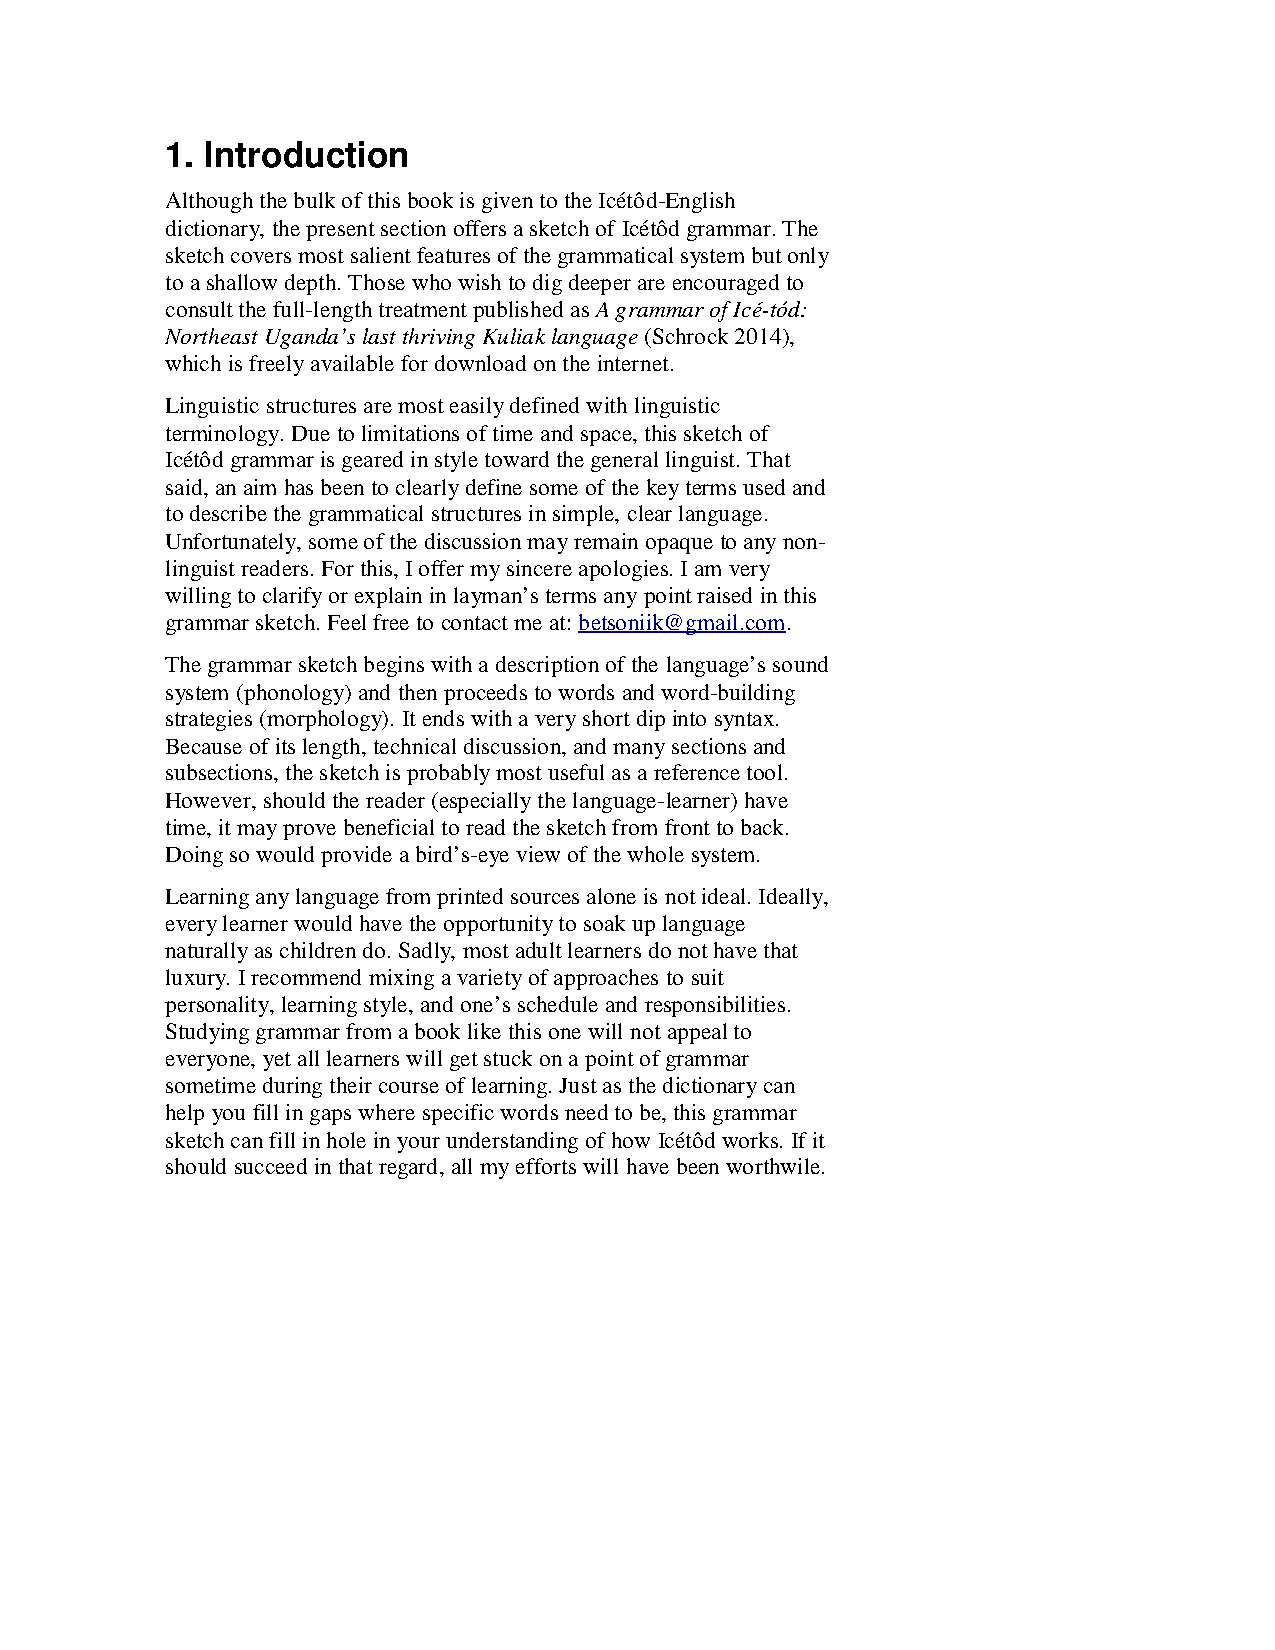
\includepdf[pages=-,scale=1.5, pagecommand={\thispagestyle{plain}}]{Grammar sketch p 1.pdf}
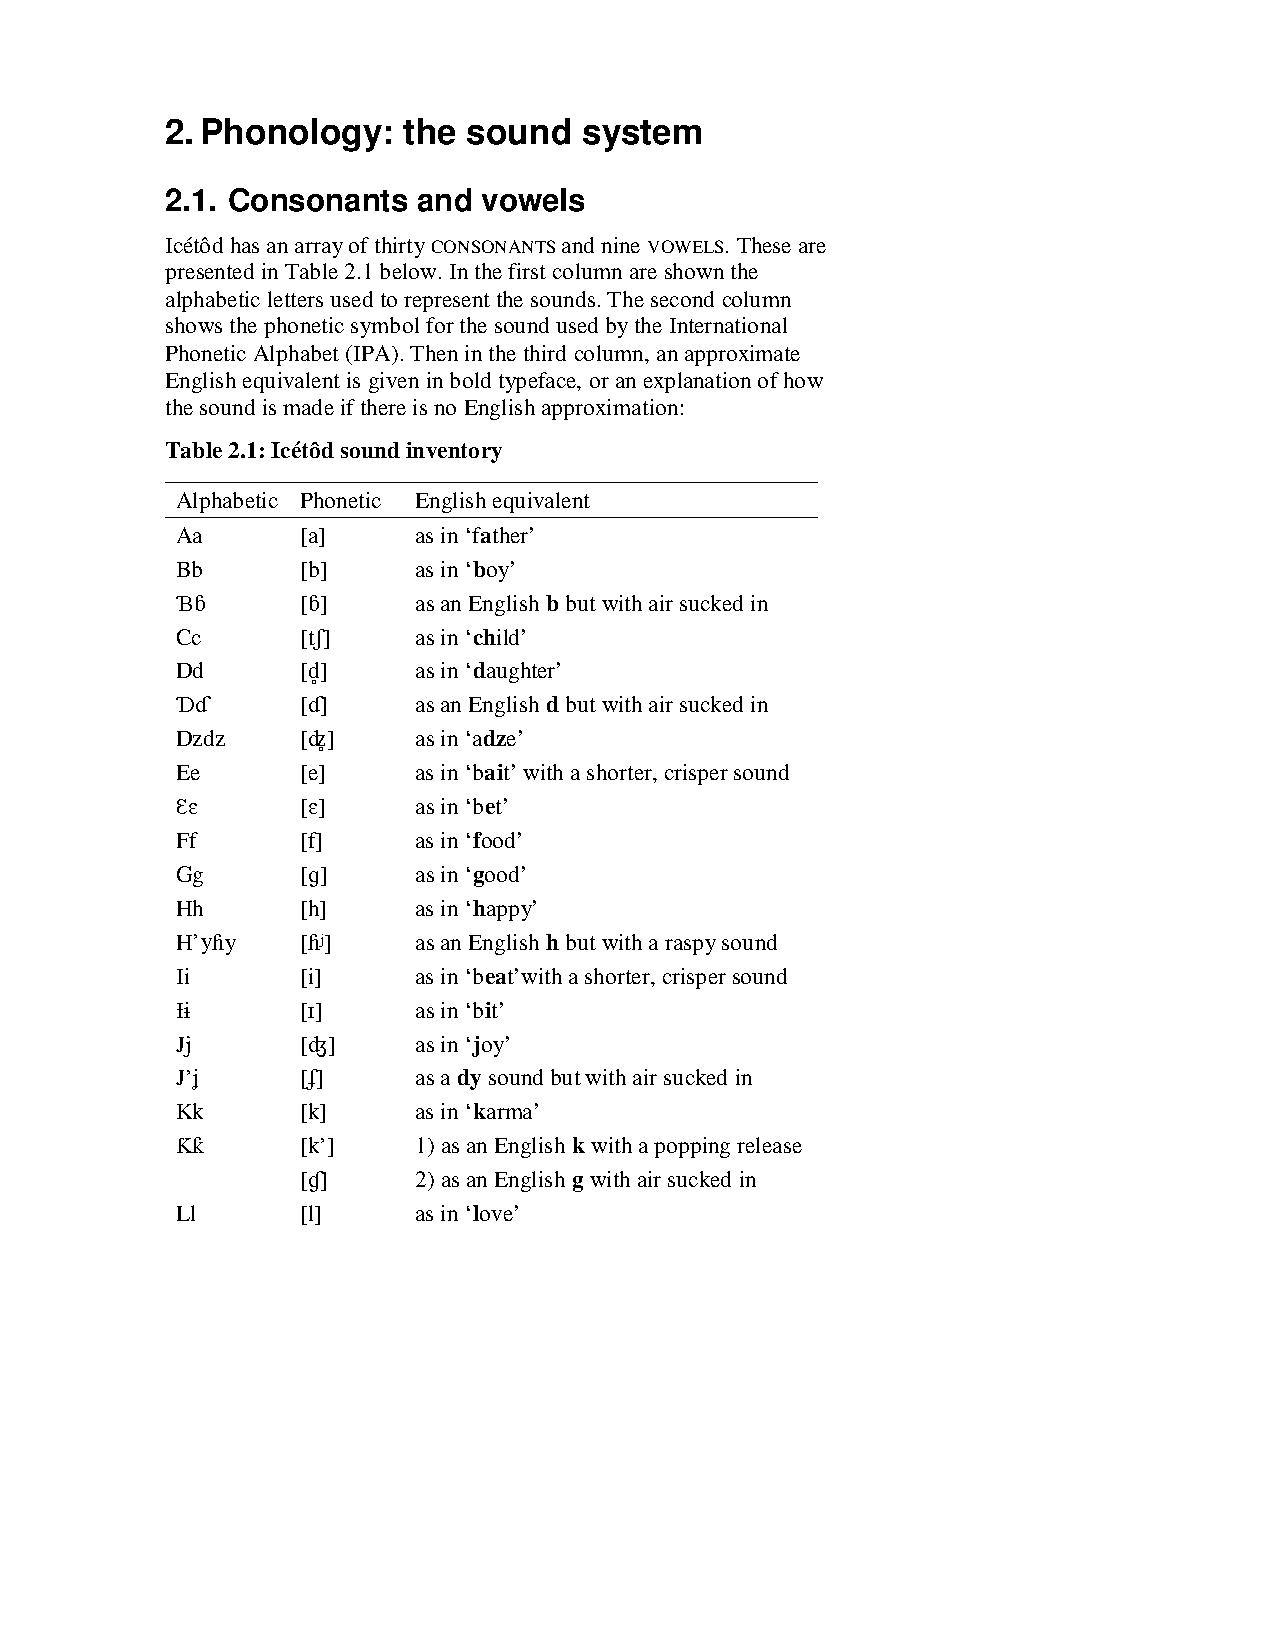
\includepdf[pages=-,scale=1.5, pagecommand={\thispagestyle{plain}}]{Rest of grammar sketch.pdf}

% % copy the lines above and adapt as necessary

%%%%%%%%%%%%%%%%%%%%%%%%%%%%%%%%%%%%%%%%%%%%%%%%%%%%
%%%                                              %%%
%%%             Backmatter                       %%%
%%%                                              %%%
%%%%%%%%%%%%%%%%%%%%%%%%%%%%%%%%%%%%%%%%%%%%%%%%%%%%

\is{some term| see {some other term}}
\il{some language| see {some other language}}
\issa{some term with pages}{some other term also of interest}
\ilsa{some language with pages}{some other lect also of interest} 
% There is normally no need to change the backmatter section
% \backmatter
\phantomsection%this allows hyperlink in ToC to work
\printbibliography[heading=references] 
\cleardoublepage

\phantomsection 
\addcontentsline{toc}{chapter}{Index} 
\addcontentsline{toc}{section}{Name index}
\ohead{Name index} 
\printindex 
\cleardoublepage
  
\phantomsection 
\addcontentsline{toc}{section}{Language index}
\ohead{Language index} 
\printindex[lan] 
\cleardoublepage
  
\phantomsection 
\addcontentsline{toc}{section}{Subject index}
\ohead{Subject index} 
\printindex[sbj]
\ohead{} 
 
\end{document} 
 